\documentclass[10pt, twoside, UTF8, openany]{ctexbook}

\usepackage{amsmath}                                % 数学公式
\usepackage{amsthm}                                 % 数学公式
\usepackage{amssymb}                                % 数学公式
\usepackage{mathrsfs}
\usepackage{appendix}                               % 添加附录
\usepackage{pdfpages}                               % 添加pdf
\usepackage{pgfplots}                               % 画图包
\usepackage{geometry}                               % 页边距包
\usepackage{fancyhdr}                               % 页眉包
\usepackage{float}                                  % 提供 float 浮动环境
\usepackage{booktabs}                               % 三线表
\usepackage{subfigure}                              % 子图
\usepackage{hyperref}                               % 引用跳转
\usepackage{extarrows}                              % 长等号
\usepackage{esint}                                  % 特殊的数学符号
\usepackage[inline]{enumitem}                       % 高级编号
\usepackage{multirow}                               % 表格单元占据多行/列
\usepackage{multicol}                               % 表格单元占据多行/列
\usepackage{arydshln}                               % 矩阵虚线
\usepackage{fancyvrb}
\usepackage{afterpage}
\usepackage{caption}
\usepackage{makecell}
\usepackage{physics}
\usepackage{rotating}
\usepackage{amscd}
\usepackage{tasks}
\usepackage{color}
\usepackage{framed}
\usepackage{cutwin}
\usepackage{tikz-3dplot}
\usepackage{nicematrix}
\usepackage{ocgx}
\usepackage{tablefootnote}
\usepackage{etoc}
\usepackage{titlesec}
\usepackage{makeidx}
\usepackage{bookmark}
% \usepackage[adobe-utopia]{mathdesign}
\makeindex

\titleformat
{\chapter} % command
[display] % shape
{\color{cyan}\bfseries\Large} % format
{第\ \thechapter\ 章} % label
{0.25ex} % sep
{
    \rule{\textwidth}{1pt}
    \vspace{1ex}
    \centering
} % before-code
[
\vspace{-2ex}%
\rule{\textwidth}{0.3pt}
] % after-code

\newcommand*\cdotfill{%
	\leavevmode
	\leaders \hbox to .5em {\hss.\hss}\hfill
}

\etocsetstyle{part}
{\parindent 0pt
	\nobreak
	\etocskipfirstprefix}
{\pagebreak[3]\bigskip}
{\bfseries\centering
	\etocifnumbered{\etocnumber{} – }{}\etocname\par}
{}

\etocsetstyle{chapter}
{%
	\setlength\rightskip{4\ccwd}%
	\addtolength\parfillskip{-\rightskip}%
	\etocskipfirstprefix
}
{\medskip}
{%
	\bfseries
	\noindent
	\etocifnumbered
	{%
		\sbox0{\etocthenumber\unskip\quad}%
		\setlength\leftskip{\wd0}%
		\etoclink{\llap{\box0}\etocthename}%
	}
	{%
		\setlength\leftskip{\rightskip}%
		\hskip-\leftskip
		\etocname
	}%
	\nobreak\cdotfill\etocpage\par
}
{}

\etocsetstyle{section}
{\nopagebreak\normalfont}
{\smallskip}
{%
	\noindent
	\etocifnumbered
	{\etoclink{\llap{\etocthenumber\quad}\etocthename}}
	{\etocname}%
	\nobreak\cdotfill\etocpage\par
}
{}

\etocsetstyle{subsection}
{%
	\nopagebreak
	\begingroup
	\addtolength\parfillskip{\rightskip}%
	\addtolength\rightskip{\fill}%
	\etocskipfirstprefix
	\noindent
}
{\quad}
{%
	\hbox{%
		\etoclink{%
			\etocifnumbered{\etocthenumber\enskip}{}%
			\etocthename\ (\etocthepage)%
		}%
	}%
}
{\par\endgroup}

% \NiceMatrixOptions{rules/color=cyan}
\definecolor{shadecolor}{rgb}{0.92,0.92,0.92}
\numberwithin{figure}{section}
\usetikzlibrary{calc,decorations.markings}
\newcommand\myemptypage{
	\null
	\thispagestyle{empty}
	\addtocounter{page}{-1}
	\newpage
}
% \usepackage{pgffor}
% \makeatletter
% \newcommand{\twocolumntoc}{%
% 	\chapter*{\contentsname
% 	  \@mkboth{%
% 		  \MakeUppercase\contentsname}{\MakeUppercase\contentsname}}%
% 	\@starttoc{toc}%
% }
% \makeatother
% \setcounter{tocdepth}{3}

\newcommand{\e}{\mathrm{e}}
\newcommand{\vp}{\mathrm{v.p.}}
\newcommand{\B}{\mathrm{B}}
\newcommand{\C}{\mathrm{C}}
\newcommand{\D}{\mathrm{D}}
\newcommand{\sgn}{\mathrm{sgn}}
\newcommand{\cov}{\mathrm{cov}}
\newcommand{\adj}{\mathrm{adj}}
\newcommand{\diag}{\mathrm{diag}}
\renewcommand{\i}{\mathrm{i}}

\newcommand\sj[1]{\mathsf{#1}}
\settasks{
	label={\Alph*.},
	% label-align = left,
	% label-offset = {1em},
	% label-width = 0.5em,
	% item-indent = {1.5em}, % indent = label-width + label-offset
	% column-sep = {1em},
	% before-skip = {-1em},
	% after-skip = {-1em},
	% after-item-skip = 0em
}
% \renewcommand{\proofname}{\indent\bf 证明}
% \renewcommand{\qedsymbol}{$\blacksquare$}

\newcounter{magicrownumbers}
% stepcounter 对应计数器自增,arabic 表示输出阿拉伯数字
\newcommand\rownumber{\stepcounter{magicrownumbers}\arabic{magicrownumbers}}
\theoremstyle{definition}
\newtheorem*{solution}{{\songti \textbf{解}}}
\newtheorem{theorem}{\color{magenta}{{\songti 定理}}}[section]
\newtheorem{lemma}{\color{purple}{{\songti 引理}}}[section]
\newtheorem{inference}{\color{pink}{{\songti 推论}}}[section]
\newtheorem{definition}{\color{orange}{{\songti 定义}}}[section]
\newtheorem{example}{\color{cyan}{{\songti 例}}}[section]
\pgfplotsset{compat=1.18}
\usetikzlibrary{intersections}
\geometry{paperheight=26cm, paperwidth=18.5cm, scale=0.85, inner=20mm}
\title{{\kaishu \Huge{\textbf{${\text{考}_\text{研}^{\text{数}_\text{学}}}_{\underline{\text{典型问题}}}^{_{\overset{\overline{\text{方}}\text{法}|}{|\text{技}\underline{\text{巧}}}}}$}}}}
\author{{\kaishu 黄国铭}}
\date{}

\linespread{1.5}

\renewenvironment{solution}[1][]
{\noindent\footnotesize\linespread{1}
	\itshape #1}
{}

\newenvironment{errorSolution}[1][]
{\noindent\footnotesize\linespread{1}\color{red}
	\itshape \textbf{错解.} #1}
{}

\renewenvironment{proof}[1][]
{\noindent\footnotesize\linespread{1}
	\itshape #1}
{\par}

% \renewenvironment{example}[2][]
% {#1\noindent\footnotesize\linespread{1}
% \itshape \color{cyan} #2}
% {}

\allowdisplaybreaks

\begin{document}

\includepdf{cover.pdf}

% \myemptypage
% \pagenumbering{roman}
% \setcounter{page}{1}

% \newpage
% \pagenumbering{Roman}
% \setcounter{page}{1}
% \twocolumn
% \twocolumntoc
% \onecolumn

% \newpage
% \pagenumbering{arabic}

% \setcounter{page}{1}

\frontmatter

\chapter{前言}

\section*{关于本书}

\begin{figure}[H]
    \centering
    \includegraphics[scale=0.5]{figures/autograph.png}
\end{figure}

\section*{致谢}


\tableofcontents

\mainmatter

\part{高等数学}

\chapter{函数、数列与极限}%============================1

\begin{flushright}
    \begin{tabular}{r|}
        \textit{“迟序之数, 非出神怪, 有形可检, 有数可推。”}\\
        ——\textit{祖冲之}
    \end{tabular}
\end{flushright}

函数是微积分讨论的主要对象, 它以极限理论为基础, 在研究函数时我们总是通过函数值 $f(x)$
的变化来看函数关系的性质, 所以应该用运动变化的观点来掌握函数.
极限与函数的连续性理论是微积分的基础, 如何用已知的、可求的来逼近未知的、要求的, 
用有限来逼近无限, 在无限变化的过程中考察变量的变化趋势, 从有限过渡到无限, 这是本章需掌握的基本思想.
\section{函数的基本特征}

函数的基本特征包括: 定义域和值域、解析式与图像、奇偶性、单调性、零点以及渐近线等, 这些基本特征可以帮助我们更好地理解和分析函数的性质和行为.

\subsection{函数的主要性质}

\subsubsection{定义域}

\begin{definition}[函数的概念]
    设有两个变量 $x$ 与 $y$, 如果变量 $x$ 在其变化范围 $D$ 内任取一个确定的数值时, 变量 $y$ 按照一定的规则 $f$, 总有唯一确定的数值和它对应, 则称变量 $y$ 是变量 $x$ 的\textit{函数}, 记作 $y=f(x)$, 
    $x$ 称为\textit{自变量}, $y$ 称为\textit{因变量}, $D$ 称为\textit{函数的定义域}, $f$ 表示由 $x$ 确定 $y$ 的对应规则.
\end{definition}

\begin{example}
    求函数 $y=\dfrac{1}{\sqrt{25-x^2}}+\arctan\dfrac{x-1}{5}$ 的定义域.
\end{example}
\begin{solution}
    要使函数有意义, 变量 $x$ 必须同时满足 $\begin{cases}
        25-x^2>0\\\qty|\dfrac{x-1}{5}|\leqslant 1
    \end{cases}\Rightarrow -4\leqslant x<5$, 因此定义域为 $[-4,5).$
\end{solution}

\subsubsection{单调性}

\begin{definition}[函数的单调性]
    设函数 $f(x)$ 的定义域为 $D$, 区间 $I\subset D$, 对于 $\forall x_1,x_2\in I$, 当 $x_1<x_2$ 时, 恒有 $f(x_1)<f(x_2)$ (或 $f(x_1)>f(x_2)$) 则称函数 $f(x)$ 在区间 $I$ 上\textit{单调递增 (递减)}, 
    若 $f(x_1)\leqslant f(x_2)$ (或 $f(x_1)\geqslant f(x_2)$), 则称函数 $f(x)$ \textit{单调不减 (不增)}.
\end{definition}
\begin{theorem}[函数的单调性判定]
    设函数 $f(x)$ 在 $[a,b]$ 上连续, 在 $(a,b)$ 内可导, 如果在区间上有 $f'(x)\geqslant 0(\text{或 }f'(x)\leqslant 0)$ (且不在任一子区间取恒等号), 则 $f(x)$ 在 $(a,b)$ 内严格单调递增 (或严格单调递减).
    \index{函数的单调性判定}
\end{theorem}

\begin{example}
    由 $f'(x_0)>0$ 能否得到函数 $f(x)$ 在 $x_0$ 的某个邻域内单调递增?
\end{example}
\begin{solution}
    不能, 理由如下:
    利用一阶导数判断函数的单调性, 需要已知导数在某区间的正负, 而不是某一点导数值的正负
\end{solution}

\subsubsection{奇偶性}

\begin{definition}[函数的奇偶性]
    设函数 $f(x)$ 在关于原点对称的区间 $D$ 上有定义, 如果对 $D$ 上任意点 $x$, 均有 $f(-x)=f(x)$ (或 $f(-x)=-f(x)$), 则称函数 $f(x)$ 为\textit{偶函数 (或奇函数)}.
    奇函数的图像关于原点对称, 偶函数的图像关于 $y$ 轴对称.
\end{definition}

\begin{example}[1987 数二]
    $f(x)=|x\sin x|\e^{\cos x}~~(-\infty<x<+\infty)$ 是
    \begin{tasks}(4)
        \task 有界函数
        \task 单调函数
        \task 周期函数
        \task 偶函数
    \end{tasks}
\end{example}
\begin{solution}
    由于 $|x\sin x|$ 和 $\e^{\cos x}$ 都是偶函数, 则其乘积 $f(x)=|x\sin x|\e^{\cos x}$ 为偶函数, 选 D.
\end{solution}

\subsubsection{周期性}

\begin{theorem}[函数的周期性定理]
    若函数 $f(x)$ 以 $T$ 为周期, 则 $$f(x)=f(x+T)=f(x+2T)=\cdots=f(x+nT).$$
    \index{函数的周期性定理}
\end{theorem}

\begin{example}[2014 数一]
    设 $f(x)$ 是周期为 4 的可导奇函数, 且 $f'(x)=2(x-1)~ (0\leqslant x\leqslant 2)$, 求 $f(7)$.
\end{example}
\begin{solution}
    $f(x)=\displaystyle\int 2(x-1)\dd x=x^2-2x+C$, 因为 $f(x)$ 是奇函数, 所以 $f(0)=0$, 可知 $C=0$, 于是 $f(x)=x^2-2x$, 
    又 $f(x)$ 的周期为 4, 于是 $f(7)=f(-1+8)=f(-1)=-f(1)=1$.
\end{solution}

\subsubsection{有界性}

\begin{theorem}[函数的有界性定理]
    若函数 $f(x)$ 在闭区间 $[a,b]$ 上连续, 则 $f(x)$ 在 $[a,b]$ 上有界;
    若函数 $f(x)$ 在开区间 $(a,b)$ 内连续, 且 $\displaystyle\lim_{x\to a^+}f(x)$ 与 $\displaystyle\lim_{x\to b^-}f(x)$ 存在, 则函数 $f(x)$ 在 $(a,b)$ 内有界.
    \index{函数的有界性定理}
\end{theorem}

\begin{example}[2004 数三]
    函数 $f(x)=\dfrac{|x|\sin(x-2)}{x(x-1)(x-2)^2}$ 在下列哪个区间内有界
    \begin{tasks}(4)
        \task $(-1,0)$
        \task $(0,1)$
        \task $(1,2)$
        \task $(2,3)$
    \end{tasks}
\end{example}
\begin{solution}
    当 $x\neq0,1,2$ 时, $f(x)$ 连续, 而
    $$\lim_{x\to-1^+}f(x)=-\dfrac{\sin 3}{18},~\lim_{x\to0^-}f(x)=-\dfrac{\sin 2}{4},~\lim_{x\to0^+}f(x)=\dfrac{\sin 2}{4},~\lim_{x\to1}f(x)=\infty,~\lim_{x\to2}f(x)=\infty$$
    所以函数 $f(x)$ 在 $(-1,0)$ 上有界.
\end{solution}

\subsection{复合函数}

\begin{definition}[复合函数]
    如果我们有两个函数 $ f $ 和 $ g $, 而两者的定义域分别是 $ D_{f} $ 和 $ D_{g} $, 
    值域分别是 $ I_{f} $ 和 $ I_{g} $. 如果 $ I_{f} \cap D_{g} \neq \varnothing $, 
    那我们定义\textit{复合函数}为 $$ g \circ f:=\left\{(x, z) \mid\left(\exists y \in I_{f} \cap D_{g}\right)[y=f(x) \wedge z=g(y)]\right\} .$$
\end{definition}

\begin{example}[2001 数二]
    设 $f(x)=\begin{cases}
            1,|x|\leqslant 1 \\0,|x|>1
        \end{cases}$, 则 $f\qty{f[f(x)]}$ 等于
    \begin{tasks}(4)
        \task $0$
        \task $1$
        \task $\begin{cases}
                1,|x|\leqslant 1 \\0,|x|>1
            \end{cases}$
        \task $\begin{cases}
                0,|x|\leqslant 1 \\1,|x|>1
            \end{cases}$
    \end{tasks}
\end{example}
\begin{solution}
    因为 $f\in\qty{0,1}$, 所以 $f[f(x)]=1$, 那么 $f\qty{1}=1$, 因此选 B.
\end{solution}

\begin{theorem}\label{theorem:xn011-1}
    $\displaystyle\lim_{n \to \infty } x^n=\begin{cases}
            0,      & |x|<1         \\
            \infty, & |x|>1         \\
            1,      & x=1           \\
            1,      & x=-1,~n=2k    \\
            -1,     & x=-1,~n=2k+1.
        \end{cases}$
\end{theorem}

\begin{example}
    已知 $f(x)=\displaystyle\lim_{n\to\infty}\sqrt{2+(2x)^n+x^{2n}}~(x\geqslant 0),~g(x)=\lim_{n\to\infty}\dfrac{1-x^{2n+1}}{1+x^{2n}}$, 求 $f(g(x))$ 的表达式.
\end{example}
\begin{solution}
    \begin{minipage}{0.7\linewidth}
        由推论 \ref{maxai} 知, $f(x)=\displaystyle\lim_{n\to\infty}\sqrt{1^n+1^n+(2x)^n+(x^2)^{n}}=\max\qty{1,2x,x^2}=\begin{cases}
                1,   & 0\leqslant x<\dfrac{1}{2} \\[6pt]
                2x,  & \dfrac{1}{2}\leqslant x<2 \\[6pt]
                x^2, & 2\leqslant x
            \end{cases}$ 又由定理 \ref{theorem:xn011-1} 可得
        $g(x)=\begin{cases}
                1,  & -1\leqslant x<1 \\
                -x, & |x|>1           \\
                0,  & x=1
            \end{cases}$, 于是 $g(x)$ 的图像如图 \ref{fig:IIIgIIfI} 所示, 那么
        \begin{flalign*}
            I:  & ~x=1\Rightarrow g(1)=0\Rightarrow f(g(0))=1                                        \\
            II: & ~\begin{cases}
                       -2<x<-1 \\
                       1\leqslant x<1
                   \end{cases}\Rightarrow \begin{cases}
                                              g(x)=-x \\
                                              g(x)=1
                                          \end{cases}\Rightarrow \begin{cases}
                                                                     -x>2 \\
                                                                     -x>1 \\
                                                                     -1\leqslant x<1
                                                                 \end{cases}\Rightarrow \begin{cases}
                                                                                            f(g(x))=x^2 \\
                                                                                            f(g(x))=-2x \\
                                                                                            f(g(x))=2
                                                                                        \end{cases}
        \end{flalign*}
    \end{minipage}\hfill
    \begin{minipage}{0.29\linewidth}
        \begin{figure}[H]
            \centering
            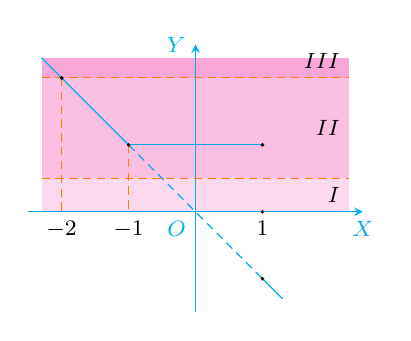
\begin{tikzpicture}[->,samples=100,>=stealth,font=\footnotesize,scale=0.85]
                \fill[magenta!15](-2.3,0)--(2.3,0)--(2.3,0.5)--(-2.3,0.5);
                \fill[magenta!25](-2.3,0.5)--(2.3,0.5)--(2.3,2)--(-2.3,2);
                \fill[magenta!35](-2.3,2)--(2.3,2)--(2.3,2.3)--(-2.3,2.3);
                \draw[->,cyan](-2.5,0)--(0,0)node[below left]{$O$}--(2.5,0)node[below]{$X$};
                \draw[->,cyan](0,-1.5)--(0,2.5)node[left]{$Y$};
                \draw[cyan,-](-2.3,2.3)--(-1,1);
                \draw[cyan,-](1,-1)--(1.3,-1.3);
                \draw[cyan,-](-1,1)--(1,1);
                \draw[densely dashed,orange,-](-2.3,0.5)--(2.3,0.5);
                \draw[densely dashed,orange,-](-2.3,2)--(2.3,2);
                \draw[densely dashed,orange,-](-2,2)--(-2,0);
                \draw[densely dashed,orange,-](-1,1)--(-1,0);
                \draw[densely dashed,cyan,-](-1,1)--(1,-1);
                \node[below] at (-2,0){$-2$};
                \node[below] at (-1,0){$-1$};
                \node[below] at (1,0){$1$};
                \draw[-,fill=black] (-2,2) circle (0.5pt);
                \draw[-,fill=black] (-2,2) circle (0.5pt);
                \draw[-,fill=black] (-1,1) circle (0.5pt);
                \draw[-,fill=black] (1,0) circle (0.5pt);
                \draw[-,fill=white] (1,1) circle (0.5pt);
                \draw[-,fill=white] (1,-1) circle (0.5pt);
                \node[left] at (2.3,0.25){$I$};
                \node[left] at (2.3,1.25){$II$};
                \node[left] at (2.3,2.25){$III$};
            \end{tikzpicture}
            \caption{}
            \label{fig:IIIgIIfI}
        \end{figure}
    \end{minipage}
    $$III:~x\leqslant -2\Rightarrow g(x)=-x\Rightarrow f(g(x))=x^2$$
    综上, $f(g(x))=\begin{cases}
            x^2, & x\leqslant -2   \\
            -2x, & -2<x<-1         \\
            2,   & -1\leqslant x<1 \\
            1,   & x=1.
        \end{cases}$
\end{solution}

\subsection{反函数}

\begin{definition}[反函数]
    设 $f$ 为一函数, 其定义域为 $D_f$, 值域为 $I_f$, 如果存在一函数 $g$, 其定义域和值域分别为 $I_g,~D_g$, 并对每一 $x\in D_f$ 有:
    $g(f(x))=x$, 则称 $g$ 为 $f$ 的\textit{反函数}, 记为 $f^{-1}.$
    \label{definitionOfInverseFunction}
\end{definition}

\begin{example}
    已知 $g$ 是 $f$ 的反函数, 则 $f(2x)$ 的反函数为
    \begin{tasks}(4)
        \task $y=\dfrac{1}{2}g(x)$
        \task $y=2g(x)$
        \task $y=\dfrac{1}{2}g(2x)$
        \task $y=2g(2x)$
    \end{tasks}
\end{example}
\begin{solution}
    令 $y=f(2x)$, 反解出 $x:x=\dfrac{1}{2}g(y)$, 交换 $x$ 与 $y$ 的位置, 于是 $y=\dfrac{1}{2}g(x)$, 选 A.
\end{solution}

\begin{example}
    求 $y=\sqrt[3]{x+\sqrt{1+x^{2}}}+\sqrt[3]{x-\sqrt{1+x^{2}}}$ 的反函数表达式.
\end{example}
\begin{solution}
    令 $y_1=\sqrt[3]{x+\sqrt{1+x^{2}}},~y_2=\sqrt[3]{x-\sqrt{1+x^{2}}}$, 那么 $y=y_1+y_2$, 又因为
    $$y_1^3+y_2^3=(y_1+y_2)\qty(y_1^2-y_1y_2+y_2^2)=(y_1+y_2)\qty[(y_1+y_2)^2-3y_1y_2]$$
    其中 $y_1^3+y_2^3=x+\sqrt{1+x^2}+x-\sqrt{1+x^2}=2x,~y_1y_2=\sqrt[3]{x^2-1-x^2}=-1$, 因此 $$2x=y\qty(y^2+3)\Rightarrow x=\dfrac{y\qty(y^2+3)}{2}.$$
\end{solution}

\begin{example}
    设 $f(x)=2023x^{2023}+x+1,~f^{-1}(x)$ 是 $f(x)$ 的反函数, 计算极限 $$\lim_{x\to+\infty}\dfrac{f^{-1}(2023x)-f^{-1}(x)}{\sqrt[2023]{x}}.$$
\end{example}
\begin{solution}
    设 $g(x)=f^{-1}(x)$, 由定义 \ref{definitionOfInverseFunction}, 得 $f(g(x))=x$, 于是 $$x=2023 g^{2023}(x)+g(x)+1$$
    则 $$\lim_{x\to+\infty}\dfrac{f^{-1}(x)}{\sqrt[2023]{x}}=\lim_{x\to+\infty}\dfrac{g(x)}{\sqrt[2023]{2023x^{2023}+g(x)+1}}=\lim_{x\to+\infty}\dfrac{1}{\sqrt[2023]{2023+\dfrac{1}{g^{2022}(x)}+\dfrac{1}{g^{2023}(x)}}}=\dfrac{1}{\sqrt[2023]{2023}}$$
    进而有
    $$\lim_{x\to+\infty}\dfrac{f^{-1}(2023x)}{\sqrt[2023]{x}}=\lim_{x\to+\infty}\dfrac{f^{-1}(2023x)}{\sqrt[2023]{2023x}}\cdot\dfrac{\sqrt[2023]{2023x}}{\sqrt[2023]{x}}=\dfrac{\sqrt[2023]{2023}}{\sqrt[2023]{2023}}=1$$
    故原极限为 $1-\dfrac{1}{\sqrt[2023]{2023}}.$
\end{solution}


\subsection{函数的连续性及间断点的类型}

\subsubsection{连续函数}

\begin{definition}[函数连续]
    若 $\displaystyle\lim_{x\to x_0}f(x)=f(x_0)$, 则称函数 $f(x)$ 在点 $x_0$ 处连续, 若函数 $f(x)$ 在区间 $ I $ 内每一点都连续, 则称函数 $f(x)$ 在区间 $I$ 内\textit{连续}.
\end{definition}

\begin{definition}[单侧连续]
    若 $\displaystyle\lim_{x\to x_0^-}f(x)=f(x_0)$, 则称函数 $f(x)$ 在 $x_0$ 处\textit{左连续}; 若 $\displaystyle\lim_{x\to x_0^+}f(x)=f(x_0)$, 则称函数 $f(x)$ 在 $x_0$ 处\textit{右连续}.
\end{definition}

\begin{theorem}[函数连续的充要条件]
    $f(x)$ 在点 $x_0$ 处连续等价于 $f(x)$  在点 $x_0$ 处既左连续又右连续.
    \index{函数连续的充要条件}
\end{theorem}

\subsubsection{第一类间断点}

\begin{definition}[可去间断点]
    如果不连续点 $ x_{0} $ 两侧函数的极限存在且相等, 无论在 $ x_{0} $ 处是否定义
    (若有定义, 则函数值不是在这一点的左右极限), 
    这类间断点叫\textit{可去间断点} (或可移间断点), 这类函数通过补充定义
    $$f\left(x_{0}\right)=\lim _{x \rightarrow x_{0}^{+}} f(x)=\lim _{x \rightarrow x_{0}^{-}} f(x)$$
    后可变为连续函数.
\end{definition}

\begin{definition}[跳跃间断点]
    如果不连续点 $x_{0}$ 两侧函数的极限存在但不相等, 称函数在这些点是\textit{跳跃间断点}.
\end{definition}

\subsubsection{第二类间断点}

所有不是第一类间断点的类型, 都是第二类间断点.

\begin{definition}[无穷间断点]
    函数在某点的左右极限至少有一个是无穷, 这样的间断点就是\textit{无穷间断点}, 由此可知函数在这个间断点的某个邻域中无界. 无穷间断点的一个重要特性是它是必不可积的.
\end{definition}
% 可参考例题 \ref{fxdfracx12x1}.

\begin{definition}[振荡间断点]
    对于一个函数, 当自变量趋于某一点时, 函数值在两个常数间变动无限多次, 这时函数在这一点处不存在有限极限也不是无穷.
    这样的间断点是\textit{振荡间断点}, 由此可知函数在这个间断点的某个邻域中有界. 振荡间断点的一个重要特性是它可能是可积的.
\end{definition}

\begin{example}
    设 $f(x)=\dfrac{\qty(1-2^{\frac{1}{x-1}})\e^{\frac{1}{x}}}{1+2^{\frac{2}{x-1}}}\cdot\arctan\dfrac{[~x+1~]}{x+1}$, 则下列关于 $f(x)$ 间断点的描述正确的是
    \begin{tasks}(1)
        \task $f(x)$ 有一个可去间断点, 一个跳跃间断点, 一个第二类间断点
        \task $f(x)$ 有两个可去间断点, 一个第二类间断点
        \task $f(x)$ 有两个跳跃间断点, 一个第二类间断点
        \task $f(x)$ 有一个跳跃间断点, 两个第二类间断点
    \end{tasks}
\end{example}
\begin{solution}
    因为 $x\neq-1,0,1$, 下求各不连续点的左右极限值, 
    $$f(-1^-)=\lim_{x\to-1^-}f(x)=\lim_{\substack{x\to-1-\delta\\\delta>0}}f(x)=\dfrac{\qty(1-2^{-\frac{1}{2}})\e^{-1}}{1+2^{-1}}\cdot\dfrac{\pi}{2},~f(-1^+)=\lim_{x\to-1^+}=\lim_{\substack{x\to-1+\delta\\\delta>0}}f(x)=0$$
    则 $x=-1$ 为 $f$ 的跳跃间断点;
    $$f(0^-)=\lim_{x\to0^-}f(x)=\lim_{\substack{x\to0-\delta\\\delta>0}}f(x)=0,~f(0^+)=\lim_{x\to0^+}f(x)=\lim_{\substack{x\to0+\delta\\\delta>0}}f(x)=+\infty$$
    则 $x=0$ 为 $f$ 的第二类间断点;
    $$f(1^-)=\lim_{x\to1^-}f(x)=\lim_{\substack{x\to1-\delta\\\delta>0}}f(x)=\e\cdot\arctan\dfrac{1}{2},~f(1^+)=\lim_{x\to1^+}f(x)=\lim_{\substack{x\to1+\delta\\\delta>0}}f(x)=0$$
    则 $x=1$ 为 $f$ 的跳跃间断点, 故选 C.
\end{solution}

\subsection{渐近线方程}

\begin{definition}[铅直渐近线]
    若 $\displaystyle\lim_{x\to\varepsilon^-}f(x)$ 与 $\displaystyle \lim_{x\to\varepsilon^+}f(x)$ 至少有一个为无穷大, 则称 $x=\varepsilon$ 为曲线 $y=f(x)$ 的\textit{铅直渐近线}.
\end{definition}
\begin{definition}[水平渐近线]
    若 $\displaystyle\lim_{x\to-\infty}f(x)=b$ 或 $\displaystyle\lim_{x\to+\infty}f(x)=b$, 其中 $b$ 为常数, 则称 $y=b$ 为曲线 $y=f(x)$ 的\textit{水平渐近线}.
\end{definition}
\begin{definition}[斜渐近线]
    若 $\displaystyle\lim_{x\to-\infty}\dfrac{f(x)}{x}=k$ 存在且不为零, 同时 $\displaystyle\lim_{x\to-\infty}[f(x)-kx]=b$ 也存在 (或 $\displaystyle\lim_{x\to+\infty}\dfrac{f(x)}{x}=k$ 存在且不为零, 同时 $\displaystyle\lim_{x\to+\infty}[f(x)-kx]=b$ 存在), 
    则称 $y=kx+b$ 为曲线 $y=f(x)$ \textit{斜渐近线}.
\end{definition}

\begin{example}
    求下列曲线的全部渐近线.
    \setcounter{magicrownumbers}{0}
    \begin{table}[H]
        \centering
        \begin{tabular}{l | l}
            (\rownumber{}) $y=\sqrt{4x^2+x}\ln\qty(2+\dfrac{1}{x}).$ & (\rownumber{}) $y=\mathrm{e}^{x^{-2}}\arctan\dfrac{x^2+x+1}{(x-1)(x+2)}.$                  \\
            (\rownumber{}) $y=\dfrac{x^3}{(x-1)^2}\cos(2\arctan x).$ & (\rownumber{}) $\displaystyle y=(2x+1)\arctan x+\dfrac{\arctan\dfrac{1}{x^2-1}}{x^2+x-2}.$ \\
            (\rownumber{}) $y^3=x\qty(x^2-2y).$                      & (\rownumber{}) $x^3-y^3=6xy.$
        \end{tabular}
    \end{table}
\end{example}
\begin{solution}
    \begin{enumerate}[label=(\arabic{*})]
        \item 由 $\displaystyle\lim_{x\to\qty(-\frac{1}{2})^+}y=-\infty$, 且 $\displaystyle\lim_{x\to0^-}y=0$, 所以曲线存在一条铅直渐近线 $x=-\dfrac{1}{2}$, 又
              \begin{flalign*}
                  k & =\lim_{x\to+\infty}\dfrac{y}{x}=\lim_{x\to+\infty}\dfrac{\sqrt{4x^2+x}}{x}\ln\qty(2+\dfrac{1}{x})=\lim_{x\to+\infty}\dfrac{|x|}{x}\sqrt{4+\dfrac{1}{x}}\ln\qty(2+\dfrac{1}{x})=2\ln 2 \\
                  b & =\lim_{x\to+\infty}(y-kx)=\lim_{x\to+\infty}\qty[\sqrt{4x^2+x}\ln\qty(2+\dfrac{1}{x})-2\ln 2x]                                                                                        \\
                    & =\lim_{x\to+\infty}\qty[\sqrt{4x^2+x}\ln 2-2\ln 2\cdot x+\sqrt{4x^2+x}\ln\qty(2+\dfrac{1}{x})-\sqrt{4x^2+x}\ln 2]                                                                     \\
                    & =\lim_{x\to+\infty}\qty[\dfrac{x}{\sqrt{4x^2+x}+2x}\cdot\ln 2 +|x|\sqrt{4+\dfrac{1}{x}}\ln\qty(1+\dfrac{1}{2x})]=\dfrac{1}{4}\ln 2+1
              \end{flalign*}
              故存在一条斜渐近线方程 $y=2\ln 2x+\dfrac{1}{4}\ln 2+1$, 同理当 $x\to-\infty$ 时, 也存在一条斜渐近线方程 $$y=-2\ln 2x-\dfrac{1}{4}\ln 2-1.$$
        \item 由 $\displaystyle \lim_{x\to-2^-}y=\dfrac{\pi}{2\mathrm{e}^4},~\lim_{x\to-2^+}y=-\dfrac{\pi}{2\mathrm{e}^4},~\lim_{x\to1^-}y=-\dfrac{\pi\mathrm{e}}{2},~\lim_{x\to1^+}y=\dfrac{\pi\mathrm{e}}{2},~\lim_{x\to0^-}y=-\infty$, 故 $y$ 的铅直渐近线为 $x=0$, 因为
              $$\lim_{x\to-\infty}y=\lim_{x\to+\infty}y=\lim_{x\to\infty}y=\lim_{x\to\infty}\mathrm{e}^{x^{-2}}\arctan\dfrac{1+\dfrac{1}{x}+\dfrac{1}{x^2}}{1+\dfrac{1}{x}-\dfrac{2}{x^2}}=\dfrac{\pi}{4}$$
              故 $y$ 的水平渐近线为 $y=\dfrac{\pi}{4}$, 又因为
              $$k=\lim_{x\to+\infty}\dfrac{y }{x}=\lim_{x\to+\infty}\dfrac{\mathrm{e}^{-x^2}}{x}\arctan\dfrac{x^2+x+1}{(x-1)(x+2)}=0$$
              故曲线共存在两条渐近线, 分别为 $x=0$ 与 $y=\dfrac{\pi}{4}$.
        \item 显然 $x=1$ 为该曲线的铅直渐近线, 下求斜渐近线, 
              \begin{flalign*}
                  k & =\lim_{x\to\pm\infty}\dfrac{y}{x}=\lim_{x\to\pm\infty}\dfrac{x^2}{(x-1)^2}\cos(2\arctan x)=1\cdot -1=-1                                               \\
                  b & =\lim_{x\to\pm\infty}(y-kx)=\lim_{x\to\pm\infty}\dfrac{x^3\cos(2\arctan x)+x(x-1)^2}{(x-1)^2}=\lim_{x\to\pm\infty}\dfrac{-x^3+x^3-2x^2+x}{(x-1)^2}=-2
              \end{flalign*}
              所以斜渐近线方程为 $y=-x-2.$
        \item 因为 $\displaystyle\lim_{x\to\infty}f(x)=\infty$, 所以曲线 $y=f(x)$ 没有水平渐近线; 由 $\displaystyle\lim_{x\to-2}f(x)=\infty$, 得 $x=-2$ 为曲线 $y=f(x)$ 的铅直渐近线;
              由 $$f(-1^-)=\lim_{x\to-1^-}f(x)=\dfrac{\pi}{4}-\dfrac{\pi}{4}=0,~f(-1^+)=\lim_{x\to-1^+}f(x)=\dfrac{\pi}{4}+\dfrac{\pi}{4}=\dfrac{\pi}{2}$$
              得 $x=-1$ 不是该曲线的铅直渐近线;
              又由 $$\lim_{x\to1}f(x)=\dfrac{3\pi}{4}+\lim_{x\to1}\dfrac{\arctan\dfrac{1}{x^2-1}}{x^2+x-2}=\infty$$
              得 $x=1$ 是该曲线的铅直渐近线; 下求斜渐近线, 
              $$k_1=\lim_{x\to-\infty}\dfrac{f(x)}{x}=\lim_{x\to-\infty}\qty(2+\dfrac{1}{x})\arctan x+\dfrac{\arctan\dfrac{1}{x^2-1}}{x^3+x^2-2x}=-\pi$$
              那么
              \begin{flalign*}
                  b_1 & =\lim_{x\to-\infty}\qty(f(x)-kx)=\lim_{x\to-\infty}\qty[(2x+1)\arctan x+\dfrac{\arctan\dfrac{1}{x^2-1}}{x^2+x-2}+\pi x]                                      \\
                      & =2\lim_{x\to-\infty}x\qty(\arctan x+\dfrac{\pi}{2})+\lim_{x\to-\infty}\arctan x+\lim_{x\to-\infty}\dfrac{\arctan\dfrac{1}{x^2-1}}{x^2+x-2}=-\dfrac{\pi}{2}-2
              \end{flalign*}
              那么一条斜渐近线为 $y=-\pi x-\dfrac{\pi}{2}-2$, 同理可求解另一条斜渐近线为 $y=\pi x+\dfrac{\pi}{2}-2.$
        \item 令 $k=\dfrac{y}{x}$, 有 $$k^3\cdot x^3=x\qty(x^2-2kx)\Rightarrow k^3=1-\dfrac{2k}{x}$$
              两边取极限有
              \begin{flalign*}
                  \lim_{x\to\pm\infty}k^3=\lim_{x\to\pm\infty}\qty(1-\dfrac{2k}{x}) \Rightarrow\lim_{x\to\pm\infty}k^3=\lim_{x\to\pm\infty}\qty(1-2k\cdot\dfrac{1}{x})\Rightarrow k=1
              \end{flalign*}
              令 $b=y-kx=y-x$, 那么
              $$(x+b)^3=x\qty(x^2-2x+2b)\Rightarrow \dfrac{b^3}{x^2}+3b+\dfrac{3b^2}{x}=-2\dfrac{b}{x}-2$$
              两边取极限有
              $$\lim_{x\to\pm\infty}\qty(\dfrac{b^3}{x^2}+3b+\dfrac{3b^2}{x})=\lim_{x\to\pm\infty}\qty(-2\dfrac{b}{x}-2)$$
              解得 $b=-\dfrac{2}{3}$, 于是斜渐近线方程为 $y=x-\dfrac{2}{3}.$
        \item 令 $y=tx$, 代入原方程得 $\begin{cases}
                      x=\dfrac{6t}{1-t^3} \\[6pt]
                      y=\dfrac{6t^2}{1-t^3}
                  \end{cases}$ 当 $x\to\infty$ 时, $\dfrac{6t}{1-t^3}\to\infty\Rightarrow t\to 1$, 并且此时 $y\to\infty$, 因此
              \begin{flalign*}
                  k & =\lim_{x\to\infty}\dfrac{y}{x}=\lim_{t\to 1}\dfrac{6t^2}{1-t^3}\cdot\dfrac{1-t^3}{6t}=\lim_{t\to1}t=1           \\
                  b & =\lim_{x\to\infty}(y-kx)=\lim_{t\to1}\dfrac{6t^2-6t}{1-t^3}=6\lim_{t\to1}\dfrac{t(t-1)}{-(t-1)\qty(t^2+t+1)}=-2
              \end{flalign*}
              因此该曲线的斜渐近线为 $y=x-2.$
              %\textbf{法二: }转化为射影平面上齐次坐标方程 $S(x,y,z)=x^3-y^3-6xyz=0$, 曲线上任取一点 $P(x_0,y_0,z_0)$ 处切线的齐次坐标为
              %      $$\grad S(P)=\qty(\pdv{S}{x},\pdv{S}{y},\pdv{S}{z})\biggl |_{P}=\qty(x_0^2-2y_0z_0,-y_0^2-2x_0z_0,-2x_0y_0)$$
              %      在曲线无穷远处 $z_0=0$, 代入曲线方程有 $$x_0^3-y_0^3=0\Rightarrow x_0=y_0\neq0$$
              %      所以此处切线方程的齐次坐标为 $\qty(x_0^2,-x_0^2,-2x_0^2)=(1,-1,2)$
              %      因此切线为实射影直线 $x-y+2z=0$,
              %      令 $z=1$ 时转化为欧氏平面方程 $x-y+2=0$ 即为所求的渐近线方程.
    \end{enumerate}
\end{solution}

\begin{theorem}[割线定理]
    \begin{enumerate}[label=(\arabic{*})]
        \item 设 $ p>0 $, $ y=f(x) $ 在 $ [p,+\infty) $ 上有界, 若有
              $$\begin{array}{l}
                      \displaystyle\lim _{x \rightarrow+\infty}[f(x+1)-f(x)]=k, \\
                      \displaystyle\lim _{x \rightarrow+\infty}[(x+1) f(x)-x f(x+1)]=b
                  \end{array}$$
              则直线 $ y=k x+b $ 是曲线 $ y=f(x) $ 的渐近线.
        \item 设 $ q<0 $, $ y=f(x) $ 在 $ (-\infty, q] $ 上有界, 若有
              $$\begin{array}{l}
                      \displaystyle \lim _{x \rightarrow+\infty}[f(x+1)-f(x)]=k, \\
                      \displaystyle \lim _{x \rightarrow+\infty}[(x+1) f(x)-x f(x+1)]=b,
                  \end{array}$$
              则直线 $ y=k x+b $ 是曲线 $ y=f(x) $ 的渐近线.
    \end{enumerate}
    \index{割线定理}
\end{theorem}

\begin{example}[2023 数一]
    求曲线 $y=x\ln\qty(\mathrm{e}+\dfrac{1}{x-1})$ 的斜渐近线方程.
\end{example}
\begin{solution}
    \textbf{法一: }渐近线的斜率为 $$k=\lim_{x\to\infty}\dfrac{y}{x}=\lim_{x\to\infty}\ln\qty(\mathrm{e}+\dfrac{1}{x-1})=1$$
    渐近线的截距为 $$b=\lim_{x\to\infty}[f(x)-kx]=\lim_{x\to\infty}\qty[x\ln\qty(\mathrm{e}+\dfrac{1}{x-1})-x]=\lim_{x\to\infty}x\ln\qty[1+\dfrac{1}{\mathrm{e}(x-1)}]=\lim_{x\to\infty}\dfrac{x}{\mathrm{e}(x-1)}=\dfrac{1}{\mathrm{e}}$$
    故所求斜渐近线方程为 $y=x+\dfrac{1}{\mathrm{e}}$.\\
    \textbf{法二: }改写函数表达式为 $$y=x\ln\mathrm{e}\qty[1+\dfrac{1}{\mathrm{e}(x-1)}]=x+x\ln\qty[1+\dfrac{1}{\mathrm{e}(x-1)}]=x+\dfrac{x}{\mathrm{e}(x-1)}=x+\dfrac{1}{\mathrm{e}}+o(1)~  (x\to\infty)$$
    所以斜渐近线方程为 $y=x+\dfrac{1}{\mathrm{e}}.$\\
    \textbf{法三: }利用割线定理, 
    \begin{flalign*}
        k & =\lim_{x\to\infty}\qty[f(x+1)-f(x)]=\lim_{x\to\infty}\qty[(x+1)\ln\qty(\e+\dfrac{1}{x})-x\ln\qty(\e+\dfrac{1}{x-1})]=1+\lim_{x\to\infty}x\ln\dfrac{\e+x^{-1}}{\e+(x-1)^{-1}}                                                 \\
          & =1+\lim_{x\to\infty}x\cdot\dfrac{\dfrac{1}{x}-\dfrac{1}{x-1}}{\e+\dfrac{1}{x-1}}=1-\lim_{x\to\infty}\dfrac{1}{\e(x-1)+1}=1                                                                                                   \\
        b & =\lim_{x\to\infty}\qty[(x+1)f(x)-xf(x+1)]=\lim_{x\to\infty}\qty[(x+1)x\ln\qty(\e+\dfrac{1}{x-1})-x(x+1)\ln\qty(\e+\dfrac{1}{x})]                                                                                             \\
          & =\lim_{x\to\infty}x(x+1)\ln\dfrac{\e+\dfrac{1}{x}-\dfrac{1}{x}+\dfrac{1}{x-1}}{\e+\dfrac{1}{x}}=\lim_{x\to\infty}x(x+1)\dfrac{\dfrac{1}{x-1}-\dfrac{1}{x}}{\e+\dfrac{1}{x}}=\lim_{x\to\infty}\dfrac{x}{\e x+1}=\dfrac{1}{\e}
    \end{flalign*}
    因此该曲线的斜渐近线为 $y=x+\dfrac{1}{\e}.$
\end{solution}

\section{极限的概念、性质及存在准则}

极限是微积分中非常重要的概念, 它描述了函数在某一点或无穷远处的趋势或取值. 极限的性质包括唯一性、局部性、保号性、保序性和四则运算法则等. 极限的存在准则有夹逼准则、单调有界准则等.

\subsection{数列、函数极限的定义}

\subsubsection{数列的极限定义}

\begin{definition}[数列极限 A]
    设 $\qty{a_n}$ 是一数列, 如果存在常数 $a$, 当 $n$ 无限增大时, $a_n$ 无限接近 (或趋近) 于 $a$, 则称数列 $\qty{a_n}$ \textit{收敛}, $a$ 称为\textit{数列} $\qty{a_n}$ \textit{的极限},
    或称数列 $\qty{a_n}$ 收敛于 $a$, 记作 $\displaystyle\lim_{n\to\infty}a_n=a$, 或 $a_n\to\infty,~n\to\infty$.
    当 $n\to\infty$ 时, 若不存在这样的常数 $a$, 则称数列 $\qty{a_n}$ \textit{发散} 或 \textit{不收敛}, 也可以说极限 $\displaystyle\lim_{n\to\infty}a_n$ 不存在.
    \index{收敛}
    \index{数列的极限}
    \index{发散}
    \index{不收敛}
\end{definition}

\begin{definition}[数列极限 B]
    设 $\qty{a_n}$ 为一数列, $a$ 为一个常数, 若对任意给定的 $\varepsilon>0$, 都存在一个正整数 $N$, 使得当 $n>N$ 时, 有 $|a_n-a|<\varepsilon$, 则称 $a$ 为数列 $\qty{a_n}$ 的极限, 记作 $\displaystyle\lim_{n\to\infty}a_n=a.$
\end{definition}

\begin{example}[2003 数一]
    设 $\qty{a_n},\qty{b_n},\qty{c_n}$ 均为非负整数, 且 $\displaystyle\lim_{n\to\infty}a_n=0,~\lim_{n\to\infty}b_n=1,~\lim_{n\to\infty}c_n=+\infty$, 则必有
    \begin{tasks}(2)
        \task $a_n<b_n$ 对任意 $n$ 成立
        \task $b_n<c_n$ 对任意 $n$ 成立
        \task 极限 $\displaystyle\lim_{n\to\infty}a_nc_n$ 不存在
        \task 极限 $\displaystyle\lim_{n\to\infty}b_nc_n$ 不存在
    \end{tasks}
\end{example}
\begin{solution}
    取 $a_n=\dfrac{2}{n},~b_n=1,~c_n=\dfrac{n}{2}$, 则可排除选项 A、B、C, 因此选 D.
\end{solution}

\begin{example}[2014 数三]
    设 $\displaystyle\lim_{n\to\infty}a_n=0\neq 0$, 则当 $n$ 充分大时有
    \begin{tasks}(4)
        \task $|a_n|>\dfrac{|a|}{2}$
        \task $|a_n|<\dfrac{|a|}{2}$
        \task $a_n>a-\dfrac{1}{n}$
        \task $a_n>a+\dfrac{1}{n}$
    \end{tasks}
\end{example}
\begin{solution}
    因为 $\displaystyle\lim_{n\to\infty}a_n=a\neq 0$, 所以 $\forall\varepsilon>0$, 都存在一个正整数 $N$, 使得当 $n>N$ 时, 有 $|a_n-a|<\varepsilon$,
    即 $a-\varepsilon<a_n<a+\varepsilon$, 则 $|a|-\varepsilon<|a_n|\leqslant |a|+\varepsilon$, 取 $\varepsilon=\dfrac{|a|}{2}$, 得 $|a_n|>\dfrac{|a|}{2}$, 选 A.
\end{solution}

\subsubsection{函数的极限定义}

\begin{definition}[函数的极限]
    设函数 $f(x)$ 在点 $x_0$ 的邻域内 (点 $x_0$ 可除外) 有定义, $A$ 为一个常数, 若对任意给定的 $\varepsilon>0$, 都存在一个正数 $\delta$,
    当 $0<|x-x_0|<\delta$ 时, 有 $|f(x)-A|<\varepsilon$, 则称 $A$ 为\textit{函数} $f(x)$ 当 $x\to x_0$ \textit{时的极限}, 记作 $\displaystyle\lim_{x\to x_0}f(x)=A.$
    \index{函数的极限}
\end{definition}

\begin{definition}[左右极限]
    若对于满足 $0<x_0-x<\delta~~(0<x-x_0<\delta)$ 的一切 $x$ 所对应的 $f(x)$ 都不满足 $|f(x)-A|<\varepsilon$, 则称 $A$ 为函数 $f(x)$ 当 $x$ 自 $x_0$ 左 (右) 侧趋于 $x_0$ 时的极限, 即\textit{左 (右) 极限},
    分别记作 $$\lim_{x\to x_0^-}f(x)=f(x_0-0)=A~~(\lim_{x\to x_0^+}f(x)=f(x_0+0)=A)$$
    类似地, 可以给出当 $x\to\infty,~x\to+\infty,~x\to-\infty$ 时, $f(x)$ 的极限为 $A$ 的定义.
    \index{左极限}
    \index{右极限}
\end{definition}

\begin{example}
    设 $f(x)$ 在 $[a,+\infty)$ 连续, 则 "$\exists x_n\in[a,+\infty)$ 有 $\displaystyle\lim_{n\to\infty}x_n=+\infty$ 且 $\displaystyle\lim_{n\to\infty}f(x_n)=\infty$" 是 $f(x)$ 在 $[a,+\infty)$ 无界的
    \begin{tasks}(2)
        \task 充分非必要条件
        \task 必要非充分条件
        \task 充分必要条件
        \task 既非充分也非必要条件
    \end{tasks}
\end{example}
\begin{solution}
    题目中的两个条件分别为
    \begin{enumerate}[label=(\roman{*})]
        \item $\exists x_n\in [a,+\infty)$ 有 $\displaystyle\lim_{n\to\infty}x_n=+\infty$ 且 $\displaystyle\lim_{n\to\infty}f(x_n)=\infty$ ;
        \item $f(x)$ 在 $[a,+\infty)$ 无界,
    \end{enumerate}
    \textbf{讨论充分性, 即 (i)$\to$(ii)}\\
    因为 $\displaystyle\lim_{n\to\infty}f(x_n)=\infty$ 可知对于 $\forall M>0,\exists N\in [a,+\infty)$ 使得 $|f(x_N)|>M$, 故 $f(x)$ 在 $[a,+\infty)$ 无界;\\
    \textbf{讨论必要性, 即 (ii)$\to$(i)}\\
    因为 $f(x)$ 在 $[a,+\infty)$ 无界, 则对 $\forall M_1>0,\exists X_1\in [a,+\infty)$, 使得 $|f(X_1)|>M_1$, 且 $\exists X_2\in [X_1,+\infty)$, 使得 $|f(X_2)|>|f(X_1)|$, 同理可取 $x_1$,
    $\exists x_2\in [x_1,+\infty)$, 使得 $|f(x_2)|>|f(x_1)|$; $\exists x_3\in [x_2,+\infty)$, 使得 $|f(x_3)|>|f(x_2)|$, 由此递推,
    得存在严格 $\nearrow$ 的数列 $\qty{x_n}$, 有 $\displaystyle\lim_{n\to\infty}x_n=\infty$, 且存在单调的 $|f(x_n)|$, 有 $\displaystyle\lim_{n\to\infty}|f(x_n)|=+\infty$, 即 $\displaystyle\lim_{n\to\infty}f(x_n)=\infty.$
\end{solution}

\subsection{数列与其子列极限之间的关系}

\begin{theorem}[子列极限定理]
    \label{theRelationshipBetweenASequenceAndItsSubColumnLimits}\index{子列极限定理}
    $\displaystyle\lim_{n\to\infty}x_n=a\Leftrightarrow \lim_{n\to\infty}x_{2n}=\lim_{n\to\infty}x_{2n-1}\Leftrightarrow\lim_{n\to\infty}x_{3n}=\lim_{n\to\infty}x_{3n+1}=\lim_{n\to\infty}x_{3n+2}=a.$
\end{theorem}

\begin{example}[2015 数三]
    设 $\qty{x_n}$ 是数列, 下列命题中不正确的是
    \begin{tasks}(1)
        \task 若 $\displaystyle\lim_{n\to\infty}x_n=a$, 则 $\displaystyle\lim_{n\to\infty}x_{2n}=\lim_{n\to\infty}x_{2n+1}=a$
        \task 若 $\displaystyle\lim_{n\to\infty}x_{2n}=\lim_{n\to\infty}x_{2n+1}=a$, 则 $\displaystyle\lim_{n\to\infty}x_n=a$
        \task 若 $\displaystyle\lim_{n\to\infty}x_n=a$, 则 $\displaystyle\lim_{n\to\infty}x_{3n}=\lim_{n\to\infty}x_{3n+1}=a$
        \task 若 $\displaystyle\lim_{n\to\infty}x_{3n}=\lim_{n\to\infty}x_{3n+1}=a$, 则 $\displaystyle\lim_{n\to\infty}x_n=a$
    \end{tasks}
\end{example}
\begin{solution}
    如 $x_{3n}=1+\dfrac{1}{3n},~x_{3n+1}=1+\dfrac{1}{3n+1},~x_{3n+2}=2+\dfrac{1}{3n+2}$, 则 $\displaystyle\lim_{n\to\infty}x_{3n}=1,~\lim_{n\to\infty}x_{3n+1}=1$, 但 $\displaystyle\lim_{n\to\infty}x_{3n+2}=2$, 故 $\displaystyle\lim_{n\to\infty}\neq 1$, 故选 D.
\end{solution}

\begin{example}
    设 $x_n=(-1)^{n}\cdot\dfrac{n+1}{n}$, 证明: 数列 $\qty{x_n}$ 发散.
\end{example}
\begin{proof}[{\songti \textbf{证}}]
    考察子列
    $$x_{2n}=\dfrac{2n+1}{2n}=1+\dfrac{1}{2n}\to 1~~(n\to\infty),~x_{2n+1}=-\dfrac{2n+2}{2n+1}=-1-\dfrac{1}{2n+1}\to-1~~(n\to\infty)$$
    由定理 \ref{theRelationshipBetweenASequenceAndItsSubColumnLimits} 可知 $\displaystyle\lim_{n\to\infty}x_n$ 不存在, 即得证数列 $\qty{x_n}$ 发散.
\end{proof}

\begin{example}
    设 $x_n=\dfrac{1}{n}\cdot|1-2+3- \cdots +(-1)^{n+1}n|$, 求 $\displaystyle \lim_{n \to \infty}x_n$.
\end{example}
\begin{solution}
    讨论 $n$ 的奇偶性,
    \begin{flalign*}
        x_{2n}   & =\dfrac{1}{2n}\cdot|1-2+3-\dots+(2n-1)+(2n)|=\dfrac{1}{2n}\cdot|(1+3+5+\cdots+(2n-1))-(2+4+6+\cdots+2n)| \\
                 & =\dfrac{1}{2n}\cdot|n^2-(n^2+n)|=\dfrac{1}{2}                                                            \\
        x_{2n+1} & =\dfrac{1}{2n+1}\cdot|1-2+3-\dots-2n+(2n+1)|=\dfrac{1}{2n+1}\cdot|(1+3+\dots+(2n+1))-(2+4+\dots+2n)|     \\
                 & =\dfrac{1}{2n+1}\cdot|(n^2+2n+1)-(n^2+n)|=\dfrac{n+1}{2n+1}
    \end{flalign*}
    由于 $\displaystyle \lim_{n \to \infty}x_{2n}=\lim_{n \to \infty}x_{2n+1}=\dfrac{1}{2}$, 故 $\displaystyle \lim_{n \to \infty}x_n=\dfrac{1}{2}.$
\end{solution}

\subsection{数列、函数极限的性质}

\subsubsection{数列极限的性质}

\begin{theorem}[数列极限的唯一性]
    收敛数列的极限是唯一的, 即若数列 $\qty{a_n}$ 收敛, 且 $\displaystyle\lim_{n\to\infty}a_n=a$ 和 $\displaystyle\lim_{n\to\infty}a_n=b$, 则 $a=b$.
    \index{数列极限的唯一性}
\end{theorem}

\begin{theorem}[数列极限的有界性]
    设数列 $\qty{a_n}$ 收敛, 则数列 $\qty{a_n}$ 有界, 即存在常数 $M>0$, 使得 $|a_n|<M~(\forall n\in N)$.
    \index{数列极限的有界性}
\end{theorem}

\begin{theorem}[数列极限的保号性]
    设数列 $\qty{a_n}$ 收敛, 其极限为 $a$
    \begin{enumerate}[label=(\arabic{*})]
        \item 若有正整数 $N$, 使得当 $n>N$, 有 $a_n>0$ (或 $<0$), 则 $a\geqslant 0$ (或 $\leqslant 0$).
        \item 若 $a>0$ (或 $<0$), 则有正整数 $N$, 使得当 $n>N$, 时, 有 $a_n>0$ (或 $<0$).
    \end{enumerate}
    \index{数列极限的保号性}
\end{theorem}

\begin{example}[2017 数二]
    设数列 $\qty{x_n}$ 收敛, 则
    \begin{tasks}(2)
        \task 当 $\displaystyle\lim_{n\to\infty}\sin x_n=0$ 时, $\displaystyle\lim_{n\to\infty}x_n=0$
        \task 当 $\displaystyle\lim_{n\to\infty}\qty(x_n+\sqrt{|x_n|})=0$ 时, $\displaystyle\lim_{n\to\infty}x_n=0$
        \task 当 $\displaystyle\lim_{n\to\infty}\qty(x_n+x_n^2)=0$ 时, $\displaystyle\lim_{n\to\infty}x_n=0$
        \task 当 $\displaystyle\lim_{n\to\infty}(x_n+\sin x_n)=0$ 时, $\displaystyle\lim_{n\to\infty}x_n=0$
    \end{tasks}
\end{example}
\begin{solution}
    因为数列 $\qty{x_n}$ 收敛, 故令 $\displaystyle\lim_{n\to\infty}x_n=a$, 则有 A 知 $\sin a=0\not\Rightarrow a=0$, 同理 B、C 不正确, 而由 D 可知 $\sin a=-a\Rightarrow a=0$, 故选 D.
\end{solution}

\subsubsection{函数极限的性质}

\begin{theorem}[函数极限的唯一性]
    若 $\displaystyle\lim_{x\to x_0}f(x)=A$, 则 $A$ 必唯一.
    \index{函数极限的唯一性}
\end{theorem}

\begin{theorem}[函数极限的有界性]
    若 $\displaystyle\lim_{x\to x_0}f(x)=A$, 则 $f(x)$ 在点 $x_0$ 的某一去心邻域内有界.
    \index{函数极限的有界性}
\end{theorem}

\begin{theorem}[函数极限的保号性]
    设 $f(x)$ 在 $x_0$ 的某去心邻域内均有 $f(x)\geqslant 0$ (或 $f(x)\leqslant 0$), 且 $\displaystyle\lim_{x\to x_0}f(x)=A$, 则 $a\geqslant 0$ (或 $A\leqslant 0$).
    \index{函数极限的保号性}
\end{theorem}

\begin{theorem}[函数极限的充要条件]
    \index{函数极限的充要条件}\begin{enumerate}[label=(\arabic{*})]
        \item $\displaystyle\lim _{x \to x_{0}} f(x)=A \Leftrightarrow \lim _{x \to x_{0}^{-}} f(x)=\lim _{x \to x_{0}} f(x)=A $.
        \item $\displaystyle\lim _{x \to \infty} f(x)=A \Leftrightarrow \lim _{x \to-\infty} f(x)=\lim _{x \to+\infty} f(x)=A .$
    \end{enumerate}
\end{theorem}

\begin{example}
    下列说法正确的是 
    \begin{tasks}(1)
        \task 设在 $x=x_0$ 的去心左邻域内有 $f(x)<g(x)$, 且 $\displaystyle \lim_{x \to x_0^-}f(x)=a, \lim_{x \to x_0^-}g(x)=b$, 则必有 $a<b$.
        \task 设 $\displaystyle \lim_{x \to x_0^-}f(x)=a, \lim_{x \to x_0^-}g(x)=b,a<b$, 则必存在 $x=x_0$ 的去心左邻域, 使 $f(x)<g(x)$.
    \end{tasks}
\end{example}
\begin{solution}
    对 A, 若存在常数 $\delta>0$, 当 $0<x-x_0<\delta$ 时, 都有 $g(x)-f(x)>0$, 且 $\displaystyle \lim_{x \to x_0^-}[g(x)-f(x)]=b-a$, 那么 $b-a\geqslant 0$, 所以错误;
    对 B, 由极限局部保号性可得.
\end{solution}

\subsubsection{证明函数 $ f(x) $ 的极限不存在的方法}

\begin{enumerate}[label=(\arabic{*})]
    \item 若 $ f\left(x_{0}-0\right) \neq f\left(x_{0}+0\right)$, 则 $\displaystyle \lim _{x \to x_{0}} $ 不存在. 当 $ x \to \infty $ 时, 对含有 $ a^{x}(a>0, a \neq 1) $ 或 $ \arctan x $ 或 $ \arccot x $ 的函数极限, 一定要对 $ x \to+\infty $ 与 $ x \to-\infty $ 分别求极限, 若两者的极限值相等,则 $ x \to \infty $ 时极限存在, 否则不存在.
    \item 若存在数列 $ \left\{x_{n}\right\}: x_{n} \to x_{0}, x_{n} \neq x_{0} $, 使得 $\displaystyle \lim _{n \to \infty} f\left(x_{n}\right) $ 不存在; 或有两个数列 $ \left\{x_{n}\right\} $ 与 $ \left\{y_{n}\right\} $, 满足 $ x_{n} \to x_{0}\left(x_{n} \neq x_{0}\right), y_{n} \to y_{0}\left(y_{n} \neq y_{0}\right) $ 使得 $ \displaystyle\lim _{n \to \infty} f\left(x_{n}\right) \neq \lim _{n \to \infty} f\left(y_{n}\right) $, 则 $ \displaystyle\lim _{x \to x_{0}} f(x) $ 不存在.
    \item 利用结论: 设 $\displaystyle \lim _{x \to x_{0}} f(x)=A, \lim _{x \to x_{0}} g(x) $ 不存在, 则 $\displaystyle \lim _{x \to x_{0}}[f(x)+g(x)] $ 不存在; 若又有 $ A \neq 0 $, 则 $ \displaystyle\lim _{x \to x_{0}} f(x) g(x) $ 不存在.
\end{enumerate}

\subsection{数列、函数极限的存在准则}

\subsubsection{数列极限的存在准则}

\begin{theorem}[数列的夹逼准则]
    \label{pinchGuidelines}
    若 $\exists N$, 使得当 $n>N$ 时有 $y_n\leqslant x_n\leqslant z_n$, 且 $\displaystyle\lim_{n\to\infty}y_n=\lim_{n\to\infty}z_n=a$, 则 $\displaystyle\lim_{n\to\infty}x_n=a.$
    \index{数列的夹逼准则}
\end{theorem}

\begin{theorem}[数列的单调有界准则]
    若数列 $\qty{x_n}$ 单调上升有上界 (或单调下降有下界), 即 $x_{n+1}\leqslant x_n~(\text{或 }x_{n+1}\geqslant x_n)~(n=1,2,\cdots)$, 并存在一个数 $M~ (m)$ 使得对一切 $n$ 有 $x_n\leqslant M~(\text{或 }x_n\geqslant m)$, 则 $\qty{x_n}$ 收敛, 即存在一个数 $a$, 使得 $\displaystyle\lim_{n\to\infty}x_n=a$, 且有 $x_n\leqslant a~(\text{或 }x_n\geqslant a)~(n=1,2,\cdots)$.
    \index{数列的单调有界准则}
\end{theorem}

\begin{example}[2008 数一]
    设函数 $f(x)$ 在 $(-\infty,+\infty)$ 内单调有界, $\qty{x_n}$ 为数列, 下列命题正确的是
    \begin{tasks}(2)
        \task 若 $\qty{x_n}$ 收敛, 则 $\qty{f(x_n)}$ 收敛
        \task 若 $\qty{x_n}$ 单调, 则 $\qty{f(x_n)}$ 收敛
        \task 若 $\qty{f(x_n)}$ 收敛, 则 $\qty{x_n}$ 收敛
        \task 若 $\qty{f(x_n)}$ 单调, 则 $\qty{x_n}$ 收敛
    \end{tasks}
\end{example}
\begin{solution}
    若 $\qty{x_n}$ 单调, $f(x)$ 单调有界, 则数列 $\qty{f(x_n)}$ 单调有界, 因此数列 $\qty{f(x_n)}$ 收敛, 故选 B.
\end{solution}

\subsubsection{函数极限的存在准则}

\begin{theorem}[函数的夹逼准则]
    若 $\exists\delta>0$, 使得当 $0<|x-x_0|<\delta$ 时有 $h(x)\leqslant f(x)\leqslant g(x)$, 且 $\displaystyle \lim_{x \to x_0}h(x)=\lim_{x \to x_0}g(x)=A$, 则 $\displaystyle \lim_{x \to x_0}f(x)=A.$\index{函数的夹逼准则}
\end{theorem}

\begin{example}[2000 数三]
    设对任意 $x$, 总有 $\varphi(x)\leqslant f(x)\leqslant g(x)$, 且 $\displaystyle\lim_{x\to\infty}[g(x)-\varphi(x)]=0$, 则 $\displaystyle\lim_{x\to\infty}f(x)$
    \begin{tasks}(4)
        \task 存在且等于零
        \task 存在但不一定为零
        \task 一定不存在
        \task 不一定存在
    \end{tasks}
\end{example}
\begin{solution}
    本题中所给条件比夹逼准则的条件弱, 事实上, 若 $\displaystyle\lim_{x\to\infty}g(x)=\lim_{x\to\infty}\varphi(x)=A$ (有限), 则必有 $\displaystyle\lim_{x\to\infty}[g(x)-\varphi(x)]=0$, 反之则不然, 因为当 $\displaystyle\lim_{x\to\infty}[g(x)-\varphi(x)]=0$ 时,
    极限 $\displaystyle\lim_{x\to\infty}g(x)$ 和 $\displaystyle\lim_{x\to\infty}\varphi(x)$ 可以都不存在, 如 $g(x)=\varphi(x)=x$.
    \begin{enumerate}[label=(\arabic{*})]
        \item 若取 $\varphi(x)=x-\dfrac{1}{x^2},~f(x)=x,~g(x)=x+\dfrac{1}{x^2}$, 显然有 $\varphi(x)\leqslant f(x)\leqslant g(x)$, 且 $\displaystyle\lim_{x\to\infty}[g(x)-\varphi(x)]=0$, 但 $\displaystyle\lim_{x\to\infty}f(x)$ 不存在, 则排除选项 A、B.
        \item 若取 $\varphi(x)=f(x)=g(x)=1$, 满足题设条件, 但 $\displaystyle\lim_{x\to\infty}f(x)=1$ 存在, 则排除选项 C, 故选 D.
    \end{enumerate}
\end{solution}
\section{计算极限值的若干方法}

计算极限值的方法有很多种,常用的方法包括: 利用等价代换和初等变形、利用夹逼准则、利用 L'Hospital 法则以及利用 Taylor 展开等.

\subsection{利用等价代换和初等变形}

\subsubsection{等价代换}

% \begin{theorem}
%     若 $f\sim g$,则 $f-g\sim f(\ln f-\ln g)$.
% \end{theorem}
% \begin{sol}
%     $\displaystyle f-g=\e ^{\ln f}-\e ^{\ln g}=\e ^\xi(\ln f-\ln g)\sim f(\ln f-\ln g)$,
%     $\xi$ 介于 $\ln f$ 与 $\ln g$ 之间.
% \end{sol}

当 $x\to0$ 时,下表是常见的等价代换.
\setcounter{magicrownumbers}{0}
\begin{table}[H]
    \centering
    \begin{tabular}{c l l l}
        \multirow{3}{*}{一阶} & \multicolumn{3}{l}{(\rownumber{}) $\displaystyle x\sim \sin x\sim \tan x\sim \arcsin x\sim \arctan x\sim \e ^x-1\sim \ln(1+x)$}                                                                                                                                                  \\
                              & (\rownumber{}) $\displaystyle \log_a(1+x)\sim\frac{x}{\ln a}$                                                                   & (\rownumber{}) $\displaystyle a^x-1\sim x\ln a$              & (\rownumber{}) $\displaystyle (1+x)^\alpha-1\sim \alpha x$                      \\
                              & (\rownumber{}) $\ln\qty(x+\sqrt{1+x^2})\sim x$                                                                                                                                                                                                                                   \\
        \midrule
        二阶                  & (\rownumber{}) $\displaystyle 1-\cos x\sim\frac{1}{2}x^2$                                                                       & (\rownumber{}) $\displaystyle x-\ln(1+x)\sim\frac{1}{2}x^2$  & (\rownumber{}) $\displaystyle (1+x)^x-1\sim x^2$                                \\
        \midrule
        \multirow{2}{*}{三阶} & (\rownumber{}) $\displaystyle x-\arctan x\sim\frac{1}{3}x^3$                                                                    & (\rownumber{}) $\displaystyle \tan x-x\sim\frac{1}{3}x^3$    & \multirow{2}{*}{(\rownumber{}) $\displaystyle \tan x-\sin x\sim\frac{1}{2}x^3$} \\
                              & (\rownumber{}) $\displaystyle x-\sin x\sim\frac{1}{6}x^3$                                                                       & (\rownumber{}) $\displaystyle \arcsin x-x\sim\frac{1}{6}x^3$ &                                                                                 \\
    \end{tabular}
\end{table}

\begin{theorem}[减法无穷小代换]
    若 $f\sim g$,则 $f-g\sim f(\ln f-\ln g)$.
    \label{fsimg}
    \index{减法无穷小代换}
\end{theorem}

\begin{example}[第一届数学竞赛初赛]
    设函数 $f(x),g(x)$ 在 $x=0$ 的某一邻域 $U$ 内有定义,对 $\forall x\in U,~f(x)\neq g(x)$,且 $\displaystyle\lim_{x\to0}f(x)=\lim_{x\to0}g(x)=a>0$,求 $\displaystyle\lim_{x\to0}\dfrac{f^g-g^f}{f-g}.$
\end{example}
\begin{solution}
    由定理 \ref{fsimg} 可易求得该极限值为 $a^a.$
\end{solution}

\begin{example}
    求下列极限值.
    \label{liti 111}
    \setcounter{magicrownumbers}{0}
    \begin{table}[H]
        \centering
        \begin{tabular}{l | l | l}
            (\rownumber{}) $\displaystyle \lim_{x\to 0}\left(\frac{\sin x}{x}\right)^{\frac{1}{1-\cos x}}.$                                        & (\rownumber{}) $\displaystyle\lim_{x\to 0}\left(\frac{\arcsin x}{x}\right)^{\frac{1}{x^2}}.$                                                                         & (\rownumber{}) $\displaystyle \lim_{x\to\pi}\frac{\sin mx}{\sin nx}~ (m,n\in\mathbf{N}).$                    \\
            (\rownumber{}) $\displaystyle\lim _{x\rightarrow \pi /3}\dfrac{\tan ^{3}x-3\tan x}{\cos \left( x+\dfrac{\pi }{6}\right) }.$            & (\rownumber{}) $\displaystyle\lim _{x\rightarrow 0}\dfrac{\left( 1+x\right) ^{x}-\cos \dfrac{x}{2}}{\left( \sin x-\sin \dfrac{x}{2}\right) \ln \left( 1+x\right) }.$ & (\rownumber{}) $\displaystyle\lim _{x\rightarrow 0^{+}}\dfrac{x\ln \sin x-\sin x\ln x}{x^{3}\ln x}.$         \\
            (\rownumber{}) $\displaystyle \lim_{x\to1}\frac{1-\sqrt[n]{\cos 2n\pi x}}{(x-1)\left(x^x-1\right)}.$                                   & (\rownumber{}) $\displaystyle\lim_{n\to\infty}\frac{n^3\sqrt[n]{2}\left(1-\cos\dfrac{1}{n^2}\right)}{\sqrt{n^2+1}-n}$.                                               & (\rownumber{}) $\displaystyle\lim_{x\to-3}\frac{\left(x^2-9\right)\ln(4+x)}{\arctan^2(x+3)}.$                \\
            (\rownumber{}) $\displaystyle\lim_{x\to0}\frac{\displaystyle\prod\limits_{k=2}^{n}\left(1-\sqrt[k]{\cos x}\right)}{(1-\cos x)^{n-1}}.$ & (\rownumber{}) $\displaystyle\lim _{x\rightarrow 0}\dfrac{\displaystyle 1-\prod\limits ^{n}_{k=1}\sqrt[k] {\cos kx}}{x^{2}}.$                                        & (\rownumber{}) $\displaystyle\lim_{x\to0}\frac{\displaystyle n!x^n-\prod\limits_{k=1}^{n}\sin kx}{x^{n+2}}.$
        \end{tabular}
    \end{table}
\end{example}
\begin{solution}
    \begin{enumerate}[label=(\arabic*)]
        \item 原式= $\displaystyle\exp\lim_{x\to 0}\frac{1}{1-\cos x}\ln\frac{\sin x}{x}=\exp\lim_{x\to 0}\frac{1}{1-\cos x}\cdot \frac{\sin x-x}{x}=\exp\lim_{x\to 0}\frac{-\dfrac{1}{6}x^3}{\dfrac{1}{2}x^3}=\e ^{-\frac{1}{3}}$.
        \item 原式= $\displaystyle\exp\lim_{x\to 0}\frac{1}{x^2}\ln\frac{\arcsin x}{x}=\exp\lim_{x\to 0}\frac{1}{x^2}\cdot\frac{\arcsin x-x}{x}=\exp\lim_{x\to 0}\frac{\dfrac{1}{6}x^3}{x^3}=\e ^{\frac{1}{6}}$.
        \item $\displaystyle\text{原式}\xlongequal[]{t=x-\pi}\lim _{t\rightarrow 0}\dfrac{\sin m\left( t+\pi \right) }{\sin n\left( t+\pi \right) }=\lim _{t\rightarrow 0}\dfrac{\left( -1\right) ^{n}\sin mt}{\left( -1\right) ^{n}\sin nt}=\left( -1\right) ^{m-n}\dfrac{m}{n}.$
        \item $\displaystyle\text{原式}=\lim _{x\rightarrow \pi /3}\dfrac{\tan x\cdot \dfrac{\sin ^{2}x-3\cos ^{2}x}{\cos ^{2}x}}{\dfrac{\sqrt{3}}{2}\cos x-\dfrac{1}{2}\sin x}=\lim _{x\rightarrow \pi /3}\dfrac{\tan x\left( \sin x+\sqrt{3}\cos x\right) }{-\dfrac{1}{2}\cos x^{2}}=-24.$
        \item $\displaystyle\text{原式}=\lim _{x\rightarrow 0}\dfrac{\left( 1+x\right) ^{x}-1+\left( 1-\cos \dfrac{x}{2}\right) }{x\cdot \sin \dfrac{x}{2}\left( 2\cos \dfrac{x}{2}-1\right) }=\lim _{x\rightarrow 0}\dfrac{\left( 1+x\right) ^{x}-1}{\dfrac{x^{2}}{2}}+\lim _{x\rightarrow 0}\dfrac{1-\cos \dfrac{x}{2}}{\dfrac{x^{2}}{2}}=2+\dfrac{1}{4}=\dfrac{9}{4}.$
        \item $\displaystyle\text{原式}=\lim _{x\rightarrow 0^{+}}\dfrac{x\ln x-\sin x\ln x}{x^{3}\ln x}+\lim _{x\rightarrow 0^{+}}\dfrac{x\ln \sin x-x\ln x}{x^{3}\ln x}=\lim _{x\rightarrow 0^{+}}\dfrac{x-\sin x}{x^{3}}+\lim _{x\rightarrow 0^{+}}\dfrac{\ln \dfrac{\sin x}{x}}{x^{2}\ln x}=\dfrac{1}{6}.$
        \item 原式= $-\displaystyle\lim_{x\to1}\frac{\dfrac{1}{n}\ln\cos 2n\pi x}{(x-1)\ln x}\xlongequal[]{t=x-1}-\lim_{t\to0}\frac{\dfrac{1}{n}(\cos(2n\pi t)-1)}{t\ln(t+1)}=\lim_{t\to0}\frac{\dfrac{1}{n}\cdot\dfrac{1}{2}(2n\pi t)^2}{t^2}=2n\pi ^2.$
        \item 原式 $\displaystyle\xlongequal[]{\lim\limits_{n\to\infty}\sqrt[n]{2}=1}\lim_{n\to\infty}\frac{n^2\left(\dfrac{1}{2}\cdot\dfrac{1}{n^4}\right)}{\sqrt{1+\dfrac{1}{n^2}}-1}=\lim_{n\to\infty}\frac{\dfrac{1}{2n^2}}{\dfrac{1}{2n^2}}=1$.
        \item 原式= $\displaystyle\lim_{x\to-3}\frac{(x+3)(x-3)(x+3)}{(x+3)^2}=-6.$
        \item 由 $\displaystyle\lim_{x\to0}\frac{1}{\sqrt[k]{\cos x}}=1$,即 $\displaystyle 1-\sqrt[k]{\cos x}\sim-\ln\sqrt[k]{\cos x}=-\frac{1}{k}\ln\cos x\sim\frac{1}{k}(1-\cos x)~ (x\to0)$,
              故 $$\text{原式}=\lim_{x\to0}\frac{\displaystyle\prod\limits_{k=2}^{n}\left[\dfrac{1}{k}(1-\cos x)\right]}{(1-\cos x)^{n-1}}=\frac{1}{n!}.$$
        \item 由 $\displaystyle\lim _{x\rightarrow 0}\dfrac{1}{\displaystyle\prod\limits ^{n}_{k=1}\sqrt[k] {\cos kx}}=1$,故 $\displaystyle1-\prod ^{n}_{k=1}\sqrt[k] {\cos kx}\sim -\sum ^{n}_{k=1}\dfrac{1}{k}\ln \cos kx\sim \sum ^{n}_{k=1}\frac{1}{k}\ln \left( 1-\cos kx\right)(x\to0)$,
              \begin{flalign*}
                  \text{原式}=\lim _{x\rightarrow 0}\dfrac{\displaystyle\sum\limits ^{n}_{k=1}\dfrac{1}{k}\left( 1-\cos kx\right) }{x^{2}}=\sum ^{n}_{k=1}\lim _{x\rightarrow 0}\dfrac{\dfrac{1}{k}\cdot \dfrac{1}{2}\left( kx\right) ^{2}}{x^{2}}=\dfrac{1}{2}\sum ^{n}_{k=1}k=\dfrac{n\left( n+1\right) }{4}.
              \end{flalign*}
        \item \scriptsize\linespread{0.8}
              \textbf{法一: }因为 $\displaystyle\lim_{x\to0}\frac{n!x^n}{\displaystyle\prod\limits_{k=1}^{n}\sin kx}=1$,所以 $\displaystyle n!x^n\sim\prod_{k=1}^{n}\sin kx~ (x\to0)$.
              \begin{flalign*}
                  \text{原式} & =\lim_{x\to0}\frac{\displaystyle n!x^n\left[\ln(n!x^n)-\ln\prod\limits_{k=1}^{n}\sin kx\right]}{x^{n+2}}=n!\lim_{x\to0}\frac{\displaystyle\sum\limits_{k=1}^{n}(\ln kx-\ln\sin kx)}{x^2}=n!\sum_{k=1}^{n}\lim_{x\to0}\frac{\ln\dfrac{kx}{\sin kx}}{x^2} \\
                              & =n!\sum_{k=1}^{n}\lim_{x\to0}\frac{\dfrac{kx}{\sin kx}-1}{x^2}=n!\sum_{k=1}^{n}\lim_{x\to0}\frac{kx-\sin kx}{kx^3}=\frac{n!}{6}\sum_{k=1}^{n}k^2=\frac{n(2n+1)}{36}(n+1)!.
              \end{flalign*}
              \textbf{法二: }原式= $\displaystyle n!\lim_{x\to0}\frac{1-\dfrac{\prod\limits_{k=1}^{n}\sin kx}{n!x^n}}{x^2}=n!\lim_{x\to0}\frac{\displaystyle 1-\prod\limits_{k=1}^{n}\dfrac{\sin kx}{kx}}{x^2}$,记 $\displaystyle f_n(x)=\frac{\displaystyle 1-\prod\limits_{k=1}^{n}\dfrac{\sin kx}{kx}}{x^2}$,则有
              \begin{flalign*}
                  f_n(x)=f_1(x)+\sum_{k=2}^{n}(f_k(x)-f_{k-1}(x))
              \end{flalign*}
              两边取极限有,
              \begin{flalign*}
                  \lim_{x\to0}f_n(x) & =\lim_{x\to0}f_1(x)+\lim_{x\to0}\sum_{k=2}^{n}(f_k(x)-f_{k-1}(x))=\frac{1}{6}+\lim_{x\to0}\sum_{k=2}^{n}\frac{\displaystyle\left(\prod\limits_{i=1}^{k-1}-\prod\limits_{i=1}^{k}\right)\dfrac{\sin ix}{ix}}{x^2} \\
                                     & =\frac{1}{6}+\lim_{x\to0}\frac{\displaystyle\prod\limits_{i=1}^{k-1}\dfrac{\sin ix}{ix}\left(1-\dfrac{\sin kx}{kx}\right)}{x^2}
                  =\frac{1}{6}+\lim_{x\to0}\sum_{k=2}^{n}\frac{kx-\sin kx}{kx^3}=\sum_{k=1}^{n}k^2=\frac{n(n+1)(2n+1)}{6}                                                                                                                               \\
                                     & \Rightarrow\text{原式}=\frac{n(2n+1)}{36}(n+1)!.
              \end{flalign*}
    \end{enumerate}
\end{solution}

\subsubsection{初等变形}

常见的裂项公式.
\setcounter{magicrownumbers}{0}
\begin{table}[H]
    \centering
    \resizebox{.99\textwidth}{!}{
        \begin{tabular}{l l}
            (\rownumber{}) $\dfrac{1}{n(n+k)}=\dfrac{1}{k}\qty(\dfrac{1}{n}-\dfrac{1}{n+k})$       & (\rownumber{})  $\dfrac{1}{(n-k)n(n+k)}=\dfrac{1}{2k^2}\qty[\qty(\dfrac{1}{n-k}-\dfrac{1}{n})-\qty(\dfrac{1}{n}-\dfrac{1}{n+k})]$ \\
            \midrule
            (\rownumber{})  $\dfrac{1}{\sqrt{n+k}+\sqrt{n}}=\dfrac{1}{k}\qty(\sqrt{n+k}-\sqrt{n})$ & (\rownumber{})  $\dfrac{2^n}{\qty(2^n+k)\qty(2^{n+1}+k)}=\dfrac{1}{2^n+k}-\dfrac{1}{2^{n+1}+k}$
        \end{tabular}}
\end{table}

\begin{theorem}
    若 $B\sim \tilde{B}$,且 $\exists a,~b$ 使得 $\lim A-\tilde{B}=a,~\lim \tilde{B}-B=b$,则 $\lim A-B=a+b.$
\end{theorem}

\begin{example}
    求下列极限值.
    \setcounter{magicrownumbers}{0}
    \begin{table}[H]
        \centering
        \begin{tabular}{l | l | l}
            (\rownumber{}) $\displaystyle\lim_{n\to\infty}\prod_{k=2}^{n}\left(1-\frac{1}{k^2}\right).$ & (\rownumber{}) $\displaystyle \lim_{x\to0}\frac{1-\cos \sqrt{\tan x-\sin x}}{\sqrt[3]{1+x^3}-\sqrt[3]{1-x^3}}.$ & (\rownumber{}) $\displaystyle\lim_{n\to\infty}\cos^n\frac{x}{\sqrt{n}}.$                                  \\
            (\rownumber{}) $\displaystyle\lim_{n\to\infty}\sin^2\left(\pi\sqrt{n^2+n}\right).$          & (\rownumber{}) $\displaystyle\lim_{n\to \infty}\left(1+\sin \pi\sqrt{1+4n^2}\right)^n.$                         & (\rownumber{}) $\displaystyle\lim_{n\to\infty}\frac{2^{-n}}{n(n+1)}\sum_{k=1}^n \mathrm{C}_n^k\cdot k^2.$
        \end{tabular}
    \end{table}
\end{example}
\begin{solution}
    \begin{enumerate}[label=(\arabic{*})]
        \item $\displaystyle 1-\frac{1}{k^2}=\frac{(k-1)(k+1)}{k^2}$ 进行变形. $\displaystyle\text{原式}=\lim_{n\to\infty}\prod_{k=2}^{n}\frac{(k-1)(k+1)}{k^2}=\lim_{n\to\infty}\frac{n+1}{2n}=\frac{1}{2}.$
        \item 由 $\displaystyle\sqrt{\tan x-\sin x}=\sqrt{\frac{\sin x(1-\cos x)}{\cos x}}\sim\sqrt{\frac{x^3}{2}}$,知 $\displaystyle 1-\cos\sqrt{\tan x-\sin x}\sim\frac{x^3}{4}$,\\
              又 $\displaystyle\sqrt[3]{1+x^3}-\sqrt[3]{1-x^3}=\frac{2x^3}{\left(\sqrt[3]{1+x^3}\right)^2+\sqrt[3]{1+x^3}\cdot\sqrt[3]{1-x^3}+\left(\sqrt[3]{1-x^3}\right)^2}\sim\frac{2x^3}{3}$,
              故原式= $\dfrac{3}{8}.$
        \item $\displaystyle\text{原式}=\lim_{n\to\infty}\left(1+\tan^2\frac{x}{\sqrt{n}}\right)^{-\frac{n}{2}}=\e ^{\lim\limits_{n\to\infty}\left(-\frac{n}{2}\right)\ln\left(1+\tan^2\frac{x}{\sqrt{n}}\right)}=\e ^{\lim\limits_{n\to\infty}\left(-\frac{n}{2}\right)\cdot\tan^2\frac{x}{\sqrt{n}}}=\e ^{-\frac{x^2}{2}}.$
        \item $\displaystyle\sin^2\left(\pi\sqrt{n^2+n}\right)=\sin^2\left(\pi\sqrt{n^2+n}-n\pi\right)=\sin^2\frac{n\pi}{\sqrt{n^2+n}+n}=\sin^2\frac{\pi}{\sqrt{1+\dfrac{1}{n}}+1}.$\\
              由于初等函数在有定义的地方皆连续,故 $$\text{原极限}=\sin^2\left(\lim_{n\to\infty}\frac{\pi}{\sqrt{1+\dfrac{1}{n}}+1}\right)=\sin^2\frac{\pi}{2}=1.$$
        \item 由 $\displaystyle\sin\pi\sqrt{1+4n^2}=\sin\pi\left(\sqrt{1+4n^2}-2n\right)
                  =\sin\frac{\pi}{\sqrt{1+4n^2}+2n}.$
              \begin{flalign*}
                  \text{原式} & =\lim_{n\to\infty}\left(1+\sin\frac{\pi}{\sqrt{1+4n^2}+2n}\right)^n=\exp\lim_{n\to\infty}n\ln\left(1+\sin\frac{\pi}{\sqrt{1+4n^2}+2n}\right) \\
                              & =\exp\lim_{n\to\infty}\frac{n\pi}{\sqrt{1+4n^2}+2n}=\e ^{\frac{\pi}{4}}
              \end{flalign*}
        \item 因为 $\displaystyle(1+x)^n=\sum_{k=0}^n \mathrm{C}_n^k\cdot x^k$,两边关于 $x$ 求导,得 $\displaystyle n(1+x)^{n-1}=\sum_{k=1}^n \mathrm{C}_n^k\cdot kx^{k-1}$,两边再同时乘以 $x$,并再关于 $x$ 求导,得
              $\displaystyle n(1+x)^{n-1}+n(n-1)x(1+x)^{n-2}=\sum_{k=1}^n \mathrm{C}_n^k\cdot k^2x^{k-1}$,令 $x=1$,得
              $$\displaystyle n\cdot 2^{n-1}+n(n+1)\cdot 2^{n-2}=n(n+1)\cdot 2^{n-2}=\sum_{k=1}^n \mathrm{C}_n^k k^2$$ 于是有原式
              $\displaystyle=\lim_{n\to\infty}\frac{2^{-n}}{n(n+1)}\cdot n(n+1)\cdot 2^{n-2}=\frac{1}{4}.$
    \end{enumerate}
\end{solution}

\begin{example}
    求 $\displaystyle\lim_{n\to\infty}x_n$,设
    \setcounter{magicrownumbers}{0}
    \begin{table}[H]
        \centering
        \begin{tabular}{l | l}
            (\rownumber{}) $\displaystyle x_n=\cos\frac{x}{2}\cos\frac{x}{2^2}\cdots\cos\frac{x}{2^n}$. & (\rownumber{}) $\displaystyle x_n=\frac{3}{2}\frac{5}{4}\frac{17}{16}\cdots\frac{2^{2^n}+1}{2^{2^n}}$. \\
            (\rownumber{}) $\displaystyle x_n=\sum_{i=1}^n\frac{1}{\sqrt{1^3+2^3+\cdots+i^3}}$.         & (\rownumber{}) $\displaystyle x_n=\sum_{i=1}^n\frac{1}{i(i+1)(i+2)}$.
        \end{tabular}
    \end{table}
\end{example}
\begin{solution}
    \begin{enumerate}[label=(\arabic*)]
        \item 乘 $\displaystyle\frac{2^n\sin\dfrac{x}{2^n}}{2^n\sin\dfrac{x}{2^n}}$,
              $\displaystyle x_n=\cos\frac{x}{2}\cos\frac{x}{2^2}\cos\frac{x}{2^3}\cdots\cos\frac{x}{2^n}=\frac{2^n\sin\dfrac{x}{2^n}}{2^n\sin\dfrac{x}{2^n}}\cdot\prod_{k=1}^n\cos\frac{x}{2^k}=\frac{\sin x}{2^n\sin\dfrac{x}{2^n}}$
              \begin{flalign*}
                  \text{原式}=\lim_{n\to\infty}x_n=\lim_{n\to\infty}\frac{\sin x}{2^n\sin\dfrac{x}{2^n}}
                  =\lim_{n\to\infty}\frac{\sin x}{x}\cdot\frac{\dfrac{x}{2^n}}{\sin\dfrac{x}{2^n}}=\frac{\sin x}{x}.
              \end{flalign*}
        \item 乘 $\displaystyle\frac{1-\dfrac{1}{2}}{1-\dfrac{1}{2}}$,再对分子反复应用公式 $(a+b)(a-b)=a^2-b^2.$
              $$x_n=\left(1+\frac{1}{2^{2^0}}\right)\left(1+\frac{1}{2^{2^1}}\right)\left(1+\frac{1}{2^{2^2}}\right)\cdots\left(1+\frac{1}{2^{2^n}}\right)=\dfrac{1-\dfrac{1}{2}}{1-\dfrac{1}{2}}\cdot\prod_{k=0}^n\left(1+\frac{1}{2^{2^k}}\right)\to 2~ (n\to\infty)$$
        \item 因为 $\displaystyle\sum_{i=1}^{n}i^3=\left(\sum_{i=1}^{n}i\right)^2$,
              \begin{flalign*}
                  \text{原式} & =\lim_{n\to\infty}\sum_{i=1}^n\frac{1}{\sqrt{\displaystyle\sum\limits_{j=1}^ij^3}}=\lim_{n\to\infty}\sum_{i=1}^n\frac{1}{\sqrt{\displaystyle\left(\sum\limits_{j=1}^ij\right)^2}}
                  =\lim_{n\to\infty}\sum_{i=1}^n\frac{1}{\dfrac{1}{2}i(i+1)}                                                                                                                                      \\
                              & =2\lim_{n\to\infty}\sum_{i=1}^n\left(\frac{1}{i}-\frac{1}{i+1}\right)=2\lim_{n\to\infty}\left(1-\frac{1}{n+1}\right)=2.
              \end{flalign*}
        \item $\displaystyle\lim_{n\to\infty}x_n=\frac{1}{2}\sum_{i=1}^n\left[\frac{1}{i(i+1)}-\frac{1}{(i+1)(i+2)}\right]=\frac{1}{2}\lim_{n\to\infty}\left[\frac{1}{2}-\frac{1}{(n+1)(n+2)}\right]=\frac{1}{4}.$
    \end{enumerate}
\end{solution}

% \begin{example}
%     求极限 $\displaystyle I=\lim_{x\to0}\dfrac{\sqrt{\cos x}-\sqrt[3]{\cos x}}{x^3+\tan^2x}.$
% \end{example}
% \begin{solution}
%     由定理 \ref{fsimg},可得
%     \begin{flalign*}
%         I & =\lim_{x\to0}\dfrac{\sqrt{\cos x}\qty(\ln\sqrt{\cos x}-\ln\sqrt[3]{\cos x})}{x^3+\tan^2x}=\dfrac{1}{6}\lim_{x\to0}\dfrac{\ln\cos x}{x^3+\tan^2x}=\dfrac{1}{6}\lim_{x\to0}\dfrac{\cos x-1}{x^3+\tan^2x}=\dfrac{1}{6}\lim_{x\to0}\dfrac{\cos^2x\qty(\cos x-1)}{x^3\cos^2x+\sin^2x} \\
%           & =\dfrac{1}{6}\lim_{x\to0}\dfrac{\cos x-1}{x^3\cos^2x+\sin^2x}=-\dfrac{1}{3}\lim_{x\to0}\dfrac{\qty(\dfrac{\sin\frac{x}{2}}{\frac{x}{2}})^2\cdot x^2}{4\qty[x^2\qty(\dfrac{\sin x}{x})^2+x^3\cos^2x]}=-\dfrac{1}{3}\lim_{x\to0}\dfrac{1}{4x\cos^2x+4}=-\dfrac{1}{12}.
%     \end{flalign*}
% \end{solution}

\begin{example}
    求极限 $\displaystyle\lim_{n\to\infty}\dfrac{1}{n}\prod_{k=1}^{n}\dfrac{k+1-\sqrt{k^2+k}}{\sqrt{k}\qty(\sqrt{k+2}-\sqrt{k+1})}.$
\end{example}
\begin{solution}
    由 $\displaystyle\prod_{k=1}^{n}\dfrac{k+1-\sqrt{k^2+k}}{\sqrt{k}\qty(\sqrt{k+2}-\sqrt{k+1})}=\prod_{k=1}^{n}\dfrac{\sqrt{k+1}\qty(\sqrt{k+1}-\sqrt{k})}{\sqrt{k}\qty(\sqrt{k+2}-\sqrt{k+1})}=\prod_{k=1}^{n}\dfrac{\sqrt{k+1}}{\sqrt{k}}\cdot\prod_{k=1}^{n}\dfrac{\sqrt{k+1}-\sqrt{k}}{\sqrt{k+2}-\sqrt{k+1}}$,因此
    \begin{flalign*}
        I & =\lim_{n\to\infty}\dfrac{1}{n}\prod_{k=1}^{n}\dfrac{\sqrt{k+1}}{\sqrt{k}}\cdot\prod_{k=1}^{n}\dfrac{\sqrt{k+1}-\sqrt{k}}{\sqrt{k+2}-\sqrt{k+1}}                                                                                                                                     \\
          & =\lim_{n\to\infty}\dfrac{1}{n}\dfrac{\sqrt{2}}{\sqrt{1}}\cdot\dfrac{\sqrt{3}}{\sqrt{2}}\cdots\dfrac{\sqrt{n+1}}{\sqrt{n}}\cdot\dfrac{\sqrt{2}-\sqrt{1}}{\sqrt{3}-\sqrt{2}}\cdot\dfrac{\sqrt{3}-\sqrt{2}}{\sqrt{4}-\sqrt{3}}\cdots\dfrac{\sqrt{n+1}-\sqrt{n}}{\sqrt{n+2}-\sqrt{n+1}} \\
          & =\lim_{n\to\infty}\dfrac{\sqrt{n+1}}{n}\cdot\dfrac{\sqrt{2}-\sqrt{1}}{\sqrt{n+2}-\sqrt{n+1}}=\qty(\sqrt{2}-1)\lim_{n\to\infty}\dfrac{\sqrt{n+1}\qty(\sqrt{n+2}+\sqrt{n+1})}{n}=2\sqrt{2}-2.
    \end{flalign*}
\end{solution}

\begin{example}
    设 \(\qty(1+\sqrt{3})^n=a_n+b_n\cdot\sqrt{3}\) (其中 \(a_n,b_n\) 均为正整数),求 $\displaystyle\lim_{n\to\infty}\dfrac{a_n}{b_n}.$
\end{example}
\begin{solution}
    由二项式定理,$$\qty(1+\sqrt{3})^n=\sum_{k=0}^{n}\C_n^k\qty(\sqrt{3})^k=\sum_{\substack{2k\leqslant n\\k\in\mathbb{N}}}\C_n^k\qty(\sqrt{3})^k+\sum_{\substack{2k+1\leqslant n\\k\in\mathbb{N}}}\C_n^k\qty(\sqrt{3})^k=a_n+b_n\cdot\sqrt{3}$$
    则 $\qty(1-\sqrt{3})^n=a_n-b_n\cdot \sqrt{3}$,联立两式解得
    $$\begin{cases}
            a_n=\dfrac{\qty(1+\sqrt{3})^n+\qty(1-\sqrt{3})^n}{2} \\[6pt]
            b_n=\dfrac{\qty(1+\sqrt{3})^n-\qty(1-\sqrt{3})^n}{2}
        \end{cases}$$
    则 $$\lim_{n\to\infty}\dfrac{a_n}{b_n}=\sqrt{3}\lim_{n\to\infty}\dfrac{\qty(1+\sqrt{3})^n+\qty(1-\sqrt{3})^n}{\qty(1+\sqrt{3})^n-\qty(1-\sqrt{3})^n}=\sqrt{3}.$$
\end{solution}

\subsection{利用已知极限}

\begin{example}[西安电子科技大学]
    求 $\displaystyle\lim_{n\to\infty}\left(\frac{\sqrt[n]{a}+\sqrt[n]{b}}{2}\right)^n~ (a,b\geqslant 0)$.
\end{example}
\begin{solution}
    \textbf{法一: }$\displaystyle n\left(\frac{\sqrt[n]{a}+\sqrt[n]{b}}{2}-1\right)=\frac{1}{2}\left(\frac{a^{\frac{1}{n}-1}}{\dfrac{1}{n}}+\frac{b^{\frac{1}{n}-1}}{\dfrac{1}{n}}\right)\to\frac{1}{2}(\ln a+\ln b)~ (n\to\infty)$,
    故 \begin{flalign*}
        \lim_{n\to\infty}\left(\frac{\sqrt[n]{a}+\sqrt[n]{b}}{2}\right)^n & =\lim_{n\to\infty}\left\{\left[1+\left(\frac{\sqrt[n]{a}+\sqrt[n]{b}}{2}-1\right)\right]^{\frac{1}{\frac{\sqrt[n]{a}+\sqrt[n]{b}}{2}-1}}\right\}^{n\left(\frac{\sqrt[n]{a}+\sqrt[n]{b}}{2}-1\right)} \\
                                                                          & =\e ^{\frac{1}{2}(\ln a+\ln b)}=\e ^{\ln\sqrt{ab}}=\sqrt{ab}.
    \end{flalign*}
    \textbf{法二: }$\displaystyle\text{原式}\xlongequal[]{x=\frac{1}{n}}\lim_{x\to0}\left(\frac{a^x+b^x}{2}\right)^{\frac{1}{x}}=\e ^{\lim\limits_{x\to0}\frac{1}{x}\ln\frac{a^x+b^x}{2}}=\e ^{\lim\limits_{x\to0}\frac{a^x\ln a+b^x\ln b}{a^x+b^x}}=\e ^{\frac{1}{2}(\ln a+\ln b)}=\sqrt{ab}.$
\end{solution}
\begin{inference}
    $\displaystyle a_i,p_i>0,i=1,2,\cdots,m,p=\sum_{i=1}^{m}p_i$,则有
    $$\lim_{n\to\infty}\left(\frac{1}{m}\sum_{i=1}^{m}\sqrt[n]{a_i}\right)^n=\sqrt[m]{\prod_{i=1}^{m}a_i},~\lim_{n\to\infty}\left(\frac{1}{p}\sum_{i=1}^{m}p_i\cdot\sqrt[n]{a_i}\right)^n=\sqrt[p]{\prod_{i=1}^{m}a_i^{p_i}}.$$
\end{inference}
\begin{example}
    求下列极限值.
    \setcounter{magicrownumbers}{0}
    \begin{table}[H]
        \centering
        \begin{tabular}{l | l | l}
            (\rownumber{}) $\displaystyle\lim_{n\to\infty}\left(\frac{\sqrt[n]{2}+\sqrt[n]{3}+\sqrt[n]{5}}{3}\right)^n.$ & (\rownumber{}) $\displaystyle\lim_{n\to\infty}\left(\frac{2+\sqrt[n]{64}}{3}\right)^{2n-1}.$ & (\rownumber{}) $\displaystyle\lim_{x\to0}\left(\frac{a^{x+1}+b^{x+1}+c^{x+1}}{a+b+c}\right)^{\frac{1}{x}}.$
        \end{tabular}
    \end{table}
\end{example}
\begin{solution}
    \begin{enumerate}[label=(\arabic{*})]
        \item $\displaystyle\text{原式}=\sqrt[3]{2\times3\times5}=\sqrt[3]{30}.$
        \item \textbf{法一: }$\displaystyle\text{原式}\xlongequal[]{2n-1=t}\lim_{t\to\infty}\left(\frac{1+1+\sqrt[\frac{t+1}{2}]{64}}{3}\right)^t=\left(\sqrt[3]{64}\right)^2=16.$\\
              \textbf{法二: }$\displaystyle\text{原式}=\exp\lim_{x\to0}\left(\frac{2}{x}-1\right)\ln\left(\frac{2+64^x}{3}\right)=\exp\lim_{x\to0}\frac{(2-x)\left(64^x-1\right)}{3}\xlongequal[]{L'}\footnote{\text{该标记表示经 L'Hospital 法则得到的计算结果,关于 L'Hospital 法则可见定理 }\ref{LHospitalLaw}.}\e ^{\frac{2}{3}\ln 64}=16.$
        \item $\displaystyle\text{原式}=\lim_{x\to0}\left(\frac{a\cdot a^x+b\cdot b^x+c\cdot c^x}{a+b+c}\right)^{\frac{1}{x}}=\sqrt[a+b+c]{a^ab^bc^c}.$
    \end{enumerate}
\end{solution}
\begin{example}
    求 $\displaystyle\lim_{n\to\infty}\left(\frac{1}{n+1}+\frac{1}{n+2}+\cdots+\frac{1}{2n}\right)$.
\end{example}

\begin{solution}
    为解决该问题,先介绍并证明一个重要的等式,
    \begin{lemma}
        $\displaystyle x_n=1+\frac{1}{2}+\cdots+\frac{1}{n}-\ln n=\gamma+o(1)$,其中 $\gamma=0.577215\cdots$ (称为 Euler 常数).
        \label{Euler C}
    \end{lemma}
    $\left| x_{n}-x_{n-1}\right| =\left| \dfrac{1}{n}-\left[ \ln n-\ln \left( n-1\right) \right] \right| ,n\geqslant 2$
    由 Lagrange 中值定理 $$\ln n-\ln(n-1)=\dfrac{1}{\xi_n}~ (n-1<\xi_n<n)$$
    $\left| x_{n}-x_{n-1}\right| =\dfrac{n-\xi _{n}}{n\cdot \xi _{n}} <\dfrac{1}{\left( n-1\right) ^{2}}$,
    而 $\displaystyle\sum_{n=2}^{\infty}\dfrac{1}{(n-1)^2}$ 收敛,故 $\displaystyle\sum_{n=2}^{\infty}|x_n-x_{n-1}|$ 收敛,$x_n$ 也收敛.
    \begin{flalign*}
        \text{原式}  =\lim_{n\to\infty}\left(\sum_{i=1}^{2n}\frac{1}{i}-\sum_{i=1}^n\frac{1}{i}\right)
        =\lim_{n\to\infty}\left[\left(\ln 2n +\gamma+\alpha_{2n}\right)-\left(\ln n+\gamma +\alpha_n\right)\right]
        =\lim_{n\to\infty}\left(\ln 2+\alpha_{2n}-\alpha_{n}\right)=\ln 2
    \end{flalign*}
    其中 $\gamma$ 为 Euler 常数.
\end{solution}
\begin{inference}
    已知 $m$ 为正整数,则有 $$\lim_{n\to\infty}\left[\frac{1}{mn+1}+\frac{1}{mn+2}+\cdots+\frac{1}{(m+1)n}\right]=\ln\frac{m+1}{m}.$$
\end{inference}
\begin{proof}[{\songti \textbf{证}}]
    $\displaystyle\lim_{n\to\infty}\sum_{k=1}^{n}\frac{1}{mn+k}=\lim_{n\to\infty}\frac{1}{n}\sum_{k=1}^{n}\frac{1}{m+\dfrac{k}{n}}=\int_{0}^{1}\frac{\dd x}{m+x}=\ln\frac{m+1}{m}.$
\end{proof}
\begin{example}
    \scriptsize\linespread{0.8}
    试借助 Stirling 公式 $$n!=\sqrt{2\pi n}n^n\e ^{-n+\frac{\theta_n}{12n}},~0\leqslant \theta_n\leqslant 1$$
    求极限 $\displaystyle \lim_{n\to\infty}\sqrt{n}\prod_{i=1}^n\frac{\e ^{1-\frac{1}{i}}}{\left(1+\frac{1}{i}\right)^i}$.
    \label{Stirling}
\end{example}
\begin{solution}
    \scriptsize\linespread{0.8}
    由引理 \ref{Euler C},得
    \begin{flalign*}
        \text{原式} & =\lim_{n\to\infty}\sqrt{n}\frac{\e ^{n-\sum\limits_{i=1}^n\frac{1}{i}}}{\displaystyle\prod\limits_{i=1}^n\left(\dfrac{i+1}{i}\right)^i}
        =\lim_{n\to\infty}\frac{\sqrt{n}\cdot n!\e ^{n-\sum\limits_{i=1}^n\frac{1}{i}}}{(n+1)^n}
        =\lim_{n\to\infty}\frac{\sqrt{n}\sqrt{2\pi n}\cdot n^n\e ^{\frac{\theta_n}{12n}}}{(n+1)^n\e ^{\sum\limits_{i=1}^n\frac{1}{i}}}                        \\
                    & =\lim_{n\to\infty}\frac{\sqrt{2\pi}n\e ^{\frac{\theta_n}{12n}}}{\left(1+\dfrac{1}{n}\right)^n\e ^{\sum\limits_{i=1}^n\frac{1}{i}}}
        =\sqrt{2\pi}\exp\lim_{n\to\infty}\left(\ln n+\frac{\theta_n}{12n}-\sum_{i=1}^n\frac{1}{i}\right)
        =\sqrt{2\pi}\e ^{-(1+\gamma)}
    \end{flalign*}
    其中 $\gamma$ 为 Euler 常数.
\end{solution}

\subsection{利用函数与极限的关系}

\begin{theorem}[极限值与函数式的转换]
    $\lim f(x)=A\Leftrightarrow f(x)=A+\alpha(x),~\alpha(x)\to0.$
    \index{极限值与函数式的转换}
\end{theorem}

\begin{theorem}[分式极限的关系]
    设 $\displaystyle\lim\frac{f(x)}{g(x)}=A$,$A$ 为有限常数,则
    \label{f(x)g(x)A}
    \begin{enumerate}[label=(\arabic{*})]
        \item 当 $g(x)\to0$ 时,必有 $f(x)\to0$;
        \item 当 $f(x)\to0$,且 $A\not=0$ 时,必有 $g(x)\to0$.
    \end{enumerate}
    \index{分式极限的关系}
\end{theorem}

\begin{example}
    设函数 $f(x)$ 在 $x=0$ 的某个邻域内有连续导数,且 $\displaystyle\lim_{x\to0}\left(\frac{\sin x}{x^2}+\frac{f(x)}{x}\right)=2$,求 $f(0)'.$
\end{example}
\begin{solution}
    由已知 $\displaystyle\lim_{x\to0}\left(\frac{\sin x}{x^2}+\frac{f(x)}{x}\right)=2$,得
    $\displaystyle f(x)=2x-\frac{\sin x}{x}+x\cdot\alpha(x),~\alpha(x)\to0~ (x\to0)$,
    则有 $$f(0)=\lim_{x\to0}f(x)=\lim_{x\to0}\left(2x-\frac{\sin x}{x}+x\cdot \alpha(x)\right)=-1$$
    $$f(0)'=\lim_{x\to0}\frac{f(x)-f(0)}{x}=\lim_{x\to0}\frac{f(x)+1}{x}=\lim_{x\to0}\left(2+\frac{x-\sin x}{x^2}+\alpha(x)\right)=2.$$
\end{solution}
\begin{example}
    (运用两种方法) 根据假设求极限.
    \setcounter{magicrownumbers}{0}
    \begin{table}[H]
        \centering
        \begin{tabular}{l | l}
            (\rownumber{}) $\displaystyle\lim_{x\to0}\frac{\sin 6x+xf(x)}{x^3}=0$,$\displaystyle\lim_{x\to0}\frac{6+f(x)}{x^2}.$                           & (\rownumber{}) $\displaystyle\lim_{x\to0}\frac{\ln(1+2x)+xf(x)}{\sin x^2}=2$,$\displaystyle\lim_{x\to0}\frac{2+f(x)}{x}.$                                    \\
            (\rownumber{}) $\displaystyle\lim_{x\to0}\frac{\ln\left(1+\dfrac{f(x)}{\sin 2x}\right)}{3^x-1}=5$,$\displaystyle\lim_{x\to0}\frac{f(x)}{x^2}.$ & (\rownumber{}) $\displaystyle\lim_{x\to0}\frac{\ln\left(1+\dfrac{3f(x)}{1-\cos x}\right)}{\e ^x-1}=9$,$\displaystyle\lim_{x\to0}\frac{f(x)}{\tan x-\sin x}.$
        \end{tabular}
    \end{table}
\end{example}
\begin{solution}
    \begin{enumerate}[label=(\arabic{*})]
        \item \textbf{法一 :}由已知得 $\displaystyle f(x)=\frac{-\sin 6x+x^3\cdot\alpha(x)}{x},~\alpha(x)\to0$,故
              $$\lim_{x\to0}\frac{6+f(x)}{x^2}=\lim_{x\to0}\frac{6x-\sin 6x+x^3\cdot\alpha(x)}{x^3}=\frac{\dfrac{1}{6}(6x)^3}{x^3}=36.$$
              \textbf{法二: }$\displaystyle\lim_{x\to0}\frac{6+f(x)}{x^2}=\lim_{x\to0}\frac{6x+xf(x)}{x^3}=\lim_{x\to0}\left(\frac{\sin 6x+xf(x)}{x^3}+\frac{6x-\sin 6x}{x^3}\right)=36.$
        \item \textbf{法一: }由已知得 $\displaystyle f(x)=\frac{2\sin x^2+\alpha(x)\cdot \sin x^2-\ln(1+2x)}{x}$,$\alpha(x)\to0$,故
              \begin{flalign*}
                  \lim_{x\to0}\frac{2+f(x)}{x}  =\lim_{x\to0}\frac{2x+2\sin x^2+\alpha(x)\sin x^2-\ln(1+2x)}{x^2}
                  =\lim_{x\to0}\left[\frac{2\sin x^2}{x^2}+\frac{2x-\ln(1+2x)}{x^2}\right]=4.
              \end{flalign*}
              \textbf{法二: }因为 $x\sim\sin x~ (x\to0)$,所以 $\displaystyle\frac{2+f(x)}{x}=\frac{2x+xf(x)}{x^2}\sim\frac{2x+f(x)}{\sin x^2}$,故
              $$\lim_{x\to0}\frac{2+f(x)}{x}=\lim_{x\to0}\left[\frac{\ln(1+2x)+xf(x)}{\sin x^2}+\frac{2x-\ln(1+2x)}{x^2}\right]=2+2=4.$$
        \item \textbf{法一: }由已知得 $\displaystyle f(x)=\sin2x\cdot\left[\e ^{(5+\alpha(x))\cdot(3^x-1)}-1\right],~\alpha(x)\to0$,故
              $$\lim_{x\to0}\frac{f(x)}{x^2}=\lim_{x\to0}\frac{\sin2x\cdot(5+\alpha(x))\cdot(3^x-1)}{x^2}=\lim_{x\to0}\frac{2x\cdot(5+\alpha(x))\cdot x\ln3}{x^2}=10\ln3.$$
              \textbf{法二: }因为 $\displaystyle\lim_{x\to0}(3^x-1)=0$,所以有 $\displaystyle\lim_{x\to0}\ln\left(1+\frac{f(x)}{\sin2x}\right)=\lim_{x\to0}\frac{\ln\left(1+\dfrac{f(x)}{\sin2x}\right)}{3^x-1}\cdot(3^x-1)=0.$\\
              于是 $\displaystyle\lim_{x\to0}\frac{f(x)}{\sin2x}=0$,从而当 $x\to0$ 时,$\displaystyle\ln\left(1+\frac{f(x)}{\sin2x}\right)\sim\frac{f(x)}{\sin2x}$.
              又 $3^x-1\sim x\ln3,~x\to0$,再由已知
              $$5=\lim_{x\to0}\frac{\ln\left(1+\dfrac{f(x)}{\sin2x}\right)}{3^x-1}=\lim_{x\to0}\frac{\dfrac{f(x)}{\sin2x}}{x\cdot\ln3}=\lim_{x\to0}\frac{f(x)}{2\ln3\cdot x^2}$$
              故得 $\displaystyle\lim_{x\to0}\frac{f(x)}{x^2}=10\ln3.$
        \item \textbf{法一: }由已知得 $\displaystyle f(x)=\left[\e ^{(9+\alpha(x))(\e ^x-1)}-1\right]\cdot\frac{1-\cos x}{3}\sim(9+\alpha(x))\cdot\frac{1}{3}\cdot\frac{1}{2}\cdot x^3,~\alpha(x)\to0$,\\
              且 $\displaystyle\tan x-\sin x\sim\frac{1}{2}x^3,~x\to0$,所以 $\displaystyle\lim_{x\to0}\frac{x}{\tan x-\sin x}=3.$\\
              \textbf{法二: }同上例解法 2.
    \end{enumerate}
\end{solution}

\subsection{利用夹逼准则}

当极限不易直接求出时,可考虑将求极限的变量,作\textbf{适当}的放大和缩小,使放大、缩小所得的新变量易于求极限,
且二者的极限值相同,则原极限存在,且等于公共值.

\begin{theorem}[夹逼准则的函数形式]
    设函数 $g(x)\leqslant f(x)\leqslant h(x)$,如果在自变量 $x$ 的同一变化过程中,则
    $$\lim g(x)=\lim h(x)=A\Rightarrow \lim f(x)=A$$
    定理 \ref{pinchGuidelines} 给出了数列形式的情况.
    \index{夹逼准则的函数形式}
\end{theorem}

\begin{example}
    证明 $\displaystyle\lim_{n\to\infty}\sqrt[n]{n}=1.$ (该结论可作为重要极限使用).
    \label{sqrtnn1}
\end{example}
\begin{proof}[{\songti \textbf{证法一}}]
    因为 $\displaystyle(a+b)^n=\sum_{k=0}^{n}\mathrm{C}_n^ka^kb^{n-k}$,所以当 $n\leqslant 2$ 时,由
    $$n=1+(n-1)=1+\frac{n(n-1)}{2}\cdot\frac{2}{n}=1+\mathrm{C}_n^2\left(\sqrt{\frac{2}{n}}\right)^2<\left(1+\sqrt{\frac{2}{n}}\right)^n$$
    得 $\displaystyle 1<\sqrt[n]{n}<\sqrt{\frac{2}{n}}$,于是由夹逼准则得 $\displaystyle\lim_{n\to\infty}\sqrt[n]{n}=1.$
\end{proof}
\begin{proof}[{\songti \textbf{证法二}}]
    由定理 \ref{meanInequality} 知算术-几何-调和平均值不等式: 设 $a_i>0~ (i=1,2,\cdots,n)$,则有
    $$\frac{n}{\displaystyle\sum_{i=1}^{n}\dfrac{1}{a_i}}\leqslant\sqrt[n]{\prod_{i=1}^{n}a_i}\leqslant \frac{1}{n}\sum_{i=1}^{n}a_i$$
    因为 $n$ 可看作两个 $\sqrt{n}$ 与 $n-2$ 个 $1$ 的乘积,所以由上述不等式有
    $$\frac{2}{\dfrac{2}{\sqrt{n}}+n-2}\leqslant\sqrt[n]{n}=\sqrt[n]{\sqrt{n}\cdot\sqrt{n}\cdot\underbrace{1\cdot1\cdots1}_{n-2}}\leqslant\frac{2\sqrt{n}+n-2}{n}<1+\frac{2}{\sqrt{n}}$$
    而 $\displaystyle\lim_{n\to\infty}\frac{n}{\dfrac{2}{\sqrt{n}}+n-2}=1,~\lim_{n\to\infty}\left(1+\frac{2}{\sqrt{n}}\right)=1$,故由夹逼准则得 $\displaystyle\lim_{n\to\infty}\sqrt[n]{n}=1.$
\end{proof}

\begin{example}
    (要求用夹逼准则求解) 求极限 $\displaystyle\lim_{n\to\infty}x_n$,设
    \setcounter{magicrownumbers}{0}
    \begin{table}[H]
        \centering
        \begin{tabular}{l | l}
            (\rownumber{}) (东北师范大学) $\displaystyle x_n=\frac{1\cdot3\cdots(2n-1)}{2\cdot4\cdots(2n)}.$                                   & (\rownumber{}) $\displaystyle x_n=\sum_{k=n^2}^{(n+1)^2}\frac{1}{\sqrt{k}}.$ \\
            (\rownumber{}) $\displaystyle x_n=\sum_{k=1}^{n}\left[\left(n^k+1\right)^{-\frac{1}{k}}+\left(n^k-1\right)^{-\frac{1}{k}}\right].$ & (\rownumber{}) (北京大学) $\displaystyle x_n=(n!)^{\frac{1}{n^2}}.$          \\
            (\rownumber{}) $\displaystyle x_n=\frac{1}{n+1}+\frac{1}{n+2}+\cdots+\frac{1}{n+n}.$                                               & (\rownumber{}) (中国地质大学) $\displaystyle x_n=\frac{\sqrt[n]{n!}}{n}.$    \\
            (\rownumber{}) (2003 浙江省数学竞赛) $\displaystyle x_n=\sum_{k=1}^{n}\frac{n+k}{n^2+k}.$                                          & (\rownumber{}) $\displaystyle x_n=\sqrt[n]{\sum_{k=1}^{m}a_k^n},~a_k>0.$
        \end{tabular}
    \end{table}
\end{example}
\begin{solution}
    \begin{enumerate}[label=(\arabic{*})]
        \item 因为几何平均小于算术平均,故分母中的因子
              $$2n=\frac{(2n-1)+(2n+1)}{2}>\sqrt{(2n-1)(2n+1)}$$
              由此可知 $$0<x_n=\frac{1\cdot3\cdots(2n-1)}{2\cdot4\cdots(2n)}<\frac{1}{\sqrt{2n+1}}\to0$$
              故 $\displaystyle\lim_{n\to\infty}x_n=0.$
        \item $\displaystyle\sum_{k=n^2}^{(n+1)^2}\frac{1}{\sqrt{k}}$ 共有 $2n+2$ 项,最小项为 $\displaystyle\frac{1}{\sqrt{(n+1)^2}}=\frac{1}{n+1}$,
              最大项为 $\displaystyle\frac{1}{n}$,因此
              $$\frac{2n+2}{n+1}\leqslant\sum_{k=n^2}^{(n+1)^2}\frac{1}{\sqrt{k}}\leqslant\frac{2n+2}{n}$$
              左右两端极限均为 $2$,故 $\displaystyle\lim_{n\to\infty}\sum_{k=n^2}^{(n+1)^2}\frac{1}{\sqrt{k}}=2.$
        \item 因为 $n^k<n^k+1<(n+1)^k$,所以
              $$n^{-1}(n^k+1)^{-\frac{1}{k}}>(n+1)^{-1}~ (k=1,2,\cdots,n)$$
              相加得 $\displaystyle\frac{n}{n}>\sum_{k=1}^{n}(n^k+1)^{-\frac{1}{k}}>\frac{n}{n+1}$.
              令 $n\to\infty$,取极限得 $\displaystyle\lim_{n\to\infty}\sum_{k=1}^{n}(n^k+1)^{-\frac{1}{k}}=1$.\\
              同理可得 $\displaystyle\lim_{n\to\infty}\sum_{k=1}^{n}(n^k-1)^{-\frac{1}{k}}=1$,从而 $\displaystyle\lim_{n\to\infty}x_n=2.$
        \item $\displaystyle 1\leqslant (n!)^{\frac{1}{n^2}}\leqslant (n^n)^{\frac{1}{n^2}}=n^{\frac{1}{n}}$,因为 $\displaystyle\lim_{n\to\infty}\sqrt[n]{n}=1$ (见例 \ref{sqrtnn1}),
              所以 $\displaystyle\lim_{n\to\infty}(n!)^{\frac{1}{n^2}}=1.$
        \item 由对数不等式 $$\frac{1}{n+1}\leqslant\ln\left(1+\frac{1}{n}\right)\leqslant\frac{1}{n}$$
              $$\ln\left(1+\frac{1}{n+1}\right)+\cdots+\ln\left(1+\frac{1}{n+n}\right)\leqslant x_n\leqslant \ln\left(1+\frac{1}{n}\right)+\cdots+\ln\left(1+\frac{1}{n+n-1}\right)$$
              $\displaystyle\text{左端}=\ln\left(\frac{n+2}{n+1}\cdot\frac{n+3}{n+2}\cdots\frac{n+n}{n+n-1}\cdot\frac{n+n+1}{n+n}\right)=\ln\frac{2n+1}{n+1}\to\ln2~ (n\to\infty)$.\\
              同理,右端$=\displaystyle\ln\frac{2n}{n}\to\ln2~ (n\to\infty)$,所以 $\displaystyle\lim_{n\to\infty}x_n=\ln 2.$
        \item 利用不等式: $\displaystyle\left(\frac{n+1}{\e }\right)^n< n!<\e \left(\frac{n+1}{\e }\right)^{n+1}$,知
              $$\frac{1}{\e }\cdot\frac{n+1}{n}<\frac{\sqrt[n]{n!}}{n}<\sqrt[n]{\e }\cdot\frac{1}{\e }\cdot\frac{n+1}{n}\cdot\sqrt[n]{\frac{n+1}{\e }}$$
              故有夹逼准则,得 $\displaystyle\lim_{n\to\infty}\frac{\sqrt[n]{n!}}{n}=\frac{1}{\e }.$
        \item 因为 $\displaystyle\frac{n+k}{n^2+n}\leqslant\frac{n+k}{n^2+k}<\frac{n+k}{n^2},~k=1,2,\cdots,n$,所以
              $$\sum_{k=1}^{n}\frac{n+k}{n^2+n}\leqslant\sum_{k=1}^{n}\frac{n+k}{n^2+k}<\sum_{k=1}^{n}\frac{n+k}{n^2}$$
              $$\lim_{n\to\infty}\sum_{k=1}^{n}\frac{n+k}{n^2+n}=\lim_{n\to\infty}\frac{1}{n^2+n}\sum_{k=1}^{n}(n+k)=\lim_{n\to\infty}\frac{3n^2+n}{2n^2+2n}=\frac{3}{2}$$
              $$\lim_{n\to\infty}\sum_{k=1}^{n}\frac{n+k}{n^2}=\lim_{n\to\infty}\frac{1}{n^2}\sum_{k=1}^{n}(n+k)=\lim_{n\to\infty}\frac{3n^2+n}{2n^2}=\frac{3}{2}$$
              故由夹逼准则,得 $\displaystyle\lim_{n\to\infty}\sum_{k=1}^{n}\frac{n+k}{n^2+k}=\frac{3}{2}.$
        \item 记 $\displaystyle a_{i0}=\max_{1\leqslant j\leqslant m}\{a_j\}$,则 $\displaystyle a_{i0}<\sum_{k=1}^{m}a_k^n<m a_{i0}^n$,于是 $\displaystyle a_{i0}<\sqrt[n]{\sum_{k=1}^{m}a_k^n}<\sqrt[n]{m}a_{i0}$,
              由 $\displaystyle\lim_{n\to\infty}\sqrt[n]{m}=1$ 及夹逼准则得 $\displaystyle\lim_{n\to\infty}\sqrt[n]{\sum_{k=1}^{m}a_k^n}=a_{i0}=\max\{a_1,a_2,\cdots,a_m\}.$
    \end{enumerate}
\end{solution}
\begin{inference}
    设 $\displaystyle a_i,p_i>0,~i=1,2,\cdots,m,~p=\sum_{i=1}^{m}p_i$,则有
    $$\displaystyle\lim_{n\to\infty}\sqrt[n]{\frac{1}{m}\sum_{i=1}^{m}a_i^n}=\displaystyle \lim_{n\to\infty}\sqrt[n]{\frac{1}{p}\sum_{i=1}^{m}p_ia_i^n}=\displaystyle \lim_{n\to\infty}\sqrt[n]{\sum_{i=1}^{m}p_ia_i^n}=\displaystyle \lim_{x\to+\infty}\sqrt[x]{\sum_{i=1}^{m}p_ia_i^x}=\max_{1\leqslant i\leqslant m}\{a_i\}$$.
    \label{maxai}
\end{inference}
\begin{example}
    求下列极限值.
    \setcounter{magicrownumbers}{0}
    \begin{table}[H]
        \centering
        \begin{tabular}{l | l | l}
            (\rownumber{}) $\displaystyle\lim_{n\to\infty}\sqrt[n]{1+2^n\cdot\sin^nx}.$ & (\rownumber{}) $\displaystyle\lim_{n\to\infty}\sqrt[n]{\sin^2n+2\cos^2n}.$ & (\rownumber{}) $\displaystyle\lim_{n\to\infty}\sqrt[n]{2^n+a^{2n}}$,$a$ 为常数.
        \end{tabular}
    \end{table}
\end{example}
\begin{solution}
    \begin{enumerate}[label=(\arabic{*})]
        \item $\displaystyle\text{原式}=\max\{1,2\sin x\}=\begin{cases}
                      2\sin x       & ,|\sin x|>\dfrac{1}{2}                      \\
                      1             & ,-\dfrac{1}{2}<\sin x\leqslant \dfrac{1}{2} \\
                      \text{不存在} & ,\sin x=-\dfrac{1}{2} .
                  \end{cases}$
        \item $\displaystyle\text{原式}=\lim_{n\to\infty}\sqrt[n]{1+\left(\cos^{\frac{2}{n}}n \right)^n}=\max\left\{1,\cos^{\frac{2}{n}}n\right\}=1.$,
              其中易求得 $\displaystyle \cos^{\frac{2}{n}}n$ 的最大值为 1.
        \item $\displaystyle\text{原式}=\lim_{n\to\infty}\sqrt[n]{2^n+\underbrace{a^n+a^n+\cdots+a^n}_{a_n}}=\max\{2,a\}.$
    \end{enumerate}
\end{solution}

\begin{example}
    求极限 $\displaystyle\lim_{n\to\infty}\qty(\dfrac{n}{3}-\sum_{k=1}^{n}\dfrac{k^2}{n^2+k}).$
\end{example}
\begin{solution}
    因为 $\displaystyle\dfrac{n}{3}-\sum_{k=1}^{n}\dfrac{k^2}{n^2+k}=\dfrac{n}{3}-\sum_{k=1}^{n}\dfrac{k^2}{n^2}+\sum_{k=1}^{n}\dfrac{k^3}{n^2\qty(n^2+k)}$,那么
    \begin{flalign*}
        I_1=\lim_{n\to\infty}\qty(\dfrac{n}{3}-\sum_{k=1}^{n}\dfrac{k^2}{n^2})=\lim_{n\to\infty}\qty[\dfrac{n}{3}-\dfrac{(n+1)(2n+1)}{6n}]=\lim_{n\to\infty}\dfrac{-3n-1}{6n}=-\dfrac{1}{2}
    \end{flalign*}
    并且 $\displaystyle\sum_{k=1}^{n}k^3=\qty(\sum_{k=1}^{n}k)^2=\qty[\dfrac{n(n+1)}{2}]^2=\dfrac{n^2(n+1)^2}{4}$,于是有
    $$\dfrac{1}{4}\leftarrow\dfrac{n+1}{4n}=\dfrac{1}{n^2\qty(n^2+n)}\sum_{k=1}^{n}k^3<\sum_{k=1}^{n}\dfrac{k^3}{n^2\qty(n^2+k)}<\dfrac{1}{n^4}\sum_{k=1}^{n}k^3=\dfrac{(n+1)^2}{4n^2}\to\dfrac{1}{4}~ (n\to\infty)$$
    故由夹逼准则得原极限 $I=-\dfrac{1}{2}+\dfrac{1}{4}=-\dfrac{1}{4}.$
\end{solution}

\begin{example}[第十一届数学竞赛决赛]
    $\displaystyle\lim_{n\to+\infty}\sqrt{n}\left(1-\sum_{i=1}^{n}\frac{1}{n+\sqrt{i}}\right).$
\end{example}
\begin{solution}
    $\displaystyle\text{原式}=\lim_{n\to\infty}\sqrt{n}\sum_{i=1}^{n}\left(\frac{1}{n}-\frac{1}{n+\sqrt{i}}\right)=\lim_{n\to\infty}\sqrt{n}\sum_{i=1}^{n}\frac{\sqrt{i}}{n(n+\sqrt{i})}=\lim_{n\to\infty}n^{-3/2}\sum_{i=1}^{n}\frac{\sqrt{i}}{1+\dfrac{\sqrt{i}}{n}}:=\lim_{n\to\infty}f$
    $$n^{-3/2}\sum_{i=1}^{n}\frac{\sqrt{i}}{1+\dfrac{\sqrt{n}}{n}}\leqslant f\leqslant n^{-3/2}\sum_{i=1}^{n}\frac{\sqrt{i}}{1+\dfrac{1}{n}}$$
    其中 $\displaystyle\lim_{n\to\infty}n^{-3/2}\sum_{i=1}^{n}\frac{\sqrt{i}}{1+\dfrac{\sqrt{n}}{n}}=\lim_{n\to\infty}\frac{n^{-3/2}}{1+n^{-1/2}}\sum_{i=1}^{n}\sqrt{i}=\lim_{n\to\infty}\frac{n^{-3/2}}{1+n^{-1/2}}\frac{n^{3/2}}{3/2}=\frac{2}{3}$,
    $$\lim_{n\to\infty}n^{-3/2}\sum_{i=1}^{n}\frac{\sqrt{i}}{1+\dfrac{1}{n}}=\lim_{n\to\infty}\frac{n^{-3/2}}{1+\dfrac{1}{n}}\cdot\frac{n^{3/2}}{3/2}=\frac{2}{3}$$
    由夹逼准则,得原式=$\displaystyle\frac{2}{3}$,下证 $\displaystyle\lim_{n\to\infty}\sum_{i=1}^{n}\sqrt{i}\sim\frac{2}{3}n^{3/2}~ (n\to\infty).$\newline
    \begin{minipage}{0.28\linewidth}
        \begin{figure}[H]
            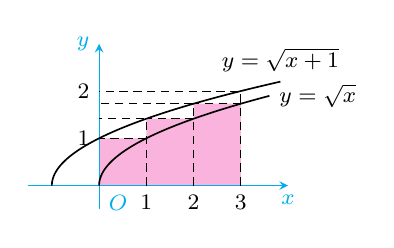
\begin{tikzpicture}[samples=100,>=stealth,font=\footnotesize,scale=0.6]
                \coordinate (O) at (0,0);
                \coordinate (A) at (3,0);
                \coordinate (B) at (0,2);
                \fill[magenta!30] (0,0) -- (3,0) -- (3,{sqrt(3)}) -- (2,{sqrt(3)}) -- (2,{sqrt(2)}) -- (1,{sqrt(2)}) -- (1,1) -- (0,1) -- cycle;
                \draw[->,cyan](-1.5,0)--(0,0)node[below right]{$O$}--(4,0)node[below]{$x$};
                \draw[->,cyan](0,-0.5)--(0,3)node[left]{$y$};
                \draw[semithick,domain=0:1.9]plot({(\x)^2},\x)node[right]{$y=\sqrt x$};
                \draw[semithick,domain=0:2.2]plot({(\x)^2-1},\x)node[above]{$y=\sqrt{x+1}$};
                \foreach \i in {1,...,2}{\coordinate[label=left:{$\i$}] (y\i) at ($(O)!\i/2!(B)$);}
                \foreach \i in {1,...,3}
                {
                \coordinate[label=below:{$\i$}] (x\i) at ($(O)!\i/3!(A)$);
                \draw[densely dashed] (\i,0) -- (\i,{sqrt(\i+1)}) -- (0,{sqrt(\i+1)});
                \draw[densely dashed] (\i,{sqrt(\i)}) -- (\i-1,{sqrt(\i)});
                }
            \end{tikzpicture}
            \caption{}
            \label{yx1yx}
        \end{figure}
    \end{minipage}
    \hfill
    \begin{minipage}{0.68\linewidth}
        由图 \ref{yx1yx} 得: 一方面 $$\displaystyle\sum_{i=1}^{n}\sqrt{i}<\int_{0}^{n}\sqrt{x+1}\dd x=\frac{2}{3}\left[(n+1)^{3/2}-1\right]$$
        另一方面 $$\displaystyle\sum_{i=1}^{n}\sqrt{i}>\int_{0}^{n}\sqrt{x}\dd x=\frac{2}{3}n^{3/2}$$
        由夹逼准则 $$\displaystyle\lim_{n\to\infty}\sum_{i=1}^{n}\sqrt{i}\sim\frac{2}{3}n^{3/2}~ (n\to\infty).$$
    \end{minipage}
\end{solution}

\begin{example}
    求极限 $\displaystyle\lim_{n\to+\infty}\dfrac{1}{\sqrt{n}}\left(\dfrac{n+1}{2}-\sum_{i=1}^{n}\dfrac{i}{n+\sqrt{i}}\right).$
\end{example}
\begin{solution}
    $\displaystyle\text{原式}=\lim_{n\to+\infty}\frac{1}{\sqrt{n}}\left(\frac{1}{n}\sum_{i=1}^{n}i-\frac{1}{n}\sum_{i=1}^{n}\frac{in}{n+\sqrt{i}}\right)=\lim_{n\to+\infty}n^{-3/2}\sum_{i=1}^{n}\frac{i^{3/2}}{n+\sqrt{i}}:=\lim_{n\to+\infty}f$
    $$\frac{2}{5}=\lim_{n\to\infty}\frac{n^{-3/2}}{n+\sqrt{n}}\cdot\frac{2}{5}n^{5/2}=\lim_{n\to\infty}\frac{n^{-3/2}}{n+\sqrt{n}}\sum_{i=1}^{n}i^{3/2}\leqslant\lim_{n\to+\infty}f
        \leqslant \lim_{n\to\infty}\frac{n^{-3/2}}{n+1}\sum_{i=1}^{n}i^{3/2}=\lim_{n\to\infty}\frac{n^{-3/2}}{n+1}\cdot\frac{2}{5}n^{5/2}=\frac{2}{5}$$
    \begin{minipage}{0.38\linewidth}
        \begin{figure}[H]
            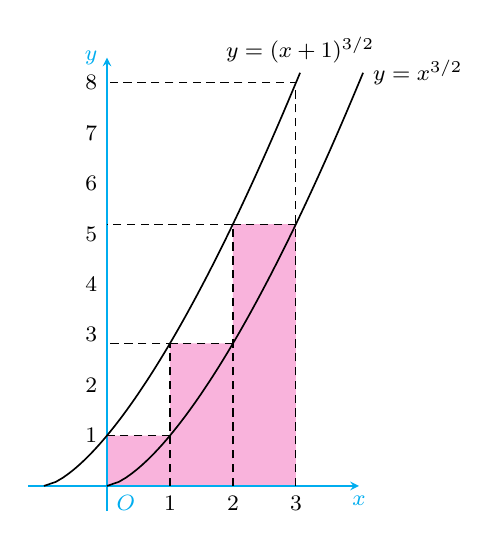
\begin{tikzpicture}[samples=100,>=stealth,font=\footnotesize,yscale=0.8,scale=0.8]
                \coordinate (O) at (0,0);
                \coordinate (A) at (3,0);
                \coordinate (B) at (0,8);
                \fill[magenta!30] (0,0) -- (3,0) -- (3,{3^(3/2)}) -- (2,{3^(3/2)}) -- (2,{2^(3/2)}) -- (1,{2^(3/2)}) -- (1,1) -- (0,1) -- cycle;
                \draw[->,cyan](-1.25,0)--(0,0)node[below right]{$O$}--(4,0)node[below]{$x$};
                \draw[->,cyan](0,-0.5)--(0,8.5)node[left]{$y$};
                \draw[semithick,domain=0:8.2]plot({(\x)^(2/3)},\x)node[right]{$y=x^{3/2}$};
                \draw[semithick,domain=0:8.2]plot({(\x)^(2/3)-1},\x)node[above]{$y=(x+1)^{3/2}$};
                \foreach \i in {1,...,8}{\coordinate[label=left:{$\i$}] (y\i) at ($(O)!\i/8!(B)$);}
                \foreach \i in {1,...,3}
                {
                \coordinate[label=below:{$\i$}] (x\i) at ($(O)!\i/3!(A)$);
                \draw[densely dashed] (\i,0) -- (\i,{(\i+1)^(3/2)}) -- (0,{(\i+1)^(3/2)});
                \draw[densely dashed] (\i,{(\i)^(3/2)}) -- (\i-1,{(\i)^(3/2)});
                }
            \end{tikzpicture}
            \caption{}
            \label{yx132yx32}
        \end{figure}
    \end{minipage}
    \hfill
    \begin{minipage}{0.58\linewidth}
        故,原式=$\dfrac{2}{5}$,下证 $\displaystyle\lim_{n\to\infty}\sum_{i=1}^{n}i^{3/2}\sim\frac{2}{5}n^{5/2}~ (n\to\infty)$,
        由图 \ref{yx132yx32} 得: 一方面
        $$\sum_{i=1}^{n}i^{3/2}<\int_{0}^{n}(x+1)^{3/2}\dd x=\frac{2}{5}\left[(n+1)^{5/2}-1\right]$$
        另一方面 $$\sum_{i=1}^{n}i^{3/2}>\int_{0}^{n}x^{3/2}\dd x=\frac{2}{5}n^{5/2}$$
        由夹逼准则 $$\lim_{n\to\infty}\sum_{i=1}^{n}i^{3/2}\sim\frac{2}{5}n^{5/2}~ (n\to\infty).$$
    \end{minipage}
\end{solution}

\begin{example}[第四届数学竞赛]
    求极限 $\displaystyle\lim_{x\to+\infty}\sqrt[3]{x}\int_{x}^{x+1}\dfrac{\sin t}{\sqrt{t+\cos t}}\dd t.$
\end{example}
\begin{solution}
    当 $x>1$ 时,因为
    $$0\leqslant \qty|\int_{x}^{x+1}\dfrac{\sin t}{\sqrt{t+\cos t}}\dd t|\leqslant \int_{x}^{x+1}\dfrac{\dd t}{\sqrt{t-1}}=2\qty(\sqrt{x}-\sqrt{x-1})=\dfrac{2}{\sqrt{x}+\sqrt{x-1}}\leqslant \dfrac{2}{\sqrt{x}}$$
    所以 $$0\leqslant \lim_{x\to+\infty}\qty|\int_{x}^{x+1}\dfrac{\sin t}{\sqrt{t+\cos t}}\dd t|\leqslant \lim_{x\to+\infty}\dfrac{2\sqrt[3]{x}}{\sqrt x}=0$$
    故由夹逼准则得原极限 $\displaystyle \lim_{x\to+\infty}\sqrt[3]{x}\int_{x}^{x+1}\dfrac{\sin t}{\sqrt{t+\cos t}}\dd t=0.$
\end{solution}

\begin{example}[2013 浙江省数学竞赛]
    \scriptsize\linespread{0.8}
    设 $f_n(x)=x^n\ln x$,求 $\displaystyle\lim_{n\to\infty}\dfrac{1}{n!}f_n^{(n-1)}\qty(\dfrac{1}{n}).$
\end{example}
\begin{solution}
    因为 $f_n'(x)=nx^{n-1}\ln x+x^{n-1}=nf_{n-1}(x)+x^{n-1}$,所以
    $$f_n^{(n-1)}(x)=\qty[f_n'(x)]^{(n-2)}=\qty[nf_{n-1}(x)+x^{n-1}]^{(n-2)}=nf_{n-1}^{(n-2)}(x)+(n-1)!x$$
    经过递推可得
    \begin{flalign*}
        \dfrac{1}{n!}f_n^{(n-1)}(x)=\dfrac{f_{n-1}^{(n-2)}(x)}{(n-1)!}+\dfrac{x}{n}=\dfrac{f_{n-2}^{(n-3)}(x)}{(n-2)!}+\dfrac{x}{n-1}+\dfrac{x}{n}
        =\dots=\dfrac{f_2'(x)}{2!}+x\sum_{k=3}^{n}\dfrac{1}{k}=x\qty(\ln x+\sum_{k=2}^{n}\dfrac{1}{k})
    \end{flalign*}
    于是,有 $\displaystyle\dfrac{1}{n!}f_n^{(n-1)}\qty(\dfrac{1}{n})=\dfrac{1}{n}\qty(\sum_{k=2}^{n}\dfrac{1}{k}-\ln n)$,并且
    $$\ln(n+1)-\ln 2=\int_{1}^{n}\dfrac{\dd x}{x+1}<\sum_{k=2}^{n}\dfrac{1}{k}<\int_{1}^{n}\dfrac{\dd x}{x}=\ln n$$
    所以
    $$0=\lim_{n\to\infty}\dfrac{1}{n}\ln\dfrac{n+1}{2n}<\lim_{n\to\infty}\dfrac{1}{n!}f_n^{(n-1)}\qty(\dfrac{1}{n})<0$$
    由夹逼准则得原极限为 0.
\end{solution}

\subsubsection{夹逼准则的推广形式}

当使用夹逼准则时,若放大与缩小所得之量的极限值不相等,但两者只相差一个任意小量,则夹逼准则仍然有效.

\begin{example}
    (推论 \ref{maxai} 的连续形式) 设 $f(x)>0$,在区间 $[0,1]$ 上连续,
    试证 $$\lim_{n\to\infty}\sqrt[n]{\sum_{i=1}^{n}\left[f\left(\frac{i}{n}\right)\right]^n\frac{1}{n}}=\max_{0\leqslant x\leqslant 1}f(x).$$
\end{example}
\begin{proof}
    记 $\displaystyle M=\max_{0\leqslant x\leqslant 1}f(x)$,则 $$x_n:= \sqrt[n]{\sum_{i=1}^{n}\left[f\left(\frac{i}{n}\right)\right]^n\frac{1}{n}}\leqslant M$$
    因为 $f(x)$ 连续,根据闭区间连续函数的性质,$\exists x_0\in[0,1],~s.t.f(x_0)=M$.
    于是 $\forall \varepsilon>0,~\exists\delta>0\text{,当 }|x-x_0|<\delta,~x\in[0,1]$ 时,有 $$M-\varepsilon<f(x)<M+\varepsilon$$
    当 $n$ 充分大时有 $\displaystyle \frac{1}{n}<\delta,~\exists i_0,~s.t. \left|\frac{i_0}{n}-x_0\right|<\delta,~f\left(\frac{i_0}{n}\right)>M-\varepsilon$.
    故 $$x_n:= \sqrt[n]{\sum_{i=1}^{n}\left[f\left(\frac{i}{n}\right)\right]^n\frac{1}{n}}\geqslant\sqrt[n]{\left(f\left(\frac{i_0}{n}\right)\right)^n\frac{1}{n}}>(M-\varepsilon)\frac{1}{\sqrt[n]{n}}\to M-\varepsilon$$
    由 $\varepsilon>0$ 的任意性,知 $\displaystyle\lim_{n\to\infty}x_n=M.$
\end{proof}
\begin{example}
    求极限 $\displaystyle\lim_{n\to\infty}\int_{0}^{\frac{\pi}{2}}\sin^nx\dd x.$
\end{example}
\begin{solution}
    \textbf{法一: }$\displaystyle\forall 0<\varepsilon<\frac{\pi}{2}$,有
    \begin{flalign*}
        0  \leqslant \int_{0}^{\frac{\pi}{2}}\sin^nx\dd x=\int_{0}^{\frac{\pi}{2}-\varepsilon}\sin^nx\dd x+\int_{\frac{\pi}{2}-\varepsilon}^{\frac{\pi}{2}}\sin^nx\dd x
        \leqslant\frac{\pi}{2}\cdot\sin^nx\left(\frac{\pi}{2}-\varepsilon\right)+\int_{\frac{\pi}{2}-\varepsilon}^{\frac{\pi}{2}}\dd x=\frac{\pi}{2}\cdot\sin^n\left(\frac{\pi}{2}-\varepsilon\right)+\varepsilon
    \end{flalign*}
    令 $n\to\infty$,得 $$0\leqslant\lim_{n\to\infty}\int_{0}^{\frac{\pi}{2}}\sin^nx\dd x\leqslant\lim_{n\to\infty}\frac{\pi}{2}\cdot\sin^nx\left(\frac{\pi}{2}-\varepsilon\right)+\varepsilon=\varepsilon$$
    再由 $\varepsilon$ 的任意性及夹逼准则,得 $\displaystyle\lim_{n\to\infty}\int_{0}^{\frac{\pi}{2}}\sin^nx\dd x=0.$\\
    \textbf{法二: }记 $\displaystyle I_n=\int_{0}^{\frac{\pi}{2}}\sin^nx\dd x$,则由
    $$\int_{0}^{\frac{\pi}{2}}\sin^nx\dd x=\begin{cases}
            \displaystyle \frac{(n-1)!!}{n!!}\cdot \frac{\pi}{2} & ,n\text{ 为正偶数}        \\[6pt]
            \displaystyle \frac{(n-1)!!}{n!!}                    & ,n\text{ 为大于 1 的奇数}
        \end{cases}$$
    其中 $n!!$ 表示不大于 $n$ 且与 $n$ 有相同奇偶性的数的连乘积. 得
    $$I_{2k}=\frac{(2k-1)!!}{(2k)!!}\cdot\frac{\pi}{2}$$
    于是有 $$I_{2k}^2=\frac{1\cdot3\cdot3\cdot5\cdot5\cdots(2k-3)(2k-3)(2k-1)(2k-1)\cdot 1}{2\cdot2\cdot4\cdot4\cdot6\cdot6\cdots(2k-4)(2k-2)(2k-2)(2k)\cdot2k}\cdot\frac{\pi}{4}$$
    从而得 $\displaystyle\frac{1}{4k}\cdot\frac{\pi^2}{4}<I_{2k}^2<\frac{2k-1}{4k^2}\cdot\frac{\pi^2}{4}$,故 $\displaystyle\lim_{k\to0}I_{2k}=0$. 又因为 $0\leqslant I_{2k+1}\leqslant I_{2k}$,
    所以 $\displaystyle\lim_{k\to\infty}I_{2k+1}=0$,从而得 $\displaystyle\lim_{n\to\infty}I_n=0$,即 $\displaystyle\lim_{n\to\infty}\int_{0}^{\frac{\pi}{2}}\sin^nx\dd x=0.$
\end{solution}

\subsubsection{Wallis 公式}

\begin{inference}\label{inference:Wallis}
    $\displaystyle I_n=\int_{0}^{\frac{\pi}{2}}\sin^nx\dd x=\int_{0}^{\frac{\pi}{2}}\cos ^nx\dd x=\begin{cases}
            \displaystyle \frac{(n-1)!!}{n!!}\cdot \frac{\pi}{2} & ,n\text{ 为正偶数}         \\[6pt]
            \displaystyle \frac{(n-1)!!}{n!!}                    & ,n\text{ 为大于 1 的奇数.}
        \end{cases}$\\
    一般形式: $$I_{m,n}=\int_{0}^{\frac{\pi}{2}}\sin^mx\cos^nx\dd x=\begin{cases}
            \displaystyle \frac{(m-1)!!(n-1)!!}{(m+n)!!}\cdot \frac{\pi}{2} & ,m,n\text{ 为正偶数}        \\[6pt]
            \displaystyle \frac{(m-1)!!(n-1)!!}{(m+n)!!}                    & ,m,n\text{ 为大于 1 的奇数}
        \end{cases}.
        \label{Wallis gs}$$
\end{inference}
\begin{proof}[{\songti \textbf{证}}]
    利用分部积分公式 $\displaystyle\int f\dd g=fg-\int g\dd f$,
    \begin{flalign*}
        I_{m,n} & =\int_{0}^{\frac{\pi}{2}}\sin^mx\cos^nx\dd x=\int_{0}^{\frac{\pi}{2}}\sin^mx\cos^{n-1}x\dd \sin x
        =\sin^{m+1}x\cos^{n-1}x\bigg |_0^{\frac{\pi}{2}}-\int_{0}^{\frac{\pi}{2}}\sin x\dd \left(\sin ^mx\cos^{n-1}x\right) \\
                & =-m\int_{0}^{\frac{\pi}{2}}\sin^mx\cos^nx\dd x+(n-1)\int_{0}^{\frac{\pi}{2}}\sin^{m+2}x\cos^{n-2}x\dd x
        =-mI_{m,n}+(n-1)I_{m+2,n-2}
    \end{flalign*}
    \begin{enumerate}[label=(\arabic{*})]
        \item 当 $n$ 为正偶数 $n=2k$ 时,
              \begin{flalign*}
                  I_{m,n} & =\frac{n-1}{m+1}I_{m+2,n-2}=\frac{n-1}{m+1}\cdot\frac{n-3}{m+3}I_{m+4,n-4}=\cdots=\frac{(n-1)(n-3)\cdots1}{(m+1)(m+3)\cdots(m+n-1)}I_{m+n,0}       \\
                          & =\begin{cases}
                                 \displaystyle \frac{(n-1)(n-3)\cdots1}{(m+1)(m+3)\cdots (m+n-1)}\frac{(m+n-1)!!}{(m+n)!!}\cdot \frac{\pi}{2} & ,\text{当 $m$ 也为正偶数时} \\[6pt]
                                 \displaystyle \frac{(n-1)(n-3)\cdots1}{(m+1)(m+3)\cdots (m+n-1)}\frac{(m+n-1)!!}{(m+n)!!}                    & ,\text{否则}
                             \end{cases} \\
                          & =\begin{cases}
                                 \displaystyle \frac{(m-1)!!(n-1)!!}{(m+n)!!}\cdot \frac{\pi}{2} & ,\text{当 $m$ 也为正偶数时} \\[6pt]
                                 \displaystyle \frac{(m-1)!!(n-1)!!}{(m+n)!!}                    & ,\text{否则}
                             \end{cases}
              \end{flalign*}
              因为 $\displaystyle\frac{(n-1)(n-3)\cdots1}{(m+1)(m+3)\cdots(m+n-1)}=\frac{(m-1)!!(n-1)!!}{(m+n-1)!!}.$
        \item 当 $n$ 为大于 $1$ 的奇数 $n=2k+1$ 时 (不论 $m$ 是偶数还是奇数) 时,
              \begin{flalign*}
                  I_{m,n}  =\frac{n-1}{m+1}I_{m+2,n-2}=\frac{n-1}{m+1}\cdot\frac{n-3}{m+3}I_{m+4,n-4}=\cdots
                  =\frac{(n-1)(n-3)\cdots2}{(m+1)(m+3)\cdots(m+n-2)}I_{m+n-1,1}
              \end{flalign*}
              其中 $\displaystyle I_{m+n-1,1}=\int_{0}^{\frac{\pi}{2}}\sin^{m+n-1}x\cos x\dd x=\int_{0}^{\frac{\pi}{2}}\sin^{m+n-1}x\dd \sin x=\int_{0}^{1}t^{m+n-1}\dd t=\frac{1}{m+n}$,
              代入上式,得 $$I_{m,n}=\frac{(n-1)(n-3)\cdots2}{(m+1)(m+3)\cdots(m+n-2)}\cdot\frac{1}{m+n}=\frac{(n-1)!!(m-1)!!}{(m+n)!!}.$$
    \end{enumerate}
    综上即得欲证等式.
\end{proof}

\begin{theorem}[双阶乘与阶乘的转化]
    $(2n)!!=2^n\cdot n!,~(2n-1)!!=\dfrac{(2n)!}{2^n\cdot n!}.$
    \index{双阶乘与阶乘的转化}
\end{theorem}

\begin{example}
    设 $a_n=\displaystyle\int_{0}^{1}x^n\sqrt{1-x^2}\dd x,~b_n=\int_{0}^{\frac{\pi}{2}}\sin ^nx\cos^nx\dd x$,求 $\displaystyle\lim_{n\to\infty}\dfrac{b_n}{a_n}.$
\end{example}
\begin{solution}
    由推论 \ref{inference:Wallis} 知,$\displaystyle b_n=\begin{cases}
            \dfrac{[(n-1)!!]^2}{(2n)!!}\cdot\dfrac{\pi}{2}, & n\text{ 为正偶数}     \\[6pt]
            \dfrac{[(n-1)!!]^2}{(2n)!!},                    & n\text{大于 1 的奇数}
        \end{cases}$,并且
    $$a_n\xlongequal{x=\cos t}\int_{0}^{\frac{\pi}{2}}\cos^nt\cdot\sin^2t\dd t=\begin{cases}
            \dfrac{(n-1)!!}{(n+2)!!}\cdot\dfrac{\pi}{2}, & n\text{ 为正偶数}      \\[6pt]
            \dfrac{(n-1)!!}{(n+2)!!},                    & n\text{ 大于 1 的奇数}
        \end{cases}$$
    因此
    \begin{flalign*}
        \lim_{n\to\infty}\dfrac{b_n}{a_n}=\begin{cases}
                                              \dfrac{[(n-1)!!]^2}{(2n)!!}\cdot\dfrac{\pi}{2}\cdot\dfrac{(n+2)!!}{(n-1)!!}\cdot\dfrac{2}{\pi}=\dfrac{(n-1)!!\cdot(n+2)!!}{(2n)!!}=\dfrac{n!(n+2)}{2^n\cdot n!}=\dfrac{n+2}{2^n}\to0, & n\text{ 为正偶数}      \\[6pt]
                                              \dfrac{[(n-1)!!]^2}{(2n)!!}\cdot\dfrac{(n+2)!!}{(n-1)!!}=\dfrac{(n-1)!!\cdot(n+2)!!}{(2n)!!}=\dfrac{n!(n+2)}{2^n\cdot n!}=\dfrac{n+2}{2^n}\to0,                                       & n\text{ 大于 1 的奇数}
                                          \end{cases}
    \end{flalign*}
    故 $\displaystyle\lim_{n\to\infty}\dfrac{b_n}{a_n}=0.$
\end{solution}

\subsection{求极限其他常用方法}

下述的各种方法涉及到之后的知识点,若对知识点掌握不扎实,可暂缓阅读.

\subsubsection{L'Hospital 法则}

\begin{theorem}[$\dfrac{0}{0}$ 型 L'Hospital 法则]
    如果函数 $f(x)$ 和 $g(x)$ 满足以下条件:\label{LHospitalLaw}
    \begin{enumerate}[label=(\arabic{*})]
        \item 当 $ x \rightarrow a $ 时,$f(x) $ 和 $ g(x) $ 都是无穷小 (或无穷大);
        \item 在点 $ a $ 的某个去心邻域内,$f(x) $ 和 $ g(x) $ 都是可导的,且 $ g^{\prime}(x) \neq 0$ ;
        \item $\displaystyle\lim _{x \rightarrow a} \frac{f^{\prime}(x)}{g^{\prime}(x)} $ 存在 (或为无穷大),
    \end{enumerate}
    那么 $ \displaystyle\lim _{x \rightarrow a} \frac{f(x)}{g(x)}=\lim _{x \rightarrow a} \frac{f^{\prime}(x)}{g^{\prime}(x)} .$
    \index{L'Hospital 法则}
\end{theorem}

\begin{theorem}[$\dfrac{*}{\infty}$ 型 L'Hospital 法则]
    对于 $ \dfrac{\infty}{\infty} $ 型的不定式,一般情形 (即 $ \dfrac{*}{\infty} $ 型的不定式) 为: 如果函数 $ f(x) $ 和 $ g(x) $ 满足
    \begin{enumerate}[label=(\arabic{*})]
        \item 在点 $ a $ 的某个去心邻域内,$f(x) $ 和 $ g(x) $ 都是可导的,且 $ g^{\prime}(x) \neq 0$ ;
        \item $\displaystyle\lim _{x \rightarrow a} g(x)=\infty $;
        \item $\displaystyle\lim _{x \rightarrow a} \frac{f^{\prime}(x)}{g^{\prime}(x)} $ 存在 (或为无穷大),
    \end{enumerate}
    那么 $\displaystyle \lim _{x \rightarrow a} \frac{f(x)}{g(x)}=\lim _{x \rightarrow a} \frac{f^{\prime}(x)}{g^{\prime}(x)}$ .
\end{theorem}

每次使用 L'Hospital 法则之前,务必考察它是否属于七种不定型,否则不能用,七种不定型如下.
$$\frac{0}{0},~\frac{\infty}{\infty},~0\cdot\infty,~\infty-\infty,~0^0,~1^\infty,~\infty^0$$

一旦用 L'Hospital 法则算不出结果,不等于极限不存在. 例如 $\displaystyle\lim_{x\to\pm\infty}\frac{x+\sin x}{x+\cos x}=1$,
就是如此. 这是因为 L'Hospital 法则只是充分条件,不是必要条件.

使用 $\displaystyle\frac{\infty}{\infty}$ 型的 L'Hospital 法则时,只需要检验分母趋向无穷大即可,
分子不趋向 $\infty$ 没有关系.

在多数需要使用 L'Hospital 法则的情境下,式子含有变限积分,变限积分的求导公式如下:
$$\frac{\dd }{\dd x}\int_{\alpha(x)}^{\beta(x)}f(t)\dd t=f(\beta(x))\cdot\beta'(x)-f(\alpha(x))\cdot\alpha'(x).$$

\begin{theorem}[Heine 定理]
    若 $x_n\not=x_0$,$\displaystyle\lim_{x\to x_0}f(x)=A\Leftrightarrow\forall x_n\to x_0~ (n\to\infty)$,
    恒有 $\displaystyle\lim_{n\to\infty}f(x_n)=A.$
    \index{Heine 定理}
\end{theorem}

\begin{example}
    求下列极限值.
    \setcounter{magicrownumbers}{0}
    \begin{table}[H]
        \centering
        \begin{tabular}{l | l}
            (\rownumber{}) $\displaystyle\lim_{n\to\infty}\frac{1}{n}\int_{\frac{1}{n}}^{1}\frac{\cos 2t}{4t^2}\dd t.$              & (\rownumber{}) $\displaystyle\lim_{n\to+\infty}\left[\left(n^3-n^2+\frac{n}{2}\right)\e ^{\frac{1}{n}}-\sqrt{1+n^6}\right].$               \\
            (\rownumber{}) $\displaystyle\lim_{n\to\infty}\frac{1}{\sqrt{n}}\int_{1}^{n}\ln\left(1+\frac{1}{\sqrt{x}}\right)\dd x.$ & (\rownumber{}) (中国科学院) $\displaystyle\lim_{x\to0}\frac{\displaystyle x-\int_{0}^{x}\e ^{t^2}\dd t}{x^2\sin2x}.$                       \\
            (\rownumber{}) $\displaystyle\lim_{x\to +\infty}\left(\frac{2}{\pi}\arctan x\right)^x.$                                 & (\rownumber{}) $\displaystyle\lim_{n\to\infty}\sin\frac{1}{n}\cdot\int_{n}^{n^2}\left(1+\frac{1}{2t}\right)^t\sin\frac{1}{\sqrt{t}}\dd t.$
        \end{tabular}
    \end{table}
\end{example}
\begin{solution}
    \begin{enumerate}[label=(\arabic{*})]
        \item 将 $\displaystyle\frac{1}{n}$ 替换为 $x$,利用 Heine 定理把数列极限转化为函数极限,
              \begin{flalign*}
                  \text{原式}=\lim_{x\to0^+}x\int_{x}^{1}\frac{\cos 2t}{4t^2}\dd t=\lim_{x\to0^+}\frac{\displaystyle\int_{x}^{1}\dfrac{\cos 2t}{4t^2}\dd t}{t^{-1}}
                  \xlongequal[]{L'}\lim_{x\to0^+}\frac{-\dfrac{\cos2x}{4x^2}}{-\dfrac{1}{x^2}}=\frac{1}{4}\lim_{x\to0^+}\cos2x=\frac{1}{4}.
              \end{flalign*}
        \item 由 Heine 定理,将数列极限转为函数极限,并且令 $\displaystyle t=\frac{1}{x}$,那么 $t\to0^+$,
              \begin{flalign*}
                  \text{原式} & =\lim_{t\to0^+}\left[\left(\frac{1}{t^3}-\frac{1}{t^2}+\frac{1}{2t}\right)\e ^t-\sqrt{1+\frac{1}{t^6}}\right]=\lim_{t\to0^+}\frac{\left(1-t+\dfrac{t^2}{2}\right)\e ^t-\sqrt{1+t^6}}{t^3}                  \\
                              & \xlongequal[]{L'}\lim_{t\to0^+}\frac{(-1+t)\e ^t+\left(1-t+\dfrac{t^2}{2}\right)\e ^t-\dfrac{6t^5}{2\sqrt{1+t^6}}}{3t^2}=\lim_{t\to0^+}\frac{\dfrac{1}{2}\e ^t-\dfrac{3t^3}{\sqrt{1+t^6}}}{3}=\frac{1}{6}.
              \end{flalign*}
        \item 为 $\displaystyle\frac{*}{\infty}$ 型,$\displaystyle\text{原式}\xlongequal[]{L'}\lim_{n\to\infty}\frac{\ln\left(1+\dfrac{1}{\sqrt{n}}\right)}{\dfrac{1}{2\sqrt{n}}}=\lim_{n\to\infty}\frac{1}{\sqrt{n}}\cdot\frac{2\sqrt{n}}{1}=2.$
        \item 为 $\displaystyle\frac{0}{0}$ 型,$\displaystyle\text{原式}=\lim_{x\to0}\frac{\displaystyle x-\int_{0}^{x}\e ^{t^2}\dd t}{2x^3}\xlongequal[]{L'}\lim_{x\to0}\frac{1-\e ^{x^2}}{6x^2}=-\frac{1}{6}.$
        \item 为 $1^\infty$ 型,
              \begin{flalign*}
                  \text{原式} & =\exp\lim_{x\to +\infty}x\ln\left(\frac{2}{\pi}\arctan x\right)=\exp\lim_{x\to +\infty}x\cdot\left(\frac{2}{\pi}\arctan x-1\right) \\
                              & \xlongequal[]{\frac{1}{x}=t}\exp\lim_{t\to 0^+}\frac{\dfrac{2}{\pi}\arctan \dfrac{1}{t}-1}{t}
                  \xlongequal[]{L'}\exp\lim_{t \to 0^+}\frac{2}{\pi}\left[\frac{1}{1+\dfrac{1}{t^2}}\cdot\left(-\frac{1}{t^2}\right)\right]
                  =\e ^{-\frac{2}{\pi}}.
              \end{flalign*}
        \item $\displaystyle\text{原式}=\lim_{n\to\infty}\frac{\displaystyle\int_{n}^{n^2}\left(1+\dfrac{1}{2t}\right)^t\sin\dfrac{1}{\sqrt{t}}\dd t}{n}\xlongequal[]{L'}\lim_{n\to\infty}\left[2n\left(1+\frac{1}{2n^2}\right)^{n^2}\sin\frac{1}{n}-\left(1+\frac{1}{2n}\right)^n\sin\frac{1}{\sqrt{n}}\right]$,\\
              其中 $$\lim_{n\to\infty}2n\left(1+\frac{1}{2n}\right)^{n^2}\sin\frac{1}{n}=2\exp\lim_{n\to\infty}n^2\ln\left(1+\frac{1}{2n^2}\right)=2\sqrt{\e }.$$
              $$\lim_{n\to\infty}\left(1+\frac{1}{2n}\right)^n\sin\frac{1}{\sqrt{n}}=\lim_{n\to\infty}\frac{\left(1+\dfrac{1}{2n}\right)^n}{\sqrt{n}}=0.$$
              故,$\displaystyle\text{原式}=2\sqrt{\e }.$
    \end{enumerate}
\end{solution}

\begin{example}[中南大学]
    设 $f(x)$ 有二阶导数,在原点附近不为零,但 $\displaystyle\lim_{x\to0}\frac{f(x)}{x}=0,f''(0)=4$,求 $$\lim_{x\to0}\left(1+\frac{f(x)}{x}\right)^{\frac{1}{x}}.$$
\end{example}
\begin{solution}
    $\displaystyle\lim_{x\to0}\left(1+\frac{f(x)}{x}\right)^{\frac{1}{x}}=\exp\lim_{x\to0}\frac{1}{x}\ln\left(1+\frac{f(x)}{x}\right)\xlongequal[]{L'}\exp\lim_{x\to0}\frac{\dfrac{f'(x)}{x}-\dfrac{f(x)}{x^2}}{1+\dfrac{f(x)}{x}}$,
    下求分子分母的极限.
    \begin{flalign*}
         & \lim_{x\to0}\frac{f(x)}{x}=0\Rightarrow f(0)=\lim_{x\to0}f(x)=\lim_{x\to0}\frac{f(x)}{x}\cdot x=0                                          \\
         & f'(0)=\lim_{x\to0}\frac{f(x)-f(0)}{x}\xlongequal[]{f(0)=0}\lim_{x\to0}\frac{f(x)}{x}=0                                                     \\
         & \lim_{x\to0}\frac{f(x)}{x^2}\xlongequal[]{L'}\lim_{x\to0}\frac{f'(x)}{2x}=\frac{1}{2}\lim_{x\to0}\frac{f'(x)-f'(0)}{x}=\frac{1}{2}f''(0)=2
    \end{flalign*}
    于是 $\displaystyle\lim_{x\to0}\left(1+\frac{f(x)}{x}\right)^{\frac{1}{x}}=\e ^{\frac{4-2}{1}}=\e ^2.$
\end{solution}

\begin{example}[2005 数学 (二)]
    设函数 $f(x)$ 在 $x=0$ 的某邻域内连续,且 $f(0)\not=0$ ,求极限
    $$\lim_{x\to0}\frac{\displaystyle\int_{0}^{x}(x-t)f(t)\dd t}{x\displaystyle\int_{0}^{x}f(x-t)\dd t}.$$
    \label{not L Hospital}
\end{example}
\begin{solution}
    $\displaystyle\int_{0}^{x}f(x-t)\dd t\xlongequal[]{x-t=u}-\int_{x}^{0}f(u)\dd u=\int_{0}^{x}f(u)\dd u=\int_{0}^{x}f(t)\dd t$,于是
    $$\text{原式}=\lim_{x\to0}\frac{x\displaystyle\int_{0}^{x}f(t)\dd t-\int_{0}^{x}tf(t)\dd t}{x\displaystyle\int_{0}^{x}f(t)\dd t}\xlongequal[]{L'}\lim_{x\to0}\frac{\displaystyle\int_{0}^{x}f(t)\dd t}{\displaystyle\int_{0}^{x}f(t)\dd t+xf(x)}$$
    因为 $f(x)$ 在 $x=0$ 的某邻域内未必可导,不满足 L'Hospital 法则条件,不能继续用 L'Hospital 法则. 以下给出两种解法: \\
    \textbf{法一: }用积分中值定理 $\displaystyle\int_{0}^{x}f(x)\dd x=f(\xi)\cdot x$,其中 $\xi$ 介于 $0$ 与 $x$ 之间.
    $$\text{原式}=\lim_{x\to0}\frac{xf(\xi)}{xf(\xi)+xf(x)}=\lim_{x\to0}\frac{f(\xi)}{f(\xi)+f(x)}=\frac{1}{2}.$$
    \textbf{法二: }令 $\displaystyle F(x)=\int_{0}^{x}f(t)\dd t$,则 $F'(x)=f(x)$,$\displaystyle\lim_{x\to0}\frac{F(x)-F(0)}{x}=f(0).$
    $$\text{原式}=\lim_{x\to0}\frac{F(x)}{F(x)+xF'(x)}=\lim_{x\to0}\frac{\dfrac{F(x)-F(0)}{x}}{\dfrac{F(x)-F(0)}{x}+F'(x)}=\frac{f(0)}{f(0)+f(0)}=\frac{1}{2}.$$
\end{solution}
注意\textbf{连续不一定可导,可导必连续},即当不满足 L'Hospital 法则条件时,可参考例题 \ref{not L Hospital} 中给出的两种方法.

\begin{example}
    设 $f'(x)$ 连续,$f(0)=0,f'(0)\not=0$,求 $\displaystyle\lim_{x\to0}\frac{\displaystyle\int_{0}^{x^2}f(x^2-t)\dd t}{x^3\displaystyle\int_{0}^{1}f(xt)\dd t}.$
\end{example}
\begin{solution}
    分子有 $$\displaystyle\int_{0}^{x^2}f(x^2-t)\dd t\xlongequal[]{x^2-t=u}-\int_{x^2}^{0}f(u)\dd u=\int_{0}^{x^2}f(u)\dd u=\int_{0}^{x^2}f(t)\dd t$$
    分母有 $$\displaystyle\int_{0}^{1}f(xt)\dd t\xlongequal[]{xt=v}\frac{1}{x}\int_{0}^{x}f(v)\dd v=\frac{1}{x}\int_{0}^{x}f(t)\dd t$$
    于是
    \begin{flalign*}
        \text{原式} =\lim_{x\to0}\frac{\displaystyle\int_{0}^{x^2}f(t)\dd t}{x^2\displaystyle\int_{0}^{x}f(t)\dd t}\xlongequal[]{L'}\lim_{x\to0}\frac{2f(x^2)}{2\displaystyle\int_{0}^{x}f(t)\dd t+xf(x)}\xlongequal[]{L'}\lim_{x\to0}\frac{4xf'(x^2)}{3f(x)+xf'(x)}
        =\lim_{x\to0}\frac{4f'(x^2)}{3\dfrac{f(x)}{x}+f'(x)}=\frac{4f'(0)}{4f'(0)}=1.
    \end{flalign*}
\end{solution}

\begin{example}
    设 $f(x)$ 在 $x=0$ 的某邻域内连续,且 $f(0)=0,f'(0)=1$,求 $\displaystyle\lim_{x\to0}\frac{\displaystyle\int_{0}^{x}tf(x^2-t^2)\dd t}{x^3\sin x}.$
\end{example}
\begin{solution}
    因为 $\displaystyle\int_{0}^{x}tf(x^2-t^2)\dd t\xlongequal[]{x^2-t^2=u}-\frac{1}{2}\int_{x^2}^{0}f(u)\dd u=\frac{1}{2}\int_{0}^{x^2}f(t)\dd t$,于是
    $$\text{原式}=\lim_{x\to0}\frac{\displaystyle\frac{1}{2}\int_{0}^{x^2}f(t)\dd t}{x^4}\xlongequal[]{L'}\lim_{x\to0}\frac{f(x^2)}{4x^2}\xlongequal[]{L'}\frac{1}{4}f'(x^2)=\frac{1}{4}.$$
\end{solution}

\begin{example}
    设 $f(x)$ 在 $x=0$ 的某邻域内二阶可导,$\displaystyle f'(0)\not=0,\lim_{x\to0^+}\frac{f(x)}{x}=0,\lim_{x\to0^+}\frac{\displaystyle\int_{0}^{x}f(t)\dd t}{x^\alpha-\sin x}=\beta\not=0$,求 $\alpha$ 与 $\beta$ 的值.
\end{example}
\begin{solution}
    由定理 \ref{f(x)g(x)A} 知,$\displaystyle\lim_{x\to0^+}(x^\alpha-\sin x)=0$,即 $\displaystyle\lim_{x\to0^+}\frac{x^\alpha}{\sin x}=1\Rightarrow \alpha=1$,所以
    $$\text{原式}=\lim_{x\to0^+}\frac{\displaystyle\int_{0}^{x}f(t)\dd t}{x-\sin x}=\lim_{x\to0^+}\frac{\displaystyle\int_{0}^{x}f(t)\dd t}{\dfrac{1}{6}x^3}\xlongequal[]{L'}\lim_{x\to0^+}\frac{2f(x)}{x^2}\xlongequal[]{L'}\lim_{x\to0^+}\frac{f'(x)}{x}$$
    由 $\displaystyle f'(0)\not=0,\lim_{x\to0^+}\frac{f(x)}{x}=0$,可设 $f(x)=x^2$,故 $\alpha=1,\beta=2.$
\end{solution}

\subsubsection{Taylor 展开}

\paragraph{无穷小的相关概念}
在正式介绍如何用 Taylor 展开计算极限前,需要对无穷小性质做相关介绍.
\begin{definition}[无穷小的相关定义]
    \begin{enumerate}[label=(\arabic{*})]
        \item 如果 $\lim\dfrac{\beta}{\alpha}=1$,那么称 $\beta$ 与 $\alpha$ 是\textit{等价无穷小},记作 $\alpha\sim\beta$;
        \item 如果 $\lim\dfrac{\beta}{\alpha}=c\neq0$,那么称 $\beta$ 是\textit{比} $\alpha$ \textit{同阶的无穷小},记作 $\beta\sim c\alpha$;
        \item 如果 $\lim\dfrac{\beta}{\alpha^k}=c\neq0,k>0$,那么称 $\beta$ 是\textit{关于} $\alpha$ \textit{的} $k$ \textit{阶无穷小},记作 $\beta\sim c\alpha^k$;
        \item 如果 $\lim\dfrac{\beta}{\alpha}=0$,那么称 $\beta$ 是\textit{比} $\alpha$ \textit{高阶的无穷小},记作 $\beta=o(\alpha)$;
        \item 如果 $\lim\dfrac{\beta}{\alpha}=\infty$,那么称 $\beta$ 是\textit{比} $\alpha$ \textit{低阶的无穷小}.
    \end{enumerate}
    \label{infinitesimalDefinitions}
\end{definition}

\begin{theorem}[等价无穷小的充要条件]
    $\beta$ 与 $\alpha$ 是等价无穷小的充分必要条件为 $\beta=\alpha+o(\alpha).$
    \index{等价无穷小的充要条件}
\end{theorem}
\begin{theorem}[无穷小量的传递性]
    设 $\alpha\sim\alpha',\beta\sim\beta'$,且 $\lim\dfrac{\beta'}{\alpha'}$ 存在,则 $\lim\dfrac{\beta}{\alpha}=\lim\dfrac{\beta'}{\alpha'}.$
    \index{无穷小量的传递性}
\end{theorem}
\begin{theorem}[无穷小量的加法]
    设 $m>n>0$ 且 $\lim\alpha=0$,则有 $o(\alpha^m)\pm o(\alpha^n)=o(\alpha^k)~ (0<k\leqslant n).$
    \index{无穷小量的加法}
\end{theorem}
\begin{proof}{\songti \textbf{证}}
    $\displaystyle\lim \frac{o\left(\alpha^{m}\right) \pm o\left(\alpha^{n}\right)}{\alpha^{k}}=\lim \frac{o\left(\alpha^{m}\right)}{\alpha^{m}} \cdot \alpha^{m-k} \pm \lim \frac{o\left(\alpha^{n}\right)}{\alpha^{n}} \cdot \alpha^{n-k}=0.$
\end{proof}
\begin{theorem}[无穷小量的乘法]
    $m,n>0$ 且 $\lim\alpha=0$,则有 $o(\alpha^m)(\text{ 或 }\alpha^m)\cdot o(\alpha^n)=o(\alpha^k)~ (0<k\leqslant m+n).$
    \index{无穷小量的乘法}
\end{theorem}
\begin{proof}{\songti \textbf{证}}
    $\displaystyle\lim \frac{o\left(\alpha^{m}\right) \cdot o\left(\alpha^{n}\right)}{\alpha^{k}}=\lim \frac{o\left(\alpha^{m}\right)}{\alpha^{m}} \cdot \lim \frac{o\left(\alpha^{n}\right)}{\alpha^{n}} \cdot \lim \alpha^{m+n-k}=0 \times 0 \times 0=0.$ ($\alpha^m$ 同理).
\end{proof}

\begin{example}
    设 $\cos x-1=x\sin\alpha(x)$,其中 $|\alpha(x)|<\dfrac{\pi}{2}$,则当 $x\to0$ 时,$\alpha(x)$ 是
    \begin{tasks}(2)
        \task 比 $x$ 高阶的无穷小量
        \task 比 $x$ 低阶的无穷小量
        \task 与 $x$ 同阶但不等价的无穷小量
        \task 与 $x$ 等价的无穷小量
    \end{tasks}
\end{example}
\begin{solution}
    由 $\displaystyle \lim_{x\to0}\dfrac{\alpha(x)}{x}=\lim_{x\to0}\dfrac{\sin\alpha(x)}{x}=\lim_{x\to0}\dfrac{x\sin\alpha(x)}{x^2}=\lim_{x\to0}\dfrac{\cos x-1}{x^2}=-\dfrac{1}{2}\neq1$,于是
    当 $x\to0$ 时,$\alpha(x)$ 与 $x$ 同阶但不等价的无穷小量,选 C.
\end{solution}

\begin{example}
    设 $g(x)$ 可导,且当 $x\to0$ 时, $g(x)$ 是 $x$ 的高阶无穷小,则当 $x\to0$  时,必有
    \begin{tasks}(2)
        \task $g'(x)$ 是无穷小量
        \task $\dfrac{x}{g(x)}$ 是无穷大量
        \task 若 $G'(x)=g(x)$,则 $G(x)$ 是 $x$ 的高阶无穷小
        \task $\displaystyle\int_{0}^{x}g(t)\dd t$ 是 $x^2$ 的高阶无穷小
    \end{tasks}
\end{example}
\begin{solution}
    由于 $g(x)$ 是 $x$ 的高阶无穷小,故 $\displaystyle\lim_{x\to0}\dfrac{g(x)}{x}=0$,则 $$\displaystyle\lim_{x\to0}\dfrac{\displaystyle\int_{0}^{x}g(t)\dd t}{x^2} \xlongequal{L'}\lim_{x\to0}\dfrac{g(x)}{2x}=0$$
    因此 $\displaystyle\int_{0}^{x}g(t)\dd t$ 是 $x_2$ 的高阶无穷小,故选 D.\\
    \textbf{反例: }对于 A 选项 $g(x)=\begin{cases}
            x^2\sin\dfrac{1}{x}, & x\neq0 \\
            0,                   & x=0
        \end{cases}$ 此时 $g(x)$ 是 $x$ 的高阶无穷小,但此时 $$g'(x)=\begin{cases}
            2x\sin\dfrac{1}{x}-\cos\dfrac{1}{x}, & x\neq0 \\
            0,                                   & x=0
        \end{cases}$$
    它在 $x=0$ 附件是振荡的,极限不存在,无法使用 L'Hospital 法则; 对于 B 选项,$g(x)=0$,在 $g(x)\neq0$ 的情况下是对的; 对于 C 选项 $G(x)=x^3+1,~g(x)=3x^2$,$g(x)$ 的原函数有无数个,它们相差一个常数,而只有一个能保证 $G(x)$ 是无穷小.
\end{solution}

\begin{example}
    若 $x\to0$ 时,函数 $\cos x-\dfrac{c+9x^2}{c+4x^2}$ 是 $x^2$ 的高阶无穷小,求 $c$.
\end{example}
\begin{solution}
    因为 $\cos x=1-\dfrac{1}{2}x^2+o\qty(x^2)$,且 $\dfrac{c+9x^2}{c+4x^2}=\dfrac{9}{4}-\dfrac{5}{4\qty(1+\dfrac{4}{c}x^2)}=\dfrac{9}{4}-\dfrac{5}{4}\qty[1-\dfrac{4}{c}x^2+o\qty(x^2)]=1+\dfrac{5}{c}x^2+o\qty(x^2)$,于是
    $$\cos x-\dfrac{c+9x^2}{c+4x^2}=1-\dfrac{1}{2}x^2-\qty[1+\dfrac{5}{c}x^2]+o\qty(x^2)=\qty(-\dfrac{1}{2}-\dfrac{5}{c})x^2+o\qty(x^2)$$
    故 $-\dfrac{1}{2}-\dfrac{5}{c}=0$,解得 $c=-10.$
\end{solution}

\paragraph{符号 $O$ 与 $o$ 的含义}
符号 “$f(x)=O(1)$” 表示在所讨论过程中,“$f(x) $ 是有界量”,即 $ \exists M>0$,使得 $ |f(x)| \leqslant M $ (在此过程中保持成立);
符号 “$o(1)$” 代表在所讨论过程里,它是 “无穷小量”. 例如: $ \alpha=o(1) $,意指: (在所讨论过程里) $\alpha $ 是无穷小量.
$$f(x)=O(g(x)) \text{ 代表 } \dfrac{f(x)}{g(x)}=O(1),~f(x)=o(g(x))\text{ 代表 }\dfrac{f(x)}{g(x)}=o(1).$$

\begin{inference}[Laurent  级数]\label{inference:Laurent jishu}
    作为例题 \ref{sqrtnn1} 的推广表达式:
    \begin{flalign*}
         & \lim_{n\to\infty}\sqrt[n]{n}=1+\dfrac{\ln(n)}{n}+O\qty(\dfrac{1}{n^2});                                                                                  \\
         & \lim_{n\to\infty}\qty(1+\dfrac{1}{n})^n =\e-\dfrac{\e}{2n}+\dfrac{11\e}{24n^2}-\dfrac{7\e}{16n^3}+\dfrac{2447\e}{5760n^4}+O\qty(\dfrac{1}{n^5});         \\
         & \lim_{x\to0}x^x                         =1+x\ln x+\dfrac{1}{2}x^2\ln^2x+\dfrac{1}{6}x^3\ln^3x+\dfrac{1}{24}x^4\ln^4x+\dfrac{1}{120}x^5\ln^5x+O\qty(x^6); \\
         & \lim_{x\to1}x^x                         =1+(x-1)+(x-1)^2+\dfrac{1}{2}(x-1)^3+\dfrac{1}{3}(x-1)^4+\dfrac{1}{12}(x-1)^5+O\qty((x-1)^6).
    \end{flalign*}
\end{inference}

\begin{example}
    求极限 $\displaystyle\lim_{n\to\infty}n^2\qty[\qty(1+\dfrac{1}{n})^n-\e+\dfrac{\e}{2n}].$
\end{example}
\begin{solution}
    由推论 \ref{inference:Laurent jishu} 知,极限可化为 $\displaystyle\lim_{n\to\infty}n^2\cdot\qty[\dfrac{11\e}{24n^2}+O\qty(\dfrac{1}{n^2})]=\dfrac{11\e}{24}.$
\end{solution}

\begin{example}
    求极限 $\displaystyle\lim_{n\to\infty}\dfrac{\qty(2\cdot n^{\frac{1}{n}}-1)^n}{n^2}.$
\end{example}
\begin{solution}
    因为 $\displaystyle \lim_{n\to\infty}\sqrt[n]{n}=1+\dfrac{\ln n}{n}+O\qty(\dfrac{1}{n^2})$,于是原式化为
    $$I=\lim_{n\to\infty}\dfrac{\qty[1+\dfrac{2\ln n}{n}+O\qty(\dfrac{1}{n^2})]^n}{n^2}=\lim_{n\to\infty}\qty[\dfrac{1+\dfrac{2\ln n}{n}+O\qty(\dfrac{1}{n^2})}{n^{\frac{2}{n}}}]^n=\lim_{n\to\infty}\qty[\dfrac{n+2\ln n+O\qty(\dfrac{1}{n})}{n^{\frac{2}{n}+1}}]^n$$
    当 $n\to\infty$ 时,$n^{\frac{2}{n}+1}\to n,~\displaystyle\lim_{n\to\infty}\dfrac{\ln n}{n}=0$,故上式极限为 1.
\end{solution}

\begin{example}
    求极限 $\displaystyle \lim_{x\to0}\dfrac{(1+2x)^{\frac{1}{x}}+\e^{2}\qty(x-\sqrt{1-2x})}{x^2}.$
\end{example}
\begin{solution}
    因为 $(1+2x)^{\frac{1}{x}}=(1+2x)^{\frac{1}{2x}\cdot 2}=\qty(\e-\dfrac{\e}{2}\cdot2x+\dfrac{11\e}{24}\cdot(2x)^2+o\qty(x^2))^2=\e^2\qty(1-2x+\dfrac{14}{3}x^2)+o\qty(x^2)$,且 $x-\sqrt{1-2x}=-1+2x+\dfrac{1}{2}x^2+o\qty(x^2)$,于是
    $$I=\lim_{x\to0}\dfrac{\e^2\qty(1-2x+\dfrac{14}{3}x^2-1+2x+\dfrac{1}{2}x^2+o\qty(x^2))}{x^2}=\dfrac{31}{6}\e^2.$$
\end{solution}

\paragraph{Taylor 公式}
若 $f^{(n)}(x)$ 在 $[a,b]$ 上连续,$f^{(n+1)}(x)$ 在 $(a,b)$ 内可导,则 $\forall x,x_0\in[a,b]$,$\exists \xi$ 位于 $x$ 与 $x_0$ 之间,使得下式成立:
$$f(x)=f(x_0)+f'(x_0)(x-x_0)+\cdots+\frac{1}{n!}f^{(n)}(x_0)(x-x_0)^n+R_n(x)$$
其中,$\displaystyle R_n(x)=\frac{1}{(n+1)!}f^{(n+1)}(\xi)(x-x_0)^{n+1}$ 为 Lagrange 余项.\\
若 $f(x)$ 在 $x_0$ 处有 $n$ 阶导数 $f^{(n)}(x_0)$,则在 $x_0$ 邻域内上式成立,
其中 $R_n(x)=o((x-x_0)^n)~ (x\to x_0)$,称为 Peano 余项. 常用函数的展开式可见 \ref{table mijishu} 节.

\begin{example}
    若要使 $x\to0$ 时,$\e^x-\dfrac{1+ax}{1+bx}$ 为尽可能高阶的无穷小量,问数 $a,b$ 应取何值? 用 $x$ 的幂级数写出此时的等价无穷小.
\end{example}
\begin{solution}
    用 Taylor 公式展开到 $x^3$ 此项,有 $\displaystyle\e^x=\sum_{k=0}^{3}\dfrac{x^k}{k!}+o\qty(x^3)$,
    $$\dfrac{1+ax}{1+bx}=\dfrac{1+bx+(a-b)x}{1+bx}=1+(a-b)x\qty[\sum_{k=0}^{2}(-bx)^k+o\qty(x^2)]=1+(a-b)\sum_{k=0}^{2}(-1)^kb^kx^{k+1}+o\qty(x^3)$$
    于是
    \begin{flalign*}
        \e^x-\dfrac{1+ax}{1+bx}=[1-(a-b)]x+\qty[\dfrac{1}{2}+(a-b)b]x^2+\qty(\dfrac{1}{3!}-ab^2+b^3)x^3+o\qty(x^3)
    \end{flalign*}
    令 $x$ 的一、二次项系数为零,解得 $a=\dfrac{1}{2},~b=-\dfrac{1}{2}$,此时 $$\e^x-\dfrac{1+ax}{1+bx}=-\dfrac{1}{12}x^3+o\qty(x^3)\sim-\dfrac{1}{12}x^3~ (x\to0).$$
\end{solution}

\begin{example}
    用 Taylor 展开求下列极限值.
    \setcounter{magicrownumbers}{0}
    \begin{table}[H]
        \centering
        \begin{tabular}{l | l | l}
            (\rownumber{}) $\displaystyle\lim_{x\to 0}\left(\frac{3-\e ^x}{2+x}\right)^{\csc x}.$          & (\rownumber{}) $\displaystyle\lim_{x\to 0}\left(2-\frac{\ln(1+x)}{x}\right)^{\frac{1}{x}}.$                                         & (\rownumber{}) $\displaystyle\lim_{x\to 0}(\cos 2x+2x\sin x)^{\frac{1}{x^4}}.$                        \\
            (\rownumber{}) $\displaystyle\lim_{x\to \infty}\e ^{-x}\cdot\left(1+\frac{1}{x}\right)^{x^2}.$ & (\rownumber{}) $\displaystyle\lim_{x\to 0}\left[\frac{(1+x)^{\frac{1}{x}}}{\e }\right]^{\frac{1}{x}}.$                              & (\rownumber{}) $\displaystyle\lim_{x\to +\infty}\left(x^{\frac{1}{x}}-1\right)^{\frac{1}{\ln x}}.$    \\
            (\rownumber{}) $\displaystyle\lim_{x\to \infty}\left(\frac{1}{x}+2^{\frac{1}{x}}\right)^x.$    & (\rownumber{}) $\displaystyle\lim_{x\to0}\frac{\dfrac{x^2}{2}+1-\sqrt{1+x^2}}{\left(\cos x-\e ^{x^2}\right)\sin \left(x^2\right)}.$ & (\rownumber{}) $\displaystyle\lim_{x\to0}\dfrac{\e^{(1+x)^{\frac{1}{x}}}-(1+x)^{\frac{\e}{x}}}{x^2}.$ \\
        \end{tabular}
    \end{table}
\end{example}
\begin{solution}
    \begin{enumerate}[label=(\arabic{*})]
        \item $\displaystyle\text{原式}=\e ^{\lim\limits_{x\to 0}\frac{1}{x}\ln\frac{3-\e ^x}{2+x}}=\e ^{\lim\limits_{x\to 0}\frac{1-\e ^x-x}{(2+x)x}}
                  =\exp\lim_{x\to 0}\frac{1-x-\left(1+x+\dfrac{x^2}{2!}+o(x^2)\right)}{x(2+x)}=\frac{1}{\e }$.
        \item 本题也可以用等价无穷小来写.
              \begin{flalign*}
                  \text{原式} & =\lim_{x\to 0}\frac{1}{x}\ln\left(2-\frac{\ln(1+x)}{x}\right)=\exp\lim_{x\to 0}\frac{1}{x}\cdot\left(1-\frac{\ln(1+x)}{x}\right) \\
                              & =\exp\lim_{x\to 0}\frac{x-\ln(1+x)}{x^2}=\exp\lim_{x\to 0}\frac{x-\left(x-\dfrac{x^2}{2}+o(x^2)\right)}{x^2}=\sqrt{\e }.
              \end{flalign*}
        \item 要将 $\sin x$ 与 $\cos x$ 展开到四阶,与分母等价.
              \begin{flalign*}
                  \text{原式} & =\lim_{x\to 0}\frac{1}{x^4}\ln(\cos 2x+2x\sin x)=\exp\lim_{x\to 0}\frac{\cos 2x+2x\sin x-1}{x^4}                       \\
                              & =\exp\lim_{x\to 0}\frac{1-\dfrac{(2x)^2}{2!}+\dfrac{(2x)^4}{4!}+o(x^4)+2x\left(x-\dfrac{x^3}{3!}+o(x^3)\right)-1}{x^4}
                  =\e ^{\frac{1}{3}}.
              \end{flalign*}
        \item 注意本题要将 $\displaystyle\ln\left(1+\frac{1}{x}\right)$ 展开到二阶.
              \begin{flalign*}
                  \text{原式} & =\exp\lim_{x\to \infty}x\ln\left[\e ^{-1}\left(1+\frac{1}{x}\right)^x\right]=\exp\lim_{x\to \infty}x\left[x\ln\left(1+\frac{1}{x}\right)-1\right] \\
                              & =\exp\lim_{x\to \infty}x\left[x\cdot\left(\frac{1}{x}-\frac{1}{2x^2}+o\left(\frac{1}{x^2}\right)\right)-1\right]=\e ^{-\frac{1}{2}}.
              \end{flalign*}
        \item $\displaystyle\text{原式}=\e ^{\lim\limits_{x\to 0}\frac{1}{x}\ln\frac{(1+x)^{\frac{1}{x}}}{\e }}=\e ^{\lim\limits_{x\to 0}\frac{1}{x}\left[\frac{1}{x}\ln(1+x)-1\right]}
                  =\exp\lim_{x\to 0}\left[\frac{1}{x^2}\left(x-\frac{x^2}{2}+o(x^2)\right)-\frac{1}{x}\right]=\e ^{-\frac{1}{2}}.$
        \item 本题也可以用等价无穷小来写.
              \begin{flalign*}
                  \text{原式} & =\exp\lim_{x\to +\infty}\frac{1}{\ln x}\ln\left(x^{\frac{1}{x}}-1\right)=\exp\lim_{x\to +\infty}\frac{\ln\ln x-\ln x+\dfrac{\ln x}{2x}+o\left(\dfrac{1}{x^2}\right)}{\ln x+o\left(\dfrac{1}{x^2}\right)}                     \\
                              & =\exp\lim_{x\to +\infty}\frac{2x\ln\ln x+(1-2x)\ln x+o\left(\dfrac{1}{x^2}\right)}{2x\ln x+o\left(\dfrac{1}{x^2}\right)}=\exp\lim_{x\to +\infty}\frac{1}{2}\cdot\left(\frac{2\ln\ln x}{\ln x}+\frac{1}{x}-2\right)=\e ^{-1}.
              \end{flalign*}
        \item 本题也可以用等价无穷小来写.
              \begin{flalign*}
                  \text{原式} & =\exp\lim_{x\to \infty}x\ln\left(\frac{1}{x}+2^{\frac{1}{x}}\right)=\exp\lim_{x\to \infty}x\left(\frac{1}{x}+2^{\frac{1}{x}}-1\right)\xlongequal[]{\frac{1}{x}=t}\exp\lim_{t\to 0}\frac{t+2^t-1}{t} \\
                              & =\exp\lim_{t\to 0}\frac{t+\e ^{t\ln 2}-1}{t}=\exp\lim_{t\to 0}\frac{t+t\ln2+o(t)}{t}=\e ^{1+\ln2}=2\e .
              \end{flalign*}
        \item 原式=$\displaystyle\lim_{x\to0}\frac{\dfrac{x^2}{2}+1-\left(1+\dfrac{x^2}{2}-\dfrac{x^4}{8}+o\left(x^4\right)\right)}{\left(\cos x-1+1-\e ^{x^2}\right)\cdot x^2}
                  =\lim_{x\to0}\frac{\dfrac{x^4}{8}+o\left(x^4\right)}{\left(-\dfrac{x^2}{2}-x^2+o\left(x^2\right)\right)x^2}=-\frac{1}{12}$
        \item 因为 $\ln(1+x)=x-\dfrac{x^2}{2}+\dfrac{x^3}{3}+o\qty(x^4)$,则
              \begin{flalign*}
                  \text{原式} & = \lim_{x\to0}\dfrac{\e^{(1+x)^{1/x}}\qty[(1+x)^{\frac{1}{x}}-\dfrac{\e}{x}\ln(1+x)]}{x^2}=\e^{\e+1}\lim_{x\to0}\dfrac{\exp\qty[\dfrac{1}{x}\ln(1+x)-1]-\dfrac{1}{x}\ln(1+x)}{x^2}                                                                \\
                              & =\e^{\e+1}\lim_{x\to0}\dfrac{\exp\qty(-\dfrac{x}{2}+\dfrac{x^2}{3}+o\qty(x^2))-1+\dfrac{x}{2}-\dfrac{x^2}{3}+o\qty(x^2)}{x^2}=\e^{\e+1}\lim_{x\to0}\dfrac{\dfrac{1}{2}\qty(-\dfrac{x}{2}+\dfrac{x^2}{3}+o\qty(x^2))^2}{x^2}=\dfrac{\e^{\e+1}}{8}.
              \end{flalign*}
    \end{enumerate}
\end{solution}

\begin{example}
    用 Taylor 展开求下列极限值.
    \setcounter{magicrownumbers}{0}
    \begin{table}[H]
        \centering
        \begin{tabular}{l | l}
            (\rownumber{}) $\displaystyle\lim_{x\to+\infty}\left(\sqrt[3]{x^3+3x^2}-\sqrt[4]{x^4-2x^3}\right).$                                                                         & (\rownumber{}) $\displaystyle\lim_{x\to+\infty}\left(\sqrt[3]{x^3+2x^2+1}-x\e ^{\frac{1}{x}}\right).$                                                             \\
            (\rownumber{}) $\displaystyle\lim_{x\to\infty}\left(\sin\frac{2}{x^2}+\cos\frac{1}{x}\right)^{\sin^{-2}\left(\frac{1}{x}\right)}.$                                          & (\rownumber{}) $\displaystyle\lim_{x\to0}\frac{\left(\e ^{x^2}-1\right)\cdot\left(\sqrt{1+x}+\sqrt{1-x}-2\right)}{[\ln(1-x)+\ln(1+x)]\cdot\sin\dfrac{x^2}{1+x}}.$ \\
            (\rownumber{}) $\displaystyle\lim_{x\to+\infty}\frac{\displaystyle\int_{1}^{x}\left[t^2\left(\e ^{\frac{1}{t}}-1\right)-t\right]\dd t}{x^2\ln\left(1+\dfrac{1}{x}\right)}.$ & (\rownumber{}) $\displaystyle\lim _{x\rightarrow 0}\left( 1-x^{\frac{2}{3}}+\int _{0}^{\sqrt[5] {x^{2}}}\e ^{\frac{1}{2}t^{2}}\dd t\right) ^{x^{-2}}.$
        \end{tabular}
    \end{table}
\end{example}
\begin{solution}
    \begin{enumerate}[label=(\arabic{*})]
        \item 原式=$\displaystyle\lim_{x\to+\infty}x\left(\sqrt[3]{1+\frac{3}{x}}-\sqrt[4]{1-\frac{2}{x}}\right)=\lim_{x\to+\infty}x\left(1+\frac{1}{3}\cdot\frac{3}{x}-1+\frac{1}{4}\cdot\frac{2}{x}+o\left(\frac{1}{x}\right)\right)=\frac{3}{2}$.
        \item 原式=$\displaystyle\lim_{x\to+\infty}x\left(\sqrt[3]{1+\frac{2}{x}+\frac{1}{x^3}}-\e ^{\frac{1}{x}}\right)=\lim_{x\to+\infty}x\left(1+\frac{2}{3x}+\frac{1}{3x^3}-1-\frac{1}{x}+o\left(\frac{1}{x}\right)\right)=-\frac{1}{3}$.
        \item 等价无穷小与 Taylor 展开配合使用.
              \begin{flalign*}
                  \text{原式}  \xlongequal[]{\frac{1}{x}=t}\exp\lim_{t\to0}\frac{1}{\sin^2t}\ln\left(\sin 2t^2+\cos t\right)=\exp\lim_{t\to0}\frac{\sin 2t^2+\cos t-1}{t^2}
                  =\exp\lim_{t\to0}\frac{2t^2-\dfrac{t^2}{2}+o\left(t^2\right)}{t^2}=\e ^{\frac{3}{2}}.
              \end{flalign*}
        \item 原式=$\displaystyle\lim_{x\to0}\frac{x^2\left(\dfrac{x}{2}-\dfrac{x^2}{8}-\dfrac{x}{2}-\dfrac{x^2}{8}+o\left(x^2\right)\right)}{-\left(x+\dfrac{x^2}{2}+o\left(x^2\right)\right)+x-\dfrac{x^2}{2}+o\left(x^2\right)}\cdot\frac{1+x}{x^2}
                  =\lim_{x\to0}\frac{-\dfrac{x^2}{4}}{-x^2}=\frac{1}{4}$.
        \item 等价无穷小与 L'Hospital 法则和 Taylor 展开配合使用,要注意展开的阶数.
              \begin{flalign*}
                  \text{原式} & =\lim_{x\to+\infty}\frac{\displaystyle\int_{1}^{x}\left[t^2\left(\e ^{\frac{1}{t}}-1\right)-t\right]\dd t}{x}\xlongequal[]{L'}\lim_{x\to+\infty}x^2\left[\left(\e ^{\frac{1}{x}}-1\right)-x\right] \\
                              & =\lim_{x\to+\infty}\left[x^2\left(\frac{1}{x}+\frac{1}{2x^2}+o\left(\frac{1}{x^2}\right)\right)-x\right]=\frac{1}{2}.
              \end{flalign*}
        \item \textbf{被积函数的 Taylor 展开} 若 $\displaystyle F\left( x\right) =f\left( x\right) +o\left( x^{n}\right) $,则有 $\displaystyle\int_{0}^{x}F(t)\dd t=\int_{0}^{x}f(t)\dd t+o(x^{n+1})$,
              \begin{flalign*}
                  \text{原式} & \xlongequal[]{x^{\frac{2}{3}}=y}\lim _{y\rightarrow 0}\left( 1-y+\int _{0}^{y}\e ^{\frac{1}{2}t^{2}}\dd t\right) ^{y-3}=\exp \lim _{y\rightarrow 0}\dfrac{1}{y^{3}}\ln \left( 1-y+\int _{0}^{y}\e ^{\frac{1}{2}t^{2}}\dd t\right)                \\
                              & =\exp \lim _{y\rightarrow 0}\dfrac{\displaystyle -y+\int _{0}^{y}\left( 1+\dfrac{1}{2}t^{2}+o\left( t^{2}\right) \right) \dd t}{y^{3}}=\exp \lim _{y\rightarrow 0}\dfrac{-y+y+\dfrac{1}{6}y^{3}+o\left( y^{3}\right) }{y^{3}}=\e ^{\frac{1}{6}}.
              \end{flalign*}
    \end{enumerate}
\end{solution}

\begin{example}
    设 $f(x)$ 在 $x=0$ 的某领域内可导,且 $f(0)=1, f'(0)=2$,求 $\displaystyle\lim_{n\to\infty}\left(n\cdot\sin\frac{1}{n}\right)^{\frac{n}{1-f\left(\frac{1}{n}\right)}}.$
\end{example}
\begin{solution}
    \begin{flalign*}
        \text{原式} & =\exp\lim_{n\to\infty}\frac{n}{1-f\left(\dfrac{1}{n}\right)}\ln\left(n\sin\frac{1}{n}\right)=\exp\lim_{n\to\infty}\frac{n}{1-f\left(\dfrac{1}{n}\right)}\left(n\sin\frac{1}{n}-1\right)                                  \\
                    & =\exp\lim_{n\to\infty}\frac{n}{1-f\left(\dfrac{1}{n}\right)}\left[n\left(\frac{1}{n}-\frac{1}{6n^3}+o\left(\frac{1}{n^3}\right)\right)-1\right]=\exp\lim_{n\to\infty}\frac{-\dfrac{1}{6n}}{1-f\left(\dfrac{1}{n}\right)} \\
                    & =\exp\lim_{n\to\infty}\frac{\dfrac{1}{6}\cdot\dfrac{1}{n}}{f\left(0+\dfrac{1}{n}\right)-f(0)}=\e ^{\frac{1}{6f'(0)}}=\e ^{\frac{1}{12}}
    \end{flalign*}
\end{solution}

\begin{example}[2020 北京化工大学]
    计算极限 $\displaystyle\lim_{x\to+\infty}\qty{\dfrac{\e }{2}x+x^2\qty[\qty(1+\dfrac{1}{x})^x-\e ]}.$
\end{example}
\begin{solution}
    令 $\dfrac{1}{x}=t$,$(t\to0^+,~x\to+\infty)$,于是
    \begin{flalign*}
        \text{原式}=\lim_{t\to0^+}\qty{\dfrac{\e }{2t}+\dfrac{1}{t^2}\qty[(1+t)^{\frac{1}{t}}-\e ]}=\lim_{t\to0^+}\dfrac{\e t+2\qty[(1+t)^{\frac{1}{t}}-\e ]}{2t^2}
    \end{flalign*}
    其中 $(1+t)^{\frac{1}{t}}=\e ^{\frac{1}{t}\ln(1+t)}$,并且需要将 $\ln(1+t)$ 展开到三阶,即 $\ln(1+t)=t-\dfrac{t^2}{2}+\dfrac{t^3}{3}+o\qty(x^3)$,那么
    $$\dfrac{\ln(1+t)}{t}=1-\dfrac{t}{2}+\dfrac{t^2}{3}+o\qty(x^2)$$
    于是 $\e ^{\frac{1}{t}\ln(t+1)}=\e \cdot\e ^{-\frac{t}{2}+\frac{t^2}{3}+o\qty(x^2)}$,并且需要将 $\e ^x$ 展开到二阶,这是因为对 $-\dfrac{t}{2}+\dfrac{t^2}{3}$ 平方后依旧存在 $t$ 的二阶项,但无需展开到三阶,
    故 \begin{flalign*}
        \e ^{-\frac{t}{2}+\frac{t^2}{3}+o\qty(t^2)} & =1+\qty(-\frac{t}{2}+\frac{t^2}{3}+o\qty(t^2))+\dfrac{1}{2}\qty(-\frac{t}{2}+\frac{t^2}{3}+o\qty(t^2))^2        \\
                                                    & =1-\dfrac{t}{2}+\dfrac{t^2}{3}+o\qty(t^2)+\dfrac{t^2}{8}+o\qty(t^2)=1-\dfrac{t}{2}+\dfrac{11t^2}{24}+o\qty(t^2)
    \end{flalign*}
    因此\begin{flalign*}
        \text{原式}=\lim_{t\to0^+}\dfrac{\e t+2\qty[\e \qty(1-\dfrac{t}{2}+\dfrac{11t^2}{24}+o\qty(t^2))-\e ]}{2t^2}=\dfrac{11}{24}\e .
    \end{flalign*}
\end{solution}

\begin{example}
    设 $p$ 是某正整数,$\displaystyle I_n=\dfrac{1}{n^{p}}\sum_{k=1}^{n}k^{p}-\dfrac{n}{p+1}$,求 $\displaystyle\lim_{n\to\infty}I_n.$
\end{example}
\begin{solution}
    由带 Peano 余项的 Taylor 展开式 $f(x)=f(x_0)+f'(x_0)(x-x_0)+\dfrac{1}{2!}f''(x_0)(x-x_0)^2+o\qty((x-x_0)^2)$ 记 $h=x-x_0$ 可得
    $$f(x)-f(x-h)=f'(x)h+\dfrac{1}{2}f''(x)h^2+o\qty(\dfrac{1}{h^2})$$
    那么令 $f(x)=\dfrac{x^{1+p}}{1+p}$,则 $f'(x)=x^{p},~f''(x)=px^{p-1}$,于是当 $n\to\infty$ 时
    \begin{flalign*}
        f\qty(\dfrac{k}{n})-f\qty(\dfrac{k-1}{n})=\dfrac{1}{n}\qty(\dfrac{k}{n})^p+\dfrac{1}{2n^2}p\qty(\dfrac{k}{n})^{p-1}+o\qty(\dfrac{1}{n^2})
    \end{flalign*}
    即
    \begin{flalign*}
        \qty(\dfrac{k}{n})^{p}=n\qty[f\qty(\dfrac{k}{n})-f\qty(\dfrac{k-1}{n})]-\dfrac{1}{2n}p\qty(\dfrac{k}{n})^{p-1}+o\qty(\dfrac{1}{n})
    \end{flalign*}
    累加得
    \begin{flalign*}
        \dfrac{1}{n^{p}}\sum_{k=1}^{n}k^{p}=n(f(1)-f(0))+\dfrac{p}{2n}\sum_{k=1}^{n}\qty(\dfrac{k}{n})^{p-1}+o\qty(1)
    \end{flalign*}
    又因为 $\dfrac{1}{n}\displaystyle\sum_{k=1}^{n}\qty(\dfrac{k}{n})^{p-1}=p$,所以 $\displaystyle\lim_{n\to\infty}I_n=\dfrac{1}{2}.$
\end{solution}

\begin{example}
    \scriptsize\linespread{0.8}
    求 $\displaystyle\lim_{n\to\infty}n\sin(2\pi n!\e ).$
\end{example}
\begin{solution}
    \scriptsize\linespread{0.8}
    用 Taylor 公式,$\exists \theta_n\in(0,1)$,使得
    \begin{flalign*}
        \e =\e ^x\bigl |_{x=1}=\sum_{k=0}^{n}\frac{1}{k!}+\frac{1}{(n+1)!}+\frac{\e ^{\theta_n}}{(n+2)!}
    \end{flalign*}
    \begin{flalign*}
        \text{原式}=\lim_{n\to\infty}n\sin\left\{2\pi n!\left[\sum_{k=0}^{n}\frac{1}{k!}+\frac{1}{(n+1)!}+\frac{\e ^{\theta_n}}{(n+2)!}\right]\right\}
        =\lim_{n\to\infty}n\sin\left[\frac{2\pi}{n+1}+\frac{2\pi \e ^{\theta_n}}{(n+1)(n+2)}\right]
    \end{flalign*}
    其中 $\displaystyle \alpha_n\xlongequal[]{\text{记}}\frac{2\pi}{n+1}+\frac{2\pi\e ^{\theta_n}}{(n+1)(n+2)}\to0~ (n\to\infty)$,于是
    \begin{flalign*}
        \text{原式}=\lim_{n\to\infty}\left(n\cdot\frac{\sin\alpha_n}{\alpha_n}\cdot\alpha_n\right)=\lim_{n\to\infty}n\cdot\alpha_n=\lim_{n\to\infty}\left[\frac{2\pi n}{n+1}+\frac{n}{(n+1)(n+2)}\cdot2\pi\e ^{\theta_n}\right]=2\pi.
    \end{flalign*}
\end{solution}

\paragraph{两个函数乘积的 Taylor 展开}
若 $f,g$ 展开第一个不为 0 的项次数分别为 $m,n$,欲使 $f\cdot g$ 展开到 $p$ 阶,则 $f,g$ 分别需要展开到 $p-n,p-m$ 阶.

\begin{example}
    将下列函数展开到指定的阶数.
    \setcounter{magicrownumbers}{0}
    \begin{table}[H]
        \centering
        \begin{tabular}{l | l | l}
            (\rownumber{}) $\ln(1+x)\sin x$,展开到 $4$ 阶. & (\rownumber{}) $\e ^x\sin x$,展开到 $3$ 阶. & (\rownumber{}) $\dfrac{\ln(1+x)}{1-x}$,展开到 $3$ 阶.
        \end{tabular}
    \end{table}
\end{example}
\begin{minipage}{0.3\linewidth}
    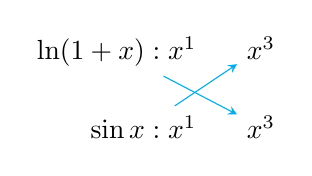
\begin{tikzpicture}[samples=100,>=stealth,]
        \node[below left] (A) at (0,0) {$\sin x:x^1$};
        \node[below left] (B) at (0,1) {$\ln(1+x):x^1$};
        \node[below left] (C) at (1,0) {$x^3$};
        \node[below left] (D) at (1,1) {$x^3$};
        \draw[->,cyan] (A)--(D);
        \draw[->,cyan] (B)--(C);
    \end{tikzpicture}
\end{minipage}
\begin{minipage}{0.3\linewidth}
    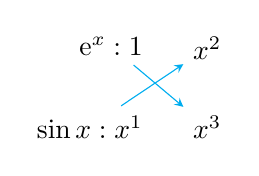
\begin{tikzpicture}[samples=100,>=stealth,]
        \node[below left] (A) at (0,1) {$\e ^x:1$};
        \node[below left] (B) at (0,0) {$\sin x:x^1$};
        \node[below left] (C) at (1,0) {$x^3$};
        \node[below left] (D) at (1,1) {$x^2$};
        \draw[->,cyan] (A)--(C);
        \draw[->,cyan] (B)--(D);
    \end{tikzpicture}
\end{minipage}
\begin{minipage}{0.3\linewidth}
    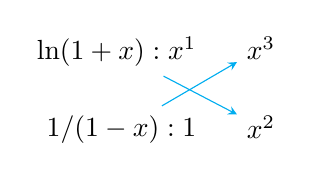
\begin{tikzpicture}[samples=100,>=stealth,]
        \node[below left] (A) at (0,1) {$\ln(1+x):x^1$};
        \node[below left] (B) at (0,0) {$1/(1-x):1$};
        \node[below left] (C) at (1,0) {$x^2$};
        \node[below left] (D) at (1,1) {$x^3$};
        \draw[->,cyan] (A)--(C);
        \draw[->,cyan] (B)--(D);
    \end{tikzpicture}
\end{minipage}
\begin{solution}
    \begin{enumerate}[label=(\arabic{*})]
        \item $\ln(1+x)=x-\dfrac{1}{2}x^2+\dfrac{1}{3}x^3+o(x^3),~\sin x=x-\dfrac{1}{6}x^3+o(x^3)$,所以
              \begin{flalign*}
                  \ln \left( 1+x\right) \sin x & =\left( x-\dfrac{1}{2}x^{2}+\dfrac{1}{3}x^{3}+o_{1}\left( x^{3}\right) \right) \left( x-\dfrac{1}{6}x^{3}+o_{2}\left( x^{3}\right) \right)      \\
                                               & =x^{2}-\dfrac{1}{6}x^{4}-\dfrac{1}{2}x^{3}+\dfrac{1}{3}x^{4}+o\left( x^{4}\right) =\dfrac{1}{6}x^4-\dfrac{1}{2}x^{3}+x^{2}+o\left( x^{4}\right)
              \end{flalign*}
        \item $\e ^x=1+x+\dfrac{1}{2}x^2+o(x^2),~\sin x=x-\dfrac{1}{6}x^3+o(x^3)$,所以
              \begin{flalign*}
                  \e ^x\sin x & =\left( 1+x+\dfrac{1}{2}x^{2}+o\left( x^{2}\right) \right) \left( x-\dfrac{1}{6}x^{3}+o\left( x^{3}\right) \right) \\
                              & =x-\dfrac{1}{6}x^{3}+x^{2}+\dfrac{1}{2}x^{3}+o\left( x^{3}\right) =\dfrac{1}{3}x^{3}+x^{2}+x+o\left( x^{3}\right)
              \end{flalign*}
        \item $\ln(1+x)=x-\dfrac{1}{2}x^2+\dfrac{1}{3}x^3+o(x^3),~\dfrac{1}{1-x}=1+x+x^2+o(x^2)$,所以
              \begin{flalign*}
                  \dfrac{\ln(1+x)}{1-x} & =\left(x-\dfrac{1}{2}x^2+\dfrac{1}{3}x^3+o(x^3)\right)\left(1+x+x^2+o(x^2)\right)                           \\
                                        & =x+x^2+x^3-\dfrac{1}{2}x^2-\dfrac{1}{2}x^3+\dfrac{1}{3}x^3+o(x^3)=\dfrac{5}{6}x^3+\dfrac{1}{2}x^2+x+o(x^3).
              \end{flalign*}
    \end{enumerate}
\end{solution}

\begin{inference}
    $f_1,f_2,\cdots,f_k$ 展开第一个不为 0 的项次数分别为 $m_1,m_2,\cdots,m_k$,欲使 $f_1f_2\cdots f_k$ 展开到 $p$ 阶,
    则 $f_1,f_2,\cdots,f_k$ 分别需要展开到 $p-(m_2+m_3+\cdots+m_k),p-(m_1+m_3+\cdots+m_k),\cdots,p-(m_2+m_3+\cdots+m_{k-1})$ 阶.
    \label{taylor f1f2f3fk}
\end{inference}
\begin{example}
    \scriptsize\linespread{0.8}
    试用推论 \ref{taylor f1f2f3fk},计算例 \ref{liti 111}(12).
\end{example}
\begin{solution}
    \scriptsize\linespread{0.8}
    需要将$\sin kx$ 展开到三阶,故 $\sin kx=kx-\dfrac{1}{6}(kx)^3+o(x^3)$,那么
    $$\prod_{k=1}^{n}\sin kx=\prod_{k=1}^{n}\left[kx-\dfrac{1}{6}(kx)^3+o(x^3)\right]~ (x\to0)$$
    在上式中排列组合出 $x$ 的阶数小于等于 $n+2$ 的项,有
    $$\prod_{k=1}^{n}\sin kx=n!x^n-\sum_{k=1}^{n}\dfrac{1}{6}n!k^2x^{n+2}+o(x^{n+2})=n!x^n-\dfrac{n!x^{n+2}}{6}\sum_{k=1}^{n}k^2+o(x^{n+2})~ (x\to0)$$
    故原式$\displaystyle=\lim\limits_{x\to0}\dfrac{n!x^n-n!x^n+\dfrac{n!x^{n+2}}{6}\displaystyle\sum\limits_{k=1}^{n}k^2+o\qty(x^{n+2})}{x^{n+2}}=\dfrac{n!}{6}\sum_{k=1}^{n}k^2=\dfrac{n(2n+1)}{36}(n+1)!.$
\end{solution}

\paragraph{复合函数的 Taylor 展开}
先确定外函数的展开阶数,再由各项阶数确定内函数的展开阶数.

\begin{example}
    将下列函数展开到指定的阶数.
    \setcounter{magicrownumbers}{0}
    \begin{table}[H]
        \centering
        \begin{tabular}{l | l}
            (\rownumber{}) $\sin (\sin x)$,展开到 $3$ 阶. & (\rownumber{}) $\e ^{\tan x}-\e ^{\sin x}$,展开到 $3$ 阶.         \\
            (\rownumber{}) $\ln\cos x$,展开到 $6$ 阶.     & (\rownumber{}) $\dfrac{1}{\e }(1+x)^{\frac{1}{x}}$,展开到 $3$ 阶.
        \end{tabular}
    \end{table}
\end{example}
\begin{solution}
    \begin{enumerate}[label=(\arabic{*})]
        \item 先将外层函数展开到 3 阶,
              \begin{flalign*}
                  \sin(\sin x) & =\sin x-\dfrac{1}{6}\sin^3x+o(\sin^3x)=x-\dfrac{1}{6}x^3+o(x^3)-\dfrac{1}{6}(x+o(x))^3+o(x^3) \\
                               & =x-\dfrac{1}{6}x^3-\dfrac{1}{6}x^3+o(x^3)=x-\dfrac{1}{3}x^3+o(x^3).
              \end{flalign*}
        \item $\e ^{\tan x}-\e ^{\sin x}=\e ^{\tan x}-1-(\e ^{\sin x}-1)$,先将外层函数展开到 3 阶,
              \begin{flalign*}
                  \e ^{\tan x}-1 & =\tan x+\dfrac{1}{2}\tan ^{2}x+\dfrac{1}{6}\tan ^{3}x+o\left( \tan ^{3}x\right)                                                                                                          \\
                                 & =\left( x+\dfrac{1}{3}x^{3}+o\left( x^{3}\right) \right) +\dfrac{1}{2}\left( x+o\left( x\right) \right) ^{2}+\dfrac{1}{6}\left( x+o\left( x\right) \right) ^{3}+o\left( x^{3}\right)     \\
                                 & =\dfrac{1}{2}x^{3}+\dfrac{1}{2}x^{2}+x+o\left( x^{3}\right)                                                                                                                              \\
                  \e ^{\sin x}-1 & =\sin x+\dfrac{1}{2}\sin ^{2}x+\dfrac{1}{6}\sin ^{3}x+o\left( \sin ^{3}x\right)                                                                                                          \\
                                 & =\left( x^{3}-\dfrac{1}{6}x^{3}+o\left( x^{3}\right) \right) +\dfrac{1}{2}\left( x+o\left( x\right) \right) ^{2}+\dfrac{1}{6}\left( x+o\left( x\right) \right) ^{3}+o\left( x^{3}\right) \\
                                 & =\dfrac{1}{2}x^{2}+x+o\left( x^{3}\right)
              \end{flalign*}
              故 $\e ^{\tan x}-\e ^{\sin x}=\dfrac{1}{2}x^3+o(x^3).$
        \item 先将外层函数展开到 6 阶,
              \begin{flalign*}
                   & \ln\cos x=\dfrac{1}{2}\ln\left(1-\sin^2x\right)=-\dfrac{1}{2}\left(\sin^2x+\dfrac{\sin^4x}{2}+\dfrac{\sin^6x}{3}+o(\sin^3x)\right)                                                                                                                             \\
                   & =-\dfrac{1}{2}\left[\left( x-\dfrac{x^{3}}{3!}+\dfrac{x^{5}}{5!}+o\left( x^{5}\right) \right)^2 +\dfrac{1}{2}\left( x-\dfrac{x^{3}}{3!}+\dfrac{x^{5}}{5!}+0\left( x^{5}\right) \right) ^{4}+\dfrac{1}{3}\left( x+o(x)\right) ^{6} \right]+o\left( x^{6}\right) \\
                   & =-\dfrac{1}{45}x^{6}-\dfrac{1}{12}x^{4}-\dfrac{1}{2}x^{2}+o\left( x^{6}\right) .
              \end{flalign*}
        \item 原式 $=\e ^{\frac{1}{x}\ln(1+x)-1}$,注意到 $\displaystyle \ln(1+x)=\sum_{n=0}^{\infty}(-1)^n\dfrac{x^{n+1}}{n+1}$,于是
              \begin{flalign*}
                  \text{原式} & =\e ^{-\frac{x}{2}+\frac{x^2}{3}-\frac{x^3}{4}+o\qty(x^3)}=1+\qty(-\dfrac{x}{2}+\dfrac{x^2}{3}-\dfrac{x^3}{4}+o\qty(x^3))                                 \\
                              & ~  +\dfrac{1}{2}\qty(-\dfrac{x}{2}+\dfrac{x^2}{3}-\dfrac{x^3}{4}+o\qty(x^3))^2+\dfrac{1}{6}\qty(-\dfrac{x}{2}+\dfrac{x^2}{3}-\dfrac{x^3}{4}+o\qty(x^3))^3 \\
                              & =1-\dfrac{1}{2}x+\dfrac{11}{24}x^2-\dfrac{7}{16}x^3+o\qty(x^3).
              \end{flalign*}
    \end{enumerate}
\end{solution}

\begin{example}
    计算下列极限值.
    \setcounter{magicrownumbers}{0}
    \begin{table}[H]
        \centering
        \begin{tabular}{l | l}
            (\rownumber{}) $\displaystyle\lim_{x\to0}\dfrac{\tan\qty(\e ^x-1)-\e ^{\tan x}+1}{x^4}$.                & (\rownumber{}) $\displaystyle\lim_{x\to0}\dfrac{\cos\qty(\sin x)-\e ^{\cos x-1}}{\tan ^2x-\sin ^2x}$.      \\
            (\rownumber{}) $\displaystyle \lim_{x\to0}\dfrac{\ln\qty(1+\sin^2x)-6\qty(\sqrt[3]{2-\cos x}-1)}{x^4}.$ & (\rownumber{}) $\displaystyle \lim_{x\to\infty}\qty[\qty(x-\dfrac{1}{2})^2-x^4\ln^2\qty(1+\dfrac{1}{x})].$
        \end{tabular}
    \end{table}
\end{example}
\begin{solution}
    \begin{enumerate}[label=(\arabic{*})]
        \item 注意到 $$\e ^x=1+x+\dfrac{1}{2}x^2+\dfrac{1}{6}x^3+\dfrac{1}{24}x^4+o\qty(x^4),~\tan x=x+\dfrac{1}{3}x^3+o\qty(x^4)$$
              于是
              \begin{flalign*}
                  \tan\qty(\e ^x-1) & =\e ^x-1+\dfrac{1}{3}\qty(\e ^x-1)^3+o\qty(x^4)                                                                                                   \\
                                    & =x+\dfrac{1}{2}x^2+\dfrac{1}{6}x^3+\dfrac{1}{24}x^4+\dfrac{1}{3}\qty(x+\dfrac{1}{2}x^2+\dfrac{1}{6}x^3+\dfrac{1}{24}x^4+o\qty(x^4))^3+o\qty(x^4)  \\
                                    & =x+\dfrac{1}{2}x^2+\dfrac{1}{6}x^3+\dfrac{1}{24}x^4+\dfrac{1}{3}x^3\qty(1+\dfrac{1}{2}x+\dfrac{1}{6}x^2+\dfrac{1}{24}x^3+o\qty(x^3))^3+o\qty(x^4) \\
                                    & =x+\dfrac{1}{2}x^2+\dfrac{1}{6}x^3+\dfrac{1}{24}x^4+\dfrac{1}{3}x^3+\dfrac{1}{2}x^4+o\qty(x^4)                                                    \\
                                    & =x+\dfrac{1}{2}x^2+\dfrac{1}{2}x^3+\dfrac{13}{24}x^4+o\qty(x^4)
              \end{flalign*}
              \begin{flalign*}
                   & \e ^{\tan x}-1  =\tan x+\dfrac{1}{2}\tan ^2x+\dfrac{1}{6}\tan^3x+\dfrac{1}{24}\tan ^4x+o\qty(x^4)                                                                             \\
                   & =x+\dfrac{x^3}{3}+\dfrac{1}{2}\qty(x+\dfrac{x^3}{3}+o\qty(x^4))^2+\dfrac{1}{6}\qty(x+\dfrac{x^3}{3}+o\qty(x^4))^3+\dfrac{1}{24}\qty(x+\dfrac{x^3}{3}+o\qty(x^4))^4+o\qty(x^4) \\
                   & =x+\dfrac{1}{3}x^3+\dfrac{1}{2}\qty(x^2+\dfrac{2}{3}x^4+o\qty(x^4))+\dfrac{1}{6}\qty(x^3+o\qty(x^4))+\dfrac{1}{24}\qty(x^4+o\qty(x^4))+o\qty(x^4)                             \\
                   & =x+\dfrac{1}{2}x^2+\dfrac{1}{2}x^3+\dfrac{9}{24}x^4+o\qty(x^4)
              \end{flalign*}
              因此$\text{原式}=\dfrac{\dfrac{1}{6}x^4+o\qty(x^4)}{x^4}=\dfrac{1}{6}.$
        \item 与上题同理,注意到
              $$\cos x=1-\dfrac{1}{2}x^2+\dfrac{1}{24}x^4+o\qty(x^4),~\sin x=x-\dfrac{1}{6}x^3+o\qty(x^4)$$
              $$\tan x=x+\dfrac{1}{3}x^3+o\qty(x^4),~\e ^x=1+x+\dfrac{1}{2}x^2+\dfrac{1}{6}x^3+\dfrac{1}{24}x^4+o\qty(x^4)$$
              于是 \begin{flalign*}
                  \cos \qty(\sin x) & =1-\dfrac{1}{2}\sin^2x+\dfrac{1}{24}\sin^4x+o\qty(x^4)                                                           \\
                                    & =1-\dfrac{1}{2}\qty(x-\dfrac{1}{6}x^3+o\qty(x^4))^2+\dfrac{1}{24}\qty(x-\dfrac{1}{6}x^3+o\qty(x^4))^4+o\qty(x^4) \\
                                    & =1-\dfrac{1}{2}\qty(x^2-\dfrac{1}{3}x^4+o\qty(x^4))+\dfrac{1}{24}x^4+o\qty(x^4)                                  \\
                                    & =1-\dfrac{1}{2}x^2+\dfrac{5}{24}x^4+o\qty(x^4)
              \end{flalign*}
              \begin{flalign*}
                  \e ^{\cos x-1} & =\e ^{-\frac{1}{2}x^2+\frac{1}{24}x^4++o\qty(x^4)}                                                                              \\
                                 & =1+\qty(-\dfrac{1}{2}x^2+\dfrac{1}{24}x^4+o\qty(x^4))+\dfrac{1}{2}\qty(-\dfrac{1}{2}x^2+\dfrac{1}{24}x^4+o\qty(x^4))+o\qty(x^4) \\
                                 & =1-\dfrac{1}{2}x^2+\dfrac{1}{24}x^4+o\qty(x^4)+\dfrac{1}{2}x^4\qty(-\dfrac{1}{2}+\dfrac{1}{24}x^2+o\qty(x^2))^2+o\qty(x^4)      \\
                                 & =1-\dfrac{1}{2}x^2+\dfrac{1}{24}x^4+\dfrac{1}{8}x^4+o\qty(x^4)=1-\dfrac{1}{2}x^2+\dfrac{1}{6}x^4+o\qty(x^4)
              \end{flalign*}
              \begin{flalign*}
                  \tan^2x-\sin^2x & =\qty(x+\dfrac{1}{3}x^3+o\qty(x^4))^2-\qty(x-\dfrac{1}{6}x^3+o\qty(x^4))^2          \\
                                  & =x^2+\dfrac{2}{3}x^4+o\qty(x^4)-\qty(x^2-\dfrac{1}{3}x^4+o\qty(x^4))=x^4+o\qty(x^4)
              \end{flalign*}
              于是原式 $=\displaystyle\lim_{x\to0}\dfrac{1-\dfrac{1}{2}x^2+\dfrac{5}{24}x^4+o\qty(x^4)-\qty(1-\dfrac{1}{2}x^2+\dfrac{1}{6}x^4+o\qty(x^4))}{x^4+o\qty(x^4)}=\dfrac{1}{24}.$
        \item $\ln\qty(1+\sin^2x)=\sin^2x-\dfrac{1}{2}\sin^4x+o\qty(x^4)$,且 $\sin x=x-\dfrac{1}{6}x^3+o\qty(x^4)$,于是
              \begin{flalign*}
                  \ln\qty(1+\sin^2x) & =\qty(x-\dfrac{1}{6}x^3)^2-\dfrac{1}{2}\qty(x-\dfrac{1}{6}x^3)^4+o\qty(x^4)                                       \\
                                     & =x^2\qty(1-\dfrac{1}{6}x^2)^2-\dfrac{1}{2}x^4\qty(1-\dfrac{1}{6}x^2)^4+o\qty(x^4) =x^2-\dfrac{5}{6}x^4+o\qty(x^4)
              \end{flalign*}
              另一方面,
              \begin{flalign*}
                  \sqrt[3]{2-\cos x}-1 & =\sqrt[3]{1+(1-\cos x)}-1=\dfrac{1}{3}(1-\cos x)+\dfrac{\dfrac{1}{3}\cdot\qty(-\dfrac{2}{3})}{2!}(1-\cos x)^2                                                    \\
                                       & =\dfrac{1}{3}\qty(\dfrac{x^2}{2}-\dfrac{x^4}{24}+o\qty(x^4))-\dfrac{1}{9}\qty(\dfrac{x^2}{2}+o\qty(x^4))^2+o\qty(x^4)=\dfrac{1}{6}x^2-\dfrac{x^4}{24}+o\qty(x^4)
              \end{flalign*}
              于是原式 $=\lim_{x\to0}\dfrac{-\dfrac{7}{12}x^4+o\qty(x^4)}{x^4}=-\dfrac{7}{12}.$
        \item \textbf{法一: }利用 L'Hospital 法则计算极限
              \begin{flalign*}
                  I & =\lim_{x\to\infty}x^2\qty[1-\dfrac{1}{2x}+\ln\qty(1+\dfrac{1}{x})]\qty[1-\dfrac{1}{2x}-\ln\qty(1+\dfrac{1}{x})]
                  \xlongequal{\frac{1}{x}=t}\lim_{t\to0}\qty[1-\dfrac{t}{2}+\dfrac{\ln(1+t)}{t}]\cdot\dfrac{t-\dfrac{t^2}{2}-\ln(1+t)}{t^3}                    \\
                    & \xlongequal{L'}\lim_{t\to0}\dfrac{2-2t+\dfrac{2}{1+t}}{2}\cdot\dfrac{1-t-\dfrac{1}{1+t}}{3t^2}=2\times\qty(-\dfrac{1}{3})=-\dfrac{2}{3}.
              \end{flalign*}
              \textbf{法二: }对 $\ln\qty(1+\dfrac{1}{x}),~x\to\infty$ 进行 Taylor 展开,有
              \begin{flalign*}
                  I & =\lim_{x\to\infty}\qty[\qty(x-\dfrac{1}{2})^2-x^4\qty(\dfrac{1}{x}-\dfrac{1}{2x^2}+\dfrac{1}{3x^3}+o\qty(x^{-4}))^2]=\lim_{x\to\infty}\qty[\qty(x-\dfrac{1}{2})^2-x^2\qty(1-\dfrac{1}{2x}+\dfrac{1}{3x^2}+o\qty(x^{-3}))^2] \\
                    & =\lim_{x\to\infty}\qty[\qty(x-\dfrac{1}{2})^2-\qty(x-\dfrac{1}{2}+\dfrac{1}{3x})^2]=\lim_{x\to\infty}\qty(x-\dfrac{1}{2}+x-\dfrac{1}{2}+\dfrac{1}{3x})\qty(x-\dfrac{1}{2}-x+\dfrac{1}{2}-\dfrac{1}{3x})                     \\
                    & =\lim_{x\to\infty}\dfrac{-6x^2+3x-1}{9x^2}=-\dfrac{2}{3}.
              \end{flalign*}
    \end{enumerate}
\end{solution}

\begin{example}
    计算极限 $\displaystyle\lim_{x\to0}\qty[\dfrac{1}{x\ln(1+x)}-\dfrac{2+x}{2x^2}].$
\end{example}
\begin{solution}
    对 $\ln(1+x)$ 进行 Taylor 展开,有 $\ln(1+x)=x-\dfrac{x^2}{2}+\dfrac{x^3}{3}+o\qty(x^4)$,于是
    \begin{flalign*}
        \text{原式} & =\lim_{x\to0}\qty[\dfrac{1}{x\qty(x-\dfrac{x^2}{2}+\dfrac{x^3}{3})}-\dfrac{2+x}{2x^2}]=\lim_{x\to0}\qty[\dfrac{12}{2x^2\qty(6-3x+2x^2)}-\dfrac{2+x}{2x^2}] \\
                    & =\lim_{x\to0}\dfrac{12-(2+x)(6-3x+2x^2)}{2x^2\qty(6-3x+2x^2)}=-\lim_{x\to0}\dfrac{2x+1}{2\qty(6-3x+2x^2)}=-\dfrac{1}{12}.
    \end{flalign*}
\end{solution}

\begin{example}
    设函数 $f(x)$ 在区间 $(0,+\infty)$ 上三阶可导,满足
    $$\lim_{x\to+\infty}\dfrac{f'(x)f'''(x)}{\qty[f''(x)]^2}=a\neq 1~  f^{(k)}(x)>0,~k=0,1,2$$
    求极限 $\displaystyle\lim_{x\to+\infty}\dfrac{f(x)f''(x)}{\qty[f'(x)]^2}.$
\end{example}
\begin{solution}
    注意到
    \begin{flalign*}
        \lim_{x\to+\infty}\dfrac{f'(x)f'''(x)}{\qty[f''(x)]^2} & =\lim_{x\to+\infty}\dfrac{\qty[f''(x)]^2-\qty[f''(x)]^2+f'(x)f'''(x)}{\qty[f''(x)]^2}                                      \\
                                                               & =1-\lim_{x\to+\infty}\dfrac{\qty[f''(x)]^2-f'(x)f'''(x)}{\qty[f''(x)]^2}=1-\lim_{x\to+\infty}\dv{x}(\dfrac{f'(x)}{f''(x)})
    \end{flalign*}
    于是 $\displaystyle\lim_{x\to+\infty}\dv{x}(\dfrac{f'(x)}{f''(x)})=1-a$,并且
    $$\lim_{x\to+\infty}\dfrac{f(x)f''(x)}{\qty[f'(x)]^2}=\dfrac{1}{\dfrac{f'(x)}{xf''(x)}\cdot\dfrac{xf''(x)}{f(x)}}$$
    利用 L'Hospital 法则,得
    $$\lim_{x\to\infty}\dfrac{f'(x)}{xf''(x)}=\lim_{x\to\infty}\dfrac{\dfrac{f'(x)}{f''(x)}}{x}\xlongequal{L'}\lim_{x\to\infty}\dv{x}(\dfrac{f'(x)}{f''(x)})=1-a$$
    注意到 $\dfrac{f'(x)}{xf''(x)}>0~ (0<x<+\infty)$,故由极限的保号性知,$1-a\geqslant 0$,但 $a\neq 1$,所以 $a<1$; 另一方面,
    对 $\forall x\in(0,+\infty)$ 及 $\forall h>0$,由 Taylor 公式,得
    $$f(x+h)=f(x)+f'(x)h+\dfrac{1}{2!}f''(\xi)h^2>f(x)+f'(x)h~  \xi\in(x,x+h)$$
    所以 $\displaystyle\lim_{h\to\infty}f(x+h)=+\infty$,即 $\displaystyle\lim_{x\to\infty}f(x)=+\infty$,于是利用 L'Hospital 法则,得
    $$\lim_{x\to+\infty}\dfrac{xf'(x)}{f(x)}\xlongequal{L'}\lim_{x\to+\infty}\dfrac{f'(x)+xf''(x)}{f'(x)}=1+\lim_{x\to+\infty}\dfrac{xf''(x)}{f'(x)}=1+\dfrac{1}{1-a}=\dfrac{2-a}{1-a}$$
    因此 $$\lim_{x\to+\infty}\dfrac{f(x)f''(x)}{\qty[f'(x)]^2}=\dfrac{1}{\lim\limits_{x\to+\infty}\dfrac{f'(x)}{xf''(x)}\cdot\lim\limits_{x\to+\infty}\dfrac{xf'(x)}{f(x)}}=\dfrac{1}{2-a}.$$
\end{solution}

% 例 3.3.19 设函数  f  在  (0,+\infty)  上可微, 且  f^{\prime}(x)=O(x)(  当  x \rightarrow+\infty  时  ) , 试证:  f(x)=O\left(x^{2}\right)  (当  x \rightarrow+\infty  时). (中国科学技术大学)
% 证 已知  \frac{f^{\prime}(x)}{x}=O(1)(x \rightarrow+\infty) , 取  x_{0}>0 , 则  \forall x>x_{0} , 有
% 
% f(x)=f\left(x_{0}\right)+f^{\prime}(\xi)\left(x-x_{0}\right)\left(x_{0}<\xi<x\right),\left|\frac{\xi}{x}\right| \leqslant 1,\left|\frac{x-x_{0}}{x}\right| \leqslant 1
% 
% 故  ~  \frac{f(x)}{x^{2}}=\frac{f\left(x_{0}\right)}{x^{2}}+\left(\frac{f^{\prime}(\xi)}{\xi}\right)\left(\frac{\xi}{x}\right)\left(\frac{x-x_{0}}{x}\right)=o(1)+O(1)=O(1) ,
% 即
% 
% f(x)=O\left(x^{2}\right) \text { (当 } x \rightarrow+\infty \text { 时). }
% 
% new  \succsim  例 3.3.20 设  x_{n}=f\left(\frac{1}{n^{2}}\right)+f\left(\frac{2}{n^{2}}\right)+\cdots+f\left(\frac{n}{n^{2}}\right) , 其中  f(x)  在  x=0  处有连 续导数, 且  f(0)=0, f^{\prime}(0)=1 . 试证  : \lim _{n \rightarrow \infty} x_{n}  存在,并求极限值. (武汉大学)
% 注  f(x)  在  x=0  处有连续导数, 意指:  f(x)  在  x=0  处及其附近有导数, 并且导 函数  f^{\prime}(x)  至少在  x=0  处连续.
% 证 I 因  f(0)=0, f^{\prime}(0)=1 , 应用 Taylor 公式, 得
% 
% \begin{array}{l}
% x_{n}=\sum_{i=1}^{n} f\left(\frac{i}{n^{2}}\right)=\sum_{i=1}^{n}\left[f(0)+f^{\prime}(0) \frac{i}{n^{2}}+o\left(\frac{i}{n^{2}}\right)\right]=\sum_{i=1}^{n}\left[\frac{i}{n^{2}}+o\left(\frac{i}{n^{2}}\right)\right] \\
% =\sum_{i=1}^{n} \frac{i}{n^{2}}+\sum_{i=1}^{n} o\left(\frac{i}{n^{2}}\right) \\
% \stackrel{\text { 见注 }}{=} \frac{n(n+1)}{2 n^{2}}+\frac{n(n+1)}{2 n^{2}} o(1) \underset{n \rightarrow \infty}{\longrightarrow} \frac{1}{2} \text {. } \\
% \end{array}
% 
% 注 当  n \rightarrow \infty  时,  o(1)  代表一个无穷小量,且  o\left(\frac{i}{n^{2}}\right)=\frac{i}{n^{2}} o(1) . 因此
% 
% \begin{aligned}
% \sum_{i=1}^{n} o\left(\frac{i}{n^{2}}\right) & =\sum_{i=1}^{n} \frac{i}{n^{2}} o(1)=\frac{1}{n^{2}} \sum_{i=1}^{n} i \cdot o(1) \\
% & =\frac{1}{n^{2}}[o(1)+2 o(1)+3 o(1)+\cdots+n o(1)]
% \end{aligned}

\subsubsection{Lagrange 中值定理}

\begin{theorem}[Lagrange 中值定理]
    若 $ f(x) $ 在 $ [a, b] $ 上连续,在 $ (a, b) $ 内可导,则 $ \forall x_{1}, x_{2} \in[a, b], \exists \xi \in\left(x_{1}, x_{2}\right) $,使得
    $$f\left(x_{2}\right)-f\left(x_{1}\right)=f^{\prime}(\xi)\cdot(x_{2}-x_{1}) .$$
    \index{Lagrange 中值定理}
\end{theorem}

\begin{example}
    计算 $\displaystyle\lim_{x\to0}\dfrac{\cos x-\cos\qty[2\ln(1+x)]}{x^2}.$
\end{example}
\begin{errorSolution}
    由 Lagrange 中值定理,$\cos x-\cos\qty[2\ln(1+x)]=\qty[2\ln(1+x)-x]\sin\xi$,其中 $\xi$ 介于 $x$ 与 $2\ln(1+x)$ 之间,因此
    $$\lim_{x\to0}\dfrac{\cos x-\cos\qty[2\ln(1+x)]}{x^2}=\lim_{x\to0}\dfrac{\qty[2\ln(1+x)-x]\sin\xi}{x^2}=\lim_{x\to0}\dfrac{\qty[2x+o(x)-x]}{x}=1$$
    \textbf{错因: }当 $x\to0^+,~x<\xi<2\ln(1+x)\Rightarrow 1\gets\dfrac{x}{x}<\dfrac{\xi}{x}<\dfrac{2\ln(1+x)}{x}\to 2$,左右极限值不相等,故不能由夹逼准则得 $\sin\xi\sim\xi$,同理可得 $x\to0^-$ 情况相同.\\
\end{errorSolution}
\begin{solution}
    当 $x\to0$ 时,$\cos [2\ln(1+x)]\to1$,于是原式可改写为 $$\lim_{x\to0}\qty[\dfrac{\cos x-1}{x^2}+\dfrac{1-\cos(2\ln(1+x))}{x^2}]=\lim_{x\to0}\dfrac{\cos x-1}{x^2}+\lim_{x\to0}\dfrac{1-\cos(2\ln(1+x))}{x^2}=-\dfrac{1}{2}+2=\dfrac{3}{2}.$$
\end{solution}

\begin{example}
    已知 $\displaystyle\lim_{n\to\infty}\dfrac{n^{\alpha}}{n^\beta-(n-1)^\beta}=2023$,求 $\alpha,\beta$ 的值.
    \begin{tasks}(2)
        \task $\alpha=-\dfrac{2022}{2023},~\beta=\dfrac{1}{2023}.$
        \task $\alpha=-\dfrac{2023}{2022},~\beta=\dfrac{1}{2022}.$
        \task $\alpha=-\dfrac{2022}{2023},~\beta=\dfrac{1}{2022}.$
        \task $\alpha=-\dfrac{2023}{2022},~\beta=\dfrac{1}{2023}.$
    \end{tasks}
\end{example}
\begin{solution}
    设 $f(x)=x^\beta$,那么由 Lagrange 中值定理,有 $$f(n)-f(n-1)=\beta\xi_n^{\beta-1}$$
    那么极限式改写为 $\displaystyle\lim_{n\to\infty}\dfrac{n^\alpha}{\beta \xi_n^{\beta-1}}=2023$,
    且 $\dfrac{n}{\xi_n}\to1(n\to\infty)$,于是 $\begin{cases}
            \dfrac{1}{\beta}=2023 \\\alpha=\beta-1
        \end{cases}$ 解得选 A.
\end{solution}

\begin{example}
    用 Lagrange 中值定理求下列极限值.
    \setcounter{magicrownumbers}{0}
    \begin{table}[H]
        \centering
        \begin{tabular}{l | l | l}
            (\rownumber{}) $\displaystyle\lim_{x\to+\infty}\left(\sqrt[6]{x^6+x^5}-\sqrt[6]{x^6-x^5}\right).$ & (\rownumber{}) $\displaystyle\lim_{n\to \infty}\left(\cos\frac{\theta}{n}\right)^n.$ & (\rownumber{}) $\displaystyle\lim_{n\to \infty}\tan ^n\left(\frac{\pi}{4}+\frac{1}{n}\right).$ \\
            (\rownumber{}) $\displaystyle\lim_{x\to0}\left(\frac{1}{x^2}-\cot^2x\right).$                     & (\rownumber{}) $\displaystyle\lim_{x\to0}\frac{\sqrt{1-x^2}-\sqrt{1-4x^2}}{x^2}.$    & (\rownumber{}) $\displaystyle\lim_{x\to0}\frac{\e ^{x^2}-\e ^{2-2\cos x}}{x^4}.$
        \end{tabular}
    \end{table}
\end{example}
\begin{solution}
    \begin{enumerate}[label=(\arabic*)]
        \item $\displaystyle\text{原式}=\lim_{x\to+\infty}\frac{1}{6}\xi^{-\frac{5}{6}}\cdot(2x^5)=\frac{1}{3}$,$\xi\to x^6$.
        \item $\displaystyle\text{原式}=\exp\lim_{n\to\infty}n\ln\cos\frac{\theta}{n}=\exp\lim_{n\to\infty}n\left(\cos\frac{\theta}{n}-1\right)=\exp\lim_{n\to\infty}n\cdot\frac{\theta}{n}\cdot(-\sin\xi)=\e ^0=1$,$\xi\to 0$.
        \item $\displaystyle\text{原式}=\e ^{\lim\limits_{n\to\infty}n\ln\tan\left(\frac{\pi}{4}+\frac{1}{n}\right)}=\exp\lim_{n\to\infty}n\left[\tan\left(\frac{\pi}{4}+\frac{1}{n}\right)-1\right]=\exp\lim_{n\to\infty}\sec^2\xi=\e ^2$,$\displaystyle\xi\to\frac{\pi}{4}$.
        \item 先用 Lagrange 中值定理,再用 Taylor 展开.
              \begin{flalign*}
                  \text{原式} & =\lim_{x\to0}\frac{\sin^2x-x^2\cos^2x}{x^2\sin^2x}=\lim_{x\to0}\frac{2\ln\sin x-2\ln(x\cos x)}{x^2}=2\lim_{x\to0}\frac{\sin x-x\cos x}{x^2\cdot\xi} \\
                              & =2\lim_{x\to0}\frac{x-\dfrac{x^3}{6}-x\left(1-\dfrac{x^2}{2}\right)+o\left(x^3\right)}{x^2\cdot\xi}=\frac{2}{3},~\xi\to x.
              \end{flalign*}
        \item $\displaystyle\text{原式}=\lim_{x\to0}\frac{3x^2\dfrac{1}{2\sqrt{\xi}}}{x^2}=\frac{3}{2}$,$\xi\to1$.
        \item $\displaystyle\text{原式}=\lim_{x\to0}\frac{\e ^\xi\left(x^2-2+2\cos x\right)}{x^4}=\lim_{x\to0}\frac{x^2-2+2\left(1-\dfrac{x^2}{2!}+\dfrac{x^4}{4!}+o\left(x^4\right)\right)}{x^4}=\frac{1}{12}$,$\xi\to0$.
    \end{enumerate}
\end{solution}

\begin{example}
    设 $f(x)$ 在 $x=0$ 二阶可微且 $f'(0)=0,~f''(0)=1$,计算极限 $\displaystyle\lim_{x\to0}\dfrac{f(x)-f(\ln(1+x))}{x^3}.$
\end{example}
\begin{solution}
    显然 $f$ 在 $x=0$ 邻域内一阶可微,因此由 Lagrange 中值定理,
    $$\lim_{x\to0}\dfrac{f(x)-f(\ln(1+x))}{x^3}=\lim_{x\to0}\dfrac{[x-\ln(1+x)]f'(\xi_x)}{x^3}=\dfrac{1}{2}\lim_{x\to0}\dfrac{f'(\xi_x)}{x}=\dfrac{1}{2}\lim_{x\to0}\dfrac{f'(\xi_x)-f'(0)}{\xi_x}\cdot\dfrac{\xi_x}{x}=\dfrac{1}{2}f''(0)=\dfrac{1}{2}$$
    其中
    \begin{flalign*}
        1 & =\lim_{x\to0^+}\dfrac{\ln(1+x)}{x}\leqslant \lim_{x\to0^+}\dfrac{\xi_x}{x}\leqslant \lim_{x\to0^+}\dfrac{x}{x}=1  \\
        1 & =\lim_{x\to0^-}\dfrac{x}{x}\leqslant \lim_{x\to0^-}\dfrac{\xi_x}{x}\leqslant \lim_{x\to0^-}\dfrac{\ln(1+x)}{x}=1.
    \end{flalign*}
\end{solution}

\begin{example}[2011 数一]
    求极限 $\displaystyle\lim_{x\to0}\qty[\dfrac{\ln(1+x)}{x}]^{\frac{1}{\e^x-1}}.$
\end{example}
\begin{solution}
    令 $y=\qty[\dfrac{\ln(1+x)}{x}]^{\frac{1}{\e^x-1}}$,则 $\ln y=\dfrac{\ln(\ln(x+1))-\ln x}{\e^x-1}$,而
    \begin{flalign*}
        \lim_{x\to0^+}\ln y=\lim_{x\to0^+}\dfrac{\ln(\ln(x+1))-\ln x}{\e^x-1}=\lim_{x\to0^+}\dfrac{\ln(\ln(x+1))-\ln x}{x}
    \end{flalign*}
    由 Lagrange 中值定理,令 $f(x)=\ln x$ 那么 $f(1+\ln x)-f(x)=\dfrac{\ln(1+x)-x}{\xi_x}$,其中 $\xi_x$ 介于 $x$ 与 $\ln(1+x)$ 之间,
    于是 $$\lim_{x\to0^+}\ln y=\lim_{x\to0^+}\dfrac{\ln(1+x)-x}{x\cdot \xi_x}=\lim_{x\to0^+}\dfrac{-\dfrac{1}{2}x^2}{x^2}=-\dfrac{1}{2}$$
    当 $x<0$ 时,$\ln y=\dfrac{\ln[-\ln(1+x)]-\ln(-x)}{\e^x-1}$ 同样可得 $\displaystyle\lim_{x\to0^-}\ln y=-\dfrac{1}{2}$,于是原极限为 $\e^{-\frac{1}{2}}.$
\end{solution}

\begin{example}[第三届数学竞赛决赛]
    证明: $\displaystyle\lim_{n\to\infty}\int_0^1\frac{n}{n^2x^2+1}\e ^{x^2}\dd x=\frac{\pi}{2}.$
\end{example}
\begin{proof}
    对函数 $\displaystyle f(x)=\e ^{x^2}$ 在区间 $[0,x]~ (0\leqslant x\leqslant 1)$ 上应用拉格朗日中值定理,$\exists \xi\in(0,x)$,使得 $f(x)-f(0)=f'(\xi)x$,即
    $$\e ^{x^2}-1=2\xi\e ^{\xi^2}x\Rightarrow 1\leqslant \e ^{x^2}=1+2\xi\e ^{\xi^2}x\leqslant 1+2\e x$$
    于是 $$\frac{n}{n^2x^2+1}\leqslant \frac{n}{n^2x^2+1}\e ^{x^2}\leqslant \frac{n}{n^2x^2+1}+\frac{2\e nx}{n^2x^2+1}$$
    应用定积分的保号性,有
    $$\int_0^1\frac{n}{n^2x^2+1}\e ^{x^2}\dd x\geqslant \int_0^1\frac{n}{n^2x^2+1}\dd x=\arctan nx\Bigl |_0^1=\arctan n$$
    \begin{flalign*}
        \int_0^1\frac{n}{n^2x^2+1}\e ^{x^2}\dd x  \leqslant \int_0^1\left(\frac{n}{n^2x^2+1}+\frac{2\e nx}{n^2x^2+1}\right)\dd x
        =\arctan nx\Bigl |_0^1+\frac{\e }{n}\ln\left(1+n^2x^2\right)\Bigl |_0^1=\arctan n+\frac{\e }{n}\ln\left(1+n^2\right)
    \end{flalign*}
    又因为 $\displaystyle \lim_{n\to\infty}\arctan n=\frac{\pi}{2},~\lim_{n\to\infty}\left[\arctan n+\frac{\e }{n}\ln\left(1+n^2\right)\right]=\frac{\pi}{2}$,故由夹逼准则,等式成立.
\end{proof}

\begin{example}
    计算极限 $\displaystyle \lim_{x\to+\infty}(x+1)\qty[\ln\qty(x^2+x)-2\ln(1+x)].$
\end{example}
\begin{solution}
    \textbf{法一: }利用重要极限 $\displaystyle \lim_{x\to\infty}\qty(1+\dfrac{1}{x})^x=\e $,改写极限式,有
    \begin{flalign*}
        \text {原式} & =\lim _{x \rightarrow+\infty}(x+1) \ln \frac{x^{2}+x}{(1+x)^{2}}=\lim _{x \rightarrow+\infty}(x+1) \ln \frac{x^{2}+x}{x^{2}+2 x+1}
        =\lim _{x \rightarrow+\infty}(x+1) \ln \left(1+\frac{-x-1}{x^{2}+2 x+1}\right)                                                                    \\
                     & =\lim _{x \rightarrow+\infty}(x+1) \cdot \frac{-x-1}{x^{2}+2 x+1}=-\lim _{x \rightarrow+\infty} \frac{(x+1)^{2}}{x^{2}+2 x+1}=-1 .
    \end{flalign*}
    \textbf{法二: }利用 Lagrange 中值定理: 设 $ f(x)=\ln x $,则 $ \exists \xi $ 介于 $ x^{2}+x $ 与 $ x^{2}+2 x+1 $,使得
    $$\frac{f\left(x^{2}+x\right)-f\left(x^{2}+2 x+1\right)}{\left(x^{2}+x\right)-\left(x^{2}+2 x+1\right)}=f^{\prime}(\xi)=\frac{1}{\xi}, \xi \rightarrow \infty $$
    即 $ \ln \left(x^{2}+x\right)-\ln \left(x^{2}+2 x+1\right)=-\dfrac{1}{\xi}(x+1) $,所以
    \begin{flalign*}
          & \lim _{x \rightarrow+\infty}(x+1)\left[\ln \left(x^{2}+x\right)-2 \ln (1+x)\right] =\lim _{x \rightarrow+\infty}(x+1)\left[\ln \left(x^{2}+x\right)-\ln \left(x^{2}+2 x+1\right)\right] \\
        = & \lim _{x \rightarrow+\infty}(x+1)\left[-\frac{1}{\xi}(x+1)\right]=-\lim _{x \rightarrow+\infty} \frac{(x+1)^{2}}{\xi}
    \end{flalign*}
    因为 $ \xi $ 介于 $ x^{2}+x $ 与 $ x^{2}+2 x+1 $,由夹逼准则可知:
    $$\lim _{x \rightarrow+\infty}(x+1)\left[\ln \left(x^{2}+x\right)-2 \ln (1+x)\right]=-1$$
    \textbf{法三: }由 L'Hospital 法则可知: 注意到
    $$\lim _{x \rightarrow+\infty}\left[\ln \left(x^{2}+x\right)-2 \ln (1+x)\right]=0, \lim _{x \rightarrow \infty} \frac{1}{x+1}=0$$
    记 $ \displaystyle I=\lim _{x \rightarrow+\infty}(x+1)\left[\ln \left(x^{2}+x\right)-2 \ln (1+x)\right] $,则
    \begin{flalign*}
        I & =\lim _{x \rightarrow+\infty} \dfrac{\ln \left(x^{2}+x\right)-2 \ln (1+x)}{\dfrac{1}{x+1}} =\lim _{x \rightarrow+\infty} \dfrac{\dfrac{2 x+1}{x^{2}+x}-\dfrac{2}{1+x}}{-\dfrac{1}{(x+1)^{2}}} \\
          & =-\lim _{x \rightarrow+\infty}\left[\dfrac{2 x+1}{x^{2}+x}-\dfrac{2 x}{(1+x) x}\right](x+1)^{2} =-\lim _{x \rightarrow+\infty} \dfrac{(x+1)^{2}}{x^{2}+x} =-1
    \end{flalign*}
    所以 $ \displaystyle \lim _{x \rightarrow+\infty}(x+1)\left[\ln \left(x^{2}+x\right)-2 \ln (1+x)\right]=-1 .$\\
    \textbf{法四: }$\ln \left(x^{2}+x\right) $ 和 $ \ln (1+x) $ 在 $ x \rightarrow+\infty $ 的渐近展开式. 注意到:
    $$\ln \left(x^{2}+x\right)=2 \ln x+\frac{1}{x}+o\left(\frac{1}{x}\right),~\ln (1+x)=\ln x+\frac{1}{x}+o\left(\frac{1}{x}\right)$$
    所以
    \begin{flalign*}
        \lim _{x \rightarrow+\infty}(x+1)\left[\ln \left(x^{2}+x\right)-2 \ln (1+x)\right] & =\lim _{x \rightarrow+\infty}(x+1)\left[2 \ln x+\frac{1}{x}+o\left(\frac{1}{x}\right)-2\left(\ln x+\frac{1}{x}+o\left(\frac{1}{x}\right)\right)\right] \\
                                                                                           & =  \lim _{x \rightarrow+\infty}(x+1)\left[-\frac{1}{x}+o\left(\frac{1}{x}\right)\right]=-1 .
    \end{flalign*}
\end{solution}

\begin{example}
    求极限 $\displaystyle I=\lim_{x\to\infty}x^2\qty[\e^{\qty(1+\frac{1}{x})^x}-\qty(1+\dfrac{1}{x})^{\e x}].$
\end{example}
\begin{solution}
    作变量代换: $t=\dfrac{1}{x}$,则有
    \begin{flalign*}
        I=\lim_{t\to0}\dfrac{\e^{(1+t)^{t^{-1}}}-(1+t)^{\frac{\e}{t}}}{t^2}=\lim_{t\to0}\dfrac{\e^{(1+t)^{t^{-1}}}-\e^{\frac{\e\ln(1+t)}{t}}}{t^2}
    \end{flalign*}
    令 $f(t)=(1+t)^{t^{-1}},~g(t)=\dfrac{\e\ln(1+t)}{t}$,则 $\displaystyle\lim_{t\to0}f(t)=\lim_{t\to0}g(t)=0$,由 Lagrange 中值定理,得
    $$\e^{f(t)}-\e^{g(t)}=\e^{\xi}(f(t)-g(t))$$
    其中 $\xi$ 介于 $f(t)$ 与 $g(t)$ 之间,当 $t\to0$ 时,$\xi\to\e$,所以 $\e^{f(t)}-\e^{g(t)}\sim\e^{\e}[f(t)-g(t)]$,故
    $$I=\e^{\e}\lim_{t\to0}\dfrac{f(t)-g(t)}{t^2}=\e^{\e+1}\lim_{t\to0}\dfrac{\e^{\frac{\ln(1+t)}{t}-1}-\dfrac{\ln(1+t)}{t}}{t^2}$$
    记 $\alpha(t)=\dfrac{\ln(1+t)}{t}-1~ (t\to0,\alpha(t)\to0)$,由 $\e^{\alpha(t)}$ 的 Taylor 展开,得
    $$\e^{\alpha(t)}=1+\alpha(t)+\dfrac{1}{2!}\alpha^2(t)+o\qty(\alpha^2(t))=\dfrac{\ln(1+t)}{t}+\dfrac{1}{2}\qty[\dfrac{\ln(1+t)-t}{t}]^2+o\qty(\alpha^2(t))$$
    因此 $$I=\e^{\e+1}\lim_{t\to0}\dfrac{1}{2}\cdot\dfrac{\qty[\ln(1+t)-t]^2}{t^4}=\dfrac{1}{2}\e^{\e+1}\lim_{t\to0}\dfrac{\qty[-\dfrac{t^2}{2}+o\qty(t^2)]^2}{t^4}=\dfrac{1}{8}\e^{\e+1}.$$
\end{solution}

\begin{example}
    求极限 $\displaystyle\lim_{x\to0}\dfrac{\qty(\sin x+\e^{\tan x})^{\frac{1}{x}}-\qty(\tan x+\e^{\sin x})^{\frac{1}{x}}}{x^3}$
\end{example}
\begin{solution}
    改写极限式,有
    \begin{flalign*}
        I & =\lim_{x\to0}\dfrac{\qty(\sin x+\e^{\tan x})^{\frac{1}{x}}\cdot\dfrac{1}{x}\qty[\ln\qty(\sin x+\e^{\tan x})-\ln\qty(\tan x+\e^{\sin x})]}{x^3} \\
          & =\lim_{x\to0}\qty(\sin x+\e^{\tan x})^{\frac{1}{x}}\cdot\lim_{x\to0}\dfrac{\e^{\tan x}-\tan x-\qty(\e^{\sin x}-\sin x)}{x^4}                   \\
          & =\exp\lim_{x\to0}\dfrac{1}{x}\ln\qty(\sin x+\e^{\tan x})\cdot\lim_{x\to0}\dfrac{(\tan x-\sin x)f'(\xi_x)}{x^4}                                 \\
    \end{flalign*}
    其中 $$\displaystyle\lim_{x\to0}\dfrac{1}{x}\ln\qty(\sin x+\e^{\tan x})=\exp\lim_{x\to0}\dfrac{1}{x}\qty(\sin x+\e^{\tan x}-1)=\exp\lim_{x\to0}\dfrac{\sin x+\tan x}{x}=\e^2$$
    $\xi_x$ 介于 $\sin x$ 与 $\tan x$ 之间,并且
    $$\lim_{x\to0}\dfrac{(\tan x-\sin x)f'(\xi_x)}{x^4}=\lim_{x\to0}\dfrac{\dfrac{1}{2}x^3f'(\xi_x)}{x^4}=\dfrac{1}{2}\lim_{x\to0}\dfrac{f'(\xi_x)}{x}=\dfrac{1}{2}$$
    这是因为 $f'(x)=\e^x-1\to x~ (x\to0)$,以及当 $x\to0^+$ 时,$$0\gets\sin x<\xi_x<\tan x\to0$$
    当 $x\to0^-$ 时,$$0\gets\tan x<\xi_x<\sin x\to0$$
    于是 $\displaystyle\lim_{x\to0}\dfrac{f'(\xi_x)}{x}=1$,综上原式 $=\dfrac{\e^2}{2}.$
\end{solution}

\begin{example}
    设 $f(x)$ 在 $x=a$ 的某邻域内有三阶连续导数,且 $f'(a)\neq0$,令 $$\varphi(x)=\qty[\dfrac{f'(x)+f'(a)}{2f(x)-2f(a)}]^2-\qty(\dfrac{1}{x-a})^2$$
    计算极限 $\displaystyle\lim_{x\to a}\varphi(x).$
\end{example}
\begin{solution}
    考虑 $f(x)$ 在 $x=a$ 处的 Taylor 展开,$$f(x)=f(a)+f'(a)(x-a)+\dfrac{1}{2!}f''(a)(x-a)^2+\dfrac{1}{3!}f'''(\xi)(x-a)^3$$
    于是 $$2f(x)-2f(a)=2f'(a)(x-a)+f''(a)(x-a)^2+\dfrac{1}{3}f'''(\xi)(x-a)^3$$
    其中 $\xi$ 介于 $x$ 与 $a$ 之间,同理,考虑 $f'(x)$ 在 $x=a$ 处的 Taylor 展开,$$f'(x)=f'(a)+f''(a)(x-a)+\dfrac{1}{2!}f'''(\eta)(x-a)^2$$
    于是 $$f'(x)+f'(a)=2f'(a)+f''(a)(x-a)+\dfrac{1}{2}f'''(\eta)(x-a)^2$$
    其中 $\eta$ 介于 $x$ 与 $a$ 之间,将两式代入极限式,并通分,于是分子为
    \begin{flalign*}
          & (x-a)^2\qty[2f'(a)+f''(a)(x-a)+\dfrac{f'''(\eta)}{2}(x-a)^2]^2
        -  \qty[2f'(a)(x-a)+f''(a)(x-a)^2+\dfrac{f'''(\xi)}{3}(x-a)^3]^2                   \\
        = & f'(a)\left[2f'''(\eta)-\dfrac{4}{3}f'''(\xi)\right] (x-a)^{4} + o\qty((x-a)^4)
    \end{flalign*}
    分母为
    \begin{flalign*}
        \qty[2f'(a)+f''(a)(x-a)+\dfrac{f'''(\xi)}{3}(x-a)^2]^2(x-a)^4=4\qty[f'(a)]^2(x-a)^4+o\qty((x-a)^4)
    \end{flalign*}
    分式求 $x\to a$ 的极限,都只考虑分子、分母中的最低次幂,并且都为 $(x-a)^4$,所以
    $$\lim_{x\to a}\varphi(x)=\lim_{x\to a}\dfrac{2f'''(\eta)-\dfrac{4}{3}f'''(\eta)}{4f'(a)}$$
    由于 $f(x)$ 在 $x=a$ 的某个邻域内有三阶连续导数,故 $f'''(\eta)=f'''(\xi)=f'''(a)$,于是原极限为 $\dfrac{f'''(a)}{6f'(a)}.$
\end{solution}

\subsubsection{利用积分等价求极限}

\begin{theorem}[等价积分]
    \label{fgintintsimsim}
    设 $f$ 与 $g$ 连续,当 $x\to0$ 时,$\alpha(x),\beta(x)$ 均为无穷小,$\alpha(x)\sim\beta(x)$ 且 $\displaystyle\lim_{x\to0}\dfrac{f}{g}=1$,则
    $$\int_{0}^{\alpha(x)}f\dd t\sim\int_{0}^{\beta(x)}g\dd t.$$
    \index{等价积分}
\end{theorem}

\begin{example}
    把 $x\to0^+$ 时的无穷小量 $$\alpha=\int_{0}^{x}\cos t^2\dd t,~\beta=\int_{0}^{x^2}\tan\sqrt{t}\dd t,~\gamma=\int_{0}^{\sqrt{x}}\sin t^3\dd t$$
    排列起来,使排列在后的是前一项的高阶无穷小量,则正确的排列次序为
    \begin{tasks}(4)
        \task $\alpha,\beta,\gamma$
        \task $\alpha,\gamma,\beta$
        \task $\beta,\alpha,\gamma$
        \task $\beta,\gamma,\alpha$
    \end{tasks}
\end{example}
\begin{solution}
    由定理 \ref{fgintintsimsim} 可知,当 $x\to0^+$ 时,有
    $$\alpha\sim\int_{0}^{x}\dd t=x,~\beta \sim\int_{0}^{x^2}\sqrt{t}\dd t=\dfrac{2}{3}x^3,~\gamma\sim\int_{0}^{x^{\frac{1}{2}}}t^3\dd t=\dfrac{1}{4}x^2$$
    因此 $\gamma$ 是 $\alpha$ 的高阶无穷小量,$\beta $ 是 $\gamma,\alpha$ 的高阶无穷小量,所以有排列 $\alpha,\gamma,\beta$,选 B.
\end{solution}

\begin{example}
    求下列极限值.
    \setcounter{magicrownumbers}{0}
    \begin{table}[H]
        \centering
        \begin{tabular}{l | l}
            (\rownumber{}) $\displaystyle\lim_{x\to0}\dfrac{\cos(\sin x)-\cos x}{\qty[x-\ln\qty(x+\sqrt{1+x^2})]\displaystyle\int_{0}^{\ln(1+x)}\cos t^2\dd t}.$ & (\rownumber{}) $\displaystyle\lim_{x\to0^+}\dfrac{\sqrt{2(\sec x-1)}-\sqrt[3]{6(x-\sin x)}}{\displaystyle\int_{0}^{x^2}\arctan\qty(\e^{\sqrt{t}}-1)\dd t}.$
        \end{tabular}
    \end{table}
\end{example}
\begin{solution}
    \begin{enumerate}[label=(\arabic{*})]
        \item 分子: $\cos(\sin x)-\cos x=(x-\sin x)\sin\xi$,其中 $\xi$ 介于 $\sin x$ 与 $x$ 之间,当 $x\to0^+$ 时,有 $\sin x<\xi<x$,那么 $$1\gets\dfrac{\sin x}{x}<\dfrac{\xi}{x}<\dfrac{x}{x}\to1~ (x\to0)$$
              即 $\xi\sim x$; 当 $x\to0^-$,同理可得 $\xi\sim x$,于是 $\xi\sim x~ (x\to0)$,则 $$(x-\sin x)\sin\xi\sim(x-\sin x)x\sim\dfrac{1}{6}x^4$$
              分母: $\displaystyle\int_{0}^{\ln(1+x)}\cos t^2\dd t\sim\int_{0}^{x}\dd t=x~ (x\to0)$,并且
              $$x-\ln\qty(x+\sqrt{1+x^2})\sim\e^x\qty[\ln\e^x-\ln\qty(x+\sqrt{1+x^2})]\sim\e^x-x-\sqrt{1+x^2}$$
              又 $$\e^x=1+x+\dfrac{1}{2}x^2+\dfrac{1}{6}x^3+o\qty(x^4),~\qty(1+x^2)^{\frac{1}{2}}=1+\dfrac{1}{2}x^2+o\qty(x^3)$$
              那么 $\e^x-x-\sqrt{1+x^2}=\dfrac{1}{6}x^3+o\qty(x^4)$,因此原式 $=\dfrac{\dfrac{1}{6}x^4}{\dfrac{1}{6}x^3\cdot x}=1.$
        \item 分母: \(\displaystyle\int_{0}^{x^2}\arctan\qty(\e^{\sqrt{t}}-1)\dd t\sim\int_{0}^{x^2}\qty(\e^{\sqrt{t}}-1)\dd t\sim\int_{0}^{x^2}\sqrt{t}\dd t\to\dfrac{2}{3}x^3~ (x\to0^+)\),则考虑将分子展开到 \(x^3\) 阶,故
              \begin{flalign*}
                  \sqrt{2(\sec x-1)}-\sqrt[3]{6(x-\sin x)} & \sim \sqrt{2(\sec x-1)}\qty[\dfrac{1}{2}\ln2(\sec x-1)-\dfrac{1}{3}\ln6(x-\sin x)] \\
                                                           & \sim x\qty[\dfrac{1}{2}\ln2(\sec x-1)-\dfrac{1}{3}\ln6(x-\sin x)]~  (x\to0^+)
              \end{flalign*}
              那么中括号中须展开到 \(x^2\) 阶,不妨先减去 \(\dfrac{1}{2}\ln x^2\),再加 \(\dfrac{1}{2}\ln x^2\text{ 即 }\qty(\dfrac{1}{6}\ln x^6)\),则前项
              \begin{flalign*}
                  \dfrac{1}{2}\ln2(\sec x-1)-\dfrac{1}{2}\ln x^2=\dfrac{1}{2}\ln\dfrac{2(\sec x-1)}{x^2}\sim\dfrac{1}{2}\qty[\dfrac{2(\sec x-1)}{x^2}-1]
              \end{flalign*}
              又因为 \begin{displaymath}
                  \sec x=1+\dfrac{1}{2!}x^2+\dfrac{5}{4!}x^4+o\qty(x^5)
              \end{displaymath}
              则上式化为 \(\dfrac{5}{4!}x^2~  (x\to0^+)\),后项有
              $$\dfrac{1}{6}\ln x^6-\dfrac{1}{3}\ln 6(x-\sin x)=\dfrac{1}{6}\ln x^6-\dfrac{1}{6}\ln 36(x-\sin x)^2=-\dfrac{1}{6}\ln\dfrac{36(x-\sin x)^2}{x^6}$$
              其中
              \begin{flalign*}
                  \ln\dfrac{36(x-\sin x)^2}{x^6}\sim\dfrac{36(x-\sin x)^2-x^6}{x^6}=\dfrac{\qty[6(x-\sin x)+x^3]\qty[6(x-\sin x)-x^3]}{x^6}~ (x\to0^+)
              \end{flalign*}
              那么上式分子则要展开到 \(x^8\) 阶,于是
              \begin{flalign*}
                  6(x-\sin x)+x^3 & =6\qty(\dfrac{1}{3!}x^3+o\qty(x^4)+x^3)=2x^3                                          \\
                  6(x-\sin x)-x^3 & =6\qty(\dfrac{1}{3!}x^3-\dfrac{1}{5!}x^5+o\qty(x^6))-x^3=-\dfrac{6}{5!}x^5~ (x\to0^+)
              \end{flalign*}
              故 \(-\dfrac{1}{6}\ln\dfrac{36(x-\sin x)^2}{x^6}\sim -\dfrac{1}{6}\cdot\dfrac{2x^3\cdot\qty(-\dfrac{6}{5!}x^5)}{x^6}\sim\dfrac{2}{5!}x^2~ (x\to0^+)\),综上
              原极限
              \begin{flalign*}
                  I=\displaystyle\lim_{x\to0^+}\dfrac{x\qty(\dfrac{5}{4!}x^2+\dfrac{2}{5!}x^2)}{\dfrac{2}{3}x^3}=\qty(\dfrac{5}{4!}+\dfrac{2}{5!})\cdot\dfrac{3}{2}=\dfrac{27}{80}.
              \end{flalign*}
    \end{enumerate}
\end{solution}

\subsubsection{利用积分定义求极限}

\begin{theorem}[定积分与极限式]
    设函数 $f(x)$ 在 $[a,b]$ 上可积,则 $$\displaystyle\lim_{n\to\infty}\sum_{i=1}^{n}f\left(a+\frac{b-a}{n}i\right)\cdot\frac{b-a}{n}=\int_{a}^{b}f(x)\dd x.$$
    \index{定积分与极限式}
\end{theorem}

\begin{lemma}
    $\displaystyle\lim_{n\to\infty}\dfrac{\sqrt[n]{n!}}{n}=\dfrac{1}{\e}$.\label{nnn1e}
\end{lemma}
\begin{proof}[{\songti \textbf{证}}]
    $\displaystyle\text{原式}=\exp\lim_{n\to\infty}\qty(\ln\sqrt[n]{n!}-\ln n)=\exp\lim_{n\to\infty}\sum_{k=1}^{n}\ln\dfrac{k}{n}=\e^{\int_{0}^{1}\ln x\dd x}=\e^{-1}.$
\end{proof}

\begin{example}
    求下列极限值.
    \setcounter{magicrownumbers}{0}
    \begin{table}[H]
        \centering
        \begin{tabular}{l | l | l}
            (\rownumber{}) $\displaystyle\lim_{n\to\infty}\sum_{i=1}^{n}\left(\sqrt[3]{1+\frac{i}{n^2}}-1\right).$ & (\rownumber{}) $\displaystyle\lim_{n\to\infty}\sin\frac{\pi}{2n}\cdot\sum_{i=1}^{n}\frac{1}{1+\cos\dfrac{i\pi}{2n}}.$ & (\rownumber{}) $\displaystyle\lim_{n\to\infty}\sum_{i=1}^{n}\frac{i\cos\dfrac{i}{n}}{n^2+i}.$          \\
            (\rownumber{}) $\displaystyle\lim_{n\to\infty}\sqrt[n]{\frac{(2n)!}{(n!)^2}}.$                         & (\rownumber{}) $\displaystyle\lim_{n\to\infty}\left[\sqrt[n+1]{(n+1)!}-\sqrt[n]{n!}\right].$                          & (\rownumber{}) $\displaystyle \lim_{n\to\infty}\sum_{k=1}^{n}\dfrac{2^{\frac{k}{n}}}{n+\dfrac{1}{k}}.$ \\
        \end{tabular}
    \end{table}
\end{example}
\begin{solution}
    \begin{enumerate}[label=(\arabic{*})]
        \item $\displaystyle\text{原式}=\lim_{n\to\infty}\sum_{i=1}^{n}\frac{1}{3}\frac{i}{n^2}=\frac{1}{3}\lim_{n\to\infty}\frac{1}{n}\sum_{i=1}^{n}\frac{i}{n}=\frac{1}{3}\int_{0}^{1}x\dd x=\frac{1}{6}.$
        \item $\displaystyle\text{原式}=\frac{\pi}{2}\lim_{n\to\infty}\frac{1}{n}\sum_{i=1}^{n}\frac{1}{1+\cos\dfrac{\pi}{2}\cdot\dfrac{i}{n}}=\frac{\pi}{2}\int_{0}^{1}\frac{\dd x}{1+\cos\dfrac{\pi}{2}x}\xlongequal[]{\frac{\pi}{2}x=t}\int_{0}^{\frac{\pi}{2}}\frac{\dd t}{1+\cos t}=\frac{1}{2}.$
        \item $\displaystyle\text{原式}=\lim_{n\to\infty}\frac{1}{n}\sum_{i=1}^{n}\frac{\dfrac{i}{n}\cos\dfrac{i}{n}}{1+\dfrac{i}{n^2}}:=\lim_{n\to\infty}f$
              \begin{flalign*}
                  \lim_{n\to\infty}f\leqslant \lim_{n\to\infty}\frac{1}{n}\sum_{i=1}^{n}\frac{\dfrac{i}{n}\cos\dfrac{i}{n}}{1+\dfrac{1}{n^2}}=\lim_{n\to\infty}\frac{n^2}{n^2+1}\cdot\frac{1}{n}\sum_{i=1}^{n}\frac{i}{n}\cos\frac{i}{n}=\int_{0}^{1}x\cos x\dd x=\sin 1+\cos 1-1
              \end{flalign*}
              \begin{flalign*}
                  \lim_{n\to\infty}f\geqslant \lim_{n\to\infty}\frac{1}{n}\sum_{i=1}^{n}\frac{\dfrac{i}{n}\cos\dfrac{i}{n}}{1+\frac{1}{n}}=\lim_{n\to\infty}\frac{n}{n+1}\cdot\frac{1}{n}\sum_{i=1}^{n}\frac{i}{n}\cos\frac{i}{n}=\sin 1+\cos 1-1
              \end{flalign*}
              由夹逼准则得,原式=$\sin 1+\cos 1-1.$
        \item $\displaystyle\text{原式}=\exp\lim_{n\to\infty}\frac{1}{n}\ln\frac{(2n)!}{(n!)^2}$,其中
              \begin{flalign*}
                  \ln\frac{(2n)!}{(n!)^2}=\ln(2n)!-2\ln(n!)=\sum_{i=1}^{2n}\ln i-2\sum_{i=1}^{n}\ln i=\sum_{i=1}^{n}\ln\frac{n+i}{i}=\sum_{i=1}^{n}\ln\frac{1+\dfrac{i}{n}}{\dfrac{i}{n}}
              \end{flalign*}
              故,原式化为 $\displaystyle \exp\lim_{n\to\infty}\frac{1}{n}\sum_{i=1}^{n}\ln\frac{1+\dfrac{i}{n}}{\dfrac{i}{n}}=\exp\int_{0}^{1}\ln\frac{1+x}{x}\dd x=4$,其中
              $$\int_{0}^{1}\ln\frac{1+x}{x}\dd x=\int_{0}^{1}\left(1+\frac{1}{x}\right)\dd x=x\ln\left(1+\frac{1}{x}\right)+\int_{0}^{1}\frac{\dd x}{1+x}=2\ln2.$$
        \item 注意到 $\displaystyle\lim_{n\to\infty}\frac{\sqrt[n]{n!}}{n}=\frac{1}{\e }$,则有
              \begin{flalign*}
                  I & =\lim_{n\to\infty}\sqrt[n+1]{(n+1)!}\left[\frac{\ln(n+1)!}{n+1}-\frac{\ln n!}{n}\right]=\lim_{n\to\infty}\frac{\sqrt[n+1]{(n+1)!}}{n+1}\left(\sum_{k=1}^{n+1}\ln k-\frac{n+1}{n}\sum_{k=1}^n\ln k\right) \\
                    & =\lim_{n\to\infty}\frac{\sqrt[n+1]{(n+1)!}}{n+1}\left[\ln(n+1)-\frac{1}{n}\sum_{k=1}^n\ln k\right]=\lim_{n\to\infty}\frac{\sqrt[n+1]{(n+1)!}}{n+1}\left(-\frac{1}{n}\sum_{k=1}^n\ln\frac{k}{n+1}\right)
              \end{flalign*}
              其中,$\displaystyle\lim_{n\to+\infty}\frac{\sqrt[n+1]{(n+1)!}}{n+1}=\frac{1}{\e }$,$\displaystyle\lim_{n\to+\infty}-\frac{1}{n}\sum_{k=1}^n\ln\frac{k}{n+1}=-\int_0^1\ln x\dd x=1$,
              综上,原式=$\displaystyle\frac{1}{\e }$.
        \item 注意到有 $\displaystyle \dfrac{2^{\frac{k}{n}}}{n+1}<\dfrac{2^{\frac{k}{n}}}{n+\dfrac{1}{k}}<\dfrac{2^{\frac{k}{n}}}{n}$,于是
              \begin{flalign*}
                  \lim_{n\to\infty}\sum_{k=1}^{n}\dfrac{2^{\frac{k}{n}}}{n}=\lim_{n\to\infty}\dfrac{1}{n}\sum_{k=1}^{n}2^{\frac{k}{n}}=\int_{0}^{1}2^x\dd x=\dfrac{1}{\ln 2}
              \end{flalign*}
              \begin{flalign*}
                  \lim_{n\to\infty}\sum_{k=1}^{n}\dfrac{2^{\frac{k}{n}}}{n+1}=\lim_{n\to\infty}\dfrac{1}{n+1}\sum_{k=1}^{n}2^{\frac{k}{n}}=\int_{0}^{1}2^x\dd x=\dfrac{1}{\ln 2}
              \end{flalign*}
              由夹逼准则得原极限为 $\dfrac{1}{\ln 2}.$
    \end{enumerate}
\end{solution}

% \begin{example}
%     求极限 $\displaystyle\lim_{n\to\infty}\dfrac{\sqrt[n]{\displaystyle\prod_{k=1}^{n}(n+k)}}{n}.$
% \end{example}
% \begin{solution}
%     
% \end{solution}

\begin{example}
    求 $\displaystyle\lim_{x\to\infty}\qty[\dfrac{1}{n^2}\sum_{k=1}^{n}k\ln(n+k)-\dfrac{n+1}{2n}\ln n].$
\end{example}
\begin{solution}
    $\displaystyle\text{原式}=\lim_{x\to\infty}\dfrac{1}{n}\qty[\sum_{k=1}^{n}\dfrac{k}{n}\ln(n+k)-\sum_{k=1}^{n}\dfrac{k}{n}\ln n]=\lim_{x\to\infty}\dfrac{1}{n}\sum_{k=1}^{n}\dfrac{k}{n}\ln\qty(1+\dfrac{k}{n})=\int_{0}^{1}x\ln(1+x)\dd x$,
    其中 $$\int_{0}^{1}x\ln(1+x)\dd x=\dfrac{1}{2}\int_{0}^{1}\ln(1+x)\dd x^2=\dfrac{1}{2}\qty[\eval*{x^2\ln(1+x)}_{0}^{1}-\int_{0}^{1}\dfrac{x^2}{1+x}\dd x]=\dfrac{1}{4}.$$
\end{solution}

\begin{example}
    求 $\displaystyle\lim _{n\rightarrow \infty }\dfrac{1}{n^{4}}\prod ^{2n}_{i=1}\left( n^{2}+i^{2}\right) ^{\frac{1}{n}}.$
\end{example}
\begin{solution}
    令 $\displaystyle I_n=\dfrac{1}{n^{4}}\prod ^{2n}_{i=1}\left( n^{2}+i^{2}\right) ^{\frac{1}{n}}$,则
    \begin{flalign*}
        \ln I_{n} & =\dfrac{1}{n}\sum ^{2n}_{i=1}\ln \left( n^{2}+i^{2}\right) -\ln n^{4}=\dfrac{1}{n}\sum ^{2n}_{i=1}\left[ \ln \left( 1+\left( \dfrac{i}{n}\right) ^{2}\right) +2\ln n\right] -4\ln n=\dfrac{1}{n}\sum ^{2n}_{i=1}\ln \left( 1+\left( \dfrac{i}{n}\right) ^{2}\right)
    \end{flalign*}
    \begin{flalign*}
        \text{原式} & =\exp \lim _{n\rightarrow \infty }I_{n}=\exp \lim _{n\rightarrow \infty }\dfrac{1}{n}\sum ^{2n}_{i=1}\ln \left( 1+\left( \dfrac{i}{n}\right) ^{2}\right) =\exp \int _{0}^{2}\ln \left( 1+x^{2}\right) \dd x \\
                    & =\exp\left[x\ln\left(1+x^2\right)-2x+2\arctan x\right]_0^2=25\exp(2\arctan 2-4).
    \end{flalign*}
\end{solution}

\begin{example}
    求极限 $\displaystyle \lim_{n\to\infty}\qty{n\dfrac{\displaystyle\qty(\sum_{k=1}^{n}\sqrt{k})^2}{\displaystyle\qty(\sum_{k=1}^{n}\sqrt[3]{k})^3}+\sum_{k=1}^{n-1}\qty[\ln\qty(1+\dfrac{1}{n+k})\sin\ln\qty(1+\dfrac{k}{n})]}.$
\end{example}
\begin{solution}
    将待求极限分为两部分,
    \begin{flalign*}
        I_1 & =\lim_{n\to\infty}n\dfrac{\displaystyle\qty(\sum_{k=1}^{n}\sqrt{k})^2}{\displaystyle\qty(\sum_{k=1}^{n}\sqrt[3]{k})^3}=\lim_{n\to\infty}n\dfrac{\qty(\dfrac{1}{n\cdot\sqrt[3]{n}})^3\qty(\dfrac{1}{n\sqrt{n}}\displaystyle\sum_{k=1}^{n}\sqrt{k})^2}{\qty(\dfrac{1}{n\cdot\sqrt{n}})^2\qty(\dfrac{1}{n\sqrt[3]{n}}\displaystyle\sum_{k=1}^{n}\sqrt[3]{k})^3}=\lim_{n\to\infty}n\dfrac{\dfrac{1}{n^3n}\cdot\qty(\dfrac{1}{n}\displaystyle\sum_{k=1}^{n}\sqrt{\dfrac{k}{n}})^2}{\dfrac{1}{n^2n}\cdot\qty(\dfrac{1}{n}\displaystyle\sum_{k=1}^{n}\sqrt[3]{\dfrac{k}{n}})^3} \\
            & =\lim_{n\to\infty}\dfrac{\qty(\dfrac{1}{n}\displaystyle\sum_{k=1}^{n}\sqrt{\dfrac{k}{n}})^2}{\qty(\dfrac{1}{n}\displaystyle\sum_{k=1}^{n}\sqrt[3]{\dfrac{k}{n}})^3}=\dfrac{\qty(\displaystyle\int_{0}^{1}\sqrt{x}\dd x)^2}{\qty(\displaystyle\int_{0}^{1}\sqrt[3]{x}\dd x)^3}=\dfrac{\qty(\dfrac{2}{3})^2}{\qty(\dfrac{3}{4})^3}=\dfrac{256}{243}                                                                                                                                                                                                                        \\
        I_2 & =\lim_{n\to\infty}\sum_{k=1}^{n}\qty[\ln\qty(1+\dfrac{1}{n+k})\sin\ln\qty(1+\dfrac{k}{n})-\ln\qty(1+\dfrac{1}{2n})\sin\ln2]                                                                                                                                                                                                                                                                                                                                                                                                                                              \\
            & =\lim_{n\to\infty}\dfrac{1}{n}\sum_{k=1}^{n}\dfrac{1}{1+\dfrac{k}{n}}\cdot\sin\ln\qty(1+\dfrac{k}{n})-\lim_{n\to\infty}\dfrac{\sin\ln 2}{2n}=\int_{0}^{1}\dfrac{\sin\ln(1+x)}{1+x}\dd x                                                                                                                                                                                                                                                                                                                                                                                  \\
            & =-\int_{0}^{1}\dd \qty(\cos\ln\qty(1+x))=1-\cos\ln2
    \end{flalign*}
    故原极限为 $\dfrac{499}{243}-\cos\ln2.$
\end{solution}
\begin{inference}
    $\displaystyle \lim_{n\to\infty}n^{j-i}\dfrac{\qty(\displaystyle\sum_{k=1}^{n}\sqrt[i]{k})^i}{\qty(\displaystyle\sum_{k=1}^{n}\sqrt[j]{k})^j}=\lim_{n\to\infty}n^{j-i}\dfrac{\qty(\displaystyle\sum_{k=1}^{n}\sqrt[i]{\dfrac{k}{n}}\cdot\sqrt[i]{n})^i}{\qty(\displaystyle\sum_{k=1}^{n}\sqrt[j]{\dfrac{k}{n}}\cdot\sqrt[j]{n})^j}=\dfrac{\qty(\dfrac{i}{i+1})^i}{\qty(\dfrac{j}{j+1})^j}.$
\end{inference}

\begin{example}
    计算 $\displaystyle\lim_{n\to\infty}\dfrac{\sqrt[n]{2}-1}{\sqrt[n]{2n+1}}\qty(\int_{1}^{\frac{1}{2n}}\e ^{-y^2}\dd y+\int_{1}^{\frac{3}{2n}}\e ^{-y^2}\dd y+\cdots+\int_{1}^{\frac{2n-1}{2n}}\e ^{-y^2}\dd y)$.
\end{example}
\begin{solution}
    $\sqrt[n]{2}-1=2^{\frac{1}{n}}-1=\e ^{\frac{1}{n}\ln 2}-1\sim \dfrac{1}{n}\ln 2~ (n\to\infty)$,且 $\sqrt[n]{2n+1}\to1~ (n\to\infty)$,
    \begin{flalign*}
        \text{原式} & =\ln 2\lim_{n\to\infty}\dfrac{1}{n}\sum_{k=1}^{n}\int_{1}^{\frac{2k-1}{2n}}\e ^{-y^2}\dd y=\ln 2\int_{0}^{1}\dd x\int_{0}^{x}\e ^{-y^2}\dd y \\
                    & =-\ln 2\int_{0}^{1}\dd y\int_{0}^{y}\e ^{-y^2}\dd x=\dfrac{\ln 2}{2}\int_{0}^{1}\e ^{-y^2}\dd \qty(-y^2)=\dfrac{\ln 2}{2}\qty(\e ^{-1}-1).
    \end{flalign*}
\end{solution}

\begin{theorem}[不等分积分与极限式]
    对于 $\displaystyle \int_{0}^{1}f(x)\dd x=\lim_{\lambda\to0}\sum_{i=1}^{n}f(\xi_i)(x_i-x_{i-1})$,当 $i=1$ 时,$x_{i-1}$ 值为区间左端点; 当 $i=n$ 时,$x_i$ 值为区间右端点.
    \index{不等分积分与极限式}
\end{theorem}

\begin{example}
    计算极限 $\displaystyle\lim_{n\to\infty}\qty(2^{\frac{1}{n}}-1)\sum_{i=0}^{n-1}2^{\frac{i}{n}}\sin 2^{\frac{2i+1}{2n}}.$
\end{example}
\begin{solution}
    原式等于 $\displaystyle\lim_{n\to\infty}\sum_{i=0}^{n-1}\qty(2^{\frac{i+1}{n}}-2^{\frac{i}{n}})\sin 2^{\frac{2i+1}{2n}}$,可以看出函数 $\sin x$ 在 $[1,2]$ 上按照下列方式划分
    $$1=2^{\frac{0}{n}}<2^{\frac{1}{n}}<2^{\frac{2}{n}}<\cdots<2^{\frac{n}{n}}=2$$
    其中 $\Delta x_i=2^{\frac{i+1}{n}}-2^{\frac{i}{n}},~\xi_i=2^{\frac{2i+1}{2n}}\in\qty[2^{\frac{i}{n}},2^{\frac{i+1}{n}}]$,故
    $$\lim_{n\to\infty}\qty(2^{\frac{1}{n}}-1)\sum_{i=0}^{n-1}2^{\frac{i}{n}}\sin 2^{\frac{2i+1}{2n}}=\int_{1}^{2}\sin x\dd x=\cos 2-\cos 1.$$
\end{solution}

\subsubsection{利用收敛级数通项趋向零求极限}

利用级数收敛的必要条件是求极限为 $0$ 的数列极限的方法之一.

\begin{example}
    求下列极限值
    \setcounter{magicrownumbers}{0}
    \begin{table}[H]
        \centering
        \begin{tabular}{l | l | l}
            (\rownumber{}) $\displaystyle\lim_{n\to\infty}\frac{5^n\cdot n!}{(2n)^n}.$ & (\rownumber{}) $\displaystyle\lim_{n\to\infty}\frac{1\cdot3\cdots(2n-1)}{3\cdot 6\cdots(3n)}.$ & (\rownumber{}) $\displaystyle\lim_{n\to\infty}\frac{11\cdot12\cdots(n+10)}{2\cdot5\cdots(3n-1)}.$ \\
        \end{tabular}
    \end{table}
\end{example}
\begin{solution}
    \begin{enumerate}[label=(\arabic{*})]
        \item $\displaystyle x_n=\frac{5^n\cdot n!}{(2n)^n},~\frac{x_{n+1}}{x_n}=\frac{5^{n+1}(n+1)!}{(2n+2)^{n+1}}\cdot\frac{(2n)^n}{5^nn!}=\frac{5}{2}\left(\frac{n}{n+1}\right)^n=\frac{5}{2}\frac{1}{\left(1+\dfrac{1}{n}\right)^n}\to\frac{5}{2\e }<1,n\to\infty$,
              故正项级数 $\displaystyle\sum_{n=1}^{\infty}\frac{5^nn!}{(2n)^n}$ 收敛,从而通项 $ x_n\to0~ (n\to\infty).$
        \item $\displaystyle x_n=\frac{1\cdot3\cdots(2n-1)}{3\cdot 6\cdots(3n)},~\frac{x_{n+1}}{x_n}=\frac{2n+1}{3n+3}\to\frac{2}{3}<1~ (n\to\infty)$,
              故正项级数 $\displaystyle\frac{1\cdot3\cdots(2n-1)}{3\cdot 6\cdots(3n)}$ 收敛,从而通项 $ x_n\to0~ (n\to\infty).$
        \item $\displaystyle x_n=\frac{11\cdot12\cdots(n+10)}{2\cdot 5\cdots(3n-1)},~\frac{x_{n+1}}{x_n}=\frac{n+11}{3n+2}\to\frac{1}{3}<1~ (n\to\infty)$,
              故正项级数 $\displaystyle\frac{11\cdot12\cdots(n+10)}{2\cdot 5\cdots(3n-1)}$ 收敛,从而通项 $ x_n\to0~ (n\to\infty).$
    \end{enumerate}
\end{solution}

\subsubsection{利用导数的定义}

如果所求极限可凑成某个可导函数的增量,那么可利用导数的定义来求得该极限,这种方法多用于求抽象函数的不定式极限.

\begin{example}
    若 $f(1)=0$,$f'(1)$ 存在,求极限 $\displaystyle I=\lim_{x\to0}\frac{f(\sin^2x+\cos x)\cdot\tan 3x}{\left(\e ^{x^2}-1\right)\cdot\sin x}.$
\end{example}
\begin{solution}
    考虑导数的定义,有
    \begin{flalign*}
        I & =\lim_{x\to0}\frac{3f(\sin^2x+\cos x)}{x^2}=3\lim_{x\to0}\frac{f(\sin^2x+\cos x)-f(1)}{\sin^2x+\cos x-1}\cdot\frac{\sin^2x+\cos x-1}{x^2} \\
          & =3f'(1)\cdot\lim_{x\to0}\left(\frac{\sin^2x}{x^2}-\frac{\dfrac{1}{2}x^2}{x^2}\right)=\frac{3}{2}f'(1).
    \end{flalign*}
\end{solution}

\begin{example}
    求极限 $\displaystyle I=\lim_{x\to3}\dfrac{\sqrt{x^3+9}\cdot\sqrt[3]{2x^2-17}-16}{4-\sqrt{x^3-23}\cdot\sqrt[3]{3x^2-19}}.$
\end{example}
\begin{solution}
    记 $f(x)=\sqrt{x^3+9}\cdot\sqrt[3]{2x^2-17},~g(x)=\sqrt{x^3-23}\cdot\sqrt[3]{3x^2-19}$,则 $f(3)=6,~g(3)=4$,于是
    $$I=-\lim_{x\to3}\dfrac{\dfrac{f(x)-f(3)}{x-3}}{\dfrac{g(x)-g(3)}{x-3}}=-\lim_{x\to3}\dfrac{f'(x)}{g'(x)}$$
    对 $f(x)$ 取对数并求导,有 $$\dv{x}(\ln f(x))=\dv{x}\qty[\dfrac{1}{2}\ln\qty(x^3+9)+\dfrac{1}{3}\ln\qty(2x^2-17)]=\dfrac{1}{2}\dfrac{3x^2}{x^3+9}+\dfrac{1}{3}\dfrac{4x}{2x^2-17}$$
    所以 $f'(3)=\dfrac{105}{4}$,同理可得 $g'(3)=\dfrac{33}{2}$,于是 $I=-\dfrac{35}{22}.$
\end{solution}

\subsubsection{利用高等变形求极限}

\begin{example}
    \scriptsize\linespread{0.8}
    证明: $\displaystyle\lim_{x\to+\infty}\left[\sqrt[n]{(x+\alpha_1)(x+\alpha_2)+\cdots+(x+\alpha_n)}-x\right]=\frac{1}{n}\sum_{i=1}^{n}\alpha_i.$
\end{example}
\begin{proof}[{\songti \textbf{证}}]
    \scriptsize\linespread{0.8}
    先证: $\displaystyle A^n-B^n=(A-B)\sum_{i=1}^{n}A^{i-1}B^{n-i}$,过程如下:
    \begin{lemma}
        $\displaystyle A^n-1=(A-1)\sum_{i=1}^{n}A^{i-1}.$ (证明略)
    \end{lemma}
    \begin{flalign*}
        A^n-B^n & =B^n\left[\left(\frac{A}{B}\right)^n-1\right]\xlongequal[]{\displaystyle A^n-1=(A-1)\sum_{i=1}^{n}A^{i-1}}B^{n}\left( \dfrac{A}{B}-1\right) \sum ^{n}_{i=1}\left( \dfrac{A}{B}\right) ^{i-1} \\
                & =\left( A-B\right) B^{n-1}\sum ^{n}_{i=1}\left( \dfrac{A}{B}\right) ^{i-1}=\left( A-B\right) \sum ^{n}_{i=1}A^{i-1}B^{n-i}
    \end{flalign*}
    则有 $\displaystyle\prod ^{n}_{i=1}\left( x+\alpha _{i}\right) -x^{n}=\left[ \sqrt[n] {\prod\limits ^{n}_{i=1}\left( x+\alpha _{i}\right) }-x\right] \sum ^{n}_{j=1}\left[ \prod ^{n}_{i=1}\left( x+\alpha \right) ^{\frac{n-j}{n}}\right]x^{j-1} $,故
    \begin{flalign*}
        \text{原式} & =\lim_{x\to+\infty}\dfrac{\displaystyle\prod\limits ^{n}_{i=1}\left( x+\alpha _{i}\right) -x}{\displaystyle\sum\limits ^{n}_{j=1}\left[ \prod\limits ^{n}_{i=1}\left( x+\alpha _{i}\right) ^{\frac{n-j}{n}}\right]x^{j-1} }=\lim _{x\rightarrow +\infty }\dfrac{\displaystyle x^{n-1}\sum\limits ^{n}_{i=1}\alpha _{i}+\ldots +\prod\limits ^{n}_{i=1}\alpha _{i}}{\displaystyle\sum\limits ^{n}_{j=1}\left[ \prod\limits ^{n}_{i=1}\left( x+\alpha _{i}\right) ^{\frac{n-j}{n}}\right] \cdot x^{j-1}} \\
                    & =\lim _{x\rightarrow +\infty }\dfrac{\displaystyle\sum\limits ^{n}_{i=1}\alpha _{i}+o\left( \dfrac{1}{x}\right) }{\displaystyle\sum\limits ^{n}_{j=1}\left[ \prod\limits ^{n}_{i=1}\left( 1+\dfrac{\alpha _{i}}{x}\right) ^{\frac{n-j}{n}}\right] }=\frac{1}{n}\sum_{i=1}^{n}\alpha_i.
    \end{flalign*}
\end{proof}

\begin{example}
    \scriptsize\linespread{0.8}
    计算 $\displaystyle\lim_{n\to\infty}n\prod_{m=1}^{n}\left(1-\dfrac{1}{m}+\dfrac{5}{4m^2}\right).$
\end{example}
\begin{solution}
    \scriptsize\linespread{0.8}
    由 Euler 乘积公式: $$\sin\pi z=\pi z\prod_{n=1}^{\infty}\left(1-\dfrac{z^2}{n^2}\right),~z\in\mathbb{C}$$
    将 $z$ 替换为 $\mathrm{i}z$,并且有 $\sin\alpha=\dfrac{\e ^{\mathrm{i}\alpha}-\e ^{-\mathrm{i}\alpha}}{2\mathrm{i}}$,得
    \begin{equation}
        \dfrac{\sin\mathrm{i}\pi z}{\mathrm{i}\pi z}=\dfrac{\e ^{\pi z}-\e ^{-\pi z}}{2\pi z}=\prod_{n=1}^{\infty}\left(1-\dfrac{z^2}{n^2}\right),~z\in\mathbb{C}\tag{1}
    \end{equation}
    取 $z=1,2$,代入式 (1) 中,得
    \begin{equation}
        \dfrac{\e ^{\pi }-\e ^{-\pi }}{2\pi }=\prod ^{\infty }_{n=1}\left( 1+\dfrac{1}{n^{2}}\right) ,~\dfrac{\e ^{2\pi }-\e ^{-2\pi }}{4\pi }=\prod ^{\infty }_{n=1}\left( 1+\dfrac{4}{n^{2}}\right)\tag{2}
    \end{equation}
    记 $\displaystyle x_{n}=\prod ^{n}_{m=1}\left( 1-\dfrac{1}{m}+\dfrac{5}{4m^{2}}\right) =\prod ^{n}_{m=1}\dfrac{\left( 2m-1\right) ^{2}+4}{4m^{2}}$,
    式 (2) 取极限得
    \begin{equation}
        \lim _{n\rightarrow \infty }\prod ^{2n}_{k=1}\left( 1+\dfrac{4}{k^{2}}\right) =\dfrac{\e ^{2\pi }-\e ^{-2\pi }}{4\pi },~\lim _{n\rightarrow \infty }\prod ^{n}_{k=1}\left( 1+\dfrac{1}{k^{2}}\right) =\dfrac{\e ^{\pi }-\e ^{-\pi }}{2\pi }\tag{3}
    \end{equation}
    并且
    \begin{flalign*}
        \prod ^{2n}_{k=1}\left( 1+\dfrac{4}{k^{2}}\right) & =\prod ^{n}_{m=1}\left( 1+\dfrac{4}{4m^{2}}\right) \cdot \prod ^{n}_{m=1}\left[ 1+\dfrac{4}{\left( 2m-1\right) ^{2}}\right]                                                                                                                                          \\
                                                          & =\prod ^{n}_{m=1}\dfrac{4m^{2}+4}{4m^{2}}\cdot \prod ^{n}_{m=1}\dfrac{\left( 2m-1\right) ^{2}+4}{\left( 2m-1\right) ^{2}}=\prod ^{n}_{m=1}\dfrac{4\left( m^{2}+1\right) }{\left( 2m-1\right) ^{2}}\cdot \prod ^{n}_{m=1}\dfrac{\left( 2m-1\right) ^{2}+4}{4m^{2}}    \\
                                                          & =4^{n}\prod ^{n}_{m=1}\dfrac{m^{2}+1}{m^{2}}\cdot \prod ^{n}_{m=1}\dfrac{m^{2}}{\left( 2m-1\right) ^{2}}\cdot x_{n}=\left( \prod ^{n}_{m=1}\dfrac{m^{2}+1}{m^{2}}\right) \cdot \dfrac{4^{2n}\left( n!\right) ^{4}}{\left( \left( 2n\right) !\right) ^{2}}\cdot x_{n}
    \end{flalign*}
    由 Stirling 公式 $n!=\sqrt{2\pi n}n^n\e ^{-n}\left(1+O\left(\dfrac{1}{n}\right)\right)$,得
    $$\dfrac{4^{2n}\left( n!\right) ^{4}}{\left( \left( 2n\right) !\right) ^{2}}=\pi n\left( 1+O\left( \dfrac{1}{n}\right) \right) $$
    因此 $$\prod ^{2n}_{k=1}\left( 1+\dfrac{4}{k^{2}}\right) =\left( \prod ^{n}_{m=1}\dfrac{m^{2}+1}{m^{2}}\right) \cdot \pi \left( nx_{n}\right) \left( 1+O\left( \dfrac{1}{n}\right) \right) $$
    当 $n\to\infty$ 时,由式 (3) 得
    $$\dfrac{\e ^{2\pi}-\e ^{-2\pi}}{4\pi}=\dfrac{\e ^\pi-\e ^{-\pi}}{2\pi}\cdot \pi\cdot\lim_{n\to\infty}nx_n\Rightarrow\lim_{n\to\infty}nx_n=\dfrac{\e ^\pi+\e ^{-\pi}}{2\pi}.$$
\end{solution}

% \begin{theorem}[$C$ 上的等价范数]
%     设 $f(x),\varphi(x)\in C[a,b]$ 且 $f(x),\varphi(x)>0$,则有
%     $$\lim_{n\to\infty}\qty[\int_{a}^{b}\varphi(x)f^n(x)\dd x]^\frac{1}{n}=\max\limits_{x\in[a,b]}f(x)=M=\lim_{n\to\infty}\dfrac{\displaystyle \int_{a}^{b}\varphi(x)f^{n+1}(x)\dd x}{\displaystyle\int_{a}^{b}\varphi(x)f^n(x)\dd x}.$$
% \end{theorem}

\subsection{Stolz 定理及其应用}

Stolz 定理是求解和证明数列极限的一种重要方法,它有 $\dfrac{0}{0}$ 型和 $\dfrac{*}{\infty}$ 型两种形式.

\subsubsection{数列的情况}

\begin{theorem}[$*/\infty$ 型]
    设数列 $\{a_n\}$ 是严格递增的无穷大量,
    若 $\displaystyle\lim_{n\to\infty}\dfrac{b_{n+1}-b_{n}}{a_{n+1}-a_{n}}=l$,$(l\text{ 为有限或 }\pm\infty)$,则
    $$\displaystyle\lim_{n\to\infty}\dfrac{b_n}{a_n}=\dfrac{b_{n+1}-b_{n}}{a_{n+1}-a_{n}}=l.$$
    \label{infty infty Stolz}
    \index{数列的 Stolz 定理}
\end{theorem}
\begin{theorem}[$0/0$ 型]
    \label{0 0 Stolz}
    设数列 $\{a_n\},\{b_n\}$ 都是无穷小量,且 $\{a_n\}$ 严格单调递减,
    若 $\displaystyle\lim_{n\to\infty}\dfrac{b_{n+1}-b_{n}}{a_{n+1}-a_{n}}=l~  (l\text{ 为有限或 }\pm\infty)$,则
    $$\displaystyle\lim_{n\to\infty}\dfrac{b_n}{a_n}=\dfrac{b_{n+1}-b_{n}}{a_{n+1}-a_{n}}=l.$$
\end{theorem}
定理 \ref{infty infty Stolz} 其实只要求分母 $x_n$ 严格单调递增趋向无穷大,至于分子 $y_n$ 是否趋向无穷大,无关紧要;定理 \ref{0 0 Stolz} 则是名副其实的 $\dfrac{0}{0}$ 型.

\begin{example}
    计算极限 $\displaystyle \lim_{n\to\infty}\dfrac{1}{n}\sum_{k=1}^{n}\sqrt[3]{k^3+k^2}.$
\end{example}
\begin{solution}
    $\displaystyle\text{原式}\xlongequal{Stolz}\lim_{n\to\infty}\dfrac{\qty(\displaystyle\sum_{k=1}^{n+1}-\sum_{k=1}^{n})\sqrt[3]{k^3+k^2}}{n+1-1}=\lim_{n\to\infty}\sqrt[3]{(n+1)^3+(n+1)^2}=\lim_{n\to\infty}(n+1)\qty(1+\dfrac{1}{n+1})^{\frac{1}{3}}=\dfrac{1}{3}.$
\end{solution}

\begin{example}
    设 $\alpha>1$,求极限 $\displaystyle \lim_{n\to\infty}\sum_{k=1}^{n}\dfrac{1}{n+k^\alpha}.$
\end{example}
\begin{solution}
    当 $\alpha>1$ 时,由基本不等式 $\dfrac{a+b}{2}\geqslant \sqrt{ab}$,得
    $$n+k^\alpha\geqslant 2\sqrt{nk^\alpha}$$
    所以有
    \begin{flalign*}
        0 & \leqslant \lim_{n\to\infty}\sum_{k=1}^{n}\dfrac{1}{n+k^\alpha}\leqslant \lim_{n\to\infty}\sum_{k=1}^{n}\dfrac{1}{2\sqrt{nk^\alpha}}=\lim_{n\to\infty}\dfrac{1}{2\sqrt{n}}\sum_{k=1}^{n}\dfrac{1}{\sqrt{k^\alpha}}                   \\
          & \xlongequal[]{\text{Stolz}}\lim_{n\to\infty}\dfrac{\qty(\displaystyle\sum_{k=1}^{n}-\sum_{k=1}^{n-1})\dfrac{1}{\sqrt{k^\alpha}}}{2\sqrt{n}-2\sqrt{n-1}}=\dfrac{1}{2}\lim_{n\to\infty}\dfrac{\sqrt{n}-\sqrt{n-1}}{\sqrt{n^\alpha}}=0
    \end{flalign*}
    故由夹逼准则得原极限等于 $0$.
\end{solution}
\begin{inference}
    当 $\alpha$ 为正数时,$\displaystyle\lim_{n\to\infty}\sum_{k=1}^{n}\dfrac{1}{n+k^\alpha}=\begin{cases}
            1     , & 0<\alpha <1 \\
            \ln 2 , & \alpha =1   \\
            0     , & \alpha >1
        \end{cases}$.
\end{inference}
\begin{proof}[{\songti \textbf{证}}]
    当 $\alpha=1$ 时,$$\lim_{n\to\infty}\sum_{k=1}^{n}\dfrac{1}{n+k^\alpha}=\lim_{n\to\infty}\dfrac{1}{n}\sum_{k=1}^{n}\dfrac{1}{1+\dfrac{k}{n}}=\int_{0}^{1}\dfrac{\dd x}{1+x}=\ln2$$
    当 $\alpha \in(0,1)$ 时,注意到不等式 $1\leqslant k\leqslant n$ 时,
    $$\dfrac{1}{n+n^\alpha}<\dfrac{1}{n+k^\alpha}<\dfrac{1}{n+1}$$
    所以 $\displaystyle \sum_{k=1}^{n}\dfrac{1}{n+n^\alpha}<\sum_{k=1}^{n}\dfrac{1}{n+k^\alpha}<\sum_{k=1}^{n}\dfrac{1}{n+1}$,
    \begin{flalign*}
        \lim_{n\to\infty}\sum_{k=1}^{n}\dfrac{1}{n+n^\alpha} & =\lim_{n\to\infty}\dfrac{n}{n+n^\alpha}=\lim_{n\to\infty}\dfrac{1}{1+n^{\alpha-1}}=1 \\
        \lim_{n\to\infty}\sum_{k=1}^{n}\dfrac{1}{n+1}        & =\lim_{n\to\infty}\dfrac{n}{n+1}=\lim_{n\to\infty}\dfrac{1}{1+n^{-1}}=1
    \end{flalign*}
    由夹逼准则可知,$\displaystyle\lim_{n\to\infty}\sum_{k=1}^{n}\dfrac{1}{n+k^\alpha}=1$,又知当 $\alpha>1$ 时,$\displaystyle\lim_{n\to\infty}\sum_{k=1}^{n}\dfrac{1}{n+k^\alpha}=0$,
    故综上所述,有 $$\displaystyle\lim_{n\to\infty}\sum_{k=1}^{n}\dfrac{1}{n+k^\alpha}=\begin{cases}
            1     , & 0<\alpha <1 \\
            \ln 2 , & \alpha =1   \\
            0     , & \alpha >1
        \end{cases}.$$
\end{proof}

\begin{example}
    证明: $\displaystyle\lim_{n\to\infty}\frac{1^p+2^p+\cdots+n^p}{n^{p+1}}=\frac{1}{p+1}$ ($p$ 为自然数).
\end{example}
\begin{proof}[{\songti \textbf{证法一}}]
    $\displaystyle\text{原式}\xlongequal[]{\text{Stolz}}\lim_{n\to\infty}\frac{(n+1)^p}{(n+1)^{p+1}-n^{p+1}}=\lim_{n\to\infty}\frac{(1+n)^p}{(p+1)n^p+\dfrac{(p+1)p}{2}n^{p-1}+\cdots+1}=\frac{1}{p+1}.$
\end{proof}
\begin{proof}[{\songti \textbf{证法二}}]
    $\displaystyle\text{原式}=\lim _{n\rightarrow \infty }\dfrac{1}{n}\sum ^{n}_{i=1}\left( \dfrac{i}{n}\right) ^{p}=\int _{0}^{1}x^{p}dx=\dfrac{1}{p+1}.$
\end{proof}
\begin{example}
    已知数列 $\{x_n\}$ 满足条件 $\displaystyle\lim_{n\to\infty}(x_n-x_{n-2})=0$,证明: $\displaystyle\lim_{n\to\infty}\frac{x_n-x_{n-1}}{n}=0.$
\end{example}
\begin{proof}[{\songti \textbf{证}}]
    令 $\displaystyle|x_n-x_{n-1}|:=y_n=\left|\sum_{k=3}^{n}(y_k-y_{k-1})+y_1\right|\leqslant\sum_{k=3}^{n}|y_k-y_{k-1}|+y_2\leqslant\sum_{k=3}^{n}|x_k-x_{k-2}|+|x_2-x_1|$,于是
    $$0\leqslant \lim_{n\to\infty}\frac{|x_n-x_{n-1}|}{n}\leqslant\lim_{n\to\infty}\frac{\sum\limits_{k=3}^{n}|x_k-x_{k-2}|+|x_2-x_1|}{n}\xlongequal[]{\text{Stolz}}\lim_{n\to\infty}\frac{|x_n-x_{n-2} |}{n-(n-1)}=0$$
    由夹逼准则,$\displaystyle \lim_{n\to\infty}\frac{x_n-x_{n-1}}{n}=0.$
\end{proof}
\begin{example}
    求 $\displaystyle\lim_{n\to\infty}\sqrt[n\ln n]{n!}.$
\end{example}
\begin{solution}
    \textbf{法一: }(积分放缩 $+$ 夹逼准则) $\displaystyle\text{原式}=\lim_{n\to\infty}(n!)^{\frac{1}{n\ln n}}=\exp\lim_{n\to\infty}\frac{\displaystyle\sum\limits_{k=1}^{n}\ln k}{n\ln n}$,又因为
    \begin{figure}[H]
        \centering
        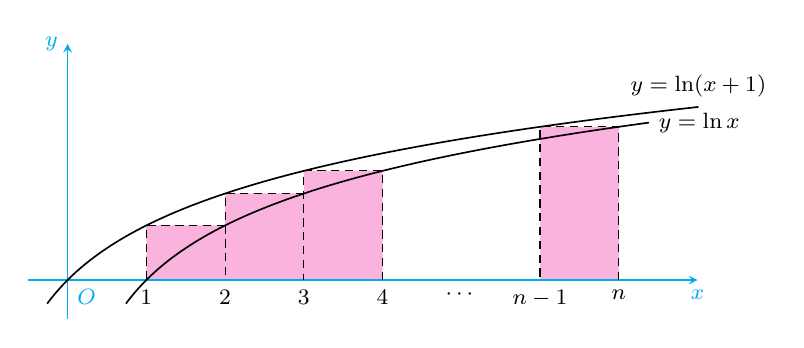
\begin{tikzpicture}[samples=100,>=stealth,domain=0:4,font=\footnotesize]
            \coordinate (xMin) at (-0.5,0);
            \coordinate (xMax) at (8,0);
            \coordinate (yMin) at (0,-0.5);
            \coordinate (yMax) at (0,3);
            \fill[magenta!30] (4,0)--(4,1.386)--(3,1.386)--(3,1.099)--(2,1.099)--(2,0.693)--(1,0.693)--(1,0)--cycle;
            \fill[magenta!30] (7,0)--(7,1.946)--(6,1.946)--(6,0)--cycle;
            \draw[->,cyan] (xMin)--(0,0) node [below right] {$O$}--(xMax) node[below] {$x$};
            \draw[->,cyan] (yMin)--(yMax) node [left] {$y$};
            \draw[semithick,domain=-0.3:2] plot({exp(\x)},\x) node[right] {$y=\ln x$};
            \draw[semithick,domain=-0.3:2.2] plot({exp(\x)-1},\x) node[above] {$y=\ln (x+1)$};
            \foreach \i in {1,...,4} {
            \coordinate[label=below:{$\i$}] (x\i) at (\i,0);
            }
            \node[below] at (5,0) {$\cdots$};
            \node[below] at (6,0) {$n-1$};
            \node[below] at (7,0) {$n$};
            \draw[densely dashed] (4,0)--(4,1.386)--(3,1.386)--(3,0);
            \draw[densely dashed] (3,1.099)--(2,1.099)--(2,0);
            \draw[densely dashed] (2,0.693)--(1,0.693)--(1,0);
            \draw[densely dashed] (7,0)--(7,1.946)--(6,1.946)--(6,0);
        \end{tikzpicture}
        \caption{}
    \end{figure}
    由图可知: $\displaystyle\int _{1}^{n}\ln x\dd x\leqslant \sum ^{n}_{k=1}\ln k\leqslant \int ^{n}_{1}\ln\left( 1+x\right) \dd x$
    则有 $$\displaystyle\dfrac{n\ln n-n+1}{n\ln n}\leqslant \dfrac{1}{n\ln n}\sum ^{n}_{k=1}\ln k\leqslant \dfrac{\left( n+1\right) \ln \left( n+1\right) -n}{n\ln n}$$
    又因为 $\displaystyle\lim _{n\rightarrow \infty }\dfrac{n\ln n-n+1}{n\ln n}=\lim _{n\rightarrow \infty }\dfrac{\left( n+1\right) \ln \left( n+1\right) -n}{n\ln n}=1$,
    因此有夹逼准则,原式$=\e .$\\
    \textbf{法二: }(Stolz 定理+L'Hospital 法则) 同上得到和式: $\displaystyle\lim _{n\rightarrow \infty }\dfrac{\displaystyle\sum\limits ^{n}_{k=1}\ln k}{n\ln n}\xlongequal[]{\text{Stolz}}\lim _{n\rightarrow \infty }\dfrac{\ln n}{n\ln n-\left( n-1\right) \ln \left( n-1\right) }$
    下面考虑该极限值 $\displaystyle I=\lim _{n\rightarrow \infty }\dfrac{n\ln n-\left( n-1\right) \ln \left( n-1\right) }{\ln n}$,由 Heine 定理将其连续化为函数极限:
    $$I'=\lim _{x\rightarrow +\infty }\dfrac{x\ln x-\left( x-1\right) \ln \left( x-1\right) }{x\ln x}$$
    \begin{flalign*}
        I'\xlongequal[]{L'}\lim_{x\to+\infty}\dfrac{\ln x+1-\ln \left( x-1\right) -1}{\dfrac{1}{x}}=\lim_{x\to+\infty}x\ln\frac{x}{x-1}=\lim_{x\to+\infty}x\left(\frac{x}{x-1}-1\right)=1\Rightarrow\text{原式=}\e .
    \end{flalign*}
\end{solution}

\begin{example}
    求 $\displaystyle\lim_{n\to\infty}\prod_{k=1}^{n-1}\left(\frac{2^k}{2^{k+1}-1}\right)^{\frac{1}{2^{n-k}}}.$
\end{example}
\begin{solution}
    取对数降低运算等级,故
    \begin{flalign*}
        I & =\lim_{n\to\infty}\prod_{k=1}^{n-1}\left(\frac{2^k}{2^{k+1}-1}\right)^{\frac{1}{2^{n-k}}}=\exp\lim_{n\to\infty}\sum_{k=1}^{n-1}\frac{1}{2^{n-k}}\ln\frac{2^k}{2^{k+1}-1}                                                                                                \\
          & =\exp\lim_{n\to\infty}\frac{1}{2^{n-1}}\sum_{k=1}^{n-1}2^{k-1}\ln\frac{2^k}{2^{k+1}-1}\xlongequal[]{\text{Stolz}}\exp\lim_{n\to\infty}\frac{\left(\displaystyle\sum\limits_{k=1}^{n-1}-\sum\limits_{k=1}^{n-2}\right)2^{k-1}\ln\dfrac{2^k}{2^{k+1}}-1}{2^{n-1}-2^{n-2}} \\
          & =\exp\lim_{n\to\infty}\frac{2^{n-2}\ln\dfrac{2^{n-1}}{2^n-1}}{2^{n-1}-2^{n-2}}=\exp\lim_{n\to\infty}\ln\frac{1}{2-\dfrac{1}{2^{n-1}}}=\frac{1}{2}.
    \end{flalign*}
\end{solution}

\begin{example}
    求 $\displaystyle\lim_{n\to\infty}\frac{1}{n^2}\sum_{k=0}^{n}\ln\C _n^k.$
\end{example}
\begin{solution}
    Stolz 公式可重复使用,
    \begin{flalign*}
        \lim_{n\to\infty}S_n & \xlongequal[]{\text{Stolz}}\lim_{n\to\infty}\frac{\displaystyle\sum\limits_{k=0}^{n+1}\ln\C _{n+1}^k-\sum\limits_{k=0}^{n}\ln\C _{n}^k}{(n+1)^2-n^2}=\lim_{n\to\infty}\frac{\displaystyle\sum\limits_{k=0}^{n}\ln\dfrac{\C _{n+1}^k}{\C _n^k}+\ln\C _{n+1}^{n+1}}{2n+1} \\
                             & =\lim_{n\to\infty}\frac{\displaystyle\sum\limits_{k=0}^{n}\ln\dfrac{n+1}{n-k+1}}{2n+1}=\lim_{n\to\infty}\frac{\displaystyle(n+1)\ln(n+1)-\sum\limits_{k=1}^{n+1}\ln k}{2n+1}                                                                                            \\
                             & \xlongequal[]{\text{Stolz}}\lim_{n\to\infty}\frac{(n+1)\ln(n+1)-n\ln n-\ln(n+1)}{(2n+1)-(2n-1)}=\lim_{n\to\infty}\frac{\ln\left(\dfrac{n+1}{n}\right)^n}{2}=\frac{1}{2}.
    \end{flalign*}
\end{solution}

\begin{example}
    求极限 $\displaystyle\lim_{n\to\infty}\qty(\prod_{k=0}^{n}\C _n^k)^{\frac{2}{n(n+1)}}.$
\end{example}
\begin{solution}
    取对数,降低运算等级,有
    \begin{flalign*}
        I & =\exp\lim_{n\to\infty}\dfrac{2}{n(n+1)}\ln\prod_{k=0}^{\infty}\C_n^k=\exp\lim_{n\to\infty}\dfrac{\displaystyle 2\sum_{k=0}^{n}\ln\C_n^k}{n(n+1)}\xlongequal{Stolz}\exp\lim_{n\to\infty}\dfrac{\displaystyle2\sum_{k=0}^{n+1}\ln\C_{n+1}^k-2\sum_{k=0}^{n}\ln\C_n^k}{(n+1)(n+2)-n(n+1)} \\
          & =\exp\lim_{n\to\infty}\dfrac{\displaystyle\sum_{k=0}^{n}\ln\dfrac{n+1}{n-k+1}}{n+1}=\dots=\exp\lim_{n\to\infty}\ln\qty(\dfrac{n+1}{n})^n=\e.
    \end{flalign*}
\end{solution}

\begin{example}
    \scriptsize\linespread{0.8}
    求 $\displaystyle\lim _{n\rightarrow \infty }\sqrt[n^{2}] {\dfrac{n!\left( n-1\right) !\cdots 2!}{n^{n}\left( n-1\right) ^{n-1}\cdots 2^{2}}}.$
\end{example}
\begin{solution}
    \scriptsize\linespread{0.8}
    由例题 \ref{Stirling} 可知,$n!=\sqrt{2\pi n}n^{n}\e ^{-n+\frac{\theta _{n}}{12n}},0 <\theta _{n} <1$,那么
    \begin{flalign*}
        \text{原式}  =\exp \lim _{n\rightarrow \infty }\dfrac{\displaystyle\sum\limits ^{n}_{k=2}\ln k!-\sum\limits ^{n}_{k=2}\ln k^{k}}{n^{2}}\xlongequal[]{\text{Stolz}}\exp \lim _{n\rightarrow \infty }\dfrac{\ln n!-\ln n^{n}}{2n-1}
        \xlongequal[]{\text{Stirling}}\exp \lim _{n\rightarrow \infty }\dfrac{\ln \left( \sqrt{2\pi n}\e ^{-n}+\dfrac{\theta _{n}}{12n}\right) }{2n-1}=\e ^{-\frac{1}{2}}.
    \end{flalign*}
\end{solution}
% \begin{inference}
%     Stirling 公式是一条用来取 $n!$ 近似值的数学公式,其公式为: 
%     $$n!=\sqrt{2\pi n}n^n \e ^{-n+\frac{\theta_n}{12n}}\text{ 或 }\ln n!=\frac{1}{2}\ln(2\pi)+\left(n+\frac{1}{2}\right)\ln n-n+\frac{\theta_n}{12n}$$
%     其中 $0<\theta_n<1.$
% \end{inference}

\begin{example}\scriptsize\linespread{0.8}
    求极限 $\displaystyle\lim _{n\rightarrow \infty }n^{2}\left( \dfrac{\pi ^{2}}{6}-\sum ^{n}_{k=1}\dfrac{1}{k^{2}}-\dfrac{1}{n}\right) .$
\end{example}
\begin{solution}\scriptsize\linespread{0.8}
    记 $\displaystyle m=\dfrac{\pi ^{2}}{6}=\lim _{n\rightarrow \infty }\sum ^{n}_{k=1}\dfrac{1}{k^{2}}$,
    \begin{flalign*}
        \text{原式} & =\lim _{n\rightarrow \infty }\dfrac{\displaystyle m-\sum\limits ^{n}_{k=1}\dfrac{1}{k^{2}}-\dfrac{1}{n}}{\dfrac{1}{n^{2}}}\xlongequal[]{\text{Stolz}}\lim _{n\rightarrow \infty }\dfrac{\displaystyle m-\sum\limits ^{n}_{k=1}\dfrac{1}{k^{2}}-\dfrac{1}{n}-\left( m-\sum\limits ^{n-1}_{k=1}\dfrac{1}{k^{2}}-\dfrac{1}{n-1}\right) }{\dfrac{1}{n^{2}}-\dfrac{1}{\left( n-1\right) ^{2}}} \\
                    & =\lim _{n\rightarrow \infty }\dfrac{-\dfrac{1}{n^{2}}+\dfrac{1}{n-1}-\dfrac{1}{n}}{\dfrac{1}{n^{2}}-\dfrac{1}{\left( n-1\right) ^{2}}}=\lim _{n\rightarrow \infty }\dfrac{-\left( n-1\right) ^{2}+n^{2}\left( n-1\right) -n \left( n-1\right) ^{2}}{\left( n-1\right) ^{2}-n^{2}}=\lim _{n\rightarrow \infty }\dfrac{n-1}{1-2n}=-\dfrac{1}{2}.
    \end{flalign*}
\end{solution}

\begin{example}\scriptsize\linespread{0.8}
    $\{\C _n^k\}_{k=0}^n$ 为二项式系数,$A_n,G_n$ 分别表示它们的算术平均值和几何平均值,
    试证: $$\lim_{n\to\infty}\sqrt[n]{A_n}=2,\lim_{n\to\infty}\sqrt[n]{G_n}=\sqrt{\e }.$$
\end{example}
\begin{proof}[{\songti \textbf{证}}]\scriptsize\linespread{0.8}
    因为 $\displaystyle A_n=\frac{1}{n+1}\sum_{k=0}^{n}\C _n^k=\frac{2^n}{n+1},~G_n=\left(\prod_{k=0}^{n}\C _n^k\right)^{\frac{1}{n+1}}=\e ^{\frac{1}{n+1}\sum\limits_{k=0}^{n}\ln\C _n^k}$,
    所以
    $\displaystyle\lim_{n\to\infty}\sqrt[n]{A_n}=\lim_{n\to\infty}\sqrt[n]{\frac{2^n}{n+1}}=2$
    \begin{flalign*}
        \lim_{n\to\infty}\sqrt[n]{G_n} & =\exp\lim_{n\to\infty}\frac{\displaystyle\sum\limits_{k=0}^{n}\ln\C _n^k}{n(n+1)}\xlongequal[]{\text{Stolz}}\exp\lim_{n\to\infty}\frac{\displaystyle\sum\limits_{k=0}^{n}\ln\C _n^k-\sum\limits_{k=0}^{n-1}\ln\C _{n-1}^k}{2n}           \\
                                       & =\exp\lim_{n\to\infty}\frac{\displaystyle\sum\limits_{k=1}^{n-1}\ln\C _n^k-\sum\limits_{k=1}^{n-2}\ln\C _{n-1}^k}{2n}=\exp\lim_{n\to\infty}\frac{\displaystyle\sum\limits_{k=1}^{n-2}\ln\dfrac{\C _n^k}{\C _{n-1}^k}+\ln\C _n^{n-1}}{2n} \\
                                       & =\exp\lim_{n\to\infty}\frac{\displaystyle\sum\limits_{k=1}^{n-2}\ln\dfrac{n}{n-k}+\ln n}{2n}=\exp\lim_{n\to\infty}\frac{1}{2}\left(-\frac{1}{n}\sum_{k=1}^{n-1}\ln\frac{n-k}{n}\right)                                                   \\
                                       & =\exp\left[-\frac{1}{2}\int_{0}^{1}\ln(1-x)\dd x\right]=\sqrt{\e }.
    \end{flalign*}
\end{proof}

% \begin{example}
%     $a,b,c$ 为非负实数,求 $\displaystyle\lim_{n\to\infty}\dfrac{1}{n^3}\sum_{i=1}^{n}\sum_{j=1}^{n}\dfrac{ij}{\sqrt{i^2+j^2+ai+bj+c}}.$
% \end{example}
% \begin{solution}
%     令 $\displaystyle y_{n}=\dfrac{1}{n^{3}}\sum ^{n}_{i=1}\sum ^{n}_{j=1}\dfrac{ij}{\sqrt{i^{2}+j^{2}}}$,那么
%     \begin{flalign*}
%         
%     \end{flalign*}
% \end{solution}

\subsubsection{函数极限的情况}

Stolz 定理可推广到函数极限的情况.

\begin{theorem}[$\infty/\infty$ 型]
    若 $T>0$ 为常数,且满足
    \begin{enumerate}[label=(\arabic{*})]
        \item $g(x+T)>g(x),~\forall x\geqslant a;$
        \item $g(x)\to+\infty~  (x\to+\infty)$,且 $f,g$ 在 $[a,+\infty)$ 内闭有界;
        \item $\displaystyle\lim_{x\to+\infty}\frac{f(x+T)-f(x)}{g(x+T)-g(x)}=l.$
    \end{enumerate}
    则 $\displaystyle\lim_{x\to+\infty}\frac{f(x)}{g(x)}=l$,(其中 $l$ 为有限数,$+\infty$ 或 $-\infty$).
    \index{函数 Stolz 定理}
\end{theorem}
\begin{theorem}[$0/0$ 型]
    若 $T>0$ 为常数,且
    \begin{enumerate}[label=(\arabic{*})]
        \item $0<g(x+T)<g(x),\forall x\geqslant a$;
        \item $\displaystyle\lim_{x\to+\infty}f=\lim_{x\to+\infty}g=0$;
        \item $\displaystyle\lim_{x\to+\infty}\frac{f(x+T)-f(x)}{g(x+T)-g(x)}=l.$
    \end{enumerate}
    则 $\displaystyle\lim_{x\to+\infty}\frac{f(x)}{g(x)}=l$,(其中 $l$ 为有限数,$+\infty$ 或 $-\infty$).
\end{theorem}

\begin{example}\scriptsize\linespread{0.8}
    设 $f$ 在 $[a,+\infty)$ 上有定义,且内闭有界 (即 $\forall [\alpha,\beta]\subset(a,+\infty),f\text{ 在 }[\alpha,\beta]\text{ 上有界}$),
    $$\displaystyle\lim_{n\to\infty}\dfrac{f(x+1)-f(x)}{x^n}=l$$ 其中 $l$ 为有限数,$+\infty$ 或 $-\infty$,证明: $\displaystyle\lim_{x\to+\infty}\dfrac{f(x)}{x^{n+1}}=\dfrac{l}{n+1}.$
\end{example}
\begin{solution}\scriptsize\linespread{0.8}
    运用函数的 Stolz 定理,得
    \begin{flalign*}
        \lim _{x\rightarrow +\infty }\dfrac{f\left( x\right) }{x^{n+1}} & =\lim _{x\rightarrow +\infty }\dfrac{f\left( x+1\right) -f\left( x\right) }{\left( x+1\right) ^{n+1}-x^{n+1}}=\lim _{x\rightarrow +\infty }\dfrac{f\left( x+1\right) -f\left( x\right) }{\left( n+1\right) x^{n}+\dfrac{n\left( n+1\right) }{1\cdot 2}x^{n-1}+\cdots +1} \\
                                                                        & =\lim _{x\rightarrow +\infty }\dfrac{\dfrac{f\left( x+1\right) -f\left( x\right) }{x^{n}}}{\left( n+1\right) +\dfrac{n\left( n+1\right) }{1\cdot 2}\dfrac{1}{x}+\ldots +\dfrac{1}{x^{n}}}=\dfrac{l}{n+1}~
        (l \text{ 为}+\infty,-\infty\text{ 也成立}).
    \end{flalign*}
\end{solution}

\subsubsection{Stolz 的应用}

\begin{example}
    对于数列 $x_0=a,0<a<\dfrac{\pi}{2},x_n=\sin x_{n-1}~  (n=1,2,\cdots)$,证明:
    $$\lim_{n\to\infty}x_n=0,~\lim_{n\to\infty}\sqrt{\frac{n}{3}}x_n=1.$$
\end{example}
\begin{proof}[{\songti \textbf{证}}]
    \begin{enumerate}[label=(\arabic{*})]
        \item 因为 $0<a<\dfrac{\pi}{2},~x_0=a$,递推可知 $$0<x_n=\sin x_{n-1}<x_{n-1}<\dfrac{\pi}{2}~  (n=1,2,\cdots)$$
              $\{x_n\}$ 单调递减且有下界 $0$,$\lim\limits_{n\to\infty}x_n$ 存在. 记 $\displaystyle\lim_{n\to\infty}x_n=A$,知 $A=\sin A\Rightarrow A=0$,$\displaystyle\lim_{n\to\infty}x_n=0.$
        \item 要证 $\displaystyle \lim_{n\to\infty}\sqrt{\frac{n}{3}}x_n=1$,即证 $\displaystyle\lim_{n\to\infty}\frac{n}{\dfrac{1}{x_n^2}}=3$
              \begin{flalign*}
                  \lim _{n\rightarrow \infty }\dfrac{n}{\dfrac{1}{x_{n}^{2}}} & \xlongequal[]{\text{Stolz}}\lim _{n\rightarrow \infty }\dfrac{n-\left( n-1\right) }{\dfrac{1}{x_{n}^{2}}-\dfrac{1}{x_{n-1}^{2}}}=\lim _{n\rightarrow \infty }\dfrac{1}{\dfrac{1}{\sin ^{2}x_{n-1}}-\dfrac{1}{x_{n-1}^{2}}}=\lim _{n\rightarrow \infty }\dfrac{x_{n-1}^{2}\sin ^{2}x_{n}-1}{x_{n-1}^{2}-\sin ^{2}x_{n-1}} \\
                                                                              & =\lim _{x\rightarrow 0}\dfrac{x^{2}\sin ^{2}x}{x^{2}-\sin ^{2}x}=\lim _{x\rightarrow 0}\dfrac{x^{4}}{\left( x+\sin x\right) \left( x-\sin x\right) }=\lim _{x\rightarrow 0}\dfrac{x^{4}}{\left( 2x+o\left( x\right) \right) \left( \dfrac{x3}{6}+o\left( x^{3}\right) \right) }                                          \\
                                                                              & =\lim _{x\rightarrow 0}\dfrac{1}{\left( 2+o\left( 1\right) \right) \left( \dfrac{1}{6}+o\left( 1\right) \right) }=3.
              \end{flalign*}
              得证 $\displaystyle \lim_{n\to\infty}\sqrt{\frac{n}{3}}x_n=1.$
    \end{enumerate}
\end{proof}
\begin{example}
    设 $0<a_1<1,a_{n+1}=a_n(1-a_n)~  (\forall n\in\mathbb{N})$,证明: $\displaystyle\lim_{n\to\infty}na_n=1.$
\end{example}
\begin{proof}[{\songti \textbf{证}}]
    由 $0<x_1<1$ 及 $x_2=x_1(1-x_1)$ 知, $0<x_2<1$,用数学归纳法可证: $\forall n\in\mathbb{N}^*:0<x_n<1$,于是 $0<\dfrac{x_{n+1}}{x_{n}}=1-x_n<1~  (n=1,2,\cdots)$,
    从而 $\{x_n\}\searrow 0$,不妨设 $\displaystyle\lim_{n\to\infty}x_n=A$,递推关系式两边取极限,得 $A=A(1-A)$,解得 $A=0.$
    令 $b_n=\dfrac{1}{x_n}$,则 $\displaystyle\lim_{n\to\infty}b_n=+\infty$,且数列 $\{b_n\}$ 是严格单调递增,故由 Stolz 定理
    $$\displaystyle\lim _{n\rightarrow \infty }nx_{n}=\lim _{n\rightarrow \infty }\dfrac{n}{\dfrac{1}{x_{n}}}=\lim _{n\rightarrow \infty }\dfrac{n}{b_{n}}=\lim _{n\rightarrow \infty }\dfrac{1}{b_{n+1}-b_{n}}=\lim _{n\rightarrow \infty }\left( 1-x_{n}\right) =1.$$
\end{proof}
\begin{example}
    设 $x_1>0,x_{n+1}=\ln(1+x_n)~  (n=1,2,\cdots)$,求 $\lim\limits_{n\to\infty}nx_n.$
\end{example}
\begin{solution}
    $x_2=\ln(1+x_1)>0$,用数学归纳法可证 $\forall n\in \mathbb{N}^*:x_n>0$,又 $x_1>0,x_{n+1}=\ln(1+x_n)<x_n$,故数列 $\{x_n\}\searrow 0$,那么
    \begin{flalign*}
        \lim _{n\rightarrow \infty }nx_{n} & =\lim _{n\rightarrow \infty }\dfrac{n}{\dfrac{1}{x_{n}}}\xlongequal[]{\text{Stolz}}\lim _{n\rightarrow \infty }\dfrac{1}{\dfrac{1}{x_{n}}-\dfrac{1}{x_{n}-1}}=\lim _{n\rightarrow \infty }\dfrac{1}{\dfrac{1}{\ln \left( 1+x_{n-1}\right) }-\dfrac{1}{x_{n-1}}} \\
                                           & =\lim _{n\rightarrow \infty }\dfrac{x_{n-1}\ln \left( 1+x_{n-1}\right) }{x_{n-1}-\ln \left( 1+x_{n-1}\right) }=\lim _{n\rightarrow \infty }\dfrac{x_{n-1}^{2}}{\dfrac{1}{2}x_{n-1}^{2}}=2.
    \end{flalign*}
\end{solution}

% \begin{example}
%     令 $a_n=1-\dfrac{\mathrm{C}_n^1}{3}+\dfrac{\mathrm{C}_n^2}{5}-\cdots+\dfrac{(-1)\mathrm{C}_n^n}{2n+1}$,且 $\qty{b_n}_{n=2}^{\infty}$,
%     且 $$b_n=\dfrac{(n+1)^2}{\sqrt[n+1]{(n+1)!}}-\dfrac{n^2}{\sqrt[n]{n!}}$$
%     计算极限 $\displaystyle\lim_{n\to\infty}\qty(1+\dfrac{\sqrt[n]{a_n}}{n!})^{\frac{n!}{b_n^n}}.$
% \end{example}
% \begin{solution}
%     因为 $\displaystyle a_n=\sum_{k=0}^{n}\dfrac{(-1)^k\mathrm{C}_n^k}{2k+1}=\int_{0}^{1}\qty[\sum_{k=0}^{n}\mathrm{C}_n^k\qty(-x^2)^k]\dd x=\int_{0}^{1}\qty(1-x^2)\dd x\xlongequal[]{x=\sin t}\int_{0}^{\frac{\pi}{2}}\cos^{2n+1}t\dd t$,又由推论 \ref{Wallis gs} 可知,
%     $$\int_{0}^{\frac{\pi}{2}}\cos^{2n+1}t\dd t=\dfrac{(2n)!!}{(2n+1)!!}\to0~ (n\to\infty)$$
% \end{solution}

\begin{example}\scriptsize\linespread{0.8}
    序列 $a_{ij}=\dfrac{i+j}{i^2+j^2}$,求极限 $\displaystyle\lim_{n\to\infty}\dfrac{1}{n}\sum_{i=1}^{n}\sum_{j=1}^{n}a_{ij}.$
\end{example}
\begin{solution}\scriptsize\linespread{0.8}
    由 Stolz ($*/\infty$ 型) 得\footnote{以下的括号不为矩阵符号,
        \begin{flalign*}
             & \begin{pmatrix}
                          & \dfrac{1+1}{1^2+1^2}       & + & \dfrac{1+2}{1^2+2^2}       & + & \cdots & + & \dfrac{1+n}{1^2+n^2}       & + & \dfrac{1+n+1}{1^2+(n+1)^2}       \\
                   +      & \dfrac{2+1}{2^2+1^2}       & + & \dfrac{2+2}{2^2+2^2}       & + & \cdots & + & \dfrac{2+n}{2^2+n^2}       & + & \dfrac{2+n+1}{2^2+(n+1)^2}       \\
                   \vdots & \vdots                     &   & \vdots                     &   &        &   & \vdots                     &   & \vdots                           \\
                   +      & \dfrac{n+1}{n^2+1^2}       & + & \dfrac{n+2}{n^2+2^2}       & + & \cdots & + & \dfrac{n+n}{n^2+n^2}       & + & \dfrac{n+n+1}{n^2+(n+1)^2}       \\
                   +      & \dfrac{n+1+1}{(n+1)^2+1^2} & + & \dfrac{n+1+2}{(n+1)^2+2^2} & + & \cdots & + & \dfrac{n+1+n}{(n+1)^2+n^2} & + & \dfrac{n+1+n+1}{(n+1)^2+(n+1)^2}
               \end{pmatrix} \\
             & -
            \begin{pmatrix}
                       & \dfrac{1+1}{1^2+1^2} & + & \dfrac{1+2}{1^2+2^2} & + & \cdots & + & \dfrac{1+n}{1^2+n^2} \\
                +      & \dfrac{2+1}{2^2+1^2} & + & \dfrac{2+2}{2^2+2^2} & + & \cdots & + & \dfrac{2+n}{2^2+n^2} \\
                \vdots & \vdots               &   & \vdots               &   &        &   & \vdots               \\
                +      & \dfrac{n+1}{n^2+1^2} & + & \dfrac{n+2}{n^2+2^2} & + & \cdots & + & \dfrac{n+n}{n^2+n^2}
            \end{pmatrix}
            =2\left[ \sum ^{n}_{k=1}\dfrac{(n+1) +k}{(n+1) ^{2}+k^{2}}\right] +\dfrac{1}{n+1}.
        \end{flalign*}}
    \begin{flalign*}
        \lim _{n\rightarrow \infty }\dfrac{1}{n}\sum ^{n}_{i=1}\sum ^{n}_{j=1}\dfrac{i+j}{i^{2}+j^{2}} & =\lim _{n\rightarrow \infty }\left( \sum ^{n+1}_{i=1}\sum ^{n+1}_{j=1}-\sum ^{n}_{i=1}\sum ^{n}_{j=1}\right) \dfrac{i+j}{i^{2}+j^{2}}=\lim _{n\rightarrow \infty }\left[ 2\left( \sum ^{n}_{k=1}\dfrac{(n+1) +k}{(n+1) ^{2}+k^{2}}\right) +\dfrac{1}{n+1}\right] \\
                                                                                                       & =\lim _{n\rightarrow \infty }\left[ \dfrac{2}{n+1}\left( \sum ^{n}_{k=1}\dfrac{1+\dfrac{k}{n+1}}{1+\left( \dfrac{k}{n+1}\right) ^{2}}\right) +\dfrac{1}{n+1}\right] =2\int _{0}^{1}\dfrac{1+x}{1+x^{2}}\dd x=\dfrac{\pi}{2}+\ln 2.
    \end{flalign*}
\end{solution}

\begin{example}\scriptsize\linespread{0.8}
    序列 $a_{ij}=\dfrac{ij}{\sqrt{i^2+j^2+ai+bj+c}},~a,b,c$ 为非负实数,求 $\displaystyle\lim_{n\to\infty}\dfrac{1}{n^3}\sum_{i=1}^{n}\sum_{j=1}^{n}a_{ij}.$
\end{example}
\begin{solution}\scriptsize\linespread{0.8}
    令 $\displaystyle y_{n}=\dfrac{1}{n^{3}}\sum\limits ^{n}_{i=1}\sum\limits ^{n}_{j=1}\dfrac{ij}{\sqrt{i^{2}+j^{2}}}$,那么
    \begin{flalign*}
        \lim _{n\rightarrow \infty }y_{n} & \xlongequal[]{\text{Stolz}}\lim _{n\rightarrow \infty }\dfrac{\displaystyle\left( \sum\limits ^{n+1}_{i=1}\sum\limits ^{n+1}_{j=1}-\sum\limits ^{n}_{i=1}\sum\limits ^{n}_{j=1}\right) \dfrac{ij}{\sqrt{i^{2}+j^{2}}}}{3n^{2}+3n+1}=\lim _{n\rightarrow \infty }\dfrac{\displaystyle\left[ 2\left( \sum\limits ^{n}_{k=1}\dfrac{k(n+1) }{\sqrt{k^{2}+(n+1) ^{2}}}\right) +\dfrac{n+1}{\sqrt{2}}\right] }{3n^{2}+3n+1} \\
                                          & =\lim _{n\rightarrow \infty }\dfrac{2(n+1) ^{2}}{3n^{2}+3n+1}\cdot \lim _{n\rightarrow \infty }\dfrac{1}{n+1}\sum ^{n}_{k=1}\dfrac{k/(n+1) }{\sqrt{1+\left( k/(n+1) \right) ^{2}}}=\dfrac{2}{3}\int_{0}^{1}\dfrac{x}{\sqrt{1+x^2}}\dd x=\dfrac{2}{3}\left(\sqrt{2}-1\right).
    \end{flalign*}
    考虑 $\delta>0$ 的情况,令 $\displaystyle z_{n}=\dfrac{1}{n^{3}}\sum ^{n}_{i=1}\sum ^{n}_{j=1}\dfrac{ij}{\sqrt{\left( i+\delta \right) ^{2}+\left( j+\delta \right) ^{2}}}$,下证 $\displaystyle\lim _{n\rightarrow \infty }\left( z_{n}-y_{n}\right) =0$,
    \begin{flalign*}
        d_n=z_n-y_n=\dfrac{-1}{n^3}\sum ^{n}_{i=1}\sum ^{n}_{j=1}\dfrac{\left( 2\delta ^{2}+2\delta i+2\delta j\right) ij}{\sqrt{\left( i+\delta \right) ^{2}+\left( j+\delta \right) ^{2}}\sqrt{i^{2}+j^{2}}\left( \sqrt{\left( i+\delta \right) ^{2}+\left( j+\delta \right) ^{2}}+\sqrt{i^{2}+j^2}\right) }
    \end{flalign*}
    由 $\sqrt{i^2+j^2}\geqslant\sqrt{2ij}$,因此
    \begin{flalign*}
        |d_n| & \leqslant \dfrac{1}{n^{3}}\sum ^{n}_{i=1}\sum ^{n}_{j=1}\dfrac{\left( 2\delta ^{2}+2\delta i+2\delta j\right) ij}{\left( i^{2}+j^{2}\right) ^{\frac{3}{2}}}\leqslant \dfrac{1}{\sqrt{2}n^{3}}\sum ^{n}_{i=1}\sum ^{n}_{j=1}\dfrac{\delta ^{2}+\delta i+\delta j}{\sqrt{i}\sqrt{j}} \\
              & =\frac{\delta^{2}}{\sqrt{2} n^{3}}\left(\sum_{i=1}^{n} \frac{1}{\sqrt{i}}\right)\left(\sum_{j=1}^{n} \frac{1}{\sqrt{j}}\right)+\frac{\delta}{\sqrt{2}}\left(\frac{1}{n} \sum_{j=1}^{n} \frac{1}{\sqrt{j}}\right)\left(\frac{1}{n^{2}} \sum_{i=1}^{n} \sqrt{i}\right)
        +\frac{\delta}{\sqrt{2}}\left(\frac{1}{n} \sum_{i=1}^{n} \frac{1}{\sqrt{i}}\right)\left(\frac{1}{n^{2}} \sum_{j=1}^{n} \sqrt{j}\right)
    \end{flalign*}
    当 $n\to\infty$ 时,有
    $$\lim _{n \rightarrow \infty} \frac{1}{n} \sum_{j=1}^{n} \frac{1}{\sqrt{j}}=0 \text {,}  \lim _{n \rightarrow \infty} \frac{1}{n^{2}} \sum_{j=1}^{n} \sqrt{j}=0 $$
    于是 $\lim\limits_{n\to\infty}d_n=0$,令 $\displaystyle x_n=\lim_{n\to\infty}\dfrac{1}{n^3}\sum_{i=1}^{n}\sum_{j=1}^{n}a_{ij}$,且
    $\xi=\max\left\{\dfrac{a}{2},\dfrac{b}{2},\sqrt{\dfrac{c}{2}}\right\}$,得
    $$i^{2}+j^{2} \leqslant i^{2}+j^{2}+a i+b j+c \leqslant(i+\xi)^{2}+(j+\xi)^{2}$$
    因此 $z_n\leqslant x_n\leqslant y_n$,两边取极限,由夹逼准则得 $\displaystyle\lim_{n\to\infty}\dfrac{1}{n^3}\sum_{i=1}^{n}\sum_{j=1}^{n}a_{ij}=\dfrac{2}{3}\left(\sqrt{2}-1\right).$
\end{solution}
\section{极限典型问题}

这一节讨论与极限相关联的三类典型问题, 即极限的存在性问题、极限的局部逆问题和无穷小量及其阶的比较.

\subsection{极限的存在性问题}

讨论极限的存在性, 是高等数学中既十分典型又经常遇到的问题, 在研究非初等函数的连续性与可导性, 
往往归结为这类问题.

\begin{example}
    设函数 $$f(x)=\begin{cases}
        \dfrac{\displaystyle \int_{0}^{x^2}\sqrt{1+\tan^2t}\dd t}{2x^2}&,x<0\\[6pt]
        \dfrac{\sqrt{1+x^2}-1}{\ln\qty(1+x^2)}&,x>0
    \end{cases}$$
    求极限 $\displaystyle\lim_{x\to0}f(x).$
\end{example}
\begin{solution}
    利用 L'Hospital 法则易求得在 $x=0$ 处的左右极限值, 
    $$\lim_{x\to0^-}f(x)=\lim_{x\to0^-}\dfrac{\displaystyle\int_{0}^{x^2}\sqrt{1+\tan^2t}\dd t}{2x^2} \xlongequal{L'}\lim_{x\to0^-}\dfrac{2x\cdot\sqrt{1+\tan^2x^2}}{4x}=\dfrac{1}{2}$$
    并且 $$\lim_{xto0^+}f(x)=\lim_{x\to0^+}\dfrac{\sqrt{1+x^2}-1}{\ln\qty(1+x^2)}=\dfrac{1}{2}$$
    由 $f(0^-)=f(0^+)=\dfrac{1}{2}$, 故 $\displaystyle \lim_{x\to0}f(x)=\dfrac{1}{2}.$
\end{solution}

\subsection{极限的局部逆问题}

如果已知函数的极限存在, 但是在函数的表达式中含有一个 (或多个) 待定的参数, 要求确定待定参数的值, 
这就是所谓的函数极限的局部逆问题.

% \begin{example}
%     试确定常数 $a,b,c$ 的值, 使 $\displaystyle\lim_{x\to0}\dfrac{ax-\sin x}{\displaystyle\int_{b}^{x}\dfrac{\ln\qty(1+t^3)}{t}\dd t}=c\neq0.$
% \end{example}

\begin{example}[2018 数二]
    若 $\displaystyle\lim_{x\to0}\qty(\e^x+ax^2+bx)^{x^{-2}}=1$, 则
    \begin{tasks}(4)
        \task $a=\dfrac{1}{2},~b=-1$
        \task $a=-\dfrac{1}{2},~b=-1$
        \task $a=\dfrac{1}{2},~b=1$
        \task $a=-\dfrac{1}{2},~b=1$
    \end{tasks}
\end{example}
\begin{solution}
    由题设条件 $\displaystyle\lim_{x\to0}\qty(\e^x+ax^2+bx)^{x^{-2}}=\exp\lim_{x\to0}\dfrac{1}{x^2}\ln\qty(\e^x+ax^2+bx)=1$, 
    于是有 $\displaystyle\lim_{x\to0}\dfrac{\ln\qty(\e^x+ax^2+bx)}{x^2}=0$, 即
    \begin{flalign*}
        \lim_{x\to0}\dfrac{\ln\qty(\e^x+ax^2+bx)}{x^2} & =\lim_{x\to0}\dfrac{\e^x+ax^2+bx+1}{x^2}=\lim_{x\to0}\dfrac{1+x+\dfrac{1}{2}x^2+ax^2+bx+1+o\qty(x^2)}{x^2} \\
                                                       & =\lim_{x\to0}\qty[\qty(\dfrac{1}{2}+a)+\dfrac{b+1}{x}+\dfrac{2}{x^2}]=0\Rightarrow\begin{cases}
                                                                                                                                               \dfrac{1}{2}+a=0 \\[6pt]1+b=0
                                                                                                                                           \end{cases}
    \end{flalign*}
    故解得选 B.
\end{solution}

\begin{example}[2018 数一]
    若 $\displaystyle\lim_{x\to0}\qty(\dfrac{1-\tan x}{1+\tan x})^{\frac{1}{\sin kx}}=\e$, 求 $k.$
\end{example}
\begin{solution}
    $\displaystyle \exp\lim_{x\to0}\dfrac{1}{\sin kx}\ln\qty(\dfrac{1-\tan x}{1+\tan x})=\exp\lim_{x\to0}\dfrac{\ln(1-\tan x)-\ln(1+\tan x)}{\sin kx}=\exp\lim_{x\to0}\dfrac{-2\tan x}{\xi_x \cdot \sin kx}=\e$, 
    于是 $$\lim_{x\to0}\dfrac{-2\tan x}{\xi_x\cdot\sin kx}=\lim_{x\to0}\dfrac{-2x}{\xi_xk}=1\Rightarrow k=-2$$ 
    其中 $\xi_x\to1~ (x\to0).$
\end{solution}

\begin{example}
    试确定常数 $A,B,C$, 使下式当 $x\to0 $ 时成立:
    $$\dfrac{\e^{\sin x}}{\sin x}=\dfrac{1+Bx+Cx^2}{x+Ax^2}+o\qty(x^2).$$
\end{example}
\begin{solution}
    将所给等式两边同时乘以 $(1+Ax)\sin x$, 并注意到 $x\to0$ 时, $(1+Ax)\sin x\cdot o\qty(x^2)=o\qty(x^3)$, 得
    $$(1+Ax)\e^{\sin x}=\dfrac{\sin x}{x}\qty(1+Bx+Cx^2)+o\qty(x^3)$$
    将 $\e^{\sin x},\dfrac{\sin x}{x}$ 分别展开到 $x$ 的三阶, 于是有
    $$\e^{\sin x}=1+x+\dfrac{1}{2}x^2+o\qty(x^2),~\dfrac{\sin x}{x}=1-\dfrac{1}{6}x^2+o\qty(x^2)$$
    代入上式, 得
    \begin{flalign*}
        \qty(1+x+\dfrac{1}{2}x^2)(1+Ax)=\qty(1-\dfrac{1}{6}x^2)\qty(1+Bx+Cx^2)+o\qty(x^3) \\
        (A+1-B)x+\qty(A-C+\dfrac{2}{3})x^2+\qty(\dfrac{A}{2}+\dfrac{B}{6})x^3=o\qty(x^3)
    \end{flalign*}
    欲使上式成立, 必须有 $\begin{cases}
            A+1-B=0 \\[6pt]A-C+\dfrac{1}{3}=0\\[6pt]\dfrac{A}{2}+\dfrac{B}{6}=0
        \end{cases}$, 联立解得 $A=-\dfrac{1}{4},~B=\dfrac{3}{4},~C=\dfrac{5}{12}.$
\end{solution}

\subsection{无穷小量及其阶的比较}

有关无穷小量的概念可参考定义 \ref{infinitesimalDefinitions}.

\begin{example}[2019 数一]
    当 $x\to0$ 时, 若 $x-\tan x$ 与 $x^{k}$ 是同阶无穷小, 则 $k$ 等于 
    \begin{tasks}(4)
        \task 1
        \task 2
        \task 3
        \task 4
    \end{tasks}
\end{example}
\begin{solution}
    由于当 $x\to0$ 时, $x-\tan x\sim-\dfrac{1}{3}x^3$, 则 $\displaystyle\lim_{x\to0}\dfrac{x-\tan x}{x^3}=-\dfrac{1}{3}$, 所以 $k=3$, 选 C.
\end{solution}

\begin{example}
    设 $x\to0$ 时, $\e ^{x\cos x^2}-\e ^{x}$ 与 $x^n$ 是同阶无穷小, 则 $n $ 为
    \begin{tasks}(4)
        \task 5
        \task 4
        \task 3
        \task 2
    \end{tasks}
\end{example}
\begin{solution}
    因为 $\e ^{x\cos x^2}-\e ^{x}=\e^x\qty[\e ^{x\qty(\cos x^2-1)}-1]\sim x\qty(\cos x^2-1)\sim -\dfrac{1}{2}x^5$, 所以 $n=5$, 故选 A
\end{solution}

\begin{example}[2001 数二]
    设当 $x\to0 $ 时, $(1-\cos x)\ln\qty(1+x^2)$ 是比 $x\sin x^n$ 高阶的无穷小, 而 $x\sin x^n$ 是比 $\e ^{x^2}-1$ 高阶的无穷小, 则正整数 $n$ 
    \begin{tasks}(4)
        \task 1
        \task 2
        \task 3
        \task 4
    \end{tasks}
\end{example}
\begin{solution}
    因为 $(1-\cos x)\ln\qty(1+x^2)\sim\dfrac{1}{2}x^4,~x\sin x^n\sim x^{n+1},~\e ^{x^2}-1\sim x^2$, 由题意知 $4>n+1>2$, 解得 $n=2$, 故选 B.
\end{solution}
\section{递推形式的极限}

有些数列, 常常是利用递推的形式给出的, 如何计算这类数列的极限, 是本节的重点.
此类问题在各类考试中比较常见, 需多加注意.

\subsection{利用存在性求极限}

假若用某种方法证明了递推数列的极限存在, 则在递推公式里取极限, 便可得到极限值 $A$ 应满足的方程, 解此方程, 可求得极限值 $A$.

\begin{theorem}[单调有界准理]
    若 $x_n\nearrow$ 有上界, 或 $x_n\searrow$ 有下界, 则 $\{x_n\}$ 收敛.
    \index{单调有界准理}
\end{theorem}
判断单调性的通常方法有:
\begin{enumerate}[label=(\arabic{*})]
    \item $\displaystyle\forall n\in \mathbb{N}:x_{n+1}-x_n\begin{cases}\geqslant 0,&x_n\nearrow,\\ \leqslant 0,&x_n\searrow.\end{cases}$
    \item $\displaystyle\forall n\in\mathbb{N}:\frac{x_{n+1}}{x_n}\begin{cases}\geqslant 1,&x_n\nearrow,\\ \leqslant 1,&x_n\searrow.\end{cases}$
    \item 若 $x_{n+1}=f(x_n),~f'(x)\geqslant 0\text{, 则 }\begin{cases}x_1\leqslant x_2,&x_n\nearrow,\\ x_1\geqslant x_2,&x_n\searrow.\end{cases} $
\end{enumerate}

\begin{theorem}[压缩映射]
    对于任一数列 $\{x_n\}$ 而言, 若存在常数 $r$, 使得 $\forall n\in\mathbb{N}$, 恒有
    $$|x_{n+1}-x_n |\leqslant r|x_n-x_{n-1} |,~0<r<1$$
    则数列 $\{x_n\}$ 收敛;特别地, 若数列 $\{x_n\}$ 利用递推公式给出: $x_{n+1}=f(x_n)~  (n=1,2,\cdots)$, 
    其中 $f$ 为某一可微函数, 且 $\exists r\in \mathbb{R}$, 使得
    $$|f'(x)|\leqslant r<1$$
    则数列 $\{x_n\}$ 收敛. 若上式只在某区间 $D$ 上成立, 则必须验证数列 $\{x_n\}$ 是否保持在区间 $D$ 内.
    \index{压缩映射}
\end{theorem}
\begin{theorem}[不动点迭代]
    求解非线性方程 (组) 的一类常见的数值解法. 例如, 单个方程的求根问题 $f(x)=0$ 总可以等价地写成 $x=\phi (x)$, 
    其中 $\phi:\mathbb{R}\to\mathbb{R}$ 是一个辅助函数, 满足该式的点 $x$ 称为不动点.
    如果给定初始点 $x{(0)}$, 就可以考虑如下的不动点迭代法: $$x^{(k+1)}=\phi\left(x^{(k)}\right)~  (k=0,1,\cdots)$$
    函数 $\phi$ 亦称为\textit{迭代函数}.

    如果迭代函数 $\phi$ 是一个闭区间上的压缩映射 (或者迭代函数连续可微, 且导数的绝对值在该闭区间上严格小于 $1$), 
    则不动点迭代法产生的序列 $\{x^{(k)}\}$ 收敛到 $\phi$ 在区间上的不动点.
    \index{不动点迭代}
\end{theorem}
\begin{figure}[H]
    \centering
    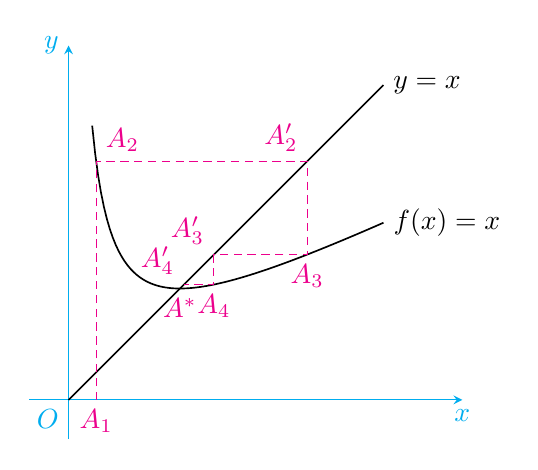
\begin{tikzpicture}[samples=100,>=stealth,domain=0:4]
        \coordinate (xMin) at (-0.5,0);
        \coordinate (xMax) at (5,0);
        \coordinate (yMin) at (0,-0.5);
        \coordinate (yMax) at (0,4.5);
        \draw[->,cyan] (xMin)--(0,0) node [below left] {$O$}--(xMax) node[below] {$x$};
        \draw[->,cyan] (yMin)--(yMax) node [left] {$y$};
        \path[draw,name path=x,semithick] plot(\x,\x) node[right] {$y=x$};
        \path[draw,name path=f(x),semithick,domain=0.3:4] plot(\x,{0.5*(\x+2/(\x))}) node[right] {$f(x)=x$};
        \path[name intersections={of=x and f(x),by=A}];
        \node[below,magenta] at (A) {$A^*$};
        \draw[densely dashed,magenta] node[below] at (0.35,0) {$A_1$}
        (0.35,0)--(0.35,{0.5*(0.35+2/0.35)}) node[above right] {$A_2$}
        --({0.5*(0.35+2/0.35)},{0.5*(0.35+2/0.35)}) node[above left] {$A_2'$}
        --({0.5*(0.35+2/0.35)},{0.5*((0.5*(0.35+2/0.35))+2/(0.5*(0.35+2/0.35)))}) node[below] {$A_3$}
        --({0.5*((0.5*(0.35+2/0.35))+2/(0.5*(0.35+2/0.35)))},{0.5*((0.5*(0.35+2/0.35))+2/(0.5*(0.35+2/0.35)))}) node[above left] {$A_3'$}
        --({0.5*((0.5*(0.35+2/0.35))+2/(0.5*(0.35+2/0.35)))},{0.5*((0.5*((0.5*(0.35+2/0.35))+2/(0.5*(0.35+2/0.35))))+2/(0.5*((0.5*(0.35+2/0.35))+2/(0.5*(0.35+2/0.35)))))}) node[below] {$A_4$}
        --({0.5*((0.5*((0.5*(0.35+2/0.35))+2/(0.5*(0.35+2/0.35))))+2/(0.5*((0.5*(0.35+2/0.35))+2/(0.5*(0.35+2/0.35)))))},{0.5*((0.5*((0.5*(0.35+2/0.35))+2/(0.5*(0.35+2/0.35))))+2/(0.5*((0.5*(0.35+2/0.35))+2/(0.5*(0.35+2/0.35)))))}) node[above left] {$A_4'$};
    \end{tikzpicture}
    \caption{}
\end{figure}

\begin{example}
    设数列 $\{x_n\}$ 满足: $x_0=1,~x_{n+1}=\sqrt{2x_n}~  (n=0,1,2,\cdots)$, 证明 $\{x_n\}$ 收敛, 并求极限值.
\end{example}
\begin{proof}[{\songti \textbf{证法一}}]
    $\displaystyle x_{n}=\sqrt{2x_{n-1}}=\sqrt{2\sqrt{2x_{n-2}}}=\sqrt{2\sqrt{2\sqrt{\cdots\sqrt{2}}}}=2^{\frac{1}{2}+\frac{1}{2^{2}}+\cdots +\frac{1}{2^{n}}}=2^{1-\frac{1}{2^{n}}}\to2~  (n\to\infty).$
\end{proof}
\begin{proof}[{\songti \textbf{证法二}}]
    显然 $1\leqslant x_0<2$, 假设 $1\leqslant x_k<2$, 则 $1\leqslant x_{k+1}=\sqrt{2x_k}<\sqrt{2\cdot 2}=2$, 故由数学归纳法知, $\forall n\in\mathbb{N}:1\leqslant x_n<2$, 
    又由 $\dfrac{x_{n+1}}{x_n}=\dfrac{\sqrt{2x_n}}{x_n}=\sqrt{\dfrac{2}{x}}>1$, 知 $\{x_n\}\nearrow$, 所以由单调有界原理得 $\{x_n\}$ 收敛, 不妨记 $\lim\limits_{n\to\infty}x_n=A$, 则在递推公式里取极限, 
    有 $A=\sqrt{2A}\Rightarrow A=0,2$, 而由 $x_n\ge1$, 知 $A\geqslant 1$, 故取 $A=2$, 即 $\lim\limits_{n\to\infty}x_n=A.$
\end{proof}
\begin{proof}[{\songti \textbf{证法三}}]
    令 $f(x)=\sqrt{2x}~  (x>0)$, 则 $f'(x)=\dfrac{1}{\sqrt{2x}}>0~  (x>0)$, 于是当 $x>0$ 时, $f(x)\nearrow$, 从而有 $x_n>x_{n-1}$, 可得
    $x_{n+1}=f(x_n)>f(x_{n-1})=x_n$, 而 $x_1=\sqrt{2}>x_0=1$, 故有 $x_1<x_2<\cdots$, 即 $\{x_n\}\nearrow$, 其余证法同证法 2.
\end{proof}
\begin{proof}[{\songti \textbf{证法四}}]
    如证法 2, 已有 $1\leqslant x_n <2$, 对 $f(x)=\sqrt{2x}$, 有$$|f'(x)|=\dfrac{\sqrt{2}}{2\sqrt{x}}\leqslant\dfrac{\sqrt{2}}{2}<1$$
    满足压缩映射条件, 其余证法同证法 2.
\end{proof}
\begin{proof}[{\songti \textbf{证法五}}]
    由递推关系式两边取对数, 得 $\ln x_{n+1}=\dfrac{1}{2}\ln x_n+\dfrac{1}{2}\ln 2$, 令 $b_n=\ln x_n$, 则
    $$b_{n+1}=\dfrac{1}{2}b_{n}+\dfrac{1}{2}\ln 2,~b_0=0$$
    记 $f(x)=\dfrac{1}{2}x+\dfrac{1}{2}\ln 2$, 则 $b_{n+1}=f(b_n)$, 又由特征方程 $x=f(x)$, 解得特征根 $x=\ln 2$, 所以
    \begin{flalign*}
        b_n-\ln 2 =\left(\dfrac{1}{2}b_{n-1}+\dfrac{1}{2}\ln 2\right)-\left(\dfrac{1}{2}\ln 2+\dfrac{1}{2}\ln 2\right)=\dfrac{1}{2}(b_{n-1}-\ln 2)
        =\left(\dfrac{1}{2}\right)^n\cdot(b_0-\ln 2)=-\ln 2\cdot\left(\dfrac{1}{2}\right)^n
    \end{flalign*}
    于是 $\lim\limits_{n\to\infty}(b_n-\ln 2)=0$, 即 $\lim\limits_{n\to\infty}x_n=2.$
\end{proof}
\begin{inference}
    一般地, 设 $a,x_0>0,x_{n+1}=\sqrt{ax}~  (n=0,1,2,\cdots)$, 则数列 $\{x_n\}$ 收敛, 且 $\lim\limits_{n\to\infty}x_n=a.$
\end{inference}

\begin{example}
    已知 $x_1=\sqrt{6},~x_n=\sqrt{6+x_{n-1}}~  (n=2,3,\cdots)$, 证明数列 $\{x_n\}$ 有极限, 并求其值.
\end{example}
\begin{proof}[{\songti \textbf{证法一}}]
    用数学归纳法可证: $0<x_n<3~  (n=1,2,\cdots)$, \\
    因为 $$x_{n+1}x-{n}=\sqrt{6+x_n}-\sqrt{6+x_{n-1}}=\dfrac{x_n-x_{n-1}}{\sqrt{6+x_n}+\sqrt{6+x_{n-1}}}$$ 所以 $x_{n+1}-x_n$ 与 $x_n-x_{n-1}$ 同号, 
    又 $x_2=\sqrt{6+\sqrt{6}}>\sqrt{6}=x_1$, 所以 $x_{n+1}>x_{n}$, 即 $\{x_n\}\nearrow 3$, 由单调有界准则知, $\{x_n\}$ 收敛.
\end{proof}
\begin{proof}[{\songti \textbf{证法二}}]
    先假设数列 $\{x_n\}$ 收敛, 不妨设 $\lim\limits_{n\to\infty}x_n=A$, 则由递推关系式两边取极限, 得 $A=\sqrt{6+A}$, 解得 $A=3,-2$, 
    因为 $x_n>0~  (n=1,2,\cdots)$, 所以 $A=3$, 下证数列 $\{x_n\}$ 收敛于 $3$.\\
    记 $q=\dfrac{1}{\sqrt{6}+3}$, 则有
    $$|x_n-3|=\left|\sqrt{6+x_{n-1}}-3\right|=\dfrac{|x_{n-1}-3|}{\sqrt{6+x_{n-1}}+3}<q\cdot|x_{n-1}-3|<\cdots<q^{n-1}\cdot|x_1-3|$$
    而由 $\lim\limits_{n\to\infty}q^n=0$, 故由极限的定义或者夹逼准则, 可得 $\lim\limits_{n\to\infty}x_n=3.$
\end{proof}

\begin{example}
    已知数列 $ \left\{x_{n}\right\} $ 满足 $ x_{n+1}=\dfrac{x_{n}^{2}}{2\left(x_{n}-1\right)},(n=0,1,2, \cdots)  $, 且 $ x_{0}>1$, 证明: 数列 $ \left\{x_{n}\right\} $ 收敛, 并求其极限.
\end{example}
\begin{solution}
    因为 $x_{n+1}=\dfrac{x_n^2}{2(x_n-1)}=\dfrac{x_n^2-1+1}{2(x_n-1)}=\dfrac{(x_n-1)(x_n+1)+1}{2(x_n-1)}=1+\dfrac{x_n-1}{2}+\dfrac{1}{2(x_n-1)}\geqslant 2~~(n=1,2,\cdots)$, \\
    \begin{minipage}{0.29\linewidth}
        \begin{figure}[H]
            \centering
            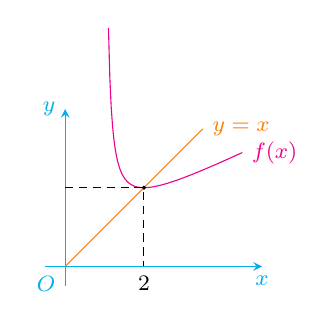
\begin{tikzpicture}[->,samples=100,>=stealth,font=\footnotesize,scale=0.5]
                \draw[->,cyan](-0.5,0)--(0,0)node[below left]{$O$}--(5,0)node[below]{$x$};
                \draw[->,cyan](0,-0.5)--(0,4)node[left]{$y$};
                \draw[-,magenta,domain=1.1:4.5]plot(\x,{\x*\x/(2*\x-2)})node[right]{$f(x)$};
                \draw[orange,-,domain=0:3.5]plot(\x,{\x})node[right]{$y=x$};
                \draw[densely dashed,-](0,2)--(2,2)--(2,0)node[below]{$2$};
                \draw[fill=black] (2,2) circle(1pt);
            \end{tikzpicture}
            \caption{}
            \label{bddxn2xn1}
        \end{figure}
    \end{minipage}\hfill
    \begin{minipage}{0.7\linewidth}
        \textbf{法一: }令 $f(x)=\dfrac{x^2}{2(x-1)}$, 则
        $$f'(x)=\dfrac{x(x-2)}{2(x-1)^2}=\dfrac{1}{2}\qty[1-\dfrac{1}{(x-1)^2}]$$
        所以 $|f'(x)|=\qty|\dfrac{1}{2}\qty[1-\dfrac{1}{(x-1)^2}]|<\dfrac{1}{2}<1$, 表明 $x_{n+1}=f(x_n)$ 是一压缩映像, 所以 $\qty{x_n}$ 收敛, 即 $\displaystyle\lim_{n\to\infty}x_n$ 存在, 不妨记为 $A$, 对 $x_{n+1}=\dfrac{x_n^2}{2(x_n-1)} $ 两边取极限, 有
        $A=\dfrac{A^2}{2(A-1)}\Rightarrow A=2$, 由极限的保序性可得 $A=2$, 即原数列极限为 2.\\
        \textbf{法二: }$x_{n+1}-x_n=\dfrac{x_n^2}{2(x_n-1)}-x_n=-\dfrac{x_n(x_n-2)}{2(x_n-1)}<0$, 则 $\qty{x_n}\searrow$, 同法一可得数列极限为 2.
    \end{minipage}
    \textbf{法三: }取\footnote{由图 \ref{bddxn2xn1} 可知在 $x>1$ 处有一个不动点 $x=2$.} $A=2$, 则 $A=\dfrac{A^2}{2(A-1)}$, 作 
    \begin{flalign*}
        \qty|x_{n+1}-A|-\qty|\dfrac{x_n^2}{2(x_n-1)}-\dfrac{A^2}{2(A-1)}|&=\dfrac{1}{2}\qty|\dfrac{x_n^2-1+1}{x_n-1}-\dfrac{A^2-1+1}{A-1}|=\dfrac{1}{2}\qty|x_n+1+\dfrac{1}{x_n-1}-(A+1)-\dfrac{1}{A-1}|\\
        &=\dfrac{1}{2}\qty|x_n-A+\dfrac{1}{x_n-1}-\dfrac{1}{A-1}|<|x_n-A|
    \end{flalign*}
    因此 $$\qty|x_{n+1}-A|<\dfrac{1}{2}\qty|x_n-A|<\cdots<\dfrac{1}{2^{n+1}}\qty|x_0-A|\to 0~~(n\to\infty)$$
    故由夹逼准则 (或数列极限的定义) 可知 $\displaystyle\lim_{n\to\infty}x_n=2.$
\end{solution}

\begin{example}
    (试用三种方法求) 设 $x_1>0,~x_{n+1}=\dfrac{c(1+x_n)}{c+x_n}~  (c \text{为常数})$, 求 $\lim\limits_{n\to\infty}x_n.$
\end{example}
\begin{solution}
    \textbf{法一: }(用单调有界准则) 若 $x_1=\sqrt{c}$, 则 $x_n=\sqrt{c}~  (\forall n\in\mathbb{N}),~\lim\limits_{n\to\infty}x_n=\sqrt{c}$, 
    若 $x_1>\sqrt{c}$, 因 $$f(x):=\dfrac{c(1+x_n)}{c+x}=c-\dfrac{c(c-1)}{c+x}$$ 严格 $\nearrow$, 故 $$\forall n\in\mathbb{N}:x_n>\sqrt{c}\Rightarrow x_{n+1}=\dfrac{c(1+x_n)}{c+x_n}=f(x_n)>f\left(\sqrt{c}\right)=\sqrt{c}$$, 
    由 $x_1>\sqrt{c}$ 可递推出 $x_n\sqrt{c}$, 又因为 $$x_{n+1}-x_{n}=\dfrac{c-x_n^2}{c+x_n}<0$$, 知 $x_n$ 严格 $\nearrow$, 故 $\{x_n\}$ 收敛, 
    同理可证, 当 $0<x_1<\sqrt{c}$ 时, $x_n\nearrow\sqrt{c}$, 综上, $\{x_n\}$ 单调有界, 极限存在, 令递推式 $\dfrac{c(1+x_n)}{c+x_n}$ 两边取极限, 得极限为 $\sqrt{c}.$\\
    \textbf{法二: }(用压缩映射) 因为 $x_n>0$, 且 $x>0$ 时, $f'(x)=\left[\dfrac{c(1+x)}{c+x}\right]'=\dfrac{c(c-1)}{(c+x)^2}>0$, 又 $c>1$ 知
    $$0<f'(x)=\dfrac{c(c-1)}{(c+x)^2}\leqslant\dfrac{c(c-1)}{c^2}=1-\dfrac{1}{c}<1~  (\forall x>0)$$
    故 $x_{n+1}=f(x_n)$ 为压缩映射, $\{x_n\}$ 收敛, 同上由 $\lim\limits_{n\to\infty}x_n=\sqrt{c}.$\\
    \textbf{法三: }显然对一切 $x_n>0$, 令 $f(x)=\dfrac{c(1+x)}{c+x}=x$, 知不动点 $x^*=\sqrt{c}$, 而 $f\nearrow$ 保证了 $x_n$ 位于不动点 $x^*$ 的同一侧, 且
    $$\left[x-\dfrac{c(1+x)}{c+x}\right]\left(x-\sqrt{c}\right)=\dfrac{cx+x^2-c-cx}{c+x}\left(x-\sqrt{c}\right)=\dfrac{x+\sqrt{c}}{c+x}\left(x+\sqrt{c}\right)^2>0$$
    意味着 $x_n$ 向 $x^*$ 步步靠近, 根据不动点迭代法知, $\lim\limits_{n\to\infty}x_n=\sqrt{c}.$
\end{solution}

\begin{example}
    设 $a,x_0>0,~x_{n+1}=\dfrac{1}{2}\left(x_n+\dfrac{a}{x_n}\right)~  (n=0,1,\cdots)$, 证明数列 $\{x_n\}$ 收敛, 并求其值.
\end{example}
\begin{proof}[{\songti \textbf{证法一}}]
    由算术平均数大于几何平均数得 $$x_{n+1}=\dfrac{1}{2}\left( x_{n}+\dfrac{a}{x_{n}}\right) \geqslant \sqrt{a}~  (n= 0,1,2,\cdots) $$ 于是
    $$\dfrac{x_{n+1}}{x_{n}}=\dfrac{1}{2}\left( 1+\dfrac{a}{x_{n}^{2}}\right) \leqslant 1$$ 即 $x_{n+1}\leqslant x_{n}$, 从而数列 $\{x_n\}\searrow\sqrt{a}$, 故数列收敛, 
    设 $\lim\limits_{n\to\infty}x_n=A$, 则由递推关系式两边取极限解得 $A=\pm\sqrt{a}$, 因为 $x_n\geqslant \sqrt{a}$, 所以极限为 $\sqrt{a}.$
\end{proof}
\begin{proof}[{\songti \textbf{证法二}}]
    由已知 $x_n>0$, 且
    \begin{flalign*}
        x_{n+1}-x_{n} & =\dfrac{1}{2}\left( x_{n}+\dfrac{a}{x_{n}}\right) -x_{n}=\dfrac{1}{2}\left( \dfrac{a}{x_{n}}-x_{n}\right) =\dfrac{1}{2}\left[ \dfrac{a}{\dfrac{1}{2}\left( x_{n-1}+\dfrac{a}{x_{n-1}}\right) }-\dfrac{1}{2}\left( x_{n-1}+\dfrac{a}{x_{n-1}}\right) \right] \\
                      & =\dfrac{1}{4}\cdot\dfrac{-\left(x_{n-1}^2-a\right)^a}{x_{n-1}\cdot\left(x_{n-1}^2+a\right)}<0~  (n\geqslant 2)
    \end{flalign*}
    所以 $\{x_n\}\searrow 0$, 同解法 1, 可求得极限值为 $\sqrt{a}$.
\end{proof}
\begin{proof}[{\songti \textbf{证法三}}]
    由 $x_{n+1}=\dfrac{1}{2}\left(x_n+\dfrac{a}{x_n}\right)\geqslant \sqrt{a}~  (n=0,1,2,\cdots)$, 所以 $x_{n+1}-\sqrt{a}=\left(x_n-\sqrt{a}\right)\cdot\dfrac{1}{2}\left(1-\dfrac{\sqrt{a}}{x_n}\right)$, 
    反复利用该递推公式, 得
    $$x_{n+1}-\sqrt{a}=\left( x_{1}-\sqrt{a}\right) \cdot \dfrac{1}{2^{n}}\left( 1-\dfrac{\sqrt{a}}{x_{1}}\right) \left( 1-\dfrac{\sqrt{a}}{x_{2}}\right) \cdots \left( 1-\dfrac{\sqrt{a}}{x_{n}}\right) $$
    于是 $\left|x_{n+1}-\sqrt{a}\right|\leqslant\dfrac{1}{2^n}\cdot\left|x_{1}-\sqrt{a}\right|$, 因为 $\lim\limits_{n\to\infty}\dfrac{1}{2^n}=0$, 由夹逼准则得 $\left|\lim\limits_{n\to\infty}x_{n+1}-\sqrt{a}\right|=0$, 
    故 $\lim\limits_{n\to\infty}x_n=\sqrt{a}.$
\end{proof}
\begin{inference}
    一般地, 设 $a,x_1>0,m\in\mathbf{N^*},~x_{n+1}=\dfrac{1}{m}\left[ \left( m-1\right) x_{n}+\dfrac{a}{x_{n}^{m-1}}\right] $, 则 $\lim\limits_{n\to\infty}x_n=\sqrt[m]{a}.$
\end{inference}
\begin{example}
    设 $a,x_0>0,x_{n+1}=\dfrac{x_n\left(x_n^2+3a\right)}{3x_n^2+a}~  (n=0,1,\cdots)$, 证明数列 $\{x_n\}$ 收敛, 并求极限值.
\end{example}
\begin{proof}
    令 $f(x)=\dfrac{x(x^2+3a)}{3x^2+a}$, 则 $f'(x) =\dfrac{3\left( x^{2}-a^{2}\right) ^{2}}{\left( 3x^{2}+a\right) ^{2}}\geqslant 0,x_{n+1}=f(x_n)$, \\
    若 $x_0\geqslant \sqrt{a}$, 则 $x_1=f(x_0)\geqslant f\left(\sqrt a\right)=\sqrt{a}$, 由 $x_n\geqslant \sqrt{a}$ 可得 $x_{n+1}=f(x_n)\geqslant f\left(\sqrt{a}\right)=\sqrt{a}$, 
    于是由数学归纳法得 $\forall n\in\mathbb{N},x_n\geqslant\sqrt{a}$, 又 $x_1=\dfrac{x_0\left(x_0^2+3a\right)}{3x_0^2+a}\leqslant x_0$, 由 $f'(x)\geqslant 0$ 得 $x_2=f(x_1)\leqslant f(x_0)=x_1$, 反复利用此关系, 
    即得 $x_{n+1}\leqslant x_n$, 于是数列 $\{x_n\}\searrow\sqrt{a}$, 故数列 $\{x_n\}$ 收敛, \\
    若 $0<x_0<\sqrt{a}$, 则类似上面可证得 $\forall n\in\mathbb{N},0<x_n<\sqrt{a}$ 且 $x_{n+1}\geqslant x_{n}$, 于是数列 $\{x_n\}\nearrow\sqrt{a}$, 故数列 $\{x_n\}$ 收敛, 
    不妨设 $\lim\limits_{n\to\infty}x_n=A$, 易得 $\lim\limits_{n\to\infty}x_n=\sqrt{a}.$
\end{proof}
\begin{inference}
    一般地, 设 $k\geqslant 2,k\in\mathbb{N}^*,x_0>0$, 令 $x_{n+1}=\dfrac{\displaystyle x_{n}^{k}+\sum\limits ^{\left[ k/2\right] }_{i=1}\mathrm{C}_{k}^{2i}\cdot x_{n}^{k-2i}\cdot a^{i}}{\displaystyle\sum\limits ^{\left[ \left( k-1\right) /2\right] }_{i=0}\mathrm{C}_{k}^{2i+1}\cdot x_{n}^{k-2i-1}\cdot a^{i}}~  (n=0,1,\cdots)$, 
    则数列 $\{x_n\}$ $k$ 阶收敛于 $\sqrt{a}.$

    事实上, 因为 $\dfrac{x_{n+1}-\sqrt{a}}{x_{n+1}+\sqrt{a}}=\left( \dfrac{x_{n}-\sqrt{a}}{x_{n}+\sqrt{a}}\right) ^{k}=\cdots =\left( \dfrac{x_{1}-\sqrt{a}}{x_{1}+\sqrt{a}}\right) ^{k^{n}}$, 
    所以有 $$x_{n+1}-\sqrt{a}=2\sqrt{a}\dfrac{\gamma ^{k^{n}}}{1-\gamma ^{k^{n}}}\to 0\left( n\to \infty \right) $$
    且有
    $$\lim _{n\to \infty }\dfrac{x_{n+1}-\sqrt{a}}{\left( x_{n}-\sqrt{a}\right) ^{k}}=\lim _{n\to \infty }\dfrac{x_{n+1}+\sqrt{a}}{\left( x_{n}+\sqrt{a}\right) ^{k}}=\dfrac{1}{\left( 2\sqrt{a}\right) ^{k-1}}.$$
\end{inference}

\subsection{写出通项求极限}

\subsubsection{利用不动点求通项}

在前小节介绍了不动点迭代法, 下文将介绍如何运用不动点解决两种类型的数列通项问题.

\begin{example}
    已知 $a_{n+1}=\dfrac{a\cdot a_n+b}{c\cdot a_n+d}~  (c\not=0)$, 且 $ad-bc\not=0$, $a,b,c,d$ 都是常数, 求通项 $a_n$.
\end{example}
\begin{solution}
    设 $f(x)=\dfrac{ax+b}{cx+d}~  (c,ad-bc\not=0)$, $\{a_n\}$ 满足递归关系 $a_{n+1}=f(a_n)$, 且初始值 $a_1\not=f(a_1)$.
    \begin{enumerate}[label=(\arabic{*})]
        \item 若 $f$ 有两相异的不动点 $p,q$, 则 $\dfrac{a_{n+1}-p}{a_{n+1}-q}=k\cdot \dfrac{a_{n}-p}{a_{n}-q}$, 其中 $k=\dfrac{a-pc}{b-qc}$, 即
              $\left\{\dfrac{a_n-p}{a_n-q}\right\}$ 是以 $k$ 为公比的等比数列, 由此解得
              $$a_{n}=\dfrac{\left( a_1q-pq\right) k^{n-1}-\left( a_1p-pq\right) }{\left( a_1-p\right) k^{n-1}-\left( a_1-q\right) }.$$
        \item 若 $f$ 只有一个不动点 $p$, 则 $\dfrac{1}{a_{n+1}-p}=\dfrac{1}{a_{n}-p}+k$, 其中 $k=\dfrac{2c}{a+d}$, 
              即 $\left\{\dfrac{1}{a_n-p}\right\}$ 是以 $k$ 为公差的等差数列, 由此解得
              $$a_{n}=\dfrac{a_{1}-p}{\left( ka_{1}-pk\right) n+1-ka_{1}+pk}+k.$$
    \end{enumerate}
\end{solution}
\begin{example}
    已知 $a_{n+1}=\dfrac{a\cdot a_n^2+b}{2a \cdot a_n+c}~  (a\not=0)$, $a,b,c$ 都是常数, 求通项 $a_n$.
\end{example}
\begin{solution}
    设递归函数为 $f(x)=\dfrac{ax^2+b}{2ax+c}$, 那么
    \begin{enumerate}
        \item 若 $f$ 有两相异的不动点 $p,q$, 即 $p=\dfrac{ap^2+b}{2ap+c},~q=\dfrac{aq^2+b}{2aq+c}$, 则
              $$a_{n+1}-p=\dfrac{a\cdot an^{2}+b}{2a\cdot a_{n}+c}-p=\dfrac{a\cdot a_{n}^{2}+b-2apa_{n}-pc}{2a\cdot a_{n}+c}=\dfrac{a\cdot a_{n}^{2}-2apa_{n}+ap^{2}}{2a\cdot a_{n}+c}=\dfrac{a(a-p)^2}{2a\cdot a_n+c}$$
              同理 $a_{n+1}-q=\dfrac{a\left( a_{n}-q\right) ^{2}}{2a\cdot a_{n}+c}$, 两式相除, 得
              $$\dfrac{a_{n+1}-p}{a_{n+1}-q}=\left(\dfrac{a_n-p}{a_n-q}\right)^2=\left(\dfrac{a_{n-1}-p}{a_{n-1}-q}\right)^{2^2}=\cdots=\left(\dfrac{a_1-p}{a_1-q}\right)^{2^{n-1}}$$
              由此解得, $a_{n}=\dfrac{q\left( a_{1}-p\right) ^{2^{n-1}}-p\left( a_1-q\right)^ {2^{n-1}}}{\left( a_{1}-p\right) ^{2^{n-1}}-\left( a_{1}-q\right) ^{2^{n-1}}}.$
        \item 若 $f$ 有两相同的不动点 $p$, 易得 $p=-\dfrac{c}{2a}$, 由 $a_{n+1}-p=a_{n+1}+\dfrac{c}{2a}=\dfrac{a\cdot a_n^2+b}{2a\cdot a_n+c}+\dfrac{c}{2a}$, 令 $b_n=a_n+\dfrac{c}{2a_n}$, 化简可得 $b_{n+1}=\dfrac{1}{2}b_n$, 
              即 $b_n=\left(a_1+\dfrac{c}{2a}\right)\left(\dfrac{1}{2}\right)^{n-1}$, 由此解得
              $$a_{n}=\left( a_{1}+\dfrac{c}{2a}\right) \left( \dfrac{1}{2}\right) ^{n-1}-\dfrac{c}{2a}.$$
    \end{enumerate}
\end{solution}
\begin{example}
    设数列 $\{x_n\}$ 满足 $x_1=2,x_{n+1}=2+\dfrac{1}{x_n}~  (n=1,2,\cdots)$, 证明数列 $\{x_n\}$ 收敛, 并求 $\lim\limits_{n\to\infty}x_n.$
\end{example}
\begin{proof}[{\songti \textbf{证法一}}]
    记 $f(x)=2+\dfrac{1}{x}$, 则 $x_{n+1}=f(x_n)$, 由 $f(x)=x$ 解得不动点为 $p=1+\sqrt{2},q=1-\sqrt{2}$, 于是
    $$\dfrac{x_{n}-p}{x_{n}-q}=\dfrac{q}{p}\cdot \dfrac{x_{n-1}-p}{x_{n-1}-q}=\cdots=\left( \dfrac{q}{p}\right) ^{n-1}\cdot \dfrac{x_{1}-p}{x_{2}-q}$$
    而 $\left| \dfrac{q}{p}\right| =\left| \dfrac{1-\sqrt{2}}{1+\sqrt{2}}\right|  <1$, 故 $\lim\limits_{n\to\infty}\dfrac{x_n-p}{x_n-q}=0\Rightarrow \lim\limits_{n\to\infty}x_n=1+\sqrt{2}.$
\end{proof}
\begin{proof}[{\songti \textbf{证法二}}]
    假设数列 $\{x_n\}$ 的极限存在, 不妨设 $\lim\limits_{n\to\infty}x_n=a$, 则由递推关系式两边取极限解得 $a=1\pm\sqrt{2}$, 又因为 $$x_{n+1}=\dfrac{1}{x_n}+2>2$$
    所以 $a\geqslant 2$, 故取 $a=1+\sqrt{2}$, 下证数列 $\{x_n\}$ 的极限存在, 
    \begin{flalign*}
        \left| x_{n}-a\right| & =\left| \left( 2+\dfrac{1}{x_{n}-1}\right) -\left( 2+\dfrac{1}{a}\right) \right| =\left| \dfrac{1}{x_{n-1}}-\dfrac{1}{a}\right| =\dfrac{\left| x_{n-1}-a\right| }{ax_{n-1}} <\dfrac{\left| x_{n-1}-a\right| }{4} \\
                              & <\dfrac{1}{4^{2}}\left| x_{n-2}-a\right|  <\ldots  <\left( \dfrac{1}{4}\right) ^{n-1}\cdot \left| x_{1}-a\right| =\left( \dfrac{1}{4}\right) ^{n-1}\cdot \left| 1-\sqrt{2}\right| =\dfrac{\sqrt{2}-1}{4^{n-1}}
    \end{flalign*}
    所以由夹逼准则或极限的定义得 $\lim\limits_{n\to\infty}(x_n-a)=0$, 故 $\lim\limits_{n\to\infty}x_n=1+\sqrt{2}.$
\end{proof}
\begin{inference}
    一般地, 设 $a,b,x_1>0,x_n=a+\dfrac{b}{x_{n-1}}~  (n=2,3,\cdots)$, 则 $\lim\limits_{n\to\infty}x_n=\dfrac{a+\sqrt{4b+a^2}}{2}.$
\end{inference}

\begin{example}
    设数列 $ \left\{x_{n}\right\} $ 满足 $ x_{1}>0, x_{n+1}=\dfrac{C\left(1+x_{n}\right)}{C+x_{n}}, n=1,2, \cdots,~ C>1 $ 为常数, 
    求极限 $ \displaystyle\lim _{n \to \infty} x_{n} .$
\end{example}
\begin{solution}
    \textbf{法一: }
    由递推关系式 $ x_{n}=\dfrac{C\left(1+x_{n-1}\right)}{C+x_{n-1}} $ 得
    \begin{flalign*}
        x_{n}+\sqrt{C}            & =\sqrt{C} \cdot(1+\sqrt{C}) \cdot \dfrac{x_{n-1}+\sqrt{C}}{x_{n-1}+C},                                                                                  \\
        \dfrac{1}{x_{n}+\sqrt{C}} & =\dfrac{1}{C+\sqrt{C}} \cdot \dfrac{x_{n-1}+C}{x_{n-1}+\sqrt{C}}=\dfrac{1}{C+\sqrt{C}}+\dfrac{C-\sqrt{C}}{C+\sqrt{C}} \cdot \dfrac{1}{x_{n-1}+\sqrt{C}}
    \end{flalign*}
    所以
    \begin{flalign*}
        \dfrac{1}{x_{n}+\sqrt{C}}-\dfrac{1}{2 \sqrt{C}} =\dfrac{C-\sqrt{C}}{C+\sqrt{C}} \cdot\left(\dfrac{1}{x_{n-1}+\sqrt{C}}-\dfrac{1}{2 \sqrt{C}}\right)=\cdots
        =\left(\dfrac{C-\sqrt{C}}{C+\sqrt{C}}\right)^{n-1} \cdot\left(\dfrac{1}{x_{1}+\sqrt{C}}-\dfrac{1}{2 \sqrt{C}}\right)
    \end{flalign*}
    因为 $ \left|\dfrac{C-\sqrt{C}}{C+\sqrt{C}}\right|<1$, 所以 $\displaystyle \lim _{n \to \infty}\left(\dfrac{C-\sqrt{C}}{C+\sqrt{C}}\right)^{n-1}=0$, 
    从而 $ \displaystyle\lim _{n \to \infty} \dfrac{1}{x_{n}+\sqrt{C}}=\dfrac{1}{2 \sqrt{C}}$, \\
    故 $ \displaystyle\lim _{n \to \infty}\left(x_{n}+\sqrt{C}\right)=2 \sqrt{C}$, 
    即得 $ \displaystyle\lim _{n \to \infty} x_{n}=\sqrt{C} .$\\
    \textbf{法二: }
    因为 $ x_{n}>0(n=1,2, \cdots),~C>1 $, 且
    $$x_{n+2}-x_{n+1}=\dfrac{C\left(1+x_{n+1}\right)}{C+x_{n+1}}-x_{n+1}=\dfrac{C-x_{n+1}^{2}}{C+x_{n+1}}=\dfrac{C-\left(\dfrac{C\left(1+x_{n}\right)}{C+x_{n}}\right)^{2}}{C+\dfrac{C\left(1+x_{n}\right)}{C+x_{n}}}=\dfrac{(C-1)\left(C-x_{n}^{2}\right)}{\left(C+2 x_{n}+1\right)\left(C+x_{n}\right)}$$
    所以 $$ \dfrac{x_{n+2}-x_{n+1}}{x_{n+1}-x_{n}}=\dfrac{\dfrac{(C-1)\left(C-x_{n}^{2}\right)}{\left(C+2 x_{n}+1\right)\left(C+x_{n}\right)}}{\dfrac{C-x_{n}^{2}}{C+x_{n}}}=\dfrac{C-1}{C+2 x_{n}+1}>0$$
    于是 $ x_{n+2}-x_{n+1} $ 与 $ x_{n+1}-x_{n} $ 同号, 从而知 $ \left\{x_{n}\right\} $ 为单调递增数列, 
    又由 $$ 0<x_{n+1}=\dfrac{C\left(1+x_{n}\right)}{C+x_{n}}<\dfrac{C\left(1+x_{n}\right)}{1+x_{n}}=C$$ 可知数列 $ \left\{x_{n}\right\} $ 有界, 
    从而由单调有界原理知数列 $ \left\{x_{n}\right\} $ 收敛, 不妨记 $ \displaystyle\lim _{n \to \infty} x_{n}=l$, 
    则由递推关系式两边取极限得 $ l=\dfrac{C(1+l)}{C+l}$, 解得 $ l=\pm \sqrt{C}$, 而由 $ x_{n}>0$, 知 $ l \geqslant 0$, 故取 $ l=\sqrt{C}$, 
    即得 $ \displaystyle\lim _{n \to \infty} x_{n}=\sqrt{C} .$\\
    \textbf{法三: }
    假设数列 $ \left\{x_{n}\right\} $ 收敛, 不妨设 $ \lim\limits_{n \to \infty} x_{n}=A$, 则由递推关系式两边取极限, 
    得 $A=\dfrac{C(1+A)}{C+A}$, 解得 $ A=\pm \sqrt{C}$, 又因为 $ x_{n}>0$, 所以 $ A \geqslant 0$, 故 $ A=\sqrt{C}$, 
    以下证明数列 $ \left\{x_{n}\right\} $ 收敛且以 $ \sqrt{C} $ 为极限, 因为
    \begin{flalign*}
        \left|x_{n}-\sqrt{C}\right| & =\left|\dfrac{C\left(1+x_{n-1}\right)}{C+x_{n-1}}-\sqrt{C}\right|=\left|\dfrac{(C-\sqrt{C}) \cdot\left(x_{n-1}-\sqrt{C}\right)}{C+x_{n-1}}\right|<\dfrac{C-\sqrt{C}}{C} \cdot\left|x_{n-1}-\sqrt{C}\right| \\
                                    & <\left(\dfrac{C-\sqrt{C}}{C}\right)^{n-1} \cdot\left|x_{1}-\sqrt{C}\right|
    \end{flalign*}
    且 $ \displaystyle\lim _{n \to \infty}\left(\dfrac{C-\sqrt{C}}{C}\right)^{n-1}=0$, 
    所以由夹逼准则得 $ \displaystyle\lim _{n \to \infty}\left|x_{n}-\sqrt{C}\right|=0$, 即得 $ \displaystyle\lim _{n \to \infty} x_{n}=\sqrt{C} .$\\
    \textbf{法四: }
    令 $ f(x)=\dfrac{C(1+x)}{C+x}$, 则由 $ f(x)=x $ 求得 $ f(x) $ 的不动点 $ x_{1}=\sqrt{C}, x_{2}=-\sqrt{C} $, 于是
    $$x_{n}-\sqrt{C}=\dfrac{(C-\sqrt{C}) \cdot\left(x_{n-1}-\sqrt{C}\right)}{C+x_{n-1}}, ~  x_{n}+\sqrt{C}=\dfrac{(C+\sqrt{C}) \cdot\left(x_{n-1}+\sqrt{C}\right)}{C+x_{n-1}}$$
    从而 $$ \dfrac{x_{n}-\sqrt{C}}{x_{n}+\sqrt{C}}=\dfrac{C-\sqrt{C}}{C+\sqrt{C}} \cdot \dfrac{x_{n-1}-\sqrt{C}}{x_{n-1}+\sqrt{C}}=\cdots=\left(\dfrac{C-\sqrt{C}}{C+\sqrt{C}}\right)^{n-1} \cdot \dfrac{x_{1}-\sqrt{C}}{x_{1}+\sqrt{C}}$$
    故由 $ \displaystyle\lim _{n \to \infty}\left(\dfrac{C-\sqrt{C}}{C+\sqrt{C}}\right)^{n-1}   =0 $ 得 $ \displaystyle\lim _{n \to \infty} \dfrac{x_{n}-\sqrt{C}}{x_{n}+\sqrt{C}}=0$, 
    即得 $ \displaystyle\lim _{n \to \infty} x_{n}=\sqrt{C} .$
\end{solution}

\subsubsection{利用生成函数求通项}

生成函数又称为“母函数”, 当想要了解某数列 $\{a_n\}_0^{\infty}$ 时, 通常设为
$\displaystyle f(t)=\sum_{n=0}^{\infty}a_nt^n$, 即只通过一个参数 $t$ 表示整个数列。

\begin{theorem}[加法性质]
    \index{加法性质}若 $f(t)$ 是 $\{a_n\}_0^{\infty}$ 的生成函数, $g(t)$ 是 $\{b_n\}_0^{\infty}$ 的生成函数, 
    则 $\alpha f(t)+\beta g(t)$ 是 $\{\alpha a_n+\beta b_n\}_0^{\infty}$ 的生成函数.
    $$\alpha\sum_{n=0}^{\infty}a_nt^n+\beta\sum_{n=0}^{\infty}b_nt^n=\sum_{n=0}^{\infty}(\alpha a_n+\beta b_n)t^n.$$
\end{theorem}
\begin{theorem}[移位性质]
    \index{移位性质}若 $f(t)$ 是 $\{a_n\}_0^{\infty}$ 的生成函数, 则 $t^mf(t)$ 是 $\{a_{n-m}\}_m^{\infty}$ 的生成函数.
    $$t^m\sum_{n=0}^{\infty}a_nt^n=\sum_{n=m}^{\infty}a_{n-m}t^n.$$
\end{theorem}
\begin{theorem}[变换性质]
    \index{变换性质}显然 $f(ct)$ 是序列 $a_0,ca_1,c^2a_2,\cdots$ 的生成函数, 特别地 $1,c,c^2,c^3,\cdots$ 的生成函数是 $\dfrac{1}{1-ct}$, 
    在数列里每隔一项取项时, 有以下常用的技巧:
    $$\begin{matrix}
            \dfrac{f(t)+f(-t)}{2} & = & a_0 & +    & a_2t^2 & +      & a_4t^4 & +      & \cdots &        \\
            \dfrac{f(t)-f(-t)}{2} & = &     & a_1t & +      & a_3t^3 & +      & a_5t^5 & +      & \cdots
        \end{matrix}$$
    利用单位复根, 可以推广到每隔 $m-1$ 取第 $m$ 项: 令 $\omega=\e ^{2\pi\mathrm{i}/m}=\cos\left(\dfrac{2\pi}{m}\right)+\mathrm{i}\sin\left(\dfrac{2\pi}{m}\right)$, 有
    $$\sum_{n\leqslant 0,n\bmod m=r}a_nt^n=\dfrac{1}{m}\sum_{0\leqslant k\leqslant m}\omega^{-kr}f\left(\omega^kt\right)~  (0\leqslant r<m).$$
\end{theorem}

\begin{example}
    设数列 $\{x_n\}$ 满足: $x_0=a,x_1=b,x_{n+1}=\dfrac{x_n+x_{n-1}}{2},n=1,2,3,\cdots$, 求极限 $\lim\limits_{n\to\infty}x_n.$
    \label{shulie xn xn-1 2}
\end{example}
\begin{solution}
    令 $\displaystyle f(t)=\sum_{n=0}^{\infty}x_nt^n$, 则
    \begin{flalign*}
        f\left( t\right) & =\sum ^{\infty }_{n=0}x_{n}t^{n}=a+bt+\sum ^{\infty }_{n=2}x_{n}t^{n}=a+bt+\sum ^{\infty }_{n=2}\dfrac{x_{n-1}+x_{n-2}}{2}t^{n}                                                                                                 \\
                         & =a+bt+\dfrac{1}{2}+\dfrac{1}{2}t\sum ^{\infty }_{n=2}x_{n-1}t^{n-1}+\dfrac{1}{2}t^{2}\sum ^{\infty }_{n=2}x_{n-2}t^{n-2}=a+bt+\dfrac{1}{2}t\sum ^{\infty }_{n=0}x_{n+1}t^{n+1}+\dfrac{1}{2}t^{2}\sum ^{\infty }_{n=0}x_{n}t^{n} \\
                         & =a+bt+\dfrac{1}{2}t\left( f\left( t\right) -a\right) +\dfrac{1}{2}t^{2}f\left( t\right)
    \end{flalign*}
    即 $f\left( t\right) =\dfrac{a+bt-\dfrac{1}{2}at}{1-\dfrac{1}{2}t^{2}-\dfrac{1}{2}t}=\dfrac{2a+2bt-at}{2-t-t^{2}}=\dfrac{2a+2bt-at}{\left( 2+t\right) \left( 1-t\right) }=\dfrac{A}{2+t}+\dfrac{B}{1-t}$, 
    比较系数, \\
    解得 $A=\dfrac{4a-3b}{3},~B=\dfrac{2b+a}{3}$, 那么
    $$f\left( t\right) =\dfrac{4a-3b}{3}\cdot \dfrac{1}{2+t}+\dfrac{2b+a}{3}\cdot \dfrac{1}{1-t}=\dfrac{4a-3b}{3}\sum ^{\infty }_{n=0}\left( -\dfrac{1}{2}\right) ^{n}t^{n}+\dfrac{2b+a}{3}\sum ^{\infty }_{n=0}t^{n}$$
    从而 $x_{n}=\dfrac{4a-3b}{6}\left( -\dfrac{1}{2}\right) ^{n}+\dfrac{2b+a}{3}\to \dfrac{2b+a}{3}~  \left( n\to \infty \right).$
\end{solution}
\begin{inference}
    一般地, 设 $x_0,x_1>0,x_{n+1}=kx_n+lx_{n-1}~  (n=1,2,\cdots)$, 其中 $k,l>0$ 且 $k+l=1$, 则数列 $\{x_n\}$ 收敛, 且 $\lim\limits_{n\to\infty}x_n=\dfrac{x_1+lx_0}{1+l}.$
\end{inference}

\subsection{求解线性递推关系}

\begin{definition}
    一个常系数的 $k$ 阶线性齐次递推关系是形如
    $$a_{n}=c_{1}a_{n-1}+c_{2}a_{n-2}+\cdots +c_{k}a_{n-k}$$
    的递推关系, 其中 $c_1,c_2,\cdots,c_k$ 是实数, $c_k\not=0$.
\end{definition}

这个定义中的递推关系是\textit{线性的}, 因为它的右边是数列前项的倍数之和;这个递推关系是\textit{齐次的}, 
因为所出现的各项都是 $a_j$ 的倍数.

\subsubsection{求解常系数线性齐次递推关系}

求解常系数线性齐次递推关系的基本方法是寻找形如 $a_n=r^n$ 的解, 
其中 $r$ 是常数, 注意 $a_n=r^n$ 是递推关系 $a_n=c_{1}a_{n-1}+c_{2}a_{n-2}+\cdots +c_{k}a_{n-k}$ 的解, 
当且仅当 $$r^{n}=c_{1}r^{n-1}+c_{2}r^{n-2}+\ldots +c_{k}r^{n-k}$$

当等式的两边除以 $r^{n-k}$ 并且从左边减去右边时, 可得到等价的方程
$$r^{k}-c_{1}r^{k-1}-c_{2}r^{k-2}-\cdots -c_{k-1}r-c_{k}=0.$$
因此, 数列 $\{x_n\}$ 以 $a_n=r^n$ 作为解, 当且仅当 $r$ 是这后一个方程的解.
这个方程叫做该递推关系的\textit{特征方程}, 方程的解叫做这个递推关系的\textit{特征根}.

\begin{theorem}[常系数线性齐次递推定理]
    设 $c_1$ 和 $c_2$ 是实数, 假设 $r^2-c_1r-c_2=0$ 有两个不相等的根 $r_1$ 和 $r_2$, 那么数列 $\{x_n\}$ 是递推关系 $a_n=c_1a_{n-1}+c_2a_{n-2}$ 的解, 
    当且仅当 $a_n=\alpha_1 r_1^n+\alpha_2 r_2^n~  (n=0,1,2,\cdots)$ , 其中 $\alpha_1$ 和 $\alpha_2$ 是常数.
    \index{常系数线性齐次递推定理}
\end{theorem}

\begin{example}
    设 $a_0=2,a_1=7$, 且数列 $\{a_n\}$ 满足 $a_n=a_{n-1}+2a_{n-2}$, 求数列 $\{a_n\}$ 的通项.
\end{example}
\begin{solution}
    由递推关系得特征方程为 $r^2-r-2=0$, 解得根为 $r_1=2,r_2=-1$, 因此数列 $\{a_n\}$ 是递推关系解当且仅当
    $$a_n=\alpha_1\cdot 2^n+\alpha_2\cdot(-1)^n$$
    $\alpha_{1,2}$ 均是常数, 由初始条件得 $\displaystyle\begin{cases}a_{0}=2=\alpha _{1}+\alpha _{2} \\
            a_{1}=7=\alpha _{1}\cdot 2+\alpha _{2}\cdot \left( -1\right)\end{cases}\Rightarrow\begin{cases}
            \alpha_1=3 \\ \alpha_2=-1
        \end{cases}$, 所以 $$a_n=3\cdot 2^n-(-1)^n.$$
\end{solution}
\begin{theorem}
    设 $c_1$ 和 $c_2$ 是实数, $c_2\not=0$, 假设 $r^2-c_1r-c_2=0$ 只有一个根 $r_0$, 数列 $\{a_n\}$ 是递推关系 $a_n=c_1a_{n-1}+c_2a_{n-2}$ 的解, 
    当且仅当 $a_n=\alpha_1r_0^n+\alpha_2nr_0^n~  (n=0,1,2,\cdots)$, 其中 $\alpha_1$ 和 $\alpha_2$ 是常数.
\end{theorem}
\begin{example}
    求具有初始条件 $a_0=1$ 和 $a_1=6$ 的递推关系 $a_n=6a_{n-1}-9a_{n-2}$ 的解.
\end{example}
\begin{solution}
    $r^2-6r+9=0\Rightarrow r=3$, 因此 递推关系的解为 $a_n=\alpha_1 3^n+\alpha_2 n3^n$, 
    又由初始条件可解得 $\alpha_1=1=\alpha_2$, 因此解为 $a_n=3^n+n\cdot 3^n.$
\end{solution}
\begin{theorem}
    设 $c_1,c_2,\cdots,c_k$ 是实数, 假设特征方程 $$r^k-c_1r^{k-1}-\cdots-c_k=0$$
    有 $k$ 个不相等的根 $r_1,r_2,\cdots,r_k$, 那么数列 $\{a_n\}$ 是递推关系
    $$a_n=c_1a_{n-1}+c_2a_{n-2}+\cdots+c_ka_{n-k}$$
    的解, 当且仅当 $$a_{n}=\alpha _{1}r_{1}^{n}+\alpha _{2}r_{2}^{n}+\cdots +\alpha _{k}r_{k}^{n}$$
    $n=0,1,2,\cdots$, $\alpha_1,\alpha_2,\cdots,\alpha_k$ 是常数.
\end{theorem}

某些具有非线性递推关系的数列可化为线性形式处理.
\begin{example}
    设 $x_0=1,x_1=\e ,x_{n+1}=\sqrt{x_n x_{n-1}}~  (n=1,2,\cdots)$, 求 $\lim\limits_{n\to\infty}x_n.$
\end{example}
\begin{solution}
    由已知可得出 $x_n>0~  (n=1,2,\cdots)$, 且 $\ln x_{n+1}=\dfrac{1}{2}(\ln x_n-\ln x_{n-1})$, 
    令 $a_n=\ln x_n$, 则 $$a_0=0,a_1=1,a_{n+1}=\dfrac{a_n+a_{n-1}}{2}~  (n=1,2,\cdots)$$
    即化为例 \ref{shulie xn xn-1 2}, 最后解得 $\lim\limits_{n\to\infty}x_n=\e ^{2/3}.$
\end{solution}

\subsubsection{主定理}

\begin{theorem}[主定理]
    \index{主定理}
    \label{mainTheorem}
    设 $f$ 是满足递推关系 $$
    f(n)=af(n/b)+cn^d
    $$
    的增函数, 其中 $n=b^k,~k\in \mathbb{N}^{*},~a\geqslant 1$, $b$ 是大于 1 的整数, $c$ 和 $d$ 是实数, 且满足 $c>0,~d\geqslant 0$, 那么 $$
    f(n)\text{ 是 }\begin{cases}
        O\qty(n^d),&a<b^d\\ 
        O\qty(n^d\log n),&a=b^d\\ 
        O\qty(n^{\log_b a}),&a>b^d.
    \end{cases}
    $$
\end{theorem}

\begin{example}
    存在递增函数 $f(x)$ 且 $f(1)=1$, 使得对 $n\in \mathbb{N}$, 满足 $f(n)=2f\qty(\dfrac{n}{2})+n$, 则当 $n\to\infty$ 时, 则正确的是 (\quad).
    \begin{tasks}(4)
        \task $\displaystyle \lim_{n\to\infty}\dfrac{f(n)}{\log_2 n}=1$.
        \task $\displaystyle \lim_{n\to\infty}\dfrac{f(n)}{n\log_2 n}=1$.
        \task $\displaystyle \lim_{n\to\infty}\dfrac{f(n)}{n}=1$.
        \task $\displaystyle \lim_{n\to\infty}\dfrac{f(n)}{n^2}=1$.
    \end{tasks}
\end{example}
\begin{solution}
    \textbf{法一: }设 $n=2^k,~k=0,1,2, \cdots $, 则 $f(n)=f\qty(2^k)$, 记 $f\qty(2^k)=h(k)$, 则\\ 
    当 $k=0$ 时, $h(0)=1$; 当 $k>0$ 时, 
    \begin{flalign*}
        h(1)&=2h(0)+2^1\\ 
        h(2)&=2h(1)+2^2=2^2h(0)+2\cdot 2^2\\ 
        h(3)&=2h(2)+2^3=2^3h(0)+3\cdot 2^3\\ 
        &\vdots\\ 
        h(k)&=2^kh(0)+k\cdot 2^k=(k+1)2^k
    \end{flalign*}
    又因为 $k=\log_2n$, 故 $h(n)=n(\log_2n+1)\Rightarrow f(n)=n\log_2n+n$, 则 $\displaystyle \lim_{n\to\infty}\dfrac{f(n)}{n\log_2 n}=1$, 选 B.\\
    \textbf{法二: }可根据计算机科学与技术中一条重要的定理.
    由定理 \ref{mainTheorem} 得,
    题中 $a=2,~b=2,~c=1,~d=1$, 满足 $a=b^d$, 故 $f(n)\sim o\qty(n^d\log n),~n\to\infty$, 又 $f(1)=1$ 则 $\displaystyle \lim_{n\to\infty}\dfrac{f(n)}{n\log_2 n}=1$, 选 B.\\ 
    \textbf{法三: }事实上, 二路归并排序的时间复杂度满足题设的关系式, 构造递归树如下:
    % \begin{figure}[H]
    %     \centering
    % \begin{tikzpicture}[level/.style={sibling distance=60mm/#1}]
    %     \node [circle,draw] (z){$n$}
    %       child {node [circle,draw] (a) {$\frac{n}{2}$}
    %         child {node [circle,draw] (b) {$\frac{n}{2^2}$}
    %           child {node {$\vdots$}
    %             child {node [circle,draw] (d) {$\frac{n}{2^k}$}}
    %             child {node [circle,draw] (e) {$\frac{n}{2^k}$}}
    %           } 
    %           child {node {$\vdots$}}
    %         }
    %         child {node [circle,draw] (g) {$\frac{n}{2^2}$}
    %           child {node {$\vdots$}}
    %           child {node {$\vdots$}}
    %         }
    %       }
    %       child {node [circle,draw] (j) {$\frac{n}{2}$}
    %         child {node [circle,draw] (k) {$\frac{n}{2^2}$}
    %           child {node {$\vdots$}}
    %           child {node {$\vdots$}}
    %         }
    %       child {node [circle,draw] (l) {$\frac{n}{2^2}$}
    %         child {node {$\vdots$}}
    %         child {node (c){$\vdots$}
    %           child {node [circle,draw] (o) {$\frac{n}{2^k}$}}
    %           child {node [circle,draw] (p) {$\frac{n}{2^k}$}
    %             child [grow=right] {node (q) {$=$} edge from parent[draw=none]
    %               child [grow=right] {node (q) {$O_{k = \log_2 n}(n)$} edge from parent[draw=none]
    %                 child [grow=up] {node (r) {$\vdots$} edge from parent[draw=none]
    %                   child [grow=up] {node (s) {$O_2(n)$} edge from parent[draw=none]
    %                     child [grow=up] {node (t) {$O_1(n)$} edge from parent[draw=none]
    %                       child [grow=up] {node (u) {$O_0(n)$} edge from parent[draw=none]}
    %                     }
    %                   }
    %                 }
    %                 child [grow=down] {node (v) {$O(n \cdot \log_2 n)$}edge from parent[draw=none]}
    %               }
    %             }
    %           }
    %         }
    %       }
    %     };
    %     \path (a) -- (j) node [midway] {$+$};
    %     \path (b) -- (g) node [midway] {$+$};
    %     \path (k) -- (l) node [midway] {$+$};
    %     \path (k) -- (g) node [midway] {$+$};
    %     \path (d) -- (e) node [midway] {$+$};
    %     \path (o) -- (p) node [midway] {$+$};
    %     \path (o) -- (e) node (x) [midway] {$\cdots$}
    %       child [grow=down] {
    %         node (y) {$O\left(\displaystyle\sum_{i = 0}^k 2^i \cdot \frac{n}{2^i}\right)$}
    %         edge from parent[draw=none]
    %       };
    %     \path (q) -- (r) node [midway] {$+$};
    %     \path (s) -- (r) node [midway] {$+$};
    %     \path (s) -- (t) node [midway] {$+$};
    %     \path (s) -- (l) node [midway] {=};
    %     \path (t) -- (u) node [midway] {$+$};
    %     \path (z) -- (u) node [midway] {=};
    %     \path (j) -- (t) node [midway] {=};
    %     \path (y) -- (x) node [midway] {$\Downarrow$};
    %     \path (v) -- (y)
    %       node (w) [midway] {$O\left(\displaystyle\sum_{i = 0}^k n\right) = O(k \cdot n)$};
    %     \path (q) -- (v) node [midway] {=};
    %     \path (e) -- (x) node [midway] {$+$};
    %     \path (o) -- (x) node [midway] {$+$};
    %     \path (y) -- (w) node [midway] {$=$};
    %     \path (v) -- (w) node [midway] {$\Leftrightarrow$};
    %     \path (r) -- (c) node [midway] {$\cdots$};
    %     \end{tikzpicture}
    % \end{figure}
    \begin{figure}[H]
        \centering
        \includegraphics[scale=0.8]{figures/bTree.pdf}
        \caption{}
    \end{figure}
\end{solution}


\chapter{一元函数微分学}%============================2

\begin{flushright}
    \begin{tabular}{r|}
        \textit{“宇宙之大, 粒子之微, 火箭之速, 化工之巧, 地球之变, }\\
        \textit{生物之谜, 日用之繁, 无处不用数学. ”}\\
        ——\textit{华罗庚}
    \end{tabular}
\end{flushright}

一元函数微分学是微积分的一个重要分支, 主要研究一元函数的导数和微分. 下面简要介绍一元函数微分学的几个重要概念: 

1. 导数: 函数在某一点处的导数描述了函数在该点处的变化率. 对于一元函数 $y = f(x)$, 其导数 $f'(x)$ 表示函数 $f(x)$ 在点 $x$ 处的导数, 即函数在 $x$ 处的切线斜率. 导数的几何意义是函数图像在该点处的切线斜率, 也可以理解为函数的局部线性近似. 

2. 微分: 微分是导数的积分形式, 用微分形式 $\dd y = f'(x)\dd x$ 表示. 微分可以理解为函数在某一点处的微小增量, 即函数值的微小变化. 微分在近似计算中有重要作用, 例如在求函数的局部线性近似、计算微分方程等方面. 

3. 微分中值定理: 微分中值定理是微分学中的一个重要定理, 主要有 Lagrange 中值定理和 Cauchy 中值定理两种形式. 这些定理描述了函数在一定条件下的变化规律, 为函数的性质和变化提供了重要的理论基础. 

4. Taylor 展开: Taylor 展开是一种将函数在某点附近用多项式逼近的方法. Taylor 展开可以将函数表示为无穷级数的形式, 通过截断级数可以得到函数在该点附近的近似值, 有助于研究函数的性质和计算函数值. 

一元函数微分学是微积分的基础, 它不仅在数学理论研究中有着重要作用, 也在物理、工程、经济等应用领域有广泛的应用. 通过学习一元函数微分学, 可以更深入地理解函数的性质和变化规律, 为进一步学习微积分和应用数学打下坚实的基础. 
\section{导数与微分}

导数和微分都是描述函数变化率的概念, 但是它们有一些不同之处.

导数是函数在某一点的变化率, 表示函数在该点的斜率.
导数可以用极限的概念来定义, 即函数在某一点的导数等于该点的函数值的极限与该点的自变量取值的极限的比值.
导数可以用符号表示为 $f'(x)$, 表示函数 $f$ 在点 $x$ 处的导数.

微分是函数在某一点的线性近似, 表示函数在该点的局部变化率.
微分可以用导数来计算, 即函数在某一点的微分等于函数在该点的导数与自变量的微小增量的乘积.
微分可以用符号表示为 $\dd f(x)$, 表示函数 $f$ 在点 $x$ 处的微分.

\subsection{导数的定义与可微性质}

\subsubsection{导数定义的运用}

\begin{definition}[导数]
    设函数 $y=f(x)$ 在点 $x_0$ 的某邻域内有定义, 当自变量 $x$ 在点 $x_0$ 处取得增量 $\Delta x~(\Delta x\neq 0)$ 时, 相应地, 函数 $y$ 取得增量 $\Delta y=f(x_0+\Delta x)-f(x_0)$, 如果极限
    \label{theDefinitionOfTheDerivationFunction}
    $$\lim_{\Delta x\to0}\dfrac{\Delta y}{\Delta x}=\lim_{\Delta x\to0}\dfrac{f(x_0+\Delta x)-f(x_0)}{\Delta x}$$
    存在, 则称函数 $y=f(x)$ 在点 $x_0$ 处\textit{可导}, 并称整个极限值为\textit{函数} $y=f(x)$ \textit{在点} $x_0$ \textit{处的导数}, 记作 $f'(x_0),~y'(x_0),~\eval{\dfrac{\dd y}{\dd x}}_{x=x_0}$,
    如果记 $x=x_0+\Delta x$, 则导数又可表示为 $f'(x_0)=\displaystyle\lim_{x\to x_0}\dfrac{f(x)-f(x_0)}{x-x_0}.$
    \index{导数}
\end{definition}

\begin{theorem}[导数与极限式]
    若 $f(x)$ 在 $x=x_0$ 处连续, 且 $\displaystyle \lim_{x \to x_0}\dfrac{f(x)}{x-x_0}=a$, 则 $f(x_0)=0$, 且 $f'(x_0)=a.$
\end{theorem}

\begin{example}
    设 $f(x)$ 为连续可导函数, 且 $\displaystyle f(x)=x+x\int_{0}^{1} f(t) \dd t+x^2\cdot\lim_{x \to 0}\dfrac{f(x)}{x}$, 求 $f(x)$.
\end{example}
\begin{solution}
    易知 $f(0)=0, f'(0)=\displaystyle \lim_{x \to 0}\dfrac{f(x)}{x}$, 设 $\displaystyle \int_{0}^{1} f(t) \dd t=A$, 那么 
    \begin{equation*}
        f(x)=x+Ax+f'(0)x^2
        \tag{*}
    \end{equation*}
    对 (*) 式两边积分, 得 $$\displaystyle A=\int_{0}^{1} f(x) \dd x=\int_{0}^{1} \qty(x+Ax+f'(0)x^2) \dd x \Rightarrow 3+2f'(0)=3A$$
    对 (*) 式两边求导, 并令 $x=0$, 得 $$f'(0)=1+A$$
    于是解得 $f'(0)=6, \displaystyle \int_{0}^{1} f(x) \dd x=5$, 故 $f(x)=6x+6x^2.$
\end{solution}

\begin{example}[2004 数一]
    设函数 $f(x)$ 连续, 且 $f'(0)>0$, 则存在 $\delta>0$, 使得 (\quad).
    \begin{tasks}(2)
        \task $f(x)$ 在 $(0,\delta)$ 内单调递增
        \task $f(x)$ 在 $(-\delta,0)$ 内单调递增
        \task 对任意 $x\in(0,\delta)$ 有 $f(x)>f(0)$
        \task 对任意 $x\in(-\delta,0)$ 有 $f(x)>f(0)$
    \end{tasks}
\end{example}
\begin{solution}
    由于 $f'(0)=\displaystyle\lim_{x\to0}\dfrac{f(x)-f(0)}{x}>0$, 所以由函数极限的局部保号性知, 存在 $\delta>0$, 使得当 $0<|x|<\delta$ 时, $\dfrac{f(x)-f(0)}{x}>0$,
    则当 $x\in(-\delta,0)$ 时, $f(x)-f(0)<0$, 即有 $f(x)<f(0)$; 当 $x\in(0,\delta)$ 时, $f(x)-f(0)>0$, 即有 $f(x)>f(0)$, 因此选 C.
\end{solution}
\begin{inference}
    若 $f'(x_0)>0$, 则存在 $\delta>0$, 当 $x\in(x_0-\delta,x_0)$ 时, $f(x)<f(x_0)$; 当 $x\in(x_0,x_0+\delta)$ 时, $f(x)>f(x_0)$, 同理 $f'(x_0)<0$ 也有类似结论.
\end{inference}

\begin{example}
    下列 $f$ 在 $x_0$ 的某个邻域内均有定义, 哪项极限式能作为 $f$ 在 $x_0$ 处的导数定义 (\quad).
    \begin{tasks}(2)
        \task $\displaystyle \lim_{\Delta x\to0}\dfrac{f(x_0+\Delta x)-f(x_0-\Delta x)}{2\Delta x}$
        \task $\displaystyle \lim_{n\to\infty}n\qty[f\qty(x_0+\dfrac{1}{n})-f(x_0)]$
        \task $\displaystyle \lim_{x\to0}\dfrac{f\qty(x_0+x^2)-f(x_0)}{x^2}$
        \task $\displaystyle \lim_{x\to0}\dfrac{f(x_0)-f(x_0-x)}{x}$
    \end{tasks}
\end{example}
\begin{solution}
    按照定义 \ref{theDefinitionOfTheDerivationFunction}, 不但要求 $f$ 在 $x_0$ 的某个邻域有定义, 而且 $f$ 在 $x_0$ 处的导数 $f'(x_0)$ 是否存在以及 $f'(x_0)$ 的值的大小都与 $f$ 在 $x_0$ 处的值 $f(x_0)$ 有关, 由此可知 A 不能作为 $f$ 在 $x_0$ 处导数的定义,
    实际上, 从 A 的分子结构易见, 该极限存在与否同 $f$ 在 $x_0$ 处的值无关, 即使 $f$ 在点 $x_0$ 处没有定义, 或者有定义但不连续, A 极限也可能存在, 例如, $$f(x)=\begin{cases}
            \dfrac{1}{x^2}, & x\neq0 \\[6pt]
            0,              & x=0
        \end{cases}$$在点 $x=0$ 处不连续 ($x=0$ 为第二类间断点), 因而在 $x=0$ 处必不可导, 但极限却存在 $$\lim_{\Delta x\to0}\dfrac{f(0+\Delta x)-f(0-\Delta x)}{2\Delta x }=\dfrac{1}{2}\lim_{\Delta x\to0}\dfrac{\dfrac{1}{\qty(\Delta x)^2}-\dfrac{1}{(\Delta x)^2}}{\Delta x}=0$$
    因此, 用 A 极限来定义函数 $f$ 在点 $x_0$ 处的导数是不恰当的, 实际上, 对于任何偶函数 $f$, 在点 $x_0=0$ 处 A 极限总存在, 且 $$\lim_{\Delta x\to0}\dfrac{f(0+\Delta x)-f(0-\Delta x)}{2\Delta x}=0$$
    但根据定义 \ref{theDefinitionOfTheDerivationFunction} 却不一定存在, 也就是说, 函数 $f$ 在点 $x_0=0$ 处不一定可导;\\
    B 极限也不能作为 $f$ 在点 $x_0$ 处的导数定义, 因为
    $$\exists\lim_{n\to\infty}n\qty[f\qty(x_0+\dfrac{1}{n})-f(x_0)]\not\Rightarrow \exists\lim_{x\to h}\dfrac{f(x_0+h)-f(x_0)}{h}$$
    例如, 函数 $f(x)=\begin{cases}
            1, & x\text{ 为无理数} \\
            0, & x\text{ 为有理数}
        \end{cases}$ 处处有定义, 处处不连续, 从而处处不可导, 但是, $$\forall x\in\mathbb{R},~\lim_{n\to\infty}n\qty[f\qty(x_0+\dfrac{1}{n})-f(x_0)]=\lim_{n\to\infty}\dfrac{f\qty(x_0+\dfrac{1}{n})-f(x_0)}{\dfrac{1}{n}}=\lim_{n\to\infty}\dfrac{0}{\dfrac{1}{n}}=0$$
    C 极限也不能作为 $f$ 在 $x_0$ 处导数的定义, 实际上, 极限 $$\exists\lim_{x\to0}\dfrac{f\qty(x_0+x^2)-f(x_0)}{x^2}\Leftrightarrow \exists f_+'(x_0)$$
    由此不能推出定义 \ref{theDefinitionOfTheDerivationFunction} 存在, 例如函数 $f(x)=\begin{cases}
            x,  & x\geqslant 0 \\
            -1, & x<0
        \end{cases}$ 虽然极限 $$\lim_{x\to0}\dfrac{f\qty(0+x^2)-f(0)}{x^2}=\lim_{x\to0}\dfrac{x^2-0}{x^2}=1$$
    但是由于 $f(x)$ 在 $x=0$ 处不连续, 所以它在点 $x=0$ 处不可导;\\
    D 极限与导数定义等价, 因为 $$\lim_{x\to0}\dfrac{f(x_0)-f(x_0-x)}{x}=\lim_{x\to0}\dfrac{f(x_0-x)-f(x_0)}{-x} \xlongequal{h=-x}\lim_{h\to0}\dfrac{f(x_0+h)-f(x_0)}{h}=f'(x_0).$$
    综上所述, 选 D.
\end{solution}

\begin{example}[2011 数二]
    已知 $f(x)$ 在 $x=0$ 处可导, 且 $f(0)=0$, 则 $\displaystyle\lim_{x\to0}\dfrac{x^2f(x)-2f\qty(x^3)}{x^3}$ 等于 (\quad).
    \begin{tasks}(4)
        \task $-2f'(0)$
        \task $-f'(0)$
        \task $f'(0)$
        \task $0$
    \end{tasks}
\end{example}
\begin{solution}
    \textbf{法一: }凑导数定义,
    $$\text{原式}=\lim_{x\to0}\dfrac{x^2f(x)-x^2f(0)+2f(0)-2f\qty(x^3)}{x^3}=\lim_{x\to0}\qty(\dfrac{f(x)-f(0)}{x}-2\dfrac{f\qty(x^3)-f(0)}{x^3})=f'(0)-2f'(0)=-f'(0)$$
    \textbf{法二: }由于 $f(x)$ 在 $x=0$ 处可导, 则
    $$f(x)=f(0)+f'(0)x+o(x)=f'(0)x+o(x),~f\qty(x^3)=f'(0)x^3+o\qty(x^3)$$
    于是 $$\text{原式}=\lim_{x\to0}\dfrac{x^2(f'(0)x+o(x))-2\qty(f'(0)x^3+o\qty(x))}{x^3}=f'(0)-2f'(0)=-f'(0).$$
\end{solution}

\begin{example}
    证明: $\left(\dfrac{ax+b}{cx+d}\right)'=\dfrac{1}{(cx+d)^2}
        \begin{vmatrix}
            a & b \\
            c & d
        \end{vmatrix}.$
\end{example}
\begin{proof}[{\songti \textbf{证}}]
    $\left(\dfrac{ax+b}{cx+d}\right)'=\dfrac{a(cx+d)-c(ax+b)}{(cx+d)^2}=\dfrac{ad-bc}{(cx+d)^2}=\dfrac{1}{(cx+d)^2}
        \begin{vmatrix}
            a & b \\
            c & d
        \end{vmatrix}~  (cx+d\neq0).$
\end{proof}

% \begin{theorem}
%     $n$ 阶行列式求导公式
% \end{theorem}

\begin{example}
    求下列一阶导数
    \setcounter{magicrownumbers}{0}
    \begin{table}[H]
        \centering
        \begin{tabular}{l | l}
            (\rownumber{}) $\displaystyle F(x)=\begin{vmatrix}x-1 & 1 &2 \\-3 & x &3 \\-2 & -3 &x+1\end{vmatrix}.$ & (\rownumber{}) $\displaystyle F(x)=\begin{vmatrix}x &x^2 &x^3 \\1 & 2x &3x^2 \\0 & 2 &6x\end{vmatrix}.$ \\
        \end{tabular}
    \end{table}
\end{example}
\begin{solution}
    \begin{enumerate}[label=(\arabic{*})]
        \item 利用例 \ref{n jie hang lie shi wei fen fa} 的结论, 有
              \begin{flalign*}
                  F'(x) & =
                  \begin{vmatrix}
                      1  & 0  & 0   \\
                      -3 & x  & 3   \\
                      -2 & -3 & x+1
                  \end{vmatrix}+
                  \begin{vmatrix}
                      x-1 & 1  & 2   \\
                      0   & 1  & 0   \\
                      -2  & -3 & x+1
                  \end{vmatrix}+
                  \begin{vmatrix}
                      x-1 & 1 & 2 \\
                      -3  & x & 3 \\
                      0   & 0 & 1
                  \end{vmatrix}                                   \\
                        & =(x^2+x+9)+(x^2-1+4)+(x^2-x+3)=3(x^2+5).
              \end{flalign*}
        \item 同上, 有 $\displaystyle F'(x)=
                  \begin{vmatrix}
                      1 & 2x & 3x^2 \\
                      1 & 2x & 3x^2 \\
                      0 & 2  & 6x
                  \end{vmatrix}+
                  \begin{vmatrix}
                      x & x^2 & x^3 \\
                      0 & 2   & 6x  \\
                      0 & 2   & 6x
                  \end{vmatrix}+
                  \begin{vmatrix}
                      x & x^2 & x^3  \\
                      1 & 2x  & 3x^2 \\
                      0 & 0   & 6
                  \end{vmatrix}=
                  0+0+6(2x^2-x^2)=6x^2.$
    \end{enumerate}
\end{solution}

\begin{example}
    设 $f(x)$ 在 $x=0$ 处可导, $f(0)\neq0,~f'(0)\neq 0$, 且 $$af(h)+bf(2h)-f(0)=o(h)~  h\to0$$
    求 $a,b.$
\end{example}
\begin{solution}
    两边同时除以 $h$, 有
    $$o(1)=\dfrac{af(h)+bf(2h)-f(0)}{h}=a\cdot\dfrac{f(h)-f(0)}{h}+2b\cdot\dfrac{f(2h)-f(0)}{2h}+\dfrac{(a+b-1)f(0)}{h}$$
    令 $h\to0$ 得方程组 $\begin{cases}
            a+2b=0 \\a+b-1=0
        \end{cases}\Rightarrow a=2,b=-1.$
\end{solution}

\begin{example}
    设 $f(0)=0,f'(0)=A$, 求极限 $\displaystyle\lim_{n\to\infty}\sum_{k=1}^{n}f\left(\frac{k}{n^2}\right).$
\end{example}
\begin{solution}
    $\displaystyle\lim_{x\to0}\left|\frac{f(x)-f(0)}{x}-f'(0)\right|=0\Rightarrow\frac{f(x)-f(0)}{x}-f'(0)=o(1)\Rightarrow f(x)=x\cdot o(1)+xf'(0)+f(0)$, 故
    $$f\left(\frac{k}{n^2}\right)=\frac{k}{n^2}\cdot o(1)+\frac{k}{n^2} f'(0)+f(0)=\frac{k}{n^2}(A+o(1))~  (n\to\infty)$$
    因此 $$\sum_{k=1}^{n}f\left(\frac{k}{n^2}\right)=\sum_{k=1}^{n}\frac{k}{n^2}(A+o(1))=\frac{n+1}{2n}(A+o(1))~  (n\to\infty)$$
    取极限有 $\displaystyle\lim_{n\to\infty}\sum_{k=1}^{n}f\left(\frac{k}{n^2}\right)=\frac{A}{2}.$
\end{solution}
\begin{example}
    设 $f(x)$ 在 $x=x_0$ 处可微, $\alpha_n<x_0<\beta_n~  (n=1,2,\cdots),~\lim\limits_{n\to\infty}\alpha_n=\lim\limits_{n\to\infty}\beta_n=x_0$,
    证明: $$\lim\limits_{n\to\infty}\dfrac{f(\beta_n)-f(\alpha_n)}{\beta_n-\alpha_n}=f'(x_0).$$
\end{example}
\begin{proof}[{\songti \textbf{证}}]
    首先, 容易得到
    \begin{flalign*}
        \dfrac{f\left( \beta n\right) -f\left( \alpha _{n}\right) }{\beta _{n}-\alpha _{n}} & =\dfrac{f\left( \beta _{n}\right) -f\left( x_{0}\right) +f\left( x_{0}\right) -f\left( \alpha _{n}\right) }{\beta _{n}-\alpha _{n}}                                                                                                              \\
                                                                                            & =\dfrac{\beta _{n}-x_{0}}{\beta n-\alpha _{n}}\dfrac{f\left( \beta _{n}\right) -f\left( x_{0}\right) }{\beta n-x_{0}}-\dfrac{\alpha _{n}-x_{0}}{\beta n-\alpha _{n}}\dfrac{f\left( \alpha _{n}\right) -f\left( x_{0}\right) }{\alpha _{n}-x_{0}}
    \end{flalign*}
    若记 $\lambda _{n}=\dfrac{\beta _{n}-x_{0}}{\beta _{n}-\alpha _{n}}$, 那么 $\dfrac{x_{0}-\alpha _{n}}{\beta _{n}-\alpha _{n}}=1-\lambda _{n}$, 且 $0<\lambda_n<1,~0<1-\lambda_n<1$, 故上式可改写为
    $$\dfrac{f\left( \beta _{n}\right) -f\left( \alpha _{n}\right) }{\beta _{n}-\alpha _{n}}=\lambda _{n}\dfrac{f\left( \beta _{n}\right) -f\left( x_{0}\right) }{\beta _{n}-x_{0}}+\left( 1-\lambda _{n}\right) \dfrac{f\left( \alpha _{n}\right) -f\left( x_{0}\right) }{\alpha _{n}-x_{0}}$$
    即 $f'\left( x_{0}\right) =\lambda _{n}f'\left( x_{0}\right) +\left( 1-\lambda _{n}\right) f'\left( x_{0}\right) $, 故有 $\forall\varepsilon>0,\exists N>0$, 当 $n>N$ 时,
    \begin{flalign*}
        \left| \dfrac{f\left( \beta _{n}\right) -f\left( \alpha _{n}\right) }{\beta _{n}-\alpha _{n}}-f'\left( x_{0}\right) \right| & \leqslant \lambda _{n}\left| \dfrac{f\left( \beta _{n}\right) -f\left( x_{0}\right) }{\beta _{n}-x_{0}}-f'\left( x_{0}\right) \right| +\left( 1-\lambda _{n}\right) \left| \dfrac{f\left( \alpha _{n}\right) -f\left( x_{0}\right) }{\alpha _{n}-x_{0}}-f'\left( x_{0}\right) \right| \\
                                                                                                                                    & <\lambda _{n}\varepsilon +\left( 1-\lambda _{n}\right) \varepsilon =\varepsilon
    \end{flalign*}
    原极限获证.
\end{proof}
\begin{example}
    设 $f(x)$ 在 $x=0$ 处连续, 且 $\lim\limits_{x\to0}\dfrac{f(2x)-f(x)}{x}=A$, 求证:
    $f'(0) \text{ 存在, 并且 } f'(0)=A.$
\end{example}
\begin{proof}[{\songti \textbf{证}}]
    因已知 $\lim\limits_{x\to0}\dfrac{f(2x)-f(x)}{x}=A$, 即 $\forall \varepsilon>0,\exists\delta>0,\text{当 }|x|<\delta$ 时, 有
    $$A-\dfrac{\varepsilon }{2} <\dfrac{f(2x) -f(x) }{x} <A+\dfrac{\varepsilon }{2}$$
    特别地, 取 $x_n=\dfrac{x}{2^k}~  (k\in\mathbb{N})$, 上式亦成立, 则有
    $$\dfrac{1}{2^{k}}\left( A-\dfrac{\varepsilon }{2}\right)  <\dfrac{f\left( \dfrac{x}{2^{k-1}}\right) -f\left( \dfrac{x}{2^{k}}\right) }{x} <\dfrac{1}{2^{k}}\left( A+\dfrac{\varepsilon }{2}\right) $$
    将此 $n$ 式相加, 得
    $$\sum ^{n}_{k=1}\left[ f\left( \dfrac{x}{2^{k-1}}\right) -f\left( \dfrac{x}{2^{k}}\right) \right] =f(x) -f\left( \dfrac{x}{2^{n}}\right) =f(x) -f\left( x_{n}\right) $$
    因为 $\displaystyle\sum ^{n}_{k=1}\dfrac{1}{2^{k}}=1-\dfrac{1}{2^{k}}$, 于是
    $$\left( 1-\dfrac{1}{2^{n}}\right) \left( A-\dfrac{\varepsilon }{2}\right)  <\dfrac{f(x) -f\left( x_{n}\right) }{x} <\left( 1-\dfrac{1}{2^{n}}\right) \left( A+\dfrac{\varepsilon }{2}\right) $$
    再令 $n\to\infty$, 取极限, 有 $x_n=\dfrac{x}{2^n}\to0$, 而 $f$ 在 $x=0$ 处连续,  $\lim\limits_{n\to\infty}f(x_n)=f(0)$, 故
    $$A-\dfrac{\varepsilon }{2}\leqslant \dfrac{f(x) -f(0) }{x}\leqslant A+\dfrac{\varepsilon }{2}$$
    即 $\left| \dfrac{f(x) -f(0) }{x}-A\right| \leqslant \dfrac{\varepsilon }{2} <\varepsilon $, $f'(0)$ 存在且 $f'(0)=A.$
\end{proof}

\subsubsection{两种符号的区别}

\begin{definition}[左右导数]
    若极限 $\displaystyle\lim_{\Delta x\to 0^-}\dfrac{\Delta y}{\Delta x}=\lim_{\Delta x\to0^-}\dfrac{f(x_0+\Delta x)-f(x_0)}{\Delta x}$ 存在, 则该极限值称为 $f(x)$ \textit{在点} $x_0$ \textit{处的左导数}, 记作 $f'_(x_0)$.
    同理可得\textit{右导数}的定义.

    $f_-'(x_0)~(f_+'(x_0))$ 表示函数在点 $x_0$ 处的左 (右) 导数, 而 $\displaystyle\lim_{x\to x_0^-}~(\lim_{x\to x_0^+})$ 表示导函数在 $x_0$ 处的左 (右) 极限,
    一般情况下 $f_{\pm}'(x_0)\neq \displaystyle\lim_{x\to x_0^{\pm}}f'(x).$
    \index{左右导数}
\end{definition}

\begin{theorem}[函数的可导性与连续性]
    若函数 $y=f(x)$ 在点 $x_0$ 可导, 则 $y=f(x)$ 在点 $x_0$ 必连续, 但连续不一定可导.

    函数在某一点可导不能保证它在该点的某一邻域内可导, 例如: $f(x)=\begin{cases}
            x^2, & x\text{ 为无理数} \\
            0,   & x\text{ 为有理数}
        \end{cases}$

    函数在某一点可导不能保证其导函数在该点连续, 例如: $f(x)=\begin{cases}
            x^2\sin\dfrac{1}{x}, & x\neq0 \\
            0,                   & x=0
        \end{cases}$

    两个函数至少有一个不可导, 那么复合后不一定不可导.
    \index{函数的可导性与连续性}
\end{theorem}

\begin{example}
    设函数 $f(x)=\begin{cases}
            \dfrac{x}{1+\e ^{\frac{1}{x}}}, & x<0 \\0,&x=0\\ \dfrac{2x}{1+\e^x},&x>0
        \end{cases}$ 求函数在点 $x=0$ 处的导数.
\end{example}
\begin{solution}
    $f(x)$ 是分段函数, 按定义分别求 $f(x)$ 在 $x=0$ 处的左、右导数,
    $$f'_(0)=\lim_{x\to0^-}\dfrac{\dfrac{x}{1+\e ^{\frac{1}{x}}}-0}{x}=\lim_{x\to0 ^-}\dfrac{1}{1+\e ^{\frac{1}{x}}}=1,~f'_+(0)=\lim_{x\to0^+}\dfrac{\dfrac{2x}{1+\e^x}-0}{x}=\lim_{x\to0^+}\dfrac{2}{1+\e^x}=1$$
    因为左右导数相等, 所以 $f'(0)=1$.
\end{solution}

\begin{example}[2018 数一]
    下列函数中, 在 $x=0$ 处不可导的是 (\quad).
    \begin{tasks}(4)
        \task $f(x)=|x|\sin |x|$
        \task $f(x)=|x|\sin \sqrt{|x|}$
        \task $f(x)=\cos |x|$
        \task $f(x)=\cos \sqrt{|x|}$
    \end{tasks}
\end{example}
\begin{solution}
    对选项 D, 有导数定义知
    $$f'_-(0)=\lim_{x\to0^-}\dfrac{\cos\sqrt{|x|}-1}{x}=\lim_{x\to0^-}\dfrac{-\dfrac{1}{2}|x|}{x}=\dfrac{1}{2},~f'_+(0)=\lim_{x\to0^+}\dfrac{\cos\sqrt{|x|}-1}{x}=\lim_{x\to0^+}\dfrac{-\dfrac{1}{2}|x|}{x}=-\dfrac{1}{2}$$
    则 $f(x)=\cos \sqrt{|x|}$ 在 $x=0$ 处不可导, 故选 D.
\end{solution}



\subsection{反函数、用参数方程确定的函数、隐函数的导数}

\begin{theorem}[反函数的导数]
    导数 $f'(x)\neq0$ 的可微函数 $y=f(x)~  (a<x<b)$ 具有单值连续的反函数 $x=f^{-1}(y)$,
    此反函数可微, 那么 $$x'_y=\dfrac{1}{y_x'}$$ 反函数的导数等于原函数的导数的倒数.
    \index{反函数的导数}
\end{theorem}

\begin{example}
    设 $f(x)$ 为单调可微函数, $g(x)$ 与 $f(x)$ 互为反函数, 且 $f(2)=4,f'(2)=\sqrt{5},f'(4)=6$, 则 $g'(4)$ 等于 (\quad).
    \begin{tasks}(4)
        \task $\dfrac{1}{4}$
        \task $\dfrac{1}{\sqrt{5}}$
        \task $\dfrac{1}{6}$
        \task $4$
    \end{tasks}
\end{example}
\begin{solution}
    $f(2)=4\Leftrightarrow g(4)=2$, 故 $g'(4)=\dfrac{1}{f'(2)}=\dfrac{1}{\sqrt{5}}$, 选 B.
\end{solution}

\begin{theorem}[反函数的二阶导数]
    反函数二阶导数 $\displaystyle \dv[2]{y}{x}=-\dv[2]{x}{y}\cdot\qty(\dv{y}{x})^{3}$.
\end{theorem}
\begin{proof}[{\songti \textbf{证}}]
    因为 $\displaystyle \dv{y}{x}=\qty(\dv{x}{y})^{-1}$, 所以 
    $$
    \dv[2]{y}{x}=\dv{x}\qty(\dv{x}{y})^{-1}=\dv{y}\qty(\dv{x}{y})^{-1}\cdot\dv{y}{x}=-\qty(\dv{x}{y})^{-2}\dv[2]{y}{x}\cdot\dv{y}{x}=-\dv[2]{x}{y}\cdot\qty(\dv{y}{x})^{3}.
    $$
\end{proof}

\begin{theorem}[用参数方程确定的函数的导数]\index{用参数方程确定的函数的导数}
    若方程组
    $\begin{cases}
            x=\varphi(t) \\
            y=\psi (t)
        \end{cases}(\alpha<t<\beta)$, 其中 $\varphi(t)$ 和 $\psi(t)$ 为可微函数, 且 $\varphi'(t)\neq0$,
    在某区域内确定 $y$ 为 $x$ 的单值连续函数: $y=\psi\left(\varphi^{-1}(x)\right)$, 则此函数的导数为
    $$y'_x=\dfrac{y'_t}{x'_t}.$$
\end{theorem}

\begin{example}[2017 数二]
    设函数 $y=y(x)$ 由参数方程 $\begin{cases}
            x=t+\e^t \\y=\sin t
        \end{cases}$ 确定, 求 $\displaystyle\eval{\dv[2]{y}{x}}_{x=0}$
\end{example}
\begin{solution}
    $\displaystyle\dv{y}{x}=\dv{y}{t}\cdot\qty(\dv{x}{t})^{-1}=\dfrac{\cos t}{1+\e^t}$, 那么
    $$\dv[2]{y}{x}=\dv{x}\qty(\dv{y}{x})=\dv{t}\qty(\dv{y}{x})\cdot\qty(\dv{x}{t})^{-1}=\dfrac{-\sin t\qty(1+\e^t)-\e^t\cos t}{\qty(1+\e^t)^3}$$
    因此 $\displaystyle\eval{\dv[2]{y}{x}}_{x=0}=-\dfrac{1}{8}.$
\end{solution}

\begin{theorem}[隐函数的导数]
    \index{隐函数的导数}若可微函数 $y=y(x)$ 满足方程 $F(x,y)=0$, 则此隐函数的导数为
    $$\dfrac{\dd }{\dd x}[F(x,y)]=0.$$
\end{theorem}

\begin{example}
    设 $u=xy+y^2$, 其中 $y=y(x)$ 是由 $x^2+y^2=5$ 确定的函数, 求 $\displaystyle\dv{u}{x}\biggl |_{\substack{x=2\\y=-1}}.$
\end{example}
\begin{solution}
    等式两边同时对 $x$ 求导, $\begin{cases}
            \displaystyle \dv{u}{x}=y+\dv{y}{x}+2y\dv{y}{x} \\[6pt]
            \displaystyle 2x+2y\dv{x}{y} =0
        \end{cases}$, 并将 $x=2,y=-1$ 代入, 得 $\displaystyle\eval{\dv{u}{x}}_{\substack{x=2\\y=-1}}=-1.$
\end{solution}

\begin{example}
    设 $y=y(x)$ 由方程 $x^3+y^3+xy=1$ 确定, 求 $\displaystyle\lim_{x\to0}\dfrac{3y+x-3}{x^2}.$
\end{example}
\begin{solution}
    当 $x=0$ 时, $y(0)=1$,
    方程 $x^3+y^3+xy=1$ 两边同时对 $x$ 求导, 得 $$3x^2+3y^2\cdot y'+y+xy'=0\Rightarrow y'(0)=-\dfrac{1}{3}$$
    继续对 $x$ 求导, 得 $$6x+6y\cdot\qty(y')^2+3y^2\cdot y''+2y'+xy''=0\Rightarrow y''(0)=0$$
    将 $y(x)$ 在 $x=0$ 处 Taylor 展开, 得
    $$y(x)=y(0)+y'(0)x+\dfrac{1}{2}y''(x)x^2+o\qty(x^2)$$
    于是待求极限式等于 $\displaystyle\lim_{x\to0}\dfrac{3-x+o\qty(x^2)+x-3}{x^2}=0.$
\end{solution}

\begin{example}[2007 数二]
    已知函数 $f(u)$ 具有二阶导数, 且 $f'(0)=1$, 函数 $y=y(x)$ 由方程 $y-x\e ^{y-1}=1$ 所确定, 设 $z=f(\ln y-\sin x)$, 求 $\displaystyle \eval{\dv{z}{x}}_{x=0},~\eval{\dv[2]{z}{x}}_{x=0}.$
\end{example}
\begin{solution}
    当 $x=0$ 时, 由 $y-x\e ^{y-1}=1$ 知 $y=1$, 并且对方程 $y-x\e ^{y-1}=1$ 两端的 $x$ 求导, 得 $y'-\qty(\e ^{y-1}+x\e ^{y-1}\cdot y')=0$, 将 $x=0,y=1$, 代入该式求得 $y'(0)=1$, 那么
    $\displaystyle \eval{\dv{z}{x}}_{x=0}=\eval{f'(\ln y-\sin x)\qty(\dfrac{y'}{y}-\cos x)}_{x=0}=0$, 且 $$y''-\qty[2\e ^{y-1}\cdot y'+x\qty(\e ^{y-1}\cdot y'^2+\e ^{y-1}\cdot y'')]=0$$
    解得 $y''(0)=0$, 那么
    $$\eval{\dv[2]{z}{x}}_{x=0}=\eval{f''(\ln y-\sin x)\qty(\dfrac{y'}{y}-\cos x)^2+f'(\ln y-\sin x)\qty(\dfrac{y''\cdot y-y'^2}{y^2}+\sin x)}_{x=0}=f'(0)(2-1)=f'(0)=1.$$
\end{solution}

\begin{example}
    设函数 $y=y(x)$ 由方程组 $\begin{cases}
            x=3t^2+2t+3 \\ \e^y\sin t-y+1=0
        \end{cases}$ 所确定, 试求 $\displaystyle\eval{\dv[2]{y}{x}}_{t=0}.$
\end{example}
\begin{solution}
    对方程组每个方程两边分别取微分, 得 $$\begin{cases}
            \dd x=6t\dd t+2\dd t \\ \e^y\sin t\dd y+\e^y\cos t\dd t-\dd y=0
        \end{cases}$$ 则 $$\displaystyle\dv{x}{t}=6t+2,~\dv{y}{t}=\dfrac{\e^y\cos t}{1-\e^y\sin t}$$ 那么
    \begin{flalign*}
        \dv{y}{x}    & =\dv{y}{t}\cdot\qty(\dv{x}{t})^{-1}=\dfrac{\e^y\cos t}{\qty(1-\e^y\sin t)(6t+2)}=\dfrac{\e^y\cos t}{\qty(2-y)(6t+2)}                                                     \\
        \dv[2]{y}{x} & =\dv{t}\qty[\dfrac{\e^y\cos t}{(2-y)(6t+2)}]\qty(\dv{t}{x})=\dfrac{\qty(\e^yy'_t\cos t-\e^y\sin t)(2-y)(6t+2)-\qty[\qty(-y'_t)(6t+2)+6(2-y)]\e^y\cos t}{(2-y)^2(6t+2)^3}
    \end{flalign*}
    由 $\displaystyle\eval{\dv{y}{t}}_{t=0},~\eval{y}_{t=0}=1$, 代入上式, 得 $\displaystyle\eval{\dv[2]{y}{x}}_{t=0}=\dfrac{\e(2\e-3)}{4}.$
\end{solution}

\begin{example}
    求下列 $y'_x$ (参数均为正实数, 且 $r=\sqrt{x^2+y^2},~\varphi=\arctan\dfrac{y}{x}$).
    \setcounter{magicrownumbers}{0}
    \begin{table}[H]
        \centering
        \begin{tabular}{l | l | l}
            (\rownumber{}) $x=\sin^2t~  y=\cos^2t.$      & (\rownumber{}) $x=a\cos t~  y=b\sin t.$                           & (\rownumber{})  $x=a\cos^3t~  y=a\sin^3t.$               \\
            (\rownumber{}) $\sqrt{x}+\sqrt{y}=\sqrt{a}.$ & (\rownumber{}) $x^{\frac{2}{3}}+y^{\frac{2}{3}}=a^{\frac{2}{3}}.$ & (\rownumber{})  $\arctan\dfrac{y}{x}=\ln\sqrt{x^2+y^2}.$ \\
            (\rownumber{}) $r=a\varphi.$                 & (\rownumber{}) $r=a(1+\cos \varphi).$                             & (\rownumber{})  $r=a\e ^{m\varphi}.$
        \end{tabular}
    \end{table}
\end{example}
\begin{solution}
    \begin{enumerate}[label=(\arabic{*})]
        \item $\dfrac{\dd y}{\dd x}=\dfrac{\dfrac{\dd y}{\dd t}}{\dfrac{\dd x}{\dd t}}=\dfrac{-2\cos t\sin t}{2\sin t\cos t}=-1~  ( 0 <x < 1). $
        \item $\dfrac{\dd y}{\dd x}=\dfrac{b\cos t}{-a\sin t}=-\cot x~  ( 0 <\left| t\right|  < \pi ) $
        \item $\dfrac{\dd y}{\dd x}=\dfrac{3a\sin ^{2}t\cos t}{-3a\cos ^{2}t\sin t}=-\tan t~  ( t\neq  \dfrac{2k+1}{2}\pi k\text{ 为正整数}) .$
        \item 两边对 $x$ 求导, 得 $\dfrac{1}{2\sqrt{x}}+\dfrac{1}{2\sqrt{y}}.y_{x}'=0\Rightarrow y_{x}'=-\sqrt{\dfrac{y}{x}}~  ( x,y > 0) .$
        \item 两边对 $x$ 求导, 得 $\dfrac{2}{3}x^{-\frac{1}{3}}+\dfrac{2}{3}y^{-\frac{1}{3}}y_{x}'=0\Rightarrow y_{x}'=-\sqrt[3] {\dfrac{y}{x}}~  ( x\neq  0) .$
        \item 两边对 $x$ 求导, 得 $\dfrac{1}{1+\dfrac{y^{2}}{x^{2}}}\cdot \dfrac{xy_{x}'-y}{x^{2}}=\dfrac{x+yyx'}{x^{2}+y^{2}}\Rightarrow y_{x}'=\dfrac{x+y}{x-y}~  ( x\neq  y,0) .$
        \item $x=r\cos\varphi,~y=r\sin\varphi,~r=r(\varphi)$, 所以
              \begin{equation}
                  \dfrac{\dd y}{\dd x}=\dfrac{\dfrac{\dd y}{\dd \varphi }}{\dfrac{\dd x}{\dd \varphi }}=\dfrac{\dfrac{\dd r}{\dd \varphi }\sin \varphi +r\cos \varphi }{\dfrac{\dd r}{\dd \varphi }\cos \varphi -r\sin \varphi }\tag{*}
              \end{equation}
              所以 $\dfrac{\dd y}{\dd x}=\dfrac{\arcsin \varphi +a\varphi \cos \varphi }{\arccos \varphi -a\varphi \sin \varphi }=\tan \left( \varphi +\arctan \varphi \right) .$
        \item $\dfrac{\dd r}{\dd \varphi}=-a\sin\varphi$, 代入 (*) 式, 且 $(\varphi\neq0,\pm\dfrac{2\pi}{3})$,
              $$\dfrac{\dd y}{\dd x}=\dfrac{-a\sin ^{2}\varphi +a\left( 1+\cos \varphi \right) \cos \varphi }{-a\sin \varphi \cos \varphi -a\left( 1+\cos \varphi \right) \sin \varphi }=-\dfrac{\cos 2\varphi +\cos \varphi }{\sin 2\varphi +\sin \varphi }=-\dfrac{\cos \dfrac{3\varphi }{2}\cos \dfrac{\varphi }{2}}{2\sin \dfrac{3\varphi }{2}\cos \dfrac{\varphi }{2}}=-\cot\dfrac{3\varphi}{2}.$$
        \item $\dfrac{\dd r}{\dd \varphi }=ma\e ^{m\varphi }$, 代入 (*) 式得
              $$\dfrac{\dd y}{\dd x}=\dfrac{ma\e ^{m\varphi }\sin \varphi +a\e ^{m\varphi }\cos \varphi }{ma\e ^{m\varphi }\cos \varphi -a\e ^{m\varphi }\sin \varphi }=\dfrac{m\sin \varphi +\cos \varphi }{m\cos \varphi -\sin \varphi }=\tan \left( \varphi +\arctan \dfrac{1}{m}\right) .$$
    \end{enumerate}
\end{solution}

\subsection{高阶导数与 Leibniz 公式}

\subsubsection{先拆项再求导}

%有些式子不易直接求高阶导数, 当拆项以后, 变成易于求高阶导数的一些基本形式之和, 便立即可以直接求导.

常见函数的高阶导数基本形式主要有:

\setcounter{magicrownumbers}{0}
\begin{table}[H]
    \centering
    \caption{初等函数的高阶导数}
    \begin{tabular}{l l}
        (\rownumber{}) $\displaystyle (x^k)^{(n)}=k(k-1)\cdots(k-n+1)x^{k-n}~  (n\leqslant k).$    & (\rownumber{}) $\displaystyle \left(\frac{1}{ax+b}\right)^{(n)}=(-1)^n\frac{n!a^n}{(ax+b)^{n+1}}$ \\
        \midrule
        (\rownumber{}) $\displaystyle(\e ^x)^{(n)}=\e ^x.$                                         & (\rownumber{}) $\displaystyle (a^x)^{(n)}=a^x\ln^n a.$                                            \\
        (\rownumber{}) $\displaystyle(\ln x)^{(n)}=(-1)^{n-1}(n-1)!x^{-n}.$                        & (\rownumber{}) $\displaystyle(\log_ax)^{(n)}=(-1)^{n-1}\frac{(n-1)!}{x^n\ln a}$                   \\
        \midrule
        (\rownumber{}) $\displaystyle[\sin (kx+b)]^{(n)}=k^n\sin\left(kx+b+\frac{n\pi}{2}\right).$ & (\rownumber{}) $\displaystyle[\cos (kx+b)]^{(n)}=k^n\cos\left(kx+b+\frac{n\pi}{2}\right).$
    \end{tabular}
\end{table}
并特别注意 $[f(ax+b)]^{(n)}=a^nf^{(n)}(ax+b)$, 因子 $a^n$ 不要漏掉.

\begin{example}
    求下列 $y^{(n)}$, $n$ 足够的大.
    \setcounter{magicrownumbers}{0}
    \begin{table}[H]
        \centering
        \begin{tabular}{l | l | l | l}
            (\rownumber{}) $\displaystyle y=\frac{1}{x(1-x)}.$      & (\rownumber{}) $\displaystyle y=\frac{x^4}{x-1}.$ & (\rownumber{}) $\displaystyle y=\frac{x^2+x+1}{x^2-5x+6}.$ & (\rownumber{}) $y=\dfrac{1}{x^2-3x+2}$                    \\
            (\rownumber{}) $\displaystyle y=\sin^2x.$               & (\rownumber{}) $y=\cos^3x.$                       & (\rownumber{}) $y=\cos ax\cos bx.$                         & (\rownumber{}) $y=\sin ax\cos bx.$                        \\
            (\rownumber{}) $\displaystyle y=\frac{1}{\sqrt{1-2x}}.$ & (\rownumber{}) $y=\dfrac{1}{\sqrt{3x+2}}$         & (\rownumber{}) $\displaystyle y=\frac{x}{\sqrt{1-x}}.$     & (\rownumber{}) $\displaystyle y=\frac{x}{\sqrt[3]{1+x}}.$
        \end{tabular}
    \end{table}
\end{example}
\begin{solution}
    \begin{enumerate}[label=(\arabic{*})]
        \item 因为 $\displaystyle y=\frac{1}{x}+\frac{1}{1-x}$, 所以 $\displaystyle y^{(n)}=(-1)^n\frac{n!}{x^{n+1}}+\frac{n!}{(1-x)^{n+1}},~x\not=0,1.$
        \item 因为 $\displaystyle y=(x^2+1)(x+1)+\frac{1}{x-1}$, 所以 $\displaystyle y^{(n)}=(-1)^n\frac{n!}{(x-1)^{n+1}},~n\geqslant 4.$
        \item 因为 $\displaystyle y=1-\frac{7}{x-2}+\frac{13}{x-3}$, 所以 $\displaystyle y^{(n)}=7\cdot\frac{n!}{(2-x)^{n+1}}+(-1)^n\cdot13\cdot\frac{n!}{(x-3)^{n+1}},~x\not=2,3.$
        \item 因为 $y=\dfrac{1}{x-2}-\dfrac{1}{x-1}$, 所以 $y^{(n) }=(-1) ^{n}n!\left[ \dfrac{1}{\left( x-2\right) ^{n+1}}-\dfrac{1}{\left( x-1\right) ^{n+1}}\right],~ x\neq  1,2. $
        \item 因为 $\displaystyle y=\frac{1-\cos2x}{2}$, 所以 $\displaystyle y^{(n)}=-2^{n-1}\cos\left(2x+\frac{n\pi}{2}\right).$
        \item 由三倍角公式 $\cos 3\alpha=4\cos^3\alpha-3\cos\alpha$, 所以 $\displaystyle y^{(n)}=\frac{3^n}{4}\cos\left(3x+\frac{n\pi}{2}\right)+\frac{3}{4}\cos\left(x+\frac{n\pi}{2}\right).$
        \item 因为 $y=\dfrac{1}{2}\cos (a-b)  x+\dfrac{1}{2}\cos \left( a+b\right) x$, 所以
              $$y^{(n)} =\dfrac{(a-b)  ^{n}}{2}\cos \left[ (a-b)  x+\dfrac{n\pi }{2}\right] +\dfrac{1}{2}(a-b)  ^{n}\cos \left[ \left( a+b\right) x+\dfrac{n\pi }{2}\right] .$$
        \item 由积化和差公式得 $\displaystyle y=\frac{1}{2}\sin(a+b)x+\frac{1}{2}\sin(a-b)x$, 所以 $$ y^{(n)}=\frac{(a+b)^n}{2}\sin\left[(a+b)x+\frac{n\pi}{2}\right]+\frac{(a-b)^n}{2}\sin\left[(a-b)x+\frac{n\pi}{2}\right].$$
        \item $\displaystyle y^{(n)}=\left(-\frac{1}{2}\right)\left(-\frac{3}{2}\right)\cdots\left(-\frac{2n-1}{2}\right)\cdot(-2)^n\cdot(1-2x)^{-\frac{2n+1}{2}}=\frac{(2n-1)!!}{(1-2x)^{n+\frac{1}{2}}}.$
        \item $y^{(n)} =\left( -\dfrac{1}{2}\right) \left( -\dfrac{3}{2}\right) \ldots \left( -\dfrac{2n-1}{2}\right) \cdot 3^{n}\cdot \left( 3x+2\right) ^{-\frac{2n+1}{2}}=\left( -\dfrac{3}{2}\right) ^{n}\cdot\dfrac{\left( 2n-1\right) !!}{\left( 3x+2\right) ^{\frac{2}{n+1}}}.$
        \item 因为 $\displaystyle y=\frac{1}{\sqrt{1-x}}-\sqrt{1-x}$, 所以 $\displaystyle y^{(n)}=\frac{(2n-1)!!}{2^n}(1-x)^{-\frac{2n+1}{2}}+\frac{(2n-3)!!}{2^n}(1-x)^{-\frac{2n-1}{2}}.$
        \item 因为 $\displaystyle y=\frac{(x+1)-1}{\sqrt[3]{1+x}}=(1+x)^{\frac{2}{3}}-(1+x)^{-\frac{1}{3}}$, 所以当 $n\geqslant 2,x\not=-1$ 时,
              \begin{flalign*}
                  y^{(n)} & =\frac{2}{3}\left(-\frac{1}{3}\right)\left(-\frac{4}{3}\right)\cdots\left(-\frac{3n-5}{3}\right)(1+x)^{-\frac{3n-2}{3}}+\frac{1}{3}\left(-\frac{4}{3}\right)\cdots\left(-\frac{3n-2}{3}\right)(1+x)^{-\frac{3n+1}{3}} \\
                          & =\frac{(-1)^{n+1}\cdot1\cdot4\cdots(3n-5)}{3^n(1+x)^{n+\frac{1}{3}}}[2(1+x)+(3n-2)]=\frac{(-1)^{n+1}1\cdot4\cdot7\cdots(3n-5)(3n+2x)}{3^n(1+x)^{n+\frac{1}{3}}}.
              \end{flalign*}
    \end{enumerate}
\end{solution}

\subsubsection{Leibniz 公式}

把要求导的函数写成两项相乘, 然后直接应用 Leibniz 公式:
$$(u\cdot v)^{(n)}=\sum_{k=0}^{n}\mathrm{C}_n^ku^{(k)}v^{(n-k)}.$$

% \begin{inference}
%     (广义 Leibniz 公式) 设 $u_i(x),~i=1,2,\cdots,m$ 是 $x$ 的 $n$ 次可微函数, 则有
%     $$\left(\prod_{i=1}^{m}u_i\right)^{(n)}=\sum_{r_1+r_2+\cdots+r_m=n}n!\prod_{i=1}^{m}\frac{u_i^{(r_i)}}{r_i!}.$$
% \end{inference}
\begin{example}
    求下列 $y^{(n)}$.
    \setcounter{magicrownumbers}{0}
    \begin{table}[H]
        \centering
        \begin{tabular}{l | l | l | l}
            (\rownumber{}) $y=x\cos ax.$           & (\rownumber{}) $y=x^2\sin ax.$       & (\rownumber{}) $y=\sin^2ax\cos bx.$ & (\rownumber{}) $y=\dfrac{\sin(2x+1)}{4x-3}.$ \\
            (\rownumber{}) $y=(x^2+2x+2)\e ^{-x}.$ & (\rownumber{}) $y=\dfrac{\e ^x}{x}.$ & (\rownumber{}) $y=x^2\e ^{ax}.$     & (\rownumber{}) $y=x\ln x.$
        \end{tabular}
    \end{table}
\end{example}
\begin{solution}
    \begin{enumerate}[label=(\arabic{*})]
        \item $y^{(n)}=x(\cos ax)^{(n)}+n(\cos ax)^{(n-1)}=a^nx\cos\left(ax+\dfrac{n\pi}{2}\right)+na^{n-1}\sin\left(ax+\dfrac{n\pi}{2}\right).$
        \item $y^{(n)}=a^nx^2\sin\left(ax+\dfrac{n\pi}{2}\right)+2na^{n-1}x\sin\left(ax+\dfrac{n-1}{2}\pi\right)+n(n-1)a^{n-1}\sin\left(ax+\dfrac{n-2}{2}\pi\right).$
        \item 将 $\sin^2ax$ 降幂, 再用积化和差公式, 得 $y=\dfrac{1}{2}\cos bx-\dfrac{1}{4}\cos(2a+b)x-\dfrac{1}{4}\cos(2a-b)x$, 于是
              $$y^{(n)}=\frac{1}{2}b^2cos\left(bx+\frac{n\pi}{2}\right)-\frac{1}{4}(2a+b)^n\cos\left[(2a+b)x+\frac{n\pi}{2}\right]-\frac{1}{4}(2a-b)^n\cos\left[(2a-b)x+\frac{n\pi}{2}\right].$$
        \item $y^{(n)}=\displaystyle \sum_{k=0}^{n}\C_n^k(-1)^{n-k}\dfrac{(n-k)!\cdot 2^{3n-2k}}{(4x-3)^{n-k+1}}\sin\qty(2x+1+\dfrac{n\pi}{2})$.
        \item $y^{(n)}=(-1)^n\e ^{-x}\left[x^2-2(n-1)x+(n-1)(n-2)\right].$
        \item $\displaystyle y^{(n) }=\sum ^{n}_{k=0}\mathrm{C}_{n}^{k}\e ^{x}\left( \dfrac{1}{x}\right) ^{\left( k\right) }=\e ^{x}\left[ \dfrac{1}{x}+\sum ^{n}_{k=1}(-1) ^{k}\dfrac{n\left( n-1\right) \ldots \left( n-k+1\right) }{x^{k+1}}\right] .$
        \item $\displaystyle y^{(n)} =a^{n}x^{2}\e ^{ax}+2na^{n-1}x\e ^{ax}+n\left( n-1\right) a^{n-2}\e ^{ax}.$
        \item $\displaystyle y^{(n) }=\begin{cases}
                      (-1)^{n-2}(n-2)!x^{1-n}, & n\geqslant 2 \\ \ln x+1,&n=1.
                  \end{cases} $
    \end{enumerate}
\end{solution}

\begin{example}
    设函数 $y=\qty(x^2-11x+30)^{2022}\cdot\cos\dfrac{\pi x}{18}$, 求 $y^{(2022)}(6).$
\end{example}
\begin{solution}
    $y=\qty(x^2-11x+30)^{2022}\cdot\cos\dfrac{\pi x}{18}=(x-6)^{2022}(x-5)^{2022}\cos\dfrac{\pi x}{18}$, 由 Leibniz 计算公式, 可知对 $x=6$ 处, 仅仅有一项不为 $0$, 即
    \begin{flalign*}
        y^{(2022)}(6)=\mathrm{C}_{2022}^{2022}\cdot2022!\qty[(x-5)^{2022}\cos\dfrac{\pi x}{18}]_{x=6}=\dfrac{2022!}{2}.
    \end{flalign*}
\end{solution}

% \begin{example}
%     试证 $\displaystyle (a^2+b^2)^{\frac{n}{2}}\e ^{ax}\sin(bx+n\varphi)=\sum_{i=0}^{n}\mathrm{C}_n^ia^{n-i}b^i\e ^{ax}\sin\left(bx+\frac{\pi}{2}i\right)$, 其中 $\displaystyle \varphi=\arctan \frac{b}{a}.$
% \end{example}
% \begin{proof}[{\songti \textbf{证}}]
%     令 $f(x)=\e ^{ax}\sin bx$, 则
%     $$f'(x)=\e ^{ax}(a\sin bx+b\cos bx)=\e ^{ax}(a^2+b^2)^{1/2}\sin(bx+\varphi)~  \left(\varphi=\arctan\frac{b}{a}\right)$$
%     反复求导, 得 $f^{(n)}(x)=(a^2+b^2)^{n/2}\e ^{ax}\sin(bx+n\varphi)$, 又有 Leibniz 公式, 
%     $$f^{(n)}=\sum_{i=0}^{n}\mathrm{C}_n^ia^{n-i}b^i\e ^{ax}\sin\left(bx+\frac{\pi}{2}i\right)$$
%     即得所求的等式.
% \end{proof}

\subsubsection{用数学归纳法求高阶导数}

当高阶导数不能一次求出时, 可先求出前几阶导数, 归纳总结, 找出规律, 然后用数学归纳法加以证明.

\begin{example}
    证明: $\displaystyle \left(x^{n-1}\e ^{\frac{1}{x}}\right)^{(n)}=\frac{(-1)^n}{x^{n+1}}\e ^{\frac{1}{x}}.$
\end{example}
\begin{proof}[{\songti \textbf{证}}]
    当 $n=1$ 时, 由于 $\left(\e ^{\frac{1}{x}}\right)'=-\dfrac{1}{x^2}\e ^{\frac{1}{x}}$, 故等式成立, \\
    设当 $n=k$ 时等式成立, 即有 $\left(x^{k-1}\e ^{\frac{1}{x}}\right)^{(k)}=\dfrac{(-1)^k}{x^{k+1}}\e ^{\frac{1}{x}}$, 要证等式对 $n=k+1$ 时也成立,
    \begin{flalign*}
        \left(x^k\e ^{\frac{1}{x}}\right)^{(k+1)} & =\left[\left(x\cdot x^{k-1}\e ^{\frac{1}{x}}\right)^{(k)}\right]'=\left[x\left(x^{k-1}\e ^{\frac{1}{x}}\right)^{(k)}+k\left(x^{k-1}\e ^{\frac{1}{x}}\right)^{(k-1)}\right]'                  \\
                                                  & =x\left(x^{k-1} \e ^{\frac{1}{x}}\right)^{(k+1)}+\left(x^{k-1} \e ^{\frac{1}{x}}\right)^{(k)}+k\left(x^{k-1} \e ^{\frac{1}{x}}\right)^{(k)}                                                  \\
                                                  & =x\left[\frac{(-1)^{k}}{x^{k+1}} \e ^{\frac{1}{x}}\right]^{\prime}+(k+1) \frac{(-1)^{k}}{x^{k+1}} \e ^{\frac{1}{x}}                                                                          \\
                                                  & =\frac{(-1)^{k+1}(k+1)}{x^{k+1}} \e ^{\frac{1}{x}}+\frac{(-1)^{k+1}}{x^{k+2}} \e ^{\frac{1}{x}}+\frac{(-1)^{k}(k+1)}{x^{k+1}} \e ^{\frac{1}{x}}=\frac{(-1)^{k+1}}{x^{k+2}} \e ^{\frac{1}{x}}
    \end{flalign*}
    于是, 由数学归纳法得知, $\displaystyle \left(x^{n-1} \e ^{\frac{1}{x}}\right)^{(n)}=\frac{(-1)^{n}}{x^{n+1}} \e ^{\frac{1}{x}}$ 对于一切正整数 $n$ 均成立.
\end{proof}

\subsubsection{用递推公式求导}

\begin{example}
    设 $f(x)=x^n\cdot\ln x$, 求 $f^{(n)}(x).$
\end{example}
\begin{solution}
    令 $f_n(x)=x^n\cdot\ln x$, 则 \newline
    \begin{minipage}{0.72\linewidth}
        $$f'_n(x)=nx^{n-1}\cdot\ln x+x^{n-1}=n\cdot f_{n-1}(x)+x^{n-1}$$
        对上式两边同时除以 $n!$, 则有 $\dfrac{f'_n(x)}{n!}=\dfrac{f_{n-1}(x)}{(n-1)!}+\dfrac{x^{n-1}}{n!}$, 再同时求 $(n-1)$ 阶导, 即
        $$\dfrac{f_n^{(n)}(x)}{n!}=\dfrac{f_{n-1}^{(n-1)}(x)}{(n-1)!}+\dfrac{1}{n}:=u_n-u_{n-1}=\dfrac{1}{n}$$
        于是 $u_n=\ln x+\displaystyle\sum_{k=1}^{n}\dfrac{1}{k}$, 所以 $f_n^{(n)}(x)=n!\qty(\ln x+1+\dfrac{1}{2}+\cdots+\dfrac{1}{n}).$
    \end{minipage}\hfill
    \begin{minipage}{0.27\linewidth}
        $\begin{NiceArray}{c@{\;}c@{\;}c@{\;}c@{\;}c}[create-medium-nodes]
                u_1           & - & u_0           & =              & \dfrac{1}{1}                            \\[6pt]
                u_2           & - & u_1           & =              & \dfrac{1}{2}                            \\[6pt]
                u_3           & - & u_2           & =              & \dfrac{1}{3}                            \\[6pt]
                u_4           & - & u_3           & =              & \dfrac{1}{4}                            \\[6pt]
                \phantom{u_5} &   & \phantom{u_4} & \smash{\vdots} & \phantom{\dfrac{1}{5}}                  \\[6pt]
                u_n           & - & u_{n-1}       & =              & \dfrac{1}{n}                            \\[6pt]
                \hline
                u_n           & - & u_0           & =              & \displaystyle\sum_{k=1}^{n}\dfrac{1}{k} \\
                \CodeAfter
                \tikz[very thick, red, opacity=0.4,name suffix = -medium]
                \draw (1-1.north west) -- (2-3.south east)
                (2-1.north west) -- (3-3.south east)
                (3-1.north west) -- (4-3.south east)
                (4-1.north west) -- (5-3.south east)
                (5-1.north west) -- (6-3.south east) ;
            \end{NiceArray}$
    \end{minipage}
\end{solution}

\begin{example}[2023 四川大学]
    设 $y=\arcsin x$, 求 $\dfrac{y^{(7)}(0)}{7!}.$
\end{example}
\begin{solution}
    直接求导, 有 $$y'=\dfrac{1}{\sqrt{1-x^2}},~y''=\dfrac{x}{1-x^2}y'$$
    则 $\qty(1-x^2)y''=xy'$, 对其两边求 $n$ 阶导数, 利用 Leibniz 公式得
    $$\qty(1-x^2)y^{(n+2)}+n(-2x)y^{(n+1)}+\dfrac{n(n-1)}{2}(-2)y^{(n)}=xy^{(n+1)}+ny^{(n)}$$
    整理得 $$\qty(1-x^2)y^{(n+2)}-(2n+1)xy^{(n+1)}-n^2y^{(n)}=0$$
    令 $x=0$, 可得递推公式可知: $y^{(n+2)}(0)=n^2y^{(n)}(0)$, 又因为 $y'(0)=y''(0)=0$, 则
    $$y^{(n)}(0)=\begin{cases}
            0, & x=2k \\\qty[(2k-1)!!]^2,&n=2k+1
        \end{cases},k\in\mathbb{N}_+ $$
    所以 $\dfrac{y^{(7)}(0)}{7!}=\dfrac{(5!!)^2}{7!}=\dfrac{5}{112}.$
\end{solution}

\begin{example}
    设 $f(x)=(\arcsin x)^2$, 求 $f^{(n)}(0).$
\end{example}
\begin{solution}
    由 $f'(x)=2\dfrac{\arcsin x}{\sqrt{1-x^2}}$, 得
    $$(1-x^2)\qty[f'(x)]^2=4f(x)$$ 再次求导, 整理得 $$-xf'(x)+(1-x^2)f''(x)=2$$
    由 Leibniz 公式得
    $$-xf^{(n+1)}(x)-nf^{(n)}(x)+(1-x^2)f^{(n+2)}(x)-2nxf^{(n+1)}(x)-n(n-1)f^{(n)}(x)=0$$
    令 $x=0$, 得 $$f'(0) =0,f''(0) =2,f^{(n+2) }(0) =n^{2}f^{(n) }(0) $$
    从而
    \begin{flalign*}
        f^{(2k+1)}(0)            & =0,~k=0,1,\cdots,                                                                                             \\
        f^{\left( 2k\right) }(0) & =\left( 2k-2\right) ^{2}\left( 2k-4\right) ^{2}\cdots 2^{2}\cdot2=2\prod ^{k-1}_{i=1}\left( 2k-2i\right) ^{2} \\
                                 & =2^{2(k-1) }\cdot 2\prod ^{k-1}_{i=1}(k-i) ^{2}=2^{2k-1}\left[ \prod ^{k-1}_{i=1}(k-i) \right] ^{2}           \\
                                 & =2^{2k-1}\left[ (k-1) !\right] ^{2},~k=1,2,\cdots.
    \end{flalign*}
\end{solution}

\subsubsection{用 Taylor 展开式求导}

\begin{theorem}[Taylor 展开式]
    $f(x)$ 按 $(x-a)$ 的幂展开的幂级数必是 $f(x)$ 的 Taylor 展开式:
    $$f(x) =\sum ^{\infty }_{n=0}\dfrac{f^{(n) }(a) }{n!}(x-a) ^{n}$$
    因此, 若一旦得到展开式 $\displaystyle f(x)=\sum_{n=0}^{\infty}a_n(x-a)^n$, 则 $f^{(n)}(a)=a_nn!~  (n=0,1,2,\cdots).$
    \index{Taylor 展开式}
\end{theorem}

\begin{example}
    设 $f(x)=(x-1)^n\cdot x^{2n}\cdot\sin\dfrac{\pi x}{2}$, 求 $f^{(n)}(1).$
\end{example}
\begin{solution}
    当 $x\to1$ 时, $\displaystyle\lim_{x\to1}\dfrac{f(x)}{(x-1)^n}=\lim_{x\to1}\qty(x^{2n}\cdot\sin\dfrac{\pi x}{2})=1$, 将 $f(x)$ 在 $x=1$ 处 Taylor 展开, 有
    $$\lim_{x\to1}\dfrac{f(1)+f'(1)(x-1)+\cdots+\dfrac{f^{(n)}(1)}{n!}(x-1)^n+o\qty((x-1)^{n})}{(x-1)^n}=1$$
    即 $$f(1)=f'(1)=\cdots=f^{(n-1)}(1)=0,~\dfrac{f^{(n)}(1)}{n!}=1$$
    故 $f^{(n)}(1)=n!.$
\end{solution}

\begin{example}
    设 $f(x)=\arctan\dfrac{1+x}{1-x}$, $n$ 为正整数, 求 $f^{(2n+1)}(0)$.
\end{example}
\begin{solution}
    因为 $f'(x)=\dfrac{1}{1+\qty(\dfrac{1+x}{1-x})^2}\cdot\qty(\dfrac{1+x}{1-x})'=\dfrac{1}{1+x^2}=\displaystyle \sum_{n=0}^{\infty} (-1)^{n}x^{2n}$, 所以 
    $$
    f(x)=\sum_{n=0}^{\infty} (-1)^{n}\int_{0}^{x} t^{2n} \dd t=\sum_{n=0}^{\infty} (-1)^{n}\dfrac{x^{2n+1}}{2n+1}
    $$
    由 Taylor 展开的唯一性, $f^{(2n+1)}(0)=(2n+1)!\cdot\dfrac{(-1)^{n}}{2n+1}=(-1)^{n}(2n)!.$
\end{solution}

\begin{example}
    设 $y=\arctan x$, 求 $y^{(n)}(0)$.
    \label{arctan x y(n)(0)}
\end{example}
\begin{solution}
    \textbf{法一: }因为
    $$\arctan x=\int _{0}^{x}\dfrac{\dd t}{1+t^{2}}=\int _{0}^{x}\left[ 1-t^{2}+t^{4}-\cdots +(-1) ^{n}t^{2n}\right] \dd t=x-\dfrac{x^{3}}{3}+\dfrac{x^{5}}{5}-\cdots ~  ( -1 <x < 1) $$
    所以由幂级数展开式的唯一性, 得 $$y^{(2n)  }(0) =0,~y^{(2n+1) }(0) =(2n+1) !\dfrac{(-1) ^{n}}{2n+1}=(-1) ^{n}(2n)  !$$
    \textbf{法二: }由 $y=\arctan x$, 则 $y'=\dfrac{1}{1+x^2}$, 即 $y'(1+x^2)=1$, 等式两端对 $x$ 求 $n+1$ 阶导数, 由 Leibniz 公式得
    $$\left( 1+x^{2}\right) y^{(n+2) }+(n+1) y^{(n+1) }\left( 1+x^{2}\right) '+\dfrac{n(n+1) }{2!}y^{(n) }\left( 1+x^{2}\right) ''=0$$
    于是得 $\left( 1+x^{2}\right) y^{(n+2) }+2(n+1) xy^{(n+1) }+n(n+1) y^{(n) }=0$, 令 $x=0$, 得
    $$y^{(n+2) }(0) =-n(n+1) y^{(n) }(0) $$
    又 $y'(0)=1,y''(0)=0$, 故 $y^{(2m)}(0)=0,y^{(2m+1)}(0)=(-1)^m(2m).$\\
    \textbf{法三: }转化为 $x=\tan y$, 于是
    $$y'=\dfrac{1}{1+x^{2}}=\dfrac{1}{1+\tan ^{2}y}=\cos ^{2}y=\cos y\cdot \sin \left( y+\dfrac{\pi }{2}\right) $$
    两边关于 $x$ 求导, 得
    \begin{flalign*}
        y'' & =-\sin y\cdot y'\cdot \sin \left( y+\dfrac{\pi }{2}\right) +\cos y\cdot \cos \left( x+\dfrac{\pi }{2}\right) \cdot y'
        =y'\cdot \left[ -\sin y\cdot \sin \left( y+\dfrac{\pi }{2}\right) +\cos y\cdot \cos \left( y+\dfrac{\pi }{2}\right) \right]                                        \\
            & =y'\cos \left( 2y+\dfrac{\pi }{2}\right) =\cos ^{2}y\cdot \sin \left( 2y+2\cdot \dfrac{\pi }{2}\right) =\cos ^{2}y\cdot \sin \left( y+\dfrac{\pi }{2}\right)
    \end{flalign*}
    由数学归纳法可证得 $$y^{(n) }=\left( n-1\right) !\cdot \cos ^{n}y\cdot \sin n\left( y+\dfrac{\pi }{2}\right) $$
    当 $x=0$ 时 $y=0$, 于是
    $$y^{(n) }(0) =\left( n-1\right) !\cdot \sin \dfrac{n\pi }{2}=\begin{cases}0                                       , & n=2m   \\
             (-1) ^{m}\left( 2m\right) ! ,             & n=2m+1\end{cases}\text{其中 }m=0,1,\cdots.$$
    \textbf{法四: }由 $y'=\dfrac{1}{1+x^{2}}=\dfrac{1}{2\mathrm{i}}\left( \dfrac{1}{x-\mathrm{i}}-\dfrac{1}{x+\mathrm{i}}\right) ,x\pm \mathrm{i}=re^{\pm \mathrm{i}\theta }$, 其中 $r=\sqrt{1+x^2},\theta=\arccot x$, 所以
    \begin{flalign*}
        y^{(n+1) } & =\left( \dfrac{1}{1+x^{2}}\right) ^{(n) }=\dfrac{1}{2\mathrm{i}}\left[ \left( \dfrac{1}{x-\mathrm{i}}\right) ^{(n) }-\left( \dfrac{1}{x+\mathrm{i}}\right) ^{(n) }\right] =\dfrac{1}{2\mathrm{i}}\left[ \dfrac{(-1) ^{n}n!}{\left( x-\mathrm{i}\right) ^{n+1}}-\dfrac{(-1) ^{n}n!}{\left( x+\mathrm{i}\right) ^{n+1}}\right] \\
                   & =\dfrac{(-1) ^{n}n!}{2\mathrm{i}\left( 1+x^{2}\right) ^{n+1}}\cdot \left[ \left( x+\mathrm{i}\right) ^{n+1}-\left( x-\mathrm{i}\right) ^{n+1}\right] =\dfrac{(-1) ^{n}n!}{2\mathrm{i}\left( 1+x^{2}\right) ^{n+1}}\cdot \left[ r^{n+1}\e ^{\mathrm{i}(n+1) \theta }-r^{n+1}\e ^{-\mathrm{i}(n+1) \theta }\right]             \\
                   & =\dfrac{(-1) ^{n}n!}{\left( 1+x^{2}\right) ^{n+1}}r^{n+1}\sin (n+1) \theta =\dfrac{(-1) ^{n}n!}{\left( 1+x^{2}\right) ^{\frac{n+1}{2}}}\sin \left[ (n+1) \cdot \arccot x\right]
    \end{flalign*}
    于是 $y'(0) =1,~y(n+1) (0) =(-1) ^{n}n!\sin \dfrac{(n+1) }{2}\pi ,~n=1,2,\ldots $, 故当 $n=2m$ 时,
    $$y^{\left( 2m+1\right) }(0) =(-1) ^{2m}\left( 2m\right) !\sin \dfrac{2m+1}{2}\pi =(-1) ^{m}\left( 2m\right) !$$
    当 $n=2m-1$ 时, $y^{(2m)}(0)=0.$
\end{solution}

\begin{example}
    设 $f(x)=x^{2021}\e ^{2020x}\sin x$, 求 $f^{(2023)}(0)$.
\end{example}
\begin{solution}
    \textbf{法一: }令 $h(x)=x^{2021},~g(x)=\e ^{2020x}\sin x$, 根据 Leibniz 求导公式,
    \begin{flalign*}
        f^{(2023)}(x) & =\sum_{k=0}^{2023}\mathrm{C}_{2023}^kh^{(2023-k)}(x)g^{(k)}(x)=\sum_{k=0}^{2023}\mathrm{C}_{2023}^k\qty(x^{2021})^{(2023-k)}\qty(\e ^{2020x}\sin x)^{(k)} \\
                      & =\sum_{k=0}^{2023}\mathrm{C}_{2023}^k\qty(x^{2021})^{(2023-k)}\qty[\sum_{m=0}^{k}\mathrm{C}_k^m\qty(\e ^{2020x})^{(m-k)}\sin^{(m)}x]                      \\
                      & =\sum_{k=0}^{2023}\mathrm{C}_{2023}^k\dfrac{2021!}{(k-2)!}x^{k-2}\qty[\sum_{m=0}^{k}\mathrm{C}_k^m (2020)^{k-m}\e ^{2020x}\sin\qty(x+\dfrac{m\pi}{2})]
    \end{flalign*}
    当 $x=0$ 时,
    \begin{flalign*}
        f^{(2023)}(0)=\mathrm{C}_{2023}^2\dfrac{2021!}{(2-2)!}\qty[\sum_{m=0}^{2}\mathrm{C}_2^m(2020)^{2-m}\sin\qty(\dfrac{m\pi}{2})]=\dfrac{2023!}{2!\cdot2021!}2021!\cdot2!\cdot2020=2020\cdot2023!.
    \end{flalign*}
    \textbf{法二: }
    利用 Taylor 公式的唯一性,
    \begin{flalign*}
        f(x)  =x^{2021}\e ^{2020x}\sin x=x^{2021}\qty(1+2020x+1010x^2+o(x^2))\qty(x-\dfrac{x^3}{6}+o(x^3))
        =x^{2022}+2020x^{2023}+o(x^{2023})
    \end{flalign*}
    故 $f^{(2023)}(0)=2020\cdot2023!.$
\end{solution}

\begin{example}[首届长三角高校高等数学竞赛]
    设 $ \displaystyle f(x)=\prod_{k=1}^{2022} \tan kx $, 求 $\displaystyle f^{(2024)}(0).$
\end{example}
\begin{solution}
    因为 $ \displaystyle \tan x=x+\dfrac{1}{3}x^3+o\qty(x^3) $, 所以
    $$\displaystyle f(x)=\prod_{k=1}^{2022} \tan kx=\prod_{k=1}^{2022} \qty[kx+\dfrac{1}{3}k^3x^3+o\qty(x^3)]=2022! x^{2022}+\dfrac{1}{3}2022!x^{2024}\sum_{k=1}^{2022}k^2+o\qty(x^{2024})$$
    所以 $f^{(2024)}(0)=\dfrac{1}{3}\cdot 2022!\cdot 2024! \cdot\dfrac{2022\cdot 2023\cdot 4045}{6}.$
\end{solution}
\section{函数的可导性}

函数的可导性是指函数在某一点处存在导数 (或导数存在), 即该点处函数的斜率存在. 
可导性是微积分中一个重要的概念, 它在研究函数的变化率、极值、凹凸性等方面起着关键作用.

\subsection{含绝对值函数的可导性}

\subsubsection{\texorpdfstring{$|f(x)|$}. 在 \texorpdfstring{$x=x_0$}. 点的可导性}

\begin{theorem}[含绝对值函数的可导性]
    \index{含绝对值函数的可导性}$ |f(x)| $ 在 $x=x_0$ 点的可导性的四种情况:\label{thereAreFourCasesOfDerivability}
    \begin{enumerate}[label=(\arabic{*})]
        \item 当 $f(x_0)>0$, 时 $y=|f(x)|$ 在 $x_0$ 处可导, 且 $\eval{y'}_{x=x_0}=f'(x_0)$.
        \item 当 $f(x_0)<0$, 时 $y=|f(x)|$ 在 $x_0$ 处可导, 且 $\eval{y'}_{x=x_0}=-f'(x_0)$.
        \item 当 $f(x_0)=0$ 但 $f'(x_0)\neq0$ 时, $y=|f(x)|$ 在 $x_0$ 处不可导.
        \item 当 $f(x_0)=0$ 且 $f'(x_0)=0$ 时, $y=|f(x)|$ 在 $x_0$ 处可导, 且 $\eval{y'}_{x=x_0}=0$.
    \end{enumerate}
\end{theorem}
\begin{proof}[{\songti \textbf{证}}]
    (1) 与 (2) 只需证明其中一个, (3) 与 (4) 也只需证明其中一个.\\
    (1) 因 $f(x)$ 在 $x_0$ 处可导, 则 $f(x_0)$ 在 $x_0$ 处连续, 又 $f(x_0)>0$, 由保号性可知, 存在 $x_0$ 点的 $\delta$ 邻域 $U(x_0,\delta)$, 
    当 $x\in U(x_0,\delta)$ 时, $y=|f(x)|=f(x)$, 故 $\eval{y'}_{x=x_0}=f'(x_0)$, 同理可证 (2).\\
    (3) $\displaystyle y'_{\pm}(x_0)=\lim_{x\to x_0^{\pm}}\dfrac{|f(x)|-|f(x_0)|}{x-x_0}=\lim_{x\to x_0^{\pm}}\qty|\dfrac{f(x)-f(x_0)}{x-x_0}|=\pm|f'(x_0)|$, 
    因 $|f(x_0)|\neq0$, 所以 $y'_-(x_0)\neq y'_+(x_0)$, 故 $y=|f(x)|$ 在 $x_0$, 处不可导, 同理可证 (4).
\end{proof}

\begin{example}[2000 数三]
    设函数 $f(x)$ 在 $x=a$ 处可导, 则函数 $|f(x)|$ 在点 $x=a$ 处不可导的充分条件是 (\quad).
    \begin{tasks}(2)
        \task $f(a)=0$ 且 $f'(a)=0$
        \task $f(a)=0$ 且 $f'(a)\not=0$
        \task $f(a)>0$ 且 $f'(a)>0$
        \task $f(a)<0$ 且 $f'(a)<0$
    \end{tasks}
\end{example}
\begin{solution}
    由定理 \ref{thereAreFourCasesOfDerivability} 知, 选 B.
\end{solution}

\begin{example}
    求 $y=\qty|x^2-1|$ 的导数.
\end{example}
\begin{solution}
    令 $f(x)=x^2-1$, 当 $ |x|>1 $ 时, $y=|f(x)|=f(x)=x^2-1$, 那么 $y'=f'(x)=2x$; 当 $|x|<1$ 时, $y=|f(x)|=-f(x)=1-x^2$, 那么 $y'=-f'(x)=-2x$;
    当 $x=\pm 1$ 时, 因 $f(\pm 1)=0$, 但 $f'(\pm 1)\neq0$, 故 $y=|f(x)|$ 在 $x=\pm1$ 处不可导, 综上 $y'=\begin{cases}
        2x,&|x|>1\\-2x,&|x|<1.
    \end{cases}$
\end{solution}

\subsubsection{\texorpdfstring{$f(x)|g(x)|$}. 在 \texorpdfstring{$x=x_0$}. 点的可导性}

\begin{theorem}
    \label{hanshukedaoxing}
    设 $f(x)$ 在 $x_0$ 处可导, $|g(x)|$ 在 $x_0$ 出连续但不可导, 则 $\varphi (x)=f(x)|g(x)|$ 在 $x_0$ 处可导的充要条件是 $f(x_0)=0$, 
    且当 $\varphi(x)$ 在 $x_0$ 处可导时, 有 $\varphi'(x_0)=f'(x_0)|g(x_0)|$, 并且称 $f(x)$ 是 $|g(x)|$ 在 $x=x_0$ 点的磨光函数.
\end{theorem}
\begin{proof}[{\songti \textbf{证}}]
    \textbf{充分性: }当 $f(x_0)=0$ 时, $$ \varphi'(x_0)=\lim_{x\to x_0}\dfrac{\varphi (x)-\varphi(x_0)}{x-x_0}=\lim_{x\to x_0}\dfrac{f(x)-f(x_0)}{x-x_0}|g(x_0)|=f'(x_0)|g(x_0)| $$
    \textbf{必要性: }用反证法, 反设 $f(x_0)\neq 0$, 则由 $\varphi(x),f(x)$ 在 $x_0$ 点皆可导, 可得 $\dfrac{\varphi(x)}{f(x)}=|g(x)|$ 在 $x_0$ 可导, 与条件矛盾, 所以当 $\varphi(x)$ 在 $x_0$ 可导时必有 $f(x_0)=0.$
\end{proof}

\begin{example}[1995 数一]
    设 $f(x)$ 可导, $F(x)=f(x)(1+|\sin x|)$, 则 $f(0)=0$ 是 $F(x)$ 在 $x=0$ 可导的 (\quad).
    \begin{tasks}(2)
        \task 充分必要条件
        \task 充分但非必要条件
        \task 必要但非充分条件
        \task 即非充分也非必要条件
    \end{tasks}
\end{example}
\begin{solution}
    易知, $1+|\sin x|$ 在 $x=0$ 处连续但不可导, 由定理 \ref{hanshukedaoxing} 知, $f(0)=0$ 是 $F(x)$ 在 $x=0$ 可导的充分必要条件, 选 A.
\end{solution}

\begin{example}[1998 数二]
    函数 $ F(x)=\qty(x^2-x-2)\qty|x^3-x| $ 不可导点的个数是 (\quad).
    \begin{tasks}(4)
        \task 3
        \task 2
        \task 1
        \task 0
    \end{tasks}
\end{example}
\begin{solution}
    由 $\qty|x^3-x|$ 知不可导点为 $x=0,x=\pm1$, 但 $f(x)=x^2-x-2=(x - 2) (x + 1)$ 处处可导, 且 $f(-1)=0$, 则 $F(-1)$ 可导, 
    但 $f(0)\neq 0,f(1)\neq 0$, 故 $F(x)$ 在 $x=0,1$ 处不可导, 因此不可导点的个数是 2, 选 B.
\end{solution}

% \begin{theorem}
%     设 $\varphi(x)$ 在 $(a,b)$ 内有定义, $x_0\in(a,b)$, 则 $\varphi(x)$ 在 $x_0$ 处可导的充分必要条件是存在函数 $f(x)$ 在 $x_0$ 连续, 
%     并使 $\varphi(x)-\varphi(x_0)=(x-x_0)f(x)$, 且 $\varphi'(x_0)=f(x_0)$.
% \end{theorem}

% \begin{example}
%     讨论 $\varphi (x)=\qty|(x-2)^{\frac{2}{3}}(x-1)(x+1)^{\frac{4}{3}}|$ 的不可导点个数.
% \end{example}

\begin{theorem}
    设 $f(x)=(x-a)^{n}|x-a|,~n\in\mathbb{Z}^{+}$, 则 $f(x)$ 在 $x=a$ 点的各阶导数 $$f^{(k)}(a)=\begin{cases}
        0,&k\leqslant n\\\text{不存在},&k>n.
    \end{cases}$$
\end{theorem}
\begin{proof}[{\songti \textbf{证}}]
    由 $f(x)=\begin{cases}
        -(x-a)^{n+1},&x\leqslant a\\(x-a)^{n+1},&x>a
    \end{cases}$ 得 $f^{(n)}(a)=\begin{cases}
        -(n+1)!(x-a),&x\leqslant a\\ (n+1)!(x-a),&x>a
    \end{cases}$, 但 $$f^{(n+1)}_-(a)=-(n+1)!\neq f^{(n+1)}_+(a)=(n+1)!$$ 故 $f^{(n+1)}(a)$ 不存在.
\end{proof}

\begin{example}[1992 数一]
    设 $f(x)=3x^{3}+x^2|x|$, 则 $f^{(n)}(0)$ 存在的最高阶数为 (\quad).
    \begin{tasks}(4)
        \task 0
        \task 1
        \task 2
        \task 3
    \end{tasks}
\end{example}
\begin{solution}
    $f(x)=f_1(x)+f_2(x)$, 其中 $f_1(x)=3x^3$ 在 $x=0$ 任意阶可导, 但 $f_2(x)=x^2|x|$ 在 $x=0$ 点之多只有二阶导数, 故选 C.
\end{solution}

\subsection{分段函数的可导性}

% \begin{theorem}
%     若 $f'_-(a),~f'_+(a)$ 均存在, 且 $f'_-(a)=f'_+(a)$, 那么函数 $f(x)$ 在 $x=a$ 处可导.
% \end{theorem}
% 
% \begin{example}
%     设 $f(x)=\left\{\begin{array}{ll}
%             \dfrac{2}{x^{2}}(1-\cos x)                              & , x<0 \\
%             1                                                       & , x=0 \\
%             \dfrac{1}{x} \displaystyle\int_{0}^{x} \cos t^{2} \dd t & , x>0
%         \end{array}\right.$, 试讨论 $f(x)$ 在 $x=0$ 处的可导性.
% \end{example}
% \begin{solution}
%     由导数的定义, 
%     \begin{flalign*}
%         \lim_{x\to0^-}\dfrac{f(x)-f(0)}{x-0}=\lim_{x\to0^-}\dfrac{\dfrac{2}{x^2}(1-\cos x)-1}{x}=\lim_{x\to0^-}\dfrac{2(1-\cos x)-x^2}{x^3}\xlongequal[]{L'}\lim_{x\to0^-}\dfrac{2\sin x-2x}{3x^2}=0
%     \end{flalign*}
%     \begin{flalign*}
%         \lim_{x\to0^+}\dfrac{f(x)-f(0)}{x-0}=\lim_{x\to0^+}\dfrac{\dfrac{1}{x}\displaystyle\int_{0}^{1}\cos t^2\dd t-1}{x}=\lim_{x\to0^+}\dfrac{\displaystyle\int_{0}^{1}\cos t^2\dd t-x}{x^2}=\lim_{x\to0^+}\dfrac{\cos x^2-1}{2x}=0
%     \end{flalign*}
%     因为 $f'_-(a)=0=f'_+(a)$, 故 $f(x)$ 在 $x=0$ 处可导.
% \end{solution}

\begin{theorem}
    设分段函数 $f(x)=\begin{cases}
            g(x) ,& x<x_0 \\A,&x=x_0\\h(x),&x>x_0
        \end{cases}$ 如果函数 $f(x)$ 满足:
    \begin{enumerate*}[label=(\arabic{*})]
        \item 在点 $x_0$ 处连续;
        \item 在点 $x_0$ 的某空心邻域内可导;
        \item $\lim\limits_{x\to x_0^-}g'(x)=B,\lim\limits_{x\to x_0^+}h'(x)=C$.
    \end{enumerate*}
    则 $f_{-}'(x_0)=B,~f_{+}'(x_0)=C.$
\end{theorem}

\begin{example}
    设函数 $f(x)=\begin{cases}
            \dfrac{\pi}{2}\qty(\mathrm{e}^x-1) ,&x\leqslant 0 \\ x\arctan\dfrac{1}{x},&x>0
        \end{cases}$
    讨论函数 $f(x)$ 在 $x=0$ 的可导性, 并求导函数 $f'(x)$.
\end{example}
\begin{solution}
    显然函数 $f(x)$ 在分段点 $x=0$ 连续, $$g'(x)=\qty(\dfrac{\pi}{2}\qty(\mathrm{e}^x-1))'=\dfrac{\pi}{2}\mathrm{e}^x,~h'(x)=\qty(x\arctan\dfrac{1}{x})'=\arctan\dfrac{1}{x}-\dfrac{x}{1+x^2}$$
    于是有 $\displaystyle f_-'(0)=\lim_{x\to0^-}g'(x)=\lim_{x\to0^-}\dfrac{\pi}{2}\mathrm{e}^x=\dfrac{\pi}{2}$, $\displaystyle f_+'(0)=\lim_{x\to0^+}h'(x)=\lim_{x\to0^+}\qty(\arctan\dfrac{1}{x}-\dfrac{x}{1+x^2})=\dfrac{\pi}{2}$, 
    从而函数 $f(x)$ 在 $x=0$ 可导且 $f'(0)=\dfrac{\pi}{2}$, 所以 $f'(x)=\begin{cases}
            \dfrac{\pi}{2}\mathrm{e}^x ,&x\leqslant 0 \\ \arctan\dfrac{1}{x}-\dfrac{x}{1+x^2},&x>0.
        \end{cases}$
\end{solution}
\section{微分中值定理}

微分中值定理是微积分中的一个重要定理, 它描述了函数在某一区间内的平均变化率与某一点处的瞬时变化率之间的关系. 

\subsection{四大基本定理}

\begin{lemma}[Fermat 引理]
    函数 $f(x)$ 在点 $x=\xi$ 的某邻域 $U(\xi)$ 内有定义, 并且在 $\xi$ 处可导, 如果对于任意的 $x\in U(\xi)$, 
    都有 $f(x)\geqslant f(\xi)$ 或 $f(x)\geqslant f(\xi)$, 那么 $f'(\xi)=0.$
\end{lemma}

\begin{theorem}[Rolle 定理]
    若 $f(x)$ 在 $[a,b]$ 上连续, 在 $(a,b)$ 内可导, 且 $f(b)=f(a)$, 则 $\exists\xi\in(a,b)$, 使得 $f'(\xi)=0.$
    \index{Rolle 定理}
\end{theorem}

\begin{example}
    设函数 $f(x)$ 在 $(0,+\infty)$ 内可导, 且 $f(x)>0,~0<a<1$, 证明存在 $\xi\in\left(a,\dfrac{1}{a}\right)$, 
    使得 $$\dfrac{\xi f'(\xi)}{f(\xi)}=\dfrac{\xi^{-1}f'(\xi^{-1})}{f(\xi^{-1})}.$$
\end{example}
\begin{proof}[{\songti \textbf{证}}]
    将要证的等式化中的 $\xi$ 换成 $x$, 并两边关于 $x$ 积分得
    $$\int\dfrac{f'(x)}{f(x)}\dd x=\int\dfrac{f'(x^{-1})}{f(x^{-1})}\dd x^{-1}\Rightarrow f(x)f(x^{-1})=C$$
    为此构造辅助函数 $$F(x)=f(x)f(x^{-1})$$
    于是 $f(x)\in C[0,1]\cap D(0,1)$, 故由 Rolle 定理知, $\exists\xi\in(0,1)\text{, 使得 }$
    $$F'(\xi)=f'(\xi)f(\xi^{-1})-\xi^{-2}f'(\xi^{-1})f(\xi)=0$$
    又 $\xi,f(\xi),f(\xi^{-1})\neq0$, 故 $\dfrac{\xi f'(\xi)}{f(\xi)}=\dfrac{\xi^{-1}f'(\xi^{-1})}{f(\xi^{-1})}.$
\end{proof}

\begin{theorem}[Lagrange 定理]
    \index{Lagrange 定理}若 $f(x)$ 在 $[a,b]$ 上连续, 在 $(a,b)$ 内可导, 则 $\forall x_1,x_2\in[a,b],~\exists\xi\in(x_1,x_2)$, 使得
    $$\dfrac{f(x_2)-f(x_1)}{x_2-x_1}=f'(\xi).$$
\end{theorem}

\begin{example}
    设 $f(x)$ 在 $[0,1]$ 上有连续的导数, 证明 $$\lim_{n\to\infty}\sum_{k=1}^{n}\qty[f\qty(\dfrac{k}{n})-f\qty(\dfrac{2k-1}{2n})]=\dfrac{1}{2}\qty[f(1)-f(0)].$$
\end{example}
\begin{solution}
    由 Lagrange 中值定理知, $\exists\xi_k\in\qty(\dfrac{2k-1}{2n},\dfrac{k}{n})\text{, 使 }f\qty(\dfrac{k}{n})-f\qty(\dfrac{2k-1}{2n})=\dfrac{f'(\xi_k)}{2n}$, 
    于是
    \begin{flalign*}
        \lim_{n\to\infty}\sum_{k=1}^{n}\qty[f\qty(\dfrac{k}{n})-f\qty(\dfrac{2k-1}{2n})]=\dfrac{1}{2}\lim_{n\to\infty}\dfrac{1}{n}\sum_{k=1}^{n}f'(\xi_k)=\dfrac{1}{2}\int_{0}^{1}f(x)\dd x=\dfrac{1}{2}\qty[f(1)-f(0)].
    \end{flalign*}
\end{solution}

\begin{theorem}[Cauchy 定理]
    \index{Cauchy 定理}若 $F(x),G(x)$ 在 $[a,b]$ 上连续, 在 $(a,b)$ 内可导, $G'(x)\neq0$, 则 $\exists\xi\in(a,b)$, 使得
    $$\dfrac{F(b)-F(a)}{G(b)-G(a)}=\dfrac{F'(\xi)}{G'(\xi)}.$$
\end{theorem}

\begin{example}
    设 $0<a<b$, 证明至少存在一点 $\xi\in(a,b)$, 使 $a\e ^b-b\e ^a=(1-\xi)\e ^{\xi}(a-b).$
\end{example}
\begin{proof}[{\songti \textbf{证}}]
    将要证的等式化为 $\dfrac{\dfrac{\e ^b}{b}-\dfrac{\e ^a}{a}}{\dfrac{1}{b}-\dfrac{1}{a}}=(1-\xi)\e ^\xi$, 
    令 $f(x)=\dfrac{\e ^x}{x},~g(x)=\dfrac{1}{x}$, 则 $f(x),g(x)$ 在 $[a,b]$ 上连续, 在 $(a,b)$ 内可导, 
    且 $\forall x\in(a,b),~g'(x)=-\dfrac{1}{x^2}<0$, 故由 Cauchy 定理知, $\exists\xi\in(a,b)\text{, 使得 }$
    $$\dfrac{f(b)-f(a)}{g(b)-g(a)}=\dfrac{f'(\xi)}{g'(\xi)}=(1-\xi)\e ^{\xi}$$
    化简得 $a\e ^b-b\e ^a=(1-\xi)\e ^{\xi}(a-b).$
\end{proof}

\begin{theorem}[Darboux 定理]
    设函数 $f(x)$ 在 $[a,b]$ 上处处可导 (端点指单侧导数), $f'(a)<f'(b)$ 或 $f'(a)>f'(b)$, 
    则 $\forall\mu:f'(a)<\mu <f'(b)$, 或 $f'(a)>\mu>f'(b)$, $\exists\xi\in(a,b)$, 使得 $f'(\xi)=\mu.$
    \index{Darboux 定理}
\end{theorem}

\subsection{单中值问题}

\subsubsection{辅助函数的构造}

常用的辅助函数构造, 本质为解微分方程.
\setcounter{magicrownumbers}{0}
\begin{table}[H]
    \caption{常用的辅助函数构造}
    \centering
    \resizebox{.99\textwidth}{!}{
        \begin{tabular}{l l l l}
            原函数                                   & 辅助函数                        & 原函数                                        & 辅助函数                              \\
            (\rownumber{}) $\xi f'(\xi)+nf(\xi)=0$    & $F(x)=x^nf(x)$                  & (\rownumber{}) $\xi f'(\xi)-nf(\xi)=0$         & $F(x)=x^{-n}f(x)$                     \\
            (\rownumber{}) $f'(\xi)+\lambda f(\xi)=0$ & $F(x)=\e^{\lambda x}f(x)$       & (\rownumber{}) $\alpha f'(\xi)+\beta f(\xi)=0$ & $F(x)=\e^{\frac{\beta}{\alpha}x}f(x)$ \\
            \midrule
            (\rownumber{}) $f'(\xi)+g'(\xi)f(\xi)=0$  & $F(x)=\e^{g(x)}f(x)$            & (\rownumber{}) $f'(\xi)+g(\xi)f(\xi)=0$        & $F(x)=\e^{\int g(x)}f(x)$             \\
            (\rownumber{}) $f'(x)-\lambda (f(x)-x)=1$ & $F(x)=(f(x)-x)\e ^{-\lambda x}$ & (\rownumber{}) $f'(x)-\alpha (f(x)-f(a))=0$    & $F(x)=(f(x)-f(a))\e ^{-\alpha x}$     \\
            \midrule
            (\rownumber{}) $f''(x)+f(x)=0$            & $F(x)=f^2(x)+\qty[f'(x)]^2$     & (\rownumber{}) $f''(x)-f(x)=0$                 & $F(x)=\e ^x(f'(x)-f(x))$              \\
        \end{tabular}}
    \label{fuzuhansgzao}
\end{table}
\begin{proof}[{\songti \textbf{证}}]
    关于如何解微分方程可参考阅读第八章.
    \begin{enumerate}[label=(\arabic{*})]
        \item 将原函数改写为 $\displaystyle x\dv{y}{x}+ny=0$, 该方程是变量分离方程, 即
              $$\dfrac{\dd x}{x}=-\dfrac{\dd y}{ny}\Rightarrow \int\dfrac{\dd x}{x}=-\dfrac{1}{n}\int\dfrac{\dd y}{y}\Rightarrow\ln x^n+\ln y=C\Rightarrow x^ny=C$$
              将 $C$ 改写为 $F(x)$, 即得辅助函数 $F(x)=x^nf(x)$.
        \item 同 (1) 易得 $\dfrac{y}{x^n}=C$, 因此辅助函数为 $F(x)=\dfrac{f(x)}{x^n}.$
        \item 将原函数改写为 $y'+\lambda y=0$, 有通解 $y=C\e^{-\lambda x}$, 即 $C=y\e^{\lambda x}$, 将 $C$ 改写为 $F(x)$, 即得辅助函数 $F(x)=\e^{\lambda x}f(x).$
        \item 同 (2) 得通解 $y=C\e^{-\frac{\beta}{\alpha}x}$, 即 $C=y\e^{\frac{\beta}{\alpha}x}$, 因此有辅助函数 $F(x)=\e^{\frac{\beta}{\alpha}x}f(x).$
        \item 将原函数改写为 $y'+g'(x)y=0$, 该方程为一阶常系数线性微分方程, 有通解 $y=C\e^{-\int g'(x)\dd x}$, 即 $C=y\e^{g(x)}$, 因此有辅助函数 $F(x)=\e^{g(x)}f(x).$
        \item 同 (5) 易得辅助函数为 $F(x)=\e^{\int g(x)}f(x).$
        \item 将原函数改写为 $y'-\lambda(y-x)=1\Rightarrow y'-\lambda y=1-\lambda x$, 该方程为一阶常系数线性微分方程, 有通解为
              $$y=\e^{\int\lambda\dd x}\qty[\int(1-\lambda x)\e^{-\int\lambda\dd  x}\dd x+C]=x+C\e^{\lambda x}$$
              即 $C=(y-x)\e^{-\lambda x}$, 因此辅助函数为 $F(x)=(f(x)-x)\e^{-\lambda x}.$
        \item 同 (7) 原函数为 $y'-\alpha f(x)=-\alpha f(a)$, 有通解为
              $$y=\e^{\alpha\int\dd x}\qty[-\alpha f(a)\int\e^{-\alpha \int\dd x}\dd x+C]=f(a)+C\e^{\alpha x}$$
              即 $C=(y-f(a))\e^{-\alpha x}$, 因此辅助函数为 $F(x)=(f(x)-f(a))\e^{-\alpha x}.$
        \item 将原函数改写为 $y''+y=0$, 等式两边同时乘以 $2y'$, 有 $2y'y''+2yy'=0\Rightarrow \qty[(y')^2+y^2]'=C$, 因此辅助函数为 $F(x)=f^2(x)+\qty[f'(x)]^2.$
        \item 将原函数改写为 $y''-y=0$ 并令 $\displaystyle \mathrm{D}=\dv{x}$, 于是有 $\qty(\mathrm{D}^2-1)y=(\mathrm{D}+1)(\mathrm{D}-1)y=0$, 令 $(\mathrm{D}-1)y=z$, 则
              $$\dv{z}{x}+z=0\Rightarrow z=C\e^{-x}\Rightarrow C=(\mathrm{D}-1)y\e^{x}$$
              将 $C$ 改写为 $F(x)$, 即得辅助函数 $F(x)=\e^{x}(f'(x)-f(x)).$
    \end{enumerate}
\end{proof}

\begin{example}
    设函数 $f(x),g(x)\in C[a,b]\cap D(a,b)$, 且 $f(a)=f(b)=0$, 证明至少存在一点 $\xi\in(a,b)$, 
    使得 $f'(\xi)+f(\xi)g'(\xi)=0.$
\end{example}
\begin{proof}[{\songti \textbf{证}}]
    将要证的等式化中的 $\xi$ 换成 $x$, 有 $f'(x)+f(x)g'(x)=0$, 化为 $\dfrac{f'(x)}{f(x)}-g'(x)$, 
    然后两边关于 $x$ 积分, 得 $$\ln|f(x)|=-g(x)+C\Rightarrow f(x)=C\e ^{-g(x)}\Rightarrow f(x)\e ^{g(x)}=C$$
    为此构造辅助函数
    $$F(x)=f(x)\e ^{g(x)}$$
    则 $F(x)$ 在 $[a,b]$ 上连续, 在 $(a,b)$ 内可导, 故由 Rolle 定理知, $\exists\xi\in(a,b)\text{, 使得 }$
    $$F'(\xi)=(f'(\xi)+f(\xi)\cdot g'(\xi))\e ^{g(\xi)}=0$$
    而 $\e ^{g(x)}>0$, 故 $f'(\xi)+f(\xi)\cdot g'(\xi)=0.$
\end{proof}

\begin{example}
    设函数 $f(x)\in C[0,1]\cap D(0,1)$, $f(0)=0$, 且 $\forall x\in(0,1)$, 都有 $f(x)\neq0$, 证明至少存在一点 $\xi\in(0,1)$, 使得
    $\dfrac{nf'(\xi)  }{f(\xi)  }=\dfrac{f'(1-\xi)  }{f(1-\xi)  }$, 其中 $n$ 为自然数.
\end{example}
\begin{proof}[{\songti \textbf{证}}]
    将要证的等式化中的 $\xi$ 换成 $x$, 并两边关于 $x$ 积分得
    $$n\ln \left| f(x)  \right| =-\ln \left| f\left( 1-x\right) \right| +C\Rightarrow f^{n}(x)  \cdot f\left( 1-x\right) =C$$
    为此构造辅助函数 $$F(x)=f^{n}(x)  \cdot f\left( 1-x\right)$$
    那么 $f(x)\in C[0,1]\cap D(0,1)$, $F(0)=F(1)$, 故有 Rolle 定理知, 
    $$\exists\xi\in(0,1)\text{, 使得 }F'(\xi)=nf^{n-1}(\xi) f'(\xi) f(1-\xi)  -f^{n}(\xi)  f'(1-\xi)  =0$$
    又 $f(\xi),f(1-\xi)\neq0$, 故有 $nf'(\xi)  f(1-\xi)  -f(\xi)  f'(1-\xi)  =0$, 
    即 $\dfrac{nf'(\xi)  }{f(\xi)  }=\dfrac{f'(1-\xi)  }{f(1-\xi)  }.$
\end{proof}
\begin{inference}
    设函数 $f(x)\in C[0,1]\cap D(0,1)$, $f(0)=0$, 且 $\forall x\in(0,1)$, 都有 $f(x)\neq0$, 则由
    至少存在一点 $\xi\in(0,1)$, 使得
    $$\dfrac{mf'(\xi)  }{f(\xi)  }=\dfrac{nf'(1-\xi)  }{f(1-\xi)  }$$
    其中 $m,n$ 为自然数.
\end{inference}

\begin{example}
    设 $f(x)\in C\qty[0,\dfrac{\pi}{2}]\cap D\qty(0,\dfrac{\pi}{2}),~f(0)=f\qty(\dfrac{\pi}{2})=\dfrac{1}{2}$, 证明: $\exists\xi\in\qty(0,\dfrac{\pi}{2})$, 使得 $$f'(\xi)+f(\xi)=\cos\xi.$$
\end{example}
\begin{proof}[{\songti \textbf{证}}]
    构造辅助函数\footnote{
        解一阶线性微分方程
        \begin{flalign*}
            y=\e^{-\int\dd x}\qty[\int\cos x\cdot\e^{\int\dd x}\dd x+C]=\e^{-x}\qty[\int\cos x\e^{x}\dd x+C]=\dfrac{1}{2}(\sin x+\cos x)+C\e^{-x}
        \end{flalign*}
        其中 $\displaystyle\int\cos x\e^{x}\dd x=\dfrac{\mqty|\qty(\e^{x})'&(\cos x)'\\\e^{x}&\cos x|}{2}+C=\dfrac{1}{2}(\sin x+\cos x)+C.$
    } $F(x)=\e^xf(x)-\dfrac{\e^x}{2}\cdot(\sin x+\cos x)$, 则 $$F(0)=F\qty(\dfrac{\pi}{2})=0$$
    由 Rolle 定理知, $\exists\xi\in\qty(0,\dfrac{\pi}{2})$, 使得 $$F'(\xi)=\e^\xi\qty[f'(\xi)+f(\xi)-\cos\xi]=0$$
    又 $\e^\xi>0$, 因此 $f'(\xi)+f(\xi)=\cos\xi.$
\end{proof}

\begin{example}[第十届 “景润杯”]
    设 $f(x),g(x)\in C[a,b]\cap D(a,b)$, 且满足 $$2b>3a,~a+b>0,~f(a)=0,~f\qty(\dfrac{2a+2b}{5})+f\qty(\dfrac{3a+3b}{5})=0$$
    证明存在一点 $\xi\in(a,b)$, 使得 $f'(\xi)+f(\xi)g'(\xi)=0.$
\end{example}
\begin{proof}[{\songti \textbf{证}}]
    令 $h(x)=f(x)\e ^{g(x)}$, 
    由题意可得 $\dfrac{2a+3b}{5},\dfrac{3a+3b}{5}\in(a,b)$, 由 $f\qty(\dfrac{2a+2b}{5})+f\qty(\dfrac{3a+3b}{5})=0$, 可得
    $$f\qty(\dfrac{2a+2b}{5})\cdot f\qty(\dfrac{3a+3b}{5})<0\text{ 或 }f\qty(\dfrac{2a+2b}{5})=f\qty(\dfrac{3a+3b}{5})=0$$
    若 $f\qty(\dfrac{2a+2b}{5})\cdot f\qty(\dfrac{3a+3b}{5})<0$, 则由零点定理知, $\exists\eta\in\qty(\dfrac{2a+2b}{5},\dfrac{3a+3b}{5})$, 使得 $f(\eta)=0$;
    若 $f\qty(\dfrac{2a+2b}{5})=f\qty(\dfrac{3a+3b}{5})=0$, 则取 $\eta=\dfrac{2a+2b}{5}$, 那么 $f(\eta)=0$, 
    显然 $[a,\eta]\subset [a,b]$, 且 $h(x)$ 在 $[a,\eta]$ 上满足 Rolle 定理的条件, 则 $\exists\xi\in(a,\eta)\subset(a,b)\text{, 使得 }h'(\xi)=0$, 
    而 $h'(\xi)=\e ^{g(\xi)}\qty[f'(\xi)+f(\xi)g'(\xi)]=0$, 因 $\e ^{g(\xi)}\neq0$, 故 $f'(\xi)+f(\xi)g'(\xi)=0.$
\end{proof}

\subsubsection{常数 $k$ 值法}
一般用于端点函数值不确定的情况下, 即题目中没有说明 $f(a)$ 与 $f(b)$ 的值, 此时令带有中值的函数 $\varphi(\xi)=k$, 再将待证式中的一端点 $b$ (或者 $a$) 改写为 $x$ 即得辅助函数.

\begin{example}
    设 $0<a<b$, 函数 $f(x)\in C[a,b]\cap D(a,b)$, 证明至少存在一点 $\xi\in(a,b)$, 使得 $$f(b)-f(a)=\xi f'(\xi)\ln\dfrac{b}{a}.$$
\end{example}
\begin{proof}[{\songti \textbf{证法一}}]
    将要证式化为 $\dfrac{f(b)-f(a)}{\xi}=f'(\xi)\ln\dfrac{b}{a}$, 即需证明
    $\left[ \left( f(b)  -f(a)  \right) \ln x\right] _{x=\xi }^{'}=\left[ f(x)  \ln \dfrac{b}{a}\right] _{x=\xi }^{'}$, 
    为此, 作辅助函数 $$F(x)  =\left( f(b)  -f(a)  \right) \ln x-f(x)  \ln \dfrac{b}{a}$$
    则 $F(x)$ 在 $[a,b]$ 上连续, 在 $(a,b)$ 内可导, 且 $F(b)=F(a)$, 故由 Rolle 定理知, $\exists\xi\in(a,b)\text{, 使得 }$
    $$F'(\xi)=(f(b)-f(a))\dfrac{1}{\xi}-f'(\xi)\ln\dfrac{b}{a}=0$$
    即 $f(b)-f(a)=\xi f'(\xi)\ln\dfrac{b}{a}.$
\end{proof}
\begin{proof}[{\songti \textbf{证法二}}]
    将要证式化为 $\dfrac{f(b)  -f(a)  }{\ln b-\ln a}=\xi f'(\xi)  $, 
    令 $\dfrac{f(b)  -f(a)  }{\ln b-\ln a}=k$, 则 $f(b)-k\ln b=f(a)-k\ln a$, 此时只需证 $k=\xi f'(\xi)$, 
    为此, 作辅助函数 $$F(x)=f(x)-k\ln x$$ 则 $F(x)$ 在 $[a,b]$ 上连续, 在 $(a,b)$ 内可导, 且 $F(b)=F(a)$, 故由 Rolle 定理知, $\exists\xi\in(a,b)\text{, 使得 }$
    $$F'(\xi)=f'(\xi)-\dfrac{k}{\xi}=0$$
    即得 $k=\xi f'(\xi)$, 从而得 $f(b)-f(a)=\xi f'(\xi)\ln\dfrac{b}{a}.$
\end{proof}
\begin{proof}[{\songti \textbf{证法三}}]
    要证 $f(b)-f(a)=\xi f'(\xi)\ln\dfrac{b}{a}$, 只需设 $k$ 为使等式 $f(b)-f(a)=k\cdot\ln\dfrac{b}{a}$ 成立的待定常数, 再证明 $k=\xi f'(\xi)$ 即可, 
    为此, 将等式中的 $b$ 改写为 $x$, 并移项, 构造辅助函数
    $$F(x)=f(x)-f(a)-k\ln\dfrac{x}{a}$$
    则 $F(x)$ 在 $[a,b]$ 上连续, 在 $(a,b)$ 内可导, 且 $F(b)=0=F(a)$, 于是由 Rolle 定理知, $\exists\xi\in(a,b)\text{, 使得 }$
    $$F'(\xi)=f'(\xi)-\dfrac{k}{\xi}=0$$
    即得 $k=\xi f'(\xi)$, 从而得证.
\end{proof}
\begin{proof}[{\songti \textbf{证法四}}]
    将要证的等式化为 $\dfrac{f(b)-f(a)}{\ln b-\ln a}=\dfrac{f'(\xi)}{\dfrac{1}{\xi}}$, 易见, 设 $g(x)=\ln x$, 则
    $f(x),g(x)$ 在 $[a,b]$ 上连续, 在 $(a,b)$ 内可导, 且 $\forall x\in(a,b),g'(x)=\dfrac{1}{x}\neq0$, 故由 Cauchy 中值定理知, $\exists\xi\in(a,b)\text{, 使得 }$
    $$\dfrac{f(b)-f(a)}{g(b)-g(a)}=\dfrac{f'(\xi)}{g'(\xi)}$$
    即 $\dfrac{f(b)-f(a)}{\ln b-\ln a}=\dfrac{f'(\xi)}{g'(\xi)}$, 化简得 $f(b)-f(a)=\xi f'(\xi)\ln\dfrac{b}{a}.$
\end{proof}
证法二 又称为第一类常数 $k$ 值法, 主要适用于常数部分可以分离的微积分中值等式证明题; 证法三则称为第二类常数 $k$ 值法, 适用面更广.
\begin{inference}
    设函数 $f(x),g(x)\in C[a,b]\cap D(a,b)$, 且 $g'(x)\neq0$, 又 $g(x)>0,a\leqslant x\leqslant b$, 则存在一点 $\xi\in(a,b)$, 使得\label{gfbfagf}
    $$g'(\xi)  \left[ f(b)  -f(a)  \right] =g(\xi)  f'(\xi)  \ln \dfrac{g(b)  }{g(a)  }.$$
\end{inference}
\begin{proof}[{\songti \textbf{证}}]
    因为 $f(x),g(x)$ 皆在 $[a,b]$ 上连续, 在 $(a,b)$ 内可导, 且 $g'(x)\neq0$, 又 $g(x)>0,a\leqslant x\leqslant b$, 
    所以由 Cauchy 定理知 $\exists\xi\in(a,b)$, 使得
    $$\dfrac{\ln g(b)-\ln g(a)}{f(b)-f(a)}=\dfrac{g'(\xi)}{g(\xi)f'(\xi)}$$
    整理即得待证式.
\end{proof}

\begin{example}
    设 $0<a<b$, 函数 $f(x)\in C[a,b]\cap D(a,b)$, 证明 $\exists\xi\in(a,b)$, 使得
    $$2\xi[f(b)-f(a)]=(b^2-a^2)f'(\xi).$$
\end{example}
\begin{proof}[{\songti \textbf{证法一}}]
    要证 $2\xi[f(b)-f(a)]=(b^2-a^2)f'(\xi)$, 只需证
    $$\left[x^2\cdot(f(b)-f(a))\right]'_{x=\xi}=\left[(b^2-a^2)f(x)\right]'_{x=\xi}$$
    为此, 构造辅助函数 $F(x)=x^2\cdot(f(b)-f(a))-(b^2-a^2)f(x)$, 那么 $F(x)$ 在 $[a,b]$ 上连续, 在 $(a,b)$ 内可导, 
    且 $F(a)=F(b)$, 故由 Rolle 定理知, $\exists\xi\in(a,b)\text{, 使得 }$
    $$F'(\xi)=2\xi(f(b)-f(a))-(b^2-a^2)f'(\xi)=0$$
    即 $2\xi[f(b)-f(a)]=(b^2-a^2)f'(\xi).$
\end{proof}
\begin{proof}[{\songti \textbf{证法二}}]
    将要证的等式化为 $2\xi\dfrac{f(b)-f(a)}{b^2-a^2}=f'(\xi)$, 令 $\dfrac{f(b)-f(a)}{b^2-a^2}=k$, 则 $f(b)-kb^2=f(a)-ka^2$, 
    为此, 构造辅助函数 $$F(x)=f(x)-kx^2$$
    则 $F(x)$ 在 $[a,b]$ 上连续, 在 $(a,b)$ 内可导, 且 $F(a)=F(b)$, 故由 Rolle 定理知, $\exists\xi\in(a,b)\text{, 使得 }$
    $$F'(\xi)=f'(\xi)-2k\xi =0$$
    即 $f'(\xi)=2k\xi$, 因而在 $\dfrac{f(b)-f(a)}{b^2-a^2}=k$ 的两边同时乘以 $2\xi (b^2-a^2)$, 即得待证等式.
\end{proof}
\begin{proof}[{\songti \textbf{证法三}}]
    将要证的等式化为 $f(b)-f(a)=\dfrac{f'(\xi)}{2\xi}(b^2-a^2)$, 设 $k$ 为使 $f(b)-f(a)=k(b^2-a^2)$ 成立的实常数, 
    则只需证 $k=\dfrac{f'(\xi)}{2\xi}$, 为此构造辅助函数:
    $$F(x)=f(x)-f(a)-k(x^2-a^2)$$
    则 $F(x)$ 在 $[a,b]$ 上连续, 在 $(a,b)$ 内可导, 且 $F(a)=F(b)$, 故由 Rolle 定理知, $\exists\xi\in(a,b)\text{, 使得 }$
    $$F'(\xi)=f'(\xi)-2k\xi=0$$
    即得 $f'(\xi)=2k\xi$, 又 $0<a<b,~\xi\in(a,b)$, 所以 $\xi>0$, 于是 $k=\dfrac{f'(\xi)}{2\xi}$, 从而得证.
\end{proof}
\begin{proof}[{\songti \textbf{证法四}}]
    将要证的等式化为 $\dfrac{f(b)-f(a)}{b^2-a^2}$, 令 $g(x)=x^2$, 则 $f(x),g(x)$ 在 $[a,b]$ 上连续, 在 $(a,b)$ 内可导, 且
    $\forall x\in(a,b),~g'(x)=2x>0$, 故由 Cauchy 定理知, $\exists\xi\in(a,b)\text{, 使得 }$
    $$\dfrac{f(b)-f(a)}{b^2-a^2}=\dfrac{f'(\xi)}{g'(\xi)}$$
    化简得 $2\xi[f(b)-f(a)]=(b^2-a^2)f'(\xi).$
\end{proof}
\begin{inference}
    一般地, 设函数 $f(x),g(x)\in C[a,b]\cap D(a,b)$, 则 $\exists\xi\in(a,b)\text{, 使得 }$
    $$g'(\xi)(f(b)-f(a))=(g(b)-g(a))f'(\xi).$$
\end{inference}
\begin{proof}[{\songti \textbf{证}}]
    由 Cauchy 定理易证.
\end{proof}

\begin{example}
    设函数 $f(x)\in C[a,b]\cap D(a,b)$, 证明 $\exists\xi\in(a,b)$, 
    使得 $\dfrac{f(\xi)-f(a)}{b-\xi}=f'(\xi).$
\end{example}
\begin{proof}[{\songti \textbf{证法一}}]
    将要证的等式化为 $f(\xi)  +\xi f'(\xi)  -f(a)  -bf'(\xi)  =0$, 即只需证
    $\left[ xf(x)  -f(a)  x-bf(x)  \right] _{x=\xi }'$, 为此构造辅助函数
    $$F(x)  =xf(x)  -f(a)  x-bf(x)  $$
    则 $F(x)$ 在 $[a,b]$ 上连续, 在 $(a,b)$ 内可导, 且 $F(a)=-bf(a)=F(b)$, 故由 Rolle 定理知, $\exists\xi\in(a,b)\text{, 使得 }$
    $$F'(\xi)=f(\xi)+\xi f'(\xi)-f(a)-bf'(\xi)=0$$
    化简即得 $\dfrac{f(\xi)-f(a)}{b-\xi}=f'(\xi).$
\end{proof}
\begin{proof}[{\songti \textbf{证法二}}]
    将要证的等式化中的 $\xi$ 化为 $x$, 有 $\dfrac{f(x)-f(a)}{b-x}=f'(x)  \Rightarrow\dfrac{1}{b-x}=\dfrac{[f(x)-f(a)]'}{f(x)-f(a)}$, 两边关于 $x$ 积分得 $$-\ln(b-x)=\ln|f(x)-f(a)|+\ln C$$
    即 $(b-x)(f(x)-f(a))\equiv C.$, 为此构造辅助函数
    $$F(x)=(b-x)(f(x)-f(a))$$
    则 $F(x)$ 在 $[a,b]$ 上连续, 在 $(a,b)$ 内可导, 且 $F(a)=0=F(b)$, 故由 Rolle 定理知, $\exists\xi\in(a,b)\text{, 使得 }$
    $$F'(\xi)=bf'(\xi)-f(\xi)-\xi f'(\xi)+f(a)=0$$
    化简即得 $\dfrac{f(\xi)-f(a)}{b-\xi}=f'(\xi).$
\end{proof}
\begin{proof}[{\songti \textbf{证法三}}]
    将要证的等式化为 $(b-\xi)f'(\xi)-f(\xi)=-f(a)=-\dfrac{(b-a)f(a)}{b-a}$, 为此构造辅助函数
    $$F(x)=(b-x)f(x)$$ 则 $F(x)$ 在 $[a,b]$ 上连续, 在 $(a,b)$ 内可导, 
    故由 Lagrange 中值定理知, $\exists\xi\in(a,b)\text{, 使得 }$
    $$\dfrac{F(b)-F(a)}{b-a}=F'(\xi)=-f(\xi)+(b-\xi)f'(\xi)$$
    即得 $f'(\xi)=\dfrac{f(\xi)-f(a)}{b-\xi}.$
\end{proof}
\begin{proof}[{\songti \textbf{证法四}}]
    将要证的等式化为 $f(\xi)-f(a)+\xi f'(\xi)=bf'(\xi)$, 即只需证 $$\dfrac{1}{b}=\dfrac{f'(\xi)}{f(\xi)-f(a)+\xi f'(\xi)}$$
    而 $f(\xi)-f(a)+x\xi f'(\xi)=\left[xf(x)-f(a)x\right]'_{x=\xi}$, 为此构造辅助函数
    $$F(x)=x(f(x)-f(a))$$
    则 $f(x),F(x)$ 在 $[a,b]$ 满足 Cauchy 中值定理的条件, 于是 $\exists\xi\in(a,b)\text{, 使得 }$
    $$\dfrac{f(b)-f(a)}{F(b)-F(a)}=\dfrac{f'(\xi)}{F'(\xi)}$$
    化简即得 $\dfrac{f(\xi)-f(a)}{b-\xi}=f'(\xi).$
\end{proof}
\begin{inference}
    设函数 $f(x),g(x)\in C[0,1]\cap D(0,1)$, 且对任意的 $x\in(a,b)$, 有 $g'(x)\neq0$, 
    则至少存在一点 $\xi\in(a,b)$, 使得 $$\dfrac{f(\xi)-f(a)}{g(b)-g(\xi)}=\dfrac{f'(\xi)}{g'(\xi)}.$$
\end{inference}
\begin{proof}[{\songti \textbf{证}}]
    要证 $\dfrac{f(\xi)-f(a)}{g(b)-g(\xi)}=\dfrac{f'(\xi)}{g'(\xi)}$, 只需证 $(g(\xi)-g(b))f'(\xi)+(f(\xi)-f(a))g'(\xi)=0$, 
    即证 $$(g(x)f(x)-g(b)f(x)-f(a)g(x))'_{x=\xi}=0$$
    为此构造辅助函数 $F(x)=(f(x)-f(a))(g(x)-g(b))$ 则 $F(x)$ 在 $[a,b]$ 上连续, 在 $(a,b)$ 内可导, 
    $F(a)=F(b)$ 故由 Rolle 定理知, $\exists\xi\in(a,b)\text{, 使得 }$
    $$F'(\xi)=f'(\xi)(g(\xi)-g(b))g'(\xi)(f(\xi)-f(a))=0$$
    即得 $\dfrac{f(\xi)-f(a)}{g(b)-g(\xi)}=\dfrac{f'(\xi)}{g'(\xi)}.$
\end{proof}

\subsection{双中值问题}

证明含有两个中值 (可相等) 微分等式的常见方法有:
\begin{enumerate}[label=(\arabic{*})]
    \item 使用两次 Lagrange 中值定理;
    \item 使用两次 Cauchy 中值定理;
    \item 使用两次 Taylor 中值定理;
    \item 使用 Rolle 定理、Lagrange 中值定理及 Cauchy 中值定理中的任两个定理各一次.
\end{enumerate}
对于含有三个中值微分等式的证明题, 其证明方法可以类似地推广得到.
如果两个中值不相等, 那么可对区间进行划分, 在各自的子区间运用中值定理.

\subsubsection{区间无需划分}

\begin{example}
    设函数 $f(x)\in C[0,1]\cap D(0,1)$, 且 $f(a)=f(b)=1$, 证明存在 $\xi,\eta\in(a,b)$, 使得 $$\e ^{\eta-\xi}[f(\eta)-f'(\eta)]=1.$$
\end{example}
\begin{proof}[{\songti \textbf{证法一}}]
    将要证明的等式中含 $\xi$ 和 $\eta$ 的项分别放到等式的两侧, 化为
    $$\e ^{\eta }\left[ f(\eta)  +f'(\eta)  \right] =\e ^{\xi }$$
    即只需证 $[\e f(x)]'_{x=\eta}=\left(\e ^x\right)'_{x=\xi}$, 而由 Lagrange 中值定理知, 
    $$\dfrac{\e ^b-\e ^a}{b-a}=\left(\e ^x\right)'_{x=\xi},~\dfrac{\e ^bf(b)-\e ^af(a)}{b-a}=[\e f(x)]'_{x=\eta}$$
    且 $f(a)=f(b)=1$ 知 $\dfrac{\e ^b-\e ^a}{b-a}=\dfrac{\e ^bf(b)-\e ^af(a)}{b-a}$, 故可令
    $$F(x)=\e ^xf(x),~G(x)=\e ^x$$
    则 $F(x),G(x)$ 在 $[a,b]$ 上连续, 在 $(a,b)$ 内可导, 于是分别对 $F(x)$ 和 $G(x)$ 用 Lagrange 中值定理知
    $\exists\xi,\eta\in(a,b)\text{, 使得 }$
    $$\dfrac{\e ^b-\e ^a}{b-a}=\left(\e ^x\right)'_{x=\xi}=\e ^\xi,~\dfrac{\e ^bf(b)-\e ^af(a)}{b-a}=[\e f(x)]'_{x=\eta}=\e ^\eta[f(\eta)+f'(\eta)]$$
    又 $f(a)=f(b)=1$, 从而得 $\e ^{\eta }\left[ f(\eta)  +f'(\eta)  \right] =\e ^{\xi }$, 即 $\e ^{\eta-\xi}[f(\eta)-f'(\eta)]=1.$
\end{proof}
\begin{proof}[{\songti \textbf{证法二}}]
    要证 $\e ^{\eta-\xi}[f(\eta)-f'(\eta)]=1$, 即要证 $\e ^{\eta-\xi}[f(\eta)-f'(\eta)]-1=0$, 将 $\eta$ 改写为 $x$ 后, 
    只需证 $\left[\e ^{x-\xi}\cdot f(x)-x\right]'_{x=\eta}=0$, 为此构造辅助函数
    $$F(x)=\e ^{x-\xi}\cdot f(x)-x$$
    即证 $F(x)$ 满足 Rolle 定理, 而这需要证明 $F(b)=F(a)$, 即 $\e ^{b-\xi}-\e ^{a-\xi}=b-a$, 
    再令 $G(x)=\e ^x$, 则 $G(x)$ 在 $[a,b]$ 上连续, 在 $(a,b)$ 内可导, 由 Lagrange 中值定理知, $\exists\xi\in(a,b)\text{, 使得 }$
    $$G(b)-G(a)=G'(\xi)(b-a)$$
    从而得 $F(a)=F(b)$, 故由 Rolle 定理知, $\exists\eta\in(a,b)\text{, 使得 }F'(\eta)=0$, 
    即 $\e ^{\eta-\xi}[f(\eta)-f'(\eta)]=1.$
\end{proof}

\begin{example}
    设 $f(x)\in C[0,1]\cap D(0,1)$, 证明: $\exists\xi,\eta\in(0,1)$, 使得 $$\e^{\eta-1}\qty[f(\xi)+\xi f'(\xi)]=\eta f'(\eta)+f(\eta)-\eta f(\eta).$$
\end{example}
\begin{proof}[{\songti \textbf{证}}]
    对 $xf(x)$ 在 $[0,1]$ 上使用 Lagrange 中值定理, 有
    $$\dfrac{1\cdot f(1)-0}{1-0}=f(\xi)+\xi f'(\xi)=1,~\xi\in(0,1)$$
    对 $x\e^{-x}f(x)$ 在 $[0,1]$ 上使用 Lagrange 中值定理, 有
    $$\dfrac{\e^{-1}f(1)-0}{1-0}=\e^{-\eta}\qty[\eta f'(\eta)+f(\eta)-\eta f(\eta)]=\e^{-1}f(\eta),~\eta\in(0,1)$$
    两式联立即得证.
\end{proof}

\begin{example}
    设 $0<a<b,~f(x)\in C[a,b]\cap D(a,b),~f'(x)\neq0$, 证明 $\exists\xi,\eta\in(a,b)$, 使得 $$ab\xi f'(\xi)\ln\dfrac{b}{a}=(b-a)\eta^2f'(\eta).$$
\end{example}
\begin{proof}[{\songti \textbf{证}}]
    令 $g(x)=-\dfrac{1}{x},~h(x)=\ln x$, 那么 $f,g,h$ 均在 $[a,b]$ 上连续, 在 $(a,b)$ 内可导, 且满足 Cauchy 中值定理的条件, 于是
    $\exists\xi\in(a,b)\text{, 使得 }$
    $$\dfrac{f(b)-f(a)}{h(b)-h(a)}=\dfrac{f'(\xi)}{\dfrac{1}{\xi}}\Rightarrow f(b)-f(a)=\ln\dfrac{b}{a}\xi f'(\xi)$$
    同理
    $\exists\eta\in(a,b)\text{, 使得 }$
    $$\dfrac{f(b)-f(a)}{g(b)-g(a)}=\dfrac{f'(\eta)}{\dfrac{1}{\eta^2}}\Rightarrow f(b)-f(a)=(b-a)\dfrac{\eta^2f'(\eta)}{ab}$$
    故 $\ln\dfrac{b}{a}\xi f'(\xi)=(b-a)\dfrac{\eta^2f'(\eta)}{ab}$, 整理得 $ab\xi f'(\xi)\ln\dfrac{b}{a}=(b-a)\eta^2f'(\eta).$
\end{proof}

\begin{example}
    设 $a>0$, 函数 $f(x)\in C[a,b]\cap D(a,b)$, 且 $f(a)\neq f(b)$, 证明: $\exists \xi,\eta\in(a,b)$, 使得 $$ab(a+b)f'(\xi)=2\xi\eta^2f'(\eta).$$
\end{example}
\begin{proof}[{\songti \textbf{证}}]
    令 $g(x)=x^2,~h(x)=\dfrac{1}{x}$, $f,g,h$ 均在 $[a,b]$ 上连续, 在 $(a,b)$ 内可导, 由 Cauchy 中值定理知, 
    \begin{flalign*}
        \dfrac{f(b)-f(a)}{g(b)-g(a)} & =\dfrac{f'(\xi)}{g'(\xi)}\Rightarrow f(b)-f(a)=\qty(b^2-a^2)\dfrac{f'(\xi)}{2\xi}              \\
        \dfrac{f(b)-f(a)}{h(b)-h(a)} & =\dfrac{f'(\eta)}{h'(\eta)}\Rightarrow f(b)-f(a)=\qty(\dfrac{1}{a}-\dfrac{1}{b})f'(\eta)\eta^2
    \end{flalign*}
    故 $\qty(b^2-a^2)\dfrac{f'(\xi)}{2\xi}=\qty(\dfrac{1}{a}-\dfrac{1}{b})f'(\eta)\eta^2$, 整理即得 $ab(a+b)f'(\xi)=2\xi\eta^2f'(\eta).$
\end{proof}

\subsubsection{区间需要划分}

\begin{example}
    已知函数 $f(x)\in C[0,1]\cap D(0,1)$, 且 $f(0)=0,~f(1)=\dfrac{1}{2}$, 
    证明存在 $\xi,\eta\in(0,1),~\xi\neq\eta$, 使得 $$f'(\xi)+f'(\eta)=\xi+\eta.$$
\end{example}
\begin{proof}[{\songti \textbf{证}}]
    要证 $f'(\xi)+f'(\eta)=\xi+\eta$, 即证 $f'(\xi)-\xi=\eta-f'(\eta)$, 为此构造辅助函数
    $$F(x)=f(x)-\dfrac{1}{2}x^2$$
    那么 $f(x)\in C[0,1]\cap D(0,1)$, 那么由 Lagrange 中值定理 $\exists\xi\in\left(0,\dfrac{1}{2}\right),\eta\in\left(\dfrac{1}{2},1\right)$ 使得
    \begin{flalign*}
        F\left(\dfrac{1}{2}\right)-F(0)=\dfrac{1}{2}F'(\xi)=\dfrac{f'(\xi)-\xi}{2},~
        F(1)-F\left(\dfrac{1}{2}\right)=\dfrac{1}{2}F'(\eta)=\dfrac{f'(\eta)-\eta}{2}
    \end{flalign*}
    因为 $F(0)=F(1)=0$, 于是 $F\left(\dfrac{1}{2}\right)=\dfrac{f'(\xi)-\xi}{2}=-\dfrac{f'(\eta)-\eta}{2}\Rightarrow f'(\xi)+f'(\eta)=\xi+\eta.$
\end{proof}

\begin{example}
    设函数 $f(x)\in C[0,1]\cap D(0,1)$, 且 $f(0)=0,~f(1)=1$, 证明: $\exists \lambda,~\mu\in(0,1)$, 且 $\lambda\neq\mu$, 使得
    $$f'(\lambda)(f'(\mu)+1)=2.$$
\end{example}
\begin{proof}[{\songti \textbf{证}}]
    令 $F(x)=f(x)-2(1-x)$, 则 $F(x)$ 在区间 $[0,1]$ 上连续, 在 $(0,1)$ 内可导, 且 $F(0)<0,~F(1)>0$, 由介值定理知, $\exists x_0\in(0,1)$, 使 $F(x_0)=0$, 即
    $$f(x_0)=2(1-x_0)$$
    对区间 $[0,x_0]$ 和 $[x_0,1]$, 使用 Lagrange 中值定理, 有
    $$\dfrac{f(x_0)-f(0)}{x_0-0}=f'(\lambda),~\dfrac{f(1)-f(x_0)}{1-x_0}=f'(\mu)$$
    于是 $\displaystyle f'(\lambda)(f'(\mu)+1)=\dfrac{f(x_0)}{x_0}\qty(\dfrac{1-f(x_0)}{1-x_0}+1)=2.$
\end{proof}

\begin{example}
    设 $f(x)\in C[0,1]\cap D(0,1)$, 且 $f(0)=0,~f(1)=1$, 证明:
    \begin{enumerate}[label=(\arabic{*})]
        \item 若 $0<a<1$, 则在 $(0,1)$ 内至少存在一点 $\xi$, 使得 $f(\xi)=a$;
        \item 在 $(0,1)$ 内存在两个不同点 $\xi_1,~\xi_2$, 使得 $$\dfrac{1}{f'(\xi_1)}+\dfrac{2022}{f'(\xi_2)}=2023.$$
    \end{enumerate}
\end{example}
\begin{proof}[{\songti \textbf{证}}]
    \begin{enumerate}[label=(\arabic{*})]
        \item 令 $F(x)=f(x)-a$, 那么 $F(0)=-a<0,~F(1)=1-a>0$, 故由零点定理知, $\exists\xi\in(0,1)$, 使得 $F(\xi)=0$, 即 $f(\xi)=a$;
        \item 因为 $0<\dfrac{1}{2023}<1$, 那么由 (1) 可知, $\exists\xi_0\in(0,1)$, 使得 $f(\xi_0)=\dfrac{1}{2023}$, 于是在区间 $(0,\xi_0)$ 和 $(\xi_0,1)$ 上分别使用 Lagrange 中值定理, 有
              $$f(\xi_0)-f(0)=\dfrac{1}{2023}=f'(\xi_1)\xi_0,~f(1)-f(\xi_0)=1-\dfrac{1}{2023}=f'(\xi_2)(1-\xi_0)$$
              两式消去 $\xi_0$, 得 $\dfrac{1}{f'(\xi_1)}+\dfrac{2022}{f'(\xi_2)}=2023,~0<\xi_1<\xi_0<\xi_2<1.$
    \end{enumerate}
\end{proof}
\begin{inference}
    一般地, 设 $f(x)\in C[0,1]\cap D(0,1)$, 且 $f(0)=0,~f(1)=1$, 那么 $$\dfrac{a}{f'(\xi)}+\dfrac{b}{f'(\eta)}=a+b.$$
\end{inference}

\begin{example}
    设函数 $f(x)\in C[0,1]\cap D^2(0,1)$, $f(0)=f(1)=0,~f(x)>0$, 证明:
    \begin{enumerate}[label=(\arabic{*})]
        \item 在 $(0,1)$ 内存在两个不同的 $\xi_1,~\xi_2$, 使得 $\dfrac{1}{f'(\xi_1)}+\dfrac{1}{f'(\xi_2)}=\min\limits_{0<x<1}\dfrac{1}{f(x)}$;
        \item $\displaystyle\int_{0}^{1}\dfrac{|f''(x)|}{f(x)}\dd x\geqslant 4.$
    \end{enumerate}
\end{example}
\begin{proof}[{\songti \textbf{证}}]
    \begin{enumerate}[label=(\arabic{*})]
        \item 由题设可知函数 $f(x)$ 在 $[0,1]$ 上连续, 由最值定理知, $\exists\xi_0\in(0,1)$, 使得 $f(\xi_0)=\max\limits_{0<x<1}f(x)$, 于是在区间 $(0,\xi_0)$ 和 $(\xi_0,1)$ 上分别使用 Lagrange 中值定理, 有
              $$f(\xi_0)-f(0)=\max\limits_{0<x<1}f(x)=f'(\xi_1)\xi_0,~f(1)-f(\xi_0)=-\max\limits_{0<x<1}f(x)=f'(\xi_2)(1-\xi_0)$$
              即 $$\dfrac{\xi_0}{f(\xi_0)}=\dfrac{1}{f'(\xi_1)},~\dfrac{1-\xi_0}{f(\xi_0)}=-\dfrac{1}{f'(\xi_2)},~0<\xi_1<\xi_0<\xi_2<1$$
              两式相加, 即得证 $\dfrac{1}{f'(\xi_1)}+\dfrac{1}{f'(\xi_2)}=\min\limits_{0<x<1}\dfrac{1}{f(x)}$;
        \item 由 (1) 可知, 
              \begin{flalign*}
                  \int_{0}^{1}\dfrac{|f''(x)|}{f(x)}\dd x & \geqslant \dfrac{1}{f(\xi_0)}\int_{0}^{1}\qty|f''(x)|\dd x\geqslant \dfrac{1}{f(\xi_0)}\int_{\xi_1}^{\xi_2}\qty|f''(x)|\dd x\geqslant \dfrac{1}{f(\xi_0)}\qty|\int_{\xi_1}^{\xi_2}f''(x)\dd x| \\
                                                          & =\dfrac{1}{f(\xi_0)}\qty|f'(\xi_1)-f'(\xi_2)|=\dfrac{1}{f(\xi_0)}\qty|-\dfrac{f(\xi_0)}{1-\xi_0}-\dfrac{f(\xi_0)}{\xi_0}|=\dfrac{1}{\xi_0(1-\xi_0)}\geqslant 4
              \end{flalign*}
              即所证不等式成立.
    \end{enumerate}
\end{proof}

\subsection{高阶中值问题}

\subsubsection{层次分析法}

\begin{example}
    设 $f(x)\in C[a,b]\cap D^2(a,b),~f(a)=f(b)=0,~f_+'(a)>0$, 证明: $\exists\xi\in(a,b)$, 使得 $f''(\xi)<0.$
\end{example}
\begin{solution}
    如图 \ref{Lagrangexi1xi2eta} 所示, 因为 $f_+'(a)=\displaystyle\lim_{x\to a^+}\dfrac{f(x)-f(a)}{x-a}$, 且 $f(a)=0$, 因此 $\displaystyle\lim_{x\to a^+}\dfrac{f(x)}{x-a}>0$, 所以 $\exists\eta\in(a,b)$, 使得 $f(\eta)>0$, 
    在 $[a,\eta]$ 和 $[\eta,b]$ 上分别使用 Lagrange 中值定理, 有
    $$\dfrac{f(\eta)-f(a)}{\eta-a}=f'(\xi_1)>0,~\dfrac{f(b)-f(\eta)}{b-\eta}=f'(\xi_2)<0,~\xi_1\in(a,\eta),\xi_2\in(\eta,b)$$
    在 $[\xi_1,\xi_2]$ 满足 Lagrange 中值定理条件, 故 $\exists\xi\in(\xi_1,\xi_2)\subset(a,b)$, 使得
    $$\dfrac{f'(\xi_2)-f'(\xi_1)}{\xi_2-\xi_1}=f''(\xi)<0.$$
\end{solution}

\begin{example}
    设函数 $f(x)\in C[0,1]\cap D^3(0,1)$, 且 $f(0)=f(1)=0$, 又 $F(x)=x^3f(x)$, 证明存在 $\xi\in(0,1)$, 使得 $F'''(\xi)=0.$
\end{example}
\begin{proof}[{\songti \textbf{证法一}}]
    如图 \ref{xi1xi2xix3f} 所示, 欲使在 $f'''$ 层次有一中值, 则需要在 $f''$ 层次中寻找一个左右端点皆为 0 值的区间, 同理 $f'$ 层次中也需要寻找两个零点, 
    由已知 $F(0)=F(1)=0$ 且 $F(x)$ 在 $[0,1]$ 上可导, 故由 Rolle 定理知, 
    $\exists\xi_1\in(0,1)\text{, 使得 }F'(\xi_1)=0$, 
    又 $$F'(x)=3x^2f(x)+x^3f'(x),~F''(x)=6xf(x)+6x^2f'(x)+x^3f''(x)$$
    所以 $F'(0)=0,~F''(0)=0$, 于是由 Rolle 定理知, 
    $\exists\xi_2\in(0,\xi_1)\text{, 使得 }F''(\xi_2)=0$, 
    再由 $F''(x)$ 在 $[0,\xi_2]$ 上用 Rolle 定理知, $\exists\xi\in(0,\xi_2)\subset(0,\xi_1)\subset(0,1)\text{, 使得 }F'''(\xi)=0.$
\end{proof}
\begin{proof}[{\songti \textbf{证法二}}]
    $F(x)=x^3f(x)$ 在 $[0,1]$ 上三阶可导, 且 $F(0)=F(1)=0,~F'(0)=F''(0)=0$, 令 $g(x)=x^3$, 则 $g'(x)=3x^2>0$, $g''(x)=6x>0,~\forall x\in(0,1)$, 
    由 Cauchy 中值定理知, $$\dfrac{F(1)-F(0)}{g(1)-g(0)}=\dfrac{F'(\xi_1)}{g'(\xi_1)}$$
    然后分别对 $F'(x)$ 与 $g'(x)$ 在 $[0,\xi_1]$ 和 $F''(x)$ 与 $g''(x)$ 在 $[0,\xi_2]$ 上用 Cauchy 中值定理知, 
    $$0=\dfrac{F'(\xi_1)-F'(\xi_1)}{g'(\xi_1)-g'(0)}=\dfrac{F''(\xi_2)}{g''(\xi_2)}=\dfrac{F''(\xi_2)-F''(0)}{g''(\xi_2)-g''(0)}=\dfrac{F'''(\xi)}{g'''(\xi)}=\dfrac{F'''(\xi)}{6}$$
    其中 $\xi_2\in(0,\xi_1),~\xi\in(0,\xi_2)\subset(0,1)$, 故得 $F'''(\xi)=0.$
\end{proof}

\begin{minipage}[b]{0.3\linewidth}
    \begin{figure}[H]
        \centering
        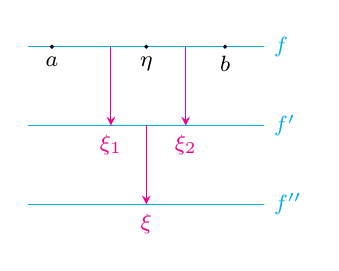
\begin{tikzpicture}[->,samples=100,>=stealth,font=\footnotesize]
            \draw [-,cyan] (0,0)--(3,0)node[right]{$f$};
            \draw [-,cyan] (0,-1)--(3,-1)node[right]{$f'$};
            \draw [-,cyan] (0,-2)--(3,-2)node[right]{$f''$};
            \draw [fill=black] (0.3,0) circle(0.5pt)node[below]{$a$};
            \draw [fill=black] (2.5,0) circle(0.5pt)node[below]{$b$};
            \draw [fill=black] (1.5,0) circle(0.5pt)node[below]{$\eta$};
            \draw [magenta] (1.05,0)--(1.05,-1)node[below]{$\xi_1$};
            \draw [magenta] (2,0)--(2,-1)node[below]{$\xi_2$};
            \draw [magenta] (1.5,-1)--(1.5,-2)node[below]{$\xi$};
        \end{tikzpicture}
        \caption{}
        \label{Lagrangexi1xi2eta}
    \end{figure}
\end{minipage}\hfill
\begin{minipage}[b]{0.3\linewidth}
    \begin{figure}[H]
        \centering
        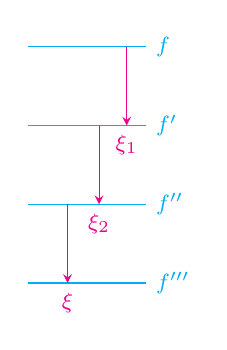
\begin{tikzpicture}[->,samples=100,>=stealth,font=\footnotesize]
            \draw [-,cyan] (0,0)--(1.5,0)node[right]{$f$};
            \draw [-,cyan] (0,-1)--(1.5,-1)node[right]{$f'$};
            \draw [-,cyan] (0,-2)--(1.5,-2)node[right]{$f''$};
            \draw [-,cyan] (0,-3)--(1.5,-3)node[right]{$f'''$};
            \draw [magenta] (1.25,0)--(1.25,-1)node[below]{$\xi_1$};
            \draw [magenta] (0.9,-1)--(0.9,-2)node[below]{$\xi_2$};
            \draw [magenta] (0.5,-2)--(0.5,-3)node[below]{$\xi$};
        \end{tikzpicture}
        \caption{}
        \label{xi1xi2xix3f}
    \end{figure}
\end{minipage}\hfill
\begin{minipage}[b]{0.3\linewidth}
    \begin{figure}[H]
        \centering
        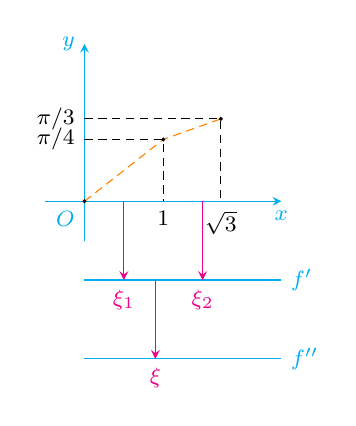
\begin{tikzpicture}[->,samples=100,>=stealth,font=\footnotesize]
            \draw[->,cyan](-0.5,0)--(0,0)node[below left]{$O$}--(2.5,0)node[below]{$x$};
            \draw[->,cyan](0,-0.5)--(0,2)node[left]{$y$};
            \draw[-,densely dashed] (0,{pi/4})node[left]{$\pi/4$}--(1,{pi/4})--(1,0)node[below]{$1$};
            \draw[-,densely dashed] (0,{pi/3})node[left]{$\pi/3$}--({sqrt(3)},{pi/3})--({sqrt(3)},0)node[below]{$\sqrt{3}$};
            \draw [-,cyan] (0,-1)--(2.5,-1)node[right]{$f'$};
            \draw [-,cyan] (0,-2)--(2.5,-2)node[right]{$f''$};
            \draw [magenta] (0.5,0)--(0.5,-1)node[below]{$\xi_1$};
            \draw [magenta] (1.5,0)--(1.5,-1)node[below]{$\xi_2$};
            \draw [magenta] (0.9,-1)--(0.9,-2)node[below]{$\xi$};
            \draw [densely dashed,orange,-] (0,0)--(1,{pi/4})--({sqrt(3)},{pi/3});
            \draw [fill=black] (0,0) circle(0.5pt);
            \draw [fill=black] (1,{pi/4}) circle(0.5pt);
            \draw [fill=black] ({sqrt(3)},{pi/3}) circle(0.5pt);
        \end{tikzpicture}
        \caption{}
        \label{pi3pi4xi1xi2}
    \end{figure}
\end{minipage}

\begin{example}
    设函数 $\displaystyle f(x)\in C[a,b]\cap D^5(a,b)$, 证明: $\exists\xi\in(a,b)$, 使得
    $$f(b)=f(a)+\dfrac{1}{6}(b-a)\qty[f'(a)+f'(b)+4f'\qty(\dfrac{a+b}{2})]-\dfrac{(b-a)^5}{2880}f^{(5)}(\xi).$$
\end{example}
\begin{proof}[{\songti \textbf{证}}]
    令 $h=\dfrac{b-a}{2},~c=\dfrac{a+b}{2}$, 则待证式等价为
    $$f(c+h)=f(c-h)+\dfrac{h}{3}\qty[f'(c-h)+f'(c+h)+4f'(c)]-\dfrac{h^5}{90}f^{(5)}(\xi)$$
    令 $h=x$, 构造辅助函数 $$\varphi(x)=f(c+x)-f(c-x)-\dfrac{x}{3}\qty[f'(c-x)+f'(c+x)+4f'(c)]+\dfrac{x^5}{90}k$$
    即证 $k=f^{(5)}(\xi)$, 因为 $f\in C[a,b]\cap D^5(a,b)$, 所以 $\varphi(x)\in C[a,b]\cap D^4(a,b)$, 因此
    \begin{flalign*}
        \varphi'(x)   & =\dfrac{2}{3}\qty[f'(c+x)+f'(c-x)]-\dfrac{4}{3}f'(c)+\dfrac{x}{3}\qty[f''(c-x)-f''(c+x)]+\dfrac{x^4}{18}k \\
        \varphi''(x)  & =\dfrac{1}{3}\qty[f''(c+x)-f''(c-x)]-\dfrac{x}{3}\qty[f'''(c-x)+f'''(c+x)]+\dfrac{2x^3}{9}k               \\
        \varphi'''(x) & =\dfrac{x}{3}\qty[f^{(4)}(c-x)-f^{(4)}(c+x)]+\dfrac{2x^2}{3}k
    \end{flalign*}
    因为 $\varphi(0)=\varphi(h)=0$, 由 Rolle 定理知, $\exists\xi_1\in(0,h)$, 使得 $\varphi'(\xi_1)=0$, 而 $\varphi'(0)=0$, 所以, 又由 Rolle 定理知, $\exists\xi_2\in(0,\xi_1)$, 使得 $\varphi''(\xi_2)=0$, 最后又因为 $\varphi''(0)=0$, 所以 $\exists\xi_3$, 使得
    $$\varphi'''(\xi_3)=\dfrac{\xi_3}{3}\qty[f^{(4)}(c-\xi_3)-f^{(4)}(c+\xi_3)]+\dfrac{2\xi_3^2}{3}k$$
    又根据 Lagrange 中值定理, $\exists\xi_(c-\xi_3,c+\xi_3)\subset(a,b)$, 使得 $$f^{(4)}(c-\xi_3)-f^{(4)}(c+\xi_3)=f^{(5)}(\xi)(-2\xi_3)$$
    即 $0=\dfrac{-2\xi_3^2}{3}f^{(5)}(\xi)+\dfrac{2\xi_3^2}{3}k\Rightarrow f^{(5)}(\xi)=k$.
\end{proof}

\subsubsection{特殊函数作差法}

\begin{example}
    设 $f(x)\in C\qty[0,\sqrt{3}]\cap D^2\qty(0,\sqrt{3})$, 且 $f(0)=0,~f(1)=\dfrac{\pi}{4},~f\qty(\sqrt{3})=\dfrac{\pi}{3}$, 证明: $\exists\xi\in(0,\sqrt{3})$, 使得 $$f''(\xi)=-\dfrac{2\xi}{1+\xi^2}f'(\xi).$$
\end{example}
\begin{proof}[{\songti \textbf{证: }}]
    如图 \ref{pi3pi4xi1xi2} 所示, 欲证在 $f''$ 层次有一中值, 则需寻找在 $f'$ 层次的两个过渡中值, 那么就需要在 $f$ 层次, 即通过作差的方法将第一象限的两个坐标点, 向下移动到 $x$ 轴, 使得在 $x$ 轴上存在 3 个零点, 
    满足这一性质的可以思考到将 $f(x)$ 与 $\arctan x$ 作差得到, 即令 $g(x)=f(x)-\arctan x$, 则 $g(0)=g(1)=g(\sqrt{3})=0$, 由 Rolle 中值定理知 $\exists\xi_1\in(0,1),\exists_2\in(1,\sqrt{3})$, 使 $g'(\xi_1)=g'(\xi_2)=0$, 即
    $$\qty(1+\xi_1^2)f'(\xi_1)=\qty(1+\xi_2^2)f'(\xi_2)=1$$
    再令 $h(x)=\qty(1+x^2)f'(x)$, 那么 $h(\xi_1)=h(\xi_2)$, 又由 Rolle 中值定理知 $\exists\xi\in(\xi_1,\xi_2)\subset(0,\sqrt{3})$, 使 $h'(\xi)=0$, 整理即得待证式.
\end{proof}
% \begin{proof}[{\songti \textbf{证法二: }}]
%     由 $f(0)=0,~f(1)=\dfrac{\pi}{4},~f\qty(\sqrt{3})=\dfrac{\pi}{3}$ 构建插值多项式
%     \begin{table}[H]
%         \centering
%         \caption{}
%         \resizebox{.99\textwidth}{!}{
%             \begin{tabular}{c c c c}
%                 \toprule
%                 $x_{k}$                     & $f(x_k)$                     & 一阶差商                                                                  & 二阶差商                                                                                                   \\
%                 \midrule
%                 $x_{0}=\textcolor{cyan}{0}$ & $f_0=\textcolor{magenta}{0}$ &                                                                           &                                                                                                            \\
%                 $x_{1}=\textcolor{cyan}{1}$ & $f_1=\dfrac{\pi}{4}$         & $f[x_0,x_1]=\dfrac{f_1-f_0}{x_1-x_0}=\textcolor{magenta}{\dfrac{\pi}{4}}$ &                                                                                                            \\[6pt]
%                 $x_{2}=\sqrt{3}$            & $f_2=\dfrac{\pi}{3}$         & $f[x_1,x_2]=\dfrac{f_2-f_1}{x_2-x_1}=\dfrac{\pi}{12\qty(\sqrt{3}-1)}$     & $f[x_0,x_1,x_2]=\dfrac{f[x_1,x_2]-f[x_0,x_1]}{x_2-x_0}=\textcolor{magenta}{\dfrac{3\pi-5\sqrt{3}\pi}{72}}$ \\
%                 \bottomrule
%             \end{tabular}}
%     \end{table}
%     则插值多项式为 
%     $$p(x)=\textcolor{magenta}{0}+\textcolor{magenta}{\dfrac{\pi}{4}}(x-\textcolor{cyan}{0})+\textcolor{magenta}{\dfrac{3\pi-5\sqrt{3}}{72}}(x-\textcolor{cyan}{0})(x-\textcolor{cyan}{1})=\dfrac{\pi}{4}x+\dfrac{3\pi-5\sqrt{3}\pi}{72}x(x-1)$$
%     因此令 $F(x)=f(x)-p(x)$, 则 $F(0)=F(1)=F\qty(\sqrt{3})=0$
% \end{proof}

\subsubsection{合理分配法}

\begin{example}
    设 $f(x)\in C\qty[-\dfrac{\pi}{2},\dfrac{\pi}{2}]\cap D\qty(-\dfrac{\pi}{2},\dfrac{\pi}{2}),~f(0)=0$, 
    证明: $\exists\xi\in\qty(-\dfrac{\pi}{2},\dfrac{\pi}{2})$, 使得 $$f''(\xi)=3f'(\xi)\tan\xi+2f(\xi).$$
\end{example}
\begin{proof}[{\songti \textbf{证}}]
    构造辅助函数\footnote{
        首先观察待证式的各项系数, 发现存在 $1+2=3$ 的情况, 于是利用“合理分配达到平均”思想, 组成 $$f''(\xi)-f'(\xi)\tan\xi=2\qty[f'(\xi)\tan\xi+f(\xi)]$$
        又 $\cos\xi\neq0$, 于是两边同时乘以 $\cos\xi$, 得 $\qty[f''(\xi)\cos\xi-f'(\xi)\sin\xi]-2\qty[f'(\xi)\sin\xi+f(\xi)\cos\xi]=0$;
        发现 $[]$ 内是“前导后不导”形式, 则可化为 $g'(\xi)=\qty(f'(\xi)\cos\xi)'-2\qty(f(\xi)\sin\xi)'=0$, $g(x)=f'(x)\cos x-2f(x)\sin x$;
        此为“经典构造模型”之一 (参考表 \ref{fuzuhansgzao}), 则构造辅助函数 $$F(x)=f(x)\e^{\int-2\tan x\dd x}=f(x)\cdot\cos^2x.$$
    } $F(x)=f(x)\cdot\cos^2x$, 那么有 $F\qty(-\dfrac{\pi}{2})=F\qty(\dfrac{\pi}{2})=F(0)=0$, 则由 Rolle 定理知, 
    $\exists\xi_1,\xi_2$ 分别属于 $\qty(-\dfrac{\pi}{2},0)$ 与 $\qty(0,\dfrac{\pi}{2})$, 使得 $F'(\xi_1)=F'(\xi_2)=0$, 又
    $$F'(x)=f'(x)\cos^2x-2\sin x\cos xf(x)=\cos x\qty[f'(x)\cos x-2\sin xf(x)]$$
    令 $g(x)=f'(x)\cos x-2\sin xf(x)$, 则有 $g(\xi_1)=g(\xi_2)=0$, 再由 Rolle 定理知, 
    $\exists\xi\in(\xi_1,\xi_2)\subset\qty(-\dfrac{\pi}{2},\dfrac{\pi}{2})$, 使得
    $$g'(\xi)=0=f''(\xi)\cos \xi-3f(\xi)\sin\xi-2f(\xi)\cos\xi$$
    由于 $\cos\xi\neq0$, 所以两边同时除以 $\cos\xi$, 即得证.
\end{proof}

\subsubsection{补充导函数法}

一般待证式中, 出现的导函数阶数是连续的, 即 0 与 1 或 1 与 2, 亦或常数与导函数直接相等的类型, 当缺失一阶导函数的时候, 需要人为补充一阶导, 之后再构造辅助函数.

\begin{example}
    设函数 $f(x)\in C[a,b]\cap D^2(a,b)$, 且 $f(a)=f'(a)=f''(a)=f(b)=0$, 证明: $\exists \xi\in(a,b)$, 使得 $$(\xi-a)^2f''(\xi)-2f(\xi)=0.$$
\end{example}
\begin{proof}[{\songti \textbf{证}}]
    先令\footnote{因为缺少一阶导项, 故考虑人为补充, 又由待证式的结构不难想到 $\qty(gf'-fg')'$ 其中 $g=(x-a)^2$.} $F(x)=(x-a)^2f'(x)-2f(x)(x-a)$, 则 $F(a)=0$, 欲再寻找一点 $\eta$, 使得 $F(\eta)=0$, 为此构造辅助函数
    $$G(x)=\begin{cases}
            \dfrac{f(x)}{(x-a)^2}, & x\in(a,b] \\
            0,                     & x=a
        \end{cases}$$
    则有 $$\displaystyle\lim_{x\to a^+}G(x)=\lim_{x\to a^+}\dfrac{f(x)}{(x-a)^2} =\lim_{x\to a^+}\dfrac{f(a)+f'(a)(x-a)+\dfrac{1}{2!}f''(a)(x-a)^2+o\qty((x-a)^2)}{(x-a)^2}=0=G(0)$$ 
    因此 $G(x)$ 在 $[a,b]$ 上连续, 在 $(a,b)$ 内可导, 且 $G(a)=G(b)$ 则由 Rolle 定理知
    $\exists\eta\in(a,b)$, 使得 $$G'(\eta)=\dfrac{f'(\eta)(\eta-a)^2-2(\eta-a)f(\eta)}{(\eta-a)^4}=0\Rightarrow f'(\eta)(\eta-a)^2-2(\eta-a)f(\eta)=0\Rightarrow F(\eta)=0$$
    又因为 $F(x)$ 在 $[a,b]$ 上连续, $(a,b)$ 内可导, 故由 Rolle 定理知 $\exists\xi\in(a,b)$, 使得 $$F'(\xi)=2(\xi-a)f'(\xi)+(\xi-a)^2f''(\xi)-2f'(\xi)(\xi-a)-2f(\xi)=0$$
    整理即得证 $(\xi-a)^2f''(\xi)-2f(\xi)=0.$
\end{proof}

\section{Taylor 展开与差商}

\begin{theorem}[带 Lagrange 余项的 Taylor 展开]
    利用 Taylor 公式可得:
    $$f\left( x+j\right) =f(x) +\dfrac{f(x) }{1!}j+\dfrac{f''(x) }{2!}j^{2}+\cdots +\dfrac{f^{\left( n-1\right) }(x) }{\left( n-1\right) !}j^{n-1}+\dfrac{f^{(n) }(\xi ) }{n!}j^{n}$$
    其中 $j=1,2,\cdots,n-1,~x<\xi_j<x+j.$
    \index{带 Lagrange 余项的 Taylor 展开}
\end{theorem}

\subsection{证明中值定理}

\begin{example}
    设函数 $f(x)$ 在区间 $[a,b]$ 上具有连续的二阶导数, 证明: $\exists\xi\in(a,b)$, 使得
    $$\dfrac{4}{(b-a)^2}\qty[f(a)-2f\qty(\dfrac{a+b}{2})+f(b)]=f''(\xi).$$
\end{example}
\begin{proof}[{\songti \textbf{证法一}}]
    函数 $f(x)$ 在 $x=\dfrac{a+b}{2}$ 处的一阶带 Lagrange 余项的 Taylor 公式为
    $$f(x)=f\qty(\dfrac{a+b}{2})+f'\qty(\dfrac{a+b}{2})\qty(x-\dfrac{a+b}{2})+\dfrac{f''(\xi_1)}{2}\qty(x-\dfrac{a+b}{2})^2$$
    其中 $\xi_1$ 位于 $x,~\dfrac{a+b}{2}$ 之间, 令 $x=a,b$ 代入上式, 得
    \begin{flalign*}
        f(a)=f\qty(\dfrac{a+b}{2})+f'\qty(\dfrac{a+b}{2})\qty(a-\dfrac{a+b}{2})+\dfrac{f''(x_1)}{2}\qty(a-\dfrac{a+b}{2})^2 \\
        f(b)=f\qty(\dfrac{a+b}{2})+f'\qty(\dfrac{a+b}{2})\qty(b-\dfrac{a+b}{2})+\dfrac{f''(x_2)}{2}\qty(b-\dfrac{a+b}{2})^2
    \end{flalign*}
    其中 $a<x_1<\dfrac{a+b}{2}$, $\dfrac{a+b}{2}<x_2<b$, $x_1<x_2$, 两式相加, 得
    $$f(a)+f(b)=2f\qty(\dfrac{a+b}{2})+\dfrac{f''(x_1)+f''(x_2)}{2}\qty(\dfrac{b-a}{2})^2$$
    改写得 $$\dfrac{4}{(b-a)^2}\qty[f(a)+f(b)-2f\qty(\dfrac{a+b}{2})]=\dfrac{f''(x_1)+f''(x_2)}{2}$$
    由于函数 $f(x)$ 在闭区间 $[a,b]$ 上具有连续的二阶导数, 所以由最值定理, 可知
    $$\min_{x\in[x_1,x_2]}f''(x)\leqslant \dfrac{f''(x_1)+f''(x_2)}{2}\leqslant \max_{x\in[x_1,x_2]}f''(x)$$
    于是由介值定理可知存在 $\xi\in(a,b)$, 使得 $\displaystyle \dfrac{f''(x_1)+f''(x_2)}{2}=f''(\xi)$, 
    代入即得 $$\dfrac{4}{(b-a)^2}\qty[f(a)-2f\qty(\dfrac{a+b}{2})+f(b)]=f''(\xi).$$
\end{proof}
\begin{proof}[{\songti \textbf{证法二}}]
    设 $f(x)-2f\qty(\dfrac{x+a}{2})+f(a)=\dfrac{1}{4}K(x-a)^2$, 其中 $K$ 为待定实常数, 记
    $$F(x)=f(x)-2f\qty(\dfrac{x+a}{2})+f(a)-\dfrac{1}{4}K(x-a)^2$$
    则 $F(a)=F(b)=0$, 由 Rolle 中值定理, $\exists c\in(a,b)$, 使得 $F'(c)=0$, 即
    $$f'(c)-f'\qty(\dfrac{c+a}{2})-\dfrac{1}{2}K(c-a)=0$$
    再由 Lagrange 中值定理, $\exists \xi\in\qty(\dfrac{a+c}{2},c)$, 使得
    $$f'(c)-f'\qty(\dfrac{c+a}{2})=f''(\xi)\qty(c-\dfrac{c+a}{2})$$
    比较得 $f''(c)\qty(c-\dfrac{c+a}{2})-\dfrac{1}{2}K(c-a)=0$, 由此得 $f''(\xi)=K.$
\end{proof}

\begin{example}
    设函数 $f(x)$ 在 $[a,b]$ 上连续, 在 $(a,b)$ 内二阶可导, 证明存在 $\xi\in(a,b)$, 使得 $$f(b)-2f\left(\dfrac{a+b}{2}\right)+f(a)=\dfrac{(b-a)^2}{4}f''(\xi).$$
\end{example}
\begin{proof}[{\songti \textbf{证法一}}]
    注意到
    $$f(b)-2f\left(\dfrac{a+b}{2}\right)+f(a)=\left[f\left(\dfrac{a+b}{2}+\dfrac{b-a}{2}\right)-f\left(\dfrac{a+b}{2}\right)\right]-\left[f\left(a+\dfrac{b-a}{2}\right)-f(a)\right]$$
    令 $F(x)=f\left(x+\dfrac{b-a}{2}\right)-f(x),~x\in\left[a,\dfrac{a+b}{2}\right]$, 则 $F(x)$ 在 $\left[a,\dfrac{a+b}{2}\right]$ 上连续, 
    在 $\left(a,\dfrac{a+b}{2}\right)$ 内二阶可导, 故由 Lagrange 中值定理, 
    $$\exists\xi_{1}\in\left(a,\dfrac{a+b}{2}\right)\text{, 使 }F\left(\dfrac{a+b}{2}\right)-F(a)=F'(\xi_{1})\cdot\dfrac{b-a}{2}$$
    又由 $f'(x)$ 在 $\left[\xi_{1},\xi_{1}+\dfrac{b-a}{2}\right]$ 上用 Lagrange 中值定理, 
    $$\exists\xi\in\left(\xi_{1},\xi_{1}+\dfrac{b-a}{2}\right)\subset(a,b)\text{, 使 }f'\left(\xi_{1}+\dfrac{b-a}{2}\right)-f'(\xi_{1})=f''(\xi)\cdot\dfrac{b-a}{2}$$
    代入上式, 即得 $f(b)-2f\left(\dfrac{a+b}{2}\right)+f(a)=\dfrac{(b-a)^2}{4}f''(\xi).$
\end{proof}
\begin{proof}[{\songti \textbf{证法二}}]
    将 $f(a),f(b)$ 分别在 $x=\dfrac{a+b}{2}$ 处进行 Taylor 展开, 得
    \begin{flalign*}
        f(a) & =f\left(\dfrac{a+b}{2}\right)+\dfrac{a-b}{2}f'\left(\dfrac{a+b}{2}\right)+\left(\dfrac{a-b}{2}\right)^2\dfrac{f''(\xi_{1})}{2!} \\
        f(b) & =f\left(\dfrac{a+b}{2}\right)+\dfrac{b-a}{2}f'\left(\dfrac{a+b}{2}\right)+\left(\dfrac{b-a}{2}\right)^2\dfrac{f''(\xi_{2})}{2!}
    \end{flalign*}
    其中 $a<\xi_{1}<\dfrac{a+b}{2}<\xi_{2}<b$, 两式相加, 得
    $$f(b)-2f\left(\dfrac{a+b}{2}\right)+f(a)=\dfrac{(b-a)^{2}}{4}\cdot\left[\dfrac{f''(\xi_{1})+f''(\xi_{2})}{2}\right]$$
    而 $\min(f''(\xi),f''(\xi_{2}))\leqslant\dfrac{f''(\xi_1)+f''(\xi_{2})}{2}\leqslant\max(f''(\xi_{1}),f''(\xi_{2}))$, 由 Darboux 定理知, 
    存在 $\xi\in(\xi_1,\xi_{2})\subset(a,b)$, 使得 $f''(\xi)=\dfrac{f''(\xi_{1})+f''(\xi_{2})}{2}$, 从而得
    $f(b)-2f\left(\dfrac{a+b}{2}\right)+f(a)=\dfrac{(b-a)^2}{4}f''(\xi).$
\end{proof}
\begin{proof}[{\songti \textbf{证法三}}]
    要证 $f(b)-2f\left(\dfrac{a+b}{2}\right)+f(a)=\dfrac{(b-a)^{2}}{4}f''(\xi)$, 即证
    $$\dfrac{f(b)-2f\left(\dfrac{a+b}{2}\right)+f(a)}{(b-a)^{2}}=\dfrac{1}{4}f''(\xi)$$
    为此, 构造辅助函数 $F(x)=f(x)-2f\left(\dfrac{a+x}{2}\right)+f(a),~G(x)=(x-a)^{2}$, 则 $F(x),G(x)$ 满足 Cauchy 中值定理的条件, 故由 Cauchy 中值定理得
    $$\dfrac{F(b)}{G(b)}=\dfrac{F(b)-F(a)}{G(b)-G(a)}=\dfrac{F'(\xi_{1})}{G'(\xi_{1})}=\dfrac{f'(\xi_{1})-f'\left(\dfrac{a+\xi_{1}}{2}\right)}{{2(\xi_{1}-a)}}=\dfrac{f''(\xi)\cdot\dfrac{\xi_{1}-a}{2}}{{2(\xi_{1}-a)}}=\dfrac{1}{4}f''(\xi)$$
    其中 $\xi_{1}\in(a,b),\xi\in\left(\dfrac{a+\xi_{1}}{2},\xi_{1}\right)\subset(a,b).$
\end{proof}
\begin{proof}[{\songti \textbf{证法四}}]
    设 $k$ 为使 $f(b)-2f\left(\dfrac{a+b}{2}\right)+f(a)=\dfrac{(b-a)^{2}}{4}k$ 成立的实常数, 
    构造辅助函数 $$g(x)=f(x)-2f\left(\dfrac{a+x}{2}\right)+f(a)-\dfrac{(x-a)^{2}}{4}k$$
    则 $g(a)=g(b)=0$, 于是由 Rolle 定理得, 存在 $\xi_{1}\in(a,b)$, 使 $g'(\xi_{1})=0$, 即 $$f'(\xi_{1})-f'\left(\dfrac{a+\xi_{1}}{2}\right)-\dfrac{k}{2}(\xi_{1}-a)=0$$
    又 $f'\left(\dfrac{a+\xi_{1}}{2}\right)=f'(\xi_{1})+f''(\xi)\cdot\dfrac{a-\xi_{1}}{2}$, 其中 $\xi\in\left(\dfrac{a+\xi_{1}}{2},\xi_{1}\right)\subset(a,b)$, 
    代入前一式, 即得 $k=f''(\xi)$.
\end{proof}

\subsection{中值点的极限}

\begin{example}
    设 $f''(x)$ 在某区间 $I$ 上连续, 且 $f''(x_0)\neq0~ (x_0\in I)$, 对于 $x_0+h\in I$, 由微分中值定理
    $$f(x_0+h)  =f(x_0)  +hf'(x_{0}+\theta h)  ~ ( 0 <\theta  < 1) $$
    证明: $\displaystyle\lim_{h\to0}\theta=\dfrac{1}{2}.$
\end{example}
\begin{proof}[{\songti \textbf{证}}]
    对 $f^{\prime}(x)$  应用 Lagrange 日中值定理, 有
    $$f^{\prime}\left(x_{0}+\theta h\right)-f^{\prime}(x_0) =\theta h f^{\prime \prime}(x_0+\xi \theta)  ~ (0<\xi<1)$$
    于是
    \begin{equation}
        f\left(x_{0}+h\right)=f(x_0) +h f^{\prime}\left(x_{0}+\theta h\right)=f(x_0) +h\left[f^{\prime}(x_0) +\theta h f^{\prime \prime}(x_0+\xi \theta) \right]\tag{1}
    \end{equation}
    再根据 Taylor 公式有
    \begin{equation}
        f\left(x_{0}+h\right)=f(x_0) +h f^{\prime}(x_0) +\dfrac{1}{2} h^{2} f^{\prime \prime}\left(x_{0}+\eta h\right) ~ (0<\eta<1)\tag{2}
    \end{equation}
    比较式 (1)、(2) 得
    $$\theta f^{\prime \prime}(x_0+\xi \theta) =\dfrac{1}{2} f^{\prime \prime}\left(x_{0}+\eta h\right)$$
    因 $f^{\prime \prime}(x)$ 在 $x_{0}$ 点连续, 所以
    $$\lim _{h \rightarrow 0} \theta f^{\prime \prime}(x_0+\xi \theta) =\lim _{h \rightarrow 0} \dfrac{1}{2} f^{\prime \prime}\left(x_{0}+\eta h\right)$$
    因此有 $f''(x_0)\lim\limits_{h\to0}\theta=\dfrac{1}{2}f''(x_0)$, 又因为 $f''(x_0)\neq0$, 所以 $\lim\limits_{h\to0}\theta=\dfrac{1}{2}.$
\end{proof}

\begin{example}
    设 $f(x+h)=f(x)+hf'(x)+\cdots+\dfrac{h^n}{n!}f^{(n)}(x+\theta h)~ (0<\theta<1)$, 且 $f^{(n+1)}(x)\neq 0$, 
    证明: $$\lim\limits_{h\to0}\theta =\dfrac{1}{n+1}.$$
\end{example}
\begin{proof}[{\songti \textbf{证}}]
    由题设知 $f(x)$ 在 $x=a$ 处具有 $n+1$ 阶导数, 故 $f(x)$ 在 $a$ 点处的 $n$ 阶 Taylor 展开为
    $$f\left( a+h\right) =f(a) +hf'(a) +\dfrac{h^{2}}{2!}f''(a) +\cdots +\dfrac{h^{n}}{n!}f^{(n) }(a) +\dfrac{h^{n+1}}{(n+1)  !}f^{(n+1)  }(a+\theta_1 h)~ (0<\theta_1<1)$$
    与 $f\left( a+h\right) =f(a) +hf'(a) +\dfrac{h^{2}}{2!}f''(a) +\cdots +\dfrac{h^{n}}{n!}f^{(n) }\left( a+\theta h\right) $ 相比较, 得
    $$\dfrac{h^{n}}{n!}f^{(n) }\left( a+\theta h\right) =\dfrac{h^{n}}{n!}f^{(n) }(a) +\dfrac{h^{n+1}}{(n+1)  !}f^{(n+1)  }\left( a+\theta _{1}h\right) $$
    于是 $$f^{(n) }\left( a+\theta h\right) -f^{(n) }(a) =\dfrac{f^{(n+1)  }\left( a+\theta _{1}h\right) }{n+1}h$$
    由 Lagrange 中值定理知, 
    $$f^{(n+1)  }\left( a+\theta _{2}\left( \theta h\right) \right) \cdot \theta h=f^{(n+1)  }\left( a+\theta _{1}h\right) \cdot \dfrac{h}{n+1}~ ( 0 <\theta _{2} < 1) $$
    令 $h\to0$, 则 $\theta h,\theta_1 h,\theta_2(\theta h)\to0$, 并注意到 $f^{(n+1)}(x)$ 连续及 $f^{(n+1)}(a)\neq 0$, 即得 $\lim\limits_{h\to0}\theta =\dfrac{1}{n+1}.$
\end{proof}

\begin{example}
    设函数 $f(x)$ 在 $(x_0-\delta,x_0+\delta)$ 内有 $n$ 阶连续导数, 且
    $$f^{(k)}(x_0)=0,k=2,3,\cdots,n-1\text{, 且 }f^{(n)}(x_0)\neq 0$$
    当 $0<|h|<\delta$ 时, 
    $$f(x_0+h)  -f(x_0)  =hf'(x_{0}+\theta h)  ~ ( 0 <\theta  < 1) $$
    证明: $\displaystyle \lim _{n\rightarrow 0}\theta =\dfrac{1}{\sqrt[n-1] {n}}.$
\end{example}
\begin{proof}[{\songti \textbf{证}}]
    由 Taylor 公式可得
    $$f(x_0+h)  =f(x_0)  +f'(x_0)  h+\dfrac{f''(x_0)  }{2!}h^{2}+\ldots +\dfrac{f^{\left( n-1\right) }(x_0)  }{\left( n-1\right) !}h^{n-1}+\dfrac{f^{(n) }(\xi ) }{n!}h^{n},~\xi\in(x_0,x_0+h)$$
    由题设的条件, 可得
    \begin{equation}
        f(x_0+h)  =f(x_0)  +f'(x_0)  h+\dfrac{1}{n!}f^{(n) }(\xi ) h^{n}\tag{1}
    \end{equation}
    又有
    \begin{equation}
        f\left( x_{0}+n\right) -f(x_0)  =hf'(x_{0}+\theta h)  ,~0 <\theta  <1 \tag{2}
    \end{equation}
    由 (1)、(2) 式可得
    \begin{equation}
        hf'(x_{0}+\theta h)  =hf'(x_0)  +\dfrac{1}{n!}f^{(n) }(\xi ) h^{n}\tag{3}
    \end{equation}
    仿式 (1) 可得
    \begin{equation}
        f'(x_{0}+\theta h)  =f'(x_0)  +f^{1}(x_0)  \left( \theta h\right) +\ldots +\dfrac{f^{(n) }\left( \eta \right) }{\left( n-1\right) !}\left( \theta h\right) ^{n-1},\eta \in \left( x_{0},~x_{0}+\theta h\right) \tag{4}
    \end{equation}
    将式 (4) 代入式 (3), 注意到 $f^{(k)}(x_0)=0$, 可得
    $$\dfrac{1}{n}f^{(n)}(\xi)=f^{(n)}(\eta)\theta^{n-1}\Rightarrow \lim_{h\to0}\dfrac{1}{n}f^{(n)}(\xi)=\lim_{h\to0}f^{(n)}(\eta) \theta^{n-1}$$
    可得 $$\dfrac{f^{(n)}(x_0)}{n}=f^{(n)}(x_0)\left[\lim_{h\to0}\theta\right]^{n-1}\Rightarrow \lim_{h\to0}\theta=\dfrac{1}{\sqrt[n-1]{n}}.$$
\end{proof}

\subsection{无穷远处的极限}

\begin{example}
    设 $f(x)$ 在 $(-\infty,+\infty)$ 内具有 $n$ 阶导数且满足 $\lim\limits_{x\to\infty}f(x)=c$ ($c$ 为常数), 
    $\lim\limits_{x\to\infty}f^{(n)}(x)=0$, 证明: $\lim\limits_{x\to\infty}f^{(k)}(x)=0~ (k=1,2,\cdots,n-1).$
\end{example}
\begin{proof}[{\songti \textbf{证}}]
    由 Taylor 公式可得:
    $$f\left( x+j\right) =f(x) +\dfrac{f(x) }{1!}j+\dfrac{f''(x) }{2!}j^{2}+\cdots +\dfrac{f^{\left( n-1\right) }(x) }{\left( n-1\right) !}j^{n-1}+\dfrac{f^{(n) }(\xi ) }{n!}j^{n}$$
    其中 $j=1,2,\cdots,n-1,~x<\xi_j<x+j.$ 从而有
    \begin{equation}
        f\left( x+j\right) -f(x) =f'(x) j+\dfrac{f''(x) }{2!}j^{2}+\cdots +\dfrac{f^{\left( n-1\right) }(x) }{\left( n-1\right) !}j^{n-1}+\dfrac{f^{(n) }\left( \xi _{j}\right) }{n!}j^{n} \tag{*}
    \end{equation}
    由于 $\lim\limits_{x\to\infty}f(x)=c,~\lim\limits_{x\to\infty}f^{(n)}(x)=0,~x<\xi_j<x+j$, 可知
    $$\lim _{x\rightarrow \infty }f\left( x+j\right) =c,~\lim _{x\rightarrow \infty }f^{(n) }\left( \xi _{j}\right) =0$$
    由式 (*) 可得
    $$0=\lim _{x\rightarrow \infty }\left[ f\left( x+j\right) -f(x) \right] =\lim _{x\rightarrow \infty }\left[ f'(x) j+\dfrac{1}{2}f''(x) j^{2}+\cdots +\dfrac{f^{\left( n-1\right) }(x) }{\left( n-1\right) !}j^{n-1}+\dfrac{f^{(n) }\left( \xi _{i}\right) }{n!}j^{n}\right] $$
    令 $j=1$ 得
    \begin{flalign*}
        0 & =\lim _{x\rightarrow \infty }\left[ f'(x) +\dfrac{1}{2!}f''(x) +\cdots +\dfrac{f^{\left( n-1\right) }(x) }{\left( n-1\right) !}+\dfrac{f^{(n) }(\xi_1 ) }{n!}\right]             \\
          & =\lim _{x\rightarrow \infty }f'(x) +\dfrac{1}{2!}\lim _{x\rightarrow \infty }f''(x) +\cdots +\dfrac{1}{\left( n-1\right) !}\lim _{x\rightarrow \infty }f^{\left( n-1\right) }(x)
    \end{flalign*}
    相仿可得
    \begin{flalign*}
        0 & =2\lim _{x\rightarrow \infty }f'(x) +\dfrac{2^{2}}{2!}\lim _{x\rightarrow \infty }f''(x) +\cdots +\dfrac{2^{n-1}}{\left( n-1\right) !}\lim _{x\rightarrow \infty }f^{\left( n-1\right) }(x)             \\
          & =3\lim _{x\rightarrow \infty }f'(x) +\dfrac{3^{2}}{2!}\lim _{x\rightarrow \infty }f''(x) +\cdots +\dfrac{3^{n-1}}{\left( n-1\right) !}\lim _{x\rightarrow \infty }f^{\left( n-1\right) }(x)             \\
          & \cdots\cdots                                                                                                                                                                                            \\
          & =(n-1)\lim _{x\rightarrow \infty }f'(x) +\dfrac{(n-1)^{2}}{2!}\lim _{x\rightarrow \infty }f''(x) +\cdots +\dfrac{(n-1)^{n-1}}{\left( n-1\right) !}\lim _{x\rightarrow \infty }f^{\left( n-1\right) }(x)
    \end{flalign*}
    不妨记 $\lim\limits_{x\to\infty}f^{(k)}(x)=a_k$ 为待定数值, 可得含有 $n-1$ 个未知量, $n-1$ 个方程构成的方程组, 
    $$\begin{cases}
            a_{1}+\dfrac{1}{2!}a_{2}+\cdots +\dfrac{1}{\left( n-1\right) !}a_{n-1}=0          \\[6pt]
            2a_{1}+\dfrac{2^2}{2!}a_{2}+\cdots +\dfrac{2^{n-1}}{\left( n-1\right) !}a_{n-1}=0 \\[6pt]
            \cdots \cdots                                                                     \\
            (n-1)a_{1}+\dfrac{(n-1)^2}{2!}a_{2}+\cdots +\dfrac{(n-1)^{n-1}}{\left( n-1\right) !}a_{n-1}=0
        \end{cases}$$
    系数行列式 $D$ 为, 并将第 $i$ 行提出公因子 $i$, 第 $j$ 列提出公因子 $\dfrac{1}{j!}$, 转化为 Vandermonde 行列式, 
    \begin{flalign*}
        D=\begin{vmatrix}
              1      & \dfrac{1}{2!}       & \cdots & \dfrac{1}{(n-1)!}           \\[6pt]
              2      & \dfrac{2^2}{2!}     & \cdots & \dfrac{2^{n-1}}{(n-1)!}     \\[6pt]
              \vdots & \vdots              &        & \vdots                      \\[6pt]
              n-1    & \dfrac{(n-1)^2}{2!} & \cdots & \dfrac{(n-1)^{n-1}}{(n-1)!}
          \end{vmatrix}
        =\dfrac{1\cdot2\cdots(n-1)}{1\cdot 2!\cdots(n-1)!}
        \begin{vmatrix}
            1      & 1      & \cdots & 1           \\
            1      & 2      & \cdots & 2^{n-2}     \\
            1      & 3      & \cdots & 3^{n-2}     \\
            \vdots & \vdots &        & \vdots      \\
            1      & n-1    & \cdots & (n-1)^{n-2}
        \end{vmatrix}\neq0
    \end{flalign*}
    可知上述齐次线性方程组仅有零解, 即 $\lim\limits_{x\to\infty}f^{(k)}(x)=a_k=0~ (k=1,2,\cdots,n-1).$
\end{proof}

\subsection{关于界的估计}

\begin{example}
    设 $f(x)$ 在 $(-\infty,+\infty)$ 内具有三阶导数, 且 $f(x),f'''(x)$ 有界, 证明: $f'(x)$ 和 $f''(x)$ 有界.
\end{example}
\begin{proof}[{\songti \textbf{证}}]
    由 Taylor 公式可知
    \begin{equation}
        f(x+1 ) =f(x)+f'(x) +\dfrac{1}{2}f''(x) +\dfrac{1}{6}f'''(\xi_1 ) \tag{1}
    \end{equation}
    \begin{equation}
        f(x-1 ) =f(x) -f'(x) +\dfrac{1}{2}f''(x) -\dfrac{1}{6}f'''(\xi_2 ) \tag{2}
    \end{equation}
    其中 $x <\xi _{1} <x+1,~x-1 <\xi _{2} <x$, 式 (1) $+$ 式 (2) 得
    $$f(x+1 ) +f(x-1 ) =2f(x) +f''(x) +\dfrac{1}{6}\left[ f'''(\xi_1 ) -f'''(\xi_2 ) \right] $$
    由 $f(x)$ 与 $f'''(x)$ 有界, 可知 $f''(x)$ 有界, 式 (1) $-$ 式 (2) 得
    $$f(x+1 ) -f(x-1 ) =2f'(x) +\dfrac{1}{6}\left[ f'''(\xi_1 ) +f'''(\xi_2 ) \right] $$
    同理可知 $f'(x)$ 有界.
\end{proof}

\begin{example}
    已知 $f(x)\in C[0,2]\cap D^2(0,2),~\max\limits_{0\leqslant x\leqslant 2}\qty{|f(x)|,|f''(x)|}\leqslant 1$ 证明: $\forall x\in[0,2]$, 有 $|f'(x)|\leqslant 2.$
\end{example}
\begin{proof}[{\songti \textbf{证}}]
    由 $\max\limits_{0\leqslant x\leqslant 2}\qty{|f(x)|,|f''(x)|}\leqslant 1$ 知, $|f(x)|\leqslant 1,~|f''(x)|\leqslant 1$, 对 $f(0)$ 和 $f(2)$ Taylor 展开, 有
    $$\begin{cases}
        f(0)=f(x)+f'(x)(-x)+\dfrac{1}{2!}f''(\xi_1)x^2\\[6pt]
        f(2)=f(x)+f'(x)(2-x)+\dfrac{1}{2!}f''(\xi_2)(2-x)^2
    \end{cases}$$
    作差得 $f(0)-f(2)=-2f'(x)+\dfrac{1}{2}f''(\xi_1)x^2-\dfrac{1}{2}f''(\xi_2)(x-2)^2$, 即 
    \begin{flalign*}
        \qty|2f'(x)|=\qty|f(2)-f(0)+\dfrac{1}{2}f''(\xi_1)x^2-\dfrac{1}{2}f''(\xi_2)(x-2)^2|\leqslant |f(2)|+|f(0)|+\qty|\dfrac{1}{2}f''(\xi_1)x^2|+\qty|\dfrac{1}{2}f''(\xi_2)(x-2)^2|
    \end{flalign*}
    因为 $|f(x)|\leqslant 1,~|f''(x)|\leqslant 1$, 所以 $$|f(2)|+|f(0)|\leqslant 2,~\qty|\dfrac{1}{2}f''(\xi_1)x^2|+\qty|\dfrac{1}{2}f''(\xi_2)(x-2)^2|\leqslant \dfrac{x^2}{2}+\dfrac{(x-2)^2}{2}$$
    因此 $2\qty|f'(x)|\leqslant 2+\dfrac{x^2}{2}+\dfrac{(x-2)^2}{2}\leqslant 4\Rightarrow |f'(x)|\leqslant 2.$
\end{proof}

\begin{example}
    设函数 $f(x)$ 在 $(a,+\infty)$ 内具有二阶导数, 且 $|f(x)|\leqslant M_0,~|f'(x)|\leqslant M_1,~|f''(x)|\leqslant M_2$, 证明: $M_1^2< 4M_0M_2.$
\end{example}
\begin{solution}
    $\forall x\in(a,+\infty)$ 和 $\forall h>0$, 由在 $x$ 处有一阶 Taylor 公式 $$f(x+h)=f(x)+f'(x)\cdot h+\dfrac{f''(\xi)}{2}\cdot h^2,x<\xi<x+h$$
    于是 $f'(x)=\dfrac{1}{h}\qty[f(x+h)-f(x)]-\dfrac{f''(\xi)}{2}h$, 从而有 $$|f'(x)|\leqslant \dfrac{1}{h}|f(x+h)-f(x)|+\dfrac{|f''(\xi)|}{2}h=\dfrac{2M_0}{h}+\dfrac{M_2h}{2}$$
    取 $h=2\sqrt{\dfrac{M_0}{M_2}}$, 则 $|f'(x)|\leqslant 2\sqrt{M_0M_2}\Rightarrow |f'(x)|^2\leqslant 4M_0M_2$, 有 $x$ 的任意性, 得 $M_1^2\leqslant 4M_0M_2.$
\end{solution}

\begin{example}
    设函数 $f(x)$ 在 $[a,b]$ 上二阶可导, $f'(a)=f'(b)=0$, 证明存在 $\xi\in(a,b)$, 使得
    $$|f''(\xi)|\geqslant \dfrac{4}{(b-a)^2}|f(b)-f(a)|.$$
\end{example}
\begin{proof}[{\songti \textbf{证法一}}]
    将 $f\left(\dfrac{a+b}{2}\right)$ 分别在 $x=a$ 和 $x=b$ 处进行 Taylor 展开
    \begin{flalign*}
        f\left( \dfrac{a+b}{2}\right) & =f(a) +f'(a) \dfrac{b-a}{2}+\dfrac{f''(\xi_1 ) }{2!}\left( \dfrac{b-a}{2}\right) ^{2} \\
        f\left( \dfrac{a+b}{2}\right) & =f(b) +f'(b) \dfrac{a-b}{2}+\dfrac{f''(\xi_2 ) }{2!}\left( \dfrac{a-b}{2}\right) ^{2}
    \end{flalign*}
    其中 $a<\xi_1<\dfrac{a+b}{2}<\xi_2<b$, 由已知 $f'(a)=f'(b)=0$ 代入上式, 得
    $$f\left( \dfrac{a+b}{2}\right) -f(a) =\dfrac{f''(\xi_1 ) }{2}\left( \dfrac{b-a}{2}\right) ^{2},~f(b) -f\left( \dfrac{a+b}{2}\right) =-\dfrac{f''(\xi_2 ) }{2}\left( \dfrac{b-a}{2}\right) ^{2}$$
    记 $\xi =\begin{cases}\xi _{1},\left| f''(\xi_2 ) \right| \leqslant \left| f''(\xi_1 ) \right| \\
            \xi _{2},\left| f''(\xi_2 ) \right|  >\left| f''(\xi_2 ) \right|\end{cases}$, 
    则 $\xi\in(a,b)$, $\left| f''(\xi ) \right| =\max \left( \left| f''(\xi_1 ) \right| ,\left| f''(\xi_2 ) \right| \right) $, 故
    \begin{flalign*}
        \left| f(b) -f(a) \right| & \leqslant \left| f(b) -f\left( \dfrac{a+b}{2}\right) \right| +\left| f\left( \dfrac{a+b}{2}\right) -f(a) \right|
        \leqslant\dfrac{\left| f''(\xi_1 ) \right| +\left| f''(\xi_2 ) \right| }{2}\left( \dfrac{b-a}{2}\right) ^{2}\leqslant \dfrac{(b-a)  ^{2}}{4}\left| f''(\xi ) \right|
    \end{flalign*}
    即 $\displaystyle |f''(\xi)|\geqslant \dfrac{4}{(b-a)^2}|f(b)-f(a)|.$
\end{proof}
\begin{proof}[{\songti \textbf{证法二}}]
    由连续函数 $f(x)$ 在 $[a, b]$ 上用介值定理知, 存在 $x_{0} \in[a, b]$, 使 $f(x_0) =\dfrac{1}{2}[f(a)+f(b)]$, 
    不妨设 $\displaystyle a \leqslant x_{0} \leqslant \dfrac{a+b}{2}$, 则将 $f(x_0) $ 在点 $x=a$ 处进行 Taylor 展开, 得存在 $\xi \in\left(a, x_{0}\right) \subset(a, b)$, 使
    $$f(x_0) =f(a)+f^{\prime}(a)\left(x_{0}-a\right)+\dfrac{f^{\prime \prime}(\xi)}{2 !}\left(x_{0}-a\right)^{2}=f(a)+\dfrac{f^{\prime \prime}(\xi)}{2}\left(x_{0}-a\right)^{2}$$
    于是 $\displaystyle\left|f^{\prime \prime}(\xi)\right|=\dfrac{2\left|f(x_0) -f(a)\right|}{\left(x_{0}-a\right)^{2}} \geqslant \dfrac{|f(b)-f(a)|}{\left(\dfrac{b-a}{2}\right)^{2}}=\dfrac{4}{(b-a)^{2}}|f(b)-f(a)| .$
\end{proof}
\begin{proof}[{\songti \textbf{证法三}}]
    令 $g_{1}(x)=(x-a)^{2},~ g_{2}(x)=(x-b)^{2}$, 则将 $f(x)$ 与 $g_{1}(x)$ 和 $f(x)$ 与 $g_{2}(x)$ 分别在 $\left[a, \dfrac{a+b}{2}\right]$
    和 $\left[\dfrac{a+b}{2}, b\right]$ 上用两次 Cauchy 中值定理, 知 $\exists \eta_{1} \in   \left(a, \dfrac{a+b}{2}\right),~ \xi_{1} \in\left(a, \eta_{1}\right)$, 使
    $$\dfrac{f\left(\dfrac{a+b}{2}\right)-f(a)}{\left(\dfrac{b-a}{2}\right)^{2}}=\dfrac{f\left(\dfrac{a+b}{2}\right)-f(a)}{g_{1}\left(\dfrac{a+b}{2}\right)-g_{1}(a)}=\dfrac{f^{\prime}(\eta_1 )}{g_{1}^{\prime}(\eta_1 )}=\dfrac{f^{\prime}(\eta_1 )-f^{\prime}(a)}{g_{1}^{\prime}(\eta_1 )-g_{1}^{\prime}(a)}=\dfrac{f^{\prime \prime}(\xi_1 )}{g_{1}^{\prime \prime}(\xi_1 )}=\dfrac{1}{2} f^{\prime \prime}(\xi_1 )$$
    $\exists \eta_{2} \in\left(\dfrac{a+b}{2}, b\right), \xi_{2} \in\left(\eta_{2}, b\right)$, 使
    $$\dfrac{f\left(\dfrac{a+b}{2}\right)-f(b)}{\left(\dfrac{b-a}{2}\right)^{2}}=\dfrac{f\left(\dfrac{a+b}{2}\right)-f(b)}{g_{2}\left(\dfrac{a+b}{2}\right)-g_{2}(b)}=\dfrac{f^{\prime}(\eta_2 )}{g_{2}^{\prime}(\eta_2 )}=\dfrac{f^{\prime}(\eta_2 )-f^{\prime}(b)}{g_{2}^{\prime}(\eta_2 )-g_{2}^{\prime}(b)}=\dfrac{f^{\prime \prime}(\xi_2 )}{g_{2}^{\prime}(\xi_2 )}=\dfrac{1}{2} f^{\prime \prime}(\xi_2 )$$
    取 $\xi=\begin{cases}\xi_{1}, & \left|f^{\prime \prime}(\xi_1 )\right| \geqslant\left|f^{\prime \prime}(\xi_2 )\right|, \\ \xi_{2}, & \left|f^{\prime \prime}(\xi_1 )\right|<\left|f^{\prime \prime}(\xi_2 )\right|,\end{cases}$ 则
    \begin{flalign*}
        \left|f^{\prime \prime}(\xi)\right| & =\max \left(\left|f^{\prime \prime}(\xi_1 )\right|,\left|f^{\prime \prime}(\xi_2 )\right|\right) \geqslant \dfrac{1}{2}\left(\left|f^{\prime \prime}(\xi_1 )\right|+\left|f^{\prime \prime}(\xi_2 )\right|\right) \geqslant \dfrac{1}{2}\left|f^{\prime \prime}(\xi_1 )-f^{\prime \prime}(\xi_2 )\right| \\
                                            & =\left|\dfrac{f\left(\dfrac{a+b}{2}\right)-f(a)}{\left(\dfrac{b-a}{2}\right)^{2}}-\dfrac{f\left(\dfrac{a+b}{2}\right)-f(b)}{\left(\dfrac{b-a}{2}\right)^{2}}\right|=\dfrac{4}{(b-a)^{2}}|f(b)-f(a)| .
    \end{flalign*}
\end{proof}
\begin{inference}
    一般地, 设函数 $f(x)$ 在 $[a, b]$ 上具有直至 $n$ 阶的导数 $(n \geqslant 2)$, 
    且 $f^{(k)}(a)=f^{(k)}(b)=0 ~ (k=1,2, \cdots, n-1)$, 则至少存在一点 $\xi \in(a, b)$, 使
    $$\left|f^{(n)}(\xi)\right| \geqslant \dfrac{2^{n-1} \cdot n !}{(b-a)^{n}}|f(b)-f(a)|.$$
\end{inference}

\subsection{差商与导数}

\begin{definition}[一阶差商]
    设 $x_0,x_1,\cdots,x_n$ 为 $[a,b]$ 上的节点, 若 $x_i\neq x_j$, 
    则函数 $f(x)$ 关于节点 $x_i,x_j$ 的\textit{一阶差商}定义为
    $$f[x_i,x_j]=\dfrac{f(x_j)-f(x_i)}{x_j-x_i}.$$
\end{definition}

\begin{definition}[重节点差商]
    若 $x_i=x_j$, 则定义\textit{重节点差商}
    $$f[x_i,x]=\lim_{x\to x_i}f[x_i,x]=\lim_{x\to x_i}\dfrac{f(x)-f(x_i)}{x-x_i}=f'(x_i).$$
\end{definition}

\begin{definition}[二阶差商]
    若 $x_i,x_j,x_k$ 互异, 则定义\textit{二阶差商} $$f[x_i,x_j,x_k]=\dfrac{f[x_j,x_k]-f[x_i,x_j]}{x_k-x_i}.$$
    若 $x_i=x_j\neq x_k$ 或 $x_i=x_j=x_k$, 则分别定义
    $$f[x_i,x_i,x_k]=\dfrac{f[x_i,x_k]-f[x_i,x_i]}{x_k-x_i},~f[x_i,x_i,x_i]=\lim_{\substack{x_i\to x_i\\x_k\to x_i}}f[x_i,x_j,x_k]=\dfrac{1}{2}f''(x_i).$$
\end{definition}

\begin{definition}[$n$ 阶差商]
    一般地, 定义 $n$ 阶差商及 $n$ \textit{阶重节点差商}分别为
    \begin{flalign*}
        f[x_{i0},x_{i1},\cdots,x_{in}] & =\dfrac{f[x_{i1},\cdots,x_{in}]-f[x_{i0},x_{i1},\cdots,x_{i(n-1)}]}{x_{in}-x_{i0}}   \\
        f[x_{i0},x_{i0},\cdots,x_{i0}] & =\lim_{x_{ij}\to x_{i0}}f[x_{i0},x_{i1},\cdots,x_{in}]=\dfrac{1}{n!}f^{(n)}(x_{i0}).
    \end{flalign*}
\end{definition}

\begin{theorem}[差商与导数的关系]
    设函数 $f(x)$ 在 $[a,b]$ 上存在 $n$ 阶导数, 且节点 $x_{i0},x_{i1},\cdots,x_{in}\in[a,b]$ (其中可有重节点), 则有
    $$f[x_{i0},x_{i1},\cdots,x_{in}]=\dfrac{f^{(n)}(\xi)}{n!}$$
    其中 $\xi\in\left(\min\limits_{0\leqslant k\leqslant n}\{x_{ik}\},\max\limits_{0\leqslant k\leqslant n}\{x_{ik}\}\right).$
    \index{差商与导数的关系}
\end{theorem}

\begin{example}
    设函数 $f(x)$ 在 $[a,b]$ 上三阶可导, 证明存在 $\xi\in(a,b)$, 使得
    $$f(b)=f(a)+f'\left(\dfrac{a+b}{2}\right)(b-a)+\dfrac{1}{24}f'''(\xi)(b-a)^3.$$
\end{example}
\begin{proof}[{\songti \textbf{证法一}}]
    将 $f(a),f(b)$ 在 $x=\dfrac{a+b}{2}$ 处进行 Taylor 展开, 得
    \begin{flalign*}
        f(a) & =f\left( \dfrac{a+b}{2}\right) +f'\left( \dfrac{a+b}{2}\right) \cdot \dfrac{a-b}{2}+\dfrac{1}{2}f''\left( \dfrac{a+b}{2}\right) \cdot \dfrac{(a-b)  ^{2}}{4}+\dfrac{1}{6}f'''(\xi_1 ) \dfrac{(a-b)  ^{3}}{8} \\
        f(b) & =f\left( \dfrac{a+b}{2}\right) +f'\left( \dfrac{a+b}{2}\right) \cdot \dfrac{b-a}{2}+\dfrac{1}{2}f''\left( \dfrac{a+b}{2}\right) \cdot \dfrac{(b-a)  ^{2}}{4}+\dfrac{1}{6}f'''(\xi_2 ) \dfrac{(b-a)  ^{3}}{8}
    \end{flalign*}
    其中 $a <\xi _{1} <\dfrac{a+b}{2} <\xi _{2} <b$, 两式相减得
    $$f(b) -f(a) -f'\left( \dfrac{a+b}{2}\right) (b-a)  =\dfrac{1}{24}\dfrac{f'''(\xi_1 ) +f'''(\xi_2 ) }{2}(b-a)  ^{3}$$
    而由$$\min \left( f'''(\xi_1 ) ,f'''(\xi_2 ) \right) \leqslant \dfrac{f'''(\xi_1 ) +f'''(\xi_2 ) }{2}\leqslant \max \left( f'''(\xi_1 ) ,f'''(\xi_2 ) \right) $$
    及 Darboux 定理知
    $$\exists\xi\in(\xi_1,\xi_2)\subset (a,b)\text{, 使得 }f'''(\xi)=\dfrac{f'''(\xi_1)+f'''(\xi_2)}{2}$$
    故得证.
\end{proof}
\begin{proof}[{\songti \textbf{证法二}}]
    设 $k$ 为使 $f(b)=f(a)+f^{\prime}\left(\dfrac{a+b}{2}\right)(b-a)+\dfrac{1}{24} k(b-a)^{3}$ 成立的实常数, 为此只需证 $k=f^{\prime \prime}(\xi)$ 即可, 
    令 $g(x)=f(x)-f(a)-f^{\prime}\left(\dfrac{a+x}{2}\right)(x-a)-\dfrac{k}{24}(x-a)^{3}$ 则 $g(a)=g(b)=0$, 
    于是由 Rolle 定理知, $\exists \eta \in(a, b)$, 使 $g^{\prime}(\eta)=0$ 即
    $$f^{\prime}(\eta)-\dfrac{1}{2} f^{\prime \prime}\left(\dfrac{a+\eta}{2}\right)(\eta-a)-f^{\prime}\left(\dfrac{a+\eta}{2}\right)-\dfrac{k}{8}(\eta-a)^{2}=0$$
    又将 $f^{\prime}(\eta) $ 在 $ x=\dfrac{a+\eta}{2} $ 处进行 Taylor 展开, 得
    $$f^{\prime}(\eta)=f^{\prime}\left(\dfrac{a+\eta}{2}\right)+f^{\prime \prime}\left(\dfrac{a+\eta}{2}\right) \cdot \dfrac{\eta-a}{2}+\dfrac{f^{\prime \prime}(\xi)}{2 !} \cdot\left(\dfrac{\eta-a}{2}\right)^{2}$$
    代人上式, 得 $\dfrac{f'''(\xi)}{2 !} \cdot\left(\dfrac{\eta-a}{2}\right)^{2}-\dfrac{k}{8}(\eta-a)^{2}=0$, 
    从而得  $k=f'''(\xi)$, 其中 $ \xi \in   \left(\dfrac{a+\eta}{2}, \eta\right) \subset(a, b)$, 故得证.
\end{proof}
\begin{proof}[{\songti \textbf{证法三}}]
    由于要证等式中含有 $ f^{\prime}\left(\dfrac{a+b}{2}\right)$, 因而选取重节点: $ x_{0}=a, x_{1}=   c=\dfrac{a+b}{2}, x_{2}=c, x_{3}=b $, 列差商表如下:
    \begin{table}[H]
        \centering
        \caption{}
        \setlength{\tabcolsep}{8mm}{
            \begin{tabular}{c c c c c}
                \toprule
                $x_{k}$   & $f(x_k)$ & 一阶差商        & 二阶差商      & 三阶差商        \\
                \midrule
                $x_{0}=a$ & $f(a)$   &                 &               &                 \\
                $x_{1}=c$ & $f(c)$   & $f[a, c]$       &               &                 \\
                $x_{2}=c$ & $f(c)$   & $f^{\prime}(c)$ & $f[a, c, c]$  &                 \\
                $x_{3}=b$ & $f(b)$   & $f[c, b]$       & $f[c, c, b] $ & $f[a, c, c, b]$ \\
                \bottomrule
            \end{tabular}}
    \end{table}
    而由差商与导数的关系, 得 $ f[a, c, c, b]=\dfrac{f^{\prime \prime}(\xi)}{3 !}$, 其中 $ \xi \in(a, b) $, 由重节点差商定义, 有
    \begin{flalign*}
        f[a, c, c, b]=\dfrac{f[c, c, b]-f[a, c, c]}{b-a}, ~  f[c, c, b]=\dfrac{f[c, b]-f^{\prime}(c)}{b-c}
    \end{flalign*}
    \begin{flalign*}
        f[a, c, c]=\dfrac{f^{\prime}(c)-f[a, c]}{c-a}, ~  f[c, b]=\dfrac{f(b)-f(c)}{b-c}, ~  f[a, c]=\dfrac{f(c)-f(a)}{c-a}
    \end{flalign*}
    代人整理, 即得 $f(b)=f(a)+f^{\prime}\left(\dfrac{a+b}{2}\right)(b-a)+\dfrac{1}{24} f^{\prime \prime}(\xi)(b-a)^{3}.$
\end{proof}

\begin{example}
    设函数 $f(x)$ 在 $[a,b]$ 上三阶可导, 证明存在 $\xi\in(a,b)$, 使得 $$f(b)=f(a)+\dfrac{1}{2}(f'(a)+f'(b))(b-a)-\dfrac{1}{12}f'''(\xi)(b-a)^3.$$
\end{example}
\begin{proof}[{\songti \textbf{证法一}}]
    将要证的等式化为 $ \dfrac {f(b)-f(a)-\dfrac {1}{2}(f'(a)+f'(b))(b-a)}{-\dfrac {1}{12}(b-a)^ {3}} =f''' ( \xi)$
    为此, 令
    $$F(x)=f(x)-f(a)-\dfrac {1}{2} (f'(a)+f'(x))(x-a),~G(x)=- \dfrac {1}{12} (x-a)^ {3} $$
    则 $F(x)$ 在 $[a,b]$ 上二阶可导, $G(x)$ 在 $[a,b]$ 上任意阶可导, 于是两次用 Cauchy 中值定理, 得
    $$\dfrac {F(b)}{G(b)}=\dfrac {F(b)-F(a)}{G(b)-G(a)}=\dfrac {F'(\xi _ {1})}{G'(\xi _ {1})}=\dfrac {F'(\xi _ {1})-F'(a)}{G'(\xi _ {1})-G'(a)}=\dfrac {F'(\xi )}{G'(\xi )}=f'''(\xi) $$
    其中 $F(a)=0=F'(a),~G(a)=0=G'(a),~\xi _{1}\in(a,b),~\xi\in(a,\xi_{1})\subset(a,b)$, 
    整理即得 $f(b)=f(a)+\dfrac{1}{2}(f'(a)+f'(b))(b-a)-\dfrac{1}{12}f'''(\xi)(b-a)^3.$
\end{proof}
\begin{proof}[{\songti \textbf{证法二}}]
    设 $k$ 为使 $f(b)=f(a)+\dfrac{b-a}{2}(f'(a)+f'(b))-\dfrac{1}{12}k(b-a)^{3}$ 成立的实常数, 为此证明 $k=f'''(\xi)$ 即可, 
    令 $$g(x)=f(x)-f(a)-\dfrac{x-a}{2}(f'(a)+f'(x))+\dfrac{1}{12}k(x-a)^{3}$$
    则 $g(a)=g(b)=0$, 于是由 Rolle 定理知, 存在 $\eta\in(a,b)$, 使得 $g'(\eta)=0$, 即
    $$\dfrac{1}{2}f'(\eta)-\dfrac{1}{2}f'(a)-\dfrac{\eta-a}{2}f'(\eta)+\dfrac{k}{4}(\eta-a)^{2}=0$$
    又将 $f'(a)$ 在 $x=\eta$ 处进行 Taylor 展开, 得
    $$f'(a)=f'(\eta)+f'(\eta)(a-\eta)+\dfrac{1}{2}f'''(\xi)(a-\eta)^{2}$$
    代入上式, 即得 $k=f'''(\xi)$, 其中 $\xi\in(a,\eta)\subset(a,b)$, 故得证.
\end{proof}
\begin{proof}[{\songti \textbf{证法三}}]
    由于要证明的等式中含有 $f'(a)$ 及 $f'(b)$, 因而考虑选取重节点: $x_{0}=a,x_{1}=a,x_{2}=b,x_{3}=b$, 列差商表如下
    \begin{table}[H]
        \centering
        \caption{}
        \setlength{\tabcolsep}{8mm}{
            \begin{tabular}{c c c c c}
                \toprule
                $x_{k}$   & $f(x_k)$ & 一阶差商 & 二阶差商      & 三阶差商        \\
                \midrule
                $x_{0}=a$ & $f(a)$   &          &               &                 \\
                $x_{1}=a$ & $f(a)$   & $f'(a)$  &               &                 \\
                $x_{2}=b$ & $f(b)$   & $f[a,b]$ & $f[a, a, b]$  &                 \\
                $x_{3}=b$ & $f(b)$   & $f'(b)$  & $f[a, b, b] $ & $f[a, a, b, b]$ \\
                \bottomrule
            \end{tabular}}
    \end{table}
    而由差商与导数的关系, 得 $f[a,a,b,b]=\dfrac{f'''(\xi)}{3!}$, 其中 $\xi\in(a,b)$, 又由重节点差商定义, 有
    \begin{equation*}
        f[a,a,b,b]=\dfrac{f[a,b,b]-f[a,a,b]}{b-a},~f[a,a,b]=\dfrac{f[a,b]-f'(a)}{b-a}
    \end{equation*}
    \begin{equation*}
        f[a,b,b]=\dfrac{f'(b)-f[a,b]}{b-a},~f[a,b]=\dfrac{f(b)-f(a)}{b-a}
    \end{equation*}
    代入整理, 即得 $f(b)=f(a)+\dfrac{1}{2}(f'(a)+f'(b)(b-a)-\dfrac{1}{12}f'''(\xi))(b-a)^{3}.$
\end{proof}


\section{Lagrange 插值与 Hermite 插值}

Lagrange 插值和 Hermite 插值是多项式插值中的两种重要方法, 它们在数学分析、数值分析和工程应用中有着广泛的应用. Lagrange 插值通过线性组合已知点的函数值来构造插值多项式, 而 Hermite 插值则是在 Lagrange 插值的基础上, 进一步要求插值多项式及其导数在某些节点处为零. 

\subsection{Lagrange 插值}

\begin{definition}[Lagrange 插值多项式]
    \index{Lagrange 插值多项式}经过数据点 $(x_0,y_0),(x_1,y_1),\cdots,(x_n,y_n)$ 而次数不高于 $n$ 的 \textit{Lagrange 插值多项式}为 $$p_n(x)=\sum_{k=0}^{n}\qty(\prod_{\substack{j=0\\j\neq k}}^{n}\dfrac{x-x_j}{x_k-x_j})y_k.$$
\end{definition}

% \begin{definition}[Hermite 插值多项式]
%     经过两两不同节点 $x_0,x_1,\cdots,x_n$, 且满足 $$\begin{cases}
%         H_{2n+1}(x_i)=y_i\\H_{2n+1}(x_i)=m_i
%     \end{cases}(i=0,1,2,\cdots,n)$$ 的次数不超过 $2n+1$ 的 Hermite 插值多项式为 
%     $$H_{2n+1}(x)=\sum_{i=0}^{n}\qty[1-2(x-x_i)\sum_{\substack{k=0\\k\neq i}}^{n}\dfrac{1}{x_i-x_k}]l_i^2(x)y_i+\sum_{i=0}^{n}(x-x_i)l_i^2(x)m_i.$$
% \end{definition}

\begin{theorem}
    若函数 $f(x)\text{ 在 }[a,b]$ 上二阶可导, 且 $f(a)=f(b)=c$, 则 $\exists\xi\in(a,b)$, \label{fxC2abc}使得 $$\begin{cases}
            f''(\xi)\geqslant \dfrac{8(c-d)}{(a-b)^2}, & \min\limits_{a\leqslant x\leqslant b}\qty{f(x)}=d  \\
            f''(\xi)\leqslant \dfrac{8(c-d)}{(a-b)^2}, & \max\limits_{a\leqslant x\leqslant b}\qty{f(x)}=d.
        \end{cases}$$
\end{theorem}
\begin{proof}[{\songti \textbf{证}}]
    由于函数 $f(x)\text{ 在 }[a,b]$ 上二阶可导, 且 $\min\limits_{a\leqslant x\leqslant b}\qty{f(x)}=d$ (对于 $\max\limits_{a\leqslant x\leqslant b}\qty{f(x)}=d$ 类似可证), 所以 $\exists x_0\in(a,b)$, 使得 $f(x_0)=d$, 作 Lagrange 插值多项式:
    $$p_2(x)=\dfrac{c(x-x_0)(x-b)}{(a-x_0)(a-b)}+\dfrac{d(x-a)(x-b)}{(x_0-a)(x_0-b)}+\dfrac{c(x-a)(x-x_0)}{(b-a)(b-x_0)}$$
    则 $p(x)$ 与 $f(x)$ 在 $a,x_0,b$ 三点有相同的函数值, 设 $F(x)=f(x)-p(x)$, 那么 $F(a)=F(x_0)=F(b)=0$, 由 Rolle 定理, $\exists\xi_1\in(a,x_0),\xi_2\in(x_0,b)$, 使得 $$F'(\xi_1)=F'(\xi_2)=0$$
    在 $[\xi_1,\xi_2]$ 上应用 Rolle 定理, $\exists\xi\in(\xi_1,\xi_2)\subset(a,b)$, 使得 $F''(\xi)=0$, 即 $$f''(\xi)=F''(\xi)+p''(\xi)=p''(\xi)=\dfrac{2(c-d)}{\qty(\dfrac{a-b}{2})^2-\qty(x_0-\dfrac{a+b}{2})^2}$$
    即得证 $$\begin{cases}
            f''(\xi)\geqslant \dfrac{8(c-d)}{(a-b)^2}, & \min\limits_{a\leqslant x\leqslant b}\qty{f(x)}=d  \\
            f''(\xi)\leqslant \dfrac{8(c-d)}{(a-b)^2}, & \max\limits_{a\leqslant x\leqslant b}\qty{f(x)}=d.
        \end{cases}$$
\end{proof}
\begin{inference}
    若函数 $f(x)\text{ 在 }[a,b]$ 上二阶可导, 且 $f(a)=f(b)=0$, 则 $\exists\xi\in(a,b)$, 使得 $$\begin{cases}
            f''(\xi)\geqslant -\dfrac{8d}{(a-b)^2}, & \min\limits_{a\leqslant x\leqslant b}\qty{f(x)}=d  \\
            f''(\xi)\leqslant -\dfrac{8d}{(a-b)^2}, & \max\limits_{a\leqslant x\leqslant b}\qty{f(x)}=d.
        \end{cases}$$
\end{inference}
\begin{proof}[{\songti \textbf{证}}]
    在定理 \ref{fxC2abc} 中令 $c=0$, 即得证.
\end{proof}

\subsection{Hermite 插值}

插值多项式要求在插值节点上函数值相等, 有的实际问题还要求在节点上导数值相等, 甚至高阶导数值也相等, 满足这种要求的插值多项式称为 \textit{Hermite 插值多项式}.

\begin{example}
    给定 $f(x)=x^{3/2},x_0=\dfrac{1}{4},x_1=1,x_2=\dfrac{9}{4}$, \label{fxx32x014}试求 $f(x)$ 在 $\qty[\dfrac{1}{4},\dfrac{9}{4}]$ 上的三次 Hermite 插值多项式 $p(x)$, 使之满足
    $p(x_i)=f(x_i),p'(x_1)=f'(x_1)~ (i=0,1,2)$, 并写出余项表达式.
\end{example}
\begin{solution}
    由所给节点可求出 $$f_0=f\qty(\dfrac{1}{4})=\dfrac{1}{8},f_1=f(1)=1,f_2=f\qty(\dfrac{9}{4})=\dfrac{27}{8},f'(x)=\dfrac{3}{2}x^{1/2},f'(1)=\dfrac{3}{2}$$
    那么差商表为
    \begin{table}[H]
        \centering
        \setlength{\tabcolsep}{2mm}{
            \begin{tabular}{c c c c}
                \toprule
                $x_{k}$                                & $f(x_k)$                                & 一阶差商                                                                & 二阶差商                                                                                    \\
                \midrule
                $x_{0}=\textcolor{cyan}{\dfrac{1}{4}}$ & $f_0=\textcolor{magenta}{\dfrac{1}{8}}$ &                                                                         &                                                                                             \\[6pt]
                $x_{1}=\textcolor{cyan}{1}$            & $f_1=1$                                 & $f[x_0,x_1]=\dfrac{f_1-f_0}{x_1-x_0}=\textcolor{magenta}{\dfrac{7}{6}}$ &                                                                                             \\[6pt]
                $x_{2}=\textcolor{cyan}{\dfrac{9}{4}}$ & $f_2=\dfrac{27}{8}$                     & $f[x_1,x_2]=\dfrac{f_2-f_1}{x_2-x_1}=\dfrac{19}{10}$                    & $f[x_0,x_1,x_2]=\dfrac{f[x_1,x_2]-f[x_0,x_1]}{x_2-x_0}=\textcolor{magenta}{\dfrac{11}{30}}$ \\
                \bottomrule
            \end{tabular}}
    \end{table}
    故可令\newline
    \begin{minipage}{0.69\linewidth}
        $$H_3(x)=\textcolor{magenta}{\dfrac{1}{8}}+\textcolor{magenta}{\dfrac{7}{6}}\qty(x-\textcolor{cyan}{\dfrac{1}{4}})+\textcolor{magenta}{\dfrac{11}{30}}\qty(x-\textcolor{cyan}{\dfrac{1}{4}})(x-\textcolor{cyan}{1})+A\qty(x-\textcolor{cyan}{\dfrac{1}{4}})(x-\textcolor{cyan}{1})\qty(x-\textcolor{cyan}{\dfrac{9}{4}})$$
        再由 $p'(1)=f'(1)=\dfrac{3}{2}$, 解得 $A=-\dfrac{14}{225}$, 于是所求的三次 Hermite 插值多项式为
        $$H_3(x)=-\dfrac{14}{225}x^3+\dfrac{263}{450}x^2+\dfrac{233}{450}x-\dfrac{1}{25}$$
        余项为
        \begin{flalign*}
            R(x) & =f(x)-H_3(x)=\dfrac{f^{(4)}(\xi)}{4!}\qty(x-\dfrac{1}{4})(x-1)^2\qty(x-\dfrac{9}{4}) \\
                 & =\dfrac{1}{4!}\dfrac{9}{16}\xi^{-5/2}\qty(x-\dfrac{1}{4})(x-1)^2\qty(x-\dfrac{9}{4})
        \end{flalign*}
        其中 $\xi\in\qty(\dfrac{1}{4},\dfrac{9}{4}).$
    \end{minipage}\hfill
    \begin{minipage}{0.30\linewidth}
        \begin{figure}[H]
            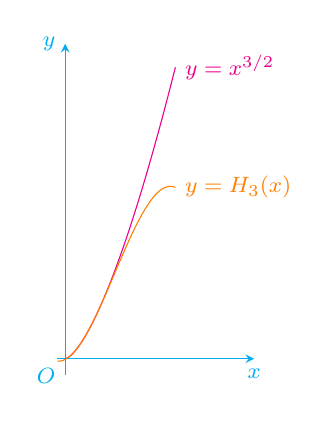
\begin{tikzpicture}[->,samples=100,>=stealth,scale=0.2,font=\footnotesize]
                \draw[->,cyan](-0.5,0)--(0,0)node[below left]{$O$}--(12,0)node[below]{$x$};
                \draw[->,cyan](0,-1)--(0,20)node[left]{$y$};
                \draw[domain=0:7,color=magenta,-]plot(\x,{(\x)^(1.5)})node[right]{$y=x^{3/2}$};
                \draw[domain=-0.5:7,color=orange,-]plot(\x,{-0.062222*(\x)^3+0.58444*(\x)^2+0.51778*(\x)-0.04})node[right]{$y=H_3(x)$};
            \end{tikzpicture}
            \caption{}
        \end{figure}
    \end{minipage}
\end{solution}

\begin{example}
    设 $f(x)$ 在 $[-1,1]$ 三阶导数连续, $f(-1)=0,f(1)=1,f'(0)=0$, 证明: $\exists\xi\in(-1,1)$, 使得 $f'''(\xi)=3.$
\end{example}
\begin{proof}[{\songti \textbf{证法一: }}]
    令 \footnote{由 $f_0=f(-1)=0,f_1=f(0),f_2=f(1)=1$ 作差商, 下同例题 \ref{fxx32x014}}
    $$H_3(x)= f(0)(x+1)+\dfrac{1-2f(0)}{2}(x+1)x+\dfrac{1}{2}(x+1)x(x-1)$$
    构造 $F(x)=f(x)-H_3(x)$, 那么有 $F(-1)=F(0)=F(1)=0$, 由 Rolle 定理 $\exists\xi_1\in(-1,0),\xi_2\in(0,1)$, 使得 
    $$F'(\xi_1)=F'(\xi_2)=0$$
    而 $F'(0)=f'(0)-H_3'(0)=0$, 则有 $F'(\xi_1)=F'(0)=F'(\xi_2)=0$ 故又由 Rolle 定理 $\exists\xi_3\in(\xi_1,0),\xi_4\in(0,\xi_2)$, 使得 $$F''(\xi_3)=F''(\xi_4)=0$$
    最后由 Rolle 定理知 $\exists\xi\in(\xi_3,\xi_4)\subset(-1,1)$, 使得 $F'''(\xi)=0$
    而 $$F'''(\xi)=f'''(\xi)-H_3'''(\xi)=f'''(\xi)-3=0$$
    即得证.\\
    \textbf{证法二}
    将 $f(1)$ 和 $f(-1)$ 在 $x=0$ 处 Taylor 展开, 并作差, 下略.
\end{proof}

\begin{theorem}
    若函数 $f(x)\text{ 在 }[a,b]$ 上三阶可导, 且 $ab<0,a\neq b,f(a)=c,f(0)=d,f(b)=e,f'(0)=f$, 则 $\exists\xi\in(a,b)$, 使得 $$f'''(\xi)=\dfrac{6}{ab}\qty[f+\dfrac{d-c}{a}+\dfrac{a(e-d)+b(d-c)}{b(b-a)}].$$
\end{theorem}
\begin{proof}[{\songti \textbf{证}}]
    由所给节点可求出 $$f_0=f(a)=c,f_1=f(0)=d,f_2=f(b)=e$$
    那么差商表为
    \begin{table}[H]
        \centering
        \setlength{\tabcolsep}{12mm}{
            \begin{tabular}{c c c c}
                \toprule
                $x_{k}$ & $f(x_k)$ & 一阶差商          & 二阶差商                         \\
                \midrule
                $a$     & $c$      &                   &                                  \\
                $0$     & $d$      & $-\dfrac{d-c}{a}$ &                                  \\[6pt]
                $b$     & $e$      & $\dfrac{e-d}{b}$  & $\dfrac{a(e-d)+b(d-c)}{ab(b-a)}$ \\
                \bottomrule
            \end{tabular}}
    \end{table}
    故可令 $$H_3(x)=c-\dfrac{d-c}{a}(x-a)+\dfrac{a(e-d)+b(d-c)}{ab(b-a)}(x-a)x+A(x-a)x(x-b)$$
    由 $p'_3(0)=f'(0)=f$, 解得 $A=\dfrac{f+\dfrac{d-c}{a}+\dfrac{a(e-d)+b(d-c)}{b(b-a)}}{ab}$
    于是 $$H_3(x)=c-\dfrac{d-c}{a}(x-a)+\dfrac{a(e-d)+b(d-c)}{ab(b-a)}(x-a)x+\dfrac{f+\dfrac{d-c}{a}+\dfrac{a(e-d)+b(d-c)}{b(b-a)}}{ab}(x-a)x(x-b)$$
    则 $H_3(x)$ 与 $f(x)$ 在 $a,0,b$ 三点有相同的函数值, 在 $0$ 点有相同的导数值, 
    设 $F(x)=f(x)-H_3(x)$, 则 $F(a)=F(0)=F(b)=0$, 由 Rolle 定理知, $\exists\xi_1\in(a,0),\xi_2\in(0,b)$, 使得 $$F'(\xi_1)=F'(\xi_2)=0$$
    由于 $F'(x)=f'(x)-p'_3(x)$, 所以 $F'(0)=f'(0)-p'(0)=0$, 在 $[\xi_1,0]$ 和 $[0,\xi_2]$ 上应用 Rolle 定理, 则 $\exists\xi_3\in(\xi_1,0),\xi_4\in(0,\xi_2)$, 使得 $$F''(\xi_3)=F''(\xi_4)=0$$
    最后在 $[\xi_3,\xi_4]$ 上应用 Rolle 定理, $\exists\xi\in(\xi_3,\xi_4)$, 使得 $F'''(\xi)=0$, 而 $F'''(x)=f'''(x)-p_3'''(x)$, 则 $f'''(\xi)=p'''(\xi)$, 即
    $$f'''(\xi)=\dfrac{6}{ab}\qty[f+\dfrac{d-c}{a}+\dfrac{a(e-d)+b(d-c)}{b(b-a)}].$$
\end{proof}
% \begin{inference}
%     若函数 $f(x)\in C^3[a,b]$, 且 $ab<0,a\neq b,f(a)=c,f(b)=e,f'(0)=f$, 则 $\exists\xi\in(a,b)$, 使得 $$f'''(\xi)=\dfrac{1}{ab}\qty[f+\dfrac{f(0)-c}{a}+\dfrac{a(e-f(0))+b(f(0)-c)}{b(b-a)}].$$
% \end{inference}
% \begin{inference}
%     若函数 $f(x)\in C^3[-a,a]$, 且 $f(-a)=f(0)=0,f(a)=c\neq 0,f'(0)=0$, 则 $\exists\xi(-a,a)$, 使得 $$f''(\xi)=\dfrac{4c}{a^3}.$$
% \end{inference}
% \begin{proof}[{\songti \textbf{证}}]
%     作三次 Hermite 插值多项式 $H_3(x)=\dfrac{c}{2a^3}x^2(x+a)$ 即可得推论.
% \end{proof}
% \begin{inference}
%     若函数 $f(x)\in C^3[-a,a]$, 且 $f(-a)=0,f(a)=c\neq 0,f'(0)=0$, 则 $\exists\xi\in(-a,a)$, 使得 $$f''(\xi)=\dfrac{4c}{a^3}.$$
% \end{inference}
% \begin{proof}[{\songti \textbf{证}}]
%     作三次 Hermite 插值多项式 $H_3(x)=\dfrac{f(0)}{a}(x+a)+\dfrac{2f(0)-c}{2a^2}(x+a)x+\dfrac{c}{2a^3}(x+a)x(x-a)$ 即可得推论.
% \end{proof}

与例题 \ref{fxx32x014} 不同但同样典型的例子是 “两点三次 Hermite 插值”, 插值节点取 $x_k$ 及 $x_{k+1}$, 插值多项式为 $H_3(x)$, 满足条件
$$\begin{cases}
        H_3(x_k)=y_k,  & H_3(x_{k+1})=y_{k+1}  \\
        H_3'(x_k)=m_k, & H_3'(x_{k+1})=m_{k+1}
    \end{cases}$$

\begin{theorem}[两点三次 Hermite 插值]
    \label{twoPointTripleHermiteInterpolation}\index{两点三次 Hermite 插值}
    采用基函数方法, 令 $$H_3(x)=\alpha_k(x)y_k+\alpha_{k+1}(x)y_{k+1}+\beta_k(x)m_k+\beta_{k+1}(x)m_{k+1}$$
    其中 $\alpha_k(x),\alpha_{k+1}(x),\beta_k(x),\beta_{k+1}(x)$ 是关于节点 $x_k$ 及 $x_{k+1}$ 的三次 Hermite 插值基函数, 它们应分别满足以下条件:
    $$\begin{array}{lll}
            \alpha _k(x_k)=1                        & \alpha _k(x_{k+1})=0     & \alpha _k'(x_k)=\alpha '_k(x_{k+1})=0         \\
            \alpha _{k+1}(x_k)=0                    & \alpha _{k+1}(x_{k+1})=1 & \alpha' _{k+1}(x_k)=\alpha '_{k+1}(x_{k+1})=0 \\
            \beta_k(x_k)=\beta_k(x_{k+1})=0         & \beta'_k(x_k)=1          & \beta'_k(x_{k+1})=0                           \\
            \beta_{k+1}(x_k)=\beta_{k+1}(x_{k+1})=0 & \beta'_{k+1}(x_k)=0      & \beta'_{k+1}(x_{k+1})=1
        \end{array}$$
    解得基函数, 那么有
    \begin{flalign*}
        H_3(x) & =\qty(1+2\dfrac{x-x_k}{x_{k+1}-x_k})\qty(\dfrac{x-x_{k+1}}{x_k-x_{k+1}})^2y_k+\qty(1+2\dfrac{x-x_{k+1}}{x_k-x_{k+1}})\qty(\dfrac{x-x_k}{x_{k+1}-x_k})^2y_{k+1} \\
               & ~ +(x-x_k)\qty(\dfrac{x-x_{k+1}}{x_k-x_{k+1}})^2m_k+(x-x_{k+1})\qty(\dfrac{x-x_k}{x_{k+1}-x_k})^2m_{k+1}.
    \end{flalign*}
\end{theorem}

\begin{theorem}
    若函数 $f(x)\text{ 在 }[a,b]$ 上三阶可导, 且 $f(a)=c,f(b)=d,f'(a)=e,f'(b)=f$, 则 $\exists\xi\in(a,b)$, 使得 $$f'''(\xi)=6\dfrac{f(b-a)-2(d-c)+e(b-a)}{(b-a)^3}.$$
\end{theorem}
\begin{proof}[{\songti \textbf{证}}]
    作三次 Hermite 插值多项式: $$H_3(x)=c+e(x-a)+\dfrac{(d-c)-e(b-a)}{(b-a)^2}(x-a)^2+\dfrac{f(b-a)-2(d-c)+e(b-a)}{(b-a)^3}(x-a)^2(x-b)$$
    则 $H_3(x)$ 与 $f(x)$ 在 $a,b$ 两点有相同的函数值与导数值, 设 $F(x)=f(x)-H_3(x)$, 则 $F(a)=F(b)=0$, 由 Rolle 定理, $\exists\xi_1\in(a,b)$, 使得 $F'(\xi_1)=0$, 
    由于 $$F'(x)=f'(x)-H_3'(x)=f'(x)+e+2\dfrac{(d-c)-e(b-a)}{(b-a)^2}(x-a)+\dfrac{f(b-a)-2(d-c)+e(b-a)}{(b-a)^3}\qty[2(x-a)(x-b)+(x-a)^2]$$
    则 $F'(a)=F'(b)=0$, 在 $[a,\xi_1]$ 和 $[\xi_1,b]$ 上应用 Rolle 定理, 则 $\exists\xi_2\in(a,\xi_1),\xi_3\in(\xi_1,b)$, 使得 $$F''(\xi_2)=F''(\xi_3)=0$$
    最后在 $[\xi_2,\xi_3]$ 上应用 Rolle 定理, 即 $\exists\xi\in(\xi_2,\xi_3)$, 使得 $F'''(\xi)=0$, 即得证.
\end{proof}
\begin{inference}
    若函数 $f(x)\text{ 在 }[a,b]$ 上三阶可导, 且 $f(a)=a,f(b)=b,f'(a)=f'(b)=0$, 则 $\exists\xi\in(a,b)$, 使得 $$f'''(\xi)=-\dfrac{12}{(a-b)^2}.$$
\end{inference}
\begin{proof}[{\songti \textbf{证}}]
    令 $c=a,d=b,e=f=0$, 即得证. 
\end{proof}

\begin{example}
    设函数 $f\in C[0,1]\cap D^3(0,1),~f(0)=2,~f(1)=1,~f'(0)=0,~f'(1)=4$ 证明: 存在一点 $\xi\in(0,1)$ 使得 $f'''(\xi)=24+24\xi.$
\end{example}
\begin{solution}
    令 $g(x)=f(x)-x^4$, 则 $g\in C[0,1]\cap D^3(0,1)$ 那么 $\begin{cases}
            x_k=0  , & x_{k+1}=1 \\
            y_k=2  , & y_{k+1}=0 \\
            m_k=0  , & m_{k+1}=0
        \end{cases}$, 因此
        $$H_3(x)=2(1+x)(x-1)^2=4x^3-6x^2+2$$
        构造 $F(x)=g(x)-H_3(x)$ 有 $F(0)=F(1)=0$, 由 Rolle 定理 $\exists\xi_1\in(0,1)$ 使得 $F'(\xi_1)=0$, 
        又 $F'(0)=F'(\xi_1)=F'(1)=0$, 由 Rolle 定理得 $\exists \xi_2\in(0,\xi_1),\xi_3\in(\xi_1,1)$ 使得 $F''(\xi_i)=0,i=2,3$, 
        再根据 Rolle 定理得 $\exists\xi\in(\xi_2,\xi_3)\subset(0,1)$ 使得 $F'''(\xi)=0$ 即
        $$f'''(\xi)-\xi\cdot4!-24=0\Rightarrow f'''(\xi)=24\xi+24.$$
\end{solution}
\section{导数的综合应用}

\subsection{极值问题}

\subsubsection{极值、最值}

求极值的方法步骤一般如下:
\begin{enumerate}[label=(\arabic{*})]
    \item 求可疑点, 可疑点包括:
          \begin{enumerate}[label=(\roman{*})]
              \item 稳定点 (亦称驻点或逗留点, 皆值一阶导数等于零的点);
              \item 导数不存在的点;
              \item 区间端点.
          \end{enumerate}
    \item 对可疑点进行判断, 基本方法是:
          \begin{enumerate}[label=(\roman{*})]
              \item 直接利用定义判断;
              \item 利用实际背景来判断;
              \item 查看一阶导数的符号, 当 $x$ 从左向右穿越可疑点 $x_0$ 时, \\
                    若 $f'(x)$ 由“正”变“负”, 则 $f(x_0)$ 为严格极大值点;\\
                    若 $f'(x)$ 由“负”变“正”, 则 $f(x_0)$ 为严格极小值点;\\
                    若 $f'(x)$ 不变号, 则 $f(x_0)$ 不是极值.
              \item 若 $f'(x_0)=0$, $f''(x_0)\begin{cases}
                            >0 , & \text{则 } f(x_0) \text{ 为严格极小值,} \\
                            <0 , & \text{则 } f(x_0) \text{ 为严格极大值;}
                        \end{cases}$
              \item $f^{(k)}(x_0)=0~ (k=1,2,\cdots,n-1),~f^{(n)}(x_0)\neq 0$, \\
                    若 $n$ 为偶数, 则 $f(x_0)$ 为极值: $\begin{cases}
                            f^{(n)}(x_0)>0 , & \text{严格极小值,} \\
                            f^{(n)}(x_0)<0 , & \text{严格极大值;}
                        \end{cases}$\\
                    若 $n$ 为奇数, 则 $f(x_0)$ 不是极值.
          \end{enumerate}
\end{enumerate}

\begin{example}
    求函数 $f(x)=\qty|x\qty(x^2-1)|$ 的极值以及在 $[-2,2]$ 上的最值.
\end{example}
\begin{solution}
    $f(x)=\mathrm{sgn}\qty(x\qty(x^2-1))\cdot x\qty(x^2-1)$, 那么 $f'(x)=\mathrm{sgn}\qty(x\qty(x^2-1))\cdot\qty(3x^2-1)~ (x\neq0,\pm1)$, 令 $f'(x)=0$, 得
    $x=\pm\dfrac{\sqrt{3}}{3}$
    $$f''\qty(\dfrac{\sqrt{3}}{3})=\mathrm{sgn}\qty(x\qty(x^2-1))\biggl |_{x=\frac{\sqrt{3}}{3}}\cdot 6x\biggl |_{x=\frac{\sqrt{3}}{3}}=-2\sqrt{3}<0$$
    故 $f(x)$ 在 $x=\dfrac{\sqrt{3}}{3}$ 处取极大值, 又 $f(x)$ 是偶函数, 所以在 $x=-\dfrac{\sqrt{3}}{3}$ 处亦取极大值, 
    当 $x=0,\pm1$ 时, $f(0)=f(1)=f(-1)=0\leqslant f(x)(\forall x)$, 故为最小值, 也是极小值;
    $f(2)=f(-2)=6\geqslant f(x)(\forall x\in[-2,2])$, 故 $f(x)$ 在 $[-2,2]$ 上最大值为 6, 最小值为 0.
\end{solution}

\begin{example}
    设 $f(x)$ 在 $\qty(-\dfrac{\pi}{2},\dfrac{\pi}{2})$ 可导, $f(0)=1,~f(x)>0$, $$\displaystyle\lim_{h\to0}\qty[\dfrac{f\qty(x+h\cdot \cos^2x)}{f(x)}]^{\frac{1}{h}}=\e^{x\cos^2x+\tan x}$$
    求 $f(x)$ 的表达式及极值.
\end{example}
\begin{solution}
    $\displaystyle\lim_{h\to0}\qty[\dfrac{f\qty(x+h\cdot \cos^2x)}{f(x)}]^{\frac{1}{h}}=\lim_{h\to0}\dfrac{1}{h}\ln\dfrac{f\qty(x+h\cdot\cos^2x)}{f(x)}=x\cos^2x+\tan x$, 
    等式左边化为 $$\lim_{h\to0}\dfrac{1}{h}\dfrac{f\qty(x+h\cdot\cos^2x)-f(x)}{f(x)}=\lim_{h\to0}\dfrac{\cos^2x}{f(x)}\dfrac{f\qty(x+h\cdot\cos^2x)-f(x)}{h\cos^2x}=\dfrac{\cos^2x}{f(x)}\cdot f'(x)$$
    即 $$\dfrac{f'(x)}{f(x)}=x+\tan x\cdot\sec^2x\Rightarrow \qty[\ln f(x)]'=x+\tan x\cdot\sec2x\Rightarrow \ln f(x)=\dfrac{1}{2}x^2+\dfrac{1}{2}\tan^2x+C$$
    又 $f(0)=1$, 解得 $C=0$, 于是
    $f(x)=\e^{\frac{1}{2}x^2+\frac{1}{2}\tan^2x}$, 则
    $$f'(x)=\e^{\frac{1}{2}x^2+\frac{1}{2}\tan^2x}\cdot\qty(x+\tan x\cdot\sec^2x)$$
    因为 $\e^{x}$ 恒大于 0, 因此只需讨论 $x+\tan x\cdot\sec^2x$ 的符号即可, 令 $g(x)=x+\tan x\cdot\sec^2x$, 对 $g(x)$ 求导得 $$g'(x)=1+\sec^4x+4\tan^2x\sec^2x>1$$
    所以 $g(x)\nearrow$, 而 $g(0)=0$, 故当 $x\in\qty(-\dfrac{\pi}{2},0)$ 时, $g(x)<0\Rightarrow f'(x)<0\Rightarrow f(x)\searrow$; 当 $x\in\qty(0,\dfrac{\pi}{2})$ 时, $f(x)\nearrow$, 
    所以当 $x=0$ 时, $f(x)$ 取得极小值, 无极大值, 且 $f(0)=1.$
\end{solution}

\begin{example}[2014 数一]
    设函数 $y=f(x)$ 由方程 $y^3+xy^2+x^2y=0$ 确定, 求 $f(x)$ 的极值.
\end{example}
\begin{solution}
    方程 $y^3+xy^2+x^2y=0$ 两端对 $x$ 求导, 得 
    \begin{equation*}
        3y^2y'+y^2+2xyy'+2xy+x^2y'=0
        \tag{*}
    \end{equation*}
    并令 $y'=0$, 得 $y^2+2xy=0$, 解得 $y=0$ 或 $y=-2x$, 
    显然 $y=0$ 不满足原方程, 将 $y=-2x$ 代入原方程得 $-6x^3+6=0\Rightarrow x_0=1$, 那么 $f(1)=-2,~f'(1)=0$, (*) 式两端对 $x$ 再次求导, 得 
    $$6y'^2+3y^2y''+4yy'+2xy'^2+2xyy''+2y+4xy'+x^2y''=0$$
    将 $x=1,~f(1)=-2,~f'(1)=0$ 代入上式得 $f''(1)=\dfrac{4}{9}>0$, 
    则函数 $y=f(x)$ 在 $x=1$ 处取极小值, 极小值为 $f(1)=-2.$
\end{solution}

\subsubsection{极值点偏移}

\begin{example}
    已知函数 $f(x)=x\e^{-x},x\in\mathbb{R}$, 如果有 $f(x_1)=f(x_2)$ 且 $x_1\neq x_2$, 求证 $x_1+x_2>2.$
\end{example}
\begin{proof}[{\songti \textbf{证法一}}]
    由 $f(x_1)=f(x_2)$ 得 $\dfrac{x_2}{x_1}=\dfrac{\e^{x_2}}{\e^{x_1}}\Rightarrow \ln\dfrac{x_2}{x_1}=x_2-x_1$, 不妨设 $0<x_1<1<x_2$, 作换元 $t=\dfrac{x_2}{x_1}$, 那么 $t>1$, 且
    $$x_1=\dfrac{\ln t}{t-1},x_2=\dfrac{t\ln t}{t-1}$$
    于是要证 $\forall t>1,\dfrac{t\ln t+\ln t}{t-1}>2$, 构造函数 $F(t)=\ln t-\dfrac{2(t-1)}{t+1}$, 那么 $F'(t)=\dfrac{1}{t}-\dfrac{4}{(t+1)^2}=\dfrac{(t-1)^2}{t(t+1)^2}>0$, 所以 $F(t)$ 在 $(1,+\infty)$ 上单调递增, 所以 $F(t)>F(1)=0$, 即得待证式成立.
\end{proof}
\begin{proof}[{\songti \textbf{证法二}}]
    由题可得 $\ln x_2-\ln x_1=x_2-x_1$, 即 $\dfrac{x_2-x_1}{\ln x_2-\ln x_1}=1$, 要证 $x_1+x_2>2$, 即证 $x_1+x_2>2\dfrac{x_2-x_1}{\ln x_2-\ln x_1}$, 
    不妨设 $0<x_1<1<x_2$, 作换元 $t=\dfrac{x_2}{x_1}$, 那么原不等式可化为 $\ln t>\dfrac{2(t-1)}{t+1}$, 由证法一可得该不等式成立, 所以原命题成立.
\end{proof}

\begin{theorem}[对数平均不等式 (ALG)]
    对任意 $0<a<b$, 满足 $\sqrt{ab}<\dfrac{b-a}{\ln b-\ln a}<\dfrac{a+b}{2}.$
    \index{对数平均不等式 (ALG)}
\end{theorem}

\subsection{不等式与函数凹凸性及拐点}

不等式与凸函数之间有着密切的关系, 凸函数在不等式中起着重要的作用.

\subsubsection{不等式}

\begin{theorem}[均值不等式]
    对任意 $n$ 个实数 $x_i\geqslant 0~~(i=1,2,\cdots,n)$, 有\label{meanInequality}
    调和平均数 $\leqslant$ 几何平均数 $\leqslant$ 算术平均数 $\leqslant$ 平方平均数, 即
    $$\begin{matrix}
            H_n                                                    & \leqslant & G_n                                                    & \leqslant & A_n       & \leqslant & Q_n       \\
            \parallel                                              &           & \parallel                                              &           & \parallel &           & \parallel \\
            \sqrt[n]{\displaystyle \sum_{i=1}^{n}\dfrac{1}{x_i}  } &           & \sqrt[n]{\displaystyle \prod _{i=1}^n x_i}             &           &
            \displaystyle \dfrac{1}{n}\sum_{i=1}^{n}x_i            &           & \sqrt{\displaystyle \dfrac{1}{n}\sum_{i=1}^{n}x_i^2  }
        \end{matrix}$$
    其中等号当且仅当 $a_1=a_2=\cdots=a_n$ 时成立.
    \index{均值不等式}
\end{theorem}

\begin{example}
    试比较 $\pi^{\mathrm{e}}$ 和 $\mathrm{e}^\pi$ 的大小, 并说明理由.
\end{example}
\begin{solution}
    \textbf{法一: }只需比较 $\dfrac{\ln \mathrm{e}}{\mathrm{e}}$ 与 $\dfrac{\ln\pi}{\pi}$ 的大小, 
    令 $f(x)=\dfrac{\ln x}{x}~~(x\geqslant \mathrm{e})\Rightarrow f'(x)=\dfrac{1-\ln x}{x^2}<0~~(x>\mathrm{e})$, 于是 $f(x)$ 在 $[\mathrm{e},+\infty)$ 上单调递减, 
    又 $\mathrm{e}<\pi$, 从而 $f(\pi)<f(\mathrm{e})$, 即 $\dfrac{\ln\pi}{\pi}<\dfrac{\ln \mathrm{e}}{\mathrm{e}}$, 故 $\mathrm{e}^\pi>\pi^{\mathrm{e}}.$\\
    \textbf{法二: }记 $\pi=\mathrm{e}+\lambda$, 则 $\lambda>0$, 于是
    $$\dfrac{\pi ^{\mathrm{e}}}{\mathrm{e}^{\pi }}=\dfrac{\left( \mathrm{e}+\lambda \right) ^{\mathrm{e}}}{\mathrm{e}^{\mathrm{e}+\lambda }}=\dfrac{1}{\mathrm{e}^{\lambda }}\left( \dfrac{\mathrm{e}+\lambda }{\mathrm{e}}\right) ^{\mathrm{e}}=\dfrac{1}{\mathrm{e}^{x}}\left[ \left( 1+\dfrac{\lambda }{\mathrm{e}}\right) ^{\dfrac{\mathrm{e}}{\lambda }}\right] ^{\lambda } <\dfrac{1}{\mathrm{e}^{\lambda }}\mathrm{e}^{\lambda }=1\Rightarrow\mathrm{e}^\pi>\pi^{\mathrm{e}}.$$
\end{solution}

\begin{example}[1995 数学 (二)]
    设 $ f(x) $ 二阶可导, 且 $ \displaystyle\lim _{x \rightarrow 0} \frac{f(x)}{x}=1,~f^{\prime \prime}(x)>0$, 
    证明 $ f(x) \geqslant x .$
\end{example}

\begin{proof}[{\songti \textbf{证法一}}]
    要证 $ f(x) \geqslant x$, 只需证 $ f(x)-x \geqslant 0$, 为此, 令 $ g(x)=f(x)-x$, 则由 $\displaystyle \lim _{x \rightarrow 0} \frac{f(x)}{x}=1$, 
    得 $\displaystyle f(0)=\lim _{x \rightarrow 0} f(x)=0,~f^{\prime}(0)=\lim _{x \rightarrow 0} \frac{f(x)-f(0)}{x}=1$, 
    所以 $ g^{\prime}(x)=f^{\prime}(x)-1=f^{\prime}(x)-f^{\prime}(0)$, 
    又由 $ f^{\prime \prime}(x)=\left(f^{\prime}(x)\right)^{\prime}>0 $ 知, $f^{\prime}(x)$  在 $ (-\infty,+\infty)$ 上单调递增, 
    于是当 $ x<0 $ 时, $g^{\prime}(x)<0$; 当 $ x>0 $ 时, $g^{\prime}(x)>0$, 从而知 $ x=0 $ 为 $ g(x) $ 的极小值点也是最小值点,, 
    故 $ g(x) \geqslant g(0)=0$, 即 $ f(x) \geqslant x .$
\end{proof}
\begin{proof}[{\songti \textbf{证法二}}]
    由 $\displaystyle \lim _{x \rightarrow 0} \frac{f(x)}{x}=1 $ 可知, $\displaystyle f(0)=\lim _{x \rightarrow 0} f(x)=0, f^{\prime}(0)=\lim _{x \rightarrow 0} \frac{f(x)-f(0)}{x}= \lim _{x \rightarrow 0} \frac{f(x)}{x}=1$, 
    由题设 $ f(x) $ 二阶可导, 将 $ f(x) $ 在 $ x=0 $ 点进行 Taylor 展开, 得
    $$f(x)=f(0)+f^{\prime}(0) x+\frac{f^{\prime \prime}(\xi)}{2 !} x^{2}$$
    其中 $ \xi $ 介于 $0$ 与 $ x $ 之间, 
    故由 $ f^{\prime \prime}(x)>0 $ 得 $ f(x) \geqslant f(0)+f^{\prime}(0) x=x $ (等号仅当 $ x=0 $ 时成立).
\end{proof}
\begin{proof}[{\songti \textbf{证法三}}]
    由 $\displaystyle \lim _{x \rightarrow 0} \frac{f(x)}{x}=1 $ 及 $ f(x) $ 连续可知, $\displaystyle f(0)=\lim _{x \rightarrow 0} f(x)=0, f^{\prime}(0)= \lim _{x \rightarrow 0} \frac{f(x)-f(0)}{x}=1$, 
    又由 $ f^{\prime \prime}(x)=\left(f^{\prime}(x)\right)^{\prime}>0 $ 知 $ f^{\prime}(x) $ 严格单调递增,  于是由 Lagrange 中值定理得\\
    当 $ x>0 $ 时, $\displaystyle\frac{f(x)}{x}=\frac{f(x)-f(0)}{x}=f^{\prime}\left(\xi_{1}\right)>f^{\prime}(0)=1$, 其中 $ \xi_{1} \in(0, x)$, 故 $ f(x)>x$; \\
    当 $ x<0 $ 时, $\displaystyle\frac{f(x)}{x}=\frac{f(x)-f(0)}{x}=f^{\prime}\left(\xi_{2}\right)<f^{\prime}(0)=1$, 其中 $ \xi_{2} \in(x, 0)$, 故 $ f(x)>x$; \\
    当 $ x=0 $ 时, $f(0)=0$, $\forall x \in(-\infty,+\infty)$, 都有 $ f(x) \geqslant x .$
\end{proof}

\begin{inference}
    一般地, 设 $\displaystyle\lim_{x\to0}\dfrac{f(x)}{x}=A$, 且 $f''(x)>0$, 则 $f(x)\geqslant Ax.$
\end{inference}

\begin{example}
    证明: $\qty|\dfrac{\sin x-\sin y}{x-y}-\cos y|\leqslant \dfrac{1}{2}\cdot |x-y|,~x\neq y.$
\end{example}
\begin{proof}[{\songti \textbf{证}}]
    将 $\sin x$ 在 $x=y$ 处 Taylor 展开, 得 $$\sin x=\sin y+\cos y(x-y)-\dfrac{1}{2}\sin \xi(x-y)^2$$
    其中 $\xi$ 介于 $x$ 与 $y$ 之间, 那么待证等式化简为 $$\qty|\dfrac{\sin x-\sin y}{x-y}-\cos y|=\qty|\dfrac{|\sin\xi|}{2}|~|x-y|$$
    又 $\sin \xi\leqslant 1$, 即得待证式成立.
\end{proof}

\begin{theorem}[Cauchy 不等式]
    设 $a_k,b_k$ 为任意实数 ($i=1,2,\cdots,n$), 则
    $$\displaystyle\left( \sum_{k=1}^n a_k b_k \right)^{\!\!2}\leqslant\left( \sum_{k=1}^n a_k^2 \right) \left( \sum_{k=1}^n b_k^2 \right) $$
    其中等号当且仅当 $a_k$ 与 $b_k$ 成比例时成立.
    \index{Cauchy 不等式}
\end{theorem}
% \begin{inference}
%     Carlson 不等式: $m\times n$ 的非负实数矩阵中, $n$ 列每列元素之和的几何平均值不小于矩阵中 $m$ 行每行元素的几何平均值之和. 即
%     $$\qty(x_1+y_1+\cdots)\qty(x_2+y_2+\cdots)\cdots\qty(x_n+y_n+\cdots)\geqslant \qty[\qty(\prod_{k=1}^{n}x_k)^{\frac{1}{n}}+\qty(\prod_{k=1}^{n}y_k)^{\frac{1}{n}}+\cdots]^n$$
%     等号成立的充要条件是至少有一列数都是 0 或所有行中的数对应成比例.
% \end{inference}

\subsubsection{凸函数}

\subsubsection{凸函数的多种定义}

\begin{definition}[凸函数 A]
    设 $ f(x) $ 在区间 $ I $ 上有定义, $f(x) $ 在 $ I $ 上称为\textit{凸函数}, 当且仅当 $ \forall x_{1} ,  x_{2} \in I, \forall \lambda \in(0,1)$, 有
    $$f\left(\lambda x_{1}+(1-\lambda) x_{2}\right) \leqslant \lambda f\left(x_{1}\right)+(1-\lambda) f\left(x_{2}\right) .$$
    式中的 $\leqslant$ 改为 $<$ 便是严格凸的定义.
\end{definition}

\begin{definition}[凸函数 B]
    设 $ f(x) $ 在区间 $ I $ 上有定义, $f(x)$ 称为 $ I $ 上的凸函数, 当且仅当 $ \forall x_{1} ,  x_{2} \in I$, 有
    $$f\left(\frac{x_{1}+x_{2}}{2}\right) \leqslant \frac{f\left(x_{1}\right)+f\left(x_{2}\right)}{2} .$$
    式中的 $\leqslant$ 改为 $<$ 便是严格凸的定义.
\end{definition}

\begin{definition}[凸函数 C]
    设 $ f(x) $ 在区间 $ I $ 上有定义, $f(x) $ 称为凸函数, 当且仅当 $ \forall x_{1}, \cdots, x_{n} \in   I$, 有
    $$f\left(\frac{x_{1}+x_{2}+\cdots+x_{n}}{n}\right) \leqslant \frac{f\left(x_{1}\right)+f\left(x_{2}\right)+\cdots+f\left(x_{n}\right)}{n} .$$
    式中的 $\leqslant$ 改为 $<$ 便是严格凸的定义.
\end{definition}

\begin{definition}[凸函数 D]
    设 $ f(x) $ 在区间 $ I $ 上有定义, 当且仅当曲线 $ y=f(x) $ 的切线恒保持在曲线以下, 称 $ f(x) $ 为凸函数. 若除切点之外, 切线严格保持在曲线的下方, 则称 $ f(x) $ 为严格凸的.
\end{definition}

\begin{example}
    已知 $f(x)$ 为二阶导的正值函数, 且 $f(0)=f'(0)=1,~$, 则
    \begin{tasks}(2)
        \task $f(2)\leqslant \e^{2}\leqslant \sqrt{f(1)f(3)}$
        \task $\e^{2}\leqslant f(2)\leqslant \sqrt{f(1)f(3)}$
        \task $\sqrt{f(1)f(3)}\leqslant \e^{2}\leqslant f(2)$
        \task $\sqrt{f(1)f(3)}\leqslant f(2)\leqslant \e^{2}$
    \end{tasks}
\end{example}
\begin{solution}
    因为 $f(x)$ 为一正值函数, 且 $f(x)f''(x)\geqslant \qty[f'(x)]^2$, 于是有 $$\dfrac{f(x)f''(x)-\qty[f'(x)]^2}{f^2(x)}\geqslant 0\Rightarrow \qty(\dfrac{f'(x)}{f(x)})'\geqslant 0\Rightarrow \qty(\ln f(x))''\geqslant 0$$
    那么 $g(x)=\ln f(x)$ 为一下凸函数, 那么 $\dfrac{g(1)+g(3)}{2}=\dfrac{1}{2}\qty(\ln f(1)+\ln f(3))=\ln\sqrt{f(1)f(3)}$, 并且根据凸函数的性质, 有 $$\dfrac{g(1)+g(3)}{2}\geqslant g\qty(\dfrac{1+3}{2})=\ln f(2)\Rightarrow \ln\sqrt{f(1)f(3)}\geqslant \ln f(2)\Rightarrow f(2)\leqslant \sqrt{f(1)f(3)}$$
    将 $g(x)$在 $x=0$ 处 Taylor 展开, 得 $$g(x)=g(0)+g'(0)x+\dfrac{1}{2}g''(\theta)x^2\geqslant g(0)+g'(0)x=x$$
    于是得 $f(x)\geqslant \e^x$, 因此 $f(2)\geqslant \e^2$, 综上所述, 选 B.
\end{solution}

\begin{theorem}
    设函数 $ f(x) $ 在区间 $ I $ 上有定义, 则 $ f(x) $ 为凸函数的充要条件是: $ \forall x_{0} \in   r,~
        \exists  \alpha \text{, 使得 } \forall x \in I  \text{ 有 }  f(x) \geqslant \alpha\left(x-x_{0}\right)+f\left(x_{0}\right) .$
\end{theorem}

\begin{inference}
    设 $ f(x) $ 在区间 $ I $ 内部可导, 则 $ f(x) $ 在 $ I $ 上为凸的充要条件是: $ \forall x_{0} \in I^{\circ}$, 有
    $$f(x) \geqslant f^{\prime}\left(x_{0}\right)\left(x-x_{0}\right)+f\left(x_{0}\right)~ (\forall x \in I) .$$
\end{inference}

\begin{inference}
    若 $ f(x) $ 在区间 $ I $ 上为凸的, 则 $ \forall x_{0} \in I^{\circ}$, 在曲线 $ y=f(x) $ 上一点 $ \left(x_{0}\right. ,  \left.f\left(x_{0}\right)\right)$ 可作一条直线
    $$L: y=\alpha\left(x-x_{0}\right)+f\left(x_{0}\right)$$
    使曲线 $ y=f(x) $ 位于直线 $ L $ 上方.
\end{inference}

\begin{theorem}[分离性定理]
    若 $ f $ 为严格凸函数, 则除点 $ \left(x_{0}, f\left(x_{0}\right)\right) $ 之外曲线严格地在直线 $ L $ 的上方, 直线 $ L $ 称为 $ y=f(x) $ 的支撑.
    \index{分离性定理}
\end{theorem}

\begin{theorem}
    设 $ f(x) $ 在区间 $ I $ 上有导数, 则 $ f(x) $ 在 $ I $ 上为凸函数的充要条件是 $ f^{\prime}(x) \nearrow(x \in I) .$
\end{theorem}

\begin{theorem}[Jensen 不等式]
    若 $f(x)$ 在 $I$ 上有定义, 则
    $\forall q_{i} \geqslant 0$: $q_{1}+q_{2}+\cdots+q_{n}=1, \forall x_{1}, x_{2}, \cdots, x_{n} \in I$, 有
    $$f\left(q_{1} x_{1}+q_{2} x_{2}+\cdots+q_{n} x_{n}\right) \leqslant q_{1} f\left(x_{1}\right)+q_{2} f\left(x_{2}\right)+\cdots+q_{n} f\left(x_{n}\right);$$

    $\forall p_{i} \geqslant 0~ (i=1,2, \cdots, n)$ 不全为零, $\forall x_{1}, x_{2}, \cdots, x_{n} \in I$, 有
    $$f\left(\frac{p_{1} x_{1}+p_{2} x_{2}+\cdots+p_{n} x_{n}}{p_{1}+p_{2}+\cdots+p_{n}}\right) \leqslant \frac{p_{1} f\left(x_{1}\right)+p_{2} f\left(x_{2}\right)+\cdots+p_{n} f\left(x_{n}\right)}{p_{1}+p_{2}+\cdots+p_{n}} .$$
    \index{Jensen 不等式}
\end{theorem}

\begin{example}
    证明当 $0<x<\dfrac{\pi}{2}$ 时, $\sin x>\dfrac{2}{\pi}x.$
\end{example}
\begin{proof}[{\songti \textbf{证法一}}]
    设 $ f(x)=\sin x-\dfrac{2}{\pi} x$, 则 $ f^{\prime}(x)=\cos x-\dfrac{2}{\pi}, f^{\prime \prime}(x)=-\sin x<0\left(0<x<\dfrac{\pi}{2}\right)$, 于是
    $f(x) $ 在 $ \left[0, \dfrac{\pi}{2}\right] $ 上为凸函数, 又 $ f(0)=f\left(\dfrac{\pi}{2}\right)=0$, 故当 $ 0<x<\dfrac{\pi}{2} $ 时, $f(x)>0$, 即 $ \sin x>\dfrac{2}{\pi} x. $
\end{proof}
\begin{proof}[{\songti \textbf{证法二}}]
    设 $ f(x)=\sin x$, 则 $ f^{\prime}(x)=\cos x, f^{\prime \prime}(x)=-\sin x<0\left(0<x<\dfrac{\pi}{2}\right)$, 
    于是 $ f(x) $ 在 $ \left[0, \dfrac{\pi}{2}\right] $ 上是凸函数, 从而由凸函数的定义, 有
    $$f(x)=f\left[\dfrac{2 x}{\pi} \cdot \dfrac{\pi}{2}+\left(1-\dfrac{2 x}{\pi}\right) \cdot 0\right]>\dfrac{2 x}{\pi} \cdot f\left(\dfrac{\pi}{2}\right)+\left(1-\dfrac{2 x}{\pi}\right) \cdot f(0)=\dfrac{2 x}{\pi}$$
    即得 $ \sin x>\dfrac{2}{\pi} x\left(0<x<\dfrac{\pi}{2}\right) .$
\end{proof}
\begin{proof}[{\songti \textbf{证法三}}]
    设 $ f(x)=\sin x$, 对于 $ x \in\left(0, \dfrac{\pi}{2}\right)$, 将 $ f(t) $ 分别在 $ [0, x] $ 和 $ \left[x, \dfrac{\pi}{2}\right] $ 上应用 Lagrange 中值定理, 
    $$\exists\xi \in(0, x) \text{, 使得 }\dfrac{\sin x-\sin 0}{x-0}=\cos \xi$$
    即 $ \dfrac{\sin x}{x}=\cos \xi$, 
    又 $\exists\eta \in\left(x, \dfrac{\pi}{2}\right) \text{, 使得 }\dfrac{\sin \dfrac{\pi}{2}-\sin x}{\dfrac{\pi}{2}-x}=\cos \eta$, 
    即 $ \dfrac{1-\sin x}{\dfrac{\pi}{2}-x}=\cos \eta$, 
    又因为 $ \cos x $ 在 $ \left(0, \dfrac{\pi}{2}\right) $ 内严格单调递减, $\xi<\eta$, 所以 $ \cos \xi>\cos \eta$, 
    从而 $ \dfrac{\sin x}{x}>\dfrac{1-\sin x}{\dfrac{\pi}{2}-x}$, 即得 $ \sin x>\dfrac{2}{\pi} x\left(0<x<\dfrac{\pi}{2}\right) .$
\end{proof}

\subsubsection{拐点}

\begin{definition}[拐点]
    连续曲线凹与凸部分的分界点称为曲线的\textit{拐点}.
\end{definition}

\begin{theorem}[拐点存在的必要条件]
    设函数 $f(x)$ 在点 $x_0$ 具有二阶导数, 则点 $(x_0,f(x_0))$ 是曲线 $y=f(x)$ 的拐点的必要条件是 $f''(x_0)=0.$
    \index{拐点存在的必要条件}
\end{theorem}

\begin{example}[2008 数二]
    求曲线 $y=(x-5)x^{\frac{2}{3}}$ 的拐点坐标.
\end{example}
\begin{solution}
    因为 $y'=\dfrac{5}{3}x^{\frac{2}{3}}-\dfrac{10}{3}x^{-\frac{1}{3}},~y''=\dfrac{10}{9}x^{-\frac{1}{3}}+\dfrac{10}{9}x^{-\frac{4}{3}}=\dfrac{10(x+1)}{9\sqrt[3]{x^4}}$, 显然 $y''(-1)=0,~y''(0)$ 不存在, 由 $y''$ 的表达式可知在 $x=-1$ 两侧 $y'$ 异号, 而 $x=0$ 两侧 $y'$ 不变号, 因此拐点坐标为 $(-1,-6).$
\end{solution}

\begin{example}[2018 数二]
    求曲线 $y=x^2+2\ln x$ 在其拐点处的切线方程.
\end{example}
\begin{solution}
    $y'=2x+\dfrac{2}{x},~y''=2-\dfrac{2}{x^2}$, 令 $y''=0\Rightarrow x=1~(\text{舍负})$, 拐点为 $(1,1)$, 切线的斜率为 $y'(1)=4$, 因此拐点处的切线方程为 $y=4x-3.$
\end{solution}

\begin{example}[2011 数二]
    设函数 $y=y(x)$ 由参数方程 $\begin{cases}
        x=\dfrac{1}{3}t^3+t+\dfrac{1}{3}\\[6pt]
        y=\dfrac{1}{3}t^3-t+\dfrac{1}{3}
    \end{cases}$ 确定, 求函数 $y=y(x)$ 的极值和曲线 $y=y(x)$ 的凹凸区间及拐点.
\end{example}
\begin{solution}
    由题意 $x'(t)=t^2+1,~x''(t)=2t,~y'(t)=t^2-1,~y''(t)=2t$, 则 
    $$\dv{y}{x}=\dfrac{y'(t)}{x'(t)}=\dfrac{t^2-1}{t^2+1},~\dv[2]{y}{x}=\dfrac{y''(t)x'(t)-x''(t)y'(t)}{x'^3(t)}=\dfrac{4t}{\qty(t^2+1)^3}$$
    令 $\displaystyle\dv{y}{x}=0\Rightarrow t=\pm 1$, 当 $t=1$ 时, $\displaystyle x=\dfrac{5}{3},~y=-\dfrac{1}{3},~\dv[2]{y}{x}>0$, 所以 $y=-\dfrac{1}{3}$ 为极小值, 
    当 $t=-1$ 时, $x=-1,~y=1,~\displaystyle\dv[2]{y}{x}<0$, 所以 $y=1$ 为极大值.\\
    令 $\displaystyle\dv[2]{y}{x}=0\Rightarrow t=0\Rightarrow x=y=\dfrac{1}{3}$, 当 $t<0$ 时, $x<\dfrac{1}{3},~\displaystyle \dv[2]{y}{x}<0$, 则曲线 $y=y(x)$ 在 $\qty(-\infty,\dfrac{1}{3})$ 上是凸的, 
    当 $t>0$ 时, $x>\dfrac{1}{3},~\displaystyle\dv[2]{y}{x}>0$, 则曲线 $y=y(x)$ 在 $\qty(-\infty,\dfrac{1}{3})$ 上是凹的, 点 $\qty(\dfrac{1}{3},\dfrac{1}{3})$ 是曲线的拐点.
\end{solution}

\subsection{导数的几何意义与曲线的曲率}

\subsubsection{导数的几何意义}

导数 $f'(x_0)$ 在几何上表示曲线 $y=f(x)$ 在点 $M(x_0,f(x_0))$ 处的切线斜率, 曲线 $y=f(x)$ 在点 $M$ 的切线方程为 $y=f'(x_0)(x-x_0)+f(x_0)$, 法线方程 $y=-\dfrac{1}{f'(x_0)}(x-x_0)+f(x_0)~~(f'(x_0)\neq 0).$

\begin{example}[2008 数一]
    求曲线 $\sin(xy)+\ln(y-x)=x$ 在点 $(0,1)$ 处的切线方程.
\end{example}
\begin{solution}
    等式 $\sin(xy)+\ln(y-x)=x$ 两端对 $x$ 求导, 得 $\cos(xy)\qty(y+xy')+\dfrac{y'-1}{y-x}=1$, 并令 $x=0,~y=1$, 解得 $y'(0)=1$, 于是该曲线在点 $(0,1)$ 处的切线方程为 $y=x+1.$
\end{solution}

\begin{example}[2010 数二]
    曲线 $y=x^2$ 与曲线 $y=a\ln x~(a\neq 0)$ 相切, 则 $a$ 等于
    \begin{tasks}(4)
        \task $4\e$
        \task $3\e$
        \task $2\e$
        \task $\e$
    \end{tasks}
\end{example}
\begin{solution}
    设曲线 $y=x^2$ 与曲线 $y=a\ln x~(a\neq 0)$ 的公切点为 $(x_0,y_0)$, 则 $\begin{cases}
            x_0^2=a\ln x_0 \\2x_0=\dfrac{a}{x_0}
        \end{cases}$, 解得 $x_0=\sqrt{\e}$, 那么 $a=2\e$, 故选 C.
\end{solution}

\begin{example}
    求对数螺线 $r=\e^\theta$ 在 $(r,\theta)=\qty(\e ^{\frac{\pi}{2}},\dfrac{\pi}{2})$ 处的切线的直角坐标方程.
\end{example}
\begin{solution}
    由图 \ref{archimedesSpiral} 知对数螺线的参数方程为 $\begin{cases}
        x=\e^\theta\cos\theta\\y=\e^\theta\sin\theta
    \end{cases}$ 那么 
    $$\eval{\dv{y}{x}}_{\theta=\frac{\pi}{2}}=\eval{\dfrac{\dd y/\dd \theta}{\dd x/\dd \theta}}_{\theta=\frac{\pi}{2}}=\eval{\dfrac{\sin\theta+\cos\theta}{\cos\theta-\sin\theta}}_{\theta=\frac{\pi}{2}}=-1$$
    因此在 $(r,\theta)=\qty(\e ^{\frac{\pi}{2}},\dfrac{\pi}{2})\Rightarrow (x,y)=\qty(0,\e ^{\frac{\pi}{2}})$ 处的切线的直角坐标方程为 $x+y=\e ^{\frac{\pi}{2}}.$
\end{solution}

\subsubsection{曲线的曲率}

\begin{definition}[曲率]
    在曲线 $L$ 上, 点 $N$ 沿曲线 $L$ 趋于点 $M$ 时, 如果极限 $\displaystyle\lim_{\Delta s\to0}\bar{K}=\lim_{\Delta s\to0}\qty|\dfrac{\Delta\alpha}{\Delta s}|$ 存在, 则称此极限值为曲线 $L$ 在点 $M$ 处的\textit{曲率}, 记作 $K=\displaystyle\lim_{\Delta s\to0}\qty|\dfrac{\Delta\alpha}{\Delta s}|$.
    在 $\displaystyle\lim_{\Delta s\to0}\dfrac{\Delta\alpha}{\delta s}=\dv{\alpha}{s}$ 存在的条件下, $K$ 也可以表示为 $K=\qty|\dfrac{\dd \alpha}{\dd s}|$. ($\Delta \alpha$ 为动点 $N$ 移动到 $M$ 时切线转过的角度, $\Delta s$ 为弧段 $\widehat{NM} $ 的长度).
\end{definition}

\begin{theorem}[曲率的计算公式]
    设曲线的直角坐标方程是 $y=f(x)$, 且 $f(x)$ 具有二阶导数, 则曲率公式为 $$K=\dfrac{|y''|}{\qty(1+\qty(y')^2)^{3/2}}$$
    若曲线方程由参数方程 $\begin{cases}
            x=\varphi(t) \\y=\psi(t)
        \end{cases}(\alpha \leqslant t\leqslant \beta)$ 给出, 则可利用参数方程确定的函数的求导法, 求出 $y_x'$ 及 $y''_x$ 代入曲率公式即可.
    \index{曲率的计算公式}
\end{theorem}

\begin{example}[2012 数二]
    求曲线 $y=x^2+x~(x<0)$ 上曲率为 $\dfrac{\sqrt{2}}{2}$ 的点的坐标.
\end{example}
\begin{solution}
    $y'=2x+1,~y''=2$, 那么 $K=\dfrac{|y''|}{\qty(1+y'^2)^{3/2}}=\dfrac{\sqrt{2}}{2}\Rightarrow (2x+1)^2=1\Rightarrow x=0,-1$, 又 $x<0$, 故坐标为 $(-1,0).$
\end{solution}

\begin{example}[2018 数二]
    求曲线 $\begin{cases}
            x=\cos^3t \\y=\sin^3t
        \end{cases}$ 在 $t=\dfrac{\pi}{4}$ 对应点处的曲率.
\end{example}
\begin{solution}
    \textbf{法一: }求出各分量代入曲率公式 $K=\dfrac{|y''x'-x''y'|}{\qty[\qty(x')^2+\qty(y')^2]^{3/2}}$, 
    \begin{flalign*}
        x'\qty(\dfrac{\pi}{4}) & =\eval{-3\cos^2t\sin t}_{t=\frac{\pi}{4}}=-\dfrac{3\sqrt{2}}{4},~x''\qty(\dfrac{\pi}{4})  =\eval{6\cos t\sin^2t-3\cos^3t}_{t=\frac{\pi}{4}}=\dfrac{3\sqrt{2}}{4} \\
        y'\qty(\dfrac{\pi}{4}) & =\eval{3\sin^2\cos t}_{t=\frac{\pi}{4}}=\dfrac{3\sqrt{2}}{4},~y''\qty(\dfrac{\pi}{4})  =\eval{6\sin t\cos^2t-3\sin^3t}_{t=\frac{\pi}{4}}=\dfrac{3\sqrt{2}}{4}
    \end{flalign*}
    于是 $K=\dfrac{2}{3}.$\\
    \textbf{法二: }$\displaystyle \dv{y}{x}=\dv{y}{t}\qty(\dv{x}{t})^{-1}=-\tan t,~\dv[2]{y}{x}=\dfrac{1}{3\cos ^4t\sin t}$, 于是 $K=\dfrac{|y''|}{\qty(1+\qty(y')^2)^{3/2}}=\dfrac{2}{3}.$
\end{solution}

\subsection{导数不等式证明中的应用}

\begin{example}
    设 $\qty{a_n}$ 为常数列, 且 $\displaystyle\qty|\sum_{k=1}^{n}a_k\sin(kx)|\leqslant |\sin x|,~\qty|\sum_{k=1}^{n}a_{n-k+1}\sin(kx)|\leqslant |\sin x|$, 证明: $$\displaystyle \qty|\sum_{k=1}^{n}a_k|\leqslant \dfrac{2}{n+1}.$$
\end{example}
\begin{proof}[{\songti \textbf{证}}]
    分别令 $\displaystyle f(x)=\sum_{k=1}^{n}a_k\sin(kx),~g(x)=\sum_{k=1}^{n}a_{n-k+1}\sin(kx)$, 则 $f,g$ 在定义域内连续, 且 $f(0)=g(0)=0$, 于是
    $$f'(x)=\sum_{k=1}^{n}ka_k\cos kx,~g'(x)=\sum_{k=1}^{n}ka_{n-k+1}\cos kx$$
    由 Lagrange 中值定理知, $\exists\xi_1,\xi_2\in(0,x)$, 使得
    $$f(x)-f(0)=f'(\xi_1)x\Rightarrow f(x)=f'(\xi_1)x,~g(x)-g(0)=g'(\xi_2)x\Rightarrow g(x)=g'(\xi_2)x$$
    因此 $f'(\xi_1)+g'(\xi_2)=\dfrac{f(x)}{x}+\dfrac{g(x)}{x}$, 一方面
    $$\qty|f'(\xi_1)+g'(\xi_2)|=\qty|\dfrac{f(x)}{x}+\dfrac{g(x)}{x}|\leqslant \qty|\dfrac{f(x)}{x}|+\qty|\dfrac{g(x)}{x}|\leqslant 2\qty|\dfrac{\sin x}{x}|\to 2~~(x\to0)$$
    另一方面当 $x\to0$ 时, $\xi_1,\xi_2\to0$, 则
    $$\qty|f'(0)+g'(0)|\to\qty|\sum_{k=1}^{n}ka_k+\sum_{k=1}^{n}ka_{n-k+1}|=\qty|\sum_{k=1}^{n}ka_k+\sum_{k=1}^{n}(n-k+1)a_k|=\qty|\sum_{k=1}^{n}\qty[k+(n-k+1)]a_k|=(n+1)\qty|\sum_{k=1}^{n}a_k|$$
    所以, 当 $x\to0$ 时, 有 $\displaystyle (n+1)\qty|\sum_{k=1}^{n}a_k|\leqslant 2\Rightarrow \qty|\sum_{k=1}^{n}a_k|\leqslant \dfrac{2}{n+1}.$
\end{proof}

% \section{导数的综合应用}

\subsection{极值问题}

\subsubsection{极值、最值}

求极值的方法步骤一般如下:
\begin{enumerate}[label=(\arabic{*})]
    \item 求可疑点,可疑点包括:
          \begin{enumerate}[label=(\roman{*})]
              \item 稳定点 (亦称驻点或逗留点,皆值一阶导数等于零的点);
              \item 导数不存在的点;
              \item 区间端点.
          \end{enumerate}
    \item 对可疑点进行判断,基本方法是:
          \begin{enumerate}[label=(\roman{*})]
              \item 直接利用定义判断;
              \item 利用实际背景来判断;
              \item 查看一阶导数的符号,当 $x$ 从左向右穿越可疑点 $x_0$ 时,\\
                    若 $f'(x)$ 由“正”变“负”,则 $f(x_0)$ 为严格极大值点;\\
                    若 $f'(x)$ 由“负”变“正”,则 $f(x_0)$ 为严格极小值点;\\
                    若 $f'(x)$ 不变号,则 $f(x_0)$ 不是极值.
              \item 若 $f'(x_0)=0$,$f''(x_0)\begin{cases}
                            >0 ,&\text{则 } f(x_0) \text{ 为严格极小值,} \\
                            <0 ,&\text{则 } f(x_0) \text{ 为严格极大值;}
                        \end{cases}$
              \item $f^{(k)}(x_0)=0~ (k=1,2,\cdots,n-1),~f^{(n)}(x_0)\neq 0$,\\
                    若 $n$ 为偶数,则 $f(x_0)$ 为极值: $\begin{cases}
                            f^{(n)}(x_0)>0 ,&\text{严格极小值,} \\
                            f^{(n)}(x_0)<0 ,&\text{严格极大值;}
                        \end{cases}$\\
                    若 $n$ 为奇数,则 $f(x_0)$ 不是极值.
          \end{enumerate}
\end{enumerate}

\begin{example}
    求函数 $f(x)=\qty|x\qty(x^2-1)|$ 的极值以及在 $[-2,2]$ 上的最值.
\end{example}
\begin{solution}
    $f(x)=\mathrm{sgn}\qty(x\qty(x^2-1))\cdot x\qty(x^2-1)$,那么 $f'(x)=\mathrm{sgn}\qty(x\qty(x^2-1))\cdot\qty(3x^2-1)~ (x\neq0,\pm1)$,令 $f'(x)=0$,得
    $x=\pm\dfrac{\sqrt{3}}{3}$
    $$f''\qty(\dfrac{\sqrt{3}}{3})=\mathrm{sgn}\qty(x\qty(x^2-1))\biggl |_{x=\frac{\sqrt{3}}{3}}\cdot 6x\biggl |_{x=\frac{\sqrt{3}}{3}}=-2\sqrt{3}<0$$
    故 $f(x)$ 在 $x=\dfrac{\sqrt{3}}{3}$ 处取极大值,又 $f(x)$ 是偶函数,所以在 $x=-\dfrac{\sqrt{3}}{3}$ 处亦取极大值,
    当 $x=0,\pm1$ 时,$f(0)=f(1)=f(-1)=0\leqslant f(x)(\forall x)$,故为最小值,也是极小值;
    $f(2)=f(-2)=6\geqslant f(x)(\forall x\in[-2,2])$,故 $f(x)$ 在 $[-2,2]$ 上最大值为 6,最小值为 0.
\end{solution}

\begin{example}
    设 $f(x)$ 在 $\qty(-\dfrac{\pi}{2},\dfrac{\pi}{2})$ 可导,$f(0)=1,~f(x)>0$,$$\displaystyle\lim_{h\to0}\qty[\dfrac{f\qty(x+h\cdot \cos^2x)}{f(x)}]^{\frac{1}{h}}=\e^{x\cos^2x+\tan x}$$
    求 $f(x)$ 的表达式及极值.
\end{example}
\begin{solution}
    $\displaystyle\lim_{h\to0}\qty[\dfrac{f\qty(x+h\cdot \cos^2x)}{f(x)}]^{\frac{1}{h}}=\lim_{h\to0}\dfrac{1}{h}\ln\dfrac{f\qty(x+h\cdot\cos^2x)}{f(x)}=x\cos^2x+\tan x$,
    等式左边化为 $$\lim_{h\to0}\dfrac{1}{h}\dfrac{f\qty(x+h\cdot\cos^2x)-f(x)}{f(x)}=\lim_{h\to0}\dfrac{\cos^2x}{f(x)}\dfrac{f\qty(x+h\cdot\cos^2x)-f(x)}{h\cos^2x}=\dfrac{\cos^2x}{f(x)}\cdot f'(x)$$
    即 $$\dfrac{f'(x)}{f(x)}=x+\tan x\cdot\sec^2x\Rightarrow \qty[\ln f(x)]'=x+\tan x\cdot\sec2x\Rightarrow \ln f(x)=\dfrac{1}{2}x^2+\dfrac{1}{2}\tan^2x+C$$
    又 $f(0)=1$,解得 $C=0$,于是 
    $f(x)=\e^{\frac{1}{2}x^2+\frac{1}{2}\tan^2x}$,则 
    $$f'(x)=\e^{\frac{1}{2}x^2+\frac{1}{2}\tan^2x}\cdot\qty(x+\tan x\cdot\sec^2x)$$
    因为 $\e^{x}$ 恒大于 0,因此只需讨论 $x+\tan x\cdot\sec^2x$ 的符号即可,令 $g(x)=x+\tan x\cdot\sec^2x$,对 $g(x)$ 求导得 $$g'(x)=1+\sec^4x+4\tan^2x\sec^2x>1$$
    所以 $g(x)\nearrow$,而 $g(0)=0$,故当 $x\in\qty(-\dfrac{\pi}{2},0)$ 时,$g(x)<0\Rightarrow f'(x)<0\Rightarrow f(x)\searrow$; 当 $x\in\qty(0,\dfrac{\pi}{2})$ 时,$f(x)\nearrow$,
    所以当 $x=0$ 时,$f(x)$ 取得极小值,无极大值,且 $f(0)=1.$
\end{solution}

\subsubsection{极值点偏移}

\begin{example}
    已知函数 $f(x)=x\e^{-x},x\in\mathbb{R}$,如果有 $f(x_1)=f(x_2)$ 且 $x_1\neq x_2$,求证 $x_1+x_2>2.$
\end{example}
\begin{proof}[{\songti \textbf{证法一}}]
    由 $f(x_1)=f(x_2)$ 得 $\dfrac{x_2}{x_1}=\dfrac{\e^{x_2}}{\e^{x_1}}\Rightarrow \ln\dfrac{x_2}{x_1}=x_2-x_1$,不妨设 $0<x_1<1<x_2$,作换元 $t=\dfrac{x_2}{x_1}$,那么 $t>1$,且 
    $$x_1=\dfrac{\ln t}{t-1},x_2=\dfrac{t\ln t}{t-1}$$
    于是要证 $\forall t>1,\dfrac{t\ln t+\ln t}{t-1}>2$,构造函数 $F(t)=\ln t-\dfrac{2(t-1)}{t+1}$,那么 $F'(t)=\dfrac{1}{t}-\dfrac{4}{(t+1)^2}=\dfrac{(t-1)^2}{t(t+1)^2}>0$,所以 $F(t)$ 在 $(1,+\infty)$ 上单调递增,所以 $F(t)>F(1)=0$,即得待证式成立.
\end{proof}
\begin{proof}[{\songti \textbf{证法二}}]
    由题可得 $\ln x_2-\ln x_1=x_2-x_1$,即 $\dfrac{x_2-x_1}{\ln x_2-\ln x_1}=1$,要证 $x_1+x_2>2$,即证 $x_1+x_2>2\dfrac{x_2-x_1}{\ln x_2-\ln x_1}$,
    不妨设 $0<x_1<1<x_2$,作换元 $t=\dfrac{x_2}{x_1}$,那么原不等式可化为 $\ln t>\dfrac{2(t-1)}{t+1}$,由证法一可得该不等式成立,所以原命题成立.
\end{proof}

\begin{theorem}[对数平均不等式 (ALG)]
    对任意 $0<a<b$,满足 $\sqrt{ab}<\dfrac{b-a}{\ln b-\ln a}<\dfrac{a+b}{2}.$
\end{theorem}

\subsection{导数不等式证明中的应用}

\begin{example}
    设 $\qty{a_n}$ 为常数列,且 $\displaystyle\qty|\sum_{k=1}^{n}a_k\sin(kx)|\leqslant |\sin x|,~\qty|\sum_{k=1}^{n}a_{n-k+1}\sin(kx)|\leqslant |\sin x|$,证明: $$\displaystyle \qty|\sum_{k=1}^{n}a_k|\leqslant \dfrac{2}{n+1}.$$
\end{example}
\begin{proof}[{\songti \textbf{证}}]
    分别令 $\displaystyle f(x)=\sum_{k=1}^{n}a_k\sin(kx),~g(x)=\sum_{k=1}^{n}a_{n-k+1}\sin(kx)$,则 $f,g$ 在定义域内连续,且 $f(0)=g(0)=0$,于是
    $$f'(x)=\sum_{k=1}^{n}ka_k\cos kx,~g'(x)=\sum_{k=1}^{n}ka_{n-k+1}\cos kx$$
    由 Lagrange 中值定理知,$\exists\xi_1,\xi_2\in(0,x)$,使得
    $$f(x)-f(0)=f'(\xi_1)x\Rightarrow f(x)=f'(\xi_1)x,~g(x)-g(0)=g'(\xi_2)x\Rightarrow g(x)=g'(\xi_2)x$$
    因此 $f'(\xi_1)+g'(\xi_2)=\dfrac{f(x)}{x}+\dfrac{g(x)}{x}$,一方面
    $$\qty|f'(\xi_1)+g'(\xi_2)|=\qty|\dfrac{f(x)}{x}+\dfrac{g(x)}{x}|\leqslant \qty|\dfrac{f(x)}{x}|+\qty|\dfrac{g(x)}{x}|\leqslant 2\qty|\dfrac{\sin x}{x}|\to 2~~(x\to0)$$
    另一方面当 $x\to0$ 时,$\xi_1,\xi_2\to0$,则
    $$\qty|f'(0)+g'(0)|\to\qty|\sum_{k=1}^{n}ka_k+\sum_{k=1}^{n}ka_{n-k+1}|=\qty|\sum_{k=1}^{n}ka_k+\sum_{k=1}^{n}(n-k+1)a_k|=\qty|\sum_{k=1}^{n}\qty[k+(n-k+1)]a_k|=(n+1)\qty|\sum_{k=1}^{n}a_k|$$
    所以,当 $x\to0$ 时,有 $\displaystyle (n+1)\qty|\sum_{k=1}^{n}a_k|\leqslant 2\Rightarrow \qty|\sum_{k=1}^{n}a_k|\leqslant \dfrac{2}{n+1}.$
\end{proof}



\chapter{一元函数积分学}%============================3

\begin{flushright}
    \begin{tabular}{r|}
        \textit{“埋头苦干是第一, 发白才知智叟. 呆勤能补拙是良训, 一分辛苦一分才. ”}\\
        ——\textit{华罗庚}
    \end{tabular}
\end{flushright}

一元函数积分学是微积分的另一个重要分支, 主要研究一元函数的不定积分、定积分和积分应用. 下面简要介绍一元函数积分学的几个重要概念: 

1. 不定积分: 不定积分是积分学中的一种基本概念, 也称为原函数. 对于一元函数 $f(x)$, 其不定积分记为 $\displaystyle \int f(x) \dd x$, 表示求函数 $f(x)$ 的反导函数. 不定积分的结果是一个函数, 其导数为原函数 $f(x)$. 

2. 定积分: 定积分是积分学中的另一个重要概念, 表示函数在一个区间上的积分值. 对于一元函数 $f(x)$, 其在区间 $[a, b]$ 上的定积分表示为 $\displaystyle \int_{a}^{b} f(x) \dd x$, 表示函数 $f(x)$ 在区间 $[a, b]$ 上的面积或有符号的累积量. 定积分可以理解为曲线下的面积, 也可以用来计算函数在给定区间上的平均值等. 

3. 积分法: 积分法是求解不定积分和定积分的方法. 常见的积分法包括换元法、分部积分法、三角代换法等. 通过运用这些积分法, 可以求解各种类型的积分, 包括有理函数、三角函数、指数函数等的积分. 

4. 积分应用: 积分在物理学、工程学、经济学等领域有着广泛的应用. 例如, 积分可以用来计算曲线下的面积、求解物体的质心、计算定积分表示的总量等. 积分应用也包括微积分基本定理、积分中值定理等. 

一元函数积分学是微积分的重要组成部分, 它与微分学相辅相成, 共同构成了微积分学的理论体系. 通过学习一元函数积分学, 可以更深入地理解函数的面积、累积量和平均值等概念, 为解决实际问题提供了有力的数学工具. 
\section{不定积分}

% 不定积分表示对一个函数进行积分, 得到的结果是一个原函数 (或者称为积分函数), 即在原函数的导数等于被积函数.
% 
% 不定积分的计算通常通过积分表、积分公式或者积分技巧来进行. 常见的不定积分规则包括幂函数积分、三角函数积分、指数函数积分、对数函数积分等. 此外, 还可以通过换元积分法、分部积分法等技巧来简化复杂的积分计算.
% 
% 不定积分在数学分析、物理学、工程学等领域都有广泛的应用. 它可以用来求解函数的原函数、计算曲线下的面积、求解微分方程等问题. 不定积分是微积分的基础, 对于深入理解函数的性质、求解实际问题等都具有重要意义.
% 
% 不定积分基本性质 ($F(x)$ 是 $f(x)$ 的一个原函数): 
% \setcounter{magicrownumbers}{0}
% \begin{table}[H]
%     \centering
%     \begin{tabular}{l l}
%         (\rownumber{}) $\displaystyle \int\dv{x}F(x)\dd x=\int f(x)\dd x=F(x)+C$ & (\rownumber{}) $\displaystyle\int \dd F(x)=\int f(x)\dd x=F(x)+C$\\
%         \midrule
%         \multicolumn{2}{l}{(\rownumber{}) $\displaystyle\int(\alpha f(x)\pm\beta f(x))\dd x=\alpha\int f(x)\dd x\pm\beta\int f(x)\dd x$}
%     \end{tabular}
% \end{table}

\subsection{基础类型}

\subsubsection{多项式型}

常用多项式不定积分公式:
\setcounter{magicrownumbers}{0}
\begin{table}[H]
    \centering
    \begin{tabular}{l l}
        $ax+b$                                                                                                                                                                                                                                                                      \\
        (\rownumber{}) $\displaystyle\int(ax+b)^n\dd x=\dfrac{(ax+b)^{n+1}}{a(n+1)}+C$                                     & (\rownumber{}) $\displaystyle\int\dfrac{\dd x}{ax+b}=\dfrac{1}{a}\ln|ax+b|+C$                                                                          \\
        (\rownumber{}) $\displaystyle\int\frac{1}{x(a x+b)} \dd  x=-\frac{1}{b} \ln \left|\frac{a x+b}{x}\right|+C$        & (\rownumber{}) $\displaystyle\int \frac{1}{x^{2}(a x+b)} \dd  x=\frac{a}{b^{2}} \ln \left|\frac{a x+b}{x}\right|-\frac{1}{b x}+C$                      \\
        \multicolumn{2}{l}{(\rownumber{}) $\displaystyle\int \frac{x}{a x+b} \dd  x=\frac{1}{a^{2}}(a x+b-b \ln |a x+b|)+C$}                                                                                                                                                        \\
        \multicolumn{2}{l}{(\rownumber{}) $\displaystyle\int \frac{x^{2}}{a x+b} \dd  x=\frac{1}{2 a^{3}}\left[(a x+b)^{2}-4 b(a x+b)+2 b^{2} \ln |a x+b|\right]+C$}                                                                                                                \\
        \midrule
        $x^2\pm\alpha^2$                                                                                                                                                                                                                                                            \\
        (\rownumber{}) $\displaystyle\int \dfrac{1}{x^{2}+\alpha^{2}} \dd  x=\dfrac{1}{\alpha}\arctan \dfrac{x}{\alpha}+C$ & (\rownumber{}) $\displaystyle\int \dfrac{1}{\pm x^{2} \mp \alpha^{2}} \dd  x=\dfrac{1}{2 \alpha}\ln \left(\dfrac{x \mp \alpha}{\pm x+\alpha}\right)+C$ \\
        \midrule
        $ax^2+b$                                                                                                                                                                                                                                                                    \\
        (\rownumber{}) $\displaystyle\int \frac{1}{a x^{2}+b} \dd  x=\frac{1}{\sqrt{a b}} \arctan \frac{\sqrt{a} x}{\sqrt{b}}+C$                                                                                                                                                    \\
    \end{tabular}
\end{table}

\begin{example}
    求下列不定积分.
    \setcounter{magicrownumbers}{0}
    \begin{table}[H]
        \centering
        \begin{tabular}{l | l | l | l}
            (\rownumber{}) $\displaystyle\int\frac{\dd x}{x^8\left(1+x^2\right)}.$   & (\rownumber{}) $\displaystyle\int\frac{\dd x}{x\left(1+x^{10}\right)}.$     & (\rownumber{}) $\displaystyle\int\frac{x^{11}}{\left(1+x^8\right)^2}.$ & (\rownumber{}) $\displaystyle\int\frac{x^{11}}{x^8+3x^4+2}\dd x.$ \\
            (\rownumber{}) $\displaystyle\int\frac{x^3\dd x}{\left(1+x^8\right)^2}.$ & (\rownumber{}) $\displaystyle\int\frac{x^{14}}{\left(x^5+1\right)^4}\dd x.$ & (\rownumber{}) $\displaystyle\int\dfrac{x^5\dd x}{x^6-x^3-2}.$         & (\rownumber{}) $\displaystyle\int\dfrac{x\dd x}{x^4-2x^2-1}.$     \\
            (\rownumber{}) $\displaystyle\int\dfrac{x^3\dd x}{x^4-x^2+2}.$           & (\rownumber{}) $\displaystyle\int\dfrac{x^2}{(1-x)^{100}}\dd x.$            & (\rownumber{}) $\displaystyle\int\frac{\dd x}{x^4+1}.$                 & (\rownumber{}) $\displaystyle\int\frac{\dd x}{x^6+1}.$
        \end{tabular}
    \end{table}
\end{example}
\begin{solution}
    \begin{enumerate}[label=(\arabic{*})]
        \item 运用倒代换
              \begin{flalign*}
                  \text{原式} & \xlongequal[]{\frac{1}{x}=t}-\int\frac{t^8\dd t}{t^2+1}=-\int\left(t^6-t^4+t^2-1\right)\dd t-\int\frac{\dd t}{t^2+1}                      \\
                              & =-\frac{t^7}{7}+\frac{t^5}{5}-\frac{t^3}{3}+t-\arctan t+C=-\frac{1}{7x^7}+\frac{1}{5x^5}-\frac{1}{3x^3}+\frac{1}{x}-\arctan\frac{1}{x}+C.
              \end{flalign*}
        \item $\displaystyle\text{原式}\xlongequal[]{\frac{1}{x}=t}-\int\frac{t^9\dd t}{1+t^{10}}=-\dfrac{1}{10}\int\frac{\dd \left(t^{10}+1\right)}{t^{10}+1}=-\dfrac{1}{10}\ln\left(t^{10}+1\right)+C=-\dfrac{1}{10}\ln\left(x^{-10}+1\right)+C.$
        \item $\displaystyle\text{原式}\xlongequal[]{x^4=t}\frac{1}{4}\int\frac{t^2\dd t}{\left(1+t^2\right)^2}=\frac{1}{4}\left[\frac{1}{2}\int\frac{\dd t}{1+t^2}-\frac{t}{2\left(t^2+1\right)}\right]=\frac{1}{8}\left(\arctan x^4-\frac{x^4}{x^8+1}\right)+C.$
        \item 与上题类似, 
              \begin{flalign*}
                  I & \xlongequal[]{x^4=t}\dfrac{1}{4}\int\dfrac{t^2\dd t}{t^2+3t+2}=\dfrac{1}{4}\int\dd t-\dfrac{1}{4}\int\dfrac{3t+2}{t^2+3t+2}\dd t
                  =\dfrac{t}{4}-\dfrac{1}{4}\left[\dfrac{3}{2}\int\dfrac{\dd \left(t^2+3t+2\right)}{t^2+3t+2}-\dfrac{5}{2}\int\dfrac{\dd t}{\left(t+\dfrac{3}{2}\right)^2-\dfrac{5}{4}}\right] \\
                    & =\dfrac{t}{4}-\dfrac{3}{8}\ln\left(t^2+3t+2\right)+\dfrac{\sqrt{5}}{8}\ln\left(\dfrac{t-\dfrac{\sqrt{5}}{2}}{t+\dfrac{\sqrt{5}}{2}}\right)+C
                  =\dfrac{x^4}{4}-\dfrac{3}{8}\ln\left(x^8+3x^4+2\right)+\dfrac{\sqrt{5}}{8}\ln\left(\dfrac{2x^4-\sqrt{5}}{2x^4+\sqrt{5}}\right)+C.
              \end{flalign*}
        \item 与上题类似, 并注意 $(\arctan t)'=\dfrac{1}{1+t^2}$, 
              \begin{flalign*}
                  \text{原式} & \xlongequal[]{x^4=t}\frac{1}{4}\int\frac{\dd t}{\left(1+t^2\right)^2}\xlongequal[]{u=\arctan t}\frac{1}{4}\int\cos^2u\dd u=\frac{1}{8}\int(\cos2u+1)\dd u=\frac{\sin2u}{16}+\frac{u}{8}+C \\
                              & =\frac{x^4}{8\left(1+x^8\right)}+\frac{\arctan x^4}{8}+C.
              \end{flalign*}
        \item 因为 $\displaystyle\frac{x^{14} \dd  x}{\left(x^{5}+1\right)^{4}}=\frac{x^{14} \dd  x}{x^{20}\left(1+x^{-5}\right)^{4}}=-\frac{1}{5}\left(1+x^{-5}\right)^{-4} \dd \left(1+x^{5}\right)$, 所以
              \begin{flalign*}
                  \text{原式}=-\frac{1}{5} \int\left(1+x^{-5}\right)^{-4} \dd \left(1+x^{-5}\right)=\frac{1}{15}\left(1+x^{-5}\right)^{-3}+C=-\frac{3 x^{10}+3 x^{5}+1}{15\left(x^{5}+1\right)^{3}}+C.
              \end{flalign*}
        \item $\displaystyle\text{原式}=\dfrac{1}{3}\int \dfrac{x^{3}\dd x^{3}}{\left( x^{3}-2\right) \left( x^{3}+1\right) }=\dfrac{1}{9}\int \left( \dfrac{2}{x^{3}-2}+\dfrac{1}{x^{3}+1}\right) \dd x^{3}=\dfrac{1}{9}\ln \left[ \left( x^{3}-2\right) ^{2}\left| x^{3}+1\right| \right] +C.$
        \item $\displaystyle\text{原式}=\dfrac{1}{2}\int \dfrac{\left( x^{2}-1\right) \dd x}{\left( x^{2}-1\right) ^{2}-\left( \sqrt{2}\right) ^{2}}=\dfrac{1}{4\sqrt{2}}\ln \left| \dfrac{x-1-\sqrt{2}}{x-1+\sqrt{2}}\right| +C.$
        \item 用“凑微分”的方法, 有
              \begin{flalign*}
                  \displaystyle\text{原式} & =\dfrac{1}{2}\int \dfrac{x^{2}\dd x^{2}}{\left( x^{2}-\dfrac{1}{2}\right) ^{2}+\dfrac{7}{4}}=\dfrac{1}{2}\int \dfrac{\left( x^{2}-\dfrac{1}{2}\right) +\dfrac{1}{2}}{\left( x^{2}-\dfrac{1}{2}\right) ^{2}+\dfrac{7}{4}}\dd \left( x^{2}-\dfrac{1}{2}\right)         \\
                                           & =\dfrac{1}{4}\int \dfrac{\dd \left( x^{2}-\dfrac{1}{2}\right) ^{2}}{\left( x^{2}-\dfrac{1}{2}\right) ^{2}+\dfrac{7}{4}}+\dfrac{1}{4}\int \dfrac{\dd \left( x^{2}-\dfrac{1}{2}\right) }{\left( x^{2}-\dfrac{1}{2}\right) ^{2}+\left( \dfrac{\sqrt{7}}{2}\right) ^{2}} \\
                                           & =\dfrac{1}{4}\ln \left( x^{4}-x^{2}+2\right) +\dfrac{1}{2\sqrt{7}}\arctan \left( \dfrac{2x^{2}-1}{\sqrt{7}}\right) +C.
              \end{flalign*}
        \item 注意到 $x^{2}=\left[ \left( x-1\right) +1\right] ^{2}$, 所以
              \begin{flalign*}
                  \int \dfrac{x^{2}}{\left( 1-x\right) ^{100}}\dd x & =\int \dfrac{\left[ \left( x-1\right) +1\right] ^{2}}{\left( 1-x\right) ^{100}}\dd x=\int \left[ \left( 1-x\right) ^{-98}-2\left( 1-x\right) ^{-99}+\left( 1-x\right) ^{-100}\right] \dd x \\
                                                                    & =\dfrac{1}{97\left( 1-x\right) ^{97}}-\dfrac{1}{49\left( 1-x\right) ^{98}}+\dfrac{1}{99\left( 1-x\right) ^{99}}+C.
              \end{flalign*}
        \item 注意到 $\displaystyle 1=\frac{x^2+1}{2}-\frac{x^2-1}{2}$.
              \begin{flalign*}
                  \text{原式} & =\dfrac{1}{2}\int\dfrac{x^2+1}{x^4+1}\dd x-\dfrac{1}{2}\int\dfrac{x^2-1}{x^4+1}\dd x=\dfrac{1}{2}\int\dfrac{1+\dfrac{1}{x^2}}{x^2+\dfrac{1}{x^2}}\dd x-\dfrac{1}{2}\int\dfrac{1-\dfrac{1}{x^2}}{x^2+\dfrac{1}{x^2}}\dd x \\
                              & =\dfrac{1}{2}\int\dfrac{1+\dfrac{1}{x^2}}{\left(x-\dfrac{1}{x}\right)^2+2}\dd x-\dfrac{1}{2}\int\dfrac{1-\dfrac{1}{x^2}}{\left(x+\dfrac{1}{x}\right)^2-2}\dd x
                  \xlongequal[v=x+\frac{1}{x}]{u=x-\frac{1}{x}}\frac{1}{2}\int\frac{\dd u}{u^2+2}-\frac{1}{2}\int\frac{\dd v}{v^2-2}                                                                                                                     \\
                              & =\frac{1}{2\sqrt{2}}\arctan\frac{u}{\sqrt{2}}-\frac{1}{4\sqrt{2}}\ln\left |\frac{v-\sqrt{2}}{v+\sqrt{2}}\right |+C
                  =\frac{1}{2\sqrt{2}}\arctan\frac{x^2-1}{\sqrt{2}x}-\frac{1}{4\sqrt{2}}\ln\left |\frac{x^2-\sqrt{2}x+1}{x^2+\sqrt{2}x+1}\right |+C.
              \end{flalign*}
        \item 对分母进行因式分解.
              \begin{flalign*}
                  \text{原式} & =\int\frac{\dd x}{\left(x^2+1\right)\left(x^4-x^2+1\right)}=\int\frac{\dd x}{\left(x^2+1\right)\left(x^2-\sqrt{3}x+1\right)\left(x^2+\sqrt{3}x+1\right)}                                                                                                                                    \\
                              & =\int\left(\frac{Ax+B}{x^2+1}+\frac{Dx+E}{x^2-\sqrt{3}x+1}+\frac{Fx+G}{x^2+\sqrt{3}x+1}\right)\dd x                                                                                                                                                                                         \\
                              & \xlongequal[\left(0,\frac{1}{3},-\frac{1}{2\sqrt{3}},\frac{1}{3},\frac{1}{2\sqrt{3}},\frac{1}{3}\right)]{(A,B,D,E,F,G)}\frac{1}{3}\int\frac{\dd x}{x^2+1}+\frac{1}{6\sqrt{3}}\int\frac{3x+2\sqrt{3}}{x^2+\sqrt{3}x+1}\dd x-\frac{1}{6\sqrt{3}}\int\frac{3x-2\sqrt{3}}{x^2-\sqrt{3}x+1}\dd x
              \end{flalign*}
              其中 $\displaystyle\frac{1}{3}\int\frac{\dd x}{x^2+1}=\frac{1}{3}\arctan x+C,$
              \begin{flalign*}
                  \int\frac{3x+2\sqrt{3}}{x^2+\sqrt{3}x+1} & =\frac{3}{2}\int\frac{2x+\sqrt{3}}{x^2+\sqrt{3}x+1}\dd x+\frac{\sqrt{3}}{2}\int\frac{\dd x}{x^2+\sqrt{3}x+1}                                                   \\
                                                           & =\frac{3}{2}\int\frac{\dd \left(x^2+\sqrt{3}x+1\right)}{x^2+\sqrt{3}x+1}+\frac{\sqrt{3}}{2}\int\frac{\dd x}{\left(x+\dfrac{\sqrt{3}}{2}\right)^2+\dfrac{1}{4}} \\
                                                           & =\frac{3}{2}\ln\left(x^2+\sqrt{3}x+1\right)+\sqrt{3}\arctan(2x+\sqrt{3})+C,
              \end{flalign*}
              同理
              \begin{flalign*}
                  \int\frac{3x-2\sqrt{3}}{x^2-\sqrt{3}x+1}\dd x=\frac{3}{2}\ln\left(x^2-\sqrt{3}x+1\right)-\sqrt{3}\arctan(2x-\sqrt{3})+C,
              \end{flalign*}
              综上原式$\displaystyle=\frac{1}{4\sqrt{3}}\ln\frac{x^2+\sqrt{3}x+1}{x^2-\sqrt{3}x+1}+\frac{\arctan(2x+\sqrt{3})}{6}+\frac{\arctan(2x-\sqrt{3})}{6}+\frac{\arctan x}{3}+C.$
    \end{enumerate}
\end{solution}

\begin{example}\scriptsize\linespread{0.8}
    求下列不定积分.
    \setcounter{magicrownumbers}{0}
    \begin{table}[H]
        \centering\scriptsize
        \begin{tabular}{l | l | l | l}
            (\rownumber{}) $\displaystyle\int \dfrac{x^{2n-1}}{x^{n}+1}\dd x.$ & (\rownumber{}) $\displaystyle\int\dfrac{x^{3n-1}}{\left(x^{2n}+1\right)^2}\dd x.$ & (\rownumber{}) $\displaystyle\int\dfrac{x^n}{\displaystyle\sum_{k=0}^{n}\dfrac{x^k}{k!}}\dd x.$ & (\rownumber{}) $\displaystyle\int\dfrac{\dd x}{1+x^{2n}}.$
        \end{tabular}
    \end{table}
\end{example}
\begin{solution}\scriptsize\linespread{0.8}
    \begin{enumerate}[label=(\arabic{*})]
        \item 当 $n\neq0$ 时, 
              \begin{flalign*}
                  \text{原式}=\int \dfrac{x^{n}\cdot x^{n-1}}{x^{n}+1}\dd x=\dfrac{1}{n}\int \dfrac{x^{n}\dd x^{n}}{x^{n}+1}=\dfrac{1}{n}\int \dd x^{n}-\dfrac{1}{n}\int \dfrac{\dd x^{n}}{x^{n}+1}=\dfrac{x^{n}}{n}-\dfrac{\ln \left| x^{n}+1\right| }{n}+C,
              \end{flalign*}
              当 $n=0$ 时, $\displaystyle\text{原式}=\int\dfrac{\dd x}{2x}=\dfrac{1}{2}\ln|x|+C.$
        \item 当 $n\neq0$ 时, 
              \begin{flalign*}
                  \text{原式} & =\int \dfrac{x^{2n}x^{n-1}}{\left( x^{2n}+1\right) ^{2}}\dd x=\dfrac{1}{n}\int \dfrac{x^{2n}\dd x^{n}}{\left( x^{2n}+1\right) ^{2}}=\dfrac{1}{n}\int \dfrac{\left( x^{2n}+1\right) -1}{\left( x^{2n}+1\right) ^{2}}\dd x^{n}=\dfrac{1}{n}\int\dfrac{\dd x^n}{x^{2n}+1}-\dfrac{1}{n}\int\dfrac{\dd x^n}{\left(x^{2n}+1\right)^2} \\
                              & =\dfrac{1}{n}\arctan x^n-\dfrac{1}{n}\left[\dfrac{x^{n}}{2\left(x^{2n}+1\right)}+\dfrac{1}{2}\arctan x^n\right]+C
                  =\dfrac{1}{2n}\left(\arctan x^n-\dfrac{x^{n}}{x^{2n}+1}\right)+C,
              \end{flalign*}
              当 $n=0$ 时, $\displaystyle\text{原式}=\dfrac{1}{4}\int\dfrac{\dd x}{x}=\dfrac{1}{4}\ln|x|+C.$
        \item 令 $P(x)=\displaystyle\sum_{k=0}^{n}\dfrac{x^k}{k!}=1+x+\dfrac{x^2}{2}+\cdots+\dfrac{x^n}{n!}$, 于是
              $$P'(x)=1+x+\cdots+\dfrac{x^{n-1}}{(n-1)!}=\sum_{k=0}^{n-1}\dfrac{x^k}{k!}$$
              于是 $x^n=n!(P(x)-P'(x))$, 故
              \begin{flalign*}
                  \text{原式}=n!\int\qty(1-\dfrac{P'(x)}{P(x)})\dd x=n!(x-\ln P(x))+C=n!\qty(x-\ln\sum_{k=0}^{n}\dfrac{x^k}{k!})+C.
              \end{flalign*}
        \item 先将被积函数分解成部分分式之和, 可以证明:
              $$\dfrac{1}{1+x^{2 n}}=\dfrac{1}{n} \sum_{k=1}^{n} \dfrac{1-x \cos \dfrac{2 k-1}{2 n} \pi}{x^{2}-2 x \cos \dfrac{2 k-1}{2 n} \pi+1}$$
              记多项式 $ x^{2 n}+1 $ 的 $ 2 n $ 个根为 $ a_{k}(k=1,2, \cdots, 2 n)$, 
              显然 $ a_{k}=\cos \dfrac{2 k-1}{2 n} \pi+\mathrm{i} \sin \dfrac{2 k-1}{2 n} \pi$, 其中 $ \mathrm{i}^{2}=-1$, 于是
              $$\left|a_{k}\right|=1, ~  a_{k}^{2 n}=-1, ~  \bar{a}_{k}=a_{2 n-k+1}, a_{k} \bar{a}_{k}=1, ~  a_{k}+\bar{a}_{k}=2 \cos \dfrac{2 k-1}{2 n} \pi$$
              设 $ \displaystyle\dfrac{1}{1+x^{2 n}}=\sum_{k=1}^{2 n} \dfrac{A_{k}}{x-a_{k}} \Rightarrow 1=\sum_{k=1}^{2 n} \dfrac{A_{k}\left(1+x^{2 n}\right)}{x-a_{k}}$, 
              令 $ x \rightarrow a_{i}$, 由 L'Hospital 法则, 得
              $$1=\lim _{x \rightarrow a_{i}} \sum_{k=1}^{2 n} \dfrac{A_{k}\left(1+x^{2 n}\right)}{x-a_{k}}=\lim _{x \rightarrow a_{i}} \dfrac{A_{i}\left(1+x^{2 n}\right)}{x-a_{i}}=\lim _{x \rightarrow a_{i}}\left(2 n A_{i} x^{2 n-1}\right)=2 n A_{i} \dfrac{a_{i}^{2 n}}{a_{i}}=-\dfrac{2 n A_{i}}{a_{i}}$$
              即 $ A_{k}=-\dfrac{a_{k}}{2 n} ~ (k=1,2, \cdots, 2 n)$, 于是, 
              \begin{flalign*}
                  \dfrac{1}{1+x^{2 n}} & =-\dfrac{1}{2 n} \sum_{k=1}^{2 n} \dfrac{a_{k}}{x-a_{k}}=-\dfrac{1}{2 n} \sum_{k=1}^{n}\left(\dfrac{a_{k}}{x-a_{k}}+\dfrac{\bar{a}_{k}}{x-\bar{a}_{k}}\right)=-\dfrac{1}{2 n} \sum_{k=1}^{n} \dfrac{\left(a_{k}+\bar{a}_{k}\right) x-2 a_{k} \bar{a}_{k}}{x^{2}-\left(a_{k}+\bar{a}_{k}\right) x+a_{k} \bar{a}_{k}} \\
                                       & =\dfrac{1}{n} \sum_{k=1}^{n} \dfrac{1-x \cos \dfrac{2 k-1}{2 n} \pi}{x^{2}-2 x \cos \dfrac{2 k-1}{2 n} \pi+1}
              \end{flalign*}
              最后得到
              \begin{flalign*}
                  \int \dfrac{\dd  x}{1+x^{2 n}} & =  \dfrac{1}{n} \sum_{k=1}^{n} \int \dfrac{1-x \cos \dfrac{2 k-1}{2 n} \pi}{x^{2}-2 x \cos \dfrac{2 k-1}{2 n} \pi+1} \dd  x=-\dfrac{1}{2 n} \sum_{k=1}^{n}\left(\cos \dfrac{2 k-1}{2 n} \pi \int \dfrac{2 x-2 \cos \dfrac{2 k-1}{2 n} \pi}{x^{2}-2 x \cos \dfrac{2 k-1}{2 n} \pi+1} \dd  x\right) \\
                                                 & ~~~~+\dfrac{1}{n} \sum_{k=1}^{n}\left[\sin ^{2} \dfrac{2 k-1}{2 n} \pi \int \dfrac{\dd  x}{\left(x-\cos \dfrac{2 k-1}{2 n} \pi\right)^{2}+\sin ^{2} \dfrac{2 k-1}{2 n} \pi}\right]                                                                                                                \\
                                                 & =  \dfrac{-1}{2 n} \sum_{k=1}^{n}\left[\cos \dfrac{2 k-1}{2 n} \pi \ln \left(x^{2}-2 x \cos \dfrac{2 k-1}{2 n} \pi+1\right)\right]+\dfrac{1}{n} \sum_{k=1}^{n}\left(\sin \dfrac{2 k-1}{2 n} \pi \arctan \dfrac{x-\cos \dfrac{2 k-1}{2 n} \pi}{\sin \dfrac{2 k-1}{2 n} \pi}\right)+C .
              \end{flalign*}
    \end{enumerate}
\end{solution}

\paragraph{有理分式快速分解}

\begin{example}
    分解 $F(x)=\dfrac{x+1}{(x+2)(x+3)}.$
\end{example}
\begin{solution}
    设 $F(x)=\dfrac{x+1}{(x+2)(x+3)}=\dfrac{k_1}{x+2}+\dfrac{k_2}{x+3}$, 欲求 $k_1$, 只需等式两边乘分母 $x+2$, 并令 $x=-2$ 为分母的零点, 即
    $$k_1=\eval{(x+1)F(x)}_{x=-2}=\eval{\dfrac{x+1}{x+3}}_{x=-2}=-1$$
    同理 $k_2=\eval{(x+2)F(x)}_{x=-3}=\eval{\dfrac{x+1}{x+2}}_{x=-3}=2$, 则 $F(x)=\dfrac{2}{x+3}-\dfrac{1}{x+2}.$
\end{solution}

\begin{example}
    分解 $F(x)=\dfrac{x+3}{(x+1)^2(x+2)}.$
\end{example}
\begin{solution}
    设 $F(x)=\dfrac{x+3}{(x+1)^2(x+2)}=\dfrac{k_{11}}{(x+1)^2}+\dfrac{k_{12}}{x+1}+\dfrac{k_2}{x+2}$, 与上题类似, 
    \begin{flalign*}
        k_{11} & =\eval{(x+1)^2F(x)}_{x=-1}=\eval{\dfrac{x+3}{x+2}}_{x=-1}=2          \\
        k_{12} & =\eval{\dv{(x+1)^2F(x)}{x}}_{x=-1}=\eval{\dfrac{x+3}{x+2}}_{x=-1}=-1 \\
        k_2    & =\eval{(x+2)F(x)}_{x=-2}=\eval{\dfrac{x+3}{(x+1)^2}}_{x=-2}=1
    \end{flalign*}
    于是 $F(x)=\dfrac{2}{(x+1)^2}-\dfrac{1}{x+1}+\dfrac{1}{x+2}.$
\end{solution}

\begin{example}
    (2019 数二) 求不定积分 $\displaystyle\int\dfrac{3x+6}{(x-1)^2\qty(x^2+x+1)}\dd x.$
    \label{3x6x1x2x1}
\end{example}
\begin{solution}
    设 $F(x)=\dfrac{3x+6}{(x-1)^2\qty(x^2+x+1)}=\dfrac{k_{11}}{(x-1)^2}+\dfrac{k_{12}}{x-1}+\dfrac{k_{21}x+k_{22}}{x^2+x+1}$, 则有
    \begin{flalign*}
        k_{11} & =\eval{(x-1)^2F(x)}_{x=1}=\eval{\dfrac{3x+6}{x^2+x+1}}_{x=1}=3                         \\
        k_{12} & =\eval{\dv{(x-1)^2F(x)}{x}}_{x=1}=\eval{\dfrac{-3x^2-12x-3}{\qty(x^2+x+1)^2}}_{x=1}=-2
    \end{flalign*}
    并分别令 $x=0,2$, 得方程组 $$\begin{cases}
            k_{11}-k_{12}+k_{22}=6 \\[6pt]k_{11}+k_{12}+\dfrac{2k_{21}+k_{22}}{7}=\dfrac{12}{7}
        \end{cases}$$
    因为 $k_{11}=3,k_{12}=-2$, 故解得 $k_{21}=1,k_{22}=2$, 于是 $$F(x)=\dfrac{3x+6}{(x-1)^2\qty(x^2+x+1)}=\dfrac{3}{(x-1)^2}+\dfrac{-2}{x-1}+\dfrac{x+2}{x^2+x+1}$$
    那么不定积分有
    \begin{flalign*}
        I=\int F(x)\dd x=3\int\dfrac{\dd x}{(x-1)^2}-2\int\dfrac{\dd x}{x-1}+\int\dfrac{2x+1}{x^2+x+1}\dd x=-\dfrac{3}{x-1}-2\ln|x-1|+\ln\qty(x^2+x+1)+C.
    \end{flalign*}
\end{solution}

\paragraph{Ostrogradsky 法}

所谓 Ostrogradsky 法, 是指关于有理真分式 $\dfrac{P(x)}{Q(x)}$ 的积分, 可以借助代数方法来分离成一个真分式与另外一个真分式积分的和, 
使得在新的被积真分式函数中其分母次数达到最低状态, 也即在公式 $$\int\frac{P(x)}{Q(x)}\dd x=\frac{P_1(x)}{Q_1(x)}+\int\frac{P_2(x)}{Q_2(x)}\dd x$$
中, 如果 $P(x),Q(x)$ 已知, 且设分母 $Q(x)$ 可以分解成一次与二次类型的实因式: $$Q(x)=(x-a)^k\cdots(x^2+px+q)^m\cdots$$
其中 $k,\cdots,m,\cdots$ 是正整数.

\begin{example}
    试用 Ostrogradsky 法求解例题 \ref{3x6x1x2x1}.
\end{example}
\begin{solution}
    原不定积分可化为 $$\int\dfrac{3x+6}{(x-1)^2\qty(x^2+x+1)}\dd x=\dfrac{a}{x-1}+\int\qty(\dfrac{b}{x-1}+\dfrac{cx+d}{x^2+x+1})\dd x$$
    对等式两边求导, 并对比等式两边分子的系数, 有
    $$\left\{\begin{matrix}
            -a & -b &     & +d  & = & 6 \\
            -a &    & +c  & -2d & = & 3 \\
            -a &    & -2c & +d  & = & 0 \\
               & b  & +c  &     & = & 0
        \end{matrix}\right.\Rightarrow\begin{cases}
            a=-3 \\b=-2\\c=2\\d=1
        \end{cases}$$
    于是
    \begin{flalign*}
        \text{原式}=-\dfrac{3}{x-1}+\int\dfrac{-2}{x-1}\dd x+\int\dfrac{2x+1}{x^2+x+1}\dd x=-\dfrac{3}{x-1}-2\ln|x-1|+\ln\qty(x^2+x+1)+C.
    \end{flalign*}
\end{solution}

\begin{example}
    求 $\displaystyle\int\frac{x^3}{\left(x^2-2x+2\right)^2}\dd x.$
\end{example}
\begin{solution}设 $\displaystyle\int\frac{x^3}{\left(x^2-2x+2\right)^2}\dd x=\frac{Ax+B}{x^2-2x+2}+\int\frac{Dx+E}{x^2-2x+2}\dd x$, 
    \begin{flalign*}
        \left(\frac{Ax+B}{x^2-2x+2}+\int\frac{Dx+E}{x^2-2x+2}\dd x\right)'
         & =\frac{A\left(x^2-2x+2\right)-(2x-2)(Ax+B)}{\left(x^2-2x+2\right)^2}
        +\frac{(Dx+E)\left(x^2-2x+2\right)}{\left(x^2-2x+2\right)^2}
    \end{flalign*}
    解得 $(A,B,D,E)=(-1,0,1,1)$, $\displaystyle \int\frac{x^3}{\left(x^2-2x+2\right)^2}\dd x=-\frac{x}{x^2-2x+2}+\int\frac{x+1}{x^2-2x+2}\dd x$
    \begin{flalign*}
        \int\frac{x+1}{x^2-2x+2}\dd x & =
        \frac{1}{2}\int\frac{\dd \left(x^2-2x+2\right)}{x^2-2x+2}+2\int\frac{\dd x}{x^2-2x+2}
        =\frac{1}{2}\ln\left(x^2-2x+2\right)+2\int\frac{\dd x}{(x-1)^2+1}                    \\
                                      & =\frac{1}{2}\ln\left(x^2-2x+2\right)+2\arctan(x-1)+C
    \end{flalign*}
    综上, 原式 $=\displaystyle\frac{1}{2}\ln\left(x^2-2x+2\right)+2\arctan(x-1)-\frac{x}{x^2-2x+2}+C$.
\end{solution}

\begin{example}
    求 $\displaystyle\int\dfrac{x^2\dd x}{\left(x^2+2x+2\right)^2}.$
\end{example}
\begin{solution}
    \textbf{法一: }设 $\dfrac{x^{2}}{\left( x^{2}+2x+2\right) ^{2}}=\left( \dfrac{Ax+B}{x^{2}+2x+2}\right) ^{'}+\dfrac{Dx+E}{x^{2}+2x+2}$, 从而
    $$x^{2}\equiv A\left( x^{2}+2x+2\right) -2\left( x+1\right) \left( Ax+B\right) +\left( Dx+E\right) \left( x^{2}+2x+2\right) $$
    解得 $A=0,B=1,D=0,E=1$, 于是, $$\text{原式}=\dfrac{1}{x^{2}+2x+2}+\int \dfrac{\dd x}{x^{2}+2x+2}=\dfrac{1}{x^{2}+2x+2}+\int \dfrac{\dd \left( x+1\right) }{\left( x+1\right) ^{2}+1}=\dfrac{1}{x^{2}+2x+2}+\arctan \left( x+1\right) +C.$$
    \textbf{法二: }
    \begin{flalign*}
        \text{原式} & =\int \dfrac{\left( x^{2}+2x+2\right) -\left( 2x+2\right) }{\left( x^{2}+2x+2\right) ^{2}}\dd x=\int \dfrac{\dd x}{x^{2}+2x+2}-\int \dfrac{\left( 2x+2\right) }{x^{2}+2x+2}\dd x             \\
                    & =\int \dfrac{\dd \left( x+1\right) }{\left( x+1\right) ^{2}+1}-\int \dfrac{\dd \left( x^{2}+2x+2\right) }{\left( x^{2}+2x+2\right) ^{2}}=\arctan \left( x+1\right) +\dfrac{1}{x^{2}+2x+2}+C.
    \end{flalign*}
\end{solution}

% \begin{example}
%     求 $\displaystyle\int\dfrac{ x^2+3x-2}{(x-1)\left(x^2+x+1\right)^2}\dd x.$
% \end{example}
% \begin{solution}
%     设 $\dfrac{x^{2}+3x-2}{\left( x-1\right) \left( x^{2}+x+1\right) ^{2}}=\left( \dfrac{Ax+B}{x^{2}+x+1}\right) ^{'}+\dfrac{Dx^{2}+Ex+F}{\left( x-1\right) \left( x^{2}+x+1\right) }$, 那么
%     $$x^{2}+3x-2\equiv A\left( x-1\right) \left( x^{2}+x+1\right) -\left( 2x+1\right) \left( Ax+B\right) \left( x-1\right) +\left( Dx^{2}+Ex+F\right) \left( x^{2}+x+1\right) $$
%     解得 $A=\dfrac{5}{3},B=\dfrac{C}{3},D=0,E=\dfrac{5}{3},F=-1$, 再将 $\dfrac{\dfrac{5}{3}x-1}{\left( x-1\right) \left( x^{2}+x+1\right) }$ 分解, 
%     $$\dfrac{\dfrac{5}{3}x-1}{\left( x-1\right) \left( x^{2}+x+1\right) }=\dfrac{2}{9\left( x-1\right) }-\dfrac{2x-11}{9\left( x^{2}+x+1\right) }$$
%     \begin{flalign*}
%         \text{原式} & =\dfrac{5 x+2}{3\left(x^{2}+x+1\right)}+\dfrac{2}{9} \int \dfrac{\dd  x}{x-1}-\dfrac{1}{9} \int \dfrac{2 x-11}{x^{2}+x+1} \dd  x                                                                                         \\
%                     & =\dfrac{5 x+2}{3\left(x^{2}+x+1\right)}+\dfrac{2}{9} \ln |x-1|-\dfrac{1}{9} \int \dfrac{2 x+1}{x^{2}+x+1} \dd  x+\dfrac{4}{3} \int \dfrac{\dd \left(x+\dfrac{1}{2}\right)}{\left(x+\dfrac{1}{2}\right)^{2}+\dfrac{3}{4}} \\
%                     & =\dfrac{5 x+2}{3\left(x^{2}+x+1\right)}+\dfrac{1}{9} \ln \dfrac{(x-1)^{2}}{x^{2}+x+1}+\dfrac{8}{3 \sqrt{3}} \arctan \left(\dfrac{2 x+1}{\sqrt{3}}\right)+C .
%     \end{flalign*}
% \end{solution}

\subsubsection{根式型}

常用根式不定积分公式:
\setcounter{magicrownumbers}{0}
\begin{table}[H]
    \centering
    \begin{tabular}{l}
        $\sqrt{a^2+x^2}~  (a>0)$                                                                                                                                 \\
        (\rownumber{}) $\displaystyle\int \sqrt{a^{2}+x^{2}} \dd  x=\frac{1}{2} x \sqrt{a^{2}+x^{2}}+\frac{1}{2} a^{2} \ln \left(x+\sqrt{a^{2}+x^{2}}\right)+C.$ \\
        (\rownumber{}) $\displaystyle\int \frac{\sqrt{a^{2}+x^{2}}}{x} \dd  x=\sqrt{a^{2}+x^{2}}-a \ln \left(\frac{a+\sqrt{a^{2}+x^{2}}}{x}\right)+C.$           \\
        (\rownumber{}) $\displaystyle\int \frac{1}{\sqrt{a^{2}+x^{2}}} \dd  x=\ln \left(x+\sqrt{a^{2}+x^{2}}\right)+C .$                                         \\
        (\rownumber{}) $\displaystyle\int \frac{1}{x \sqrt{a^{2}+x^{2}}} \dd  x=\frac{1}{a} \ln \left(\frac{x}{a+\sqrt{a^{2}+x^{2}}}\right)+C .$                 \\
        \midrule
        $\sqrt{x^{2}-a^{2}} ~ \left(x^{2}>a^{2}\right)$                                                                                                          \\
        (\rownumber{}) $\displaystyle\int \frac{1}{\sqrt{x^{2}-a^{2}}} \dd  x=\ln \left(x+\sqrt{x^{2}-a^{2}}\right)+C.$                                          \\
        \midrule
        $\sqrt{a^{2}-x^{2}} ~ \left(a^{2}>x^{2}\right)$                                                                                                          \\
        (\rownumber{}) $\displaystyle\int \sqrt{a^{2}-x^{2}} \dd  x=\frac{1}{2} x \sqrt{a^{2}-x^{2}}+\frac{a^{2}}{2} \arcsin \frac{x}{a}+C.$                     \\
        (\rownumber{}) $\displaystyle\int \frac{\sqrt{a^{2}-x^{2}}}{x} \dd  x=\sqrt{a^{2}-x^{2}}-a \ln \left(\frac{a+\sqrt{a^{2}-x^{2}}}{x}\right)+C.$           \\
        (\rownumber{}) $\displaystyle\int \frac{1}{\sqrt{a^{2}-x^{2}}} \dd  x=\arcsin \frac{x}{a}+C=-\arccos \frac{x}{a}+C.$                                     \\
        (\rownumber{}) $\displaystyle\int \frac{1}{x \sqrt{a^{2}-x^{2}}} \dd  x=-\frac{1}{a} \ln \left(\frac{a+\sqrt{a^{2}-x^{2}}}{x}\right)+C.$                 \\
    \end{tabular}
\end{table}

\begin{example}
    求下列不定积分
    \setcounter{magicrownumbers}{0}
    \begin{table}[H]
        \centering
        \begin{tabular}{l | l | l | l}
            (\rownumber{}) $\displaystyle\int\frac{\dd x}{\sqrt{x(1-x)}}.$ & (\rownumber{}) $\displaystyle\int\frac{\dd x}{\sqrt{x}(1+x)}.$ & (\rownumber{}) $\displaystyle\int\frac{\arccot\sqrt{x}}{\sqrt{x}(1+x)}\dd x.$ & (\rownumber{}) $\displaystyle\int\sqrt{\frac{x}{1-x\sqrt{x}}}\dd x.$
        \end{tabular}
    \end{table}
\end{example}
\begin{solution}
    \begin{enumerate}[label=(\arabic{*})]
        \item \textbf{法一: }倒代换
              \begin{flalign*}
                  \text{原式}  \xlongequal[]{x=\frac{1}{t}}\int\frac{t}{\sqrt{t-1}}\left(-\frac{1}{t^2}\right)\dd t=-\int\frac{\dd t}{t\sqrt{t-1}}=-2\int\frac{\dd \sqrt{t-1}}{1+\left(\sqrt{t-1}\right)^2}=-2\arctan\sqrt{\frac{1-x}{x}}+C.
              \end{flalign*}
              \textbf{法二: }$\displaystyle\text{原式}=\int\frac{\dd x}{\sqrt{x}\sqrt{1-x}}=2\int\frac{\dd \sqrt{x}}{\sqrt{1-\left(\sqrt{x}\right)^2}}=2\arcsin\sqrt{x}+C.$\\
              \textbf{法三: }$\displaystyle\text{原式}=\int\frac{\dd (2x-1)}{\sqrt{1-(2x-1)^2}}=\arcsin(2x-1)+C.$
        \item \textbf{法一: }$\displaystyle\text{原式}\xlongequal[]{\sqrt{x}=t}2\int\frac{\dd t}{1+t^2}=2\arctan t+C=2\arctan\sqrt{x}+C.$\\
              \textbf{法二: }$\displaystyle\text{原式}\xlongequal[0<t<\frac{\pi}{2}]{\sqrt{x}=\tan t}2\int\dd t=2t+C=2\arctan\sqrt{x}+C.$\\
              \textbf{法三: }$\displaystyle\text{原式}=\int\frac{\dd x}{\sqrt{x}}+\int\frac{\dd x}{1+x}=2\sqrt{x}+\ln|1+x|+C.$
        \item $\displaystyle\text{原式}\xlongequal[]{\arccot\sqrt{x}=t}-2\int t\dd t=-t^2+C=-\arccot^2\sqrt{x}+C.$
        \item $\displaystyle\text{原式}\xlongequal[]{\sqrt{x}=t}\int\frac{2t^2}{\sqrt{1-t^3}}\dd t=-\frac{4}{3}\int\dd \sqrt{1-t^3}=-\frac{4}{3}\sqrt{1-t^3}+C=-\frac{4}{3}\sqrt{1-x^{\frac{3}{2}}}+C.$
    \end{enumerate}
\end{solution}

\paragraph{常见的处理手法}利用公式 $\displaystyle\int\dfrac{P_n(x)}{R}\dd x=Q_{n-1}(x)R+\lambda\int\dfrac{\dd x}{R}$, 其中 $R=\sqrt{ax^2+bx+c}$, $P_n(x)$ 为 $n$ 次多项式, 
$Q_{n-1}(x)$ 为 $n-1$ 次多项式, $\lambda$ 为常数.

\paragraph{Euler 代换}
对于含有二次无理式的一般积分 $ \displaystyle\int R\left(x, \sqrt{a x^{2}+b x+c}\right) \dd  x$, 其中 $ R(u, v) $ 是二元有理函数, 则可作 Euler 代换, 它有三种形式:
\begin{enumerate}[label=(\arabic{*})]
    \item 若 $ a>0 $, 则可令 $ \sqrt{a x^{2}+b x+c}=\pm \sqrt{a} x+t$;
    \item 若 $ c>0 $, 则可令 $ \sqrt{a x^{2}+b x+c}=x t \pm \sqrt{c}$;
    \item 对于根号内为可约的二次三项式, 则可令 $ \sqrt{a\left(x-x_{1}\right)\left(x-x_{2}\right)}=t\left(x-x_{1}\right).$
\end{enumerate}

\paragraph{根式代换}
$\displaystyle \int R\left(x, \sqrt[n]{\frac{a x+b}{c x+d}}\right) \dd  x $ 型不定积分, 
其中 $ R(u, v) $ 为二元有理函数. 令 $\displaystyle t=\sqrt[n]{\frac{a x+b}{c x+d}} .$
\begin{example}
    求下列不定积分
    \setcounter{magicrownumbers}{0}
    \begin{table}[H]
        \centering
        \begin{tabular}{l | l | l}
            (\rownumber{}) $\displaystyle\int\frac{\dd x}{x\sqrt{x^2-1}}.$                    & (\rownumber{}) $\displaystyle\int\frac{\dd x}{x^2\sqrt{x^2-4}}.$                          & (\rownumber{}) $\displaystyle\int\frac{\dd x}{1+\sqrt{1-x^2}}.$      \\
            (\rownumber{}) $\displaystyle\int\frac{\dd x}{\left(1+x^2\right)^{\frac{3}{2}}}.$ & (\rownumber{}) $\displaystyle\int\frac{x\dd x}{\sqrt{x^2+2x+2}}.$                         & (\rownumber{}) $\displaystyle\int\frac{\dd x}{x+\sqrt{x^2+x+1}}.$    \\
            (\rownumber{}) $\displaystyle\int\frac{\dd x}{x\sqrt{4-x^2}}.$                    & (\rownumber{}) $\displaystyle\int x^3\sqrt{4-x^2}\dd x.$                                  & (\rownumber{}) $\displaystyle\int\frac{\sqrt{16-x^2}}{x}\dd x.$      \\
            (\rownumber{}) $\displaystyle\int\dfrac{1-x+x^2}{x\sqrt{1+x-x^2}}\dd x.$          & (\rownumber{}) $\displaystyle\int\frac{2x^3+x^2-1}{\left(x^2-1\right)\sqrt{1-x^2}}\dd x.$ & (\rownumber{}) $\displaystyle\int\dfrac{x^2+1}{x\sqrt{x^4+1}}\dd x.$
        \end{tabular}
    \end{table}
\end{example}
\begin{solution}
    \begin{enumerate}[label=(\arabic{*})]
        \item \textbf{法一: }$\displaystyle\text{原式}\xlongequal[\sqrt{x^2-1}=x+t]{\text{第一 Euler 代换}}2\int\frac{\dd t}{t^2+1}=2\arctan t+C =2\arctan\left(\sqrt{x^2-1}-x\right)+C.$\\
              \textbf{法二: }$\displaystyle\text{原式}\xlongequal[\sqrt{x^2-1}=t(x-1)]{\text{第三 Euler 代换}}2\int\frac{\dd t}{t^2+1}=2\arctan t+C=-2\arctan\frac{\sqrt{x^2-1}}{x-1}+C.$\\
              \textbf{法三: }$\displaystyle\text{原式}=\int\frac{x\dd x}{x^2\sqrt{x^2-1}}=\int\frac{\dd \sqrt{x^2-1}}{\left(\sqrt{x^2}-1\right)^2+1}=\arctan\sqrt{x^2+1}+C.$
        \item $\displaystyle\text{原式}\xlongequal[]{x=\frac{1}{t}}-\int\frac{t\dd t}{\sqrt{1-4t^2}}=\frac{1}{4}\int\dd \sqrt{1-4t^2}=\frac{\sqrt{1-4t^2}}{4}+C=\frac{1}{4}\sqrt{1-\frac{4}{x^2}}+C.$
        \item \textbf{法一: }三角代换.
              \begin{flalign*}
                  \text{原式} & \xlongequal[]{x=\sin t}\int\frac{\cos t\dd t}{1+\cos t}=\int\left(1-\frac{1}{1+\cos t}\right)\dd t=t-\tan\frac{t}{2}+C \\
                              & =\arcsin x-\tan\frac{\arcsin x}{2}+C=\arcsin x-\frac{1-\sqrt{1-x^2}}{x}+C.
              \end{flalign*}
              \textbf{法二: }$\displaystyle\text{原式}=\int\frac{1-\sqrt{1-x^2}}{x^2}\dd x=\int\frac{\dd x}{x^2}-\int\frac{\sqrt{1-x^2}}{x^2}\dd x=\arcsin x+\frac{\sqrt{1-x^2}}{x}-\frac{1}{x}+C.$\\
              其中 $$\int\frac{\sqrt{1-x^2}}{x^2}\dd x=\int\sqrt{1-x^2}\dd \left(-\frac{1}{x}\right)=-\frac{\sqrt{1-x^2}}{x}-\int\frac{\dd x}{\sqrt{1-x^2}}=-\frac{\sqrt{1-x^2}}{x}-\arcsin x+C.$$
        \item $\displaystyle\text{原式}\xlongequal[]{x=\tan t}\int\cos t\dd t=\sin t+C=\sin\arctan x+C=\frac{x}{\sqrt{x^2+1}}+C.$
        \item 三角代换.
              \begin{flalign*}
                  \text{原式} & =\int\frac{\dd t}{\sqrt{(x+1)^2+1}}\xlongequal[]{x+1=\tan t}\int\frac{\tan t-1}{\cos t}\dd t=-\int\frac{\dd \cos t}{\cos^2t}-\int\sec t\dd t \\
                              & =\sec t-\ln|\sec t+\tan t|+C=\sqrt{(x+1)^2+1}-\ln\left|\sqrt{(x+1)^2+1}+x+1\right|+C.
              \end{flalign*}
        \item Euler 代换转化为多项式函数.
              \begin{flalign*}
                  \text{原式} & \xlongequal[\sqrt{x^2+x+1}=t-x]{\text{第一 Euler 代换}}\int\frac{2(t^2+t+1)}{t(2t+1)^2}\dd t=\frac{1}{2}\int\frac{t^2+2+1}{t\left(t+\frac{1}{2}\right)^2}\dd t  \\
                              & =\frac{1}{2}\int\left[-\frac{3}{t+\frac{1}{2}}-\frac{3}{t\left(t+\frac{1}{2}\right)^2}+\frac{4}{t}\right]\dd t=2\ln|t|-\frac{3}{2}\ln|2t+1|+\frac{3}{2(2t+1)}+C \\
                              & =2\ln\left|\sqrt{x^2+x+1}+x\right|-\frac{3}{2}\ln\left|2\sqrt{x^2+x+1}+2x+1\right|+\frac{3}{2\left(2\sqrt{x^2+x+1}+2x+1\right)}+C.
              \end{flalign*}
        \item \textbf{法一: }$\displaystyle\sqrt{4-x^{2}}=t\Rightarrow x=\pm \sqrt{4-t^{2}},~\dd x=\mp \dfrac{\dd t}{\sqrt{4-t^{2}}}$, 所以
              \begin{flalign*}
                  \text{原式} & =\int \dfrac{1}{\pm t\sqrt{4-t^{2}}}\cdot \dfrac{\mp t}{\sqrt{4-t^{2}}}\dd t=-\int \dfrac{\dd t}{4-t^{2}}=\dfrac{1}{4}\int \left( \dfrac{1}{t-2}-\dfrac{1}{t+2}\right) \dd t \\
                              & =\dfrac{1}{4}\ln \left| \dfrac{t-2}{t+2}\right| +C=\dfrac{1}{2}\ln \left| \dfrac{x}{2+\sqrt{4-x^{2}}}\right| +C.
              \end{flalign*}
              \textbf{法二: }利用第二种 Euler 代换, 
              $$\displaystyle\sqrt{4-x^{2}}=xt-2\Rightarrow x=\dfrac{4t}{1+t^{2}},~\dd x=\dfrac{4\left( 1-t^{2}\right) }{\left( 1+t^{2}\right) ^{2}}\dd t,~\sqrt{4-x^{2}}=\dfrac{2\left( -1+t^{2}\right) }{1+t^{2}}$$
              \begin{flalign*}
                  \text{原式}=-\dfrac{1}{2}\int \dd t=-\dfrac{1}{2}\ln \left| t\right| +C=\dfrac{1}{2}\ln \left| \dfrac{x}{2+\sqrt{4-x^{2}}}\right| +C.
              \end{flalign*}
        \item 变量代换, 
              \begin{flalign*}
                  \text{原式} & \xlongequal[]{4-x^2=t}\dfrac{1}{2}\int(t-4)\sqrt{t}\dd t=\dfrac{1}{2}\int t^{\frac{3}{2}}\dd t-2\int t^{\frac{1}{2}}\dd t=\dfrac{1}{5}t^{\frac{5}{2}}-\dfrac{4}{3}t^{\frac{3}{2}}+C \\
                              & =\frac{x^{4} \sqrt{4-x^{2}}}{5}-\frac{4 x^{2} \sqrt{4-x^{2}}}{15}-\frac{32 \sqrt{4-x^{2}}}{15}+C.
              \end{flalign*}
        \item \textbf{法一: }$\displaystyle\sqrt{16-x^{2}}=t\Rightarrow x=\pm \sqrt{16-t^{2}},~\dd x=\mp\dfrac{t\dd t}{\sqrt{16-t^{2}}}$, 故
              \begin{flalign*}
                  \text{原式} & =\int\dfrac{-t^2}{16-t^2}\dd t=\int \dfrac{16-t^{2}-16}{16-t^{2}}\dd t=\int \dd t-16\int \dfrac{\dd t}{4^{2}-t^{2}}         \\
                              & =t-2\ln \left| \dfrac{t+4}{-t+4}\right| +C=\sqrt{16-x^{2}}-2\ln \left| \dfrac{-x^{2}+8\sqrt{16-x^{2}}+32}{x^{2}}\right| +C.
              \end{flalign*}
              \textbf{法二: }$x=4\sin t,~0 <\left| t\right|  <\dfrac{\pi }{2},~\dd x=4\cos t\dd t$, 所以
              \begin{flalign*}
                  \text{原式} & =4\int \dfrac{\cos ^{2}t}{\sin t}\dd t=4\int \dfrac{1-\sin ^{2}t}{\sin t}\dd t=4\int \csc t\dd t-4\int \sin t\dd t \\
                              & =4\cos t-4\ln \left| \csc t+\cot t\right| +C=\sqrt{16-x^{2}}-4\ln \left| \dfrac{4+\sqrt{16-x^{2}}}{x}\right| +C.
              \end{flalign*}
        \item $\displaystyle\text{原式}=\int\dfrac{\dd x}{x\sqrt{1+x-x^2}}-\int\dfrac{\dd x}{\sqrt{1+x-x^2}}+\int\dfrac{x\dd x}{\sqrt{1+x-x^2}}$, 则
              \begin{flalign*}
                  \int \dfrac{\dd x}{x\sqrt{1+x-x^{2}}} & \xlongequal[\sqrt{1+x-x^2}=tx-1]{\text{第二 Euler 换元}}\int\dfrac{-2\dd t}{1+2t}=-\ln|1+2t|+C
                  =-\ln \left| \dfrac{2\sqrt{1+x-x^{2}}+2+x}{x}\right| +C                                                                                                                                                                                                                \\
                  \int \dfrac{\dd x}{\sqrt{1+x-x^{2}}}  & =\int \dfrac{\dd \left( x-\dfrac{1}{2}\right) }{\sqrt{\dfrac{5}{4}-\left( x-\dfrac{1}{2}\right) ^{2}}}=\arcsin \left( \dfrac{2x-1}{\sqrt{5}}\right) +C                                                                         \\
                  \int \dfrac{x\dd x}{\sqrt{1+x-x^{2}}} & =\int \dfrac{\left( x-\dfrac{1}{2}\right) +\dfrac{1}{2}}{\sqrt{\dfrac{5}{4}-\left( x-\dfrac{1}{2}\right) ^{2}}}\dd \left( x-\dfrac{1}{2}\right) =-\sqrt{1+x-x^{2}}+\dfrac{1}{2}\arcsin \left( \dfrac{2x-1}{\sqrt{5}}\right) +C
              \end{flalign*}
              故, 原式=$\displaystyle-\ln \left| \dfrac{2+x+2\sqrt{1+x-x^{2}}}{x}\right| +\dfrac{1}{2}\arcsin \left( \dfrac{1-2x}{\sqrt{5}}\right) -\sqrt{1+x-x^{2}}+C.$
        \item 注意到 $\displaystyle\int\dfrac{\dd x}{\sqrt{1-x^2}}=\arcsin x+C$, 那么
              \begin{flalign*}
                  \text{原式} & =\int \dfrac{2x^{3}}{\left( x^{2}-1\right) \sqrt{1-x^{2}}}\dd x+\int \dfrac{\dd x}{\sqrt{1-x^{2}}}=\int \dfrac{\left( x^{2}-1\right) +1}{\left( x^{2}-1\right) \sqrt{1-x^{2}}}\dd \left( x^{2}-1\right) +\arcsin x \\
                              & =\int\dfrac{\dd \left(x^2-1\right)}{\sqrt{1-x^2}}+\int\dfrac{\dd \left(x^2-1\right)}{\left(x^2-1\right)\sqrt{1-x^2}}+\arcsin x=\dfrac{2x^2-4}{\sqrt{1-x^2}}+\arcsin x+C.
              \end{flalign*}
        \item 注意到 $ ~  \dfrac{x^{2}+1}{x \sqrt{x^{4}+1}} \dd  x=\dfrac{\operatorname{sgn} x \cdot\left(1+\dfrac{1}{x^{2}}\right)}{\sqrt{x^{2}+\dfrac{1}{x^{2}}}} \dd  x=\dfrac{\operatorname{sgn} x \dd \left(x-\dfrac{1}{x}\right)}{\sqrt{\left(x-\dfrac{1}{x}\right)^{2}+2}}$, 所以
              \begin{flalign*}
                  \text{原式} & =\int \dfrac{\operatorname{sgn} x\left(1+\dfrac{1}{x^{2}}\right)}{\sqrt{x^{2}+\dfrac{1}{x^{2}}}} \dd  x=\int \dfrac{\operatorname{sgn} x \dd \left(x-\dfrac{1}{x}\right)}{\sqrt{\left(x-\dfrac{1}{x}\right)^{2}+2}}=\operatorname{sgn} x \ln \left(x-\dfrac{1}{x}+\sqrt{\left(x-\dfrac{1}{x}\right)^{2}+2}\right)+C \\
                              & =\ln \left|\dfrac{x^{2}-1+\sqrt{x^{4}+1}}{x}\right|+C.
              \end{flalign*}
    \end{enumerate}
\end{solution}

\begin{example}
    求下列不定积分
    \setcounter{magicrownumbers}{0}
    \begin{table}[H]
        \centering
        \begin{tabular}{l | l | l}
            (\rownumber{}) $\displaystyle\int\dfrac{1-\sqrt{x+1}}{1+\sqrt[3]{x+1}}\dd x.$ & (\rownumber{}) $\displaystyle\int\dfrac{\dd x}{\sqrt[3]{(x+1)^2(x-1)^4}}.$      & (\rownumber{}) $\displaystyle\int \dfrac{\sqrt{x+1}-\sqrt{x-1}}{\sqrt{x+1}+\sqrt{x-1}}\dd x.$ \\
            (\rownumber{}) $\displaystyle\int\dfrac{x^2}{\sqrt{x^2+x+1}}\dd x.$           & (\rownumber{}) $\displaystyle\int\dfrac{\dd x}{(1-x)^2\sqrt{1-x^2}}.$           & (\rownumber{}) $\displaystyle\int\dfrac{\sqrt{x^2+2x+2}}{x}\dd x.$                            \\
            (\rownumber{}) $\displaystyle\int\dfrac{x^3}{\sqrt{1+2x-x^3}}\dd x.$          & (\rownumber{}) $\displaystyle\int\dfrac{x^3-6x^2+11x-6}{\sqrt{x^2+4x+3}}\dd x.$ & (\rownumber{}) $\displaystyle\int\dfrac{\dd x}{(x-1)^3\sqrt{x^2+3x+1}}.$                      \\
        \end{tabular}
    \end{table}
\end{example}

\begin{solution}
    \begin{enumerate}[label=(\arabic{*})]
        \item 令 $\sqrt[6]{x+1}=t$, 那么 $x+1=t^6,~\dd x=6t^5\dd t$, 故
              \begin{flalign*}
                  \text{原式} & =6\int \dfrac{t^{5}\left( 1-t^{3}\right) }{1+t^{2}}\dd t=6\int \left( -t^{6}+t^{4}+t^{3}-t^{2}-t+1+\dfrac{t-1}{t^{2}+1}\right) \dd t \\
                              & =-\dfrac{6}{7}t^{7}+\dfrac{6}{5}t^{5}+\dfrac{3}{2}t^{4}-2t^{3}-3t^{2}+6t+3\ln \left( t^{2}+1\right) -6\arctan t+C
              \end{flalign*}
              其中 $t=\sqrt[6]{x+1}.$
        \item 令 $\sqrt[3]{\dfrac{x+1}{x-1}}=t$, 那么 $x=\dfrac{t^3+1}{t^3-1},~\dd x=-\dfrac{6t^2\dd t}{\left(t^3-1\right)^2}$, 于是
              \begin{flalign*}
                  \text{原式}=\int \dfrac{\dfrac{-6t^{2}\dd t}{\left( t^{3}-1\right) ^{2}}}{\left( \dfrac{2t^{3}}{t^{2}-1}\right) ^{\frac{2}{3}}\left( \dfrac{2}{t^{3}-1}\right) ^{\frac{4}{3}}}=-\dfrac{3}{2}\int \dd t=-\dfrac{3}{2}t+C=-\dfrac{3}{2}\sqrt[3] {\dfrac{x+1}{x-1}}+C.
              \end{flalign*}
        \item \textbf{法一: }设 $\sqrt{\dfrac{x+1}{x-1}}=t$, 那么 $x=\dfrac{t^2+1}{t^2-1},~\dd x=-\dfrac{4t\dd t}{\left(t^2-1\right)^2}\dd t$, 故
              \begin{flalign*}
                  \text{原式} & =-4\int \dfrac{t}{\left( t-1\right) \left( t+1\right) ^{3}}\dd t=\int \left[ -\dfrac{2}{\left( t+1\right) ^{3}}+\dfrac{1}{\left( t+1\right) ^{2}}+\dfrac{1}{2\left( t+1\right) }-\dfrac{1}{2\left( t-1\right) }\right] \dd t \\
                              & =\dfrac{1}{\left( t+1\right) ^{2}}-\dfrac{1}{t+1}+\dfrac{1}{2}\ln \left| \dfrac{t+1}{t-1}\right| +C=\dfrac{1}{2}x^{2}-\dfrac{1}{2}x\sqrt{x^{2}-1}+\dfrac{1}{2}\ln \left| x+\sqrt{x^{2}-1}\right| +C.
              \end{flalign*}
              \textbf{法二: }$\displaystyle\text{原式}=\int \left( x-\sqrt{x^{2}-1}\right) \dd x=\dfrac{1}{2}x^{2}+\dfrac{1}{2}x\sqrt{x^{2}-1}+\dfrac{1}{2}\ln \left| x+\sqrt{x^{2}-1}\right| +C.$
        \item 因为原式 $\displaystyle=\int \dfrac{x^{2}+x+1}{\sqrt{x^{2}+x+1}}\dd x-\dfrac{1}{2}\int \dfrac{2x+1}{\sqrt{x^{2}+x+1}}\dd x-\dfrac{1}{2}\int \dfrac{\dd x}{\sqrt{x^{2}+x+1}}$, 所以
              \begin{flalign*}
                  \text{原式} & =\int \sqrt{\left( x+\dfrac{1}{2}\right) ^{2}+\dfrac{3}{4}}\dd \left( x+\dfrac{1}{2}\right) -\dfrac{1}{2}\int \dfrac{\dd \left( x^{2}+x+1\right) }{\sqrt{x^{2}+x+1}}-\dfrac{1}{2}\int \dfrac{\dd \left( x+\dfrac{1}{2}\right) }{\sqrt{\left( x+\dfrac{1}{2}\right) ^{2}+\dfrac{3}{4}}} \\
                              & =\dfrac{2x-3}{4}\sqrt{x^{2}+x+1}-\dfrac{1}{8}\ln \left( x+\dfrac{1}{2}+\sqrt{x^{2}+x+1}\right) +C.
              \end{flalign*}
        \item 令 $\sqrt{\dfrac{1-x}{1+x}}=t$, 则 $x=\dfrac{1-t^2}{1+t^2},~\dd x=-\dfrac{4t}{(1+t^2)^2}\dd t,~1-x=\dfrac{2t^2}{1+t^2},~\sqrt{1-x^2}=\dfrac{2t}{1+t^2}$, 则
              \begin{flalign*}
                  \text{原式}=-\dfrac{1}{2}\int\dfrac{1+t^2}{t^4}\dd t=\dfrac{1}{6t^3}+\dfrac{1}{2t}+C=\dfrac{2-x}{3(1-x)^2}\sqrt{1-x^2}+C.
              \end{flalign*}
        \item 令 $\sqrt{x^{2}+2x+2}=t-x$, $x=\dfrac{t^{2}-2}{2\left( t+1\right) },~\dd x=\dfrac{t^{2}+2t+2}{2\left( t+1\right) ^{2}}\dd t,~\sqrt{x^{2}+2x+2}=\dfrac{t^{2}+2t+2}{2\left( t+1\right) }$, 则
              \begin{flalign*}
                  \text{原式} & =\dfrac{1}{2}\int \dfrac{\left( t^{2}+2t+2\right) ^{2}}{\left( t^{2}-2\right) \left( t+1\right) ^{2}}\dd t=\dfrac{1}{2}\int \left[ 1+\dfrac{2}{t+1}-\dfrac{1}{\left( t+1\right) ^{2}}-\dfrac{2\sqrt{2}}{t+\sqrt{2}}+\dfrac{2\sqrt{2}}{t-\sqrt{2}}\right] \dd t \\
                              & =\dfrac{t}{2}+\ln \left| t+1\right| +\dfrac{1}{2\left( t+1\right) }-\sqrt{2}\ln \left| \dfrac{t+\sqrt{2}}{t-\sqrt{2}}\right| +C                                                                                                                                \\
                              & =\sqrt{x^{2}+2x+2}+\ln \left( x+1+\sqrt{x^{2}+2x+2}\right) -\sqrt{2}\ln \left| \dfrac{x+2+\sqrt{2\left( x^{2}+2x+2\right) }}{x}\right| +C
              \end{flalign*}
        \item 设 $\displaystyle\int \dfrac{x^{3}\dd x}{\sqrt{1+2x-x^{2}}}=\left( ax^{2}+bx+c\right) \sqrt{1+2x-x^{3}}+\lambda \int \dfrac{\dd x}{\sqrt{1+2x-x^{3}}}$, 两边对 $x$ 求导, 得
              $$\dfrac{x^{3}}{\sqrt{1+2x-x^{2}}}=\left( 2ax+b\right) \sqrt{1+2x-x^{2}}+\dfrac{\left( ax^{2}+bx+c\right) \left( 1-x\right) }{\sqrt{1+2x-x^{2}}}+\dfrac{\lambda }{\sqrt{1+2x-x^{2}}}$$
              从而有
              $$x^{3}\equiv \left( 2ax+b\right) \left( 1+2x-x^{2}\right) +\left( ax^{2}+bx+c\right) \left( 1-x\right) +\lambda $$
              比较等式两端 $x$ 的系数, $\left\{\begin{matrix}
                      -3a &     &    &          & =1 \\
                      5a  & -2b &    &          & =0 \\
                      2a  & +3b & -c &          & =0 \\
                          & b   & +c & +\lambda & =0
                  \end{matrix}\right.$, 解得 $a=-\dfrac{1}{5},b=-\dfrac{5}{6},c=-\dfrac{19}{6},\lambda =4$
              \begin{flalign*}
                  \text{原式} & =-\dfrac{19+5x+2x^{2}}{6}\sqrt{1+2x-x^{2}}+4\int \dfrac{\dd x}{\sqrt{1+2x-x^{2}}}           \\
                              & =-\dfrac{19+5x+2x^{2}}{6}\sqrt{1+2x-x^{2}}+4\arcsin \left( \dfrac{x-1}{\sqrt{2}}\right) +C.
              \end{flalign*}
        \item 设 $\displaystyle\int \dfrac{x^{3}-6x^{2}+11x-6}{\sqrt{x^{2}+4x+3}}\dd x=\left( ax^{2}+bx+c\right) \sqrt{x^{2}+4x+3}+\lambda \int \dfrac{\dd x}{\sqrt{x^{2}+4x+3}}$, 从而有
              $$x^{3}-6x^{2}+11x-6\equiv \left( 2ax+b\right) \left( x^{2}+4x+3\right) +\left( x+2\right) \left( ax^{2}+bx+c\right) +\lambda $$
              比较等式两端 $x$ 的系数, $\left\{\begin{matrix}
                      3a  &     &     &          & =1  \\
                      10a & +2b &     &          & =-6 \\
                      6a  & +6b & +c  &          & =11 \\
                          & 3b  & +2c & +\lambda & =-6
                  \end{matrix}\right.\Rightarrow a=\dfrac{1}{3},b=-\dfrac{14}{3},c=37,\lambda =-66$, 
              \begin{flalign*}
                  \text{原式}=\left( \dfrac{1}{3}x^{2}-\dfrac{14}{3}x+37\right) \sqrt{x^{2}+4x+3}-66\ln \left| x+2+\sqrt{x^{2}+4x+3}\right| +C.
              \end{flalign*}
        \item 设 $ x-1=\dfrac{1}{t}$, 则 $ \dd  x=-\dfrac{1}{t^{2}} \dd  t$, 不妨设 $ t>0$, 则有 $\sqrt{x^{2}+3 x+1}=\dfrac{\sqrt{5 t^{2}+5 t+1}}{t}$, 故
              \begin{flalign*}
                  \text{原式}=-\int \dfrac{t^{2}}{\sqrt{5 t^{2}+5 t+1}} \dd  t=(a t+b) \sqrt{5 t^{2}+5 t+1}+\lambda \int \dfrac{\dd  t}{\sqrt{5 t^{2}+5 t+1}}
              \end{flalign*}
              从而有 $$-t^2\equiv a(1+5t+5t^2)+\left(55+\dfrac{5}{2}\right)(at+b)+\lambda$$
              比较等式两端 $t$ 的同次幂系数, 求得 $\displaystyle a=-\dfrac{1}{10},b=\dfrac{3}{20},\lambda=-\dfrac{11}{40}$, 于是
              \begin{flalign*}
                  \text{原式} & =\left(-\dfrac{t}{10}+\dfrac{3}{20}\right) \sqrt{5 t^{2}+5 t+1}-\dfrac{11}{40} \int \dfrac{\dd  t}{\sqrt{5 t^{2}+5 t+1}}                                        \\
                              & =\dfrac{3-2t}{20}\sqrt{5t^{2}+5t+1}-\dfrac{11}{40\sqrt{5}}\ln \left| t+\dfrac{1}{2}+\sqrt{t^{2}+t+\dfrac{1}{5}}\right| +C                                       \\
                              & =\dfrac{3x-5}{20\left( x-1\right) ^{2}}\sqrt{x^{2}+3x+1}-\dfrac{11}{40\sqrt{5}}\ln \left| \dfrac{\sqrt{5}\left( x+1\right) +2\sqrt{x^{3}+3x+1}}{x-1}\right| +C.
              \end{flalign*}
    \end{enumerate}
\end{solution}

\paragraph{二项微分式的积分}

$\displaystyle\int x^{m}\left(ax^{n}+b \right)^{p} \dd  x$, 式中 $ m, n $ 和 $ p $ 为有理数, 
仅在下列三种情形可化为有理函数的积分:
\begin{enumerate}[label=(\arabic{*})]
    \item $p $ 为整数, 此时令 $ x=z^{N}$, 其中 $ N $ 为分数 $ m $ 和 $ n $ 的公分母;
    \item $\dfrac{m+1}{n} $ 为整数, 此时令 $ ax^{n}+b =z^{N}$, 其中 $ N $ 为分数 $ p $ 的分母;
    \item $\dfrac{m+1}{n}+p $ 为整数, 此时利用代换: $ a +bx^{-n}=z^{N}$, 其中 $ N $ 为分数 $ p $ 的分母.
\end{enumerate}
若 $ n=1$, 则这些情形等价于: (1) $ p $ 为整数. (2) $ m $ 为整数. (3) $ m+p $ 为整数.

\begin{example}
    求下列不定积分
    \setcounter{magicrownumbers}{0}
    \begin{table}[H]
        \centering
        \begin{tabular}{l | l | l | l}
            (\rownumber{}) $\displaystyle\int\sqrt{x^3+x^4}\dd x.$ & (\rownumber{}) $\displaystyle\int\dfrac{\sqrt{x}}{\qty(1+\sqrt[3]{x})^2}\dd x.$ & (\rownumber{}) $\displaystyle\int\dfrac{x\dd x}{\sqrt{1+\sqrt[3]{x^2}}}.$ & (\rownumber{}) $\displaystyle\int\dfrac{x^5\dd x}{\sqrt{1-x^2}}.$
        \end{tabular}
    \end{table}
\end{example}
\begin{solution}
    \begin{enumerate}[label=(\arabic{*})]
        \item $\sqrt{x^3+x^4}=x^{\frac{3}{2}}(1+x)^{\frac{1}{2}}$, 则 $m=\dfrac{3}{2},~n=1,~p=\dfrac{1}{2}$, 那么 $\dfrac{m+1}{n}+p=3$, 故令 $x^{-1}+1=z^2$, 
              于是 $$x=\dfrac{1}{z^2-1},~\dd x=-\dfrac{2z}{\qty(z^2-1)^2}\dd z,~\sqrt{x^3+x^4}=\dfrac{z}{\qty(z^2-1)^2}$$
              \begin{flalign*}
                  \text{原式} & =-2\int\dfrac{z^2}{\qty(z^2-1)^4}\dd z=-2\int\dfrac{\dd z}{\qty(z^2-1)^4}-2\int\dfrac{\dd z}{\qty(z^2-1)^3}      \\
                              & =\dfrac{z}{3\qty(z^2-1)^3}+\dfrac{z}{12\qty(z^2-1)^2}-\dfrac{z}{8\qty(z^2-1)}+\dfrac{1}{16}\ln\dfrac{z+1}{z-1}+C \\
                              & =\dfrac{1}{3}\sqrt{\qty(x+x^2)^3}-\dfrac{1+2x}{8}\sqrt{x+x^2}+\dfrac{1}{8}\ln\qty(\sqrt{x}+\sqrt{x+1})+C~ (x>0).
              \end{flalign*}
        \item $\dfrac{\sqrt{x}}{\qty(1+\sqrt[3]{x})^2}=x^{\frac{1}{2}}\qty(1+x^{\frac{1}{3}})^{-2}$, 则 $m=\dfrac{1}{2},~n=\dfrac{1}{3},~p=-2$, 由于 $p$ 为整数, 故令 $x=z^6$, 
              \begin{flalign*}
                  \text{原式} & =6\int\dfrac{z^8}{\qty(z^2+1)^2}\dd z=6\int\qty[z^4-2z^2+3-\dfrac{4}{z^2+1}+\dfrac{1}{\qty(z^2+1)^2}]\dd z                               \\
                              & =\dfrac{6}{5}z^5-4z^3+18z-24\arctan z+6\qty[\dfrac{z}{2\qty(z^2+1)}+\dfrac{1}{2}\arctan z]+C                                             \\
                              & =\dfrac{6}{5}x^{\frac{5}{6}}-4x^{\frac{1}{2}}+18x^{\frac{1}{6}}+\dfrac{3x^{\frac{1}{6}}}{1+x^{\frac{1}{3}}}-21\arctan x^{\frac{1}{6}}+C.
              \end{flalign*}
        \item $\dfrac{x}{\sqrt{1+\sqrt[3]{x^2}}}=x\qty(1+x^{\frac{2}{3}})^{-\frac{1}{2}}$, 则 $m=1,~n=\dfrac{2}{3},~p=-\dfrac{1}{2}$, 那么 $\dfrac{m+1}{n}=3$, 故令 $1+x^{\frac{2}{3}}=z^2$, 
              \begin{flalign*}
                  \text{原式}=3\int\qty(z^2-1)^2\dd z=\dfrac{3}{5}z^5-2z^3+3z+C
              \end{flalign*}
              其中 $z=\sqrt{1+\sqrt[3]{x^2}}$.
        \item $\dfrac{x^5}{\sqrt{1-x^2}}=x^5\qty(1-x^2)^{-\frac{1}{2}}$, 则 $m=5,~n=2,~p=-\dfrac{1}{2}$, 那么 $\dfrac{m+1}{n}=3$, 故令 $1-x^2=z^2$, 
              \begin{flalign*}
                  \text{原式}=-\int\qty(1-z^2)^2\dd z=-z+\dfrac{2}{3}z^3-\dfrac{1}{5}z^5+C
              \end{flalign*}
              其中 $z=\sqrt{1-x^2}$.
    \end{enumerate}
\end{solution}


% \begin{example}
%     $\displaystyle\int x^2\sqrt{x^2-2}\dd x.$
% \end{example}
% \begin{solution}
%     运用三角代换化为多项式型, 再用奥斯特罗格拉德斯基法将其分解, 
%     \begin{flalign*}
%         \int x^2\sqrt{x^2-2}\dd x & \xlongequal[]{x=\frac{\sqrt{2}}{\cos t}}
%         4\int\frac{\sin^2 t}{\cos^5 t}\dd t
%         =4\int\frac{\sin^2 t\cos t}{\left(1-\sin^2 t\right)^3}\dd t
%         \xlongequal[]{\sin t=u}4\int\frac{u^2\dd u}{\left(1-u^2\right)^3}                                  \\
%                                   & =\frac{u}{\left(1-u^2\right)^2}-\int\frac{\dd u}{\left(1-u^2\right)^2}
%         =\frac{u}{\left(1-u^2\right)^2}-\left(\frac{Au+B}{1-u^2}+\int\frac{Du+E}{1-u^2}\dd u\right)
%     \end{flalign*}
%     \begin{flalign*}
%         \left(\frac{Au+B}{1-u^2}+\int\frac{Du+E}{1-u^2}\dd u\right)'
%          & =\frac{A\left(1-u^2\right)+2u(Au+B)}{\left(1-u^2\right)^2}+\frac{(Du+E)\left(1-u^2\right)}{\left(1-u^2\right)^2} \\
%          & =\frac{-Du^3+(A-E)u^2+(2B+D)u+A+E}{\left(1-u^2\right)^2}=\frac{1}{\left(1-u^2\right)^2}
%     \end{flalign*}
%     对应系数相等, $\displaystyle(A,B,D,E)=\left(\frac{1}{2},0,0,\frac{1}{2}\right)$, 
%     且 $\displaystyle\frac{1}{2}\int\frac{\dd u}{1-u^2}=-\frac{1}{4}\ln\left |\frac{u-1}{u+1}\right |+C$, \\
%     综上, 原积分=$\displaystyle\frac{u}{\left(1-u^2\right)^2}-\frac{u}{2-2u^2}+\frac{1}{4}\ln\left |\frac{u-1}{u+1}\right |+C$, 
%     其中 $\displaystyle u=\sqrt{1-\frac{x^2}{2}}$.
% \end{solution}

\subsubsection{三角函数型}

常用三角函数不定积分公式:
\setcounter{magicrownumbers}{0}
\begin{table}[H]
    \centering
    \resizebox{.99\textwidth}{!}{
    \begin{tabular}{l l}
        三角函数                                                                                                                                                                                                                          \\
        (\rownumber{}) $\displaystyle\int \sin x \dd  x=-\cos x+C$                                                     & (\rownumber{}) $\displaystyle\int \cos x \dd  x=\sin x+C$                                                        \\
        (\rownumber{}) $\displaystyle\int \tan x \dd  x=-\ln |\cos x|+C$                                               & (\rownumber{}) $\displaystyle\int \cot x \dd  x=\ln |\sin x|+C$                                                  \\
        (\rownumber{}) $\displaystyle\int \sec x \dd  x=\ln |\sec x+\tan x|+C$                                         & (\rownumber{}) $\displaystyle\int \csc x \dd  x=-\ln |\csc x+\cot x|+C$                                          \\
        \midrule
        (\rownumber{}) $\displaystyle\int \sin ^{2} x \dd  x=\frac{x}{2}-\frac{\sin 2 x}{4}+C$                         & (\rownumber{}) $\displaystyle\int \cos ^{2} x \dd  x=\frac{x}{2}+\frac{\sin 2 x}{4}+C$                           \\
        (\rownumber{}) $\displaystyle\int \tan ^{2} x \dd  x=\tan x-x+C$                                               & (\rownumber{}) $\displaystyle\int \cot ^{2} x \dd  x=-\cot x-x+C$                                                \\
        (\rownumber{}) $\displaystyle\int \sec ^{2} x \dd  x=\tan x+C$                                                 & (\rownumber{}) $\displaystyle\int \csc ^{2} x \dd  x=-\cot x+C$                                                  \\
        \midrule
        (\rownumber{}) $\displaystyle\int \sin ^{n} x \dd  x=-\frac{\sin ^{n-1} x \cos x}{n} +\frac{n-1}{n} I_{n-2}$   & (\rownumber{}) $\displaystyle\int \cos ^{n} x \dd  x=\frac{\sin x \cos ^{n-1} x}{n} +\frac{n-1}{n}I_{n-2}$       \\
        (\rownumber{}) $\displaystyle\int \tan ^{n} x \dd  x=\frac{\tan ^{n-1} x}{n-1} -I_{n-2}$                       & (\rownumber{}) $\displaystyle\int \cot ^{n} x \dd  x=-\frac{\cot ^{n-1} x}{n-1}-I_{n-2}$                         \\
        (\rownumber{}) $\displaystyle\int \sec ^{n} x \dd  x=\frac{ \sec ^{n-2} x \tan x}{n-1}+\frac{n-2}{n-1}I_{n-2}$ & (\rownumber{}) $\displaystyle\int \csc ^{n} x \dd  x=-\frac{\csc ^{n-2} x \cot x}{n-1} +\frac{n-2}{n-1}I_{n-2}$  \\
        \midrule
        (\rownumber{}) $\displaystyle\int \sec x \tan x \dd  x=\sec x+C$                                               & (\rownumber{}) $\displaystyle\int \csc x \cot x \dd  x=-\csc x+C$                                                \\
        \midrule
        % \multicolumn{2}{l}{(\rownumber{}) $\displaystyle\int \cos^mx\sin^nx\dd x=-\dfrac{\cos^{m+1}x\sin^{n-1}x}{m+n}+\dfrac{n-1}{m+n}\int\cos^mx\sin^{n-2}x\dd x+C$}\\
        % \midrule
        反三角函数                                                                                                                                                                                                                        \\
        (\rownumber{}) $\displaystyle\int \arcsin x \dd  x=x \arcsin x+\sqrt{1-x^{2}}+C$                               & (\rownumber{}) $\displaystyle\int \arccos x \dd  x=x \arccos x-\sqrt{1-x^{2}}+C$                                 \\
        (\rownumber{}) $\displaystyle\int \arctan x \dd  x=x \arctan x-\ln \sqrt{1+x^{2}}+C$                           & (\rownumber{}) $\displaystyle\int \operatorname{arccot} x \dd  x=x \operatorname{arccot} x+\ln \sqrt{1+x^{2}}+C$ \\
        \multicolumn{2}{l}{(\rownumber{}) $\displaystyle\int \operatorname{arcsec} x \dd  x=x \operatorname{arcsec} x-\operatorname{sgn}(x) \ln \left|x+\sqrt{x^{2}-1}\right|+C$}                                                         \\
        \multicolumn{2}{l}{(\rownumber{}) $\displaystyle\int \operatorname{arccsc} x \dd  x=x \operatorname{arccsc} x+\operatorname{sgn}(x) \ln \left|x+\sqrt{x^{2}-1}\right|+C$}                                                         \\
    \end{tabular}}
\end{table}

\paragraph{各三角函数之间的关系图} 下图可以很好的概括各三角函数之间的转化关系.

\begin{figure}[H]
    \centering
    \begin{tikzpicture}[samples=100,>=stealth,]
        \fill[magenta!30] (0,0)--(1,{sqrt(3)})--(-1,{sqrt(3)})--cycle;
        \fill[magenta!30,rotate=120] (0,0)--(1,{sqrt(3)})--(-1,{sqrt(3)})--cycle;
        \fill[magenta!30,rotate=240] (0,0)--(1,{sqrt(3)})--(-1,{sqrt(3)})--cycle;
        \draw[-,cyan] (2,0)--(1,{sqrt(3)})--(-1,{sqrt(3)})--(-2,0)--(-1,{-sqrt(3)})--(1,{-sqrt(3)})--(2,0);
        \draw[densely dotted,<->] (-1,{sqrt(3)+0.2})--(1,{sqrt(3)+0.2});
        \draw[densely dotted,<->,rotate=60] (-1,{sqrt(3)+0.2})--(1,{sqrt(3)+0.2});
        \draw[densely dotted,<->,rotate=120] (-1,{sqrt(3)+0.2})--(1,{sqrt(3)+0.2});
        \draw[densely dotted,<->,rotate=180] (-1,{sqrt(3)+0.2})--(1,{sqrt(3)+0.2});
        \draw[densely dotted,<->,rotate=240] (-1,{sqrt(3)+0.2})--(1,{sqrt(3)+0.2});
        \draw[densely dotted,<->,rotate=300] (-1,{sqrt(3)+0.2})--(1,{sqrt(3)+0.2});
        \draw[densely dashed,<->] (2,0)--(-2,0);
        \draw[densely dashed,<->,rotate=60] (2,0)--(-2,0);
        \draw[densely dashed,<->,rotate=120] (2,0)--(-2,0);
        \node[above left] at (-1,{sqrt(3)}) {$\sin x$};
        \node[left] at (-2,0) {$\tan x$};
        \node[below left] at (-1,{-sqrt(3)}) {$\sec x$};
        \node[above right] at (1,{sqrt(3)}) {$\cos x$};
        \node[right] at (2,0) {$\cot x$};
        \node[below right] at (1,{-sqrt(3)}) {$\csc x$};
        \draw[-] (3.25,2.25)--(3.25,-2.25);
        \fill[magenta!30] (3.4,1.9)--(3.5,1.9)--(3.5,2.1)--(3.4,2.1)--cycle;
        \node[right] at (3.5,2) {$\text{邻: }$};
        \node[right] at (4,2) {$\sin^2x+\cos^2x=1$};
        \node[right] at (4,1.5) {$\sec^2x-\tan^2x=1$};
        \node[right] at (4,1) {$\csc^2x-\cot^2x=1$};
        \draw[-] (3.25,0.75)--(7,0.75);
        \draw[densely dotted,<->] (3.4,0.6)--(3.5,0.3);
        \node[right] at (3.5,0.5) {$\text{间: }$};
        \node[right] at (4,0.5) {$\cos x=\sin\cdot\cot x$};
        \node[right] at (4,0) {$\cot x=\cos\cdot\csc x$};
        \node[right] at (4,-0.5) {$\text{其他情况类似}$};
        \draw[-] (3.25,-0.75)--(7,-0.75);
        \draw[densely dashed,<->] (3.4,-0.9)--(3.5,-1.2);
        \node[right] at (3.5,-1) {$\text{对: }$};
        \node[right] at (4,-1) {$\cos x\cdot \sec x=1$};
        \node[right] at (4,-1.5) {$\cot x\cdot \tan x=1$};
        \node[right] at (4,-2) {$\csc x\cdot \sin x=1$};
        \draw[-] (-3.25,2.25)--(-3.25,-2.25);
        \node[left] at (-3.5,2) {$\arcsin x+\arccos x=\dfrac{\pi}{2}$};
        \node[left] at (-3.5,0) {$\arctan x+\mathrm{arccot~} x=\dfrac{\pi}{2}$};
        \node[left] at (-3.5,-2) {$\mathrm{arcsec~} x+\mathrm{arccsc~} x=\dfrac{\pi}{2}$};
    \end{tikzpicture}
    \caption{}
\end{figure}

\begin{example}
    求下列不定积分
    \setcounter{magicrownumbers}{0}
    \begin{table}[H]
        \centering
        \begin{tabular}{l | l | l}
            (\rownumber{}) $\displaystyle\int\cos^5x\dd x.$           & (\rownumber{}) $\displaystyle\int\sin^6x\dd x.$ & (\rownumber{}) $\displaystyle\int\dfrac{\dd x}{\sin^3x}.$ \\
            (\rownumber{}) $\displaystyle\int\dfrac{\dd x}{\cos^3x}.$ & (\rownumber{}) $\displaystyle\int\tan^5x\dd x.$ & (\rownumber{}) $\displaystyle\int\cot^6x\dd x.$
        \end{tabular}
    \end{table}
\end{example}
\begin{solution}
    \begin{enumerate}[label=(\arabic{*})]
        \item \textbf{法一: }因为 $\displaystyle\int \cos ^{n} x \dd  x=\frac{1}{n} \cos ^{n-1} x \sin x+\frac{n-1}{n} \int \cos ^{n-2} x \dd  x+C ~  (\forall n \geqslant 2)$, 所以
              \begin{flalign*}
                  \text{原式}=\dfrac{1}{5}\cos^4x\sin x+\dfrac{4}{5}\int \cos^3x\dd x=\dfrac{1}{5}\cos ^{4}x\sin x+\dfrac{4}{15}\cos ^{2}x\sin x+\dfrac{8}{15}\sin x+C.
              \end{flalign*}
              \textbf{法二: }$\displaystyle\text{原式}=\int \left( 1-\sin ^{2}x\right) ^{2}\dd \sin x=\sin x-\dfrac{2}{3}\sin ^{3}x+\dfrac{1}{5}\sin ^{5}x+C.$
        \item \textbf{法一: }因为 $\displaystyle\int \sin ^{n} x \dd  x=-\frac{1}{n} \sin ^{n-1} x \cos x+\frac{n-1}{n} \int \sin ^{n-2} x \dd  x+C ~  (\forall n \geqslant 2)$, 所以
              \begin{flalign*}
                  \text{原式} & =-\dfrac{1}{6}\sin ^{5}x\cos x+\dfrac{5}{6}\int \sin ^{4}x\dd x=-\frac{1}{6} \sin ^{5} x \cos x+\frac{5}{6}\left(-\frac{1}{4} \sin ^{3} x \cos x+\frac{3}{4} \int \sin ^{2} x \dd  x\right) \\
                              & =-\frac{1}{6} \sin ^{5} x \cos x-\frac{5}{24} \sin ^{3} x \cos x-\frac{15}{48} \sin x \cos x+\frac{15}{48} x+C.
              \end{flalign*}
              \textbf{法二: }用降幂公式再展开, 逐项积分, 
              \begin{flalign*}
                  \text{原式} & =\int\left(\frac{1-\cos 2 x}{2}\right)^{3} \dd  x=\frac{1}{8} \int\left(1-3 \cos 2 x+3 \cos ^{2} 2 x-\cos ^{3} 2 x\right) \dd  x              \\
                              & = \frac{x}{8}-\frac{3}{16} \sin 2 x+\frac{3}{8} \int \frac{1+\cos 4 x}{2} \dd  x-\frac{1}{8} \int\left(1-\sin ^{2} 2 x\right) \cos 2 x \dd  x \\
                              & = \frac{x}{8}-\frac{3}{16} \sin 2 x+\frac{3 x}{16}+\frac{3}{64} \sin 4 x-\frac{1}{16} \int\left(1-\sin ^{2} 2 x\right) \dd (\sin 2 x)         \\
                              & = \frac{5 x}{16}-\frac{3}{16} \sin 2 x+\frac{3}{64} \sin 4 x-\frac{1}{16} \sin 2 x+\frac{1}{48} \sin ^{3} 2 x+C                               \\
                              & = \frac{5 x}{16}-\frac{1}{4} \sin 2 x+\frac{3}{64} \sin 4 x+\frac{1}{48} \sin ^{3} 2 x+C .
              \end{flalign*}
        \item $\displaystyle\text{原式}=\int \dfrac{\dd  x}{\sin ^{3} x}=-\int \dfrac{1}{\sin x} \dd (\cot x)=-\dfrac{\cot x}{\sin x}-\int \cot x \dfrac{\cos x}{\sin ^{2} x} \dd  x=-\dfrac{\cos x}{\sin ^{2} x}-\int \dfrac{1-\sin ^{2} x}{\sin ^{3} x} \dd  x\\
                  =-\dfrac{\cos x}{\sin ^{2} x}-\int \dfrac{\dd  x}{\sin ^{3} x}+\ln \left|\tan \dfrac{x}{2}\right|$, 
              于是 $\displaystyle\int \dfrac{\dd  x}{\sin ^{3} x}=-\dfrac{\cos x}{2 \sin ^{2} x}+\dfrac{1}{2} \ln \left|\tan \dfrac{x}{2}\right|+C.$
        \item $\displaystyle\text{原式}=\int \dfrac{\dd \left(x+\dfrac{\pi}{2}\right)}{\sin ^{3}\left(x+\dfrac{\pi}{2}\right)}=-\dfrac{\cos \left(x+\dfrac{\pi}{2}\right)}{2 \sin ^{2}\left(x+\dfrac{\pi}{2}\right)}+\dfrac{1}{2} \ln \left|\tan \dfrac{x+\dfrac{\pi}{2}}{2}\right|+C
                  =\dfrac{\sin x}{2 \cos ^{2} x}+\dfrac{1}{2} \ln \left|\tan \left(\dfrac{x}{2}+\dfrac{\pi}{4}\right)\right|+C .$
        \item \textbf{法一: }因为 $\displaystyle\int \tan ^{n} x \dd  x=\frac{1}{n-1} \tan ^{n-1} x-\int \tan ^{n-2} x \dd  x+C ~  (\forall n \geqslant 2)$, 所以
              \begin{flalign*}
                  \text{原式} & =\dfrac{1}{4}\tan ^{4}x-\int \tan ^{3}x\dd x=\dfrac{1}{4}\tan ^{4}x-\left( \dfrac{1}{2}\tan ^{2}x-\int \tan x\dd x\right) \\
                              & =\dfrac{1}{4}\tan ^{4}x-\dfrac{1}{2}\tan ^{2}x-\ln \left| \cos x\right| +C.
              \end{flalign*}
              \textbf{法二: }注意到 $1+\tan^2x=\sec^2x$, 所以
              \begin{flalign*}
                  \text{原式} & =\int \tan x\left( \sec ^{2}x-1\right) ^{2}\dd x=\left( \sec ^{4}x\tan x\dd x-2\right) \sec ^{2}x\tan x\dd x+\int \tan x\dd x                                                                 \\
                              & =\int \sec ^{3}x\dd \left( \sec x\right) -2\int \sec x\dd \left( \sec x\right) -\int \dfrac{\dd \left( \cos x\right) }{\cos x}=\dfrac{1}{4}\sec ^{4}x-\sec ^{2}x-\ln \left| \cos x\right| +C.
              \end{flalign*}
        \item \textbf{法一: }因为 $\displaystyle\int \cot ^{n} x \dd  x=-\frac{1}{n-1} \cot ^{n-1} x-\int \cot ^{n-2} x \dd  x+C ~  (\forall n \geqslant 2)$, 所以
              \begin{flalign*}
                  \text{原式} & =-\dfrac{1}{5}\cot ^{5}x-\int \cot ^{4}x\dd x=-\dfrac{1}{5}\cot ^{5}x-\left( -\dfrac{1}{3}\cot ^{3}x-\int \cot ^{2}x\dd x\right) \\
                              & =-\dfrac{1}{5}\cot ^{5}x+\dfrac{1}{3}\cot ^{3}x-\cot x-x+C.
              \end{flalign*}
              \textbf{法二: }注意到 $1+\cot^2x=\csc^2x$, 所以
              \begin{flalign*}
                  \text{原式} & =\int \cot ^{2} x\left(\csc ^{2} x-1\right)^{2} \dd  x=\int \cot ^{2} x \csc ^{4} x \dd  x-2 \int \cot ^{2} x \csc ^{2} x \dd  x+\int \cot ^{2} x \dd  x \\
                              & = -\int \cot ^{2} x\left(1+\cot ^{2} x\right) \dd (\cot x)+2 \int \cot ^{2} x \dd (\cot x)+\int\left(\csc ^{2} x-1\right) \dd  x                         \\
                              & = -\frac{1}{3} \cot ^{3} x-\frac{1}{5} \cot ^{5} x+\frac{2}{3} \cot ^{3} x-\cot x-x+C=-\frac{1}{5} \cot ^{5} x+\frac{1}{3} \cot ^{3} x-\cot x-x+C .
              \end{flalign*}
    \end{enumerate}
\end{solution}

\paragraph{三角函数换元及万能公式}

形如 $ \displaystyle\int R(\sin x, \cos x) \dd  x $ ( $ R $ 为有理函数) 的积分在一般情形下可利用代换 $ \tan \dfrac{x}{2}=t $ 化为有理函数的积分, 即
$$\int R(\sin x, \cos x) \dd  x=\int R\left(\frac{2 t}{1+t^{2}}, \frac{1-t^{2}}{1+t^{2}}\right) \frac{2 \dd  t}{1+t^{2}}.$$
\begin{enumerate}[label=(\arabic{*})]
    \item 若等式 $$R(-\sin x, \cos x) \equiv-R(\sin x, \cos x) \text { 或 } R(\sin x,-\cos x) \equiv-R(\sin x, \cos x)$$
          成立, 则最好利用相应的代换 $ \cos x=t $ 或 $ \sin x=t .$
    \item 若等式 $$R(-\sin x,-\cos x) \equiv R(\sin x, \cos x)$$ 成立, 则最好利用代换 $ \tan x=t .$
\end{enumerate}

\begin{theorem}
    \(\displaystyle\int \sin^px\cos^qx\dd x=\begin{cases}
        \displaystyle\sum_{k=0}^{\frac{q-1}{2}}(-1)^k\C_n^k\dfrac{\sin^{p+2k+1}x}{p+2k+1}+C,               & p , q \text{ 为正奇数} \\[6pt]
        \displaystyle\sum_{k=0}^{-\frac{p+q}{2}-1}\C_{-\frac{p+q}{2}-1}^k\dfrac{\tan^{p+2k+1}x}{p+2k+1}+C, & p+q \text{ 为负偶数.}
    \end{cases}\)
\end{theorem}

\begin{theorem}[高阶幂展开式]
    正弦函数与余项函数的高阶幂展开式如下:
    \begin{flalign*}
        \cos^nx & =\begin{cases}
                       \displaystyle \dfrac{1}{2^{n-1}}\sum_{k=0}^{\frac{n-1}{2}}\C_n^k\sin((n-2k)x),                                      & n \text{ 是奇数}  \\[6pt]
                       \displaystyle \dfrac{1}{2^{n-1}}\qty[\sum_{k=0}^{\frac{n}{2}-1}\C_n^k\sin((n-2k)x)+\dfrac{1}{2}\C_n^{\frac{n}{2}}], & n \text{ 是偶数.}
                   \end{cases}                                                                   \\
        \sin^nx & =\begin{cases}
                       \displaystyle \dfrac{1}{(2\i)^{n-1}}\sum_{k=0}^{\frac{n-1}{2}}(-1)^{k}\C_n^k\cos((n-2k)x),                                                      & n\text{ 是奇数}   \\
                       \displaystyle \dfrac{2}{(2\i)^{n}}\qty[\sum_{k=0}^{\frac{n}{2}-1}(-1)^{k}\C_n^k\cos ((n-2k)x)+\dfrac{(-1)^{\frac{n}{2}}}{2}\C_n^{\frac{n}{2}}], & n \text{ 是偶数.}
                   \end{cases}
    \end{flalign*}
    \index{高阶幂展开式}
\end{theorem}

\begin{example}
    求下列不定积分
    \setcounter{magicrownumbers}{0}
    \begin{table}[H]
        \centering
        \begin{tabular}{l | l | l}
            (\rownumber{}) $\displaystyle\int\frac{\dd x}{3\sin x-4\cos x}.$             & (\rownumber{}) $\displaystyle\int\frac{\sin x+\cos x}{\sqrt[3]{\sin x-\cos x}}\dd x.$ & (\rownumber{}) $\displaystyle\int\frac{\dd x}{2\sin x-\cos x+5}.$       \\
            (\rownumber{}) $\displaystyle\int\frac{\cos x\dd x}{\sin x(\sin x+\cos x)}.$ & (\rownumber{}) $\displaystyle\int\frac{\sin x\cos x}{\sin x+\cos x}\dd x.$            & (\rownumber{}) $\displaystyle\int\dfrac{\sin^2x}{\sin x+2\cos x}\dd x.$
        \end{tabular}
    \end{table}
\end{example}
\begin{solution}
    \begin{enumerate}[label=(\arabic{*})]
        \item 运用万能代换公式转为多项式函数.
              \begin{flalign*}
                  I & \xlongequal[]{t=\tan\frac{x}{2}}\int\dfrac{\dfrac{2\dd t}{1+t^2}}{\dfrac{6t}{1+t^2}-\dfrac{4(1-t^2)}{1+t^2}}=\int\dfrac{\dd t}{2t^2+3t-2}=\int\dfrac{\dd t}{(t+2)(2t-1)}         \\
                    & =-\frac{1}{5}\int\frac{\dd t}{t+2}+\frac{2}{5}\int\frac{\dd t}{2t-1}=-\frac{1}{5}\ln|t+2|+\frac{1}{5}\ln|2t-1|+C=\frac{1}{5}\ln\left |\frac{2\tan x/2-1}{\tan x/2 +2}\right |+C.
              \end{flalign*}
        \item $\displaystyle\int\frac{\sin x+\cos x}{\sqrt[3]{\sin x-\cos x}}\dd x=\int\frac{\dd (\sin x-\cos x)}{\sqrt[3]{\sin x-\cos x}}=\frac{3}{2}(\sin x-\cos x)^{\frac{2}{3}}+C.$
        \item 运用万能代换公式转为多项式函数.
              \begin{flalign*}
                  I & \xlongequal[]{t=\tan\frac{x}{2}}\int\dfrac{\dfrac{2\dd t}{1+t^2}}{\dfrac{4t}{1+t^2}-\dfrac{1-t^2}{1+t^2}+5}=\int\dfrac{\dd t}{3t^2+2t+2}=\dfrac{1}{3}\int\dfrac{\dd t}{\left(t+\dfrac{1}{3}\right)^2+\dfrac{5}{9}} \\
                    & =\frac{1}{\sqrt{5}}\arctan\frac{3t+1}{\sqrt{5}}+C=\frac{1}{\sqrt{5}}\arctan\frac{3\tan x/2+1}{\sqrt{5}}+C.
              \end{flalign*}
        \item 运用万能代换公式转为多项式函数.
              \begin{flalign*}
                  I & \xlongequal[]{t=\tan\frac{x}{2}}\int\dfrac{\dfrac{1-t^2}{1+t^2}\cdot\dfrac{2\dd t}{1+t^2}}{\dfrac{2t}{1+t^2}\left(\dfrac{2t}{1+t^2}+\dfrac{1-t^2}{1+t^2}\right)}=\int\dfrac{t^2-1}{t^3-2t^2-t}\dd t=\int\dfrac{t^2-1}{t\left(t+\sqrt{2}-1\right)\left(t-\sqrt{2}-1\right)}\dd t \\
                    & =\int\left(\frac{-\sqrt{2}/2}{t+\sqrt{2}-1}+\frac{\sqrt{2}/2}{t-\sqrt{2}-1}+\frac{1}{t}\right)\dd t=\frac{1}{\sqrt{2}}\ln\left |\frac{t-\sqrt{2}-1}{t+\sqrt{2}-1}\right |+\ln|t|+C                                                                                              \\
                    & =\frac{1}{\sqrt{2}}\ln\left |\frac{\tan x/2-\sqrt{2}-1}{\tan x/2+\sqrt{2}-1}\right |+\ln\left |\tan\frac{x}{2}\right |+C.
              \end{flalign*}
        \item \textbf{法一: }运用万能代换公式转为多项式函数, 再用奥斯特罗格拉德斯基法将其分解.
              \begin{flalign*}
                  I \xlongequal[]{t=\tan\frac{x}{2}}\int\frac{4(t^3-t)}{(1+t^2)^2(t^2-2t-1)}\dd t\xlongequal[]{Ost'}\frac{At+B}{1+t^2}+\int\left(\frac{Dt+E}{t^2-2t-1}+\frac{Ft+G}{1+t^2}\right)\dd t
              \end{flalign*}
              \begin{flalign*}
                   & \left[\frac{At+B}{1+t^2}+\int\left(\frac{Dt+E}{t^2-2t-1}+\frac{Ft+G}{1+t^2}\right)\dd t\right]'=\frac{-At^2-2Bt+A}{(t^2+1)^2}+\frac{Dt+E}{t^2-2t-1}+\frac{Ft+G}{t^2+1} \\
                   & =\frac{4(t^3-1)}{(1+t^2)^2(t^2-2t-1)}\Rightarrow (A,B,D,E,F,G)=\left(1,-1,0,0,0,1\right)
              \end{flalign*}
              所以
              \begin{flalign*}
                  I & =\frac{t-1}{t^2+1}+\int\frac{\dd t}{t^2-2t-1}=\frac{t-1}{t^2+1}+\int\frac{\dd t}{(t-1)^2-2}                                                                                                                      \\
                    & =\frac{t-1}{t^2+1}+\frac{1}{2\sqrt{2}}\ln\left |\frac{t-1-\sqrt{2}}{t-1+\sqrt{2}}\right |+C=\frac{\tan x/2}{\tan^2x/2+1}+\frac{1}{2\sqrt{2}}\ln\left |\frac{\tan x/2-1-\sqrt{2}}{\tan x/2-1+\sqrt{2}}\right |+C.
              \end{flalign*}
              \textbf{法二: }
              \begin{flalign*}
                  \text{原式} & =\int \dfrac{\sin ^{2}\left( x+\dfrac{\pi }{4}\right) -\dfrac{1}{2}}{\sqrt{2}\sin \left( x+\dfrac{\pi }{4}\right) }\dd x=\dfrac{1}{\sqrt{2}}\int \sin \left( x+\dfrac{\pi }{4}\right) \dd x-\dfrac{1}{2\sqrt{2}}\int \dfrac{\dd x}{\sin \left( x+\dfrac{\pi }{4}\right) } \\
                              & =-\dfrac{1}{\sqrt{2}}\cos \left( x+\dfrac{\pi }{4}\right) -\dfrac{1}{2\sqrt{2}}\ln \left| \tan \left( \dfrac{x}{2}+\dfrac{\pi }{8}\right) \right| +C.
              \end{flalign*}
        \item 令 $\tan\dfrac{x}{2}=t$, 得
              \begin{flalign*}
                  \text{原式} & =4\int \dfrac{t^{2}\dd t}{\left( 1+t^{2}\right) ^{2}\left( 1+t-t^{2}\right) }=\dfrac{4}{5}\int \left[ \dfrac{1}{1+t^{2}}+\dfrac{t-2}{\left( 1+t^{2}\right) ^{2}}+\dfrac{1}{1+t-t^{2}}\right] \dd t                                                                                                    \\
                              & =\dfrac{4}{5}\int \dfrac{\dd t}{1+t^{2}}-\dfrac{8}{5}\int \dfrac{\dd t}{\left( 1+t^{2}\right) ^{2}}+\dfrac{2}{5}\int \dfrac{2t\dd t}{\left( 1+t^{1}\right) ^{2}}+\dfrac{4}{5}\int \dfrac{\dd \left( t-\dfrac{1}{2}\right) }{\dfrac{5}{4}-\left( t-\dfrac{1}{2}\right) ^{2}}                           \\
                              & =\dfrac{4}{5}\arctan t-\dfrac{8}{5}\left[ \dfrac{t}{2\left( 1+t^{2}\right) }+\dfrac{1}{2}\arctan t\right] -\dfrac{2}{5}\cdot \dfrac{1}{1+t^{2}}+\dfrac{4}{5\sqrt{5}}\ln \left| \dfrac{\dfrac{\sqrt{5}}{2}+\left( t-\dfrac{1}{2}\right) }{\dfrac{\sqrt{5}}{2}-\left( t-\dfrac{1}{2}\right) }\right| +C \\
                              & =-\dfrac{2}{5}\cdot \dfrac{1+2t}{1+t^{2}}+\dfrac{4}{5\sqrt{5}}\ln \left| \dfrac{\dfrac{\sqrt{5}-1}{2}+t}{\dfrac{\sqrt{5}+1}{2}-t}\right| +C
                  =-\dfrac{1}{5}\left( \cos x+2\sin x\right) +\dfrac{4}{5\sqrt{5}}\ln \left| \tan \left( \dfrac{x}{2}+\dfrac{\arctan 2}{2}\right) \right| +C.
              \end{flalign*}
    \end{enumerate}
\end{solution}

\begin{example}
    求下列不定积分
    \setcounter{magicrownumbers}{0}
    \begin{table}[H]
        \centering
        \begin{tabular}{l | l | l}
            (\rownumber{}) $\displaystyle\int\frac{\dd x}{\sin^4x+\cos^4x}.$       & (\rownumber{}) $\displaystyle\int\frac{\sin x\cos x}{1+\sin^4x}\dd x.$                 & (\rownumber{}) $\displaystyle\int\frac{\sin^2x-\cos^2x}{\sin^4x+\cos^4x}\dd x.$ \\
            (\rownumber{}) $\displaystyle\int\frac{\sin x\dd x}{\sin^3x+\cos^3x}.$ & (\rownumber{}) $\displaystyle\int\dfrac{\tan^{\frac{1}{3}}x\dd x}{(\sin x+\cos x)^2}.$ & (\rownumber{}) $\displaystyle\int\dfrac{\cos^2x\dd x}{\csc^2x+\cot^4x}.$
        \end{tabular}
    \end{table}
\end{example}
\begin{solution}
    \begin{enumerate}[label=(\arabic{*})]
        \item $\displaystyle\text{原式}=\int \dfrac{2\dd x}{2-\sin ^{2}2x}=\int \dfrac{\dd \left( \tan 2x\right) }{2\sec ^{2}2x-\tan ^{2}2x}=\int \dfrac{\dd \left( \tan 2x\right) }{2+\tan ^{2}2x}=\dfrac{1}{\sqrt{2}}\arctan \dfrac{\tan 2x}{\sqrt{2}}+C.$
        \item $\displaystyle\text{原式}=\int \dfrac{\tan x\sec ^{2}x}{\sec ^{4}x+\tan ^{4}x}\dd x=\dfrac{1}{2}\int \dfrac{\dd \left( \tan ^{2}x\right) }{2\tan ^{4}x+2\tan ^{2}x+1}=\dfrac{1}{2}\arctan \left( 1+2\tan ^{2}x\right) +C.$
        \item $\displaystyle\text{原式}=\int \dfrac{-\cos 2x}{1-\dfrac{1}{2}\sin ^{2}2x}\dd x=\dfrac{-1}{2\sqrt{2}}\int \left( \dfrac{2\cos 2x}{\sqrt{2}-\sin 2x}+\dfrac{2\cos 2x}{\sqrt{2}+\sin 2x}\right) \dd x=\dfrac{\sqrt{2}}{4}\ln \dfrac{\sqrt{2}-\sin 2x}{\sqrt{2}+\sin 2x}+C.$
        \item \textbf{法一: }因为 $\sin x=\tan x\cdot\cos x$, 所以
              \begin{flalign*}
                  \text{原式} & =\int\frac{\tan x}{\cos^2x\left(\tan^3x+1\right)}\dd x\xlongequal[]{t=\tan x}\int\frac{t\dd t}{t^3+1}=\int\frac{t\dd t}{(t+1)(t^2-t+1)}                                                                                                                       \\
                              & =\frac{1}{3}\int\frac{t+1}{t^2-t+1}\dd t-\frac{1}{3}\int\frac{\dd t}{t+1}=\dfrac{1}{6}\int \dfrac{\dd \left( t^{2}-t+1\right) }{t^{2}-t+1}+\dfrac{1}{2}\int \dfrac{\dd t}{\left( t-\dfrac{1}{2}\right) ^{2}+\dfrac{3}{4}}-\dfrac{1}{3}\int \dfrac{\dd t}{1+t} \\
                              & =\dfrac{1}{6}\ln \left( t^{2}-t+1\right) +\dfrac{1}{\sqrt{3}}\arctan \dfrac{2t-1}{\sqrt{3}}-\dfrac{1}{3}\ln \left| t+1\right| +C                                                                                                                              \\
                              & =\dfrac{1}{6}\ln \left( \tan ^{2}x-\tan x+1\right) +\dfrac{1}{\sqrt{3}}\arctan \dfrac{2\tan x-1}{\sqrt{3}}-\dfrac{1}{3}\ln \left| \tan x+1\right| +C.
              \end{flalign*}
              \textbf{法二: }因为 $a^3+b^3=(a+b)\left(a^2+b^2-ab\right)$, 所以
              \begin{flalign*}
                  \text{原式} & =\int \dfrac{\sin x\dd x}{\left( \sin x+\cos x\right) \left( 1-\sin x\cos x\right) }
                  =\dfrac{1}{2}\int \dfrac{\left( \sin x-\cos x\right) \dd x}{\left( \sin x+\cos x\right) \left( 1-\sin x\cos x\right) }+\dfrac{1}{2}\int \dfrac{\dd x}{1-\sin x\cos x}                                                                                                       \\
                              & =\dfrac{1}{3}\int \dfrac{-\left( \cos x-\sin x\right) \dd x}{\sin x+\cos x}+\dfrac{1}{6}\int \dfrac{\sin ^{2}x-\cos ^{2}x}{1-\sin x\cos x}\dd x+\dfrac{1}{2}\int \dfrac{\dd x}{1-\sin x\cos x}                                                                \\
                              & =-\dfrac{1}{3}\int \dfrac{\dd \left( \sin x+\cos x\right) }{\sin x+\cos x}+\dfrac{1}{6}\int \dfrac{\dd \left( 1-\sin x\cos x\right) }{1-\sin x\cos x}-\dfrac{1}{2}\int \dfrac{\dd \left( \cot x\right) }{\left( \cot x-\dfrac{1}{2}\right) ^{2}+\dfrac{3}{4}} \\
                              & =-\dfrac{1}{6}\ln \dfrac{\left( \sin x+\cos x\right) ^{2}}{1-\sin x\cos x}-\dfrac{1}{\sqrt{3}}\arctan \left( \dfrac{2\cos x-\sin x}{\sqrt{3}\sin x}\right) +C.
              \end{flalign*}
        \item 注意到 $(\tan x)'=\sec^2x$, 则有
              \begin{flalign*}
                  \text{原式} & =\int\dfrac{\tan^{\frac{1}{3}}x\cdot\sec ^2x}{(\tan x+1)^2}\dd x\xlongequal[]{\tan x=t}\int\dfrac{t^{\frac{1}{3}}}{(t+1)^2}\dd t\xlongequal[]{t=z^3}3\int\dfrac{z^3}{\qty(z^3+1)^2}\dd z \\
                              & =\dfrac{1}{3}\int\dfrac{3-z}{z^2-z+1}\dd z+\int\dfrac{z-1}{\qty(z^2-z+1)^2}\dd z+\dfrac{1}{3}\int\dfrac{\dd z}{z+1}-\dfrac{1}{3}\int\dfrac{\dd z}{(z+1)^2}
              \end{flalign*}
              其中
              \begin{flalign*}
                  \int\dfrac{\dd z}{z+1}=\ln|z+1|+C,~\int\dfrac{\dd z}{(z+1)^2}=-\dfrac{1}{z+1}+C
              \end{flalign*}
              \begin{flalign*}
                  \int\dfrac{3-z}{z^2-z+1}\dd z & =-\dfrac{1}{2}\int\dfrac{\dd \qty(z^2-z+1)}{z^2-z+1}+\dfrac{5}{2}\int\dfrac{\dd \qty(z-\dfrac{1}{2})}{\qty(z-\dfrac{1}{2})^2+\qty(\dfrac{\sqrt{3}}{2})^2} \\
                                                & =-\dfrac{1}{2}\ln\qty(z^2-z+1)+\dfrac{5}{\sqrt{3}}\arctan \dfrac{2z-1}{\sqrt{3}}+C
              \end{flalign*}
              \begin{flalign*}
                  \int\dfrac{z-1}{\qty(z^2-z+1)^2}\dd z & =\int\dfrac{z-1}{\qty[\qty(z-\dfrac{1}{2})^2+\dfrac{3}{4}]}\dd z\xlongequal[]{z-\frac{1}{2}=u}\int\dfrac{u-\dfrac{1}{2}}{\qty(u^2+\dfrac{3}{4})^2}\dd u
                  =\underbrace{\dfrac{1}{2}\int\dfrac{2u}{\qty(u^2+\dfrac{3}{4})}\dd u} _{u^2+\frac{3}{4}=v}-\underbrace{\dfrac{1}{2}\int\dfrac{\dd u}{\qty(u^2+\dfrac{3}{4})}} _{u=\frac{\sqrt{3}}{2}\tan \theta} \\
                                                        & =\dfrac{1}{2}\int\dfrac{\dd v}{v^2}-\dfrac{1}{2}\cdot\dfrac{8\sqrt{3}}{9}\int\cos^2\theta\dd \theta
                  =-\dfrac{z+1}{3\qty(z^2-z+1)}-\dfrac{2}{3\sqrt{3}}\arctan\dfrac{2z-1}{\sqrt{3}}+C
              \end{flalign*}
              综上, 
              \begin{flalign*}
                  \text{原式}=\dfrac{1}{\sqrt{3}}\arctan\qty(\dfrac{2\tan^{\frac{1}{3}}x-1}{\sqrt{3}})-\dfrac{1}{6}\ln\qty(\tan^{\frac{2}{3}}x-\tan ^{\frac{1}{3}}x+1)+\dfrac{1}{3}\ln\qty(\tan^{\frac{1}{3}}x+1)-\dfrac{\cos x\tan ^{\frac{1}{3}}x}{\sin x+\cos x}+C.
              \end{flalign*}
        \item 分子分母同时乘以 $\sec^4x\tan^4x$, 有
              \begin{flalign*}
                  \text{原式} & =\int\dfrac{\sec^2x\tan^4x\dd x}{\sec^6x\tan^2x+\sec^4x}=\int\dfrac{\sec^2x\tan^4x\dd x}{\qty(1+\tan^2x)^2\qty(1+\tan^2x+\tan^4x)}                                                                    \\
                              & \xlongequal{\tan x=t}\int\dfrac{t^4\dd t}{\qty(1+t^2)^2\qty(t^2+t+1)\qty(t^2-t+1)}\xlongequal{Ost'}\dfrac{at+b}{1+t^2}+\int\qty(\dfrac{ct+d}{1+t^2}+\dfrac{et+f}{t^2+t+1}+\dfrac{gt+h}{t^2-t+1})\dd t
              \end{flalign*}
              则 $$\qty[\int\dfrac{t^4\dd t}{\qty(1+t^2)^2\qty(t^2-t+1)\qty(t^2+t+1)}]'=\qty[\dfrac{at+b}{1+t^2}+\int\qty(\dfrac{ct+d}{1+t^2}+\dfrac{et+f}{t^2+t+1}+\dfrac{gt+h}{t^2-t+1})\dd t]'$$
              通分, 并对比等式两边分子的系数, 有
              $$\left\{\begin{matrix}
                         &     & c   &    & +e  &     & +g  &     & = & 0 \\
                      -a &     &     & +d & +e  & +f  & -g  & +h  & = & 0 \\
                         & -2b & +2c &    & +3e & +f  & +3g & -h  & = & 0 \\
                         &     &     & 2d & +2e & +3f & -2g & +3h & = & 1 \\
                         & -2b & +2c &    & +3e & +2f & +3g & -2h & = & 0 \\
                         &     &     & 2d & +e  & +3f & -g  & +3h & = & 0 \\
                         & -2b & +c  &    & +e  & +3f & -g  & +3h & = & 0 \\
                      a  &     &     & +d &     & +f  &     & +h  & = & 0
                  \end{matrix}\right.\Rightarrow\begin{cases}
                      a=\dfrac{1}{2} \\b=0\\c=0\\d=-\dfrac{1}{2}\\e=\dfrac{1}{2}\\f=0\\g=-\dfrac{1}{2}\\h=0
                  \end{cases}$$
              因此, 
              \begin{flalign*}
                  \text{原式} & =\dfrac{t}{2\qty(t^2+1)}+\dfrac{1}{2}\int\dfrac{t\dd t}{t^2-t+1}-\dfrac{1}{2}\int\dfrac{t\dd t}{t^2+t+1}-\dfrac{1}{2}\int\dfrac{\dd t}{t^2+1}                                                       \\
                              & =\dfrac{1}{2}\dfrac{t}{t^2+1}+\dfrac{1}{4}\ln\dfrac{t^2-t+1}{t^2+t+1}+\dfrac{1}{2\sqrt{3}}\qty[\arctan\dfrac{2t+1}{\sqrt{3}}+\arctan\dfrac{2t-1}{\sqrt{3}}]-\dfrac{1}{2}\arctan t+C                 \\
                              & =\dfrac{\tan x}{2\sec^2x}+\dfrac{1}{4}\ln\dfrac{\tan^2x-\tan x+1}{\tan^2x+\tan x+1}+\dfrac{1}{2\sqrt{3}}\qty[\arctan\dfrac{2\tan x+1}{\sqrt{3}}+\arctan\dfrac{2\tan x-1}{\sqrt{3}}]-\dfrac{x}{2}+C.
              \end{flalign*}
    \end{enumerate}
\end{solution}

\subsubsection{指数型}

常用指数函数不定积分公式:
\setcounter{magicrownumbers}{0}
\begin{table}[H]
    \centering
    \begin{tabular}{l l}
        (\rownumber{}) $\displaystyle\int \e ^{x} \dd  x=\e ^{x}+C.$                              & (\rownumber{}) $\displaystyle\int \alpha^{x} \dd  x=\frac{\alpha^{x}}{\ln \alpha}+C.$                                            \\
        \midrule
        (\rownumber{}) $\displaystyle\int x \e ^{a x} \dd  x=\frac{1}{a^{2}}(a x-1) \e ^{a x}+C.$ & (\rownumber{}) $\displaystyle\int x^{n} \e ^{a x} \dd  x=\frac{1}{a} x^{n} \e ^{a x}-\frac{n}{a} \int x^{n-1} \e ^{a x} \dd  x.$ \\
    \end{tabular}
\end{table}

\begin{example}
    求下列不定积分
    \setcounter{magicrownumbers}{0}
    \begin{table}[H]
        \centering
        \begin{tabular}{l | l | l | l}
            (\rownumber{}) $\displaystyle\int\frac{\dd x}{\e ^x+\e ^{-x}}.$            & (\rownumber{}) $\displaystyle\int\frac{\dd x}{\sqrt{1+\e ^{2x}}}.$       & (\rownumber{}) $\displaystyle\int\frac{x\e ^x}{\sqrt{\e ^x-1}}\dd x.$   & (\rownumber{}) $\displaystyle\int\frac{\e ^x\left(1+\e ^x\right)}{\sqrt{1-\e ^{2x}}}\dd x.$             \\
            (\rownumber{}) $\displaystyle\int\frac{1+x}{x\left(1+x\e ^x\right)}\dd x.$ & (\rownumber{}) $\displaystyle\int\frac{\ln\left(\e ^x+1\right)}{\e ^x}.$ & (\rownumber{}) $\displaystyle\int\frac{\dd x}{\left(1+\e ^x\right)^2}.$ & (\rownumber{}) $\displaystyle\int\dfrac{1+\e ^{\frac{x}{2}}}{\left(1+\e ^{\frac{x}{4}}\right)^2}\dd x.$
        \end{tabular}
    \end{table}
\end{example}
\begin{solution}
    \begin{enumerate}[label=(\arabic{*})]
        \item \textbf{法一: }令 $\e ^x=t$, 那么原式=$\displaystyle\int\frac{\dd t}{1+t^2}
                  =\arctan \e ^x+C.$\\
              \textbf{法二: }原式=$\displaystyle\int\frac{\dd \e ^x}{1+\e ^{2x}}
                  =\arctan\e ^x+C.$
        \item \textbf{法一: }令 $\e ^x=\tan t$, 那么原式=$\displaystyle\int\frac{\sec t}{\tan t}\dd t
                  =\int\frac{\dd t}{\sin t}=\int\csc t\dd t=-\ln|\csc x+\cot x|+C.$\\
              \textbf{法二: }原式$\displaystyle\xlongequal[]{\e ^x=t}\int\frac{\dd t}{t\sqrt{1+t^2}}
                  \xlongequal[]{1+t^2=v^2}\int\frac{\dd v}{v^2-1}=\frac{1}{2}\ln\left | \frac{v-1}{v+1} \right |+C
                  =\frac{1}{2}\ln\frac{\sqrt{\e ^{2x}+1}-1}{\sqrt{\e ^{2x}+1}+1}+C.$
        \item 原式$\displaystyle\xlongequal[]{\e ^x=t}\int\frac{\ln t\dd t}{\sqrt{t-1}}
                  =2\int\ln t\dd \sqrt{t-1}=2\sqrt{t-1}\ln t-2\int\frac{\sqrt{t-1}}{t}\dd t$, \\
              其中 $\displaystyle\int\frac{\sqrt{t-1}}{t}\dd t
                  \xlongequal[]{\sqrt{t-1}=u}\int\frac{2u^2}{u^2+1}\dd u=2u-2\arctan u+C
                  =2\sqrt{t-1}-2\arctan\sqrt{t-1}+C$, 
              综上, 原式=$\displaystyle 2x\sqrt{\e ^x-1}-4\sqrt{\e ^x-1}+4\arctan\sqrt{\e ^x-1}+C.$
        \item \textbf{法一: }指数代换, 结合三角代换.
              \begin{flalign*}
                  \text{原式} & \xlongequal[]{\e ^x=t}\int\frac{1+t}{\sqrt{1-t^2}}\dd t\xlongequal[]{\frac{\sqrt{1-t^2}}{1+t}=u}-4\int\frac{\dd u}{\left(u^2+1\right)^2}\xlongequal[]{u=\tan v}-4\int\cos^2v\dd v \\
                              & =-2\int(1+\cos2v)\dd v=-2v-\sin 2v+C=-2\arctan\frac{\sqrt{1-\e ^{2x}}}{\e ^x+1}-\sqrt{1-\e ^{2x}}+C.
              \end{flalign*}
              \textbf{法二: }指数代换, 结合 Euler 代换和 Ostrogradsky 法.
              \begin{flalign*}
                  \text{原式} & \xlongequal[]{\e ^x=t}\int\dfrac{1+t}{\sqrt{1-t^2}}\dd t\xlongequal[\sqrt{1-t^2}=ut+1]{\text{第二 Euler 代换}}\int\dfrac{1-\dfrac{2u}{u^2+1}}{1-\dfrac{2u^2}{u^2+1}}\cdot\dfrac{2u^2-2}{\left(u^2+1\right)^2}\dd u=-2\int\dfrac{(u-1)^2}{\left(u^2+1\right)^2}\dd u \\
                              & \xlongequal[]{Ost'}-2\left(\frac{Au+B}{u^2+1}+\int\frac{Du+E}{u^2+1}\dd u\right)\xlongequal[]{(A,B,D,E)=(0,1,0,1)}-2\left(\frac{1}{u^2+1}+\int\frac{\dd u}{u^2+1}\right)                                                                                            \\
                              & =\frac{-2}{u^2+1}-2\arctan u+C=\frac{\e ^{2x}}{\e ^x-1}-2\arctan\frac{\sqrt{1-\e ^{2x}}-1}{\e ^x}+C.
              \end{flalign*}
        \item 原式$\displaystyle\xlongequal[]{x\e ^x=t}\int\frac{\dd t}{t(1+t)}=\int\frac{\dd t}{t}-\int\frac{\dd t}{1+t}
                  =\ln\left |\frac{t}{1+t}\right |+C=\ln\left |\frac{x\e ^x}{1+x\e ^x}\right |+C$.
        \item 指数代换.
              \begin{flalign*}
                  \text{原式} & \xlongequal[]{\e ^x=t}\int\frac{\ln(t+1)}{t^2}\dd t=-\int\ln(t+1)\dd t^{-1}=-\frac{\ln(t+1)}{t}+\int\frac{\dd t}{t(t+1)}  \\
                              & =\ln\left |\frac{t}{t+1} \right |-\frac{\ln (t+1)}{t}+C=\ln\frac{\e ^x}{\e ^x+1}-\frac{\ln\left(\e ^x+1\right)}{\e ^x}+C.
              \end{flalign*}
        \item 指数代换, 注意需要整体代换.
              \begin{flalign*}
                  \text{原式} & \xlongequal[]{1+\e ^x=t}\int\frac{\dd t}{t^2(t-1)}=-\int\frac{t+1}{t^2}\dd t+\int\frac{\dd t}{t-1}=-\int\frac{\dd t}{t}-\int\frac{\dd t}{t^2}+\int\frac{\dd t}{t-1} \\
                              & =\frac{1}{t}+\ln\left(1-\frac{1}{t}\right)+C=\frac{1}{1+\e ^x}+\ln\frac{\e ^x}{1+\e ^x}+C.
              \end{flalign*}
        \item $\displaystyle\text{原式}\xlongequal[]{\e ^{\frac{x}{4}}=t}4\int\frac{1+t^2}{t(1+t)^2}\dd t=4\int\left[\dfrac{1}{t}-\dfrac{2}{(1+t)^2}\right]\dd t=4\ln t+\frac{8}{1+t}+C=x+\dfrac{8}{1+\e ^{\frac{x}{4}}}+C.$
    \end{enumerate}
\end{solution}

\subsubsection{对数型}

常用对数函数不定积分公式:
\setcounter{magicrownumbers}{0}
\begin{table}[H]
    \centering
    \begin{tabular}{l l}
        (\rownumber{}) $\displaystyle\int \ln x \dd  x=x \ln x-x+C.$                                      & (\rownumber{}) $\displaystyle\int \log _{\alpha} x \dd  x=\frac{1}{\ln \alpha}(x \ln x-x)+C.$ \\
        \midrule
        (\rownumber{}) $\displaystyle\int x^{n} \ln x \dd  x=\frac{x^{n+1}}{(n+1)^{2}}[(n+1) \ln x-1]+C.$ & (\rownumber{}) $\displaystyle\int \frac{1}{x \ln x} \dd  x=\ln (\ln x)+C.$                    \\
    \end{tabular}
\end{table}

\begin{example}
    求下列不定积分
    \setcounter{magicrownumbers}{0}
    \begin{table}[H]
        \centering
        \begin{tabular}{l | l | l}
            (\rownumber{}) $\displaystyle\int\dfrac{\ln x}{\left(1+x^2\right)^{\frac{3}{2}}}\dd x.$ & (\rownumber{}) $\displaystyle\int x\ln\dfrac{1+x}{1-x}\dd x.$           & (\rownumber{}) $\displaystyle\int x\ln\left(4+x^4\right)\dd x.$          \\
            (\rownumber{}) $\displaystyle\int x^3\ln^3x\dd x.$                                      & (\rownumber{}) $\displaystyle\int\left(\dfrac{\ln x}{x}\right)^3\dd x.$ & (\rownumber{}) $\displaystyle\int\ln^2\left(x+\sqrt{1+x^2}\right)\dd x.$
        \end{tabular}
    \end{table}
\end{example}
\begin{solution}
    \begin{enumerate}[label=(\arabic{*})]
        \item $\displaystyle\text{原式}=\int\ln x\dd \left(\dfrac{x}{\sqrt{1+x^2}}\right)=\dfrac{x\ln x}{\sqrt{1+x^2}}-\int\dfrac{\dd x}{\sqrt{1+x^2}}=\dfrac{x\ln x}{\sqrt{1+x^2}}-\ln\left(x+\sqrt{1+x^2}\right)+C.$
        \item $\displaystyle\text{原式}=\frac{1}{2}\int\ln\frac{1+x}{1-x}\dd x^2=\frac{x^2}{2}\ln\frac{1+x}{1-x}-\int\frac{x^2\dd x}{1-x^2}=\frac{x^2-1}{2}\ln\frac{1+x}{1-x}+x+C.$
        \item 由分部积分法得, 
              \begin{flalign*}
                  \text{原式} & =\dfrac{1}{2}\int\ln\left(4+x^4\right)\dd x^2=\frac{x^2}{2}\ln\left(4+x^4\right)-2\int\frac{x^5\dd x}{4+x^4}                                               \\
                              & =\frac{x^2}{2}\ln\left(4+x^4\right)-2\int\left(x-\frac{4x}{4+x^2}\right)\dd x=\frac{x^2}{2}\ln\left(4+x^4\right)+2\arctan\left(\frac{x^2}{2}\right)-x^2+C.
              \end{flalign*}
        \item 多次利用分部积分法, 
              \begin{flalign*}
                  \text{原式} & =\frac{1}{4} \int \ln ^{3} x \dd \left(x^{4}\right) =\frac{1}{4} x^{4} \ln ^{3} x-\frac{3}{4} \int x^{3} \ln ^{2} x \dd  x=\frac{1}{4} x^{4} \ln ^{3} x-\frac{3}{16} \int \ln ^{2} x \dd \left(x^{4}\right) \\
                              & =\frac{1}{4} x^{4} \ln ^{3} x-\frac{3}{16} x^{4} \ln ^{2} x+\frac{3}{8} \int x^{3} \ln x \dd  x=\frac{1}{4} x^{4} \ln ^{3} x-\frac{3}{16} x^{4} \ln ^{2} x+\frac{3}{32} \int \ln x \dd \left(x^{4}\right)   \\
                              & =\frac{1}{4} x^{4} \ln ^{3} x-\frac{3}{16} x^{4} \ln ^{2} x+\frac{3}{32} x^{4} \ln x-\frac{3}{32} \int x^{3} \dd  x                                                                                         \\
                              & =\frac{1}{4} x^{4}\left(\ln ^{3} x-\frac{3}{4} \ln ^{2} x+\frac{3}{8} \ln x-\frac{3}{32}\right)+C \text {. }
              \end{flalign*}
        \item 同样的, 多次利用分部积分法, 
              \begin{flalign*}
                  \text{原式} & =-\frac{1}{2} \int \ln ^{3} x \dd \left(\frac{1}{x^{2}}\right)=-\frac{1}{2 x^{2}} \ln ^{3} x+\frac{3}{2} \int \frac{\ln ^{2} x}{x^{3}} \dd  x=-\frac{1}{2 x^{2}} \ln ^{3} x-\frac{3}{4} \int \ln 2 x \dd \left(\frac{1}{x^{2}}\right) \\
                              & =-\frac{1}{2 x^{2}} \ln ^{3} x-\frac{3}{4 x^{2}} \ln ^{2} x+\frac{3}{2} \int \frac{\ln x}{x^{3}} \dd  x=-\frac{1}{2 x^{2}} \ln ^{3} x-\frac{3}{4 x^{2}} \ln ^{2} x-\frac{3}{4} \int \ln x \dd \left(\frac{1}{x^{2}}\right)            \\
                              & =-\frac{1}{2 x^{2}} \ln ^{3} x-\frac{3}{4 x^{2}} \ln ^{2} x-\frac{3}{4 x^{2}} \ln x+\frac{3}{4} \int \frac{\dd  x}{x^{3}}=-\frac{1}{2 x^{2}}\left(\ln ^{3} x+\frac{3}{2} \ln ^{2} x+\frac{3}{2} \ln x+\frac{3}{4}\right)+C.
              \end{flalign*}
        \item 利用分部积分法, 得
              \begin{flalign*}
                  \text{原式} & =x \ln ^{2}\left(x+\sqrt{1+x^{2}}\right)-2 \int \frac{x}{\sqrt{1+x^{2}}} \ln \left(x+\sqrt{1+x^{2}}\right) \dd  x  \\
                              & = x \ln ^{2}\left(x+\sqrt{1+x^{2}}\right)-2 \int \ln \left(x+\sqrt{1+x^{2}}\right) \dd \left(\sqrt{1+x^{2}}\right) \\
                              & = x \ln ^{2}\left(x+\sqrt{1+x^{2}}\right)-2 \sqrt{1+x^{2}} \ln \left(x+\sqrt{1+x^{2}}\right)+2 x+C .
              \end{flalign*}
    \end{enumerate}
\end{solution}

\subsection{隐函数类型}

\begin{example}
    设 $y=y(x)$ 是方程 $y^2(x-y)=x^2$ 所确定的隐函数, 求 $\displaystyle\int\dfrac{\dd x}{y^2}.$
\end{example}
\begin{solution}
    设齐次变换 \(y=tx\) 由 \(y^2(x-y)=x^2\) 可得 \(x=\dfrac{1}{t^2(1-t)},~y=\dfrac{1}{t(1-t)},~\dd x=\dfrac{3t-2}{t^2(1-t)^2}\dd t\)
    于是 \begin{displaymath}
        I=\int\dfrac{\dd x}{y^2}=\int t^2(1-t)^2\cdot\dfrac{(3t-2)}{t^3(1-t)^2}\dd t=\int \dfrac{3t-2}{t}\dd t=3t-2\ln|t|+C=\dfrac{3y}{x}-2\ln\qty|\dfrac{y}{x}|+C.
    \end{displaymath}
\end{solution}

\subsection{复合类型}

\subsubsection{表格积分法}

求解不定积分时, 需要多次使用分部积分时的简化运算方法. 亦可认为是分部积分法的推广公式.
设 $g_{(k+1)}$ 表示 $g_{(k)}~  (k=0,1,2,\cdots,g_{(0)}=g)$ 积分后得到的某一个函数表达式, 则
$$\int fg\dd x=\sum_{k=0}^{n-1}(-1)^kf^{(k)}g_{(k+1)}+(-1)^n\int f^{(n)}g_{(n)}\dd x$$

表格积分法常用来处理 $\displaystyle \int P(x)g(x)\dd x$ 类型的积分 (其中 $P(x)$ 表示多项式函数), 也可以得出递推表达式, 具体求解过程看以下例题.
\begin{example}
    求不定积分 $\displaystyle\int (x^3+2x+3)\e ^x\dd x.$
\end{example}
\begin{solution}
    由表格积分法得以下表格:
    \begin{table}[H]
        \centering
        \begin{tabular}{l| c c c c c }
            $f'$   & $x^3+2x+3$  & $3x^2+2$    & $6x$        & $6$          & $0$      \\
            \midrule
                   & $+\searrow$ & $-\searrow$ & $+\searrow$ & $-\searrow $            \\
            \midrule
            $\int$ & $\e ^x$     & $\e ^x$     & $\e ^x$     & $\e ^x$      & $\e ^x $
        \end{tabular}
    \end{table}
    故原式=$(x^3+2x+3)\e ^x-(3x^2+2)\e ^x+6x\e ^x-6\e ^x+C=(x^3-3x^2+8x-5)\e ^x+C.$
\end{solution}
\begin{example}
    证明: 若 $P(x)$ 为 $n$ 次多项式, 则 $\displaystyle\int P(x)\e ^{ax}\dd x=\e ^{ax}\sum_{k=0}^{n}(-1)^k\frac{P^{(k)}(x)}{a^{k+1}}+C.$
\end{example}
\begin{proof}[{\songti \textbf{证}}]
    由表格积分法:
    \begin{table}[H]
        \centering
        \begin{tabular}{l| c c c c c c}
            $f'$   & $P(x)$      & $P'(x)$                & $P''(x)$                 & $\cdots$ & $P^{(n)}(x)$             & $P^{(n+1)}(x)=0$             \\
            \midrule
                   & $+\searrow$ & $-\searrow$            & $+\searrow$              & $\cdots$ & $(-1)^n\searrow$         &                              \\
            \midrule
            $\int$ & $\e ^{ax}$  & $\dfrac{1}{a}\e ^{ax}$ & $\dfrac{1}{a^2}\e ^{ax}$ & $\cdots$ & $\dfrac{1}{a^n}\e ^{ax}$ & $\dfrac{1}{a^{n+1}}\e ^{ax}$
        \end{tabular}
    \end{table}
    故, $\displaystyle\text{原式}=\e ^{ax}\sum_{k=0}^{n}(-1)^k\frac{P^{(k)}(x)}{a^{k+1}}+C.$
\end{proof}

\begin{example}
    求不定积分 $\displaystyle\int\e ^x\sin x\dd x.$
\end{example}
\begin{solution}
    由表格积分法:\newline
    \begin{minipage}{0.33\linewidth}
        \begin{table}[H]
            \centering
            \begin{tabular}{l| c c c}
                $f'$   & $\e ^x$     & $\e ^x$     & $\e ^x$   \\
                \midrule
                       & $+\searrow$ & $-\searrow$ & $|$       \\
                \midrule
                $\int$ & $\sin x$    & $-\cos x$   & $-\sin x$
            \end{tabular}
        \end{table}
    \end{minipage}\hfill
    \begin{minipage}{0.66\linewidth}
        故 $\displaystyle\int\e ^x\sin x\dd x=-\e ^x\cos x+\e ^x\sin x-\int\e ^x\sin x\dd x\\\Rightarrow\text{原式}=\dfrac{\e ^x}{2}(\sin x-\cos x).$
    \end{minipage}
\end{solution}

\begin{inference}
    重要结论:
    $$\int \e^{ax}\sin bx\dd x=\dfrac{\mqty|\qty(\e^{ax})'&(\sin bx)'\\\e^{ax}&\sin bx|}{a^2+b^2}+C,~\int \e^{ax}\cos bx\dd x=\dfrac{\mqty|\qty(\e^{ax})'&(\cos bx)'\\\e^{ax}&\cos bx|}{a^2+b^2}+C.$$
\end{inference}

\begin{example}
    求不定积分 $\displaystyle\int\dfrac{\sin(\ln x)}{x^2}\dd x.$
\end{example}
\begin{solution}
    令 $\ln x=t$, 则原式化为 $\displaystyle\int \e^{-t}\sin t\dd t=-\dfrac{1}{2}\qty(\e^{-t}\sin t+\e^t\cos t)+C=-\dfrac{\sin\ln x+\cos\ln x}{2x}+C.$
\end{solution}

\subsubsection{多初等函数复合型}

\paragraph{组合积分法}

\begin{example}
    求不定积分 $\displaystyle I=\int\dfrac{\cos x}{3\sin x+2\cos x}\dd x.$
\end{example}
\begin{solution}
    记 $\displaystyle J=\int\dfrac{\sin x}{3\sin x+2\cos x}\dd x$, 于是
    \begin{flalign*}
         & \begin{cases}
               \displaystyle  2I+3J=\int \dd x=x+C \\
               \displaystyle  3I-2J=\int\dfrac{3\cos x-2\sin x}{3\sin x+2\cos x}\dd x =\ln|3\sin x+2\cos x|+C
           \end{cases} \\
         & \Rightarrow I=\frac{3 \ln (3 \sin (x)+2 \cos (x))}{13}+\frac{2 x}{13}+C.
    \end{flalign*}
\end{solution}

\begin{example}
    求不定积分 $\displaystyle\int x\e ^x\sin x\dd x.$
\end{example}
\begin{solution}
    \textbf{法一: }由表格积分法:
    \begin{table}[H]
        \centering
        \begin{tabular}{l| c c c}
            $f'$   & $x$           & $1$                               & $0$                       \\
            \midrule
                   & $+\searrow$   & $-\searrow$                                                   \\
            \midrule
            $\int$ & $\e ^x\sin x$ & $\dfrac{\e ^x}{2}(\sin x-\cos x)$ & $-\dfrac{\e ^x}{2}\cos x$
        \end{tabular}
    \end{table}
    故原式 $\displaystyle=\frac{x\e ^x}{2}(\sin x-\cos x)+\frac{\e ^x}{2}\cos x+C.$\\
    \textbf{法二: }由分部积分法得, 
    \begin{flalign*}
        I & =\int x\e ^x\sin x\dd x=\int x\sin x\mathrm{de}^x=x\e ^x\sin x-\int\e ^x\dd (x\sin x)                                                         \\
          & =x\e ^x\sin x-\int(\sin x+x\cos x)\mathrm{de}^x=x\e ^x\sin x-\int x\cos x\mathrm{de}^x-\int\e ^x\sin x\dd x                                   \\
          & =x\e ^x(\sin x-\cos x)+\int\e ^x(\cos x-\sin x)\dd x-I                                                                                        \\
          & \Rightarrow \frac{x\e ^x}{2}(\sin x-\cos x)+\frac{1}{2}\int\e ^x(\cos x-\sin x)\dd x=\frac{x\e ^x}{2}(\sin x-\cos x)+\frac{\e ^x}{2}\cos x+C.
    \end{flalign*}
    \textbf{法三: }
    由 $\displaystyle\int\e ^x\sin x\dd x=\frac{\e ^x}{2}(\sin x-\cos x)+C$, 所以
    \begin{flalign*}
        \text{原式}  =\int x\dd \left(\frac{\e ^x}{2}(\sin x-\cos x)\right)=\frac{x\e ^x}{2}(\sin x-\cos x)-\int\frac{\e ^x}{2}(\sin x-\cos x)\dd x
        =\frac{x\e ^x}{2}(\sin x-\cos x)+\frac{\e ^x}{2}\cos x+C.
    \end{flalign*}
    \textbf{法四: }
    令 $\displaystyle I=\int x\e ^x\sin x\dd x$, $\displaystyle J=\int x\e ^x\cos x\dd x$, 则有
    $$\left(x\e ^x\sin x\right)'=\e ^x\sin x+x\e ^x\sin x+x\e ^x\cos x$$ $$\left(x\e ^x\cos x\right)'=\e ^x\cos x+x\e ^x\cos x-x\e ^x\sin x$$
    两边积分, 得 $$I+J=x\e ^x\sin x-\int\e ^x\sin x\dd x$$ $$-I+J=x\e ^x\cos x-\int\e ^x\cos x\dd x$$
    两式相减, 得
    \begin{flalign*}
        I & =\frac{1}{2}x\e ^x(\sin x-\cos x)-\frac{1}{2}\int\e ^x\sin x\dd x+\frac{1}{2}\int\e ^x\cos x\dd x
        =\frac{1}{2}x\e ^x(\sin x-\cos x)-\frac{1}{2}\int\e ^x(\sin x-\cos x)\dd x                            \\
          & =\frac{x\e ^x}{2}(\sin x-\cos x)+\frac{\e ^x}{2}\cos x+C.
    \end{flalign*}
    \textbf{法五: }
    由 $\e ^x\sin x=\mathrm{Im}\left(\e ^{(1+\mathrm{i})}x\right)$, 
    \begin{flalign*}
        \text{原式} & =\int x\mathrm{Im}\left(\e ^{(1+\mathrm{i})x}\right)\dd x=\mathrm{Im}\left(\int x\e ^{(1+\mathrm{i})x}\dd x\right)=\mathrm{Im}\left(\int x\dd \left(\frac{\e ^{(1+\mathrm{i})x}}{1+\mathrm{i}}\right)\right)                                  \\
                    & =\mathrm{Im}\left(\frac{x\e ^{(1+\mathrm{i})x}}{1+\mathrm{i}}-\int\frac{\e ^{(1+\mathrm{i})x}}{1+\mathrm{i}}\dd x\right)=\mathrm{Im}\left(\frac{x\e ^{(1+\mathrm{i})x}}{1+\mathrm{i}}-\frac{\e ^{(1+\mathrm{i})x}}{(1+\mathrm{i})^2}\right)+C \\
                    & =\mathrm{Im}\left(\left(\frac{x}{2}-\mathrm{i}\left(\frac{x}{2}-\frac{1}{2}\right)\right)\e ^x(\cos x+\mathrm{i}\sin x)\right)+C                                                                                                              \\
                    & =\frac{x\e ^x}{2}(\sin x-\cos x)+\frac{\e ^x}{2}\cos x+C.
    \end{flalign*}
\end{solution}

\begin{example}
    计算不定积分 $\displaystyle\int\dfrac{x\arctan x}{\sqrt{1-x^2}}\dd x.$
\end{example}
\begin{solution}
    令 $x=\sin t$, 则
    \begin{flalign*}
        I & =\int\dfrac{\sqrt{1-x^2}}{1+x^2}\dd x=\int\dfrac{\cos^2t}{1+\sin^2t}\dd t=\int\dfrac{\sec^2t}{\sec^4t+\tan^2t\sec^2t}\dd t                            \\
          & =\int\dfrac{\sec^2t}{2\tan^4t+3\tan^2t+1}\dd t\xlongequal[]{\tan t=u}\int\dfrac{\dd u}{2u^4+3u^2+1}=\int\qty(\dfrac{2}{2u^2+1}-\dfrac{1}{u^2+1})\dd u \\
          & =\sqrt{2}\arctan\qty(\sqrt{2}u)-\arctan u+C=\sqrt{2}\arctan\qty(\dfrac{\sqrt{2}x}{\sqrt{1-x^2}})-\arcsin x+C.
    \end{flalign*}
\end{solution}

\begin{example}[2023 合肥工业大学]
    计算不定积分 $I=\displaystyle\int\dfrac{x\ln\qty(x+\sqrt{1+x^2})}{\qty(1-x^2)^2}\dd x.$
\end{example}
\begin{solution}
    注意到 $\displaystyle\dv{x}\dfrac{1}{1-x^2}=\dfrac{2x}{\qty(1-x^2)^2}$, 所以原积分有
    \begin{flalign*}
        I=\dfrac{1}{2}\int\ln\qty(x+\sqrt{1+x^2})\dd \dfrac{1}{1-x^2}=\dfrac{1}{2}\qty[\dfrac{\ln\qty(x+\sqrt{1+x^2})}{1-x^2}-\int\dfrac{\dd x}{\sqrt{1+x^2}\qty(1-x^2)}]
    \end{flalign*}
    现计算 $J=\displaystyle\int\dfrac{\dd x}{\sqrt{1+x^2}\qty(1-x^2)}$, 运用三角代换 $1+\tan^2x=\sec^2x$ , 有
    \begin{flalign*}
        J & =\int\dfrac{\sec t\dd t}{1-\tan^2t}=\int\dfrac{\csc t\cot t}{\cot^2t-1}\dd t=\int\dfrac{\csc t\cot t}{\csc^2t-2}\dd t
        \xlongequal[]{\csc t=s}\int\dfrac{\dd s}{2-s^2}                                                                           \\
          & =\dfrac{1}{2}\int\dfrac{\dd s}{1-\qty(\dfrac{s}{\sqrt{2}})^2}=\dfrac{1}{\sqrt{2}}\arctan\dfrac{s}{\sqrt{2}}+C
        =\dfrac{1}{\sqrt{2}}\arctan\dfrac{\csc t}{\sqrt{2}}+C=\dfrac{1}{\sqrt{2}}\arctan\dfrac{\sqrt{1+x^2}}{\sqrt{2}x}+C
    \end{flalign*}
    故原式等于 $\dfrac{\ln\qty(x+\sqrt{1+x^2})}{2\qty(1-x^2)}-\dfrac{1}{2\sqrt{2}}\arctan\dfrac{\sqrt{1+x^2}}{\sqrt{2}x}+C.$
\end{solution}

\begin{example}[第四届数学竞赛决赛]
    求 $\displaystyle\int x\arctan x\ln\left(1+x^2\right)\dd x.$
\end{example}
\begin{solution}
    令 $x\ln\left(1+x^2\right)\dd x=\dd t$, 则
    \begin{flalign*}
        t & =\int x\ln\left(1+x^2\right)\dd x=\frac{1}{2}\int\ln\left(1+x^2\right)\dd \left(1+x^2\right)=\frac{1}{2}\left[\left(1+x^2\right)\ln\left(1+x^2\right)-\int 2x\dd x\right] \\
          & =\frac{1}{2}\left[\left(1+x^2\right)\ln\left(1+x^2\right)-x^2\right]+C
    \end{flalign*}
    \begin{flalign*}
        \text{原式} & =\frac{1}{2}\int\arctan x\dd \left[\left(1+x^2\right)\ln\left(1+x^2\right)-x^2\right]                                                        \\
                    & =\frac{1}{2}\arctan x\left[\left(1+x^2\right)\ln\left(1+x^2\right)-x^2\right]-\frac{1}{2}\left[x\ln\left(1+x^2\right)-3x+3\arctan x\right]+C \\
                    & =\frac{1}{2}\left[\left(1+x^2\right)\ln\left(1+x^2\right)-x^2-3\right]\arctan x-\frac{1}{2}\left[x\ln\left(1+x^2\right)-3x\right]+C
    \end{flalign*}
\end{solution}

\paragraph{形式待定法}
\begin{enumerate}[label=(\arabic{*})]
    \item 对于 $\displaystyle\int\frac{f(x)}{g^2(x)}\dd x$ 型, 存在 $h(x)$, 使得 $$\displaystyle\int\frac{f(x)}{g^2(x)}\dd x=\frac{h(x)}{g(x)}+C$$
          其中 $f(x)=h'(x)g(x)-h(x)g'(x)$, $h(x)$ 要通过具体的等式结构另求出.
    \item 对于 $\displaystyle\int f(x)\e ^{g(x)}\dd x$ 型, 存在 $h(x)$, 使得 $$\displaystyle\int f(x)\e ^{g(x)}\dd x=h(x)\e ^{g(x)}+C$$
          其中 $f(x)=h'(x)+h(x)g'(x)$, 同样 $h(x)$ 要通过具体的等式结构另求出.
\end{enumerate}

\begin{example}
    求下列不定积分.
    \setcounter{magicrownumbers}{0}
    \begin{table}[H]
        \centering
        \begin{tabular}{l | l | l}
            (\rownumber{}) $\displaystyle\int\frac{\e ^{-\sin x}\cdot\sin 2x}{(1-\sin x)^2}\dd x.$ & (\rownumber{}) $\displaystyle\int\e ^{-\frac{x}{2}}\frac{\cos x-\sin x}{\sqrt{\sin x}}\dd x.$ & (\rownumber{}) $\displaystyle\int\frac{x^2\dd x}{(x\sin x+\cos x)^2}.$            \\
            (\rownumber{}) $\displaystyle\int\e ^{\sin x}\frac{x\cos^3x-\sin x}{\cos^2x}\dd x.$    & (\rownumber{}) $\displaystyle\int\left(1+x-\dfrac{1}{x}\right)\e ^{x+\frac{1}{x}}\dd x.$      & (\rownumber{}) $\displaystyle\int\frac{x+\sin x\cos x}{(\cos x-x\sin x)^2}\dd x.$
        \end{tabular}
    \end{table}
\end{example}

\begin{solution}
    \begin{enumerate}[label=(\arabic{*})]
        \item 令 $\displaystyle f(x)=\e ^{-\sin x}\cdot\sin 2x,~g(x)=1-\sin x$, 由
              $$f(x)=h'(x)g(x)-h(x)g'(x)=h'(x)-h'(x)\sin x+h(x)\cos x$$
              设 $h(x)=A\e ^{-\sin x}$, 那么 $h'(x)=-A\cos x\e ^{-\sin x}$, 所以
              $$h'(x)-h'(x)\sin x+h(x)\cos x=A\sin x\cos x\e ^{-\sin x}=\frac{A}{2}\sin 2x\e ^{-\sin x}=\e ^{-\sin x}\sin 2x$$
              解得 $A=2$, 所以 $h(x)=2\e ^{-\sin x}.$
              \begin{flalign*}
                  \text{原式} & =\int\frac{2\sin x\cos x\e ^{-\sin x}}{(1-\sin x)^2}\dd x=\int\frac{2\e ^{-\sin x}(-\cos x)(1-\sin x)+2\cos x\e ^{-\sin x}}{(1-\sin x)^2}\dd x \\
                              & =\int\frac{h'(x)(1-\sin x)-(1-\sin x)'h(x)}{(1-\sin x)^2}\dd x=\int\dd \left(\frac{h(x)}{1-\sin x}\right)=\frac{2\e ^{-\sin x}}{1-\sin x}+C.
              \end{flalign*}
        \item 令 $\displaystyle f(x)=\frac{\cos x-\sin x}{\sqrt{\sin x}},~g(x)=-\frac{x}{2}$, 由
              $$f(x)=h'(x)+h(x)\cdot g'(x)=h'(x)-\frac{1}{2}h(x)=\frac{\cos x}{\sqrt{\sin x}}-\sqrt{\sin x}$$
              设 $\displaystyle h(x)=2\sqrt{\sin x}+A$, 那么 $\displaystyle h'(x)=\frac{\cos x}{\sqrt{\sin x}}$, 所以
              $$h'(x)-\frac{1}{2}h(x)=\frac{\cos x}{\sqrt{\sin x}}-\sqrt{\sin x}-\frac{A}{2}=\frac{\cos x}{\sqrt{\sin x}}-\sqrt{\sin x}$$
              解得 $A=0$, 所以 $h(x)=2\sqrt{\sin x}$.
              \begin{flalign*}
                  \text{原式} & =\int\left(\e ^{-\frac{x}{2}}\frac{\cos x}{\sqrt{\sin x}}-\e ^{-\frac{x}{2}}\sqrt{\sin x}\right)\dd x=\int\left[\e ^{-\frac{x}{2}}h'(x)-\frac{1}{2}\e ^{-\frac{x}{2}}h(x)\right]\dd x \\
                              & =\int\dd \left(h(x)\e ^{-\frac{x}{2}}\right)=2\sqrt{\sin x}\e ^{-\frac{x}{2}}+C.
              \end{flalign*}
        \item \textbf{法一: }注意到 $1=\sin^2x+\cos^2x$, 所以
              \begin{flalign*}
                  \text{原式} & =\int\frac{x^2\left(\sin^2x+\cos^2x\right)\dd x}{(x\sin x+\cos x)^2}
                  =\int \dfrac{x^{2}\cos ^{2}x-x\sin x\cos x}{\left( x\sin x+\cos x\right) ^{2}}\dd x+\int \dfrac{x^{2}\sin ^{2}x+x\sin x\cos x}{\left( x\sin x+\cos x\right) ^{2}}\dd x              \\
                              & =\int \dfrac{x\cos x\left( x\cos x-\sin x\right) }{\left( x\sin x+\cos x\right) ^{2}}\dd x+\int \dfrac{x\sin x\dd x}{x\sin x+\cos x}                                  \\
                              & =\int \left( \sin x-x\cos x\right) \dd \left( \dfrac{1}{x\sin x+\cos x}\right) +\int \dfrac{x\sin xdx}{x\sin x+\cos x}                                                \\
                              & =\dfrac{\sin x-x\cos x}{x\sin x+\cos x}-\int \dfrac{x\sin x\dd x}{x\sin x+\cos x}+\int \dfrac{x\sin x\dd x}{x\sin x+\cos x}=\dfrac{\sin x-x\cos x}{x\sin x+\cos x}+C.
              \end{flalign*}
              \textbf{法二: }令 $f(x)=x^2,~g(x)=x\sin x+\cos x$, 由
              $$f(x)=h'(x)g(x)-h(x)g'(x)=h'(x)(x\sin x+\cos x)-h(x)x\cos x=x^2=x^2\left(\sin^2x+\cos^2x\right)$$
              设 $h(x)=Ax^a\sin x+Bx^b\cos x$, 那么 $h'(x)=A_{a}x^{a-1}\sin x+Ax^{a}\cos x+Bbx^{b-1}\cos x-Bx^{b}\sin x$, 
              代入上式, 对比系数得 $A=1,a=0,B=-1,b=1$, 于是 $h(x)=\sin x-x\cos x$, 
              \begin{flalign*}
                  \text{原式} & =\int\frac{x^2\sin^2x+x^2\cos^2x}{(x\sin x+\cos x)^2}\dd x=\int\frac{x\sin x(x\sin x+\cos x)-x\cos x(\sin x-x\cos x)}{(x\sin x+\cos x)^2}\dd x   \\
                              & =\int\frac{h'(x)(x\sin x+\cos x)-h(x)\cdot\left(x\sin x+\cos x\right)'}{(x\sin x+\cos x)^2}\dd x=\int\dd \left(\frac{h(x)}{x\sin x+\cos x}\right)
                  =\frac{\sin x-x\cos x}{x\sin x+\cos x}+C.
              \end{flalign*}
        \item 令 $\displaystyle f(x)=\frac{x\cos^3x-\sin x}{\cos^2x},~g(x)=\sin x$, 由
              $$f(x) =h'(x)+h(x)\cdot g'(x)=h'(x)+h(x)\cdot\cos x =x\cos x-\frac{\sin x}{\cos^2x}$$
              设 $\displaystyle h(x)=\frac{A}{\cos x}+P(x)$, 那么 $\displaystyle h'(x)=\frac{A\sin x}{\cos^2x}+P'(x)$, 
              所以 $$h'(x)+h(x)\cdot\cos x=\frac{A\sin x}{\cos^2x}+P'(x)+A+P(x)\cos x=x\cos x-\frac{\sin x}{\cos^2x}$$
              各项一一对应, 得 $A=-1,P(x)=x$, 所以 $h(x)=x-\sec x$.
              \begin{flalign*}
                  \text{原式} & =\int\e ^{\sin x}\left(1-\frac{\sin x}{\cos^2x}+x\cos x-1\right)\dd x=\int\left[h'(x)\e ^{\sin x}+\e ^{\sin x}\cdot\cos xh(x)\right]\dd x \\
                              & =\int\dd \left[h(x)\e ^{\sin x}\right]=(x-\sec x)\e ^{\sin x}+C.
              \end{flalign*}
        \item 令 $f(x)=1+x-\dfrac{1}{x},~g(x)=1+\dfrac{1}{x}$, 由
              $$f(x)=h'(x)+h(x)g'(x)=h'(x)+h(x)\left(1-\frac{1}{x^2}\right)=1+x-\frac{1}{x}$$
              于是 $h(x)=x$, 故原式 $\displaystyle=\int\e ^{x+\frac{1}{x}}\left[1+x\left(1-\frac{1}{x^2}\right)\right]\dd x=\int\dd \left(h(x)\e ^{x+\frac{1}{x}}\right)=x\e ^{x+\frac{1}{x}}+C.$
        \item 令 $f(x)=x+\sin x\cos x,~g(x)=\cos x-x\sin x$, 由
              $$f(x)=h'(x)g(x)-h(x)g'(x)=h'(x)(\cos x-x\sin x)+h(x)(2\sin x+x\cos x)=x+\sin x\cos x$$
              于是 $h(x)=x\sin x$, 故原式 $\displaystyle=\frac{x\sin x}{\cos x-x\sin x}+C.$
    \end{enumerate}
\end{solution}

\begin{example}
    求 $\displaystyle\int\dfrac{x^2+6}{(x\cos x-3\sin x)^2}\dd x.$
\end{example}
\begin{solution}
    \textbf{法一: }令 $f(x)=x^2+6,~g(x)=x\cos x-3\sin x$, 由
    \begin{flalign*}
        f(x)=h'(x)g(x)-h(x)g'(x)     & =h'(x)(x\cos x-3\sin x)+h(x)(x\sin x+2\cos x) \\
        (x^2+6)\qty(\sin^2x+\cos^2x) & =h'(x)(x\cos x-3\sin x)+h(x)(x\sin x+2\cos x)
    \end{flalign*}
    可知, $h(x)$ 中存在 $x\sin x$ 项和 $3\cos x$; $h'(x)$ 中存在 $x\cos x$ 项和 $-2\sin x$, 于是不妨取
    $h(x)=x\sin x+3\cos x$, 
    故原积分等于 $\dfrac{x\sin x+3\cos x}{x\cos x-3\sin x}+C$, 经检验该函数是原积分的原函数.\\
    \textbf{法二: }运用 $\sin^2x+\cos^2x=1$, 则有
    \begin{flalign*}
        I & =\int\dfrac{\qty(x^2+6)\qty(\sin^2x+\cos^2x)}{(x\cos x-3\sin x)^2}\dd x=\int\mqty|x                                         & 3               \\-2&x|\mqty|\cos x&\sin x\\-\sin x&\cos x|\dfrac{\dd x}{(x\cos x-3\sin x)^2}\\
          & =\int\mqty|x\cos x-3\sin x                                                                                                  & x\sin x+3\cos x \\-2\cos x-x\sin x&-2\sin x+x\cos x|\dfrac{\dd x}{(x\cos x-3\sin x)^2}\\
          & =\int\dfrac{-2\sin x+x\cos x}{x\cos x-3\sin x}\dd x+\int\dfrac{(x\sin x+3\cos x)(2\cos x+\sin x)}{(x\cos x-3\sin x)^2}\dd x
    \end{flalign*}
    注意到 $\displaystyle\dv{x}(x\cos x-3\sin x)=-(2\cos x+x\sin x)$, 故可对上式第二个积分利用分部积分公式, 得
    \begin{flalign*}
        I_1 & =\int\dfrac{(x\sin x+3\cos x)(2\cos x+\sin x)}{(x\cos x-3\sin x)^2}\dd x=\int(x\sin x+3\cos x)\dd \qty(\dfrac{1}{x\cos x-3\sin x})                                                          \\
            & =\dfrac{x\sin x+3\cos x}{x\cos x-3\sin x}-\int\dfrac{\dd \qty(x\sin x+3\cos x)}{x\cos x-3\sin x}=\dfrac{x\sin x+3\cos x}{x\cos x-3\sin x}-\int\dfrac{x\cos x-2\sin x}{x\cos x-3\sin x}\dd x
    \end{flalign*}
    所以 $\displaystyle I=\int\dfrac{x\cos x-2\sin x}{x\cos x-3\sin x}+I_1=\dfrac{x\sin x+3\cos x}{x\cos x-3\sin x}+C.$
\end{solution}

利用行列式来表述较为复杂的计算式子, 具有过程简洁, 结构紧凑, 规律性强等明显优点.

\paragraph{双变量代换法}

\begin{example}
    求下列不定积分.
    \setcounter{magicrownumbers}{0}
    \begin{table}[H]
        \centering
        \begin{tabular}{l | l}
            (\rownumber{}) $\displaystyle \int\dfrac{\qty(x^2+1)\cos x+\sin^2 x+1}{\qty(x^2-1)\cos^2x+4x\sin x}\dd x.$ & (\rownumber{}) $\displaystyle \int\dfrac{\e^{2x}-x^2+\e^x(1-x)\cos2x}{\qty(\e^x\cos x+x\sin x)\sqrt{\qty(\e^{2x}-x^2)\cos 2x}}\dd x.$
        \end{tabular}
    \end{table}
\end{example}
\begin{solution}
    \begin{enumerate}[label=(\arabic{*})]
        \item 令 $p=x+\sin x,~q=1-x\sin x$, 那么 $p^2-q^2=(x+\sin x)^2-(1-x\sin x)^2=\qty(x^2-1)\cos^2x+4x\sin x$, 并且
              $$\dd\qty(\dfrac{p}{q})=\dfrac{q\dd p-p\dd q}{q^2}=\dfrac{\qty(x^2+1)\cos x+\sin ^2x+1}{q^2}\dd x\Rightarrow \qty[\qty(x^2+1)\cos x+\sin ^2x+1]\dd x=q^2\dd \qty(\dfrac{p}{q})$$
              因此 $I=\displaystyle\int\dfrac{q^2}{p^2-q^2}\dd \qty(\dfrac{p}{q})=\int\dfrac{1}{\qty(\dfrac{p}{q})^2-1}\dd \qty(\dfrac{p}{q})\xlongequal{u=\frac{p}{q}}\dfrac{1}{2}\int\qty(\dfrac{1}{u-1}-\dfrac{1}{u+1})\dd u=\dfrac{1}{2}\ln\qty|\dfrac{u-1}{u+1}|+C$, 
              即 $$I=\dfrac{1}{2}\qty[\ln\qty(-x-(x+1)\sin x+1)-\ln\qty(x-x\sin x+\sin x+1)]+C.$$
        \item 令 $p=\e^x\cos x+x\sin x,~q=\e\sin x+x\cos x$, 那么 $$p^2-q^2=\qty(\e^x\cos x+x\sin x)^2-\qty(q=\e\sin x+x\cos x)^2=\qty(\e^{2x}-x^2)\cos 2x$$
              并且
              $$\dd \qty(\dfrac{q}{p})=\dfrac{p\dd q-q\dd p}{p^2}=\dfrac{1}{p^2}\qty[\e^{2x}-x^2+\e^x(1-x)\cos2x]\dd x\Rightarrow \qty[\e^{2x}-x^2+\e^x(1-x)\cos2x]\dd x=p^2\dd \qty(\dfrac{q}{p})$$
              因此 $\displaystyle I=\int\dfrac{p}{\sqrt{p^2-q^2}}\dd \qty(\dfrac{q}{p})\xlongequal{u=\frac{q}{p}}\int\dfrac{1}{\sqrt{1-u^2}}\dd u=\arcsin u+C$, 即
              $\displaystyle I=\arcsin\qty(\dfrac{\e^x\sin x+x\cos x}{\e^x\cos x+x\sin x})+C.$
    \end{enumerate}
\end{solution}
\section{定积分}

定积分是微积分中的一个重要概念, 它表示在一个区间上对一个函数进行积分, 得到的结果是一个数值, 表示函数在该区间上的面积或者累积量.

\subsection{求出不定积分后计算}

\subsubsection{根式积分}

\begin{theorem}\label{theorem:intabxxxx}
    若 $a<b$, 则 $\displaystyle\int_{a}^{b}\sqrt{(x-a)(b-x)}\dd x=\dfrac{\pi}{8}(b-a)^2.$
\end{theorem}

\begin{example}
    计算 $\displaystyle\int_{3}^{5}\sqrt{(x-3)(5-x)}\dd x.$
\end{example}
\begin{solution}
    由定理 \ref{theorem:intabxxxx} 可知原积分等于 $\dfrac{\pi}{2}.$
\end{solution}

\subsubsection{三角函数积分}

\begin{example}
    计算定积分 $\displaystyle\int_{0}^{\frac{\pi}{2}}\dfrac{\sin x}{(\sin x+\cos x)^3}\dd x.$
\end{example}
\begin{solution}
    注意到 $\sin x=\dfrac{\sin x+\cos x}{2}-\dfrac{\cos x-\sin x}{2}$, 于是 $\displaystyle\int\dfrac{\sin x}{(\sin x+\cos x)^3}\dd x=\dfrac{1}{2}\int\dfrac{\dd x}{(\sin x+\cos x)^2}-\dfrac{1}{2}\int\dfrac{\cos x-\sin x}{(\sin x+\cos x)^3}\dd x$,
    其中
    \begin{flalign*}
        \int\dfrac{\dd x}{(\sin x+\cos x)^2}               & =\int\dfrac{\sec ^2x\dd x}{\tan^2x+2\tan x+1}\xlongequal{\tan x=t}\int\dfrac{\dd t}{(t+1)^2}=-(t+1)^{-1}+C=-(\tan x+1)^{-1}+C \\
        \int\dfrac{\cos x-\sin x }{(\sin x+\cos x)^3}\dd x & =\int\dfrac{\dd (\sin x+\cos x)}{(\sin x+\cos x)^3}=-\dfrac{1}{2}(\sin x+\cos x)^{-2}+C
    \end{flalign*}
    故 $\displaystyle\int_{0}^{\frac{\pi}{2}}\dfrac{\sin x}{(\sin x+\cos x)^{3}}\dd x=\eval*{-\dfrac{1}{2}(\tan x+1)^{-1}+\dfrac{1}{4}(\sin x+\cos x)^{-2}}_{0}^{\frac{\pi}{2}}=\dfrac{1}{2}.$
\end{solution}

\begin{example}
    设 $D=\qty{(x, y)\mid x^{4}+y^{4}\leqslant 1}$, 求 $\displaystyle \iint\limits_D\qty(x^2+y^2)\dd x\dd y.$
\end{example}
\begin{solution}
    由题意 $D_{\rho\theta}=\qty{(\rho,\theta)\big|0\leqslant \theta\leqslant 2\pi,0\leqslant \rho\leqslant \dfrac{1}{\sqrt[4]{\cos^4\theta+\sin^4\theta}}}$, 则
    \begin{flalign*}
        I & =\iint\limits_D\qty(x^2+y^2)\dd x\dd y=\int_{0}^{2\pi} \dd\theta\int_{0}^{\frac{1}{\sqrt[4]{\cos^4\theta+\sin^4\theta}}} \rho^3 \dd \rho=\dfrac{1}{4}\int_{0}^{2\pi}\dfrac{\dd \theta}{\cos^4\theta+\sin^4\theta}=\dfrac{1}{4}\int_{0}^{2\pi}\dfrac{\sin^2\theta+\cos^2\theta}{\cos^4\theta+\sin^4\theta}\dd \theta \\
          & =\int_{0}^{\frac{\pi}{2}}\dfrac{1+\tan^2\theta}{1+\tan^4\theta}\dd \tan\theta=\int_{0}^{+\infty}\dfrac{1+t^2}{1+t^4}\dd t=\int_{0}^{+\infty}\dfrac{\dfrac{1}{t^2}+1}{\dfrac{1}{t^2}+t^2}\dd t=\int_{0}^{+\infty}\dfrac{\dfrac{1}{t^2}+1}{\qty(t-\dfrac{1}{t})^2+2}\dd t                                             \\
          & \xlongequal{u=t-\frac{1}{t}}\int_{-\infty}^{+\infty}\dfrac{\dd u}{u^2+2}=\eval{\dfrac{1}{\sqrt{2}}\arctan\dfrac{u}{\sqrt{2}}}_{-\infty}^{+\infty}=\dfrac{\pi}{\sqrt{2}}.
    \end{flalign*}
\end{solution}

\subsubsection{含绝对值类型}

\begin{example}
    计算定积分 $\displaystyle\int_{-2}^{3}\left |x^2+2|x|-3\right |\dd x$.
\end{example}
\begin{solution}
    由于 $\left |x^2+2|x|-3\right |=\sgn \qty(x^2+2\sgn (x)\cdot x-3)\cdot\qty(x^2+2\sgn (x)\cdot x-3)$, 于是,
    当 $x\in[-2,-1)$ 时, $$\sgn (x)=-1,\sgn \qty(x^2-2x-3)=1$$
    当 $x\in[-1,0)$ 时, $$\sgn (x)=-1,\sgn \qty(x^2-2x-3)=-1$$
    当 $x\in[0,1)$ 时, $$\sgn (x)=1,\sgn \qty(x^2-2x-3)=-1$$
    当 $x\in[1,3)$ 时, $$\sgn (x)=1,\sgn \qty(x^2-2x-3)=1$$
    所以 $$I=\int_{-2}^{-1}\qty(x^2-2x-3)\dd x-\int_{-1}^{0}\qty(x^2-2x-3)\dd x-\int_{0}^{1}\qty(x^2+2x-3)\dd x+\int_{1}^{3}\qty(x^2+2x-3)\dd x=\dfrac{49}{3}.$$
\end{solution}

\subsubsection{复合类型}

\begin{example}
    计算 $\displaystyle\int_{0}^{\frac{\pi}{2}}\sin 2x\cdot\ln\sin x\cdot\ln\cos x\dd x.$
    \label{sin2xlnsinxlncosx}
\end{example}
\begin{solution}
    令 $t=\sin^2x$, 那么 $\dd t=2\sin x\cos x\dd x=\sin2x\dd x$
    \begin{flalign*}
        I & =\int_{0}^{\frac{\pi}{2}}\sin 2x\cdot\ln\sin x\cdot\ln\cos x\dd x=\dfrac{1}{4}\int_{0}^{1}\ln t\ln(1-t)\dd t                                                         \\
          & =\dfrac{1}{4}t\ln t\ln(1-t)\bigg |_0^1-\dfrac{1}{4}\int_{0}^{1}\qty[\ln(1-t)+\dfrac{t\ln t}{t-1}]\dd t=\dfrac{1}{4}-\dfrac{1}{4}\int_{0}^{1}\dfrac{t\ln t}{t-1}\dd t
    \end{flalign*}
    其中 $\displaystyle\int_{0}^{1}\dfrac{t\ln t}{t-1}\dd t=\int_{0}^{1}\dfrac{(t-1+1)\ln t}{t-1}\dd t=\int_{0}^{1}\ln t\dd t+\int_{0}^{1}\dfrac{\ln t}{t-1}\dd t=\dfrac{\pi^2}{6}-1$,
    所以原式$ =\dfrac{1}{2}-\dfrac{\pi^2}{24}$ 另解见例题 \ref{jishusin2xlnsinxlncosx}.
\end{solution}

\begin{example}
    计算 $\displaystyle \int_{\e ^{-2n\pi}}^{1} \qty|\qty[\cos\qty(\ln\dfrac{1}{x})]'|\ln\dfrac{1}{x} \dd x$, 其中 $n$ 为正整数.
\end{example}
\begin{solution}
    令 $\ln\dfrac{1}{x}=t$, 那么 $x=\e ^{-t}, \dd x=-\e ^{-t}\dd t$, 则原式化为 
    $$
    \int_{0}^{2n\pi} \qty|(\cos t)'_x|t\cdot \e ^{-t} \dd t=\int_{0}^{2n\pi} \qty|\dv{\cos t}{t}\cdot \qty(\dv{x}{t})^{-1}|t\cdot \e ^{-t} \dd t=\int_{0}^{2n\pi} t|\sin t| \dd t
    $$
    由 $\displaystyle \int_{a}^{b} f(x) \dd x=\int_{a}^{\frac{a+b}{2}} (f(x)+f(a+b-x)) \dd x$ 知, 
    $$
    \int_{0}^{2n\pi} t|\sin t| \dd t=\int_{0}^{n\pi} [t|\sin t|+(2n\pi -t)|\sin (2n\pi -t)|] \dd t=2n\pi \int_{0}^{n\pi} |\sin t| \dd t=4n^2\pi.
    $$
\end{solution}

\begin{example}
    计算 $\displaystyle\int_{0}^{1}x\arcsin\left(2\sqrt{x(1-x)}\right)\dd x.$
\end{example}
\begin{solution}
    因为 $$\left[\arcsin\left(2\sqrt{x(1-x)}\right)\right]'=\dfrac{\dfrac{1-2x}{\sqrt{x(1-x)}}}{\sqrt{1-4x(1-x)}}=\dfrac{\dfrac{\sqrt{1-x}}{\sqrt{x}}-\dfrac{\sqrt{x}}{\sqrt{1-x}}}{\sqrt{1-4x(1-x)}}$$
    所以
    \begin{flalign*}
        \int x\arcsin\left(2\sqrt{x(1-x)}\right)\dd x & =\int\arcsin\left(2\sqrt{x(1-x)}\right)\dd \dfrac{x^2}{2}                                                                                                             \\
                                                      & =\dfrac{1}{2}x^2\arcsin\left(2\sqrt{1-x}\sqrt{x}\right)-\int\dfrac{\left(\dfrac{\sqrt{1-x}}{\sqrt{x}}-\dfrac{\sqrt{x}}{\sqrt{1-x}}\right)x^2}{2\sqrt{1-4x(1-x)}}\dd x
    \end{flalign*}
    其中
    \begin{flalign*}
        I & =\int\dfrac{\left(\dfrac{\sqrt{1-x}}{\sqrt{x}}-\dfrac{\sqrt{x}}{\sqrt{1-x}}\right)x^2}{2\sqrt{1-4x(1-x)}}\dd x=\int\dfrac{\left(\dfrac{\sqrt{1-x}}{\sqrt{x}}-\dfrac{\sqrt{x}}{\sqrt{1-x}}\right)x^2}{2|2x-1|}\dd x=\int\dfrac{\left(\dfrac{\sqrt{1-x}}{\sqrt{x}}-\dfrac{\sqrt{x}}{\sqrt{1-x}}\right)x^2}{2(2x-1)\sgn (2x-1)}\dd x \\
          & =\dfrac{1}{2\sgn (2x-1)}\int-\dfrac{x^{\frac{3}{2}}}{\sqrt{1-x}}\dd x\xlongequal[]{\sqrt{x}=t}-\dfrac{1}{\sgn (2x-1)}\int\dfrac{t^4}{\sqrt{1-t^2}}\dd t
    \end{flalign*}
    \begin{flalign*}
        \int\dfrac{t^4}{\sqrt{1-t^2}}\dd t & \xlongequal[]{Ost'}\sqrt{1-t^2}(At^3+Bt^2+Ct+D)+E\int\dfrac{\dd t}{\sqrt{1-t^2}}                                                                             \\
                                           & \xlongequal[\left(-\frac{1}{4},0,-\frac{3}{8},0,\frac{3}{8}\right)]{(A,B,C,D,E)}\sqrt{1-t^2}\left(-\dfrac{t^3}{4}-\dfrac{3t}{8}\right)+\dfrac{3}{8}\arcsin t
    \end{flalign*}
    故
    \begin{flalign*}
        I & =-\dfrac{1}{\sgn (2x-1)}\left[\sqrt{1-t^2}\left(-\dfrac{t^3}{4}-\dfrac{3t}{8}\right)+\dfrac{3}{8}\arcsin t\right] \\
          & =\dfrac{\sqrt{1-x}\sqrt{x}\left(4x^2+4x-3\right)-6\arcsin\sqrt{x}+3\arcsin\sqrt{x}}{8|2x-1|}
    \end{flalign*}
    $$\text{原式}=\qty[\dfrac{1}{2}x^2\arcsin\left(2\sqrt{1-x}\sqrt{x}\right)-I]\bigg |_0^1=\dfrac{3\pi}{16}.$$
\end{solution}

\subsection{运用定积分性质进行相关计算}

\subsubsection{定积分的换元变换}

\begin{example}
    设 $\displaystyle F(a)=\int_{0}^{\pi}\ln\qty(1-2a\cos x+a^2)\dd x$, 求 $F(-a),~F(a^2)$.
\end{example}
\begin{solution}
    作定积分的换元变化, 令 $t=\pi-x$, 则
    \begin{flalign*}
        F(-a) & =\int_{0}^{\pi}\ln\qty(1+2a\cos x+a^2)\dd x\xlongequal[]{t=\pi-x}-\int_{\pi}^{0}\ln\qty(1-2a\cos t+a^2)\dd t \\
              & =\int_{0}^{\pi}\ln\qty(1-2a\cos t+a^2)\dd t=F(a)
    \end{flalign*}
    且 $\displaystyle F(a^2)=\int_{0}^{\pi}\ln\qty(1-2a^2\cos x+a^4)\dd x$, 注意到
    \begin{flalign*}
        2F(a) & =F(a)+F(-a)=\int_{0}^{\pi}\qty[\ln\qty(1-2a\cos x+a^2)+\ln\qty(1+2a\cos x+a^2)]\dd x                                                            \\
              & =\int_{0}^{\pi}\ln\qty[\qty(1+a^2)^2-4a^2\cos^2x]\dd x=\int_{0}^{\pi}\ln\qty(1-2a^2\cos 2x+a^4)\dd x                                            \\
              & \xlongequal[]{2x=t}\dfrac{1}{2}\int_{0}^{2\pi}\ln\qty(1-2a^2\cos t+a^4)\dd t                                                                    \\
              & =\dfrac{1}{2}\qty[\int_{0}^{\pi}\ln\qty(1-2a^2\cos t+a^4)\dd t+\int_{\pi}^{2\pi}\ln\qty(1-2a^2\cos t+a^4)\dd t]                                 \\
              & \xlongequal[\text{第二项}]{u=2\pi-t}\dfrac{1}{2}\qty[\int_{0}^{\pi}\ln\qty(1-2a^2\cos t+a^4)\dd t+\int_{0}^{\pi}\ln\qty(1-2a^2\cos u+a^4)\dd u] \\
              & =\int_{0}^{\pi}\ln\qty(1-2a^2\cos x+a^4)\dd x=F(a^2).
    \end{flalign*}
\end{solution}

\subsubsection{对称区间上的积分公式}
\begin{theorem}
    函数 $f(x)$ 在区间 $[-a,a],a>0$ 上连续, 则 $\displaystyle \int_{-a}^{a}f(x)\dd x=\int_{0}^{a}[f(x)+f(-x)]\dd x.$
    \index{对称区间上的积分公式}
\end{theorem}
\begin{proof}[{\songti \textbf{证}}]
    因为 $\displaystyle\int_{-a}^{a}f(x)\dd x=\int_{-a}^{0}f(x)\dd x+\int_{0}^{a}f(x)\dd x$, 而令 $x=-t$, 有
    $$\int_{-a}^{0}f(x)\dd x=-\int_{a}^{0}f(-t)\dd t=\int_{0}^{a}f(-t)\dd t=\int_{0}^{a}f(-x)\dd x$$
    所以 $\displaystyle\int_{-a}^{a}f(x)\dd x=\int_{0}^{a}[f(x)+f(-x)]\dd x.$
\end{proof}
\begin{inference}
    \label{-aafgdx}
    设函数 $f(x),g(x)$ 在 $[-a,a],a>0$ 上连续, 且 $g(x)$ 为偶函数, 则 $$\displaystyle\int_{-a}^{a}f(x)g(x)\dd x=\int_{0}^{a}[f(-x)+f(x)]g(x)\dd x.$$
\end{inference}

\begin{example}
    计算下列定积分,
    \setcounter{magicrownumbers}{0}
    \begin{table}[H]
        \centering
        \begin{tabular}{l | l}
            (\rownumber{}) $\displaystyle\int_{-\frac{\pi}{2}}^{\frac{\pi}{2}}\frac{\cos^2x}{1+\e ^{-x}}\dd x.$                & (\rownumber{}) $\displaystyle\int_{-2}^2x\ln\left(1+\e ^x\right)\dd x.$                               \\
            (\rownumber{}) $\displaystyle\int_{-\frac{1}{2}}^{\frac{1}{2}}\cos x\left(\ln\frac{1+x}{1-x}+\sin^2x\right)\dd x.$ & (\rownumber{}) $\displaystyle\int_{-\pi}^{\pi}\dfrac{1}{1+2^x}\cdot\dfrac{\sin(2n+1)x}{\sin x}\dd x.$ \\
            (\rownumber{}) $\displaystyle\int_{-\pi}^{\pi}\frac{x\sin x\arctan\e ^x}{1+\cos^2x}\dd x.$                         & (\rownumber{}) $\displaystyle\int_{-1}^1x\left(1+x^{2023}\right)\left(\e ^x-\e ^{-x}\right)\dd x.$
        \end{tabular}
    \end{table}
\end{example}
\begin{solution}
    \begin{enumerate}[label=(\arabic{*})]
        \item $\displaystyle \int_{-\frac{\pi}{2}}^{\frac{\pi}{2}}\frac{\cos^2x}{1+\e ^{-x}}\dd x
                  =\int_0^{\frac{\pi}{2}}\left(\frac{1}{1+\e ^x}+\frac{1}{1+\e ^{-x}}\right)\cos^2x\dd x
                  =\frac{1}{2}\int_0^{\frac{\pi}{2}}(1+\cos2x)\dd x=\frac{\pi}{4}.$
        \item $\displaystyle\text{原式}=\left .\frac{1}{2}x^2\ln\left(1+\e ^x\right)\right |_{-2}^2-\frac{1}{2}\int_{-2}^2\frac{x^2\e ^x}{1+\e ^x}\dd x
                  =2\ln\frac{1+\e ^2}{1+\e ^{-2}}-\frac{1}{2}\int_0^2\left(\frac{1}{1+\e ^{-x}}+\frac{1}{1+\e ^x}\right)x^2\dd x=2\ln\frac{1+\e ^2}{1+\e ^{-2}}-\frac{4}{3}.$
        \item $\displaystyle\text{原式}=\int_0^{\frac{1}{2}}\left(\ln\frac{1+x}{1-x}+\sin^2x+\ln\frac{1-x}{1+x}+\sin^2x\right)\dd \sin x=2\int_0^{\frac{1}{2}}\sin^2x\dd \sin x=\frac{2}{3}\sin^3\frac{1}{2}.$
        \item 因为 $\displaystyle\frac{\sin(2n+1)x}{\sin x}=1+\sum_{k=1}^{n}\cos2kx$, 所以
              $$\text{原式}=\int_{0}^{\pi}\left(\frac{1}{1+2^x}+\frac{1}{1+2^{-x}}\right)\frac{\sin(2n+1)}{\sin x}\dd x=\int_{0}^{\pi}\left(1+2\sum_{k=1}^{n}\cos 2kx\right)\dd x=\pi.$$
        \item 注意到 $\arctan x+\arctan\dfrac{1}{x}=\dfrac{\pi}{2},x>0$, 且 $\displaystyle\int_{0}^{\pi}xf(\sin x)\dd x=\dfrac{\pi}{2}\int_{0}^{\pi}f(\sin x)\dd x$, 所以
              \begin{flalign*}
                  I & =\int_0^{\pi}\left(\arctan\e ^x+\arctan\e ^{-x}\right)\frac{x\sin x}{1+\cos^2x}\dd x
                  =\frac{\pi}{2}\int_0^{\pi}\frac{x\sin x}{1+\cos^2x}\dd x
                  =-\frac{\pi^2}{4}\int_0^{\pi}\frac{\dd \cos x}{1+\cos^2x}                                \\
                    & =-\frac{\pi^2}{4}\cdot\arctan\cos x\Biggl |_0^{\pi}
                  =\frac{\pi^3}{8}.
              \end{flalign*}
        \item $\displaystyle I =\int_0^1\left[1+x^{2023}+1+(-x)^{2023}\right]x\left(\e ^x-\e ^{-x}\right)\dd x=2\int_0^1x\left(\e ^x-\e ^{-x}\right)\dd x=\frac{4}{\e }.$
    \end{enumerate}
\end{solution}

\begin{example}
    (2023 合肥工业大学) 计算 $I=\displaystyle\int_{-\pi}^{\pi}x\sin^5x\arctan\e ^x\dd x.$
\end{example}
\begin{solution}
    由推论 \ref{-aafgdx} 可知,
    \begin{flalign*}
        I=\int_{0}^{\pi}\qty(\arctan\e ^x+\arctan\e ^{-x})x\sin^5x\dd x=\dfrac{\pi}{2}\int_{0}^{\pi}x\sin^5x\dd x=\dfrac{\pi^2}{4}\int_{0}^{\pi}\sin^5x\dd x=\dfrac{\pi^2}{4}\cdot 2\cdot\dfrac{4!!}{5!!}=\dfrac{4\pi^2}{15}.
    \end{flalign*}
\end{solution}

\begin{example}
    设 $a>0$ , $f(x)$ 是 $[-a,a]$ 上的连续偶函数, 证明: $\displaystyle\int_{-a}^a\frac{f(x)}{1+\e ^x}\dd x=\int_0^af(x)\dd x.$
\end{example}
\begin{proof}[{\songti \textbf{证}}]
    $\displaystyle\text{左}=\int_{-a}^0\frac{f(x)}{1+\e ^x}\dd x+\int_0^a\frac{f(x)}{1+\e ^x}\dd x\xlongequal[]{x=-t}-\int_a^0\frac{f(-t)}{1+\e ^{-t}}\dd t+\int_0^a\frac{f(x)}{1+\e ^x}\dd x
        =\int_0^a\left(\frac{1}{1+\e ^x}+\frac{1}{1+\e ^{-x}}\right)f(x)\dd x=\text{右}.$
\end{proof}
\begin{example}
    设函数 $f(x)$ 在 $(-\infty,+\infty)$ 上连续, 且对任何 $x$, $y$, 有 $f(x+y)=f(x)+f(y)$, 计算 $$\displaystyle\int_{-1}^1\left(x^2+1\right)f(x)\dd x.$$
\end{example}
\begin{solution}
    $\displaystyle\int_{-1}^1\left(x^2+1\right)f(x)\dd x
        =\int_0^1\left(f(x)+f(-x)\right)\left(x^2+1\right)\dd x
        =f(0)\int_0^1\left(x^2+1\right)\dd x
        =\frac{4}{3}f(0).$
\end{solution}

\subsubsection{周期函数的定积分}

\begin{theorem}[周期函数的定积分公式]
    \index{周期函数的定积分公式} 设 $f(x)$ 是连续的周期函数, 最小正周期为 $T$, 则有
    \begin{enumerate}[label=(\arabic{*})]
        \item $\displaystyle \int_{a}^{a+T}f(x)\dd x=\int_{0}^{T}f(x)\dd x$;
        \item $\displaystyle \int_{a}^{a+nT}f(x)\dd x=n\int_{0}^{T}f(x)\dd x.$
    \end{enumerate}
\end{theorem}

\begin{example}
    计算定积分 $\displaystyle\int_0^{n\pi}x|\sin x|\dd x$, 其中 $n$ 为正整数.
\end{example}
\begin{solution}
    由 $\displaystyle\int_{a}^{b}f(x)\dd x=\int_{a}^{\frac{a+b}{2}}[f(x)+f(a+b-x)]\dd x$, 得
    $$\int _{0}^{nx}x\left| \sin x\right| \dd x=\int _{0}^{\frac{n\pi }{2}}\left[ x\left| \sin x\right| +\left( n\pi -x\right) \left| \sin \left( n\pi -x\right) \right| \right] \dd x=n\pi \int _{0}^{\frac{n\pi }{2}}\left| \sin x\right| \dd x$$
    又因为 $|\sin x|=\sqrt{\sin^2x}=\sqrt{\dfrac{1-\cos2x}{2}}$ 的周期为 $T=\dfrac{2\pi}{2}=\pi$, 且 $\displaystyle\int_{0}^{\frac{\pi}{2}}|\sin x|\dd x=\int_{0}^{\frac{\pi}{2}}\sin x\dd x=1$,
    $\displaystyle\int_{\frac{\pi}{2}}^{\pi}|\sin x|\dd x=1$, 所以 $\displaystyle\int_{0}^{\frac{n\pi}{2}}|\sin x|=n$,
    故 $\displaystyle\int_0^{n\pi}x|\sin x|\dd x=n^2\pi.$
\end{solution}

\begin{example}
    已知数列 $\qty{a_n},\qty{b_n}$ 满足 $$a_n=\displaystyle \int_{0}^{n^2\pi}\qty(|\cos t|+|\sin t|)\dd t,~b_n=\int_{0}^{\frac{1}{n}}\qty(\e^{-t}\sin t)\dd t$$
    求极限 $\displaystyle\lim_{n\to\infty}n\cdot\qty(a_n b_n-2).$
\end{example}
\begin{solution}
    因为 $|\cos t|,|\sin t|$ 都是周期为 $T=\pi$ 的周期函数, 那么
    \begin{flalign*}
        a_n & =\sum_{k=0}^{n^2-1}\int_{k\pi}^{(k+1)\pi}(|\cos t|+|\sin t|)\dd t=\sum_{k=0}^{n^2-1}\int_{0}^{\pi}(|\cos t|+|\sin t|)\dd t=4n^2                 \\
        b_n & =-\dfrac{\e^{-t}}{2}(\sin t+\cos t)\biggl |_{0}^{\frac{1}{n}}=\dfrac{1}{2}-\dfrac{\e^{-\frac{1}{n}}}{2}\qty(\sin\dfrac{1}{n}+\cos \dfrac{1}{n})
    \end{flalign*}
    那么 \begin{flalign*}
        I & =\lim_{n\to\infty}n\cdot\qty(a_n b_n-2)=\lim_{n\to\infty}n\cdot\qty[2n^2-2n^2\e^{-\frac{1}{n}}\qty(\sin\dfrac{1}{n}+\cos\dfrac{1}{n})-2]\xlongequal{\frac{1}{n}=t}\lim_{t\to0^+}\dfrac{2\e^{t}-2(\sin t+\cos t)-2t^2\e^{t}}{t^3\e^{t}} \\
          & =\lim_{t\to0^+}\dfrac{2\qty(1+t+\dfrac{1}{2}t^2+\dfrac{1}{6}t^3+o\qty(t^3))-2\qty(x-\dfrac{1}{6}x^3+1-\dfrac{1}{2}x^2+o\qty(x^3))-2t^2(1+t+o\qty(t))}{t^3}=-\dfrac{4}{3}.
    \end{flalign*}
\end{solution}

\subsubsection{区间再现公式}

\begin{theorem}[区间再现公式]
    若 $f(x)$ 在区间 $[a,b]$ 上连续\footnote{
    事实上 $\displaystyle\int_{a}^{b}f(x)\dd x=\int_{a}^{\frac{a+b}{2}}f(x)\dd x+\int_{\frac{a+b}{2}}^{b}f(x)\dd x$,
    令 $x=a+b-t$, 则
    $$\int_{\frac{a+b}{2}}^{b}f(x)\dd x=\int_{\frac{a+b}{2}}^{a}f(a+b-t)\dd (-t)=\int_{a}^{\frac{a+b}{2}}f(a+b-t)\dd t=\int_{a}^{\frac{a+b}{2}}f(a+b-x)\dd x$$
    所以有 $\displaystyle\int_{a}^{b}f(x)\dd x=\int_{a}^{\frac{a+b}{2}}[f(x)+f(a+b-x)]\dd x.$}, 则\label{qjzaixgs}
    \begin{flalign*}
        \int_{a}^{b}f(x)\dd x & =\int_{a}^{b}f(a+b-x)\dd x=\dfrac{1}{2}\int_{a}^{b}[f(x)+f(a+b-x)]\dd x \\
                              & =\int_{a}^{\frac{a+b}{2}}[f(a)+f(a+b-x)]\dd x.
    \end{flalign*}
    特别地, 当 $f(x)=xg(x)~ (g(x)=g(a+b-x))$ 时, $\displaystyle\int_{a}^{b}xg(x)\dd x=\dfrac{a+b}{2}\int_{a}^{b}g(x)\dd x$; \\
    当 $\displaystyle f(x)=\dfrac{g(x)}{g(x)+g(a+b-x)}$ 时, $\displaystyle\int_{a}^{b}\dfrac{g(x)}{g(x)+g(a+b-x)}\dd x=\dfrac{1}{2}(b-a).$
    \index{区间再现公式}
\end{theorem}

\begin{example}
    求 $\displaystyle\int_{0}^{1}\dfrac{\arcsin\sqrt{x}}{\sqrt{x^2-x+1}}\dd x.$
\end{example}
\begin{solution}
    由定理 \ref{qjzaixgs} 得, $$I=\dfrac{1}{2}\int_{0}^{1}\dfrac{\arcsin\sqrt{x}+\arcsin\sqrt{1-x}}{\sqrt{x^2-x+1}}\dd x=\dfrac{\pi}{4}\int_{0}^{1}\dfrac{\dd x}{\sqrt{x^2-x+1}}=\dfrac{\pi}{4}\ln 3$$
    其中 $\displaystyle\int_{0}^{1}\dfrac{\dd x}{\sqrt{x^2-x+1}}=\int_{0}^{1}\dfrac{\dd\qty(x-\dfrac{1}{2})}{\sqrt{\qty(x-\dfrac{1}{2})^2+\qty(\dfrac{\sqrt{3}}{2})^2}}=\eval*{\ln\qty[\qty(x-\dfrac{1}{2})+\sqrt{x^2-x+1}]}_{0}^{1}=\ln 3.$
\end{solution}

\begin{example}
    计算 $\displaystyle\int_{0}^{\frac{\pi}{2}}\dfrac{\dd x}{1+\tan^{\sqrt{2}}x}.$
\end{example}
\begin{solution}
    \textbf{法一: }令 $x=\dfrac{\pi}{2}-t$, 那么 $\dd x=-\dd t$, 所以
    \begin{flalign*}
        \text{原式}=\int_{\frac{\pi}{2}}^{0}\dfrac{-\dd t}{1+\cot^{\sqrt{2}}t}=\int_{0}^{\frac{\pi}{2}}\dfrac{\tan^{\sqrt{2}}t}{1+\tan^{\sqrt{2}}t}\dd t=\int_{0}^{\frac{\pi}{2}}\dd t-\int_{0}^{\frac{\pi}{2}}\frac{\dd x}{1+\tan^{\sqrt{2}}x}=\dfrac{1}{2}\int_{0}^{\frac{\pi}{2}}\dd t=\dfrac{\pi}{4}.
    \end{flalign*}
    \textbf{法二: }$\displaystyle\text{原式}=\int_{0}^{\frac{\pi}{4}}\left[\frac{1}{1+\tan^{\sqrt{2}}x}+\dfrac{1}{1+\tan^{\sqrt{2}}\left(\dfrac{\pi}{2}-x\right)}\right]\dd x=\int_{0}^{\frac{\pi}{4}}\dd x=\dfrac{\pi}{4}.$
\end{solution}
\begin{inference}
    一般地, 设 $\alpha$ 为任意正整数, 则 $\displaystyle\int_{0}^{\frac{\pi}{2}}\frac{\dd x}{1+\tan^\alpha x}=\int_{0}^{\frac{\pi}{2}}\dfrac{\dd x}{1+\cot^\alpha x}=\frac{\pi}{4}.$
\end{inference}

\begin{example}
    计算 $\displaystyle I=\int_{0}^{\frac{\pi}{2}}\frac{1}{\sqrt{x}}f(x)\dd x$, 其中 $\displaystyle f(x)=\int_{\sqrt{\frac{\pi}{2}}}^{\sqrt{x}}\frac{\dd u}{1+\tan^{\sqrt{2}}u^2}.$
\end{example}
\begin{solution}
    $\displaystyle f(x)\xlongequal[]{u^2=t}\int_{\frac{\pi}{2}}^{x}\frac{\dd t}{2\sqrt{t}\left(1+\tan^{\sqrt{2}}t\right)}$,
    \begin{flalign*}
        I=2\int_{0}^{\frac{\pi}{2}}f(x)\dd \sqrt{x}=2\sqrt{x}f(x)\bigg |_0^{\frac{\pi}{2}}-2\int_{0}^{\frac{\pi}{2}}\sqrt{x}\dd f(x)=-\int_{0}^{\frac{\pi}{2}}\frac{\dd x}{1+\tan^{\sqrt{2}}x}=-\frac{\pi}{4}.
    \end{flalign*}
\end{solution}

\begin{example}
    求极限 $\displaystyle\lim_{n\to\infty}\sum_{k=1}^{n}\dfrac{1}{\sqrt[n]{n!}}\qty(\ln\dfrac{2n+k}{2n-k}+\ln\dfrac{n+k}{3n-k}).$
\end{example}
\begin{solution}
    由引理 \ref{nnn1e}, 可知原式 $\displaystyle=\e\lim_{n\to\infty}\dfrac{1}{n}\sum_{k=1}^{n}\qty(\ln\dfrac{2+\dfrac{k}{n}}{2-\dfrac{k}{n}}+\ln\dfrac{1+\dfrac{k}{n}}{3-\dfrac{k}{n}})=\e\int_{0}^{1}\ln\dfrac{(2+x)(1+x)}{(2-x)(3-x)}\dd x$,
    若用分部积分法求解则显得复杂, 不妨采用定理 \ref{qjzaixgs}, 则
    $$\int_{0}^{1}\ln\dfrac{(2+x)(1+x)}{(2-x)(3-x)}\dd x \xlongequal{1+0-x=t}\dfrac{1}{2}\int_{0}^{1}\qty[\ln\dfrac{(2+x)(1+x)}{(2-x)(3-x)}+\ln\dfrac{(3-t)(2-t)}{(1+t)(2+t)}]\dd x=\dfrac{1}{2}\int_{0}^{1}\ln 1\dd x=0$$
    故原极限等于 $0$.
\end{solution}

% \begin{example}
%     设 $n$ 为正整数, 计算下列定积分, 
%     \setcounter{magicrownumbers}{0}
%     \begin{table}[H]
%         \centering
%         \begin{tabular}{l | l | l}
%             (\rownumber{}) $\displaystyle\int_{0}^{n\pi}\sqrt{1+\sin2x}\dd x.$ & (\rownumber{}) $\displaystyle\int_{0}^{n\pi}x\sin^2x\dd x.$ & (\rownumber{}) $\displaystyle\int_{\e ^{-2n\pi}}^{1}\left|\dfrac{\dd }{\dd x}\cos\left(\ln\dfrac{1}{x}\right)\right|\dd x.$
%         \end{tabular}
%     \end{table}
% \end{example}
% \begin{solution}
%     \begin{enumerate}[label=(\arabic{*})]
%         \item $\displaystyle\int\sqrt{1+\sin 2x}\dd x=\frac{\sqrt{1+\sin 2x}(\sin x-\cos x)}{\sin x+\cos x}+C$, 那么当 $n=2k-1,k\in \mathbf{Z^*}$, 原式=$-1$;
%               当 $n=2k,k\in\mathbf{Z^*}$ 时, 原式=$-1$, 综上原式=$-1.$
%         \item \textbf{法一: }$\displaystyle\int x\sin^2x\dd x=\dfrac{1}{8}[2x(x-\sin 2x)-\cos 2x]+C$, 所以原式=$\dfrac{n^2\pi^2}{4}.$\\
%               \textbf{法二: }$\displaystyle\text{原式}=\int_{0}^{\frac{n\pi}{2}}[x\sin^2x+(n\pi-x)\sin^2(n\pi-x)]\dd x=n\pi\int_{0}^{\frac{n\pi}{2}}\sin^2x\dd x=\dfrac{n^2\pi^2}{4}.$
%         \item $\displaystyle\text{原式}=\int_{\e ^{-2n\pi}}^{1}\left|\dfrac{\dd }{\dd x}\cos(\ln x)\right|\dd x=\int_{\e ^{-2n\pi}}^{1}|\sin \ln x|\dfrac{1}{x}\dd x\xlongequal[]{\ln x=t}\int_{0}^{2n\pi}|\sin t|\dd t=4n.$
%     \end{enumerate}
% \end{solution}

\subsection{积分作为上下限的函数}

\begin{theorem}
    若 $f(x)$ 在 $[a,b]$ 上可积, 则 $\displaystyle F(x)=\int_{a}^{x}f(t)\dd t$ 在 $[a,b]$ 上连续.
\end{theorem}
\begin{theorem}
    在区间 $I$ 上, 若函数 $f$ 连续, $\varphi(x)$ 和 $\psi(x)$ 可导, 则 $\displaystyle F(x)=\int_{\varphi(x)}^{\phi(x)}f(t)\dd t$ 也可导, 且
    $$F'(x)=f(\varphi(x))\cdot \varphi'(x)-f(\phi(x))\cdot\phi'(x).$$
\end{theorem}

\begin{example}
    $\displaystyle \text {设 } y=y(x) \text { 由 } x=\int_{1}^{y-x} \sin ^{2}\left(\frac{\pi t}{4}\right) \dd t \text { 所确定, 求 }\left.\frac{\dd y}{\dd x}\right|_{x=0} \text {. }$
\end{example}
\begin{solution}
    易知 $y(0)=1$, 两边对 $x$ 求导, 得
    $$1=\sin ^{2}\left[ \dfrac{\pi }{4}\left( y-x\right) \right] \left( y'-1\right) \Rightarrow y'=\csc ^{2}\left[ \dfrac{\pi }{4}\left( y-x\right) \right] +1$$
    将 $x=0$ 代入, 得 $y'=3.$
\end{solution}

\begin{example}
    设 $\displaystyle f(x)=\int_{x}^{x^2}\frac{1}{t}\ln\frac{t}{2}\dd t~ (x\in(1,+\infty))$, 问函数 $f(x)$ 在何处取最小值.
\end{example}
\begin{solution}
    $\displaystyle f'(x)=\frac{1}{x^2}\ln\frac{x^2}{2}\cdot 2x-\frac{1}{x}\ln\frac{x}{2}=\frac{\ln x}{x}$, 令 $f'(x)=0$, 解得 $x=1$, 并且当从左到右穿过 $x=1$ 时, $f'(x)$ 由负变正,
    故 $f(1)$ 是 $f$ 的最小值 $\displaystyle f_{min}=\int_{1}^{1}\frac{1}{t}\ln\frac{t}{2}\dd t=0.$
\end{solution}

\begin{example}
    求积分的极限 $\displaystyle\lim_{x\to+\infty}x^m\int_{0}^{\frac{1}{x}}\sin t^2\dd t$ (其中 $m$ 为任意整数).
\end{example}
\begin{solution}
    令 $\dfrac{1}{x}=u$, 则
    \begin{flalign*}
        \text{原式}=\lim_{u\to0^+}\frac{\displaystyle\int_{0}^{u}\sin t^2\dd t}{u^m}\xlongequal[]{L'}\lim_{u\to0^+}\frac{\sin u^2}{mu^{m-1}}=\lim_{u\to0^+}\frac{u^{3-m}}{m}
        =\begin{cases}
             0            , & m=1,2\text{ 或 }m\leqslant 0, \\
             \dfrac{1}{3} , & m=3,                          \\
             +\infty      , & m>3.
         \end{cases}
    \end{flalign*}
\end{solution}

\begin{example}
    设函数 $ f(x)=\begin{cases}x^{2} ,&0 \leqslant x \leqslant 1 \\ 2-x ,&1<x \leqslant 2\end{cases} $ , 记
    $\displaystyle F(x)=\int_{0}^{x} f(t) \dd t, 0 \leqslant x \leqslant 2$, 求 $F(x).$
\end{example}
\begin{solution}
    当 $0\leqslant x\leqslant 1$ 时, $\displaystyle F(x)=\int_{0}^{x}f(t)\dd t=\int_{0}^{x}t^2\dd t=\dfrac{1}{3}x^3$;\\
    当 $1< x\leqslant 2$ 时, $\displaystyle F(x)=\int_{0}^{1}t^2\dd t+\int_{1}^{x}(2-t)\dd t=-\dfrac{7}{6}+2x-\dfrac{1}{2}x^2$, \\
    所以 $\displaystyle F(x)=\begin{cases}\dfrac{x^3}{3} ,&0 \leqslant x \leqslant 1 \\[6pt] -\dfrac{7}{6}+2x-\dfrac{1}{2}x^2 ,&1<x \leqslant 2\end{cases}.$
\end{solution}

\begin{example}
    设函数 $ f(x) $ 在 $ (0,+\infty) $ 内连续, $ f(1)=\dfrac{5}{2} $, 且对所有 $ x, t \in(0,+\infty) $, 满足条件
    $$\int_{1}^{x t} f(u) \dd u=t \int_{1}^{x} f(u) \dd u+x \int_{1}^{t} f(u) \dd u $$
    求 $ f(x) $ 的表达式.
\end{example}
\begin{solution}
    等式两边同时对 $t$ 求导, 得
    $$xf( xt) =\int _{1}^{x}f( u) \dd u+xf( t) $$
    由上式可知 $f$ 是 $(0,+\infty)$ 内的可导函数, 两边再对 $x$ 求导, 得
    $$f(xt)+txf'(xt)=f(x)+f(t)$$
    令 $t=1$, 得 $f(x)+xf'(x)=f(x)+f(1)\Rightarrow f'(x)=\dfrac{5}{2x}\Rightarrow f(x)=\dfrac{5}{2}\ln x+C$,
    又 $f(1)=\dfrac{5}{2}$, 所以 $$f(x)=\dfrac{5}{2}(\ln x+1).$$
\end{solution}

\begin{example}
    设函数 $ f(x) $ 和 $ g(x) $ 在区间 $ [a, b] $ 上连续, 且 $ f(x) $ 单调增加, $  0 \leqslant g(x) \leqslant 1 $, 证明:
    \begin{enumerate}[label=(\arabic{*})]
        \item $ \displaystyle 0 \leqslant \int_{a}^{x} g(t) \dd t \leqslant x-a, x \in[a, b] $;
        \item $ \displaystyle \int_{a}^{a+\int_{a}^{b} g(t) \dd t} f(x) \dd x \leqslant \int_{a}^{b} f(x) g(x) \dd x .$
    \end{enumerate}
\end{example}
\begin{proof}[{\songti \textbf{证}}]
    \begin{enumerate}[label=(\arabic{*})]
        \item 由定积分保序性可得:
              $$0\leqslant \int_{a}^{x}g(t)\dd t\leqslant \int_{a}^{x}\dd t=x-a~ (x\in[a,b]).$$
        \item 令 $b=x$, 构造辅助函数
              $$F(x)=\int_{a}^{x}f(t)g(t)\dd t-\int_{a}^{a+\int_{a}^{x}g(t)\dd t}f(t)\dd t$$
              则 $\displaystyle F(a)=0$,
              $$F'(x)  =f(x)  g(x)  -f\left( a+\int _{a}^{x}g(t)  \dd t\right) g(x)  =g(x)  \left[ f(x)  -f\left( a+\int _{a}^{x}g(t)  \dd t\right) \right] $$
              因为 $\displaystyle a+\int _{a}^{x}g(t)  \dd t\in \left[ 0,x\right] $, 且 $f(x)\nearrow$, 所以 $\displaystyle f(x)  -f\left( a+\int _{a}^{x}g(t)  \dd t\right) \geqslant 0$, 所以 $F'(x)\geqslant 0$,
              故 $F(x)\nearrow$, 所以 $\displaystyle F(x)\geqslant F(a)=0\Rightarrow F(b)\geqslant 0\Rightarrow\int_{a}^{a+\int_{a}^{b} g(t) \dd t} f(x) \dd x \leqslant \int_{a}^{b} f(x) g(x) \dd x .$
    \end{enumerate}
\end{proof}

\subsection{积分中值定理}

\subsubsection{第一积分中值定理}

% \begin{theorem}
%     设 $ f(x) $ 是 $ [a, b] $ 上的连续函数, 则 $ \exists \xi \in[a, b] $ 使得
%     \begin{flalign*}
%         \int_{a}^{b} f(x) \dd x=f(\xi) \int_{a}^{b} \dd x=f(\xi)(b-a)~ (a \leqslant \xi \leqslant b).
%     \end{flalign*}
% \end{theorem}
% \begin{theorem}[强化形式]
%     $ \exists \xi \in(a, b) $ 使得
%     \begin{flalign*}
%         \int_{a}^{b} f(x) \dd x=f(\xi) \int_{a}^{b} \dd x=f(\xi)(b-a)~ (a<\xi<b) .
%     \end{flalign*}
% \end{theorem}
\begin{theorem}[第一积分中值定理]
    \index{第一积分中值定理}设 $ f(x) $ 在 $ [a, b] $ 上连续, $g(x) $ 在 $ [a, b] $ 上可积, 且不变号, 则 $ \exists \xi \in(a, b) $ 使得
    $$\int_{a}^{b} f(x) g(x) \dd x=f(\xi) \int_{a}^{b} g(x) \dd x .$$
\end{theorem}

\begin{example}
    设 $a_n,b_n>0,\displaystyle\lim_{n\to\infty}a_n=0$ 且 $\displaystyle\int_{\sin a_n}^{a_n}\e^{x^2}\dd x=b_n\ln(1+b_n)$, 求 $\displaystyle\lim_{n\to\infty}\dfrac{a^3_n}{b_n^2}$.
\end{example}
\begin{solution}
    由题意当 $n\to\infty$ 时 $b_n=0$, 故 $\displaystyle\int_{\sin a_{n}}^{a_n}\e^{x^2}\dd x=b_n\ln(1+b_n)=b_n^2$, 于是
    \begin{flalign*}
        \lim_{n\to\infty}\dfrac{a_n^3}{b_n^2}=\lim_{t\to0^+}\dfrac{t^3}{\displaystyle\int_{\sin t}^{t}\e^{x^2}\dd x}=\lim_{t\to0^+}\dfrac{1}{\e^{\xi^2}}\dfrac{t^3}{t-\sin t}=6
    \end{flalign*}
    其中 $\sin t<\xi<t.$
\end{solution}

\begin{example}
    设 $f(x)\in D(0,1),~f(0)=f(1)=-2,~\displaystyle\int_{0}^{1}f(x)\dd x=0$, 证明: $\exists\xi\in(0,1)$, 使得 $f'(\xi)-f(\xi)=\xi.$
\end{example}
\begin{proof}[{\songti \textbf{证}}]
    令 $F(x)=\e^{-x}(f(x)+x+1)$, 有 $F(0)=-1,~F(1)=0$, 因为 $\displaystyle\int_{0}^{1}f(x)\dd x=0$, 由积分中值定理知, $\exists\eta\in(0,1)$, 使得
    $$\displaystyle\int_{0}^{1}f(x)\dd x=f(\eta)\int_{0}^{1}\dd x=f(\eta)=0$$
    而 $F(\eta)=\e^{-\eta}(f(\eta)+\eta+1)>0$, 因此 $\exists\xi\in(0,1)$, 使得 $F(x)\leqslant F(\xi)$, 即 $F(x)$ 的最大值一定在区间 $(0,1)$ 内取到,
    由 Fermat 引理知, $F'(\xi)=0$, 即 $$\eval{-\e^{-x}(f(x)+x+1)+\e^{-x}(f'(x)+1)}_{x=\xi}=f'(\xi)-f(\xi)=\xi.$$
\end{proof}

\begin{example}[2019 数二]
    已知函数 $f(x)$ 在 $[0,1]$ 上有二阶导数, 且 $f(0)=0,~f(1)=1,~\displaystyle\int_{0}^{1}f(x)\dd x=1$, 证明
    \begin{enumerate*}[label=(\arabic{*})]
        \item $\exists\xi\in(0,1)$, 使得 $f'(\xi)=0$;
        \item $\exists \eta\in(0,1)$, 使得 $f''(\eta)<-2$.
    \end{enumerate*}
\end{example}
\begin{proof}[{\songti \textbf{证}}]
    \begin{enumerate}[label=(\arabic{*})]
        \item 令 $\displaystyle F(x)=\int_{0}^{x}f(t)\dd t$, 则 $F'(x)=f(x)$, 且
              \begin{flalign*}
                  1=\int_{0}^{1}f(x)\dd x=F(1)-F(0)=F'(c)(1-0)=f'(c)
              \end{flalign*}
              于是 $f(c)=f(1)=1$, 故由 Rolle 中值定理知, $\exists\xi\in(c,1)\subset(0,1)$, 使得 $f'(\xi)=0$.
        \item \textbf{法一: 反证法}令 $g(x)=f(x)+x^2$, 则 $g(0)=0,~g(1)=2$, 假设 $\not\exists\eta\in(0,1)$, 使得 $g''(\eta)<0$, 即 $\forall x\in(0,1),~g''(x)\geqslant 0$,
              则 $g(x)$ 为下凹函数, 则有
              $$\int_{0}^{1}(f(x)+x^2)\dd x=\int_{0}^{1}g(x)\dd x\leqslant \dfrac{1}{2}\cdot 1\cdot 2=1$$
              但 $\displaystyle \int_{0}^{1}(f(x)+x^2)\dd x=1+\dfrac{1}{3}=\dfrac{4}{3}$, 而 $\dfrac{4}{3}\not\leqslant1$, 矛盾, 故假设不成立, 即 $\exists\eta\in(0,1)$, 使得 $f''(\eta)<-2.$\\
              \textbf{法二: }令 $g(x)=f(x)+ax^2+bx+c$, 使得 $g(0)=0,~g(1)=0,~\displaystyle\int_{0}^{1}g(x)\dd x=0$, 故
              $$\begin{cases}
                      c=0       \\
                      1+a+b+c=0 \\
                      1+\dfrac{a}{3}+\dfrac{b}{2}+c=0
                  \end{cases}\Rightarrow
                  \begin{cases}
                      a=3  \\
                      b=-4 \\
                      c=0
                  \end{cases}$$
              即 $g(x)=f(x)+3x^2-4x$, 由第一积分中值定理知, $\exists c\in(0,1)\text{ 使得 }\displaystyle\int_{0}^{1}g(x)\dd x=g(c)=0$, 又 $g(0)=0,~g(1)=0$, 故
              $\exists\xi_1\in(0,c)$, 使得 $g'(\xi_1)=0$, $\exists\xi_2\in(c,1)$, 使得 $g'(\xi_2)=0$, 再由 Rolle 中值定理知 $\exists\eta\in(\xi_1,\xi_2)\subset(0,1)$, 使得 $g''(\eta)=0\Rightarrow f''(\eta)+6=0\Rightarrow f''(\eta)<-2.$
    \end{enumerate}
\end{proof}

\begin{example}
    设函数 $f(x)$ 在 $[a,b]$ 上连续且单调递增, 证明 $\displaystyle\int_{a}^{b}xf(x)\dd x\geqslant \dfrac{a+b}{2}\int_{a}^{b}f(x)\dd x.$
    \label{intabxfxdx}
\end{example}
\begin{proof}[{\songti \textbf{证法一}}]
    要证不等式成立, 即要证 $\displaystyle\int_{a}^{b}\qty(x-\dfrac{a+b}{2})f(x)\dd x\geqslant 0$, 因为 $f(x)$ 在 $[a,b]$ 上单调递增,
    所以
    $$\displaystyle \qty(x-\dfrac{a+b}{2})\qty(f(x)-f\qty(\dfrac{a+b}{2}))\geqslant 0$$
    两边积分, 得
    $\displaystyle \int_{a}^{b}\qty(x-\dfrac{a+b}{2})\qty(f(x)-f\qty(\dfrac{a+b}{2}))\geqslant 0$,
    而 $$\displaystyle\int_{a}^{b}\qty(x-\dfrac{a+b}{2})f\qty(\dfrac{a+b}{2})\dd x=f\qty(\dfrac{a+b}{2})\int_{a}^{b}\qty(x-\dfrac{a+b}{2})\dd x=0$$
    所以 $\displaystyle\int_{a}^{b}\qty(x-\dfrac{a+b}{2})f(x)\dd x\geqslant 0$, 故得证.
\end{proof}
\begin{proof}[{\songti \textbf{证法二}}]
    由第一积分中值定理,
    \begin{flalign*}
        \int_{a}^{b}\qty(x-\dfrac{a+b}{2})f(x)\dd x & =\int_{a}^{\frac{a+b}{2}}\qty(x-\dfrac{a+b}{2})\dd x+\int_{\frac{a+b}{2}}^{b}\qty(x-\dfrac{a+b}{2})f(x)\dd x             \\
                                                    & =f(\xi_1)\int_{a}^{\frac{a+b}{2}}\qty(x-\dfrac{a+b}{2})\dd x+f(\xi_2)\int_{\frac{a+b}{2}}^{b}\qty(x-\dfrac{a+b}{2})\dd x \\
                                                    & =\dfrac{(b-a)^2}{8}(f(\xi_2)-f(\xi_1))
    \end{flalign*}
    其中 $\xi\in\qty(a,\dfrac{a+b}{2}),\xi_2\in\qty(\dfrac{a+b}{2},b)$, 而 $f(x)$ 单调递增 $\xi_1<\xi_2$, 所以 $f(\xi_1)\leqslant f(\xi_2)$, 从而 $\displaystyle \int_{a}^{b}\qty(x-\dfrac{a+b}{2})f(x)\dd x\geqslant 0$, 故得证.
\end{proof}

\subsubsection{第二积分中值定理}

\begin{theorem}[第二积分中值定理 A]
    \index{第二积分中值定理}在 $ [a, b] $ 上, 若 $ f(x) $ 非负单调递减, $g(x) $ 可积, 则 $ \exists \xi \in[a, b] $ 使得
    $$I=\int_{a}^{b} f(x) g(x) \dd  x=f(a) \int_{a}^{\xi} g(x) \dd  x.$$
\end{theorem}
\begin{theorem}[第二积分中值定理 B]
    在 $ [a, b] $ 上, 若 $ f(x) $ 非负单调递增, $g(x) $ 可积, 则 $ \exists \xi \in[a, b] $ 使得
    $$I=\int_{a}^{b} f(x) g(x) \dd  x=f(b) \int_{\xi}^{b} g(x) \dd  x.$$
\end{theorem}
\begin{theorem}[第二积分中值定理 C]
    在 $ [a, b] $ 上, 若 $ f(x) $ 单调, $g(x) $ 可积, 则 $ \exists \xi \in[a, b] $ 使得
    $$I=\int_{a}^{b} f(x) g(x) \dd  x=f(a) \int_{a}^{\xi} g(x) \dd  x+f(b) \int_{\xi}^{b} g(x) \dd  x .$$
\end{theorem}

\begin{example}
    求极限 $\displaystyle\lim_{x\to+\infty}\dfrac{\displaystyle\int_{0}^{x}\sqrt{t}\cos t\dd t}{x}.$
\end{example}
\begin{errorSolution}
    \begin{enumerate}[label=(\arabic{*})]
        \item 直接使用 L'Hospital 法则.
        \item 使用第一积分中值定理.
    \end{enumerate}
    \textbf{错因: }使用 L'Hospital 法则后极限振荡不存在, 故 L'Hospital 法则失效; 第一积分中值定理 $$\displaystyle\int_{a}^{b}f(x)g(x)\dd x=f(\xi)\int_{a}^{b}g(x)\dd x$$
    其中 $f$ 在 $[a,b]$ 上连续, $g$ 在 $[a,b]$ 上可导, 并且 $g$ \textbf{不变号}, 因为 $\cos t$ 在 $[0,+\infty)$ 周期性变号, 故不能使用积分中值定理.\\
\end{errorSolution}
\begin{solution}
    \textbf{法一: }对分子使用分部积分公式, 有
    $$\int_{0}^{x}\sqrt{t}\cos t\dd t=\int_{0}^{x}\sqrt{t}\dd \sin t=\sqrt{t}\sin x\biggl |_{0}^{x}-\int_{0}^{x}\sin t\dd \sqrt{t} \xlongequal{\sqrt{t}=u}\sqrt{x}\sin x-\int_{0}^{\sqrt{x}}\sin u^2\dd u$$
    于是原极限可化为 $$I=\lim_{x\to+\infty}\dfrac{1}{\sqrt{x}}\sin x-\lim_{x\to+\infty}\dfrac{1}{x}\int_{0}^{\sqrt{x}}\sin u^2\dd u=0-0=0$$
    其中 $\dfrac{1}{\sqrt{x}}\sin x\to0~(x\to+\infty)$ (无穷小量乘以有界量), $\displaystyle\int_{0}^{+\infty}\sin u^2\dd u=\dfrac{1}{2}\sqrt{\dfrac{\pi}{2}}$ (Fresnel 积分).\\
    \textbf{法二: }运用第二积分中值定理: $\displaystyle\int_{a}^{b}f(x)g(x)\dd x=f(a)\int_{a}^{\xi}g(x)\dd x+f(b)\int_{\xi}^{b}g(x)\dd x$, 其中 $f$ 在 $[a,b]$ 上单调, $g$ 在 $[a,b]$ 上可积, $\xi\in[a,b]$, 于是原式可化为
    $$\lim_{x\to\infty}\dfrac{1}{x}\qty(0+\sqrt{x}\int_{\xi}^{x}\cos t\dd t)=\lim_{x\to+\infty}\dfrac{1}{\sqrt{x}}\int_{\xi}^{x}\cos t\dd t=\lim_{x\to+\infty}\dfrac{1}{\sqrt{x}}\sin x-\lim_{x\to+\infty}\dfrac{1}{\sqrt{x}}\sin\xi=0-0=0$$
    其中 $\dfrac{1}{\sqrt{x}}\sin x\to0~~(x\to+\infty)$, 同理可得 $\dfrac{1}{\sqrt{x}}\sin\xi\to0~~(x\to+\infty)$.
\end{solution}

\begin{example}
    试用第二积分中值定理证明例 \ref{intabxfxdx}.
\end{example}
\begin{proof}[{\songti \textbf{证}}]
    因为 $f(x)$ 在 $[a,b]$ 上单调递增, 所以由第二积分中值定理知, 存在 $\xi\in[a,b]$, 使得
    \begin{flalign*}
        \int_{a}^{b}\qty(x-\dfrac{a+b}{2})f(x)\dd x & =f(a)\int_{a}^{\xi}\qty(x-\dfrac{a+b}{2})\dd x+f(b)\int_{\xi}^{b}\qty(x-\dfrac{a+b}{2})\dd x      \\
                                                    & =f(a)\int_{a}^{b}\qty(x-\dfrac{a+b}{2})\dd x+(f(b)-f(a))\int_{\xi}^{b}\qty(x-\dfrac{a+b}{2})\dd x \\
                                                    & =(f(b)-f(a)) \dfrac{(b-\xi)(\xi-a)}{2}\geqslant 0
    \end{flalign*}
    故得证.
\end{proof}

\subsection{定积分的几何应用}

\subsubsection{函数的最值}

\begin{example}
    求 $\displaystyle f(x)=\int_{0}^{x} \dfrac{2t-1}{t^2-t+1} \dd t$ 在 $[-1,1]$ 上的最大值 $M$ 与最小值 $m$ 的差.
\end{example}
\begin{solution}
    易得 $f(x)=\ln\qty(x^2-x+1)$, 那么 $f'(x)=\dfrac{2x-1}{x^2-x+1}$, 令 $f'(x)=0$, 解得 $x=\dfrac{1}{2}$, 且 $f(-1)=\ln 3, f\qty(\dfrac{1}{2})=\ln\dfrac{3}{4}, f(1)=0$, $f$ 在 $\qty(-1,\dfrac{1}{2})$ 上单调递减, 在 $\qty(\dfrac{1}{2},1)$ 上单调递增, 那么 $M-m=\ln 3-\ln \dfrac{3}{4}=\ln 4.$
\end{solution}

\subsubsection{函数的平均值}

\begin{definition}[函数的平均值]
    函数 $f(x)$ 在区间 $[a,b]$ 上的\textit{平均值}为 $\displaystyle \overline{f} =\dfrac{1}{b-a}\int_{a}^{b} f(x) \dd x$.\index{函数的平均值}
\end{definition}

\begin{example}
    求函数 $y=\dfrac{x^2}{\sqrt{1-x^2}}$ 在 $\qty[\dfrac{1}{2},\dfrac{\sqrt{3}}{2}]$ 上的平均值.
\end{example}
\begin{solution}
    $\displaystyle \overline{f}=\dfrac{1}{\dfrac{\sqrt{3}}{2}-\dfrac{1}{2}}\int_{\frac{1}{2}}^{\frac{\sqrt{3}}{2}} \dfrac{x^2}{\sqrt{1-x^2}} \dd x\xlongequal{x=\cos\theta}\dfrac{2}{\sqrt{3}-1}\int_{\frac{\pi}{6}}^{\frac{\pi}{3}} \cos^2\theta \dd \theta=\dfrac{2}{\sqrt{3}-1}\qty(\dfrac{\theta}{2}+\dfrac{1}{4}\sin 2\theta)_{\frac{\pi}{6}}^{\frac{\pi}{3}}=\dfrac{\qty(\sqrt{3}+1)\pi}{12}.$
\end{solution}

\subsubsection{平面图形的面积}

\begin{theorem}[平面图形面积公式]
    平面图形由曲线 $y_1=f_1(x),~y_2=f_2(x)$ 和直线 $x=a,~x=b~ (a<b)$ 所围成, 那么围成的面积计算公式为:
    $$A=\int_{a}^{b}\qty|f_1(x)-f_2(x)|\dd x.$$
    若由曲线 $r=r(\theta)~ (\alpha\leqslant \theta\leqslant \beta)$ 围成, 则其面积为:\index{平面图形面积公式}
    $$A=\dfrac{1}{2}\int_{\alpha}^{\beta}r^2(\theta)\dd \theta.$$
\end{theorem}

\begin{example}
    设封闭曲线 $L$ 的极坐标方程为 $r=\cos3\theta~ \qty(-\dfrac{\pi}{6}\leqslant \theta\leqslant\dfrac{\pi}{6})$, 求 $L$ 所围平面图形的面积.
\end{example}
\begin{solution}
    所求平面图形的面积为
    $$S=\dfrac{1}{2}\int_{\alpha}^{\beta}r^2(\theta)\dd \theta=\dfrac{1}{2}\int_{-\frac{\pi}{6}}^{\frac{\pi}{6}}\cos^23\theta\dd \theta=\int_{0}^{\frac{\pi}{6}}\dfrac{1+\cos6\theta}{2}\dd \theta=\dfrac{\pi}{12}.$$
\end{solution}

\begin{example}[2012 数一]
    已知曲线 $$L:\begin{cases}
            x=f(t) \\y=\cos t
        \end{cases}\qty(0\leqslant t<\dfrac{\pi}{2})$$
    其中函数 $f(t)$ 具有连续导数, 且 $f(0)=0,~f'(t)>0~ \qty(0<t<\dfrac{\pi}{2})$, 若曲线 $L$ 的切屑与 $x$ 轴的交点到切点的距离恒为 1, 求函数 $f(t)$ 的表达式,
    并求以曲线 $L$ 及 $x$ 轴和 $y$ 轴为边界的区域的面积.
\end{example}

\subsubsection{旋转体的侧面积和体积}

\begin{theorem}[旋转体的侧面积公式]
    \index{旋转体的侧面积公式}由 $xOy$ 平面上的曲线 $y=f(x)~ (a\leqslant x\leqslant b)$ 绕 $x$ 轴旋转而成的旋转曲面的面积为:
    $$A=2\pi\int_{a}^{b}|f(x)|\sqrt{1+\qty[f'(x)]^2 }\dd x$$
    参数方程形式: 若平面光滑曲线方程为 $\begin{cases}
        x=\varphi(t)\\ y=\psi(t)
    \end{cases}(\alpha\leqslant t\leqslant \beta)$ 则有
    $$
    A=2\pi\int_{\alpha}^{\beta} |\psi(t)|\sqrt{\qty[\varphi'(t)]^2+\qty[\psi'(t)]^2} \dd t
    $$
    极坐标形式: 若平面光滑曲线方程为 $r=r(\theta)~(\alpha\leqslant \theta\leqslant \beta)$ 则有 
    $$
    A=2\pi\int_{\alpha}^{\beta} |r(\theta)\sin\theta|\sqrt{\qty[r(\theta)^2]+\qty[r'(\theta)^2]} \dd \theta.
    $$
\end{theorem}

\begin{theorem}[旋转体的体积公式 A]
    \index{旋转体的体积公式 A}由 $xOy$ 平面上的曲线 $y=f(x)$ 与直线 $x=a,~x=b$ 以及 $x$ 轴所围成的曲边梯形绕 $x$ 轴旋转而成的旋转体体积为:
    $$V_x=\pi\int_{a}^{b}f^2(x)\dd x.$$
    绕 $y$ 轴旋转而成的旋转体体积为:
    $$V_y=2\pi\int_{a}^{b}x|f(x)|\dd x.$$
    绕 $x=c$ 旋转而成的旋转体体积为:
    $$
        V_c=\pi\int_{f(a)}^{f(b)} (c-g(y))^2 \dd y.
    $$
\end{theorem}

\begin{example}
    求抛物线的一段 $y=\sqrt{2x}~~(0\leqslant x\leqslant 1)$, 绕 $x$ 轴旋转一周所得的旋转体体积以及所得旋转面的侧面积.
\end{example}
\begin{solution}
    设旋转体体积为 $V$, 旋转面的侧面积为 $S$, 那么
    \begin{flalign*}
        V & =\int_{0}^{1}\pi y^2\dd x=2\pi\cdot\dfrac{1}{2}x^2\biggl |_{0}^{1}=\pi                                                                                                                           \\
        S & =2\pi\int_{0}^{1}\sqrt{2x}\cdot\sqrt{1+\qty(\dfrac{1}{\sqrt{2x}})^2}\dd x=2\pi\int_{0}^{1}\sqrt{2x+1}\dd x=\dfrac{2\pi}{3}(2x+1)^{\frac{3}{2}}\biggl |_{0}^{1}=\dfrac{2\pi}{3}\qty(3\sqrt{3}-1).
    \end{flalign*}
\end{solution}

\begin{example}
    设平面图形 $D$ 由 $x^2+y^2\leqslant 2x$ 与 $y\geqslant x$ 确定, 求图形 $D$ 绕直线 $x=2$ 旋转一周所得旋转体的体积.\label{xzttj}
\end{example}
\begin{solution}
    由题意得
    \begin{flalign*}
        V & =\pi\int_{0}^{1} \qty(2-1+\sqrt{1-y^2})^2 \dd y-\pi\int_{0}^{1} (2-y)^2 \dd y=\pi\int_{0}^{1}\qty(2-y^2+2\sqrt{1-y^2})\dd y+\pi \int_{0}^{1}(2-y)^2\dd (2-y) \\
          & =\dfrac{5\pi}{3}+\dfrac{\pi^2}{4}+\dfrac{\pi}{3}-\dfrac{8\pi}{3}=\dfrac{\pi^2}{4}-\dfrac{2\pi}{3}.
    \end{flalign*}
\end{solution}

\begin{example}
    设连续函数 $f(x)$ 满足 $\displaystyle f(x)+3\int_{0}^{x} f(x-t) \dd t+2\int_{0}^{x} tf(x-t) \dd t=2\e ^{-x}+5x-1$,
    \begin{enumerate}[label=(\arabic{*})]
        \item 求 $f(x)$;
        \item 求曲线 $y=f(x)~(x\geqslant 0)$ 与 $x$ 轴围成的无界区域绕 $x$ 轴旋转一周所得旋转体体积.
    \end{enumerate}
\end{example}
\begin{solution}
    \begin{enumerate}[label=(\arabic{*})]
        \item 令 $x-t=u$, 并对 $\displaystyle f(x)+3\int_{0}^{x} f(x-t) \dd t+2\int_{0}^{x} tf(x-t) \dd t=2\e ^{-x}+5x-1$ 方程两边 $x$ 求导两次, 得 $$
                  f''(x)+3f'(x)+2f(x)=2\e ^{-x}
              $$
              解微分方程, 令 $\displaystyle \mathrm{D}=\dv{x}$, 得 $(\mathrm{D}+1)(\mathrm{D}+2)f=2\e ^{-x}$, 再令 $(\mathrm{D}+2)f=z$, 得 $\displaystyle \dv{z}{x}+z=2\e ^{-x}$, 由一阶线性微分方程通解公式得
              $$
                  z=\e ^{-\int \dd x}\qty[\int 2\e ^{-x}\cdot \e ^{\int \dd x}\dd x+C_1]=\e ^{-x}(2x+C_1)
              $$
              即 $\displaystyle \dv{f}{x}+2f=\e ^{-x}(2x+C_1)$, 注意到 $f(0)=1, f'(0)=0$, 解得 $C_1=2$, 由一阶线性微分方程通解公式得
              $$
                  f=\e ^{-2\int \dd x}\qty[\int \e ^{-x}(2x+2)\cdot \e ^{2\int \dd x}\dd x+C_2]=\e ^{-2x}\qty(2x\e ^{x}+C_2)
              $$
              又 $f(0)=1$, 解得 $C_1=1$,所以 $f(x)=2x\e ^{-x}+\e ^{-2x}.$
        \item 所求体积为 $V$, 则
              \begin{flalign*}
                  V=\pi \int_{0}^{+\infty}f^2(x)\dd x=\pi \int_{0}^{+\infty}\qty(4x^2\e ^{-2x}+\e ^{-4x}+4x\e ^{-3x})\dd x=\pi\qty(\dfrac{1}{2}\Gamma(3)+\dfrac{1}{4}+\dfrac{4}{9}\Gamma(2))=\dfrac{61\pi}{36}.
              \end{flalign*}
    \end{enumerate}
\end{solution}

\begin{example}
    设 $D:x^2+y^2\leqslant 4x,~y\leqslant -x$, 在 $D$ 的边界 $y=-x$ 上任取一点 $P$, 设 $P$ 到原点的距离为 $t$, 作 $PQ$ 垂直 $y=-x$, 交 $D$ 的边界 $x^2+y^2=4x$ 于点 Q.
    \begin{enumerate}[label=(\arabic{*})]
        \item 试将 $P,Q$ 的距离 $|PQ|$ 表示为 $t$ 的函数;
        \item 求 $D$ 绕 $y=-x$ 旋转一周的旋转体的体积.
    \end{enumerate}
\end{example}
\begin{solution}
    \begin{minipage}{0.28\linewidth}
        \begin{figure}[H]
            \centering
            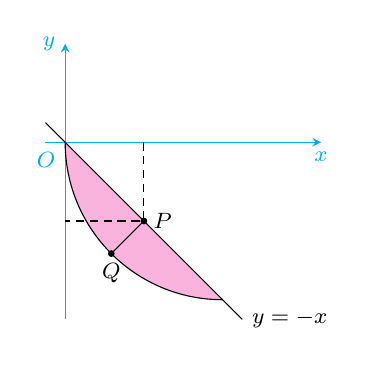
\begin{tikzpicture}[->,samples=100,>=stealth,domain=-0.25:2.25,font=\footnotesize]
                \coordinate (xMin) at (-0.25,0);
                \coordinate (xMax) at (3.25,0);
                \coordinate (yMin) at (0,-2.25);
                \coordinate (yMax) at (0,1.25);
                \draw[->, cyan] (xMin)--(0,0) node [below left] {$O$}--(xMax) node[below] {$x$};
                \draw[->, cyan] (yMin)--(yMax) node [left] {$y$};
                %\draw[black] (2,0) circle (2);
                \draw[fill=magenta!30,-] (0,0) arc(180:270:2);
                \draw[-] plot(\x,-\x) node[right] {$y=-x$};
                \draw[densely dashed,-] (1,0) -- (1,-1) node [right] {$P$} -- (0,-1);
                \draw[fill=black] (1,-1) circle(1pt); \draw[fill=black] (0.586,-1.414) circle(1pt);
                \draw[-] (1,-1) -- (0.586,-1.414) node [below] {$Q$};
            \end{tikzpicture}
        \end{figure}
    \end{minipage}\hfill
    \begin{minipage}{0.68\linewidth}
        \begin{enumerate}[label=(\arabic{*})]
            \item $P$ 点的坐标为 $\qty(\dfrac{t}{\sqrt{2}},-\dfrac{t}{\sqrt{t}})$, 所以直线 $PQ$ 的方程为 $$y=x-\sqrt{2}~ (0\leqslant t\leqslant 2\sqrt{2})$$
                  由 $\begin{cases}
                          y=x-\sqrt{2}t \\x^2+y^2=4x
                      \end{cases}$ 解得点 $Q$ 的横坐标为 $$x_Q=1+\dfrac{t}{\sqrt{2}}-\dfrac{1}{2}\sqrt{4+4\sqrt{2}t-2t^2}$$
                  所以 $|PQ|=\sqrt{2}\qty(\dfrac{t}{\sqrt{2}}-x_Q)=\sqrt{2}\qty(\dfrac{1}{2}\sqrt{4+4\sqrt{2}t-2t^2}-1).$
            \item 所求旋转体体积为
                  \begin{flalign*}
                      V & =\pi\int_{0}^{2\sqrt{2}}|PQ|^2\dd t=2\pi\int_{0}^{2\sqrt{2}}\qty(\dfrac{1}{2}\sqrt{4+4\sqrt{2}t-2t^2}-1)^2\dd t \\
                        & =\dfrac{20}{3}\sqrt{2}\pi-2\sqrt{2}\pi^2.
                  \end{flalign*}
        \end{enumerate}
    \end{minipage}
\end{solution}

\begin{example}
    求曲线 $y=\e^{-x}\sqrt{\sin x}~~(x\geqslant 0)$ 与 $x$ 轴围成区域绕 $x$ 轴旋转一周所得旋转体体积.
\end{example}
\begin{solution}
    由曲线可知定义域 $x\in\qty[2n\pi,(2n+1)\pi]~~(n=0,1,2,\cdots)$, 那么体积为
    \begin{flalign*}
        V_n & =\sum_{n=0}^{\infty}\int_{2n\pi}^{(2n+1)\pi}\pi y^2\dd x=\sum_{n=0}^{\infty}\int_{2n\pi}^{(2n+1)\pi}\pi\e^{-2x}\sin x\dd x=-\dfrac{\pi}{5}\sum_{n=0}^{\infty}\e^{-2x}(2\sin x+\cos x)\biggl |_{2n\pi}^{(2n+1)\pi}          \\
            & =\dfrac{\pi}{5}\sum_{n=0}^{\infty}\qty(\e^{-(4n+2)\pi}+\e^{-4n\pi})=\dfrac{\pi}{5}\sum_{n=0}^{\infty}\e^{-2n\pi}=\dfrac{\pi}{5}\cdot\lim_{n\to\infty}\dfrac{1-\e^{-2n\pi}}{1-\e^{-2\pi}}=\dfrac{\pi}{5\qty(1-\e^{-2\pi})}.
    \end{flalign*}
\end{solution}

\subsubsection{平面曲线的弧长}

\begin{theorem}[平面曲线弧长公式]
    \index{平面曲线弧长公式}若平面曲线的方程为 $y=f(x)~ (a\leqslant x\leqslant b)$, 则 $x$ 介于 $a$ 与 $b$ 之间的曲线弧长为:
    $$s=\int_{a}^{b}\sqrt{1+\qty(y')^2}\dd x=\int_{a}^{b}\sqrt{1+\qty[f'(x)]^2 }\dd x.$$
    若方程由极坐标给出: $r=r(\theta)~ (\alpha\leqslant \theta\leqslant \beta)$, 则 $\theta$ 介于 $\alpha$ 与 $\beta$ 之间的曲线弧长为:
    $$s=\int_{\alpha}^{\beta}\sqrt{r^2(\theta)+\qty[r'(\theta)]^2}\dd \theta.$$
    若方程由参数方程给出: $x=\varphi(t),~y=\psi(t)~ (\alpha\leqslant t\leqslant \beta)$, 则 $t$ 介于 $\alpha$ 与 $\beta$ 之间的曲线弧长为:
    $$s=\int_{\alpha}^{\beta}\sqrt{\qty[\varphi'(t)]^2+\qty[\psi'(t)]^2}\dd t.$$
\end{theorem}

\begin{example}
    计算 $\displaystyle \int_{L}|y|\dd s$, 其中 $L$ 为双纽线 $\qty(x^2+y^2)^2=a^2\qty(x^2-y^2)~~(a>0).$
\end{example}
\begin{solution}
    令 $\begin{cases}
            x=r\cos\theta \\
            y=r\sin\theta
        \end{cases}$ 代入直角坐标系方程, 得 $r^2=a^2\qty(\cos^2\theta-\sin^2\theta)=a^2\cos 2\theta$, 由 $r=0$ 得 $\theta=\dfrac{\pi}{4}$, 从而双纽线在第一象限部分的方程为 $r^2=a^2\cos2\theta,~0\leqslant\theta\leqslant \dfrac{\pi}{4}$,
    并且 $$\dd s=\sqrt{r^2+\qty(r')^2}\dd \theta=\sqrt{a^2\cos2\theta+\dfrac{a^4\sin ^22\theta}{r^2}}\dd \theta=\dfrac{a}{\sqrt{\cos 2\theta}}\dd \theta$$
    由对称性 $\displaystyle \int_{L}|y|\dd s=4\int_{0}^{\frac{\pi}{4}}r\sin\theta\cdot\dfrac{a}{\sqrt{\cos 2\theta}}\dd \theta=4a^2\int_{0}^{\frac{\pi}{4}}\sin\theta\dd \theta=4a^2\qty(1-\dfrac{\sqrt{2}}{2})$.
\end{solution}

\begin{example}[2010 数二]
    当 $0\leqslant\theta\leqslant \pi$ 时, 求对数螺线 $r=\e^{\theta}$ 的弧长.
\end{example}
\begin{solution}
    $\displaystyle s=\int_{0}^{\pi}\sqrt{r^2+\qty(r')^2}\dd \theta=\sqrt{2}\int_{0}^{\pi}\e^\theta\dd \theta=\sqrt{2}\qty(\e^{\pi}-1).$
\end{solution}

\begin{example}[2011 数一]
    求曲面\label{tantdt} $\displaystyle y=\int_{0}^{x}\tan t\dd t~ \qty(0\leqslant x\leqslant \dfrac{\pi}{4})$ 的弧长 $s$.
\end{example}
\begin{solution}
    因为 $y'=\tan x$, 所以
    $$s=\int_{0}^{\frac{\pi}{4}}\sqrt{1+\tan^2x}\dd x=\int_{0}^{\frac{\pi}{4}}\sec x\dd x=\eval{\ln|\sec x+\tan x|}_{0}^{\frac{\pi}{4}}=\ln\qty(1+\sqrt{2}).$$
\end{solution}

\begin{example}[2019 数二]
    求曲线 $y=\ln\cos x\qty(0\leqslant x\leqslant \dfrac{\pi}{6})$ 的弧长.
\end{example}
\begin{solution}
    与例题 \ref{tantdt} 同样地, $\displaystyle s=\int_{0}^{\frac{\pi}{6}}\sqrt{1+\tan^2x}\dd x=\dfrac{1}{2}\ln 3.$
\end{solution}

\begin{example}
    求曲线 $\displaystyle 4y=\int_{0}^{2} x\sqrt{12-x^2u^2} \dd u~(x\geqslant 0)$ 的全长.
\end{example}
\begin{solution}
    令 $xu=t$, 那么 $$
        \int_{0}^{2} x\sqrt{12-x^2u^2} \dd u=\int_{0}^{2x} \sqrt{12-t^2} \dd t
    $$
    则 $\displaystyle y=\dfrac{1}{4}\int_{0}^{2x} \sqrt{12-t^2} \dd t, y'=\sqrt{3-x^2}$, 那么 $3-x^2\geqslant 0\Rightarrow x\in \qty[0,\sqrt{3}]~(x\geqslant 0)$, 于是曲线全长
    $$
        s=\int_{0}^{\sqrt{3}} \sqrt{1+\qty(y')^2} \dd x=\int_{0}^{\sqrt{3}} \sqrt{4-x^2} \dd x\xlongequal{\frac{x}{2}=\sin\theta}\int_{0}^{\frac{\pi}{3}} 4\cos^2\theta \dd \theta=\dfrac{2\pi}{3}+\dfrac{\sqrt{3}}{2}.
    $$
\end{solution}

\begin{example}
    点 $P$ 在曲线 $\begin{cases}
            x=a\cos ^3t \\
            y=a\sin ^3t
        \end{cases}t\in\qty[0,\dfrac{\pi}{2}],a>0$ 上两点 $A(a,0)$ 与 $B(0,a)$ 之间, 并且曲线 $BP$ 的长度是曲线 $AP$ 长度的 3 倍, 求 $P$ 点坐标.
\end{example}
\begin{solution}
    设 $P$ 点坐标为 $(a\cos^3t_0,a\sin^3t_0)$, 并且弧微分
    \begin{flalign*}
        \dd s=\sqrt{\qty[x'(t)]^2+\qty[y'(t)]^2}\dd t=\sqrt{\qty(-3a\cos^2t\cdot\sin t)^2+\qty(3a\sin^2t\cdot\cos t)^2}\dd t=\sqrt{9a^2\sin^2t\cos^2t}\dd t=\dfrac{3a}{2}|\sin 2t|\dd t
    \end{flalign*}
    则曲线 $AP$ 的长度是曲线 $AB$ 长度的 $\dfrac{1}{4}$, 因此有
    $$\int_{0}^{t_0}\dd s=\dfrac{1}{4}\int_{0}^{\frac{\pi}{2}}\dd s\Rightarrow \int_{0}^{t_0}\sin2t\dd t=\dfrac{1}{4}\int_{0}^{\frac{\pi}{2}}\sin 2t\dd t\Rightarrow \cos 2t_0=\dfrac{1}{2}\Rightarrow t_0=\dfrac{\pi}{6}$$
    于是 $P$ 点坐标为 $\qty(\dfrac{3\sqrt{3}a}{8},\dfrac{a}{8}).$
\end{solution}

\begin{example}
    求曲线弧 $r=a\sin^3\dfrac{\theta}{3}~~(a>0)$ 的全长.
\end{example}
\begin{errorSolution}
    弧微分 $\dd s=\sqrt{r^2(\theta)+\qty[r'(\theta)^2]}\dd \theta=\sqrt{a^2\sin^6\dfrac{\theta}{3}+a^2\sin^4\dfrac{\theta}{3}\cos^2\dfrac{\theta}{3}}\dd \theta=a\sin^2\dfrac{\theta}{3}\dd \theta$, 那么弧长为\\
    \begin{minipage}{0.24\linewidth}
        \begin{figure}[H]
            \centering
            \includegraphics[scale=0.4]{figures/sin3 3pi.pdf}
            \caption{}
        \end{figure}
    \end{minipage}\hfill
    \begin{minipage}{0.75\linewidth}
        $$l=\int_{0}^{2\pi}a\sin^2\dfrac{\theta}{3}\dd \theta=a\int_{0}^{2\pi}\dfrac{1}{2}\qty(1-\cos\dfrac{2\theta}{3})\dd \theta=\eval{\dfrac{a}{2}\qty(\theta-\dfrac{3}{2}\sin\dfrac{2\theta}{3})}_{0}^{2\pi}=\pi a+\dfrac{3\sqrt{3}a}{8}.$$
        \textbf{错因: }$\theta$ 的变化范围并不是 $[0,2\pi]$, 事实上, 当 $\theta=0$ 时 $r=0$, 当 $\theta$ 从 0 开始增大时, $r$ 也从 $0$ 开始增大, 当 $\theta=\dfrac{3\pi}{2}$ 时, $r=a$ 达到最大; 根据对称性, 当 $\theta$ 继续增大时,  $\theta$ 减少, 当 $\theta$ 增大到 $3\pi$ 时, $r$ 减少到 0, 此时, 点 $(r,\theta)$ 的轨迹已经形成一条封闭曲线, 可见, $\theta$ 的变化范围是 $[0,3\pi]$.
    \end{minipage}
\end{errorSolution}
\begin{solution}
    $l=\displaystyle\int_{0}^{3\pi}a\sin^2\dfrac{\theta}{3}\dd \theta=\eval{\dfrac{a}{2}\qty(\theta-\dfrac{3}{2}\sin\dfrac{2\theta}{3})}_{0}^{3\pi}=\dfrac{3a\pi}{2}.$
\end{solution}

\begin{example}
    已知星形线 $\begin{cases}
            x=a\cos^3t \\ y=a\sin^3t
        \end{cases}(a>0)$ 求:
    \begin{enumerate}[label=(\arabic{*})]
        \item 它所围的面积;
        \item 它的弧长;
        \item 它绕 $x$ 轴旋转而成的旋转体的表面积.
    \end{enumerate}
\end{example}
\begin{solution}
    \begin{enumerate}[label=(\arabic{*})]
        \item $\displaystyle S=4\int_{0}^{a} y \dd x=4\int_{\frac{\pi}{2}}^{0} a\sin^3t\qty(-3a\cos^2t\sin t) \dd t=12a^2\int_{0}^{\frac{\pi}{2}} \sin^4t\cos^2t \dd t=\dfrac{3}{8}\pi a^2.$
        \item $\displaystyle L=4\int_{0}^{\frac{\pi}{2}} \sqrt{x'^2+y'^2} \dd t=4\int_{0}^{\frac{\pi}{2}} \sqrt{9a^2\cos^4t\sin^2t+9a^2\sin^4t\cos^2t} \dd t=12a\int_{0}^{\frac{\pi}{2}} \sin t \dd \sin t=6a.$
        \item $\displaystyle S=2\int_{0}^{a} 2\pi y\sqrt{1+\qty(y'_x)^2} \dd x=4\pi a\int_{0}^{\frac{\pi}{2}} \sin^3t\cdot 3a \cos t\sin t \dd t=\dfrac{12}{5}\pi a^2.$
    \end{enumerate}
\end{solution}

\begin{example}
    设心形线为 $r=a(1+\cos\theta)~ (a>0)$, 试用定积分计算:
    \begin{enumerate}[label=(\arabic{*})]
        \item 它所围成的图形的面积 $A$;
        \item 它的长度 $L$;
        \item 它所围成的图形 $D$ 的重心 ($D$ 的密度为 1);
        \item 它自身的重心 $C$;
        \item 它绕极轴旋转所得闭曲面所围立体的体积 $V$;
        \item 它绕极轴旋转所得闭曲面的面积 $S$;
        \item 它对极轴的转动惯量 $I$ (线密度为 1).
    \end{enumerate}
\end{example}
\begin{solution}
    \begin{minipage}{0.81\linewidth}
        \begin{enumerate}[label=(\arabic{*})]
            \item $\displaystyle A=2\cdot\dfrac{1}{2}\int_{0}^{\pi}a^2(1+\cos\theta)^2\dd \theta=a^2\int_{0}^{\pi}\qty(1+2\cos\theta+\cos^2\theta)\dd \theta=\dfrac{3\pi}{2}a^2$.
            \item $\displaystyle L=2\int_{0}^{\pi}\sqrt{r^2(\theta)+\qty[r'(\theta)]^2}\dd \theta=2\sqrt{2}a\int_{0}^{\pi}\sqrt{1+\cos\theta}\dd \theta=4a\int_{0}^{\pi}\cos\dfrac{\theta}{2}\dd \theta   =8a$.
            \item 设重心坐标 $C$ 为 $(\xi,\eta)$, $D$ 在极轴上方的一半区域为 $D_1$, 由对称性知 $\eta=0$, 下求 $\xi$, \newline
                  \textbf{法一: }用静力矩微元法, 这里从略.\newline
                  \textbf{法二: }利用二重积分求 $\xi$,
                  \begin{flalign*}
                      \xi & =\dfrac{1}{M}\iint\limits_{D_1}\rho x\dd \sigma=\dfrac{1}{M}\int_{0}^{\pi}\dd \theta\int_{0}^{a(1+\cos\theta)}r^2\cos\theta\dd r=\dfrac{a^3}{3M}\int_{0}^{\pi}(1+\cos\theta)^3\cos\theta\dd \theta \\
                          & =\dfrac{a^3}{3M}\int_{0}^{\pi}\qty(\cos\theta+3\cos^2\theta++3\cos^3\theta+\cos^4\theta)\dd \theta=\dfrac{5a}{6}
                  \end{flalign*}
                  其中 $M=\dfrac{1}{2}A\cdot\rho=\dfrac{1}{2}A=\dfrac{3\pi}{4}a^2.$
        \end{enumerate}
    \end{minipage}\hfill
    \begin{minipage}{0.18\linewidth}
        \begin{figure}[H]
            \centering
            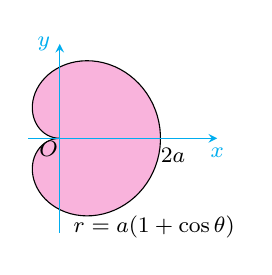
\begin{tikzpicture}[->,samples=100,>=stealth,scale=0.8,font=\footnotesize]
                \draw[-,domain=-pi:pi,fill=magenta!30]plot({1.6*cos(\x/2 r)*cos(\x r)},{1.6*cos(\x/2 r)*sin(\x r)});
                \draw[->,cyan](-0.5,0)--(2.5,0)node[below]{$x$};
                \draw[->,cyan](0,-1.5)--(0,1.5)node[left]{$y$};
                \node at(-5pt,-5pt){$O$};\node[below]at(1.8,0){$2a$};
                \node at(1.5,-1.4){$r=a(1+\cos\theta)$};
            \end{tikzpicture}
            \caption{}
        \end{figure}
    \end{minipage}
    \begin{enumerate}[label=(\arabic{*})]
        \setcounter{enumi}{3}
        \item 设心形线 $\Gamma$ 的上半条为 $\Gamma_1$, 设 $\Gamma,\Gamma_1$ 的重心分别为 $(\xi,\eta)$ 和 $(\xi_1,\eta_1)$, 由对称性知 $\xi=\xi_1,\eta=\eta_1=0$, 因为 $\Gamma_1$ 对 $y$ 轴的
              静力矩微元为 $$\dd M_y=r(\theta)\cos\theta\cdot\rho\dd s=r(\theta)\cos\theta\sqrt{r^2(\theta)+\qty[r'(\theta)]^2}\dd \theta$$
              从而, 有
              \begin{flalign*}
                  M_y & =\int_{0}^{\pi}\dd M_y=\int_{0}^{\pi}r(\theta)\cos\theta\sqrt{r^2(\theta)+\qty[r'(\theta)]^2}\dd \theta=\sqrt{2}a^2\int_{0}^{\pi}(1+\cos\theta)^{\frac{3}{2}}\cos\theta\dd \theta           \\
                      & =4a^2\int_{0}^{\pi}\qty(2\cos^5\dfrac{\theta}{2}-\cos^3\dfrac{\theta}{2})\dd \theta \xlongequal{\frac{\theta}{2}=t}8a^2\int_{0}^{\frac{\pi}{2}}\qty(2\cos^5t-\cos^3t)\dd t=\dfrac{16a^2}{5}
              \end{flalign*}
              由有 (2) 知, $\Gamma$ 的长度为 $8a$, 于是 $\Gamma$ 的质量为 $M=\dfrac{L}{2}\cdot\rho=4a$
              所以 $\xi=\dfrac{M_y}{M_1}=\dfrac{4a}{5}$, 从而知 $C\qty(\dfrac{4a}{5},0)$.
    \end{enumerate}
    \begin{minipage}{0.81\linewidth}
        \begin{enumerate}[label=(\arabic{*})]
            \setcounter{enumi}{4}
            \item 由 $r=a(1+\cos \theta)$ 可得 $$x=a(1+\cos \theta)\cos\theta=a\qty[\qty(\cos\theta+\dfrac{1}{2})^2-\dfrac{1}{4}]\geqslant-\dfrac{a}{4},~y=a(1+\cos\theta)\sin\theta$$
                  体积元 $\dd V=\pi y^2(\theta)\dd x(\theta)$, 于是
                  \begin{flalign*}
                      V & =\int_{\frac{2\pi}{3}}^{0}\pi y^2(\theta)\dd x(\theta)-\int_{\frac{2\pi}{3}}^{\pi}\pi y^2(\theta)\dd x(\theta)=\int_{\pi}^{0}y^2(\theta)\dd x(\theta)          \\
                        & =\int_{\pi}^{0}\pi\qty[a(1+\cos\theta)]^2\qty[a(1+\cos\theta)\cos\theta]'\dd \theta=\pi a^3\int_{0}^{\pi}\sin^3\theta(1+\cos\theta)^2(1+2\cos\theta)\dd \theta \\
                        & \xlongequal{\cos\theta=t}\pi a^3\int_{1}^{-1}\qty(t^2-1)(1+t)^2(1+2t)\dd t=\pi a^3\int_{-1}^{1}\qty(1+4t^2-5t^4)\dd t=\dfrac{8\pi}{3}a^3.
                  \end{flalign*}
            \item 因为 $\dd S=2\pi y(\theta)\dd s(\theta)=2\pi r(\theta)\sin \theta\sqrt{r^2(\theta)+\qty[r'(\theta)]^2}\dd \theta$, 所以, 有
                  \begin{flalign*}
                      S & =\int_{0}^{\pi}2\pi r(\theta)\sin \theta\sqrt{r^2(\theta)+\qty[r'(\theta)]^2}\dd \theta=2\sqrt{2}\pi a^2\int_{0}^{\pi}\sin\theta(1+\cos\theta)^{\frac{3}{2}}\dd \theta \\
                        & =-2\sqrt{2}\pi a^3\int_{0}^{\pi}(1+\cos\theta)^{\frac{3}{2}}\dd (1+\cos\theta)=\dfrac{32\pi}{5}a^2.
                  \end{flalign*}
            \item 因为 $\dd I=y^2(\theta)\rho \dd s(\theta)=r^2(\theta)\sin^2\theta\sqrt{r^2(\theta)+\qty[r'(\theta)]^2}\dd \theta$, 所以, 有
                  \begin{flalign*}
                      I & =2\int_{0}^{\pi}r^2(\theta)\sin^2\theta\sqrt{r^2(\theta)+\qty[r'(\theta)]^2}\dd \theta=2\sqrt{2}a^3\int_{0}^{\pi}\sin^2\theta(1+\cos\theta)^{\frac{5}{2}}\dd \theta                        \\
                        & =64a^3\int_{0}^{\pi}\sin^2\dfrac{\theta}{2}\cos^7\dfrac{\theta}{2}\dd \theta \xlongequal{\frac{\theta}{2}=t}128a^3\int_{0}^{\frac{\pi}{2}}\qty(\cos^7t-\cos^9t)\dd t=\dfrac{2048}{315}a^3.
                  \end{flalign*}
        \end{enumerate}
    \end{minipage}\hfill
    \begin{minipage}{0.18\linewidth}
        \begin{figure}[H]
            \centering
            \tdplotsetmaincoords{70}{135}
            \begin{tikzpicture}[line join=bevel,tdplot_main_coords,->,samples=100,>=stealth,fill opacity=.5,scale=0.8,font=\footnotesize]
                \coordinate (xMin) at ( -1.75,   0,  0);
                \coordinate (xMax) at ( 1.5,    0,  0);
                \coordinate (yMin) at ( 0,  -1.75,   0);
                \coordinate (yMax) at ( 0,  1.5,    0);
                \coordinate (zMin) at ( 0,  0,  -1);
                \coordinate (zMax) at ( 0,  0,  2.3);
                \pgfsetlinewidth{.1pt}
                \tdplotsphericalsurfaceplot[parametricfill]{72}{36}{1+1*cos(\tdplottheta)}{black}{\tdplotphi}%
                {\draw[->, cyan] (xMin) -- (0,0,0) node [below right] {$O$} -- (xMax) node[anchor=north east]{$y$};}
                {\draw[->, cyan] (yMin) -- (0,0,0) -- (yMax) node[anchor=north west]{$z$};}
                {\draw[->, cyan] (zMin) -- (0,0,0) -- (zMax) node[anchor=south]{$x$};}
            \end{tikzpicture}
            \caption{}
        \end{figure}
    \end{minipage}
\end{solution}

\subsection{定积分的物理应用}

\subsubsection{变力所做的功}

\begin{theorem}[变力的功]
    若质点沿变力 $F(x)$ 方向从 $x=a$ 到 $x=b$ 做直线运动, 则变力所做的功为:\index{变力的功}
    $$W=\int_{a}^{b}F(x)\dd x.$$
\end{theorem}

\begin{example}
    由 $y=-\sqrt{1-x^2}$ 与 $y=1-x^2$ 所围成的区域绕 $y$ 轴旋转而成的几何体容器 $\Omega$ 内充满水, 若将水从顶部抽取出来, 求所做的功.
\end{example}
\begin{solution}
    设将上半部分水取出做功为 $w_1$, 下半部分为 $w_2$, 取 $[y,y+\dd y]\subset[0,1]$, 则
    $$
        \dd w_1=g\dd m\cdot(1-y)=\rho g\dd v(1-y)=\pi \rho g(1-y)x^2\dd y=\pi \rho g(1-y)^2\dd y
    $$
    那么 $$
        w_1=\int_{0}^{1} w_1 \dd y=\pi\rho g\int_{0}^{1} (1-y)^2 \dd y=\dfrac{\pi \rho g}{3}
    $$
    同理, 取 $[y,y+\dd y]\subset[-1,0]$
    $$
        \dd w_2=g \dd m\cdot (1-y)=\rho g\dd v(1-y)=\pi \rho g(1-y)x^2\dd y=\pi \rho g(1-y)\qty(1-y^2)\dd y
    $$
    那么 $$
        w_2=\int_{-1}^{0} \dd w_2 =\pi \rho g \int_{-1}^{0} (1-y)\qty(1-y^2) \dd y=\dfrac{11\pi \rho  g}{12}
    $$
    所做的功为 $w=w_1+w_2=\dfrac{5\pi\rho g}{4}$.
\end{solution}

\subsubsection{物体的质量与重心}

\begin{theorem}[质量与重心坐标公式]
    若 $f(x)$ 代表细棒的质量密度, 细棒所占区间为 $[a,b]$, 则细棒的质量为:
    $$M=\int_{a}^{b}f(x)\dd x.$$
    重心坐标为:
    $$\overline{x}=\dfrac{1}{M}\int_{a}^{b}xf(x)\dd x.$$
\end{theorem}

\subsection{定积分综合性问题}

\subsubsection{函数性质的计算题}

\begin{example}
    设 $f(x)$ 在 $[0,+\infty)$ 上可导, $f(0)=0$, 其反函数为 $g(x)$, 若 $\displaystyle \int_{x}^{x+f(x)} g(t-x) \dd t=x^2\ln(1+x)$, 求 $f(x)$.
\end{example}
\begin{solution}
    令 $t-x=u$, 则有 $ \displaystyle \int_{0}^{f(x)} g(u) \dd u=x^2\ln(1+x) $, 两边对 $x$ 求导得
    \begin{flalign*}
        f'(x)\cdot g(f(x))=2x\ln(1+x)+\dfrac{x^2}{1+x}\Rightarrow f'(x)=2\ln(1+x)+\dfrac{x}{1+x}
    \end{flalign*}
    于是 $$
        f(x)=\int\qty[2\ln(1+x)+\dfrac{x}{1+x}]\dd x=(2x+1)\ln(1+x)-x-2+C
    $$
    又 $f(0)=0$, 解得 $C=2$, 故 $f(x)=(2x+1)\ln(1+x)-x.$
\end{solution}

\subsubsection{积分等式命题的证明}

% \begin{example}
%     设 $ f(x) $ 在 $ [a, b] $ 上有二阶导数, 且 $ f^{\prime \prime}(x) $ 在 $ [a, b] $ 上黎曼可积, 证明:
%     $$f(x)=f(a)+f^{\prime}(a)(x-a)+\int_{a}^{x}(x-t) f^{\prime \prime}(t) \dd  t, \forall x \in[a, b] .$$
% \end{example}
% \begin{proof}[{\songti \textbf{证法一}}]
%     由 N-L 公式,
%     \begin{flalign*}
%         f(x) & =f(a)+\int_{a}^{x}f'(t)\dd t=f(a)+\int_{a}^{x}f'(a)\dd t+\int_{a}^{x}\dd t\int_{a}^{t}f''(u)\dd u \\
%              & =f(a)+f'(a)(x-a)+\int_{a}^{x}\dd t\int_{t}^{x}f''(u)\dd u=f(a)+f'(a)(x-a)+\int_{a}^{x}(x-t).
%     \end{flalign*}
% \end{proof}
% \begin{proof}[{\songti \textbf{证法二}}]
%     即证 $\displaystyle \int_{a}^{x}(x-t)f''(t)\dd t=f(x)-f(a)-f'(a)(x-a)$, 由表格积分法:
%     \begin{table}[H]
%         \centering
%         \begin{tabular}{l| c c c}
%             $f'$   & $(x-t)$     & $1$         & $0$    \\
%             \midrule
%                    & $+\searrow$ & $-\searrow$          \\
%             \midrule
%             $\int$ & $f''(t)$    & $f'(t)$     & $f(t)$
%         \end{tabular}
%     \end{table}
%     于是 $\displaystyle \int_{a}^{x}(x-t)f''(t)\dd t=[(x-t)f'(t)-f(t)]_a^x=-f(x)-(x-a)f'(a)+f(a)$, 整理得证.
% \end{proof}

\begin{example}
    设 $f(x)\in D(0,1),~f(0)=f(1)=-2,~\displaystyle\int_{0}^{1}f(x)\dd x=0$, 证明: $\exists\xi\in(0,1)$, 使得 $$f'(\xi)-f(\xi)=\xi.$$
\end{example}
\begin{proof}[{\songti \textbf{证}}]
    令 $F(x)=\e^{-x}(f(x)+x+1)$, 有 $F(0)=-1,~F(1)=0$, 因为 $\displaystyle\int_{0}^{1}f(x)\dd x=0$, 由积分中值定理知, $\exists\eta\in(0,1)$, 使得
    $$\displaystyle\int_{0}^{1}f(x)\dd x=f(\eta)\int_{0}^{1}\dd x=f(\eta)=0$$
    而 $F(\eta)=\e^{-\eta}(f(\eta)+\eta+1)>0$, 因此 $\exists\xi\in(0,1)$, 使得 $F(x)\leqslant F(\xi)$, 即 $F(x)$ 的最大值一定在区间 $(0,1)$ 内取到,
    由 Fermat 引理知, $F'(\xi)=0$, 即 $$\eval{-\e^{-x}(f(x)+x+1)+\e^{-x}(f'(x)+1)}_{x=\xi}=f'(\xi)-f(\xi)=\xi.$$
\end{proof}

\begin{example}
    设 $f(x)$ 在 $[2,4]$ 上二阶连续可导, $f(3)=0$, 证明: $\exists\xi\in(2,4)$, 使得 $\displaystyle f''(\xi)=3\int_{2}^{4}f(x)\dd x.$
\end{example}
\begin{proof}[{\songti \textbf{证}}]
    构造 $\displaystyle F(x)=\int_{2}^{x}f(t)\dd t$, 那么将  $F(2),F(4)$ 分别在 $x=3$ 处 Taylor 展开, 有
    \begin{flalign*}
        F(2)=F(3)+F'(3)(2-3)+\dfrac{1}{2!}F''(3)(2-3)^2+\dfrac{1}{3!}F'''(\xi_1)(2-3)^3 \\
        F(4)=F(3)+F'(3)(4-3)+\dfrac{1}{2!}F''(3)(4-3)^2+\dfrac{1}{3!}F'''(\xi_2)(4-3)^3
    \end{flalign*}
    注意到 $F(2)=F'(3)=0$, 那么上式化为 $\begin{cases}
            0=F(3)+\dfrac{1}{2}F''(3)-\dfrac{1}{6}F'''(\xi_1) \\[6pt]
            F(4)=F(3)+\dfrac{1}{2}F''(3)+\dfrac{1}{6}F'''(\xi_2)
        \end{cases}$
    即 $$F(4)=\dfrac{1}{6}\qty(F'''(\xi_1)+F'''(\xi_2))$$
    因为 $F'''(x)=f''(x)$ 在 $[2,4]$ 上连续, 故 $F'''(x)$ 在 $[2,4]$ 上有最大值 $M$ 和最小值 $m$, 使得
    $$m\leqslant \dfrac{1}{2}\qty(F'''(\xi_1)+F'''(\xi_2))\leqslant M$$
    又由连续函数的介值定理知 $\exists\xi\in(\xi_1,\xi_2)\subset(2,4)$, 使得 $$F'''(\xi)=\dfrac{1}{2}\qty(F'''(\xi_1)+F'''(\xi_2))$$
    故 $F(4)=\dfrac{1}{3}\cdot\dfrac{1}{2}\qty(F'''(\xi_1)+F'''(\xi_2))=\dfrac{1}{3}F'''(\xi)$, 则
    $$F'''(\xi)=3F(4)\Rightarrow f''(\xi)=3\int_{2}^{4}f(x)\dd x.$$
\end{proof}

\begin{example}
    设 $f(x)$ 在 $[-1,1]$ 二阶导函数连续, 证明: $\exists\xi\in[-1,1]$, 使得 $$\displaystyle\int_{-1}^{1}xf(x)\dd x=\dfrac{1}{3}[2f'(\xi)+\xi f''(\xi)].$$
\end{example}
\begin{proof}[{\songti \textbf{证}}]
    构造 $F(x)=xf(x)$, 那么 $F(x)$ 在 $[-1,1]$ 二阶导函数连续, 并且 $$F'(x)=f(x)+xf'(x),~F''(x)=2f'(x)+xf''(x)$$
    又由 Taylor 展开得,
    $$F(x)=F(0)+F'(0)x+\dfrac{1}{2!}F''(\theta x)x^2~ \theta\in(0,1)$$
    且 $F(0)=0,F'(0)=f(0)x$, 于是 $F(x)=f(0)x+\dfrac{1}{2}F''(\theta x)x^2$, 两边对 $x$ 积分, 则有,
    $$\int_{-1}^{1}F(x)\dd x=\int_{-1}^{1}f(0)x\dd x+\dfrac{F''(\theta x)}{2}\int_{-1}^{1}x^2\dd x=\dfrac{F''(\theta x)}{2}\int_{-1}^{1}x^2\dd x$$
    记 $m=\min\limits_{0\leqslant x\leqslant 1}F''(x),~M=\max\limits_{0\leqslant x\leqslant 1}F''(x)$, 于是
    $$m\int_{-1}^{1}x^2\dd x\leqslant \int_{-1}^{1}F''(\theta x)x^2\dd x\leqslant M\int_{-1}^{1}x^2\dd x$$
    即 $\dfrac{2}{3}m\leqslant\displaystyle\int_{-1}^{1}F''(\theta x)x^2\dd x\leqslant \dfrac{2}{3}M$,
    因此有 $\displaystyle m\leqslant \int_{-1}^{1}F(x)\dd x\leqslant M$, 对 $F''(x)$ 利用连续函数的介值定理, 即 $\exists\xi\in[-1,1]$, 使得 $3\displaystyle\int_{-1}^{1}F(x)\dd x=F''(\xi)$, 即得证.
\end{proof}

\begin{example}
    已知 $f(x)$ 在 $[a,b]$ 上二阶可导, $f(a)=f(b)=0$, 试证: $\exists \xi\in(a,b)$, 使得 $$\int_{a}^{b}f(x)\dd x=\frac{1}{12}f''(\xi)(a-b)^3.$$
\end{example}
\begin{proof}[{\songti \textbf{证}}]
    令 $\displaystyle F(x)=\int_{a}^{x}f(t)\dd t-\frac{1}{2}(x-a)f(x)$, $\displaystyle G(x)=-\frac{1}{12}(x-a)^3$,
    在 $[a,b]$ 上连续两次应用 Cauchy 中值定理,
    \begin{flalign*}
        \dfrac{\displaystyle\int_{a}^{b}f(x)\dd x-0}{-\dfrac{1}{12}(b-a)^3-0} & =\dfrac{F(b)-F(a)}{G(b)-G(a)}\xlongequal[a\leqslant \xi_1\leqslant b]{\text{Cauchy 中值定理}}\dfrac{F"(\xi_1)}{G'(\xi_1)}                                                                                                    \\
                                                                              & =\dfrac{\dfrac{1}{2}f(\xi_1)-\dfrac{1}{2}(\xi_1-a)f'(\xi)-0}{-\dfrac{1}{4}(\xi_1-a)^2-0}\xlongequal[a\leqslant\xi\leqslant\xi_1]{\text{Cauchy 中值定理}}\dfrac{-\dfrac{1}{2}f''(\xi)(\xi-a)}{-\dfrac{1}{2}(\xi-a)}=f''(\xi).
    \end{flalign*}
    此式同乘 $\displaystyle-\frac{1}{12}(b-a)^3=\frac{1}{12}(b-a)^3$, 即得所求.
\end{proof}

\begin{example}
    设函数 $f(x)$ 在 $[a,b]$ 上二阶可导, 证明至少存在一点 $\xi\in(a,b)$, 使得
    $$\int_{a}^{b}f(x)\dd x=f(b)(b-a)-f'(b)\dfrac{(b-a)^2}{2}+\dfrac{1}{6}(b-a)^3f''(\xi).$$
\end{example}
\begin{proof}[{\songti \textbf{证}}]
    令 $k$ 为使 $\displaystyle \int_{a}^{b}f(x)\dd x=f(b)(b-a)-f'(b)\dfrac{(b-a)^2}{2}+\dfrac{1}{6}(b-a)^3k$ 成立的实常数, 构造辅助函数
    $$F(x)=\int_{a}^{x}f(t)\dd t-f(x)(x-a)+f'(x)\dfrac{(x-a)^2}{2}-\dfrac{1}{6}(x-a)^3k$$
    则 $F(a)=F(b)=0$, 故由 Rolle 定理知 $\exists\xi\in(a,b)$, 使 $F'(\xi)=0$, 即
    $$F'(\xi)=f''(\xi)\dfrac{(\xi-a)^2}{2}-\dfrac{1}{2}(\xi-a)^2k=0$$
    得证 $k=f''(\eta)$, 故得证.
\end{proof}

\begin{example}
    设函数 $f(x)$ 在 $[a,b]$ 上具有二阶连续的导数, 证明存在 $\xi\in(a,b)$, 使得
    $$\int_{a}^{b}f(x)\dd x=(b-a)f\qty(\dfrac{a+b}{2})+\dfrac{1}{24}(b-a)^3f''(\xi).$$
\end{example}
\begin{proof}[{\songti \textbf{证法一}}]
    将 $f(x)$ 在 $\dfrac{a+b}{2}$ 处进行 Taylor 展开, 有
    $$f(x)=f\qty(\dfrac{a+b}{2})+f'\qty(\dfrac{a+b}{2})\qty(x-\dfrac{a+b}{2})+\dfrac{f''(\xi_1)}{2!}\qty(x-\dfrac{a+b}{2})$$
    因为 $f''(x)$ 在 $[a,b]$ 上连续, 所以存在最小值 $m$ 和最大值 $M$, 使 $\forall x\in[a,b]$, $m\leqslant f''(x) \leqslant M$, 于是
    $$m\int_{a}^{b}\qty(x-\dfrac{a+b}{2})^2\dd x\leqslant \int_{a}^{b}f''(\xi_1)\qty(x-\dfrac{a+b}{2})^2\dd x\leqslant M\int_{a}^{b}\qty(x-\dfrac{a+b}{2})^2\dd x$$
    从而 $\displaystyle m\leqslant \dfrac{\displaystyle \int_{a}^{b}f''(\xi_1)\qty(x-\dfrac{a+b}{2})^2\dd x}{\displaystyle \int_{a}^{b}\qty(x-\dfrac{a+b}{2})^2\dd x}\leqslant M$, 故由介值定理知, 存在 $\xi\in(a,b)$, 使得
    $$f''(\xi)=\dfrac{\displaystyle\int_{a}^{b}f''(\xi_1)\qty(x-\dfrac{a+b}{2})^2\dd x}{\displaystyle \int_{a}^{b}\qty(x-\dfrac{a+b}{2})^2\dd x}$$
    即得证 $\displaystyle\int_{a}^{b}f(x)\dd x=(b-a)f\qty(\dfrac{a+b}{2})+\dfrac{1}{24}(b-a)^3f''(\xi).$
\end{proof}
\begin{proof}[{\songti \textbf{证法二}}]
    令 $\displaystyle F(x)=\int_{a}^{x}f(t)\dd t$, 将 $F(x)$ 在 $x_0=\dfrac{a+b}{2}$ 处 Taylor 展开得
    $$F(x)  =F\left( x_{0}\right) +F'\left( x_{0}\right) \left( x-x_{0}\right) +\dfrac{F''(x)  }{2!}\left( x-x_{0}\right) ^{2}+\dfrac{F'''\left( \xi \right) }{3!}\left( x-x_{0}\right) ^{3}$$
    其中 $\xi$ 介于 $x_0$ 与 $x$ 之间, 将 $x=a$ 和 $x=b$ 代入上式, 并相减得
    $$F\left( b\right) -F\left( a\right) =\left( b-a\right) f\left( \dfrac{a+b}{2}\right) +\dfrac{1}{24}\left( b-a\right) ^{3}\dfrac{f''\left( \xi _{1}\right) +f''\left( \xi _{2}\right) }{2}$$
    其中 $a <\xi _{2} <\dfrac{a+b}{2} <\xi _{1} <b$, 不妨设 $f''(\xi_1)\leqslant f''(\xi_2)$, 则 $f''(x_1)\leqslant \dfrac{f''(\xi_1)+f''(\xi_2)}{2}\leqslant f''(\xi_2)$, 由导函数 $f''(x)$ 的 Darboux 定理或 $f''(x)$ 的连续性及介值定理知,
    $\exists\xi\in(\xi_1,\xi_2)$ 或 $(\xi_2,\xi_1)\subset (a,b)$, 使 $f''(\xi)=\dfrac{f''(\xi_1)+f''(\xi_2)}{2}$, 故 $\displaystyle\int_{a}^{b}f(x)\dd x=(b-a)f\qty(\dfrac{a+b}{2})+\dfrac{1}{24}(b-a)^3f''(\xi).$
\end{proof}
\begin{proof}[{\songti \textbf{证法三}}]
    设 $ k $ 为使 $ \displaystyle \int_{a}^{b} f(x) \dd  x=(b-a) f\left(\frac{a+b}{2}\right)+\frac{1}{24}(b-a)^{3} k $ 成立的实数, 要证结论成立, 只需证 $k=f''(\xi)$, 为此构造辅助函数
    $$ \displaystyle F(x)=\int_{a}^{x} f(t) \dd  t-(x-a) f\left(\frac{a+x}{2}\right)-\frac{1}{24}(x-a)^{3} k $$
    则 $ F(a)=F(b)=0 $, 故由 Rolle 定理, $\exists \eta \in(a, b) $, 使 $ F^{\prime}(\eta)=0 $, 即
    $$f(\eta)-f\left(\frac{a+\eta}{2}\right)-\frac{\eta-a}{2} f^{\prime}\left(\frac{a+\eta}{2}\right)-\frac{k}{8}(\eta-a)^{2}=0 $$
    又将 $ f(\eta) $ 在 $ x=\dfrac{a+\eta}{2} $ 处进行 Taylor 展开, 有
    $$f(\eta)=f\left(\dfrac{a+\eta}{2}\right)+f^{\prime}\left(\frac{a+\eta}{2}\right) \frac{\eta-a}{2}+\frac{f^{\prime \prime}(\xi)}{2 !}\left(\frac{\eta-a}{2}\right)^{2}$$
    其中 $ \xi \in\left(\dfrac{a+\eta}{2}, \eta\right) \subset(a, b) $,
    比较上述两式, 得 $ k=f^{\prime \prime}(\xi) $ 故得证.
\end{proof}
\begin{proof}[{\songti \textbf{证法四}}]
    取 $\rho\equiv1$, 首先构造数值求积公式 $\displaystyle\int_{a}^{b}f(x)\dd x\approx A_0f\qty(\dfrac{a+b}{2})$, 使其具有尽可能高的代数精度,
    为此, 取 $f(x)=1$ 使求积公式精确成立, 则有 $$A_0=b-a$$
    把 $A_0$ 代入求积公式, 取 $f(x)=x$, 代入验算知求积公式精确成立; 再取 $f(x)=x^2$, 求积公式不精确成立,
    故求积公式 $\displaystyle\int_{a}^{b}f(x)\dd x\approx (b-a)f\qty(\dfrac{a+b}{2})$ 的代数精度为 $1$;
    其次, 构造一次插值多项式
    $$P_1\qty(\dfrac{a+b}{2})=f\qty(\dfrac{a+b}{2}),~P'_1\qty(\dfrac{a+b}{2})=f'\qty(\dfrac{a+b}{2})$$
    那么 $W_2(x)=\qty(x-\dfrac{a+b}{2})^2$ 且不恒为 $0$, 又
    $$K=\int_{a}^{b}W_2(x)\dd x=\dfrac{1}{12}(b-a)^3$$
    那么至少存在一点 $\xi\in(a,b)$, 使得 $$\int_{a}^{b}f(x)\dd x=(b-a)f\qty(\dfrac{a+b}{2})+\dfrac{f''(\xi)}{2!}\cdot\dfrac{1}{12}(b-a)^3$$
    即得待证等式.
\end{proof}

\begin{example}
    设函数 $f(x)$ 在 $[a,b]$ 上具有二阶连续的导数, 证明存在一点 $\xi\in(a,b)$, 使得
    $$\int_{a}^{b}f(x)\dd x=\dfrac{b-a}{2}(f(a)+f(b))-\dfrac{1}{12}f''(\xi)(b-a)^3.$$
\end{example}
\begin{proof}[{\songti \textbf{证法一}}]
    设 $k$ 为使 $\displaystyle \int_{a}^{b}f(x)\dd x=\dfrac{b-a}{2}(f(a)+f(b))-\dfrac{1}{12}k(b-a)^3$ 成立的实常数, 则证 $k=f''(\xi)$, 为此构造辅助函数
    $$F(x)=\int_{a}^{x}f(t)\dd t-\dfrac{x-a}{2}(f(a)+f(x))+\dfrac{1}{12}k(x-a)^3$$
    那么 $F(a)=F(b)=0$, 由 Rolle 定理知, $\exists\xi_1\in(a,b)$, 使得 $F'(\xi_1)=0$, 又
    $$F'(x)=f(x)-\dfrac{1}{2}(f(x)+f(a))-\dfrac{x-a}{2}f'(x)+\dfrac{1}{4}k(x-a)^2$$
    并且注意到 $F'(a)=F'(\xi_1)=0$, 再由 Rolle 定理知, $\exists\xi\in(a,\xi_1)\subset(a,b)$, 使得 $F''(\xi)=0$, 并且
    $$F''(\xi)=-\dfrac{\xi-a}{2}f''(\xi)+\dfrac{1}{2}k(\xi-a)=0$$
    即得证 $k=f''(\xi).$
\end{proof}
\begin{proof}[{\songti \textbf{证法二}}]
    取 $\rho(x)\equiv1$, 首先构造数值求积公式 $\displaystyle\int_{a}^{b}f(x)\dd x\approx A_0f(a)+A_1f(b)$, 使其具有尽可能高的代数精度, 为此,
    分别取 $f(x)=1,x$ 使求积公式精确成立, 则有 $$\left\{\begin{matrix}
            A_0  & + & A_1  & = & b-a                \\
            aA_0 & + & bA_1 & = & \dfrac{b^2-a^2}{2}
        \end{matrix}\right.\Rightarrow A_0=A_1=\dfrac{b-a}{2} $$
    把 $A_0,~A_1$ 代入求积公式, 取 $f(x)=x^2$, 代入验算知求积公式精确成立; 再取 $f(x)=x^3$, 求积公式不精确成立,
    故求积公式 $\displaystyle\int_{a}^{b}f(x)\dd x\approx\dfrac{b-a}{2}(f(a)+f(b))$ 的代数精度为 $2$;
    其次, 构造二次插值多项式 $P_1(x)$, 使满足 $$P_1(a)=f(a),~P'_1(b)=f'(b)$$
    那么 $W_2(x)=(x-a)(x-b)\geqslant 0$ 且不恒为 $0$, 又
    $$K=\int_{a}^{b}W_2(x)\dd x=-\dfrac{1}{6}(b-a)^3$$
    那么至少存在一点 $\xi\in(a,b)$, 使得
    $$\int_{a}^{b}f(x)\dd x=\dfrac{b-a}{2}(f(a)+f(b))-\dfrac{f''(\xi)}{2!}\cdot\dfrac{1}{6}(b-a)^3$$
    即得待证等式.
\end{proof}

\begin{example}
    设函数 $f(x)$ 在 $[a,b]$ 上有三阶连续的导数, 证明至少存在一点 $\eta\in(a,b)$, 使得
    $$\int_{a}^{b}f(x)\dd x=\dfrac{b-a}{4}\qty[f(a)+3f\qty(\dfrac{a+2b}{3})]+\dfrac{(b-a)^4}{216}f'''(\eta).$$
\end{example}
\begin{proof}[{\songti \textbf{证}}]
    令 $k$ 为使 $\displaystyle\int_{a}^{b}f(x)\dd x=\dfrac{b-a}{4}\qty[f(a)+3f\qty(\dfrac{a+2b}{3})]+\dfrac{(b-a)^4}{216}k$ 成立的实常数, 要证结论成立, 只需证 $k=f'''(\eta)$,
    为此, 将上式右端移到左端, 并将 $b$ 改写为 $x$, 构造辅助函数
    $$F(x)=\int_{a}^{x}f(t)\dd t-\dfrac{x-a}{4}\qty[f(a)+3f\qty(\dfrac{a+2x}{3})]-\dfrac{(x-a)^4}{216}k,~x\in[a,b]$$
    则 $F(a)=F(b)=0$, $F(x)$ 在 $[a,b]$ 上连续且可导, 由 Rolle 定理, $\exists\xi_1\in(a,b)$, 使得 $F'(\xi_1)=0$, 又
    $$F'(x)=f(x)-\dfrac{1}{4}\qty[f(a)+3f\qty(\dfrac{a+2x}{3})]-\dfrac{x-a}{2}f'\qty(\dfrac{a+2x}{3})-\dfrac{(x-a)^3}{54}k$$
    得 $F'(a)=F'(\xi_1)=0$, 故对 $F'(x)$ 在 $[a,\xi_1]$ 上用 Rolle 定理, 得 $\exists\xi_2\in(a,\xi_1)\subset(a,b)$, 使得 $F''(\xi_2)=0$, 即
    $$F''(\xi_2)=f'(\xi_2)-f'\qty(\dfrac{a+2\xi_2}{3})-\dfrac{\xi_2-a}{3}f''\qty(\dfrac{a+2\xi_2}{3})-\dfrac{(\xi_2-a)^2}{18}k=0$$
    再将 $f'(\xi_2)$ 在 $x=\dfrac{a+2\xi_2}{3}$ 处 Taylor 展开, 有
    $$f'(\xi_2)=f'\qty(\dfrac{a+2\xi_2}{3})+f''\qty(\dfrac{a+2\xi_2}{3})\qty(\xi_2-\dfrac{a+2\xi_2}{3})+\dfrac{1}{2!}f'''(\eta)\qty(\xi_2-\dfrac{a+2\xi_3}{3})^2$$
    其中 $\eta\in\qty(\dfrac{a+2\xi_2}{3})\subset(a,b)$, 比较上述两式, 即得 $k=f'''(\eta)$, 故得证.
\end{proof}

\begin{example}
    设函数 $f(x)$ 在 $[a,b]$ 上有三阶连续的导数, 证明至少存在一点 $\xi\in(a,b)$, 使得
    $$\int_{a}^{b}f(x)\dd x=\dfrac{b-a}{4}\qty[3f\qty(\dfrac{2a+b}{3})+f(b)]-\dfrac{(b-a)^4}{216}f'''(\xi).$$
\end{example}
\begin{proof}[{\songti \textbf{证}}]
    令 $k$ 为使 $\displaystyle \int_{a}^{b}f(x)\dd x=\dfrac{b-a}{4}\qty[3f\qty(\dfrac{2a+b}{3})+f(b)]-\dfrac{(b-a)^4}{216}k$ 成立的实常数, 要证结论成立, 只需证 $k=f'''(\eta)$,
    为此, 构造辅助函数 $$F(x)=\int_{x}^{b}f(t)\dd t-\dfrac{b-x}{4}\qty[3f\qty(\dfrac{2x+b}{3})+f(b)]+\dfrac{(b-x)^4}{216}k$$
    则 $F(a)=F(b)=0$, $F(x)$ 在 $[a,b]$ 上连续且可导, 由 Rolle 定理, $\exists\xi_1\in(a,b)$, 使得 $F'(\xi_1)=0$, 又
    $$F'(x)=-f(x)+\dfrac{1}{4}\qty[3f\qty(\dfrac{2x+b}{3})+f(b)]-\dfrac{b-x}{2}f'\qty(\dfrac{2x+b}{3})-\dfrac{(b-x)^3}{54}k$$
    得 $F'(\xi_1)=F'(b)=0$, 故对 $F'(x)$ 在 $[\xi_1,b]$ 上用 Rolle 定理, 得 $\exists\xi_2\in(\xi_1,b)\subset(a,b)$, 使得 $F''(\xi_2)=0$, 即
    $$F''(\xi_2)=-f'(\xi_2)+f'\qty(\dfrac{2\xi_2+b}{3})-\dfrac{b-\xi_2}{3}f''\qty(\dfrac{2\xi_2+b}{3})+\dfrac{(b-\xi_2)^2}{18}k$$
    再将 $f'(\xi_2)$ 在 $x=\dfrac{2\xi_2+b}{3}$ 处 Taylor 展开, 有
    $$f'(\xi_2)=f'\qty(\dfrac{2\xi_2+b}{3})+f''\qty(\dfrac{2\xi_2+b}{3})\qty(\xi_2-\dfrac{2\xi_2+b}{3})+\dfrac{1}{2!}f'''(\eta)\qty(\xi_2-\dfrac{2\xi_2+b}{3})^2$$
    其中 $\eta\in\qty(\dfrac{2\xi_2+b}{3})\subset(a,b)$, 比较上述两式, 即得 $k=f'''(\eta)$, 故得证.
\end{proof}

\begin{example}
    设函数 $f(x)$ 在 $[a,b]$ 上具有四阶连续导数, 证明存在一点 $\xi\in(a,b)$, 使得
    $$\int_{a}^{b}f(x)\dd x=\dfrac{b-a}{6}\qty[f(a)+4f\qty(\dfrac{a+b}{2})+f(b)]-\dfrac{(b-a)^5}{2880}f^{(4)}(\xi).$$
\end{example}
\begin{proof}[{\songti \textbf{证法一}}]
    令 $\begin{cases}
            a=c-h \\b=c+h
        \end{cases}\Rightarrow \begin{cases}
            c=\dfrac{a+b}{2} \\[6pt]
            h=\dfrac{b-a}{2}
        \end{cases}$ 那么原式等价于
    $$\int_{c-h}^{c+h}f(x)\dd x=\dfrac{h}{3}\qty[f(c-h)+4(c)+f(c+h)]-\dfrac{h^5}{90}f^{(4)}(\xi)$$
    设 $k$ 为使上式成立的实常数, 并构造 $$F(x)=\int_{c-x}^{c+x}f(t)\dd t-\dfrac{x}{3}\qty[f(c-x)+4(c)+f(c+x)]+\dfrac{x^5}{90}k$$
    下证 $k=f^{(4)}(\xi)$, 因为 $F(0)=F(x)=0$, 由 Rolle 定理得, $\exists \xi_1\in(0,x)$, 使得 $F'(\xi_1)=0$ 又
    \begin{flalign*}
        F'(x) & =f(c+x)+f(c-x)-\dfrac{1}{3}\qty[f(c-x)+4f(c)+f(c+x)]-\dfrac{x}{3}\qty[-f'(c-x)+f'(c+x)]+\dfrac{x^4}{18}k \\
              & =\dfrac{2}{3}\qty[f(c+x)+f(c-x)]+\dfrac{x}{3}\qty[f'(c-x)-f'(c+x)]+\dfrac{x^4}{18}k-\dfrac{4}{3}f(c)
    \end{flalign*}
    因为 $F'(0)=F'(\xi_1)$, 由 Rolle 定理得, $\exists\xi_2\in(0,\xi_1)$, 使得 $F''(\xi_2)=0$, 且
    \begin{flalign*}
        F''(x) & =\dfrac{2}{3}\qty[f'(c+x)-f'(c-x)]+\dfrac{1}{3}\qty[f'(c-x)-f'(c+x)]+\dfrac{x}{3}\qty[-f''(c-x)-f''(c+x)]+\dfrac{2x^3}{9}k \\
               & =\dfrac{1}{3}\qty[f'(c+x)-f'(c-x)]-\dfrac{x}{3}\qty[f''(c-x)+f''(c+x)]+\dfrac{2x^3}{9}k
    \end{flalign*}
    又因为 $F''(0)=F''(\xi_2)$, 由 Rolle 定理得, $\exists\xi_3\in(0,\xi_2)$, 使得 $F'''(\xi_3)=0$, 且
    \begin{flalign*}
        F'''(x) & =\dfrac{1}{3}\qty[f''(c+x)+f''(c-x)]-\dfrac{1}{3}\qty[f''(c-x)+f''(c+x)]-\dfrac{x}{3}\qty[-f'''(c-x)+f'''(c+x)]+\dfrac{2x^2}{3}k \\
                & =\dfrac{x}{3}\qty[f'''(c-x)-f'''(c+x)]+\dfrac{2x^2}{3}k
    \end{flalign*}
    由 Lagrange 中值定理得, $\exists\xi\in(c-\xi_3,c+\xi_3)$, 使得 $f'''(c-\xi_3)-f'''(c+\xi_3)=-2\xi_3f^{(4)}(\xi)$, 那么
    $$-\dfrac{2}{3}\xi_3^2f^{(4)}(\xi)+\dfrac{2}{3}\xi_3^2k=0\Rightarrow k=f^{(4)}(\xi)$$
    得证 $k=f^{(4)}(x)$, 即原命题成立.
\end{proof}
\begin{proof}[{\songti \textbf{证法二}}]
    取 $\rho(x)\equiv1$, 首先构造数值求积公式 $\displaystyle\int_{a}^{b}f(x)\dd x\approx A_0\cdot f(a)+A_1\cdot f\qty(\dfrac{a+b}{2})+A_2\cdot f(b)$,
    使其具有尽可能高的代数精度, 为此, 分别取 $f(x)=1,x,x^2$ 使求积公式精确成立, 则有
    $$\left\{\begin{matrix}
            A_0    & + & A_1                       & + & A_2    & = & b-a                \\
            aA_0   & + & \dfrac{a+b}{2}A_1         & + & bA_2   & = & \dfrac{b^2-a^2}{2} \\
            a^2A_0 & + & \qty(\dfrac{a+b}{2})^2A_1 & + & b^2A_2 & = & \dfrac{b^3-a^3}{3}
        \end{matrix}\right.$$
    那么有增广矩阵
    \begin{flalign*}
        \begin{pNiceArray}{c:c}
            \vb*{A} & \vb*{B}
        \end{pNiceArray} & =\begin{pNiceArray}{ccc:c}
                                1   & 1                      & 1   & b-a                \\[6pt]
                                a   & \dfrac{a+b}{2}         & b   & \dfrac{b^2-a^2}{2} \\[6pt]
                                a^2 & \qty(\dfrac{a+b}{2})^2 & b^2 & \dfrac{b^3-a^3}{3}
                            \end{pNiceArray}
        \xrightarrow[r_3-a^2r_1]{r_2-ar_1}
        \begin{pNiceArray}{ccc:c}
            1 & 1                      & 1       & b-a                         \\[6pt]
            0 & \dfrac{b-a}{2}         & b-a     & \dfrac{(-b+a)^2}{2}         \\[6pt]
            0 & \dfrac{(b+a)^2-a^2}{4} & b^2-a^2 & \dfrac{(-b+a)^2 (b+2 a)}{3} \\
        \end{pNiceArray}                                             \\
                                & \xrightarrow[r_3\times \frac{2}{(a-b)^2}]{r_3-\frac{2\qty[\frac{1}{4}(a+b)^2-a^2]}{b-a}r_2}
        \begin{pNiceArray}{ccc:c}
            1 & 1              & 1   & b-a                 \\[6pt]
            0 & \dfrac{b-a}{2} & b-a & \dfrac{(-b+a)^2}{2} \\[6pt]
            0 & 0              & 1   & \dfrac{b-a}{6}      \\
        \end{pNiceArray}
        \xrightarrow[r_1-r_3]{r_2+(a-b)r_3}
        \begin{pNiceArray}{ccc:c}
            1 & 1              & 0 & \dfrac{(-5) (-b+a)}{6} \\[6pt]
            0 & \dfrac{b-a}{2} & 0 & \dfrac{(-b+a)^2}{3}    \\[6pt]
            0 & 0              & 1 & \dfrac{b-a}{6}         \\
        \end{pNiceArray}                                                                \\
                                & \xrightarrow[r_1-r_2]{r_2\times \frac{2}{b-a}}
        \begin{pNiceArray}{ccc:c}
            1 & 0 & 0 & \dfrac{b-a}{6}         \\[6pt]
            0 & 1 & 0 & \dfrac{(-2) (-b+a)}{3} \\[6pt]
            0 & 0 & 1 & \dfrac{b-a}{6}         \\
        \end{pNiceArray}
    \end{flalign*}
    取 $f(x)=x^3$, 代入验算知求积公式精确成立; 再令 $f(x)=x^4$, 求积公式不精确成立,
    于是 $$\displaystyle \int_{a}^{b}f(x)\dd x\approx \dfrac{b-a}{6}\qty[f(a)+4f\qty(\dfrac{a+b}{2})+f(b)]$$
    其次, 构造三次插值多项式 $P_3(x)$, 使满足
    $$P_3(a)=f(a),~P_3\qty(\dfrac{a+b}{2})=f\qty(\dfrac{a+b}{2}),~P_3(b)=f(b),~P'_3(b)=f'(b)$$
    那么 $W_4(x)=(x-a)\qty(x-\dfrac{a+b}{2})(x-b)^2\geqslant 0$ 且不恒为 $0$, 又
    $$K=\int_{a}^{b}W_4(x)\dd x=-\dfrac{1}{120}(b-a)^5$$
    那么至少存在一点 $\xi\in(a,b)$, 使得
    $$\int_{a}^{b}f(x)\dd x=\dfrac{b-a}{6}\qty[f(a)+4f\qty(\dfrac{a+b}{2})+f(b)]-\dfrac{f^{(4)}(\xi)}{4!}\cdot\dfrac{(b-a)^5}{120}$$
    即得待证等式.
\end{proof}

% \begin{example}
%     设函数 $f(x)$ 在 $[a,b]$ 上二阶可导, 证明至少存在一点 $\xi\in(a,b)$, 使得
%     $$\int_{a}^{b}f(x)\dd x=(b-a)f(b)-\dfrac{(b-a)^2}{2}f'(b)+\dfrac{1}{6}(b-a)^3f''(\xi).$$
% \end{example}
% \begin{proof}[{\songti \textbf{证}}]
%     取 $\rho\equiv1$, 首先构造数值求积公式 $\displaystyle\int_{a}^{b}f(x)\dd x\approx A_0\cdot f(b)+B_0\cdot f'(b)$, 使其具有尽可能高的代数精度, 
%     为此, 分别取 $f(x)=1,x$ 使求积公式精确成立, 则有
%     $$\left\{\begin{matrix}
%             A_0  &   &     & = & b-a                \\
%             A_0b & + & B_0 & = & \dfrac{b^2-a^2}{2}
%         \end{matrix}\right.\Rightarrow
%         \begin{cases}
%             A_0=b-a \\
%             B_0=-\dfrac{(b-a)^2}{2}
%         \end{cases}$$
%     取 $f(x)=x^2$, 代入验算知求积公式精确成立; 再令 $f(x)=x^3$, 求积公式不精确成立, 于是
%     $$\int_{a}^{b}f(x)\dd x\approx(b-a)f(b)-\dfrac{(b-a)^2}{2}f'(b)$$
%     其次, 构造一次插值多项式 $P_1(x)$, 使满足
%     $$P_1^{(l)}(b)=f^{(l)}(b)~ (l=0,1)$$
%     那么 $W_2(x)=(x-b)^2\leqslant 0$ 且不恒为 0, 又
%     $$K=\int_{a}^{b}W_2(x)\dd x=\dfrac{1}{3}(b-a)^3$$
%     那么至少存在一点 $\xi\in(a,b)$, 使得
%     $$\int_{a}^{b}f(x)\dd x=(b-a)f(b)-\dfrac{(b-a)^2}{2}f'(b)+\dfrac{f''(\xi)}{2!}\cdot\dfrac{1}{3}(b-a)^3$$
%     即得待证等式.
% \end{proof}

\begin{example}
    设函数 $f(x)$ 在 $[a,b]$ 上三阶可导, 证明至少存在一点 $\xi\in(a,b)$, 使得
    $$\int_{a}^{b}f(x)\dd x=\dfrac{b-a}{3}(2f(a)+f(b))+\dfrac{(b-a)^2}{6}f'(a)-\dfrac{f'''(\xi)}{72}(b-a)^4.$$
\end{example}
\begin{proof}[{\songti \textbf{证}}]
    取 $\rho\equiv1$, 首先构造数值求积公式 $\displaystyle\int_{a}^{b}f(x)\dd x\approx A_0\cdot f(a)+A_1\cdot f(b)+B_0\cdot f'(a)$, 使其具有尽可能高的代数精度,
    为此, 分别取 $f(x)=1,x,x^2$ 使求积公式精确成立, 则有
    $$\left\{\begin{matrix}
            A_0    & + & A_1    &   &       & = & b-a                \\[6pt]
            aA_0   & + & bA_1   & + & B_0   & = & \dfrac{b^2-a^2}{2} \\[6pt]
            a^2A_0 & + & b^2A_1 & + & 2aB_0 & = & \dfrac{b^3-a^3}{3}
        \end{matrix}\right.$$
    那么有增广矩阵
    \begin{flalign*}
        \begin{pNiceArray}{c:c}
            \vb*{A} & \vb*{B}
        \end{pNiceArray} & =\begin{pNiceArray}{ccc:c}
                                1   & 1   & 0  & b-a                \\[6pt]
                                a   & b   & 1  & \dfrac{b^2-a^2}{2} \\[6pt]
                                a^2 & b^2 & 2a & \dfrac{b^3-a^3}{3}
                            \end{pNiceArray}\xrightarrow[r_3-a^2r_1]{r_2-ar_1}
        \begin{pNiceArray}{ccc:c}
            1 & 1       & 0   & b-a                           \\[6pt]
            0 & b-a     & 1   & \dfrac{1}{2} (-b+a)^2         \\[6pt]
            0 & b^2-a^2 & 2 a & \dfrac{1}{3} (-b+a)^2 (b+2 a) \\
        \end{pNiceArray}                                    \\
                                & \xrightarrow[r_3\times \frac{1}{a-b}]{r_3-\frac{b^2-a^2}{b-a}r_2}
        \begin{pNiceArray}{ccc:c}
            1 & 1   & 0 & b-a                   \\[6pt]
            0 & b-a & 1 & \dfrac{1}{2} (-b+a)^2 \\[6pt]
            0 & 0   & 1 & \dfrac{1}{6} (-b+a)^2 \\
        \end{pNiceArray}\xrightarrow[r_1-r_2]{\substack{r_2-r_3                                     \\r_2\times \frac{1}{b-a}}}
        \begin{pNiceArray}{ccc:c}
            1 & 0 & 0 & \dfrac{1}{3} (-2) (-b+a) \\[6pt]
            0 & 1 & 0 & \dfrac{b-a}{3}           \\[6pt]
            0 & 0 & 1 & \dfrac{1}{6} (-b+a)^2    \\
        \end{pNiceArray}
    \end{flalign*}
    取 $f(x)=x^3$, 代入验算知求积公式精确成立; 再令 $f(x)=x^4$, 求积公式不精确成立, 于是
    $$\int_{a}^{b}f(x)\dd x\approx\dfrac{b-a}{3}(2f(a)+f(b))+\dfrac{(b-a)^2}{6}f'(a)$$
    其次, 构造二次插值多项式 $P_2(x)$, 使满足
    $$P_2(a)=f(a),~P'_2(a)=f'(a),~P_2(b)=f(b)$$
    那么 $W_3(x)=(x-a)^2(x-b)\leqslant 0$ 且不恒为 $0$, 又
    $$K=\int_{a}^{b}W_3(x)\dd x=-\dfrac{1}{12}(b-a)^4$$
    那么至少存在一点 $\xi\in(a,b)$, 使得
    $$\int_{a}^{b}f(x)\dd x=\dfrac{b-a}{3}(2f(a)+f(b))+\dfrac{(b-a)^2}{6}f'(a)-\dfrac{f'''(\xi)}{3!}\cdot\dfrac{1}{12}(b-a)^4$$
    即得待证等式.
\end{proof}

\begin{example}
    设函数 $f(x)$ 在 $[a,b]$ 上四阶可导, 证明至少存在一点 $\xi\in(a,b)$, 使得
    $$\int_{a}^{b}f(x)\dd x=\dfrac{b-a}{2}(f(a)+f(b))-\dfrac{(b-a)^2}{12}(f'(b)-f'(a))+\dfrac{f^{(4)}(\xi)}{720}(b-a)^5.$$
\end{example}
\begin{proof}[{\songti \textbf{证法一}}]
    由定理 \ref{twoPointTripleHermiteInterpolation}, 以及插值定理知, $f(x)=H_3(x)+R(x)$, 其中
    $$H_3(x)=\qty(1+2\dfrac{x-a}{b-a})\qty(\dfrac{x-b}{a-b})^2f(a)
        +\qty(1+2\dfrac{x-b}{a-b})\qty(\dfrac{x-a}{b-a})^2f(b)+(x-a)\qty(\dfrac{x-b}{a-b})^2f'(a)+(x-b)\qty(\dfrac{x-a}{b-a})^2f'(b)$$
    以及
    $$R(x)=\dfrac{f^{(4)}(\xi)}{720}(b-a)^4x$$
    并且可以证明 $$\int_{a}^{b}\qty(1+2\dfrac{x-a}{b-a})\qty(\dfrac{x-b}{a-b})^2\dd x=\int_{a}^{b}\qty(1+2\dfrac{x-b}{a-b})\qty(\dfrac{x-a}{b-a})^2\dd x=\dfrac{b-a}{2}$$
    以及 $$\int_{a}^{b}(x-a)\qty(\dfrac{x-b}{a-b})^2\dd x=-\int_{a}^{b}(x-b)\qty(\dfrac{x-a}{b-a})^2\dd x=\dfrac{(b-a)^2}{12}$$
    于是
    \begin{flalign*}
        \int_{a}^{b}f(x)\dd x  =\int_{a}^{b}H_3(x)\dd x+\int_{a}^{b}R(x)\dd x
        =\dfrac{b-a}{2}(f(a)+f(b))-\dfrac{(b-a)^2}{12}(f'(b)-f'(a))+\dfrac{f^{(4)}(\xi)}{720}(b-a)^5.
    \end{flalign*}
\end{proof}
\begin{proof}[{\songti \textbf{证法二}}]
    取 $\rho\equiv1$, 首先构造数值求积公式 $\displaystyle\int_{a}^{b}f(x)\dd x\approx A_0\cdot f(a)+A_1\cdot f(b)+B_0\cdot f'(a)+B_1\cdot f'(b)$, 使其具有尽可能高的代数精度,
    为此, 分别取 $f(x)=1,x,x^2,x^3$ 使求积公式精确成立, 则有增广矩阵
    \begin{flalign*}
        \begin{pNiceArray}{c:c}
            \vb*{A} & \vb*{B}
        \end{pNiceArray} & =\begin{pNiceArray}{cccc:c}
                                1   & 1   & 0    & 0    & b-a                \\[6pt]
                                a   & b   & 1    & 1    & \dfrac{b^2-a^2}{2} \\[6pt]
                                a^2 & b^2 & 2a   & 2b   & \dfrac{b^3-a^3}{3} \\[6pt]
                                a^3 & b^3 & 3a^2 & 3b^2 & \dfrac{b^4-a^4}{4}
                            \end{pNiceArray}
        \xrightarrow[i=1,2,3]{r_{i+1}-a^ir_1}
        \begin{pNiceArray}{cccc:c}
            1 & 1       & 0     & 0     & b-a                                       \\[6pt]
            0 & b-a     & 1     & 1     & \dfrac{(b-a)^2}{2}                        \\[6pt]
            0 & b^2-a^2 & 2 a   & 2 b   & \dfrac{(b-a)^2 (b+2a)}{3}                 \\[6pt]
            0 & b^3-a^3 & 3 a^2 & 3 b^2 & \dfrac{\left(b^4-4 a^3 b+3 a^4\right)}{4} \\
        \end{pNiceArray}                      \\
                                & \xrightarrow[r_4-\frac{b^3-a^3}{b-a}r_2]{r_3-\frac{b^2-a^2}{b-a}r_2}
        \begin{pNiceArray}{cccc:c}
            1 & 1   & 0              & 0             & b-a                      \\[6pt]
            0 & b-a & 1              & 1             & \dfrac{(b-a)^2 }{2}      \\[6pt]
            0 & 0   & -b+a           & b-a           & \dfrac{(b-a)^3}{6}       \\[6pt]
            0 & 0   & -b^2-a b+2 a^2 & 2 b^2-a b-a^2 & \dfrac{(b-a)^3 (b+a)}{4} \\
        \end{pNiceArray}                          \\
                                & \xrightarrow[r_4\times \frac{1}{(a-b)^2}]{r_4-\frac{2a^2-ab-b^2}{a-b}r_3}
        \begin{pNiceArray}{cccc:c}
            1 & 1   & 0   & 0   & b-a                  \\[6pt]
            0 & b-a & 1   & 1   & \dfrac{(b-a)^2}{2}   \\[6pt]
            0 & 0   & a-b & b-a & \dfrac{(b-a)^3}{6}   \\[6pt]
            0 & 0   & 0   & 1   & -\dfrac{(b-a)^2}{12} \\
        \end{pNiceArray}
        \to
        \begin{pNiceArray}{cccc:c}
            1 & 1   & 0   & 0 & b-a                  \\[6pt]
            0 & b-a & 1   & 0 & \dfrac{7(b-a)^2}{12} \\[6pt]
            0 & 0   & a-b & 0 & \dfrac{(b-a)^3 }{12} \\[6pt]
            0 & 0   & 0   & 1 & -\dfrac{(b-a)^2}{12} \\
        \end{pNiceArray}                                                     \\
                                & \xrightarrow[r_2-r_3]{r_3\times\frac{1}{a-b}}
        \begin{pNiceArray}{cccc:c}
            1 & 1   & 0 & 0 & b-a                  \\[6pt]
            0 & b-a & 0 & 0 & \dfrac{(b-a)^2}{2}   \\[6pt]
            0 & 0   & 1 & 0 & \dfrac{(b-a)^2}{12}  \\[6pt]
            0 & 0   & 0 & 1 & -\dfrac{(b-a)^2}{12} \\
        \end{pNiceArray}\xrightarrow[r_1-r_2]{r_2\times\frac{1}{b-a}}
        \begin{pNiceArray}{cccc:c}
            1 &   &   &   & \dfrac{b-a}{2}       \\[6pt]
            & 1 &   &   & \dfrac{b-a}{2}       \\[6pt]
            &   & 1 &   & \dfrac{(b-a)^2}{12}  \\[6pt]
            &   &   & 1 & -\dfrac{(b-a)^2}{12} \\
        \end{pNiceArray}
    \end{flalign*}
    取 $f(x)=x^4$, 代入验算知求积公式精确成立; 再令 $f(x)=x^5$, 求积公式不精确成立, 于是
    $$\int_{a}^{b}f(x)\dd x\approx \dfrac{b-a}{2}(f(a)+f(b))-\dfrac{(b-a)^2}{12}(f'(b)-f'(a))$$
    其次, 构造三次插值多项式 $P_3(x)$, 使满足
    $$P_3^{(l)}(a)=f^{(l)}(a),~P_3^{(l)}(b)=f^{(l)}(b)~ (l=0,1)$$
    那么 $W_4(x)=(x-a)^2(x-b)^2\geqslant 0$ 且不恒为 $0$, 又
    $$K=\int_{a}^{b}W_4(x)\dd x=\dfrac{1}{30}(b-a)^5$$
    那么至少存在一点 $\xi\in(a,b)$, 使得
    $$\int_{a}^{b}f(x)\dd x=\dfrac{b-a}{2}(f(a)+f(b))-\dfrac{(b-a)^2}{12}(f'(b)-f'(a))+\dfrac{f^{(4)}(\xi)}{4!}\cdot\dfrac{1}{30}(b-a)^5$$
    即得待证等式.
\end{proof}

\begin{example}
    设函数 $f(x)$ 在 $[a,b]$ 上具有连续导数, 证明:
    $$\lim_{n\to\infty}n\qty[\int_{a}^{b}f(x)\dd x-\dfrac{b-a}{n}\sum_{k=1}^{n}f\qty(a+\dfrac{k(b-a)}{n})]=-\dfrac{b-a}{2}[f(b)-f(a)].$$
\end{example}
\begin{proof}[{\songti \textbf{证}}]
    将区间 $[a,b]$ 等分为 $n$ 份, 记 $h=\dfrac{b-a}{n},x_k=a+kh,k=0,1,\cdots,n$, 则
    \begin{flalign*}
        I=\lim_{n\to\infty}n\qty[\int_{a}^{b}f(x)\dd x-\dfrac{b-a}{n}\sum_{k=1}^{n}f\qty(a+\dfrac{k(b-a)}{n})]=\lim_{n\to\infty}n\sum_{k=1}^{n}\int_{x_{k-1}}^{x_k}\qty(f(x)-f(x_k))\dd x
    \end{flalign*}
    由 Lagrange 中值定理, $\exists \xi_k(x)\in(x,x_k)$, 使得 $f(x)-f(x_k)=(x-x_k)f'(\xi_k(x))$, 于是
    $$I=-\lim_{n\to\infty}n\sum_{k=1}^{n}\int_{x_{k-1}}^{x_k}f'(\xi_k(x))(x_k-x)\dd x$$
    由 $f'(x)$ 在 $[a,b]$ 上连续, 故由最值定理知, $\exists m_k,M_k\in[x_{k-1},x_k]$, 使得 $m_k\leqslant f'(\xi_k(x))\leqslant M_k$, 故
    $$\dfrac{1}{2}m_kh^2=m_k\int_{x_{k-1}}^{x_k}(x_k-x)\dd x\leqslant \int_{x_{k-1}}^{x_k}f'(\xi_k(x))(x_k-x)\dd x\leqslant M_k\int_{x_{k-1}}^{x_k}(x_k-x)\dd x=\dfrac{1}{2}M_kh^2$$
    即 $\displaystyle m_k\leqslant \dfrac{2}{h^2}\int_{x_{k-1}}^{x_k}f'(\xi_k(x))(x_k-x)\dd x\leqslant M$,
    又有介值定理 $\exists \eta_k\in[x_{k-1},x_k]$, 使得
    $$\displaystyle f'(\eta_k)=\dfrac{2}{h^2}\int_{x_{k-1}}^{x_k}f'(\xi_k(x))(x_k-x)\dd x\Rightarrow \dfrac{h^2}{2}f'(\eta_k)=\int_{x_{k-1}}^{x_k}f'(\xi_k(x))(x_k-x)\dd x$$
    即 $$I=-\lim_{n\to\infty}n\sum_{k=1}^{n}\int_{x_{k-1}}^{x_k}f'(\xi_k(x))(x_k-x)\dd x=-\lim_{n\to\infty}n\sum_{k=1}^{n}\dfrac{h^2}{2}f'(\eta_k)=-\dfrac{b-a}{2}\lim_{n\to\infty}\sum_{k=1}^{n}f'(\eta_k)h$$
    又因为 $f'(x)$ 在 $[a,b]$ 上可积, 应用定积分的定义, 即得
    $$I=-\dfrac{b-a}{2}\lim_{n\to\infty}\sum_{k=1}^{n}f'(\eta_k)h=-\dfrac{b-a}{2}\int_{a}^{b}f'(x)\dd x=-\dfrac{b-a}{2}(f(b)-f(a)).$$
\end{proof}

\begin{example}[2012 东南大学]
    已知函数 $f(x)$ 在区间 $[a,b]$ 上有二阶连续导数, 记
    $$\displaystyle B_n=\int_a^bf(x)\dd x-\frac{b-a}{n}\sum_{i=1}^nf\left(a+\frac{2i-1}{2}\cdot\frac{b-a}{n}\right),~$$
    试证:$$\displaystyle\lim_{n\to\infty} n^2B_n=\frac{(b-a)^2}{24}\left(f'(b)-f'(a)\right).$$
\end{example}
\begin{proof}[{\songti \textbf{证}}]
    将 $[a,b]$ 进行 $n$ 等分, $\displaystyle h=\frac{b-a}{n},x_0=a,x_1=a+h,\cdots,x_i=a+ih,\cdots,x_n=a+nh=b$, 则
    $$B_n=\sum_{i=1}^n\int_{x_{i-1}}^{x_i}\left[f(x)-f\left(a+\frac{2i-1}{2}h\right)\right]\dd x$$
    在 $[x_{i-1},x_i]$ 上应用 $f(x)$ 在 $\displaystyle a+\frac{2i-1}{2}h$ 处 Taylor 展开, 则在 $x$ 与 $\displaystyle a+\frac{2i-1}{2}h$ 之间必存在 $\xi_i$, 使得
    \begin{flalign*}
        f(x)=  f\left(a+\frac{2i-1}{2}h\right)+f'\left(a+\frac{2i-1}{2}h\right)\left(x-a-\frac{2i-1}{2}h\right)
        +\frac{1}{2}f''(\xi_i)\left(x-a-\frac{2i-1}{2} h\right)^2
    \end{flalign*}
    于是有
    \begin{flalign*}
        B_n & =\sum_{i=1}^n\int_{x_{i-1}}^{x_i}\left[f'\left(a+\frac{2i-1}{2}h\right)\left(x-a-\frac{2i-1}{2}h\right)+\frac{1}{2}f''(\xi_i)\left(x-a-\frac{2i-1}{2}h\right)^2\right]\dd x \\
            & =\frac{1}{2}\sum_{i=1}^n\int_{x_{i-1}}^{x_i}f''(\xi_i)\left(x-a-\frac{2i-1}{2}h\right)^2\dd x
    \end{flalign*}
    因为 $f''(x)$ 在 $[x_{i-1},x_i]$ 上连续, 应用最值定理, $f''(x)$ 在 $[x_{i-1},x_i]$ 上必存在最大值 $M_i$ 和最小值 $m_i~  (i=1,2,\cdots,n)$, 于是
    $$\int_{x_{i-1}}^{x_i}f''(\xi_i)\left(x-a-\frac{2i-1}{2}h\right)^2\dd x\leqslant M_i\int_{x_{i-1}}^{x_i}\left(x-a-\frac{2i-1}{2}h\right)^2\dd x=\frac{M_i}{12}h^3$$
    $$\int_{x_{i-1}}^{x_i}f''(\xi_i)\left(x-a-\frac{2i-1}{2}h\right)^2\dd x\geqslant m_i\int_{x_{i-1}}^{x_i}\left(x-a-\frac{2i-1}{2}h\right)^2\dd x=\frac{m_i}{12}h^3$$
    则 $$m_i\leqslant\frac{12}{h^3}\int_{x_{i-1}}^{x_i}f''(\xi_i)\left(x-a-\frac{2i-1}{2}h\right)^2\dd x\leqslant M_i$$
    又有介值定理, 必存在 $\eta_i\in [x_{i-1},x_i]~  (i=1,2,\cdots,n)$, 使得
    $$\frac{12}{h^3}\int_{x_{i-1}}^{x_i}f''(\xi_i)\left(x-a-\frac{2i-1}{2}h\right)^2\dd x=f''(\eta_i)$$
    由于 $f''(x)$ 在 $[a,b]$ 上可积, 应用定积分的定义, 则有
    \begin{flalign*}
        \lim_{n\to\infty}n^2B_n & =\frac{1}{2}\lim_{n\to\infty}n^2\sum_{i=1}^n\frac{1}{12}f''(\eta_i)h^3=\frac{(b-a)^2}{24}\lim_{n\to\infty}\sum_{i=1}^nf''(\eta_i)\frac{b-a}{n} \\
                                & =\frac{(b-a)^2}{24}\int_a^bf''(x)\dd x=\frac{(b-a)^2}{24}\left(f'(b)-f'(a)\right).
    \end{flalign*}
\end{proof}

\begin{example}
    设 $f(x)\in C^4[0,1]$, 且满足 $\displaystyle \int_{0}^{1}f(x)\dd x+3f\qty(\dfrac{1}{2})=8\int_{\frac{1}{4}}^{\frac{3}{4}}f(x)\dd x$, 证明: $\exists c\in(0,1)$, 使得 $f^{(4)}(c)=0.$
\end{example}
\begin{proof}[{\songti \textbf{证}}]
    因为 $\displaystyle\int_{0}^{1}f(x)\dd x\xlongequal{x=t+\frac{1}{2}}\int_{-\frac{1}{2}}^{\frac{1}{2}}f\qty(t+\dfrac{1}{2})\dd t,~\int_{\frac{1}{4}}^{\frac{3}{4}}f(x)\dd x\xlongequal{x=\frac{t}{2}+\frac{1}{2}}\dfrac{1}{2}\int_{-\frac{1}{2}}^{\frac{1}{2}}f\qty(\dfrac{t}{2}+\dfrac{1}{2})\dd t$, 所以
    $$\int_{-\frac{1}{2}}^{\frac{1}{2}}f(t+\dfrac{1}{2})\dd t-4\int_{\frac{1}{2}}^{\frac{1}{2}}f\qty(\dfrac{t}{2}+\dfrac{1}{2})\dd t +3f\qty(\dfrac{1}{2})=0$$
    令 $g(x)=f\qty(x+\dfrac{1}{2})+f\qty(-x+\dfrac{1}{2})$, $h(x)=g(x)-4g\qty(\dfrac{x}{2})$, 那么
    $$h(0)=-3g(0)=-6f\qty(\dfrac{1}{2})\Rightarrow f\qty(\dfrac{1}{2})=-\dfrac{1}{2}h(0)$$
    那么
    \begin{flalign*}
        \int_{-\frac{1}{2}}^{\frac{1}{2}}f\qty(t+\dfrac{1}{2})\dd t-4\int_{\frac{1}{2}}^{\frac{1}{2}}f\qty(\dfrac{t}{2}+\dfrac{1}{2})\dd t -\dfrac{1}{2}h(0)=0
        \Rightarrow \int_{0}^{\frac{1}{2}}h(t)\dd t-\dfrac{1}{2}h(0)=0\Rightarrow \dfrac{1}{\dfrac{1}{2}-0}\int_{0}^{\frac{1}{2}}h(t)\dd t=h(0)
    \end{flalign*}
    因为 $m=\min\limits_{x\in[0,1]}h(x)\leqslant h(0)\leqslant \max\limits_{x\in[0,1]}h(x)=M$, 所以 $\exists\xi_1\in(0,\dfrac{1}{2})$, 使得 $h'(\xi_1)=0$, 又
    $$h'(x)=g'(x)-2g'\qty(\dfrac{x}{2}),g'(x)=f'\qty(x+\dfrac{1}{2})-f\qty(-x+\dfrac{1}{2})$$
    所以 $h'(0)=0=h'(\xi_1)$, 由 Rolle 定理知, $\exists\xi_2\in(0,\xi_1)\subset \qty(0,\dfrac{1}{2})$, 使得 $h''(\xi_2)=0$, 又
    $$h''(x)=g''(x)-g''\qty(\dfrac{x}{2}),g''(x)=f''\qty(x+\dfrac{1}{2})+f''\qty(-x+\dfrac{1}{2})$$
    所以 $h''(\xi_2)=g''(\xi_2)=g''\qty(\dfrac{\xi_2}{2})$, 由 Rolle 定理知, $\exists\xi_3\in\qty(\dfrac{\xi_2}{2},\xi_2)\subset\qty(0,\dfrac{1}{2})$, 使得 $g'''(\xi_3)=0$, 而
    $$g'''(x)=f'''\qty(x+\dfrac{1}{2})-f'''\qty(-x+\dfrac{1}{2})$$
    所以 $f'''\qty(\xi_3+\dfrac{1}{2})=f'''\qty(-\xi_3+\dfrac{1}{2})$, 再由 Rolle 定理知, $\exists c\in\qty(-\xi_3+\dfrac{1}{2},\xi_3+\dfrac{1}{2})\subset(0,1)$ 使得 $f^{(4)}(c)=0.$
\end{proof}

\subsubsection{积分不等式命题的证明}

\begin{example}
    证明 $\displaystyle\dfrac{\sqrt{3}}{2}\pi\leqslant \int_{0}^{1}\sqrt{\frac{x^2-x+1}{x-x^2}}\dd x\leqslant \pi.$
\end{example}
\begin{proof}[{\songti \textbf{证}}]
    $\displaystyle\forall x\in[0,1],~\frac{3}{4}\leqslant x^2-x+1=\left(x-\dfrac{1}{2}\right)^2+\frac{3}{4}\leqslant 1$, 所以
    $$\dfrac{\sqrt{3}}{2}\int _{0}^{1}\dfrac{\dd x}{\sqrt{x-x^{2}}}\leqslant \int _{0}^{1}\sqrt{\dfrac{x^{2}-x+1}{x-x^{2}}}\dd x\leqslant \int _{0}^{1}\dfrac{\dd x}{\sqrt{x-x^{2}}}$$
    $\displaystyle \int _{0}^{1}\dfrac{\dd x}{\sqrt{x-x^{2}}}=\int _{0}^{1}\dfrac{\dd \left( x-\dfrac{1}{2}\right) }{\sqrt{\dfrac{1}{4}-\left( x-\dfrac{1}{2}\right)^2}}=\arcsin \left( 2x-1\right)\bigg |_0^1=\pi $,
    $\displaystyle \dfrac{\sqrt{3}}{2}\pi\leqslant \int_{0}^{1}\sqrt{\frac{x^2-x+1}{x-x^2}}\dd x\leqslant \pi.$
\end{proof}

\begin{example}
    证明: $\displaystyle \int_{0}^{\sqrt{2\pi}}\sin\qty(x^2)\dd x>\dfrac{2-\sqrt{2}}{2\sqrt{\pi}}.$
\end{example}
\begin{proof}[{\songti \textbf{证}}]
    令 $t=x^2$, 则 $\dd x=\dfrac{\dd t}{2\sqrt{t}}$, 于是
    \begin{flalign*}
        f(x) =\int_{0}^{2\pi}\sin\dfrac{\dd t}{2\sqrt{t}}=\int_{0}^{\pi}\dfrac{\sin t}{2\sqrt{t}}\dd t+\underbrace{\int_{\pi}^{2\pi}\dfrac{\sin t}{2\sqrt{t}}\dd t}_{u=t-\pi}
        =\int_{0}^{\pi}\qty(\dfrac{\sin t}{2\sqrt{t}}-\dfrac{\sin t}{2\sqrt{t+\pi}})\dd t=\dfrac{1}{2}\int_{0}^{\pi}\qty(\dfrac{2}{\sqrt{t}}-\dfrac{1}{\sqrt{t+\pi}})\sin t\dd t
    \end{flalign*}
    令 $g(t)=\dfrac{1}{\sqrt{t}}-\dfrac{1}{\sqrt{t+\pi}},~t\in(0,\pi)$, 那么 $g'(t)=-\dfrac{1}{2}t^{-\frac{3}{2}}+\dfrac{1}{2}(t+\pi)^{-\frac{3}{2}}<0$, 则 $g(t)$ 在 $[0,\pi]$ 上单调递减,
    所以 $g(t)>g_{min}(t)=g(\pi)=\dfrac{1}{\sqrt{\pi}}-\dfrac{1}{\sqrt{2\pi}}$, 则
    \begin{flalign*}
        f(x)>\dfrac{1}{2}\qty(\dfrac{1}{\sqrt{\pi}}-\dfrac{1}{\sqrt{2\pi}})\int_{0}^{\pi}\sin t\dd t=\dfrac{1}{\sqrt{\pi}}-\dfrac{1}{\sqrt{2\pi}}=\dfrac{2-\sqrt{2}}{2\sqrt{\pi}}.
    \end{flalign*}
\end{proof}

\begin{example}
    证明: $\displaystyle\int_{0}^{1}\dfrac{\sin x}{\sqrt{1-x^2}}\dd x<\int_{0}^{1}\dfrac{\cos x}{\sqrt{1-x^2}}\dd x.$
\end{example}
\begin{proof}[{\songti \textbf{证}}]
    只需证 $\displaystyle\int_{0}^{\frac{\pi}{2}}\sin(\cos t)\dd t<\int_{0}^{\frac{\pi}{2}}\cos(\sin t)\dd t$,
    即证 $$\sin(\cos t)<\cos(\sin t)~  x\in\qty(0,\dfrac{\pi}{2})$$
    因为在 $\qty(0,\dfrac{\pi}{2})$ 内 $\cos x\searrow$, 所以 $x>\sin x$, 所以有
    $\cos(\sin x)>\cos x>\sin(\cos x)$
    得证.
\end{proof}
\begin{inference}
    证明: $\displaystyle \frac{2}{\pi} < \int_{0}^{1} \frac{\sin x}{\sqrt{1-x^{2}}} \dd  x<1<\int_{0}^{1} \frac{\cos x}{\sqrt{1-x^{2}}} \dd  x<\frac{\pi}{2}-\frac{1}{2 \pi}<\frac{\pi}{2}.$
\end{inference}
\begin{proof}[{\songti \textbf{证}}]
    在 $(0,1)$ 内, 有 $\dfrac{2}{\pi}x<\sin x< x$, 所以
    $$\dfrac{2}{\pi}\int_{0}^{1}\dfrac{x}{\sqrt{1-x^2}}\dd x<\int_{0}^{1}\dfrac{\sin x}{\sqrt{1-x^2}}\dd x<\int_{0}^{1}\dfrac{x}{\sqrt{1-x^2}}\dd x$$
    又 $\displaystyle\int_{0}^{1}\dfrac{x}{\sqrt{1-x^2}}\dd x=\qty(-\sqrt{1-x^2})_0^1=1$, 所以 $\displaystyle \dfrac{2}{\pi}<\int_{0}^{1}\dfrac{\sin x}{\sqrt{1-x^2}}\dd x<1$;
    又因为在 $(0,1)$ 内, 有 $1-\dfrac{x^2}{2}<\cos x<1-2\qty(\dfrac{x}{\pi})^2$, 所以
    $$1<\dfrac{3\pi}{8}=\int_{0}^{1}\dfrac{2-x^2}{\sqrt{1-x^2}}\dd x<\int_{0}^{1}\dfrac{\cos x}{\sqrt{1-x^2}}\dd x<\int_{0}^{1}\dfrac{\dd x}{\sqrt{1-x^2}}-\dfrac{2}{\pi^2}\int_{0}^{1}\dfrac{x^2\dd x}{\sqrt{1-x^2}}=\dfrac{\pi}{2}-\dfrac{1}{2\pi}<\dfrac{\pi}{2}$$
    综上: $\displaystyle \frac{2}{\pi} < \int_{0}^{1} \frac{\sin x}{\sqrt{1-x^{2}}} \dd  x<1<\int_{0}^{1} \frac{\cos x}{\sqrt{1-x^{2}}} \dd  x<\frac{\pi}{2}-\frac{1}{2 \pi}<\frac{\pi}{2}.$
\end{proof}

\begin{example}
    设 $a,b>0$, 函数 $f(x)$ 在 $[-a,b]$ 上非负可积, 且有 $\displaystyle\int_{-a}^{b}xf(x)\dd x=0$, 证明
    $$\int_{-a}^{b}x^2f(x)\dd x\leqslant ab\int_{-a}^{b}f(x)\dd x.$$
\end{example}
\begin{proof}[{\songti \textbf{证}}]
    因为 $x\in[-a,b]$, 所以 $(x+a)(x-b)\leqslant 0\Rightarrow x^2-ab\leqslant (b-a)x$, 又 $f(x)\geqslant 0$, 所以有
    $$\int_{-a}^{b}\qty(x^2-ab)f(x)\dd x\leqslant \int_{-a}^{b}(b-a)xf(x)\dd x$$
    又 $\displaystyle\int_{-a}^{b}xf(x)\dd x=0$, 进而得证 $\displaystyle\int_{-a}^{b}x^2f(x)\dd x\leqslant ab\int_{-a}^{b}f(x)\dd x.$
\end{proof}

\begin{example}
    设 $f(x)$ 二阶可导, 且 $f''(x)\geqslant0$, $g(x)$ 为连续函数, $a\geqslant0$, 证明:
    $$\dfrac{1}{a}\int_{0}^{a}f(g(x))\dd x\geqslant f\qty(\dfrac{1}{a}\int_{0}^{a}g(x)\dd x).$$
\end{example}
\begin{proof}[{\songti \textbf{证}}]
    由 $f(x)$ 在 $x=x_0$ 处的 Taylor 展开,
    $$f(x)=f(x_0)+f'(x_0)(x-x_0)+\dfrac{1}{2!}f''(\xi)(x-x_0)^2$$
    因为 $f''(\xi)\geqslant 0$, 所以有 $f(x)\geqslant f(x_0)+f'(x_0)(x-x_0)$, 现令
    $$x=g(x),~x_0=\dfrac{1}{a}\int_{0}^{a}g(x)\dd x$$
    于是有
    $$f(g(x))\geqslant f\qty(\dfrac{1}{a}\int_{0}^{a}g(x)\dd x)+f'\qty(\dfrac{1}{a}\int_{0}^{a}g(x)\dd x)\qty(g(x)-\dfrac{1}{a}\int_{0}^{a}g(x)\dd x)$$
    对上式两边同时在 $[0,a]$ 上积分, 则由积分的保序性, 有
    \begin{flalign*}
        \int_{0}^{a}f(g(x))\dd x & \geqslant \int_{0}^{a}f\qty(\dfrac{1}{a}\int_{0}^{a}g(x)\dd x)\dd x+\int_{0}^{a}f'\qty(\dfrac{1}{a}\int_{0}^{a}g(x)\dd x)\qty(g(x)-\dfrac{1}{a}\int_{0}^{a}g(x)\dd x)\dd x \\
                                 & =af\qty(\dfrac{1}{a}\int_{0}^{a}g(x)\dd x)+f'\qty(\dfrac{1}{a}\int_{0}^{a}g(x)\dd x)\int_{0}^{a}\qty(g(x)-\dfrac{1}{a}\int_{0}^{a}g(x)\dd x)\dd x
        =af\qty(\dfrac{1}{a}\int_{0}^{a}g(x)\dd x)
    \end{flalign*}
    整理得证.
\end{proof}

\begin{example}
    设 $f:[0,1]\to[-a,b]$ 连续, 且 $\displaystyle\int_{0}^{1}f^2(x)\dd x=ab$, 证明 $\displaystyle0\leqslant \dfrac{1}{b-a}\int_{0}^{1}f(x)\dd x\leqslant \dfrac{1}{4}\qty(\dfrac{a+b}{a-b})^2.$
\end{example}
\begin{proof}[{\songti \textbf{证}}]
    因为 $-a\leqslant f(x)\leqslant b$, 所以 $\displaystyle -\dfrac{a+b}{2}\leqslant f(x)-\dfrac{b-a}{2}\leqslant \dfrac{a+b}{2}$, 两边积分得
    $$0\leqslant \int_{0}^{1}\qty(f(x)-\dfrac{b-a}{2})^2\dd x\leqslant \qty(\dfrac{a+b}{2})^2$$
    即 $\displaystyle 0\leqslant \int_{0}^{1}f^2(x)\dd x-(b-a)\int_{0}^{1}f(x)\dd x+\dfrac{(b-a)^2}{4}\leqslant \dfrac{(a+b)^2}{4}$, 将 $\displaystyle\int_{0}^{1}f^2(x)\dd x=ab$ 代入, 并整理得
    $$0\leqslant (b-a)\int_{0}^{1}f(x)\dd x\leqslant \dfrac{(b+a)^2}{4}\Rightarrow 0\leqslant \dfrac{1}{b-a}\int_{0}^{1}f(x)\dd x\leqslant \dfrac{1}{4}\qty(\dfrac{a+b}{a-b})^2.$$
\end{proof}

\begin{example}
    设函数 $f(x)$ 在 $[0,\pi]$ 上连续, $f(x)>0$, 证明 $\displaystyle \e ^{\int_{0}^{1}\ln f(x)\dd x}\leqslant \int_{0}^{1}f(x)\dd x.$
\end{example}
\begin{proof}[{\songti \textbf{证法一}}]
    将 $[0,1]~n$ 等分, 则 $\displaystyle\int_{0}^{1}f(x)\dd x=\lim_{n\to\infty}\dfrac{1}{n}\sum_{i=1}^{n}f\qty(\dfrac{i}{n})$,
    \begin{flalign*}
        \exp\int_{0}^{1}\ln f(x)\dd x=\exp\lim_{n\to\infty}\dfrac{1}{n}\sum_{i=1}^{n}\ln f\qty(\dfrac{i}{n})=\exp\lim_{n\to\infty}\ln\qty[\prod_{i=1}^{n}f\qty(\dfrac{i}{n})]^{\frac{1}{n}}=\lim_{n\to\infty}\qty[\prod_{i=1}^{n}f\qty(\dfrac{i}{n})]^{\frac{1}{n}}
    \end{flalign*}
    由几何平均数 $\leqslant $ 算术平均数, 得 $\displaystyle \qty[\prod_{i=1}^{n}f\qty(\dfrac{i}{n})]^{\frac{1}{n}}\leqslant \dfrac{1}{n}\sum_{i=1}^{n}f\qty(\frac{i}{n})$,
    故令 $n\to\infty$, 由定积分定义得 $\displaystyle \e ^{\int_{0}^{1}\ln f(x)\dd x}\leqslant \int_{0}^{1}f(x)\dd x.$
\end{proof}
\begin{proof}[{\songti \textbf{证法二}}]
    令 $ \displaystyle A=\int_{0}^{1} f(x) \dd  x $, 则由 Taylor 公式得
    $$\ln y=\ln A+\frac{1}{A}(y-A)-\frac{1}{2 \xi^{2}}(y-A)^{2} \leqslant \ln A+\frac{1}{A}(y-A)$$
    其中 $ \xi $ 介于 $ y $ 与 $ A $ 之间, 令 $ y=f(x)$, 代人上式, 再积分, 得
    $$\int_{0}^{1} \ln f(x) \dd  x \leqslant \ln A+\frac{1}{A} \int_{0}^{1}(f(x)-A) \dd  x=\ln A=\ln \left(\int_{0}^{1} f(x) \dd  x\right)$$
    故得 $ \displaystyle \e ^{\int_{0}^{1} \ln f(x) d x} \leqslant \int_{0}^{1} f(x) \dd  x .$
\end{proof}

\begin{example}
    设函数 $f(x)$ 在 $[0,1]$ 上连续, 证明 $\displaystyle \e ^{\int_{0}^{1}f(x)\dd x}\leqslant \int_{0}^{1}\e ^{f(x)}\dd x.$
\end{example}
\begin{proof}[{\songti \textbf{证}}]
    要证不等式两边取对数, 并且令 $g(x)=\e ^{f(x)}$, 即要证 $\displaystyle\int_{0}^{1}\ln g(x)\dd x\leqslant \ln\qty(\int_{0}^{1}g(x)\dd x)$,
    记 $ \displaystyle s=\int_{0}^{1} g(x) \dd  x $, 因为 $ g(x)>0$, 所以 $ \displaystyle s>0, \frac{g(x)}{s}>0, \frac{g(x)}{s}-1>-1$,
    故由已知不等式: 当 $ x>-1 $ 时, $ \ln (1+x) \leqslant x$, 可得
    \begin{flalign*}
        \int_{0}^{1}(\ln g(x)-\ln s) \dd  x & =\int_{0}^{1} \ln \frac{g(x)}{s} \dd x=\int_{0}^{1} \ln \left[1+\left(\frac{g(x)}{s}-1\right)\right] \dd  x \leqslant \int_{0}^{1}\left(\frac{g(x)}{s}-1\right) \dd  x \\
                                            & =\frac{1}{s} \cdot \int_{0}^{1} g(x) \dd  x-1=0
    \end{flalign*}
    即得证 $\displaystyle \e ^{\int_{0}^{1}f(x)\dd x}\leqslant \int_{0}^{1}\e ^{f(x)}\dd x.$
\end{proof}
\begin{inference}
    设函数 $f(x)$ 在 $[0,1]$ 上连续, 且 $f(x)>0$, 则有
    $$\e ^{\int_{0}^{1}\ln f(x)\dd x}\leqslant \int_{0}^{1}f(x)\dd x\leqslant \ln\qty(\int_{0}^{1}\e ^{f(x)}\dd x).$$
    一般地, 设函数 $f(x)$ 在 $[a,b]$ 上连续, 且 $f(x)>0$, 则
    $$\ln\qty((b-a)\qty(\int_{a}^{b}\dfrac{\dd x}{f(x)})^{-1})\leqslant \dfrac{1}{b-a}\int_{a}^{b}\ln f(x)\dd x\leqslant \ln\left(\dfrac{1}{b-a}\int_{a}^{b}f(x)\dd x\right).$$
    更为一般地, 设函数 $f(x)$ 在 $[a,b]$ 上连续, $g(x)$ 在 $(a,b)$ 内二阶可导, $g''(x)<0$, 则
    $$g\qty((b-a)\qty(\int_{a}^{b}\dfrac{\dd x}{f(x)})^{-1})\leqslant \dfrac{1}{b-a}\int_{a}^{b}g(f(x))\dd x\leqslant g\left(\dfrac{1}{b-a}\int_{a}^{b}f(x)\dd x\right).$$
\end{inference}

\begin{example}
    设函数 $f(x)$ 在 $[0,1]$ 上可导, $f(0)=0$, 且当 $x\in[0,1]$ 时, 有 $0<f'(x)\leqslant 1$, 证明
    $$\qty(\int_{0}^{1}f(x)\dd x)^2\geqslant \int_{0}^{1}f^3(x)\dd x.$$
\end{example}
\begin{proof}[{\songti \textbf{证法一}}]
    要证结论, 只需证明 $\displaystyle\qty(\int_{0}^{1}f(x)\dd x)^2\geqslant \int_{0}^{1}f^3(x)\dd x\geqslant0$,
    为此, 令 $\displaystyle F(x)=\qty(\int_{0}^{x}f(t)\dd t)^2-\int_{0}^{x}f^3(t)\dd t,~x\in[0,1]$, 则 $f(0)=0$, 且
    $$F'(x)=f(x)\cdot\qty[2\int_{0}^{x}f(t)\dd t-f^2(x)]$$
    故只需证当 $x\in[0,1]$ 时, $F'(x)\geqslant 0$ 即可, 由有题设 $f(0)=0$, 且 $f'(x)>0~ (x\in[0,1])$, 所以当 $x\in[0,1]$ 时, $f(x)\geqslant f(0)=0$,
    而因为 $F'(x)$ 的符号不易确定, 故再令 $g(x)=2\displaystyle\int_{0}^{x}f(t)\dd t-f^2(x)$, 则 $g'(x)=2f(x)\cdot \qty(1-f'(x))\geqslant 0$, 于是 $g(x)\geqslant g(0)=0$,
    从而 $F'(x)\geqslant 0$, 故当 $x\in[0,1]$ 时, $F(x)\geqslant F(0)=0$, 因而 $F(1)\geqslant 0$, 即得 $\displaystyle\qty(\int_{0}^{1}f(x)\dd x)^2\geqslant \int_{0}^{1}f^3(x)\dd x.$
\end{proof}
\begin{proof}[{\songti \textbf{证法二}}]
    同证法一, $f(x)>0$, 于是 $\displaystyle\int_{0}^{1}f^3(x)\dd x>0$, 故要证结论成立, 只需证明 $\dfrac{\qty(\displaystyle\int_{0}^{1}f(x)\dd x)^2}{\displaystyle\int_{0}^{1}f^3(x)\dd x}\geqslant 1$,
    为此, 令 $\displaystyle F(x)=\qty(\int_{0}^{x}f(t)\dd t)^2,~G(x)=\int_{0}^{x}f^3(t)\dd t$, 则两次用 Cauchy 中值定理, 有
    \begin{flalign*}
        \dfrac{\qty(\displaystyle\int_{0}^{1}f(x)\dd x)^2}{\displaystyle\int_{0}^{1}f^3(x)\dd x}=\dfrac{F(1)-F(0)}{G(1)-G(0)}=\dfrac{F'(\xi)}{G'(\xi)}=\dfrac{2\displaystyle\int_{0}^{\xi}f(t)\dd t}{f^2(\xi)}=\dfrac{2\displaystyle\int_{0}^{\xi}f(t)\dd t-2\int_{0}^{0}f(t)\dd t}{f^2(\xi)-f^2(0)}=\dfrac{1}{f'(\eta)}
    \end{flalign*}
    其中 $0< \xi<1,~0<\eta<\xi$, 而由 $f(\eta)>0,~0<f'(\eta)\leqslant 1$, 即得 $\dfrac{\qty(\displaystyle\int_{0}^{1}f(x)\dd x)^2}{\displaystyle\int_{0}^{1}f^3(x)\dd x}\geqslant 1$, 故得证.
\end{proof}

\begin{example}
    设 $f(x)$ 在 $[0,1]$ 上可导, $f(0)=0$, 且当 $x\in[0,1]$ 时, 有 $f'(x)\geqslant 1$, 证明
    $$\qty(\int_{0}^{1}f(x)\dd x)^3\leqslant \dfrac{3}{4}\int_{0}^{1}f^5(x)\dd x.$$
\end{example}

\begin{proof}[{\songti \textbf{证}}]
    因为 $f'(x)\geqslant 1>0$, 且 $f(0)=0$, 所以当 $x\in(0,1)$ 时, 有 $f(x)>0$, 则 $\dfrac{3}{4}\displaystyle\int_{0}^{1}f^5(x)\dd x>0$, 故要证结论成立, 即证
    $\displaystyle\dfrac{\qty(\displaystyle\int_{0}^{1}f(x)\dd x)^3}{\dfrac{3}{4}\displaystyle\int_{0}^{1}f^5(x)\dd x}\leqslant 1$, 为此, 令
    $$F(x)=\qty(\int_{0}^{x}f(t)\dd t)^3,~G(x)=\dfrac{3}{4}\int_{0}^{x}f^5(t)\dd t$$
    则两次用 Cauchy 中值定理, 得
    \begin{flalign*}
        \displaystyle\dfrac{\qty(\displaystyle\int_{0}^{1}f(x)\dd x)^3}{\dfrac{3}{4}\displaystyle\int_{0}^{1}f^5(x)\dd x} & =\dfrac{F(1)-F(0)}{G(1)-G(0)}=\dfrac{F'(\xi)}{G'(\xi)}=\dfrac{4\qty(\displaystyle\int_{0}^{\xi}f(t)\dd t)^2}{f^4(\xi)}=\qty(\dfrac{2\displaystyle\int_{0}^{\xi}f(t)\dd t}{f^2(\xi)})^2 \\
                                                                                                                          & =\qty(\dfrac{2\displaystyle\int_{0}^{\xi}f(t)\dd t-2\int_{0}^{0}f(t)\dd t}{f^2(\xi)-f^2(0)})^2=\dfrac{1}{\qty[f'(\eta)]^2}
    \end{flalign*}
    其中 $0<\xi<1,~0<\eta<\xi$, 而 $f'(\eta)\geqslant 1$, 即得 $\displaystyle\dfrac{\qty(\displaystyle\int_{0}^{1}f(x)\dd x)^3}{\dfrac{3}{4}\displaystyle\int_{0}^{1}f^5(x)\dd x}\leqslant 1$, 故得证.
\end{proof}

\begin{inference}
    设函数 $f(x)$ 在 $[0,+\infty)$ 上可导, 且 $f(0)=0,~0< f'(x)\leqslant \lambda$ ($\lambda$ 为正常数), 则对任意实数 $a>0$ 及 $m>1$, 证明
    $$\qty(\int_{0}^{a}f(x)\dd x)^m\geqslant \dfrac{m}{(2\lambda)^{m-1}}\int_{0}^{a}f^{2m-1}(x)\dd x.$$
\end{inference}
\begin{proof}[{\songti \textbf{证}}]
    因为 $0<f'(x)\leqslant \lambda$, 且 $f(0)=0$, 所以当 $x\in[0,+\infty)$ 时, $f(x)>0$, 于是 $$\displaystyle\dfrac{m}{(2\lambda)^{m-1}}\int_{0}^{a}f^{2m-1}(x)\dd x>0$$
    故要证结论成立, 即证 $I=\dfrac{\qty(\displaystyle\int_{0}^{a}f(x)\dd x)^m}{\dfrac{m}{(2\lambda)^{m-1}}\displaystyle\int_{0}^{a}f^{2m-1}(x)\dd x}\geqslant 1$,
    令 $$\displaystyle F(x)=\qty(\int_{0}^{x}f(t)\dd t)^m,~G(x)=\dfrac{m}{(2\lambda)^{m-1}}\int_{0}^{x}f^{2m-1}(t)\dd t$$
    则两次用 Cauchy 中值定理, 有
    \begin{flalign*}
        I & =\dfrac{F(a)-F(0)}{G(a)-G(0)}=\dfrac{F'(\xi)}{G'(\xi)}=\dfrac{\qty(2\lambda\displaystyle\int_{0}^{\xi}f(t)\dd t)^{m-1}}{f^{2m-2}(\xi)}=\qty(\dfrac{2\lambda\displaystyle\int_{0}^{\xi}f(t)\dd t}{f^2(\xi)})^{m-1} \\
          & =\qty(\dfrac{2\lambda\displaystyle\int_{0}^{\xi}f(t)\dd t-2\lambda\int_{0}^{0}f(t)\dd t}{f^2(\xi)-f^2(0)})^{m-1}=\dfrac{\lambda^{m-1}}{\qty[f'(\eta)]^{m-1}}
    \end{flalign*}
    其中 $0<\xi<a,~0<\eta<\xi$, 而由 $f(\eta)>0,~0<f'(\eta)\leqslant \lambda$, 即 $I\geqslant 1$, 故得证.
\end{proof}

\begin{example}
    设 $f(x)$ 在 $[0,+\infty)$ 连续, 在 $(0,+\infty)$ 上恒正, 且当 $x>0$ 时, $\displaystyle f^3(x)\leqslant 3\int_{0}^{x}f^2(t)\dd t$, 证明: 当 $x\geqslant 0$ 时, 恒有 $f(x)\leqslant x.$
\end{example}
\begin{solution}
    \textbf{法一: }令 $F(x)=\displaystyle\int_{0}^{x}f^2(t)\dd t$, 那么 $F(x)>0,~F'(x)=f^2(x)$, 于是 $x>0$ 时有,
    $$\qty[F'(x)]^{\frac{3}{2}}\leqslant 3F(x)\Rightarrow \dfrac{\qty[F'(x)]^{\frac{3}{2}}}{F(x)}\leqslant 3\Rightarrow \dfrac{F'(x)}{F^{\frac{2}{3}}(x)}\leqslant 3^{\frac{2}{3}}\Rightarrow \int_{0}^{x}\dfrac{F'(t)}{F^{\frac{2}{3}}(t)}\dd t\leqslant 3^{\frac{2}{3}}x$$
    不等式左边有 $\displaystyle\int_{0}^{x}F^{-\frac{2}{3}}x\dd F(x)=\eval{3F^{\frac{1}{3}}(t)}_{0}^{x}=3F^{\frac{1}{3}}(x)$, 即 $F^{\frac{2}{3}}(x)\leqslant 3^{-\frac{2}{3}}x^2$, 又因为 $\dfrac{F'(x)}{3^{\frac{2}{3}}}\leqslant F^{\frac{2}{3}}(x)$, 因此
    $$\dfrac{F'(x)}{3^{\frac{2}{3}}}\leqslant F^{\frac{2}{3}}(x)\leqslant 3^{-\frac{2}{3}}x^2\Rightarrow f^2(x)\leqslant x^2\Rightarrow f(x)\leqslant x$$
    当 $x\to0^+$ 时, $f^3\qty(0^+)\leqslant 0\Rightarrow f(0)\leqslant 0$, 综上所述, 当 $x\geqslant 0$ 时, 恒有 $f(x)\leqslant x.$\\
    \textbf{法二: }由题意可知, $f(x)\leqslant \sqrt[3]{3}\sqrt[3]{\displaystyle\int_{0}^{x}f^2(t)\dd t}$, 记 $g(x)=\sqrt[3]{\displaystyle\int_{0}^{x}f^2(t)\dd t}$, 那么 $g'(x)=\dfrac{1}{3}\qty(\displaystyle\int_{0}^{x}f^2(t)\dd t)^{-\frac{2}{3}}\cdot f^2(x)$, 在 $[0,x]$ 区间由 Lagrange 中值定理知,
    $$g(x)-g(0)=g'(\xi)\cdot x\Rightarrow \sqrt[3]{\displaystyle\int_{0}^{x}f^2(t)\dd t}=\dfrac{1}{3}\qty(\displaystyle\int_{0}^{\xi}f^2(t)\dd t)^{-\frac{2}{3}}f^2(\xi)\cdot x$$
    由 $f^3(x)\leqslant 3\displaystyle\int_{0}^{x}f^2(t)\dd t$, 可得 $\dfrac{1}{3}f^2(\xi)\leqslant \displaystyle \int_{0}^{\xi}f^2(t)\dd t$, 结合 $x^{-\frac{2}{3}}$ 关于 $x$ 单调递减可得,
    $$\qty(\int_{0}^{\xi}f^2\dd t)^{-\frac{2}{3}}\leqslant \qty(\dfrac{1}{3}f^3(\xi))^{-\frac{2}{3}}\Rightarrow f(x)\leqslant \sqrt[3]{3}\cdot\dfrac{1}{3}\qty(\dfrac{1}{3}f^3(\xi))^{-\frac{2}{3}}\cdot f^2(\xi)\cdot x=x$$
    当 $x\to0^+$ 时, $f^3\qty(0^+)\leqslant 0\Rightarrow f(0)\leqslant 0$, 综上所述, 当 $x\geqslant 0$ 时, 恒有 $f(x)\leqslant x.$
\end{solution}

\begin{theorem}[Cauchy-Schwarz 不等式]
    函数 $f(x)$ 和 $g(x)$ 在 $[a,b]$ 上连续, 则有
    $$\left(\int_{a}^{b}f(x)g(x)\dd x\right)^2\leqslant \int_{a}^{b}f^2(x)\dd x\int_{a}^{b}g^2(x)\dd x$$
    等号当且仅当 $\alpha f(x)=\beta g(x)$ 时成立, 其中 $\alpha,\beta$ 是不同时为零的常数.
    \index{Cauchy-Schwarz 不等式}
\end{theorem}

\begin{proof}[{\songti \textbf{证法一}}]
    $\forall t \in \mathbb{R} $, $x \in[a, b]$, 有 $ (t f(x)-g(x))^{2} \geqslant 0$, 即
    $$t^{2} f^{2}(x)-2 t f(x) g(x)+g^{2}(x) \geqslant 0$$
    于是有 $ \displaystyle t^{2} \int_{a}^{b} f^{2}(x) \dd  x-2 t \int_{a}^{b} f(x) g(x) \dd  x+\int_{a}^{b} g^{2}(x) \dd  x \geqslant 0, \forall t \in \mathbb{R}  $ 都成立.
    \begin{enumerate}[label=(\arabic{*})]
        \item 当 $ \displaystyle\int_{a}^{b} f^{2}(x) \dd  x=0 $ 时, 由 $ f(x) $ 在 $ [a, b] $ 上的连续性知, $f(x) \equiv 0$, 此时要证的不等式中成立;
        \item 当 $ \displaystyle\int_{a}^{b} f^{2}(x) \dd  x>0 $ 时, 由于关于 $ t $ 的二次三项式恒大于零,
              故它的判别式 $$ \Delta=\left(2 \int_{a}^{b} f(x) g(x) \dd  x\right)^{2}-4 \int_{a}^{b} f^{2}(x) \dd  x \cdot \int_{a}^{b} g^{2}(x) \dd  x \leqslant 0$$
    \end{enumerate}
    即得 $\displaystyle \left(\int_{a}^{b} f(x) g(x) \dd  x\right)^{2} \leqslant \int_{a}^{b} f^{2}(x) \dd  x \cdot \int_{a}^{b} g^{2}(x) \dd  x.$
\end{proof}
\begin{proof}[{\songti \textbf{证法二}}]
    要证结论, 即证 $ \displaystyle\int_{a}^{b} f^{2}(x) \dd  x \cdot \int_{a}^{b} g^{2}(x) \dd  x-\left(\int_{a}^{b} f(x) g(x) \dd  x\right)^{2} \geqslant 0 $,
    \begin{flalign*}
         & \int_{a}^{b} f^{2}(x) \dd  x \cdot \int_{a}^{b} g^{2}(x) \dd  x-\left(\int_{a}^{b} f(x) g(x) \dd  x\right)^{2}                                                                                             \\
         & = \frac{1}{2} \int_{a}^{b} f^{2}(x) \dd  x \int_{a}^{b} g^{2}(y) \dd  y+\frac{1}{2} \int_{a}^{b} f^{2}(y) \dd  y \int_{a}^{b} g^{2}(x) \dd  x -\int_{a}^{b} f(x) g(x) \dd  x \int_{a}^{b} f(y) g(y) \dd  y \\
         & = \frac{1}{2} \iint\limits_{D}\left[f^{2}(x) g^{2}(y)+f^{2}(y) g^{2}(x)-2 f(x) g(x) f(y) g(y)\right] \dd  x \dd  y= \frac{1}{2} \iint\limits_{D}(f(x) g(y)-f(y) g(x))^{2} \dd  x \geqslant 0
    \end{flalign*}
    其中 $D=\{(x,y)|a\leqslant x,y\leqslant b\}$, 故得 $\displaystyle \left(\int_{a}^{b} f(x) g(x) \dd  x\right)^{2} \leqslant \int_{a}^{b} f^{2}(x) \dd  x \cdot \int_{a}^{b} g^{2}(x) \dd  x.$
\end{proof}
\begin{proof}[{\songti \textbf{证法三}}]
    因为 $f(x),g(x)$ 在 $[a,b]$ 上连续, 所以 $f(x),g(x),f(x)g(x)$ 在 $[a,b]$ 上可积, 将 $[a,b]~n$ 等分, 取 $$ \displaystyle\Delta x=\frac{b-a}{n}, \xi_{i}=x_{i}=a+\frac{i}{n}(b-a)$$
    则由离散情形 的 Cauchy-Schwarz 不等式, 有
    $$\left(\sum_{i=1}^{n} f\left(x_{i}\right) g\left(x_{i}\right)\right)^{2} \leqslant\left(\sum_{i=1}^{n} f^{2}\left(x_{i}\right)\right)\left(\sum_{i=1}^{n} g^{2}\left(x_{i}\right)\right)$$
    于是得 $ \displaystyle\left(\frac{b-a}{n} \sum_{i=1}^{n} f\left(x_{i}\right) g\left(x_{i}\right)\right)^{2} \leqslant\left(\frac{b-a}{n} \sum_{i=1}^{n} f^{2}\left(x_{i}\right)\right)\left(\frac{b-a}{n} \sum_{i=1}^{n} g^{2}\left(x_{i}\right)\right)$,
    故令 $ n \to \infty $ 两边取极限, 由定积分定义得
    $\displaystyle\left(\int_{a}^{b} f(x) g(x) \dd  x\right)^{2} \leqslant \int_{a}^{b} f^{2}(x) \dd  x \int_{a}^{b} g^{2}(x) \dd  x .$
\end{proof}
\begin{proof}[{\songti \textbf{证法四}}]
    构作辅助积分上限函数, 将要证不等式中的 $ b $ 改为 $ x $, 并移项, 令
    $$F(x)=\left(\int_{a}^{x} f(t) g(t) \dd  t\right)^{2}-\int_{a}^{x} f^{2}(t) \dd  t \cdot \int_{a}^{x} g^{2}(t) \dd  t$$
    则有 $ F(a)=0, \forall x \in[a, b]$,
    \begin{flalign*}
        F^{\prime}(x) & =2 \int_{a}^{x} f(t) g(t) \dd  t \cdot f(x) g(x)-f^{2}(x) \int_{a}^{x} g^{2}(t) \dd  t-g^{2}(x) \int_{a}^{x} f^{2}(t) \dd  t \\
                      & =-\int_{a}^{x}\left[f^{2}(x) g^{2}(t)-2 f(x) f(t) g(x) g(t)+f^{2}(t) g^{2}(x)\right] \dd  t                                  \\
                      & =-\int_{a}^{x}[f(x) g(t)-f(t) g(x)]^{2} \dd t \leqslant 0,
    \end{flalign*}
    于是 $ \forall x \in[a, b], F(x) \leqslant F(a)=0 $, 从而 $ F(b) \leqslant 0$, 即得证.
\end{proof}

% \begin{example}
%     设 $f(x)$ 是区间 $[0,1]$ 上是的非负连续上凸函数, 并且 $f(0)=1$, 试证明: $$\int_{0}^{1}xf(x)\dd x\leqslant\dfrac{2}{3}\qty(\int_{0}^{1}f(x)\dd x)^2.$$
% \end{example}
% \begin{proof}[{\songti \textbf{证}}]
%     
% \end{proof}

\begin{example}
    已知 $f(x)$ 在闭区间 $[0,1]$ 上的连续函数, 且满足 $\displaystyle\int_{0}^{1} f(x)\dd x=1$, 求函数 $f(x)$, 使得 $$\displaystyle I=\int_{0}^{1}(1+x^2)f^2(x)\dd x$$ 取得最小值.
\end{example}
\begin{solution}
    由 Cauchy-Schwarz 不等式,
    \begin{flalign*}
        1^2=\qty(\int_{0}^{1}f(x)\dd x)^2=\qty(\int_{0}^{1}\sqrt{1+x^2}f(x)\cdot\dfrac{1}{\sqrt{1+x^2}}\dd x)^2\leqslant \int_{0}^{1}(1+x^2)f^2(x)\dd x\cdot\int_{0}^{1}\dfrac{\dd x}{1+x^2}
    \end{flalign*}
    所以 $I_{min}=\dfrac{4}{\pi}$, 为此, 只需要函数 $f(x)$ 满足 $$\displaystyle\int_{0}^{1}\dfrac{4}{\pi}f(x)\dd x=\int_{0}^{1}(1+x^2)f^2(x)\dd x=\dfrac{4}{\pi}\Rightarrow f(x)=\dfrac{4}{\pi(1+x^2)}.$$
\end{solution}

\begin{example}
    设 $a>0$ 为常数, 证明不等式 $$\int_{0}^{\pi}xa^{\sin x}\dd x\cdot\int_{0}^{\frac{\pi}{2}}a^{-\cos x}\dd x\geqslant\dfrac{\pi^3}{4}.$$
\end{example}
\begin{proof}[{\songti \textbf{证}}]
    令 $x=\dfrac{\pi}{2}+t$, 那么
    \begin{flalign*}
        \int_{0}^{\pi}x a^{\sin x}\dd x=\int_{-\frac{\pi}{2}}^{\frac{\pi}{2}}\qty(\dfrac{\pi}{2}+t)a^{\sin\qty(\frac{\pi}{2}+t)}\dd t=\dfrac{\pi}{2}\int_{-\frac{\pi}{2}}^{\frac{\pi}{2}}a^{\cos t}\dd t+\int_{-\frac{\pi}{2}}^{\frac{\pi}{2}}ta^{\cos t}\dd t=\pi\int_{0}^{\frac{\pi}{2}}a^{\cos t}\dd t
    \end{flalign*}
    于是由 Cauchy-Schwarz 不等式得
    \begin{flalign*}
        \int_{0}^{\pi}xa^{\sin x}\dd x\cdot\int_{0}^{\frac{\pi}{2}}a^{-\cos x}\dd x =\pi\qty(\int_{0}^{\frac{\pi}{2}}a^{\cos x}\dd x)\cdot\qty(\int_{0}^{\frac{\pi}{2}}a^{-\cos x}\dd x)
        \geqslant \pi\qty(\int_{0}^{\frac{\pi}{2}}a^{\frac{\cos x}{2}}\cdot a^{\frac{-\cos x}{2}}\dd x)^2=\dfrac{\pi^3}{4}
    \end{flalign*}
    故得证.
\end{proof}

\begin{example}
    已知 $f(x)$ 在 $[0,1]$ 上连续, 且 $1\leqslant f(x)\leqslant 3$, 证明
    $\displaystyle1\leqslant \int_{0}^{1}f(x)\dd x\cdot\int_{0}^{1}\dfrac{1}{f(x)}\dd x\leqslant \dfrac{4}{3}.$
\end{example}
\begin{proof}[{\songti \textbf{证}}]
    先证左边不等式, 由 Cauchy-Schwarz 不等式
    $$\int_{0}^{1}f(x)\dd x\cdot\int_{0}^{1}\dfrac{1}{f(x)}\dd x\geqslant \int_{0}^{1}\dd x=1$$
    再证右边不等式, 因为 $1\leqslant f(x)\leqslant 3$, 所以 $$(f(x)-1)(3-f(x))\geqslant 0\Rightarrow f(x)+\dfrac{3}{f(x)}\leqslant 4$$
    再由 A-G 不等式得
    $$\sqrt{\displaystyle\int_{0}^{1}f(x)\dd x\cdot\int_{0}^{1}\dfrac{3}{f(x)}\dd x}\leqslant \dfrac{1}{2}\qty(\int_{0}^{1}f(x)\dd x+\int_{0}^{1}\dfrac{3}{f(x)}\dd x)\leqslant 2$$
    所以 $$\int_{0}^{1}f(x)\dd x\cdot\int_{0}^{1}\dfrac{3}{f(x)}\dd x\leqslant 4\Rightarrow \int_{0}^{1}f(x)\dd x\cdot\int_{0}^{1}\dfrac{1}{f(x)}\leqslant\dfrac{4}{3}$$
    综上 $\displaystyle1\leqslant \int_{0}^{1}f(x)\dd x\cdot\int_{0}^{1}\dfrac{1}{f(x)}\dd x\leqslant \dfrac{4}{3}.$
\end{proof}
\begin{inference}
    设 $f(x)$ 在 $[a,b]$ 上连续, 且 $0<m\leqslant f(x)\leqslant M$, 则有
    $$(b-a)^2\leqslant \int_a^b f^{-1}(x)\dd x\cdot\int_a^b f(x)\dd x\leqslant \frac{(m+M)^2}{4mM}(b-a)^2$$
\end{inference}
\begin{proof}[{\songti \textbf{证}}]
    由 Cauchy-Schwarz 不等式:
    $$\displaystyle \int_a^b f^{-1}(x)\dd x\cdot\int_a^b f(x)\dd x\geqslant \left(\int _a^b\sqrt{f^{-1}(x)}\cdot\sqrt{f(x)}\dd x\right)^2=(b-a)^2$$
    \begin{flalign*}
        \frac{(f(x)-m)(f(x)-M)}{f(x)}=f(x)-(M+m)+\frac{mM}{f(x)}\leqslant 0\Rightarrow f(x)+\frac{mM}{f(x)}\leqslant M+m
    \end{flalign*}
    从而 $\displaystyle \int _a^b\left[f(x)+\frac{mM}{f(x)}\right]\dd x\leqslant (M+m)(b-a)$, 且 $\displaystyle ab\leqslant \frac{(a+b)^2}{4}$,
    \begin{flalign*}
        \text{所以 } \int_a^b\frac{mM}{f(x)}\dd x\cdot\int _a^bf(x)\dd x\leqslant \frac{1}{4}\int _a^b\left[f(x)+\frac{mM}{f(x)}\right]^2\leqslant \frac{(m+M)^2(b-a)^2}{4}
    \end{flalign*}
    综上 $\displaystyle (b-a)^2\leqslant \int _a^bf^{-1}(x)\dd x\cdot\int _a^bf(x)\dd x\leqslant \frac{(m+M)^2}{4mM}(b-a)^2.$
\end{proof}

\begin{example}
    设函数 $f(x)$ 在 $[0,1]$ 上具有一阶连续的导数, 且 $\displaystyle\int_{0}^{\frac{1}{2}}f(x)\dd x=0$, 证明
    $$\int_{0}^{1}\qty[f'(x)]^2\dd x\geqslant 12\qty(\int_{0}^{1}f(x)\dd x)^2.$$
\end{example}
\begin{proof}[{\songti \textbf{证法一}}]
    由题设 $\displaystyle\int_{0}^{\frac{1}{2}}f(x)\dd x=0$ 及分部积分公式得
    $$\int_{0}^{\frac{1}{2}}xf'(x)\dd x=xf(x)\biggl |_{0}^{\frac{1}{2}}-\int_{0}^{\frac{1}{2}}f(x)\dd x$$
    于是
    \begin{flalign*}
        \qty(\int_{0}^{1}f(x)\dd x)^2 & =\qty(\int_{0}^{\frac{1}{2}}f(x)\dd x+\int_{\frac{1}{2}}^{1}f(x))^2=\qty[\int_{\frac{1}{2}}^{1}\qty(f(x)-f\qty(\dfrac{1}{2}))+\dfrac{1}{2}f\qty(\dfrac{1}{2})]^2                                   \\
                                      & =\qty(\int_{\frac{1}{2}}^{1}\dd x\int_{\frac{1}{2}}^{x}f'(t)\dd t+\int_{0}^{\frac{1}{2}}xf'(x)\dd x)^2=\qty(\int_{\frac{1}{2}}^{1}\dd t\int_{t}^{1}f'(t)\dd x+\int_{0}^{\frac{1}{2}}xf'(x)\dd x)^2 \\
                                      & =\qty(\int_{\frac{1}{2}}^{1}(1-t)f'(t)\dd t+\int_{0}^{\frac{1}{2}}xf'(x)\dd x)^2
    \end{flalign*}
    由不等式 $(a+b)^2\leqslant 2\qty(a^2+b^2)$ 及 Cauchy-Schwarz 不等式, 有
    \begin{flalign*}
        \text{上式右端 } & \leqslant 2\qty[\qty(\int_{\frac{1}{2}}^{1}(1-t)f'(t)\dd t)^2+\qty(\int_{0}^{\frac{1}{2}}xf'(x)\dd x)^2]                                                                     \\
                         & \leqslant 2\qty[\int_{\frac{1}{2}}^{1}(1-t)^2\dd t\cdot\int_{\frac{1}{2}}^{1}\qty[f'(t)]^2\dd t+\int_{0}^{\frac{1}{2}}x^2\dd x\cdot\int_{0}^{\frac{1}{2}}\qty[f'(x)]^2\dd x]
        =\dfrac{1}{12}\int_{0}^{1}\qty[f'(x)]^2\dd x
    \end{flalign*}
    即得 $\displaystyle \int_{0}^{1}\qty[f'(x)]^2\dd x\geqslant 12\qty(\int_{0}^{1}f(x)\dd x)^2.$
\end{proof}
\begin{proof}[{\songti \textbf{证法二}}]
    构造辅助函数, 并利用 Cauchy-Schwarz 不等式, 令 $g(x)=\begin{cases}
            x   , & 0\leqslant x\leqslant \dfrac{1}{2} \\
            1-x , & \dfrac{1}{2}\leqslant x\leqslant 1
        \end{cases}$, 则
    \begin{flalign*}
        \int_{0}^{1}f'(x)g(x)\dd x & =\int_{0}^{\frac{1}{2}}xf'(x)\dd x+\int_{\frac{1}{2}}^{1}(1-x)f'(x)\dd x
        =xf(x)\biggl |_{0}^{\frac{1}{2}}-\int_{0}^{\frac{1}{2}}f(x)\dd x+(1-x)f(x)\biggl |_{\frac{1}{2}}^{1}+\int_{\frac{1}{2}}^{1}f(x)\dd x \\
                                   & =\int_{\frac{1}{2}}^{1}f(x)\dd x=\int_{0}^{1}f(x)\dd x
    \end{flalign*}
    且 $\displaystyle\int_{0}^{1}g^2(x)\dd x=\int_{0}^{\frac{1}{2}}x^2\dd x+\int_{\frac{1}{2}}^{1}(1-x)^2\dd x=\dfrac{1}{12}$, 于是有 Cauchy-Schwarz 不等式, 有
    $$\qty(\int_{0}^{1}f'(x)g(x)\dd x)^2\leqslant \int_{0}^{1}\qty[f'(x)]^2\dd x\cdot\int_{0}^{1}g^2(x)\dd x=\dfrac{1}{12}\int_{0}^{1}\qty[f'(x)]^2\dd x$$
    从而得 $\displaystyle\int_{0}^{1}\qty[f'(x)]^2\dd x\geqslant 12\qty(\int_{0}^{1}f(x)\dd x)^2.$
\end{proof}

\begin{example}
    设函数 $f(x)$ 在 $[0,1]$ 上具有一阶连续的导数, 且 $\displaystyle\int_{\frac{1}{3}}^{\frac{2}{3}}f(x)\dd x=0$, 证明
    $$\int_{0}^{1}\qty[f'(x)]^2\dd x\geqslant 27\qty(\int_{0}^{1}f(x)\dd x)^2.$$
\end{example}
\begin{proof}[{\songti \textbf{证}}]
    构造辅助函数, 并利用 Cauchy-Schwarz 不等式, 令 $g(x)=\begin{cases}
            -x   , & 0\leqslant x\leqslant \dfrac{1}{3}            \\[6pt]
            2x-1 , & \dfrac{1}{3}\leqslant x\leqslant \dfrac{2}{3} \\[6pt]
            -x+1 , & \dfrac{2}{3}\leqslant x\leqslant  1
        \end{cases}$, 则
    \begin{flalign*}
        I & =\int_{0}^{1}f'(x)g(x)\dd x=\int_{0}^{\frac{1}{3}}(-x)f'(x)\dd x+\int_{\frac{1}{3}}^{\frac{2}{3}}(2x-1)f'(x)\dd x+\int_{\frac{2}{3}}^{1}(-x+1)f'(x)\dd x                                                                       \\
          & =-xf(x)\biggl |_{0}^{\frac{1}{3}}+\int_{0}^{\frac{1}{3}}f(x)\dd x+(2x-1)f(x)\biggl |_{\frac{1}{3}}^{\frac{2}{3}}-2\int_{\frac{1}{3}}^{\frac{2}{3}}f(x)\dd x+(-x+1)f(x)\biggl |_{\frac{2}{3}}^1+\int_{\frac{2}{3}}^{1}f(x)\dd x \\
          & =\int_{0}^{\frac{1}{3}}f(x)\dd x+\int_{\frac{2}{3}}^{1}f(x)\dd x=\int_{0}^{1}f(x)\dd x
    \end{flalign*}
    且
    \begin{flalign*}
        \int_{0}^{1}g^2(x)\dd x=\int_{0}^{\frac{1}{3}}(-x)^2\dd x+\int_{\frac{1}{3}}^{\frac{2}{3}}(2x-1)^2\dd x+\int_{\frac{2}{3}}^{1}(-x+1)^2\dd x=\dfrac{1}{27}
    \end{flalign*}
    于是由 Cauchy-Schwarz 不等式得
    $$\qty(\int_{0}^{1}f'(x)g(x)\dd x)^2\leqslant \int_{0}^{1}\qty[f'(x)]^2\dd x\cdot\int_{0}^{1}g^2(x)\dd x=\dfrac{1}{27}\qty[f'(x)]^2\dd x$$
    从而得 $\displaystyle\int_{0}^{1}\qty[f'(x)]^2\dd x\geqslant 27\qty(\int_{0}^{1}f(x)\dd x)^2.$
\end{proof}

\begin{example}
    \label{f(a)f(b)0}设函数 $f(x)$ 在 $[a,b]$ 上连续可导, 且 $f(a)$ 或 $f(b)=0$, 则有
    $$\qty(\int_{a}^{b}f(x)\dd x)^2\leqslant \dfrac{(b-a)^3}{3}\int_{a}^{b}\qty[f'(x)]^2 \dd x.$$
\end{example}
\begin{proof}[{\songti \textbf{证}}]
    不妨设 $f(a)=0$ (对于 $f(b)=0$, 类似地可证), 则
    $$\int_{a}^{b}f(x)\dd x=\int_{a}^{b}f(x)\dd (x-b)=\eval{f(x)(x-b)}_{a}^{b}-\int_{a}^{b}(x-b)f'(x)\dd x=\int_{a}^{b}(b-x)f'(x)\dd x$$
    于是由 Cauchy-Schwarz 不等式得, 有
    \begin{flalign*}
        \qty(\int_{a}^{b}f(x)\dd x)^2=\qty(\int_{a}^{b}(b-x)f'(x)\dd x)^2\leqslant \int_{a}^{b}(b-x)^2\dd x\int_{a}^{b}\qty[f'(x)]^2 \dd x=\dfrac{(b-a)^3}{3}\int_{a}^{b}\qty[f'(x)]^2 \dd x
    \end{flalign*}
    即得待证等式.
\end{proof}
\begin{inference}
    设函数 $f(x)$ 在 $[a,b]$ 上连续可导, 且 $f(x_0)=0$, 则有
    $$\qty(\int_{a}^{b}f(x)\dd x)^2\leqslant M\int_{a}^{b}\qty[f'(x)]^2 \dd x$$
    其中 $M=\dfrac{2}{3}\max\limits_{a\leqslant x_0\leqslant b}\qty{(x_0-a)^3,(x_0-b)^3}$, 特别地, 当 $x_0=\dfrac{a+b}{2}$ 时, $M=\dfrac{(b-a)^3}{12}.$
\end{inference}

\begin{example}
    设函数 $f(x)$ 在 $[a,b]$ 上连续可导, 且 $f(a)=f(b)=0$, 则有
    $$\qty(\int_{a}^{b}f(x)\dd x)^2\leqslant \dfrac{(b-a)^3}{12}\int_{a}^{b}\qty[f'(x)]^2 \dd x.$$
\end{example}
\begin{proof}[{\songti \textbf{证}}]
    记 $c=\dfrac{a+b}{2}$, 则由例题 \ref{f(a)f(b)0} 可知
    \begin{flalign*}
        \qty(\int_{a}^{c}f(x)\dd x)^2\leqslant \dfrac{(c-a)^3}{3}\int_{a}^{c}\qty[f'(x)]^2 \dd x \\
        \qty(\int_{c}^{b}f(x)\dd x)^2\leqslant \dfrac{(b-c)^3}{3}\int_{c}^{b}\qty[f'(x)]^2 \dd x
    \end{flalign*}
    于是由 Cauchy-Schwarz 不等式,
    \begin{flalign*}
        \qty(\int_{a}^{b}f(x)\dd x)^2 & =\qty(\int_{a}^{c}f(x)\dd x+\int_{c}^{b}f(x)\dd x)^2\leqslant 2\qty[\qty(\int_{a}^{c}f(x)\dd x)^2+\qty(\int_{c}^{b}f(x)\dd x)^2]                     \\
                                      & \leqslant\dfrac{(b-a)^3}{12}\qty[\int_{a}^{c}\qty[f'(x)]^2 \dd x+\int_{c}^{b}\qty[f'(x)]^2 \dd x]=\dfrac{(b-a)^3}{12}\int_{a}^{b}\qty[f'(x)]^2 \dd x
    \end{flalign*}
    即得待证等式.
\end{proof}

\begin{example}
    设函数 $f(x)$ 在 $[a,b]$ 上二阶连续可导, 且 $f(a)=f(b)=0$, 则有
    $$\qty(\int_{a}^{b}f(x)\dd x)^2\leqslant \dfrac{(b-a)^5}{180}\int_{a}^{b}f''^2(x)\dd x.$$
\end{example}
\begin{proof}[{\songti \textbf{证}}]
    由已知 $f(a)=f(b)=0$ 以及分部积分公式得
    \begin{flalign*}
        \int_{a}^{b}f(x)\dd x=\int_{a}^{b}f(x)\dd (x-a)=-\int_{a}^{b}(x-a)f'(x)\dd x \\
        \int_{a}^{b}f(x)\dd x=\int_{a}^{b}f(x)\dd (x-b)=-\int_{a}^{b}(x-b)f'(x)\dd x
    \end{flalign*}
    所以
    \begin{flalign*}
        \int_{a}^{b}f(x)\dd x & =-\int_{a}^{b}(x-a)f'(x)\dd (x-b)=\int_{a}^{b}(x-a)(x-b)f''(x)\dd x+\int_{a}^{b}(x-b)f'(x)\dd x        \\
                              & =\int_{a}^{b}(x-a)(x-b)f''(x)\dd x-\int_{a}^{b}f(x)\dd x=\dfrac{1}{2}\int_{a}^{b}(x-a)(x-b)f''(x)\dd x
    \end{flalign*}
    故由 Cauchy-Schwarz 不等式得
    \begin{flalign*}
        \qty(\int_{a}^{b}f(x)\dd x)^2 & =\dfrac{1}{4}\qty[\int_{a}^{b}(x-a)(x-b)f''(x)\dd x]^2\leqslant \dfrac{1}{4}\qty(\int_{a}^{b}f''^2(x)\dd x)\qty(\int_{a}^{b}\qty[(x-a)(x-b)]^2\dd x) \\
                                      & =\dfrac{(b-a)^5}{180}\int_{a}^{b}f''^2(x)\dd x
    \end{flalign*}
    即得待证等式.
\end{proof}

\begin{example}
    \label{fafafbfb0}设函数 $f(x)$ 在 $[a,b]$ 上二阶连续可导, 且 $f(a)=f'(a)=0$ 或 $f(b)=f'(b)=0$, 则
    $$\qty(\int_{a}^{b}f(x)\dd x)^2\leqslant \dfrac{(b-a)^5}{20}\int_{a}^{b}f''^2(x)\dd x.$$
\end{example}
\begin{proof}[{\songti \textbf{证}}]
    不妨设 $f(a)=f'(a)=0$ (对于 $f(b)=f'(b)=0$, 类似地证明), 则由分部积分公式, 有
    \begin{flalign*}
        \int_{a}^{b}f(x)\dd x =\int_{a}^{b}f(x)\dd (x-b)=-\int_{a}^{b}(x-b)f'(x)\dd x
        =-\int_{a}^{b}f'(x)\dd \qty(\dfrac{(b-x)^2}{2})=\int_{a}^{b}\dfrac{(b-x)^2}{2}f''(x)\dd x
    \end{flalign*}
    于是由 Cauchy-Schwarz 不等式得
    \begin{flalign*}
        \qty(\int_{a}^{b}f(x)\dd x)^2=\qty(\int_{a}^{b}\dfrac{(b-x)^2}{2}f''(x)\dd x)^2\leqslant \int_{a}^{b}\dfrac{(b-x)^4}{4}\dd x\int_{a}^{b}f''^2(x)\dd x=\dfrac{(b-a)^5}{20}\int_{a}^{b}f''^2(x)\dd x
    \end{flalign*}
    即得待证等式.
\end{proof}

\begin{inference}
    \label{bafxdx2ban2n1}设函数 $f(x)$ 在 $[a,b]$ 上 $n$ 阶连续可导, 且 $f^{(l)}(a)=0\text{ 或 }f^{(l)}(b)=0~  (l=0,1,2,\cdots n-1)$, 则有
    $$\qty(\int_{a}^{b}f(x)\dd x)^2\leqslant \dfrac{(b-a)^{2n+1}}{(n!)^2(2n+1)}\int_{a}^{b}\qty[f^{(n)}(x)]^2\dd x.$$
\end{inference}
\begin{proof}[{\songti \textbf{证}}]
    下面以 $f^{(k)}(b)=0~ (k=-,1,\cdots,n-1)$ 为例进行证明,
    \begin{flalign*}
        \int_{a}^{b}f(x)\dd x & =\int_{a}^{b}f(x)\dd (x-a)=-\int_{a}^{b}(x-a)f'(x)\dd x=-\int_{a}^{b}f'(x)\dd \dfrac{(x-a)^2}{2}=\int_{a}^{b}\dfrac{(x-a)^2}{2}f''(x)\dd x \\
                              & =\dfrac{(-1)^2}{1\cdot 2}\int_{a}^{b}(x-a)^2f''(x)\dd x=\cdots=\dfrac{(-1)^n}{n!}\int_{a}^{b}(x-a)^nf^{(n)}(x)\dd x
    \end{flalign*}
    于是由 Cauchy-Schwarz 不等式, 得
    $$\qty(\int_{a}^{b}f(x)\dd x)^2\leqslant \dfrac{1}{(n!)^2}\int_{a}^{b}(x-a)^{2n}\dd x\cdot\int_{a}^{b}\qty[f^{(n)}(x)]\dd x=\dfrac{(b-a)^{2n+1}}{(n!)^2(2n+1)}\int_{a}^{b}\qty[f^{(n)}(x)]^2\dd x.$$
\end{proof}

\begin{example}
    设函数 $f(x)$ 在 $[a,b]$ 上二阶连续可导, 且 $f(a)=f'(a)=f(b)=f'(b)=0$, 则有
    $$\qty(\int_{a}^{b}f(x)\dd x)^2\leqslant \dfrac{(b-a)^5}{320}\int_{a}^{b}f''^2(x)\dd x.$$
\end{example}
\begin{proof}[{\songti \textbf{证}}]
    记 $c=\dfrac{a+b}{2}$, 则有例题 \ref{fafafbfb0}, 有
    \begin{flalign*}
        \qty(\int_{a}^{c}f(x)\dd x)^2\leqslant \dfrac{(c-a)^5}{20}\int_{a}^{c}f''^2(x)\dd x=\dfrac{(b-a)^5}{640}\int_{a}^{c}f''^2(x)\dd x \\
        \qty(\int_{c}^{b}f(x)\dd x)^2\leqslant \dfrac{(b-c)^5}{20}\int_{c}^{b}f''^2(x)\dd x=\dfrac{(b-a)^5}{640}\int_{c}^{b}f''^2(x)\dd x \\
    \end{flalign*}
    从而
    \begin{flalign*}
        \qty(\int_{a}^{b}f(x)\dd x)^2 =\qty(\int_{a}^{c}f(x)\dd x+\int_{c}^{b}f(x)\dd x)^2\leqslant 2\qty[\qty(\int_{a}^{c}f(x)\dd x)^2+\qty(\int_{c}^{b}f(x)\dd x)^2]
        \leqslant \dfrac{(b-a)^5}{320}\int_{a}^{b}f''^2(x)\dd x
    \end{flalign*}
    即得待证等式.
\end{proof}

\begin{inference}
    设函数 $f(x)$ 在 $[a,b]$ 上 $n$ 阶连续可导, 且 $f^{(l)}(a)=f^{(l)}(b)=0~ (l=0,1,2,\cdots,n-1)$, 则有
    $$\qty(\int_{a}^{b}f(x)\dd x)^2\leqslant \dfrac{(b-a)^{2n+1}}{2^{2n}(n!)^2(2n+1)}\int_{a}^{b}\qty[f^{(n)}(x)]^2\dd x.$$
\end{inference}
\begin{proof}[{\songti \textbf{证}}]
    记 $c=\dfrac{a+b}{2}$, 由推论 \ref{bafxdx2ban2n1}, 有
    \begin{flalign*}
        \qty(\int_{a}^{c}f(x)\dd x)^2 & \leqslant \dfrac{(c-a)^{2n+1}}{(n!)^2(2n+1)}\int_{a}^{c}\qty[f^{(n)}(x)]^2\dd x=\dfrac{(b-a)^{2n+1}}{2^{2n+1}(n!)^2(2n+1)}\int_{a}^{c}\qty[f^{(n)}(x)]\dd x \\
        \qty(\int_{c}^{b}f(x)\dd x)^2 & \leqslant \dfrac{(b-c)^{2n+1}}{(n!)^2(2n+1)}\int_{c}^{b}\qty[f^{(n)}(x)]^2\dd x=\dfrac{(b-a)^{2n+1}}{2^{2n+1}(n!)^2(2n+1)}\int_{c}^{b}\qty[f^{(n)}(x)]\dd x
    \end{flalign*}
    于是由基本不等式,
    $$\qty(\int_{a}^{b}f(x)\dd x)^2\leqslant 2\qty[\qty(\int_{a}^{c}f(x)\dd x)^2+\qty(\int_{c}^{b}f(x)\dd x)^2]\leqslant \dfrac{(b-a)^{2n+1}}{2^{2n}(n!)^2(2n+1)}\int_{a}^{b}\qty[f^{(n)}(x)]^2\dd x.$$
\end{proof}

\begin{inference}
    设函数 $f(x)$ 在 $[a,b]$ 上 $2n$ 阶连续可导, 且 $f^{(l)}(a)=f^{(l)}(b)=0~ (l=0,1,2,\cdots,n-1)$, 则有
    $$\qty(\int_{a}^{b}f(x)\dd x)^2\leqslant\dfrac{(b-a)^{2n+1}}{(4n+1)!}\int_{a}^{b}\qty[f^{(2n)}(x)]^2\dd x.$$
\end{inference}

\begin{example}
    设 $f(x)$ 在 $[a,b]$ 上有连续的导数, 且 $f\qty(\dfrac{a+b}{2})=0$, 证明:
    $$\int_{a}^{b}|f(x)f'(x)|\dd x\leqslant \dfrac{b-a}{4}\int_{a}^{b}|f'(t)|^2\dd t.$$
\end{example}
\begin{proof}[{\songti \textbf{证}}]
    注意到 $f\qty(\dfrac{a+b}{2})=0$, 那么 $$f(x)=f(x)-f\qty(\dfrac{a+b}{2})=\int_{\frac{a+b}{2}}^{x}f'(t)\dd t,~  x\in[a,b]$$
    并令 \begin{flalign*}
        g_1(x) & =\int_{x}^{\frac{a+b}{2}}|f'(t)|\dd t,~  x\in\qty[a,\dfrac{a+b}{2}] \\
        g_2(x) & =\int_{\frac{a+b}{2}}^{x}|f'(t)|\dd t,~  x\in\qty[\dfrac{a+b}{2},2]
    \end{flalign*}
    则 $g_1(x),~g_2(x)$ 分别在 $\qty[a,\dfrac{a+b}{2}]$ 和 $\qty[\dfrac{a+b}{2},b]$ 上有连续的导数, 且 $$g_1\qty(\dfrac{a+b}{2})=g_2\qty(\dfrac{a+b}{2})=0$$
    当 $x\in\qty[a,\dfrac{a+b}{2}]$ 时, $|f(x)|\leqslant g_1(x)$, $|f'(x)|=-g_1(x)$; 当 $x\in\qty[\dfrac{a+b}{2},b]$ 时, $|f(x)|\leqslant g_2(x)$, $|f'(x)|=g_2(x)$, 因此
    \begin{flalign*}
        I & =\int_{a}^{b}|f(x)f'(x)|\dd x=\int_{a}^{\frac{a+b}{2}}|f(x)f'(x)|\dd x+\int_{\frac{a+b}{2}}^{b}|f(x)f'(x)|\dd x                      \\
          & \leqslant -\int_{a}^{\frac{a+b}{2}}g_1(x)g'_1(x)\dd x+\int_{\frac{a+b}{2}}^{b}g_2(x)g'_2(x)\dd x=\dfrac{1}{2}\qty(g_1^2(a)+g_2^2(b))
    \end{flalign*}
    于是, 由 Cauchy-Schwarz 不等式得,
    \begin{flalign*}
        \int_{a}^{b}|f(x)f'(x)|\dd x & \leqslant\dfrac{1}{2}\qty(\int_{a}^{\frac{a+b}{2}}|f'(t)|\dd t)^2+\dfrac{1}{2}\qty(\int_{\frac{a+b}{2}}^{b}|f'(t)|\dd t)^2                                                         \\
                                     & \leqslant\dfrac{1}{2}\int_{a}^{\frac{a+b}{2}}|f'(t)|^2\dd t\cdot\int_{a}^{\frac{a+b}{2}}\dd t+\dfrac{1}{2}\int_{\frac{a+b}{2}}^{b}|f'(t)|^2\dd t\cdot\int_{\frac{a+b}{2}}^{b}\dd t
        =\dfrac{b-a}{4}\int_{a}^{b}|f'(t)|^2\dd t
    \end{flalign*}
    故得证.
\end{proof}

\begin{example}
    设函数 $f(x)$ 在 $[0,a]~(a>0)$ 上有连续的一阶导数, 且 $f(0)=0,~M=\max\limits_{x\in[0,a]}|f'(x)|$, 证明 $$\displaystyle\left|\int_{0}^{a}f(x)\dd x \right|\leqslant \dfrac{Ma^2}{2}.$$
\end{example}
\begin{proof}[{\songti \textbf{证法一}}]
    $\displaystyle \int_{0}^{a}f(x)\dd x=\int_{0}^{a}f(x)\dd (x-a)=(x-a)f(x)\bigg |_0^a-\int_{0}^{a}(x-a)f'(x)\dd x=\int_{0}^{a}(a-x)f'(x)\dd x$,
    故 $$\displaystyle \qty|\int_{0}^{a}f(x)\dd x|=\qty|\int_{0}^{a}(a-x)f'(x)\dd x|\leqslant M\qty|\int_{0}^{a}(a-x)\dd x|=\dfrac{Ma^2}{2}.$$
\end{proof}
\begin{proof}[{\songti \textbf{证法二}}]
    因为 $\displaystyle\int_{0}^{x}f'(t)\dd t=f(x)-f(0)=f(x)$, 所以
    $\displaystyle |f(x)|=\qty|\int_{0}^{x}f'(t)\dd t |\leqslant \int_{0}^{x}|f'(t)\dd t |=Mx$, 于是
    $$\displaystyle\int_{0}^{a}f(x)\dd x\leqslant \int_{0}^{a}|f(x) |\dd x\leqslant \int_{0}^{a}Mx\dd x=\dfrac{Ma^2}{2}.$$
\end{proof}
\begin{proof}[{\songti \textbf{证法三}}]
    利用 Cauchy-Schwarz 不等式, 由题设得
    $$|f(x) |=\qty|\int_{0}^{x}f'(t)\dd t |\leqslant \qty(\int_{0}^{x}|f'(t)|\dd t)^{\frac{1}{2}}\qty(\int_{0}^{x}\dd t)^{\frac{1}{2}}\leqslant M\qty(\int_{0}^{x}\dd t)^{\frac{1}{2}}\qty(\int_{0}^{x}\dd t)^{\frac{1}{2}}=Mx$$
    故 $\displaystyle \qty|\int_{0}^{a}f(x)\dd x |\leqslant \int_{0}^{a}Mx\dd x=\dfrac{Ma^2}{2}.$
\end{proof}
\begin{inference}
    一般地, 设函数 $f(x)$ 在 $[a,b]$ 上有连续的一阶导数, 且 $f(a)=0,~M=\max\limits_{x\in[0,a]}|f'(x)|$, 则
    $$\displaystyle\qty|\int_{a}^{b}f(x)\dd x |\leqslant \dfrac{M}{2}(b-a)^2.$$
\end{inference}

\begin{example}
    设函数 $f(x)$ 在 $[0,2]$ 上有连续的二阶导数, 且 $f(1)=0,~M=\max\limits_{x\in[0,2]}|f''(x)|$, 证明
    $$\qty|\int_{0}^{2}f(x)\dd x|\leqslant \dfrac{M}{3}.$$
\end{example}
\begin{proof}[{\songti \textbf{证}}]
    由 $f(x)$ 在 $x=1$ 出的 Taylor 展开得,
    $$f(x)=f(1)+f'(1)(x-1)+\dfrac{1}{2}f''(\xi)(x-1)^2$$
    其中 $\xi\in(0,2)$, 又 $f(1)=0,~M=\max\limits_{x\in[0,2]}|f''(x)|$ 所以有
    $$f'(1)(x-1)-\dfrac{M}{2}(x-1)^2\leqslant f(x)\leqslant f'(1)(x-1)+\dfrac{M}{2}(x-1)^2$$
    两边积分得 $$f'(1)\int_{0}^{2}(x-1)\dd x-\dfrac{M}{2}\int_{0}^{2}(x-1)^2\dd x\leqslant \int_{0}^{2}f(x)\dd x\leqslant f'(1)\int_{0}^{2}(x-1)\dd x+\dfrac{M}{2}\int_{0}^{2}(x-1)^2\dd x$$
    而 $\displaystyle\int_{0}^{2}(x-1)\dd x=0,\int_{0}^{2}(x-1)^2\dd x=\dfrac{2}{3}$, 所以 $\displaystyle\qty|\int_{0}^{2}f(x)\dd x|\leqslant \dfrac{M}{3}.$
\end{proof}

\begin{example}
    设在区间 $[a,b]$ 上 $f'(x)$ 绝对有界, 且 $\qty|f'(x)|\leqslant M$, 试证
    $$\qty|\int_{a}^{b}f(x)\dd x-\dfrac{b-a}{2}(f(a)+f(b))|\leqslant \dfrac{(b-a)^2M}{4}-\dfrac{(f(a)-f(b))^2}{4M}.$$
\end{example}
\begin{proof}[{\songti \textbf{证}}]
    构造辅助函数 $$g(x)=f(x)-\dfrac{(f(b)-f(a))(x-a)}{b-a}-f(a)$$
    可得 $$\qty|\int_{a}^{b}g(x)\dd x|=\qty|\int_{a}^{b}\qty[f(x)-\dfrac{(f(b)-f(a))(x-a)}{b-a}-f(a)]\dd x|=\qty|\int_{a}^{b}f(x)\dd x-\dfrac{b-a}{2}(f(a)+f(b))|$$
    而 $g(a)=g(b)=0$, 可令 $$k=\dfrac{f(b)-f(a)}{b-a}\cdot\dfrac{1}{M},~x_0=\dfrac{a+b+k(b-a)}{2}$$
    由于 $$g'(x)=f'(x)-\dfrac{f(b)-f(a)}{b-a}=f'(x)-kM=(1-k)M$$
    根据 Lagrange 中值定理得
    $$\begin{cases}
            g(x)\leqslant g(a)+g'(x)(x-a),~x\in(a,x_0) \\
            g(x)\leqslant g(b)+g'(x)(b-x),~x\in(x_0,b)
        \end{cases}\Rightarrow \begin{cases}
            g(x)\leqslant (1-k)M(x-a) \\
            g(x)\leqslant (1-k)M(b-x)
        \end{cases}$$
    故
    \begin{flalign*}
        \qty|\int_{a}^{b}g(x)\dd x| & =\qty|\int_{a}^{x_0}g(x)\dd x+\int_{x_0}^{b}g(x)\dd x|\leqslant \qty|\int_{a}^{x_0}(1-k)M(x-a)\dd x+\int_{x_0}^{b}(1-k)M(b-x)\dd x| \\
                                    & =\qty(1-k^2)M\qty(\dfrac{b-a}{2})=\dfrac{M(b-a)^2}{2}-\dfrac{(f(b)-f(a))^2}{4M}
    \end{flalign*}
    即得待证等式.
\end{proof}

% \begin{example}
%     对自然数 $n\geqslant 2$ , 证明 $\displaystyle\frac{1}{\pi}\int_{0}^{\frac{\pi}{2}}\left | \frac{\sin(2n+1)t}{\sin t} \right | \dd t <\frac{2+\ln n}{2}.$
% \end{example}
% \begin{proof}[{\songti \textbf{证}}]
%     $\displaystyle\text{左端}=\dfrac{1}{\pi}\int_{0}^{\frac{\pi}{2}}\frac{|\sin(2n+1)x|}{\sin x}\dd x\leqslant \frac{1}{\pi}\int_{0}^{\frac{\pi}{2}}\left(\frac{1}{\sin x}-\frac{1}{x}\right)|\sin(2n+1)x|\dd x+\frac{1}{\pi}\int_{0}^{\frac{\pi}{2}}\frac{|\sin(2n+1)x|}{x}\dd x$, 
%     在 $\displaystyle\left[0,\frac{\pi}{2}\right]$ 上, 记 $\displaystyle f(x)=\frac{1}{\sin x}-\frac{1}{x}$ 单调递增 ($f'(x)\geqslant 0$), 所以
%     \begin{flalign*}
%         I_1\leqslant f\left(\frac{\pi}{2}\right)\cdot\frac{1}{\pi}\int_{0}^{\frac{\pi}{2}}|\sin(2n+1)x|\dd x\leqslant f\left(\frac{\pi}{2}\right)\cdot\frac{1}{2}=\frac{1}{2}-\frac{1}{\pi}
%     \end{flalign*}
%     \begin{flalign*}
%         I_2 & =\frac{1}{\pi}\int_{0}^{\frac{\pi}{2}}\frac{|\sin(2n+1)x|}{x}\dd x\xlongequal[]{t=(2n+1)x}\frac{1}{\pi}\int_{0}^{(2n+1)\pi/2}\frac{|\sin t|}{t}\dd t
%         =\frac{1}{\pi}\int_{0}^{\frac{\pi}{2}}\frac{\sin t}{t}\dd t+\frac{1}{\pi}\sum_{k=1}^{2n}\int_{k\pi/2}^{(k+1)\pi/2}\frac{|\sin t|}{t}\dd t                  \\
%             & \leqslant \frac{1}{2}+\frac{1}{\pi}\sum_{k=1}^{2n}\int_{k\pi/2}^{(k+1)\pi/2}\frac{|\sin t|}{k\pi/2}\dd t
%         \leqslant\frac{1}{2}+\frac{2}{\pi^2}\sum_{k=1}^{2n}\frac{1}{k}
%         \leqslant \frac{1}{2}+\frac{2}{\pi^2}+\frac{2}{\pi^2}\sum_{k=2}^{2n}\int_{k-1}^{k}\frac{\dd t}{t}
%         =\frac{1}{2}+\frac{2}{\pi^2}+\frac{2}{\pi^2}\ln2 +\frac{2}{\pi^2}\ln n
%     \end{flalign*}
%     故 $$\text{左端}\leqslant 1-\frac{1}{\pi}+\frac{2}{\pi^2}+\frac{2}{\pi^2}\ln2+\frac{2}{\pi^2}\ln \leqslant 1+\frac{\ln n}{n}=\text{右端}.$$
% \end{proof}


\section{反常积分}

反常积分是指在积分区间上函数有无穷大或无界的情况下的积分, 无法直接通过定积分来计算的积分. 反常积分分为两类:
第一类是无穷积分, 即积分区间为无穷的情况; 第二类是间断积分, 即积分函数在积分区间上有间断点的情况.

\subsection{反常积分的计算}

\begin{definition}[无穷区间上的反常积分]
    设函数 $ f(x) $ 在 $ [a,+\infty) $ 上有定义, 在 $ [a, b]~(b<+\infty) $ 上可积, 若极限 $\displaystyle  \lim _{b \to+\infty} \int_{a}^{b} f(x) \dd  x $ 存在, 则定义
    $$\int_{0}^{+\infty} f(x) \dd  x=\lim _{b \to \infty} \int_{a}^{b} f(x) \dd  x$$
    并称 $\displaystyle  \int_{0}^{+\infty} f(x) \dd  x $ 为 $ f(x) $ 在 $ [a,+\infty) $ 上的\textit{反常积分}, 这时也称反常积分 $\displaystyle  \int_{0}^{+\infty} f(x) \dd  x $ \textit{存在}或\textit{收敛}; 若上述极限不存在, 则称反常积分 $\displaystyle  \int_{a}^{+\infty} f(x) \dd  x $ \textit{不存在}或\textit{发散}.
    类似地, 定义
    \begin{flalign*}
        \int_{-\infty}^{b} f(x) \dd  x       & =\lim _{a \to-\infty} \int_{a}^{b} f(x) \dd  x,                                                                                                                  \\
        \int_{-\infty}^{+\infty} f(x) \dd  x & =\int_{-\infty}^c f(x) \dd  x+\int_{c}^{+\infty} f(x) \dd  x=\lim _{a \to-\infty} \int_{a}^c f(x) \dd  x+\lim _{b \to+\infty} \int_{c}^{b} f(x) \dd  x .
    \end{flalign*}
\end{definition}

\begin{definition}[无界函数的反常积分 (瑕积分)]
    设函数 $ f(x) $ 在 $ [a, b) $ 上连续, 而且 $\displaystyle  \lim _{x \to b^{-}} f(x)=   \infty $, 若极限 $\displaystyle  \lim _{\varepsilon \to 0^{+}} \int_{a}^{b-\varepsilon} f(x) \dd  x $ 存在, 则定义
    $$\int_{a}^{b} f(x) \dd  x=\lim _{\varepsilon \to 0^{+}} \int_{a}^{b-\varepsilon} f(x) \dd  x$$
    并称 $\displaystyle  \int_{a}^{b} f(x) \dd  x $ 为 $ f(x) $ 在 $ [a, b) $ 上的反常积分, 这时也称反常积分 $\displaystyle  \int_{a}^{b} f(x) \dd  x $ 存在或收敛; 若上述极限不存在, 则称反常积分 $\displaystyle  \int_{a}^{b} f(x) \dd  x $ 不存在或发散.\\
                    类似地, 若 $ f(x) $ 在 $ (a, b] $ 上连续, $\displaystyle  \lim _{x \to a^{+}} f(x)=\infty $, 则定义
    $$\int_{a}^{b} f(x) \dd  x=\lim _{\varepsilon \to 0^{+}} \int_{a+\varepsilon}^{b} f(x) \dd  x$$
    若 $ f(x) $ 在 $ (a, b) $ 内连续, $\displaystyle  \lim _{x \to a^{+}} f(x)=\infty, \lim _{x \to b^{-}} f(x)=\infty $, 则定义
    $$\int_{a}^{b} f(x) \dd  x=\lim _{\varepsilon_{1} \to 0^{+}} \int_{a+\varepsilon_{1}}^{c} f(x) \dd  x+\lim _{\varepsilon_{2} \to 0^{+}} \int_{c}^{b-\varepsilon_2} f(x) \dd  x .$$
\end{definition}

\begin{theorem}[反常积分的区间再现公式]
    \index{反常积分的区间再现公式}若 $\displaystyle\int_{0}^{+\infty}f(x)\dd x$ 收敛, 则对任意的正整数 $k$, 都有
    $$\int_{0}^{+\infty}f(x)\dd x=\int_{0}^{+\infty}\dfrac{k}{x^2}f\left(\dfrac{k}{x}\right)\dd x=\dfrac{1}{2}\int_{0}^{+\infty}\left[f(x)+\dfrac{k}{x^2}f\left(\dfrac{k}{x}\right)\right]\dd x.$$
\end{theorem}

\begin{example}
    计算下列反常积分.
    \setcounter{magicrownumbers}{0}
    \begin{table}[H]
        \centering
        \begin{tabular}{l | l | l}
            (\rownumber{}) $\displaystyle\int_{0}^{+\infty}\dfrac{\dd x}{\left(1+x^2\right)\left(1+x^\alpha\right)}~ (\alpha\in\mathbb{R} ).$ & (\rownumber{}) $\displaystyle\int_{0}^{+\infty}\dfrac{\arctan\sqrt[3]{x}}{1+x^2}\dd x.$                  & (\rownumber{}) $\displaystyle\int_{0}^{+\infty}\dfrac{x^2}{\left(1+x^2\right)^2}\dd x.$   \\
            (\rownumber{}) $\displaystyle\int_{0}^{+\infty}\frac{\ln x}{x^2+a^2}\dd x~  (a>0).$                                               & (\rownumber{}) $\displaystyle\int_{0}^{+\infty}\frac{\arctan x}{\left(1+x^2\right)^{\frac{5}{2}}}\dd x.$ & (\rownumber{}) $\displaystyle\int_{0}^{+\infty}\frac{x\ln x}{\left(1+x^2\right)^2}\dd x.$
        \end{tabular}
    \end{table}
\end{example}

\begin{solution}
    \begin{enumerate}[label=(\arabic{*})]
        \item \textbf{法一: }令 $ x=\tan t$, 则 $ \dd  x=\sec ^{2} t \dd  t$,
              \begin{flalign*}
                  \text{原式}  =\int_{0}^{\frac{\pi}{2}}\dfrac{\dd t}{1+\tan^\alpha t}\xlongequal[]{t=\frac{\pi}{2}-u}\int_{0}^{\frac{\pi}{2}}\dfrac{\dd u}{1+\cot^\alpha u}=\int_{0}^{\frac{\pi}{2}}\frac{\tan^\alpha u}{\tan^\alpha u+1}\dd u
                  =\frac{1}{2} \int_{0}^{\frac{\pi}{2}} \frac{\tan ^{\alpha} u+1}{\tan ^{\alpha} u+1} \dd  u=\frac{1}{2} \int_{0}^{\frac{\pi}{2}} \dd  u=\frac{\pi}{4} .
              \end{flalign*}
              \textbf{法二: }令 $ x=\dfrac{1}{t}$, 则 $ \dd  x=-\dfrac{1}{t^{2}} \dd  t$,
              \begin{flalign*}
                  \text{原式} & =\int_{+\infty}^{0} \dfrac{-\dfrac{1}{t^{2}} \dd  t}{\left(1+\dfrac{1}{t^{2}}\right)\left(1+\dfrac{1}{t^{\alpha}}\right)}=\int_{0}^{+\infty} \dfrac{t^{\alpha} \dd  t}{\left(1+t^{2}\right)\left(t^{\alpha}+1\right)}=\int_{0}^{+\infty} \dfrac{x^{\alpha} \dd  x}{\left(1+x^{2}\right)\left(x^{\alpha}+1\right)} \\
                              & =\dfrac{1}{2}\left[\int_{0}^{+\infty} \dfrac{\dd  x}{\left(1+x^{2}\right)\left(1+x^{\alpha}\right)}+\int_{0}^{+\infty} \dfrac{x^{\alpha} \dd  x}{\left(1+x^{2}\right)\left(1+x^{\alpha}\right)}\right]=\dfrac{1}{2} \int_{0}^{+\infty} \dfrac{\dd  x}{1+x^{2}}=\dfrac{\pi}{4}
              \end{flalign*}
              \textbf{法三: }$\displaystyle \int _{0}^{+\infty }\dfrac{\dd x}{\left( 1+x^{2}\right) \left( 1+x^{\alpha }\right) }=\int _{0}^{1}\dfrac{\dd x}{\left( 1+x^{2}\right) \left( 1+x^{\alpha }\right) }+\int _{1}^{+\infty }\dfrac{\dd x}{\left( 1+x^{2}\right) \left( 1+x^{\alpha }\right) }$, 于是
              $$\int_{1}^{+\infty} \dfrac{\dd  x}{\left(1+x^{2}\right)\left(1+x^{\alpha}\right)}=\int_{1}^{0} \dfrac{-\dfrac{1}{t^{2}} \dd  t}{\left(1+\dfrac{1}{t^{2}}\right)\left(1+\dfrac{1}{t^{\alpha}}\right)}=\int_{0}^{1} \dfrac{t^{\alpha} \dd  t}{\left(1+t^{2}\right)\left(1+t^{\alpha}\right)}$$
              于是原式=$\displaystyle\int_{0}^{1} \frac{\dd  x}{\left(1+x^{2}\right)\left(1+x^{\alpha}\right)}+\int_{0}^{1} \frac{x^{\alpha} \dd  x}{\left(1+x^{2}\right)\left(1+x^{\alpha}\right)}=\int_{0}^{1} \frac{1}{1+x^{2}} \dd  x=\frac{\pi}{4} .$\\
              \textbf{法四: }$\displaystyle\text{原式}=\dfrac{1}{2}\int_{0}^{+\infty}\dfrac{\left(1+x^\alpha\right)^{-1}+\left(1+\dfrac{1}{x^\alpha}\right)^{-1}}{1+x^2}\dd x=\dfrac{1}{2}\int_{0}^{+\infty}\frac{\dd x}{1+x^2}=\frac{\pi}{4}.$
        \item $\displaystyle\text{原式}=\dfrac{1}{2}\int_{0}^{+\infty}\dfrac{\arctan\sqrt[3]{x}+\arctan\dfrac{1}{\sqrt[3]{x}}}{1+x^2}\dd x=\frac{\pi}{4}\int_{0}^{+\infty}\dfrac{\dd x}{1+x^2}=\frac{\pi^2}{8}.$
        \item $\displaystyle\text{原式}=\dfrac{1}{2}\int_{0}^{+\infty}\dfrac{\dfrac{x^2}{1+x^2}+\dfrac{1}{1+x^2}}{1+x^2}\dd x=\dfrac{1}{2}\int_{0}^{+\infty}\dfrac{\dd x}{1+x^2}=\dfrac{\pi}{4}.$
        \item \textbf{法一: }令 $x=a\tan t$, 则
              \begin{flalign*}
                   & \text{原式}=\int_{0}^{\frac{\pi}{2}}\frac{\ln(a\tan t)}{a^2\tan^2t+a^2}\cdot a\sec^2t\dd t=\frac{1}{a}\int_{0}^{\frac{\pi}{2}}(\ln a+\ln\tan t)\dd t=\frac{\pi}{2a}\ln a+\frac{1}{a}\int_{0}^{\frac{\pi}{2}}\ln\tan t\dd t \\
                   & \int_{0}^{\frac{\pi}{2}}\ln\tan t\dd t\xlongequal[]{u=\frac{\pi}{2}-t}\int_{\frac{\pi}{2}}^{0}\ln\tan\left(\frac{\pi}{2}-u\right)(-\dd u)=\int_{0}^{\frac{\pi}{2}}\ln\cot u\dd u
              \end{flalign*}
              $\displaystyle\int_{0}^{\frac{\pi}{2}}\ln \tan t\dd t+\int_{0}^{\frac{\pi}{2}}\ln\cot u\dd u=\int_{0}^{\frac{\pi}{2}}\ln(\tan x\cot x)\dd x=0\Rightarrow\int_{0}^{\frac{\pi}{2}}\ln\tan x\dd x=0$,
              原式=$\dfrac{\pi}{2a}\ln a.$\\
              \textbf{法二: }$\displaystyle\int _{0}^{+\infty }\dfrac{\ln x}{x^{2}+a^{2}}\dd x=\int ^{a}_{0}\dfrac{\ln x}{x^{2}+a^{2}}\dd x+\int _{a}^{+\infty }\dfrac{\ln x}{x^{2}+a^{2}}\dd x$, 其中
              \begin{flalign*}
                  \int _{a}^{+\infty }\dfrac{\ln x}{x^{2}+a^{2}}\dd x\xlongequal[]{x=\frac{a^2}{t}}\int _{a}^{0}\dfrac{\ln \dfrac{a^{2}}{t}}{\dfrac{a^{4}}{t^{2}}+a^{2}}\left( -\dfrac{a^{2}}{t^{2}}\right) \dd t=\int _{0}^{a}\dfrac{\ln a^{2}-\ln t}{t^{2}+a^{2}}\dd t
              \end{flalign*}
              于是, $\displaystyle\int ^{+\infty }_{0}\dfrac{\ln x}{x^{2}+a^{2}}\dd x=\int _{0}^{a}\dfrac{\ln a^{2}}{x^{2}+a^{2}}\dd x=2\ln a\left( \dfrac{1}{a}\arctan \dfrac{x}{a}\right) _{0}^{a}=\dfrac{\pi }{2a}\ln a.$\\
              \textbf{法三: }$\displaystyle\text{原式}=\frac{1}{a^2}\int_{0}^{+\infty}\frac{\ln x}{\left(\dfrac{x}{a}\right)^2+1}\dd x\xlongequal[]{\frac{x}{a}=t}\frac{1}{a}\int_{0}^{+\infty}\frac{\ln at}{t^2+1}\dd t=\frac{1}{2a}\int_{0}^{+\infty}\frac{\ln at+\ln\dfrac{a}{t}}{t^2+1}\dd t=\frac{\pi}{2a}\ln a.$
        \item 令 $x=\tan t$, 则原式=$\displaystyle \int_{0}^{\frac{\pi}{2}}\frac{t\dd t}{\sec^3t}=\int_{0}^{\frac{\pi}{2}}t\cos^3t\dd t$, 由表格积分法:
              \begin{table}[H]
                  \centering
                  \begin{tabular}{l| c c c}
                      $f'$   & $t$         & $1$                                            & $0$                                       \\
                      \midrule
                             & $+\searrow$ & $-\searrow$                                                                                \\
                      \midrule
                      $\int$ & $\cos^3t$   & $\dfrac{1}{3}\cos^2t\sin t+\dfrac{2}{3}\sin t$ & $-\dfrac{1}{9}\cos^3t-\dfrac{2}{3}\cos t$
                  \end{tabular}
              \end{table}
              $\displaystyle\text{原式}=\frac{t}{3}\cos^2t\sin t\dfrac{2t}{3}\sin t+\dfrac{1}{9}\cos^3t+\dfrac{2}{3}\cos t\bigg |_0^{\frac{\pi}{2}}=\frac{\pi}{3}-\frac{7}{9}.$
        \item $\displaystyle\text{原式}=\dfrac{1}{2}\int_{0}^{+\infty}\dfrac{\dfrac{x\ln x}{1+x^2}+\dfrac{\frac{1}{x}\ln\frac{1}{x}}{1+\left(\frac{1}{x}\right)^2}}{1+x^2}\dd x=\dfrac{1}{2}\int_{0}^{+\infty}\dfrac{\dfrac{x\ln x}{1+x^2}+\dfrac{-x\ln x}{1+x^2}}{1+x^2}\dd x=0.$
    \end{enumerate}
\end{solution}

\begin{example}
    计算下列反常积分.
    \setcounter{magicrownumbers}{0}
    \begin{table}[H]
        \centering
        \begin{tabular}{l | l | l}
            (\rownumber{}) $\displaystyle\int_{3}^{+\infty}\dfrac{\dd x}{(x-1)^4\sqrt{x^2-2x}}.$ & (\rownumber{}) $\displaystyle\int_{0}^{+\infty}\dfrac{x\e ^{-x}}{\qty(1+\e ^{-x})^2}.$ & (\rownumber{}) $\displaystyle\int_{1}^{+\infty}\dfrac{\dd x}{\e ^{1+x}+\e ^{3-x}}.$ \\
        \end{tabular}
    \end{table}
\end{example}
\begin{solution}
    \begin{enumerate}[label=(\arabic{*})]
        \item 原式化为 $\displaystyle\int_{3}^{+\infty}\dfrac{\dd x}{(x-1)^4\sqrt{(x-1)^2-1}}$, 令 $x-1=\sec\theta$, 则
              \begin{flalign*}
                  \text{原式} & =\int_{\frac{\pi}{3}}^{\frac{\pi}{2}}\dfrac{\sec\theta\tan\theta}{\sec^4\theta\tan\theta}\dd \theta=\int_{\frac{\pi}{3}}^{\frac{\pi}{2}}\cos^3\theta\dd \theta=\dfrac{1}{3}\cos^2\sin\theta+\dfrac{2}{3}\sin\theta\biggl |_{\frac{\pi}{3}}^{\frac{\pi}{2}}=\dfrac{2}{3}-\dfrac{3\sqrt{3}}{8}.
              \end{flalign*}
        \item 由于 $\qty(\dfrac{1}{1+\e ^{-x}})'=\dfrac{\e ^{-x}}{\qty(\e ^{-x}+1)^2}$, 由分部积分法, 得
              \begin{flalign*}
                  F(x)  =\int\dfrac{x\e ^{-x}}{\qty(1+\e ^{-x})^2}\dd x=\int x\dd \qty(\dfrac{1}{1+\e ^{-x}})=\dfrac{x}{1+\e ^{-x}}-\int\dfrac{\dd x}{1+\e ^{-x}}
                  =\dfrac{x}{1+\e ^{-x}}-\ln\qty(\e ^{-x}+1)+C
              \end{flalign*}
              于是最终的积分化为 $$\int_{0}^{+\infty}\dfrac{x\e ^{-x}}{\qty(1+\e ^{-x})^2}\dd x=F(+\infty)-F(0)=\lim_{x\to+\infty}\qty[\dfrac{x}{1+\e ^{-x}}-\ln\qty(\e ^x+1)]+\ln 2$$
              \begin{flalign*}
                  F(+\infty) & =\lim_{x\to+\infty}\qty[\dfrac{x}{1+\e ^{-x}}-\ln\qty(\e ^x+1)]=\lim_{x\to+\infty}\dfrac{x\e ^x-\e ^x\ln\qty(\e ^x+1)-\ln\qty(\e ^x+1)}{\e ^x+1}            \\
                             & =\lim_{x\to+\infty}\dfrac{\e ^x\qty[x-\ln\qty(\e ^x+1)]}{\e ^x}=\lim_{x\to+\infty}\qty[x-\ln\e ^x\qty(1+\e ^{-x})]=-\lim_{x\to+\infty}\ln\qty(1+\e ^{-x})=0
              \end{flalign*}
              即 $\displaystyle\int_{0}^{+\infty}\dfrac{x\e ^x}{\qty(1+\e ^{-x})^2}\dd x=\ln 2.$
        \item 由题意可得
              \begin{flalign*}
                  I=\dfrac{1}{\e }\int_{1}^{+\infty}\dfrac{\dd x}{\e ^x+\e ^{2-x}}=\dfrac{1}{\e }\int_{1}^{+\infty}\dfrac{\dd \e ^x}{\e ^{2x}+\e ^2}=\dfrac{1}{\e ^2}\arctan\e ^{x-1}\biggl |_1^{+\infty}=\dfrac{\pi}{4}\e ^{-2}.
              \end{flalign*}
    \end{enumerate}
\end{solution}

\begin{example}
    已知 $\displaystyle\lim_{x\to\infty}\qty(\dfrac{x-a}{x+a})^x=\int_{a}^{+\infty}4x^2\e ^{-2x}\dd x$, 求常数 $a$ 的值.
\end{example}
\begin{solution}
    等式左边易化简为 $\e ^{-2a}$, 等式右边由表格积分法得 $$\e ^{-2a}=\e ^{-2x}\qty(-2x^2-2x-1)\biggl |_{a}^{+\infty}=\e ^{-2a}\qty(2a^2+2a+1)$$
    即 $2a^2+2a+1=1$, 解得 $a=0\text{ 或 }-1.$
\end{solution}

\begin{example}
    试证: $\displaystyle\int_{0}^{\frac{\pi}{2}}\dfrac{x\cos x\sin x}{\qty(a^2\cos^2 x+b^2\sin^2 x)^2}\dd x=\dfrac{\pi}{4ab^2(a+b)}~ (a,b>0,a\neq b).$
\end{example}
\begin{proof}[{\songti \textbf{证}}]
    注意到 $(\tan x)'=\sec^2 x$, 于是
    \begin{flalign*}
        I & =\int_{0}^{\frac{\pi}{2}}\dfrac{x\cos x\sin x}{\qty(a^2\cos^2x+b^2\sin ^2x)^2}\dd x=\int_{0}^{\frac{\pi}{2}}\dfrac{x\tan x}{\qty(a^2+b^2\tan^2x)^2}\dd (\tan x)\xlongequal{\tan x= t}\int_{0}^{+\infty}\dfrac{t\arctan t}{\qty(a^2+b^2t^2)^2}\dd t \\
          & =\dfrac{-1}{2b^2}\int_{0}^{+\infty}\arctan t\dd \qty(\dfrac{1}{a^2+b^2t^2})=\dfrac{-1}{2b^2}\qty[\dfrac{\arctan t}{a^2+b^2t^2}\biggl |_{0}^{+\infty}-\int_{0}^{+\infty}\dfrac{\dd t}{\qty(a^2+b^2t^2)\qty(1+t^2)}]                                 \\
          & =\dfrac{1}{2b^2\qty(b^2-a^2)}\int_{0}^{+\infty}\qty(\dfrac{b^2}{a^2+b^2t^2}-\dfrac{1}{1+t^2})\dd t=\dfrac{1}{2b^2\qty(b^2-a^2)}\qty(\dfrac{b}{a}\arctan\dfrac{bt}{a}-\arctan t)\biggl |_{0}^{+\infty}=\dfrac{\pi}{4ab^2(a+b)}.
    \end{flalign*}
\end{proof}

\begin{example}
    \label{fxdfracx12x1}设 $f(x)=\dfrac{(x+1)^2(x-1)}{x^3(x-2)}$, 求 $\displaystyle I=\int_{-1}^{3}\dfrac{f'(x)}{1+f^2(x)}\dd x.$
\end{example}
\begin{solution}
    易得 $x=0,2$ 为 $f(x)$ 的无穷间断点, 故积分为反常积分, 且有 $$I=\int_{-1}^{0}+\int_{0}^{2}+\int_{2}^{3}$$
    且 $\displaystyle\int\dfrac{f'(x)}{1+f^2(x)}\dd x=\arctan f(x)+C$, 于是
    \begin{flalign*}
        I=\arctan f(x)\biggl |_{-1}^{0^-}+\arctan f(x)\biggl |_{0^+}^{2^-}+\arctan f(x)\biggl |_{2^+}^{3}\arctan\dfrac{32}{27}-2\pi.
    \end{flalign*}
\end{solution}

\begin{example}
    计算反常积分 $\displaystyle I=\int_{-\infty}^{+\infty}|t-x|^{\frac{1}{2}}\frac{y}{(t-x)^2+y^2}\dd t.$
\end{example}
\begin{solution}
    \begin{flalign*}
        I & =\int_{-\infty}^{+\infty}|t-x|^{\frac{1}{2}}\frac{y}{(t-x)^2+y^2}\dd t
        \xlongequal[]{u=t-x}\int_{-\infty}^{+\infty}|u|^{\frac{1}{2}}\frac{y}{u^2+y^2}=2\int_{0}^{+\infty}\frac{|u|^{\frac{1}{2}}y\dd u}{u^2+y^2} \\
          & \xlongequal[]{v=\frac{u^{\frac{1}{2}}}{\sqrt[]{y}}}4\sqrt{y}\int_{0}^{+\infty}\frac{v^2\dd v}{v^4+1}
        =2\sqrt{y}\int_{0}^{+\infty}\frac{v^2+1}{v^4+1}\dd v
        =2\sqrt{y}\int_{0}^{+\infty}\frac{1+\dfrac{1}{v^2}}{v^2+\dfrac{1}{v^2}}\dd v                                                              \\
          & =2\sqrt{y}\int_{0}^{+\infty}\frac{\dd \left(v-\dfrac{1}{v}\right)}{\left(v-\dfrac{1}{v}\right)^2+2}
        =2\sqrt{y}\int_{0}^{+\infty}\cdot\frac{1}{\sqrt{2}}\arctan\left(v-\frac{1}{v}\right)\bigg |_0^{+\infty}=\sqrt{2}\pi\sqrt{y}.
    \end{flalign*}
\end{solution}

\begin{theorem}
    若 $a,b>0$, 则
    $$\int_{0}^{+\infty}f\left(ax+\frac{b}{x}\right)\dd x=\frac{1}{a}\int_{0}^{+\infty}f\left(\sqrt{t^2+4ab}\right)\dd t$$
    其中函数 $f(x)$ 的积分均有意义.
\end{theorem}
\begin{proof}[{\songti \textbf{证}}]
    令 $\displaystyle ax-\frac{b}{x}=t$, 那么 $\displaystyle x=\frac{1}{2a}\left(t+\sqrt{t^2+4ab}\right)$, $\displaystyle\dd x=\frac{t+\sqrt{t^2+4ab}}{2a\sqrt{t^2+4ab}}\dd t.$
    \begin{flalign*}
        I & =\int_{0}^{+\infty}f\left(ax+\frac{b}{x}\right)\dd x=\frac{1}{2a}\left(\int_{-\infty}^{0}+\int_{0}^{+\infty}\right)f\left(\sqrt{t^2+4ab}\right)\frac{t+\sqrt{t^2+4ab}}{\sqrt{t^2+4ab}}\dd t             \\
          & =\frac{1}{2a}\left[\int_{0}^{+\infty}f\left(\sqrt{u^2+4ab}\right)\frac{\sqrt{u^2+4ab}-u}{\sqrt{u^2+4ab}}\dd u+\int_{0}^{\infty}f\left(t^2+4ab\right)\frac{t+\sqrt{t^2+4ab}}{\sqrt{t^2+4ab}}\dd t\right] \\
          & =\frac{1}{a}\int_{0}^{+\infty}f\left(\sqrt{t^2+4ab}\right)\dd t.
    \end{flalign*}
\end{proof}
\begin{example}
    已知 $\displaystyle\int_{0}^{+\infty}\e ^{-x^2}\dd x=\frac{\sqrt{\pi}}{2}$,
    试证 $\displaystyle\int_{0}^{+\infty}\e ^{-a^2x^2-\frac{b^2}{x^2}}\dd x=\frac{\sqrt{\pi}}{2a}\e ^{-2ab}.$
\end{example}
\begin{proof}[{\songti \textbf{证}}]
    $\displaystyle I =\int_{0}^{+\infty}\e ^{-\left(ax+\frac{b}{x}\right)^2+2ab}\dd x =\e ^{2ab}\int_{0}^{+\infty}\e ^{-\left(ax+\frac{b}{x}\right)^2}\dd x=\frac{\e ^{2ab}}{a}\int_{0}^{+\infty}\e ^{-(x^2+4ab)}\dd x=\frac{\sqrt{\pi}}{2a}\e ^{-2ab}.$
\end{proof}

\begin{example}
    计算积分 $\displaystyle\int_{0}^{\frac{\pi}{2}}\cos(2nx)\ln(\cos x)\dd x.$
\end{example}
\begin{solution}
    \begin{flalign*}
        I & =\int_{0}^{\frac{\pi}{2}}\cos(2nx)\ln(\cos x)\dd x=\frac{1}{2n}\int_{0}^{\frac{\pi}{2}}\ln(\cos x)\dd \sin(2nx)
        =\frac{1}{2n}\ln(\cos x)\sin(2nx)\bigg |_0^{\frac{\pi}{2}}-\frac{1}{2n}\int_{0}^{\frac{\pi}{2}}\frac{\sin(2nx)\cdot(-\sin x)}{\cos x}\dd x                                                                                               \\
          & =\frac{1}{2n}\int_{0}^{\frac{\pi}{2}}\frac{\sin(2nx)\sin x}{\cos x}\dd x=\frac{1}{2n}\int_{0}^{\frac{\pi}{2}}\cos(2nx)\dd x-\frac{1}{2n}\int_{0}^{\frac{\pi}{2}}\frac{\cos(2n+1)}{\cos x}\dd x                                       \\
          & \xlongequal[]{x=t-\frac{\pi}{2}}\frac{(-1)^{n-1}}{2n}\int_{\frac{\pi}{2}}^{\pi}\frac{\sin(2n+1)t}{\sin t}\dd t=\frac{(-1)^{n-1}}{2n}\int_{\frac{\pi}{2}}^{\pi}\left[1+2\sum_{k=1}^{n}\cos(2kt)\right]\dd t=(-1)^{n-1}\frac{\pi}{4n}.
    \end{flalign*}
\end{solution}

\begin{example}
    设 $m,n$ 为自然数, 求 $\displaystyle\int_{0}^{1}t^n\ln^mt\dd t.$
\end{example}
\begin{solution}
    利用分部积分法获得递推公式,
    \begin{flalign*}
        I_m & =\int_{0}^{1}t^n\ln^mt\dd t=\frac{1}{n+1}\int_{0}^{1}\ln^mt\dd t^{n+1}
        =\frac{1}{n+1}\ln^mt\cdot t^{n+1}\bigg |_0^1-\frac{m}{n+1}\int_{0}^{1}t^n\ln^{m-1}t\dd t=-\frac{m}{n+1}I_{m-1} \\
            & =\left(-\frac{m}{n+1}\right)\left(-\frac{m-1}{n+1}\right)\cdots\left(-\frac{1}{n+1}\right)I_0
        =(-1)^m\frac{m!}{(n+1)^m}\int_{0}^{1}t^n\dd t=(-1)^m\frac{m!}{(n+1)^{m+1}}.
    \end{flalign*}
\end{solution}

\begin{theorem}[Euler 积分]
    $\displaystyle I=\int_{0}^{\frac{\pi}{2}}\ln\sin x\dd x=\int_{0}^{\frac{\pi}{2}}\ln \cos x\dd x=-\dfrac{\pi}{2}\ln 2.$
    \index{Euler 积分}
\end{theorem}
\begin{proof}[{\songti \textbf{证}}]
    被积函数 $ f(x)=\ln \sin x $ 在 $ x=0 $ 点的右邻域内无界, 由 L'Hospital 法则求得 $ \displaystyle \lim _{x \to 0^{+}} \frac{\ln \sin x}{x^{-\frac{1}{2}}}=0$,
    故由广义积分的比较判别法知广义积分 $ \displaystyle \int_{0}^{\frac{\pi}{2}} \ln \sin x \dd  x $ 收敛,
    同理可证: 广义积分 $ \displaystyle \int_{0}^{\frac{\pi}{2}} \ln \cos x \dd  x $ 收敛,
    令 $ x=\dfrac{\pi}{2}-t$, 则
    $$\int_{0}^{\frac{\pi}{2}} \ln \sin x \dd  x=\int_{\frac{\pi}{2}}^{0} \ln \sin \left(\frac{\pi}{2}-t\right)(-\dd  t)=\int_{0}^{\frac{\pi}{2}} \ln \cos t \dd  t=\int_{0}^{\frac{\pi}{2}} \ln \cos x \dd  x$$
    \begin{flalign*}
        I & =\int_{0}^{\frac{\pi}{2}}\ln\sin x\dd x\xlongequal[]{x=2t}\int_{0}^{\frac{\pi}{4}}2\ln\sin 2t\dd t=2\ln2\cdot\frac{\pi}{4}+2\int_{0}^{\frac{\pi}{4}}\ln\sin t\dd t+2\int_{0}^{\frac{\pi}{4}}\ln\cos t\dd t \\
          & =\frac{\pi}{2}\ln2+2\int_{0}^{\frac{\pi}{4}}\ln\sin t\dd t+2\int_{\frac{\pi}{4}}^{\frac{\pi}{2}}\ln\sin u\dd u~~\left(\text{这里 }u=\frac{\pi}{2}-t\right)=\frac{\pi}{2}\ln2+2I
    \end{flalign*}
    解方程得 $\displaystyle I=-\frac{\pi}{2}\ln2.$
\end{proof}

\begin{example}
    计算极限 $$\lim_{n\to\infty}n^3\qty(\tan\int_{0}^{\pi}\sqrt[n]{\sin x}\dd x+\sin\int_{0}^{\pi}\sqrt[n]{\sin x}\dd x).$$
\end{example}
\begin{solution}
    由 $\tan(A-B)=\dfrac{\tan A-\tan B}{1+\tan A\tan B},\sin(A-B)=\sin A\cos B+\cos A\sin B,\tan x-\sin x\sim\dfrac{x^3}{2}(x\to0)$
    \begin{flalign*}
        \text{原式} & =\lim_{n\to\infty}n^3\qty[\tan\int_{0}^{\pi}\qty(\sqrt[n]{\sin x}-1)\dd x-\sin\int_{0}^{\pi}\qty(\sqrt[n]{\sin x}-1)\dd x]=\dfrac{1}{2}\lim_{n\to\infty}\qty[n\int_{0}^{\pi}\qty(\sqrt[n]{\sin x}-1)\dd x]^3                                                                            \\
                    & =\dfrac{1}{2}\lim_{n\to\infty}\qty[\dfrac{\displaystyle\int_{0}^{\pi}\qty(\sqrt[n]{\sin x}-1)\dd x}{\dfrac{1}{n}}]^3 \xlongequal[]{\frac{1}{n}=t}\dfrac{1}{2}\qty[\int_{0}^{\pi}\lim_{t\to0^+}\dfrac{\sin^tx-1}{t}] \xlongequal[]{L'}\dfrac{1}{2}\qty[\int_{0}^{\pi}\ln(\sin x)\dd x]^3 \\
                    & =\dfrac{1}{2}\qty[\int_{0}^{\frac{\pi}{2}}\ln(\sin x)\dd x+\int_{\frac{\pi}{2}}^{\pi}\ln(\sin x)\dd x]^3=-\dfrac{(\pi \ln 2)^3}{2}.
    \end{flalign*}
\end{solution}

\begin{example}\scriptsize\linespread{0.8}
    计算积分 $\displaystyle I_n=\int_{1}^{+\infty}\frac{\dd x}{\displaystyle\prod\limits_{k=0}^{n}(x+k)}.$
\end{example}
\begin{solution}\scriptsize\linespread{0.8}
    设 $$\frac{1}{\displaystyle\prod\limits_{k=0}^{n}(x+k)}=\sum_{k=0}^{n}\frac{A_k}{x+k}$$ 其中 $A_k$ 为待定系数. 将 $\displaystyle\prod_{k=0}^{n}(x+k)$ 同乘等式两边, 然后令 $x\to-k$, 得
    \begin{flalign*}
        A_k=\frac{1}{(-k)(-k+1)\cdots(-1)\cdot1\cdot2\cdot\cdots\cdot(-k+n)}
        =(-1)^k\frac{1}{k!(n-k)!}=(-1)^k\frac{\mathrm{C}_n^k}{n!}
    \end{flalign*}
    \begin{flalign*}
        I_n=\int_{1}^{+\infty}\left[\sum_{k=0}^{n}(-1)^k\frac{\mathrm{C}_n^k}{n!}\frac{1}{x+k}\right]\dd x=\sum_{k=0}^{n}(-1)^k\frac{\mathrm{C}_n^k}{n!}\int_{1}^{+\infty}\frac{\dd x}{x+k}
        =\frac{1}{n!}\sum_{k=0}^{n}(-1)^k\mathrm{C}_n^k\ln(x+k)\bigg |_1^{+\infty}
    \end{flalign*}
    注意到
    \begin{flalign*}
        \sum_{k=0}^{n}(-1)^k\mathrm{C}_n^k\ln(x+k) & =\sum_{k=0}^{n}(-1)^k\mathrm{C}_n^k\ln\left[x\left(1+\frac{k}{x}\right)\right]=\ln x\cdot\sum_{k=0}^{n}(-1)^k\mathrm{C}_n^k+\sum_{k=0}^{n}(-1)^k\mathrm{C}_n^k\ln\left(1+\frac{k}{x}\right) \\
                                                   & =\ln x\cdot(1-1)^n+\sum_{k=0}^{n}(-1)^k\mathrm{C}_n^k\ln\left(1+\frac{k}{x}\right)\to0~~(x\to+\infty)
    \end{flalign*}
    因此 $\displaystyle I_n=\frac{1}{n!}\sum_{k=1}^{n}(-1)^{k+1}\ln(1+k).$
\end{solution}

\subsection{反常积分敛散性}

% \begin{theorem}
%     Abel 判别法: 若 $\displaystyle\int_a^{+\infty}f(x)\dd x$ 收敛, 且 $x\nearrow +\infty$ 时, $g(x)$ 单调有界, 则 $\displaystyle\int_a^{+\infty}f(x)g(x)\dd x$ 收敛.
% \end{theorem}

\subsubsection{积分的收敛域}

\begin{example}
    求积分的收敛域.
    \setcounter{magicrownumbers}{0}
    \begin{table}[H]
        \centering
        \begin{tabular}{l | l}
            (\rownumber{}) $\displaystyle\int_{a}^{+\infty}\dfrac{\e ^{-ax}}{1+x^2}\dd x.$ & (\rownumber{}) $\displaystyle\int_{0}^{+\infty}\dfrac{\sin x^q}{x^p}\dd x.$
        \end{tabular}
    \end{table}
\end{example}
\begin{solution}
    \begin{enumerate}[label=(\arabic{*})]
        \item 当 $a\geqslant 0$ 时, $\displaystyle \int_{a}^{+\infty}\dfrac{\e ^{-ax}}{1+x^2}\dd x\leqslant \int_{a}^{+\infty}\dfrac{\dd x}{1+x^2}=\arctan x\biggl |_a^{+\infty}=\dfrac{\pi}{2}-\arctan a$, 原积分收敛;
              当 $a<0$ 时, 原积分显然发散, 于是, 积分 $\displaystyle\int_{a}^{+\infty}\dfrac{\e ^{-ax}}{1+x^2}\dd x$ 的收敛域为 $a\geqslant 0$ 的一切 $a$ 值.
        \item 若 $q=0$, 则由于积分 $\displaystyle\int_{A}^{+\infty}\dfrac{\dd x}{x^p}$ 仅当 $p>1$ 时收敛, 而积分 $\displaystyle\int_{0}^{A}\dfrac{\dd x}{x^p}$ 仅当 $p\leqslant1$ 时收敛, 故积分
              $\displaystyle\int_{0}^{+\infty}\dfrac{\sin 1}{x^p}\dd x$ 对于任何的 $p$ 值及 $q=0$ 发散;\\
              若 $q\neq 0$, 则积分 $\displaystyle\int_{0}^{+\infty}\dfrac{\sin x^q}{x^p}\dd x=\int_{0}^{+\infty}x^{-p}\sin x^q\dd x$
    \end{enumerate}
\end{solution}

\subsubsection{敛散性的判断}

常用用的反常积分敛散性判别.
\setcounter{magicrownumbers}{0}
\begin{table}[H]
    \centering
    \caption{常用用的反常积分敛散性判别}
    \begin{tabular}{l l}
        (\rownumber{}) $\displaystyle \int_{a}^{+\infty} \dfrac{1}{x^{p}} \dd x\begin{cases}
        p>1,&\text{收敛} \\ p\leqslant 1,&\text{发散}
    \end{cases} a>0.$                              & (\rownumber{}) $\displaystyle \int_{a}^{b} \dfrac{1}{(x-a)^{p}} \dd x\begin{cases}
        p<1,&\text{收敛}\\ p\geqslant 1,&\text{发散}.
    \end{cases}$\\
    \midrule
    (\rownumber{}) $ \displaystyle \int_{a}^{+\infty} x^{k}\e ^{-\lambda x} \dd x\begin{cases}
        \lambda>0,&\text{收敛} \\ \lambda\leqslant 0,&\text{发散}
    \end{cases} k\geqslant 0.$ & (\rownumber{}) $ \displaystyle \int_{a}^{+\infty} \dfrac{1}{x\ln ^p x} \dd x\begin{cases}
        p>1,&\text{收敛} \\ p\leqslant 1,&\text{发散}
    \end{cases} a>1.$
    \end{tabular}
\end{table}

\begin{theorem}[反常积分标准形敛散性判定]
    将任意反常积分化为标准型 $\displaystyle  \int \frac{1}{x^{\alpha} \ln ^{\beta} x} \dd x $, 那么
    \begin{enumerate}[label=(\arabic{*})]
        \item 当 $ x \to 0 $ (瑕点), 当且仅当 $\alpha<1$ 或 $\begin{cases}
            \alpha=1\\ \beta>1
        \end{cases} $ 时收敛, 其余情况均发散;
        \item 当 $ x \to \infty $, 当且仅当 $ \alpha>1 $ 或 $\begin{cases}
            \alpha=1\\ \beta>1
        \end{cases} $ 时收敛, 其余情况均发散.
    \end{enumerate}
    \label{fcjfbzxing}
\end{theorem}

\begin{example}
    设反常积分 $\displaystyle \int_{1}^{+\infty} x^{k}\qty(\e ^{-\cos \frac{1}{x}}-\e ^{-1}) \dd x$ 收敛, 则正确的是 
    \begin{tasks}(4)
        \task $k>-1$
        \task $k<-1$
        \task $k>1$
        \task $k<1$
    \end{tasks}
\end{example}
\begin{solution}
    当 $x\to+\infty$ 时, $x^{k}\qty(\e ^{-\cos \frac{1}{x}}-\e ^{-1})\sim \dfrac{1}{2\e x^{2-k}}$, 
    因为 $\displaystyle \int_{1}^{+\infty} \dfrac{\dd x}{x^{p}} \dd x$, 当 $p\leqslant 1$ 时, 发散; 当 $p>1$ 时, 收敛, 所以 $2-k>1$, 即 $k<1$, 选 D.
\end{solution}

\begin{example}[2022 数二]
    设 $p$ 为常数, 若反常积分 $\displaystyle \int_{0}^{1} \dfrac{\ln x}{x^{p}(1+x)^{1-p}} \dd x$ 收敛, 则 $p$ 的取值范围是
    \begin{tasks}(4)
        \task $(-1,1)$
        \task $(-1,2)$
        \task $(-\infty,1)$
        \task $(-\infty,2)$
    \end{tasks}
\end{example}
\begin{solution}
    $x=0$ 为瑕点, 由定理 \ref{fcjfbzxing} 情况 (1) 知, $\beta=-1$, 那么 $p<1$; $x=1$ 也为瑕点, 由定理 \ref{fcjfbzxing} 情况 (1) 知, 注意此时化为标准形时, $x=1$ 对于 $x^{p}$ 非瑕点, 分子 $\ln x$ 需等价为 $x-1$, 分子 $x-1$ 与分母 $(1-x)^{1-p}$ 合并为 $(1-x)^{-p}$, 故当且仅当 $-p<1$, 即 $p>-1$ 时, 收敛, 综上所述, $p$ 的取值范围为 $(-1,1).$
\end{solution}

\begin{example}
    设函数 $f(x)=\begin{cases}
        \displaystyle \dfrac{1}{(x-1)^{\alpha-1}},&1<x<\e \\ 
        \displaystyle \dfrac{1}{x\ln^{\alpha+1}x},&x\geqslant \e
    \end{cases}$ 若反常积分 $\displaystyle \int_{1}^{+\infty} f(x) \dd x$ 收敛, 则 
    \begin{tasks}(4)
        \task $\alpha<-2$
        \task $\alpha>2$
        \task $-2<\alpha<2$
        \task $0<\alpha<2$
    \end{tasks}
\end{example}
\begin{solution}
    $ \displaystyle \int_{1}^{+\infty} f(x) \dd x=\int_{1}^{\e } \dfrac{1}{(x-1)^{\alpha-1}} \dd x+\int_{\e }^{+\infty} \dfrac{1}{x\ln^{\alpha+1}x} \dd x $, 当 $\alpha-1<1$, 即 $\alpha<2$ 时 $\displaystyle \int_{1}^{\e } \dfrac{1}{(x-1)^{\alpha-1}} \dd x$ 收敛, 
    $$
    \int_{\e }^{+\infty} \dfrac{1}{x\ln ^{\alpha+1}x} \dd x=\int_{\e }^{+\infty} \dfrac{\dd \ln x}{\ln ^{\alpha+1}x} = \int_{1}^{+\infty} \dfrac{1}{u^{\alpha+1}} \dd x
    $$
    则当 $\alpha>0$ 时, $\displaystyle \int_{\e }^{+\infty} \dfrac{1}{x\ln ^{\alpha+1}x} \dd x$ 收敛, 故 $0<\alpha<2$ 时原积分收敛, 选 D.
\end{solution}

\begin{example}
    判断广义积分 $\displaystyle\int_{1}^{+\infty}\dfrac{\qty(\e ^{\frac{1}{x}}-1)^\alpha}{\ln^\beta \qty(1+\dfrac{1}{x})}\dd x$ 收敛性.
\end{example}
\begin{solution}
    当 $x\to+\infty $ 时, $\e ^{\frac{1}{x}}-1\sim \dfrac{1}{x},~\ln\qty(1+\dfrac{1}{x})$, 所以 $\displaystyle \dfrac{\qty(\e ^{\frac{1}{x}}-1)^\alpha}{\ln^\beta \qty(1+\dfrac{1}{x})}\sim \dfrac{1}{x^{\alpha-\beta}}~  (x\to+\infty)$,
    由此可知, 当 $\alpha-\beta>1$ 时, 原积分收敛, 其余情况均发散.
\end{solution}

\begin{example}
    判定反常积分 $\displaystyle\int_{0}^{+\infty}\dfrac{x\dd x}{1+x^6\sin^2x}$ 的敛散性.
\end{example}
\begin{solution}
    原积分的敛散性的判定等价于判定以下级数的连续性
    $$\int_{0}^{+\infty}\dfrac{x\dd x}{1+x^6\sin^2x}=\sum_{n=0}^{+\infty}\int_{n\pi}^{(n+1)\pi}\dfrac{x\dd x}{1+x^6\sin^2x}\xlongequal[]{x-n\pi=t}\sum_{n=0}^{+\infty}\int_{0}^{\pi}\dfrac{(t+n\pi)\dd t}{1+(t+n\pi)^6\sin^2t}$$
    记 $\displaystyle a_n=\int_{0}^{\pi}\dfrac{(t+n\pi)\dd t}{1+(t+n\pi)^6\sin^2t}$ 则 $\displaystyle a_n\leqslant \int_{0}^{\pi}\dfrac{\pi(n+1)\dd t}{1+(n\pi)^6\sin^2t}=\pi(n+1)\int_{0}^{\pi}\dfrac{\dd t}{1+(n\pi)^6\sin^2t}$, 其中
    \begin{flalign*}
        \int_{0}^{\pi}\dfrac{\dd t}{1+(n\pi)^6\sin^2t} & =\int_{0}^{\pi}\dfrac{\csc^2t\dd t}{\csc^2t+(n\pi)^6}=-\int_{0}^{\pi}\dfrac{\dd \cot t}{1+(n\pi)^6+\cot^2t}                  \\
                                                       & =-\dfrac{1}{\sqrt{\pi^6n^6+1}}\arctan\qty(\dfrac{\cot t}{\sqrt{\pi^6n^6+1}})\bigg |_{0}^{\pi}=\dfrac{\pi}{\sqrt{\pi^6n^6+1}}
    \end{flalign*}
    即 $a_n\leqslant\dfrac{\pi^2(n+1)}{\sqrt{\pi^6n^6+1}}$, 由比较判别法的极限形式可知, 它与 $\dfrac{1}{n^2}$ 构成的 $p=2$ 的 $p-$级数具有相同的敛散性, 所以级数收敛, 从而可得积分也收敛.
\end{solution}

\subsubsection{无穷限反常积分的敛散性与无穷远处的极限}

\begin{example}
    设有下列命题
    \begin{enumerate}[label=(\arabic{*})]
        \item 设 $ f(x) $ 在 $ (-\infty,+\infty) $ 内连续是奇函数, 则 $\displaystyle  \int_{-\infty}^{+\infty} f(x) \dd x=0 $;
        \item 设 $ f(x) $ 在 $ (-\infty,+\infty) $ 内连续, 又 $\displaystyle \lim _{R \to+\infty} \int_{-R}^{R} f(x) \dd x $ 存在, 则 $\displaystyle \int_{-\infty}^{+\infty} f(x) \dd x $ 收敛;
        \item $\displaystyle \int_{a}^{+\infty} f(x) \dd x,~ \int_{a}^{+\infty} g(x) \dd x $ 均发散, 则 $\displaystyle  \int_{a}^{+\infty}[f(x)+g(x)] \dd x $ 可能发散, 也可能收敛;
        \item 若 $ \displaystyle \int_{-\infty}^{0} f(x) \dd x $ 与 $\displaystyle  \int_{0}^{+\infty} f(x) \dd x $ 均发散, 则不能确定 $\displaystyle \int_{-\infty}^{+\infty} f(x) \dd x $ 是否收敛.
    \end{enumerate}
    则以上命题中正确的个数是
    \begin{tasks}(4)
        \task 1
        \task 2
        \task 3
        \task 4
    \end{tasks}
\end{example}
\begin{solution}
    命题 (1) 显然错误, 不妨令 $f(x)=x$, 则 $\displaystyle\int_{-\infty}^{+\infty}x\dd x$ 发散, 一般地, 若 $f(x)$ 在区间 $[-a,a]$ 上是奇函数, 且 $\displaystyle\int_{-a}^{a}f(x)\dd x$ 收敛, 则 $\displaystyle\int_{0}^{a}f(x)\dd x$ 收敛;
    同样地, 命题 (2) 显然错误, 也令 $f(x)=x$, 则 $\displaystyle\lim_{R\to+\infty}\int_{-R}^{R}x\dd x=0$, 但 $\displaystyle\int_{-\infty}^{+\infty}x\dd x$ 发散;
    命题 (3) 正确, 对于不同名的函数的线性组合, 其组合后的收敛性与各函数的收敛性无关; 命题 (4) 错误, 对于相同的函数, 若 $ \displaystyle \int_{-\infty}^{0} f(x) \dd x $ 与 $\displaystyle  \int_{0}^{+\infty} f(x) \dd x $ 均发散,
    则 $\displaystyle \int_{-\infty}^{+\infty} f(x) \dd x $ 一定发散, 综上, 选 A.
\end{solution}

\subsection{反常积分的极限}

\begin{example}
    设 $\displaystyle \varphi (x)=\int_{0}^{x}\cos\dfrac{1}{t}\dd t$, 求 $\varphi'(0).$
\end{example}
\begin{solution}
    因为 $\displaystyle \varphi'(0)=\lim_{x\to0}\dfrac{\varphi(x)-\varphi(0)}{x}=\lim_{x\to0}\dfrac{\displaystyle\int_{0}^{x}\cos\dfrac{1}{t}\dd t}{x}$, 但不能用 L'Hospital 法则, 故
    \begin{flalign*}
        \int_{0}^{x}\cos\dfrac{1}{t}\dd t  \xlongequal[]{\frac{1}{t}=u}\int_{\frac{1}{x}}^{+\infty}\dfrac{\cos u}{u^2}\dd u=\int_{\frac{1}{x}}^{+\infty}\dfrac{1}{u^2}\dd \sin u=\dfrac{\sin u}{u^2}\biggl |_{\frac{1}{x}}^{+\infty}+\int_{\frac{1}{x}}^{+\infty}\dfrac{2\sin u}{u^3}\dd u
        =-x^2\sin\dfrac{1}{x}+\int_{\frac{1}{x}}^{+\infty}\dfrac{2\sin u}{u^3}\dd u
    \end{flalign*}
    所以
    \begin{flalign*}
        \qty|\dfrac{\displaystyle\int_{0}^x\cos\dfrac{1}{t}\dd t}{x}|\leqslant |x|\qty|\sin\dfrac{1}{x}|+\dfrac{1}{|x|}\int_{\frac{1}{x}}^{+\infty}\dfrac{2}{u^3}\dd u=|x|\qty|\sin\dfrac{1}{x}|+|x|\to0~  (x\to0)
    \end{flalign*}
    所以 $\varphi'(0)=0.$
\end{solution}

% \subsection{反常积分作为“积分和”的极限}

\begin{example}
    设 $0<a<d,~\displaystyle A_n=\dfrac{1}{n}\sum_{k=0}^{n-1}(a+kd)$, $\displaystyle G_n=\sqrt[n]{\prod\limits_{k=0}^{n-1}(a+kd)}$,
    试证 $\displaystyle\lim_{n\to\infty}\dfrac{G_n}{A_n}=\dfrac{2}{\e }$.
\end{example}
\begin{proof}[{\songti \textbf{证}}]
    由于 $\displaystyle\dfrac{G_n}{A_n}=\dfrac{\sqrt[n]{\displaystyle\prod_{k=0}^{n-1}(a+kd)}}{\displaystyle\dfrac{1}{n}\sum_{k=0}^{n-1}(a+kd)}=\dfrac{\sqrt[n]{\displaystyle\prod_{k=0}^{n-1}(a+kd)}}{a+\dfrac{1}{2}(n-1)d}
        \xlongequal[]{c=\frac{a}{d}}\dfrac{\sqrt[n]{\displaystyle\prod_{k=0}^{n-1}\dfrac{c+k}{n}}}{\dfrac{c}{n}+\dfrac{n-1}{2n}}$,
    \begin{flalign*}
        \lim_{n\to\infty}\dfrac{1}{n}\sum_{k=0}^{n-1}\ln\dfrac{c+k}{n}=\int_{0}^{1}\ln x\dd x=-1~  \lim_{n\to\infty}\qty(\dfrac{c}{n}+\dfrac{n-1}{n})=\dfrac{1}{2}
    \end{flalign*}
    所以 $\displaystyle \lim_{n\to\infty}\dfrac{G_n}{A_n}=\dfrac{2}{\e }.$
\end{proof}

\begin{theorem}[Frullani 积分定理]
    \index{Frullani 积分定理}形如 $\displaystyle\int_{0}^{+\infty}\dfrac{f(ax)-f(bx)}{x}\dd x~ (a>0,b>0)$, 其中 $f(x)$ 在 $(0,+\infty)$ 内连续, 且 $f(0^+),f(+\infty)\in\mathbb{R} $, 则有
    $$\int_{0}^{+\infty}\dfrac{f(ax)-f(bx)}{x}\dd x=(f(+\infty)-f(0^+))\ln\dfrac{a}{b}.$$
    若 $\displaystyle\lim_{x\to+\infty}f(x)$ 不存在, 但积分 $\displaystyle\int_{0}^{+\infty}\dfrac{f(x)}{x}\dd x$ 存在, 则
    $$\int_{0}^{+\infty}\dfrac{f(ax)-f(bx)}{x}\dd x=-f(0)\ln\dfrac{a}{b}.$$
\end{theorem}

\begin{example}
    求下列积分.
    \setcounter{magicrownumbers}{0}
    \begin{table}[H]
        \centering
        \begin{tabular}{l | l}
            (\rownumber{}) $\displaystyle\int_{0}^{+\infty}\dfrac{\arctan ax-\arctan bx}{x}\dd x.$ & (\rownumber{}) $\displaystyle\int_{0}^{1}\dfrac{x^{a-1}-x^{b-1}}{\ln x}\dd x.$                                  \\
            (\rownumber{}) $\displaystyle\int_{0}^{+\infty}\dfrac{1-\cos ax}{x}\cos bx\dd x.$      & (\rownumber{}) $\displaystyle\int_{0}^{+\infty}\qty(\dfrac{x}{\e ^x-\e ^{-x}}-\dfrac{1}{2})\dfrac{\dd x}{x^2}.$
        \end{tabular}
    \end{table}
\end{example}
\begin{solution}
    \begin{enumerate}[label=(\arabic{*})]
        \item 取 $f(x)=\arctan x$, 则 $f(+\infty)=\dfrac{\pi}{2},~f(0^+)=0$, 故原积分 $=\dfrac{\pi}{2}\ln\dfrac{a}{b}.$
        \item 令 $\ln x=-t$, 原式化为 $\displaystyle\int_{0}^{+\infty}\dfrac{\e ^{-bt}-\e ^{-at}}{t}\dd t=\ln\dfrac{a}{b}.$
        \item 当 $a=b$ 时, 积分化为 $$\int_{0}^{+\infty}\dfrac{\cos ax-\cos ^2ax}{x}\dd x=\int_{0}^{1}\dfrac{\cos ax-\cos ^2ax}{x}\dd x+\int_{1}^{+\infty}\dfrac{\cos ax-\cos ^2ax}{x}\dd x$$
              由于 $\displaystyle\lim_{x\to0}\dfrac{\cos ax-\cos ^2ax}{x}=\lim_{x\to0}\dfrac{1-\cos ax}{x}\xlongequal[]{\text{L'}}\lim_{x\to0}a\sin ax=0$, 故 $\displaystyle\int_{0}^{1}\dfrac{\cos ax-\cos ^2ax}{x}\dd x$ 为正常积分, 而
              $$\int_{1}^{+\infty}\dfrac{\cos ax-\cos ^2ax}{x}\dd x=\int_{1}^{+\infty}\dfrac{\cos ax}{x}\dd x-\int_{1}^{+\infty}\dfrac{\cos ^2ax}{x}\dd x$$
              由 Dirichlet 判别法, $\displaystyle\int_{1}^{+\infty}\dfrac{\cos ax}{x}\dd x$ 收敛, 又
              $$\int_{1}^{+\infty}\dfrac{\cos ^2ax}{x}\dd x=\int_{1}^{+\infty}\dfrac{\dfrac{1+\cos 2x}{2}}{x}\dd x=\int_{1}^{+\infty}\dfrac{\dd x}{2x}+\int_{1}^{+\infty}\dfrac{\cos 2ax}{2x}\dd x$$
              由 Dirichlet 判别法知 $\displaystyle\int_{1}^{+\infty}\dfrac{\cos 2ax}{2x}\dd x$ 收敛, 但 $\displaystyle\int_{1}^{+\infty}\dfrac{\dd x}{2x}$ 发散, 从而当 $a=b$ 时, 原积分发散;\\
              当 $a>b$ 时,
              \begin{flalign*}
                  I & =\int_{0}^{+\infty}\dfrac{1-\cos ax}{x}\cos bx\dd x=\int_{0}^{+\infty}\dfrac{2\sin^2\dfrac{a}{2}x}{x}\cos bx\dd x
                  =\int_{0}^{+\infty}\dfrac{\sin\dfrac{a}{2}x\qty(2\sin\dfrac{a}{2}x\cos bx)}{x}\dd x                                              \\
                    & =\int_{0}^{+\infty}\dfrac{\sin\dfrac{a}{2}x\qty[\sin\qty(\dfrac{a}{2}+b)x+\sin\qty(\dfrac{a}{2}-b)x]}{x}\dd x                \\
                    & =\int_{0}^{+\infty}\dfrac{\dfrac{1}{2}[\cos(-b)x-\cos(a+b)x]+\dfrac{1}{2}[\cos bx-\cos(a-b)x]}{x}\dd x                       \\
                    & =\dfrac{1}{2}\int_{0}^{+\infty}\dfrac{\cos bx-\cos(a+b)}{x}+\dfrac{1}{2}\int_{0}^{+\infty}\dfrac{\cos bx-\cos(a-b)x}{x}\dd x
              \end{flalign*}
              取 $f(x)=\cos x$, 则 $\displaystyle f(0^+)=1,~\lim_{x\to+\infty}\cos x$ 不存在, 但 $\displaystyle\int_{0}^{+\infty}\dfrac{f(x)}{x}\dd x=\int_{0}^{+\infty}\dfrac{\cos x}{x}\dd x$ 存在, 于是
              \begin{flalign*}
                  \int_{0}^{+\infty}\dfrac{1-\cos ax}{x}\cos bx\dd x=\dfrac{1}{2}\ln\dfrac{a+b}{b}+\dfrac{1}{2}\ln\dfrac{a-b}{b}=\dfrac{1}{2}\ln\dfrac{a^2-b^2}{b^2}=\ln\dfrac{\sqrt{a^2-b^2}}{b}
              \end{flalign*}
              若 $a<b$, $\displaystyle\int_{0}^{+\infty}\dfrac{1-\cos ax}{x}\cos bx\dd x=\ln\dfrac{\sqrt{b^2-a^2}}{b}$, 总之, 当 $a\neq b$ 时, 原积分 $=\ln\dfrac{\sqrt{|a^2-b^2|}}{b}.$
        \item 先将 $\displaystyle \dfrac{1}{x^2}\qty(\dfrac{x}{\e ^x-\e ^{-x}}-\dfrac{1}{2})$ 展开,
              \begin{flalign*}
                  I & =\dfrac{1}{x^2}\qty(\dfrac{x}{\e ^x-\e ^{-x}}-\dfrac{1}{2})=\dfrac{1}{x^2}\qty(\dfrac{x\e ^x}{\e ^{2x}-1}-\dfrac{1}{2})=\dfrac{1}{x^2}\qty[\dfrac{x(\e ^x+1)}{\e ^{2x}-1}-\dfrac{x}{\e ^{2x}-1}-\dfrac{1}{2}] \\
                    & =\dfrac{1}{x^2}\qty(\dfrac{x}{\e ^x-1}-\dfrac{x}{\e ^{2x}-1}-\dfrac{1}{2}) =\dfrac{1}{2x}\qty(\dfrac{2}{\e ^x-1}-\dfrac{2}{\e ^{2x}-1}-\dfrac{1}{x})                                                          \\
                    & =\dfrac{1}{2x}\qty(-\e ^{-x}+\e ^{-2x}+\dfrac{2}{\e ^x-1}-\dfrac{2}{x}+\e ^{-x}-\dfrac{2}{\e ^{2x}-1}+\dfrac{1}{x}-\e ^{-2x})                                                                                 \\
                    & =-\dfrac{1}{2x}\qty(\e ^{-x}-\e ^{-2x})+\dfrac{1}{x}\qty(\dfrac{1}{\e ^x-1}-\dfrac{1}{x}+\dfrac{\e ^{-x}}{2})-\dfrac{1}{x}\qty(\dfrac{1}{\e ^{2x}-1}-\dfrac{1}{2x}+\dfrac{\e ^{-2x}}{2})
              \end{flalign*}
              于是
              \begin{flalign*}
                  \int_{0}^{+\infty}\qty(\dfrac{x}{\e ^x}-\e ^{-x}-\dfrac{1}{2})\dfrac{\dd x}{x^2}= & \int_{0}^{+\infty}-\dfrac{1}{2x}\qty(\e ^{-x}-\e ^{-2x})\dd x+\int_{0}^{+\infty}\dfrac{1}{x}\qty(\dfrac{1}{\e ^x-1}-\dfrac{1}{x}+\dfrac{\e ^{-x}}{2})\dd x \\
                                                                                                    & -\int_{0}^{+\infty}\dfrac{1}{x}\qty(\dfrac{1}{\e ^{2x}-1}-\dfrac{1}{2x}+\dfrac{\e ^{-2x}}{2})
              \end{flalign*}
              在上式右端第二个积分中令 $x=2t$, 于是
              $$\int_{0}^{+\infty}\dfrac{1}{x}\qty(\dfrac{1}{\e ^x-1}-\dfrac{1}{x}+\dfrac{\e ^{-x}}{2})\dd x=\int_{0}^{+\infty}\dfrac{1}{t}\qty(\dfrac{1}{\e ^{2t}-1}-\dfrac{1}{2t}+\dfrac{\e ^{-2t}}{2})\dd t$$
              因此 $$\int_{0}^{+\infty}\qty(\dfrac{x}{\e ^x-\e ^{-x}}-\dfrac{1}{2})\dfrac{\dd x}{x^2}=-\dfrac{1}{2}\int_{0}^{+\infty}\dfrac{\e ^{-x}-\e ^{-2x}}{x}\dd x=-\dfrac{1}{2}\ln 2.$$
    \end{enumerate}
\end{solution}

\subsection{反常积分综合性问题}

\begin{example}
    设 $\displaystyle \int_{0}^{+\infty} f(x) \dd x$ 收敛, 且 $\displaystyle f(x)=\dfrac{1}{1+x^2}-\dfrac{\e ^{-x}}{1+\e ^{x}}\int_{0}^{+\infty} f(x) \dd x$, 求 $\displaystyle \int_{0}^{+\infty} f(x) \dd x$.
\end{example}
\begin{solution}
    因为 $\displaystyle \int_{0}^{+\infty} f(x) \dd x$ 收敛, 所以设 $\displaystyle \int_{0}^{+\infty} f(x) \dd x=A$, 那么 
    $$
    \int_{0}^{+\infty} f(x) \dd x=\int_{0}^{+\infty} \qty(\dfrac{1}{1+x^2}-A\cdot\dfrac{\e ^{-x}}{1+\e ^{x}}) \dd x=\dfrac{\pi}{2}-A(1-\ln 2)=A
    $$
    解得 $A=\dfrac{\pi}{2(2-\ln 2)}$.
\end{solution}

\begin{example}
    求曲线 $y=2\e ^{-x}\sin x~ (x\geqslant 0)$ 与 $x$ 轴围成的无界图形的面积 $S$.
\end{example}
\begin{solution}
    由积分的几何意义, 得
    \begin{flalign*}
        S=\lim_{A\to+\infty}\int_{0}^{A}\qty|2\e ^{-x}\sin x|\dd x=\int_{0}^{+\infty}\qty|2\e ^{-x}\sin x|\dd x=2\sum_{n=0}^{\infty}(-1)^n\int_{n\pi}^{(n+1)\pi}\e ^{-x}\sin x\dd x
    \end{flalign*}
    由于 $\displaystyle\int\e ^{-x}\sin x\dd x=-\dfrac{1}{2}\e ^{-x}(\sin x+\cos x)+C$, 所以
    $$\int_{n\pi}^{(n+1)\pi}\e ^{-x}\sin x\dd x=-\dfrac{1}{2}\e ^{-x}(\sin x+\cos x)\biggl |_{n\pi}^{(n+1)\pi}=-\dfrac{1}{2}\qty[\e ^{-(n+1)\pi}(-1)^{n+1}-\e ^{-n\pi}(-1)^n]$$
    代入以上面积计算的积分结果, 得
    \begin{flalign*}
        S & =2\sum_{n=0}^{\infty}(-1)^n\int_{n\pi}^{(n+1)\pi}\e ^{-x}\sin x\dd x=2\sum_{n=0}^{\infty}(-1)^{n+1}\qty[\e ^{-(n+1)\pi}(-1)^{n+1}-\e ^{-n\pi}(-1)^n] \\
          & =\sum_{n=0}^{\infty}\e ^{-(n+1)\pi}+\sum_{n=0}^{\infty}\e ^{-n\pi}=\dfrac{\e ^{-\pi}+1}{1-\e ^{-\pi}}=\dfrac{\e ^\pi+1}{\e ^\pi-1}.
    \end{flalign*}
\end{solution}

\begin{example}[2023 四川大学]\scriptsize\linespread{0.8}
    计算 $I=\displaystyle\lim_{x\to+\infty}x\int_{x}^{+\infty}\dfrac{|\sin t|}{t^2}\dd t$.
\end{example}
\begin{solution}\scriptsize\linespread{0.8}
    \textbf{法一: }设 $f(x)=\displaystyle\int_{x}^{+\infty}\dfrac{|\sin t|}{t^2}\dd t,g(x)=\dfrac{1}{x}$, 于是由函数型 Stolz 定理以及第一积分中值定理, 可知
    \begin{flalign*}
        I & =\lim_{x\to+\infty}\dfrac{f(x)}{g(x)}\xlongequal[]{\text{Stolz}}\lim_{x\to+\infty}\dfrac{f(x+\pi)-f(x)}{g(x+\pi)-g(x)}=\lim_{x\to+\infty}\dfrac{1}{\dfrac{1}{x+\pi}-\dfrac{1}{x}}\qty(\int_{x+\pi}^{+\infty}\dfrac{|\sin t|}{t^2}\dd t-\int_{x}^{+\infty}\dfrac{|\sin t|}{t^2}\dd t) \\
          & =\dfrac{1}{\pi}\lim_{x\to+\infty}(x+\pi)x\int_{x}^{x+\pi}\dfrac{|\sin t|}{t^2}\dd t=\dfrac{1}{\pi}\lim_{x\to+\infty}(x+\pi)x\dfrac{1}{\xi^2}\int_{}^{\pi}|\sin t|\dd t=\dfrac{2}{\pi}\lim_{x\to+\infty}\dfrac{x(x+\pi)}{\xi^2}
    \end{flalign*}
    因为 $\xi\in(x,x+\pi)$, 故 $\dfrac{x(x+\pi)}{(x+\pi)^2}<\dfrac{x(x+\pi)}{\xi^2}<\dfrac{x(x+\pi)}{x^2}$, 故由夹逼准则得原极限等于 $\dfrac{2}{\pi}.$\\
    \textbf{法二: }由题意可知,
    $$\int_{x}^{x+\pi}\dfrac{|\sin t|}{t^2}\dd t=\sum_{n=0}^{\infty}\int_{x+n\pi}^{x+(n+1)\pi}\dfrac{|\sin t|}{t^2}\dd t$$
    由第一积分中值定理可知, $\exists\xi_n\in(x+n\pi,x+(n+1)\pi)$, 使得
    $$\int_{x+n\pi}^{x+(n+1)\pi}\dfrac{|\sin t|}{t^2}\dd t=\dfrac{1}{\xi_n^2}\int_{x+n\pi}^{x+(n+1)\pi}|\sin t|\dd t=\dfrac{1}{\xi_n^2}\int_{0}^{\pi}|\sin t|\dd t=\dfrac{2}{\xi_n^2}$$
    即 $$\sum_{n=0}^{\infty}\dfrac{2}{\qty[x+(n+1)\pi]^2}<\dfrac{2}{\xi_n^2}<\sum_{n=0}^{\infty}\dfrac{2}{(x+n\pi)^2}$$
    一方面,
    \begin{flalign*}
        \sum_{n=0}^{\infty}\dfrac{2}{(x+n\pi)^2}  <\sum_{n=0}^{\infty}\dfrac{2}{(x+n\pi)(x+n\pi-\pi)}=\dfrac{2}{\pi}\sum_{n=0}^{\infty}\qty(\dfrac{1}{x+n\pi-\pi}-\dfrac{1}{x+n\pi})
        =\dfrac{2}{\pi}\qty(\dfrac{1}{x-\pi}-\dfrac{1}{x+n\pi})<\dfrac{2}{\pi}\dfrac{1}{x-\pi}
    \end{flalign*}
    另一方面,
    \begin{flalign*}
        \sum_{n=0}^{\infty}\dfrac{2}{\qty[x+(n+1)\pi]^2}  >\sum_{n=0}^{\infty}\dfrac{2}{\qty[x+(n+1)\pi][x+(n+2)\pi]}>\dfrac{2}{\pi}\sum_{n=0}^{\infty}\qty[\dfrac{1}{x+(n+1)\pi}-\dfrac{1}{x+(n+2)\pi}]
        =\dfrac{2}{\pi}\qty[\dfrac{1}{x+\pi}-\dfrac{1}{x+(n+2)\pi}]
    \end{flalign*}
    最后由夹逼准则易得原极限等于 $\dfrac{2}{\pi}.$
\end{solution}


\section{特殊构型积分补充}

\subsection{Euler 积分}\label{sec:eulerPoints}

Euler 积分在概率论和统计学中有重要的应用, 特别是在 Gauss 分布的概率密度函数中. 这个积分在实际计算中比较困难, 因为它没有一个基本的初等函数的原函数, 因此无法通过常规的积分技巧来计算. 

\subsubsection{Euler 积分及其基本变形}

\begin{definition}[第二型 Euler 积分]
    $\displaystyle \Gamma (\alpha)=\int_{0}^{+\infty}x^{\alpha-1}\e^{-x}\dd x~ (\alpha>0).$
\end{definition}
基本变形:
\begin{flalign*}
    \Gamma(\alpha)=2\int_{0}^{+\infty}t^{2\alpha-1}\e^{-t^2}\dd t~ (\alpha>0),~\Gamma(\alpha)=\int_{0}^{1}\ln^{\alpha-1}\dfrac{1}{t}\dd t~ (\alpha>0).
\end{flalign*}

\begin{theorem}[第二型递推性质]
    $\Gamma(\alpha+1)=\alpha\Gamma(\alpha)$, 并且 $\Gamma(1)=1,~\Gamma(n+1)=n!$.
    \label{gammaalpha1}
    \index{第二型递推性质}
\end{theorem}

又因为 $\Gamma\qty(\dfrac{1}{2})=\sqrt{\pi}$, 由定理 \ref{gammaalpha1} 进行递推, 可得
$$\Gamma\qty(n+\dfrac{1}{2})=\dfrac{(2n-1)!!}{2^n}\sqrt{\pi}.$$

$\Gamma$ 函数只在 $x$ 正半轴有定义, 利用递推性质可定义 $\alpha\leqslant 0$ 时的 $\Gamma(\alpha)$.

\begin{theorem}[第二型余元公式]
    $\Gamma(\alpha)\Gamma(1-\alpha)=\dfrac{\pi}{\sin\alpha\pi}~ (0<\alpha<1).$
    \index{第二型余元公式}
\end{theorem}

\begin{theorem}[第二型倍元公式]
    $\displaystyle \Gamma(2\alpha)=\dfrac{2^{2\alpha-1}}{\sqrt{\pi}}\Gamma(\alpha)\Gamma\qty(\alpha+\dfrac{1}{2})~ (\alpha>0).$
    \index{第二型倍元公式}
\end{theorem}

\begin{definition}[第一型 Euler 积分]
    $\displaystyle \B(p,q)=\int_{0}^{1}x^{p-1}(1-x)^{q-1}\dd x~ (p,q>0).$
\end{definition}

基本变形:
\begin{flalign*}
    \B(p,q)=2\int_{0}^{\frac{\pi}{2}}\cos^{2p-1}\theta\sin^{2q-1}\theta\dd \theta,~\B(p,q)=\int_{0}^{+\infty}\dfrac{u^{p-1}}{(1+u)^{p+q}}\dd u,~\B(p,q)=\int_{0}^{1}\dfrac{x^{p-1}+x^{q-1}}{(1+x)^{p+q}}\dd x.
\end{flalign*}

\begin{theorem}[对称性质]
    $\B(p,q)=\B(q,p).$
    \index{对称性质}
\end{theorem}

\begin{theorem}[第一型递推性质]
    $\B(p,q)=\dfrac{q-1}{p+q-1}\B(p,q-1)=\dfrac{p-1}{p+q-1}\B(p-1,q).$
    特别地, 对于正整数 $m,n$, 有 $$\B(m,n)=\dfrac{(n-1)!(m-1)!}{(m+n-1)!}.$$
    \index{第一型递推性质}
\end{theorem}

\begin{theorem}[第一型余元公式]
    $B(p,1-p)=\dfrac{\pi}{\sin p\pi}~ (0<p<1).$
    特别地, $B\qty(\dfrac{1}{2},\dfrac{1}{2})=\pi.$
    \index{第一型余元公式}
\end{theorem}

\begin{theorem}[Dirichlet 定理]
    $\B(p,q)=\dfrac{\Gamma(p)\Gamma(q)}{\Gamma(p+q)}.$
    \index{Dirichlet 定理}
\end{theorem}

\subsubsection{利用 Euler 积分表示其他积分}

\begin{example}
    求 $ \displaystyle I=\int_{0}^{+\infty} \e ^{-x}x^{100} \dd x .$
\end{example}
\begin{solution}
    易知 $\displaystyle I=\Gamma(101)=100!.$
\end{solution}

\begin{example}
    已知 $\displaystyle I_n=\int_{1}^{+\infty}\dfrac{\sqrt{t-1}}{t^n}\dd t~~ (n\geqslant 2)$, 求 $\displaystyle\lim_{n\to\infty}\dfrac{I_{n+1}}{I_n}.$
\end{example}
\begin{solution}
    $\displaystyle I_n=\int_{1}^{+\infty}(t-1)^{\frac{1}{2}}t^{-n}\dd t$ 并令 $\dfrac{1}{t}=x$, 于是 
    \begin{flalign*}
        I_n=\int_{0}^{1}\qty(\dfrac{1}{x}-1)^{\frac{1}{2}}x^{n-2}\dd x=\int_{0}^{1}(1-x)^{\frac{1}{2}}x^{n-\frac{5}{2}}\dd x=\B\qty(n-\dfrac{3}{2},\dfrac{3}{2})
    \end{flalign*}
    则 $$\displaystyle\lim_{n\to\infty}\dfrac{I_{n+1}}{I_n}=\lim_{n\to\infty}\dfrac{\B\qty(n-\dfrac{1}{2},\dfrac{3}{2})}{\B\qty(n-\dfrac{3}{2},\dfrac{3}{2})}=\lim_{n\to\infty}\dfrac{n-\dfrac{3}{2}}{n}\cdot\dfrac{B\qty(n-\dfrac{3}{2},\dfrac{3}{2})}{B\qty(n-\dfrac{3}{2},\dfrac{3}{2})}=1.$$
\end{solution}

\subsection{Dirichlet 积分}

\begin{lemma}[Dirichlet 核]
    \label{Dirichlethe}
    在区间 $(0,\pi)$ 上定义 $D_n=\dfrac{\sin\dfrac{(2n+1)x}{2}}{2\sin\dfrac{x}{2}},~n\in\mathbb{N}_+$, 则有 $$\int_{0}^{\pi}D_n(x)\dd x=\dfrac{\pi}{2}.$$
\end{lemma}
\begin{proof}[{\songti \textbf{证}}]
    显然, $D_n$ 在 $x=0$ 处无定义, 但是 $\displaystyle\lim_{x\to0^+}D_n(x)=\dfrac{2n+1}{2}$, 因此 $D_n$ 在 $[0,\pi]$ 可积, 因为有三角恒等式
    $$2\sin\dfrac{x}{2}\qty(\dfrac{1}{2}+\sum_{k=1}^{n}\cos kx\dd x)=\sin\dfrac{(2n+1)x}{2}$$
    于是, $\displaystyle D_n=\dfrac{1}{2}+\sum_{k=1}^{n}\cos kx$, 所以, 不难得到
    $$\int_{0}^{\pi}D_n(x)\dd x=\int_{0}^{\pi}\qty(\dfrac{1}{2}+\sum_{k=1}^{n}\cos kx)\dd x=\dfrac{\pi}{2}.$$
\end{proof}

\begin{theorem}[Dirichlet 积分等式]
    $\displaystyle\int_{0}^{+\infty}\dfrac{\sin x}{x}\dd x=\dfrac{\pi}{2}.$
    \index{Dirichlet 积分等式}
\end{theorem}
\begin{proof}[{\songti \textbf{证}}]
    易知该反常积分条件收敛, 根据引理 \ref{Dirichlethe} 有, $\displaystyle\int_{0}^{\pi}\dfrac{\sin\dfrac{(2n+1)\pi}{2}}{2\sin\dfrac{x}{2}}\dd x=\dfrac{\pi}{2}$, 考虑将其分母换为 $x$ 所产生的影响, 
    由 L'Hospital 法则, 有 $$f(x)=\dfrac{1}{x}-\dfrac{1}{2\sin\dfrac{x}{2}}=O(x)~~ (x\to0)$$
    因此 $f$ 在 $[0,\pi]$ 上常义可积, 由 Riemann-Lebesgue 定理, 有
    $$\lim_{n\to\infty}f(x)\sin\qty(n+\dfrac{1}{2})x\dd x=0$$
    即 $$\lim_{n\to\infty}\int_{0}^{\pi}\dfrac{\sin\qty(n+\dfrac{1}{2})x}{x}\dd x=\lim_{n\to\infty}\int_{0}^{\pi}\dfrac{\sin\qty(n+\dfrac{1}{2})x}{2\sin\dfrac{x}{2}}\dd x=\dfrac{\pi}{2}$$
    最后, 作代换 $t=\qty(n+\dfrac{1}{2})x$, 即得 $$\int_{0}^{\pi}\dfrac{\sin\qty(n+\dfrac{1}{2})x}{x}\dd x=\int_{0}^{\qty(n+\frac{1}{2})\pi}\dfrac{\sin t}{t}\dd t=\dfrac{\pi}{2}.$$
\end{proof}

\subsection{Lobachevsky 积分法}

\begin{theorem}[Lobachevsky 积分法]
    若 $f(x)$ 在 $x\in[0,+\infty)$ 范围内满足 $f(x+\pi)=f(x)$ 及 $f(\pi-x)=f(x)$, 则
    $$\int_{0}^{+\infty}f(x)\dfrac{\sin x}{x}\dd x=\int_{0}^{\frac{\pi}{2}}f(x)\dd x.$$
    当 $f(x)=1$ 时, 便是 Dirichlet 积分.
    \index{Lobachevsky 积分法}
\end{theorem}

\subsection{Fresnel 积分与 Fej\texorpdfstring{$\acute{\text{e}}$}.r 积分}

\begin{theorem}[Fresnel 积分等式]
    \index{Fresnel 积分等式}$\displaystyle\int_{-\infty}^{+\infty}\sin x^2\dd x=\int_{-\infty}^{+\infty}\cos x^2\dd x=\sqrt{\dfrac{\pi}{2}}.$
\end{theorem}

\begin{theorem}[Fej$\acute{\text{e}}$r 积分]
    假设 $k\in\mathbb{N}^+$, 则有以下四种形式的 Fej$\acute{\text{e}}$r 积分:
    \begin{enumerate}[label=(\arabic{*})]
        \item $\displaystyle \int_{0}^{\pi}\dfrac{\sin nx}{\sin x}\dd x=\begin{cases}
                      0,   & n=2k    \\
                      \pi, & n=2k-1;
                  \end{cases}$
        \item $\displaystyle\int_{0}^{\frac{\pi}{2}}\dfrac{\sin nx}{\sin x}\dd x=\begin{cases}
                      2\displaystyle\sum_{i=1}^{k}\dfrac{(-1)^{k-1}}{2k-1}, & n=2k    \\[6pt]
                      \dfrac{\pi}{2},                                       & n=2k-1;
                  \end{cases}$
        \item $\displaystyle \int_{0}^{\pi}\qty(\dfrac{\sin nx}{\sin x})^2\dd x=n\pi;$
        \item $\displaystyle\int_{0}^{\frac{\pi}{2}}\qty(\dfrac{\sin nx}{\sin x})^2\dd x=\dfrac{n\pi  }{2}.$
    \end{enumerate}
\end{theorem}

\subsection{Laplace 积分}

\begin{theorem}[Laplace 积分等式]
    $\displaystyle \int_{0}^{+\infty}\dfrac{\cos bx}{a^2+x^2}\dd x=\dfrac{\pi}{2a}\e^{-ab},~\int_{0}^{+\infty}\dfrac{x\sin bx}{a^2+x^2}\dd x=\dfrac{\pi}{2}\e^{-ab}~~(a,b>0).$
    \index{Laplace 积分等式}
\end{theorem}
\begin{inference}
    当 $4q>p^2$ 时, 有
    \begin{flalign*}
        \int_{-\infty}^{+\infty}\dfrac{\cos x}{x^2+px+q}\dd x & =\dfrac{2\pi}{\sqrt{4q-p^2}}\e^{-\frac{\sqrt{4q-p^2}}{2}}\cos\dfrac{p}{2}   \\
        \int_{-\infty}^{+\infty}\dfrac{\sin x}{x^2+px+q}\dd x & =-\dfrac{2\pi}{\sqrt{4q-p^2}}\e^{-\frac{\sqrt{4q-p^2}}{2}}\sin\dfrac{p}{2}.
    \end{flalign*}
\end{inference}

\section{留数定理及其应用}

留数定理是复变函数论中的一个重要定理,用于计算复函数在孤立奇点处的积分值. 
具体来说,留数定理指出,如果一个复函数在某个孤立奇点处解析 (即在该点附近可展开成幂级数),
那么该函数在该孤立奇点处的留数就等于以该孤立奇点为中心的 Laurent 级数展开式中负幂次的系数. 

\subsection{留数}

若点 $a$ 为函数 $f(z)$ 的解析点,存在邻域 $|z-a|<R$,$f(x)$ 在领域内解析,这时若在邻域内作圆
$C:|z-a|=r<R$,那么 根据 Cauchy 定理
$$\oint_{C}f(z)\dd z=0$$
若点 $b$ 为函数 $f(z)$ 的孤立奇点,则函数在 $0<|z-b|<R$ 内解析,这是若作圆 $C:|z-a|=r<R$,由于
围道内有奇点,所以 $$\oint_C f(z)\dd z\text{ 不一定为零}$$
在 $0<|z-b|<R$ 的环域内 $f(z)$ 有 Laurent 展开:
$$f(z)=\sum_{-\infty}^{+\infty}a_n(z-b)^n,~a_n=\dfrac{1}{2\pi\mathrm{i}}\oint_{|z-b|=r}\dfrac{f(z)}{(z-b)^{n+1}}\dd z$$
令 $n=-1$,即得 $$\oint_{|z-b|=r}f(z)\dd z=2\pi\mathrm{i}a_{-1}.$$

\begin{definition}[留数]
    若 $b$ 为 $f(z)$ 的孤立奇点,定义函数 $f(z)$ 在孤立奇点 $b$ 的留数等于 $f(z)$ 在 $b$ 的空心邻域内 Laurent
    展开式中 $(z-b)^{-1}$ 幂的系数 $a_{-1}$,并记作 $\Res[f(b)].$
\end{definition}

\subsection{留数定理}

如果我们要计算一闭合围道积分 $\displaystyle\oint_{C}f(z)\dd z$,假设闭合围道内部,被积函数除有限几个孤立奇点 $b_k$,
根据复连通区域 Cauchy 定理,作小圆 $\gamma_1,\gamma_2,\cdots,\gamma_{n}$ 将每个奇点包围,则
$$\oint_{C}f(z)\dd z=\sum_{k=1}^{n}\oint_{\gamma_k}f(z)\dd z=2\pi\i\sum_{k=1}^{n}\Res[f(b_k)].$$

\begin{figure}[H]
    \centering
    \includegraphics{figures/liushu1.pdf}
    \caption{}
\end{figure}

\begin{theorem}[留数定理]
    设 $C$ 为简单闭合围道,$G$ 为 $C$ 的内区域,若除 $G$ 内有限个孤立奇点 $b_k$,$k=1,2,\dots,n$ 外,函数在 $\overline{G}$ 内解析,则
    $$\oint_{C}f(z)\dd z=2\pi\i\sum_{k=1}^{n}\Res[f(b_k)].$$
    \index{留数定理}
\end{theorem}

\subsection{留数计算}

\subsubsection{一阶极点}

在 $b$ 点的某一空心邻域内 $$f(z)=\dfrac{1}{z-b}\phi(z)$$
$\phi(z)$ 在含中心 $b$ 点的邻域内解析,$\phi(b)\neq 0$,作 Taylor 展开 $$\phi(z)=\sum_{n=0}^{+\infty}\alpha_n(z-b)^n$$
于是 $$\Res[f(b)]=\alpha_0=\phi(b)$$
由连续性 $$\Res[f(b)]=\lim_{z\to b}(z-b)f(z)$$

特别常见的情况,当 $f(z)=\dfrac{P(z)}{Q(z)}$,$P(z)$ 和 $Q(z)$ 在 $b$ 点及其邻域内解析,$b$ 是 $Q(z)$ 的一阶零点,$P(b)\neq0$,则
$$\Res[f(b)]=\lim_{z\to b}(z-b)\dfrac{P(z)}{Q(z)}=P(b)\lim_{z\to b}\dfrac{z-b}{Q(z)}\xlongequal[]{L'}\dfrac{P(b)}{Q'(b)}$$

\subsubsection{高阶极点}

设 $z=b$ 是 $f(z)$ 的 $m$ 阶极点 $$f(z)=(z-b)^{-m}\phi(z)$$
$\phi(z)$ 在 $b$ 的某个邻域内解析 $$\phi(z)=\sum_{n=0}^{+\infty}\alpha_n(z-b)^n$$
$\phi(b)\neq0$,则 $$\Res[f(b)]=\alpha_{m-1}=\dfrac{1}{(m-1)!}\phi^{(m-1)}(b)$$
将 $b$ 换成极限 $z\to b$,有
$$\Res[f(b)]=\dfrac{1}{(m-1)!}\lim_{z\to b}\dv[m-1]{\qty[(z-b)^mf(z)]}{z}.$$

\subsubsection{本性奇点或高阶极点}

对于本性奇点时只能求 Laurent 展开系数 $a_{-1}$.

对于高阶极点,很多情况下求展开系数往往比用高阶极点的留数公式简单,对于 $m$ 阶极点即求 $\phi(z)=(z-b)^mf(z)$ 的 Taylor 展开系数 $a_{m-1}$.

\begin{example}
    函数 $f(z)=\dfrac{\e^{\i z}}{z\qty(z^2+1)^2}$,求 $\Res[f(z)].$
\end{example}
\begin{solution}
    函数在 $z=\i$ 有二阶极点,这时
    $$\phi(z)=(z-\i)^2\dfrac{\e^{\i z}}{z\qty(z^2+1)^2}=\dfrac{\e^{\i z}}{z(z+\i)^2}$$
    要求 $m-1=1$ 次项的系数 $\alpha_1$,用待定系数法,令 $z-\i=t$,于是
    $$(t+\i)(t+2\i)^2\sum_{n=0}^{\infty}\alpha_nt^n=\e^{\i(t+\i)}=\e^{-1}\sum_{n=0}^{\infty}\dfrac{\i^n}{n!}t^n$$
    即 $$(-4\i-8t+\cdots)\sum_{n=0}^{\infty}\alpha_nt^n=\e^{-1}\sum_{n=0}^{\infty}\dfrac{\i ^n}{n!}t^n$$
    先比较两边 $0$ 次项系数 $$-4\i \alpha_0=\e^{-1}$$
    得 $\alpha_0=\dfrac{\i}{4\e}$,再比较两边 1 次项系数 $$-4\i\alpha_1-8\alpha_0=\dfrac{\i}{\e}$$
    得 $\alpha_1=-\dfrac{3}{4\e}$,所以 $$\Res[f(i)]=-\dfrac{3}{4\e}.$$
\end{solution}

\subsection{留数定理的应用}

\subsubsection{有理三角函数的积分}

考虑积分 $\displaystyle I=\int_{0}^{2\pi}R(\cos\theta,\sin\theta)\dd \theta$,其中 $R$ 是 $\cos\theta,~\sin\theta$ 的有理函数,作变换
$$z=\e^{\i\theta},~\cos\theta=\dfrac{z+z^{-1}}{2}=\dfrac{z^2+1}{2z},~\sin\theta=\dfrac{z-z^{-1}}{2\i}=\dfrac{z^2-1}{2\i z},~\dd \theta=\dfrac{\dd z}{\i z}$$
积分路径变换为 $z$ 平面上的单位圆 $|z|=1$,于是
$$I=\oint_{|z|=1}R\qty(\dfrac{z^2+1}{2z},\dfrac{z^2-1}{2\i z})\dfrac{\dd z}{\i z}=2\pi\sum_{|z|<1}\Res[\dfrac{1}{z}R\qty(\dfrac{z^2+1}{2z},\dfrac{z^2-1}{2\i z})].$$

\begin{example}
    计算积分 $\displaystyle I=\int_{0}^{2\pi}\dfrac{\dd \theta}{1+\varepsilon\cos\theta}~  |\varepsilon|<1.$
\end{example}
\begin{solution}
    作变换 $z=\e^{\i\theta}$,那么有
    \begin{flalign*}
        I=\oint_{|z|=1}\dfrac{1}{1+\varepsilon\dfrac{z^2+1}{2z}}\dfrac{\dd z}{\i z}=\dfrac{1}{\i}\oint_{|z|=1}\dfrac{2}{\varepsilon z^2+2z+\varepsilon}\dd z=2\pi\sum_{|z|<1}\Res[\dfrac{2}{\varepsilon z^2+2z+\varepsilon}]
    \end{flalign*}
    解方程 $\varepsilon z^2+2z+\varepsilon=0$,可得被积函数两个一阶极点为
    $$z_{1,2}=\dfrac{-1\pm\sqrt{1-\varepsilon^2}}{\varepsilon}$$
    其中 $|z_1|<1,~|z_2|>1$,于是
    \begin{flalign*}
        I=2\pi\Res[\dfrac{2}{\varepsilon z^2+2z+\varepsilon}]_{z=z_1}=2\pi\dfrac{2}{2\varepsilon z+2}\biggl |_{z=z_1}=\dfrac{2\pi}{\sqrt{1-\varepsilon^2}}.
    \end{flalign*}
\end{solution}

\begin{example}
    计算积分 $\displaystyle\int_{0}^{2\pi}\dfrac{\dd \theta}{1+\cos^2\theta}.$
\end{example}
\begin{solution}
    由 $\cos \theta=\dfrac{z^2+1}{2z},~\dd \theta=\dfrac{\dd z}{\i z}$,于是原式等价为
    $$I=\oint_{\Gamma:|z|=1}\dfrac{4z\dd z}{\i\qty(z^4+6z^2+1)}\xlongequal{z^2=u}\dfrac{4}{\i}\oint_{\Gamma}\dfrac{\dd u}{u^2+6u+1}=2\pi\i\cdot\Res[\dfrac{4}{\i}f\qty(-3+2\sqrt{2})]=\sqrt{2}\pi.$$
    将 $z^2=u$ 替换后,当 $z$ 绕 $\Gamma$ 一周时,$u$ 亦在其上绕二周.
\end{solution}

\begin{example}
    计算 $\displaystyle I=\int_{0}^{2\pi}\dfrac{\cos2\theta}{5-4\cos\theta}\dd \theta.$
\end{example}
\begin{solution}
    由 $\cos2\theta=\dfrac{1}{2}\qty(z^2+z^{-2}),~\cos\theta=\dfrac{1}{2}\qty(z+z^{-1}),~\dd \theta=\dfrac{\dd z}{\i z}$,于是 
    \begin{flalign*}
        I=\oint_{|z|=1}\dfrac{\dfrac{1}{2}\qty(z^2+z^{-2})}{5-2\qty(z+z^{-1})}\dfrac{\dd z}{\i z}=\dfrac{\i }{4}\oint_{|z|=1}\dfrac{\qty(z^4+1)\dd z}{z^2\qty(z-\dfrac{1}{2})(z-2)}=-\dfrac{\pi}{2}\sum_{\text{上半平面}}\Res[f(z)]
    \end{flalign*}
    其中 $f(z)=\dfrac{\qty(z^4+1)}{z^2\qty(z-\dfrac{1}{2})(z-2)}$,那么有
    $$\Res[f(0)]=\dfrac{1}{1!}\lim_{z\to0}\dv{z}\qty[z^2\cdot\dfrac{\qty(z^4+1)}{z^2\qty(z-\dfrac{1}{2})(z-2)}]=\dfrac{5}{2},~\Res[f\qty(\dfrac{1}{2})]=\dfrac{z^4+1}{z^2(z-2)}\biggl |_{z=\frac{1}{2}}=-\dfrac{17}{6}$$
    于是 $I=-\dfrac{\pi}{2}\qty(-\dfrac{17}{6}+\dfrac{5}{2})=\dfrac{\pi}{6}.$
\end{solution}

\begin{example}
    计算 $\displaystyle I=\int_{0}^{\pi}\dfrac{\cos m\theta}{5-4\cos\theta}\dd \theta$,$m$ 是正整数.
\end{example}
\begin{solution}
    积分号下的函数为 $x$ 的偶函数,故 $\displaystyle I=\dfrac{1}{2}\int_{-\pi}^{\pi}\dfrac{\cos m\theta}{5-4\cos\theta}\dd \theta$,令 
    $$I_1=\int_{-\pi}^{\pi}\dfrac{\cos m\theta}{5-4\cos\theta}\dd \theta,~I_2=\int_{-\pi}^{\pi}\dfrac{\sin m\theta}{5-4\cos\theta}\dd \theta$$
    故有 $$I_1+\i I_2=\int_{-\pi}^{\pi}\dfrac{\e^{\i m\theta}}{5-4\cos\theta}\dd \theta=\dfrac{\i}{2}\oint_{|z|=1}\dfrac{z^m}{\qty(z-\dfrac{1}{2})(z-2)}\dd z$$
    并且在圆周内部仅有一个一阶极点 $z=\dfrac{1}{2}$,于是 
    $$\Res[\dfrac{z^m}{z-2}]_{z=\frac{1}{2}}=-\dfrac{1}{3\cdot 2^{m-1}}$$
    由留数定理,$$I_1+\i I_2=2\pi\i\cdot\dfrac{\i}{2}\cdot\dfrac{1}{-3\cdot 2^{m-1}}=\dfrac{\pi}{3\cdot 2^{m-1}}$$
    知 $$I_1=\dfrac{\pi}{3\cdot 2^{m-1}},~I_2=0$$
    故所求积分 $I=\dfrac{1}{2}I_1 =\dfrac{\pi}{3\cdot 2^m}.$
\end{solution}

\subsubsection{有理函数无穷积分}

考虑积分 $\displaystyle I=\int_{-\infty}^{+\infty}R(x)\dd x$,其中 $R(x)$ 为有理函数,无穷积分定义为
$$\int_{-\infty}^{+\infty}f(x)\dd x=\lim_{\substack{R_1\to+\infty\\R_2\to+\infty}}\int_{-R_1}^{R_2}f(x)\dd x$$
对于有理函数 $R(x)=P_n(x)/Q_m(x)$,只有当分母多项式 $Q_m(x)$ 次数比分子多项式 $P_n(x)$ 次数至少大 2 时积分存在 $$m-n\geqslant 2$$
若积分存在,则 $$I=\lim_{R\to+\infty}\int_{-R}^{R}R(x)\dd x$$

计算 $\displaystyle\int_{-R}^{R}R(x)\dd x$,从复平面上看,这是一个沿实轴的复变积分,为应用留数定理,必须先构造适当的围道,
我们补上以原点为圆心,$R$ 为半径的上半圆 $C_R$,如图 \ref{figure:lsdlCR} 所示.

\begin{minipage}[b]{0.45\linewidth}
    \begin{figure}[H]
        \centering
        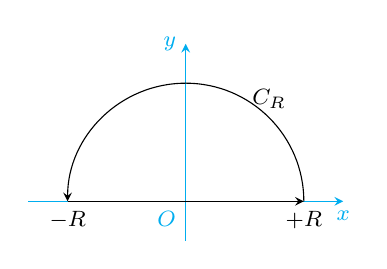
\begin{tikzpicture}[->,samples=100,>=stealth,font=\footnotesize]
            \draw[->,cyan](-2,0)--(0,0)node[below left]{$O$}--(2,0)node[below]{$x$};
            \draw[->,cyan](0,-0.5)--(0,2)node[left]{$y$};
            \draw[black] (1.5,0) arc (0:180:1.5)node[above,near start]{$C_R$};
            \draw[black] (-1.5,0)--(1.5,0);
            \node[below] at (-1.5,0) {$-R$};
            \node[below] at (1.5,0) {$+R$};
        \end{tikzpicture}
        \caption{}
        \label{figure:lsdlCR}
    \end{figure}
\end{minipage}\hfill
\begin{minipage}[b]{0.45\linewidth}
    \begin{figure}[H]
        \centering
        \begin{tikzpicture}[->,samples=100,>=stealth,font=\footnotesize]
            \draw[->,cyan](-2,0)--(0,0)node[below left]{$O$}--(2,0)node[below]{$x$};
            \draw[->,cyan](0,-2)--(0,2)node[left]{$y$};
            \draw[black] (1.5,0) arc (0:180:1.5)node[above,near start]{$C_R$};
            \draw[black] (-1.5,0)--(1.5,0);
            \node[below] at (-1.5,0) {$-R$};
            \node[below] at (1.5,0) {$+R$};
            \node[left] at (0,1) {$\mathrm{i}$};\draw[fill=black] (0,1) circle (0.5pt);
            \node[left] at (0,-1) {$\mathrm{i}$};\draw[fill=black] (0,-1) circle (0.5pt);
        \end{tikzpicture}
        \caption{}
        \label{liushu3}
    \end{figure}
\end{minipage}

于是 $$\oint_C R(z)\dd z=\int_{-R}^{R}R(x)\dd x+\int_{C_R}R(z)\dd z$$
任何有理函数只有有限个的孤立奇点,所以 $R(z)$ 在上半平面只有有限个孤立奇点,$R$ 足够大时,则围道包围上半平面所有的奇点,由留数定理又有
$$\oint_CR(z)\dd z=2\pi\i\sum_{\text{上半平面}}\Res[R(z)]$$
对于无穷积分存在的有理函数 $R(z)$,满足分母多项式次数比分子多项式次数至少大 2,则
$$\lim_{z\to\infty}zR(z)=\lim_{z\to\infty}z\dfrac{P_n(x)}{Q_m(z)}=0$$
由大圆弧定理 $$\lim_{R\to\infty}\int_{C_R}R(z)\dd z=0$$
于是 $$\int_{-\infty}^{+\infty}R(x)\dd x=2\pi\i\sum_{\text{上半平面}}\Res[R(z)]$$

\begin{example}
    计算积分 $\displaystyle I=\int_{-\infty}^{+\infty}\dfrac{\dd x}{\qty(1+x^2)^3}.$
\end{example}
\begin{solution}
    令 $f(x)=\dfrac{1}{\qty(1+x^2)^3},~\displaystyle I=\lim_{R\to\infty}\int_{-R}^{R}f(x)\dd x $,考虑围道如图 \ref{liushu3} 所示,
    则有
    \begin{flalign*}
        \oint_Cf(z)\dd z & =\int_{-R}^{R}f(x)\dd x+\int_{C_R}f(z)\dd z=2\pi\i\sum_{\text{上半平面}}\Res[R(z)]=2\pi\i\Res[f(i)]                                                                                                     \\
                         & =2\pi\i\cdot \dfrac{1}{2!}\lim_{z\to\i}\dv[2]{\qty[(z-\i)^3\dfrac{1}{\qty(1+z^2)^3}]}{z}=2\pi\i\cdot\dfrac{1}{2}\dv[2]{(z+\i)^{-3}}{z}\biggl |_{z=\i}=2\pi\i\cdot\qty(-\dfrac{3}{16}\i)=\dfrac{3\pi}{8}
    \end{flalign*}
    因为 $\displaystyle \lim_{z\to\infty}z\cdot\dfrac{1}{\qty(1+z^2)^3}=0$,由大圆弧定理 $$\lim_{R\to\infty}\int_{C_R}f(z)\dd z=\i\pi\cdot0=0$$
    于是原积分等于 $\dfrac{3\pi}{8}.$
\end{solution}

\begin{example}
    计算反常积分 $\displaystyle I=\int_{-\infty}^{+\infty}\dfrac{\dd x}{\qty(x^2+x+1)^2}.$
\end{example}
\begin{solution}
    令 $f(x)=\dfrac{1}{\qty(x^2+x+1)^2},~\displaystyle I=\lim_{R\to\infty}\int_{-R}^{R}f(x)\dd x$,则有 $z_{1,2}=\dfrac{-1\pm\sqrt{3}\i}{2}$,于是
    \begin{flalign*}
        \oint_Cf(z)\dd z & =\int_{-R}^{R}f(x)\dd x+\int_{C_R}f(z)\dd z=2\pi\i\sum_{\text{上半平面}}\Res[f(z)]=2\pi\i\Res[f(z_1)]                                                                        \\
                         & =2\pi\i\cdot\dfrac{1}{1!}\lim_{z\to z_1}\dv{z}\qty[(z-z_1)^2\dfrac{1}{\qty(z^2+z+1)^2}]=2\pi\i\cdot\dv{z}\qty(z-\overline{z}_1)^{-2}\biggl |_{z=z_1}=\dfrac{4\pi}{3\sqrt{3}}
    \end{flalign*}
    因为 $\displaystyle\lim_{z\to\infty}z\cdot f(z)=0$,由大圆弧定理 $\displaystyle\lim_{R\to\infty}\int_{C_R}f(z)\dd z=0$,故原积分等于 $\dfrac{4\pi}{3\sqrt{3}}.$
\end{solution}

\subsubsection{含三角函数的无穷积分}

考虑积分 $\displaystyle I=\int_{-\infty}^{+\infty}R(x)\mathrm{e}^{\i px}\dd x,~p>0$,其中 $R(x)$ 为有理函数,积分的实部和虚部分别为
$$\Re I=\int_{-\infty}^{+\infty}R(x)\cos px\dd x,~\Im I=\int_{-\infty}^{+\infty}R(x)\sin px\dd x$$
当且仅当有理函数 $R(x)=P_n(x)/Q_m(x)$ 的分母多项式 $Q_m(x)$ 次数比分子多项式 $P_n(x)$ 的次数大 1 时无穷积分存在.
$$m-n\geqslant 1$$

对于积分 $I$ 同样考虑围道积分 $$\oint_{C}R(x)\e^{\i pz}\dd z=\int_{-R}^{R}R(x)\e^{\i px}\dd x+\int_{C_R}R(z)\e^{\i pz}\dd z=2\pi\i\sum_{\text{上半平面}}\Res[R(x)\e^{\i pz}]$$

\begin{lemma}[Jordan 引理]
    设在 $0\leqslant \arg z\leqslant \pi$ 的范围内,当 $|z|\to\infty$ 时,$Q(z)$ 一致地趋近于 0,则 
    $$\lim_{R\to\infty}\int_{C_R}Q(z)\e^{\i pz}\dd z=0$$
    其中 $p>0,C_R$ 是以原点为圆心,$R$ 为半径的上半圆.
\end{lemma}

对于 $R(z)$,满足分母多项式次数比分子多项式次数至少大 1,则
$$\lim_{z\to\infty}R(z)=\lim_{z\to\infty}\dfrac{P_n(z)}{Q_m(z)}=0$$
由 Jordan 引理 $$\lim_{R\to\infty}\int_{C_R}R(z)\e^{\i pz}\dd z=0$$
于是 $$\int_{-\infty}^{+\infty}R(z)\e^{\i px}\dd x=2\pi\i\sum_{\text{上半平面}}\Res[R(z)\e^{\i pz}].$$

\begin{example}
    计算积分 $\displaystyle I=\int_{0}^{+\infty}\dfrac{x\sin x}{x^2+a^2}\dd x,~a>0.$
\end{example}
\begin{solution}
    令 $f(x)=\dfrac{x}{x^2+a^2}$,因为被积函数 $f(x)\sin x$ 为偶函数
    $$\int_{0}^{+\infty}f(x)\sin x\dd x=\dfrac{1}{2}\int_{-\infty}^{+\infty}f(x)\sin x\dd x=\dfrac{1}{2}\Im\int_{-\infty}^{+\infty}f(x)\e^{\i x}\dd x$$
    考虑围道积分
    $$\oint_{C}f(z)\e^{\i z}\dd z=\int_{-R}^{R}f(x)\e^{\i x}\dd x+\int_{C_R}f(z)\e^{\i z}\dd z=2\pi\i\sum_{\text{上半平面}}\Res[f(z)\e^{\i z}]$$
    易知,$z=a\i$ 为上半平面的唯一奇点,且为一阶极点
    $$\Res[\dfrac{z\e^{\i z}}{z^2+a^2}]=\dfrac{z\e^{\i z}}{2z}\biggl |_{z=\i a}=\dfrac{1}{2}\e^{-a}$$
    所以 $$\int_{-R}^{R}f(x)\e^{\i x}\dd x+\int_{C_R}f(z)\e^{\i z}\dd z=\pi\e^{-a}\i$$
    因为 $\displaystyle\lim_{z\to\infty}f(z)=0$,由 Jordan 引理 $\displaystyle\lim_{R\to\infty}\int_{C_R}f(z)\e^{\i z}\dd z=0$,
    于是 $\displaystyle\int_{-\infty}^{+\infty}f(x)\e^{\i x}\dd x=\pi\e^{-a}\i$,
    于是 $$I=\dfrac{1}{2}\Im\pi\e^{-a}\i=\dfrac{\pi}{2}\e^{-a}.$$
\end{solution}

\begin{example}
    计算反常积分 $\displaystyle I=\int_{0}^{+\infty}\dfrac{\cos x}{\qty(1+x^2)^3}\dd x.$
\end{example}
\begin{solution}
    令 $f(x)=\dfrac{1}{\qty(1+x^2)^3}$,那么 $f(x)\cos x$ 为偶函数,于是
    $$I=\dfrac{1}{2}\int_{-\infty}^{+\infty}f(x)\cos x\dd x=\dfrac{1}{2}\Re\int_{-\infty}^{+\infty}f(x)\e^{\i x}\dd x$$
    考虑围道积分
    $$\oint_Cf(z)\e^{\i z}\dd z=\int_{-R}^{R}f(x)\e^{\i x}\dd x+\int_{C_R}f(z)\e^{\i z}\dd z=2\pi\i\sum_{\text{上半平面}}\Res[f(z)\e^{\i z}]$$
    易知,$z=\i$ 为上半平面的唯一奇点,且为三阶极点,于是
    $$\phi(z)=(z-\i)^3\dfrac{\e^{\i z}}{\qty(1+z^2)^3}=\dfrac{\e^{\i z}}{(z+\i)^3}$$
    要求系数 $\alpha_2$,用待定系数法,令 $z-\i=t$,于是
    $$(t+2\i )^3\sum_{n=0}^{\infty}\alpha_nt^n=\e^{\i(t+\i)}=\e^{-1}\sum_{n=0}^{\infty}\dfrac{\i ^n}{n!}t^n$$
    即 $$\qty(-8\i-12t+6\i t^2+\cdots)\sum_{n=0}^{\infty}\alpha_nt^n=\e^{-1}\sum_{n=0}^{\infty}\dfrac{\i ^n}{n!}t^n$$
    先比较两边 0 次项系数 $$-8\i\alpha_0=\e^{-1}$$
    得 $\alpha_0=\dfrac{\i}{8\e}$,再比较两边 1 次项的系数 $$-8\i\alpha_1-12\alpha_0=\dfrac{\i}{\e}$$
    得 $\alpha_1=-\dfrac{5}{16\e}$,再比较两边 2 此项的系数 $$-8\i \alpha_2-12\alpha_1+6\i\alpha_0=-\dfrac{1}{2\e}$$
    解得 $\alpha_2=-\dfrac{7\i}{16\e}$,即 $$\Res[f(z)\e^{\i z}]=-\dfrac{7\i}{16\e}$$
    所以 $$\int_{-R}^{R}f(x)\e^{\i x}\dd x+\int_{C_R}f(z)\e^{\i z}\dd z=\dfrac{7\pi}{8\e}$$
    $\displaystyle\lim_{z\to\infty}f(z)=0$,由 Jordan 引理 $\displaystyle\lim_{R\to\infty}\int_{C_R}f(z)\e^{\i z}\dd z=0$,
    于是 $\displaystyle\int_{-\infty}^{+\infty}f(x)\e^{\i x}\dd x=\dfrac{7\pi}{8\e}$,于是
    $$I=\Re\dfrac{1}{2}\cdot\dfrac{7\pi}{8\e}=\dfrac{7\pi}{16\e}.$$
\end{solution}

\subsubsection{实轴上有奇点的情形}

设被积函数在实轴上有奇点,则积分 $\displaystyle\int_{-\infty}^{+\infty}f(x)\dd x$ 为瑕积分,假设瑕点为 $c$,
瑕积分定义为:
存在一点 $c$ 及邻域 $(\delta_1,\delta_2)$,有 
$$\int_{a}^{b}f(x)\dd x=\lim_{\delta_1\to0}\int_{a}^{c-\delta_1}f(x)\dd x+\lim_{\delta_2}\int_{c+\delta_2}^{b}f(x)\dd x$$
如果这两个极限都不存在,但是 $\displaystyle\lim_{\delta\to0}\qty[\int_{a}^{c-\delta}f(x)\dd x+\int_{c+\delta}^{b}f(x)\dd x]$ 存在,定义瑕积分的主值为:
$$\vp\int_{a}^{b}f(x)\dd x=\lim_{\delta\to0}\qty[\int_{a}^{c-\delta}f(x)\dd x+\int_{c+\delta}^{b}f(x)\dd x]$$
当然,如果瑕积分存在,则主值也存在,且它们一定相等,所以,我们考虑
$$I=\vp\int_{-\infty}^{+\infty}f(x)\dd x=\lim_{\substack{R\to\infty\\\delta\to0}}\qty[\int_{-R}^{c-\delta}f(x)\dd x+\int_{c+\delta}^{R}f(x)\dd x]$$
因为实轴上 $c$ 点是被积函数的奇点,必须绕过奇点来构成闭合的积分围道,如图 \ref{liushu4} 所示.

$$\oint_{C}f(z)\dd z=2\pi\i\sum_{\text{一二象限}}\Res[f(z)]=\int_{-R}^{c-\delta}f(x)\dd x+\int_{C_\delta}f(z)\dd z+\int_{c+\delta}^{R}f(x)\dd x+\int_{C_R}f(z)\dd z$$
\begin{figure}[H]
    \centering
    \includegraphics{figures/liushu4.pdf}
    \caption{}
    \label{liushu4}
\end{figure}
对于大圆弧积分,我们可以用大圆弧定理或 Jordan 引理处理,对于小圆弧 $C_\delta$ 的积分,则需要用到小圆弧定理. 
% TODO: 实轴上有奇点的情形

% \section{特殊构型积分补充}

\subsection{Dirichlet 积分}

\begin{lemma}[Dirichlet 核]
    \label{Dirichlethe}
    在区间 $(0,\pi)$ 上定义 $D_n=\dfrac{\sin\dfrac{(2n+1)x}{2}}{2\sin\dfrac{x}{2}},~n\in\mathbb{N}_+$, 则有 $$\int_{0}^{\pi}D_n(x)\dd x=\dfrac{\pi}{2}.$$
\end{lemma}
\begin{proof}[{\songti \textbf{证}}]
    显然, $D_n$ 在 $x=0$ 处无定义, 但是 $\displaystyle\lim_{x\to0^+}D_n(x)=\dfrac{2n+1}{2}$, 因此 $D_n$ 在 $[0,\pi]$ 可积, 因为有三角恒等式
    $$2\sin\dfrac{x}{2}\qty(\dfrac{1}{2}+\sum_{k=1}^{n}\cos kx\dd x)=\sin\dfrac{(2n+1)x}{2}$$
    于是, $\displaystyle D_n=\dfrac{1}{2}+\sum_{k=1}^{n}\cos kx$, 所以, 不难得到
    $$\int_{0}^{\pi}D_n(x)\dd x=\int_{0}^{\pi}\qty(\dfrac{1}{2}+\sum_{k=1}^{n}\cos kx)\dd x=\dfrac{\pi}{2}.$$
\end{proof}

\begin{theorem}[Dirichlet 积分等式]
    $\displaystyle\int_{0}^{+\infty}\dfrac{\sin x}{x}\dd x=\dfrac{\pi}{2}.$
\end{theorem}
\begin{proof}[{\songti \textbf{证}}]
    易知该反常积分条件收敛, 根据引理 \ref{Dirichlethe} 有, $\displaystyle\int_{0}^{\pi}\dfrac{\sin\dfrac{(2n+1)\pi}{2}}{2\sin\dfrac{x}{2}}\dd x=\dfrac{\pi}{2}$, 考虑将其分母换为 $x$ 所产生的影响, 
    由 L'Hospital 法则, 有 $$f(x)=\dfrac{1}{x}-\dfrac{1}{2\sin\dfrac{x}{2}}=O(x)~~ (x\to0)$$
    因此 $f$ 在 $[0,\pi]$ 上常义可积, 由 Riemann-Lebesgue 定理, 有
    $$\lim_{n\to\infty}f(x)\sin\qty(n+\dfrac{1}{2})x\dd x=0$$
    即 $$\lim_{n\to\infty}\int_{0}^{\pi}\dfrac{\sin\qty(n+\dfrac{1}{2})x}{x}\dd x=\lim_{n\to\infty}\int_{0}^{\pi}\dfrac{\sin\qty(n+\dfrac{1}{2})x}{2\sin\dfrac{x}{2}}\dd x=\dfrac{\pi}{2}$$
    最后, 作代换 $t=\qty(n+\dfrac{1}{2})x$, 即得 $$\int_{0}^{\pi}\dfrac{\sin\qty(n+\dfrac{1}{2})x}{x}\dd x=\int_{0}^{\qty(n+\frac{1}{2})\pi}\dfrac{\sin t}{t}\dd t=\dfrac{\pi}{2}.$$
\end{proof}

\subsection{Lobachevsky 积分法}

\begin{theorem}[Lobachevsky 积分法]
    若 $f(x)$ 在 $x\in[0,+\infty)$ 范围内满足 $f(x+\pi)=f(x)$ 及 $f(\pi-x)=f(x)$, 则
    $$\int_{0}^{+\infty}f(x)\dfrac{\sin x}{x}\dd x=\int_{0}^{\frac{\pi}{2}}f(x)\dd x.$$
    当 $f(x)=1$ 时, 便是 Dirichlet 积分.
\end{theorem}

\subsection{Fresnel 积分与 Fej\texorpdfstring{$\acute{\text{e}}$}.r 积分}

\begin{theorem}[Fresnel 积分等式]
    $\displaystyle\int_{-\infty}^{+\infty}\sin x^2\dd x=\int_{-\infty}^{+\infty}\cos x^2\dd x=\sqrt{\dfrac{\pi}{2}}.$
\end{theorem}

\begin{theorem}[Fej$\acute{\text{e}}$r 积分]
    假设 $k\in\mathbb{N}^+$, 则有以下四种形式的 Fej$\acute{\text{e}}$r 积分:
    \begin{enumerate}[label=(\arabic{*})]
        \item $\displaystyle \int_{0}^{\pi}\dfrac{\sin nx}{\sin x}\dd x=\begin{cases}
                      0,   & n=2k    \\
                      \pi, & n=2k-1;
                  \end{cases}$
        \item $\displaystyle\int_{0}^{\frac{\pi}{2}}\dfrac{\sin nx}{\sin x}\dd x=\begin{cases}
                      2\displaystyle\sum_{i=1}^{k}\dfrac{(-1)^{k-1}}{2k-1}, & n=2k    \\[6pt]
                      \dfrac{\pi}{2},                                       & n=2k-1;
                  \end{cases}$
        \item $\displaystyle \int_{0}^{\pi}\qty(\dfrac{\sin nx}{\sin x})^2\dd x=n\pi;$
        \item $\displaystyle\int_{0}^{\frac{\pi}{2}}\qty(\dfrac{\sin nx}{\sin x})^2\dd x=\dfrac{n\pi  }{2}.$
    \end{enumerate}
\end{theorem}

\subsection{Laplace 积分}

\begin{theorem}[Laplace 积分等式]
    $\displaystyle \int_{0}^{+\infty}\dfrac{\cos bx}{a^2+x^2}\dd x=\dfrac{\pi}{2a}\e^{-ab},~\int_{0}^{+\infty}\dfrac{x\sin bx}{a^2+x^2}\dd x=\dfrac{\pi}{2}\e^{-ab}~~(a,b>0).$
\end{theorem}
\begin{inference}
    当 $4q>p^2$ 时, 有
    \begin{flalign*}
        \int_{-\infty}^{+\infty}\dfrac{\cos x}{x^2+px+q}\dd x & =\dfrac{2\pi}{\sqrt{4q-p^2}}\e^{-\frac{\sqrt{4q-p^2}}{2}}\cos\dfrac{p}{2}   \\
        \int_{-\infty}^{+\infty}\dfrac{\sin x}{x^2+px+q}\dd x & =-\dfrac{2\pi}{\sqrt{4q-p^2}}\e^{-\frac{\sqrt{4q-p^2}}{2}}\sin\dfrac{p}{2}.
    \end{flalign*}
\end{inference}

\chapter{向量代数与空间解析几何}%============================4

\begin{flushright}
    \begin{tabular}{r|}
        \textit{“数缺形时少直观, 形少数时难入微;}\\
        \textit{数形结合百般好, 隔离分家万事休. ”}\\
        ——\textit{华罗庚}
    \end{tabular}
\end{flushright}

向量代数与空间解析几何是数学中的一个重要分支, 主要研究向量、向量空间和空间中的点、直线、平面等几何对象之间的关系. 以下是向量代数与空间解析几何的几个重要概念和内容: 

1. 向量: 向量是表示大小和方向的量, 通常用有序数对或有序数组表示. 向量可以进行加法、数乘等运算, 具有方向和模长(大小)的性质. 在向量代数中, 研究向量的性质、运算规则以及向量空间的结构. 

2. 向量空间: 向量空间是由一组向量构成的集合, 满足一定的运算规则和性质, 如封闭性、结合律、分配律等. 向量空间是线性代数的基础, 包括了向量的线性组合、线性相关性、线性无关性等概念. 

3. 空间解析几何: 空间解析几何是研究空间中点、直线、平面等几何对象的位置关系和性质的数学分支. 通过向量代数的工具, 可以方便地描述和研究空间中的几何问题, 如点的坐标、直线的方程、平面的方程等. 

4. 点、直线、平面的位置关系: 在空间解析几何中, 研究点、直线、平面之间的位置关系是一个重要的问题. 通过向量的表示和运算, 可以确定点是否在直线上、直线是否平行、平面是否垂直等问题. 

5. 空间曲线与曲面: 空间解析几何还涉及到空间曲线和曲面的研究, 如参数方程、曲线的切线、曲面的法线等. 通过向量代数和微积分的方法, 可以描述和分析空间中的曲线和曲面的性质. 

向量代数与空间解析几何是数学中的重要分支, 它不仅在数学理论研究中有着重要作用, 也在物理学、工程学、计算机图形学等应用领域有广泛的应用. 
\section{向量代数}

向量代数是高等数学中的一个重要部分, 主要研究向量及其运算. 向量是一种既有大小又有方向的量, 通常用于表示力、速度、加速度等物理量. 在数学中, 向量可以被视为一个有向线段, 其起点和终点可以任意平行移动, 但不改变其大小和方向.

向量代数的内容包括向量的基本概念、线性运算、数量积 (点积)、向量积 (叉积)、向量的模、方向余弦、投影等. 具体来说, 向量的线性运算包括向量的加法、减法和数乘. 向量的模是指向量长度的度量, 而方向余弦则是描述向量方向的三个参数.

\subsection{模、方向角、投影}

\begin{definition}[投影]
    $\vec{a}$ 在 $\vec{b}$ 方向上的\textit{投影}记为 $\mathrm{Prj}_{\vec{b} } \vec{a}$,
    且 $\mathrm{Prj}_{\vec{b} } \vec{a}=|\vec{a}| \cdot \cos\left \langle \vec{a},\vec{b} \right \rangle .$
\end{definition}

\begin{example}
    设 $\vec{a}=(2,1,-1),~\vec{b}=(1,-3,1)$, 试在 $\vec{a},~\vec{b}$ 所决定的平面内, 求与 $\vec{a}$ 垂直, 且模为 $\sqrt{93}$ 的向量.
\end{example}
\begin{solution}
    \textbf{法一: }设所求向量为 $ \vec{c}=(x, y, z)$, 则由题设有 $ \vec{c} \perp \vec{a} \times \vec{b},~ \vec{c} \perp \vec{a},~|\vec{c}|=\sqrt{93}$,
    而 $ \vec{a} \times \vec{b}=\mqty|\vec{i} & \vec{j} & \vec{k} \\ 2 & 1 & -1 \\ 1 & -3 & 1|=-2 \vec{i}-3 \vec{j}-7 \vec{k}$, 于是有
    $\left\{\begin{array}{llll}
            -2x & -3y  & -7z  & =0  \\
            2x  & +y   & -z   & =0  \\
            x^2 & +y^2 & +z^2 & =93
        \end{array}\right.$, 解得 $ x=\pm 5,~ y=\mp 8,~ z=\pm 2 $, 从而 $ \vec{c}=\pm(5,-8,2) .$\\
    \textbf{法二: }设所求向量为 $ \vec{c}$, 则由题设有 $ \vec{c} \perp \vec{a} \times \vec{b},~ \vec{c} \perp \vec{a},~|\vec{c}|=\sqrt{93}$,
    于是 $ \vec{c} / /(\vec{a} \times \vec{b}) \times \vec{a}$, 从而得
    $$ \vec{c}=\left|\vec{c}\right| \cdot\left(\pm \frac{(\vec{a} \times \vec{b}) \times \vec{a}}{|(\vec{a} \times \vec{b}) \times \vec{a}|}\right)=\pm(5,-8,2) .$$
    \textbf{法三: }设所求向量为 $ \vec{c}$, 则可设 $ \vec{c}=\lambda \vec{a}+\mu \vec{b}=(2 \lambda+\mu, \lambda-3 \mu,-\lambda+\mu)$,
    由已知 $ \vec{c} \perp \vec{a} $ 得 $ \vec{c} \cdot \vec{a}=0$, 即 $$ 2(2 \lambda+\mu)+\lambda-3 \mu-(-\lambda+\mu)=0$$
    解得 $ \mu=3 \lambda$, 又 $ |\vec{c}|=\sqrt{93}$, 所以 $ \sqrt{(2 \lambda+\mu)^{2}+(\lambda-3 \mu)^{2}+(\mu-\lambda)^{2}}=\sqrt{93}$,
    代人 $ \mu=3 \lambda$, 得 $ \lambda^{2}=1$, 解得 $ \lambda=\pm 1, \mu=\pm 3$, 故 $ \vec{c}=\pm(5,-8,2) .$
\end{solution}

\begin{example}
    设向量 $\vb*{a}+3\vb*{b}$ 与 $\vb*{a}-4\vb*{b}$ 分别垂直于向量 $7\vb*{a}-5\vb*{b}$ 与 $7\vb*{a}-2\vb*{b}$, 试求 $\vb*{a}$ 与 $\vb*{b}$ 之间的夹角.
\end{example}
\begin{solution}
    因为 $\qty(\vb*{a}+3\vb*{b})\bot \qty(7\vb*{a}-5\vb*{b})$, 所以 $7\vb*{a}^2-15\vb*{b}^2=-16\vb*{ab}$, 同理可得 $7\vb*{a}^2+8\vb*{b}^2=30\vb*{ab}$,
    联立解得 $\begin{cases}
            \vb*{b}^2=2\vb*{ab} \\\vb*{a}^2=\vb*{b}^2
        \end{cases}$, 于是 $$\cos<\vb*{a},\vb*{b}>=\dfrac{\vb*{ab}}{|\vb*{a}|\cdot|\vb*{b}|}=\dfrac{1}{2}$$ 因此 $\vb*{a}$ 与 $\vb*{b}$ 之间的夹角为 $\dfrac{\pi}{3} .$
\end{solution}

\begin{example}
    设 $\vb*{a}$ 和 $\vb*{b}$ 为非零向量, 且 $|\vb*{b}|=1,\left \langle \vb*{a},\vb*{b} \right \rangle=\dfrac{\pi}{3}$, 则 $\displaystyle \lim_{x \to 0}\dfrac{|\vb*{a}+x\vb*{b}|-|\vb*{a}|}{\e ^{x} -1}$
    \begin{tasks}(4)
        \task $0$.
        \task $\dfrac{1}{2}$.
        \task $\dfrac{\sqrt{2}}{2}$.
        \task $\dfrac{\sqrt{3}}{2}$.
    \end{tasks}
\end{example}
\begin{solution}
    因为 $\vb*{a}=\sqrt{\vb*{a}\cdot \vb*{a}}$, 于是
    \begin{flalign*}
        \lim_{x \to 0}\dfrac{|\vb*{a}+x\vb*{b}|-|\vb*{a}|}{\e ^{x} -1} & =  \lim_{x \to 0}\dfrac{|\vb*{a}|^2+x^2|\vb*{b}|^2+2x \vb*{a}\cdot\vb*{b}-\vb*{a}^2}{2x|\vb*{a}|}                                                                  \\
                                                                       & =\lim_{x \to 0}\dfrac{2x\vb*{a}\cdot\vb*{b}+x^2|\vb*{b}|^2}{2x|\vb*{a}|}=\lim_{x \to 0}\dfrac{2x\vb*{a}\cdot\vb*{b}}{2x|\vb*{a}|}=\dfrac{a\cdot\vb*{b}}{|\vb*{a}|} \\
                                                                       & =|\vb*{b}|\cos \left \langle \vb*{a},\vb*{b} \right \rangle=\dfrac{1}{2}.
    \end{flalign*}
    因此选 B.
\end{solution}

% \begin{example}
%     设 $\vec{a}=\vec{i},~\vec{b}=\vec{j}-2\vec{k},~\vec{c}=2\vec{i}-2\vec{j}+\vec{k}$, 求一个单位向量 $\vec{e}$, 使 $\vec{e}\bot\vec{c}$, 且 $\vec{a},~\vec{b},~\vec{e}$ 共面.
% \end{example}
% \begin{solution}
%     \textbf{法一: }设 $\vec{e}=(x,y,z)$, 那么 $x^2+y^2+z^2=1$, 且 $\vec{e}\cdot \left(\vec{a}\times\vec{b}\right)=0,~\vec{e}\bot\vec{c}$, 所以
%     $$\left\{\begin{array}{llll}
%             2x  & -2y  & +z   & =0 \\
%                 & 2y  & +z   & =0 \\
%             x^2 & +y^2 & +z^2 & =1
%         \end{array}\right.
%         \Rightarrow \begin{cases}
%             x=\mp\dfrac{\sqrt{6}}{6}                       \\
%             y=\pm\dfrac{\sqrt{6} }{6} \\
%             z=\mp\dfrac{\sqrt{6}}{3}
%         \end{cases}
%         \Rightarrow\vec{e}=\left(\mp\dfrac{\sqrt{6}}{6},\pm\dfrac{\sqrt{6} }{6},\mp\dfrac{\sqrt{6}}{3}\right).$$
%         \textbf{法二: }
% \end{solution}

\subsection{数量积、向量积、混合积}

\subsubsection{数量积}

\begin{definition}[向量的数量积 (点乘积或内积)]
    \index{向量的数量积}向量 $ \vb*{a}=\left\{a_{1}, a_{2}, a_{3}\right\} $ 与 $ \vb*{b}=\left\{b_{1}, b_{2}, b_{3}\right\} $ 的\textit{数量积}是一个数 $ |\vb*{a}| \cdot|\vb*{b}| \cos (\widehat{\vb*{a}, \vb*{b}}) $ (其中 $ 0 \leqslant(\widehat{a, b}) \leqslant \pi$),
    记作 $ \vb*{a} \cdot \vb*{b} $. 若向量 $ \vb*{a} $ 或 $ \vb*{b} $ 为零向量时, 则定义 $ \vb*{a} \cdot \vb*{b}=0$, 数量积 $ \vb*{a} \cdot \vb*{b} $ 的坐标表示式为
    $$\vb*{a} \cdot \vb*{b}=a_{1} b_{1}+a_{2} b_{2}+a_{3} b_{3} .$$
\end{definition}

\begin{definition}[向量正交]
    两个向量 $ \vb*{a}, \vb*{b} $ 垂直 (或称\textit{正交}), 记作 $ \vb*{a} \perp \vb*{b} $, 特别地, 规定零向量与任一向量垂直.
\end{definition}

数量积有以下基本性质:
\begin{enumerate}[label=(\arabic{*})]
    \item $\vb*{a} \cdot \vb*{b}=\vb*{b} \cdot \vb*{a} .$
    \item  $(\lambda \vb*{a}) \cdot \vb*{b}=\lambda(\vb*{a} \cdot \vb*{b}) .$
    \item $(\vb*{a}+\vb*{b}) \cdot \vb*{c}=\vb*{a} \cdot \vb*{c}+\vb*{b} \cdot \vb*{c} .$
    \item $\vb*{a} \perp \vb*{b} $ 的充分必要条件是 $ \vb*{a} \cdot \vb*{b}=0 .$
\end{enumerate}

\subsubsection{向量积}

\begin{definition}[向量的向量积 (叉乘积或外积)]
    \index{向量的向量积}两个向量 $ \vb*{a} $ 和 $ \vb*{b} $ 的\textit{向量积}是一个向量 $ \vb*{c} $, 记为 $ \vb*{a} \times \vb*{b} $,
    即 $ \vb*{c}=\vb*{a} \times \vb*{b}$; $\vb*{c} $ 的模等于 $ |\vb*{a}||\vb*{b}| \sin (\widehat{\vb*{a}, \vb*{b}})$, $\vb*{c} $ 的方向垂直于 $ \vb*{a} $ 与 $ \vb*{b} $ 所决定的平面,且 $ \vb*{a}, \vb*{b}, \vb*{c} $ 顺次构成右手系.
    若向量 $ \vb*{a} $ 或 $ \vb*{b} $ 为零向量时, 则定义 $ \vb*{a} \times \vb*{b}=\mathbf{0} $, 向量积 $ \vb*{a} \times \vb*{b} $ 坐标表示式为
    $$
        \vb*{a} \times \vb*{b}=\mqty|\vb*{i} & \vb*{j} & \vb*{k} \\
        a_{1}   & a_{2}   & a_{3}   \\
        b_{1}   & b_{2}   & b_{3}|=\qty(
        \mqty|a_{2} & a_{3} \\
        b_{2} & b_{3}|,\mqty|a_{1} & a_{3} \\
        b_{1} & b_{3}|,\mqty|a_{1} & a_{2} \\
        b_{1} & b_{2}|
        ).
    $$
\end{definition}

向量积有以下的性质:
\begin{enumerate}[label=(\arabic{*})]
    \item $\vb*{a} \times \vb*{b}=-\vb*{b} \times \vb*{a} .$
    \item $(\lambda \vb*{a}) \times \vb*{b}=\lambda(\vb*{a} \times \vb*{b}) .$
    \item $(\vb*{a}+\vb*{b}) \times \vb*{c}=\vb*{a} \times \vb*{c}+\vb*{b} \times \vb*{c} .$
    \item $\vb*{a} / / \vb*{b} $ 的充分必要条件是 $ \vb*{a} \times \vb*{b}=\mathbf{0} .$
\end{enumerate}

% \begin{theorem}[向量积公式]
%     设 $\vec{x}=(x_1,x_2,x_3),\vec{y}=(y_1,y_2,y_3)$, 那么
%     $$\vec{x}\times\vec{y}=\qty(\begin{vmatrix}
%                 x_2 & x_3 \\
%                 y_2 & y_3
%             \end{vmatrix},\begin{vmatrix}
%                 x_3 & x_1 \\
%                 y_3 & y_1
%             \end{vmatrix},\begin{vmatrix}
%                 x_1 & x_2 \\
%                 y_1 & y_2
%             \end{vmatrix}).$$
% \end{theorem}

\begin{theorem}[二重外积公式]
    $\vec{a}\times\qty(\vec{b}\times\vec{c})=\vec{b}\cdot\qty(\vec{a}\cdot\vec{c})-\vec{c}\cdot\qty(\vec{a}\cdot\vec{b}).$
    \index{二重外积公式}
\end{theorem}

\begin{example}[2023 四川大学]
    设向量 $\vec{a}=(1,2,3),\vec{b}=(4,5,6),\vec{c}=(7,8,9)$, 求 $\vec{a}\times\qty(\vec{b}\times\vec{c}).$
\end{example}
\begin{solution}
    \textbf{法一: }由向量积的计算公式计算 $\vec{b}\times\vec{c}$:
    $$\vec{b}\times\vec{c}=\qty(\mqty|5&6\\8&9|,\mqty|6&4\\9&7|,\mqty|4&5\\7&8|)=(-3,6,-3)$$
    进一步计算 $\vec{a}\times\qty(\vec{b}\times\vec{c})$:
    $$\vec{a}\times\qty(\vec{b}\times\vec{c})=\qty(\mqty|2&3\\6&-3|,\mqty|3&1\\-3&-3|,\mqty|1&2\\-3&6|)=(-24,-6,12).$$
    \textbf{法二: }由二重外积公式: $\vec{a}\times\qty(\vec{b}\times\vec{c})=\vec{b}\cdot\qty(\vec{a}\cdot\vec{c})-\vec{c}\cdot\qty(\vec{a}\cdot\vec{b})$, 其中
    $$\vec{a}\cdot\vec{c}=50,~\vec{a}\cdot\vec{b}=32$$
    于是得 $\vec{a}\times\qty(\vec{b}\times\vec{c})=(-24,-6,12).$
\end{solution}

\begin{theorem}[Lagrange 恒等式]
    \index{Lagrange 恒等式}对于任意两个向量 $\vb*{a}$ 和 $\vb*{b}$, 满足以下恒等关系式:
    $$|\vb*{a} \times \vb*{b}|^{2}=|\vb*{a}|^{2}|\vb*{b}|^{2}-(\vb*{a} \cdot \vb*{b})^{2}
        =\mqty|\vb*{a} \cdot \vb*{a} & \vb*{a} \cdot \vb*{b} \\
        \vb*{a} \cdot \vb*{b} & \vb*{b} \cdot \vb*{b}|.$$
\end{theorem}

% \begin{example}
%     若非零向量 $ \vb*{a}, \vb*{b} $ 满足关系式 $ |\vb*{a}-\vb*{b}|=|\vb*{a}+\vb*{b}| $, 则必有.
%     % \begin{task}
%     %     \task $ \vb*{a}-\vb*{b}=\vb*{a}+\vb*{b} $
%     % \end{task}
%     (B) $ \vb*{a}=\vb*{b} $
%     (C) $ \vb*{a} \cdot \vb*{b}=0 $
%     (D) $ \vb*{a} \times \vb*{b}=\vb*{0} $
% \end{example}
% 
% \begin{example}
%     设 $ (\vec{a} \times \vec{b}) \cdot \vec{c}=2 $, 求 $ [(\vec{a}+\vec{b}) \times(\vec{b}+\vec{c})] \cdot(\vec{c}+\vec{a}).$
% \end{example}
% 
% \begin{example}
%     设点 $ A $ 位于第一卦限, 向径 $ \overrightarrow{O A} $ 与 $ x $ 轴、$y $ 轴的夹角依次为 $ \dfrac{\pi}{3}, \dfrac{\pi}{4} $, 且 $ |O A|=6 $, 求点 $ A $ 的坐标.
% \end{example}
% 
% \begin{example}
%     已知向量 $ \vec{a}=(2,-3,6), \vec{b}=(-1,2,-2) $, 又向量 $ \vec{c} $ 在 $ \vec{a}, \vec{b} $ 夹角的平分线上, 且 $ |\vec{c}|=3 \sqrt{42} $, 求向量 $ \vec{c} .$
% \end{example}
% 
% \begin{example}
%     设有一向量与 $ x $ 轴正向、$y $ 轴正向的夹角相等, 而与 $ z $ 轴正向的夹角是前者的两倍, 求与该向量同方向的单位向量.
% \end{example}
% 
% \begin{example}
%     设向量 $ \vec{a}=\vec{i}+2 \vec{j}-\vec{k}, \vec{b}=-\vec{i}+\vec{j}$, 
%     \begin{enumerate}[label=(\arabic{*})]
%         \item 计算 $ \vec{a} \cdot \vec{b} $ 及 $ \vec{a} \times \vec{b}$;
%         \item 求它们夹角 $ \theta $ 的正弦与余弦;
%         \item 求垂直两向量所在平面的单位向量.
%     \end{enumerate}
% \end{example}
% 
% \begin{example}
%     已知一四面体的顶点为 $ A_{k}\left(x_{k}, y_{k}, z_{k}\right)(k=1,2,3,4) $, 求该四面体的体积.
% \end{example}
% 
% \begin{example}
%     判定四点 $ A(1,1,1), B(4,5,6), C(2,3,3), D(10,15,17) $ 是否共面?
% \end{example}
% 
% \begin{example}
%     设向量 $ \vb*{a}, \vb*{b}, \vb*{c} $ 不共面, 且 $ \vb*{d}=\boldsymbol{\alpha} \vb*{a}+\boldsymbol{\beta} \vb*{b}+\gamma \vb*{c} $, 
%     如果 $ \vb*{a}, \vb*{b}, \vb*{c}, \vb*{d} $ 有公共起点.
%     \begin{enumerate}[label=(\arabic{*})]
%         \item 问系数 $ \boldsymbol{\alpha}, \boldsymbol{\beta}, \gamma $ 应满足什么条件, 才能使向量 $ \vb*{a}, \vb*{b}, \vb*{c}, \vb*{d} $ 的终点在同一平面上?
%         \item 如果 $ \vb*{a}=(1,2,1), \vb*{b}=(0,3,1), \vb*{c}=(2,0,3) $, 判定向量 $ \vb*{a}, \vb*{b}, \vb*{c} $ 是否共面?
%         \item 设 $ \vb*{d}=(-1,-3,1) $, 由 (2) 求 $ \alpha, \beta, \gamma $, 使得
%         $$\vb*{d}=\alpha \vb*{a}+\beta \vb*{b}+\gamma \vb*{c}$$
%         如果 $ \vb*{a}, \vb*{b}, \vb*{c}, \vb*{d} $ 有公共起点, 它们是否共面?
%     \end{enumerate}
% \end{example}
% 
% \begin{example}
%     问当 $ t $ 为何值时, 空间四点 $ A(1,0,0), B(0,2,0), C(0,0,3) ,  D(-1,2, t) $ 共面? 并求平面四边形 $ A B C D $ 的面积.
% \end{example}
% 
% \begin{example}
%     设 $ \vec{a}, \vec{b} $ 为两个非零向量, $ \displaystyle |\vec{b}|=1,(\widehat{\vec{a}, \vec{b}})=\frac{\pi}{3} $, 计算极限
%     $$\lim _{x \to 0} \frac{|\vec{a}+x \vec{b}|-|\vec{a}|}{x}.$$
% \end{example}
% 
% \begin{example}
%     已知向量 $ \overrightarrow{A B}=\vec{a}, \overrightarrow{A C}=\vec{b}, \angle A D B=\dfrac{\pi}{2}$ .
%     \begin{enumerate}[label=(\arabic{*})]
%         \item 证明: $ \displaystyle\triangle B A D $ 的面积 $ \displaystyle S_{\triangle B A D}=\frac{|\vec{a} \cdot \vec{b}||\vec{a} \times \vec{b}|}{2|\vec{b}|^{2}}$;
%         \item 当 $ \vec{a}, \vec{b} $ 间的夹角为何值时, $ \triangle B A D $ 的面积最大, 并求最大面积值.
%     \end{enumerate}
% \end{example}
% 
% \begin{example}
%     证明: $ \vb*{a}, \vb*{b}, \vb*{c} $ 不共面当且仅当 $ \vb*{a} \times \vb*{b}, \vb*{b} \times \vb*{c}, \vb*{c} \times \vb*{a} $ 不共面.
% \end{example}
% 
% \begin{example}
%     设 $ \mathrm{e}_{1}, \mathrm{e}_{2}, \mathrm{e}_{3} $ 不共面, 证明:任一向量 $ \vb*{a} $ 可以表示成
%     $$a=\frac{1}{\left(e_{1}, e_{2}, e_{3}\right)}\left[\left(a, e_{2}, e_{3}\right) e_{1}+\left(a, e_{3}, e_{1}\right) e_{2}+\left(a, e_{1}, e_{2}\right) e_{3}\right].$$
% \end{example}
% 
% \begin{example}
%     设 $ \vb*{a}, \vb*{b}, \vb*{c} $ 不共面, 且向量 $ \vb*{r} $ 满足
%     $$\vb*{a} \cdot \vb*{r}=\alpha, \vb*{b} \cdot \vb*{r}=\boldsymbol{\beta}, \vb*{c} \cdot \vb*{r}=\gamma$$
%     那么有 $ \displaystyle\vb*{r}=\frac{1}{(\vb*{a}, \vb*{b}, \vb*{c})}[\boldsymbol{\alpha}(\vb*{b} \times \vb*{c})+\boldsymbol{\beta}(\vb*{c} \times \vb*{a})+\gamma(\vb*{a} \times \vb*{b})] .$
% \end{example}
% 
% \begin{example}
%     证明: $ (\vb*{a} \cdot \vb*{b})^{2}+(\vb*{a} \times \vb*{b})^{2}=|\vb*{a}|^{2}|\vb*{b}|^{2}$, 
%     由此推导用三角形三边长 $ a, b, c $ 计算三角形的面积公式, 其中向量 $ (\vb*{a})^{2}=\vb*{a} \cdot \vb*{a} .$
% \end{example}

\subsubsection{混合积}

\begin{definition}[向量的混合积]
    设 $ \vb*{a}=\left\{a_{1}, a_{2}, a_{3}\right\}, \vb*{b}=\left\{b_{1}, b_{2}, b_{3}\right\}, \vb*{c}=\left\{c_{1}, c_{2}, c_{3}\right\}$,
    则称 $ (\vb*{a} \times \vb*{b}) \cdot \vb*{c} $ \textit{为向量} $ \vb*{a}, \vb*{b}, \vb*{c} $ \textit{的混合积}, 记为 $ [\vb*{a}, \vb*{b}, \vb*{c}] $.\index{向量的混合积}
\end{definition}

\begin{theorem}[共面条件]
    混合积是一数量, 其几何意义为: 混合积的绝对值等于以 $ \vb*{a}$ 、$ \vb*{b} $、$ \vb*{c} $ 为相邻三条棱的平行六面体的体积.
    因此, 向量 $ \vb*{a}$ 、$ \vb*{b} $、$ \vb*{c} $ 共面的充分必要条件是 $ (a \times b) \cdot c=0 .$
    \index{共面条件}
\end{theorem}
\section{空间解析几何}

\subsection{空间平面与直线}

\begin{theorem}[线轴夹角余弦平方和公式]
    \index{线轴夹角余弦平方和公式}设一直线与三坐标轴的夹角依次为 $\alpha,\beta,\gamma$, 则有 $$\cos^2\alpha+\cos^2\beta+\cos^2\gamma=1.$$
\end{theorem}
\begin{proof}[{\songti \textbf{证}}]
    设直线上一点坐标为 $P(x_0,y_0,z_0)$, 坐标轴的单位向量依次为 $\vb*{i}=(1,0,0),\vb*{j}=(0,1,0),\vb*{k}=(0,0,1)$, 由夹角余弦公式
    $$\begin{cases}
        \cos\alpha=\dfrac{\vb*{pi}}{|\vb*{p}|\cdot|\vb*{i}|}=\dfrac{x_0}{\sqrt{x_0^2+y_0^2+z_0^2}}\\
        \cos\beta=\dfrac{\vb*{pj}}{|\vb*{p}|\cdot|\vb*{j}|}=\dfrac{y_0}{\sqrt{x_0^2+y_0^2+z_0^2}}\\
        \cos\gamma=\dfrac{\vb*{pk}}{|\vb*{p}|\cdot|\vb*{k}|}=\dfrac{z_0}{\sqrt{x_0^2+y_0^2+z_0^2}}\\
    \end{cases}
    $$
    上式平方相加即得证.
\end{proof}

\begin{theorem}[线面夹角余弦平方和公式]
    \index{线面夹角余弦平方和公式}设一直线与三坐标平面的夹角依次为 $u,v,w$, 则有 $$\cos^2u+\cos^2v+\cos^2w=2.$$
\end{theorem}
\begin{proof}[{\songti \textbf{证}}]
    设直线与 $x,y,z$ 轴的夹角依次为 $\alpha,\beta,\gamma$, 于是有 
    $$\begin{cases}
        \alpha=\dfrac{\pi}{2}-u\\[6pt]\beta=\dfrac{\pi}{2}-v\\[6pt]\gamma=\dfrac{\pi}{2}-w
    \end{cases}$$
    且 $\cos^2\alpha+\cos^2\beta+\cos^2\gamma=1$, 所以 
    $$\cos^2\qty(\dfrac{\pi}{2}-u)+\cos^2\qty(\dfrac{\pi}{2}-v)+\cos^2\qty(\dfrac{\pi}{2}-w)=1$$
    即 $\sin^2u+\sin^2v+\sin^2w=1$, 从而有 $\cos^2u+\cos^2v+\cos^2w=2.$
\end{proof}

% 1、设一平面经过原点及点  (6,-3,2)  ,  且与平面  4 x-y+2 z=8  垂直, 求此平面的方程.
% 2.求与原而的距凷为 6 , 且在二个坐标轴上的截距之比为  a: b: c=1: 3: 2  的平面方程.
% 3.已知平面  \pi_{1}: x+2 y-z+1=0  和  \pi_{2}: 2 x-y+2 z-1=0 , 求:
% (1) 这两个平面的夹角  \theta  的余弦;
% (2)这两个平面的角平分面的方程.
% 4、已知直线  L_{1}  和  L_{2}  的方程
% 
% L_{1}: \frac{x-1}{1}=\frac{y-2}{0}=\frac{z-3}{-1} \text { 和 } L_{2}: \frac{x+2}{2}=\frac{y-1}{1}=\frac{z}{1},
% 
% 试求过  L_{1}  且平行于  L_{2}  的平面方程.
% 5、求过点  M_{0}(1,0,1)  且与直线  L: x-1=y+1=z-1  垂直相交的直线方程.
% 6.已知直线  L:\left\{\begin{array}{l}2 x-4 y+z=0 \\ 3 x-y-2 z=9\end{array}\right.  和平面  \pi: 4 x-y+z=1 , 试求直线  L  在平面  \pi  上的投影直线方程.
% 7、求通过直线  L:\left\{\begin{array}{l}2 x+y-3 z+2=0, \\ 5 x+5 y-4 z+3=0\end{array}\right.  的两个相互垂直的平面  \pi_{1}, \pi_{2}  , 使其中一个平 面过点  (4,-3,1) .
% 8、设有空间中五点  A(1,0,1), B(1,1,2), C(1,-1,-2), D(3,1,0), E(3,1,2) . 试求过点  E  且与  A, B, C  所在平面  \Sigma  平行而与直线  A D  垂直的直线方程.
% 9、设平面  \pi  方程为  A x+B y+C z+D=0  , 则向量  \vec{r}=\left(r_{1}, r_{2}, r_{3}\right)  平行于平面  \pi  或 在平面  \pi  上的充分必要条件是  \mathrm{Ar} r_{1}+\mathrm{Br}_{2}+\mathrm{Cr} r_{3}=0 .
% 10、设相交于直线  L  的两个平面  \pi_{1}  和  \pi_{2}  的方程分别为
% 
% A_{1} x+B_{1} y+C_{1} z+D_{1}=0, A_{2} x+B_{2} y+C_{2} z+D_{2}=0 , 
% 
% 则平面  \pi  过直线  L  (有轴平面束) 当且仅当  \pi  的方程形如
% 
% \begin{array}{l}
% \lambda\left(A_{1} x+B_{1} y+C_{1} z+D_{1}\right) \\
% \quad+\mu\left(A_{2} x+B_{2} y+C_{2} z+D_{2}\right)=0
% \end{array}
% 
% 其中  \boldsymbol{\lambda}, \boldsymbol{\mu}  是不全为 0 的实数.

\subsection{空间平面、直线的方程及位置关系}

\subsubsection{平面束方程}

\begin{example}
    试用平面束方程方法判断直线
    $$L_1:\dfrac{x+1}{1}=\dfrac{y}{1}=\dfrac{z-1}{2},~L_2:\dfrac{x}{1}=\dfrac{y+1}{3}=\dfrac{z-2}{4}$$
    是否在同一平面上, 若不在同一平面上, 试求两直线的距离.
\end{example}
\begin{solution}
    $L_1$ 的一般方程为 $\left\{\begin{matrix}
            x-y+1=0 \\
            2y-z+1=0
        \end{matrix}\right.$, 则平面束方程为 $$x-y+1+\lambda(2y-z+1)=0\Rightarrow x+(2\lambda-1)y-\lambda z+1+\lambda=0$$
    那么平面束的法向量为 $\vec{n}=(1,2\lambda-1,-\lambda)$, 那么 $(1,2\lambda-1,-\lambda)\cdot(1,3,4)=0\Rightarrow \lambda=1$, 
    那么平面方程为 $x+y-z+2=0$, 但直线 $L_2$ 上的一点 $(0,-1,2)$, 并不在该平面上, 故两直线不可能同一平面, 两直线的方向向量, 以及线上一点的坐标分别为
    $$\vec{s}_1=(1,1,2),~P_1=(-1,0,1),~\vec{s}_2=(1,3,4),~P_2=(0,-1,2)$$
    故距离为 $d=\qty|\overrightarrow{P_1P_2}\cdot\dfrac{\qty(\vec{s}_1\times\vec{s}_2)}{\qty|\vec{s}_1\times\vec{s}_2|}|=\qty|(1,-1,1)\cdot\dfrac{(-2,-2,2)}{2\sqrt{3}}|=\dfrac{\sqrt{3}}{3}.$
\end{solution}

\subsection{曲面及其方程}

\subsubsection{空间曲线绕直线旋转的曲面方程}

\begin{theorem}[空间曲线绕直线旋转的曲面方程]
    设空间曲线 $\Gamma:\begin{cases}
        F(x,y,z)=0\\
        G(x,y,z)=0
    \end{cases}$, 直线 $$L:\dfrac{x-x_0}{l}=\dfrac{y-y_0}{m}=\dfrac{z-z_0}{n}$$ 
    记 $P_0=(x_0,y_0,z_0),\vb*{\tau}=(l,m,n)$, 在曲线 $\Gamma$ 上任取一点 $M_1(x_1,y_1,z_1)$, 
    而过点 $M_1$ 的纬圆上任意一点满足 $Q(x,y,z)$ 方程
    $$
    \begin{cases}
        l(x-x_1)+m(y-y_1)+n(z-z_1)=0\\ 
        (x-x_0)^2+(y-y_0)^2+(z-z_0)^2=(x_1-x_0)^2+(y_1-y_0)^2+(z_1-z_0)^2
    \end{cases}
    $$
    又因为 $M_1$ 在母线 $\Gamma$ 上, 满足母线的方程, 有 
    $$
    \begin{cases}
        F(x_1, y_1, z_1)=0\\ 
        G(x_1, y_1, z_1)=0
    \end{cases}
    $$
    联立上述两个方程组消去参数 $x_1,y_1,z_1$, 最后得到三元方程 $T(x,y,z)=0$, 即为以 $\Gamma$ 为母线, $L$ 为旋转轴的旋转曲面的方程.
    \index{空间曲线绕直线旋转的曲面方程}
\end{theorem}

\begin{example}
    已知点 $A(1,0,0)$ 与点 $B(1,1,1)$, 求由线段 $AB$ 绕 $z$ 轴旋转一周得到的旋转曲面方程.
\end{example}
\begin{solution}
    由题意得 $$
    \begin{cases}
        z-z_1=0\\ 
        x^2+y^2+z^2=x_1^2+y_1^2+z_1^2 \\ 
        x_1=1\\ 
        y_1=z_1
    \end{cases}
    $$
    消去 $x_1, y_1, z_1$, 得 $z=\sqrt{x^2+y^2-1},~0\leqslant z\leqslant 1.$
\end{solution}

\subsubsection{曲面与直线的关系}

\begin{example}
    求曲面 $(x-2)^2+(y-3)^2+(z+1)^2=1$ 上的点与直线 $$\dfrac{x+1}{3}=\dfrac{y+1}{4}=\dfrac{z+1}{12}$$
    的距离的最小值.
\end{example}
\begin{solution}
    直线 $\dfrac{x+1}{3}=\dfrac{y+1}{4}=\dfrac{z+1}{12}$ 的参数方程为
    $$\begin{cases}
        x=3t-1\\y=4t-1\\z=12t-1
    \end{cases}$$
    直线上任意一点可表示为 $(3t-1,4t-1,12t-1)$, 球心的坐标为 $(2,3,-1)$, 那么有
    \begin{flalign*}
        d=\sqrt{(3t-1-2)^2+(4t-1-3)^2+(12t-1+1)^2}-1=\sqrt{169\qty(t-\dfrac{25}{169})^2+\dfrac{3600}{169}}-1
    \end{flalign*}
    故最小值为 $d_{min}=\sqrt{\dfrac{3600}{169}}-1=\dfrac{47}{13}.$
\end{solution}

\begin{example}
    在直角坐标系中, 球面 $S$ 与直线 $L_1:\dfrac{x-1}{3}=\dfrac{y+4}{6}=\dfrac{z-6}{4}$ 相切与点 $A(1,-4,6)$, 与直线 $L_2:\dfrac{x-4}{2}=\dfrac{y+3}{1}=\dfrac{z-2}{-6}$ 相切与点 $B(4,-3,2)$.
    \begin{enumerate}[label=(\arabic{*})]
        \item 求球面 $S$ 的方程;
        \item 设点 $P$ 为球面 $S$ 上的动点, 过点 $P$ 任作三条两两垂直的弦, 记它们的长度分别为 $a,b,c$, 求证: $a^2+b^2+c^2$ 为定值.
    \end{enumerate}
\end{example}
\begin{solution}
    \begin{enumerate}[label=(\arabic{*})]
        \item 设球心坐标为点 $Q(x,y,z)$, 根据题意可知, 过点 $A$ 且垂直于 $L_1$ 的平面方程为 
        \begin{equation*}
            \Pi_1:3(x-1)+6(y+4)+4(z-6)=0
            \tag*{(1)}
        \end{equation*}
        同理, 过点 $B$ 且垂直于 $L_2$ 的平面方程为 
        \begin{equation*}
            \Pi_2:2(x-4)+(y+3)-6(z-2)=0
            \tag*{(2)}
        \end{equation*}
        并且由 $|QA|^2=|QB|^2$, 可得
        \begin{equation*}
            (x-1)^2+(y+4)^2+(z-6)^2=(x-4)^2+(y+3)^2+(z-2)^2
            \tag*{(3)}
        \end{equation*}
        联立 (1)、(2) 和 (3) 解得球心坐标为 $Q(-5,3,0)$, 易知, 球面半径为 $R=11$, 所以球面 $S$ 的方程分别为
        $$(x+5)^2+(y-3)^2+z^2=121.$$
        \item 通过平移, 可将球心平移至坐标原点, 其他参数保持不变, 再通过旋转, 可将三条两两垂直的弦旋转到与三条两两垂直的坐标轴平行, 
        设点 $P$ 的坐标为 $(x,y,z)$, 则三条弦与球面 $S$ 交于点 $$E(-x,y,z),G(x,-y,z),H(x,y,-z)$$
        因此 $$a^2+b^2+c^2=|PE|^2+|PG|^2+|PH|^2=4\qty(x^2+y^2+z^2)=484.$$
    \end{enumerate}
\end{solution}

\subsubsection{切平面与法线}

本小节内容需先了解“多元函数微分学”相关知识后阅读.

\begin{theorem}[切平面方程]
    \index{切平面方程}曲面 $\varSigma:F(x,y,z)=0$, 在点 $P(x_0,y_0,z_0)$ 处的切平面的法向量为
    $$\vb*{n}=\eval{\qty(F'_x,F'_y,F'_z)}_{P}$$
    那么过点 $P$ 的切平面方程方程为 
    $$F'_x(P)(x-x_0)+F'_y(P)(y-y_0)+F'_z(P)(z-z_0)=0.$$
    \label{qpmfc}
\end{theorem}

\begin{theorem}[法线方程]
    \index{法线方程}由定理 \ref{qpmfc} 得到切平面的方程后, 其法线方程为 $$\dfrac{x-x_0}{F'_x(P)}=\dfrac{y-y_0}{F'_y(P)}=\dfrac{z-z_0}{F'_z(P)}.$$
\end{theorem}

\begin{example}[2013 数一]
    曲面 $x^2+\cos(xy)+yz+x=0$ 在点 $(0,1,-1)$ 处的切平面方程为
    \begin{tasks}(4)
        \task $x-y+z=-2$
        \task $x+y+z=0$
        \task $x-2y+z=-3$
        \task $x-y-z=0$
    \end{tasks}
\end{example}
\begin{solution}
    $F(x,y,z)=x^2+\cos(xy)+yz+x=0,~P=(0,1,-1)$, 那么 
    $$F'_x(P)=\eval{2x-y\sin(xy)+1}_{P}=1,~F'_y(P)=\eval{-x\sin(xy)+z}_{P}=-1,~F'_z(P)=\eval{y}_{P}=1$$
    于是法向量 $\vb*{n}=(1,-1,1)$, 切平面方程为 $$1\cdot(x-0)-1\cdot(y-1)+1\cdot(z+1)=0\Rightarrow(x-y+z=-2)$$
    故选 A.
\end{solution}

\begin{example}[2014 数一]
    求曲面 $z=x^2(1-\sin y)+y^2(1-\sin x)$ 在点 $(1,0,1)$ 处的切平面方程.
\end{example}
\begin{solution}
    $F(x,y,z)=x^2(1-\sin y)+y^2(1-\sin x)-z,~P=(1,0,1)$, 那么 
    $$F'_x(P)=\eval{2(1-\sin y)x-y^2\cos x}_{P}=2,~F'_y(P)=\eval{-x^2\cos y+2(1-\sin x)y}_{P}=-1,~F'_z(P)=-1$$
    所以曲面的法向量为 $\vb*{n}=(2,-1,-1)$, 则切平面方程为 $$2(x-1)+(-1)(y-0)+(-1)(z-1)=0\Rightarrow 2x-y-z=1.$$
\end{solution}

\subsubsection{平面类型的讨论}

\begin{example}
    求直线 $\begin{cases}
        x=mt+a\\
        y=nt+b\\
        z=t
    \end{cases}-\infty<t<+\infty$ 绕 $Oz$ 旋转一周所成曲面的方程, 并根据参数的不同取值讨论曲面的形状.
\end{example}
\begin{solution}
    曲面的参数方程为 $\begin{cases}
        x=\sqrt{(mt+a)^2+(mt+b)^2}\cos\theta\\
        y=\sqrt{(mt+a)^2+(mt+b)^2}\sin\theta\\
        z=t,\theta\in[0,2\pi]
    \end{cases}$
    消去参数得 $x^2+y^2=(mz+a)^2+(nz+b)^2$, 于是 
    \begin{enumerate}[label=(\arabic{*})]
        \item 母线与 $z$ 轴平行时 $(m=n=0)$, 此时 $x^2+y^2=a^2+b^2$, 为圆柱面;
        \item 母线与 $z$ 轴异面时 $(mb-na\neq0)$, 此时 $x^2+y^2-\qty(m^2+n^2)\qty(z+\dfrac{ma+nb}{m^2+n^2})^2=\dfrac{(mb-na)^2}{m^2+n^2}$, 为旋转单叶双曲面;
        \item 母线与 $z$ 轴相交时 $(mb-na=0)$, 此时 $x^2+y^2=\qty(m^2+n^2)\qty(z+\dfrac{ma+nb}{m^2+n^2})^2$, 为直圆锥面.
    \end{enumerate}
\end{solution}

\subsubsection{常见的空间曲面及其方程}

下表是常见的空间曲面及其对应的方程.

\setcounter{magicrownumbers}{0}
\begin{table}[H]
    \centering
    \caption{空间曲面及其对应方程}
    \resizebox{!}{.80\height}{
        \begin{tabular}{l c | l l}
        曲面名称 & 图例 & 直角坐标系方程 & 参数方程 \\
        \toprule
        椭球面 & \begin{minipage}[b]{0.3\columnwidth}
            \raisebox{-.5\height}{\includegraphics[width=\linewidth]{figures/tuoqiu.pdf}}
        \end{minipage} & $\dfrac{x^2}{a^2}+\dfrac{y^2}{b^2}+\dfrac{z^2}{c^2}=1$ & $\begin{cases}
            x=a\sin u\cos v\\y=\sin u\sin v\\z=c\cos u\\u\in[0,\pi],v\in[0,2\pi]
        \end{cases}$\\
        \midrule
        椭圆锥面 & \begin{minipage}[b]{0.3\columnwidth}
            \raisebox{-.5\height}{\includegraphics[width=\linewidth]{figures/tuoyuanzm.pdf}}
        \end{minipage} & $\dfrac{x^2}{a^2}+\dfrac{y^2}{b^2}=z^2$ & $\begin{cases}
            x=av\cos u\\y=bv\sin u\\z=cv\\u\in[0,2\pi],v\in\mathbb{R}
        \end{cases}$\\
        \midrule
        椭圆抛物面 & \begin{minipage}[b]{0.3\columnwidth}
            \raisebox{-.5\height}{\includegraphics[width=\linewidth]{figures/tuoyuanpwm.pdf}}
        \end{minipage} & $\dfrac{x^2}{a^2}+\dfrac{y^2}{b^2}=z$ & $\begin{cases}
            x=av\cos u\\y=bv\sin u\\z=u^2\\u\in[0,2\pi],v\in[0,+\infty)
        \end{cases}$\\
        \midrule
        双曲抛物面 & \begin{minipage}[b]{0.3\columnwidth}
            \raisebox{-.5\height}{\includegraphics[width=\linewidth]{figures/shuangqpwm.pdf}}
        \end{minipage} & $\dfrac{x^2}{a^2}-\dfrac{y^2}{b^2}=z$ & $\begin{cases}
            x=a(u+v)\\y=b(u-v)\\z=4uv\\u,v\in\mathbb{R}
        \end{cases}$\\
        \midrule
        单叶双曲面 & \begin{minipage}[b]{0.3\columnwidth}
            \raisebox{-.5\height}{\includegraphics[width=\linewidth]{figures/danyesqm.pdf}}
        \end{minipage} & $\dfrac{x^2}{a^2}+\dfrac{y^2}{b^2}-\dfrac{z^2}{c^2}=1$ & $\begin{cases}
            x=a\cosh u\cos v\\y=b\cosh u\sin v\\z=c\sinh u\\u\in\mathbb{R},v\in[0,2\pi]\\
        \end{cases}$\\
        \midrule
        双叶双曲面 & \begin{minipage}[b]{0.3\columnwidth}
            \raisebox{-.5\height}{\includegraphics[width=\linewidth]{figures/shuangyesqm.pdf}}
        \end{minipage} & $\dfrac{x^2}{a^2}+\dfrac{y^2}{b^2}-\dfrac{z^2}{c^2}=-1$ & $\begin{cases}
            x=a\sqrt{u^2-1}\cos v\\y=b\sqrt{u^2-1}\sin v\\z=cu\\u\in(-\infty,-1]\cup[1,+\infty),v\in\mathbb{R}
        \end{cases}$
    \end{tabular}
    }
\end{table}

\subsection{空间曲线及其方程}

\subsubsection{常见的曲线及其对应方程}

\paragraph{摆线}

摆线是一种具有特定形状的曲线, 也被称为牛顿螺线或纽曼线. 
它是由一个固定点上的一根线不断转动而形成的曲线, 其特点是曲线上的每个点到固定点的距离与该点在曲线上的位置成正比. 

\begin{figure}[H]
    \centering
    \includegraphics{figures/Cycloid.pdf}
    \caption{摆线}
    \label{cycloid}
\end{figure}

\paragraph{箕舌线}

箕舌线在数学中常用于曲线绘制和几何分析, 具有一定的研究和应用价值. 它的特殊形状和几何性质使其在数学教学和研究中具有一定的重要性. 

\begin{figure}[H]
    \centering
    \includegraphics{figures/MiTongueLine.pdf}
    \caption{箕舌线}
    \label{miTongueLine}
\end{figure}

\paragraph{双纽线}

双纽线是一种特殊的曲线形状, 也称为双纽结或双纽环. 它是一种具有对称性的闭合曲线, 形状类似于一个双环结构. 双纽线的数学表达式通常可以用参数方程或极坐标方程表示. 

\begin{figure}[H]
    \centering
    \includegraphics{figures/DoubleTwistedWire.pdf}
    \caption{双纽线}
    \label{doubleTwistedWire}
\end{figure}

\paragraph{对数螺线}

对数螺线是一种特殊的曲线形状, 也称为对数螺旋线或阿基米德螺线. 

\begin{figure}[H]
    \centering
    \includegraphics{figures/ArchimedesSpiral.pdf}
    \caption{对数螺线}
    \label{archimedesSpiral}
\end{figure}

\paragraph{星形线}

在数学中, 星形线的定义比较宽泛, 可以包括多种形状. 例如, 五角星、六角星、七角星等都可以看作是一种星形线. 星形线的数学表达式可以有多种形式, 常见的包括极坐标方程、参数方程或直角坐标方程, 具体形式取决于所描述的具体星形线的形状和特征. 

\begin{figure}[H]
    \centering
    \includegraphics{figures/StarLine.pdf}
    \caption{星形线}
    \label{starLine}
\end{figure}

\paragraph{心形线}

心形线是一种具有象征意义和浪漫情感的特殊曲线形状, 其外形类似于一个心形. 在数学上, 心形线可以用不同的数学表达式来描述, 常见的包括参数方程、极坐标方程或直角坐标方程. 

\begin{figure}[H]
    \centering
    \includegraphics{figures/CardioidLine.pdf}
    \caption{心形线}
    \label{cardioidLine}
\end{figure}

\paragraph{叶形线}

叶形线是一种特殊的曲线形状, 其轮廓类似于植物叶子的形状, 因此得名为叶形线. 在数学上, 叶形线可以用不同的数学表达式来描述, 常见的包括参数方程、极坐标方程或直角坐标方程. 

\begin{figure}[H]
    \centering
    \includegraphics{figures/LeafLinear.pdf}
    \caption{叶形线}
    \label{leafLinear}
\end{figure}

\paragraph{玫瑰线}

玫瑰线是一种经典的数学曲线, 其形状类似于玫瑰花的花瓣. 玫瑰线的美妙之处在于其优美的几何形状和对称性, 不同的 $n$ 值可以得到不同朵花瓣的玫瑰线, 每一朵花瓣都充满了艺术感和美感. 

\begin{figure}[H]
    \centering
    \includegraphics{figures/RoseLine.pdf}
    \caption{玫瑰线}
    \label{roseLine}
\end{figure}

% \begin{figure}[H]
%     \centering
%     \subfigure[摆线]{
%         \includegraphics[scale=0.5]{figures/Cycloid.pdf}
%     }
%     \subfigure[箕舌线]{
%         \includegraphics[scale=0.5]{figures/MiTongueLine.pdf}
%     }\\
%     \subfigure[双纽线]{
%         \includegraphics[scale=0.5]{figures/DoubleTwistedWire.pdf}
%     }
%     \subfigure[对数螺线]{
%         \includegraphics[scale=0.5]{figures/ArchimedesSpiral.pdf}
%     }\\
%     \subfigure[星形线]{
%         \includegraphics[scale=0.5]{figures/StarLine.pdf}
%     }
%     \subfigure[心形线]{
%         \includegraphics[scale=0.5]{figures/CardioidLine.pdf}
%     }\\
%     \subfigure[叶形线]{
%         \includegraphics[scale=0.5]{figures/LeafLinear.pdf}
%     }
%     \subfigure[玫瑰线]{
%         \includegraphics[scale=0.5]{figures/RoseLine.pdf}
%     }
%     \caption{常见的曲线及其对应方程}
% \end{figure}

% \subsection{向量值函数的导数与积分}

\chapter{多元函数微分学}%============================5

\begin{flushright}
    \begin{tabular}{r|}
        \textit{“立志于物理学的人, 不懂下列的事情是不行的:}\\
        \textit{第一是数学, 第二是数学, 第三是数学。”}\\
        ——\textit{伦琴}
    \end{tabular}
\end{flushright}

多元函数微分法是一元函数微分学的延续, 在一元函数微分法的基础上, 对多元函数的求导问题进行讨论, 
复习时应着重注意两者的区别与联系.
\section{多元函数的极限与连续}

多元函数极限主要涉及到重极限、方向极限和累次极限等概念. 重极限是指当自变量的数量趋于无穷大时, 函数值的极限情况. 方向极限则是在某一点沿特定方向的极限情况. 累次极限涉及到函数值在多个变量上逐一取极限的情况.

多元函数的连续性则涉及到函数在每一点都连续, 即在该点的所有偏导数都存在且连续. 连续性的判断不仅依赖于偏导数的存在性, 还涉及到偏导数的连续性.

\subsection{多元函数的极限}

\begin{definition}[二元函数的极限]
    设二元函数 $ f(x, y) $ 在区间 $ (a, b) $ 的某去心邻域内有定义,
    若 $ \forall \varepsilon>0, \exists \delta>0 $, 当 $ 0<\sqrt{(x-a)^{2}+(y-b)^{2}}<\delta $ 时恒有
    $$|f(x, y)-A|<\varepsilon$$
    则称
    $$\lim _{\substack{x \to a \\ y \to b}} f(x, y)=A.$$
\end{definition}

在二元函数极限的定义中, 动点 $ (x, y) $ 在 $ (a, b) $ 的邻近以任意路径趋向于点 $ (a, b) $ 时, 函数值 $ f(x, y) $ 与常数 $ A $ 需任意地接近.
这些任意路径是不可能一一取到的. 若取两条不同的路径让 $ (x, y) \to(a, b) $, 而 $ f(x, y) $ 取不同的极限,
则可推知: $ (x, y) \to(a, b) $ 时 $ f(x, y) $ 的极限不存在.

通常求二元函数极限的方法如下:
\begin{enumerate}[label=(\arabic{*})]
    \item 利用定义求极限;
    \item 利用路径法;
    \item 在 $ (x, y) \to(0,0) $ 时化为极坐标求极限, 即 $ (x, y) \to(0,0) \Leftrightarrow \rho \to 0^+ $;
    \item 利用无穷小量乘以有界变量仍为无穷小量;
    \item 利用夹逼准则求极限.
\end{enumerate}

\begin{example}
    用换元法求下列极限
    \setcounter{magicrownumbers}{0}
    \begin{table}[H]
        \centering
        \begin{tabular}{l | l | l}
            (\rownumber{}) $\displaystyle\lim_{x,y\to0}\frac{xy^2}{x^2+y^2+y^4}.$ & (\rownumber{}) $\displaystyle\lim_{x,y\to0}\frac{3y^3+2x^2y}{x^2-xy+y^2}.$ & (\rownumber{}) $\displaystyle\lim_{(x,y)\to(0,0)}\frac{1-\cos\left(x^2+y^2\right)}{\left(x^2+y^2\right)\e ^{x^2y^2}}.$
        \end{tabular}
    \end{table}
\end{example}
\begin{solution}
    \begin{enumerate}[label=(\arabic{*})]
        \item $\displaystyle\text{原式}\xlongequal[y=\rho\sin\theta]{x=\rho\cos\theta}\lim_{\rho\to0^+}\frac{\rho^3\cos\theta\sin^2\theta}{\rho^2+\rho^4\sin^4\theta}=\cos\theta\sin^2\theta\lim_{\rho\to0^+}\frac{\rho}{1+\rho^2\sin^4\theta}=0$.
        \item $\displaystyle\text{原式}\xlongequal[y=\rho\sin\theta]{x=\rho\cos\theta}\left(3\sin^3\theta+2\cos^2\theta\sin\theta\right)\lim_{\rho\to0^+}\frac{\rho}{1-\cos\theta\sin\theta}=0$.
        \item $\displaystyle\text{原式}\xlongequal[y=\rho\sin\theta]{x=\rho\cos\theta}\lim_{\rho\to0^+}\frac{1-\cos\rho^2}{\rho^2\e ^{\rho^4\cos^2\theta\sin^2\theta}}=\lim_{\rho\to0^+}\frac{\dfrac{1}{2}\rho^4}{\rho^2}=\lim_{\rho\to0^+}\frac{\rho^2}{2}=0$.
    \end{enumerate}
\end{solution}

\begin{example}
    利用极坐标方法判断 $ \displaystyle f(x,y)=\dfrac{xy}{x^2+y^2} $ 当 $(x,y)\to(0,0)$ 时二重极限的存在性.
\end{example}
\begin{solution}
    使用极坐标变换, 令 $x=\rho\cos\theta,y=\rho\sin\theta$, 则 $ \displaystyle \lim_{\substack{x\to0\\y\to0}} \dfrac{xy}{x^2+y^2}=\lim_{\rho \to 0^+}\cos\theta\sin\theta$, 因为极限值与 $\theta$ 相关, 当 $\theta$ 取不同值时, 函数具有不同的极限值, 因此该极限不存在.
\end{solution}

\begin{example}
    极限 $\displaystyle\lim_{(x,y)\to(0,0)}\dfrac{2x^2y}{x^4+y^2}$
    \begin{tasks}(4)
        \task 不存在
        \task 等于 2
        \task 等于 $\dfrac{1}{2}$
        \task 等于 0
    \end{tasks}
\end{example}
\begin{solution}
    \textbf{法一: }令 $\begin{cases}
            x=\rho\cos\theta \\y=\rho\sin\theta
        \end{cases}$
    于是原极限等于 $\displaystyle\lim_{\rho\to0^+}\dfrac{2\rho^3\cos^2\theta\sin\theta }{\rho^4\cos^4\theta+\rho^2\sin^2\theta}=2\cos^2\theta\sin\theta\lim_{\rho\to0^+}\dfrac{\rho^3}{\rho^4\cos^4\theta+\rho^2\sin^2\theta}=\infty$, 即不存在, 选 A.\\
    \textbf{法二: }取 $x\to0,~y=x$, 则有 $(x,y)\to(0,0)$, 于是 $$\displaystyle\lim_{x\to0,y=x}\dfrac{2x^2\cdot x}{x^4+x^2}=\lim_{x\to0,y=x}\dfrac{2x^3}{(1+x^2)x^2}=0$$
    再取 $x\to0,~y=x^2$, 同理 $(x,y)\to(0,0)$, 于是 $$\displaystyle\lim_{x\to0,y=x^2}\dfrac{2x^2\cdot x^2}{x^4+x^4}=1$$
    发现两条不同的趋向路径, 算出的极限值不同, 又因为极限值具有唯一性, 故原式的极限值不存在.
\end{solution}

\begin{example}
    设 $f(x,y)$ 在点 $(0,0)$ 的某去心邻域内连续, 且满足 $$
    \lim_{\substack{x\to0 \\ y\to0}}\dfrac{f(x,y)-f(0,0)}{x^2+1-x\sin y}=-3
    $$
    则函数 $f(x,y)$ 在点 $(0,0)$ 处 
    \begin{tasks}(4)
        \task 取极大值.
        \task 取极小值.
        \task 不取极值.
        \task 无法确定.
    \end{tasks}
\end{example}
\begin{solution}
    由极限的保号性知, $$\exists\delta>0,s.t.0<\sqrt{x^2+y^2}<\delta,\dfrac{f(x,y)-f(0,0)}{x^2+1-x\sin y}<0$$
    又因为 $x^2+1-x\sin y>0$, 所以 $f(x,y)-f(0,0)<0$, 即函数 $f(x,y)$ 在点 $(0,0)$  处取得极大值, 故选 A.
\end{solution}

% \begin{example}
%     极限 $\displaystyle\lim_{(x,y)\to(0,0)}xy\ln\qty(x^2+y^2).$
% \end{example}
% \begin{solution}
%     
% \end{solution}

\subsection{多元函数的连续性与可微性}

\begin{definition}[二元函数连续]
    \index{二元函数连续}
    若 $\displaystyle \lim _{\substack{x \to a \\ y \to b}} f(x, y)=f(a, b)$
    则称 $ f(x, y) $ \textit{在} $ (a, b) $ \textit{内连续}.
\end{definition}

\begin{theorem}
    多元初等函数在其有定义的区域上连续.
\end{theorem}
\begin{theorem}[闭区间多元函数的有界性]
    \index{闭区间多元函数的有界性}
    若 $ f(x, y) $ 在有界闭域 $ D $ 上连续, 则 $ f(x, y) $ 在 $ D $ 上为有界函数, $f(x, y) $ 在 $ D $ 上取到最大值与最小值.
\end{theorem}

\subsubsection{连续、偏导数存在、可微及偏导数连续之间的关系}

\begin{figure}[H]
    \centering
    \begin{tikzpicture}[samples=100,>=stealth]
        \node (a) at (0,0) {二元函数连续};
        \node (b) at (4,0) {二元函数偏导数存在};
        \node (c) at (2,-1) {二元函数可微};
        \node (d) at (2,-2.5) {二元函数偏导数连续};
        \draw[<->] (a) to node {$\times$} (b);
        \draw[->] (a) to node {$\times$} (c);
        \draw[->] (b) to node {$\times$} (c);
        \draw[->,bend left] (c) to (a);
        \draw[->,bend right] (c) to (b);
        \draw[->,bend left] (d) to (c);
        \draw[->,bend left] (c) to node {$\times$} (d);
    \end{tikzpicture}
    \caption{}
\end{figure}

\begin{theorem}[连续偏导数]
    若二元函数 $f(x,y)$ 在点 $(x_0,y_0)$ 处有连续偏导数, 则 
    $$
    f(x_0+\Delta x,y_0+\Delta y)-f(x_0,y_0)=f_x'(\xi,\eta)\Delta x+f_y'(\xi, \eta)\Delta y.
    $$
\end{theorem}

\paragraph{判断函数在某点处可微性的一般步骤}
\begin{enumerate}[label=(\arabic{*})]
    \item 判断 $f(x,y)$ 在 $(a,b)$ 处的两个偏导数是否存在, 若不存在, 则 $f(x,y)$ 在 $(a,b)$ 点不可微;若存在, 则求出两个偏导数 $f'_x(a,b)$ 和 $f'_y(a,b)$;
    \item 求出 $(x,y)\neq (a,b)$ 时的两个偏导函数 $f'_x(x,y)$ 和 $f'_y(x,y)$, 若它们在 $(a,b)$ 点处连续, 则 $f(x,y)$ 在该点处可微, 否则按 (3) 继续判断;
    \item 求二重极限 $$\lim_{(x,y)\to(a,b)}\dfrac{f(x,y)-f(a,b)-f'_x(a,b)x-f'_y(a,b)y}{\sqrt{x^2+y^2}}$$ 若极限等于 0, 则 $f(x,y)$ 在 $(a,b)$ 点可微, 否则 (包括极限不存在的情况) 不可微.
\end{enumerate}

\begin{example}
    设函数 $f(x,y)$ 可微, 且 $f(0,0)=0, f(2,1)>3, f_y'(x,y)<0$, 则至少存在一点 $(x_0,y_0)$, 使得 
    \begin{tasks}(4)
        \task $f_x'(x_0,y_0)<1.$
        \task $f_x'(x_0,y_0)<-3.$
        \task $f_x'(x_0,y_0)=\dfrac{3}{2}.$
        \task $f_x'(x_0,y_0)>\dfrac{3}{2}.$
    \end{tasks}
\end{example}
\begin{solution}
    \textbf{法一: }因为 $f(2,1)=f(2,1)-f(0,0)$, 有 Lagrange 中值定理可得 
    $$
    f(2,1)-f(0,1)+f(0,1)-f(0,0)=2f_x'(\xi,1)+f_y'(0, \eta)
    $$
    其中 $\xi\in(0,2),\eta\in(0,1)$, 于是 $2f_x'(\xi,1)=f(2,1)-f_y'(0,\eta)$, 又 $f(2,1)>3, f_y'(x,y)<0$, 故 $f_x'(\xi,1)>\dfrac{3}{2}$, 因此选 D. \\ 
    \textbf{法二: }加强题目条件, 假设一阶偏导数连续, 那么 $$
    f(2,1)-f(0,0)=2\cdot f_x'(x_0,y_0)+1\cdot f_y'(x_0,y_0)\Rightarrow f'_x(x_0,y_0)=\dfrac{f(2,1)-f_y'(x_0,y_0)}{2}>\dfrac{3}{2}.
    $$
\end{solution}

\begin{example}
    设 $f(x,y)=\begin{cases}
            \dfrac{x^2y}{x^2+y^2}, & x^2+y^2\neq 0 \\
            0,                     & x^2+y^2=0
        \end{cases}$ 则
    \begin{tasks}(2)
        \task $f''_{xy}(0,0), f''_{yx}(0,0)$ 均存在
        \task $f''_{xy}(0,0), f''_{yx}(0,0)$ 均不存在
        \task $f''_{xy}(0,0), $ 存在 $ f''_{yx}(0,0)$ 不存在
        \task $f''_{xy}(0,0), $ 不存在 $ f''_{yx}(0,0)$ 存在
    \end{tasks}
\end{example}
\begin{solution}
    因为 $$
        f'_x(0,0)=\lim_{x \to 0}\dfrac{f(x,0)-f(0,0)}{x}=0,\quad f'_y=\lim_{y \to 0}\dfrac{f(0,y)-f(0,0)}{y}=0
    $$
    当 $x^2+y^2\neq 0$ 时
    $$
        f'_x=\dfrac{2xy^3}{\qty(x^2+y^2)^2},\quad f'_y=\dfrac{x^4-x^2y^2}{\qty(x^2+y^2)^2}
    $$
    那么 $$
        f''_{xy}(0,0)=\lim_{y \to 0}\dfrac{f'_x(0,y)-f'_x(0,0)}{y}=0,\quad f''_{yx}(0,0)=\lim_{x \to 0}\dfrac{f'_y(x,0)-f'_y(0,0)}{x}=\lim_{x \to 0}\dfrac{1}{x}\text{ 不存在}
    $$
    故选 C.
\end{solution}

\begin{example}
    设 $f(x,y)=\begin{cases}
            \dfrac{x^2y}{x^2+y^2}, & x^2+y^2\neq 0 \\
            0,                     & x^2+y^2=0
        \end{cases},z(t)=f\qty(\e^{2t}-1,\arctan t)$, 求 $z'(0).$
\end{example}
\begin{errorSolution}
    $z'(t)=f'_x\cdot \qty(2\e^{2t})+f'_y\cdot\dfrac{1}{1+t^2}\Rightarrow z'(0)=2f_x'(0,0)+\dfrac{1}{2}f_y'(0,0)$, 下求 $f_x'(0,0)$ 和 $f_y'(0,0)$, 由定义
    \begin{flalign*}
        f_x'(0,0)=\lim_{x\to0}\dfrac{f(x,0)-f(0,0)}{x-0}=\lim_{x\to0}\dfrac{f(x,0)}{x}=0 \\
        f_y'(0,0)=\lim_{y\to0}\dfrac{f(0,y)-f(0,0)}{y-0}=\lim_{y\to0}\dfrac{f(0,y)}{y}=0
    \end{flalign*}
    那么 $z'(0)=0.$\\
    \textbf{错因: }只有函数 $z=f(u,v)$ 在对应点 $(u,v)$ 具有连续偏导数, 那么复合函数 $z=f[\varphi(u,v),\psi(u,v)]$ 在点 $(x,y)$ 的两个偏导数才存在.
    对于本题, 即外层函数 $f$ 在 $(0,0)$ 可微, 才能使用链式求导法则.\\
\end{errorSolution}
\begin{solution}
    先判断 $f$ 在 $(0,0)$ 处是否可微,
    \begin{flalign*}
        \lim_{(x,y)\to(0,0)}\dfrac{f(x,y)-f(0,0)-f_x'(0,0)x-f_y'(0,0)y}{\sqrt{x^2+y^2}} & =\lim_{(x,y)\to(0,0)}\dfrac{f(x,y)}{\sqrt{x^2+y^2}}=\lim_{(x,y)\to(0,0)}\dfrac{x^2y}{\qty(x^2+y^2)^{\frac{3}{2}}}                        \\
                                                                                        & \xlongequal[y=\rho\sin\theta]{x=\rho\cos\theta}\lim_{\rho\to0^+}\dfrac{\rho^3\cos^2\theta\sin\theta}{\rho^3}=\cos^2\theta\sin\theta\neq0
    \end{flalign*}
    则 $f$ 在 $(0,0)$ 处不可微, 于是
    \begin{flalign*}
        z'(0)=\lim_{t\to0}\dfrac{z(t)-z(0)}{t-0}=\lim_{t\to0}\dfrac{\qty(\e^{2t}-1)^2\arctan t}{t\qty[\qty(\e^{2t}-1)^2+\arctan^2t]}=\lim_{t\to0}\dfrac{4t^2}{4t^2+t^2+o\qty(t^2)}=\dfrac{4}{3}.
    \end{flalign*}
\end{solution}

\begin{example}
    已知函数 $\displaystyle f(x,y)=f(x,y)=\begin{cases}
            \dfrac{1-\e ^{x(x^2+y^2)} }{x^2+y^2} ,        & x^2+y^2\neq 0; \\
            0                                           , & x^2+y^2=0,
        \end{cases}$ 讨论 $f(x,y)$ 在点 $(0,0)$ 处的连续性与可微性.
\end{example}
\begin{solution}
    \textbf{连续性证明} $$\lim _{\substack{x \to 0 \\ y \to 0}}f(x,y)=\lim _{\substack{x \to 0 \\ y \to 0}}\dfrac{1-\e ^{x(x^2+y^2)}}{x^2+y^2}=-\lim _{\substack{x \to 0 \\ y \to 0}}\dfrac{x(x^2+y^2)}{x^2+y^2}=0=f(0,0)$$
    即 $f(x,y)$ 在 $(0,0)$ 处连续; \\
    \textbf{可微性证明} $$\lim_{x\to0}\dfrac{f(x,0)-f(0,0)}{x-0}=\lim_{x\to0}\dfrac{\dfrac{1-\e ^{x^3}}{x^2}-0}{x}=\lim_{x\to0}\dfrac{1-\e ^{x^3}}{x^3}=-1=f'_x(0,0)$$
    $$\lim_{y\to0}\dfrac{f(0,y)-f(0,0)}{y-0}=0=f'_y(0,0)$$
    于是 \begin{flalign*}
         & \lim _{\substack{x \to 0                                                               \\ y \to 0}}\dfrac{f(x,y)-f(0,0)-f'_x(0,0)x-f'_y(0,0)y}{\sqrt{x^2+y^2}}=\lim _{\substack{x \to 0 \\ y \to 0}}\dfrac{\dfrac{1-\e ^{x(x^2+y^2)}}{x^2+y^2}-0-(-1)x-0}{\sqrt{x^2+y^2}}\\
         & =\lim _{\substack{x \to 0                                                              \\ y \to 0}}\dfrac{1-\e ^{x(x^2+y^2)}+x(x^2+y^2)}{\qty(x^2+y^2)^{\frac{3}{2}}}\xlongequal[y=\rho\sin\theta]{x=\rho\cos\theta}\lim_{\rho\to0^+}\dfrac{1-\e ^{\rho^3\cos\theta}+\rho^3\cos\theta}{\rho^3}\\
         & =\lim_{\rho\to0^+}\dfrac{-\rho^3\cos\theta+\rho^3\cos\theta+o\qty(\rho^3\cos\theta)}{\rho^3}=0
    \end{flalign*}
    故 $f(x,y)$ 在 $(0,0)$ 处可微.
\end{solution}

\begin{example}
    设 $f'(0)=k$, 试证明 $\displaystyle\lim_{\substack{a\to0^-\\b\to0^+}}\frac{f(b)-f(a)}{b-a}=k.$
\end{example}
\begin{proof}[{\songti \textbf{证}}]
    用拟合法, $\displaystyle k=\frac{b}{b-a}\cdot k-\frac{a}{b-a}\cdot k$, 那么
    $$\frac{f(b)-f(a)}{b-a}=\frac{b}{b-a}\cdot\frac{f(b)-f(0)}{b-0}-\frac{a}{b-a}\cdot\frac{f(a)-f(0)}{a-0}$$
    因为 $a<0<b$, 得 $\displaystyle\left|\frac{a}{b-a}\right|<1,\left|\frac{b}{b-a}\right|<1$.
    \begin{flalign*}
        \left|\frac{f(b)-f(a)}{b-a}-k\right| & \leqslant \left|\frac{b}{b-a}\right|\cdot\left|\frac{f(b)-f(0)}{b-0}-k\right|+\left|\frac{a}{b-a}\right|\cdot\left|\frac{f(a)-f(0)}{a-0}-k\right| \\
                                             & \leqslant \left|\frac{f(b)-f(0)}{b-0}-k\right|+\left|\frac{f(a)-f(0)}{a-0}-k\right|\to 0~ (a\to0^-,b\to0^+).
    \end{flalign*}
\end{proof}

\begin{example}\scriptsize\linespread{0.8}
    讨论如下向量函数的连续性: 设 $(u,v)=F(x,y)=(f(x,y),g(x,y))$, 其中
    $$u=f(x,y)=\begin{cases}
            \displaystyle \frac{x}{\left ( x^2+y^2 \right )^\alpha  }\ln(|x|+|y|) , & \text{当 } x^2+y^2\not=0\text{ 时} \\
            \displaystyle 0                                                       , & \text{当 } x^2+y^2=0\text{ 时}
        \end{cases}$$
    $$v=g(x,y)=\begin{cases}
            \displaystyle \frac{y}{\left ( x^2+y^2 \right )^\alpha  }\ln(|x|+|y|) , & \text{当 } x^2+y^2\not=0\text{ 时} \\
            \displaystyle 0                                                       , & \text{当 } x^2+y^2=0\text{ 时}
        \end{cases}.$$
\end{example}
\begin{solution}\scriptsize\linespread{0.8}
    显然 $f(x,y),g(x,y)$ 当 $x^2+y^2\not=0$ 时连续, 因此 $(x,y)\not=(0,0)$ 时 $F$ 连续. 下面只研究 $(0,0)$ 点的情况, 因为
    \begin{flalign*}
        u^2+v^2 & =\frac{x^2+y^2}{\left(x^2+y^2\right)^{2\alpha}}\ln^2(|x|+|y|)=\left(x^2+y^2\right)^{1-2\alpha}\ln^2(|x|+|y|) \\
                & \to\begin{cases}
                         0       , & \text{当 }\displaystyle  \alpha <\frac{1}{2}\text{ 时}          \\[6pt]
                         +\infty , & \text{当 }\displaystyle  \alpha \geqslant \frac{1}{2}\text{ 时}
                     \end{cases}~ (r^2=x^2+y^2\to0\text{ 时}).
    \end{flalign*}
    故当且仅当 $\displaystyle\alpha<\frac{1}{2}$ 时 $F$ 在点 $(0,0)$ 连续, 下面对上式中的极限进行补充证明.
    当 $\displaystyle\alpha\geqslant\frac{1}{2}$ 时, 显然极限为 $+\infty$. 现设 $\displaystyle\alpha<\frac{1}{2}$, 记 $\mu =1-2\alpha$, 则 $\mu>0$,
    $$\left(x^2+y^2\right)^{1-2\alpha}\ln^2(|x|+|y|)=\frac{\left(x^2+y^2\right)^\mu}{(|x|+|y|)^{2\mu}}\cdot(|x|+|y|)^{2\mu}\ln^2(|x|+|y|)$$
    这时 $$0\leqslant \frac{\left(x^2+y^2\right)^\mu}{(|x|+|y|)^{2\mu}}=\frac{\left(x^2+y^2\right)^\mu}{(x^2+2|x|~|y|+y^2)^{\mu}}\leqslant \frac{\left(x^2+y^2\right)^{\mu}}{\left(x^2+y^2\right)^{\mu}}=1$$
    但 $\displaystyle (|x|+|y|)^{2\mu}\ln^2(|x|+|y|)\to0$, 所以
    $$\left(x^2+y^2\right)^{1-2\alpha}\ln^2(|x|+|y|)\to0~ (r\to0).$$
\end{solution}

\subsubsection{多元函数可微性}

$\displaystyle \lim _{(x, y) \to\left(x_{0}, y_{0}\right)} \frac{f(x, y)-f\left(x_{0}, y_{0}\right)-\left[f_{x}^{\prime}\left(x_{0}, y_{0}\right)\left(x-x_{0}\right)+f_{y}^{\prime}\left(x_{0}, y_{0}\right)\left(y-y_{0}\right)\right]}{\sqrt{\left(x-x_{0}\right)^{2}+\left(y-y_{0}\right)^{2}}}=0$ 等价于
$$
    \lim _{(x, y) \to\left(x_{0}, y_{0}\right)} \frac{f(x, y)-f_{x}^{\prime}\left(x_{0}, y_{0}\right) x-f_{y}^{\prime}\left(x_{0}, y_{0}\right) y-f\left(x_{0}, y_{0}\right)-f_{x}^{\prime}\left(x_{0}, y_{0}\right) x_{0}-f_{y}^{\prime}\left(x_{0}, y_{0}\right) y_{0}}{\sqrt{\left(x-x_{0}\right)^{2}+\left(y-y_{0}\right)^{2}}}=0
$$
若记 $ -f_{x}^{\prime}\left(x_{0}, y_{0}\right)=A ,-f_{y}^{\prime}\left(x_{0}, y_{0}\right)=B, -f\left(x_{0}, y_{0}\right)-f_{x}^{\prime}\left(x_{0}, y_{0}\right) x_{0}-f_{y}^{\prime}\left(x_{0}, y_{0}\right) y_{0}=C $, 则上式等价于
$$
    \lim _{(x, y) \to\left(x_{0}, y_{0}\right)} \frac{f(x, y)+A x+B y+C}{\sqrt{\left(x-x_{0}\right)^{2}+\left(y-y_{0}\right)^{2}}}=0
$$
于是, 只要题干给出 $ f(x, y) $ 在 $ \left(x_{0}, y_{0}\right) $ 处连续和 $\displaystyle  \lim _{(x, y) \to\left(x_{0}, y_{0}\right)} \frac{f(x, y)+A x+B y+C}{\sqrt{\left(x-x_{0}\right)^{2}+\left(y-y_{0}\right)^{2}}}=d $ 的条件, 则
\begin{enumerate}[label=(\arabic{*})]
    \item 若 $d=0$, 则函数 $f(x, y) $ 在点 $\left(x_{0}, y_{0}\right) $ 处可微, 且 $f_{x}^{\prime}\left(x_{0}, y_{0}\right)=-A, f_{y}^{\prime}\left(x_{0}, y_{0}\right)=-B$;
    \item 若 $ d \neq 0 $, 则函数 $ f(x, y) $ 在点 $ \left(x_{0}, y_{0}\right) $ 处不可微 ,且 $ f_{x}^{\prime}\left(x_{0}, y_{0}\right) $ 与 $ f_{y}^{\prime}\left(x_{0}, y_{0}\right) $ 均不存在.
\end{enumerate}

\begin{example}
    设连续函数 $z=f(x,y)$ 满足 $\displaystyle \lim_{\substack{x\to0\\ y\to1}}\dfrac{f(x,y)-2x+y-2}{\sqrt{x^2+(y-1)^2}}=0$, 求 $\dd z|_{(0,1)}.$
\end{example}
\begin{solution}
    由已知得 $f_x'(0,1)=2, f_y'(0,1)=-1$, 那么 $\dd z|_{(0,1)}=f_x'(0,1)\dd x+f_y'(0,1)\dd y=2\dd x-\dd y.$
\end{solution}

\begin{example}
    设 $f(x,y)$ 在点 $(0,0)$ 处连续, 若 $ \displaystyle \lim_{\substack{x\to0\\ y\to0}}\dfrac{f(x,y)-2x-3y}{\qty(x^2+y^2)^{\alpha}}=1 $, 其中 $\alpha>0$, 则 $f(x,y)$ 在点 $(0,0)$ 处可微的充分必要条件是
    \begin{tasks}(4)
        \task $\alpha<\dfrac{1}{2}$
        \task $\alpha=\dfrac{1}{2}$
        \task $\alpha>\dfrac{1}{2}$
        \task $\alpha>1$
    \end{tasks}
\end{example}
\begin{solution}
    因为 $f(x,y)$ 在 $(0,0)$ 处连续, 那么
    $$
        f(0,0)=\lim_{\substack{x\to0 \\ y\to0}}\qty[\dfrac{f(x,y)-2x-3y}{\qty(x^2+y^2)^{\alpha}}\cdot\qty(x^2+y^2)^{\alpha}+2x+3y]=0
    $$
    故 $ \displaystyle \lim_{\substack{x\to0\\ y\to0}}\dfrac{f(x,y)-2x-3y}{\qty(x^2+y^2)^{\alpha}}=\lim_{\substack{x\to0\\ y\to0}}\dfrac{f(x,y)-2x-3y}{\sqrt{x^2+y^2}}\cdot\dfrac{1}{\qty(x^2+y^2)^{\alpha-\frac{1}{2}}}=1 $, 只需 $\alpha-\dfrac{1}{2}>0$, 即 $\alpha>\dfrac{1}{2}$,
    那么有  $$ \displaystyle \lim_{\substack{x\to0\\ y\to0}}\dfrac{f(x,y)-2x-3y-f(0,0)}{\sqrt{x^2+y^2}}=0$$ 因此选 C.
\end{solution}

\begin{example}
    设连续可偏导函数 $f(x,y)$ 满足 $\displaystyle \lim_{\substack{x\to1\\ y\to0}}\dfrac{f(x,y)-2x-y+1}{(x-1)^2+y^2}=-1$, 则
    $$
        I=\lim_{x \to 0}\qty[f\qty(\e ^{2x^2}, x\tan 2x)]^{\frac{1}{\sqrt{1+x}-\sqrt{1+\ln(1+x)}}}.
    $$
    \begin{tasks}(4)
        \task $\e ^{6}$
        \task $\e ^{12}$
        \task $\e ^{18}$
        \task $\e ^{24}$
    \end{tasks}
\end{example}
\begin{solution}
    因为 $f(x,y)$ 为连续可偏导函数, 于是
    $$
        f(1,0)= \lim_{\substack{x\to1\\ y\to0}} f(x,y)=\lim_{\substack{x\to1\\ y\to0}}\qty[\dfrac{f(x,y)-2x-y+1}{(x-1)^2+y^2}\cdot\qty((x-1)^2+y^2)+2x+y-1]=1
    $$
    且 $f_x'(1,0)=2, f_y'(1,0)=1$, 于是
    \begin{flalign*}
        I & =\exp\lim_{x\to0}\dfrac{\ln f\qty(\e ^{2x^2}, x\tan 2x)}{\sqrt{1+x}-\sqrt{1+\ln(1+x)}}=\exp\lim_{x\to0}\dfrac{f\qty(\e ^{2x^2}, x\tan 2x)-1}{\dfrac{1}{4}x^2}     \\
          & \xlongequal{L'}\exp\lim_{x\to0}\dfrac{4x\e ^{2x^2}f_x'+\qty(\tan 2x+2x\sec^2x)f_y'}{\dfrac{1}{2}x} =\exp\lim_{x\to0}\dfrac{8x+2x+2x+o(x)}{\dfrac{1}{2}x}=\e ^{24}
    \end{flalign*}
    因此选 D.
\end{solution}

\subsection{二元函数的 Taylor 展开}

\begin{theorem}[二元函数的 Taylor 展开唯一性]
    \index{二元函数的 Taylor 展开唯一性}假设 $ f(x, y) $ 具有 $ n+1 $ 阶连续偏导数, 若用某种方法得到展开式:
    $$f(x, y)=\sum_{i+j=0}^{n} A_{i j}\left(x-x_{0}\right)^{i}\left(y-y_{0}\right)^{j}+o\left(\rho^{n}\right)$$
    其中 $ \rho=\sqrt{\left(x-x_{0}\right)^{2}+\left(y-y_{0}\right)^{2}}$, 则必有
    $$A_{i j}=\left.\frac{C_{i+j}^{i}}{(i+j) !} \frac{\partial^{i+j}}{\partial x^{i} \partial y^{j}} f(x, y)\right|_{\left(x_{0}, y_{0}\right)}=\frac{1}{i ! j !} \frac{\partial^{i+j}}{\partial x^{i} \partial y^{j}} f\left(x_{0}, y_{0}\right) .$$
\end{theorem}

\begin{example}
    设 $f(x,y)$ 连续, $f(0,0)=0$, $f(x,y)$ 在 $(0,0)$ 处可微且 $f'_y(0,0)=1$, 求 $$\displaystyle I=\lim_{x\to0^+}\dfrac{\displaystyle\int_{0}^{x^3}\dd t\int_{\sqrt[3]{t}}^{x}f(t,u)\dd u}{1-\sqrt[3]{1-x^5}}.$$
\end{example}
\begin{solution}
    当 $x\to0^+$ 时, $1-\sqrt[3]{1-x^5}\sim\dfrac{1}{3}x^5$, 考虑交换积分次序,
    $$\int_{0}^{x^3}\dd t\int_{\sqrt[3]{t}}^{x}f(t,u)\dd u=\iint\limits_{\substack{0\leqslant t\leqslant x^3\\0\leqslant u\leqslant u}}f(t,u)\dd t\dd u=\int_{0}^{x}\dd u\int_{0}^{u^3}f(t,u)\dd t$$
    于是,
    \begin{flalign*}
        I=\lim_{x\to0^+}\dfrac{\displaystyle \int_{0}^{x}\dd u\int_{0}^{u^3}f(t,u)\dd t}{\dfrac{1}{3}x^5}\xlongequal[]{L'}3\lim_{x\to0^+}\dfrac{\displaystyle\int_{0}^{x^3}f(t,x)\dd t}{5x^4}\xlongequal[]{L'}3\lim_{x\to0^+}\dfrac{3x^2f\qty(x^3,x)}{20x^3}=\dfrac{9}{20}\lim_{x\to0^+}\dfrac{f\qty(x^3,x)}{x}
    \end{flalign*}
    其中 $\displaystyle\lim_{x\to0^+}\dfrac{f\qty(x^3,x)}{x}=\lim_{x\to0^+}\dfrac{f(\xi,x)}{x},~\xi\in\qty(0,x^3)$, 由二元函数的 Taylor 公式可得:
    $$f(\xi,x)=f(0,0)+f'_x(0,0)\xi+f'_y(0,0)x+o\qty(x)$$
    \begin{flalign*}
        \lim_{x\to0^+}\dfrac{f(\xi,x)}{x}=\lim_{x\to0^+}\dfrac{f(0,0)+f'_x(0,0)\xi+f'_y(0,0)x+o\qty(x)}{x}=\lim_{x\to0^+}\qty[\dfrac{f'_x(0,0)\xi}{x}+f'_y(0,0)+\dfrac{o\qty(x)}{x}]=1
    \end{flalign*}
    其中 $\qty|\dfrac{f'_x(0,0)\xi}{x}|<\dfrac{f'_x(0,0)x^2}{x}\to0$, 于是原式 $=\dfrac{9}{20}.$
\end{solution}
\section{多元函数的偏导数}

在多元函数中, 偏导数是描述函数对于各个自变量的变化率的概念.
对于一个多元函数 $f(\vb*{x})$, 其中 $\vb*{x}=(x_1,x_2,\cdots,x_n)$, 对于第 $i$ 个自变量 $x_i$ 的偏导数记作 $\displaystyle\pdv{f}{x_i}$,
表示在其他自变量保持不变的情况下, 函数 $f$ 对于 $x_i$ 的变化率.

\subsection{偏导数与隐函数}

\subsubsection{偏导数}

\begin{definition}[偏导数]
    函数 $f$ 对 $x$ 在 $(a,b)$ 处的偏导为:
    $$\displaystyle \pdv{f}{x}\biggl |_{(a,b)}=f'_x(a,b)=\lim_{\Box\to0}\dfrac{f(a+\Box,b)-f(a,b)}{\Box}=\lim_{x\to a}\dfrac{f(x,b)-f(a,b)}{x-a}.$$
\end{definition}

\begin{example}
    设 $z=uv,~x=\mathrm{e}^u\cos v,~y=\mathrm{e}^u\sin v$, 求 $\displaystyle \pdv{z}{x},~\pdv{z}{y}.$
\end{example}
\begin{solution}
    $\displaystyle\begin{cases}
            x=\mathrm{e}^u\cos v \\
            y=\mathrm{e}^u\sin v
        \end{cases}\Rightarrow
        \begin{cases}
            u=\dfrac{1}{2}\ln\qty(x^2+y^2) \\
            v=\arctan \dfrac{y}{x}
        \end{cases}\Rightarrow z=\dfrac{1}{2}\ln\qty(x^2+y^2)\cdot\arctan\dfrac{y}{x}$, 所以
    \begin{flalign*}
        \pdv{z}{x} & =\dfrac{x}{x^2+y^2}\arctan\dfrac{y}{x}+\dfrac{1}{2}\ln\qty(x^2+y^2)\cdot\dfrac{-y}{x^2+y^2} \\
        \pdv{z}{y} & =\dfrac{y}{x^2+y^2}\arctan\dfrac{y}{x}+\dfrac{1}{2}\ln\qty(x^2+y^2)\cdot\dfrac{ x}{x^2+y^2}
    \end{flalign*}
\end{solution}

\begin{example}[2012 数二]
    设 $z=f\qty(\ln x+\dfrac{1}{y})$, 其中函数 $f(u)$ 可微, 求 $\displaystyle x\pdv{z}{x}+y^2\pdv{z}{y}$.
\end{example}
\begin{solution}
    易得 $\displaystyle\pdv{z}{x}=f'\cdot\dfrac{1}{x},~\pdv{z}{y}=-f'\cdot\dfrac{1}{y^2}$, 于是 $\displaystyle x\pdv{z}{x}+y^2\pdv{z}{y}=0$.
\end{solution}

\begin{example}[2015 数二]
    设函数 $f(u,v)$ 满足 $f\qty(x+y,\dfrac{y}{x})=x^2-y^2$, 则 $\displaystyle\eval{\pdv{f}{u}}_{\substack{u=1\\v=1}}$ 与 $\displaystyle\eval{\pdv{f}{v}}_{\substack{u=1\\v=1}}$ 依次是
    \begin{tasks}(4)
        \task $\dfrac{1}{2},0$
        \task $0,\dfrac{1}{2}$
        \task $-\dfrac{1}{2},0$
        \task $0,-\dfrac{1}{2}$
    \end{tasks}
\end{example}
\begin{solution}
    \textbf{法一: }令 $u=x+y,~v=\dfrac{y}{x}$, 解得 $\begin{cases}
            x=\dfrac{u}{1+v} \\[6pt] y=\dfrac{uu}{1+v}
        \end{cases}$ 那么 $f(u,v)=\dfrac{u^2\qty(1-v^2)}{(1+v)^2}=\dfrac{u^2(1-v)}{1+v}$, 于是
    $$\eval{\pdv{f}{u}}_{\substack{u=1\\v=1}}=\eval{\dfrac{2u(1-v)}{1+v}}_{\substack{u=1\\v=1}}=0,~\eval{\pdv{f}{v}}_{\substack{u=1\\v=1}}=\eval{\dfrac{-2u^2}{(1+v)^2}}_{\substack{u=1\\v=1}}=-\dfrac{1}{2}.$$
    \textbf{法二: }令 $u=x+y,~v=\dfrac{y}{x}$, 当 $u=v=1$ 时, 解得 $x=y=\dfrac{1}{2}$, 方程 $f\qty(x+y,\dfrac{y}{x})=x^2-y^2$ 两边分别对 $x,~y$ 求偏导数, 得
    $$f'_u+f'_v\qty(-\dfrac{y}{x^2})=2x,~f'_u+f'_v\dfrac{1}{x}=-2y$$
    把 $x=y=\dfrac{1}{2}$ 代入上两式, 最终解得选 D.
\end{solution}

\begin{example}[2009 数二]
    设 $z=\qty(x+\e^y)^x$, 求 $\displaystyle\eval{\pdv{z}{x}}_{(1,0)}.$
\end{example}
\begin{solution}
    由 $z=\qty(x+\e^y)^x$, 得 $z(x,0)=(x+1)^x$, 那么
    \begin{flalign*}
        \eval{\pdv{z}{x}}_{(1,0)}=\eval{\dv{x}(x+1)^x}_{x=1}=\eval{\dv{x}\e ^{x\ln(x+1)}}_{x=1}=\eval{\e ^{x\ln(x+1)}\qty[\ln(x+1)+\dfrac{x}{x+1}]}_{x=1}=2\ln 2+1.
    \end{flalign*}
\end{solution}

\begin{example}
    设 $u=f(x,y,z)$ 有连续的一阶偏导数, 又函数 $y=y(x)$ 及 $z=z(x)$ 分别由下列两式确定: $\e ^{xy}-xy=2$ 和 $\displaystyle \e ^x=\int_{0}^{x-t}\dfrac{\sin t}{t}\dd t$, 求 $\dfrac{\dd u}{\dd x}.$
\end{example}
\begin{solution}
    $\displaystyle \dv{u}{x}=\pdv{f}{x}+\pdv{f}{y}\cdot\dv{y}{x}+\pdv{f}{z}\cdot\dv{z}{x}$, 由 $\e ^{xy}-xy=2$ 可得 $\displaystyle\dv{y}{x}=-\dfrac{y}{x}$, 方程 $\displaystyle \e ^x=\int_{0}^{x-t}\dfrac{\sin t}{t}\dd t$ 两边对 $x$ 求导,
    $$\e^x=\dfrac{\sin(x-z)}{x-z}\cdot\qty(1-\dv{z}{x})\Rightarrow \dv{z}{x}=1-\dfrac{\e^x(x-z)}{\sin(x-z)}$$
    代入 $\dfrac{\dd z}{\dd x}$, 得 $\displaystyle\dv{z}{x}=\pdv{f}{x}-\dfrac{y}{x}\pdv{f}{y}+\qty[1-\dfrac{\e^x(x-z)}{\sin(x-z)}]\pdv{f}{z}.$
\end{solution}

\begin{example}
    函数 $f(x,y)=x+(y-1)\arcsin\sqrt{\dfrac{|x|}{y}}$ 在 $(0,1)$ 处
    \begin{tasks}(2)
        \task $f'_x(0,1)=f'_y(0,1)=1$
        \task $\dd f\biggl |_{(0,1)}=\dd y$
        \task $\dd f\biggl |_{(0,1)}=\dd x$
        \task $\dd f\biggl |_{(0,1)}$ 不存在
    \end{tasks}
\end{example}
\begin{solution}
    因为 $\displaystyle\lim_{\substack{x\to0\\y\to1}}f(x,y)=\lim_{\substack{x\to0\\y\to1}}\qty[x+(y-1)\arcsin\sqrt{\dfrac{|x|}{y}}]=0$, 于是
    \begin{flalign*}
        \lim_{\Delta x\to0^+}\dfrac{f(0+\Delta x,1)-f(0,1)}{\Delta x}=\lim_{\Delta x\to0^+}\dfrac{\Delta x+(1-1)\arcsin\sqrt{\dfrac{\Delta x}{1}}}{\Delta x}=1 \\
        \lim_{\Delta x\to0^-}\dfrac{f(0+\Delta x,1)-f(0,1)}{\Delta x}=\lim_{\Delta x\to0^-}\dfrac{\Delta x+(1-1)\arcsin\sqrt{\dfrac{-\Delta x}{1}}}{\Delta x}=1
    \end{flalign*}
    则 $f'_x(0,1)=1$, 同理可得 $f'_y(0,1)=0$, 并且
    \begin{flalign*}
         & \lim_{\substack{\Delta x\to0  \\ \Delta y\to0}} \dfrac{f(0+\Delta x,1+\Delta y)-f(0,1)-\qty[f'_x(0,1)\Delta x+f'_y(0,1)\Delta y]}{\sqrt{(\Delta x)^2+(\Delta y)^2} }
        =\lim_{\substack{\Delta x\to0    \\ \Delta y\to0}}\dfrac{\Delta x+(\Delta y)\arcsin\sqrt{\dfrac{|\Delta x|}{1+\Delta y}}-0-\Delta x}{\sqrt{(\Delta x)^2+(\Delta y)^2} }\\
         & =\lim_{\substack{\Delta x\to0 \\ \Delta y\to0}}\arcsin\sqrt{\dfrac{|\Delta x|}{1+\Delta y}}\cdot\dfrac{\Delta y}{\sqrt{(\Delta x)^2+(\Delta y)^2} }=0~  \qty(\arcsin\sqrt{\dfrac{|\Delta x|}{1+\Delta y}}\to0,\qty|\dfrac{\Delta y}{\sqrt{(\Delta x)^2+(\Delta y)^2} }|\leqslant 1)
    \end{flalign*}
    故 $f(x,y)$ 在 $(0,1)$ 处可微, 所以 $\dd f\biggl |_{(0,1)}=1\cdot\dd x+0\cdot\dd y=\dd x$, 选 C.
\end{solution}

\subsubsection{隐函数}

\begin{theorem}[隐函数存在定理 A]
    \index{隐函数存在定理}\label{yhansczdl}设函数 $F(x,y,z)$ 在点 $P(x_0,y_0,z_0)$ 的某一邻域内具有连续偏导数, 且 $$F(x_0,y_0,z_0)=0,~F_z(x_0,y_0,z_0)\neq 0$$
    则方程 $F(x,y,z)=0$ 在点 $P(x_0,y_0,z_0)$ 的某一邻域内能确定唯一一个连续且具有连续导数的函数 $z=f(x,y)$, 且有
    $$\pdv{z}{x}=-\dfrac{F_x}{F_z},~\pdv{z}{y}=-\dfrac{F_y}{F_z}.$$
\end{theorem}

\begin{theorem}[隐函数存在定理 B]
    由方程组确定的隐函数的导数, 方程组
    \begin{equation*}
        \begin{cases}
            F(x,y,u,v)=0 \\G(x,y,u,v)=0
        \end{cases}
    \end{equation*}
    若在 $ P_{0} $ 某邻域内偏导连续, $ F\left(x_{0}, y_{0}, u_{0}, v_{0}\right)=0 $ 且
    $G\left(x_{0}, y_{0}, u_{0}, v_{0}\right)=0 $, $\displaystyle  J=\frac{\partial(F, G)}{\partial(u, v)}=\mqty|F_{u} & F_{v} \\ G_{u} & G_{v}|$ 在 $ P_{0} $ 处不等于 $0$, 则可确定一个隐函数组 $ \begin{cases}
        u=u(x, y) \\ v=v(x, y)
    \end{cases}$, 其唯一、连续、偏导也连续, 且
    \begin{flalign*}
        &\frac{\partial u}{\partial x}=-\frac{1}{J}\mqty|F_{x} & F_{v} \\ G_{x} & G_{v}|=-\frac{1}{J} \frac{\partial(F, G)}{\partial(x, v)} \quad \frac{\partial u}{\partial y}=-\frac{1}{J}\mqty|F_{y} & F_{v} \\ G_{y} & G_{v}|=-\frac{1}{J} \frac{\partial(F, G)}{\partial(y, v)} \\
        &\frac{\partial v}{\partial x}=-\frac{1}{J}\mqty|F_{u} & F_{x} \\ G_{u} & G_{x}|=-\frac{1}{J} \frac{\partial(F, G)}{\partial(u, x)} \quad \frac{\partial v}{\partial y}=-\frac{1}{J}\mqty|F_{u} & F_{y} \\ G_{u} & G_{y}|=-\frac{1}{J} \frac{\partial(F, G)}{\partial(u, y)} 
    \end{flalign*}
\end{theorem}

\begin{example}
    设 $F(x,y,z)$ 连续可偏导, $F_y\cdot F_z\neq 0$, 且 $F(1,1,-2)=0$, 则在点 $(1,1,-2)$ 邻域内, 由 $F(x,y,z)=0$
    \begin{tasks}(1)
        \task 既可确定 $x$ 为 $y,z$ 的二元函数, 也可确定 $y$ 为 $x,z$ 的二元函数
        \task 既可确定 $x$ 为 $y,z$ 的二元函数, 也可确定 $z$ 为 $x,y$ 的二元函数
        \task 既可确定 $y$ 为 $x,z$ 的二元函数, 也可确定 $z$ 为 $x,y$ 的二元函数
        \task 可确定 $x$ 为 $y,z$ 的二元函数, $y$ 为 $x,z$ 的二元函数,  $z$ 为 $x,y$ 的二元函数
    \end{tasks}
\end{example}
\begin{solution}
    根据定理 \ref{yhansczdl}, $F(x,y,z)=0$ 确定的隐函数 $z=z(x,y)$ 的偏导数为
    $$\pdv{z}{x}=-\dfrac{F_x}{F_z},~\pdv{z}{y}=-\dfrac{F_y}{F_z}$$
    因此确定 $z$ 为 $x,y$ 的二元函数, 需要 $F_z\neq0$; 确定 $x$ 为 $y,z$ 的二元函数, 需要 $F_x\neq0$; 确定 $y$ 为 $x,z$ 的二元函数, 需要 $F_y\neq0$,
    而 $F_y\cdot F_z\neq 0$ 得 $F_y\neq0,~F_z\neq0$, 因此可确定 $y$ 为 $x,z$ 的二元函数, 也可确定 $z$ 为 $x,y$ 的二元函数, 故选 C.
\end{solution}

\begin{example}[2018 数三]
    设函数 $z=z(x,y)$ 由方程 $\ln z+\e ^{z-1}=xy$ 确定, 求 $\displaystyle\eval{\pdv{z}{x}}_{\qty(2,\frac{1}{2})}.$
\end{example}
\begin{solution}
    \textbf{法一: }求偏导, $\displaystyle\dfrac{1}{z}\cdot z'_x+\e^{z-1}\cdot z'_x=y$, 代入 $x=2,y=\dfrac{1}{2},z=1$, 求得 $z'_x\qty(2,\dfrac{1}{2})=\dfrac{1}{4}.$\\
    \textbf{法二: }求全微分: $\dfrac{1}{z}\dd z+\e ^{z-1}\dd z=y\dd x+x\dd y\Rightarrow \dd z=\dfrac{yz}{1+z\e ^{z-1}}\dd x+\dfrac{xz}{1+z\e ^{z-1}}\dd y$, 那么 $\displaystyle\eval{\pdv{z}{x}}_{\qty(2,\frac{1}{2})}=\dfrac{1}{4}.$\\
    \textbf{法三: }公式法: 令 $F(x,y,z)=\ln z+\e ^{z-1}-xy$, 那么 $\displaystyle\eval{\pdv{z}{x}}_{\qty(2,\frac{1}{2})}=-\eval{\dfrac{F_x}{F_y}}_{\qty(2,\frac{1}{2})}=\eval{\dfrac{y}{\dfrac{1}{z}+\e ^{z-1}}}_{\qty(2,\frac{1}{2})}=\dfrac{1}{4}.$
\end{solution}

\subsection{全微分形式不变性}

\begin{definition}[全微分的定义]
    设点 $P_0(x_0,y_0)$ 为 $f(x,y)$ 定义域 $D$ 的一个内点, 如果函数 $z=f(x,y)$ 在点 $P_0(x_0,y_0)$ 处的全增量 $\Delta z$ 可表示为
    $$\Delta z=f(x_0+\Delta x,y_0+\Delta y)-f(x_0,y-0)=A\Delta x+B\Delta y+o\qty(\rho)$$
    其中 $A,~B$ 是与 $\Delta x,~\Delta y$ 无关的常量, 则称函数 $z=f(x,y)$ \textit{在点} $P_0(x_0,y_0)$ \textit{处可微}, 并称函数
    $z=f(x,y)$ 的全增量 $\Delta z$ 的线性主部 $A\Delta x+B\Delta y$ 为函数 $z=f(x,y)$ 在点 $P_0(x_0,y_0)$ 处的全微分, 记作
    $$\dd z=A\Delta x+B\Delta y=A\dd x+B\dd y~~(\dd x=\Delta x,~\dd y=\Delta y)$$
    当函数 $z=f(x,y)$ 在点 $P_0(x_0,y_0)$ 处可微时, 有 $$\dd z=f'_x(x_0,y_0)\dd x+f'_y(x_0,y_0)\dd y.$$
\end{definition}

\begin{theorem}[全微分的形式不变性]
    设函数 $ z=f(u, v), u=\varphi(x, y) $ 及 $ v=\psi(x, y) $ 分别具有连续偏导数, 则 $ z=f(u, v) $ 的全微分
    $$\dd  z=\frac{\partial z}{\partial u} \dd  u+\frac{\partial z}{\partial v} \dd  v$$
    若把 $ u $ 和 $ v $ 视为中间变量, 则复合函数 $ z=f[\varphi(x, y), \psi(x, y)] $ 的全微分为
    $$\dd  z=\frac{\partial z}{\partial x} \dd  x+\frac{\partial z}{\partial y} \dd  y$$
    不论是 $ u $ 和 $ v $ 自变量还是中间变量, 以上微分形式保持不变, 这一性质称为一阶全微分形式不变性.
    \index{全微分的形式不变性}
\end{theorem}

\begin{example}
    设 $xu-yv=0, yu+xv=1$, 求 $\displaystyle \pdv{u}{x},\pdv{u}{y},\pdv{v}{x}, \pdv{v}{y}$.
\end{example}
\begin{solution}
    \textbf{法一: }记 $F(x,y,u,v)=xu-yv, G(x,y,u,v)=yu+xv-1$, 则方程组化为 $\begin{cases}
            F(x,y,u,v)=0 \\ G(x,y,u,v)=0
        \end{cases}$ 于是由公式知, 在
    $$J=\dfrac{\partial (F,G)}{\partial (u,v)}=\mqty|x&-y\\ y& x|=x^2+y^2\neq0$$
    条件下, 有
    $$
        \pdv{u}{x}=-\dfrac{\displaystyle \pdv{(F,G)}{(x,v)}}{\displaystyle \pdv{(F,G)}{(u,v)}}=-\dfrac{\mqty|F_x&F_v\\G_x&G_v|}{\mqty|F_u&F_v\\G_u&G_v|}=-\dfrac{\mqty|u&-y\\v&x|}{\mqty|x&-y\\ y& x|}=-\dfrac{xu+yv}{x^2+y^2}
    $$
    同理可得,
    $$\dfrac{\partial u}{\partial y}=-\dfrac{\dfrac{\partial(F, G)}{\partial(y, v)}}{\dfrac{\partial(F, G)}{\partial(u, v)}}=\dfrac{x v-y u}{x^{2}+y^{2}}, \quad \dfrac{\partial v}{\partial x}=\dfrac{y u-x v}{x^{2}+y^{2}}, \quad \dfrac{\partial v}{\partial y}=-\dfrac{x u+y v}{x^{2}+y^{2}} .$$
    \textbf{法二: }直接推导法, 由题意 $ u=u(x, y), v=v(x, y) $, 方程组两边对 $ x $ 求导, 得
    $$
        \begin{cases}
            \displaystyle u + x \frac { \partial u } { \partial x } - y \frac { \partial v } { \partial x } = 0 \\[6pt]
            \displaystyle y \frac { \partial u } { \partial x } + v + x \frac { \partial v } { \partial x } = 0
        \end{cases}\Rightarrow\begin{cases}
            \displaystyle x \frac{\partial u}{\partial x}-y \frac{\partial v}{\partial x}=-u \\
            \displaystyle y \frac{\partial u}{\partial x}+x \frac{\partial v}{\partial x}=-v
        \end{cases}
    $$
    当 $ J=\mqty|x & -y \\ y & x|=x^{2}+y^{2} \neq 0 $ 时, 解得
    $$\frac{\partial u}{\partial x}=-\frac{x u+y v}{x^{2}+y^{2}}, \quad \frac{\partial v}{\partial x}=\frac{y u-x v}{x^{2}+y^{2}}$$
    同理, 可得
    $$
        \frac{\partial u}{\partial y}=\frac{x v-y u}{x^{2}+y^{2}}, \quad \frac{\partial v}{\partial y}=-\frac{x u+y v}{x^{2}+y^{2}} .
    $$
    \textbf{法三: }利用全微分形式不变性, 方程组 $ x u-y v=0, y u+x v=1 $ 两边分别微分, 得
    $$
        \begin{cases}
            u \dd  x+x \dd  u-y \dd  v-v \dd  y=0 \\
            v \dd  x+y \dd  u+x \dd  v+u \dd  y=0
        \end{cases}
    $$
    第 $1$ 个方程两边乘以 $ x $ 加上第 $2$ 个方程两边乘以 $ y $, 消去 $ \dd v $, 得
    $$\dd u=-\frac{x u+y v}{x^{2}+y^{2}} \dd  x+\frac{x v-y u}{x^{2}+y^{2}} \dd  y $$
    于是由全微分形式不变性, 得
    $$
        \pdv{u}{x}=-\dfrac{xu+yv}{x^2+y^2},\quad\pdv{u}{y}=\dfrac{xv-yu}{x^2+y^2}
    $$
    同理, 消去 $\dd u$, 得
    $$\pdv{v}{x}=\dfrac{yu-xv}{x^2+y^2},\quad \pdv{v}{y}=-\dfrac{xu+yv}{x^2+y^2}.$$
\end{solution}

\begin{example}
    设 $\displaystyle f(x,y)=x\cos\frac{x}{y}+(2-y)\ln\arctan\frac{x^2-y^2}{x^2+y^2}$, 求 $f'_x(0,2).$
\end{example}
\begin{solution}
    利用全微分不变性,
    $$\dd f(x,y)=\cos\frac{x}{y}\dd x-x\sin\frac{x}{y}\cdot\frac{y\dd x-x\dd y}{y^2}-\ln\arctan\frac{x^2-y^2}{x^2+y^2}\dd y$$
    因为 $\dd f(0,2)=\dd x-\ln\arctan(-1)\dd y$, 所以 $f_x(0,2)=1$.
\end{solution}

\begin{example}
    设 $z=z(x,y)$ 是由 $x-2z=\mathrm{e}^{y+3z}-1$ 所确定的函数, 求 $\displaystyle 2\pdv{z}{x}-3\pdv{z}{y}.$
\end{example}
\begin{solution}
    由全微分的形式不变性, 得 $\dd x-2\dd z=\mathrm{e}^{y+3z}(\dd y+3\dd z)$, 即
    $$\dd z=\dfrac{1}{3\mathrm{e}^{y+3z}+2}\dd x-\dfrac{\mathrm{e}^{y+3z}}{3\mathrm{e}^{y+3z}+2}\dd y$$
    于是 $\displaystyle\pdv{z}{x}=\dfrac{1}{3\mathrm{e}^{y+3z}+2},~\pdv{z}{y}=-\dfrac{\mathrm{e}^{y+3z}}{3\mathrm{e}^{y+3z}+2}$, 那么 $\displaystyle 2\pdv{z}{x}-3\pdv{z}{y}=1.$
\end{solution}

\begin{example}
    设 $\mathrm{e}^x-xyz=0$, 求 $\displaystyle\frac{\partial z}{\partial x},~\frac{\partial z}{\partial y},~\frac{\partial^2z}{\partial x^2}.$
\end{example}
\begin{solution}
    由方程 $\mathrm{e}^x-xyz=0$ 两边分别求微分, 得
    $$\mathrm{e}^x\dd x-yz\dd x+xz\dd y+xy\dd z=0$$
    整理得, $\displaystyle\dd z=\frac{yz-\mathrm{e}^x}{xy}\dd x-\frac{z}{y}\dd y$, 由全微分不变性, 得 $\displaystyle\frac{\partial z}{\partial x}=\frac{yz-\mathrm{e}^x}{xy},~\frac{\partial z}{\partial y}=-\frac{z}{y}$,
    \begin{flalign*}
        \dfrac{\partial^2z}{\partial x^2}=\dfrac{\partial }{\partial x}\left(\dfrac{yz-\mathrm{e}^x}{xy}\right)
        =\dfrac{\dfrac{\partial z}{\partial x}-\mathrm{e}^x}{y}=\dfrac{yz-\mathrm{e}^x(1+xy)}{xy^2}.
    \end{flalign*}
\end{solution}

\begin{example}
    设 $\displaystyle\frac{x}{z}=\ln\frac{z}{y}$, 求 $\displaystyle\frac{\partial z}{\partial x},~\frac{\partial z}{\partial y}.$
\end{example}
\begin{solution}
    由方程 $\displaystyle\frac{x}{z}=\ln\frac{z}{y}$ 两边分别求微分, 得
    $$\frac{z\dd x-x\dd z}{z^2}=\frac{y}{z}\cdot\frac{y\dd z-z\dd y}{y^2}$$
    整理得, $\displaystyle\dd z=\frac{z}{x+z}\dd x+\frac{z^2}{y(x+z)}\dd y$, 由全微分不变性, 得 $\displaystyle\frac{\partial z}{\partial x}=\frac{z}{x+z},~\frac{\partial z}{\partial y}=\frac{z^2}{y(x+z)}$.
\end{solution}

\begin{example}
    设 $z+\mathrm{e}^z=xy$, 求 $\displaystyle\frac{\partial z}{\partial x},~\frac{\partial z}{\partial y},~\frac{\partial^2z}{\partial x\partial y}.$
\end{example}
\begin{solution}
    由方程 $z+\mathrm{e}^z=xy$ 两边分别求微分, 得
    $$\dd z+\mathrm{e}^x\dd x=y\dd x+x\dd y$$
    整理得, $\dd z=(y-\mathrm{e}^x)\dd x+x\dd y$, 由全微分不变性, 得 $\displaystyle\frac{\partial z}{\partial x}=y-\mathrm{e}^x,~\frac{\partial z}{\partial y}=x$,
    $$\frac{\partial ^2z}{\partial x\partial y}=\frac{\partial }{\partial y}\left(y-\mathrm{e}^x\right)=1.$$
\end{solution}

\begin{example}
    设 $z=z(x,y)$ 是由 $z\mathrm{e}^x=xy$ 所确定的函数, 求 $\displaystyle\dd z,~\frac{\partial^2z}{\partial x\partial y}.$
\end{example}
\begin{solution}
    由方程 $z\mathrm{e}^x=xy$ 两边分别求微分, 得
    $$\mathrm{e}^x\dd z+z\mathrm{e}^x\dd x=y\dd x+x\dd y$$
    整理得, $\displaystyle\dd z=\frac{y-z\mathrm{e}^x}{\mathrm{e}^x}\dd x+\frac{x}{\mathrm{e}^x}\dd y$, 由全微分不变性, 得 $\displaystyle\frac{\partial z}{\partial x}=\frac{y-z\mathrm{e}^x}{\mathrm{e}^x},~\frac{\partial z}{\partial y}=\frac{x}{\mathrm{e}^x}$,
    $$\frac{\partial^2z}{\partial x\partial y}=\frac{\partial}{\partial y}\left(\frac{y-z\mathrm{e}^x}{\mathrm{e}^x}\right)=\mathrm{e}^{-x}\left(1-\frac{\partial z}{\partial y}\mathrm{e}^x\right)=\frac{1-x}{\mathrm{e}^x}.$$
\end{solution}

\begin{example}[2006 年江苏省高等数学竞赛题]
    已知由 $x=z\mathrm{e}^{y+z}$ 可确定 $z=z(x,y)$, 求 $\dd z|_{(\mathrm{e},0)}.$
\end{example}
\begin{solution}
    由方程 $x=z\mathrm{e}^{y+z}$ 两边分别求微分, 得
    $$\dd x=\mathrm{e}^{y+z}\dd z+z\mathrm{e}^{y+z}(\dd z+\dd y)$$
    整理得, $\displaystyle \dd z=\frac{1}{\mathrm{e}^{y+z}(1+z)}-\frac{z}{1+z}\dd y$, 所以 $\displaystyle\dd z|_{(\mathrm{e,0})}=\frac{1}{2\mathrm{e}}\dd x-\frac{1}{2}\dd y$.
\end{solution}

\begin{example}[2015 数二]
    若函数 $z=z(x,y)$ 由方程 $\mathrm{e}^{x+2y+3z}+xyz=1$ 所确定, 求 $\dd z|_{(0,0)}.$
\end{example}
\begin{solution}
    由方程 $\mathrm{e}^{x+2y+3z}+xyz=1$ 两边分别求微分, 得
    $$\mathrm{e}^{x+2y+3z}(\dd x+2\dd y+3\dd z)+yz\dd x+xz\dd y+xy\dd z=0$$
    整理得, $\displaystyle\dd z=-\frac{\mathrm{e}^{x+2y+3z}+yz}{3\mathrm{e}^{x+2y+3z}+xy}\dd x-\frac{2\mathrm{e}^{x+2y+3z}+xz}{3\mathrm{e}^{x+2y+3z}+xy}\dd y$, 所以 $\displaystyle\dd z|_{(0,0)}=-\frac{1}{3}\dd x-\frac{2}{3}\dd y$.
\end{solution}

\begin{example}[2016 数一]
    设函数 $f(u,v)$ 可微, $z=z(x,y)$ 由方程 $(x+1)z-y^2=x^2f(x-z,y)$ 确定, 求 $\dd z|_{(0,1)}.$
\end{example}
\begin{solution}
    由方程 $(x+1)z-y^2=x^2f(x-z,y)$ 两边分别求微分, 得
    $$z\dd x+(x+1)\dd z-2y\dd y=2x\dd x\cdot f(x-z,y)+x^2\left[f_1'(\dd x-\dd z)+f_2'\dd y\right]$$
    整理得, $\displaystyle\dd z=\frac{2xf(x-z,y)+x^2f_1'-z}{x+1}\dd x+\frac{2y+x^2f_2'}{x+1}\dd y$, 所以 $\displaystyle\dd z|_{(0,1)}=-\dd x+2\dd y.$
\end{solution}

\begin{example}[第九届数学竞赛决赛]
    设函数 $f(x,y)$ 具有一阶连续偏导数, 且满足 $$\dd f(x,y)=y\mathrm{e}^y\dd x+x(1+y)\mathrm{e}^y\dd y$$ 及 $f(0,0)=0$, 求 $f(x,y).$
\end{example}
\begin{solution}
    对方程 $\dd f(x,y)=y\mathrm{e}^y\dd x+x(1+y)\mathrm{e}^y\dd y$ 两边积分, 有 $f(x,y)=xy\mathrm{e}^y+C$, 又 $f(0,0)=0$, 所以 $f(x,y)=xy\mathrm{e}^y$.
\end{solution}

\begin{example}[2021 数一]
    设函数 $f(x,y)$ 可微, 且 $f\qty(x+1,\e^x)=x(x+1)^2,~f\qty(x,x^2)=2x^2\ln x$, 则 $\dd f(1,1)$
    \begin{tasks}(4)
        \task $\dd x+\dd y$
        \task $\dd x-\dd y$
        \task $\dd y$
        \task $-\dd y$
    \end{tasks}
\end{example}
\begin{solution}
    由题意 $\begin{cases}
            f_1'\qty(x+1,\e^x)+\e^xf_2'\qty(x+1,\e^x)=(x+1)^2+2x(x+1) \\
            f_1'\qty(x,x^2)+2xf_2'\qty(x,x^2)=4x\ln x+2x
        \end{cases}\Rightarrow \begin{cases}
            f_1'(1,1)+f_2'(1,1)=1 \\
            f_1'(1,1)+2f_2'(1,1)=2
        \end{cases}\Rightarrow \begin{cases}
            f_1'(1,1)=0 \\
            f_2'(1,1)=1
        \end{cases}$, 因此
    $$\dd f(1,1)=f_1'(1,1)\dd x+f_2'(1,1)\dd y=\dd y$$
    故选 C.
\end{solution}

\begin{example}
    设函数 $f(x,y)$ 可微且 $\begin{cases}
            f(x+1,\ln(x+1))=(x+1)^3+x\ln(x+1)(x+1)^{\ln(x+1)} \\
            f\qty(x^2,x-1)=x^4\e^{x-1}+(x-1)\qty(x^2-1)x^{2(x-1)}
        \end{cases}$ \\则 $\dd f(1,0)$
    \begin{tasks}(4)
        \task $\dd x+\dd y$
        \task $\dd x-\dd y$
        \task $2\dd x+\dd y$
        \task $\dd x-2\dd y$
    \end{tasks}
\end{example}
\begin{solution}
    令 $g(x)=x\ln(x+1)(x+1)^{\ln(x+1)},~h(x)=(x-1)\qty(x^2-1)x^{2(x-1)}$, 那么 $$\begin{cases}
            f(x+1,\ln(x+1))=(x+1)^3+g(x) \\
            f\qty(x^2,x-1)=x^4\e^{x-1}+h(x)
        \end{cases}\Rightarrow \begin{cases}
            f_1'(x+1,\ln(x+1))+\dfrac{1}{x+1}f_2'(x+1,\ln(x+1))=3(x+1)^2+g'(x) \\
            2xf_1'\qty(x^2,x-1)+f_2'\qty(x^2,x-1)=4x^3\e^{x-1}+x^4\e^{x-1}+h'(x)
        \end{cases}$$
    则 $\begin{cases}
            f_1'(1,0)+f_2'(1,0)=3+g'(0) \\
            2f_1'(1,0)+f_2'(1,0)=5+h'(1)
        \end{cases}$ 其中 \begin{flalign*}
        g'(0) & =\lim_{\Delta x\to0}\dfrac{g(o+\Delta x)-g(0)}{\Delta x}=\lim_{\Delta x\to0}\ln(\Delta x+1)(\Delta x+1)^{\ln(\Delta x+1)}=0  \\
        h'(1) & =\lim_{\Delta x\to1}\dfrac{h(1+\Delta x)-h(1)}{\Delta x}=\lim_{\Delta x\to0}\qty[(1+\Delta x)^2-1](1+\Delta x)^{2\Delta x}=0
    \end{flalign*}
    所以 $\begin{cases}
            f_1'(1,0)+f_2'(1,0)=3 \\
            2f_1'(1,0)+f_2'(1,0)=5
        \end{cases}\Rightarrow\begin{cases}
            f_1'(1,0)=2 \\
            f_2'(1,0)=1
        \end{cases}\Rightarrow \dd f(1,0)=f_1'(1,0)\dd x+f_2'(1,0)\dd y=2\dd x+\dd y.$
\end{solution}

\begin{example}
    设连续函数 $f(x,y)$ 满足 $\displaystyle \lim_{\substack{x\to0\\ y\to0}}\dfrac{f(x,y)-2x-3y-2}{\sqrt{x^2+y^2}}=0$, 又 $z=f(3x,x+y)$, 且 $y=y(x)$ 由 $(2x+1)y+\e ^{y}=4x+1$ 确定, 求 $\eval{\dfrac{\dd z}{\dd x}}_{x=0}.$
\end{example}
\begin{solution}
    令 $\rho=\sqrt{x^2+y^2}$, 由 $\displaystyle \lim_{\substack{x\to0\\ y\to0}}\dfrac{f(x,y)-2x-3y-2}{\sqrt{x^2+y^2}}=0$ 得 $f(0,0)=2$, 且 
    $$
    f(x,y)-2x-3y-2=o(\rho)\Rightarrow f(x,y)-f(0,0)=2x+3y+o(\rho)
    $$
    即 $f(x,y)$ 在 $(0,0)$ 处可微, 且 $f'_x(0,0)=2,f'_y(0,0)=3$, 将 $x=0$ 代入 $(2x+1)y+\e ^{y}=4x+1$ 解得 $y(0)=0$, 在 $(2x+1)y+\e ^{y}=4x+1$ 两边对 $x$ 求导得
    $$
    2y+(2x+1)\dv{y}{x}+\e ^{y}\cdot\dv{y}{x}=4
    $$
    将 $x=0,y=0$ 代入上式, 得 $\displaystyle \eval{\dv{y}{x}}_{x=0}=2$, 则 
    $$
    \eval{\dv{z}{x}}_{x=0}=\eval{3f'_x(3x,x+y)+f'_y(3x,x+y)\qty(1+\dv{y}{x})}_{x=0}=3f'_x(0,0)+f'_y(0,0)\qty(1+\eval{\dv{y}{x}}_{x=0})=15.
    $$
\end{solution}

\subsection{复合函数微分法 (链式法则)}

% \subsection{对微分方程作变量替换}

\subsubsection{对自变量作变量替换}

\begin{example}[2023 四川大学]
    设 $x=u+v^2,y=u^2-v^3,z=2uv$, 求 $\displaystyle\pdv{z}{x}{y}\biggl |_{\substack{u=2\\v=1}}.$
\end{example}
\begin{solution}
    对方程组 $\begin{cases}
            x=u+v^2 \\y=u^2-v^3
        \end{cases}$ 等式两边同时对 $x$ 求导得
    $$\begin{pmatrix}
            1  & 2v    \\
            2u & -3v^2
        \end{pmatrix}\begin{pmatrix}
            \displaystyle \pdv{u}{x} \\[6pt]
            \displaystyle \pdv{u}{y}
        \end{pmatrix}=\begin{pmatrix}
            1 \\
            0
        \end{pmatrix}\Rightarrow \qty(\pdv{u}{x},\pdv{u}{y})=\mqty(\dfrac{3v}{3v+4u},\dfrac{2u}{3v^2+4uv})$$
    于是 $$\pdv{z}{x}=\pdv{z}{u}\cdot\pdv{u}{x}+\pdv{z}{v}\cdot\pdv{v}{x}=\dfrac{6v^3+4u^2}{3v^2+4uv}$$
    再对上式两边的 $y$ 求偏导, 得
    \begin{flalign*}
        \frac{\partial^{2} z}{\partial x \partial y}=\frac{8 u\left(4 u v+3 v^{2}\right)-\left(6 v^{3}+4 u^{2}\right) \cdot(4 v)}{\left(4 u v+3 v^{2}\right)^{2}} \frac{2}{4 u+3 v}
        +\frac{18 v^{2} \cdot\left(4 u v+3 v^{2}\right)-\left(6 v^{3}+4 u^{2}\right) \cdot(4 u+6 v)}{\left(4 u v+3 v^{2}\right)^{2}} \cdot \frac{-1}{4 u v+3 v^{2}}
    \end{flalign*}
    代入 $u=2,v=1$, 可得 $\displaystyle\pdv{z}{x}{y}\biggl |_{\substack{u=2\\v=1}}=\dfrac{26}{121}.$
\end{solution}

\begin{example}
    试用关系 $u=\ln\sqrt{x^2+y^2},~v=\arctan \dfrac{y}{x}$, 将 $\displaystyle (x+y)\pdv{z}{x}-(x-y)\pdv{z}{y}=0$ 变成关于 $u,~v$ 的方程.
\end{example}
\begin{solution}
    依赖关系如图 \ref{uxyv2xy} 所示, \newline
    \begin{minipage}{0.18\linewidth}
        \begin{figure}[H]
            \centering
            \tikz[scale=0.5, level/.style={sibling distance=15mm/#1}] \node {$z$} [grow=right] child {node {$v$} child {node {$y$}} child {node {$x$}}} child {node {$u$} child {node {$y$}} child {node {$x$}}};
            \caption{}
            \label{uxyv2xy}
        \end{figure}
    \end{minipage}\hfill
    \begin{minipage}{0.78\linewidth}
        \begin{flalign*}
            \pdv{z}{x} & =\pdv{z}{u}\cdot\pdv{u}{x}+\pdv{z}{v}\cdot\pdv{v}{x}=\pdv{z}{u}\cdot\dfrac{x}{x^2+y^2}+\pdv{z}{v}\cdot\dfrac{-y}{x^2+y^2} \\
            \pdv{z}{y} & =\pdv{z}{u}\cdot\pdv{u}{y}+\pdv{z}{v}\cdot\pdv{v}{y}=\pdv{z}{u}\cdot\dfrac{y}{x^2+y^2}+\pdv{z}{v}\cdot\dfrac{ x}{x^2+y^2}
        \end{flalign*}
    \end{minipage}\newline
    于是
    \begin{flalign*}
        (x+y)\pdv{z}{x}-(x-y)\pdv{z}{y} & =(x+y)\qty(\pdv{z}{u}\dfrac{x}{x^2+y^2}+\pdv{z}{v}\dfrac{-y}{x^2+y^2})-(x-y)\qty(\pdv{z}{u}\dfrac{y}{x^2+y^2}+\pdv{z}{v}\dfrac{ x}{x^2+y^2}) \\
                                        & =\qty(\dfrac{x^2+xy}{x^2+y^2}-\dfrac{xy-y^2}{x^2+y^2})\pdv{z}{u}+\qty(\dfrac{-xy-y^2}{x^2+y^2}-\dfrac{x^2-xy}{x^2+y^2})\pdv{z}{v}=0
        \Rightarrow \pdv{z}{u}-\pdv{z}{v}=0.
    \end{flalign*}
\end{solution}

\begin{example}
    试用关系 $u=x^2-y^2,v=2xy$, 将 $\displaystyle\frac{\partial ^2W}{\partial x^2}+\frac{\partial ^2W}{\partial y^2}=0$ 变成关于 $u,v$ 的方程.
\end{example}
\begin{solution}
    依赖关系如图 \ref{uxyv2xyWxWy} 所示, 于是有\newline
    \begin{minipage}{0.18\linewidth}
        \begin{figure}[H]
            \centering
            \tikz[scale=0.5, level/.style={sibling distance=15mm/#1}] \node {$W$} [grow=right] child {node {$v$} child {node {$y$}} child {node {$x$}}} child {node {$u$} child {node {$y$}} child {node {$x$}}};
            \caption{}
            \label{uxyv2xyWxWy}
        \end{figure}
    \end{minipage}\hfill
    \begin{minipage}{0.78\linewidth}
        \begin{flalign*}
            \frac{\partial W}{\partial x}            =\frac{\partial W}{\partial u}\cdot\frac{\partial u}{\partial x}+\frac{\partial W}{\partial v}\cdot\frac{\partial v}{\partial x}=2x\frac{\partial W}{\partial u}+2y\frac{\partial W}{\partial v}
            \Rightarrow\frac{\partial }{\partial x}  =2x\frac{\partial }{\partial u}+2y\frac{\partial }{\partial v}
        \end{flalign*}
        $$\frac{\partial^2W}{\partial x^2}=\frac{\partial }{\partial x}\left(\frac{\partial W}{\partial x}\right)=\frac{\partial }{\partial x}\left(2x\frac{\partial W}{\partial u}+2y\frac{\partial W}{\partial v}\right)=2\frac{\partial W}{\partial u}+2x\frac{\partial }{\partial x}\left(\frac{\partial W}{\partial u}\right)+2y\frac{\partial }{\partial x}\left(\frac{\partial W}{\partial v}\right)$$
        其中 $$\frac{\partial }{\partial x}\left(\frac{\partial W}{\partial u}\right)=2x\frac{\partial }{\partial u}\left(\frac{\partial W}{\partial u}\right)+2y\frac{\partial }{\partial v}\left(\frac{\partial W}{\partial u}\right)=2x\frac{\partial^2W}{\partial u^2}+2y\frac{\partial^2W}{\partial u\partial v}$$
        同理 $$\frac{\partial }{\partial x}\left(\frac{\partial W}{\partial v}\right)=2x\frac{\partial^2W}{\partial v\partial u}+2y\frac{\partial^2W}{\partial v^2}$$
        故 $$\frac{\partial^2W}{\partial x^2}=2\frac{\partial W}{\partial u}+4x^2\frac{\partial^2W}{\partial u^2}+4xy\frac{\partial^2W}{\partial v\partial u}+4xy\frac{\partial^2W}{\partial u\partial v}+4y^2\frac{\partial^2W}{\partial v^2}$$
        同理可得 $$\frac{\partial^2W}{\partial y^2}=-2\frac{\partial W}{\partial u}+4y^2\frac{\partial^2W}{\partial u^2}-4xy\frac{\partial^2W}{\partial v\partial u}-4xy\frac{\partial^2W}{\partial u\partial v}+4x^2\frac{\partial^2W}{\partial v^2}$$
        两式相加得 $$\frac{\partial^2W}{\partial x^2}+\frac{\partial^2W}{\partial y^2}=\left(4x^2+4y^2\right)\left(\frac{\partial^2W}{\partial u^2}+\frac{\partial^2W}{\partial v^2}\right)\Rightarrow\frac{\partial^2W}{\partial u^2}+\frac{\partial^2W}{\partial v^2}=0.$$
    \end{minipage}
\end{solution}

\begin{example}
    试将方程 $\displaystyle\frac{\partial^2z}{\partial x^2}+\frac{\partial^2z}{\partial y^2}=0$ 变换为极坐标的形式.
\end{example}
\begin{solution}
    因为 $z=z(x,y),~x=r\cos\theta,~y=r\sin\theta$, 所以依赖关系如图 \ref{zxzy0} 所示, 于是有\newline
    \begin{minipage}{.18\linewidth}
        \begin{figure}[H]
            \centering
            \tikz[scale=0.5, level/.style={sibling distance=15mm/#1}] \node {$z$} [grow=right] child {node {$y$} child {node {$\theta$}} child {node {$r$}}} child {node {$x$} child {node {$\theta$}} child {node {$r$}}};
            \caption{}
            \label{zxzy0}
        \end{figure}
    \end{minipage}\hfill
    \begin{minipage}{.78\linewidth}
        $$\frac{\partial z}{\partial r}=\frac{\partial z}{\partial x}\cos\theta+\frac{\partial z}{\partial y}\sin\theta,~\frac{\partial z}{\partial \theta}=-\frac{\partial z}{\partial x}r\sin\theta+\frac{\partial z}{\partial y}r\cos\theta$$
        解得 $$\frac{\partial z}{\partial x}=\frac{\partial z}{\partial r}\cos\theta-\frac{\partial z}{\partial \theta}\frac{1}{r}\sin\theta,~\frac{\partial z}{\partial y}=\frac{\partial z}{\partial r}\sin\theta+\frac{\partial z}{\partial \theta}\frac{1}{r}\cos\theta$$
        即 $$\frac{\partial }{\partial x}=\cos\theta\frac{\partial }{\partial r}-\frac{1}{r}\sin\theta\frac{\partial }{\partial \theta},~\frac{\partial }{\partial y}=\sin\theta\frac{\partial }{\partial r}+\frac{1}{r}\cos\theta\frac{\partial }{\partial \theta}$$
    \end{minipage}
    \begin{flalign*}
        \frac{\partial^2z}{\partial x^2} & =\frac{\partial }{\partial x}\left(\frac{\partial z}{\partial x}\right)=\frac{\partial }{\partial x}=\cos\theta\frac{\partial }{\partial r}\left(\frac{\partial z}{\partial x}\right)-\frac{1}{r}\sin\theta\frac{\partial }{\partial \theta}\left(\frac{\partial z}{\partial x}\right)                                 \\
                                         & =\cos\theta\frac{\partial }{\partial r}\left(\frac{\partial z}{\partial r}\cos\theta-\frac{\partial z}{\partial \theta}\frac{1}{r}\sin\theta\right)-\frac{1}{r}\sin\theta\frac{\partial }{\partial \theta}\left(\frac{\partial z}{\partial r}\cos\theta-\frac{\partial z}{\partial \theta}\frac{1}{r}\sin\theta\right) \\
                                         & =\frac{\partial^2z}{\partial r^2}\cos^2\theta-\frac{\partial^2z}{\partial \theta\partial r}\frac{1}{r}\sin\theta\cos\theta+\frac{\partial z}{\partial \theta}\frac{1}{r^2}\sin\theta\cos\theta                                                                                                                         \\
                                         & ~ ~ -\frac{\partial^2z}{\partial r\partial \theta}\frac{1}{r}\sin\theta\cos\theta+\frac{\partial z}{\partial \theta}\frac{1}{r}\sin^2\theta+\frac{\partial^2z}{\partial \theta^2}\frac{1}{r^2}\sin^2\theta+\frac{\partial z}{\partial \theta}\frac{1}{r^2}\sin\theta\cos\theta
    \end{flalign*}
    同理, 有
    \begin{flalign*}
        \frac{\partial^2z}{\partial y^2}= & \frac{\partial^2z}{\partial r^2}\sin^2\theta+\frac{\partial^2z}{\partial r\partial \theta}\frac{1}{r}\sin\theta\cos\theta-\frac{\partial z}{\partial \theta}\frac{1}{r^2}\sin\theta\cos\theta+\frac{\partial^2z}{\partial \theta\partial r}\frac{1}{r}\sin\theta\cos\theta \\
                                          & +\frac{\partial z}{\partial r}\frac{1}{r}\cos^2\theta+\frac{\partial^2z}{\partial \theta^2}\frac{1}{r^2}\cos^2\theta-\frac{\partial z}{\partial \theta}\frac{1}{r^2}\sin\theta\cos\theta
    \end{flalign*}
    将上述结果代入原方程, 化简即得 $$\frac{\partial^2z}{\partial r^2}+\frac{1}{r}\frac{\partial z}{\partial r}+\frac{1}{r^2}\frac{\partial^2z}{\partial \theta^2}=0.$$
\end{solution}

\begin{example}
    设 $u=x+y,~v=\dfrac{1}{x}+\dfrac{1}{y}$, 试用 $u,~v$ 作新自变量变换方程
    $$x^2\pdv[2]{z}{x}-\qty(x^2+y^2)\pdv{z}{x}{y}+y^2\pdv[2]{z}{y}=0.$$
    (假设出现的二阶偏导数都连续.)
\end{example}
\begin{solution}
    依赖关系如图 \ref{uxyv1x1y} 所示, \newline
    \begin{minipage}{.68\linewidth}
        $$\pdv{z}{x}=\pdv{z}{u}-\dfrac{1}{x^2}\pdv{z}{v},~\pdv{z}{y}=\pdv{z}{u}-\dfrac{1}{y^2}\pdv{z}{v}$$
        \begin{flalign*}
            \pdv[2]{z}{x}=\pdv{x}\qty(\pdv{z}{x})=\pdv{x}\qty(\pdv{z}{u}-\dfrac{1}{x^2}\pdv{z}{v})=\pdv{x}\qty(\pdv{z}{u})+\dfrac{2}{x^3}\pdv{z}{v}-\dfrac{1}{x^2}\pdv{x}\qty(\pdv{z}{x})
        \end{flalign*}
        其中
        \begin{flalign*}
            \pdv{x}\qty(\pdv{z}{u}) & =\qty(\pdv{u}-\dfrac{1}{x^2}\pdv{v})\qty(\pdv{z}{u})=\pdv[2]{z}{u}-\dfrac{1}{x^2}\pdv{z}{u}{v} \\
            \pdv{x}\qty(\pdv{z}{v}) & =\qty(\pdv{u}-\dfrac{1}{x^2}\pdv{v})\qty(\pdv{z}{v})=\pdv{z}{u}{v}-\dfrac{1}{x^2}\pdv[2]{z}{v}
        \end{flalign*}
        于是
        \begin{equation*}
            \pdv[2]{z}{x}=\pdv[2]{z}{u}-\dfrac{2}{x^2}\pdv{z}{u}{v}+\dfrac{2}{x^3}\pdv{z}{v}+\dfrac{1}{x^4}\pdv[2]{z}{v}
            \tag{1}
        \end{equation*}
        同理有
        \begin{flalign*}
            \pdv[2]{z}{y}=\pdv[2]{z}{u}-\dfrac{2}{y^2}\pdv{z}{u}{v}+\dfrac{2}{y^3}\pdv{z}{v}+\dfrac{1}{y^4}\pdv[2]{z}{v}
            \tag{2}
        \end{flalign*}
        并且
        \begin{flalign*}
            \pdv{z}{x}{y} & =\pdv{x}\qty(\pdv{z}{y})=\pdv{x}\qty(\pdv{z}{u}-\dfrac{1}{y^2}\pdv{z}{v})=\pdv{x}\qty(\pdv{z}{u})-\dfrac{1}{y^2}\pdv{x}\qty(\pdv{z}{v}) \\
                          & =\pdv[2]{z}{u}-\qty(\dfrac{1}{x^2}+\dfrac{1}{y^2})\pdv{z}{u}{v}+\dfrac{1}{x^2y^2}\pdv[2]{z}{v}
            \tag{3}
        \end{flalign*}
        将式 (1)、(2)、(3) 代入 $\displaystyle x^2\pdv[2]{z}{x}-\qty(x^2+y^2)\pdv{z}{x}{y}+y^2\pdv[2]{z}{y}=0$, 化简得
        $$\displaystyle uv(uv-4)\pdv{z}{u}{v}+2v\pdv{z}{v}=0.$$
    \end{minipage}\hfill
    \begin{minipage}{.28\linewidth}
        \begin{figure}[H]
            \centering
            \tikz[scale=0.5, level/.style={sibling distance=15mm/#1}] \node {$z$} [grow=right] child {node {$v$} child {node {$y$}} child {node {$x$}}} child {node {$u$} child {node {$y$}} child {node {$x$}}};
            \caption{}
            \label{uxyv1x1y}
        \end{figure}
    \end{minipage}
\end{solution}

\begin{example}
    $z$ 为 $x,y$ 的可微函数, 试将方程$$x^2\frac{\partial z}{\partial x}+y^2\frac{\partial z}{\partial y}=z^2$$变成 $w=w(u,v)$ 的方程,
    假设$$x=u,~y=\frac{u}{1+uv},~z=\frac{u}{1+uw}.$$
\end{example}
\begin{solution}
    已知 $\displaystyle z=\dfrac{u}{1+uw},~w=w(u,v),~u=x,~v=\dfrac{1}{y}-\dfrac{1}{x}$,
    于是存在关系如图 \ref{xyxyzyz2} 所示, \newline
    \begin{minipage}{.25\linewidth}
        \begin{figure}[H]
            \centering
            \tikz[scale=0.5, level/.style={sibling distance=30mm/#1}] \node {$z$} [grow=right] child {node {$w$} child {node {$v$} child {node {$y$}} child {node {$x$}}} child {node {$u$} child {node {$x$}}}} child {node {$u$} child {node {$x$}}};
            \caption{}
            \label{xyxyzyz2}
        \end{figure}
    \end{minipage}\hfill
    \begin{minipage}{.71\linewidth}
        \begin{flalign*}
            \pdv{z}{x} & =\pdv{z}{u}\cdot\dv{u}{x}+\pdv{z}{w}\cdot\qty(\pdv{w}{u}\cdot\dv{u}{x}+\pdv{w}{v}\cdot\pdv{v}{x})                                                                                         \\
                       & =\dfrac{1+uw-uw}{(1+uw)^2}+\dfrac{-u^2}{(1+uw)^2}\qty(\pdv{w}{u}\cdot 1+\pdv{w}{v}\cdot\dfrac{1}{x^2})=\dfrac{1-u^2\qty(\displaystyle\pdv{w}{u}+\pdv{w}{v}\cdot\dfrac{1}{x^2})}{(1+uw)^2} \\
            \pdv{z}{y} & =\pdv{z}{w}\cdot\pdv{w}{v}\cdot\pdv{v}{y}=\dfrac{-u^2}{(1+uw)^2}\cdot\pdv{w}{v}\cdot\qty(-\dfrac{1}{y^2})=\dfrac{u^2}{(1+uw)^2y^2}\cdot\pdv{w}{v}
        \end{flalign*}
        于是
        \begin{flalign*}
                        & x^2\pdv{z}{x}+y^2\pdv{z}{y}=\dfrac{x^2-u^2\qty(\displaystyle x^2\pdv{w}{u}+\pdv{w}{v})}{(1+uw)^2}+\dfrac{u^2}{(1+uw)^2}\cdot\pdv{w}{v}=\dfrac{u^2}{(1+uw)^2} \\
            \Rightarrow & \dfrac{x^2}{u^2}-\pdv{w}{u}\cdot x^2=1\Rightarrow \pdv{w}{u}=0.
        \end{flalign*}
    \end{minipage}
\end{solution}

\begin{example}
    取 $u,~v$ 为新的自变量, 而 $w=w(u,v)$ 为新函数, 变化下列方程:
    $$\pdv[2]{z}{x}-2\pdv{z}{x}{y}+\pdv[2]{z}{y}=0~  u=x+y,~v=\dfrac{y}{x},~w=\dfrac{z}{x}.$$
\end{example}
\begin{solution}
    由已知得 $$\pdv{u}{x}=\pdv{u}{y}=1,~ \pdv{v}{x}=-\dfrac{y}{x^2},~ \pdv{v}{y}=\dfrac{1}{x},~ \pdv{w}{x}=-\dfrac{z}{x^2},~ \pdv{w}{y}=0,~ \pdv{w}{z}=\dfrac{1}{x}$$
    于是 \begin{flalign*}
        \pdv{z}{x} & =\pdv{w}{x}\cdot x+w=\qty(\pdv{w}{u}\cdot\pdv{u}{x}+\pdv{w}{v}\cdot\pdv{v}{x})\cdot x+w=x\pdv{w}{u}-\dfrac{y}{x}\pdv{w}{v}+w \\
        \pdv{z}{y} & =x\cdot\pdv{w}{y}=x\cdot\qty(\pdv{w}{u}\cdot\pdv{u}{y}+\pdv{w}{v}\cdot\pdv{v}{y})=x\pdv{w}{u}+\pdv{w}{v}
    \end{flalign*}
    令 $\displaystyle R=\pdv{z}{x}-\pdv{z}{y}=w-\qty(1+\dfrac{y}{x})\pdv{w}{v}$, 于是
    \begin{flalign*}
         & \pdv[2]{z}{x}-2\pdv{z}{x}{y}+\pdv[2]{z}{y}=\qty(\pdv[2]{z}{x}-\pdv{z}{x}{y})-\qty(\pdv{z}{x}{y}-\pdv[2]{z}{y})=\pdv{x}\qty(\pdv{z}{x}-\pdv{z}{y})-\pdv{y}\qty(\pdv{z}{x}-\pdv{z}{y}) \\
         & =\pdv{R}{x}-\pdv{R}{y}=\pdv{R}{u}\cdot\pdv{u}{x}+\pdv{R}{v}\cdot\pdv{v}{x}-\pdv{R}{u}\cdot\pdv{u}{y}-\pdv{R}{v}\cdot\pdv{v}{y}                                                       \\
         & =\pdv{R}{v}\qty(-\dfrac{y}{x^2}-\dfrac{1}{x})=\pdv{v}\qty[w-(1+v)\pdv{w}{v}]\qty(-\dfrac{y}{x^2}-\dfrac{1}{x})=\dfrac{1}{x}(1+v)^2\pdv[2]{w}{v}=0.
    \end{flalign*}
    由于 $x\neq0,~1+v\neq0$, 故原方程变为 $\displaystyle\pdv[2]{w}{v}=0.$
\end{solution}

\begin{example}
    取 $u,~v$ 为新的自变量, 而 $w=w(u,v)$ 为新函数, 变化下列方程:
    $$\pdv[2]{z}{x}-2\pdv{z}{x}{y}+\qty(1+\dfrac{y}{x})\pdv[2]{z}{y}=0~  u=x,~v=x+y,~w=x+y+z.$$
\end{example}
\begin{solution}
    由已知得 $$\dv{u}{x}=1,~ \pdv{v}{x}=\pdv{v}{y}=1$$
    于是 \begin{flalign*}
        \pdv{z}{x} & =-1+\pdv{w}{x}=-1+\pdv{w}{u}\cdot\dv{d}{x}+\pdv{w}{v}\cdot\pdv{v}{x}=-1+\pdv{w}{u}+\pdv{w}{v} \\
        \pdv{z}{y} & =-1+\pdv{w}{y}=-1+\pdv{w}{v}\cdot\pdv{v}{y}=-1+\pdv{w}{v}
    \end{flalign*}
    令 $\displaystyle R=\pdv{z}{x}-\pdv{z}{y}=\pdv{w}{u}$, 于是
    \begin{flalign*}
         & \pdv[2]{z}{x}-2\pdv{z}{x}{y}+\pdv[2]{z}{y}=\pdv{R}{x}-\pdv{R}{y}=\pdv{R}{u}\cdot\dv{u}{x}+\pdv{R}{v}\cdot\pdv{v}{x}-\pdv{R}{v}\cdot\pdv{v}{y}=\pdv[2]{w}{u}                                           \\
         & \dfrac{y}{x}\pdv[2]{z}{y}=\qty(\dfrac{v}{u}-1)\pdv{y}\qty(\pdv{w}{v}-1)=\qty(\dfrac{v}{u}-1)\qty[\pdv{u}\qty(\pdv{w}{v})\pdv{u}{y}+\pdv{v}\qty(\pdv{w}{v})\pdv{v}{y}]=\qty(\pdv{v}{u}-1)\pdv[2]{w}{v}
    \end{flalign*}
    将上述结果代入原方程得 $\displaystyle \pdv[2]{w}{u}+\qty(\dfrac{v}{u}-1)\pdv[2]{w}{v}=0.$
\end{solution}

\begin{example}
    取 $u,~v$ 为新的自变量, 而 $w=w(u,v)$ 为新函数, 变化下列方程:
    $$\qty(1-x^2)\pdv[2]{z}{x}+\qty(1-y^2)\pdv[2]{z}{y}=x\pdv{z}{x}+y\pdv{z}{y}~  x=\sin u,~y=\sin v,~z=\mathrm{e}^w.$$
\end{example}
\begin{solution}
    由已知 $$\dv{u}{x}=\dfrac{1}{\displaystyle \dv{x}{u}}=\sec u,~  \dv{y}{v}=\sec v$$
    \begin{flalign*}
        \pdv{z}{w}=\mathrm{e}^w\cdot\pdv{w}{x}=\mathrm{e}^w\cdot\pdv{w}{u}\cdot\dv{u}{x}=\mathrm{e}^w\sec u\pdv{w}{u},~  \pdv{z}{y}=\mathrm{e}^w\sec v\pdv{w}{v}
    \end{flalign*}
    于是 \begin{flalign*}
        \pdv[2]{z}{w} & =\pdv{x}\qty(\mathrm{e}^w\sec u\pdv{w}{u})=\pdv{u}\qty(\mathrm{e}^w\sec u\pdv{w}{u})\dv{u}{x}=\mathrm{e}^w\sec^2u\qty[\qty(\pdv{w}{u})^2+\pdv[2]{w}{u}+\tan u\pdv{w}{u}] \\
        \pdv[2]{z}{y} & =\mathrm{e}^w\sec^2v\qty[\qty(\pdv{w}{v})^2+\pdv[2]{w}{v}+\tan v\pdv{w}{v}]
    \end{flalign*}
    将上述结果代入原方程, 并注意到 $1-x^2=\cos^2u,~  1-y^2=\cos^2v$, 化简即得 $$\pdv[2]{w}{u}+\pdv[2]{w}{v}+\qty(\pdv{w}{u})^2+\qty(\pdv{w}{v})^2=0.$$
\end{solution}

\subsubsection{求变换中的常数}

\begin{example}
    设变换 $\displaystyle\begin{cases}
            u=x-2y \\
            v=x+ay
        \end{cases}$, 可把方程 $\displaystyle 6\pdv[2]{z}{x}+\pdv{z}{x}{y}-\pdv[2]{z}{y}=0$ 化简为 $\displaystyle\pdv{z}{u}{v}=0$, 求常数 $a$, 其中 $z=z(x,y)$ 具有连续的二阶偏导数.
\end{example}
\begin{solution}
    $\displaystyle \pdv{z}{x}=\pdv{z}{u}\cdot\pdv{u}{x}+\pdv{z}{v}\cdot\pdv{v}{x}=\pdv{z}{u}+\pdv{z}{v},~\pdv{z}{y}=\pdv{z}{u}\cdot\pdv{u}{y}+\pdv{z}{v}\cdot\pdv{v}{y}=-2\pdv{z}{u}+a\pdv{z}{v}$, 由此得到
    $$\pdv{x}=\pdv{u}+\pdv{v},~\pdv{y}=-2\pdv{u}+a\pdv{v}$$
    于是
    \begin{flalign*}
        \pdv[2]{z}{x}           & =\pdv{x}\qty(\pdv{z}{x})=\qty(\pdv{u}+\pdv{v})\qty(\pdv{z}{u}+\pdv{z}{v})=\pdv[2]{z}{u}+2\pdv{z}{u}{v}+\pdv[2]{z}{v}            \\
        \pdv[2]{z}{y}           & =\pdv{y}\qty(\pdv{z}{y})=\qty(-2\pdv{u}+a\pdv{v})\qty(-2\pdv{z}{u}+a\pdv{z}{v})=4\pdv[2]{z}{u}-4a\pdv{z}{u}{v}+a^2\pdv[2]{z}{v} \\
        \pdv{x}\qty(\pdv{z}{y}) & =\qty(\pdv{u}+\pdv{v})\qty(-2\pdv{z}{u}+a\pdv{z}{v})=-2\pdv[2]{z}{u}+(a-2)\pdv{z}{u}{v}+a\pdv[2]{z}{v}
    \end{flalign*}
    由 $\displaystyle 6\pdv[2]{z}{x}+\pdv{z}{x}{y}-\pdv[2]{z}{y}=0$ 得 $\displaystyle(10+5a)\pdv{z}{u}{v}+(6+a-a^2)\pdv[2]{z}{v}=0$, 于是有
    $\displaystyle\begin{cases}
            10+5a\neq0 \\
            6+a-a^2=0
        \end{cases}\Rightarrow a=3.$
\end{solution}

\begin{example}
    设函数 $z=z(u,v)$ 有连续 $2$ 阶导数, 并且变换 $u=x+2y,v=x+ay$ 能将方程 $2z''_{xx}+z''_{xy}-z''_{yy}=0$ 变成 $z''_{uv}=0$, 求 $a$.
\end{example}
\begin{solution}
    因为 $z=z(u,v),~u=x+2y,~v=x+ay$, 所以依赖关系如图 \ref{uxyv1x1y} 所示, 那么有
    $$\displaystyle\frac{\partial z}{\partial x}=\frac{\partial z}{\partial n}\cdot\frac{\partial u}{\partial x}+\frac{\partial z}{\partial v}\cdot\frac{\partial v}{\partial x}=\frac{\partial z}{\partial u}+\frac{\partial z}{\partial v}$$
    同理有 $$\displaystyle\frac{\partial z}{\partial y}=2\frac{\partial z}{\partial u}+a\frac{\partial z}{\partial v}$$
    于是 $$z''_{xx}=z''_{uu}+z''_{vv},~z''_{xy}=2z''_{uu}+az''_{vv},~z''_{yy}=4z_{uu}+a^2z''_{vv}$$
    因此 $$0=2z''_{xx}+z''_{xy}-z''_{yy}=(2+a-a^2)z''_{vv}=(1+a)(2-a)z''_{vv}$$
    得 $a=-1\text{ 或 }a=2$, 但 $a=2$ 不合题意, 否则 $u=x+2y=v$, 整个 $xOy$ 平面将变成 $u=v$ 的一条直线, 将不可逆, 故 $a=-1.$
\end{solution}

\subsection{高阶全微分}

\begin{definition}[二阶全微分]
    设函数 $ y=f\left(x_{1},x_{2},\cdots,x_{n}\right) $ 在 $ x_{0} $ 处可微, 则
    $$\dd  y=\frac{\partial f\left(x_{0}\right)}{\partial x_{1}} \dd  x_{1}+\frac{\partial f\left(x_{0}\right)}{\partial x_{2}} \dd  x_{2}+\cdots+\frac{\partial f\left(x_{0}\right)}{\partial x_{n}} \dd  x_{n}$$
    若函数 $ f $ 在开集 $ D $ 上的每一点都可微, 则对于给定的 $ \dd  x_{1},\dd  x_{2},\cdots,\dd  x_{n}$, 全微分 $ \dd  y $ 是 $ D $ 上的一个 $ n $ 元函数:
    $$\dd  y=\frac{\partial y}{\partial x_{1}} \dd  x_{1}+\frac{\partial y}{\partial x_{2}} \dd  x_{2}+\cdots+\frac{\partial y}{\partial x_{n}} \dd  x_{n}$$
    若 $ f $ 在 $ D $ 上有二阶连续偏导数, 则 $ \dd  y $ 就有一阶连续偏导数, 于是函数 $ \dd  y $ 继续可微, 它的微分记作 $ \dd ^{2} y $, 称为 $ f $ 的二阶微分.
\end{definition}
\begin{definition}[高阶全微分]
    二阶微分实际上仍然是函数的全微分, 因此我们只需按照全微分的定义按部就班地计算二阶微分:
    \begin{flalign*}
        \dd ^{2} y & =\dd (\dd  y)=\dd \left(\sum_{i=1}^{n} \frac{\partial y}{\partial x_{i}} \dd  x_{i}\right)=\sum_{i=1}^{n} \dd \left(\frac{\partial y}{\partial x_{i}}\right) \dd  x_{i}                                                        \\
                   & =\sum_{i=1}^{n}\left(\sum_{j=1}^{n} \frac{\partial^{2} y}{\partial x_{j} \partial x_{i}} \dd  x_{j}\right) \dd  x_{i}=\sum_{i=1}^{n} \sum_{j=1}^{n} \frac{\partial^{2} y}{\partial x_{j} \partial x_{i}} \dd  x_{j} \dd  x_{i}
    \end{flalign*}
    用同样的方法可以继续定义三阶微分. 于是用数学归纳法可以定义 $ k $ 阶全微分:
    $$\dd ^{k} y=\dd \left(\dd ^{k-1} y\right)$$
    但是随着阶数的增加, 计算复杂度呈指数级增长, 为了使得形式上的简洁, 我们可以把一阶全微分等式的右侧看作一个算子对 $ y $ 作用:
    \begin{flalign*}
        \dd  y     & =\left(\frac{\partial}{\partial x_{1}} \dd  x_{1}+\frac{\partial}{\partial x_{2}} \dd  x_{2}+\cdots+\frac{\partial}{\partial x_{n}} \dd  x_{n}\right) y     \\
        \dd ^{k} y & =\left(\frac{\partial}{\partial x_{1}} \dd  x_{1}+\frac{\partial}{\partial x_{2}} \dd  x_{2}+\cdots+\frac{\partial}{\partial x_{n}} \dd  x_{n}\right)^{k} y
    \end{flalign*}
    这里的算子
    $$\left(\frac{\partial}{\partial x_{1}} \dd  x_{1}+\frac{\partial}{\partial x_{2}} \dd  x_{2}+\cdots+\frac{\partial}{\partial x_{n}} \dd  x_{n}\right).$$
\end{definition}

\begin{theorem}
    当 $x$ 与 $y$ 是独立的自变量时 $\dd ^2x=\dd \qty(\dd x)=0,~\dd ^2y=\dd \qty(\dd y)=0.$
\end{theorem}

\begin{example}
    已知 $x^2+2xy-y^2=a^2$, 求 $\displaystyle\dv[2]{y}{x}.$
\end{example}
\begin{solution}
    \textbf{法一: }设 $F(x,y)=x^2+2xy-y^2-a^2=0$, 则 $$\dv{y}{x}=-\dfrac{F_x'}{F_y'}=-\dfrac{2x+2y}{2x-2y}=\dfrac{y+x}{y-x}$$
    那么 $$\dv[2]{y}{x}=\dv{x}\qty(\dfrac{y+x}{y-x})=\dfrac{\qty(y'+1)(y-x)-\qty(y'-1)(y+x)}{(y-x)^2}=\dfrac{2y-2xy'}{(y-x)^2}=\dfrac{2y^2-4xy-2x^2}{(y-x)^3}=\dfrac{2a^2}{(x-y)^3}.$$
    \textbf{法二: }对等式两边全微分, 有 $$2x\dd x+2y\dd x+2x\dd y-2y\dd y=0\Rightarrow x\dd x+y\dd x+x\dd y-y\dd y=0$$
    对上式再微分一次, 并注意到 $\dd ^2x=0$, 于是
    $$\dd x^2+0+\dd y\dd x+0+\dd x\dd y+x\dd ^2y-\dd y^2-y\dd ^2y=0\Rightarrow \dd x^2+2\dd x\dd y-\dd y^2+(x-y)\dd ^2y=0$$
    因此 $$\dv[2]{y}{x}=\dfrac{1+2\dfrac{\dd y}{\dd x}-\qty(\dfrac{\dd y}{\dd x})^2}{y-x}=\dfrac{1+2\qty(\dfrac{y+x}{y-x})-\qty(\dfrac{y+x}{y-x})^2}{y-x}=\dfrac{2a^2}{(x-y)^3}.$$
\end{solution}

\subsection{高阶偏导数}

\begin{example}
    设函数 $u=f\qty(\ln\sqrt{x^2+y^2})$ 满足 $$\pdv[2]{u}{x}+\pdv[2]{u}{y}=\qty(x^2+y^2)^{\frac{3}{2}}$$
    试求函数 $f$ 的表达式.
\end{example}
\begin{solution}
    令 $t=\dfrac{1}{2}\ln\qty(x^2+y^2)$, 于是
    \begin{flalign*}
        \pdv{u}{x}    & =f'(t)\cdot\pdv{t}{x}=f'(t)\cdot\dfrac{x}{x^2+y^2}                                \\
        \pdv{u}{y}    & =f'(t)\cdot\pdv{t}{y}=f'(t)\cdot\dfrac{y}{x^2+y^2}                                \\
        \pdv[2]{u}{v} & =f''(t)\cdot\qty(\dfrac{x}{x^2+y^2})^2+f'(t)\cdot\dfrac{y^2-x^2}{\qty(x^2+y^2)^2} \\
        \pdv[2]{u}{y} & =f''(t)\cdot\qty(\dfrac{y}{x^2+y^2})^2+f'(t)\cdot\dfrac{x^2-y^2}{\qty(x^2+y^2)^2}
    \end{flalign*}
    于是
    \begin{flalign*}
        \pdv[2]{u}{x}+\pdv[2]{u}{y}=f''(t)\cdot\dfrac{1}{x^2+y^2}=\qty(x^2+y^2)^{\frac{3}{2}}\Rightarrow f''(t)=\qty(x^2+y^2)^{\frac{5}{2}}=\mathrm{e}^{5t}
    \end{flalign*}
    两边积分两次得 $f(t)=\dfrac{1}{25}\mathrm{e}^{5t}+C_1t+C_2.$
\end{solution}

\begin{example}
    已知 $z=xf\qty(\dfrac{y}{x})+2y\varphi\qty(\dfrac{x}{y})$, 其中 $f,~\varphi$ 皆为二次可微函数.
    \begin{enumerate}[label=(\arabic{*})]
        \item 求 $\displaystyle \pdv{z}{x},~\pdv{z}{x}{y}.$
        \item 当 $f=\varphi$, 且 $\displaystyle \pdv{z}{x}{y}\biggl |_{x=a}=-by^2$ 时, 求 $f(y).$
    \end{enumerate}
\end{example}
\begin{solution}
    \begin{enumerate}[label=(\arabic{*})]
        \item $\displaystyle\pdv{z}{x}=f\qty(\dfrac{y}{x})-\dfrac{y}{x}f'\qty(\dfrac{y}{x})+2\varphi'\qty(\dfrac{x}{y})$, 那么
              \begin{flalign*}
                  \pdv{z}{x}{y}=\pdv{y}\qty[f\qty(\dfrac{y}{x})-\dfrac{y}{x}f'\qty(\dfrac{y}{x})+2\varphi'\qty(\dfrac{x}{y})]=-\dfrac{y}{x^2}f''\qty(\dfrac{y}{x})-\dfrac{2x}{y^2}\varphi''\qty(\dfrac{x}{y}).
              \end{flalign*}
        \item 当 $f=\varphi,~x=a$ 时
              $$I=\pdv{z}{x}{y}\biggl |_{x=a}=-\dfrac{y}{a^2}f''\qty(\dfrac{y}{a})-\dfrac{2a}{y^2}f''\qty(\dfrac{a}{y})=-by^2$$
              令 $y=au$ 得 $\displaystyle I=u^3f''(u)+2f''\qty(\dfrac{1}{u})=a^3bu^4$, 用 $\dfrac{1}{u}$ 替换 $u$ 得 $J=\dfrac{1}{u^3}f''\qty(\dfrac{1}{u})+2f''(u)=\dfrac{a^3b}{u^4}$,
              联立 $I$ 和 $J$, 消去 $f''\qty(\dfrac{1}{u})$ 得 $f''(u)=\dfrac{1}{3}a^3b\qty(\dfrac{2}{u^4}-u)$, 两次积分得
              $$f(u)=\dfrac{1}{9}a^3b\qty(\dfrac{1}{u^2}-\dfrac{1}{2}u^3)+C_1u+C_2$$
              所以 $\displaystyle f(y)=\dfrac{1}{9}a^3b\qty(\dfrac{1}{y^2}-\dfrac{1}{2}y^3)+C_1y+C_2$, 其中 $C_1,~C_2$ 是常数.
    \end{enumerate}
\end{solution}

\begin{example}
    若函数 $f(x,y,z)$ 满足 $f(tx,ty,tz)=t^nf(x,y,z)$, 则称它为 $n$ 次齐次函数, 试证可微的 $n$ 次齐次函数满足关系式:
    $$x\frac{\partial f}{\partial x}+y\frac{\partial f}{\partial y}+z\frac{\partial f}{\partial z}=nf.$$
\end{example}
\begin{proof}[{\songti \textbf{证}}]
    由于 $f$ 可微, 且 $f(tx,ty,tz)=t^nf(x,y,z)$, 那么有 $$xf'_1+yf'_2+zf'_3=nt^{n-1}f(x,y,z)$$
    令 $t=1$, 即得等式.
\end{proof}
\begin{example}
    设 $u=f(z)$ , 其中 $z$ 为方程式$$z=x+y\varphi(z)$$所定义的变量 (为 $x$ 和 $y$ 的隐函数).
    证明 Lagrange 公式 $$\frac{\partial^nu}{\partial y^n}=\frac{\partial^{n-1}}{\partial x^{n-1}}\left[\varphi^n(z)\frac{\partial u}{\partial x}\right].$$
\end{example}
\begin{proof}[{\songti \textbf{证}}]
    $u$ 是 $x,y$ 的复合函数, 存在依赖关系如图 \ref{uzxyLagrange} 所示, \newline
    \begin{minipage}{0.78\linewidth}
        由隐函数求导法则, 可得$\displaystyle\frac{\partial z}{\partial y}=\frac{\varphi(z)}{1-y\varphi'(z)},~\frac{\partial z}{\partial x}=\frac{1}{1-y\varphi'(z)}$,
        用数学归纳法, 当 $n=1$ 时,
        $$\displaystyle\frac{\partial u}{\partial y}=f'(z)\cdot\frac{\partial z}{\partial y}=\frac{f'(z)\varphi(z)}{1-y\varphi'(z)}$$
        同理可得, $\displaystyle\frac{\partial u}{\partial x}=\frac{f'(z)}{1-y\varphi'(z)}$, 所以有 $\displaystyle\frac{\partial u}{\partial y}=\varphi(z)\frac{\partial u}{\partial x}$,
        这就是待证式当 $n=1$ 时的情况. 现假设当 $n-1$ 时等式成立, 来证明对 $n$ 的情况也成立. 事实上,
        \begin{flalign*}
            I & =\frac{\partial^nu}{\partial y^n}=\frac{\partial }{\partial y}\left(\frac{\partial^{n-1}u}{\partial y^{n-1}}\right)=\frac{\partial }{\partial y}\frac{\partial^{n-2}}{\partial x^{n-2}}\left[\varphi^{n-1}(z)\frac{\partial u}{\partial x}\right]=\frac{\partial^{n-2}}{\partial x^{n-2}}\frac{\partial}{\partial y}\left[\varphi^{n-1}(z)\frac{\partial u}{\partial x}\right] \\
              & =\frac{\partial^{n-2}}{\partial x^{n-2}}\left[(n-1)\varphi^{n-2}(z)\cdot\varphi'(z)\frac{\partial z}{\partial y}\frac{\partial u}{\partial x}+\varphi^{n-1}(z)\frac{\partial^2 u}{\partial x\partial y}\right]
        \end{flalign*}
        \begin{flalign*}
            J=\frac{\partial^{n-1}}{\partial x^{n-1}}\left[\varphi^{n-1}(z)\frac{\partial u}{\partial y}\right]=\frac{\partial^{n-2}}{\partial x^{n-2}}\left[(n-1)\varphi^{n-2}(z)\varphi'(z)\frac{\partial z}{\partial x}\frac{\partial u}{\partial y}+\varphi^{n-1}(z)\frac{\partial^2u}{\partial x\partial y}\right]
        \end{flalign*}
        由于 $z'_y=\varphi(z)z'_x$ 及 $\displaystyle\frac{\partial u}{\partial y}=\varphi(z)\frac{\partial u}{\partial x}$, 有 $\displaystyle\frac{\partial z}{\partial y}\frac{\partial u}{\partial x}=\frac{\partial z}{\partial x}\frac{\partial u}{\partial y}$,
        故 $I=J$, 等式成立.
    \end{minipage}\hfill
    \begin{minipage}{0.18\linewidth}
        \begin{figure}[H]
            \centering
            \tikz[scale=0.5] \node {$u$} [grow=right] child {node {$z$} child {node {$y$}} child {node {$x$}}};
            \caption{}
            \label{uzxyLagrange}
        \end{figure}
    \end{minipage}
\end{proof}

\begin{example}
    若 $u=\dfrac{x+y}{x-y}$, 求 $\displaystyle\dfrac{\partial^{m+n}u}{\partial x^m\partial y^n}\biggl |_{(2,1)}.$
\end{example}
\begin{solution}
    因为 $u=1+\dfrac{2y}{x-y}$, 所以
    \begin{flalign*}
        \pdv[m]{u}{x}=(-1)^m\dfrac{m!2y}{(x-y)^{m+1}}=-2m!\qty[\dfrac{1}{(y-x)^m}+\dfrac{x}{(y-x)^{m+1}}]
    \end{flalign*}
    由于
    \begin{flalign*}
        \dfrac{\partial^{m+1}u}{\partial x^m\partial y}   & =-2m!\qty[\dfrac{-m}{(y-x)^{m+1}}+\dfrac{-(m+1)x}{(y-x)^{m+2}}]                      \\
        \dfrac{\partial^{m+2}u}{\partial x^m\partial y^2} & =-2m!\qty[(-1)^2\dfrac{m(m+1)}{(y-x)^{m+2}}+(-1)^2\dfrac{(m+1)(m+2)x}{(y-x)^{m+3}}]  \\
                                                          & \vdots                                                                               \\
        \dfrac{\partial^{m+n}u}{\partial x^m\partial y^n} & =-2m!\qty[(-1)^n\dfrac{m(m+n-1)!}{(y-x)^{m+n}}+(-1)^n\dfrac{(m+n)!x}{(y-x)^{m+n+1}}]
    \end{flalign*}
    所以\begin{flalign*}
        \dfrac{\partial^{m+n}u}{\partial x^m\partial y^n}\biggl |_{(2,1)} & =-2m!\qty[(-1)^n\dfrac{m(m+n-1)!}{(-1)^{m+n}}+(-1)^n\dfrac{2(m+n)!}{(-1)^{m+n+1}}] \\
                                                                          & =2(-1)^m(m+n-1)!(2m+2n-m)=2(-1)^m(m+n-1)!(m+2n).
    \end{flalign*}
\end{solution}

\subsection{偏微分方程}

\begin{example}
    已知可微函数 $f(u,v)$ 满足 $$\pdv{f(u,v)}{u}-\pdv{f(u,v)}{v}=2(u-v)\mathrm{e}^{-(u+v)}$$
    且 $f(u,0)=u^2\mathrm{e}^{-u}$,
    \begin{enumerate}[label=(\arabic{*})]
        \item 记 $g(x,y)=f(x,y-x)$, 求 $\displaystyle\pdv{g(x,y)}{x}$;
        \item 求 $f(u,v)$ 的表达式.
    \end{enumerate}
\end{example}
\begin{solution}
    \begin{enumerate}[label=(\arabic{*})]
        \item 由题意, $\displaystyle\pdv{g(x,y)}{x}=\pdv{f(x,y-x)}{x}=f'_u-f'_v=2(u-v)\mathrm{e}^{-(u+v)}=2(2x-y)\mathrm{e}^{-y}$
        \item 由 (1) 可知, $\displaystyle f(x,y-x)=g(x,y)=\int 2(2x-y)\mathrm{e}^{-y}\dd x+\varphi(y)=\dfrac{1}{2}(2x-y)^2\mathrm{e}^{-y}+\varphi(y)$, 令 $x=y=u$, 得
              $$f(u,0)=\dfrac{1}{2}u^2\mathrm{e}^{-y}+\varphi(u)=u^2\mathrm{e}^{-u}$$
              于是 $\varphi(u)=\dfrac{1}{2}u^2\mathrm{e}^{-u}$, 再令 $x=u,y-x=v$, 那么 $f(u,v)=\qty(u^2+v^2)\mathrm{e}^{-(u+v)}.$
    \end{enumerate}
\end{solution}

\begin{example}
    设函数 $u=u(x,y)$ 具有连续的二阶偏导数, 并且满足等式 $$\pdv[2]{u}{x}-\pdv[2]{u}{y}=0$$
    \begin{enumerate}[label=(\arabic{*})]
        \item 证明: 用变量代换 $\xi=x-y,~\eta=x+y$ 可将上式转化为 $\displaystyle\pdv{u}{\xi}{\eta}=0$;
        \item 求满足 $\displaystyle u(x,2x)=x,~\eval{\pdv{u}{x}}_{(x,2x)}=x^2$ 和 $\displaystyle\pdv[2]{u}{x}-\pdv[2]{u}{y}=0$ 的函数 $u(x,y).$
    \end{enumerate}
\end{example}
\begin{solution}
    \begin{enumerate}[label=(\arabic{*})]
        \item $\displaystyle\pdv{u}{x}=\pdv{u}{\xi}\cdot\pdv{\xi}{x}+\pdv{u}{\eta}\cdot\pdv{\eta}{x}=\pdv{u}{\xi}+\pdv{u}{\eta}$, 于是 $\displaystyle\pdv[2]{u}{x}=\pdv[2]{u}{\xi}+2\pdv{u}{\xi}{\eta}+\pdv[2]{u}{\eta}$, 同理可得
              $$\pdv[2]{u}{y}=\pdv[2]{u}{\xi}-2\pdv{u}{\xi}{\eta}+\pdv[2]{u}{\eta}$$
              又 $\displaystyle \pdv[2]{u}{x}-\pdv[2]{u}{y}=0$, 故得证 $\displaystyle\pdv{u}{\xi}{\eta}=0.$
        \item 由 $\displaystyle\pdv{u}{\xi}{\eta}=0$ 两边对 $\eta$ 积分得 $\displaystyle\pdv{y}{\xi}=f(\xi)$, 两边再对 $\xi$ 积分得 $$u(\xi,\eta)=\int f(\xi) \dd \xi+g(\eta)=F(\xi)+g(\eta)$$
              又 $\xi=x-y,~\eta=x+y$, 于是 $u(x,y)=F(x-y)+g(x+y)$, 则 $u(x,2x)=F(-x)+g(3x)=x$,
              $$\eval{\pdv{u}{x}}_{(x,2x)}=F'(-x)+g'(3x)=x^2\Rightarrow -F(-x)+\dfrac{1}{3}g(3x)=\dfrac{1}{3}x^3+C$$
              于是 $\left\{\begin{matrix}
                      F(-x)  & + & g(3x)             & = & x                 \\[6pt]
                      -F(-x) & + & \dfrac{1}{3}g(3x) & = & \dfrac{1}{3}x^3+C
                  \end{matrix}\right.\Rightarrow \left\{\begin{matrix}
                      F(x) & = & -\dfrac{1}{4}x & + & \dfrac{1}{4}x^3   & + & C \\[6pt]
                      g(x) & = & \dfrac{1}{4}x  & + & \dfrac{1}{108}x^3 & + & C
                  \end{matrix}\right.$, 故
              $$u(x,y)=F(x-y)+g(x+y)=\dfrac{(x+y)^3}{108}+\dfrac{(x-y)}{4}+\dfrac{1}{2}y.$$
    \end{enumerate}
\end{solution}
\section{多元函数极值}

多元函数极值的判定方法有很多种, 包括但不限于条件极值和非条件极值的情况. 这些方法的选择依赖于具体问题的性质和约束条件. 例如, Lagrange 乘数法是一种常用的求解条件极值问题的方法, 而对于无条件极值, 可以通过分析函数的一阶偏导数来判断是否存在极值. 

\subsection{二元函数的极值}

\begin{theorem}[二元函数取极值的必要条件]
    可偏导的二元函数 $f(x,y)$ 在 $(a,b)$ 取极值的必要条件是
    $$f'_x(a,b)=0~  f'_y(a,b)=0$$
    称点 $(a,b)$ 为 $f(x,y)$ 的驻点.
    \index{二元函数取极值的必要条件}
\end{theorem}

\begin{theorem}[二元函数取极值的充分条件]
    \index{二元函数取极值的充分条件}若 $f(x,y)$ 在 $(a,b)$ 处二阶偏导函数连续, $(a,b)$ 是 $f(x,y)$ 的驻点, 令
    $$A=f''_{xx}(a,b),~  B=f''_{xy}(a,b),~  C=f''_{yy}(a,b)$$
    \begin{enumerate}[label=(\arabic{*})]
        \item 当 $\Delta=B^2-AC<0,~A>0$ 时, $f(a,b)$ 为极小值;
        \item 当 $\Delta=B^2-AC<0,~A<0$ 时, $f(a,b)$ 为极大值;
        \item 当 $\Delta=B^2-AC>0$ 时, $f(a,b)$ 不是 $f$ 的极值;
    \end{enumerate}
\end{theorem}

\begin{example}[2009 数二]
    设函数 $z=f(x,y)$ 的全微分为 $\dd z=x\dd x+y\dd y$, 则点 $(0,0)$
    \begin{tasks}(2)
        \task 不是 $f(x,y)$ 的连续点
        \task 不是 $f(x,y)$ 的极值点
        \task 是 $f(x,y)$ 的极大值点
        \task 是 $f(x,y)$ 的极小值点
    \end{tasks}
\end{example}
\begin{solution}
    $\displaystyle A=\pdv[2]{z}{x}=1,~B=\pdv{z}{x}{y}=\pdv{z}{y}{x}=0,~C=\pdv[2]{z}{y}=1$, 又在点 $(0,0)$ 处, $B^2-AC<0,~A>0$, 故 $(0,0)$ 为函数 $z=f(x,y)$ 的一个极小值点, 选 D.
\end{solution}

\begin{example}[2009 数一]
    求二元函数 $f(x, y)=x^{2}\left(2+y^{2}\right)+y \ln y $ 的极值.
\end{example}
\begin{solution}
    令 $\begin{cases}
        f_x'(x,y)=2x\qty(2+y^2)=0\\
        f_y'(x,y)=2x^2y+\ln y+1=0
    \end{cases}$, 解得驻点 $\qty(0,\dfrac{1}{\e})$, 因此 
    \begin{flalign*}
        A=f_{xx}''\qty(0,\dfrac{1}{\e})=\eval{4+2y^2}_{\qty(0,\frac{1}{\e})}=4+\dfrac{2}{\e^2},~B=f_{xy}''(x,y)=\eval{4xy}_{\qty(0,\frac{1}{\e})}=0,~C=f_{yy}''(x,y)=\eval{2x^2+\dfrac{1}{y}}_{\qty(0,\frac{1}{\e})}=\e
    \end{flalign*}
    则 $B^2-AC=-4\e-\dfrac{2}{\e}<0$, 又 $A>0$, 从而 $f\qty(0,\dfrac{1}{\e})$ 是 $f(x,y)$ 的极小值, 极小值为 $f\qty(0,\dfrac{1}{\e})=-\dfrac{1}{\e}.$
\end{solution}

\begin{example}
    求函数 $f(x,y)=3(x-2y)^2+x^3-8y^3$ 的极值, 并证明 $f(0,0)=0$ 不是 $f(x,y)$ 的极值.
\end{example}
\begin{solution}
    由 $\displaystyle \left\{\begin{matrix}
            f'_x= & 3x^2   & +6x  & -12y=0 \\
            f'_y= & -24y^2 & +24y & -12x=0
        \end{matrix}\right.\Rightarrow \text{ 驻点 }\begin{cases}
            P_1(-4,2) \\
            P_2(0,0)
        \end{cases}$, 且
    $$A=\pdv[2]{f}{x}=6x+6~  B=\pdv{f}{x}{y}=-12~  \pdv[2]{f}{y}=-48y+24$$
    在 $P_1$ 处 $A=-18,~B=-12,~C=-72,~\Delta=-1152<0$, 且 $A<0$, 所以 $f(-4,2)=64$ 为极大值;
    在 $P_2$ 处 $A=6,~B=-12,~C=24,~\Delta=0$, 所以不能用 $\Delta$ 来证明 $f(0,0)$ 不是极值, 
    下面用极值的定义来判断, 任取 $ (0,0) $ 的去心邻域
    $$U_{\delta}^{\circ}=\left\{(x, y) \mid 0<\sqrt{x^{2}+y^{2}}<\delta\right\}$$
    \begin{enumerate}[label=(\arabic{*})]
        \item 在 $ y=0 $ 上, 取 $ \left(x_{n}, y_{n}\right)=\left(\dfrac{1}{n}, 0\right)\left(n \in \mathbb{N}^{*}\right) $, 
              则当 $ n $ 充分大时, 显然有 $ \left(x_{n}, y_{n}\right) \in U_{\delta}^{\circ} $, 且
              $$f\left(x_{n}, y_{n}\right)=f\left(\dfrac{1}{n}, 0\right)=\dfrac{1}{n^{2}}\left(3+\dfrac{1}{n}\right)>0$$
        \item 在 $ x=k y(0<k<2) $ 上, 有 $ f(k y, y)=\left(k^{3}-8\right) y^{2}\left(y-\dfrac{3(2-k)}{4+2 k+k^{2}}\right) $, 
              故取 $ y=\dfrac{4(2-k)}{4+2 k+k^{2}}(>0) $ 时 $ f(k y, y)=\left(k^{3}-8\right) y^{2} \dfrac{2-k}{4+2 k+k^{2}}<0 $, 即取
              $$\left(x_{k}, y_{k}\right)=\left(\dfrac{4 k(2-k)}{4+2 k+k^{2}}, \dfrac{4(2-k)}{4+2 k+k^{2}}\right)$$
              时有
              \begin{flalign*}
                  f\left(x_{k}, y_{k}\right) & =f\left(\dfrac{4 k(2-k)}{4+2 k+k^{2}}, \dfrac{4(2-k)}{4+2 k+k^{2}}\right)                                                    \\
                                             & =\left(k^{3}-8\right) \dfrac{16(2-k)^{3}}{\left(4+2 k+k^{2}\right)^{3}}=-\dfrac{16(2-k)^{4}}{\left(4+2 k+k^{2}\right)^{2}}<0
              \end{flalign*}
              又因为
              $$\lim _{k \to 2^{-}}\left(x_{k}, y_{k}\right)=\lim _{k \to 2^{-}}\left(\dfrac{4 k(2-k)}{4+2 k+k^{2}}, \dfrac{4(2-k)}{4+2 k+k^{2}}\right)=(0,0)$$
    \end{enumerate}
    所以当 $ k $ 小于 $2$ 且充分接近 $2$ 时, $\left(x_{k}, y_{k}\right) \in U_{\delta}^{\circ} $.
    由上述 (1) 和 (2) 可得, 在 $ P_{2}(0,0) $ 的任意小邻域 $ U_{\delta}^{\circ} $ 内, 既存在点 $ \left(x_{n}, y_{n}\right) $, 
    使得 $ f\left(x_{n}, y_{n}\right)>0 $, 也存在点 $ \left(x_{k}, y_{k}\right) $, 使得 $ f\left(x_{k}, y_{k}\right)<0 $, 故 $ f(0,0)=0 $ 不是极值.
\end{solution}

\begin{theorem}[Hesse 矩阵与极值定理]
    设 $ P_{0} $ 为稳定点, 若在 $ P_{0} $ 处 Hesse 矩阵
    $$\vb*{H}(P_0)=\mqty(f_{x_{1} x_{1}}^{\prime \prime} & f_{x_{1} x_{2}}^{\prime \prime} & \cdots & f_{x_{1} x_{n}}^{\prime \prime} \\
        f_{x_{2} x_{1}}^{\prime \prime} & f_{x_{2} x_{2}}^{\prime \prime} & \cdots & f_{x_{2} x_{n}}^{\prime \prime} \\
        \vdots & \vdots & & \vdots \\
        f_{x_{n} x_{1}}^{\prime \prime} & f_{x_{n} x_{2}}^{\prime \prime} & \cdots & f_{x_{n} x_{n}}^{\prime \prime})$$
    为正定的, 则 $ f $ 在 $ P_{0} $ 处取极小值; 若 $ \boldsymbol{H}\left(P_{0}\right) $ 为负定的, 则 $ f $ 在 $ P_{0} $ 处取极大值; 
    若 $ \boldsymbol{H}\left(P_{0}\right) $ 为不定的, 则 $ f $ 在 $ P_{0} $ 处无极值. 关于正定性的介绍可阅读定理 \ref{Hurwitztheorem}.
    \index{Hesse 矩阵与极值定理}
\end{theorem}

\begin{example}
    求函数 $f(x,y)=x^4+y^4-(x+y)^2$ 的极值.
\end{example}
\begin{solution}
    令 $\begin{cases}
        f_x'(x,y)=4x^3-2(x+y)=0\\
        f_y'(x,y)=4y^3-2(x+y)=0
    \end{cases}$ 解得驻点 $P_1(0,0),~P_2(1,1),~P_3(-1,-1)$, 又 
    $$\displaystyle \pdv[2]{f}{x}=12x^2-2,~\pdv[2]{f}{y}=12y^2-2,~\pdv{f}{x}{y}=-2,~\pdv{f}{y}{x}=-2$$
    由 Hesse 矩阵 $\vb*{H}(P_1)=\mqty(-2&-2\\-2&-2),~\vb*{H}(P_2)=\mqty(10&-2\\-2&10),~\vb*{H}(P_3)=\mqty(10&-2\\-2&10)$ 且 $\vb*{H}(P_1)$ 不定, 故 $(0,0)$ 不是极值点; 
    $\vb*{H}(P_2)$ 正定, 故 $(1,1)$ 为极小值点; $\vb*{H}(P_3)$ 正定, 故 $(-1,-1)$ 为极小值点, 
    综上, $f$ 的极小值为 $f(1,1)=f(-1,-1)=-2.$
\end{solution}

\begin{example}
    求 $f(x,y)=x^3-x^2y+\dfrac{5}{6}y^2+\dfrac{1}{3}y^3$ 的极值.
\end{example}
\begin{solution}
    因为 $\begin{cases}
        \displaystyle \pdv{f}{x}=3x^2-2xy=0\\ [6pt]
        \displaystyle \pdv{f}{y}=-x^2+\dfrac{5}{3}y+y^2=0
    \end{cases}$ 解得驻点为 $P_1(0,0), P_2(-2,-3), P_3\qty(0,-\dfrac{5}{3})$, 且 $f''_{xx}=6x-2y, f''_{yy}=\dfrac{5}{3}+2y, f''_{xy}=-2x$, 于是 
    $$
    \vb*{H}(P_1)=\mqty(0&0\\0&\dfrac{5}{3}) \text{不定}, \vb*{H}(P_2)=\mqty(-6&4\\4&-\dfrac{13}{3})\text{负定}, \vb*{H}(P_3)=\mqty(\dfrac{10}{3}&0\\0&-\dfrac{5}{3})\text{不定}
    $$
    故 $f(x,y)$ 有极大值, 无极小值, $f_{\text{极大}}=f(-2,-3)=-8+12+\dfrac{15}{2}-9=\dfrac{5}{2}.$
\end{solution}

\begin{example}[2004 数一]
    设 $z=z(x,y)$ 是由 $x^2-6xy+10y^2-2yz-z^2+18=0$ 确定的函数, 求 $z=z(x,y)$ 的极值点与极值.
\end{example}
\begin{solution}
    在 $x^2-6xy+10y^2-2yz-z^2+18=0$ 两边对 $x,~y$ 求偏导, 得 $\begin{cases}
        \displaystyle 2x-6y-2y\pdv{z}{x}-2z\pdv{z}{x}=0\\ 
        \displaystyle -6x+20y-2z-2y\pdv{z}{y}-2z\pdv{z}{y}=0
    \end{cases}$ 令 $\begin{cases}
        z'_x=0\\ z'_y=0
    \end{cases}$, 得 $\begin{cases}
        x=3y\\ z=y 
    \end{cases}$ 代入 $x^2-6xy+10y^2-2yz-z^2+18=0$ 得 $\begin{cases}
        x=9\\ y=3 \\ z=3
    \end{cases}\text{或 } \begin{cases}
        x=-9\\ y=-3 \\ z=-3
    \end{cases}$ 并且 
    \begin{flalign*}
        0=&2-2y\pdv[2]{z}{x}-2\qty(\pdv{z}{x})^2-2z\pdv[2]{z}{x} \\ 
        0=&-6-2\pdv{z}{x}-2y\pdv{z}{x}{y}-2\pdv{z}{y}\pdv{z}{x}-2z\pdv{z}{x}{y}\\ 
        0=&20-2\pdv{z}{y}-2\pdv{z}{y}-2y\pdv[2]{z}{y}-2\qty(\pdv{z}{y})^2-2z\pdv[2]{z}{y}
    \end{flalign*}
    于是 $\vb*{H}(P_1)=\eval{\mqty(z''_{xx}&z''_{xy}\\z''_{yx}&z''_{yy})}_{(9,3,3)}=\mqty(\dfrac{1}{6}&-\dfrac{1}{2}\\[6pt]-\dfrac{1}{2}&\dfrac{5}{3})$ 正定, 故点 $(9,3)$ 是 $z(x,y)$ 的极小值点, 极小值为 $z(9,3)=3$, 
    同理可得 $\vb*{H}(P_2)=\mqty(-\dfrac{1}{6}&\dfrac{1}{2}\\[6pt]\dfrac{1}{2}&-\dfrac{5}{3})$ 负定, 从而点 $(-9,-3)$ 是 $z(x,y)$ 的极大值点, 极大值为 $z(-9,-3)=-3.$
\end{solution}

\begin{example}[2012 数一]
    求函数 $f(x,y)=x\e^{-\frac{x^2+y^2}{2}}$ 的极值.
\end{example}
\begin{solution}
    \textbf{法一: }令 $\begin{cases}
        f_x'(x,y)=\e^{-\frac{x^2+y^2}{2}}-x^2\e^{-\frac{x^2+y^2}{2}}=0\\[6pt]
        f_y'(x,y)=-xy \e^{-\frac{x^2+y^2}{2}}=0
    \end{cases}$ 解得驻点 $P_1(1,0),~P_2(-1,0)$, 且 
    $$\pdv[2]{f}{x}=-3x\e^{-\frac{x^2+y^2}{2}}+x^3\e^{-\frac{x^2+y^2}{2}},~\pdv[2]{f}{y}=-x\e^{-\frac{x^2+y^2}{2}}+xy^2\e^{-\frac{x^2+y^2}{2}},~\pdv{f}{x}{y}=-y\e^{-\frac{x^2+y^2}{2}}+x^2y\e^{-\frac{x^2+y^2}{2}}=\pdv{f}{y}{x}$$
    由 Hesse 矩阵 $\vb*{H}(P_1)=\mqty(-2\e^{-\frac{1}{2}}&0\\0&-\e^{-\frac{1}{2}}),~\vb*{H}(P_2)=\mqty(2\e^{-\frac{1}{2}}&0\\0&\e^{-\frac{1}{2}})$, $\vb*{H}(P_1)$ 负定, 故 $(1,0)$ 为极大值点; $\vb*{H}(P_2)$ 正定, 故 $(-1,0)$ 为极大值点, 
    因此 $f$ 的极大值为 $f(1,0)=\e^{-\frac{1}{2}}$; 极小值为 $f(-1,0)=-\e^{-\frac{1}{2}}$.\\
    \textbf{法二: }在驻点 $ (1,0) $ 处, 
    $$A=\left.\frac{\partial^{2} f}{\partial x^{2}}\right|_{(1,0)}=-2 \e^{-\frac{1}{2}},~ B=\left.\frac{\partial^{2} f}{\partial x \partial y}\right|_{(1,0)}=0,~ C=\left.\frac{\partial^{2} f}{\partial y^{2}}\right|_{(1,0)}=-\e^{-\frac{1}{2}}  $$
    由于 $ A C-B^{2}=2 \e^{-1}>0 $, 且 $ A<0$, 故 $ (1,0) $ 为极大值点, $f(1,0)=\e^{-\frac{1}{2}} $ 为极大值; 在驻点 $ (-1,0) $ 处, 
    $$A=\left.\frac{\partial^{2} f}{\partial x^{2}}\right|_{(-1,0)}=2 \e^{-\frac{1}{2}},~ B=\left.\frac{\partial^{2} f}{\partial x \partial y}\right|_{(-1,0)}=0,~ C=\left.\frac{\partial^{2} f}{\partial y^{2}}\right|_{(-1,0)}=\e^{-\frac{1}{2}}$$
    由于 $ A C-B^{2}=2 \e^{-1}>0, A>0 $, 故 $ (-1,0) $ 为极小值点,  $f(-1,0)=-\e^{-\frac{1}{2}} $ 为极小值.
\end{solution}

\begin{example}[2015 数二]
    已知函数 $f(x,y)$ 满足 $f''_{xy}(x,y)=2(y+1)\e^x,~f'_x(x,0)=(x+1)\e^x,~f(0,y)=y^2+2y$, 求 $f(x,y)$ 的极值.
\end{example}
\begin{solution}
    方程 $f''_{xy}(x,y)=2(y+1)\e^x$ 两边对 $y$ 求积分, 得 $f'_x=\e^x(y+1)^2+\varphi(x)$, 并令 $y=0$, 与 $f'_x(x,0)=(x+1)\e^x$ 对比得 $\varphi(x)=x\e ^x$, 那么 
    $f'_x(x,y)=\e^x(y+1)^2+x\e^x$, 两边再对 $x$ 求积分, 得 $$f(x,y)=(y+1)^2\e ^x+(x-1)\e ^x+\psi(y)$$
    又 $f(0,y)=y^2+2y$, 得 $\psi(y)=0$, 则 $f(x,y)=(y+1)^2\e ^x+(x-1)\e ^x$, 
    因此 $\begin{cases}
        f'_x=(y+1)^2\e ^x+x\e ^x=0\\ 
        f'_y=2(y+1)\e ^x=0
    \end{cases}$ 得 $x=0,~y=-1$, 且 $f''_{xx}=(y+1)^2\e ^x+(x+1)\e ^x,~f''_{xy}=2(y+1)\e ^x,~f''_{yy}=2$, 则 $\vb*{H}(0,-1)=\eval{\mqty(z''_{xx}&z''_{xy}\\z''_{yx}&z''_{yy})}_{(0,-1)}$ 正定, 
    于是 $f(x,y)$ 在 $(0,-1)$ 处取得极小值, $f(0,-1)=-1.$
\end{solution}

\begin{example}[2023 数一]
    求函数 $f(x,y)=\qty(y-x^2)\qty(y-x^3)$ 的极值.
\end{example}
\begin{solution}
    \textbf{法一: }令 $\begin{cases}
            f_x'(x,y)=5x^4-3x^2y-2xy=0 \\
            f_y'(x,y)=2y-x^3-x^2=0
        \end{cases}$ 解得驻点为 $P_1(0,0),~P_2(1,1),~P_3\qty(\dfrac{2}{3},\dfrac{10}{27})$, 且
    $$\pdv[2]{f}{x}=20x^3-6xy-2y,~\pdv[2]{f}{y}=2,~\pdv{f}{x}{y}=-3x^2-2x=\pdv{f}{y}{x}$$
    由 Hesse 矩阵得 $\vb*{H}(P_1)=\mqty(0&0\\0&2)$ 为不定, 故 $(0,0)$ 非极值点; $\vb*{H}(P_2)=\mqty(12&-5\\-5&2)$ 为不定, 故 $(1,1)$ 非极值点; $\vb*{H}(P_3)=\mqty(\dfrac{100}{27}&-\dfrac{8}{3}\\[6pt]-\dfrac{8}{3}&2) $ 为正定, 故 $\qty(\dfrac{2}{3},\dfrac{10}{27})$ 为极小值点, 且
    函数的极小值为 $f\qty(\dfrac{2}{3},\dfrac{10}{27})=-\dfrac{4}{27^2}.$\\
    \textbf{法二: }
    计算二阶偏导以及二阶混合偏导, 有
    \begin{flalign*}
        A & =\frac{\partial^{2} f}{\partial x^{2}}=-2 y-6 x y+20 x^{3}                                            \\
        B & =\frac{\partial^{2} f}{\partial x \partial y}=-2 x-3 x^{2}, C=\frac{\partial^{2} f}{\partial y^{2}}=2
    \end{flalign*}
    \begin{enumerate}[label=(\roman{*})]
        \item 当驻点为 $ (x, y)=(0,0) $ 时, 有 $ A=0, B=0, C=2 $, 此时 $ A C-B^{2}=0  $, 多元函数取得极值的充分条件失效, 由
              $f(x, y)=\left(y-x^{2}\right)\left(y-x^{3}\right)$ 可知 $ f(0,0)=0$, 取 $ y=2 x^{2}  $, 当 $ x $ 为充分小的正数时, 
              $f(x, y)=x^{4}(2-x)>0 $;
              取 $ y=2 x^{3}  $, 当 $ x $ 为充分小的正数时, 
              $f(x, y)=x^{5}(2 x-1)<0 $, 
              由极值点的定义可知, $ (0,0) $ 点不是 $ f(x, y) $ 的极值点;
        \item 当驻点为 $ (x, y)=\left(\dfrac{2}{3}, \dfrac{10}{27}\right) $ 时, 有
              $$A=\frac{100}{27}, B=-\frac{8}{3}, C=2 $$
              则 $ A C-B^{2}=\dfrac{100}{27} \cdot 2-\left(-\dfrac{8}{3}\right)^{2}=\dfrac{8}{27}>0 $ 且 $ A=\dfrac{100}{27}>0 $, 
              故 $ f(x, y) $ 在 $ \left(\dfrac{2}{3}, \dfrac{10}{27}\right) $ 取得极小值;
        \item 当驻点为 $ (x, y)=(1,1) $ 时, 有
              $$A=12, B=-5, C=2$$
              此时 $ A C-B^{2}=12 \cdot 2-(-5)^{2}=-1 $, 所以 $ f(x, y) $ 在 $ (1,1) $ 处不取极值, 
              综上可知, $ f(x, y) $ 仅有一个极小值点 $ \left(\dfrac{2}{3}, \dfrac{10}{27}\right) $ 且取得极小值为
              $$f\left(\frac{2}{3}, \frac{10}{27}\right)=\left(\frac{10}{27}-\frac{4}{9}\right)\left(\frac{10}{27}-\frac{8}{27}\right)=-\frac{4}{729} .$$
    \end{enumerate}
\end{solution}

\subsection{条件极值}

二元函数 $ z=f(x, y) $ 在条件 $ \varphi(x, y)=0 $ 下的极值.
构造 Lagrange 函数:
$$F(x, y, \lambda)=f(x, y)+\lambda \varphi(x, y)$$
得方程组
$$\begin{cases}
    \dfrac{\partial F}{\partial x}=\dfrac{\partial f}{\partial x}+\lambda \dfrac{\partial \varphi}{\partial x}=0 \\[6pt]
\dfrac{\partial F}{\partial y}=\dfrac{\partial f}{\partial y}+\lambda \dfrac{\partial \varphi}{\partial y}=0 \\[6pt]
\dfrac{\partial F}{\partial \lambda}=\varphi(x, y)=0
\end{cases}$$
解得满足方程组所有点 $ (x, y) $, 即为可能的极值点, 然后再逐一判定.

\subsubsection{单项链等法}

当目标函数 $f(x,y,z)=mx^ay^bz^c~~(mabc\neq0)$ 时, 可构造出相等的项, 将其放在等号一边使其连等, 消除 $\lambda$.

\begin{example}
    设 $x,~y,~z>0$, 求 $f(x,y,z)=8xyz$, 在条件 $\dfrac{x^2}{a^2}+\dfrac{y^2}{b^2}+\dfrac{z^2}{c^2}=1~~(a,b,c>0)$ 下的最大值.
\end{example}
\begin{solution}
    $F(x,y,z,\lambda)=8xyz+\lambda\qty(\dfrac{x^2}{a^2}+\dfrac{y^2}{b^2}+\dfrac{z^2}{c^2}-1)$, 那么 
    $$\begin{cases}
        F'_x=8 y z + \dfrac{2 \lambda x}{a^{2}}=0 \xrightarrow{\text{乘 }x} -8xyz=\dfrac{2\lambda x^2}{a^2}\\
        F'_y=8 x z + \dfrac{2 \lambda y}{b^{2}}=0 \xrightarrow{\text{乘 }y} -8xyz=\dfrac{2\lambda y^2}{b^2}\\
        F'_z=8 x y + \dfrac{2 \lambda z}{c^{2}}=0 \xrightarrow{\text{乘 }z} -8xyz=\dfrac{2\lambda z^2}{c^2}\\
        F'_\lambda=\dfrac{x^{2}}{a^{2}}+ \dfrac{y^{2}}{b^{2}} +\dfrac{z^{2}}{c^{2}}  -1=0
    \end{cases}$$
    由此可得 $\dfrac{x^2}{a^2}=\dfrac{y^2}{b^2}=\dfrac{z^2}{c^2}=\dfrac{1}{3}\Rightarrow\begin{cases}
        x=\dfrac{a}{\sqrt{3}}\\ y=\dfrac{b}{\sqrt{3}}\\ z=\dfrac{c}{\sqrt{3}} 
    \end{cases}$, 故 $f_{max}=\dfrac{8abc}{3\sqrt{3}}.$
\end{solution}

\subsubsection{齐次构造法}

如果目标函数 $f$ 是齐次的, 同时约束条件可以转化成齐次函数 $g(x,y,z)=c$ 的形式.
若此时目标函数 $f(x,y,z)$ 为 $m$ 次齐次函数, $g(x,y,z)$ 为 $n$ 次齐次函数 $(m,n\neq0)$, 
则可以构造出这个式子: $f(x,y,z)=-\dfrac{cn}{m}\lambda$, 此时再求出 $\lambda$ 的值即可求出目标函数 $f(x,y,z)$ 的最值.

\begin{example}[2010 数三]
    求函数 $u=xy+2yz$ 在约束条件 $x^2+y^2+z^2=10$ 下的最大值和最小值.
\end{example}
\begin{solution}
    令 $F(x,y,z,\lambda)=xy+2yz+\lambda\qty(x^2+y^2+z^2-10)$, 解方程组 
    $\begin{cases}
        F'_x=2 \lambda x + y=0\\ 
        F'_y=2 \lambda y + x + 2 z=0\\ 
        F'_z=2 \lambda x + 2y=0\\ 
        F'_\lambda=x^{2} + y^{2} + z^{2} - 10=0
    \end{cases}$ 那么 $$\dfrac{x}{2}\cdot F'_x+\dfrac{y}{2}\cdot F'_y+\dfrac{z}{2}\cdot F'_z=0\Rightarrow xy+2yz=-10\lambda$$
    由于 $x,y,z$ 全为 $0$ 显然不成立, 因此 $\begin{vmatrix}
        2\lambda&1&0 \\ 1&2\lambda&2 \\ 0&2&2\lambda
    \end{vmatrix}=0\Rightarrow \lambda=0,\pm\dfrac{\sqrt{5}}{2}$, 故 $u_{min}=-5\sqrt{5},~u_{max}=5\sqrt{5}.$
\end{solution}

% \begin{example}[2008 数二]
%     求函数 $u=x^2+y^2+z^2$ 在约束条件 $z=x^2+y^2$ 和 $x+y+z=4$ 下的最大值和最小值.
% \end{example}
% \begin{solution}
%     $F(x,y,z,\lambda,\mu)=x^2+y^2+z^2+\lambda\qty(x^2+y^2-z)+\mu\qty(x+y+z-4)$, 那么 
%     $\begin{cases}
%         F'_x=2 \lambda x + \mu + 2 x =0 \\ 
%         F'_y=2 \lambda y + \mu + 2 y =0 \\ 
%         F'_z=- \lambda + \mu + 2 z   =0 \\ 
%         F'_\lambda=x^2+y^2-z=0 \\ 
%         F'_\mu=x+y+z-4=0
%     \end{cases}$
% \end{solution}

\subsubsection{多约束条件}

\begin{example}[2019 数一]
    已知曲线 $C:\begin{cases}
        x^2+2y^2-z=6\\
        4x+2y+z=30
    \end{cases}$ 求 $C$ 上的点到 $xOy$ 坐标平面的距离的最大值.
\end{example}
\begin{solution}
    设 $P(x,y,z)\in C$, 到 $xOy$ 坐标平面的距离为 $d=|z|$, 则目标函数 $f(x,y,z)=z^2$, 约束函数为 $x^2+2y^2-z-6=0$ 及 $4x+2y+z-30=0$, 则构造 Lagrange 函数
    $$F(x,y,z,\lambda,\mu)=z^2+\lambda\qty(x^2+2y^2-z-6)+\mu\qty(4x+2y+z-30)=0$$
    所以 $\begin{cases}
        F_x'=2\lambda x+4\mu=0\\
        F_y'=4\lambda y+2\mu=0\\
        F_z'=2z-\lambda+\mu=0\\
        F_\lambda'=x^2+2y^2-z-6=0\\
        F_\mu'=4x+2y+z-30=0
    \end{cases}\Rightarrow \begin{cases}
        x=4\\
        y=1\\
        z=12
    \end{cases}\text{ 或 }\begin{cases}
        x=-8\\
        y=-2\\
        z=66
    \end{cases}$ 得驻点 $(4,1,12)$ 和 $(-8,-2,66)$, 故曲线 $C$ 上的点到 $xOy$ 坐标平面的距离的最大值 $d_{max}=66.$
\end{solution}

\subsubsection{三角代换}

\begin{example}
    求 $f(x,y)=3x^2-2xy+2y^2$ 在单位圆周 $x^2+y^2=1$ 上的最大值和最小值.
\end{example}
\begin{solution}
    令 $x=\cos\theta,~y=\sin\theta$, 那么 $f(\theta)=3\cos^2\theta+2\sin^2\theta-2\sin \theta\cos\theta=\dfrac{1}{2}\qty[5-\sqrt{5}\sin(2\theta-\varphi)]$, 其中 $\varphi=\arctan\dfrac{1}{2}$, 
    由 $\theta\in[0,2\pi]$ 可知 $2\theta-\varphi\in[-\varphi,4\pi-\varphi]$, 所以 $\sin(2\theta-\varphi)\in[-1,1]$, 故 $f_{max}=\dfrac{5+\sqrt{5}}{2},~f_{min}=\dfrac{5-\sqrt{5}}{2}.$
\end{solution}

\subsection{多元函数的最值问题}

求连续函数在有界闭域 $D$ 上最值的步骤:
\begin{enumerate}[label=(\arabic{*})]
    \item 求 $D$ 内的驻点和不可导点;
    \item 用求极值的方法求 $D$ 的边界上最值的可疑点;
    \item 比较这些点的函数值的大小.
\end{enumerate}

\begin{example}
    求 $f(x,y)=x^2+2y^2-x^2y^2$ 在 $D=\qty{(x,y)|x^2+y^2 \leqslant 4, x\geqslant 0, y\geqslant 0}$ 上的最大值和最小值.
\end{example}
\begin{solution}
    $\begin{cases}
        \displaystyle \pdv{f}{x}=2x-2xy^2=0 \\[6pt]
        \displaystyle \pdv{f}{y}=4y-2x^2y=0
    \end{cases}$ 解得 $P\qty(\sqrt{2},1)~(x,y\geqslant 0)$, $f''_{xx}=2-2y^2, f''_{yy}=4-2x^2, f''_{xy}=-4xy$, 那么 $\vb*{H}(P)=\mqty(0&-4\sqrt{2}\\ -4\sqrt{2}&0)$ 不定, 所以 $P$ 点不是极值点, 从而也非最值点, 
    当 $x=0~(0\leqslant y\leqslant 2)$ 时, $f_{min}=0, f_{max}=8$, 当 $y=0~(0\leqslant x\leqslant 2)$ 时, $f_{min}=0, f_{max}=4$,\\ 
    考虑边界情况, 令 $F=x^2+2y^2-x^2y^2+\lambda\qty(x^2+y^2-4)$, 那么 
    $$
    \begin{cases}
        F'_x=2x-2xy^2+2\lambda x=0 \\ 
        F'_y=4y-2x^2y+2\lambda y=0 \\ 
        F'_\lambda=x^2+y^2-4=0
    \end{cases}\Rightarrow \begin{cases}
        x=\dfrac{\sqrt{10}}{2} \\[6pt]
        y=\dfrac{\sqrt{6}}{2}
    \end{cases}
    $$ 即 $f\qty(\dfrac{\sqrt{10}}{2},\dfrac{\sqrt{6}}{2})=\dfrac{7}{4}$, 故所求的最小值为 $m=0$, 最大值为 $M=8.$
\end{solution}

\begin{example}[2005 数二]
    已知函数 $z=f(x,y)$ 的全微分 $\dd z=2x\dd x-2y\dd y$, 并且 $f(1,1)=2$, 求 $f(x,y)$ 在椭圆域 $D=\qty{(x,y)\Bigg| x^2+\dfrac{y^2}{4}\leqslant  1 }$ 上的最大值和最小值.
\end{example}
\begin{solution}
    由 $\dd z=2x\dd x-2y\dd y$ 知, $\displaystyle\pdv{f}{x}=2x,~\pdv{f}{y}=-2y$, 那么 $f(x,y)=x^2-y^2+C$, 又 $f(1,1)=2$, 求得 $C=2$, 因此 $f(x,y)=x^2-y^2+2$, 那么 $f''_{xx}=2,~f''_{xy}=0,~f''_{yy}=-2$, 
    令 $f'_x=0,~f'_y=0$, 得可疑极值点 $P(0,0)$, 所以 $\vb*{H}(P)=\mqty(2&0\\0&-2)$ 不定, $P(0,0)$ 不是极值点, 从而也非最值点, \\ 
    再考虑边界情况, $x^2+\dfrac{y^2}{4}=1$ 上的情形, 作 Lagrange 函数 $F(x,y,\lambda)=x^2-y^2+2+\lambda\qty(x^2+\dfrac{y^2}{4}-1)$, 那么 
    $$\begin{cases}
        F'_x=2 x (\lambda + 1)=0\\ 
        F'_y=\dfrac{y (\lambda - 4)}{2}=0\\ 
        F'_\lambda=x^2+\dfrac{y^2}{4}-1=0
    \end{cases}$$ 解得 $\begin{cases}
        x=0\\ y=\pm2
    \end{cases}\text{或 }\begin{cases}
        x=\pm 1\\ y=0
    \end{cases}$ 代入 $f(x,y)$, 得 $f(0,\pm 2)=-2,~f(\pm1,0)=3$, 综上, $z=f(x,y)$ 在区域 $D$ 上的最大值为 $3$, 最小值为 $-2$.
\end{solution}

\begin{example}
    设 $I(a,b)=\displaystyle \int_{0}^{2\pi} (a\cos x-2b\sin x)^2 \dd x$, 在 $I(a,b)\leqslant 4\pi$, 求使得 $a^2+4b^2-2a-b\leqslant k$ 成立的 $k$ 的最小值.
\end{example}
\begin{solution}
    由题意, 
    $$
    I(a,b)=\int_{0}^{2\pi} \qty(a^2\cos^2x+4b^2\sin^2x-4ab \sin x\cos x) \dd x=\pi a^2-4\pi b^2
    $$
    即 $a^2+4b^2\leqslant 4$,令 $f(a,b)=a^2+4b^2-2a-b$, 即求 $f(a,b)$ 在闭区域 $a^2+4b^2\leqslant 4$ 上的最大值, 当 $a^2+4b^2=\pi$ 时, 构造 Lagrange 函数 $F=a^2+4b^2-2a-b+\lambda\qty(a^2+4b^2-4)$, 那么 
    $$
    \begin{cases}
        F_a'=2a-2+2\lambda a=0 \\
        F_b'=8b-1+8\lambda b=0 \\ 
        F_\lambda'=a^2+4b^2-4=0
    \end{cases}\Rightarrow \begin{cases}
        a=\dfrac{8}{\sqrt{17}} \\[6pt]
        b=\dfrac{1}{\sqrt{17}}
    \end{cases}\text{或}
    \begin{cases}
        a=-\dfrac{8}{\sqrt{17}} \\[6pt]
        b=-\dfrac{1}{\sqrt{17}}
    \end{cases}
    $$
    当 $a^2+4b^2<4$ 时, $\begin{cases}
        \displaystyle \pdv{f}{a}=2a-2=0\\ 
        \displaystyle \pdv{f}{b}=8b-1=0
    \end{cases}\Rightarrow \begin{cases}
        a=1\\ 
        b=\dfrac{1}{8}
    \end{cases}$, 那么 $f\qty(\dfrac{8}{\sqrt{17}},\dfrac{1}{\sqrt{17}})=4-\sqrt{17}, f\qty(-\dfrac{8}{\sqrt{17}},-\dfrac{1}{\sqrt{17}})=4+\sqrt{17}, f\qty(1,\dfrac{1}{8})=-\dfrac{17}{16}$, 于是 $f_{max}=4+\sqrt{17}$, 故 $k_{min}=4+\sqrt{17}.$
\end{solution}
\section{方向导数与梯度}

方向导数和梯度是多元函数微积分中与偏导数密切相关的概念, 用于描述函数在某一点处的变化率和最大增长率.

\subsection{方向导数的计算}

\begin{definition}[方向导数]
    设 $ \boldsymbol{l} $ 是空间的常向量, $P_{0} $ 是定点, 动点 $ P $ 使得 $ \overrightarrow{P_{0} P} $ 与 $ \boldsymbol{l} $ 方 向相同, 则
    $$\left.\frac{\partial f}{\partial \boldsymbol{\boldsymbol{l}}}\right|_{P_{0}} \xlongequal[]{\text{def}} \lim _{P \to P_{0}} \frac{f(P)-f\left(P_{0}\right)}{\left|P_{0} P\right|}.$$
\end{definition}

\begin{theorem}[方向导数的计算]
    \index{方向导数的计算}设 $ f(x, y, z) $ 在点 $ (a, b, c) $ 处可微, 则函数 $ f(x, y, z) $ 在点 $ (a, b, c) $ 处沿任一方向 $ \boldsymbol{l} $ 的方向导数存在, 
    且若 $ \boldsymbol{l}^{0}=(\cos \alpha, \cos \beta, \cos \gamma) $, 则有计算公式
    $$\left.\frac{\partial f}{\partial\boldsymbol{l}}\right|_{(a, b, c)}=\left.\frac{\partial f}{\partial x}\right|_{(a, b, c)} \cos \alpha+\left.\frac{\partial f}{\partial y}\right|_{(a, b, c)} \cos \beta+\left.\frac{\partial f}{\partial z}\right|_{(a, b, c)} \cos \gamma$$
\end{theorem}

\begin{example}[1996 数一]
    求函数 $u=\ln\qty(x+\sqrt{y^2+z^2})$ 在点 $A(1,0,1)$ 处沿点 $A$ 指向点 $B(3,-2,2)$ 方向的方向导数.
\end{example}
\begin{solution}
    $\displaystyle \eval{\pdv{u}{x}}_{(1,0,1)}=\dfrac{1}{2},~\eval{\pdv{u}{y}}_{(1,0,1)}=0,~\eval{\pdv{u}{z}}_{(1,0,1)}=\dfrac{1}{2}$, 方向 $\overrightarrow{AB}=(2,-2,1)$, 
    方向余弦为 $\cos\alpha=\dfrac{2}{3},~\cos\beta=\dfrac{-2}{3},~\cos\gamma=\dfrac{1}{3}$, 那么 $\displaystyle\pdv{u}{\vb*{n}}=\dfrac{1}{2}\times\dfrac{2}{3}+0\times\dfrac{-2}{3}+\dfrac{1}{2}\times\dfrac{1}{3}=\dfrac{1}{2}.$
\end{solution}

\begin{example}[2017 数一]
    函数 $f(x,y,z)=x^2y+z^2$ 在点 $(1,2,0)$ 处沿向量 $\vb*{n}=\qty{1,2,2}$ 的方向导数为 (\quad).
    \begin{tasks}(4)
        \task $12$
        \task $6$
        \task $4$
        \task $2$
    \end{tasks}
\end{example}
\begin{solution}
    $\displaystyle \eval{\pdv{f}{x}}_{(1,2,0)}=4,~\eval{\pdv{f}{y}}_{(1,2,0)}=1,~\eval{\pdv{f}{z}}_{(1,2,0)}=0$, 且 $\dfrac{\vb*{n}}{|\vb*{n}|}=\qty{\dfrac{1}{3},\dfrac{2}{3},\dfrac{2}{3}}$, 
    因此 $\displaystyle\pdv{f}{\vb*{n}}=4\times\dfrac{1}{3}+1\times\dfrac{2}{3}+0\times\dfrac{2}{3}=2.$
\end{solution}

\begin{example}
    求函数 $u=\mathrm{e}^{xy}+x^2yz$ 在点 $(1,2,1)$ 处沿 $x$ 轴负方向的方向导数.
\end{example}
\begin{solution}
    由公式
    $$\left.\frac{\partial f}{\partial\boldsymbol{l}}\right|_{(a, b, c)}=\left.\frac{\partial f}{\partial x}\right|_{(a, b, c)} \cos \alpha+\left.\frac{\partial f}{\partial y}\right|_{(a, b, c)} \cos \beta+\left.\frac{\partial f}{\partial z}\right|_{(a, b, c)} \cos \gamma$$
    其中 $(a,b,c)=(1,2,1),~(\cos\alpha,\cos\beta,\cos\gamma)=(-1,0,0)$ 且 $f'_x=y\mathrm{e}^{xy}+2yzx$, 所以方向导数为 
    $$\pdv{f}{\boldsymbol{l}}\biggl |_{1,2,1}=f'_x(1,2,1)\cos\alpha=-\qty(2\mathrm{e}^2+4).$$
\end{solution}

\begin{example}
    求函数 $u=xy^2z^3$ 处沿曲面 $x^2+y^2=5$ 的外法向的方向导数.
\end{example}
\begin{solution}
    已知 $F=x^2+y^2-5=0,~\boldsymbol{l}=2(x,y,0)$, 故曲面在 $P$ 的外法向的方向余弦为
    $$\cos\alpha=\dfrac{1}{\sqrt{5}},~\cos\beta=\dfrac{2}{\sqrt{5}},~\cos\gamma=0$$
    并且
    \begin{flalign*}
        \qty(\pdv{u}{x},\pdv{u}{y},\pdv{u}{z})\biggl |_P=(y^2z^3,2xyz^3,2xy^2z^2)|_P=(-4,-4,12)
    \end{flalign*}
    于是 $$\pdv{u}{\boldsymbol{l}}\biggl |_P=u'_x(P)\cos\alpha+u'_y(P)\cos\beta+u'_z(P)\cos\gamma=-\dfrac{4}{\sqrt{5}}-\dfrac{8}{\sqrt{5}}+0=-\dfrac{12}{\sqrt{5}}.$$
\end{solution}

\subsection{梯度的计算}

\begin{theorem}[方向导数与梯度的关系]
    \index{方向导数与梯度的关系}设 $ f(x, y, z) $ 在点 $ (a, b, c) $ 处可微, 则函数 $ f(x, y, z) $ 在点 $ (a, b, c) $ 处沿梯度
    $$\left.\mathbf{grad}~ f\right|_{(a, b, c)}=\left(f_{x}^{\prime}(a, b, c), f_{y}^{\prime}(a, b, c), f_{z}^{\prime}(a, b, c)\right)$$
    的方向导数取最大值, 且其值为梯度的模, 即
    $$\max _{l}\left\{\left.\frac{\partial f}{\partial \boldsymbol{l}}\right|_{(a, b, c)}\right\}=|\mathbf{grad}~ f|_{(a, b, c)} \mid =\sqrt{\left(f_{x}^{\prime}(a, b, c)\right)^{2}+\left(f_{y}^{\prime}(a, b, c)\right)^{2}+\left(f_{z}^{\prime}(a, b, c)\right)^{2}}$$
\end{theorem}

\begin{example}[1992 数一]
    函数 $u=\ln\qty(x^2+y^2+z^2)$ 在点 $M(1,2,-2)$ 处的梯度 $\eval{\mathbf{grad}~u}_{M}.$
\end{example}
\begin{solution}
    $\eval{\mathbf{grad}~u}_{M}=\eval{\dfrac{1}{x^2+y^2+z^2}(2x\vb*{i}+2y\vb*{j}+2z\vb*{k})}_{(1,2,-2)}=\dfrac{2}{9}\qty{1,2,-2}.z$
\end{solution}

\begin{example}[2012 数一]
    求 $\eval{\mathbf{grad}~\qty(xy+\dfrac{z}{y})}_{(2,1,1)}$.
\end{example}
\begin{solution}
    由梯度的定义 $\displaystyle\mathbf{grad}~f(x,y,z)=\qty{\pdv{f}{x},\pdv{f}{y},\pdv{f}{z}}$, 那么
    $\eval{\mathbf{grad}~\qty(xy+\dfrac{z}{y})}_{(2,1,1)}=\eval{\qty(y,x-\dfrac{z}{y^2},\dfrac{1}{y})}_{(2,1,1)}=\qty{1,1,1}$, 或 $\vb*{i}+\vb*{j}+\vb*{k}.$
\end{solution}

\begin{example}[2015 数一]
    已知函数 $f(x,y)=x+y+xy$, 曲线 $C:x^2+y^2+xy=3$, 求 $f(x,y)$ 在曲线 $C$ 上的最大方向导数.
\end{example}
\begin{solution}
    函数 $f$ 在点 $(x,y)$ 处的最大方向导数为 $$\sqrt{{f'_x}^2+{f'_y}^2}=\sqrt{(1+y)^2+(1+x)^2}$$
    构造 Lagrange 函数 $F(x,y,\lambda)=(1+y)^2+(1+x)^2+\lambda\qty(x^2+y^2+xy-3)$, 所以 
    $\begin{cases}
        F'_x=\lambda (2 x + y) + 2 x + 2=0\\ 
        F'_y=\lambda (x + 2 y) + 2 y + 2=0\\ 
        F'_\lambda=x^2+y^2+xy-3=0
    \end{cases}$ 解得 $\begin{cases}
        x=-1\\ y=2
    \end{cases}\text{或 }\begin{cases}
        x=2\\ y=-1
    \end{cases}$, 代入 $\sqrt{(1+y)^2+(1+x)^2}$ 中, 得 $f(x,y)$  在曲线 $C$ 上的最大方向导数为 $3$.
\end{solution}

\begin{example}
    在椭球面 $2x^2+2y^2+z^2=1$ 上求一点, 使函数 $f(x,y,z)=x^2+y^2+z^2$ 在该点沿方向 $\vb*{l}=(1,-1,0)$ 的方向导数最大, 并求出这个最大值.
\end{example}
\begin{solution}
    由题意 $(\cos\alpha,\cos\beta,\cos\gamma)=\dfrac{1}{\sqrt{2}}(1,-1,0)$, 则 
    $$
    \pdv{f}{\vb*{l}}=\pdv{f}{x}\cos\alpha+\pdv{f}{y}\cos\beta+\pdv{f}{z}\cos\gamma=\sqrt{2}x-\sqrt{2}y
    $$
    在约束条件 $2x^2+2y^2+z^2=1$ 下求 $\sqrt{2}(x-y)$ 的最大值, 构造 Lagrange 函数, 有 
    $$
    F(x, y, z,\lambda)=\sqrt{2}(x-y)+\lambda\qty(2x^2+2y^2+z^2-1)
    $$
    则 $ \begin{cases}
        F_{x}=\sqrt{2}+4\lambda x=0\\ 
        F_{y}=-\sqrt{2}+4\lambda y=0\\ 
        F_{z}=2\lambda z=0\\ 
        F_{\lambda}=2x^2+2y^2+z^2-1=0
    \end{cases} $ 解得 $ \begin{cases}
        x=-\dfrac{1}{2}\\y=\dfrac{1}{2}\\ z=0
    \end{cases} $ 或 $ \begin{cases}
        x=\dfrac{1}{2}\\ y=-\dfrac{1}{2}\\ z=0
    \end{cases} $ 当 $(x,y,z)=\qty(\dfrac{1}{2},-\dfrac{1}{2},0)$ 时, $ \displaystyle \pdv{f}{\vb*{l}}=\sqrt{2} $ 且为最大值.
\end{solution}

\begin{example}
    已知 $a,b$ 为实数, 函数 $z=2+ax^2+by^2$ 在点 $(3,4)$ 的方向导数中沿方向 $\boldsymbol{l}=-3\boldsymbol{i}-4\boldsymbol{j}$ 的方向导数最大, 且最大值为 $10.$
    \begin{enumerate}[label=(\arabic{*})]
        \item 求 $a,b$ 的值;
        \item 求曲面 $z=2+ax^2+by^2~ (z\geqslant0)$ 的面积.
    \end{enumerate}
\end{example}
\begin{solution}
    \begin{enumerate}[label=(\arabic{*})]
        \item 函数 $z=2+ax^2+by^2$ 在点 $(3,4)$ 的梯度为 $$\mathbf{grad}~ z\biggl |_{3,4}=\qty(\pdv{z}{x},\pdv{z}{y})\biggl |_{(3,4)}=(6a,8b)$$
        因沿梯度的方向导数取最大值, 其值等于梯度的模, 所以有 
        $$\pdv{z}{\boldsymbol{l}}\biggl |_{(3,4)}=\biggl |\mathbf{grad}~z\biggl |_{(3,4)}\biggl |=10\Rightarrow \boldsymbol{l}^0=\qty(\dfrac{6a}{10},\dfrac{8b}{10})=\qty(-\dfrac{3}{5},-\dfrac{4}{5})$$
        于是 $a=-1,~b=-1.$
        \item 曲面 $z=2-x^2-y^2~ (z\geqslant0)$ 是由 $yOz$ 平面上的曲线 $y=\sqrt{2-z}~ (0\leqslant z\leqslant 2)$ 绕 $z$ 轴旋转而成, 于是所求曲面的面积为
        \begin{flalign*}
            S=2\pi\int_{0}^{2}y\sqrt{1+(y'(z))^2}\dd z=2\pi\int_{0}^{2}\sqrt{2-z}\sqrt{1+\qty(\dfrac{-1}{2\sqrt{2-z}})^2}\dd z
            =\pi\int_{0}^{2}\sqrt{9-4z}\dd z=-\dfrac{\pi}{6}(9-4z)^{\frac{3}{2}}\biggl |_0^2=\dfrac{13}{3}\pi.
        \end{flalign*}
    \end{enumerate}
\end{solution}

\begin{example}
    函数 $f(x,y)=\sqrt{x^2+\lambda y^2}$ 在点 $O(0,0)$ 处沿着从 $O$ 到点 $P(1,1)$ 的方向的方向导数为 1, $\varSigma$ 为空间曲线 $\begin{cases}
        z=f(x,y) \\ y=1
    \end{cases}$ 在 $xOz$ 面的投影曲线绕 $z$ 轴旋转一周所得曲面, 求函数 $$
    F(x,y,z)=x^2+y^2+\dfrac{1}{\lambda+2}z^2
    $$
    在曲面 $\varSigma$ 上位于 $x^2+y^2\leqslant 1$ 部分沿 $\vb*{l}=\qty{\lambda,\lambda,2}$ 方向的方向导数的最大值.
\end{example}
\begin{solution}
    由方向导数的定义 $$
    \eval{\pdv{f}{\overrightarrow{OP} }}_{(0,0)}=\lim_{t \to 0^+}\dfrac{f\qty(0+\dfrac{t}{\sqrt{2}},0+\dfrac{t}{\sqrt{2}})-f(0,0)}{t}=\lim_{t \to 0^+}\dfrac{\sqrt{\dfrac{t^2}{2}+\lambda\dfrac{t^2}{2}}}{t}=\sqrt{\dfrac{1+\lambda}{2}}=1\Rightarrow \lambda=1
    $$
    那么 $\varSigma:z=\sqrt{x^2+y^2+1}$ 并且 $$
    \pdv{F}{\vb*{l}}=\qty{2x,2y,z^2}\cdot\dfrac{1}{\sqrt{6}}\qty{1,1,2}=\dfrac{2}{\sqrt{6}}\qty(x+y+z^2)=\dfrac{2}{\sqrt{6}}\qty(x+y+x^2+y^2+1)
    $$
    即求 $G(x,y)=x+y+x^2+y^2+1$ 在约束条件 $x^2+y^2\leqslant 1$ 下的最大值, 
    \begin{enumerate}[label=(\arabic{*})]
        \item 当 $x^2+y^2=1$ 时, 令 $x=\cos\theta, y=\sin\theta$, 那么 $$
        G(\theta)=\cos\theta+\sin\theta+2=\sqrt{2}\sin\qty(\theta+\dfrac{\pi}{4})+2
        $$
        $G_{max}=2+\sqrt{2}, G_{min}=2-\sqrt{2}$, 对应的方向导数为 $\dfrac{2}{\sqrt{6}}\qty(\sqrt{2}\pm 2)=\dfrac{2\sqrt{2}\pm 2}{\sqrt{3}}$,
        \item 当 $x^2+y^2<1$ 时, 由 $\begin{cases}
            G'_x=1+2x=0\\ G'_y=1+2y=0
        \end{cases}$ 解得唯一驻点 $P\qty(-\dfrac{1}{2},-\dfrac{1}{2})$, 该点对应的方向导数为 $\dfrac{1}{\sqrt{6}}$
    \end{enumerate}
    比较上述求得的方向导数, 则方向导数的最大值为 $\dfrac{2\sqrt{2}+2}{\sqrt{3}}.$
\end{solution}

\chapter{多元函数积分学}%============================6

\begin{flushright}
    \begin{tabular}{r|}
        \textit{“给我最大快乐的, 不是已懂得知识, 而是不断的学习;}\\
        \textit{不是已达到的高度, 而是继续不断的攀登. ”}\\
        ——\textit{高斯}
    \end{tabular}
\end{flushright}

多元函数积分学是微积分的另一个重要分支, 主要研究多元函数的积分、重积分、曲线积分、曲面积分等概念. 以下是多元函数积分学的几个重要内容和概念: 

1. 重积分: 对于二元函数 $f(x, y)$, 它的重积分表示在平面区域上对函数的积分, 可以用来计算平面区域上的面积、质量、质心等物理量. 重积分可以分为二重积分和三重积分, 分别对应于在平面区域和立体区域上的积分. 

2. 曲线积分: 对于矢量值函数 $\mathbf{F}(x, y, z)$ 和曲线 $C$, 曲线积分表示矢量场沿曲线的积分, 可以用来计算矢量场沿曲线的功、流量等物理量. 曲线积分可以分为第一类曲线积分和第二类曲线积分, 分别对应于标量场和矢量场的情况. 

3. 曲面积分: 对于矢量值函数 $\mathbf{F}(x, y, z)$ 和曲面 $S$, 曲面积分表示矢量场通过曲面的积分, 可以用来计算矢量场通过曲面的流量、通量等物理量. 曲面积分可以分为第一类曲面积分和第二类曲面积分, 分别对应于标量场和矢量场的情况. 

4. Green 公式、Stokes 公式和 Gauss 公式: 这三个公式分别是描述平面区域、曲线和曲面上积分之间关系的重要定理. Green 公式将平面区域的积分与曲线的积分联系起来, Stokes 公式将曲面的积分与曲线的积分联系起来, Gauss 公式将立体区域的积分与曲面的积分联系起来. 

多元函数积分学在物理学、工程学、地理学等领域有着广泛的应用, 例如在电磁场分析、流体力学、地形分析等方面都需要用到多元函数积分学的知识. 通过学习多元函数积分学, 可以更深入地理解多元函数在空间中的积分性质. 
\section{重积分}

重积分是对多元函数在一个区域上进行积分的过程. 在二维空间中, 重积分可以是对平面区域上的函数进行积分; 在三维空间中, 重积分可以是对立体区域上的函数进行积分.

\subsection{重积分定义}

\subsubsection{二重积分}

\begin{definition}[二重积分]
    设 $f(x,y)$ 是有界闭区域 $D$ 上的有界函数, 将闭区域 $D$ 任意分成 $n$ 个小闭区域 $\Delta\sigma_1,\Delta\sigma_2,\cdots,\Delta\sigma_n$,
    其中 $\Delta\sigma_i$ 表示第 $i$ 个小闭区域, 也表示它的面积, 在每个 $\Delta\sigma_i$ 上取一点 $(\xi_i,\eta_i)$,
    作乘积 $f(\xi_i,\eta_i)\Delta\sigma_i~~(i=1,2,\cdots,n)$, 并作和 $\displaystyle\sum_{i=1}^{n}f(\xi_i,\eta_i)\Delta\sigma_i$,
    如果当各小闭区域的直径中的最大值 $\lambda$ 趋近于零时, 这和式极限存在, 则称此极限为函数 $f(x,y)$ 在闭区间 $D$ 上的\textit{二重积分}, 记作
    $\displaystyle\iint\limits_D f(x,y)\dd \sigma$, 即 $$ \iint\limits_Df(x,y)\dd\sigma=\lim_{\lambda\to0}\sum_{i=1}^{n}f(\xi_i,\eta_i)\Delta\sigma_i $$
    其中 $\dd \sigma$ 称为面积元.
\end{definition}

\begin{example}
    求 $\displaystyle\lim_{n\to\infty}\dfrac{\pi}{2n^4}\sum_{i=1}^{n}\sum_{j=1}^{n}i^2\sin\dfrac{j\pi}{2n}.$
\end{example}
\begin{solution}
    $\displaystyle\lim_{n\to\infty}\dfrac{\pi}{2n^4}\sum_{i=1}^{n}\sum_{j=1}^{n}i^2\sin\dfrac{j\pi}{2n}=\lim_{n\to\infty}\dfrac{\pi}{2n^2}\sum_{i=1}^{n}\sum_{j=1}^{n}\qty(\dfrac{i}{n})^2\sin\qty(j\dfrac{\pi}{2n})=\int_{0}^{1}x^2\dd x\int_{0}^{\frac{\pi}{2}}\sin y\dd y=\dfrac{1}{3}.$
\end{solution}

\begin{example}[2010 数一]
    计算 $\displaystyle \lim_{n\to\infty}\sum_{i=1}^{n}\sum_{j=1}^{n}\dfrac{n}{(n+i)\qty(n^2+j^2)}.$
\end{example}
\begin{solution}
    由二重积分的定义
    \begin{flalign*}
        I & =\lim_{n\to\infty}\sum_{i=1}^{n}\sum_{j=1}^{n}\dfrac{n}{(n+i)\qty(n^2+j^2)}=\lim_{n\to\infty}\sum_{i=1}^{n}\sum_{j=1}^{n}\dfrac{n}{n\qty(1+\dfrac{i}{n})n^2\qty[1+\qty(\dfrac{j}{n})^2]}              \\
          & =\lim_{n\to\infty}\dfrac{1}{n^2}\sum_{i=1}^{n}\sum_{j=1}^{n}\dfrac{1}{\qty(1+\dfrac{i}{n})\qty[1+\qty(\dfrac{j}{n})^2]}=\int_{0}^{1}\dd x\int_{0}^{1}\dfrac{\dd y}{(1+x)(1+y^2)}=\ln 2\cdot\arctan 1.
    \end{flalign*}
\end{solution}

\begin{example}
    计算极限 $\displaystyle\lim_{n\to\infty}\dfrac{\qty(\sqrt{1}+\sqrt{2}+\cdots+\sqrt{n})\qty(1+\dfrac{1}{\sqrt{2}}+\cdots+\dfrac{1}{\sqrt{n}})}{(n+1)(n+2)}.$
\end{example}
\begin{solution}
    利用二重积分的定义, 得
    \begin{flalign*}
        I & =\lim_{n\to\infty}\dfrac{n^2}{(n+1)(n+2)}\dfrac{1}{n}\sum_{k=1}^{n}\sqrt{k}\cdot\dfrac{1}{n}\sum_{k=1}^{n}\dfrac{1}{\sqrt{k}}=\lim_{n\to\infty}\dfrac{n^2}{(n+1)(n+2)}\cdot\lim_{n\to\infty}\dfrac{1}{n}\sum_{k=1}^{n}\sqrt{\dfrac{k}{n}}\cdot\lim_{n\to\infty}\dfrac{1}{n}\sum_{k=1}^{n}\dfrac{1}{\sqrt{\dfrac{k}{n}}} \\
          & =\int_{0}^{1}\sqrt{x}\dd x\cdot\int_{0}^{1}\dfrac{1}{\sqrt{x}}\dd x=\dfrac{2}{3}\cdot2=\dfrac{4}{3}.
    \end{flalign*}
\end{solution}

\subsubsection{三重积分}

\begin{definition}[三重积分]
    设 $ f(x,y,z) $ 是空间闭区域 $\Omega$ 上的有界函数, 将 $ \Omega $ 任意分成 $n$ 个小区域 $\Delta v_1,\Delta v_2,\cdots,\Delta v_n$,
    其中 $\Delta v_i$ 表示第 $i$ 个小区域, 也表示它的体积, 在每个 $\Delta v_i$ 上取一点 $(\xi_i,\eta_i,\zeta _i)$,
    作乘积 $f(\xi_i,\eta_i,\zeta _i)\Delta v_i~~(i=1,2,\cdots,n)$, 并作和 $\displaystyle\sum_{i=1}^{n}f(\xi_i,\eta_i,\zeta _i)\Delta v_i$,
    如果当各小区域的直径中的最大值 $\lambda$ 趋近于零时, 这和式极限存在, 则称此极限为函数 $f(x,y,z)$ 在闭区间 $\Omega$ 上的\textit{三重积分}, 记作
    $\displaystyle\iiint\limits_\Omega f(x,y,z)\dd v$, 即 $$ \iiint\limits_\Omega f(x,y,z)\dd v=\lim_{\lambda\to0}\sum_{i=1}^{n}f(\xi_i,\eta_i,\zeta _i)\Delta v_i $$
    其中 $\dd v$ 称为体积元.
\end{definition}

\begin{example}
    求极限 $\displaystyle\lim_{n\to\infty}\dfrac{\pi}{2n^5}\sum_{i=1}^{n}\sum_{j=1}^{n}\sum_{k=1}^{n}i^2\sin\dfrac{\pi j}{2n}\cos \dfrac{k}{n}.$
\end{example}
\begin{solution}
    $\displaystyle \lim_{n\to\infty}\dfrac{\pi}{2n^3}\sum_{i=1}^{n}\sum_{j=1}^{n}\sum_{k=1}^{n}\qty(\dfrac{i}{n})^2\sin\dfrac{\pi j}{2n}\cos \dfrac{k}{n}=\dfrac{\pi}{2}\int_{0}^{1}x^2\dd x\int_{0}^{1}\sin\qty(\dfrac{\pi}{2}y)\dd y\int_{0}^{1}\cos z\dd z=\dfrac{\pi}{2}\cdot\dfrac{2}{3\pi}\cdot\sin 1=\dfrac{\sin 1}{3}.$
\end{solution}

\subsubsection{重积分大小的比较}

比较二重积分的大小, 本质上涉及用二重积分的不等式性质和函数的单调性进行分析讨论.

\begin{example}[2005 数一]
    设 $\displaystyle I_1=\iint\limits_D\cos\sqrt{x^2+y^2}\dd \sigma,~I_2=\iint\limits_D\cos\qty(x^2+y^2)\dd \sigma,~I_3=\iint\limits_D \cos\qty(x^2+y^2)^2\dd \sigma$, 其中 $D=\qty{(x,y)\big| x^2+y^2\leqslant 1}$, 则
    \begin{tasks}(4)
        \task $I_3>I_2>I_1$
        \task $I_1>I_2>I_3$
        \task $I_2>I_1>I_3$
        \task $I_3>I_1>I_2$
    \end{tasks}
\end{example}
\begin{solution}
    在区域 $D=\qty{(x,y)\big| x^2+y^2\leqslant 1}$ 上有 $0\leqslant x^2+y^2\leqslant 1$, 从而有
    $$0\leqslant \qty(x^2+y^2)^2\leqslant x^2+y^2\leqslant \sqrt{x^2+y^2}\leqslant 1<\dfrac{\pi}{2}$$
    又因为 $\cos x$ 在 $\qty(0,\dfrac{\pi}{2})$ 上为单调递减函数, 于是
    $$0\leqslant \cos\sqrt{x^2+y^2}\leqslant \cos\qty(x^2+y^2)\leqslant \cos\qty(x^2+y^2)^2$$
    于是 $I_3>I_2>I_1$, 选 A.
\end{solution}

\begin{example}
    设区域 $D=\qty{(x,y)\mid (x-1)^2+(y-1)^2\leqslant 2},I_1=\displaystyle\iint\limits_D (x+y)\dd \sigma,I_2=\iint\limits_D\sin(x+y)\dd \sigma$, 则下列结论正确的是
    \begin{tasks}(4)
        \task $8\pi>I_1>I_2$
        \task $8\pi\geqslant I_1\geqslant I_2$
        \task $I_1>8\pi>I_2$
        \task $I_1\geqslant 8\pi\geqslant I_2$
    \end{tasks}
\end{example}
\begin{solution}
    作出积分区域后可分析 $x+y$ 的取值范围, \\
    \begin{minipage}{0.29\linewidth}
        \begin{figure}[H]
            \centering
            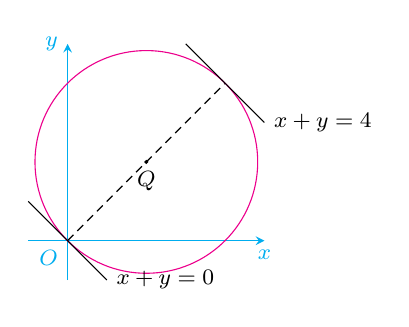
\begin{tikzpicture}[->,samples=100,>=stealth,font=\footnotesize]
                \draw[->,cyan](-.5,0)--(0,0)node[below left]{$O$}--(2.5,0)node[below]{$x$};
                \draw[->,cyan](0,-.5)--(0,2.5)node[left]{$y$};
                \draw[densely dashed,-] (0,0)--(1,1)node[below]{$Q$}--(2,2);
                \draw[fill=black] (1,1) circle(0.5pt);
                \draw[magenta,-] (1,1) circle({sqrt(2)});
                \draw[-,domain=-0.5:0.5,black] plot(\x,{-\x})node[right]{$x+y=0$};
                \draw[-,domain=1.5:2.5,black] plot(\x,{-\x+4})node[right]{$x+y=4$};
            \end{tikzpicture}
            \caption{}
            \label{tikz_ercjf}
        \end{figure}
    \end{minipage}\hfill
    \begin{minipage}{0.7\linewidth}
        由图 \ref{tikz_ercjf} 易知, $0\leqslant x+y\leqslant 4$, 所以 $x+y\geqslant \sin(x+y)$, 但取等的条件为 $(x,y)=(0,0)$, 而在该点出的二重积分为 0, 因此
        $$\displaystyle\iint\limits_D(x+y)\dd \sigma>\iint\limits_D\sin(x+y)\dd \sigma$$
        排除 B、D 选项, 又因为当 $x+y=4$ 时, 有
        $$4\iint\limits_D\dd \sigma=8\pi$$ 并且同样地在 $(2,2)$ 点处的二重积分为 $0$, 因此 $8\pi>I_1$, 故选 A.
    \end{minipage}
\end{solution}

\begin{example}
    设 $\displaystyle I_1=\iint\limits_D\dfrac{x+y}{4}\dd x\dd y,~I_2=\iint\limits_D\sqrt{\dfrac{x+y}{4}}\dd x\dd y,~I_3=\iint\limits_D\sqrt[3]{\dfrac{x+y}{4}}\dd x\dd y$,
    且 $$D=\qty{(x,y)\big| (x-1)^2+(y-1)^2\leqslant 2}$$
    则有
    \begin{tasks}(4)
        \task $I_1<I_2<I_3$
        \task $I_2<I_3<I_1$
        \task $I_3<I_1<I_2$
        \task $I_3<I_2<I_1$
    \end{tasks}
\end{example}
\begin{solution}
    由图 \ref{tikz_ercjf} 知, $0<\dfrac{x+y}{4}<1$, 且 $\dfrac{x+y}{4}<\sqrt{\dfrac{x+y}{4}}<\sqrt[3]{\dfrac{x+y}{4}}$, 因此 $I_1<I_2<I_3$, 选 A.
\end{solution}

\begin{example}[2019 数二]
    已知平面区域 $D=\qty{(x,y)\Big| |x|+|y|\leqslant\dfrac{\pi}{2}}$, 记 $\displaystyle I_1=\iint\limits_D\sqrt{x^2+y^2}\dd x\dd y,~I_2=\iint\limits_D\sin\sqrt{x^2+y^2}\dd x\dd y,~I_3=\iint\limits_D\qty(1-\cos\sqrt{x^2+y^2})\dd x\dd y$, 则
    \begin{tasks}(4)
        \task $I_3<I_2<I_1$
        \task $I_2<I_1<I_3$
        \task $I_1<I_2<I_3$
        \task $I_2<I_3<I_1$
    \end{tasks}
\end{example}
\begin{solution}
    作出积分区域 $D$:\\
    \begin{minipage}{0.29\linewidth}
        \begin{figure}[H]
            \centering
            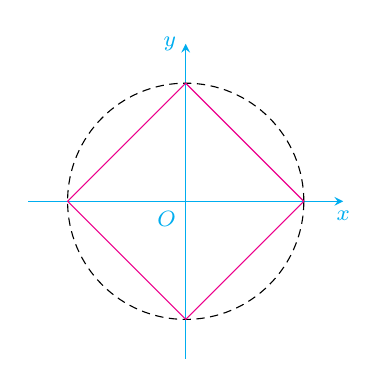
\begin{tikzpicture}[->,samples=100,>=stealth,font=\footnotesize]
                \draw[->,cyan](-2,0)--(0,0)node[below left]{$O$}--(2,0)node[below]{$x$};
                \draw[->,cyan](0,-2)--(0,2)node[left]{$y$};
                % \draw[densely dashed,-] (0,0)--(1,1)node[below]{$Q$}--(2,2);
                % \draw[fill=black, densely dashed] (0,0) circle(0.5pt);
                \draw[densely dashed] (0,0) circle(1.5);
                \draw[-,magenta] (1.5,0)--(0,1.5)--(-1.5,0)--(0,-1.5)--(1.5,0);
                % \draw[-,domain=-0.5:0.5,black] plot(\x,{-\x})node[right]{$x+y=0$};
                % \draw[-,domain=1.5:2.5,black] plot(\x,{-\x+4})node[right]{$x+y=4$};
            \end{tikzpicture}
            \caption{}
            \label{tikz_ercjfshuer}
        \end{figure}
    \end{minipage}\hfill
    \begin{minipage}{0.7\linewidth}
        在区域 $D$ 上, 有 $0\leqslant \sqrt{x^2+y^2}\leqslant \dfrac{\pi}{2}$, 那么 $$\sin\sqrt{x^2+y^2}\leqslant \sqrt{x^2+y^2}$$
        下面比较 $1-\cos\sqrt{x^2+y^2}$ 与 $\sin\sqrt{x^2+y^2}$, 令 $u=\sqrt{x^2+y^2}\in\qty[0,\dfrac{\pi}{2}]$, 那么
        $$1-\cos\sqrt{x^2+y^2}-\sin\sqrt{x^2+y^2}=1-\cos u-\sin u=1-\sqrt{2}\sin\qty(u+\dfrac{\pi}{4})\leqslant 0$$
        故 $1-\cos\sqrt{x^2+y^2}\leqslant \sin\sqrt{x^2+y^2}\leqslant \sqrt{x^2+y^2}$, 所以 $I_3<I_2<I_1$, 选 A.
    \end{minipage}
\end{solution}
\subsection{重积分的计算及相关方法}

\subsubsection{重积分的性质}

\begin{example}[1993 年数三]
    设 $f(x,y)$ 连续, 且
    $$f(x,y)=xy+\iint\limits_D f(u,v)\dd u\dd v$$
    其中 $D$ 是由 $y=0,y=x^2,x=1$ 所围成区域, 求 $f(x,y)$.
\end{example}
\begin{solution}
    设 $A=\displaystyle\iint\limits_D f(u,v)\dd u\dd v$, 则 $f(x,y)=xy+A$, 等式两边分别积分, 得
    \begin{flalign*}
        A=\iint\limits_D f(x,y)\dd x\dd y=\iint\limits_D(xy+A)\dd x\dd y=\int_{0}^{1}\dd x\int_{0}^{x^2}(xy+A)\dd y=\int_{0}^{1}\qty(\dfrac{1}{2}x^5+Ax^2)\dd x=\dfrac{4A+1}{12}
    \end{flalign*}
    即 $A=\dfrac{1}{8}$, 于是 $f(x,y)=xy+\dfrac{1}{8}.$
\end{solution}

\begin{example}
    计算二重积分 \(\displaystyle\iint\limits_Dy^2\dd x\dd y\), 其中 \(D\) 是由摆线 \(\begin{cases}
        x=a(t-\sin t) \\
        y=a(1-\cos t)
    \end{cases}(0\leqslant t\leqslant 2\pi,a>0)\) 与 \(x\) 轴围成的区域.
\end{example}
\begin{solution}
    因为 $y=a(1-\cos t),~\dd x=a(1-\cos t)\dd t$, 于是
    \begin{flalign*}
        \iint\limits_Dy^2\dd x\dd y & =\int_{0}^{2\pi a}\dd x\int_{0}^{y(x)}y^2\dd y=\dfrac{1}{3}\int_{0}^{2\pi a}y^3(x)\dd x=\dfrac{1}{3}\int_{0}^{2\pi}a^4(1-\cos t)^4\dd t=\dfrac{a^4}{3}\int_{0}^{2\pi}\qty(2\sin^2\dfrac{t}{2})^4\dd t                                                                       \\
                                    & \xlongequal{\frac{t}{2}=u}\dfrac{a^4}{3}\cdot 2^4\cdot 2\int_{0}^{\pi}\sin^8u\dd u=\dfrac{a^4}{3}\cdot 2^6\int_{0}^{\frac{\pi}{2}}\sin^8u\dd u=\dfrac{a^4}{3}\cdot 2^6\cdot\dfrac{1\times3\times5\times7}{2\times4\times6\times8}\cdot\dfrac{\pi}{2}=\dfrac{35\pi}{12} a^4.
    \end{flalign*}
\end{solution}

\begin{example}
    设 \(D\) 由 \(\begin{cases}
        x=t-\sin t \\
        y=1-\cos t
    \end{cases}(0\leqslant t\leqslant 2\pi)\) 与 \(x\) 围成, 求 \(\displaystyle\iint\limits_D(x+2y)\dd x\dd y\).
\end{example}
\begin{solution}
    \begin{flalign*}
        I=\iint\limits_D (x+2y)\dd x\dd y=\int_{0}^{2\pi}\dd x\int_{0}^{y(x)}(x+2y)\dd y=\int_{0}^{2\pi}\qty(xy+y^2)\dd x=\int_{0}^{2\pi}\qty[(t-\sin t)(1-\cos t)^2+(1-\cos t)^3]\dd t
    \end{flalign*}
    令 \(\displaystyle I_1=\int_{0}^{2\pi}t(1-\cos t)^2\dd t,~I_2=\int_{0}^{2\pi}\sin t(1-\cos t)^2\dd t,~I_3=\int_{0}^{2\pi}(1-\cos t)^3\dd t\), 则
    \begin{flalign*}
        I_1 & =\int_{0}^{2\pi}t\qty(2\sin^2\dfrac{t}{2})^2\dd t \xlongequal{\frac{t}{2}=u}16\int_{0}^{\pi}u\cdot\sin^4u\dd u \xlongequal{\int_{0}^{\pi}x\cdot f(\sin x)\dd x=\frac{\pi}{2}\int_{0}^{\pi}f(\sin x)\dd x}16\pi\cdot\dfrac{1\times3}{2\times4}\cdot\dfrac{\pi}{2}=3\pi^2 \\
        I_3 & =\int_{0}^{2\pi}\qty(2\sin^2\dfrac{t}{2})^3\dd t=8\int_{0}^{2\pi}\sin^6\dfrac{t}{2}\dd t \xlongequal{\frac{t}{2}=u}32\int_{0}^{\frac{\pi}{2}}\sin^6u\dd u=32\times\dfrac{1\times3\times5}{2\times4\times6}\cdot\dfrac{\pi}{2}=5\pi
    \end{flalign*}
    且 \(\displaystyle I_2=\int_{0}^{2\pi}\sin t(1-\cos t)^2\dd t \xlongequal[\text{偶倍奇零}]{u=\pi-t}0 \), 故 $I=I_1-I_2+I_3=3\pi ^2+5\pi.$
\end{solution}

\subsubsection{运用分部积分法}

\begin{theorem}[重积分分部积分法]
    一般地, 对于 $\displaystyle \int_{a}^{b} f(x) \dd x\int_{\varphi_1(x)}^{\varphi_2(x)} g(y) \dd y$, 令 $\displaystyle G(x)=\int_{\varphi_1(x)}^{\varphi_2(x)} g(y) \dd y, F'(x)=f(x)$, 则
    $$\int_{a}^{b} f(x) \dd x\int_{\varphi_1(x)}^{\varphi_2(x)} g(y) \dd y=\int_{a}^{b} G(x) \dd F(x)=\eval{G(x)F(x)}_{a}^{b}-\int_{a}^{b} F(x)G'(x) \dd x.$$
\end{theorem}

\begin{example}
    计算 $\displaystyle\int_{0}^{1}\dd y\int_{1}^{\sqrt{y}}\sqrt{\dfrac{1}{x^2}+1}\dd x.$
\end{example}
\begin{solution}
    由分部积分公式,
    $$I=\int_{0}^{1}\qty[\int_{1}^{\sqrt{y}}\sqrt{\dfrac{1}{x^2}+1}\dd x]\dd y=\eval{y\int_{1}^{\sqrt{y}}\sqrt{\dfrac{1}{x^2}+1}\dd x}_{y=0}^{y=1}-\int_{0}^{1}y\dd \qty[\int_{1}^{\sqrt{y}}\sqrt{\dfrac{1}{x^2}+1}\dd x]=0-\dfrac{1}{2}\int_{0}^{1}\sqrt{1+y}\dd y=1-2\sqrt{2}.$$
\end{solution}

\begin{example}
    计算二重积分 $\displaystyle I=\int_{0}^{1}\dd x\int_{x-x^3}^{1}\qty(3x^2-1)\e^{y^2}\dd y.$
\end{example}
\begin{solution}
    令 $\varphi(x)=\displaystyle\int_{x-x^3}^{1}\e^{y^2}\dd y$, 于是原式可化为
    \begin{flalign*}
        I & =\int_{0}^{1}\qty(3x^2-1)\varphi(x)\dd x=\int_{0}^{1}\varphi(x)\dd \qty(x^3-x)=\qty(x^3-x)\varphi(x)\biggl |_{x=0}^{x=1}-\int_{0}^{1}\qty(x^3-x)\qty(3x^2-1)\e^{\qty(x-x^3)^2}\dd x \\
          & =-\dfrac{1}{2}\int_{0}^{1}\e^{\qty(x-x^3)^2}\dd \qty(x-x^3)^2=-\dfrac{1}{2}\e^{\qty(x-x^3)^2}\biggl |_{x=0}^{x=1}=0.
    \end{flalign*}
\end{solution}

\begin{example}
    计算二重积分 $\displaystyle\int_{0}^{1}\dd x\int_{x^2}^{1}x^3\sin y^3\dd y$.
\end{example}
\begin{solution}
    令 $\varphi(x)=\displaystyle\int_{x^2}^{1}\sin y^3\dd y$, 于是原式可化为
    \begin{flalign*}
        I & =\int_{0}^{1}x^3\varphi(x)\dd x=\dfrac{1}{4}\int_{0}^{1}\varphi(x)\dd x^4=\dfrac{1}{4}x^3\varphi(x)\biggl |_{x=0}^{x=1}-\dfrac{1}{4}\int_{0}^{1}x^4\cdot\qty(-2x\sin x^6)\dd x \\
          & =\dfrac{1}{2}\int_{0}^{1}x^5\sin x^6\dd x=\dfrac{1}{12}\int_{0}^{1}\sin x^6\dd x^6=\eval{\dfrac{-\cos x^6}{12}}_{x=0}^{x=1}=\dfrac{1-\cos 1}{12}.
    \end{flalign*}
\end{solution}

\subsubsection{交换积分顺序}

\begin{example}[2004 数一]
    设 $f(x)$ 为连续函数, $\displaystyle F(t)=\int_{0}^{t}\dd y\int_{y}^{t}f(x)\dd x$, 则 $F'(2)$ 等于
    \begin{tasks}(4)
        \task $2f(2).$
        \task $f(2).$
        \task $-f(2).$
        \task $0.$
    \end{tasks}
\end{example}
\begin{solution}
    交换积分次序, $\displaystyle F(t)=\int_{1}^{t}\dd x\int_{1}^{x}f(x)\dd y=\int_{1}^{t}(x-1)f(x)\dd x$,
    于是 $F'(2)=(2-1)f(2)=f(2)$, 故选 B.
\end{solution}

% \begin{example}
%     (2015 数学 (一)、(二))计算 $\displaystyle\iint\limits_Dx(x+y)\dd x\dd y$, 其中 $D=\{(x,y)|x^2+y^2\leqslant 2,y\geqslant x^2\}.$
% \end{example}
% \begin{solution}
%     因为区域 $D$ 关于 $y$ 轴对称, 所以
%     \begin{flalign*}
%         \iint\limits_Dx(x+y)\dd x\dd y
%          & =2\int_0^1\dd x\int_{x^2}^{\sqrt{2-x^2}}x^2\dd y
%         =2\int_0^1\left(x^2\sqrt{2-x^2}-x^4\right)\dd x                                        \\
%          & =2\int_0^1x^2\sqrt{2-x^2}\dd x-\frac{2}{5}
%         \xlongequal[]{x=\sqrt{2}\sin t}2\int_0^{\frac{\pi}{4}}4\sin^2t\cos^2t\dd t-\frac{2}{5} \\
%          & =2\int_0^{\frac{\pi}{4}}\sin^2 2t\dd t-\frac{2}{5}
%         =\frac{\pi}{4}-\frac{2}{5}.
%     \end{flalign*}
% \end{solution}
% 
% \begin{example}
%     计算 $\displaystyle\iint\limits_D\left(x+y^2\right)\dd x\dd y$, 其中 $D$ 是 $y=x^2$ 与 $y^2=x$ 所围成的闭区域.
% \end{example}
% \begin{solution}
%     \begin{flalign*}
%         \iint\limits_D\left(x+y^2\right)\dd x\dd y
%          & =\int_0^1\dd x\int_{x^2}^{\sqrt{x}}\left(x+y^2\right)\dd y
%         =\int_0^1\left(\frac{4}{3}x^{\frac{3}{2}}-x^3-\frac{x^6}{3}\right)\dd x       \\
%          & =\left(\frac{8}{15}x^{\frac{5}{2}}-\frac{x^4}{4}-\frac{x^7}{21}\right)_0^1
%         =\frac{33}{140}.
%     \end{flalign*}
% \end{solution}
% 
% \begin{example}
%     设 $\displaystyle a=\int_0^1\dd y\int_y^1\left(\frac{\mathrm{e}^{x^2}}{x}-\mathrm{e}^{y^2}\right)\dd x$, 
%     求常数 $a,b$ 的值, 使之满足
%     $$\displaystyle\lim_{x\to\infty}\left(\frac{x-a}{x+a}\right)^{\frac{2x}{\mathrm{e}-1}}=\frac{1}{3}\int_b^{+\infty}x\mathrm{e}^{-x}\dd x.$$
% \end{example}
% \begin{solution}
%     \begin{flalign*}
%         a & =\int_0^1\dd y\int_y^1\frac{\mathrm{e}^{x^2}}{x}\dd x-\int_0^1\dd y\int_y^1\mathrm{e}^{y^2}\dd x
%         =\int_0^1\dd x\int_0^x\frac{\mathrm{e}^{x^2}}{x}\dd x-\int_0^1(1-y)\mathrm{e}^{y^2}\dd y                                    \\
%           & =\int_0^1\mathrm{e}^{x^2}\dd x-\int_0^1\mathrm{e}^{y^2}(1-y)\dd y=\int_0^1y\mathrm{e}^{y^2}\dd y=\frac{\mathrm{e}-1}{2}
%     \end{flalign*}
%     \begin{flalign*}
%         \lim_{x\to\infty}\left(\frac{x-\frac{\mathrm{e}-1}{2}}{x+\frac{\mathrm{e}-1}{2}}\right)^{\frac{2x}{\mathrm{e}-1}}=\lim_{x\to\infty}\left(\frac{2x-\mathrm{e}+1}{2x+\mathrm{e}-1}\right)^{\frac{2x}{\mathrm{e}-1}}=\exp\lim_{x\to\infty}\frac{2x}{\mathrm{e}-1}\cdot\frac{2(1-\mathrm{e})}{2x+\mathrm{e}-1}=\mathrm{e}^{-2}
%     \end{flalign*}
%     \begin{flalign*}
%         \frac{1}{3}\int_b^{+\infty}x\mathrm{e}^{-x}\dd x=-\frac{1}{3}(x+1)\mathrm{e}^{-x}\Bigl |_b^{+\infty}=\mathrm{e}^{-2}\Rightarrow b=2.
%     \end{flalign*}
% \end{solution}

\begin{example}
    计算 $\displaystyle I=\int_0^1\dd x\int_0^x\dd y\int_0^y\frac{\sin z}{1-z}\dd z.$
\end{example}
\begin{solution}
    逐次交换积分顺序, 得
    \begin{flalign*}
        I=\int_0^1\dd x\int_0^x\dd z\int_z^x\frac{\sin z}{1-z}\dd y
        =\int_0^1\dd z\int_z^1\dd x\int_z^x\frac{\sin z}{1-z}\dd y
        =\int_0^1\frac{\sin z}{1-z}\frac{(1-z)^2}{2}\dd z=\frac{1-\sin 1}{2}.
    \end{flalign*}
\end{solution}

\begin{example}
    计算 $\displaystyle I=\int_0^1\dd x\int_x^1\dd y\int_y^1y\sqrt{1+z^4}\dd z.$
\end{example}
\begin{solution}
    逐次交换积分顺序, 得
    \begin{flalign*}
        I & =\int_0^1\dd x\int_x^1\dd z\int_x^zy\sqrt{1+z^4}\dd y
        =\int_0^1\dd z\int_0^z\dd x\int_x^zy\sqrt{1+z^4}\dd y
        =\int_0^1\dd z\int_0^z\frac{z^2-x^2}{2}\sqrt{1+z^4}\dd x  \\
          & =\frac{1}{3}\int_0^1z^3\sqrt{1+z^4}\dd z
        =\frac{1}{12}\int_0^1\sqrt{1+z^4}\dd \left(1+z^4\right)
        =\frac{\left(1+z^4\right)^{\frac{3}{2}}}{18}\Biggl |_0^1
        =\frac{2\sqrt{2}-1}{18}.
    \end{flalign*}
\end{solution}

\begin{example}
    计算 $\displaystyle I=\int_0^1\dd x\int_0^{1-x}\dd z\int_0^{1-x-z}(1-y)\mathrm{e}^{-(1-y-z)^2}\dd y.$
\end{example}
\begin{solution}
    逐次交换积分顺序, 得
    \begin{flalign*}
        I & =\int_0^1\dd z\int_0^{1-z}\dd x\int_0^{1-x-z}(1-y)\mathrm{e}^{-(1-y-z)^2}\dd y
        =\int_0^1\dd z\int_0^{1-z}\dd y\int_0^{1-y-z}(1-y)\mathrm{e}^{-(1-y-z)^2}\dd x     \\
          & =\int_0^1\dd z\int_0^{1-z}(1-y-z)(1-y)\mathrm{e}^{-(1-y-z)^2}\dd y
        =\int_0^1\dd y\int_0^{1-y}(1-y-z)(1-y)\mathrm{e}^{-(1-y-z)^2}\dd z                 \\
          & =\int_0^1\frac{1-y}{2}\mathrm{e}^{-(1-y-z)^2}\Biggl |_0^{1-y}\dd y
        =\frac{1}{4\mathrm{e}}.
    \end{flalign*}
\end{solution}

% \begin{example}
%     求极限 $\displaystyle\lim_{t\to0^+}\frac{1}{(t-x_0)^{n+4}}\int_{x_0}^t\dd z\int_z^t\dd x\int_{x_0}^z(x-y)^nf(y)\dd y$, 
%     其中 $f(x)$ 在 $[x_0,x_0+\delta]~(\delta>0)$ 上可微, 且 $f(x_0)=0$, $n$ 是自然数.
% \end{example}
% \begin{solution}
% 
% \end{solution}

\begin{example}
    求极限 $\displaystyle I=\lim_{t\to0^+}\dfrac{\displaystyle\int_{0}^{\sqrt{t}}\dd x\int_{x^2}^{t}\sin y^2\dd y}{\qty(\mathrm{e}^{-\frac{2}{\pi}t^2}-1)\arctan t^{\frac{3}{2}}}.$
\end{example}
\begin{solution}
    $\displaystyle\int_{0}^{\sqrt{t}}\dd x\int_{x^2}^{t}\sin y^2\dd y=\int_{0}^{t}\sin y^2\dd y\int_{0}^{\sqrt{y}}\dd x=\int_{0}^{t}\sqrt{y}\sin y^2\dd y$, $I=\lim\limits_{t\to0^+}\dfrac{\displaystyle\int_{0}^{t}\sqrt{y}\sin y^2\dd y}{-\dfrac{2}{\pi}t^{\frac{7}{2}}}\xlongequal[]{L'}-\dfrac{\pi}{7}.$
\end{solution}

\begin{example}
    计算 $\displaystyle\int_{0}^{1}\dd x\int_{0}^{x}\sqrt{1+y^2}\dd y+3\int_{0}^{1}\dd y\int_{1}^{\sqrt{2-y^2}}\sqrt{x^2+y^2}\dd x.$
\end{example}
\begin{solution}
    对前部分交换积分次序, 后部分采用极坐标换元,
    \begin{flalign*}
        \int_{0}^{1}\dd x\int_{0}^{x}\sqrt{1+y^2}\dd y=\int_{0}^{1}\dd y\int_{y}^{1}\sqrt{1+y^2}\dd x=\int_{0}^{1}\sqrt{1+y^2}\dd y-\dfrac{1}{3}\qty(2\sqrt{2}-1)
    \end{flalign*}
    \begin{flalign*}
        3\int_{0}^{1}\dd y\int_{1}^{\sqrt{2-y^2}}\sqrt{x^2+y^2}\dd x & =3\int_{0}^{\frac{\pi}{4}}\dd \theta\int_{\sec\theta}^{\sqrt{2}}\rho^2\dd \rho=\dfrac{\sqrt{2}\pi}{2}-\int_{0}^{\frac{\pi}{4}}\sec^3\theta\dd \theta \\
                                                                     & =\dfrac{\sqrt{2}\pi}{2}-\int_{0}^{\frac{\pi}{4}}\sqrt{1+\sec^2\theta}\dd \tan\theta=\dfrac{\sqrt{2}\pi}{2}-\int_{0}^{1}\sqrt{1+t^2}\dd t
    \end{flalign*}
    两式相加得 $\dfrac{\sqrt{2}\pi}{2}-\dfrac{1}{3}\qty(2\sqrt2-1).$
\end{solution}

\begin{example}
    计算 $\displaystyle\int_{0}^{1}\dd y\int_{0}^{1}\sqrt{\e^{2x}-y^2}\dd x+\int_{1}^{\e}\dd y\int_{\ln y}^{1}\sqrt{\e^{2x}-y^2}\dd x.$
\end{example}
\begin{solution}
    交换积分次序先 $x$ 后 $y$ 有,
    \begin{flalign*}
        I=\int_{0}^{1}\dd x\int_{0}^{\e^{x}}\sqrt{\e^{2x}-y^2}\dd y=\int_{0}^{1}\e^{2x}\dd x\int_{0}^{\e^x}\sqrt{1-\qty(\dfrac{y}{\e^x})^2}\dd \qty(\dfrac{y}{\e^x})
    \end{flalign*}
    其中 $\displaystyle\int_{0}^{\e^x}\sqrt{1-\qty(\dfrac{y}{\e^x})^2}\dd \qty(\dfrac{y}{\e^x}) \xlongequal{\frac{y}{\e^x}=\sin t}\int_{0}^{\frac{\pi}{2}}\cos^2t\dd t=\dfrac{\pi}{4},~\int_{0}^{1}\e^{2x}\dd x=\eval*{\dfrac{1}{2}\e^{2x}}_{0}^{1}=\dfrac{\e^2-1}{2}$, \newline
    综上, 原式等于 $\dfrac{\pi-1}{2}\qty(\e^2-1).$
\end{solution}

\subsubsection{圆代换与球代换}

\begin{example}[2011 数二]
    设平面区域 $D$ 由直线 $y=x$, 圆 $x^2+y^2=2y$ 及 $y$ 轴所围成, 计算 $\displaystyle\iint\limits_D xy\dd \sigma$.
\end{example}
\begin{solution}
    圆的极坐标为 $r=2\sin\theta$, 于是
    \begin{flalign*}
        I=\iint\limits_D xy\dd \sigma=\int_{\frac{\pi}{4}}^{\frac{\pi}{2}}\dd \theta\int_{0}^{2\sin\theta}r^2\cos\theta\sin\theta r\dd r=4\int_{\frac{\pi}{4}}^{\frac{\pi}{2}}\sin^5\theta\dd \sin\theta=\dfrac{7}{12}.
    \end{flalign*}
\end{solution}

\begin{example}[2015 数一]
    设 $D$ 是第一象限中由曲线 $2xy=1,4xy=1$ 与直线 $y=x,y=\sqrt{3}x$ 围成的平面区域,
    函数 $f(x,y)$ 在 $D$ 上连续, 则 $\displaystyle\iint\limits_D f(x,y)\dd x\dd y$.
    \begin{tasks}(2)
        \task $\displaystyle \int_{\frac{\pi}{4}}^{\frac{\pi}{3}}\dd \theta \int_{\frac{1}{2\sin2\theta}}^{\frac{1}{\sin2\theta}}f(r\cos\theta,r\sin\theta)r\dd r.$
        \task $\displaystyle \int_{\frac{\pi}{4}}^{\frac{\pi}{3}}\dd \theta \int_{\frac{1}{\sqrt{2\sin 2\theta}}}^{\frac{1}{\sqrt{\sin2\theta}}}f(r\cos\theta,r\sin\theta)r\dd r.$
        \task $\displaystyle \int_{\frac{\pi}{4}}^{\frac{\pi}{3}}\dd \theta \int_{\frac{1}{2\sin2\theta}}^{\frac{1}{\sin2\theta}}f(r\cos\theta,r\sin\theta)\dd r.$
        \task $\displaystyle \int_{\frac{\pi}{4}}^{\frac{\pi}{3}}\dd \theta \int_{\frac{1}{\sqrt{2\sin 2\theta}}}^{\frac{1}{\sqrt{\sin2\theta}}}f(r\cos\theta,r\sin\theta)\dd r.$
    \end{tasks}
\end{example}
\begin{solution}
    积分区域可用极坐标表示为 $D=\qty{(r,\theta)~\biggl |~\dfrac{\pi}{4}\leqslant \theta\leqslant \dfrac{\pi}{3},\dfrac{1}{\sqrt{2\sin 2\theta}}\leqslant r\leqslant \dfrac{1}{\sqrt{\sin 2\theta}}}$,
    于是有 $$\iint\limits_D f(x,y)\dd x\dd y=\int_{\frac{\pi}{4}}^{\frac{\pi}{3}}\dd \theta \int_{\frac{1}{\sqrt{2\sin 2\theta}}}^{\frac{1}{\sqrt{\sin2\theta}}}f(r\cos\theta,r\sin\theta)r\dd r.$$
    故选 B.
\end{solution}

% \begin{figure}[H]
%     \centering
%     \includegraphics[]{figures/cjf1.pdf}
%     \caption{}
%     \label{cjfs}
% \end{figure}

% \begin{figure}[H]
%     \centering
%     \subfigure[]{
%         \includegraphics[]{figures/cjf1.pdf}
%     }
%     \subfigure[]{
%         \includegraphics[]{figures/cjf2.pdf}
%     }
%     \caption{}
%     \label{cjfs}
% \end{figure}

\begin{example}
    设函数 $f(u)$ 连续, 区域 $D=\qty{(x,y)\mid x^2+y^2\leqslant 2y}$, 则 $\displaystyle\iint\limits_D f(xy)\dd x\dd y$.
    \begin{tasks}(2)
        \task $\displaystyle \int_{-1}^{1}\dd x\int_{-\sqrt{1-x^2}}^{\sqrt{1-x^2}}f(xy)\dd y.$
        \task $\displaystyle 2\int_{0}^{2}\dd y\int_{0}^{\sqrt{2y-y^2}}f(xy)\dd x.$
        \task $\displaystyle \int_{0}^{\pi}\dd \theta\int_{0}^{2\sin\theta}f\qty(r^2\sin\theta\cos\theta)\dd r.$
        \task $\displaystyle \int_{0}^{\pi}\dd \theta\int_{0}^{2\sin\theta}f\qty(r^2\sin\theta\cos\theta)r\dd r.$
    \end{tasks}
\end{example}
\begin{solution}
    在直角坐标系下
    $$\iint\limits_Df(xy)\dd x\dd y=\int_{0}^{2}\dd y\int_{-\sqrt{1-(y-1)^2}}^{\sqrt{1-(y-1)^2}}f(xy)\dd x=\int_{-1}^{1}\dd x\int_{1-\sqrt{1-x^2}}^{1+\sqrt{1-x^2}}f(xy)\dd y$$
    故排除 A、B, 在极坐标下
    $$\iint\limits_D f(xy)\dd x\dd y=\int_{0}^{\pi}\dd \theta\int_{0}^{2\sin\theta}f\qty(r^2\sin\theta\cos\theta)r\dd r$$
    故选 D.
\end{solution}

% \begin{example}
%     计算下列积分:
%     \setcounter{magicrownumbers}{0}
%     \begin{table}[H]
%         \centering
%         \begin{tabular}{l | l}
%             (\rownumber{}) (2016 数一) $\displaystyle\iint\limits_{\substack{2\leqslant r\leqslant 2(1+\cos\theta)\\-\frac{\pi}{2}\leqslant \theta\leqslant \frac{\pi}{2}}}x\dd x\dd y$. & (\rownumber{}) 
%         \end{tabular}
%     \end{table}
% \end{example}

\begin{example}
    计算三重积分 $\displaystyle I=\iiint\limits_\Omega z\dd x\dd y\dd z$, 其中 $\Omega$ 是两个球面 $x^2+y^2+z^2=2z$ 和 $x^2+y^2+z^2=z$ 围成的区域.
\end{example}
\begin{solution}
    由球坐标变化, $\begin{cases}
            x=r\sin\varphi \cos\theta \\
            y=r\sin\varphi \sin\theta \\
            z=r\cos\varphi
        \end{cases}$, 则 $\Omega'=\qty{0\leqslant \theta\leqslant 2\pi,0\leqslant\varphi\leqslant\dfrac{\pi}{2},\cos\varphi\leqslant r\leqslant 2\cos\varphi}$, 则
    \begin{flalign*}
        I & =\int_{0}^{2\pi}\dd \theta\int_{0}^{\frac{\pi}{2}}\dd \varphi\int_{\cos\varphi}^{2\cos\varphi}r\cos\varphi\cdot r^2\sin\varphi\dd r=2\pi\int_{0}^{\frac{\pi}{2}}\sin\varphi\cos\varphi\dd \varphi\int_{\cos\varphi}^{2\cos\varphi}r^3\dd r \\
          & =\dfrac{15\pi2}{2}\int_{0}^{\frac{\pi}{2}}\sin\varphi\cos^5\varphi\dd \varphi=\dfrac{5\pi}{4}.
    \end{flalign*}
\end{solution}

\begin{example}
    设积分区域 $\Omega_t:x^2+y^2+z^2\leqslant 2tz,~f(0)=0,~f'(0)=15$, 求极限 $$\lim_{t\to0^+}\dfrac{1}{t^5}\iiint\limits_{\Omega_t}f\qty(x^2+y^2+z^2)\dd V.$$
\end{example}
\begin{solution}
    \textbf{法一: }由三重积分的球坐标计算方法, 积分区域可用球坐标变量表示为
    $$0\leqslant \theta\leqslant 2\pi ,~0\leqslant \varphi\leqslant \dfrac{\pi}{2},~0\leqslant r\leqslant 2t\cos\varphi$$
    故三重积分表示为 $\displaystyle g(t)=\int_{0}^{2\pi}\dd \theta\int_{0}^{\frac{\pi}{2}}\sin\varphi\dd \varphi\int_{0}^{2t\cos\varphi}f\qty(r^2)r^2\dd r$, 设 $F'(r)=f\qty(r^2)r^2$, 则
    \begin{flalign*}
        g(t) & =2\pi\int_{0}^{\frac{\pi}{2}}\qty[F(2t\cos\varphi)-F(0)]\sin\varphi\dd \varphi=2\pi\int_{0}^{\frac{\pi}{2}}F(2t\cos\varphi)\sin\varphi\dd \varphi-2\pi F(0)\int_{0}^{\frac{\pi}{2}}\sin\varphi\dd \varphi \\
             & =-2\pi\int_{0}^{\frac{\pi}{2}}F(2t\cos\varphi)\dd \cos\varphi-2\pi F(0)=\dfrac{\pi}{t}\int_{0}^{2t}F(u)\dd u-2\pi F(0)
    \end{flalign*}
    故
    \begin{flalign*}
        I & =\lim_{t\to0^+}\dfrac{1}{t^5}\iiint\limits_{\Omega_t}f\qty(x^2+y^2+z^2)\dd V=\pi\lim_{t\to0^+}\dfrac{\displaystyle\int_{0}^{2t}F(u)\dd u-2tF(0)}{t^6}\xlongequal[]{L'}\pi\lim_{t\to0^+}\dfrac{2F(2t)-2F(0)}{6t^5} \\
          & =\dfrac{\pi}{3}\lim_{t\to0^+}\dfrac{F(2t)-F(0)}{t^5}\xlongequal[]{L'}\dfrac{\pi}{3}\lim_{t\to0^+}\dfrac{2F'(2t)}{5t^4}=\dfrac{2\pi}{15}\lim_{t\to0^+}\dfrac{4t^2f\qty(4t^2)}{t^4}=\dfrac{32\pi}{15}f'(0)=32\pi.
    \end{flalign*}
    \textbf{法二: }有题意可假设 $f(x)=15x+o(x)$, 并令 $\displaystyle g(t)=\iiint\limits_{\Omega_t}f\qty(x^2+y^2+z^2)\dd V$, 于是
    \begin{flalign*}
        g(t) & =\iiint\limits_{\Omega_t}\qty[15\qty(x^2+y^2+z^2)+o\qty(x^2+y^2+z^2)]\dd V =\int_{0}^{2\pi}\dd \theta\int_{0}^{\frac{\pi}{2}}\dd \varphi\int_{0}^{2t\cos\varphi}\qty[15r^2+o\qty(r^2)]r^2\sin\varphi\dd r \\
             & =2\pi\int_{0}^{\frac{\pi}{2}}\sin\varphi\qty[3r^5+o\qty(r^5)]\biggl |_{0}^{2t\cos\varphi}\dd \varphi=-6\pi\cdot32t^5\int_{0}^{\frac{\pi}{2}}\cos^5\varphi\dd \cos\varphi+o\qty(t^5)=32\pi t^5+o\qty(t^5)
    \end{flalign*}所以 $\displaystyle\lim_{t\to0^+}\dfrac{g(t)}{t^5}=32\pi.$
\end{solution}

\begin{example}
    设 $f(x)$ 是 $(0,+\infty)$ 上连续可导的函数, $f(x)\neq0$ 且 $\displaystyle\lim_{x\to+\infty}\dfrac{xf'(x)}{f(x)}=c>0$, 记
    $$F(t)=\iiint\limits_{x^2+y^2+z^2\leqslant t^2}f\qty(\sqrt{x^2+y^2+z^2})\dd V,~~G(t)=\iint\limits_{x^2+y^2\leqslant t^2}f\qty(\sqrt{x^2+y^2})\dd \sigma$$
    求函数 $h(t)$, 使得 $\displaystyle\lim_{t\to+\infty}\dfrac{F(t)}{h(t)G(t)}=1.$
\end{example}
\begin{solution}
    由三重积分的球坐标计算公式和二重积分的极坐标计算公式, 得
    \begin{flalign*}
        F(t) & =\int_{0}^{2\pi}\dd \theta\int_{0}^{\pi}\sin\varphi\dd \varphi\int_{0}^{t}f(r)r^2\dd r=4\pi\int_{0}^{t}f(r)r^2\dd r \\
        G(t) & =\int_{0}^{2\pi}\dd \theta\int_{0}^{t}f(r)r\dd r=2\pi\int_{0}^{t}f(r)r^2\dd r
    \end{flalign*}
    由 $\displaystyle\lim_{x\to+\infty}\dfrac{xf'(x)}{f(x)}=c>0$ 知, $\exists X_0>0$, 当 $x>X_0$ 时, $f(x)$ 与 $f'(x)$ 同号, 故 $f(x)>0$ 时, $f(x)$ 单调递增, 则
    $$\lim_{t\to+\infty}F(t)=+\infty,~~\lim_{t\to+\infty}G(t)=+\infty,~~\int_{X_0}^{+\infty}f(t)\dd t=+\infty$$
    那么
    \begin{flalign*}
        \lim_{t\to+\infty}\dfrac{F(t)}{tG(t)} & =\lim_{t\to+\infty}\dfrac{\displaystyle 4\pi\int_{0}^{t}f(r)r^2\dd r}{\displaystyle 2\pi t\int_{0}^{t}f(t)t\dd t}=2\lim_{t\to+\infty}\dfrac{\displaystyle\int_{0}^{t}f(r)r^2\dd r}{\displaystyle t\int_{0}^{t}f(t)t\dd t}\xlongequal{L'}2\lim_{t\to+\infty}\dfrac{f(t)t^2}{\displaystyle\int_{0}^{t}f(t)t\dd t+f(t)t^2} \\
                                              & \xlongequal{L'}2\lim_{t\to+\infty}\dfrac{2tf(t)+t^2f'(t)}{3tf(t)+t^2f'(t)}=2\lim_{t\to+\infty}\dfrac{2\dfrac{tf'(t)}{f(t)}}{3+\dfrac{tf'(t)}{f(t)}}=\dfrac{2(2+c)}{3+c}
    \end{flalign*}
    故 $\displaystyle \lim_{t\to+\infty}\dfrac{F(t)}{\dfrac{2(2+c)}{3+c}tG(t)}=1$, 所以取 $h(t)=\dfrac{2(2+c)}{3+c}t$ 即为所求函数.
\end{solution}

\subsubsection{Jacobian 行列式}

\begin{example}
    计算 $\displaystyle \iint\limits_D \e ^{\frac{y}{x+y}}\dd x\dd y$, 其中 $D$ 是由 $x+y=1$ 与坐标轴所围成的区域.
\end{example}
\begin{solution}
    \textbf{法一: }利用极坐标, 令 $\begin{cases}
            x=\rho \cos \theta \\ y=\rho \sin \theta
        \end{cases}$ 则区域 $ D $ 化为 $\displaystyle  D^{\prime}=\left\{(\theta, \rho) \left\lvert\, 0<\theta<\frac{\pi}{2}\right., 0<\rho<\frac{1}{\cos \theta+\sin \theta}\right\} ,  \mathrm{d} x \dd  y=\rho \mathrm{d} \theta \mathrm{d} \rho $ 于是
    \begin{flalign*}
        \iint\limits_{D}\e ^{\frac{y}{x+y}} \dd  x \dd  y & =\iint\limits_{D} \mathrm{e}^{\frac{\sin \theta}{\cos \theta+\sin \theta}} \rho \mathrm{d} \rho \mathrm{d} \theta=\int_{0}^{\frac{\pi}{2}} \dd  \theta \int_{0}^{\frac{1}{\cos \theta+\sin \theta}} \rho \mathrm{e}^{\frac{\sin \theta}{\cos \theta+\sin \theta}} \mathrm{d} \rho           \\
                                                          & =\frac{1}{2} \int_{0}^{\frac{\pi}{2}} \mathrm{e}^{\frac{\sin \theta}{\cos \theta+\sin \theta}} \mathrm{d}\left(\frac{\sin \theta}{\cos \theta+\sin \theta}\right)=\left.\frac{1}{2} \mathrm{e}^{\frac{\sin \theta}{\cos \theta+\sin \theta}}\right|_{0} ^{\frac{\pi}{2}}=\frac{1}{2}(e-1) .
    \end{flalign*}
    \textbf{法二: }利用变量代换, 令 $ x+y=u, y=u v $, 则区域 $ D $ 化为 $ D^{\prime}=\{(u, v) \mid 0<u<1,0<v<1\} $,
    $$
    \dfrac{\partial(x, y)}{\partial(u, v)}=\mqty|\dfrac{\partial x}{\partial u} & \dfrac{\partial x}{\partial v} \\[6pt]
    \dfrac{\partial y}{\partial u} & \dfrac{\partial y}{\partial v}|=\mqty|1-v & -u \\
    v & u|=u
    $$
        于是 $\displaystyle  \iint\limits_{D} \mathrm{e}^{\frac{y}{x+y}} \dd  x \dd  y=\iint\limits_{D^{\prime}} \mathrm{e}^{v}\left|\frac{\partial(x, y)}{\partial(u, v)}\right| \mathrm{d} u \dd  v=\int_{0}^{1} u \dd  u \int_{0}^{1} \mathrm{e}^{v} \dd  v=\frac{1}{2}(\mathrm{e}-1) .$\\
        \textbf{法三: }利用变量代换, 令 $ x+y=u, y-x=v $, 则区域 $ D $ 化为 $ D^{\prime}=\{(u, v) \mid 0<u<1,-u<v<u\} $,
    $$
    \dfrac{\partial(x, y)}{\partial(u, v)}=\mqty|\dfrac{\partial x}{\partial u} & \dfrac{\partial x}{\partial v} \\[6pt]
    \dfrac{\partial y}{\partial u} & \dfrac{\partial y}{\partial v}|=\mqty|\dfrac{1}{2} & -\dfrac{1}{2} \\[6pt]
    \dfrac{1}{2} & \dfrac{1}{2}|=\dfrac{1}{2}
    $$
    于是 $ \displaystyle \iint\limits_{D}\e ^{\frac{y}{x+y}} \dd  x \dd  y=\iint\limits_{D^{\prime}} \mathrm{e}^{\frac{u+v}{2 u}}\left|\frac{\partial(x, y)}{\partial(u, v)}\right| \mathrm{d} u \dd  v=\frac{1}{2} \int_{0}^{1} \dd  u \int_{-u}^{u} \mathrm{e}^{\frac{u+v}{2 u}} \dd  v=\frac{1}{2}(\mathrm{e}-1) . $
\end{solution}


\begin{example}
    设 $D$ 是 $y=\sqrt{x},~x=\sqrt{y}$ 和 $x^2+y^2-x-y+\dfrac{1}{4}=0,~\qty(x,y\in\qty[0,\dfrac{1}{2}])$ 围成的封闭区域, 求积分
    $$\iint\limits_D\qty(x-y^2)\qty(y-x^2)(1-4xy)\dd x\dd y.$$
\end{example}
\begin{solution}
    令 $u=x-y^2,~v=y-x^2$, 那么 $D'=\qty{(u,v)|u,v\geqslant 0,u+v\leqslant\dfrac{1}{4}}$
    $$|J|=\qty|\pdv{(x,y)}{(u,v)}|=\dfrac{1}{\qty|\displaystyle\pdv{(u,v)}{(x,y)}|}=\dfrac{1}{|1-4xy|}$$
    \begin{flalign*}
        \text{原式}=\iint\limits_{D'}uv\dd u\dd v=\int_{0}^{\frac{1}{4}}\dd u\int_{0}^{\frac{1}{4}-u}uv\dd v=\int_{0}^{\frac{1}{4}}\qty(\dfrac{1}{2}u^3-\dfrac{1}{4}u^2+\dfrac{1}{32}u)\dd u=\dfrac{1}{6144}.
    \end{flalign*}
\end{solution}

\begin{example}
    设 $z=z(x,y)$ 是由 $\varphi(y-bz)=x-az$ 确定的隐函数, 其中 $\varphi$ 是连续可微函数, 且 $a-b\varphi'(y-bz)\neq 0$, 求二重积分
    $$I=\iiint\limits_D\qty(az'_x+bz_y')\e^{\frac{x-y}{x+y}}\dd x\dd y$$
    其中 $D$ 是由 $x=0,~y=0,~x+y=1$ 所围成的区域.
\end{example}
\begin{solution}
    令 $F(x,y,z)=x-az-\varphi(y-bz)$, 那么 $$F_x'=1,~F_y'=-\varphi'(y-bz),~F_z'=-a+b\varphi'(y-bz)$$
    当 $a-b\varphi'(y-bz)=\neq 0$ 时, 由隐函数求导公式, 得
    $$z_x'=-\dfrac{F_x'}{F_z'}=\dfrac{1}{a-b\varphi'(y-bz)},~z_y'=-\dfrac{F_y'}{F_z'}=-\dfrac{\varphi'(y-bz)}{a-b\varphi'(y-bz)}$$
    于是 $az_x'+bz_y'=1$, 代入被积函数表达式, 得 $\displaystyle I=\displaystyle\iint\limits_D \e^{\frac{x-y}{x+y}}\dd x\dd y$
    令 $u=x-y,~v=x+y,~J=\dfrac{\partial(x,y)}{\partial(u,v)}=\dfrac{1}{2}$, 且变换后的积分区域为 $D_{uv}=\qty{(u,v):-v\leqslant u\leqslant v,0\leqslant v\leqslant 1}$, 所以二重积分化为
    \begin{flalign*}
        I=\iint\limits_{D_{uv}}\e^{\frac{u}{v}}\dfrac{1}{2}\dd u\dd v=\dfrac{1}{2}\int_{0}^{1}\dd v\int_{-v}^{v}\e^{\frac{u}{v}}\dd u=\dfrac{\e-\e^{-1}}{4}.
    \end{flalign*}
\end{solution}

\begin{example}[2007 湖南大学]
    计算积分 $$I=\iint\limits_D\dfrac{(x+y)\qty[\ln(x+y)-\ln y]}{\sqrt{2-x-y}}\dd x\dd y$$
    其中区域 $D$ 为 $x=0,x+y=1,y=x$ 所围成的三角形区域.
\end{example}
\begin{solution}
    原式改写为 $\displaystyle I=\iint\limits_D\dfrac{(x+y)\ln\qty(1+\dfrac{x}{y})}{\sqrt{2-(x+y)}}\dd x\dd y$, 则令 $u=x+y,~v=\dfrac{x}{y}$, 那么 $\begin{cases}
            x=\dfrac{uv}{1+v} \\[6pt]
            y=\dfrac{u}{1+v}
        \end{cases}$, 并且
    $$J=\pdv{(x,y)}{(u,v)}=\begin{vmatrix}
            \dfrac{v}{1+v} & \dfrac{u}{(1+v)^2}  \\[6pt]
            \dfrac{1}{1+v} & \dfrac{-u}{(1+v)^2}
        \end{vmatrix}=-\dfrac{u}{(1+v)^2} $$
    \begin{flalign*}
        \text{原式} & =\iint\limits_{D_{uv}}\dfrac{u\ln(1+v)}{\sqrt{2-u}}|J|\dd u\dd v=\iint\limits_{D_{uv}}\dfrac{u\ln(1+v)}{\sqrt{2-u}}\cdot\dfrac{u}{(1+v)^2}\dd u\dd v                                   \\
                    & =\int_{0}^{1}\dfrac{u^2}{\sqrt{2-u}}\dd u\cdot\int_{0}^{1}\dfrac{\ln(1+v)}{(1+v)^2}\dd v=\dfrac{2}{15}\qty(32\sqrt{2}-43)\cdot\dfrac{1}{2}(1-\ln 2)=\dfrac{32\sqrt{2}-43}{15}(1-\ln2).
    \end{flalign*}
\end{solution}

% \begin{example}
%     计算积分 $I=\displaystyle\iint\limits_D \dfrac{3x}{y^2+xy^3}\dd x\dd y$, 其中 $D$ 为平面曲线 $xy=1,xy=3,y^2=x,y^2=3x$ 所围成的有界闭区域.
% \end{example}
% \begin{solution}
% 
% \end{solution}

\begin{example}
    设 $\Omega$ 是由曲面 $z=y^2,z=4y^2~~(y>0)$, 平面 $z=x,z=2x$ 及 $z=2$ 所围区域,
    求积分 $$\iiint\limits_\Omega \frac{z\sqrt{z}}{y^3}\cos\frac{z}{y^2}\dd x\dd y\dd z.$$
\end{example}
\begin{solution}
    令 $\displaystyle u=\frac{z}{y^2},v=\frac{z}{x},z=z$, 即 $\displaystyle x=\frac{z}{v},y=\sqrt{\frac{z}{u}},z=z$, $\Omega':~0\leqslant z\leqslant 2,1\leqslant v\leqslant 2,1\leqslant u\leqslant 4$.
    $$J=\frac{\partial (x,y,z)}{\partial (u,v,z)}=\begin{vmatrix}
            0                                             & \displaystyle-\frac{z}{v^2} & \displaystyle\frac{1}{v}                    \\[6pt]
            \displaystyle-\frac{1}{2}\sqrt{\frac{z}{u^3}} & 0                           & \displaystyle\frac{1}{2}\sqrt{\frac{1}{uz}} \\[6pt]
            0                                             & 0                           & 1
        \end{vmatrix}=-\frac{z}{2v^2}\left(\frac{z}{u}\right)^{\frac{3}{2}}$$
    \begin{flalign*}
        \iiint\limits_\Omega\frac{z\sqrt{z}}{y^3}\cos\frac{z}{y^2}\dd x\dd y\dd z & =\iiint\limits_{\Omega'}u^{\frac{3}{2}}\cos u |J|\dd u\dd v\dd z
        =\iiint\limits_{\Omega'}u^{\frac{3}{2}}\cos u\cdot\frac{z}{2v^2}\left(\frac{z}{u}\right)^{\frac{3}{2}}\dd u\dd v\dd z                                                                                 \\
                                                                                  & =\frac{1}{2}\int_1^4\cos u\dd u\int_1^2\frac{1}{v^2}\dd v\int_0^2z^{\frac{5}{2}}\dd z=\frac{4\sqrt{2}}{7}(\sin 4-\sin 1).
    \end{flalign*}
\end{solution}

\begin{example}
    设 $x=x(u,v),~y=y(u,v)$ 有连续偏导数, 一一对应地将区域 $D'$ 映射到 $xOy$ 平面的区域 $D$, 满足 $J\neq0$, 且
    $$\pdv{x}{u}=\pdv{y}{v},~\pdv{x}{v}=-\pdv{y}{u}$$
    证明: $\displaystyle \iint\limits_D\qty[\qty(\pdv{f}{x})^2+\qty(\pdv{f}{y})^2]\dd x\dd y=\iint\limits_{D'}\qty[\qty(\pdv{f}{u})^2+\qty(\pdv{f}{v})^2]\dd u\dd v$.
\end{example}
\begin{proof}[{\songti \textbf{证}}]
    由已知得 $$\qty(\pdv{f}{u})^2=\qty(\pdv{f}{x}\cdot\pdv{x}{u}+\pdv{f}{y}\cdot\pdv{y}{u})^2=\qty(\pdv{f}{x}\cdot\pdv{y}{v}+\pdv{f}{y}\cdot\pdv{y}{u})^2$$
    $$\qty(\pdv{f}{v})^2=\qty(\pdv{f}{x}\cdot\pdv{x}{v}+\pdv{f}{y}\cdot\pdv{y}{v})^2=\qty(-\pdv{f}{x}\cdot\pdv{y}{u}+\pdv{f}{y}\cdot\pdv{y}{v})^2$$
    两式相加
    \begin{flalign*}
        \qty(\pdv{f}{u})^2+\qty(\pdv{f}{v})^2 & =\qty(\pdv{f}{x})^2\qty[\qty(\pdv{y}{v})^2+\qty(\pdv{y}{u})^2]+\qty(\pdv{f}{y})^2\qty[\qty(\pdv{y}{u})^2+\qty(\pdv{y}{v})^2] \\
                                              & =\qty[\qty(\pdv{f}{x})^2+\qty(\pdv{f}{y})^2]\qty[\qty(\pdv{y}{u})^2+\qty(\pdv{y}{v})^2]
    \end{flalign*}
    另外 $$J=\pdv{(x,y)}{(u,v)}=\begin{vmatrix}
            \displaystyle\pdv{x}{u} & \displaystyle\pdv{x}{v} \\[6pt]
            \displaystyle\pdv{y}{u} & \displaystyle\pdv{y}{v}
        \end{vmatrix}=\pdv{x}{u}\cdot\pdv{y}{v}-\pdv{x}{v}\cdot\pdv{y}{u}=\qty(\pdv{y}{u})^2+\qty(\pdv{y}{v})^2$$
    从而 $$\dd u\dd v=\qty|J^{-1}|\dd x\dd y=\dfrac{\dd x\dd y}{\qty(\displaystyle\pdv{y}{u})^2+\qty(\displaystyle\pdv{y}{v})^2}$$
    综上所述, 得证 $\displaystyle \iint\limits_D\qty[\qty(\pdv{f}{x})^2+\qty(\pdv{f}{y})^2]\dd x\dd y=\iint\limits_{D'}\qty[\qty(\pdv{f}{u})^2+\qty(\pdv{f}{v})^2]\dd u\dd v$.
\end{proof}

\subsubsection{四重积分换元}

\begin{theorem}[高次积分球坐标公式]
    根据球坐标变换公式:
    \begin{flalign*}
        x_{1}   & =r \cos \phi_{1}                                                      \\
        x_{2}   & =r \sin \phi_{1} \cos \phi_{2}                                        \\
                & \vdots                                                                \\
        x_{n-1} & =r \sin \phi_{1} \sin \phi_{2} \cdots \sin \phi_{n-2} \cos \phi_{n-1} \\
        x_{n}   & =r \sin \phi_{1} \sin \phi_{2} \cdots \sin \phi_{n-2} \sin \phi_{n-1}
    \end{flalign*}
    将直角坐标 $ \left(x_{1}, x_{2}, \cdots, x_{n}\right) $ 变换为极坐标 $ \left(r, \phi_{1}, \phi_{2}, \cdots, \phi_{n-1}\right) $ 特别地,
    $$
        \begin{array}{c}
            x_{1}^{2}+x_{2}^{2}+\cdots+x_{n}^{2}=1 \\
            \displaystyle \frac{\partial\left(x_{1}, x_{2}, \cdots, x_{n}\right)}{\partial\left(r, \phi_{1}, \phi_{2}, \cdots, \phi_{n-1}\right)}=r^{n-1} \sin ^{n-2} \phi_{1} \sin ^{n-3} \phi_{2} \cdots \sin \phi_{n-2}.
        \end{array}
    $$
\end{theorem}

\begin{example}\scriptsize\linespread{0.8}
    求 $\displaystyle\iiiint\limits_V\sqrt{\dfrac{1-x^2-y^2-z^2-u^2}{1+x^2+y^2+z^2+u^2}}\dd x\dd y\dd z\dd u$, 其中 $V$ 为 $x,y,z,u\geqslant 0$, $x^2+y^2+z^2+u^2\leqslant 1$.
\end{example}
\begin{solution}\scriptsize\linespread{0.8}
    \textbf{法一: }用球坐标 $$x=r\cos\psi,~y=r\sin\psi\cos\varphi,~z=r\sin\psi\sin\varphi\cos\theta,~u=r\sin\psi\sin\varphi\sin\theta$$
    此时 $$J=\pdv{(x,y,z,u)}{(r,\psi,\varphi,\theta)}=r^3\sin^2\phi\sin\varphi,~x^2+y^2+z^2+u^2=r^2$$
    $$V=\qty{(r,\phi,\varphi,\theta)\biggl | 0\leqslant \phi\leqslant \dfrac{\pi}{2},~0\leqslant \varphi\leqslant \dfrac{\pi}{2},~0\leqslant \theta\leqslant \dfrac{\pi}{2},~0\leqslant r\leqslant 1}$$
    故原积分
    \begin{flalign*}
        I & =\int_{0}^{\frac{\pi}{2}}\dd\theta\int_{0}^{\frac{\pi}{2}}\sin\varphi\dd \varphi\int_{0}^{\frac{\pi}{2}}\sin^2\psi\dd\psi\int_{0}^{1}\sqrt{\dfrac{1-r^2}{1+r^2}}r^3\dd r=\dfrac{\pi^2}{16}\int_{0}^{1}\sqrt{\dfrac{1-r^2}{1+r^2}}r^2\dd r^2 \\
          & \xlongequal[]{r^2=\sin t}\dfrac{\pi^2}{16}\int_{0}^{\frac{\pi}{2}}\qty(\sin t-\sin^2t)\dd t=\dfrac{\pi^2}{16}\qty(1-\dfrac{\pi}{4}).
    \end{flalign*}
    \textbf{法二: }用双极坐标 $$x=r\cos\theta,~y=r\sin\theta,~z=\rho\cos\varphi,~u=\rho\sin\varphi$$
    此时 $$J=\pdv{(x,y,z,u)}{(r,\theta,\rho,\varphi)}=r\rho,~x^2+y^2+z^2+u^2=r^2+\rho^2$$
    $$V=\qty{(r,\theta,\rho,\varphi)\biggl |0\leqslant \theta\leqslant \dfrac{\pi}{2},0\leqslant \varphi\leqslant\dfrac{\pi}{2},r\geqslant0,\rho\geqslant 0,r^2+\rho^2\leqslant 1}$$
    故原积分
    \begin{flalign*}
        I=\iiiint\limits_V\sqrt{\dfrac{1-r^2-\rho^2}{1+r^2+\rho^2}}r\rho\dd r\dd \rho\dd\theta\dd \varphi=\int_{0}^{\frac{\pi}{2}}\dd\theta\int_{0}^{\frac{\pi}{2}}\dd\varphi\iint\limits_{\substack{r^2+\rho^2\leqslant 1 \\ r,\rho\geqslant0}}\sqrt{\dfrac{1-r^2-\rho^2}{1+r^2+\rho^2}}r\rho\dd r\dd \rho=\dfrac{\pi^2}{16}\qty(1-\dfrac{\pi}{4}).
    \end{flalign*}
\end{solution}

\subsubsection{分区积分及对称性的应用}

\begin{theorem}[重积分的对称性]
    \index{重积分的对称性}
    \begin{enumerate}[label=(\arabic{*})]
        \item 二重积分情形:
              \begin{enumerate}[label=(\roman{*})]
                  \item 若积分区域 $ D $ 关于 $ x $ 轴对称, 而 $ D_{1}$ 是 $ D $ 中对应于 $ y \geqslant 0 $ 的部分, 则
                        $$\iint\limits_{D} f(x, y) \dd  x \dd  y=\begin{cases}
                                2 \displaystyle\iint\limits_{D_{1}} f(x, y) \dd  x \dd  y, & f(x,-y)=f(x, y),   \\
                                0,                                                  & f(x,-y)=-f(x, y) .
                            \end{cases}$$
                  \item 若积分区域 $ D $ 关于 $ y $ 轴对称, 而 $ D_{1} $ 是 $ D $ 中对应于 $ x \geqslant 0 $ 的部分, 则
                        $$\iint\limits_{D} f(x, y) \dd  x \dd  y=\begin{cases}
                                2 \displaystyle\iint\limits_{D_{1}} f(x, y) \dd  x \dd  y, & f(-x, y)=f(x, y),   \\
                                0,                                                  & f(-x, y)=-f(x, y) .
                            \end{cases}$$
                  \item 若积分区域 $ D $ 关于 $ x $ 轴和 $ y $ 轴均对称, 而 $ D_{1} $ 是 $ D $ 中对应于 $ x \geqslant 0, y \geqslant 0 $ 的部分, 则
                        $$\iint\limits_{D} f(x, y) \dd  x \dd  y=\begin{cases}
                                4 \displaystyle\iint\limits_{D_{1}} f(x, y) \dd  x \dd  y, & f(-x, y)=f(x,-y)=f(x, y),                \\
                                0,                                                  & f(-x, y) \text { 或 } f(x,-y)=-f(x, y) .
                            \end{cases}$$
              \end{enumerate}
        \item 三重积分情形:
              \begin{enumerate}[label=(\roman{*})]
                  \item 若积分区域 $ \Omega $ 关于 $ x O y $ 平面对称, 而 $ \Omega_{1} $ 是 $ \Omega $ 中对应于 $ z \geqslant 0 $ 的部分, 则
                        $$\iiint\limits_{\Omega} f(x, y, z) \dd  v=\begin{cases}
                                2 \displaystyle\iiint\limits_{\Omega_{1}} f(x, y, z) \dd  v, & f \text { 关于 } z \text { 为偶函数, } \\
                                0,                                                           & f \text { 关于 } z \text { 为奇函数. }
                            \end{cases}$$
                        如果积分区域 $ \Omega $ 关于 $ x O z $ 或 $ y O z $ 平面对称, 那么也有类似的结果.
                  \item 若积分区域 $ \Omega $ 关于 $ x O y $ 平面和 $ x O z $ 平面均对称, 而 $ \Omega_{1} $ 是 $ \Omega $ 中对应于 $ z \geqslant 0 ,  y \geqslant 0 $ 的部分, 则
                        $$\iiint\limits_{\Omega} f(x, y, z) \dd  v=\begin{cases}
                                4 \displaystyle\iiint\limits_{\Omega_{1}} f(x, y, z) \dd  v, & f \text { 关于 } y, z \text { 均为偶函数, }           \\
                                0,                                                           & f \text { 关于 } y \text { 或 } z \text { 为奇函数. }
                            \end{cases}$$
                        如果积分区域 $ \Omega $ 关于 $ x O z $ 平面和 $ y O z $ 平面均对称, 或者关于 $ x O y $ 平面和 $ y O z $ 平面均对称, 那么也有类似的结果.
                  \item 如果积分区域 $ \Omega $ 关于 $3$ 个坐标平面均对称, 而 $ \Omega_{1} $ 是 $ \Omega $ 中位于第一卦限的部分, 则
                        $$\iiint\limits_{\Omega} f(x, y, z) \dd  v=\begin{cases}
                                8 \displaystyle\iiint\limits_{\Omega_{1}} f(x, y, z) \dd  v, & f \text { 关于 } x, y, z \text { 均为偶函数, }                       \\
                                0,                                                           & f \text { 关于 } x \text { 或 } y \text { 或 } z \text { 为奇函数. }
                            \end{cases}$$
              \end{enumerate}
    \end{enumerate}
\end{theorem}

\begin{definition}[轮换对称性]
    若积分区域 $\Omega$ 的边界曲面中的 $x,y,z$ 依次轮换 $x\to y\to z\to x$, 其方程不变, 则称 $\Omega$ 关于 $x,y,z$ \textit{具有轮换对称性}.
\end{definition}

\begin{example}
    计算 $ \displaystyle \iint\limits_D\qty(\dfrac{x^2}{a^2}+\dfrac{y^2}{b^2})\dd x\dd y $, 其中 $D$ 为圆域: $x^2+y^2\leqslant R^2.$
\end{example}
\begin{solution}
    \textbf{法一: }利用轮换对称性, 因为积分区域 $ D $ 关于直线 $ y=x $ 对称, 所以由轮换对称性有
    $$
        \iint\limits_{D} x^{2} \dd  x \dd  y=\iint\limits_{D} y^{2} \dd  x \dd  y=\frac{1}{2} \iint\limits_{D}\left(x^{2}+y^{2}\right) \dd  x \dd  y=\frac{1}{2} \int_{0}^{2 \pi} \dd  \theta \int_{0}^{R} \rho^{3} \dd  \rho=\frac{\pi R^{4}}{4}
    $$
    从而 $ \displaystyle \iint\limits_{D}\left(\frac{x^{2}}{a^{2}}+\frac{y^{2}}{b^{2}}\right) \dd  x \dd  y=\frac{1}{a^{2}} \iint\limits_{D} x^{2} \dd  x \dd  y+\frac{1}{b^{2}} \iint\limits_{D} y^{2} \dd  x \dd  y=\frac{\pi R^{4}}{4}\left(\frac{1}{a^{2}}+\frac{1}{b^{2}}\right) .$\\
    \textbf{法二 :}
    利用轮换对称性, 因为积分区域 $ D $ 关于直线 $ y=x $ 对称, 所以由轮换对称性, 有
    \begin{flalign*}
        \iint\limits_D\left(\frac{x^{2}}{a^{2}}+\frac{y^{2}}{b^{2}}\right) \dd  x \dd  y & =\iint\limits_D\left(\frac{y^{2}}{a^{2}}+\frac{x^{2}}{b^{2}}\right) \dd  x \dd  y=\frac{1}{2} \iint\limits_D\left(\frac{x^{2}}{a^{2}}+\frac{y^{2}}{b^{2}}+\frac{y^{2}}{a^{2}}+\frac{x^{2}}{b^{2}}\right) \dd  x \dd  y     \\
                                                                                         & =\frac{1}{2} \iint\limits_D\left(\frac{1}{a^{2}}+\frac{1}{b^{2}}\right)\left(x^{2}+y^{2}\right) \dd  x \dd  y=\frac{1}{2}\left(\frac{1}{a^{2}}+\frac{1}{b^{2}}\right) \iint\limits_D\left(x^{2}+y^{2}\right) \dd  x \dd  y \\
                                                                                         & =\frac{1}{2}\left(\frac{1}{a^{2}}+\frac{1}{b^{2}}\right) \int_{0}^{2 \pi} \dd  \theta \int_{0}^{R} \rho^{3} \dd  \rho=\frac{\pi}{4} R^{4}\left(\frac{1}{a^{2}}+\frac{1}{b^{2}}\right) .
    \end{flalign*}
    \textbf{法三: }利用极坐标, 令 $ \begin{cases}
            x=\rho \cos \theta, \\ y=\rho \sin \theta
        \end{cases}$ 则 $ 0<\theta \leqslant 2 \pi, 0<\rho \leqslant R $,
    $$
        \iint\limits_D\left(\frac{x^{2}}{a^{2}}+\frac{y^{2}}{b^{2}}\right) \dd  x \dd  y=\int_{0}^{2 \pi} \dd  \theta \int_{0}^{R}\left(\frac{\rho^{2} \cos ^{2} \theta}{a^{2}}+\frac{\rho^{2} \sin ^{2} \theta}{b^{2}}\right) \cdot \rho \dd  \rho=\frac{\pi}{4} R^{4}\left(\frac{1}{a^{2}}+\frac{1}{b^{2}}\right) .
    $$
    \textbf{法四: }利用 $ X $ 型域及奇偶对称性, 因为圆域 $ D $ 既关于 $ x $ 轴对称又关于 $ y $ 轴对称, 且被积函数在关于 $ x $ 轴和 $ y $ 轴对称点上的值都相等, 所以由对称性, 有
    \begin{flalign*}
        \iint\limits_D\left(\frac{x^{2}}{a^{2}}+\frac{y^{2}}{b^{2}}\right) \dd  x \dd  y & =4 \int_{0}^{R} \dd  x \int_{0}^{\sqrt{R^{2}-x^{2}}}\left(\frac{x^{2}}{a^{2}}+\frac{y^{2}}{b^{2}}\right) \dd  y =4 \int_{0}^{R}\left[\frac{x^{2}}{a^{2}} \sqrt{R^{2}-x^{2}}+\frac{1}{3 b^{2}}\left(\sqrt{R^{2}-x^{2}}\right)^{3}\right]   \\
                                                                                         & \xlongequal{x=R \sin t} 4 \int_{0}^{\frac{\pi}{2}}\left[\frac{1}{a^{2}} R^{4} \sin ^{2} t \cos ^{2} t+\frac{1}{3 b^{2}} R^{4} \cos ^{4} t\right] \dd  t                                                                                   \\
                                                                                         & =4\left[\frac{R^{4}}{a^{2}} \int_{0}^{\frac{\pi}{2}}\left(\sin ^{2} t-\sin ^{4} t\right) \dd  t+\frac{R^{4}}{3 b^{2}} \int_{0}^{\frac{\pi}{2}} \cos ^{4} t \dd  t\right]=\frac{\pi}{4} R^{4}\left(\frac{1}{a^{2}}+\frac{1}{b^{2}}\right).
    \end{flalign*}
\end{solution}

\begin{example}
    计算积分.
    \setcounter{magicrownumbers}{0}
    \begin{table}[H]
        \centering
        \begin{tabular}{l | l}
            (\rownumber{}) $\displaystyle \iint\limits_{[0,1]\times [0,1]}\qty|xy-\dfrac{1}{4}|\dd x\dd y$.                                                       & (\rownumber{}) $\displaystyle\iint\limits_{x^2+y^2\leqslant 5}\mathrm{sgn}\qty(x^2-y^2+3)\dd x\dd y$.                           \\
            (\rownumber{}) $\displaystyle\iint\limits_{|x|\leqslant 1,0\leqslant y\leqslant 2}\sqrt{\qty|y-x^2|}\dd x\dd y$.                                      & (\rownumber{}) $\displaystyle \iint\limits_{0\leqslant x,y\leqslant 2}[x+y]\dd x\dd y$ ($[\cdot]$ 表示不大于 $\cdot$ 最大整数). \\
            (\rownumber{}) $\displaystyle\iint\limits_{x^2+y^2\leqslant a^2}\dfrac{|xy|\qty(1+\mathrm{e}^{x^2})}{2+\mathrm{e}^{x^2}+\mathrm{e}^{y^2}}\dd x\dd y.$ & (\rownumber{}) (2024 数一) $\displaystyle\iint\limits_{\substack{\sqrt{1-y^2}\leqslant x\leqslant 1                             \\-1\leqslant y\leqslant 1}}\dfrac{x}{\sqrt{x^2+y^2}}\dd x\dd y.$
        \end{tabular}
    \end{table}
\end{example}
\begin{solution}
    \begin{enumerate}[label=(\arabic{*})]
        \item $\qty|xy-\dfrac{1}{4}|=\begin{cases}
                      \dfrac{1}{4}-xy , & (x,y)\text{ 在双曲线 }xy=\dfrac{1}{4}\text{ 之下} \\[6pt]
                      xy-\dfrac{1}{4} , & (x,y)\text{ 在双曲线 }xy=\dfrac{1}{4}\text{ 之上}
                  \end{cases}$, 如图 (a) 所示, 将积分区域划分为三个区域, 于是
              \begin{flalign*}
                  I & =\iint\limits_{D_2\cup D_3}\qty(\dfrac{1}{4}-xy)\dd x\dd y+\iint\limits_{D_1}\qty(xy-\dfrac{1}{4})\dd x\dd y                                                                                                                 \\
                    & =\int_{0}^{\frac{1}{4}}\dd x\int_{0}^{1}\qty(\dfrac{1}{4}-xy)\dd y+\int_{\frac{1}{4}}^{1}\dd x\int_{0}^{\frac{1}{4x}}\qty(\dfrac{1}{4}-xy)\dd y+\int_{\frac{1}{4}}^{1}\dd x\int_{\frac{1}{4x}}^{1}\qty(xy-\dfrac{1}{4})\dd y \\
                    & =\dfrac{3}{64}+\dfrac{\ln 2}{16}+\dfrac{1}{16}\qty(\dfrac{3}{4}+\ln 2)=\dfrac{1}{8}\qty(\dfrac{3}{4}+\ln 2).
              \end{flalign*}
        \item 被积函数 $\mathrm{sgn}\qty(x^2-y^2+3) =\begin{cases}
                      1  , & x^2-y^2+3>0 \\
                      0  , & x^2-y^2+3=0 \\
                      -1 , & x^2-y^2+3<0
                  \end{cases}$,
              如图 (b) 所示, 被积函数和积分区域都关于坐标轴对称, 因此只要计算第一象限的部分, 再乘 $4$ 即为原积分值, 故
              \begin{flalign*}
                  \text{原式} & =4\iint\limits_{\substack{x^2+y^2\leqslant5                                                                                                    \\x,y\geqslant 0}}\mathrm{sgn}\qty(x^2-y^2+3)\dd x\dd y=4\int_{0}^{1}\dd x\int_{0}^{\sqrt{x^2+3}}\dd y-4\int_{0}^{1}\dd x\int_{\sqrt{x^2+5}}^{\sqrt{5-x^2}}\dd y+4\int_{1}^{\sqrt{5}}\dd x\int_{0}^{\sqrt{5-x^2}}\dd y \\
                              & =8\int_{0}^{1}\sqrt{x^2+3}\dd x-4\int_{0}^{1}\sqrt{5-x^2}\dd x+4\int_{0}^{\sqrt{5}}\sqrt{5-x^2}\dd x=6\ln 3+5\pi-20\arcsin\dfrac{1}{\sqrt{5}}.
              \end{flalign*}
        \item 如图 (c) 所示,
              \begin{flalign*}
                  I & =\iint\limits_{|x|\leqslant 1,0\leqslant y\leqslant 2}\sqrt{\qty|y-x^2|}\dd x\dd y=\iint\limits_{|x|\leqslant 1,x^2\leqslant y\leqslant 2}\sqrt{y-x^2}\dd x\dd y+\iint\limits_{|x|\leqslant 1,0\leqslant y\leqslant x^2}\sqrt{x^2-y}\dd x\dd y \\
                    & =\int_{-1}^{1}\dd x\int_{x^2}^{2}\sqrt{y-x^2}\dd y+\int_{-1}^{1}\dd x\int_{0}^{x^2}\sqrt{x^2-y}\dd y=\dfrac{\pi}{2}+\dfrac{5}{3}.
              \end{flalign*}
        \item 如图 (d) 所示, $\displaystyle\text{原式}=S_{ABCD}+2S_{CDEF}+3S_{\triangle EFG}+3S_{\triangle CDG}=6.$
        \item 积分区域关于 $x,y$ 都对称, 且具有轮换对称性, 则有
              \begin{flalign*}
                  \text{原式} & =4\iint\limits_{\substack{x^2+y^2\leqslant a^2 \\ x,y\geqslant0}}\dfrac{xy\qty(1+\mathrm{e}^{x^2})}{2+\mathrm{e}^{x^2}+\mathrm{e}^{y^2}}\dd x\dd y=2\iint\limits_{\substack{x^2+y^2\leqslant a^2\\ x,y\geqslant0}}\qty[\dfrac{xy\qty(1+\mathrm{e}^{x^2})}{2+\mathrm{e}^{x^2}+\mathrm{e}^{y^2}}+\dfrac{yx\qty(1+\mathrm{e}^{y^2})}{2+\mathrm{e}^{y^2}+\mathrm{e}^{x^2}}]\dd x\dd y\\
                              & =2\iint\limits_{\substack{x^2+y^2\leqslant a^2 \\ x,y\geqslant0}}xy\dd x\dd y=2\int_{0}^{\frac{\pi}{2}}\cos \theta\sin\theta\dd \theta\int_{0}^{a}\rho^3\dd \rho=\dfrac{a^4}{4}.
              \end{flalign*}
        \item 积分区域关于 $x$ 轴对称, 被积函数是 $y$ 的偶函数, 那么
              \begin{flalign*}
                  \text{原式} & =2\iint\limits_{\substack{\sqrt{1-y^2}\leqslant x\leqslant 1                                                             \\0\leqslant y\leqslant 1}}\dfrac{x}{\sqrt{x^2+y^2}}\dd x\dd y=2\int_{0}^{1}\dd y\int_{\sqrt{1-y^2}}^{1}\dfrac{x}{\sqrt{x^2+y^2}}\dd x=2\int_{0}^{1}\dd y\int_{\sqrt{1-y^2}}^{1}\dfrac{\dd \qty(x^2+y^2)}{\sqrt{x^2+y^2}}\\
                              & =2\int_{0}^{1}\sqrt{1+y^2}\dd y-2=\eval{y\sqrt{1+y^2}+\ln\qty(y+\sqrt{1+y^2})}_{0}^{1}-2=\sqrt{2}-2+\ln\qty(1+\sqrt{2}).
              \end{flalign*}
    \end{enumerate}
    \begin{figure}[H]
        \centering
        \subfigure[]{
            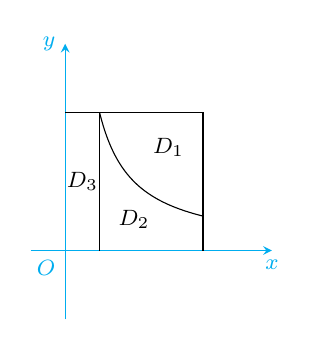
\begin{tikzpicture}[->,samples=100,>=stealth,domain=0.25:1,scale=1.75,font=\footnotesize]
                \coordinate (xMin) at (-0.25,0);
                \coordinate (xMax) at (1.5,0);
                \coordinate (yMin) at (0,-0.5);
                \coordinate (yMax) at (0,1.5);
                % \filldraw[fill=magenta!30] (0,0)--(0.25,0)--(0.25,1)--(0,1)--cycle;
                \draw[->,cyan] (xMin)--(0,0) node [below left] {$O$}--(xMax) node[below] {$x$};
                \draw[->,cyan] (yMin)--(yMax) node [left] {$y$};
                \draw[-] plot(\x,{1/(4*\x)});
                \draw[-] (1,0)--(1,1)--(0,1);
                \draw[-] (0.25,0)--(0.25,1);
                \node at(0.125,0.5) {$D_3$};
                \node at(0.5,0.225) {$D_2$};
                \node at(0.75,0.75) {$D_1$};
            \end{tikzpicture}
        }
        \subfigure[]{
            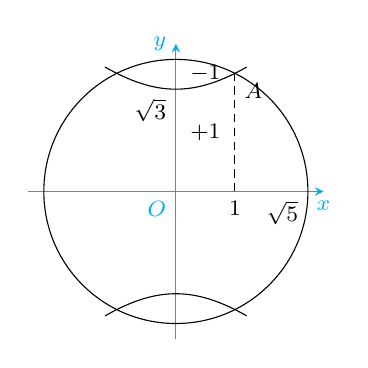
\begin{tikzpicture}[->,samples=100,>=stealth,domain=-1.2:1.2,scale=0.75,font=\footnotesize]
                \coordinate (xMin) at (-2.5,0);
                \coordinate (xMax) at (2.5,0);
                \coordinate (yMin) at (0,-2.5);
                \coordinate (yMax) at (0,2.5);
                \draw[->,cyan] (xMin)--(0,0) node [below left] {$O$}--(xMax) node[below] {$x$};
                \draw[->,cyan] (yMin)--(yMax) node [left] {$y$};
                \draw[-] (0,0) circle ({sqrt(5)});
                \draw[-] plot(\x,{sqrt(\x*\x+3)});
                \draw[-] plot(\x,{-sqrt(\x*\x+3)});
                \node at (1,2) [below right] {$A$};
                \node at (1,0) [below] {$1$};
                \node at ({sqrt(5)},0) [below left] {$\sqrt{5}$};
                \draw[densely dashed,-] (1,0)--(1,2);
                \node at (0.5,1) {$+1$};
                \node at (0.5,2) {$-1$};
                \node at (0,{sqrt(3)}) [below left] {$\sqrt{3}$};
            \end{tikzpicture}
        }
        \subfigure[]{
            \begin{tikzpicture}[->,samples=100,>=stealth,domain=-1:1,font=\footnotesize]
                \coordinate (xMin) at (-1.5,0);
                \coordinate (xMax) at (1.5,0);
                \coordinate (yMin) at (0,-0.5);
                \coordinate (yMax) at (0,2.5);
                \draw[->,cyan] (xMin)--(0,0) node [below left] {$O$}--(xMax) node[below] {$x$};
                \draw[->,cyan] (yMin)--(yMax) node [left] {$y$};
                \draw[-] plot(\x,{\x*\x}) node[right] {$y=x^2$};
                \draw[-] (1,1)--(1,2)--(-1,2)--(-1,1);
                \draw[-,densely dashed] (1,0)--(1,1);
                \draw[-,densely dashed] (-1,0)--(-1,1);
            \end{tikzpicture}
        }
        \subfigure[]{
            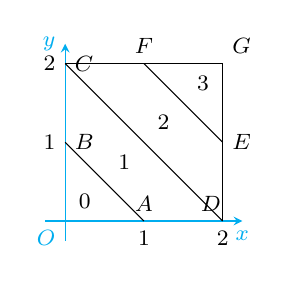
\begin{tikzpicture}[->,samples=100,>=stealth,domain=-1:1,font=\footnotesize]
                \coordinate (xMin) at (-0.25,0);
                \coordinate (xMax) at (2.25,0);
                \coordinate (yMin) at (0,-0.25);
                \coordinate (yMax) at (0,2.25);
                \draw[->,cyan] (xMin)--(0,0) node [below left] {$O$}--(xMax) node[below] {$x$};
                \draw[->,cyan] (yMin)--(yMax) node [left] {$y$};
                \draw[-] (2,0)--(2,2)--(0,2);
                \draw[-] (1,0)--(0,1);
                \draw[-] (2,0)--(0,2);
                \draw[-] (2,1)--(1,2);
                \node at (0.25,0.25) {$0$};
                \node at (0.75,0.75) {$1$};
                \node at (1.25,1.25) {$2$};
                \node at (1.75,1.75) {$3$};
                \node at (1,0) [below] {$1$};
                \node at (2,0) [below] {$2$};
                \node at (1,0) [above] {$A$};
                \node at (2,0) [above] {$D~~~$};
                \node at (0,1) [left] {$1$};
                \node at (0,1) [right] {$B$};
                \node at (0,2) [left] {$2$};
                \node at (0,2) [right] {$C$};
                \node at (2,1) [right] {$E$};
                \node at (1,2) [above] {$F$};
                \node at (2,2) [above right] {$G$};
            \end{tikzpicture}
        }
        \caption{}
    \end{figure}
\end{solution}

% \begin{example}
%     设函数 $f(x,y)$ 在点 $(0,0)$ 的某个领域内具有二阶连续偏导数, 求极限 $$\lim_{\rho\to0^+}\dfrac{1}{\rho^4}\iint\limits_{x^2+y^2\leqslant \rho^2}[f(x,y)-f(0,0)]\dd x\dd y.$$
% \end{example}

\begin{example}
    设函数 $f(x)$ 满足
    $$f(x)=x^2+x\int_{0}^{x^2}f\qty(x^2-t)\dd t+\iint\limits_Df(xy)\dd x\dd y$$
    其中 $D$ 是以 $(-1,-1),~(1,-1),~(1,1)$ 为顶点的三角形, 且 $f(1)=0$, 求 $\displaystyle\int_{0}^{1}f(x)\dd x.$
\end{example}
\begin{solution}
    令 $\displaystyle\iint\limits_D f(xy)\dd x\dd y=A$, 那么 $\displaystyle f(x)=x^2+x\int_{0}^{x^2}f\qty(x^2-t)\dd t+A$,
    将 $x$ 替换为 $xy$ 得 $$f(xy)=x^2y^2+xy\int_{0}^{x^2y^2}f\qty(x^2y^2-t)\dd t+A\Rightarrow f(xy)=x^2y^2+xy\int_{0}^{x^2y^2}f(u)\dd u+A$$
    % 并令 $u=x^2y^2-t$, 那么 $\displaystyle\int_{0}^{x^2y^2}f\qty(x^2y^2-t)\dd t=\int_{0}^{x^2y^2}f(u)\dd u$, 故上式转为
    % $$f(xy)=x^2y^2+xy\int_{0}^{x^2y^2}f(u)\dd u+A$$
    对等式两边二重积分得 $$A=\iint\limits_D x^2y^2\dd x\dd y+\iint\limits_D\qty[xy\int_{0}^{x^2y^2}f(u)\dd u]\dd x\dd y+A\iint\limits_D \dd x\dd y$$
    其中 $\displaystyle\iint\limits_D x^2y^2\dd x\dd y=\int_{-1}^{1}x^2\dd x\int_{-1}^{x}y^2\dd y=\dfrac{2}{9},~\iint\limits_D \dd x\dd y=2$,
    作 $y=-x$, 将 $D$ 划分为关于 $x$ 轴对称的 $D_1$ 和关于 $y$ 轴对称的 $D_2$, 并令函数 $\displaystyle g(x,y)=\int_{0}^{x^2y^2}f(u)\dd u$, 关于 $x$ 和 $y$ 都是奇函数, 利用二重积分的对称性知
    $$\iint\limits_D g(x,y)\dd x\dd y=\iint\limits_{D_1}g(x,y)\dd x\dd y+\iint\limits_{D_2}g(x,y)\dd x\dd y=0$$
    故 $A=-\dfrac{2}{9}$, 又由已知条件 $f(0)=1$, 那么
    $$0=1+\int_{0}^{1}f(1-t)\dd t-\dfrac{2}{9}\Rightarrow\int_{0}^{1}f(x)\dd x=-\dfrac{7}{9}.$$
\end{solution}

\begin{example}
    求积分 $I=\displaystyle\int_{-1}^{1}\dd z\iint\limits_{x^2+y^2\leqslant 1-z^2}\dfrac{\qty(\cos x+\sin y+\sqrt{3}z)^2}{\qty(x^2+y^2+z^2)^2+1}\dd x\dd y$.
\end{example}
\begin{solution}
    记 $\Omega=\qty{(x,y,z)\mid x^2+y^2+z^2\leqslant 1}$, 由对称性得
    \begin{flalign*}
        I & =\iiint\limits_\Omega\dfrac{\qty(\cos x+\sin y+\sqrt{3}z)^2}{\qty(x^2+y^2+z^2)^2+1}\dd V=\iiint\limits_\Omega\dfrac{\qty(\cos x+\sin y)^2+3z^2+2\sqrt{3}z(\cos x+\sin y)}{\qty(x^2+y^2+z^2)^2+1}\dd V                  \\
          & =\iiint\limits_\Omega\dfrac{(\cos x+\sin y)^2+3z^2}{\qty(x^2+y^2+z^2)^2+1}\dd V=\iiint\limits_\Omega\dfrac{(\cos x+\sin y)^2}{\qty(x^2+y^2+z^2)^2+1}\dd V+3\iiint\limits_\Omega\dfrac{z^2}{\qty(x^2+y^2+z^2)^2+1}\dd V \\
          & =\iiint\limits_\Omega\dfrac{\cos^2x+\sin^2y}{\qty(x^2+y^2+z^2)^2+1}\dd V+3\iiint\limits_\Omega\dfrac{z^2}{\qty(x^2+y^2+z^2)^2+1}\dd V                                                                                  \\
          & =\dfrac{1}{2}\iiint\limits_\Omega\dfrac{\cos^2x+\cos^2y+\sin^2x+\sin^2y}{\qty(x^2+y^2+z^2)+1}\dd V+3\iiint\limits_\Omega\dfrac{z^2}{\qty(x^2+y^2+z^2)^2+1}\dd V                                                        \\
          & =\iiint\limits_\Omega\dfrac{\dd V}{\qty(x^2+y^2+z^2)^2+1}+3\iiint\limits_\Omega\dfrac{z^2}{\qty(x^2+y^2+z^2)^2+1}\dd V                                                                                                 \\
          & =\int_{0}^{2\pi}\dd \theta\int_{0}^{\pi}\sin\varphi\dd \varphi\int_{0}^{1}\dfrac{r^2}{r^4+1}\dd r+3\int_{0}^{2\pi}\dd \theta\int_{0}^{\pi}\sin\varphi\cos^2\varphi\dd\varphi\int_{0}^{1}\dfrac{r^4}{r^4+1}\dd r        \\
          & =4\pi\int_{0}^{1}\dfrac{r^4+r^2}{r^4+1}\dd r=4\pi+\sqrt{2}\pi\ln\qty(3-2\sqrt{2})
    \end{flalign*}
    其中 $\displaystyle\int_{0}^{1}\dfrac{r^4+r^2}{r^4+1}\dd r=\int_{0}^{1}\dfrac{r^4+1+r^2-1}{r^4+1}\dd r=\int_{0}^{1}\dd r+\int_{0}^{1}\dfrac{r^2-1}{r^4+1}\dd r$,
    \begin{flalign*}
        \int\dfrac{r^2-1}{r^4+1}\dd r =\int\dfrac{1-\dfrac{1}{r^2}}{\qty(r+\dfrac{1}{r})^2-2}\dd r\xlongequal{r+\frac{1}{r}=t}\int\dfrac{\dd t}{\qty(t-\sqrt{2})\qty(t+\sqrt{2})} =\dfrac{1}{2\sqrt{2}}\ln\qty|\dfrac{t-\sqrt{2}}{t+\sqrt{2}}|+C=\dfrac{1}{2\sqrt{2}}\ln\qty|\dfrac{r+\dfrac{1}{r}-\sqrt{2}}{r+\dfrac{1}{r}+\sqrt{2}}|+C.
    \end{flalign*}
\end{solution}

\subsection{反常二重积分与含参变量积分}

\subsubsection{反常二重积分}

\begin{definition}[反常二重积分]
    若 $\displaystyle\iint\limits_D f(x,y)\dd \sigma$ 为反常积分, 则取 $D'$, 使 $D'\subset D$ 并且 $\displaystyle\iint\limits_{D'}f(x,y)\dd \sigma$ 为一般的二重积分, 则
    $$\iint\limits_D f(x,y)\dd \sigma=\lim_{D'\to D}\iint\limits_{D'}f(x,y)\dd \sigma$$
    事实上, 当反常二重积分可积时, 其计算方法与一般二重积分基本相同.
\end{definition}

\begin{example}
    计算二重积分 $\displaystyle I=\iint\limits_{\frac{x^2}{a^2}+\frac{y^2}{b^2}\geqslant 1}\mathrm{e}^{-\qty(\frac{x^2}{a^2}+\frac{y^2}{b^2})}\dd x\dd y.$
\end{example}
\begin{solution}
    令 $x=ar\cos\theta,~y=br\sin\theta$, 那么 $\dd x\dd y=abr\dd r\dd \theta$, 故
    \begin{flalign*}
        I=ab\iint\limits_{\substack{0\leqslant \theta\leqslant 2\pi \\1\leqslant r\leqslant +\infty}}\mathrm{e}^{-r^2}r\dd r\dd \theta=ab\int_{0}^{2\pi}\dd \theta\int_{1}^{+\infty}r\mathrm{e}^{-r^2}\dd r=\dfrac{\pi ab}{\mathrm{e}}.
    \end{flalign*}
\end{solution}

\begin{example}
    求不定积分 $\displaystyle\int_{0}^{+\infty}\dfrac{1-\mathrm{e}^{-ax}}{x}\cos x\dd x,~a>0.$
\end{example}
\begin{solution}
    注意到 $$\int_{a}^{b}\mathrm{e}^{-yx}\cos x\dd y=-\dfrac{\cos x}{x}\int_{a}^{b}\mathrm{e}^{-yx}\dd (-yx)=-\dfrac{\cos x}{x}\qty(\mathrm{e}^{-yx})\biggl |_{y=a}^{y=b}=-\dfrac{\mathrm{e}^{-bx}-\mathrm{e}^{-ax}}{x}\cos x$$
    所以 $\displaystyle\int_{0}^{a}\mathrm{e}^{-yx}\cos x\dd y=\dfrac{1-\mathrm{e}^{-ax}}{x}\cos x$, 交换积分次序可知: $\displaystyle\text{原式}=\int_{0}^{a}\dd y\int_{0}^{+\infty}\mathrm{e}^{-yx}\cos x\dd x$
    \begin{flalign*}
         & \int_{0}^{+\infty}\mathrm{e}^{-yx}\cos x\dd x=\int_{0}^{+\infty}\mathrm{e}^{-yx}\dd (\sin x)=\mathrm{e}^{-yx}\sin\biggl |_{x=0}^{x=+\infty}-\int_{0}^{+\infty}\sin x\dd \qty(\mathrm{e}^{-yx})          \\
         & =-y\int_{0}^{+\infty}\mathrm{e}^{-yx}\sin x\dd x=y\int_{0}^{+\infty}\mathrm{e}^{-yx}\dd (\cos x)=y\qty(\mathrm{e}^{-yx}\cos x\biggl |_{x=0}^{x=+\infty}+y\int_{0}^{+\infty}\cos x\mathrm{e}^{-yx}\dd x) \\
         & \Rightarrow \int_{0}^{+\infty}\mathrm{e}^{-yx}\cos x\dd x=\dfrac{y}{1+y^2}
    \end{flalign*}
    故 $$\int_{0}^{+\infty}\dfrac{1-\mathrm{e}^{-ax}}{x}\cos x\dd x=\int_{0}^{a}\dfrac{y}{1+y^2}\dd y=\dfrac{1}{2}\ln\qty(1+y^2)\biggl |_0^a=\dfrac{1}{2}\ln\qty(1+a^2).$$
\end{solution}

\begin{example}
    计算 $\displaystyle\int_0^{+\infty}\frac{\sin(5x)-\sin(3x)}{x}\mathrm{e}^{-2x}\dd x.$
\end{example}
\begin{solution}
    注意到 $\displaystyle\frac{\sin(5x)-\sin(3x)}{x}=\int_3^5\cos(xy)\dd y$, $\displaystyle\text{所以原式=}\int_0^{+\infty}\dd x\int_3^5\mathrm{e}^{-2x}\cos(xy)\dd y$, \\
    由于 $|\mathrm{e}^{-2x}\cos(xy)|\leqslant \mathrm{e}^{-2x}$, 且 $\displaystyle\int_0^{+\infty}\mathrm{e}^{-2x}\dd x$ 收敛,
    所以 $\displaystyle \int_3^5\cos(xy)\dd x$ 关于 $y\in[3,5]$ 一致收敛, 再结合 $\mathrm{e}^{-2x}\cos(xy)$ 为 $[0,+\infty)\times[3,5]$ 上的连续函数, 所以
    \begin{flalign*}
        I & =\int_0^{+\infty}\dd x\int_3^5\mathrm{e}^{-2x}\cos(xy)\dd y=\int_3^5\dd y\int_0^{+\infty}\mathrm{e}^{-2x}\cos(xy)\dd x \\
          & =\int_3^5\frac{\mathrm{e}^{-2x}}{4+y^2}\bigl[-2\cos(xy)+y\sin(xy)\bigr]_0^{+\infty}\dd y=2\int_3^5\frac{\dd y}{4+y^2}  \\
          & =\arctan\frac{y}{2}\biggl |_3^5=\arctan\frac{5}{2}-\arctan\frac{3}{2}=\arctan\frac{4}{19}.
    \end{flalign*}
\end{solution}

\begin{example}
    计算 $\displaystyle I=\iint\limits_D\mathrm{e}^{-\left(x^2+y^2\right)}\cos\left(x^2+y^2\right)\dd x\dd y$, 其中 $D$ 是全平面.
\end{example}
\begin{solution}
    用极坐标, 化为先 $\theta$ 后 $\rho$ 次序的二次积分,
    \begin{flalign*}
        I=\int_0^{+\infty}\dd \rho\int_0^{2\pi}\rho\mathrm{e}^{-\rho^2}\cos\rho^2\dd \theta
        =2\pi\int_0^{+\infty}\rho\mathrm{e}^{-\rho^2}\cos\rho^2\dd \rho.
    \end{flalign*}
    其中,
    \begin{flalign*}
        \int\rho\mathrm{e}^{-\rho^2}\cos\rho^2\dd \rho
         & =\int\frac{4\rho\cos\rho^2}{4\mathrm{e}^{\rho^2}}\dd \rho
        =\int\frac{2\rho\cos\rho^2+2\rho\sin\rho^2-2\rho\left(\sin\rho^2-\cos\rho^2\right)}{4\mathrm{e}^{\rho^2}}\dd \rho                                                         \\
         & =\int\frac{\left(2\rho\cos\rho^2+2\rho\sin\rho^2\right)4\mathrm{e}^{\rho^2}-8\rho\mathrm{e}^{\rho^2}\left(\sin\rho^2-\cos\rho^2\right)}{16\mathrm{e}^{\rho^2}}\dd \rho \\
         & =\int\dd \left(\frac{\sin\rho^2-\cos\rho^2}{4\mathrm{e}^{\rho^2}}\right)
        =\frac{\sin\rho^2-\cos\rho^2}{4\mathrm{e}^{\rho^2}}+C
    \end{flalign*}
    所以, $\displaystyle I=
        2\pi\cdot\left .\frac{\sin\rho^2-\cos\rho^2}{4\mathrm{e}^{\rho^2}}\right |_0^{+\infty}
        =\frac{\pi}{2}$.
\end{solution}

\begin{example}
    计算 $\displaystyle\iint\limits_D\dfrac{x^2+y^2-2}{\qty(x^2+y^2)^{\frac{5}{2}}}\dd x\dd y$, 其中 $D:x^2+y^2\geqslant 2,x\leqslant 1.$
\end{example}
\begin{solution}
    注意到 $ D $ 关于 $ x $ 轴对称, 且被积函数关于 $ y $ 变量为偶函数, 记 $ x $ 轴上方部分积分区域为 $ D_{1}$,
    令 $ x=r \cos \theta, y=r \sin \theta $, 则在极坐标下, $ D_{1} $ 可以描述为两部分, 如图 \ref{dd1d2} 所示, 记作
    $$D_{1}^{\prime}:\frac{\pi}{4} \leqslant \theta \leqslant \frac{\pi}{2}, \sqrt{2} \leqslant r \leqslant \sec \theta,~D_{2}^{\prime}:\frac{\pi}{2} \leqslant \theta \leqslant \pi, \sqrt{2} \leqslant r \leqslant+\infty$$
    \begin{minipage}{.38\linewidth}
        \begin{figure}[H]
            \centering
            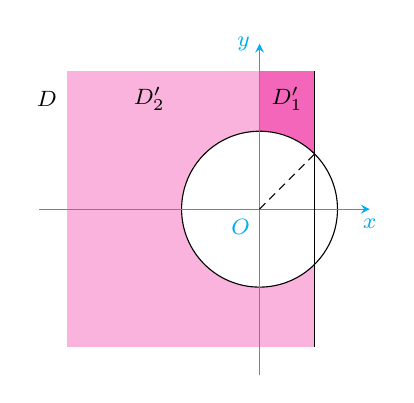
\begin{tikzpicture}[samples=100,>=stealth,font=\footnotesize,scale=0.7]
                \coordinate (xMin) at (-4,0);
                \coordinate (xMax) at (2,0);
                \coordinate (yMin) at (0,-3);
                \coordinate (yMax) at (0,3);
                \fill[magenta!30] (-3.5,-2.5)--(1,-2.5)--(1,2.5)--(-3.5,2.5)--cycle;
                \fill[magenta!60] (0,0)--(1,0)--(1,2.5)--(0,2.5)--cycle;
                \filldraw[fill=white](0,0) circle ({sqrt(2)});
                \draw[->,cyan] (xMin)--(0,0) node [below left] {$O$}--(xMax) node[below] {$x$};
                \draw[->,cyan] (yMin)--(yMax) node [left] {$y$};
                \draw[-] (1,-2.5)--(1,2.5);
                \draw[densely dashed] (0,0)--(1,1);
                \node[left] at (-3.5,2) {$D$};
                \node at (0.5,2) {$D_1'$};
                \node at (-2,2) {$D_2'$};
            \end{tikzpicture}
            \caption{}
            \label{dd1d2}
        \end{figure}
    \end{minipage}
    \hfill
    \begin{minipage}{.58\linewidth}
        \begin{flalign*}
            I & =2\int_{\frac{\pi}{4}}^{\frac{\pi}{2}}\dd \theta \int_{\sqrt{2}}^{\sec\theta}\dfrac{r^2-2}{r^5}r\dd r+2\int_{\frac{\pi}{2}}^{\pi}\dd \theta\int_{\sqrt{2}}^{+\infty}\dfrac{r^2-2}{r^5}r\dd r                                   \\
              & =2 \int_{\frac{\pi}{4}}^{\frac{\pi}{2}}\left(\frac{2}{3 r^{3}}-\frac{1}{r}\right)_{\sqrt{2}}^{\sec \theta} \dd  \theta+2 \int_{\frac{\pi}{2}}^{\pi}\left(\frac{2}{3 r^{3}}-\frac{1}{r}\right)_{\sqrt{2}}^{+\infty} \dd  \theta \\
              & =2 \int_{\frac{\pi}{4}}^{\frac{\pi}{2}}\left(\frac{2 \cos ^{3} \theta}{3}-\cos \theta+\frac{\sqrt{2}}{3}\right) \dd  \theta+2 \int_{\frac{\pi}{2}}^{\pi} \frac{\sqrt{2}}{3} \dd  \theta                                        \\
              & =2\left[\frac{2}{3}\left(\sin \theta-\frac{\sin ^{3} \theta}{3}\right)-\sin \theta+\frac{\sqrt{2}}{3} \theta\right]_{\frac{\pi}{4}}^{\frac{\pi}{2}}+2 \cdot \frac{\pi}{3 \sqrt{2}}                                             \\
              & =2 \cdot\left(\frac{\pi}{3 \sqrt{2}}-\frac{5}{9}-\frac{\pi}{6 \sqrt{2}}+\frac{2 \sqrt{2}}{9}\right)+\frac{\sqrt{2}}{3} \pi=\frac{4 \sqrt{2}}{9}-\frac{10}{9}+\frac{\sqrt{2}}{2} \pi
        \end{flalign*}
    \end{minipage}
\end{solution}

\begin{example}
    计算 $\displaystyle I=\int_{-\infty}^{+\infty}\int_{-\infty}^{+\infty}\min\qty{x,y}\e ^{-\qty(x^2+y^2)}\dd x\dd y.$
\end{example}
\begin{solution}
    由题意
    \begin{flalign*}
        I & =\int_{-\frac{3\pi}{4}}^{\frac{\pi}{4}}\dd \theta\int_{0}^{+\infty}r\sin\theta\e ^{-r^2}r\dd r+\int_{\frac{\pi}{4}}^{\frac{5\pi}{4}}\dd \theta\int_{0}^{+\infty}r\cos\theta\e ^{-r^2}r\dd r=-2\sqrt{2}\int_{0}^{+\infty}r^2\e ^{-r^2}\dd r \\
          & =-\sqrt{2}\cdot 2\int_{0}^{+\infty}r^2\e ^{-r^2}\dd r=-\sqrt{2}\Gamma\qty(\dfrac{3}{2})=-\sqrt{2}\Gamma\qty(\dfrac{1}{2})=-\dfrac{\sqrt{2\pi}}{2}.
    \end{flalign*}
\end{solution}

\subsubsection{含参变量积分}

含参变量积分是指在积分运算中, 被积函数中包含一个或多个参数的情况. 这种情况下, 参数被视为常数, 而不是变量, 因此在积分时需要将参数视为常数处理.

\begin{theorem}[含参变量积分求导公式]
    \index{含参变量积分求导公式}设 $f(t,x),f_x(t,x)$ 在 $R=[a,b]\times[p,q]$ 上连续, $\alpha(x),\beta(x)$ 为定义在 $[a,b]$ 上其值含于 $[p,q]$ 内的可微函数, 则函数
    $$F(t,x)=\int_{\alpha(x)}^{\beta(x)}f(t,x)\dd t$$
    在 $[a,b]$ 上可微, 且
    $$F'(t,x)=\dv{x}\int_{\alpha(x)}^{\beta(x)}f(t,x)\dd t=\int_{\alpha(x)}^{\beta(x)}f_x(t,x)\dd t+f[\beta(x),x]\beta'(x)-f[\alpha(x),x]\alpha'(x).$$
\end{theorem}

\begin{example}
    已知 $\displaystyle F(x)=\int_{\sin x}^{\cos x}\mathrm{e}^{\qty(xt+x^2)}\dd t$, 求 $\displaystyle\dv{F(x)}{x}\biggl |_{x=0}.$
\end{example}
\begin{solution}
    \textbf{法一: }由含参变量积分求导公式, 有
    \begin{flalign*}
        I & =\dv{x}\int_{\sin x}^{\cos x}\mathrm{e}^{\qty(xt+x^2)}\dd t=\qty[\int_{\sin x}^{\cos x}(t+2x)\mathrm{e}^{\qty(xt+x^2)}\dd t-\sin x\mathrm{e}^{\qty(x\cos x+x^2)}-\cos x\mathrm{e}^{\qty(x\sin x+x^2)}]_{x=0} \\
          & =\int_{0}^{1}t\dd t-1=-\dfrac{1}{2}
    \end{flalign*}
    \textbf{法二: }由题意,
    \begin{flalign*}
        F(x)=\int_{\sin x}^{\cos x}\mathrm{e}^{\qty(xt+x^2)}\dd t=\mathrm{e}^{x^2}\int_{\sin x}^{\cos x}\mathrm{e}^{xt}\dd t\xlongequal[]{xt=u}\dfrac{\mathrm{e}^{x^2}}{x}\int_{x\sin x}^{x\cos x}\mathrm{e}^u\dd u=\dfrac{\mathrm{e}^{x^2}}{x}\qty(\mathrm{e}^{x\cos x}-\mathrm{e}^{x\sin x})
    \end{flalign*}
    其中 $x\neq0$, 且 $F(0)=1$, 所以考虑导数定义式, 有
    \begin{flalign*}
        \dv{F(x)}{x}\biggl |_{x=0}=\lim_{x\to0}\dfrac{F(x)-F(0)}{x-0}=\lim_{x\to0}\dfrac{\dfrac{\mathrm{e}^{x^2}}{x}\qty(\mathrm{e}^{x\cos x}-\mathrm{e}^{x\sin x})-1}{x}=\lim_{x\to0}\dfrac{\mathrm{e}^{x^2}\qty(\mathrm{e}^{x\cos x}-\mathrm{e}^{x\sin x})-x}{x^2}
    \end{flalign*}
    由 $\mathrm{e}^x=1+x+\dfrac{x^2}{2}+o\qty(x^2),~\cos x=1-\dfrac{x^2}{2}+o\qty(x^2),~\sin x=x+o(x)$ 得
    \begin{flalign*}
        \mathrm{e}^{x\cos x} & =1+x\cos x+\dfrac{1}{2}(x\cos x)^2+o\qty((x\cos x)^2)                                              \\
                             & =1+x\qty(1-\dfrac{x^2}{2}+o\qty(x^2))+\dfrac{x^2}{2}\qty(1-\dfrac{x^2}{2}+o\qty(x^2))^2+o\qty(x^2) \\
                             & =1+x+\dfrac{x^2}{2}+o\qty(x^2)                                                                     \\
        \mathrm{e}^{x\sin x} & =1+x\sin x+(x\sin x)^2+o\qty((x\sin x)^2)=1+x^2+o\qty(x^2)                                         \\
        \mathrm{e}^{x^2}     & =1+x^2+o\qty(x^2)
    \end{flalign*}
    将上述展开式代入原极限式, 化简最终求得原极限等于 $-\dfrac{1}{2}.$
\end{solution}

\begin{example}
    设 $f(x)$ 为连续函数, $t>0$, 区域 $\Omega$ 是由抛物面 $z=x^2+y^2$ 和球面 $x^2+y^2+z^2=t^2~ (t>0)$ 所围成的部分, 定义三重积分 $\displaystyle F(t)=\iiint\limits_{\Omega}f\qty(x^2+y^2+z^2)\dd v$, 求 $F'(t).$
\end{example}
\begin{solution}
    利用柱坐标系, 令 $\begin{cases}
            x=r\cos\theta \\ y=r\sin\theta\\ z=z
        \end{cases}$, 则由 $\begin{cases}
            z=x^2+y^2 \\ x^2+y^2+z^2=t^2
        \end{cases}$ 联立得 $z^2=z+t^2$, 解得 $z=\dfrac{\sqrt{1+4t^2}-1}{2}:=b^2(t)$,
    于是区域 $\Omega$ 在 $xOy$ 平面上的投影区域为 $D_{xy}:x^2+y^2\leqslant b^2(t)$, 从而
    $$F(t)=\int_{0}^{2\pi}\dd \theta\int_{0}^{b(t)}r\dd r\int_{r^2}^{\sqrt{t^2-r^2}}f\qty(r^2+z^2)\dd z=2\pi\int_{0}^{b(t)}r\qty[\int_{r^2}^{\sqrt{t^2-r^2}}f\qty(r^2+z^2)\dd z]\dd r$$
    记 $\displaystyle g(t,r)=r\qty[\int_{r^2}^{\sqrt{t^2-r^2}}f\qty(r^2+z^2)\dd z]$, 则由 $f(x)$ 的连续知,  $g(t,r)$ 及 $\displaystyle\pdv{g(t,r)}{r}$ 连续,
    于是由含参变量积分的求导公式, 得
    \begin{flalign*}
        F'(t) & =2\pi\qty[\int_{0}^{b(t)}\pdv{g}{t}\dd r+g(t,b(t))\cdot b'(t)]                                                                             \\
              & =2\pi\qty[\int_{0}^{b(t)}rf\qty(t^2)\dfrac{t}{\sqrt{t^2-r^2}}\dd r+b(t)\int_{b^2(t)}^{\sqrt{t^2-b^2(t)}}f\qty(b^2(t)+z^2)\dd z\cdot b'(t)] \\
              & =2\pi tf\qty(t^2)\int_{0}^{b(t)}\dfrac{r}{\sqrt{t^2-r^2}}\dd r=-\pi tf\qty(t^2)\int_{0}^{b(t)}\dfrac{\dd \qty(t^2-r^2)}{\sqrt{t^2-r^2}}    \\
              & =2\pi tf\qty(t^2)\qty(t-\sqrt{t^2-b^2(t)})=2\pi tf\qty(t^2)\qty(t-b^2(t))=\pi t\qty f(t^2)\qty(2t+1-\sqrt{1+4t^2}).
    \end{flalign*}
\end{solution}

\begin{example}\scriptsize\linespread{0.8}
    求 $\displaystyle \dv[n]{}{x}\qty[\int_0^x\mathrm{e}^{nt}\sum_{k=0}^{n-1}\dfrac{(x-t)^k}{k!}\dd t].$
\end{example}
\begin{solution}\scriptsize\linespread{0.8}
    记 $\displaystyle f_k(x)=\int_{0}^{x}\mathrm{e}^{nt}\dfrac{(x-t)^k}{k!}\dd t$, 那么 $\displaystyle\dv{x}f_k(x)=\int_{0}^{x}\mathrm{e}^{nt}\dfrac{(x-t)^{k-1}}{(k-1)!}\dd t=f_{k-1}(x)$, 于是
    $$f''_k(x)=f'_{k-1}(x)=f_{k-2}(x),~\cdots,~f_k^{(k)}(x)=f_0(x)$$
    由于 $\displaystyle f_0'(x)=\qty(\int_{0}^{x}\mathrm{e}^{nt}\dd t)'=\mathrm{e}^{nx},~f_0''(x)=n\mathrm{e}^{nx},~\cdots,~f_0^{(n)}(x)=n^{n-1}\mathrm{e}^{nx}$, 所以
    \begin{flalign*}
        \dv[n]{}{x}\qty[\int_0^x\mathrm{e}^{nt}\sum_{k=0}^{n-1}\dfrac{(x-t)^k}{k!}\dd t]=\sum_{k=0}^{n-1}f_k^{(n)}(x)=f_0^{(n)}(x)+\sum_{k=1}^{n-1}\qty[f_k^{(k)}(x)]^{(n-k)}=\sum_{k=1}^{n}f_0^{(k)}(x)=\dfrac{1-n^n}{1-n}\mathrm{e}^{nx}.
    \end{flalign*}
\end{solution}

% \subsection{判断含参变量反常积分的一致收敛性}
% 
% \subsection{含参变量反常积分的极限与连续性}
% 
% \subsection{含参变量反常积分积分号下求导与积分号下求积分}

\subsection{重积分的积分中值定理}

\begin{theorem}[二重积分中值定理]
    \index{二重积分中值定理}若函数 $f(x,y)$ 在有界闭区域 $D$ 上连续, 函数 $g(x,y)$ 在 $D$ 上可积且不变号, 则 $\exists(\xi,\eta)\in D$, 使得 $$\iint\limits_D f(x,y)g(x,y)\dd x\dd y=f(\xi,\eta)\iint\limits_D g(x,y)\dd x\dd y.$$
\end{theorem}

\begin{example}
    已知 $\displaystyle\lim_{x\to0^+}\dfrac{\displaystyle\int_{0}^{x}\dd v\int_{\ln(1+v)}^{v}\sin\qty(u^2)\dd u}{x^k}=c\neq0$, 求 $c.$
\end{example}
\begin{errorSolution}
    记积分区域为 $D$, 则由二重积分中值定理知, $\exists(\xi,\eta)\in D$, 使得 $\displaystyle\iint\limits_D \sin\qty(u^2)\dd u\dd v=\sin\qty(\eta^2)\iint\limits_D \dd u\dd v$, 下求 $D$ 的面积 $S$,
    记 $I_1=\dfrac{1}{2}x^2,~\displaystyle I_2=\int_{0}^{x}\ln(1+t)\dd t$, 于是 $$I_2=\int_{0}^{x}\ln(1+t)\dd t=x\ln(1+x)-x+\ln(1+x)$$
    因此 $S=I_1-I_2=\dfrac{1}{2}x^2-x\ln(1+x)+x-\ln(1+x)$, 故极限式化为
    $$\lim_{x\to0^+}\dfrac{x^2\qty[\dfrac{1}{2}x^2-x\ln(1+x)+x-\ln(1+x)]}{x^k}=\lim_{x\to0^+}\dfrac{x^2\qty[\dfrac{1}{2}x^2-x^2+\dfrac{1}{2}x^3+x-x+\dfrac{1}{2}x^2-\dfrac{1}{3}x^3+o\qty(x^3)]}{x^k}=\lim_{x\to0^+}\dfrac{\dfrac{x^5}{6}}{x^k}$$
    因为 $c\neq0$, 所以分子与分母等阶, 因此 $c=\dfrac{1}{6}.$\\
    \textbf{错因: }对二重积分中值定理内容了解不透彻, 该定理说的是: 若函数 $f(x,y)$ 在有界闭区域 $D$ 上连续, 函数 $g(x,y)$ 在 $D$ 上可积且不变号, 则存在一点 $(\xi,\eta)\in D$, 使得 $$\iint\limits_D f(x,y)g(x,y)\dd x\dd y=f(\xi,\eta)\iint\limits_D g(x,y)\dd x\dd y.$$
\end{errorSolution}
\begin{solution}
    \textbf{法一: }先使用 L'Hospital 法则, 将二重积分转化为定积分, 再使用积分中值定理, 有
    $$\lim_{x\to0^+}\dfrac{\displaystyle\int_{0}^{x}\dd v\int_{\ln(1+v)}^{v}\sin\qty(u^2)\dd u}{x^k}\xlongequal{L'}\lim_{x\to0^+}\dfrac{\displaystyle\int_{\ln(1+x)}^{x}\sin\qty(u^2)\dd u}{kx^{k-1}}=\lim_{x\to0^+}\dfrac{\sin\xi^2[x-\ln(1+x)]}{kx^{k-1}}$$
    其中 $x\gets\ln(1+x)<\xi<x~~(x\to0^+)$, 因此原极限等于 $\displaystyle\lim_{x\to0^+}\dfrac{\dfrac{1}{2}x^4}{kx^{k-1}}$, 因此 $k=5,c=\dfrac{1}{10}.$\\
    \textbf{法二: }因为 $\sin \qty(u^2)$ 在积分区间内不变号, 因此 $\displaystyle\int_{\ln(1+v)}^{v}\sin\qty(u^2)\dd u\sim\int_{\ln(1+v)}^{v}u^2\dd u$, 又因为 $\ln(1+v)\sim v~~(v\to0^+)$, 因此原极限等价为
    $$\lim_{x\to0^+}\dfrac{\displaystyle\int_{0}^{x}\dd v\int_{\ln(1+v)}^{v}\sin\qty(u^2)\dd u}{x^k}=\lim_{x\to0^+}\dfrac{\displaystyle\int_{0}^{x}[v-\ln(1+v)]\xi_v^2\dd v}{x^k}=\lim_{x\to0^+}\dfrac{\displaystyle \int_{0}^{x}\dfrac{1}{2}v^4\dd v}{x^k}=c$$
    因为 $c\neq0$, 因此分子与分母等阶, 即 $\displaystyle\lim_{x\to0^+}\dfrac{\dfrac{1}{2}\cdot\dfrac{1}{5}x^5}{x^k}=c\Rightarrow c=\dfrac{1}{10}.$
\end{solution}

\begin{example}
    设区域 $D$ 为 $x^2+y^2\leqslant r^2$, 求极限 $\displaystyle\lim_{r\to0}\frac{1}{\pi r^2}\iint\limits_D\mathrm{e}^{x^2-y^2}\cos(x+y)\dd x\dd y.$
\end{example}
\begin{solution}
    由二重积分的积分中值定理知, $\displaystyle\exists(\xi,\eta)\in D$, 使得
    $$\iint\limits_D\mathrm{e}^{x^2-y^2}\cos(x+y)\dd x\dd y=\pi r^2\cdot\mathrm{e}^{\xi^2-\eta^2}\cos(\xi+\eta)$$
    于是, $\displaystyle\lim_{r\to0}\frac{1}{\pi r^2}\iint\limits_D\mathrm{e}^{x^2-y^2}\cos(x+y)\dd x\dd y
        =\lim_{\xi,\eta\to0}\mathrm{e}^{\xi^2-\eta^2}\cos(\xi+\eta)=1$.
\end{solution}

\begin{example}[2009 南京工业大学]
    求极限 $\displaystyle\lim_{t\to0^+}\frac{1}{t^2}\int_0^t\dd x\int_0^{t-x}\mathrm{e}^{x^2+y^2}\dd y.$
\end{example}
\begin{solution}
    由二重积分的积分中值定理知, $\displaystyle\exists(\xi,\eta)\in \{(x,y)|0\leqslant x\leqslant t,0\leqslant y\leqslant t-x\}$, 使得
    $$\int_0^t\dd x\int_0^{t-x}\mathrm{e}^{x^2+y^2}\dd y=\frac{t^2}{2}\mathrm{e}^{\xi^2+\eta^2}$$
    于是, $\displaystyle\lim_{t\to0^+}\frac{1}{t^2}\int_0^t\dd x\int_0^{t-x}\mathrm{e}^{x^2+y^2}\dd y
        =\frac{1}{2}\lim_{\xi,\eta\to0^+}\mathrm{e}^{\xi^2+\eta^2}=\frac{1}{2}$.
\end{solution}
\begin{example}[2016 年天津市 (理工)]
    设函数 $f(x,y)$ 在点 $(0,0)$ 的某个领域内连续, 求 $\displaystyle\lim_{t\to0^+}\frac{F'(t)}{t}$
    其中 $$F(t)=\iint\limits_{x^2+y^2\leqslant t^2}f(x,y)\dd x\dd y.$$
\end{example}
\begin{solution}
    由二重积分的积分中值定理知, $\exists(\xi,\eta)\in x^2+y^2\leqslant t^2$, 使得
    $$F(t)=\iint\limits_{x^2+y^2\leqslant t^2}f(x,y)\dd x\dd y=\pi t^2 f(\xi,\eta)$$
    于是, $\displaystyle\lim_{t\to0^+}\frac{F'(t)}{t}=\lim_{\xi,\eta\to0^+}\frac{2\pi tf(\xi,\eta)}{t}
        =2\pi tf(0,0)$.
\end{solution}

\begin{example}[第十届 “景润杯”]
    计算极限 $\displaystyle\lim_{R\to+\infty}\iint\limits_{D_R}\mathrm{e}^{-x}\arctan\dfrac{y}{x}\dd x\dd y$, 其中 $D_R$ 是由 $$x=R,~y=0,~y=\dfrac{2}{R}x-1$$ 所围成.
\end{example}
\begin{solution}
    由二重积分的积分中值定理知, $\exists(\xi,\eta)\in D_R$,
    使得 $$\iint\limits_{D_R}\mathrm{e}^{-x}\arctan\dfrac{y}{x}\dd x\dd y=\mathrm{e}^{-\xi}\arctan\dfrac{\eta}{\xi}\iint\limits_{D_R}\dd x\dd y=\dfrac{R}{4}\mathrm{e}^{-\xi}\arctan\dfrac{\eta}{\xi}$$
    其中 $R\in\qty(\dfrac{R}{2},R),~\eta\in(0,1)$, 故 \begin{flalign*}
        \qty|\iint\limits_{D_R}\mathrm{e}^{-x}\arctan\dfrac{y}{x}\dd x\dd y|=\mathrm{e}^{-\xi}\arctan\dfrac{\eta}{\xi}\iint\limits_{D_R}\dd x\dd y\leqslant \dfrac{R}{4}\mathrm{e}^{-\frac{R}{2}}\arctan \dfrac{\eta}{\xi}\to0~ (R\to+\infty)
    \end{flalign*}
    所以 $\displaystyle\lim_{R\to+\infty}\iint\limits_{D_R}\mathrm{e}^{-x}\arctan\dfrac{y}{x}\dd x\dd y=0.$
\end{solution}

\begin{example}
    证明: $$\dfrac{\pi\qty(R^2-r^2)}{R+K}\leqslant \iint\limits_{D}\dfrac{\dd \sigma}{\sqrt{(x-a)^2+(y-b)^2}}\leqslant \dfrac{\pi\qty(R^2-r^2)}{r-K}$$
    其中 $0<K=\sqrt{a^2+b^2}<r<R,~D:r^2\leqslant x^2+y^2\leqslant R^2.$
\end{example}
\begin{proof}[{\songti \textbf{证}}]
    函数 $f(x,y)=\dfrac{1}{\sqrt{(x-a)^2+(y-b)^2}}$ 在环形闭域 $D:r^2\leqslant x^2+y^2\leqslant R^2$ 上连续, 则由积分中值定理知, 存在 $P_0(\xi,\eta)\in D$, 使
    $$\iint\limits_{D}\dfrac{\dd \sigma}{\sqrt{(x-a)^2+(y-b)^2}}=\dfrac{1}{\sqrt{(\xi-a)^2+(\eta-b)^2}}\iint\limits_D\dd \sigma=\dfrac{1}{\qty|P_0P_1|}\pi\qty(R^2-r^2)$$
    \begin{minipage}{.28\linewidth}
        \begin{figure}[H]
            \centering
            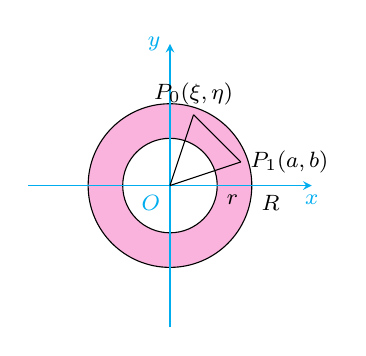
\begin{tikzpicture}[->,samples=100,>=stealth,scale=0.6,font=\footnotesize]
                \coordinate (xMin) at (-3,0);
                \coordinate (xMax) at (3,0);
                \coordinate (yMin) at (0,-3);
                \coordinate (yMax) at (0,3);
                \filldraw[fill=magenta!30](0,0) circle ({sqrt(3)});
                \filldraw[fill=white](0,0) circle ({sqrt(1)});
                \draw[->,cyan] (xMin)--(0,0) node [below left] {$O$}--(xMax) node[below] {$x$};
                \draw[->,cyan] (yMin)--(yMax) node [left] {$y$};
                \draw[-] (0,0)--(1.5,0.5) node[right] {$P_1(a,b)$};
                \draw[-] (0,0)--(0.5,1.5) node[above] {$P_0(\xi,\eta)$};
                \draw[-] (1.5,0.5)--(0.5,1.5);
                \node[below right] at (1,0) {$r$};
                \node[below right] at ({sqrt(3)},0) {$R$};
            \end{tikzpicture}
            \caption{}
            \label{RKr}
        \end{figure}
    \end{minipage}
    \hfill
    \begin{minipage}{.68\linewidth}
        由图 \ref{RKr} 知, $r\leqslant \qty|OP_0|\leqslant R$, 且存在关系 $$r-K\leqslant \qty|OP_0|-\qty|OP_1|\leqslant|P_0P_1|\leqslant \qty|OP_1|+\qty|OP_0|\leqslant R+K$$
        所以 $$\dfrac{1}{R+K}\leqslant \dfrac{1}{\qty|P_0P_1|}\leqslant \dfrac{1}{r-K}$$
        代入上式得证不等式成立.
    \end{minipage}
\end{proof}

\subsection{重积分的应用}

\subsubsection{重积分在几何上的应用}

\begin{example}
    求球面 $x^2+y^2+z^2=4$ 和抛物面 $x^2+y^2=3z$ 所围的立体 (含在抛物面内部) $\Omega$ 的体积 $V$.
\end{example}
\begin{solution}
    \textbf{法一: }“先一后二”法, 配合柱坐标
    \begin{flalign*}
        V=\iiint\limits_\Omega\dd v=\iint\limits_{D_{xy}}\dd x\dd y\int_{\frac{x^2+y^2}{3}}^{\sqrt{4-x^2-y^2}}\dd z=\int_{0}^{2\pi}\dd\theta\int_{0}^{\sqrt{3}}\rho\dd\rho\int_{\frac{\rho^2}{3}}^{\sqrt{4-\rho^2}}\dd z=\dfrac{19}{6}\pi.
    \end{flalign*}
    \textbf{法二: }“先二后一”法
    \begin{flalign*}
        V & =\iiint\limits_\Omega\dd v=\iiint\limits_{\Omega_1}\dd v+\iiint\limits_{\Omega_2}\dd v=\int_{0}^{1}\dd z\iint\limits_{D_{z_1}}\dd x\dd y+\int_{1}^{2}\dd z\iint\limits_{D_{z_2}}\dd x\dd y \\
          & =\int_{0}^{1}\pi\qty(\sqrt{3z})^2\dd z+\int_{1}^{2}\pi\qty(\sqrt{4-z^2})^2\dd z=\dfrac{19}{6}\pi.
    \end{flalign*}
    \textbf{法三: }利用球坐标
    \begin{flalign*}
        V=\iiint\limits_{\Omega}\dd v=\int_{0}^{2\pi}\dd \theta\int_{0}^{\frac{\pi}{3}}\dd \varphi\int_{0}^{2}\rho^2\sin\varphi\dd\rho+\int_{0}^{2\pi}\dd\theta\int_{\frac{\pi}{3}}^{\frac{\pi}{2}}\dd\varphi\int_{0}^{3\frac{\cos\varphi}{\sin^2\varphi}}\rho^2\sin\varphi\dd\rho=\dfrac{19}{6}\pi.
    \end{flalign*}
\end{solution}

\begin{example}
    求由方程 $\displaystyle\qty(\dfrac{x^2}{a^2}+\dfrac{y^2}{b^2})^2+\dfrac{z^4}{c^4}=z$ 所确定的曲面 $\varSigma$ 所围成空间立体 $\Omega$ 的体积, 其中 $a,b,c$ 为正常数.
\end{example}
\begin{solution}
    利用广义球坐标公式 $\displaystyle \begin{cases}
            x = a\rho\cos\theta \sin\varphi \\
            y = b\rho\sin\theta \sin\varphi \\
            z = c\rho\cos\varphi
        \end{cases}$, 于是 $\displaystyle \qty|\pdv{x,y,z}{\rho,\theta,\varphi}|=abc\rho^2\sin\varphi$, 且
    $$\Omega'=\qty{(\rho,\theta,\varphi)\biggl | 0\leqslant \theta\leqslant 2\pi,0\leqslant \varphi\leqslant \dfrac{\pi}{2},0\leqslant \rho\leqslant \qty(\dfrac{c\cos \varphi}{\sin^4\varphi+\cos^4\varphi})^{\frac{1}{3}}}$$
    \begin{flalign*}
        V & =\iiint\limits_{\Omega'}\dd v=\int_{0}^{2\pi}\dd \theta\int_{0}^{\frac{\pi}{2}}\dd\varphi\int_{0}^{\qty(\frac{c\cos\varphi}{\sin^4\varphi+\cos^4\varphi})^{\frac{1}{3}}}abc\rho^2\sin\varphi\dd\rho=\dfrac{2}{3}\pi abc^2\int_{0}^{\frac{\pi}{2}}\dfrac{\sin\varphi\cos\varphi}{\sin^4\varphi+\cos^4\varphi}\dd\varphi \\
          & =\dfrac{2}{3}\pi abc^2\int_{0}^{\frac{\pi}{2}}\dfrac{\sin\varphi\cos\varphi}{\qty(\sin^2\varphi-\cos^2\varphi)+2\sin^2\varphi\cos^2\varphi}\dd \varphi=\dfrac{2}{3}\pi abc^2\int_{0}^{\frac{\pi}{2}}\dfrac{\sin\varphi\cos\varphi}{2\cos^4\varphi-2\cos^2\varphi+1}\dd \varphi                                         \\
          & \xlongequal[]{\cos^2\varphi=t}\dfrac{\pi}{3}abc^2\int_{0}^{1}\dfrac{\dd t}{2t^2-2t+1}=\dfrac{\pi}{3}abc^2\cdot\arctan(2t-1)\biggl |_0^1=\dfrac{\pi^2}{6}abc^2.
    \end{flalign*}
\end{solution}

\subsubsection{重积分在力学上的应用}

\begin{theorem}[物体的质量]
    若一物体占有区域 $V,\rho=\rho(x,y,z)$ 为它在点 $(x,y,z)$ 的密度, 则该物体的质量等于 $\displaystyle M=\iiint\limits_V\rho\dd x\dd y\dd z.$
    \index{物体的质量}
\end{theorem}

\begin{example}
    设立体 $\Omega=\qty{(x, y, z)|x^2+y^2+z^2\leqslant t^2,t>0,z\geqslant 0}$, 其密度为 $zf\qty(\sqrt{x^2+y^2+z^2})$, $f$ 为非负可微函数,且 $f(0)=1$, $m(t)$ 为立体 $\Omega$ 的质量,求 $\displaystyle \lim_{t \to 0^+}\dfrac{m(t)}{t^4}.$
\end{example}
\begin{solution}
    由球坐标公式 $\begin{cases}
            x=r\cos\theta\sin\varphi \\ y=r\sin\theta\cos\varphi\\ z= r\cos\varphi
        \end{cases}$ 那么
    \begin{flalign*}
        m(t) & =\iiint\limits_\Omega zf\qty(\sqrt{x^2+y^2+z^2})\dd v=\int_{0}^{2\pi}\dd \theta \int_{0}^{\frac{\pi}{2}} \sin\varphi \dd \varphi \int_{0}^{t} r\cos\varphi f(r)r^2 \dd r \\
             & =2\pi \int_{0}^{\frac{\pi}{2}} \sin\varphi\cos\varphi \dd \varphi \int_{0}^{t} r^3f(r) \dd r =\pi \int_{0}^{t} r^3f(r) \dd r
    \end{flalign*}
    所以 $$
        \lim_{t \to 0^+}\dfrac{m(t)}{t^4}=\pi \lim_{t \to 0^+}\dfrac{\displaystyle \int_{0}^{t} r^3f(r) \dd r}{t^4}\xlongequal{L'}\pi\lim_{t \to 0^+}\dfrac{t^3(t)}{4t^3}=\frac{\pi}{4} f(0) =\dfrac{\pi}{4}.
    $$
\end{solution}

\begin{example}
    设某物体所在的空间区域为 $\Omega:x^2+y^2+2z^2\leqslant x+y+2z$, 密度函数为 $x^2+y^2+z^2$, 求质量 $\displaystyle M=\iiint\limits_\Omega\qty(x^2+y^2+z^2)\dd x\dd y\dd z.$
\end{example}
\begin{solution}
    将 $x^2+y^2+2z^2\leqslant x+y+2z$ 化为 $$\qty(x-\dfrac{1}{2})^2+\qty(y-\dfrac{1}{2})^2+\qty[\sqrt{2}\qty(z-\dfrac{1}{2})]^2\leqslant 1$$
    于是 $\Omega$ 为一椭球, 令 $u=x-\dfrac{1}{2},~v=y-\dfrac{1}{2},~w=\sqrt{2}\qty(z-\dfrac{1}{2})$, 则区域 $\Omega\to\Omega':u^2+v^2+w^2\leqslant 1$,
    且 Jacobian 行列式 $\displaystyle J=\pdv{(x,y,z)}{(u,v,w)}=\dfrac{1}{\displaystyle \pdv{(u,v,w)}{(x,y,z)}}=\dfrac{1}{\begin{vmatrix}
                1 & 0 & 0        \\
                0 & 1 & 0        \\
                0 & 0 & \sqrt{2}
            \end{vmatrix}}=\dfrac{1}{\sqrt{2}}$, 于是
    \begin{flalign*}
        M & =\iiint\limits_\Omega\qty(x^2+y^2+z^2)\dd x\dd y\dd z=\dfrac{1}{\sqrt{2}}\iiint\limits_{\Omega'}\qty[\qty(u+\dfrac{1}{2})^2+\qty(v+\dfrac{1}{2})^2+\qty(\dfrac{w}{\sqrt{2}}+\dfrac{1}{2})^2]\dd u\dd v\dd w                                          \\
          & =\dfrac{1}{\sqrt{2}}\iiint\limits_{\Omega' }\qty(u^2+v^2+\dfrac{w^2}{2})\dd u\dd v\dd w=\dfrac{1}{\sqrt{2}}\iiint\limits_{\Omega'}\qty(u+v+\dfrac{w}{\sqrt{2}})\dd u\dd v\dd w+\dfrac{1}{\sqrt{2}}\iiint\limits_{\Omega'}\dfrac{3}{4}\dd u\dd v\dd w \\
          & =\dfrac{1}{\sqrt{2}}\iiint\limits_{\Omega' }\qty(u^2+v^2+\dfrac{w^2}{2})\dd u\dd v\dd w+0+\dfrac{1}{\sqrt{2}}\cdot\dfrac{3}{4}\cdot\dfrac{4\pi}{3}
    \end{flalign*}
    记 $\displaystyle I=\iiint\limits_{\Omega'}\qty(u^2+v^2+\dfrac{w^2}{2})\dd u\dd v\dd w$, 则
    $$I=\int_{0}^{2\pi}\dd \theta\int_{0}^{\pi}\sin\varphi\dd \varphi\int_{0}^{1}\rho^4\dd \rho=\dfrac{4\pi}{5}$$
    由对称性知, $\displaystyle\iiint\limits_{\Omega'}u^2\dd u\dd v\dd w=\iiint\limits_{\Omega'}v^2\dd u\dd v\dd w=\iiint\limits_{\Omega'}w^2\dd u\dd v\dd w=\dfrac{I}{3}=\dfrac{4\pi}{15}$,
    故 $$M=\dfrac{1}{\sqrt{2}}\qty(\dfrac{4\pi}{15}+\dfrac{4\pi}{15}+\dfrac{1}{2}\cdot\dfrac{4\pi}{15})+\dfrac{\pi}{\sqrt{2}}=\dfrac{5}{6}\sqrt{2}\pi.$$
\end{solution}

\begin{theorem}[物体的质心]
    物体的质心坐标 $(x_0,y_0,z_0)$ 按下列公式来计算
    $$\begin{cases}
            x_0=\dfrac{1}{M}\displaystyle\iiint\limits_V\rho x\dd x\dd y\dd z, \\
            y_0=\dfrac{1}{M}\displaystyle\iiint\limits_V\rho y\dd x\dd y\dd z, \\
            z_0=\dfrac{1}{M}\displaystyle\iiint\limits_V\rho z\dd x\dd y\dd z, \\
        \end{cases}$$
    若物体是均匀的, 则 $\rho=1.$
    \index{物体的质心}
\end{theorem}

\begin{example}
    求以下列曲面为界的均匀物体的质心坐标.
    \setcounter{magicrownumbers}{0}
    \begin{table}[H]
        \centering
        \begin{tabular}{l | l}
            (\rownumber{}) $\dfrac{x^2}{a^2}+\dfrac{y^2}{b^2}=\dfrac{z^2}{c^2},~z=c.$ & (\rownumber{}) $\dfrac{x^2}{a^2}+\dfrac{y^2}{b^2}+\dfrac{z^2}{c^2}=1,~x,y,z\geqslant 0.$ \\
        \end{tabular}
    \end{table}
\end{example}
\begin{solution}
    \begin{enumerate}[label=(\arabic{*})]
        \item 令 $x=ar\cos \theta,y=br\sin\theta,z=z$, 则质量为 $$M=\iiint\limits_V\dd x\dd y\dd z=ab\int_{0}^{c}\dd z\int_{0}^{2\pi}\dd \theta\int_{0}^{\frac{z}{c}}r\dd r=\dfrac{\pi abc }{3}$$
              设质心坐标为 $(x_0,y_0,z_0)$, 由对称性知, $x_0=y_0=0$, 而 $$z_0=\dfrac{1}{M}\iiint\limits_V z\dd x\dd y\dd z=\dfrac{1}{M}\int_{0}^{c}z\dd z\int_{0}^{2\pi}\dd \theta\int_{0}^{\frac{z}{c}}r\dd r=\dfrac{3c}{4}$$
              于是质心坐标为 $\qty(0,0,\dfrac{3c}{4})$.
        \item 令 $x=a\rho \sin\varphi\cos \theta,~y=b\rho\sin\varphi\cos\theta,~z=c\rho\cos\varphi$, 则质量为
              $$M=abc\int_{0}^{\frac{\pi}{2}}\dd \theta\int_{0}^{\frac{\pi}{2}}\sin\varphi\dd \varphi\int_{0}^{1}\rho^2\dd \rho=\dfrac{\pi abc}{6}$$
              设质心坐标为 $(x_0,y_0,z_0)$, 那么
              \begin{flalign*}
                  x_0=\dfrac{1}{M}\iiint\limits_Vx\dd x\dd y\dd z=\dfrac{a^2bc}{M}\int_{0}^{\frac{\pi}{2}}\cos\theta\dd \theta\int_{0}^{\frac{\pi}{2}}\sin^2\varphi\dd \varphi\int_{0}^{1}\rho^3\dd \rho=\dfrac{3}{8}a
              \end{flalign*}
              由对称性知质心坐标为 $\qty(\dfrac{3}{8}a,\dfrac{3}{8}b,\dfrac{3}{8}c).$
    \end{enumerate}
\end{solution}

\begin{theorem}[转动惯量]
    积分 $$I_{xy}=\iiint\limits_V\rho z^2\dd x\dd y\dd z,~I_{yz}=\iiint\limits_V\rho x^2\dd x\dd y\dd z,~I_{zx}=\iiint\limits_V\rho y^2\dd x\dd y\dd z$$
    分别称为物体对坐标平面的转动惯量;
    $$I_l=\iiint\limits_V \rho r^2\dd x\dd y\dd z$$
    其中 $r$ 为物体各点 $(x,y,z)$ 与轴 $l$ 的距离, 特别地, 对于坐标轴 $Ox,Oy,Oz$ 分别有 $$I_x=I_{xy}+I_{xz},~I_y=I_{yx}+I_{yz},~I_z=I_{zx}+I_{zy}$$
    物体对坐标原点的转动惯量 $I_0=I_{xy}+I_{yz}+I_{zx}.$
    \index{转动惯量}
\end{theorem}

\subsubsection{与重积分有关的不等式证明}

\begin{example}
    证明不等式 $\displaystyle\frac{\pi}{4}\left(1-\frac{1}{\mathrm{e}}\right)<\left(\int_{0}^{1}\mathrm{e}^{-x^2}\dd x\right)^2<\frac{16}{25}.$
\end{example}
\begin{proof}[{\songti \textbf{证}}]
    因为
    \begin{flalign*}
        \left( \int _{0}^{1}\mathrm{e}^{-x^{2}}\dd x\right) ^{2} & =\int _{0}^{1}\mathrm{e}^{-x^{2}}\dd x\int _{0}^{1}\mathrm{e}^{-y^{2}}\dd y=\iint\limits_{0\leqslant x,y\leqslant 1}\mathrm{e}^{-\left( x^{2}+y^{2}\right) }\dd x\dd y \\
                                                                 & \geqslant \iint\limits_{\substack{x^2+y^2\leqslant 1                                                                                                                   \\ x,y\geqslant 0}}\mathrm{e}^{-(x^2+y^2)}\dd x\dd y=\int_{0}^{\frac{\pi}{2}}\dd \theta\int_{0}^{1}\rho \mathrm{e}^{-\rho^2}\dd \rho=\frac{\pi}{4}\left(1-\frac{1}{\mathrm{e}}\right)
    \end{flalign*}
    又因为 $\mathrm{e}^x<1+x+\dfrac{x^2}{2}~ (x<0)$, 所以 $\mathrm{e}^{-x^2}<1-x^2+\dfrac{x^4}{2}$, 于是
    \begin{flalign*}
        \left( \int _{0}^{1}\mathrm{e}^{-x^{2}}\dd x\right) ^{2}<\left[\int_{0}^{1}\left(1-x^2+\frac{x^4}{2}\right)\dd x\right]^2=\left(1-\frac{1}{3}+\frac{1}{10}\right)^2<\frac{16}{25}.
    \end{flalign*}
\end{proof}

\begin{example}
    设正值函数 $f(x)$ 在闭区间 $[a,b]$ 上连续, 且有 $$\int_{a}^{b}f(x)\dd x=A$$
    证明: $\displaystyle\int_{a}^{b}f(x)\mathrm{e}^{f(x)}\dd x\int_{a}^{b}\dfrac{1}{f(x)}\dd x\geqslant (b-a)(b-a+A).$
\end{example}
\begin{proof}[{\songti \textbf{证}}]
    记 $D=\qty{(x,y)\mid a\leqslant x\leqslant b,~a\leqslant y\leqslant b}$, 则
    \begin{flalign*}
        I & =\int_{a}^{b}f(x)\mathrm{e}^{f(x)}\dd x\int_{a}^{b}\dfrac{1}{f(x)}\dd x=\int_{a}^{b}f(x)\mathrm{e}^{f(x)}\dd x\int_{a}^{b}\dfrac{1}{f(y)}\dd y=\iint\limits_D\dfrac{f(x)}{f(y)}\mathrm{e}^{f(x)}\dd x\dd y                                         \\
          & =\dfrac{1}{2}\iint\limits_D\qty[\dfrac{f(y)}{f(x)}\mathrm{e}^{f(y)}+\dfrac{f(x)}{f(y)}\mathrm{e}^{f(x)}]\dd x\dd y\geqslant \iint\limits_D\mathrm{e}^{\frac{f(x)+f(y)}{2}}\dd x\dd y\geqslant \iint\limits_D\qty(\dfrac{f(x)+f(y)}{2}+1)\dd x\dd y \\
          & =\int_{a}^{b}\dd x\int_{a}^{b}\qty(\dfrac{1}{2}f(x)+\dfrac{1}{2}f(y)+1)\dd y=(b-a)^2+\int_{a}^{b}\dd x\int_{a}^{b}f(y)\dd y=(b-a)(b-a+A)
    \end{flalign*}
    故得证.
\end{proof}

\begin{example}
    设 $f\in[a,b]$, 不恒为 0, 满足 $0\leqslant f(x)\leqslant M$, 证明:
    $$\qty(\int_{a}^{b}f(x)\dd x)^2\leqslant \qty(\int_{a}^{b}f(x)\sin x\dd x)^2+\qty(\int_{a}^{b}f(x)\cos x\dd x)^2+\dfrac{M^2(b-a)^4}{12}.$$
\end{example}
\begin{proof}[{\songti \textbf{证}}]
    设 $D=\qty{(x,y)\mid a\leqslant x,y\leqslant b}$, 那么
    \begin{flalign*}
        I_1 & =\qty(\int_{a}^{b}f(x)\dd x)^2=\iint\limits_D f(x)f(y)\dd x\dd y                   \\
        I_2 & =\qty(\int_{a}^{b}f(x)\sin x\dd x)^2=\iint\limits_D f(x)f(y)\sin x\sin y\dd x\dd y \\
        I_3 & =\qty(\int_{a}^{b}f(x)\cos x\dd x)^2=\iint\limits_D f(x)f(y)\cos x\cos y\dd x\dd y
    \end{flalign*}
    故
    \begin{flalign*}
        I_1-I_2-I_3 & =\iint\limits_D f(x)f(y)\qty(1-\cos x\cos y-\sin x\sin y)\dd x\dd y=\iint\limits_D f(x)f(y)\qty[1-\cos (x-y)]\dd x\dd y          \\
                    & =\iint\limits_D f(x)f(y)\cdot 2\sin^2\qty(\dfrac{x-y}{2})\dd x\dd y\leqslant \iint\limits_D M^2\cdot\dfrac{(x-y)^2}{2}\dd x\dd y
    \end{flalign*}
    即得证 $\displaystyle\qty(\int_{a}^{b}f(x)\dd x)^2\leqslant \qty(\int_{a}^{b}f(x)\sin x\dd x)^2+\qty(\int_{a}^{b}f(x)\cos x\dd x)^2+\dfrac{M^2(b-a)^4}{12}.$
\end{proof}

\begin{example}
    设函数 $f(x)$ 是 $[0,1]$ 上单调递减且连续的正值函数, 证明
    $$\dfrac{\displaystyle \int_{0}^{1}xf^2(x)\dd x}{\displaystyle\int_{0}^{1}xf(x)\dd x}\leqslant \dfrac{\displaystyle\int_{0}^{1}f^2(x)\dd x}{\displaystyle\int_{0}^{1}f(x)\dd x}.$$
\end{example}
\begin{proof}[{\songti \textbf{证法一}}]
    要证不等式成立, 即证 $\displaystyle \int_{0}^{1}f^2(x)\dd x\cdot\int_{0}^{1}xf(x)\dd x-\int_{0}^{1}xf^2(x)\dd x\cdot\int_{0}^{1}f(x)\dd x\geqslant 0$, 为此
    \begin{flalign*}
        I & =\int_{0}^{1}f^2(x)\dd x\cdot\int_{0}^{1}xf(x)\dd x-\int_{0}^{1}xf^2(x)\dd x\cdot\int_{0}^{1}f(x)\dd x                                          \\
          & =\int_{0}^{1}f^2(x)\dd x\int_{0}^{1}yf(y)\dd y-\int_{0}^{1}xf^2(x)\dd x\int_{0}^{1}f(y)\dd y =\int_{0}^{1}\int_{0}^{1}f^2(x)f(y)(y-x)\dd x\dd y
    \end{flalign*}
    又因为 $\displaystyle I=\int_{0}^{1}xf(x)\dd x\int_{0}^{1}f^2(y)\dd y-\int_{0}^{1}f(x)\dd x\int_{0}^{1}yf^2(y)\dd y=\int_{0}^{1}\int_{0}^{1}f^2(y)f(x)(x-y)\dd x\dd y$,
    则有 $$\displaystyle 2I=\int_{0}^{1}\int_{0}^{1}f(x)f(y)(x-y)[f(y)-f(x)]\dd x\dd y$$
    因为 $f(x)$ 单调递减, 所以当 $y\geqslant x$ 时, $f(y)\leqslant f(x)$, 从而 $2I\geqslant 0$, 故得证.
\end{proof}
\begin{proof}[{\songti \textbf{证法二}}]
    $\displaystyle\frac{\displaystyle\int_{0}^{1} x f^{2}(x) \dd  x}{\displaystyle\int_{0}^{1} x f(x) \dd  x}-\frac{\displaystyle\int_{0}^{1} f^{2}(x) \dd  x}{\displaystyle\int_{0}^{1} f(x) \dd  x}=\frac{\displaystyle\int_{0}^{1} x f^{2}(x) \dd  x \int_{0}^{1} f(x) \dd  x-\int_{0}^{1} f^{2}(x) \dd  x \int_{0}^{1} x f(x) \dd  x}{\displaystyle\int_{0}^{1} x f(x) \dd  x \int_{0}^{1} f(x) \dd  x}$,
    上式右边分母显然为正, 上式右边分子令为
    $\displaystyle F(x)=\int_{0}^{x} t f^{2}(t) \dd  t \int_{0}^{x} f(t) \dd  t-\int_{0}^{x} f^{2}(t) \dd  t \int_{0}^{x} t f(t) \dd  t$, 则
    \begin{flalign*}
        F^{\prime}(x) & =x f^{2}(x) \cdot \int_{0}^{x} f(t) \dd  t+f(x) \int_{0}^{x} t f^{2}(t) \dd  t-f^{2}(x) \int_{0}^{x} t f(t) \dd  t-x f(x) \int_{0}^{x} f^{2}(t) \dd  t                                        \\
                      & =f^{2}(x)\left[\int_{0}^{x}(x-t) f(t) \dd  t\right]+f(x)\left[\int_{0}^{x}(t-x) f^{2}(t) \dd  t\right] =f(x)\left[\int_{0}^{x}(x-t) f(t) f(x) \dd  t-\int_{0}^{x}(x-t) f^{2}(t) \dd  t\right] \\
                      & =f(x)\left[\int_{0}^{x}(x-t) f(t)[f(x)-f(t)] \dd  t\right] .
    \end{flalign*}
    因 $ f(x) $ 单调减少, 所以当 $ x>t $ 时, $f(x)-f(t)<0$, 因此 $ F^{\prime}(x)<0$, 所以 $ F(x) $ 单调减少, 所以 $ F(x) \leqslant F(0)   =0$,
    当 $ 0 \leqslant x \leqslant 1$ 时, 命题得证.
\end{proof}

\begin{example}[第五届数学竞赛决赛]
    设 $\displaystyle I=\iint\limits_D f(x,y)\dd x\dd y$, 函数 $f(x,y)$ 在 $D$ 上有连续的二阶偏导数, 其中 $D=\left\{(x,y)|0\leqslant x\leqslant 1,0\leqslant y\leqslant 1\right\}$, 若对任何 $x,y$ 有 $f(0,y)=f(x,0)=0$, 且 $\displaystyle\frac{\partial^2f}{\partial x\partial y}\leqslant A$, 证明: $\displaystyle I\leqslant \frac{A}{4}.$
\end{example}
\begin{proof}[{\songti \textbf{证}}]
    令 $g(x,y)=(1-x)(1-y)$, 那么
    \begin{flalign*}
        \iint\limits_Dg(x,y)\frac{\partial^2f}{\partial x\partial y}\dd x\dd y & =\int_{0}^{1}\dd x\int_{0}^{1}g(x,y)\frac{\partial^2f}{\partial x\partial y}\dd y=\int_{0}^{1}\dd x\int_{0}^{1}g(x,y)\dd _y\frac{\partial f}{\partial x}                                                                                                                  \\
                                                                               & =\int_{0}^{1}\dd x\left[g(x,y)\frac{\partial f}{\partial x}\bigg |_{y=0}^{y=1}-\int_{0}^{1}\frac{\partial f}{\partial x}\cdot\frac{\partial g}{\partial y}\dd y\right]=-\int_{0}^{1}\dd x\int_{0}^{1}\frac{\partial f}{\partial x}\cdot\frac{\partial g}{\partial y}\dd y \\
                                                                               & =-\int_{0}^{1}\dd y\int_{0}^{1}\frac{\partial g}{\partial y}\dd _xf=-\int_{0}^{1}\dd y\left[f(x,y)\frac{\partial g}{\partial y}\bigg |_{x=0}^{x=1}-\int_{0}^{1}f(x,y)\frac{\partial^2g}{\partial y\partial x}\dd x\right]                                                 \\
                                                                               & =\int_{0}^{1}\dd x\int_{0}^{1}f(x,y)\dd y=\iint\limits_Df(x,y)\dd x\dd y=I
    \end{flalign*}
    所以 $$I=\iint\limits_Dg(x,y)\frac{\partial^2f}{\partial x\partial y}\leqslant A\iint\limits_Dg(x,y)\dd x\dd y=A\left[\int_{0}^{1}(1-x)\dd x\right]^2=\frac{A}{4}.$$
\end{proof}

\begin{example}[广东省 1991 年竞赛题]
    设二元函数 $f(x,y)$ 在区域 $D=\left\{0\leqslant x\leqslant 1,0\leqslant y\leqslant 1\right\}$ 上具有连续的四阶偏导数, 并且 $f(x,y)$ 在区域 $D$ 的边界上恒为 0,
    又已知 $\displaystyle\left |\frac{\partial ^4f}{\partial x^2\partial y^2}\right |\leqslant 3$,
    试证明: $$\left |\iint\limits_Df(x,y)\dd x\dd y\right |\leqslant \frac{1}{48}.$$
\end{example}
\begin{proof}[{\songti \textbf{证}}]
    令 $g(x,y)=xy(1-x)(1-y)$, 那么
    \begin{flalign*}
        \iint\limits_Dg(x,y)\frac{\partial^4f}{\partial x^2\partial y^2}\dd x\dd y & =\int_{0}^{1}\dd x\int_{0}^{1}g(x,y)\frac{\partial^4f}{\partial x^2\partial y^2}\dd y=\int_{0}^{1}\dd x\int_{0}^{1}g(x,y)\dd _y\frac{\partial^3f}{\partial x^2\partial y}                                                                                                                    \\
                                                                                   & =\int_{0}^{1}\dd x\left[g(x,y)\frac{\partial^3f}{\partial x^2\partial y}\bigg |_{y=0}^{y=1}-\int_{0}^{1}\frac{\partial^3f}{\partial x^2\partial y}\frac{\partial g}{\partial y}\dd y\right]                                                                                                  \\
                                                                                   & =-\int_{0}^{1}\dd x\int_{0}^{1}\frac{\partial^3f}{\partial x^2\partial y}\frac{\partial g}{\partial y}\dd y=-\int_{0}^{1}\dd x\int_{0}^{1}\frac{\partial g}{\partial y}\dd _y\frac{\partial^2f}{\partial x^2}                                                                                \\
                                                                                   & =-\int_{0}^{1}\dd x\left(\frac{\partial g}{\partial y}\frac{\partial^2f}{\partial x^2}\bigg |_{y=0}^{y=1}-\int_{0}^{1}\frac{\partial^2f}{\partial x^2}\frac{\partial^2g}{\partial y^2}\dd y\right)=\iint\limits_D\frac{\partial^2f}{\partial x^2}\frac{\partial^2g}{\partial y^2}\dd x\dd y.
    \end{flalign*}
    同理可得 $$\iint\limits_Df(x,y)\frac{\partial^4g}{\partial x^2\partial y^2}\dd x\dd y=\iint\limits_D\frac{\partial^2f}{\partial x^2}\frac{\partial ^2g}{\partial y^2}\dd x\dd y.$$
    则 $$\iint\limits_Dg(x,y)\frac{\partial^4f}{\partial x^2\partial y^2}\dd x\dd y=\iint\limits_Df(x,y)\frac{\partial^4g}{\partial x^2\partial y^2}\dd x\dd y=4\iint\limits_Df(x,y)\dd x\dd y$$
    \begin{flalign*}
        \left|\iint\limits_Df(x,y)\dd x\dd y\right|  \leqslant\frac{1}{4}\iint\limits_Dg(x,y)\left|\frac{\partial^4f}{\partial x^2\partial y^2}\right|\dd x\dd y\leqslant \frac{3}{4}\iint\limits_Dg(x,y)\dd x\dd y
        =\frac{3}{4}\left[\int_{0}^{1}x(1-x)\dd x\right]^2=\frac{1}{48}.
    \end{flalign*}
\end{proof}

\begin{example}\scriptsize\linespread{0.8}
    设 $f(x,y,z)$ 在 $\Omega=\qty{(x,y,z)|0\leqslant x,y,z\leqslant 1}$ 上有六阶连续偏导数, $f$ 在边界上恒为零, 且 $\qty|\dfrac{\partial^6f(x,y,z)}{\partial x^2\partial y^2\partial z^2}|\leqslant M$,
    证明: $\displaystyle\qty|\iiint\limits_{\Omega}f(x,y,z)\dd x\dd y\dd z|\leqslant \dfrac{1}{8}\cdot\dfrac{M}{6^3}.$
\end{example}
\begin{proof}[{\songti \textbf{证}}]\scriptsize\linespread{0.8}
    令 $g(x,y,z)=xyz(x-1)(y-1)(z-1)$, 因为 $f,g$ 在 $\Omega$ 上均有六阶连续偏导数, 且 $f$ 在边界上恒为零, 故 $$\iiint\limits_\Omega g(x,y,z)\dfrac{\partial^6f(x,y,z)}{\partial x^2\partial y^2\partial z^2}\dd V=\iiint\limits_\Omega f(x,y,z)\dfrac{\partial^6g(x,y,z)}{\partial x^2\partial y^2\partial z^2}\dd V=8\iiint\limits\Omega f(x,y,z)\dd V$$
    所以 \begin{flalign*}
        \qty|\iiint\limits_{\Omega}f(x,y,z)\dd x\dd y\dd z| \leqslant \dfrac{1}{8}\iiint\limits_\Omega g(x,y,z)\qty|\dfrac{\partial^6f(x,y,z)}{\partial x^2\partial y^2\partial z^2}|\dd V \leqslant\dfrac{M}{8}\qty[\int_{0}^{1}x(1-x)\dd x]^3=\dfrac{1}{8}\cdot\dfrac{M}{6^3}
    \end{flalign*}
\end{proof}

\begin{example}
    设 $f(x,y)$ 在区域 $D:x^2+y^2\leqslant 1$ 上有连续的二阶偏导数, 且满足 $f^2_{xx}+2f^2_{xy}+f^2_{yy}\leqslant M$ 及 $f(0,0)=f_x(0,0)=f_y(0,0)=0$, 证明:
    $$\qty|\iint\limits_D f(x,y)\dd x\dd y|\leqslant \dfrac{\pi\sqrt{M}}{4}.$$
\end{example}
\begin{proof}[{\songti \textbf{证}}]
    由二元函数的 Taylor 公式, 存在 $\theta\in(0,1)$, 使得
    \begin{flalign*}
        f(x,y) & =f(0,0)+\eval*{\qty(x\pdv{x}+y\pdv{y})f}_{(0,0)}+\dfrac{1}{2}\eval*{\qty(x\pdv{x}+y\pdv{y})^2f}_{(\theta x,\theta y)} \\
               & =\dfrac{1}{2}\qty[x^2f_{xx}(\theta x,\theta y)+2xyf_{xy}(\theta x,\theta y)+y^2f_{yy}(\theta x,\theta y)]
    \end{flalign*}
    由 Cauchy 不等式, 得
    $$\qty|\qty(x^2,\sqrt{2}xy,y^2)\cdot\qty(f_{xx}(\theta x,\theta y),\sqrt{2}f_{xy}(\theta x,\theta y),f_{yy}(\theta x,\theta y))|\leqslant \sqrt{M}\qty(x^2+y^2)$$
    所以 $$\qty|\iint\limits_D f(x,y)\dd x\dd y|\leqslant \dfrac{\sqrt{M}}{2}\iint\limits_D \qty(x^2+y^2)\dd x\dd y=\dfrac{\sqrt{M}}{2}\int_{0}^{2\pi}\dd \theta\int_{0}^{1}r^3\dd r=\dfrac{\pi\sqrt{M}}{4}.$$
\end{proof}

\begin{example}[第十五届北京市数学竞赛]
    设区域 $\Omega:x^2+y^2+z^2\leqslant 1$, 证明
    $$\frac{4\sqrt[3]{2}\pi}{3}\leqslant \iiint\limits_\Omega\sqrt[3]{x+2y-2z+5}\dd v\leqslant \frac{8\pi}{3}.$$
\end{example}
\begin{proof}[{\songti \textbf{证}}]
    由 Cauchy 不等式, 当 $(x,y,z)\in\Omega$, 即 $x^2+y^2+z^2\leqslant 1$ 时, 有
    $$(x+2y-2z)^2\leqslant \left[1^2+2^2+(-2)^2\right]\cdot\left(x^2+y^2+z^2\right)\leqslant 9$$
    于是, $-3\leqslant x+2y-2z\leqslant 3$, 从而 $2\leqslant x+2y-2z+5\leqslant 8$, 故
    $$\frac{4\sqrt[3]{2}\pi}{3}=\sqrt[3]{2}\iiint\limits_\Omega\dd v\leqslant \iiint\limits_\Omega\sqrt[3]{x^2+2y-2z}\dd v\le2\iiint\limits_\Omega\dd v=\frac{8\pi}{3}.$$
\end{proof}

\begin{example}
    设 $\Omega:x^2+y^2+z^2\leqslant 3$, 证明 $\displaystyle 28\sqrt{3}\pi\leqslant\iiint\limits_\Omega(x+y-z+10)\dd x\dd y\dd z\leqslant 52\sqrt{3}\pi.$
\end{example}
\begin{proof}[{\songti \textbf{证}}]
    由 Cauchy 不等式, 当 $(x,y,z)\in\Omega$, 即 $x^2+y^2+z^2\leqslant 3$ 时, 有
    $$(x+y-z)^2\leqslant\left[1^2+1^2+(-1)^2\right]^2\cdot\left(x^2+y^2+z^2\right)^2\leqslant 9$$
    于是, $7\leqslant x+y-z\leqslant 13$, 故
    $$28\sqrt{3}\pi=7\iiint\limits_\Omega\dd v\leqslant\iiint\limits_\Omega(x+y-z+10)\dd v\leqslant 13\iiint\limits_\Omega\dd v=52\sqrt{3}\pi.$$
\end{proof}
\section{曲线积分}

曲线积分是对向量场沿着曲线进行积分的数学工具, 用于描述向量场沿着曲线的积分值. 曲线积分可以分为第一类曲线积分和第二类曲线积分.

\subsection{两类曲线积分}

\subsubsection{第一类曲线积分的计算}

\begin{definition}[对弧长的曲线积分 (第一类曲线积分)]
    $\displaystyle\int_L f(x,y)\dd s=\lim_{\lambda\to0}\sum_{i=1}^{n}f(\xi_i,\eta_i)\Delta s_i$, 如果函数 $f(x,y)$ 在曲线 $L$ 上连续,
    则 $f(x,y)$ 在曲线 $L$ 上对弧长的曲线积分 $\displaystyle\int_L f(x,y)\dd s$ 一定存在.\\
    上述概念可以推广到空间, 如果 $f(x,y,z)$ 是定义在空间中分段光滑曲线 $L$ 上的有界函数, 则函数 $f(x,y,z)$ 在曲线 $L$ 上对弧长的曲线积分是
    $$\int_Lf(x,y,z)\dd s=\lim_{\lambda\to0}\sum_{i=1}^{n}f(\xi_i,\eta_i,\zeta_i)\Delta s_i.$$
\end{definition}

\begin{theorem}
    第一类曲线积分有如下基本性质:
    \begin{enumerate}[label=(\arabic{*})]
        \item $\displaystyle\int_L [f_1(x,y)\pm f_2(x,y)]\dd s=\int_L f_1(x,y)\dd s+\int_L f_2(x,y)\dd s$;
        \item $\displaystyle\int_L kf(x,y)\dd s=k\int_L f(x,y)\dd s$, 其中 $k$ 为常数;
        \item 若 $L=L_1+L_2$, 且 $L_1$ 与 $L_2$ 无公共点, 则 $$\int_Lf(x,y)\dd s=\int_{L_1}f(x,y)\dd s+\int_{L_2}f(x,y)\dd s. $$
    \end{enumerate}
\end{theorem}

\begin{theorem}[轴对称性]
    若积分弧段 $L$ 关于 $y$ 轴对称, 则\index{轴对称性}
    $$I=\begin{cases}
            2\displaystyle \int_{L_1}f(x,y)\dd s, & f(x,y)=f(-x,y)  \\
            0,                                    & f(x,y)=-f(-x,y)
        \end{cases}$$
    其中 $L_1=\qty{(x,y)\mid (x,y)\in L,x\geqslant 0}$.\\
    若积分弧段 $L$ 关于 $x$ 轴对称, 则
    $$I=\begin{cases}
            2\displaystyle\int_{L_2}f(x,y)\dd s, & f(x,y)=f(x,-y)  \\
            0,                                   & f(x,y)=-f(x,-y)
        \end{cases}$$
    其中 $L_2=\qty{(x,y)\mid (x,y)\in L,y\geqslant 0}$.
\end{theorem}

\begin{theorem}[轮换对称性]
    \index{轮换对称性}若把 $x$ 与 $y$ 对调后, $L$ 不变, 则 $$\int_L f(x,y)\dd s=\int_Lf(y,x)\dd s.$$
\end{theorem}

\begin{example}
    设曲线 $L:\begin{cases}
            x^2+y^2+z^2=a^2 \\
            x+y+z=0
        \end{cases}$ 求 $\displaystyle\oint_L\qty(x^2+2y^2+z)\dd s$ 和 $\displaystyle \oint_L(xy+yz+zx)\dd s$.
\end{example}
\begin{solution}
    有轮换对称性 $\displaystyle\oint_Lx^2\dd s=\oint_Ly^2\dd s=\oint_Lz^2\dd s=\dfrac{1}{3}\oint_L\qty(x^2+y^2+z^2)\dd s,~\oint_Lx\dd s=\oint_Ly\dd s=\oint_Lz\dd s=\dfrac{1}{3}\oint_L(x+y+z)\dd s$, 因此
    $$\oint_L\qty(x^2+2y^2+z)\dd s=\oint_L\qty(x^2+y^2+z^2)\dd s+\dfrac{1}{3}\oint_L(x+y+z)\dd s=a^2\oint_L\dd s+0=2\pi a^3$$
    注意到 $$
    xy+yz+zx=\dfrac{1}{2}(x+y+z)^2-\dfrac{1}{2}\qty(x^2+y^2+z^2)
    $$
    所以 $$
    \oint_L(xy+yz+zx)\dd s=\dfrac{1}{2}\oint_L(x+y+z)^2\dd s-\dfrac{1}{2}\oint_L\qty(x^2+y^2+z^2)\dd s=-\dfrac{1}{2}R^2\oint_L\dd s=-\pi R^3.
    $$
\end{solution}

\begin{example}
    设 $L:\begin{cases}
            (x-1)^2+(y-1)^2+(z-1)^2=3 \\
            x+y+z=3
        \end{cases}$ 求 $\displaystyle\oint_L\qty(x^2+y^2+z^2)\dd s.$
\end{example}
\begin{solution}
    将球心平移到坐标原点, 即 $\begin{cases}
            X=x-1 \\
            Y=y-1 \\
            Z=z-1
        \end{cases}$ 那么 $L':\begin{cases}
            X^2+Y^2+Z^2=3 \\
            X+Y+Z=0
        \end{cases}$ 因此
    \begin{flalign*}
        \oint_L\qty(x^2+y^2+z^2)\dd s & =\oint_{L'}\qty[(X+1)^2+(Y+1)^2+(Z+1)^2]\dd s                                                              \\
                                      & =\oint_{L'}\qty(X^2+Y^2+Z^2)\dd s+2\oint_{L'}(X+Y+Z)\dd s+3\oint_{L'}\dd s=6\oint_{L'}\dd s=12\sqrt{3}\pi.
    \end{flalign*}
\end{solution}

\begin{theorem}[第一类曲线积分化为定积分]
    \index{第一类曲线积分化为定积分}
    \begin{enumerate}[label=(\arabic{*})]
        \item 直角坐标形式\\
              平面曲线 $ L $ 由直角坐标 $ y=y(x), a \leqslant x \leqslant b $ 给出, 则:
              $$\int_{L} f(x, y) \dd  s=\int_{a}^{b} f(x, y(x)) \sqrt{1+\left[y^{\prime}(x)\right]^{2}} \dd  x .$$
        \item 参数方程形式\\
              平面曲线 $ L $ 由参数方程 $ \begin{cases}
                      x=\varphi(t) \\ y=\psi(t)\\\alpha \leqslant t \leqslant \beta
                  \end{cases} $ 给出, 则:
              $$\int_{L} f(x, y) \dd  s=\int_{\alpha}^{\beta} f(\varphi(t), \psi(t)) \sqrt{\left[\varphi^{\prime}(t)\right]^{2}+\left[\psi^{\prime}(t)\right]^{2}} \dd  t .$$
        \item 极坐标形式\\
              平面曲线 $ L $ 由极坐标 $ r=r(\theta), \alpha \leqslant \theta \leqslant \beta $ 给出, 则:
              $$\int_{L} f(x, y) \dd  s=\int_{\alpha}^{\beta} f(r(\theta) \cos \theta, r(\theta) \sin \theta) \sqrt{[r(\theta)]^{2}+\left[r^{\prime}(\theta)\right]^{2}} \dd  \theta .$$
        \item 空间曲线 $\Gamma $ 由参数方程 $\begin{cases}
                      x=\varphi(t) \\ y=\psi(t)\\ z=\omega(t)\\\alpha \leqslant t \leqslant \beta
                  \end{cases}$ 给出, 则:
              $$\int_{\Gamma} f(x, y, z) \dd  s =\int_{\alpha}^{\beta} f(\varphi(t), \psi(t), \omega(t))\sqrt{\left[\varphi^{\prime}(t)\right]^{2}+\left[\psi^{\prime}(t)\right]^{2}+\left[\omega^{\prime}(t)\right]^{2}} \dd  t .$$
    \end{enumerate}
\end{theorem}

\begin{example}
    设 $L$ 是由点 $O(0,0),~A(2,0)$ 及 $B(2,2)$ 所围成的三角形的周界, 计算曲线积分 $\displaystyle\oint_L(x+y)\dd s.$
\end{example}
\begin{solution}
    $OA: y=0,~x\in[0,2],~\displaystyle\int_{\overline{OA}}(x+y)\dd s=\int_{0}^{2}x\dd x=2$; $\displaystyle AB: x=2,~y\in[0,2],~\int_{\overline{AB}}(x+y)\dd s=\int_{0}^{2}(2+y)\dd y=6$;
    $$OB: y=x,~x\in[0,2],~\int_{\overline{OB}}(x+y)\dd s=\int_{0}^{2}(2x)\sqrt{1+y'^2}\dd x=4\sqrt{2}$$
    因此 $\displaystyle\oint_L (x+y)\dd s=8+4\sqrt{2}.$
\end{solution}

\begin{example}[2009 数一]
    已知曲线 $L:y=x^2~ \qty(0\leqslant x\leqslant \sqrt{2})$, 求 $\displaystyle\int_Lx\dd s.$
\end{example}
\begin{solution}
    $\dd s=\sqrt{1+y'^2}\dd x=\sqrt{1+4x^2}\dd x$, 于是
    $$\int_L x\dd s=\int_{0}^{\sqrt{2}}x\sqrt{1+4x^2}\dd x=\eval{\dfrac{1}{8}\cdot\dfrac{2}{3}\qty(1+4x^2)^{\frac{3}{2}}}_{0}^{\sqrt{2}}=\dfrac{13}{6}.$$
\end{solution}

\begin{example}
    设 $\Gamma:\begin{cases}
            x^2+y^2+z^2=a^2 \\ x+y+z=0
        \end{cases}$ 求曲线积分 $\displaystyle\int_\Gamma (x+y)^2\dd s.$
\end{example}
\begin{solution}
    \textbf{法一: }由 $x+y=-z$, 于是 $\displaystyle\int_\Gamma(x+y)^2\dd s=\int_\Gamma z^2\dd s$,
    由轮换对称性知 $$\int_\Gamma x^2\dd s=\int_\Gamma y^2\dd s=\int_\Gamma z^2\dd s=\dfrac{1}{3}\qty(x^2+y^2+z^2)\dd s$$
    又 $x^2+y^2+z^2=a^2$, 于是 $$\displaystyle\int_\Gamma (x+y)^2\dd s=\dfrac{1}{3}\int_\Gamma \qty(x^2+y^2+z^2)\dd s=\dfrac{a^2}{3}\int_\Gamma \dd s=\dfrac{2\pi}{3}a^3.$$
    \textbf{法二: }由 $z=-(x+y)$, 代入 $x^2+y^2+z^2=a^2$, 得 $x^2+y^2+xy=\dfrac{a^2A}{2}$, 故由旋转变换
    $$x=\dfrac{\sqrt{2}}{2}(X+Y),~y=\dfrac{\sqrt{2}}{2}(X-Y)$$
    将其转换为 $3X^2+Y^2=a^2$, 并令 $X=\dfrac{a}{\sqrt{3}}\cos t,Y=a\sin t,0\leqslant t\leqslant 2\pi$,
    可得 $\Gamma$ 的参数方程为 $$\begin{cases}
            x=\dfrac{\sqrt{2} }{2} \qty(\dfrac{a}{\sqrt 3}\cos t-a\sin t ) \\[6pt]
            y=\dfrac{\sqrt 2}{2}\qty(\dfrac{a}{\sqrt 3}\cos t+a\sin t )    \\[6pt]
            z=-\dfrac{\sqrt 6}{3}a\cos t                                   \\[6pt]
            0\leqslant  t\leqslant  2\pi
        \end{cases}$$
    又 $\dd s=\sqrt{\qty[x'(t)]^2+\qty[y'(t)]^2+\qty[z'(t)]^2}\dd t=a\dd t$, 于是
    \begin{flalign*}
        I=\int_{0}^{2\pi}(x(t)+y(t))^2\sqrt{\qty[x'(t)]^2+\qty[y'(t)]^2+\qty[z'(t)]^2}\dd t=\int_{0}^{2\pi}\qty(\dfrac{\sqrt{6}}{3}a\cos t)^2\cdot a\dd t=\dfrac{2}{3}a^3\int_{0}^{2\pi}\cos^2t\dd t=\dfrac{2}{3}\pi a^3.
    \end{flalign*}
\end{solution}

\subsubsection{第二类曲线积分的计算}

\begin{definition}[对坐标的曲线积分 (第二类曲线积分)]
    \begin{flalign*}
        \int_L P(x,y)\dd x & =\lim_{\lambda\to0}\sum_{i=1}^{n}P(\xi_i,\eta_i)\Delta x_i \\
        \int_L Q(x,y)\dd y & =\lim_{\lambda\to0}\sum_{i=1}^{n}Q(\xi_i,\eta_i)\Delta y_i
    \end{flalign*}
    如果函数 $P(x,y),~Q(x,y)$ 在有向曲线 $L$ 上连续时, 上述积分都存在. 类似地, 在空间中有向曲线 $\Gamma$ 上对坐标 $x,y,z$ 的曲线积分
    \begin{flalign*}
        \int_L P(x,y,z)\dd x & =\lim_{\lambda\to0}\sum_{i=1}^{n}P(\xi_i,\eta_i,\zeta_i)\Delta x_i  \\
        \int_L Q(x,y,z)\dd y & =\lim_{\lambda\to0}\sum_{i=1}^{n}Q(\xi_i,\eta_i,\zeta_i)\Delta y_i  \\
        \int_L R(x,y,z)\dd z & =\lim_{\lambda\to0}\sum_{i=1}^{n}R(\xi_i,\eta_i,\zeta_i)\Delta z_i.
    \end{flalign*}
\end{definition}

\begin{theorem}
    $\displaystyle \int_{\widehat{AB} }P\dd x+Q\dd y=-\int_{\widehat{BA} }P\dd x+Q\dd y.$
\end{theorem}

\begin{theorem}[第二类曲线积分化为定积分]
    \index{第二类曲线积分化为定积分}
    \begin{enumerate}[label=(\arabic{*})]
        \item 设函数 $P(x,y),~Q(x,y)$ 在有向曲线 $L$ 上连续, $L$ 的参数方程为 $$\begin{cases}
                      x=x(t) \\ y=y(t)
                  \end{cases}(\alpha\leqslant t\leqslant \beta)$$ 且 $x'(t),~y'(t)$ 连续, 而 $t=\alpha$ 时对应于起点 $A$, $t=\beta$ 时对应于终点 $B$, 则
              \begin{flalign*}
                  \int_{\widehat{AB} }P(x,y)\dd x & =\int_{\alpha}^{\beta}P[x(t),y(t)]x'(t)\dd t \\
                  \int_{\widehat{AB} }Q(x,y)\dd y & =\int_{\alpha}^{\beta}Q[x(t),y(t)]y'(t)\dd t
              \end{flalign*}
        \item 如果曲线 $L$ 由方程 $y=y(x)~~(a\leqslant x\leqslant b)$ 给出, 曲线 $L$ 的起点 $A$ 的横坐标为 $x=a$, 终点 $B$ 的横坐标为 $x=b$,
              函数 $y(x)$ 具有连续的一阶导数, 则
              \begin{flalign*}
                  \int_{\widehat{AB} }P(x,y)\dd x & =\int_{a}^{b}P[x,y(x)]\dd x      \\
                  \int_{\widehat{AB} }Q(x,y)\dd y & =\int_{a}^{b}Q[x,y(x)]y'(x)\dd x
              \end{flalign*}
        \item 如果曲线 $L$ 由方程 $x=x(y)~~(c\leqslant y\leqslant d)$ 给出, 曲线 $L$ 的起点 $A$ 的横坐标为 $y=c$, 终点 $B$ 的横坐标为 $y=d$,
              函数 $x(y)$ 具有连续的一阶导数, 则
              \begin{flalign*}
                  \int_{\widehat{AB} }P(x,y)\dd x & =\int_{c}^{d}P[x(y),y]x'(y)\dd y \\
                  \int_{\widehat{AB} }Q(x,y)\dd y & =\int_{c}^{d}Q[x(y),y]\dd y
              \end{flalign*}
        \item 对于空间曲线积分, 如果函数 $P(x,y,z),~Q(x,y,z),~R(x,y,z)$ 在有向曲线 $\Gamma$ 上连续, $\Gamma$ 的参数方程为 $$\begin{cases}
                      x=x(t) \\ y=y(t) \\ z=z(t)
                  \end{cases}(\alpha \leqslant t\leqslant \beta)$$ 且 $x'(t),~y'(t),~z'(t)$ 连续, 而 $t=\alpha$ 时对应于起点 $A$, $t=\beta$ 时对应于终点 $B$, 则
              \begin{flalign*}
                  \int_{\widehat{AB} }P(x,y,z)\dd x & =\int_{\alpha}^{\beta}P[x(t),y(t),z(t)]x'(t)\dd t  \\
                  \int_{\widehat{AB} }Q(x,y,z)\dd y & =\int_{\alpha}^{\beta}Q[x(t),y(t),z(t)]y'(t)\dd t  \\
                  \int_{\widehat{AB} }R(x,y,z)\dd z & =\int_{\alpha}^{\beta}R[x(t),y(t),z(t)]z'(t)\dd t.
              \end{flalign*}
    \end{enumerate}
\end{theorem}

\begin{example}
    设 $f(t)$ 具有连续导函数, 且 $f(t)$ 在 $[0,4]$ 上的平均值为 $a~(a\neq0)$, 又 $L$ 为 $y=\sqrt{2x-x^2}$, 起点为 $O(0,0)$, 终点为 $A(2,0)$, 则 
    $$
    \int_L f\qty(x^2+y^2)(x \dd x+y \dd y)=(\quad).
    $$
    \begin{tasks}(4)
        \task $0$
        \task $a$
        \task $2a$
        \task $4a$
    \end{tasks}
\end{example}
\begin{solution}
    易得曲线积分与路径无关, 故选取路径: $y=0,x:0\to 2$, 于是 $$
    \int_L f\qty(x^2+y^2)(x \dd x+y \dd y)=\dfrac{1}{2}\int_{0}^{2} f\qty(x^2) \dd x^2\xlongequal{x^2=t}\dfrac{1}{2}\int_{0}^{4} f(t) \dd t=2a.
    $$
    因此选 C.
\end{solution}

\begin{example}[2004 数一]
    设 $L$ 为正向圆周 $x^2+y^2=2$ 在第一象限中的部分, 求曲线积分 $\displaystyle\int_Lx\dd y-2y\dd x.$
\end{example}
\begin{solution}
    正向圆周在第一象限内可表示为 $\begin{cases}
            x=\sqrt{2}\cos\theta \\y=\sqrt{2}\sin\theta\\\theta\in\qty[0,\dfrac{\pi}{2}]
        \end{cases}$
    于是 $$\int_Lx\dd y-2y\dd x=\int_{0}^{\frac{\pi}{2}}\qty(2+2\sin^2\theta)\dd \theta=2\int_{0}^{\frac{\pi}{2}}\dd \theta+2\int_{0}^{\frac{\pi}{2}}\sin^2\theta\dd \theta=\dfrac{3\pi}{2}.$$
\end{solution}

\begin{example}
    设 $L$ 是从点 $A(-1,1)$ 沿曲线 $x^2+y^2=-2y~~(y\geqslant -1)$ 到点 $B(-1,-1)$ 的有向线段, $f(x)$ 是连续函数, 计算
    $$I=\int_Lx[f(x)+1]\dd y-\dfrac{y^2[f(x)+1]+2yf(x)}{\sqrt{1-x^2}}\dd x.$$
    \begin{minipage}[b]{0.29\linewidth}
        \begin{figure}[H]
            \centering
            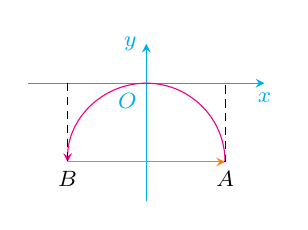
\begin{tikzpicture}[->,samples=100,>=stealth,font=\footnotesize]
                \draw[->,cyan](-1.5,0)--(0,0)node[below left]{$O$}--(1.5,0)node[below]{$x$};
                \draw[->,cyan](0,-1.5)--(0,0.5)node[left]{$y$};
                \draw[magenta] (1,-1) arc (0:180:1);
                \draw[densely dashed,-,black] (-1,0)--(-1,-1)node[below]{$B$}--(1,-1)node[below]{$A$}--(1,0);
                \draw[orange] (-1,-1)--(1,-1);
            \end{tikzpicture}
            \caption{}
        \end{figure}
    \end{minipage}\hfill
    \begin{minipage}[b]{0.7\linewidth}
        \begin{errorSolution}
            补一有向线段 $\overrightarrow{BA}$, 然后用 Green 公式计算, \\
            令 $P=-\dfrac{y^2[f(x)+1]+2yf(x)}{\sqrt{1-x^2}},~Q=x[f(x)+1]$, 那么 $\displaystyle\pdv{Q}{x}-\pdv{P}{y}=\cdots$.\\
            \textbf{错因: }这道题考查了第二型曲线积分的计算, 注意到题目只说 $f$ 连续, 并没有说\textbf{可导}, 所以不能用 Green 公式, 只能用基本方法将 $I$ 化为定积分来计算.\\
        \end{errorSolution}
    \end{minipage}
\end{example}
\begin{solution}
    令 $x=\cos t,y=\sin t-1,~(0\leqslant t\leqslant \pi)$ 代入 $I$ 并化简, 有
    \begin{flalign*}
        I & =\int_{0}^{\pi}\cos t[f(\cos t)+1]\cos t\dd t+\dfrac{(\sin t-1)^2[f(\cos t)+1]+2(\sin t-1)f(\cos t)}{\sin t}\sin t\dd t \\
          & =\int_{0}^{\pi}\qty{\cos^2t[f(\cos t)+1]+(\sin t-1)[f(\cos t)+1]+(2\sin t-2)f(\cos t)}\dd t                             \\
          & =2\int_{0}^{\pi}(1-\sin t)\dd t=\eval{2(t+\cos t)}_{0}^{\pi}=2\pi-4.
    \end{flalign*}
\end{solution}

\subsection{Green 公式}

\begin{theorem}[Green 公式]
    \index{Green 公式}
    Green 公式给出了平面上有限条逐段光滑封闭曲线上的线积分与它们所包围区域上的二重积分的关系:
    $$\oint_{L^+}P\dd x+Q\dd y=\iint\limits_D\left(\frac{\partial Q}{\partial x}-\frac{\partial P}{\partial y}\right)\dd x\dd y$$
    这里 $L^+$ 表示沿 $L$ 的正向取积分. 正向指前进时  保持在左边的方向, 当 $D$ 为单连通区域时,
    即是逆时针方向;当 $D$ 为多联通区域时, 外边界为逆时针方向, 内边界为顺时针方向. $P,Q$ 要求
    在区域 $D$ 内直到边界 $L$ 上连续, 并且连续偏导数. 由此可得 $D$ 的面积公式为:
    $$S=\iint\limits_D\dd x\dd y=\oint_{L^+}x\dd y=-\oint_{L^-}y\dd x=\frac{1}{2}\int_Lx\dd y-y\dd x.$$
\end{theorem}

\subsubsection{计算封闭曲线上的线积分}

\begin{example}
    已知 $L$ 是区域 $D:\dfrac{x}{2}\leqslant y\leqslant 2x,~1\leqslant xy\leqslant 2$ 的正向边界曲线, 求
    $$\displaystyle\oint_L\mathrm{e}^{x^2y^2}\qty[\qty(y-\dfrac{1}{x})\dd x+\qty(x+\dfrac{1}{y})\dd y].$$
\end{example}
\begin{solution}
    令 $u=\dfrac{y}{x},~v=xy$, 那么 $$x=\sqrt{\dfrac{v}{u}},~y=\sqrt{uv},~\dd u=\dd \qty(\dfrac{y}{x})=\dfrac{x\dd y-y\dd x}{x^2},~\dd v=\dd (xy)=y\dd x+x\dd y$$
    $L'$ 是区域 $D':\dfrac{1}{2}\leqslant u\leqslant 2,~1\leqslant v\leqslant 2$ 的正向边界曲线, 于是
    \begin{flalign*}
        I & =\oint_L\mathrm{e}^{x^2y^2}\qty[\qty(y-\dfrac{1}{x})\dd x+\qty(x+\dfrac{1}{y})\dd y]=\oint_L\mathrm{e}^{x^2y^2}\qty(y\dd x+x\dd y+\dfrac{x}{y}\cdot\dfrac{x\dd y-y\dd x}{x^2})                                             \\
          & =\oint_{L'}\mathrm{e}^{v^2}\qty(\dd v+\dfrac{1}{u}\dd u)=\iint\limits_{D'}\dfrac{2v\mathrm{e}^{v^2}}{u}\dd u\dd v=\int_{\frac{1}{2}}^2\dd u\int_1^2\dfrac{2v\mathrm{e}^{v^2}}{u}\dd v=2\ln 2\qty(\mathrm{e}^4-\mathrm{e}).
    \end{flalign*}
\end{solution}

\begin{example}
    设 $\Gamma $ 为 $x^2+y^2=2x(y\geqslant 0)$ 上从 $O(0,0)$ 到 $A(2,0)$ 的一段弧, 连续函数 $f(x)$ 满足
    $$f(x)=x^2+\int_\Gamma y[f(x)+\mathrm{e}^x]\dd x+\qty(\mathrm{e}^x+xy^2)\dd y$$
    求 $f(x).$
\end{example}
\begin{solution}
    设 $\displaystyle \int_\Gamma y[f(x)+\mathrm{e}^x]\dd x+\qty(\mathrm{e}^x+xy^2)\dd y=a$, 那么
    \begin{flalign*}
        a & =\qty(\int_{\Gamma+\overline{AO}}-\int_{\overline{AO}})y[f(x)+\mathrm{e}^x]\dd x+\qty(\mathrm{e}^x+xy^2)\dd y=-\iint\limits_{D}\qty[\pdv{x}\qty(\mathrm{e}^x-xy^2)-\pdv{y}\qty(y(f(x)+\mathrm{e}^x))]\dd x\dd y            \\
          & =-\iint\limits_D\qty(\mathrm{e}^x-y^2-x^2-a-\mathrm{e}^x)\dd x\dd y=\iint\limits_D\qty(x^2+y^2)\dd x\dd y+a\iint\limits_D\dd x\dd y=\int_0^{\frac{\pi}{2}}\dd \theta \int_0^{2\cos\theta }\rho^3\dd \rho +\dfrac{\pi a}{2} \\
          & =4\int_0^{\frac{\pi}{2}}\cos^4\theta\dd \theta +\dfrac{\pi a}{2}=\dfrac{3}{4}\pi+\dfrac{\pi a}{2}\Rightarrow a=\dfrac{3\pi}{2(2-\pi)}\Rightarrow f(x)=x^2+\dfrac{3\pi}{2(2-\pi)}.
    \end{flalign*}
\end{solution}

\begin{example}
    计算积分 $\displaystyle I=\oint_{L^+}\frac{x\dd y-y\dd x}{[(\alpha x+\beta y)^2+(\gamma x+\delta y)^2]^\alpha}~~(\alpha\delta-\beta\gamma\not=0)$, 其中 $L^+$ 为椭圆 $(\alpha x+\beta y)^2+(\gamma x+\delta y)^2=1$, 取逆时针方向.
\end{example}
\begin{solution}
    $L$ 上 $(\alpha x+\beta y)^2+(\gamma x+\delta y)^2=1$, 因此
    $$\displaystyle I=\oint_{L^+}x\dd y-y\dd x=2\iint\limits_{(\alpha x+\beta y)^2+(\gamma x+\delta y)^2\leqslant  1}\dd x\dd y$$
    令 $u=\alpha x+\beta y,~v=\gamma x+\delta y$, 作变换, 有 $\displaystyle I=2\iint\limits_{u^2+v^2\leqslant  1}|J|\dd x\dd y$, 其中
    $$J=\frac{\partial (x,y)}{\partial (u,v)}=\frac{1}{\alpha\delta-\beta\gamma}$$
    因此 $\displaystyle I=\frac{2}{|\alpha\delta-\beta\gamma|}\iint\limits_{u^2+v^2\leqslant  1}\dd u\dd v=\frac{2\pi}{|\alpha\delta-\beta\gamma|}.$
\end{solution}

\subsubsection{含有奇点形式}

\begin{example}
    设 $D=\qty{(x,y)\mid x^2+y^2\leqslant 4}$, $\partial D$ 为 $D$ 的正向边界, 求
    $$I=\int_{\partial D}\dfrac{\qty(x\e^{x^2+4y^2}+y)\dd x+\qty(4y\e^{x^2+4y^2}-x)\dd y}{x^2+4y^2}.$$
\end{example}
\begin{solution}
    设 $l:x^2+4y^2=\varepsilon^2$, $\varepsilon$ 充分小且大于 0, 取顺时针, 如图 \ref{varepverylll} 所示, \\
    \begin{minipage}{0.29\linewidth}
        \begin{figure}[H]
            \centering
            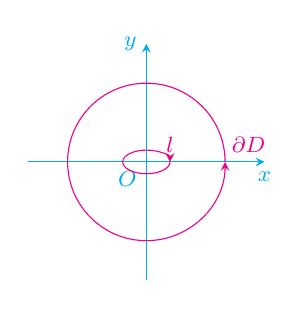
\begin{tikzpicture}[->,samples=100,>=stealth,font=\footnotesize]
                \draw[->,cyan](-1.5,0)--(0,0)node[below left]{$O$}--(1.5,0)node[below]{$x$};
                \draw[->,cyan](0,-1.5)--(0,1.5)node[left]{$y$};
                \draw[magenta] (1,0) arc (0:360:1)node[above]{$~~~~~~\partial D$};
                \draw[magenta,xscale=2] (0.15,0) arc (360:0:0.15)node[above]{$l$};
            \end{tikzpicture}
            \caption{}
            \label{varepverylll}
        \end{figure}
    \end{minipage}\hfill
    \begin{minipage}{0.7\linewidth}
        则有 $$\int_{\partial D}=\int_{\partial D+l-l}=\int_{\partial D+l}+\int_{l^-}:=I_1+I_2$$
        设 $P=\dfrac{x\e^{x^2+4y^2}+y}{x^2+4y^2},~Q=\dfrac{4y\e^{x^2+4y^2}-x}{x^2+4y^2}$, 那么
        $$\pdv{Q}{x}=\dfrac{8xy\e^{x^2+4y^2}\qty(x^2+4y^2-1)+x^2-4y^2}{\qty(x^2+4y^2)^2}=\pdv{P}{y}$$
        因此 $\displaystyle I_1=\iint\limits_D\qty(\pdv{Q}{x}-\pdv{P}{y})\dd x\dd y=0$, 下求 $I_2$,
    \end{minipage}
    \begin{flalign*}
        I_2 & =\dfrac{1}{\varepsilon^2}\int_{l^-}\underbrace{\qty(x\e^{x^2+4y^2}+y)}_{P_1}\dd x+\underbrace{\qty(4y\e^{x^2+4y^2}-x)}_{Q_1}\dd y=\dfrac{1}{\varepsilon^2}\iint\limits_{D_{\varepsilon}}\qty(\pdv{Q_1}{x}-\pdv{P_1}{y})\dd x\dd y \\
            & =\dfrac{-2}{\varepsilon^2}\iint\limits_{x^2+4y^2\leqslant \varepsilon^2}\dd x\dd y=\dfrac{-2}{\varepsilon^2}\cdot\pi\cdot\varepsilon\cdot\dfrac{\varepsilon}{2}=-\pi
    \end{flalign*}
    故 $I=0-\pi=\pi.$
\end{solution}

\begin{example}
    计算 $\displaystyle\oint_{C^+}\frac{x\dd y-y\dd x}{4x^2+y^2}$, $C$ 为以 $(1,0)$ 为圆心, 以 $R$ 为半径的圆周 ($R\not=1$), 设 $C^+$ 表示其上的方向为逆时针方向.
\end{example}
\begin{solution}
    当 $R<1$ 时, 满足 Green 公式的条件, 则 $$\frac{\partial }{\partial x}\left(\frac{x}{4x^2+y^2}\right)=\frac{y^2-4x^2}{(4x^2+y^2)^2}=\frac{\partial }{\partial y}\left(\frac{-y}{4x^2+y^2}\right)$$
    所以 $\displaystyle\oint_{C^+}\frac{x\dd y-y\dd x}{4x^2+y^2}=0~~(x,y\not=0)$;\\
    当 $R>1$ 时, 取 $\varepsilon>0$ 充分小, 使得 $\Gamma_\varepsilon:~4x^2+y^2=\varepsilon^2$, 且 $\Gamma_\varepsilon^+$ 表示其上的方向为顺时针方向,
    记 $C$ 与 $\Gamma$ 所围成区域为 $D$, 则 $\displaystyle\oint_{C^++\Gamma_\varepsilon^+}\frac{x\dd y-y\dd x}{4x^2+y^2}=0$,
    那么 $$\oint_{C^+}\frac{x\dd y-y\dd x}{4x^2+y^2}=\oint_{\Gamma_\varepsilon^-}\frac{x\dd y-y\dd x}{4x^2+y^2}=\frac{1}{\varepsilon^2}\oint_{\Gamma_\varepsilon^-}x\dd y-y\dd x=\frac{1}{\varepsilon^2}\cdot \pi\varepsilon^2=\pi.$$
\end{solution}

\begin{example}
    设 $f(x,y)$ 单位圆上有连续的偏导数, 且在边界上取值为零, 求证: $$\displaystyle\lim_{\varepsilon\to 0^+}\iint\limits_D\dfrac{x\dfrac{\partial f}{\partial x}+y\dfrac{\partial f}{\partial y}}{x^2+y^2}\dd x\dd y=-2\pi f(0,0).$$ 其中 $D$ 为圆环域: $\varepsilon ^2\leqslant  x^2+y^2\leqslant  1.$
\end{example}
\begin{proof}[{\songti \textbf{证}}]
    记 $\displaystyle L_1:~x^2+y^2=1$ (逆时针方向), $L_2:~x^2+y^2=\varepsilon ^2$ (顺时针方向),
    \begin{flalign*}
        \iint\limits_D\dfrac{x\dfrac{\partial f}{\partial x}+y\dfrac{\partial f}{\partial y}}{x^2+y^2}\dd x\dd y & =\oint_{L_2}\dfrac{-yf(x,y)\dd x+xf(x,y)\dd y}{x^2+y^2}=\dfrac{1}{\varepsilon^2}\oint_{L_2}-yf(x,y)\dd x+xf(x,y)\dd y                                                                                 \\
                                                                                                                 & =\dfrac{1}{\varepsilon^2}\int_{2\pi}^0\left[(-\varepsilon\sin\theta)(-\varepsilon\sin\theta)+\epsilon\cos\theta\cdot\epsilon\cos\theta\right]f(\varepsilon\cos\theta,\varepsilon\sin\theta)\dd \theta \\
                                                                                                                 & =-\int_0^{2\pi}f(\varepsilon\cos\theta,\varepsilon\sin\theta)\dd \theta=-2\pi f(\varepsilon\cos\theta^*,\varepsilon\sin\theta^*)~~(\theta^*\in[0,2\pi])
    \end{flalign*}
    故 $\displaystyle\lim_{\varepsilon\to0^+}\iint\limits_D\dfrac{x\dfrac{\partial f}{\partial x}+y\dfrac{\partial f}{\partial y}}{x^2+y^2}\dd x\dd y=-2\pi f(0,0).$
\end{proof}

\subsubsection{变力做功}

\begin{example}
    设 $L$ 为从点 $A(2,0)$ 沿 $y=\sqrt{2x-x^2}$ 到点 $O(0,0)$ 的有向曲线段, 位于起点的质点在力 $\vb*{F}$ 的作用下沿 $L$ 到达终点, 设 $P(x,y)$ 为 $L$ 上, $|\vb*{F}|=\sqrt{x^2+y^2}$, 方向与 $\overrightarrow{OP} $ 垂直且与 $y$ 轴夹角为锐角, 则力所做的功为 (\quad).
    \begin{tasks}(4)
        \task $\dfrac{\pi}{2}$
        \task $-\dfrac{\pi}{2}$
        \task $\pi$
        \task $-\pi$
    \end{tasks}
\end{example}
\begin{solution}
    $\overrightarrow{OP} =(x,y)$, 与 $\overrightarrow{OP} $ 垂直且与 $y$ 轴夹角为锐角的向量为 $(-y,x)$, $\vb*{F}$ 对应的单位向量为 $ \vb*{F}^0=\dfrac{1}{\sqrt{x^2+y^2}}(-y,x) $
    变力 $\vb*{F}=|\vb*{F}|\cdot \vb*{F}^0=(-y,x)$, 则力所做的功为
    $$
    W=\int_L-y \dd x+x \dd y
    $$
    由 Green 公式, 
    $$
    W=\qty(\oint_{L+\overrightarrow{OA}}-\int_{\overrightarrow{OA}})-y \dd x + x \dd y=2\iint\limits_D \dd x \dd y -0=2\cdot\dfrac{\pi}{2}=\pi
    $$
    故选 C.
\end{solution}

\subsubsection{曲线积分最大值}

\begin{example}
    确定曲线 $C$, 使得 $\displaystyle I=\oint_C\qty(x+\dfrac{y^3}{3})\dd x+\qty(y+x-\dfrac{2x^3}{3})\dd y$ 达到最大值.
\end{example}
\begin{solution}
    记 $D$ 为曲线 $C$ 所围区域, 由 Green 公式 $$
        I=\iint\limits_D\qty[\pdv{x}\qty(y+x-\dfrac{2x^3}{3})-\pdv{y}\qty(x+\dfrac{y^3}{3})]\dd x\dd y=\iint\limits_D\qty(1-2x^2-y^2)\dd x\dd y
    $$
    当 $2x^2+y^2>1$ 时, 积分函数 $<0\to I<0$; 当 $2x^2+y^2\leqslant 1$, 积分函数 $\geqslant 0\to I\geqslant 0$, 因此当 $C:2x^2+y^2=1$ 时, $I$ 有最大值.
\end{solution}

\begin{example}
    设曲线 $L$ 是 $xOy$ 平面上有界单连通闭区域 $D$ 的正向边界, 当曲线 $L$ 的方程为 $x^2+y^2=1$ 时,
    $$
        I=\oint_L\qty(ax+\dfrac{a}{3}x^3-\dfrac{1}{2}x\e ^{x^2+y^2})\dd y+\qty(\dfrac{1}{2}y\e ^{x^2+y^2}-\dfrac{a}{3}y^3)\dd x
    $$
    值最大, 求
    \begin{enumerate}[label=(\arabic{*})]
        \item 常数 $a$ 的值;
        \item $I$ 的最大值 $I_{max}$.
    \end{enumerate}
\end{example}
\begin{solution}
    \begin{enumerate}[label=(\arabic{*})]
        \item 由 Green 公式 $$
                  I=\iint\limits_D\qty[\pdv{x}\qty(ax+\dfrac{a}{3}x^3-\dfrac{1}{2}x\e ^{x^2+y^2})-\pdv{y}\qty(\dfrac{1}{2}y\e ^{x^2+y^2}-\dfrac{a}{3}y^3)]\dd x \dd y =\iint\limits_D\qty(1+x^2+y^2)\qty(a-\e ^{x^2+y^2})\dd x \dd y
              $$
              因为曲线 $L$ 为 $x^2+y^2=1$ 时, $I$ 最大, 故 $a=\e$.
        \item 由 (1) 可得
              \begin{flalign*}
                  I_{max} & =\iint\limits_D\qty(1+x^2+y^2)\qty(\e -\e ^{x^2+y^2})\dd x \dd y=\int_{0}^{2\pi}  \dd \theta \int_{0}^{1} \qty(r+r^3)\qty(\e -\e ^{r^2}) \dd r \\
                          & \xlongequal{r^2=t}\pi \int_{0}^{1}(1+t)\qty(\e -\e ^{t})\dd t=\pi\qty(\e-\e+1+\dfrac{\e }{2}-1)=\dfrac{1}{2}\pi \e.
              \end{flalign*}
    \end{enumerate}
\end{solution}

\subsubsection{方向导数与两类曲线积分的联系}

\begin{theorem}[方向导数与两类曲线积分的联系]
    \index{方向导数与两类曲线积分的联系}
    设 $\alpha_1,\beta_1$ 分别为外法线向量 $\vb*{n}$ 与 $x$ 轴、$y$ 轴的正方向的夹角, 则 
    $$
    \oint_L\pdv{u}{\vb*{n}}\dd s=\oint_L\qty(\pdv{u}{x}\cos\alpha_1+\pdv{u}{y}\cos\beta_1) \dd s.
    $$
\end{theorem}

\begin{example}
    设 $u(x,y)$ 于圆盘 $D:x^2+y^2\leqslant  \pi$ 内有二阶连续偏导数, 且
    $$\displaystyle\frac{\partial ^2u}{\partial x^2}+\frac{\partial ^2u}{\partial y^2}=\mathrm{e}^{\pi-x^2-y^2}\sin\left(x^2+y^2\right)$$
    记 $D$ 的正向边界曲线为 $\partial D$, $\partial D$ 的外法线向量为 $\boldsymbol n$, 求 $\displaystyle\oint_{\partial D}\frac{\partial u}{\partial \boldsymbol n}\dd s.$
\end{example}
\begin{solution}
    令 $\boldsymbol n=(\cos\alpha,\cos\beta)$, 则 $\displaystyle \frac{\partial u}{\partial \boldsymbol n}=\frac{\partial u}{\partial x}\cos\alpha+\frac{\partial u}{\partial y}\cos\beta$, $\partial D$ 的单位切向量 $\boldsymbol \tau=(-\cos\beta,\cos\alpha)$, 于是
    \begin{flalign*}
        \oint_{\partial D}\frac{\partial u}{\partial \boldsymbol n}\dd s & =\int_{\partial D}\left(\frac{\partial u}{\partial x}\cos\alpha+\frac{\partial u}{\partial y}\cos\beta\right)\dd s=\int_{\partial D}\frac{\partial u}{\partial x}\dd y-\frac{\partial u}{\partial y}\dd x=\iint\limits_D\left(\frac{\partial ^2u}{\partial x^2}+\frac{\partial ^2u}{\partial y^2}\right)\dd x\dd y \\
                                                                         & =\iint\limits_{D}\mathrm{e}^{\pi-x^2-y^2}\sin\left(x^2+y^2\right)\dd x\dd y
        =\int_0^{2\pi}\dd \theta\int_0^{\sqrt{\pi}}\rho\mathrm{e}^{\pi-\rho^2}\sin\left(\rho^2\right)\dd \rho                                                                                                                                                                                                                                                                                 \\
                                                                         & \xlongequal[]{t=\rho^2}\pi\int_0^\pi\mathrm{e}^{\pi-t}\sin t\dd t=\frac{\pi}{2}\left(\mathrm{e}^\pi+1\right).
    \end{flalign*}
\end{solution}

% \begin{example}
%     设函数 $u(x,y)$ 在区域 $D=\left\{(x,y)|x^2+y^2\leqslant \pi\right\}$ 上有二阶连续偏导数, 且
%     $$\frac{\partial^2u}{\partial x^2}+\frac{\partial ^2u}{\partial y^2}=\mathrm{e}^{\pi-x^2-y^2}\cdot\sin\left(x^2+y^2\right)$$
%     记 $D$ 的正向边界曲线为 $L$, $L$ 的外法向量为 $\vec{n}$, 求 $\displaystyle\oint_L\frac{\partial u}{\partial \vec{n}}\dd s.$
% \end{example}
% \begin{solution}
%     因为$$ \oint_L\frac{\partial u}{\partial \vec{n}}\dd s=\iint\limits_D\left(\frac{\partial ^2u}{\partial x^2}+\frac{\partial ^2u}{\partial y^2}\right)\dd x\dd y$$
%     所以
%     \begin{flalign*}
%         \oint_L\frac{\partial u}{\partial \vec{n}}\dd s =\iint\limits_D\mathrm{e}^{\pi-x^2-y^2}\cdot\sin\left(x^2+y^2\right)\dd x\dd y
%         =\int_0^{2\pi}\dd \theta\int_0^{\sqrt{\pi}}\rho\mathrm{e}^{\pi-\rho^2}\sin\rho^2\dd \rho
%         =\pi\int_0^\pi\mathrm{e}^{\pi-t}\sin t\dd t=\frac{\pi}{2}\left(\mathrm{e}^\pi+1\right)
%     \end{flalign*}
% \end{solution}

\begin{example}
    设 $u(x,y)$ 于圆盘 $D=\qty{(x,y):x^2+y^2\leqslant \dfrac{\pi}{2}}$ 内有二阶连续的偏导数, 并且满足:
    $$\pdv[2]{u}{x}+\pdv[2]{u}{y}=\qty(x^2+y^2)\sin^6\qty(x^2+y^2)$$
    记 $D$ 的正向边界曲线为 $\partial D$, $\partial D$ 的外法线向量为 $\va*{n}$, 求 $\displaystyle \oint_{\partial D}\pdv{u}{\va*{n}}\dd s.$
\end{example}
\begin{solution}
    设 $\va*{T}=(\cos\alpha,\cos\beta)$ 对应的正向切线的单位向量, 则单位向量为 $\va*{n}=(\cos\alpha,-\cos\beta)$, 由题设可知 $u(x,y)$ 可微,
    故由方向导数计算公式和两类曲线积分之间的关系, 得
    $$I=\oint_{\partial D}\pdv{u}{\va*{n}}\dd s=\oint_{\partial D}\qty(\pdv{u}{x}\cos \beta-\pdv{u}{y}\cos \alpha)\dd s=\oint_{\partial D}\pdv{u}{x}\dd y-\pdv{u}{y}\dd x$$
    于是由 Green 公式和二重积分的极坐标计算公式, 得
    \begin{flalign*}
        I & =\iint\limits_D\qty(\pdv[2]{u}{x}+\pdv[2]{u}{y})\dd x\dd y=\iint\limits_D\qty(x^2+y^2)\sin^6\qty(x^2+y^2)\dd x\dd y=\int_{0}^{2\pi}\dd \theta\int_{0}^{\sqrt{\frac{\pi}{2}}}r^2\sin^6r^2\dd r=\pi\int_{0}^{\frac{\pi}{2}}u\sin^6u\dd u
    \end{flalign*}
    又因为 $\sin^nx=\begin{cases}
            \displaystyle \dfrac{1}{(2\i)^{n-1}}\sum_{k=0}^{\frac{n-1}{2}}(-1)^k\C_n^k\cos((n-2k)x) \\
            \displaystyle \dfrac{2}{(2\i)^n}\qty[\sum_{k=0}^{\frac{n}{2}-1}(-1)^k\C_n^k\cos((n-2k)x)+\dfrac{(-1)^{\frac{n}{2}}}{2}\C_n^{\frac{n}{2}}]
        \end{cases}\Rightarrow \sin^6x=-\dfrac{1}{8}\cos^32x+\dfrac{3}{16}\cos 4x-\dfrac{3}{8}\cos 2x+\dfrac{5}{16}$, 由分部积分公式
    $$\int u\cos nu\dd u=\dfrac{\cos nu}{n^2}+\dfrac{u\sin nu}{n}+C$$
    分别取 $n=2,4,6$, 得 $\displaystyle I=\pi\qty(\dfrac{17}{72}+\dfrac{5\pi^2}{128}).$
\end{solution}

\subsubsection{积分与路径无关问题}

该部分内容可能需要结合第八章“微分方程”的知识, 若不熟悉常见的微分方程求解, 可暂缓阅读.

\begin{definition}[单连通与复连通区域]
    若平面区域 $ D $ 内任一闭曲线所围的部分都属于 $D$, 则称 $ D $ 为\textit{平面单连通区域}, 否则称为\textit{复连通区域}. 通俗地讲, 平面单连通区域就是不含有“洞”的区域.\index{单连通与复连通区域}
\end{definition}

\begin{theorem}[路径无关]
    设函数 $ P(x, y), Q(x, y) $ 在区域 $ D $ 内具有一阶连续 偏导数, 若对于 $ D $ 内的任意指定的两点  $A, B$  以及 $ D $ 内从点  $A$  到点 $ B$  的两条任意曲线 $ L_{1}, L_{2}$, 等式
    $$\int_{L_{1}} P \dd  x+Q \dd  y=\int_{L_{2}} P \dd  x+Q \dd  y$$
    恒成立, 则称曲线积分 $ \displaystyle\int_{L} P \dd  x+Q \dd  y $ 在 $ D $ 内与路径无关, 否则称与路径有关.
    \index{路径无关}
\end{theorem}

设在单连通区域 $ D $ 内 $ P, Q $ 具有一阶连续偏导数, 则下述 6 个说法等价
\begin{enumerate}[label=(\arabic{*})]
    \item $\displaystyle\int_{L} P(x, y) \dd  x+Q(x, y) \dd  y $ 在 $ D $ 内与路径无关;
    \item $\displaystyle \oint_{L} P(x, y) \dd  x+Q(x, y) \dd  y=0 $
          其中 $ L $ 是区域 $ D $ 内任意分段光滑闭曲线.
    \item $P \dd  x+Q \dd  y=d u(x, y)$;
    \item $\displaystyle\frac{\partial Q}{\partial x}=\frac{\partial P}{\partial y}, \forall(x, y) \in D $;
    \item $P \dd  x+Q \dd  y=0 $ 为全微分方程;
    \item $P \vb*{i}+Q \vb*{j}$ 为某二元函数 $ u(x, y) $ 的梯度.
\end{enumerate}

\begin{example}
    设函数 $f(t)$ 连续, 且 $ \displaystyle \int_{0}^{2x+3y+1} f(t) \dd t =4x^2+9y^2+12xy-2$, 并设起点 $O(0,0)$, 终点 $A(1,3)$, $l$ 为连接 $O$ 与 $A$ 的逐段光滑曲线, 则
    $$
    \int_L xy^2f(xy)\dd x+x^2y f(xy)\dd y=(\quad).
    $$
    \begin{tasks}(4)
        \task 与曲线 $l$ 有关
        \task 3
        \task 4
        \task 9
    \end{tasks}
\end{example}
\begin{solution}
    因为 $ \displaystyle \int_{0}^{2x+3y+1} f(t) \dd t =4x^2+9y^2+12xy-2=(2x+3y)^2-2\xlongequal{2x+3y+1=u}\int_{0}^{u} f(t) \dd t=(u-1)^2-2$, 所以 $f(u)=2(u-1)$, 又因为 
    $$
    xy^2f(xy)\dd x+x^2y f(xy)\dd y=xyf(xy)(y \dd x + x \dd y)=xy(xy)\dd (xy)
    $$
    原积分与路径无关, 故 $\displaystyle \int_L xy^2f(xy)\dd x+x^2y f(xy)\dd y=2\int_{(0,0)}^{(1,3)} xy(xy-1) \dd (xy)=9$, 故选 D.
\end{solution}

\begin{example}
    计算 $\displaystyle\int_{\stackrel\frown{AB}}\dfrac{-y}{x^2+y^2}\dd x+\dfrac{x}{x^2+y^2}\dd y$, 其中 $\stackrel\frown{AB}$ 是自点 $A(-1,0)$ 沿 $y=x^2-1$ 到点 $B(2,3)$ 的弧段.
\end{example}
\begin{errorSolution}
    \textbf{错解一: }因为 $\displaystyle\pdv{Q}{x}=\dfrac{y^2-x^2}{\qty(x^2+y^2)^2}=\pdv{P}{y}$, 所以与路径无关, 选取 $l_4^-$ 作为积分路径, 则
    $$I=\int_{0}^{3}\dfrac{-1}{1+y^2}\dd y+\int_{-1}^{2}\dfrac{-3}{x^2+9}\dd x=-\arctan 3-\arctan\dfrac{2}{3}-\arctan\dfrac{1}{3}=-\arctan\dfrac{2}{3}-\dfrac{\pi}{2}$$
    \textbf{错因: }$l_1$ 与 $l_3^-$ 所围成的区域必须是一个单连通区域, 因为原点 $(0,0)$ 无定义, 所以不能取 $l_4^-$ 作为积分路径.\\
    \textbf{错解二: }因为 $\displaystyle\pdv{Q}{x}=\dfrac{y^2-x^2}{\qty(x^2+y^2)^2}=\pdv{P}{y}$, 所以与路径无关, 选取 $l_5$ 作为积分路径, 则
    $$I=\int_{0}^{3}\dfrac{-1}{1+y^2}\dd y+\int_{-1}^{2}\dfrac{-3}{x^2+9}\dd x=\int_{0}^{3}\dfrac{2\dd y}{4+y^2}=\arctan\dfrac{3}{2}$$
    \textbf{错因: }路径 $l_5$ 上含有无定义点 $(0,0)$, 故不能选取该路径作积分.\\
\end{errorSolution}
\begin{solution}
    记 $l_2:\overrightarrow{BA},~l_3:x^2+y^2=\varepsilon^2\text{ 方向: 顺时针},~l_4:\overrightarrow{BCA},~l_5:\overrightarrow{AFB},~l_6:\overrightarrow{ADEB}$, 则
    有向线段 $l_1,~l_2,~l_3$ 围成的区域记为 $D_1$, 且 $\displaystyle\pdv{Q}{x}=\dfrac{y^2-x^2}{\qty(x^2+y^2)^2}=\pdv{P}{y}$\\
    \begin{minipage}{0.64\linewidth}
        \textbf{法一: }$l_3$ 围成的区域记为 $D_\varepsilon$ 由 Green 公式,
        \begin{flalign*}
            I & =\qty(\oint_{l_1+l_2+l_3})\dfrac{-y\dd x+x\dd y}{x^2+y^2}                                                                              \\
              & =\iint\limits_{D_1}\qty(\pdv{Q}{x}-\pdv{P}{y})\dd x\dd y-\qty(\int_{\overrightarrow{BA}}+\int_{l_3})\dfrac{-y\dd x+x\dd y}{x^2+y^2}    \\
              & =0-\int_{-1}^{2}\dfrac{\dd x}{2x^2+2x+1}+\dfrac{2}{\varepsilon^2}\iint\limits_{D_\varepsilon}\dd x\dd y=-\dfrac{\pi}{4}-\arctan 5+2\pi \\
              & =\pi+\arctan\dfrac{3}{2}.
        \end{flalign*}
        \textbf{法二: }因为 $\displaystyle\pdv{Q}{x}=\dfrac{y^2-x^2}{\qty(x^2+y^2)^2}=\pdv{P}{y}$, 所以与路径无关, 选取 $l_6$ 作为积分路径, 则有
        \begin{flalign*}
            I & =\int_{\overrightarrow{AD}+\overrightarrow{DE}+\overrightarrow{EB}}\dfrac{-y\dd x+x\dd y}{x^2+y^2}=\int_{0}^{-1}\dfrac{\dd y}{1+y^2}+\int_{-1}^{2}\dfrac{\dd x}{x^2+1}+\int_{-1}^{3}\dfrac{2\dd y}{4+y^2} \\
              & =\dfrac{\pi}{2}+\arctan 2+\arctan\dfrac{3}{2}+\arctan\dfrac{1}{2}=\pi+\arctan\dfrac{3}{2}.
        \end{flalign*}
    \end{minipage}\hfill
    \begin{minipage}{0.35\linewidth}
        \begin{figure}[H]
            \centering
            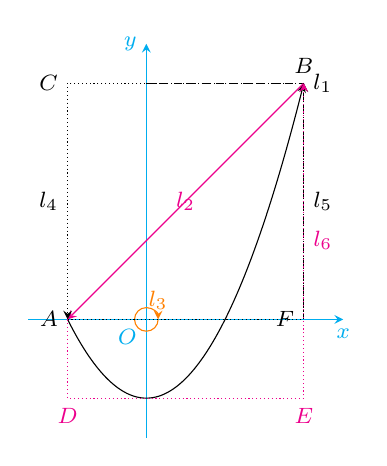
\begin{tikzpicture}[->,samples=100,>=stealth,font=\footnotesize]
                \draw[->,cyan](-1.5,0)--(0,0)node[below left]{$O$}--(2.5,0)node[below]{$x$};
                \draw[->,cyan](0,-1.5)--(0,3.5)node[left]{$y$};
                \draw[domain=-1:2,black] plot(\x,{\x*\x-1})node[right]{$l_1$};
                \node[below,left] at (-1,0) {$A$};
                \draw[densely dashed,-,black] (0,3)--(2,3)node[above]{$B$}--(2,0);
                \draw[magenta] (2,3)--(-1,0) node[midway]{$l_2$};
                \draw[orange] (0.15,0) arc (360:0:0.15) node[above]{$l_3$};
                \draw[densely dotted] (2,3)--(-1,3)node[left]{$C$}--(-1,0)node[midway,left]{$l_4$};
                \draw[densely dotted] (-1,0)--(2,0)node[below,left]{$F$}--(2,3)node[midway,right]{$l_5$};
                \draw[densely dotted,magenta] (-1,0)--(-1,-1)node[below]{$D$}--(0,-1)--(2,-1)node[below]{$E$}--(2,3)node[midway,right]{$l_6$};
            \end{tikzpicture}
            \caption{}
        \end{figure}
    \end{minipage}
    \textbf{法三: }$\displaystyle I=\int_{\stackrel\frown{AB}}\dfrac{-y}{x^2+y^2}\dd x+\dfrac{x}{x^2+y^2}\dd y=\int_{(-1,0^-)}^{(2,3)}\dd \qty(\arctan\dfrac{y}{x})=\int_{-\pi}^{\arctan\frac{3}{2}}\dd \theta=\arctan\dfrac{3}{2}+\pi.$\\
\end{solution}

\begin{example}
    已知 $\varphi(0)=\dfrac{1}{2}$, 求连续可微函数 $\varphi(x)$, 使得曲线积分 $\displaystyle\int_{A}^{B}\qty[\e^x+\varphi(x)]y\dd x-\varphi(x)\dd y$ 与路径无关.
\end{example}
\begin{solution}
    令 $P=\qty[\e^x+\varphi(x)]y,~Q=-\varphi(x)$, 因为积分与路径无关, 则 $$\pdv{P}{y}=\pdv{Q}{x}\Rightarrow \varphi'(x)+\varphi(x)=-\e^x$$
    该方程为一阶线性微分方程, 有通解公式 $$\varphi(x)=\e^{-\int\dd x}\qty[\int\qty(-\e^{x})\cdot\e^{\int\dd x}\dd x+C]=-\dfrac{1}{2}\e^{x}+C\e^{-x}$$
    又因为 $\varphi(0)=\dfrac{1}{2}$, 解得 $C=1$, 因此 $\varphi(x)=-\dfrac{1}{2}\e^x+\e^{-x}.$
\end{solution}

\subsubsection{二重积分分部积分}

\begin{theorem}[二重积分分部积分公式]
    \index{二重积分分部积分公式}设 $D$ 是由一条或几条按段光滑的封闭曲线围成的平面有界闭区域, 若函数  $u,v$ 在闭区域 $D$ 上有连续的一阶偏导数, 则
    \label{iintlimitsduvxxy}
    $$\iint\limits _{D}u\dfrac{\partial v}{\partial x}\dd x\dd y=\oint _{\partial D}uv\dd y-\iint\limits _{D}v\dfrac{\partial u}{\partial x}\dd x\dd y,~\iint\limits _{D}u\dfrac{\partial v}{dy}\dd x\dd y=-\oint _{\partial D}uv\dd x-\iint\limits _{D}v\dfrac{\partial u}{\partial y}\dd x\dd y.$$
\end{theorem}

\begin{example}[2023 西北大学]
    设 $D$ 是由简单光滑闭曲线 $L$ 围成的区域, $f(x,y)$ 在 $D$ 上具有连续的偏导数, 记作: $d=\max\limits_{(x,y)\in D}\sqrt{x^2+y^2}$,
    \begin{enumerate}[label=(\arabic{*})]
        \item 证明: $\displaystyle \iint\limits_D f(x,y)\dd x\dd y=\int_L x\cdot f \dd y-\iint\limits_Dx\pdv{f}{x}\dd x\dd y$;
        \item 若 $\forall (x,y)\in L$, 有 $f(x,y)=0$, 证明:
              $$\iint\limits_D f^2(x,y)\dd x\dd y\leqslant d^2\iint\limits_D\qty[\qty(\pdv{f}{x})^2+\qty(\pdv{f}{y})^2]\dd x\dd y.$$
    \end{enumerate}
\end{example}
\begin{proof}[{\songti \textbf{证}}]
    \begin{enumerate}[label=(\arabic{*})]
        \item 有 Green 公式得 $$\iint\limits_Du\pdv{v}{x}\dd x\dd y=\oint_{\partial D}uv\dd y-\iint\limits_Dv\pdv{u}{x}\dd x\dd y$$
              令 $u=x,~v=f$, 则有 $\displaystyle\iint\limits_Dx\pdv{f}{x}\dd x\dd y=\int_Lx\cdot f\dd y-\iint\limits_Df(x,y)\dd x\dd y$, 整理得证;
        \item 由 (1) 可得, $$\displaystyle \iint\limits_D f^2\dd x\dd y=\dfrac{1}{2}\int_L f^2(x\dd y-y\dd x)-\dfrac{1}{2}\iint\limits_D\qty(x\pdv{f^2}{x}+y\pdv{f^2}{y})\dd x\dd y$$
              又 $\forall (x,y)\in L$, 有 $f(x,y)=0$, 于是 $\displaystyle \int_Lf^2(x\dd y-y\dd x)=0$, 故 $$\displaystyle \iint\limits_D f^2\dd x\dd y=-\dfrac{1}{2}\iint\limits_D\qty(x\pdv{f^2}{x}+y\pdv{f^2}{y})\dd x\dd y$$
              于是由 Cauchy-Schwarz 不等式得,
              \begin{flalign*}
                  \iint\limits_D f^2\dd x\dd y & \leqslant \iint\limits_D\qty|xf\pdv{f}{x}+yf\pdv{f}{y}|\dd x\dd y\leqslant \iint\limits_D|f|\sqrt{x^2+y^2}\cdot\sqrt{\qty(\pdv{f}{x})^2+\qty(\pdv{f}{y})^2}\dd x\dd y                                                 \\
                                               & \leqslant d \iint\limits_D|f|\sqrt{\qty(\pdv{f}{x})^2+\qty(\pdv{f}{y})^2}\dd x\dd y\leqslant d\qty[\iint\limits_Df^2\dd x\dd y\cdot\iint\limits_D\qty(\qty(\pdv{f}{x})^2+\qty(\pdv{f}{y})^2)\dd x\dd y]^{\frac{1}{2}}
              \end{flalign*}
              即 $\displaystyle \qty(\iint\limits_Df^2\dd x\dd y)^{\frac{1}{2}}\leqslant d\cdot\qty[\iint\limits_D \qty(\qty(\pdv{f}{x})^2+\qty(\pdv{f}{y})^2)\dd x\dd y]^{\frac{1}{2}}$, 不等式两边平方, 即得证.
    \end{enumerate}
\end{proof}

\begin{example}
    设函数 $f(x,y)$ 在区域 $D:x^2+y^2\leqslant  1$ 上有二阶连续偏导数,
    且 $\displaystyle\frac{\partial^2f}{\partial x^2}+\frac{\partial^2f}{\partial y^2}=\mathrm{e}^{-\left(x^2+y^2\right)}$, 证明:
    $$\iint\limits_D\left(x\frac{\partial f}{\partial x}+y\frac{\partial f}{\partial y}\right)\dd x\dd y=\frac{\pi}{2\mathrm{e}}.$$
\end{example}
\begin{proof}[{\songti \textbf{证法一}}]
    积分区域 $D$ 是圆形域, 考虑采用极坐标, 然后利用已知等式化简被积函数.
    令 $x=\rho\cos\theta,~y=\rho\sin\theta$, 则$$D=\{(\rho,\theta)|0\leqslant \rho\le1,0\leqslant \theta\le2\pi\}$$ 于是
    $$\iint\limits_D\left(x\frac{\partial f}{\partial x}+y\frac{\partial f}{\partial y}\right)\dd x\dd y=\int_0^1\rho\dd \rho\int_0^{2\pi}\left(\rho\cos\theta\frac{\partial f}{\partial x}+\rho\sin\theta\frac{\partial f}{\partial y}\right)\dd \theta.$$
    记 $L_\rho$ 为半径是 $\rho\left(0\leqslant \rho\leqslant  1\right)$ 的圆周 (逆时针方向), $D_\rho$ 为 $L_\rho$ 包围的区域, 则
    $$\int_0^{2\pi}\left(\rho\cos\theta\frac{\partial f}{\partial x}+\rho\sin\theta\frac{\partial f}{\partial y}\right)\dd \theta=\oint_{L_\rho}-\frac{\partial f}{\partial y}\dd x+\frac{\partial f}{\partial x}\dd y.$$
    由 Green 公式及已知等式, 得
    $$\text{上式}=\iint\limits_{D_\rho}\left(\frac{\partial^2f}{\partial x^2}+\frac{\partial ^2f}{\partial y^2}\right)\dd x\dd y=\iint_{D_\rho}\mathrm{e}^{-\left(x^2+y^2\right)}\dd x\dd y=\int_0^{2\pi}\dd \theta\int_0^\rho\mathrm{e}^{-r^2}r\dd r=\pi\left(1-\mathrm{e}^{-\rho^2}\right)$$
    故 $$\iint\limits_D\left(x\frac{\partial f}{\partial x}+y\frac{\partial f}{\partial y}\right)\dd x\dd y=\int_0^1\rho\pi\left(1-\mathrm{e}^{-\rho^2}\right)\dd \rho=\frac{\pi}{2\mathrm{e}}.$$
\end{proof}
\begin{proof}[{\songti \textbf{证法二}}]
    由 Green 公式, 可导出二重积分的分部积分公式:
    $$\iint\limits_Du\frac{\partial v}{\partial x}\dd x\dd y=\oint_{\partial D}uv\dd y-\iint\limits_Dv\frac{\partial u}{\partial x}\dd x\dd y,~\iint\limits_Du\frac{\partial v}{\partial y}\dd x\dd y=-\oint_{\partial D}uv\dd x-\iint\limits_Dv\frac{\partial u}{\partial y}\dd x\dd y.$$
    其中 $D$ 是由一条分段光滑闭曲线所围成的闭区域, $\partial D$ 为 $D$ 的正向边界.\\
    令 $\displaystyle u=\frac{\partial f}{\partial x},~\frac{\partial v}{\partial x}=x=\frac{\partial }{\partial x}\left(\frac{x^2+y^2}{2}\right)$, 则由上述公式, 有
    \begin{flalign*}
        \iint\limits_Dx\frac{\partial f}{\partial x}\dd x\dd y  =\iint\limits_D\frac{\partial f}{\partial x}\cdot\frac{\partial }{\partial x}\left(\frac{x^2+y^2}{2}\right)\dd x\dd y
        =\frac{1}{2}\oint_{\partial D}\left(x^2+y^2\right)\frac{\partial f}{\partial x}\dd y-\frac{1}{2}\iint\limits_D\left(x^2+y^2\right)\frac{\partial^2f}{\partial x^2}\dd x\dd y
    \end{flalign*}
    再令 $\displaystyle u=\frac{\partial f}{\partial y},~\frac{\partial v}{\partial x}=y=\frac{\partial }{\partial y}\left(\frac{x^2+y^2}{2}\right)$, 类似地, 有
    \begin{flalign*}
        \iint\limits_Dy\frac{\partial f}{\partial y}\dd x\dd y  =\iint\limits_D\frac{\partial f}{\partial y}\cdot\frac{\partial }{\partial y}\left(\frac{x^2+y^2}{2}\right)\dd x\dd y
        =-\frac{1}{2}\oint_{\partial D}\left(x^2+y^2\right)\frac{\partial f}{\partial y}\dd x-\frac{1}{2}\iint\limits_D\left(x^2+y^2\right)\frac{\partial ^2f}{\partial y^2}\dd x\dd y
    \end{flalign*}
    于是
    \begin{flalign*}
        \iint\limits_D\left(x\frac{\partial f}{\partial x}+y\frac{\partial f}{\partial y}\right)\dd x\dd y  =\frac{1}{2}\oint_{\partial D}\left(x^2+y^2\right)\frac{\partial f}{\partial x}\dd y-\left(x^2+y^2\right)\frac{\partial f}{\partial y}\dd x
        -\frac{1}{2}\iint\limits_D\left(x^2+y^2\right)\left(\frac{\partial ^2f}{\partial x^2}+\frac{\partial^2f}{\partial y^2}\right)\dd x\dd y.
    \end{flalign*}
    因为在边界 $\partial D$ 上, $x^2+y^2=1$, 所以利用 Green 公式, 得
    \begin{flalign*}
        \text{上式} & =\frac{1}{2}\oint_{\partial D}\frac{\partial f}{\partial x}\dd y-\frac{\partial f}{\partial y}\dd x-\frac{1}{2}\iint\limits_D\left(x^2+y^2\right)\mathrm{e}^{-\left(x^2+y^2\right)}\dd x\dd y                \\
                    & =\frac{1}{2}\iint\limits_D\left(\frac{\partial^2f}{\partial x^2}+\frac{\partial^2f}{\partial y^2}\right)\dd x\dd y-\frac{1}{2}\iint\limits_D\left(x^2+y^2\right)\mathrm{e}^{-\left(x^2+y^2\right)}\dd x\dd y \\
                    & =\frac{1}{2}\iint\limits_D\left(1-x^2-y^2\right)\mathrm{e}^{-\left(x^2+y^2\right)}\dd x\dd y
        =\frac{1}{2}\int_0^{2\pi}\dd \theta\int_0^1\left(1-\rho^2\right)\rho\mathrm{e}^{-\rho^2}\dd \rho=\frac{\pi}{2\mathrm{e}}.
    \end{flalign*}
\end{proof}

\begin{example}[首届数学竞赛数学类决赛]
    设 $f(x,y)$ 是 $D=\{(x,y)|x^2+y^2\leqslant  1\}$ 上二次连续可微函数, 满足 $\displaystyle\frac{\partial^2f}{\partial x^2}+\frac{\partial^2f}{\partial y^2}=x^2y^2$,
    计算积分
    $$I=\iint\limits_D\left(\frac{x}{\sqrt{x^2+y^2}}\frac{\partial f}{\partial x}+\frac{y}{\sqrt{x^2+y^2}}\frac{\partial f}{\partial y}\right)\dd x\dd y.$$
\end{example}
\begin{solution}
    由 Green 公式, 可导出二重积分的分部积分公式:
    $$\iint\limits_Du\frac{\partial v}{\partial x}\dd x\dd y=\oint_{\partial D}uv\dd y-\iint\limits_Dv\frac{\partial u}{\partial x}\dd x\dd y,~\iint\limits_Du\frac{\partial v}{\partial y}\dd x\dd y=-\oint_{\partial D}uv\dd x-\iint\limits_Dv\frac{\partial u}{\partial y}\dd x\dd y.$$
    其中 $D$ 是由一条分段光滑闭曲线所围成的闭区域, $\partial D$ 为 $D$ 的正向边界.\\
    令 $\displaystyle u=\frac{\partial f}{\partial x},~\frac{\partial v}{\partial x}=\frac{x}{\sqrt{x^2+y^2}}=\frac{\partial \sqrt{x^2+y^2}}{\partial x}$, 则由上述公式, 有
    \begin{flalign*}
        \iint\limits_Du\frac{\partial v}{\partial x}\dd x\dd y  =\iint\limits_D\frac{x}{\sqrt{x^2+y^2}}\frac{\partial f}{\partial x}\dd x\dd y
        =\oint_{\partial D}\sqrt{x^2+y^2}\frac{\partial f}{\partial x}\dd y-\iint\limits_D\sqrt{x^2+y^2}\frac{\partial^2f}{\partial x^2}\dd x\dd y
    \end{flalign*}
    再令 $\displaystyle u=\frac{\partial f}{\partial y},~\frac{\partial v}{\partial y}=\frac{y}{\sqrt{x^2+y^2}}=\frac{\partial \sqrt{x^2+y^2}}{y}$, 类似地, 有
    \begin{flalign*}
        \iint\limits_Du\frac{\partial v}{\partial y}\dd x\dd y =\iint\limits_D\frac{y}{\sqrt{x^2+y^2}}\frac{\partial f}{\partial y}\dd x\dd y
        =-\oint_{\partial D}\sqrt{x^2+y^2}\frac{\partial f}{\partial y}\dd x-\iint\limits_D\sqrt{x^2+y^2}\frac{\partial^2f}{\partial x^2}\dd x\dd y
    \end{flalign*}
    于是
    \begin{flalign*}
        \iint\limits_D\left(\frac{x}{\sqrt{x^2+y^2}}\frac{\partial f}{\partial x}+\frac{y}{\sqrt{x^2+y^2}}\frac{\partial f}{\partial y}\right)\dd x\dd y & =\oint_{\partial D}\sqrt{x^2+y^2}\frac{\partial f}{\partial x}\dd y-\sqrt{x^2+y^2}\frac{\partial f}{\partial y}\dd x\dd y \\
                                                                                                                                                         & ~ -\iint\limits_D\sqrt{x^2+y^2}\left(\frac{\partial^2f}{\partial x^2}+\frac{\partial^2f}{\partial y^2}\right)\dd x\dd y
    \end{flalign*}
    因为在边界 $\partial D$ 上, $x^2+y^2=1$, 所以利用 Green 公式, 得
    \begin{flalign*}
        \text{上式} & =\oint_{\partial D}\frac{\partial f}{\partial x}\dd y-\frac{\partial f}{\partial y}\dd x-\iint\limits_D\sqrt{x^2+y^2}\cdot x^2y^2\dd x\dd y
        =\iint\limits_D\left(\frac{\partial^2f}{\partial x^2}+\frac{\partial^2f}{\partial y^2}\right)\dd x\dd y-\iint\limits_Dx^2y^2\sqrt{x^2+y^2}\dd x\dd y      \\
                    & =\iint\limits_Dx^2y^2\left(1-\sqrt{x^2+y^2}\right)\dd x\dd y
        =\int_0^{2\pi}\cos^2\theta\sin^2\theta\dd \theta\int_0^1\rho^5(1-\rho)\dd \rho=\frac{\pi}{168}
    \end{flalign*}
\end{solution}

\begin{example}[第十三届数学竞赛非数学预赛补赛]
    设函数 $f(x,y)$ 在闭区间 $D=\{(x,y)|x^2+y^2\leqslant  1\}$ 上具有二阶连续偏导数,
    且 $\displaystyle\frac{\partial^2f}{\partial x^2}+\frac{\partial^2f}{\partial y^2}=x^2+y^2$,
    求 $$\displaystyle\lim_{r\to0^+}\frac{\displaystyle\iint\limits_{x^2+y^2\leqslant  r^2}\left(x\frac{\partial f}{\partial x}+y\frac{\partial f}{\partial y}\right)\dd x\dd y}{\left(\tan r-\sin r\right)^2}.$$
\end{example}
\begin{solution}
    记 $D_r=x^2+y^2\leqslant  r^2$, 由 Green 公式, 可导出二重积分的分部积分公式:
    $$\iint\limits_{D_r}u\frac{\partial v}{\partial x}\dd x\dd y=\oint_{\partial D_r}uv\dd y-\iint\limits_{D_r}v\frac{\partial u}{\partial x}\dd x\dd y,~\iint\limits_{D_r}u\frac{\partial v}{\partial y}\dd x\dd y=-\oint_{\partial D_r}uv\dd x-\iint\limits_{D_r}v\frac{\partial u}{\partial y}\dd x\dd y.$$
    其中 $D_r$ 是由一条分段光滑闭曲线所围成的闭区域, $\partial D_r$ 为 $D_r$ 的正向边界.\\
    令 $\displaystyle u=\frac{\partial f}{\partial x},~\frac{\partial v}{\partial x}=x=\frac{\partial }{\partial x}\left(\frac{x^2+y^2}{2}\right)$, 则由上述公式, 有
    \begin{flalign*}
        \iint\limits_{D_r}x\frac{\partial f}{\partial x}\dd x\dd y =\iint\limits_{D_r}\frac{\partial f}{\partial x}\cdot\frac{\partial }{\partial x}\left(\frac{x^2+y^2}{2}\right)\dd x\dd y
        =\frac{1}{2}\oint_{\partial D_r}\left(x^2+y^2\right)\frac{\partial f}{\partial x}\dd y-\frac{1}{2}\iint\limits_{D_r}\left(x^2+y^2\right)\frac{\partial^2f}{\partial x^2}\dd x\dd y
    \end{flalign*}
    再令 $\displaystyle u=\frac{\partial f}{\partial y},~\frac{\partial v}{\partial y}=y=\frac{\partial}{\partial y}\left(\frac{x^2+y^2}{2}\right)$, 类似地, 有
    \begin{flalign*}
        \iint\limits_{D_r}y\frac{\partial f}{\partial y}\dd x\dd y =\iint\limits_{D_r}\frac{\partial f}{\partial y}\cdot\frac{\partial }{\partial y}\left(\frac{x^2+y^2}{2}\right)\dd x\dd y
        =-\frac{1}{2}\oint_{\partial D_r}\left(x^2+y^2\right)\frac{\partial f}{\partial y}\dd x-\frac{1}{2}\iint\limits_{D_r}\left(x^2+y^2\right)\frac{\partial^2f}{\partial y^2}\dd x\dd y
    \end{flalign*}
    于是
    \begin{flalign*}
        \iint\limits_{D_r}\left(x\frac{\partial f}{\partial x}+y\frac{\partial f}{\partial y}\right)\dd x\dd y =\frac{1}{2}\oint_{\partial D_r}\left(x^2+y^2\right)\frac{\partial f}{\partial x}\dd y-\left(x^2+y^2\right)\frac{\partial f}{\partial y}\dd x
        -\frac{1}{2}\iint\limits_{D_r}\left(x^2+y^2\right)\left(\frac{\partial^2f}{\partial x^2}+\frac{\partial^2f}{\partial y^2}\right)\dd x\dd y
    \end{flalign*}
    因为在边界 $\partial D_r$ 上, $x^2+y^2=r^2$, 所以利用 Green 公式, 得
    \begin{flalign*}
        \text{上式} & =\frac{r^2}{2}\oint_{\partial D_r}\frac{\partial f}{\partial x}\dd y-\frac{\partial f}{\partial y}\dd x-\frac{1}{2}\iint\limits_{D_r}\left(x^2+y^2\right)^2\dd x\dd y
        =\frac{r^2}{2}\iint\limits_{D_r}\left(x^2+y^2\right)\dd x\dd y-\frac{1}{2}\iint\limits_{D_r}\left(x^2+y^2\right)^2\dd x\dd y                                                        \\
                    & =\frac{1}{2}\iint\limits_{D_r}\left[r^2\left(x^2+y^2\right)-\left(x^2+y^2\right)^2\right]\dd x\dd y
        =\frac{1}{2}\int_0^{2\pi}\dd \theta\int_0^r\left(r^2\rho^3-\rho^5\right)\dd \rho=\frac{\pi r^6}{12}
    \end{flalign*}
    另一方面, $\displaystyle\left(\tan r-\sin r\right)^2=\left(r+\frac{r^3}{3}-r+\frac{r^3}{6}+o\left(r^3\right)\right)^2\sim\frac{r^6}{4},~r\to0^+.$\\
    综上, 原式=$\displaystyle\lim_{r\to0^+}\frac{\pi r^6}{12}\cdot\frac{4}{r^6}=\frac{\pi}{3}$.
\end{solution}

\begin{example}
    设 $u(x,y)$ 在 $D:x^2+y^2\leqslant 1$ 上有二阶连续偏导数, 且 $\displaystyle\pdv[2]{u}{x}+\pdv[2]{u}{y}=\dfrac{x^2+y^2}{\e^{x}+\e^{y}}\cdot\e^{x}$,
    试求 $$\displaystyle\lim_{t\to0^+}\dfrac{\displaystyle\iint\limits_{x^2+y^2\leqslant t^2}\qty(x\cdot\pdv{u}{x}+y\cdot\pdv{u}{y})\dd x\dd y}{(\tan t-\arctan t)^2}.$$
\end{example}
\begin{solution}
    令 $D_t:x^2+y^2\leqslant t^2$, 由 Green 公式可得二重积分分部积分公式,
    $$\begin{cases}
            \displaystyle \iint\limits_{D_t}x\pdv{u}{x}\dd x\dd y=\oint_{\partial D_t}\pdv{u}{x}\cdot\dfrac{x^2+y^2}{2}\dd y-\iint\limits_{D_t}\dfrac{x^2+y^2}{2}\cdot\pdv[2]{u}{x}\dd x\dd y \\
            \displaystyle \iint\limits_{D_t}y\pdv{u}{y}\dd x\dd y=-\oint_{\partial D_t}\pdv{u}{y}\cdot\dfrac{x^2+y^2}{2}\dd x-\iint\limits_{D_t}\dfrac{x^2+y^2}{2}\cdot\pdv[2]{u}{y}\dd x\dd y
        \end{cases}$$
    于是
    \begin{flalign*}
        I & =\iint\limits_{D_t}\qty(x\cdot\pdv{u}{x}+y\cdot\pdv{u}{y})\dd x\dd y=\dfrac{t^2}{2}\oint_{\partial D_t}\pdv{u}{x}\dd y-\pdv{u}{y}\dd x-\dfrac{1}{2}\iint\limits_{D_t}\qty(x^2+y^2)\qty(\pdv[2]{u}{x}+\pdv[2]{u}{y})\dd x\dd y \\
          & =\dfrac{1}{2}\iint\limits_{D_t}\qty[t^2-\qty(x^2+y^2)]\qty(\pdv[2]{u}{x}+\pdv[2]{u}{y})\dd x\dd y=\dfrac{1}{2}\iint\limits_{D_t}\qty[t^2-\qty(x^2+y^2)]\qty(x^2+y^2)\cdot\dfrac{\e^{x}}{\e^{x}+\e^{y}}\dd x\dd y              \\
          & =\dfrac{\e^{\xi}}{2\qty(\e^{\xi}+\e^{\eta})}\int_{0}^{2\pi}\dd \theta\int_{0}^{t}\qty[t^2-r^2]r^3\dd r=\dfrac{\e^{\xi}}{2\qty(\e^{\xi}+\e^{\eta})}\cdot2\pi\cdot\dfrac{t^6}{12}
    \end{flalign*}
    其中 $(\xi,\eta)\in D_t$, 那么
    \begin{flalign*}
        \lim_{t\to0^+}\dfrac{\displaystyle\iint\limits_{x^2+y^2\leqslant t^2}\qty(x\cdot\pdv{u}{x}+y\cdot\pdv{u}{y})\dd x\dd y}{(\tan t-\arctan t)^2}=\lim_{t\to0^+}\dfrac{\dfrac{\e^{\xi}\pi t^6}{12\qty(\e^{\xi}+\e^{\eta})}}{\qty(-\dfrac{2}{3}t^3)^2}=\dfrac{3\pi}{32}.
    \end{flalign*}
\end{solution}

\begin{example}[第九届数学竞赛决赛]
    设函数 $f(x,y)$ 在区域 $D=\left\{(x,y)|x^2+y^2\leqslant  a^2\right\}$ 上是有一阶连续偏导数,
    且满足 $$f(x,y)|_{x^2+y^2=a^2}=a^2\text{, 以及} \displaystyle\max\limits_{(x,y)\in D}\left[\left(\frac{\partial f}{\partial x}\right)^2+\left(\frac{\partial f}{\partial y}\right)^2\right]=a^2$$
    其中 $a>0$. 证明: $\displaystyle\left |\iint\limits_Df(x,y)\dd x\dd y\right |\leqslant \frac{4}{3}\pi a^4$.
\end{example}
\begin{proof}[{\songti \textbf{证}}]
    由 Green 公式, 可导出二重积分的分部积分公式:
    $$\iint\limits_Du\frac{\partial v}{\partial x}\dd x\dd y=\oint_{\partial D}uv\dd y-\iint\limits_Dv\frac{\partial u}{\partial x}\dd x\dd y,~\iint\limits_Du\frac{\partial v}{\partial y}\dd x\dd y=-\oint_{\partial D}uv\dd x-\iint\limits_Dv\frac{\partial u}{\partial y}\dd x\dd y.$$
    其中 $D$ 是由一条分段光滑闭曲线所围成的闭区域, $\partial D$ 为 $D$ 的正向边界.\\
    令 $\displaystyle\frac{\partial v}{\partial x}=1=\frac{\partial x}{\partial x},~u=f(x,y)$ , 则由上述公式, 有
    \begin{flalign*}
        \iint\limits_Du\frac{\partial v}{\partial x}\dd x\dd y=\iint\limits_Df(x,y)\dd x\dd y=\oint_{\partial D}xf(x,y)\dd y-\iint\limits_Dx\frac{\partial f}{\partial x}\dd x\dd y
    \end{flalign*}
    再令 $\displaystyle\frac{\partial v}{\partial y}=1=\frac{\partial y}{\partial y},~u=f(x,y)$, 则有
    \begin{flalign*}
        \iint\limits_Du\frac{\partial v}{\partial y}\dd x\dd y=\iint\limits_Df(x,y)\dd x\dd y=-\oint_{\partial D}yf(x,y)\dd x-\iint\limits_Dy\frac{\partial f}{\partial y}\dd x\dd y
    \end{flalign*}
    所以由 Cauchy-Schwarz 不等式,
    \begin{flalign*}
        \left |\iint\limits_Df(x,y)\dd x\dd y\right | & =\frac{1}{2}\oint_{\partial D}\left |xf(x,y)\dd y-yf(x,y)\dd x\right |+\frac{1}{2}\iint\limits_D\left |x\frac{\partial f}{\partial x}+y\frac{\partial f}{\partial y}\right |\dd x\dd y   \\
                                                      & \leqslant  a^2\iint\limits_D\dd x\dd y+\frac{1}{2}\iint\limits_D\sqrt{x^2+y^2}\sqrt{\left(\frac{\partial f}{\partial x}\right)^2+\left(\frac{\partial f}{\partial y}\right)^2}\dd x\dd y \\
                                                      & \leqslant  \pi a^4+\frac{a}{2}\iint\limits_D\sqrt{x^2+y^2}\dd x\dd y
        =\pi a^4+\int_0^{2\pi} \dd \theta\int_0^a\rho^2\dd \rho=\frac{4}{3}\pi a^4
    \end{flalign*}
\end{proof}

\section{曲面积分}

曲面积分是对矢量场在曲面上进行积分的数学概念,类似于曲线积分,但是在三维空间中考虑曲面而不是曲线. 曲面积分可以分为两类: 第一类曲面积分和第二类曲面积分.

\subsection{两类曲面积分}

\subsubsection{第一型曲面积分的计算}

\begin{definition}[对面积的曲面积分 (第一型曲面积分)]
    设 $ \varSigma $ 为空间的有界曲面,函数 $ f(x, y, z) $ 在 $ \varSigma $ 上定义,
    将 $ \varSigma $ 任意地分割为 $ n $ 个小曲面 $ \varSigma_{i}(i=1,2, \cdots, n)$,$\varSigma_{i} $ 的面积为 $ \Delta S_{i}, \varSigma_{i} $ 的直径为 $ \displaystyle d_{i}, \lambda=\max _{1 \leqslant i \leqslant n}\left\{d_{i}\right\} $,
    在 $ \varSigma_{i} $ 上任取点 $ \left(x_{i}, y_{i}, z_{i}\right) $,则函数 $ f $ 沿 $ \varSigma $ 的\textit{第一型曲面积分}定义为
    $$\iint\limits_{\varSigma} f(x, y, z) \dd S = \lim _{\lambda \rightarrow 0} \sum_{i=1}^{n} f\left(x_{i}, y_{i}, z_{i}\right) \Delta S_{i}$$
    这里右端的极限存在,且与分割 $ \varSigma $ 的方式无关,与点 $ \left(x_{i}, y_{i}, z_{i}\right) $ 的取法无关.
    当 $ f(x, y, z) $ 在 $ \varSigma $ 上连续时,$f $ 在 $ \varSigma $ 上的第一型曲面积分存在,即可积.
\end{definition}
\begin{theorem}[偶倍奇零性]
    \begin{enumerate}[label=(\arabic{*})]
        \item 若曲面 $ \varSigma $ 的点关于 $ x=0 $ 对称,$f $ 在 $ \varSigma $ 上可积,则
              $$\iint\limits_{\varSigma} f(x, y, z) \mathrm{d} S=\left\{\begin{array}{ll}
                      0,                                                                    & \text { 若 } f(-x, y, z)=-f(x, y, z), \\
                      \displaystyle 2 \iint\limits_{\varSigma_{1}} f(x, y, z) \mathrm{d} S, & \text { 若 } f(-x, y, z)=f(x, y, z)
                  \end{array}\right.$$
              这里 $ \varSigma_{1} $ 是 $ \varSigma $ 的 $ x \geqslant 0 $ 的部分曲面.
        \item 若曲面 $ \varSigma $ 的点关于 $ y=0 $ 对称,$f $ 在 $ \varSigma $ 上可积, 则
              $$\iint\limits_{\varSigma} f(x, y, z) \mathrm{d} S=\left\{\begin{array}{ll}
                      0,                                                                    & \text { 若 } f(x,-y, z)=-f(x, y, z), \\
                      \displaystyle 2 \iint\limits_{\varSigma_{2}} f(x, y, z) \mathrm{d} S, & \text { 若 } f(x,-y, z)=f(x, y, z)
                  \end{array}\right.$$
              这里 $ \varSigma_{2} $ 是 $ \varSigma $ 的 $ y \geqslant 0 $ 的部分曲面.
        \item 若曲面 $ \varSigma $ 的点关于 $ z=0 $ 对称,$f $ 在 $ \varSigma $ 上可积, 则
              $$\iint\limits_{\varSigma} f(x, y, z) \mathrm{d} S=\left\{\begin{array}{ll}
                      0,                                                                    & \text { 若 } f(x, y,-z)=-f(x, y, z), \\
                      \displaystyle 2 \iint\limits_{\varSigma_{3}} f(x, y, z) \mathrm{d} S, & \text { 若 } f(x, y,-z)=f(x, y, z)
                  \end{array}\right.$$
              这里 $ \varSigma_{3} $ 是 $ \varSigma $ 的 $ z \geqslant 0 $ 的部分曲面.
    \end{enumerate}
    \index{偶倍奇零性}
\end{theorem}

\begin{theorem}[第一型曲面积分化为二重积分]
    假设曲面 $ \varSigma \subset \mathbb{R}^{3} $ 为有界的光滑曲面, 其参数方程为
    $$\boldsymbol{r}=(x, y, z)=(x(u, v), y(u, v), z(u, v)), ~ (u, v) \in D$$
    $D \subset \mathbb{R}^{2} $ 为有界闭域,$\varSigma $ 与 $ D $ 的点一一对应,其中函数 $ x, y, z \in \mathscr{C}^{(1)}(D) $. 令
    $$E=\boldsymbol{r}_{u}^{\prime} \cdot \boldsymbol{r}_{u}^{\prime}, ~  F=\boldsymbol{r}_{v}^{\prime} \cdot \boldsymbol{r}_{v}^{\prime}, ~  G=\boldsymbol{r}_{u}^{\prime} \cdot \boldsymbol{r}_{v}^{\prime}$$
    若函数 $ f \in \mathscr{C}(\varSigma) $,则函数 $ f(x, y, z) $ 沿曲面 $ \varSigma $ 的第一型曲面积分存在,且有
    $$\iint\limits_{\varSigma} f(x, y, z) \mathrm{d} S=\iint\limits_{D} f(x(u, v), y(u, v), z(u, v)) \sqrt{EF-G^{2}} \mathrm{d} u \mathrm{d} v.$$
    
    特别,取参数 $ u, v $ 为 $ x, y $,或 $ y, z $,或 $ z, x $:
    \begin{enumerate}[label=(\arabic{*})]
        \item 若曲面 $ \varSigma $ 的方程为 $ z=z(x, y),(x, y) \in D$,$D $ 为 $ x O y $ 平面上的有界闭域,函数 $ z(x, y) $ 在 $ D $ 上连续可微,函数 $ f(x, y, z) $ 在 $ \varSigma $ 上连续,则
              $$\iint\limits_{\varSigma} f(x, y, z) \mathrm{d} S=\iint\limits_{D} f(x, y, z(x, y)) \sqrt{1+\left(z_{x}^{\prime}\right)^{2}+\left(z_{y}^{\prime}\right)^{2}} \mathrm{d} x \mathrm{d} y$$
        \item 若曲面 $ \varSigma $ 的方程为 $ x=x(y, z),(y, z) \in D_{1}$,$D_{1} $ 为 $ y O z $ 平面上的有界闭域,函数 $ x(y, z) $ 在 $ D_{1} $ 上连续可微,函数 $ f(x, y, z) $ 在 $ \varSigma $ 上连续,则
              $$\iint\limits_{\varSigma} f(x, y, z) \mathrm{d} S=\iint\limits_{D_{1}} f(x(y, z), y, z) \sqrt{1+\left(x_{y}^{\prime}\right)^{2}+\left(x_{z}^{\prime}\right)^{2}} \mathrm{d} y \mathrm{d} z$$
        \item 若曲面 $ \varSigma $ 的方程为 $ y=y(z, x),(z, x) \in D_{2}$,$D_{2} $ 为 $ z O x $ 平面上的有界闭域,函数 $ y(z, x) $ 在 $ D_{2} $ 上连续可微,函数 $ f(x, y, z) $ 在 $ \varSigma $ 上连续,则
              $$\iint\limits_{\varSigma} f(x, y, z) \mathrm{d} S=\iint\limits_{D_{2}} f(x, y(z, x), z) \sqrt{1+\left(y_{z}^{\prime}\right)^{2}+\left(y_{x}^{\prime}\right)^{2}} \mathrm{d} z \mathrm{d} x$$
    \end{enumerate}
    \index{第一型曲面积分化为二重积分}
\end{theorem}

\begin{example}
    计算 $\displaystyle\iint\limits_\varSigma(x+y+z)\dd S$,式中 $\varSigma$ 为曲面 $x^2+y^2+z^2=a^2,~z\geqslant 0.$
\end{example}
\begin{solution}
    由于 $$\sqrt{1+\qty(z'_x)^2+\qty(z'_y)^2}=\sqrt{1+\dfrac{x^2}{z^2}+\dfrac{y^2}{z^2}}=\dfrac{a}{\sqrt{a^2-x^2-y^2}}$$
    所以
    \begin{flalign*}
        I & =\iint\limits_\varSigma(x+y+z)\dd S=\iint\limits_{D_{xy}}\qty(x+y+\sqrt{a^2-x^2-y^2})\cdot\dfrac{a}{\sqrt{a^2-x^2-y^2}}\dd x\dd y \\
          & =\int_{-a}^{a}\dd x\int_{-\sqrt{a^2-x^2}}^{\sqrt{a^2-x^2}}\qty(x+y+\sqrt{a^2-x^2-y^2})\cdot\dfrac{a}{\sqrt{a^2-x^2-y^2}}\dd y     \\
          & =\int_{-a}^{a}\qty(\pi ax+2a\sqrt{a^2-x^2})\dd x=4a\int_{0}^{a}\sqrt{a^2-x^2}\dd x=\pi a^3.
    \end{flalign*}
\end{solution}

\begin{example}
    计算曲面积分 $$I=\iint\limits_\varSigma \dfrac{2\dd y\dd z}{x\cos^2x}+\dfrac{\dd z\dd x}{\cos^2 y}-\dfrac{\dd x\dd y}{z\cos^2z}$$
    其中 $\varSigma$ 是球面 $x^2+y^2+z^2=1$ 的外侧.
\end{example}
\begin{solution}
    由 $\dfrac{\dd y\dd z}{x}=\dfrac{\dd z\dd x}{y}=\dfrac{\dd x\dd y}{z}=\dd S$ 将原式积分化为第一型曲面积分,得
    $$I=\iint\limits_\varSigma\qty(\dfrac{2}{\cos^2x}+\dfrac{y}{\cos^2y}-\dfrac{1}{\cos^2z})\dd S$$
    由于曲面 $\varSigma$ 关于三个坐标平面对称,$\dfrac{2}{\cos^2x}$ 是关于 $x$ 的偶函数,$\dfrac{y}{\cos^2y}$ 关于 $y$ 为奇函数,$\dfrac{1}{\cos^2z}$ 关于 $z$ 为偶函数,应用第一型曲面积分的偶倍奇零性,得
    $$I=4\iint\limits_{\varSigma(x\geqslant 0)}\dfrac{1}{\cos^2x}\dd S+0-2\iint\limits_{\varSigma(z\geqslant 0)}\dfrac{1}{\cos^2z}\dd S$$
    $\varSigma(x\geqslant0)$ 的方程是 $x=\sqrt{1-y^2-z^2},~D_{yz}:y^2+z^2\leqslant 1$; $\varSigma(z\geqslant0)$ 的方程是 $z=\sqrt{1-x^2-y^2},~D_{xy}:x^2+y^2\leqslant 1$,
    由于曲面 $\varSigma(x\geqslant0)$ 与 $\varSigma(z\geqslant0)$ 的方程关于 $x,z$ 具有轮换性,所以
    $$\iint\limits_{\varSigma(x\geqslant 0)}\dfrac{1}{\cos^2x}\dd S=\iint\limits_{\varSigma(z\geqslant 0)}\dfrac{1}{\cos^2z}\dd S\Rightarrow I=2\iint\limits_{\varSigma(z\geqslant 0)}\dfrac{1}{\cos^2z}\dd S$$
    将曲面积分化为区域 $D_{xy}$ 上的二重积分,并在区域 $D_{xy}$ 上用极坐标计算,有
    \begin{flalign*}
        \dd S & =\sqrt{1+(z_x')^2+(z_y')^2}\dd x\dd y=\dfrac{1}{\sqrt{1-x^2-y^2}}\dd x\dd y                                                                                                        \\
        I     & =2\iint\limits_{D_{xy}}\dfrac{\sec^2\sqrt{1-x^2-y^2}}{\sqrt{1-x^2-y^2}}\dd x\dd y=2\int_{0}^{2\pi}\dd \theta\int_{0}^{1}\dfrac{\sec^2\sqrt{1-\rho^2}}{\sqrt{1-\rho^2}}\rho\dd \rho \\
              & =4\pi\int_{0}^{1}\sec^2\sqrt{1-\rho^2}\dd \sqrt{1-\rho^2}=4\pi\cdot\tan x\biggl |_0^1=4\pi\tan 1.
    \end{flalign*}
\end{solution}

\begin{example}
    计算曲面积分 $$I=\iint\limits_\varSigma yz(y-z)\dd y\dd z+zx(z-x)\dd z\dd x+xy(x-y)\dd x\dd y$$
    其中 $\varSigma$ 是上半球面 $z=\sqrt{4R x-x^2-y^2}~ (R\geqslant 1)$ 在柱面 $\qty(x-\dfrac{3}{2})^2+y^2=1$ 之内部分的上侧.
\end{example}
\begin{solution}
    记 $F(x,y,z)=x^2+y^2+z^2-4Rx=0~ (z\geqslant 0,R\geqslant 1)$,则曲面 $\varSigma$ 的法向量为 $$\displaystyle \vec{n}=\qty(\pdv{F}{x},\pdv{F}{y},\pdv{F}{z})=(x-2R,y,z)$$
    于是 $$\dfrac{\dd y\dd z}{x-2R}=\dfrac{\dd z\dd x}{y}=\dfrac{\dd x\dd y}{z}$$
    代入曲面积分得,
    \begin{flalign*}
        I=\iint\limits_\varSigma\qty[yz(y-z)\cdot\dfrac{x-2R}{z}+zx(z-x)\cdot\dfrac{y}{z}+xy(x-y)]\dd x\dd y=2R\iint\limits_\varSigma y(z-y)\dd x\dd y
    \end{flalign*}
    记曲面 $\varSigma$ 在 $xOy$ 平面上的投影区域为 $D:\qty(x-\dfrac{3}{2})^2+y^2\leqslant 1$,由偶倍奇零性,则
    \begin{flalign*}
        I & =2R\iint\limits_D y\qty(\sqrt{4Rx-x^2-y^2}-y)\dd x\dd y=2R\iint\limits_D y\sqrt{4Rx-x^2-y^2}\dd x\dd y-2R\iint\limits_D y^2\dd x\dd y                                                     \\
          & =-2R\iint\limits_D y^2\dd x\dd y=-2R\int_{0}^{2\pi}\dd \theta\int_{0}^{1}\rho^3\sin^2\theta\dd \rho=-2R\int_{0}^{2\pi}\sin^2\theta\dd \theta\int_{0}^{1}\rho^3\dd \rho=-\dfrac{\pi R}{2}.
    \end{flalign*}
\end{solution}

\begin{example}
    计算 $\displaystyle I=\iint\limits_{\varSigma}z\dd S$,其中 $\varSigma$ 是柱面 $x^2+y^2=2az~ (a>0)$ 被圆锥面 $z=\sqrt{x^2+y^2}$ 所割下的部分曲面.
\end{example}
\begin{solution}
    利用柱面坐标 $x=a\sin\theta,~y=y,~z=a(1+\cos\theta)$,那么 $\varSigma$ 在参数平面上的投影为
    $$D:-\sqrt{2a^2\cos\theta(\cos\theta+1)}\leqslant y\leqslant \sqrt{2a^2\cos\theta(\cos\theta+1)},~-\dfrac{\pi}{2}\leqslant \theta\leqslant\dfrac{\pi}{2}$$
    并且 $\dd S=\sqrt{EF-G^2}\dd \theta\dd y=a\dd \theta\dd y$,记 $y(\theta)=\sqrt{2a^2\cos\theta(\cos\theta+1)}$,并由对称性,
    \begin{flalign*}
        I & =a^2\iint\limits_D(1+\cos\theta)\dd \theta\dd y=a^2\int_{-\frac{\pi}{2}}^{\frac{\pi}{2}}\dd \theta\int_{-y(\theta)}^{y(\theta)}(1+\cos\theta)\dd y=2\sqrt{2}a^3\int_{-\frac{\pi}{2}}^{\frac{\pi}{2}}(1+\cos\theta)^{\frac{3}{2}}\cos^{\frac{1}{2}}\theta\dd \theta \\
          & \xlongequal{\sqrt{\cos\theta}=\sin t}8\sqrt{2}a^3\int_{0}^{\frac{\pi}{}2}\qty(\sin^2t+\sin^4t)\dd t=8\sqrt{2}a^3\qty(\dfrac{\pi}{4}+\dfrac{3\pi}{16})=\dfrac{7\pi a^3}{\sqrt{2}}.
    \end{flalign*}
\end{solution}

\begin{example}
    设 $P$ 为椭球面 $S:x^2+y^2+z^2-yz=1$ 上一动点,若 $S$ 在点 $P$ 处的切平面与 $xOy$ 面垂直,求点 $P$ 的轨迹 $C$,并计算曲面积分
    $$I=\iint\limits_\varSigma\dfrac{\qty(x+\sqrt{3})|y-2z|}{\sqrt{4+y^2+z^2-4yz}}\dd S$$
    其中 $\varSigma$ 是椭球面 $S$ 位于曲线 $C$ 上方的部分.
\end{example}
\begin{solution}
    设 $P(x_0,y_0,z_0)$,$z$ 轴上的单位向量为 $\vb*{k}=(0,0,1)$,椭球面方程为 $$F(x,y,z)=x^2+y^2+z^2-yz-1=0$$
    则椭球面 $S$ 上动点 $P$ 的法向量为
    $$\vb*{n}=\qty(\pdv{F}{x},\pdv{F}{y},\pdv{F}{z})_P=(2x_0,2y_0-z_0,2z_0-y_0)$$
    由题意有 $\vb*{n}\cdot\vb*{k}=0\Rightarrow 2z_0=y_0$,又因为 $P$ 在 $S$ 上,于是
    $$\begin{cases}
            x_0^2+y_0^2+z_0^2-y_0z_0-1=0 \\
            2z_0=y_0
        \end{cases}\Rightarrow \begin{cases}
            4x^2+3y^2=4 \\
            2z-y=0
        \end{cases}$$
    下求曲面积分,先计算 $\displaystyle \sqrt{1+\qty(\pdv{z}{x})^2+\qty(\pdv{z}{y})^2}$,因为 $z=z(x,y)$,于是
    $$\begin{cases}
            \displaystyle 2x+2z\pdv{z}{x}-y\pdv{z}{x}=0 \\[6pt]
            \displaystyle 2y+2z\pdv{z}{y}-z-y\pdv{z}{y}=0
        \end{cases}\Rightarrow\begin{cases}
            \displaystyle \pdv{z}{x}=\dfrac{2x}{y-2z} \\[6pt]
            \displaystyle \pdv{z}{y}=\dfrac{z-2y}{2z-y}
        \end{cases}$$
    因此 \begin{flalign*}
        \sqrt{1+\qty(\pdv{z}{x})^2+\qty(\pdv{z}{y})^2} & =\sqrt{1+\dfrac{4x^2}{(y-2z)^2}+\dfrac{(z-2y)^2}{(2z-y)^2}}=\sqrt{\dfrac{4x^2+4y^2+4z^2-4yz+y^2+z^2-4yz}{(2z-y)^2}} \\
                                                       & \xlongequal{x^2+y^2+z^2-yz=1} \dfrac{\sqrt{4+y^2+z^2-4yz}}{|2z-y|}
    \end{flalign*}
    于是
    \begin{flalign*}
        I & =\iint\limits_{4x^2+3y^2\leqslant 4}\dfrac{(x+\sqrt{3})|y-2z|}{\sqrt{4+y^2+z^2-4yz}}\cdot \dfrac{\sqrt{4+y^2+z^2-4yz}}{|2z-y|}\dd x\dd y=\iint\limits_{4x^2+3y^2\leqslant 4}\qty(x+\sqrt{3})\dd x\dd y \\
          & =\sqrt{3}\iint\limits_{4x^2+3y^2\leqslant 4}\dd x\dd y=\sqrt{3}\cdot \dfrac{2\pi}{\sqrt{3}}=2\pi.
    \end{flalign*}
\end{solution}

\begin{example}[第十一届数学竞赛初赛]
    计算积分 $\displaystyle \int_{0}^{2\pi}\dd \theta\int_{0}^{\pi}\e^{\sin\varphi(\cos\theta-\sin\theta)}\sin\varphi\dd \varphi.$
\end{example}
\begin{solution}
    由 $x^2+y^2+z^2=1$ 得 $\begin{cases}
        x=\sin\varphi\cos\theta\\
        y=\sin\varphi\sin\theta\\
        z=\cos\varphi
    \end{cases}$ 并且
    \begin{flalign*}
        E& =x_\varphi'^2+y_\varphi'^2+z_\varphi'^2=(\cos\varphi\cos\theta)^2+(\cos\varphi\sin\theta)^2+(-\sin\varphi)^2=1\\
        F& =x_\varphi'x_\theta'+z_\varphi'x_\theta'+z_\varphi'x_\theta'=-\cos\varphi\cos\theta\cdot\sin\varphi\sin\theta+\cos\varphi\sin\theta\cdot\sin\varphi\cos\theta=0\\
        G&=x_\theta'^2+y_\theta'^2+z_\theta'^2=(-\sin\varphi\sin\theta)^2+(\sin\varphi\cos\theta)^2=\sin\varphi^2
    \end{flalign*}
    那么 $$\sqrt{EG-F^2}=|\sin\varphi|=\sin\varphi~~(\varphi\in\qty[0,\pi])$$
    于是原积分化为 \begin{flalign*}
        I=\iint\limits_{\varSigma}\e^{x-y}\dd S\xlongequal[z=w]{\substack{x=\frac{x+y}{\sqrt{2}}\\y=\frac{x-y}{\sqrt{2}}}}\iint\limits_{\varSigma'}\e^{\sqrt{2}u}\dd S=\iint\limits_{\varSigma'}\e^{\sqrt{2}w}\dd S
        =\int_{0}^{2\pi}\dd \theta\int_{0}^{\pi}\e^{\sqrt{2}\cos\varphi}\sin\varphi\dd \varphi=\sqrt{2}\pi\qty(\e^{\sqrt{2}}-\e^{-\sqrt{2}}).
    \end{flalign*}
\end{solution}

\subsubsection{第二型曲面积分的计算}

\begin{definition}[有向曲面]
    通常遇到的曲面都是双侧的,规定正侧的曲面称为\textit{有向曲面}.
\end{definition}

\begin{definition}[对坐标的曲面积分 (第二型曲面积分)]
    设 $\varSigma$ 为光滑的有向曲面,$P(x,y,z),~Q(x,y,z)$,$R(x,y,z)$ 都是定义在 $\varSigma$ 上的有界函数,将曲面 $\varSigma$ 任意分成 $n$ 个小曲面 $\Delta S_i~~(i=1,2,\cdots,n)$,在每个小曲面上任取一点 $N_i(\xi_i,\eta_i,\zeta_i)$,
    曲面 $\varSigma$ 的正侧在点 $N_i$ 处的法向量为 $$\vb*{n}_i=\cos\alpha_i\vb*{i}+\cos\beta_i\vb*{j}+\cos\gamma_i\vb*{k}$$
    有向小曲面 $\Delta S_i$ 在 $xOy$ 平面上投影为 $\Delta S_{i,xy}=\Delta S_i\cos\gamma_i$,如果当各小曲面直径的最大值 $\lambda\to0$,和式 $\displaystyle\sum_{i=1}^{n}R(\xi_i,\eta_i,\zeta_i)\Delta S_{i,xy}$ 的极限存在,
    则称此极限为\textit{函数} $R(x,y,z)$ \textit{沿有向曲面} $\varSigma$ \textit{的正侧上对坐标} $x,y$ \textit{的曲面积分},记作 $\displaystyle\iint\limits_\varSigma R(x,y,z)\dd x\dd y$,即 
    $$\iint\limits_\varSigma R(x,y,z)\dd x\dd y=\lim_{\lambda\to0}\sum_{i=1}^{n}R(\xi_i,\eta_i,\zeta_i)\Delta S_{i,xy}$$
    类似地,函数 $P(x,y,z)$ 沿有向曲面 $\varSigma$ 的正侧上对坐标 $y,z$ 的曲面积分 
    $$\iint\limits_\varSigma P(x,y,z)\dd y\dd z=\lim_{\lambda\to0}\sum_{i=1}^{n}P(\xi_i,\eta_i,\zeta_i)\Delta S_{i,yz}$$
    其中 $\Delta S_{i,yz}=\Delta S_{i}\cos\alpha_i$,
    函数 $Q(x,y,z)$ 沿有向曲面 $\varSigma$ 的正侧上对坐标 $z,x$ 的曲面积分 
    $$\iint\limits_\varSigma Q(x,y,z)\dd z\dd x=\lim_{\lambda\to0}\sum_{i=1}^{n}Q(\xi_i,\eta_i,\zeta_i)\Delta S_{i,zx}$$
    其中 $\Delta S_{i,zx}=\Delta S_{i}\cos\beta_i$.
\end{definition}

\begin{theorem}
    若 $\varSigma$ 表示有向曲面的正侧,该曲面的另一侧为负侧,记为 $\varSigma^-$,则有 
    $$\iint\limits_\varSigma P\dd y\dd z+Q\dd z\dd x+R\dd x\dd y=-\iint\limits_{\varSigma^-} P\dd y\dd z+Q\dd z\dd x+R\dd x\dd y$$
    即当积分曲面改变为相反侧时,对坐标的曲面积分也要变号.
\end{theorem}

计算第二类曲面积分的基本方法是通过投影转化为二重积分的计算; 转化过程可概括为“一代二投三定向”.
现以形如 $\displaystyle\iint\limits_\varSigma R(x,y,z)\dd x\dd y$ 的曲面积分为例,具体阐述如下:
\begin{enumerate}[label=(\arabic{*})]
    \item 选择 $\dd x\dd y$ 中所含的两个变量 $x,~y$ 作为自变量,将曲面积分 $\varSigma$ 的方程表示为函数 $z=z(x,y)$,再将函数 $z(x,y)$ 代替 $R(x,y,z)$ 中的变量 $z$,则复合二元函数 $R(x,y,z(x,y))$ 就是二重积分的被积函数.
    \item 将曲面 $\varSigma$ 投影到与 $\dd x\dd y$ 这两个变量同名的 $xOy$ 坐标面上,得投影区域 $D_{xy}$,这就是二重积分的积分区域,这样就把对坐标的曲面积分化为二重积分:
          $$\iint\limits_\varSigma R(x,y,z)\dd x\dd y=\pm\iint\limits_{D_{xy}}R(x,y,z(x,y))\dd x\dd y.$$
    \item 根据题中给定的曲面 $\varSigma$ 的方向决定上述等式右端的符号. 如果 $\varSigma$ 取上侧,应取正号; 反之为负号. 此外,如果曲面 $\varSigma$ 上的法向量始终垂直于 $z$ 轴方向 (即曲面的法向量垂直于投影方向),则曲面积分的值为零.
\end{enumerate}

值得注意的是: 曲面 $\varSigma$ 的表达式 $z=z(x,y)$ 必须是单值函数,否则,应先将 $\varSigma$ 分成两部分 $\varSigma_1$ 和 $\varSigma_2$ 之和: $\varSigma=\varSigma_1+\varSigma_2$,使得
$\varSigma_1$ 和 $\varSigma_2$ 的表达式 $z=z(x,y)$ 都是单值函数.

类似的可计算 $\displaystyle\iint\limits_\varSigma P(x,y,z)\dd y\dd z$ 和 $\displaystyle\iint\limits_\varSigma Q(x,y,z)\dd z\dd x.$

\begin{example}
    计算 $\displaystyle I=\iint\limits_\varSigma xyz\dd x\dd y$,$\varSigma:x^2+y^2+z^2=1~ (x,y\geqslant 0)$ 的外侧.
\end{example}
\begin{solution}
    $xOy$ 平面将 $\varSigma$ 分为上、下两部分,分别记作 $\varSigma_1$ 和 $\varSigma_2$,如图 \ref{xyzdxdy} 所示,记在 $xOy$ 平面上的投影区域为 $D_{xy}$,
    \newline
    \begin{minipage}{0.18\linewidth}
        \begin{figure}[H]
            \centering
            \tdplotsetmaincoords{75}{120}
            \begin{tikzpicture}[->,samples=100,>=stealth,tdplot_main_coords,font=\footnotesize,scale=0.8]
                \coordinate (xMin) at ( -.5,   0,  0);
                \coordinate (xMax) at ( 1.5,    0,  0);
                \coordinate (yMin) at ( 0,  -.5,   0);
                \coordinate (yMax) at ( 0,  1.5,    0);
                \coordinate (zMin) at ( 0,  0,  -1.5);
                \coordinate (zMax) at ( 0,  0,  1.5);
                \draw[thick,->, cyan] (xMin) -- (0,0,0) node [below right] {$O$} -- (xMax) node[anchor=north east]{$x$};
                \draw[thick,->, cyan] (yMin) -- (0,0,0) -- (yMax) node[anchor=north west]{$y$};
                \draw[thick,->, cyan] (zMin) -- (0,0,0) -- (zMax) node[anchor=south]{$z$};
                \draw[-] (1,0,0) arc (0:90:1);
                \begin{scope}[canvas is zy plane at x=0]
                    \draw[-] (1,0,0) arc (0:180:1);
                \end{scope}
                \begin{scope}[canvas is zx plane at y=0]
                    \draw[-] (1,0,0) arc (0:180:1);
                \end{scope}
                \node at (0.5,0.75,0.75) [below] {$\uparrow\varSigma_1$};
                \node at (0.5,0.75,-.25) [below] {$\downarrow\varSigma_2$};
            \end{tikzpicture}
            \caption{}
            \label{xyzdxdy}
        \end{figure}
    \end{minipage}\hfill
    \begin{minipage}{0.78\linewidth}
        \begin{flalign*}
            I & =\qty(\iint\limits_{\varSigma_1}+\iint\limits_{\varSigma_2})xyz\dd x\dd y=\iint\limits_{D_{xy}}xy\sqrt{1-x^2-y^2}\dd x\dd y+(-1)\iint\limits_{D_{xy}}xy\qty(-\sqrt{1-x^2-y^2})\dd x\dd y \\
              & =2\iint\limits_{D_{xy}}xy\sqrt{1-x^2-y^2}\dd x\dd y=2\int_{0}^{\frac{\pi}{2}}\dd \theta\int_{0}^{1}r^2\sin\theta\cos\theta\sqrt{1-r^2}r\dd r                                             \\
              & =2\int_{0}^{\frac{\pi}{2}}\sin\theta\cos\theta\dd \theta\int_{0}^{1}r^3\sqrt{1-r^2}\dd r=1\cdot\dfrac{2}{15}=\dfrac{2}{15}.
        \end{flalign*}
    \end{minipage}
\end{solution}

\begin{example}
    计算曲面积分 $\displaystyle I=\oiint\limits_\varSigma\qty(\dfrac{2}{\cos^2x}+\dfrac{y}{\cos^2y}-\dfrac{1}{\cos^2z})\dd S$,其中 $\varSigma:x^2+y^2+z^2=1.$
\end{example}
\begin{solution}
    由于 $\varSigma$ 关于 $xOz$ 面对称,而 $\dfrac{y}{\cos^2y}$ 关于 $y$ 是奇函数,故 $\displaystyle\oiint\limits_\varSigma\dfrac{y}{\cos^2y}\dd S=0$,由有轮换对称性,则
    $$I=\displaystyle \oiint\limits_\varSigma\dfrac{1}{\cos^2z}\dd S=2\oiint\limits_{\varSigma\uparrow}\sec^2z\dd S$$
    且 $\displaystyle\pdv{z}{x}=-\dfrac{x}{\sqrt{1-x^2-y^2}},~\pdv{z}{y}=-\dfrac{y}{\sqrt{1-x^2-y^2}}$,所以 $\displaystyle \dd S=\sqrt{1+\qty(\pdv{z}{x})^2+\qty(\pdv{z}{y})^2}=\dfrac{1}{\sqrt{1-x^2-y^2}}\dd x\dd y$,因此
    \begin{flalign*}
        I & =2\iint\limits_{D_{xy}}\sec^2\sqrt{1-x^2-y^2}\cdot\dfrac{1}{\sqrt{1-x^2-y^2}}\dd x\dd y=2\int_{0}^{2\pi}\dd \theta\int_{0}^{1}\dfrac{\sec^2\sqrt{1-r^2}}{\sqrt{1-r^2}}r\dd r \\
          & \xlongequal{\sqrt{1-r^2}=t}4\pi\int_{0}^{1}\sec^2t\dd t=\eval{4\pi\tan t}_{0}^{1}=4\pi\tan 1
    \end{flalign*}
\end{solution}

\begin{example}
    计算 $\displaystyle \iint\limits_\varSigma\dfrac{\dd y\dd z}{x}+\dfrac{\dd z\dd x}{y}+\dfrac{\dd x\dd y}{z}$,式中 $\varSigma$ 为椭球面 $\displaystyle \dfrac{x^2}{a^2}+\dfrac{y^2}{b^2}+\dfrac{z^2}{c^2}=1$ 的外侧.
\end{example}
\begin{solution}
    根据轮换对称性知,只要计算一个积分,不妨计算 $\displaystyle\iint\limits_\varSigma\dfrac{\dd x\dd y}{z}$,并令 $\displaystyle \left\{\begin{matrix}
            x =a\rho\cos\theta \\
            y =b\rho\sin\theta
        \end{matrix}\right.$
    于是
    \begin{flalign*}
        \iint\limits_\varSigma\dfrac{\dd x\dd y}{z}=\iint\limits_{\frac{x^2}{a^2}+\frac{y^2}{b^2}\leqslant 1}\dfrac{2\dd x\dd y}{c\sqrt{1-\dfrac{x^2}{a^2}-\dfrac{y^2}{b^2}}}=\dfrac{2ab}{c}\int_{0}^{2\pi}\dd\theta\int_{0}^{1}\dfrac{\rho}{\sqrt{1-\rho^2}}\dd \rho=4\pi\dfrac{ab}{c}
    \end{flalign*}
    于是原式 $\displaystyle =4\pi\qty(\dfrac{bc}{a}+\dfrac{ac}{b}+\dfrac{ab}{c})=\dfrac{4\pi}{abc}\qty(b^2c^2+a^2c^2+a^2b^2).$
\end{solution}

\begin{example}
    计算 $\displaystyle \iint\limits_\varSigma x^2\dd y\dd z+y^2\dd z\dd x+z^2\dd x\dd y$,其中 $\varSigma$ 为球面 $(x-a)^2+(y-b)^2+(z-c)^2=R^2$ 的外侧.
\end{example}
\begin{solution}
    根据轮换对称性知,只要计算一个积分,不妨计算 $\displaystyle\iint\limits_\varSigma z^2\dd x\dd y$,
    \begin{flalign*}
        \iint\limits_\varSigma z^2\dd x\dd y & =\iint\limits_{D_{xy}}\qty[c+\sqrt{R^2-(x-a)^2-(y-b)^2}]^2\dd x\dd y-\iint\limits_{D_{xy}}\qty[c-\sqrt{R^2-(x-a)^2-(y-b)^2}]^2\dd x\dd y                \\
                                             & =4c\iint\limits_{(x-a)^2+(y-b)^2\leqslant R^2}\sqrt{R^2-(x-a)^2-(y-b)^2}\dd x\dd y=4c\int_{0}^{2\pi}\dd \theta\int_{0}^{R}\sqrt{R^2-\rho^2}\rho\dd \rho \\
                                             & =8\pi c\qty[-\dfrac{1}{3}\qty(R^2-\rho^2)^{\frac{3}{2}}]_0^R=\dfrac{8}{3}\pi c R^3
    \end{flalign*}
    于是原式 $\displaystyle \iint\limits_\varSigma x^2\dd y\dd z+y^2\dd z\dd x+z^2\dd x\dd y=\dfrac{8}{3}\pi R^3(a+b+c).$
\end{solution}

\subsubsection{三重积分分部积分}

\begin{theorem}[三重积分分部积分公式]
    该定理是定理 \ref{iintlimitsduvxxy} 推广到三维的形式,设 $\Omega$ 是由一张或几张分片光滑的双侧封闭曲面围成的空间有界闭区域,若 $u,v$ 在闭区域 $\Omega$ 上有连续的一阶偏导数,则
    $$\begin{cases}
            \displaystyle\iiint\limits_\Omega u\frac{\partial v}{\partial x}\dd x\dd y\dd z=\oiint\limits_{\partial \Omega}uv\dd y\dd z-\iiint\limits_\Omega v\frac{\partial u}{\partial x}\dd x\dd y\dd z, \\[6pt]
            \displaystyle\iiint\limits_\Omega u\frac{\partial v}{\partial y}\dd x\dd y\dd z=\oiint\limits_{\partial \Omega}uv\dd z\dd x-\iiint\limits_\Omega v\frac{\partial u}{\partial y}\dd x\dd y\dd z, \\[6pt]
            \displaystyle\iiint\limits_\Omega u\frac{\partial v}{\partial z}\dd x\dd y\dd z=\oiint\limits_{\partial \Omega}uv\dd x\dd y-\iiint\limits_\Omega v\frac{\partial u}{\partial z}\dd x\dd y\dd z.
        \end{cases}$$
        \index{三重积分分部积分公式}
\end{theorem}

\begin{example}[第八届数学竞赛决赛]
    设函数 $f(x,y,z)$ 在区域 $\Omega=\left\{(x,y,z)|x^2+y^2+z^2\leqslant  1\right\}$ 上具有连续的二阶偏导数,
    且满足 $$\frac{\partial ^2f}{\partial x^2}+\frac{\partial ^2f}{\partial y^2}+\frac{\partial ^2f}{\partial z^2}=\sqrt{x^2+y^2+z^2}$$
    计算 $\displaystyle I=\iiint\limits_\Omega\left(x\frac{\partial f}{\partial x}+y\frac{\partial f}{\partial y}+z\frac{\partial f}{\partial z}\right)\dd x\dd y\dd z.$
\end{example}
\begin{solution}
    因为
    $$\iiint\limits_\Omega u\frac{\partial v}{\partial x}\dd x\dd y\dd z=\oiint\limits_{\partial \Omega}uv\dd y\dd z-\iiint\limits_\Omega v\frac{\partial u}{\partial x}\dd x\dd y\dd z$$
    $$\iiint\limits_\Omega u\frac{\partial v}{\partial y}\dd x\dd y\dd z=\oiint\limits_{\partial \Omega}uv\dd z\dd x-\iiint\limits_\Omega v\frac{\partial u}{\partial y}\dd x\dd y\dd z$$
    $$\iiint\limits_\Omega u\frac{\partial v}{\partial z}\dd x\dd y\dd z=\oiint\limits_{\partial \Omega}uv\dd x\dd y-\iiint\limits_\Omega v\frac{\partial u}{\partial z}\dd x\dd y\dd z$$
    所以
    \begin{flalign*}
        I & =\oiint\limits_{x^2+y^2+z^2=1}\left(\frac{x^2+y^2+z^2}{2}\cdot\frac{\partial f}{\partial x}\dd y\dd z+\frac{x^2+y^2+z^2}{2}\cdot\frac{\partial f}{\partial y}\dd z\dd x+\frac{x^2+y^2+z^2}{2}\cdot\frac{\partial f}{\partial z}\dd x\dd y\right)                                      \\
          & ~  -\iiint\limits_{x^2+y^2+z^2\leqslant  1}\left[\frac{x^2+y^2+z^2}{2}\left(\frac{\partial ^2f}{\partial x^2}+\frac{\partial ^2}{\partial y^2}+\frac{\partial ^2f}{\partial z^2}\right)\right]\dd x\dd y\dd z                                                                        \\
          & =\frac{1}{2}\oiint\limits_{x^2+y^2+z^2=1}\left(\frac{\partial f}{\partial x}\dd y\dd z+\frac{\partial f}{\partial y}\dd z\dd x+\frac{\partial f}{\partial z}\dd x\dd y\right)-\frac{1}{2}\iiint\limits_{x^2+y^2+z^2\leqslant  1}\left(x^2+y^2+z^2\right)^{\frac{3}{2}}\dd x\dd y\dd z \\
          & =\frac{1}{2}\iiint\limits_{x^2+y^2+z^2\leqslant  1}\sqrt{x^2+y^2+z^2}\left[1-\left(x^2+y^2+z^2\right)\right]\dd x\dd y\dd z=\frac{1}{2}\int_0^{2\pi}\dd \theta\int_0^\pi\dd \varphi\int_0^1\rho\left(1-\rho^2\right)\rho^2\sin\varphi\dd \rho=\frac{\pi}{6}.
    \end{flalign*}
\end{solution}

\begin{example}
    设函数 $f(x,y,z)$ 在 $\Omega=\qty{(x,y,z)|x^2+y^2+z^2\leqslant 1}$ 上具有连续的二阶偏导数,且满足
    $$\pdv[2]{f}{x}+\pdv[2]{f}{y}+\pdv[2]{f}{z}=\qty(x^2+y^2+z^2)^{\frac{3}{2}}$$
    求极限 $\displaystyle\lim_{r\to0^+}\dfrac{\displaystyle\iiint\limits_{x^2+y^2+z^2\leqslant r^2}\qty(\dfrac{x}{\sqrt{x^2+y^2+z^2}}\pdv{f}{x}+\dfrac{y}{\sqrt{x^2+y^2+z^2}}\pdv{f}{y}+\dfrac{z}{\sqrt{x^2+y^2+z^2}}\pdv{f}{z})\dd V}{\sin r\qty(\tan r-\sin r)^2}.$
\end{example}
\begin{solution}
    记 $\Omega_r:x^2+y^2+z^2\leqslant r^2$,由三重积分分部积分公式:
    $$\iiint\limits_{\Omega_r}\dfrac{x}{\sqrt{x^2+y^2+z^2}}\pdv{f}{x}\dd V=\oiint\limits_{\partial \Omega_r}\sqrt{x^2+y^2+z^2}\pdv{f}{x}\dd y\dd z-\iiint\limits_{\Omega_r}\sqrt{x^2+y^2+z^2}\pdv[2]{f}{x}\dd V$$
    同理可得,
    \begin{flalign*}
         & \iiint\limits_{\Omega_r}\qty(\dfrac{x}{\sqrt{x^2+y^2+z^2}}\pdv{f}{x}+\dfrac{y}{\sqrt{x^2+y^2+z^2}}\pdv{f}{y}+\dfrac{z}{\sqrt{x^2+y^2+z^2}}\pdv{f}{z})\dd V                                                              \\
         & =\oiint\limits_{\partial \Omega_r}\sqrt{x^2+y^2+z^2}\qty(\pdv{f}{x}\dd y\dd z+\pdv{f}{y}\dd z\dd x+\pdv{f}{z}\dd x\dd y)-\iiint\limits_{\Omega_r}\sqrt{x^2+y^2+z^2}\qty(\pdv[2]{f}{x}+\pdv[2]{f}{y}+\pdv[2]{f}{z})\dd V \\
         & =\iiint\limits_{\Omega_r}\qty(r-\sqrt{x^2+y^2+z^2})\qty(\pdv[2]{f}{x}+\pdv[2]{f}{y}+\pdv[2]{f}{z})\dd V=\iiint\limits_{\Omega_r}\qty(r-\sqrt{x^2+y^2+z^2})\qty(x^2+y^2+z^2)^{\frac{3}{2}}\dd V                          \\
         & =\int_{0}^{2\pi}\dd \theta\int_{0}^{\pi}\sin\varphi\dd \varphi\int_{0}^{r}(r-\rho)\rho^5\dd \rho=\dfrac{2\pi r^7}{21}
    \end{flalign*}
    且 $\sin r(\tan r-\sin r)^2\sim r\qty(r+\dfrac{r^3}{3}-r+\dfrac{r^3}{6})=\dfrac{r^7}{4},~r\to 0^+$,故原极限 $=\dfrac{8\pi }{21}.$
\end{solution}

\subsubsection{第二型曲面积分的分部积分公式}

\begin{theorem}[第二型曲面积分的分部积分公式]
    设光滑曲面 $\varSigma$ 的边界曲线 $\Gamma$ 按段光滑,函数 $P_i(x,y,z),\\Q_i(x,y,z),~R_i(x,y,z)~~(i=1,2)$ 在 $\varSigma$ (连同 $\Gamma$) 上有连续的一阶偏导数,则
    \begin{flalign*}
         & \iint\limits_{\varSigma}
        \qty(R_1\pdv{R_2}{y}-Q_1\pdv{Q_2}{z})\dd y\dd z+
        \qty(P_1\pdv{P_2}{z}-R_1\pdv{R_2}{x})\dd z\dd x+
        \qty(Q_1\pdv{Q_2}{x}-P_1\pdv{P_2}{y})\dd x\dd y            \\
         & = \oint_\Gamma P_1P_2\dd x+Q_1Q_2\dd y+R_1R_1\dd z-
        \iint\limits_\varSigma
        \qty(R_2\pdv{R_1}{y}-Q_2\pdv{Q_1}{z})\dd y\dd z            \\
         & \quad +\qty(P_2\pdv{P_1}{z}-R_2\pdv{R_1}{x})\dd z\dd x+
        \qty(Q_2\pdv{Q_1}{x}-P_2\pdv{P_1}{y})\dd x\dd y
    \end{flalign*}
    其中 $\varSigma$ 的方向与 $\Gamma$ 的方向满足右手定则.
    \index{第二型曲面积分的分部积分公式}
\end{theorem}
\begin{proof}[{\songti \textbf{证}}]
    由 Stokes 公式
    \begin{flalign*}
        \oint_{\Gamma}P_1P_2\dd x=\iint\limits_{\varSigma}\pdv{z}(P_1P_2)\dd z\dd x-\pdv{y}(P_1P_2)\dd x\dd y=\iint\limits_\varSigma P_1\qty(\pdv{P_2}{z}\dd z\dd x-\pdv{P_2}{y}\dd x\dd y)+\iint\limits_{\varSigma}P_2\qty(\pdv{P_1}{z}\dd z\dd x-\pdv{P_1}{y}\dd x\dd y)
    \end{flalign*}
    移项得
    \begin{flalign*}
        \iint\limits_{\varSigma}P_1\qty(\pdv{P_2}{z}\dd z\dd x-\pdv{P_2}{y}\dd x\dd y)=\oint_\Gamma P_1P_2\dd x-\iint\limits_\varSigma P_2\qty(\pdv{P_1}{z}\dd z\dd x-\pdv{P_1}{y}\dd x\dd y)
    \end{flalign*}
    同理可得
    \begin{flalign*}
        \iint\limits_{\varSigma}Q_1\qty(\pdv{Q_2}{x}\dd x\dd y-\pdv{Q_2}{z}\dd y\dd z) & =\oint_\Gamma Q_1Q_2\dd y-\iint\limits_\varSigma Q_2\qty(\pdv{Q_1}{x}\dd x\dd y-\pdv{Q_1}{z}\dd y\dd z) \\
        \iint\limits_{\varSigma}R_1\qty(\pdv{R_2}{y}\dd y\dd z-\pdv{R_2}{x}\dd z\dd x) & =\oint_\Gamma R_1R_2\dd z-\iint\limits_\varSigma R_2\qty(\pdv{R_1}{y}\dd y\dd z-\pdv{R_1}{x}\dd z\dd x)
    \end{flalign*}
    三式相加即得证.
\end{proof}

% \subsubsection{第二型曲面积分和二重积分的互换}
% 
% \begin{example}
%     设 $\varSigma$ 为 $z=x^2+y^2~ (0\leqslant z\leqslant 1)$ 的上侧,求
%     \begin{flalign*}
%         I=&\iint\limits_\varSigma\qty[x^3+x\sin(x-y)^2+y\cos^2z]\dd y\dd z+\qty[y^3+y\sin(x-y)^2-x\cos z^2]\dd x\dd z\\
%         &+\qty[z+2z\sin (x-y)^2-\cos\qty(x^2+y^2)]\dd x\dd y.
%     \end{flalign*}
% \end{example}
% \begin{solution}
%     由两类坐标之间的关系,由于 $$\dfrac{\dd y\dd z}{\cos\alpha}=\dfrac{\dd z\dd x}{\cos\beta}=\dfrac{\dd x\dd y}{\cos\gamma}$$
%     得 $\dd y\dd z=\dfrac{\cos\alpha}{\cos\gamma},~\dd z\dd x=\dfrac{\cos\beta}{\cos\gamma}\dd x\dd y$,其中
%     $$(\cos \alpha,\cos\beta,\cos\gamma)=\dfrac{(-2x,-2y,1)}{\sqrt{1+4x^2+4y^2}}$$
%     又 $z=x^2+y^2$,故得
%     
% \end{solution}

\subsection{Gauss 公式、Stokes 公式}

Gauss 公式与 Stokes 公式,它们都是重要的数学定理,用于描述向量场在不同维度下的积分关系.
\begin{enumerate}
    \item Gauss 公式: 高斯公式是关于向量场的散度的一个重要定理,也称为散度定理.
    \item Stokes 公式: 斯托克斯公式是关于向量场的旋度的一个定理,描述了曲面和曲线之间的关系.
\end{enumerate}

\subsubsection{Gauss 公式}

\begin{theorem}[Gauss 公式]
    设空间封闭区域 $ \Omega $ 由分片光滑闭曲面 $ \Sigma $ 所围成,$  P(x, y, z), Q(x, y, z) $ 与 \\$ R(x, y, z) $ 在 $ \Omega $ 内具有连续的一阶偏导数,则
    $$\oiint\limits_{\Sigma} P \dd  y \dd  z+Q \dd  z \dd  x+R \dd  x \dd  y =\iiint\limits_{\Omega}\left(\frac{\partial P}{\partial x}+\frac{\partial Q}{\partial y}+\frac{\partial R}{\partial z}\right) \mathrm{d} V$$
    这里 $ \Sigma $ 是 $ \Omega $ 的整个边界曲线的外侧.
    \index{Gauss 公式}
\end{theorem}

\begin{example}
    设光滑曲面 $S$ 是有界区域 $V$ 的边界,$\cos\alpha,~\cos\beta,~\cos\gamma$ 为曲面 $S$ 的外法线的方向余弦.
    \setcounter{magicrownumbers}{0}
    \begin{table}[H]
        \centering
        \begin{tabular}{l | l}
            (\rownumber{}) $\displaystyle\iint\limits_Sx^3\dd y\dd z+y^3\dd z\dd x+z^3\dd x\dd y.$                          & (\rownumber{}) $\displaystyle\iint\limits_Sxy\dd x\dd y+xz\dd z\dd x+yz\dd y\dd z.$                                                                                                   \\
            (\rownumber{}) $\displaystyle\iint\limits_S\frac{x\cos\alpha+y\cos\beta+z\cos\gamma}{\sqrt{x^2+y^2+z^2}}\dd S.$ & (\rownumber{}) $\displaystyle\iint\limits_S\left(\frac{\partial u}{\partial x}\cos\alpha+\frac{\partial u}{\partial y}\cos\beta+\frac{\partial u}{\partial z}\cos\gamma\right)\dd S.$
        \end{tabular}
    \end{table}
\end{example}
\begin{solution}
    \begin{enumerate}[label=(\arabic{*})]
        \item 因为 $\displaystyle\dfrac{\partial P}{\partial x}+\dfrac{\partial Q}{\partial y}+\dfrac{\partial R}{\partial z}=3\left( x^{2}+y^{2}+z^{2}\right) $,
              所以 $$\displaystyle\iint\limits_Sx^3\dd y\dd z+y^3\dd z\dd x+z^3\dd x\dd y=3\iiint\limits _{V}\left( x^{2}+y^{2}+z^{2}\right) \dd x\dd y\dd z.$$
        \item 因为 $\displaystyle\dfrac{\partial P}{\partial x}+\dfrac{\partial Q}{\partial y}+\dfrac{\partial R}{\partial z}=0 $,
              所以 $\displaystyle\iint\limits_Sxy\dd x\dd y+xz\dd z\dd x+yz\dd y\dd z=0.$
        \item 因为 $\displaystyle\dfrac{\partial P}{\partial x}+\dfrac{\partial Q}{\partial y}+\dfrac{\partial R}{\partial z}=\dfrac{y^{2}+z^{2}}{\left( x^{2}+y^{2}+z^{2}\right) ^{\frac{3}{2}}}+\dfrac{x^{2}+z^{2}}{\left( x^{2}+y^{2}+z^{2}\right) ^{\frac{3}{2}}}+\dfrac{x^{2}+y^{2}}{\left( x^{2}+y^{2}+z^{2}\right) ^{\frac{3}{2}}}$,
              所以 $$\displaystyle\iint\limits_S\frac{x\cos\alpha+y\cos\beta+z\cos\gamma}{\sqrt{x^2+y^2+z^2}}\dd S=2\iiint\limits_V\frac{\dd x\dd y\dd z}{\sqrt{x^2+y^2+z^2}}.$$
        \item 因为 $\displaystyle\dfrac{\partial P}{\partial x}+\dfrac{\partial Q}{\partial y}+\dfrac{\partial R}{\partial z}=\frac{\partial^2u}{\partial x^2}+\frac{\partial^2u}{\partial y^2}+\frac{\partial^2u}{\partial z^2}=\Delta u$,
              所以 $$\displaystyle\iint\limits_S\left(\frac{\partial u}{\partial x}\cos\alpha+\frac{\partial u}{\partial y}\cos\beta+\frac{\partial u}{\partial z}\cos\gamma\right)\dd S=\iiint\limits_V\Delta u\dd x\dd y\dd z.$$
    \end{enumerate}
\end{solution}

\begin{example}
    求 $\displaystyle\iint\limits_Sx^2\dd y\dd z+y^2\dd z\dd x+z^2\dd x\dd y$,其中 $S$ 为立方体 $0\leqslant x\leqslant a,~0\leqslant y\leqslant a,~0\leqslant z\leqslant a$ 的外表面.
\end{example}
\begin{solution}
    $\displaystyle\text{原式}=2\iiint\limits_V(x+y+z)\dd x\dd y\dd z=2\int_{0}^{a}\dd x\int_{0}^{a}\dd y\int_{0}^{a}(x+y+z)\dd z=3a^4.$
\end{solution}

\begin{example}
    求 $\displaystyle\iint\limits_Sx^3\dd y\dd z+y^3\dd z\dd x+z^3\dd x\dd y$,其中 $S$ 为球 $x^2+y^2+z^2=a^2$ 的外表面.
\end{example}
\begin{solution}
    $\displaystyle\text{原式}=3\iiint\limits_V\left(x^2+y^2+z^2\right)\dd x\dd y\dd z=3\int_{0}^{2\pi}\dd \theta\int_{0}^{\pi}\dd \varphi\int_{0}^{a}r^4\sin\varphi\dd r=\frac{12\pi}{5}a^5.$
\end{solution}

\begin{example}
    计算 $\displaystyle\iint\limits_S\left(x^2\cos\alpha+y^2\cos\beta+z^2\cos\gamma\right)\dd S$,
    其中 $S$ 为部分圆锥面 $x^2+y^2=z^2~ (0\leqslant z\leqslant h)$,$\cos\alpha,~\cos\beta,~\cos\gamma$ 为曲面 $S$ 的外法线的方向余弦.
\end{example}
\begin{solution}
    合并 $S_1: z=h,x^2+y^2\leqslant h^2$ 组成封闭曲面: $S+S_1$,它是空间区域 $V$ 的边界,那么
    \begin{flalign*}
        I & =\iint\limits_{S+S_1}\left(x^2\cos\alpha+y^2\cos\beta+z^2\cos\gamma\right)\dd S=2\iiint\limits_V(x+y+z)\dd x\dd y\dd z      \\
          & =2\int_{0}^{2\pi}\dd \theta\int_{0}^{h}\rho\dd \rho\int_{\rho}^{h}(\rho\cos\theta+\rho\sin\theta+z)\dd z=\dfrac{\pi h^4}{2}
    \end{flalign*}
    又因为 $\displaystyle\iint\limits_{S_1}\left(x^2\cos\alpha+y^2\cos\beta+z^2\cos\gamma\right)\dd S=h^2\iint\limits_{x^2+y^2\leqslant h^2}\dd x\dd y=\pi h^4$,
    所以原式 $\displaystyle=I-\pi h^4=-\dfrac{\pi h^4}{2}.$
\end{solution}

\begin{example}
    证明公式:
    $$\dv{t}\qty[\iiint\limits_{x^2+y^2+z^2\leqslant t^2}f(x,y,z,t)\dd x\dd y\dd z]=\iint\limits_{x^2+y^2+z^2=t^2}f(x,y,z,t)\dd S+\iiint\limits_{x^2+y^2+z^2\leqslant t^2}\pdv{f}{t}\dd x\dd y\dd z~ (t>0)$$
\end{example}
\begin{proof}[{\songti \textbf{证}}]
    作变量代换 $x=tu,~y=tv,~z=tw$,则
    \begin{flalign*}
        I & =\dv{t}\qty[\iiint\limits_{x^2+y^2+z^2\leqslant t^2}f(x,y,z,t)\dd x\dd y\dd z]=\dv{t}\qty[\iiint\limits_{u^2+v^2+w^2\leqslant 1^2}t^3f(tu,tv,tw,t)\dd u\dd v\dd w]                      \\
          & =\iiint\limits_{u^2+v^2+w^2\leqslant 1}\qty[t^3\qty(\pdv{f}{x}u+\pdv{f}{y}v+\pdv{f}{z}w+\pdv{f}{t})+3t^2f]\dd u\dd v\dd w                                                               \\
          & =\iiint\limits_{u^2+v^2+w^2\leqslant 1}t^3\qty{\dfrac{1}{t}\qty[\pdv{x}(fx)+\pdv{y}(fy)+\pdv{z}(fz)]}\dd u\dd v\dd w+\iiint\limits_{u^2+v^2+w^2\leqslant 1}t^3\pdv{f}{t}\dd u\dd v\dd w \\
          & =\dfrac{1}{t}\iiint\limits_{x^2+y^2+z^2\leqslant t^2}\qty[\pdv{x}(fx)+\pdv{y}(fy)+\pdv{z}(fz)]\dd x\dd y\dd z+\iiint\limits_{x^2+y^2+z^2\leqslant t^2}\pdv{f}{t}\dd x\dd y\dd z         \\
          & =\dfrac{1}{t}\iint\limits_{x^2+y^2+z^2\leqslant t^2}(fx\cos\alpha+fy\cos\beta+fz\cos\gamma)\dd S+\iiint\limits_{x^2+y^2+z^2\leqslant t^2}\pdv{f}{t}\dd x\dd y\dd z~ (t>0)
    \end{flalign*}
    其中 $\cos\alpha,~\cos\beta,~\cos\gamma$ 为球面 $x^2+y^2+z^2=t^2$ 上向外法线的方向余弦,显然 $$\cos\alpha=\dfrac{x}{t},~\cos\beta=\dfrac{y}{t},~\cos\gamma=\dfrac{z}{t}$$
    于是 $$\iint\limits_{x^2+y^2+z^2=t^2}(fx\cos\alpha+fy\cos\beta+fz\cos\gamma)\dd S=\iint\limits_{x^2+y^2+z^2=t^2}f\cdot\dfrac{x^2+y^2+z^2}{t}\dd S=t\iint\limits_{x^2+y^2+z^2=t^2}f\dd S$$
    即得证.
\end{proof}

\begin{example}
    设 $\varSigma$ 为曲面 $z=\sqrt{x^2+y^2}~~\qty(1\leqslant x^2+y^2\leqslant 4)$ 的下侧,$f(x)$ 是连续函数,计算
    $$I=\iint\limits_\varSigma[xf(xy)+2x-y]\dd y\dd z+[yf(xy)+2y+x]\dd z\dd x+[zf(xy)+z]\dd x\dd y.$$
\end{example}
\begin{errorSolution}
    补 $\varSigma_1:x^2+y^2\leqslant 1,z=1$ 方向取下侧,$\varSigma_2:x^2+y^2\leqslant 4,z=2$ 方向取上侧,后用 Gauss 公式,下略.\\
    \textbf{错因: }题目说 $f$ 连续,并没有说它可导,所以 $f'(xy)$ 不一定存在,因此不能使用 Gauss 公式.\\
\end{errorSolution}
\begin{solution}
    曲面 $\varSigma$ 在 $xOy$ 面上的投影区域为 $D=\qty{(x,y)\mid 1\leqslant x^2+y^2\leqslant 4}$,且 $\displaystyle\pdv{z}{x}=\dfrac{x}{\sqrt{x^2+y^2}},~\pdv{z}{y}=\dfrac{y}{\sqrt{x^2+y^2}}$,并且
    $$\iint\limits_\varSigma P\dd y\dd z+Q\dd z\dd x+R\dd x\dd y=\iint\limits_\varSigma(P,Q,R)\qty(-f_x',-f_y',1)\dd x\dd y$$
    于是
    \begin{flalign*}
        I & =-\iint\limits_D\qty{[xf(xy)+2x-y]\qty(-\dfrac{x}{\sqrt{x^2+y^2}})+[yf(xy)+2y+x]\qty(-\dfrac{y}{\sqrt{x^2+y^2}})+[f(xy)+1]\sqrt{x^2+y^2}}\dd x\dd y    \\
          & =\iint\limits_D\sqrt{x^2+y^2}\dd x\dd y=\int_{0}^{2\pi}\dd \theta\int_{1}^{2}|r|\cdot r\dd r\xlongequal{r>0}2\pi\int_{1}^{2}r^2\dd r=\dfrac{14}{3}\pi.
    \end{flalign*}
\end{solution}

\begin{example}
    设 $\varSigma$ 为任意闭曲面,
    $$I=\oiint\limits_\varSigma \qty(x-\dfrac{1}{3}x^3)\dd y\dd z-\dfrac{4}{3}y^3\dd z\dd x+\qty(3y-\dfrac{1}{3}z^3)\dd x\dd y$$
    \begin{enumerate}[label=(\arabic{*})]
        \item 证明 $\varSigma$ 为椭球面 $x^2+4y^2+z^2=1$ 时, $I$ 达到最大值;
        \item 求 $I$ 的最大值 $I_{max}.$
    \end{enumerate}
\end{example}
\begin{solution}
    \begin{enumerate}[label=(\arabic{*})]
        \item 令 $P=x-\dfrac{1}{3}x^3,~Q=-\dfrac{4}{3}y^3,~R=3y-\dfrac{1}{3}z^3$,那么 $$\pdv{P}{x}+\pdv{Q}{y}+\pdv{R}{z}=1-x^2-4y^2-z^2$$
              由 Gauss 定理知,$\displaystyle I=\iiint\limits_\Omega\qty(1-x^2-4y^2-z^2)\dd x\dd y\dd z$,为使 $I$ 最大,要求 $\Omega$ 是使得 $1-x^2-4y^2-z^2\geqslant 0$ 的最大空间区域,即
              $$\Omega=\qty{(x,y,z)\mid 1-x^2-4y^2-z^2\geqslant 0}$$ $\varSigma$ 是 $\Omega$ 的表面,即为椭球面 $x^2+4y^2+z^2=1.$
        \item 即求 $\displaystyle I=\iiint\limits_{x^2+4y^2+z^2\leqslant 1}\qty(1-x^2-4y^2-z^2)\dd x\dd y\dd z$,令 $\begin{cases}
                      x=r\sin\varphi\cos\theta            \\
                      y=\dfrac{r}{2}\sin\varphi\sin\theta \\[6pt]
                      z=r\cos\varphi
                  \end{cases}$ 则有
              \begin{flalign*}
                  |J|=\qty|\pdv{(x,y,z)}{(r,\varphi,\theta)}|=\left |\mqty|\sin\varphi\cos\theta & r\cos\varphi\cos\theta            & -r\sin\varphi\sin\theta           \\
                  \dfrac{1}{2}\sin\varphi\sin\theta                                              & \dfrac{r}{2}\cos\varphi\sin\theta & \dfrac{r}{2}\sin\varphi\cos\theta \\[6pt]
                  \cos\varphi                                                                    & -r\sin\varphi                     & 0|\right |
                  =\dfrac{1}{2}r^2\sin\varphi
              \end{flalign*}
              因此
              \begin{flalign*}
                  I=\dfrac{1}{2}\int_{0}^{2\pi}\dd \theta\int_{0}^{\pi}\sin\varphi\dd \varphi\int_{0}^{1}\qty(1-r^2)r^2\dd r=\dfrac{1}{2}\cdot2\pi\cdot2\int_{0}^{1}\qty(r^2-r^4)\dd r=\dfrac{4\pi}{15}.
              \end{flalign*}
    \end{enumerate}
\end{solution}

\begin{example}
    求曲面积分 $$I=\iint\limits_\varSigma 4xz\dd y\dd z-2yz\dd z\dd x+\qty(1-z^2)\dd x\dd y$$
    其中 $\varSigma$ 是由 $z=\e ^y~ (0\leqslant y\leqslant 1)$ 绕 $z$ 轴旋转一周所得的曲面,方向取下侧.
\end{example}
\begin{solution}
    取 $\varSigma_1:x^2+y^2\leqslant 1,~z=\e $,方向取上侧,则由 Gauss 公式得,
    \begin{flalign*}
        I & =\qty(\oiint\limits_{\varSigma+\varSigma_1}-\iint\limits_{\varSigma_1})\qty[4xz\dd y\dd z-2yz\dd z\dd x+\qty(1-z^2)\dd x\dd y]=-\iint\limits_{\varSigma_1}4xz\dd y\dd z-2yz\dd z\dd x+\qty(1-z^2)\dd x\dd y\\
        &=-\iint\limits_{x^2+y^2\leqslant 1}\qty(1-z^2)\dd x\dd y=\qty(\e ^2-1)\pi.
    \end{flalign*}
\end{solution}

% \begin{example}
%     设 $\varSigma$ 是球面 $x^2+y^2+z^2=R^2$ 的外侧,$\cos\alpha,~\cos\beta,~\cos\gamma$ 是其外法向量的方向余弦,
%     求 $$\iint\limits_\varSigma\dfrac{x\cos\alpha+y\cos\beta+z\cos\gamma}{\qty(x^2+y^2+z^2)^{3/2}}\dd S.$$
% \end{example}
% \begin{solution}
%     由 Gauss 公式: $\displaystyle I=\dfrac{3}{R^3}\iiint\limits_\Omega\dd V=\dfrac{3}{R^3}\cdot\dfrac{4}{3}\pi R^3=4\pi.$
% \end{solution}

\begin{example}
    计算 $\displaystyle\iint\limits_\varSigma\dfrac{ax\dd y\dd z+(z+a)^2\dd x\dd y}{\qty(x^2+y^2+z^2)^{\frac{1}{2}}}$,其中 $\varSigma$ 为下半球面 $z=-\sqrt{a^2-x^2-y^2}$ 上侧,$a$ 为大于零的常数.
\end{example}
\begin{solution}
    取 $\varSigma_1:z=0,x^2+y^2\leqslant a^2$,方向取上侧,并记 $\varSigma+\varSigma_1$,围成的有界闭区域为 $\Omega$,于是
    $$\pdv{P}{x}+\pdv{Q}{y}+\pdv{R}{z}=1+0+\dfrac{2z+2a}{a}=3+\dfrac{2}{a}z$$
    于是由 Gauss 公式得
    \begin{flalign*}
         & \oiint\limits_{\varSigma^-+\varSigma_1}x\dd y\dd z+\dfrac{(z+a)^2}{a}\dd x\dd y=\iiint\limits_\Omega\qty(3+\dfrac{2}{a}z)\dd V=3\iiint\limits_{\Omega}\dd V+\dfrac{2}{a}\iiint\limits_\Omega z\dd V                                                                                              \\
         & =3\cdot\dfrac{1}{2}\cdot\dfrac{4}{3}\cdot\pi a^3+\dfrac{2}{a}\int_{0}^{2\pi}\dd\theta\int_{\frac{\pi}{2}}^{\pi}\dd \varphi\int_{0}^{a}\rho\cos\varphi\cdot\rho^2\sin\varphi\dd \rho=2\pi a^3+\dfrac{4\pi}{a}\int_{\frac{\pi}{2}}^{\pi}\sin\varphi\cos\varphi\dd \varphi\int_{0}^{a}\rho^3\dd\rho \\
         & =2\pi a^3-\dfrac{\pi a^3}{2}=\dfrac{3\pi a^3}{2}
    \end{flalign*}
    于是
    \begin{flalign*}
        \iint\limits_{\varSigma}=\iint\limits_{\varSigma_1}-\oiint\limits_{\varSigma^-+\varSigma_1}=a\iint\limits_D\dd x\dd y-\dfrac{3\pi a^3}{2}=-\dfrac{\pi a^3}{2}.
    \end{flalign*}
\end{solution}

\begin{example}
    计算曲面积分
    $$I=\oiint\limits_{\varSigma^+}(x+y-z)\dd y\dd z+\qty[2y+\sin(z+x)]\dd z\dd x+\qty(3z+\e ^{x+y})\dd x\dd y$$
    其中 $\varSigma^+$ 为曲面 $|x-y+z|+|y-z+x|+|z-x+y|=1$ 的外表面.
\end{example}
\begin{solution}
    由 Gauss 公式得 $\displaystyle I=\iiint\limits_\Omega(1+2+3)\dd V$,其中 $\Omega$ 为 $|x-y+z|+|y-z+x|+|z-x+y|\leqslant 1$,
    作旋转变换 $\displaystyle \left\{\begin{matrix}
            u=x-y+z \\
            v=y-z+x \\
            w=z-x+y
        \end{matrix}\right.$,此时 $\varSigma$ 变成 $|u|+|v|+|w|=1$,并且有
    \begin{flalign*}
        J=\pdv{(x,y,z)}{(u,v,w)}=\dfrac{1}{\displaystyle \pdv{(u,v,w)}{(x,y,z)}}=\dfrac{1}{\begin{vmatrix}
                                                                                                   1  & -1 & 1  \\
                                                                                                   1  & 1  & -1 \\
                                                                                                   -1 & 1  & 1
                                                                                               \end{vmatrix}} =\dfrac{1}{4}
    \end{flalign*}
    故\footnote{因为有 $8$ 个卦限,每个卦限中均为正四面体,故体积为 $8\times \dfrac{1}{6}$.} 
    $\displaystyle I=\dfrac{3}{2}\iiint\limits_{\Omega'}\dd V=\dfrac{3}{2}\times 8\times \dfrac{1}{3}\times \dfrac{1}{2}\times 1=2.$
\end{solution}

\begin{example}
    计算曲面积分 $\displaystyle\iint\limits_\varSigma \qty(x^2+y)\dd y\dd z+\qty(y^2+z)\dd y\dd z+\qty(z^2+x)\dd x\dd y$,其中 $\varSigma$ 为下半椭球面
    $$\dfrac{(x-1)^2}{a^2}+\dfrac{(y-2)^2}{b^2}+\dfrac{z^2}{c^2}=1,~z\leqslant 0$$ 的上侧.
\end{example}
\begin{solution}
    补一平面 $S:\dfrac{(x-1)^2}{a^2}+\dfrac{(y-2)^2}{b^2}\leqslant 1,~z=0$ 方向取下侧,由 Gauss 公式,得
    $$\iint\limits_\varSigma+\iint\limits_S=\oiint\limits_{\varSigma+S}=-\oiint\limits_{(\varSigma+S)^-}\qty(\pdv{P}{x}+\pdv{Q}{y}+\pdv{R}{z})\dd V=-2\iiint\limits_{\Omega}(x+y+z)\dd V$$
    其中 $P=x^2+y,~Q=y^2+z,~R=z^2+x,~\Omega=\qty{(x,y,z)\mid \dfrac{(x-1)^2}{a^2}+\dfrac{(y-2)^2}{b^2}+\dfrac{z^2}{c^2}\leqslant 1}$,并且注意到
    $$\iiint\limits_\Omega x\dd V=\overline{x}\cdot V=1\cdot\dfrac{4}{3}\pi abc=\dfrac{4}{3}\pi abc,~\iiint\limits_{\Omega}y\dd V=\overline{y}\cdot V=2\cdot\dfrac{4}{3}\pi abc=\dfrac{8}{3}\pi abc$$
    用截面法求 $\displaystyle\iiint\limits_\Omega z\dd V$,
    $$\iiint\limits_\Omega z\dd V=\int_{-c}^{0}z\dd z\iint\limits_{\frac{(x-1)^2}{a^2}+\frac{(y-1)^2}{b^2}\leqslant 1-\frac{z^2}{c^2}}\dd x\dd y=\pi ab\int_{-c}^{0}\qty(1-\dfrac{z^2}{c^2})z\dd z=-\dfrac{\pi abc^2}{4}$$
    又 $$\iint\limits_{S}\qty(x^2+y)\dd y\dd z+\qty(y^2+z)\dd y\dd z+\qty(z^2+x)\dd x\dd y=\iint\limits_{S}\qty(z^2+x)\dd x\dd y=-\iint\limits_D\qty(z^2+x)\dd \sigma=-\iint\limits_Dx\dd \sigma=-\overline{x}\cdot A=-\pi ab$$
    所以 $$\iint\limits_\varSigma=-\oiint\limits_{(\varSigma+S)^-}-\iint\limits_S=-2\qty(\dfrac{4}{3}\pi abc+\dfrac{8}{3}\pi abc-\dfrac{\pi abc^2}{4})+\pi ab=\pi ab\qty(\dfrac{c^2}{2}-8c+1).$$
\end{solution}

\begin{example}
    计算曲面积分 $$I=\oiint\limits_{\varSigma^+}\dfrac{x\dd y\dd z+y\dd z\dd x+z\dd x\dd y}{\sqrt{\qty(x^2+y^2+z^2)^3}}$$
    其中 $\varSigma^+:1-\dfrac{z}{7}=\dfrac{(x-2)^2}{25}+\dfrac{(y-1)^2}{16}~  (z\geqslant 0)$ 的上侧.
\end{example}
\begin{solution}
    用 $\varSigma_1^+$ 表示以原点为中心,$\varepsilon$ 为半径的上半球面,$\varSigma_1^-$ 则表示内侧,$\varSigma_2^-$ 表示 $\dfrac{(x-2)^2}{25}+\dfrac{(y-1)^2}{16}\leqslant 1$ 的下表面,
    $\sigma^-$ 表示 $x^2+y^2\leqslant \varepsilon^2$ 的下表面,由 Gauss 公式得
    \begin{flalign*}
        I & =\oiint\limits_{\varSigma^+}\dfrac{x\dd y\dd z+y\dd z\dd x+z\dd x\dd y}{\sqrt{\qty(x^2+y^2+z^2)^3}}=\qty(\oiint\limits_{\varSigma^++\varSigma_1^-+\varSigma_2^-}-\oiint\limits_{\varSigma_1^-}-\oiint\limits_{\varSigma_2^-})\dfrac{x\dd y\dd z+y\dd z\dd x+z\dd x\dd y}{\sqrt{\qty(x^2+y^2+z^2)^3}} \\
          & =\iiint\limits_\Omega 0\dd V+\oiint\limits_{\varSigma_1^+}\dfrac{x\dd y\dd z+y\dd z\dd x+z\dd x\dd y}{\sqrt{\qty(x^2+y^2+z^2)^3}}-\oiint\limits_{\varSigma_2^-}\dfrac{x\dd y\dd z+y\dd z\dd x+z\dd x\dd y}{\sqrt{\qty(x^2+y^2+z^2)^3}}                                                               \\
          & =\dfrac{1}{\varepsilon^3}\oiint\limits_{\varSigma_1^+}x\dd y\dd z+y\dd z\dd x+z\dd x\dd y=\dfrac{1}{\varepsilon^3}\qty(\oiint\limits_{\varSigma_1^++\sigma^-}-\oiint\limits_{\sigma^-})x\dd y\dd z+y\dd z\dd x+z\dd x\dd y                                                                           \\
          & =\dfrac{3}{\varepsilon^3}\iiint\limits_{\substack{x^2+y^2+z^2\leqslant \varepsilon^2                                                                                                                                                                                                                 \\z\geqslant0}}\dd V=\dfrac{3}{\varepsilon^3}\cdot\dfrac{1}{2}\cdot\dfrac{4}{3}\pi\varepsilon^3=2\pi.
    \end{flalign*}
\end{solution}

% \begin{example}
%     求 $\displaystyle I=\iint\limits_\varSigma \dfrac{x\dd y\dd z+y\dd z\dd x+z\dd x\dd y}{\qty(x^2+y^2+z^2)^{\frac{3}{2}}}$,其中 $\varSigma:1-\dfrac{z}{3}=\dfrac{(x-1)^2}{16}+\dfrac{(y-2)^2}{25}~ (z\geqslant 0)$ 的上侧.
% \end{example}
% \begin{solution}
%     记 $P=\dfrac{x}{\qty(x^2+y^2+z^2)^{\frac{3}{2}}},~Q=\dfrac{y}{\qty(x^2+y^2+z^2)^{\frac{3}{2}}},~R=\dfrac{z}{\qty(x^2+y^2+z^2)^{\frac{3}{2}}}$,于是
%     $\displaystyle\pdv{P}{x}+\pdv{Q}{y}+\pdv{R}{z}=0$,\newline
%     \begin{minipage}{0.28\linewidth}
%         \begin{figure}[H]
%             \centering
%             \tdplotsetmaincoords{60}{120}
%             \begin{tikzpicture}[->,samples=100,>=stealth,tdplot_main_coords,scale=0.35,font=\footnotesize]
%                 \coordinate (xMin) at ( -3,   0,  0);
%                 \coordinate (xMax) at ( 5.5,    0,  0);
%                 \coordinate (yMin) at ( 0,  -3,   0);
%                 \coordinate (yMax) at ( 0,  7.5,    0);
%                 \coordinate (zMin) at ( 0,  0,  -0.5);
%                 \coordinate (zMax) at ( 0,  0,  3.5);
%                 \draw[thick,->, cyan] (xMin) -- (0,0,0) node [below right] {$O$} -- (xMax) node[anchor=north east]{$x$};
%                 \draw[thick,->, cyan] (yMin) -- (0,0,0) -- (yMax) node[anchor=north west]{$y$};
%                 \draw[thick,->, cyan] (zMin) -- (0,0,0) -- (zMax) node[anchor=south]{$z$};
%                 \draw[black] (1,2,0) ellipse [x radius=4, y radius=5];
%                 \draw[densely dashed, -] (1,0,0) -- (1,2,0) node [below] {$P$} -- (0,2,0);
%                 \draw[densely dashed, -] (1,2,0) -- (1,2,3);
%                 \begin{scope}[canvas is zx plane at y=2]
%                     \draw[-, domain=-3:5]plot({3-3/(16)*(\x-1)^2},\x);
%                 \end{scope}
%                 \begin{scope}[canvas is zy plane at x=1]
%                     \draw[-, domain=-3:7]plot({3-3/(25)*(\x-2)^2},\x);
%                 \end{scope}
%                 \draw[black,densely dashed] (0,0,0) circle (5pt);
%                 \filldraw (1,-3,0) circle (1pt) (1,7,0) circle (1pt)
%                 (5,2,0) circle (1pt) (-3,2,0) circle (1pt)
%                 (1,2,3) circle (1pt) ;
%             \end{tikzpicture}
%             \caption{}
%             \label{1z3x116y225}
%         \end{figure}
%     \end{minipage}\hfill
%     \begin{minipage}{0.68\linewidth}
%         
%     \end{minipage}
% \end{solution}

\begin{example}
    求 $\displaystyle I=\oiint\limits_\varSigma\frac{ax\dd y\dd z+2(x+a)y\dd z\dd x}{\sqrt{x^2+y^2+z^2+1}}$,且 $\Omega=\left\{(x,y,z)|-\sqrt{a^2-x^2-y^2}\leqslant z\leqslant0,a>0\right\}$,$\varSigma$ 为 $\Omega$ 的边界曲面外侧.
\end{example}
\begin{solution}
    $\displaystyle I=\frac{1}{\sqrt{a^2+1}}\oiint\limits_\varSigma ax\dd y\dd z+2(x+a)y\dd z\dd x$,记 $\varSigma_1:z=0(x^2+y^2\leqslant a^2)$,取上侧。
    \begin{flalign*}
        \oiint\limits_{\varSigma_1+\varSigma} ax\dd y\dd z+2(x+a)y\dd z\dd x & =\iiint\limits_\Omega(3a+2x)\dd x\dd y\dd z                                                                                                      \\
                                                                             & =3a\iiint\limits_\Omega\dd v+2\int_0^{2\pi}\dd \theta\int_{\frac{\pi}{2}}^\pi\dd \varphi\int_0^a r\cos\theta\sin\varphi\cdot r^2\sin\varphi\dd r \\
                                                                             & =3a\cdot\frac{4}{3}\pi a^3\cdot\frac{1}{2}+0=2\pi a^4
    \end{flalign*}
    那么
    \begin{flalign*}
        \oiint\limits_\varSigma=\oiint\limits_{\varSigma_1+\varSigma}-\oiint\limits_{\varSigma_1}
         & =2\pi a^4-\oiint\limits_{\varSigma_1} ax\dd y\dd z+2(x+a)y\dd z\dd x
        =2\pi a^4-2\oiint\limits_{\varSigma_1}(x+a)y\dd z\dd x                  \\
         & =2\pi a^4-2\iint\limits_{D_{xz}}(x+a)\sqrt{a^2-x^2}\dd z\dd x
        =2\pi a^4
    \end{flalign*}
    所以 $\displaystyle I=\frac{1}{\sqrt{a^2+1}}\cdot\oiint\limits_{\varSigma}ax\dd y\dd z+2(x+a)y\dd z\dd x=\frac{2\pi a^4}{\sqrt{a^2+1}}$.
\end{solution}

\begin{example}
    已知点 $A(1,0,0)$ 与点 $B(1,1,1)$,$\varSigma$ 是由直线 $\overline{AB} $ 绕 $z$ 轴旋转一周而成的旋转曲面介于平面 $z=0$ 与 $z=1$ 之间部分的外侧,
    函数 $f(x)$ 在 $(-\infty,+\infty)$ 内具有连续导数,计算曲面积分 $$I=\iint\limits_\varSigma\qty[xf(xy)-2x]\dd y\dd z+\qty[y^2-yf(xy)]\dd z\dd x+(z+1)^2\dd x\dd y.$$
\end{example}
\begin{solution}
    易得旋转曲面方程为 $x^2+y^2=1+z^2~ (0\leqslant z\leqslant 1)$,添加以下辅助面:
    $$\varSigma_0:x^2+y^2\leqslant 1,z=0\text{,方向向下}$$
    $$\varSigma_1:x^2+y^2\leqslant 1,z=1\text{,方向向上}$$
    并且令 $P=xf(xy)-2x,~Q=y^2-yf(xy),~R=(z+1)^2$,那么
    $$\pdv{P}{x}+\pdv{Q}{y}+\pdv{R}{z}=2y+2z$$
    由 Gauss 公式得,
    \begin{flalign*}
        I & =\qty(\oiint\limits_{\varSigma+\varSigma_0+\varSigma_1}-\iint\limits_{\varSigma_0}-\iint\limits_{\varSigma_1})\qty[\qty(xf(xy)-2x)\dd y\dd z+\qty(y^2-yf(xy))\dd z\dd x+(z+1)^2\dd x\dd y] \\
          & =\iiint\limits_\Omega (2y+2z)\dd V-(-\pi)-(8\pi)=2\iiint\limits_\Omega z\dd V-7\pi
        =2\int_{0}^{1}z\dd z\iint\limits_{x^2+y^2\leqslant 1+z^2}\dd \sigma-7\pi=\dfrac{3}{2}\pi-7\pi=-\dfrac{11\pi}{2}.
    \end{flalign*}
\end{solution}

% \begin{figure}[H]
%     \centering
%     \includegraphics[scale=0.3]{figures/ell1.png}
% \end{figure}

\begin{example}
    求 $\displaystyle I=\iint\limits_\varSigma\dfrac{\dd S}{\qty(x^2+y^2+z^2)^{\frac{3}{2}}\sqrt{\dfrac{x^2}{a^4}+\dfrac{y^2}{b^4}+\dfrac{z^2}{c^4}}}$,
    其中曲面 $\varSigma$ 是方程 $$\dfrac{x^2}{a^2}+\dfrac{y^2}{b^2}+\dfrac{z^2}{c^2}=1~ (a,b,c>0)$$ 确定的椭球面.
\end{example}
\begin{solution}
    记 $F(x,y,z)=\dfrac{x^2}{a^2}+\dfrac{y^2}{b^2}+\dfrac{z^2}{c^2}-1=0$,取 $\vec{n}$ 为曲面 $\varSigma$ 指向外侧的法向量,则\newline
    \begin{minipage}{0.75\linewidth}
        $$\vec{n}=\qty(F'_x,F'_y,F'_z)=\qty(\dfrac{2x}{a^2},\dfrac{2y}{a^2},\dfrac{2z}{a^2})$$
        对应的单位向量,即方向余弦构成的向量为
        \begin{flalign*}
            \vec{n}^\circ & =\dfrac{1}{\sqrt{\dfrac{4x^2}{a^4}+\dfrac{4y^2}{a^4}+\dfrac{4z^2}{a^4}}}\qty(\dfrac{2x}{a^2},\dfrac{2y}{a^2},\dfrac{2z}{a^2})                              \\
                          & =\dfrac{1}{\sqrt{\dfrac{x^2}{a^4}+\dfrac{y^2}{a^4}+\dfrac{z^2}{a^4}}}\qty(\dfrac{x}{a^2},\dfrac{y}{a^2},\dfrac{z}{a^2})=(\cos \alpha,\cos\beta,\cos\gamma)
        \end{flalign*}
        于是
        \begin{flalign*}
            I & =\iint\limits_\varSigma\dfrac{\dfrac{x^2}{a^2}+\dfrac{y^2}{b^2}+\dfrac{z^2}{c^2}}{\qty(x^2+y^2+z^2)^{\frac{3}{2}}\sqrt{\dfrac{x^2}{a^4}+\dfrac{y^2}{b^4}+\dfrac{z^2}{c^4}}}\dd S=\iint\limits_\varSigma\dfrac{\qty(\dfrac{x}{a^2},\dfrac{y}{b^2},\dfrac{z}{c^2})}{\sqrt{\dfrac{x^2}{a^4}+\dfrac{y^2}{b^4}+\dfrac{z^2}{c^4}}}\cdot\dfrac{(x,y,z)}{\qty(x^2+y^2+z^2)^{\frac{3}{2}}}\dd S \\
              & =\iint\limits_\varSigma\dfrac{x\cos \alpha+y\cos\beta+z\cos\gamma}{\qty(x^2+y^2+z^2)^{\frac{3}{2}}}\dd S=\iint\limits_\varSigma\dfrac{x\dd y\dd z+y\dd z\dd x+z\dd x\dd y}{\qty(x^2+y^2+z^2)^{\frac{3}{2}}}
        \end{flalign*}
    \end{minipage}\hfill
    \begin{minipage}{0.21\linewidth}
        \begin{figure}[H]
            \centering
            \tdplotsetmaincoords{60}{120}
            \begin{tikzpicture}[->,samples=100,>=stealth,tdplot_main_coords,scale=0.65,font=\footnotesize]
                \coordinate (xMin) at ( -2.5,   0,  0);
                \coordinate (xMax) at ( 2.5,    0,  0);
                \coordinate (yMin) at ( 0,  -2.5,   0);
                \coordinate (yMax) at ( 0,  2.5,    0);
                \coordinate (zMin) at ( 0,  0,  -2.5);
                \coordinate (zMax) at ( 0,  0,  2.5);
                \draw[thick,->, cyan] (xMin) -- (0,0,0) node [below right] {$O$} -- (xMax) node[anchor=north east]{$x$};
                \draw[thick,->, cyan] (yMin) -- (0,0,0) -- (yMax) node[anchor=north west]{$y$};
                \draw[thick,->, cyan] (zMin) -- (0,0,0) -- (zMax) node[anchor=south]{$z$};
                \draw[black] (0,0,0) ellipse [x radius=1, y radius=2];
                \begin{scope}[canvas is zy plane at x=0]
                    \draw (0,0) ellipse (1.5 and 2);
                \end{scope}
                \begin{scope}[canvas is zx plane at y=0]
                    \draw (0,0) ellipse (1.5 and 1);
                \end{scope}
                \draw[black,densely dashed] (0,0,0) circle (5pt);
                \filldraw (1,0,0) circle (1pt) (-1,0,0) circle (1pt)
                (0,2,0) circle (1pt) (0,-2,0) circle (1pt)
                (0,0,1.5) circle (1pt) (0,0,-1.5) circle (1pt);
            \end{tikzpicture}
            \caption{}
            \label{dsx2y2z232}
        \end{figure}
    \end{minipage}\newline
    补 $\varSigma_\varepsilon:x^2+y^2+z^2=\varepsilon^2~ (\varepsilon>0)$,取内侧,$\Omega_\varepsilon$ 是 $\varSigma_\varepsilon$ 所围成立体区域,因此
    \begin{flalign*}
        I & =\qty(\oiint\limits_{\varSigma+\varSigma_\varepsilon}-\iint\limits_{\varSigma_\varepsilon})\dfrac{x\dd y\dd z+y\dd z\dd x+z\dd x\dd y}{\qty(x^2+y^2+z^2)^{\frac{3}{2}}}=-\iint\limits_{\varSigma_\varepsilon}\dfrac{x\dd y\dd z+y\dd z\dd x+z\dd x\dd y}{\qty(x^2+y^2+z^2)^{\frac{3}{2}}} \\
          & =-\dfrac{1}{\varepsilon^2}\iint\limits_{\varSigma_\varepsilon}x\dd y\dd z+y\dd z\dd x+z\dd x\dd y=\dfrac{3}{\varepsilon^3}\iiint\limits_{\Omega_\varepsilon}\dd V=\dfrac{3}{\varepsilon^3}\cdot\dfrac{4}{3}\pi\varepsilon^3=4\pi.
    \end{flalign*}
\end{solution}

\begin{example}
    (第十一届数学竞赛决赛) 设 $\Omega$ 是由光滑简单封闭曲面 $\varSigma$ 围成的有界闭区域,函数 $f(x,y,z)$ 在 $\Omega$ 上具有连续二阶导数,且 $f(x,y,z)|_{(x,y,z)\in\varSigma}=0$,记 $\nabla f$ 为 $f(x,y,z)$ 的梯度,并令
    $$\Delta f=\frac{\partial^2 f}{\partial x^2}+\frac{\partial ^2f}{\partial y^2}+\frac{\partial ^2f}{\partial z^2},~$$
    证明,对任意常数 $C>0$,恒有
    $$C\iiint\limits_\Omega f^2\dd x\dd y\dd z+\frac{1}{C}\iiint\limits_\Omega(\Delta f)^2\dd x\dd y\dd z\geqslant2\iiint\limits_\Omega|\nabla f|^2\dd x\dd y\dd z$$
\end{example}
\begin{proof}[{\songti \textbf{证}}]
    由 Gauss 公式,得
    $$\oiint\limits_\varSigma f\frac{\partial f}{\partial x}\dd y\dd z+f\frac{\partial f}{\partial y}\dd z\dd x+f\frac{\partial f}{\partial x}\dd x\dd y=\iiint\limits_\Omega\left(f\Delta f+|\nabla f|^2\right)\dd x\dd y\dd z$$
    因为 $f(x,y,z)|_{(x,y,z)\in \varSigma}=0$,所以上式左端等于 0.
    \begin{flalign*}
        \iiint\limits_\Omega|\nabla f|^2\dd x\dd y\dd z=-\iiint\limits_\Omega f\Delta f \dd x\dd y\dd z
        \leqslant\left(\iiint\limits_\Omega f^2\dd x\dd y\dd z\right)^{\frac{1}{2}}\left(\iiint\limits_\Omega(\Delta f)^2\dd x\dd y\dd z\right)^{\frac{1}{2}}
    \end{flalign*}
    故对任意的 $C$ 均有,
    \begin{flalign*}
        C\iiint\limits_\Omega f^2\dd x\dd y\dd z+\frac{1}{C}\iiint\limits_\Omega(\Delta f)^2\dd x\dd y\dd z
         & \geqslant2\left(\iiint\limits_\Omega f^2\dd x\dd \dd z\right)^{\frac{1}{2}}\left(\iiint\limits_\Omega(\Delta f)^2\dd x\dd y\dd z\right)^{\frac{1}{2}}
        \geqslant2\iiint\limits_\Omega|\nabla f|^2\dd x\dd y\dd z
    \end{flalign*}
\end{proof}

\begin{example}
    设 $f(x,y,z)$ 在 $\varSigma$ 上的连续函数,且满足
    $$f(x,y,z)=(x+y+z)^2+\iint\limits_\varSigma f(x,y,z)\dd y\dd z+x^2\dd x\dd y$$
    其中 $\varSigma:x^2+y^2=5z~ (0\leqslant z\leqslant 1)$,方向为下侧,求 $f(x,y,z)$ 的表达式.
\end{example}
\begin{solution}
    令 $\displaystyle\iint\limits_\varSigma f(x,y,z)\dd y\dd z=A$,并且
    \begin{flalign*}
        \iint\limits_\varSigma x^2\dd x\dd y=-\iint\limits_{x^2+y^2\leqslant 5}x^2\dd x\dd y=-\int_{0}^{2\pi}\dd \theta\int_{0}^{\sqrt{5}}\rho^2\cos^2\theta\rho\dd \rho=-\dfrac{25\pi}{4}
    \end{flalign*}
    于是,$f(x,y,z)=(x+y+z)^2+A-\dfrac{25\pi}{4}$,两边积分得
    $$A=\iint\limits_\varSigma f(x,y,z)\dd y\dd z=\iint\limits_{\varSigma}\qty[(x+y+z)^2+A-\dfrac{25\pi}{4}]\dd y\dd z$$
    添加一平面 $\varSigma_1:z=1,x^2+y^2\leqslant 5$,方向取上侧,则由 Gauss 公式
    \begin{flalign*}
        \oiint\limits_{\varSigma+\varSigma_1}\qty[(x+y+z)^2+A-\dfrac{25\pi}{4}]\dd y\dd z & =\iiint\limits_{\Omega}2(x+y+z)\dd V=2\iiint\limits_\Omega z\dd V
        =2\int_{0}^{2\pi}\dd \theta\int_{0}^{\sqrt{5}}r\dd r\int_{\frac{r^2}{5}}^{1}z\dd z=\dfrac{10\pi}{3}
    \end{flalign*}
    且 $\displaystyle\iint\limits_{\varSigma_1}\qty[(x+y+z)^2+A-\dfrac{25\pi}{4}]\dd y\dd z=0$,所以 $A=\dfrac{10\pi}{3}$,
    于是 $f(x,y,z)=(x+y+z)^2-\dfrac{35}{12}\pi.$
\end{solution}

\subsubsection{Stokes 公式}

\begin{theorem}[Stokes 积分法]
    设 $ \varSigma $ 是逐段光滑的单闭曲线 $ \Gamma $ 所包围的非封闭光滑双侧曲面,取某定侧 $ \varSigma^{+} $,按右手规则确定 $ \Gamma $ 的正向 $ \Gamma^{+}$,$\Omega $
    是空间的立体区域,使得 $ \varSigma \subset \Omega $,函数 $P,~  Q,~ R$ 在 $ \Omega $ 上连续可微,则有 Stokes 公式:
    \begin{flalign*}
          & \oint_{\Gamma^{+}} P(x, y, z) \dd  x+Q(x, y, z) \dd  y+R(x, y, z) \dd  z                                                                                                                                                                                                                         \\
        = & \iint\limits_{\varSigma^{+}}\left(\frac{\partial R}{\partial y}-\frac{\partial Q}{\partial z}\right) \dd  y \dd  z+\left(\frac{\partial P}{\partial z}-\frac{\partial R}{\partial x}\right) \dd  z \dd  x+\left(\frac{\partial Q}{\partial x}-\frac{\partial P}{\partial y}\right) \dd  x \dd  y \\
        = & \iint\limits_{\varSigma^{+}}\begin{vmatrix}
                                            \dd y\dd z            & \dd z\dd x            & \dd x\dd y            \\
                                            \displaystyle \pdv{x} & \displaystyle \pdv{y} & \displaystyle \pdv{z} \\
                                            P                     & Q                     & R
                                        \end{vmatrix}
        =\iint\limits_{\varSigma^{+}}\begin{vmatrix}
                                         \cos\alpha            & \cos\beta             & \cos\gamma            \\
                                         \displaystyle \pdv{x} & \displaystyle \pdv{y} & \displaystyle \pdv{z} \\
                                         P                     & Q                     & R
                                     \end{vmatrix}\dd S
    \end{flalign*}
    \index{Stokes 积分法}
\end{theorem}

\begin{theorem}
    空间曲线积分与路径无关的充要条件: 设 $ G $ 是空间的面单连通区域,函数 $ P, Q, R $ 在 $ G $ 上连续可微,则下列四条陈述相互等价:
    \begin{enumerate}[label=(\arabic{*})]
        \item $\forall(x, y, z) \in \Omega$,$\dfrac{\partial R}{\partial y}=\dfrac{\partial Q}{\partial z}$,
              $\dfrac{\partial P}{\partial z}=\dfrac{\partial R}{\partial x}$,$\dfrac{\partial Q}{\partial x}=\dfrac{\partial P}{\partial y} $;
        \item $\forall A, B \in \Omega$,$\displaystyle \int_{A}^{B} P \dd  x+Q \dd  y+R \dd  z $ 与路线无关;
        \item $\forall \Gamma \subset \Omega$,$\Gamma $ 为封闭曲线,$\displaystyle \oint_{\Gamma} P \dd  x+Q \dd  y+R \dd  z=0 $;
        \item  存在可微函数 $ u(x, y, z) $,使得 $ \dd  u=P \dd  x+Q \dd  y+R \dd  z $,且
              $$u(x, y, z)=\int_{x_{0}}^{x} P\left(x, y_{0}, z_{0}\right) \dd  x+\int_{y_{0}}^{y} Q\left(x, y, z_{0}\right) \dd  y+\int_{z_{0}}^{z} R(x, y, z) \dd  z+C$$
              或
              $$u(x, y, z)=\int_{x_{0}}^{x} P(x, y, z) \dd  x+\int_{y_{0}}^{y} Q\left(x_{0}, y, z\right) \dd  y+\int_{z_{0}}^{z} R\left(x_{0}, y_{0}, z\right) \dd  z+C$$
              这里 $ \left(x_{0}, y_{0}, z_{0}\right),(x, y, z) \in G $.
    \end{enumerate}
\end{theorem}

\begin{example}
    计算 $\displaystyle I=\int_{\Gamma}(y-z)\dd x+(z-x)\dd y+(x-y)\dd z$,其中 $\Gamma$ 是柱面 $x^2+y^2=R^2$ 和平面 $x+z=R$ 相交的椭圆,且从 $x$ 轴正向看去,$\Gamma$ 的方向是逆时针的.
\end{example}
\begin{solution}
    设 $\Sigma$ 为平面 $x+y=R$ 被柱面截下部分的上侧,则由 Stokes 公式,有
    \begin{flalign*}
        I & =\iint\limits_\Sigma\begin{vmatrix}
                                    \dd y\dd z                                & \dd z\dd x                                & \dd x\dd y                                \\
                                    \displaystyle\frac{\partial }{\partial x} & \displaystyle\frac{\partial }{\partial y} & \displaystyle\frac{\partial }{\partial z} \\
                                    P                                         & Q                                         & R
                                \end{vmatrix}=\iint\limits_\Sigma-2\dd y\dd z-2\dd z\dd x-2\dd x\dd y \\
          & =-2\iint\limits_{D_{yz}}\dd y\dd z-2\iint\limits_{D_{zx}}\dd z\dd x-2\iint\limits_{D_{xy}}\dd x\dd y=-2\pi R^2-0-2\pi R^2=-4\pi R^4.
    \end{flalign*}
\end{solution}

\begin{example}[第九届数学竞赛预赛]
    设曲线 $\Gamma$ 为在 $x^2+y^2+z^2=1$,$x+z=1$,$x\geqslant0$,$y\geqslant0$,$z\geqslant0$ 上从 $A(1,0,0)$ 到 $B(0,0,1)$ 的一段,求 $\displaystyle I=\oint_\Gamma y\dd x+z\dd y+x\dd z.$
\end{example}
\begin{solution}
    记 $\Gamma_1$ 为 $B$ 到 $A$ 的直线段,则
    $$x=t,y=0,z=1-t,0\leqslant t\leqslant1$$
    $$\int_{\Gamma_1}y\dd x+z\dd y+x\dd z=\int_0^1t\dd (1-t)=-\frac{1}{2}$$
    \begin{flalign*}
        \oint_{\Gamma+\Gamma_1}y\dd x+z\dd y+x\dd z & =\iint\limits_\Sigma\begin{vmatrix}
                                                                              \dd y\dd z                                & \dd z\dd x                                & \dd x\dd y                                \\
                                                                              \displaystyle\frac{\partial }{\partial x} & \displaystyle\frac{\partial }{\partial y} & \displaystyle\frac{\partial }{\partial z} \\[6pt]
                                                                              P                                         & Q                                         & R
                                                                          \end{vmatrix}=\iint\limits_\Sigma-\dd x\dd y-\dd z\dd x-\dd y\dd z \\
                                                    & =-\iint\limits_{D_{xy}}\dd x\dd y-\iint\limits_{D_{zx}}\dd z\dd x-\iint\limits_{D_{yz}}\dd y\dd z
        =-\frac{\pi}{2\sqrt{2}}
    \end{flalign*}
    $$I=\oint_{\Gamma+\Gamma_1}-\int_{\Gamma_1}=\oint_{\Gamma}y\dd x+z\dd y+x\dd z=\frac{1}{2}-\frac{\pi}{2\sqrt{2}}.$$
\end{solution}

\begin{example}[2001 数一]
    计算 $$I=\oint_L\qty(y^2-z^2)\dd x+\qty(2z^2-x^2)\dd y+\qty(3x^2-y^2)\dd z$$
    其中 $L$ 是平面 $x+y+z=2$ 与柱面 $|x|+|y|=1$ 的交线,从 $z$ 轴正方向看去,$L$ 为逆时针方向.
\end{example}
\begin{solution}
    设 $\varSigma$ 为平面 $x+y+z=2$ 的上侧被 $L$ 所围成的部分,$\varSigma$ 在 $xOy$ 面的投影区域为
    $$D_{xy}=\{(x,y)|~|x|+|y|\leqslant 1\}$$
    $\varSigma$ 的单位向量为 $\dfrac{1}{\sqrt{3}}\{1,1,1\}$,于是由 Stokes 公式得
    \begin{flalign*}
        I & =\iint\limits_\varSigma\begin{vmatrix}
                                       \dfrac{1}{\sqrt{3}}   & \dfrac{1}{\sqrt{3}}   & \dfrac{1}{\sqrt{3}}   \\[6pt]
                                       \displaystyle \pdv{x} & \displaystyle \pdv{y} & \displaystyle \pdv{z} \\[6pt]
                                       y^2-z^2               & 2z^2-x^2              & 3x^2-y^2
                                   \end{vmatrix}\dd S
        =-\dfrac{2}{\sqrt{3}}\iint\limits_\varSigma(4x+2y+3z)\dd S                                                                                    \\
          & =-\dfrac{2}{\sqrt{3}}\iint\limits_{D_{xy}}(x-y+6)\sqrt{1+(z'_x)^2+(z'_y)^2}\dd x\dd y=-2\iint\limits_{D_{xy}}(x-y+6)\dd x\dd y
    \end{flalign*}
    由二重积分的对称性知 $\displaystyle\iint\limits_{D_{xy}}(x-y)\dd x\dd y=0$,所以 $\displaystyle I=-12\iint\limits_{D_{xy}}\dd x\dd y=-24.$
\end{solution}

\begin{example}
    求曲线积分 $$I=\oint_L(y-z)\dd x+(z-x)\dd y+(x-y)\dd z$$
    其中 $L$ 是两球面 $$x^2+y^2+z^2=1~  (x-1)^2+(y-1)^2+(z-1)^2=4$$
    的交线,积分方向从 $z$ 轴正向看为逆时针方向.
\end{example}
\begin{solution}
    由 $\displaystyle \left\{\begin{matrix}
            x^2     & + & y^2     & + & z^2     & =1 \\
            (x-1)^2 & + & (y-1)^2 & + & (z-1)^2 & =4
        \end{matrix}\right.\Rightarrow x+y+z=0$,平面 $x+y+z=0$ 上,曲线 $L$ 所包围的圆域为 $\varSigma$,即 $$\varSigma=\{(x,y,z)|x+y+z=0,x^2+y^2+z^2\leqslant 1\}$$
    于是,由 Stokes 公式得
    \begin{flalign*}
        I & =\iint\limits_\varSigma\begin{vmatrix}
                                       \cos\alpha            & \cos\beta             & \cos\gamma            \\
                                       \displaystyle \pdv{x} & \displaystyle \pdv{y} & \displaystyle \pdv{z} \\
                                       y-z                   & z-x                   & x-y
                                   \end{vmatrix}\dd S=-2\iint\limits_\varSigma(\cos\alpha+\cos\beta+\cos\gamma)\dd S \\
          & =-\dfrac{6}{\sqrt{3}}\iint\limits_\varSigma\dd S=-\dfrac{6}{\sqrt{3}}\cdot\pi\cdot 1^2=-2\sqrt{3}\pi.
    \end{flalign*}
\end{solution}

\begin{example}
    设 $L$ 为空间某封闭光滑曲线,$P,~Q,~R$ 为空间中具有一阶连续偏导数的函数,证明:
    $$\qty|\oint_{L^+}P\dd x+Q\dd y+R\dd z|\leqslant \max\limits_{(x,y,z)\in S}\sqrt{\qty(\pdv{Q}{x}-\pdv{P}{y})^2+\qty(\pdv{R}{y}-\pdv{Q}{z})^2+\qty(\pdv{P}{z}-\pdv{P}{x})^2}\cdot S$$
    其中 $S$ 表示 $L$ 上展开的 (以 $L$ 为边界的) 某曲面,同时也用它表示曲面的面积.
\end{example}
\begin{proof}[{\songti \textbf{证}}]
    由 Cauchy-Schwarz 不等式,
    \begin{flalign*}
        \text{左端} & \xlongequal[]{\text{Stokes}}\iint\limits_S\qty[(R_y'-Q_z')\cos\alpha+(P_z'-R_x')\cos\beta+(Q_x'-P_y')\cos\gamma]\dd S           \\
                    & \leqslant \iint\limits_S\sqrt{\qty[(R_y'-Q_z')^2+(P_z'-R_x')^2+(Q_x'-P_y')^2]\cdot(\cos^2\alpha+\cos^2\beta+\cos^2\gamma)}\dd S \\
                    & \leqslant \max\limits_{(x,y,z)\in S}\sqrt{(R_y'-Q_z')^2+(P_z'-R_x')^2+(Q_x'-P_y')^2}\cdot\iint\limits_S\dd S=\text{右端}
    \end{flalign*}
\end{proof}

\begin{example}
    设 $f(x)$ 一阶连续可导,$$R(x,y,z)=\int_{0}^{x^2+y^2}f(z-t)\dd t$$
    曲面 $\varSigma$ 为抛物面 $z=x^2+y^2$ 被平面 $y+z=1$ 所截的下面部分的内侧,$L$ 为 $\varSigma$ 的正向边界,求
    $$I=\oint_L2xzf\qty(z-x^2-y^2)\dd x+\qty[x^3+2yzf\qty(z-x^2-y^2)]\dd y+R(x,y,z)\dd z.$$
\end{example}
\begin{proof}[{\songti \textbf{证}}]
    记 $P(x,y,z)=2xzf\qty(z-x^2-y^2),~Q(x,y,z)=x^3+2yzf\qty(z-x^2-y^2)$,则
    $$\pdv{P}{y}=-4xyzf'\qty(z-x^2-y^2),~\pdv{P}{z}=2x\qty(f\qty(z-x^2-y^2)+zf'\qty(z-x^2-y^2))$$
    $$\pdv{Q}{x}=3x^2-4xyzf'\qty(z-x^2-y^2),~\pdv{Q}{z}=2y\qty(f\qty(z-x^2-y^2)+zf'\qty(z-x^2-y^2))$$
    令 $u=z-t$,则 $\dd t=-\dd u$,于是 $\displaystyle R(x,y,z)=\int_{z-x^2-y^2}^{z}f(u)\dd u$,
    $$\pdv{R}{x}=\pdv{x}\qty(\int_{z-x^2-y^2}^{z}f(u)\dd u)=2xf\qty(z-x^2-y^2),~\pdv{R}{y}=2yf\qty(z-x^2-y^2)$$
    于是
    \begin{flalign*}
        \pdv{R}{y}-\pdv{Q}{z} & =-2yzf'\qty(z-x^2-y^2)=-2yzf'(0) \\
        \pdv{P}{z}-\pdv{R}{x} & =2xzf'\qty(z-x^2-y^2)=2xzf'(0)   \\
        \pdv{Q}{x}-\pdv{P}{y} & =3x^2
    \end{flalign*}
    则由 Stokes 公式知,
    \begin{flalign*}
        I & =\iint\limits_\varSigma\left(\frac{\partial R}{\partial y}-\frac{\partial Q}{\partial z}\right) \dd  y \dd  z+\left(\frac{\partial P}{\partial z}-\frac{\partial R}{\partial x}\right) \dd  z \dd  x+\left(\frac{\partial Q}{\partial x}-\frac{\partial P}{\partial y}\right) \dd  x \dd  y \\
          & =\iint\limits_\varSigma-2yzf'(0)\dd y\dd z+2xzf'(0)\dd z\dd x+3x^2\dd x\dd y
    \end{flalign*}
    补面 $\varSigma_1:\begin{cases}
            y+z=1 \\
            z=x^2+y^2
        \end{cases}$,方向取下侧,由 Gauss 公式可知,
    \begin{flalign*}
        I & =\qty(\oiint\limits_{\varSigma+\varSigma_1}-\iint\limits_{\varSigma_1})\qty(-2yzf'(0)\dd y\dd z+2xzf'(0)\dd z\dd x+3x^2\dd x\dd y)                                 \\
          & =-\iint\limits_{\varSigma_1}\qty(-2yzf'(0)\dd y\dd z+2xzf'(0)\dd z\dd x+3x^2\dd x\dd y)=3\iint\limits_{x^2+\qty(y+\frac{1}{2})^2\leqslant\frac{5}{4}}x^2\dd x\dd y
    \end{flalign*}
    令 $\begin{cases}
            x=\dfrac{\sqrt{5}}{2}\rho\cos\theta \\[6pt]
            y=\dfrac{\sqrt{5}}{2}\rho\sin\theta-\dfrac{1}{2}
        \end{cases}$,于是 $\displaystyle\pdv{(x,y)}{(\rho,\theta)}=\dfrac{5}{4}\rho$,所以
    $\displaystyle I=3\int_{0}^{2\pi}\dd \theta\int_{0}^{1}\dfrac{5}{4}\rho^2\cos^2\theta\dfrac{5}{4}\rho\dd \rho=\dfrac{75\pi}{64}.$
\end{proof}

% \subsection{Ostrogradsky 公式}

% \begin{theorem}[Ostrogradsky 定理]
%     若空间区域 $V$ 的边界 $S$ 为分片光滑曲面,$P=P(x,y,z),~Q=Q(x,y,z),~R=R(x,y,z)$ 和它们的一阶偏导数均在区域 $V+S$ 内的连续函数,
%     则 $$\iint\limits _{S}\left( P\cos \alpha +Q\cos \beta +R\cos \gamma \right) \dd S=\iiint\limits _{V}\left( \dfrac{\partial P}{\partial x}+\dfrac{\partial Q}{\partial y}+\dfrac{\partial R}{\partial z}\right) \dd x\dd y\dd z.$$
%     式中 $\cos\alpha,~\cos\beta,~\cos\gamma$ 为曲面 $S$ 的外法线的方向余弦.
% \end{theorem}

\section{多元积分学的应用与场论概述}

场论是物理学中的一个重要分支, 主要研究空间中的场的性质和相互作用. 
场可以是标量场 (只有大小没有方向) 或者矢量场 (有大小和方向), 描述了空间中各个点的物理量. 
在场论中, 多元积分学的概念和方法经常被用来描述和计算场的性质和相互作用. 

\subsection{多元积分学的应用}

下表是各积分的应用公式及物理意义.
\setcounter{magicrownumbers}{0}
\begin{table}[H]
    \centering
    \caption{各积分的应用公式及物理意义}
    \resizebox{.99\textwidth}{!}{
        \begin{tabular}{c | c c c c}
            \multirow{2}{*}{应用} & \multicolumn{4}{c}{积分形式}                                                                                                                                                                                                                                                                                                                                                                                                                                                                                                                                                                                                                                                                                                                                                                                                                                                                                                                                                          \\
                                  & 二重积分                                                                                                                                                                        & 三重积分                                                                                                                                                                                                                                                                                      & 曲线积分                                                                                                                                                                                                                 & 曲面积分                                                                                                                                                                                                                                                                 \\
            \midrule
            几何量                & $\begin{array}{l}\text{平面面积}\\S=\displaystyle\iint\limits_D\dd x\dd y\end{array}$                                                                                           & $\begin{array}{l}\text{立体体积}\\\displaystyle V=\iiint\limits_\Omega \dd x\dd y\dd z\end{array}$                                                                                                                                                                                            & $\begin{array}{l}\text{弧长}\\\displaystyle L=\int_L \dd s\end{array}$                                                                                                                                                   & $\begin{array}{l}\text{曲面面积}\\\displaystyle S=\iint\limits_\varSigma \dd S\end{array}$                                                                                                                                                                              \\
            \midrule
            质量                  & $\displaystyle m=\iint\limits_D \rho(x,y)\dd x\dd y$                                                                                                                            & $m=\displaystyle\iiint\limits_\Omega \rho(x,y,z)\dd x\dd y\dd z$                                                                                                                                                                                                                              & $m=\displaystyle\int_L \rho(x,y,z)\dd s$                                                                                                                                                                                 & $m=\displaystyle\iint\limits_{\varSigma}\rho(x,y,z)\dd S$                                                                                                                                                                                                                \\
            \midrule
            质心                  & $\begin{array}{l}\overline{x}=\dfrac{\displaystyle\iint\limits_D x\rho(x,y)\dd x\dd y}{m}\\\overline{y}=\dfrac{\displaystyle\iint\limits_D y\rho(x,y)\dd x\dd y}{m}\end{array}$ & $\begin{array}{l}\overline{x}=\dfrac{\displaystyle\iint\limits_\Omega x\rho(x,y,z)\dd x\dd y\dd z}{m}\\\overline{y}=\dfrac{\displaystyle\iint\limits_\Omega y\rho(x,y,z)\dd x\dd y\dd z}{m}\\\overline{z}=\dfrac{\displaystyle\iint\limits_\Omega z\rho(x,y,z)\dd x\dd y\dd z}{m}\end{array}$ & $\begin{array}{l}\overline{x}=\dfrac{\displaystyle\int_L x\rho(x,y,z)\dd s}{m}\\\overline{y}=\dfrac{\displaystyle\int_L y\rho(x,y,z)\dd s}{m}\\\overline{z}=\dfrac{\displaystyle\int_L z\rho(x,y,z)\dd s}{m}\end{array}$ & $\begin{array}{l}\overline{x}=\dfrac{\displaystyle\iint\limits_\varSigma x\rho(x,y,z)\dd S}{m}\\\overline{y}=\dfrac{\displaystyle\iint\limits_\varSigma y\rho(x,y,z)\dd S}{m}\\\overline{z}=\dfrac{\displaystyle\iint\limits_\varSigma z\rho(x,y,z)\dd S}{m}\end{array}$ \\
            \midrule
            转动惯量              & $\begin{array}{l}I_x=\displaystyle\iint\limits_D y^2\cdot\rho\dd x\dd y\\I_y=\displaystyle\iint\limits_D x^2\cdot\rho\dd x\dd y\\I_0=I_x+I_y\end{array}$                        & $\begin{array}{l}I_x=\displaystyle\iiint\limits_\Omega \qty(y^2+z^2)\cdot\rho\dd x\dd y\dd z\\I_y=\displaystyle\iiint\limits_\Omega \qty(x^2+z^2)\cdot\rho\dd x\dd y\dd z\\I_z=\displaystyle\iiint\limits_\Omega \qty(x^2+y^2)\cdot\rho\dd x\dd y\dd z\\I_0=I_x+I_y+I_z\end{array}$           & $\begin{array}{l}I_x=\displaystyle\int_L \qty(y^2+z^2)\cdot\rho\dd s\\I_y=\displaystyle\int_L \qty(x^2+z^2)\cdot\rho\dd s\\I_z=\displaystyle\int_L \qty(x^2+y^2)\cdot\rho\dd s\\I_0=I_x+I_y+I_z\end{array}$              & $\begin{array}{l}I_x=\displaystyle\iint\limits_\varSigma \qty(y^2+z^2)\cdot\rho\dd S\\I_y=\displaystyle\iint\limits_\varSigma \qty(x^2+z^2)\cdot\rho\dd S\\I_z=\displaystyle\iint\limits_\varSigma \qty(x^2+y^2)\cdot\rho\dd S\\I_0=I_x+I_y+I_z\end{array}$              \\
            \midrule
            通量                  &                                                                                                                                                                                 &                                                                                                                                                                                                                                                                                               &                                                                                                                                                                                                                          & $\begin{array}{l}\varPhi =\displaystyle\iint\limits_\varSigma P\dd y\dd z+Q\dd z\dd x+R\dd x\dd y\\\text{向量场: }\vb*{F}=P\vb*{i}+Q\vb*{j}+R\vb*{k}\end{array}$                                                                                                               \\
            \midrule
            变力做功              &                                                                                                                                                                                 &                                                                                                                                                                                                                                                                                               & $\begin{array}{l}W=\displaystyle\int_L P\dd x+Q\dd y+R\dd z\\\text{力: }\vb*{F}=P\vb*{i}+Q\vb*{j}+R\vb*{k}\end{array}$                                                                                                                                                                                                                                                                                                                                                                                    \\
        \end{tabular}}
\end{table}

\begin{example}
    设 $C$ 是曲线 $x^2+y^2=2(x+y)$, 求 $\displaystyle\oint_C\qty(2x^2+3y^2)\dd s.$
\end{example}
\begin{solution}
    由轮换对称性, 以及形心公式得:
    $\displaystyle\oint_C\qty(2x^2+3y^2)\dd s=5\oint_Cx^2\dd s=5\oint_C y^2\dd s=\dfrac{5}{2}\oint_C\qty(x^2+y^2)\dd s=5\oint_C(x+y)\dd s=5\qty(\bar{x}+\bar{y})\oint_C\dd s=5\qty(\bar{x}+\bar{y})\cdot2\pi r=20\sqrt{2}\pi$.
\end{solution}

\begin{example}
    设 $ V $ 是曲面 $ z=\sqrt{1-x^{2}-y^{2}} $ 与曲面 $ z=\sqrt{x^{2}+y^{2}}-1 $ 所围成的立体, 
    \begin{enumerate}[label=(\arabic{*})]
        \item 计算 $\displaystyle  I=\iiint\limits_{V}\qty(\sqrt{2} x+z)^{2} \dd  V $;
        \item 若流速场 $ \boldsymbol{v}=(P, Q, R) $, 其中 $ P=\dfrac{x}{r_{0}^{\frac{3}{2}}},~ Q=\dfrac{y}{r_{0}^{\frac{3}{2}}},~ R=\dfrac{z}{r_{0}^{\frac{3}{2}}},~ r_{0}=x^{2}+y^{2}+z^{2} $, 
              求 $ \vb*{v} $ 由 $ V $ 内部流向外部的流量.
    \end{enumerate}
\end{example}
\begin{solution}
    \begin{enumerate}[label=(\arabic{*})]
        \item 将 $\qty(\sqrt{2} x+z)^{2}$ 展开, 并且注意到 $2\sqrt{2}xz$ 关于 $x$ 为奇函数, 且被积空间关于 $xOy$ 面对称, 又有 $x$ 与 $y$ 轮换对此, 则
              \begin{flalign*}
                  I=\iiint\limits_V\qty(2x^2+z^2+2\sqrt{2}xz)\dd V=\iiint\limits_V\qty(x^2+y^2+z^2)\dd V=\iiint\limits_{V_1}\qty(x^2+y^2+z^2)\dd V+\iiint\limits_{V_2}\qty(x^2+y^2+z^2)\dd V
              \end{flalign*}
              其中 $V_1$ 为曲面 $ z=\sqrt{1-x^{2}-y^{2}} $ 与 $xOy$ 面所围成的空间, $V_2$ 为曲面 $ z=\sqrt{x^{2}+y^{2}}-1 $ 与 $xOy$ 面所围成的空间, 则
              \begin{flalign*}
                  I_1 & =\iiint\limits_{V_1}\qty(x^2+y^2+z^2)\dd V=\int_{0}^{2\pi}\dd \theta\int_{0}^{\frac{\pi}{2}}\sin\varphi\dd \varphi\int_{0}^{1}r^2\cdot r^2\dd r=\dfrac{2\pi}{5}                                  \\
                  I_2 & =\iiint\limits_{V_2}\qty(x^2+y^2+z^2)\dd V=\int_{-1}^{0}\dd z\iint\limits_{D_{xy}}\qty(x^2+y^2+z^2)\dd x\dd y=\int_{-1}^{0}\qty[\int_{0}^{2\pi}\dd \theta\int_{0}^{z+1}\qty(r^2+z^2)r\dd r]\dd z \\
                      & =2\pi\int_{-1}^{0}\qty[\dfrac{1}{4}(z+1)^4+\dfrac{1}{2}z^2(z+1)^2]\dd z=\dfrac{2\pi}{15}
              \end{flalign*}
              故 $I=I_1+I_2=\dfrac{8\pi}{15}.$
        \item 流量 $\displaystyle \varPhi=\oiint\limits_S P\dd y\dd z+Q\dd z\dd x+R\dd x\dd y$, $S$ 取外侧, 所以 $\displaystyle \varPhi=\oiint\limits_S\dfrac{x\dd y\dd z+y\dd x\dd z+z\dd x\dd y}{\qty(x^2+y^2+z^2)^{\frac{3}{2}}}$, 
              记 $S_1:x^2+y^2+z^2=\varepsilon^2$ 其中方向向内, 则 $$\varPhi =\oiint\limits_{S}=\oiint\limits_{S+S_1-S_1}=\oiint\limits_{S+S_1}+\oiint\limits_{S_1^-}$$
              并且 $$\pdv{P}{x}=\dfrac{y^2+z^2-2x^2}{\qty(x^2+y^2+z^2)^{\frac{5}{2}}},~\pdv{Q}{y}=\dfrac{x^2+z^2-2y^2}{\qty(x^2+y^2+z^2)^{\frac{5}{2}}},~\pdv{R}{z}=\dfrac{x^2+y^2-2z^2}{\qty(x^2+y^2+z^2)^{\frac{5}{2}}}$$
              因此 $\displaystyle\pdv{P}{x}+\pdv{Q}{y}+\pdv{R}{z}=0$, 则有 Gauss 公式 $\displaystyle\oiint\limits_{S+S_1}\dfrac{x\dd y\dd z+y\dd x\dd z+z\dd x\dd y}{\qty(x^2+y^2+z^2)^{\frac{3}{2}}}=0$, 且
              \begin{flalign*}
                  \varPhi'=\oiint\limits_{S_1^-}\dfrac{x\dd y\dd z+y\dd x\dd z+z\dd x\dd y}{\qty(x^2+y^2+z^2)^{\frac{3}{2}}}=\dfrac{1}{\varepsilon^3}\iint\limits_{S_1^-}x\dd y\dd z+y\dd z\dd x+z\dd x\dd y=\dfrac{3}{\varepsilon^3}\iiint\limits_{\Omega_\varepsilon}\dd V=4\pi
              \end{flalign*}
              因此 $\varPhi=4\pi.$
    \end{enumerate}
\end{solution}

\begin{definition}[环流量]
    设有向量场
    $$\boldsymbol{A}(x, y, z)=P(x, y, z) \boldsymbol{i}+Q(x, y, z) \boldsymbol{j}+R(x, y, z) \boldsymbol{k}$$
    其中函数 $ P$、$ Q $ 与 $ R $ 均连续, $\Gamma $ 是 $ \boldsymbol{A} $ 的定义域内的一条分段光滑的有向闭曲线, $\boldsymbol{\tau} $ 是 $ \Gamma $ 在点 $ (x, y, z) $ 处的单位切向量, 则积分
    $$\oint_{\Gamma} \boldsymbol{A} \cdot \boldsymbol{\tau} \mathrm{d} s$$
    称为\textit{向量场} $ \boldsymbol{A} $ \textit{沿有向曲线} $ \Gamma $ \textit{的环流量}.
\end{definition}

\begin{example}
    设向量场 $\vb*{A}(x,y,z)=\qty(z^2,x^2,y^2)$, 以点 $M_0(1,1,0)$ 为圆心, $\varepsilon$ 为半径, 在 $xOy$ 面上作一圆盘 $\varSigma_\varepsilon$, 面积为 $\sigma_\varepsilon$, $\Gamma$ 为该圆盘的正向边界, 
    $\vb*{\tau}$ 为 $\Gamma$ 上点 $(x,y,z)$ 处的单位切向量, 求 $\displaystyle\lim_{\varepsilon\to0^+}\dfrac{1}{\sigma_\varepsilon}\oint_{\Gamma}\vb*{A}\cdot\vb*{\tau}\dd s.$
\end{example}
\begin{solution}
    由题意知 $\sigma_\varepsilon=\pi\varepsilon^2$, 并且由 Stokes 公式得
    \begin{flalign*}
        \oint_{\Gamma}\vb*{A}\cdot\vb*{\tau}\dd s & =\oint_{\Gamma}z^2\dd x+x^2\dd y+y^2\dd z=\iint\limits_{\varSigma_\varepsilon}\mqty|\dd y\dd z & \dd z\dd x & \dd x\dd y \\\displaystyle \pdv{x}&\displaystyle \pdv{y}&\displaystyle \pdv{z}\\[6pt]z^2&x^2&y^2|=\iint\limits_{\varSigma_\varepsilon}2y\dd y\dd z+2x\dd x\dd y+2z\dd z\dd x\\
                                                  & =\iint\limits_{(x-1)^2+(y-1)^2\leqslant \varepsilon^2}2x\dd x\dd y=2\int_{0}^{2\pi}\dd \theta\int_{0}^{\varepsilon}(r\cos\theta+1)r\dd r=2\pi\varepsilon^2
    \end{flalign*}
    于是 $\displaystyle\lim_{\varepsilon\to0^+}\dfrac{1}{\sigma_\varepsilon}\oint_{\Gamma}\vb*{A}\cdot\vb*{\tau}\dd s=\lim_{\varepsilon\to0^+}\dfrac{2\pi\varepsilon^2}{\pi\varepsilon^2}=2.$
\end{solution}

\subsection{梯度、散度和旋度}

\begin{definition}[Hamilton 算符]
    $\displaystyle\grad :=\qty(\pdv{x},\pdv{y},\pdv{z}):=\vb*{i}\pdv{x}+\vb*{j}\pdv{y}+\vb*{k}\pdv{z}$ 为一向量算符.
\end{definition}

利用 Hamilton 算符, 可以写出梯度、散度和旋度的定义.
\begin{definition}
    设 $u=u(x,y,z)$ 为光滑的数量场 (“光滑”指 $u(x,y,z)$ 有连续偏导数), 
    $$\vb*{A}=P(x,y,z)\vb*{i}+Q(x,y,z)\vb*{j}+R(x,y,z)\vb*{k}$$
    为光滑的向量场 (“光滑”指 $P,Q,R$ 有连续偏导数), 则由 $u$ 和 $\vb*{A}$ 产生的梯度、散度和旋度为:
    \begin{flalign*}
         & \vb{grad~}u:=\grad{u}:=\qty(\pdv{u}{x},\pdv{u}{y},\pdv{u}{z}):=\pdv{u}{x}\vb*{i}+\pdv{u}{y}\vb*{j}+\pdv{u}{z}\vb*{k}                     \\
         & \text{div}~\vb*{A}:=\div\vb*{A}:=\pdv{P}{x}+\pdv{Q}{y}+\pdv{R}{z}                                                                        \\
         & \text{rot}~\vb*{A}:=\curl{\vb*{A}}:=\mqty|\vb*{i}                                                                    & \vb*{j} & \vb*{k} \\ \displaystyle\pdv{x}&\displaystyle\pdv{y}&\displaystyle\pdv{z}\\P&R&Q|.
    \end{flalign*}
\end{definition}

\begin{example}
    设 $u=z\qty(x^2+3)$, 求向量场 $\vb*{A}=\grad u$ 通过球面 $x^2+y^2+z^2=1$ 上半部分的流量 $Q$, 指向球外.
\end{example}
\begin{solution}
    因为 $\vb*{A}=\grad u=\displaystyle \pdv{u}{x}\vb*{i}+\pdv{u}{y}\vb*{j}+\pdv{u}{z}\vb*{k}=2xz\vb*{i}+\qty(x^2+3)\vb*{k}$, 所以 $$Q=\iint\limits_\varSigma \vb*{A}\cdot\vb*{n}^\circ \dd S=\iint\limits_{\varSigma}2xz\dd y\dd z+\qty(x^2+3)\dd x\dd y$$
    取 $\varSigma_1:x^2+y^2\leqslant 1$ 方向竖直向下, $D:\qty{(x,y)\mid x^2+y^2\leqslant 1}$, 则 $$Q=\oiint\limits_{\varSigma+\varSigma_1-\varSigma_1}=\oiint\limits_{\varSigma+\varSigma_1}+\oiint\limits_{\varSigma_1^-}$$
    其中, 由 Gauss 公式 $\displaystyle \oiint\limits_{\varSigma+\varSigma_1}2xz\dd y\dd z+\qty(x^2+3)\dd x\dd y=\iiint\limits_{\Omega}2z\dd V=2\int_{0}^{2\pi}\dd \theta\int_{0}^{\frac{\pi}{2}}\sin\varphi\cos\varphi\dd \varphi\int_{0}^{1}r^3\dd r=\dfrac{\pi}{2}$, 且
    \begin{flalign*}
        \oiint\limits_{\varSigma _1^-}2xz\dd y\dd z+\qty(x^2+3)\dd x\dd y & =\iint\limits_D \qty(x^2+3)\dd x\dd y=\int_{0}^{2\pi}\dd \theta\int_{0}^{1}\qty(r^2\cos^2\theta+3)r\dd r     \\
                                                                          & =\dfrac{1}{4}\int_{0}^{2\pi}\cos^2\theta\dd \theta+\dfrac{3}{2}\int_{0}^{2\pi}\dd \theta=\dfrac{\pi}{4}+3\pi
    \end{flalign*}
    因此 $Q=\dfrac{\pi}{2}+\dfrac{\pi}{4}+3\pi=\dfrac{15\pi}{4}.$
\end{solution}

\begin{theorem}[方向导数与 Hamilton 算符]
    设 $u=u(x,y,z)$, 则函数 $u(x,y,z)$ 的方向导数计算公式为
    $$\pdv{u}{\vb*{n}}=\grad u\cdot\vb*{n}=\pdv{u}{x}\cos\alpha+\pdv{u}{y}\cos\beta+\pdv{u}{z}\cos\gamma$$
    其中 $\vb*{n}=\qty{\cos\alpha,\cos\beta,\cos\gamma}$.
    \index{方向导数与 Hamilton 算符}
\end{theorem}

\begin{example}[2005 数一]
    设函数 $u(x,y,z)=1+\dfrac{x^2}{6}+\dfrac{y^2}{12}+\dfrac{z^2}{18}$, 单位向量 $\vb*{n}=\dfrac{1}{\sqrt{3}}\qty{1,1,1}$, 求
    $\displaystyle \eval{\pdv{u}{\vb*{n}}}_{(1,2,3)}.$
\end{example}
\begin{solution}
    $\displaystyle\eval{\pdv{u}{\vb*{n}}}_{(1,2,3)}=\eval{\pdv{u}{x}\cos\alpha+\pdv{u}{y}\cos\beta+\pdv{u}{z}\cos\gamma}_{(1,2,3)}=3\times\dfrac{1}{3}\times\dfrac{1}{\sqrt{3}}=\dfrac{\sqrt{3}}{3}.$
\end{solution}

\begin{example}
    设函数 $z=z(x,y)$ 有连续的二阶偏导数, 且满足方程 $$
    \div \grad z-2\pdv[2]{z}{y}=0
    $$
    \begin{enumerate}[label=(\arabic{*})]
        \item 用变量代换 $u=x-y, v=x+y$ 将上述方程化为以 $u,v$ 为自变量的方程;
        \item 已知 $z(x,2x)=x, z_{x}(x,2x)=xz(x,2x)$, 求 $z(x,y)$.
    \end{enumerate}
\end{example}
\begin{solution}
    \begin{enumerate}[label=(\arabic{*})]
        \item 因为 $\div\grad z=\displaystyle \pdv[2]{z}{x}+\pdv[2]{z}{y}$, 所以 $\displaystyle \pdv[2]{z}{x}-\pdv[2]{z}{y}=0$, 又因为 
        \begin{flalign*}
            \pdv{z}{x}&=\pdv{z}{u}\cdot\pdv{u}{x}+\pdv{z}{v}\cdot\pdv{v}{x}=\pdv{z}{u}+\pdv{z}{v}\\ 
            \pdv{z}{y}&=\pdv{z}{u}\cdot\pdv{u}{y}+\pdv{z}{v}\cdot\pdv{v}{y}=-\pdv{z}{u}+\pdv{z}{v}\\ 
        \end{flalign*}
        那么 
        \begin{flalign*}
            \pdv[2]{z}{x}&=\pdv{x}\qty(\pdv{z}{x})=\qty(\pdv{u}+\pdv{v})\qty(\pdv{z}{u}+\pdv{z}{v})=\pdv[2]{z}{u}+2\pdv{z}{u}{v}+\pdv[2]{z}{v}\\ 
            \pdv[2]{z}{y}&=\pdv{y}\qty(\pdv{z}{y})=\qty(-\pdv{u}+\pdv{z})\qty(-\pdv{z}{u}+\pdv{z}{v})=\pdv[2]{z}{u}-2\pdv{z}{u}{v}+\pdv[2]{z}{v}
        \end{flalign*}
        代入得 $\displaystyle \pdv{z}{u}{v}=0.$
        \item 方程 $\displaystyle \pdv{z}{u}{v}$ 两边对 $v$ 求积分, 得 
        $$
        \pdv{z}{u}=\varphi(u)
        $$
        其中 $\varphi(u)$ 为 $u$ 的任意可微函数, 两边再对 $u$ 求积分, 得 
        $$
        z=\int\varphi(u)\dd u+g(v)=f(u)+g(v)
        $$
        其中 $f,g$ 为任意可微函数, 于是 
        \begin{equation*}
            z(x,y)=f(x-y)+g(x+y)
            \tag{1}
        \end{equation*}
        因为 $z(x,2x)=x$, 得 
        \begin{equation*}
            f(-x)+g(3x)=x 
            \tag{2}
        \end{equation*}
        (1) 式两边对 $x$ 求偏导, 得 
        $$
        z_x=f'(x-y)+g'(x+y)
        $$
        因为 $z_x(x,2x)=x^2$, 得 
        \begin{equation*}
            z_x(x,2x)=f'(-x)+g'(3x)=x^2
            \tag{3}
        \end{equation*}
        (3) 式两边对 $x$ 求积分, 得 
        \begin{equation*}
            -3f(-x)+g(3x)=x^3+C 
            \tag{4}
        \end{equation*}
        联立 (2) 式与 (4) 解得 
        $$
        f(x)=\dfrac{1}{4}\qty(x^3-x)-\dfrac{1}{4}C, \quad g(x)=\dfrac{1}{4}x+\dfrac{1}{108}x^3+\dfrac{1}{4}C
        $$
        故 $z(x,y)=\dfrac{1}{4}(x-y)^3+\dfrac{1}{108}(x+y)^3+\dfrac{1}{2}y.$
    \end{enumerate}
\end{solution}

\subsection{梯度、散度、旋度的基本公式及其应用}

以下 $u,v,f$ 都是 $(x,y,z)$ 的函数, 有连续偏导数, $\vb*{A},~\vb*{B}$ 是向量函数, $c$ 为常数, 
$$\vb*{r}=(x-x_0,y-y_0,z-z_0),~r=\sqrt{(x-x_0)^2+(y-y_0)^2+(z-z_0)^2}.$$
\setcounter{magicrownumbers}{0}
\begin{table}[H]
    \centering
    \caption{梯度、散度、旋度的基本公式}
    \begin{tabular}{l l}
        关于梯度的公式                                                                                                                                                     \\
        (\rownumber)$\grad(cu)=c\grad{u}$                                           & (\rownumber)$\grad(u\pm v)=\grad{u}\pm\grad{v}$                                      \\
        (\rownumber)$\grad(uv)=v\grad{u}+u\grad{v}$                                 & (\rownumber)$\grad(\dfrac{u}{v})=\dfrac{v\grad{u}-u\grad{v}}{v^2}$                   \\
        (\rownumber)$\grad(f(u))=f'(u)\grad{u}$                                     & (\rownumber)$\grad(f(u,v))=f'_u\grad{u}+f'_v\grad{v}$                                \\
        (\rownumber)$\grad(\vb*{r})=\dfrac{\vb*{r}}{r}$                             & (\rownumber)$\grad(f(r))=f'(r)\dfrac{\vb*{r}}{r}$                                    \\
        \midrule
        关于散度的公式                                                                                                                                                     \\
        (\rownumber)$\div(c\vb*{A})=c\div\vb*{A}$                                   & (\rownumber)$\div(\vb*{A}\pm\vb*{B})=\div\vb*{A}\pm\div\vb*{B}$                      \\
        (\rownumber)$\div(u\vb*{A})=u\div\vb*{A}+\grad{u}\cdot\vb*{A}$              & (\rownumber)$\div\vb*{r}=3$                                                          \\
        \midrule
        关于旋度的公式                                                                                                                                                     \\
        (\rownumber)$\curl{(c\vb*{A})}=c\curl{A}$                                   & (\rownumber)$\curl(\vb*{A}\pm\vb*{B})=\curl{\vb*{A}}\pm\curl{\vb*{B}}$               \\
        (\rownumber)$\curl{(u\vb*{A})}=u\curl{A}+\grad{u}\times \vb*{A}$            & (\rownumber)$\curl{\vb*{r}}=\vb*{0}$                                                 \\
        \midrule
        混合运算                                                                                                                                                           \\
        \multicolumn{2}{l}{(\rownumber)$\grad(\vb*{A}\cdot\vb*{B})=\vb*{B}\times(\curl{A})+\vb*{A}\times(\curl{B})+(\vb*{B}\cdot\grad)\vb*{A}+(\vb*{A}\cdot\grad)\vb*{B}$} \\
        \multicolumn{2}{l}{(\rownumber)$\div(\vb*{A}\times\vb*{B})=\vb*{B}\cdot(\curl{A})-\vb*{A}\cdot(\curl{B})$}                                                         \\
        \multicolumn{2}{l}{(\rownumber)$\curl(\vb*{A}\times\vb*{B})=\vb*{A}\div\vb*{B}-\vb*{B}\div\vb*{A}+(\vb*{B}\cdot\grad)\vb*{A}-(\vb*{A}\cdot\grad)\vb*{B}$}          \\
        \multicolumn{2}{l}{(\rownumber)$\displaystyle\div(\grad u)=\vb*{\Delta} u=\laplacian{u}=\pdv[2]{u}{x}+\pdv[2]{u}{y}+\pdv[2]{u}{z}$}                                \\
        (\rownumber)$\curl(\grad u)=\vb*{0}$                                        & (\rownumber)$\div(\curl{\vb*{A}})=0$                                                 \\
        (\rownumber)$\grad(\div\vb*{A})=\curl(\curl{\vb*{A}})+\vb*{\Delta} \vb*{A}$ & (\rownumber)$\curl(\curl{\vb*{A}})=\grad(\div\vb*{A})-\vb*{\Delta}\vb*{A}$           \\
        \midrule
        注意                                                                                                                                                               \\
        \multicolumn{2}{l}{$\displaystyle(\vb*{B}\cdot\grad)\vb*{A}=\qty(B_x\pdv{x}+B_y\pdv{y}+B_z\pdv{z})\vb*{A},~(\vb*{A}\cdot\grad)\vb*{B}=\qty(A_x\pdv{x}+A_y\pdv{y}+A_z\pdv{z})\vb*{B}$}
    \end{tabular}
\end{table}

\begin{definition}[Laplace 算符]
    $\displaystyle\vb*{\Delta}:=\pdv[2]{}{x}+\pdv[2]{}{y}+\pdv[2]{}{z}$, 并且有
    $$\laplacian:=\div\grad:=\vb*{\Delta}$$
    $f$ 为函数, 则 $\laplacian f$ 为标量; 若 $\vb*{A}=(A_x,A_y,A_z)$ 是向量, 则 $\laplacian{\vb*{A}}=\qty(\laplacian{A_x},\laplacian{A_y},\laplacian{A_z})$ 为向量.
\end{definition}

\begin{example}[2001 数一]
    设 $r=\sqrt{x^2+y^2+z^2}$, 求 $\eval*{\text{div}(\vb{grad}~r)}_{(1,-2,2)}.$
\end{example}
\begin{solution}
    $\displaystyle\text{原式}=\eval{\div\grad r}_{(1,-2,2)}=\eval{\laplacian{r}}_{(1,-2,2)}=\eval{\pdv[2]{r}{x}+\pdv[2]{r}{y}+\pdv[2]{r}{z}}_{(1,-2,2)}=\eval{\dfrac{2}{\sqrt{x^2+y^2+z^2}}}_{(1,-2,2)}=\dfrac{2}{3}.$
\end{solution}

\begin{example}[2012 数一]
    计算 $\eval{\vb{grad}\qty(xy+\dfrac{z}{y})}_{(2,1,1)}.$
\end{example}
\begin{solution}
    $\eval{\grad(xy+\dfrac{z}{y})}_{(2,1,1)}=\eval{y\grad{x}+x\grad{y}+\dfrac{y\grad{z}-z\grad{y}}{y^2}}_{(2,1,1)}=\eval{(y,x,0)+\dfrac{(0,-z,y)}{y^2}}_{(2,1,1)}=(1,1,1).$
\end{solution}

\begin{example}
    求向量场 $\vb*{A}=2x^3yz\vb*{i}-x^2y^2z\vb*{j}-x^2yz^2\vb*{k}$ 的散度 $\div\vb*{A}$ 在点 $M(1,1,2)$ 处沿方向 $\vb*{l}=(2,2,-1)$ 的方向导数 $\displaystyle\pdv{\vb*{l}}(\div\vb*{A})\biggl |_{M}.$
\end{example}
\begin{solution}
    设 $P=2x^3yz,~Q=-x^2y^2z,~R=-x^2yz^2$, 那么
    $$\div\vb*{A}=\pdv{P}{x}+\pdv{Q}{y}+\pdv{R}{z}=6x^2yz-2x^2yz-2x^2yz=2x^2yz$$
    并且 $$\pdv{\vb*{l}}(\div\vb*{A})\biggl |_{M}=\grad(\div\vb*{A})\biggl |_{M}\cdot\vb*{l}^\circ=\grad(2x^2yz)\biggl |_{M}\cdot\vb*{l}^\circ=\eval{\qty(4xyz,2x^2z,2x^2y)}_{M}\cdot\dfrac{1}{3}(2,2,-1)=\dfrac{22}{3}.$$
\end{solution}

\begin{example}
    设 $\div[\grad f(r)]=0$, 求 $f(r).$
\end{example}
\begin{solution}
    $\text{原式}=\div[f'(r)\dfrac{\vb*{r}}{r}]=\dfrac{f'(r)}{r}\div\vb*{r}+\grad\dfrac{f'(r)}{r}\cdot\vb*{r}=3\dfrac{f'(r)}{r}+\dfrac{r\grad f'(r)-f'(r)\grad r}{r^2}\vb*{r}=3\dfrac{f'(r)}{r}+\dfrac{f''(r)\cdot\vb*{r}-f'(r)\cdot\dfrac{\vb*{r}}{r}}{r^2}\vb*{r}=f''(r)+2\dfrac{f'(r)}{r}=0$, 
    解微分方程, 可得 $f(r)=\dfrac{C_1}{r}+C_0.$
\end{solution}

% \input{section6/section65.tex}
% \subsection{含参变量积分}

含参变量积分是指在积分运算中,被积函数中包含一个或多个参数的情况. 这种情况下,参数被视为常数,而不是变量,因此在积分时需要将参数视为常数处理.


\begin{theorem}[含参变量积分求导公式]
    设 $f(t,x),f_x(t,x)$ 在 $R=[a,b]\times[p,q]$ 上连续,$\alpha(x),\beta(x)$ 为定义在 $[a,b]$ 上其值含于 $[p,q]$ 内的可微函数,则函数
    $$F(t,x)=\int_{\alpha(x)}^{\beta(x)}f(t,x)\dd t$$
    在 $[a,b]$ 上可微,且
    $$F'(t,x)=\dv{x}\int_{\alpha(x)}^{\beta(x)}f(t,x)\dd t=\int_{\alpha(x)}^{\beta(x)}f_x(t,x)\dd t+f[\beta(x),x]\beta'(x)-f[\alpha(x),x]\alpha'(x).$$
\end{theorem}

\begin{example}
    已知 $\displaystyle F(x)=\int_{\sin x}^{\cos x}\mathrm{e}^{\qty(xt+x^2)}\dd t$,求 $\displaystyle\dv{F(x)}{x}\biggl |_{x=0}.$
\end{example}
\begin{solution}
    \textbf{法一: }由含参变量积分求导公式,有
    \begin{flalign*}
        I & =\dv{x}\int_{\sin x}^{\cos x}\mathrm{e}^{\qty(xt+x^2)}\dd t=\qty[\int_{\sin x}^{\cos x}(t+2x)\mathrm{e}^{\qty(xt+x^2)}\dd t-\sin x\mathrm{e}^{\qty(x\cos x+x^2)}-\cos x\mathrm{e}^{\qty(x\sin x+x^2)}]_{x=0} \\
          & =\int_{0}^{1}t\dd t-1=-\dfrac{1}{2}
    \end{flalign*}
    \textbf{法二: }由题意,
    \begin{flalign*}
        F(x)=\int_{\sin x}^{\cos x}\mathrm{e}^{\qty(xt+x^2)}\dd t=\mathrm{e}^{x^2}\int_{\sin x}^{\cos x}\mathrm{e}^{xt}\dd t\xlongequal[]{xt=u}\dfrac{\mathrm{e}^{x^2}}{x}\int_{x\sin x}^{x\cos x}\mathrm{e}^u\dd u=\dfrac{\mathrm{e}^{x^2}}{x}\qty(\mathrm{e}^{x\cos x}-\mathrm{e}^{x\sin x})
    \end{flalign*}
    其中 $x\neq0$,且 $F(0)=1$,所以考虑导数定义式,有
    \begin{flalign*}
        \dv{F(x)}{x}\biggl |_{x=0}=\lim_{x\to0}\dfrac{F(x)-F(0)}{x-0}=\lim_{x\to0}\dfrac{\dfrac{\mathrm{e}^{x^2}}{x}\qty(\mathrm{e}^{x\cos x}-\mathrm{e}^{x\sin x})-1}{x}=\lim_{x\to0}\dfrac{\mathrm{e}^{x^2}\qty(\mathrm{e}^{x\cos x}-\mathrm{e}^{x\sin x})-x}{x^2}
    \end{flalign*}
    由 $\mathrm{e}^x=1+x+\dfrac{x^2}{2}+o\qty(x^2),~\cos x=1-\dfrac{x^2}{2}+o\qty(x^2),~\sin x=x+o(x)$ 得
    \begin{flalign*}
        \mathrm{e}^{x\cos x} & =1+x\cos x+\dfrac{1}{2}(x\cos x)^2+o\qty((x\cos x)^2)                                              \\
                             & =1+x\qty(1-\dfrac{x^2}{2}+o\qty(x^2))+\dfrac{x^2}{2}\qty(1-\dfrac{x^2}{2}+o\qty(x^2))^2+o\qty(x^2) \\
                             & =1+x+\dfrac{x^2}{2}+o\qty(x^2)                                                                     \\
        \mathrm{e}^{x\sin x} & =1+x\sin x+(x\sin x)^2+o\qty((x\sin x)^2)=1+x^2+o\qty(x^2)                                         \\
        \mathrm{e}^{x^2}     & =1+x^2+o\qty(x^2)
    \end{flalign*}
    将上述展开式代入原极限式,化简最终求得原极限等于 $-\dfrac{1}{2}.$
\end{solution}

\begin{example}
    设 $f(x)$ 为连续函数,$t>0$,区域 $\Omega$ 是由抛物面 $z=x^2+y^2$ 和球面 $x^2+y^2+z^2=t^2~ (t>0)$ 所围成的部分,定义三重积分 $\displaystyle F(t)=\iiint\limits_{\Omega}f\qty(x^2+y^2+z^2)\dd v$,求 $F'(t).$
\end{example}
\begin{solution}
    利用柱坐标系,令 $\begin{cases}
            x=r\cos\theta \\ y=r\sin\theta\\ z=z
        \end{cases}$,则由 $\begin{cases}
            z=x^2+y^2 \\ x^2+y^2+z^2=t^2
        \end{cases}$ 联立得 $z^2=z+t^2$,解得 $z=\dfrac{\sqrt{1+4t^2}-1}{2}:=b^2(t)$,
    于是区域 $\Omega$ 在 $xOy$ 平面上的投影区域为 $D_{xy}:x^2+y^2\leqslant b^2(t)$,从而
    $$F(t)=\int_{0}^{2\pi}\dd \theta\int_{0}^{b(t)}r\dd r\int_{r^2}^{\sqrt{t^2-r^2}}f\qty(r^2+z^2)\dd z=2\pi\int_{0}^{b(t)}r\qty[\int_{r^2}^{\sqrt{t^2-r^2}}f\qty(r^2+z^2)\dd z]\dd r$$
    记 $\displaystyle g(t,r)=r\qty[\int_{r^2}^{\sqrt{t^2-r^2}}f\qty(r^2+z^2)\dd z]$,则由 $f(x)$ 的连续知, $g(t,r)$ 及 $\displaystyle\pdv{g(t,r)}{r}$ 连续,
    于是由含参变量积分的求导公式,得
    \begin{flalign*}
        F'(t) & =2\pi\qty[\int_{0}^{b(t)}\pdv{g}{t}\dd r+g(t,b(t))\cdot b'(t)]                                                                             \\
              & =2\pi\qty[\int_{0}^{b(t)}rf\qty(t^2)\dfrac{t}{\sqrt{t^2-r^2}}\dd r+b(t)\int_{b^2(t)}^{\sqrt{t^2-b^2(t)}}f\qty(b^2(t)+z^2)\dd z\cdot b'(t)] \\
              & =2\pi tf\qty(t^2)\int_{0}^{b(t)}\dfrac{r}{\sqrt{t^2-r^2}}\dd r=-\pi tf\qty(t^2)\int_{0}^{b(t)}\dfrac{\dd \qty(t^2-r^2)}{\sqrt{t^2-r^2}}    \\
              & =2\pi tf\qty(t^2)\qty(t-\sqrt{t^2-b^2(t)})=2\pi tf\qty(t^2)\qty(t-b^2(t))=\pi t\qty f(t^2)\qty(2t+1-\sqrt{1+4t^2}).
    \end{flalign*}
\end{solution}

\begin{example}\scriptsize\linespread{0.8}
    求 $\displaystyle \dv[n]{}{x}\qty[\int_0^x\mathrm{e}^{nt}\sum_{k=0}^{n-1}\dfrac{(x-t)^k}{k!}\dd t].$
\end{example}
\begin{solution}\scriptsize\linespread{0.8}
    记 $\displaystyle f_k(x)=\int_{0}^{x}\mathrm{e}^{nt}\dfrac{(x-t)^k}{k!}\dd t$,那么 $\displaystyle\dv{x}f_k(x)=\int_{0}^{x}\mathrm{e}^{nt}\dfrac{(x-t)^{k-1}}{(k-1)!}\dd t=f_{k-1}(x)$,于是
    $$f''_k(x)=f'_{k-1}(x)=f_{k-2}(x),~\cdots,~f_k^{(k)}(x)=f_0(x)$$
    由于 $\displaystyle f_0'(x)=\qty(\int_{0}^{x}\mathrm{e}^{nt}\dd t)'=\mathrm{e}^{nx},~f_0''(x)=n\mathrm{e}^{nx},~\cdots,~f_0^{(n)}(x)=n^{n-1}\mathrm{e}^{nx}$,所以
    \begin{flalign*}
        \dv[n]{}{x}\qty[\int_0^x\mathrm{e}^{nt}\sum_{k=0}^{n-1}\dfrac{(x-t)^k}{k!}\dd t]=\sum_{k=0}^{n-1}f_k^{(n)}(x)=f_0^{(n)}(x)+\sum_{k=1}^{n-1}\qty[f_k^{(k)}(x)]^{(n-k)}=\sum_{k=1}^{n}f_0^{(k)}(x)=\dfrac{1-n^n}{1-n}\mathrm{e}^{nx}.
    \end{flalign*}
\end{solution}

% \subsection{判断含参变量反常积分的一致收敛性}
% 
% \subsection{含参变量反常积分的极限与连续性}
% 
% \subsection{含参变量反常积分积分号下求导与积分号下求积分}
% \input{section6/section67.tex}

\chapter{无穷级数}%============================7

\begin{flushright}
    \begin{tabular}{r|}
        \textit{“数学主要的目标是公众的利益和自然现象的解释。”}\\
        ——\textit{傅立叶}
    \end{tabular}
\end{flushright}

无穷级数是指一个包含无限个项的级数. 这些项可以是数字、变量或函数,它们按照一定的规律相加或相乘. 
无穷级数在数学中有着重要的应用,例如在微积分中用于求和、逼近和积分等问题. 

无穷级数可以是收敛的,也可以是发散的. 如果一个无穷级数的部分和随着项数的增加趋于一个有限的数,那么这个级数是收敛的;
反之,如果部分和趋于无穷大或没有确定的极限,那么这个级数是发散的. 

一些著名的无穷级数包括调和级数、几何级数、幂级数等. 无穷级数的性质和收敛性通常可以通过级数的收敛定理、比较判别法、积分判别法等方法来确定. 

无穷级数也是高等数学的基本内容之一,它包含常数项级数与函数项级数,而在函数项级数中,我
们讨论的是幂级数和傅里叶级数. 每个常数项级数都与数列之间存在着一一对应关系,但二者讨论的侧
重点不同,常数项级数侧重于讨论敛散性,这也是研究生入门考试主要考察的内容之一. 幂级数的收敛
域及和函数是本章的另一个重点内容.
\section{常数项级数}

在处理常数项级数时, 一个重要的概念是其敛散性, 即是否收敛或发散. 这一点对于确定级数的性质至关重要, 因为它直接影响到求和过程中可能遇到的问题, 如收敛域内的函数项级数的和函数.

% \subsection{求和问题}
% 
% \begin{example}
%     计算 $\displaystyle\frac{1}{2}+\frac{3}{2^2}+\frac{5}{2^3}+\cdots+\frac{2n-1}{2^n}+\cdots.$
% \end{example}
% \begin{solution}
%     \begin{flalign*}
%         S_n & =2S_n-S_n                                                                                                                                    \\
%             & =1+\frac{3}{2}+\frac{5}{2^2}+\cdots+\frac{2n-1}{2^{n-1}}-\left(\frac{1}{2}+\frac{3}{2^2}+\cdots+\frac{2n-3}{2^{n-2}}+\frac{2n-1}{2^n}\right) \\
%             & =1+1+\frac{1}{2}+\frac{1}{2^2}+\cdots+\frac{1}{2^{n-1}}-\frac{2n-1}{2^n}=1+\frac{1-\frac{1}{2^{n-1}}}{1-\frac{1}{2}}-\frac{2n-1}{2^n},
%     \end{flalign*}
%     故原级数的和为 $\displaystyle S=\lim_{n\to\infty}S_n=3.$
% \end{solution}
% \begin{example}
%     计算 $\displaystyle\sum_{n=1}^\infty n\mathrm{e}^{-nx}.$
% \end{example}
% \begin{solution}
%     \begin{flalign*}
%         \left(1-\mathrm{e}^{-x}\right)\sum_{k=1}^nk\mathrm{e}^{-kx}=\sum_{k=1}^nk\mathrm{e}^{-kx}-\sum_{k=1}^nk\mathrm{e}^{-(k+1)x}
%         =\sum_{k=1}^n\mathrm{e}^{-kx}-n\mathrm{e}^{-(n+1)x}\to\frac{\mathrm{e}^{-x}}{1-\mathrm{e}^{-x}}~~(n\to\infty).
%     \end{flalign*}
%     故 $\displaystyle\lim_{n\to\infty}\sum_{k=1}^nk\mathrm{e}^{-kx}=\frac{\mathrm{e}^{-x}}{\left(1-\mathrm{e}^{-x}\right)^2}.$
% \end{solution}
% \begin{example}
%     求如下级数之和
%     \setcounter{magicrownumbers}{0}
%     \begin{table}[H]
%         \centering
%         \begin{tabular}{l | l}
%             (\rownumber{}) $\displaystyle\sum_{k=1}^\infty \arctan\frac{1}{2k^2}.$ & (\rownumber{}) $\displaystyle\sum_{k=2}^\infty \arctan\frac{2}{4k^2-4k+1}.$
%         \end{tabular}
%     \end{table}
% \end{example}
% \begin{solution}
%     \begin{enumerate}[label=(\arabic*)]
%         \item 由 $$\arctan\frac{1}{2k^2}=\arctan\frac{1}{2k-1}-\arctan\frac{1}{2k+1}$$
%               所以\begin{flalign*}
%                   \displaystyle\sum_{k=1}^\infty \arctan\frac{1}{2k^2} & =\sum_{k=1}^\infty\left(\arctan\frac{1}{2k-1}-\arctan\frac{1}{2k+1}\right) \\
%                                                                        & =\arctan1-\lim_{n\to\infty}\arctan\frac{1}{2n+1}=\frac{\pi}{4}.
%               \end{flalign*}
%         \item 由 $$\arctan x-\arctan y=\arctan\frac{x-y}{1+xy}$$
%               令 $\displaystyle\begin{cases}
%                       x-y=2 \\
%                       4k^2-4k=xy
%                   \end{cases}$, 解得 $\displaystyle\begin{cases}
%                       x=2k \\
%                       y=2k-2
%                   \end{cases}$, 或 $\displaystyle\begin{cases}
%                       x=2-2k \\
%                       y=-2k
%                   \end{cases}$, \\
%               当 $x=2k$ 时, \begin{flalign*}
%                   \sum_{k=2}^\infty \arctan\frac{2}{4k^2-4k+1} & =\sum_{k=2}^\infty[\arctan2k-\arctan(2k-2)]=-\arctan2+\lim_{n\to\infty}\arctan2n \\
%                                                                & =\frac{\pi}{2}-\arctan2.
%               \end{flalign*}
%               当 $x=2-2k$ 时, \begin{flalign*}
%                   \sum_{k=2}^\infty \arctan\frac{2}{4k^2-4k+1} & =\sum_{k=2}^{\infty}[\arctan(2-2k)-\arctan(-2k)]                    \\
%                                                                & =\sum_{k=2}^\infty[\arctan2k-\arctan(2k-2)]=\frac{\pi}{2}-\arctan2.
%               \end{flalign*}
%               综上, 原级数的和为 $\displaystyle\frac{\pi}{2}-\arctan2.$
%     \end{enumerate}
% \end{solution}
% \begin{example}
%     设 $x\in[0,\pi]$, 试求级数 $\displaystyle\sum_{n=1}^{\infty}\frac{\sin nx}{n}$ 的和函数.
% \end{example}
% \begin{solution}
%     若 $x=0$ 或 $\pi$, 显然级数和为 0.\\
%     现设 $0<x\le \pi$, 记 $\displaystyle S_n(x)=\sum_{k=1}^{n}\frac{\sin kx}{k}$, 则
%     \begin{flalign*}
%         S_n'(x) & =\left(\sum_{k=1}^{n}\dfrac{\sin kx}{k}\right)'=\sum_{k=1}^{n}\cos kx=\dfrac{1}{2\sin\dfrac{x}{2}}\sum_{k=1}^{n}2\sin\dfrac{x}{2}\cos kx \\
%                 & =\dfrac{1}{2\sin\dfrac{x}{2}}\sum_{k=1}^{n}\left[\sin\left(k+\dfrac{1}{2}\right)x-\sin\left(k-\dfrac{1}{2}\right)x\right]                \\
%                 & =\dfrac{1}{2\sin\dfrac{x}{2}}\left(\sin\dfrac{2n+1}{2}x-\sin\dfrac{x}{2}\right)
%         =\dfrac{\sin\left(n+\dfrac{1}{2}\right)x}{2\sin\dfrac{x}{2}}-\dfrac{1}{2}.
%     \end{flalign*}
%     于是
%     \begin{flalign*}
%         S_n(x) & =S_n(x)-S_n(\pi)=-\int_{x}^{\pi}S_n'(t)\mathrm{d}t                                                                 \\
%                & =-\frac{1}{2}\int_{x}^{\pi}\frac{1}{\sin\frac{t}{2}}\sin\left(n+\frac{1}{2}\right)t\mathrm{d}t+\frac{1}{2}(\pi-x).
%     \end{flalign*}
%     利用 Riemann 引理, $n\to\infty$ 时上式第一项趋向零, 所以级数和
%     $$S(x)=\begin{cases}
%             0                               & ,x=0,\pi  \\
%             \displaystyle\frac{1}{2}(\pi-x) & ,0<x<\pi.
%         \end{cases}$$
% \end{solution}
% 
% \begin{example}
%     求级数 $\displaystyle\sum_{n=1}^{\infty}\dfrac{1}{n^2}$ 的和.
% \end{example}
% \begin{solution}
%     \textbf{法一: }因为 $$\arcsin x=\sum_{n=0}^{\infty}\dfrac{(2n)!}{4^n(n!)^2(2n+1)}=x+\sum_{n=1}^{\infty}\dfrac{(2n-1)!!}{(2n)!!}\cdot\dfrac{x^{2n+1}}{2n+1}~  |x|\leqslant 1$$
%     令 $x=\sin u$, 则上式化为 $$u=\sin u+\sum_{n=1}^{\infty}\dfrac{(2n-1)!!}{(2n)!!}\cdot\dfrac{\sin^{2n+1}u}{2n+1}~  |u|\leqslant\dfrac{\pi}{2}$$
%     再将上式两端从 $0$ 到 $\dfrac{\pi}{2}$ 积分, 得
%     \begin{flalign*}
%         \dfrac{\pi^2}{8}&=1+\sum_{n=1}^{\infty}\dfrac{(2n-1)!!}{(2n+1)\cdot(2n)!!}\cdot\int_{0}^{\frac{\pi}{2}}\sin^{2n+1}u\dd u=1+\sum_{n=1}^{\infty}\dfrac{(2n-1)!!}{(2n+1)\cdot(2n)!!}\cdot\dfrac{(2n)!!}{(2n+1)!!}\\
%         &=1+\sum_{n=1}^{\infty}\dfrac{1}{(2n+1)^2}=\sum_{n=1}^{\infty}\dfrac{1}{(2n-1)^2}
%     \end{flalign*}
%     于是 $\displaystyle \sum_{n=1}^{\infty}\dfrac{1}{n^2}=\sum_{n=1}^{\infty}\dfrac{1}{(2n-1)^2}+\sum_{n=1}^{\infty}\dfrac{1}{(2n)^2}=\dfrac{\pi^2}{8}+\dfrac{1}{4}\sum_{n=1}^{\infty}\dfrac{1}{n^2}\Rightarrow \sum_{n=1}^{\infty}\dfrac{1}{n^2}=\dfrac{\pi^2}{6}.$\\
%     \textbf{法二: }由复数运算的 De~  Moivre 公式: $$(\cos x+\mathrm{i}\sin x)^m=\cos mx+\mathrm{i}\sin mx$$
%     对比等号两边的虚部, 则有 $$\sin mx=\mathrm{C}_m^1\cos^{m-1}x\sin x-\mathrm{C}_m^3\cos^{m-3}x\sin ^3x+\cdots$$
%     令 $m=2n+1$, 得到 $$\sin(2n+1)x=\mathrm{C}_{2n+1}^1\cos^{2n}x\sin x-\mathrm{C}_{2n+1}^3\cos^{2n-2}x\sin ^3x+\cdots$$
%     当 $x=\dfrac{k\pi}{2n+1}~ (1\leqslant k\leqslant n)$ 时, $\sin(2n+1)x=0,~\sin x\neq 0$, 此时有
%     $$\mathrm{C}_{2n+1}^1\cot^{2n}x-\mathrm{C}_{2n+1}^3\cot^{2n-2}x+\cdots=0$$
%     即 $\cot^2\dfrac{\pi}{2n+1},~\cot^2\dfrac{2\pi}{2n+1},~\cdots,~\cot^2\dfrac{n\pi}{2n+1}$ 是方程 $\mathrm{C}_{2n+1}^1u^n-\mathrm{C}_{2n+1}^3u^{n-1}+\cdots=0$ 的根, 
%     由根与系数的关系, 有 $$\sum_{k=1}^{n}\cot^2\dfrac{k\pi}{2n+1}=-\dfrac{\mathrm{C}_{2n+1}^3}{\mathrm{C}_{2n+1}^1}=\dfrac{n(2n-1)}{3}$$
%     又因为 $\csc^2\alpha=\cot^2\alpha+1$, 于是
%     $$\sum_{k=1}^{n}\csc^2\dfrac{k\pi}{2n+1}=\dfrac{n(2n-1)}{3}+n=\dfrac{n(2n+2)}{3}$$
%     再由 $\sin x<x<\tan x ~ \qty(0<x<\dfrac{\pi}{2})$, 得 $\cot x<\dfrac{1}{x}<\csc x$, 于是得
%     $$\dfrac{n(2n-1)}{3}\leqslant \dfrac{(2n+1)^2}{\pi^2}\sum_{k=1}^{n}\dfrac{1}{k^2}\leqslant \dfrac{n(2n+2)}{3}\Rightarrow \dfrac{n(2n-1)\pi^2}{3(2n+1)^2}\leqslant \sum_{k=1}^{n}\dfrac{1}{k^2}\leqslant \dfrac{n(2n+2)\pi^2}{3(2n+1)^2}$$
%     令 $n\to\infty$, 由夹逼准则得 $\displaystyle\sum_{n=1}^{\infty}\dfrac{1}{n^2}=\dfrac{\pi^2}{6}.$
% \end{solution}

\subsection{常数项级数的敛散性及其判别法}

\begin{definition}[常数项级数]
    设有数列 $ \left\{u_{n}\right\}: u_{1}, u_{2}, \cdots, u_{n}, \cdots $, 将其各项依次累加所得的式子 $ u_{1}+u_{2}+\cdots+u_{n}+\cdots$ 称为 \textit{(常数项) 无穷级数}, 简称 \textit{(常数项) 级数}, 记作 $\displaystyle \sum_{n=1}^{\infty} u_{n} $, 即 $\displaystyle \sum_{n=1}^{\infty} u_{n}=u_{1}+u_{2}+\cdots+   u_{n}+\cdots .$
    \index{常数项级数}
\end{definition}

\begin{definition}[常数项级数收敛]
    设给定常数项级数
    \begin{equation}
        \sum_{n=1}^{\infty} u_{n}=u_{1}+u_{2}+\cdots+u_{n}+\cdots
        \tag{1}
    \end{equation}
    称 $\displaystyle S_{n}=\sum_{i=1}^{n} u_{i}=u_{1}+u_{2}+\cdots+u_{n} $ 为级数 $\displaystyle \sum_{n=1}^{\infty} u_{n} $ 的前 $ n $ 项部分和, 若 $\displaystyle \lim _{n \to \infty} S_{n}=S $ (有限值), 则称级数 (1) \textit{收敛}; 若 $\displaystyle \lim _{n \to \infty} S_{n} $ 不存在, 则称级数 (1) \textit{发散}.
    \index{常数项级数收敛}
\end{definition}

常数项级数的基本性质:
\begin{enumerate}[label=(\arabic{*})]
    \item 级数 $\displaystyle \sum_{n=1}^{\infty} u_{n} $ 与 $\displaystyle \sum_{n=1}^{\infty} k u_{n} $ 有相同的敛散性 ($k $ 是不为零的常数).
    \item 若级数 $\displaystyle \sum_{n=1}^{\infty} u_{n}, \sum_{n=1}^{\infty} v_{n} $ 均收敛, 则级数 $\displaystyle \sum_{n=1}^{\infty}\left(u_{n} \pm v_{n}\right) $ 亦收敛, 且有
          $$\sum_{n=1}^{\infty}\left(u_{n} \pm v_{n}\right)=\sum_{n=1}^{\infty} u_{n} \pm \sum_{n=1}^{\infty} v_{n} .$$
    \item 在级数中去掉或添加有限项, 不影响级数的敛散性 (但收敛时, 级数和一般会改变).
    \item 收敛级数任意加括号后所成的级数仍收敛. 如果正项级数加括号后所成的级数收敛, 则原级数收敛.
    \item 级数收敛的必要条件: 若 $\displaystyle \sum_{n=1}^{\infty} u_{n} $ 收敛, 则 $\displaystyle \lim _{n \to \infty} u_{n}=0 $.
\end{enumerate}

\begin{example}
    关于数列 $\qty{x_n},\qty{y_n}$ 有以下论断, 正确的个数为 (\quad).
    \begin{enumerate}[label=(\arabic{*})]
        \item 若数列 $\qty{x_{2n}}$ 和 $\qty{x_{2n-1}}$ 都收敛, 则数列 $\qty{x_n}$ 收敛;
        \item 若数列 $\qty{x_n+y_n}$ 和 $\qty{x_n-y_n}$ 都收敛, 则数列 $\qty{x_n}, \qty{y_n}$ 均收敛;
        \item 若数列 $\qty{x_{n}}$ 和 $\qty{y_{n}}$ 都发散, 则数列 $\qty{x_n+y_n}$ 可能收敛;
        \item 若数列 $\qty{x_ny_n}$ 收敛, 则数列 $\qty{x_n}$ 和 $\qty{y_n}$ 必有一个收敛.
    \end{enumerate}
    \begin{tasks}(4)
        \task 1
        \task 2
        \task 3
        \task 4
    \end{tasks}
\end{example}
\begin{solution}
    数列 $\qty{x_{2n}}$ 和 $\qty{x_{2n-1}}$ 都收敛, 但收敛于不同的值, 故数列 $\qty{x_n}$ 不收敛, (1) 错误;
    令 $$
        x_n=\dfrac{1}{2}\qty[(x_n+y_n)+(x_n-y_n)],\quad y_n=\dfrac{1}{2}\qty[(x_n+y_n)-(x_n-y_n)]
    $$
    因为数列 $\qty{x_n+y_n}$ 和 $\qty{x_n-y_n}$ 都收敛, 所以 $\qty{x_n}$ 和 $\qty{y_n}$ 收敛, (2) 正确;
    取 $x_n=(-1)^n, y_n=(-1)^{n+1}$, 则 $x_n+y_n=0$, (3) 正确;
    取 $x_n=y_n=(-1)^n$, 则 $\qty{x_ny_n}$ 收敛, 但数列 $\qty{x_{n}}$ 和 $\qty{y_{n}}$ 都发散, (4) 错误;
    综上, 选 B.
\end{solution}

\begin{example}
    级数 $\displaystyle\sum_{n=1}^{\infty}\dfrac{1}{n^{1+\frac{1}{n}}}$ 的敛散性的下列结论中, 正确的是 (\quad).
    \begin{tasks}(2)
        \task 因 $1+\dfrac{1}{n}>1$ 故级数收敛
        \task 因 $\displaystyle\lim_{n\to\infty}\dfrac{1}{n^{1+\frac{1}{n}}}=0$ 故级数收敛
        \task 因 $\dfrac{1}{n^{1+\frac{1}{n}}}<\dfrac{1}{n}$ 故级数收敛
        \task 级数发散
    \end{tasks}
\end{example}
\begin{solution}
    p-级数 中的 $p$ 表示为常数, 与 $n$ 无关, 所以选项 A 错误, 事实上, $\displaystyle \lim_{n\to\infty}\dfrac{\dfrac{1}{n^{1+\frac{1}{n}}}}{\dfrac{1}{n}}=\lim_{n\to\infty}\dfrac{1}{n^{\frac{1}{n}}}=1$, 其中 $\displaystyle\lim_{n\to\infty}n^{\frac{1}{n}}=1$ (重要极限),
    则原级数的敛散性与 $\displaystyle\sum_{n=1}^{\infty}\dfrac{1}{n}$ 同敛散, 又 $\displaystyle\sum_{n=1}^{\infty}\dfrac{1}{n}$ 发散, 故级数 $\displaystyle\sum_{n=1}^{\infty}\dfrac{1}{n^{1+\frac{1}{n}}}$ 发散, 选 D.
\end{solution}

% 此外, 级数还有 4 个基本性质:
% \begin{enumerate}[label=(\arabic{*})]
%     \item 去掉级数前面有限项或者在级数前面添加有限项, 不影响级数的敛散性;
%     \item 对于任意非零常数 $c$, 级数 $\displaystyle\sum_{n=1}^{\infty}a_n\text{ 与 }\sum_{n=1}^{\infty}ca_n$ 具有相同的敛散性;
%     \item 若级数 $\displaystyle\sum_{n=1}^{\infty}a_n\text{ 与 }\sum_{n=1}^{\infty}b_n$ 都收敛, 它们的和分别为 $s\text{ 与 }t$, 则 $\displaystyle\sum_{n=1}^{\infty}(a_n\pm b_n)$ 收敛且和为 $s\pm t$;
%     \item 收敛级数任意加括号后所成的级数仍然收敛, 且其和不变.
% \end{enumerate}

\begin{example}
    判别级数的敛散性 $\displaystyle\sum_{n=1}^{\infty}\ln\qty(1+2^n)\ln\dfrac{n+1}{n}.$
\end{example}
\begin{solution}
    将所给级数的一般项作适当变形, 有
    \begin{flalign*}
        a_n & =\ln\qty[2^n\qty(\dfrac{1}{2^n}+1)]\ln\qty(1+\dfrac{1}{n})=\qty[n\ln 2+\ln\qty(\dfrac{1}{2^n}+1)]\ln\qty(1+\dfrac{1}{n}) \\
            & =\ln 2\ln\qty(1+\dfrac{1}{n})^n+\ln\qty(\dfrac{1}{2^n}+1)\ln\qty(1+\dfrac{1}{n})
    \end{flalign*}
    可见, $\displaystyle\lim_{n\to\infty}a_n=\ln 2$, 即 $\displaystyle a_n\lim_{n\to\infty}\not\to0$, 不满足级数收敛的必要条件, 故级数发散.
\end{solution}

\subsection{正项级数的审敛法}

为了迅速而又准确地判断一个级数的敛散性, 掌握以下几个已知其敛散性的级数往往是有益的.

\begin{definition}[几何级数]
    若有几何级数 $\displaystyle\sum_{n=1}^{\infty}ar^n$, 那么当 $|r|<1$ 时收敛, 且其和为 $\dfrac{a}{1-r}$; 当 $|r|\geqslant 1$ 时发散.
    \index{几何级数}
\end{definition}

\begin{definition}[调和级数]
    称 $\displaystyle\sum_{n=1}^{\infty}\dfrac{1}{n}$ 为调和级数, 并且该级数是发散的.
    \index{调和级数}
\end{definition}

\begin{definition}[p-级数]
    若有 p-级数 $\displaystyle\sum_{n=1}^{\infty}\dfrac{1}{n^p}$, 那么当 $p>1$ 时收敛, 当 $p\leqslant 1$ 时发散.
    \index{p-级数}
\end{definition}

\begin{theorem}[正项级数收敛的充要条件]
    正项级数 $\displaystyle  \sum_{n=1}^{\infty} u_{n} $ 收敛的充要条件是其部分和数列 $ \left\{s_{n}\right\} $ 有上界.
    \index{正项级数收敛的充要条件}
\end{theorem}

\begin{theorem}[比较审敛法]
    设 $\displaystyle  \sum_{n=1}^{\infty} u_{n}, \sum_{n=1}^{\infty} v_{n} $ 是两个正项级数, 且 $ u_{n} \leqslant v_{n}(n=1,2, \cdots) $,
    若 $\displaystyle  \sum_{n=1}^{\infty} v_{n} $ 收敛, 则 $\displaystyle  \sum_{n=1}^{\infty} u_{n} $ 收敛; 若 $\displaystyle  \sum_{n=1}^{\infty} u_{n}  $发散, 则 $\displaystyle \sum_{n=1}^{\infty} v_{n} $ 发散 (“大收敛, 小发散”).\\
    特别地, 条件 $ u_{n} \leqslant v_{n}(n=1,2, \cdots) $ 可改为 $ u_{n} \leqslant c v_{n}(n \geqslant k, c>0)$, 结论仍然成立.
    \index{比较审敛法}
\end{theorem}

\begin{theorem}[比较审敛法的极限形式]
    设 $\displaystyle  \sum_{n=1}^{\infty} u_{n}, \sum_{n=1}^{\infty} v_{n} $ 是两个正项级数, 若 $\displaystyle  \lim _{n \to \infty} \frac{u_{n}}{v_{n}}=l $, 则有
    \begin{enumerate}[label=(\arabic{*})]
        \item 当 $ 0<l<+\infty  $时, $\displaystyle \sum_{n=1}^{\infty} u_{n} $ 与 $\displaystyle  \sum_{n=1}^{\infty} v_{n} $ 同收敛或同发散;
        \item 当 $ l=0 $ 且 $\displaystyle  \sum_{n=1}^{\infty} v_{n} $ 收敛时, $\displaystyle  \sum_{n=1}^{\infty} u_{n} $ 也收敛;
        \item 当 $ l=+\infty $ 且 $\displaystyle  \sum_{n=1}^{\infty} v_{n} $ 发散时, $\displaystyle \sum_{n=1}^{\infty} u_{n} $ 也发散.
    \end{enumerate}
    \index{比较审敛法的极限形式}
\end{theorem}

\begin{example}[2009 数一]
    设有两个数列 $ \left\{a_{n}\right\},\left\{b_{n}\right\}$, 若 $\displaystyle \lim _{n \to \infty} a_{n}=0 $ 则 (\quad).
    \begin{tasks}(2)
        \task 当 $\displaystyle \sum_{n=1}^{\infty} b_{n} $ 收敛时, $\displaystyle \sum_{n=1}^{\infty} a_{n} b_{n} $ 收敛
        \task 当 $\displaystyle \sum_{n=1}^{\infty} b_{n} $ 发散时, $\displaystyle \sum_{n=1}^{\infty} a_{n} b_{n} $ 发散
        \task 当 $\displaystyle \sum_{n=1}^{\infty}\left|b_{n}\right| $ 收敛时, $\displaystyle \sum_{n=1}^{\infty} a_{n}^{2} b_{n}^{2} $ 收敛
        \task 当 $\displaystyle \sum_{n=1}^{\infty}\left|b_{n}\right| $ 发散时, $\displaystyle \sum_{n=1}^{\infty} a_{n}^{2} b_{n}^{2} $ 发散
    \end{tasks}
\end{example}
\begin{solution}
    若令 $ a_{n}=b_{n}=\dfrac{(-1)^{n}}{\sqrt{n}}$, 则 $\displaystyle \lim _{n \to \infty} a_{n}=0, \sum_{n=1}^{\infty} b_{n} $ 收敛,
    却有 $\displaystyle  \sum_{n=1}^{\infty} a_{n} b_{n}=\sum_{n=1}^{\infty} \frac{1}{n} $ 发散 $\displaystyle \sum_{n=1}^{\infty} a_{n}^{2} b_{n}^{2}=\sum_{n=1}^{\infty} \frac{1}{n^{2}} $ 收敛,
    故排除 A, D;
    若取 $ a_{n}=b_{n}=\dfrac{1}{n} $, 则 $\displaystyle  \lim _{n \to \infty} a_{n}=0, \sum_{n=1}^{\infty}\left|b_{n}\right| $ 发散,
    却有 $\displaystyle \sum_{n=1}^{\infty} a_{n} b_{n}=\sum_{n=1}^{\infty} \frac{1}{n^{2}} $ 收敛, 故排除 B;
    又 $\displaystyle \sum_{n=1}^{\infty}\left|b_{n}\right| $ 与 $\displaystyle \sum_{n=1}^{\infty} a_{n}^{2} b_{n}^{2} $ 均为正项级数, 且
    $$\displaystyle\lim _{n \to \infty} a_{n}=0, \lim _{n \to \infty}\left|b_{n}\right|=0 ,~\lim_{n\to\infty}\dfrac{a_n^2b_n^2}{|b_n|}=\lim_{n\to\infty}an^2\cdot\lim_{n\to\infty}|b_n|=0$$
    由正项级数比较判别法的极限形式知: 当 $\displaystyle\sum_{n=1}^{\infty}|b_n|$ 收敛时, $\displaystyle\sum_{n=1}^{\infty}a_n^2b_n^2$ 收敛, 因此选 C.
\end{solution}

\begin{theorem}[比值审敛法]
    设 $\displaystyle  \sum_{n=1}^{\infty} u_{n} $ 为正项级数, 若 $\displaystyle  \lim _{n \to \infty} \frac{u_{n+1}}{u_{n}}=\rho $, 则当 $ \rho<1 $ 时, 级数收敛;
    当 $ \rho>1 $ 时, 级数发散; 当 $ \rho=1 $ 时, 级数可能收敛, 也可能发散.
    % 特别地, 当 $ \dfrac{u_{n+1}}{u_{n}}>1 $ 时, 级数 $\displaystyle  \sum_{n=1}^{\infty} u_{n} $ 一定发散; 当 $ \dfrac{u_{n+1}}{u_{n}}<1 $ 时, 级数可能收敛, 也可能发散.
    \index{比值审敛法}
\end{theorem}

\begin{theorem}[根值审敛法]
    设 $\displaystyle \sum_{n=1}^{\infty} u_{n} $ 为正项级数, 若 $\displaystyle \lim _{n \to \infty} \sqrt[n]{u_{n}}=\rho $, 则当 $ \rho<1 $ 时, 级数收敛;
    当 $ \rho>1 $ 时, 级数发散; 当 $ \rho=1 $ 时, 级数可能收敛, 也可能发散.
    \index{根值审敛法}
\end{theorem}

\begin{theorem}[积分判别法]
    设 $ f(x) $ 为 $ [1,+\infty) $ 上的非负递减函数, 则正项级数 $\displaystyle  \sum_{n=1}^{\infty} f(n) $ 与反常积分 $\displaystyle \int_{1}^{+\infty} f(x) \dd x $ 同时收敛或同时发散.
    \index{积分判别法}
\end{theorem}

\begin{example}
    设级数 $ \displaystyle \sum_{n=2}^{\infty} \dfrac{1}{n\ln ^{p}n} $ 与 $ \displaystyle \int_{0}^{+\infty} \e ^{\qty(p^2-4)x} \dd x $ 都收敛, 则 (\quad).
    \begin{tasks}(4)
        \task $1<p<2$
        \task $0<p<2$
        \task $-2<p<2$
        \task $1\leqslant p<2$
    \end{tasks}
\end{example}
\begin{solution}
    $ \displaystyle \sum_{n=2}^{\infty} \dfrac{1}{n\ln ^{p}n} $ 与 $\displaystyle \int_{2}^{+\infty} \dfrac{1}{x\ln ^{p}x} \dd x$ 同敛散, 而 $$
        \int_{2}^{+\infty} \dfrac{1}{x\ln ^{p}x} \dd x\xlongequal{\ln x=t}\int_{\ln 2}^{+\infty} \dfrac{1}{t^p} \dd t
    $$
    所以当 $p>1$ 时, $ \displaystyle \int_{\ln 2}^{+\infty} \dfrac{1}{t^p} \dd t $ 收敛, 又因为
    $$
        \int_{0}^{+\infty} \e ^{\qty(p^2-4)x} \dd x=\eval{\dfrac{1}{p^2-4}\e ^{\qty(p^2-4)x}}_{0}^{+\infty}
    $$
    只有当 $\dfrac{1}{p^2-4}<0$ 时, 极限存在, 综上 $1<p<2$, 选 A.
\end{solution}

\begin{example}
    判别级数 $\displaystyle  \sum_{n=1}^{\infty} \frac{n^{n}}{n!} $ 的敛散性.
\end{example}
\begin{solution}
    \textbf{法一: }利用级数收敛的必要条件, 因为 $\displaystyle  \frac{n^{n}}{n!}=\frac{n \cdot n \cdots n}{1 \cdot 2 \cdots n}>1(n>1) $, 所以 $\displaystyle  \lim _{n \to \infty} \frac{n^{n}}{n!} \neq 0 $, 故由级数收敛的必要条件知, 级数 $\displaystyle  \sum_{n=1}^{\infty} \frac{n^{n}}{n!} $ 发散.\\
    \textbf{法二: }利用比较判别法, 因为当 $ n>2 $ 时, 有 $\displaystyle  \frac{n^{n}}{n!}=\frac{n \cdot n \cdot n \cdots n}{1 \cdot 2 \cdot 3 \cdots n}>n $, 且级数 $\displaystyle  \sum_{n=1}^{\infty} n $ 发散, 所以由比较判别法知, 级数 $\displaystyle  \sum_{n=1}^{\infty} \frac{n^{n}}{n!} $ 发散.\\
    \textbf{法三: }利用比值判别法, 记 $\displaystyle  u_{n}=\frac{n^{n}}{n!} $, 则 $\displaystyle  \lim _{n \to \infty} \frac{u_{n+1}}{u_{n}}=\lim _{n \to \infty} \frac{(n+1)^{n+1}}{(n+1)!} \cdot \frac{n!}{n^{n}}=\lim _{n \to \infty}\left(1+\frac{1}{n}\right)^{n}=\mathrm{e}>1 $, 由比值判别法知, 级数 $\displaystyle  \sum_{n=1}^{\infty} \frac{n^{n}}{n!} $ 发散.\\
    \textbf{法四: }利用根值判别法, 由 Stirling 公式: $\displaystyle  n!\sim \sqrt{2 n \pi} \cdot\left(\frac{n}{\mathrm{e}}\right)^{n}(n \to \infty) $, 有
    $$
        \lim _{n \to \infty} \sqrt[n]{u_{n}}=\lim _{n \to \infty} \sqrt[n]{\frac{n^{n}}{n!}}=\lim _{n \to \infty} \frac{\mathrm{e}}{\sqrt[n]{\sqrt{2 n \pi}}}=\mathrm{e}>1
    $$
    故由根值判别法知, 级数 $\displaystyle  \sum_{n=1}^{\infty} \frac{n^{n}}{n!} $ 发散.
\end{solution}

\begin{example}
    判别级数 $\displaystyle \sum_{n=1}^{\infty} \frac{7^{n}}{8^{n}-5^{n}} $ 的敛散性.
\end{example}
\begin{solution}
    \textbf{法一: }利用比值判别法, 记 $\displaystyle u_{n}=\frac{7^{n}}{8^{n}-5^{n}} $, 则 $$\displaystyle \lim _{n \to \infty} \frac{u_{n+1}}{u_{n}}=\lim _{n \to \infty} \dfrac{7^{n+1}}{8^{n+1}-5^{n+1}} \cdot \dfrac{8^{n}-5^{n}}{7^{n}}=7 \lim _{n \to \infty} \frac{1-\left(\dfrac{5}{8}\right)^{n}}{8-5\left(\dfrac{5}{8}\right)^{n}}=\frac{7}{8}<1 $$
    故由比值判别法知原级数收敛.\\
    \textbf{法二: }利用根值判别法, 记 $\displaystyle u_{n}=\frac{7^{n}}{8^{n}-5^{n}} $, 则
    $$\lim _{n \to \infty} \sqrt[n]{u_{n}}=\lim _{n \to \infty} \sqrt[n]{\frac{7^{n}}{8^{n}-5^{n}}}=\frac{7}{8} \lim _{n \to \infty} \frac{1}{\sqrt{1-\left(\dfrac{5}{8}\right)^{n}}}=\frac{7}{8}<1$$
    故由根值判别法知原级数收敛.\\
    \textbf{法三: }利用比较判别法的极限形式, 记 $\displaystyle u_{n}=\frac{7^{n}}{8^{n}-5^{n}} $, 则 $\displaystyle u_{n} \sim \frac{7^{n}}{8^{n}}=\left(\frac{7}{8}\right)^{n}(n \to \infty) $, 而 $\displaystyle \sum_{n=1}^{\infty}\left(\frac{7}{8}\right)^{n} $ 收敛, 故由比较判别法的极限形式知原级数收敛.
\end{solution}

% \begin{example}
%     判断级数 $\displaystyle \sum_{n=1}^\infty\dfrac{1}{\sqrt{n(n+1)}\qty(\sqrt{n+1}+\sqrt{n})}$ 的敛散性.
% \end{example}
% \begin{solution}
%     记 $u_n=\dfrac{1}{\sqrt{n(n+1)}\qty(\sqrt{n+1}+\sqrt{n})}$, 则有 
%     $$\frac{1}{\sqrt{n(n+1)}\qty(\sqrt{n+1}+\sqrt{n})}=\frac{1}{\sqrt{n(n+1)}} \cdot \frac{1}{\sqrt{n+1}+\sqrt{n}}=\frac{\sqrt{n+1}-\sqrt{n}}{\sqrt{n(n+1)}}=\frac{1}{\sqrt{n}}-\frac{1}{\sqrt{n+1}}$$
%     于是通项的部分和 $$S_{n}=\sum_{k=1}^{n}u_{k}=\sum_{k=1}^{n}\qty(\frac{1}{\sqrt{k}}-\frac{1}{\sqrt{k+1}})=1-\frac{1}{\sqrt{n+1}}\rightarrow1~(n\to\infty)$$
%     故原级数收敛.
% \end{solution}

\begin{example}
    判别级数 $\displaystyle \sum_{n=1}^{\infty}\qty(\sqrt{n+2}-2 \sqrt{n+1}+\sqrt{n}) $ 的敛散性.
\end{example}
\begin{solution}
    \textbf{法一: }利用级数敛散的定义, 分别记 $ u_{n}, S_{n} $ 为级数 $ \displaystyle\sum_{n=1}^{\infty}\qty(\sqrt{n+2}-2 \sqrt{n+1}+\sqrt{n}) $ 的通项和部分和, 则
    $$u_{n}=\sqrt{n+2}-2 \sqrt{n+1}+\sqrt{n}=\qty(\sqrt{n+2}-\sqrt{n+1})-\qty(\sqrt{n+1}-\sqrt{n}) $$
    于是
    \begin{flalign*}
        S_{n} & =\sum_{k=1}^{n} u_{k}=\sum_{k=1}^{n}\qty[\qty(\sqrt{k+2}-\sqrt{k+1})-\qty(\sqrt{k+1}-\sqrt{k})]=\sqrt{n+2}-\sqrt{n+1}-\sqrt{2}+1 \\
              & =\frac{1}{\sqrt{n+2}+\sqrt{n+1}}-\sqrt{2}+1 \to-\sqrt{2}+1 \quad(n \to \infty)
    \end{flalign*}
    故原级数收敛.\\
    \textbf{法二: }令 $ f(x)=\sqrt{x}, u_{n} $ 为原级数的通项, 将 $ f(x) $ 分别在 $ [n, n+1] $ 和 $ [n+1, n+2] $ 上用 Lagrange 中值定理, 有 $$\sqrt{n+1}-\sqrt{n}=\frac{1}{2 \sqrt{\xi_{1}}}, \quad \sqrt{n+2}-\sqrt{n+1}=\frac{1}{2 \sqrt{\xi_{2}}}$$
    其中 $ n<\xi_{1}<n+1, n+1<\xi_{2}<n+2 $, 于是
    \begin{flalign*}
        0<-u_{n} & =\qty(\sqrt{n+1}-\sqrt{n})-\qty(\sqrt{n+2}-\sqrt{n+1})=\frac{1}{2 \sqrt{\xi_{1}}}-\frac{1}{2 \sqrt{\xi_{2}}}=\frac{\sqrt{\xi_{2}}-\sqrt{\xi_{1}}}{2 \sqrt{\xi_{1}} \sqrt{\xi_{2}}}                                               \\
                 & =\frac{1}{2} \cdot \frac{\xi_{2}-\xi_{1}}{\sqrt{\xi_{1}} \sqrt{\xi_{2}}\left(\sqrt{\xi_{1}}+\sqrt{\xi_{2}}\right)}<\frac{2}{2 \xi_{1} \cdot 2 \sqrt{\xi_{1}}}=\frac{1}{2 \xi_{1}{ }^{\frac{3}{2}}}<\frac{1}{2 n^{\frac{3}{2}}} .
    \end{flalign*}
    又 $\displaystyle \sum_{n=1}^{\infty} \frac{1}{n^{\frac{3}{2}}} $ 收敛, 故由比较判别法知级数 $\displaystyle \sum_{n=1}^{\infty}\left(-u_{n}\right) $ 收敛, 从而原级数 $\displaystyle \sum_{k=1}^{n} u_{n} $ 收敛.\\
    \textbf{法三: }利用比较判别法的极限形式, 记 $ u_{n} $ 为原级数的通项, 则
    \begin{flalign*}
        u_{n} & =\sqrt{n+2}-2 \sqrt{n+1}+\sqrt{n}=\qty(\sqrt{n+2}-\sqrt{n+1})-(\sqrt{n+1}-\sqrt{n})                                                                     \\
              & =\frac{1}{\sqrt{n+2}+\sqrt{n+1}}-\frac{1}{\sqrt{n+1}+\sqrt{n}}=\frac{\sqrt{n}-\sqrt{n+2}}{\qty(\sqrt{n+2}+\sqrt{n+1}) \cdot\qty(\sqrt{n+1}+\sqrt{n})}   \\
              & =-\frac{2}{\qty(\sqrt{n+2}+\sqrt{n+1}) \cdot\qty(\sqrt{n+1}+\sqrt{n})\qty(\sqrt{n+2}+\sqrt{n})} \sim-\frac{1}{4\qty(\sqrt{n})^{3}} \quad(n \to \infty),
    \end{flalign*}
    所以 $ 0<-u_{n} \sim \frac{1}{4 n^{\frac{3}{2}}} $, 又 $\displaystyle \sum_{n=1}^{\infty} \frac{1}{n^{\frac{3}{2}}} $ 收敛, 故由比较判别法的极限形式知, 级数 $\displaystyle \sum_{n=1}^{\infty}\left(-u_{n}\right)$ 收敛, 从而原级数 $\displaystyle \sum_{k=1}^{n} u_{n} $ 收敛.
\end{solution}

\begin{example}
    判别级数 $\displaystyle \sum_{n=1}^{\infty} \dfrac{n \cos ^2 \dfrac{n \pi}{2}}{2^n}$ 的敛散性.
\end{example}
\begin{solution}
    \textbf{法一: }因为 $0 \leqslant \dfrac{n \cos ^2 \dfrac{n \pi}{2}}{2^n}<\dfrac{n}{2^n}$, 所以转而考虑级数 $\displaystyle \sum_{n=1}^{\infty} \dfrac{n}{2^n}$ 的收敛珄, 记 $u_n=\dfrac{n}{2^n}$, 则
    $$\lim _{n \to \infty} \dfrac{u_{n+1}}{u_n}=\lim _{n \to \infty} \dfrac{n+1}{2^{n+1}} \cdot \dfrac{2^n}{n}=\dfrac{1}{2}<1$$
    于是由比值判别法知级数 $\displaystyle \sum_{n=1}^{\infty} \dfrac{n}{2^n}$ 收敛, 从而由比较判别法知级数 $\displaystyle \sum_{n=1}^{\infty} \dfrac{n \cdot \cos ^2 \dfrac{n \pi}{2}}{2^n}$ 收敛.\\
    \textbf{法二: }同法一, 先考虑级数 $\displaystyle \sum_{n=1}^{\infty} \dfrac{n}{2^n}$ 的敛散性, 因为
    $$\lim _{n \to \infty} \sqrt[n]{u_n}=\lim _{n \to \infty} \sqrt[n]{\dfrac{n}{2^n}}=\lim _{n \to \infty} \dfrac{\sqrt[n]{n}}{2}=\dfrac{1}{2}<1$$
    所以由根值判别法知级数 $\displaystyle \sum_{n=1}^{\infty} \dfrac{n}{2^2}$ 收敛, 进而由比较判别法知级数 $\displaystyle \sum_{n=1}^{\infty} \dfrac{n \cdot \cos ^2 \dfrac{n \pi}{2}}{2^n}$ 收敛.\\
    \textbf{法三: }因为 $\cos ^2 \dfrac{n \pi}{2}=\dfrac{1+\cos n \pi}{2}=\dfrac{1+(-1)^n}{2}$, 所以
    $$
        \lim _{n \to \infty} \dfrac{n \cos ^2 \dfrac{n \pi}{2}}{2^n}=\sum_{n=1}^{\infty} \dfrac{n}{2^n} \cdot \dfrac{1+(-1)^n}{2}=\sum_{k=1}^{\infty} \dfrac{2 k}{2^{2 k}} \text {. }
    $$
    记 $u_k=\dfrac{2 k}{2^{2 k}}$, 则 $\displaystyle \lim _{k \to \infty} \sqrt[k]{u_k}=\lim _{k \to \infty} \sqrt[k]{\dfrac{2 k}{2^{2 k}}}=\lim _{k \to \infty} \dfrac{\sqrt[k]{2 k}}{4}=\dfrac{1}{4}<1$, 故级数 $\displaystyle \sum_{k=1}^{\infty} \dfrac{2 k}{2^{2 k}}$ 收敛, 从而 $\displaystyle \sum_{n=1}^\infty \dfrac{n\cos^2\dfrac{n\pi}{2}}{2^n}$ 收敛.
\end{solution}

\begin{example}
    判别级数 $\displaystyle  \sum_{n=1}^{\infty} \ln \left(1+\frac{1}{n}\right) $ 的敛散性.
\end{example}
\begin{solution}
    \textbf{法一: }因为 $\displaystyle  \lim _{x \to 0} \dfrac{\ln (1+x)}{x}=1 $, 所以 $\displaystyle  \lim _{n \to \infty} \dfrac{\ln \left(1+\dfrac{1}{n}\right)}{\dfrac{1}{n}}=1 $, 而级数 $\displaystyle  \sum_{n=1}^{\infty} \dfrac{1}{n} $ 发散, 故由比较判别法的极限形式知, 级数 $\displaystyle  \sum_{n=1}^{\infty} \ln \left(1+\dfrac{1}{n}\right) $ 发散.\\
    \textbf{法二: }利用微分中值定理, 因为 $ \ln x $ 在 $ [1,+\infty) $ 上满足 Lagrange 定理的条件, 所以由 Lagrange 中值定理知, 存在 $ \xi_{n} \in(n, n+1)(n \geqslant 1) $, 有 $$ \ln \left(1+\dfrac{1}{n}\right)=\ln (n+1)-\ln n=\dfrac{1}{\xi_{n}} $$ 
    从而有 $ \dfrac{1}{n+1}<   \ln \left(1+\dfrac{1}{n}\right)<\dfrac{1}{n} $, 又级数 $\displaystyle  \sum_{n=1}^{\infty} \dfrac{1}{n+1} $ 发散, 故由比较判别法知, 原级数 $\displaystyle  \sum_{n=1}^{\infty} \ln \left(1+\dfrac{1}{n}\right) $ 发散.\\
    \textbf{法三: }由 Taylor 公式, 有 $$ \ln \left(1+\dfrac{1}{n}\right)=\dfrac{1}{n}-\dfrac{1}{2 n^{2}}+o\left(\dfrac{1}{n^{2}}\right) $$
    又 $ \dfrac{1}{2 n^{2}}-o\left(\dfrac{1}{n^{2}}\right) \sim \dfrac{1}{2 n^{2}}(n \to \infty) $, 所以 $ \displaystyle \sum_{n=1}^{\infty}\left(\dfrac{1}{2 n^{2}}-o\left(\dfrac{1}{n^{2}}\right)\right) $ 收敛. 而级数 $ \displaystyle \sum_{n=1}^{\infty} \dfrac{1}{n} $ 发散, 故由级数的性质, 得原级数 $ \displaystyle \sum_{n=1}^{\infty} \ln \left(1+\dfrac{1}{n}\right) $ 发散.\\
    \textbf{法四: }利用级数敛散的定义, 记原级数的部分和为 $\displaystyle  S_{n}=\sum_{k=1}^{n} \ln \left(1+\dfrac{1}{k}\right) $, 则
    $$S_{n}=\sum_{k=1}^{n}\left[\ln \left(1+\dfrac{1}{k}\right)-\ln k\right]=\ln (1+n) \to+\infty \quad(n \to \infty)$$
    故级数 $\displaystyle  \sum_{n=1}^{\infty} \ln \left(1+\dfrac{1}{n}\right) $ 发散.\\
    \textbf{法五: }利用广义积分与级数的联系
    $$ \int_{1}^{+\infty} \dfrac{1}{x} \dd x=\sum_{n=1}^{\infty} \int_{n}^{n+1} \dfrac{1}{x} \dd x=\sum_{n=1}^{\infty}[\ln (n+1)-\ln n]=\sum_{n=1}^{\infty} \ln \left(1+\dfrac{1}{n}\right) $$
    因为 $\displaystyle  \int_{1}^{+\infty} \dfrac{1}{x} \dd x=\lim _{b \to+\infty} \int_{1}^{b} \dfrac{1}{x} \dd x=\lim _{b \to+\infty} \ln b=+\infty $, 所以级数 $\displaystyle  \sum_{n=1}^{\infty} \ln \left(1+\dfrac{1}{n}\right) $ 发散.
\end{solution}

\begin{example}
    设级数 $\displaystyle \sum_{n=1}^{\infty}\dfrac{a_n}{n}$ 收敛, 证明 $\displaystyle \lim_{n \to \infty}\dfrac{a_1+a_2+\cdots+a_n}{n}=0.$
\end{example}
\begin{proof}[{\songti \textbf{证}}]
    记 $\displaystyle S_n=\sum_{k=1}^{n}\dfrac{a_k}{k},~S_0=0,~S=\sum_{n=1}^{\infty}\dfrac{a_n}{n}$, 则 $S_n-S_{n-1}=\dfrac{a_n}{n}$, 且 $$\lim_{n \to \infty}S_n=S\Rightarrow S_n=S+\varepsilon _n,~(n\geqslant 1,~\varepsilon_n\to 0,~n\to \infty )$$
    令 $b_n=\dfrac{a_1+a_2+\cdots+a_n}{n}$, 则 $\forall n\in \mathbb{N}$, 有
    \begin{flalign*}
        b_n & =\dfrac{S_1+(S_2-S_1)+\cdots+(S_n-s_{n-1})}{n}=\dfrac{\displaystyle \sum_{k=1}^{n}k(S_k-S_{k-1})}{n}=\dfrac{\displaystyle S+\varepsilon_1+\sum_{k=2}^{n}k(\varepsilon_k-\varepsilon_{k-1})}{n} \\
            & =\dfrac{S}{n}+\dfrac{\varepsilon_1}{n}+\dfrac{1}{n}\sum_{k=2}^{n}k(\varepsilon_k-\varepsilon_{k-1})=\dfrac{S}{n}+\varepsilon_n-\dfrac{1}{n}\sum_{k=1}^{n-1}\varepsilon_k
    \end{flalign*}
    而因为 $\varepsilon_k \to 0~(k\to \infty)$, 所以 $\displaystyle \lim_{n \to \infty}\dfrac{1}{n}\sum_{k=1}^{n-1}\varepsilon_k=\lim_{n \to \infty}\dfrac{\displaystyle \sum_{k=1}^{n-1}}{n-1}\cdot\dfrac{n-1}{n}=0$, 故 $\displaystyle \lim_{n \to \infty}b_n=0.$
\end{proof}

\begin{example}
    设数列 $\qty{u_n}$ 满足 $u_1=3,~u_2=5$, 当 $n\geqslant 3$ 时, $u_n=u_{n-1}+u_{n-2}$, 证明级数 $\displaystyle \sum_{n=1}^{\infty} \dfrac{1}{u_n}$ 收敛.
\end{example}
\begin{proof}[{\songti \textbf{证法一}}]
    由已知得 $ u_{n}>0 $, 且 $ \left\{u_{n}\right\} $ 是单调增加的, 所以 $ u_{n}=u_{n-2}+u_{n-1}<   2 u_{n-1} $, 于是得 $$\displaystyle  u_{n}=u_{n-2}+u_{n-1}>\frac{1}{2} u_{n-1}+u_{n-1}=\frac{3}{2} u_{n-1} $$ 从而得 $$\displaystyle  u_{n}>\frac{3}{2} u_{n-1}>   \left(\frac{3}{2}\right)^{2} u_{n-2}>\cdots>\left(\frac{3}{2}\right)^{n-1} u_{1}=3 \cdot\left(\frac{3}{2}\right)^{n-1} $$ 即 $\displaystyle  \frac{1}{u_{n}}<\frac{1}{3} \cdot\left(\frac{2}{3}\right)^{n-1} $, 而级数 $\displaystyle  \sum_{n=1}^{\infty}\left(\frac{2}{3}\right)^{n-1} $ 收敛, 故由比较判别法知级数 $\displaystyle  \sum_{n=1}^{\infty} \frac{1}{u_{n}} $ 收敛.
\end{proof}
\begin{proof}[{\songti \textbf{证法二}}]
    由已知得 $ u_{n}>0 $, 且 $ \left\{u_{n}\right\} $ 是单调增加的, 所以 $ u_{n}=u_{n-2}+u_{n-1}<   2 u_{n-1} $, 于是得 $$\displaystyle  u_{n}=u_{n-2}+u_{n-1}>\frac{1}{2} u_{n-1}+u_{n-1}=\frac{3}{2} u_{n-1} $$ 从而得 $\displaystyle  \frac{u_{n}^{-1}}{u_{n-1}{ }^{-1}}=\frac{u_{n-1}}{u_{n}}<\frac{2}{3}<1$, 故由达朗贝尔判别法知级数 $\displaystyle  \sum_{n=1}^{\infty} \frac{1}{u_{n}} $ 收敛.
\end{proof}
\begin{proof}[{\songti \textbf{证法三}}]
    将递推关系式改写成矩阵形式:
    $$\begin{pmatrix} u_n \\ u_{n-1} \\\end{pmatrix}=\begin{pmatrix} 1 & 1 \\ 1 & 0 \\\end{pmatrix}\begin{pmatrix} u_{n-1} \\ u_{n-2} \\\end{pmatrix}=\cdots=\begin{pmatrix} 1 & 1 \\ 1 & 0 \\\end{pmatrix}^{n-2}\begin{pmatrix} u_2 \\ u_1 \\\end{pmatrix}$$
    记 $\vb*{A}=\begin{pmatrix} 1 & 1 \\ 1 & 0 \\\end{pmatrix}$, 由 $\left\vert \lambda\vb*{E}-\vb*{A} \right\vert =0$, 求得 $\vb*{A}$ 的特征值为 $\lambda_1=\dfrac{1+\sqrt{5}}{2},~\lambda_2=\dfrac{1-\sqrt{5}}{2}$, 其对应的特征向量为 $\vb*{X}=\begin{pmatrix} \lambda_1 \\ 1 \\\end{pmatrix},~\vb*{X}_2=\begin{pmatrix} \lambda_2 \\ 1 \\\end{pmatrix}$, 取 $\vb*{X}=\mqty(\vb*{X}_1,\vb*{X}_2)=\begin{pmatrix} \lambda_1 & \lambda_2 \\ 1 & 1 \\\end{pmatrix}$, 则有 $\vb*{X}^{-1}=\dfrac{1}{\sqrt{5}}\begin{pmatrix} 1 & -\lambda_2 \\ -1 & \lambda_1 \\\end{pmatrix},~\vb*{A}=\vb*{X}\begin{pmatrix} \lambda_1 &  \\  & \lambda_2 \\\end{pmatrix}\vb*{X}^{-1}$,
    $$
        \vb*{A}^{n-2}=\vb*{X}\begin{pmatrix} \lambda_1 &  \\  & \lambda_2 \\\end{pmatrix}^{n-2}\vb*{X}^{-1}=\dfrac{1}{\sqrt{5}}\begin{pmatrix} \lambda_1^{n-1}-\lambda_2^{n-1} & -\lambda_2\lambda_1^{n-1}+\lambda_1\lambda_2^{n-1} \\ \lambda_1^{n-2}-\lambda_2^{n-2} & -\lambda_2\lambda_1^{n-2}+\lambda_1\lambda_2^{n-2} \\\end{pmatrix}
    $$
    于是由 $\begin{pmatrix} u_n\\ u_{n-1} \\\end{pmatrix}=\vb*{A}^{n-2}\begin{pmatrix} u_2 \\ u_1 \\\end{pmatrix}$ 得
    $$
        u_n=\dfrac{1}{\sqrt{5}}\qty[\qty(\lambda_1^{n-1}-\lambda_2^{n-1})u_2+\qty(-\lambda_2\lambda_1^{n-1}+\lambda_1\lambda_2^{n-1})u_1]
    $$
    从而
    \begin{flalign*}
        \dfrac{u_n}{u_{n+1}}=\dfrac{u_2\qty[\dfrac{1}{\lambda_1}-\qty(\dfrac{\lambda_2}{\lambda_1})^{n-1}]+u_1\qty[-\dfrac{\lambda_2}{\lambda_1}+\qty(\dfrac{\lambda_2}{\lambda_1})^{n-1}]}{u_2\qty[1-\qty(\dfrac{\lambda_2}{\lambda_1})^{n}]+u_1\qty[-\lambda_2+\lambda_1\qty(\dfrac{\lambda_2}{\lambda_1})^{n}]}
    \end{flalign*}
    因为 $\left\vert \dfrac{\lambda_2}{\lambda_1} \right\vert <1$, 所以 $ \displaystyle \lim_{n \to \infty}\dfrac{u_n}{u_{n+1}}=\dfrac{2}{\sqrt{5}} $, 即 $\displaystyle \lim_{n \to \infty}\dfrac{\dfrac{1}{u_{n+1}}}{\dfrac{1}{u_n}}=\dfrac{2}{\sqrt{5}}<1$, 故由正项级数的比值判别法, 级数 $ \displaystyle \sum_{n=1}^{\infty} \dfrac{1}{u_n} $ 收敛.
\end{proof}

\subsection{交错级数}

\begin{theorem}[Leibniz 定理]
    若 $\qty{u_n}$ 单调递减, 且 $\displaystyle\lim_{n\to\infty}u_n=0$, 则 $\displaystyle\sum_{n=0}^{\infty}(-1)^nu_n$ 收敛.
    \index{Leibniz 定理}
\end{theorem}

\begin{example}
    判别级数 $\displaystyle  \sum_{n=2}^{\infty} \frac{(-1)^{n}}{\sqrt{n}+(-1)^{n}} $ 的敛散性.
\end{example}
\begin{solution}
    \textbf{法一: }将通项化简为
    $$\frac{(-1)^{n}}{\sqrt{n}+(-1)^{n}}=\frac{(-1)^{n} \sqrt{n}}{\sqrt{n} \cdot\left(\sqrt{n}+(-1)^{n}\right)}=\frac{(-1)^{n}}{\sqrt{n}}-\frac{1}{\sqrt{n}\left(\sqrt{n}+(-1)^{n}\right)}$$
    于是 $$\displaystyle  \sum_{n=2}^{\infty} \frac{(-1)^{n}}{\sqrt{n}+(-1)^{n}}=\sum_{n=2}^{\infty} \frac{(-1)^{n}}{\sqrt{n}}-\sum_{n=2}^{\infty} \frac{1}{\sqrt{n}\left(\sqrt{n}+(-1)^{n}\right)} $$
    对于 $\displaystyle  \sum_{n=2}^{\infty} \frac{(-1)^{n}}{\sqrt{n}} $, 由 Leibniz 判别法知收敛, 对于 $\displaystyle  \sum_{n=2}^{\infty} \frac{1}{\sqrt{n}\left(\sqrt{n}+(-1)^{n}\right)} $, 该级数为正项级数, 且 $\displaystyle  \frac{1}{\sqrt{n}\left(\sqrt{n}+(-1)^{n}\right)} \sim \frac{1}{n}(n \to \infty) $, 而 $\displaystyle  \sum_{n=2}^{\infty} \frac{1}{n} $ 发散, 所以 $\displaystyle  \sum_{n=2}^{\infty} \frac{1}{\sqrt{n}\left(\sqrt{n}+(-1)^{n}\right)} $ 发散, 从而知原级数发散.\\
    \textbf{法二: }将通项的分母有理化, 原级数可化为
    $$
        \sum_{n=2}^{\infty} \frac{(-1)^{n}}{\sqrt{n}+(-1)^{n}}=\sum_{n=2}^{\infty} \frac{(-1)^{n} \sqrt{n}}{n-1}-\sum_{n=2}^{\infty} \frac{1}{n}
    $$
    而 $\displaystyle  \sum_{n=2}^{\infty} \frac{1}{n} $ 发散, 由 Leibniz 判别法知 $\displaystyle  \sum_{n=2}^{\infty} \frac{(-1)^{n} \sqrt{n}}{n-1} $ 收敛, 从而得原级数发散.\\
    \textbf{法三: }对原级数重新分组, 依次每两项加括号, 得到一个新级数 $\displaystyle  \sum_{k=1}^{\infty} u_{k} $:
    $$\left(\frac{1}{\sqrt{2}+1}-\frac{1}{\sqrt{3}-1}\right)+\cdots+\left(\frac{1}{\sqrt{2 k}+1}-\frac{1}{\sqrt{2 k+1}-1}\right)+\cdots$$
    其通项 $\displaystyle  u_{k}=\frac{1}{\sqrt{2 k}+1}-\frac{1}{\sqrt{2 k+1}-1}=\frac{\sqrt{2 k+1}-\sqrt{2 k}-2}{(\sqrt{2 k}+1)(\sqrt{2 k+1}-1)}<0 $, 所以新级数 $\displaystyle  \sum_{k=1}^{\infty} u_{k} $ 是负项级数, 又由
    $$
        u_{k}=\frac{\sqrt{2 k+1}-\sqrt{2 k}-2}{2 k}=\frac{\frac{1}{\sqrt{2 k+1}+\sqrt{2 k}}-2}{2 k} \sim-\frac{1}{k}(k \to \infty)
    $$
    知 $\displaystyle  \left(-u_{k}\right) \sim \frac{1}{k}   (k \to \infty) $, 所以级数 $\displaystyle  \sum_{k=1}^{\infty} u_{k} $ 发散, 故由级数收敛的性质得原级数发散.
\end{solution}

原级数通项 $\displaystyle  \frac{(-1)^{n}}{\sqrt{n}+(-1)^{n}} \sim \frac{(-1)^{n}}{\sqrt{n}}(n \to \infty) $, 但原级数发散, 级数 $\displaystyle  \sum_{n=2}^{\infty} \frac{(-1)^{n}}{\sqrt{n}} $ 却是收敛的. 由此可见: 对于变号级数不能用比较判别法的极限形式判别.

\begin{example}
    设 $a_n=\displaystyle\int_{0}^{1}x^n\sqrt{1-x^2}\dd x,~b_n=\displaystyle\int_{0}^{\frac{\pi}{2}}\sin^nt\dd t~~(n=1,2,\cdots)$,
    \begin{enumerate}[label=(\arabic{*})]
        \item 求极限 $\displaystyle\lim_{n\to\infty}\dfrac{a_n}{b_n}$;
        \item 证明: 级数 $\displaystyle\sum_{n=1}^{\infty}(-1)^{n-1}\dfrac{a_n}{b_n}$ 收敛, 并求其和.
    \end{enumerate}
\end{example}
\begin{solution}
    \begin{enumerate}[label=(\arabic{*})]
        \item 由推论 \ref{inference:Wallis} 知, $b_n=\displaystyle\int_{0}^{\frac{\pi}{2}}\sin ^nt\dd t=\begin{cases}
                      \dfrac{(n-1)!!}{n!!}\cdot\dfrac{\pi}{2}, & n\text{ 为正偶数}      \\[6pt]
                      \dfrac{(n-1)!!}{n!!},                    & n\text{ 大于 1 的奇数}
                  \end{cases}$, 并且
              \begin{flalign*}
                  a_n\xlongequal{x=\cos t}\int_{0}^{\frac{\pi}{2}}\cos^nt\cdot\sin^2t\dd t=\begin{cases}
                                                                                               \dfrac{(n-1)!!}{(n+2)!!}\cdot\dfrac{\pi}{2}, & n\text{ 为正偶数}      \\[6pt]
                                                                                               \dfrac{(n-1)!!}{(n+2)!!},                    & n\text{ 大于 1 的奇数}
                                                                                           \end{cases}
              \end{flalign*}
              因此 $$\displaystyle\lim_{n\to\infty}\dfrac{a_n}{b_n}=\begin{cases}
                      \dfrac{(n-1)!!}{(n+2)!!}\cdot\dfrac{\pi}{2}\cdot\dfrac{n!!}{(n-1)!!}\cdot\dfrac{2}{\pi}=\dfrac{1}{n+2}\to0, & n\text{ 为正偶数}      \\[6pt]
                      \dfrac{(n-1)!!}{(n+2)!!}\cdot\dfrac{n!!}{(n-1)!!}=\dfrac{1}{n+2}\to0,                                       & n\text{ 大于 1 的奇数}
                  \end{cases}$$
              故 $\displaystyle\lim_{n\to\infty}\dfrac{a_n}{b_n}=0.$
        \item 由 (1) 可知 $\displaystyle\sum_{n=1}^{\infty}(-1)^{n-1}\dfrac{1}{n+2}$ 为交错级数, 由 Leibniz 定理, 知级数收敛, 并令 $S(x)=\displaystyle\sum_{n=1}^{\infty}(-1)^{n-1}\dfrac{x^{n+2}}{n+2}$, 则
              $$S'(x)=\sum_{n=1}^{\infty}(-1)^{n-1}x^{n+1}=\sum_{n=0}^{\infty}(-1)^nx^{n+2}=\dfrac{x^2}{1+x}~~(-1<x<1)$$
              即 $S(x)=S(0)+\displaystyle\int_{0}^{x}S'(t)\dd t=\int_{0}^{x}\dfrac{t^2}{1+t}\dd t=\eval{\dfrac{1}{2}t^2-t+\ln|1+t|}_{0}^{x}=\dfrac{1}{2}x^2-x+\ln(1+x),x\in(-1,1]$,
              故 $$\displaystyle\sum_{n=1}^{\infty}(-1)^{n-1}\dfrac{a_n}{b_n}=\sum_{n=1}^{\infty}(-1)^{n-1}\dfrac{1}{n+2}=S(1)=\ln 2-\dfrac{1}{2}.$$
    \end{enumerate}
\end{solution}

\begin{example}
    讨论级数 $\displaystyle \sum_{n=1}^{\infty} \dfrac{(-1)^{n-1}}{n}\qty(1+\dfrac{1}{2}+\cdots+\dfrac{1}{n})$ 的敛散性.
\end{example}
\begin{solution}
    令 $u_n=\dfrac{1}{n}\qty(1+\dfrac{1}{2}+\cdots+\dfrac{1}{n})=\dfrac{H_n}{n}$, 由 Stolz 定理可知,
    $$
        \lim_{n \to +\infty}u_n=\lim_{n \to +\infty}\dfrac{H_{n+1}-H_n}{n+1-1}=\lim_{n \to +\infty}\dfrac{1}{n+1}=0
    $$
    且
    $$
        u_{n+1}-u_n=\dfrac{nH_{n+1}-(n+1)H_n}{(n+1)n}=\dfrac{\dfrac{n}{n+1}-\qty(1+\dfrac{1}{2}+\cdots+\dfrac{1}{n})}{(n+1)n}=\dfrac{\displaystyle \sum_{i=1}^{n}\qty(\dfrac{1}{n+1}-\dfrac{1}{i})}{(n+1)n}<0
    $$
    所以, 数列 $u_n$ 单调递减, 且趋于零, 由 Leibniz 判别法知, 原级数收敛, 但非绝对收敛, 事实上
    $$
        \lim_{n \to +\infty}\dfrac{u_n}{\dfrac{1}{n}}=+\infty
    $$
    且 $\displaystyle \sum_{n=1}^{\infty} \dfrac{1}{n}$ 发散, 所以由比较判别法知 $ \displaystyle \sum_{n=1}^{\infty} \dfrac{1}{n}\qty(1+\dfrac{1}{2}+\cdots+\dfrac{1}{n}) $ 发散, 故原交错级数条件收敛, 但非绝对收敛.
\end{solution}

\subsection{一般数项级数的判别法}

\begin{definition}[绝对收敛与条件收敛]
    若级数 $\displaystyle \sum_{n=1}^{\infty}\left|u_{n}\right| $ 收敛, 则称\textit{级数} $\displaystyle \sum_{n=1}^{\infty} u_{n} $ \textit{绝对收敛},
    若级数 $\displaystyle \sum_{n=1}^{\infty} u_{n} $ 收敛, 而级数 $\displaystyle  \sum_{n=1}^{\infty}\left|u_{n}\right| $ 发散, 则称\textit{级数} $\displaystyle \sum_{n=1}^{\infty} u_{n} $ \textit{条件收敛}.
    \index{绝对收敛与条件收敛}
\end{definition}

判别任意项级数收敛的常用方法:
\begin{enumerate}[label=(\arabic{*})]
    \item 绝对值判别法: 若 $\displaystyle  \sum_{n=1}^{\infty}\left|u_{n}\right| $ 收敛, 则 $\displaystyle  \sum_{n=1}^{\infty} u_{n} $ 绝对收敛;
    \item 交错级数一般使用 Leibniz 判别法;
    \item 将级数分解成两个收敛级数之和.
\end{enumerate}

判别级数发散的常用方法:
\begin{enumerate}[label=(\arabic{*})]
    \item 证明级数的一般项的极限不存在或不为零;
    \item 将级数按某种方式加括号后所得级数发散;
    \item 将级数分解为一个收敛级数与一个发散级数之和.
\end{enumerate}

\begin{theorem}
    设 $\displaystyle\sum_{n=1}^{\infty}u_n$ 是任意项级数, 其中 $\sum$ 的上标都是 $\infty$, 下标并非总是 $1$,
    \setcounter{magicrownumbers}{0}
    \begin{table}[H]
        \centering
        \begin{tabular}{l l}
            (\rownumber{}) 若 $\displaystyle \sum_{n=1}^{\infty}|u_n|$ 收敛, 则 $\displaystyle\sum_{n=1}^{\infty}u_n$ 收敛.            & (\rownumber{}) 若 $\displaystyle\sum_{n=1}^{\infty}u_n$ 发散, 则 $\displaystyle\sum_{n=1}^{\infty}|u_n|$ 发散.                \\
            (\rownumber{}) 若 $\displaystyle\sum_{n=1}^{\infty}u_n$ 收敛, 则 $\displaystyle\sum_{n=1}^{\infty}|u_n|$ 不一定收敛.       & (\rownumber{}) 若 $\displaystyle\sum_{n=1}^{\infty}u^2_n$ 收敛, 则 $\displaystyle\sum_{n=1}^{\infty}\dfrac{u_n}{n}$ 绝对收敛. \\
            (\rownumber{}) 若 $\displaystyle\sum_{n=1}^{\infty}u_n$ 收敛, 则 $\displaystyle\sum_{n=1}^{\infty}u^2_n$ 不一定收敛.       & (\rownumber{}) 若 $\displaystyle\sum_{n=1}^{\infty}u_n$ 收敛, 则 $\displaystyle\sum_{n=1}^{\infty}u_{2n}$ 不一定收敛.         \\
            (\rownumber{}) 若 $\displaystyle\sum_{n=1}^{\infty}u_n$ 收敛, 则 $\displaystyle\sum_{n=1}^{\infty}(u_{2n-1}+u_{2n})$ 收敛. & (\rownumber{}) 若 $\displaystyle\sum_{n=1}^{\infty}u_n$ 收敛, 则 $\displaystyle\sum_{n=1}^{\infty}(u_{n}\pm u_{n+1})$ 收敛.
        \end{tabular}
    \end{table}
\end{theorem}

对于交错级数的敛散性, 一般采取以下步骤.
\begin{enumerate}[label=(\arabic{*})]
    \item 判断级数通项是否趋于 0, 如果通项不趋于 0, 那么就可得到级数是发散的; 如果通项趋于 0, 进行第二步;
    \item 判断级数是否绝对收敛, 如果不绝对收敛的话, 进行第三步;
    \item 判断级数是否条件收敛.
\end{enumerate}

\begin{example}
    设常数 $\lambda>0$, 且级数 $\displaystyle \sum_{n=1}^{\infty} a_n^2$ 收敛, 则级数 $ \displaystyle \sum_{n=1}^{\infty} (-1)^{n}\dfrac{|a_n|}{\sqrt{n^2+\lambda}} $ (\quad).
    \begin{tasks}(4)
        \task 发散.
        \task 条件收敛.
        \task 绝对收敛.
        \task 敛散性与 $\lambda$ 有关.
    \end{tasks}
\end{example}
\begin{solution}
    第一步: 由于级数 $\displaystyle \sum_{n=1}^{\infty} a_n^2$ 收敛, 即
    $$
        \lim_{n \to \infty}a_n^2=0\Rightarrow \lim_{n \to \infty}a_n=0
    $$
    于是 $ \displaystyle \lim_{n \to \infty}(-1)^n\dfrac{|a_n|}{\sqrt{n^2+\lambda}} =0$; \\
    第二步: 对于级数 $ \displaystyle \sum_{n=1}^{\infty} \qty|(-1)^{n}\dfrac{|a_n|}{\sqrt{n^2+\lambda}}| $, 由于
    $$
        \dfrac{|a_n|}{\sqrt{n^2+\lambda}}\substack{ab\leqslant \frac{1}{2}\qty(a^2+b^2)\\ \leqslant }\dfrac{1}{2}\qty(a_n^2+\dfrac{1}{n^2+\lambda})
    $$
    故级数 $\displaystyle \sum_{n=1}^{\infty} \dfrac{|a_n|}{\sqrt{n^2+\lambda}}$ 收敛, 故原级数绝对收敛.
\end{solution}

\begin{example}
    级数 $\displaystyle \sum_{n=1}^{\infty} \sin\qty(\sqrt{n^2+1}\pi)$ (\quad).
    \begin{tasks}
        (4)
        \task 发散
        \task 条件收敛
        \task 绝对收敛
        \task 敛散性不确定
    \end{tasks}
\end{example}
\begin{solution}
    第一步: 将通项改写为 $(-1)^n u_n$ 的形式, 由 
    $$
    \sin\qty(\sqrt{n^2+1}\pi)=\sin\qty(\sqrt{n^2+1}\pi-n\pi+n\pi)=(-1)^n\sin\dfrac{\pi}{\sqrt{n^2+1}+n}
    $$
    因为 $0<\dfrac{\pi}{\sqrt{n^2+1}+n}<\pi$, 所以 $0<\sin\dfrac{\pi}{\sqrt{n^2+1}+n}$, 原级数为交错级数;\\ 
    第二步: 对交错级数先讨论绝对收敛性, 因为 
    $$
    |u_n|=\sin\dfrac{\pi}{\sqrt{n^2+1}+n}\sim \dfrac{\pi}{2n}~(n\to \infty)
    $$
    故 $ \displaystyle \sum_{n=1}^{\infty} \dfrac{\pi}{\sqrt{n^2+1}+n} $ 与 $ \displaystyle \sum_{n=1}^{\infty} \dfrac{\pi}{2n} $ 同敛散, 又 $ \displaystyle \sum_{n=1}^{\infty} \dfrac{\pi}{2n} $ 发散, 则原级数不具有绝对收敛性; \\ 
    第三步: 判断级数是否条件收敛性, 当 $n\to \infty$ 时, $\sin\dfrac{\pi}{\sqrt{n^2+1}+n}$ 单调递减, 且 $ \displaystyle \lim_{n \to \infty}\sin\dfrac{\pi}{\sqrt{n^2+1}+n} =0$, 由 Leibniz 准则知, 原级数条件收敛, 故选 B.
\end{solution}

\begin{example}
    设 $a>0$ 为常数, 级数 $ \displaystyle \sum_{n=1}^{\infty} \dfrac{(-1)^{n-1}}{n}\cdot \dfrac{a^n}{1+a^n} $ 条件收敛, 则 $a$ 的取值范围为 (\quad).
    \begin{tasks}(4)
        \task $(0,+\infty)$
        \task $(0,1]$
        \task $[1,+\infty)$
        \task $[\dfrac{1}{2},+\infty)$
    \end{tasks}
\end{example}
\begin{solution}
    因为 级数 $ \displaystyle \sum_{n=1}^{\infty} \dfrac{(-1)^{n-1}}{n}\cdot \dfrac{a^n}{1+a^n} $ 条件收敛, 所以 $\displaystyle \sum_{n=1}^{\infty} \dfrac{1}{n}\cdot\dfrac{a^n}{1+a^n}$ 发散, 
    又 $$
    \sum_{n=1}^{\infty} \dfrac{1}{n}\cdot\dfrac{a^n}{1+a^n}=\sum_{n=1}^{\infty} \dfrac{1}{n}\cdot\dfrac{1+a^n-1}{1+a^n}=\sum_{n=1}^{\infty} \qty[\dfrac{1}{n}-\dfrac{1}{n\qty(1+a^n)}]
    $$
    其中 $\displaystyle \sum_{n=1}^{\infty} \dfrac{1}{n}$ 发散, 又因为发散 $\pm$ 收敛 $=$ 发散, 因此 $ \displaystyle \sum_{n=1}^{\infty} \dfrac{1}{n\qty(1+a^n)} $ 收敛, 
    记 $u_n=\dfrac{1}{n\qty(1+a^n)}$, 那么 $$
    \lim_{n \to \infty}\dfrac{u_{n+1}}{u_n}=\lim_{n \to \infty}\dfrac{n\qty(1+a^n)}{(n+1)\qty(1+a^{n+1})}=\lim_{n \to \infty}\dfrac{1+a^n}{1+a^{n+1}}=\begin{cases}
        1,&0<a\leqslant 1\\ \dfrac{1}{a},&a>1
    \end{cases}
    $$
    故当 $a>1$ 时, $ \displaystyle \sum_{n=1}^{\infty} \dfrac{1}{n\qty(1+a^n)} $ 收敛, 这就能够保证加绝对值后的原级数发散, 当 $a=1$ 时, 原级数为 $ \displaystyle \dfrac{1}{2}\sum_{n=1}^{\infty} \dfrac{(-1)^{n-1}}{n} $, 显然条件收敛, 符合题意, 综上, 选 C.
\end{solution}

\subsection{其他判别法}

\begin{theorem}[Kummer 判别法]\index{Kummer 判别法}
    设 $a_n>0,~b_n>0~(n=1,2, \cdots )$\begin{enumerate}[label=(\arabic{*})]
        \item 若存在常数 $\alpha>0$, 使得 $\dfrac{b_n}{b_{n+1}}a_n-a_{n+1}\geqslant \alpha~(n=1,2, \cdots )$, 则级数 $\displaystyle \sum_{n=1}^{\infty}b_n$ 收敛;
        \item 若 $\displaystyle \sum_{n=1}^{\infty}\dfrac{1}{a_n}$ 发散, 且 $\dfrac{b_n}{b_{n+1}}a_n-a_{n+1}\leqslant 0~(n=1,2, \cdots )$, 则级数 $\displaystyle \sum_{n=1}^{\infty}b_n$ 发散.
    \end{enumerate}
\end{theorem}

\begin{theorem}[Raabe 判别法]\index{Raabe 判别法}
    设 $a_n>0,~n=1,2, \cdots $\begin{enumerate}[label=(\arabic{*})]
        \item 若存在 $r>1$, 使得当 $n>N$ 时, 有 $n\qty(\dfrac{a_n}{a_{n+1}}-1)\geqslant r$, 则 级数 $\displaystyle \sum_{n=1}^{\infty}a_n$ 收敛;
        \item 若对充分大的 $n$ 都有 $n\qty(\dfrac{a_n}{a_{n+1}}-1)\leqslant 1$, 则级数 $\displaystyle \sum_{n=1}^{\infty}a_n$ 发散.
    \end{enumerate}
\end{theorem}

\begin{theorem}[Raabe 判别法的极限形式]\index{Raabe 判别法的极限形式}
    设 $a_n>0,~n=1,2, \cdots $, 且 $$\dfrac{a_n}{a_{n+1}}=1+\dfrac{l}{n}+o\qty(\dfrac{1}{n}) ~(n\to \infty)$$ 则当 $l>1$ 时级数 $\displaystyle \sum_{n=1}^{\infty} a_n$ 收敛; 当 $l<1$ 时, $\displaystyle \sum_{n=1}^{\infty} a_n$ 发散.
\end{theorem}

\begin{theorem}[Gauss 判别法]\index{Gauss 判别法}
    设 $a_n>0,~n=1,2, \cdots $, 且 $$
        \dfrac{a_n}{a_{n+1}}=1+\dfrac{1}{n}+\dfrac{\beta}{n\ln n}+o\qty(\dfrac{1}{n\ln n})~(n\to \infty)
    $$
    则当 $\beta>1$ 时, 级数 $\displaystyle \sum_{n=1}^{\infty} a_n$ 收敛; 当 $\beta<1$ 时, 级数 $\displaystyle \sum_{n=1}^{\infty} a_n$ 发散.
\end{theorem}

\begin{theorem}[Frink 判别法]\index{Frink 判别法}
    设 $\displaystyle \sum_{n=1}^{\infty} a_n$ 为正项级数, $\displaystyle \lim_{n \to \infty}\qty(\dfrac{a_n}{a_{n+1}})^{n}=\rho$,
    则当 $\rho<\dfrac{1}{\e}$ 时, 级数 $\displaystyle \sum_{n=1}^{\infty} a_n$ 收敛; 当 $\rho>\dfrac{1}{\e}$ 时, 级数 $\displaystyle \sum_{n=1}^{\infty} a_n$ 发散.
\end{theorem}

\begin{example}
    判断下列级数的敛散性, 并指出其采用的判别法.
    \setcounter{magicrownumbers}{0}
    \begin{table}[H]
        \centering
        \begin{tabular}{l|l}
            (\rownumber{}) $ \displaystyle \sum_{n=2}^{\infty} \dfrac{1}{\ln ^{\ln\ln n}n} $. & (\rownumber{}) $ \displaystyle \sum_{n=1}^{\infty} \dfrac{\sqrt[n]{n}}{2^n} $.\\
            (\rownumber{}) $ \displaystyle \sum_{n=3}^{\infty} \dfrac{1}{n \ln^{\alpha}n\qty(\ln \ln n)^\beta} ~(\alpha>1,\beta>0)$. & (\rownumber{}) $ \displaystyle \sum_{n=2}^{\infty} \sin\qty[\qty(n+\dfrac{1}{\ln n})\pi] $.\\ 
            (\rownumber{}) $ \displaystyle \sum_{n=1}^{\infty} \qty(\dfrac{1}{\sqrt{n}}-\dfrac{1}{\sqrt{n+1}})\sin(n+k) ~(k\in \mathbb{R})$.& (\rownumber{}) 
        \end{tabular}
    \end{table}
\end{example}
\begin{solution}
    \begin{enumerate}[label=(\arabic{*})]
        \item 因为 $\dfrac{1}{\ln ^{\ln \ln n}n}=\e ^{-(\ln \ln n)^2}>\e ^{-\ln n}=\dfrac{1}{n}$, 而 $ \displaystyle \sum_{n=1}^{\infty} \dfrac{1}{n} $ 发散, 由比较审敛法知, 原级数发散.
        \item 因为 $ \displaystyle \dfrac{\sqrt[n]{n}}{2^n} <\dfrac{2}{2^n}=\dfrac{1}{2^{n-1}}$, 由正项级数的比较审敛法知, 原级数收敛.
        \item 因为 $ \displaystyle \int_{3}^{+\infty} \dfrac{1}{x\ln^\alpha x(\ln\ln x)^\beta} \dd x \xlongequal{\ln x=t}\int_{\ln 3}^{+\infty} \dfrac{\dd t}{t^\alpha\ln^\beta t}$, 而 
        $ \displaystyle \dfrac{1}{t^\alpha\ln^\beta t} \leqslant \dfrac{1}{t^\alpha}$, 且当 $\alpha>1$ 时, $ \displaystyle \sum_{n=1}^{\infty} \dfrac{1}{n^\alpha} $ 收敛, 由积分判别法知, 原级数收敛.
        \item 因为 $ \displaystyle \sin\qty[\qty(n+\dfrac{1}{\ln n})] =\sin\qty[\qty(n+\dfrac{1}{\ln n})+n\pi-n\pi] =(-1)^n\sin\dfrac{\pi}{\ln n}$ 为交错级数, 而 $\sin\dfrac{\pi}{\ln n}$ 单调递减, 且 $ \displaystyle \lim_{n \to \infty} \sin\dfrac{\pi}{\ln n}=0$, 由 Leibniz 判别法可知原级数收敛.
        \item 
    \end{enumerate}
\end{solution}

% \subsubsection{Cauchy 准则及应用}
% 
% \paragraph{Cauchy 准则} 级数 $\displaystyle\sum_{n=1}^{\infty}a_n$ 收敛的充要条件是: $\forall \varepsilon>0,~\exists N>0$, 当 $n>N$ 时
% $$\left| \sum ^{n+p}_{k=n+1}a_{k}\right|  <\varepsilon ~ \left( \forall p\in \mathbb{N}\right). $$
% 
% \paragraph{Cauchy 准则的否定形式} 级数 $\displaystyle\sum_{n=1}^{\infty}a_n$ 发散的充要条件是: $\exists \varepsilon_0>0,~\forall N>0$, $\exists n>N$ 及某个自然数 $p$, 
% 使得 $\displaystyle\left| \sum ^{n+p}_{k=n+1}a_{k}\right| \geq \varepsilon _{0}.$
% 
% \subsubsection{正项级数敛散性的判定}
% 
% 判断级数 $\displaystyle\sum_{n=1}^{\infty}a_n$ 的敛散性, 通常有如下方法:
% 
% \paragraph{定义法} 若通项 $a_n\not\to0~ (n\to\infty)$, 则 $\displaystyle\sum_{n=1}^{\infty}a_n$ 发散.
% 
% \paragraph{判阶法} 如果 $a\to0~ (n\to+\infty)$, 并且相对 $\dfrac{1}{n}$ 来讲, 它是 $p$ 阶的无穷小量, 那么当 $p>1$ 时, 级数 $\displaystyle\sum_{n=1}^{\infty}a_n$ 收敛; 当 $p\leqslant1$ 时, $\displaystyle\sum_{n=1}^{\infty}a_n$ 发散.
% 
% \paragraph{D' Alembert 判别法 (比值判别法)} 对正项级数 $\displaystyle\sum_{n=1}^{\infty}a_n$, \\
% 若 $\exists q>0,~N>0\text{, 使得 }\forall n>N\text{, 有 }\dfrac{a_{n+1}}{a_n}\leqslant q<1$, 则级数 $\displaystyle\sum_{n=1}^{\infty}a_n$ 收敛; \\
% 若 $\exists N>0,~n>N$ 时, 恒有 $\dfrac{a_{n+1}}{a_n}\geqslant 1$, 则级数 $\displaystyle\sum_{n=1}^{\infty}a_n$ 发散. \\
% 特别地, 若 $\displaystyle\lim_{n\to\infty}\dfrac{a_{n+1}}{a_n}=l$, 则当 $l<1$ 时, 级数 $\displaystyle\sum_{n=1}^{\infty}a_n$ 收敛; 当 $l>1$ 时, $\displaystyle\sum_{n=1}^{\infty}a_n$ 发散.
% 
% \paragraph{Cauchy 判别法 (根式判别法)} 对正项级数 $\displaystyle\sum_{n=1}^{\infty}a_n$, \\
% 若 $a_n\geqslant 0,~\exists q,N>0,~\forall n>N$, 有 $\sqrt[n]{a_n}\leqslant q<1$, 则级数 $\displaystyle\sum_{n=1}^{\infty}a_n$ 收敛; \\
% 若 $\exists N>0,~\forall n>N\text{, 有 }\sqrt[n]{a_n}\geqslant1$, 则级数 $\displaystyle\sum_{n=1}^{\infty}a_n$ 发散.\\
% 特别地, 若 $\displaystyle\lim_{n\to\infty}\sqrt[n]{a_n}=l$, 则当 $l<1$ 时, $\displaystyle\sum_{n=1}^{\infty}a_n$ 收敛;当 $l>1$ 时, $\displaystyle\sum_{n=1}^{\infty}a_n$ 发散.
% 
% \paragraph{比较判别法} $\displaystyle\sum_{n=1}^{\infty}a_n$ 和 $\displaystyle\sum_{n=1}^{\infty}b_n$ 是正项级数, 若从某项开始恒有 $a_n\leqslant b_n$, 
% 若 $\displaystyle\sum_{n=1}^{\infty}b_n$ 收敛, 则 $\displaystyle\sum_{n=1}^{\infty}a_n$ 收敛; 反之, 若 $\displaystyle\sum_{n=1}^{\infty}a_n$ 发散, 则 $\displaystyle\sum_{n=1}^{\infty}b_n$ 也发散. (小发散, 大收敛).
% 
% \paragraph{Cauchy 积分判别法} 若在区间 $[1,+\infty)$ 上, $f(x)\searrow$, 且 $f(x)\geqslant0$, 则级数 $\displaystyle\sum_{n=1}^{\infty}f(n)$ 与 $\displaystyle\int_{1}^{+\infty}f(x)\mathrm{d}x$ 同时敛散.
% 
% \paragraph{部分和有界} 考虑部分和 $\displaystyle\sum_{k=1}^{n}a_k$ 是否关于 $n$ 有界, 有界则收敛, 无界则发散.
% 
% \subsubsection{变号级数敛散性的判断}
% 
% \subsection{级数敛散性的应用}
%\section{函数项级数}

\subsection{一致收敛性的判断}

\subsection{一致收敛性的性质}

\subsection{一致逼近问题}
\section{幂级数}

幂级数可以在某个区间内收敛, 也可以在某些点处发散. 对于幂级数, 我们通常关心以下几个问题: 

\begin{enumerate}
    \item 收敛半径: 幂级数的收敛半径 $R$ 是一个非负实数, 表示幂级数在哪些区间内收敛. 收敛半径的计算可以使用根试验、比值试验、比较试验等方法.
    \item 收敛区间: 根据收敛半径 $R$, 我们可以确定幂级数的收敛区间. 在收敛区间内, 幂级数可以表示为某个函数的展开形式.
    \item 函数表示: 在收敛区间内, 幂级数可以表示为一个函数的展开形式. 这种展开形式有助于我们研究函数的性质和行为.
    \item 求和: 在幂级数的收敛区间内, 我们可以通过幂级数的求和来计算函数在某一点的值, 或者对函数进行近似.
\end{enumerate}

\subsection{下降阶乘幂}

\begin{definition}[下降阶乘幂]
    $x^{\underline{m} }=x(x-1)\cdots(x-m+1)~~(m\in\mathbb{N}_+).$
\end{definition}

\begin{definition}[上升阶乘幂]
    $x^{\overline{m}}=x(x+1)\cdots(x+m-1)~~(m\in\mathbb{N}_+).$
\end{definition}

\begin{definition}
    $x^{\underline{0}}=x^{\overline{0}}=1.$
\end{definition}

\begin{theorem}[阶乘与阶乘幂]
    $n!=n^{\underline{n}}=1^{\overline{n}}.$
    \index{阶乘与阶乘幂}
\end{theorem}

\begin{theorem}
    $\varDelta \qty(x^{\underline{m}})=mx^{\underline{m-1}}.$
\end{theorem}
\begin{proof}[{\songti \textbf{证}}]
    $\varDelta\qty(x^{\underline{m}})=(x+1)^{\underline{m}}-x^{\underline{m}}=(x+1)x\cdots(x-m+2)-x\cdots(x-m+2)(x-m+1)=mx(x-1)\cdots(x-m+2)=mx^{\underline{m-1}}.$
\end{proof}

\begin{definition}[不定和]
    $\displaystyle g(x)=\varDelta f(x)\iff \sum g(x)\delta x=f(x)+C.$
\end{definition}

\begin{definition}[定和]
    $\displaystyle \sum\nolimits_{a}^{b} g(x)\delta x=\eval{f(x)}_{a}^{b}=f(b)-f(a).$
\end{definition}

\begin{enumerate}[label=(\arabic{*})]
    \item $\displaystyle \sum\nolimits_a^a g(x)\delta x=f(a)-f(a)=0$;
    \item $\displaystyle \sum\nolimits_a^{a+1} g(x)\delta x=f(a+1)-f(a)=g(a)$;
    \item $\displaystyle \sum\nolimits_{a}^{b+1}g(x)\delta x-\sum\nolimits_{a}^{b}g(x)\delta x=f(b+1)-f(a)-f(b)+f(a)=g(b)$.
\end{enumerate}

\begin{theorem}
    $\displaystyle \sum\nolimits_{a}^{b}g(x)\delta x=\sum_{k=a}^{b-1}g(k)=\sum_{a\leqslant k<b}g(k)~~(b\geqslant a).$
\end{theorem}

\begin{theorem}
    $\displaystyle \sum\nolimits_{a}^{b}g(x)\delta x+\sum\nolimits_b^c g(x)\delta x=\sum\nolimits_a^cg(x)\delta x.$
\end{theorem}

\begin{theorem}
    $\displaystyle \sum_{0\leqslant k<n}k^{\underline{m}}=\eval{\dfrac{k^{\underline{m+1}}}{m+1}}_{0}^{n}=\dfrac{n^{\underline{m+1}}}{m+1}~~(m,n\in\mathbb{N}_+).$
\end{theorem}

\begin{definition}
    $x^{\underline{-m}}=\dfrac{1}{(x+1)(x+2)\cdots(x+m)}~~(m>0).$
\end{definition}

\begin{theorem}
    $x^{\underline{m+n}}=x^{\underline{m}}(x-m)^{\underline{n}} ~~(m,n\in\mathbb{Z}).$
\end{theorem}

\begin{theorem}
    $\displaystyle\sum\nolimits_a^b x^{\underline{m}}\delta x=\begin{cases}
            \eval{\dfrac{x^{\underline{m+1}}}{m+1}}_{a}^{b}, & m\neq -1 \\
            \eval{H_x}_{a}^{b},                              & m=-1
        \end{cases}$, 
    其中 $\displaystyle H_x=\sum_{k=1}^{x}\dfrac{1}{k}$ 称为调和级数.
\end{theorem}

\begin{definition}
    $\mathrm{E}f(x)=f(x+1).$
\end{definition}

\begin{theorem}[分部和公式]
    $\displaystyle\sum u\varDelta v=uv-\sum\mathrm{E}v\varDelta u.$
    \index{分部和公式}
\end{theorem}

\setcounter{magicrownumbers}{0}
\begin{table}[H]
    \centering
    \begin{tabular}{c c | c c}
        $f=\sum g$                         & $\varDelta f=g$                     & $f=\sum g$           & $\varDelta f=g$                       \\
        \midrule
        $x^{\underline{0}}=1$              & 0                                   & $2^{x}$              & $2^{x}$                               \\
        $x^{\underline{1}}=x$              & 1                                   & $c^{x}$              & $(c-1)c^{x}$                          \\
        $x^{\underline{2}}=x(x-1)$         & $2x$                                & $\dfrac{c^{x}}{c-1}$ & $c^x$                                 \\
        $x^{\underline{m}}$                & $mx^{\underline{m-1}}$              & $cf$                 & $c\varDelta f$                        \\
        $\dfrac{x^{\underline{m+1}}}{m+1}$ & $x^{\underline{m}}$                 & $f+g$                & $\varDelta f+\varDelta g$             \\
        $H_x$                              & $x^{\underline{-1}}=\dfrac{1}{x+1}$ & $fg$                 & $f\varDelta g+\mathrm{E}v\varDelta f$
    \end{tabular}
\end{table}

\begin{example}[第五届数学竞赛初赛]
    判断级数 $\displaystyle\sum_{n=1}^{\infty}\dfrac{1+\dfrac{1}{2}+\cdots+\dfrac{1}{n}}{(n+1)(n+2)}$ 的敛散性, 若收敛, 则求其和.
\end{example}
\begin{solution}
    令 $\displaystyle H_n=\sum_{k=1}^{n}\dfrac{1}{k}~,S_n=\sum_{k=1}^{n}\dfrac{H_k}{(k+1)(k+2)}=\sum_{\substack{1\leqslant k<n+1\\k\in \mathbb{N}_+}}\dfrac{H_k}{(k+1)(k+2)}=\sum\nolimits_1^{n+1}\dfrac{H_x}{(x+1)(x+2)}\delta x$, 
    那么记 $$u(x)=H_x~,\varDelta v(x)=\dfrac{1}{(x+1)(x+2)}=-\dfrac{1}{x+2}-\qty(-\dfrac{1}{x+1})$$
    因此 $$\varDelta u(x)=x^{\underline{-1}},~v(x)=-\dfrac{1}{x+1}=-x^{\underline{-1}},~\mathrm{E}v(x)=-(x+1)^{\underline{-1}}$$
    于是 \begin{flalign*}
        S_n & =\sum\nolimits_1^{n+1}\dfrac{H_x}{(x+1)(x+2)}\delta x=\eval{-x^{\underline{-1}}H_x}_{1}^{n+1}+\sum\nolimits_{1}^{n+1}(x+1)^{\underline{-1}}x^{\underline{-1}}\delta x          \\
            & =-(n+1)^{\underline{-1}}H_{n+1}+1^{\underline{-1}}H_1+\sum\nolimits_{1}^{n+1}x^{\underline{-2}}\delta x=\dfrac{1}{2}-\dfrac{H_{n+1}}{n+2} -\eval{x^{\underline{-1}}}_{1}^{n+1} \\
            & =1-\dfrac{1}{n+2}-\dfrac{H_{n+1}}{n+2}=1-\dfrac{1}{n+1}-\dfrac{H_n}{n+2}
    \end{flalign*}
    又因为 $$\lim_{n\to\infty}\dfrac{H_n}{n+2}=\lim_{n\to\infty}\dfrac{\ln n+\gamma+\alpha(n)}{n+2}=\lim_{n\to\infty}\dfrac{\ln n}{n+2}=0~~(\alpha(n)\to0)$$
    所以 $\displaystyle\lim_{n\to\infty}S_n=1$, 因此级数收敛, 且其和为 1.
\end{solution}

\subsection{幂级数的性质}

\begin{definition}[幂级数]
    形如 $\displaystyle  \sum_{n=0}^{\infty} a_{n}\left(x-x_{0}\right)^{n} $ 的函数项级数称为 $ x-x_{0} $ 的\textit{幂级数}, 
    其中 $ a_{n}(n=0,1,2 , \cdots) $ 称为幂级数的项 $ \left(x-x_{0}\right)^{n} $ 的系数. 当 $ x_{0}=0 $ 时, $\displaystyle \sum_{n=0}^{\infty} a_{n} x^{n} $ 称为 $ x $ 的幂级数.
\end{definition}

\begin{theorem}[Abel 定理]
    若幂级数 $\displaystyle  \sum_{n=1}^{\infty} a_{n} x^{n} $ 在 $ x=x_{0}\left(x_{0} \neq 0\right) $ 处收敛, 
    则它在满足不等式 $ |x|<\left|x_{0}\right| $ 的一切 $ x $ 处绝对收敛;
    若幂级数 $\displaystyle \sum_{n=0}^{\infty} a_{n} x^{n} $ 在 $ x=x_{0} $ 处发散, 则它在满足不等式 $ |x|>\left|x_{0}\right| $ 的一切 $ x $ 处发散.
    \index{Abel 定理}
\end{theorem}


\begin{definition}[收敛半径与收敛区间]
    由 Abel 定理可知, 必存在 $ R>0 $, 当 $ |x|<R $ 时, 幂级数绝对收敛; 当 $ |x|>R $ 时, 幂级数发散, 则称 $ R $ 为幂级数 $\displaystyle \sum_{n=0}^{\infty} a_{n} x^{n} $ 的收敛半径, $(-R, R) $ 为其收敛区间.\\
    特别地, 当 $ x=R $ 与 $ x=-R $ 时, 幂级数可能收敛, 也可能发散;
    若幂级数 $\displaystyle \sum_{n=0}^{\infty} a_{n} x^{n} $ 仅在 $ x=0 $ 处收敛, 其他点处都发散, 则 $ R=0 $, 收敛域为 $ \qty{0}$;
    若幂级数 $\displaystyle \sum_{n=0}^{\infty} a_{n} x^{n} $ 处处收敛, 则 $ R=\infty $, 收敛域为 $ (-\infty,+\infty) $.
\end{definition}

\begin{theorem}
    设 $\displaystyle \sum_{n=0}^{\infty} a_{n} x^{n}\left(a_{n} \neq 0\right) $, 其收敛半径为 $ R $, 
    则 $\displaystyle  R=\lim _{n \rightarrow \infty}\left|\frac{a_{n}}{a_{n+1}}\right| $ 或 $\displaystyle R=\dfrac{1}{\displaystyle\lim _{n \rightarrow \infty} \sqrt[n]{\left|a_{n}\right|}} .$
\end{theorem}

\begin{theorem}[奇偶次项幂级数的收敛半径]
    对于只含有偶次项 $\displaystyle\sum_{n=1}^{\infty}(x-x_0)^{2n}$ 或只含有奇次项 $\displaystyle\sum_{n=1}^{\infty}(x-x_0)^{2n+1}$ 的幂级数的收敛半径为:
    若 $\displaystyle\lim_{n\to\infty}\qty|\dfrac{a_{n+1}}{a_n}|=\rho$, 则 $R=\dfrac{1}{\sqrt{\rho}}$; 若 $\displaystyle\lim_{n\to\infty}\sqrt[n]{a_n}=\rho$, 则 $R=\dfrac{1}{\sqrt{\rho}}.$
    \index{奇偶次项幂级数的收敛半径}
\end{theorem}

\begin{theorem}[幂级数的运算性质]
    \index{幂级数的运算性质}若幂级数 $\displaystyle \sum_{n=0}^{\infty} a_{n} x^{n} $ 与 $\displaystyle \sum_{n=0}^{\infty} b_{n} x^{n} $ 的收敛半径分别为 $ R_{1} $ 和 $ R_{2} $, 
    当 $ R_{1} \neq R_{2} $ 时, 令 $ R   =\min \left\{R_{1},R_{2}\right\} $, 则有
    \begin{enumerate}[label=(\arabic{*})]
        \item $\displaystyle k \sum_{n=1}^{\infty} a_{n} x^{n}=\sum_{n=1}^{\infty} k a_{n} x^{n},|x|<R_{1} $, 其中 $ k $ 为常数;
        \item $\displaystyle \sum_{n=0}^{\infty} a_{n} x^{n} \pm \sum_{n=0}^{\infty} b_{n} x^{n}=\sum_{n=0}^{\infty}\left(a_{n} \pm b_{n}\right) x^{n},|x|<R $;
        \item $\displaystyle \left(\sum_{n=0}^{\infty} a_{n} x^{n}\right)\left(\sum_{n=0}^{\infty} b_{n} x^{n}\right)=\sum_{n=0}^{\infty} c_{n} x^{n},|x|<R $, 其中 $\displaystyle c_{n}=\sum_{k=0}^{n} a_{k} b_{n-k} .$
    \end{enumerate}
\end{theorem}

\begin{theorem}[幂级数的性质]
    \index{幂级数的性质}
    设 $\displaystyle \sum_{n=0}^{\infty} a_{n} x^{n} $ 的收敛半径为 $ R(R>0) $, 则有
    \begin{enumerate}[label=(\arabic{*})]
        \item 和函数 $\displaystyle s(x)=\sum_{n=0}^{\infty} a_{n} x^{n} $ 在收敛域上连续, 若 $\displaystyle \sum_{n=0}^{\infty} a_{n} x^{n} $ 在端点 $ x=R $ (或 $ x=-R$)  处收敛, 
              则 $ s(x) $ 在 $ x=R $ 处左连续 (或在 $ x=-R $ 处右连续);
        \item 和函数 $\displaystyle s(x)=\sum_{n=0}^{\infty} a_{n} x^{n} $ 在收敛区间上可导, 且有逐项求导公式
              $$s^{\prime}(x)=\left(\sum_{n=0}^{\infty} a_{n} x^{n}\right)^{\prime}=\sum_{n=1}^{\infty} n a_{n} x^{n-1} $$
        \item 和函数 $\displaystyle s(x)=\sum_{n=0}^{\infty} a_{n} x^{n} $ 在收敛域上可积, 且有逐项求积公式
              $$\int_{0}^{x}s(t)\dd t=\sum_{n=0}^{\infty}\int_{0}^{x}a_nt^n\dd t=\sum_{n=0}^{\infty}\dfrac{a_n}{n+1}x^{n+1}.$$
    \end{enumerate}
\end{theorem}

\subsection{函数展开为幂级数}

\subsubsection{常见函数的幂级数展开式}

\setcounter{magicrownumbers}{0}
\label{table mijishu}
\begin{table}[H]
    \begin{minipage}{\textwidth}
        \centering
        \begin{tabular}{l l}
            (\rownumber{}) $\displaystyle\mathrm{e}^x=\sum_{n=0}^{\infty}\frac{x^n}{n!},~|x|<+\infty$                                                                                                                                                                                                                                                                                & (\rownumber{}) $\displaystyle a^x=\sum_{n=0}^{\infty}\ln ^na\frac{ x^n}{n!},~|x|<+\infty$                                                                                                                                                                                                                                                                          \\
            \midrule
            \multirow{2}{*}{(\rownumber{}) $\displaystyle\ln(1+x)=\sum_{n=0}^{\infty}(-1)^n\frac{x^{n+1}}{n+1},~x\in(-1,1]$}                                                                                                                                                                                                                                                         & (\rownumber{}) $\displaystyle-\ln(1-x)=\sum_{n=1}^{\infty}\frac{x^n}{n},~|x|<1$                                                                                                                                                                                                                                                                                    \\
                                                                                                                                                                                                                                                                                                                                                                                     & (\rownumber{}) $\displaystyle\ln\frac{1+x}{1-x}=2\sum_{n=0}^{\infty}\frac{x^{2n+1}}{2n+1},~|x|<1$                                                                                                                                                                                                                                                                  \\
            \midrule
            (\rownumber{}) $\displaystyle\sin x=\sum_{n=0}^{\infty}(-1)^n\frac{x^{2n+1}}{(2n+1)!},~|x|<+\infty$                                                                                                                                                                                                                                                                      & (\rownumber{}) $\displaystyle\cos x=\sum_{n=0}^{\infty}(-1)^n\frac{x^{2n}}{(2n)!},~|x|<+\infty$                                                                                                                                                                                                                                                                    \\
            (\rownumber{}) \tablefootnote{$\displaystyle \arctan x=\int _{0}^{x}\dfrac{\dd t}{1+t^{2}}=\int _{0}^{x}\sum ^{\infty }_{n=0}\left( -t^{2}\right) ^{n}\dd t=\sum ^{\infty }_{n=0}(-1)^{n}\int _{0}^{x}t^{2n}\dd t=\sum ^{\infty }_{n=0}(-1)^{n}\dfrac{x^{2n+1}}{2n+1}$}$\displaystyle\arctan x=\sum_{n=0}^{\infty}(-1)^n\frac{x^{2n+1}}{2n+1},~|x|<1.$ & (\rownumber{}) \tablefootnote{由 $\displaystyle \left( \arcsin x\right) '=\left( 1-x^{2}\right) ^{-\frac{1}{2}}=1+\sum ^{\infty }_{n=0}\dfrac{\left( -\dfrac{1}{2}\right) \left( -\dfrac{1}{2}-1\right) \ldots \left( -\dfrac{1}{2}+n-1\right) }{n!}\left( -x^{2}\right) ^{n}=1+\sum ^{\infty }_{n=1}\dfrac{\left( 2n\right) !}{4^{n}\left( n!\right) ^{2}}x^{2n}$ \\
            则 $\displaystyle\arcsin x=\int _{0}^{x}\left[ 1+\sum ^{\infty }_{n=1}\dfrac{\left( 2n\right) !}{4^{n}\left( n!\right) ^{2}}t^{2n}\right] \dd t=x+\sum ^{\infty }_{n=1}\dfrac{\left( 2n\right) !}{4^{n}\left( n!\right) ^{2}}\int _{0}^{x}t^{2n}\dd t=\sum_{n=0}^{\infty}\frac{(2n)!}{4^n(n!)^2(2n+1)}x^{2n+1}$}$\displaystyle\arcsin x=\sum_{n=0}^{\infty}\frac{(2n)!}{4^n(n!)^2}\dfrac{x^{2n+1}}{(2n+1)},~|x|<1$                                                                                                                                                                                                                                                                                                                \\
            \midrule
            (\rownumber{}) $\displaystyle\frac{1}{1-x}=\sum_{n=0}^{\infty}x^n,~|x|<1$                                                                                                                                                                                                                                                                                                & (\rownumber{}) $\displaystyle\frac{1}{(1-x)^2}=\sum_{n=1}^{\infty}(n+1)x^n,~|x|<1$                                                                                                                                                                                                                                                                                 \\
            (\rownumber{}) $\displaystyle\dfrac{2}{(1-x)^3}=\sum_{n=0}^{\infty}(n+2)(n+1)x^n,~|x|<1$                                                                                                                                                                                                                                                                                 & (\rownumber{}) $\displaystyle\dfrac{m}{(1-x)^{m+1}}=\sum_{n=0}^{\infty}(n+m)^{\underline{m}}x^n,~|x|<1$                                                                                                                                                                                                                                                            \\
            (\rownumber{}) $\displaystyle \dfrac{1}{1+x}=\sum_{n=0}^{\infty}(-1)^nx^n,~|x|<1$                                                                                                                                                                                                                                                                                        & (\rownumber{}) $\displaystyle\dfrac{x^q}{1+x^p}=\sum_{n=0}^{\infty}(-1)^nx^{np+q},~|x|<1$                                                                                                                                                                                                                                                                          \\
            \midrule
            \multicolumn{2}{l}{(\rownumber{}) $\displaystyle(1+x)^\alpha=1+\sum_{n=1}^{\infty}\dfrac{\alpha(\alpha-1)\cdots(\alpha-n+1)}{n!} x^n=\sum_{n=0}^{\infty}\binom{\alpha}{n}x^n=\sum_{n=0}^{\infty}\dfrac{\alpha^{\underline{n}}}{n!}x^n,~|x|<1$}\\ 
            \multicolumn{2}{l}{(\rownumber{}) $\displaystyle \frac{1}{\sqrt{1-x^2}}=1+\sum_{n=1}^\infty\dfrac{(2n-1)!!}{(2n)!!}x^{2n},~|x|<1$}
        \end{tabular}
    \end{minipage}
\end{table}

\begin{example}
    写出下列函数关于 $x$ 的幂级数展开式
    \setcounter{magicrownumbers}{0}
    \begin{table}[H]
        \centering
        \begin{tabular}{l | l | l | l | l}
            (\rownumber{}) $\displaystyle\mathrm{e}^{-x^2}.$ & (\rownumber{}) $\cos ^2x.$                                  & (\rownumber{}) $\sin^3x.$              & (\rownumber{}) $\dfrac{x^{10}}{1-x}.$       & (\rownumber{}) $\dfrac{1}{(1-x)^2}.$                        \\
            (\rownumber{}) $\ln\sqrt{\dfrac{1+x}{1-x}}.$     & (\rownumber{}) $\dfrac{x^{2}}{\left( 1+x^{2}\right) ^{2}}.$ & (\rownumber{}) $\dfrac{x}{2+x-x^{2}}.$ & (\rownumber{}) $\arctan\dfrac{1-2x}{1+2x}.$ & (\rownumber{}) $\dfrac{1}{\left(1-x^2\right)\sqrt{1-x^2}}.$
        \end{tabular}
    \end{table}
\end{example}
\begin{solution}
    \begin{enumerate}[label=(\arabic{*})]
        \item $\displaystyle\mathrm{e}^{-x^2}=\sum ^{\infty }_{n=0}\dfrac{\left( -x^{2}\right) ^{n}}{n!}=\sum ^{\infty }_{n=0}(-1) ^{n}\dfrac{x^{2n}}{n!}~~( \left| x\right|  < +\infty ) .$
        \item $\displaystyle \cos ^{2}x=\dfrac{1+\cos 2x}{2}=\dfrac{1}{2}+\dfrac{1}{2}\sum ^{\infty }_{n=0}\dfrac{(-1) ^{n}}{\left( 2n\right) !}\left( 2x\right) ^{2n}=1+\sum ^{\infty }_{n=1}(-1) ^{n}\dfrac{2^{2n-1}}{\left( 2n\right) !}x^{2n}~~( \left| x\right|  < +\infty ) .$
        \item 注意到 $\sin^3x=\dfrac{3}{4}\sin x-\dfrac{1}{4}\sin 3x$, 于是
              \begin{flalign*}
                  \sin ^{3}x & =\dfrac{3}{4}\sin x-\dfrac{1}{4}\sin 3x=\dfrac{3}{4}\sum ^{\infty }_{n=0}\dfrac{(-1) ^{n}}{\left( 2n+1\right) !}x^{2n+1}-\dfrac{1}{4}\sum ^{\infty }_{n=0}\dfrac{(-1) ^{n}}{\left( 2n+1\right) !}\left( 3x\right) ^{2n+1} \\
                             & =\dfrac{3}{4}\sum ^{\infty }_{n=0}(-1) ^{n+1}\dfrac{3^{2n}-1}{\left( 2n+1\right) !}x^{2n+1}~~( \left| x\right|  < +\infty ) .
              \end{flalign*}
        \item $\displaystyle \dfrac{x^{10}}{1-x}=x^{10}\sum ^{\infty }_{n=0}x^{n}=\sum ^{\infty }_{n=10}x^{n}~~( \left| x\right|  < 1) .$
        \item $\displaystyle\dfrac{1}{\left( 1-x\right) ^{2}}=\left( 1-x\right) ^{-2}=1+\sum ^{\infty }_{n=1}\dfrac{\left( -2\right) (-2-1) \cdots \left( -2+n-1\right) }{n!}\left( -x\right) ^{n}=\sum ^{\infty }_{n=1}\left( n+1\right) x^{n}~~(|x|<1).$
        \item $\displaystyle\ln\sqrt{\dfrac{1+x}{1-x}}=\dfrac{1}{2}\ln \dfrac{1+x}{1-x}=\sum ^{\infty }_{n=0}\dfrac{x^{2n+1}}{2n+1}~~( \left| x\right|  < 1). $
        \item 由 $(1+x)^\alpha$ 展开式得 $$\left( 1+x^{2}\right) ^{-2}=1+\sum ^{\infty }_{n=1}\dfrac{\left( -2\right) (-2-1) \ldots \left( -2+n-1\right) }{n!}\left( x^{2}\right) ^{n}=1+\sum ^{\infty }_{n=1}(-1) ^{n}\left( n+1\right) x^{2n}$$
              故 $\displaystyle\dfrac{x^{2}}{\left( 1+x^{2}\right) ^{2}}=x^{2}+\sum ^{\infty }_{n=1}(-1) ^{n}\left( n+1\right) x^{2n+2}=\sum ^{\infty }_{n=1}(-1) ^{n-1}x^{2n}~~( \left| x\right|  < 1) .$
        \item 因为 $\displaystyle \dfrac{x}{2+x-x^{2}}=\dfrac{x}{3}\left( \dfrac{1}{1+x}+\dfrac{1}{2-x}\right) =\dfrac{x}{3}\left( \dfrac{1}{1+x}+\dfrac{1}{2}\cdot \dfrac{1}{1-\dfrac{x}{2}}\right) $, 所以
              \begin{flalign*}
                  \dfrac{x}{2+x-x^{2}}=\dfrac{x}{3}\left[ \sum ^{\infty }_{n=0}(-1) ^{n}x^{n}+\dfrac{1}{2}\sum ^{\infty }_{n=0}\left( \dfrac{x}{2}\right) ^{n}\right] =\dfrac{1}{3}\sum ^{\infty }_{n=0}\left[ (-1) ^{n}+\dfrac{1}{2^{n+1}}\right] x^{n+1}~~(\left| x\right|  <1).
              \end{flalign*}
        \item 因为 $\arctan \dfrac{A-B}{1+AB}=\arctan A-\arctan B$, 所以
              \begin{flalign*}
                  \arctan\dfrac{1-2x}{1+2x}=\arctan 1-\arctan 2x=\dfrac{\pi}{4}-\sum_{n=0}^{\infty}\dfrac{(-1)^n}{2n+1}(2x)^{2n+1}~~\left(x\neq-\dfrac{1}{2}\right).
              \end{flalign*}
        \item $\displaystyle\left( 1-x^{2}\right) ^{-\frac{3}{2}}=\sum ^{\infty }_{n=0}\dfrac{\left( -\dfrac{3}{2}\right) \left( -\dfrac{3}{2}-1\right) \ldots \left( -\dfrac{3}{2}-n+1\right) }{n!}\left( -x^{2}\right) ^{n}=\sum ^{\infty }_{n=0}\dfrac{\left( 2n+1\right) !!}{\left( 2n\right) !!}x^{2n}~~( \left| x\right|  < 1) .$
    \end{enumerate}
\end{solution}

\begin{example}
    写出下列函数关于 $x$ 的幂级数展开式
    \setcounter{magicrownumbers}{0}
    \begin{table}[H]
        \centering
        \begin{tabular}{l | l | l}
            (\rownumber{}) $(1+x)\ln(1+x).$            & (\rownumber{}) $\dfrac{1}{4}\ln\dfrac{1+x}{1-x}+\dfrac{1}{2}\arctan x.$ & (\rownumber{}) $\arctan\dfrac{2-2x}{1+4x}.$             \\
            (\rownumber{}) $\arctan\dfrac{2x}{2-x^2}.$ & (\rownumber{}) $x\arctan x-\ln\sqrt{1+x^2}.$                            & (\rownumber{}) $x\ln\qty(x+\sqrt{1+x^2})-\sqrt{1+x^2}.$
        \end{tabular}
    \end{table}
\end{example}
\begin{solution}
    \begin{enumerate}[label=(\arabic{*})]
        \item $\displaystyle f(x)=(1+x)\ln(1+x)=(1+x)\sum_{n=0}^{\infty}\dfrac{(-1)^n}{n+1}x^{n+1}~  |x|<1$, 又 $|x|=1$ 时, 级数收敛, 因此原级数的收敛域为 $|x|\leqslant 1$.
        \item $\displaystyle f(x)=\dfrac{1}{4}\cdot 2\sum_{n=0}^{\infty}\dfrac{x^{2n+1}}{2n+1}+\dfrac{1}{2}\cdot\sum_{n=0}^{\infty}\dfrac{(-1)^n}{2n+1}x^{2n+1}=\sum_{n=0}^{\infty}\dfrac{x^{4n+1}}{4n+1}~  (|x|<1).$
        \item \textbf{法一: }由 $\arctan\dfrac{A-B}{1+AB}=\arctan A-\arctan B$, 于是 $$\displaystyle \arctan \dfrac{2-2x}{1+4x}=\arctan 2-\arctan(2x)=\arctan 2-\sum_{n=0}^{\infty}\dfrac{(-1)^n}{2n+1}(2x)^{2n+1}~  \qty(|x|<\dfrac{1}{2})$$
              当 $|x|=\dfrac{1}{2}$ 时, 级数为交错级数, 且满足 Leibniz 判别法的条件, 因此原级数的收敛域为 $|x|\leqslant\dfrac{1}{2}.$\\
              \textbf{法二: }$f'(x)=\qty(\arctan\dfrac{2-2x}{1+4x})'=-\dfrac{2}{1+4x^2}$, 于是
              \begin{flalign*}
                  \arctan\dfrac{2-2x}{1+4x} & =-2\int_{0}^{x}\dfrac{\dd t}{1+4t^2}+\arctan 2=-2\int_{0}^{x}\qty[\sum_{n=0}^{\infty}(-1)^n(4t^2)^n]\dd t+\arctan 2                \\
                                            & =-2\sum_{n=0}^{\infty}(-1)^n4^n\int_{0}^{x}t^{2n}\dd t+\arctan 2=\arctan 2+\sum_{n=1}^{\infty}(-1)^n\dfrac{2^{2n-1}}{2n-1}x^{2n-1}
              \end{flalign*}
              收敛域的求法同法一.
        \item 由于 $\displaystyle f'(x)=\qty(\arctan\dfrac{2x}{2-x^2})'=\dfrac{4+2x^2}{4+x^4}$, 故
              \begin{flalign*}
                  \arctan\dfrac{2x}{2-x^2} & =\int_{0}^{x}\dfrac{4+2t^2}{4+t^4}\dd t=\int_{0}^{x}\qty(1+\dfrac{t^2}{2})\sum_{n=0}^{\infty}(-1)^n\qty(\dfrac{t^4}{4})^n\dd t                                                 \\
                                           & =\int_{0}^{x}\qty[\sum_{n=0}^{\infty}(-1)^{\qty[\frac{n}{2}]}\dfrac{t^{2n}}{2^n}]\dd t=\sum_{n=0}^{\infty}(-1)^{\qty[\frac{n}{2}]}\dfrac{x^{2n+1}}{2^n(2n+1)}~  (|x|<\sqrt{2})
              \end{flalign*}
              当 $|x|=\sqrt{2}$ 时, 级数为 $$\sqrt{2}\sum_{n=0}^{\infty}(-1)^{\qty[\frac{n}{2}]}\dfrac{1}{2n+1}~  \text{及}~  -\sqrt{2}\sum_{n=0}^{\infty}(-1)^{\qty[\frac{n}{2}]}\dfrac{1}{2n+1}$$
              它们均由两收敛级数 $$\sum_{n=0}^{\infty}(-1)^{n-1}\dfrac{1}{4n+1}~ \text{及}~  \sum_{n=0}^{\infty}(-1)^{n-1}\dfrac{1}{4n+3}$$
              逐项相加并乘以常数 $\sqrt{2}$ 及 $-\sqrt{2}$ 而得, 故它们收敛, 因此原级数的收敛域为 $|x|\leqslant\sqrt{2}.$
        \item $\displaystyle f(x)=x\cdot\sum_{n=0}^{\infty}\dfrac{(-1)^n}{2n+1}x^{2n+1}-\dfrac{1}{2}\sum_{n=0}^{\infty}\dfrac{(-1)^n}{n+1}(x^2)^{n+1}=\sum_{n=0}^{\infty}\dfrac{(-1)^nx^{2n+2}}{(2n+1)(2n+2)}~ (|x|<1)$
              当 $|x|=1$ 时, 级数 $\displaystyle\sum_{n=0}^{\infty}\dfrac{(-1)^n}{(2n+1)(2n+2)}$ 收敛, 因此原级数的收敛域为 $|x|\leqslant 1$.
        \item 因为 $\qty[\ln\qty(x+\sqrt{1+x^2})]'=\dfrac{1}{\sqrt{1+x^2}}$, 所以
              \begin{flalign*}
                  \ln\qty(x+\sqrt{1+x^2}) & =\int_{0}^{x}\dfrac{\dd t}{\sqrt{1+t^2}}=\int_{0}^{x}\qty[1+\sum_{n=1}^{\infty}(-1)^n\dfrac{(2n-1)!!}{(2n)!!}t^{2n}]\dd t                                  \\
                                          & =x+\sum_{n=1}^{\infty}(-1)^n\dfrac{(2n-1)!!}{(2n)!!}\int_{0}^{x}t^{2n}\dd t=x+\sum_{n=1}^{\infty}(-1)^n\dfrac{(2n-1)!!}{(2n)!!}\cdot\dfrac{x^{2n+1}}{2n+1}
              \end{flalign*}
              于是, 
              \begin{flalign*}
                  \text{原式} & =x\qty[x+\sum_{n=1}^{\infty}(-1)^n\dfrac{(2n-1)!!}{(2n)!!}\cdot\dfrac{x^{2n+1}}{2n+1}]-\qty[1+\dfrac{1}{2}x^2+\sum_{n=1}^{\infty}(-1)^n\dfrac{(2n-1)!!}{(2n+2)!!}x^{2n+2}] \\
                              & =-1+\dfrac{x^2}{2}+\sum_{n=1}^{\infty}\qty[(-1)^n\dfrac{(2n-1)!!}{(2n+2)!!}\dfrac{x^{2n+2}}{2n+1}]~  (|x|\leqslant 1).
              \end{flalign*}
    \end{enumerate}
\end{solution}

\begin{example}[2003 数一]
    将函数 $f(x)=\arctan \dfrac{1-2x}{1+2x}$ 展开成 $x$ 的幂级数, 并求级数 $\displaystyle\sum_{n=0}^{\infty}\dfrac{(-1)^n}{2n+1}$ 的和.
\end{example}
\begin{solution}
    由 $\arctan \dfrac{A-B}{1+AB}=\arctan A-\arctan B$, 所以
    $$f(x)=\arctan \dfrac{1-2x}{1+2x}=\arctan 1-\arctan 2x=\dfrac{\pi}{4}-\sum_{n=0}^{\infty}(-1)^n\dfrac{(2x)^{2n+1}}{2n+1}$$
    于是 \begin{flalign*}
        \sum_{n=0}^{\infty}\dfrac{(-1)^n}{2n+1} & =\sum_{n=0}^{\infty}(-1)^n\dfrac{(2x)^{2n+1}}{2n+1}\biggl |_{x=\frac{1}{2}}=\dfrac{\pi}{4}-f\qty(\dfrac{1}{2})=\dfrac{\pi}{4}-\arctan \dfrac{1-1}{1+1}=\dfrac{\pi}{4}.
    \end{flalign*}
\end{solution}

\begin{example}[2007 数三]
    将函数 $f(x)=\dfrac{1}{x^2-3x-4}$ 展开成 $x-1$ 的幂级数, 并指出其收敛区间.
\end{example}
\begin{solution}
    因为 $\dfrac{1}{x^2-3x-4}=\dfrac{1}{5}\qty(\dfrac{1}{x-4}-\dfrac{1}{x+1})$, 其中
    \begin{flalign*}
        \dfrac{1}{x-4} & =\dfrac{1}{(x-1)-3}=-\dfrac{1}{3}\cdot\dfrac{1}{1-\dfrac{x-1}{3}}=-\sum_{n=0}^{\infty}\dfrac{(x-1)^n}{3^{n+1}}~  x\in(-2,4)   \\
        \dfrac{1}{x+1} & =\dfrac{1}{x-1+2}=\dfrac{1}{2}\cdot\dfrac{1}{\dfrac{x-1}{2}+1}=(-1)^n\sum_{n=0}^{\infty}\dfrac{(x-1)^n}{2^{n+1}}~  x\in(-1,3)
    \end{flalign*}
    故 $\displaystyle\dfrac{1}{x^2-3x-4}=-\dfrac{1}{5}\sum_{n=0}^{\infty}\qty[\dfrac{1}{3^{n+1}}+\dfrac{(-1)^n}{2^{n+1}}](x-1)^n~  x\in(-1,3).$
\end{solution}

\begin{example}
    求函数 $$f(x)=\arctan\qty(\dfrac{2x}{2-x^2})+\dfrac{1}{4}\ln\qty|x^2-2x+2|-\dfrac{1}{4}\ln\qty|x^2+2x+2|-\dfrac{1}{2}\arctan(x+1)-\dfrac{1}{2}\arctan(x-1)$$
    关于 $x$ 的幂级数展开式和收敛半径.
\end{example}
\begin{solution}
    显然 $x^2\pm 2x+2>0$, 故
    $$f(x)=\arctan\qty(\dfrac{2x}{2-x^2})+\dfrac{1}{4}\ln\qty(x^2-2x+2)-\dfrac{1}{4}\ln\qty(x^2+2x+2)-\dfrac{1}{2}\arctan(x-1)-\dfrac{1}{2}\arctan(x+1)$$
    对 $f(x)$ 求导, 整理可得 $f'(x)=\dfrac{2x^2}{x^4+4}$, 由于
    $$\dfrac{1}{4+x^4}=\dfrac{1}{4}\cdot\dfrac{1}{1+\dfrac{x^4}{4}}=\dfrac{1}{4}\sum_{n=0}^{\infty}(-1)^n\dfrac{x^{4n}}{4^n}$$
    其中 $\dfrac{x^4}{4}<1$, 故得其收敛半径为 $R=\sqrt{2}$, 
    于是 $$f'(x)=\dfrac{2x^2}{x^4+4}=\displaystyle \dfrac{1}{2}\sum_{n=0}^{\infty}(-1)^n\dfrac{x^{4n+2}}{4^n}$$
    对上式两端在 $[0,x]$ 上积分, 且 $f(0)=0$, 得
    \begin{flalign*}
        f(x)-f(0) & =\int_{0}^{x}\dfrac{1}{2}\sum_{n=0}^{\infty}(-1)^n\dfrac{t^{4n+2}}{4n}\dd t                                                                        \\
        f(x)      & =\dfrac{1}{2}\sum_{n=0}^{\infty}\int_{0}^{x}(-1)^n\dfrac{t^{4n+2}}{4n}\dd t=\dfrac{1}{2}\sum_{n=0}^{\infty}(-1)^n\dfrac{x^{4n+3}}{(4n+3)2^{2n+1}}.
    \end{flalign*}
\end{solution}

\subsection{幂级数的收敛域及和函数}

\subsubsection{求幂级数的收敛域}

求幂级数 $\displaystyle\sum_{n=0}^{\infty}a_nx^n$ 的收敛域的一般方法是, 先由公式
$$R=\lim_{n\to\infty}\qty|\dfrac{a_n}{a_{n+1}}|$$
求出收敛半径, 若 $R=0$, 则幂级数仅在 $x=0$ 处收敛; 若 $R=+\infty$, 则幂级数的收敛域为 $(-\infty,+\infty)$;
若 $0<R<+\infty$, 则再考察幂级数在 $x=-R$ 和 $x=R$ 处的敛散性, 进而确定幂级数的收敛域是 $(-R,R),[-R,R),(-R,R]$ 或 $[-R,R]$ 之中的某一区间.

\begin{example}
    求幂级数 $\displaystyle\sum_{n=1}^{\infty}\dfrac{n^2}{n^3+1}x^n$ 的收敛域.
\end{example}
\begin{solution}
    令 $a_n=\dfrac{n^2}{n^3+1}$, 则收敛半径
    $$R=\displaystyle\lim_{n\to\infty}\qty|\dfrac{a_n}{a_{n+1}}|=\lim_{n\to\infty}\dfrac{n^2}{n^3+1}\cdot\dfrac{(n+1)^3+1}{(n+1)^2}=1$$
    在 $x=-1$ 处, 级数为 $\displaystyle\sum_{n=1}^{\infty}(-1)^n\dfrac{n^2}{n^3+1}$, 这是交错级数, 并且 $\displaystyle\lim_{n\to\infty}\dfrac{n^2}{n^3+1}=0$, 故由 Leibniz 判别法可知级数收敛, 
    在 $x=1$ 处, 级数为 $\displaystyle\sum_{n=1}^{\infty}\dfrac{n^2}{n^3+1}$, 因为 $\dfrac{n^2}{n^3+1}\geqslant \dfrac{1}{n+1}$, 
    而 $\displaystyle\sum_{n=1}^{\infty}\dfrac{1}{n+1}$ 发散, 故由比较判别法知级数发散, 因此, 级数的收敛域为 $[-1,1).$
\end{solution}

求幂级数 $\displaystyle\sum_{n=0}^{\infty}a_n(x-x_0)^n$ 的收敛域的方法有两种: 一种是作变量代换: $y=x-x_0$, 
得到级数 $\displaystyle\sum_{n=0}^{\infty}a_ny^n$, 可按前述方法求得其收敛域, 进而可求得原级数的收敛域, 另一种是使用比值法.

\begin{example}
    求级数 $\displaystyle\sum_{n=1}^{\infty}n!\dfrac{(x-5)^n}{n^n}$ 的收敛域.
\end{example}
\begin{solution}
    \textbf{法一: }令 $y=x-5$, 得级数 $\displaystyle\sum_{n=1}^{\infty}n!\qty(\dfrac{y}{n})^n$, 其收敛半径
    $$R=\lim_{n\to\infty}\qty|\dfrac{a_n}{a_{n+1}}|=\lim_{n\to\infty}\dfrac{n!}{n^n}\cdot\dfrac{(n+1)^{n+1}}{(n+1)!}=\lim_{n\to\infty}\qty(1+\dfrac{1}{n})^n=\e$$
    当 $y=-\e$ 时, 级数为 $\displaystyle\sum_{n=1}^{\infty}(-1)^n\dfrac{n!\e^n}{n^n}$, 这是交错级数, 可以证明: $\dfrac{n!\e}{n^n}$ 不趋于零 $(n\to\infty)$, 级数发散;
    当 $y=\e$ 时, 级数成为 $\displaystyle\sum_{n=1}^{\infty}\dfrac{n!\e^n}{n^n}$, 显然也发散, 故级数 $\displaystyle\sum_{n=1}^{\infty}n!\qty(\dfrac{y}{n})^n$ 的收敛域为 $(-\e,\e)$, 
    从而可知原级数的收敛域为 $(5-\e ,5+\e)$.\\
    \textbf{法二: }因为 $$\rho=\lim_{n\to\infty}\qty|\dfrac{(n+1)!\dfrac{(x-5)^{n+1}}{(n+1)^{n+1}}}{n!\dfrac{(x-5)^n}{n^n}}|=\lim_{n\to\infty}\qty(\dfrac{1}{n+1})^n|x-5|=\dfrac{|x-5|}{\e}$$
    根据正项级数的比值判别法, 当 $\rho<1$, 即 $|x-5|<\e,~5-\e<x<5+\e$ 时, 所给级数绝对收敛;
    当 $\rho\geqslant 1$, 即 $x\geqslant 5+\e$ 或 $x\leqslant 5-\e$ 时, 由于级数的一般项不趋于零, 故级数发散, 综上, 级数的收敛域为 $(5-\e,5+\e).$
\end{solution}

% \begin{example}[2002 数三]
%     设幂级数 $\displaystyle\sum_{n=1}^{\infty}a_nx^n$ 与 $\displaystyle\sum_{n=1}^{\infty}b_nx^n$ 的收敛半径分别为 $\dfrac{\sqrt{5}}{3}\text{ 与 }\dfrac{1}{3}$, 
%     则幂级数 $\displaystyle\sum_{n=1}^{\infty}\dfrac{a_n^2}{b_n^2}x^n$ 的收敛半径为 
%     \begin{tasks}(4)
%         \task $5$
%         \task $\dfrac{\sqrt{5}}{3}$
%         \task $\dfrac{1}{3}$
%         \task $\dfrac{1}{5}$
%     \end{tasks}
% \end{example}
% \begin{solution}
%     所求的收敛半径为 $R=\displaystyle\lim_{n\to\infty}\dfrac{\qty(\dfrac{a_n}{a_{n+1}})^2}{\qty(\dfrac{b_n}{b_{n+1}})^2}=\dfrac{\lim\limits_{n\to\infty}\qty(\dfrac{a_n}{a_{n+1}})^2}{\lim\limits_{n\to\infty}\qty(\dfrac{b_n}{b_{n+1}})^2}=\dfrac{5}{9}\cdot 9=5$, 故选 A.
% \end{solution}

\begin{example}[2009 数三]
    求幂级数 $\displaystyle\sum_{n=1}^{\infty}\dfrac{\e^n-(-1)^n}{n^2}x^n$ 的收敛半径.
\end{example}
\begin{solution}
    令 $a_n=\dfrac{\e^n-(-1)^n}{n^2}$, 则
    $$\rho=\lim_{n\to\infty}\qty|\dfrac{a_{n+1}}{a_n}|=\lim_{n\to\infty}\dfrac{n^2}{(n+1)^2}\cdot\dfrac{\e^{n+1}-(-1)^{n+1}}{\e^{n}-(-1)^n}=\lim_{n\to\infty}\dfrac{\e+\qty(\dfrac{-1}{\e})^n}{1-\qty(\dfrac{-1}{\e})^n}=\e$$
    于是收敛半径为 $R=\dfrac{1}{\rho}=\dfrac{1}{\e}.$
\end{solution}

\begin{example}[2020 数三]
    设幂级数 $\displaystyle\sum_{n=1}^{\infty}na_n(x-2)^n$ 的收敛区间为 $(-2,6)$, 则 $\displaystyle\sum_{n=1}^{\infty}a_n(x+1)^{2n}$ 的收敛区间为
    \begin{tasks}(4)
        \task $(-2,6)$
        \task $(-3,1)$
        \task $(-5,3)$
        \task $(-17,15)$
    \end{tasks}
\end{example}
\begin{solution}
    因为幂级数 $\displaystyle\sum_{n=1}^{\infty}na_n(x-2)^n$ 收敛区间为 $(-2,6)$, 所以幂级数 $\displaystyle\sum_{n=1}^{\infty}na_n(x-2)^n$ 的收敛半径为 $4$, 令 $t=x-2$, 则
    $$\sum_{n=1}^{\infty}na_n(x-2)^n=(x-2)\sum_{n=1}^{\infty}na_n(x-2)^{n-1}=t\sum_{n=1}^{\infty}na_nt^{n-1}=t\sum_{n=1}^{\infty}\qty(a_nt^n)'$$
    因而幂级数 $\displaystyle\sum_{n=1}^{\infty}a_nt^n$ 的收敛半径为 $4$, 又因为 $$\sum_{n=1}^{\infty}a_n(x+1)^{2n}=\sum_{n=1}^{\infty}a_n\qty[(x+1)^2]^n$$
    则 $(x+1)^2<4$, 解得 $-3<x<1$, 故选 B.
\end{solution}

\subsubsection{求幂级数的和函数}

求幂级数在其收敛域内的和函数的基本方法是: 利用幂级数的四则运算、幂级数在其收敛域内可以逐项微分、逐项积分的性质以及幂级数的和函数在其收敛区间端点处的单侧连续性等.

\begin{example}
    求幂级数 $\displaystyle\sum_{n=1}^{\infty}\dfrac{1}{n}(3+x)^{2n}$ 的和函数.
\end{example}
\begin{solution}
    因为 $\displaystyle \sum_{n=0}^{\infty}(-1)^{n+1}\dfrac{x^{n+1}}{n+1}=\ln(1+x)$, 所以有
    $\displaystyle\ln(1-x)=-\sum_{n=1}^{\infty}\dfrac{x^n}{n}$, 
    于是 $$\displaystyle\sum_{n=1}^{\infty}\dfrac{(3+x)^{2n}}{n}=\sum_{n=1}^{\infty}\dfrac{\qty[(3+x)^{2}]^{n}}{n}=-\ln\qty[1-(x+3)^2]~ (-4<x<-2).$$
\end{solution}

\begin{example}
    求幂级数 $\displaystyle\sum_{n=1}^{\infty}\dfrac{x^{3n}}{n\cdot 8^n}$ 的和函数.
\end{example}
\begin{solution}
    设 $S(x)=\displaystyle\sum_{n=1}^{\infty}\dfrac{x^{3n}}{n\cdot 8^n}=\sum_{n=1}^{\infty}\dfrac{1}{n}\cdot\qty(\dfrac{x}{2})^{3n}$, 那么
    $$S'(x)=\dfrac{3}{2}\sum_{n=1}^{\infty}\qty(\dfrac{x}{2})^{3n-1}\Rightarrow \dfrac{x}{2}S'(x)=\dfrac{3}{2}\sum_{n=0}^{\infty}\qty(\dfrac{x}{2})^{3n}-\dfrac{3}{2}=\dfrac{3}{2}\cdot\dfrac{8}{8-x^3}-\dfrac{3}{2}$$
    解得 $S'(x)=\dfrac{24}{8x-x^4}-\dfrac{3}{x}$, 两边对 $x$ 积分得
    $$\int S(x)\dd x=24\int\dfrac{\dd x}{8x-x^4}-3\int\dfrac{\dd x}{x}=-\ln\qty(8-x^3)+C$$
    又 $S(0)=0$, 解得 $C=\ln8$, 于是幂级数的和函数 $S(x)=\ln\dfrac{8}{8-x^3}.$
\end{solution}

\begin{example}
    求幂级数 $\displaystyle \sum_{n=1}^{\infty}(-1)^{n-1}\dfrac{n^2-n+1}{n\cdot 2^{2n+1}}(x-1)^n$ 的和函数.
\end{example}
\begin{solution}
    易求得幂级数的收敛区间为 $(-3,5)$, 并将原幂级数化为 $\displaystyle\dfrac{1}{2}\sum_{n=1}^{\infty}(-1)^{n-1}\dfrac{n^2-n+1}{n}\cdot\qty(\dfrac{x-1}{4})^n$, 令 $y=\dfrac{x-1}{4}$, 有
    $$S(y)=\dfrac{1}{2}\sum_{n=1}^{\infty}(-1)^{n-1}\dfrac{n^2-n+1}{n}\cdot y^n=\dfrac{1}{2}y^2\sum_{n=1}^{\infty}(-1)^{n-1}(n-1)y^{n-2}+\dfrac{1}{2}\sum_{n=1}^{\infty}\dfrac{(-1)^{n-1}}{n}y^n:=\dfrac{y^2}{2}S_1(y)+\dfrac{1}{2}S_2(y)$$
    于是 $$\int_{0}^{y}S_1(t)\dd t=\sum_{n=1}^{\infty}(-1)^{n-1}(n-1)\int_{0}^{y}t^{n-2}\dd t=\sum_{n=1}^{\infty}(-1)^{n-1}y^{n-1}=\dfrac{1}{1+y}\Rightarrow S_1(y)=-\dfrac{1}{(1+y)^2}~ (|y|<1)$$
    又 $\displaystyle S_2(y)=\displaystyle\sum_{n=1}^{\infty}(-1)^{n-1}\dfrac{y^n}{n}=\ln(1+y)~ (-1<x\leqslant 1)$, 故
    $$S(y)=\dfrac{y^2}{2}S_1(y)+\dfrac{1}{2}S_2(y)=-\dfrac{1}{2}\qty(\dfrac{y}{1+y})^2+\dfrac{1}{2}\ln(1+y)~ (|y|<1)$$
    于是, 所求幂级数的和函数为
    $$\sum_{n=1}^{\infty}(-1)^{n-1}\dfrac{n^2-n+1}{n\cdot 2^{2n+1}}(x-1)^n=S\qty(\dfrac{x-1}{4})=\dfrac{1}{2}\ln\dfrac{x+3}{4}-\dfrac{1}{2}\qty(\dfrac{x-1}{x+3})^2~ (-3<x<5).$$
\end{solution}

\begin{example}
    求 $\displaystyle \sum_{n=0}^{\infty}\dfrac{(-1)^nn^3}{(n+1)!}x^n$ 的收敛区间及和函数.
\end{example}
\begin{solution}
    易得级数的收敛区间为 $(-\infty,+\infty)$, 又因为 $n^3=(n+1)\qty(n^2-n+1)-1$, 于是 $\dfrac{n^3}{(n+1)!}=\dfrac{1}{(n-2)!}+\dfrac{1}{n!}-\dfrac{1}{(n+1)!}$, 那么
    \begin{flalign*}
        \sum_{n=0}^{\infty}\dfrac{(-1)^nn^3}{(n+1)!}x^n & =\sum_{n=0}^{\infty}\dfrac{n^3}{(n+1)!}(-x)^n=-\dfrac{x}{2}+\sum_{n=2}^{\infty}\dfrac{(-x)^n}{(n-2)!}+\sum_{n=2}^{\infty}\dfrac{(-x)^n}{n!}-\sum_{n=2}^{\infty}\dfrac{(-x)^n}{(n+1)!} \\
                                                        & =-\dfrac{x}{2}+x^2\sum_{n=2}^{\infty}\dfrac{(-x)^{n-2}}{(n-2)!}+\sum_{n=2}^{\infty}\dfrac{(-x)^{n}}{n!}-\dfrac{1}{x}\sum_{n=2}^{\infty}\dfrac{(-x)^{n+1}}{(n+1)!}                     \\
                                                        & =-\dfrac{x}{2}+x^2\e^{-x}+\qty(\e^{-x}-1+x)+\dfrac{1}{x}\qty(\e^{-x}-1+x-\dfrac{x^2}{2})=\e\qty(x^2+1+\dfrac{1}{x})-\dfrac{1}{x}~~x\neq 0
    \end{flalign*}
    显然, 当 $x=0$ 时, 和函数为 0, 因此 $\displaystyle \sum_{n=0}^{\infty}\dfrac{(-1)^nn^3}{(n+1)!}x^n=\begin{cases}
            \e^{-x}\qty(x^2-1+\dfrac{1}{x})-\dfrac{1}{x}, & x\neq 0 \\
            0,                                            & x=0.
        \end{cases}$
\end{solution}

\begin{example}
    求 $\displaystyle\sum_{k=1}^{\infty}\dfrac{k+2}{k!+(k+1)!+(k+2)!}$.
\end{example}
\begin{solution}
    因为 $\dfrac{k+2}{k!+(k+1)!+(k+2)!}=\dfrac{1}{k!(k+2)}$, 于是考虑 $S(x)=\displaystyle\sum_{n=0}^{\infty}\dfrac{x^{n+2}}{n!(n+2)}$, 
    则 $$S'(x)=\sum_{n=0}^{\infty}\dfrac{x^{n+1}}{n!}=x\sum_{n=0}^{\infty}\dfrac{x^n}{n!}=x\e^x$$
    所以 $$S(x)=S(0)+\int_{0}^{x}S'(t)\dd t=\int_{0}^{x}t\e^t\dd t=\eval{(t-1)\e^t}_{0}^{x}=(x-1)\e^x+1$$
    则 $\displaystyle\sum_{k=1}^{\infty}\dfrac{k+2}{k!+(k+1)!+(k+2)!}=S(1)-\dfrac{1}{2}=\dfrac{1}{2}.$
\end{solution}

对于有些系数含有阶乘符号的幂级数, 求其和函数的一种行之有效的方法是: 首先设法建立关于和函数的微分方程, 然后求解微分方程, 即得所求和函数.

\begin{example}
    求幂级数 $\displaystyle\sum_{n=0}^{\infty}\dfrac{(2n)!!}{(2n+1)!!}x^{2n+1}$ 的和函数.
\end{example}
\begin{solution}
    设 $S(x)=\displaystyle\sum_{n=0}^{\infty}\dfrac{(2n)!!}{(2n+1)!!}x^{2n+1}$, 易求得收敛区间为 $(-1,1)$, 那么
    \begin{flalign*}
        S'(x)=1+\sum_{n=1}^{\infty}\dfrac{(2n)!!}{(2n-1)!!}x^{2n+2}=1+x\sum_{n=1}^{\infty}\dfrac{(2n)!!}{(2n-1)!!}x^{2n+1}
        =1+x\qty[x\sum_{n=0}^{\infty}\dfrac{(2n)!!}{(2n+1)!!}x^{2n+1}]'=1+xS(x)+x^2S'(x)
    \end{flalign*}
    即 $S'(x)-\dfrac{x}{1-x^2}S(x)=\dfrac{1}{1-x^2}$, 该方程为一阶非齐次线性微分方程, 由通解公式
    $$S(x)=\mathrm{e}^{\int\frac{x}{1-x^2}\dd x}\qty[\int\dfrac{1}{1-x^2}\cdot\mathrm{e}^{-\int\frac{x}{1-x^2}\dd x}\dd x+C]=\dfrac{1}{\sqrt{1-x^2}}\qty[\int\dfrac{\dd x}{\sqrt{1-x^2}}+C]=\dfrac{\arcsin x}{\sqrt{1-x^2}}+\dfrac{C}{\sqrt{1-x^2}}$$
    又 $S(0)=0$, 解得 $C=0$, 于是幂级数的和函数 $S(x)=\dfrac{\arcsin x}{\sqrt{1-x^2}}.$
\end{solution}

% \subsubsection{由递推关系式求幂级数的和函数}
% 
% \begin{example}
%     设 $a_1=1,~a_2=1,~a_{n+2}=2a_{n+1}+3a_{n}~ (n\geqslant 1)$, 求 $\displaystyle\sum_{n=1}^{\infty}a_nx^n$ 的收敛域及和函数.
% \end{example}
% \begin{solution}
%     
% \end{solution}

\subsubsection{综合运用}

\begin{example}
    求幂级数 $\displaystyle\sum_{n=1}^\infty\frac{n+1}{n}x^n$ 的收敛域及和函数.
\end{example}
\begin{solution}
    记 $\displaystyle u_n=\frac{n+1}{n}$, 则由 $\displaystyle\lim_{n\to\infty}\left|\frac{u_{n+1}}{u_n}\right|=\lim_{n\to\infty}\frac{n(n+2)}{(n+1)^2}=1$ 知, 收敛半径 $R=1$.
    又当 $x=\pm 1$ 时, 
    $$\displaystyle\sum_{n=1}^\infty\frac{n+1}{n}x^n=\sum_{n=1}^\infty\frac{n+1}{n}(\pm 1)^n=\sum_{n=1}^\infty(\pm 1)^n+\sum_{n=1}^\infty(\pm 1)^n\frac{1}{n}$$
    发散, 故原级数的收敛域为 $(-1,1)$.
    设和函数为 $S(x)$, 即 $$\displaystyle S(x)=\sum_{n=1}^\infty\frac{n+1}{n}x^n,~x\in(-1,1)$$
    两边在 $(0,x)$ 上积分, 得
    $$\int_0^xS(t)\dd t=\int_0^x\left(\sum_{n=1}^\infty\frac{n+1}{n}t^n\right)\dd t=\sum_{n=1}^\infty\int_0^x\frac{n+1}{n}t^n\dd t=\sum_{n=1}^\infty\frac{x^{n+1}}{n}$$
    即 $\displaystyle\frac{1}{x}\int_0^xS(t)\dd t=\sum_{n=1}^\infty\frac{x^n}{n}$, 然后两边分别对 $x$ 求导, 得
    $$\left(\frac{1}{x}\int_0^xS(t)\dd t\right)'=\left(\sum_{n=1}^\infty\frac{x^n}{n}\right)'=\sum_{n=1}^\infty x^{n-1}=\frac{1}{1-x}$$
    于是$$\frac{1}{x}\int_0^xS(t)\dd t=\int_0^x\frac{\dd x}{1-x}=-\ln(1-x)+C$$
    即 $\displaystyle\int_0^xS(t)\dd t=-x\ln(1-x)+Cx$, 两边再次求导, 得
    $$S(x)=\frac{x}{1-x}-\ln(1-x)+C$$
    因为 $S(x)$ 在 $(-1,1)$ 内连续, 且 $S(0)=0$, 所以 $C=0$, 所以原级数的和函数为
    $$S(x)=\frac{x}{1-x}-\ln(1-x),~x\in(-1,1).$$
\end{solution}

\begin{example}
    求幂级数 $\displaystyle\sum_{n=0}^\infty(n+1)x^n$ 的收敛域及和函数, 并求 $\displaystyle\sum_{n=1}^\infty\frac{n}{2^n}$ 的和.
\end{example}
\begin{solution}
    记 $u_n=n+1$, 则由 $\displaystyle\lim_{n\to\infty}\left|\frac{u_{n+1}}{u_n}\right|=\lim_{n\to\infty}\frac{n+2}{n+1}=1$ 知, 收敛半径 $R=1$.
    又当 $x=\pm 1$ 时, $$\displaystyle\sum_{n=0}^\infty(n+1)(\pm 1)^n=\sum_{n=0}^\infty(\pm 1)^n+\sum_{n=0}^\infty n(\pm 1)^n$$
    发散, 故原级数的收敛域为 $(-1,1)$. 设和函数为 $S(x)$, 即 $\displaystyle S(x)=\sum_{n=0}^\infty(n+1)x^n,~x\in(-1,1)$.两边在 $(0,x)$ 上积分, 得
    $$\int_0^xS(t)\dd t=\int_0^x\left(\sum_{n=0}^\infty(n+1)t^n\right)\dd t=\sum_{n=0}^\infty\int_0^x(n+1)t^n\dd t=\sum_{n=0}^\infty x^{n+1}$$
    即 $\displaystyle\frac{1}{x}\int_0^xS(t)\dd t=\sum_{n=0}^\infty x^n=\frac{1}{1-x}\Rightarrow \int_0^xS(t)\dd t=\frac{x}{1-x}\overset{\text{求导}}{\Rightarrow}S(x)=\frac{1}{(1-x)^2},~x\in(-1,1)$.
    所以 $$\displaystyle\sum_{n=1}^\infty\frac{n}{2^n}=\frac{1}{2}\sum_{n=1}^\infty n \frac{1}{2^{n-1}}=x\sum_{n=0}^\infty(n+1)x^n\Biggl |_{x=\frac{1}{2}}=\frac{x}{(1-x)^2}\Biggl |_{x=\frac{1}{2}}=2$$.
\end{solution}

\begin{example}[2014 数学 (三)]
    求幂级数 $\displaystyle\sum_{n=0}^\infty(n+1)(n+3)x^n$ 的收敛域及和函数.
\end{example}
\begin{solution}
    记 $\displaystyle u_n=(n+1)(n+3)$, 则由 $\displaystyle\lim_{n\to\infty}\left|\frac{u_{n+1}}{u_n}\right|=\lim_{n\to\infty}\frac{(n+2)(n+4)}{(n+1)(n+3)}=1$ 知, 收敛半径 $R=1$.
    又当 $x=\pm 1$ 时, $\displaystyle\sum_{n=0}^\infty(n+1)(n+3)(\pm 1)^n$ 发散, 故原级数的收敛域为 $(-1,1)$.\\
    设和函数为 $S(x)$, 即 $\displaystyle S(x)=\sum_{n=0}^\infty(n+1)(n+3)x^n,~x\in(-1,1)$.两边在 $(0,x)$ 上积分, 得
    \begin{flalign*}
        \int_0^xS(t)\dd t & =\int_0^x\left(\sum_{n=0}^\infty(n+1)(n+3)t^n\right)\dd t=\sum_{n=0}^\infty\int_0^x(n+1)(n+3)t^n\dd t=\sum_{n=0}^\infty(n+3)x^{n+1} \\
                                & =\sum_{n=0}^\infty(n+2)x^{n+1}+\sum_{n=0}^\infty x^{n+1}=\left(\sum_{n=0}^\infty\int_0^x (n+2)t^{n+1}\dd t\right)'+\frac{x}{1-x}          \\
                                & =\left(\frac{x^2}{1-x}\right)'+\frac{x}{1-x}=\frac{3x-2x^2}{(1-x)^2}
    \end{flalign*}
    于是 $\displaystyle S(x)=\left[\frac{3x-2x^2}{(1-x)^2}\right]'=\frac{x+3}{(1-x)^3},~x\in(-1,1)$.
\end{solution}
\begin{example}[首届数学竞赛预赛]
    已知 $u_n(x)$ 满足 $u_n'(x)=u_n(x)+x^{n-1}\mathrm{e}^x$ ($n$ 为正整数), 且 $\displaystyle u_n(1)=\frac{\mathrm{e}}{n}$, 求函数项级数 $\displaystyle\sum_{n=1}^\infty u_n(x)$ 之和.
\end{example}
\begin{solution}
    由 $u_n'(x)-u_n(x)=x^{n-1}\mathrm{e}^x$ 得, $\displaystyle u_n(x)=\mathrm{e}^{\int\dd x}\left[\int x^{n-1}\mathrm{e}^x\cdot\mathrm{e}^{-\int\dd x}\dd x+C\right]=\frac{x^n}{n}\mathrm{e}^x+C\mathrm{e}^x$, 
    又因为 $\displaystyle u_n(1)=\frac{\mathrm{e}}{n}$, 所以 $C=0$, 所以 $\displaystyle\sum_{n=1}^\infty u_n(x)=\sum_{n=1}^\infty\frac{x^n}{n}\mathrm{e}^x=\mathrm{e}^x\sum_{n=1}^\infty\frac{x^n}{n}=-\mathrm{e}^x\ln(1-x),~x\in(-1,1)$.
\end{solution}

\begin{example}
    设 $a_0=1,a_1=-2,a_2=\dfrac{7}{2}$, $$a_{n+1}=-\qty(1+\dfrac{1}{n+1})a_n~ (n\geqslant 2)$$
    求幂级数 $\displaystyle\sum_{n=0}^{\infty}a_nx^n$ 在 $(-1,1)$ 内的和函数 $S(x)$.
\end{example}
\begin{solution}
    收敛半径 $R=\displaystyle\lim_{n\to\infty}\dfrac{|a_n|}{|a_{n+1}|}=\lim_{n\to\infty}\dfrac{1}{1+\dfrac{1}{n+1}}=1$, 所以 $|x|<1$ 时幂级数收敛, 
    \begin{flalign*}
        S(x)=\sum_{n=0}^{\infty}a_nx^n=a_0+a_1x+a_2x^2+\sum_{n=3}^{\infty}a_nx^n=1+2x+\dfrac{7}{2}x^2+\sum_{n=0}^{\infty}a_nx^n
    \end{flalign*}
    当 $n\geqslant 2$ 时, 由
    \begin{flalign*}
        a_{n+1} & =(-1)\dfrac{n+2}{n+1}a_n=(-1)^2\dfrac{n+2}{n+1}\cdot\dfrac{n+1}{n}a_{n-1}=\cdots=(-1)^{n-1}\dfrac{n+2}{n+1}\cdot\dfrac{n+1}{n}\cdots\dfrac{4}{3}a_{2} \\
                & =(-1)^{n-1}\dfrac{n+2}{3}\cdot\dfrac{7}{2}=(-1)^{n-1}\dfrac{7}{6}(n+2)
    \end{flalign*}
    故 $$S(x)=1-2x+\dfrac{7}{2}x^2+\dfrac{7}{6}\sum_{n=3}^{\infty}(-1)^n(n+1)x^n$$
    其中 \begin{flalign*}
        \sum_{n=3}^{\infty}(-1)^n(n+1)x^n=\sum_{n=3}^{\infty}(-1)^n\qty(x^{n+1})'=\qty[\sum_{n=3}^{\infty}(-1)^nx^{n+1}]'=-\qty[\dfrac{x^4}{1+x}]'=-\dfrac{4x^3+3x^4}{(1+x)^2}
    \end{flalign*}
    故 $S(x)=1-2x+\dfrac{7}{2}x^2-\dfrac{7}{6}\dfrac{4x^3+3x^4}{(1+x)^2}.$
\end{solution}

\begin{example}[2019 江苏年竞赛题]
    求幂级数 $\displaystyle \sum_{n=1}^\infty\frac{n}{8^n(2n-1)}x^{3n-1}$ 的收敛域与和函数.
\end{example}
\begin{solution}
    记 $\displaystyle a_n=\frac{n}{8^n(2n-1)}x^{3n-1}$, 那么
    $$\lim_{n\to\infty}\left |\frac{a_{n+1}}{a_n}\right |=\lim_{n\to\infty}\left |\frac{(n+1)x^{3n+2}}{8^{n+1}(2n+1)}\cdot\frac{8^n(2n-1)}{nx^{3n-1}}\right |=\left |\frac{x}{2}\right |^3$$
    $|x|<2$ 时原级数收敛, $|x|>2$ 时原级数发散;当 $x=\pm 2$ 时, 
    $$\lim_{n\to\infty}\sum_{n=1}^\infty\frac{n}{8^n(2n-1)}(\pm 2)^{3n-1}=\lim_{n\to\infty}\frac{1}{2}\sum_{n=1}^\infty\frac{(\pm 1)^nn}{2n-1}=\frac{1}{2}\not=0$$
    所以原级数发散, 因此原级数的收敛域为 $(-2,2)$.
    \begin{flalign*}
        \sum_{n=1}^\infty\frac{n}{8^n(2n-1)}x^{3n-1}=\frac{1}{2}\sum_{n=1}^\infty\frac{2n-1+1}{8^n(2n-1)}x^{3n-1}
        =\frac{1}{2x}\sum_{n=1}^\infty\left(\frac{x}{2}\right)^{3n}+\frac{1}{2}\sum_{n=1}^\infty\frac{x^{3n-1}}{8^n(2n-1)}
    \end{flalign*}
    其中, $\displaystyle \lim_{n\to\infty}\frac{1}{2x}\sum_{k=1}^n\left(\frac{x}{2}\right)^{3k}=\frac{x^2}{2(8-x^3)}$, 现求第二项的和.\\
    当 $x\in (0,2)$ 时, 令 $\displaystyle\frac{x}{2}=t^{\frac{2}{3}}$, 则
    \begin{flalign*}
        \frac{1}{2}\sum_{n=1}^\infty\frac{x^{3n-1}}{8^n(2n-1)} & =\frac{t}{2x}\sum_{n=1}^\infty\frac{t^{2n-1}}{2n-1}=\frac{t}{2x}\left(\sum_{n=1}^\infty\int_0^t\frac{t^{2n-1}}{2n-1}\dd t\right)'                                                                                                                    \\
                                                               & =\frac{t}{2x}\int_0^t\sum_{n=1}^\infty\frac{\left(t^{2n-1}\right)'}{2n-1}\dd t=\frac{t}{2x}\int_0^t\frac{\dd t}{1-t^2}=\frac{t}{4x}\ln\frac{1+t}{1-t}=\frac{\sqrt{x}}{8\sqrt{2}}\ln\frac{2\sqrt{2}+x^{\frac{3}{2}}}{2\sqrt{2}-x^{\frac{3}{2}}}
    \end{flalign*}
    当 $x\in(-2,0)$ 时, 令 $\displaystyle \frac{x}{2}=-t^{\frac{3}{2}}~~(t>0)$, 则
    \begin{flalign*}
        \frac{1}{2}\sum_{n=1}^\infty\frac{x^{3n-1}}{8^n(2n-1)} & =\frac{t}{2x}\sum_{n=1}^\infty\frac{(-1)^n}{2n-1}t^{2n-1}=\frac{t}{2x}\int_0^t\sum_{n=1}^\infty\frac{(-1)^n}{2n-1}\left(t^{2n-1}\right)'\dd t \\
                                                               & =-\frac{t}{2x}\int_0^t\frac{\dd t}{1+t^2}=\frac{t}{2x}\arctan t=-\frac{\sqrt{-x}}{4\sqrt{2}}\arctan\frac{x\sqrt{-x}}{2\sqrt{2}}
    \end{flalign*}
    综上, 所求和函数为
    $$S(x)=\left\{\begin{matrix}
            \displaystyle\frac{x^2}{2(8-x^3)}+\frac{\sqrt{x}}{8\sqrt{2}}\ln\frac{2\sqrt{2}+x^{\frac{3}{2}}}{2\sqrt{2}-x^{\frac{3}{2}}} , & 0\leqslant x<2 \\
            \displaystyle\frac{x^2}{2(8-x^3)}-\frac{\sqrt{-x}}{4\sqrt{2}}\arctan\frac{x\sqrt{-x}}{2\sqrt{2}}                          ,  & -2<x<0
        \end{matrix}\right.$$
\end{solution}

\begin{example}
    设 $\alpha =\lim\limits_{x\to0^+}\dfrac{x^2\tan\dfrac{x}{2}}{1-(1+x)^{\int_{0}^{x}\sin^2\sqrt{t}\dd t}}$, 求常数项级数 $\displaystyle\sum_{n=1}^{\infty}n^2\sin ^{n-1}\alpha$ 的和.
\end{example}
\begin{solution}
    对极限式做恒等变换, 有
    \begin{flalign*}
        \alpha & = -\lim_{x\to0^+}\dfrac{x^2\tan\dfrac{x}{2}}{\exp\displaystyle\int_{0}^{x}\sin^2\sqrt{t}\dd t\ln(1+x)-1}=-\lim_{x\to0^+}\dfrac{\dfrac{x^3}{2}}{\displaystyle\int_{0}^{x}\sin^2\sqrt{t}\dd t\ln(1+x)} \\
               & =-\lim_{x\to0^+}\dfrac{\dfrac{1}{2}x^2}{\displaystyle\int_{0}^{x}\sin^2\sqrt{t}\dd t}\xlongequal[]{L'}-\lim_{x\to0^+}\dfrac{x}{\sin^2\sqrt{x}}=-1
    \end{flalign*}
    为求 $\displaystyle\sum_{n=1}^{\infty}n^2\sin^{n-1}\alpha$ 的和, 先求幂级数 $\displaystyle\sum_{n=1}^{\infty}n^2x^{n-1}$ 的和函数 $S(x)$, 显然它的收敛域为 $(-1,1)$, 当 $x\in(-1,1)$ 时, 由幂级数在收敛区间的解析性质, 有
    \begin{flalign*}
        S(x) & =\sum_{n=1}^{\infty}n^2x^{n-1}=\sum_{n=2}^{\infty}n(n-1)x^{n-1}+\sum_{n=1}^{\infty}nx^{n-1}                                  \\
             & =x\sum_{n=2}^{\infty}n(n-1)x^{n-2}+\sum_{n=1}^{\infty}nx^{n-1}=x\qty(\sum_{n=2}^{\infty}x^n)''+\qty(\sum_{n=1}^{\infty}x^n)' \\
             & =x\qty(x^2\sum_{n=0}^{\infty}x^n)''+\qty(x\sum_{n=0}^{\infty}x^n)'=x\qty(\dfrac{x^2}{1-x})''+\qty(\dfrac{x}{1-x})'           \\
             & =\dfrac{2x}{(1-x)^3}+\dfrac{1}{(1-x)^2}=\dfrac{1+x}{(1-x)^3}
    \end{flalign*}
    由于 $|\sin\alpha|=|\sin(-1)|<1$, 故
    $$\sum_{n=1}^{\infty}n^2\sin^{n-1}\alpha=S(\sin\alpha)=\dfrac{1-\sin 1}{(1+\sin 1)^3}.$$
\end{solution}

\begin{example}
    设函数 $\displaystyle f(x)=\dfrac{1}{1-x-x^2}$, $a_n=\dfrac{1}{n!}f^{(n)}(0)~ (n\geqslant 0)$, 证明: 级数 $\displaystyle\sum_{n=0}^{\infty}\dfrac{a_{n+1}}{a_na_{n+2}}$ 收敛并求它的和.
\end{example}
\begin{proof}[{\songti \textbf{证法一}}]
    令 $\displaystyle f(x)=\sum_{n=0}^{\infty}a_nx^n$, 那么
    \begin{flalign*}
        1 & =(1-x-x^2)f(x)=(1-x-x^2)\sum_{n=0}^{\infty}a_nx^n=\sum_{n=0}^{\infty}a_nx^n-\sum_{n=0}^{\infty}a_nx^{n+1}-\sum_{n=0}^{\infty}a_nx^{n+2} \\
          & =a_0+(a_1-a_0)x+\sum_{n=0}^{\infty}(a_{n+2}-a_{n+1}-a_n)x^{n+2}
    \end{flalign*}
    比较系数得 $a_0=1,~a_1=a_0,~a_{n+2}=a_{n+1}+a_n$, 从而有 $a_n\geqslant n$, 故 $\displaystyle \lim_{n\to+\infty}a_n=+\infty$, 故
    $$\dfrac{a_{n+1}}{a_na_{n+2}}=\dfrac{a_{n+2}-a_{n}}{a_na_{n+2}}=\dfrac{1}{a_n}-\dfrac{1}{a_{n+2}}$$
    所以 $\displaystyle \lim_{m\to+\infty}\sum_{n=0}^{m}\qty(\dfrac{1}{a_n}-\dfrac{1}{a_{n+2}})=\lim_{m\to+\infty}\qty(\dfrac{1}{a_0}+\dfrac{1}{a_1}-\dfrac{1}{a_{m+1}}-\dfrac{1}{a_{m+2}})=1+1=2.$
\end{proof}
\begin{proof}[{\songti \textbf{证法二}}]
    对 $(x^2+x-1)f(x)=-1$ 求 $n+2$ 阶导, 
    $$\sum_{k=0}^{n+2}\mathrm{C}_{n+2}^k(x^2+x-1)^{(k)}f^{(n+2-k)}(x)=0$$
    故 $$(x^2+x-1)f^{(n+2)}(x)+(n+2)(2x+1)f^{(n+1)}(x)+(n+2)(n+1)f^{(n)}(x)=0$$
    将 $x=0$, 代入上式, 并化简得
    $$f^{(n+1)}(0)=\dfrac{1}{n+2}\qty[f^{(n+2)}(0)-(n+2)(n+1)f^{(n)}(0)]$$
    于是有
    \begin{flalign*}
        \sum_{n=0}^{\infty}\dfrac{a_{n+1}}{a_na_{n+2}} & =\sum_{n=0}^{\infty}\dfrac{n!(n+2)!}{(n+1)!}\cdot\dfrac{f^{(n+1)}(0)}{f^{(n)}(0)f^{(n+2)}(0)}                                                                                     \\
                                                       & =\sum_{n=0}^{\infty}\qty[\dfrac{n!(n+2)!}{(n+1)!}\cdot\dfrac{1}{n+2}\dfrac{f^{(n+2)}(0)-(n+2)(n+1)f^{(n)}(0)}{f^{(n)}(0)f^{(n+2)}(0)}]                                            \\
                                                       & =\sum_{n=0}^{\infty}n!\dfrac{f^{(n+2)}(0)-(n+2)(n+1)f^{(n)}(0)}{f^{(n)}(0)f^{(n+2)}(0)}=\sum_{n=0}^{\infty}\dfrac{n!}{f^{(n)}(0)}-\sum_{n=0}^{\infty}\dfrac{(n+2)!}{f^{(n+2)}(0)} \\
                                                       & =\sum_{n=0}^{\infty}\dfrac{n!}{f^{(n)}(0)}-\sum_{n=2}^{\infty}\dfrac{n!}{f^{(n)}(0)}=\dfrac{1}{f(0)}+\dfrac{1}{f'(0)}=1+1=2.
    \end{flalign*}
\end{proof}

\subsection{幂级数的应用}

\subsubsection{证明不等式}

\begin{example}
    设 $x>0,x\neq1$, 证明 $0<\dfrac{x\ln x}{x^2-1}<\dfrac{1}{2}.$
\end{example}
\begin{proof}[{\songti \textbf{证}}]
    当 $0<x<1$ 或 $x>1$ 时, $x^{2}-1$ 与 $x\ln x$ 同号, 所以 $\dfrac{x\ln x}{x^{2}-1}>0$, 
    令 $x=\dfrac{1+t}{1-t}$, 则 $\dfrac{x\ln x}{x^{2}-1}=\dfrac{1}{4}\left(\dfrac{1}{t}-t\right)\cdot\ln\dfrac{1+t}{1-t},~0<|t|<1$, 
    而由 $\ln\dfrac{1+t}{1-t}$ 的幂级数展开式, 有
    \begin{flalign*}
        \dfrac{1}{4}\left( \dfrac{1}{t}-t\right) \ln \dfrac{1+t}{1-t} & =\dfrac{1}{2}\left( \dfrac{1}{t}-t\right) \sum ^{\infty }_{n=0}\dfrac{t^{2n+1}}{2n+1}=\dfrac{1}{2}\left( \sum ^{\infty }_{n=0}\dfrac{t^{2n}}{2n+1}-\sum ^{\infty }_{n=0}\dfrac{t^{2n+2}}{2n+1}\right) \\
                                                                      & =\dfrac{1}{2}-\dfrac{1}{3}t^{2}+\sum ^{\infty }_{n=2}\left( \dfrac{1}{2n+1}-\dfrac{1}{2n-1}\right) t^{2n}=\dfrac{1}{2}-\dfrac{1}{3}t^{2}-\sum ^{\infty }_{n=2}\dfrac{t^{2n}}{4n^{2}-1}
    \end{flalign*}
    记 $\displaystyle u_{n}=\dfrac{t^{2n}}{4n^{2}-1}\text{, 则 } \lim _{n\rightarrow \infty }\dfrac{u_{n}+1}{u_{n}}=t^{2}\Rightarrow \sum ^{\infty }_{n=2}\dfrac{t^{2n}}{4n^{2}-1}$ 收敛, 且和大于 $0$, 
    于是 $0<\dfrac{x\ln x}{x^2-1}<\dfrac{1}{2}.$
\end{proof}

\begin{example}
    设 $x>0,x\neq1$, 证明 $\dfrac{\ln x}{x-1}\leqslant \dfrac{1}{\sqrt{x}}.$
\end{example}
\begin{proof}[{\songti \textbf{证}}]
    要证 $\dfrac{\ln x}{x-1}\leqslant \dfrac{1}{\sqrt{x}}$, 即证 $I=\dfrac{\ln x}{x-1}-\dfrac{1}{\sqrt{x}}\leqslant 0$, 为此
    \begin{flalign*}
        I=\xlongequal[0<|t|<1]{x=\left(\dfrac{1+t}{1-t}\right)^2}\dfrac{1}{t}\ln \dfrac{1+t}{1-t}-\dfrac{2}{1-t^{2}}=\dfrac{2}{t}\sum ^{\infty }_{n=0}\dfrac{t^{2n+1}}{2n+1}-2\sum ^{\infty }_{n=0}t^{2n}=\sum ^{\infty }_{n=0}\dfrac{-4nt^{2n}}{2n+1}\leqslant 0
    \end{flalign*}
    故得证 $\dfrac{\ln x}{x-1}\leqslant \dfrac{1}{\sqrt{x}}.$
\end{proof}

\begin{example}
    设 $0<x<1$, 证明: $3\ln \dfrac{1+x}{1-x} <\dfrac{6x-4x^{3}}{1-x^{2}}.$
\end{example}
\begin{proof}[{\songti \textbf{证}}]
    因为 $3\ln\dfrac{1+x}{1-x}=6\displaystyle\sum_{n=0}^{\infty}\dfrac{x^{2n+1}}{2n+1},~|x|<1$, 于是要证 $$6\displaystyle\sum_{n=0}^{\infty}\dfrac{x^{2n+1}}{2n+1}<\dfrac{6x-4x^3}{1-x^2}$$
    又 $6x+2x^3\leqslant 6\displaystyle\sum_{n=0}^{\infty}\dfrac{x^{2n+1}}{2n+1}$, 只需证
    \begin{flalign*}
        6x+2x^3<4x+\dfrac{2x}{1-x^2}\Rightarrow 2x+2x^3-\dfrac{2x}{1-x^2}>0\Rightarrow 1-x^4>1
    \end{flalign*}
    而 $0<x<1$, 故上式成立, 即得待证不等式.
\end{proof}

\subsubsection{求和问题}

% begin{example}
%    求级数 $\displaystyle\sum_{n=1}^{\infty}(-1)^{n-1}\dfrac{n\cdot 2^{2n+1}-2n-1}{n(2n-1)\cdot 2^{n+1}}$ 的和.
% end{example}
% begin{solution}
%    
% end{solution}

% \begin{example}
%     (南开大学) 求和: $\displaystyle\sum_{n=1}^{\infty}\dfrac{(-1)^{n-1}(n-2)}{n(n+1)}.$
% \end{example}

\begin{example}
    求级数 $\displaystyle\sum_{n=1}^{\infty}\dfrac{(-1)^{n-1}}{3n-1}$ 与 $\displaystyle\sum_{n=1}^{\infty}\dfrac{(-1)^{n-1}}{(3n-1)(2n-1)}$ 的和.
\end{example}
\begin{solution}
    令 $S(x)=\displaystyle\sum_{n=1}^{\infty}\dfrac{(-1)^{n-1}}{3n-1}x^{3n-1}$, 那么 $S'(x)=\displaystyle\sum_{n=1}^{\infty}(-1)^{n-1}x^{3n-2}=\sum_{n=0}^{\infty}(-1)^nx^{3n+1}=\dfrac{x}{1+x^3},|x|<1$, 
    于是 \begin{flalign*}
        S(1) & =\int_{0}^{1}S'(x)\dd x=\int_{0}^{1}\dfrac{x}{1+x^3}\dd x=\int_{0}^{1}\dfrac{x}{(x+1)\qty(x^2-x+1)}\dd x=\dfrac{1}{3}\int_{0}^{1}\qty(\dfrac{1}{2}\dfrac{2x-1}{x^2-x+1}+\dfrac{1}{2}\dfrac{3}{x^2-x+1}-\dfrac{1}{x+1})\dd x \\
             & =\eval{\dfrac{1}{6}\ln\qty(x^2-x+1)-\dfrac{1}{3}\ln(x+1)+\dfrac{1}{\sqrt{3}}\arctan\dfrac{2x-1}{\sqrt{3}}}_{0}^{1}=\dfrac{\pi}{3\sqrt{3}}-\dfrac{1}{3}\ln 2
    \end{flalign*}
    因为 $\dfrac{1}{(3n-1)(2n-1)}=\dfrac{2}{2n-1}-\dfrac{3}{2n-1}$, 所以 $$\displaystyle\sum_{n=1}^{\infty}\dfrac{(-1)^{n-1}}{(3n-1)(2n-1)}=\sum_{n=1}^{\infty}(-1)^{n-1}\qty(\dfrac{2}{2n-1}-\dfrac{3}{3n-1})=2\sum_{n=1}^{\infty}\dfrac{(-1)^{n-1}}{2n-1}-3\sum_{n=1}^{\infty}\dfrac{(-1)^{n-1}}{3n-1}$$
    令 $\displaystyle Q(x)=\sum_{n=1}^{\infty}\dfrac{(-1)^{n-1}}{2n-1}$, 那么 $$Q'(x)=\sum_{n=1}^{\infty}(-1)^{n-1}x^{2n-2}=\sum_{n=0}^{\infty}(-1)^nx^{2n}=\dfrac{1}{1+x^2}~~|x|<1$$
    因此 $\displaystyle 2\sum_{n=1}^{\infty}\dfrac{(-1)^{n-1}}{2n-1}=2Q(1)=2Q(0)+2\int_{0}^{1}\dfrac{\dd x}{1+x^2}=\eval{2\arctan x}_{0}^{1}=\dfrac{\pi}{2},~3\sum_{n=1}^{\infty}\dfrac{(-1)^{n-1}}{3n-1}=3S(1)=\dfrac{\pi}{\sqrt{3}}-\ln 2$, 
    故 $$\sum_{n=1}^{\infty}\dfrac{(-1)^{n-1}}{(3n-1)(2n-1)}=\dfrac{\pi}{2}-\dfrac{\pi}{\sqrt{3}}+\ln 2.$$
\end{solution}

\begin{example}
    设 $a_n=\displaystyle\int_{0}^{+\infty}x^n\e^{-x}\dd x~~(n=0,1,2,\cdots)$, 
    \begin{enumerate}[label=(\arabic{*})]
        \item 求 $\displaystyle\lim_{n\to\infty}\dfrac{a_{n-1}}{a_n}$;
        \item 求级数 $\displaystyle\sum_{n=0}^{\infty}\dfrac{1+n^2}{a_n}$ 的和.
    \end{enumerate}
\end{example}
\begin{solution}
    \begin{enumerate}[label=(\arabic{*})]
        \item 因为 $\displaystyle \Gamma(\alpha)=\int_{0}^{+\infty}x^{\alpha-1}\e^{-x}\dd x~~(\alpha>0)$, 且 $\Gamma(\alpha+1)=\Gamma(\alpha)$, 因此 $$\lim_{n\to\infty}\dfrac{a_{n-1}}{a_n}=\lim_{n\to\infty}\dfrac{\Gamma(n)}{\Gamma(n+1)}=\lim_{n\to\infty}\dfrac{\Gamma(n)}{n\Gamma(n)}=0.$$
        \item 又因为 $a_n=\Gamma(n+1)=n!$, 因此级数转化为 $\displaystyle\sum_{n=0}^{\infty}\dfrac{1+n^2}{n!}$, 为此构造幂级数 $S(x)=\displaystyle\sum_{n=0}^{\infty}\dfrac{1+n^2}{n!}x^n$, 那么
              \begin{flalign*}
                  S(x) & =\sum_{n=0}^{\infty}\dfrac{x^n}{n!}+\sum_{n=0}^{\infty}\dfrac{n^2x^n}{n!}=\e^{x}+\sum_{n=1}^{\infty}\dfrac{n}{(n-1)!}x^n=\e^x+x\qty(\sum_{n=1}^{\infty}\dfrac{x^n}{(n-1)!})'=\e^x+x\qty(x\sum_{n=1}^{\infty}\dfrac{x^{n-1}}{(n-1)!})' \\
                       & =\e^{x}+x\qty(x\e^{x})'=\e^x+x\e^{x}+x^2\e^{x}\Rightarrow \sum_{n=0}^{\infty}\dfrac{1+n^2}{a_n}=S(1)=3\e.
              \end{flalign*}
    \end{enumerate}
\end{solution}

\begin{example}
    设 $a_n=\displaystyle\int_{0}^{n\pi}x|\sin x|\dd x,~n=1,2,\cdots$, 
    \begin{enumerate}[label=(\arabic{*})]
        \item 证明: $\displaystyle\lim_{n\to\infty}\sum_{k=1}^{n}\dfrac{a_k}{2^k}=\pi\sum_{n=1}^{\infty}\dfrac{n^2}{2^n}$;
        \item 求级数 $\displaystyle\sum_{n=1}^{\infty}\dfrac{n^2}{2^n}$ 的和.
    \end{enumerate}
\end{example}
\begin{solution}
    \begin{enumerate}[label=(\arabic{*})]
        \item 化积分为求和形式
              \begin{flalign*}
                  a_n & =\sum_{k=0}^{n-1}\int_{k \pi}^{(k+1)\pi}x|\sin x|\dd x\xlongequal{t=x-k\pi}\sum_{k=0}^{n-1}\int_{0}^{\pi}(k\pi+t)|\sin(k\pi+t)|\dd t \\
                      & =\sum_{k=0}^{n-1}\int_{0}^{\pi}(k\pi+t)\sin t\dd t=\pi\sum_{k=0}^{n-1}(2k+1)=n^2\pi
              \end{flalign*}
              因此 $\displaystyle\lim_{n\to\infty}\sum_{k=1}^{n}\dfrac{a_k}{2^k}=\pi\sum_{n=1}^{\infty}\dfrac{n^2}{2^n}.$
        \item 令 $S(x)=\displaystyle\sum_{n=1}^{\infty}n^2x^n$, 即求 $S\qty(\dfrac{1}{2})$ 的值, 为此, 
              \begin{flalign*}
                  S(x)   & =x\sum_{n=1}^{\infty}n^2x^{n-1}=xS_1(x)                                                                                                  \\
                  S_1(x) & =\qty(\sum_{n=1}^{\infty}\int_{0}^{x}n^2t^{n-1}\dd t)'=\qty(\sum_{n=1}^{\infty}nx^n)'=\qty(x\sum_{n=1}^{\infty}nx^{n-1})'=\qty(xS_2(x))' \\
                  S_2(x) & =\qty(\sum_{n=1}^{\infty}\int_{0}^{x}nt^{n-1}\dd t)'=\qty(\sum_{n=1}^{\infty}x^n)'=\qty(\dfrac{1}{1-x})'=\dfrac{1}{(1-x)^2}              \\
                         & \Rightarrow S_1(x)=\dfrac{1+x}{(1-x)^3}\Rightarrow S(x)=\dfrac{x^2+x}{(1-x)^3}\Rightarrow S\qty(\dfrac{1}{2})=6.
              \end{flalign*}
    \end{enumerate}
\end{solution}

\begin{example}\scriptsize\linespread{0.8}
    证明: $\displaystyle\lim_{m,n\to+\infty}\sum_{i=1}^m\sum_{j=1}^n\frac{(-1)^{i+j}}{i+j}$ 存在, 并求之.
\end{example}
\begin{solution}\scriptsize\linespread{0.8}
    因为$$\int_{-1}^0x^{i+j-1}\dd x=\frac{1}{i+j}x^{i+j}\Big |_{-1}^0=-\frac{(-1)^{i+j}}{i+j}$$
    所以
    \begin{flalign*}
        S_{m,n} & =\sum_{i=1}^m\sum_{j=1}^n\frac{(-1)^{i+j}}{i+j}=-\sum_{i=1}^m\sum_{j=1}^n\int_{-1}^0x^{i+j-1}\dd x
        =-\sum_{i=1}^m\int_{-1}^0\left(\sum_{j=1}^nx^{i+j-1}\right)\dd x                                                                                   \\
                & =-\sum_{i=1}^m\int_{-1}^0\frac{x^i\left(1-x^n\right)}{1-x}\dd x=-\int_{-1}^0\frac{1}{1-x}\sum_{i=1}^m\left(x^i-x^{n+i}\right)\dd x \\
                & =-\int_{-1}^0\frac{x-x^{m+1}}{(1-x)^2}\dd x+\int_{-1}^0\frac{x^{n+1}-x^{n+m+1}}{(1-x)^2}\dd x
    \end{flalign*}
    而 $x\in[-1,0],~(1-x)^2\ge1$, 所以 $\displaystyle\int_{-1}^0\frac{x^i}{(1-x)^2}\dd x\leqslant \int_{-1}^0x^i\dd x$, 又 $\displaystyle\lim_{i\to+\infty}\int_{-1}^0x^i\dd x=0$, 
    所以 $\displaystyle \lim_{i\to+\infty}\int_{-1}^0\frac{x^i}{(1-x)^2}\dd x=0$, 所以 $\displaystyle\lim_{m,n\to+\infty}S_{m,n}=-\int_{-1}^0\frac{x}{(1-x)^2}\dd x=\ln2-\frac{1}{2}.$
\end{solution}

\subsubsection{计算积分}

\begin{example}
    用幂级数展开方式求例 \ref{sin2xlnsinxlncosx}.
    \label{jishusin2xlnsinxlncosx}
\end{example}
\begin{solution}
    同样地, 换元得到 $\displaystyle I=\dfrac{1}{4}\int_{0}^{1}\ln t\ln(1-t)\dd t$, 并且 $\displaystyle -\ln(1-x)=\sum_{n=1}^{\infty}\dfrac{x^n}{n}~ |x|<1$, 所以\footnote{
        $\displaystyle\sum_{n=1}^{\infty}\qty[\dfrac{1}{n}-\dfrac{1}{n+1}-\dfrac{1}{(n+1)^2}]=\sum_{n=1}^{\infty}\qty(\dfrac{1}{n}-\dfrac{1}{n+1})-\sum_{n=1}^{\infty}\dfrac{1}{(n+1)^2}
            =\lim_{n\to\infty}\dfrac{n}{n+1}-\qty[\sum_{n=1}^{\infty}\dfrac{1}{n^2}-1]=2-\dfrac{\pi^2}{6}.$
    }
    \begin{flalign*}
        I & =-\dfrac{1}{4}\int_{0}^{1}\ln t\sum_{n=1}^{\infty}\dfrac{t^n}{n}\dd t=-\dfrac{1}{4}\sum_{n=1}^{\infty}\int_{0}^{1}\dfrac{t^n\ln t}{n}\dd t=-\dfrac{1}{4}\sum_{n=1}^{\infty}\int_{0}^{1}\dfrac{\ln t\dd \qty(t^{n+1})}{n(n+1)} \\
          & =-\dfrac{1}{4}\sum_{n=1}^{\infty}\qty[\dfrac{t^{n+1}\ln t}{n(n+1)}\bigg |_0^1-\dfrac{1}{n(n+1)}\int_{0}^{1}t^n\dd t]=\dfrac{1}{4}\sum_{n=1}^{\infty}\dfrac{1}{n(n+1)^2}                                                       \\
          & =\dfrac{1}{4}\sum_{n=1}^{\infty}\qty[\dfrac{1}{n}-\dfrac{1}{n+1}-\dfrac{1}{(n+1)^2}]=\dfrac{1}{4}\left(2-\dfrac{\pi^2}{6}\right)=\dfrac{1}{2}-\dfrac{\pi^2}{24}.
    \end{flalign*}
\end{solution}

\section{Fourier 级数}

Fourier 级数是函数项级数的一种特殊形式. 它是研究和表示周期函数的有力工具.

\subsection{Fourier 系数}

\begin{definition}[ Fourier 系数]
    形如 $\displaystyle\dfrac{a_{0}}{2}+\sum_{n=1}^{\infty}\left(a_{n} \cos n x+b_{n} \sin n x\right) $ 的级数
    称为 Fourier 级数或三角级数.
    设 $ f(x) $ 是周期为 $ 2 \pi $ 的周期函数, 且能展开为 Fourier 级数, 即
    $$f(x) \sim \frac{a_{0}}{2}+\sum_{n=1}^{\infty}\left(a_{n} \cos n x+b_{n} \sin n x\right) .$$
    若积分
    \begin{flalign*}
        a_{n} & =\frac{1}{\pi} \int_{-\pi}^{\pi} f(x) \cos n x \dd x x, n=0,1,2 \cdots \\
        b_{n} & =\frac{1}{\pi} \int_{-\pi}^{\pi} f(x) \sin n x \dd x x, n=1,2 \cdots
    \end{flalign*}
    都存在, 则称 $\displaystyle \frac{a_{0}}{2}+\sum_{n=1}^{\infty}\left(a_{n} \cos n x+b_{n} \sin n x\right) $ 为 $f(x)$ 的 Fourier 级数, 其中 $a_0,~a_n,~b_n,~n=1,2,\cdots$
    称为 $f(x)$ 的 Fourier 系数.
\end{definition}

\begin{theorem}[Dirichlet 收敛定理]
    设 $ f(x) $ 是以 $ 2 l $ 为周期的周期函数, 如果它满足
    \begin{enumerate}[label=(\arabic{*})]
        \item 一个周期内除有限个第一类间断点外都连续;
        \item 一个周期内至多只有有限个极值点.
    \end{enumerate}
    则 $ f(x) $ 的 Fourier 级数收敛, 并且
    当 $ x $ 为 $ f(x) $ 的连续点时, 级数收敛于 $ f(x) $;
    当 $ x $ 为 $ f(x) $ 的间断点时, 级数收敛于 $\displaystyle \frac{f\left(x^{-}\right)+f\left(x^{+}\right)}{2} .$
    \index{Dirichlet 收敛定理}
\end{theorem}

\subsection{周期为 \texorpdfstring{$2l$}. 的 Fourier 展开}

\begin{definition}[正弦级数与余弦级数]
    设 $ f(x) $ 是周期为 $ 2 \pi $ 的周期函数, 且能展开成 Fourier 系数, 即
    $$f(x) \sim \frac{a_{0}}{2}+\sum_{n=1}^{\infty}\left(a_{n} \cos n x+b_{n} \sin n x\right)$$
    \begin{enumerate}[label=(\arabic{*})]
        \item 当 $ f(x) $ 为奇函数时
              $$a_{0}=\frac{1}{\pi} \int_{-\pi}^{\pi} f(x) \mathrm{d} x=0,~ a_{n}=\frac{1}{\pi} \int_{-\pi}^{\pi} f(x) \cos n x \dd  x=0$$
              此时 $ f(x) $ 的 Fourier 级数表达式为 $\displaystyle \sum_{n=1}^{\infty} b_{n} \sin n x $ 仅含正弦项, 称为正弦级数;
        \item 当 $ f(x) $ 为偶函数时
              $$b_{n}=\frac{1}{\pi} \int_{-\pi}^{\pi} f(x) \sin n x \dd  x=0$$
              此时 $ f(x) $ 的 Fourier 级数表达式为: $\displaystyle \frac{a_{0}}{2}+\sum_{n=1}^{\infty} a_{n} \cos n x$, 此式仅含余弦项, 
              称为余弦级数.
    \end{enumerate}
\end{definition}

\begin{theorem}[Fourier 展开]
    设 $ f(x) $ 的周期为 $ 2 l$, 且满足收敛定理的条件, 则其在 $ [-l, l] $ 上的 Fourier 级数展开式为
    $$f(x) \sim \frac{a_{0}}{2}+\sum_{n=1}^{\infty}\left(a_{n} \cos \frac{n \pi}{l} x+b_{n} \sin \frac{n \pi}{l} x\right) $$
    其中 Fourier 系数 $ a_{0},~ a_{n},~ b_{n}~~(n=1,2,3, \cdots) $ 取值为:
    \begin{flalign*}
        a_{0} & =\frac{1}{l} \int_{-l}^{l} f(x) \mathrm{d} x,~a_{n}=\frac{1}{l} \int_{-l}^{l} f(x) \cos \frac{n \pi x}{l} \dd  x \\
        b_{n} & =\frac{1}{l} \int_{-l}^{l} f(x) \sin \frac{n \pi x}{l} \dd  x
    \end{flalign*}
    特别地, 进行变量代换 $ z=\dfrac{\pi}{l} x$, 于是区间 $ -l \leqslant x<l$ 变换为 $ -\pi \leqslant z<\pi $, 存在周期为 $ 2 \pi $ 的函数 $F(z) $ 使得 $ f(x)=f\left(\dfrac{l x}{\pi}\right)=F(z) $, 
    对 $ F(z) $ 进行 Fourier 展开, 最后将 $ z=\dfrac{\pi}{l} x $ 回代即可.
    \index{Fourier 展开}
\end{theorem}

\begin{definition}[周期延拓与奇偶延拓]
    若 $ f(x) $ 仅在 $ [-\pi, \pi) $ 上有定义, 此时需要将其展开为 Fourier 级数, 则需要在 $ [-\pi, \pi) $ 外补充 $ f(x) $ 的定义, 使其成为周期为 $ 2 \pi $ 的周期函数. 这种方法称为周期延拓.
    若 $ f(x) $ 仅给出 $ [0, \pi] $ 上的定义, 若要将其展开为 正弦级数, 则需补充 $ [-\pi, 0] $ 的定义, 使其成为奇函数, 这种方法称为函数的奇延拓;
    若要将其展开为余弦级数, 则需补充 $ [-\pi, 0] $ 的定义, 使其称为偶函数, 这种方法称为函数的 偶延拓. 进行奇偶延拓后, 补充周期延拓即可将函数 $ f(x) $ 进行 Fourier 展开.
    给出函数 $ f(x) $ 在 $ [0, l] $ 的定义同理.
\end{definition}

\begin{example}
    在所指定的区间内把下列函数展开为 Fourier 级数.
    \setcounter{magicrownumbers}{0}
    \begin{table}[H]
        \centering
        \begin{tabular}{l | l}
            (\rownumber{}) 在区间 $(0,2l)$ 内展开 $f(x)=\begin{cases}A &,0<x<l \\0 & ,l<x<2l\end{cases}$. & (\rownumber{}) 在区间 $(-\pi,\pi)$ 内展开 $f(x)=x$    \\
            (\rownumber{}) 在区间 $(0,2\pi)$ 内展开 $f(x)=\dfrac{\pi-x}{2}.$                              & (\rownumber{}) 在区间 $(-\pi,\pi)$ 内展开 $f(x)=|x|.$ \\
            %(\rownumber{}) 在区间 $(-\pi,\pi)$ 内展开 $f(x)=\pi^2-x^2.$                                   & (\rownumber{}) 在区间 $(a,a+2l)$ 内展开 $f(x)=x.$
        \end{tabular}
    \end{table}
\end{example}
\begin{solution}
    \begin{enumerate}[label=(\arabic{*})]
        \item 由于
              \begin{flalign*}
                  a_0 & =\dfrac{1}{l}\int_{0}^{2l}f(x)\dd x=\dfrac{1}{l}\int_{0}^{l}A\dd x=A;                                                                  \\
                  a_n & =\dfrac{1}{l}\int_{0}^{2l}f(x)\cos\dfrac{n\pi x}{l}\dd x=\dfrac{1}{l}\int_{0}^{l}A\cos\dfrac{n\pi x}{l}\dd x=0;                        \\
                  b_n & =\dfrac{1}{l}\int_{0}^{2l}f(x)\sin\dfrac{n\pi x}{l}\dd x=\dfrac{1}{l}\int_{0}^{l}A\sin\dfrac{n\pi x}{l}\dd x=\dfrac{A}{n\pi}[1-(-1)^n]
              \end{flalign*}
              故按展开定理, $f(x)$ 可展开为 $$\dfrac{A}{2}+\dfrac{2A}{\pi}\sum_{k=0}^{\infty}\dfrac{1}{2k+1}\sin(2k+1)\dfrac{\pi x}{l}=\begin{cases}
                      A            & ,0<x<l   \\
                      \dfrac{A}{2} & , x=l    \\
                      0            & , l<x<2l
                  \end{cases}$$
        \item 因为 $f(x)=x$ 是奇函数, 从而 $a_0=a_n=0$, 且
              $$b_n=\dfrac{1}{\pi}\int_{-\pi}^{\pi}x\sin nx\dd x=\dfrac{2}{\pi}\int_{0}^{\pi}x\sin nx\dd x=(-1)^{n-1}\dfrac{2}{n}$$
              故按展开定理, $f(x)$ 可展开为 $\displaystyle 2\sum_{n=1}^{\infty}(-1)^{n-1}\dfrac{\sin nx}{n}=x.$
        \item 由于
              \begin{flalign*}
                  a_0 & =\dfrac{1}{\pi}\int_{0}^{2\pi}\dfrac{\pi-x}{2}\dd x=\dfrac{1}{2\pi}\int_{0}^{2\pi}(\pi-x)\dd x=0;                                                                 \\
                  a_n & =\dfrac{1}{\pi}\int_{0}^{2\pi}\dfrac{\pi-x}{2}\cos nx\dd x=\dfrac{\pi-x}{2n\pi}\sin nx\biggl |_0^{2\pi}+\dfrac{1}{2n\pi}\int_{0}^{2\pi}\sin nx\dd x=0;            \\
                  b_n & =\dfrac{1}{\pi}\int_{0}^{2\pi}\dfrac{\pi-x}{2}\sin nx\dd x=-\dfrac{\pi-x}{2n\pi}\cos nx\biggl |_0^{2\pi}-\dfrac{1}{2n\pi}\int_{0}^{2\pi}\cos nx\dd x=\dfrac{1}{n}
              \end{flalign*}
              故按展开定理, $f(x)$ 可展开为 $\displaystyle \sum_{n=1}^{\infty}\dfrac{\sin nx}{n}=\dfrac{\pi-x}{2}.$
        \item 因为 $f(x)=|x|$ 为偶函数, 从而 $b_n=0$, 且
              \begin{flalign*}
                  a_0 & =\dfrac{2}{\pi}\int_{0}^{\pi}x\dd x=\pi;                                                                                                                   \\
                  a_n & =\dfrac{2}{\pi}\int_{0}^{\pi}x\cos nx\dd x=\dfrac{2}{n\pi}x\sin nx\biggl |_{0}^{\pi}-\dfrac{2}{n\pi}\int_{0}^{\pi}\sin nx\dd x=\dfrac{2}{n^2\pi}[(-1)^n-1]
              \end{flalign*}
              故按展开定理, $f(x)$ 可展开为 $\displaystyle \dfrac{\pi}{2}-\dfrac{4}{\pi}\sum_{n=0}^{\infty}\dfrac{\cos (2n+1)x}{(2n+1)^2}=|x|.$
    \end{enumerate}
\end{solution}

\begin{example}
    将函数 $f(x)=1-x^2~~(0\leqslant x\leqslant \pi)$ 展开为余弦级数, 并求级数 $\displaystyle\sum_{n=1}^{\infty}\dfrac{(-1)^{n-1}}{n^2}$ 的和.
\end{example}
\begin{solution}
    由题意 $l=\pi,~b_n=0~~(n=1,2,\cdots)$, 那么 $a_0=\dfrac{2}{\pi}\int_{0}^{\pi}\qty(1-x^2)\dd x=2-\dfrac{2\pi^2}{3}$, 
    \begin{flalign*}
        a_n & =\dfrac{1}{l}\displaystyle\int_{-l}^{l}f(x)\cos nx\dd x=\dfrac{2}{\pi}\int_{0}^{\pi}f(x)\cos nx\dd x=\dfrac{2}{\pi}\int_{0}^{\pi}\qty(1-x^2)\cos nx\dd x \\
            & =\eval{\dfrac{2}{\pi}\qty(\dfrac{1-x^2}{n}\sin nx-\dfrac{2x}{n^2}\cos nx+\dfrac{2}{n^3}\sin nx)}_{0}^{\pi}=-\dfrac{4}{n^2}(-1)^n
    \end{flalign*}
    于是 $\displaystyle f(x)=1-\dfrac{\pi^2}{3}+4\sum_{n=1}^{\infty}\dfrac{(-1)^{n+1}}{n^2}$, 将 $x=0$ 代入可得 $f(0)=1-\dfrac{\pi^2}{3}+4\displaystyle\sum_{n=1}^{\infty}\dfrac{(-1)^{n+1}}{n^2}$ 又由 $f(x)=1-x^2$ 知 $f(0)=1$, 则 $\displaystyle\sum_{n=1}^{\infty}\dfrac{(-1)^{n-1}}{n^2}=\dfrac{\pi^2}{12}.$
\end{solution}

\subsection{Fourier 级数综合性问题}

\subsubsection{已知 Fourier 展开求 Fourier 系数}

\begin{example}
    设 $f(x)$ 是在周期为 2 的周期函数且 $f(x)=\begin{cases}
            x, & 0\leqslant x\leqslant 1 \\
            0, & 1<x<2
        \end{cases}$ $f(x)$ 的 Fourier 级数为 $\displaystyle \dfrac{a_0}{2}+\sum_{n=1}^{\infty}(a_n\cos n\pi x+b_n\sin n\pi x)$, 则 $n\geqslant 1$ 时, 求 $a_n.$
\end{example}
\begin{solution}
    对于周期为 $2l$ 的周期函数的 Fourier 级数为 $\displaystyle \dfrac{a_0}{2}+\sum_{n=1}^{\infty}\qty(a_n\cos \dfrac{n\pi x}{l})+b_n\sin\dfrac{n\pi x}{l}$ 系数 $a_n=\displaystyle\dfrac{1}{l}\int_{-l}^{l}f(x)\cos\dfrac{n\pi x}{l}\dd x,~n=1,2,\cdots$, 
    由题意知, $f(x)$ 的周期为 2, 故 $l=1$, 所以 $a_n=\displaystyle\int_{-1}^{1}f(x)\cos n\pi x\dd x$, 即
    \begin{flalign*}
        a_n & =\int_{0}^{2}f(x)\cos n\pi x\dd x=\int_{0}^{1}f(x)\cos n\pi x\dd x+\int_{1}^{2}f(x)\cos n\pi x\dd x=\int_{0}^{1}x\cos n\pi x\dd x \\
            & =\eval{\dfrac{x}{n\pi}\sin n\pi x+\dfrac{1}{n^2\pi^2}\cos n\pi x}_{0}^{1}=\dfrac{(-1)^n-1}{n^2\pi^2}.
    \end{flalign*}
\end{solution}

\begin{definition}[平均收敛]
    若函数列 $f_n(x)$ 满足 $\displaystyle\lim_{n\to\infty}\qty(\dfrac{1}{n}\int_{-\pi}^{\pi}|f_n(x)-S(x)|^2\dd x)^{\frac{1}{2}}=0$, 
    则称 $f_n(x)$ 在 $[-\pi,\pi]$ 平均收敛于 $S(x)$.
\end{definition}

\begin{lemma}
    若 $f(x),g(x)$ 在 $[-\pi,\pi]$ 平方可积, 则
    \begin{enumerate}[label=(\arabic{*})]
        \item $f(x)g(x)$ 在 $[-\pi,\pi]$ 可积, 且
        $$\qty|\int_{-\pi}^{\pi}f(x)g(x)\dd x|\leqslant \int_{-\pi}^{\pi}|f(x)g(x)|\dd x\leqslant \qty(\int_{-\pi}^{\pi}|f(x)|^2\dd x)^{\frac{1}{2}}\qty(\int_{-\pi}^{\pi}|g(x)|^2\dd x)^{\frac{1}{2}}$$
        \item $f(x)+g(x)$ 在 $[-\pi,\pi]$ 可积, 且 
        $$\qty(\int_{-\pi}^{\pi}|f(x)+g(x)|^2\dd x)^{\frac{1}{2}}\leqslant \qty(\int_{-\pi}^{\pi}|f(x)|^2\dd x)^{\frac{1}{2}}+\qty(\int_{-\pi}^{\pi}|g(x)|^2\dd x)^{\frac{1}{2}}$$
    \end{enumerate}
\end{lemma}

\begin{theorem}[均方逼近]
    若 $f(x)$ 以 $2\pi$ 为周期, 在 $[-\pi,\pi]$ 上平方可积, 则在所有 $n$ 阶多项式 $\displaystyle T_n(x)=\dfrac{a_0}{2}+\sum_{k=1}^{n}(\alpha_k\cos kx+\beta_k\sin kx)$ 中, 
    当 $T_n(x)$ 取 $f(x)$ 的 Fourier 级数的 $n$ 阶部分和 $\displaystyle S_n(x)=\dfrac{a_0}{2}+\sum_{k=1}^{n}(a_k\cos kx+b_k\sin kx)$ 时, 
    $f(x)$ 与 $T_n(x)$ 的均方误差最小, 即 
    $$\min\norm*{f(x)-T_n(x)}=\norm*{f(x)-S_n(x)}.$$
    \index{均方逼近}
\end{theorem}
%\section{有限微积分}



\chapter{微分方程}%============================8

\begin{flushright}
    \begin{tabular}{r|}
        \textit{“读读欧拉, 读读欧拉, 他是我们大家的老师. ”}\\
        ——\textit{拉普拉斯}
    \end{tabular}
\end{flushright}

微分方程是数学中的一个重要分支, 它研究的是包含未知函数及其导数的方程. 微分方程在物理学、工程学、经济学等领域中有广泛的应用. 

微分方程可以分为常微分方程和偏微分方程两大类 (本章将不讨论偏微分方程). 常微分方程中, 未知函数只依赖于一个自变量, 而偏微分方程中, 未知函数依赖于多个自变量. 
常微分方程的解可以是一个函数, 也可以是一个函数族. 解的形式和性质取决于方程的类型和边界条件. 解常微分方程的方法包括分离变量法、变量代换法、特解法、级数法等. 
\section{一阶微分方程}

一阶微分方程是指只涉及一个未知函数及其导数的微分方程. 通常形式为:$\displaystyle\dv{y}{x}=f(x,y)$, 其中 $y$ 是未知函数, $x$ 是自变量,
$f(x,y)$ 是关于 $x$ 和 $y$ 的函数.
解一阶微分方程通常需要使用微积分知识和积分技巧. 常见的一阶微分方程包括变量分离微分方程、可分离变量微分方程、齐次微分方程等.

\subsection{变量分离方程}

\begin{definition}[变量分离方程]
    形如 $\dfrac{\dd y}{\dd x}=f(x)g(x)$ 的方程称为\textit{变量分离微分方程}.
\end{definition}
\begin{example}
    (把原方程化为分离变量方程) 求下列微分方程的通解
    \setcounter{magicrownumbers}{0}
    \begin{table}[H]
        \centering
        \begin{tabular}{l | l | l}
            (\rownumber)$\displaystyle\tan x\cdot\frac{\dd y}{\dd x}-y=5.$         & (\rownumber)$x^2y'+y+1.$                          & (\rownumber)$y\dd x+(x^2-4x)\dd y=0.$ \\
            (\rownumber)$3\mathrm{e}^x\tan y\dd x+(1-\mathrm{e}^x)\sec^2y\dd y=0.$ & (\rownumber)$\dfrac{\dd y}{\dd x}=(1-y^2)\tan x.$ & (\rownumber)$y'\tan x=y\ln y.$        \\
        \end{tabular}
    \end{table}
\end{example}
\begin{solution}
    \begin{enumerate}[label=(\arabic{*})]
        \item 原方程化为 $\displaystyle\frac{\dd y}{y+5}=\frac{\dd x}{\tan x}$, 两边积分得
              $\ln|y+5|=\ln\sin x+\ln C$, 即 $y=C\sin x-5$.
        \item 原方程化为 $\displaystyle\frac{\dd y}{y+1}=\frac{\dd x}{x^2}$, 两边积分得
              $\ln|y+1|=C-\frac{1}{x}$, 即 $y=C\mathrm{e}^{-\frac{1}{x}}-1.$
        \item 原方程化为 $\displaystyle\frac{\dd y}{y}=\frac{\dd x}{4x-x^2}$, 两边积分得
              $\displaystyle\ln|y|=\frac{1}{4}\ln\left|\frac{x}{4-x}\right|+\ln C$, 即 $\displaystyle y=\sqrt[4]{\frac{Cx}{4-x}}.$
        \item 原方程化为 $\dfrac{3\mathrm{e}^x}{\mathrm{e}^x-1}\dd x=\dfrac{\dd y}{\sin y\cos y}$, 两边积分得
              $3\ln|\mathrm{e}^x-1|=\ln C|\tan y|$, 即 $(\mathrm{e}^x-1)^3=C\tan y$.
        \item 原方程化为 $\dfrac{\dd y}{1-y^2}=\tan x\dd x$, 两边积分得
              $\dfrac{1}{2}\ln\left|\dfrac{1+y}{1-y}\right|=-\ln C|\cos x|$, 即 $\sqrt{\dfrac{1+y}{1-y}}=C\sec x$.
        \item 原方程化为 $\dfrac{\dd y}{y\ln y}\cot x\dd x$, 两边积分得
              $\ln|\ln y|=\ln C|\sin x|$, 即 $y=C\mathrm{e}^{\sin x}$.
    \end{enumerate}
\end{solution}
\begin{example}
    求微分方程 $\displaystyle \cos y\dd x+\left(1+\mathrm{e}^{-x}\right)\sin y\dd y=0$ 满足 $\displaystyle y(0)=\frac{\pi}{4}$ 的特解.
\end{example}
\begin{solution}
    原式化为 $\displaystyle\frac{\dd x}{1+\mathrm{e}^{-x}}=-\tan y\dd y$, 两边积分, 得 $\displaystyle\ln|\cos y|=\ln\left(1+\mathrm{e}^x\right)+\ln C$,
    即 $\displaystyle\cos y=C\left(1+\mathrm{e}^x\right)$, 又 $\displaystyle y(0)=\frac{\pi}{4}$, 故 $\displaystyle C=\frac{\sqrt{2}}{4}$, 所以该微分方程的特解为 $\displaystyle y=\arccos \frac{\sqrt{2}}{4}\left(1+\mathrm{e}^x\right).$
\end{solution}

\begin{example}
    设 $F(x)$ 是 $f(x)$ 的一个原函数, 且 $\dfrac{f(x)}{F(x)}=-2,~F(0)=1$, 求 $\displaystyle\int_{0}^{+\infty}F(x)\dd x.$
\end{example}
\begin{solution}
    因为 $F(x)$ 是 $f(x)$ 的一个原函数, 所以 $F'(x)=f(x)$, 且 $f(x)=-2F(x)$, 则
    $$F'(x)=-F(x)\Rightarrow\dfrac{\dd F(x)}{F(x)}=-2\dd x$$
    两边积分得 $F(x)=C\mathrm{e}^{-2x}$, 又 $F(0)=1$, 所以 $C=1$, 于是
    \begin{flalign*}
        \int_{0}^{+\infty}\mathrm{e}^{-2x}\dd x=-\dfrac{1}{2}\mathrm{e}^{-2x}\biggl |_0^{+\infty}=\dfrac{1}{2}.
    \end{flalign*}
\end{solution}

\begin{example}
    设函数 $y=f(x)$ 在 $(0,+\infty)$ 内严格单调递增且可导, $x=f^{-1}(y)$ 为其反函数,
    $$\forall x,y>0,xy\leqslant \dfrac{1}{2}\qty[xf(x)+yf^{-1}(y)]$$ 求 $f(x)$ 的解析式.
\end{example}
\begin{solution}
    令 $y=f(u)$, 则由题设知 $$xf(u)\leqslant \dfrac{1}{2}\qty[xf(x)+uf(u)]\Rightarrow x[f(u)-f(x)]\leqslant f(u)(u-x)$$
    于是 $\forall x\in(0,+\infty)$, 可得
    \begin{flalign*}
        \lim_{u\to x^+}\dfrac{f(u)-f(x)}{u-x}\leqslant \lim_{u\to x^+}\dfrac{f(u)}{x}\Rightarrow f_+'(x)\leqslant \dfrac{f(x)}{x} \\
        \lim_{u\to x^-}\dfrac{f(u)-f(x)}{u-x}\geqslant \lim_{u\to x^-}\dfrac{f(u)}{x}\Rightarrow f_-'(x)\geqslant \dfrac{f(x)}{x}
    \end{flalign*}
    又因为 $f_-'(x)-f_+'(x)$, 则必有 $f'(x)=\dfrac{f(x)}{x}$, 分离变量积分可得该方程的通解为 $f(x)=Cx$, 又因为函数在 $(0,+\infty)$ 上严格单调递增, 则 $C>0$, 即 $f(x)=Cx$, 其中 $C$ 为正常数.
\end{solution}

\subsection{齐次微分方程}

\begin{definition}[齐次微分方程]
    形如 $\dfrac{\dd y}{\dd x}=F\left(\dfrac{y}{x}\right)$ 的方程称为\textit{齐次微分方程}.
\end{definition}

\begin{example}
    \label{yyxxy}求微分方程 $y'=\dfrac{y}{x}+\dfrac{x}{y}$ 的通解.
\end{example}
\begin{solution}
    令 $u=\dfrac{y}{x}$, 则 $y=ux,~\displaystyle\dv{y}{x}=u+x\dv{u}{x}$, 代入原方程, 化为 $\displaystyle x\dv{u}{x}=\dfrac{1}{u}$,
    再化为 $u\dd u=\displaystyle\dv{x}{x}$, 两边积分 $\displaystyle\int u\dd u=\int\dv{x}{x}$, 解得 $\dfrac{u^2}{2}=\ln\qty|Cx|$, 故原方程的通解为
    $\dfrac{1}{2}\dfrac{y^2}{x^2}=\ln|Cx|$, 其中 $C$ 是任意常数.
\end{solution}

\begin{example}
    求微分方程 $\displaystyle\frac{\dd y}{\dd x}-\frac{y}{x}=\frac{1}{\ln\left(x^2+y^2\right)-2\ln x}$ 的通解.
\end{example}
\begin{solution}
    $\displaystyle\text{原式}\Rightarrow\frac{\dd y}{\dd x}-\frac{y}{x}=\ln^{-1}\left[1+\left(\frac{y}{x}\right)^2\right]\xLongrightarrow[]{\frac{y}{x}=z}\ln\left(1+z^2\right)\dd z=\frac{\dd x}{x}$,
    两边积分, 得 $$\displaystyle z\ln\left(1+z^2\right)-2z+2\arctan z=\ln|x|+C$$
    即 $\dfrac{y}{x}\ln\left(1+\dfrac{y^2}{x^2}\right)-\dfrac{2y}{x}+2\arctan\dfrac{y}{x}=\ln|x|+C.$
\end{solution}

\begin{example}[1996 数学 (三)]
    求微分方程 $\displaystyle\frac{\dd y}{\dd x}=\frac{y-\sqrt{x^2+y^2}}{x}$ 的通解.
\end{example}
\begin{solution}
    $\displaystyle\text{原式}\Rightarrow\frac{\dd y}{\dd x}=\frac{y}{x}-\sqrt{1+\left(\frac{y}{x}\right)^2}\xLongrightarrow[]{\frac{y}{x}=z}\frac{\dd z}{-\sqrt{1+z^2}}=\frac{\dd x}{x}$,
    两边积分, 得 $$\displaystyle-\ln\left |\sqrt{1+z^2}+z\right |=\ln|x|+\ln C$$
    即 $\displaystyle\frac{1}{\sqrt{1+z^2}+z}=Cx\Rightarrow\sqrt{x^2+y^2}+y=C.$
\end{solution}

\subsubsection{可化为齐次方程的微分方程}

$$\dfrac{\dd y}{\dd x}=f\left(\dfrac{a_{1} x+b_{1} y+c_{1}}{a_{2} x+b_{2} y+c_{2}}\right)$$

其中 $ a_{1}, b_{1}, c_{1}, a_{2}, b_{2}, c_{2} $ 为常数, 且 $ c_{1}^{2}+c_{2}^{2} \neq 0 $. 当 $ \mqty|a_{1} & b_{1} \\ a_{2} & b_{2}|\neq 0 $ 时,
令 $ x=X+h, y=Y+k $, 由
$\begin{cases}
        a_{1} h+b_{1} k+c_{1}=0 \\
        a_{2} h+b_{2} k+c_{2}=0
    \end{cases}$ 解出 $ h $ 与 $ k $, 可将原方程化为齐次方程
$$\dfrac{\dd Y}{\dd X}=f\left(\dfrac{a_{1} X+b_{1} Y}{a_{2} X+b_{2} Y}\right)=f\left(\dfrac{a_{1}+b_{1} \dfrac{Y}{X}}{a_{2}+b_{2} \dfrac{Y}{X}}\right)=g\left(\dfrac{Y}{X}\right)$$
当 $ \mqty|a_{1} & b_{1} \\ a_{2} & b_{2}|=0 $ 时, 即 $ \dfrac{a_{1}}{a_{2}}=\dfrac{b_{1}}{b_{2}}=k $, 可设 $ u=a_{2} x+b_{2} y $, 代人原方程后可化为可分离变量的微分方程, 即有
$$\dfrac{\dd y}{\dd x}=f\left(\dfrac{k u+c_{1}}{u+c_{2}}\right)=g(u), \quad \dfrac{\dd u}{\dd x}=a_{2}+b_{2} g(u).$$

\subsection{线性微分方程}

\begin{definition}[一阶线性微分方程]
    形如 $\dfrac{\dd y}{\dd x}+p(x)y=q(x)$ 的方程称为\textit{一阶线性微分方程}.
\end{definition}
\begin{theorem}[通解公式]
    对于一阶线性微分方程, 则有通解公式为\index{通解公式}
    $$y=\mathrm{e}^{-\int p(x)\dd x}\left[\int q(x)\cdot\mathrm{e}^{\int p(x)\dd x}\dd x+C\right].$$
\end{theorem}

\begin{example}
    设 $P(x)$ 在 $(-\infty,+\infty)$ 内连续, 且以 $T$ 为周期, 则 $\displaystyle\int_{0}^{T} p(x) \dd x=0$ 是方程 $\displaystyle \dv{y}{x}+p(x)y=0$ 有解 $y=y(x)\not \equiv 0$ 且以 $T$ 为周期的
    \begin{tasks}(4)
        \task 必要不充分条件
        \task 充分不必要条件
        \task 充要条件
        \task 不充分也不必要条件
    \end{tasks}
\end{example}
\begin{solution}
    不定积分可以写成一个变限积分加一个常数 $C$,
    $$
        y=C\e ^{-\int_{0}^{x} p(t) \dd t+C_1}=C\e ^{C_1}\e ^{-\int_{0}^{x} p(t) \dd t}\Rightarrow y=C\e ^{-\int_{0}^{x} p(t)\dd t}
    $$
    那么
    \begin{flalign*}
        y(x+T)-y(x) & =C\e ^{-\int_{0}^{x+T} p(t) \dd t}-C\e ^{-\int_{0}^{x} p(t) \dd t}=C\e ^{-\int_{0}^{x} p(t) \dd t}\qty[\e ^{-\int_{x}^{x+T} p(t) \dd t}-1] \\
                    & \xlongequal{p(x)\text{ 周期为 }T}C\e ^{-\int_{0}^{x} p(t) \dd t}\qty[\e ^{-\int_{0}^{T} p(t) \dd t}-1]
    \end{flalign*}
    充分性: 若 $\displaystyle \int_{0}^{T} p(x) \dd x=0$, 那么 $y(x+T)=y(x)$, 故 $y=y(x)\not \equiv 0$ 且以 $T$ 为周期;\\
    必要性: $y=y(x)\not \equiv 0$ 且以 $T$ 为周期, 故 $y(x+T)-y(x)=0\Rightarrow \displaystyle \e ^{-\int_{0}^{T} p(t) \dd t}-1=0\Rightarrow \int_{0}^{T} p(x) \dd x=0$,
    综上, 选 C.
\end{solution}

\begin{example}
    用一阶线性微分方程的通解公式, 求解例题 \ref{yyxxy}.
\end{example}
\begin{solution}
    原方程化为 $yy'-\dfrac{1}{x}y^2=x$, 即 $\displaystyle\dv{x}\qty(\dfrac{1}{2}y^2)-\dfrac{2}{x}\qty(\dfrac{1}{2}y^2)=x$, 令 $z=\dfrac{1}{2}y^2$, 上式化为
    $\displaystyle\dv{z}{x}-\dfrac{2}{x}z=x$, 由公式得通解为
    $$z=\mathrm{e}^{2\int\frac{\dd x}{x}}\qty[\int x\mathrm{e}^{-2\int\frac{\dd x}{x}}\dd x+C]=x^2\qty(\ln|x|+C)$$
    故原方程的通解为 $\dfrac{1}{2}y^2=x^2\qty(\ln|x|+C).$
\end{solution}

\begin{example}[2009 数二]
    设非负函数 $y=y(x)~(x\geqslant 0)$ 满足微分方程 $xy''-y'+2=0$, 当曲线 $y=y(x)$ 过原点时, 其与直线 $x=1$ 及 $y=0$ 围成平面区域 $D$ 的面积为 $2$, 求 $D$ 绕 $y$ 轴旋转所得旋转体的体积.
\end{example}
\begin{solution}
    \textbf{法一: }令 $y'=p(x)$, 则 $y''=p'(x)$, 代入原方程, 得 $p'(x)-\dfrac{1}{x}p(x)=-\dfrac{2}{x}~(x>0)$, 由通解公式, 得通解为
    $$y'=p(x)=\e ^{\int\frac{\dd x}{x}}\qty[\int\qty(-\dfrac{2}{x})\cdot\e ^{-\int\dfrac{\dd }{x}}+C_1]=2+C_1x$$
    两边积分, 解得 $y=2x+\dfrac{1}{2}C_1x^2+C_2,~(x>0)$, 而由已知 $ y(0)=0 $, 有 $\displaystyle  \lim _{x \to 0^{+}} y(x)=0 $, 于是得 $ C_{2}=0 $, 从而 $\displaystyle  y=2 x+\frac{1}{2} C_{1} x^{2} $, 又由定积分的几何意义, 有 $\displaystyle  2=\int_{0}^{1}\left(2 x+\frac{1}{2} C_{1} x^{2}\right) \mathrm{d} x=1+\frac{1}{6} C_{1} $, 解得 $ C_{1}=6 $, 从而得 $ y=2 x+3 x^{2} $, 由求根公式, 解得 $\displaystyle  x=\frac{1}{3}( \pm \sqrt{3 y+1}-1) $, 因为 $ 0 \leqslant x<1 $, 且 $ y=y(x) $ 非负, 所以 $\displaystyle  x=\frac{1}{3}(-\sqrt{3 y+1}-1) $ 舍去, 从而得 $\displaystyle  x=\frac{1}{3}(\sqrt{3 y+1}-1), 0<y<5 $, 故所求体积为 $$ V=5 \pi-\pi \int_{0}^{5} x^{2} \mathrm{~d} y=5 \pi-\frac{\pi}{9} \int_{0}^{5}(\sqrt{3 y+1}-1)^{2} \mathrm{~d} y=\frac{17 \pi}{6} .$$
    \textbf{法二: }方程两边同时除以 $ x^{2} $, 化为 $\displaystyle  \frac{x y^{\prime \prime}-y^{\prime}}{x^{2}}=-\frac{2}{x^{2}} $, 即 $\displaystyle  \left(\frac{y^{\prime}}{x}\right)^{\prime}=\left(\frac{2}{x}\right)^{\prime} $, 于是得 $\displaystyle  \frac{y^{\prime}}{x}=\frac{2}{x}+C_{1} $, 即 $ y^{\prime}=2+C_{1} x $, 两边积分, 得 $\displaystyle  y=2 x+\frac{C_{1}}{2} x^{2}+C_{2} $, 而由 $ y(0)=0 $, 得 $ C_{2}=0 $, 从而 $\displaystyle  y=2 x+\frac{C_{1}}{2} x^{2} $, 又由定积分的几何意义, 有 $\displaystyle  2=\int_{0}^{1}\left(2 x+\frac{1}{2} C_{1} x^{2}\right) \mathrm{d} x=1+\frac{1}{6} C_{1} $, 解得 $ C_{1}=6 $, 于是 $ y=2 x+3 x^{2} $, 故所求旋转体的体积为
    $$
        V=2 \pi \int_{0}^{1} x y(x) \mathrm{d} x=2 \pi \int_{0}^{1} x\left(2 x+3 x^{2}\right) \mathrm{d} x=\frac{17 \pi}{6} .
    $$
    \textbf{法三: }将方程 $ x y^{\prime \prime}-y^{\prime}+2=0 $, 化简为 $ x y^{\prime \prime}+y^{\prime}-2 y^{\prime}+2=0 $, 即 $ \left(x y^{\prime}-\right.   2 y+2 x)^{\prime}=0 $. 于是得 $ x y^{\prime}-2 y+2 x=C_{1} $, 即 $\displaystyle  y^{\prime}-\frac{2}{x} y=-2+\frac{C_{1}}{x} $, 由通解公式, 其通解为
    $$y=\mathrm{e}^{\int \frac{2}{x} \dd  x}\left[\int\left(-2+\frac{C_{1}}{x}\right) \cdot \mathrm{e}^{-\int \frac{2}{x} \dd  x} \mathrm{d} x+C_{2}\right]=x^{2}\left(\frac{2}{x}-\frac{C_{1}}{2 x^{2}}+C_{2}\right)=2 x-\frac{C_{1}}{2}+C_{2} x^{2} $$
    而由已知 $ y(0)=0 $, 代人得 $ C_{1}=0 $, 于是 $ y=2 x+C_{2} x^{2} $, 又由定积分的几何意义, 有 $\displaystyle  2=\int_{0}^{1}\left(2 x+C_{2} x^{2}\right) \mathrm{d} x=1+\frac{C_{2}}{3} $, 解得 $ C_{2}=3 $, 从而得 $ y=2 x+3 x^{2} $, 故所求旋转体的体积为
    $$V=2 \pi \int_{0}^{1} x y(x) \mathrm{d} x=2 \pi \int_{0}^{1}\left(2 x^{2}+3 x^{3}\right) \mathrm{d} x=\frac{17 \pi}{6} .$$
\end{solution}

\subsection{Bernoulli 微分方程}

\begin{definition}[Bernoulli 微分方程]
    形如 $\dfrac{\dd y}{\dd x}+p(x)y=q(x)y^n,~n\not=0,1$ 的方程称为 \textit{Bernoulli 微分方程}.
\end{definition}

\begin{example}
    将例题 \ref{yyxxy} 化为 Bernoulli 方程, 并求其通解.
\end{example}
\begin{solution}
    原方程化为 $y'-\dfrac{1}{x}y=xy^{-1}$, 此为 Bernoulli 方程, 其中 $n=-1$, 令 $z=y^{1-n}=y^2$, 代入上述方程, 化简得
    $\dfrac{1}{2}\displaystyle\dv{z}{x}-\dfrac{1}{x}z=x$, 即 $\displaystyle\dv{z}{x}-\dfrac{2}{x}z=2x$, 由公式得通解为
    $$z=\mathrm{e}^{2\int\frac{\dd x}{x}}\qty[\int 2x\mathrm{e}^{-2\int\frac{\dd x}{x}}\dd x+C]=x^2\qty(2\ln|x|+C)$$
    故原方程的通解为 $y^2=x^2\qty(2\ln|x|+C).$
\end{solution}

\begin{example}[2023 合肥工业大学]
    设 $f(x)$ 是连续函数, 且满足 $f(x)=\mathrm{e}^x+\mathrm{e}^x\displaystyle\int_{0}^{x}f^2(t)\dd t$, 求 $f(x)$.
\end{example}
\begin{solution}
    由题意可得 $f(0)=1$, 对方程两边 $x$ 同时求导得
    $$f'(x)=\mathrm{e}^x+\mathrm{e}^x\int_{0}^{x}f^2(t)\dd t+\mathrm{e}^xf^2(x)=f(x)+\mathrm{e}^xf^2(x)$$
    该方程为 Bernoulli 方程, 令 $z(x)=\dfrac{1}{f(x)}$, 那么有 $z'(x)+z(x)=-\mathrm{e}^x$, 由通解公式得
    $$z(x)=\mathrm{e}^{-\int\dd x}\qty[\int-\mathrm{e}^x\cdot\mathrm{e}^{\int\dd x}\dd x+C]=-\dfrac{1}{2}\mathrm{e}^x+C\mathrm{e}^{-x}$$
    且 $z(0)=1$, 解得 $C=\dfrac{3}{2}$, 故 $f(x)=\dfrac{2}{3\mathrm{e}^{-x}-\mathrm{e}^x}.$
\end{solution}

\begin{example}
    求微分方程 $y'\cos y=(1+\cos x\sin y)\sin y$ 的通解.
\end{example}
\begin{solution}
    令 $\sin y=z$, 那么原方程可化为 $\displaystyle \dv{z}{x}=z(z\cos x+1)$ 即 $\displaystyle\dv{z}{x}-z=z^2\cos x$, 再令 $z^{-1}=u$, 整理上式得 $\displaystyle\dv{u}{x}+u=-\cos x$, 由通解公式:
    $$u=\e^{-\int\dd x}\qty[-\int\e^{\int\dd x}\dd x+C_1]=-\dfrac{1}{2}(\cos x+\sin x)+C_1\e^{-x}$$
    回代 $u=\dfrac{1}{\sin y}$, 得原方程的通解为 $\dfrac{2}{\sin y}+\cos x+\sin x=C\e^{-x}.$
\end{solution}

\begin{example}[第十四届大学生数学竞赛]
    求方程的通解 $\dfrac{\dd y}{\dd x}x\ln x\sin y+\cos y(1-x\cos y)\dd x=0.$
\end{example}
\begin{solution}
    令 $\cos y=u$, 那么 $u'=-\sin y\cdot y'$, 原式化为 $u'-\dfrac{1}{x\ln x}u=-\dfrac{u^2}{\ln x}$, 则
    \begin{flalign*}
        \text{原式} & \xLongrightarrow[n=2]{z=u^{1-n}}\frac{\dd z}{\dd x}+\frac{1}{x\ln x}z=\frac{1}{\ln x}\Rightarrow z=\mathrm{e}^{-\int\frac{\dd x}{x\ln x}}\left[\int\frac{1}{\ln x}\cdot \mathrm{e}^{\int\frac{\dd x}{x\ln x}}\dd x+C\right] \\
                    & z=\frac{x+C}{\ln x}\Rightarrow \cos y=\frac{\ln x}{x+C}.
    \end{flalign*}
\end{solution}

\subsection{恰当方程与积分因子}

\subsubsection{恰当方程}

\begin{definition}[全微分方程]
    对于微分方程 $$P(x,y)\dd x+Q(x,y)\dd y=0$$
    若 $\displaystyle\pdv{P}{y}=\pdv{Q}{x}$, 则该方程称为\textit{恰当方程}或\textit{全微分方程}.
\end{definition}

\begin{example}
    求微分方程 $\qty(\sin y-y\mathrm{e}^{-x})\dd x+\qty(x\cos y+\mathrm{e}^{-x})\dd y=2x\dd x$ 的通解
\end{example}
\begin{solution}
    记 $P(x,y)=\sin y-y\mathrm{e}^{-x},~Q(x,y)=x\cos y+\mathrm{e}^{-x}$, 则由
    $$\pdv{P}{y}=\cos y-\mathrm{e}^{-x}=\pdv{Q}{x}$$ 知原方程为全微分方程, 且曲线积分 $\displaystyle\int_{(x_0,y_0)}^{(x,y)}P\dd x+Q\dd y$ 与路径无关,
    取 $(x_0,y_0)=(0,0)$, 原函数为
    \begin{flalign*}
        u(x,y) & =\int_{(0,0)}^{(x,y)}P(x,y)\dd x+Q(x,y)\dd y=\int_{0}^{x}P(x,0)\dd x+\int_{0}^{y}Q(x,y)\dd y         \\
               & =\int_{0}^{x}(-2x)\dd x+\int_{0}^{y}\qty(x\cos y+\mathrm{e}^{-x})\dd y=-x^2+x\sin y+y\mathrm{e}^{-x}
    \end{flalign*}
    故原方程的通解为 $u(x,y)\equiv C$, 即 $x\sin y+y\mathrm{e}^{-x}-x^2\equiv C.$
\end{solution}

\begin{example}
    求微分方程 $y''\qty(3y'^2-x)=y'$ 的通解.
\end{example}
\begin{solution}
    原方程化为 $y''\qty(3y'^2-x)-y'=0$, 且注意到 $\dd \qty(y'^3)=3y'^2,~\dd \qty(xy')=y'+xy''$, 于是原式化为
    $$\dd \qty(y'^3-xy')=0\Rightarrow y'^3-xy'=C_1$$
    令 $p=y'=\displaystyle\dv{y}{x}$, 那么 $\dd x=\dfrac{\dd y}{p}$, 则 $p^3-xp=C_1$, 即 $x=p^2-\dfrac{C_1}{p}$,
    两边全微分得 $$\dd x=2p\dd p+\dfrac{C_1\dd p}{p^2}$$
    代入 $\dd x=\dfrac{\dd y}{p}$, 得 $\dd y=\qty(2p^2+\dfrac{C_1}{p})\dd p$, 为变量分离方程, 于是两边积分得
    $$\int\dd y=\int\qty(2p^2+\dfrac{C_1}{p})\dd p\Rightarrow y=\dfrac{2}{3}p^3+C_1\ln p+C_2$$
    其中 $x=p^2-\dfrac{C_1}{p}.$
\end{solution}

% \begin{definition}
%     将一阶方程 $\displaystyle\frac{\dd y}{\dd x}=f(x,y)$ 写成微分形式 $f(x,y)\dd x-\dd y=0$
%     或把 $x,y$ 平等看待, 写成下面具有对称形式的一阶微分方程:
%     $$P(x,y)\dd x+Q(x,y)\dd y=0$$
%     如果上述方程的右端恰好是某个二元函数 $u(x,y)$ 的全微分, 即
%     $$u_x'=P(x,y),~u_y'=Q(x,y)$$
%     则称它为恰当微分方程.
% \end{definition}
% \begin{definition}
%     如果可微函数 $\mu(x,y)$ 使得方程 $$\mu(x,y)P(x,y)\dd x+\mu(x,y)Q(x,y)\dd y=0$$
%     是恰当的, 则称 $\mu(x,y)$ 是方程的积分因子.
% \end{definition}

以下一些简单函数的全微分公式, 将对我们较快地进行这种重新组合有所帮助.
\setcounter{magicrownumbers}{0}
\begin{table}[H]
    \centering
    \caption{简单函数的全微分公式}
    \begin{tabular}{l l}
        (\rownumber{}) $x\dd y+y\dd x=\dd (xy)$                                                   & (\rownumber{}) $x\dd x+y\dd y=\dfrac{1}{2}\dd \qty(x^2+y^2)$                 \\
        \midrule
        (\rownumber{}) $\dfrac{x\dd y-y\dd x}{x^2}=\dd \qty(\dfrac{y}{x})$                        & (\rownumber{}) $\dfrac{x\dd y-y\dd x}{y^2}=\dd \qty(-\dfrac{x}{y})$          \\
        (\rownumber{}) $\dfrac{2xy\dd y-y^2\dd x}{x^2}=\dd\qty(\dfrac{y^2}{x})$                   & (\rownumber{}) $\dfrac{2xy\dd x-x^2\dd y}{y^2}=\dd \qty(\dfrac{x^2}{y})$     \\
        \midrule
        (\rownumber{}) $\dfrac{x\dd x+y\dd y}{x^2+y^2}=\dfrac{1}{2}\dd \qty[\ln\qty(x^2+y^2)]$    & (\rownumber{}) $\dfrac{x\dd y-y\dd x}{x^2+y^2}=\dd\qty(\arctan\dfrac{y}{x})$ \\
        (\rownumber{}) $\dfrac{x\dd y-y\dd x}{x^2-y^2}=\dfrac{1}{2}\dd \qty(\ln\dfrac{x+y}{x-y})$ & (\rownumber{}) $\dfrac{x\dd y-y\dd x}{xy}=\dd \qty(\ln\dfrac{y}{x})$         \\
    \end{tabular}
\end{table}

\subsubsection{积分因子}

\begin{theorem}[积分因子]
    \index{积分因子}
    若微分方程 $P(x,y)\dd x+Q(x,y)\dd y=0$ 不满足 $\displaystyle\frac{\partial P}{\partial y}=\frac{\partial Q}{\partial x}$,
    令 $\Delta _\partial=\displaystyle\pdv{P}{y}-\pdv{Q}{x}$, 那么对于以下特殊情况, 可确定积分因子.
    \begin{enumerate}[label=(\arabic{*})]
        \item 若 $\displaystyle\frac{\Delta _\partial}{Q}$ 与 $y$ 无关, 则有积分因子 $\displaystyle\mu(x)=\exp\int\dfrac{\Delta_\partial}{Q}\dd x.$
        \item 若 $\displaystyle\frac{\Delta _\partial}{P}$ 与 $x$ 无关, 则有积分因子 $\displaystyle\mu(y)=\exp\int\dfrac{-\Delta_\partial}{P}\dd y.$
        \item 若满足 $f\qty(mx^a+ny^b)=\dfrac{\Delta _\partial}{max^{a-1}Q-nby^{b-1}P}$, 则有积分因子 $$\mu(xy)=\exp\int f\qty(mx^a+ny^b)\dd \qty(mx^a+ny^b).$$
        \item 若满足 $f\qty(\sqrt{x^ay^b})=\dfrac{2\sqrt{x^ay^b}\Delta_\partial}{x^{a-1}y^{b-1}(ayQ-bxP)}$, 则有积分因子
              $$\mu(xy)=\exp\int f\qty(\sqrt{x^ay^b})\dd \qty(\sqrt{x^ay^b}).$$
    \end{enumerate}
\end{theorem}

\begin{example}
    求解下列方程的通解.
    \setcounter{magicrownumbers}{0}
    \begin{table}[H]
        \centering
        \begin{tabular}{l | l}
            (\rownumber{}) $\qty(x+y^2)\dd x-2xy\dd y=0.$ & (\rownumber{}) $(x-y)\dd x+(x+y)\dd y=0.$              \\
            (\rownumber{}) $(1+xy)y\dd x+(1-xy)x\dd y=0.$ & (\rownumber{}) $x\dd x=\qty(\dfrac{x^2}{y}-y^3)\dd y.$ \\
        \end{tabular}
    \end{table}
\end{example}
\begin{solution}
    \begin{enumerate}[label=(\arabic{*})]
        \item $P(x,y)=x+y^2,~Q=-2xy$, 于是 $\dfrac{1}{Q}\qty(\displaystyle\pdv{P}{y}-\pdv{Q}{x})=-\dfrac{2}{x}$,
              于是有积分因子 $$\mu(x)=\exp\qty(-2\displaystyle\int\dfrac{\dd x}{x})=\dfrac{1}{x^2}$$
              方程两边同时乘以积分因子 $\mu(x)$, 并化简为 $\dd \qty(\ln|x|)+\dd \qty(-\dfrac{y^2}{x})=0$, 故原方程的通解为 $$\ln|x|-\dfrac{y^2}{x}\equiv C.$$
        \item $\displaystyle\pdv{P}{y}-\pdv{Q}{x}=-2$, 于是 $\dfrac{-2}{2(xQ-yP)}=-\dfrac{1}{x^2+y^2}$, 则有积分因子 $$\mu(xy)=\exp\qty(-\displaystyle\int\dfrac{\dd \qty(x^2+y^2)}{x^2+y^2})=\dfrac{1}{x^2+y^2}$$
              方程两边同时乘以积分因子 $\mu(xy)$, 得 $\dfrac{x-y}{x^2+y^2}\dd x+\dfrac{x+y}{x^2+y^2}\dd y=0$,
              整理得 $$\dfrac{x\dd y-y\dd x}{x^2+y^2}+\dfrac{x\dd x+y\dd y}{x^2+y^2}=0\Rightarrow \dd \qty(\arctan\qty(\dfrac{y}{x}))+\dd \qty(\dfrac{\ln\qty(x^2+y^2)}{2})=0$$
              故原方程的通解为 $\arctan\dfrac{y}{x}+\dfrac{1}{2}\ln\qty(x^2+y^2)\equiv C.$
        \item $\Delta_\partial=4xy$, 于是 $\dfrac{2x^2y^2\cdot\Delta_\partial}{x^3y^3[4(-2xy)]}=-\dfrac{1}{xy}$, 则有积分因子 $\mu(xy)=\exp\qty(-\displaystyle\int\dfrac{\dd xy}{xy})=\dfrac{1}{xy}$,
              方程两边同时乘以积分因子 $\mu(xy)$, 得 $\dfrac{1+xy}{x}\dd x+\dfrac{1-xy}{y}\dd y=0$, 整理得
              \begin{flalign*}
                  \dfrac{1+xy}{x}\dd x+\dfrac{1-xy}{y}\dd y & =\dfrac{\dd x}{x}+y\dd x+\dfrac{\dd y}{y}-x\dd y=\qty(\dfrac{\dd x}{x}+\dfrac{\dd y}{y})+\qty(y\dd x-x\dd y)                                                     \\
                                                            & =\dfrac{1}{xy}\qty(y\dd x-x\dd y)+\dfrac{1}{xy}\qty(\dfrac{\dd x}{x}+\dfrac{\dd y}{y})=\dfrac{y}{x}\cdot\dfrac{y\dd x-x\dd y}{y^2}+\dfrac{y\dd x+x\dd y}{x^2y^2} \\
                                                            & =\dd \qty(\ln\dfrac{x}{y})+\dd \qty(-\dfrac{1}{xy})=\dd \qty(\ln\dfrac{x}{y}-\dfrac{1}{xy})=0
              \end{flalign*}
              故原方程的通解为 $\ln\dfrac{x}{y}-\dfrac{1}{xy}\equiv C.$
        \item 方程化为 $x\dd x+\qty(y^3-\dfrac{x^2}{y})\dd y=0$, 那么 $\Delta_\partial=\dfrac{2x}{y}$, 那么有积分因子 $\mu(y)=\exp\displaystyle\int\dfrac{-\Delta_\partial}{P}\dd y=\dfrac{1}{y^2}$,
              方程两边同时乘以积分因子 $\mu(y)$, 得 $\dfrac{x}{y^2}\dd x+\qty(y-\dfrac{x^2}{y^3})\dd y=0$, 整理得
              \begin{flalign*}
                  \dfrac{x}{y^2}\dd x+\qty(y-\dfrac{x^2}{y^3})\dd y=\dfrac{2x}{y^2}\dd x+2\qty(y-\dfrac{x^2}{y^3})\dd y=2y\dd y+\dfrac{2xy\dd x}{y^3}-\dfrac{2x^2\dd y}{y^3}=\dd \qty(y^2)+\dd \qty(\dfrac{x^2}{y^2})=0
              \end{flalign*}
              故原方程的通解为 $y^2+\dfrac{x^2}{y^2}\equiv C.$
    \end{enumerate}
\end{solution}

\begin{theorem}
    若 $\mu=\mu(x,y)$ 是微分方程 $P(x,y)\dd x+Q(x,y)\dd y=0$ 的一个积分因子, 使得
    $$\mu(x,y)P(x,y)\dd x+\mu(x,y)Q(x,y)\dd y=\dd \Phi(x,y)$$
    则 $\mu(x,y)g(\Phi(x,y))$ 也是该方程的一个积分因子, 其中 $g$ 是任意一可微的非零函数.
\end{theorem}
\begin{theorem}[积分因子的存在性定理]
    如果微分方程 $P(x,y)\dd x+Q(x,y)\dd y=0$ 有通解 $u(x,y)=C$, 那么它总有一个积分因子 $\mu=\mu(x,y)$, 同时 $\mu\varphi(u)$ 也是该方程的一个积分因子, 并且方程的积分因子必须具有 $\mu\varphi(u)$ 的形式, 其中 $\varphi(u)$ 是 $u$ 的任意一个可微函数.
    \index{积分因子的存在性定理}
\end{theorem}

\begin{example}
    求解下列方程.
    \setcounter{magicrownumbers}{0}
    \begin{table}[H]
        \centering
        \begin{tabular}{l | l}
            (\rownumber{}) $x(4y\dd x+2x\dd y)+y^3(3y\dd x+5x\dd y)=0.$ & (\rownumber{}) $\qty(x^3y-2y^2)\dd x+x^4\dd y=0.$ \\
        \end{tabular}
    \end{table}
\end{example}
\begin{solution}
    \begin{enumerate}[label=(\arabic{*})]
        \item 对第一组, 有
              $$x(4y\dd x+2x\dd y)=x\qty[(2y\dd x+2x\dd y)+2y\dd x]=x\qty[2\dd (xy)+2y\dd x]=2x\dd (xy)+2xy\dd x=\dd \qty(2x^2y)$$
              则其积分因子和二元函数为 $$\mu_1=1,~u_1=2x^2y$$
              对第二组, 有 $$y^3(3y\dd x+5x\dd y)=3y^4\dd x+5xy^3\dd y$$
              易见它有一个积分因子 $\mu_2=\dfrac{1}{xy^4}$, 相乘后得 $$\dfrac{3}{x}\dd x+\dfrac{5}{y}\dd y=3\dd \qty(\ln|x|)+5\dd \qty(\ln|y|)=\dd \qty(\ln\qty|x^3y^5|)$$
              相应地有 $u_2=\ln\qty|x^3y^5|$, 根据积分因子的存在性定理, 可以考虑选择适当的可微函数 $\varphi$ 与 $\tilde{\varphi } $ 使得
              $$1\cdot\varphi\qty(2x^2y)=\dfrac{1}{xy^4}\tilde{\varphi } \qty(\ln\qty|x^3y^5|)$$
              取 $\varphi\qty(2x^2y)=2x^2y,~\tilde{\varphi } \qty(\ln\qty|x^3y^5|)=2x^3y^5$, 则得到原方程的一个积分因子 $\mu=2x^2y$, 将它乘原方程两边, 得
              $$2x^2y\dd \qty(2x^2y)+6x^2y^5\dd x+10x^3y^4\dd y=0$$
              即 $$\dfrac{1}{2}\dd \qty(2x^2y)^2+2y^5\dd x^3+2x^3\dd y^5=\dd \qty(2x^4y^2)+\dd \qty(2x^2y^5)=\dd \qty(2x^4y^2+2x^3y^5)=0$$
              故原方程的通解为 $x^4y^2+x^3y^5=C.$
        \item 将方程改写为 $$x^3y\dd x+x^4\dd y+\qty(-2y^2)\dd x=0$$
              即 $$x^3\qty(y\dd x+x\dd y)+\qty(-2y^2)\dd x=0\Rightarrow x^3\dd (xy)+\qty(-2y^2)\dd x=0$$
              第一组有积分因子 $\mu_1=\dfrac{1}{x^3}$ 和原函数 $u_1=xy$; 第二组有积分因子 $\mu_2=\dfrac{1}{-2y^2}$ 和原函数 $u_2=x$, 现寻找可微函数 $\varphi$ 与 $\tilde{\varphi } $, 使得
              $$\dfrac{1}{x^3}\varphi(xy)=\dfrac{1}{-2y^2}\tilde{\varphi } $$
              取 $\varphi(xy)=\dfrac{1}{(xy)^2},~\tilde{\varphi } =-\dfrac{2}{x^5}$, 则得到原方程的一个积分因子 $\mu=\mu(x,y)=\dfrac{1}{x^5y^2}$, 将它乘原方程两边, 得
              $$\dfrac{\dd (xy)}{x^2y^2}-\dfrac{2}{x^5}\dd x=0$$
              即 $$\dd \qty(-\dfrac{1}{xy})+\dd \qty(\dfrac{1}{2x^4})=0$$
              故原方程的通解为 $\dfrac{1}{2x^4}-\dfrac{1}{xy}=C.$
    \end{enumerate}
\end{solution}

\subsection{参数式通解}

形如 $F(y,y')=0$ 或 $F(x,y')=0$ 的方程, 可考虑用 “参数式解法” 求解, 对方程 $F(y,y')=0$, 可令 $y=\varphi(t)$, 由方程解得 $y'=\psi(t)$ (显然 $y=\varphi(t)$ 或 $y'=\psi(t)$ 的选择具有多样性), 再由 $\dd x=\dfrac{\dd y}{y'}=\dfrac{\varphi'(t)}{\psi(t)}\dd t$, 积分得 $\displaystyle x=\int\dfrac{\varphi'(t)}{\psi(t)}\dd t$,
即微分方程的通解为 $\begin{cases}
        \displaystyle x=\int\dfrac{\varphi'(t)}{\psi(t)}\dd t \\
        y=\varphi(t)
    \end{cases}$, 同理可得 $F(x,y')=0$ 型方程的求解.

\begin{example}
    求微分方程 $y+y'=\ln\sqrt{1+y'^2}$ 的通解.
\end{example}
\begin{solution}
    令 $y'=\tan t$, 代入方程得 $y=\ln|\sec t|-\tan t$, 所以
    $$
        \dd x=\dfrac{\dd y}{y'}=\qty(1-\dfrac{\sec^2 t}{\tan t})\dd t\Rightarrow x=t-\ln|\tan t|+C
    $$
    于是得到微分方程参数形式的通解 $\begin{cases}
            x=t-\ln|\tan t|+C \\
            y=\ln|\sec t|-\tan t.
        \end{cases}$
\end{solution}
\section{高阶微分方程}

高阶微分方程是指涉及一个未知函数及其多阶导数的微分方程. 通常形式为:
$$F\qty(x,y,y',y'',\cdots,y^{(n)})=0$$
其中 $y$ 是未知函数, $y^{(i)}~~(i=0,1,\cdots,n)$ 是 $y$ 的 $i$ 阶导数,
$F$ 是关于 $x,y,y',y'',\cdots,y^{(n)}$ 的函数, 解高阶微分方程需要使用微积分知识、积分技巧以及一些特定的方法, 如常数变易法、特征方程法等.

\subsection{常系数齐次线性微分方程}

\subsubsection{二阶常系数线性齐次微分方程的通解}

\begin{theorem}[二阶常系数线性齐次微分方程的通解结构]
    设
    \begin{equation*}
        y^{\prime \prime}+p y^{\prime}+q y=0
        \tag{1}
    \end{equation*}
    \begin{enumerate}[label=(\arabic{*})]
        \item 特征方程有两个相异实根 $ r_{1} \neq r_{2}$, 则方程 (1) 的通解为 $ Y=C_{1} \e^{r_{1} x}+C_{2} \e^{r_{2} x} $;
        \item 特征方程有两个相等实根 $ r_{1}=r_{2}=r $, 则方程 (1) 的通解为 $ Y=\left(C_{1}+C_{2} x\right) \e^{r x} $;
        \item 特征方程有一对共轭复根 $ r_{1,2}=\alpha \pm \mathrm{i} \beta $, 则方程 (1) 的通解为
              $$Y=\e^{\alpha x}\left(C_{1} \cos \beta x+\right.   \left.C_{2} \sin \beta x\right) $$
    \end{enumerate}
    \index{二阶常系数线性齐次微分方程的通解结构}
\end{theorem}

\begin{example}[第十三届数学竞赛决赛]
    求区间 $[0,1]$ 上的连续函数 $f(x)$, 使之满足 $$f(x)=1+(1-x)\int_{0}^{x}yf(y)\dd y+x\int_{x}^{1}(1-y)f(y)\dd y.$$
\end{example}
\begin{solution}
    分别令 $x=0,1$, 代入关系式, 得 $f(0)=f(1)=1$, 并对关系式求导, 有
    \begin{flalign*}
        f'(x)=-\int_{0}^{x}yf(y)\dd y+\int_{x}^{1}(1-y)f(y)\dd y
    \end{flalign*}
    再次求导有
    \begin{flalign*}
        f''(x)+f(x)=0
    \end{flalign*}
    该常系数齐次线性微分方程的特征方程为 $r^2+1=0$, 特征根为 $r=\pm i$, 故通解为 $$f(x)=C_1\cos x+C_2\sin x$$
    代入初值 $f(0)=f(1)=1$, 得 $$C_1=1,~C_2=\dfrac{1-\cos 1}{\sin 1}=\tan\dfrac{1}{2}$$
    故所求函数为 $$f(x)=\cos x+\tan\dfrac{1}{2}\sin x.$$
\end{solution}

\subsubsection{$n$ 阶常系数线性齐次微分方程}

\begin{theorem}[$n$ 阶常系数线性齐次微分方程通解结构]
    设 $ n $ 阶常系数线性齐次微分方程是
    \begin{equation*}
        y^{(n)}+p_{1} y^{(n-1)}+p_{2} y^{(n-2)}+\cdots+p_{n-1} y^{\prime}+p_{n} y=0
        \tag{2}
    \end{equation*}
    其中 $ p_{1}, p_{2}, \cdots, p_{n} $ 是常数, 代数方程
    $$r^{n}+p_{1} r^{n-1}+p_{2} r^{n-2}+\cdots+p_{n-1} r+p_{n}=0$$
    称为微分方程 (2) 的特征方程, 特征方程的根叫作微分方程 (2) 的特征根.
    \begin{enumerate}[label=(\arabic{*})]
        \item 如果 $ r_{1} $ 是特征方程的单根, 则
              $$y=C \e^{r_{1} x}$$
              是微分方程 (2) 的解;
        \item 如果特征方程有一对共轭复根 $ r_{1}=\alpha+i \beta, r_{2}=\alpha-i \beta$, 则
              $$y=\e^{\alpha x}\left(C_{1} \cos \beta x+C_{2} \sin \beta x\right)$$
              是微分方程 (2) 的解;
        \item 如果 $ r_{1} $ 是特征方程的 $ k $ 重根, 则
              $$y=\left(C_{1}+C_{2} x+\cdots+C_{k} x^{k-1}\right) \e^{r_{1} x}$$
              是微分方程 (2) 的解;
        \item 如果 $ r_{1}=\alpha+i \beta, r_{2}=\alpha-i \beta $ 都是特征方程的 $ k $ 重根, 则
              $$y=\e^{\alpha x}\left[\left(C_{1}+C_{2} x+\cdots+C_{k} x^{k-1}\right) \cos \beta x+\left(D_{1}+D_{2} x+\cdots+D_{k} x^{k-1}\right) \sin \beta x\right]$$
              是微分方程 (2) 的解.
    \end{enumerate}
    \index{高阶常系数线性齐次微分方程通解结构}
\end{theorem}

\subsection{常系数非齐次线性微分方程}

\subsubsection{二阶常系数非齐次线性微分方程的通解结构}

% \begin{theorem}
%     一般地, 设线性无关的函数 $y_1,~y_2,~y_3$ 都是以下二阶非齐次线性微分方程的解, 则
%     $$y''(x)+p(x)y'+q(x)y=f(x)$$
%     \begin{enumerate}[label=(\arabic{*})]
%         \item $y_1-y_2,~y_1-y_3,~y_2-y_3$ 都是 $y''+p(x)y'+q(x)y=0$ 的解, 
%               且 $y_1-y_3$ 与 $y_2-y_3$ 线性无关;
%         \item 非齐次线性微分方程的通解为 $$y=C_1(y_1-y_3)+C_2(y_2-y_3)+y_3=C_1y_1+C_2y_2+(1-C_1-C_2)y_3.$$
%     \end{enumerate}
% \end{theorem}

% \begin{example}
%     已知 $y_1=x,~y_2=x+\sin x,~y_3=\e ^x+x$ 为某二阶非齐次线性微分方程的三个特解, 求该微分方程, 并求其通解.
% \end{example}
% \begin{solution}
%     因为 $\dfrac{y_2-y_1}{y_3-y_1}=\dfrac{\sin x}{\e ^x}\neq C$, 所以 $y_2-y_1$ 与 $y_3-y_2$ 线性无关, 从而得所求微分方程的通解为 $y=C_1\sin x+C_2\e ^x+x$, 
%     分别求一、二阶导数, 并解出 $C_1,~C_2$, 
%     $$\left\{\begin{matrix}
%             y'  & = & C_1\cos x  & + & 7C_2\e ^x & + & 1 \\
%             y'' & = & -C_1\sin x & + & C_2\e ^x
%         \end{matrix}\right.$$
%     即得所求的微分方程为
%     $$(\cos x-\sin x)y''+2\sin x\cdot y'-(\sin x+\cos x)y=2\sin x-x(\sin x+\cos x).$$
% \end{solution}

% \begin{example}
%     设二阶线性微分方程 $y''+p(x)y'+q(x)y=f(x)$ 有三个特解 $y_1=\e ^x,~y_2=\e ^x+\e ^{\frac{x}{2}},~y_3=\e ^x+\e ^{-x}$, 
%     试求该微分方程, 并求其通解.
% \end{example}

\begin{example}[1997 数二]
    设某个二阶常系数非齐次线性微分方程有三个特解:
    $$y_1=x\e ^x+\e ^{2x},~y_2=x\e ^x+\e ^{-x},~y_3=x\e ^x+\e ^{2x}-\e ^{-x}$$
    求该微分方程, 并给出其通解.
\end{example}
\begin{solution}
    因为 $\dfrac{y_1-y_3}{(y_1-y_2)+(y_1-y_3)}=\dfrac{\e ^{-x}}{\e ^{2x}}\neq C$, 于是该方程的通解为 $$y=C_1\e ^{-x}+C_2\e ^{2x}+x\e ^x$$
    分别求一、二阶导数, 有
    $$y'=-C_1\e ^{-x}+2C_2\e ^{2x}+\e ^x(x+1),~y''=C_1\e ^{-x}+4C_2\e ^{2x}+\e ^x(x+2)$$
    于是 $$\mqty(-\e ^{-x}&2\e ^{2x}\\ \e ^{-x}&4\e ^{2x} )\mqty(C_1\\C_2)=\mqty(y'-\e ^x(x+1)\\y''-\e ^x(x+2))$$
    即 \begin{flalign*}
        \mqty(C_1 \\C_2)=\mqty(-\e ^{-x}&2\e ^{2x}\\ \e ^{-x}&4\e ^{2x} )^{-1}\mqty(y'-\e ^x(x+1)\\y''-\e ^x(x+2))=\mqty(\dfrac{1}{3}\e ^x\qty[y''-\e ^x(x+2)]-\dfrac{2}{3}\e ^x\qty[y'-\e ^x(x+1)]\\[6pt]\dfrac{1}{6}\e ^{-2x}\qty[y''-\e ^x(x+2)]+\dfrac{1}{6}\e ^{-2x}\qty[y'-\e ^x(x+1)])
    \end{flalign*}
    消去 $C_1,~C_2$ 得该微分方程为 $y''-y'-2y=(1-2x)\e ^x.$
\end{solution}

\subsubsection{微分算子法}

微分算子法是在求解非齐次线性微分方程 $$y^{(n)}+a_1y^{(n-1)}+\cdots+a_{n-1}y'+a_ny=f(x)$$
的一个特解时常采用的一种方法. 具体地说, 在求解常系数微分方程上述方程时, 可以先求解其特征方程,
得到相应齐次方程的通解, 再求出非齐次方程的一个特解即可.

\begin{definition}[微分算子]
    为了求非齐次方程的一个特解, 引入\textit{微分算子}:
    $$\mathrm{D}=\frac{\mathrm{d}}{\mathrm{d}x},~\mathrm{D}^2=\frac{\mathrm{d^2}}{\mathrm{d}x^2},~\cdots,~\mathrm{D}^n=\frac{\mathrm{d}^n}{\mathrm{d}x^n}$$
    以及\textit{算子多项式} $$L(\mathrm{D})=\mathrm{D}^n+a_1\mathrm{D}^{n-1}+\cdots+a_{n-1}\mathrm{D}+a_n$$
    这样一来, 微分方程可以写成 $$L(\mathrm{D})y=f(x)$$
    显然, 如果记 $\displaystyle\frac{1}{\mathrm{D}}f(x)$ 为此方程的任一解, 则
    $$L(\mathrm{D})\left(\frac{1}{L(\mathrm{D})}f(x)\right)=f(x)$$
    因此, 在形式上可以把 $\displaystyle\frac{1}{\mathrm{D}}f(x)$ 看成是 $L(\mathrm{D})$ 的逆算子.
\end{definition}

\begin{theorem}
    $\displaystyle\frac{1}{\mathrm{D}}f(x)=\int f(x)\mathrm{d}x.$
\end{theorem}
\begin{theorem}
    对于任意常数 $a$, $\displaystyle\frac{1}{\mathrm{D}-a}f(x)=\e ^{ax}\int\e ^{-ax}f(x)\mathrm{d}x.$
\end{theorem}
\begin{theorem}
    对于任意常数 $\alpha$ 和 $\beta$, $\displaystyle\frac{1}{L(\mathrm{D})}(\alpha u(x)+\beta v(x))=\alpha\frac{1}{L(\mathrm{D})}u(x)+\beta\frac{1}{L(\mathrm{D})}v(x).$
\end{theorem}
\begin{theorem}
    $\displaystyle\frac{1}{L_1(\mathrm{D})L_2(\mathrm{D})}f(x)=\frac{1}{L_1(\mathrm{D})}\left(\frac{1}{L_2(\mathrm{D})}f(x)\right)=\frac{1}{L_2(\mathrm{D})}\left(\frac{1}{L_1(\mathrm{D})}f(x)\right).$
\end{theorem}

\begin{theorem}[算子特性]
    \begin{enumerate}[label=(\arabic{*})]
        \item $F(\mathrm{D})=\mathrm{D}^m,~\dfrac{1}{F(\mathrm{D})}f^{(m)}(x)=f(x)$;
        \item $F(\mathrm{D})=\mathrm{D}-k$ 时, $\dfrac{1}{F(\mathrm{D})}\e^{bx}=\dfrac{e^{bx}}{b-k},~b\neq k$;
        \item $F(\mathrm{D})=(\mathrm{D}-b)(\mathrm{D}-a)$ 时, $\dfrac{1}{F(\mathrm{D})}f(x)=\dfrac{1}{\mathrm{D}-b}\dfrac{1}{\mathrm{D}-a}f(x)$, 当 $ab\neq0$ 时, $\dfrac{1}{\mathrm{D}-b}\dfrac{1}{\mathrm{D}-a}=\dfrac{1}{ab}$;
        \item $\dfrac{1}{F(\mathrm{D})}\e^{kx}=\dfrac{1}{F(k)}\e^{kx},~F(k)\neq0$;
        \item $\dfrac{1}{F(\mathrm{D})}u(x)\e^{kx}=\e^{kx}\dfrac{1}{F(\mathrm{D}+k)}u(x)$;
        \item $\dfrac{1}{F(\mathrm{D})}\qty[f_1(x)+f_2(x)]=\dfrac{1}{F(\mathrm{D})}f_1(x)+\dfrac{1}{F(\mathrm{D})}f_2(x)$;
        \item $F(\mathrm{D})=\mathrm{D}-k,~\dfrac{1}{F(\mathrm{D})}x^{\alpha}=\qty(-\displaystyle\sum_{n=0}^{\alpha}\dfrac{\mathrm{D}^n}{k^{n+1}})x^{\alpha}$.
    \end{enumerate}
    \index{算子特性}
\end{theorem}

\begin{example}[2010 数学 (一)]
    \label{y3y2y2xex}求微分方程 $y''-3y'+2y=2x\e ^x$ 的通解.
\end{example}
\begin{solution}
    记 $\displaystyle \mathrm{D}=\frac{\mathrm{d}}{\mathrm{d}x},~\mathrm{I}y=y$, 则原方程可改写为 $\left(\mathrm{D}^2-3\mathrm{D}+2\mathrm{I}\right)y=2x\e ^x$, 即 $(\mathrm{D}-\mathrm{I})(\mathrm{D}-2\mathrm{I})y=2x\e ^x$,
    令 $(\mathrm{D}-2\mathrm{I})y=z(x)$, 则有 $(\mathrm{D}-\mathrm{I})z(x)=2x\e ^x$, 即 $\displaystyle \frac{\mathrm{d}z(x)}{\mathrm{d}x}-z(x)=2x\e ^x$, 解得
    $$z(x)=\e ^{\int\mathrm{d}x}\left[\int 2x\e ^x\cdot \e ^{-\int \mathrm{d}x}+C_1\right]=\e ^x\left(x^2+C_1\right)$$
    再由 $(\mathrm{D}-2\mathrm{I})y=z(x)$ 化为 $\displaystyle \frac{\mathrm{d}y}{\mathrm{d}x}-2y=\e ^x\left(x^2+C_1\right)$, 故原方程的通解为
    \begin{flalign*}
        y & =\e ^{\int \mathrm{d}x}\left[\int \e ^x\left(x^2+C_1\right)\cdot\e ^{-\int 2\mathrm{d}x}+C_2\right]=\e ^{2x}\left[\int \e ^{-x}\left(x^2+C_1\right)\mathrm{d}x+C_2\right] \\
          & =\e ^{2x}\left[(-x^2\e ^{-x}-2x\e ^{-x}-2\e ^{-x})-C_1\e ^{-x}+C_2\right]=\left(-x^2-2x-2-C_1\right)\e ^x+C_2\e ^{2x}
    \end{flalign*}
    其中 $C_1,~C_2$ 为任意常数.
\end{solution}

\begin{example}
    求微分方程 $y''+y'-2y=\dfrac{\e ^x}{1+\e ^x}.$
\end{example}
\begin{solution}
    记 $\displaystyle \mathrm{D}=\dv{x}$, 则原方程可改写为 $\qty(\mathrm{D}^2+\mathrm{D}-2)y=\dfrac{\e ^x}{1+\e ^x}$, 即 $(\mathrm{D}+2)(\mathrm{D}-1)y=\dfrac{\e ^x}{1+\e ^x}$,
    令 $z(x)=(\mathrm{D}-1)y$, 则有 $(\mathrm{D}+2)z(x)=\dfrac{\e ^x}{1+\e ^x}$, 即 $\displaystyle\dv{z(x)}{x}+2z=\dfrac{\e ^x}{1+\e ^x}$, 解得
    $$z(x)=\e ^{-2\int\dd x}\qty[\int\dfrac{\e ^x}{1+\e ^x}\cdot \e ^{2\int\dd x}\dd x+C_1]=\dfrac{1}{2}-\dfrac{1}{\e ^x}+\dfrac{\ln\qty(\e ^x+1)}{\e ^{2x}}$$
    再由 $(\mathrm{D}-1)y=z(x)$ 化为 $\displaystyle \dv{y}{x}-y=\dfrac{1}{2}-\dfrac{1}{\e ^x}+\dfrac{\ln\qty(\e ^x+1)}{\e ^{2x}}$, 故原方程的通解为
    \begin{flalign*}
        y & =\e ^{\int\dd x}\qty{\int\qty[\dfrac{1}{2}-\dfrac{1}{\e ^x}+\dfrac{\ln\qty(\e ^x+1)}{\e ^{2x}}]\cdot\e ^{-\int\dd x}\dd x+C_2}=\e ^x \qty{\int \qty[\dfrac{1}{2\e ^x}-\dfrac{1}{\e ^{2x}}+\dfrac{\ln\qty(\e ^x+1)}{\e ^{3x}}]\dd x+C_2} \\
          & =-\dfrac{\qty(\e ^{3x}+1)\ln\qty(\e ^x+1)}{3\e ^{2x}}+\dfrac{x\e ^x}{3}+C_2\e ^x+\dfrac{1}{3\e ^x}+\dfrac{C_1}{\e ^{2x}}-\dfrac{1}{6}
    \end{flalign*}
    其中 $\displaystyle\int \dfrac{\ln\qty(\e ^x+1)}{\e ^{3x}}\dd x\xlongequal[]{\e ^x=t}\int\dfrac{\ln(t+1)}{t^4}\dd t=-\dfrac{1}{3}\int \ln(t+1)\dd \dfrac{1}{t^3}=-\dfrac{1}{3}\qty[\dfrac{\ln(t+1)}{t^3}-\int\dfrac{\dd t}{t^3(t+1)}]$, 且
    \begin{flalign*}
        \int\dfrac{\dd t}{t^3(t+1)}\xlongequal[]{u=\frac{t}{t+1}}\int\qty(\dfrac{1}{u}-\dfrac{2}{u^2}+\dfrac{1}{u^3})\dd u=\ln|u|+\dfrac{4u-1}{2u^2}+C
    \end{flalign*}
    即得 $\displaystyle\int\dfrac{\ln\qty(\e ^x+1)}{\e ^{3x}}\dd x=-\dfrac{\ln\qty(\e ^x+1)}{3}+\dfrac{-2\ln\qty(\e ^x+1)+2\e ^{2x}-\e ^x}{6\e ^{3x}}+\dfrac{x}{3}+C.$
\end{solution}

\subsubsection{Laplace 变换法}

\begin{definition}[Laplace 变换]
    假设函数 $f(x)$ 在区间 $[0,+\infty)$ 上分段连续, 如果参变量积分
    $$F(s)=\int_{0}^{+\infty}\e ^{-st}f(t)\mathrm{d}t$$
    收敛, 则称函数 $F(s)$ 为 $f(x)$ 的 \textit{Laplace 变换}, 并记为 $$F(s)=\mathcal{L}\{f(t)\}$$
    称函数 $f(t)$ 为 $F(s)$ 的 \textit{Laplace 逆变换}, 并记为 $$f(t)=\mathcal{L}^{-1}\{F(s)\}.$$
\end{definition}

常见的 Laplace 变换 (以下 $s>0,\alpha,\lambda,~n>-1$)
\setcounter{magicrownumbers}{0}
\begin{table}[H]
    \centering
    \begin{tabular}{l l}
        (\rownumber)$\displaystyle \mathcal{L}\{1\}=\frac{1}{s}$                                                                       & (\rownumber)$\displaystyle \mathcal{L}\{t^n\}=\frac{n!}{s^{n+1}}$                                                                  \\
        (\rownumber)$\displaystyle \mathcal{L}\{\e ^{\alpha t}\}=\frac{1}{s-\alpha}$                                                   & (\rownumber)$\displaystyle \mathcal{L}\{t^n\e ^{\alpha t}\}=\frac{n!}{(s-\alpha)^{n+1}}$                                           \\
        \midrule
        (\rownumber)$\displaystyle \mathcal{L}\{\sin \omega t\}=\frac{\omega}{s^2+\omega}$                                             & (\rownumber)$\displaystyle \mathcal{L}\{\cos \omega t\}=\frac{s}{s^2+\omega}$                                                      \\
        (\rownumber)$\displaystyle \mathcal{L}\{t\sin \omega t\}=\frac{2s\omega}{(s^2+\omega^2)^2}$                                    & (\rownumber)$\displaystyle \mathcal{L}\{t\cos \omega t\}=\frac{s^2-\omega^2}{(s^2+\omega^2)^2}$                                    \\
        \midrule
        (\rownumber)$\displaystyle \mathcal{L}\{\e ^{\lambda t}\sin \omega t\}=\frac{\omega}{(s-\lambda)^2+\omega^2}$                  & (\rownumber)$\displaystyle \mathcal{L}\{\e ^{\lambda t}\cos \omega t\}=\frac{s-\lambda}{(s-\lambda)^2+\omega^2}$                   \\
        (\rownumber)$\displaystyle \mathcal{L}\{t\e ^{\lambda t}\sin \omega t\}=\frac{2\omega(s-\lambda)}{[(s-\lambda)^2+\omega^2]^2}$ & (\rownumber)$\displaystyle \mathcal{L}\{t\e ^{\lambda t}\cos \omega t\}=\frac{(s-\lambda)^2-\omega^2}{[(s-\lambda)^2+\omega^2]^2}$
    \end{tabular}
\end{table}

\begin{example}[2010 数学 (一)]\scriptsize\linespread{0.8}
    (用 Laplace 变换) 求解例题 \ref{y3y2y2xex}.
\end{example}
\begin{solution}\scriptsize\linespread{0.8}
    对方程两边进行 Laplace 变换, 得 $\displaystyle s^2Y(s)-3sY(s)+2Y(s)=\frac{2}{(s-1)^2}$, 解得 $$Y(s)=2\left[\frac{1}{s-2}-\frac{1}{s-1}-\frac{1}{(s-1)^2}-\frac{1}{(s-1)^3}\right]$$
    所以一个特解为 $\displaystyle y^*=2\left(\e ^{2x}-\e ^x-x\e ^x-\frac{x^2}{2}\e ^x\right)$, 又对应齐次线性微分方程 $y''-3y'+2y=0$ 的通解为 $Y=C_1\e ^x+C_2\e ^{2x}$,
    故原方程的通解为 $$y=Y+y^*=C_1\e ^x+C_2\e ^{2x}-\left(x^2+2x+2\right)\e ^x.$$
\end{solution}

\subsection{可降阶的高阶微分方程}

\subsubsection{$y^{(n)}=f(x)$}

方程特点是右端为自变量 $x$ 的函数, 且不含有函数 $y$ 及其导数 $y',y'',\cdots,y^{(n-1)}$, 将方程两边对 $x$ 积分 $n$ 次, 即得其通解
$$y=\int\dd x\cdots\int f(x)\dd x+\sum_{i=1}^{n}\dfrac{\C_i}{(n-i)!}x^{n-i}.$$

\begin{theorem}
    对于二阶常系数非齐次线性微分方程 $y''+py'+qy=f(x)$, 若由特征方程 $r^2+pr+q=0$ 求出特征根为 $\lambda_1,~\lambda_2$, 且有
    $$\lambda_1+\lambda_2=-p,~\lambda_1\cdot\lambda_2=q$$
    那么方程总可以化为 $$\qty(y'-\lambda_1y)'-\lambda_2\qty(y'-\lambda_1y)=f(x).$$
\end{theorem}

\begin{example}
    试用降阶法求解例题 \ref{y3y2y2xex}.
\end{example}
\begin{solution}
    将原方程改写为 $\qty(y'-2y)'-(y'-2y)=2x\e ^x$, 设 $u=y'-2y$, 则上述方程化为 $u'-u=2x\e ^x$, 解得
    $$u=\e ^{\int\dd x}\qty[\int 2x\e ^x\e ^{-\int\dd x}\dd x+C_1]=\e ^x\qty(\int 2x\dd x+C_1)=x^2\e ^x+C_1\e ^x$$
    再求一阶微分方程 $y'-2y=x^2\e ^x+C_1\e ^x$ 得原方程的通解为
    $$y=\e ^{2x}\qty[\int\qty(x^2\e ^x+C_1\e ^x)\e ^{-2x}\dd x+C_2]=-\qty(x^2+2x+1)\e ^x-C_1\e ^x+C_2\e ^{2x}.$$
\end{solution}

\subsubsection{$y''=f\qty(x,y')$}

方程的特点是右端不显含 $y$, 令 $y'=p(x), y''=\dfrac{\dd p}{\dd x}=p'$, 代入原方程即可化为一阶方程 $p'=f(x,p)$, 若其解为 $p=\varphi(x,C_1)$, 则原方程的通解为 $$y=\int\varphi(x,C_1)\dd x+C_2.$$

\subsubsection{$y''=f\qty(y,y')$}

方程的特点是右端不显含自变量 $x$, 令 $y'=p(x)$, 并利用复合函数的求导法则, 有
$$y''=\dv{p}{x}=\dv{p}{y}\cdot\dv{y}{x}=p\cdot\dv{p}{y}$$
代入原方程即可化为一阶方程 $$p\cdot \dv{p}{y}=f(y,p)$$
若其解为 $p=\varphi(y,C_1)$, 即 $\dfrac{\dd y}{\dd x}=\varphi(y,C_1)$, 则原方程的通解为
$$\int \dfrac{\dd y}{\varphi(y,C_1)}=x+C_2.$$

\subsection{Euler 微分方程}

\subsubsection{齐次 Euler 微分方程}

\begin{definition}[齐次 Euler 微分方程]
    形如 $$x^ny^{(n)}+a_1x^{n-1}y^{(n-1)}+\cdots+a_{n-1}xy'+a_ny=0.$$
    的微分方程称为\textit{齐次 Euler 微分方程}.
\end{definition}

\begin{theorem}
    若采用记号 $\mathrm{D}$ 表示对 $x$ 求导的运算 $\displaystyle\dv{x}$, 那么有
    $$x^ky^{(k)}=\mathrm{D}(\mathrm{D}-1)\cdots(\mathrm{D}-k+1)=\mathrm{D}^{\underline{k}}.$$
\end{theorem}

\begin{example}
    \label{x2y2xy2y0}求微分方程 $x^2y''-2xy'+2y=0$ 的通解.
\end{example}
\begin{solution}
    令 $x=\e ^t,~\mathrm{D}=\displaystyle\dv{t}$, 那么原方程化为 $\qty(\mathrm{D}^2-\mathrm{D})y=0$, 易得 $y=C_1x^2+C_2x.$
\end{solution}

\subsubsection{非齐次 Euler 微分方程}

\begin{definition}[非齐次 Euler 微分方程]
    形如 $$x^ny^{(n)}+a_1x^{n-1}y^{(n-1)}+\cdots+a_{n-1}xy'+a_ny=f(x).$$
    的微分方程称为\textit{非齐次 Euler 微分方程}.
\end{definition}

\begin{example}
    求微分方程 $\displaystyle xy'+2y=4\ln x$ 的通解.
\end{example}
\begin{solution}
    $\displaystyle \text{原式} \xLongrightarrow[]{x=\e ^t}\frac{\mathrm{d}y}{\mathrm{d}t}+2y=4t\Rightarrow y=\e ^{-2\int\mathrm{d}t}\left[\int 4t\cdot\e ^{2\int\mathrm{d}t}\mathrm{d}t+C\right]=(2t-1)+C\e ^{-2t}=2\ln x-1+\frac{C}{x^2}.$
\end{solution}

\begin{example}
    求微分方程 $4x^4y'''-4x^3y''+4x^2y'=1$ 的通解.
\end{example}
\begin{solution}
    将原方程改写为 $x^3y'''-x^2y''+xy'=\dfrac{1}{4x}$, 并令 $x=\e ^t,~\mathrm{D}=\displaystyle\dv{x}$, 于是原式化为
    $$\mathrm{D}(\mathrm{D}-1)(\mathrm{D}-2)y-\mathrm{D}(\mathrm{D}-1)y+\mathrm{D}y=\mathrm{D}(\mathrm{D}-2)^2y=\dfrac{1}{4\e ^t}$$
    令 $(\mathrm{D}-2)^2y=z$, 那么 $z=\dfrac{1}{\mathrm{D}}\dfrac{1}{4\e ^t}=\displaystyle\int\dfrac{\dd t}{4\e ^t}=-\dfrac{1}{4}\e ^{-t}+C_1$, 再令 $w=(\mathrm{D}-2)y$, 于是,
    $(\mathrm{D}-2)w=w'-2w=-\dfrac{1}{4}\e ^{-t}+C_1$, 由一阶线性微分方程通解公式得
    $$w=\e ^{2\int\dd t}\qty[\int\qty(-\dfrac{1}{4}\e ^{-t}+C_1)\e ^{-2\int\dd t}\dd t+C_2]=\e ^{2t}\qty[\dfrac{1}{12}\e ^{-3t}-\dfrac{C_1}{2}\e ^{-2t}+C_2]=\dfrac{1}{12}\e ^{-t}+\dfrac{C_1}{2}+C_2\e ^{2t}$$
    又 $y'-2y=w$, 再由一阶线性微分方程通解公式得
    $$y=C_2x^2\ln x+C_1x^2-\dfrac{1}{36x}+C_3.$$
\end{solution}

\begin{example}
    求微分方程 $(1+x)^2y''-(1+x)y'+y=\dfrac{1}{1+x}$ 满足初值条件 $y(0)=y'(0)=0$ 的特解.
\end{example}
\begin{solution}
    令 $1+x=t$, 再令 $t=\e ^u,~\mathrm{D}=\displaystyle\dv{t}$, 于是原式化为
    $$\mathrm{D}(\mathrm{D}-1)y-\mathrm{D}y+y=\e ^{-u}\Rightarrow (\mathrm{D}-1)^2y=\e ^{-u}$$
    令 $z=(\mathrm{D}-1)y$, 于是上式化为 $z'-z=\e ^{-u}$, 由一阶线性微分方程通解公式得
    $$z=\e ^{\int\dd u}\qty[\int\e ^{-u}\cdot\e ^{-\int\dd u}\dd u+C_1]=\e ^u\qty[-\dfrac{1}{2}\e ^{-2u}+C_1]=-\dfrac{1}{2}\e ^{-u}+C_1\e ^u$$
    由已知得 $z(0)=\eval{-\dfrac{1}{2(1+x)}+C_1(1+x)}_{x=0}=0\Rightarrow C_1=\dfrac{1}{2}$, 又 $y'-y=-\dfrac{1}{2}\e ^{-u}+\dfrac{1}{2}\e ^u$, 再求一阶微分方程通解公式
    $$y=\e ^{\int\dd u}\qty[\int\qty(-\dfrac{1}{2}\e ^{-u}+\dfrac{1}{2}\e ^u)\e ^{-\int\dd u}\dd u+C_2]=\e ^u\qty[\dfrac{1}{4}\e ^{-2u}+\dfrac{1}{2}u+C_2]=\dfrac{1}{4}\e ^{-u}+\dfrac{1}{2}u\e ^u+C_2$$
    回代 $\e ^u=1+x$, 并 $y(0)=0$, 解得 $C_2=-\dfrac{1}{4}$, 于是该方程的特解为 $$y=\dfrac{x+1}{2}\ln(x+1)+\dfrac{1}{4}(x+1)-\dfrac{x+1}{4}.$$
\end{solution}

\begin{example}
    \label{x2y2xy2y2x3}求微分方程 $x^2y''-2xy'+2y=2x^3$ 的通解.
\end{example}
\begin{solution}
    \textbf{法一: }令 $\displaystyle x=\e ^t,~\mathrm{D}=\dv{t}$, 则 $xy'=\mathrm{D}y,~x^2y''=\mathrm{D}(\mathrm{D}-1)y$,
    原方程化为 $$\qty(\mathrm{D}^2-3\mathrm{D}+2)y=2\e ^{3t}=(\mathrm{D}-1)(\mathrm{D}-2)y=2\e ^{3t}$$
    令 $(\mathrm{D}-2)y=z$, 那么有 $\displaystyle(\mathrm{D}-1)z=\dv{z}{t}-z=2\e ^{3t}$, 为一阶线性微分方程, 则有通解
    $$z=\e ^{\int\dd t}\qty[\int 2\e ^{3t}\cdot\e ^{-\int\dd t}+C_1]=\e ^t\qty[\int 2\e ^{2t}\dd t+C_1]=\e ^{3t}+C_1\e ^t$$
    又 $z=(\mathrm{D}-2)y=\displaystyle\dv{y}{t}-2y=\e ^{3t}+C_1\e ^t$, 故又有通解公式
    $$y=\e ^{2\int\dd t}\qty[\int\qty(\e ^{3t}+C_1\e ^t)\cdot\e ^{-2\int\dd t}\dd t+C_2]=\e ^{2t}\qty[\e ^t-C_1\e ^{-t}+C_2]=\e ^{3t}-C_1\e ^t+C_2\e ^{2t}$$
    回代 $\e ^t=x$, 解得该方程的通解为 $y=x^3+C_2x^2-C_1x.$\\
    \textbf{法二: }设 $y=x^k$, 代入对应齐次线性微分方程 $$x^2y''-2xy'+2y=0$$
    得到 $k$ 满足的方程, 即特征方程为 $k^2-3k+2=0$, 解得 $k_1=1,~k_2=2$, 于是齐次 Euler 微分方程的通解为 $Y=C_1x+C_2x^2$,
    又因为 $f(x)=2x^3$ 于是 $f\qty(\e ^t)=2\e ^{3t}$, 而 3 不是特征根, 故可设其特解为 $y^*=a\e ^{3t}$, 即原方程的特解为 $y^*=ax^3$, 代入原方程解得 $a=1$, 所以原方程的通解为 $y=C_1x+C_2x^2+x^3.$
\end{solution}

\begin{example}
    求微分方程 $x^2y''-2xy'+2y+x-2x^3=0$ 的通解.
\end{example}
\begin{solution}
    \textbf{法一: }令 $x=\e ^t,~\mathrm{D}=\displaystyle\dv{t}$, 那么原方程化为
    $$(\mathrm{D}-1)(\mathrm{D}-2)y=2\e ^{3t}-\e ^t$$
    令 $(\mathrm{D}-2)y=z$, 那么有 $(\mathrm{D}-1)z=\displaystyle\dv{z}{t}-z=2\e ^{3t}-\e ^t$, 为一阶线性微分方程, 则有通解
    $$z=\e ^{\int\dd t}\qty[\int\qty(2\e ^{3t}-\e ^t)\e ^{-\int\dd t}\dd t+C_1]=\e ^t\qty[\e ^{2t}-t+C_1]=\e ^{3t}-t\e ^{t}+C_1\e ^t$$
    又 $z=(\mathrm{D}-2)y=\displaystyle\dv{y}{t}-2y=\e ^{3t}-t\e ^{t}+C_1\e ^t$, 故又有通解公式
    \begin{flalign*}
        y & =\e ^{2\int\dd t}\qty[\int\qty(\e ^{3t}-t\e ^t+C_1\e ^t)\e ^{-2\int\dd t}\dd t+C_2]=\e ^{2t}\qty[\e ^t+(t+1)\e ^{-t}-C_1\e ^{-t}+C_2] \\
          & =\e ^{3t}+(t+1)\e ^t-C_1\e ^t+C_2\e ^{2t}=x^3+C_2x^2+x\ln x+C_1'x
    \end{flalign*}
    其中 $C_1'=1-C_1.$\\
    \textbf{法二: }令 $y=x^k$, 代入对应齐次线性微分方程, 即例题 \ref{x2y2xy2y0}, 得通解为 $Y=C_1x^2+C_2x$,
    又 $f(x)=2x^3-x$ 即 $f\qty(\e ^t)=2\e ^{3t}-\e ^t$, 而 3 不是特征根, 但 1 是方程的一重特征根,
    故可设其特解为 $y^*=2A\e ^{3t}+Bt\e ^t$,
    即设原方程的特解为 $y^*=2Ax^3+Bx\ln x$, 代入原方程解得, $A=\dfrac{1}{2},~B=1$, 所以原方程的通解为
    $y=x^3+C_1x^2+C_1x+x\ln x.$
\end{solution}

\subsection{二阶变系数线性微分方程}

\subsubsection{二阶变系数齐次线性微分方程}

\begin{lemma}[Liouville 引理]
    \label{Liouville}设函数 $y_1(x)$ 为二阶变系数齐次线性微分方程 $$y''+P(x)y'+Q(x)y=0$$
    的一个非零解, 则该方程的与 $y_1(x)$ 线性无关的另一个特解为
    $$y_2(x)=y_1(x)\cdot\int\dfrac{\exp\qty(-\displaystyle\int P(x)\dd x)}{y_1^2(x)}\dd x.$$
\end{lemma}

\begin{example}[2016 数二]
    已知函数 $y_1(x)=\e ^x,~y_2(x)=u(x)\e ^x$ 是二阶微分方程 $$(2x-1)y''-(2x+1)y'+2y=0$$ 的两个解,
    若 $u(-1)=\e ,~u(0)=-1$, 求 $u(x)$, 并写出该微分方程的通解.
\end{example}
\begin{solution}
    由引理 $\ref{Liouville}$ 知, $u(x)=\displaystyle\int\dfrac{\exp\qty(\displaystyle\int\dfrac{2x+1}{2x-1}\dd x)}{\e ^{2x}}\dd x=C_1\int(2x-1)\e ^{-x}\dd x=-C_1\e ^{-x}(1+2x)+C_2$,
    由 $u(-1)=\e ,~u(0)=-1$, 解得 $C_1=1,~C_2=0$, 则 $u(x)=-\e ^{-x}(1+2x)$, 那么 $y_1$ 与 $y_2$ 线性无关, 则微分方程的通解为
    $$y=k_1\e ^x-k_2\e ^{-x}(1+2x)~  k_{1,2}\in\mathbb{R}.$$
\end{solution}

\begin{theorem}
    设有二阶变系数齐次线性微分方程 $p_1(x)y''+p_2(x)y'+p_3(x)y=0$ 那么 \label{erjiebianxis}
    \begin{enumerate}[label=(\arabic{*})]
        \item 当关于 $r$ 的一元二次方程 $r^2p_1(x)+rp_2(x)+p_3(x)=0$ 的两个根
              $$r_{1,2}=\dfrac{-p_2(x)\pm\sqrt{p_2^2(x)-4p_1(x)p_3(x)}}{2p_1(x)}$$
              中至少有一个 $r$ 是非零常数时, $y^*=\e ^{rx}$ 是该方程的一个特解;
              特别地, 当 $$p_1(x)\pm p_2(x)+p_3(x)=0$$
              时, $y^*=\e ^{\pm x}$ 是原方程的一个特解;
        \item 当 $\dfrac{p_2(x)+xp_3(x)}{p_3(x)}=a$ (其中 $a$ 为常数) 时,
              $y^*=x-a$ 是该方程的一个特解; 特别地, 当 $$p_2(x)+xp_3(x)=0$$ 时,
              $y^*=x$ 是该方程的一个特解;
        \item 当 $\alpha(\alpha-1)p_1(x)+\alpha xp_2(x)+x^2p_3(x)=0$ ($\alpha$ 为非零常数) 时,
              $y^*=x^\alpha$ 是该方程的一个特解;
        \item 当 $\dfrac{p_3(x)-p_1(x)}{p_2(x)}=-\cot x$, 时 $y^*=\sin x$ 是该方程的一个特解;
        \item 当 $\dfrac{p_3(x)-p_1(x)}{p_2(x)}=\tan x$, 时 $y^*=\cos x$ 是该方程的一个特解.
    \end{enumerate}
\end{theorem}

\begin{example}
    求微分方程 $(2x-1)y''-(2x+1)y'+2y=0$ 满足初值条件 $y(0)=0,~y'(0)=1$ 的特解.
\end{example}
\begin{solution}
    记 $p_1(x)=2x-1,~p_2(x)=-(2x+1),~p_3(x)=2$, 则有 $p_1(x)+p_2(x)+p_3(x)=0$, 且
    $$\dfrac{p_2(x)+xp_3(x)}{p_3(x)}=-\dfrac{1}{2}$$
    于是由定理 \ref{erjiebianxis} (1)(2) 可知 $y_1(x)=\e ^x,~y_2(x)=x+\dfrac{1}{2}$ 为原方程的两个特解,
    且它们线性无关, 于是方程的通解为 $y=C_1\e ^x+C_2\qty(x+\dfrac{1}{2})$, 又有初值条件 $y(0)=0,~y'(0)=1$ 代入解得
    $C_1=-1,~C_2=2$, 于是该方程的特解为 $y=2x+1-\e ^x.$
\end{solution}

\begin{example}
    求微分方程 $xy''+(x-2)y'-(2x+4)y=0$ 的通解.
\end{example}
\begin{solution}
    记 $p_1(x)=x,~p_2(x)=x-2,~p_3(x)=-(2x+4)$, 则由 $r^2p_1(x)+rp_2(x)+p_3(x)=0$ 解得
    \begin{flalign*}
        r_{1,2} & =\dfrac{-p_2(x)\pm\sqrt{p_2^2(x)-4p_1(x)p_3(x)}}{2p_1(x)}=\dfrac{2-x\pm\sqrt{(x-2)^2+4x(2x+4)}}{2x} \\
                & =\dfrac{2-x\pm\qty|3x+2|}{2x}=1+\dfrac{2}{x}\text{ 或 }-2
    \end{flalign*}
    于是由定理 \ref{erjiebianxis} (1) 知 $y_1(x)=\e ^{-2x}$ 是该方程的一个特解,
    再由引理 \ref{Liouville} 得与 $y_1(x)$ 线性无关的另一个特解为
    \begin{flalign*}
        y_2(x) & =y_1(x)\cdot\int\dfrac{\exp\qty(-\displaystyle\int P(x)\dd x)}{y_1^2(x)}\dd x=\e ^{-2x}\int\dfrac{\exp\qty(-\displaystyle\int\dfrac{x-2}{x}\dd x)}{\e ^{-4x}}\dd x \\
               & =\e ^{-2x}\int x^2\e ^{3x}\dd x=\e ^x\qty(\dfrac{1}{3}x^2-\dfrac{2}{9}x+\dfrac{2}{27})
    \end{flalign*}
    故由通解结构知原方程的通解为 $y=C_1\e ^{-2x}+C_2\e ^x\qty(\dfrac{1}{3}x^2-\dfrac{2}{9}x+\dfrac{2}{27}).$
\end{solution}

\begin{example}
    求微分方程的通解 $\qty(x^2\ln x)y''-xy'+y=0$ 的通解.
\end{example}
\begin{solution}
    记 $p_1(x)=x^2\ln x,~p_2(x)=-x,~p_3(x)=1$, 则 $p_2(x)+xp_3(x)=0$,
    于是由定理 \ref{erjiebianxis} (2) 知 $y_1(x)=x$ 是该方程的一个特解, 再由引理 \ref{Liouville} 得与 $y_1(x)$ 线性无关的另一个特解为
    \begin{flalign*}
        y_2(x) & =y_1(x)\cdot\int\dfrac{\exp\qty(-\displaystyle\int P(x)\dd x)}{y_1^2(x)}\dd x=x\int\dfrac{\exp\qty(\displaystyle\int\dfrac{x}{x^2\ln x}\dd x)}{x^2}\dd x \\
               & =x\int\dfrac{\ln x}{x^2}\dd x=-x\int\ln x\dd \qty(\dfrac{1}{x})=-(\ln x+1)
    \end{flalign*}
    故由通解结构知原方程的通解为 $y=C_1x+C_2(\ln x+1).$
\end{solution}

\begin{example}
    求微分方程 $y''\cos x-2y'\sin x+3y\cos x=0$ 的通解.
\end{example}
\begin{solution}
    记 $p_1(x)=\cos x,~p_2(x)=-2\sin x,~p_3(x)=3\cos x$, 则 $\dfrac{p_3(x)-p_1(x)}{p_2(x)}=-\cot x$,
    于是由定理 \ref{erjiebianxis} (4) 知, $y_1(x)=\sin x$ 是该方程的一个特解, 再由引理 \ref{Liouville} 得与 $y_1(x)$ 线性无关的另一个特解为
    \begin{flalign*}
        y_2(x) & =y_1(x)\cdot\int\dfrac{\exp\qty(-\displaystyle\int P(x)\dd x)}{y_1^2(x)}\dd x=\sin x\int\dfrac{\exp\qty(\displaystyle\int\dfrac{2\sin x}{\cos x}\dd x)}{\sin^2x}\dd x \\
               & =\sin x\int\dfrac{\dd x}{\sin^2x\cos^2x}=\sin x(\tan x-\cot x)
    \end{flalign*}
    故由通解结构知原方程的通解为 $y=C_1\sin x+C_2\sin x(\tan x-\cot x).$
\end{solution}

\subsubsection{二阶变系数非齐次线性微分方程}

\begin{example}
    试用定理 \ref{Liouville}, 求解例题 \ref{x2y2xy2y2x3} 的通解.
\end{example}
\begin{solution}
    记 $p_1(x)=x^2,~p_2(x)=-2x,~p_3(x)=2$, 则 $p_2(x)+xp_3(x)=0$ 且
    $$\alpha(\alpha-1)p_1(x)+\alpha xp_2(x)+x^2p_3(x)=\qty(\alpha^2-3\alpha+2)x^2$$
    令 $\qty(\alpha^2-3\alpha+2)=0$ 解得 $\alpha_1=1,~\alpha_2=2$, 于是 $y_1(x)=x,~y_2(x)=x^2$
    是对应齐次方程 $x^2y''-2xy'+2y=0$ 的两个线性无关的特解, 从而由通解结构知齐次方程的通解为
    $$Y=C_1x+C_2x^2$$
    下面利用常系数变易法求原方程的解, 将原方程改写为 $$y''-\dfrac{2}{x}y'+\dfrac{2}{x^2}y=2x$$
    令 $y=C_1(x)x+C_2(x)x^2$ 为原方程的解, 代入原方程, 且由
    $$\left\{\begin{matrix}
            C_2''(x) &   &          & = & 0 \\
            C_1''(x) & + & 2C_2'(x) & = & 2
        \end{matrix}\right.$$
    解得 $\begin{cases}
            C_1(x)=C_1-x^2 \\
            C_2(x)=C_2+2x
        \end{cases}$, 故所求通解为 $$y=\qty(C_1-x^2)x+(C_2+2x)x^2=C_1x+C_2x^2+x^3.$$
\end{solution}

\begin{example}
    已知 $y_1=\e ^x$ 是微分方程 $y''+\dfrac{x}{1-x}y'-\dfrac{1}{1-x}y=x-1$ 对应的齐次线性微分方程的一个特解,
    求所给二阶变系数非齐次线性微分方程的通解.
\end{example}
\begin{solution}
    记 $p_1(x)=1,~p_2(x)=\dfrac{x}{1-x},~p_3(x)=-\dfrac{1}{1-x}$, 则 $p_2(x)+xp_3(x)=0$,
    于是由定理 \ref{Liouville} (2) 知 $y_2(x)=x$ 是该方程的一个特解, 则该方程对应的齐次线性微分方程的通解为
    $$Y=C_1\e ^x+C_2x$$
    利用常系数变易法求原方程的同解为 $$y=-1-x-x^2+C_1\e ^x-C_2x.$$
\end{solution}
\section{微分方程综合性问题}

\subsection{微分方程与函数性质}

\begin{example}[2022 数一]
    设函数 $y(x)$ 是微分方程 $y'+\dfrac{1}{2\sqrt{x}}y=2+\sqrt{x}$ 的满足条件 $y(1)=3$ 的解,求曲线 $y=y(x)$ 的渐近线.
\end{example}
\begin{solution}
    根据求解公式,
    \begin{flalign*}
        y=\e ^{-\int\frac{\dd x}{2\sqrt{x}}}\qty[\int\qty(2+\sqrt{x})\cdot\e ^{\int\frac{\dd x}{2\sqrt{x}}}\dd x+C]
        =\e ^{-\sqrt{x}}\qty[2\int\e ^{\sqrt{x}}\dd x+\int\sqrt{x}\e ^{\sqrt{x}}\dd x+C]=2x+C\e ^{-\sqrt{x}}
    \end{flalign*}
    由 $y(1)=3$ 得 $C=\e $,故 $y=2x+\e ^{1-\sqrt{x}},~x\in[0,+\infty)$,
    由于函数 $y(x)$ 在 $[0,+\infty)$ 上没用无定义的点,故曲线 $y=2x+\e ^{1-\sqrt{x}}$ 没用铅直渐近线,又因为 $\displaystyle\lim_{x\to+\infty}y(x)=\lim_{x\to+\infty}\qty(2x+\e ^{1-\sqrt{x}})=+\infty$,所以曲线 $y(x)$ 没用水平渐近线,
    下计算斜渐近线
    \begin{flalign*}
        k & =\lim_{x\to+\infty}\dfrac{y}{x}=\lim_{x\to+\infty}\dfrac{2x+\e ^{1-\sqrt{x}}}{x}=2 \\
        b & =\lim_{x\to+\infty}(y(x)-kx)=\lim_{x\to+\infty}\e ^{1-\sqrt{x}}=0
    \end{flalign*}
    因此 $y=2x$ 为曲线 $y=2x+\e ^{1-\sqrt{x}}$ 的斜渐近线,也是唯一的渐近线.
\end{solution}

\begin{example}
    设函数 $f(x)$ 在 $\qty(\dfrac{1}{2},+\infty)$,且 $\displaystyle\lim_{h\to0}\dfrac{f\qty[(x+h)^2]-f\qty(x^2+h)}{h}=1,~f(1)=1$,求 $f(x)$ 的表达式.
\end{example}
\begin{solution}
    因为 $\displaystyle\lim_{h\to0}\dfrac{f\qty[(x+h)^2]-f\qty(x^2+h)}{h}=\lim_{h\to0}\dfrac{f\qty[(x+h)^2]-f\qty(x^2)}{h}-\lim_{h\to0}\dfrac{f\qty(x^2)-f\qty(x^2+h)}{h}=\qty[f\qty(x^2)]'-f'\qty(x^2)=1$,则
    $$2xf'\qty(x^2)-f'\qty(x^2)=1\Rightarrow f'(x)=\dfrac{1}{2\sqrt{x}-1}\Rightarrow f(x)=\int\dfrac{\dd x}{2\sqrt{x}-1}=\sqrt{x}+\dfrac{1}{2}\ln\qty(2\sqrt{x}-1)+C$$
    又 $f(1)=1$,解得 $C=0$,因此 $f(x)=\sqrt{x}+\dfrac{1}{2}\ln\qty(2\sqrt{x}-1).$
\end{solution}

\begin{example}
    设函数 $f(x)$ 在区间 $[1,+\infty)$ 上二阶连续可导,$f(1)=0,f'(1)=1,z=\qty(x^2+y^2)f\qty(x^2+y^2)$
    满足 $\displaystyle \pdv[2]{z}{x}+\pdv[2]{z}{y}=0$,求 $f(x)$ 在 $[1,+\infty)$ 上的最大值.
\end{example}
\begin{solution}
    令 $u=x^2+y^2$,则 $z=uf(u)$,那么
    \begin{flalign*}
        \pdv{z}{x}    & =\dv{z}{u}\cdot\pdv{u}{x}=2xf(u)+2uxf'(u) \\
        \pdv[2]{z}{x} & =2f(u)+2\qty(5x^2+y^2)f'(u)+4x^2uf''(u)
    \end{flalign*}
    利用函数 $z$ 中 $x$ 与 $y$ 的对称性,易得
    $$\pdv[2]{z}{y}=2f(u)+2\qty(x^2+5y^2)f'(u)+4y^2uf''(u)$$
    又 $\displaystyle \pdv[2]{z}{x}+\pdv[2]{z}{y}=0$,所以
    \begin{equation*}
        u^2f''(u)+3uf'(u)+f(u)=0
        \tag{1}
    \end{equation*}
    (1) 式为二阶的 Euler 微分方程,令 $u=\e ^t$,则
    (1) 式化为 $\displaystyle \dv[2]{f}{t}+2\dv{f}{t}+f=0$,其特征方程为 $\lambda^2+2\lambda+1=0\Rightarrow \lambda_{1,2}=-1$,于是 (1) 式的通解为
    $$f=\e ^{-t}(C_1+C_2t)\Rightarrow \dfrac{1}{u}(C_1+C_2\ln u)$$
    又 $f(1)=0,~f'(1)=1$,解得 $C_1=0,C_2=1$,故 $f(x)=\dfrac{\ln x}{x}$,令 $f'(x)=\dfrac{1-\ln x}{x^2}=0$,解得 $x=\e $,且在 $[1,\e ]$ 上 $f'(x)<0\Rightarrow f(x)\searrow$;
    在 $[\e ,+\infty)$ 上 $f'(x)>0\Rightarrow f(x)\nearrow$,故 $f_{max}=\dfrac{\ln x}{x}\biggl |_{x=\e }=\dfrac{1}{\e }$.
\end{solution}

\subsection{微分方程与积分}

\subsubsection{微分方程与定积分}

\begin{example}[2023 四川大学]
    设函数 $f(x)$ 满足 $\displaystyle\int_{0}^{x}f^2(t)\dd t=\e ^xf(x)+1$,求 $f(x).$
\end{example}
\begin{solution}
    令 $x=0$,得 $f(0)=-1$,对方程两边求导,得 Bernoulli 方程:
    $$f'(x)+f(x)=\e ^{-x}f^2(x)$$
    令 $z(x)=\dfrac{1}{f(x)}$,于是上式化为 $z'(x)-z(x)=-\e ^{-x}$,由一阶线性微分方程通解公式得
    $$z(x)=\e ^{\int\dd x}\qty[\int-\e ^{-x}\cdot\e ^{-\int\dd x}\dd x+C]=\dfrac{1}{2}\e ^{-x}+C\e ^x$$
    并且 $z(0)=-1$,得 $C=-\dfrac{3}{2}$,于是 $f(x)=\dfrac{2\e ^{x}}{1-3\e ^{2x}}.$
\end{solution}

\begin{example}
    求出所有在 $[0,+\infty)$ 上的正值连续函数 $g(x)$,使得 $\displaystyle\dfrac{1}{2}\int_{0}^{x}g^2(t)\dd t=\dfrac{1}{x}\qty(\int_{0}^{x}g(t)\dd t)^2.$
\end{example}
\begin{solution}
    对方程两边求导,得 $$\dfrac{1}{2}g^2(x)=\dfrac{2\displaystyle\int_{0}^{x}g(t)\dd t\cdot g(x)\cdot x-\qty(\displaystyle\int_{0}^{x}g(t)\dd t)^2}{x^2}$$
    即 $$\qty(\int_{0}^{x}g(t)\dd t)^2-2xg(x)\int_{0}^{x}g(t)\dd t+\dfrac{x^2}{2}g^2(x)=0$$
    注意到当 $x\in[0,+\infty)$ 时,有 $g(x)>0$,于是 $\displaystyle\int_{0}^{x}g(t)\dd t>0,~\forall x>0$,
    故 $$\int_{0}^{x}g(t)\dd t=\dfrac{2xg(x)+\pm\sqrt{4x^2g^2(x)-2x^2g^2(x)}}{2}=xg(x)\pm\dfrac{1}{\sqrt{2}}xg(x)$$
    两边再次求导,得 $$g(x)=\qty(1\pm\dfrac{1}{\sqrt{2}})(g(x)+xg'(x))\Rightarrow\left\{\begin{matrix}
            g(x)  & + & \qty(1+\sqrt2)xg'(x) & =0 \\
            -g(x) & + & \qty(\sqrt2-1)xg'(x) & =0
        \end{matrix}\right.$$
    当 $g'(x)+\dfrac{1}{\qty(1+\sqrt{2})x}g(x)=0$ 时,化为变量分离方程 $\dfrac{\dd g(x)}{g(x)}=-\dfrac{\dd x}{\qty(1+\sqrt{2})x}$,两边积分得
    $$\ln|g(x)|=-\dfrac{1}{1+\sqrt{2}}\ln|x|+\ln C_1\Rightarrow g(x)=\e ^{-\frac{1}{1+\sqrt2}\ln x+C_1}=\e ^{C_1}x^{1-\sqrt2}$$
    同理可得 $g(x)=\e ^{C_1}x^{1+\sqrt2}$,由于 $g(x)$ 在 $[0,+\infty)$ 上为连续正值函数,而 $x^{1-\sqrt2}$ 在 $x=0$ 处不连续,所以 $g(x)=\e ^{C_1}x^{1+\sqrt2},~x>0.$
\end{solution}

\begin{example}
    设 $f(x)$ 具有连续导数,且 $\forall a\in\mathbb{R},~f(x+a)=\displaystyle\int_{x}^{x+a}\dfrac{t\qty(t^2+1)}{f(t)}\dd t+f(x),~f(1)=\sqrt{2}$,求 $f(x)$.
\end{example}
\begin{solution}
    \textbf{法一: }视 $a$ 为未知数,令 $x=0$,有 $\displaystyle f(a)=\int_{0}^{a}\dfrac{t\qty(t^2+1)}{f(t)}\dd t+f(0)$,两边求导有
    \begin{flalign*}
        f'(a) & =\dfrac{a\qty(a^2+1)}{f(a)}\Rightarrow f'(a)\cdot f(a)=a\qty(a^2+1)\Rightarrow \dfrac{1}{2}\qty[f^2(a)]'=a^3+a                                                                    \\
              & \Rightarrow \int f^2(a)\dd a=\int\qty(2a^3+2a)\dd a\Rightarrow f^2(a)=\dfrac{1}{2}a^4+a^2+C
    \end{flalign*}
    由 $f(1)=\sqrt{2}$ 解得 $C=\dfrac{1}{2}$,于是 $f^2(x)=\dfrac{1}{2}x^4+x^2+\dfrac{1}{2}=\dfrac{1}{2}\qty(x^2+1)^2\Rightarrow f(x)=\dfrac{x^2+1}{\sqrt{2}}$ (由 $f(1)>0$ 可舍负).\\
    \textbf{法二: }利用导数的定义,
    $$f'(x)=\lim_{a\to0}\dfrac{f(x+a)-f(x)}{a}=\lim_{a\to0}\dfrac{\displaystyle \int_{x}^{x+a}\dfrac{t\qty(t^2+1)}{f(t)}\dd t+f(x)-f(x)}{a}=\lim_{a\to0}\dfrac{\displaystyle \int_{x}^{x+a}\dfrac{t\qty(t^2+1)}{f(t)}\dd t}{a}=\dfrac{x\qty(x^2+1)}{f(x)}$$
    得 $f'(x)\cdot f(x)=x\qty(x^2+1)$,下同法一.
\end{solution}

\begin{example}
    设 $f(x)$ 在 $(0,+\infty)$ 内一阶可导,$g(x)$ 为 $f(x)$ 的反函数,且 $g(x)$ 连续,若
    $$\int_{1}^{f(x)}g(t)\dd t=x^2\e ^x-4\e ^2-\int_{1}^{x-1}f(t+1)\dd t,~f(2)=1$$
    求 $f(x)$ 的表达式.
\end{example}
\begin{solution}
    方程两边对 $x$ 求导得 $$g[f(x)]f'(x)=2x\e ^x+x^2\e ^x-f(x)$$
    即 $$xf'(x)=2x\e ^x+x^2\e ^x-f(x)\Rightarrow f'(x)+\dfrac{1}{x}f(x)=(2+x)\e ^x$$
    由一阶线性微分方程通解公式得
    \begin{flalign*}
        f(x)=\e ^{-\int\frac{1}{x}\dd x}\qty[\int(2x+1)\e ^x\cdot\e ^{\int\frac{1}{x}\dd x}+C]=x\e ^x+\dfrac{C}{x}
    \end{flalign*}
    由 $f(2)=1$,故 $C=2-4\e ^2$,故 $f(x)=x\e ^x+\dfrac{2-4\e ^2}{x}~ (x>0).$
\end{solution}

\begin{example}
    设 $f(x)$ 可微,且满足 $\displaystyle x=\int_{0}^{x}f(t)\dd t+\int_{0}^{x}tf(t-x)\dd t$,
    求\begin{enumerate}[label=(\arabic{*})]
        \item $f(x)$ 的表达式;
        \item $\displaystyle I(n)=\int_{-\frac{\pi}{4}}^{\frac{3\pi}{4}}|f(t)|^n\dd t~ (n=2,3,\cdots).$
    \end{enumerate}
\end{example}
\begin{solution}
    \begin{enumerate}[label=(\arabic{*})]
        \item 令 $t-x=u$,则
              \begin{flalign*}
                  x=\int_{0}^{x}f(t)\dd t+\int_{0}^{x}tf(t-x)\dd t=\int_{0}^{x}f(t)\dd t+\int_{-x}^{0}uf(u)\dd u+x\int_{-x}^{0}f(u)\dd u
              \end{flalign*}
              上式两边分别对 $x$ 求导,得
              \begin{equation*}
                  1=f(x)-xf(-x)+\int_{-x}^{0}f(u)\dd u+xf(-x)
                  \tag{1}
              \end{equation*}
              对式 (1) 求导得
              \begin{equation*}
                  f'(x)+f(-x)=0
                  \tag{2}
              \end{equation*}
              对式 (2) 再次求导得 $f''(x)-f'(-x)=0$,
              并且用 $-x$ 替换式 (2) 中的 $x$,得 $f'(-x)+f(x)=0$
              于是有二阶常系数齐次线性方程 $f''(x)+f(x)=0$,
              且 $f(0)=1,~f'(0)=-f(0)=-1$,微分方程的特征方程为 $r^2+1=0$,故它的通解为
              $$f(x)=C_1\cos x+C_2\sin x$$
              代入初值条件,得 $C_1=1,~C_2=-1$,故 $f(x)=\cos x-\sin x=\sqrt{2}\cos\qty(x+\dfrac{\pi}{4})$.
        \item 令 $x=t+\dfrac{\pi}{4}$,得
              \begin{flalign*}
                  I(n)=2^{\frac{n}{2}}\int_{0}^{\pi}|\cos x|^n\dd x=2^{\frac{n}{2}+1}\int_{0}^{\frac{\pi}{2}}\cos^nx\dd x=\begin{cases}
                                                                                                                              2^{\frac{n}{2}+1}\dfrac{(n-1)!!}{n!!}                     & ,n=3,5,7,\cdots \\
                                                                                                                              2^{\frac{n}{2}+1}\dfrac{(n-1)!!}{n!!}\cdot \dfrac{\pi}{2} & ,n=2,4,6,\cdots
                                                                                                                          \end{cases}
              \end{flalign*}
    \end{enumerate}
\end{solution}

\subsubsection{微分方程与重积分}

\begin{example}
    设函数 $f(t)$ 在 $[0,+\infty)$ 上连续,求 $\displaystyle \lim_{t\to0}f^{-t^2}(t)$,其中 $f(t)$ 满足方程
    $$\displaystyle f(t)=\e ^{4\pi t^2}+\iint\limits_{x^2+y^2\leqslant 4t^2}f\left(\frac{1}{2}\sqrt{x^2+y^2}\right)\mathrm{d}x\mathrm{d}y.$$
\end{example}
\begin{solution}
    因为 $\displaystyle \iint\limits_{x^2+y^2\leqslant 4t^2}f\left(\frac{1}{2}\sqrt{x^2+y^2}\right)\mathrm{d}x\mathrm{d}y  =\int_0^{2\pi}\mathrm{d}\theta\int_0^{2t}\rho f\left(\frac{1}{2}\rho\right)\mathrm{d}\rho=8\pi\int_0^tuf(u)\mathrm{d}u$,
    所以 $\displaystyle f(t)=\e ^{4\pi t^2}+8\pi\int_0^tuf(u)\mathrm{d}u$,且 $f(0)=1$,方程两边对 $t$ 求导,得 $f'(t)=8\pi t\e ^{4\pi t^2}+8\pi tf(t)$
    \begin{flalign*}
        f(t) & =\e ^{8\pi\int t\mathrm{d}t}\left[\int 8\pi t\e ^{4\pi t^2}\cdot\e ^{-8\pi\int t\mathrm{d}t}+C\right]
        =\e ^{4\pi t^2}\left[8\pi \int t\mathrm{d}t+C\right]=4\pi t^2\e ^{4\pi t^2}+C\e ^{4\pi t^2}                  \\
             & \xlongequal[]{f(0)=1}4\pi t^2\e ^{4\pi t^2}+\e ^{4\pi t^2}
    \end{flalign*}
    那么
    \begin{flalign*}
        \lim_{t\to0}f^{-t^2}(t) & =\lim_{t\to0}\left(4\pi t^2\e ^{4\pi t^2}+\e ^{4\pi t^2}\right)^{-t^2}=\exp\lim_{t\to0}\frac{1}{t^2}\ln\left(4\pi t^2\e ^{4\pi t^2}+\e ^{4\pi t^2}\right) \\
                                & =\exp\lim_{t\to0}\frac{4\pi t^2\e ^{4\pi t^2}+\e ^{4\pi t^2}-1}{t^2}=\e ^{4\pi +4\pi}=\e ^{8\pi}.
    \end{flalign*}
\end{solution}

\begin{example}
    设函数 $\displaystyle u=f\left(\sqrt{x^2+y^2}\right)$,满足 $\displaystyle \lim_{x\to0^+}f'(x)=0$,且
    $$\displaystyle\frac{\partial^2u}{\partial x^2}+\frac{\partial ^2u}{\partial y^2}=\iint\limits_{s^2+t^2\leqslant x^2+y^2}\frac{\mathrm{d}s\mathrm{d}t}{1+s^2+t^2}$$
    \begin{enumerate*}[label=(\arabic*)]
        \newline
        \item 试求函数 $f'(x)$ 的表达式;
        \item 若 $f(0)=0$,求 $\displaystyle\lim_{x\to0^+}\frac{f(x)}{x^4}.$
    \end{enumerate*}
\end{example}
\begin{solution}
    \begin{enumerate}[label=(\arabic*)]
        \item 设 $r=\sqrt{x^2+y^2}$,则
              $$\frac{\partial u}{\partial x}=f'(r)\frac{x}{r},~\frac{\partial ^2u}{\partial x^2}=f''(r)\frac{x^2}{r^2}+f'(r)\dfrac{r-\dfrac{x^2}{r}}{r^2}=f''(r)\frac{x^2}{r^2}+f'(r)\frac{r^2-x^2}{r^3}$$
              $$\frac{\partial u}{\partial y}=f'(r)\frac{y}{r},~\frac{\partial ^2u}{\partial y^2}=f''(r)\frac{y^2}{r^2}+f'(r)\dfrac{r-\dfrac{y^2}{r}}{r^2}=f''(r)\frac{y^2}{r^2}+f'(r)\frac{r^2-y^2}{r^3}$$
              \begin{flalign*}
                  \iint\limits_{s^2+t^2\leqslant r^2}\frac{\mathrm{d}s\mathrm{d}t}{1+s^2+t^2}=\int_0^{2\pi}\mathrm{d}\theta\int_0^r\frac{\rho\mathrm{d}\rho}{1+\rho^2}=\pi\ln\left(1+r^2\right)
              \end{flalign*}
              因为 $\displaystyle\frac{\partial^2u}{\partial x^2}+\frac{\partial ^2u}{\partial y^2}=\iint\limits_{s^2+t^2+\leqslant x^2+y^2}\frac{\mathrm{d}s\mathrm{d}t}{1+s^2+t^2}$,
              所以 $\displaystyle f''(r)+\frac{1}{r}f'(r)=\pi\ln\left(1+r^2\right)$,
              $$f'(r)=\e ^{-\int\frac{\mathrm{d}r}{r}}\left[\int\pi\ln\left(1+r^2\right)\cdot\e ^{\int\frac{\mathrm{d}r}{r}}\mathrm{d}r+C\right]=\frac{\pi\left(1+r^2\right)}{2r}\left[\ln\left(1+r^2\right)-1\right]+\frac{C}{r}$$
              即$$f'(x)=\frac{\pi\left(1+x^2\right)}{2x}\left[\ln\left(1+x^2\right)-1\right]+\frac{C}{x}$$
              $$\displaystyle \lim_{x\to0^+}f'(x)=\lim_{x\to0^+}\left[\frac{\pi\left(1+x^2\right)}{2x}\ln\left(1+x^2\right)+\frac{2C-\pi-\pi x^2}{2x}\right]=\lim_{x\to0^+}\frac{2C-\pi-\pi x^2}{2x}=0$$
              即 $\displaystyle C=\frac{\pi}{2}$,所以 $\displaystyle f'(x)=\frac{\pi\left(1+x^2\right)}{2x}\left[\ln\left(1+x^2\right)-1\right]+\frac{\pi}{2x}.$
        \item 运用 L'Hospital 法则得到 $f'(x)$,再将 $f'(x)=\dfrac{\pi\qty(1+x^2)}{2x}\qty[\ln\qty(1+x^2)-1]+\dfrac{\pi}{2x}$ 代入得,
              \begin{flalign*}
                  \lim_{x\to0^+}\frac{f(x)}{x^4} & \overset{L'}{=}\lim_{x\to0^+}\frac{f'(x)}{4x^3}=\frac{\pi}{8}\lim_{x\to0^+}\frac{1}{x^3}\left[\frac{1+x^2}{x}\ln\left(1+x^2\right)-x\right] \\
                                                 & =\frac{\pi}{8}\lim_{x\to0^+}\frac{1}{x^3}\left[\frac{1+x^2}{x}\left(x^2-\frac{x^4}{2}+o\left(x^4\right)\right)-x\right]                     \\
                                                 & =\frac{\pi}{8}\lim_{x\to0^+}\frac{1}{x^3}\left(\frac{x^3}{2}+o\left(x^3\right)\right)=\frac{\pi}{16}.
              \end{flalign*}
    \end{enumerate}
\end{solution}

\begin{example}
    设 $z=\qty(x^2+y^2)f\qty(x^2+y^2)$,其中 $f$ 具有连续二阶偏导数,$f(1)=0,~f'(1)=1$,且 $z$ 满足方程 $\displaystyle\pdv[2]{z}{x}+\pdv[2]{z}{y}=0$,求
    $$\lim_{\varepsilon\to0^+}\iint\limits_D z\dd x\dd y,~D:0< \varepsilon\leqslant\sqrt{x^2+y^2}\leqslant 1.$$
\end{example}
\begin{solution}
    令 $x^2+y^2=t$,则 $z=tf(t)$,于是
    $$\pdv{z}{x}=\pdv{t}{x}f(t)+t\cdot f'(t)\pdv{t}{x}=2xf(t)+2txf'(t)=2x\qty[f(t)+2tf'(t)]$$
    于是,
    \begin{flalign*}
        \pdv[2]{z}{x} & =2\qty[f(t)+tf'(t)]+2x\qty[f'(t)\cdot 2x+2xf'(t)+tf''(t)\cdot 2x] \\
                      & =2\qty[f(t)+tf'(t)]+4x^2\qty[2f'(t)+tf''(t)]
    \end{flalign*}
    同理可得 $\displaystyle\pdv[2]{z}{y}=2\qty[f(t)+tf'(t)]+4y^2\qty[2f'(t)+tf''(t)]$,解此 Euler 方程,由 $f(0)=1,~f'(0)=1$,特解 $f(t)=\dfrac{1}{t}\ln t$,所以 $z=tf(t)=\ln t=\ln\qty(x^2+y^2)$,
    从而可得
    \begin{flalign*}
        \iint\limits_D z\dd x\dd y=\iint\limits_D\ln\qty(x^2+y^2)\dd x\dd y=\int_{0}^{2\pi}\dd \theta\int_{\varepsilon}^{1}r\ln r^2\dd r=-\pi\qty(1+2\varepsilon^2\ln\varepsilon-\varepsilon^2)=-\pi.
    \end{flalign*}
\end{solution}

\begin{example}
    设函数 $f(x)$ 在 $(-\infty,+\infty)$ 上连续,且满足
    $$f(t)=2\iint\limits_{x^2+y^2\leqslant t^2}\qty(x^2+y^2)f\qty(\sqrt{x^2+y^2})\dd x\dd y+t^4$$
    求 $f(x).$
\end{example}
\begin{solution}
    采用极坐标将二重积分化为定积分,得
    $$\displaystyle\iint\limits_{x^2+y^2\leqslant t^2}\qty(x^2+y^2)f\qty(\sqrt{x^2+y^2})\dd x\dd y\int_{0}^{2\pi}\dd \theta\int_{0}^{t}\rho^3f(\rho)\dd \rho=2\pi\int_{0}^{t}\rho^3f(\rho)\dd\rho$$
    代入原式得 $$f(t)=4\pi\int_{0}^{t}\rho^3f(\rho)\dd \rho+t^4$$
    两边求导得 $$f'(t)=4\pi t^3f(t)+4t^3~  f(0)=0$$
    此为一阶线性微分方程,其通解为
    \begin{flalign*}
        f(t)=\e ^{4\pi\int t^3\dd t}\qty[\int 4t^3\cdot\e ^{-4\pi\int t^3\dd t}\dd t+C]=\e ^{\pi t^4}\qty[\int 4t^3\cdot\e ^{-\pi t^4}\dd t+C]=C\e ^{\pi t^4}-\dfrac{1}{\pi}.
    \end{flalign*}
    又有 $f(0)=0$ 得 $C=\dfrac{1}{\pi}$,于是 $f(x)=\dfrac{1}{\pi}\qty(\e ^{\pi x^4}-1).$
\end{solution}

\subsubsection{微分方程与曲面积分}

\begin{example}
    设曲线积分 $$\int_L\qty[f'(x)+2f(x)+\e^x]y\dd x+\qty[f'(x)-x]\dd y$$
    与路径无关,且 $f(0)=0,~f'(0)=\dfrac{1}{2}$,其中 $f(x)$ 一阶连续可导,求 $f(x)$ 的表达式.
\end{example}
\begin{solution}
    令 $P=\qty[f'(x)+2f(x)+\e^x]y,~Q=\qty[f'(x)-x]$,因为积分与路径无关,所以 $$\pdv{Q}{x}=\pdv{P}{y}\Rightarrow f''(x)-f'(x)-2f(x)=\e^x+1$$
    该方程为二阶常系数非齐次线性微分方程,令 $\displaystyle\D=\dv{x},~\mathrm{I} f(x)=f(x)$,则有 
    $$\qty(\D^2-\D-2)f(x)=\e^x+1\Rightarrow (\D-2)\underbrace{(\D+1)f(x)}_z=\e^x+1$$
    那么 $z'-2z=\e^x+1$,该方程为一阶线性微分方程,有通解公式
    $$z=\e^{2\int\dd x}\qty[\int\qty(\e^x+1)\e^{-2\int\dd x}\dd x+C_1]=C_1\e^{2x}-\e^x-\dfrac{1}{2}$$
    因此 $f'+f=C_1\e^{2x}-\e^x-\dfrac{1}{2}$,继续由通解公式
    $$f=\e^{-\int\dd x}\qty[\int\qty(C_1\e^{2x}-\e^x-\dfrac{1}{2})\e^{\int\dd x}\dd x+C_2]=\dfrac{C_1}{3}\e^{2x}-\dfrac{1}{2}\e^x-\dfrac{1}{2}+C_2\e^{-x}$$
    代入 $f(0)=0,f'(0)=\dfrac{1}{2}$,得方程组 $\begin{cases}
        C_1+3C_2=3\\
        2C_1-3C-2=3
    \end{cases}\Rightarrow\begin{cases}
        C_1=2\\C_2=\dfrac{1}{3}
    \end{cases}$
    因此 $f(x)=\dfrac{2}{3}\e^{2x}-\dfrac{1}{2}\e^{x}+\dfrac{1}{3}\e^{-x}-\dfrac{1}{2}.$
\end{solution}

\begin{example}
    设对右半空间 $x>0$ 内任意的光滑有向封闭曲面 $\varSigma$ 都有 $$\displaystyle\oiint\limits_\varSigma xf(x)\dd y\dd z-xyf(x)\dd z\dd x-z\e^{2x}\dd x\dd y=0$$
    其中函数 $f(x)$ 在 $(0,+\infty)$ 内具有连续一阶导数,且 $\displaystyle\lim_{x\to0^+}f(x)=1$,求 $f(x)$ 的表达式.
\end{example}
\begin{solution}
    设 $P=xf(x),~Q=-xyf(x),~R=-z\e^{2x}$,那么 $$\pdv{P}{x}+\pdv{Q}{y}+\pdv{R}{z}=xf'(x)+f(x)-xf(x)-\e^{2x}$$
    由 Gauss 定理知,$\displaystyle I=\pm\iiint\limits_\Omega\qty(xf'(x)+f(x)-xf(x)-\e^{2x})\dd x\dd y\dd z=0$,由 $\Omega$ 的任意性知,$$xf'(x)+f(x)-xf(x)-\e^{2x}=0\Rightarrow f'(x)+\qty(\dfrac{1}{x}-1)f(x)=\dfrac{1}{x}\e^{2x}$$
    该方程为一阶线性微分方程,有通解为 $$f(x)=\e^{\int\qty(1-\frac{1}{x})\dd x}\qty[\int\dfrac{1}{x}\e^{2x}\cdot\e^{\int\qty(\frac{1}{x}-1)\dd x}\dd x+C]=\dfrac{\e^{x}}{x}\qty[\int\e^{x}\dd x+C]=\dfrac{\e^{x}}{x}\qty(\e^{x}+C)$$
    又因为 $$\displaystyle\lim_{x\to0^+}f(x)=\lim_{x\to0^+}\dfrac{\e^x}{x}\qty(\e^x+C)=\lim_{x\to0^+}\dfrac{\e^x+C}{x}=\lim_{x\to0^+}\dfrac{1+x+o\qty(x^2)+C}{x}=1$$ 
    即 $C=-1$,因此 $f(x)=\dfrac{\e^x}{x}\qty(\e^x-1).$
\end{solution}

\begin{example}
    设 $S$ 是曲面 $az=x^2+y^2,~(0\leqslant z\leqslant a)$ 的第一卦限部分上侧,
    $$A=\iint\limits_S x^2z\dd y\dd z+y^2z\dd z\dd x+xz^2\dd x\dd y$$
    求满足 $f(0)=A,~f'(0)=-A$ 的二阶可导函数 $f(x)$,使得
    $y\qty(f(x)+3\e ^{3x})\dd x+f'(x)\dd y$ 是某二元函数的全微分.
\end{example}
\begin{solution}
    补充三个面,分别为 $$\varSigma_1:z=a,x^2+y^2\leqslant a^2 z,y\geqslant0,\text{ 方向取下侧}$$
    $$\varSigma_2:x=0,\text{ 方向取前侧},~\varSigma_3:y=0,\text{ 方向取右侧}$$
    于是,由 Gauss 定理
    \begin{flalign*}
        I & =\oiint\limits_{\varSigma_1+\varSigma_2+\varSigma_3+S}\qty(x^2z\dd y\dd z+y^2z\dd z\dd x+xz^2\dd x\dd y)=-\iiint\limits_\Omega\qty(\pdv{P}{x}+\pdv{Q}{y}+\pdv{R}{z})\dd x\dd y\dd z           \\
          & =-2\iiint\limits_\Omega(2x+y)z\dd x\dd y\dd z=-2\iint\limits_{x^2+y^2\leqslant a^2}(2x+y)\dd x\dd y\int_{\frac{x^2+y^2}{a}}^{a}z\dd z                                                         \\
          & =-2\iint\limits_D(2x+y)\qty[\dfrac{a^2}{2}-\dfrac{\qty(x^2+y^2)^2}{2a^2}]\dd x\dd y=-\int_{0}^{\frac{\pi}{2}}\dd \theta\int_{0}^{a}(2r\cos\theta+r\sin\theta)\qty(a^2-\dfrac{r^4}{a^2})r\dd r \\
          & =-\int_{0}^{\frac{\pi}{2}}\qty(\dfrac{8a^5}{21}\cos\theta+\dfrac{4a^5}{21}\sin\theta)\dd \theta=-\dfrac{4}{7}a^5
    \end{flalign*}
    则
    \begin{flalign*}
        A=I-\iint\limits_{\varSigma_1}-\iint\limits_{\varSigma_2}-\iint\limits_{\varSigma_3}=I-\qty(-a^2\iint\limits_{x^2+y^2\leqslant a^2}x\dd x\dd y)=-\dfrac{4}{7}a^5+\int_{0}^{\frac{\pi}{2}}\dd \theta\int_{0}^{a}r^2\cos\theta\dd r=-\dfrac{5}{21}a^5
    \end{flalign*}
    由于 $y\qty(f(x)+3\e ^{3x})\dd x+f'(x)\dd y$ 是某二元函数的全微分,所以
    $$\pdv{\qty[yf(x)+3\e ^{3x}]}{y}=\dv{f'(x)}{x}\Rightarrow f''(x)-f(x)=3\e ^{2x}$$
    记 $\displaystyle \mathrm{D}=\dv{x}$,则上式可改写为 $(\mathrm{D}+1)(\mathrm{D}-1)f(x)=3\e ^{2x}$,令 $z(x)=(\mathrm{D}-1)f(x)$,于是
    $$z(x)=\e ^{-\int\dd x}\qty[\int3\e ^{2x}\cdot\e ^{\int\dd x}\dd x+C_1]=\e ^{2x}+C_1\e ^{-x}$$
    由题意可求得 $C_1=\dfrac{10}{21}a^5-1$,且 $f'(x)-f(x)=\e ^{2x}+C_1\e ^{-x}$ 的通解为
    $$f(x)=\e ^{\int\dd x}\qty[\int\qty(\e ^{2x}+C_1\e ^{-x})\cdot\e ^{-\int\dd x}\dd x+C_2]=\e ^{2x}-\dfrac{C_1}{2}\e ^{-x}+C_2\e ^x$$
    并且令 $x=0$,解得 $C_2=-\dfrac{3}{2}$,于是 $f(x)=\e ^{2x}-\dfrac{3}{2}\e ^x-\qty(\dfrac{5}{21}a^5-\dfrac{1}{2})\e ^{-x}.$
\end{solution}

\begin{example}
    设曲面积分 $$A=\dfrac{1}{a^5}\iint\limits_{S}\qty(x^2z\dd y\dd z+y^2z\dd z\dd x+z^2x\dd x\dd y)$$
    其中 $S$ 是曲面 $x^2+y^2=az(0\leqslant z\leqslant a),a>0$ 第一卦限部分的外侧,求三阶可导函数 $f(x)$,使得满足以下条件:
    \begin{enumerate}[label=(\arabic{*})]
        \item $f^{(i)}(0)=(-1)^{i}A,~(i=0,1,2)$;
        \item 使得 $y\qty[f'(x)+3\e^{2x}]\dd x+f''(x)\dd y$ 是某个函数的全微分.
    \end{enumerate}
\end{example}
\begin{solution}
    \textbf{法一: }曲面 $z=\dfrac{x^2+y^2}{2}$ 的法向量的方向余弦为 $(\cos\alpha,\cos\beta,\cos\gamma)=\dfrac{(2x,2y,-a)}{\sqrt{a^2+4x^2+4y^2}}$,
    故由两类曲面积分之间的关系,得 $\displaystyle A=\dfrac{1}{a^5}\iint\limits_S\dfrac{\qty(x^2z,y^2z,z^2x)\cdot\qty(2x,2y,-a)}{\sqrt{a^2+4x^2+4y^2}}\dd S$,
    并且 $\dd S=\sqrt{1+\qty(z'_x)^2+\qty(z'_y)^2}\dd x\dd y=\dfrac{1}{a}\sqrt{a^2+4x^2+4y^2}\dd x\dd y$,则
    \begin{flalign*}
        A & =\dfrac{1}{a^6}\iint\limits_D\qty(x^2\qty(\dfrac{x^2+y^2}{a}),y^2\qty(\dfrac{x^2+y^2}{a}),\qty(\dfrac{x^2+y^2}{a})^2x)\cdot(2x,2y,-a)\dd x\dd y                                                                 \\
          & =\dfrac{1}{a^7}\int_{0}^{\frac{\pi}{2}}\dd \theta\int_{0}^{a}r^5\qty(2\cos^3\theta+2\sin^3\theta-\cos\theta)\cdot r\dd r=\dfrac{1}{7}\int_{0}^{\frac{\pi}{2}}(2\cos^3\theta+2\sin^3\theta-\cos\theta)\dd \theta \\
          & =\dfrac{1}{7}\qty(\dfrac{4}{3}+\dfrac{4}{3}-1)=\dfrac{5}{21}
    \end{flalign*}
    \textbf{法二: }添加辅助面 $S_x:x=0,(y,z)\in D_{yz}$,方向向内,$S_y:y=0,(z,x)\in D_{zx}$,方向向左,$S_z:z=a,(x,y)\in D_{xy}:x^2+y^2\leqslant a^2,x\geqslant 0,y\geqslant 0$,方向向上,
    它们三个与 $S$ 围成的区域为 $\Omega$,易得 $\iint\limits_{S_x}=\iint\limits_{S_y}=0$,而
    $$\iint\limits_{S_z}\qty(x^2z\dd y\dd z+y^2z\dd z\dd x+z^2x\dd x\dd y)=\iint\limits_{D_{xy}}a^2x\dd x\dd y=a^2\int_{0}^{\frac{\pi}{2}}\cos\theta\dd \theta\int_{0}^{a}r^2\dd r=\dfrac{a^5}{3}$$
    由 Gauss 公式,可得
    $$\oiint\limits_{S_x+S_y+S_z+S}=\iiint\limits_\Omega(4xz+2yz)\dd V$$
    其中 $\Omega:x^2+y^2\leqslant az,x\geqslant 0,y\geqslant 0,0\leqslant z\leqslant a$,那么
    \begin{flalign*}
        \iiint\limits_\Omega(4xz+2yz)\dd V & =\iint\limits_{D_{xy}}\dd x\dd y\int_{\frac{x^2+y^2}{a}}^{a}(2x+y)\cdot 2z\dd z=\iint\limits_{D_{xy}}(2x+y)\qty[a^2-\qty(\dfrac{x^2+y^2}{a})^2]\dd x\dd y \\
                                           & =\int_{0}^{\frac{\pi}{2}}\dd \theta\int_{0}^{a}(2r\cos\theta+r\sin\theta)\qty(a^2-\dfrac{r^4}{a^2})r\dd r=\dfrac{4a^5}{7}
    \end{flalign*}
    于是可得 $A=\dfrac{1}{a^5}\qty(\dfrac{4a^5}{7}-\dfrac{a^5}{3})=\dfrac{5}{21}$,\\
    再求函数 $f(x)$,由于 $y\qty[f'(x)+3\e^{2x}]\dd x+f''(x)\dd y$ 是某个函数的全微分,于是有 $$\pdv{y}\qty(y\qty[f'(x)+3\e^{2x}])=\pdv{x}\qty(f''(x))$$
    整理得 $f'''(x)-f'(x)=3\e^{2x}$,该方程的齐次通解为 $r^3-r=r\qty(r^2-1)=0\Rightarrow r_1=0,r_2=1,r_3=-1$,那么 $Y=C_1+C_2\e^{x}+C_2\e^{-x}$,其特解为
    $f(x)=\dfrac{1}{\mathrm{D}(\mathrm{D}-1)(\mathrm{D}+1)}3\e^{2x}=\dfrac{1}{2}\e^{2x}$,那么该微分方程的通解为 $$f(x)=C_1+C_2\e^{x}+C_2\e^{-x}+\dfrac{1}{2}\e^{2x}$$
    又 $f(0)=A,f'(0)=-A,f''(0)=A$,解得 $f(x)=\dfrac{1}{2}\e^{2x}-\dfrac{3}{2}\e^{x}-\dfrac{11}{42}\e^{-x}+\dfrac{3}{2}.$
\end{solution}

\begin{example}
    设函数 $f(t)$ 在 $[0,+\infty)$ 上连续,
    $$\Omega(t)=\qty{(x,y,z)~|~x^2+y^2+z^2\leqslant t^2,z\geqslant 0,t\geqslant 0}$$
    $S(t)$ 是 $\Omega(t)$ 的表面,$D(t)$ 是 $\Omega(t)$ 在 $xOy$ 平面上的投影区域,$L(t)$ 是 $D(t)$ 的边界曲线,
    已知 $\forall t\in(0,+\infty)$ 恒有,
    $$\oint_{L(t)}f\qty(x^2+y^2)\sqrt{x^2+y^2}\dd s+\oiint\limits_{S(t)}\qty(x^2+y^2+z^2)\dd S=\iint\limits_{D(t)}f\qty(x^2+y^2)\dd \sigma+\iiint\limits_{\Omega(t)}\sqrt{x^2+y^2+z^2}\dd V$$
    求 $f(t)$ 的表达式.
\end{example}
\begin{solution}
    $S(t)$ 由两部分组成,分别记作: $$S_1(t):z=\sqrt{t^2-x^2-y^2},(x,y)\in D(t); S_2(t):z=0,(x,y)\in D(t)$$
    对弧长曲线积分的直接参数方程计算法,$L(t)$ 的参数方程为 $$L(t):x=t\cos \theta,y=t\sin\theta,0\leqslant\theta\leqslant2\pi$$
    则 $$\dd s=\sqrt{x'^2(\theta)+y'^2(\theta)}\dd \theta=t\dd \theta$$
    代入对弧长的曲线积分式,得
    $$\oint_{L(t)}f\qty(x^2+y^2)\sqrt{x^2+y^2}\dd s=\int_{0}^{2\pi}f\qty(t^2)t\cdot t\dd \theta=2\pi f\qty(t^2)t^2$$
    由曲面积分被积函数定义在积分曲面上和二重积分的极坐标计算方法,得
    \begin{flalign*}
        \oiint\limits_{S(t)}\qty(x^2+y^2+z^2)\dd S & =t^2\oiint\limits_{S_1(t)}\dd S+\oiint\limits_{S_2(t)}\qty(x^2+y^2)\dd S=t^2\cdot\dfrac{4\pi t^2}{2}+\iint\limits_{D(t)}\qty(x^2+y^2)\dd \sigma \\
                                                   & =2\pi t^4+\int_{0}^{2\pi}\dd \theta\int_{0}^{t}\rho^2\rho\dd \rho=2\pi t^4+\dfrac{\pi}{2}t^4=\dfrac{5}{2}\pi t^4
    \end{flalign*}
    由二重积分的极坐标计算方法,得 
    $$\iint\limits_{D(t)}f\qty(x^2+y^2)\dd \sigma=\int_{0}^{2\pi}\dd \theta\int_{0}^{t}\rho f\qty(\rho^2)\dd \rho=2\pi\int_{0}^{t}\rho f\qty(\rho^2)\dd \rho$$
    由三重积分的球坐标计算方法,得 
    $$\iiint\limits_{\Omega(t)}\sqrt{x^2+y^2+z^2}\dd V=\int_{0}^{2\pi}\dd \theta\int_{0}^{\frac{\pi}{2}}\dd \varphi\int_{0}^{t}r\cdot r^2\sin\varphi\dd r=\dfrac{\pi}{2}t^4$$
    将上述结果代入题设等式,得 
    \begin{equation*}
        2\pi t^2f\qty(t^2)+\dfrac{5}{2}\pi t^4=2\pi\int_{0}^{t}f\qty(\rho^2)\rho\dd \rho+\dfrac{\pi}{2}t^4
        \tag{*}
    \end{equation*}
    整理得 $f\qty(t^2)=\dfrac{\displaystyle\int_{0}^{t}f\qty(\rho^2)\dd \rho}{t^2}-t^2$,由 $f(t)$ 在 $t=0$ 连续,故 
    \begin{flalign*}
        \lim_{t\to0^+}f\qty(t^2)=f(0)=\lim_{t\to0^+}\dfrac{\displaystyle\int_{0}^{t}f\qty(\rho^2)\rho\dd \rho}{t^2}-\lim_{t\to0^+}t^2=\lim_{t\to0^+}\dfrac{f\qty(t^2)t}{2t}=\dfrac{f(0)}{2}
    \end{flalign*}
    故 $f(0)=0$,由等式 $(*)$ 知 $f(t)$ 可导,对两端求导并整理得 $$f'\qty(t^2)+\dfrac{1}{2t^2}f\qty(t^2)+2=0$$
    令 $u=t^2$,有 $f'(u)+\dfrac{1}{2u}f(u)=-2$,该方程为一阶非齐次线性微分方程,由通解公式,得 
    $$f(u)=\e ^{-\frac{1}{2}\int\frac{\dd u}{u}}\qty[\int-2\cdot\e ^{\frac{1}{2}\int\frac{\dd u}{u}}\dd u+C]=\dfrac{1}{\sqrt{u}}\qty[-2\int\sqrt{u}\dd u+C]=-\dfrac{4}{3}u+\dfrac{C}{\sqrt{u}}$$
    即 $f(t)=-\dfrac{4}{3}t+\dfrac{C}{\sqrt{t}}$,其中 $C$ 为任意常数,由 $f(0)=0$ 得 $C=0$,故 $f(t)=-\dfrac{4}{3}t.$
\end{solution}

\subsection{微分方程与幂级数}

\begin{example}[2007 数一]
    设幂级数 $\displaystyle\sum_{n=0}^{\infty}a_nx^n$ 在 $(-\infty,+\infty)$ 内收敛,其和函数 $y(x)$ 满足 
    $$y''-2xy'-4y=0,~y(0)=0,~y'(0)=1$$
    \begin{enumerate*}[label=(\arabic{*})]
        \item 证明: $a_{n+2}=\dfrac{2}{n+1}a_n,~n=1,2,\dots;$
        \item 求 $y(x)$ 的表达式.
    \end{enumerate*}
\end{example}
\begin{solution}
    \begin{enumerate}[label=(\arabic{*})]
        \item 对 $\displaystyle\sum_{n=0}^{\infty}a_nx^n$ 求一、二阶导数,有 
        $$y'(x)=\sum_{n=1}^{\infty}na_nx^{n-1},~y''(x)=\sum_{n=2}^{\infty}n(n-1)a_nx^{n-2}$$
        并代入关系式 $y''-2xy'-4y=0$,整理可得
        $$\sum_{n=0}^{\infty}(n+1)(n+2)a_{n+2}x^{n}=\sum_{n=0}^{\infty}4a_nx^n+\sum_{n=1}^{\infty}2na_nx^n=\sum_{n=0}^{\infty}2(n+2)a_nx^n$$
        对比上式系数可得 $a_{n+2}=\dfrac{2}{n+1}a_n$.
        \item 因为 $y(0)=a_0=0,y'(0)=a_1=1$,故 $a_{2n}=0,~n=0,1,2,\dots$,且 
        $$a_{2n+1}=\dfrac{2}{2n}a_{2n-1}=\dots=\dfrac{2^n}{2n\cdot(2n-2)\cdots 4\cdot 2}a_1=\dfrac{1}{n!}~  n=1,2,\dots$$
        从而 $$y=\sum_{n=0}^{\infty}a_nx^n=\sum_{n=0}^{\infty}a_{2n+1}x^{2n+1}=\sum_{n=0}^{\infty}\dfrac{x^{2n+1}}{n!}=x\sum_{n=0}^{\infty}\dfrac{\qty(x^2)^n}{n!}=x\e^{x^2}~  x\in(-\infty,+\infty).$$
    \end{enumerate}
\end{solution}

\begin{example}
    求级数 $1+\displaystyle\sum_{n=1}^{\infty}(-1)^n\dfrac{(2n-1)!!}{(2n)!!}$ 的值.
\end{example}
\begin{solution}
    因为 $\dfrac{(2n-1)!!}{(2n)!!}\searrow$,且注意到 $$\dfrac{(2n-1)!!}{(2n)!!}=\dfrac{\sqrt{1\cdot3}\cdot\sqrt{3\cdot5}\cdots\sqrt{(2n-1)\cdot(2n+1)}}{2\cdot4\cdot6\cdots (2n)}\dfrac{1}{\sqrt{2n+1}}$$
    由 $\sqrt{ab}<\dfrac{a+b}{2}~ (a\neq b)$,所以
    $$0<\dfrac{(2n-1)!!}{(2n)!!}<\dfrac{1}{\sqrt{2n+1}}\to0~ (n\to\infty)$$
    由 Leibniz 定理,原级数收敛;
    收敛半径为 1,这是因为 $$R=\lim_{n\to\infty}\dfrac{a_{n+1}}{a_{n}}=\dfrac{2n+1}{2n+2}=1$$
    由此可知幂级数在 $(-1,1)$ 内收敛,记 $\displaystyle f(x)=1+\sum_{n=1}^{\infty}\dfrac{(2n-1)!!}{(2n)!!}x^n$,那么
    $$f'(x)=\sum_{n=1}^{\infty}\dfrac{(2n-1)!!n}{(2n)!!}x^{n-1},~2xf'(x)=\sum_{n=1}^{\infty}\dfrac{(2n-1)!!}{(2n-2)!!}x^n$$
    于是有 $$2f'(x)-2xf'(x)=f(x)$$
    及 $$\dfrac{f'(x)}{f(x)}=\dfrac{1}{2(1-x)}$$
    两边积分得 $\ln f(x)=\ln\dfrac{1}{\sqrt{1-x}}$,因此 $f(x)=\dfrac{1}{\sqrt{1-x}}$,即 $\displaystyle 1+\sum_{n=1}^{\infty}\dfrac{(2n-1)!!}{(2n)!!}x^n=\dfrac{1}{\sqrt{1-x}}$,
    令 $x\to -1^+$ 取极限得
    $$1+\sum_{n=1}^{\infty}(-1)^n\dfrac{(2n-1)!!}{(2n)!!}=\lim_{x\to-1^+}\qty[1+\sum_{n=1}^{\infty}\dfrac{(2n-1)!!}{(2n)!!}x^n]=\lim_{x\to-1^+}\dfrac{1}{\sqrt{1-x}}=\dfrac{\sqrt{2}}{2}.$$
\end{solution}

\begin{example}
    已知当 $x>0$ 时,有 $(1+x^2)f'(x)+(1+x)f(x)=1$,且 $$g'(x)=f(x),~f(0)=g(0)=0$$
    证明: $\dfrac{1}{4}<\displaystyle\sum_{n=1}^{\infty}g\qty(\dfrac{1}{n})<1.$
\end{example}
\begin{proof}[{\songti \textbf{证}}]
    因为 $f'(x)+\dfrac{1+x}{1+x^2}f(x)=\dfrac{1}{1+x^2}$,由一阶线性微分方程通解公式得
    \begin{flalign*}
        f(x)=\e ^{-\int\frac{1+x}{1+x^2}\dd x}\qty[\int\dfrac{1}{1+x^2}\cdot\e ^{\int\frac{1+x}{1+x^2}\dd x}\dd x+C]=\dfrac{\e ^{-\arctan x}}{\sqrt{1+x^2}}\int_{0}^{x}\dfrac{\e ^{\arctan t}}{\sqrt{1+t^2}}\dd t
    \end{flalign*}
    在 $x\in(0,1]$ 上,有
    \begin{flalign*}
        f(x)=\int_{0}^{x}\dfrac{\e ^{\arctan t-\arctan x}}{\sqrt{1+t^2}\cdot\sqrt{1+x^2}}\dd t\leqslant \int_{0}^{x}\dfrac{\dd t}{1+t^2}=\arctan x<x
    \end{flalign*}
    于是有
    \begin{flalign*}
        \sum_{n=1}^{\infty}g\qty(\dfrac{1}{n})=\sum_{n=1}^{\infty}\int_{0}^{\frac{1}{n}}f(x)\dd x<\sum_{n=1}^{\infty}\int_{0}^{\frac{1}{n}}x\dd x=\dfrac{1}{2}\sum_{n=1}^{\infty}\dfrac{1}{n^2}=\dfrac{\pi^2}{12}<1
    \end{flalign*}
    另一方面,由 $\e ^x>1+x,~x\neq0$,有
    \begin{flalign*}
        f(x) & \geqslant \dfrac{1}{1+x^2}\int_{0}^{x}\e ^{\arctan t-\arctan x}\dd t\geqslant \dfrac{1}{1+x^2}\int_{0}^{x}[1+(\arctan t-\arctan x)]\dd t           \\
             & =\dfrac{1}{1+x^2}\int_{0}^{x}\qty[1+\dfrac{(t-x)}{1+\xi^2}]\dd t\geqslant \dfrac{1}{1+x^2}\int_{0}^{x}[1+t-x]\dd t=\dfrac{1}{1+x^2}\qty(x-\dfrac{x^2}{2})
    \end{flalign*}
    于是有
    \begin{flalign*}
        \sum_{n=1}^{\infty}g\qty(\dfrac{1}{n}) & =\sum_{n=1}^{\infty}\int_{0}^{\frac{1}{n}}f(x)\dd x\geqslant \sum_{n=1}^{\infty}\int_{0}^{\frac{1}{n}}\dfrac{1}{1+x^2}\qty(x-\dfrac{x^2}{2})\dd x\geqslant \sum_{n=1}^{\infty}\dfrac{1}{1+\dfrac{1}{n^2}}\int_{0}^{\frac{1}{n}}\qty(x-\dfrac{x^2}{2})\dd x \\
                                               & =\dfrac{1}{2}\sum_{n=1}^{\infty}\dfrac{1}{n^2+1}\qty(1-\dfrac{1}{3n})\geqslant \dfrac{1}{3}\sum_{n=1}^{\infty}\dfrac{1}{n^2+1}\geqslant \dfrac{1}{3}\sum_{n=1}^{\infty}\dfrac{1}{n(n+1)}=\dfrac{1}{3}>\dfrac{1}{4}
    \end{flalign*}
    综上得证.
\end{proof}


\begin{example}[第十届数学竞赛决赛]\scriptsize\linespread{0.8}
    求 $\displaystyle\sum_{n=1}^\infty\frac{1}{3}\cdot\frac{2}{5}\cdot\frac{3}{7}\cdots\frac{n}{2n+1}\cdot\frac{1}{n+1}$.
\end{example}
\begin{solution}\scriptsize\linespread{0.8}
    级数的通项化为
    $$a_n=\frac{2(2n)!!}{(2n+1)!!(n+1)}\cdot\frac{1}{2^{n+1}}=\frac{2(2n)!!}{(2n+1)!!(n+1)}\cdot\left(\frac{1}{\sqrt{2}}\right)^{2(n+1)}$$
    令 $\displaystyle f(x)=\sum_{n=1}^\infty\frac{2(2n)!!}{(2n+1)!!(n+1)}x^{2(n+1)}$,记 $\displaystyle u_n(x)=\frac{2(2n)!!}{(2n+1)!!(n+1)}x^{2(n+1)}$,
    \begin{flalign*}
        \lim_{n\to\infty}\left |\frac{u_{n+1}(x)}{u_n(x)}\right | & =\lim_{n\to\infty}\frac{2(2n+2)!!}{(2n+3)!!(n+2)}x^{2(n+1)}\cdot\frac{(2n+1)!!(n+1)}{2(2n)!!x^{2(n+1)}} \\
                                                                  & =\lim_{n\to\infty}\frac{(2n+3)(n+1)}{(2n+3)(n+2)}x^2=x^2
    \end{flalign*}
    所以 $x^2<1$ 时,$f(x)$ 的幂级数收敛,其收敛区间为 $(-1,1)$,
    $$f'(x)=\sum_{n=1}^\infty\frac{4\cdot(2n)!!}{(2n+1)!!}x^{2n+1},~f''(x)=\sum_{n=1}^\infty\frac{4\cdot(2n)!!}{(2n-1)!!}x^{2n}$$
    \begin{flalign*}
        f''(x) & =\sum_{n=1}^\infty\frac{4\cdot(2n)!!}{(2n-1)!!}x^{2n}=x\sum_{n=1}^\infty\frac{4\cdot(2n)!!}{(2n-1)!!}x^{2n-1}=x\left(\sum_{n=1}^\infty\frac{4\cdot(2n)!!}{(2n-1)!!}\int_0^xx^{2n-1}\mathrm{d}x\right)' \\
               & =x\left(\sum_{n=1}^\infty\frac{4\cdot(2n-2)!!}{(2n-1)!!}x^{2n}\right)'=x\left(x\sum_{n=1}^\infty\frac{4\cdot(2n-2)!!}{(2n-1)!!}x^{2n-1}\right)'                                                        \\
               & =x\left(x\sum_{n=0}^\infty\frac{4\cdot(2n)!!}{(2n+1)!!}x^{2n+1}\right)'=x\left[x\left(4x+\sum_{n=1}^\infty\frac{4\cdot(2n)!!}{(2n+1)!!}x^{2n+1}\right)\right]'                                         \\
               & =x\left[x(4x+f'(x))\right]'=x(8x+f'(x)+xf''(x))\Rightarrow f''(x)-\frac{x}{1-x^2}f'(x)=\frac{8x^2}{1-x^2}
    \end{flalign*}
    这是关于 $f'(x)$ 的一阶线性微分方程,其通解为
    \begin{flalign*}
        f'(x) & =\e ^{\int\frac{x}{1-x^2}\mathrm{d}x}\left[\int\frac{8x^2}{1-x^2}\cdot\e ^{-\int\frac{x}{1-x^2}\mathrm{d}x}\mathrm{d}x+C_1\right]
        =\frac{1}{\sqrt{1-x^2}}\left[8\int\frac{x^2}{\sqrt{1-x^2}}\mathrm{d}x+C_1\right]                                                                        \\
              & =\frac{1}{\sqrt{1-x^2}}\left(4\arcsin x-4x\sqrt{1-x^2}+C_1\right)
    \end{flalign*}
    因为 $f'(0)=0$,可得 $C_1=0$,所以 $\displaystyle f'(x)=4\left(\frac{\arcsin x}{\sqrt{1-x^2}}-x\right)$,积分得
    $$f(x)=4\int\left(\frac{\arcsin x}{\sqrt{1-x^2}}-x\right)\mathrm{d}x=2\arcsin^2x-2x^2+C_2$$
    又有 $f(0)=0$,可得 $C_2=0$,所以 $\displaystyle f(x)=2\arcsin^2x-2x^2$,于是有
    $$\text{原式}=\sum_{n=1}^\infty a_n=f\left(\frac{1}{\sqrt{2}}\right)=2\arcsin^2\left(\frac{1}{\sqrt{2}}\right)-1=\frac{\pi^2}{8}-1$$
\end{solution}


% \begin{example}
%     求 $\displaystyle \sum_{n=1}^{\infty}\dfrac{[(n-1)!]^2}{(2n)!}(2x)^{2n}.$
% \end{example}
% \begin{solution}
%     记 $u_n(x)=\dfrac{[(n-1)!]^2}{(2n)!}(2x)^{2n}$,那么 $\displaystyle\lim_{n\to\infty}\dfrac{u_{n+1}(x)}{u_n(x)}=\lim_{n\to\infty}\dfrac{\dfrac{(n!)^2}{(2n+2)!}(2x)^{2n+2}}{\dfrac{[(n-1)!]^2}{(2n)!}(2x)^{2n}}$
% \end{solution}


\part{线性代数}

\chapter{行列式}%============================9

\begin{flushright}
    \begin{tabular}{r||}
        \textit{“不管数学的任一分支是多么抽象,总有一天会应用在这实际世界上。”}\\
        ——\textit{罗巴切夫斯基}
    \end{tabular}
\end{flushright}

行列式在线性代数中有广泛的应用,包括求解线性方程组、计算矩阵的逆、判断矩阵是否可逆等. 行列式还可以用来计算矩阵的特征值和特征向量,因而在许多领域中都有重要的应用. 
\section{行列式的定义及其性质}

行列式的性质可以帮助我们更加深入地理解行列式的本质, 同时也为行列式的计算提供了一些重要的技巧和方法.

\subsection{逆序数}

\begin{definition}[排列]
    $n $ 级排列由 $ 1,2, \cdots, n $ 组成的一个有序数组称为一个 $ n $ 级\textit{排列}, 通常记为 $ i_{1} i_{2} \cdots i_{n} $.
\end{definition}
\begin{definition}[逆序数]
    在一个排列中, 如果一对数的前后位置与大小顺序相反, 即前面的数大于后面的数, 则它们构成一个\textit{逆序}.
    一个排列中的逆序总数, 称为这个排列的逆序数, 通常记为 $ \tau\left(i_{1} i_{2} \cdots i_{n}\right) $.
\end{definition}
\begin{definition}[奇 (偶) 排列]
    逆序数为奇数 (偶数) 的排列, 称为奇 (偶) 排列.
\end{definition}
\begin{definition}[对换]
    把一个排列中某两个数的位置互换, 而其余的数不动, 就得到另一个排列, 这样的一个变换称为一次对换.
\end{definition}
\begin{theorem}
    任意一个排列经过一次对换后, 奇偶性改变.
\end{theorem}
\begin{theorem}
    $ n ~(n>1)$ 级排列共有 $ n! $ 种, 奇偶排列各占一半.
\end{theorem}

\begin{example}
    选择 $i$ 与 $k$, 使 $a_{1i}a_{32}a_{4k}a_{25}a_{53}$ 成为五阶行列式中一个带负号的项.
\end{example}
\begin{solution}
    将给定的项改写成行标自然顺序, 即 $$a_{1i}a_{25}a_{32}a_{4k}a_{53}$$
    列标构成的排列 $i52k4$ 中缺 $1$ 和 $4$, 令 $i=1,k=4,\tau(15243)=3+1=4$, 故该项带正号;
    令 $i=4,k=1,\tau(45213)=3+3+1=7$, 故该项带负号.
\end{solution}

\subsection{行列式的概念}

\begin{definition}[$n$ 阶行列式]
    $\mqty|a_{11} & a_{12} & \cdots & a_{1 n} \\ a_{21} & a_{22} & \cdots & a_{2 n} \\ \vdots & \vdots & & \vdots \\ a_{n 1} & a_{n 2} & \cdots & a_{n n}|$
    是所有取自不同行不同列的 $ n $ 个元素的乘积 $$ a_{1_{1}} a_{2 j_{2}} \cdots a_{n j_{n}} $$ 的代数和, 这里 $ j_{1} j_{2} \cdots j_{n} $ 是一个 $ n $ 级排列.
    当 $ j_{1} j_{2} \cdots j_{n} $ 是偶排列时, 该项前面带正号; 当 $ j_{1} j_{2} \cdots j_{n} $ 是奇排列时, 该项前面带负号, 即
    $$\mqty|a_{11}  & a_{12}  & \cdots & a_{1 n} \\
            a_{21}  & a_{22}  & \cdots & a_{2 n} \\
            \vdots  & \vdots  &        & \vdots  \\
            a_{n 1} & a_{n 2} & \cdots & a_{n n}|=\sum_{j_{1} j_{2} \cdots j_{n}}(-1)^{\tau\left(j_{j_{2}} \cdots j_{n}\right)} a_{1 j_{1}} a_{2 j_{2}} \cdots a_{n j_{n}}$$
    其中 $ \displaystyle\sum_{j_{1} j_{2} \cdots j_{n}} $ 表示对所有 $ n $ 级排列求和. $ n $ 阶行列式有时简记为 $ \left|a_{i j}\right|_{n} $, 而且有如下另外两种类似的定义:
    $$\left|a_{i j}\right|_{n}=\sum_{i_{1} i_{2} \cdots i_{n}}(-1)^{\tau\left(i_{1} i_{2} \cdots i_{n}\right)} a_{i_{1} 1} a_{i_{2} 2} \cdots a_{i_{n} n}$$
    和 $$\left|a_{i j}\right|_{n}=\sum_{\substack{i_{i} i_{2} \cdots i_{n} \\  j_{1} j_{2} \cdots j_{n}}}(-1)^{\tau\left(i_{1} i_{2} \cdots i_{n}\right)+\tau\left(j_{j_{2}} \cdots \cdot j_{n}\right)} a_{i_{1} j_{1}} a_{i_{2} j_{2}} \cdots a_{i_{n_{n}} j_{n}} .$$
\end{definition}

由 $ n $ 级排列的性质可知, $n $ 阶行列式共有 $ n! $ 项, 其中冠以正号的项和冠以负号的项 (不算元素本身所带的负号) 各占一半.

\begin{example}
    求 $\displaystyle f(x)=\begin{vmatrix}
            2x & x & 1 & 2  \\
            1  & x & 1 & -1 \\
            3  & 2 & x & 1  \\
            1  & 1 & 1 & x
        \end{vmatrix}$ 中 $x^4$ 与 $x^3$ 的系数.
\end{example}
\begin{solution}
    只有行列式的对角线上的元素相乘才出现 $x^4$, 并且带正号, 于是 $x^4$ 的系数为 $2$;
    同理, 含 $x^3$ 的项只有一项, 即 $$x\cdot 1\cdot x\cdot x=x^3$$
    而且其列标所构成的排列为 $2134$, 于是 $\tau(2134)=1$, 即 $x^3$ 的系数为 $-1.$
\end{solution}

\begin{example}
    \label{n jie hang lie shi wei fen fa}
    证明 $n$ 阶行列式微分法:
    $$\frac{\dd  }{\dd  x} \begin{vmatrix}
            f_{11} & f_{12} & \cdots & f_{1n} \\
            \vdots & \vdots &        & \vdots \\
            f_{i1} & f_{i2} & \cdots & f_{in} \\
            \vdots & \vdots &        & \vdots \\
            f_{n1} & f_{n2} & \cdots & f_{nn}
        \end{vmatrix}=\sum_{i=1}^{n}
        \begin{vmatrix}
            f_{11}                       & f_{12}                      & \cdots & f_{1n}                       \\
            \vdots                       & \vdots                      &        & \vdots                       \\
            \dfrac{\dd  }{\dd x } f_{i1} & \dfrac{\dd  }{\dd x }f_{i2} & \cdots & \dfrac{\dd  }{\dd x } f_{in} \\
            \vdots                       & \vdots                      &        & \vdots                       \\
            f_{n1}                       & f_{n2}                      & \cdots & f_{nn}
        \end{vmatrix}.$$
\end{example}
\begin{proof}[{\songti \textbf{证}}]
    从行列式的定义出发予以证明, 
    \begin{flalign*}
         & \frac{\dd  }{\dd  x}
        \begin{vmatrix}
            f_{11} & f_{12} & \cdots & f_{1n} \\
            \vdots & \vdots &        & \vdots \\
            f_{i1} & f_{i2} & \cdots & f_{in} \\
            \vdots & \vdots &        & \vdots \\
            f_{n1} & f_{n2} & \cdots & f_{nn}
        \end{vmatrix}
        =\dfrac{\dd }{\dd x}\sum_{j_1~j_2~\cdots ~j_n}(-1)^{\tau (j_1~j_2~\cdots ~j_n)}\prod_{i=1}^{n}f_{i~j_i}                                                                                                                                                  \\
         & =\sum_{j_1~j_2~\cdots ~j_n}(-1)^{\tau (j_1~j_2~\cdots ~j_n)}\dfrac{\dd }{\dd x}\prod_{i=1}^{n}f_{i~j_i}=\sum_{j_1~j_2~\cdots ~j_n}(-1)^{\tau (j_1~j_2~\cdots ~j_n)}\sum_{i=1}^{n}f_{1~j_1}f_{2~j_2}\cdots\dfrac{\dd }{\dd x}f_{i~j_i}\cdots f_{n~j_n} \\
         & =\sum_{i=1}^{n}\sum_{j_1~j_2~\cdots ~j_n}(-1)^{\tau (j_1~j_2~\cdots ~j_n)}f_{1~j_1}f_{2~j_2}\cdots\dfrac{\dd }{\dd x}f_{i~j_i}\cdots f_{n~j_n}=\sum_{i=1}^{n}
        \begin{vmatrix}
            f_{11}                       & f_{12}                      & \cdots & f_{1n}                       \\
            \vdots                       & \vdots                      &        & \vdots                       \\
            \dfrac{\dd  }{\dd x } f_{i1} & \dfrac{\dd  }{\dd x }f_{i2} & \cdots & \dfrac{\dd  }{\dd x } f_{in} \\
            \vdots                       & \vdots                      &        & \vdots                       \\
            f_{n1}                       & f_{n2}                      & \cdots & f_{nn}
        \end{vmatrix}.
    \end{flalign*}
\end{proof}

\subsection{行列式的基本性质}

\begin{theorem}[行列式的转置]
    行列式 $ D $ 与它的转置行列式 $ D^{\top} $ (将 $ D $ 行的项转为列的项, 如第 1 行转为第 1 列, $ \cdots $, 第 $ n $ 行转为第 $ n $ 列) 相等.
\end{theorem}
\begin{theorem}[变号定理]
    互换行列式的两行 (列), 行列式变号 (例如, 交换第 1 行和第 2 行, 记为 $ r_{1} \leftrightarrow r_{2} $; 交换第 1 列和第 2 列, 
    记为 $ c_{1} \leftrightarrow c_{2} $).
\end{theorem}
\begin{theorem}[行列式的数乘]
    行列式的某一行(列) 中所有的元素都乘以同一数 $ k $, 等于用数 $ k $ 乘此行列式.
\end{theorem}
\begin{inference}
    行列式中某一行 (列) 的所有元素的公因子可以提到整个行列式的外面.
\end{inference}
\begin{theorem}
    行列式中如果有两行 (列) 元素成比例, 则此行列式等于零.
\end{theorem}
\begin{theorem}[行列式拆分]
    若行列式的某一列 (行) 的所有元素都是两数之和, 例如第 $ i $ 列的元素都是两数之和, 即
    $$\begin{vmatrix}
            a_{11} & a_{12} & \cdots & a_{1i}+a_{1i}' & \cdots & a_{1n} \\
            a_{21} & a_{22} & \cdots & a_{2i}+a_{2i}' & \cdots & a_{2n} \\
            \vdots & \vdots &        & \vdots         &        & \vdots \\
            a_{n1} & a_{22} & \cdots & a_{ni}+a_{ni}' & \cdots & a_{2n} \\
        \end{vmatrix}$$
    则 $D$ 等于下列两个行列式之和
    $$D=\begin{vmatrix}
            a_{11} & a_{12} & \cdots & a_{1i} & \cdots & a_{1n} \\
            a_{21} & a_{22} & \cdots & a_{2i} & \cdots & a_{2n} \\
            \vdots & \vdots &        & \vdots &        & \vdots \\
            a_{n1} & a_{22} & \cdots & a_{2i} & \cdots & a_{nn} \\
        \end{vmatrix}
        =\begin{vmatrix}
            a_{11} & a_{12} & \cdots & a_{1i}' & \cdots & a_{1n} \\
            a_{21} & a_{22} & \cdots & a_{2i}' & \cdots & a_{2n} \\
            \vdots & \vdots &        & \vdots  &        & \vdots \\
            a_{n1} & a_{22} & \cdots & a_{ni}' & \cdots & a_{nn} \\
        \end{vmatrix}$$
\end{theorem}
\begin{theorem}[行列式变换]
    把行列式的某一行 (列) 的各元素乘以同一数然后加到另一行 (列) 对应的元素上, 行列式不变.
\end{theorem}

\subsection{几种特殊的行列式}

常见的行列式展开.
\setcounter{magicrownumbers}{0}
\begin{table}[H]
    \centering
    \caption{常见的行列式展开}
    \begin{tabular}{l}
        上三角形、下三角形、对角行列式                                                                                                                             \\
        (\rownumber) $\mqty|a_{11}         &        &        & *       \\
                                                   & a_{22} &        &         \\
                                                   &        & \ddots &         \\
                                    \boldsymbol{O} &        &        & a_{n n}|
            =\mqty|a_{11} &        &        & \boldsymbol{O} \\
                              & a_{22} &        &                \\
                              &        & \ddots &                \\
                       *      &        &        & a_{n n}|
        =\mqty|a_{11}         &        &        & \boldsymbol{O} \\
                                      & a_{22} &        &                \\
                                      &        & \ddots &                \\
                       \boldsymbol{O} &        &        & a_{n n}|=a_{11} a_{22} \cdots a_{n n}$                                                                                                   \\
        \midrule
        副对角线方向的行列式                                                                                                                                       \\
        (\rownumber) $\begin{vmatrix}
                              *      &                                        &           & a_{1n}         \\
                                     &                                        & a_{2,n-1} &                \\
                                     & \begin{sideways}$\ddots$\end{sideways} &           &                \\
                              a_{n1} &                                        &           & \boldsymbol{O}
                          \end{vmatrix}
            =\begin{vmatrix}
                 \boldsymbol{O} &                                        &           & a_{1n} \\
                                &                                        & a_{2,n-1} &        \\
                                & \begin{sideways}$\ddots$\end{sideways} &           &        \\
                 a_{n1}         &                                        &           & *
             \end{vmatrix}
        =\begin{vmatrix}
                 \boldsymbol{O} &                                        &           & a_{1n}         \\
                                &                                        & a_{2,n-1} &                \\
                                & \begin{sideways}$\ddots$\end{sideways} &           &                \\
                 a_{n1}         &                                        &           & \boldsymbol{O}
             \end{vmatrix}$                                                                      \\
        $=(-1)^{\frac{n(n-1)}{2}}\displaystyle\prod_{i=1}^{n}a_{i,n-i+1}$
    \end{tabular}
\end{table}
\section{行列式按行 (列) 展开定理}

\subsection{行列式展开定理}

\begin{definition}[余子式]
    在 $ n $ 阶行列式 $ D=\left|a_{i j}\right| $ 中, 去掉元素 $ a_{i j} $ 所在的第 $ i $ 行和第 $ j $ 列后, 余下的 $ n-1 $ 阶行列式, 称为 $ a_{i j} $ 的\textit{余子式}, 记为 $ M_{i j} .$
\end{definition}
\begin{definition}[代数余子式]
    称 $ A_{i j}=(-1)^{i+j} M_{i j} $ 为 $ a_{i j} $ 的\textit{代数余子式}.
\end{definition}
\begin{definition}[$ k $ 阶子式]
    在 $ n $ 阶行列式 $ D=\left|a_{i j}\right| $ 中, 任意选定 $ k $ 行 $ k $ 列 $ (1 \leqslant k \leqslant n) $, 
    位于这些行列交叉处的 $ k^{2} $ 个元素, 按原来顺序构成一个 $ k $ 阶行列式, 称为 $ D $ 的一个 $ k $ \textit{阶子式}.
\end{definition}
\begin{theorem}[按行 (列) 展开]
    行列式等于它的任一行 (列) 的各元素与其对应的代数余子式乘积之和, 即按第 $ i $ 行展开, $D=a_{i 1} A_{i 1}+a_{i 2} A_{i 2}+\cdots+a_{i n} A_{i n}(i=1,2, \cdots, n) $;
    按第 $ j $ 列展开, $D=a_{1 j} A_{1 j}+a_{2 j} A_{2 j}+\cdots+a_{n j} A_{n j}(j=1,2, \cdots, n) .$

    行列式某一行 (列) 的元素与另一行 (列) 的对应元素的代数余子式乘积之和等于零, 即
    $$a_{i 1} A_{j 1}+a_{i 2} A_{j 2}+\cdots+a_{i n} A_{j n}=0, i \neq j$$
    或
    $$a_{1 i} A_{1 j}+a_{2 i} A_{2 j}+\cdots+a_{n i} A_{n j}=0, i \neq j .$$
\end{theorem}

\begin{example}
    设四阶矩阵 $$\boldsymbol{A}=\begin{pmatrix}
            2  & 0 & 1 & 8  \\
            -2 & 1 & 4 & -7 \\
            3  & 0 & 5 & -9 \\
            a  & b & c & d
        \end{pmatrix}$$
    而 $A_{ij}$ 是 $\boldsymbol{A}$ 的 $(i,j)$ 元的代数余子式 $(i,j=1,2,3,4)$, 试计算
    \begin{enumerate}[label=(\arabic{*})]
        \item $2A_{14}-2A_{24}+3A_{34}-3A_{44}$;
        \item $A_{41}+A_{42}+A_{43}+A_{44}.$
    \end{enumerate}
\end{example}
\begin{solution}
    \begin{enumerate}[label=(\arabic{*})]
        \item 由于 $a_{11}A_{14}+a_{21}A_{24}+a_{31}A_{34}+a_{41}A_{44}=0$, 所以
              $$2A_{14}-2A_{24}+3A_{34}+a_{44}=0\Rightarrow 2A_{14}-2A_{24}+3A_{34}-3A_{44}=-(a+3)A_{44}$$
              且 $\displaystyle A_{44}=(-1)^{4+4}\begin{vmatrix}
                      2  & 0 & 1 \\
                      -2 & 1 & 4 \\
                      3  & 0 & 5
                  \end{vmatrix}=7$, 所以 $2A_{14}-2A_{24}+3A_{34}-3A_{44}=-7(a+3)$.
        \item 构造一个新矩阵 $$\boldsymbol{B}=\begin{pmatrix}
                      2  & 0 & 1 & 8  \\
                      -2 & 1 & 4 & -7 \\
                      3  & 0 & 5 & -9 \\
                      1  & 1 & 1 & 1
                  \end{pmatrix}$$
              易知 $|\boldsymbol{B}|=-217$, 所以 $A_{41}+A_{42}+A_{43}+A_{44}=-217.$
    \end{enumerate}
\end{solution}

\begin{example}[2010 云南大学]
    设四阶行列式
    $$D=\begin{vmatrix}
            3   & -5  & 2   & d   \\
            a   & b   & c   & d   \\
            a^2 & b^2 & c^2 & d^2 \\
            a^4 & b^4 & c^4 & d^4
        \end{vmatrix}$$
    计算 $A_{11}+A_{12}+A_{13}+A_{14}$, 其中 $A_{ij}$ 是元素 $a_{ij}$ 的代数余子式.
\end{example}
\begin{solution}
    由于 $A_{ij}$ 与 $a_{ij}$ 的值无关, 现构造一个新的行列式
    $$D_1=\begin{vmatrix}
            1   & 1   & 1   & 1   \\
            a   & b   & c   & d   \\
            a^2 & b^2 & c^2 & d^2 \\
            a^4 & b^4 & c^4 & d^4
        \end{vmatrix}$$
        由例 \ref{fmty} 知 $D_1=(a+b+c+d)(a-b)(a-c)(a-d)(b-c)(b-d)(c-d)$, 
        将 $D_1$ 按第一行展开即得 
        $$A_{11}+A_{12}+A_{13}+A_{14}=(a+b+c+d)(a-b)(a-c)(a-d)(b-c)(b-d)(c-d).$$
\end{solution}

\begin{example}
    设 3 阶矩阵 $\vb*{A}=(a_{ij})_{3\times 3}$ 满足 $\vb*{A}^\top=k\vb*{A}^*~~(k>0)$, 若 $a_{11}=a_{12}=a_{13}=c>0$, 求 $c.$
\end{example}
\begin{solution}
    对 $\vb*{A}^\top=k\vb*{A}^*$ 两边取行列式, 则 $$\det\qty(\vb*{A}^\top)=\det\qty(k\vb*{A}^*)\Rightarrow \det\vb*{A}=k^n(\det\vb*{A})^{n-1}=k^3(\det\vb*{A})^2\Rightarrow \det\vb*{A}=\dfrac{1}{k^3}$$
    又因为 $\vb*{A}^\top=k\vb*{A}^*$, 所以 $a_{ij}=kA_{ij}$, 其中 $A_{ij}$ 是 $a_{ij}$ 对应的代数余子式, 那么 $$\det\vb*{A}=a_{11}A_{11}+a_{12}A_{12}+a_{13}A_{13}=\dfrac{1}{k}\sum_{i=1}^{3}a_{1i}^2=\dfrac{3c^2}{k}$$
    于是 $\dfrac{1}{k^3}=\dfrac{3c^2}{k}\Rightarrow c=\dfrac{\sqrt{3}}{3k}.$
\end{solution}

\subsection{Laplace 展开定理}

\begin{theorem}[Laplace 展开定理]
    取定行指标 $i_1,i_2,\cdots,i_p,1\leqslant i_1<i_2<\cdots<i_p\leqslant n$, 遍取行列式 $\det\vb*{A}$ 中第 $i_1,i_2,\cdots,i_p$ 行上的 $p$ 阶子式, 
    并分别乘以相应的代数余子式, 其和即为 $\det\vb*{A}$, 具体地说, 有
    $$\det\vb*{A} =\sum_{1\leqslant j_1<j_2<\cdots<j_p\leqslant n}\vb*{A}
        \mqty(i_1i_2\cdots i_p\\j_1j_2\cdots j_p)
        \qty[(-1)^{\sum\limits_{k=1}^pi_k+\sum\limits_{k=1}^pj_k}\vb*{A}
            \mqty(i_{p+1}i_{p+2}\cdots i_n\\
            j_{p+1}j_{p+2}\cdots j_n)]$$
    其中 $i_1i_2\cdots i_pi_{p+1}\cdots i_n$ 和 $j_1j_2\cdots j_pj_{p+1}\cdots j_n$ 都是 $1,2,\cdots,n$ 的排列, 
    并且 $1\leqslant i_{p+1}<i_{p+2}<\cdots\leqslant i_n,1\leqslant j_{p+1}<j_{p+2}<\cdots\leqslant j_n$.
\end{theorem}

\begin{example}
    利用 Laplace 展开定理计算下列行列式:
    \setcounter{magicrownumbers}{0}
    \begin{table}[H]
        \centering
        \begin{tabular}{l || l}
            (\rownumber{}) $D=\begin{vmatrix}
                                      -4 & 1  & 2 & -2 & 1  \\
                                      0  & 3  & 0 & 1  & -5 \\
                                      2  & -3 & 1 & -3 & 1  \\
                                      -1 & -1 & 3 & -1 & 0  \\
                                      0  & 4  & 0 & 2  & 5
                                  \end{vmatrix}.$
             & (\rownumber{}) $\displaystyle
                D=\begin{vmatrix}
                      1     & 1     & 0     & 0     & 0     & 1     \\
                      x_1   & x_2   & 0     & 0     & 0     & x_3   \\
                      a_1   & b_1   & 1     & 1     & 1     & c_1   \\
                      a_2   & b_2   & x_1   & x_2   & x_3   & c_2   \\
                      a_3   & b_3   & x_1^2 & x_2^2 & x_3^2 & c_3   \\
                      x_1^2 & x_2^2 & 0     & 0     & 0     & x_3^2
                  \end{vmatrix}.$
        \end{tabular}
    \end{table}
\end{example}
\begin{solution}
    \begin{enumerate}[label=(\arabic{*})]
        \item 将行列式 $D$ 按第 1 列、第 3 列作 Laplace 展开, 得到
              \begin{flalign*}
                  D & =\sum_{1\leqslant i_1<i_2\leqslant 5}\vb*{A} \mqty(i_1 & i_2 \\1&3)\qty[(-1)^{i_1+i_2+1+3}\vb*{A}\mqty(i_3&i_4&i_5\\2&4&5)]\\
                    & =(-1)^{1+3+1+3}\mqty|-4                                & 2   \\2&1|\mqty|3&1&-5\\-1&-1&0\\4&2&5|+(-1)^{1+4+1+3}\mqty|-4&2\\-1&3|\mqty|3&1&-5\\-3&-3&1\\4&2&5|\\
                    & ~  +(-1)^{3+4+1+3}\mqty|2                              & 1   \\-1&3|\mqty|1&-2&1\\3&1&-5\\4&2&5|\\
                    & =-8\times(-20)-(-10)\times(-62)-7\times87=-1069.
              \end{flalign*}
        \item 将行列式 $D$ 按第 3 列、第 4 列和第 5 列作 Laplace 展开, 得到
              \begin{flalign*}
                  D & =\sum_{1\leqslant i_1<i_2<i_3\leqslant 6}\vb*{A}\mqty(i_1 & i_2 & i_3 \\3&4&5)\qty[(-1)^{i_1+i_2+i_3+3+4+5}\vb*{A}\mqty(i_4&i_5&i_6\\1&2&6)]\\
                    & =(-1)^{3+4+5+3+4+5}\mqty|1                                & 1   & 1   \\x_1&x_2&x_3\\x_1^2&x_2^2&x_3^2|\cdot\mqty|1&1&1\\x_1&x_2&x_3\\x_1^2&x_2^2&x_3^2|=\prod_{1\leqslant j<i\leqslant 3}(x_i-x_j)^2.
              \end{flalign*}
    \end{enumerate}
\end{solution}
%\section{行列式的计算}

\subsection{四阶行列式计算}

对于一个四阶行列式而言, 有计算技巧: $\det\vb*{A}= \text{主}+\text{副}+\text{凸}+\text{倒凸}-(\text{上交错}+\text{下交错})$. 具体可参考以下例题.

\begin{example}[2020 数一]
    计算行列式 $\begin{vmatrix} a & 0 & -1 & 1 \\ 0 & a & 1 & -1 \\ -1 & 1 & a & 0 \\ 1 & -1 & 0 & a \\\end{vmatrix}$.
\end{example}
\begin{solution}
    由四阶行列式的计算公式得:
    \begin{align*}
        &\text{主}=\displaystyle \begin{vmatrix}
\begin{Bmatrix}
\textcolor[rgb]{0.82,0.01,0.11}{a} & \textcolor[rgb]{0.82,0.01,0.11}{0}\\
\textcolor[rgb]{0.82,0.01,0.11}{0} & \textcolor[rgb]{0.82,0.01,0.11}{a}
\end{Bmatrix} & \begin{matrix}
-1 & 1\\
1 & -1
\end{matrix}\\
\begin{matrix}
-1 & 1\\
1 & -1
\end{matrix} & \begin{Bmatrix}
\textcolor[rgb]{0.82,0.01,0.11}{a} & \textcolor[rgb]{0.82,0.01,0.11}{0}\\
\textcolor[rgb]{0.82,0.01,0.11}{0} & \textcolor[rgb]{0.82,0.01,0.11}{a}
\end{Bmatrix}
\end{vmatrix} =\begin{vmatrix}
\textcolor[rgb]{0.82,0.01,0.11}{a} & \textcolor[rgb]{0.82,0.01,0.11}{0}\\
\textcolor[rgb]{0.82,0.01,0.11}{0} & \textcolor[rgb]{0.82,0.01,0.11}{a}
\end{vmatrix} \cdot \begin{vmatrix}
\textcolor[rgb]{0.82,0.01,0.11}{a} & \textcolor[rgb]{0.82,0.01,0.11}{0}\\
\textcolor[rgb]{0.82,0.01,0.11}{0} & \textcolor[rgb]{0.82,0.01,0.11}{a}
\end{vmatrix} =a^{4} & & \text{副}=\displaystyle \begin{vmatrix}
\begin{matrix}
a & 0\\
0 & a
\end{matrix} & \begin{Bmatrix}
\textcolor[rgb]{0.29,0.56,0.89}{-1} & \textcolor[rgb]{0.29,0.56,0.89}{1}\\
\textcolor[rgb]{0.29,0.56,0.89}{1} & \textcolor[rgb]{0.29,0.56,0.89}{-1}
\end{Bmatrix}\\
\begin{Bmatrix}
\textcolor[rgb]{0.29,0.56,0.89}{-1} & \textcolor[rgb]{0.29,0.56,0.89}{1}\\
\textcolor[rgb]{0.29,0.56,0.89}{1} & \textcolor[rgb]{0.29,0.56,0.89}{-1}
\end{Bmatrix} & \begin{matrix}
a & 0\\
0 & a
\end{matrix}
\end{vmatrix} =\begin{vmatrix}
\textcolor[rgb]{0.29,0.56,0.89}{-1} & \textcolor[rgb]{0.29,0.56,0.89}{1}\\
\textcolor[rgb]{0.29,0.56,0.89}{1} & \textcolor[rgb]{0.29,0.56,0.89}{-1}
\end{vmatrix} \cdot \begin{vmatrix}
\textcolor[rgb]{0.29,0.56,0.89}{-1} & \textcolor[rgb]{0.29,0.56,0.89}{1}\\
\textcolor[rgb]{0.29,0.56,0.89}{1} & \textcolor[rgb]{0.29,0.56,0.89}{-1}
\end{vmatrix} =0\\
        &\text{凸}=\displaystyle \begin{vmatrix}
\begin{matrix}
a\\
0
\end{matrix} & \begin{Bmatrix}
\textcolor[rgb]{0.96,0.65,0.14}{0} & \textcolor[rgb]{0.96,0.65,0.14}{-1}\\
\textcolor[rgb]{0.96,0.65,0.14}{a} & \textcolor[rgb]{0.96,0.65,0.14}{1}
\end{Bmatrix} & \begin{matrix}
1\\
-1
\end{matrix}\\
\begin{Bmatrix}
\textcolor[rgb]{0.96,0.65,0.14}{-1}\\
\textcolor[rgb]{0.96,0.65,0.14}{1}
\end{Bmatrix} & \begin{matrix}
1 & a\\
-1 & 0
\end{matrix} & \begin{Bmatrix}
\textcolor[rgb]{0.96,0.65,0.14}{0}\\
\textcolor[rgb]{0.96,0.65,0.14}{a}
\end{Bmatrix}
\end{vmatrix} =\begin{vmatrix}
\textcolor[rgb]{0.96,0.65,0.14}{0} & \textcolor[rgb]{0.96,0.65,0.14}{-1}\\
\textcolor[rgb]{0.96,0.65,0.14}{a} & \textcolor[rgb]{0.96,0.65,0.14}{1}
\end{vmatrix} \cdot \begin{vmatrix}
\textcolor[rgb]{0.96,0.65,0.14}{-1} & \textcolor[rgb]{0.96,0.65,0.14}{0}\\
\textcolor[rgb]{0.96,0.65,0.14}{1} & \textcolor[rgb]{0.96,0.65,0.14}{a}
\end{vmatrix} =-a^{2} & & \text{倒凸}=\displaystyle \begin{vmatrix}
\begin{Bmatrix}
\textcolor[rgb]{0.49,0.83,0.13}{a}\\
\textcolor[rgb]{0.49,0.83,0.13}{0}
\end{Bmatrix} & \begin{matrix}
0 & -1\\
a & 1
\end{matrix} & \begin{Bmatrix}
\textcolor[rgb]{0.49,0.83,0.13}{1}\\
\textcolor[rgb]{0.49,0.83,0.13}{-1}
\end{Bmatrix}\\
\begin{matrix}
-1\\
1
\end{matrix} & \begin{Bmatrix}
\textcolor[rgb]{0.49,0.83,0.13}{1} & \textcolor[rgb]{0.49,0.83,0.13}{a}\\
\textcolor[rgb]{0.49,0.83,0.13}{-1} & \textcolor[rgb]{0.49,0.83,0.13}{0}
\end{Bmatrix} & \begin{matrix}
0\\
a
\end{matrix}
\end{vmatrix} =\begin{vmatrix}
\textcolor[rgb]{0.49,0.83,0.13}{a} & \textcolor[rgb]{0.49,0.83,0.13}{1}\\
\textcolor[rgb]{0.49,0.83,0.13}{0} & \textcolor[rgb]{0.49,0.83,0.13}{-1}
\end{vmatrix} \cdot \begin{vmatrix}
\textcolor[rgb]{0.49,0.83,0.13}{1} & \textcolor[rgb]{0.49,0.83,0.13}{a}\\
\textcolor[rgb]{0.49,0.83,0.13}{-1} & \textcolor[rgb]{0.49,0.83,0.13}{0}
\end{vmatrix} =-a^{2}\\
        &\text{上交错}=\displaystyle \begin{vmatrix}
\begin{Bmatrix}
\textcolor[rgb]{0.74,0.06,0.88}{a}\\
\textcolor[rgb]{0.74,0.06,0.88}{0}
\end{Bmatrix} & \begin{matrix}
0\\
a
\end{matrix} & \begin{Bmatrix}
\textcolor[rgb]{0.74,0.06,0.88}{-1}\\
\textcolor[rgb]{0.74,0.06,0.88}{1}
\end{Bmatrix} & \begin{matrix}
1\\
-1
\end{matrix}\\
\begin{matrix}
-1\\
1
\end{matrix} & \begin{Bmatrix}
\textcolor[rgb]{0.74,0.06,0.88}{1}\\
\textcolor[rgb]{0.74,0.06,0.88}{-1}
\end{Bmatrix} & \begin{matrix}
a\\
0
\end{matrix} & \begin{Bmatrix}
\textcolor[rgb]{0.74,0.06,0.88}{0}\\
\textcolor[rgb]{0.74,0.06,0.88}{a}
\end{Bmatrix}
\end{vmatrix} =\begin{vmatrix}
\textcolor[rgb]{0.74,0.06,0.88}{a} & \textcolor[rgb]{0.74,0.06,0.88}{-1}\\
\textcolor[rgb]{0.74,0.06,0.88}{0} & \textcolor[rgb]{0.74,0.06,0.88}{1}
\end{vmatrix} \cdot \begin{vmatrix}
\textcolor[rgb]{0.74,0.06,0.88}{1} & \textcolor[rgb]{0.74,0.06,0.88}{0}\\
\textcolor[rgb]{0.74,0.06,0.88}{-1} & \textcolor[rgb]{0.74,0.06,0.88}{a}
\end{vmatrix} =a^{2} & & \text{下交错}=\displaystyle \begin{vmatrix}
\begin{matrix}
a\\
0
\end{matrix} & \begin{Bmatrix}
\textcolor[rgb]{0.55,0.34,0.16}{0}\\
\textcolor[rgb]{0.55,0.34,0.16}{a}
\end{Bmatrix} & \begin{matrix}
-1\\
1
\end{matrix} & \begin{Bmatrix}
\textcolor[rgb]{0.55,0.34,0.16}{1}\\
\textcolor[rgb]{0.55,0.34,0.16}{-1}
\end{Bmatrix}\\
\begin{Bmatrix}
\textcolor[rgb]{0.55,0.34,0.16}{-1}\\
\textcolor[rgb]{0.55,0.34,0.16}{1}
\end{Bmatrix} & \begin{matrix}
1\\
-1
\end{matrix} & \begin{Bmatrix}
\textcolor[rgb]{0.55,0.34,0.16}{a}\\
\textcolor[rgb]{0.55,0.34,0.16}{0}
\end{Bmatrix} & \begin{matrix}
0\\
a
\end{matrix}
\end{vmatrix} =\begin{vmatrix}
\textcolor[rgb]{0.55,0.34,0.16}{0} & \textcolor[rgb]{0.55,0.34,0.16}{1}\\
\textcolor[rgb]{0.55,0.34,0.16}{a} & \textcolor[rgb]{0.55,0.34,0.16}{-1}
\end{vmatrix} \cdot \begin{vmatrix}
\textcolor[rgb]{0.55,0.34,0.16}{-1} & \textcolor[rgb]{0.55,0.34,0.16}{a}\\
\textcolor[rgb]{0.55,0.34,0.16}{1} & \textcolor[rgb]{0.55,0.34,0.16}{0}
\end{vmatrix} =a^{2}
        \end{align*}
    那么, 原行列式等于 $\text{主}+\text{副}+\text{凸}+\text{倒凸}-(\text{上交错}+\text{下交错})=a^4-4a^2.$
\end{solution}

\begin{example}[2021 数二]
    计算 $\displaystyle \begin{vmatrix}
x & x & 1 & 2x\\
1 & x & 2 & -1\\
2 & 1 & x & 1\\
2 & -1 & 1 & x
\end{vmatrix}$ 中 $x^3$ 的系数.
\end{example}
\begin{solution}
    由四阶行列式的计算公式得:
    \begin{align*}
        \text{主}=\displaystyle \begin{vmatrix}
\textcolor[rgb]{0.82,0.01,0.11}{x} & \textcolor[rgb]{0.82,0.01,0.11}{x} & 1 & 2x\\
\textcolor[rgb]{0.82,0.01,0.11}{1} & \textcolor[rgb]{0.82,0.01,0.11}{x} & 2 & -1\\
2 & 1 & \textcolor[rgb]{0.82,0.01,0.11}{x} & \textcolor[rgb]{0.82,0.01,0.11}{1}\\
2 & -1 & \textcolor[rgb]{0.82,0.01,0.11}{1} & \textcolor[rgb]{0.82,0.01,0.11}{x}
\end{vmatrix} =\begin{vmatrix}
\textcolor[rgb]{0.82,0.01,0.11}{x} & \textcolor[rgb]{0.82,0.01,0.11}{x}\\
\textcolor[rgb]{0.82,0.01,0.11}{1} & \textcolor[rgb]{0.82,0.01,0.11}{x}
\end{vmatrix} \cdot \begin{vmatrix}
\textcolor[rgb]{0.82,0.01,0.11}{x} & \textcolor[rgb]{0.82,0.01,0.11}{1}\\
\textcolor[rgb]{0.82,0.01,0.11}{1} & \textcolor[rgb]{0.82,0.01,0.11}{x}
\end{vmatrix} =\left( x^{2} -x\right)\left( x^{2} -1\right) & &\text{下交错}=\displaystyle \begin{vmatrix}
x & \textcolor[rgb]{0.55,0.34,0.16}{x} & 1 & \textcolor[rgb]{0.55,0.34,0.16}{2x}\\
1 & \textcolor[rgb]{0.55,0.34,0.16}{x} & 2 & \textcolor[rgb]{0.55,0.34,0.16}{-1}\\
\textcolor[rgb]{0.55,0.34,0.16}{2} & 1 & \textcolor[rgb]{0.55,0.34,0.16}{x} & 1\\
\textcolor[rgb]{0.55,0.34,0.16}{2} & -1 & \textcolor[rgb]{0.55,0.34,0.16}{1} & x
\end{vmatrix} =\begin{vmatrix}
\textcolor[rgb]{0.55,0.34,0.16}{x} & \textcolor[rgb]{0.55,0.34,0.16}{2x}\\
\textcolor[rgb]{0.55,0.34,0.16}{x} & \textcolor[rgb]{0.55,0.34,0.16}{-1}
\end{vmatrix} \cdot \begin{vmatrix}
\textcolor[rgb]{0.55,0.34,0.16}{2} & \textcolor[rgb]{0.55,0.34,0.16}{x}\\
\textcolor[rgb]{0.55,0.34,0.16}{2} & \textcolor[rgb]{0.55,0.34,0.16}{1}
\end{vmatrix} =2x( 1+2x)( x-1)
    \end{align*}
故 $x^3$ 的系数为 $-1-4=-5$.
\end{solution}

\subsection{具象行列式的计算}

\subsubsection{化为三角形矩阵}

\begin{example}[2016 复旦大学]
    设 $\boldsymbol A=(a_{ij})_{n\times n}$, 其中 $a_{ij}=\max\{i,j\}$, 求行列式 $\det \boldsymbol{A}.$
\end{example}
\begin{solution}
    对于 $i=2,\cdots,n$, 依次将第 $i$ 行的 $-1$ 倍加到第 $i-1$ 行, 得
    \begin{flalign*}
        \det\boldsymbol{A} & =
        \begin{vmatrix}
            1      & 2      & 3      & \cdots & n      \\
            2      & 2      & 3      & \cdots & n      \\
            3      & 3      & 3      & \cdots & n      \\
            \vdots & \vdots & \vdots &        & \vdots \\
            n      & n      & n      & n      & n
        \end{vmatrix}
        \xlongequal[i=2,\cdots,n]{r_{i-1}-r_i}
        \begin{vmatrix}
            -1     & 0      & 0      & \cdots & 0      & 0      \\
            -1     & -1     & 0      & \cdots & 0      & 0      \\
            -1     & -1     & -1     & \cdots & 0      & 0      \\
            \vdots & \vdots & \vdots &        & \vdots & \vdots \\
            -1     & -1     & -1     & \cdots & -1     & 0      \\
            n      & n      & n      & \cdots & n      & n
        \end{vmatrix} =(-1)^{n-1}n.
    \end{flalign*}
\end{solution}

\begin{example}
    设 $n\geqslant 2$, 计算 $n$ 阶行列式 $D_n=\det (a_{ij})$, 其中 $a_{ij}=|i-j|$, $i,j=1,2,\cdots,n.$
\end{example}
\begin{solution}
    从最后一行起, 依次将后一行减去前一行, 再将所得行列式的最后一行加到其他行, 得
    \begin{flalign*}
        D_n & =\begin{vmatrix}
                   0      & 1      & 2      & \cdots & n-2    & n-1    \\
                   1      & 0      & 1      & \cdots & n-3    & n-2    \\
                   2      & 1      & 0      & \cdots & n-4    & n-3    \\
                   \vdots & \vdots & \vdots &        & \vdots & \vdots \\
                   n-2    & n-3    & n-4    & \cdots & 0      & 1      \\
                   n-1    & n-2    & n-3    & \cdots & 1      & 0
               \end{vmatrix}
        \xlongequal[i=2,\cdots,n]{r_i-r_{i-1}}
        \begin{vmatrix}
            0      & 1      & 2      & \cdots & n-2    & n-1    \\
            1      & -1     & -1     & \cdots & -1     & -1     \\
            1      & 1      & -1     & \cdots & -1     & -1     \\
            \vdots & \vdots & \vdots &        & \vdots & \vdots \\
            1      & 1      & 1      & \cdots & -1     & -1     \\
            1      & 1      & 1      & \cdots & 1      & -1
        \end{vmatrix}        \\
            & \xlongequal[j=1,\cdots,n-1]{c_j+c_n}
        \begin{vmatrix}
            n-1    & n      & n+1    & \cdots & 2n-3   & n-1    \\
            0      & -2     & -2     & \cdots & -2     & -1     \\
            0      & 0      & -2     & \cdots & -2     & -1     \\
            \vdots & \vdots & \vdots &        & \vdots & \vdots \\
            0      & 0      & 0      & \cdots & -2     & -1     \\
            0      & 0      & 0      & \cdots & 0      & -1
        \end{vmatrix}
        =(-1)^{n-1}2^{n-2}(n-1).
    \end{flalign*}
\end{solution}

\begin{example}
    计算行列式 $\displaystyle D_n=\begin{vmatrix}
            1      & 2      & 3      & \cdots & n      \\
            2      & 3      & 4      & \cdots & 1      \\
            \vdots & \vdots & \vdots &        & \vdots \\
            n-1    & n      & 1      & \cdots & n-2    \\
            n      & 1      & 2      & \cdots & n-1
        \end{vmatrix}.$
\end{example}
\begin{solution}
    依次将第 $n$ 行减去第 $n-1$ 行, 第 $n-1$ 行减去第 $n-2$ 行, $\cdots$, 第 $2$ 行减去第 $1$ 行, 再将各列加到第 $1$ 列, 得
    \begin{flalign*}
        D_n &
        \xlongequal[i=n,\cdots,1]{r_i-r_{i-1}}
        \begin{vmatrix}
            1      & 2      & 3      & \cdots & n      \\
            1      & 1      & 1      & \cdots & 1-n    \\
            \vdots & \vdots & \vdots &        & \vdots \\
            1      & 1      & 1-n    & \cdots & 1      \\
            1      & 1-n    & 1      & \cdots & 1
        \end{vmatrix}
        \xlongequal[j=2,\cdots,n]{c_1+c_j}
        \begin{vNiceArray}{c:cccc}
            \dfrac{n(n+1)}{2} & 2      & 3      & \cdots & n      \\ \hdottedline
            0                 & 1      & 1      & \cdots & 1-n    \\
            \vdots            & \vdots & \vdots &        & \vdots \\
            0                 & 1      & 1-n    & \cdots & 1      \\
            0                 & 1-n    & 1      & \cdots & 1
        \end{vNiceArray} \\
            & =\dfrac{n(n+1)}{2}\begin{vmatrix}
                                    1      & 1      & \cdots & 1-n    \\[6pt]
                                    \vdots & \vdots &        & \vdots \\
                                    1      & 1-n    & \cdots & 1      \\
                                    1-n    & 1      & \cdots & 1
                                \end{vmatrix}_{n-1}
        \xlongequal[j=2,\cdots,n-1]{c_1+c_j}
        \dfrac{n(n+1)}{2}\begin{vmatrix}
                             -1     & 1      & \cdots & 1-n    \\[6pt]
                             \vdots & \vdots &        & \vdots \\
                             -1     & 1-n    & \cdots & 1      \\
                             -1     & 1      & \cdots & 1
                         \end{vmatrix}_{n-1}            \\
            & \xlongequal[j=2,\cdots,n-1]{c_j+c_1}
        \dfrac{n(n+1)}{2}\begin{vmatrix}
                             -1     & 0      & \cdots & -n     \\[6pt]
                             \vdots & \vdots &        & \vdots \\
                             -1     & -n     & \cdots & 0      \\
                             -1     & 0      & \cdots & 0
                         \end{vmatrix}_{n-1}=(-1)^{\frac{n(n-1)}{2}}\dfrac{n^{n-1}(n+1)}{2}.
    \end{flalign*}
\end{solution}

\begin{example}[2008 山西师范大学]
    计算 $f(x+1)-f(x)$, 其中
    $$f(x)=\begin{vmatrix}
            1      & 0      & 0                  & 0                  & \cdots & 0                      & x       \\
            1      & 2      & 0                  & 0                  & \cdots & 0                      & x^2     \\
            1      & 3      & 3                  & 0                  & \cdots & 0                      & x^3     \\
            \vdots & \vdots & \vdots             & \vdots             &        & \vdots                 & \vdots  \\
            1      & n      & \mathrm{C}_n^2     & \mathrm{C}_n^3     & \cdots & \mathrm{C}_n^{n-1}     & x^n     \\
            1      & n+1    & \mathrm{C}_{n+1}^2 & \mathrm{C}_{n+1}^3 & \cdots & \mathrm{C}_{n+1}^{n-1} & x^{n+1}
        \end{vmatrix}.$$
\end{example}
\begin{solution}由二项式定理 $\displaystyle (a+b)^n=\sum_{k=0}^{n}\mathrm{C}_n^k a^{n-k}b^n$, 
    \begin{flalign*}
        f(x+1)-f(x)=
        \begin{vmatrix}
            1      & 0      & 0                  & 0                  & \cdots & 0                      & 1                                             \\
            1      & 2      & 0                  & 0                  & \cdots & 0                      & 2x+1                                          \\
            1      & 3      & 3                  & 0                  & \cdots & 0                      & 3x^2+3x+1                                     \\
            \vdots & \vdots & \vdots             & \vdots             &        & \vdots                 & \vdots                                        \\
            1      & n      & \mathrm{C}_n^2     & \mathrm{C}_n^3     & \cdots & \mathrm{C}_n^{n-1}     & nx^{n-1}+\mathrm{C}_n^2x^{n-2}+\cdots+1       \\
            1      & n+1    & \mathrm{C}_{n+1}^2 & \mathrm{C}_{n+1}^3 & \cdots & \mathrm{C}_{n+1}^{n-1} & (n+1)x^{n}+\mathrm{C}_{n+1}^2x^{n-1}+\cdots+1
        \end{vmatrix}
    \end{flalign*}
    将第一列乘 $-1$, 第二列乘 $-x$, 第二列乘 $-x^2$, $\cdots$, 第 $n$ 列乘 $-x^{n-1}$, 都加到最后一列, 得
    \begin{flalign*}
        f(x+1)-f(x)\xlongequal[j=1,\cdots,n]{c_{n+1}-x^{j-1}c_j}
        \left|\begin{array}{ccccccc}
                  1      & 0      & 0                    & 0                    & \cdots & 0                      & 0           \\
                  1      & 2      & 0                    & 0                    & \cdots & 0                      & 0           \\
                  1      & 3      & 3                    & 0                    & \cdots & 0                      & 0           \\
                  \vdots & \vdots & \vdots               & \vdots               &        & \vdots                 & \vdots      \\
                  1      & n      & \mathrm{C}_{n}^{2}   & \mathrm{C}_{n}^{3}   & \cdots & \mathrm{C}_{n}^{n-1}   & 0           \\
                  1      & n+1    & \mathrm{C}_{n+1}^{2} & \mathrm{C}_{n+1}^{3} & \cdots & \mathrm{C}_{n+1}^{n-1} & (n+1) x^{n}
              \end{array}\right| =(n+1) ! x^{n} .
    \end{flalign*}
\end{solution}

\subsubsection{化为对角型矩阵}

\begin{example}[2004 大连理工大学]
    计算 $n$ 阶行列式 $\displaystyle D_n=\begin{vmatrix}
            1      & 1      & \cdots & 1      & 2-n    \\
            1      & 1      & \cdots & 2-n    & 1      \\
            \vdots & \vdots &        & \vdots & \vdots \\
            1      & 2-n    & \cdots & 1      & 1      \\
            2-n    & 1      & \cdots & 1      & 1
        \end{vmatrix}.$
\end{example}
\begin{solution}
    第二列至第 $n$ 列都加到第一列, 再将第一列的 $-1$ 倍加到其他各列, 得
    \begin{flalign*}
        D_n & \xlongequal[j=2,\cdots,n]{c_1+c_j}
        \begin{vmatrix}
            1      & 1      & \cdots & 1      & 2-n    \\
            1      & 1      & \cdots & 2-n    & 1      \\
            \vdots & \vdots &        & \vdots & \vdots \\
            1      & 2-n    & \cdots & 1      & 1      \\
            1      & 1      & \cdots & 1      & 1
        \end{vmatrix}
        \xlongequal[j=2,\cdots,n]{c_j-c_1}
        \begin{vmatrix}
            1      & 0      & \cdots & 0      & 1-n    \\
            1      & 0      & \cdots & 1-n    & 0      \\
            \vdots & \vdots &        & \vdots & \vdots \\
            1      & 1-n    & \cdots & 0      & 0      \\
            1      & 0      & \cdots & 0      & 0
        \end{vmatrix}  \\
            & =(-1)^{\frac{n^2+n-2}{2}}(n-1)^{n-1}.
    \end{flalign*}
\end{solution}

\begin{example}[2008 北京科技大学]
    计算行列式 $|\boldsymbol{A}|$, 
    其中 $$\boldsymbol{A}=\begin{pmatrix}
            1      & 2      & \cdots & n-1     & n+x    \\
            1      & 2      & \cdots & (n-1)+x & n      \\
            \vdots & \vdots &        & \vdots  & \vdots \\
            1      & 2+x    & \cdots & n-1     & n      \\
            1+x    & 2      & \cdots & n-1     & n
        \end{pmatrix}.$$
\end{example}
\begin{solution}
    从第二行至第 $n$ 行都减去第一行, 再把所有列都加到最后一列, 得对角型行列式
    \begin{flalign*}
        |\boldsymbol{A}| & \xlongequal[i=2,\cdots,n]{r_i-r_1}
        \begin{vmatrix}
            1      & 2      & \cdots & n-1    & n+x    \\
            0      & 0      & \cdots & x      & -x     \\
            \vdots & \vdots &        & \vdots & \vdots \\
            0      & x      & \cdots & 0      & -x     \\
            x      & 0      & \cdots & 0      & -x
        \end{vmatrix}
        \xlongequal[j=1,\cdots,n-1]{c_n+c_j}
        \begin{vmatrix}
            1      & 2      & \cdots & n-1    & \displaystyle x+\frac{n(n+1)}{2} \\[6pt]
            0      & 0      & \cdots & x      & 0                                \\
            \vdots & \vdots &        & \vdots & \vdots                           \\
            0      & x      & \cdots & 0      & 0                                \\
            x      & 0      & \cdots & 0      & 0
        \end{vmatrix}       \\
                         & =(-1)^{\frac{n(n-1)}{2}}\left(x+\frac{n^2+n}{2}\right)x^{n-1}.
    \end{flalign*}
\end{solution}

\begin{example}[2002 华东师范大学]
    计算 $n$ 阶行列式
    $\displaystyle D_n=\begin{vmatrix}
            x      & 4      & 4      & \cdots & 4      \\
            1      & x      & 2      & \cdots & 2      \\
            1      & 2      & x      & \cdots & 2      \\
            \vdots & \vdots & \vdots &        & \vdots \\
            1      & 2      & 2      & \cdots & x
        \end{vmatrix}.$
\end{example}
\begin{solution}
    先把第一列乘二, 再把第一行除以二, 得
    \begin{flalign*}
        D_n & \xlongequal[r_1/2]{c_1\times2}
        \begin{vmatrix}
            x      & 2      & 2      & \cdots & 2      \\
            2      & x      & 2      & \cdots & 2      \\
            2      & 2      & x      & \cdots & 2      \\
            \vdots & \vdots & \vdots &        & \vdots \\
            2      & 2      & 2      & \cdots & x
        \end{vmatrix}
        \xlongequal[i=2,\cdots,n]{r_i-r_1}
        \begin{vmatrix}
            x      & 2      & 2      & \cdots & 2      \\
            2-x    & x-2    & 0      & \cdots & 0      \\
            2-x    & 0      & x-2    & \cdots & 0      \\
            \vdots & \vdots & \vdots &        & \vdots \\
            2-x    & 0      & 0      & \cdots & x-2
        \end{vmatrix} \\
            & \xlongequal[j=2,\cdots,n]{c_1+c_j}
        \begin{vmatrix}
            x+2(n-1) & 2      & 2      & \cdots & 2      \\
            0        & x-2    & 0      & \cdots & 0      \\
            0        & 0      & x-2    & \cdots & 0      \\
            \vdots   & \vdots & \vdots & \ddots & \vdots \\
            0        & 0      & 0      & \cdots & x-2
        \end{vmatrix}
        =(x+2n-2)(x-2)^{n-1}
    \end{flalign*}
\end{solution}

\begin{example}[2005 北京工业大学]
    计算 $n$ 阶行列式
    $$\begin{vmatrix}
            a+1    & a+2    & a+3    & \cdots & a+n    \\
            a+2    & a+3    & a+4    & \cdots & a+1    \\
            a+3    & a+4    & a+5    & \cdots & a+2    \\
            \vdots & \vdots & \vdots &        & \vdots \\
            a+n    & a+1    & a+2    & \cdots & a+n-1  \\
        \end{vmatrix}.$$
\end{example}
\begin{solution}
    从最后一行开始, 每行都减去其前一行, 然后各列都加到第一列, 并按第一列展开, 得
    \begin{flalign*}
        D & \xlongequal[i=n,\cdots,2]{r_i-r_{i-1}}
        \begin{vmatrix}
            a+1    & a+2    & a+3    & \cdots & a+n-1  & a+n    \\
            1      & 1      & 1      & \cdots & 1      & 1-n    \\
            1      & 1      & 1      & \cdots & 1-n    & 1      \\
            \vdots & \vdots & \vdots &        & \vdots & \vdots \\
            1      & 1-n    & 1      & \cdots & 1      & 1      \\
        \end{vmatrix}                       \\
          & \xlongequal[j=2,\cdots,n]{c_1+c_j}
        \begin{vmatrix}
            \dfrac{1}{2}n(2a+n+1) & a+2    & a+3    & \cdots & a+n-1  & a+n    \\[6pt]
            0                     & 1      & 1      & \cdots & 1      & 1-n    \\
            0                     & 1      & 1      & \cdots & 1-n    & 1      \\
            \vdots                & \vdots & \vdots &        & \vdots & \vdots \\
            0                     & 1-n    & 1      & \cdots & 1      & 1      \\
        \end{vmatrix} \\
          & =\dfrac{1}{2}n(2a+n+1)\begin{vmatrix}
                                      1      & 1      & \cdots & 1      & 1-n    \\
                                      1      & 1      & \cdots & 1-n    & 1      \\
                                      \vdots & \vdots &        & \vdots & \vdots \\
                                      1-n    & 1      & \cdots & 1      & 1      \\
                                  \end{vmatrix}_{n-1}
        =(-1)^{\frac{n(n-1)}{2}}\qty[a+\dfrac{n(n+1)}{2}]n^{n-1}.
    \end{flalign*}
\end{solution}

% \begin{example}
%     计算行列式 $\displaystyle D=\begin{vmatrix}
%             (a+b)^2 & c^2     & c^2     \\
%             a^2     & (b+c)^2 & a^2     \\
%             b^2     & b^2     & (c+a)^2
%         \end{vmatrix}$.
% \end{example}
% \begin{solution}
%     第一列与第二列都减去第三列, 并提取前两列的公因子 $(a+b+c)$, 再将第三列加上第一列的 $c$ 倍, 最后利用对角线法则展开, 得
%     \begin{flalign*}
%         D & \xlongequal[j=1,2]{c_j-c_3}
%         \begin{vmatrix}
%             (a+b)^2-c^2 & 0           & c^2     \\
%             0           & (b+c)^2-a^2 & a^2     \\
%             b^2-(c+a)^2 & b^2-(c+a)^2 & (c+a)^2
%         \end{vmatrix}
%         =(a+b+c)^2\begin{vmatrix}
%                       a+b-c & 0     & c^2     \\
%                       0     & b+c-a & a^2     \\
%                       b-a-c & b-a-c & (c+a)^2
%                   \end{vmatrix}            \\
%           & \xlongequal[c_3+c\cdot c_1]{r_3-r_1-r_2}
%         (a+b+c)^2\begin{vmatrix}
%                      a+b+c & 0     & ac+bc \\
%                      0     & b+c-a & a^2   \\
%                      -2a   & -2c   & 0
%                  \end{vmatrix}
%         =2abc(a+b+c)^3.
%     \end{flalign*}
% \end{solution}

\subsubsection{建立递推公式}

\begin{example}
    求下列 $n$ 阶行列式
    \setcounter{magicrownumbers}{0}
    \begin{table}[H]
        \centering
        \begin{tabular}{l || l}
            (\rownumber{}) $\displaystyle
                D_n=\begin{vmatrix}
                        2a & a^2    &        &        &     \\
                        1  & 2a     & a^2    &        &     \\
                           & \ddots & \ddots & \ddots &     \\
                           &        & 1      & 2a     & a^2 \\
                           &        &        & 1      & 2a
                    \end{vmatrix}.$
             & (\rownumber{}) $\displaystyle
                D_n=\begin{vmatrix}
                        a+b & ab     &        &        &     \\
                        1   & a+b    & ab     &        &     \\
                            & \ddots & \ddots & \ddots &     \\
                            &        & 1      & a+b    & ab  \\
                            &        &        & 1      & a+b
                    \end{vmatrix}.$
        \end{tabular}
    \end{table}
\end{example}
\begin{solution}
    \begin{enumerate}[label=(\arabic{*})]
        \item 把 $D_n$ 第 $1$ 列乘 $\displaystyle-\frac{1}{2}a$ 加到第 $2$ 列, 再把第 $2$ 列乘 $\displaystyle-\frac{2}{3}a$ 加到第 $3$ 列, 
              如此下去, 直至把第 $n-1$ 列乘 $\displaystyle-\frac{n-1}{n}a$ 加到第 $n$ 列, 得
              \begin{flalign*}
                  D_n\xlongequal[j=1,\cdots,n-1]{c_{j+1}-c_j\times\frac{j}{j+1}a}
                  \begin{vmatrix}
                      2a & 0                          &                            &        &                              \\[6pt]
                      1  & \displaystyle \frac{3}{2}a & 0                          &        &                              \\[6pt]
                         & 1                          & \displaystyle \frac{4}{3}a & \ddots &                              \\
                         &                            & \ddots                     & \ddots & 0                            \\[6pt]
                         &                            &                            & 1      & \displaystyle \frac{n+1}{n}a
                  \end{vmatrix}
                  =(n+1)a^n.
              \end{flalign*}
        \item 把 $D_n$ 按第一行展开, 得
              \begin{flalign*}
                  D_n=(a+b)D_{n-1}-ab\begin{vmatrix}
                                         1 & ab  &        &        &     \\
                                         0 & a+b & ab     &        &     \\
                                           & 1   & a+b    & \ddots &     \\
                                           &     & \ddots & \ddots & ab  \\
                                           &     &        & 1      & a+b
                                     \end{vmatrix}_{n-1}=(a+b)D_{n-1}-abD_{n-2}.
              \end{flalign*}
              所以有递推公式 $$D_n-aD_{n-1}=b(D_{n-1}-aD_{n-2})$$
              由此逐次递推, 得 $$D_n-aD_{n-1}=b^2(D_{n-2}-aD_{n-3})=\cdots=b^{n-2}(D_2-aD_1)$$
              注意到 $$D_1=a+b,~D_2=\begin{vmatrix}
                      a+b & ab  \\
                      1   & a+b
                  \end{vmatrix}=a^2+ab+b^2$$
              所以 $$D_n-aD_{n-1}=b^n$$
              根据对称性, 有 $$D_n-bD_{n-1}=a^n$$
              若 $a=b$ (可见上题), 则 $D_n=a^n+aD_{n-1}$, 由此递推, 得 $$D_n=(n+1)a^n$$
              若 $a\not=b$, 可得 $\displaystyle D_n=\frac{b^{n+1}-a^{n+1}}{b-a}.$
    \end{enumerate}
\end{solution}

\begin{example}[1994 华中师范大学]
    计算 $n+1$ 阶行列式
    $$D_{n+1}=\begin{vmatrix}
            a        & -1       &          &        &        &    \\
            ax       & a        & -1       &        &        &    \\
            ax^2     & ax       & a        & -1     &        &    \\
            \vdots   & \vdots   & \vdots   & \ddots & \ddots &    \\
            ax^{n-1} & ax^{n-2} & ax^{n-3} & \cdots & a      & -1 \\
            ax^n     & ax^{n-1} & ax^{n-2} & \cdots & ax     & a
        \end{vmatrix}.$$
\end{example}
\begin{solution}
    \textbf{法一: }将第二列的 $-x$ 倍加到第一列, 第三列的 $-x$ 倍加到第二列, 以此类推, 
    $$D_{n+2}\xlongequal[j=1,\cdots,n]{c_j-xc_{j+1}}\begin{vmatrix}
            a+x    & -1     &        &        &        &    \\
            0      & a+x    & -1     &        &        &    \\
            0      & 0      & a+x    & -1     &        &    \\
            \vdots & \vdots & \vdots & \ddots & \ddots &    \\
            0      & 0      & 0      & \cdots & a+x    & -1 \\
            0      & 0      & 0      & \cdots & 0      & a
        \end{vmatrix}=a(a+x)^n.$$
    \textbf{法二: }先把第二列乘 $a$ 加到第一列, 并提出第一列的公因子 $x+a$, 再按第一行展开, 得
    \begin{flalign*}
        D_{n+1}=(x+a)D_n=(x+a)^2D_{n-1}=\cdots=(x+a)^{n-1}D_2=(x+a)^{n-1}
        \begin{vmatrix}
            a  & -1 \\
            ax & a
        \end{vmatrix}=a(x+a)^n.
    \end{flalign*}
\end{solution}

\begin{example}[2006 中国科学院]
    已知 $\alpha,\beta,\gamma$ 为实数, 求
    $\det\boldsymbol{A}=\begin{pmatrix}
            \alpha & \beta  &        &        &        \\
            \gamma & \alpha & \beta  &        &        \\
                   & \ddots & \ddots & \ddots &        \\
                   &        & \gamma & \alpha & \beta  \\
                   &        &        & \gamma & \alpha
        \end{pmatrix}\in \mathbb{R}^{n\times n}$ 的值.
\end{example}
\begin{solution}
    显然, 若 $\beta=0$ 或 $\gamma=0$, 则 $\det\boldsymbol{A}=\alpha^n$. 因此, 下设 $\beta\gamma\not=0$
    把 $D_n=\det\boldsymbol{A}$ 按第一行展开, 得 $$D_a=\alpha D_{n-1}-\beta\gamma D_{n-2}$$
    令 $p+q=\alpha,pq=\beta\gamma$, 则 $p,q$ 是二次方程 $x^2-\alpha x+\beta\gamma=0$ 的根. 故有如下递推公式
    $$D_n-pD_{n-1}=q(D_{n-1}-pD_{n-2})$$
    由此逐次递推, 得 $$D_n-pD_{n-1}=q^2(D_{n-2}-pD_{n-3})=\cdots=q^{n-2}(D_2-pD_1)$$
    注意到 $$D_1=\alpha=p+q,~D_2=\begin{vmatrix}
            \alpha & \beta  \\
            \gamma & \alpha
        \end{vmatrix}=\alpha^2-\beta\gamma=p^2+pq+q^2$$
    所以 $$D_n-pD_{n-1}=q^{n-2}[p^2+pq+q^2-p(p+q)]=q^n$$
    根据对称性 $$D_n-qD_{n-1}=p^n$$
    若 $\alpha^2=4\beta\gamma$, 则 $p=q$, 所以 $D_n=p^p+pD_{n-1}$. 由此递推, 得
    $$D_n=(n+1)p^n=(n+1)\left(\frac{\alpha}{2}\right)^n$$
    若 $\alpha^2\not=4\beta\gamma$, 则 $p\not=q$, 则有
    $$D_n=\frac{p^{n+1}-q^{n+1}}{p-q}=\frac{\left(\alpha+\sqrt{\alpha^2-4\beta\gamma}\right)^{n+1}-\left(\alpha-\sqrt{\alpha^2-4\beta\gamma}\right)^{n+1}}{2^{n+1}\sqrt{\alpha^2-4\beta\gamma}}.$$
\end{solution}

\subsubsection{升阶法}

\begin{example}
    计算下列行列式 $|\boldsymbol{A}|$, $a_i\neq0~~(i=1,2,\cdots,n)$, 
    \label{ascendingMethod}
    \setcounter{magicrownumbers}{0}
    \begin{table}[H]
        \centering
        \begin{tabular}{l || l}
            (\rownumber) $\displaystyle
                \boldsymbol{A}=
            \begin{pmatrix}
                    1+a_1^2 & a_1a_2  & \cdots & a_1a_n  \\
                    a_2a_1  & 1+a_2^2 & \cdots & a_2a_n  \\
                    \vdots  & \vdots  &        & \vdots  \\
                    a_na_1  & a_na_2  & \cdots & 1+a_n^2
                \end{pmatrix}.$ & (\rownumber) $\displaystyle
                \boldsymbol{A}=
                \begin{pmatrix}
                    1+a_1  & 1      & \cdots & 1      \\
                    1      & 1+a_2  & \cdots & 1      \\
                    \vdots & \vdots &        & \vdots \\
                    1      & 1      & \cdots & 1+a_n  \\
                \end{pmatrix}.$
        \end{tabular}
    \end{table}
\end{example}
\begin{solution}
    \begin{enumerate}[label=(\arabic{*})]
        \item 把 $|\boldsymbol{A}|$ 添加一行、一列且保持值不变, 
              \begin{flalign*}
                  |\boldsymbol{A}| & =
                  \begin{vNiceArray}{c:cccc}
                      1      & a_1     & a_2     & \cdots & a_n     \\ \hdottedline
                      0      & 1+a_1^2 & a_1a_2  & \cdots & a_1a_n  \\
                      0      & a_2a_1  & 1+a_2^2 & \cdots & a_2a_n  \\
                      \vdots & \vdots  & \vdots  &        & \vdots  \\
                      0      & a_na_1  & a_na_2  & \cdots & 1+a_n^2
                  \end{vNiceArray}_{n+1}
                  \xlongequal[i=1,\cdots,n]{r_{i+1}-a_ir_1}
                  \begin{vmatrix}
                      1      & a_1    & a_2    & \cdots & a_n    \\
                      -a_1   & 1      & 0      & \cdots & 0      \\
                      -a_2   & 0      & 1      & \cdots & 0      \\
                      \vdots & \vdots & \vdots &        & \vdots \\
                      -a_n   & 0      & 0      & \cdots & 1
                  \end{vmatrix}                   \\
                                   & \xlongequal[j=1,\cdots,n]{c_1+a_jc_{j+1}}
                  \begin{vmatrix}
                      \displaystyle 1+\sum_{k=1}^{n}a_k^2 & a_1    & a_2    & \cdots & a_n    \\
                      0                                   & 1      & 0      & \cdots & 0      \\
                      0                                   & 0      & 1      & \cdots & 0      \\
                      \vdots                              & \vdots & \vdots &        & \vdots \\
                      0                                   & 0      & 0      & \cdots & 1
                  \end{vmatrix}
                  =1+\sum_{k=1}^{n}a_k^2.
              \end{flalign*}
        \item 同样地, 把 $|\boldsymbol{A}|$ 添加一行、一列且保持值不变, 
              \begin{flalign*}
                  |\boldsymbol{A}| & =
                  \begin{vNiceArray}{c:cccc}
                      1      & 1      & 1      & \cdots & 1      \\ \hdottedline
                      0      & 1+a_1  & 1      & \cdots & 1      \\
                      0      & 1      & 1+a_2  & \cdots & 1      \\
                      \vdots & \vdots & \vdots &        & \vdots \\
                      0      & 1      & 1      & \cdots & 1+a_n
                  \end{vNiceArray}_{n+1}
                  \xlongequal[i=1,\cdots,n]{r_{i+1}-r_1}
                  \begin{vmatrix}
                      1      & 1      & 1      & \cdots & 1      \\
                      -1     & a_1    & 0      & \cdots & 0      \\
                      -1     & 0      & a_2    & \cdots & 0      \\
                      \vdots & \vdots & \vdots &        & \vdots \\
                      -1     & 0      & 0      & \cdots & a_n    \\
                  \end{vmatrix}                             \\
                                   & \xlongequal[j=1,\cdots,n]{c_1+\frac{1}{a_j}c_{j+1}}
                  \begin{vmatrix}
                      \displaystyle 1+\sum_{k=1}^{n}\frac{1}{a_k} & 1      & 1      & \cdots & 1      \\
                      0                                           & a_1    & 0      & \cdots & 0      \\
                      0                                           & 0      & a_2    & \cdots & 0      \\
                      \vdots                                      & \vdots & \vdots &        & \vdots \\
                      0                                           & 0      & 0      & \cdots & a_n    \\
                  \end{vmatrix}
                  =\prod_{k=1}^{n}a_k\left(1+\sum_{k=1}^{n}\frac{1}{a_k}\right).
              \end{flalign*}
    \end{enumerate}
\end{solution}

\begin{example}[2003 南开大学]
    计算下列行列式的值:
    $$D=
        \begin{vmatrix}
            a_1+b_1c_1 & a_2+b_1c_2 & \cdots & a_n+b_1c_n \\
            a_1+b_2c_1 & a_2+b_2c_2 & \cdots & a_n+b_2c_n \\
            \vdots     & \vdots     &        & \vdots     \\
            a_1+b_nc_1 & a_2+b_nc_2 & \cdots & a_n+b_nc_n \\
        \end{vmatrix}$$
    其中 $n\geqslant3.$
\end{example}
\begin{solution}
    \textbf{法一: }利用升阶法, 
    \begin{flalign*}
        D & =
        \begin{vNiceArray}{c:cccc}
            1      & c_1        & c_2        & \cdots & c_n        \\ \hdottedline
            0      & a_1+b_1c_1 & a_2+b_1c_2 & \cdots & a_n+b_1c_n \\
            0      & a_1+b_2c_1 & a_2+b_2c_2 & \cdots & a_n+b_2c_n \\
            \vdots & \vdots     & \vdots     &        & \vdots     \\
            0      & a_1+b_nc_1 & a_2+b_nc_2 & \cdots & a_n+b_nc_n \\
        \end{vNiceArray}_{n+1}
        \xlongequal[i=1,...,n]{r_{i+1}-b_ir_1}
        \begin{vmatrix}
            1      & c_1    & c_2    & \cdots & c_n    \\
            -b_1   & a_1    & a_2    & \cdots & a_n    \\
            -b_2   & a_1    & a_2    & \cdots & a_n    \\
            \vdots & \vdots & \vdots &        & \vdots \\
            -b_n   & a_1    & a_2    & \cdots & a_n    \\
        \end{vmatrix} \\
          & =
        \begin{vNiceArray}{c:ccccc}
            1      & 0      & 0      & 0      & \cdots & 0      \\ \hdottedline
            0      & 1      & c_1    & c_2    & \cdots & c_n    \\
            -1     & -b_1   & a_1    & a_2    & \cdots & a_n    \\
            -1     & -b_2   & a_1    & a_2    & \cdots & a_n    \\
            \vdots & \vdots & \vdots & \vdots &        & \vdots \\
            -1     & -b_n   & a_1    & a_2    & \cdots & a_n
        \end{vNiceArray}_{n+2}
        \xlongequal[j=1,\cdots,n]{c_{j+2}+a_jc_1}
        \begin{vNiceArray}{cc:cccc}
            1      & 0      & a_1    & a_2    & \cdots & a_n    \\
            0      & 1      & c_1    & c_2    & \cdots & c_n    \\ \hdottedline
            -1     & -b_1   & 0      & 0      & \cdots & 0      \\
            -1     & -b_2   & 0      & 0      & \cdots & 0      \\
            \vdots & \vdots & \vdots & \vdots &        & \vdots \\
            -1     & -b_n   & 0      & 0      & \cdots & 0
        \end{vNiceArray}\xlongequal[n\geqslant3]{\text{Laplace}}0.
    \end{flalign*}
    \textbf{法二: }由行列式的乘法规则, 并注意到 $n\geqslant3$, 得
    $$D=
        \begin{vmatrix}
            1      & b_1    & 0      & \cdots & 0      \\
            1      & b_2    & 0      & \cdots & 0      \\
            \vdots & \vdots & \vdots &        & \vdots \\
            1      & b_n    & 0      & \cdots & 0      \\
        \end{vmatrix}\cdot
        \begin{vmatrix}
            a_1    & a_2    & \cdots & a_n    \\
            c_1    & c_2    & \cdots & c_n    \\
            0      & 0      & \cdots & 0      \\
            \vdots & \vdots &        & \vdots \\
            0      & 0      & \cdots & 0      \\
        \end{vmatrix}=0.$$
\end{solution}

\begin{example}[2017 中国科学院大学]
    计算行列式
    $$D=\begin{vmatrix}
            1-a_1 & a_2    &        &           &       \\
            -1    & 1-a_2  & a_3    &           &       \\
                  & \ddots & \ddots & \ddots    &       \\
                  &        & -1     & 1-a_{n-1} & a_n   \\
                  &        &        & -1        & 1-a_n
        \end{vmatrix}.$$
\end{example}
\begin{solution}
    利用升阶法, 考虑 $n+1$ 阶行列式
    $$\Delta=\begin{vNiceArray}{c:ccccc}
            1  & a_1   &        &        &           &       \\ \hdottedline
            -1 & 1-a_1 & a_2    &        &           &       \\
            & -1    & 1-a_2  & a_3    &           &       \\
            &       & \ddots & \ddots & \ddots    &       \\
            &       &        & -1     & 1-a_{n-1} & a_n   \\
            &       &        &        & -1        & 1-a_n
        \end{vNiceArray}_{n+1}\xlongequal[i=1,\cdots,n]{r_{i+1}+r_i}1$$
    另一方面, 将 $\Delta$ 按第一行展开, 得 $\Delta =D+a_1D'$, 即 $D=1-a_1D'$, 其中 $D'$ 是 $\Delta$ 右下角的 $n-1$ 阶子式, 由此递推, 可得
    $$D=1-a_1+a_1a_2-a_1a_2a_3+\cdots+(-1)^na_1a_2\cdots a_n.$$
\end{solution}

% \subsubsection{降阶法}

\subsection{抽象行列式的计算}

\begin{theorem}[行列式的乘法公式]
    $|k\boldsymbol{A}|=k^n|\boldsymbol{A}|.$
\end{theorem}

\begin{example}[2006 数一]
    设矩阵 $\boldsymbol{A}=\begin{pmatrix}
            2  & 1 \\
            -1 & 2
        \end{pmatrix}$, $\boldsymbol{E}$ 为 $2$ 阶单位矩阵, 矩阵 $\boldsymbol{B}$ 满足 $\boldsymbol{BA}=\boldsymbol{B}+2\boldsymbol{E}$, 求 $|\boldsymbol{B}|$.
\end{example}
\begin{solution}
    由 $\boldsymbol{BA}=\boldsymbol{B}+2\boldsymbol{E}$ 得 $\boldsymbol{B}(\boldsymbol{A}-\boldsymbol{E})=2\boldsymbol{E}$, 两边取行列式, 有
    $$|\boldsymbol{B}|\cdot|\boldsymbol{A}-\boldsymbol{E}|=|2\boldsymbol{E}|=4$$
    因为 $|\boldsymbol{A}-\boldsymbol{E}|=\begin{vmatrix}
            1  & 1 \\
            -1 & 1
        \end{vmatrix}=2$, 所以 $|\boldsymbol{B}|=2.$
\end{solution}

\begin{example}
    已知 $\vb*{\alpha}_1,\vb*{\alpha}_2,\vb*{\alpha}_3,\vb*{\beta},\vb*{\gamma}$ 均为 4 维列向量, 又 $\vb*{A}=(\vb*{\alpha}_1,\vb*{\alpha}_2,\vb*{\alpha}_3,\vb*{\beta}),~\vb*{B}=(\vb*{\alpha}_1,\vb*{\alpha}_2,\vb*{\alpha}_3,\vb*{\gamma})$, 
    若 $|\vb*{A}|=3,|\vb*{B}|=2$, 求 $|\vb*{A}+2\vb*{B}|.$
\end{example}
\begin{solution}
    $|\vb*{A}+2\vb*{B}|=|3\vb*{\alpha}_1,3\vb*{\alpha}_2,3\vb*{\alpha}_3,\vb*{\beta}+2\vb*{\gamma}|=3^3|\vb*{\alpha}_1,\vb*{\alpha}_2,\vb*{\alpha}_3,\vb*{\beta}+2\vb*{\gamma}|=3^3\qty(|\vb*{\alpha}_1,\vb*{\alpha}_2,\vb*{\alpha}_3,\vb*{\beta}|+2|\vb*{\alpha}_1,\vb*{\alpha}_2,\vb*{\alpha}_3,\vb*{\gamma}|)=27\times 7=187.$
\end{solution}

\subsection{Vandermonde 行列式计算}

\begin{theorem}[Vandermonde 行列式]
    $n$ 阶 Vandermonde 行列式为
    $$D_n=
        \begin{vmatrix}
            1         & 1         & \cdots & 1         \\
            x_1       & x_2       & \cdots & x_n       \\
            x_1^2     & x_2^2     & \cdots & x_n^2     \\
            \vdots    & \vdots    &        & \vdots    \\
            x_1^{n-1} & x_2^{n-1} & \cdots & x_n^{n-1}
        \end{vmatrix}
        =\prod_{1\leqslant j<i\leqslant n}(x_i-x_j).$$
\end{theorem}
% \begin{proof}[{\songti \textbf{证法一}}]
%     将行列式第 $2$ 列至第 $n$ 列都减去第 $1$ 列, 然后再将其按第 $1$ 行展开, 
%     \begin{flalign*}
%         D_n & \xlongequal[j=2,\cdots,n]{c_j-c_1}
%         \begin{vmatrix}
%             1         & 0                   & \cdots & 0                       & 0                   \\
%             x_1       & x_2-x_1             & \cdots & x_{n-1}-x_1             & x_n-x_1             \\
%             x_1^2     & x_2^2-x_1^2         & \cdots & x_{n-1}^2-x_1^2         & x_n^2-x_1^2         \\
%             \vdots    & \vdots              &        & \vdots                  & \vdots              \\
%             x_1^{n-1} & x_2^{n-1}-x_1^{n-1} & \cdots & x_{n-1}^{n-1}-x_1^{n-1} & x_n^{n-1}-x_1^{n-1} \\
%         \end{vmatrix} \\
%             & =\begin{vmatrix}
%                    x_2-x_1             & \cdots & x_{n-1}-x_1             & x_n-x_1             \\
%                    x_2^2-x_1^2         & \cdots & x_{n-1}^2-x_1^2         & x_n^2-x_1^2         \\
%                    \vdots              &        & \vdots                  & \vdots              \\
%                    x_2^{n-1}-x_1^{n-1} & \cdots & x_{n-1}^{n-1}-x_1^{n-1} & x_n^{n-1}-x_1^{n-1} \\
%                \end{vmatrix}
%     \end{flalign*}
% \end{proof}

\begin{example}
    计算下列行列式:
    \setcounter{magicrownumbers}{0}
    \begin{table}[H]
        \centering
        \resizebox{.99\textwidth}{!}{
            \begin{tabular}{l || l}
                (\rownumber{}) $\displaystyle
                    D_{n+1}=
                    \begin{vmatrix}
                        a^n     & (a-1)^n     & \cdots & (a-n)^n     \\
                        a^{n-1} & (a-1)^{n-1} & \cdots & (a-n)^{n-1} \\
                        \vdots  & \vdots      &        & \vdots      \\
                        a       & a-1         & \cdots & a-n         \\
                        1       & 1           & \cdots & 1
                    \end{vmatrix}.$
                 & (\rownumber{}) $\displaystyle
                    D_{n-1}=
                    \begin{vmatrix}
                        2^n-2  & 2^{n-1}-2 & \cdots & 2^3-2  & 2      \\
                        3^n-3  & 3^{n-1}-3 & \cdots & 3^3-3  & 6      \\
                        \vdots & \vdots    &        & \vdots & \vdots \\
                        n^n-n  & n^{n-1}-n & \cdots & n^3-n  & n^2-n  \\
                    \end{vmatrix}.$
            \end{tabular}}
    \end{table}
\end{example}
\begin{solution}
    \begin{enumerate}[label=(\arabic{*})]
        \item 将 $D_{n+1}$ 的第 $n+1$ 行依次与第 $n,n-1,\cdots,1$ 行互换, 再将新的行列式的第 $n+1$ 行依次与第 $n,n-1,\dots,2$ 行互换, 
              如此下去, 总共经过 $n+(n+1)+\cdots+2+1=\dfrac{n(n+1)}{2}$ 次行与行的互换, 最后得 Vandermonde 行列式
              \begin{flalign*}
                  D_{n+1} & =(-1)^{\frac{n(n+1)}{2}}
                  \begin{vmatrix}
                      1       & 1           & \dots & 1           \\
                      a       & a-1         & ...   & a-n         \\
                      \vdots  & \vdots      &       & \vdots      \\
                      a^{n-1} & (a-1)^{n-1} & \dots & (a-n)^{n-1} \\
                      a^n     & (a-1)^n     & ...   & (a-n)^n
                  \end{vmatrix}
                  =(-1)^{\frac{n(n+1)}{2}}\prod_{0\leqslant j<i\leqslant n}[(a-i)-(a-j)] \\
                          & =\prod_{0\leqslant j<i\leqslant n}(i-j)=\prod_{k=1}^{n}k!.
              \end{flalign*}
        \item 利用升阶法, 将 $D$ 添上一行一列, 然后将第一行的 $i$ 倍加到后面各行, 再将第 $j$ 列与后面的 $n-j$ 列逐次交换, $j=2,3,\cdots,n-1$, 化为 Vandermonde 行列式, 
              \begin{flalign*}
                  D & =
                  \begin{vNiceArray}{c:ccccc}
                    1      & 1      & 1         & \cdots & 1      & 1      \\ \hdottedline
                    0      & 2^n-2  & 2^{n-1}-2 & \cdots & 2^3-2  & 2      \\
                    0      & 3^n-3  & 3^{n-1}-3 & \cdots & 3^3-3  & 6      \\
                    \vdots & \vdots & \vdots    &        & \vdots & \vdots \\
                    0      & n^n-n  & n^{n-1}-n & \cdots & n^3    & n^2-n
                \end{vNiceArray}_{n}
                  \xlongequal[i=2,\cdots,n]{r_i+ir_1}
                  \begin{vmatrix}
                      1      & 1      & 1       & \cdots & 1      & 1      \\
                      2      & 2^n    & 2^{n-1} & \cdots & 2^3    & 2^2    \\
                      3      & 3^n    & 3^{n-1} & \cdots & 3^3    & 3^2    \\
                      \vdots & \vdots & \vdots  &        & \vdots & \vdots \\
                      n      & n^n    & n^{n-1} & \cdots & n^3    & n^2
                  \end{vmatrix}                            \\
                    & =n!\begin{vmatrix}
                             1 & 1       & 1       & \cdots & 1      & 1      \\
                             1 & 2^{n-1} & 2^{n-2} & \cdots & 2^2    & 2^1    \\
                             1 & 3^{n-1} & 3^{n-2} & \cdots & 3^2    & 3^1    \\
                             1 & \vdots  & \vdots  &        & \vdots & \vdots \\
                             1 & n^{n-1} & n^{n-2} & \cdots & n^2    & n^1    \\
                         \end{vmatrix}
                  =n! (-1)^{\frac{(n-2)(n-1)}{2}}\begin{vmatrix}
                                                     1 & 1      & 1      & \cdots & 1       & 1       \\
                                                     1 & 2      & 2^2    & \cdots & 2^{n-2} & 2^{n-1} \\
                                                     1 & 3      & 3^2    & \cdots & 3^{n-2} & 3^{n-1} \\
                                                     1 & \vdots & \vdots &        & \vdots  & \vdots  \\
                                                     1 & n      & n^2    & \cdots & n^{n-2} & n^{n-1} \\
                                                 \end{vmatrix} \\
                    & =(-1)^{\frac{n^2+n+2}{2}}\prod_{1\leqslant j<i\leqslant n+1}(i-j).
              \end{flalign*}
    \end{enumerate}
\end{solution}

\begin{example}
    计算下列行列式:
    \setcounter{magicrownumbers}{0}
    \begin{table}[H]
        \centering
        \begin{tabular}{l || l}
            (\rownumber{}) $\displaystyle
                D_n=\begin{vmatrix}
                        1      & a_1    & a_1^2  & \cdots & a_1^{n-2} & a_1^{n-1}+S/a_1 \\
                        1      & a_2    & a_2^2  & \cdots & a_2^{n-2} & a_2^{n-1}+S/a_2 \\
                        \vdots & \vdots & \vdots &        & \vdots    & \vdots          \\
                        1      & a_n    & a_n^2  & \cdots & a_n^{n-2} & a_n^{n-1}+S/a_n
                    \end{vmatrix}.$
             & (\rownumber{}) $\displaystyle
                D=\begin{vmatrix}
                      1      & x_1    & x_1^2  & \cdots & x_1^n  \\
                      1      & x_2    & x_2^2  & \cdots & x_2^n  \\
                      \vdots & \vdots & \vdots &        & \vdots \\
                      1      & x_n    & x_n^2  & \cdots & x_n^n  \\
                      0      & -2     & -2     & \cdots & -2
                  \end{vmatrix}.$
        \end{tabular}
    \end{table}
    其中 $\displaystyle S=\sum_{i=1}^{n}a_i$, 且 $a_i\neq0.$
\end{example}
\begin{solution}
    \begin{enumerate}[label=(\arabic{*})]
        \item 先拆项, 再利用 Vandermonde 行列式计算, 
              \begin{flalign*}
                  D_n & =
                  \begin{vmatrix}
                      1      & a_1    & a_1^2  & \cdots & a_1^{n-2} & a_1^{n-1} \\
                      1      & a_2    & a_2^2  & \cdots & a_2^{n-2} & a_2^{n-1} \\
                      \vdots & \vdots & \vdots &        & \vdots    & \vdots    \\
                      1      & a_n    & a_n^2  & \cdots & a_n^{n-2} & a_n^{n-1}
                  \end{vmatrix}+
                  \begin{vmatrix}
                      1      & a_1    & a_1^2  & \cdots & a_1^{n-2} & S/a_1  \\
                      1      & a_2    & a_2^2  & \cdots & a_2^{n-2} & S/a_2  \\
                      \vdots & \vdots & \vdots &        & \vdots    & \vdots \\
                      1      & a_n    & a_n^2  & \cdots & a_n^{n-2} & S/a_n
                  \end{vmatrix}                                                               \\
                      & =\prod_{1\leqslant j<i\leqslant n}(a_i-a_j)
                  +\dfrac{S}{\displaystyle \prod_{i=1}^na_i}
                  \begin{vmatrix}
                      a_1    & a_1^2  & \cdots & a_1^{n-2} & a_1^{n-1} & 1      \\
                      a_2    & a_2^2  & \cdots & a_2^{n-2} & a_2^{n-1} & 1      \\
                      \vdots & \vdots &        & \vdots    & \vdots    & \vdots \\
                      a_n    & a_n^2  & \cdots & a_n^{n-2} & a_n^{n-1} & 1
                  \end{vmatrix}                                                            \\
                      & =\prod_{1\leqslant j<i\leqslant n}(a_i-a_j)
                  +(-1)^{n-1}\dfrac{S}{\displaystyle \prod_{i=1}^na_i}
                  \begin{vmatrix}
                      1      & a_1    & a_1^2  & \cdots & a_1^{n-2} & a_1^{n-1} \\
                      1      & a_2    & a_2^2  & \cdots & a_2^{n-2} & a_2^{n-1} \\
                      \vdots & \vdots & \vdots &        & \vdots    & \vdots    \\
                      1      & a_n    & a_n^2  & \cdots & a_n^{n-2} & a_n^{n-1}
                  \end{vmatrix}                                                            \\
                      & =\left[1+(-1)^{n-1}\dfrac{S}{\displaystyle \prod_{i=1}^na_i}\right]\prod_{1\leqslant j<i\leqslant n}(x_i-x_j).
              \end{flalign*}
        \item 先拆项, 再利用 Vandermonde 行列式计算, 
              \begin{flalign*}
                  D & =
                  \begin{vmatrix}
                      1      & x_1    & x_1^2  & \cdots & x_1^n  \\
                      1      & x_2    & x_2^2  & \cdots & x_2^n  \\
                      \vdots & \vdots & \vdots &        & \vdots \\
                      1      & x_n    & x_n^2  & \cdots & x_n^n  \\
                      -2     & -2     & -2     & \cdots & -2
                  \end{vmatrix}+
                  \begin{vmatrix}
                      0      & x_1    & x_1^2  & \cdots & x_1^n  \\
                      0      & x_2    & x_2^2  & \cdots & x_2^n  \\
                      \vdots & \vdots & \vdots &        & \vdots \\
                      0      & x_n    & x_n^2  & \cdots & x_n^n  \\
                      2      & -2     & -2     & \cdots & -2
                  \end{vmatrix}                                                                                                  \\
                    & =-2
                  \begin{vmatrix}
                      1      & x_1    & x_1^2  & \cdots & x_1^n  \\
                      1      & x_2    & x_2^2  & \cdots & x_2^n  \\
                      \vdots & \vdots & \vdots &        & \vdots \\
                      1      & x_n    & x_n^2  & \cdots & x_n^n  \\
                      1      & 1      & 1      & \cdots & 1
                  \end{vmatrix}
                  +(-1)^n2\prod_{i=1}^n
                  \begin{vmatrix}
                      1      & x_1     & x_1^2     & \cdots & x_1^{n-1}     \\
                      1      & x_2     & x_2^2     & \cdots & x_2^{n-1}     \\
                      \vdots & \vdots  & \vdots    &        & \vdots        \\
                      1      & x_{n-1} & x_{n-1}^2 & \cdots & x_{n-1}^{n-1} \\
                      1      & x_n     & x_n^2     & \cdots & x_n^{n-1}
                  \end{vmatrix}                                                                                       \\
                    & =-2\prod_{i=1}^{n}(1-x_i)\prod_{1\leqslant j<i\leqslant n}(x_i-x_j)+(-1)^n2\prod_{i=1}^{n}x_i\prod_{1\leqslant j<i\leqslant n}(x_i-x_j) \\
                    & =2\left[-\prod_{i=1}^{n}(1-x_i)+(-1)^n\prod_{i=1}^{n}x_i\right]\prod_{1\leqslant j<i\leqslant n}(x_i-x_j).
              \end{flalign*}
    \end{enumerate}
\end{solution}

\begin{example}[2006 山东大学]
    计算 $n$ 阶行列式\label{fmty}
    $$D=\begin{vmatrix}
            1         & 1         & \cdots & 1         \\
            x_1       & x_2       & \cdots & x_n       \\
            x_1^2     & x_2^2     & \cdots & x_n^2     \\
            \vdots    & \vdots    &        & \vdots    \\
            x_1^{n-2} & x_2^{n-2} & \cdots & x_n^{n-2} \\
            x_1^n     & x_2^n     & \cdots & x_n^n
        \end{vmatrix}.$$
\end{example}
\begin{solution}
    在 $D$ 中增加一行一列, 凑成 $n+1$ 阶 Vandermonde 行列式:
    $$D_{n+1}=\begin{vmatrix}
            \begin{array}{cccc|c|}
                1         & 1         & \cdots & 1         & 1       \\
                x_1       & x_2       & \cdots & x_n       & y       \\
                x_1^2     & x_2^2     & \cdots & x_n^2     & y^2     \\
                \vdots    & \vdots    &        & \vdots    & \vdots  \\
                x_1^{n-2} & x_2^{n-2} & \cdots & x_n^{n-2} & y^{n-2} \\ \hline
                x_1^{n-1} & x_2^{n-1} & \cdots & x_n^{n-1} & y^{n-1} \\ \hline
                x_1^n     & x_2^n     & \cdots & x_n^n     & y^n
            \end{array}
        \end{vmatrix}=\prod_{k=1}^{n}(y-x_k)\prod_{1\leqslant j<i\leqslant n}(x_i-x_j)$$
        这是关于变量 $y$ 的恒等式, 一方面, 将上式左边 $D_{n+1}$ 按第 $D_{n+1}$ 列展开, 得 $y$ 的 $n$ 次多项式:
        $$D_{n+1}=A_{1,n+1}+yA_{2,n+1}+\cdots+y^{n-1}A_{n,n+1}+y^nA_{n+1,n+1}$$
        其中 $A_{k,n+1}$ 是 $D_{n+1}$ 的 $(k,n+1)$ 元的代数余子式 $(1\leqslant k\leqslant n+1)$, 且 $y^{n-1}$ 的系数为
        $$A_{n,n+1}=(-1)^{n+n+1}D=-D$$
        另一方面, 对于 $D_{n+1}$ 的右边, 因为 $$\prod_{k=1}^{n}(y-x_k)=y^n-\sum_{k=1}^{n}x_ky^{n-1}+\cdots+(-1)^n\prod_{k=1}^{n}x_k$$
        所以, $y^{n-1}$ 的系数为 $\displaystyle-\sum_{k=1}^{n}x_k\prod_{1\leqslant j<i\leqslant n}(x_i-x_j)$, 因此, 有
        $$D=\sum_{k=1}^{n}x_k\prod_{1\leqslant j<i\leqslant n}(x_i-x_j).$$
\end{solution}

\chapter{矩阵}%============================10

\begin{flushright}
    \begin{tabular}{r||}
        \textit{“我有一个对这个命题的十分美妙的证明, }\\
        \textit{这里空白太小, 我写不下了. ”}\\
        ——\textit{费马}
    \end{tabular}
\end{flushright}

矩阵是数学中的一个重要概念, 它是由数个数排成矩形形式的集合. 矩阵在代数、几何、物理、工程等领域都有着广泛的应用. 以下是关于矩阵的基本概念和性质: 

1. 定义: 矩阵是一个由 $m$ 行 $n$ 列元素排成的矩形数组, 通常表示为一个黑体大写字母, 如 $\vb*{A}$. 矩阵中的每个元素可以是实数、复数或其他数域中的元素. 例如, 一个 3 行 2 列的矩阵可以表示为: 
   $$\vb*{A} = \begin{pmatrix} a_{11} & a_{12} \\ a_{21} & a_{22} \\ a_{31} & a_{32} \end{pmatrix}.$$

2. 矩阵运算: 
   矩阵加法和减法: 对应位置的元素相加或相减. 
   矩阵乘法: 矩阵乘法不满足交换律, 即 $AB \neq BA$. 乘法规则为: 如果 $\vb*{A}$ 是 $m$ 行 $n$ 列的矩阵, $\vb*{B}$ 是 $n$ 行 $p$ 列的矩阵, 则它们的乘积 $\vb*{A B}$ 是一个 $m$ 行 $p$ 列的矩阵. 
   矩阵转置: 将矩阵的行和列互换得到的新矩阵称为原矩阵的转置. 
   矩阵求逆: 对于可逆矩阵 $\vb*{A}$, 存在一个矩阵 $\vb*{B}$, 使得 $\vb*{AB}=\vb*{BA}=\vb*{E}$, 其中 $\vb*{E}$ 是单位矩阵. $\vb*{B}$ 称为$\vb*{A}$ 的逆矩阵, 记作 $\vb*{A}^{-1}$. 

4. 应用: 矩阵在线性代数、微积分、概率论、信号处理、机器学习等领域有着广泛的应用. 例如, 在线性代数中, 矩阵可以用来表示线性变换和解决线性方程组; 在机器学习中, 矩阵可以用来表示数据集和模型参数. 

通过对矩阵的运算和性质的理解, 我们可以更好地处理各种数学问题, 并在实际应用中解决复杂的计算和分析. 因此, 矩阵是数学中一个非常重要且基础的概念. 


\section{矩阵的基本运算}

\subsection{矩阵的概念}

\begin{definition}[矩阵]
    由 $m\times n$ 个数 $a_{ij}~ (i=1,2,\cdots,m;j=1,2,\cdots,n)$ 按一定次序排成的 $m$
    行 $ n $ 列的矩形数表
    $$\begin{pNiceArray}{cccc}
            a_{11}  & a_{12}  & \cdots & a_{1 n} \\
            a_{21}  & a_{22}  & \cdots & a_{2 n} \\
            \vdots  & \vdots  &        & \vdots  \\
            a_{m 1} & a_{m 2} & \cdots & a_{m n}
        \end{pNiceArray}$$
    称为 $ m \times n $ 矩阵 ($m $ 行 $ n $ 列矩阵), $a_{i j} $ 叫做矩阵的元素, 矩阵可简记为
    $$\vb*{A}=\left(a_{i j}\right)_{m \times n} \text { 或 } \vb*{A}=\left(a_{i j}\right) \text {. }$$
    当 $ m=n $ 时, 即矩阵的行数与列数相同时, 称 $ \vb*{A} $ 为 $ n $ 阶方阵;
    当 $ m=1 $ 时, 矩阵只有一行, 称为行矩阵, 记为
    $$\vb*{A}=\left(a_{11}, a_{12}, \cdots, a_{1 n}\right)$$
    这样的行矩阵也称为 $ n $ 维行向量;
    当 $ n=1 $ 时, 矩阵只有一列, 称为列矩阵, 记为
    $$\vb*{A}=\begin{pNiceArray}{c}
            a_{11} \\
            a_{21} \\
            \vdots \\
            a_{m 1}
        \end{pNiceArray}$$
    这样的列矩阵也称为 $ m $ 维列向量.
\end{definition}

\begin{definition}[矩阵的负]
    矩阵 $ \vb*{A} $ 中各元素变号得到的矩阵叫做 $ \vb*{A} $ 的负矩阵, 
    记作 $ -\vb*{A} $, 即
    $$-\vb*{A}=\left(-a_{i j}\right)_{m \times n} \text {. }$$
\end{definition}

\begin{definition}[零矩阵]
    如果矩阵 $\vb*{A}$ 的所有元素都是 $0$, 即
    $$\vb*{A}=\begin{pNiceArray}{cccc}
            0      & 0      & \cdots & 0      \\
            0      & 0      & \cdots & 0      \\
            \vdots & \vdots &        & \vdots \\
            0      & 0      & \cdots & 0
        \end{pNiceArray},$$
    则 $\vb*{A}$ 称为零矩阵, 记为 $\vb*{O}$.
\end{definition}

\begin{definition}[单位矩阵]
    主对角线上元素都是 1, 其余元素均为零的方阵称为单位矩阵, 记为 $ \vb*{E}$ (或 $ \vb*{I} $), 即
    $$\vb*{E}=\begin{pNiceArray}{cccc}
            1      & 0      & \cdots & 0      \\
            0      & 1      & \cdots & 0      \\
            \vdots & \vdots & \ddots & \vdots \\
            0      & 0      & \cdots & 1
        \end{pNiceArray} .$$
\end{definition}

\begin{definition}[数量矩阵]
    主对角线上元素为任意常数, 而主对角线外的元素均为零的矩阵. 若对角矩阵的主对角线上的元素相等, 则称为数量矩阵.
\end{definition}

\begin{definition}[三角形矩阵]
    主对角线下方元素全为零的方阵称为上三角形矩阵; 主对角线上方元素全为零的方阵称为下三角形矩阵; 上、下三角形矩阵统称为三角形矩阵.
\end{definition}

\begin{definition}[矩阵的转置]
    把矩阵 $ \vb*{A}=\left(a_{i j}\right)_{m \times n} $ 的行列互换而得到的矩阵 $ \left(a_{j i}\right)_{n \times m} $ 称为 $ \vb*{A} $ 的转置矩阵, 
    记为 $ \vb*{A}^{\top} $ (或 $ \vb*{A}^{\prime} $).
\end{definition}

\begin{definition}[对称矩阵]
    如果 $ n $ 阶方阵 $ \vb*{A}=\left(a_{i j}\right) $ 满足 $ a_{i j}=a_{j i}~ (i, j=1,2, \cdots, n) $, 即 $ \vb*{A}^{\top}=\vb*{A} $, 则称 $ \vb*{A} $ 为对称矩阵.
\end{definition}
\begin{definition}[反对称矩阵]
    如果 $ n $ 阶方阵 $ \vb*{A}=\left(a_{i j}\right) $ 满足 $ a_{i j}=-a_{j i}~ (i \neq j),~a_{i i}=0~ (i, j=1,2, \cdots ,  n) $, 
    即 $ \vb*{A}^{\top}=-\vb*{A} $, 则称 $ \vb*{A} $ 为反对称矩阵.
\end{definition}
\begin{theorem}[方阵的对称表达]
    任意 $n$ 阶方阵都可以表示成一个对称方阵与一个反对称方阵的和.
\end{theorem}
\begin{proof}[{\songti \textbf{证}}]
    设 $\vb*{A}$ 为任意 $n$ 阶方阵, 令 $\vb*{B}=\dfrac{1}{2}\qty(\vb*{A}+\vb*{A}^{\top}),~\vb*{C}=\dfrac{1}{2}\qty(\vb*{A}-\vb*{A}^{\top})$, 则 
    $$\vb*{B}^\top=\dfrac{1}{2}\qty(\vb*{A}+\vb*{A}^{\top})^\top=\dfrac{1}{2}\qty(\vb*{A}+\vb*{A}^{\top})=B,~
    \vb*{C}^\top=\dfrac{1}{2}\qty(\vb*{A}-\vb*{A}^{\top})^\top=\dfrac{1}{2}\qty(\vb*{A}^\top-\vb*{A})=-\vb*{C}$$
    即 $\vb*{B}$ 为对称矩阵, $\vb*{C}$ 为反对称矩阵, 显然 $\vb*{A}=\vb*{B}+\vb*{C}$.
\end{proof}

\begin{definition}[正交矩阵]
    对方阵 $ \vb*{A} $, 如果有 $ \vb*{A}^{\top} \vb*{A}=\vb*{A} \vb*{A}^{\top}=\vb*{E} $, 则称 $ \vb*{A} $ 为正交矩阵.
\end{definition}
\begin{theorem}[正交矩阵的行列式]
    若方阵 $ \vb*{A} $ 为正交矩阵, 那么 $|\vb*{A}|=\pm 1.$
\end{theorem}
\begin{proof}[{\songti \textbf{证}}]
    $1=\det\vb*{E}=\det\qty(\vb*{A}^\top\vb*{A})=\det\qty(\vb*{A}^\top)\det\vb*{A}=\det^2\vb*{A}\Rightarrow \det\vb*{A}=\pm 1.$
\end{proof}

\begin{example}
    已知 $\vb*{A}$ 是 4 阶正交矩阵且 $|\vb*{A}|<0$, $\vb*{B}$ 是 4 阶矩阵, 若 $|\vb*{B}-\vb*{A}|=5$, 求 $\qty|\vb*{E}-\vb*{AB}^\top|.$
\end{example}
\begin{solution}
    因为 $\vb*{AA}^\top=\vb*{A}^\top\vb*{A}=\vb*{E}$, 所以 $|\vb*{A}|=\pm 1$, 又 $|\vb*{A}|<0$, 即 $|\vb*{A}|=-1$, 
    \begin{flalign*}
        \qty|\vb*{E}-\vb*{AB}^\top|=\qty|\vb*{AA}^\top-\vb*{AB}^\top|=|\vb*{A}|\qty|(\vb*{A}-\vb*{B})^\top|=-|\vb*{A}-\vb*{B}|=-|-(\vb*{B}-\vb*{A})|=-(-1)^4|\vb*{B}-\vb*{A}|=-5.
    \end{flalign*}
\end{solution}

\begin{definition}[幂零矩阵]
    对方阵 $ \vb*{A} $, 如果存在正整数 $ m $, 使 $ \vb*{A}^{m}=\mathbf{0} $, 则称 $ \vb*{A} $ 为幂零矩阵.
\end{definition}

\begin{definition}[幂等矩阵]
    满足 $ \vb*{A}^{2}=\vb*{A} $ 的方阵 $ \vb*{A} $ 称为幂等矩阵.
\end{definition}

\begin{definition}[对合矩阵]
    满足 $ \vb*{A}^{2}=\vb*{E} $ 的方阵 $ \vb*{A} $ 称为对合矩阵.
\end{definition}

\begin{definition}[方阵的行列式]
    方阵 $ \vb*{A} $ 的元素按原来的位置构成的行列式, 称为方阵 $ \vb*{A} $ 的行列式, 记为 $ |\vb*{A}| $.
\end{definition}

\begin{example}
    设矩阵 $\vb*{A}$ 是 3 阶方阵, 且 $$|\vb*{A}-2\vb*{E}|=|\vb*{A}-3\vb*{E}|=|\vb*{A}-4\vb*{E}|=3$$
    求 $|\vb*{A}-\vb*{E}|.$
\end{example}
\begin{solution}
    设 $f(x)=|\vb*{A}-x\vb*{E}|=\mqty|a_{11}-x&a_{12}&a_{13}\\a_{21}&a_{22}-x&a_{23}\\a_{31}&a_{32}&a_{33}-x|$, 那么 $f(x)$ 一定是以 $x$ 为变量的首项系数为 $-1$ 的三次多项式, 又
    $$|\vb*{A}-2\vb*{E}|=|\vb*{A}-3\vb*{E}|=|\vb*{A}-4\vb*{E}|=3$$
    所以 $f(x)=-(x-2)(x-3)(x-4)+3$, 那么 $|\vb*{A}-\vb*{E}|=f(1)=9.$
\end{solution}

\begin{definition}[奇异矩阵与非奇异矩阵]
    若 $ |\vb*{A}|=0 $, 称 $ \vb*{A} $ 为奇异矩阵, 否则称为非奇异矩阵.
\end{definition}

\begin{definition}[矩阵的迹]
    设有 $n$ 阶方阵 $\vb*{A}$, 那么 $\vb*{A}$ 的迹定义为 $\displaystyle\mathrm{tr}\vb*{A}=\sum_{k=1}^{n}a_{kk}$.
\end{definition}
\begin{theorem}[迹的相关性质]
    又设 $\vb*{B}\in M_n(K),~\lambda\in K$, 则
    \setcounter{magicrownumbers}{0}
    \begin{table}[H]
        \centering
        \begin{tabular}{l l}
            (\rownumber)$\tr(\vb*{A}+\vb*{B})=\tr (\vb*{A})+\tr(\vb*{B})$ & (\rownumber)$\tr\qty(\vb*{A}^{\top})=\tr (\vb*{A})$   \\
            \midrule
            (\rownumber)$\tr(\vb*{AB})=\tr(\vb*{BA})$                     & (\rownumber)$\tr(\lambda\vb*{A})=\lambda\tr(\vb*{A})$
        \end{tabular}
    \end{table}
\end{theorem}

\subsection{矩阵的运算}

\textbf{矩阵的运算公式}
\setcounter{magicrownumbers}{0}
\begin{table}[H]
    \centering
    \begin{tabular}{l l}
        关于矩阵的加法运算公式                                                                                                                         \\
        (\rownumber) $\vb*{A}+\vb*{B}=\vb*{B}+\vb*{A}$             & (\rownumber) $(\vb*{A}+\vb*{B})+\vb*{C}=\vb*{A}+(\vb*{B}+\vb*{C})$                \\
        (\rownumber) $\vb*{A}+(-\vb*{A})=\mathbf{0}$               & (\rownumber) $(\vb*{A}-\vb*{B})=\vb*{A}+(-\vb*{B})$                               \\
        \midrule
        关于数乘运算的公式                                                                                                                             \\
        (\rownumber) $(k l) \vb*{A}=k(l \vb*{A})$                  & (\rownumber) $(k+l) \vb*{A}=k \vb*{A}+l \vb*{A} $                                 \\
        (\rownumber) $k(\vb*{A}+\vb*{B})=k \vb*{A}+k \vb*{B}$                                                                                          \\
        \midrule
        关于矩阵乘法运算的公式                                                                                                                         \\
        (\rownumber) $(\vb*{A B}) \vb*{C}=\vb*{A}(\vb*{B C})$      & (\rownumber) $k(\vb*{A} \vb*{B})=(k \vb*{A}) \vb*{B}=\vb*{A}(k \vb*{B})$          \\
        (\rownumber) $\vb*{A}(\vb*{B}+\vb*{C})=\vb*{AB}+\vb*{AC}$  & (\rownumber) $(\vb*{B}+\vb*{C})\vb*{A}=\vb*{BA}+\vb*{CA}$                         \\
        (\rownumber) $\vb*{E A}=\vb*{A} \vb*{E}=\vb*{A}$           & (\rownumber) $(\lambda \vb*{E}) \vb*{A}=\lambda \vb*{A}=\vb*{A}(\lambda \vb*{E})$ \\
        (\rownumber) $\vb*{A}^{k} \vb*{A}^{l}=\vb*{A}^{k+l}$       & (\rownumber) $\left(\vb*{A}^{k}\right)^{l}=\vb*{A}^{k l}$                         \\
        \midrule
        关于矩阵转置运算的公式                                                                                                                         \\
        (\rownumber) $\left(\vb*{A}^{\top}\right)^{\top}=\vb*{A} $ & (\rownumber) $(\vb*{A}+\vb*{B})^{\top}=\vb*{A}^{\top}+\vb*{B}^{\top} $            \\
        (\rownumber) $(k \vb*{A})^{\top}=k \vb*{A}^{\top}$         & (\rownumber) $(\vb*{A B})^{\top}=\vb*{B}^{\top} \vb*{A}^{\top}$                   \\
        \midrule
        \multicolumn{2}{l}{关于方阵的行列式的公式, 若 $ \vb*{A}, \vb*{B} $ 是 $ n $ 阶方阵, 则}                                                        \\
        (\rownumber) $\left|\vb*{A}^{\top}\right|=|\vb*{A}|$       & (\rownumber) $|\lambda \vb*{A}|=\lambda^{n}|\vb*{A}|$                             \\
        (\rownumber) $|\vb*{A B}|=|\vb*{A}||\vb*{B}|$              & (\rownumber) $|\vb*{A B}|=|\vb*{B A}| $
    \end{tabular}
\end{table}
需要注意的事项:
\begin{enumerate}[label=(\arabic{*})]
    \item 矩阵的乘法一般不满足交换律, 即 $ \vb*{A B} $ 有意义, 但 $ \vb*{B A} $ 不一定有意义; 即使 $ \vb*{A B} $ 和 $ \vb*{B A} $ 都有意义, 两者也不一定相等.
    \item 两个非零矩阵相乘, 可能是零矩阵, 从而不能从 $ \vb*{A B}=\mathbf{0} $ 推出 $ \vb*{A}=\mathbf{0} $ 或 $ \vb*{B}=\mathbf{0} $.
    \item 矩阵的乘法一般不满足消去律, 即不能从 $ \vb*{A C}=\vb*{B} \vb*{C} $ 推出 $ \vb*{A}=\vb*{B} .$
\end{enumerate}

\begin{definition}[矩阵相等]
    设 $$\vb*{A}=\left(a_{i j}\right)_{m \times n}, \vb*{B}=\left(b_{i j}\right)_{m \times n}$$
    如果 $ a_{i j}=b_{i j}~ (i=1,2, \cdots, m ; j=1,2, \cdots, n) $, 则称矩阵 $ \vb*{A} $ 与 $ \vb*{B} $ 相等, 记作 $ \vb*{A}=\vb*{B}.$
\end{definition}

\begin{definition}[矩阵加减]
    设 $$\vb*{A}=\left(a_{i j}\right)_{m \times n}, \vb*{B}=\left(b_{i j}\right)_{m \times n}, \vb*{C}=\left(c_{i j}\right)_{m \times n}$$
    其中 $ c_{i j}=a_{i j} \pm b_{i j}~ (i=1,2, \cdots, m ; j=1,2, \cdots, n) $, 则称 $ \vb*{C} $ 为矩阵 $ \vb*{A} $ 与 $ \vb*{B} $ 的和 (或差), 
    记为 $ \vb*{C}=\vb*{A} \pm \vb*{B}. $
\end{definition}

\begin{definition}[矩阵数乘]
    设 $ k $ 为一个常数, $$\vb*{A}=\left(a_{i j}\right)_{m \times n}, ~  \vb*{C}=\left(c_{i j}\right)_{m \times n}$$
    其中 $ c_{i j}=k a_{i j}~ (i=1,2, \cdots, m ; j=1,2, \cdots, n) $, 则称矩阵 $ \vb*{C} $ 为数 $ k $ 与矩阵 $ \vb*{A} $ 的数量乘积, 
    简称数乘, 记为 $ k \vb*{A} .$
\end{definition}

\begin{definition}[矩阵乘法]
    设 $ \vb*{A}=\left(a_{i j}\right)_{m \times s}, \vb*{B}=\left(b_{i j}\right)_{s \times n}, \vb*{C}=\left(c_{i j}\right)_{m \times n} $, 
    其中 $$c_{i j}=\sum_{l=1}^{s} a_{i l} b_{l j}~ (i=1,2, \cdots, m ; j=1,2, \cdots, n)$$
    则称矩阵 $ \vb*{C} $ 为矩阵 $ \vb*{A} $ 与 $ \vb*{B} $ 的乘积, 
    记为 $ \vb*{AB} $, 即 $ \vb*{C}=\vb*{AB} .$
\end{definition}

\begin{figure}[H]
    \centering
    \includegraphics[scale=0.75]{figures/matrix-multiplication.pdf}
    \caption{}
\end{figure}

\begin{example}
    设 $\vb*{A}=\begin{pmatrix}
            a_{11} & a_{12} \\
            a_{21} & a_{22} \\
            a_{31} & a_{32} \\
        \end{pmatrix}$, 
    $\vb*{B}=\begin{pmatrix}
            b_1 & 0   \\
            0   & b_2
        \end{pmatrix}$, 
    $\vb*{C}=\begin{pmatrix}
            c_1 & 0   & 0   \\
            0   & c_2 & 0   \\
            0   & 0   & c_3
        \end{pmatrix}$, 求 $\vb*{AB}$ 和 $\vb*{CA}$.
\end{example}
\begin{solution}
    $\vb*{AB}=\begin{pmatrix}
            a_{11} & a_{12} \\
            a_{21} & a_{22} \\
            a_{31} & a_{32} \\
        \end{pmatrix}\begin{pmatrix}
            b_1 & 0   \\
            0   & b_2
        \end{pmatrix}=\begin{pmatrix}
            a_{11}b_1 & a_{12}b_2 \\
            a_{21}b_1 & a_{22}b_2 \\
            a_{31}b_1 & a_{32}b_2
        \end{pmatrix}$; 同理
    $\vb*{CA}=\begin{pmatrix}
            c_1a_{11} & c_1a_{12} \\
            c_2a_{21} & c_2a_{22} \\
            c_3a_{31} & c_3a_{32}
        \end{pmatrix}$
\end{solution}

\begin{example}
    设 $\vb*{A}$ 是 4 阶方阵, $\vb*{B}$ 是 5 阶方阵, 且 $|\vb*{A}|=2,|\vb*{B}|=-2$, 求 $|-|\vb*{A}|\vb*{B}|$ 与 $|-|\vb*{B}|\vb*{A}|$.
\end{example}
\begin{solution}
    $|-|\vb*{A}|\vb*{B}|=|-2\vb*{B}|=(-2)^{5}|\vb*{B}|=64$, $|-|\vb*{B}|\vb*{A}|=|2\vb*{A}|=2^4|\vb*{A}|=32.$
\end{solution}

\begin{example}
    设 $\vb*{A},~\vb*{B}$ 均为 3 阶矩阵, 满足 $\vb*{AB}+2\vb*{A}+\vb*{B}+\vb*{E}=\vb*{O}$, 
    若 $|\vb*{B}|=\mqty|1&2&0\\1&2&0\\1&2&1|$, 求 $|\vb*{A}+\vb*{E}|.$
\end{example}
\begin{solution}
    对 $\vb*{AB}+2\vb*{A}+\vb*{B}+2\vb*{E}$ 使用多项式除法, 得 $$\vb*{AB}+2\vb*{A}+\vb*{B}+2\vb*{E}=(\vb*{A}+\vb*{E})(\vb*{B}+2\vb*{E})=\vb*{E}\Rightarrow|\vb*{A}+\vb*{E}|=\dfrac{1}{|\vb*{B}+2\vb*{E}|}=\dfrac{1}{30}.$$
\end{solution}

\begin{example}
    (2021 数二) 已知矩阵 $\vb*{A}=\begin{pmatrix}
            1  & 0  & -1 \\
            2  & -1 & 1  \\
            -1 & 2  & -5
        \end{pmatrix}$, 若存在下三角可逆矩阵 $\vb*{P}$ 和上三角可逆矩阵 $\vb*{Q}$, 
    使 $\vb*{PAQ}$ 为对角矩阵, 求 $\vb*{P}$ 和 $\vb*{Q}$.
\end{example}
\begin{solution}
    对 $\vb*{A}$ 做初等行变换, 化为上三角矩阵 $\vb*{B}$, 
    \begin{flalign*}
        \begin{pNiceArray}{c:c}
            \vb*{A} & \vb*{E}
        \end{pNiceArray} & =\begin{pNiceArray}{ccc:ccc}
                                1  & 0  & -1 & 1 & 0 & 0 \\
                                2  & -1 & 1  & 0 & 1 & 0 \\
                                -1 & 2  & -5 & 0 & 0 & 1 \\
                            \end{pNiceArray}\xrightarrow[r_3+r_1]{r_2-2r_1}
        \begin{pNiceArray}{ccc:ccc}
            1 & 0  & -1 & 1  & 0 & 0 \\
            0 & -1 & 3  & -2 & 1 & 0 \\
            0 & 2  & -6 & 1  & 0 & 1 \\
        \end{pNiceArray}                                                   \\
                                & \xrightarrow[]{r_3+2r_2}\begin{pNiceArray}{ccc:ccc}
                                                              1 & 0  & -1 & 1  & 0 & 0 \\
                                                              0 & -1 & 3  & -2 & 1 & 0 \\
                                                              0 & 0  & 0  & -3 & 2 & 1 \\
                                                          \end{pNiceArray}
        \xrightarrow[]{}\begin{pNiceArray}{ccc:ccc}
                            1 & 0 & -1 & 1  & 0  & 0 \\
                            0 & 1 & -3 & 2  & -1 & 0 \\
                            0 & 0 & 0  & -3 & 2  & 1 \\
                        \end{pNiceArray}=\begin{pNiceArray}{c:c}
                                             \vb*{B} & \vb*{P}
                                         \end{pNiceArray}
    \end{flalign*}
    所以 $\vb*{P}=\begin{pmatrix}
            1  & 0  & 0 \\
            2  & -1 & 0 \\
            -3 & 2  & 1
        \end{pmatrix}$, 再对 $\vb*{B}$ 作列变换 (或 $\vb*{B}^{\top}$ 作行变换) 化为对角矩阵, 可求得 $\vb*{Q}$ (或 $\vb*{Q}^{\top}$)
    $$\begin{pNiceArray}{c}
            \vb*{B} \\
            \hdottedline
            \vb*{E}
        \end{pNiceArray}=\begin{pNiceArray}{ccc}
            1 & 0 & -1 \\
            0 & 1 & -3 \\
            0 & 0 & 0  \\
            \hdottedline
            1 & 0 & 0  \\
            0 & 1 & 0  \\
            0 & 0 & 1
        \end{pNiceArray}\xrightarrow[c_3+3c_1]{c_3+c_1}\begin{pNiceArray}{ccc}
            1 & 0 & 0 \\
            0 & 1 & 0 \\
            0 & 0 & 0 \\
            \hdottedline
            1 & 0 & 1 \\
            0 & 1 & 3 \\
            0 & 0 & 1
        \end{pNiceArray}$$
    可得 $\vb*{Q}=\begin{pmatrix}
            1 & 0 & 1 \\
            0 & 1 & 3 \\
            0 & 0 & 1
        \end{pmatrix}.$
    或 $$\begin{pNiceArray}{c:c}
            \vb*{B}^{\top} & \vb*{E}
        \end{pNiceArray}=\begin{pNiceArray}{ccc:ccc}
            1  & 0  & 0 & 1 & 0 & 0 \\
            0  & 1  & 0 & 0 & 1 & 0 \\
            -1 & -3 & 0 & 0 & 0 & 1 \\
        \end{pNiceArray}\xrightarrow[r_3+r_1]{r_3+3r_2}
        \begin{pNiceArray}{ccc:ccc}
            1 & 0 & 0 & 1 & 0 & 0 \\
            0 & 1 & 0 & 0 & 1 & 0 \\
            0 & 0 & 0 & 1 & 3 & 1 \\
        \end{pNiceArray}$$
    得 $\vb*{Q}^{\top}=\begin{pmatrix}
            1 & 0 & 0 \\
            0 & 1 & 0 \\
            1 & 3 & 1
        \end{pmatrix}.$
\end{solution}

\subsection{Carlson 不等式及其应用}

\begin{theorem}[Carlson 不等式]
    对于 $n\times m$ 矩阵
    $$\begin{pmatrix}
            a_{11} & a_{12} & \dots  & a_{1m} \\
            a_{21} & a_{22} & \dots  & a_{2m} \\
            \vdots & \vdots & \ddots & \vdots \\
            a_{n1} & a_{n2} & \dots  & a_{nm} \\
        \end{pmatrix}$$
    其中 $a_{ij}\geqslant0~ (i=1,2,\cdots,n,j=1,2,\cdots,m)$, 则
    $$\qty[\prod_{j=1}^{m}\qty(\sum_{i=1}^{n}a_{ij})]^{\frac{1}{m}}\geqslant \sum_{i=1}^{n}\qty(\prod_{j=1}^{m}a_{ij})^{\frac{1}{m}}$$
    其中, 等号成立的充要条件是至少有一列数都是 0 或所有行中的数对应成比例.
\end{theorem}
\begin{proof}[{\songti \textbf{证}}]
    记 $\displaystyle A_j = \sum_{i=1}^{n}a_{ij}~ (j=1,2,\cdots,m),~G_j=\prod_{j=1}^{m}a_{ij}~ (i=1,2,\cdots,n)$, 
    若某个 $A_j=0$, 则由 $a_{ij}\geqslant 0~ (i=1,2,\cdots,n)$, 得 $$a_{1j}=a_{2j}=\cdots=a_{nj}=0$$
    此时, $G_1=G_2=\cdots=G_n=0$, 从而 $$\qty[\prod_{j=1}^{m}\qty(\sum_{i=1}^{n}a_{ij})]^{\frac{1}{m}}=\sum_{i=1}^{n}\qty(\prod_{j=1}^{m}a_{ij})^{\frac{1}{m}}$$
    若所有 $A_j>0$, 由均值不等式得 $$\dfrac{a_{i1}}{A_1}+\dfrac{a_{i2}}{A_2}+\cdots+\dfrac{a_{im}}{A_m}\geqslant m\qty(\dfrac{\displaystyle\prod_{j=1}^{m}a_{ij}}{\displaystyle\prod_{j=1}^{m}A_j})^{\frac{1}{m}}~ (i=1,2,\cdots,n)$$
    将以上 $n$ 个不等式相加得
    $$m\geqslant m\sum_{i=1}^{n}\qty(\dfrac{\displaystyle\prod_{j=1}^{m}a_{ij}}{\displaystyle\prod_{j=1}^{m}A_j})^{\frac{1}{m}}=m\dfrac{\displaystyle\sum_{i=1}^{n}G_i^{\frac{1}{m}}}{\qty(\displaystyle\prod_{j=1}^{m}A_j)^{\frac{1}{m}}}$$
    等号成立的充要条件是至少有一列数都是 0 或 $\dfrac{a_{i1}}{A_1}=\dfrac{a_{i2}}{A_2}=\cdots=\dfrac{a_{im}}{A_m}$.
\end{proof}

\begin{example}
    已知 $a,b,c>0$, 证明: $$\qty(a^2+ab+b^2)\qty(b^2+bc+c^2)\qty(c^2+ca+a^2)\geqslant (ab+bc+ca)^3.$$
\end{example}
\begin{proof}[{\songti \textbf{证}}]
    构造 $3\times 3$ 矩阵
    $$\begin{pmatrix}
            a^2 & c^2 & ca  \\
            ab  & b^2 & a^2 \\
            b^2 & bc  & c^2
        \end{pmatrix}$$
    由 Carlson 不等式得证.
\end{proof}

\begin{example}
    已知 $a,b,c>0$, $a^2+b^2+c^2=14$, 求证: $a^5+\dfrac{b^5}{8}+\dfrac{c^5}{27}\geqslant 14.$
\end{example}
\begin{proof}[{\songti \textbf{证}}]
    构造 $3\times 5$ 矩阵
    $$\begin{pmatrix}
            a^5             & a^5             & 1 & 1 & 1 \\[6pt]
            \dfrac{b^5}{8}  & \dfrac{b^5}{8}  & 4 & 4 & 4 \\[6pt]
            \dfrac{c^5}{27} & \dfrac{c^5}{27} & 9 & 9 & 9
        \end{pmatrix}$$
    由 Carlson 不等式得, 
    \begin{flalign*}
        \qty[\qty(a^5+\dfrac{b^5}{8}+\dfrac{c^5}{27})^2(1+4+9)^3]^{\frac{1}{5}} & \geqslant \qty(a^5\cdot a^5\cdot 1^3)^{\frac{1}{5}}+\qty(\dfrac{b^5}{8}\cdot \dfrac{b^5}{8}\cdot 4^3)^{\frac{1}{5}}+\qty(\dfrac{c^5}{27}\cdot\dfrac{c^5}{27}\cdot 9^3)^{\frac{1}{5}} \\
        \qty[\qty(a^5+\dfrac{b^5}{8}+\dfrac{c^5}{27})^214^3]^{\frac{1}{5}}      & \geqslant a^2+b^2+c^2=14
    \end{flalign*}
    整理得证 $a^5+\dfrac{b^5}{8}+\dfrac{c^5}{27}\geqslant 14.$
\end{proof}

\begin{example}
    已知 $a_i>0~ (i=1,2,\cdots,n),~n\geqslant 2$, 且 $\displaystyle\sum_{i=1}^{n}a_i=1$, 
    证明: $\displaystyle\sum_{i=1}^{n}\dfrac{a_i}{2-a_i}\geqslant \dfrac{n}{2n-1}.$
\end{example}
\begin{proof}[{\songti \textbf{证}}]
    原不等式等价为 $$\sum_{i=1}^{n}\dfrac{2}{2-a_i}\geqslant \dfrac{2n^2}{2n-1}$$
    为此, 构造 $n\times 2$ 矩阵
    $$\begin{pmatrix}
            \dfrac{2}{2-a_1} & 2-a_1  \\[6pt]
            \dfrac{2}{2-a_2} & 2-a_2  \\[6pt]
            \vdots           & \vdots \\[6pt]
            \dfrac{2}{2-a_n} & 2-a_n
        \end{pmatrix}$$
    由 Carlson 不等式得, 
    \begin{flalign*}
        \qty[\qty(\sum_{i=1}^{n}\dfrac{2}{2-a_i})\sum_{i=1}^{n}(2-a_i)]^{\frac{1}{2}}\geqslant \sqrt{2}n\Rightarrow\qty(\sum_{i=1}^{n}\dfrac{2}{2-a_i})(2n-1)\geqslant 2n^2
    \end{flalign*}
    整理得证 $\displaystyle\sum_{i=1}^{n}\dfrac{a_i}{2-a_i}\geqslant \dfrac{n}{2n-1}.$
\end{proof}

\begin{example}
    (第 36 届 IMO) 设 $a,b,c>0$, 且 $abc=1$, 证明: $\dfrac{1}{a^3(b+c)}+\dfrac{1}{b^3(c+a)}+\dfrac{1}{c^3(a+b)}\geqslant\dfrac{3}{2}.$
\end{example}
\begin{proof}[{\songti \textbf{证}}]
    原不等式等价为 $$\dfrac{b^2c^2}{a(b+c)}+\dfrac{a^2c^2}{b(c+a)}+\dfrac{a^2b^2}{c(a+b)}$$
    构造 $3\times 2$ 矩阵
    $$\begin{pmatrix}
            \dfrac{b^2c^2}{a(b+c)} & a(b+c) \\[6pt]
            \dfrac{a^2c^2}{b(a+c)} & b(a+c) \\[6pt]
            \dfrac{a^2b^2}{c(a+b)} & c(a+b)
        \end{pmatrix}$$
    由 Carlson 不等式得, 
    \begin{flalign*}
        \qty{\qty[\dfrac{b^2c^2}{a(b+c)}+\dfrac{a^2c^2}{b(c+a)}+\dfrac{a^2b^2}{c(a+b)}]\cdot2(ab+bc+ca)}^{\frac{1}{2}} & \geqslant ab+bc+ca                                                                      \\
        \dfrac{b^2c^2}{a(b+c)}+\dfrac{a^2c^2}{b(c+a)}+\dfrac{a^2b^2}{c(a+b)}                                           & \geqslant \dfrac{1}{2}(ab+bc+ca)\geqslant \dfrac{3}{2}\sqrt[3]{a^2b^2c^2}=\dfrac{3}{2}.
    \end{flalign*}
\end{proof}
\section{伴随矩阵、逆矩阵与矩阵方程}

\subsection{伴随矩阵}

\begin{definition}[伴随矩阵的定义]
    设 $ \vb*{A}=\left(a_{i j}\right) $ 是 $ n $ 阶方阵 $ (n \geqslant 2)$, $A $ 的伴随矩阵 $\vb*{A}^*$ (或 $\adj\vb*{A}$) 定义为
    $$\vb*{A}^{*}=\begin{pmatrix}
            A_{11}  & A_{21}  & \cdots & A_{n 1} \\
            A_{12}  & A_{22}  & \cdots & A_{n 2} \\
            \vdots  & \vdots  &        & \vdots  \\
            A_{1 n} & A_{2 n} & \cdots & A_{n n}
        \end{pmatrix},$$
    其中 $ A_{i j} $ 为 $ \vb*{A} $ 的元素 $ a_{i j}~ (i, j=1,2, \cdots, n) $ 的代数余子式.
\end{definition}

伴随矩阵具有如下性质.
\setcounter{magicrownumbers}{0}
\begin{table}[H]
    \centering
    \caption{伴随矩阵性质}
    \begin{tabular}{l l}
        (\rownumber) $\displaystyle \vb*{AA}^{*}=\vb*{A}^{*} \vb*{A}=|\vb*{A}| \vb*{E}$                                            & (\rownumber) $\displaystyle(\lambda \vb*{A})^{*}=\lambda^{n-1} \vb*{A}^{*}$                                                                                                                                                            \\
        (\rownumber) $\displaystyle \left|\vb*{A}^{*}\right|=|\vb*{A}|^{n-1} $                                                                          & (\rownumber) $\displaystyle\left(\vb*{A}^{*}\right)^{\top}=\left(\vb*{A}^{\top}\right)^{*}$                                                                                                                                            \\
        \midrule
        (\rownumber) $\displaystyle(\vb*{AB})^{*}=\vb*{B}^{*} \vb*{A}^{*}$                                                                       & (\rownumber) $\displaystyle\text{当 } \vb*{A} \text{ 可逆时, } \vb*{A}^{*}=|\vb*{A}| \vb*{A}^{-1}$                                                                                                                       \\
        (\rownumber) $\displaystyle\text{当 } \vb*{A} \text{ 可逆时, }\left(\vb*{A}^{*}\right)^{-1}=\frac{1}{|\vb*{A}|} \vb*{A}$          & (\rownumber) $\displaystyle\text{当 } \vb*{A} \text{ 可逆时, }\left(\vb*{A}^{*}\right)^{-1}=\left(\vb*{A}^{-1}\right)^{*} $                                                                                                     \\
        \midrule
        (\rownumber) $\displaystyle\left(\vb*{A}^{*}\right)^{*}=\begin{cases}|\vb*{A}|^{n-2} \vb*{A}, & n>2 \\ \vb*{A}, & n=2\end{cases}$ & (\rownumber) $\displaystyle\operatorname{rank} \vb*{A}^{*}=\begin{cases}n, & \operatorname{rank} \vb*{A}=n \\ 1, & \operatorname{rank} \vb*{A}=n-1 \\ 0, & \operatorname{rank} \vb*{A}<n-1\end{cases}$ \\
    \end{tabular}
\end{table}

\begin{example}
    设矩阵 $\vb*{A}=\mqty(2&1&0\\1&2&0\\0&0&1)$, 矩阵 $\vb*{B}$ 满足 $\vb*{ABA}^*=2\vb*{BA}^*+\vb*{E}$, 求 $\qty|2\vb*{B}^\top|.$
\end{example}
\begin{solution}
    注意到 $\det\vb*{A}=3$, 且 $\vb*{A}^*\vb*{A}=|\vb*{A}|\vb*{E}$, 对 $\vb*{ABA}^*=2\vb*{BA}^*+\vb*{E}$, 右乘矩阵 $\vb*{A}$, 得
    $$3\vb*{AB}=6\vb*{B}+\vb*{A}\Rightarrow 3(\vb*{A}-2\vb*{E})\vb*{B}=\vb*{A}\Rightarrow |3(\vb*{A}-2\vb*{E})\vb*{B}|=3\Rightarrow |\vb*{B}|=\dfrac{1}{9|\vb*{A}-2\vb*{E}|}$$
    其中 $|\vb*{A}-2\vb*{E}|=\mqty|0&1&0\\1&0&0\\0&0&-1|=1$, 于是 $\vb*{B}=\dfrac{1}{9}\Rightarrow \qty|2\vb*{B}^\top|=\dfrac{8}{9}.$
\end{solution}

\begin{example}
    求矩阵 $\vb*{A}=\mqty(0&0&0&1&3\\0&0&0&-1&2\\1&1&1&0&0\\0&1&1&0&0\\0&0&1&0&0)$ 的所有代数余子式之和.
\end{example}
\begin{solution}
    记矩阵分块矩阵 $\vb*{A}=\mqty(\vb*{O}_{2\times 3}&\vb*{B}\\\vb*{C}&\vb*{O}_{3\times 2})$, 其中 $\vb*{B}=\mqty(1&3\\-1&2),~\vb*{C}=\mqty(1&1&1\\0&1&1\\0&0&1)$, 则 $\det\vb*{B}=5,~\det\vb*{C}=1$, 那么
    $$\vb*{A}^*=|\vb*{A}|\vb*{A}^{-1}=(-1)^{2\times 3}|\vb*{B}|~|\vb*{C}|\mqty(\vb*{O}_{3\times 2}&\vb*{C}^{-1}\\\vb*{B}^{-1}&\vb*{O}_{2\times 3})=\mqty(0&0&5&-5&0\\0&0&0&5&-5\\0&0&0&0&5\\2&-3&0&0&0\\1&1&0&0&0)$$
    因此矩阵 $\vb*{A}$ 的所有代数余子式之和为 $5-5+5-5+5+2-3+1+1=6.$
\end{solution}

\begin{example}
    设实矩阵 $\vb*{A}=(a_{ij})$, $A_{ij}$ 是 $a_{ij}$ 的代数余子式, $|a_{ij}|$ 与 $|A_{ij}|$ 分别表示两个表达式的绝对值, 则下列结论不正确的是 (\quad).
    \begin{tasks}
        \task 若 $\det\vb*{A}=1$ 且对任意 $i,j$ 均有 $a_{ij}=A_{ij}$, 则 $\vb*{A}$ 为正交矩阵
        \task 若 $\det\vb*{A}=1$ 且对任意 $i,j$ 均有 $a_{ij}=-A_{ij}$, 则 $\vb*{A}$ 为正交矩阵
        \task 若 $\vb*{A}$ 为正交矩阵且 $\det\vb*{A}=1$, 则对任意 $i,j$, 有 $|a_{ij}|=|A_{ij}|$
        \task 若 $\vb*{A}$ 为正交矩阵且 $\det\vb*{A}=-1$, 则对任意 $i,j$, 有 $|a_{ij}|=|A_{ij}|$
    \end{tasks}
\end{example}
\begin{solution}
    由 $a_{ij}=A_{ij}$, 可知, 对于 A 选项
    $$\vb*{AA}^\top=\vb*{AA}^*=\det\vb*{A}\cdot\vb*{E}=\vb*{E}\Rightarrow \vb*{A}\text{ 是正交矩阵}$$
    因此 A 正确; 那么 B 选项错误, 因为
    $$a_{ij}=-A_{ij}\Rightarrow \vb*{A}^*=-\vb*{A}^\top\not\Rightarrow \vb*{AA}^\top=\vb*{E}$$
    对于 C、D 选项, 有
    $$\vb*{AA}^\top=\vb*{E}=\vb*{A}^\top\vb*{A}\Rightarrow \vb*{A}^*\vb*{A}=\det\vb*{A}\cdot\vb*{E}=\pm\vb*{E}=\pm\vb*{A}^\top\vb*{A}\Rightarrow \vb*{A}^*=\pm\vb*{A}^\top\Rightarrow |a_{ij}|=|A_{ij}|$$
    因此 C,D 正确, 故选 B.
\end{solution}

\subsection{可逆矩阵}

可逆矩阵具有如下性质:
\begin{enumerate}[label=(\arabic{*})]
    \item 方阵 $ \vb*{A} $ 可逆的充分必要条件是 $ |\vb*{A}| \neq 0 $;
    \item 若 $ \vb*{A} $ 可逆, 则 $ \vb*{A}^{\top} $ 亦可逆,
          且 $ \left(\vb*{A}^{\top}\right)^{-1}=\left(\vb*{A}^{-1}\right)^{\top}$ ;
    \item 若 $ \vb*{A} $ 可逆, 则 $ \vb*{A}^{-1} $ 亦可逆, 且 $ \left(\vb*{A}^{-1}\right)^{-1}=\vb*{A} $;
    \item 若 $ \vb*{A} $ 可逆, 数 $ \lambda \neq 0 $, 则 $ \lambda \vb*{A} $ 亦可逆, 且 $ (\lambda \vb*{A})^{-1}=\dfrac{1}{\lambda} \vb*{A}^{-1}$ ;
    \item 若 $\vb*{A}$ 可逆, 则 $\left|\vb*{A}^{-1}\right|=|\vb*{A}|^{-1}$;
    \item 若 $\vb*{A},\vb*{B}$ 为同阶方阵, 且均可逆, 则 $\vb*{AB}$ 亦可逆, 且 $(\vb*{AB})^{-1}=\vb*{B}^{-1}\vb*{A}^{-1}.$
\end{enumerate}

\begin{theorem}[矩阵逆的和]
    设矩阵 $\vb*{A}$ 与 $\vb*{B}$ 均为 $n$ 阶矩阵, 则 $\qty|\vb*{A}^{-1}+\vb*{B}^{-1}|=\dfrac{|\vb*{A}+\vb*{B}|}{|\vb*{A}|\cdot|\vb*{B}|}.$
\end{theorem}
\begin{proof}[{\songti \textbf{证}}]
    $\qty|\vb*{A}^{-1}+\vb*{B}^{-1}|=\qty|\vb*{EA}^{-1}+\vb*{B}^{-1}\vb*{E}|=\qty|\vb*{B}^{-1}\vb*{BA}^{-1}+\vb*{B}^{-1}\vb*{AA}^{-1}|=\qty|\vb*{B}^{-1}(\vb*{B}+\vb*{A})\vb*{A}^{-1}|=\dfrac{|\vb*{A}+\vb*{B}|}{|\vb*{A}|\cdot|\vb*{B}|}.$
\end{proof}

\begin{theorem}[分块矩阵的逆 A]
    设 $ \vb*{A}=\left(\begin{array}{llll}\vb*{A}_{1} & & & \\ & \vb*{A}_{2} & & \\ & & \ddots & \\ & & & \vb*{A}_{m}\end{array}\right) $, 其中 $ \vb*{A}_{i}(i=1,2, \cdots, m) $ 均为可逆矩阵, 则
    $$\vb*{A}^{-1}=\left(\begin{array}{llll}
                \vb*{A}_{1}^{-1} &                  &        &                  \\
                                 & \vb*{A}_{2}^{-1} &        &                  \\
                                 &                  & \ddots &                  \\
                                 &                  &        & \vb*{A}_{m}^{-1}
            \end{array}\right).$$
    设 $\vb*{A}=\mqty(
        &                                        &           & \vb*{A}_{1}         \\
        &                                        & \vb*{A}_{2} &                \\
        & \begin{sideways}$\ddots$\end{sideways} &           &                \\
        \vb*{A}_{m}         &                                        &           &
        )$, 其中 $\vb*{A}_i(i=1,2,\cdots,m)$ 均为可逆矩阵, 则
    $$\vb*{A}^{-1}=\mqty(
        &                                        &           & \vb*{A}_{m}^{-1}         \\
        &                                        & \begin{sideways}$\ddots$\end{sideways} &                \\
        & \vb*{A}_{2}^{-1} &           &                \\
        \vb*{A}_{1}^{-1}         &                                        &           &
        ).$$
\end{theorem}

\begin{theorem}[分块矩阵的逆 B]
    设 $\vb*{A}$ 是 $m\times m$ 可逆矩阵, $\vb*{B}$ 是 $m\times n$ 矩阵, $\vb*{C}$ 是 $n\times m$ 矩阵, $\vb*{D}$ 是 $n\times n$ 可逆矩阵, 则有以下分块矩阵的求逆公式:
    $$\mqty(\vb*{A}&\vb*{B}\\\vb*{C}&\vb*{D})^{-1}=\mqty(\vb*{A}^{-1}+\vb*{A}^{-1}\vb*{BWCA}^{-1}&-\vb*{A}^{-1}\vb*{BW}\\-\vb*{WCA}^{-1}&\vb*{W})$$
    其中 $\vb*{W}=\qty(\vb*{D}-\vb*{CA}^{-1}\vb*{B})^{-1}.$
\end{theorem}
\begin{proof}[{\songti \textbf{证}}]
    为方便叙述, 记 $\vb*{W}=\qty(\vb*{D}-\vb*{CA}^{-1}\vb*{B})^{-1}$ 设 $\vb*{F}=\mqty(\vb*{A}&\vb*{B}\\\vb*{C}&\vb*{D})$ 的逆矩阵为 $\vb*{U}=\mqty(\vb*{U}_{11}&\vb*{U}_{12}\\\vb*{U}_{21}&\vb*{U}_{22})$, 其中 $\vb*{U}$ 的分块与 $\mqty(\vb*{A}&\vb*{B}\\\vb*{C}&\vb*{D})$ 分块后满足乘法原则,
    则根据可逆矩阵的定义 $\vb*{FU}=\vb*{E}$, 下面直接计算 $\vb*{FU}$ 的分块矩阵的乘积即可,
    \begin{flalign*}
        \mqty(\vb*{E}_{11} & \vb*{O} \\\vb*{O}&\vb*{E}_{12})=\vb*{E}=\vb*{FU}=\mqty(\vb*{A}&\vb*{B}\\\vb*{C}&\vb*{D})\mqty(\vb*{U}_{11}&\vb*{U}_{12}\\\vb*{U}_{21}&\vb*{U}_{22})=\mqty(\vb*{AU}_{11}+\vb*{BU}_{21}&\vb*{AU}_{12}+\vb*{BU}_{22}\\\vb*{CU}_{11}+\vb*{DU}_{21}&\vb*{CU}_{12}+\vb*{DU}_{22})
    \end{flalign*}
    所以, 各个矩阵小块分别对应相等得:
    \begin{equation}
        \vb*{AU}_{11}+\vb*{BU}_{21}=\vb*{E}_{11}
        \tag*{(1)}
    \end{equation}
    \begin{equation}
        \vb*{AU}_{12}+\vb*{BU}_{22}=\vb*{O}
        \tag*{(2)}
    \end{equation}
    \begin{equation}
        \vb*{CU}_{11}+\vb*{DU}_{21}=\vb*{O}
        \tag*{(3)}
    \end{equation}
    \begin{equation}
        \vb*{CU}_{12}+\vb*{DU}_{22}=\vb*{E}_{22}
        \tag*{(4)}
    \end{equation}
    由 (1) 可得: $\vb*{U}_{11}=\vb*{A}^{-1}(\vb*{E}_{11}-\vb*{BU}_{21})$, 代入 (3) 中, 有
    $$\vb*{CA}^{-1}(\vb*{E}_{11}-\vb*{BU}_{21})+\vb*{DU}_{21}=\vb*{O}$$
    化简后得: $\vb*{CA}^{-1}+\qty(\vb*{D}-\vb*{CA}^{-1}\vb*{B})\vb*{U}_{21}=\vb*{O}$, 即
    $$\vb*{U}_{21}=-\qty(\vb*{D}-\vb*{CA}^{-1}\vb*{B})\vb*{CA}^{-1}=-\vb*{WCA}^{-1}$$
    由 (4) 可得: $\vb*{U}_{12}=\vb*{C}^{-1}(\vb*{E}_{22}-\vb*{DU}_{22})$, 代入 (2) 中, 有
    $$\vb*{A}\qty(\vb*{C}^{-1}-\vb*{C}^{-1}\vb*{DU}_{22})+\vb*{BU}_{22}=\vb*{O}$$
    即
    \begin{flalign*}
        \vb*{U}_{22} & =-\qty(\vb*{B}-\vb*{AC}^{-1}\vb*{D})^{-1}\vb*{AC}^{-1}=-\qty(\vb*{B}-\vb*{AC}^{-1}\vb*{D})^{-1}\qty(\vb*{CA}^{-1})^{-1}=-\qty(\qty(\vb*{CA}^{-1})\qty(\vb*{B}-\vb*{AC}^{-1}\vb*{D}))^{-1} \\
                     & =-\qty(\vb*{CA}^{-1}\vb*{B}-\vb*{CA}^{-1}\vb*{AC}^{-1}\vb*{D})^{-1}=-\qty(\vb*{CA}^{-1}\vb*{B}-\vb*{D})^{-1}=\qty(\vb*{D}-\vb*{CA}^{-1}\vb*{B})=\vb*{W}
    \end{flalign*}
    由 (2) 可得: $\vb*{U}_{12}=-\vb*{A}^{-1}\vb*{BU}_{22}$ 将 $\vb*{U}_{22}=\vb*{W}$ 代入其中可得: $\vb*{U}_{12}=-\vb*{A}^{-1}\vb*{BW}$, 由 (3) 可得:
    $\vb*{U}_{11}=\vb*{A}^{-1}(\vb*{E}_{11}-\vb*{BU}_{21})$, 将 $\vb*{U}_{21}=-\vb*{WCA}^{-1}$ 代入其中可得:
    $$\vb*{U}_{11}=\vb*{A}^{-1}\qty(\vb*{E}_{11}+\vb*{BWCA}^{-1})=\vb*{A}^{-1}+\vb*{A}^{-1}\vb*{BWCA}^{-1}$$
    综上所述, 即得证.
\end{proof}

% \begin{example}
%     设 5 阶矩阵 $\vb*{A}=\begin{pmatrix}
%             1 & 1 & 0 & 0   & 0   \\
%             1 & 3 & 0 & 0   & 0   \\
%             0 & a & a & a^2 & a^3 \\
%             a & 1 & 0 & a   & a^2 \\
%             0 & a & 0 & 0   & a
%         \end{pmatrix}$, 求使得 $\vb*{A}$ 可逆的 $a$ 值, 并计算 $\vb*{A}^{-1}.$
% \end{example}
% \begin{solution}
%     对行列式 $|\vb*{A}|$ 进行初等变换, 令 $|\vb*{A}|\neq0$ 即可, 
%     \begin{flalign*}
%         |\vb*{A}|&=\begin{vmatrix}
%                       1 & 1 & 0 & 0   & 0   \\
%                       1 & 3 & 0 & 0   & 0   \\
%                       0 & a & a & a^2 & a^3 \\
%                       a & 1 & 0 & a   & a^2 \\
%                       0 & a & 0 & 0   & a
%                   \end{vmatrix}\xlongequal[]{c_2-c_1}
%         \begin{vmatrix}
%             1 & 0   & 0 & 0   & 0   \\
%             1 & 2   & 0 & 0   & 0   \\
%             0 & a   & a & a^2 & a^3 \\
%             a & 1-a & 0 & a   & a^2 \\
%             0 & a   & 0 & 0   & a
%         \end{vmatrix}\\
%         &=\left|\begin{array}{c:cccc}
%             1 & 0 & 0 & 0 & 0\\ \hdashline 
%             1 & 2 & 0 & 0 & 0\\
%             0 & a & a & a^2 & a^3\\
%             a & 1-a & 0 & a & a^2\\
%             0 & a & 0 & 0 &a
%            \end{array}\right|=
%            \left|\begin{array}{c:ccc}
%             2 & 0 & 0 & 0\\ \hdashline 
%             a & a & a^2 & a^3\\
%             1-a & 0 & a & a^2\\
%             a & 0 & 0 &a
%            \end{array}\right|=2a^3\neq 0
%     \end{flalign*}
%     则 $a\neq0$ 时, 矩阵 $\vb*{A}$ 可逆, 且 
%     \begin{flalign*}
%         \vb*{A}^{-1}=\dfrac{1}{|\vb*{A}|}\vb*{A}^*=
%     \end{flalign*}
% \end{solution}

\begin{example}
    求矩阵 $\vb*{A}=\mqty(2&3&5\\1&2&7\\3&4&4)$ 的逆矩阵.
\end{example}
\begin{solution}
    \textbf{法一: }因为 $\vb*{A}^{-1}=\dfrac{1}{|\vb*{A}|}\vb*{A}^*$, 于是
    \begin{flalign*}
        \vb*{A}^{-1}=\dfrac{1}{\mqty|2 & 3 & 5 \\1&2&7\\3&4&4|}\mqty(\mqty|2&7\\4&4|&-\mqty|3&5\\4&4|&\mqty|3&5\\2&7|\\
        -\mqty|1                       & 7     \\4&4|&\mqty|2&5\\3&4|&-\mqty|2&5\\1&7|\\ \mqty|1&2\\3&4|&-\mqty|2&3\\3&4|&\mqty|2&3\\1&2|)=\mqty(-20&8&11\\17&-7&-9\\-2&1&1).
    \end{flalign*}
    \textbf{法二: }将 $\begin{pNiceArray}{c:c}
            \vb*{A} & \vb*{E}
        \end{pNiceArray}$ 初等行变换为 $\begin{pNiceArray}{c:c}
            \vb*{E} & \vb*{B}
        \end{pNiceArray}$, 则 $\vb*{B}=\vb*{A}^{-1}$, 于是
    \begin{flalign*}
        \begin{pNiceArray}{c:c}
            \vb*{A} & \vb*{E}
        \end{pNiceArray} & =\begin{pNiceArray}{ccc:ccc}
                                2 & 3 & 5 & 1 & 0 & 0 \\
                                1 & 2 & 7 & 0 & 1 & 0 \\
                                3 & 4 & 4 & 0 & 0 & 1 \\
                            \end{pNiceArray}\xrightarrow[r_3-3r_1]{\substack{r_1\leftrightarrow r_2 \\r_2-2r_1}}\begin{pNiceArray}{ccc:ccc}
            1 & 2  & 7   & 0 & 1  & 0 \\
            0 & -1 & -9  & 1 & -2 & 0 \\
            0 & -2 & -17 & 0 & -3 & 1 \\
        \end{pNiceArray}\\
                                & \xrightarrow[r_3+2r_2]{\substack{r_1+r_3                          \\r_2\times(-1)}}\begin{pNiceArray}{ccc:ccc}
            1 & 0 & -10 & 0  & -2 & 1 \\
            0 & 1 & 9   & -1 & 2  & 0 \\
            0 & 0 & 1   & -2 & 1  & 1 \\
        \end{pNiceArray}\xrightarrow[r_2-9r_3]{r_1+10r_3}    \begin{pNiceArray}{ccc:ccc}
            1 & 0 & 0 & -20 & 8  & 11 \\
            0 & 1 & 0 & 17  & -7 & -9 \\
            0 & 0 & 1 & -2  & 1  & 1  \\
        \end{pNiceArray}
    \end{flalign*}
    于是 $\vb*{A}^{-1}=\mqty(-20  & 8  & 11 \\17  & -7 & -9 \\-2 & 1  & 1 \\).$\\
    % \textbf{法三: }设 $\vb*{M}=\mqty(\vb*{A}&\vb*{E}\\-\vb*{E}&\vb*{O})$, 若将 $\vb*{M}$ 的前 $n$ 行施行初等行变换, 将 $\vb*{M}$ 化为分块矩阵 $\displaystyle\mqty(\vb*{B}&\vb*{C}\\\vb*{O}&\vb*{X})$, 那么 $\vb*{X}=\vb*{A}^{-1}$, 则
    % \begin{flalign*}
    %     \mqty(\vb*{A} & \vb*{E}                                  \\-\vb*{E}&\vb*{O})&=\begin{pNiceArray}{ccc:c}
    %         2 & 3        & 5 &         \\
    %         1 & 2        & 7 & \vb*{E} \\
    %         3 & 4        & 4           \\ \hdottedline
    %         & -\vb*{E} &   & \vb*{O}
    %     \end{pNiceArray}\xrightarrow[r_3-3r_1]{\substack{r_1\leftrightarrow r_2\\r_2-2r_1}}\begin{pNiceArray}{ccc:ccc}
    %         1 & 2        & 7   & 0 & 1       & 0 \\
    %         0 & -1       & -9  & 1 & -2      & 0 \\
    %         0 & -2       & -17 & 0 & -3      & 1 \\ \hdottedline
    %         & -\vb*{E} &     &   & \vb*{O}
    %     \end{pNiceArray}\\
    %                   & \xrightarrow[r_3+2r_2]{\substack{r_1+r_3 \\r_2\times(-1)}}\begin{pNiceArray}{ccc:ccc}
    %         1 & 0        & -10 & 0  & -2      & 1 \\
    %         0 & 1        & 9   & -1 & 2       & 0 \\
    %         0 & 0        & 1   & -2 & 1       & 1 \\ \hdottedline
    %         & -\vb*{E} &     &    & \vb*{O}
    %     \end{pNiceArray}\xrightarrow[r_2-9r_3]{r_1+10r_3}\begin{pNiceArray}{ccc:ccc}
    %         1 & 0        & 0 & -20 & 8       & 11 \\
    %         0 & 1        & 0 & 17  & -7      & -9 \\
    %         0 & 0        & 1 & -2  & 1       & 1  \\ \hdottedline
    %         & -\vb*{E} &   &     & \vb*{O}
    %     \end{pNiceArray}
    % \end{flalign*}
    % 故得 $\vb*{A}^{-1}=\mqty(-20  & 8  & 11 \\17  & -7 & -9 \\-2 & 1  & 1 \\).$\\
    \textbf{法三: (该方法仅对三阶矩阵有效) }第一步, 将矩阵前两列复制一份在原矩阵的右侧, 将矩阵前两行复制一份再矩阵的下侧, 再将子矩阵 $\mqty(a_{11}&a_{12}\\a_{21}&a_{22})$ 复制到原矩阵的右下角, 即
    $$\mqty({\color{red} 2}&{\color{red} 3}&{\color{red} 5}\\{\color{orange} 1}&{\color{orange} 2}&{\color{orange} 7}\\3&4&4)\Rightarrow
        \mqty({\color{red} 2}&{\color{red} 3}&{\color{red} 5}&{\color{red} 2}&{\color{red} 3}\\{\color{orange} 1}&{\color{orange} 2}&{\color{orange} 7}& {\color{orange} 1}&{\color{orange} 2}\\3&4&4&3&4)\Rightarrow
        \mqty({\color{red} 2}&{\color{red} 3}&{\color{red} 5}&{\color{red} 2}&{\color{red} 3}\\{\color{orange} 1}&{\color{orange} 2}&{\color{orange} 7}& {\color{orange} 1}&{\color{orange} 2}\\3&4&4&3&4\\{\color{red} 2}&{\color{red} 3}&{\color{red} 5}\\{\color{orange} 1}&{\color{orange} 2}&{\color{orange} 7})\Rightarrow
        \mqty({\color{red} 2}&{\color{red} 3}&{\color{red} 5}&{\color{red} 2}&{\color{red} 3}\\{\color{orange} 1}&{\color{orange} 2}&{\color{orange} 7}& {\color{orange} 1}&{\color{orange} 2}\\3&4&4&3&4\\{\color{red} 2}&{\color{red} 3}&{\color{red} 5}&{\color{red} 2}&{\color{red} 3}\\{\color{orange} 1}&{\color{orange} 2}&{\color{orange} 7}&{\color{orange} 1}&{\color{orange} 2}):=\vb*{B}$$
    第二步, 删去 $\vb*{B}$ 矩阵的第一行、第一列, 得到 $4\times 4$ 大小的 $\vb*{C}$ 矩阵, 即 $\vb*{C}=\mqty(2&7&1&2\\4&4&3&4\\3&5&2&3\\2&7&1&2)$;
    第三步, 计算 $\vb*{C}$ 的二阶子式, 得到矩阵 $\vb*{A}$ 的伴随矩阵 $\vb*{A}^*$, 即
    $$\vb*{A}^*=\mqty(2\times4-7\times4& 4\times5-4\times3& 3\times7-5\times2\\7\times3-1\times4& 4\times2-3\times5& 5\times1-2\times7\\1\times4-2\times3& 3\times3-4\times2& 2\times2-3\times1)=\mqty(-20  & 8  & 11 \\17  & -7 & -9 \\-2 & 1  & 1)$$
    最后一步, 选择 $\vb*{A}^*$ 的第 $i$ 行 (或列) 与 $\vb*{A}$ 的第 $i$ 列 (或行) 相乘, 即为 $|\vb*{A}|$, 此题 $|\vb*{A}|=1$, 故 $\vb*{A}^{-1}=\mqty(-20  & 8  & 11 \\17  & -7 & -9 \\-2 & 1  & 1).$
\end{solution}

\begin{example}
    已知 $n$ 阶矩阵 $\vb*{A}=\begin{pmatrix} 2 & 2 & 2 & \cdots & 2 \\ 0 & 1 & 1 & \cdots & 1 \\ 0 & 0 & 1 & \cdots & 1 \\ \vdots & \vdots & \vdots & \ddots & \vdots \\ 0 & 0 & 0 & \cdots & 1 \\\end{pmatrix}$, 求 $ \displaystyle \sum_{i,j=1}^{n} A_{ij} $.
\end{example}
\begin{solution}
    其实 $\displaystyle \sum_{i,j=1}^{n} A_{ij}$ 为 $\vb*{A}^{*}$ 的所有值相加, 所以只需要求出 $\vb*{A}^{*}$, 为此
    $$
        \begin{pNiceArray}{c:c}
            \vb*{A} & \vb*{E}
        \end{pNiceArray} =\begin{pNiceArray}{ccccc:ccccc}
            2 & 2 & 2 & \cdots & 2 & 1 & 0 & 0 & \cdots & 0\\
            0 & 1 & 1 & \cdots & 1 & 0 & 1 & 0 & \cdots & 0\\
            0 & 0 & 1 & \cdots & 1 & 0 & 0 & 1 & \cdots & 0\\
            \vdots & \vdots & \vdots & \ddots & \vdots & \vdots & \vdots & \vdots & \ddots & \vdots\\
            0 & 0 & 0 & \cdots & 1 & 0 & 0 & 0 & \cdots & 1\\
        \end{pNiceArray}\xrightarrow[\substack{r_i-r_{i+1}\\i=2,\cdots,n-1}]{r_1\times\frac{1}{2}-r_2}
        \begin{pNiceArray}{ccccc:ccccc}
            1 & 0 & 0 & \cdots & 0 & \dfrac{1}{2} & -1 & 0 & \cdots & 0\\
            0 & 1 & 0 & \cdots & 0 & 0 & 1 & -1 & \cdots & 0\\
            0 & 0 & 1 & \cdots & 0 & 0 & 0 & 1 & \cdots & 0\\
            \vdots & \vdots & \vdots & \ddots & \vdots & \vdots & \vdots & \vdots & \ddots & \vdots\\
            0 & 0 & 0 & \cdots & 1 & 0 & 0 & 0 & \cdots & 1\\
        \end{pNiceArray}
    $$
    于是 $\vb*{A}^{-1}=\mqty(\dfrac{1}{2} & -1 & 0 & \cdots & 0\\0 & 1 & -1 & \cdots & 0\\ 0 & 0 & 1 & \cdots & 0\\\vdots & \vdots & \vdots & \ddots & \vdots\\ 0 & 0 & 0 & \cdots & 1)$, 且 $|\vb*{A}|=2$, 则 $\vb*{A}^{*}=\mqty(1 & -2 & 0 & \cdots & 0\\0 & 2 & -2 & \cdots & 0\\ 0 & 0 & 2 & \cdots & 0\\\vdots & \vdots & \vdots & \ddots & \vdots\\ 0 & 0 & 0 & \cdots & 2)$, 那么 $$\displaystyle \sum_{i,j=1}^{n} A_{ij}=1+2^{n-1}-2^{n-1}=1.$$
\end{solution}

\begin{example}
    设矩阵 $\vb*{A}=\mqty(1&3&0&0\\0&4&6&0\\0&0&7&9\\0&0&0&10),~\vb*{B}=(2\vb*{A}+\vb*{E})(\vb*{A}+2\vb*{E})^{-1}$, 则 $|\vb*{B}-2\vb*{E}|$ 中所有元素的代数余子式之和为多少.
\end{example}
\begin{solution}
    由 $\vb*{B}=(2\vb*{A}+\vb*{E})(\vb*{A}+2\vb*{E})^{-1}$, 可知
    \begin{flalign*}
        \qty(\vb*{B}-2\vb*{E})^{-1} & =\qty((2\vb*{A}+\vb*{E})(\vb*{A}+2\vb*{E})^{-1}-2\vb*{E})^{-1}=\qty((2\vb*{A}+\vb*{E})(\vb*{A}+2\vb*{E})^{-1}-2(\vb*{A}+2\vb*{E})(\vb*{A}+2\vb*{E})^{-1})^{-1}             \\
                                    & =\qty((-3\vb*{E})(\vb*{A}+2\vb*{E})^{-1})^{-1}=\qty(-3(\vb*{A}+2\vb*{E})^{-1})^{-1}=-\dfrac{1}{3}(\vb*{A}+2\vb*{E})                                                        \\
                                    & =-\dfrac{1}{3}\mqty(3                                                                                                                                          & 3 & 0 & 0 \\0&6&6&0\\0&0&9&9\\0&0&0&12)=\mqty(-1&-1&0&0\\0&-2&-2&0\\0&0&-3&-3\\0&0&0&-4)
    \end{flalign*}
    因为所有代数余子式之和等于这个伴随矩阵所有元素之和, 故先求出它的伴随矩阵, 再计算伴随矩阵各个元素相加,
    $|\vb*{B}-2\vb*{E}|=\dfrac{1}{24}$, 于是
    $(\vb*{B}-2\vb*{E})^*=|\vb*{B}-2\vb*{E}|(\vb*{B}-2\vb*{E})^{-1}=\dfrac{1}{24}\mqty(-1&-1&0&0\\0&-2&-2&0\\0&0&-3&-3\\0&0&0&-4)$,
    因此 $|\vb*{B}-2\vb*{E}|$ 中所有元素的代数余子式之和为 $-\dfrac{2}{3}.$
\end{solution}

\begin{example}
    设矩阵 $\vb*{A}$ 的伴随矩阵 $\vb*{A}^*=\begin{pmatrix}
            1 & 0  & 0 & 0 \\
            0 & 1  & 0 & 0 \\
            1 & 0  & 1 & 0 \\
            0 & -3 & 0 & 8
        \end{pmatrix}$, 且 $\vb*{ABA}^{-1}=\vb*{BA}^{-1}+3\vb*{E}$, 其中 $\vb*{E}$ 为 $4$ 阶单位矩阵, 求矩阵 $\vb*{B}.$
    \label{ABA}
\end{example}
\begin{solution}
    因为 $\vb*{ABA}^{-1}=\vb*{BA}^{-1}+3\vb*{E}\Rightarrow \vb*{B}=\qty(\vb*{A}-\vb*{E})^{-1}\cdot 3\vb*{A}=3\qty[\vb*{A}^{-1}\qty(\vb*{A}-\vb*{E})]^{-1}=3\qty(\vb*{A}^{-1}\vb*{A}-\vb*{A}^{-1})^{-1}=3\qty(\vb*{E}-\dfrac{1}{|\vb*{A}|}\vb*{A}^*)^{-1}$,
    且 $|\vb*{A}^*|=8$, 又 $|\vb*{A}^*|=|\vb*{A}|^{n-1}$, 故 $|\vb*{A}|=2$, 所以
    \begin{flalign*}
        \vb*{B}=3\qty(\begin{pmatrix}
                          1 &   &   &   \\
                            & 1 &   &   \\
                            &   & 1 &   \\
                            &   &   & 1
                      \end{pmatrix}-\begin{pmatrix}
                                        \dfrac{1}{2} & 0             & 0            & 0 \\
                                        0            & \dfrac{1}{2}  & 0            & 0 \\
                                        \dfrac{1}{2} & 0             & \dfrac{1}{2} & 0 \\
                                        0            & -\dfrac{3}{2} & 0            & 4
                                    \end{pmatrix})^{-1}=3\begin{pmatrix}
                                                             \dfrac{1}{2}  & 0            & 0            & 0  \\
                                                             0             & \dfrac{1}{2} & 0            & 0  \\
                                                             -\dfrac{1}{2} & 0            & \dfrac{1}{2} & 0  \\
                                                             0             & \dfrac{3}{2} & 0            & -3
                                                         \end{pmatrix}^{-1}=\begin{pmatrix}
                                                                                6 & 0 & 0 & 0  \\
                                                                                0 & 6 & 0 & 0  \\
                                                                                6 & 0 & 6 & 0  \\
                                                                                0 & 3 & 0 & -1
                                                                            \end{pmatrix}
    \end{flalign*}
\end{solution}

\begin{example}
    设 $3$ 阶矩阵 $\vb*{A}=\begin{pmatrix}
            1 & 1 & 0 \\
            0 & 1 & 1 \\
            1 & 1 & 2
        \end{pmatrix}$, 求 $\displaystyle \qty|\qty(\dfrac{1}{4}\vb*{A}^2)^{-1}-\vb*{A}^*|$ 及 $\displaystyle \qty[\qty(\dfrac{1}{4}\vb*{A}^2)^{-1}-\vb*{A}^*]^*.$
\end{example}
\begin{solution}
    $\displaystyle|\vb*{A}|=\begin{vmatrix}
            1 & 1 & 0 \\
            0 & 1 & 1 \\
            1 & 1 & 2
        \end{vmatrix}=2+1-1=2$, 又因为
    \begin{flalign*}
        \begin{pNiceArray}{c:c}
            \vb*{A} & \vb*{E}
        \end{pNiceArray}
         & =\begin{pNiceArray}{ccc:ccc}
                1 & 1 & 0 & 1 & 0 & 0 \\
                0 & 1 & 1 & 0 & 1 & 0 \\
                1 & 1 & 2 & 0 & 0 & 1 \\
            \end{pNiceArray}\xrightarrow[r_1-r_2]{r_3-r_1}\begin{pNiceArray}{ccc:ccc}
                                                              1 & 0 & -1 & 1  & -1 & 0 \\
                                                              0 & 1 & 1  & 0  & 1  & 0 \\
                                                              0 & 0 & 2  & -1 & 0  & 1 \\
                                                          \end{pNiceArray}                                             \\
         & \xrightarrow[]{}2\begin{pNiceArray}{ccc:ccc}
                                1 & 0 & -1 & 1             & -1 & 0            \\
                                0 & 1 & 1  & 0             & 1  & 0            \\
                                0 & 0 & 1  & -\dfrac{1}{2} & 0  & \dfrac{1}{2} \\
                            \end{pNiceArray}\xrightarrow[r_2-r_3]{r_1+r_3}2\begin{pNiceArray}{ccc:ccc}
                                                                               1 & 0 & 0 & \dfrac{1}{2}  & -1 & \dfrac{1}{2}  \\[6pt]
                                                                               0 & 1 & 0 & \dfrac{1}{2}  & 1  & -\dfrac{1}{2} \\[6pt]
                                                                               0 & 0 & 1 & -\dfrac{1}{2} & 0  & \dfrac{1}{2}  \\
                                                                           \end{pNiceArray}
    \end{flalign*}
    于是 $\displaystyle \vb*{A}^*=\begin{pmatrix}
            1  & -2 & 1  \\
            1  & 2  & -1 \\
            -1 & 0  & 1
        \end{pmatrix}$, 因为 $\vb*{A}^{-1}=\dfrac{1}{|\vb*{A}|}\vb*{A}^*$, 所以 $2\vb*{A}^{-1}=\vb*{A}^*$, $$\displaystyle\qty(\dfrac{1}{4}\vb*{A}^2)^{-1}=4\qty(\vb*{A}^2)^{-1}=4\dfrac{1}{|\vb*{A}||\vb*{A}|}\qty(\vb*{A}^2)^*=\qty(\vb*{A}^2)^*$$
    所以
    \begin{flalign*}
        \qty|\qty(\dfrac{1}{4}\vb*{A}^2)^{-1}-\vb*{A}^*|=\qty|\qty(\vb*{A}^2)^*-\vb*{A}^*|=\qty|\vb*{A}^*\qty(\vb*{A}^*-\vb*{E}_3)|=\qty|\vb*{A}^*|\qty|\vb*{A}^*-\vb*{E}_3|=-2
    \end{flalign*}
    所以
    \begin{flalign*}
        \qty[\qty(\dfrac{1}{4}\vb*{A}^2)^{-1}-\vb*{A}^*]^* & =\qty[\vb*{A}^*\qty(\vb*{A}^*-\vb*{E}_3)]^*=\qty(\vb*{A}^*-\vb*{E}_3)^*\qty(\vb*{A}^*)^* \\
                                                           & =\begin{pmatrix}
                                                                  0  & -2 & 1  \\
                                                                  1  & 1  & -1 \\
                                                                  -1 & 0  & 0
                                                              \end{pmatrix}^*\begin{pmatrix}
                                                                                 1  & -2 & 1  \\
                                                                                 1  & 2  & -1 \\
                                                                                 -1 & 0  & 1
                                                                             \end{pmatrix}^*=\begin{pmatrix}
                                                                                                 -3 & -4 & 3  \\
                                                                                                 3  & 0  & -1 \\
                                                                                                 -1 & 2  & -1
                                                                                             \end{pmatrix}^*=\begin{pmatrix}
                                                                                                                 2 & 2  & 4  \\
                                                                                                                 4 & 6  & 6  \\
                                                                                                                 6 & 10 & 12
                                                                                                             \end{pmatrix}
    \end{flalign*}
\end{solution}

\subsection{矩阵方程}

\begin{example}
    设矩阵 $\vb*{A}=\mqty(1&1&-1\\-1&1&1\\1&-1&1)$, 其伴随矩阵记作 $\vb*{A}^*$, 求满足
    $$\vb*{A}^*\vb*{X}\qty(\dfrac{1}{2}\vb*{A}^*)^*=8\vb*{A}^{-1}\vb*{X}+4\vb*{E}$$ 的矩阵 $\vb*{X}.$
\end{example}
\begin{solution}
    $\det \vb*{A}=\mqty|1&1&-1\\-1&1&1\\1&-1&1|=4$, 且 $\vb*{A}\vb*{A}^*=|\vb*{A}|\vb*{E}=4\vb*{E}$, 于是给矩阵方程同时左乘 $\vb*{A}$, 得
    \begin{flalign*}
        \vb*{A}\vb*{A}^*\vb*{X}\qty(\dfrac{1}{2}\vb*{A}^*)^* =8\vb*{A}\vb*{A}^{-1}\vb*{X}+4\vb*{A}\vb*{E} \Rightarrow4\vb*{E}\vb*{X}\qty(\dfrac{1}{2}\vb*{A}^*)^*=8\vb*{E}\vb*{X}+4\vb*{A}\vb*{E} \Rightarrow\vb*{X}\qty(\dfrac{1}{2}\vb*{A}^*)^*                 =2\vb*{X}+\vb*{A}
    \end{flalign*}
    并且 $\qty(\dfrac{1}{2}\vb*{A}^*)^*=\qty(\dfrac{1}{2})^{3-1}\qty(\vb*{A}^*)^*=\dfrac{1}{4}\qty|\vb*{A}^*|^*=\dfrac{1}{4}|\vb*{A}|^{3-2}\vb*{A}=\vb*{A}$, 以及 $\det(\vb*{A}-2\vb*{E})= -4\neq0$, 于是 $\vb*{A}-2\vb*{E}$ 可逆,
    而 $(\vb*{A}-2\vb*{E})^{-1}=\mqty(-1&1&-1\\-1&-1&1\\1&-1&-1)^{-1}=-\dfrac{1}{2}\mqty(1&1&0\\0&1&1\\1&0&1)$, 那么
    $$\vb*{X}=-\dfrac{1}{2}\mqty(1&1&-1\\-1&1&1\\1&-1&1)\mqty(1&1&0\\0&1&1\\1&0&1)=\mqty(0&-1&0\\0&0&-1\\-1&0&0).$$
\end{solution}

\begin{example}
    $\vb*{A},~\vb*{B}$ 是数域 $K$ 上的 $n$ 阶已知方阵, $\det \vb*{A}=\dfrac{1}{2},~\det\vb*{B}=\dfrac{1}{3}$, 求解关于 $\vb*{X}$ 的矩阵方程
    $$\vb*{X}+\qty(\qty(\vb*{A}^\top\vb*{B})^*\vb*{A}^\top)^{-1}+\vb*{BA}^{-1}\vb*{B}=\vb*{X}\qty(\vb*{B}^\top\qty(\vb*{AB}^\top)^{-1}\vb*{A}^2)^{-1}(\vb*{A}+2\vb*{B}).$$
\end{example}
\begin{solution}
    注意到 $\qty(\vb*{A}^\top\vb*{B})^*=\qty|\vb*{A}^\top\vb*{B}|\qty(\vb*{A}^\top\vb*{B})^{-1}=\qty|\vb*{A}^\top\vb*{B}|\vb*{B}^{-1}\qty(\vb*{A}^\top)^{-1}$,
    那么 $$\qty(\qty(\vb*{A}^\top\vb*{B})^*\vb*{A}^\top)^{-1}=\qty(\qty|\vb*{A}^\top\vb*{B}|\vb*{B}^{-1}\vb*{E})^{-1}=\dfrac{1}{\qty|\vb*{A}^\top\vb*{B}|}\vb*{B}=6\vb*{B}$$
    并且 $\qty(\vb*{B}^\top\qty(\vb*{AB}^\top)^{-1}\vb*{A}^2)^{-1}=\qty(\vb*{B}^\top\qty(\vb*{B}^\top)^{-1}\vb*{A}^{-1}\vb*{A}^2)^{-1}=\vb*{A}^{-1}$, 于是
    $$\vb*{X}\qty(\vb*{B}^\top\qty(\vb*{AB}^\top)^{-1}\vb*{A}^2)^{-1}(\vb*{A}+2\vb*{B})=\vb*{X}\vb*{A}^{-1}\qty(\vb*{A}+2\vb*{B})=\vb*{X}+2\vb*{XA}^{-1}\vb*{B}$$
    那么 \begin{flalign*}
        \vb*{X}=\dfrac{1}{2}\qty(6\vb*{B}+\vb*{BA}^{-1}\vb*{B})\qty(\vb*{A}^{-1}\vb*{B})^{-1}=\dfrac{1}{2}\qty(6\vb*{B}+\vb*{BA}^{-1}\vb*{B})\qty(\vb*{B}^{-1}\vb*{A})=3\vb*{A}+\dfrac{1}{2}\vb*{B}
    \end{flalign*}
\end{solution}

\begin{example}[2016 浙江大学]
    设矩阵 $\vb*{A}=\begin{pmatrix}
            a & b & c \\
            d & e & f \\
            h & x & y
        \end{pmatrix}$ 的逆矩阵 $\vb*{A}^{-1}=\begin{pmatrix}
            -1 & -2 & -1 \\
            -2 & 1  & 0  \\
            0  & -3 & 1
        \end{pmatrix}$ 且, 矩阵 $\vb*{B}$ 满足 $$\vb*{B}=\begin{pmatrix}
            a-2b & b-3  & -c \\
            d-2e & e-3f & -f \\
            h-2x & x-3y & -y
        \end{pmatrix}$$ 求矩阵 $\vb*{X}$ 使之满足
    $$\vb*{X}+\qty(\vb*{B}\qty(\vb*{A}^{\top}\vb*{B}^2)^{-1}\vb*{A}^{\top})^{-1}=\vb*{X}\qty(\vb*{A}^2\qty(\vb*{B}^{\top}\vb*{A})^{-1}\vb*{B}^{\top})^{-1}(\vb*{A}+\vb*{B}).$$
\end{example}
\begin{solution}
    先证 $\vb*{B}$ 是可逆矩阵, 为此, 对行列式 $|\vb*{B}|$ 依次将第 2 列减去第 3 列的 3 倍, 第 1 列加上第 2 列的 2 倍, 再按第 1 行拆项, 得
    \begin{flalign*}
        |\vb*{B}| & =\begin{vmatrix}
                         a-2b & b-3  & -c \\
                         d-2e & e-3f & -f \\
                         h-2x & x-3y & -y
                     \end{vmatrix}\xlongequal[c_1+2c_2]{c_2-3c_3}\begin{vmatrix}
                                                                     a+6c-6 & b+3c-3 & -c \\
                                                                     d      & e      & -f \\
                                                                     h      & x      & -y
                                                                 \end{vmatrix}=-|\vb*{A}|+3(c-1)\begin{vmatrix}
                                                                                                    2 & 1 & 0  \\
                                                                                                    d & e & -f \\
                                                                                                    h & x & -y
                                                                                                \end{vmatrix} \\
                  & =1-3(c-1)(2A_{11}-A_{12})
    \end{flalign*}
    其中 $A_{11},~A_{12}$ 是矩阵 $\vb*{A}$ 的第 1 行的前两个元素的代数余子式, 另一方面, 易知 $|\vb*{A}^{-1}|=-1$, 所以 $|\vb*{A}|=-1$, 于是, 有
    $\vb*{A}^*=|\vb*{A}|\vb*{A}^{-1}=\mqty(1&2&1\\2&-1&0\\0&3&1)$, 由此可知 $A_{11}=1,~A_{12}=2$, 于是 $|\vb*{B}|=1$, 表明 $\vb*{B}$ 是可逆矩阵, 因此
    $$\qty(\vb*{B}\qty(\vb*{A}^{\top}\vb*{B}^2)^{-1}\vb*{A}^{\top})^{-1}=\vb*{B},~\vb*{X}\qty(\vb*{A}^2\qty(\vb*{B}^{\top}\vb*{A})^{-1}\vb*{B}^{\top})^{-1}=\vb*{A}^{-1}$$
    故原方程可化简为 $\vb*{X}+\vb*{B}=\vb*{XA}^{-1}(\vb*{A}+\vb*{B})\Rightarrow \vb*{X}(\vb*{A}^{-1}\vb*{B})=\vb*{B}$, 所以
    $$\vb*{X}=\vb*{B}(\vb*{A}^{-1}\vb*{B})^{-1}=\vb*{A}.$$
\end{solution}

\begin{example}
    设矩阵 $\vb*{A}=\begin{pmatrix}
            1 & -1 & 0  & 0  \\
            0 & 1  & -1 & 0  \\
            0 & 0  & 1  & -1 \\
            0 & 0  & 0  & 1
        \end{pmatrix}$, $\vb*{B}=\begin{pmatrix}
            2 & 1 & 3 & 4 \\
            0 & 2 & 1 & 3 \\
            0 & 0 & 2 & 1 \\
            0 & 0 & 0 & 2
        \end{pmatrix}$, 求解方程
    $$\vb*{X}\qty(\vb*{E}_n-\vb*{B}^{-1}\vb*{A})^{\top}\vb*{B}^{\top}=\vb*{E}_n.$$
\end{example}
\begin{solution}
    $\vb*{E}_n=\vb*{X}\qty(\vb*{B}\qty(\vb*{E}_n-\vb*{B}^{-1}\vb*{A}))^{\top}=\vb*{X}\qty(\vb*{BE}_n-\vb*{BB}^{-1}\vb*{A})^{\top}=\vb*{X}\qty(\vb*{B}-\vb*{A})^{\top}\Rightarrow \vb*{X}=\qty(\qty(\vb*{B}-\vb*{A})^{\top})^{-1}$,
    \begin{flalign*}
        \vb*{X} & =\qty(\qty(\begin{pmatrix}
                                 2 & 1 & 3 & 4 \\
                                 0 & 2 & 1 & 3 \\
                                 0 & 0 & 2 & 1 \\
                                 0 & 0 & 0 & 2
                             \end{pmatrix}-\begin{pmatrix}
                                               1 & -1 & 0  & 0  \\
                                               0 & 1  & -1 & 0  \\
                                               0 & 0  & 1  & -1 \\
                                               0 & 0  & 0  & 1
                                           \end{pmatrix})^{\top})^{-1}
        =\begin{pNiceArray}{cc:cc}
             1 & 0 & 0 & 0 \\
             2 & 1 & 0 & 0 \\ \hdottedline
             3 & 2 & 1 & 0 \\
             4 & 3 & 2 & 1
         \end{pNiceArray}^{-1}                                                                                                         \\
                & =\begin{pNiceArray}{c:c}
                       \begin{pmatrix}
                1 & 0 \\
                2 & 1
            \end{pmatrix}^{-1}                & O                                   \\ \hdottedline
                       -\begin{pmatrix}
                1 & 0 \\
                2 & 1
            \end{pmatrix}^{-1}\begin{pmatrix}
                3 & 2 \\
                4 & 3
            \end{pmatrix}\begin{pmatrix}
                1 & 0 \\
                2 & 1
            \end{pmatrix}^{-1} & \begin{pmatrix}
                1 & 0 \\
                2 & 1
            \end{pmatrix}^{-1}
                   \end{pNiceArray}=\begin{pmatrix}
                                        1  & 0  & 0  & 0 \\
                                        -2 & 1  & 0  & 0 \\
                                        1  & -2 & 1  & 0 \\
                                        0  & 1  & -2 & 1
                                    \end{pmatrix}.
    \end{flalign*}
\end{solution}

\begin{example}
    设 $\vb*{A}=\mqty(1& 2& 2\\ 2& 5& 4\\ 2& 4& 5),~\vb*{B}=\mqty(1&1\\1&0),~\vb*{C}=\begin{pmatrix}
            1 & 1 &   &   &   \\
              & 1 & 1 &   &   \\
              &   & 1 & 1 &   \\
              &   &   & 1 & 1 \\
              &   &   &   & 1
        \end{pmatrix}$, 求 $\vb*{X}$ 使 $\vb*{X}\mqty(\vb*{O}&\vb*{B}\\\vb*{A}&\vb*{O})=\vb*{C}.$
\end{example}
\begin{solution}
    易得 $\vb*{A},~\vb*{B}$ 都可逆, 且 $\mqty(\vb*{O}&\vb*{B}\\\vb*{A}&\vb*{O})^{-1}=\mqty(\vb*{O}&\vb*{A}^{-1}\\\vb*{B}^{-1}&\vb*{O})$, 所以 $\vb*{X}=\vb*{C}\mqty(\vb*{O}&\vb*{A}^{-1}\\\vb*{B}^{-1}&\vb*{O})$, 且
    $$\vb*{C}=\begin{pNiceArray}{ccc:cc}
            1 & 1 &   &   &   \\
            & 1 & 1 &   &   \\
            &   & 1 & 1 &   \\ \hdottedline
            &   &   & 1 & 1 \\
            &   &   &   & 1
        \end{pNiceArray}=\begin{pNiceArray}{ccc:cc}
            1 & 1 & 0 & 0 & 0 \\
            0 & 1 & 1 & 0 & 0 \\
            0 & 0 & 1 & 1 & 0 \\ \hdottedline
            0 & 0 & 0 & 1 & 1 \\
            0 & 0 & 0 & 0 & 1
        \end{pNiceArray}=\mqty(\vb*{C}_1&\vb*{C}_2\\\vb*{O}&\vb*{C}_3)$$
    并且 $\vb*{A}^{-1}=\mqty(9& -2& -2 \\-2& 1& 0 \\-2& 0& 1),~\vb*{B}^{-1}=\mqty(1& -1\\0& 1)$, 那么
    $$\vb*{X}=\mqty(\vb*{C}_2\vb*{B}^{-1}& \vb*{C}_1\vb*{A}^{-1}\\\vb*{C}_3\vb*{B}^{-1}&\vb*{O})=\begin{pNiceArray}{cc:ccc}
            0 & 0  & 7  & -1 & -2 \\
            0 & 0  & -4 & 1  & 1  \\
            1 & -1 & -2 & 0  & 1  \\ \hdottedline
            1 & 0  & 0  & 0  & 0  \\
            0 & 1  & 0  & 0  & 0
        \end{pNiceArray}.$$
\end{solution}

\begin{example}
    设 4 阶矩阵 $\vb*{A}$ 的伴随矩阵 $\vb*{A}^*=\begin{pmatrix}
            1 & 0  & 0 & 0 \\
            0 & 1  & 0 & 0 \\
            1 & 0  & 1 & 0 \\
            0 & -3 & 0 & 8
        \end{pmatrix}$, 求解矩阵方程 $\vb*{AXA}^{-1}=\vb*{XA}^{-1}+3\vb*{E}_4$, 并计算 $\vb*{X}^*\vb*{A}.$
\end{example}
\begin{solution}
    同例题 \ref{ABA} 的解法, 解得 $\vb*{X}=\begin{pmatrix}
            6 & 0 & 0 & 0  \\
            0 & 6 & 0 & 0  \\
            6 & 0 & 6 & 0  \\
            0 & 3 & 0 & -1
        \end{pmatrix}$, 由于 $$\vb*{X}^*\vb*{A}=\vb*{X}^*\dfrac{1}{|\vb*{A}|^{4-2}}\qty(\vb*{A}^*)^*=\dfrac{1}{4}\vb*{X}^*\qty(\vb*{A}^*)^*=\dfrac{1}{4}\qty(\vb*{A}^*\vb*{X})^*$$
    \begin{flalign*}
        \vb*{X}^*\vb*{A} & =\dfrac{1}{4}\qty(\begin{pmatrix}
                                                     1 & 0  & 0 & 0 \\
                                                     0 & 1  & 0 & 0 \\
                                                     1 & 0  & 1 & 0 \\
                                                     0 & -3 & 0 & 8
                                                 \end{pmatrix}\begin{pmatrix}
                                                                  6 & 0 & 0 & 0  \\
                                                                  0 & 6 & 0 & 0  \\
                                                                  6 & 0 & 6 & 0  \\
                                                                  0 & 3 & 0 & -1
                                                              \end{pmatrix})^*=\dfrac{1}{4}\begin{pNiceArray}{cc:cc}
                                                                                           6  & 0 & 0 & 0  \\
                                                                                           0  & 6 & 0 & 0  \\ \hdottedline
                                                                                           12 & 0 & 6 & 0  \\
                                                                                           0  & 6 & 0 & -8 \\
                                                                                       \end{pNiceArray}^*            \\
                         & =\begin{pNiceArray}{c:c}
                                \begin{vmatrix}
                6 & 0  \\
                0 & -8
            \end{vmatrix}\begin{pmatrix}
                6 & 0 \\
                0 & 6
            \end{pmatrix}^* & O                            \\ \hdottedline
                                -\begin{pmatrix}
                6 & 0  \\
                0 & -8
            \end{pmatrix}^*\begin{pmatrix}
                12 & 0 \\
                0  & 6
            \end{pmatrix}\begin{pmatrix}
                6 & 0 \\
                0 & 6
            \end{pmatrix}^*
                                & \begin{vmatrix}
                6 & 0 \\
                0 & 6
            \end{vmatrix}\begin{pmatrix}
                6 & 0  \\
                0 & -8
            \end{pmatrix}^*
                            \end{pNiceArray}=\begin{pmatrix}
                                                 -72 & 0   & 0   & 0  \\
                                                 0   & -72 & 0   & 0  \\
                                                 144 & 0   & -72 & 0  \\
                                                 0   & -54 & 0   & 54
                                             \end{pmatrix}.
    \end{flalign*}
\end{solution}

\begin{example}
    设 $4$ 阶矩阵 $\vb*{A}=\begin{pmatrix}
            1 & 2 & 0  & 0 \\
            1 & 3 & 0  & 0 \\
            0 & 0 & 0  & 2 \\
            0 & 0 & -1 & 0
        \end{pmatrix}$, 求解 $\qty[\qty(\dfrac{1}{2}\vb*{A})^*]^{-1}\vb*{XA}^{-1}=2\vb*{AX}+12\vb*{E}_4.$
\end{example}
\begin{solution}
    因为 $|\vb*{A}|=\begin{vmatrix}
            1 & 2 \\
            1 & 3
        \end{vmatrix}
        \begin{vmatrix}
            0  & 2 \\
            -1 & 0
        \end{vmatrix}=2$, $\qty[\qty(\dfrac{1}{2}\vb*{A})^*]^{-1}=\qty[\qty|\dfrac{1}{2}\vb*{A}|\qty(\dfrac{1}{2}\vb*{A})^{-1}]^{-1}=8\cdot \dfrac{1}{2}\vb*{A}=4\vb*{A}$,
    因此原方程变成 $$4\vb*{AXA}^{-1}=2\vb*{AX}+12\vb*{E}_4\Rightarrow 2\vb*{AXA}^{-1}=\vb*{AX}+6\vb*{E}_4\Rightarrow \vb*{X}=6\vb*{A}^{-1}\qty(2\vb*{A}^{-1}-\vb*{E}_4)^{-1}=6\qty(2\vb*{E}_4-\vb*{A})^{-1}$$
    \begin{flalign*}
        \vb*{X} & =6\qty(\begin{pmatrix}
                             2 &   &   &   \\
                               & 2 &   &   \\
                               &   & 2 &   \\
                               &   &   & 2
                         \end{pmatrix}-\begin{pmatrix}
                                           1 & 2 & 0  & 0 \\
                                           1 & 3 & 0  & 0 \\
                                           0 & 0 & 0  & 2 \\
                                           0 & 0 & -1 & 0
                                       \end{pmatrix})^{-1}=6\begin{pNiceArray}{cc:cc}
                                                                1  & -2 & 0 & 0  \\
                                                                -1 & -1 & 0 & 0  \\ \hdottedline
                                                                0  & 0  & 2 & -2 \\
                                                                0  & 0  & 1 & 2
                                                            \end{pNiceArray}^{-1}                                    \\
                & =6\begin{pNiceArray}{c:c}
                        \begin{pmatrix}
                1  & -2 \\
                -1 & -1
            \end{pmatrix}^{-1} & O                  \\ \hdottedline
                        O                  & \begin{pmatrix}
                2 & -2 \\
                1 & 2
            \end{pmatrix}^{-1}
                    \end{pNiceArray}=6\begin{pNiceArray}{c:c}
                                          -\dfrac{1}{3} \begin{pmatrix}
                -1 & 2 \\
                1  & 1
            \end{pmatrix} & O                             \\ \hdottedline
                                          O                             & \dfrac{1}{6} \begin{pmatrix}
                2  & 2 \\
                -1 & 2
            \end{pmatrix}
                                      \end{pNiceArray} \\
                & =\begin{pNiceArray}{c:c}
                       -2 \begin{pmatrix}
                -1 & 2 \\
                1  & 1
            \end{pmatrix} & O                \\ \hdottedline
                       O                  & \begin{pmatrix}
                2  & 2 \\
                -1 & 2
            \end{pmatrix}
                   \end{pNiceArray}=\begin{pmatrix}
                                        2  & -4 & 0  & 0 \\
                                        -2 & -2 & 0  & 0 \\
                                        0  & 0  & 2  & 2 \\
                                        0  & 0  & -1 & 2
                                    \end{pmatrix}.
    \end{flalign*}
\end{solution}
\section{初等变换与几何变换}

\subsection{初等变换}

\begin{definition}[矩阵的初等变换]
    矩阵的初等行变换与初等列变换统称为\textit{初等变换}. 下列三种关于矩阵的变换称为矩阵的\textit{初等行 (列) 变换}:
    \begin{enumerate}[label=(\arabic{*})]
        \item 互换矩阵中两行 (列) 的位置 $ \left(r_{i} \leftrightarrow r_{j}, c_{i} \leftrightarrow c_{j}\right)$ ;
        \item 以一非零常数乘矩阵的某一行 (列) $ \left(k r_{i}, k c_{j}\right) $;
        \item 将矩阵的某一行 (列) 的 $ k $ 倍加到另一行 (列) 上去 $ \left(r_{i}+k r_{j}, c_{i}+k c_{j}\right) $.
    \end{enumerate}
\end{definition}

\begin{example}
    设 $\vb*{A}=\mqty(\xmat*{a}{3}{3}),~\vb*{B}=\mqty(a_{21}&a_{22}&a_{23}\\a_{11}&a_{12}&a_{13}\\a_{31}+a_{11}&a_{32}+a_{12}&a_{33}+a_{13})$, 
    $$\vb*{P}_1=\mqty(0&1&0\\1&0&0\\0&0&1),~\vb*{P}_2=\mqty(1&0&0\\0&1&0\\1&0&1)$$
    则必有
    \begin{tasks}(4)
        \task $\vb*{AP}_1\vb*{P}_2=\vb*{B}$
        \task $\vb*{AP}_2\vb*{P}_1=\vb*{B}$
        \task $\vb*{P}_1\vb*{P}_2\vb*{A}=\vb*{B}$
        \task $\vb*{P}_2\vb*{P}_1\vb*{A}=\vb*{B}$
    \end{tasks}
\end{example}
\begin{solution}
    矩阵 $\vb*{B}$ 是矩阵 $\vb*{A}$ 经过初等行变换得到的, 首先把矩阵 $\vb*{A}$ 的第一行加到第三行, 即 $\vb*{P}_2\vb*{A}$;
    然后再把 $\vb*{P}_2\vb*{A}$ 的第一行与第二行互换, 即选 C.
\end{solution}

\begin{example}
    设 $\vb*{A}$ 是 3 阶方阵, 将 $\vb*{A}$ 的第 1 列与第 2 列交换得到 $\vb*{B}$, 再把 $\vb*{B}$ 的第 2 列加到第 3 列 得到 $\vb*{C}$, 求满足 $\vb*{AQ}=\vb*{C}$ 的可逆矩阵 $\vb*{Q}$.
\end{example}
\begin{solution}
    将所述变换用相应的初等矩阵表示, 即 $\vb*{B}=\vb*{AE}_{12}$, $\vb*{C}=\vb*{BE}_{23}(1)$, 那么 $\vb*{C}=\vb*{AE}_{12}\vb*{E}_{23}(1)$, 则
    $$\vb*{Q}=\vb*{E}_{12}\vb*{E}_{23}(1)=\mqty(0&1&0\\1&0&0\\0&0&1)\mqty(1&0&0\\0&1&1\\0&0&1)=\mqty(0&1&1\\1&0&0\\0&0&1).$$
\end{solution}

\begin{example}
    设 $\vb*{A}=\mqty(1&2&3\\4&5&6\\7&8&9),~\vb*{P}=\mqty(\admat{1,1,1}),~\vb*{Q}=\mqty(1&&\\&&1\\&1&)$, 求 $\vb*{P}^{2022}\vb*{AQ}^{2023}.$
\end{example}
\begin{solution}
    $\vb*{P}$ 左乘 $\vb*{A}$ 相当于把 $\vb*{A}$ 的第 1、3 行互换, 故 $\vb*{P}^{2022}\vb*{A}$ 是把 $\vb*{A}$ 的第 1、3 行互换 2022 次, 结果仍为 $\vb*{A}$;
    同理 $\vb*{AQ}^{2023}$ 相当于把 $\vb*{A}$ 的第 2、3 列互换 2023 次, 那么结果为 $\mqty(1&3&2\\4&6&5\\7&9&8).$
\end{solution}

\begin{example}[2006 数一]
    设 $\vb*{A}$ 为 3 阶方阵, 将 $\vb*{A}$ 的第 2 行加到第 1 行得 $\vb*{B}$, 再将 $\vb*{B}$ 的第 1 列的 -1 倍加到第 2 列得 $\vb*{C}$, 记 $\vb*{P}=\mqty(1&1&0\\0&1&0\\0&0&1)$, 则有
    \begin{tasks}(4)
        \task $\vb*{C}=\vb*{P}^{-1}\vb*{AP}$
        \task $\vb*{C}=\vb*{PAP}^{-1}$
        \task $\vb*{C}=\vb*{P}^\top\vb*{AP}$
        \task $\vb*{C}=\vb*{PAP}^\top$
    \end{tasks}
\end{example}
\begin{solution}
    将所述变换用相应的初等矩阵表示, $\vb*{B}=\vb*{E}_{12}(1)\vb*{A},~\vb*{C}=\vb*{BE}_{12}(-1)$, 于是 $$\vb*{C}=\vb*{E}_{12}(1)\vb*{A}\vb*{E}_{23}(1)=\vb*{PAP}^{-1}$$
    故选 B.
\end{solution}

\begin{example}[2009 数二]
    设 $\vb*{A},~\vb*{P}$ 均为 3 阶方阵, 且 $\vb*{P}^\top\vb*{AP}=\mqty(1&0&0\\0&1&0\\0&0&2)$, 若 $\vb*{P}=(\vb*{\alpha}_1,\vb*{\alpha}_2,\vb*{\alpha}_3)$, $\vb*{Q}=(\vb*{\alpha}_1+\vb*{\alpha}_2,\vb*{\alpha}_2,\vb*{\alpha}_3)$, 
    则 $\vb*{Q}^\top\vb*{AQ}$ 为
    \begin{tasks}(4)
        \task $\mqty(2&1&0\\1&1&0\\0&0&2)$
        \task $\mqty(1&1&0\\1&2&0\\0&0&2)$
        \task $\mqty(2&0&0\\0&1&0\\0&0&2)$
        \task $\mqty(1&0&0\\0&2&0\\0&0&2)$
    \end{tasks}
\end{example}
\begin{solution}
    由题意, $\vb*{Q}=\vb*{PE}_{21}(1)$, 那么
    \begin{flalign*}
        \vb*{Q}^\top\vb*{AQ} & =\qty(\vb*{PE}_{21}(1))^\top\vb*{APE}_{21}(1)=\vb*{E}_{21}^\top(1)\vb*{P}^\top\vb*{APE}_{21}(1)         \\
                             & =\mqty(1                                                                                        & 1 & 0 \\0&1&0\\0&0&1)\mqty(1&0&0\\0&1&0\\0&0&2)\mqty(1&0&0\\1&1&0\\0&0&1)=\mqty(2&1&0\\1&1&0\\0&0&2)
    \end{flalign*}
    故选 A.
\end{solution}

\begin{example}
    (2021 数二) 已知矩阵 $\vb*{A}=\begin{pmatrix}
            1  & 0  & -1 \\
            2  & -1 & 1  \\
            -1 & 2  & -5
        \end{pmatrix}$, 若存在下三角可逆矩阵 $\vb*{P}$ 和上三角可逆矩阵 $\vb*{Q}$,
    使 $\vb*{PAQ}$ 为对角矩阵, 求 $\vb*{P}$ 和 $\vb*{Q}$.
\end{example}
\begin{solution}
    对 $\vb*{A}$ 作初等行变换, 化为上三角矩阵 $\vb*{B}$,
    \begin{flalign*}
        \begin{pNiceArray}{c:c}
            \vb*{A} & \vb*{E}
        \end{pNiceArray} & =\begin{pNiceArray}{ccc:ccc}
                                1  & 0  & -1 & 1 & 0 & 0 \\
                                2  & -1 & 1  & 0 & 1 & 0 \\
                                -1 & 2  & -5 & 0 & 0 & 1 \\
                            \end{pNiceArray}\xrightarrow[r_3+r_1]{r_2-2r_1}
        \begin{pNiceArray}{ccc:ccc}
            1 & 0  & -1 & 1  & 0 & 0 \\
            0 & -1 & 3  & -2 & 1 & 0 \\
            0 & 2  & -6 & 1  & 0 & 1 \\
        \end{pNiceArray}                                                   \\
                                & \xrightarrow[]{r_3+2r_2}\begin{pNiceArray}{ccc:ccc}
                                                              1 & 0  & -1 & 1  & 0 & 0 \\
                                                              0 & -1 & 3  & -2 & 1 & 0 \\
                                                              0 & 0  & 0  & -3 & 2 & 1 \\
                                                          \end{pNiceArray}
        \xrightarrow[]{}\begin{pNiceArray}{ccc:ccc}
                            1 & 0 & -1 & 1  & 0  & 0 \\
                            0 & 1 & -3 & 2  & -1 & 0 \\
                            0 & 0 & 0  & -3 & 2  & 1 \\
                        \end{pNiceArray}=\begin{pNiceArray}{c:c}
                                             \vb*{B} & \vb*{P}
                                         \end{pNiceArray}
    \end{flalign*}
    所以 $\vb*{P}=\begin{pmatrix}
            1  & 0  & 0 \\
            2  & -1 & 0 \\
            -3 & 2  & 1
        \end{pmatrix}$, 再对 $\vb*{B}$ 作列变换 (或 $\vb*{B}^{\top}$ 作行变换) 化为对角矩阵, 可求得 $\vb*{Q}$ (或 $\vb*{Q}^{\top}$)
    $$\begin{pNiceArray}{c}
            \vb*{B} \\
            \hdottedline
            \vb*{E}
        \end{pNiceArray}=\begin{pNiceArray}{ccc}
            1 & 0 & -1 \\
            0 & 1 & -3 \\
            0 & 0 & 0  \\
            \hdottedline
            1 & 0 & 0  \\
            0 & 1 & 0  \\
            0 & 0 & 1
        \end{pNiceArray}\xrightarrow[c_3+3c_1]{c_3+c_1}\begin{pNiceArray}{ccc}
            1 & 0 & 0 \\
            0 & 1 & 0 \\
            0 & 0 & 0 \\
            \hdottedline
            1 & 0 & 1 \\
            0 & 1 & 3 \\
            0 & 0 & 1
        \end{pNiceArray}$$
    可得 $\vb*{Q}=\begin{pmatrix}
            1 & 0 & 1 \\
            0 & 1 & 3 \\
            0 & 0 & 1
        \end{pmatrix}.$
    或 $$\begin{pNiceArray}{c:c}
            \vb*{B}^{\top} & \vb*{E}
        \end{pNiceArray}=\begin{pNiceArray}{ccc:ccc}
            1  & 0  & 0 & 1 & 0 & 0 \\
            0  & 1  & 0 & 0 & 1 & 0 \\
            -1 & -3 & 0 & 0 & 0 & 1 \\
        \end{pNiceArray}\xrightarrow[r_3+r_1]{r_3+3r_2}
        \begin{pNiceArray}{ccc:ccc}
            1 & 0 & 0 & 1 & 0 & 0 \\
            0 & 1 & 0 & 0 & 1 & 0 \\
            0 & 0 & 0 & 1 & 3 & 1 \\
        \end{pNiceArray}$$
    得 $\vb*{Q}^{\top}=\begin{pmatrix}
            1 & 0 & 0 \\
            0 & 1 & 0 \\
            1 & 3 & 1
        \end{pmatrix}.$
\end{solution}

\subsection{初等矩阵}

\begin{definition}[初等矩阵]
    由于初等变换有 3 种, 相应可以得到 3 种初等矩阵:
    \begin{enumerate}[label=(\arabic{*})]
        \item $\vb*{E}_{i j} \Leftrightarrow $ 交换 $ \vb*{E} $ 的第 $ i, j $ 两行 (或列) 所得到的矩阵;
        \item $\vb*{E}_{i}(k) \Leftrightarrow \vb*{E} $ 的第 $ i $ 行 (或列) 乘以非零常数 $ k $ 所得到的矩阵;
        \item $\vb*{E}_{i j}(k) \Leftrightarrow $ 把 $ \vb*{E} $ 的第 $ j $ 行的 $ k $ 倍加到第 $ i $ 行或者把 $ \vb*{E} $ 的第 $ i $ 列的 $ k $ 倍加到第 $ j $ 列所得到的矩阵.
    \end{enumerate}
\end{definition}

\begin{theorem}[初等矩阵的逆]
    \begin{enumerate*}[label=(\arabic{*})]
        \item $\vb*{E}_{ij}^{-1}=\vb*{E}_{ij}$;
        \item $\vb*{E}_i^{-1}(k)=\vb*{E}_i\qty(\dfrac{1}{k})$;
        \item $\vb*{E}_{ij}^{-1}(k)=\vb*{E}_{ij}(-k)$.
    \end{enumerate*}
\end{theorem}

\begin{theorem}[初等矩阵的幂]
    对于初等矩阵 $\vb*{E}_{ij}$ 的幂有公式: $\vb*{E}_{ij}^{n}=\begin{cases}
        \vb*{E},& n=2k\\ 
        \vb*{E}_{ij},& n=2k+1\\ 
    \end{cases}k\in \mathbb{N}.$
\end{theorem}

\begin{theorem}[初等变换与初等矩阵的联系]
    设 $\vb*{A}$ 是 $m\times n$ 矩阵, 对 $\vb*{A}$ 施行一次初等行变换, 相当于在 $\vb*{A}$ 的左边乘以相应的 $m$ 阶初等矩阵;
    对 $\vb*{A}$ 施行一次初等列变换, 相当于在 $\vb*{A}$ 的右边乘以相应的 $n$ 阶初等矩阵.
\end{theorem}

\begin{example}
    试将矩阵 $\mqty(2&3\\3&5)$ 写成若干个形如 $\mqty(1&0\\x&1)$ 与 $\mqty(1&y\\0&1)$ 的矩阵的乘积.
\end{example}
\begin{solution}
    显然, 所给矩阵非奇异, 故可经一系列初等变换化为单位矩阵, 具体地, 有
    $$\mqty(2&3\\3&5)\xrightarrow[c_2-c_1]{r_2-r_1}\mqty(2&1\\1&1)\xrightarrow[c_2-c_1]{c_1-c_2}\mqty(1&0\\0&1)$$
    用初等矩阵表示, 即
    $$\vb*{E}_{21}(-1)\mqty(2&3\\3&5)\vb*{E}_{12}(-1)\vb*{E}_{21}(-1)\vb*{E}_{12}(-1)=\mqty(1&0\\0&1)$$
    因此, 有
    \begin{flalign*}
        \mqty(2 & 3 \\3&5)=\vb*{E}_{21}^{-1}(-1)\vb*{E}_{12}^{-1}(-1)\vb*{E}_{21}^{-1}(-1)\vb*{E}_{12}^{-1}(-1)=\mqty(1&0\\1&1)\mqty(1&1\\0&1)\mqty(1&0\\1&1)\mqty(1&1\\0&1)
    \end{flalign*}
\end{solution}

\begin{example}
    设 $a\neq0$, 把矩阵 $\mqty(a&0\\0&a^{-1})$ 表示成一些形如 $\mqty(1&x\\0&1)$ 与 $\mqty(1&0\\y&1)$ 的矩阵的乘积.
\end{example}
\begin{solution}
    考虑如何用消法变换将 $\mqty(a&0\\0&a^{-1})$ 化为单位矩阵, 
    $$\mqty(a&0\\0&a^{-1})\xrightarrow[r_1+\frac{1-a}{a}r_2]{r_2+r_1}\mqty(1&\dfrac{1-a}{a^2}\\[6pt]a&a^{-1})\xrightarrow[r_1+\frac{a-1}{a^2}r_2]{r_2-ar_1}\mqty(1&0\\0&1)$$
    将上述过程用初等矩阵表示, 得
    \begin{flalign*}
        \vb*{E}_{12}\qty(\dfrac{a-1}{a^2})\vb*{E}_{21}(-a)\vb*{E}_{12}\qty(\dfrac{1-a}{a^2})\vb*{E}_{21}(1)\mqty(a & 0 \\0&a^{-1})=\mqty(1&0\\0&1)
    \end{flalign*}
    因此, 有
    \begin{flalign*}
        \mqty(a & 0 \\0&a^{-1})&=\vb*{E}_{21}^{-1}(1)\vb*{E}_{12}^{-1}\qty(\dfrac{1-a}{a^2})\vb*{E}_{21}^{-1}(-a)\vb*{E}_{12}^{-1}\qty(\dfrac{a-1}{a^2})=\mqty(1 & 0 \\-1&1)\mqty(1&\dfrac{a-1}{a}\\[6pt]0&1)\mqty(1&0\\a&1)\mqty(1&\dfrac{1-a}{a^2}\\[6pt]0&1)
    \end{flalign*}
\end{solution}

\begin{example}
    设矩阵 $\vb*{A}=\mqty(1&0&2\\1&-1&0\\0&1&2)$ 经初等行变换变为矩阵 $\vb*{B}=\mqty(-1&2&2\\2&-1&2\\-2&2&a)$
    \begin{enumerate}[label=(\arabic{*})]
        \item 求 $a$ 的值;
        \item 求满足 $\vb*{PA}=\vb*{B}$ 的所有可逆矩阵 $\vb*{P}.$
    \end{enumerate}
\end{example}
\begin{solution}
    \begin{enumerate}[label=(\arabic{*})]
        \item 易得 $\rank\vb*{A}=2$, 并且 $\vb*{B}=\mqty(-1&2&2\\2&-1&2\\-2&2&a)\xrightarrow[\substack{r_2\times\frac{1}{3}\\r_3-r_2}]{\substack{r_2+2r_1\\r_3+r_2}}\mqty(-1&2&2\\0&1&2\\0&0&a)$, 则 $\rank\vb*{B}=2\Rightarrow a=0$.
        \item 记 $\vb*{X}=(\vb*{x}_1,\vb*{x}_2,\vb*{x}_3),~\vb*{B}^\top=(\vb*{\beta}_1,\vb*{\beta}_2,\vb*{\beta}_3)$, 求解 $\vb*{A}^\top\vb*{X}=\vb*{B}^\top$, 转化为求解三个方程组 $\vb*{A}^\top\vb*{x}_i=\vb*{\beta}_i~~(i=1,2,3)$, 于是
              $$\begin{pNiceArray}{c|c}
                      \vb*{A}^\top&\vb*{B}^\top
                  \end{pNiceArray}=\begin{pNiceArray}{ccc|ccc}
                      1&0&2&-1&2&2\\
                      1&-1&0&2&-1&2\\
                      0&1&2&-2&2&0
                  \end{pNiceArray}\xrightarrow[r_1-r_2]{r_3-2r_1-2r_2}\begin{pNiceArray}{ccc|ccc}
                      1&0&1&\textcolor{cyan}{1}&  \textcolor{magenta}{1}&\textcolor{orange}{0}\\
                      0&1&-1&\textcolor{cyan}{-2}&\textcolor{magenta}{1}&\textcolor{orange}{-2}\\
                      0&0&0&\textcolor{cyan}{0}&  \textcolor{magenta}{0}&\textcolor{orange}{0}
                  \end{pNiceArray}$$
              因此 $\vb*{A}^\top\vb*{X}=\vb*{0}$ 的基础解系为 $\vb*{\xi}=\mqty(-1\\1\\1)$, 
              $\vb*{A}^\top\vb*{x}_i=\vb*{\beta}_i$ 的通解分别为
              \begin{flalign*}
                  \vb*{\eta}_1=k_1\vb*{\xi}+\mqty(\textcolor{cyan}{1}    \\\textcolor{cyan}{-2}\\\textcolor{cyan}{0})=\mqty(1-k_1\\-2+k_1\\k_1),~
                  \vb*{\eta}_2=k_2\vb*{\xi}+\mqty(\textcolor{magenta}{1} \\
                  \textcolor{magenta}{1}                                 \\
                  \textcolor{magenta}{0})=\mqty(1-k_2                    \\1+k_2\\k_2),~
                  \vb*{\eta}_3=k_3\vb*{\xi}+\mqty(\textcolor{orange}{0}  \\
                  \textcolor{orange}{-2}                                 \\
                  \textcolor{orange}{0})=\mqty(-k_3                      \\-2+k_3\\k_3)
              \end{flalign*}
              故满足 $\vb*{A}^\top\vb*{X}=\vb*{B}^\top$ 的解为
              $\vb*{X}\mqty(\vb*{\eta}_1,\vb*{\eta}_2,\vb*{\eta}_3)$, 当 $\det\vb*{X}\neq0$ 时, $\vb*{X}$ 可逆, 即
              $$\mqty|1-k_1&1-k_2&-k_3\\-2+k_1&1+k_2&-2+k_3\\k_1&k_2&k_3|=\mqty|1&1&0\\-2&1&-2\\k_1&k_2&k_3|=-2k_1+2k_2+3k_3\neq0.$$
    \end{enumerate}
\end{solution}

\begin{example}
    设矩阵 $$\vb*{A}=\mqty(1&0&0&2\\0&0&0&1\\-3&0&0&0)$$
    求三阶可逆矩阵 $\vb*{P}$, 四阶可逆矩阵 $\vb*{Q}$, 使得 $\vb*{A}=\vb*{P}\mqty(1&0&0&0\\0&1&0&0\\0&0&0&0)\vb*{Q}.$
\end{example}
\begin{solution}
    先对 $\vb*{A}$ 作初等变换, 有
    $$\vb*{A}\xrightarrow[\substack{r_3+3r_1\\c_2\leftrightarrow c_4}]{r_1-2r_2}\mqty(1&0&0&0\\0&1&0&0\\0&0&0&0)$$
    对应的初等矩阵为
    $$\vb*{E}_{31}(3)\vb*{E}_{12}(-2)\vb*{AE}_{24}=\mqty(1&0&0&0\\0&1&0&0\\0&0&0&0)$$
    于是 $\vb*{P}=\qty(\vb*{E}_{31}(3)\vb*{E}_{12}(-2))^{-1}=\vb*{E}_{12}(2)\vb*{E}_{31}(-3)$, $\vb*{Q}=\vb*{E}_{24}^{-1}=\vb*{E}_{24}$, 即
    $$\vb*{P}=\mqty(1&2&0\\0&1&0\\-3&0&1),~\vb*{Q}=\mqty(1&0&0&0\\0&0&0&1\\0&0&1&0\\0&1&0&0).$$
\end{solution}

\begin{inference}
    \label{lambdanm}
    设 $\vb*{A},~\vb*{B}$ 分别是 $n\times m$ 和 $m\times n$ 矩阵 $(n\geqslant m),~\lambda\neq0$, 求证:
    $$\qty|\lambda\vb*{E}_n-\vb*{AB}|=\lambda^{n-m}\qty|\lambda\vb*{E}_m-\vb*{BA}|.$$
\end{inference}
\begin{proof}[{\songti \textbf{证}}]
    只需证 $n>m$ 的情形, 对分块矩阵 $\mqty(\vb*{E}_n&\vb*{A}\\\vb*{B}&\lambda\vb*{E}_m)$ 和 $\mqty(\lambda\vb*{E}_n&\vb*{A}\\\vb*{B}&\vb*{E}_m)$ 作初等行变换, 有
    \begin{flalign*}
        \mqty(\vb*{E}_n & \vb*{O}  \\-\vb*{B}&\vb*{E}_m)\mqty(\vb*{E}_n&\vb*{A}\\\vb*{B}&\lambda\vb*{E}_m)=\mqty(\vb*{E}_m&\vb*{A}\\\vb*{O}&\lambda\vb*{E}_m-\vb*{AB})\\
        \mqty(\vb*{E}_n & -\vb*{A} \\\vb*{O}&\vb*{E}_m)\mqty(\lambda\vb*{E}_n&\vb*{A}\\\vb*{B}&\vb*{E}_m)=\mqty(\lambda\vb*{E}_n-\vb*{AB}&\vb*{O}\\\vb*{B}&\vb*{E}_m)
    \end{flalign*}
    对上述二式两边同时取行列式, 可得
    $$\lambda^m\qty|\lambda\vb*{E}_n-\vb*{AB}|=\lambda^m\mqty|\lambda\vb*{E}_n&\vb*{A}\\\vb*{B}&\vb*{E}_m|=\mqty|\lambda\vb*{E}_n&\vb*{A}\\\lambda\vb*{B}&\lambda\vb*{E}_m|=\lambda^n\mqty|\vb*{E}_n&\vb*{A}\\\vb*{B}&\lambda\vb*{E}_m|=\lambda^m\qty|\lambda\vb*{E}_m-\vb*{AB}|$$
    所以 $\qty|\lambda\vb*{E}_n-\vb*{AB}|=\lambda^{n-m}\qty|\lambda\vb*{E}_m-\vb*{BA}|.$
\end{proof}

\begin{example}
    \scriptsize\linespread{0.8}
    计算行列式 $D_n=\begin{vmatrix}
            1+a_1+x_1 & a_1+x_1   & \cdots & a_1+x_n   \\
            a_2+x_1   & 1+a_2+x_2 & \cdots & a_2+x_n   \\
            \vdots    & \vdots    &        & \vdots    \\
            a_n+x_1   & a_n+x_2   & \cdots & 1+a_n+x_n
        \end{vmatrix}$.
\end{example}
\begin{solution}
    令 $\vb*{A}=(a_1,a_2,\cdots,a_n)^\top,~\vb*{X}=(x_1,x_2,\cdots,x_n)^\top$, $\vb*{e}=(1,1,\cdots,1)^\top$, 那么由推论 \ref{lambdanm} 可得
    \begin{flalign*}
        D_n & =\qty|\vb*{E}_n+\vb*{Ae}^\top+\vb*{eX}^\top|=\qty|\vb*{E}_n+(\vb*{A},\vb*{e})\mqty(\vb*{e}^\top                       \\\vb*{X}^\top)|=\qty|\vb*{E}_2+\mqty(\vb*{e}^\top                                                                                    \\\vb*{X}^\top)(\vb*{A},\vb*{e})|=\qty|\vb*{E}_2+\mqty(\vb*{e}^\top\vb*{A}&\vb*{e}^\top\vb*{e}\\\vb*{X}^\top\vb*{A}&\vb*{X}^\top\vb*{e})|\\
            & =\mqty|1+\vb*{e}^\top\vb*{A}                                                                    & \vb*{e}^\top\vb*{e} \\\vb*{X}^\top\vb*{A}&1+\vb*{X}^\top\vb*{e}|=\qty(1+\vb*{e}^\top\vb*{A})\qty(1+\vb*{X}^\top\vb*{e})-\qty(\vb*{e}^\top\vb*{e})\qty(\vb*{X}^\top\vb*{A})=\qty(1+\sum_{i=1}^{n}a_i)\qty(1+\sum_{i=1}^{n}x_i)-n\sum_{i=1}^{n}a_ix_i
    \end{flalign*}
\end{solution}

\begin{example}[2008 上海交通大学]
    \scriptsize\linespread{0.8}
    设 $\displaystyle\prod_{i=1}^{n}a_i\neq0$, 计算 $n$ 阶行列式
    $$D=\begin{vmatrix}
            0       & a_1+a_2 & a_1+a_3 & \cdots & a_1+a_n \\
            a_2+a_1 & 0       & a_2+a_3 & \cdots & a_2+a_n \\
            a_3+a_1 & a_3+a_2 & 0       & \cdots & a_3+a_n \\
            \vdots  & \vdots  & \vdots  & \ddots & \vdots  \\
            a_n+a_1 & a_n+a_2 & a_n+a_3 & \cdots & 0       \\
        \end{vmatrix}.$$
\end{example}
\begin{solution}
    取 $\vb*{\varLambda}=\mathrm{diag} (-2a_1,-2a_2,\cdots,-2a_n),~\vb*{A}^\top=\mqty(a_1&a_2&\cdots& a_n\\1&1&\cdots& 1),~\vb*{B}=\mqty(1&1&\cdots& 1\\a_1&a_2&\cdots& a_n)$, 那么
    \begin{flalign*}
        D & =\det\qty(\vb*{\varLambda}+\vb*{AB})=\det\vb*{\varLambda}\cdot\det\qty(\vb*{E}_n+\vb*{\varLambda}^{-1}\vb*{AB}) =(-2)^n\prod_{i=1}^{n}a_i\det\qty(\vb*{E}_2+\vb*{B\Lambda}^{-1}\vb*{A})                                                          \\
          & =(-2)^n\prod_{i=1}^{n}a_i\mqty|1-\dfrac{n}{2}                                                                                                                                           & -\dfrac{1}{2}\displaystyle\sum_{j=1}^{n}\dfrac{1}{a_j} \\\displaystyle-\dfrac{1}{2}\sum_{i=1}^{n}a_i&1-\dfrac{n}{2}| =(-2)^n\prod_{i=1}^{n}a_i\qty[(n-2)^2-\sum_{i,j=1}^{n}\dfrac{a_i}{a_j}].
    \end{flalign*}
\end{solution}

\subsection{几何变换}

\begin{theorem}[二维图形的几何变换]
    $\vb*{T}_{2D}=\begin{pmatrix} a & d & g \\ b & e & h \\ c & f & i \\\end{pmatrix}$, 其中 $\begin{pmatrix} a & d \\ b & e \\\end{pmatrix}$ 是对图形进行缩放、旋转、对称、错切等变换; $(c\quad f)$ 是对图形进行平移变换; $\mqty(g\\ h)$ 对图形作投影变换, $g$ 的作用是在 $X$ 轴的 $\dfrac{1}{g}$ 处产生一个灭点, $h$ 的作用是在 $Y$ 轴的 $\dfrac{1}{h}$ 处产生一个灭点; $(i)$ 的作用是对整体图形作伸缩变换.
    \begin{enumerate}[label=(\arabic{*})]
        \item 平移变换 $\mqty(x'&y'&1)=\mqty(x&y&1)\begin{pmatrix} 1 & 0 & 0 \\ 0 & 1 & 0 \\ T_x & T_y & 1 \\\end{pmatrix}=\mqty(x+T_x&y+T_y&1)$, 如图 \ref{jihebh}(a) 所示;
        \item 比例变换 $\mqty(x'&y'&1)=\mqty(x&y&1)\begin{pmatrix} S_x & 0 & 0 \\ 0 & S_y & 0 \\ 0 & 0 & 1 \\\end{pmatrix}=\mqty(S_x\cdot x&S_y\cdot y&1)$ 
        \begin{enumerate}
            \item 当 $S_x=S_y=1$ 时, 图形不变, 如图 \ref{jihebh}(b) 所示;
            \item 当 $S_x=S_y>1$ 时, 图形沿坐标轴等比例放大, 如图 \ref{jihebh}(c) 所示;
            \item 当 $0<S_x=S_y<1$ 时, 图形沿坐标轴等比例缩小, 如图 \ref{jihebh}(d) 所示;
            \item 当 $S_x\neq S_y$ 时, 图形沿坐标轴方向作非均匀的比例变换, 如图 \ref{jihebh}(e) 所示.
        \end{enumerate}
        \item 对称变换 $\mqty(x'&y'&1)=\mqty(x&y&1)\begin{pmatrix} a & d & 0 \\ b & e & 0 \\ 0 & 0 & 1 \\\end{pmatrix}=\mqty(ax+by&dx+ey&1)$ 
        \begin{enumerate}
            \item 当 $b=d=0,~a=-1,~e=1$ 时, 图形作关于 $Y$ 轴的反射图形, 如图 \ref{jihebh}(f) 所示;
            \item 当 $b=d=0,~a=1,~e=-1$ 时, 图形作关于 $X$ 轴的反射图形, 如图 \ref{jihebh}(g) 所示;
            \item 当 $b=d=0,~a=e=-1$ 时, 图形作关于 $O$ 点的中心对称图形, 如图 \ref{jihebh}(h) 所示;
            \item 当 $b=d=1,~a=e=0$ 时, 图形作关于 $Y=X$ 对称的反射图形, 如图 \ref{jihebh}(i) 所示;
            \item 当 $b=d=-1,~a=e=0$ 时, 图形作关于 $Y=-X$ 对称的反射图形, 如图 \ref{jihebh}(i) 所示.
        \end{enumerate}
        \item 旋转变换 $\mqty(x'&y'&1)=\mqty(x&y&1)\begin{pmatrix} \cos\theta & \sin\theta & 0 \\ -\sin\theta & \cos\theta & 0 \\ 0 & 0 & 1 \\\end{pmatrix}=\mqty(x\cos\theta-y\sin\theta&x\sin\theta+y\cos\theta&1)$, 作关于原点顺时针旋转 $\theta$ 角的旋转变换.
        \item 错切变换 $\mqty(x'&y'&1)=\mqty(x&y&1)\begin{pmatrix} 1 & d & 0 \\ b & 1 & 0 \\ 0 & 0 & 1 \\\end{pmatrix}=\mqty(x+by&dx+y&1)$ 
        \begin{enumerate}
            \item 当 $d=0$ 时, 图形 $y$ 坐标不变, $x$ 坐标随系数 $b$ 变换, 当 $b>0$ 时, 图形沿 $+X$ 方向作错切变换; 当 $b<0$ 时, 图形沿 $-X$ 方向作错切变换, 如图 \ref{jihebh}(l) 所示;
            \item 当 $b=0$ 时, 图形 $x$ 坐标不变, 类似 $d=0$ 的情况, 图略.
        \end{enumerate}
    \end{enumerate}
\end{theorem}

\begin{figure}[H]
    \centering
    \subfigure[scale=.9][平移 $T_x,~T_y$]{
        

\tikzset{every picture/.style={line width=0.75pt}} %set default line width to 0.75pt        

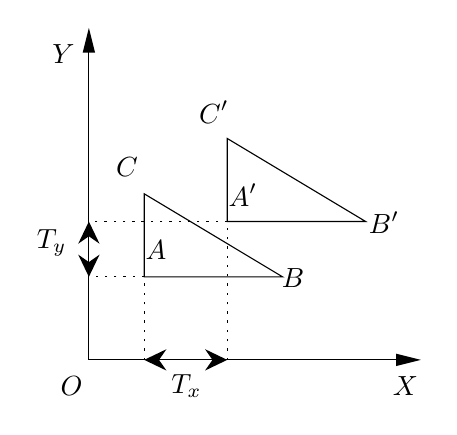
\begin{tikzpicture}[x=0.75pt,y=0.75pt,yscale=-1,xscale=1]
%uncomment if require: \path (0,310); %set diagram left start at 0, and has height of 310

%Straight Lines [id:da0744643818390529] 
\draw    (160,160) -- (160,133.33) -- (160,106.67) -- (160,80) -- (160,53.33) -- (160,26.67) -- (160,2) ;
\draw [shift={(160,0)}, rotate = 90] [fill={rgb, 255:red, 0; green, 0; blue, 0 }  ][line width=0.08]  [draw opacity=0] (12,-3) -- (0,0) -- (12,3) -- cycle    ;
%Straight Lines [id:da2501910192394292] 
\draw    (160,160) -- (186.67,160) -- (213.33,160) -- (240,160) -- (266.67,160) -- (293.33,160) -- (318,160) ;
\draw [shift={(320,160)}, rotate = 180] [fill={rgb, 255:red, 0; green, 0; blue, 0 }  ][line width=0.08]  [draw opacity=0] (12,-3) -- (0,0) -- (12,3) -- cycle    ;
%Shape: Right Triangle [id:dp3230440420217635] 
\draw   (186.67,80) -- (253.33,120) -- (186.67,120) -- cycle ;
%Straight Lines [id:da4274444095380905] 
\draw  [dash pattern={on 0.84pt off 2.51pt}]  (186.67,120) -- (160,120) ;
%Shape: Right Triangle [id:dp3554215710083837] 
\draw   (226.67,53.33) -- (293.33,93.33) -- (226.67,93.33) -- cycle ;
%Straight Lines [id:da18015886667211856] 
\draw  [dash pattern={on 0.84pt off 2.51pt}]  (226.67,93.33) -- (160,93.33) ;
%Straight Lines [id:da20825596809464475] 
\draw  [dash pattern={on 0.84pt off 2.51pt}]  (186.67,160) -- (186.67,137.12) -- (186.67,120) ;
%Straight Lines [id:da30415316219723487] 
\draw  [dash pattern={on 0.84pt off 2.51pt}]  (226.67,160) -- (226.67,93.33) ;
%Straight Lines [id:da18553363748469254] 
\draw    (189.67,160) -- (223.67,160) ;
\draw [shift={(226.67,160)}, rotate = 180] [fill={rgb, 255:red, 0; green, 0; blue, 0 }  ][line width=0.08]  [draw opacity=0] (10.72,-5.15) -- (0,0) -- (10.72,5.15) -- (7.12,0) -- cycle    ;
\draw [shift={(186.67,160)}, rotate = 0] [fill={rgb, 255:red, 0; green, 0; blue, 0 }  ][line width=0.08]  [draw opacity=0] (10.72,-5.15) -- (0,0) -- (10.72,5.15) -- (7.12,0) -- cycle    ;
%Straight Lines [id:da7758481926901326] 
\draw    (160,96.33) -- (160,117) ;
\draw [shift={(160,120)}, rotate = 270] [fill={rgb, 255:red, 0; green, 0; blue, 0 }  ][line width=0.08]  [draw opacity=0] (10.72,-5.15) -- (0,0) -- (10.72,5.15) -- (7.12,0) -- cycle    ;
\draw [shift={(160,93.33)}, rotate = 90] [fill={rgb, 255:red, 0; green, 0; blue, 0 }  ][line width=0.08]  [draw opacity=0] (10.72,-5.15) -- (0,0) -- (10.72,5.15) -- (7.12,0) -- cycle    ;

% Text Node
\draw (312.88,172.78) node   [align=left] {\begin{minipage}[lt]{9.68pt}\setlength\topsep{0pt}
$\displaystyle X$
\end{minipage}};
% Text Node
\draw (150.8,12.78) node   [align=left] {\begin{minipage}[lt]{12.51pt}\setlength\topsep{0pt}
$\displaystyle Y$
\end{minipage}};
% Text Node
\draw (152.88,172.78) node   [align=left] {\begin{minipage}[lt]{9.68pt}\setlength\topsep{0pt}
$\displaystyle O$
\end{minipage}};
% Text Node
\draw (193.79,107.22) node   [align=left] {\begin{minipage}[lt]{9.68pt}\setlength\topsep{0pt}
$\displaystyle A$
\end{minipage}};
% Text Node
\draw (233.79,80.55) node   [align=left] {\begin{minipage}[lt]{9.68pt}\setlength\topsep{0pt}
$\displaystyle A'$
\end{minipage}};
% Text Node
\draw (258.71,120.4) node   [align=left] {\begin{minipage}[lt]{8.67pt}\setlength\topsep{0pt}
$\displaystyle B$
\end{minipage}};
% Text Node
\draw (300.71,94) node   [align=left] {\begin{minipage}[lt]{8.67pt}\setlength\topsep{0pt}
$\displaystyle B'$
\end{minipage}};
% Text Node
\draw (179.55,67.22) node   [align=left] {\begin{minipage}[lt]{9.68pt}\setlength\topsep{0pt}
$\displaystyle C$
\end{minipage}};
% Text Node
\draw (219.55,40.55) node   [align=left] {\begin{minipage}[lt]{9.68pt}\setlength\topsep{0pt}
$\displaystyle C'$
\end{minipage}};
% Text Node
\draw (206.21,172.78) node   [align=left] {\begin{minipage}[lt]{9.68pt}\setlength\topsep{0pt}
$\displaystyle T_{x}$
\end{minipage}};
% Text Node
\draw (141.41,103.58) node   [align=left] {\begin{minipage}[lt]{9.68pt}\setlength\topsep{0pt}
$\displaystyle T_{y}$
\end{minipage}};


\end{tikzpicture}

    }
    \subfigure[scale=.9][比例系数 $S_x=S_y=1$]{
        

\tikzset{every picture/.style={line width=0.75pt}} %set default line width to 0.75pt        

\begin{tikzpicture}[x=0.75pt,y=0.75pt,yscale=-1,xscale=1]
%uncomment if require: \path (0,310); %set diagram left start at 0, and has height of 310

%Straight Lines [id:da15250042942435282] 
\draw    (160,160) -- (160,133.33) -- (160,106.67) -- (160,80) -- (160,53.33) -- (160,26.67) -- (160,2) ;
\draw [shift={(160,0)}, rotate = 90] [fill={rgb, 255:red, 0; green, 0; blue, 0 }  ][line width=0.08]  [draw opacity=0] (12,-3) -- (0,0) -- (12,3) -- cycle    ;
%Straight Lines [id:da8576603280236559] 
\draw    (160,160) -- (186.67,160) -- (213.33,160) -- (240,160) -- (266.67,160) -- (293.33,160) -- (318,160) ;
\draw [shift={(320,160)}, rotate = 180] [fill={rgb, 255:red, 0; green, 0; blue, 0 }  ][line width=0.08]  [draw opacity=0] (12,-3) -- (0,0) -- (12,3) -- cycle    ;
%Shape: Right Triangle [id:dp7502598031763401] 
\draw   (186.67,80) -- (253.33,120) -- (186.67,120) -- cycle ;

% Text Node
\draw (312.88,172.78) node   [align=left] {\begin{minipage}[lt]{9.68pt}\setlength\topsep{0pt}
$\displaystyle X$
\end{minipage}};
% Text Node
\draw (150.8,12.78) node   [align=left] {\begin{minipage}[lt]{12.51pt}\setlength\topsep{0pt}
$\displaystyle Y$
\end{minipage}};
% Text Node
\draw (152.88,172.78) node   [align=left] {\begin{minipage}[lt]{9.68pt}\setlength\topsep{0pt}
$\displaystyle O$
\end{minipage}};
% Text Node
\draw (178.21,107.22) node   [align=left] {\begin{minipage}[lt]{11.5pt}\setlength\topsep{0pt}
$\displaystyle A$
\end{minipage}};
% Text Node
\draw (193.79,107.22) node   [align=left] {\begin{minipage}[lt]{9.68pt}\setlength\topsep{0pt}
$\displaystyle A'$
\end{minipage}};
% Text Node
\draw (247.59,132.78) node   [align=left] {\begin{minipage}[lt]{8.67pt}\setlength\topsep{0pt}
$\displaystyle B$
\end{minipage}};
% Text Node
\draw (259.08,132.78) node   [align=left] {\begin{minipage}[lt]{8.67pt}\setlength\topsep{0pt}
$\displaystyle B'$
\end{minipage}};
% Text Node
\draw (179.55,67.22) node   [align=left] {\begin{minipage}[lt]{9.68pt}\setlength\topsep{0pt}
$\displaystyle C$
\end{minipage}};
% Text Node
\draw (193.79,67.22) node   [align=left] {\begin{minipage}[lt]{9.68pt}\setlength\topsep{0pt}
$\displaystyle C'$
\end{minipage}};


\end{tikzpicture}
    }
    \subfigure[scale=.9][比例系数 $S_x=S_y>1$]{
        

\tikzset{every picture/.style={line width=0.75pt}} %set default line width to 0.75pt        

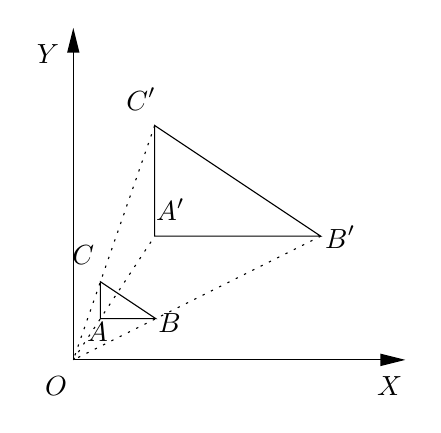
\begin{tikzpicture}[x=0.75pt,y=0.75pt,yscale=-1,xscale=1]
%uncomment if require: \path (0,310); %set diagram left start at 0, and has height of 310

%Straight Lines [id:da1534328502257163] 
\draw    (160,160) -- (160,133.33) -- (160,106.67) -- (160,80) -- (160,53.33) -- (160,26.67) -- (160,2) ;
\draw [shift={(160,0)}, rotate = 90] [fill={rgb, 255:red, 0; green, 0; blue, 0 }  ][line width=0.08]  [draw opacity=0] (12,-3) -- (0,0) -- (12,3) -- cycle    ;
%Straight Lines [id:da05091810398310703] 
\draw    (160,160) -- (186.67,160) -- (213.33,160) -- (240,160) -- (266.67,160) -- (293.33,160) -- (318,160) ;
\draw [shift={(320,160)}, rotate = 180] [fill={rgb, 255:red, 0; green, 0; blue, 0 }  ][line width=0.08]  [draw opacity=0] (12,-3) -- (0,0) -- (12,3) -- cycle    ;
%Shape: Right Triangle [id:dp7699621838177173] 
\draw   (199.2,47.07) -- (279.2,100.4) -- (199.2,100.4) -- cycle ;
%Shape: Right Triangle [id:dp6819256437414682] 
\draw   (173.07,122.36) -- (199.73,140.13) -- (173.07,140.13) -- cycle ;
%Straight Lines [id:da5214539639167379] 
\draw  [dash pattern={on 0.84pt off 2.51pt}]  (199.2,47.07) -- (192.67,65.89) -- (186.13,84.71) -- (179.6,103.53) -- (173.07,122.36) -- (166.53,141.18) -- (160,160) ;
%Straight Lines [id:da8425910163250174] 
\draw  [dash pattern={on 0.84pt off 2.51pt}]  (279.2,100.4) -- (259.33,110.33) -- (239.47,120.27) -- (219.6,130.2) -- (199.73,140.13) -- (179.87,150.07) -- (160,160) ;
%Straight Lines [id:da47875893336700104] 
\draw  [dash pattern={on 0.84pt off 2.51pt}]  (160,160) -- (199.2,100.4) ;

% Text Node
\draw (312.88,172.78) node   [align=left] {\begin{minipage}[lt]{9.68pt}\setlength\topsep{0pt}
$\displaystyle X$
\end{minipage}};
% Text Node
\draw (150.8,12.78) node   [align=left] {\begin{minipage}[lt]{12.51pt}\setlength\topsep{0pt}
$\displaystyle Y$
\end{minipage}};
% Text Node
\draw (152.88,172.78) node   [align=left] {\begin{minipage}[lt]{9.68pt}\setlength\topsep{0pt}
$\displaystyle O$
\end{minipage}};
% Text Node
\draw (173.12,146.42) node   [align=left] {\begin{minipage}[lt]{9.68pt}\setlength\topsep{0pt}
$\displaystyle A$
\end{minipage}};
% Text Node
\draw (206.32,87.62) node   [align=left] {\begin{minipage}[lt]{9.68pt}\setlength\topsep{0pt}
$\displaystyle A'$
\end{minipage}};
% Text Node
\draw (206.71,142.4) node   [align=left] {\begin{minipage}[lt]{8.67pt}\setlength\topsep{0pt}
$\displaystyle B$
\end{minipage}};
% Text Node
\draw (287.11,100.8) node   [align=left] {\begin{minipage}[lt]{8.67pt}\setlength\topsep{0pt}
$\displaystyle B'$
\end{minipage}};
% Text Node
\draw (165.95,109.58) node   [align=left] {\begin{minipage}[lt]{9.68pt}\setlength\topsep{0pt}
$\displaystyle C$
\end{minipage}};
% Text Node
\draw (192.08,34.29) node   [align=left] {\begin{minipage}[lt]{9.68pt}\setlength\topsep{0pt}
$\displaystyle C'$
\end{minipage}};


\end{tikzpicture}

    }
    \subfigure[scale=.9][比例系数 $0<S_x=S_y<1$]{
        

\tikzset{every picture/.style={line width=0.75pt}} %set default line width to 0.75pt        

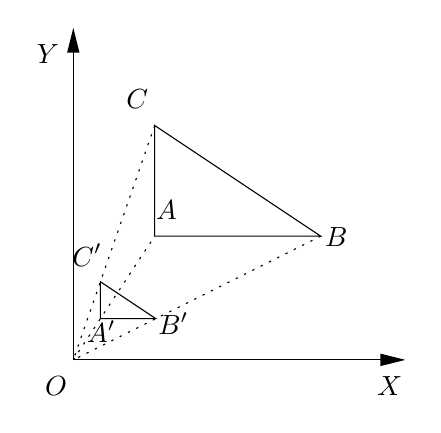
\begin{tikzpicture}[x=0.75pt,y=0.75pt,yscale=-1,xscale=1]
%uncomment if require: \path (0,310); %set diagram left start at 0, and has height of 310

%Straight Lines [id:da9243963150205441] 
\draw    (160,160) -- (160,133.33) -- (160,106.67) -- (160,80) -- (160,53.33) -- (160,26.67) -- (160,2) ;
\draw [shift={(160,0)}, rotate = 90] [fill={rgb, 255:red, 0; green, 0; blue, 0 }  ][line width=0.08]  [draw opacity=0] (12,-3) -- (0,0) -- (12,3) -- cycle    ;
%Straight Lines [id:da8002028753633985] 
\draw    (160,160) -- (186.67,160) -- (213.33,160) -- (240,160) -- (266.67,160) -- (293.33,160) -- (318,160) ;
\draw [shift={(320,160)}, rotate = 180] [fill={rgb, 255:red, 0; green, 0; blue, 0 }  ][line width=0.08]  [draw opacity=0] (12,-3) -- (0,0) -- (12,3) -- cycle    ;
%Shape: Right Triangle [id:dp3074265042318134] 
\draw   (199.2,47.07) -- (279.2,100.4) -- (199.2,100.4) -- cycle ;
%Shape: Right Triangle [id:dp29770002438414234] 
\draw   (173.07,122.36) -- (199.73,140.13) -- (173.07,140.13) -- cycle ;
%Straight Lines [id:da024412753399659648] 
\draw  [dash pattern={on 0.84pt off 2.51pt}]  (199.2,47.07) -- (192.67,65.89) -- (186.13,84.71) -- (179.6,103.53) -- (173.07,122.36) -- (166.53,141.18) -- (160,160) ;
%Straight Lines [id:da7095636127854406] 
\draw  [dash pattern={on 0.84pt off 2.51pt}]  (279.2,100.4) -- (259.33,110.33) -- (239.47,120.27) -- (219.6,130.2) -- (199.73,140.13) -- (179.87,150.07) -- (160,160) ;
%Straight Lines [id:da5652492210181941] 
\draw  [dash pattern={on 0.84pt off 2.51pt}]  (160,160) -- (199.2,100.4) ;

% Text Node
\draw (312.88,172.78) node   [align=left] {\begin{minipage}[lt]{9.68pt}\setlength\topsep{0pt}
$\displaystyle X$
\end{minipage}};
% Text Node
\draw (150.8,12.78) node   [align=left] {\begin{minipage}[lt]{12.51pt}\setlength\topsep{0pt}
$\displaystyle Y$
\end{minipage}};
% Text Node
\draw (152.88,172.78) node   [align=left] {\begin{minipage}[lt]{9.68pt}\setlength\topsep{0pt}
$\displaystyle O$
\end{minipage}};
% Text Node
\draw (173.12,146.42) node   [align=left] {\begin{minipage}[lt]{9.68pt}\setlength\topsep{0pt}
$\displaystyle A'$
\end{minipage}};
% Text Node
\draw (206.32,87.62) node   [align=left] {\begin{minipage}[lt]{9.68pt}\setlength\topsep{0pt}
$\displaystyle A$
\end{minipage}};
% Text Node
\draw (206.71,142.4) node   [align=left] {\begin{minipage}[lt]{8.67pt}\setlength\topsep{0pt}
$\displaystyle B'$
\end{minipage}};
% Text Node
\draw (287.11,100.8) node   [align=left] {\begin{minipage}[lt]{8.67pt}\setlength\topsep{0pt}
$\displaystyle B$
\end{minipage}};
% Text Node
\draw (165.95,109.58) node   [align=left] {\begin{minipage}[lt]{9.68pt}\setlength\topsep{0pt}
$\displaystyle C'$
\end{minipage}};
% Text Node
\draw (192.08,34.29) node   [align=left] {\begin{minipage}[lt]{9.68pt}\setlength\topsep{0pt}
$\displaystyle C$
\end{minipage}};


\end{tikzpicture}

    }
    \subfigure[scale=.9][$S_x=1,~S_y>1$]{
        

\tikzset{every picture/.style={line width=0.75pt}} %set default line width to 0.75pt        

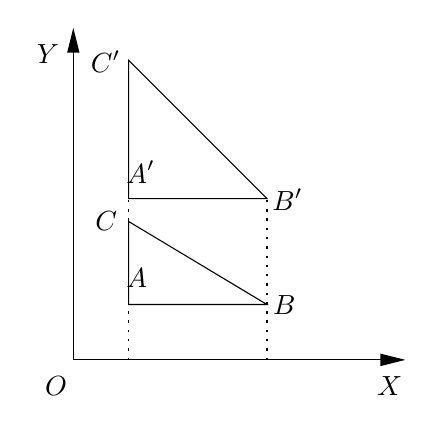
\begin{tikzpicture}[x=0.75pt,y=0.75pt,yscale=-1,xscale=1]
%uncomment if require: \path (0,310); %set diagram left start at 0, and has height of 310

%Straight Lines [id:da8557514491265967] 
\draw    (160,160) -- (160,133.33) -- (160,106.67) -- (160,80) -- (160,53.33) -- (160,26.67) -- (160,2) ;
\draw [shift={(160,0)}, rotate = 90] [fill={rgb, 255:red, 0; green, 0; blue, 0 }  ][line width=0.08]  [draw opacity=0] (12,-3) -- (0,0) -- (12,3) -- cycle    ;
%Straight Lines [id:da5539450143531788] 
\draw    (160,160) -- (186.67,160) -- (213.33,160) -- (240,160) -- (266.67,160) -- (293.33,160) -- (318,160) ;
\draw [shift={(320,160)}, rotate = 180] [fill={rgb, 255:red, 0; green, 0; blue, 0 }  ][line width=0.08]  [draw opacity=0] (12,-3) -- (0,0) -- (12,3) -- cycle    ;
%Straight Lines [id:da5193682179432797] 
\draw  [dash pattern={on 0.84pt off 2.51pt}]  (186.67,160) -- (186.67,82.33) ;
%Shape: Right Triangle [id:dp8688230494789257] 
\draw   (186.67,93.33) -- (253.33,133.33) -- (186.67,133.33) -- cycle ;
%Shape: Right Triangle [id:dp373344497154698] 
\draw   (186.67,15.67) -- (253.33,82.33) -- (186.67,82.33) -- cycle ;
%Straight Lines [id:da7747623883965025] 
\draw  [dash pattern={on 0.84pt off 2.51pt}]  (253.33,160) -- (253.33,82.33) ;

% Text Node
\draw (312.88,172.78) node   [align=left] {\begin{minipage}[lt]{9.68pt}\setlength\topsep{0pt}
$\displaystyle X$
\end{minipage}};
% Text Node
\draw (150.8,12.78) node   [align=left] {\begin{minipage}[lt]{12.51pt}\setlength\topsep{0pt}
$\displaystyle Y$
\end{minipage}};
% Text Node
\draw (152.88,172.78) node   [align=left] {\begin{minipage}[lt]{9.68pt}\setlength\topsep{0pt}
$\displaystyle O$
\end{minipage}};
% Text Node
\draw (191.4,69.55) node   [align=left] {\begin{minipage}[lt]{8.67pt}\setlength\topsep{0pt}
$\displaystyle A'$
\end{minipage}};
% Text Node
\draw (191.4,120.55) node   [align=left] {\begin{minipage}[lt]{8.67pt}\setlength\topsep{0pt}
$\displaystyle A$
\end{minipage}};
% Text Node
\draw (261.71,82.73) node   [align=left] {\begin{minipage}[lt]{8.67pt}\setlength\topsep{0pt}
$\displaystyle B'$
\end{minipage}};
% Text Node
\draw (262.11,133.47) node   [align=left] {\begin{minipage}[lt]{8.67pt}\setlength\topsep{0pt}
$\displaystyle B$
\end{minipage}};
% Text Node
\draw (174.95,16.24) node   [align=left] {\begin{minipage}[lt]{9.68pt}\setlength\topsep{0pt}
$\displaystyle C'$
\end{minipage}};
% Text Node
\draw (177.08,92.95) node   [align=left] {\begin{minipage}[lt]{9.68pt}\setlength\topsep{0pt}
$\displaystyle C$
\end{minipage}};


\end{tikzpicture}

    }
    \subfigure[scale=.9][$Y$ 轴对称]{
        

\tikzset{every picture/.style={line width=0.75pt}} %set default line width to 0.75pt        

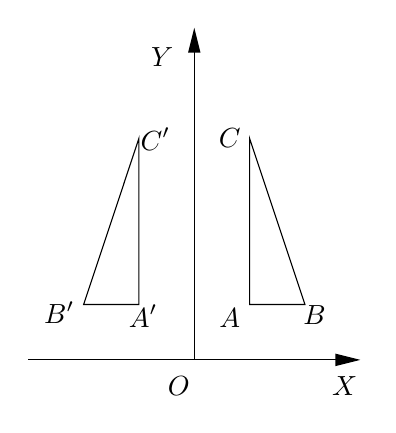
\begin{tikzpicture}[x=0.75pt,y=0.75pt,yscale=-1,xscale=1]
%uncomment if require: \path (0,310); %set diagram left start at 0, and has height of 310

%Straight Lines [id:da9473706495657213] 
\draw    (240,160) -- (240,133.33) -- (240,106.67) -- (240,80) -- (240,53.33) -- (240,26.67) -- (240,2) ;
\draw [shift={(240,0)}, rotate = 90] [fill={rgb, 255:red, 0; green, 0; blue, 0 }  ][line width=0.08]  [draw opacity=0] (12,-3) -- (0,0) -- (12,3) -- cycle    ;
%Straight Lines [id:da3401945044692589] 
\draw    (160,160) -- (186.67,160) -- (213.33,160) -- (240,160) -- (266.67,160) -- (293.33,160) -- (318,160) ;
\draw [shift={(320,160)}, rotate = 180] [fill={rgb, 255:red, 0; green, 0; blue, 0 }  ][line width=0.08]  [draw opacity=0] (12,-3) -- (0,0) -- (12,3) -- cycle    ;
%Shape: Right Triangle [id:dp2883900535142023] 
\draw   (266.67,53.33) -- (293.33,133.33) -- (266.67,133.33) -- cycle ;
%Shape: Right Triangle [id:dp0361672463144318] 
\draw   (213.33,53.33) -- (186.67,133.33) -- (213.33,133.33) -- cycle ;

% Text Node
\draw (312.88,172.78) node   [align=left] {\begin{minipage}[lt]{9.68pt}\setlength\topsep{0pt}
$\displaystyle X$
\end{minipage}};
% Text Node
\draw (227.6,13.98) node   [align=left] {\begin{minipage}[lt]{12.51pt}\setlength\topsep{0pt}
$\displaystyle Y$
\end{minipage}};
% Text Node
\draw (233.79,172.78) node   [align=left] {\begin{minipage}[lt]{9.68pt}\setlength\topsep{0pt}
$\displaystyle O$
\end{minipage}};
% Text Node
\draw (259.81,139.62) node   [align=left] {\begin{minipage}[lt]{11.5pt}\setlength\topsep{0pt}
$\displaystyle A$
\end{minipage}};
% Text Node
\draw (214.99,138.82) node   [align=left] {\begin{minipage}[lt]{9.68pt}\setlength\topsep{0pt}
$\displaystyle A'$
\end{minipage}};
% Text Node
\draw (298.39,138.38) node   [align=left] {\begin{minipage}[lt]{8.67pt}\setlength\topsep{0pt}
$\displaystyle B$
\end{minipage}};
% Text Node
\draw (173.48,137.18) node   [align=left] {\begin{minipage}[lt]{8.67pt}\setlength\topsep{0pt}
$\displaystyle B'$
\end{minipage}};
% Text Node
\draw (258.35,53.22) node   [align=left] {\begin{minipage}[lt]{9.68pt}\setlength\topsep{0pt}
$\displaystyle C$
\end{minipage}};
% Text Node
\draw (220.59,53.62) node   [align=left] {\begin{minipage}[lt]{9.68pt}\setlength\topsep{0pt}
$\displaystyle C'$
\end{minipage}};


\end{tikzpicture}

    }
    \subfigure[scale=.9][$X$ 轴对称]{
        

\tikzset{every picture/.style={line width=0.75pt}} %set default line width to 0.75pt        

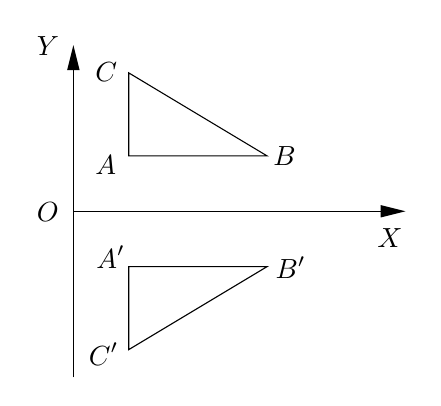
\begin{tikzpicture}[x=0.75pt,y=0.75pt,yscale=-1,xscale=1]
%uncomment if require: \path (0,310); %set diagram left start at 0, and has height of 310

%Straight Lines [id:da24368355678437692] 
\draw    (160,240) -- (160,213.33) -- (160,186.67) -- (160,160) -- (160,133.33) -- (160,106.67) -- (160,82) ;
\draw [shift={(160,80)}, rotate = 90] [fill={rgb, 255:red, 0; green, 0; blue, 0 }  ][line width=0.08]  [draw opacity=0] (12,-3) -- (0,0) -- (12,3) -- cycle    ;
%Straight Lines [id:da91989606623083] 
\draw    (160,160) -- (186.67,160) -- (213.33,160) -- (240,160) -- (266.67,160) -- (293.33,160) -- (318,160) ;
\draw [shift={(320,160)}, rotate = 180] [fill={rgb, 255:red, 0; green, 0; blue, 0 }  ][line width=0.08]  [draw opacity=0] (12,-3) -- (0,0) -- (12,3) -- cycle    ;
%Shape: Right Triangle [id:dp6047665119381709] 
\draw   (186.67,93.33) -- (253.33,133.33) -- (186.67,133.33) -- cycle ;
%Shape: Right Triangle [id:dp2085112249426042] 
\draw   (186.67,226.67) -- (253.33,186.67) -- (186.67,186.67) -- cycle ;

% Text Node
\draw (312.88,172.78) node   [align=left] {\begin{minipage}[lt]{9.68pt}\setlength\topsep{0pt}
$\displaystyle X$
\end{minipage}};
% Text Node
\draw (150.8,80.55) node   [align=left] {\begin{minipage}[lt]{12.51pt}\setlength\topsep{0pt}
$\displaystyle Y$
\end{minipage}};
% Text Node
\draw (148.88,160.28) node   [align=left] {\begin{minipage}[lt]{9.68pt}\setlength\topsep{0pt}
$\displaystyle O$
\end{minipage}};
% Text Node
\draw (176.9,182.05) node   [align=left] {\begin{minipage}[lt]{8.67pt}\setlength\topsep{0pt}
$\displaystyle A'$
\end{minipage}};
% Text Node
\draw (176.4,137.55) node   [align=left] {\begin{minipage}[lt]{8.67pt}\setlength\topsep{0pt}
$\displaystyle A$
\end{minipage}};
% Text Node
\draw (263.21,187.23) node   [align=left] {\begin{minipage}[lt]{8.67pt}\setlength\topsep{0pt}
$\displaystyle B'$
\end{minipage}};
% Text Node
\draw (262.11,133.47) node   [align=left] {\begin{minipage}[lt]{8.67pt}\setlength\topsep{0pt}
$\displaystyle B$
\end{minipage}};
% Text Node
\draw (173.95,228.74) node   [align=left] {\begin{minipage}[lt]{9.68pt}\setlength\topsep{0pt}
$\displaystyle C'$
\end{minipage}};
% Text Node
\draw (177.08,92.95) node   [align=left] {\begin{minipage}[lt]{9.68pt}\setlength\topsep{0pt}
$\displaystyle C$
\end{minipage}};


\end{tikzpicture}

    }
    \subfigure[scale=.9][中心对称]{
        

\tikzset{every picture/.style={line width=0.75pt}} %set default line width to 0.75pt        

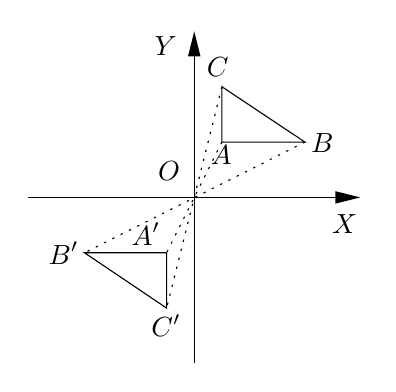
\begin{tikzpicture}[x=0.75pt,y=0.75pt,yscale=-1,xscale=1]
%uncomment if require: \path (0,310); %set diagram left start at 0, and has height of 310

%Straight Lines [id:da20466553477334037] 
\draw    (240,240) -- (240,213.33) -- (240,186.67) -- (240,160) -- (240,133.33) -- (240,106.67) -- (240,82) ;
\draw [shift={(240,80)}, rotate = 90] [fill={rgb, 255:red, 0; green, 0; blue, 0 }  ][line width=0.08]  [draw opacity=0] (12,-3) -- (0,0) -- (12,3) -- cycle    ;
%Straight Lines [id:da07906371106904819] 
\draw    (160,160) -- (186.67,160) -- (213.33,160) -- (240,160) -- (266.67,160) -- (293.33,160) -- (318,160) ;
\draw [shift={(320,160)}, rotate = 180] [fill={rgb, 255:red, 0; green, 0; blue, 0 }  ][line width=0.08]  [draw opacity=0] (12,-3) -- (0,0) -- (12,3) -- cycle    ;
%Shape: Right Triangle [id:dp711098921084359] 
\draw   (253.33,106.67) -- (293.33,133.33) -- (253.33,133.33) -- cycle ;
%Shape: Right Triangle [id:dp32855978989430157] 
\draw   (226.67,213.33) -- (187.13,186.67) -- (226.67,186.67) -- cycle ;
%Straight Lines [id:da813083554485903] 
\draw  [dash pattern={on 0.84pt off 2.51pt}]  (253.33,133.33) -- (226.67,186.67) ;
%Straight Lines [id:da3857126514317757] 
\draw  [dash pattern={on 0.84pt off 2.51pt}]  (293.33,133.33) -- (187.13,186.67) ;
%Straight Lines [id:da811525310685079] 
\draw  [dash pattern={on 0.84pt off 2.51pt}]  (253.33,106.67) -- (226.67,213.33) ;

% Text Node
\draw (312.88,172.78) node   [align=left] {\begin{minipage}[lt]{9.68pt}\setlength\topsep{0pt}
$\displaystyle X$
\end{minipage}};
% Text Node
\draw (229.2,87.22) node   [align=left] {\begin{minipage}[lt]{12.51pt}\setlength\topsep{0pt}
$\displaystyle Y$
\end{minipage}};
% Text Node
\draw (230.85,147.22) node   [align=left] {\begin{minipage}[lt]{12.44pt}\setlength\topsep{0pt}
$\displaystyle O$
\end{minipage}};
% Text Node
\draw (255.71,139.72) node   [align=left] {\begin{minipage}[lt]{11.5pt}\setlength\topsep{0pt}
$\displaystyle A$
\end{minipage}};
% Text Node
\draw (216.29,177.72) node   [align=left] {\begin{minipage}[lt]{9.68pt}\setlength\topsep{0pt}
$\displaystyle A'$
\end{minipage}};
% Text Node
\draw (302.09,133.78) node   [align=left] {\begin{minipage}[lt]{8.67pt}\setlength\topsep{0pt}
$\displaystyle B$
\end{minipage}};
% Text Node
\draw (175.58,186.78) node   [align=left] {\begin{minipage}[lt]{8.67pt}\setlength\topsep{0pt}
$\displaystyle B'$
\end{minipage}};
% Text Node
\draw (252.55,97.22) node   [align=left] {\begin{minipage}[lt]{9.68pt}\setlength\topsep{0pt}
$\displaystyle C$
\end{minipage}};
% Text Node
\draw (225.79,221.72) node   [align=left] {\begin{minipage}[lt]{9.68pt}\setlength\topsep{0pt}
$\displaystyle C'$
\end{minipage}};


\end{tikzpicture}

    }
    \subfigure[scale=.9][$Y=X$ 对称]{
        

\tikzset{every picture/.style={line width=0.75pt}} %set default line width to 0.75pt        

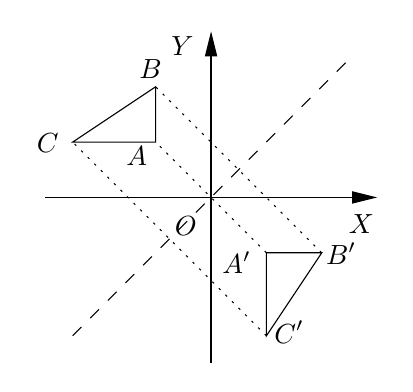
\begin{tikzpicture}[x=0.75pt,y=0.75pt,yscale=-1,xscale=1]
%uncomment if require: \path (0,310); %set diagram left start at 0, and has height of 310

%Straight Lines [id:da8292659722722793] 
\draw    (240,240) -- (240,213.33) -- (240,186.67) -- (240,160) -- (240,133.33) -- (240,106.67) -- (240,82) ;
\draw [shift={(240,80)}, rotate = 90] [fill={rgb, 255:red, 0; green, 0; blue, 0 }  ][line width=0.08]  [draw opacity=0] (12,-3) -- (0,0) -- (12,3) -- cycle    ;
%Straight Lines [id:da7352149228464684] 
\draw    (160,160) -- (186.67,160) -- (213.33,160) -- (240,160) -- (266.67,160) -- (293.33,160) -- (318,160) ;
\draw [shift={(320,160)}, rotate = 180] [fill={rgb, 255:red, 0; green, 0; blue, 0 }  ][line width=0.08]  [draw opacity=0] (12,-3) -- (0,0) -- (12,3) -- cycle    ;
%Straight Lines [id:da2661475178458712] 
\draw  [dash pattern={on 0.84pt off 2.51pt}]  (266.67,186.67) -- (213.33,133.33) ;
%Shape: Right Triangle [id:dp6596390866394817] 
\draw   (213.33,106.67) -- (173.33,133.33) -- (213.33,133.33) -- cycle ;
%Straight Lines [id:da7951069745564614] 
\draw  [dash pattern={on 4.5pt off 4.5pt}]  (173.33,226.67) -- (306.67,93.33) ;
%Shape: Right Triangle [id:dp32508442712015806] 
\draw   (266.67,226.67) -- (293.33,186.67) -- (266.67,186.67) -- cycle ;
%Straight Lines [id:da9943714913243453] 
\draw  [dash pattern={on 0.84pt off 2.51pt}]  (293.33,186.67) -- (213.33,106.67) ;
%Straight Lines [id:da42142200377858186] 
\draw  [dash pattern={on 0.84pt off 2.51pt}]  (266.67,226.67) -- (173.33,133.33) ;

% Text Node
\draw (312.88,172.78) node   [align=left] {\begin{minipage}[lt]{9.68pt}\setlength\topsep{0pt}
$\displaystyle X$
\end{minipage}};
% Text Node
\draw (229.2,87.22) node   [align=left] {\begin{minipage}[lt]{12.51pt}\setlength\topsep{0pt}
$\displaystyle Y$
\end{minipage}};
% Text Node
\draw (230.85,173.89) node   [align=left] {\begin{minipage}[lt]{12.44pt}\setlength\topsep{0pt}
$\displaystyle O$
\end{minipage}};
% Text Node
\draw (206.91,140.12) node   [align=left] {\begin{minipage}[lt]{11.5pt}\setlength\topsep{0pt}
$\displaystyle A$
\end{minipage}};
% Text Node
\draw (251.89,191.32) node   [align=left] {\begin{minipage}[lt]{9.68pt}\setlength\topsep{0pt}
$\displaystyle A'$
\end{minipage}};
% Text Node
\draw (211.29,98.18) node   [align=left] {\begin{minipage}[lt]{8.67pt}\setlength\topsep{0pt}
$\displaystyle B$
\end{minipage}};
% Text Node
\draw (301.18,187.18) node   [align=left] {\begin{minipage}[lt]{8.67pt}\setlength\topsep{0pt}
$\displaystyle B'$
\end{minipage}};
% Text Node
\draw (162.55,134.02) node   [align=left] {\begin{minipage}[lt]{9.68pt}\setlength\topsep{0pt}
$\displaystyle C$
\end{minipage}};
% Text Node
\draw (276.99,224.92) node   [align=left] {\begin{minipage}[lt]{9.68pt}\setlength\topsep{0pt}
$\displaystyle C'$
\end{minipage}};


\end{tikzpicture}

    }
    \subfigure[scale=.9][$Y=-X$ 对称]{
        

\tikzset{every picture/.style={line width=0.75pt}} %set default line width to 0.75pt        

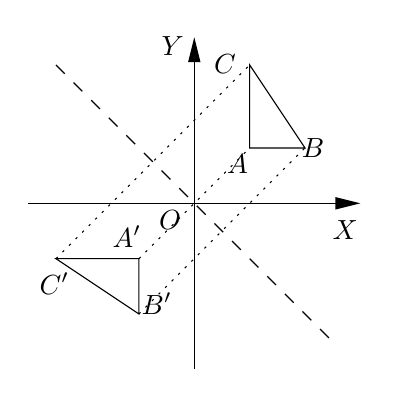
\begin{tikzpicture}[x=0.75pt,y=0.75pt,yscale=-1,xscale=1]
%uncomment if require: \path (0,310); %set diagram left start at 0, and has height of 310

%Straight Lines [id:da2266867895070097] 
\draw    (155.13,159.59) -- (181.8,159.59) -- (208.47,159.59) -- (235.13,159.59) -- (261.8,159.59) -- (288.47,159.59) -- (313.13,159.59) ;
\draw [shift={(315.13,159.59)}, rotate = 180] [fill={rgb, 255:red, 0; green, 0; blue, 0 }  ][line width=0.08]  [draw opacity=0] (12,-3) -- (0,0) -- (12,3) -- cycle    ;
%Straight Lines [id:da4885018729597703] 
\draw    (235.13,81.59) -- (235.13,106.25) -- (235.13,132.92) -- (235.13,159.59) -- (235.13,186.25) -- (235.13,212.92) -- (235.13,239.59) ;
\draw [shift={(235.13,79.59)}, rotate = 90] [fill={rgb, 255:red, 0; green, 0; blue, 0 }  ][line width=0.08]  [draw opacity=0] (12,-3) -- (0,0) -- (12,3) -- cycle    ;
%Straight Lines [id:da37798418466605876] 
\draw  [dash pattern={on 0.84pt off 2.51pt}]  (208.47,186.25) -- (261.8,132.92) ;
%Shape: Right Triangle [id:dp9937709437984665] 
\draw   (288.47,132.92) -- (261.8,92.92) -- (261.8,132.92) -- cycle ;
%Straight Lines [id:da8376057486917463] 
\draw  [dash pattern={on 4.5pt off 4.5pt}]  (168.47,92.92) -- (301.8,226.25) ;
%Shape: Right Triangle [id:dp15886819391939877] 
\draw   (168.47,186.25) -- (208.47,212.92) -- (208.47,186.25) -- cycle ;
%Straight Lines [id:da8724202073941834] 
\draw  [dash pattern={on 0.84pt off 2.51pt}]  (208.47,212.92) -- (288.47,132.92) ;
%Straight Lines [id:da8687627509248148] 
\draw  [dash pattern={on 0.84pt off 2.51pt}]  (168.47,186.25) -- (261.8,92.92) ;

% Text Node
\draw (307.55,172.37) node   [align=left] {\begin{minipage}[lt]{8.67pt}\setlength\topsep{0pt}
$\displaystyle X$
\end{minipage}};
% Text Node
\draw (225.15,83.97) node   [align=left] {\begin{minipage}[lt]{8.67pt}\setlength\topsep{0pt}
$\displaystyle Y$
\end{minipage}};
% Text Node
\draw (223.95,167.57) node   [align=left] {\begin{minipage}[lt]{8.67pt}\setlength\topsep{0pt}
$\displaystyle O$
\end{minipage}};
% Text Node
\draw (256.75,140.77) node   [align=left] {\begin{minipage}[lt]{8.67pt}\setlength\topsep{0pt}
$\displaystyle A$
\end{minipage}};
% Text Node
\draw (201.55,175.57) node   [align=left] {\begin{minipage}[lt]{8.67pt}\setlength\topsep{0pt}
$\displaystyle A'$
\end{minipage}};
% Text Node
\draw (292.75,133.17) node   [align=left] {\begin{minipage}[lt]{8.67pt}\setlength\topsep{0pt}
$\displaystyle B$
\end{minipage}};
% Text Node
\draw (250.45,92.54) node   [align=left] {\begin{minipage}[lt]{8.67pt}\setlength\topsep{0pt}
$\displaystyle C$
\end{minipage}};
% Text Node
\draw (215.55,207.97) node   [align=left] {\begin{minipage}[lt]{8.67pt}\setlength\topsep{0pt}
$\displaystyle B'$
\end{minipage}};
% Text Node
\draw (166.35,198.37) node   [align=left] {\begin{minipage}[lt]{8.67pt}\setlength\topsep{0pt}
$\displaystyle C'$
\end{minipage}};


\end{tikzpicture}

    }
    \subfigure[scale=.9][相对原点旋转 $\theta$ 角]{
        

\tikzset{every picture/.style={line width=0.75pt}} %set default line width to 0.75pt        

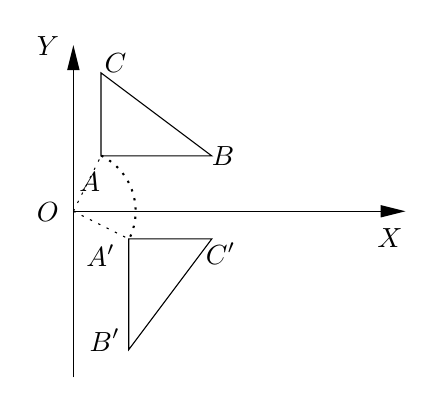
\begin{tikzpicture}[x=0.75pt,y=0.75pt,yscale=-1,xscale=1]
%uncomment if require: \path (0,310); %set diagram left start at 0, and has height of 310

%Straight Lines [id:da713951749740587] 
\draw    (160,240) -- (160,213.33) -- (160,186.67) -- (160,160) -- (160,133.33) -- (160,106.67) -- (160,82) ;
\draw [shift={(160,80)}, rotate = 90] [fill={rgb, 255:red, 0; green, 0; blue, 0 }  ][line width=0.08]  [draw opacity=0] (12,-3) -- (0,0) -- (12,3) -- cycle    ;
%Straight Lines [id:da27505852441502276] 
\draw    (160,160) -- (186.67,160) -- (213.33,160) -- (240,160) -- (266.67,160) -- (293.33,160) -- (318,160) ;
\draw [shift={(320,160)}, rotate = 180] [fill={rgb, 255:red, 0; green, 0; blue, 0 }  ][line width=0.08]  [draw opacity=0] (12,-3) -- (0,0) -- (12,3) -- cycle    ;
%Shape: Right Triangle [id:dp9653910433627337] 
\draw   (173.33,93.33) -- (226.67,133.33) -- (173.33,133.33) -- cycle ;
%Shape: Right Triangle [id:dp19153562200662932] 
\draw   (226.67,173.33) -- (186.67,226.67) -- (186.67,173.33) -- cycle ;
%Straight Lines [id:da6181416799790123] 
\draw  [dash pattern={on 0.84pt off 2.51pt}]  (160,160) -- (173.33,133.33) ;
%Straight Lines [id:da34341147568550356] 
\draw  [dash pattern={on 0.84pt off 2.51pt}]  (160,160) -- (186.67,173.33) ;
%Shape: Arc [id:dp3703274603787783] 
\draw  [draw opacity=0][dash pattern={on 0.84pt off 2.51pt}][line width=0.75]  (173.45,133.18) .. controls (183.26,138.11) and (190,148.27) .. (190,160) .. controls (190,164.85) and (188.85,169.43) .. (186.81,173.48) -- (160,160) -- cycle ; \draw  [dash pattern={on 0.84pt off 2.51pt}][line width=0.75]  (173.45,133.18) .. controls (183.26,138.11) and (190,148.27) .. (190,160) .. controls (190,164.85) and (188.85,169.43) .. (186.81,173.48) ;  

% Text Node
\draw (312.88,172.78) node   [align=left] {\begin{minipage}[lt]{9.68pt}\setlength\topsep{0pt}
$\displaystyle X$
\end{minipage}};
% Text Node
\draw (150.8,80.55) node   [align=left] {\begin{minipage}[lt]{12.51pt}\setlength\topsep{0pt}
$\displaystyle Y$
\end{minipage}};
% Text Node
\draw (148.88,160.28) node   [align=left] {\begin{minipage}[lt]{9.68pt}\setlength\topsep{0pt}
$\displaystyle O$
\end{minipage}};
% Text Node
\draw (172.1,181.25) node   [align=left] {\begin{minipage}[lt]{8.67pt}\setlength\topsep{0pt}
$\displaystyle A'$
\end{minipage}};
% Text Node
\draw (168.72,145.96) node   [align=left] {\begin{minipage}[lt]{8.67pt}\setlength\topsep{0pt}
$\displaystyle A$
\end{minipage}};
% Text Node
\draw (173.61,222.03) node   [align=left] {\begin{minipage}[lt]{8.67pt}\setlength\topsep{0pt}
$\displaystyle B'$
\end{minipage}};
% Text Node
\draw (232.51,133.47) node   [align=left] {\begin{minipage}[lt]{8.67pt}\setlength\topsep{0pt}
$\displaystyle B$
\end{minipage}};
% Text Node
\draw (230.35,180.34) node   [align=left] {\begin{minipage}[lt]{9.68pt}\setlength\topsep{0pt}
$\displaystyle C'$
\end{minipage}};
% Text Node
\draw (181.48,88.55) node   [align=left] {\begin{minipage}[lt]{9.68pt}\setlength\topsep{0pt}
$\displaystyle C$
\end{minipage}};


\end{tikzpicture}

    }
    \subfigure[scale=.9][$X$ 方向错切]{
        

\tikzset{every picture/.style={line width=0.75pt}} %set default line width to 0.75pt        

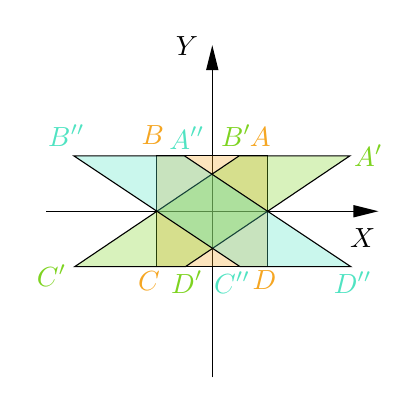
\begin{tikzpicture}[x=0.75pt,y=0.75pt,yscale=-1,xscale=1]
%uncomment if require: \path (0,310); %set diagram left start at 0, and has height of 310

%Straight Lines [id:da258215525060401] 
\draw    (240,240) -- (240,213.33) -- (240,186.67) -- (240,160) -- (240,133.33) -- (240,106.67) -- (240,82) ;
\draw [shift={(240,80)}, rotate = 90] [fill={rgb, 255:red, 0; green, 0; blue, 0 }  ][line width=0.08]  [draw opacity=0] (12,-3) -- (0,0) -- (12,3) -- cycle    ;
%Straight Lines [id:da058671601265665174] 
\draw    (160,160) -- (186.67,160) -- (213.33,160) -- (240,160) -- (266.67,160) -- (293.33,160) -- (318,160) ;
\draw [shift={(320,160)}, rotate = 180] [fill={rgb, 255:red, 0; green, 0; blue, 0 }  ][line width=0.08]  [draw opacity=0] (12,-3) -- (0,0) -- (12,3) -- cycle    ;
%Shape: Rectangle [id:dp4811001215484525] 
\draw  [fill={rgb, 255:red, 245; green, 166; blue, 35 }  ,fill opacity=0.3 ] (213.33,133.33) -- (266.67,133.33) -- (266.67,186.67) -- (213.33,186.67) -- cycle ;
%Shape: Rectangle [id:dp8297367285498773] 
\draw  [fill={rgb, 255:red, 126; green, 211; blue, 33 }  ,fill opacity=0.3 ] (252.91,133.33) -- (306.24,133.33) -- (227.09,186.67) -- (173.76,186.67) -- cycle ;
%Shape: Rectangle [id:dp18591382614366458] 
\draw  [fill={rgb, 255:red, 80; green, 227; blue, 194 }  ,fill opacity=0.3 ] (173.31,133.33) -- (226.64,133.33) -- (306.69,186.67) -- (253.36,186.67) -- cycle ;

% Text Node
\draw (312.88,172.78) node   [align=left] {\begin{minipage}[lt]{9.68pt}\setlength\topsep{0pt}
$\displaystyle X$
\end{minipage}};
% Text Node
\draw (230.8,80.55) node   [align=left] {\begin{minipage}[lt]{12.51pt}\setlength\topsep{0pt}
$\displaystyle Y$
\end{minipage}};
% Text Node
\draw (314.1,133.25) node  [color={rgb, 255:red, 126; green, 211; blue, 33 }  ,opacity=1 ] [align=left] {\begin{minipage}[lt]{8.67pt}\setlength\topsep{0pt}
$\displaystyle A'$
\end{minipage}};
% Text Node
\draw (263.92,124.36) node  [color={rgb, 255:red, 245; green, 166; blue, 35 }  ,opacity=1 ] [align=left] {\begin{minipage}[lt]{8.67pt}\setlength\topsep{0pt}
$\displaystyle A$
\end{minipage}};
% Text Node
\draw (250.01,123.63) node  [color={rgb, 255:red, 126; green, 211; blue, 33 }  ,opacity=1 ] [align=left] {\begin{minipage}[lt]{8.67pt}\setlength\topsep{0pt}
$\displaystyle B'$
\end{minipage}};
% Text Node
\draw (211.71,123.47) node  [color={rgb, 255:red, 245; green, 166; blue, 35 }  ,opacity=1 ] [align=left] {\begin{minipage}[lt]{8.67pt}\setlength\topsep{0pt}
$\displaystyle B$
\end{minipage}};
% Text Node
\draw (161.95,191.14) node  [color={rgb, 255:red, 126; green, 211; blue, 33 }  ,opacity=1 ] [align=left] {\begin{minipage}[lt]{9.68pt}\setlength\topsep{0pt}
$\displaystyle C'$
\end{minipage}};
% Text Node
\draw (210.68,193.75) node  [color={rgb, 255:red, 245; green, 166; blue, 35 }  ,opacity=1 ] [align=left] {\begin{minipage}[lt]{9.68pt}\setlength\topsep{0pt}
$\displaystyle C$
\end{minipage}};
% Text Node
\draw (265.88,193.35) node  [color={rgb, 255:red, 245; green, 166; blue, 35 }  ,opacity=1 ] [align=left] {\begin{minipage}[lt]{9.68pt}\setlength\topsep{0pt}
$\displaystyle D$
\end{minipage}};
% Text Node
\draw (226.68,194.15) node  [color={rgb, 255:red, 126; green, 211; blue, 33 }  ,opacity=1 ] [align=left] {\begin{minipage}[lt]{9.68pt}\setlength\topsep{0pt}
$\displaystyle D'$
\end{minipage}};
% Text Node
\draw (225.12,124.76) node  [color={rgb, 255:red, 80; green, 227; blue, 194 }  ,opacity=1 ] [align=left] {\begin{minipage}[lt]{8.67pt}\setlength\topsep{0pt}
$\displaystyle A''$
\end{minipage}};
% Text Node
\draw (166.72,123.56) node  [color={rgb, 255:red, 80; green, 227; blue, 194 }  ,opacity=1 ] [align=left] {\begin{minipage}[lt]{8.67pt}\setlength\topsep{0pt}
$\displaystyle B''$
\end{minipage}};
% Text Node
\draw (246.72,194.36) node  [color={rgb, 255:red, 80; green, 227; blue, 194 }  ,opacity=1 ] [align=left] {\begin{minipage}[lt]{8.67pt}\setlength\topsep{0pt}
$\displaystyle C''$
\end{minipage}};
% Text Node
\draw (304.32,194.36) node  [color={rgb, 255:red, 80; green, 227; blue, 194 }  ,opacity=1 ] [align=left] {\begin{minipage}[lt]{8.67pt}\setlength\topsep{0pt}
$\displaystyle D''$
\end{minipage}};


\end{tikzpicture}

    }
    \caption{}
    \label{jihebh}
\end{figure}
\section{矩阵的秩}

\subsection{秩的相关不等式证明}

\begin{definition}[满秩方阵]
    对于 $n$ 阶方阵 $\vb*{A}$, 若 $\rank\vb*{A}=n$, 则称 $\vb*{A}$ 为满秩 (非退化) 方阵, 否则称为降秩 (退化) 方阵.
\end{definition}

\begin{theorem}[矩阵与向量组秩的联系]
    设 $\vb*{\alpha}_i~ (i=1,2,\cdots,m),~\vb*{\beta}$ 是 $n$ 维列向量, 则
    $$\rank(\vb*{\alpha}_1,\vb*{\alpha}_2,\cdots,\vb*{\alpha}_m)\leqslant \rank(\vb*{\alpha}_1,\vb*{\alpha}_2,\cdots,\vb*{\alpha}_m,\vb*{\beta})\leqslant \rank(\vb*{\alpha}_1,\vb*{\alpha}_2,\cdots,\vb*{\alpha}_m)+1.$$
\end{theorem}

\begin{example}
    设 $\vb*{A},~\vb*{B}$ 分别是 $f\times m,~f\times n$ 的矩阵, 证明: $\rank\vb*{A}\leqslant \rank(\vb*{A},\vb*{B})\leqslant \rank\vb*{A}+n.$
\end{example}
\begin{proof}{\songti \textbf{证}}
    设 $\vb*{A}=(\vb*{\alpha}_1,\vb*{\alpha}_2,\cdots,\vb*{\alpha}_m),~\vb*{B}=(\vb*{\beta}_1,\vb*{\beta}_2,\cdots,\vb*{\beta}_n)$, 那么 
    $$\rank\vb*{A}=\rank(\vb*{\alpha}_1,\vb*{\alpha}_2,\cdots,\vb*{\alpha}_m)\leqslant \rank(\vb*{\alpha}_1,\vb*{\alpha}_2,\cdots,\vb*{\alpha}_m,\vb*{\beta}_1)\leqslant\cdots\leqslant \rank(\vb*{\alpha}_1,\cdots,\vb*{\alpha}_m,\vb*{\beta}_1,\cdots,\vb*{\beta}_n)=\rank(\vb*{A},\vb*{B})$$
    又因为 
    $$\rank(\vb*{A},\vb*{B})=\rank(\vb*{\alpha}_1,\cdots,\vb*{\alpha}_m,\vb*{\beta}_1,\cdots,\vb*{\beta}_n)\leqslant \rank(\vb*{\alpha}_1,\cdots,\vb*{\alpha}_m,\vb*{\beta}_1,\cdots,\vb*{\beta}_{n-1})+1\leqslant \cdots\leqslant \rank(\vb*{\alpha}_1,\cdots,\vb*{\alpha}_m)+n$$
    综上 $\rank\vb*{A}\leqslant \rank(\vb*{A},\vb*{B})\leqslant \rank\vb*{A}+n$ 成立.
\end{proof}

\begin{theorem}
    对于 $m\times n$ 矩阵 $\vb*{A}$ 与 $\vb*{B}$, 有 $\rank(\vb*{A}+\vb*{B})\leqslant \rank(\vb*{A},\vb*{B})$.
\end{theorem}
\begin{proof}[{\songti \textbf{证}}]
    不妨设 $\vb*{A}=(\vb*{\alpha}_1,\vb*{\alpha}_2,\cdots,\vb*{\alpha}_m),~\vb*{B}=(\vb*{\beta}_1,\vb*{\beta}_2,\cdots,\vb*{\beta}_m)$, 则结论显然成立.
\end{proof}

\begin{theorem}
    对于 $m\times n$ 矩阵 $\vb*{A}$ 与 $m\times s$ 矩阵 $\vb*{B}$, 有 $\rank(\vb*{A},\vb*{B})\leqslant \rank\vb*{A}+\rank\vb*{B}.$
\end{theorem}
\begin{proof}[{\songti \textbf{证}}]
    提示: 用极大无关组可证明.
\end{proof}

\begin{theorem}
    对于 $n$ 阶方阵 $\vb*{A},~\vb*{B}$, 则 $\rank(\vb*{A}\pm\vb*{B})\leqslant \rank\vb*{A}+\rank\vb*{B}.$
\end{theorem}

\begin{theorem}
    对于 $m\times n$ 矩阵 $\vb*{A}$ 与 $n\times s$ 矩阵 $\vb*{B}$, 有 $\rank(\vb*{AB})\leqslant \min\qty{\rank\vb*{A},\rank\vb*{B}}.$
\end{theorem}
\begin{proof}[{\songti \textbf{证}}]
    先设 $\vb*{A}=(\vb*{\alpha}_1,\vb*{\alpha}_2,\cdots,\vb*{\alpha}_n),~\vb*{B}=\mqty(b_{11}&\cdots&b_{1s}\\\vdots&&\vdots\\b_{n1}&\cdots&b_{ns})$, 
    并且无论是 $b_{11}\vb*{\alpha}_1+\cdots+b_{n1}\vb*{\alpha}_n$ 还是 $b_{1s}\vb*{\alpha}_1+\cdots+b_{ns}\vb*{\alpha}_n$, 均可由 $\vb*{\alpha}_1,\cdots,\vb*{\alpha}_n$ 线性表示, 于是
    $$\rank(\vb*{AB})=\rank(b_{11}\vb*{\alpha}_1+\cdots+b_{n1}\vb*{\alpha}_n,\cdots,b_{1s}\vb*{\alpha}_1+\cdots+b_{ns}\vb*{\alpha}_n)\leqslant \rank(\vb*{\alpha}_1,\cdots,\vb*{\alpha}_n)=\rank(\vb*{A})$$
    再设 $\vb*{A}=\mqty(a_{11}&\cdots&a_{1n}\\\vdots&&\vdots\\a_{m1}&\cdots&a_{mn}),~\vb*{B}=\mqty(\vb*{\beta}_1\\ \vdots\\\vb*{\beta}_n)^\top$, 同理 $\rank(\vb*{AB})\leqslant \rank\vb*{B}$, 
    则 $$\rank(\vb*{AB})\leqslant \rank\vb*{A}\text{ 且 }\rank(\vb*{AB})\leqslant \rank\vb*{B}.$$
\end{proof}

\begin{theorem}
    若 $\vb*{A}$ 是 $m\times n$ 矩阵, $\vb*{B}$ 是 $n\times s$ 矩阵, 且 $\vb*{AB}=\vb*{O}$, 则 $\rank\vb*{A}+\rank\vb*{B}\leqslant n.$
\end{theorem}

\begin{theorem}
    对于 $m\times n$ 矩阵 $\vb*{A}$ 与 $s\times t$ 矩阵 $\vb*{B}$, 有 $\rank\mqty(\vb*{A}&\vb*{O}\\\vb*{C}&\vb*{B})\geqslant \rank\vb*{A}+\rank\vb*{B}.$
\end{theorem}

\begin{example}
    设 $\vb*{A},~\vb*{B}$ 为 $n$ 阶方阵, 证明:
    $$\rank(\vb*{AB}-\vb*{E})\leqslant \rank(\vb*{A}-\vb*{E})+\rank(\vb*{B}-\vb*{E})$$
    这里 $\vb*{E}$ 为 $n$ 阶单位矩阵.
\end{example}
\begin{proof}[{\songti \textbf{证}}]
    因为 $\vb*{AB}-\vb*{E}=(\vb*{A}-\vb*{E})\vb*{B}+(\vb*{B}-\vb*{E})$, 于是 
    $$\rank(\vb*{AB}-\vb*{E})\leqslant \rank((\vb*{A}-\vb*{E})\vb*{B})+\rank(\vb*{B}-\vb*{E})\leqslant \rank(\vb*{A}-\vb*{E})+\rank(\vb*{B}-\vb*{E}).$$
\end{proof}

\begin{example}
    设 $\vb*{A},~\vb*{B}$ 为 $n$ 阶方阵, 证明:
    \begin{enumerate}[label=(\arabic{*})]
        \item $\rank(\vb*{A}-\vb*{B})\geqslant \rank\vb*{A}-\rank\vb*{B}$;
        \item 若 $\vb*{A}$ 是可逆矩阵, 则结论 (1) 中的等号成立当且仅当 $\vb*{BA}^{-1}\vb*{B}=\vb*{B}.$
    \end{enumerate}
\end{example}
\begin{proof}[{\songti \textbf{证}}]
    \begin{enumerate}[label=(\arabic{*})]
        \item 由 $\vb*{A}=(\vb*{A}-\vb*{B})+\vb*{B}$, 且 $\rank\vb*{A}\leqslant \rank(\vb*{A}-\vb*{B})+\rank\vb*{B}$, 移项得 $\rank(\vb*{A}-\vb*{B})\geqslant \rank\vb*{A}-\rank\vb*{B}$;
        \item 利用分块矩阵的初等行变换, 得 
        $$\mqty(\vb*{A}-\vb*{B}&\vb*{O}\\\vb*{O}&\vb*{B})\to\mqty(\vb*{A}&\vb*{B}\\\vb*{B}&\vb*{B})\xrightarrow[]{\text{行}}\mqty(\vb*{A}&\vb*{B}\\\vb*{O}&\vb*{B}-\vb*{BA}^{-1}\vb*{B})\xrightarrow[]{\text{列}}\mqty(\vb*{A}&\vb*{O}\\\vb*{O}&\vb*{B}-\vb*{BA}^{-1}\vb*{B})$$
        因为初等行变化不会改变矩阵的秩, 所以 
        $$\rank\mqty(\vb*{A}-\vb*{B}&\vb*{O}\\\vb*{O}&\vb*{B})=\rank\mqty(\vb*{A}&\vb*{O}\\\vb*{O}&\vb*{B}-\vb*{BA}^{-1}\vb*{B})$$
        即
        $$\rank(\vb*{A}-\vb*{B})+\rank\vb*{B}=\rank\vb*{A}+\rank(\vb*{B}-\vb*{BA}^{-1}\vb*{B})$$
        故 $\rank(\vb*{A}-\vb*{B})=\rank\vb*{A}-\rank\vb*{B}$ 当且仅当 $\rank(\vb*{B}-\vb*{BA}^{-1}\vb*{B})=0$, 即 $\vb*{BA}^{-1}\vb*{B}=\vb*{B}.$
    \end{enumerate}
\end{proof}

\begin{example}
    设 $\vb*{A},~\vb*{B}$ 都是数域 $P$ 上的 $n$ 阶方阵, 满足 $\vb*{AB}=\vb*{BA}$, 证明:
    $$\rank(\vb*{A}+\vb*{B})\leqslant \rank\vb*{A}+\rank\vb*{B}-\rank(\vb*{AB}).$$
\end{example}
\begin{proof}[{\songti \textbf{证}}]
    利用分块矩阵的初等行变换, 有
    $$\mqty(\vb*{A}&\vb*{O}\\\vb*{O}&\vb*{B})\xrightarrow[]{\text{行}}\mqty(\vb*{A}&\vb*{B}\\\vb*{O}&\vb*{B})\xrightarrow[]{\text{列}}\mqty(\vb*{A}+\vb*{B}&\vb*{B}\\\vb*{B}&\vb*{B})$$
    因为 $\vb*{AB}=\vb*{BA}$, 于是
    $$\mqty(\vb*{E}&\vb*{O}\\-\vb*{B}&\vb*{A}+\vb*{B})\mqty(\vb*{A}+\vb*{B}&\vb*{B}\\\vb*{B}&\vb*{B})=\mqty(\vb*{A}+\vb*{B}&\vb*{B}\\\vb*{O}&\vb*{AB})$$
    于是, 有 $$\rank\vb*{A}+\rank\vb*{B}=\rank\mqty(\vb*{A}+\vb*{B}&\vb*{B}\\\vb*{B}&\vb*{B})\geqslant \rank\mqty(\vb*{A}+\vb*{B}&\vb*{B}\\\vb*{O}&\vb*{AB})\geqslant \rank(\vb*{A}+\vb*{B})+\rank(\vb*{AB})$$
    即得证不等式.
\end{proof}

\subsection{秩的相关等式证明}

\begin{theorem}
    对于 $m\times n$ 矩阵 $\vb*{A}$ 与 $s\times t$ 矩阵 $\vb*{B}$, 有 $\rank\mqty(\vb*{A}&\vb*{O}\\\vb*{O}&\vb*{B})=\rank\vb*{A}+\rank\vb*{B}.$
\end{theorem}

\begin{theorem}[秩的第一降阶定理]
    若 $\vb*{A}$ 是 $r$ 阶可逆矩阵, 分块矩阵 $\vb*{M}=\mqty(\vb*{A}&\vb*{B}\\\vb*{C}&\vb*{D})$, 那么 $$\rank\vb*{M}=r+\rank(\vb*{D}-\vb*{CA}^{-1}\vb*{B}).$$
\end{theorem}

\begin{example}
    设 $\vb*{A},~\vb*{D}$ 分别为 $m$ 阶与 $n$ 阶可逆矩阵, $\vb*{B},~\vb*{C}$ 分别为 $m\times n$ 与 $n\times m$ 矩阵, 证明:
    $$\rank \vb*{A}-\rank\qty(\vb*{A}-\vb*{BD}^{-1}\vb*{C})=\rank \vb*{D}-\rank\qty(\vb*{D}-\vb*{CA}^{-1}\vb*{B}).$$
\end{example}
\begin{proof}[{\songti \textbf{证}}]
    利用分块矩阵的初等行变换, 得
    \begin{flalign*}
        \mqty(\vb*{A}&\vb*{O}\\\vb*{O}&\vb*{D}-\vb*{CA}^{-1}\vb*{B})&\xrightarrow[]{\text{行}}\mqty(\vb*{A}&\vb*{O}\\\vb*{C}&\vb*{D}-\vb*{CA}^{-1}\vb*{B})\xrightarrow[]{\text{列}}\mqty(\vb*{A}&\vb*{B}\\\vb*{C}&\vb*{D})\\
        \mqty(\vb*{A}-\vb*{BD}^{-1}\vb*{C}&\vb*{O}\\\vb*{O}&\vb*{D})&\xrightarrow[]{\text{行}}\mqty(\vb*{A}-\vb*{BD}^{-1}\vb*{C}&\vb*{B}\\\vb*{O}&\vb*{D})\xrightarrow[]{\text{列}}\mqty(\vb*{A}&\vb*{B}\\\vb*{C}&\vb*{D})
    \end{flalign*}
    因为初等行变化不会改变矩阵的秩, 于是 
    \begin{flalign*}
        \rank\vb*{A}+\rank\qty(\vb*{D}-\vb*{CA}^{-1}\vb*{B})&=\rank\mqty(\vb*{A}&\vb*{O}\\\vb*{O}&\vb*{D}-\vb*{CA}^{-1}\vb*{B})=\rank\mqty(\vb*{A}&\vb*{B}\\\vb*{C}&\vb*{D})\\
        \rank\qty(\vb*{A}-\vb*{BD}^{-1}\vb*{C})+\rank\vb*{D}&=\rank\mqty(\vb*{A}-\vb*{BD}^{-1}\vb*{C}&\vb*{O}\\\vb*{O}&\vb*{D})=\rank\mqty(\vb*{A}&\vb*{B}\\\vb*{C}&\vb*{D})
    \end{flalign*}
    得证 $\rank \vb*{A}-\rank\qty(\vb*{A}-\vb*{BD}^{-1}\vb*{C})=\rank \vb*{D}-\rank\qty(\vb*{D}-\vb*{CA}^{-1}\vb*{B}).$
\end{proof}
\begin{inference}
    \label{rankmn}
    特别地, 令 $\vb*{A}=\lambda_0\vb*{E}_m,~\vb*{D}=\vb*{E}_n$, 其中 $\lambda_0$ 为任意非零常数, 则有
    $$m-\rank\qty(\lambda_0\vb*{E}_m-\vb*{BC})=n-\rank\qty(\lambda_0\vb*{E}_n-\vb*{CB}).$$
\end{inference}

\begin{example}
    设 $\vb*{A}$ 是 $m\times n$ 矩阵, $\vb*{B}$ 是 $n\times s$ 矩阵, 且 $\rank(\vb*{AB})=\rank\vb*{B}$, 证明:
    对任一 $s\times t$ 矩阵 $\vb*{C}$, 有 $\rank(\vb*{ABC})=\rank(\vb*{BC}).$
\end{example}
\begin{proof}[{\songti \textbf{证}}]
    利用分块矩阵的初等行变换, 得 
    $$\mqty(\vb*{ABC}&\vb*{O}\\\vb*{O}&\vb*{B})\xrightarrow[]{\text{行}}\mqty(\vb*{ABC}&\vb*{AB}\\\vb*{O}&\vb*{B})\xrightarrow[]{\text{列}}\mqty(\vb*{O}&\vb*{AB}\\-\vb*{BC}&\vb*{B})\xrightarrow[]{\text{列}}\mqty(\vb*{AB}&\vb*{O}\\\vb*{B}&\vb*{BC})$$
    因为初等行变化不会改变矩阵的秩, 所以
    $$\rank\mqty(\vb*{ABC}&\vb*{O}\\\vb*{O}&\vb*{B})=\rank(\vb*{ABC})+\rank\vb*{B}=\rank\mqty(\vb*{AB}&\vb*{O}\\\vb*{B}&\vb*{BC})\geqslant \rank(\vb*{AB})+\rank(\vb*{BC})$$
    又 $\rank(\vb*{AB})=\rank\vb*{B}$, 所以 $\rank(\vb*{ABC})\geqslant \rank(\vb*{BC})$, 又 $\rank(\vb*{ABC})\leqslant \rank(\vb*{BC})$, 
    故 $$\rank(\vb*{ABC})=\rank(\vb*{BC}).$$
\end{proof}

\subsection{秩的应用}

\begin{example}
    设 $\vb*{A},~\vb*{B}$ 分别是实数域上的 $3\times4$ 和 $4\times3$ 矩阵, 且满足
    $$\vb*{AB}=\mqty(-9&2&2\\-20&5&4\\-35&7&8),~\vb*{BA}=\mqty(-14 &2x-5 &2 &6\\0 &1 &0 &0\\-15 &3x-3 &3 &6\\-32 &6x-7 &4 &14)$$
    求 $x$ 的值.
\end{example}
\begin{solution}
    由推论 \ref{rankmn}, 令 $\lambda_0=1$, 于是  $3-\rank\qty(\vb*{E}_3-\vb*{AB})=4-\rank\qty(\vb*{E}_4-\vb*{BA})$, 那么 
    \begin{flalign*}
        \rank\qty(\vb*{E}_4-\vb*{BA})&=4-3+\rank\qty(\vb*{E}_3-\vb*{AB})\\
        \rank\mqty(15 &5-2x &-2 &-6\\0 &0 &0 &0\\15 &3-3x &-2 &-6\\32 &7-6x &-4 &-13)&=1+\rank\mqty(10 &-2 &-2\\20 &-4 &-4\\35 &-7 &-7)=2
    \end{flalign*}
    解得 $x=-2.$
\end{solution}

\begin{example}
    设 $\vb*{A}$ 是 4 阶矩阵, 向量 $\vb*{\alpha},~\vb*{\beta}$ 是齐次方程组 $(\vb*{A}-\vb*{E})\vb*{x}=\vb*{0}$ 的基础解系, 向量 $\vb*{\gamma}$ 是齐次方程组 $(\vb*{A}+\vb*{E})\vb*{x}=\vb*{0}$ 的基础解系, 求 $\qty(\vb*{A}^2-\vb*{E})\vb*{x}=\vb*{0}$ 的通解 (\quad).
    \begin{tasks}(2)
        \task $c_1\vb*{\alpha}+c_2\vb*{\beta}$ 其中 $c_1,~c_2$ 为任意常数
        \task $c_1\vb*{\alpha}+c_2\vb*{\gamma}$ 其中 $c_1,~c_2$ 为任意常数
        \task $c_1\vb*{\beta}+c_2\vb*{\gamma}$ 其中 $c_1,~c_2$ 为任意常数
        \task $c_1\vb*{\alpha}+c_2\vb*{\beta}+c_3\vb*{\gamma}$ 其中 $c_1,~c_2,~c_3$ 为任意常数
    \end{tasks}
\end{example}
\begin{solution}
    因为向量 $\vb*{\alpha},~\vb*{\beta}$ 是齐次方程组 $(\vb*{A}-\vb*{E})\vb*{x}=\vb*{0}$ 的基础解系, 所以 $$s=n-\rank(\vb*{A}-\vb*{E})\Rightarrow 2=4-\rank(\vb*{A}-\vb*{E})\Rightarrow \rank(\vb*{A}-\vb*{E})=2$$
    同理 $\rank(\vb*{A}+\vb*{E})=3$, 又因为 
    $$\rank\qty(\vb*{A}^2-\vb*{E})=\rank[(\vb*{A}+\vb*{E})(\vb*{A}-\vb*{E})]\leqslant \min\qty{\rank(\vb*{A}+\vb*{E}),\rank(\vb*{A}-\vb*{E})}\Rightarrow \rank\qty(\vb*{A}^2-\vb*{E})\leqslant 2$$
    当 $\rank\qty(\vb*{A}^2-\vb*{E})=0$ 时, $\vb*{A}^2-\vb*{E}=\vb*{O}\Rightarrow (\vb*{A}+\vb*{E})(\vb*{A}-\vb*{E})=\vb*{O}\Rightarrow \rank(\vb*{A}+\vb*{E})+\rank(\vb*{A}-\vb*{E})\leqslant 4$, 而 $\rank(\vb*{A}+\vb*{E})=3,~\rank(\vb*{A}-\vb*{E})=2$, 与之矛盾;
    当 $\rank\qty(\vb*{A}^2-\vb*{E})=2$ 时, 说明有 2 个线性无关解, $\qty(\vb*{A}^2-\vb*{E})\vb*{x}=\vb*{0}\Rightarrow (\vb*{A}+\vb*{E})(\vb*{A}-\vb*{E})\vb*{x}=\vb*{0}$, 即 $\vb*{\alpha},~\vb*{\beta},~\vb*{\gamma}$ 是方程组的三个解, 
    又因为 $\vb*{\alpha},~\vb*{\beta}$ 是齐次方程组 $(\vb*{A}-\vb*{E})\vb*{x}=\vb*{0}$ 的基础解系, 说明 $\vb*{\alpha},~\vb*{\beta}$ 线性无关, 且 $\vb*{\alpha},~\vb*{\beta}$ 是特征值 1 对应的特征向量, $\vb*{\gamma}$ 是 -1 对应的特征向量, 因此 $\vb*{\gamma}$ 与 $\vb*{\alpha}$ 或 $\vb*{\gamma}$ 线性无关, 故方程组有 3 个线性无关解, 矛盾;
    所以 $\rank\qty(\vb*{A}^2-\vb*{E})=1\Rightarrow s'=n-\rank\qty(\vb*{A}^2-\vb*{E})=4-1=3$, 因此选 D.
\end{solution}

\begin{example}
    设 $\vb*{A}$ 是 $n$ 阶方阵, 证明: 存在一 $n$ 阶可逆矩阵 $\vb*{B}$ 及一个 $n$ 阶等幂矩阵 $\vb*{C}$, 使得 $\vb*{A}=\vb*{BC}.$
\end{example}
\begin{proof}[{\songti \textbf{证}}]
    设 $\rank\vb*{A}=r$, 则存在 $n$ 阶可逆矩阵 $\vb*{P}$ 和 $\vb*{Q}$ 使得, 
    $$\vb*{A}=\vb*{P}\mqty(\vb*{E}_r&\vb*{O}\\\vb*{O}&\vb*{O})\vb*{Q}=(\vb*{PQ})\vb*{Q}^{-1}\mqty(\vb*{E}_r&\vb*{O}\\\vb*{O}&\vb*{O})\vb*{Q}$$
    令 $\vb*{B}=\vb*{PQ},~\vb*{C}=\vb*{Q}^{-1}\mqty(\vb*{E}_r&\vb*{O}\\\vb*{O}&\vb*{O})\vb*{Q}$, 并且
    $$\vb*{C}^2=\vb*{Q}^{-1}\mqty(\vb*{E}_r&\vb*{O}\\\vb*{O}&\vb*{O})\vb*{Q}\vb*{Q}^{-1}\mqty(\vb*{E}_r&\vb*{O}\\\vb*{O}&\vb*{O})\vb*{Q}=C$$
    故得证.
\end{proof}

\begin{example}
    一个矩阵称为行 (列) 满秩矩阵, 如果它的行 (列) 向量组是线性无关的, 
    \begin{enumerate}[label=(\arabic{*})]
        \item 证明: 如果一个 $m\times n$ 矩阵 $\vb*{A}$ 的秩为 $r$, 那么有 $m\times r$ 的列满秩矩阵 $\vb*{B}$ 和 $r\times n$ 的行满秩矩阵 $\vb*{C}$, 使得 $\vb*{A}=\vb*{BC}$, 我们称 $\vb*{A}=\vb*{BC}$ 为矩阵 $\vb*{A}$ 的满秩分解表达式;
        \item 利用 (1) 求矩阵 $\vb*{A}=\mqty(1&2&0&1&1&10\\3&6&1&4&2&36\\2&4&0&2&2&27\\6&12&1&7&5&73)$ 的满秩分解表达式.
    \end{enumerate}
\end{example}
\begin{solution}
    \begin{enumerate}[label=(\arabic{*})]
        \item 因为 $\rank \vb*{A}=r$, 所以存在 $m$ 阶可逆矩阵 $\vb*{P}$ 和 $n$ 阶可逆矩阵 $\vb*{Q}$, 使得
              $$\vb*{A}=\vb*{P}\mqty(\vb*{E}_r&\vb*{O}\\\vb*{O}&\vb*{O})\vb*{Q}=\vb*{P}\mqty(\vb*{E}_r\\\vb*{O})(\vb*{E}_r,\vb*{O})\vb*{Q}$$
              令 $\vb*{B}=\vb*{P}\mqty(\vb*{E}_r\\\vb*{O}),~\vb*{C}=(\vb*{E}_r,\vb*{O})\vb*{Q}$, 则 $\vb*{B}$ 是 $m\times r$ 的列满秩矩阵, $\vb*{C}$ 是 $r\times n$ 的行满秩矩阵, 且 $\vb*{A}=\vb*{BC}.$
        \item 用初等行变换和初等列变换将矩阵 $\vb*{A}$ 化为等价标准形, 然后求逆即可, 具体地, 有
              \begin{flalign*}
                  \vb*{A} & \xrightarrow[\substack{r_3-2r_1 \\r_4-6r_1}]{r_2-3r_1}\mqty(1&2&0&1&1&10\\0&0&1&1&-1&6\\0&0&0&0&0&7\\0&0&1&1&-1&13)\xrightarrow[\substack{r_4-r_3\\r_3\times\frac{1}{7}}]{r_4-r_2}\mqty(1&2&0&1&1&10\\0&0&1&1&-1&6\\0&0&0&0&0&1\\0&0&0&0&0&0)\\
                          & \xrightarrow[\substack{c_5-c_1  \\c_6-10c_1}]{\substack{c_2-2c_1\\c_4-c_1}}\mqty(1&0&0&0&0&0\\0&0&1&1&-1&6\\0&0&0&0&0&1\\0&0&0&0&0&0)\xrightarrow[\substack{c_5+c_3\\c_6-6c_3}]{c_4-c_3}\mqty(1&0&0&0&0&0\\0&0&1&0&0&0\\0&0&0&0&0&1\\0&0&0&0&0&0)\xrightarrow[c_3\leftrightarrow c_6]{c_2\leftrightarrow c_3}\mqty(\vb*{E}_3&\vb*{O}\\\vb*{O}&\vb*{O})_{4\times6}
              \end{flalign*}
              用矩阵表示为
              $$\vb*{L}_4\vb*{L}_3\vb*{L}_2\vb*{L}_1\vb*{A}\vb*{R}_1\vb*{R}_2\vb*{E}_{23}\vb*{E}_{36}=\mqty(\vb*{E}_3&\vb*{O}\\\vb*{O}&\vb*{O})_{4\times6}$$
              其中 $$\vb*{L}_1=\mqty(1\\-3&1\\-2&&1\\-6&&&1),\vb*{L}_2=\mqty(1\\&1\\&&1\\&-1&&1),\vb*{L}_3=\mqty(1\\&1\\&&1\\&&-1&1),\vb*{L}_4=\mqty(1\\&1\\&&\dfrac{1}{7}\\&&&1)$$
              $$\vb*{R}_1=\mqty(1&-2&0&-1&-1&-10\\&1\\&&1\\&&&1\\&&&&1\\&&&&&1),~\vb*{R}_2=\mqty(1\\&1\\&&1&-1&1&-6\\&&&1\\&&&&1\\&&&&&1)$$
              % $$\vb*{E}_{23}=\mqty(\dmat{1\\&&1\\&1,1,1,1}) ,~\vb*{E}_{36}=\mqty(1\\&1\\&&&&&1\\&&&1\\&&&&1\\&&1)$$
              于是, 有 $$\vb*{A}=\qty(\vb*{L}_1^{-1}\vb*{L}_2^{-1}\vb*{L}_3^{-1}\vb*{L}_4^{-1}\mqty(\vb*{E}_3\\\vb*{O}))\qty(\mqty(\vb*{E}_3,\vb*{O})\vb*{E}_{36}\vb*{E}_{23}\vb*{R}_2^{-1}\vb*{R}_1^{-1})=\vb*{BC}$$
              那么 $$\vb*{B}=\vb*{L}_1^{-1}\vb*{L}_2^{-1}\vb*{L}_3^{-1}\vb*{L}_4^{-1}\mqty(\vb*{E}_3\\\vb*{O})=\mqty(1&0&0\\3&1&0\\2&0&7\\6&1&7)$$
              $$\vb*{C}=\mqty(\vb*{E}_3,\vb*{O})\vb*{E}_{36}\vb*{E}_{23}\vb*{R}_2^{-1}\vb*{R}_1^{-1}=\mqty(1&2&0&1&1&10\\0&0&1&1&-1&6\\0&0&0&0&0&1).$$
    \end{enumerate}
\end{solution}


\section{矩阵的等价标准形}

% \subsection{等价标准形}
% 
% \begin{example}
%     设 $\vb*{A}=\mqty(1&2&3\\2&1&2\\3&3&5\\1&-1&-1\\4&2&4)$, 求可逆矩阵 $\vb*{P},~\vb*{Q}$ 使 $\vb*{PAQ}$ 为 $\vb*{A}$ 的等价标准形.
% \end{example}
% \begin{solution}
%     由矩阵的初等变换, 
%     \begin{flalign*}
%         \mqty(\vb*{A} & \vb*{E}_5 \\\vb*{E}_3&\vb*{O})=\left(\begin{array}{c:c}
%                 \begin{matrix}
%                     1 & 2  & 3  \\
%                     2 & 1  & 2  \\
%                     3 & 3  & 5  \\
%                     1 & -1 & -1 \\
%                     4 & 2  & 4
%                 \end{matrix} & \vb*{E}_5 \\ \hdashline
%                 \vb*{E}_3      & \vb*{O}
%             \end{array}\right)=
%     \end{flalign*}
% \end{solution}

\subsection{矩阵分解}

\begin{example}
    设 $\vb*{A}$ 是 $n$ 阶方阵, 证明: 存在一 $n$ 阶可逆矩阵 $\vb*{B}$ 及一个 $n$ 阶等幂矩阵 $\vb*{C}$, 使得 $\vb*{A}=\vb*{BC}.$
\end{example}
\begin{proof}[{\songti \textbf{证}}]
    设 $\rank\vb*{A}=r$, 则存在 $n$ 阶可逆矩阵 $\vb*{P}$ 和 $\vb*{Q}$ 使得, 
    $$\vb*{A}=\vb*{P}\mqty(\vb*{E}_r&\vb*{O}\\\vb*{O}&\vb*{O})\vb*{Q}=(\vb*{PQ})\vb*{Q}^{-1}\mqty(\vb*{E}_r&\vb*{O}\\\vb*{O}&\vb*{O})\vb*{Q}$$
    令 $\vb*{B}=\vb*{PQ},~\vb*{C}=\vb*{Q}^{-1}\mqty(\vb*{E}_r&\vb*{O}\\\vb*{O}&\vb*{O})\vb*{Q}$, 并且
    $$\vb*{C}^2=\vb*{Q}^{-1}\mqty(\vb*{E}_r&\vb*{O}\\\vb*{O}&\vb*{O})\vb*{Q}\vb*{Q}^{-1}\mqty(\vb*{E}_r&\vb*{O}\\\vb*{O}&\vb*{O})\vb*{Q}=C$$
    故得证.
\end{proof}

\begin{example}
    一个矩阵称为行 (列) 满秩矩阵, 如果它的行 (列) 向量组是线性无关的, 
    \begin{enumerate}[label=(\arabic{*})]
        \item 证明: 如果一个 $m\times n$ 矩阵 $\vb*{A}$ 的秩为 $r$, 那么有 $m\times r$ 的列满秩矩阵 $\vb*{B}$ 和 $r\times n$ 的行满秩矩阵 $\vb*{C}$, 使得 $\vb*{A}=\vb*{BC}$, 我们称 $\vb*{A}=\vb*{BC}$ 为矩阵 $\vb*{A}$ 的满秩分解表达式;
        \item 利用 (1) 求矩阵 $\vb*{A}=\mqty(1&2&0&1&1&10\\3&6&1&4&2&36\\2&4&0&2&2&27\\6&12&1&7&5&73)$ 的满秩分解表达式.
    \end{enumerate}
\end{example}
\begin{solution}
    \begin{enumerate}[label=(\arabic{*})]
        \item 因为 $\rank \vb*{A}=r$, 所以存在 $m$ 阶可逆矩阵 $\vb*{P}$ 和 $n$ 阶可逆矩阵 $\vb*{Q}$, 使得
              $$\vb*{A}=\vb*{P}\mqty(\vb*{E}_r&\vb*{O}\\\vb*{O}&\vb*{O})\vb*{Q}=\vb*{P}\mqty(\vb*{E}_r\\\vb*{O})(\vb*{E}_r,\vb*{O})\vb*{Q}$$
              令 $\vb*{B}=\vb*{P}\mqty(\vb*{E}_r\\\vb*{O}),~\vb*{C}=(\vb*{E}_r,\vb*{O})\vb*{Q}$, 则 $\vb*{B}$ 是 $m\times r$ 的列满秩矩阵, $\vb*{C}$ 是 $r\times n$ 的行满秩矩阵, 且 $\vb*{A}=\vb*{BC}.$
        \item 用初等行变换和初等列变换将矩阵 $\vb*{A}$ 化为等价标准形, 然后求逆即可, 具体地, 有
              \begin{flalign*}
                  \vb*{A} & \xrightarrow[\substack{r_3-2r_1 \\r_4-6r_1}]{r_2-3r_1}\mqty(1&2&0&1&1&10\\0&0&1&1&-1&6\\0&0&0&0&0&7\\0&0&1&1&-1&13)\xrightarrow[\substack{r_4-r_3\\r_3\times\frac{1}{7}}]{r_4-r_2}\mqty(1&2&0&1&1&10\\0&0&1&1&-1&6\\0&0&0&0&0&1\\0&0&0&0&0&0)\\
                          & \xrightarrow[\substack{c_5-c_1  \\c_6-10c_1}]{\substack{c_2-2c_1\\c_4-c_1}}\mqty(1&0&0&0&0&0\\0&0&1&1&-1&6\\0&0&0&0&0&1\\0&0&0&0&0&0)\xrightarrow[\substack{c_5+c_3\\c_6-6c_3}]{c_4-c_3}\mqty(1&0&0&0&0&0\\0&0&1&0&0&0\\0&0&0&0&0&1\\0&0&0&0&0&0)\xrightarrow[c_3\leftrightarrow c_6]{c_2\leftrightarrow c_3}\mqty(\vb*{E}_3&\vb*{O}\\\vb*{O}&\vb*{O})_{4\times6}
              \end{flalign*}
              用矩阵表示为
              $$\vb*{L}_4\vb*{L}_3\vb*{L}_2\vb*{L}_1\vb*{A}\vb*{R}_1\vb*{R}_2\vb*{E}_{23}\vb*{E}_{36}=\mqty(\vb*{E}_3&\vb*{O}\\\vb*{O}&\vb*{O})_{4\times6}$$
              其中 $$\vb*{L}_1=\mqty(1\\-3&1\\-2&&1\\-6&&&1),\vb*{L}_2=\mqty(1\\&1\\&&1\\&-1&&1),\vb*{L}_3=\mqty(1\\&1\\&&1\\&&-1&1),\vb*{L}_4=\mqty(1\\&1\\&&\dfrac{1}{7}\\&&&1)$$
              $$\vb*{R}_1=\mqty(1&-2&0&-1&-1&-10\\&1\\&&1\\&&&1\\&&&&1\\&&&&&1),~\vb*{R}_2=\mqty(1\\&1\\&&1&-1&1&-6\\&&&1\\&&&&1\\&&&&&1)$$
              % $$\vb*{E}_{23}=\mqty(\dmat{1\\&&1\\&1,1,1,1}) ,~\vb*{E}_{36}=\mqty(1\\&1\\&&&&&1\\&&&1\\&&&&1\\&&1)$$
              于是, 有 $$\vb*{A}=\qty(\vb*{L}_1^{-1}\vb*{L}_2^{-1}\vb*{L}_3^{-1}\vb*{L}_4^{-1}\mqty(\vb*{E}_3\\\vb*{O}))\qty(\mqty(\vb*{E}_3,\vb*{O})\vb*{E}_{36}\vb*{E}_{23}\vb*{R}_2^{-1}\vb*{R}_1^{-1})=\vb*{BC}$$
              那么 $$\vb*{B}=\vb*{L}_1^{-1}\vb*{L}_2^{-1}\vb*{L}_3^{-1}\vb*{L}_4^{-1}\mqty(\vb*{E}_3\\\vb*{O})=\mqty(1&0&0\\3&1&0\\2&0&7\\6&1&7)$$
              $$\vb*{C}=\mqty(\vb*{E}_3,\vb*{O})\vb*{E}_{36}\vb*{E}_{23}\vb*{R}_2^{-1}\vb*{R}_1^{-1}=\mqty(1&2&0&1&1&10\\0&0&1&1&-1&6\\0&0&0&0&0&1).$$
    \end{enumerate}
\end{solution}

\subsection{矩阵方程}

\begin{example}
    设矩阵 $\vb*{A}=\mqty(1&1&-1\\-1&1&1\\1&-1&1)$, 其伴随矩阵记作 $\vb*{A}^*$, 求满足
    $$\vb*{A}^*\vb*{X}\qty(\dfrac{1}{2}\vb*{A}^*)^*=8\vb*{A}^{-1}\vb*{X}+4\vb*{E}$$ 的矩阵 $\vb*{X}.$
\end{example}
\begin{solution}
    $\det \vb*{A}=\mqty|1&1&-1\\-1&1&1\\1&-1&1|=4$, 且 $\vb*{A}\vb*{A}^*=|\vb*{A}|\vb*{E}=4\vb*{E}$, 于是给矩阵方程同时左乘 $\vb*{A}$, 得
    \begin{flalign*}
        \vb*{A}\vb*{A}^*\vb*{X}\qty(\dfrac{1}{2}\vb*{A}^*)^* =8\vb*{A}\vb*{A}^{-1}\vb*{X}+4\vb*{A}\vb*{E} \Rightarrow4\vb*{E}\vb*{X}\qty(\dfrac{1}{2}\vb*{A}^*)^*=8\vb*{E}\vb*{X}+4\vb*{A}\vb*{E} \Rightarrow\vb*{X}\qty(\dfrac{1}{2}\vb*{A}^*)^*                 =2\vb*{X}+\vb*{A}
    \end{flalign*}
    并且 $\qty(\dfrac{1}{2}\vb*{A}^*)^*=\qty(\dfrac{1}{2})^{3-1}\qty(\vb*{A}^*)^*=\dfrac{1}{4}\qty|\vb*{A}^*|^*=\dfrac{1}{4}|\vb*{A}|^{3-2}\vb*{A}=\vb*{A}$, 以及 $\det(\vb*{A}-2\vb*{E})= -4\neq0$, 于是 $\vb*{A}-2\vb*{E}$ 可逆, 
    而 $(\vb*{A}-2\vb*{E})^{-1}=\mqty(-1&1&-1\\-1&-1&1\\1&-1&-1)^{-1}=-\dfrac{1}{2}\mqty(1&1&0\\0&1&1\\1&0&1)$, 那么
    $$\vb*{X}=-\dfrac{1}{2}\mqty(1&1&-1\\-1&1&1\\1&-1&1)\mqty(1&1&0\\0&1&1\\1&0&1)=\mqty(0&-1&0\\0&0&-1\\-1&0&0).$$
\end{solution}

\begin{example}
    $\vb*{A},~\vb*{B}$ 是数域 $K$ 上的 $n$ 阶已知方阵, $\det \vb*{A}=\dfrac{1}{2},~\det\vb*{B}=\dfrac{1}{3}$, 求解关于 $\vb*{X}$ 的矩阵方程
    $$\vb*{X}+\qty(\qty(\vb*{A}^\top\vb*{B})^*\vb*{A}^\top)^{-1}+\vb*{BA}^{-1}\vb*{B}=\vb*{X}\qty(\vb*{B}^\top\qty(\vb*{AB}^\top)^{-1}\vb*{A}^2)^{-1}(\vb*{A}+2\vb*{B}).$$
\end{example}
\begin{solution}
    注意到 $\qty(\vb*{A}^\top\vb*{B})^*=\qty|\vb*{A}^\top\vb*{B}|\qty(\vb*{A}^\top\vb*{B})^{-1}=\qty|\vb*{A}^\top\vb*{B}|\vb*{B}^{-1}\qty(\vb*{A}^\top)^{-1}$, 
    那么 $$\qty(\qty(\vb*{A}^\top\vb*{B})^*\vb*{A}^\top)^{-1}=\qty(\qty|\vb*{A}^\top\vb*{B}|\vb*{B}^{-1}\vb*{E})^{-1}=\dfrac{1}{\qty|\vb*{A}^\top\vb*{B}|}\vb*{B}=6\vb*{B}$$
    并且 $\qty(\vb*{B}^\top\qty(\vb*{AB}^\top)^{-1}\vb*{A}^2)^{-1}=\qty(\vb*{B}^\top\qty(\vb*{B}^\top)^{-1}\vb*{A}^{-1}\vb*{A}^2)^{-1}=\vb*{A}^{-1}$, 于是
    $$\vb*{X}\qty(\vb*{B}^\top\qty(\vb*{AB}^\top)^{-1}\vb*{A}^2)^{-1}(\vb*{A}+2\vb*{B})=\vb*{X}\vb*{A}^{-1}\qty(\vb*{A}+2\vb*{B})=\vb*{X}+2\vb*{XA}^{-1}\vb*{B}$$
    那么 \begin{flalign*}
        \vb*{X}=\dfrac{1}{2}\qty(6\vb*{B}+\vb*{BA}^{-1}\vb*{B})\qty(\vb*{A}^{-1}\vb*{B})^{-1}=\dfrac{1}{2}\qty(6\vb*{B}+\vb*{BA}^{-1}\vb*{B})\qty(\vb*{B}^{-1}\vb*{A})=3\vb*{A}+\dfrac{1}{2}\vb*{B}
    \end{flalign*}
\end{solution}

\begin{example}[2016 浙江大学]
    设矩阵 $\vb*{A}=\begin{pmatrix}
            a & b & c \\
            d & e & f \\
            h & x & y
        \end{pmatrix}$ 的逆矩阵 $\vb*{A}^{-1}=\begin{pmatrix}
            -1 & -2 & -1 \\
            -2 & 1  & 0  \\
            0  & -3 & 1
        \end{pmatrix}$, 矩阵 $\vb*{B}=\begin{pmatrix}
            a-2b & b-3  & -c \\
            d-2e & e-3f & -f \\
            h-2x & x-3y & -y
        \end{pmatrix}$, 求矩阵 $\vb*{X}$ 使之满足
    $$\vb*{X}+\qty(\vb*{B}\qty(\vb*{A}^{\top}\vb*{B}^2)^{-1}\vb*{A}^{\top})^{-1}=\vb*{X}\qty(\vb*{A}^2\qty(\vb*{B}^{\top}\vb*{A})^{-1}\vb*{B}^{\top})^{-1}(\vb*{A}+\vb*{B}).$$
\end{example}
\begin{solution}
    先证 $\vb*{B}$ 是可逆矩阵, 为此, 对行列式 $|\vb*{B}|$ 依次将第 2 列减去第 3 列的 3 倍, 第 1 列加上第 2 列的 2 倍, 再按第 1 行拆项, 得
    \begin{flalign*}
        |\vb*{B}| & =\begin{vmatrix}
                         a-2b & b-3  & -c \\
                         d-2e & e-3f & -f \\
                         h-2x & x-3y & -y
                     \end{vmatrix}\xlongequal[c_1+2c_2]{c_2-3c_3}\begin{vmatrix}
                                                                     a+6c-6 & b+3c-3 & -c \\
                                                                     d      & e      & -f \\
                                                                     h      & x      & -y
                                                                 \end{vmatrix}=-|\vb*{A}|+3(c-1)\begin{vmatrix}
                                                                                                    2 & 1 & 0  \\
                                                                                                    d & e & -f \\
                                                                                                    h & x & -y
                                                                                                \end{vmatrix} \\
                  & =1-3(c-1)(2A_{11}-A_{12})
    \end{flalign*}
    其中 $A_{11},~A_{12}$ 是矩阵 $\vb*{A}$ 的第 1 行的前两个元素的代数余子式, 另一方面, 易知 $|\vb*{A}^{-1}|=-1$, 所以 $|\vb*{A}|=-1$, 于是, 有
    $\vb*{A}^*=|\vb*{A}|\vb*{A}^{-1}=\mqty(1&2&1\\2&-1&0\\0&3&1)$, 由此可知 $A_{11}=1,~A_{12}=2$, 于是 $|\vb*{B}|=1$, 表明 $\vb*{B}$ 是可逆矩阵, 因此
    $$\qty(\vb*{B}\qty(\vb*{A}^{\top}\vb*{B}^2)^{-1}\vb*{A}^{\top})^{-1}=\vb*{B},~\vb*{X}\qty(\vb*{A}^2\qty(\vb*{B}^{\top}\vb*{A})^{-1}\vb*{B}^{\top})^{-1}=\vb*{A}^{-1}$$
    故原方程可化简为 $\vb*{X}+\vb*{B}=\vb*{XA}^{-1}(\vb*{A}+\vb*{B})\Rightarrow \vb*{X}(\vb*{A}^{-1}\vb*{B})=\vb*{B}$, 所以
    $$\vb*{X}=\vb*{B}(\vb*{A}^{-1}\vb*{B})^{-1}=\vb*{A}.$$
\end{solution}

\begin{example}
    设矩阵 $\vb*{A}=\begin{pmatrix}
            1 & -1 & 0  & 0  \\
            0 & 1  & -1 & 0  \\
            0 & 0  & 1  & -1 \\
            0 & 0  & 0  & 1
        \end{pmatrix}$, $\vb*{B}=\begin{pmatrix}
            2 & 1 & 3 & 4 \\
            0 & 2 & 1 & 3 \\
            0 & 0 & 2 & 1 \\
            0 & 0 & 0 & 2
        \end{pmatrix}$, 求解方程
    $$\vb*{X}\qty(\vb*{E}_n-\vb*{B}^{-1}\vb*{A})^{\top}\vb*{B}^{\top}=\vb*{E}_n.$$
\end{example}
\begin{solution}
    $\vb*{E}_n=\vb*{X}\qty(\vb*{B}\qty(\vb*{E}_n-\vb*{B}^{-1}\vb*{A}))^{\top}=\vb*{X}\qty(\vb*{BE}_n-\vb*{BB}^{-1}\vb*{A})^{\top}=\vb*{X}\qty(\vb*{B}-\vb*{A})^{\top}\Rightarrow \vb*{X}=\qty(\qty(\vb*{B}-\vb*{A})^{\top})^{-1}$, 
    \begin{flalign*}
        \vb*{X} & =\qty(\qty(\begin{pmatrix}
                                 2 & 1 & 3 & 4 \\
                                 0 & 2 & 1 & 3 \\
                                 0 & 0 & 2 & 1 \\
                                 0 & 0 & 0 & 2
                             \end{pmatrix}-\begin{pmatrix}
                                               1 & -1 & 0  & 0  \\
                                               0 & 1  & -1 & 0  \\
                                               0 & 0  & 1  & -1 \\
                                               0 & 0  & 0  & 1
                                           \end{pmatrix})^{\top})^{-1}
        =\begin{pNiceArray}{cc:cc}
             1 & 0 & 0 & 0 \\
             2 & 1 & 0 & 0 \\ \hdottedline
             3 & 2 & 1 & 0 \\
             4 & 3 & 2 & 1
         \end{pNiceArray}^{-1}                                                                                                         \\
                & =\begin{pNiceArray}{c:c}
                       \begin{pmatrix}
                1 & 0 \\
                2 & 1
            \end{pmatrix}^{-1}                & O                                   \\ \hdottedline
                       -\begin{pmatrix}
                1 & 0 \\
                2 & 1
            \end{pmatrix}^{-1}\begin{pmatrix}
                3 & 2 \\
                4 & 3
            \end{pmatrix}\begin{pmatrix}
                1 & 0 \\
                2 & 1
            \end{pmatrix}^{-1} & \begin{pmatrix}
                1 & 0 \\
                2 & 1
            \end{pmatrix}^{-1}
                   \end{pNiceArray}=\begin{pmatrix}
                                        1  & 0  & 0  & 0 \\
                                        -2 & 1  & 0  & 0 \\
                                        1  & -2 & 1  & 0 \\
                                        0  & 1  & -2 & 1
                                    \end{pmatrix}.
    \end{flalign*}
\end{solution}

\begin{example}
    设 $\vb*{A}=\mqty(1& 2& 2\\ 2& 5& 4\\ 2& 4& 5),~\vb*{B}=\mqty(1&1\\1&0),~\vb*{C}=\begin{pmatrix}
            1 & 1 &   &   &   \\
              & 1 & 1 &   &   \\
              &   & 1 & 1 &   \\
              &   &   & 1 & 1 \\
              &   &   &   & 1
        \end{pmatrix}$, 求 $\vb*{X}$ 使 $\vb*{X}\mqty(\vb*{O}&\vb*{B}\\\vb*{A}&\vb*{O})=\vb*{C}.$
\end{example}
\begin{solution}
    易得 $\vb*{A},~\vb*{B}$ 都可逆, 且 $\mqty(\vb*{O}&\vb*{B}\\\vb*{A}&\vb*{O})^{-1}=\mqty(\vb*{O}&\vb*{A}^{-1}\\\vb*{B}^{-1}&\vb*{O})$, 所以 $\vb*{X}=\vb*{C}\mqty(\vb*{O}&\vb*{A}^{-1}\\\vb*{B}^{-1}&\vb*{O})$, 且
    $$\vb*{C}=\begin{pNiceArray}{ccc:cc}
            1 & 1 &   &   &   \\
            & 1 & 1 &   &   \\
            &   & 1 & 1 &   \\ \hdottedline
            &   &   & 1 & 1 \\
            &   &   &   & 1
        \end{pNiceArray}=\begin{pNiceArray}{ccc:cc}
            1 & 1 & 0 & 0 & 0 \\
            0 & 1 & 1 & 0 & 0 \\
            0 & 0 & 1 & 1 & 0 \\ \hdottedline
            0 & 0 & 0 & 1 & 1 \\
            0 & 0 & 0 & 0 & 1
        \end{pNiceArray}=\mqty(\vb*{C}_1&\vb*{C}_2\\\vb*{O}&\vb*{C}_3)$$
    并且 $\vb*{A}^{-1}=\mqty(9& -2& -2 \\-2& 1& 0 \\-2& 0& 1),~\vb*{B}^{-1}=\mqty(1& -1\\0& 1)$, 那么
    $$\vb*{X}=\mqty(\vb*{C}_2\vb*{B}^{-1}& \vb*{C}_1\vb*{A}^{-1}\\\vb*{C}_3\vb*{B}^{-1}&\vb*{O})=\begin{pNiceArray}{cc:ccc}
            0 & 0  & 7  & -1 & -2 \\
            0 & 0  & -4 & 1  & 1  \\
            1 & -1 & -2 & 0  & 1  \\ \hdottedline
            1 & 0  & 0  & 0  & 0  \\
            0 & 1  & 0  & 0  & 0
        \end{pNiceArray}.$$
\end{solution}

\begin{example}
    设 4 阶矩阵 $\vb*{A}$ 的伴随矩阵 $\vb*{A}^*=\begin{pmatrix}
            1 & 0  & 0 & 0 \\
            0 & 1  & 0 & 0 \\
            1 & 0  & 1 & 0 \\
            0 & -3 & 0 & 8
        \end{pmatrix}$, 求解矩阵方程 $\vb*{AXA}^{-1}=\vb*{XA}^{-1}+3\vb*{E}_4$, 并计算 $\vb*{X}^*\vb*{A}.$
\end{example}
\begin{solution}
    同例题 \ref{ABA} 的解法, 解得 $\vb*{X}=\begin{pmatrix}
            6 & 0 & 0 & 0  \\
            0 & 6 & 0 & 0  \\
            6 & 0 & 6 & 0  \\
            0 & 3 & 0 & -1
        \end{pmatrix}$, 由于 $$\vb*{X}^*\vb*{A}=\vb*{X}^*\dfrac{1}{|\vb*{A}|^{4-2}}\qty(\vb*{A}^*)^*=\dfrac{1}{4}\vb*{X}^*\qty(\vb*{A}^*)^*=\dfrac{1}{4}\qty(\vb*{A}^*\vb*{X})^*$$
    \begin{flalign*}
        \vb*{X}^*\vb*{A} & =\dfrac{1}{4}\qty(\begin{pmatrix}
                                                     1 & 0  & 0 & 0 \\
                                                     0 & 1  & 0 & 0 \\
                                                     1 & 0  & 1 & 0 \\
                                                     0 & -3 & 0 & 8
                                                 \end{pmatrix}\begin{pmatrix}
                                                                  6 & 0 & 0 & 0  \\
                                                                  0 & 6 & 0 & 0  \\
                                                                  6 & 0 & 6 & 0  \\
                                                                  0 & 3 & 0 & -1
                                                              \end{pmatrix})^*=\dfrac{1}{4}\begin{pNiceArray}{cc:cc}
                                                                                           6  & 0 & 0 & 0  \\
                                                                                           0  & 6 & 0 & 0  \\ \hdottedline
                                                                                           12 & 0 & 6 & 0  \\
                                                                                           0  & 6 & 0 & -8 \\
                                                                                       \end{pNiceArray}^*            \\
                         & =\begin{pNiceArray}{c:c}
                                \begin{vmatrix}
                6 & 0  \\
                0 & -8
            \end{vmatrix}\begin{pmatrix}
                6 & 0 \\
                0 & 6
            \end{pmatrix}^* & O                            \\ \hdottedline
                                -\begin{pmatrix}
                6 & 0  \\
                0 & -8
            \end{pmatrix}^*\begin{pmatrix}
                12 & 0 \\
                0  & 6
            \end{pmatrix}\begin{pmatrix}
                6 & 0 \\
                0 & 6
            \end{pmatrix}^*
                                & \begin{vmatrix}
                6 & 0 \\
                0 & 6
            \end{vmatrix}\begin{pmatrix}
                6 & 0  \\
                0 & -8
            \end{pmatrix}^*
                            \end{pNiceArray}=\begin{pmatrix}
                                                 -72 & 0   & 0   & 0  \\
                                                 0   & -72 & 0   & 0  \\
                                                 144 & 0   & -72 & 0  \\
                                                 0   & -54 & 0   & 54
                                             \end{pmatrix}.
    \end{flalign*}
\end{solution}

\begin{example}
    设 $4$ 阶矩阵 $\vb*{A}=\begin{pmatrix}
            1 & 2 & 0  & 0 \\
            1 & 3 & 0  & 0 \\
            0 & 0 & 0  & 2 \\
            0 & 0 & -1 & 0
        \end{pmatrix}$, 求解 $\qty[\qty(\dfrac{1}{2}\vb*{A})^*]^{-1}\vb*{XA}^{-1}=2\vb*{AX}+12\vb*{E}_4.$
\end{example}
\begin{solution}
    因为 $|\vb*{A}|=\begin{vmatrix}
            1 & 2 \\
            1 & 3
        \end{vmatrix}
        \begin{vmatrix}
            0  & 2 \\
            -1 & 0
        \end{vmatrix}=2$, $\qty[\qty(\dfrac{1}{2}\vb*{A})^*]^{-1}=\qty[\qty|\dfrac{1}{2}\vb*{A}|\qty(\dfrac{1}{2}\vb*{A})^{-1}]^{-1}=8\cdot \dfrac{1}{2}\vb*{A}=4\vb*{A}$, 
    因此原方程变成 $$4\vb*{AXA}^{-1}=2\vb*{AX}+12\vb*{E}_4\Rightarrow 2\vb*{AXA}^{-1}=\vb*{AX}+6\vb*{E}_4\Rightarrow \vb*{X}=6\vb*{A}^{-1}\qty(2\vb*{A}^{-1}-\vb*{E}_4)^{-1}=6\qty(2\vb*{E}_4-\vb*{A})^{-1}$$
    \begin{flalign*}
        \vb*{X} & =6\qty(\begin{pmatrix}
                             2 &   &   &   \\
                               & 2 &   &   \\
                               &   & 2 &   \\
                               &   &   & 2
                         \end{pmatrix}-\begin{pmatrix}
                                           1 & 2 & 0  & 0 \\
                                           1 & 3 & 0  & 0 \\
                                           0 & 0 & 0  & 2 \\
                                           0 & 0 & -1 & 0
                                       \end{pmatrix})^{-1}=6\begin{pNiceArray}{cc:cc}
                                                                1  & -2 & 0 & 0  \\
                                                                -1 & -1 & 0 & 0  \\ \hdottedline
                                                                0  & 0  & 2 & -2 \\
                                                                0  & 0  & 1 & 2
                                                            \end{pNiceArray}^{-1}                                     \\
                & =6\begin{pNiceArray}{c:c}
                        \begin{pmatrix}
                1  & -2 \\
                -1 & -1
            \end{pmatrix}^{-1} & O                  \\ \hdottedline
                        O                  & \begin{pmatrix}
                2 & -2 \\
                1 & 2
            \end{pmatrix}^{-1}
                    \end{pNiceArray}=6\begin{pNiceArray}{c:c}
                                          -\dfrac{1}{3} \begin{pmatrix}
                -1 & 2 \\
                1  & 1
            \end{pmatrix} & O                             \\ \hdottedline
                                          O                             & \dfrac{1}{6} \begin{pmatrix}
                2  & 2 \\
                -1 & 2
            \end{pmatrix}
                                      \end{pNiceArray} \\
                & =\begin{pNiceArray}{c:c}
                       -2 \begin{pmatrix}
                -1 & 2 \\
                1  & 1
            \end{pmatrix} & O                \\ \hdottedline
                       O                  & \begin{pmatrix}
                2  & 2 \\
                -1 & 2
            \end{pmatrix}
                   \end{pNiceArray}=\begin{pmatrix}
                                        2  & -4 & 0  & 0 \\
                                        -2 & -2 & 0  & 0 \\
                                        0  & 0  & 2  & 2 \\
                                        0  & 0  & -1 & 2
                                    \end{pmatrix}.
    \end{flalign*}
\end{solution}



\chapter{线性方程组}%============================11

\begin{flushright}
    \begin{tabular}{r||}
        \textit{“我们的知识只是一种影像, 而不是事物本身. ”}\\
        ——\textit{施密特}
    \end{tabular}
\end{flushright}

在线性代数中, 向量是一个基本的概念, 它可以用来表示空间中的方向和大小. 向量可以是几何向量 (有大小和方向) 或者抽象向量 (只有方向). 下面是一些关于向量的基本概念和性质: 

1. 向量的表示: 向量通常用箭头表示或黑体小写字母, 例如 $\vec{v}$. 在二维空间中, 向量可以表示为 $\vec{v} = \begin{pmatrix} v_1 \\ v_2 \end{pmatrix}$, 其中 $v_1$ 和 $v_2$ 分别是向量在x轴和y轴上的分量. 在三维空间中, 向量可以表示为 $\vec{v} = \begin{pmatrix} v_1 \\ v_2 \\ v_3 \end{pmatrix}$. 

2. 向量的运算: 向量之间可以进行加法和数乘运算. 向量的加法是指将两个向量的对应分量相加, 数乘是指一个向量乘以一个标量, 即将向量的每个分量乘以该标量. 

3. 向量的模长: 向量的模长是指向量的大小, 通常表示为 $||\vec{v}||$ 或 $|\vec{v}|$. 在二维空间中, 向量 $\vec{v} = \begin{pmatrix} v_1 \\ v_2 \end{pmatrix}$ 的模长为 $||\vec{v}|| = \sqrt{v_1^2 + v_2^2}$. 

4. 向量的点积: 向量的点积(内积)是一种重要的向量运算, 定义为两个向量对应分量相乘后再相加的结果, 记为 $\vec{v} \cdot \vec{w}$. 如果 $\vec{v} = \begin{pmatrix} v_1 \\ v_2 \end{pmatrix}$, $\vec{w} = \begin{pmatrix} w_1 \\ w_2 \end{pmatrix}$, 则 $\vec{v} \cdot \vec{w} = v_1w_1 + v_2w_2$. 

5. 向量的叉积: 向量的叉积(外积)是二维或三维向量特有的运算, 结果是一个新的向量. 在三维空间中, 如果 $\vec{v} = \begin{pmatrix} v_1 \\ v_2 \\ v_3 \end{pmatrix}$, $\vec{w} = \begin{pmatrix} w_1 \\ w_2 \\ w_3 \end{pmatrix}$, 则 $\vec{v} \times \vec{w} = \begin{pmatrix} v_2w_3 - v_3w_2 \\ v_3w_1 - v_1w_3 \\ v_1w_2 - v_2w_1 \end{pmatrix}$. 

向量在几何、物理和工程等领域有着广泛的应用, 是线性代数中的重要概念. 通过对向量的运算和性质的理解, 我们可以更好地处理空间中的问题, 并解决各种复杂的计算和分析. 

\section{向量的运算}

\subsection{向量的定义}

\begin{definition}[向量的定义]
    由 $ n $ 个数 $ a_{1}, a_{2}, \cdots, a_{n} $ 组成的有序数组称为 $ n $ 维向量, 简称\textit{向量}.
    $$\vb*{\alpha}=\left(a_{1}, a_{2}, \cdots, a_{n}\right)$$
    称为 $ n $ 维行向量, $ a_{i} $ 称为 $ \vb*{\alpha} $ 的第 $ i $ 个分量.
    $$\vb*{\beta}=\mqty(b_{1} \\
        b_{2} \\
        \vdots \\
        b_{n})=\left(b_{1}, b_{2}, \cdots, b_{n}\right)^{\mathrm{T}}$$
    称为 $ n $ 维列向量.
    由定义可以看出, $ n $ 维行 (列) 向量就是 $ 1 \times n(n \times 1) $ 矩阵.
\end{definition}

\begin{definition}[零向量与负向量]
    分量全为 $0$ 的向量称为\textit{零向量}; 设 $ \vb*{\alpha}=\left(a_{1}, a_{2}, \cdots, a_{n}\right)$, 称 $ -\vb*{\alpha}=\left(-a_{1},-a_{2}, \cdots,-a_{n}\right)$ 为 $ \alpha $ 的\textit{负向量}.
\end{definition}

\subsection{向量的运算}

\begin{definition}[向量的相等]
    设 $ \vb*{\alpha}=\left(a_{1}, a_{2}, \cdots, a_{n}\right), \vb*{\beta}=\left(b_{1}, b_{2}, \cdots, b_{n}\right) $, 如果 $ a_{i}=b_{i}(i=1,2, \cdots, n) $, 则称向量 $ \vb*{\alpha} $ 与 $ \vb*{\beta} $ \textit{相等}.
\end{definition}

\begin{definition}[向量的加减]
    设 $ \vb*{\alpha}=\left(a_{1}, a_{2}, \cdots, a_{n}\right), \vb*{\beta}=\left(b_{1}, b_{2}, \cdots, b_{n}\right) $, 则 $$ \vb*{\alpha} \pm \vb*{\beta}=\left(a_{1} \pm b_{1}, a_{2} \pm b_{2}, \cdots, a_{n} \pm b_{n}\right) .$$
\end{definition}

\begin{definition}[向量的数乘]
    设 $ \vb*{\alpha}=\left(a_{1}, a_{2}, \cdots, a_{n}\right)$, $k $ 为常数, 则 $ k \vb*{\alpha}=\left(k a_{1}, k a_{2}, \cdots, k a_{n}\right) $.
\end{definition}

设 $ \vb*{\alpha}, \vb*{\beta}, \vb*{\gamma} $ 均为 $ n $ 维向量, $ \lambda, \mu $ 为实数, 则
\setcounter{magicrownumbers}{0}
\begin{table}[H]
    \centering
    \begin{tabular}{l l}
        (\rownumber) $\vb*{\alpha}+\vb*{\beta}=\vb*{\beta}+\vb*{\alpha}. $ & (\rownumber) $(\vb*{\alpha}+\vb*{\beta})+\vb*{\gamma}=\vb*{\alpha}+(\vb*{\beta}+\vb*{\gamma}). $ \\  (\rownumber) $\vb*{\alpha}+\vb*{0}=\vb*{\alpha}.$                                           & (\rownumber) $\vb*{\alpha}+(-\vb*{\alpha})=\mathbf{0}. $                          \\
        (\rownumber) $1 \vb*{\alpha}=\vb*{\alpha}. $                       & (\rownumber) $\lambda(\mu \vb*{\alpha})=(\lambda \mu) \vb*{\alpha}. $                            \\  (\rownumber) $\lambda(\vb*{\alpha}+\vb*{\beta})=\lambda \vb*{\alpha}+\lambda \vb*{\beta}. $ & (\rownumber) $(\lambda+\mu) \vb*{\alpha}=\lambda \vb*{\alpha}+\mu \vb*{\alpha} .$
    \end{tabular}
\end{table}


\section{向量间的线性关系}

\subsection{基本概念}

\begin{definition}[线性表示]
    对于向量 $\vb*{\beta},\vb*{\alpha}_1,\vb*{\alpha}_2,\cdots,\vb*{\alpha}_m$, 如果存在一组数 $k_1,k_2,\cdots, k_m$, 使得
    $$\vb*{\beta}=k_{1} \vb*{\alpha}_{1}+k_{2} \vb*{\alpha}_{2}+\cdots+k_{m} \vb*{\alpha}_{m}$$
    成立, 则称 $ \vb*{\beta} $ 是 $ \vb*{\alpha}_{1}, \vb*{\alpha}_{2}, \cdots, \vb*{\alpha}_{m} $ 的\textit{线性组合}, 或称 $ \vb*{\beta} $ 可由 $ \vb*{\alpha}_{1}, \vb*{\alpha}_{2}, \cdots \vb*{\alpha}_{m} $ \textit{线性表示}.
\end{definition}

\begin{definition}[线性相关与线性无关]
    设 $ \vb*{\alpha}_{1}, \vb*{\alpha}_{2}, \cdots, \vb*{\alpha}_{m} $ 为一组向量, 如果存在一组不全为零的数 $ k_{1}$, $k_{2}, \cdots, k_{m} $, 使得
    $$k_{1} \vb*{\alpha}_{1}+k_{2} \vb*{\alpha}_{2}+\cdots+k_{m} \vb*{\alpha}_{m}=\mathbf{0}$$
    成立, 则称向量组 $ \vb*{\alpha}_{1}, \vb*{\alpha}_{2}, \cdots, \vb*{\alpha}_{m} $ \textit{线性相关}; 当且仅当  $k_{1}=k_{2}=\cdots=k_{m}=0 $ 时等式成立, 则称向量组 $ \vb*{\alpha}, \vb*{\alpha}_{2}, \cdots, \vb*{\alpha}_{m} $ \textit{线性无关}.
\end{definition}

\subsection{常用结论}

设
$$\begin{array}{c}
        \vb*{\alpha}_{1}=\left(a_{11}, a_{12}, \cdots, a_{1 n}\right)^{\top}, \quad \vb*{\alpha}_{2}=\left(a_{21}, a_{22}, \cdots, a_{2 n}\right)^{\top}, \cdots, \vb*{\alpha}_{m}=\left(a_{m 1}, a_{m 2}, \cdots, a_{m n}\right)^{\top}, \\
        \vb*{\beta}=\left(b_{1}, b_{2}, \cdots, b_{n}\right)^{\top},
    \end{array}$$
这里 $ m \leqslant n $.
\begin{enumerate}[label=(\arabic{*})]
    \item $\vb*{\beta} $ 可由 $ \vb*{\alpha}_{1}, \vb*{\alpha}_{2}, \cdots, \vb*{\alpha}_{m} $ 线性表示的充要条件是线性方程组 $ x_{1} \vb*{\alpha}_{1}+x_{2} \vb*{\alpha}_{2}+\cdots+   x_{m} \vb*{\alpha}_{m}=\vb*{\beta} $ 有解, 即下列线性方程组有解
          $$\left\{\begin{array}{l}
                  a_{11} x_{1}+a_{21} x_{2}+\cdots+a_{m 1} x_{m}=b_{1},                        \\
                  a_{12} x_{1}+a_{22} x_{2}+\cdots+a_{m 2} x_{m}=b_{2},                        \\
                  \cdots \cdots \cdots \cdots \cdots \cdots \cdots \cdots \cdots \cdots \cdots \\
                  a_{1 n} x_{1}+a_{2 n} x_{2}+\cdots+a_{m n} x_{m}=b_{n} .
              \end{array}\right.$$
    \item \begin{enumerate}
              \item 令 $ \vb*{A}=\left(\vb*{\alpha}_{1}, \vb*{\alpha}_{2}, \cdots, \vb*{\alpha}_{m}\right), \vb*{B}=\left(\vb*{\alpha}_{1}, \vb*{\alpha}_{2}, \cdots, \vb*{\alpha}_{m}, \vb*{\beta}\right) $, 则 $ \vb*{\beta} $ 可由 $ \vb*{\alpha}_{1}, \vb*{\alpha}_{2}, \cdots, \vb*{\alpha}_{m} $ 线性表示的充要条件是以 $ \vb*{\alpha}_{1}, \vb*{\alpha}_{2}, \cdots, \vb*{\alpha}_{m} $ 为列向量的矩阵和以 $ \vb*{\alpha}_{1}, \vb*{\alpha}_{2}, \cdots, \vb*{\alpha}_{m}, \vb*{\beta} $ 为列向量的矩阵有相同的秩, 即 $\rank(\vb*{A})=\rank(\vb*{B}) $.
              \item $ \vb*{\beta} $ 可由 $ \vb*{\alpha}_{1}, \vb*{\alpha}_{2}, \cdots, \vb*{\alpha}_{m} $ 唯一线性表示的充要条件是 $ \rank(\vb*{A})=\rank(\vb*{B})=m $.
              \item $\vb*{\beta} $ 不能由 $ \vb*{\alpha}_{1}, \vb*{\alpha}_{2}, \cdots, \vb*{\alpha}_{m} $ 线性表示的充要条件是 $ \rank(\vb*{A})<\rank(\vb*{B}) $.
          \end{enumerate}
    \item 向量组 $ \vb*{\alpha}_{1}, \vb*{\alpha}_{2}, \cdots, \vb*{\alpha}_{m} $ 线性相关的充要条件是齐次线性方程组
          $$\left\{\begin{array}{l}
                  a_{11} x_{1}+a_{21} x_{2}+\cdots+a_{m 1} x_{m}=0,                            \\
                  a_{12} x_{1}+a_{22} x_{2}+\cdots+a_{m 2} x_{m}=0,                            \\
                  \cdots \cdots \cdots \cdots \cdots \cdots \cdots \cdots \cdots \cdots \cdots \\
                  a_{1 n} x_{1}+a_{2 n} x_{2}+\cdots+a_{m n} x_{m}=0
              \end{array}\right.$$
          有非零解, 且当 $ m=n $ 时, 其线性相关的充要条件是
          $$|\vb*{A}|=\left|\begin{array}{cccc}
                  a_{11}  & a_{21}  & \cdots & a_{n 1} \\
                  a_{12}  & a_{22}  & \cdots & a_{n 2} \\
                  \vdots  & \vdots  &        & \vdots  \\
                  a_{1 n} & a_{2 n} & \cdots & a_{n n}
              \end{array}\right|=0 .$$
    \item 向量组 $ \vb*{\alpha}_{1}, \vb*{\alpha}_{2}, \cdots, \vb*{\alpha}_{m} $ 线性无关的充要条件是齐次线性方程组
          $$\left\{\begin{array}{l}
                  a_{11} x_{1}+a_{21} x_{2}+\cdots+a_{m 1} x_{m}=0,                            \\
                  a_{12} x_{1}+a_{22} x_{2}+\cdots+a_{m 2} x_{m}=0,                            \\
                  \cdots \cdots \cdots \cdots \cdots \cdots \cdots \cdots \cdots \cdots \cdots \\
                  a_{1 n} x_{1}+a_{2 n} x_{2}+\cdots+a_{n m} x_{m}=0
              \end{array}\right.$$
          只有零解, 且当 $ m=n $ 时, 其线性无关的充要条件是
          $$|\vb*{A}|=\left|\begin{array}{cccc}
                  a_{11}  & a_{21}  & \cdots & a_{n 1} \\
                  a_{12}  & a_{22}  & \cdots & a_{n 2} \\
                  \vdots  & \vdots  &        & \vdots  \\
                  a_{1 n} & a_{2 n} & \cdots & a_{n n}
              \end{array}\right| \neq 0 .$$
    \item 向量组 $ \vb*{\alpha}_{1}, \vb*{\alpha}_{2}, \cdots, \vb*{\alpha}_{m} $ 线性相关的充要条件是以  $\vb*{\alpha}_{1}, \vb*{\alpha}_{2}, \cdots, \vb*{\alpha}_{m} $ 为列向量的矩阵的秩小于向量个数 $ m $.
    \item 向量组 $ \vb*{\alpha}_{1}, \vb*{\alpha}_{2}, \cdots, \vb*{\alpha}_{m} $ 线性无关的充要条件是以  $\vb*{\alpha}_{1}, \vb*{\alpha}_{2}, \cdots, \vb*{\alpha}_{m} $ 为列向量的矩阵的秩等于向量个数 $ m $.
    \item 向量组 $ \vb*{\alpha}_{1}, \vb*{\alpha}_{2}, \cdots, \vb*{\alpha}_{m}(m \geqslant 2) $ 线性相关的充要条件是向量组中至少有一个向量是其余向量的线性组合; 向量组 $ \vb*{\alpha}_{1}, \vb*{\alpha}_{2}, \cdots, \vb*{\alpha}_{m}(m \geqslant 2) $ 线性无关的充要条件是向量组中任一个向量都不能由其余向量线性表示.
    \item 如果向量组 $ \vb*{\alpha}_{1}, \vb*{\alpha}_{2}, \cdots, \vb*{\alpha}_{m} $ 线性无关, 而向量组  $\vb*{\alpha}_{1}, \vb*{\alpha}_{2}, \cdots, \vb*{\alpha}_{m}, \vb*{\beta} $ 线性相关, 则 $ \vb*{\beta}$ 可以由 $ \vb*{\alpha}_{1}$, $\vb*{\alpha}_{2}, \cdots, \vb*{\alpha}_{m} $ 线性表示, 且表达式唯一.
    \item 如果向量组 $ \vb*{\alpha}_{1}, \vb*{\alpha}_{2}, \cdots, \vb*{\alpha}_{m} $ 可以由向量组 $ \vb*{\beta}_{1}, \vb*{\beta}_{2} \cdots, \vb*{\beta}_{t} $ 线性表示, 并且 $ m>t $, 则向量组 $ \vb*{\alpha}_{1}$, $\vb*{\alpha}_{2}, \cdots, \vb*{\alpha}_{m} $ 线性相关; 或者说, 如果向量组 $ \vb*{\alpha}_{1}, \vb*{\alpha}_{2}, \cdots, \vb*{\alpha}_{m} $ 线性无关, 并且可以由 $ \vb*{\beta}_{1}, \vb*{\beta}_{2}, \cdots, \vb*{\beta}_{t} $ 线性表示, 则 $ m \leqslant t $.
    \item 在向量组 $ \vb*{\alpha}_{1}, \vb*{\alpha}_{2}, \cdots, \vb*{\alpha}_{m} $ 中, 如果有一个部分组线性相关, 则整个向量组线性相关; 如果整个向量组 $ \vb*{\alpha}_{1}, \vb*{\alpha}_{2}, \cdots, \vb*{\alpha}_{m} $ 线性无关, 则其任一部分组也一定线性无关.
    \item 设 $ r $ 维向量组 $ \vb*{\alpha}_{i}=\left(a_{i 1}, a_{i 2}, \cdots, a_{i r}\right)(i=1,2, \cdots, m) $ 线性无关, 则在每个向量上再添加 $ n-r $ 个分量所得到的 $ n $ 维向量组 $ \vb*{\alpha}^{\prime}{ }_{i}=\left(a_{i 1}, a_{i 2}, \cdots, a_{i r}, a_{i, r+1}, \cdots, a_{i n}\right)(i=1,2, \cdots , m)$ 也线性无关.
    \item $n+1 $ 个 $ n $ 维向量必线性相关.
    \item 一个零向量线性相关; 一个非零向量线性无关; 两个非零向量线性相关的充要条件是对应分量成比例; 含有零向量的向量组必线性相关.
    \item 设 $ \vb*{\varepsilon}_{1}=(1,0, \cdots, 0), \vb*{\varepsilon}_{2}=(0,1, \cdots, 0), \cdots, \vb*{\varepsilon}_{n}=(0,0, \cdots, 1) $, 称 $ \vb*{\varepsilon}_{1}, \vb*{\varepsilon}_{2}, \cdots, \vb*{\varepsilon}_{n} $ 为 $ n $ 维单位向量组, 且
          \begin{enumerate}
              \item $\vb*{\varepsilon}_{1}, \vb*{\varepsilon}_{2}, \cdots, \vb*{\varepsilon}_{n} $ 线性无关;
              \item 任意 $ n $ 维向量 $ \vb*{\alpha}=\left(a_{1}, a_{2}, \cdots, a_{n}\right) $ 都可由 $ \vb*{\varepsilon}_{1}, \vb*{\varepsilon}_{2}, \cdots, \vb*{\varepsilon}_{n} $ 线性表示, 即
                    $$\vb*{\alpha}=a_{1} \vb*{\varepsilon}_{1}+a_{2} \vb*{\varepsilon}_{2}+\cdots+a_{n} \vb*{\varepsilon}_{n}.$$
          \end{enumerate}
    \item 初等行变换不改变矩阵的列向量组之间的线性关系; 初等列变换不改变矩阵的行向量组之间的线性关系.
\end{enumerate}

\begin{example}
    设 $\vb*{\alpha}_1=(0,1,2,3), \vb*{\beta}_1=(2,2,3,1), \vb*{\beta}_2=(-1,2,1,2), \vb*{\beta}_3=(2,1,-1,-2)$, 问 $\vb*{\alpha}_1$ 是否可表示成 $\vb*{\beta}_1, \vb*{\beta}_2, \vb*{\beta}_3$ 的线性表示.
\end{example}
\begin{solution}
    由线性表示秩的关系:
    \begin{flalign*}
        \qty(\vb*{\beta}_1^{\top}, \vb*{\beta}_2^{\top}, \vb*{\beta}_3^{\top}, \vb*{\alpha}_1^{\top})&=\begin{pmatrix} 2 & -1 & 2 & 0 \\ 2 & 2 & 1 & 1 \\ 3 & 1 & -1 & 2 \\ 1 & 2 & -2 & 3 \\\end{pmatrix}\xrightarrow[\substack{r_3-2r_1\\ r_4-2r_1}]{\substack{r_1\leftrightarrow r_4\\ r_2-2r_1}}\begin{pmatrix} 1 & 2 & -2 & 3 \\ 0 & -2 & 5 & -5 \\ 0 & -5 & 5 & -7 \\ 0 & -5 & 6 & -6 \\\end{pmatrix}\\ 
        &\xrightarrow[\substack{r_3-r_4\\ r_4+5r_2}]{r_2\times\qty(-\frac{1}{2})}\begin{pmatrix} 1 & 2 & -2 & 3 \\ 0 & 1 & -\dfrac{5}{2} & \dfrac{5}{2} \\ 0 & 0 & -1 & -1 \\ 0 & 0 & -\dfrac{13}{2} & \dfrac{13}{2} \\\end{pmatrix}\xrightarrow[\substack{r_4\times\qty(-\frac{2}{13})-r_3\\ r_4\times\qty(-\frac{1}{2})}]{r_3\times(-1)}\begin{pmatrix} 1 & 2 & -2 & 3 \\ 0 & 1 & -\dfrac{5}{2} & \dfrac{5}{2} \\ 0 & 0 & 1 & 1 \\ 0 & 0 & 0 & 1 \\\end{pmatrix}
    \end{flalign*}
    由 $\rank(\vb*{\beta}_1, \vb*{\beta}_2, \vb*{\beta}_3)=3<\rank(\vb*{\beta}_1, \vb*{\beta}_2, \vb*{\beta}_3, \vb*{\alpha}_1)=4$, 知 $\vb*{\alpha}_1$ 不能表示为 $\vb*{\beta}_1, \vb*{\beta}_2, \vb*{\beta}_3$ 的线性组合.
\end{solution}

\begin{example}[2011 数一]
    设向量组 $\vb*{\alpha}_1=(1,0,1)^\top,\vb*{\alpha}_2=(0,1,1)^\top,\vb*{\alpha}_3=(1,3,5)^\top$ 不能由向量组 $\vb*{\beta}_1=(1,1,1)^\top,\vb*{\beta}_2=(1,2,3)^\top,\vb*{\beta}_3=(3,4,a)^\top$ 线性表示,
    \begin{enumerate}[label=(\arabic{*})]
        \item 求 $a$ 的值;
        \item 将 $\vb*{\beta}_1, \vb*{\beta}_2, \vb*{\beta}_3$ 用 $\vb*{\alpha}_1, \vb*{\alpha}_2, \vb*{\alpha}_3$ 线性表示.
    \end{enumerate}
\end{example}
\begin{solution}
    \begin{enumerate}[label=(\arabic{*})]
        \item 因为四个 $3$ 维向量 $\vb*{\beta}_1, \vb*{\beta}_2, \vb*{\beta}_3,\vb*{\alpha}$ 必定线性相关, 所以若 $\vb*{\beta}_1, \vb*{\beta}_2, \vb*{\beta}_3$ 线性无关, 那么 $\vb*{\alpha}_1, \vb*{\alpha}_2, \vb*{\alpha}_3$ 必可由 $\vb*{\beta}_1, \vb*{\beta}_2, \vb*{\beta}_3$ 线性表示, 与题设矛盾, 故 $\vb*{\beta}_1, \vb*{\beta}_2, \vb*{\beta}_3$ 一定相关, 那么
              $$
                  |\vb*{\beta}_1, \vb*{\beta}_2, \vb*{\beta}_3|=\mqty|1&1&3\\1&2&4\\1&3&a|=\mqty|1&1&3\\0&1&1\\0&2&a-3|=a-5=0\Rightarrow a=5.
              $$
        \item 对 $\begin{pNiceArray}{ccc:ccc}\vb*{\alpha}_1& \vb*{\alpha}_2& \vb*{\alpha}_3&\vb*{\beta}_1& \vb*{\beta}_2& \vb*{\beta}_3\end{pNiceArray}$ 做初等行变换, 有
              \begin{flalign*}
                  \begin{pNiceArray}{ccc:ccc}1&0&1&1&1&3\\0&1&3&1&2&4\\1&1&5&1&3&5\end{pNiceArray}\xrightarrow[r_2-3r_3]{r_3-r_1-r_2}\begin{pNiceArray}{ccc:ccc}1&0&0&2&1&5\\0&1&0&4&2&10\\0&0&1&-1&0&-2\end{pNiceArray}
              \end{flalign*}
              所以 $\vb*{\beta}_1=2\vb*{\alpha}_1+4\vb*{\alpha}_2-\vb*{\alpha}_3,~\vb*{\beta}_2=\vb*{\alpha}_1+2\vb*{\alpha}_2,~\vb*{\beta}_3=5\vb*{\alpha}_1+10\vb*{\alpha}_2-2\vb*{\alpha}_3$.
    \end{enumerate}
\end{solution}

\begin{example}[1998 数二]
    已知 $\vb*{\alpha}_1=(1,4,0,2)^\top, \vb*{\alpha}_2=(2,7,1,3)^\top, \vb*{\alpha}_3=(0,1,-1,a)^\top, \vb*{\beta}=(3,10,b,4)^\top$,
    \begin{enumerate}[label=(\arabic{*})]
        \item $a,b$ 取何值时, $\vb*{\beta}$ 不能由 $\vb*{\alpha}_i~(i=1,2,3)$ 线性表示;
        \item $a,b$ 取何值时, $\vb*{\beta}$ 可由 $\vb*{\alpha}_i~(i=1,2,3)$ 线性表示, 并写出表达式.
    \end{enumerate}
\end{example}
\begin{solution}
    易知 $\vb*{\beta}$ 不能由 $\vb*{\alpha}_i~(i=1,2,3)$ 线性表示当且仅当 $$\rank(\vb*{\alpha}_1,\vb*{\alpha}_2,\vb*{\alpha}_3)\neq \rank(\vb*{\alpha}_1,\vb*{\alpha}_2,\vb*{\alpha}_3,\vb*{\beta})$$
    $\vb*{\beta}$ 可由 $\vb*{\alpha}_i~(i1,2,3)$ 线性表示当且仅当
    $$
        \rank(\vb*{\alpha}_1,\vb*{\alpha}_2,\vb*{\alpha}_3)= \rank(\vb*{\alpha}_1,\vb*{\alpha}_2,\vb*{\alpha}_3,\vb*{\beta})
    $$
    那么
    \begin{flalign*}
        \begin{pmatrix} 1 & 2 & 0 & 3 \\ 4 & 7 & 1 & 10 \\ 0 & 1 & -1 & b \\ 2 & 3 & a & 4 \\\end{pmatrix}\xrightarrow[r_4-2r_1]{r_2-4r_1}
        \begin{pmatrix} 1 & 2 & 0 & 3 \\ 0 & -1 & 1 & -2 \\ 0 & 1 & -1 & b \\ 0 & -1 & a & -2 \\\end{pmatrix}\xrightarrow[r_4-r_2]{r_3+r_2}
        \begin{pmatrix} 1 & 2 & 0 & 3 \\ 0 & -1 & 1 & -2 \\ 0 & 0 & 0 & b-2 \\ 0 & 0 & a-1 & 0 \\\end{pmatrix}\xrightarrow[r_2\times(-1)]{r_1+2r_2}
        \begin{pmatrix} 1 & 0 & 2 & -1 \\ 0 & 1 & -1 & 2 \\ 0 & 0 & 0 & b-2 \\ 0 & 0 & a-1 & 0 \\\end{pmatrix}
    \end{flalign*}
    \begin{enumerate}[label=(\arabic{*})]
        \item 当 $b\neq 2$ 时, 即 $\rank(\vb*{\alpha}_1,\vb*{\alpha}_2,\vb*{\alpha}_3)\neq \rank(\vb*{\alpha}_1,\vb*{\alpha}_2,\vb*{\alpha}_3,\vb*{\beta})$ 时, 从而 $\vb*{\beta}$ 不能用 $\vb*{\alpha}_i~(i=1,2,3)$ 线性表示.
        \item 当 $b= 2$ 时, 即 $\rank(\vb*{\alpha}_1,\vb*{\alpha}_2,\vb*{\alpha}_3)\neq \rank(\vb*{\alpha}_1,\vb*{\alpha}_2,\vb*{\alpha}_3,\vb*{\beta})$ 时, 从而 $\vb*{\beta}$ 可由用 $\vb*{\alpha}_i~(i=1,2,3)$ 线性表示, 表达式如下:
              \begin{enumerate}
                  \item 当 $a=1$ 时, 表达式为 $\vb*{\beta}=(-2c-1)\vb*{\alpha}_1+(c+2)\vb*{\alpha}_2+c\vb*{\alpha}_3$, 其中 $c$ 为任意常数.
                  \item 当 $a\neq1$ 时, 表达式为 $\vb*{\beta}=-\vb*{\alpha}_1+2\vb*{\alpha}_2.$
              \end{enumerate}
    \end{enumerate}
\end{solution}

\section{向量的内积与向量空间}

\subsection{向量的内积}

\begin{definition}[向量的内积]
    给定 $ \mathbb{R}^{n} $ 中的向量
    $$\vb*{\alpha}=\left(a_{1}, a_{2}, \cdots, a_{n}\right)^{\top}, \quad \vb*{\beta}=\left(b_{1}, b_{2}, \cdots, b_{n}\right)^{\top}$$
    则称 $\displaystyle \sum_{i=1}^{n} a_{i} b_{i} $ 为向量 $ \vb*{\alpha} $ 与 $ \vb*{\beta} $ 的\textit{内积}, 记为 $ (\vb*{\alpha}, \vb*{\beta}) $, 即 $ \displaystyle(\vb*{\alpha}, \vb*{\beta})=\vb*{\alpha}^{\top} \vb*{\beta}=\sum_{i=1}^{n} a_{i} b_{i} $.
\end{definition}

内积具有下列性质:
\begin{enumerate}[label=(\arabic{*})]
    \item $(\vb*{\alpha}, \vb*{\beta})=(\vb*{\beta}, \vb*{\alpha}) $;
    \item $(k \vb*{\alpha}, \vb*{\beta})=k(\vb*{\alpha}, \vb*{\beta}) $;
    \item $(\vb*{\alpha}+\vb*{\beta}, \vb*{\gamma})=(\vb*{\alpha}, \vb*{\gamma})+(\vb*{\beta}, \vb*{\gamma}) $;
    \item $(\vb*{\alpha}, \vb*{\alpha}) \geqslant 0 $, 当且仅当 $ \vb*{\alpha}=\vb*{0} $ 时, 等号成立.
\end{enumerate}

\begin{definition}[向量的范数]
    如果向量 $\vb*{x}\in \mathbb{R}^{n}$ 的某个实值函数 $N(\vb*{x})=\norm{x}$, 满足以下条件:
    \begin{enumerate}[label=(\arabic{*})]
        \item $\norm{\vb*{x}}\geqslant 0$, iff $\vb*{x}=\vb*{0}$ 取等 (正定条件);
        \item $\norm{\alpha\vb*{x}}=|\alpha|\norm{\vb*{x}},~\forall a\in \mathbb{R}$ (齐次性);
        \item $\norm{\vb*{x}+\vb*{y}}\leqslant \norm{\vb*{x}}+\norm{\vb*{y}}$ (三角不等式).
    \end{enumerate}
    则称 $N(\vb*{x})$ 是 $\mathbb{R}^{n}$ 上的一个\textit{向量范数} (或\textit{模}). 由 (3) 可推出不等式: $|~\norm{\vb*{x}}-\norm{\vb*{y}}~|\leqslant \norm{\vb*{x}-\vb*{y}}$.
\end{definition}

\begin{definition}[最大范数]
    向量的 $\infty$-范数 (最大范数):
    $\displaystyle 
    \norm{\vb*{x}}_{\infty}=\max\limits_{1\leqslant i\leqslant n}|x_i|.
    $
\end{definition}

\begin{definition}[1-范数]
    向量的 1-范数: $ \displaystyle \norm{\vb*{x}}_1=\sum_{i=1}^{n} |x_i| $.
\end{definition}

\begin{definition}[2-范数]
    向量的 2-范数: $ \displaystyle \norm{\vb*{x}}_2=(\vb*{x},\vb*{x})^{\frac{1}{2}} =\qty(\sum_{i=1}^{n} x_i^2)^{\frac{1}{2}}$.
\end{definition}

\begin{definition}[$p$-范数]
    向量的 $p$-范数: $ \displaystyle \norm{\vb*{x}}_{p}=\qty(\sum_{i=1}^{n} |x_i|^p)^{\frac{1}{p}} $.
\end{definition}

\begin{theorem}[向量范数的等价性]
    设 $\norm{\vb*{x}}_s,~\norm{\vb*{x}}_t$ 为 $\mathbb{R}^{n}$ 上向量的任意两种范数, 则存在常数 $c_1,~c_2>0$, 使得 $\forall \vb*{x}\in \mathbb{R}^{n}$ 有 $$
    c_1\norm{\vb*{x}}_s\leqslant \norm{\vb*{x}}_t\leqslant c_2\norm{\vb*{x}}_s.
    $$
\end{theorem}

% 向量范数具有下列性质:
% \begin{enumerate}[label=(\arabic{*})]
%     \item $\|\vb*{\alpha}\| \geqslant 0  $, 当且仅当 $ \vb*{\alpha}=\vb*{0} $ 时, 等号成立;
%     \item 对于任意向量 $ \vb*{\alpha} $ 和任意实数 $ k $, 都有 $ \|k \vb*{\alpha}\|=|k|\|\vb*{\alpha}\| $;
%     \item 对于任意 $ n $ 维向量 $ \vb*{\alpha} $ 和 $ \vb*{\beta} $, 有 $ |(\vb*{\alpha}, \vb*{\beta})|=\left|\vb*{\alpha}^{\top} \vb*{\beta}\right| \leqslant\|\vb*{\alpha}\| \cdot\|\vb*{\beta}\|$.
% \end{enumerate}

\begin{definition}[向量的正交]
    如果向量 $ \vb*{\alpha} $ 和 $ \vb*{\beta} $ 的内积等于零, 即 $ (\vb*{\alpha}, \vb*{\beta})=0 $, 则称  $\vb*{\alpha} $ 和 $ \vb*{\beta} $ \textit{相互正交}. 如果非零向量组 $ \vb*{\alpha}_{1}, \vb*{\alpha}_{2}, \cdots, \vb*{\alpha}_{s} $ 中的向量两两正交, 即 $ \left(\vb*{\alpha}_{i}, \vb*{\alpha}_{j}\right)=0(i \neq j, i, j=1 ,  2, \cdots, s) $, 则称该向量组为\textit{正交向量组}.
\end{definition}

正交向量具有下列性质:
\begin{enumerate}[label=(\arabic{*})]
    \item 零向量与任何向量正交;
    \item 与自己正交的向量只有零向量;
    \item 正交向量组是线性无关的;
    \item 对任意向量 $ \vb*{\alpha} $ 和 $ \vb*{\beta} $, 有三角不等式
          $$\|\vb*{\alpha}+\vb*{\beta}\| \leqslant\|\vb*{\alpha}\|+\|\vb*{\beta}\|$$
          当且仅当 $ \vb*{\alpha} $ 与 $ \vb*{\beta} $ 相互正交时, 有 $ \|\vb*{\alpha}+\vb*{\beta}\|^{2}=\|\vb*{\alpha}\|^{2}+\|\vb*{\beta}\|^{2} $.
\end{enumerate}

\begin{definition}[初等反射矩阵]
    设向量 $\vb*{w}\in \mathbb{R}^{n}$, 且 $\vb*{w}^\top\vb*{w}=1$, 称矩阵 $\vb*{H}=\vb*{E}-2\vb*{ww}^\top$ 为\textit{初等反射矩阵}, 也称为 \textit{Householder 变换}.
\end{definition}

设有初等反射矩阵 $\vb*{H}=\vb*{E}-2\vb*{ww}^\top$, 其中 $\vb*{w}^\top\vb*{w}=1$, 则 
\begin{multicols}{2}
    \begin{enumerate}[label=(\arabic{*})]
        \item $|\vb*{H}|=-1$;
        \item $\vb*{H}$ 是对称矩阵, 即 $\vb*{H}^\top=\vb*{H}$;
        \item $\vb*{H}$ 是正交矩阵, 即 $\vb*{H}^{-1}=\vb*{H}$;
        \item $\vb*{H}$ 是对合矩阵, 即 $\vb*{H}^2=\vb*{E}$;
        \item 设 $\vb*{A}$ 是对称矩阵, 则 $\vb*{A}_1=\vb*{H}^{-1}\vb*{AH}=\vb*{H}^\top\vb*{AH}$ 亦是对称矩阵.
    \end{enumerate}
    \tikzset{every picture/.style={line width=0.75pt}} %set default line width to 0.75pt        
\begin{figure}[H]
    \centering
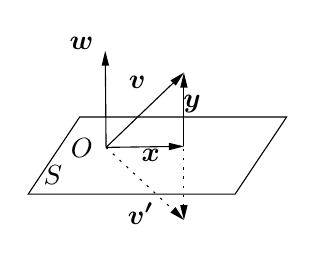
\begin{tikzpicture}[x=0.75pt,y=0.75pt,yscale=-1,xscale=1]
%uncomment if require: \path (0,310); %set diagram left start at 0, and has height of 310

%Shape: Parallelogram [id:dp04316432985707386] 
\draw   (96.11,115) -- (195.8,115) -- (170.99,152.15) -- (71.3,152.15) -- cycle ;
%Straight Lines [id:da2353302515023421] 
\draw    (108.8,129.65) -- (108.42,85.1) ;
\draw [shift={(108.4,83.1)}, rotate = 89.51] [fill={rgb, 255:red, 0; green, 0; blue, 0 }  ][line width=0.08]  [draw opacity=0] (7.2,-1.8) -- (0,0) -- (7.2,1.8) -- cycle    ;
%Straight Lines [id:da14913951087141797] 
\draw    (108.8,129.65) -- (144.3,129.18) ;
\draw [shift={(146.3,129.15)}, rotate = 179.24] [fill={rgb, 255:red, 0; green, 0; blue, 0 }  ][line width=0.08]  [draw opacity=0] (7.2,-1.8) -- (0,0) -- (7.2,1.8) -- cycle    ;
%Straight Lines [id:da7775953697317739] 
\draw    (146.3,129.15) -- (146.3,95.65) ;
\draw [shift={(146.3,93.65)}, rotate = 90] [fill={rgb, 255:red, 0; green, 0; blue, 0 }  ][line width=0.08]  [draw opacity=0] (7.2,-1.8) -- (0,0) -- (7.2,1.8) -- cycle    ;
%Straight Lines [id:da2670825372641483] 
\draw    (108.8,129.65) -- (144.86,95.04) ;
\draw [shift={(146.3,93.65)}, rotate = 136.17] [fill={rgb, 255:red, 0; green, 0; blue, 0 }  ][line width=0.08]  [draw opacity=0] (7.2,-1.8) -- (0,0) -- (7.2,1.8) -- cycle    ;
%Straight Lines [id:da46605586651881037] 
\draw  [dash pattern={on 0.84pt off 2.51pt}]  (108.8,129.65) -- (144.84,163.29) ;
\draw [shift={(146.3,164.65)}, rotate = 223.03] [fill={rgb, 255:red, 0; green, 0; blue, 0 }  ][line width=0.08]  [draw opacity=0] (7.2,-1.8) -- (0,0) -- (7.2,1.8) -- cycle    ;
%Straight Lines [id:da055608728128430984] 
\draw  [dash pattern={on 0.84pt off 2.51pt}]  (146.3,162.65) -- (146.3,129.15) ;
\draw [shift={(146.3,164.65)}, rotate = 270] [fill={rgb, 255:red, 0; green, 0; blue, 0 }  ][line width=0.08]  [draw opacity=0] (7.2,-1.8) -- (0,0) -- (7.2,1.8) -- cycle    ;

% Text Node
\draw (98.9,79.57) node   [align=left] {\begin{minipage}[lt]{11.42pt}\setlength\topsep{0pt}
$\displaystyle \boldsymbol{{\displaystyle w}}$
\end{minipage}};
% Text Node
\draw (100.15,129.82) node   [align=left] {\begin{minipage}[lt]{12.44pt}\setlength\topsep{0pt}
$\displaystyle O$
\end{minipage}};
% Text Node
\draw (85.15,143.07) node   [align=left] {\begin{minipage}[lt]{9.72pt}\setlength\topsep{0pt}
$\displaystyle S$
\end{minipage}};
% Text Node
\draw (133.55,133.57) node   [align=left] {\begin{minipage}[lt]{11.42pt}\setlength\topsep{0pt}
$\displaystyle \boldsymbol{x}$
\end{minipage}};
% Text Node
\draw (153.7,108.82) node   [align=left] {\begin{minipage}[lt]{11.42pt}\setlength\topsep{0pt}
$\displaystyle \boldsymbol{y}$
\end{minipage}};
% Text Node
\draw (126.9,161.57) node   [align=left] {\begin{minipage}[lt]{11.42pt}\setlength\topsep{0pt}
$\displaystyle \boldsymbol{v'}$
\end{minipage}};
% Text Node
\draw (127.4,98.57) node   [align=left] {\begin{minipage}[lt]{11.42pt}\setlength\topsep{0pt}
$\displaystyle {\displaystyle \boldsymbol{v}}$
\end{minipage}};
% Text Node
% \draw (154.7,141.72) node   [align=left] {\begin{minipage}[lt]{11.42pt}\setlength\topsep{0pt}
% $\displaystyle -\boldsymbol{y}$
% \end{minipage}};


\end{tikzpicture}

\caption{初等反射矩阵的几何意义}
\label{Householder}
\end{figure}

\end{multicols}
如图 \ref{Householder}, 考虑以 $\vb*{w}$ 为法向量且过原点 $O$ 的超平面 $S:\vb*{w}^\top\vb*{x}=0$, 设任意向量 $\vb*{v}\in \mathbb{R}^{n}$, 则 $\vb*{v}=\vb*{x}+\vb*{y}$, 其中 $\vb*{x}\in S,~\vb*{y}\in S^{\bot }$ ($S^{\bot}$ 表示与 $S$ 垂直的超平面), 于是 $
\vb*{Hx}=\vb*{x},~ \vb*{Hy}=-\vb*{y},~ \vb*{Hv}=\vb*{v}'.
$

\begin{theorem}
    设 $\vb*{x},~\vb*{y}$ 为两个不相等的 $n$ 维向量, 且 $\norm{\vb*{x}}_2=\norm{\vb*{y}}_2$, 则存在一个 初等反射矩阵 $\vb*{H}$, 使得 $\vb*{Hx}=\vb*{y}.$
\end{theorem}
\begin{proof}[{\songti \textbf{证}}]
    令 $\vb*{w}=\dfrac{\vb*{x}-\vb*{y}}{\norm{\vb*{x}-\vb*{y}}}$, 那么 $$
    \vb*{H}=\vb*{E}-2\vb*{ww}^\top=\vb*{E}-2\dfrac{(\vb*{x}-\vb*{y})}{\norm{\vb*{x}-\vb*{y}}^2}\qty(\vb*{x}^\top-\vb*{y}^\top)
    $$
    则 $$
    \vb*{Hx}=\vb*{x}-2\dfrac{(\vb*{x}-\vb*{y})}{\norm{\vb*{x}-\vb*{y}}^2}\qty(\vb*{x}^\top-\vb*{y}^\top)\vb*{x}=\vb*{x}-2\dfrac{(\vb*{x}-\vb*{y})\qty(\vb*{x}^\top\vb*{x}-\vb*{y}^\top\vb*{x})}{\norm{\vb*{x}-\vb*{y}}^2}
    $$
    因为 $$
    \norm{\vb*{x}-\vb*{y}}^2=(\vb*{x}-\vb*{y})^\top(\vb*{x}-\vb*{y})=2\qty(\vb*{x}^\top\vb*{x}-\vb*{y}^\top\vb*{x})
    $$
    所以 $\vb*{Hx}=\vb*{x}-(\vb*{x}-\vb*{y})=\vb*{y}$.
\end{proof}
\subsection{向量空间}

\begin{definition}[向量空间]
    设 $ V $ 是实数域 $ \mathbb{R} $ 上的 $ n $ 维向量组成的集合, 如果 $ V $ 关于向量的加法和数乘是封闭的, 即\\
    若 $ \vb*{\alpha} \in V, \vb*{\beta} \in V $, 则 $ \vb*{\alpha}+\vb*{\beta} \in V $; 若 $ \vb*{\alpha} \in V, k \in \mathbb{R} $, 则 $ k \vb*{\alpha} \in V $, 则称 $ V $ 是实数域 $ \mathbb{R} $ 上的\textit{向量空间}.\\
    显然, 实数域 $ \mathbb{R} $ 上的 $ n $ 维向量的全体构成一个向量空间, 记为 $ \mathbb{R}^{n} $.
\end{definition}

\begin{definition}[基与维数]
    在向量空间 $ \mathbb{R}^{n} $ 中, $ n $ 个线性无关的向量 $ \vb*{\xi}_{1}, \vb*{\xi}_{2}, \cdots, \vb*{\xi}_{n} $ 称为 $ \mathbb{R}^{n} $ \textit{的一组基}. 若 $ \vb*{\alpha} \in \mathbb{R}^{n} $ 为任一向量, 且
    $$\vb*{\alpha}=a_{1} \vb*{\xi}_{1}+a_{2} \vb*{\xi}_{2}+\cdots+a_{n} \vb*{\xi}_{n}$$
    则称 $ a_{1}, a_{2}, \cdots, a_{n} $ 为 $ \vb*{\alpha} $ \textit{关于基} $ \vb*{\xi}_{1}, \vb*{\xi}_{2}, \cdots, \vb*{\xi}_{n} $ \textit{的坐标}, 记作 $ \left(a_{1}, a_{2}, \cdots, a_{n}\right)^{\top} $, $n$ 称为\textit{向量空间的维数}.
\end{definition}

\begin{definition}[基变换与坐标变换]
    设 $ \vb*{\xi}_{1}, \vb*{\xi}_{2}, \cdots, \vb*{\xi}_{n} $ 和 $ \vb*{\eta}_{1}, \vb*{\eta}_{2}, \cdots, \vb*{\eta}_{n} $ 是 $ \mathbb{R}^{n} $ 的两组基, 且有
    $$\left(\vb*{\eta}_{1}, \vb*{\eta}_{2}, \cdots, \vb*{\eta}_{n}\right)=\left(\vb*{\xi}_{1}, \vb*{\xi}_{2}, \cdots, \vb*{\xi}_{n}\right)\mqty(a_{11}  & a_{12}  & \cdots & a_{1 n} \\
        a_{21}  & a_{22}  & \cdots & a_{2 n} \\
        \vdots  & \vdots  &        & \vdots  \\
        a_{n 1} & a_{n 2} & \cdots & a_{n n})
        =\left(\vb*{\xi}_{1}, \vb*{\xi}_{2}, \cdots, \vb*{\xi}_{n}\right) \vb*{A}$$
    称 $ \vb*{A} $ 为由基 $ \vb*{\xi}_{1}, \vb*{\xi}_{2}, \cdots, \vb*{\xi}_{n} $ 到基 $ \vb*{\eta}_{1}, \vb*{\eta}_{2}, \cdots, \vb*{\eta}_{\vb*{n}} $ 的\textit{过渡矩阵}, 两个基之间的过渡矩阵是可逆矩阵.\\
    设 $ \vb*{\alpha} \in \mathbb{R}^{n} $ 在基 $ \vb*{\xi}_{1}, \vb*{\xi}_{2}, \cdots, \vb*{\xi}_{n} $ 和基 $ \vb*{\eta}_{1}, \vb*{\eta}_{2}, \cdots, \vb*{\eta}_{n} $ 下的坐标分别为
    $$\left(x_{1}, x_{2}, \cdots, x_{n}\right)^{\top} ,\quad \left(y_{1}, y_{2}, \cdots, y_{n}\right)^{\top}$$
    则有
    $$\mqty(x_{1}  \\
        x_{2}  \\
        \vdots \\
        x_{n})=\vb*{A}\mqty(y_{1}  \\
        y_{2}  \\
        \vdots \\
        y_{n})
        \quad \text { 或 }\mqty(y_{1}  \\
        y_{2}  \\
        \vdots \\
        y_{n})
        =\vb*{A}^{-1}\mqty(x_{1}  \\
        x_{2}  \\
        \vdots \\
        x_{n})$$
    称为\textit{坐标变换公式}.
\end{definition}

\begin{example}
    设 $\vb*{\alpha}_1=(1,1,1)^\top, \vb*{\alpha}_2=(1,0,-1)^\top, \vb*{\alpha}_3=(1,0,1)^\top$ 与 $\vb*{\beta}_1=(1,2,1)^\top, \vb*{\beta}_2=(3,3,3)^\top, \vb*{\beta}_3=(2,4,3)^\top$ 是 $\mathbb{R}^3$ 的两组基, 求在两组基下有相同坐标的向量.
\end{example}
\begin{solution}
    设在两组基下有相同坐标的向量为 $\vb*{\gamma}$, 由题意
    $$
    x_1\vb*{\alpha}_1+x_2\vb*{\alpha}_2+x_3\vb*{\alpha}_3=x_1\vb*{\beta}_1+ x_2\vb*{\beta}_2+ x_3\vb*{\beta}_3\Rightarrow x_1(\vb*{\alpha}_1-\vb*{\beta}_1)+ x_2(\vb*{\alpha}_2-\vb*{\beta}_2)+ x_3(\vb*{\alpha}_3-\vb*{\beta}_3)=\vb*{0}
    $$
    令 $\vb*{A}=(\vb*{\alpha}_1-\vb*{\beta}_1,\vb*{\alpha}_2-\vb*{\beta}_2,\vb*{\alpha}_3-\vb*{\beta}_3)=\begin{pmatrix} 0 & -2 & -1 \\ -1 & -3 & -4 \\ 0 & -4 & -2 \\\end{pmatrix}\to \begin{pmatrix} 1 & 3 & 4 \\ 0 & 2 & 1 \\ 0 & 0 & 0 \\\end{pmatrix}$,
    则 $x_2=k, x_3=-2k, x_1=5k$, 于是 $\vb*{\gamma}=x_1\vb*{\alpha}_1+ x_2\vb*{\alpha}_2+ x_3\vb*{\alpha}_3=(4k,5k,2k)^\top, \forall k\in \mathbb{R}.$
\end{solution}

\begin{example}
    设向量组 $\vb*{\alpha}_1, \vb*{\alpha}_2, \vb*{\alpha}_3$ 是 3 维向量空间 $\mathbb{R}^3$ 的一组基, $k$ 为一个常数, 由 $-k\vb*{\alpha}_1+\vb*{\alpha}_2,-\vb*{\alpha}_2+\vb*{\alpha}_3, k\vb*{\alpha}_3+\vb*{\alpha}_1$ 生成的向量空间的维数为 (\quad).
    \begin{tasks}(4)
        \task 1
        \task 2
        \task 3
        \task 依赖于 $k$
    \end{tasks}
\end{example}
\begin{solution}
    由题意 
    $$
    (-k\vb*{\alpha}_1+\vb*{\alpha}_2,-\vb*{\alpha}_2+\vb*{\alpha}_3, k\vb*{\alpha}_3+\vb*{\alpha}_1)=(\vb*{\alpha}_1, \vb*{\alpha}_2, \vb*{\alpha}_3)\begin{pmatrix} -k & 1 & 0 \\ 0 & -1 & 1 \\ 1 & 0 & k \\\end{pmatrix}:=(\vb*{\alpha}_1, \vb*{\alpha}_2, \vb*{\alpha}_3)\vb*{Q}
    $$
    并且 $|\vb*{Q}|=k^2+1\neq 0$, 因此 $\vb*{Q}$ 可逆, 所以 $-k\vb*{\alpha}_1+\vb*{\alpha}_2,-\vb*{\alpha}_2+\vb*{\alpha}_3, k\vb*{\alpha}_3+\vb*{\alpha}_1$ 线性无关, 故生成的向量空间的维数为 $3$, 选 C.
\end{solution}

\begin{example}
    若向量组 $$\vb*{\alpha}_1=(1,1,1,1)^\top, \vb*{\alpha}_2=(0,1,-1,2)^\top, \vb*{\alpha}_3=(2,3,2+t,4)^\top, \vb*{\alpha}_4=(3,1,5,9)^\top$$
    不是 $4$ 维向量空间 $\mathbb{R}^4$ 的一个基, 求 $t$.
\end{example}
\begin{solution}
    以 $\vb*{\alpha}_1, \vb*{\alpha}_2, \vb*{\alpha}_3, \vb*{\alpha}_4$ 为列构造成矩阵 $\vb*{A}$, 对 $\vb*{A}$ 施行初等行变换:
    $$
    \vb*{A}=\begin{pmatrix} 1 & 0 & 2 & 3 \\ 1 & 1 & 3 & 1 \\ 1 & -1 & 2+t & 5 \\ 1 & 2 & 4 & 9 \\\end{pmatrix}\xrightarrow[i=2,3,4]{r_i-r_1}\begin{pmatrix} 1 & 0 & 2 & 3 \\ 0 & 1 & 1 & -2 \\ 0 & -1 & t & 2 \\ 0 & 2 & 2 & 6 \\\end{pmatrix}\xrightarrow[r_4-2r_2]{r_3+r_2}\begin{pmatrix} 1 & 0 & 2 & 3 \\ 0 & 1 & 1 & -2 \\ 0 & 0 & t+1 & 0 \\ 0 & 0 & 0 & 10 \\\end{pmatrix}
    $$
    易知, $t=-1$ 时, $\rank\vb*{A}=3<4$, 向量组 $\vb*{\alpha}_1, \vb*{\alpha}_2, \vb*{\alpha}_3, \vb*{\alpha}_4$ 线性相关, 故当 $t=-1$ 时, $\vb*{\alpha}_1, \vb*{\alpha}_2, \vb*{\alpha}_3, \vb*{\alpha}_4$ 不是向量空间 $\mathbb{R}^{4}$ 的基.
\end{solution}

\begin{example}
    在线性空间 $\vb*{P}^{2\times2}$ 中定义线性变换 $\vb*{A}_1$, $\vb*{A}_2$, $\vb*{A}_3$ 为
    $$\vb*{A}_1(\vb*{X})=\begin{pmatrix}
            a & b \\
            c & d
        \end{pmatrix}\vb*{X}\text{, }\vb*{A}_2(\vb*{X})=\vb*{X}\begin{pmatrix}
            a & b \\
            c & d
        \end{pmatrix}\text{, }\vb*{A}_3(\vb*{X})=\begin{pmatrix}
            a & b \\
            c & d
        \end{pmatrix}\vb*{X}\begin{pmatrix}
            a & b \\
            c & d
        \end{pmatrix}\qty(\vb*{X}\in \vb*{P}^{2\times2})$$
    求 $\vb*{A}_1$, $\vb*{A}_2$, $\vb*{A}_3$ 在基 $\vb*{E}_{11}\text{, }\vb*{E}_{12}\text{, }\vb*{E}_{21}\text{, }\vb*{E}_{22}$ 下的矩阵.
\end{example}
\begin{solution}
    因为 \begin{flalign*}
        \vb*{A}_1(\vb*{E}_{11}) & =\begin{pmatrix}
                                       a & b \\
                                       c & d
                                   \end{pmatrix}\begin{pmatrix}
                                                    1 & 0 \\
                                                    0 & 0
                                                \end{pmatrix}=\begin{pmatrix}
                                                                  a & 0 \\
                                                                  c & 0
                                                              \end{pmatrix}=a\vb*{E}_{11}+c\vb*{E}_{21} \\
        \vb*{A}_1(\vb*{E}_{12}) & =\begin{pmatrix}
                                       a & b \\
                                       c & d
                                   \end{pmatrix}\begin{pmatrix}
                                                    0 & 1 \\
                                                    0 & 0
                                                \end{pmatrix}=\begin{pmatrix}
                                                                  0 & a \\
                                                                  0 & c
                                                              \end{pmatrix}=a\vb*{E}_{12}+c\vb*{E}_{22} \\
        \vb*{A}_1(\vb*{E}_{21}) & =\begin{pmatrix}
                                       a & b \\
                                       c & d
                                   \end{pmatrix}\begin{pmatrix}
                                                    0 & 0 \\
                                                    1 & 0
                                                \end{pmatrix}=\begin{pmatrix}
                                                                  b & 0 \\
                                                                  d & 0
                                                              \end{pmatrix}=b\vb*{E}_{11}+d\vb*{E}_{21} \\
        \vb*{A}_1(\vb*{E}_{22}) & =\begin{pmatrix}
                                       a & b \\
                                       c & d
                                   \end{pmatrix}\begin{pmatrix}
                                                    0 & 0 \\
                                                    0 & 1
                                                \end{pmatrix}=\begin{pmatrix}
                                                                  0 & b \\
                                                                  0 & d
                                                              \end{pmatrix}=b\vb*{E}_{12}+d\vb*{E}_{22}
    \end{flalign*}
    所以 $\vb*{A}_1$ 在基 $\vb*{E}_{11}\text{, }\vb*{E}_{12}\text{, }\vb*{E}_{21}\text{, }\vb*{E}_{22}$ 下的矩阵为
    $\begin{pmatrix}
            a & 0 & b & 0 \\
            0 & a & 0 & b \\
            c & 0 & d & 0 \\
            0 & c & 0 & d
        \end{pmatrix}$, 同理可得 $\vb*{A}_2$, $\vb*{A}_3$ 在基下的矩阵为
    $\begin{pmatrix}
            a & c & 0 & 0 \\
            b & d & 0 & 0 \\
            0 & 0 & a & c \\
            0 & 0 & b & d
        \end{pmatrix}$ 以及 $\begin{pmatrix}
            a^2 & ac  & ab  & bc  \\
            ab  & ad  & b^2 & bd  \\
            ac  & c^2 & ad  & cd  \\
            bc  & cd  & bd  & d^2
        \end{pmatrix}.$
\end{solution}

\begin{definition}[$\mathbb{R}^{n} $ 的标准正交基]
    向量空间 $ \mathbb{R}^{n} $ 中 $ n $ 个向量 $ \vb*{\eta}_{1}, \vb*{\eta}_{2}, \cdots, \vb*{\eta}_{n} $ 满足
    \begin{enumerate}[label=(\arabic{*})]
        \item 两两正交, 即 $ \vb*{\eta}_{i}^{\top} \vb*{\eta}_{j}=0, i \neq j, i, j=1,2, \cdots, n $;
        \item 都是单位向量, 即 $ \left\|\vb*{\eta}_{i}\right\|=1, i=1,2, \cdots, n $,
    \end{enumerate}
    则称 $ \vb*{\eta}_{1}, \vb*{\eta}_{2}, \cdots, \vb*{\eta}_{n} $ 为 $ \mathbb{R}^{n} $ 的一组\textit{标准正交基}.
\end{definition}

\begin{theorem}[Schmidt 正交化]
    标准正交基的求法.
    \begin{enumerate}[label=(\arabic{*})]
        \item  给定一线性无关向量组 $ \vb*{\alpha}_{1}, \vb*{\alpha}_{2}, \cdots, \vb*{\alpha}_{s} $, 由其生成等价的 $ s$ 个向量的正交向量组 $ \vb*{\beta}_{1}, \vb*{\beta}_{2}, \cdots, \vb*{\beta}_{s} $ 的公式如下:
              $$\begin{array}{l}
                      \vb*{\beta}_{1}=\vb*{\alpha}_{1},                                                                                                                                                                                                                                             \\
                      \vb*{\beta}_{2}=\vb*{\alpha}_{2}-\dfrac{\left(\vb*{\alpha}_{2}, \vb*{\beta}_{1}\right)}{\left(\vb*{\beta}_{1}, \vb*{\beta}_{1}\right)} \vb*{\beta}_{1},                                                                                                                       \\
                      \vb*{\beta}_{3}=\vb*{\alpha}_{3}-\dfrac{\left(\vb*{\alpha}_{3}, \vb*{\beta}_{1}\right)}{\left(\vb*{\beta}_{1}, \vb*{\beta}_{1}\right)} \vb*{\beta}_{1}-\dfrac{\left(\vb*{\alpha}_{3}, \vb*{\beta}_{2}\right)}{\left(\vb*{\beta}_{2}, \vb*{\beta}_{2}\right)} \vb*{\beta}_{2}, \\
                      \vdots                                                                                                                                                                                                                                                                        \\
                      \vb*{\beta}_{s}=\vb*{\alpha}_{s}-\dfrac{\left(\vb*{\alpha}_{s}, \vb*{\beta}_{1}\right)}{\left(\vb*{\beta}_{1}, \vb*{\beta}_{1}\right)} \vb*{\beta}_{1}-\dfrac{\left(\vb*{\alpha}_{s}, \vb*{\beta}_{2}\right)}{\left(\vb*{\beta}_{2}, \vb*{\beta}_{2}\right)} \vb*{\beta}_{2}-\cdots-\dfrac{\left(\vb*{\alpha}_{s}, \vb*{\beta}_{s-1}\right)}{\left(\vb*{\beta}_{s-1}, \vb*{\beta}_{s-1}\right)} \vb*{\beta}_{s-1} .
                  \end{array}$$
        \item 给定 $ \mathbb{R}^{n} $ 的任意一组基, 把它变为标准正交基的步骤如下:
              \begin{enumerate}
                  \item 利用 Schmidt 正交化方法, 由这组基生成有 $ n $ 个向量的正交向量组;
                  \item 把正交向量组中每个向量标准化, 即单位化.
              \end{enumerate}
              这样就得到 $ \mathbb{R}^{n} $ 的一组标准正交基. 这一过程称为标准正交化.
    \end{enumerate}
\end{theorem}

\begin{example}[2021 数一]
    已知 $\vb*{\alpha}=\mqty(1\\0\\1),~\vb*{\alpha}_2=\mqty(1\\2\\1),~\vb*{\alpha}=\mqty(3\\1\\2)$, 记 $\vb*{\beta}_1=\vb*{\alpha}_1,~\vb*{\beta}_2=\vb*{\alpha}_2-k\vb*{\beta}_1,~\vb*{\beta}_3=\vb*{\alpha}_3-l_1\vb*{\beta}_1-l_2\vb*{\beta}_2$,
    若 $\vb*{\beta}_1,\vb*{\beta}_2,\vb*{\beta}_3$ 两两正交, 则 $l_1,~l_2$ 依次为 (\quad).
    \begin{tasks}(4)
        \task $\dfrac{5}{2},~\dfrac{1}{2}$
        \task $-\dfrac{5}{2},~\dfrac{1}{2}$
        \task $\dfrac{5}{2},~-\dfrac{1}{2}$
        \task $-\dfrac{5}{2},~-\dfrac{1}{2}$
    \end{tasks}
\end{example}
\begin{solution}
    \textbf{法一: }因为 $\vb*{\beta}_1$ 与 $\vb*{\beta}_2$ 相互正交, 即 $$(1,0,1)\cdot(1-k,2,1-k)=0\Rightarrow k=1\Rightarrow \vb*{\beta}_2=\vb*{\alpha}_2-\vb*{\beta}_1$$
    同理 $\vb*{\beta}_1$ 与 $\vb*{\beta}_3$ 相互正交, $\vb*{\beta}_2$ 与 $\vb*{\beta}_3$ 相互正交, 则
    $$\begin{cases}
            (1,0,1)\cdot(3-l_1,1-2l_2,2-l_1)=0 \\
            (0,2,0)\cdot(3-l_1,1-2l_2,2-l_1)=0
        \end{cases}\Rightarrow \begin{cases}
            l_1=\dfrac{5}{2} \\[6pt]
            l_2=\dfrac{1}{2}
        \end{cases}$$
    \textbf{法二: }$\vb*{\beta}_2=\vb*{\alpha}_2-\dfrac{[\vb*{\alpha}_2,\vb*{\beta}_1]}{[\vb*{\beta}_1,\vb*{\beta}_1]}\vb*{\beta}_1=\mqty(0\\2\\0),~\vb*{\beta}_3=\vb*{\alpha}_3-\dfrac{[\vb*{\alpha}_3,\vb*{\beta}_2]}{[\vb*{\beta}_2,\vb*{\beta}_2]}\vb*{\beta}_2-\dfrac{[\vb*{\alpha}_3,\vb*{\beta}_1]}{[\vb*{\beta}_1,\vb*{\beta}_1]}\vb*{\beta}_1$,
    因此 $l_1=\dfrac{[\vb*{\alpha}_3,\vb*{\beta}_1]}{[\vb*{\beta}_1,\vb*{\beta}_1]}=\dfrac{5}{2},~l_2=\dfrac{[\vb*{\alpha}_3,\vb*{\beta}_2]}{[\vb*{\beta}_2,\vb*{\beta}_2]}=\dfrac{1}{2}$,
    故选 A.
\end{solution}

\begin{theorem}[两组标准正交基之间的过渡矩阵]
    设 $ \mathbb{R}^{n} $ 的两组标准正交基 $ \vb*{\xi}_{1}, \vb*{\xi}_{2}, \cdots, \vb*{\xi}_{n} $ 到 $ \vb*{\eta}_{1} ,  \vb*{\eta}_{2}, \cdots$,\\ $\vb*{\eta}_{n} $ 的过渡矩阵为 $ \vb*{Q} $, 则存在下列关系
    $$\left(\vb*{\xi}_{1}, \vb*{\xi}_{2}, \cdots, \vb*{\xi}_{n}\right)=\left(\vb*{\eta}_{1}, \vb*{\eta}_{2}, \cdots, \vb*{\eta}_{n}\right) \vb*{Q}$$
    且 $ \vb*{Q} $ 满足 $ \vb*{Q}^{\top} \vb*{Q}=\vb*{E} $, 即 $ \vb*{Q} $ 为正交矩阵.
\end{theorem}

\begin{example}[2009 数一]
    设 $\vb*{\alpha}_1,~\vb*{\alpha}_2,~\vb*{\alpha}_3$ 是三维空间 $\mathbb{R}^3$ 的一组基, 则由基 $\vb*{\alpha}_1,~\dfrac{1}{2}\vb*{\alpha}_2,~\dfrac{1}{3}\vb*{\alpha}_3$
    到基 $\vb*{\alpha}_1+\vb*{\alpha}_2,~\vb*{\alpha}_2+\vb*{\alpha}_3,~\vb*{\alpha}_3+\vb*{\alpha}_1$ 的过渡矩阵为 (\quad).
    \begin{tasks}(4)
        \task $\mqty(1&0&1\\2&2&0\\0&3&3)$
        \task $\mqty(1&2&0\\0&2&3\\1&0&3)$
        \task $\mqty(\dfrac{1}{2}&\dfrac{1}{4}&-\dfrac{1}{6}\\[6pt]-\dfrac{1}{2}&\dfrac{1}{4}&\dfrac{1}{6}\\[6pt]-\dfrac{1}{2}&-\dfrac{1}{4}&\dfrac{1}{6})$
        \task $\mqty(\dfrac{1}{2}&-\dfrac{1}{2}&\dfrac{1}{2}\\[6pt]\dfrac{1}{4}&\dfrac{1}{4}&-\dfrac{1}{4}\\[6pt]-\dfrac{1}{6}&\dfrac{1}{6}&\dfrac{1}{6})$
    \end{tasks}
\end{example}
\begin{solution}
    由 $\qty(\vb*{\alpha}_1,\dfrac{1}{2}\vb*{\alpha}_2,\dfrac{1}{3}\vb*{\alpha}_3)=(\vb*{\alpha}_1,\vb*{\alpha}_2,\vb*{\alpha}_3)\mqty(\dmat{1,\dfrac{1}{2},\dfrac{1}{3}})\Rightarrow (\vb*{\alpha}_1,\vb*{\alpha}_2,\vb*{\alpha}_3)=\qty(\vb*{\alpha}_1,\dfrac{1}{2}\vb*{\alpha}_2,\dfrac{1}{3}\vb*{\alpha}_3)\mqty(\dmat{1,2,3})$, 
    因此 \begin{flalign*}
        (\vb*{\alpha}_1+\vb*{\alpha}_2,\vb*{\alpha}_2+\vb*{\alpha}_3,\vb*{\alpha}_3+\vb*{\alpha}_1) & =(\vb*{\alpha}_1,\vb*{\alpha}_2,\vb*{\alpha}_3)\mqty(1                             & 0 & 1 \\1&1&0\\0&1&1)=\qty(\vb*{\alpha}_1,\dfrac{1}{2}\vb*{\alpha}_2,\dfrac{1}{3}\vb*{\alpha}_3)\mqty(\dmat{1,2,3})\mqty(1&0&1\\1&1&0\\0&1&1)\\
                                                                                                    & =\qty(\vb*{\alpha}_1,\dfrac{1}{2}\vb*{\alpha}_2,\dfrac{1}{3}\vb*{\alpha}_3)\mqty(1 & 0 & 1 \\2&2&0\\0&3&3)
    \end{flalign*}
    因此选 A.
\end{solution}

\begin{example}
    设线性空间 $\vb*{P}^3$ 的线性变换 $\vb*{A}$ 定义如下:
    $$\vb*{A}(a_1,a_2,a_3)=(2a_1-a_2,a_2-a_3,a_2+a_3)$$
    \begin{enumerate}[label=(\arabic{*})]
        \item 求 $\vb*{A}$ 在基 $\vb*{\varepsilon}_1=(1,0,0)\text{, }\vb*{\varepsilon}_2=(0,1,0)\text{, }\vb*{\varepsilon}_3=(0,0,1)$ 下的矩阵 $\vb*{A}$;
        \item 求 $\vb*{A}$ 在基 $\vb*{\eta}_1=(1,1,0)\text{, }\vb*{\eta}_2=(0,1,1)\text{, }\vb*{\eta}_3=(0,0,1)$ 下的矩阵 $\vb*{B}$;
        \item 求由基 $\vb*{\varepsilon}_{1,2,3}$ 到 $\vb*{\eta}_{1,2,3}$ 的过渡矩阵 $\vb*{X}$, 并验证 $\vb*{B}=\vb*{X}^{-1}\vb*{AX}.$
    \end{enumerate}
\end{example}
\begin{solution}
    \begin{enumerate}[label=(\arabic{*})]
        \item 因为 $$\vb*{A\varepsilon}_1=(2,0,0)=2\vb*{\varepsilon}_1\text{, }\vb*{A\varepsilon}_2=(-1,1,1)=-\vb*{\varepsilon}_1+\vb*{\varepsilon}_2+\vb*{\varepsilon}_3\text{, }\vb*{A\varepsilon}_3=(0,-1,1)=-\vb*{\varepsilon}_2+\vb*{\varepsilon}_3$$
              所以 $\vb*{A}$ 在基 $\vb*{\varepsilon}_1\text{, }\vb*{\varepsilon}_2\text{, }\vb*{\varepsilon}_3$ 下的矩阵为 $\vb*{A}=\begin{pmatrix}
                      2 & -1 & 1  \\
                      0 & 1  & -1 \\
                      0 & 1  & 1
                  \end{pmatrix}.$
        \item 因为 $$\vb*{A\eta}_1=(1,1,1)=\vb*{\eta}_1+\vb*{\eta}_3\text{, }\vb*{A}\vb*{\eta}_2=(-1,0,2)=-\vb*{\eta}_1+\vb*{\eta}_2+\vb*{\eta}_3\text{, }\vb*{A}\vb*{\eta}_3=(0,-1,1)=-\vb*{\eta}_2+2\vb*{\eta}_3$$
              所以 $\vb*{A}$ 在基 $\vb*{\eta}_1\text{, }\vb*{\eta}_2\text{, }\vb*{\eta}_3$ 下的矩阵为 $\vb*{B}=\begin{pmatrix}
                      1 & -1 & 0  \\
                      0 & 1  & -1 \\
                      1 & 1  & 2
                  \end{pmatrix}.$
        \item 因为 $\displaystyle\vb*{\eta}_j=\sum_{i=1}^{3}k_{ij}\vb*{\varepsilon}_i~  j=1,2,3$, 于是
              \begin{flalign*}
                  \vb*{\eta}_1 & =k_{11}\vb*{\varepsilon}_1+k_{21}\vb*{\varepsilon}_2+k_{31}\vb*{\varepsilon}_3\Rightarrow (k_{11},k_{21},k_{31})=(1,1,0) \\
                  \vb*{\eta}_2 & =k_{12}\vb*{\varepsilon}_1+k_{22}\vb*{\varepsilon}_2+k_{32}\vb*{\varepsilon}_3\Rightarrow (k_{12},k_{22},k_{32})=(0,1,1) \\
                  \vb*{\eta}_3 & =k_{13}\vb*{\varepsilon}_1+k_{23}\vb*{\varepsilon}_2+k_{33}\vb*{\varepsilon}_3\Rightarrow (k_{13},k_{23},k_{33})=(0,0,1)
              \end{flalign*}
              则 $\vb*{X}=\begin{pmatrix}
                      1 & 0 & 0 \\
                      1 & 1 & 0 \\
                      0 & 1 & 1
                  \end{pmatrix}$, 且 $\begin{pmatrix}
                      1 & -1 & 0  \\
                      0 & 1  & -1 \\
                      1 & 1  & 2
                  \end{pmatrix}=\begin{pmatrix}
                      1  & 0  & 0 \\
                      -1 & 1  & 0 \\
                      1  & -1 & 1
                  \end{pmatrix}\begin{pmatrix}
                      2 & -1 & 1  \\
                      0 & 1  & -1 \\
                      0 & 1  & 1
                  \end{pmatrix}\begin{pmatrix}
                      1 & 0 & 0 \\
                      1 & 1 & 0 \\
                      0 & 1 & 1
                  \end{pmatrix}.$
    \end{enumerate}
\end{solution}

\begin{example}
    在 $\vb*{P}^4$ 中, 求由 $\vb*{\varepsilon}_{1,2,3,4}$ 到 $\vb*{\eta}_{1,2,3,4}$ 的过渡矩阵, 并求向量 $\vb*{\xi}=(2,1,2,1)$ 对于基 $\vb*{\eta}_{1,2,3,4}$ 的坐标, 其中
    $$\vb*{\varepsilon}_1=(1,0,0,0)\text{, }\vb*{\varepsilon_2}=(0,1,0,0)\text{, }\vb*{\varepsilon}_3=(0,0,1,0)\text{, }\vb*{\varepsilon}_4=(0,0,0,1)$$
    $$\vb*{\eta}_1=(2,1,0,1)\text{, }\vb*{\eta}_2=(0,1,2,2)\text{, }\vb*{\eta}_3=(-2,1,2,1)\text{, }\vb*{\eta}_4=(1,3,1,2).$$
\end{example}
\begin{solution}
    因为 $\displaystyle \vb*{\eta}_j=\sum_{i=1}^{4}k_{ij}\vb*{\varepsilon}_{i}$, 故由 $\vb*{\varepsilon}_{1,2,3,4}$ 到 $\vb*{\eta}_{1,2,3,4}$ 的过渡矩阵为 $\vb*{A}=\begin{pmatrix}
            2 & 0 & -2 & 1 \\
            1 & 1 & 1  & 3 \\
            0 & 2 & 2  & 1 \\
            1 & 2 & 1  & 2
        \end{pmatrix}$, 因为 $\vb*{\xi}$ 对于基 $\vb*{\varepsilon}_1\text{, }\vb*{\varepsilon}_2\text{, }\vb*{\varepsilon}_3\text{, }\vb*{\varepsilon}_4$ 的坐标为 $(2,1,2,1)$, 所以 $\xi$ 对于基 $\eta_1\text{, }\eta_2\text{, }\eta_3\text{, }\eta_4$ 的坐标为
    $$\vb*{A}^{-1}\begin{pmatrix}
            2 \\
            1 \\
            2 \\
            1
        \end{pmatrix}=\begin{pmatrix}
            \dfrac{5}{2} & 1  & \dfrac{9}{2} & -5 \\[6pt]
            -1           & -1 & -2           & 3  \\[6pt]
            \dfrac{3}{2} & 1  & \dfrac{7}{2} & -4 \\[6pt]
            -1           & 0  & -2           & 2
        \end{pmatrix}\begin{pmatrix}
            2 \\
            1 \\
            2 \\
            1
        \end{pmatrix}=\begin{pmatrix}
            10 \\
            -4 \\
            7  \\
            -4
        \end{pmatrix}$$
    即 $\vb*{\xi}$ 对于基 $\vb*{\eta}_1\text{, }\vb*{\eta}_2\text{, }\vb*{\eta}_3\text{, }\vb*{\eta}_4$ 的坐标为 $(10,-4,7,-4).$
\end{solution}

\begin{example}[2003 南京航空航天大学]
    已知 $\mathbb{R}^3$ 的线性变换 $\sigma$ 对于基 $$\vb*{\varepsilon}_1=(-1,0,2)^\top,~\vb*{\varepsilon}_2=(0,1,1)^\top,~\vb*{\varepsilon}_3=(3,-1,-6)^\top$$
    的像为 $\sigma(\vb*{\varepsilon}_1)=(-1,0,1)^\top,~\sigma(\vb*{\varepsilon}_2)=(0,-1,2)^\top,~\sigma(\vb*{\varepsilon}_2)=(-1,-1,3)^\top$, 
    \begin{enumerate}[label=(\arabic{*})]
        \item 求 $\sigma$ 在基 $\vb*{\varepsilon}_1,~\vb*{\varepsilon}_2,~\vb*{\varepsilon}_3$ 下的矩阵;
        \item 设 $\vb*{x}=(1,1,1)^\top$, 求 $\sigma(\vb*{x})$;
        \item 已知 $\sigma(\vb*{x})$ 在基 $\vb*{\varepsilon}_1,~\vb*{\varepsilon}_2,~\vb*{\varepsilon}_3$ 下的坐标向量为 $(2,-4,-2)^\top$, 求 $\vb*{x}$;
        \item 证明: $\vb*{\varepsilon}_1,~\vb*{\varepsilon}_1+\vb*{\varepsilon}_2,~\vb*{\varepsilon}_1+\vb*{\varepsilon}_2+\vb*{\varepsilon}_3$ 是 $\mathbb{R}^3$ 的基, 并求 $\sigma$ 在该基下的矩阵.
    \end{enumerate}
\end{example}
\begin{solution}
    \begin{enumerate}[label=(\arabic{*})]
        \item 考虑 $\mathbb{R}^3$ 的自由基 $\vb*{e}_1=(1,0,0)^\top,~\vb*{e}_2=(0,1,0)^\top,~\vb*{e}_3=(0,0,1)^\top$, 由基 $\vb*{e}_1,~\vb*{e}_2,~\vb*{e}_3$ 到 $\vb*{\varepsilon}_1,\vb*{\varepsilon}_2,\vb*{\varepsilon}_3$ 的过渡矩阵为
              $$P=\mqty(-1&0&3\\0&1&-1\\2&1&-6)$$
              即 $(\vb*{\varepsilon}_1,\vb*{\varepsilon}_2,\vb*{\varepsilon}_3)=(\vb*{e}_1,~\vb*{e}_2,~\vb*{e}_3)\vb*{P}$, 且向量组 $\sigma(\vb*{\varepsilon}_1,\vb*{\varepsilon}_2,\vb*{\varepsilon}_3)$ 在基 $\vb*{e}_1,~\vb*{e}_2,~\vb*{e}_3$ 下的矩阵表示为
              $$A=\mqty(-1&0&-1\\0&-1&-1\\1&2&3)$$
              即 $\sigma(\vb*{\varepsilon}_1,\vb*{\varepsilon}_2,\vb*{\varepsilon}_3)=(\vb*{e}_1,~\vb*{e}_2,~\vb*{e}_3)\vb*{A}$, 于是, 有
              $$\sigma(\vb*{\varepsilon}_1,\vb*{\varepsilon}_2,\vb*{\varepsilon}_3)=(\vb*{e}_1,~\vb*{e}_2,~\vb*{e}_3)\vb*{A}=(\vb*{\varepsilon}_1,\vb*{\varepsilon}_2,\vb*{\varepsilon}_3)\vb*{P}^{-1}\vb*{A}$$
              因此, $\sigma$ 在基 $\vb*{\varepsilon}_1,\vb*{\varepsilon}_2,\vb*{\varepsilon}_3$ 下的矩阵为
              $$\vb*{B}=\vb*{P}^{-1}\vb*{A}=\mqty(-1&0&3\\0&1&-1\\2&1&-6)^{-1}\mqty(-1&0&-1\\0&-1&-1\\1&2&3)=\mqty(5&-3&3\\2&0&1\\2&-1&1)\mqty(-1&0&-1\\0&-1&-1\\1&2&3)=\mqty(-2&9&7\\-1&2&1\\-1&3&2).$$
        \item $\sigma(\vb*{x})=\sigma(\vb*{e}_1,~\vb*{e}_2,~\vb*{e}_3)\vb*{x}=\sigma(\vb*{\varepsilon}_1,\vb*{\varepsilon}_2,\vb*{\varepsilon}_3)\vb*{P}^{-1}\vb*{x}=(\vb*{e}_1,~\vb*{e}_2,~\vb*{e}_3)\vb*{AP}^{-1}\vb*{x}=(-7,-5,17)^\top.$
        \item 记 $\vb*{y}=(2,-4,-2)^\top$, 则 $\sigma(\vb*{x})=(\vb*{\varepsilon}_1,\vb*{\varepsilon}_2,\vb*{\varepsilon}_3)\vb*{y}$, 因为
              $$\sigma(\vb*{x})=\sigma(\vb*{\varepsilon}_1,\vb*{\varepsilon}_2,\vb*{\varepsilon}_3)\vb*{P}^{-1}\vb*{x}=(\vb*{\varepsilon}_1,\vb*{\varepsilon}_2,\vb*{\varepsilon}_3)\vb*{BP}^{-1}\vb*{x}$$
              所以 $\vb*{BP}^{-1}\vb*{x}=\vb*{y}$, 其中 $\vb*{BP}^{-1}=\mqty(22&-1&10\\1&2&0\\5&1&2)$, 解非齐次线性方程组 $\vb*{BP}^{-1}\vb*{x}=\vb*{y}$, 得 $x=\mqty(-8\\2\\18)+k\mqty(4\\-2\\-9)$ 其中 $k$ 为任意常数.
        \item 记 $\vb*{\alpha}_1=\vb*{\varepsilon}_1,~\vb*{\alpha}_2=\vb*{\varepsilon}_1+\vb*{\varepsilon}_2,~\vb*{\alpha}_3=\vb*{\varepsilon}_1+\vb*{\varepsilon}_2+\vb*{\varepsilon}_3$, 易证, $\vb*{\alpha}_1,~\vb*{\alpha}_2,~\vb*{\alpha_3}$ 线性无关, 所以是 $\mathbb{R}^3$ 的基, 
              显然, 由基 $\vb*{\varepsilon}_1,\vb*{\varepsilon}_2,\vb*{\varepsilon}_3$ 到基 $\vb*{\alpha}_1,~\vb*{\alpha}_2,~\vb*{\alpha}_3$ 的过渡矩阵为 $$Q=\mqty(1&1&1\\0&1&1\\0&0&1)$$
              因此, $\sigma$ 在基 $\vb*{\alpha}_1,~\vb*{\alpha}_2,~\vb*{\alpha}_3$ 下的矩阵为
              $$\vb*{Q}^{-1}\vb*{BQ}=\mqty(1&1&1\\0&1&1\\0&0&1)^{-1}\mqty(-2&9&7\\-1&2&1\\-1&3&2)\mqty(1&1&1\\0&1&1\\0&0&1)=\mqty(-1&6&12\\0&-1&-2\\-1&2&4).$$
    \end{enumerate}
\end{solution}

\section{向量的内积与向量空间}

\subsection{向量的内积}

\begin{definition}[向量的内积]
    给定 $ \mathbb{R}^{n} $ 中的向量
    $$\vb*{\alpha}=\left(a_{1}, a_{2}, \cdots, a_{n}\right)^{\top}, \quad \vb*{\beta}=\left(b_{1}, b_{2}, \cdots, b_{n}\right)^{\top}$$
    则称 $\displaystyle \sum_{i=1}^{n} a_{i} b_{i} $ 为向量 $ \vb*{\alpha} $ 与 $ \vb*{\beta} $ 的\textit{内积}, 记为 $ (\vb*{\alpha}, \vb*{\beta}) $, 即 $ \displaystyle(\vb*{\alpha}, \vb*{\beta})=\vb*{\alpha}^{\top} \vb*{\beta}=\sum_{i=1}^{n} a_{i} b_{i} $.
\end{definition}

内积具有下列性质:
\begin{enumerate}[label=(\arabic{*})]
    \item $(\vb*{\alpha}, \vb*{\beta})=(\vb*{\beta}, \vb*{\alpha}) $;
    \item $(k \vb*{\alpha}, \vb*{\beta})=k(\vb*{\alpha}, \vb*{\beta}) $;
    \item $(\vb*{\alpha}+\vb*{\beta}, \vb*{\gamma})=(\vb*{\alpha}, \vb*{\gamma})+(\vb*{\beta}, \vb*{\gamma}) $;
    \item $(\vb*{\alpha}, \vb*{\alpha}) \geqslant 0 $, 当且仅当 $ \vb*{\alpha}=\vb*{0} $ 时, 等号成立.
\end{enumerate}

\begin{definition}[向量的范数]
    设 $\vb*{\alpha}$ 为 $\mathbb{R}^n$ 中的任意向量, 将非负实数 $\sqrt{(\vb*{\alpha},\vb*{\alpha})}$ 定义为 $\vb*{\alpha}$ 的长度, 记为 $\norm*{\vb*{a}}$, 即若 $\vb*{\alpha}=(a_1,a_2,\cdots,a_n)^\top$, 则有 $$\norm*{\vb*{\alpha}}=\sqrt{\displaystyle\sum_{i=1}^{n}a_i^2}$$
    向量的长度也称为\textit{向量的范数}或\textit{模}.
\end{definition}

向量范数具有下列性质:
\begin{enumerate}[label=(\arabic{*})]
    \item $\|\vb*{\alpha}\| \geqslant 0  $, 当且仅当 $ \vb*{\alpha}=\vb*{0} $ 时, 等号成立;
    \item 对于任意向量 $ \vb*{\alpha} $ 和任意实数 $ k $, 都有 $ \|k \vb*{\alpha}\|=|k|\|\vb*{\alpha}\| $;
    \item 对于任意 $ n $ 维向量 $ \vb*{\alpha} $ 和 $ \vb*{\beta} $, 有 $ |(\vb*{\alpha}, \vb*{\beta})|=\left|\vb*{\alpha}^{\top} \vb*{\beta}\right| \leqslant\|\vb*{\alpha}\| \cdot\|\vb*{\beta}\|$.
\end{enumerate}

\begin{definition}[向量的正交]
    如果向量 $ \vb*{\alpha} $ 和 $ \vb*{\beta} $ 的内积等于零, 即 $ (\vb*{\alpha}, \vb*{\beta})=0 $, 则称  $\vb*{\alpha} $ 和 $ \vb*{\beta} $ \textit{相互正交}. 如果非零向量组 $ \vb*{\alpha}_{1}, \vb*{\alpha}_{2}, \cdots, \vb*{\alpha}_{s} $ 中的向量两两正交, 即 $ \left(\vb*{\alpha}_{i}, \vb*{\alpha}_{j}\right)=0(i \neq j, i, j=1 ,  2, \cdots, s) $, 则称该向量组为\textit{正交向量组}.
\end{definition}

正交向量具有下列性质:
\begin{enumerate}[label=(\arabic{*})]
    \item 零向量与任何向量正交;
    \item 与自己正交的向量只有零向量;
    \item 正交向量组是线性无关的;
    \item 对任意向量 $ \vb*{\alpha} $ 和 $ \vb*{\beta} $, 有三角不等式
          $$\|\vb*{\alpha}+\vb*{\beta}\| \leqslant\|\vb*{\alpha}\|+\|\vb*{\beta}\|$$
          当且仅当 $ \vb*{\alpha} $ 与 $ \vb*{\beta} $ 相互正交时, 有 $ \|\vb*{\alpha}+\vb*{\beta}\|^{2}=\|\vb*{\alpha}\|^{2}+\|\vb*{\beta}\|^{2} $.
\end{enumerate}

\subsection{向量空间}

\begin{definition}[向量空间]
    设 $ V $ 是实数域 $ \mathbb{R} $ 上的 $ n $ 维向量组成的集合, 如果 $ V $ 关于向量的加法和数乘是封闭的, 即\\
    若 $ \vb*{\alpha} \in V, \vb*{\beta} \in V $, 则 $ \vb*{\alpha}+\vb*{\beta} \in V $; 若 $ \vb*{\alpha} \in V, k \in \mathbb{R} $, 则 $ k \vb*{\alpha} \in V $, 则称 $ V $ 是实数域 $ \mathbb{R} $ 上的\textit{向量空间}.\\
    显然, 实数域 $ \mathbb{R} $ 上的 $ n $ 维向量的全体构成一个向量空间, 记为 $ \mathbb{R}^{n} $.
\end{definition}

\begin{definition}[基与坐标]
    在向量空间 $ \mathbb{R}^{n} $ 中, $ n $ 个线性无关的向量 $ \vb*{\xi}_{1}, \vb*{\xi}_{2}, \cdots, \vb*{\xi}_{n} $ 称为 $ \mathbb{R}^{n} $ 的一组基. 若 $ \vb*{\alpha} \in \mathbb{R}^{n} $ 为任一向量, 且
    $$\vb*{\alpha}=a_{1} \vb*{\xi}_{1}+a_{2} \vb*{\xi}_{2}+\cdots+a_{n} \vb*{\xi}_{n}$$
    则称 $ a_{1}, a_{2}, \cdots, a_{n} $ 为 $ \vb*{\alpha} $ \textit{关于基} $ \vb*{\xi}_{1}, \vb*{\xi}_{2}, \cdots, \vb*{\xi}_{n} $ \textit{的坐标}, 记作 $ \left(a_{1}, a_{2}, \cdots, a_{n}\right)^{\top} $.
\end{definition}

\begin{definition}[基变换与坐标变换]
    设 $ \vb*{\xi}_{1}, \vb*{\xi}_{2}, \cdots, \vb*{\xi}_{n} $ 和 $ \vb*{\eta}_{1}, \vb*{\eta}_{2}, \cdots, \vb*{\eta}_{n} $ 是 $ \mathbb{R}^{n} $ 的两组基, 且有
    $$\left(\vb*{\eta}_{1}, \vb*{\eta}_{2}, \cdots, \vb*{\eta}_{n}\right)=\left(\vb*{\xi}_{1}, \vb*{\xi}_{2}, \cdots, \vb*{\xi}_{n}\right)\mqty(a_{11}  & a_{12}  & \cdots & a_{1 n} \\
        a_{21}  & a_{22}  & \cdots & a_{2 n} \\
        \vdots  & \vdots  &        & \vdots  \\
        a_{n 1} & a_{n 2} & \cdots & a_{n n})
        =\left(\vb*{\xi}_{1}, \vb*{\xi}_{2}, \cdots, \vb*{\xi}_{n}\right) \vb*{A}$$
    称 $ \vb*{A} $ 为由基 $ \vb*{\xi}_{1}, \vb*{\xi}_{2}, \cdots, \vb*{\xi}_{n} $ 到基 $ \vb*{\eta}_{1}, \vb*{\eta}_{2}, \cdots, \vb*{\eta}_{\vb*{n}} $ 的\textit{过渡矩阵}, 两个基之间的过渡矩阵是可逆矩阵.\\
    设 $ \vb*{\alpha} \in \mathbb{R}^{n} $ 在基 $ \vb*{\xi}_{1}, \vb*{\xi}_{2}, \cdots, \vb*{\xi}_{n} $ 和基 $ \vb*{\eta}_{1}, \vb*{\eta}_{2}, \cdots, \vb*{\eta}_{n} $ 下的坐标分别为
    $$\left(x_{1}, x_{2}, \cdots, x_{n}\right)^{\top} ,\quad \left(y_{1}, y_{2}, \cdots, y_{n}\right)^{\top}$$
    则有
    $$\mqty(x_{1}  \\
        x_{2}  \\
        \vdots \\
        x_{n})=\vb*{A}\mqty(y_{1}  \\
        y_{2}  \\
        \vdots \\
        y_{n})
        \quad \text { 或 }\mqty(y_{1}  \\
        y_{2}  \\
        \vdots \\
        y_{n})
        =\vb*{A}^{-1}\mqty(x_{1}  \\
        x_{2}  \\
        \vdots \\
        x_{n})$$
    称为\textit{坐标变换公式}.
\end{definition}

\begin{example}
    在线性空间 $\vb*{P}^{2\times2}$ 中定义线性变换 $\vb*{A}_1$,$\vb*{A}_2$,$\vb*{A}_3$ 为
    $$\vb*{A}_1(\vb*{X})=\begin{pmatrix}
            a & b \\
            c & d
        \end{pmatrix}\vb*{X}\text{,}\vb*{A}_2(\vb*{X})=\vb*{X}\begin{pmatrix}
            a & b \\
            c & d
        \end{pmatrix}\text{,}\vb*{A}_3(\vb*{X})=\begin{pmatrix}
            a & b \\
            c & d
        \end{pmatrix}\vb*{X}\begin{pmatrix}
            a & b \\
            c & d
        \end{pmatrix}\qty(\vb*{X}\in \vb*{P}^{2\times2})$$
    求 $\vb*{A}_1$,$\vb*{A}_2$,$\vb*{A}_3$ 在基 $\vb*{E}_{11}\text{,}\vb*{E}_{12}\text{,}\vb*{E}_{21}\text{,}\vb*{E}_{22}$ 下的矩阵.
\end{example}
\begin{solution}
    因为 \begin{flalign*}
        \vb*{A}_1(\vb*{E}_{11}) & =\begin{pmatrix}
                                       a & b \\
                                       c & d
                                   \end{pmatrix}\begin{pmatrix}
                                                    1 & 0 \\
                                                    0 & 0
                                                \end{pmatrix}=\begin{pmatrix}
                                                                  a & 0 \\
                                                                  c & 0
                                                              \end{pmatrix}=a\vb*{E}_{11}+c\vb*{E}_{21} \\
        \vb*{A}_1(\vb*{E}_{12}) & =\begin{pmatrix}
                                       a & b \\
                                       c & d
                                   \end{pmatrix}\begin{pmatrix}
                                                    0 & 1 \\
                                                    0 & 0
                                                \end{pmatrix}=\begin{pmatrix}
                                                                  0 & a \\
                                                                  0 & c
                                                              \end{pmatrix}=a\vb*{E}_{12}+c\vb*{E}_{22} \\
        \vb*{A}_1(\vb*{E}_{21}) & =\begin{pmatrix}
                                       a & b \\
                                       c & d
                                   \end{pmatrix}\begin{pmatrix}
                                                    0 & 0 \\
                                                    1 & 0
                                                \end{pmatrix}=\begin{pmatrix}
                                                                  b & 0 \\
                                                                  d & 0
                                                              \end{pmatrix}=b\vb*{E}_{11}+d\vb*{E}_{21} \\
        \vb*{A}_1(\vb*{E}_{22}) & =\begin{pmatrix}
                                       a & b \\
                                       c & d
                                   \end{pmatrix}\begin{pmatrix}
                                                    0 & 0 \\
                                                    0 & 1
                                                \end{pmatrix}=\begin{pmatrix}
                                                                  0 & b \\
                                                                  0 & d
                                                              \end{pmatrix}=b\vb*{E}_{12}+d\vb*{E}_{22}
    \end{flalign*}
    所以 $\vb*{A}_1$ 在基 $\vb*{E}_{11}\text{,}\vb*{E}_{12}\text{,}\vb*{E}_{21}\text{,}\vb*{E}_{22}$ 下的矩阵为
    $\begin{pmatrix}
            a & 0 & b & 0 \\
            0 & a & 0 & b \\
            c & 0 & d & 0 \\
            0 & c & 0 & d
        \end{pmatrix}$,同理可得 $\vb*{A}_2$,$\vb*{A}_3$ 在基下的矩阵为
    $\begin{pmatrix}
            a & c & 0 & 0 \\
            b & d & 0 & 0 \\
            0 & 0 & a & c \\
            0 & 0 & b & d
        \end{pmatrix}$ 以及 $\begin{pmatrix}
            a^2 & ac  & ab  & bc  \\
            ab  & ad  & b^2 & bd  \\
            ac  & c^2 & ad  & cd  \\
            bc  & cd  & bd  & d^2
        \end{pmatrix}.$
\end{solution}

\begin{definition}[$\mathbb{R}^{n} $ 的标准正交基]
    向量空间 $ \mathbb{R}^{n} $ 中 $ n $ 个向量 $ \vb*{\eta}_{1}, \vb*{\eta}_{2}, \cdots, \vb*{\eta}_{n} $ 满足
    \begin{enumerate}[label=(\arabic{*})]
        \item 两两正交, 即 $ \vb*{\eta}_{i}^{\top} \vb*{\eta}_{j}=0, i \neq j, i, j=1,2, \cdots, n $;
        \item 都是单位向量, 即 $ \left\|\vb*{\eta}_{i}\right\|=1, i=1,2, \cdots, n $,
    \end{enumerate}
    则称 $ \vb*{\eta}_{1}, \vb*{\eta}_{2}, \cdots, \vb*{\eta}_{n} $ 为 $ \mathbb{R}^{n} $ 的一组\textit{标准正交基}.
\end{definition}

\begin{theorem}[Schmidt 正交化]
    标准正交基的求法.
    \begin{enumerate}[label=(\arabic{*})]
        \item  给定一线性无关向量组 $ \vb*{\alpha}_{1}, \vb*{\alpha}_{2}, \cdots, \vb*{\alpha}_{s} $, 由其生成等价的 $ s$ 个向量的正交向量组 $ \vb*{\beta}_{1}, \vb*{\beta}_{2}, \cdots, \vb*{\beta}_{s} $ 的公式如下:
              $$\begin{array}{l}
                      \vb*{\beta}_{1}=\vb*{\alpha}_{1},                                                                                                                                                                                                                                             \\
                      \vb*{\beta}_{2}=\vb*{\alpha}_{2}-\dfrac{\left(\vb*{\alpha}_{2}, \vb*{\beta}_{1}\right)}{\left(\vb*{\beta}_{1}, \vb*{\beta}_{1}\right)} \vb*{\beta}_{1},                                                                                                                       \\
                      \vb*{\beta}_{3}=\vb*{\alpha}_{3}-\dfrac{\left(\vb*{\alpha}_{3}, \vb*{\beta}_{1}\right)}{\left(\vb*{\beta}_{1}, \vb*{\beta}_{1}\right)} \vb*{\beta}_{1}-\dfrac{\left(\vb*{\alpha}_{3}, \vb*{\beta}_{2}\right)}{\left(\vb*{\beta}_{2}, \vb*{\beta}_{2}\right)} \vb*{\beta}_{2}, \\
                      \vdots                                                                                                                                                                                                                                                                        \\
                      \vb*{\beta}_{s}=\vb*{\alpha}_{s}-\dfrac{\left(\vb*{\alpha}_{s}, \vb*{\beta}_{1}\right)}{\left(\vb*{\beta}_{1}, \vb*{\beta}_{1}\right)} \vb*{\beta}_{1}-\dfrac{\left(\vb*{\alpha}_{s}, \vb*{\beta}_{2}\right)}{\left(\vb*{\beta}_{2}, \vb*{\beta}_{2}\right)} \vb*{\beta}_{2}-\cdots-\dfrac{\left(\vb*{\alpha}_{s}, \vb*{\beta}_{s-1}\right)}{\left(\vb*{\beta}_{s-1}, \vb*{\beta}_{s-1}\right)} \vb*{\beta}_{s-1} .
                  \end{array}$$
        \item 给定 $ \mathbb{R}^{n} $ 的任意一组基, 把它变为标准正交基的步骤如下:
              \begin{enumerate}
                  \item 利用 Schmidt 正交化方法, 由这组基生成有 $ n $ 个向量的正交向量组;
                  \item 把正交向量组中每个向量标准化, 即单位化.
              \end{enumerate}
              这样就得到 $ \mathbb{R}^{n} $ 的一组标准正交基. 这一过程称为标准正交化.
    \end{enumerate}
\end{theorem}

\begin{example}[2021 数一]
    已知 $\vb*{\alpha}=\mqty(1\\0\\1),~\vb*{\alpha}_2=\mqty(1\\2\\1),~\vb*{\alpha}=\mqty(3\\1\\2)$, 记 $\vb*{\beta}_1=\vb*{\alpha}_1,~\vb*{\beta}_2=\vb*{\alpha}_2-k\vb*{\beta}_1,~\vb*{\beta}_3=\vb*{\alpha}_3-l_1\vb*{\beta}_1-l_2\vb*{\beta}_2$,
    若 $\vb*{\beta}_1,\vb*{\beta}_2,\vb*{\beta}_3$ 两两正交, 则 $l_1,~l_2$ 依次为
    \begin{tasks}(4)
        \task $\dfrac{5}{2},~\dfrac{1}{2}$
        \task $-\dfrac{5}{2},~\dfrac{1}{2}$
        \task $\dfrac{5}{2},~-\dfrac{1}{2}$
        \task $-\dfrac{5}{2},~-\dfrac{1}{2}$
    \end{tasks}
\end{example}
\begin{solution}
    \textbf{法一: }因为 $\vb*{\beta}_1$ 与 $\vb*{\beta}_2$ 相互正交, 即 $$(1,0,1)\cdot(1-k,2,1-k)=0\Rightarrow k=1\Rightarrow \vb*{\beta}_2=\vb*{\alpha}_2-\vb*{\beta}_1$$
    同理 $\vb*{\beta}_1$ 与 $\vb*{\beta}_3$ 相互正交, $\vb*{\beta}_2$ 与 $\vb*{\beta}_3$ 相互正交, 则
    $$\begin{cases}
            (1,0,1)\cdot(3-l_1,1-2l_2,2-l_1)=0 \\
            (0,2,0)\cdot(3-l_1,1-2l_2,2-l_1)=0
        \end{cases}\Rightarrow \begin{cases}
            l_1=\dfrac{5}{2} \\[6pt]
            l_2=\dfrac{1}{2}
        \end{cases}$$
    \textbf{法二: }$\vb*{\beta}_2=\vb*{\alpha}_2-\dfrac{[\vb*{\alpha}_2,\vb*{\beta}_1]}{[\vb*{\beta}_1,\vb*{\beta}_1]}\vb*{\beta}_1=\mqty(0\\2\\0),~\vb*{\beta}_3=\vb*{\alpha}_3-\dfrac{[\vb*{\alpha}_3,\vb*{\beta}_2]}{[\vb*{\beta}_2,\vb*{\beta}_2]}\vb*{\beta}_2-\dfrac{[\vb*{\alpha}_3,\vb*{\beta}_1]}{[\vb*{\beta}_1,\vb*{\beta}_1]}\vb*{\beta}_1$,
    因此 $l_1=\dfrac{[\vb*{\alpha}_3,\vb*{\beta}_1]}{[\vb*{\beta}_1,\vb*{\beta}_1]}=\dfrac{5}{2},~l_2=\dfrac{[\vb*{\alpha}_3,\vb*{\beta}_2]}{[\vb*{\beta}_2,\vb*{\beta}_2]}=\dfrac{1}{2}$,
    故选 A.
\end{solution}

\begin{theorem}[两组标准正交基之间的过渡矩阵]
    设 $ \mathbb{R}^{n} $ 的两组标准正交基 $ \vb*{\xi}_{1}, \vb*{\xi}_{2}, \cdots, \vb*{\xi}_{n} $ 到 $ \vb*{\eta}_{1} ,  \vb*{\eta}_{2}, \cdots$,\\ $\vb*{\eta}_{n} $ 的过渡矩阵为 $ \vb*{Q} $, 则存在下列关系
    $$\left(\vb*{\xi}_{1}, \vb*{\xi}_{2}, \cdots, \vb*{\xi}_{n}\right)=\left(\vb*{\eta}_{1}, \vb*{\eta}_{2}, \cdots, \vb*{\eta}_{n}\right) \vb*{Q}$$
    且 $ \vb*{Q} $ 满足 $ \vb*{Q}^{\top} \vb*{Q}=\vb*{E} $, 即 $ \vb*{Q} $ 为正交矩阵.
\end{theorem}

\begin{example}[2009 数一]
    设 $\vb*{\alpha}_1,~\vb*{\alpha}_2,~\vb*{\alpha}_3$ 是三维空间 $\mathbb{R}^3$ 的一组基,则由基 $\vb*{\alpha}_1,~\dfrac{1}{2}\vb*{\alpha}_2,~\dfrac{1}{3}\vb*{\alpha}_3$
    到基 $\vb*{\alpha}_1+\vb*{\alpha}_2,~\vb*{\alpha}_2+\vb*{\alpha}_3,~\vb*{\alpha}_3+\vb*{\alpha}_1$ 的过渡矩阵为
    \begin{tasks}(4)
        \task $\mqty(1&0&1\\2&2&0\\0&3&3)$
        \task $\mqty(1&2&0\\0&2&3\\1&0&3)$
        \task $\mqty(\dfrac{1}{2}&\dfrac{1}{4}&-\dfrac{1}{6}\\[6pt]-\dfrac{1}{2}&\dfrac{1}{4}&\dfrac{1}{6}\\[6pt]-\dfrac{1}{2}&-\dfrac{1}{4}&\dfrac{1}{6})$
        \task $\mqty(\dfrac{1}{2}&-\dfrac{1}{2}&\dfrac{1}{2}\\[6pt]\dfrac{1}{4}&\dfrac{1}{4}&-\dfrac{1}{4}\\[6pt]-\dfrac{1}{6}&\dfrac{1}{6}&\dfrac{1}{6})$
    \end{tasks}
\end{example}
\begin{solution}
    由 $\qty(\vb*{\alpha}_1,\dfrac{1}{2}\vb*{\alpha}_2,\dfrac{1}{3}\vb*{\alpha}_3)=(\vb*{\alpha}_1,\vb*{\alpha}_2,\vb*{\alpha}_3)\mqty(\dmat{1,\dfrac{1}{2},\dfrac{1}{3}})\Rightarrow (\vb*{\alpha}_1,\vb*{\alpha}_2,\vb*{\alpha}_3)=\qty(\vb*{\alpha}_1,\dfrac{1}{2}\vb*{\alpha}_2,\dfrac{1}{3}\vb*{\alpha}_3)\mqty(\dmat{1,2,3})$,
    因此 \begin{flalign*}
        (\vb*{\alpha}_1+\vb*{\alpha}_2,\vb*{\alpha}_2+\vb*{\alpha}_3,\vb*{\alpha}_3+\vb*{\alpha}_1) & =(\vb*{\alpha}_1,\vb*{\alpha}_2,\vb*{\alpha}_3)\mqty(1                             & 0 & 1 \\1&1&0\\0&1&1)=\qty(\vb*{\alpha}_1,\dfrac{1}{2}\vb*{\alpha}_2,\dfrac{1}{3}\vb*{\alpha}_3)\mqty(\dmat{1,2,3})\mqty(1&0&1\\1&1&0\\0&1&1)\\
                                                                                                    & =\qty(\vb*{\alpha}_1,\dfrac{1}{2}\vb*{\alpha}_2,\dfrac{1}{3}\vb*{\alpha}_3)\mqty(1 & 0 & 1 \\2&2&0\\0&3&3)
    \end{flalign*}
    因此选 A.
\end{solution}

\begin{example}
    设线性空间 $\vb*{P}^3$ 的线性变换 $\vb*{A}$ 定义如下:
    $$\vb*{A}(a_1,a_2,a_3)=(2a_1-a_2,a_2-a_3,a_2+a_3)$$
    \begin{enumerate}[label=(\arabic{*})]
        \item 求 $\vb*{A}$ 在基 $\vb*{\varepsilon}_1=(1,0,0)\text{,}\vb*{\varepsilon}_2=(0,1,0)\text{,}\vb*{\varepsilon}_3=(0,0,1)$ 下的矩阵 $\vb*{A}$;
        \item 求 $\vb*{A}$ 在基 $\vb*{\eta}_1=(1,1,0)\text{,}\vb*{\eta}_2=(0,1,1)\text{,}\vb*{\eta}_3=(0,0,1)$ 下的矩阵 $\vb*{B}$;
        \item 求由基 $\vb*{\varepsilon}_{1,2,3}$ 到 $\vb*{\eta}_{1,2,3}$ 的过渡矩阵 $\vb*{X}$,并验证 $\vb*{B}=\vb*{X}^{-1}\vb*{AX}.$
    \end{enumerate}
\end{example}
\begin{solution}
    \begin{enumerate}[label=(\arabic{*})]
        \item 因为 $$\vb*{A\varepsilon}_1=(2,0,0)=2\vb*{\varepsilon}_1\text{,}\vb*{A\varepsilon}_2=(-1,1,1)=-\vb*{\varepsilon}_1+\vb*{\varepsilon}_2+\vb*{\varepsilon}_3\text{,}\vb*{A\varepsilon}_3=(0,-1,1)=-\vb*{\varepsilon}_2+\vb*{\varepsilon}_3$$
              所以 $\vb*{A}$ 在基 $\vb*{\varepsilon}_1\text{,}\vb*{\varepsilon}_2\text{,}\vb*{\varepsilon}_3$ 下的矩阵为 $\vb*{A}=\begin{pmatrix}
                      2 & -1 & 1  \\
                      0 & 1  & -1 \\
                      0 & 1  & 1
                  \end{pmatrix}.$
        \item 因为 $$\vb*{A\eta}_1=(1,1,1)=\vb*{\eta}_1+\vb*{\eta}_3\text{,}\vb*{A}\vb*{\eta}_2=(-1,0,2)=-\vb*{\eta}_1+\vb*{\eta}_2+\vb*{\eta}_3\text{,}\vb*{A}\vb*{\eta}_3=(0,-1,1)=-\vb*{\eta}_2+2\vb*{\eta}_3$$
              所以 $\vb*{A}$ 在基 $\vb*{\eta}_1\text{,}\vb*{\eta}_2\text{,}\vb*{\eta}_3$ 下的矩阵为 $\vb*{B}=\begin{pmatrix}
                      1 & -1 & 0  \\
                      0 & 1  & -1 \\
                      1 & 1  & 2
                  \end{pmatrix}.$
        \item 因为 $\displaystyle\vb*{\eta}_j=\sum_{i=1}^{3}k_{ij}\vb*{\varepsilon}_i~  j=1,2,3$,于是
              \begin{flalign*}
                  \vb*{\eta}_1 & =k_{11}\vb*{\varepsilon}_1+k_{21}\vb*{\varepsilon}_2+k_{31}\vb*{\varepsilon}_3\Rightarrow (k_{11},k_{21},k_{31})=(1,1,0) \\
                  \vb*{\eta}_2 & =k_{12}\vb*{\varepsilon}_1+k_{22}\vb*{\varepsilon}_2+k_{32}\vb*{\varepsilon}_3\Rightarrow (k_{12},k_{22},k_{32})=(0,1,1) \\
                  \vb*{\eta}_3 & =k_{13}\vb*{\varepsilon}_1+k_{23}\vb*{\varepsilon}_2+k_{33}\vb*{\varepsilon}_3\Rightarrow (k_{13},k_{23},k_{33})=(0,0,1)
              \end{flalign*}
              则 $\vb*{X}=\begin{pmatrix}
                      1 & 0 & 0 \\
                      1 & 1 & 0 \\
                      0 & 1 & 1
                  \end{pmatrix}$,且 $\begin{pmatrix}
                      1 & -1 & 0  \\
                      0 & 1  & -1 \\
                      1 & 1  & 2
                  \end{pmatrix}=\begin{pmatrix}
                      1  & 0  & 0 \\
                      -1 & 1  & 0 \\
                      1  & -1 & 1
                  \end{pmatrix}\begin{pmatrix}
                      2 & -1 & 1  \\
                      0 & 1  & -1 \\
                      0 & 1  & 1
                  \end{pmatrix}\begin{pmatrix}
                      1 & 0 & 0 \\
                      1 & 1 & 0 \\
                      0 & 1 & 1
                  \end{pmatrix}.$
    \end{enumerate}
\end{solution}

\begin{example}
    在 $\vb*{P}^4$ 中,求由 $\vb*{\varepsilon}_{1,2,3,4}$ 到 $\vb*{\eta}_{1,2,3,4}$ 的过渡矩阵,并求向量 $\vb*{\xi}=(2,1,2,1)$ 对于基 $\vb*{\eta}_{1,2,3,4}$ 的坐标,其中
    $$\vb*{\varepsilon}_1=(1,0,0,0)\text{,}\vb*{\varepsilon_2}=(0,1,0,0)\text{,}\vb*{\varepsilon}_3=(0,0,1,0)\text{,}\vb*{\varepsilon}_4=(0,0,0,1)$$
    $$\vb*{\eta}_1=(2,1,0,1)\text{,}\vb*{\eta}_2=(0,1,2,2)\text{,}\vb*{\eta}_3=(-2,1,2,1)\text{,}\vb*{\eta}_4=(1,3,1,2).$$
\end{example}
\begin{solution}
    因为 $\displaystyle \vb*{\eta}_j=\sum_{i=1}^{4}k_{ij}\vb*{\varepsilon}_{i}$,故由 $\vb*{\varepsilon}_{1,2,3,4}$ 到 $\vb*{\eta}_{1,2,3,4}$ 的过渡矩阵为 $\vb*{A}=\begin{pmatrix}
            2 & 0 & -2 & 1 \\
            1 & 1 & 1  & 3 \\
            0 & 2 & 2  & 1 \\
            1 & 2 & 1  & 2
        \end{pmatrix}$,因为 $\vb*{\xi}$ 对于基 $\vb*{\varepsilon}_1\text{,}\vb*{\varepsilon}_2\text{,}\vb*{\varepsilon}_3\text{,}\vb*{\varepsilon}_4$ 的坐标为 $(2,1,2,1)$,所以 $\xi$ 对于基 $\eta_1\text{,}\eta_2\text{,}\eta_3\text{,}\eta_4$ 的坐标为
    $$\vb*{A}^{-1}\begin{pmatrix}
            2 \\
            1 \\
            2 \\
            1
        \end{pmatrix}=\begin{pmatrix}
            \dfrac{5}{2} & 1  & \dfrac{9}{2} & -5 \\[6pt]
            -1           & -1 & -2           & 3  \\[6pt]
            \dfrac{3}{2} & 1  & \dfrac{7}{2} & -4 \\[6pt]
            -1           & 0  & -2           & 2
        \end{pmatrix}\begin{pmatrix}
            2 \\
            1 \\
            2 \\
            1
        \end{pmatrix}=\begin{pmatrix}
            10 \\
            -4 \\
            7  \\
            -4
        \end{pmatrix}$$
    即 $\vb*{\xi}$ 对于基 $\vb*{\eta}_1\text{,}\vb*{\eta}_2\text{,}\vb*{\eta}_3\text{,}\vb*{\eta}_4$ 的坐标为 $(10,-4,7,-4).$
\end{solution}

\begin{example}[2003 南京航空航天大学]
    已知 $\mathbb{R}^3$ 的线性变换 $\sigma$ 对于基 $$\vb*{\varepsilon}_1=(-1,0,2)^\top,~\vb*{\varepsilon}_2=(0,1,1)^\top,~\vb*{\varepsilon}_3=(3,-1,-6)^\top$$
    的像为 $\sigma(\vb*{\varepsilon}_1)=(-1,0,1)^\top,~\sigma(\vb*{\varepsilon}_2)=(0,-1,2)^\top,~\sigma(\vb*{\varepsilon}_2)=(-1,-1,3)^\top$,
    \begin{enumerate}[label=(\arabic{*})]
        \item 求 $\sigma$ 在基 $\vb*{\varepsilon}_1,~\vb*{\varepsilon}_2,~\vb*{\varepsilon}_3$ 下的矩阵;
        \item 设 $\vb*{x}=(1,1,1)^\top$,求 $\sigma(\vb*{x})$;
        \item 已知 $\sigma(\vb*{x})$ 在基 $\vb*{\varepsilon}_1,~\vb*{\varepsilon}_2,~\vb*{\varepsilon}_3$ 下的坐标向量为 $(2,-4,-2)^\top$,求 $\vb*{x}$;
        \item 证明: $\vb*{\varepsilon}_1,~\vb*{\varepsilon}_1+\vb*{\varepsilon}_2,~\vb*{\varepsilon}_1+\vb*{\varepsilon}_2+\vb*{\varepsilon}_3$ 是 $\mathbb{R}^3$ 的基,并求 $\sigma$ 在该基下的矩阵.
    \end{enumerate}
\end{example}
\begin{solution}
    \begin{enumerate}[label=(\arabic{*})]
        \item 考虑 $\mathbb{R}^3$ 的自由基 $\vb*{e}_1=(1,0,0)^\top,~\vb*{e}_2=(0,1,0)^\top,~\vb*{e}_3=(0,0,1)^\top$,由基 $\vb*{e}_1,~\vb*{e}_2,~\vb*{e}_3$ 到 $\vb*{\varepsilon}_1,\vb*{\varepsilon}_2,\vb*{\varepsilon}_3$ 的过渡矩阵为
              $$P=\mqty(-1&0&3\\0&1&-1\\2&1&-6)$$
              即 $(\vb*{\varepsilon}_1,\vb*{\varepsilon}_2,\vb*{\varepsilon}_3)=(\vb*{e}_1,~\vb*{e}_2,~\vb*{e}_3)\vb*{P}$,且向量组 $\sigma(\vb*{\varepsilon}_1,\vb*{\varepsilon}_2,\vb*{\varepsilon}_3)$ 在基 $\vb*{e}_1,~\vb*{e}_2,~\vb*{e}_3$ 下的矩阵表示为
              $$A=\mqty(-1&0&-1\\0&-1&-1\\1&2&3)$$
              即 $\sigma(\vb*{\varepsilon}_1,\vb*{\varepsilon}_2,\vb*{\varepsilon}_3)=(\vb*{e}_1,~\vb*{e}_2,~\vb*{e}_3)\vb*{A}$,于是,有
              $$\sigma(\vb*{\varepsilon}_1,\vb*{\varepsilon}_2,\vb*{\varepsilon}_3)=(\vb*{e}_1,~\vb*{e}_2,~\vb*{e}_3)\vb*{A}=(\vb*{\varepsilon}_1,\vb*{\varepsilon}_2,\vb*{\varepsilon}_3)\vb*{P}^{-1}\vb*{A}$$
              因此,$\sigma$ 在基 $\vb*{\varepsilon}_1,\vb*{\varepsilon}_2,\vb*{\varepsilon}_3$ 下的矩阵为
              $$\vb*{B}=\vb*{P}^{-1}\vb*{A}=\mqty(-1&0&3\\0&1&-1\\2&1&-6)^{-1}\mqty(-1&0&-1\\0&-1&-1\\1&2&3)=\mqty(5&-3&3\\2&0&1\\2&-1&1)\mqty(-1&0&-1\\0&-1&-1\\1&2&3)=\mqty(-2&9&7\\-1&2&1\\-1&3&2).$$
        \item $\sigma(\vb*{x})=\sigma(\vb*{e}_1,~\vb*{e}_2,~\vb*{e}_3)\vb*{x}=\sigma(\vb*{\varepsilon}_1,\vb*{\varepsilon}_2,\vb*{\varepsilon}_3)\vb*{P}^{-1}\vb*{x}=(\vb*{e}_1,~\vb*{e}_2,~\vb*{e}_3)\vb*{AP}^{-1}\vb*{x}=(-7,-5,17)^\top.$
        \item 记 $\vb*{y}=(2,-4,-2)^\top$,则 $\sigma(\vb*{x})=(\vb*{\varepsilon}_1,\vb*{\varepsilon}_2,\vb*{\varepsilon}_3)\vb*{y}$,因为
              $$\sigma(\vb*{x})=\sigma(\vb*{\varepsilon}_1,\vb*{\varepsilon}_2,\vb*{\varepsilon}_3)\vb*{P}^{-1}\vb*{x}=(\vb*{\varepsilon}_1,\vb*{\varepsilon}_2,\vb*{\varepsilon}_3)\vb*{BP}^{-1}\vb*{x}$$
              所以 $\vb*{BP}^{-1}\vb*{x}=\vb*{y}$,其中 $\vb*{BP}^{-1}=\mqty(22&-1&10\\1&2&0\\5&1&2)$,解非齐次线性方程组 $\vb*{BP}^{-1}\vb*{x}=\vb*{y}$,得 $x=\mqty(-8\\2\\18)+k\mqty(4\\-2\\-9)$ 其中 $k$ 为任意常数.
        \item 记 $\vb*{\alpha}_1=\vb*{\varepsilon}_1,~\vb*{\alpha}_2=\vb*{\varepsilon}_1+\vb*{\varepsilon}_2,~\vb*{\alpha}_3=\vb*{\varepsilon}_1+\vb*{\varepsilon}_2+\vb*{\varepsilon}_3$,易证,$\vb*{\alpha}_1,~\vb*{\alpha}_2,~\vb*{\alpha_3}$ 线性无关,所以是 $\mathbb{R}^3$ 的基,
              显然,由基 $\vb*{\varepsilon}_1,\vb*{\varepsilon}_2,\vb*{\varepsilon}_3$ 到基 $\vb*{\alpha}_1,~\vb*{\alpha}_2,~\vb*{\alpha}_3$ 的过渡矩阵为 $$Q=\mqty(1&1&1\\0&1&1\\0&0&1)$$
              因此,$\sigma$ 在基 $\vb*{\alpha}_1,~\vb*{\alpha}_2,~\vb*{\alpha}_3$ 下的矩阵为
              $$\vb*{Q}^{-1}\vb*{BQ}=\mqty(1&1&1\\0&1&1\\0&0&1)^{-1}\mqty(-2&9&7\\-1&2&1\\-1&3&2)\mqty(1&1&1\\0&1&1\\0&0&1)=\mqty(-1&6&12\\0&-1&-2\\-1&2&4).$$
    \end{enumerate}
\end{solution}

\section{方程组的同解与公共解}

\subsection{方程组的同解}

\begin{theorem}[同解与秩的等价形式]
    若 $\vb*{Ax}=\vb*{0}$ 与 $\vb*{Bx}=\vb*{0}$ 同解, 它的充要条件为 $$\rank\vb*{A}=\rank\vb*{B}=\rank\mqty(\vb*{A}\\\vb*{B}).$$
\end{theorem}

\begin{theorem}
    若 $\vb*{Ax}=\vb*{0}$ 的解都是 $\vb*{Bx}=\vb*{0}$ 的解, 且 $\rank\vb*{A}=\rank\vb*{B}$, 则 $\vb*{Ax}=\vb*{0}$ 与 $\vb*{Bx}=\vb*{0}$ 同解.
\end{theorem}

\begin{example}[2015 华南理工大学]
    已知齐次线性方程组
    $$(I):\left\{\begin{matrix}
            x_1  & + & 2x_2 & + & 3x_3 & = & 0 \\
            2x_1 & + & 3x_2 & + & 5x_3 & = & 0 \\
            x_1  & + & x_2  & + & ax_3 & = & 0
        \end{matrix}\right.~ (II):\left\{\begin{matrix}
            x_1  & + & bx_2   & + & cx_3     & = & 0 \\
            2x_1 & + & b^2x_2 & + & (c+1)x_3 & = & 0
        \end{matrix}\right.$$同解, 求 $a,b,c$.
\end{example}
\begin{solution}
    \textbf{法一: }注意到齐次方程组 (II) 的未知量个数大于方程的个数, 所以 (II) 必有非零解, 由题意设 (I) 与 (II) 同解, 
    因此 (I) 也有非零解, 对 (I) 的系数矩阵 $\vb*{A}$ 做初等行变换, 得
    $$\vb*{A}=\mqty(1&2&3\\2&3&5\\1&1&a)\to\mqty(1&0&1\\0&1&1\\0&0&a-2)$$
    因为 $\rank\vb*{A}<3$, 所以 $a=2$, 可求得方程组 (I) 的一个基础解系为 $\vb*{\xi}=(1,1,-1)^\top$, 
    将 $\vb*{\xi}$ 代入 (II) 可求得 $\begin{cases}
            b=0 \\c=1
        \end{cases}$ 或 $\begin{cases}
            b=1 \\c=2
        \end{cases}$, 当 $b=0,~c=1$ 时, (II) 的系数矩阵 $\vb*{B}=\mqty(1&0&1\\2&0&2)$, $\rank\vb*{B}<\rank\vb*{A}$, 
    可见方程组 (II) 与 (I) 不同解;
    当 $b=1,~c=2$ 时, (II) 的系数矩阵 $\vb*{B}=\mqty(1&1&2\\2&1&3)\to\mqty(1&0&1\\0&1&1)$, 所以 (II) 与 (I) 同解, 
    综上所述, 当且仅当 $a=2,~b=1,~c=2$ 时, 方程组 (I) 与方程组 (II) 同解.\\
    \textbf{法二: }因为 (I) 与 (II) 同解, 所以 $\rank\vb*{A}=\rank\vb*{B}=\rank\mqty(\vb*{A}\\\vb*{B})$, 其中 $\vb*{A},~\vb*{B}$ 为方程组 (I) 和 (II) 的系数矩阵, 
    因为 $\rank\vb*{B}\leqslant 2$, 所以 $\rank\vb*{A}\leqslant 2\Rightarrow \det\vb*{A}=0\Rightarrow a=2$, 当 $a=2$ 时, $\vb*{A}=\mqty(1&2&3\\2&3&5\\1&1&2)\to\mqty(1&1&2\\0&1&1\\0&0&0)$, 那么
    $$\rank\mqty(\vb*{A}\\\vb*{B})=\mqty(1&1&2\\0&1&1\\0&0&0\\1&b&c\\2&b^2&c+1)=\rank\mqty(1&1&2\\0&1&1\\0&0&0\\0&b-1&c-2\\0&b^2-2&c-3)=2\Rightarrow \begin{cases}
            b-1=c-2 \\
            b^2-2=c-3
        \end{cases}\Rightarrow \begin{cases}
            b=0 \\c=1
        \end{cases}\text{或} \begin{cases}
            b=1 \\c=2
        \end{cases}$$
    当 $b=0,~c=1$ 时, $\rank\vb*{B}=\rank\mqty(1&0&1\\2&0&2)=1\neq2$, 故舍去; 当 $b=1,~c=2$ 时, $\rank\vb*{B}=\rank\mqty(1&1&2\\2&1&3)=2$, 因此 $a=2,~b=1,~c=2.$
\end{solution}

\subsection{方程组的公共解}

\begin{theorem}[公共解的交集]
    设 $\vb*{A}_{m\times n},~\vb*{B}_{s\times n}$ 满足 $\vb*{A}_{m\times n}\vb*{x}=\vb*{0}$ 与 $\vb*{B}_{s\times n}\vb*{x}=\vb*{0}$ 有公共解, 其公共解也满足 $$\mqty(\vb*{A}_{m\times n}\\\vb*{B}_{s\times n})\vb*{x}=\vb*{0}.$$
\end{theorem}

\begin{example}
    求 $\left\{\begin{matrix}
            x_1 & + & x_2  & + & x_3 &   &      & = & 1 \\
                &   & 3x_2 &   &     & + & 2x_4 & = & 2
        \end{matrix}\right.$ 与 $\left\{\begin{matrix}
            x_1  & - & x_2  & + & x_3  &   &      & = & 3 \\
            2x_1 & + & 3x_2 & + & 2x_3 & + & 2x_4 & = & 6
        \end{matrix}\right.$ 的公共解.
\end{example}
\begin{solution}
    对方程组的增广矩阵施行初等行变换将其转变为最简行阶梯形, 有
    \begin{flalign*}
        \begin{pNiceArray}{cccc:c}
            1&1&1&0&1\\
            0&3&0&2&2\\
            1&-1&1&0&3\\
            2&3&2&2&6
        \end{pNiceArray}
        \xrightarrow[\substack{r_3+\frac{2}{3}r_2                   \\r_4-\frac{1}{3}r_2}]{\substack{r_3-r_1\\r_4-2r_1}}
        \begin{pNiceArray}{cccc:c}
            1&1&1&0&1\\
            0&3&0&2&2\\
            0&0&0&\dfrac{4}{3}&\dfrac{10}{3}\\[6pt]
            0&0&0&\dfrac{4}{3}&\dfrac{10}{3}
        \end{pNiceArray}\xrightarrow[\substack{r_2\times\frac{1}{3} \\r_1-r_2}]{\substack{r_4-r_3\\r_3\times\frac{3}{4}}}
        \begin{pNiceArray}{cccc:c}
            1&0&1&-\dfrac{2}{3}&\dfrac{1}{3}\\[6pt]
            0&1&0&\dfrac{2}{3}&\dfrac{2}{3}\\[6pt]
            0&0&0&1&\dfrac{5}{2}\\[6pt]
            0&0&0&0&0
        \end{pNiceArray}
        \xrightarrow[r_1+\frac{2}{3}r_3]{r_2-\frac{2}{3}r_3}
        \begin{pNiceArray}{cccc:c}
            \underline{1}&0&1&0&2\\
            0&\underline{1}&0&0&-1\\
            0&0&0&\underline{1}&\dfrac{5}{2}\\[6pt]
            0&0&0&0&0
        \end{pNiceArray}
    \end{flalign*}
    即 $\begin{cases}
            x_1+x_3=2 \\
            x_2=-1    \\
            x_4=\dfrac{5}{2}
        \end{cases}$, 令 $x_3=\xi$ (没有下划线), 则公共解为 $\mqty(2-\xi,-1,\xi,\dfrac{5}{2})^\top.$
\end{solution}

\begin{example}
    已知两个四元齐次线性方程组 $(I),(II)$ 其中 $(I)$ 的一个基础解系为 $$(1,-2,1,3)^\top,~(3,-2,-1,3)^\top,~(II)\left\{\begin{matrix}
            x_1  & - & x_2  & + & x_3  &   &      & = & 0 \\
            2x_1 & + & 3x_2 & + & ax_3 & + & 2x_4 & = & 0
        \end{matrix}\right.$$ 若 $(I)$ 与 $(II)$ 有非零公共解, 求所有公共解.
\end{example}
\begin{solution}
    由题意可知, $$\mqty(x_1\\x_2\\x_3\\x_4)=k_1\mqty(1\\-2\\1\\3)+k_2\mqty(3\\-2\\-1\\3)\Rightarrow\left\{\begin{matrix}
            k_1   & + & 3k_2 & = & x_1 \\
            -2k_1 & - & 2k_2 & = & x_2 \\
            k_1   & - & k_2  & = & x_3 \\
            3k_1  & + & 3k_2 & = & x_4
        \end{matrix}\right.$$
    那么有矩阵
    \begin{flalign*}
        \begin{pNiceArray}{cc:cccc}
            1&3&1\\
            -2&-2&&1\\
            1&-1&&&1\\
            3&3&&&&1
        \end{pNiceArray}\xrightarrow[\substack{r_3+r_2 \\r_4+\frac{3}{2}r_2}]{\substack{r_2+2r_1\\r_3-r_1\\r_4-3r_1}}
        \begin{pNiceArray}{cc:cccc}
            1&3&1&0&0&0\\
            0&4&2&1&0&0\\\hline
            0&0&1&1&1&0\\
            0&0&0&\dfrac{3}{2}&0&1
        \end{pNiceArray}
    \end{flalign*}
    由上式三四行可知方程组 $(III)\left\{\begin{matrix}
            x_1 & + & x_2             & + & x_3 &   &     & = & 0 \\
                &   & \dfrac{3}{2}x_2 &   &     & + & x_4 & = & 0
        \end{matrix}\right.$ 与方程组 $(I)$ 同解, 又因为 $(I)$ 与 $(II)$ 有非零公共解, 即 $(III)$ 与 $(II)$ 有非零公共解, 那么
        $$\vb*{A}=\mqty(1&1&1&0\\0&\dfrac{3}{2}&0&1\\[6pt]1&-1&1&0\\2&3&a&2)\xrightarrow[\substack{r_2\times\frac{2}{3}\\r_3+2r_2\\r_4-r_2}]{\substack{r_3-r_1\\r_4-2r_1}}\mqty(1&1&1&0\\0&1&0&\dfrac{2}{3}\\[6pt]0&0&0&\dfrac{4}{3}\\[6pt]0&0&a-2&\dfrac{4}{3})$$
        因为矩阵 $\vb*{A}$ 有非零解, 所以 $\rank\vb*{A}<4$, 即 $a-2=0$, 解得 $a=2$, 所以矩阵 $\vb*{A}=\mqty(1&1&1&0\\0&1&0&\dfrac{2}{3}\\[6pt]0&0&0&\dfrac{4}{3}\\[6pt]0&0&0&0)$, 那么易得公共解.
\end{solution}


\chapter{线性空间}%============================12

\section{齐次线性方程组}

\subsection{齐次方程组的一般解}

\begin{theorem}[齐次解的线性组合]\index{齐次解的线性组合}
    如果 $ \vb*{\xi}_{1}, \vb*{\xi}_{2} $ 是齐次线性方程组 $ \vb*{Ax}=\vb*{0} $ 的解, $ k $ 为任意数, 那么 $ \vb*{\xi}_{1}+\vb*{\xi}_{2}, k \vb*{\xi}_{1} $ 都是该齐次线性方程组的解. 因此 $ \vb*{A x}=\vb*{0} $ 的解向量的线性组合仍是它的解向量.
\end{theorem}

\begin{theorem}[零解与非零解的充要条件]\index{零解与非零解的充要条件}
    设齐次线性方程组 $ \vb*{Ax}=\vb*{0} $ 含有 $ n $ 个未知数和 $ m $ 个方程, 即系数矩阵 $ \vb*{A} $ 为 $ m \times n$ 矩阵, 则 $ \vb*{A x}=\vb*{0} $ 有非零解的充要条件是:
    \begin{enumerate}[label=(\arabic{*})]
        \item $\rank(\vb*{A})<n $;
        \item $A $ 的列向量组线性相关;
        \item $\vb*{A B}=0 $ 且 $ \vb*{B} \neq 0$ ;
        \item 当 $ m=n $ 时, $ |\vb*{A}|=0 $;
    \end{enumerate}
    亦即 $ \vb*{A x}=\vb*{0} $ 只有零解的充要条件是:
    \begin{enumerate}[label=(\arabic{*})]
        \item $\rank(\vb*{A})=n$;
        \item $\vb*{A} $ 的列向量组线性无关;
        \item 当 $ m=n $ 时, $ |\vb*{A}| \neq 0 $.
    \end{enumerate}
\end{theorem}

\begin{definition}[齐次线性方程组的基础解系]
    设 $ \vb*{\xi}_1, \vb*{\xi}_2, \cdots ,\vb*{\xi}_s$, 是齐次线性方程组 $ \vb*{A x}=\vb*{0} $ 的解向量, 如果
    \begin{enumerate}[label=(\arabic{*})]
        \item $\vb*{\xi}_{1}, \vb*{\xi}_{2}, \cdots, \vb*{\xi}_s $,线性无关;
        \item 方程组 $ \vb*{A x}=\vb*{0} $ 的任意一个解向量都可由 $ \vb*{\xi}_{1}, \vb*{\xi}_{2}, \cdots, \vb*{\xi}_s $, 线性表示, 则称 $ \vb*{\xi}_{1}, \vb*{\xi}_{2}, \cdots, \vb*{\xi}_{s}$, 是齐次线性方程组 $\vb*{ A }\vb*{x}=\vb*{0} $ 的\textit{一个基础解系}.
    \end{enumerate}
\end{definition}

\begin{theorem}[基础解系的个数]\index{基础解系的个数}
    设 $ \vb*{A x}=\vb*{0} $ 含有 $ n $ 个未知数, 则基础解系所含解向量的个数为 $ n-\rank(\vb*{A}) $, 即自由未知量的个数.
\end{theorem}

\begin{definition}[齐次方程组的通解]
    若 $ \vb*{\xi}_{1}, \vb*{\xi}_{2}, \cdots, \vb*{\xi}_{s} $ 为齐次线性方程组 $ \vb*{A x}=\vb*{0} $ 的一个基础解系, 则 $ \vb*{A x}=\vb*{0} $ 的任意一个解向量都可由它们线性表示:
    $$k_{1} \vb*{\xi}_{1}+k_{2} \vb*{\xi}_{2}+\cdots+k_{s} \vb*{\xi}_s$$
    称为齐次线性方程组 $ \vb*{A x}=\vb*{0} $ 的\textit{通解} (\textit{一般解}或\textit{全部解}), 其中 $ k_{1}, k_{2}, \cdots, k_s $ 为任意常数.
\end{definition}

\begin{definition}[齐次线性方程组的解空间]
    齐次线性方程组 $ \vb*{A x}=\vb*{0} $ 的解向量的全体构成的向量空间, 称为齐次线性方程组 $ \vb*{A x}=\vb*{0} $ 的\textit{解空间}. 设 $ \vb*{A} \vb*{x}=\vb*{0} $ 含有 $ n $ 个未知数, 则解空间的维数为 $ n-\rank(\vb*{A}) $.
\end{definition}

如无特别说明, 我们总假设齐次线性方程组 $ \vb*{A x}=\vb*{0} $ 含有 $ n $ 个未知数和 $ m $ 个方程, 即系数矩阵 $ \vb*{A }$ 为 $ m \times n $ 矩阵.

\begin{example}
    讨论当 $a,~b$ 取何值时, 线性方程组 $$\left\{\begin{matrix}
            x_1  & + & x_2  & + & x_3  & + & x_4  & + & x_5  & =1 \\
            3x_1 & + & 2x_2 & + & x_3  & + & x_4  & - & 3x_5 & =a \\
                 &   & x_2  & + & 2x_3 & + & 2x_4 & + & 6x_5 & =3 \\
            5x_1 & + & 4x_2 & + & 3x_3 & + & 3x_4 & - & x_5  & =b
        \end{matrix}\right.$$有解? 无解? 并求出有解时的一般解.
\end{example}
\begin{solution}
    对方程组的增广矩阵施行初等行变换, 化为简化的行阶梯形矩阵:
    \begin{flalign*}
        \begin{pNiceArray}{ccccc:c}
            1 & 1 & 1 & 1 & 1  & 1 \\
            3 & 2 & 1 & 1 & -3 & a \\
            0 & 1 & 2 & 2 & 6  & 3 \\
            5 & 4 & 3 & 3 & -1 & b \\
        \end{pNiceArray}
        \xrightarrow[\substack{r_1-r_2 \\r_{3,4}+r_2}]{\substack{r_2 \leftrightarrow r_3 \\r_3-3r_1\\r_4-5r_1}}
        \begin{pNiceArray}{ccccc:c}
            1 & 0 & -1 & -1 & -5 & -2  \\
            0 & 1 & 2  & 2  & 6  & 3   \\
            0 & 0 & 0  & 0  & 0  & a   \\
            0 & 0 & 0  & 0  & 0  & b-2 \\
        \end{pNiceArray}
    \end{flalign*}
    \begin{enumerate}[label=(\arabic{*})]
        \item 当 $a\neq0$ 或 $b\neq 2$ 时, 方程组无解;
        \item 当 $a=0$ 且 $b=2$ 时, 方程组有解, 此时, 易知方程组的一般解为
              $$\vb*{x}=\begin{pmatrix}
                      -2 \\
                      3  \\
                      0  \\
                      0  \\
                      0
                  \end{pmatrix}+k_1\begin{pmatrix}
                      1  \\
                      -2 \\
                      1  \\
                      0  \\
                      0
                  \end{pmatrix}+k_2\begin{pmatrix}
                      1  \\
                      -2 \\
                      0  \\
                      1  \\
                      0
                  \end{pmatrix}+k_3\begin{pmatrix}
                      5  \\
                      -6 \\
                      0  \\
                      0  \\
                      1
                  \end{pmatrix}$$
              其中 $k_1,~k_2,~k_3$ 为任意常数.
    \end{enumerate}
\end{solution}

\begin{example}
    求 $\lambda$ 的值, 使齐次线性方程组
    $$\left\{\begin{matrix}
            (\lambda +3)x_1  & + & x_2             & + & 2x_3            & = & 0 \\
            \lambda x_1      & + & (\lambda -1)x_2 & + & x_3             & = & 0 \\
            3(\lambda +1)x_1 & + & \lambda x_2     & + & (\lambda +3)x_3 & = & 0
        \end{matrix}\right.$$ 有非零解, 并求出其一般解.
\end{example}
\begin{solution}
    方程组的系数行列式为 $$D=\mqty|\lambda +3&1&2\\\lambda&\lambda-1&1\\3\lambda+3&\lambda&\lambda +3|=\lambda^2(\lambda-1)$$
    所以 $\lambda=0$ 或 $\lambda=1$ 时齐次方程组有非零解, 进一步, 当 $\lambda=0$ 时, 对方程组的系数矩阵施行初等行变换, 得
    $\mqty(1&0&1\\0&1&-1\\0&0&0)$, 此时, 方程的一般解为 $\vb*{x}=k(-1,1,1)$; 当 $\lambda=1$ 时, 系数矩阵可化为
    $\mqty(1&0&1\\0&1&-2\\0&0&0)$, 于是, 可求得方程的一般解为 $\vb*{x}=k(-1,2,1)$, 其中 $k$ 为任意常数.
\end{solution}

\begin{example}
    设向量 $\vb*{\alpha}=(1,2,1)^\top,~\vb*{\beta}=\qty(1,\dfrac{1}{2},0)^\top,~\vb*{\gamma}=(0,0,8)^\top$, 记
    $$\vb*{A}=\vb*{\alpha\beta}^\top,~\vb*{B}=\vb*{\beta}^\top\vb*{\alpha}$$
    求线性方程组 $2\vb*{B}^2\vb*{A}^2\vb*{x}=\vb*{A}^4\vb*{x}+\vb*{B}^4\vb*{x}+\vb*{\gamma}.$
\end{example}
\begin{solution}
    由题意可知, $$\vb*{A}=\mqty(1\\2\\1)\qty(1,\dfrac{1}{2},0)=\mqty(1&\dfrac{1}{2}&0\\[6pt]2&1&0\\1&\dfrac{1}{2}&0),~\vb*{B}=\qty(1,\dfrac{1}{2},0)\mqty(1\\2\\1)=2$$
    于是
    \begin{flalign*}
        \vb*{A}^2 & =\qty(\vb*{\alpha\beta}^\top)\qty(\vb*{\alpha\beta}^\top)=\vb*{\alpha}\qty(\vb*{\beta}^\top\vb*{\alpha})\vb*{\beta}^\top=\qty(\vb*{\beta}^\top\vb*{\alpha})\vb*{\alpha\beta}^\top=2\vb*{A} \\
        \vb*{A}^4 & =\qty(\vb*{A}^2)^2=(2\vb*{A})^2=4\vb*{A}^2=8\vb*{A}
    \end{flalign*}
    代入方程组, 得 $$16\vb*{Ax}=8\vb*{Ax}+16\vb*{x}+\vb*{\gamma}\Rightarrow (\vb*{A}-2\vb*{E}_3)\vb*{x}=\dfrac{1}{8}\vb*{\gamma}\Rightarrow \mqty(-1&\dfrac{1}{2}&0\\[6pt]2&-1&0\\1&\dfrac{1}{2}&-2)\vb*{x}=(0,0,1)^\top$$
    则有增广矩阵 $\vb*{M}=\mqty(-1&\dfrac{1}{2}&0&0\\[6pt]2&-1&0&0\\1&\dfrac{1}{2}&-2&1)$, 并对 $\vb*{M}$ 实行初等行变换, 有
    $$\mqty(-1&\dfrac{1}{2}&0&0\\[6pt]2&-1&0&0\\1&\dfrac{1}{2}&-2&1)\xrightarrow[\substack{r_2-2r_1\\r_3-r_1}]{r_1\times(-1)}\mqty(1&-\dfrac{1}{2}&0&0\\[6pt]0&0&0&0\\0&1&-2&1)$$
    所以线性方程组的通解为 $$(x_1,x_2,x_3)^\top=k(1,2,1)^\top+\qty(\dfrac{1}{2},1,0)^\top~  k\in\mathbb{R} .$$
\end{solution}

\subsection{齐次方程组的基础解系}

\begin{example}[2005 南开大学]
    设齐次线性方程组 $$\left\{\begin{matrix}
                 &   & x_2  & + & ax_3 & + & bx_4 & = & 0 \\
            -x_1 &   &      & + & cx_3 & + & dx_4 & = & 0 \\
            ax_1 & + & cx_2 &   &      & - & ex_4 & = & 0 \\
            bx_1 & + & dx_2 &   &      & - & ex_3 & = & 0
        \end{matrix}\right.$$
    的一般解以 $x_3,~x_4$ 为未知量,
    \begin{enumerate}[label=(\arabic{*})]
        \item 求 $a,b,c,d,e$ 满足的条件;
        \item 求齐次线性方程组的基础解系.
    \end{enumerate}
\end{example}
\begin{solution}
    \begin{enumerate}[label=(\arabic{*})]
        \item 对方程组的系数矩阵施行初等行变换, 得 $$\mqty(0&1&a&b\\-1&0&c&d\\a&c&0&-e\\b&d&-e&0)\to\mqty(1&0&-c&-d\\0&1&a&b\\0&0&bc-e-ad&0\\0&0&0&ad-e-bc)$$
              显然, 欲使方程组的一般解以 $x_3,~x_4$ 为自由未知量, 必需 $\begin{cases}
                      bc-ad-e=0 \\
                      ad-bc-e=0
                  \end{cases}$, 即 $\begin{cases}
                      ad=bc \\e=0
                  \end{cases}$.
        \item 当 $a,,b,c,d,e$ 满足 (1) 的条件时, 根据上述初等变换结果可得方程组的基础解系为
              $$\vb*{\xi}_1=(c,-a,1,0)^\top,~\vb*{\xi}_2=(d,-b,0,1)^\top.$$
    \end{enumerate}
\end{solution}

\begin{example}[2005 西安电子科技大学]
    设四元齐次线性方程组为
    \begin{equation*}
        \left\{\begin{matrix}
            2x_1 & + & 3x_2 & - & x_3 &   &     & = & 0 \\
            x_1  & + & 2x_2 & + & x_3 & - & x_4 & = & 0
        \end{matrix}\right.
        \tag{I}
    \end{equation*}
    已知另一四元齐次线性方程组 (II) 的基础解系为 $$\vb*{\alpha}_1=(2,-1,a+2,1)^\top,~\vb*{\alpha}_2=(-1,2,4,a+8)^\top$$
    \begin{enumerate}[label=(\arabic{*})]
        \item 求方程组 (I) 的基础解系;
        \item 问当 $a$ 为何值时, 方程组 (I) 与 (II) 有非零公共解? 在有非零公共解时, 求出全部非零公共解.
    \end{enumerate}
\end{example}
\begin{solution}
    \begin{enumerate}[label=(\arabic{*})]
        \item 方程组 (I) 的系数矩阵为 $\mqty(2&3&-1&0\\1&2&1&-1)$, 可用初等行变换化为 $\mqty(1&0&-5&3\\0&1&3&-2)$, 故 (I) 的基础解系为
              $$\vb*{\beta}_1=(5,-3,1,0)^\top,~\vb*{\beta}_2=(-3,2,0,1)^\top.$$
        \item 显然, 方程组 (I) 和方程组 (II) 有非零公共解等价于 $$k_1\vb*{\beta}_1+k_2\vb*{\beta}_2=k_3\vb*{\alpha}_1+k_4\vb*{\alpha}_2$$
              其中 $k_1$ 与 $k_2$ 不同时为 0, 这归结于关于 $k_i,~i=1,2,3,4$ 的齐次线性方程组
              \begin{equation*}
                  k_1\vb*{\beta}_1+k_2\vb*{\beta}_2-k_3\vb*{\alpha}_1-k_4\vb*{\alpha}_2=\vb*{0}
                  \tag{III}
              \end{equation*}
              有非零解, 且 $k_1,~k_2$ 不同时为零, 对 (III) 的系数矩阵施行初等行变换, 得
              $$\vb*{A}=\mqty(5&-3&-2&1\\-3&2&1&-2\\1&0&-a-2&-4\\0&1&-1&-a-8)\to\mqty(1&0&-a-2&-4\\0&1&-1&-a-8\\0&0&a+1&-a-1\\0&0&0&a+1)$$
              可见, 当 $a\neq-1$ 时, $\rank\vb*{A}=4$, 方程组 (III) 仅有零解; 当 $a=-1$ 时, $\rank\vb*{A}=2$ 方程组 (III) 有非零解, 其通解为
              $$\vb*{k}=c_1(1,1,1,0)+c_2(4,7,0,1)$$
              注意到 $\begin{cases}
                      k_1=c_1+4c_2 \\k_2=c_1+7c_2
                  \end{cases}$ 所以 $k_1,~k_2$ 同时为零当且仅当 $c_1,~c_2$ 同时为零,
              综上所述, 当且仅当 $a=-1$ 时, 方程组 (I) 和方程组 (II) 有非零公共解, 且全部非零公共解为 $k_1+\vb*{\beta}_1+k_2\vb*{\beta}_2$,
              其中 $k_1,~k_2$ 取不同时为零的任意常数.
    \end{enumerate}
\end{solution}

\section{非齐次线性方程组}

\subsection{方程组与行列式}

\begin{example}
    已知线性方程组 $\left\{\begin{matrix}
        ax_1&+&&&x_3&=&1\\
        x_1&+&ax_2&+&x_3&=&0\\
        x_1&+&2x_2&+&ax_3&=&0\\
        ax_1&+&bx_2&&&=&2
        \end{matrix}\right.$ 有解, 其中 $a,b$ 为常数, 若 $\mqty|a&0&1\\1&a&1\\1&2&a|=4$, 求 $\mqty|1&a&1\\1&2&a\\a&b&0|.$
\end{example}
\begin{solution}
    设 $\vb*{x}$ 的系数矩阵为 $\vb*{A}$, $(1,0,0,2)^\top=\vb*{b}$, 因为方程组有解, 则 $\rank(\vb*{A},\vb*{b})=\rank(\vb*{A})$, 由于 $\mqty|a&0&1\\1&a&1\\1&2&a|=4\neq0$, 所以 $\rank\vb*{A}\geqslant 3$, 
    又因为 $\vb*{A}_{4\times3}$, 所以 $\rank\vb*{A}\leqslant 3$, 于是 $$\rank\vb*{A}=3\Rightarrow \rank(\vb*{A},\vb*{b})=3\Rightarrow\det(\vb*{A},\vb*{b})=0$$
    对行列式 $\det(\vb*{A},\vb*{b})$ 按最后一列展开, 得 
    $$\det(\vb*{A},\vb*{b})=-\mqty|1&a&1\\1&2&a\\a&b&0|+2\mqty|a&0&1\\1&a&1\\1&2&a|\Rightarrow\mqty|1&a&1\\1&2&a\\a&b&0|=8. $$
\end{solution}

\subsection{线性相关与线性无关}

\subsubsection{线性无关}

\begin{example}[2009 数一]
    设 $\vb*{A}=\mqty(1&-1&-1\\-1&1&1\\0&-4&-2),~\vb*{\xi}_1=\mqty(-1\\1\\-2)$, 
    \begin{enumerate}[label=(\arabic{*})]
        \item 求满足 $\vb*{A\xi}_2=\vb*{\xi}_1,~\vb*{A}^2\vb*{\xi}_3=\vb*{\xi}_1$ 的所有向量 $\vb*{\xi}_2,~\vb*{\xi}_3$;
        \item 对 (1) 中的任意向量 $\vb*{\xi}_2,~\vb*{\xi}_3$, 证明: $\vb*{\xi}_1,\vb*{\xi}_2,\vb*{\xi}_3$ 线性无关.
    \end{enumerate}
\end{example}
\begin{solution}
    \begin{enumerate}[label=(\arabic{*})]
        \item 对矩阵 $(\vb*{A},\vb*{\xi}_1)$ 施行初等行变换, 得
              $$(\vb*{A},\vb*{\xi}_1)=\begin{pNiceArray}{ccc:c}
                      1  & -1 & -1 & -1 \\
                      -1 & 1  & 1  & 1  \\
                      0  & -4 & -2 & -2
                  \end{pNiceArray}\to\begin{pNiceArray}{ccc:c}
                      1 & 0 & -\dfrac{1}{2} & -\dfrac{1}{2} \\[6pt]
                      0 & 1 & \dfrac{1}{2}  & \dfrac{1}{2}  \\[6pt]
                      0 & 0 & 0             & 0
                  \end{pNiceArray}$$
              由此可解得 $\vb*{\xi}_2=\mqty(-\dfrac{1}{2}+\dfrac{k}{2},\dfrac{1}{2}-\dfrac{k}{2},k)^\top$, 其中 $k$ 为任意常数, 
              再对矩阵 $(\vb*{A}^2,\vb*{\xi}_1)$ 施行初等行变换, 得
              $$(\vb*{A}^2,\vb*{\xi}_1)=\begin{pNiceArray}{ccc:c}
                      2  & 2  & 0 & -1 \\
                      -2 & -2 & 0 & 1  \\
                      4  & 4  & 0 & -2
                  \end{pNiceArray}\to\begin{pNiceArray}{ccc:c}
                      1 & 1 & 0 & -\dfrac{1}{2} \\[6pt]
                      0 & 0 & 0 & 0             \\
                      0 & 0 & 0 & 0
                  \end{pNiceArray}$$
              故可解得 $\vb*{\xi}_3=\mqty(-\dfrac{1}{2}-a,b)^\top$, 其中 $a,b$ 为任意常数.
        \item 由 (1) 的结果, 有
              \begin{flalign*}
                  \qty|\vb*{\xi}_1,\vb*{\xi}_2,\vb*{\xi}_3|=\mqty|-1 & \dfrac{k-1}{2} & -\dfrac{1}{2}-a \\[6pt]1&\dfrac{1-k}{2}&a\\[6pt]-2&k&b|\xlongequal{r_1+r_2}\mqty|0&0&-\dfrac{1}{2}\\[6pt]1&\dfrac{1-k}{2}&a\\[6pt]-2&k&b|=-\dfrac{1}{2}\neq0
              \end{flalign*}
              所以 $\vb*{\xi}_1,\vb*{\xi}_2,\vb*{\xi}_3$ 线性无关.
    \end{enumerate}
\end{solution}

\subsection{非齐次线性方程组解的讨论}

\begin{example}[2016 南京大学]
    讨论当 $a,b$ 为何值时, 线性方程组
    $$\left\{\begin{array}{rrrrrrrrrrr}
            x_{1}   & + & x_{2}   & + & x_{3}   & + & x_{4}   & + & x_{5}   & = & 1 \\
            3 x_{1} & + & 2 x_{2} & + & x_{3}   & + & x_{4}   & - & 3x_{5}  & = & a \\
                    &   & x_{2}   & + & 2 x_{3} & + & 2 x_{4} & + & 6 x_{5} & = & 3 \\
            5 x_{1} & + & 4 x_{2} & + & 3 x_{3} & + & 3 x_{4} & - & x_{5}   & = & b
        \end{array}\right.$$
    有解? 无解? 并求出有解时的一般解.
\end{example}
\begin{solution}
    对方程组的增广矩阵施行初等行变换, 化为简化的行阶梯形矩阵:
    $$\begin{pNiceArray}{c:c}
            \vb*{A} & \vb*{B}
        \end{pNiceArray}\xrightarrow[r_1-r_3]{\substack{r_2-3r_1+r_3\\r_4-5r_1+r_3}}
        \begin{pNiceArray}{ccccc:c}
            1 & 0 & -1 & -1 & -5 & -2  \\
            0 & 1 & 2  & 2  & 6  & 3   \\
            0 & 0 & 0  & 0  & 0  & a   \\
            0 & 0 & 0  & 0  & 0  & b-2
        \end{pNiceArray}$$
    \begin{enumerate}[label=(\arabic{*})]
        \item 当 $a\neq0$ 或 $b\neq2$ 时, 方程组无解;
        \item 当 $a=0$ 且 $b=2$ 时, 方程组有解, 此时, 方程组的一般解为
              $$\vb*{x}=\mqty(-2\\3\\0\\0\\0)+k_1\mqty(1\\-2\\1\\0\\0)+k_2\mqty(1\\-2\\0\\1\\0)+k_3\mqty(5\\-6\\0\\0\\1)$$
              其中 $k_1,k_2,k_3$ 为任意常数.
    \end{enumerate}
\end{solution}


\section{维数公式与直和分解}
\section{同构映射与对偶空间}

\chapter{线性变换}%============================13

\begin{flushright}
    \begin{tabular}{r||}
        \textit{“我们的知识只是一种影像, 而不是事物本身。”}\\
        ——\textit{施密特}
    \end{tabular}
\end{flushright}

线性变换是指将一个向量空间中的向量映射到另一个向量空间中的过程, 同时保持向量的线性性质. 线性变换可以用矩阵来表示, 通过矩阵乘法将输入向量转换为输出向量. 
\section{线性变换及其矩阵}

\subsection{线性变换}

\begin{example}
    在线性空间 $\vb*{P}^{2\times2}$ 中定义线性变换 $\vb*{A}_1$, $\vb*{A}_2$, $\vb*{A}_3$ 为
    $$\vb*{A}_1(\vb*{X})=\begin{pmatrix}
            a & b \\
            c & d
        \end{pmatrix}\vb*{X}\text{, }\vb*{A}_2(\vb*{X})=\vb*{X}\begin{pmatrix}
            a & b \\
            c & d
        \end{pmatrix}\text{, }\vb*{A}_3(\vb*{X})=\begin{pmatrix}
            a & b \\
            c & d
        \end{pmatrix}\vb*{X}\begin{pmatrix}
            a & b \\
            c & d
        \end{pmatrix}\qty(\vb*{X}\in \vb*{P}^{2\times2})$$
    求 $\vb*{A}_1$, $\vb*{A}_2$, $\vb*{A}_3$ 在基 $\vb*{E}_{11}\text{, }\vb*{E}_{12}\text{, }\vb*{E}_{21}\text{, }\vb*{E}_{22}$ 下的矩阵.
\end{example}
\begin{solution}
    因为 \begin{flalign*}
        \vb*{A}_1(\vb*{E}_{11}) & =\begin{pmatrix}
                                       a & b \\
                                       c & d
                                   \end{pmatrix}\begin{pmatrix}
                                                    1 & 0 \\
                                                    0 & 0
                                                \end{pmatrix}=\begin{pmatrix}
                                                                  a & 0 \\
                                                                  c & 0
                                                              \end{pmatrix}=a\vb*{E}_{11}+c\vb*{E}_{21} \\
        \vb*{A}_1(\vb*{E}_{12}) & =\begin{pmatrix}
                                       a & b \\
                                       c & d
                                   \end{pmatrix}\begin{pmatrix}
                                                    0 & 1 \\
                                                    0 & 0
                                                \end{pmatrix}=\begin{pmatrix}
                                                                  0 & a \\
                                                                  0 & c
                                                              \end{pmatrix}=a\vb*{E}_{12}+c\vb*{E}_{22} \\
        \vb*{A}_1(\vb*{E}_{21}) & =\begin{pmatrix}
                                       a & b \\
                                       c & d
                                   \end{pmatrix}\begin{pmatrix}
                                                    0 & 0 \\
                                                    1 & 0
                                                \end{pmatrix}=\begin{pmatrix}
                                                                  b & 0 \\
                                                                  d & 0
                                                              \end{pmatrix}=b\vb*{E}_{11}+d\vb*{E}_{21} \\
        \vb*{A}_1(\vb*{E}_{22}) & =\begin{pmatrix}
                                       a & b \\
                                       c & d
                                   \end{pmatrix}\begin{pmatrix}
                                                    0 & 0 \\
                                                    0 & 1
                                                \end{pmatrix}=\begin{pmatrix}
                                                                  0 & b \\
                                                                  0 & d
                                                              \end{pmatrix}=b\vb*{E}_{12}+d\vb*{E}_{22}
    \end{flalign*}
    所以 $\vb*{A}_1$ 在基 $\vb*{E}_{11}\text{, }\vb*{E}_{12}\text{, }\vb*{E}_{21}\text{, }\vb*{E}_{22}$ 下的矩阵为
    $\begin{pmatrix}
            a & 0 & b & 0 \\
            0 & a & 0 & b \\
            c & 0 & d & 0 \\
            0 & c & 0 & d
        \end{pmatrix}$, 同理可得 $\vb*{A}_2$, $\vb*{A}_3$ 在基下的矩阵为
    $\begin{pmatrix}
            a & c & 0 & 0 \\
            b & d & 0 & 0 \\
            0 & 0 & a & c \\
            0 & 0 & b & d
        \end{pmatrix}$ 以及 $\begin{pmatrix}
            a^2 & ac  & ab  & bc  \\
            ab  & ad  & b^2 & bd  \\
            ac  & c^2 & ad  & cd  \\
            bc  & cd  & bd  & d^2
        \end{pmatrix}.$
\end{solution}

\subsection{过渡矩阵及其性质}

\begin{example}[2009 数一]
    设 $\vb*{\alpha}_1,~\vb*{\alpha}_2,~\vb*{\alpha}_3$ 是三维空间 $\mathbb{R}^3$ 的一组基, 则由基 $\vb*{\alpha}_1,~\dfrac{1}{2}\vb*{\alpha}_2,~\dfrac{1}{3}\vb*{\alpha}_3$
    到基 $\vb*{\alpha}_1+\vb*{\alpha}_2,~\vb*{\alpha}_2+\vb*{\alpha}_3,~\vb*{\alpha}_3+\vb*{\alpha}_1$ 的过渡矩阵为
    \begin{tasks}(4)
        \task $\mqty(1&0&1\\2&2&0\\0&3&3)$
        \task $\mqty(1&2&0\\0&2&3\\1&0&3)$
        \task $\mqty(\dfrac{1}{2}&\dfrac{1}{4}&-\dfrac{1}{6}\\[6pt]-\dfrac{1}{2}&\dfrac{1}{4}&\dfrac{1}{6}\\[6pt]-\dfrac{1}{2}&-\dfrac{1}{4}&\dfrac{1}{6})$
        \task $\mqty(\dfrac{1}{2}&-\dfrac{1}{2}&\dfrac{1}{2}\\[6pt]\dfrac{1}{4}&\dfrac{1}{4}&-\dfrac{1}{4}\\[6pt]-\dfrac{1}{6}&\dfrac{1}{6}&\dfrac{1}{6})$
    \end{tasks}
\end{example}
\begin{solution}
    由 $\qty(\vb*{\alpha}_1,\dfrac{1}{2}\vb*{\alpha}_2,\dfrac{1}{3}\vb*{\alpha}_3)=(\vb*{\alpha}_1,\vb*{\alpha}_2,\vb*{\alpha}_3)\mqty(\dmat{1,\dfrac{1}{2},\dfrac{1}{3}})\Rightarrow (\vb*{\alpha}_1,\vb*{\alpha}_2,\vb*{\alpha}_3)=\qty(\vb*{\alpha}_1,\dfrac{1}{2}\vb*{\alpha}_2,\dfrac{1}{3}\vb*{\alpha}_3)\mqty(\dmat{1,2,3})$, 
    因此 \begin{flalign*}
        (\vb*{\alpha}_1+\vb*{\alpha}_2,\vb*{\alpha}_2+\vb*{\alpha}_3,\vb*{\alpha}_3+\vb*{\alpha}_1) & =(\vb*{\alpha}_1,\vb*{\alpha}_2,\vb*{\alpha}_3)\mqty(1                             & 0 & 1 \\1&1&0\\0&1&1)=\qty(\vb*{\alpha}_1,\dfrac{1}{2}\vb*{\alpha}_2,\dfrac{1}{3}\vb*{\alpha}_3)\mqty(\dmat{1,2,3})\mqty(1&0&1\\1&1&0\\0&1&1)\\
                                                                                                    & =\qty(\vb*{\alpha}_1,\dfrac{1}{2}\vb*{\alpha}_2,\dfrac{1}{3}\vb*{\alpha}_3)\mqty(1 & 0 & 1 \\2&2&0\\0&3&3)
    \end{flalign*}
    因此选 A.
\end{solution}

\begin{example}
    设线性空间 $\vb*{P}^3$ 的线性变换 $\vb*{A}$ 定义如下:
    $$\vb*{A}(a_1,a_2,a_3)=(2a_1-a_2,a_2-a_3,a_2+a_3)$$
    \begin{enumerate}[label=(\arabic{*})]
        \item 求 $\vb*{A}$ 在基 $\vb*{\varepsilon}_1=(1,0,0)\text{, }\vb*{\varepsilon}_2=(0,1,0)\text{, }\vb*{\varepsilon}_3=(0,0,1)$ 下的矩阵 $\vb*{A}$;
        \item 求 $\vb*{A}$ 在基 $\vb*{\eta}_1=(1,1,0)\text{, }\vb*{\eta}_2=(0,1,1)\text{, }\vb*{\eta}_3=(0,0,1)$ 下的矩阵 $\vb*{B}$;
        \item 求由基 $\vb*{\varepsilon}_{1,2,3}$ 到 $\vb*{\eta}_{1,2,3}$ 的过渡矩阵 $\vb*{X}$, 并验证 $\vb*{B}=\vb*{X}^{-1}\vb*{AX}.$
    \end{enumerate}
\end{example}
\begin{solution}
    \begin{enumerate}[label=(\arabic{*})]
        \item 因为 $$\vb*{A\varepsilon}_1=(2,0,0)=2\vb*{\varepsilon}_1\text{, }\vb*{A\varepsilon}_2=(-1,1,1)=-\vb*{\varepsilon}_1+\vb*{\varepsilon}_2+\vb*{\varepsilon}_3\text{, }\vb*{A\varepsilon}_3=(0,-1,1)=-\vb*{\varepsilon}_2+\vb*{\varepsilon}_3$$
              所以 $\vb*{A}$ 在基 $\vb*{\varepsilon}_1\text{, }\vb*{\varepsilon}_2\text{, }\vb*{\varepsilon}_3$ 下的矩阵为 $\vb*{A}=\begin{pmatrix}
                      2 & -1 & 1  \\
                      0 & 1  & -1 \\
                      0 & 1  & 1
                  \end{pmatrix}.$
        \item 因为 $$\vb*{A\eta}_1=(1,1,1)=\vb*{\eta}_1+\vb*{\eta}_3\text{, }\vb*{A}\vb*{\eta}_2=(-1,0,2)=-\vb*{\eta}_1+\vb*{\eta}_2+\vb*{\eta}_3\text{, }\vb*{A}\vb*{\eta}_3=(0,-1,1)=-\vb*{\eta}_2+2\vb*{\eta}_3$$
              所以 $\vb*{A}$ 在基 $\vb*{\eta}_1\text{, }\vb*{\eta}_2\text{, }\vb*{\eta}_3$ 下的矩阵为 $\vb*{B}=\begin{pmatrix}
                      1 & -1 & 0  \\
                      0 & 1  & -1 \\
                      1 & 1  & 2
                  \end{pmatrix}.$
        \item 因为 $\displaystyle\vb*{\eta}_j=\sum_{i=1}^{3}k_{ij}\vb*{\varepsilon}_i~  j=1,2,3$, 于是
              \begin{flalign*}
                  \vb*{\eta}_1 & =k_{11}\vb*{\varepsilon}_1+k_{21}\vb*{\varepsilon}_2+k_{31}\vb*{\varepsilon}_3\Rightarrow (k_{11},k_{21},k_{31})=(1,1,0) \\
                  \vb*{\eta}_2 & =k_{12}\vb*{\varepsilon}_1+k_{22}\vb*{\varepsilon}_2+k_{32}\vb*{\varepsilon}_3\Rightarrow (k_{12},k_{22},k_{32})=(0,1,1) \\
                  \vb*{\eta}_3 & =k_{13}\vb*{\varepsilon}_1+k_{23}\vb*{\varepsilon}_2+k_{33}\vb*{\varepsilon}_3\Rightarrow (k_{13},k_{23},k_{33})=(0,0,1)
              \end{flalign*}
              则 $\vb*{X}=\begin{pmatrix}
                      1 & 0 & 0 \\
                      1 & 1 & 0 \\
                      0 & 1 & 1
                  \end{pmatrix}$, 且 $\begin{pmatrix}
                      1 & -1 & 0  \\
                      0 & 1  & -1 \\
                      1 & 1  & 2
                  \end{pmatrix}=\begin{pmatrix}
                      1  & 0  & 0 \\
                      -1 & 1  & 0 \\
                      1  & -1 & 1
                  \end{pmatrix}\begin{pmatrix}
                      2 & -1 & 1  \\
                      0 & 1  & -1 \\
                      0 & 1  & 1
                  \end{pmatrix}\begin{pmatrix}
                      1 & 0 & 0 \\
                      1 & 1 & 0 \\
                      0 & 1 & 1
                  \end{pmatrix}.$
    \end{enumerate}
\end{solution}

\begin{example}
    在 $\vb*{P}^4$ 中, 求由 $\vb*{\varepsilon}_{1,2,3,4}$ 到 $\vb*{\eta}_{1,2,3,4}$ 的过渡矩阵, 并求向量 $\vb*{\xi}=(2,1,2,1)$ 对于基 $\vb*{\eta}_{1,2,3,4}$ 的坐标, 其中
    $$\vb*{\varepsilon}_1=(1,0,0,0)\text{, }\vb*{\varepsilon_2}=(0,1,0,0)\text{, }\vb*{\varepsilon}_3=(0,0,1,0)\text{, }\vb*{\varepsilon}_4=(0,0,0,1)$$
    $$\vb*{\eta}_1=(2,1,0,1)\text{, }\vb*{\eta}_2=(0,1,2,2)\text{, }\vb*{\eta}_3=(-2,1,2,1)\text{, }\vb*{\eta}_4=(1,3,1,2).$$
\end{example}
\begin{solution}
    因为 $\displaystyle \vb*{\eta}_j=\sum_{i=1}^{4}k_{ij}\vb*{\varepsilon}_{i}$, 故由 $\vb*{\varepsilon}_{1,2,3,4}$ 到 $\vb*{\eta}_{1,2,3,4}$ 的过渡矩阵为 $\vb*{A}=\begin{pmatrix}
            2 & 0 & -2 & 1 \\
            1 & 1 & 1  & 3 \\
            0 & 2 & 2  & 1 \\
            1 & 2 & 1  & 2
        \end{pmatrix}$, 因为 $\vb*{\xi}$ 对于基 $\vb*{\varepsilon}_1\text{, }\vb*{\varepsilon}_2\text{, }\vb*{\varepsilon}_3\text{, }\vb*{\varepsilon}_4$ 的坐标为 $(2,1,2,1)$, 所以 $\xi$ 对于基 $\eta_1\text{, }\eta_2\text{, }\eta_3\text{, }\eta_4$ 的坐标为
    $$\vb*{A}^{-1}\begin{pmatrix}
            2 \\
            1 \\
            2 \\
            1
        \end{pmatrix}=\begin{pmatrix}
            \dfrac{5}{2} & 1  & \dfrac{9}{2} & -5 \\[6pt]
            -1           & -1 & -2           & 3  \\[6pt]
            \dfrac{3}{2} & 1  & \dfrac{7}{2} & -4 \\[6pt]
            -1           & 0  & -2           & 2
        \end{pmatrix}\begin{pmatrix}
            2 \\
            1 \\
            2 \\
            1
        \end{pmatrix}=\begin{pmatrix}
            10 \\
            -4 \\
            7  \\
            -4
        \end{pmatrix}$$
    即 $\vb*{\xi}$ 对于基 $\vb*{\eta}_1\text{, }\vb*{\eta}_2\text{, }\vb*{\eta}_3\text{, }\vb*{\eta}_4$ 的坐标为 $(10,-4,7,-4).$
\end{solution}

\begin{example}[2003 南京航空航天大学]
    已知 $\mathbb{R}^3$ 的线性变换 $\sigma$ 对于基 $$\vb*{\varepsilon}_1=(-1,0,2)^\top,~\vb*{\varepsilon}_2=(0,1,1)^\top,~\vb*{\varepsilon}_3=(3,-1,-6)^\top$$
    的像为 $\sigma(\vb*{\varepsilon}_1)=(-1,0,1)^\top,~\sigma(\vb*{\varepsilon}_2)=(0,-1,2)^\top,~\sigma(\vb*{\varepsilon}_2)=(-1,-1,3)^\top$, 
    \begin{enumerate}[label=(\arabic{*})]
        \item 求 $\sigma$ 在基 $\vb*{\varepsilon}_1,~\vb*{\varepsilon}_2,~\vb*{\varepsilon}_3$ 下的矩阵;
        \item 设 $\vb*{x}=(1,1,1)^\top$, 求 $\sigma(\vb*{x})$;
        \item 已知 $\sigma(\vb*{x})$ 在基 $\vb*{\varepsilon}_1,~\vb*{\varepsilon}_2,~\vb*{\varepsilon}_3$ 下的坐标向量为 $(2,-4,-2)^\top$, 求 $\vb*{x}$;
        \item 证明: $\vb*{\varepsilon}_1,~\vb*{\varepsilon}_1+\vb*{\varepsilon}_2,~\vb*{\varepsilon}_1+\vb*{\varepsilon}_2+\vb*{\varepsilon}_3$ 是 $\mathbb{R}^3$ 的基, 并求 $\sigma$ 在该基下的矩阵.
    \end{enumerate}
\end{example}
\begin{solution}
    \begin{enumerate}[label=(\arabic{*})]
        \item 考虑 $\mathbb{R}^3$ 的自由基 $\vb*{e}_1=(1,0,0)^\top,~\vb*{e}_2=(0,1,0)^\top,~\vb*{e}_3=(0,0,1)^\top$, 由基 $\vb*{e}_1,~\vb*{e}_2,~\vb*{e}_3$ 到 $\vb*{\varepsilon}_1,\vb*{\varepsilon}_2,\vb*{\varepsilon}_3$ 的过渡矩阵为
              $$P=\mqty(-1&0&3\\0&1&-1\\2&1&-6)$$
              即 $(\vb*{\varepsilon}_1,\vb*{\varepsilon}_2,\vb*{\varepsilon}_3)=(\vb*{e}_1,~\vb*{e}_2,~\vb*{e}_3)\vb*{P}$, 且向量组 $\sigma(\vb*{\varepsilon}_1,\vb*{\varepsilon}_2,\vb*{\varepsilon}_3)$ 在基 $\vb*{e}_1,~\vb*{e}_2,~\vb*{e}_3$ 下的矩阵表示为
              $$A=\mqty(-1&0&-1\\0&-1&-1\\1&2&3)$$
              即 $\sigma(\vb*{\varepsilon}_1,\vb*{\varepsilon}_2,\vb*{\varepsilon}_3)=(\vb*{e}_1,~\vb*{e}_2,~\vb*{e}_3)\vb*{A}$, 于是, 有
              $$\sigma(\vb*{\varepsilon}_1,\vb*{\varepsilon}_2,\vb*{\varepsilon}_3)=(\vb*{e}_1,~\vb*{e}_2,~\vb*{e}_3)\vb*{A}=(\vb*{\varepsilon}_1,\vb*{\varepsilon}_2,\vb*{\varepsilon}_3)\vb*{P}^{-1}\vb*{A}$$
              因此, $\sigma$ 在基 $\vb*{\varepsilon}_1,\vb*{\varepsilon}_2,\vb*{\varepsilon}_3$ 下的矩阵为
              $$\vb*{B}=\vb*{P}^{-1}\vb*{A}=\mqty(-1&0&3\\0&1&-1\\2&1&-6)^{-1}\mqty(-1&0&-1\\0&-1&-1\\1&2&3)=\mqty(5&-3&3\\2&0&1\\2&-1&1)\mqty(-1&0&-1\\0&-1&-1\\1&2&3)=\mqty(-2&9&7\\-1&2&1\\-1&3&2).$$
        \item $\sigma(\vb*{x})=\sigma(\vb*{e}_1,~\vb*{e}_2,~\vb*{e}_3)\vb*{x}=\sigma(\vb*{\varepsilon}_1,\vb*{\varepsilon}_2,\vb*{\varepsilon}_3)\vb*{P}^{-1}\vb*{x}=(\vb*{e}_1,~\vb*{e}_2,~\vb*{e}_3)\vb*{AP}^{-1}\vb*{x}=(-7,-5,17)^\top.$
        \item 记 $\vb*{y}=(2,-4,-2)^\top$, 则 $\sigma(\vb*{x})=(\vb*{\varepsilon}_1,\vb*{\varepsilon}_2,\vb*{\varepsilon}_3)\vb*{y}$, 因为
              $$\sigma(\vb*{x})=\sigma(\vb*{\varepsilon}_1,\vb*{\varepsilon}_2,\vb*{\varepsilon}_3)\vb*{P}^{-1}\vb*{x}=(\vb*{\varepsilon}_1,\vb*{\varepsilon}_2,\vb*{\varepsilon}_3)\vb*{BP}^{-1}\vb*{x}$$
              所以 $\vb*{BP}^{-1}\vb*{x}=\vb*{y}$, 其中 $\vb*{BP}^{-1}=\mqty(22&-1&10\\1&2&0\\5&1&2)$, 解非齐次线性方程组 $\vb*{BP}^{-1}\vb*{x}=\vb*{y}$, 得 $x=\mqty(-8\\2\\18)+k\mqty(4\\-2\\-9)$ 其中 $k$ 为任意常数.
        \item 记 $\vb*{\alpha}_1=\vb*{\varepsilon}_1,~\vb*{\alpha}_2=\vb*{\varepsilon}_1+\vb*{\varepsilon}_2,~\vb*{\alpha}_3=\vb*{\varepsilon}_1+\vb*{\varepsilon}_2+\vb*{\varepsilon}_3$, 易证, $\vb*{\alpha}_1,~\vb*{\alpha}_2,~\vb*{\alpha_3}$ 线性无关, 所以是 $\mathbb{R}^3$ 的基, 
              显然, 由基 $\vb*{\varepsilon}_1,\vb*{\varepsilon}_2,\vb*{\varepsilon}_3$ 到基 $\vb*{\alpha}_1,~\vb*{\alpha}_2,~\vb*{\alpha}_3$ 的过渡矩阵为 $$Q=\mqty(1&1&1\\0&1&1\\0&0&1)$$
              因此, $\sigma$ 在基 $\vb*{\alpha}_1,~\vb*{\alpha}_2,~\vb*{\alpha}_3$ 下的矩阵为
              $$\vb*{Q}^{-1}\vb*{BQ}=\mqty(1&1&1\\0&1&1\\0&0&1)^{-1}\mqty(-2&9&7\\-1&2&1\\-1&3&2)\mqty(1&1&1\\0&1&1\\0&0&1)=\mqty(-1&6&12\\0&-1&-2\\-1&2&4).$$
    \end{enumerate}
\end{solution}

%\section{矩阵相似与可对角化}

矩阵相似是指两个矩阵可以通过相似变换互相转换, 而矩阵可对角化是指将一个矩阵通过相似变换变为对角矩阵。两者之间的关系是:如果一个矩阵可对角化, 则它必定与某个对角矩阵相似;反之, 如果两个矩阵相似, 则它们可能都可对角化, 但不一定其中之一必定可对角化.

\subsection{矩阵的相似}

\begin{definition}[矩阵的相似]
    设 $\vb*{A}\text{, }\vb*{B}$ 是 $n$ 阶矩阵, 如果存在 $n$ 阶可逆矩阵 $\vb*{P}$, 使得 $$\vb*{P}^{-1}\vb*{AP}=\vb*{B}$$
    \index{矩阵相似}则称矩阵 $\vb*{A}$ 与 $\vb*{B}$ \textit{相似}, 记为 $\vb*{A}\sim\vb*{B}.$
\end{definition}

\begin{theorem}[相似的反身性]
    任意矩阵都与其自身相似, 即对于任意矩阵 $\vb*{A}$, 存在一个非奇异矩阵 $\vb*{E}$ (单位矩阵), 使得:
    $$\vb*{A}=\vb*{E}^{-1} \vb*{A I}=\vb*{A}.$$
\end{theorem}

\begin{theorem}[相似的对称性]
    如果矩阵 $\vb*{A}$ 和 $\vb*{B}$ 相似, 即存在一个非奇异矩阵 $\vb*{T}$ 使得:
    $$\vb*{B}=\vb*{T}^{-1} \vb*{A T}$$
    那么 $\vb*{A}$ 和 $\vb*{B}$ 也相似, 即存在一个非奇异矩阵 $\vb*{S}$ 使得:
    $$\vb*{A}=\vb*{S}^{-1} \vb*{B S}.$$
\end{theorem}

\begin{theorem}[相似的传递性]
    如果矩阵 $\vb*{A}$ 和 $\vb*{B}$ 相似, 且 $\vb*{B}$ 和 $\vb*{C}$ 相似, 那么 $\vb*{A}$ 和 $\vb*{C}$ 也相似, 即存在非奇异矩阵 $\vb*{T}$ 和 $\vb*{S}$ 使得:
    $$\vb*{B}=\vb*{T}^{-1} \vb*{A T}, \quad \vb*{C}=\vb*{S}^{-1} \vb*{B S}$$
    则存在一个非奇异矩阵 $\vb*{U}$ 使得:
    $$\vb*{A}=\vb*{U}^{-1} \vb*{C U}.$$
\end{theorem}

\begin{theorem}[矩阵相似的必要条件]
    若 $\vb*{A}$ 与 $\vb*{B}$ 是相似的, 则由相似矩阵的性质可得:
    \setcounter{magicrownumbers}{0}
    \begin{table}[H]
        \centering
        \caption{矩阵相似的必要条件}
        \begin{tabular}{l l l l}
            (\rownumber) $\det\vb*{A}=\det\vb*{B}.$      & (\rownumber) $\rank(\vb*{A})=\rank\vb*{B}.$ & (\rownumber) $\tr\vb*{A}=\tr\vb*{B}.$        & (\rownumber) $|\lambda\vb*{E}-\vb*{A}|=|\lambda\vb*{E}-\vb*{B}|.$ \\
            \midrule
            (\rownumber) $k\vb*{A}\sim k\vb*{B}$.        & (\rownumber) $\vb*{A}^{m}\sim\vb*{B}^{m}$.  & (\rownumber) $f(\vb*{A})\sim f(\vb*{B})$     & (\rownumber) $\vb*{AB}\sim \vb*{BA}.$                             \\
            \midrule
            (\rownumber) $\vb*{A}^{-1}\sim\vb*{B}^{-1}$. & (\rownumber) $\vb*{A}^*\sim\vb*{B}^*.$      & (\rownumber) $\vb*{A}^\top\sim\vb*{B}^\top$.
        \end{tabular}
    \end{table}
\end{theorem}

\begin{example}
    已知矩阵 $\vb*{A}\sim\vb*{B}$, 其中 $\vb*{B}=\mqty(0&0&1\\0&2&0\\3&0&0)$, 则 $|\vb*{A}+\vb*{E}|$.
\end{example}
\begin{solution}
    因为 $\vb*{A}\sim\vb*{B}$, 则 $|\vb*{A}+\vb*{E}|=|\vb*{B}+\vb*{E}|=-6.$
\end{solution}

\begin{example}
    已知矩阵 $\vb*{A}=\mqty(-2& -2& 1\\ 2& x& -2\\ 0& 0& -2)$ 与 $\vb*{B}=\mqty(2& 1& 0\\ 0& -1& 0\\ 0& 0& y)$ 相似, 求 $x$ 与 $y$.
\end{example}
\begin{solution}
    因为 $\vb*{A}$ 与 $\vb*{B}$ 相似, 故具有相同的迹和相同的行列式, 故 $\left\{\begin{matrix}
            x-4=1+y \\
            4x-8=-2y
        \end{matrix}\right.\Rightarrow x=3\text{, }y=-2.$
\end{solution}

\begin{example}
    设 $\vb*{A}=\mqty(1&0&0\\0&1&0\\2&2&-3)~,\vb*{B}=\mqty(1&2&0\\0&1&4\\0&0&-3)~,\vb*{C}=\mqty(2&1&-5\\0&1&0\\1&1&-4)~,\vb*{D}=\mqty(2&3&4\\0&1&-2\\5&1&-2)~,\vb*{\Lambda}=\diag(1,1,-3)$, 则在 $\vb*{A},\vb*{B},\vb*{C},\vb*{D}$ 中与 $\vb*{\Lambda}$ 相似的矩阵有
    \begin{tasks}(4)
        \task $\vb*{A},\vb*{C}$
        \task $\vb*{A},\vb*{D}$
        \task $\vb*{B},\vb*{C}$
        \task $\vb*{A},\vb*{D}$
    \end{tasks}
\end{example}
\begin{solution}
    矩阵相似有四个必要条件, 分别为: 秩相等, 迹相等, 行列式相等和特征多项式相等, 于是对于矩阵 $\vb*{D}$ 因为 $\tr\vb*{D}\neq\tr\vb*{\Lambda}$, 故排除选项 B、D, 又因为
    矩阵相似对角矩阵等价于它的每一个特征值的重数与其对应的线性无关的特征向量个数相等, 对于矩阵 $\vb*{B}$, 它的特征值显然是 $1,1,-3$ 与 $\vb*{\Lambda}$ 相同, 但是对于 $\lambda=1$ (二重),
    $$n-\rank(\lambda\vb*{E}-\vb*{B})=3-2=1\neq 2 (\text{特征值重数})$$
    因此矩阵 $\vb*{B}$ 关于特征值 1 仅一个线性无关的特征向量, 矩阵 $\vb*{B}$ 不能相似对角化为 $\vb*{\Lambda}$, 排除选项 C, 故选 A.
\end{solution}

\begin{example}[2013 数一]
    矩阵 $\vb*{A}=\mqty(1&a&1\\a&b&a\\1&a&1)$ 与 $\vb*{B}=\mqty(2&0&0\\0&b&0\\0&0&0)$ 相似的充要条件为
    \begin{tasks}(4)
        \task $a=0,b=2$
        \task $a=0,b$ 为任意常数
        \task $a=0,b=0$
        \task $a=2,b$ 为任意常数
    \end{tasks}
\end{example}
\begin{solution}
    因为矩阵 $\vb*{A}$ 是实对称矩阵, 矩阵 $\vb*{B}$ 是对角矩阵, 则 $\vb*{A}$ 与 $\vb*{B}$ 相似的充要条件是 $\vb*{A}$ 的特征值为 $2,b,0$,
    因为 $2$ 是 $\vb*{A}$ 的特征值, 那么 $$|2\vb*{E}-\vb*{A}|=0\Rightarrow a=0$$
    当 $a=0$ 时, $|\lambda\vb*{E}-\vb*{A}|=\lambda(\lambda-2)(\lambda-b)$
    那么 $\vb*{A}$ 的特征值为 $2,b,0$, 所以 $b$ 为任意常数即可, 选 B.
\end{solution}

\begin{example}[2009 兰州大学]
    已知矩阵 $\vb*{A}=\mqty(1&2&2\\2&a&2\\2&2&1)\text{, }\vb*{B}=\mqty(-1&0&0\\0&-1&0\\0&0&b)$, 问 $a\text{, }b$ 取何值时 $\vb*{A}$ 与 $\vb*{B}$ 相似? 并求可逆矩阵 $\vb*{P}$ 使得 $\vb*{P}^{-1}\vb*{AP}=\vb*{B}.$
\end{example}
\begin{solution}
    \textbf{法一: }由于 $\vb*{A}$ 与 $\vb*{B}$ 相似, 则它们的特征多项式相同, 所以 $|\lambda\vb*{E}-\vb*{A}|=|\lambda\vb*{E}-\vb*{B}|$, 即
    $$\mqty|\lambda-1 &-2 &-2\\-2 &\lambda-a &-2\\-2 &-2 &\lambda-1|=\mqty|\lambda+1 &0 &0\\0 &\lambda+1 &0\\0 &0 &\lambda-b|$$
    得 $(\lambda+1)\qty(\lambda^2-(3+a)\lambda+3a-8)=(\lambda+1)^2(\lambda-b)$, 比较两边的系数, 得 $a=1\text{, }b=5$, 那么
    $$f(\lambda)=\mqty|\lambda-1 &-2 &-2\\-2 &\lambda-1 &-2\\-2 &-2 &\lambda-1|\xlongequal[r_1-r_3]{r_2-r_3}(\lambda+1)^2\mqty|1 &0 &-1\\0 &1 &-1\\-2 &-2 &\lambda-1|=(\lambda+1)^2(\lambda-5)$$
    那么 $\vb*{A}$ 的特征值为 $-1$ (二重) 和 5, 则对应的特征向量依次为
    $$\vb*{\xi}_1=(-1,-1,0)^{\top}\text{, }\vb*{\xi}_2=(-1,0,-1)^{\top}\text{, }\vb*{\xi}_3=(1,1,1)^{\top}$$
    从而可得可逆矩阵 $\vb*{P}=(\vb*{\xi}_1,\vb*{\xi}_2,\vb*{\xi}_3)=\mqty(-1 &-1 &1\\1 &0 &1\\0 &1 &1)$, 容易验证有 $\vb*{P}^{-1}\vb*{AP}=\vb*{B}$, 故 $\vb*{P}$ 即使所求.\\
    \textbf{法二: }因为 $\vb*{A}$ 与 $\vb*{B}$ 相似, 所以具有相同的迹和相同的行列式, 即 $\tr\vb*{A}=\tr\vb*{B}\text{, }\det \vb*{A}=\det\vb*{B}$, 故
    $$2+a=-2+b\text{, }-3a+8=b$$ 解得 $a=1\text{, }b=5.$
\end{solution}

% \begin{example}
%     设 3 阶方阵 $\vb*{A}$ 和 $\vb*{B}$, 其中 $\vb*{A}=\mqty(1&2&3\\0&1&2\\0&0&1)\text{, }\vb*{B}=\mqty(1&0&0\\0&1&2\\0&0&1)$, 问: 矩阵 $\vb*{A}$ 与 $\vb*{B}$ 是否相似, 并说明理由.
% \end{example}
% \subsection{Hamilton-Cayley 定理}
% 
% \begin{example}
%     设 $\vb*{A}=\mqty(2&1&0\\0&2&1\\0&0&2)\text{, }f(x)=1+x+x^2+x^3+x^4+x^5+x^6+x^7$, 求 $f(\vb*{A}).$
% \end{example}
% \begin{solution}
%     易知 $\vb*{A}$ 的特征多项式 $g(\lambda)=(\lambda-2)^3$, 对 $f(\lambda)$ 利用带余除法, 得 $$f(\lambda)=g(\lambda)h(\lambda)+a\lambda^2+b\lambda+c$$
%     从而有 $$$$
% \end{solution}

\subsection{相似对角化}

\subsubsection{可相似对角化}

\begin{theorem}
    实对称矩阵一定能相似对角化.
\end{theorem}

\begin{theorem}
    若存在不相等的实数 $a,~b$, 使得 $(\vb*{A}-a\vb*{E})(\vb*{A}-b\vb*{E})=\vb*{O}$, 则矩阵 $\vb*{A}$ 一定能相似对角化.
\end{theorem}
\begin{proof}[{\songti \textbf{证}}]
    因为 $(\vb*{A}-a\vb*{E})(\vb*{A}-b\vb*{E})=\vb*{O}$, 所以 $$n=\rank((b-a)\vb*{E})=\rank[(\vb*{A}-a\vb*{E})-(\vb*{A}-b\vb*{E})]\leqslant \rank(\vb*{A}-a\vb*{E})+\rank(\vb*{A}-b\vb*{E})\leqslant n$$
    故 $\rank(\vb*{A}-a\vb*{E})+\rank(\vb*{A}-b\vb*{E})=n$, 因此 $\vb*{A}$ 的属于特征值 $a$ 的特征向量个数有 $n-\rank(\vb*{A}-a\vb*{E})$; 属于特征值 $b$ 的特征向量个数有 $n-\rank(\vb*{A}-b\vb*{E})$, 共有
    $$2n-\qty[\rank(\vb*{A}-a\vb*{E})+\rank(\vb*{A}-b\vb*{E})]=n$$
    又因为 $\vb*{A}$ 有 $n$ 个线性无关的特征向量等价于 $\vb*{A}$ 一定能相似对角化.
\end{proof}

\begin{example}
    设矩阵 $\vb*{A}=\begin{pmatrix} 0 & 2 & 0 \\ 1 & -1 & a+1 \\ 0 & 0 & 1 \\\end{pmatrix}, \vb*{B}=\begin{pmatrix} 1 & 0 & 0 \\ 0 & 1 & 0 \\ 0 & 0 & b \\\end{pmatrix}$, 且 $\vb*{A}$ 与 $\vb*{B}$ 相似, 求 $a+b.$
\end{example}
\begin{solution}
    因为 $\vb*{A}\sim \vb*{B}$, 所以 $\tr\vb*{A}=\tr\vb*{B}\Rightarrow b=-2$, 又 $\vb*{B}$ 为对角矩阵, 所以 $\vb*{A}$ 可相似对角化, 所以 $\rank(\vb*{E}-\vb*{A})=1$, 即
    $$
        \vb*{E}-\vb*{A}=\begin{pmatrix} 1 & -2 & 0 \\ -1 & 2 & -a-1 \\ 0 & 0 & 0 \\\end{pmatrix}\to \begin{pmatrix} 1 & -2 & 0 \\ 0 & 0 & -a-1 \\ 0 & 0 & 0 \\\end{pmatrix}
    $$
    因此 $a=-1$, 所以 $a+b=-3.$
\end{solution}

\begin{example}[2017 数一]
    已知矩阵 $\vb*{A}=\mqty(2&0&0\\0&2&1\\0&0&1)\text{, }\vb*{B}=\mqty(2&1&0\\0&2&0\\0&0&1)\text{, }\vb*{C}=\mqty(1&0&0\\0&2&0\\0&0&2)$, 则
    \begin{tasks}(2)
        \task $\vb*{A}$ 与 $\vb*{C}$ 相似, $\vb*{B}$ 与 $\vb*{C}$ 相似
        \task $\vb*{A}$ 与 $\vb*{C}$ 相似, $\vb*{B}$ 与 $\vb*{C}$ 不相似
        \task $\vb*{A}$ 与 $\vb*{C}$ 不相似, $\vb*{B}$ 与 $\vb*{C}$ 相似
        \task $\vb*{A}$ 与 $\vb*{C}$ 不相似, $\vb*{B}$ 与 $\vb*{C}$ 不相似
    \end{tasks}
\end{example}
\begin{solution}
    因为 $\vb*{A}$ 和 $\vb*{B}$ 都是上三角矩阵, 所以特征值都为 $2,2,1$, 那么 $$\rank(2\vb*{E}-\vb*{A})=\mqty(0&0&0\\0&0&-1\\0&0&1)=1=3-2$$
    于是 $\vb*{A}$ 与 $\vb*{C}$ 相似; 同理 $$\rank(2\vb*{E}-\vb*{B})=\mqty(0&-1&0\\0&0&0\\0&0&1)=2\neq3-2$$
    所以 $\vb*{B}$ 与 $\vb*{C}$ 不相似, 选 B.
\end{solution}

\begin{example}
    设矩阵 $\vb*{A}=\mqty(0&1&0&0\\1&0&0&0\\0&0&y&1\\0&0&1&2)$
    \begin{enumerate}[label=(\arabic{*})]
        \item 已知 $\vb*{A}$ 的一个特征值为 3, 求 $y$;
        \item 求矩阵 $\vb*{P}$, 使得 $\vb*{AP}^{\top}(\vb*{AP})$ 为对角矩阵.
    \end{enumerate}
\end{example}
\begin{solution}
    \begin{enumerate}[label=(\arabic{*})]
        \item 因为 $$|\lambda\vb*{E}-\vb*{A}|=\mqty|\lambda&-1&0&0\\-1&\lambda&0&0\\0&0&\lambda-y&-1\\0&0&-1&\lambda-2|=\mqty|\lambda&-1\\-1&\lambda|\cdot\mqty|\lambda-y&-1\\-1&\lambda-2|=\qty(\lambda^2-1)[(\lambda-y)(\lambda-2)-1]=0$$
              将 $\lambda=3$ 代入得, $y=2$.
        \item 由 (1) 可知 $\vb*{A}=\mqty(0&1&0&0\\1&0&0&0\\0&0&2&1\\0&0&1&2)$, 那么 $\vb*{A}^\top=\vb*{A}$, 得 $(\vb*{AP})^\top(\vb*{AP})=\vb*{P}^\top\vb*{A}^2\vb*{P}$,
              而 $\vb*{A}^2=\mqty(1&0&0&0\\0&1&0&0\\0&0&5&4\\0&0&4&5)$, 由 $|\lambda\vb*{E}-\vb*{A}^2|=0$ 解得 $\lambda_1=1$ (三重), $\lambda_2=9$, 对应 $\lambda_1=1$ 的特征向量为
              $$\vb*{\alpha}_1=(1,0,0,0)^\top\text{, }\vb*{\alpha}_2=(0,1,0,0)^\top\text{, }\vb*{\alpha}_3=(0,0,-1,1)^\top$$
              标准正交化得 $$\vb*{\beta}_1=(1,0,0,0)^\top\text{, }\vb*{\beta}_2=(0,1,0,0)^\top\text{, }\vb*{\beta}_3=\dfrac{1}{\sqrt{2}}(0,0,-1,1)^\top$$
              对应于 $\lambda_2=9$ 的特征向量为 $\vb*{\alpha}_4=(0,0,1,1)^\top$, 经过单位化后, $\vb*{\beta}_4=\dfrac{1}{\sqrt{2}}(0,0,1,1)^\top$, 于是
              $$\vb*{P}=(\vb*{\beta}_1,\vb*{\beta}_2,\vb*{\beta}_3,\vb*{\beta}_4)=\mqty(1&0&0&0\\0&1&0&0\\0&0&-\dfrac{1}{\sqrt{2}}&\dfrac{1}{\sqrt{2}}\\[6pt]0&0&\dfrac{1}{\sqrt{2}}&\dfrac{1}{\sqrt{2}})\text{, }(\vb*{AP})^\top(\vb*{AP})=\mqty(\dmat{1,1,1,9}).$$
    \end{enumerate}
\end{solution}

\begin{example}
    设矩阵 $\vb*{A}=\mqty(1& -1& 1\\ x& 4& y\\ -3& -3& 5)$ 有 $3$ 个线性无关的特征向量, 且 $\lambda=2$ 是 $\vb*{A}$ 的二重特征值.
    \begin{enumerate}[label=(\arabic{*})]
        \item 求 $x\text{, }y$ 的值;
        \item 求可逆矩阵 $\vb*{P}$, 使得 $\vb*{P}^{-1}\vb*{AP}$ 为对角矩阵.
    \end{enumerate}
\end{example}
\begin{solution}
    \begin{enumerate}[label=(\arabic{*})]
        \item 根据题设, $\vb*{A}$ 有 3 个线性无关的特征向量, 所以 $\vb*{A}$ 可对角化, $\vb*{A}$ 的任一特征值的几何重数与代数重数相等, 对于特征值 $\lambda=2$ (二重), $\vb*{A}$
              有两个线性无关的特征向量, 由此可知 $\rank(2\vb*{E}-\vb*{A})=1$, 利用初等行变化, 得
              $$2\vb*{E}-\vb*{A}=\mqty(\dmat{2,2,2})-\mqty(1 &-1 &1\\ x &4 &y\\ -3 &-3 &5)=\mqty(1 &1 &-1\\ -x &-2 &-y\\ 3 &3 &-3)\xrightarrow[r_3-3r_1]{r_2+r_1\cdot x}\mqty(1 &1 &-1\\ 0 &x-2 &-y-x\\ 0 &0 &0)$$
              因此, 有 $x=2\text{, }y=-2.$
        \item 由 (1) 可知, $\vb*{A}=\mqty(1 &-1 &1\\ 2 &4 &-2\\ -3 &-3 &5)$, 那么矩阵 $\vb*{A}$ 的特征多项式为
              $$f(\lambda)=|\lambda\vb*{E}-\vb*{A}|=\mqty|\lambda-1 &1 &-1\\ -2 &\lambda-4 &2\\ 3 &3 &\lambda-5|\xlongequal[r_3-3r_1]{r_2+2r_1}\mqty|\lambda-1 &1 &-1\\ 2\lambda-4 &\lambda-2 &0\\ 6-3\lambda &0 &\lambda-2|=(\lambda-2)(\lambda-6)$$
              解得 $\lambda_1=\lambda_2=2\text{, }\lambda_3=6$, 对于特征值 $\lambda_{1,2}=2$, 解齐次方程组 $(2\vb*{E}-\vb*{A})\vb*{x}=\vb*{0}$, 对应的特征向量为
              $\vb*{\alpha}_1=(1,-1,0)^\top\text{, }\vb*{\alpha}_2=(1,0,1)^\top$,
              对于特征值 $\lambda_{3}=6$, 解齐次方程组 $(6\vb*{E}-\vb*{A})\vb*{x}=\vb*{0}$, 对应的特征向量为
              $\vb*{\alpha}_3=(1,-2,3)^\top$,
              令 $\vb*{P}=(\vb*{\alpha}_1,\vb*{\alpha}_2,\vb*{\alpha}_3)=\mqty(1 &1 &1\\ -1 &0 &-2\\ 0 &1 &3)$, 则 $\vb*{P}^{-1}\vb*{AP}=\mqty(\dmat{2,2,6})$ 为对角矩阵.
    \end{enumerate}
\end{solution}

\subsubsection{不可相似对角化}

假如三阶矩阵 $\vb*{A}$ 的特征值为 $a,b,b$, 那么有 $$\vb*{A}\text{ 可相似对角化}\Leftrightarrow\rank(b\vb*{E}-\vb*{A})=\text{阶数}-b\text{ 的重数}$$
即只需要判断 $\rank(\vb*{A}-b\vb*{E})\xlongequal{?}\text{阶数}-b\text{ 的重数}.$

\begin{example}
    设 3 阶矩阵 $\vb*{A}=\begin{pmatrix} a & 2 & 2 \\ 0 & 1 & 2 \\ 0 & 0 & -1 \\\end{pmatrix}$ 不能相似对角化, 求 $a$.
\end{example}
\begin{solution}
    $|\lambda\vb*{E}-\vb*{A}|=(\lambda-a)(\lambda-1)(\lambda+1)=0\Rightarrow \lambda_1=a, \lambda_2=1, \lambda_3=-1$, 当 $a=1$ 时 $$
        \rank(\vb*{E}-\vb*{A})=\rank \begin{pmatrix} 0 & -2 & -2 \\ 0 & 0 & -2 \\ 0 & 0 & -2 \\\end{pmatrix}=2\neq 3-2=1
    $$
    故当 $a=1$ 时, $\vb*{A}$ 不能相似对角化 (可验证 $a=-1$ 时, $\vb*{A}$ 能相似对角化).
\end{solution}

% \begin{figure}[H]
%     \centering
%     \includegraphics[scale=0.6]{figures/sdcjz.pdf}
%     \caption{}
%     \label{figure:sdcjz}
% \end{figure}

\begin{example}[2004 数一]
    设矩阵 $\vb*{A}=\mqty(1&2&-3\\-1&4&-3\\1&a&5)$ 的特征方程有一个二重根, 求 $a$ 的值, 并讨论 $\vb*{A}$ 是否可相似对角化.
\end{example}
\begin{solution}
    $|\lambda\vb*{E}-\vb*{A}|=\mqty|\lambda-1&-2&3\\1&\lambda-4&3\\-1&-a&\lambda-5|\xlongequal[r_2+r_3]{r_1-r_2}\mqty|\lambda-2&2-\lambda&0\\0&\lambda-4-a&\lambda-2\\-1&-a&\lambda-5|=(\lambda-2)\qty[(\lambda-5)(\lambda-4-a)+(\lambda-2)(1+a)]$,
    当 $\lambda=2$ 是方程的二重根时, 则有 $(2-5)(2-4-a)=0\Rightarrow a=-2$, 于是 $\vb*{A}=\mqty(1&2&-3\\-1&4&-3\\1&-2&5)$, 此时,
    $$\rank(2\vb*{E}-\vb*{A})=\rank\mqty(1&-2&3\\1&-2&3\\-1&2&-3)=\rank\mqty(0&0&0\\0&0&0\\-1&2&-3)=1=3-2$$
    因此可以相似对角化; 当 $2$ 不是方程的二重根时, $[(\lambda-5)(\lambda-4-a)+(\lambda-2)(1+a)]$ 为完全平方数, 解得 $a=-\dfrac{2}{3}$, 此时 $4$ 是该方程的二重根,
    于是 $\vb*{A}=\mqty(1&2&-3\\-1&4&-3\\1&-\dfrac{2}{3}&5)$, $\rank(4\vb*{E}-\vb*{A})\neq 1$, 于是 $a=-\dfrac{2}{3}$ 时, $\vb*{A}$ 不能相似对角化.
\end{solution}

\input{section/section13/section133.tex}
\input{section/section13/section134.tex}
\section{方阵的幂}

\begin{definition}[方阵的幂]
    对 $ n $ 阶方阵 $ A $,定义
    $\displaystyle\vb*{A}^{k}=\underbrace{\vb*{A} \cdot \vb*{A} \cdot \cdots \cdot \vb*{A}}_{k \text{个}}$,
    称为 $ \vb*{A} $ 的 $ k $ 次幂.
\end{definition}

\begin{example}
    设 $\vb*{A}=\mqty(\dfrac{2}{3}&-\dfrac{1}{3}&-\dfrac{1}{3}\\[6pt]-\dfrac{1}{3}&\dfrac{2}{3}&-\dfrac{1}{3}\\[6pt]-\dfrac{1}{3}&-\dfrac{1}{3}&\dfrac{2}{3})$,求 $\vb*{A}^9$.
\end{example}
\begin{solution}
    $\vb*{A}^2=\mqty(\dfrac{2}{3}&-\dfrac{1}{3}&-\dfrac{1}{3}\\[6pt]-\dfrac{1}{3}&\dfrac{2}{3}&-\dfrac{1}{3}\\[6pt]-\dfrac{1}{3}&-\dfrac{1}{3}&\dfrac{2}{3})^{2}=\dfrac{1}{9}\mqty(6&-3&-3\\-3&6&-3\\-3&-3&6)=\vb*{A}$,因此 $\vb*{A}^9=\vb*{A}\qty(\vb*{A}^2)^4=\vb*{A}\vb*{A}^4=\vb*{A}\qty(\vb*{A}^2)^2=\vb*{A}^2=\vb*{A}.$
\end{solution}

\subsection{利用方阵的迹求解}

\begin{theorem}[秩一矩阵的幂]
    当 $\vb*{A}$ 为方阵且秩 $\rank\vb*{A}=1$,则 $\vb*{A}^n=\qty[\tr(\vb*{A})]^{n-1}\vb*{A}$.
\end{theorem}

\begin{example}
    设 $\vb*{A}=\mqty(a&b&c&d\\2a&2b&2c&2d\\3a&3b&3c&3d\\4a&4b&4c&4d)~  (a,b,c,d)$ 不全为 0,求解 $\vb*{A}^n.$
\end{example}
\begin{solution}
    显然 $\rank\vb*{A}=1$,则 $$\vb*{A}^n=\qty[\tr(\vb*{A})]^{n-1}\vb*{A}=(a+2b+3c+4d)^{n-1}\vb*{A}.$$
\end{solution}

\begin{example}
    设 $\vb*{A}=\mqty(0&0&1\\0&1&0\\1&0&0)$,已知矩阵 $\vb*{B}$ 与矩阵 $\vb*{A}$ 相似,求
    $\rank(\vb*{B}-2\vb*{E})+\rank(\vb*{B}-\vb*{E})$,及 $(\vb*{A}-\vb*{E})^n$,$n$ 为大于 1 的正整数.
\end{example}
\begin{solution}
    因为 $\vb*{B}\sim\vb*{A}$,所以
    \begin{flalign*}
        \rank(\vb*{B}-2\vb*{E})+\rank(\vb*{B}-\vb*{E}) & =\rank(\vb*{A}-2\vb*{E})+\rank(\vb*{A}-\vb*{E})=\rank\mqty(-2 & 0 & 1 \\0&-1&0\\1&0&-2)+\rank\mqty(-1&0&1\\0&0&0\\1&0&-1)\\
                                                       & =3+1=4
    \end{flalign*}
    因为 $\rank(\vb*{A}-\vb*{E})=1$,所以 $(\vb*{A}-\vb*{E})^n=\qty[\tr(\vb*{A}-\vb*{E})\vb*{A}]^{n-1}(\vb*{A}-\vb*{E})=(-2)^{n-1}\mqty(-1&0&1\\0&0&0\\1&0&-1).$
\end{solution}

\subsection{利用幂零矩阵求解}

\begin{example}
    设 $\vb*{A}=\mqty(0&1&2&3\\0&0&2&3\\0&0&0&3\\0&0&0&0)$,求解 $\vb*{A}^n.$
\end{example}
\begin{solution}
    因为 $\vb*{A}^4=\vb*{O}$,并且
    \begin{flalign*}
        \vb*{A}^2=\mqty(0 & 1 & 2 & 3 \\0&0&2&3\\0&0&0&3\\0&0&0&0)\cdot\mqty(0&1&2&3\\0&0&2&3\\0&0&0&3\\0&0&0&0)=\mqty(0&0&2&9\\0&0&0&6\\0&0&0&0\\0&0&0&0)\\
        \vb*{A}^3=\mqty(0 & 0 & 2 & 9 \\0&0&0&6\\0&0&0&0\\0&0&0&0)\cdot \mqty(0&1&2&3\\0&0&2&3\\0&0&0&3\\0&0&0&0)=\mqty(0&0&2&9\\0&0&0&6\\0&0&0&0\\0&0&0&0)
    \end{flalign*}
\end{solution}

\subsection{利用二项式展开求解}

\begin{example}
    设 $\vb*{A}=\begin{pmatrix}
            1 & 3 \\
            0 & 1
        \end{pmatrix}$,求 $\vb*{A}^n$.
\end{example}
\begin{solution}
    由 $\vb*{A}=\begin{pmatrix}
            1 & 3 \\
            0 & 1
        \end{pmatrix}=\begin{pmatrix}
            1 & 0 \\
            0 & 1
        \end{pmatrix}+\begin{pmatrix}
            0 & 3 \\
            0 & 0
        \end{pmatrix}=\vb*{E}+\vb*{B}$,而
    $\displaystyle\vb*{B}^2=\begin{pmatrix}
            0 & 3 \\
            0 & 0
        \end{pmatrix}\begin{pmatrix}
            0 & 3 \\
            0 & 0
        \end{pmatrix}=\mathrm{0}$,
    所以当 $k\geqslant2$ 时,有 $\vb*{B}^k=\mathrm{0}$,
    而单位矩阵 $\vb*{E}$ 与任意矩阵可换,由二项式定理,得
    \begin{flalign*}
        \vb*{A}^n & =(\vb*{E}+\vb*{B})^n=\sum_{k=0}^{n}\mathrm{C}_n^k\vb*{E}^{n-k}\vb*{B}^k=\vb*{E}^n+\mathrm{C}_n^1\vb*{E}^{n-1}B \\
                  & =\begin{pmatrix}
                         1 & 0 \\
                         0 & 1
                     \end{pmatrix}+n\begin{pmatrix}
                                        1 & 0 \\
                                        0 & 1
                                    \end{pmatrix}\begin{pmatrix}
                                                     0 & 3 \\
                                                     0 & 0
                                                 \end{pmatrix}=\begin{pmatrix}
                                                                   1 & 3n \\
                                                                   0 & 1
                                                               \end{pmatrix}.
    \end{flalign*}
\end{solution}

\begin{example}[2002 复旦大学]
    证明: $$\begin{pmatrix}
            \dfrac{3}{2} & -\dfrac{1}{2} \\[6pt]
            \dfrac{1}{2} & \dfrac{1}{2}
        \end{pmatrix}^{100}=\begin{pmatrix}
            51 & -50 \\
            50 & -49
        \end{pmatrix}.$$
\end{example}
\begin{proof}[{\songti \textbf{证}}]
    注意到 \begin{flalign*}
        \begin{pmatrix}
            \dfrac{3}{2} & -\dfrac{1}{2} \\[6pt]
            \dfrac{1}{2} & \dfrac{1}{2}
        \end{pmatrix}=\begin{pmatrix}
                          1 & 0 \\
                          0 & 1
                      \end{pmatrix}+\begin{pmatrix}
                                        \dfrac{1}{2} & -\dfrac{1}{2} \\[6pt]
                                        \dfrac{1}{2} & -\dfrac{1}{2}
                                    \end{pmatrix}=\begin{pmatrix}
                                                      1 & 0 \\
                                                      0 & 1
                                                  \end{pmatrix}+\begin{pmatrix}
                                                                    \dfrac{1}{2} \\[6pt]
                                                                    \dfrac{1}{2}
                                                                \end{pmatrix}(1,-1) =\vb*{E}+\vb*{\alpha}\vb*{\beta}^{\top}
    \end{flalign*}
    其中 $\vb*{E}$ 是二阶单位矩阵,$\vb*{\alpha}=\qty(\dfrac{1}{2},\dfrac{1}{2})^{\top}$,$\vb*{\beta}=(1,-1)^{\top}$,并且 $\vb*{\beta}\vb*{\alpha}^T=0$,所以
    $$\qty(\vb*{\alpha\beta}^\top)^2=\qty(\vb*{\alpha\beta}^{\top})\qty(\vb*{\alpha\beta}^{\top})=\vb*{\alpha}\qty(\vb*{\beta}^{\top}\vb*{\alpha})\vb*{\beta}^{\top}=\vb*{O}$$
    于是 \begin{flalign*}
        \begin{pmatrix}
            \dfrac{3}{2} & -\dfrac{1}{2} \\[6pt]
            \dfrac{1}{2} & \dfrac{1}{2}
        \end{pmatrix}^{100} & =\qty(\vb*{E}+\vb*{\alpha}\vb*{\beta}^{\top})^{100}=\sum_{k=0}^{100}\mathrm{C}_{100}^k\qty(\vb*{\alpha\beta}^\top)^k=\vb*{E}+100\vb*{\alpha\beta}^{\top} \\
                                             & =\begin{pmatrix}
                                                    1 & 0 \\
                                                    0 & 1
                                                \end{pmatrix}+100\begin{pmatrix}
                                                                     1 \\1
                                                                 \end{pmatrix}(1,-1)=\begin{pmatrix}
                                                                                         51 & -50 \\
                                                                                         50 & -49
                                                                                     \end{pmatrix}.
    \end{flalign*}
\end{proof}

\subsection{Cayley-Hamilton 定理}

\begin{theorem}[Cayley-Hamilton]
    设 $n$ 阶方阵 $\vb*{A}$ 的特征多项式为 $\varphi(\lambda)=\lambda^n+a_{n-1}\lambda^{n-1}+\cdots+a_1\lambda+a_0$,则 $$\varphi(\vb*{A})=\vb*{A}^n+a_{n-1}\vb*{A}^{n-1}+\cdots++a_1\vb*{A}+a_0\vb*{E}_n=\vb*{O}.$$
\end{theorem}

\subsection{矩阵幂转化}

\begin{example}
    设 $\vb*{A}=\mqty(\underline{1}&3&-1\\0&\underline{4}&5\\0&0&\underline{9})$,求\textbf{一个}矩阵 $\vb*{B}$ 使得 $\vb*{B}^2=\vb*{A}.$
\end{example}
\begin{solution}
    因为 $\vb*{A}$ 是一上三角矩阵,那么 $\vb*{A}$ 的特征值分别为 $\lambda_1=1,~\lambda_2=4,~\lambda_3=9$,所以 $\vb*{A}$ 一定能相似对角化,
    因此存在一可逆实矩阵 $\vb*{P}$,使得 $\vb*{P}^{-1}\vb*{AP}=\diag(1,4,9)$,易得 $\lambda_1$ 对于的特征向量为 $\vb*{\xi}_1=(1,0,0)^\top$; $\lambda_2$ 对应的特征向量为 $\vb*{\xi}_2=(1,1,0)^\top$;
    $\lambda_3$ 对应的特征向量为 $\vb*{\xi}_3=(1,4,4)^\top$,则取 $\vb*{P}=(\vb*{\xi}_1,\vb*{\xi}_2,\vb*{\xi}_3)$,于是 
    $$\vb*{A}=\vb*{P}\diag(1,4,9)\vb*{P}^{-1}=\vb*{P}\diag((\pm1)^2,(\pm2)^2,(\pm3)^2)\vb*{P}^{-1}=\vb*{P\Lambda P}^{-1}\vb*{P\Lambda P}^{-1}\Rightarrow \vb*{B}=\vb*{P\Lambda P}^{-1}$$
    因此 $\vb*{B}=\mqty(1&1&1\\0&1&4\\0&0&4)\mqty(\dmat{1,2,3})\mqty(1&-1&\dfrac{3}{4}\\[6pt]0&1&-1\\0&0&\dfrac{1}{4})=\mqty(1&1&-\dfrac{1}{2}\\[6pt]0&2&1\\0&0&3).$
\end{solution}

%\section{不变子空间}

\chapter{二次型}%============================14

\begin{flushright}
    \begin{tabular}{r||}
        \textit{“数学是一种无限的创造力, 它能够解释和预测自然界的现象。”}\\
        ——\textit{欧拉}
    \end{tabular}
\end{flushright}

二次型在数学和应用领域中有广泛的应用和重要性. 它可以用于描述几何对象的性质、最优化问题的求解、物理学中的能量和动能等物理量、统计学中的数据分析和建模, 以及工程和控制系统中的应用等. 通过对二次型进行矩阵分析和特征值分解等方法, 可以得到二次型的特性和解决各种问题. 
%\section{二次型的规范形与标准形}

\subsection{二次型的基本概念}

\begin{definition}[$n$ 元二次型]
    含有 $ n $ 个变量 $ x_{1}, x_{2}, \cdots, x_{n} $ 的二次齐次函数
    $$\begin{aligned}
            f\left(x_{1}, x_{2}, \cdots, x_{n}\right)= & a_{11} x_{1}^{2}+a_{22} x_{2}^{2}+\cdots+a_{n n} x_{n}^{2}+2 a_{12} x_{1} x_{2}+2 a_{13} x_{1} x_{3}+\cdots+ \\
                                                       & 2 a_{1 n} x_{1} x_{n}+2 a_{23} x_{2} x_{3}+\cdots+2 a_{2 n} x_{2} x_{n}+\cdots+                              \\
                                                       & 2 a_{n-1, n} x_{n-1} x_{n}
        \end{aligned}$$
    称为 $ n $ \textit{元二次型}.
\end{definition}

常见的三元二次型:
$$f\left(x_{1}, x_{2}, x_{3}\right)= a x_{1}^{2}+b x_{2}^{2}+c x_{3}^{2}+d x_{1} x_{2}+e x_{3} x_{2}+f x_{1} x_{3}$$
几何意义: 三元二次型的几何图形是空间曲面.

二次型有矩阵表示.

\begin{definition}[二次型的矩阵表达]
    在二次型表达式中取 $ a_{i j}=a_{j i} $, 则
    $$2 a_{i j} x_{i} x_{j}=a_{i j} x_{i} x_{j}+a_{j i} x_{j} x_{i}$$
    于是上述二次型可以写为
    $$f\left(x_{1}, x_{2}, \cdots, x_{n}\right)=\sum_{i=1}^{n} \sum_{j=1}^{n} a_{i j} x_{i} x_{j}=
        \left(x_{1}, x_{2}, \cdots, x_{n}\right)
        \mqty(a_{11} & a_{12} & \cdots & a_{1 n} \\
        a_{21} & a_{22} & \cdots & a_{2 n} \\
        \vdots & \vdots & & \vdots \\
        a_{n 1} & a_{n 2} & \cdots & a_{n n})
        \mqty(x_{1} \\    x_{2} \\    \vdots \\    x_{n})
        =\vb*{x}^\top \vb*{A} \vb*{x} $$
    或
    $$f(x_1,x_2,\cdots,x_n)=a\sum_{i=1}^{n}x_i^2+2b\sum_{1\leqslant j<k\leqslant n}x_jx_k=
        \left(x_{1}, x_{2}, \cdots, x_{n}\right)
        \mqty(a & b & \cdots & b \\
        b & a & \cdots & b \\
        \vdots & \vdots & & \vdots \\
        b & b & \cdots & a)
        \mqty(x_{1} \\    x_{2} \\    \vdots \\    x_{n})
        =\vb*{x}^\top \vb*{A} \vb*{x}$$
    其中 $ \vb*{A} $ 是对称矩阵, 称为\textit{二次型} $ f $ \textit{的矩阵},
    矩阵 $ \vb*{A} $ 的秩称为\textit{二次型} $ f $ \textit{的秩}.
\end{definition}

\begin{example}
    二次型 $$f(x_1,x_2,x_3)=x_1^2+ax_2^2+x_3^2+2x_1x_2+2ax_1x_3+2x_2x_3$$ 的秩为 $2$, 求 $a.$
\end{example}
\begin{solution}
    二次型 $f$ 矩阵为 $\vb*{A}=\mqty(1&1&a\\1&a&1\\a&1&1)$, 由题意 $\rank\vb*{A}=2\Rightarrow \det\vb*{A}=0\Rightarrow a=-2.$
\end{solution}

\begin{definition}[二次型的标准形]
    如果二次型中只含有变量的平方项, 所有混合项 $ x_{i} x_{j}(i \neq j) $ 的系数全是零, 即
    $$\vb*{x}^{\top} A \vb*{x}=d_{1} x_{1}^{2}+d_{2} x_{2}^{2}+\cdots+d_{n} x_{n}^{2}$$
    这样的二次型称为\textit{标准形}.
\end{definition}

\begin{definition}[二次型的规范形]
    在标准形中, 如平方项的系数 $ d_{j} $ 为 $ 1,-1 $ 或 $0$,
    $$\vb*{x}^{\top} \vb*{A} \vb*{x}=x_{1}^{2}+x_{2}^{2}+\cdots+x_{p}^{2}-x_{p+1}^{2}-\cdots-x_{p+q}^{2}$$
    则称其为二次型的\textit{规范形}.
\end{definition}

\begin{example}
    化二次型 $f=2x_2^2+2x_1x_3$ 为标准形, 并写出所用坐标变换.
\end{example}
\begin{solution}
    $f=2x_2^2+\dfrac{1}{2}(x_1+x_3)^2-\dfrac{1}{2}(x_1-x_3)^2$, 令
    $\begin{cases}
            z_1=\sqrt2x_2                  \\
            z_2=\dfrac{1}{\sqrt2}(x_1+x_3) \\[6pt]
            z_3=\dfrac{1}{\sqrt2}(x_1-x_3)
        \end{cases}$ 则 $\vb*{x}=\vb*{Cz}$, 
    其中 $\vb*{C}=\mqty(0&\dfrac{1}{\sqrt2}&\dfrac{1}{\sqrt2}\\[6pt]\dfrac{1}{\sqrt2}&0&0\\[6pt]0&\dfrac{1}{\sqrt{2}}&\dfrac{1}{\sqrt{2}}).$
\end{solution}

\begin{example}
    将二次型 $$f(x_1,x_2,x_3)=x_1^2+3x_2^2+3x_3^2+2x_1x_2-4x_1x_3$$ 化为标准形, 并写出所用坐标变换.
\end{example}
\begin{solution}
    $f$ 的标准形为 $$f(x_1,x_2,x_3)=(x_1+x_2-2x_3)^2+2(x_2+x_3)^2-3x_3^2$$
    故令 $\left\{\begin{matrix}
            z_1 & = & x_1 & + & x_2 & - & 2x_3 \\
            z_2 & = &     &   & x_2 & + & x_3  \\
            z_3 & = &     &   &     &   & x_3
        \end{matrix}\right.$ 即坐标变换 $\left\{\begin{matrix}
            x_1 & = & z_1 & - & z_2 & + & 3z_3 \\
            x_2 & = &     &   & z_2 & - & z_3  \\
            x_3 & = &     &   &     &   & z_3
        \end{matrix}\right.$, 或 $\vb*{x}=\mqty(1&-1&3\\0&1&-1\\0&0&1)\vb*{z}$, 则有 $f=z_1^2+2z_2^2-3z_3^2.$
\end{solution}

\begin{example}
    已知二次型 \label{fx1x2x3gy1y2y3}$$f(x_1,x_2,x_3)=x_1^2+2x_2^2+2x_3^2+2x_1x_2-2x_1x_3,~g(y_1,y_2,y_3)=y_1^2+y_2^2+y_3^2+2y_2y_3$$
    求可逆变换 $\vb*{x}=\vb*{Py}$ 将 $f$ 化为 $g.$
\end{example}
\begin{solution}
    $f$ 的标准形为 $$f(x_1,x_2,x_3)=(x_1+x_2-x_3)^2+(x_2+x_3)^2$$
    故令 $\left\{\begin{matrix}
            z_1 & = & x_1 & + & x_2 & - & x_3 \\
            z_2 & = &     &   & x_2 & + & x_3 \\
            z_3 & = &     &   &     &   & x_3
        \end{matrix}\right.\Rightarrow \left\{\begin{matrix}
            x_1 & = & z_1 & - & z_2 & + & 2z_3 \\
            x_2 & = &     &   & z_2 & - & z_3  \\
            x_3 & = &     &   &     &   & z_3
        \end{matrix}\right.$, 则 $\vb*{x}=\vb*{P}_1\vb*{z}$, 其中 $\vb*{P}_1=\mqty(1&-1&2\\0&1&-1\\0&0&1)$
    同理 $g(x_1,x_2,x_3)=y_1^2+(y_2+y_3)^2$, 令 $\left\{\begin{matrix}
            z_1 & = & y_1                 \\
            z_2 & = &     & y_2 & + & y_3 \\
            z_3 & = &     &     &   & y_3
        \end{matrix}\right.$ 即 $\vb*{z}=\vb*{P}_2\vb*{y}$, 其中 $\vb*{P}_2=\mqty(1&0&0\\0&1&1\\0&0&1)$
    于是 $$\vb*{x}=\vb*{P}_1\vb*{P}_2\vb*{y}=\mqty(1&-1&1\\0&1&0\\0&0&1)\vb*{y}$$
    故 $\vb*{P}=\mqty(1&-1&1\\0&1&0\\0&0&1).$
\end{solution}

\begin{definition}[正负惯性指数]
    在二次型 $ \vb*{x}^{\top} \vb*{A} \vb*{x} $ 的规范形中, 正的平方项的个数 $ p $ 称为\textit{二次型的正惯性指数}, 负的平方项的个数 $ q $ 称为\textit{二次型的负惯性指数}.
\end{definition}

\begin{definition}[符号差]
    正惯性指数 $p$ 与负惯性指数 $q$ 的差称为符号差 $s$, 即 $s=p-q.$
\end{definition}
\begin{example}
    设 $f(x_1,x_2,x_3)=ax_1^2+(a-1)x_2^2+(a+2)x_3^2$ 的标准形是 $y_1^2-y_2^2-y_3^2$, 求 $a$ 的取值范围.
\end{example}
\begin{solution}
    由题意可知 $p=1,q=2$, 于是 $a-1<a<0<a+2\Rightarrow -2<a<0.$
\end{solution}

\begin{example}
    设 $\vb*{A}$ 是 $n$ 阶实对称矩阵, 秩为 $r$, 符号差为 $s$, 则必有
    \begin{tasks}(2)
        \task $r$ 是奇数, $s$ 是偶数
        \task $s$ 是奇数, $r$ 是偶数
        \task $r,s$ 均为偶数
        \task $r,s$ 或均为奇数或均为偶数
    \end{tasks}
\end{example}
\begin{solution}
    $r=p+q,s=p-q$, 那么 $r+s=2p$, 从而 $r,s$ 或均为奇数或均为偶数.
\end{solution}

\begin{example}
    求二次型 $$\displaystyle f(x_1,x_2,\cdots,x_n)=(n-1)\sum_{i=1}^{n}x_i^2-2\sum_{1\leqslant j<k\leqslant n}x_jx_k$$
    的符号差.
\end{example}
\begin{solution}
    设此二次型的矩阵为 $\vb*{A}$, 则 $$A=\mqty(n-1&-1&-1&\cdots&-1\\-1&n-1&-1&\cdots&-1\\\vdots& \vdots& \vdots& \ddots & \vdots\\-1&-1&-1&\cdots&n-1)$$
    且 $|\lambda\vb*{E}-\vb*{A}|=\lambda(\lambda-n)^{n-1}$ (参考例题 \ref{ascendingMethod}(2) 的解法), 所以 $\vb*{A}$ 的特征值为 $\lambda_1=\lambda_2=\cdots=\lambda_{n-1}=n,\lambda_n=0$, 故符号差 $s=n-1.$
\end{solution}

\begin{definition}[非线性替换]
    如果
    \begin{equation}
        \left\{\begin{array}{l}
            x_{1}=c_{11} y_{1}+c_{12} y_{2}+\cdots+c_{1 n} y_{n}, \\
            x_{2}=c_{21} y_{1}+c_{22} y_{2}+\cdots+c_{2 n} y_{n}  \\
            \cdots                                                \\
            x_{n}=c_{n 1} y_{1}+c_{n 2} y_{2}+\cdots \cdots+c_{n n} y_{n}
        \end{array}\right.
        \tag{*}
    \end{equation}
    满足 $$|\vb*{C}|=\mqty|c_{11}  & c_{12}  & \cdots & c_{1 n} \\
            c_{21}  & c_{22}  & \cdots & c_{2 n} \\
            \vdots  & \vdots  &        & \vdots  \\
            c_{n 1} & c_{n 2} & \cdots & c_{n n}| \neq 0$$
    称 (*) 为由 $ \vb*{x}=\left(x_{1}, x_{2}, \cdots, x_{n}\right)^{\top} $ 到 $ \vb*{y}=\left(y_{1}, y_{2}, \cdots, y_{n}\right)^{\top} $ 的\textit{非退化线性替换}, 且 (*) 可用矩阵描述, 即
    $$\mqty( x_{1}  \\
                x_{2}  \\
                \vdots \\
                x_{n})=\mqty(c_{11}  & c_{12}  & \cdots & c_{1 n} \\
                c_{21}  & c_{22}  & \cdots & c_{2 n} \\
                \vdots  & \vdots  &        & \vdots  \\
                c_{n 1} & c_{n 2} & \cdots & c_{n n})
                \mqty(y_{1}  \\
                y_{2}  \\
                \vdots \\
                y_{n})$$
    或 $ \vb*{x}=\vb*{C y} $, 其中 $ \vb*{C} $ 是可逆矩阵.
\end{definition}

如果没有特别说明, 本章所涉及的二次型均为实二次型, 即二次型中变量的系数均为实数, 所涉及的矩阵和向量都是实的.

\subsection{二次型的常用结论}

\begin{enumerate}[label=(\arabic{*})]
    \item 二次型与对称矩阵一一对应.
    \item 变量 $ \vb*{x}=\left(x_{1}, x_{2}, \cdots, x_{n}\right)^{\top} $ 的 $ n $ 元二次型 $ \vb*{x}^{\top} \vb*{A} \vb*{x} $ 经过非退化线性替换 $ \vb*{x}=\vb*{C} \vb*{y} $ 后, 成为变量 $ \vb*{y}=\left(y_{1}, y_{2}, \cdots, y_{n}\right)^{\top} $ 的 $ n $ 元二次型 $ \vb*{y}^{\top} \vb*{B} \vb*{y} $, 其中 $ \vb*{B}=\vb*{C}^{\top} \vb*{A} \vb*{C} $.
    \item 任意的 $ n $ 元二次型 $ \vb*{x}^{\top} \vb*{A} \vb*{x} $ 都可以通过非退化线性替换化成标准形 $ d_{1} y_{1}^{2}+   d_{2} y_{2}^{2}+\cdots+d_{n} y_{n}^{2} $, 其中 $ d_{i}(i=1,2, \cdots, n) $ 是实数.
    \item 任意 $ n $ 元二次型 $ \vb*{x}^{\top} \vb*{A} \vb*{x} $, 由于 $ \vb*{A} $ 是实对称矩阵, 故必存在正交变换 $ \vb*{x}=\vb*{Q} \vb*{y}$ ($\vb*{Q} $ 为正交矩阵), 使得二次型化为标准形 $ \lambda_{1} y_{1}^{2}+\lambda_{2} y_{2}^{2}+\cdots+\lambda_{n} y_{n}^{2} $, 且 $ \lambda_{1}, \lambda_{2}, \cdots, \lambda_{n} $ 是 $ A $ 的 $ n $ 个特征值.
    \item 非退化线性替换保持二次型的正负惯性指数、秩、正定性等.
\end{enumerate}

\begin{theorem}[惯性定理]
    任意 $n$ 元二次型 $\vb*{x}^\top\vb*{Ax}$ 都可通过非退化线性替换化为规范形
    $$z_1^2+z_2^2+\cdots+z_p^2-z_{p+1}^2-\cdots-z_{p+q}^2$$
    其中 $p$ 为正惯性指数, $q$ 为负惯性指数, $p+q$ 为二次型的秩, 且 $p$, $q$ 由二次型唯一确定, 即规范形是唯一的.
\end{theorem}

\begin{example}
    二次型 $f(x_1,x_2,x_3)=\vb*{x}^\top\vb*{Ax}$, 其中 $\vb*{A}=\mqty(1&2&2\\0&2&\dfrac{1}{2}\\[6pt]0&\dfrac{7}{2}&1)$, 求 $f$ 的正惯性系数.
\end{example}
\begin{solution}
    实对称矩阵 $\vb*{A}_0=\dfrac{1}{2}\qty(\vb*{A}+\vb*{A}^\top)=\dfrac{1}{2}\qty(\mqty(1&2&2\\0&2&\dfrac{1}{2}\\[6pt]0&\dfrac{7}{2}&1)+\mqty(1&0&0\\2&2&\dfrac{7}{2}\\[6pt]2&\dfrac{1}{2}&1))=\mqty(1&1&1\\1&2&2\\1&2&1)$, 
    设 $\vb*{A}_0$ 的特征值为 $\lambda_1,~\lambda_2,~\lambda_3$ 则 $\begin{cases}
            \lambda_1+\lambda_2+\lambda_3=\tr\vb*{A}_0=4 \\
            \lambda_1\cdot \lambda_2\cdot \lambda_3=\det\vb*{A}_0=-1
        \end{cases}$ 由 $\lambda_1\cdot \lambda_2\cdot \lambda_3<0$ 知, 三个特征值中有且仅有一个特征值为负, 则 $f$ 的正惯性系数为 2.
\end{solution}

\begin{example}
    \label{fx1x2x3p}求二次型 $$f(x_1,x_2,x_3)=(x_1+x_2)^2+(x_2-x_3)^2+(x_1+x_3)^2$$ 的正惯性指数 $p.$
\end{example}
\begin{solution}
    二次型 $f$ 的矩阵为 $\mqty(2&1&1\\1&2&-1\\1&-1&2)$, 那么特征方程为 $$\mqty|\lambda\vb*{E}-\vb*{A}|=\mqty|\lambda-2&-1&-1\\-1&\lambda-2&1\\-1&1&\lambda-2|=\lambda(\lambda-3)^2$$
    故特征值为 $3,3,0$, 因此正惯性指数 $p=2.$
\end{solution}

\begin{theorem}
    若 $f(x_1,x_2,x_3)=(a_1x_1+a_2x_2+a_3x_3)^2+(b_1x_1+b_2x_2+b_3x_3)^2+(c_1x_1+c_2x_2+c_3x_3)^2$, 令
    $$\vb*{\alpha}=(a_1,a_2,a_3)^\top,~\vb*{\beta}=(b_1,b_2,b_3)^\top,~\vb*{\gamma}=(c_1,c_2,c_3)^\top$$
    则 $f$ 的正惯性指数 $p=\rank(\vb*{\alpha},\vb*{\beta},\vb*{\gamma})$, 负惯性指数 $q=0.$
\end{theorem}

\begin{example}
    二次型 $f(x_1,x_2,x_3)=(x_1+x_2+x_3)^2+(x_2-x_3)^2+(x_1+2x_3)^2$ 的正惯性指数与负惯性指数依次为
    \begin{tasks}(4)
        \task $1,0$
        \task $2,0$
        \task $3,0$
        \task $2,1$
    \end{tasks}
\end{example}
\begin{solution}
    令 $\vb*{\alpha}=(1,1,1)^\top,~\vb*{\beta}=(0,1,-1)^\top,~\vb*{\gamma}=(1,0,2)^\top$, 易知 $\rank(\vb*{\alpha},\vb*{\beta},\vb*{\gamma})=2$, 则正惯性指数 $p=2$, 负惯性指数 $q=0$, 选 B.
\end{solution}

\begin{example}
    (2012 数一) 二次型 $f(x_1,x_2,x_3)=x_1^2+3x_2^2+x_3^2+2x_1x_2+2x_1x_3+2x_2x_3$, 求 $f$ 的正惯性指数.
\end{example}
\begin{solution}
    二次型的矩阵 $\vb*{A}=\mqty(1&1&1\\1&3&1\\1&1&1)$, 于是
    $$|\lambda\vb*{E}-\vb*{A}|\xlongequal[r_2-r_3]{r_1-r_3}\mqty|\lambda&0&-\lambda\\0&\lambda-2&-\lambda\\-1&-1&\lambda-1|=\lambda(\lambda-1)(\lambda-4)$$
    故 $\vb*{A}$ 的特征值为: 0,1,4, 所以正惯性指数为 2.
\end{solution}

\begin{example}
    (2016 数二) 设二次型 $f(x_1,x_2,x_3)=a\qty(x_1^2+x_2^2+x_3^2)+2x_1x_2+2x_2x_3+2x_1x_3$ 的正、负惯性指数分别为 1, 2, 求 $a$ 的取值范围.
\end{example}
\begin{solution}
    二次型的矩阵 $\vb*{A}=\mqty(a&1&1\\1&a&1\\1&1&a)$, 则 $|\lambda\vb*{E}-\vb*{A}|=(\lambda-a-2)(\lambda-a+1)^2=0$, 得特征值 $a+2$, $a-1$ (二重), 
    则 $a+2>0,a-1<0$, 故得 $-2<a<1.$
\end{solution}

\subsection{运用偏导函数求标准形}

运用偏导函数的思想将二次型化为标准形有以下两种情况:
\begin{enumerate}[label=(\arabic{*})]
    \item 如果 $ f(x_1,x_2,\cdots,x_n) $ 中含有某变量的平方项, 即 $ a_{i i}~ (i=1, \cdots, n) $ 中至少有一个不为零, 
          不妨设 $ a_{11} \neq 0 $, 记 $ \displaystyle f_{1}=\frac{1}{2} \frac{\partial f}{\partial x_{1}}$, 
          令 $$f(x_1,x_2,\cdots,x_n)=\frac{1}{a_{11}}f_1^2+g$$
          求得 $ g $, 此时 $ g $ 中已不含 $ x_{1}$, 再记 $ \displaystyle g_{1}=\frac{1}{2} \frac{\partial g}{\partial x_{2}} $, 并令
          $$f(x_1,x_2,\cdots,x_n)=\frac{1}{a_{11}}f_1^2+\frac{1}{a_{22}}g_1^2+h$$
          此时 $h$ 中已不含 $x_1$ 与 $x_2$, 按这种方法继续运算, 可将二次型化为标准形;
    \item 如果 $f(x_1,x_2,\cdots,x_n)$ 中不含有任一变量的平方项, 即 $a_{ii}=0~ (i=1,\cdots,n)$, 但至少有一个 $a_{1j}\neq 0~ (j>1)$ 不为零 ($a_{ij}$ 是 $x_{ij}$ 项的系数), 
          不妨设 $a_{12}\neq 0$, 记 $f_1=\dfrac{1}{2}\displaystyle\pdv{f}{x_1},f_2=\dfrac{1}{2}\displaystyle\pdv{f}{x_2}$, 令
          $$f(x_1,x_2,\cdots,x_n)=\dfrac{1}{a_{12}}\qty[(f_1+f_2)^2-(f_1-f_2)^2]+\varphi$$
          求得 $\varphi$, 此时 $\varphi$ 中已不含 $x_1$ 与 $x_2$, 观察 $\varphi$ 的结构, 如果 $\varphi$ 中含有变量的平方项, 则按情况一中的方法进行, 否则按情况二中的方法进行, 直至二次型化为标准形.
\end{enumerate}

\begin{example}
    将二次型 $f(x_1,x_2,x_3)=x_1^2+2x_2^2-4x_3^2+2x_1x_2-2x_2x_3$ 化为标准形.
\end{example}
\begin{solution}
    记 $f_1=\dfrac{1}{2}\displaystyle\pdv{f}{x_1}=x_1+x_2$, 令 $$f=\dfrac{1}{a_{11}}f_1^2+g=(x_1+x_2)^2+g$$
    求得 $g=x_2^2-4x_3^2-2x_2x_3$, 记 $g_1=\dfrac{1}{2}\displaystyle\pdv{g}{x_2}=x_2-x_3$, 令 $$g=\dfrac{1}{a_{22}}g_1^2+h$$
    求得 $h=-5x_3^2$, 那么 $$f(x_1,x_2,x_3)=(x_1+x_2)^2+(x_2-x_3)^2-5x_3^2$$
    作可逆线性变换 $$\left\{\begin{matrix}
            y_1 & = & x_1 & + & x_2           \\
            y_2 & = &     &   & x_2 & - & x_3 \\
            y_3 & = &     &   &     &   & x_3
        \end{matrix}\right.$$
    则有 $f(y_1,y_2,y_3)=y_1^2+y_2^2-5y_3^2.$
\end{solution}

\begin{example}
    将二次型 $f(x_1,x_2,x_3)=-4x_1x_2+2x_1x_3+2x_2x_3$ 化为标准形.
\end{example}
\begin{solution}
    二次型中不含有任一变量的平方项, 记 $f_1=\dfrac{1}{2}\displaystyle\pdv{f}{x_1},~f_2=\dfrac{1}{2}\displaystyle\pdv{f}{x_2}$, 则有
    $$f_1=\dfrac{1}{2}(-4x_2+2x_3)=-2x_2+x_3,~f_2=\dfrac{1}{2}(-4x_1+2x_3)=-2x_1+x_3$$
    令
    \begin{flalign*}
        f & =\dfrac{1}{a_{12}}\qty[(f_1+f_2)^2-(f_1-f_2)^2]+\varphi=-\dfrac{1}{4}\qty[(-2x_1-2x_2+2x_3)^2-(2x_1-2x_2)^2]+\varphi \\
          & =(x_1-x_2)^2-(x_1+x_2-x_3)^2+\varphi=(2x_1-x_3)(-2x_2+x_3)+\varphi=-4x_1x_2+2x_1x_3+2x_2x_3-x_3^2+\varphi
    \end{flalign*}
    即 $\varphi=x_3^2$, 所以
    $$f(x_1,x_2,x_3)=-(x_1+x_2-x_3)^2+(x_1-x_2)^2+x_3^2$$
    作可逆线性变换 $\left\{\begin{matrix}
            y_1 & = & x_1 & + & x_2 & - & x_3 \\
            y_2 & = & x_1 & - & x_2 &         \\
            y_3 & = &     &   &     &   & x_3
        \end{matrix}\right.$, 则有 $f(y_1,y_2,y_3)=-y_1^2+y_2^2+y_3^2.$
\end{solution}

\begin{example}
    二次型 $$f(x_1,x_2,x_3)=(x_1+x_2)^2+(x_1+x_3)^2-4(x_2-x_3)^2$$ 的标准形为
    \begin{tasks}(4)
        \task $y_1^2+y_2^2$
        \task $y_1^2-y_2^2$
        \task $y_1^2+y_2^2-4y_3^2$
        \task $y_1^2+y_2^2-y_3^2$
    \end{tasks}
\end{example}
\begin{solution}
    将 $f$ 完全展开, 得 $$f=2x_1^2-3x_2^2-3x_3^2+2x_1x_2+2x_1x_3+8x_2x_3$$
    那么 $$f_1=\dfrac{1}{2}\pdv{f}{x_1}=\dfrac{1}{2}(4x_1+2x_2+2x_3)=2x_1+x_2+x_3$$
    则 $$f=\dfrac{1}{a_{11}}f_1^2+g=2x_1^2+\dfrac{1}{2}x_2^2+\dfrac{1}{2}x_3^2+2x_1x_2+2x_1x_3+x_2x_3+g$$
    对比可得 $g=-\dfrac{7}{2}x_2^2-\dfrac{7}{2}x_3^2+7x_2x_3$, 
    再令 $$g_1=\dfrac{1}{2}\pdv{g}{x_2}=\dfrac{1}{2}(-7x_2+7x_3)=-\dfrac{7}{2}x_2+\dfrac{7}{2}x_3$$
    又 $g=\dfrac{1}{a_{22}}g_1^2+h$, 可解出 $h=0$, 因此可排除 C, D 选项, 
    $$f=\dfrac{1}{\sqrt{2}^2}(2x_1+x_2+x_3)^2-\sqrt{\dfrac{7}{2}}^2(x_2-x_3)^2$$
    作可逆线性变换 $\begin{cases}
            y_1=\dfrac{1}{\sqrt{2}} (2x_1+x_2+x_3) \\[6pt]
            y_2=\sqrt{\dfrac{7}{2} } (x_2-x_3)     \\[6pt]
            y_3=x_3
        \end{cases}$, 因此 $f(y_1,y_2,y_3)=y_1^2-y_2^2$ 选 B.
\end{solution}

\begin{example}
    运用标准形求例题 \ref{fx1x2x3p} 的惯性指数 $p$ 和 $q$.
\end{example}
\begin{solution}
    $f(x_1,x_2,x_3)=2x_1^2+2x_2^2+2x_3^2+2x_1x_2+2x_1x_3-2x_2x_3$, 令 $f_1=\dfrac{1}{2}\displaystyle\pdv{f}{x_1}$, 则 $$f_1=\dfrac{1}{2}\pdv{f}{x_1}=\dfrac{1}{2}(4x_1+2x_2+2x_3)=2x_1+x_2+x_3$$
    记 $f=\dfrac{1}{a_{11}}f_1^2+g$, 对比可得 $g=\dfrac{3}{2}x_2^2+\dfrac{3}{2}x_3^2-3x_2x_3=\dfrac{3}{2}(x_2-x_3)^2$, 于是 $$f=\dfrac{1}{2}(2x_1+x_2+x_3)^2+\dfrac{3}{2}(x_2-x_3)^2$$
    于是正惯性指数 $p=2$, 负惯性指数 $q=0.$
\end{solution}

\section{正定性与半正定性}

\subsection{正定性}

\begin{theorem}[Hurwitz 定理]
    对称矩阵 $\vb*{A}$ 为正定的充分必要条件: $\vb*{A}$ 的各阶主子式 (顺序主子式) 都为正,即
    $$a_{11}>0,~\begin{vmatrix}
            a_{11} & a_{12} \\
            a_{21} & a_{22}
        \end{vmatrix}>0,~\cdots,~\begin{vmatrix}
            a_{11} & \cdots & a_{1n}  \\
            \vdots &        & \vdots\ \\
            a_{n1} & \cdots & a_{nn}
        \end{vmatrix}>0.$$
    对称矩阵 $\vb*{A}$  为负定的充分必要条件: 奇数阶主子式为负,偶数主子式为正,即
    $$(-1)^r\begin{vmatrix}
            a_{11} & \cdots & a_{1r} \\
            \vdots &        & \vdots \\
            a_{r1} & \cdots & a_{rr}
        \end{vmatrix}>0~  (r=1,2,\cdots ,n).$$
    \label{Hurwitztheorem}
\end{theorem}

\begin{theorem}[实对称方阵的等价命题]
    设 $\vb*{S}=(s_{ij})$ 是 $n$ 阶实对称方阵,则下述命题等价:
    \begin{enumerate}[label=(\arabic{*})]
        \item 方阵 $\vb*{S}$ 是正定的;
        \item 方阵 $\vb*{S}$ 的每一个特征值均为正的;
        \item 存在正定对称方阵 $\vb*{S}_1$,使得 $\vb*{S}=\vb*{S}_1^2$;
        \item 存在可逆方阵 $\vb*{P}$,使得 $\vb*{S}=\vb*{P}^\top\vb*{P}$;
        \item 方阵 $\vb*{S}$ 的每个主子式均为正的;
        \item 方阵 $\vb*{S}$ 的顺序主子式均为正的.
    \end{enumerate}
\end{theorem}

\begin{example}
    判断二次型 $f\qty(x_1,x_2,x_3)=5x_1^2+6x_2^2+4x_3^2-4x_1x_2-4x_2x_3$ 是否正定.
\end{example}
\begin{solution}
    因为 $\begin{NiceArray}{c:ccc}
        & x_1 & x_2 & x_3 \\ \hdottedline
            x_1 & 5   & -2  & 0   \\
            x_2 & -2  & 6   & -2  \\
            x_3 & 0   & -2  & 4
    \end{NiceArray}$,所以 $f$ 的矩阵 $\vb*{A}=\begin{pmatrix}
            5  & -2 & 0  \\
            -2 & 6  & -2 \\
            0  & -2 & 4
        \end{pmatrix}$,故 $\vb*{A}$ 的顺序主子式分别为
    $$|5|=5>0,~\begin{vmatrix}
            5  & -2 \\
            -2 & 6
        \end{vmatrix}=26>0,~\begin{vmatrix}
            5  & -2 & 0  \\
            -2 & 6  & -2 \\
            0  & -2 & 4
        \end{vmatrix}=84>0$$
    所以这个二次型是正定的.
\end{solution}

\begin{example}
    $t$ 满足什么条件时,下列二次型是正定的:
    \begin{enumerate}[label=(\arabic{*})]
        \item $f=x_1^2+x_2^2+5x_3^2+2tx_1x_2-2x_1x_3+4x_2x_3$;
        \item $f=x_1^2+4x_2^2+x_3^2+2tx_1x_2+10x_1x_3+6x_2x_3$.
    \end{enumerate}
\end{example}
\begin{solution}
    \begin{enumerate}[label=(\arabic{*})]
        \item 因为 $\begin{NiceArray}{c:ccc}
            & x_1 & x_2 & x_3 \\ \hdottedline
                          x_1 & 1   & t   & -1  \\
                          x_2 & t   & 1   & 2   \\
                          x_3 & -1  & 2   & 5
        \end{NiceArray}$,所以 $f$ 的矩阵 $\vb*{A}_1=\begin{pmatrix}
                      1  & t & -1 \\
                      t  & 1 & 2  \\
                      -1 & 2 & 5
                  \end{pmatrix}$,故 $\vb*{A}$ 的顺序主子式分别为
              $$|1|=1>0,~\begin{vmatrix}
                      1 & t \\
                      t & 1
                  \end{vmatrix}=1-t^2>0,~\begin{vmatrix}
                      1  & t & -1 \\
                      t  & 1 & 2  \\
                      -1 & 2 & 5
                  \end{vmatrix}=-t(5t+4)>0$$
              所以当 $-\dfrac{4}{5}<t<0$ 时,$f(x_1,x_2,x_3)$ 是正定的.
        \item $f$ 的矩阵 $\vb*{A}_2=\begin{pmatrix}
                      1 & t & 5 \\
                      t & 4 & 3 \\
                      5 & 3 & 1
                  \end{pmatrix}$,那么 $\vb*{A}$ 的顺序主子式分别为
              $$|1|=1>0,~\begin{vmatrix}
                      1 & t \\
                      t & 4
                  \end{vmatrix}=4-t^2>0,~\begin{vmatrix}
                      1 & t & 5 \\
                      t & 4 & 3 \\
                      5 & 3 & 1
                  \end{vmatrix}=-t^2+30t-105>0$$
              因为 $4-t^2$ 与 $-t^2+30t-105$ 不能同时大于零,所以无论 $t$ 取什么值,这个二次型都不能是正定的.
    \end{enumerate}
\end{solution}

\begin{example}
    判断二次型 $f=-5x^2-6y^2-4z^2+4xy+4xz$ 的正定性.
\end{example}
\begin{solution}
    因为 $\begin{NiceArray}{c:ccc}
        & x  & y  & z  \\ \hdottedline
            x & -5 & 2  & 2  \\
            y & 2  & -6 & 0  \\
            z & 2  & 0  & -4
    \end{NiceArray}$,所以 $f$ 的矩阵 $\vb*{A}=\begin{pmatrix}
            -5 & 2  & 2  \\
            2  & -6 & 0  \\
            2  & 0  & -4
        \end{pmatrix}$,故 $\vb*{A}$ 的顺序主子式分别为
    $$|-5|=-5<0,~\begin{vmatrix}
            -5 & 2  \\
            2  & -6
        \end{vmatrix}=26>0,~\begin{vmatrix}
            -5 & 2  & 2  \\
            2  & -6 & 0  \\
            2  & 0  & -4
        \end{vmatrix}=-80<0$$
    即 $f$ 是负定的.
\end{solution}

\begin{theorem}[特征值与正定性]
    若一矩阵 $\vb*{A}$ 是正定的,则其所有特征值 $\lambda_i>0~ (i=1,2,\cdots,n).$
\end{theorem}
\begin{example}
    设 $\vb*{A}$ 是 3 阶正定矩阵,证明 $|\vb*{A}+2\vb*{E}|>8.$
\end{example}
\begin{proof}[{\songti \textbf{证}}]
    由 $\vb*{A}$ 是正定的,则 $\lambda_{1,2,3}>0$,那么 $|\vb*{A}+2\vb*{E}|=(\lambda_1+2)(\lambda_2+2)(\lambda_3+2)\geqslant 8.$
\end{proof}

\begin{example}[2000 清华大学]
    设 $n$ 阶实方阵 $(n\geqslant2)$ $$\vb*{A}=\begin{pmatrix}
            b+8    & 3      & 3      & \cdots & 3      \\
            3      & b      & 1      & \cdots & 1      \\
            3      & 1      & b      & \ddots & \vdots \\
            \vdots & \vdots & \ddots & \ddots & 1      \\
            3      & 1      & \cdots & 1      & b
        \end{pmatrix}$$ 试求 $b$ 的取值范围,使 $\vb*{A}$ 为正定矩阵.
\end{example}
\begin{solution}
    设 $k$ 维列向量 $\vb*{\alpha}=(3,1,\cdots,1)^{\top}$,则 $\vb*{A}$ 的 $k$ 阶顺序主子式为
    \begin{flalign*}
        |\vb*{A}_k|&=\begin{vmatrix}
            \begin{pmatrix}
                b-1 &     &        &     \\
                    & b-1 &        &     \\
                    &     & \ddots &     \\
                    &     &        & b-1
            \end{pmatrix}+\begin{pmatrix}
                              3      \\
                              1      \\
                              \vdots \\
                              1
                          \end{pmatrix}(3,1,\cdots,1)
        \end{vmatrix}=|(b-1)\vb*{E}_k+\vb*{\alpha\alpha}^{\top}|\\
        &=(b-1)^{k-1}|(b-1)\vb*{E}_1+\vb*{\alpha}^{\top}\vb*{\alpha}|=(b-1)^{k-1}(b+k+7)
    \end{flalign*}
    因为 $\vb*{A}$ 的正定的充分必要条件是 $$|\vb*{A}_k|>0\Leftrightarrow b>1\text{ 且 } b>-(k+7),~k=1,2,\cdots,n$$
    所以,当 $b>1$ 时 $\vb*{A}$ 是正定矩阵.
\end{solution}

\begin{example}[2019 数一]
    已知 $\vb*{A}=\mqty(a&1&-1\\1&a&-1\\-1&-1&a)$,
    \begin{enumerate}[label=(\arabic{*})]
        \item 求正交矩阵 $\vb*{P}$,使得 $\vb*{P}^\top\vb*{AP}$ 为对角矩阵;
        \item 求正定矩阵 $\vb*{C}$,使得 $\vb*{C}^2=(a+3)\vb*{E}-\vb*{A}.$
    \end{enumerate}
\end{example}
\begin{solution}
    \begin{enumerate}[label=(\arabic{*})]
        \item \textbf{法一: }$|\lambda\vb*{E}-\vb*{A}|=\mqty|\lambda-a&-1&1\\-1&\lambda-a&1\\1&1&\lambda-a|\xlongequal[r_2+r_3]{r_1+r_3}\mqty|\lambda-a+1&0&\lambda-a+1\\0&\lambda-a+1&\lambda-a+1\\1&1&\lambda-a|=(\lambda-a+1)^2(\lambda-a-2)=0$,
        因此特征值为 $\lambda_1=a+2$,$\lambda_{2,3}=a-1$ (二重),则 $\lambda_1$ 对应的特征向量为 $\vb*{\xi}_1=(-1,-1,1)^\top$,$\lambda_{2,3}$ 对应的特征向量分别为 $\vb*{\xi}_2=(-1,1,0)^\top,~\vb*{\xi}_3=(1,0,1)^\top$,下作特征向量的正交单位化,
        $$\vb*{\alpha}_1=\vb*{\xi}_1,~\vb*{\alpha}_2=\vb*{\xi}_2-\dfrac{\qty[\vb*{\alpha}_1,\vb*{\xi}_2]}{\qty[\vb*{\alpha}_1,\vb*{\alpha}_1]}\vb*{\alpha}_1=\vb*{\xi}_2,~\vb*{\alpha}_3=\vb*{\xi}_3-\dfrac{\qty[\vb*{\alpha}_1,\vb*{\xi}_3]}{\qty[\vb*{\alpha}_1,\vb*{\alpha}_1]}\vb*{\alpha}_1-\dfrac{\qty[\vb*{\alpha}_2,\vb*{\xi}_3]}{\qty[\vb*{\alpha}_2,\vb*{\alpha}_2]}\vb*{\alpha}_2=(1,1,2)^\top$$
        单位化 $$\vb*{e}_1=\dfrac{1}{||\vb*{\alpha}_1||}\vb*{\alpha}_1=\dfrac{1}{\sqrt{3}}\mqty(-1\\-1\\1),~\vb*{e}_2=\dfrac{1}{||\vb*{\alpha}_2||}\vb*{\alpha}_2=\dfrac{1}{\sqrt{2}}\mqty(-1\\1\\0),~\vb*{e}_3=\dfrac{1}{||\vb*{\alpha}_3||}\vb*{\alpha}_3=\dfrac{1}{\sqrt{6}}\mqty(1\\1\\2)$$
        得正交矩阵 $\vb*{P}=\mqty(-\dfrac{1}{\sqrt{3}}&-\dfrac{1}{\sqrt{2}}&\dfrac{1}{\sqrt{6}}\\[6pt]-\dfrac{1}{\sqrt{3}}&\dfrac{1}{\sqrt{2}}&\dfrac{1}{\sqrt{6}}\\[6pt]\dfrac{1}{\sqrt{3}}&0&\dfrac{2}{\sqrt{6}})$,使得 $\vb*{P}^\top\vb*{AP}=\mqty(a+2\\&a-1\\&&a-1).$\\
        \textbf{法二: }因为 $\vb*{A}=\mqty(a&1&-1\\1&a&-1\\-1&-1&a)$,于是 
        $$f(\lambda)=\lambda^3-\tr\vb*{A}\lambda^2+\sum_{1\leqslant j_1<j_2\leqslant 3}A\mqty|a_{j_1j_1}&a_{j_1j_2}\\a_{j_2j_1}&a_{j_2j_2}|-\det\vb*{A}=\lambda^3-3a\lambda^2+3\qty(a^2-1)\lambda-(a-1)^2(a+2)=0$$
        即得特征值 $\lambda_1=a+2,~\lambda_{2,3}=a-1$ (二重),当 $\lambda=\lambda_1$ 时,$\lambda_1\vb*{E}-\vb*{A}=\mqty(2&-1&1\\-1&2&1\\1&1&2)\xrightarrow{r_3-r_1-r_2}\mqty(2&-1&1\\-1&2&1\\0&0&0)$,那么 $r_1$ 可由 $r_2$ 与 $(3,-3,0)$ 线性表示,则
        $$(2,-1,1)\times(3,-3,0)=(3,3,-3)\Rightarrow (1,1,-1)\Rightarrow \vb*{\xi}_1=(1,1,-1)^\top$$
        当 $\lambda=\lambda_{2,3}$ 时,$\lambda_{2,3}\vb*{E}-\vb*{A}=\mqty(-1&-1&1\\-1&-1&1\\1&1&-1)\xrightarrow[r_1\leftrightarrow r_3]{\substack{r_1+r_3\\r_2+r_3}}\mqty(1&1&-1\\0&0&0\\0&0&0)$,那么 $$r_1\cdot (1,1,2)=0,~r_1\times(1,1,2)=(-3,3,0)\Rightarrow(-1,1,0)$$
        则取 $\vb*{\xi}_2=(-1,1,0)^\top,~\vb*{\xi}_3=(1,1,2)^\top$,因此 $\vb*{\xi}_{1,2,3}$ 已经两两相互正交,则正交矩阵 $\vb*{P}=\mqty(-\dfrac{1}{\sqrt{3}}&-\dfrac{1}{\sqrt{2}}&\dfrac{1}{\sqrt{6}}\\[6pt]-\dfrac{1}{\sqrt{3}}&\dfrac{1}{\sqrt{2}}&\dfrac{1}{\sqrt{6}}\\[6pt]\dfrac{1}{\sqrt{3}}&0&\dfrac{2}{\sqrt{6}})$,使得 $\vb*{P}^\top\vb*{AP}=\mqty(a+2\\&a-1\\&&a-1).$
        \item 因为 $\vb*{P}^\top\vb*{AP}=\mqty(a+2\\&a-1\\&&a-1)$,所以 $\vb*{P}^\top\qty[(a+3)\vb*{E}-\vb*{A}]\vb*{P}=\mqty(1\\&4\\&&4)$,即 
        $$(a+3)\vb*{E}-\vb*{A}=\vb*{P}\mqty(1\\&4\\&&4)\vb*{P}^\top=\vb*{P}\mqty(1\\&2\\&&2)\vb*{P}^\top\cdot\vb*{P}\mqty(1\\&2\\&&2)\vb*{P}^\top$$
        $\vb*{C}=\vb*{P}\mqty(1\\&2\\&&2)\vb*{P}^\top\Rightarrow\mqty(-\dfrac{1}{\sqrt{3}}&-\dfrac{1}{\sqrt{2}}&\dfrac{1}{\sqrt{6}}\\[6pt]-\dfrac{1}{\sqrt{3}}&\dfrac{1}{\sqrt{2}}&\dfrac{1}{\sqrt{6}}\\[6pt]\dfrac{1}{\sqrt{3}}&0&\dfrac{2}{\sqrt{6}})\mqty(1\\&2\\&&2)\mqty(-\dfrac{1}{\sqrt{3}}&-\dfrac{1}{\sqrt{2}}&\dfrac{1}{\sqrt{6}}\\[6pt]-\dfrac{1}{\sqrt{3}}&\dfrac{1}{\sqrt{2}}&\dfrac{1}{\sqrt{6}}\\[6pt]\dfrac{1}{\sqrt{3}}&0&\dfrac{2}{\sqrt{6}})^\top=\dfrac{1}{3}\mqty(5&-1&1\\-1&5&1\\1&1&5).$
    \end{enumerate}
\end{solution}

\subsection{半正定性}

\begin{theorem}[对称方阵的等价命题]
    设 $\vb*{S}$ 是 $n$ 阶对称方阵,则下述命题等价:
    \begin{enumerate}[label=(\arabic{*})]
        \item 方阵 $\vb*{S}$ 是半正定的;
        \item 方阵 $\vb*{S}$ 的所有特征值均为非负的;
        \item 存在 $n$ 阶半正定对称方阵 $\vb*{S}_1,~\rank\vb*{S}_1=\rank\vb*{S}$,使得 $\vb*{S}=\vb*{S}_1^2$;
        \item 存在 $n$ 阶方阵 $\vb*{P},~\rank\vb*{P}=\rank\vb*{S}$,使得 $\vb*{S}=\vb*{P}^\top\vb*{P}$;
        \item 方阵 $\vb*{S}$ 的所有主子式均为非负的;
        \item 方阵 $\vb*{S}$ 的所有 $k$ 阶主子式之和均为非负的,$k=1,2,\cdots,n.$
    \end{enumerate}
\end{theorem}

\begin{theorem}
    若 $\vb*{A}$  是 $n$ 阶正定矩阵,$\vb*{B}$ 是 $n$ 阶非零半正定矩阵,则 $\vb*{A}+\vb*{B}$ 是正定矩阵,且 $$\det(\vb*{A}+\vb*{B})>\det\vb*{A}+\det\vb*{B}.$$
\end{theorem}

\begin{example}[2005 武汉大学]
    已知实二次型 $f=x_1^2+x_2^2+x_3^2+9x_4^2+2a(x_1x_2+x_2x_3+x_3x_1)$,问当 $a$ 取何值时,$f$ 是正定的、半正定的以及不定的二次型?
\end{example}
\begin{solution}
    二次型 $f$ 的矩阵为 $\vb*{A}=\begin{pmatrix}
            1 & a & a & 0 \\
            a & 1 & a & 0 \\
            a & a & 1 & 0 \\
            0 & 0 & 0 & 9
        \end{pmatrix}$,得 $\vb*{A}$ 的顺序主子式分别为
    $$\varDelta_1=1,~\varDelta_2=(1-a)(1+a),~\varDelta_3=(1-a)^2(1+2a),~\varDelta_4=9\varDelta_3$$
    由此可见,\begin{enumerate}[label=(\arabic{*})]
        \item 当 $-\dfrac{1}{2}<a<1$ 时,$f$ 为正定二次型;
        \item 当 $a=-\dfrac{1}{2}$ 或 $a=1$,$f$ 为半正定二次型;
        \item 当 $a<-\dfrac{1}{2}$ 或 $a>1$ 时,$f$ 为不定二次型.
    \end{enumerate}
\end{solution}

\begin{example}[2014 南京大学]
    设 $\vb*{A},~\vb*{B}$ 均为 $n$ 阶实对称矩阵,$\vb*{B}$ 正定,且 $\vb*{A}-\vb*{B}$ 半正定,证明:
    \begin{enumerate}[label=(\arabic{*})]
        \item 若 $\lambda$ 是 $|\vb*{A}-\lambda\vb*{B}|=0$ 的根,则 $\lambda\geqslant 1$;
        \item $\det\vb*{A}\geqslant \det\vb*{B}.$
    \end{enumerate}
\end{example}
\begin{proof}[{\songti \textbf{证}}]
    \begin{enumerate}[label=(\arabic{*})]
        \item 因为 $\vb*{A},~\vb*{B}$ 均为 $n$ 阶实对称矩阵,所以存在可逆实矩阵 $\vb*{P}$,使得 $\vb*{P}^\top\vb*{BP}=\vb*{E}$,$\vb*{P}^\top\vb*{AP}$ 仍为实对称矩阵,故又存在正交矩阵 $\vb*{Q}$ 使得,
              $$\vb*{Q}^\top\qty(\vb*{P}^\top\vb*{AP})\vb*{Q}=\diag(\lambda_1,\lambda_2,\cdots,\lambda_n)$$
              其中 $\lambda_k,~(k=1,2,\cdots,n)$ 为 $\vb*{P}^\top\vb*{AP}$ 的特征值,又因为
              $$\qty|\lambda\vb*{E}-\vb*{P}^\top\vb*{AP}|=\qty|\lambda \vb*{P}^\top\vb*{BP}-\vb*{P}^\top\vb*{AP}|=\qty|\vb*{P}^2|~\qty|\lambda\vb*{B}-\vb*{A}|=|\vb*{B}|~\qty|\vb*{P}^2|~\qty|\lambda\vb*{E}-\vb*{AB}^{-1}|=0$$
              因为 $\vb*{B}$ 是正定的,$\det\vb*{P}^2>0$,所以 $|\vb*{B}|~\qty|\vb*{P}^2|>0$,所以 $\lambda_1,\cdots,\lambda_n$ 是 $\vb*{AB}^{-1}$ 的全部特征值,也是 $|\vb*{A}-\lambda\vb*{B}|$ 的所有根,
              又因为 $\vb*{P}^\top(\vb*{A}-\vb*{B})\vb*{P}$ 是实对称矩阵,其特征值为 $\lambda_1-1,\lambda_2-1,\cdots,\lambda_n-1$,
              所以 $\vb*{A}-\vb*{B}$ 半正定当且仅当 $\vb*{P}^\top(\vb*{A}-\vb*{B})\vb*{P}$ 半正定,这又等价为 $\lambda_k-1\geqslant 0,~(k=1,2,\cdots,n)$,即 $|\vb*{A}-\lambda\vb*{B}|=0$ 的任一根 $\lambda\geqslant 1.$
        \item 由 (1) 可知 $\det\qty(\vb*{AB}^{-1})=\displaystyle\prod_{i=1}^{r}\lambda_k\geqslant 1$,所以 $\det\vb*{A}\geqslant \det\vb*{B}.$
    \end{enumerate}
\end{proof}

\begin{example}[1994 华中师范大学]
    设 $\vb*{A}_{m\times n},~\vb*{B}_{s\times n}$ 均为行满秩实矩阵,$\vb*{Q}=\vb*{AB}^\top\qty(\vb*{BB}^\top)^{-1}\vb*{BA}^\top$,证明:
    \begin{enumerate}[label=(\arabic{*})]
        \item $\vb*{AA}^\top-\vb*{Q}$ 是半正定的;
        \item $0\leqslant \det\vb*{Q}\leqslant \det\qty(\vb*{AA}^\top).$
    \end{enumerate}
\end{example}
\begin{proof}[{\songti \textbf{证}}]
    \begin{enumerate}[label=(\arabic{*})]
        \item 由题意知: $\rank\vb*{A}=m,~\rank\vb*{B}=s$,且 $\rank\qty(\vb*{AA}^\top)=m,~\rank\qty(\vb*{BB}^\top)=s$,
              所以 $\vb*{AA}^\top,~\vb*{BB}^\top$ 均为可逆矩阵,并且分块矩阵 $\mqty(\vb*{AA}^\top&\vb*{AB}^\top\\\vb*{BA}^\top&\vb*{BB}^\top)=\mqty(\vb*{A}\\\vb*{B})\mqty(\vb*{A}\\\vb*{B})^\top$ 是半正定的,且与 $\mqty(\vb*{AA}^\top-\vb*{Q}&\vb*{O}\\\vb*{O}&\vb*{BB}^\top)$ 合同,
              因此 $\vb*{AA}^\top-\vb*{Q}$ 是半正定的.
        \item 易知 $\vb*{AA}^\top$ 是正定的,$\vb*{Q}$ 是半正定的,所以存在可逆实矩阵 $P$,使得 $$\vb*{P}^\top\qty(\vb*{AA}^\top)\vb*{P}=\vb*{E},~\vb*{P}^\top\vb*{QP}=\diag(\lambda_1,\lambda_2,\cdots,\lambda_n),~(\lambda_k\geqslant 0)$$
              又因为 $\vb*{AA}^\top-\vb*{Q}$ 是半正定的,所以 $1-\lambda_k\geqslant 0$ 即 $0\leqslant \lambda_k\leqslant 1$,其中 $k=1,2,\cdots,n$,
              $$\det\qty(\vb*{P}^\top\vb*{QP})=\qty|\vb*{P}^2|~\qty|\vb*{Q}|=\prod_{i=1}^{r}\lambda_i\leqslant 1=\qty|\vb*{P}^2|\qty|\vb*{AA}^\top|\Rightarrow 0\leqslant \det\vb*{Q}\leqslant \det\qty(\vb*{AA}^\top).$$
    \end{enumerate}
\end{proof}

\begin{inference}[实对称半正定矩阵的单调性]
    设 $\vb*{A},~\vb*{B},~\vb*{A}-\vb*{B}$ 均为 $n$ 阶实对称半正定矩阵,即 $\vb*{A}\geqslant \vb*{B}\geqslant 0$,则 $\det\vb*{A}\geqslant \det\vb*{B}\geqslant 0.$
\end{inference}

\section{正交变换与直角坐标变换}

正交变换是一种线性变换, 它保持向量的内积不变, 即在变换前后, 向量的模长和夹角保持不变. 这种变换可以通过正交矩阵来实现, 这些矩阵的特征值的绝对值为 1, 并且可以准对角化. 在图形学中, 正交变换可以用来调整图形, 使其更加规整而不改变其大小和形状.

直角坐标变换则是指在平面上, 从一个直角坐标系到另一个直角坐标系的坐标转换, 这种转换通常涉及到坐标轴的旋转或平移. 正交变换与直角坐标变换不同, 因为它不仅仅是坐标的简单转换, 而是在保持向量内积不变的同时进行坐标系的变换.

\subsection{正交变换}

\begin{definition}[正交矩阵]
    设 $\vb*{A}$ 为 $n$ 阶实对称矩阵, 则存在正交矩阵 $\vb*{Q}$, 使得
    $$\vb*{Q}^{-1}\vb*{AQ}=\vb*{Q}^\top\vb*{AQ}=\mqty(\dmat{\lambda_1,\lambda_2,\ddots,\lambda_n})$$
    其中 $\lambda_1,\lambda_2,\cdots,\lambda_n$ 是 $\vb*{A}$ 的特征值, 矩阵 $\vb*{Q}$ 的列向量是对应的正交规范化的特征向量.
\end{definition}

\begin{theorem}[正交变换与相似]
    若二次型 $\vb*{x}^\top\vb*{Ax}$ 经正交变换 $\vb*{x}=\vb*{Qy}$ 有 $\vb*{x}^\top\vb*{Ax}=\vb*{y}^\top\vb*{By}$, 则 $\vb*{A}\sim\vb*{B}.$
\end{theorem}

\begin{theorem}[正交矩阵的行列式]
    若方阵 $\vb*{A}$ 是正交矩阵, 那么等价为 实方阵 $\vb*{A}$ 的行列式等于 $\pm1$, 并且当 $|\vb*{A}|=1$ 时, $\vb*{A}$ 的每一个元素等于该元素的代数余子式, 即 $a_{ij}=A_{ij}$;
    当 $|\vb*{A}|=-1$ 时, $\vb*{A}$ 的每一个元素等于该元素的代数余子式乘以 $-1$, 即 $a_{ij}=-A_{ij}.$
\end{theorem}
\begin{proof}[{\songti \textbf{证}}]
    \textbf{充分性: }设 $\vb*{A}$ 是正交矩阵, 则 $\vb*{AA}^\top=\vb*{E}$, 所以 $|\vb*{A}|^2=1$, 即 $|\vb*{A}|=\pm1$, 若 $|\vb*{A}|=1$, 则 $\vb*{A}^*=|\vb*{A}|\vb*{A}^{-1}=\vb*{A}^\top$, 比较等式两边对应的元素, 得 $a_{ij}=A_{ij}~~(1\leqslant i,j\leqslant n)$;
    同理当 $|\vb*{A}|=-1$, 可证 $a_{ij}=-A_{ij}$, \\
    \textbf{必要性: }当 $|\vb*{A}|=1$ 时, 由 $a_{ij}=A_{ij}~~(1\leqslant i,j\leqslant n)$, 有 $\vb*{A}^{-1}=\dfrac{1}{|\vb*{A}|}\vb*{A}^*=\vb*{A}^\top$; 当 $|\vb*{A}|=-1$ 时, 由 $a_{ij}=-A_{ij}~~(1\leqslant i,j\leqslant n)$, 有 $\vb*{A}^{-1}=\dfrac{1}{|\vb*{A}|}=-(-\vb*{A})^\top=\vb*{A}^\top$, 所以 $\vb*{A}$ 是正交矩阵.
\end{proof}

\begin{example}
    求例题 \ref{fx1x2x3gy1y2y3} 中, 是否存在正交变换 $\vb*{x}=\vb*{Q}\vb*{y}$ 将 $f$ 化为 $g.$
\end{example}
\begin{solution}
    二次型 $f$ 对应的矩阵为 $\vb*{A}=\mqty(1&1&-1\\1&2&0\\-1&0&2)$, 其特征方程为 $$|\lambda\vb*{E}-\vb*{A}|=\mqty|\lambda-1&-1&1\\-1&\lambda-2&0\\1&0&\lambda-2|=\lambda(\lambda-2)(\lambda-3)=0$$
    则 $\lambda_1=0,\lambda_2=2,\lambda_3=3$, 同理可得 $g$ 的特征值为 $0,1,2$, 因为特征值不全相等, 故 $\vb*{A}\not\sim \vb*{B}$, 因此不存在正交矩阵 $\vb*{Q}$ 使得在正交变换 $\vb*{x}=\vb*{Q}\vb*{y}$ 下将 $f$ 化为 $g.$
\end{solution}

\begin{example}
    已知二次型 $f(x_1,x_2,x_3)=2x_1^2+ax_3^2+2x_2x_3$ 经正交变换 $\vb*{x}=\vb*{Py}$ 可化为标准形 $y_1^2+by_2^2-y_3^2$, 求 $a+b.$
\end{example}
\begin{solution}
    由题意 $\vb*{A}=\mqty(2&0&0\\0&0&1\\0&1&a),~\vb*{B}=\mqty(\dmat{1,b,-1})$, 且 $\vb*{A}\sim\vb*{B}$, 则
    $$\begin{cases}
            \tr\vb*{A}=\tr\vb*{B}   \\
            \det\vb*{A}=\det\vb*{B} \\
        \end{cases}\Rightarrow\begin{cases}
            2+a=b \\-2=-b
        \end{cases}\Rightarrow a+b=2.$$
\end{solution}

\begin{example}
    设 $\vb*{\alpha},~\vb*{\beta}$ 是三维列向量, 且 $[\vb*{\alpha},\vb*{\beta}]=-1$, 又 $\vb*{A}=\vb*{E}-\vb*{\alpha\beta}^\top$ 求 $(\vb*{A}+\vb*{E})^{-1}.$
\end{example}
\begin{solution}
    因为 $[\vb*{\alpha},\vb*{\beta}]=-1$ (两个向量的内积), 所以
    $$\vb*{A}^2=\qty(\vb*{E}-\vb*{\alpha\beta}^\top)\qty(\vb*{E}-\vb*{\alpha\beta}^\top)=\vb*{E}-2\vb*{\alpha\beta}^\top+\vb*{\alpha}\underbrace{\vb*{\beta}^\top\cdot\vb*{\alpha}}_{[\vb*{\alpha},\vb*{\beta}=-1]}\vb*{\beta}^\top=\vb*{E}-3\vb*{\alpha\beta}^\top=3\qty(\vb*{E}-\vb*{\alpha\beta}^\top)-2\vb*{E}=3\vb*{A}-2\vb*{E}$$
    即 $\vb*{A}^2-3\vb*{A}+2\vb*{E}=\vb*{O}\Rightarrow (\vb*{A}+\vb*{E})(\vb*{A}-4\vb*{E})+6\vb*{E}=\vb*{O}\Rightarrow (\vb*{A}+\vb*{E})\dfrac{\vb*{A}-4\vb*{E}}{-6}=\vb*{E}\Rightarrow (\vb*{A}+\vb*{E})^{-1}=\dfrac{4\vb*{E}-\vb*{A}}{6}.$
\end{solution}

% \begin{example}
%     已知二次型 $$f(x_1,x_2,x_3)=\vb*{x}^\top\vb*{Ax}=ax_1^2+ax_2^2+ax_3^2+2x_1x_2+2x_1x_3-2x_2x_3$$ 的标准形为 $y_1^2+y_2^2$, 
%     \begin{enumerate}[label=(\arabic{*})]
%         \item 求 $a$ 的值;
%         \item 利用正交变换将二次型 $f$ 化为标准形, 并写出所用的正交变换.
%     \end{enumerate}
% \end{example}
% \begin{solution}
%     \begin{enumerate}[label=(\arabic{*})]
%         \item 
%     \end{enumerate}
% \end{solution}

\begin{example}
    设 $\vb*{\alpha},\vb*{\beta}$ 均为 3 维单位列向量, $\vb*{\alpha}^\top\vb*{\beta}=\dfrac{1}{2},~\vb*{A}=\vb*{\alpha\beta}^\top+\vb*{\beta\alpha}^\top$, 求正交变换下, 二次型 $\vb*{x}^\top\vb*{Ax}$ 的标准形.
\end{example}
\begin{solution}
    先证明 $\vb*{A}$ 是实对称矩阵,
    $$\vb*{A}^\top=\qty(\vb*{\alpha\beta}^\top+\vb*{\beta\alpha}^\top)^\top=\qty(\vb*{\alpha\beta}^\top)^\top+\qty(\beta\alpha^\top)^\top=\vb*{\beta\alpha}^\top+\vb*{\alpha\beta}^\top=\vb*{A}$$
    对 $\vb*{A}$ 右乘 $\vb*{\alpha}$ 和 $\vb*{\beta}$ 得
    $$\begin{cases}
            \vb*{A\alpha}=\vb*{\alpha\beta}^\top\vb*{\alpha}+\vb*{\beta\alpha}^\top\vb*{\alpha} \\
            \vb*{A\beta}=\vb*{\alpha\beta}^\top\vb*{\beta}+\vb*{\beta\alpha}^\top\vb*{\beta}
        \end{cases}\Rightarrow\begin{cases}
            \vb*{A}(\vb*{\alpha}+\vb*{\beta})=\dfrac{3}{2}(\vb*{\alpha}+\vb*{\beta}) \\[6pt]
            \vb*{A}(\vb*{\alpha}-\vb*{\beta})=-\dfrac{1}{2}(\vb*{\alpha}-\vb*{\beta})
        \end{cases}$$
    因为 $\vb*{\alpha}^\top\vb*{\beta}=\dfrac{1}{2}\Rightarrow\vb*{\beta}^\top\vb*{\alpha}=\dfrac{1}{2}$, 且 $\vb*{\alpha}^\top\vb*{\alpha}=\vb*{\beta}^\top\vb*{\beta}=1$, 则得特征值
    $\lambda_1=\dfrac{3}{2},\lambda_2=-\dfrac{1}{2}$, 设 $\vb*{\alpha}=(a_1,a_2,a_3)^\top,~\vb*{\beta}=(b_1,b_2,b_3)^\top$,
    那么 $$\tr\vb*{A}=2a_1b_1+2a_2b_2+2a_3b_3=2\vb*{\alpha}^\top\vb*{\beta}=1\Rightarrow \lambda_3=\tr\vb*{A}-\lambda_1-\lambda_2=0$$
    于是 $\vb*{x}^\top\vb*{Ax}$ 的标准形为 $\dfrac{3}{2}y_1^2-\dfrac{1}{2}y_2^2.$
\end{solution}

\begin{example}
    设二次型 $f(x_1,x_2,x_3)=(x_1-2x_2)^2+(x_2-x_3)^2+(x_1+ax_3)^2$,
    \begin{enumerate}[label=(\arabic{*})]
        \item 求 $f(x_1, x_2, x_3)=0$ 的解;
        \item 设二次型 $f(x_1, x_2, x_3)$ 的规范形为 $z_1^2, z_2^2$, 求正交变换 $\vb*{x}=\vb*{Qy}$, 使得二次型 $f(x_1, x_2, x_3)$ 化为标准形.
    \end{enumerate}
\end{example}
\begin{solution}

\end{solution}

\begin{example}
    设 3 阶实对称矩阵 $\vb*{A}$ 的秩为 2, $\lambda_1= \lambda_2=6$ 是 $\vb*{A}$ 的二重特征值, 若 $\vb*{\alpha}_1=(1,a,0)^\top,\vb*{\alpha}_2=(2,1,1)^\top,\vb*{\alpha}_3=(0,1,-1)^\top$ 都是矩阵 $\vb*{A}$ 属于特征值 6 的特征向量,
    \begin{enumerate}[label=(\arabic{*})]
        \item 求 $a$ 的值;
        \item 求 $\vb*{A}$ 的另一特征值和对应的特征向量;
        \item 若 $\vb*{\beta}=(-2,2,-1)^\top$, 求 $\vb*{A}^{n}\vb*{\beta}$.
    \end{enumerate}
\end{example}
\begin{solution}
    \begin{enumerate}[label=(\arabic{*})]
        \item 对于实对称矩阵 $\vb*{A}$, 若 $\lambda$ 是矩阵 $\vb*{A}$ 的 $k$ 重特征值, 则矩阵 $\vb*{A}$ 属于特征值 $\lambda$ 的特征向量有且仅有 $k$ 个是线性无关的, 因此 $\vb*{\alpha}_1, \vb*{\alpha}_2, \vb*{\alpha}_3$ 必线性相关, 那么
              $$
                  |\vb*{\alpha}_1, \vb*{\alpha}_2, \vb*{\alpha}_3|=\mqty|1 & 2 & 0 \\ a & 1 & 1 \\ 0 & 1 & -1|=2a-2=0\Rightarrow a=1.
              $$
        \item 由 $\rank\vb*{A}=2$ 知 $\det\vb*{A}=0$, 又 $\det\vb*{A}=\prod \lambda_i=0\Rightarrow \lambda_3=0$, 不同的特征值对应的特征向量相互正交, 则 $\vb*{\alpha}_2\times\vb*{\alpha}_3=(-2,2,2)$, 那么矩阵 $\vb*{A}$ 属于特征值 $\lambda_3=0$ 的全部特征向量为 $k\vb*{\alpha}=k(-1,1,1)^\top.$
        \item 设 $x_1\vb*{\alpha}_1, x_2\vb*{\alpha}_2, x_3\vb*{\alpha}=\vb*{\beta}$, 对 $\begin{pNiceArray}{ccc:c}\vb*{\alpha}_1&\vb*{\alpha}_2&\vb*{\alpha}_3&\vb*{\beta}\end{pNiceArray}$ 作初等行变换, 有
              $$
                  \begin{pNiceArray}{ccc:c}1 & 2 & -1 &-2\\ 1 & 1 & 1 &2\\ 0 & 1 & 1 &-1\end{pNiceArray}\xrightarrow{r_2-r_1}
                  \begin{pNiceArray}{ccc:c}1 & 2 & -1 &-2\\ 0 & -1 & 2 &4\\ 0 & 1 & 1 &-1\end{pNiceArray}\xrightarrow[r_2\times(-1)]{r_3+r_2}
                  \begin{pNiceArray}{ccc:c}1 & 2 & -1 &-2\\ 0 & 1 & -2 &-4\\ 0 & 0 & 3 &3\end{pNiceArray}
              $$
              解得 $x_1=3, x_2=-2, x_3=1$, 故 $\vb*{\beta}=3\vb*{\alpha}_1-2\vb*{\alpha}_2+\vb*{\alpha}$, 因为 $\vb*{A\alpha}_1=6\vb*{\alpha}_1, \vb*{A\alpha}_2=6\vb*{\alpha}_2, \vb*{A\alpha}=0\vb*{\alpha}$, 所以
              $$\vb*{A}^{n}\vb*{\beta}=3\vb*{A}^{n}\vb*{\alpha}_1-2\vb*{A}^{n}\vb*{\alpha}_2+\vb*{A}^{n}\vb*{\alpha}=3\cdot 6^{n}\vb*{\alpha}_1-2\cdot 6^{n}\vb*{\alpha}_2=\qty(-6^{n},6^{n},-2\cdot 6^{n})^{\top}.$$
    \end{enumerate}
\end{solution}

\begin{example}
    若二次型 $f(x_1, x_2, x_3)=x_1^2+2x_2^2+x_3^2-2x_1x_3$, 经正交变换 $\vb*{x}=\vb*{Qy}$ 化为二次型 $g(y_1, y_2, y_3)=y_1^2+y_2^2+ay_3^2+2y_1y_2$, 求 $a$ 与矩阵 $\vb*{Q}$.
\end{example}
\begin{solution}
    由题意知 $\vb*{A}=\begin{pmatrix} 1 & 0 & -1 \\ 0 & 2 & 0 \\ -1 & 0 & 1 \\\end{pmatrix}, \vb*{B}=\begin{pmatrix} 1 & 1 & 0 \\ 1 & 1 & 0 \\ 0 & 0 & a \\\end{pmatrix}$, 且 $\vb*{A}\sim \vb*{B}$, 于是 $\tr\vb*{A}=\tr\vb*{B}\Rightarrow a=2$, 又
    $$
        |\lambda\vb*{E}-\vb*{A}|=\mqty|\lambda-1 & 0 & 1 \\ 0 & \lambda-2 & 0 \\ 1 & 0 & \lambda-1 |=\lambda(\lambda-2)^2=0\Rightarrow \lambda_1=0,\lambda_2=\lambda_3=2
    $$
    当 $\lambda=\lambda_1=0$ 时, 对应的特征向量为 $\vb*{\xi}_1=\mqty(1\\0\\1)$, 当 $\lambda=\lambda_{2,3}=2$ 时, 对应的特征向量分别为
    $\vb*{\xi}_2=\mqty(1\\0\\-1),\vb*{\xi}_3=\mqty(0\\1\\0)$, 令 $\vb*{Q}_1=\qty(\dfrac{\vb*{\xi}_1}{\norm*{\vb*{\xi}_1}},\dfrac{\vb*{\xi}_2}{\norm*{\vb*{\xi}_2}},\dfrac{\vb*{\xi}_3}{\norm*{\vb*{\xi}_3}})=\mqty(\dfrac{1}{\sqrt{2}}&\dfrac{1}{\sqrt{2}}&0\\ 0&0&1\\ \dfrac{1}{\sqrt{2}}&-\dfrac{1}{\sqrt{2}}&0)$, 二次型 $f(\vb*{x})$ 在 $\vb*{x}=\vb*{Q}_1\vb*{z}$ 下化为 $f(\vb*{z})=z_2^2+z_3^2$, 同样的, 当 $\lambda=\lambda_1=0$ 时, 对应的特征向量为 $\vb*{\eta}_1=\mqty(1\\-1\\0)$, 当 $\lambda=\lambda_{2,3}=2$ 时, 对应的特征向量分别为 $\vb*{\eta}_2=\mqty(1\\1\\0),\vb*{\xi}_3=\mqty(0\\0\\1)$, 令 $\vb*{Q}_2=\qty(\dfrac{\vb*{\eta}_1}{\norm*{\vb*{\eta}_1}},\dfrac{\vb*{\eta}_2}{\norm*{\vb*{\eta}_2}},\dfrac{\vb*{\eta}_3}{\norm*{\vb*{\eta}_3}})=\mqty(\dfrac{1}{\sqrt{2}}&\dfrac{1}{\sqrt{2}}&0\\[6pt]-\dfrac{1}{\sqrt{2}}&\dfrac{1}{\sqrt{2}}&0\\0&0&1)$, 二次型 $g(\vb*{y})$ 在 $\vb*{y}=\vb*{Q}_2\vb*{z}$ 下化为 $g(\vb*{y})=z_2^2+z_3^2$, 则
    $$\vb*{Q}=\vb*{Q}_1\vb*{Q}_2^{-1}=\vb*{Q}_1\vb*{Q}_2^\top=\begin{pmatrix} 1 & 0 & 0 \\ 0 & 0 & 1 \\ 0 & -1 & 0 \\\end{pmatrix}.$$
\end{solution}

\begin{example}
    已知 $\vb*{A}=\mqty(0&1&1&-1\\1&0&-1&1\\1&-1&0&1\\-1&1&1&0)$,
    求正交矩阵 $\vb*{P}$, 使 $\vb*{P}^\top\vb*{AP}$ 成为对角矩阵.
\end{example}
\begin{solution}
    特征多项式 $f(\lambda)$ 为:
    \begin{flalign*}
        f(\lambda) & =|\lambda\vb*{E}-\vb*{A}|=\mqty|\lambda                                        & -1  & -1  & 1 \\-1&\lambda&1&-1\\-1&1&\lambda&-1\\1&-1&-1&\lambda|\xlongequal[r_3+r_4]{\substack{r_1-r_4\\r_2+r_4}}\mqty|\lambda-1&0&0&1-\lambda\\0&\lambda-1&0&\lambda-1\\0&0&\lambda-1&\lambda-1\\1&-1&-1&\lambda|\\
                   & =\sum_{1\leqslant i_1<i_2<i_3\leqslant 4}\vb*{A}\mqty(i_1                      & i_2 & i_3     \\1&2&3)\qty[(-1)^{i_1+i_2+i_3+1+2+3}\vb*{A}\mqty(i_4\\4)]\\
                   & =\lambda\mqty|\dmat{\lambda-1,\lambda-1,\lambda-1}|-(\lambda-1)\mqty|\lambda-1 & 0   & 0       \\0&\lambda-1&0\\1&-1&1|+(\lambda-1)\mqty|\lambda-1&0&0\\0&0&\lambda-1\\1&-1&-1|\\
                   & =(\lambda-1)^3(\lambda+3)=0
    \end{flalign*}
    解得 $\vb*{A}$ 的特征值为 $\lambda_1=1$ (三重), $\lambda_2=-3$, 对于 $\lambda_1=1$, 可求得 $\vb*{A}$ 的相应的 3 个线性无关的特征向量为
    $$\vb*{\alpha}_1=(1,1,0,0)^\top,~\vb*{\alpha}_2=(1,0,1,0)^\top,~\vb*{\alpha}_3=(-1,0,0,1)^\top$$
    利用 Schmidt 正交化方法, 得
    $$\vb*{\xi}_1=\dfrac{1}{\sqrt{2}}(1,1,0,0)^\top,~\vb*{\xi}_2=\dfrac{1}{\sqrt{6}}(1,-1,2,0)^\top,~\vb*{\xi}_3=\dfrac{1}{\sqrt{12}}(-1,1,1,3)^\top$$
    对于 $\lambda_2=-3$, 可求得 $\vb*{A}$ 的相应的一个线性无关的特征向量为 $\vb*{\alpha}_4=(1,-1,-1,1)^\top$, 把它单位化得 $\vb*{\xi}_4=\dfrac{1}{2}(1,-1,-1,1)^\top$,
    于是有 $\vb*{P}^\top\vb*{AP}=\mathrm{diag}(1,1,1,-3)$, 其中正交矩阵 $\vb*{P}$ 为
    $$\vb*{P}=\qty(\vb*{\xi}_1,\vb*{\xi}_2,\vb*{\xi}_3,\vb*{\xi}_4)=\mqty(\dfrac{1}{\sqrt{2}}&\dfrac{1}{\sqrt{6}}&-\dfrac{1}{\sqrt{12}}&\dfrac{1}{2}\\[6pt]\dfrac{1}{\sqrt{2}}&-\dfrac{1}{\sqrt{6}}&\dfrac{1}{\sqrt{12}}&-\dfrac{1}{2}\\[6pt]0&\dfrac{2}{\sqrt{6}}&\dfrac{1}{\sqrt{12}}&-\dfrac{1}{2}\\[6pt]0&0&\dfrac{3}{\sqrt{12}}&\dfrac{1}{2}).$$
\end{solution}

\begin{example}[2010 武汉大学]
    设三阶实对称矩阵 $\vb*{A}$ 的各行元素之和均为 3, 向量
    $$\vb*{\alpha}_1=(-1,2,-1)^{\top},~\vb*{\alpha}_2=(0,-1,1)^{\top}$$ 是线性方程组 $\vb*{Ax}=\vb*{0}$ 的两个解.
    \begin{enumerate}[label=(\arabic{*})]
        \item 求 $\vb*{A}$ 的特征值与特征向量;
        \item 求正交矩阵 $\vb*{Q}$ 和对角矩阵 $\vb*{D}$, 使得 $\vb*{Q}^{\top}\vb*{AQ}=\vb*{D}$;
        \item 求行列式 $\qty|\qty(\dfrac{2}{3}\vb*{B}^2)^{-1}+\dfrac{4}{9}\vb*{B}^*+\vb*{B}|$, 其中 $\vb*{B}$ 是 $\vb*{A}-\dfrac{3}{2}\vb*{E}$ 的相似矩阵, $\vb*{B}^*$ 为 $\vb*{B}$ 的伴随矩阵.
    \end{enumerate}
\end{example}
\begin{solution}
    \begin{enumerate}[label=(\arabic{*})]
        \item 因为 $\vb*{A\alpha}_1=\vb*{0}=0\vb*{\alpha}_1,~\vb*{A\alpha}_2=\vb*{0}=0\vb*{\alpha}_2$, 所以 $\lambda_1=\lambda_2=0$ 是 $\vb*{A}$ 的二重特征值, $\vb*{\alpha}_1,~\vb*{\alpha}_2$ 是 $\vb*{A}$ 的属于特征值
              0 的两个线性无关的特征向量; 又 $\vb*{A}$ 的各行元素之和均为 3, 所以 $$\vb*{A}(1,1,1)^{\top}=(3,3,3)^{\top}=3(1,1,1)^{\top}$$
              则 $\lambda_3=3$ 是 $\vb*{A}$ 的一个特征值, $\vb*{\alpha}_3=(1,1,1)^{\top}$ 是 $\vb*{A}$ 的属于特征值 3 的特征向量, 总之, $\vb*{A}$ 的特征值为 $0,0,3$, 属于特征值 0 的所有特征向量为 $k_1\vb*{\alpha}_1+k_2\vb*{\alpha}_2$ ($k_1,~k_2\text{ 不全为零}$),
              属于特征值 3 的所有特征向量为 $k_3\vb*{\alpha}_3~  (k_3\neq0)$.
        \item 先将 $\vb*{\alpha}_1,~\vb*{\alpha}_2$ 正交化 $$\vb*{\xi}_1=\vb*{\alpha}_1=(-1,2,-1)^{\top},~\vb*{\xi}_2=\vb*{\alpha}_2-\dfrac{\comm{\vb*{\alpha}_2}{\vb*{\xi}_1}}{\norm*{\vb*{\xi}_1}^2}\vb*{\xi}_1=\qty(-\dfrac{1}{2},0,\dfrac{1}{2})^{\top}$$
              再将 $\vb*{\xi}_1,~\vb*{\xi}_2,~\vb*{\alpha}_3$ 单位化, 得
              \begin{flalign*}
                  \vb*{e}_1=\dfrac{\vb*{\xi}_1}{\norm*{\vb*{\xi}_1}}=\dfrac{1}{\sqrt{6}}(-1,2,-1)^{\top},~\vb*{e}_2=\dfrac{\vb*{\xi}_2}{\norm*{\vb*{\xi}_2}}=\dfrac{1}{\sqrt{2}}(-1,0,1)^{\top},~\vb*{e}_3=\dfrac{\vb*{\alpha}_3}{\norm*{\vb*{\alpha}_3}}=\dfrac{1}{\sqrt{3}}(1,1,1)^{\top}
              \end{flalign*}
              那么 $\vb*{Q}=(\vb*{e}_1,\vb*{e}_2,\vb*{e}_3)=\mqty(-\dfrac{1}{\sqrt{6}} &-\dfrac{1}{\sqrt{2}} &\dfrac{1}{\sqrt{3}}\\[6pt] \dfrac{2}{\sqrt{6}} &0 &\dfrac{1}{\sqrt{3}}\\[6pt] -\dfrac{1}{\sqrt{6}} &\dfrac{1}{\sqrt{2}} &\dfrac{1}{\sqrt{3}})$
              于是 $\vb*{D}=\mqty(\dmat{0,0,3})$.
        \item 因为 $\vb*{B}$ 相似于 $\vb*{A}-\dfrac{3}{2}\vb*{E}$, 而 $\vb*{A}-\dfrac{3}{2}\vb*{E}$ 相似于 $\vb*{D}-\dfrac{3}{2}\vb*{E}$, 于是 $\vb*{B}$ 相似于 $\vb*{D}-\dfrac{3}{2}\vb*{E}$, 故
              $$|\vb*{B}|=\qty|\vb*{D}-\dfrac{3}{2}\vb*{E}|=\qty(\dfrac{3}{2})^3=\dfrac{27}{8}\Rightarrow \vb*{B}^*=|\vb*{B}|\cdot \vb*{B}^{-1}$$
              \begin{flalign*}
                  \qty(\dfrac{2}{3}\vb*{B}^2)^{-1}+\dfrac{4}{9}\vb*{B}^*+\vb*{B}=\vb*{B}\qty(\dfrac{3}{2}\qty(\vb*{B}^{-1})^3+\dfrac{3}{2}\qty(\vb*{B}^{-1})^2+\vb*{E})=\vb*{B}\varphi\qty(\vb*{B}^{-1})
              \end{flalign*}
              其中 $\varphi(x)=\dfrac{3}{2}x^3+\dfrac{3}{2}x^2+1$, 因为 $\vb*{B}^{-1}$ 的特征值为 $-\dfrac{2}{3},~-\dfrac{2}{3},~\dfrac{2}{3}$, 所以 $\varphi\qty(\vb*{B}^{-1})$ 特征值为
              \begin{flalign*}
                  \varphi\qty(-\dfrac{2}{3})=\dfrac{3}{2}\qty(-\dfrac{2}{3})^3+\dfrac{3}{2}\qty(-\dfrac{2}{3})^2+1=\dfrac{11}{9}~  \text{(二重) } \varphi\qty(\dfrac{2}{3})=\dfrac{3}{2}\qty(\dfrac{2}{3})^3+\dfrac{3}{2}\qty(\dfrac{2}{3})^2+1=\dfrac{19}{9}
              \end{flalign*}
              故所求的行列式的值为 $|d|=|\vb*{B}| \qty|\varphi\qty(\vb*{B}^{-1})|=\dfrac{27}{8}\times\qty(\dfrac{11}{9})^2\times\dfrac{19}{9}=\dfrac{2299}{216}.$
    \end{enumerate}
\end{solution}

\begin{example}
    设 $\vb*{A}$ 是 3 阶实对称矩阵, $\vb*{\alpha}=(0,-1,1)^\top,~\vb*{\beta}=(1,0,-1)^\top,~\vb*{A\alpha}=3\vb*{\beta},~\vb*{A\beta}=3\vb*{\alpha}$, 且存在 3 阶矩阵 $\vb*{B}$, 有 $\rank(\vb*{AB})<\rank\vb*{B}$,
    \begin{enumerate}[label=(\arabic{*})]
        \item 求正交变换 $\vb*{x}=\vb*{Qy}$, 化二次型 $\vb*{x}^\top\qty(\vb*{A}+\vb*{A}^*)\vb*{x}$ 为标准形, 并写出该标准形;
        \item 若 $\vb*{\gamma}=(2,0,-1)^\top$, 求 $\vb*{A}^n\vb*{\gamma}.$
    \end{enumerate}
\end{example}
\begin{solution}
    \begin{enumerate}[label=(\arabic{*})]
        \item 由 $\vb*{A\alpha}=3\vb*{\beta},~\vb*{A\beta}=3\vb*{\alpha}$, 可得 $\begin{cases}
                      \vb*{A}(\vb*{\alpha}+\vb*{\beta})=3(\vb*{\alpha}+\vb*{\beta}) \\
                      \vb*{A}(\vb*{\alpha}-\vb*{\beta})=-3(\vb*{\alpha}-\vb*{\beta})
                  \end{cases}$ 即特征值 $\lambda_1=3,~\lambda_2=-3$, 其对应的特征向量为 $$\vb*{\xi}_1=\vb*{\alpha}+\vb*{\beta}=(1,-1,0)^\top,~\vb*{\xi}_2=\vb*{\alpha}-\vb*{\beta}=(-1,-1,2)^\top$$
              因为 $\rank(\vb*{AB})<\rank\vb*{B}$, 可知 $\vb*{A}$ 不可逆, 即 $\det\vb*{A}=0$, 又 $\det\vb*{A}=\displaystyle\prod_{i=1}^{3}\lambda_i$, 故 $\lambda_3=0$, 并且 $\vb*{A}$ 是实对称矩阵, 则其特征向量相互正交, 即
              $$(1,-1,0)\times(-1,-1,2)=(-2,-2,-2)\Rightarrow (1,1,1)\Rightarrow \vb*{\xi}_3=(1,1,1)^\top$$
              则 $\vb*{A}^*$ 的特征值为\footnote{因为 $\vb*{A}^*$ 的特征值为 $\dfrac{\det\vb*{A}}{\lambda}$, 且 $\det\vb*{A}=\displaystyle\prod_{i=1}^{n}\lambda_i$, 或者可理解为 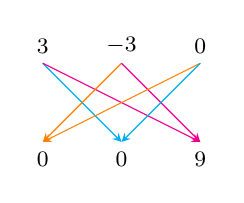
\begin{tikzpicture}[->,samples=100,>=stealth,font=\footnotesize]
                      \node[above] at (0,0) {$3$};
                      \node[above] at (1,0) {$-3$};
                      \node[above] at (2,0) {$0$};
                      \node[below] at (0,-1) {$0$};
                      \node[below] at (1,-1) {$0$};
                      \node[below] at (2,-1) {$9$};
                      \draw[cyan] (0,0)--(1,-1);
                      \draw[magenta] (0,0)--(2,-1);
                      \draw[orange] (1,0)--(0,-1);
                      \draw[magenta] (1,0)--(2,-1);
                      \draw[orange] (2,0)--(0,-1);
                      \draw[cyan] (2,0)--(1,-1);
                  \end{tikzpicture}} $\lambda_1^*=\lambda_2\lambda_3=0,~\lambda_2^*=\lambda_1\lambda_3=0,~\lambda_3^*=\lambda_1\lambda_2=-9$, 由 $\vb*{Q}^\top\vb*{AO}=\vb*{\Lambda}$ 可得
              \begin{flalign*}
                  \vb*{Q}^\top\vb*{A}^*\vb*{Q} & =\vb*{Q}^\top\qty(\vb*{Q\Lambda Q}^\top)^*\vb*{Q}=\vb*{Q}^\top\qty(\vb*{Q}^\top)^*\vb*{\Lambda}^*\vb*{Q}^*\vb*{Q}=\vb*{Q}^\top\qty|\vb*{Q}^\top|\qty(\vb*{Q}^\top)^{-1}\vb*{\Lambda}^*\qty|\vb*{Q}|\vb*{E} \\
                                               & =\vb*{Q}^\top\vb*{Q}|\vb*{Q}|\vb*{\Lambda}^*|\vb*{Q}|\vb*{E}=|\vb*{Q}|^2\vb*{\Lambda}^*\xlongequal{\det\vb*{Q}=\pm1}\vb*{\Lambda}^*
              \end{flalign*}
              因此 $\vb*{Q}^\top\qty(\vb*{A}+\vb*{A}^*)\vb*{Q}=\qty[\mqty(\dmat{3,-3,0})+\mqty(\dmat{0,0,-9})]=\mqty(\dmat{3,-3,-9})$ 即在正交变换 $\vb*{x}=\vb*{Qy}$ 下, 二次型的标准形为 $3y_1^2-3y_2^2-9y_3^2.$
        \item $\vb*{\gamma}$ 可由 $\vb*{\xi}_{1,2,3}$ 线性表示, 即 $\exists k_1,k_2,k_3$, 使得 $\vb*{\gamma}=k_1\vb*{\xi}_1+k_2\vb*{\xi}_2+k_3\vb*{\xi}_3$, 即
              $$\vb*{A}^n\vb*{\gamma}=\vb*{A}^n\qty(k_1\vb*{\xi}_1+k_2\vb*{\xi}_2+k_3\vb*{\xi}_3)=k_1\vb*{A}^n\vb*{\xi}_1+k_2\vb*{A}^n\vb*{\xi}_2+k_3\vb*{A}^n\vb*{\xi}_3=k_1\lambda_1^n\vb*{\xi}_1+k_2\lambda_2^n\vb*{\xi}_2+k_3\lambda_3^n\vb*{\xi}_3=k_1\lambda_1^n\vb*{\xi}_1+k_2\lambda_2^n\vb*{\xi}_2$$
              作增广矩阵 $\vb*{B}=\begin{pNiceArray}{ccc:c}\vb*{\xi}_1&\vb*{\xi}_2&\vb*{\xi}_3&\vb*{\gamma}\end{pNiceArray}=\begin{pNiceArray}{ccc:c}
                      1&-1&1&2\\-1&-1&1&0\\0&2&1&-1
                  \end{pNiceArray}$, 将其化为行最简形
              $$\begin{pNiceArray}{ccc:c}
                      1&-1&1&2\\-1&-1&1&0\\0&2&1&-1
                  \end{pNiceArray}\xrightarrow[\substack{r_1+r_2\\r_3-2r_2}]{\substack{r_2+r_1\\r_2\times\qty(-\frac{1}{2})}}\begin{pNiceArray}{ccc:c}
                      1&0&0&1\\0&1&-1&-1\\0&0&3&1
                  \end{pNiceArray}\xrightarrow[r_2+r_3]{r_3\times\frac{1}{3}}\begin{pNiceArray}{ccc:c}
                      1&0&0&1\\0&1&0&-\dfrac{2}{3}\\[6pt]0&0&1&\dfrac{1}{3}
                  \end{pNiceArray}$$
              因此 $k_1=1,~k_2=-\dfrac{2}{3},~k_3=\dfrac{1}{3}$, 故 $\vb*{A}^n\vb*{\gamma}=\lambda_1^n\vb*{\xi}_1-\dfrac{2}{3}\lambda_2^n\vb*{\xi}_2=\mqty(3^n+\dfrac{2}{3}\cdot(-3)^n\\[6pt]-3^n+\dfrac{2}{3}\cdot(-3)^n\\[6pt]-\dfrac{4}{3}\cdot(-3)^n).$
    \end{enumerate}
\end{solution}

\begin{example}
    设二次型 $$f(x_1,x_2,x_3)=4x_2^2-3x_3^2+2ax_1x_2-4x_1x_3+8x_2x_3~~(a\in\mathbb{N})$$
    经过正交变换 $\vb*{x}=\vb*{Qy}$ 化为标准形为 $y_1^2+6y_2^2+by_3^2$,
    \begin{enumerate}[label=(\arabic{*})]
        \item 求 $a,b$ 的值及正交变换;
        \item 证明: 二次型 $\vb*{x}^\top\qty(\vb*{A}^*+37\vb*{E})\vb*{x}$ 正定, 其中 $\vb*{A}^*$ 为 $\vb*{A}$ 的伴随矩阵.
    \end{enumerate}
\end{example}
\begin{solution}
    \begin{enumerate}[label=(\arabic{*})]
        \item 二次型的矩阵为 $\vb*{A}=\mqty(0&a&-2\\a&4&4\\-2&4&-3)$, 且 $\vb*{A}\sim\diag(1,6,b)$, 由矩阵相似可得 $\tr\vb*{A}=1+6+b,~\det\vb*{A}=6b$, 解得 $a=2,b=-6$, 因此 $\vb*{A}$ 的特征值分别为 $\lambda_1=1,~\lambda_2=6,~\lambda_3=-6$, \\
              \textbf{法一: }$|\lambda\vb*{E}-\vb*{A}|=\mqty|\lambda&-2&2\\-2&\lambda-4&-4\\2&-4&\lambda+3|$, 当 $\lambda=\lambda_1$ 时, $\qty(1\vb*{E}-\vb*{A})\vb*{x}=\vb*{0}$, 解得特征向量为 $\vb*{\xi}_1=(-2,0,1)^\top$; 当 $\lambda=\lambda_2$ 时,
              $(6\vb*{E}-\vb*{A})\vb*{x}=\vb*{0}$, 解得特征向量为 $\vb*{\xi}_2=(1,5,2)^\top$; 当 $\lambda=\lambda_3$ 时, $(-6\vb*{E}-\vb*{A})\vb*{x}=\vb*{0}$, 解得特征向量为 $\vb*{\xi}_3=(1,-1,2)^\top$, \\
              \textbf{法二: }$\lambda=\lambda_1$ 时, $1\vb*{E}-\vb*{A}=\mqty(1&-2&2\\-2&-3&-4\\2&-4&4)\xrightarrow{r_3-2r_1}\mqty(1&-2&2\\-2&-3&-4\\0&0&0)$, $r_1$ 可由 $r_2$ 与 $(3,1,6)$ 线性表示,
              则 $$(-2,-3,-4)\times(3,1,6)=(-14,0,7)\Rightarrow (-2,0,1)\Rightarrow \vb*{\xi}_1=(-2,0,1)^\top$$
              当 $\lambda=\lambda_2$ 时, $6\vb*{E}-\vb*{A}=\mqty(6&-2&2\\-2&2&-4\\2&-4&9)\xrightarrow[\substack{r_2\times\frac{3}{2}\\r_1\times\frac{1}{2}}]{\substack{r_2+\frac{1}{3}r_1\\r_3-\frac{1}{3}r_1\\\frac{3}{5}r_3+\frac{3}{2}r_2}}\mqty(3&-1&1\\0&2&-5\\0&0&0)$, $r_1$ 可由 $r_2$ 与 $(3,-3,6)$ 线性表示, 则
              $$(0,2,-5)\times(3,-3,6)=(-3,-15,-6)\Rightarrow(1,5,2)\Rightarrow \vb*{\xi}_2=(1,5,2)^\top$$
              当 $\lambda=\lambda_3$ 时, $\vb*{-6\vb*{E}-\vb*{A}}=\mqty(-6&-2&2\\-2&-10&-4\\2&-4&-3)\xrightarrow[\substack{r_2-r_1-r_3\\r_2\leftrightarrow r_3}]{\substack{r_1\times\frac{1}{2}\\r_2\times\frac{1}{2}}}\mqty(-3&-1&1\\2&-4&-3\\0&0&0)$, $r_1$ 可由 $r_2$ 与 $(-5,3,4)$ 线性表示, 则
              $$(2,-4,-3)\times(-5,3,4)=(-7,7,-14)\Rightarrow (1,-1,2)\Rightarrow \vb*{\xi}_3=(1,-1,2)^\top$$
              将特征向量 $\vb*{\xi}_{1,2,3}$ 单位化得
              $$\vb*{e}_1=\dfrac{1}{\sqrt{5}}\mqty(-2\\0\\1),~\vb*{e}_2=\dfrac{1}{\sqrt{30}}\mqty(1\\5\\2),~\vb*{e}_3=\dfrac{1}{\sqrt{6}}\mqty(1\\-1\\2)$$
              令 $\vb*{Q}=(\vb*{e}_1,\vb*{e}_2,\vb*{e}_3)$, 则 $\vb*{x}=\vb*{Qy}$ 为所求正交变换, 其中 $\vb*{Q}=\mqty(-\dfrac{2}{\sqrt{5}}&\dfrac{1}{\sqrt{30}}&\dfrac{1}{\sqrt{6}}\\[6pt]0&\dfrac{5}{\sqrt{30}}&-\dfrac{1}{\sqrt{6}}\\[6pt]\dfrac{1}{\sqrt{5}}&\dfrac{2}{\sqrt{30}}&\dfrac{2}{\sqrt{6}})$
        \item 因为 $\vb*{A}$ 的特征值分别为 $1,6,-6$, 因此 $\vb*{A}^*$ 的特征值为 $-36,-6,6$, 那么 $\vb*{A}^*+37\vb*{E}$ 的特征值为 $1,31,43$, 皆大于 0, 因此二次型 $\vb*{x}^\top\qty(\vb*{A}^*+37\vb*{E})\vb*{x}$ 正定.
    \end{enumerate}
\end{solution}

\begin{example}
    设 $\vb*{\alpha}$ 为 3 维非零实列向量, $\vb*{A}=\vb*{E}-\dfrac{a}{\vb*{\alpha}^\top\vb*{\alpha}}\vb*{\alpha\alpha}^\top$ 为正交矩阵, 其中 $a\neq0,~\vb*{E}$ 为三阶单位矩阵,
    \begin{enumerate}[label=(\arabic{*})]
        \item 求 $a$ 的值, 并证明: $\vb*{\alpha}$ 与 $\vb*{A\alpha}$ 线性相关;
        \item 当 $\vb*{\alpha}=(b,b,0)^\top~~(b\neq0)$ 时, 求正交变换 $\vb*{x}=\vb*{Qy}$ 将二次型 $f(x_1,x_2,x_3)=\vb*{x}^\top\vb*{Ax}$ 化为规范形.
    \end{enumerate}
\end{example}
\begin{solution}
    \begin{enumerate}[label=(\arabic{*})]
        \item 由 $\vb*{A}^\top=\qty(\vb*{E}-\dfrac{a}{\vb*{\alpha}^\top\vb*{\alpha}}\vb*{\alpha\alpha}^\top)^\top=\vb*{E}-\dfrac{a}{\vb*{\alpha}^\top\vb*{\alpha}}\qty(\vb*{\alpha\alpha}^\top)^\top=\vb*{E}-\dfrac{a}{\vb*{\alpha}^\top\vb*{\alpha}}\qty(\vb*{\alpha}^\top)^\top\vb*{\alpha}^\top=\vb*{E}-\dfrac{a}{\vb*{\alpha}^\top\vb*{\alpha}}\vb*{\alpha\alpha}^\top=\vb*{A}$ 可知, $\vb*{A}$ 为实对称矩阵, 那么
              \begin{flalign*}
                  \vb*{A}^2=\vb*{AA}^\top=\qty(\vb*{E}-\dfrac{a}{\vb*{\alpha}^\top\vb*{\alpha}}\vb*{\alpha\alpha}^\top)(\vb*{E}-\dfrac{a}{\vb*{\alpha}^\top\vb*{\alpha}}\vb*{\alpha\alpha}^\top)=\vb*{E}-\dfrac{2a}{\vb*{\alpha}^\top\vb*{\alpha}}\vb*{\alpha\alpha}^\top+\dfrac{a^2}{\qty(\vb*{\alpha}^\top\vb*{\alpha})^2}\vb*{\alpha}\underbrace{\vb*{\alpha}^\top\vb*{\alpha}}\vb*{\alpha}^\top=\vb*{E}+\dfrac{a^2-2a}{\vb*{\alpha}^\top\vb*{\alpha}}\vb*{\alpha\alpha}^\top
              \end{flalign*}
              又因为 $\vb*{A}$ 是正交矩阵, 所以 $\vb*{A}^2=\vb*{E}$, 即 $\dfrac{a^2-2a}{\vb*{\alpha}^\top\vb*{\alpha}}\vb*{\alpha\alpha}^\top=\vb*{O}$, 而 $\vb*{\alpha}$ 为 3 维非零实列向量, 即 $\vb*{\alpha}^\top\vb*{\alpha}\neq0,~\vb*{\alpha\alpha}^\top\neq\vb*{O}$,
              因此 $a^2-2a=0\Rightarrow a=2~~(a\neq0)$,
              $\vb*{A\alpha}=\qty(\vb*{E}-\dfrac{a}{\vb*{\alpha}^\top\vb*{\alpha}}\vb*{\alpha\alpha}^\top)\vb*{\alpha}=\vb*{\alpha}-a\vb*{\alpha}=-\vb*{\alpha}$, 因此 $\vb*{\alpha}$ 与 $\vb*{A\alpha}$ 线性相关.
        \item \textbf{法一: }当 $\vb*{\alpha}=(b,b,0)^\top~~(b\neq0)$ 时,
              $$\vb*{\alpha}^\top\vb*{\alpha}=(b,b,0)\mqty(b\\b\\0)=2b^2,~\vb*{\alpha\alpha}^\top=\mqty(b\\b\\0)(b,b,0)=\mqty(b^2&b^2&0\\b^2&b^2&0\\0&0&0)=b^2\mqty(1&1&0\\1&1&0\\0&0&0)$$
              那么 $\vb*{A}=\vb*{E}-\dfrac{2}{\vb*{\alpha}^\top\vb*{\alpha}}\vb*{\alpha\alpha}^\top=\mqty(0&-1&0\\-1&0&0\\0&0&1)$, 因此特征多项式为 (两种方法)
              \begin{enumerate}[label=(\roman{*})]
                  \item $|\lambda\vb*{E}-\vb*{A}|=\begin{pNiceArray}{cc:c}
                                \lambda&1&0\\1&\lambda&0\\ \hdottedline
                                0&0&\lambda-1
                            \end{pNiceArray}=\qty(\lambda^2-1)(\lambda-1)=0$, 得特征值为 $\lambda_1=-1,~\lambda_2=\lambda_3=1$,
                  \item $\lambda^3-\tr\vb*{A}\cdot\lambda^2+\displaystyle\sum_{1\leqslant j_1<j_2\leqslant 3}\mqty|a_{j_1j_1}&a_{j_1j_2}\\a_{j_2j_1}&a_{j_2j_2}|\cdot\lambda-\det\vb*{A}=\lambda^3-\lambda^2-\lambda+1$, 解得 $\lambda_1=-1,~\lambda_2=\lambda_3=1$,
              \end{enumerate}
              当 $\lambda=\lambda_1$ 时, 解得特征向量为 $\vb*{\xi}_1=(1,1,0)^\top$;
              当 $\lambda=\lambda_{2,3}$ 时, 解得对应的特征向量分别为 $\vb*{\xi}_2=(-1,1,0)^\top,~\vb*{\xi}_3=(0,0,1)^\top$,
              将 $\vb*{\xi}_{1,2,3}$ 分别单位化, 得
              $$\vb*{e}_1=\dfrac{1}{\sqrt{2}}\mqty(1\\1\\0),~\vb*{e}_2=\dfrac{1}{\sqrt{2}}\mqty(-1\\1\\0),~\vb*{e}_3=\mqty(0\\0\\1)$$
              令 $\vb*{Q}=(\vb*{e}_1,\vb*{e}_2,\vb*{e}_3)$, 在正交变换 $\vb*{x}=\vb*{Qy}$ 下, 标准形为 $-y_1^2+y_2^2+y_2^2$ 也是规范形.\\
              \textbf{法二: }不妨设 $\vb*{B}=\vb*{\alpha\alpha}^\top=b^2\mqty(1&1&0\\1&1&0\\0&0&0)\Rightarrow b^2\begin{pNiceMatrix}
                      \Block[borders={bottom,tikz=dashed}]{1-3}{}1 & 1 & 0 \\
                      0                                            & 0 & 0 \\
                      0                                            & 0 & 0 \\
                  \end{pNiceMatrix}$, 则 $\rank\vb*{B}=1$, 所以矩阵 $\vb*{B}$ 的特征值为
              $$\lambda_{b1}=\lambda_{b2}=0,~\lambda_{b3}=\tr\vb*{B}=\vb*{\alpha}^\top\vb*{\alpha}=2b^2$$
              又因为 $\vb*{A}=\vb*{E}-\dfrac{2}{\vb*{\alpha}^\top\vb*{\alpha}}\vb*{\alpha\alpha}^\top=\vb*{E}-\dfrac{1}{b^2}\vb*{B}$,
              因此矩阵 $\vb*{A}$ 的特征值为 $\lambda_{a1}=\lambda_{a2}=1,~\lambda_{a3}=-1$, 并且 $\lambda_{b1}$ 对应的特征向量为 $\vb*{\xi}_1=(-1,1,0)^\top$; $\lambda_{b2}$ 对应的特征向量为 $\vb*{\xi}_2=(0,0,1)^\top$;
              $$\vb*{B\alpha}=\vb*{\alpha\alpha}^\top\vb*{\alpha}=\tr\vb*{B}\cdot\vb*{\alpha}\Rightarrow\vb*{\xi}_3=(1,1,0)^\top$$
              单位化得 $\vb*{e}_1=\dfrac{1}{\sqrt{2}}\mqty(-1\\1\\0),~\vb*{e}_2=\mqty(0\\0\\1),~\vb*{e}_3=\dfrac{1}{\sqrt{2}}\mqty(1\\1\\0)$, 令 $\vb*{Q}=(\vb*{e}_1,\vb*{e}_2,\vb*{e}_3)$, 则在正交变换 $\vb*{x}=\vb*{Qy}$ 下, 标准形为 $y_1^2+y_2^2-y_3^2$  也是规范形.
    \end{enumerate}
\end{solution}

\begin{example}
    设 $\vb*{P}=\mqty(\cos\theta&-\sin\theta\\\sin\theta&\cos\theta)$ 为二阶正交矩阵, 证明: $\vb*{P}^{n}$ 可以表示为 $$\vb*{P}^{n}=\mqty(\cos(n\theta)&-\sin(n\theta)\\ \sin(n\theta)&\cos(n\theta)).$$
    \label{zjjzzmti}
\end{example}
\begin{proof}[{\songti \textbf{证}}]
    当 $n=2$ 时, $\vb*{P}^{2}=\vb*{P}\cdot\vb*{P}=\mqty(\cos\theta&-\sin\theta\\\sin\theta&\cos\theta)\mqty(\cos\theta&-\sin\theta\\\sin\theta&\cos\theta)=\mqty(\cos2\theta&-\sin2\theta\\\sin2\theta&\cos2\theta)$, 当 $n=3$ 时, $\vb*{P}^{3}=\vb*{P}^{2}\cdot\vb*{P}=\mqty(\cos2\theta&-\sin2\theta\\\sin2\theta&\cos2\theta)\mqty(\cos\theta&-\sin\theta\\\sin\theta&\cos\theta)=\mqty(\cos3\theta&-\sin3\theta\\\sin3\theta&\cos3\theta)$, 猜想 $\vb*{P}^{k}=\mqty(\cos k\theta&-\sin k\theta\\\sin k\theta&\cos k\theta)$, 下面利用数学归纳法证明:\\
    当 $k=1,2$ 时, 显然成立, 假设当 $k=n$ 时, 公式成立, 那么当 $k=n+1$ 时, 有
    \begin{flalign*}
        \vb*{P}^{n+1} & =\vb*{P}^{n}\cdot\vb*{P}=\mqty(\cos n\theta & -\sin n\theta    \\\sin n\theta&\cos n\theta)\mqty(\cos\theta&-\sin\theta\\\sin\theta&\cos\theta)=\mqty(\cos n\theta\cos\theta-\sin n\theta\sin\theta&-\cos n\theta\sin\theta-\sin n\theta\cos\theta\\ \sin n\theta\cos\theta+\cos n\theta\sin\theta&-\sin n\theta\sin\theta+\cos n\theta\cos\theta)\\
                      & =\mqty(\cos(n+1)\theta                      & -\sin(n+1)\theta \\\sin(n+1)\theta&\cos(n+1)\theta)
    \end{flalign*}
    显然此时, 猜想公式成立, 因此对一切的正整数 $n$, 猜想的公式均成立, 故 $\vb*{P}^{n}=\mqty(\cos(n\theta)&-\sin(n\theta)\\ \sin(n\theta)&\cos(n\theta)).$
\end{proof}

\begin{example}
    已知 $\vb*{A}=\mqty(1&-\dfrac{x}{n}\\ \dfrac{x}{n}&1)$, 计算 $\displaystyle \lim_{x \to 0}\qty[\lim_{n \to +\infty}\dfrac{1}{x}\qty(\vb*{E}-\vb*{A}^{n})]$ (注明: 矩阵的极限, 即它每个元素取极限, 且 $n\in\mathbb{N}^{*}$).
\end{example}
\begin{solution}
    注意到 $\vb*{A}$ 的列向量相互正交, 且模为 $|\vb*{\alpha}|=\sqrt{1^2+\qty(\pm\dfrac{x}{n})^n}=\sqrt{1+\dfrac{x^2}{n^2}}$, 把矩阵 $\vb*{A}$ 表示为 $\vb*{A}=\vb*{\alpha P}$, 其中 $\vb*{P}$ 为正交矩阵, 由例题 \ref{zjjzzmti} 知
    $$
        \vb*{A}^{n}=\vb*{\alpha}^{n}\mqty(\cos(n\theta)&-\sin(n\theta)\\ \sin(n\theta)&\cos(n\theta))
    $$
    其中 $\theta=\arcsin\qty(\dfrac{x}{n|\vb*{\alpha}|})$, 当 $n\to+\infty$ 时, 有 $$|\vb*{\alpha}|=\lim_{n \to +\infty}\qty(1+\dfrac{x^2}{n^2})^{\frac{1}{2}}=1,~|\vb*{\alpha}|^{n}=1$$
    而 $n\theta=\dfrac{x}{|\vb*{\alpha}|}\qty(\dfrac{|\vb*{\alpha}|n}{x}\arcsin\dfrac{x}{n|\vb*{\alpha}|})\to x~(n\to+\infty)$, 所以 $\displaystyle \lim_{n \to +\infty}\qty(\vb*{E}-\vb*{A}^{n})=\mqty(1-\cos x& \sin x\\ -\sin x&1-\cos x)$
    \begin{flalign*}
        \lim_{x\to0}\qty[\lim_{n \to +\infty}\dfrac{1}{x}\qty(\vb*{E}-\vb*{A}^{n})] & =\lim_{x\to0}\dfrac{1}{x}\mqty(1-\cos x             & \sin x                                     \\ -\sin x&1-\cos x)=\lim_{x\to0}\mqty(\dfrac{1-\cos x}{x}&\dfrac{\sin x}{x}\\ -\dfrac{\sin x}{x}&\dfrac{1-\cos x}{x})\\
                                                                                    & =\mqty(\displaystyle\lim_{x\to0}\dfrac{1-\cos x}{x} & \displaystyle\lim_{x\to0}\dfrac{\sin x}{x} \\[6pt] \displaystyle\lim_{x\to0}-\dfrac{\sin x}{x}&\displaystyle\lim_{x\to0}\dfrac{1-\cos x}{x})=\mqty(0&1\\-1&0).
    \end{flalign*}

\end{solution}

\subsection{谱分解}

\begin{theorem}[谱分解定理]
    \label{pufjdli}若 $n$ 阶矩阵 $\vb*{A}$ 的特征值为 $\lambda_i$, 所对应特征向量为 $\vb*{x}_i$, 经过单位化和正交化, 化为两两正交的单位特征向量 $\vb*{e}_i~ (i=1,2,\cdots,n)$, 则有
    $$\vb*{A}=\sum_{i=1}^{n}\lambda_i\vb*{e}_i\vb*{e}_i^\top.$$
\end{theorem}

\begin{example}
    设 $\vb*{A}=(a_{ij})_{3\times3}$ 为实对称矩阵, $\vb*{A}$ 的每行元素之和均为 $0$, 设 $2,3$ 是 $\vb*{A}$ 的非零特征值, 则 $a_{11}$ 对应的代数余子式 $\vb*{A}_{11}$ 为
    \begin{tasks}(4)
        \task $1$
        \task $2$
        \task $5$
        \task $6$
    \end{tasks}
\end{example}
\begin{solution}
    因为 $\vb*{A}$ 的每行元素之和均为 $0$, 故由定理 \ref{hangjunhedl} 知, $\vb*{A}$ 的另一特征值为 $0$, 因此矩阵 $\vb*{A}$ 的全部特征值为 $0,2,3$, 又由定理 \ref{bsjzdtzzB} 知矩阵 $\vb*{A}$ 的伴随矩阵的特征值为
    $$\lambda_1^*=2\times3=6,~\lambda_2^*=0\times 3=0,~\lambda_3^*=0\times 2=0$$
    且 $\lambda_1^*$ 对应的特征向量为 $(1,1,1)^\top$, 又由定理 \ref{pufjdli}, 知 $$\vb*{A}^*=6\mqty(\dfrac{1}{\sqrt{3}}\\[6pt]\dfrac{1}{\sqrt{3}}\\[6pt]\dfrac{1}{\sqrt{3}})\qty(\dfrac{1}{\sqrt{3}}~\dfrac{1}{\sqrt{3}}~\dfrac{1}{\sqrt{3}})=\mqty(2&2&2\\2&2&2\\2&2&2)$$
    故 $\vb*{A}_{11}=2$, 选 B.
\end{solution}

\begin{example}
    设 $\vb*{A}$ 为三阶实对称不可逆矩阵, 且 $\mqty(2&-2&1\\-2&-1&2)\vb*{A}=\mqty(6&-6&3\\-12&-6&12)$, 求 $\vb*{A}.$
\end{example}
\begin{solution}
    对等式两边同时转置, 有 $\vb*{A}^\top\mqty(2&-2\\-2&-1\\1&2)=\mqty(6&-12\\-6&-6\\3&12)$, 令 $\vb*{\xi}_1=(2,-2,1)^\top,~\vb*{\xi}_2=(-2,-1,2)^\top$, 则有 $$\vb*{A}^\top\vb*{\xi}_1=3\vb*{\xi}_1,~\vb*{A}^\top\vb*{\xi}_2=6\vb*{\xi}_2\Rightarrow \lambda_1=3,~\lambda_2=6$$
    又因为 $\vb*{A}$ 不可逆, 所以 $\det\vb*{A}=0\Rightarrow \lambda_1\lambda_2\lambda_3=0\Rightarrow \lambda_3=0$, 所以 $\vb*{A}$ 的特征值分别为 $2,6,0$, 故
    $$\vb*{A}=\sum_{i=1}^{3}\lambda_i\vb*{e}_i\vb*{e}_i^\top=\sum_{i=1}^{3}\lambda_i\cdot\dfrac{\vb*{\xi}_i}{\norm*{\vb*{\xi}_i}}\cdot\qty(\dfrac{\vb*{\xi}_i}{\norm*{\vb*{\xi}_i}})^\top=3\cdot\dfrac{1}{3}\mqty(2\\-2\\1)\cdot\dfrac{1}{3}(2,-2,1)+6\cdot\dfrac{1}{3}\mqty(-2\\-1\\2)\cdot(-2,-1,2)=\mqty(4&0&-2\\0&2&-2\\-2&-2&3).$$
\end{solution}

\begin{example}
    矩阵 $\vb*{A}$ 为 3 阶实对称矩阵, 特征值为 $0,1,1$, 且 $\vb*{\alpha}_1=\mqty(1\\a\\0),~\vb*{\alpha}_2=\mqty(1\\-1\\a)$ 是 $\vb*{A}$ 的两个不同的特征向量, 若 $\vb*{A}(\vb*{\alpha}_1+\vb*{\alpha}_2)=\vb*{\alpha}_2$, 求 $\vb*{A}$.
\end{example}
\begin{solution}
    若 $\vb*{\alpha}_1,\vb*{\alpha}_2$ 都为 $0$ 的特征向量, 则 $\vb*{A}(\vb*{\alpha}_1+\vb*{\alpha}_2)=\vb*{0}$, 与已知条件矛盾;
    若 $\vb*{\alpha}_1,\vb*{\alpha}_2$ 都为 $1$ 的特征向量, 则 $\vb*{A}(\vb*{\alpha}_1+\vb*{\alpha}_2)=\vb*{\alpha}_1+\vb*{\alpha}_2$, 与已知条件矛盾;
    若 $\vb*{\alpha}_1,\vb*{\alpha}_2$ 分别为 $1,0$ 的特征向量, 则 $\vb*{A}(\vb*{\alpha}_1+\vb*{\alpha}_2)=\vb*{\alpha}_1$, 与已知条件矛盾;
    综上, $\vb*{\alpha}_1$ 与 $\vb*{\alpha}_2$ 分别为 $0,1$ 的特征向量, 又 $\vb*{A}$ 为实对称矩阵, 那么 $\vb*{\alpha}_1$ 与 $\vb*{\alpha}_2$ 相互正交, 那么它们的内积为零, 解得 $a=0$, 故
    $\vb*{\alpha}_1=(1,1,0)^\top,~\vb*{\alpha}_2=(1,-1,1)^\top$, 并且 $\vb*{A}-\vb*{E}$ 的特征值为 $-1,0,0$, 由定理 \ref{pufjdli} 知
    $$\vb*{A}-\vb*{E}=(-1)\cdot\dfrac{1}{\sqrt{2}}\mqty(1\\1\\0)\cdot\dfrac{1}{\sqrt{2}}\mqty(1,1,0)=-\dfrac{1}{2}\mqty(1&1&0\\1&1&0\\0&0&0)\Rightarrow \vb*{A}=\mqty(\dfrac{1}{2}&-\dfrac{1}{2}&0\\[6pt]-\dfrac{1}{2}&\dfrac{1}{2}&0\\[6pt]0&0&1).$$
\end{solution}

\begin{example}
    假设 3 阶实对称矩阵 $\vb*{A}$ 的秩为 2, 并且 $\vb*{AB}=\vb*{C}$, 其中 $\vb*{B}=\mqty(1&1\\0&0\\-1&1),~\vb*{C}=\mqty(-1&1\\0&0\\1&1)$, 求 $\vb*{A}$ 的所有特征值及相应的特征向量, 并求矩阵 $\vb*{A}$ 及 $\vb*{A}^{2023}.$
\end{example}
\begin{solution}
    设 $\vb*{\xi}_1=(1,0,-1)^\top,~\vb*{\xi}_2=(1,0,1)^\top$ 那么 $\vb*{B}=(\vb*{\xi}_1,\vb*{\xi}_2),~\vb*{C}=(-\vb*{\xi}_1,\vb*{\xi}_2)$, 于是 $$\vb*{AB}=\vb*{C}\Rightarrow \vb*{A}(\vb*{\xi}_1,\vb*{\xi}_2)=(-\vb*{\xi}_1,\vb*{\xi}_2)$$
    即 $\vb*{A\xi}_1=-\vb*{\xi}_1,~\vb*{A\xi}_2=\vb*{\xi}_2$, 则 $\lambda_1=-1,\lambda_2=0$ 是 $\vb*{A}$ 的特征值, $\vb*{\xi}_1,\vb*{\xi}_2$ 是 $\vb*{A}$ 的分别属于 $\lambda_1,\lambda_2$ 的特征向量, 又 $\rank\vb*{A}=2$, 则 $\vb*{\xi}_3=0$, 于是
    $$\vb*{A}=\sum_{i=1}^{3}\lambda_i\vb*{e}_1\vb*{e}_1^\top=(-1)\cdot\dfrac{1}{\sqrt{2}}\mqty(1\\0\\-1)\cdot\dfrac{1}{\sqrt{2}}(1,0,-1)+1\cdot\dfrac{1}{\sqrt{2}}\mqty(1\\0\\1)\cdot\dfrac{1}{\sqrt{2}}(1,0,1)+0=\mqty(1&0&0\\0&0&0\\0&0&1)$$
    那么 $\vb*{A}^{2023}=\vb*{A}=\mqty(1&0&0\\0&0&0\\0&0&1).$
\end{solution}

\begin{example}
    设 3 阶实对称矩阵 $\vb*{A}=(\vb*{\alpha}_1, \vb*{\alpha}_2, \vb*{\alpha}_3), \vb*{A}^2=\vb*{A}$ 且 $\rank\vb*{A}=2, \vb*{\alpha}_1+\vb*{\alpha}_2=\vb*{\alpha}_3$,
    \begin{enumerate}[label=(\arabic{*})]
        \item 求矩阵 $\vb*{A}$;
        \item 求正交矩阵 $\vb*{Q}$, 使得二次型 $\vb*{x}^\top\vb*{Ax}$ 经正交变换 $\vb*{x}=\vb*{Qy}$ 化为标准形.
    \end{enumerate}
\end{example}
\begin{solution}
    \begin{enumerate}[label=(\arabic{*})]
        \item 因为 $$
                  \vb*{A}^2-\vb*{A}=\vb*{O}\Rightarrow \vb*{A}(\vb*{A}-\vb*{E})=\vb*{O}\Rightarrow \lambda=1\text{ 或 }0
              $$
              又 $\rank\vb*{A}=2$, 所以矩阵 $\vb*{A}$ 的特征值分别为 $1,1,0$, 又 $$
                  \vb*{\alpha}_1+\vb*{\alpha}_2-\vb*{\alpha}_3=\vb*{0}\Rightarrow (\vb*{\alpha}_1, \vb*{\alpha}_2, \vb*{\alpha}_3)\mqty(1\\ 1\\ -1)=\vb*{0}\Rightarrow \vb*{A}\mqty(1\\ 1\\ -1)=0\cdot \mqty(1\\ 1\\ -1)
              $$
              于是特征值 $0$ 对应的特征向量为 $(1,1,-1)^\top$, 故
              $$
                  \vb*{A}-\vb*{E}=-1\cdot\dfrac{1}{\sqrt{3}}\mqty(1\\1\\-1)\cdot\dfrac{1}{\sqrt{3}}(1,1,-1)=\dfrac{1}{3}\begin{pmatrix} -1 & -1 & 1 \\ -1 & -1 & 1 \\ 1 & 1 & -1 \\\end{pmatrix}
              $$
              即 $\vb*{A}=\dfrac{1}{3}\begin{pmatrix} 2 & -1 & 1 \\ -1 & 2 & 1 \\ 1 & 1 & 2 \\\end{pmatrix}$.
        \item 由 (1) 知, $\vb*{A}-\vb*{E}\to \begin{pmatrix} 1 & 1 & -1 \\ 0 & 0 & 0 \\ 0 & 0 & 0 \\\end{pmatrix}$, 令 $\vb*{\xi}_1=(-1,1,0)^\top, \vb*{\xi}_3=(1,1,-1)^\top$, 那么特征值 $1$ 的另一个特征向量为
              $$
                  (-1,1,0)\times (1,1,-1)=(-1,-1,-2) \text{ 可取 }\vb*{\xi}_2=(1,1,2)
              $$
              于是 $\vb*{Q}=\qty(\dfrac{\vb*{\xi}_1}{\norm*{\vb*{\xi}_1}}, \dfrac{\vb*{\xi}_2}{\norm*{\vb*{\xi}_2}}, \dfrac{\vb*{\xi}_3}{\norm*{\vb*{\xi}_3}})=\begin{pmatrix} -\dfrac{1}{\sqrt{2}} & \dfrac{1}{\sqrt{6}} & \dfrac{1}{\sqrt{3}} \\ \dfrac{1}{\sqrt{2}} & \dfrac{1}{\sqrt{6}} & \dfrac{1}{\sqrt{3}} \\ 0 & \dfrac{2}{\sqrt{6}} & -\dfrac{1}{\sqrt{3}} \\\end{pmatrix}$.
    \end{enumerate}
\end{solution}

\begin{example}
    设 3 阶实对称矩阵 $\vb*{A}$ 的每行元素之和为 3, 且 $\rank\vb*{A}=1,~\vb*{\beta}=(-1,2,2)^\top$, \\
    \begin{enumerate*}[label=(\arabic{*})]
        \item 求 $\vb*{A}^n\vb*{\beta}$;
        \item 求 $\qty(\vb*{A}-\dfrac{3}{2}\vb*{E})^{2024}.$
    \end{enumerate*}
\end{example}
\begin{solution}
    \begin{enumerate}[label=(\arabic{*})]
        \item \textbf{法一: }因为 $\vb*{A}$ 的每行元素之和为 3, 故特征值 $\lambda_1=3$, 且对应的特征向量为 $\vb*{\xi}_1=(1,1,1)^\top$, 又因为 $\vb*{A}$ 是实对称矩阵, 所以 $\vb*{A}$ 一定能相似对角化, 并且由 $\rank\vb*{A}=1$, 故矩阵 $\vb*{A}$ 的非零特征值个数为 1, 即 $\lambda_2=\lambda_3=0$, 设其对应的特征向量为 $\vb*{\xi}_2,~\vb*{\xi}_3$,
              则 $\vb*{\xi}_1,\vb*{\xi}_2,\vb*{\xi}_3$ 相互正交, 故可令 $\vb*{\xi}_2=(-1,1,0)^\top,~\vb*{\xi}_3=(-1,0,1)^\top$, 因为 $\vb*{\xi}_1,\vb*{\xi}_2,\vb*{\xi}_3$ 是三维空间中线性无关的三个向量, 则其线性组合能表示该空间中的任一向量, 即 $\exists k_1,k_2,k_3$, 使得 $\vb*{\beta}=k_1\vb*{\xi}_1+k_2\vb*{\xi}_2+k_3\vb*{\xi}_3$, 即
              $$\vb*{A}^n\vb*{\beta}=\vb*{A}^n\qty(k_1\vb*{\xi}_1+k_2\vb*{\xi}_2+k_3\vb*{\xi}_3)=k_1\vb*{A}^n\vb*{\xi}_1+k_2\vb*{A}^n\vb*{\xi}_2+k_3\vb*{A}^n\vb*{\xi}_3=k_1\lambda_1^n\vb*{\xi}_1+k_2\lambda_2^n\vb*{\xi}_2+k_3\lambda_3^n\vb*{\xi}_3$$
              作增广矩阵 $\vb*{B}=\begin{pNiceArray}{ccc:c}\vb*{\xi}_1&\vb*{\xi}_2&\vb*{\xi}_3&\vb*{\beta}\end{pNiceArray}=\begin{pNiceArray}{ccc:c}1&-1&-1&-1\\1&1&0&2\\1&0&1&2\end{pNiceArray}$, 将其化为行最简形
              $$\begin{pNiceArray}{ccc:c}1&-1&-1&-1\\1&1&0&2\\1&0&1&2\end{pNiceArray}\xrightarrow[r_1+r_3]{r_2-r_1\\r_3-r_1}\begin{pNiceArray}{ccc:c}1&0&1&2\\0&1&2&3\\0&2&1&3\end{pNiceArray}\xrightarrow[\substack{r_1-r_3\\r_2-2r_3}]{\substack{r_2\leftrightarrow r_3\\r_3-2r_2\\r_3\times(-\frac{1}{3})}}\begin{pNiceArray}{ccc:c}1&0&0&2\\0&1&0&1\\0&0&1&1\end{pNiceArray}$$
              因此 $k_1=2,~k_2=1,~k_3=1$, 故 $\vb*{A}^n\vb*{\beta}=2\lambda_1^n\vb*{\xi}_1+\lambda_2^n\vb*{\xi}_2+\lambda_3^n\vb*{\xi}_3=\mqty(2\cdot 3^n\\2\cdot 3^n\\2\cdot 3^n)=3^{n}\mqty(1\\1\\1).$\\
              \textbf{法二: }同上, 得 $\lambda_1=3,~\lambda_2=\lambda_3=0,~\vb*{\xi}_1=(1,1,1)^\top$, 将 $\vb*{\xi}_1$ 单位化, 得 $\vb*{e}_1=\dfrac{1}{\sqrt{3}}\mqty(1\\1\\1)$, 因此
              $$\vb*{A}=\sum_{i=1}^{3}\lambda_i\vb*{e}_i\vb*{e}_i^\top=\lambda_1\vb*{e}_1\vb*{e}_1^\top=3\cdot\dfrac{1}{\sqrt{3}}\mqty(1\\1\\1)\cdot\dfrac{1}{\sqrt{3}}(1,1,1)=\mqty(1&1&1\\1&1&1\\1&1&1)$$
              又因为 $\rank\vb*{A}=1$, 故 $\vb*{A}^n=(\tr\vb*{A})^{n-1}\cdot\vb*{A}$, 因此 $\vb*{A}^n\vb*{\beta}=3^{n-1}\vb*{A\beta}=3^{n-1}\mqty(3\\3\\3)=3^{n}\mqty(1\\1\\1).$
        \item 因为 $\vb*{A}$ 的特征值分别为 $3,0,0$, 则 $\vb*{A}-\dfrac{3}{2}\vb*{E}$ 的特征值分别为 $\dfrac{3}{2},-\dfrac{3}{2},-\dfrac{3}{2}$, 又因为 $\vb*{A}$ 是实对称矩阵, 即 $\exists\vb*{P}$, 使得 $\vb*{P}^{-1}\vb*{AP}=\vb*{\Lambda}$, 则有
              $\vb*{P}^{-1}\qty(\vb*{A}-\dfrac{3}{2}\vb*{E})\vb*{P}=\vb*{\Lambda}_2=\mqty(\dfrac{3}{2}\\&-\dfrac{3}{2}\\&&-\dfrac{3}{2})$, 因此
              \begin{flalign*}
                  \qty(\vb*{A}-\dfrac{3}{2}\vb*{E})^{2024} & =\underbrace{\vb*{P\Lambda _2}\overbrace{\vb*{P}^{-1}\cdot \vb*{P}}^{\vb*{E}} \vb*{\Lambda _2P}^{-1}\cdots\vb*{P\Lambda _2P}^{-1}}_{2024} =\vb*{P}\vb*{\Lambda}_2^{2024}\vb*{P}^{-1}=\vb*{P}\mqty(\dfrac{3}{2} \\&-\dfrac{3}{2}\\&&-\dfrac{3}{2})^{2024}\vb*{P}^{-1}\\
                                                           & =\vb*{P}\qty(\dfrac{3}{2})^{2024}\vb*{EP}^{-1}=\qty(\dfrac{3}{2})^{2024}\vb*{PP}^{-1}=\qty(\dfrac{3}{2})^{2024}\vb*{E}.
              \end{flalign*}
    \end{enumerate}
\end{solution}

\begin{example}
    设二次型 $f(x_1,x_2,x_3)$ 的矩阵为 $\vb*{A}$, 已知 $$|\vb*{A}+\vb*{E}|=0,~\vb*{AB}-2\vb*{B}=\vb*{O}$$
    其中 $\vb*{B}=\mqty(-1&-1&-1\\1&0&2\\0&1&-1)$, 求一个正交变换 $\vb*{x}=\vb*{Qy}$, 将二次型 $f(x_1,x_2,x_3)$ 化为标准形, 并写出矩阵 $\vb*{A}$.
\end{example}
\begin{solution}
    \textbf{法一: }由 $|\vb*{A}+\vb*{E}|=|\vb*{A}-(-1)\vb*{E}|=0$, 知 $\vb*{A}$ 的一个特征值为 $\lambda_1=-1$, 且记 $\vb*{B}=(\vb*{\beta}_1,\vb*{\beta}_2,\vb*{\beta}_3)$, 由 $\vb*{AB}-2\vb*{B}=\vb*{O}$ 知
    $$\vb*{A}(\vb*{\beta}_1,\vb*{\beta}_2,\vb*{\beta}_3)=(\vb*{A\beta}_1,\vb*{A\beta}_2,\vb*{A\beta}_3)=(2\vb*{\beta}_1,2\vb*{\beta}_2,2\vb*{\beta}_3)$$
    又 $\rank\vb*{B}=2$, 所以 2 是矩阵 $\vb*{A}$ 的二重特征值, 对应的特征向量分别为\footnote{这里最好要选择矩阵 $\vb*{B}$ 中已经正交的向量, 可以由 $\vb*{B}=\mqty(0&-1&-1\\0&0&2\\0&1&-1)$, 且 $(-1,0,1)\cdot(-1,2,-1)=0$ 知选 $\vb*{\beta}_2$ 与 $\vb*{\beta}_3$ 最合适.}
    $\vb*{\xi}_2=\vb*{\beta}_2,~\vb*{\xi}_3=\vb*{\beta}_3$, 且已正交, 又因为 $\vb*{A}$ 是二次型的系数矩阵, 则 $\vb*{A}$ 是实对称矩阵\footnote{一般地, 不考虑带有虚数的多项式.}, 设 $\lambda_1$ 对应的特征向量为 $\vb*{\xi}_1$, 于是
    $$(-1,0,1)\times(-1,2,1)=(-2,-2,-2)\Rightarrow (1,1,1)\Rightarrow \vb*{\xi}_1=(1,1,1)^\top$$
    分别将特征向量 $\vb*{\xi}_{1,2,3}$ 单位化, 有 $\vb*{e}_1=\dfrac{1}{\sqrt{3}}\mqty(1\\1\\1),~\vb*{e}_2=\dfrac{1}{\sqrt{2}}\mqty(-1\\0\\1),~\vb*{e}_3=\dfrac{1}{\sqrt{6}}\mqty(-1\\2\\-1)$, 那么
    $$\vb*{Q}=(\vb*{e}_1,\vb*{e}_2,\vb*{e}_3)=\mqty(\dfrac{1}{\sqrt{3}}&-\dfrac{1}{\sqrt{2}}&-\dfrac{1}{\sqrt{6}}\\[6pt]\dfrac{1}{\sqrt{3}}&0&\dfrac{2}{\sqrt{6}}\\[6pt]\dfrac{1}{\sqrt{3}}&\dfrac{1}{\sqrt{2}}&-\dfrac{1}{\sqrt{6}})$$
    因此 $\vb*{Q}^\top\vb*{AQ}=\vb*{\Lambda}=\mqty(\dmat{-1,2,2})$, 因此二次型的标准形为 $f(y_1,y_2,y_3)=-y_1^2+2y_2^2+2y_3^2$,
    \begin{flalign*}
        \vb*{A} & =\mqty(\dfrac{1}{\sqrt{3}}  & -\dfrac{1}{\sqrt{2}} & -\dfrac{1}{\sqrt{6}} \\[6pt]\dfrac{1}{\sqrt{3}}&0&\dfrac{2}{\sqrt{6}}\\[6pt]\dfrac{1}{\sqrt{3}}&\dfrac{1}{\sqrt{2}}&-\dfrac{1}{\sqrt{6}})\mqty(\dmat{-1,2,2})\mqty(\dfrac{1}{\sqrt{3}}&-\dfrac{1}{\sqrt{2}}&-\dfrac{1}{\sqrt{6}}\\[6pt]\dfrac{1}{\sqrt{3}}&0&\dfrac{2}{\sqrt{6}}\\[6pt]\dfrac{1}{\sqrt{3}}&\dfrac{1}{\sqrt{2}}&-\dfrac{1}{\sqrt{6}})^\top\\
                & =\mqty(-\dfrac{1}{\sqrt{3}} & -\dfrac{2}{\sqrt{2}} & -\dfrac{2}{\sqrt{6}} \\[6pt]-\dfrac{1}{\sqrt{3}}&0&\dfrac{4}{\sqrt{6}}\\[6pt]-\dfrac{1}{\sqrt{3}}&\dfrac{2}{\sqrt{2}}&-\dfrac{2}{\sqrt{6}})\mqty(\dfrac{1}{\sqrt{3}}&-\dfrac{1}{\sqrt{2}}&-\dfrac{1}{\sqrt{6}}\\[6pt]\dfrac{1}{\sqrt{3}}&0&\dfrac{2}{\sqrt{6}}\\[6pt]\dfrac{1}{\sqrt{3}}&\dfrac{1}{\sqrt{2}}&-\dfrac{1}{\sqrt{6}})^\top=\mqty(1&-1&-1\\-1&1&-1\\-1&-1&1).
    \end{flalign*}
    \textbf{法二: }同上得 $\lambda_1=-1,~\lambda_2=\lambda_3=2,~\vb*{\xi}_1=(1,1,1)^\top,~\vb*{\xi}_2=(-1,0,1)^\top,~\vb*{\xi}_3=(-1,2,-1)^\top$, 那么 $\vb*{A}-2\vb*{E}$ 的特征值分别为 $-3,0,0$, 则
    $$\vb*{A}-2\vb*{E}=-3\vb*{e}_1\vb*{e}_1^\top=-3\cdot\dfrac{1}{\sqrt{3}}\mqty(1\\1\\1)\cdot\dfrac{1}{\sqrt{3}}(1,1,1)=-\mqty(1&1&1\\1&1&1\\1&1&1)\Rightarrow \vb*{A}=\mqty(1&-1&-1\\-1&1&-1\\-1&-1&1).$$
\end{solution}

\begin{example}
    设 3 阶实矩阵 $\vb*{A}$ 及其伴随矩阵 $\vb*{A}^*$ 满足 $\vb*{A}-\vb*{A}^*-\vb*{E}=\vb*{O}$, 且 $\det\vb*{A}=2$,
    \begin{enumerate}[label=(\arabic{*})]
        \item 证明: $\vb*{A}$ 能相似对角化;
        \item 如果 $\vb*{A}$ 为实对称矩阵, 且 $\vb*{\xi}=(1,1,-1)^\top$ 是齐次线性方程组 $(\vb*{A}-2\vb*{E})\vb*{x}=\vb*{0}$ 的一个解, 求对称矩阵 $\vb*{B}$, 使得 $\vb*{B}^2=\vb*{A}+\vb*{E}$.
    \end{enumerate}
\end{example}
\begin{solution}
    \begin{enumerate}[label=(\arabic{*})]
        \item 因为 $\vb*{AA}^*=\vb*{A}^*\vb*{A}=|\vb*{A}|\vb*{E}=2\vb*{E}$, 所以
              $$\vb*{A}\qty(\vb*{A}-\vb*{A}^*-\vb*{E})=\vb*{O}\Rightarrow \vb*{A}^2-\vb*{A}-2\vb*{E}=\vb*{O}\Rightarrow (\vb*{A}+\vb*{E})(\vb*{A}-2\vb*{E})=\vb*{O}$$
              那么 $$3=\rank\qty[(\vb*{A}+\vb*{E})-(\vb*{A}-2\vb*{E})]\leqslant \rank(\vb*{A}+\vb*{E})+\rank(\vb*{A}-2\vb*{E})\leqslant 3\Rightarrow \rank(\vb*{A}+\vb*{E})+\rank(\vb*{A}-2\vb*{E})=3$$
              又因为属于特征值 -1 的特征向量的个数为 $3-\rank(\vb*{A}+\vb*{E})$, 属于特征值 2 的特征向量的个数为 $3-\rank(\vb*{A}-2\vb*{E})$, 相加得 $\vb*{A}$ 有 3 个线性无关的特征向量, 即 $\vb*{A}$ 能相似对角化.
        \item 由 (1) 可知, 矩阵 $\vb*{A}$ 的两个特征值分别为 $\lambda_1=-1,~\lambda_2=2$, 且 $\det\vb*{A}=2=\lambda_1\lambda_2\lambda_3$, 所以 $\lambda_3=-1$, 又因为 $\vb*{\xi}=(1,1,-1)^\top$ 是齐次线性方程组 $(\vb*{A}-2\vb*{E})\vb*{x}=\vb*{0}$ 的一个解,
              所以 $\lambda_2$ 对应的特征向量为 $\vb*{\xi}=(1,1,-1)^\top$, 故 $\vb*{A}+\vb*{E}$ 的两个特征值分别为 $3,~0,~0$, 所以存在正交矩阵 $\vb*{Q}$, 使得 $\vb*{Q}^\top(\vb*{A}+\vb*{E})\vb*{Q}=\diag(3,0,0)$
              因此 $$\vb*{A}+\vb*{E}=\vb*{Q}\diag(3,0,0)\vb*{Q}^\top=\vb*{Q}\mqty(\dmat{\pm\sqrt{3},0,0})\vb*{Q}^\top\vb*{Q}\mqty(\dmat{\pm\sqrt{3},0,0})\vb*{Q}^\top\Rightarrow \vb*{B}=\vb*{Q}\mqty(\dmat{\pm\sqrt{3},0,0})\vb*{Q}^\top$$
              即 $\vb*{B}=\pm\sqrt{3}\cdot\dfrac{1}{\sqrt{3}}\mqty(1\\1\\-1)\cdot\dfrac{1}{\sqrt{3}}(1,1,-1)=\pm\dfrac{\sqrt{3}}{3}\mqty(1&1&-1\\1&1&-1\\-1&-1&1).$
    \end{enumerate}
\end{solution}

\begin{example}
    设 $\vb*{A}=(a_{ij})$ 为三阶实对称矩阵, $\det\vb*{A}=-2,~\tr\vb*{A}=0$, 记 $$f(x_1,x_2,x_3,x_4)=\mqty|x_1^2&x_2&x_3&x_4\\x_2&a_{11}&a_{12}&a_{13}\\x_3&a_{21}&a_{22}&a_{23}\\x_4&a_{31}&a_{32}&a_{33}|$$
    已知 $(1,1,1)^\top$ 为线性方程组 $\qty(\vb*{A}^*-\vb*{E})\vb*{x}=\vb*{0}$ 的解, 其中 $\vb*{A}^*$ 为 $\vb*{A}$ 的伴随矩阵, 试给出正交变换 $\vb*{x}=\vb*{Qy}$, 使得 $f(x_1,x_2,x_3,x_4)$ 化为标准形, 并求出矩阵 $\vb*{A}.$
\end{example}
\begin{solution}
    记 $\vb*{x}=(x_2,x_3,x_4)^\top$, 由行列式的降阶公式 $\mqty|\vb*{A}&\vb*{B}\\\vb*{C}&\vb*{D}|=|\vb*{D}|~\qty|\vb*{A}-\vb*{BD}^{-1}\vb*{C}|$, 得
    $$f=\mqty|x_1^2&\vb*{x}^\top\\\vb*{x}&\vb*{A}|=\det\vb*{A}\cdot\qty(x_1^2-\vb*{x}^\top\vb*{A}^{-1}\vb*{x})=-2x_1^2-\vb*{x}^\top\vb*{A}^*\vb*{x}$$
    问题归结为求正交变换 $\vb*{x}=\vb*{Py}$ 使得 $g(\vb*{x})=\vb*{x}^\top\vb*{A}^*\vb*{x}$ 化为标准形, 令 $\vb*{\alpha}_1=(1,1,1)^\top$, 那么
    $$\vb*{A}^*\vb*{\alpha}_1=\vb*{\alpha}_1\Rightarrow \vb*{AA}^*\vb*{\alpha}_1=\vb*{A\alpha}_1\Rightarrow \vb*{A\alpha}_1=\det\vb*{A}\cdot\vb*{E\alpha}_1=-2\vb*{\alpha_1}$$
    即 $\lambda_1=-2$ 是矩阵 $\vb*{A}$ 的一个特征值, 其对应的特征向量为 $\vb*{\alpha}_1=(1,1,1)^\top$, 又因为 $\det\vb*{A}=-2,~\tr\vb*{A}=0$, 所以 $\begin{cases}
            \lambda_1\cdot\lambda_2\cdot\lambda_3=-2 \\
            \lambda_1+\lambda_2+\lambda_3=0
        \end{cases}$ 解得 $\lambda_2=\lambda_3=1$, 设 $\lambda_2$ 对应的特征向量为 $(t_1,t_2,t_3)^\top$, 因为 $\vb*{A}$ 是三阶实对称矩阵, 所以不同特征值的特征向量是正交的, 所以 $t_1+t_2+t_3=0$, 由此解得 $\vb*{A}$ 的属于 1 的两个相互正交的特征向量为 $\vb*{\alpha}_2=(-1,1,0)^\top,~\vb*{\alpha}_3=(-1,-1,2)^\top$, 取正交矩阵
    $$\vb*{P}=\qty(\dfrac{\vb*{\alpha}_1}{\norm*{\vb*{\alpha}_1}},\dfrac{\vb*{\alpha}_2}{\norm*{\vb*{\alpha}_2}},\dfrac{\vb*{\alpha}_3}{\norm*{\vb*{\alpha}_3}})=\mqty(\dfrac{1}{\sqrt{3}}&-\dfrac{1}{\sqrt{2}}&-\dfrac{1}{\sqrt{6}}\\[6pt]\dfrac{1}{\sqrt{3}}&\dfrac{1}{\sqrt{2}}&-\dfrac{1}{\sqrt{6}}\\[6pt]\dfrac{1}{\sqrt{3}}&0&\dfrac{2}{\sqrt{6}})$$
    则 $\vb*{P}^\top\vb*{AP}=\diag(-2,1,1)$, 因此 $\vb*{P}^\top\vb*{A}^*\vb*{P}=|\vb*{A}|\qty(\vb*{P}^\top\vb*{AP})^{-1}\diag(1,-2,-2)$, 于是, 可取正交变换 $\vb*{x}=\vb*{Py}$, 其中 $\vb*{y}=(y_2,y_3,y_4)^\top$, 使得 $g=\vb*{y}^\top\qty(\vb*{P}^\top\vb*{A}^*\vb*{P})\vb*{y}=y_2^2-2y_3^2-2y_4^2$,
    最后再令 $x_1=y_1$, 以及 $\vb*{Q}=\mqty(1\\&\vb*{P})$, 则正交变换 $\mqty(x_1\\\vb*{x})=\vb*{Q}\mqty(y_1\\\vb*{y})$ 可使 $f$ 化为标准形 $f=-2y_1^2-y_2^2+2y_3^2+2y_4^2$, 并且由
    $$\vb*{A}-\vb*{E}=\sum_{i=1}^{3}\lambda_i\vb*{e}_i\vb*{e}_i^\top=-3\cdot\dfrac{1}{\sqrt{3}}\mqty(1\\1\\1)\cdot\dfrac{1}{\sqrt{3}}(1,1,1)=-\mqty(1&1&1\\1&1&1\\1&1&1)\Rightarrow \vb*{A}=\vb*{E}-\mqty(1&1&1\\1&1&1\\1&1&1)=\mqty(0&-1&-1\\-1&0&-1\\-1&-1&0)$$
    其中 $\vb*{e}_i=\dfrac{\vb*{\alpha}_i}{\norm*{\vb*{\alpha}_i}}$.
\end{solution}

\subsection{正交变换的应用}

\subsubsection{几何应用}

\begin{example}
    设中心在原点的椭圆方程为 $x^2-4xy+5y^2=1$, 求该椭圆的长半轴与短半轴.
\end{example}
\begin{solution}
    方程系数矩阵为 $\vb*{A}=\mqty(1&-2\\-2&5)$, 那么 $|\lambda\vb*{E}-\vb*{A}|=\mqty|\lambda-1 & 2\\2&\lambda-5|=0\Rightarrow \lambda_{1,2}=3\pm 2\sqrt{2}$, 即
    $$\qty(3+2\sqrt{2})z_1^2+\qty(3-2\sqrt{2})z_2^2=1\Rightarrow \dfrac{z_1^2}{\dfrac{1}{3+2\sqrt{2}}}+\dfrac{z_2^2}{\dfrac{1}{3-2\sqrt{2}}}=1\Rightarrow \dfrac{z_1^2}{\qty(\dfrac{1-\sqrt{2}}{1})^2}+\dfrac{z_2^2}{\qty(\dfrac{1+\sqrt{2}}{1})^2}=1$$
    因此, 长半轴长度为 $\sqrt{2}+1$, 短半轴长度为 $\sqrt{2}-1.$
\end{solution}

\begin{example}
    求椭圆 $2x^2+4xy+5y^2=1$ 的面积.
\end{example}
\begin{solution}
    由题意 $f=\vb*{X}^\top\vb*{AX}=\vb*{X}^\top\mqty(2&2\\2&5)\vb*{X}=1$, 那么 $|\lambda \vb*{E}-\vb*{A}|=(\lambda-6)(\lambda-1)=0\Rightarrow \lambda_1=6,\lambda_2=1$, 因此
    $$(\lambda_i\vb*{E}-\vb*{A})\vb*{\alpha}_i=\vb*{0}\Rightarrow \vb*{\alpha}_1=(1,2)^\top,\vb*{\alpha}_2=(-2,1)^\top\Rightarrow Q=\qty(\dfrac{\vb*{\alpha}_1}{|\vb*{\alpha}_1|},\dfrac{\vb*{\alpha}_2}{|\vb*{\alpha}_2|})$$
    $f=\vb*{X}^\top\vb*{AX}$ 在 $\vb*{X}=\vb*{QY}$ 的作用下, 化为 $f=\vb*{Y}^\top\vb*{Q}^\top\vb*{AQY}=6y_1^2+y_2^2=1\Rightarrow S=\dfrac{\pi}{\sqrt{6}}.$
\end{solution}

\begin{inference}[一般椭圆面积公式]
    设曲线 $Ax^2+2Bxy+Cy^2=1,A>0$, 且 $AC-B^2>0$, 那么该曲线为椭圆, 该椭圆的面积 $S=\dfrac{\pi}{\sqrt{AC-B^2}}.$
\end{inference}

\subsubsection{二次型与曲面方程}

\begin{example}
    三元二次型 $(x_1+x_2+2x_3)(x_2+ax_3)=1$ 表示的空间图形是
    \begin{tasks}(4)
        \task 双叶双曲面
        \task 椭圆柱面
        \task 双曲柱面
        \task 依赖于 $a$ 的取值
    \end{tasks}
\end{example}
\begin{solution}
    令 $\begin{cases}
            y_1=x_1+x_2+2x_3 \\
            y_2=x_2+ax_3     \\
            y_3=x_3
        \end{cases}$, 有可逆线性变换 $$
        \mqty(y_1,y_2,y_3)=\begin{pmatrix} 1 & 1 & 2 \\ 0 & 1 & a \\ 0 & 0 & 1 \\\end{pmatrix}\mqty(x_1,x_2,x_3)
    $$
    即 $y_1y_2=1$, 再令 $\begin{cases}
            z_1=y_1+y_2 \\
            z_2=y_1-y_2 \\
            z_3=y_3
        \end{cases}$, 有可逆线性变换
    $$
        \mqty(z_1,z_2,z_3)=\begin{pmatrix} 1 & 1 & 0 \\ 1 & -1 & 0 \\ 0 & 0 & 1 \\\end{pmatrix}\mqty(y_1, y_2, y_3)
    $$
    即 $z_1^2-z_2^2=1$, 所以选 C.
\end{solution}

% \begin{example}[2016 数一]
%     设二次型 $f(x_1,x_2,x_3)=x_1^2+x_2^2+x_3^3+4x_1x_2+4x_1x_3+4x_2x_3$, 则 $f=2$, 在空间直角坐标系下表示的二次曲面为
%     \begin{tasks}(4)
%         \task 单叶双曲面
%         \task 双叶双曲面
%         \task 椭球面
%         \task 柱面
%     \end{tasks}
% \end{example}

\begin{example}
    转换一般二次型方程 $$2x^2+5y^2+5z^2+4xy-4xz-8yz=1$$
    为标准二次型, 并判定其在直角坐标系 $O-xyz$ 中描述的图形类型.
\end{example}
\begin{solution}
    因为 $\begin{NiceArray}{c:ccc}
              & x  & y  & z  \\ \hdottedline
            x & 2  & 2  & -2 \\
            y & 2  & 5  & -4 \\
            z & -2 & -4 & 5
        \end{NiceArray}$, 所以二次型对应的矩阵为 $\vb*{A}=\begin{pmatrix}
            2  & 2  & -2 \\
            2  & 5  & -4 \\
            -2 & -4 & 5
        \end{pmatrix}$, 故特征多项式为
    $$|\lambda\vb*{E}-\vb*{A}|=\begin{vmatrix}
            \lambda -2 & -2         & 2         \\
            -2         & \lambda -5 & 4         \\
            2          & 4          & \lambda-5
        \end{vmatrix}\xlongequal[r_3+2r_1]{r_2+r_3}\begin{vmatrix}
            \lambda -2  & -2         & 2          \\
            0           & \lambda -1 & \lambda -1 \\
            2\lambda -2 & 0          & \lambda -1
        \end{vmatrix}=(\lambda-1)^2(\lambda-10)=0$$
    得矩阵 $\vb*{A}$ 的特征值 $\lambda_{1,2,3}=1,1,10$, 对 $\lambda=1$, 解齐次方程组
    $$\left\{\begin{matrix}
            -x  & - & 2y & + & 2z & =0 \\
            -2x & - & 4y & + & 4z & =0 \\
            2x  & + & 4y & - & 4z & =0
        \end{matrix}\right.$$
    得基础解系 $\vb*{\alpha}_1=(2,-1,0)^\top$ 与 $\vb*{\alpha}_2=(2,0,1)^\top$, 将他们正交化, 得 $\vb*{\beta}_1=\vb*{\alpha}_1,~\vb*{\beta}_2=\vb*{\alpha}_2-\dfrac{\comm{\vb*{\alpha}_2}{\vb*{\beta}_1}}{\norm{\vb*{\beta}_1}^2}\vb*{\beta}_1$, 即
    $$\vb*{\beta}_1=(2,-1,0)^\top,~\vb*{\beta}_2=(2,0,1)^\top-\dfrac{4}{5}(2,-1,0)^\top=\qty(\dfrac{2}{5},\dfrac{4}{5},1)^\top$$
    单位化: $\vb*{e}_1=\qty(\dfrac{2}{\sqrt{5}},-\dfrac{1}{\sqrt{5}},0)^\top,~\vb*{e}_2=\qty(\dfrac{2\sqrt{5}}{15},\dfrac{4\sqrt{5}}{15},\dfrac{\sqrt{5}}{3})^\top$; 对 $\lambda=10$, 解齐次方程组
    $$\left\{\begin{matrix}
            8x  & - & 2y & + & 2z & =0 \\
            -2x & + & 5y & + & 4z & =0 \\
            2x  & + & 4y & + & 5z & =0
        \end{matrix}\right.$$ 得基础解系 $(1,2,-2)^\top$, 单位化得 $\vb*{e}_3=\qty(\dfrac{1}{3},\dfrac{2}{3},-\dfrac{2}{3})^\top$, 令 $\vb*{T}=\begin{pmatrix}
            \dfrac{2\sqrt{5} }{5} & \dfrac{2\sqrt{5}}{15} & \dfrac{1}{3}  \\[6pt]
            -\dfrac{\sqrt5}{5}    & \dfrac{4\sqrt{5}}{15} & \dfrac{2}{3}  \\[6pt]
            0                     & \dfrac{\sqrt5}{2}     & -\dfrac{2}{3}
        \end{pmatrix}$, 则有正交变换 $\vb*{y}=\vb*{Tx}$, 即 $\left\{\begin{matrix}
            x= & \dfrac{2\sqrt{5} }{5} u & + & \dfrac{2\sqrt{5}}{15}v & + & \dfrac{1}{3}w  \\[6pt]
            y= & -\dfrac{\sqrt5}{5}u     & + & \dfrac{4\sqrt{5}}{15}v & + & \dfrac{2}{3}w  \\[6pt]
            z= &                         &   & \dfrac{\sqrt5}{2}  v   & - & \dfrac{2}{3} w
        \end{matrix}\right.$, 将原二次型化为 $u^2+v^2+10w^2=1$, 即为椭球面.
\end{solution}

\begin{example}
    用正交变换将二次曲面的方程 $$x^2-2y^2-2z^2-4xy+4xz+8yz-27=0$$ 化为标准方程, 并说明该曲面是什么曲面.
\end{example}
\begin{solution}
    设 $\vb*{A}=\mqty(1&-2&2\\-2&-2&4\\2&4&-2),~\vb*{X}=(x,y,z)^\top$, 则曲面方程为 $\vb*{X}^\top\vb*{AX}=27$, $\vb*{A}$ 的特征多项式为
    $$|\lambda\vb*{E}-\vb*{A}|=\mqty|\lambda-1&2&-2\\2&\lambda+2&-4\\-2&-4&\lambda+2|=(\lambda-2)^2(\lambda+7)=0$$
    对于 $\lambda_{1,2}=2$, 解齐次线性方程组 $(\lambda_{1,2}\vb*{E}-\vb*{A})\vb*{X}=\vb*{0}$, 求得对应的线性无关的特征向量为 $\vb*{\alpha}_1=(-2,1,0)^\top,~\vb*{\alpha}_2=(2,0,1)^\top$, 并将其正交化, 得
    $$\vb*{e}_1=\dfrac{1}{\sqrt{5}}(-2,1,0)^\top,~\vb*{e}_2=\dfrac{1}{3\sqrt{5}}(2,4,5)^\top$$
    对于 $\lambda_3=-7$, 解齐次线性方程组 $(\lambda_3\vb*{E}-\vb*{A})\vb*{X}=\vb*{0}$, 求得对应的单位化特征向量为 $\vb*{e}_3=\dfrac{1}{3}(1,2,-2)^\top$,
    取正交矩阵 $\vb*{Q}=(\vb*{e}_1,\vb*{e}_2,\vb*{e}_3)$, 令 $\vb*{X}'=(x',y',z')^\top$, 则正交变换 $\vb*{X}=\vb*{QX}'$ 将曲面的方程 $\vb*{X}^\top\vb*{AX}=27$ 可化为如下标准方程
    $$2x'^2+2y'^2-7z'^2=27$$ 这是单叶双曲面.
\end{solution}

\begin{example}
    已知二次型 $f(x_1, x_2, x_3)=x_1^2+x_2^2+ax_3^2-2x_1x_3$, 且二次曲面 $f(x_1, x_2, x_3)=1$ 是柱面,
    \begin{enumerate}[label=(\arabic{*})]
        \item 求 $a$ 的值;
        \item 用正交变换将二次型 $f$ 化为标准形, 并求所用的正交变换;
        \item 求此柱面母线的方向向量.
    \end{enumerate}
\end{example}
\begin{solution}
    \begin{enumerate}[label=(\arabic{*})]
        \item 因为 $f(x_1, x_2, x_3)=1$ 为柱面, 所以 $f$ 有 $0$ 特征值, 则 $|\vb*{A}|=\mqty|1&0&-1\\0&1&0\\-1&0&a|=a-1=0\Rightarrow a=1$.
        \item $f(x_1, x_2, x_3)=x_1^2+ x_2^2+ x_3^2-2x_1x_3$, $$
                  |\lambda\vb*{E}-\vb*{A}|=\mqty| \lambda-1 & 0 & 1 \\ 0 & \lambda-1 & 0 \\ 1 & 0 & \lambda-1 \\|=\lambda(\lambda-1)(\lambda-2)=0
              $$
              解得 $\lambda_1=0, \lambda_2=1, \lambda_3=2$, 当 $\lambda=\lambda_1$ 时, 对应的特征向量为 $\vb*{\xi}_1=(1,0,1)^\top$, 当 $\lambda=\lambda_2$ 时, 对应的特征向量为 $\vb*{\xi}_2=(0,1,0)^\top$, 当 $\lambda=\lambda_3$ 时, 对应的特征向量为 $\vb*{\xi}_3=(1,0,-1)^\top$,
              令 $\vb*{Q}=\qty(\dfrac{\vb*{\xi}_1}{\left\lVert \vb*{\xi}_1\right\rVert },\dfrac{\vb*{\xi}_2}{\left\lVert \vb*{\xi}_2\right\rVert },\dfrac{\vb*{\xi}_3}{\left\lVert \vb*{\xi}_3\right\rVert })=\begin{pmatrix} \dfrac{1}{\sqrt{2}} & 0 & \dfrac{1}{\sqrt{2}} \\ 0 & 1 & 0 \\ \dfrac{1}{\sqrt{2}} & 0 & -\dfrac{1}{\sqrt{2}} \\\end{pmatrix}$
              因此 $f=\vb*{x}^\top\vb*{Ax}\xlongequal{\vb*{x}=\vb*{Qy}}y_2^2+2y_3^2$.
        \item 由 (2) 知 $f=y_2^2+2y_3^2=1$, 故该柱面的母线平行于 $y_1$ 轴, 即在 $Oy_1, y_2, y_3$ 坐标系下的方向向量为 $\vb*{\tau }_y=(1,0,0)^\top$, 于是在 $Ox_1, x_2, x_3$ 坐标系下的方向向量为 $\vb*{\tau}_x=\vb*{Q\tau}_y=\qty(\dfrac{\sqrt{2}}{2},0,\dfrac{\sqrt{2}}{2})^\top.$
    \end{enumerate}
\end{solution}

\subsubsection{最值问题}

\begin{example}
    已知二次型 $f(x_1,x_2,x_3)=x_1^2-3x_2^2-3x_3^2+2x_1x_2-4x_1x_3$,
    \begin{enumerate}[label=(\arabic{*})]
        \item 写出二次型 $f$ 的矩阵表达式;
        \item 用正交变换把二次型 $f$ 化为标准形, 并写出相应的正交矩阵;
        \item 若 $\vb*{x}^\top\vb*{x}=5$, 求 $f_{max}.$
    \end{enumerate}
\end{example}
\begin{solution}
    \begin{enumerate}[label=(\arabic{*})]
        \item $f(x_1,x_2,x_3)=\vb*{x}^\top\vb*{Ax}=(x_1,x_2,x_3)\mqty(1&1&-2\\1&-3&0\\-2&0&-3)\mqty(x_1\\x_2\\x_3)$.
        \item $|\lambda\vb*{E}-\vb*{A}|=\mqty|\lambda-1&-1&2\\-1&\lambda+3&0\\2&0&\lambda+3|=(\lambda-2)(\lambda+3)(\lambda+4)$, 当 $\lambda=2$ 时, 由 $(2\vb*{E}-\vb*{A})\vb*{x}=\vb*{O}$, 即
              $$2\vb*{E}-\vb*{A}=\mqty(1&-1&2\\-1&5&0\\2&0&5)\xrightarrow[r_3-2r_1]{r_2+r_1}\mqty(1&-1&2\\0&4&2\\0&2&1)\xrightarrow[r_2\times\frac{1}{2}]{r_3-\frac{1}{2}r_2}\mqty(1&-1&2\\0&2&1\\0&0&0)\xrightarrow{r_1-2r_2}\mqty(1&-5&0\\0&2&1\\0&0&0)$$
              则基础解系 $\vb*{\alpha}_1=(5,1,-2)^\top$; 当 $\lambda=-3$ 时, $(-3\vb*{E}-\vb*{A})\vb*{x}=\vb*{O}$, 即
              $$-3\vb*{E}-\vb*{A}=\mqty(-4&-1&2\\-1&0&0\\2&0&0)\xrightarrow[\substack{r_2+4r_1\\r_3-2r_1}]{\substack{r_2\times(-1)\\r_1\leftrightarrow r_2}}\mqty(1&0&0\\0&-1&2\\0&0&0)$$
              则基础解系 $\vb*{\alpha}_2=(0,2,1)^\top$; 当 $\lambda=-4$ 时, $(-4\vb*{E}-\vb*{A})\vb*{x}=\vb*{O}$, 即
              $$-4\vb*{E}-\vb*{A}=\mqty(-5&-1&2\\-1&-1&0\\2&0&-1)\xrightarrow[\substack{r_2+5r_1\\r_3-2r_1}]{\substack{r_2\times(-1)\\r_1\leftrightarrow r_2}}\mqty(1&1&0\\0&4&2\\0&-2&-1)\xrightarrow[r_2\times\frac{1}{2}]{r_3+\frac{1}{2}r_2}\mqty(1&1&0\\0&4&2\\0&0&0)$$
              则基础解系 $\vb*{\alpha}_3=(-1,1,-2)$, 因为 $\vb*{A}$ 为实对称矩阵, 对应于不同特征值的特征向量相互正交, 即 $\vb*{\alpha}_1,\vb*{\alpha}_2,\vb*{\alpha}_3$ 相互正交, 故只需将其单位化, 有
              $$\vb*{e}_1=\dfrac{1}{\sqrt{30}}\mqty(5\\1\\-2),~\vb*{e}_2=\dfrac{1}{\sqrt{5}}\mqty(0\\2\\1),~\vb*{e}_3=\dfrac{1}{\sqrt{6}}\mqty(-1\\1\\-2)$$
              令 $\vb*{Q}=\mqty(\vb*{e}_1,\vb*{e}_2,\vb*{e}_3)=\mqty(\dfrac{5}{\sqrt{30}}&0&-\dfrac{1}{\sqrt{6}}\\[6pt]
                  \dfrac{1}{\sqrt{30}}&\dfrac{2}{\sqrt{5}}&\dfrac{1}{\sqrt{6}}\\[6pt]
                  -\dfrac{2}{\sqrt{30}} & \dfrac{1}{\sqrt{5}} & -\dfrac{2}{\sqrt{6}}
                  )$ 则经正交变换 $\vb*{x}=\vb*{Qy}$, 二次型化为标准形 $$f(x_1,x_2,x_3)=\vb*{x}^\top\vb*{Ax}=(\vb*{Qy})^\top\vb*{A}(\vb*{Qy})=\vb*{y}^\top\vb*{Q}^\top\vb*{AQy}=\vb*{y}^\top\vb*{\Lambda y}=2y_1^2-3y_2^2-4y_3^2.$$
        \item 因为 $\vb*{x}^\top\vb*{x}=(\vb*{Qy})^\top(\vb*{Qy})=\vb*{y}^\top\vb*{Q}^\top\vb*{Qy}=\vb*{y}^\top\vb*{y}=5$, 故求 $f$ 在 $\vb*{y}^\top\vb*{y}=5$ 的最大值, 则由定理 \ref{tzzbds} 得
              $$f(x_1,x_2,x_3)=\vb*{x}^\top\vb*{Ax}=\vb*{y}^\top\vb*{\Lambda y}=2y_1^2-3y_2^2-4y_3^2\leqslant 2\qty(y_1^2+y_2^2+y_3^2)=10$$
    \end{enumerate}
\end{solution}

\begin{example}
    已知二次型 $f(x,y,z)=3x^2+2y^2+2z^2+2xy+2zx$,
    \begin{enumerate}[label=(\arabic{*})]
        \item 用正交变换把二次型 $f$ 化为标准形, 并写出相应的正交矩阵;
        \item 求函数 $f(x,y,z)$ 在单位球面 $x^2+y^2+z^2=1$ 上的最大值与最小值.
    \end{enumerate}
\end{example}
\begin{solution}
    \begin{enumerate}[label=(\arabic{*})]
        \item 二次型对应的矩阵 $\vb*{A}=\mqty(3&1&1\\1&2&0\\1&0&2)$, 则特征多项式为
              $$f(\lambda)=\lambda^3-7\lambda^2+14\lambda-8=(\lambda-1)(\lambda-2)(\lambda-4)\Rightarrow \lambda_1=1,~\lambda_2=2,~\lambda_3=4$$
              那么 $\lambda_1\vb*{E}-\vb*{A}=\mqty(-2&-1&-1\\-1&-1&0\\-1&0&-1)\to\mqty(1&1&0\\1&0&1\\0&0&0)$ 其中 $r_1$ 可由 $r_2$ 与 $(0,1,-1)$ 线性表示, 则 $$(1,0,1)\times(0,1,-1)=(-1,1,1)\Rightarrow \vb*{\xi}_1=(-1,1,1)^\top$$
              同理可得 $\vb*{\xi}_2=(0,-1,1)^\top,~\vb*{\xi}_3=(2,1,1)^\top$, 则令 $\vb*{P}=\qty(\dfrac{\vb*{\xi}_1}{\norm*{\vb*{\xi}_1}},\dfrac{\vb*{\xi}_2}{\norm*{\vb*{\xi}_2}},\dfrac{\vb*{\xi}_3}{\norm*{\vb*{\xi}_3}})=\mqty(-\dfrac{1}{\sqrt{3}}&0&\dfrac{2}{\sqrt{6}}\\[6pt]\dfrac{1}{\sqrt{3}}&-\dfrac{1}{\sqrt{2}}&\dfrac{1}{\sqrt{6}}\\[6pt]\dfrac{1}{\sqrt{3}}&\dfrac{1}{\sqrt{2}}&\dfrac{1}{\sqrt{6}})$,
              于是正交变换 $\vb*{X}'=\vb*{P}^\top\vb*{X}$, 其中 $\vb*{X}'=(x',y',z'),~\vb*{X}=(x,y,z).$
        \item 注意到
              $$x^2+y^2+z^2=\vb*{X}^\top\vb*{X}=\vb*{X}^\top\vb*{PP}^\top\vb*{X}=\qty(\vb*{P}^\top\vb*{X})^\top\qty(\vb*{P}^\top\vb*{X})=\vb*{X}'^\top\vb*{X}'=x'^2+y'^2+z'^2$$
              $$f(x,y,z)=\vb*{X}^\top\vb*{AX}=\vb*{X}^\top\vb*{P\Lambda P}^\top\vb*{X}=\qty(\vb*{P}^\top\vb*{X})\vb*{\Lambda}\qty(\vb*{P}^\top\vb*{X})=\qty(\vb*{X}')^\top\vb*{\Lambda}\qty(\vb*{X}')=x'^2+2y'^2+4z'^2$$
              函数 $f(x,y,z)$ 在单位球面 $x^2+y^2+z^2=1$ 上的最大值与最小值也就是函数 $x'^2+2y'^2+4z'^2$ 在 $x'^2+y'^2+z'^2=1$ 上的最大值与最小值, 因此
              \begin{flalign*}
                  f_{max} & =\max_{x'^2+y'^2+z'^2=1}\qty{x'^2+2y'^2+4z'^2}=\max_{x'^2+y'^2+z'^2=1}\qty{4-3x'^2-2y'^2}=\eval{4-3x'^2-2y'^2}_{(0,0,1)}=4 \\
                  f_{min} & =\min_{x'^2+y'^2+z'^2=1}\qty{x'^2+2y'^2+4z'^2}=\min_{x'^2+y'^2+z'^2=1}\qty{1+y'^2+3z'^2}=\eval{1+y'^2+3z'^2}_{(1,0,0)}=1.
              \end{flalign*}
    \end{enumerate}
\end{solution}

\begin{example}
    设 $\vb*{x}=(x_1, x_2, \cdots ,x_n)^\top,~f(\vb*{x})=\displaystyle \sum_{i=1}^{n} x_i^2-\sum_{i=1}^{n-1} x_ix_{i+1},~(n\geqslant 2)$, 求 $f$ 在条件 $x_n=1$ 下的最小值.
\end{example}
\begin{solution}
    只有正定或半正定二次型矩阵才有最小值, 所以在 $x_n=1$ 的条件下, 二次型的矩阵应该是正定或半正定的. 只需作合同变换, 在保持 $x_n$ 不变的情况下化二次型矩阵为 $\mqty(\vb*{A}_{n-1}& \vb*{0}\\ \vb*{0}& a)$ 其中 $a$ 为数, 则 $a$ 就是二次型的最小值.\\ 
    二次型 $f(\vb*{x})$ 的矩阵为 $\vb*{A}=\begin{pmatrix} 1 & -\frac{1}{2} &  &  &  \\ -\frac{1}{2} & 1 & -\frac{1}{2} &  &  \\  & -\frac{1}{2} & \ddots & \ddots &  \\  &  & \ddots & 1 & -\frac{1}{2}  \\  &  &  & -\frac{1}{2}  & 1 \\\end{pmatrix}$. 易知 $\vb*{A}$ 的所有顺序主子式全大于 $0$ ($\vb*{A}$ 严格对角占优, 且 $a_{ii}>0$), 所以 $\vb*{A}$ 是正定矩阵. 
    将 $\vb*{A}$ 分块为 $\vb*{A}=\mqty(\vb*{A}_{n-1}& \vb*{\alpha} \\ \vb*{\alpha}^\top & 1)$, 其中 $\vb*{\alpha}=\qty(0, \cdots ,0,-\frac{1}{2})^\top$, 取可逆矩阵 $\vb*{P}=\mqty(\vb*{E}_{n-1}& -\vb*{A}_{n-1}^{-1}\vb*{\alpha}\\ \vb*{0} & 1)$, 则
    $$
    \vb*{P}^\top\vb*{AP}=\mqty(\vb*{A}_{n-1}& \vb*{0}\\ \vb*{0}& 1-\vb*{\alpha}^\top\vb*{A}_{n-1}^{-1}\vb*{\alpha})
    $$
    记 $a=1-\vb*{\alpha}^\top\vb*{A}_{n-1}^{-1}\vb*{\alpha}$, 作可逆线性变化 $\vb*{x}=\vb*{Py}$, 其中 $\vb*{y}=(y_1, y_2, \cdots , y_n)^\top$, 则 
    $$
    f(\vb*{y})=\vb*{y}^\top\mqty(\vb*{A}_{n-1}& \vb*{0}\\ \vb*{0}& a)\vb*{y}=\vb*{y}_1^\top\vb*{A}_{n-1}\vb*{y}_1+ay_n^2
    $$
    其中 $\vb*{y}_1=(y_1, y_2, \cdots , y_{n-1})^\top$. 注意到当 $x_n=1$ 时, 有 $y_n=1$, 同时 $\vb*{A}_{n-1}$ 也为正定矩阵, 既有 $\vb*{y}_1^\top\vb*{A}_{n-1}\vb*{y}_1\geqslant 0$ (仅当 $\vb*{y}_1=\vb*{0}$ 时取等号), 所以当 $x_n=1$ 时, 取 $\vb*{y}_1=\vb*{0}$ 可得到 $f$ 的最小值为 $a=1-\vb*{\alpha}^\top\vb*{A}_{n-1}^{-1}\vb*{\alpha}$.
\end{solution}

\begin{example}
  设 $\vb*{x},~\vb*{y}\in \mathbb{R}^{3}$ , 且满足 $\norm{\vb*{x}}=\norm{\vb*{y}}$,
  \begin{enumerate*}[label=(\Roman{*})]
    \item 证明: 存在一个这样的实矩阵 $\vb*{H}=\vb*{E}-2\vb*{ww}^\top$, 使得 $\vb*{Hx}=\vb*{y}$, 其中 $\vb*{w}\in \mathbb{R}^{3}$ 且为单位向量;
    \item 若 $\vb*{w}=\dfrac{1}{\sqrt{2}}\mqty(1\\0\\1),~\vb*{B}=\begin{pmatrix} 2 & 1 & 0 \\ 1 & 2 & 1 \\ 0 & 1 & 2 \\\end{pmatrix}$, 求 $\displaystyle \max_{\vb*{x},\vb*{y}(\neq\vb*{0})\in \mathbb{R}^{3}}\dfrac{\vb*{x}^\top\vb*{Hx}}{\vb*{y}^\top\vb*{By}}.$
  \end{enumerate*}
\end{example}
\begin{solution}
  \begin{enumerate}[label=(\Roman{*})]
    \item 令 $\vb*{w}=\dfrac{\vb*{x}-\vb*{y}}{\norm{\vb*{x}-\vb*{y}}}$, 那么 $$
    \vb*{H}=\vb*{E}-2\vb*{ww}^\top=\vb*{E}-2\dfrac{(\vb*{x}-\vb*{y})}{\norm{\vb*{x}-\vb*{y}}^2}\qty(\vb*{x}^\top-\vb*{y}^\top)
    $$
    则 $$
    \vb*{Hx}=\vb*{x}-2\dfrac{(\vb*{x}-\vb*{y})}{\norm{\vb*{x}-\vb*{y}}^2}\qty(\vb*{x}^\top-\vb*{y}^\top)\vb*{x}=\vb*{x}-2\dfrac{(\vb*{x}-\vb*{y})\qty(\vb*{x}^\top\vb*{x}-\vb*{y}^\top\vb*{x})}{\norm{\vb*{x}-\vb*{y}}^2}
    $$
    因为 $$
    \norm{\vb*{x}-\vb*{y}}^2=(\vb*{x}-\vb*{y})^\top(\vb*{x}-\vb*{y})=2\qty(\vb*{x}^\top\vb*{x}-\vb*{y}^\top\vb*{x})
    $$
    所以 $\vb*{Hx}=\vb*{x}-(\vb*{x}-\vb*{y})=\vb*{y}$.
    \item 因为 $\vb*{H}^\top\vb*{H}=\vb*{H}^2=\qty(\vb*{E}-2\vb*{ww}^\top)\qty(\vb*{E}-2\vb*{ww}^\top)=\vb*{E}-4\vb*{ww}^\top+4\vb*{w}\qty(\vb*{w}^\top\vb*{w})\vb*{w}^\top=\vb*{E}$, 所以 $\vb*{H}$ 是正交矩阵, 故 $\vb*{H}^{-1}=\vb*{H}^\top$, 因此
     $\vb*{x}^\top\vb*{Hx}=\qty(\vb*{H}^{-1}\vb*{y})^\top\vb*{y}=\vb*{y}^\top\vb*{Hy}$, 记 $\vb*{y}^\top\vb*{By}=c\neq0$, 然后利用拉格朗日乘数法 $$
     L(\vb*{y},\lambda)=\vb*{y}^\top\vb*{Hy}-\lambda \qty(\vb*{y}^\top\vb*{By}-c)
     $$
     然后求梯度取零 $$
     \grad_y{L}=\vb*{Hy}-\lambda\vb*{By}=\vb*{0}\Rightarrow \vb*{B}^{-1}\vb*{Hy}=\lambda\vb*{y}
     $$
     故 $\displaystyle \dfrac{\vb*{y}^\top\vb*{Hy}}{\vb*{y}^\top\vb*{By}}$ 的极值在 $\vb*{B}^{-1}\vb*{H}$ 的特征向量上取得, 其驻值为特征值.
    由 $\vb*{w}=\dfrac{1}{\sqrt{2}}\mqty(1\\0\\1)$ 可得 $\vb*{H}=\begin{pmatrix} 0 & 0 & -1 \\ 0 & 1 & 0 \\ -1 & 0 & 0 \\\end{pmatrix}$, 那么 $|\lambda\vb*{B}-\vb*{H}|=0\Rightarrow \qty(\lambda-\dfrac{1}{2})\qty(4\lambda^2-2)=0\Rightarrow\lambda_1=-\dfrac{\sqrt{2}}{2},~\lambda2=\dfrac{1}{2},~\lambda_3=\dfrac{\sqrt{2}}{2}$, 故 
     $\displaystyle \max_{\vb*{x},\vb*{y}(\neq\vb*{0})\in \mathbb{R}^{3}}\dfrac{\vb*{x}^\top\vb*{Hx}}{\vb*{y}^\top\vb*{By}}=\lambda_3=\dfrac{\sqrt{2}}{2}.$
  \end{enumerate}
\end{solution}

\subsection{直角坐标变换}

设一般二次曲面的方程为
$$a_{11}x^2+a_{22}y^2+a_{33}z^2+2a_{12}xy+2a_{13}xz+2a_{23}yz+2b_1x+2b_2y+2b_3z+c=0$$
写出矩阵形式为
\begin{equation*}
    \vb*{x}^\top\vb*{Ax}+2\vb*{B}^\top\vb*{x}+c=0
    \tag{1}
\end{equation*}
其中 $\vb*{A}=\mqty(\xmat*{a}{3}{3})~~(a_{ij}=a_{ji}),~\vb*{x}=(x,y,z)^\top,~\vb*{B}=(b_1,b_2,b_3)^\top$,
作正交矩阵 $\vb*{Q}$, 使 $\vb*{Q}^\top\vb*{AQ}=\diag(\lambda_1,\lambda_2,\lambda_3)$, 其中 $\lambda_{1,2,3}$ 为 $\vb*{A}$ 的特征值, 那么化为标准方程可分为两种情况进行.
\begin{enumerate}[label=(\arabic{*})]
    \item 若方程组 $\vb*{Ax}+\vb*{B}=\vb*{0}$ 有解, 则取其任意一个解 $\vb*{\delta}$, 作直角坐标变换 $$\vb*{x}=\vb*{Qx}'+\vb*{\delta}$$ 代入 (1) 式得
          $$\vb*{x}'^\top\vb*{Q}^\top\vb*{AQx}'+2(\vb*{A\delta}+\vb*{B})^\top\vb*{Qx}'+\vb*{\delta}^\top\vb*{A\delta}+2\vb*{B}^\top\vb*{\delta}+c=0$$
          由 $\vb*{Q}^\top\vb*{AQ}=\diag(\lambda_1,\lambda_2,\lambda_3),~\vb*{A\delta}+\vb*{B}=\vb*{0}$, 可得
          \begin{equation*}
              \lambda_1 x'^2+\lambda_2 y'^2+\lambda_3 z'^2=d
              \tag{2}
          \end{equation*}
          其中 $d=-\qty(\vb*{\delta}^\top\vb*{A\delta}+2\vb*{B}^\top\vb*{\delta}+c)$, (2) 式就是 (1) 式的标准方程.
    \item 若方程组 $\vb*{Ax}+\vb*{B}=0$ 无解, 则必有 $\det\vb*{A}=0$, 由于 $\det\vb*{A}=\lambda_1\lambda_2\lambda_3$, 则 $\lambda_1,\lambda_2,\lambda_3$ 中至少有一个为 0, 不妨设 $\lambda_1\neq 0,\lambda_3=0$, 作正交变换 $\vb*{x}=\vb*{Qx}'$, 代入 (1) 式得
          \begin{equation*}
              \lambda_1x'^2+\lambda_2y'^2+2b'_1x'+2b'_2y'+2b'_3z'+c=0
              \tag{3}
          \end{equation*}
          \begin{enumerate}[label=(\roman{*})]
              \item 若 $\lambda_2\neq0$, 将 (3) 配方得
                    \begin{equation*}
                        \lambda_1\qty(x'+b_1')^2+\lambda_2\qty(y'+b_2')^2=d-2b_3'z'
                        \tag{4}
                    \end{equation*}
                    其中 $d=\lambda_1b_1'^2+\lambda_2b_2'^2-c$, 当 $b_3'\neq0$ 时, 作平移 $$\begin{cases}
                            x''=x'+b_1' \\
                            y''=y'+b_2' \\
                            z''=z'-\dfrac{d}{2b_3'}
                        \end{cases}$$ 则 (4) 式化为标准方程 $$\lambda_1x''^2+\lambda_2y''^2=-2b_3'z''$$
                    当 $b_3'=0$ 时, 作平移 $\begin{cases}
                            x''=x'+b_1' \\
                            y''=y'+b_2' \\
                            z''=z'
                        \end{cases}$ 则 (4) 式化为标准方程 $$\lambda_1x''^2+\lambda_2y''^2=d$$
              \item 若 $\lambda_2=0$, 将 (3) 配方得
                    \begin{equation*}
                        \lambda_1\qty(x'+b_1')^2=d-2b_2'y'-2b_3'z'
                        \tag{5}
                    \end{equation*}
                    其中 $d=\lambda_1b_1'^2-c$, 当 $b_2',b_3'$ 不全为 0 时, 作直角坐标变换
                    $$\begin{cases}
                            x''=x'+b_1'                                                         \\
                            y''=\dfrac{1}{\sqrt{b_2'^2+b_3'^2}}\qty(b_2'y'+b_3'z')-\dfrac{d}{2} \\[6pt]
                            z''=\dfrac{1}{\sqrt{b_2'^2+b_3'^2}}\qty(-b_2'y'+b_3'z')
                        \end{cases}$$
                    (5) 式化为标准方程 $$\lambda_1x''^2=-2\sqrt{b_2'^2+b_3'^2}y''$$
                    当 $b_2',b_3'$ 全为 0 时, 令 $\begin{cases}
                            x''=x'+b_1' \\
                            y''=y'      \\
                            z''=z'
                        \end{cases}$ 则 (5) 式化为标准方程 $$\lambda_1x''^2=d.$$
          \end{enumerate}
\end{enumerate}

\begin{example}
    作直角坐标变换化二次曲面 $$x^2-2y^2+10z^2+28xy+20xz-8yz-26x+32y+28z-38=0$$
    为标准方程, 并说明是什么曲面.
\end{example}
\begin{solution}
    设 $\vb*{A}=\mqty(1&14&10\\14&-2&-4\\10&-4&10),~\vb*{x}=(x,y,z)^\top,~\vb*{B}=(-13,16,14)^\top,~c=-38$, 曲面方程记为 $$\vb*{x}^\top\vb*{Ax}+2\vb*{B}^\top\vb*{x}+c=0$$
    $\vb*{A}$ 的特征多项式为 $$f(\lambda)=(\lambda-9)(\lambda-18)(\lambda+18)$$
    $\vb*{A}$ 的特征值为 $\lambda_1=9,~\lambda_2=18,~\lambda_3=-18$, 当 $\lambda_1=9$ 时, 由 $$9\vb*{E}-\vb*{A}=\mqty(8&-14&-10\\-14&11&4\\-10&4&-1)\to\mqty(4&-7&-5\\14&-11&-4\\0&0&0)\to\mqty(4&-7&-5\\0&1&1\\0&0&0)$$
    则 $r_1$ 可由 $r_2$ 与 $(2,-1,0)$ 线性表示, 那么特征向量为 $\va*{r}_2\times(2,-1,0)=(1,2,-2)\Rightarrow \vb*{\xi}_1=(1,2,-2)^\top$; 当 $\lambda_2=18$ 时, 由
    $$18\vb*{E}-\vb*{A}=\mqty(17&-14&-10\\-14&20&4\\-10&4&8)\to\mqty(-5&2&4\\-7&10&2\\0&0&0)\to\mqty(-5&2&4\\0&2&-1\\0&0&0)$$
    则 $r_1$ 可由 $r_2$ 与 $(-1,0,1)$ 线性表示, 那么特征向量为 $\va*{r}_2\times(-1,0,1)=(2,1,2)\Rightarrow\vb*{\xi}_2=(2,1,2)^\top$; 当 $\lambda_3=-18$ 时, 由
    $$-18\vb*{E}-\vb*{A}=\mqty(-19&-14&-10\\-14&-16&4\\-10&4&-28)\to\mqty(7&8&-2\\-5&2&-14\\0&0&0)\to\mqty(7&8&-2\\0&1&-2\\0&0&0)$$
    则 $r_1$ 可由 $r_2$ 与 $(1,1,0)$ 线性表示, 那么特征向量为 $\va*{r}_2\times(1,1,0)=(-2,2,1)\Rightarrow \vb*{\xi}_3=(-2,2,1)^\top$, 将各特征向量单位化, 有
    $$\vb*{e}_1=\dfrac{1}{3}\mqty(1\\2\\-2),~\vb*{e}_2=\dfrac{1}{3}\mqty(2\\1\\2),~\vb*{e}_3=\dfrac{1}{3}\mqty(-2\\2\\1)$$
    得正交矩阵 $\vb*{Q}=(\vb*{e}_1,\vb*{e}_2,\vb*{e}_3)$, 因为 $\det\vb*{A}\neq0$, 方程组 $\vb*{Ax}+\vb*{B}=\vb*{0}$ 有唯一解 $\vb*{\delta}=(-1,1,0)^\top$, 作直角坐标变换 $\vb*{x}=\vb*{Qx}'+\vb*{\delta}$, 曲面方程化为
    $$9x'^2+18y'^2-18z'^2=9$$
    得曲面的标准方程为 $$x'^2+2y'^2-2z'^2=1$$
    因此曲面为单叶双曲面.
\end{solution}

%\section{实对称矩阵}




\part{概率论与数理统计}

\chapter{概率论的基本概念}%============================15

\begin{flushright}
    \begin{tabular}{r|||}
        \textit{“概率论, 当局限在适当的范围内, 应该同样引起数学家、实验者和政治家的兴趣。”}\\
        ——\textit{德·摩根}
    \end{tabular}
\end{flushright}

概率论是数学的一个分支, 研究随机事件的发生概率和随机现象的规律性. 它是研究不确定性的一种工具和方法. 

概率论的基本概念包括随机试验、样本空间、事件、概率等. 随机试验是指具有多种可能结果的试验, 例如掷硬币、抛骰子等. 样本空间是指随机试验的所有可能结果的集合. 事件是样本空间的子集, 表示试验中我们感兴趣的一些结果. 概率是事件发生的可能性的度量, 通常用一个介于 0 和 1 之间的数来表示. 

概率论的基本原理包括古典概型、几何概型和统计概型. 古典概型适用于试验结果的数量有限且每个结果发生的可能性相等的情况, 例如抛硬币、掷骰子等. 几何概型适用于试验结果的数量无限且每个结果发生的可能性相等的情况, 例如在一条直线上选择一个点的位置. 统计概型适用于试验结果的数量无限且每个结果发生的可能性不相等的情况, 例如从一副牌中抽取一张牌. 

概率论的应用广泛, 包括统计学、金融学、物理学、工程学、生物学等领域. 它可以用于描述随机现象的规律性、进行风险评估和决策分析、进行数据分析和建模等. 概率论提供了一种量化不确定性的方法, 帮助我们理解和解决各种实际问题. 
\section{随机事件及其概率}

\subsection{事件的运算}

\begin{theorem}[交换律]
    $\sj{A} \cup \sj{B}=\sj{B} \cup \sj{A},~\sj{A} \sj{B}=\sj{B} \sj{A} .$
\end{theorem}

\begin{theorem}[结合律]
    $\sj{A} \cup \sj{B} \cup \sj{C}=(\sj{A} \cup \sj{B}) \cup \sj{C}=\sj{A} \cup(\sj{B} \cup \sj{C}),~\sj{A} \sj{B} \sj{C}=(\sj{A} \sj{B}) \sj{C}=\sj{A}(\sj{B} \sj{C}) .$\\
    特别地 $(\sj{A} \cup \sj{B}) \cap \sj{C}=\sj{A} \cup(\sj{B} \cap \sj{C})$ 不一定成立, 比如当 $ \sj{A} \neq \varnothing,~\sj{B}=\Omega,~\sj{C}=\varnothing $ 时, 该式不成立.
\end{theorem}

\begin{theorem}[和与积的分配律]
    $(\sj{A} \cup \sj{B}) \cap \sj{C}=(\sj{A} \cap \sj{C}) \cup(\sj{B} \cap \sj{C}),~(\sj{A} \cap \sj{B}) \cup \sj{C}=(\sj{A} \cup \sj{C}) \cap(\sj{B} \cup \sj{C}) .$
\end{theorem}

\begin{theorem}[差与积的分配律]
    $(\sj{A}-\sj{B}) \cap \sj{C}=(\sj{A} \cap \sj{C})-(\sj{B} \cap \sj{C}),~(\sj{A} \cap \sj{B})-\sj{C}=(\sj{A}-\sj{C}) \cap(\sj{B}-\sj{C}) .$
\end{theorem}

\begin{theorem}[和与差的分配律]
    $(\sj{A} \cup \sj{B})-\sj{C}=(\sj{A}-\sj{C}) \cup(\sj{B}-\sj{C})$\\
    特别地 $(\sj{A}-\sj{B}) \cup \sj{C}=(\sj{A} \cup \sj{C})-(\sj{B} \cup \sj{C})$ 不一定成立, 比如当 $ \sj{A}=\sj{B},~\sj{C} \neq \varnothing $ 时, 该式不成立.
\end{theorem}

\begin{theorem}[对偶律]
    $\overline{\sj{A} \cup \sj{B}}=\bar{\sj{A}} \bar{\sj{B}},~\overline{\sj{A} \sj{B}}=\bar{\sj{A}} \cup \bar{\sj{B}},~\overline{\sj{A} \cup \sj{B} \cup \sj{C}}=\bar{\sj{A}} \bar{\sj{B}} \bar{\sj{C}},~\overline{\sj{A} \sj{B} \sj{C}}=\bar{\sj{A}} \cup \bar{\sj{B}} \cup \bar{\sj{C}} .$
\end{theorem}

\begin{theorem}[和差转换]
    \begin{enumerate}[label=(\arabic{*})]
        \item 差: $\sj{A}-\sj{B}=\begin{cases}
                      \sj{A}-\sj{A} \sj{B}=\sj{A} \bar{\sj{B}} \\ \sj{A}-\sj{B} \sj{A}=\bar{\sj{B}} \sj{A}.
                  \end{cases}$
        \item 和: $\sj{A} \cup \sj{B}=\begin{cases}
                      (\sj{A}-\sj{B}) \cup \sj{B}=\sj{A} \bar{\sj{B}} \cup \sj{B}=\bar{\sj{B}} \sj{A} \cup \sj{B} \\ \sj{A} \cup(\sj{B}-\sj{A})=\sj{A} \cup \bar{\sj{A}} \sj{B}=\sj{A} \cup \sj{B} \bar{\sj{A}}.
                  \end{cases}$
    \end{enumerate}
\end{theorem}

\subsection{概率的性质}

\begin{theorem}
    $P(\varnothing)=0,~ P(\Omega)=1 .$
\end{theorem}

\begin{theorem}[有限可加性]
    设 $ \sj{A}_{1},~\sj{A}_{2},~\cdots,~\sj{A}_{n} $ 是两两互不相容的事件, 则有
    $$P\left(\sj{A}_{1} \cup \sj{A}_{2} \cup \cdots \cup \sj{A}_{n}\right)=P\left(\sj{A}_{1}\right)+P\left(\sj{A}_{2}\right)+\cdots+P\left(\sj{A}_{n}\right)$$
    \begin{enumerate}[label=(\arabic{*})]
        \item 事件 $\sj{S}$ 被分成两个不相容的事件 $\sj{S}_{1},~\sj{S}_{2}\left(\sj{S}_{1} \sj{S}_{2}=\varnothing,~\sj{S}_{1} \cup \sj{S}_{2}=\sj{S}\right)$, 
        则 $ P(\sj{S})=P\left(\sj{S}_{1}\right)+P\left(\sj{S}_{2}\right)$;
        \item 若 $ \sj{S}_{1} \subset \sj{S}$, 则 $ P\left(\sj{S}-\sj{S}_{1}\right)=P(\sj{S})-P\left(\sj{S}_{1}\right).$
    \end{enumerate}
\end{theorem}

\begin{theorem}[求逆公式]
    $P\qty(\bar{\sj{A}})=1-P(\sj{A}).$
\end{theorem}

\begin{example}
    设 $\sj{A},\sj{B}$ 为两个随机事件, 若 $P(\sj{AB})=0.25,~P(\sj{B})=0.3,~P(\sj{A}\cup\sj{B})=0.6$, 求 $P\qty(\sj{A}\mid\overline{\sj{B}})$.
\end{example}
\begin{solution}
    如图 \ref{figures/ven1.pdf} 所示, 则 $P\qty(\sj{A}\mid\overline{\sj{B}})=\dfrac{P\qty(\sj{A\overline{B}})}{P\qty(\overline{\sj{B}})}=\dfrac{0.3}{1-P(\sj{B})}=\dfrac{3}{7}.$
\end{solution}

\begin{minipage}[b]{0.3\linewidth}
    \begin{figure}[H]
        \centering
        \includegraphics[scale=0.8]{figures/ven1.pdf}
        \caption{}
        \label{figures/ven1.pdf}
    \end{figure}
\end{minipage}\hfill
\begin{minipage}[b]{0.3\linewidth}
    \begin{figure}[H]
        \centering
        \includegraphics[scale=0.8]{figures/ven2.pdf}
        \caption{}
        \label{figures/ven2.pdf}
    \end{figure}
\end{minipage}\hfill
\begin{minipage}[b]{0.3\linewidth}
    \begin{figure}[H]
        \centering
        \includegraphics[scale=0.8]{figures/ven3.pdf}
        \caption{}
        \label{figures/ven3.pdf}
    \end{figure}
\end{minipage}

\begin{example}
    设 $\sj{A},\sj{B}$ 为随机事件, $\sj{AB}=\overline{\sj{A}}~\overline{\sj{B}},~0<P(\sj{B})<1$, 求 $P\qty(\sj{A}\mid\overline{\sj{B}})+P\qty(\overline{\sj{A}}\mid\sj{B}).$
\end{example}
\begin{solution}
    因为 $\sj{AB}=\overline{\sj{A}}~\overline{\sj{B}}$, 所以事件 $\sj{A}+\sj{B}=\Omega$, 如图 \ref{figures/ven2.pdf} 所示, 
    则 $P\qty(\sj{A}\mid\overline{\sj{B}})+P\qty(\overline{\sj{A}}\mid\sj{B})=P(\sj{A}\mid\sj{A})+P(\sj{B}\mid\sj{B})=1+1=2.$
\end{solution}

\begin{example}
    已知 $P\qty(\overline{\sj{A}})=0.3,~P(\sj{B})=0.4,~P(\sj{A}-\sj{B})=0.5$, 求 $P\qty{\sj{B}\mid \qty(\sj{A}\cup\overline{\sj{B}})}.$
\end{example}
\begin{solution}
    由题意可作出如图 \ref{figures/ven3.pdf} 所示的 ven 图, 则 $P\qty{\sj{B}\mid \qty(\sj{A}\cup\overline{\sj{B}})}=\dfrac{P\qty(\sj{B}\cap\qty(\sj{A}\cup\overline{\sj{B}}))}{P\qty(\sj{A}\cup\overline{\sj{B}})}=\dfrac{P(\sj{AB})}{1-P(\sj{AB})}=0.25.$
\end{solution}

% 子性质三:  
% 子性质四:  P(\sj{A} \bar{\sj{B}})=P(\sj{A})-P(\sj{A} \sj{B})  (减法公式)
% 性质三 (减法公式):  P(\sj{A}-\sj{B})=P(\sj{A} \bar{\sj{B}})=P(\sj{A})-P(\sj{A} \sj{B}) 
% 若  \sj{B} \subset \sj{A},~P(\sj{A}-\sj{B})=P(\sj{A})-P(\sj{B}) 
% 若  \sj{A} \sj{B}=\varnothing,~P(\sj{A}-\sj{B})=P(\sj{A}) 
% 性质四 (加法公式):  P(\sj{A} \cup \sj{B})=P(\sj{A})+P(\sj{B})-P(\sj{A} \sj{B}) 
%  P(\sj{A} \cup \sj{B} \cup C)=P(\sj{A})+P(\sj{B})+P(C)-P(\sj{A} \sj{B})-P(\sj{A} C)-P(\sj{B} C)+P(\sj{A} \sj{B} C) 
% 证明:  P(\sj{A} \sj{B})+P(\sj{A} C)+P(\sj{B} C)+1 \geqslant P(\sj{A})+P(\sj{B})+P(C) 
% 性质五:  P(\sj{A} \sj{B})=P(\sj{A}) \Leftrightarrow P(\sj{A} \cup \sj{B})=P(\sj{B}) \Leftrightarrow P(\sj{A}-\sj{B})=0 
% 性质六:  P(\sj{A} \sj{B})=0 \Leftrightarrow P(\sj{A} \bar{\sj{B}})=P(\sj{A}) \Leftrightarrow P(\sj{B} \bar{\sj{A}})=P(\sj{B}) 
% 有关不等式的性质
% 性质七:  0 \leqslant P(\sj{A}) \leqslant 1 
% 性质入: 若  \sj{S} \subset T ,~则  P(\sj{S}) \leqslant P(T) 
% 子性质一:  P(\sj{A} \sj{B}) \leqslant P(\sj{A}),~P(\sj{B}) \leqslant P(\sj{A} \cup \sj{B}),~P(\sj{A} \sj{B}) \leqslant \frac{P(\sj{A})+P(\sj{B})}{2} \leqslant P(\sj{A} \cup \sj{B}) 
% 子性质二:
% 
% \begin{array}{l}
% P(\sj{A})=0 \Rightarrow\left\{\begin{array}{l}
% P(\sj{A} \sj{B})=0 \\
% P(\sj{A} \cup \sj{B})=P(\sj{B})
% \end{array}\right. \\
% P(\sj{A})=1 \Rightarrow\left\{\begin{array}{l}
% P(\sj{A} \cup \sj{B})=1 \\
% P(\sj{A} \sj{B})=P(\sj{B})
% \end{array}\right. \\
% P(\sj{A} \sj{B})=1 \Rightarrow P(\sj{A})=P(\sj{B})=1
% \end{array}


\subsection{古典概率与几何概率}

\subsubsection{古典概率}

\begin{example}
    求 10 个不同规格的零件中混入 3 个次品, 现进行逐个检查, 则查完 5 个零件时正好查出 3 个次品的概率.
\end{example}
\begin{solution}
    \textbf{法一: }记 $\mathsf{A}=\text{查完 5 个零件正好查出 3 个次品}$, 那么事件 $\mathsf{A}$ 由两个事件构造: $$\mathsf{B}=\text{前 4 次检查, 查出 2 个次品},\mathsf{C}=\text{第 5 次检查, 查出的是次品}$$
    即 $\mathsf{A}=\mathsf{BC}$, 由乘法公式 $P(\mathsf{A})=P(\mathsf{BC})=P(\mathsf{B})P(\mathsf{C}|\mathsf{B})$, 前 4 次检查中有 2 个正品和 2 个次品的组合为
    $$P(\mathsf{B})=\dfrac{\C_3^2\cdot\C_7^2}{\C_{10}^4}=\dfrac{3}{10}$$
    已知 $\mathsf{B}$ 发生的条件下, 剩下 6 个零件中查出 1 个次品的概率为 $\dfrac{1}{6}$, 即 $P(\mathsf{C}|\mathsf{B})=\dfrac{1}{6}$, 于是 $P(\mathsf{A})=\dfrac{3}{10}\times\dfrac{1}{6}=\dfrac{1}{20}.$\\
    \textbf{法二: }事件 $\sj{A}$ 等价于在 3 个次品中选一个放在第 5 个位置上, 然后在 7 个正品中选 2 个与余下的 2 个次品排在前 4 个位置上, 最后将其余 5 个正品随意排在后面 5 个位置上, 所以
    $$P(\sj{A})=\dfrac{\C_3^1\C_7^2\C_2^2\cdot 4!\cdot5!}{10!}=\dfrac{1}{20}.$$
    \textbf{法三: }考虑 3 只次品在 10 次检查中的位置, 问题转化为前 4 个位置中选 2 个放次品, 第 5 个位置必须放次品, 于是 $$P(\sj{A})=\dfrac{\C_4^2\cdot1}{\C_{10}^3}=\dfrac{1}{20}.$$
    \textbf{法四:}只考虑放正品的位置, 则前 4 个位置需要放 2 个正品, 后 5 个位置全为正品, 则 $P(\sj{A})=\dfrac{\C_4^2\C_5^5}{\C_{10}^3}=\dfrac{1}{20}$
\end{solution}

\subsubsection{几何概率}

\subsection{概率基本公式及条件概率}

\begin{theorem}[与独立有关的条件概率]
    设 $P(\sj{B})\in(0,1)$, 则 $\sj{A} $ 与 $\sj{B}$ 相互独立的充要条件为:
    \begin{enumerate}[label=(\arabic{*})]
        \item $P(\sj{A}\mid\sj{B})=P\qty(\sj{A}\mid \bar{\sj{B}})$;
        \item $P(\sj{A}\mid\sj{B})+P\qty(\bar{\sj{A}}\mid \bar{\sj{B}})=1$;
        \item $P\qty(\bar{\sj{A}}\mid \sj{B})+P\qty(\sj{A}\mid \bar{\sj{B}})=1$.
    \end{enumerate}
\end{theorem}

\subsection{全概率公式和 Bayes 公式}

\begin{definition}[完备事件组]
    设 $ \sj{B}_{1}, \sj{B}_{2}, \cdots, \sj{B}_{n} $ 为试验 $ E $ 的一组事件, $\Omega $ 为样本空间, 若满足以下两个条件:
    \begin{enumerate}[label=(\arabic{*})]
        \item $\sj{B}_{i} \sj{B}_{j}=\emptyset, i \neq j, i, j=1,2, \cdots, n $;
        \item $\sj{B}_{1} \cup \sj{B}_{2} \cup \cdots \cup \sj{B}_{n}=\Omega $.
    \end{enumerate}
    则称 $ \sj{B}_{1}, \sj{B}_{2} \cdots, \sj{B}_{n} $ \textit{是一个完备事件组}, 也称 $ \sj{B}_{1}, \sj{B}_{2}, \cdots, \sj{B}_{n} $ \textit{为样本空间} $ \Omega $ \textit{的一个划分}.
\end{definition}

\begin{theorem}[全概率公式与 Bayes 公式]
    设 $ \Omega $ 为试验 $ E $ 的样本空间, $\sj{B}_{1}, \sj{B}_{2}, \cdots, \sj{B}_{n} $ 为 $ \Omega $ 的一个划分, 且 $ P\left(\sj{B}_{i}\right)>0~~(i=1,2, \cdots, n) $, 则
    \begin{flalign*}
    P(\sj{A})=\sum_{i=1}^{n} P\left(\sj{B}_{i}\right) P\left(\sj{A} \mid \sj{B}_{i}\right) 
    =P\left(\sj{A} \mid \sj{B}_{1}\right) P\left(\sj{B}_{1}\right)+P\left(\sj{A} \mid \sj{B}_{2}\right) P\left(\sj{B}_{2}\right)+ 
    \cdots+P\left(\sj{A} \mid \sj{B}_{n}\right) P\left(\sj{B}_{n}\right)
    \end{flalign*}
    称为全概率公式. 而
    $$P\left(\sj{B}_{i} \mid \sj{A}\right)=\frac{P\left(\sj{B}_{i} \sj{A}\right)}{P(\sj{A})}=\frac{P\left(\sj{A} \mid \sj{B}_{i}\right) P\left(\sj{B}_{i}\right)}{\displaystyle\sum_{j=1}^{n} P\left(\sj{A} \mid \sj{B}_{j}\right) P\left(\sj{B}_{j}\right)}~~(i=1,2, \cdots, n)  $$
    称为 Bayes 公式.
\end{theorem}

\begin{example}
    一条生产线生产 $n$ 件产品不出故障的概率为 $\dfrac{\lambda^n}{n!}\e^{-\lambda}~~(n=0,1,\cdots)$ 若每件产品合格的概率为 $p~~(0<p<1)$, 且各产品是否合格相互独立, 
    求该生产线在两次故障之间共生产 $k~~(k=0,1,\cdots)$ 件合格品的概率.
\end{example}
\begin{solution}
    设事件 $\sj{A}_i=$“两次故障之间生产的产品总个数为 $i~~(i=0,1,\cdots)$”, 事件 $\sj{B}_k=$“两次故障之间生产的合格品个数为 ”$k~~(k=0,1,\cdots,i)$, 那么事件 $\sj{B}_k$ 的概率为
    \begin{flalign*}
        P\qty{\sj{B}_k} & =\sum_{i=0}^{\infty}P\qty{\sj{A}_i}\cdot P\qty{\sj{B}_k\mid \sj{A}_i}=\sum_{i=k}^{\infty}P\qty{\sj{A}_i}\cdot P\qty{\sj{B}_k\mid \sj{A}_i}=\sum_{i=k}^{\infty}\qty(\dfrac{\lambda^i}{i!}\e^{-\lambda})\cdot\qty[\C_i^kp^k(1-p)^{i-k}]                           \\
                        & =\e^{-\lambda}p^k\sum_{i=k}^{\infty}\dfrac{\lambda^i}{i!}\C_i^k(1-p)^{i-k}=\e^{-\lambda}p^k\sum_{i=0}^{\infty}\dfrac{\lambda^{i+k}}{(i+k)!}\C_{i+k}^k(1-p)^{i}=\e^{-\lambda}p^k\lambda^k\sum_{i=0}^{\infty}\dfrac{\lambda^i}{(i+k)!}\dfrac{(i+k)!}{k!i!}(1-p)^i \\
                        & =\dfrac{1}{k!}\e^{-\lambda}p^k\lambda^k\sum_{i=0}^{\infty}\dfrac{\qty[\lambda(1-p)]^i}{i!}=\dfrac{1}{k!}\e^{-\lambda}p^k\lambda^k\cdot\eval{\e^x}_{x=\lambda(1-p)}=\e^{-\lambda p}\dfrac{(p\lambda)^k}{k!}
    \end{flalign*}
\end{solution}
\section{事件的独立性}

\chapter{随机变量及其分布}%============================16

\begin{flushright}
    \begin{tabular}{r|||}
        \textit{“我创建了形貌随机征象的一种概率散布.。”}\\
        ——\textit{泊松}
    \end{tabular}
\end{flushright}

随机变量是一个可以随机取不同值的变量, 其取值是由随机事件的结果决定的. 随机变量可以是离散的, 也可以是连续的. 

随机变量的分布描述了其取不同值的概率分布情况. 常见的随机变量分布包括: 
\begin{enumerate}
    \item 离散型随机变量的分布: \begin{enumerate}
        \item 二项分布: 描述了在一次伯努利试验中成功的次数的分布. 
        \item 泊松分布: 描述了在一段时间内某事件发生次数的分布. 
        \item 几何分布: 描述了在一系列独立伯努利试验中首次成功所需的次数的分布. 
    \end{enumerate}
    \item 连续型随机变量的分布: \begin{enumerate}
        \item 正态分布: 也称为高斯分布, 是最常见的连续型随机变量分布, 具有钟形曲线. 
        \item 均匀分布: 描述了在一个区间内各个数值出现的概率相同的分布. 
        \item 指数分布: 描述了连续时间内某事件发生的间隔时间的分布. 
    \end{enumerate}
\end{enumerate}

除了以上列举的分布外, 还有众多其他类型的随机变量分布, 每种分布都有其特定的数学形式和特征. 在统计学和概率论中, 随机变量及其分布是研究的重要对象, 用来描述和分析随机现象的规律. 

\section{离散型随机变量的概率分布}

\subsection{离散型随机变量的分布函数}

\begin{definition}[分布函数]
    设离散型随机变量 $ X $ 的分布律为
    $P\left\{X=x_{k}\right\}=p_{k},~k=1,2, \cdots,$ 则 $ X $ 的分布函数为
    $$F(x)=P\{X \leqslant x\}=\sum_{x_{k} \leqslant x} p_{k}$$
    或者
    $F(x)=\begin{cases}
            0,           & x<x_{1}                 \\
            p_{1},       & x_{1} \leqslant x<x_{2} \\
            p_{1}+p_{2}, & x_{2} \leqslant x<x_{3} \\
            \vdots       & \vdots
        \end{cases}$
\end{definition}

\begin{theorem}[分布函数的性质]
    以下三条是判定一个函数是否为分布函数的充要条件.
    \begin{enumerate}[label=(\arabic{*})]
        \item 单调性: $F(x) $ 是 $ x $ 的单调不减函数, 即对于任意实数 $ x_{1}<x_{2}$, 有 $ F\left(x_{1}\right) \leqslant F\left(x_{2}\right) $;
        \item 有界性: $\displaystyle0 \leqslant F(x) \leqslant 1 ,~F(-\infty)=\lim _{x \rightarrow-\infty} F(x)=0,~F(+\infty)=\lim_{x\to+\infty}F(x)=1$;
        \item 右连续: $F(x)$ 是 $x$ 的右连续函数, 即对任意实数 $x$, 有 $F(x^+)=F(x).$
    \end{enumerate}
\end{theorem}

\subsection{二项分布}

\begin{definition}[二项分布]
    在 $ n $ 重伯努利试验中, 若用随机变量 $ X $ 表示所关心事件 $ \sj{A} $ 发生的次数, $P(\sj{A})=p~~(0<p<1)$, 则 $ X $ 的分布律为
    $$P\{X=k\}=\C_{n}^{k} p^{k}(1-p)^{n-k}, ~k=0,1, \cdots, n$$
    则称 $ X $ 服从参数为 $ n, p $ 的二项分布, 记作 $ X \sim B(n, p) $.
    \begin{enumerate}[label=(\arabic{*})]
        \item 0-1 分布可以视为 $ n=1 $ 时的二项分布;
        \item 若 $ X \sim B(n, p) $, 令 $ Y=n-X$, 则 $ Y \sim B(n, 1-p) .$
    \end{enumerate}
\end{definition}

% \subsection{离散型随机变量的性质}
% 
% \begin{example}
%     设随机变量 $X$ 的概率分布 $P\qty{X=k}=\dfrac{a}{k(k+1)},k=1,2,\cdots,$, 其中 $a$ 为常数, $X$ 的分布函数为 $F(x)$, 已知 $F(b)=\dfrac{3}{4}$, 求 $b$ 的取值范围.
% \end{example}
% \begin{solution}
%     $\displaystyle \sum_{k=1}^{+\infty}P\qty{X=k}=\sum_{k=1}^{+\infty}\dfrac{a}{k(k+1)}=a\sum_{k=1}^{+\infty}\qty(\dfrac{1}{k}-\dfrac{1}{k+1})=a\lim_{k\to\infty}\qty(1-\dfrac{1}{k+1})=1\Rightarrow a=1$
%     则, $$F(x)=\sum_{k\leqslant x}\qty(\dfrac{1}{k}-\dfrac{1}{k+1})$$
%     当 $i\leqslant x<i+1$ 时, $$F(x)=\sum_{k\leqslant i}\qty(\dfrac{1}{k}-\dfrac{1}{k+1})=1-\dfrac{1}{i+1}$$
%     则 $F(b)=\dfrac{3}{4}=1-\dfrac{1}{4}\Rightarrow 3\leqslant b<4.$
% \end{solution}
% 
% \subsection{五大离散型分布}
\section{连续型随机变量的概率分布}

\subsection{连续型随机变量概率密度}

\begin{definition}[连续型随机变量概率密度]
    设随机变量 $ X $ 的分布函数是 $ F(x) $, 若存在一个非负可积函数 $ f(x) $, 使对于任意实数 $ x $, 都有
    $$F(x)=\int_{-\infty}^{x} f(t) \dd t ~(x \in \mathbb{R})$$
    则称 $ X $ 为连续型随机变量, 称 $ f(x) $ 为 $ X $ 的概率密度函数, 简称概率密度, 记为 $ X \sim f(x) .$
\end{definition}

\begin{theorem}[连续型随机变量概率密度的性质]
    概率密度 $ f(x) $ 的性质如下:
    \begin{enumerate}[label=(\arabic{*})]
        \item 非负性: $ f(x) \geqslant 0 $;
        \item 规范性: $ \displaystyle\int_{-\infty}^{+\infty} f(x) \mathrm{d} x=1$ ;
        \item 对任意实数 $ a \leqslant b$ 都有 $\displaystyle P\{a<X \leqslant b\}=\int_{a}^{b} f(x) \mathrm{d} x $;
        \item 若 $ f(x) $ 在点 $ x $ 处连续, 则有 $ F^{\prime}(x)=f(x) .$
    \end{enumerate}
\end{theorem}

设 $ X $ 是连续型随机变量, 已知其概率密度 $ f_{X}(x) $, 则由函数 $ y=g(x) $ 确定的随机变量 $ Y $ 可能是离散型随机变量, 也可能是连续型随机变量. \\
以连续为例, 求随机变量 $ Y $ 的分布函数 $ F_{Y}(y) $.
\begin{enumerate}[label=(\arabic{*})]
    \item 定义法: $\displaystyle F_{Y}(y)=P\{Y \leqslant y\}  =P\{g(X) \leqslant y\}  =\int_{g(x) \leqslant y} f_{X}(x) \mathrm{d} x$, 做题步骤:
          \begin{enumerate}
              \item 画出 $ y=g(x) $ 在 $ f(x) $ 正概率区间的图像;
              \item 找出 $ y=g(x) $ 在 $ y=y $ (动直线) 以下的图像, 确定该部分 $ x $ 的范围, 并用 $ y $ 表示;
              \item 求出 $ F_{Y}(y) $.
          \end{enumerate}
          若求连续型随机变量 $ Y $ 的概率密度 $ f_{Y}(y) $, 则分布函数 $ F_{Y}(y) $ 对 $ y $ 求导即可.
          $$
              f_Y(y)=\begin{cases}
                  \dfrac{\mathrm{d} F_{Y}(y)}{\mathrm{d} y}, & \text { 当 } F_{Y}(y) \text { 在 } y \text { 处可导时 }   \\
                  0,                                         & \text { 当 } F_{Y}(y) \text { 在 } y \text { 处不可导时 }
              \end{cases}
          $$
    \item 公式法: 若函数 $ y=g(x) $ 处处可导且严格单调 (恒有 $ g^{\prime}(x)>0 $ 或 $ g^{\prime}(x)<0)$, $ h(y) $ 为 $ g(x) $的反函数, 则 $ Y=g(X) $ 是连续型随机变量,
          其概率密度为
          $$
              f_{Y}(y)=\begin{cases}
                  f_{X}[h(y)]\left|h^{\prime}(y)\right|, & \alpha<y<\beta \\
                  0,                                     & \text { 其他 }
              \end{cases}
          $$
          其中 $ (\alpha, \beta) $ 为函数 $ y=g(x) $ 的值域.
\end{enumerate}

\begin{theorem}
    在任何点取值的概率均为 0 的随机变量为连续型随机变量.
\end{theorem}

\subsection{均匀分布}

\begin{definition}[均匀分布]
    若随机变量 $ X $ 的概率密度为
    $$f(x)=\begin{cases}
            \dfrac{1}{b-a}, & a<x<b           \\[6pt]
            0,              & \text { 其他 .}
        \end{cases}$$
    则称 $ X $ 在区间 $ (a, b)$ 上服从均匀分布, 记为 $ X \sim U(a, b) $.
    其分布函数为
    $$F(x)=\begin{cases}
            0,                & x<a             \\
            \dfrac{x-a}{b-a}, & a \leqslant x<b \\[6pt]
            1,                & b \leqslant x.
        \end{cases}$$
\end{definition}

\subsection{指数分布}

\begin{definition}[指数分布]
    若随机变量 $ X $ 的概率密度为
    $$f(x)=\begin{cases}
            \lambda \mathrm{e}^{-\lambda x}, & x>0           \\
            0,                               & x \leqslant 0
        \end{cases}$$
    则称 $ X $ \textit{服从参数为} $ \lambda(\lambda>0) $ \textit{的指数分布}, 记为 $ X \sim E(\lambda) $, 其分布函数为
    $$F(x)=\begin{cases}
            1-\mathrm{e}^{-\lambda x}, & x>0           \\
            0,                         & x \leqslant 0
        \end{cases}$$
    \begin{enumerate}[label=(\arabic{*})]
        \item 指数分布常用来描述电子元器件的寿命, $P\{X>x\}=\mathrm{e}^{-\lambda x} $;
        \item 指数分布具有无记忆性, 对于任意 $ s, t>0$, 有 $P\{X>s+t \mid X>s\}=P\{X>t\} .$
    \end{enumerate}
    \index{指数分布}
\end{definition}

\begin{example}
    设随机变量 $X$ 服从参数为 $1$ 的指数分布, 求 $P\qty{3>X>2|X>1}$.
\end{example}
\begin{solution}
    $\displaystyle P\qty{3>X>2|X>1}=P\qty{X>2|X>1}-P\qty{X>3|X>1}=P\qty{X>1}-P\qty{X>2}=\int_{1}^{+\infty} \e ^{-x} \dd x-\int_{2}^{+\infty} \e ^{-x} \dd x=\e ^{-1}-\e ^{-2}.$
\end{solution}

\begin{example}
    设 $X$ 是服从参数为 2 的指数分布的随机变量, 求随机变量 $Y=X-\dfrac{1}{2}$ 的概率密度函数 $f_Y(y).$
\end{example}
\begin{solution}
    因为 $X\sim E(2)$, 所以其概率密度为 $f_X(x)=\begin{cases}
            2\e^{-2x}, & x>0          \\
            0,         & x\leqslant 0
        \end{cases}$, 现 $Y+x-\dfrac{1}{2}$, 所以 $$F_Y(y)=P\qty{Y\leqslant y}=P\qty{X-\dfrac{1}{2}\leqslant y}=P\qty{X\leqslant y+\dfrac{1}{2}}=\int_{-\infty}^{y+\frac{1}{2}}f_X(x)\dd x=F_X\qty(y+\dfrac{1}{2})$$
    那么 $$f_Y(y)=F'_Y(y)=F'_X(x)\qty(y+\dfrac{1}{2})=f_X(y+\dfrac{1}{2})=\begin{cases}
            2\e^{-2y-1}, & y>-\dfrac{1}{2}          \\[6pt]
            0,           & y\leqslant -\dfrac{1}{2}
        \end{cases}$$
\end{solution}

\begin{example}
    设随机变量 $X\sim E(2)$, $a$ 为大于 2 的常数, 已知 $P\qty{X\leqslant a~|~X>2}=1-\e^{-2}$, 求 $a.$
\end{example}
\begin{solution}
    \textbf{法一: }因为 $P\qty{X\leqslant a~|~X>2}=1-P\qty{X>a~|~X>2}$, 于是
    \begin{flalign*}
        P\qty{X\leqslant a~|~X>2} & =1-\dfrac{P\qty{X>a,X>2}}{P\qty{X>2}}=1-\dfrac{P\qty{X>a}}{P\qty{X>2}}=1-\dfrac{\displaystyle\int_{a}^{+\infty}2\e^{-2t}\dd t}{\displaystyle\int_{2}^{+\infty}2\e^{-2t}\dd t} \\
                                  & =1-\dfrac{\e^{-2a}}{\e^{-4}}=1-\e^{-2(a-2)}=1-\e^{-2}.
    \end{flalign*}
    解得 $a=3.$\\
    \textbf{法二: }$P\qty{X\leqslant a~|~X>2}=1-P\qty{X>a~|~X>2}=1-P\qty{X>a-2}=1-\e^{-2(a-2)}=1-\e^{-2}\Rightarrow a=3.$
\end{solution}

\begin{example}
    已知随机变量 $X\sim E(\lambda)~~(\lambda>0)$, 且随机变量 $Y=\begin{cases}
            X,  & |X|\leqslant 1 \\
            -X, & |X|> 1
        \end{cases}$, 求 $P\qty{Y\leqslant \dfrac{1}{2}}.$
\end{example}
\begin{solution}
    \begin{minipage}{0.29\linewidth}
        \begin{figure}[H]
            \centering
            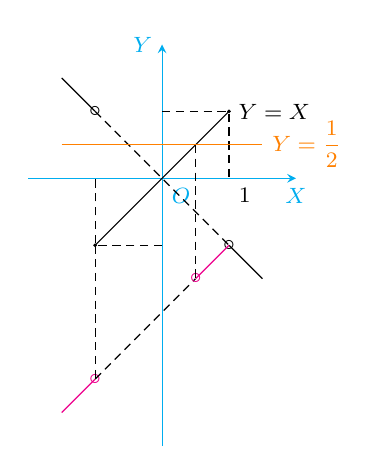
\begin{tikzpicture}[->,samples=100,>=stealth,font=\footnotesize,scale=0.85]
                \draw[->,cyan](-2,0)--(0,0)node[below right]{$O$}--(2,0)node[below]{$X$};
                \draw[->,cyan](0,-4)--(0,2)node[left]{$Y$};
                \draw[densely dashed,-] (0,1)--(1,1)--(1,0)node[below right]{$1$};
                \draw[densely dashed,-,rotate=180] (0,1)--(1,1)--(1,0);
                \draw[-,black,domain=-1:1] plot({\x},{\x})node[right]{$Y=X$};
                \draw[fill=black] (1,1) circle (0.5pt);
                \draw[fill=black,rotate=180] (1,1) circle (0.5pt);
                \draw[-,black,domain=-1.5:-1] plot(\x,{-\x})node{$\circ$};
                \draw[-,black,domain=-1.5:-1,rotate=180] plot(\x,{-\x})node{$\circ$};
                \draw[-,densely dashed,black,domain=-1:1] plot(\x,{-\x});
                \draw[-,orange] (-1.5,0.5) -- (1.5,0.5)node[right]{$Y=\dfrac{1}{2}$};
                \draw[-,magenta,domain=-1.5:-1] plot(\x,{\x-2})node{$\circ$};
                \draw[-,black,domain=-1:0.5,densely dashed] plot(\x,{\x-2});
                \draw[-,magenta,domain=0.5:1,rotate=180,yshift=2.5cm,xshift=-1.5cm] plot(\x,{\x-2})node{$\circ$};
                \draw[-,densely dashed] (-1,-1)--(-1,-3);
                \draw[-,densely dashed] (0.5,0.5)--(0.5,-1.5);
            \end{tikzpicture}
            \caption{}
            \label{sjbldasd}
        \end{figure}
    \end{minipage}\hfill
    \begin{minipage}{0.7\linewidth}
        由图 \ref{sjbldasd} 可知,
        \begin{flalign*}
            P\qty{Y\leqslant \dfrac{1}{2}} & =P\qty{-1\leqslant X\leqslant \dfrac{1}{2}}+P\qty{X>1}            \\
                                           & =P\qty{-1\leqslant X\leqslant \dfrac{1}{2}}+1-P\qty{X\leqslant 1} \\
                                           & =1-P\qty{X<-1}+P\qty{\dfrac{1}{2}<X\leqslant 1}
        \end{flalign*}
        而 $P\qty{X<-1}=0$, 因此 $$P\qty{Y\leqslant \dfrac{1}{2}}=1-P\qty{\dfrac{1}{2}<X\leqslant 1}=1-\int_{\frac{1}{2}}^{1}\lambda\e^{-\lambda x}\dd x=1+\e^{-\lambda}-\e^{-\frac{\lambda}{2}}.$$
    \end{minipage}
\end{solution}

\subsection{正态分布}

\begin{definition}[正态分布及其分布函数]
    \label{normalDistributionAndItsDistributionFunction}
    \index{正态分布及其分布函数}
    若随机变量 $X$ 的密度为 $f(x)=\dfrac{1}{\sqrt{2\pi}\sigma}\e^{-\frac{(x-\mu)^2}{2\sigma^2}}$, 则称 $X$ 服从参数为 $\mu,~\sigma$ 的正态分布, 简记为 $X\sim N\qty(\mu,\sigma^2)$, $X$ 的分布函数为 $\displaystyle F(x)=\int_{-\infty}^{x}\dfrac{1}{\sqrt{2\pi}\sigma}\e^{-\frac{(t-\mu)^2}{2\sigma^2}}\dd t.$
\end{definition}

\begin{theorem}[对称性]
    \index{对称性}一般正态分布 $N\qty(\mu,\sigma^2)$ 的概率密度 $f(x)$ 满足 $f(x)=f(2\mu-x).$
\end{theorem}
\begin{theorem}[和一性]
    \index{和一性}一般正态分布 $N\qty(\mu,\sigma^2)$ 的分布函数 $F(x)$ 满足 $F(x)+F(2\mu-x)=1.$
\end{theorem}

\begin{definition}[标准正态分布]
    \index{标准正态分布}
    当定义 \ref{normalDistributionAndItsDistributionFunction} 中 $\mu=0,~\sigma=1$ 时, 称 $X$ 服从标准正态分布, 简记为 $X\sim N(0,1)$, 并且分别用 $\varphi(x)$ 与 $\varPhi(x)$ 表示其概率密度函数和分布函数.
\end{definition}

\begin{theorem}[标准正态分布的分布函数和]
    \index{标准正态分布的分布函数和}
    $1=\varPhi(x)+\varPhi(-x)$.
\end{theorem}

\begin{example}
    设 $X \sim N\qty(\mu,\sigma^2)$, 则随着 $\sigma$ 的增大, $P\qty|X-\mu|<\sigma$
    \begin{tasks}(4)
        \task 单调递减.
        \task 单调递增.
        \task 保持不变.
        \task 无法确定.
    \end{tasks}
\end{example}
\begin{solution}
    因为 $\dfrac{X-\mu}{\sigma}\sim N(0,1)$, 所以
    $$
        P\qty{|X-\mu|<\sigma}=P\qty{-\sigma<X-\mu<\sigma}=P\qty{-1<\dfrac{X-\mu}{\sigma}<1}=\varPhi(1)-\varPhi(-1)=2\varPhi(1)-1
    $$
    故保持不变, 选 C.
\end{solution}

\begin{example}
    设 $ X, Y $ 相互独立, 且 $ X \sim N(1,2), Y \sim N(0,1) $, 求 $ Z=2 X-Y+3 $ 的密度函数.
\end{example}
\begin{solution}
    因为 $X \sim N(1,2), Y \sim N(0,1)$, 所以 $$E(X)=1,~D(X)=2,~E(Y)=0,~D(Y)=1$$
    因此 \begin{flalign*}
        E(Z) & =E(2X-Y+3)=2E(X)-E(Y)+3=2-0+3=5 \\
        D(Z) & =D(2Z-Y+3)=4D(X)+D(Y)=8+1=9
    \end{flalign*}
    故 $Z\sim N(5,9)$, 于是 $f_Z(z)=\dfrac{1}{3\sqrt{2\pi}}\e^{-\frac{(x-5)^2}{18}}.$
\end{solution}

\begin{example}
    若随机变量 $X$ 服从正态分布 $N\qty(2,\sigma^2)$, 且 $P\qty{2<X<4}=0.3$, 则 $P\qty{X<0}$ 等于
    \begin{tasks}(4)
        \task 0.2
        \task 0.3
        \task 0.5
        \task 0.7
    \end{tasks}
\end{example}
\begin{solution}
    \textbf{法一: }由 $X\sim N\qty(2,\sigma^2)$ 知 $\dfrac{X-2}{\sigma}\sim N(0,1)$ 从而 $P\qty{2<X<4}=P\qty{\dfrac{2-2}{\sigma}<\dfrac{X-2}{\sigma}<\dfrac{4-2}{\sigma}}=\varPhi\qty(\dfrac{2}{\sigma})-\varPhi(0)=0.3$,
    又 $\varPhi(0)=\dfrac{1}{2}$, 得 $\varPhi\qty(\dfrac{2}{\sigma})=0.8$ 于是得 $P\qty{X<0}=P\qty{\dfrac{X-2}{\sigma}<\dfrac{0-2}{\sigma}}=1-\varPhi\qty(\dfrac{2}{\sigma})=0.2$ 故选 A.\\
    \textbf{法二: }由 $X\sim N\qty(2,\sigma^2)$ 得到分布函数关于 $x=2$ 对称, 根据对称性, 并由 $P\qty{2<X<4}=0.3$ 得到 $P\qty{0<X<2}=0.3$, 那么 $P\qty{0<X<4}=0.6$, 那么 $P\qty{X<0}=\dfrac{1}{2}\qty(1-0.6)=0.2$, 故选 A.
\end{solution}

\begin{example}
    设 $b>0$ 为常数, 且 $\varphi(x)=\displaystyle\dfrac{2}{\sqrt{\pi b}}\int_{0}^{x}\e^{-\frac{t^2}{b}}\dd t$, 求 $\displaystyle\int_{0}^{+\infty}(1-\varphi(x))\dd x$.
\end{example}
\begin{solution}
    因为 $1=\displaystyle \dfrac{2}{\sqrt{\pi b}}\int_{0}^{+\infty}\e^{-\frac{t^2}{b}}\dd t$, 于是 $1-\varphi(x)=\dfrac{2}{\sqrt{\pi b}}\displaystyle\int_{x}^{+\infty}\e^{-\frac{t^2}{b}}\dd t  $, 那么
    \begin{flalign*}
        \int_{0}^{+\infty}(1-\varphi(x))\dd x & =\dfrac{2}{\sqrt{\pi b}}\int_{0}^{+\infty}\dd x\int_{x}^{+\infty}\e^{-\frac{t^2}{b}}\dd t=\dfrac{2}{\sqrt{\pi b}}\int_{0}^{+\infty}\dd t\int_{0}^{t}\e^{-\frac{t^2}{b}}\dd x          \\
                                              & =\dfrac{2}{\sqrt{\pi b}}\int_{0}^{+\infty}t\e^{-\frac{t^2}{b}}\dd t=\dfrac{2}{\sqrt{\pi b}}\dfrac{b}{2}\int_{0}^{+\infty}\e^{-\frac{t^2}{b}}\dd \dfrac{t^2}{b}=\sqrt{\dfrac{b}{\pi}}.
    \end{flalign*}
\end{solution}

% \subsection{连续型随机变量的性质}
% 
% \begin{example}
%     连续随机变量 $X$ 的分布函数为 $$F(x)=\begin{cases}
%             a+b\e^{-x}, & x\geqslant 0 \\
%             0,          & x<0
%         \end{cases}$$
%     则其中的常数 $a$ 和 $b$ 为
%     \begin{tasks}(4)
%         \task $\begin{cases}a=1\\b=0\end{cases}$
%         \task $\begin{cases}a=1\\b=-1\end{cases}$
%         \task $\begin{cases}a=-1\\b=1\end{cases}$
%         \task $\begin{cases}a=0\\b=1\end{cases}$
%     \end{tasks}
% \end{example}
% \begin{solution}
%     $\displaystyle 1=\lim_{x\to+\infty}F(x)=\lim_{x\to+\infty}\qty(a+b\e^{-x})\Rightarrow a=1$, 以及 $$0=\lim_{x\to0^+}F(x)=\lim_{x\to0^+}\qty(a+b\e^{-x})=a+b=0\Rightarrow b=-1$$
%     故选 B.
% \end{solution}
% 
% \subsection{连续型概率密度函数}
% 
% \begin{example}
%     设 $X$ 的密度函数为 $f_X(x)=\dfrac{1}{\pi\qty(1+x^2)}~~(-\infty <x<+\infty)$, 求 $Y=1-\sqrt[3]{X}$ 的密度函数 $f_Y(y).$
% \end{example}
% \begin{solution}
%     设 $Y$ 的分布函数为 $F_Y(y)$, 则
%     \begin{flalign*}
%         F_Y(y) & =P\qty{Y\leqslant y}=P\qty{1-\sqrt[3]{X}\leqslant y}=P\qty{X\geqslant (1-y)^3}=1-P\qty{X<(1-y)^3}=1-\int_{-\infty}^{(1-y)^3}\dfrac{\dd x}{\pi\qty(1+x^2)} \\
%                & =1-\eval{\dfrac{1}{\pi}\arctan x}_{-\infty}^{(1-y)^3}=\dfrac{1}{2}-\dfrac{1}{\pi}\arctan(1-y)^3~~(-\infty <y<+\infty)
%     \end{flalign*}
%     因此 $f_Y(y)=F_Y'(y)=\dfrac{3(1-y)^2}{\pi\qty[1+(1-y)^6]}.$
% \end{solution}
% 
% \subsection{三大连续性分布}
% 
% \subsubsection{均匀分布}
% 
% \begin{definition}[均匀分布及其分布函数]
%     若随机变量 $X$ 的密度为 $f(x)=\begin{cases}
%             \dfrac{1}{b-a}, & a<x<b       \\
%             0,              & \text{其他}
%         \end{cases}$, 则称 $X$ 服从区间 $[a,b]$ 上的均匀分布, 简记为 $X\sim U(a,b)$, 并且 $X$ 的分布函数为 $$F(x)=\begin{cases}
%             0,                & x<a             \\
%             \dfrac{x-a}{b-a}, & a\leqslant x< b \\
%             1,                & x\geqslant b.
%         \end{cases}$$
% \end{definition}
% 
% \subsubsection{指数分布}
% 
% \begin{definition}[指数分布及其分布函数]
%     若随机变量 $X$ 的密度为 $f(x)=\begin{cases}
%             \lambda\e^{-\lambda x}, & x>0          \\
%             0,                      & x\leqslant 0
%         \end{cases}$, 则称 $X$ 服从参数为 $\lambda$ 的指数分布, 简记为 $X\sim E(\lambda)$, 并且 $X$ 的分布函数为 $$F(x)=\begin{cases}
%             1-\e^{-\lambda}, & x>0           \\
%             0,               & x\leqslant 0.
%         \end{cases}$$
% \end{definition}
% 
% \begin{theorem}[无记忆性]
%     \label{wujyxing}
%     对于 $\forall s,t>0$, 有 $P\qty{X>s+t~|~X>s}=P\qty{X>t}.$
% \end{theorem}
% \subsubsection{正态分布}
% 

%\section{随机变量的分布函数}

% \subsection{二项分布}
% 
% 若 $X$ 的概率分布列为
% $$P\left( X=k\right) =\binom{n}{k}p^{k}\left( 1-p\right) ^{n-k}~ (k=0,1,\cdots ,n)$$
% 则称 $X$ 服从二项分布, 记为 $X\sim b(n,p)$, 其中 $0<p<1.$
% 
% \begin{example}
%     设随机变量 $X\sim b(n,p)$, 求 $E(X)$ 和 $D(X).$
% \end{example}
% \begin{solution}
%     由期望的定义, 
%     \begin{flalign*}
%         E\left( X\right) =\sum ^{n}_{k=0}k\binom{n}{k}p^{k}\left( 1-p\right) ^{n-k}=np\sum ^{n}_{k=1}\binom{n-1}{k-1}p^{k-1}\left( 1-p\right) ^{\left( n-1\right) -\left( k-1\right) }=np[p+(1-p)]^{n-1}=np,
%     \end{flalign*}
%     因为, $D(X)=E(X^2)-E^2(X)$, 下求 $E(X^2)$, 
%     \begin{flalign*}
%         E(X^2) & =\sum ^{n}_{k=0}k^{2}\binom{n}{k}p^{k}\left( 1-p\right) ^{n-k}=\sum ^{n}_{k=1}\left( k-1+1\right) k\binom{n}{k}p^{k}\left( 1-p\right) ^{n-k}                                                                \\
%                & =\sum ^{n}_{k=1}\left( k-1\right) k\binom{n}{k}p^{k}\left( 1-p\right) ^{n-k}+\sum ^{n}_{k=1}k\binom{n}{k}p^{k}\left( 1-p\right) ^{n-k}                                                                      \\
%                & =\sum ^{n}_{k=2}\left( k-1\right) k\binom{n}{k}p^{k}\left( 1-p\right) ^{n-k}+np\\
%                & =n\left( n-1\right) p^{2}\sum ^{n}_{k=2}\binom{n-2}{k-2}p^{k-2}\left( 1-p\right) ^{\left( n-2\right) -\left( k-2\right) }+np\\
%                & =n\left( n-1\right) p^{2}+np,
%     \end{flalign*}
%     故 $D(X)=n(n-1)p^2+np-(np)^2=np(1-p).$
% \end{solution}
% \begin{example}
%     设随机变量 $X\sim b(n,p)$, 已知 $E(X)=2.4,D(X)=1.44$, 求参数 $n$ 和 $p$.
% \end{example}
% \begin{solution}
%     因为 $E(X)=np,D(X)=np(1-p)$, 所以 $n=6,p=0.4.$
% \end{solution}
% 
% \subsection{0-1 分布}
% 
% \subsection{Poisson 分布}
% 
% \subsection{超几何分布}
% 
% \subsection{几何分布}
% 
% \subsection{负二项分布}
%\section{连续性随机变量及其概率密度}

% \subsection{正态分布}
% 
% \subsection{标准正态分布}
% 
% \subsection{均匀分布}
% 
% \subsection{指数分布}
% 
% \subsection{\texorpdfstring{$\Gamma$}. 分布}
% 
% \subsection{\texorpdfstring{$\mathrm{B}$}. 分布}
%\section{随机变量的函数的分布}
\chapter{多维随机变量及其分布}%============================17

%TODO: section17 Intr
\section{多维离散型随机变量}
\section{多维连续型随机变量}

% \subsection{边缘概率密度}
% 
% \begin{definition}[边缘概率密度]
%     $\displaystyle F_X(x)=F(x,+\infty)=\int_{-\infty}^{x}\qty[\int_{-\infty}^{+\infty}f(x,y)\dd y]\dd x$, 由此可得 $f_X(x)=\displaystyle\int_{-\infty}^{+\infty}f(x,y)\dd y$;
%     $\displaystyle F_Y(y)=F(+\infty,y)=\int_{-\infty}^{y}\qty[\int_{-\infty}^{+\infty}f(x,y)\dd x]\dd y$, 由此可得 $f_Y(y)=\displaystyle\int_{-\infty}^{+\infty}f(x,y)\dd x$
%     称 $f_X(x)$ 和 $f_Y(y)$ 为 $(X,Y)$ 关于 $X$ 和 $Y$ 的边缘概率密度.
% \end{definition}
% 
% \begin{example}[2011 数三]
%     \label{erwsjblxy0xy2}设二维随机变量 $(X,Y)$ 在 $G$ 上服从均匀分布, $G$ 由 $x-y=0,x+y=2$ 和 $y=0$ 围成, 求边缘概率密度 $f_X(x).$
% \end{example}
% \begin{solution}
%     $(X,Y)$ 的概率密度为 $f(x,y)=\begin{cases}
%             1, & (x,y)\in G \\0,&\text{其他}
%         \end{cases}$, 故 $$f_X(x)=\int_{-\infty}^{+\infty}f(x,y)\dd y=\begin{cases}
%             \displaystyle\int_{0}^{x}\dd y,   & 0\leqslant x\leqslant 1 \\[6pt]
%             \displaystyle\int_{0}^{2-x}\dd y, & 1< x\leqslant 2         \\[6pt]
%             0,                                & \text{其他}
%         \end{cases}=\begin{cases}
%             x,   & 0\leqslant x\leqslant1 \\
%             2-x, & 1<x\leqslant 2         \\
%             0,   & \text{其他}.
%         \end{cases}$$
% \end{solution}
% 
% \begin{definition}[相互独立]
%     若 $f(x,y)=f_X(x)\cdot f_Y(y)$, 则称 $X$ 和 $Y$ 相互独立.
% \end{definition}
% 
% \subsection{条件概率密度}
% 
% \begin{definition}[条件概率密度]
%     设 $ (X, Y) $ 为连续型随机变量, 其概率密度为 $ f(x, y) $, 边缘密度函数分别为 $ f_{X}(x) $ 和 $ f_{Y}(y) $, 若 $ f_{Y}(y)>0 $, 则称
%     $$f_{X \mid Y}(x \mid y)=\frac{f(x, y)}{f_{Y}(y)}$$
%     为在 $ Y=y $ 的条件下 $ X $ 的条件概率密度; 同样, 若 $ f_{X}(x)>0 $, 则称
%     $$f_{Y \mid X}(y \mid x)=\frac{f(x, y)}{f_{X}(x)}$$
%     为在 $ X=x $ 条件下 $ Y $ 的条件概率密度.
%     特别地, 若 $ f_{Y}(y)=0 $, 则 $ f_{X \mid Y}(x \mid y)=0 .$
% \end{definition}
% 
% \begin{example}
%     求例题 \ref{erwsjblxy0xy2} 中 $f_{X\mid Y}(x\mid y).$
% \end{example}
% \begin{solution}
%     $\displaystyle f_Y(y)=\int_{-\infty}^{+\infty}f(x,y)\dd x=\begin{cases}
%             \displaystyle\int_{y}^{2-y}\dd x, & 0\leqslant y\leqslant 1 \\[6pt]
%             0,                                & \text{其他}
%         \end{cases}=\begin{cases}
%             2(1-y), & 0\leqslant y\leqslant 1 \\
%             0,      & \text{其他}.
%         \end{cases}$ 则 $$f_{X\mid Y}(x\mid y)=\dfrac{f(x,y)}{f_Y(y)}=\begin{cases}
%             \dfrac{1}{2(1-y)}, & y<x<2-y      \\[6pt]
%             0,                 & \text{其他}.
%         \end{cases}$$
% \end{solution}
% 
% \subsection{条件分布函数}
% 
% \begin{definition}[条件分布函数 A]
%     如果任给 $ \varepsilon>0, P\{y-\varepsilon<Y \leqslant y+\varepsilon\}>0 ,$
%     $$\lim _{\varepsilon \rightarrow 0^{+}} P\{X \leqslant x \mid y-\varepsilon<Y \leqslant y+\varepsilon\}
%         =\lim _{\varepsilon \rightarrow 0^{+}} \frac{P\{X \leqslant x, y-\varepsilon<Y \leqslant y+\varepsilon\}}{P\{y-\varepsilon<Y \leqslant y+\varepsilon\}}
%     $$
%     存在, 则称此极限为在条件 $ Y=y $ 下随机变量 $ X $ 的条件分布函数, 记为 $ P\{X \leqslant x \mid Y=y\} $ 或 $ F_{X \mid Y}(x \mid y) $
%     $$F_{X \mid Y}(x \mid y)= \lim _{\varepsilon \rightarrow 0^{+}} \frac{F(x, y+\varepsilon)-F(x, y-\varepsilon)}{F_{Y}(y+\varepsilon)-F_{Y}(y-\varepsilon)}
%         =\frac{\displaystyle\int_{-\infty}^{x} \int_{y-\varepsilon}^{y+\varepsilon} f(x, y) \dd  x \mathrm{~d} y}{\displaystyle\int_{y-\varepsilon}^{y+\varepsilon} f_{Y}(y) \dd  x} .
%     $$
% \end{definition}
% \begin{definition}[条件分布函数 B]
%     设 $ f(x, y) $ 在点 $ (x, y) $ 处伡续, $f_{Y}(y) $ 连续且 $ f_{Y}(y)>0 $, 则称
%     $$F_{X \mid Y}(x \mid y)=\int_{-\infty}^{x} \frac{f(x, y)}{f_{Y}(y)} \dd  x$$
%     为在 $ Y=y $ 的条件下 $ X $ 的条件分布函数;
%     若 $ f(x, y) $ 在点 $ (x, y) $ 处连续, $f_{X}(x) $ 连续且 $ f_{X}(x)>0 $, 则称
%     $$F_{Y \mid X}(y \mid x)=\int_{-\infty}^{y} \frac{f(x, y)}{f_{X}(x)} \dd  y$$
%     为在 $ X=x $ 条件下 $ Y $ 的条件分布函数.
% \end{definition}
% 
% \begin{example}
%     设二维随机变量 $(X,Y)$ 的概率密度为 $f(x,y)=\begin{cases}
%             \dfrac{1}{4}(y-x)\e^{-y}, & |x|<y<+\infty \\[6pt]
%             0,                        & \text{其他}
%         \end{cases}$ 求
%     \begin{enumerate}[label=(\arabic{*})]
%         \item $(X,Y)$ 分别关于 $X,Y$ 的边缘概率密度;
%         \item 在条件 $X=x$ 下随机变量 $Y$ 的条件概率密度.
%     \end{enumerate}
% \end{example}
% \begin{solution}
%     \begin{enumerate}[label=(\arabic{*})]
%         \item 当 $x<0$ 时,  $$f_X(x)=\int_{-\infty}^{+\infty}f(x,y)\dd y=\int_{-x}^{+\infty}\dfrac{1}{4}(y-x)\e^{-y}\dd y=-\dfrac{\e^x}{4}(2x-1)$$
%               同理, 当 $x\geqslant 0$ 时, $$f_X(x)=\int_{-\infty}^{+\infty}f(x,y)\dd y=\int_{x}^{+\infty}\dfrac{1}{4}(y-x)\e^{-y}\dd y=\dfrac{1}{4}\e^{-x}$$
%               当 $y<0$ 时, 显然 $f_Y(x,y)=0$; 当 $y\geqslant 0$ 时
%               $$f_Y(y)=\int_{-\infty}^{+\infty}f(x,y)\dd x=\int_{-y}^{y}(y-x)\e^{-y}\dd x=\dfrac{1}{2}y^2\e^{-y}$$
%               综上, $(X,Y)$ 关于 $X$ 的边缘分布函数为 $f_X(x)=\begin{cases}
%                       -\dfrac{\e^x}{4}(2x-1), & x<0          \\[6pt]
%                       \dfrac{1}{4}\e^{-x},    & x\geqslant 0
%                   \end{cases}$ $(X,Y)$ 关于 $Y$ 的边缘分布函数为 $$f_Y(y)=\begin{cases}
%                       \dfrac{1}{2}y^2\e^{-y}, & y\geqslant 0 \\[6pt]
%                       0,y<0
%                   \end{cases}$$
%         \item 当 $x<0$ 时, 在条件 $X=x$ 下随机变量 $Y$ 的条件概率密度为
%               $$f_{Y\mid X}(y\mid x)=\dfrac{f(x,y)}{f_X(x)}=\begin{cases}
%                       \dfrac{(x-y)\e^{-x-y}}{2x-1}, & -x<y<+\infty \\[6pt]
%                       0,                            & \text{其他}
%                   \end{cases}$$
%               同理, 当 $x\geqslant 0$ 时, 在条件 $X=x$ 下随机变量 $Y$ 的条件概率密度为
%               $$f_{Y\mid X}(y\mid x)=\dfrac{f(x,y)}{f_X(x)}=\begin{cases}
%                       (y-x)\e^{x-y}, & x<y<+\infty \\
%                       0,             & \text{其他}
%                   \end{cases}$$
%     \end{enumerate}
% \end{solution}
% 
% \subsection{常见的二维连续型随机变量函数的分布}
% 
% \subsubsection{二维正态分布}
% 
% \begin{definition}[二维正态分布]
%     若二维连续型随机变量 $ (X, Y) $ 的概率密度为
%     $$f(x, y)
%     =\frac{1}{2 \pi \sigma_{1} \sigma_{2} \sqrt{1-\rho^{2}}} \cdot \exp{-\frac{1}{2\left(1-\rho^{2}\right)}\left[\frac{\left(x-\mu_{1}\right)^{2}}{\sigma_{1}^{2}}-2 \rho \frac{\left(x-\mu_{1}\right)\left(y-\mu_{2}\right)}{\sigma_{1} \sigma_{2}}+\frac{\left(y-\mu_{2}\right)^{2}}{\sigma_{2}^{2}}\right]}
%     $$
%     则称 $ (X, Y) $ 服从参数为 $ \mu_{1}, \mu_{2}, \sigma_{1}^{2}, \sigma_{2}^{2}, \rho $ 的二维正态分布, 
%     记 $ (X, Y) \sim N\qty(\mu_{1}, \mu_{2}, \sigma_{1}^{2}, \sigma_{2}^{2}, \rho)$, 其中 $ \mu_{1}, \mu_{2}, \sigma_{1}^{2}, \sigma_{2}^{2}, \rho $ 均为常数, 
%     且 $\sigma_{1}>0, \sigma_{2}>0,|\rho|<1 .$
% \end{definition}
% 
% \begin{theorem}
%     若 $ \mqty|a & b \\ c & d| \neq 0$, 则 $ (a X+b Y, c X+d Y) $ 服从二维正态分布, 且 $ a X+b Y $ 服从以下一维正态分布
%     $$a X+b Y \sim N\left(a \mu_{1}+b \mu_{2}, a^{2} \sigma_{1}^{2}+b^{2} \sigma_{2}^{2}+2 a b \rho \sigma_{1} \sigma_{2}\right) .$$
% \end{theorem}

\subsection{边缘概率密度与边缘分布函数}

\begin{definition}[边缘分布函数]
    设二维随机变量 $ (X, Y) $ 的联合分布函数为 $ F(x, y)$, 随机变量 $ X $ 和 $ Y $ 的分布函数 $ F_{X}(x) $ 与 $ F_{Y}(y) $ 分别称为关于 $ X $ 和 $ Y $ 的边缘分布函数
    $$F_{X}(x)=P\{X \leqslant x\}=P\{X \leqslant x, Y<+\infty\}=F(x,+\infty)=\lim _{y \rightarrow+\infty} F(x, y) $$
    同理 $\displaystyle F_{Y}(y)=F(+\infty, y)=\lim _{x \rightarrow+\infty} F(x, y) .$
\end{definition}

\begin{definition}[二维连续型随机变量的边缘概率密度]
    设二维连续型随机变量 $ (X, Y) $ 的概率密度为 $ f(x, y) $, 则称
    \begin{flalign*}
        F_{X}(x) & =F(x,+\infty)=\int_{-\infty}^{x}\left[\int_{-\infty}^{+\infty} f(x, y) \dd  y\right] \dd  x  \\
        F_{Y}(y) & =F(+\infty, y)=\int_{-\infty}^{y}\left[\int_{-\infty}^{+\infty} f(x, y) \dd  x\right] \dd  y
    \end{flalign*}
    分别为 $ (X, Y) $ 关于 $ X $ 和关于 $ Y $ 的边缘分布函数.
    而称
    \begin{flalign*}
        f_{X}(x) & =\int_{-\infty}^{+\infty} f(x, y) \dd  y \\
        f_{Y}(y) & =\int_{-\infty}^{+\infty} f(x, y) \dd  x
    \end{flalign*}
    分别为 $ (X, Y) $ 关于 $ X $ 和关于 $ Y $ 的边缘概率密度.
\end{definition}

\begin{example}
    设二维随机变量 $(X,Y)$ 的概率密度为 $$f(x,y)=\begin{cases}
            \dfrac{k}{2}x\e^{-(x+y)},~x,y>0 \\[6pt]
            0, & \text{其他}
        \end{cases}$$
    \begin{enumerate}[label=(\arabic{*})]
        \item 求常数 $k$;
        \item 求 $(X,Y)$ 关于 $X$ 和关于 $Y$ 的边缘概率密度函数;
        \item 判断随机变量 $X$ 和 $Y$ 是否相互独立.
    \end{enumerate}
\end{example}
\begin{solution}
    \begin{enumerate}[label=(\arabic{*})]
        \item $\displaystyle\int_{-\infty}^{+\infty}\int_{-\infty}^{+\infty}f(x,y)\dd x\dd y=1\Rightarrow 1=\int_{0}^{+\infty}\dd y\int_{0}^{+\infty}\dfrac{k}{2}x\e^{-(x+y)}\dd x=\dfrac{k}{2}\int_{0}^{+\infty}\e^{-y}\dd y\Rightarrow k=2.$
        \item $\displaystyle f_X(x)=\int_{0}^{+\infty}x\e^{-(x+y)}\dd y=x\e^{-x}~(x>0)\Rightarrow f_X(x)=\begin{cases}
                      x\e^{-x}, & x>0         \\
                      0,        & \text{其他}
                  \end{cases}$ 同理 $f_Y(y)=\begin{cases}
                      \e^{-y}, & y>0         \\
                      0,       & \text{其他}
                  \end{cases}$
        \item 因为 $f(x,y)=f_X(x)\cdot f_Y(y)$, 所以 $X,Y$ 相互独立.
    \end{enumerate}
\end{solution}

\subsection{二维连续型随机变量函数的分布}

\begin{theorem}[常见的二维连续型随机变量函数的分布]
    设二维连续型随机变量 $ (X, Y) $ 的概率密度为 $ f(x, y) $, $X $ 和 $ Y $ 概率密度分别为 $ f_{X}(x) $ 和 $ f_{Y}(y) $, 连续型随机变量 $ Z=g(X, Y) $ 是 $ X $ 和 $ Y $ 的函数, 则当
    \begin{enumerate}[label=(\arabic{*})]
        \item $Z=X+Y $ 的概率密度
              $$\begin{matrix}
                      \displaystyle f_{Z}(z)  =\int_{-\infty}^{+\infty} f(x, z-x) \dd  x \\
                      \displaystyle f_{Z}(z)  =\int_{-\infty}^{+\infty} f(z-y, y) \dd  y
                  \end{matrix}\xrightarrow{\text{当 $ X $ 和 $ Y $ 相互独立时}}\begin{matrix}
                      \displaystyle f_{Z}(z)=\int_{-\infty}^{+\infty} f_{X}(x) f_{Y}(z-x) \dd  x \\
                      \displaystyle f_{Z}(z)=\int_{-\infty}^{+\infty} f_{X}(z-y) f_{Y}(y) \dd  y
                  \end{matrix}$$
        \item $Z=\pm X\mp Y $ 的概率密度
              $$\begin{matrix}
                      \displaystyle \int_{-\infty}^{+\infty} f(x, x\mp z) \dd  x \\
                      \displaystyle \int_{-\infty}^{+\infty} f(y\pm z, y) \dd  y
                  \end{matrix}\xrightarrow{\text{当 $ X $ 和 $ Y $ 相互独立时}}\begin{matrix}
                      \displaystyle \int_{-\infty}^{+\infty} f_{X}(x) f_{Y}(x\mp z) \dd  x \\
                      \displaystyle \int_{-\infty}^{+\infty} f_{Y}(y) f_{X}(y\pm z) \dd  y
                  \end{matrix}
              $$
        \item $Z=\dfrac{Y}{X}$ 的概率密度
              $$f_{Z}(z)=\int_{-\infty}^{+\infty}|x| f(x, x z) \dd  x \xrightarrow{\text{当 $ X $ 和 $ Y $ 相互独立时}} \int_{-\infty}^{+\infty}|x| f_{X}(x) f_{Y}(x z) \dd  x$$
        \item $Z=X Y $ 的概率密度
              $$f_{Z}(z)=\int_{-\infty}^{+\infty} \frac{1}{|x|} f\left(x, \frac{z}{x}\right) \dd  x \xrightarrow{\text{当 $ X $ 和 $ Y $ 相互独立时}}\int_{-\infty}^{+\infty} \frac{1}{|x|} f_{X}(x) f_{Y}\left(\frac{z}{x}\right) \dd  x$$
        \item $Z=\max \{X, Y\} $ 的分布
              $$F_{Z}(z)=P\qty{X\leqslant z,Y\leqslant z}=F(z,z) \xrightarrow{\text{当 $ X $ 和 $ Y $ 相互独立时}} F_X(z)F_Y(y)\xrightarrow{\text{当 $ X $ 和 $ Y $ 独立同分布时}}F_X^2(x)$$
              当 $X$ 和 $Y$ 独立同分布时, $Z$ 的概率密度为 $$f_Z(z)=2F_X(z)f_X(z)$$
        \item $Z=\min \{X, Y\} $ 的分布
              \begin{flalign*}
                  F_Z(z) =1-P\qty{X>z,Y>z} & \xrightarrow{\text{当 $ X $ 和 $ Y $ 相互独立时}} 1-\qty[1-F_X(z)]\qty[1-F_Y(z)] \\
                                           & \xrightarrow{\text{当 $ X $ 和 $ Y $ 独立同分布时}} 1-\qty[1-F_X(z)]^2
              \end{flalign*}
              当 $X$ 和 $Y$ 独立同分布时, $Z$ 的概率密度为 $$f_Z(z)=2\qty[1-F_X(z)]f_X(z).$$
    \end{enumerate}
\end{theorem}

\begin{example}
    设二维随机变量 $(X,Y)$ 的概率密度为 $f(x,y)=\begin{cases}
        \dfrac{1+xy}{4}, & |x|<1,|y|<1\\ 0, & \text{其他}
    \end{cases}$ 则 
    \begin{tasks}(2)
        \task $X$ 与 $Y$  相互独立, $X^2$ 与 $Y^2$ 也相互独立.
        \task $X$ 与 $Y$  相互独立, $X^2$ 与 $Y^2$ 不相互独立.
        \task $X$ 与 $Y$  不相互独立, $X^2$ 与 $Y^2$ 相互独立.
        \task $X$ 与 $Y$  不相互独立, $X^2$ 与 $Y^2$ 也不相互独立.
    \end{tasks}
\end{example}
\begin{solution}
    第一步: 求 $f_X(x),f_Y(y)$, $ \displaystyle f_X(x)=\begin{cases}
        \displaystyle \int_{-1}^{1} \dfrac{1+xy}{4} \dd y =\dfrac{1}{2}, & |x|<1 \\ 0, & \text{其他}
    \end{cases}$, 同理 $ \displaystyle f_Y(y)=\begin{cases}
        \displaystyle \int_{-1}^{1} \dfrac{1+xy}{4} \dd y =\dfrac{1}{2}, & |y|<1 \\ 0, & \text{其他}
    \end{cases}$, 而 $f(x,y)\neq f_X\cdot f_Y$, 所以 $X$ 与 $Y$  不相互独立, \\ 
    第二步: 求 $f_{X^2}(x),f_{Y^2}(y)$, $$
    F_{X^2,Y^2}=P\qty{X^2\leqslant x,Y^2\leqslant y}=\int_{-\infty}^{x}\int_{-\infty}^y f(u,v)\dd u \dd v =\begin{cases}
        0, & x<0\text{ 或 }y<0\\
        \displaystyle \int_{-\sqrt{x}}^{\sqrt{x}} \dd u\int_{\sqrt{y}}^{\sqrt{y}} \dfrac{1+uv}{4}\dd v=\sqrt{xy}, & 0\leqslant x,y<1\\ 
        \displaystyle \int_{-\sqrt{x}}^{\sqrt{x}} \dd u\int_{-1}^{1} \dfrac{1+uv}{4} \dd v=\sqrt{x}, & 0\leqslant x<1,y\geqslant1\\ 
        \displaystyle \int_{-1}^{1} \dd u\int_{-\sqrt{y}}^{\sqrt{y}} \dfrac{1+uv}{4} \dd v=\sqrt{y}, & 0\leqslant y<1,x\geqslant 1\\ 
        1, & x,y\geqslant 1
    \end{cases}
    $$
    那么 
    $$
    f_{X^2,Y^2}=\pdv{F}{x}{y}=\begin{cases}
        \dfrac{1}{4\sqrt{xy}}, & 0<x,y<1\\ 
        0,& \text{其他}
    \end{cases}
    $$
    那么 $ \displaystyle f_{X^2} =\int_{-\infty}^{+\infty} f_{X^2,Y^2} \dd y=\begin{cases}
        \displaystyle \int_{0}^{1} \dfrac{1}{4\sqrt{xy}} \dd y=\dfrac{1}{2\sqrt{x}}, & 0<x<1\\ 
        0, &\text{其他}
    \end{cases}$ 同理可得 $f_{Y^2}$, 而 $f_{X^2,Y^2}=f_{X^2}\cdot f_{Y^2}$, 所以 $X^2$ 与 $Y^2$ 相互独立, 选 C.
\end{solution}

\subsection{二维随机变量条件概率密度与条件分布函数}

\begin{definition}[二维随机变量条件概率密度]
    设 $ (X, Y) $ 为连续型随机变量, 其概率密度为 $ f(x, y) $, 边缘密度函数分别为 $ f_{X}(x) $ 和 $ f_{Y}(y) $, 
    若 $ f_{Y}(y)>0 $, 则称
    $$f_{X \mid Y}(x \mid y)=\frac{f(x, y)}{f_{Y}(y)}$$
    为在 $ Y=y $ 的条件下 $ X $ 的条件概率密度.
    同样, 若 $ f_{X}(x)>0 $, 则称
    $$f_{Y \mid X}(y \mid x)=\frac{f(x, y)}{f_{X}(x)}$$
    为在 $ X=x $ 条件下 $ Y $ 的条件概率密度.
\end{definition}

\begin{definition}[二维随机变量条件分布函数 A]
    如果任给 $ \varepsilon>0, P\{y-\varepsilon<Y \leqslant y+\varepsilon\}>0 ,$
    $$\lim _{\varepsilon \rightarrow 0^{+}} P\{X \leqslant x \mid y-\varepsilon<Y \leqslant y+\varepsilon\}=\lim _{\varepsilon \rightarrow 0^{+}} \frac{P\{X \leqslant x, y-\varepsilon<Y \leqslant y+\varepsilon\}}{P\{y-\varepsilon<Y \leqslant y+\varepsilon\}}$$
    存在, 则称此极限为在条件 $ Y=y $ 下随机变量 $ X $ 的条件分布函数, 记为 $ P\{X \leqslant x \mid Y=y\} $ 或 $ F_{X \mid Y}(x \mid y) $.
    $$F_{X \mid Y}(x \mid y)=\lim _{\varepsilon \rightarrow 0^{+}} \frac{F(x, y+\varepsilon)-F(x, y-\varepsilon)}{F_{Y}(y+\varepsilon)-F_{Y}(y-\varepsilon)}
    =\frac{\displaystyle\int_{-\infty}^{x} \int_{y-\varepsilon}^{y+\varepsilon} f(x, y) \dd  x \dd  y}{\displaystyle \int_{y-\varepsilon}^{y+\varepsilon} f_{Y}(y) \dd  x}$$
\end{definition}

\begin{definition}[二维随机变量条件分布函数 B]
    设 $ f(x, y) $ 在点 $ (x, y) $ 处连续, $f_{Y}(y) $ 连续且 $ f_{Y}(y)>0 $, 则称
    $$F_{X \mid Y}(x \mid y)=\int_{-\infty}^{x} \frac{f(x, y)}{f_{Y}(y)} \dd  x$$
    为在 $ Y=y $ 的条件下 $ X $ 的条件分布函数.
    若 $ f(x, y) $ 在点 $ (x, y) $ 处连续, $f_{X}(x) $ 连续且 $ f_{X}(x)>0 $, 则称
    $$F_{Y \mid X}(y \mid x)=\int_{-\infty}^{y} \frac{f(x, y)}{f_{X}(x)} \dd  y$$
    为在 $ X=x $ 的条件下 $ Y $ 的条件分布函数.
\end{definition}

\begin{example}
    设二维正态随机变量 $(X,Y)$ 的概率密度为 $f(x,y)$, 已知条件概率密度 $$f_{X\mid Y}(x\mid y)=A\e^{-\frac{2}{3}\qty(x-\frac{y}{2})^2},~f_{Y\mid X}(y\mid x)=B\e^{-\frac{2}{3}\qty(y-\frac{x}{2})^2}$$
    试求: \begin{enumerate*}[label=(\arabic{*})]
        \item 常数 $A,~B$;
        \item $f_X(x),~f_Y(y)$;
        \item $f(x,y)$.
    \end{enumerate*}
\end{example}
\begin{solution}
    \begin{enumerate}[label=(\arabic{*})]
        \item 令 $\displaystyle A\e^{-\frac{2}{3}\qty(x-\frac{y}{2})^2}=\dfrac{1}{\sqrt{2\pi}\sigma}\e^{-\frac{(x-\mu)^2}{2\sigma^2}}\Rightarrow \begin{cases}
            A=\dfrac{1}{\sqrt{2\pi}\sigma}\\[6pt]
            \dfrac{2}{3}\qty(x-\dfrac{y}{3})^2=\dfrac{(x-\mu)^2}{2\sigma^2}
        \end{cases}\Rightarrow\begin{cases}
            A=\dfrac{2}{\sqrt{6\pi}}\\[6pt]
            \mu=\dfrac{y}{3}
        \end{cases}$ 由对称性知 $B=A=\dfrac{2}{\sqrt{6\pi}}.$
        \item 易得 $\dfrac{f_X(x)}{f_Y(y)}=\dfrac{f_{X\mid Y}(x\mid y)}{f_{Y\mid X}(y\mid x)}=\e^{-\frac{2}{3}\qty[\qty(x-\frac{y}{2})^2-\qty(y-\frac{x}{2})^2]}=\e^{-\frac{1}{2}\qty(x^2+y^2)}=\dfrac{\e^{-\frac{x^2}{2}}}{\e^{-\frac{y^2}{2}}}$, 故 $$f_X(x)=C\e^{-\frac{x^2}{2}},~f_Y(y)=C\e^{-\frac{y^2}{2}}$$
        由于标准差为 1, 则根据正态分布的概率密度知 $C=\dfrac{1}{\sqrt{2\pi}}$, 因此 $f_X(x)=\dfrac{1}{\sqrt{2\pi}}\e^{-\frac{x^2}{2}},~f_Y(y)=\dfrac{1}{\sqrt{2\pi}}\e^{-\frac{y^2}{2}}.$
        \item $f(x,y)=f_{X\mid Y}(x\mid y)f_Y(y)=\dfrac{2}{\sqrt{6\pi}}\e^{-\frac{2}{3}\qty(x-\frac{y}{2})^2}\cdot \dfrac{1}{\sqrt{2\pi}}\e^{-\frac{y^2}{2}}=\dfrac{1}{\sqrt{3}\pi}\e^{-\frac{2}{3}\qty(x^2-xy+y^2)}.$
    \end{enumerate}
\end{solution}

\subsection{二维正态分布}

\subsubsection{二维情况}

\begin{definition}[二维正态分布]
    若二维连续型随机变量 $ (X, Y) $ 的概率密度为
    $$f(x,y)=\frac{1}{2 \pi \sigma_{1} \sigma_{2} \sqrt{1-\rho^{2}}} \cdot \mathrm{e}^{-\frac{1}{2\left(1-\rho^{2}\right)}\left[\frac{\left(x-\mu_{1}\right)^{2}}{\sigma_{1}^{2}}-2 \rho \frac{\left(x-\mu_{1}\right)\left(y-\mu_{2}\right)}{\sigma_{1} \sigma_{2}}+\frac{\left(y-\mu_{2}\right)^{2}}{\sigma_{2}^{2}}\right]}$$
    则称 $ (X, Y) $ 服从参数为 $ \mu_{1}, \mu_{2}, \sigma_{1}^{2}, \sigma_{2}^{2}, \rho $ 的二维正态分布, 
    记 $$ (X, Y) \sim N\left(\mu_{1}, \mu_{2}; \sigma_{1}^{2}, \sigma_{2}^{2}; \rho\right) $$
    其中 $ \mu_{1}, \mu_{2}, \sigma_{1}^{2}, \sigma_{2}^{2}, \rho $ 均为常数, 且 $ \sigma_{1}>0, \sigma_{2}>0,|\rho|<1 .$
\end{definition}
\begin{theorem}[二维正态分布推出一维正态分布]
    若 $ (X, Y) \sim N\left(\mu_{1}, \mu_{2}, \sigma_{1}^{2}, \sigma_{2}^{2}, \rho\right) $, 则
    $$X \sim N\left(\mu_{1}, \sigma_{1}^{2}\right), Y \sim N\left(\mu_{2}, \sigma_{2}^{2}\right)$$
    反之不对, 即 $ X $ 与 $ Y $ 均服从一维正态, 不能保证 $ (X, Y) $ 一定服从二维正态分布.
\end{theorem}

\begin{theorem}[独立一维正态分布推出二维正态分布]
    若 $ X \sim N\left(\mu_{1}, \sigma_{1}^{2}\right), Y \sim N\left(\mu_{2}, \sigma_{2}^{2}\right)$, 且相互独立, 则 $ (X, Y) $ 一定服从二维正态分布
    $$ (X, Y) \sim N\left(\mu_{1}, \mu_{2}; \sigma_{1}^{2}, \sigma_{2}^{2}; \rho\right) .$$
\end{theorem}

\begin{theorem}
    若 $\mqty|a&b\\c&d|\neq0$, 则 $ (a X+b Y, c X+d Y) $ 服从二维正态分布, 明显 $ a X+b Y $ 服从一维正态分布
    $$a X+b Y \sim N\left(a \mu_{1}+b \mu_{2}, a^{2} \sigma_{1}^{2}+b^{2} \sigma_{2}^{2}+2 a b \rho \sigma_{1} \sigma_{2}\right) .$$
\end{theorem}

\begin{theorem}
    $X $ 和 $ Y $ 相互独立的充要条件是 $ \rho=0 .$
\end{theorem}

\begin{theorem}[二维正态分布的条件分布]
    二维正态分布联合密度为 $$
    \varphi(x,y)=\dfrac{1}{2\pi\sigma_1\sigma_2\sqrt{1-\rho^2}}\exp\qty{-\dfrac{u^2-2\rho uv+v^2}{2\qty(1-\rho^2)}}
    $$
    其中 $u=\dfrac{x-\mu_1}{\sigma_1},v=\dfrac{y-\mu_2}{\sigma_2}$,
    随机变量 $X$ 关于 $Y$ 的条件分布是正态分布 $N\qty(\mu_{1|2},\sigma^2_{1|2})$; 随机变量 $Y$ 关于 $X$ 的条件分布是正态分布 $N\qty(\mu_{2|1},\sigma^2_{2|1})$, 其中二维正态分布的条件数字特征如下:
    \begin{flalign*}
        \mu_{1|2}=\mu_2(y)=\mu_1+\dfrac{\rho\sigma_1}{\sigma_2}(y-\mu_2)=\mu_1+\rho\sigma_1v,&\quad\quad\sigma^2_{1|2}=\sigma_1^2\qty(1-\rho^2)\\ 
        \mu_{2|1}=\mu_2(x)=\mu_2+\dfrac{\rho\sigma_2}{\sigma_1}(x-\mu_1)=\mu_2+\rho\sigma_2u,&\quad\quad\sigma^2_{2|1}=\sigma_2^2\qty(1-\rho^2).
    \end{flalign*}
\end{theorem}

\begin{example}
    设二维随机变量 $(X,Y)$ 的概率密度为 $f(x,y)=A\e^{-2x^2-y^2},~-\infty<x,y<+\infty$, 
    \begin{enumerate}[label=(\arabic{*})]
        \item 求常数 $A$;
        \item 求条件概率密度 $f_{Y\mid X}(y\mid x).$
    \end{enumerate}
\end{example}
\begin{solution}
    \begin{enumerate}[label=(\arabic{*})]
        \item \textbf{法一: }因为二维正态分布的概率密度为 
        $$f(x,y)=\frac{1}{2 \pi \sigma_{1} \sigma_{2} \sqrt{1-\rho^{2}}} \cdot \mathrm{e}^{-\frac{1}{2\left(1-\rho^{2}\right)}\left[\frac{\left(x-\mu_{1}\right)^{2}}{\sigma_{1}^{2}}-2 \rho \frac{\left(x-\mu_{1}\right)\left(y-\mu_{2}\right)}{\sigma_{1} \sigma_{2}}+\frac{\left(y-\mu_{2}\right)^{2}}{\sigma_{2}^{2}}\right]}$$
        对比本题所给密度得 $(X,Y)\sim N\qty(0,0;\dfrac{1}{4},\dfrac{1}{2};0)$, 因此 $A=\dfrac{1}{2\pi\sigma_1\sigma_2\sqrt{1-\rho^2}}=\dfrac{1}{2\pi\cdot\sqrt{\dfrac{1}{4}}\cdot\sqrt{\dfrac{1}{2}}}=\dfrac{\sqrt{2}}{\pi}.$\\
        \textbf{法二: }因为 $\displaystyle\int_{-\infty}^{+\infty}\int_{-\infty}^{+\infty}f(x,y)\dd x\dd y=1,~\int_{-\infty}^{+\infty}\e^{-t^2}\dd t=\sqrt{\pi}$, 所以 
        \begin{flalign*}
            1&=\int_{-\infty}^{+\infty}\int_{-\infty}^{+\infty}f(x,y)\dd x\dd y=A\int_{-\infty}^{+\infty}\e^{-2x^2}\qty(\int_{-\infty}^{+\infty}\e^{-y^2}\dd y)\dd x=A\sqrt{\pi}\int_{-\infty}^{+\infty}\e^{-2x^2}\dd x\\
            &\xlongequal{t=\sqrt{2}x}A\sqrt{\pi}\cdot\dfrac{1}{\sqrt{2}}\int_{-\infty}^{+\infty}\e^{-t^2}\dd t=A\sqrt{\pi}\cdot\dfrac{1}{\sqrt{2}}\cdot\sqrt{\pi}\Rightarrow A=\dfrac{\sqrt{2}}{\pi}.
        \end{flalign*}
        \item 因为 $\rho=0$, 所以 $X$ 与 $Y$ 相互独立, 所以 $X\sim N\qty(0,\dfrac{1}{4}),~Y\sim N\qty(0,\dfrac{1}{2}),~f(x,y)=f_X(x)f_Y(y)$, 并且
        $$f_X(x)=\dfrac{1}{\sqrt{2\pi}\cdot\dfrac{1}{2}}\e^{-\frac{x^2}{\frac{1}{2}}}=\dfrac{2}{\sqrt{2\pi}}\e^{-2x^2},~f_Y(y)=\dfrac{1}{\sqrt{2\pi}\cdot\dfrac{1}{\sqrt{2}}}\e^{-y^2}=\dfrac{1}{\sqrt{\pi}}\e^{-y^2}$$
        所以 $f_{Y\mid X}(y\mid x)=\dfrac{f(x,y)}{f_X(x)}=f_Y(y)=\dfrac{1}{\sqrt{\pi}}\e^{-y^2},~-\infty<y<+\infty.$
    \end{enumerate}
\end{solution}

\subsubsection{多维情况}

\begin{definition}[多维正态分布]
    给定一个向量 $\vb*{\mu}\in \mathbb{R}^n$ 和正定矩阵 $\vb*{\Sigma}\in \mathbb{R}^{n\times n}$, 对任意实数向量 $\vb*{x}=\qty(x_1, x_2, \cdots , x_n)^\top$, 若随机向量 $\vb*{X}=\qty(X_1, X_2, \cdots ,X_n)$ 的密度函数为 $$
    f(\vb*{x})=(2\pi)^{-\frac{n}{2}}|\vb*{\Sigma}|^{-\frac{1}{2}}\exp\qty(-\dfrac{1}{2}(\vb*{x}-\vb*{\mu})^\top\vb*{\Sigma}^{-1}(\vb*{x}-\vb*{\mu}))
    $$
    则称随机向量 $\vb*{X}$ 服从参数为 $\vb*{\mu}$ 和 $\vb*{\Sigma}$ 的多维正态分布. 记为 $\vb*{X}\sim \mathcal{N} (\vb*{\mu},\vb*{\Sigma})$.\\ 
    特别地, 当 $n=2$ 时, $\vb*{\Sigma}=\begin{pmatrix} \sigma_x^2 & \rho\sigma_x\sigma_y \\ \rho\sigma_x\sigma_y & \sigma_y^2 \\\end{pmatrix}$.
\end{definition}

\subsection{卷积公式}

当 $Z=h(X,Y)$, 其中一个随机变量服从均匀分布时, 使用卷积公式将大大简化计算过程.

\begin{example}
    设随机变量 $ X $ 和 $ Y $ 相互独立, $X \sim N(0,1), Y \sim U[0,1], Z=X+Y $, 求 $ Z $ 的概率密度函数 $ f_{Z}(z) .$
\end{example}
\begin{solution}
    \textbf{法一: }由 $X\sim N(0,1)$ 知, $f_X(x)=\varphi(x)$, 由 $Y\sim U[0,1]$ 知, $f_Y(y)=\begin{cases}
            1, & 0\leqslant y\leqslant 1 \\
            0, & \text{其他}
        \end{cases}$, 又因为 $X$ 与 $Y$ 相互独立, 则 $$f(x,y)=f_X(x)f_Y(y)=\begin{cases}
            \varphi(x), & -\infty <x<+\infty,0\leqslant y\leqslant 1 \\
            0,          & \text{其他}
        \end{cases}$$
    下求 $f_Z(z)$, 
    \begin{flalign*}
        F_Z(z) & =P\qty{Z\leqslant z}=P\qty{X+Y\leqslant z}=\iint\limits_{x+y\leqslant z}f(x,y)\dd x\dd y=\int_{-\infty}^{z-1}\varphi(x)\dd x\int_{0}^{1}\dd y+\int_{z-1}^{z}\varphi(x)\dd x\int_{0}^{z-x}\dd y \\
               & =\int_{-\infty}^{z-1}\varphi(x)\dd x+\int_{z-1}^{z}(z-x)\varphi(x)\dd x=\varPhi(z-1)+\int_{z-1}^{z}(z-x)\varphi(x)\dd x
    \end{flalign*}
    则 $f_Z(z)=\displaystyle\dv{F_Z(z)}{z}=\varphi(z-1)+\dv{z}\qty[z\int_{z-1}^{z}\varphi(x)\dd x-\int_{z-1}^{z}x\varphi(x)\dd x]=\int_{z-1}^{z}\varphi(z)\dd z=\varPhi(z)-\varPhi(z-1).$\\
    \textbf{法二: }由卷积公式 $$f_Z(z)=\int_{-\infty}^{+\infty}f(x,z-x)\dd x=\int_{-\infty}^{+\infty}f_X(x)f_Y(z-x)\dd x=\int_{z-1}^{z}\varphi(x)\dd x=\varPhi(z)-\varPhi(z-1).$$
\end{solution}

\begin{example}
    设随机变量 $X\sim N\qty(\mu,\sigma^2),~Y\sim U[-\pi ,\pi]$, $X,Y$ 相互独立, 令 $Z=X+Y$, 求 $f_Z(z).$
\end{example}
\begin{solution}
    \textbf{法一: }因为 $X\sim N\qty(\mu,\sigma^2),~Y\sim U[-\pi ,\pi]$, 所以 $$f_X(x)=\dfrac{1}{\sqrt{2\pi}\sigma}\e^{-\frac{(x-\mu)^2}{2\sigma^2}},~f_Y(y)=\begin{cases}
            \dfrac{1}{2\pi}, & -\pi\leqslant y\leqslant y \\[6pt]
            0,               & \text{其他}
        \end{cases}$$
    并且 $X,Y$ 相互独立, 那么 $$f(x,y)=f_X(x)f_Y(y)=\begin{cases}
            \dfrac{1}{2\pi\sqrt{2\pi}\sigma}\e^{-\frac{(x-\mu)^2}{2\sigma^2}}, & -\infty<x<+\infty,-\pi\leqslant y\leqslant \pi \\[6pt]
            0,                                                                 & \text{其他}
        \end{cases}$$
    而 $F_Z(z)=P\qty{Z\leqslant z}=P\qty{X+Y\leqslant z}=\displaystyle\iint\limits_{x+y\leqslant z}f(x,y)\dd x\dd y$, 因此
    \begin{flalign*}
        F_Z(z) & =\dfrac{1}{2\pi\sqrt{2\pi}\sigma}\int_{-\pi}^{\pi}\dd y\int_{-\infty}^{z-y}\e^{-\frac{(x-\mu)^2}{2\sigma^2}}\dd x=\dfrac{1}{2\pi}\int_{-\pi}^{\pi}\dd y\int_{-\infty}^{z-y}\dfrac{1}{\sqrt{2\pi}}\e^{-\frac{1}{2}\qty(\frac{x-\mu}{\sigma})^2}\dd \qty(\dfrac{x-\mu}{\sigma})                                                 \\
               & \xlongequal{t=\frac{x=\mu}{\sigma}}\dfrac{1}{2\pi}\int_{-\pi}^{\pi}\dd y\int_{-\infty}^{\frac{z-y-\mu}{\sigma}}\e^{-\frac{1}{2}t^2}\dd t=\dfrac{1}{2\pi}\int_{-\pi}^{\pi}\varPhi\qty(\dfrac{z-y-\mu}{\sigma})\dd y=-\dfrac{\sigma}{2\pi}\int_{-\pi}^{\pi}\varPhi\qty(\dfrac{z-y-\mu}{\sigma})\dd\qty(\dfrac{z-y-\mu}{\sigma}) \\
               & \xlongequal{u=\frac{z-y-\mu}{\sigma}}\dfrac{\sigma}{2\pi}\int_{\frac{z-\pi-\mu}{\sigma}}^{\frac{z+\pi-\mu}{\sigma}}\varPhi(u)\dd u
    \end{flalign*}
    因此 $f_Z(z)=F_Z'(z)=\displaystyle \dv{z}\qty[\dfrac{\sigma}{2\pi}\int_{\frac{z-\pi-\mu}{\sigma}}^{\frac{z+\pi-\mu}{\sigma}}\varPhi(u)\dd u]=\dfrac{1}{2\pi}\qty[\varPhi\qty(\dfrac{z+\pi-\mu}{\sigma})-\varPhi\qty(\dfrac{z-\pi-\mu}{\sigma})].$\\
    \textbf{法二: }$\displaystyle f_Z(z)=\int_{-\infty}^{+\infty}f_X(x)\cdot f_Y(z-x)\dd x=\int_{z-\pi}^{z+\pi}\dfrac{1}{\sqrt{2\pi}\sigma}\e^{-\frac{(x-\mu)^2}{2\sigma^2}}\dd x=\dfrac{1}{2\pi}\qty[\varPhi\qty(\dfrac{z+\pi-\mu}{\sigma})-\varPhi\qty(\dfrac{z-\pi-\mu}{\sigma})].$
\end{solution}
\section{多维混合型随机变量}

\subsection{二维混合型随机变量的分布}

\begin{theorem}[二维混合型随机变量函数的分布]
    设二维随机变量 $ (X, Y) $, 其中离散型随机变量 $ X $ 的分布律为 $ P\left\{X=x_{i}\right\}=p_{i}(i=1,2, \cdots) $, 
    $ Y $ 为连续型随机变量, 则 $ (X, Y) $ 的函数 $ Z=g(X, Y) $ 分布函数为
    $$F_{Z}(z)=P\{Z \leqslant z\}=P\{g(X, Y) \leqslant z\} =\sum_{i=1}^{\infty} P\left\{X=x_{i}\right\} P\left\{g(X, Y) \leqslant z \mid X=x_{i}\right\}$$
\end{theorem}

\begin{example}
    设随机变量 $X,Y$ 相互独立, 且 $$P\qty{X=0}=P\qty{X=1}=\dfrac{1}{2},~P\qty{Y\leqslant x}=x,~0<x\leqslant 1$$
    求 $Z=XY$ 的分布函数.
\end{example}
\begin{solution}
    由题意可知 $Y\in(0,1]$, 故 $Z=XY=[0,1]$, 当 $z<0$ 时, $F_Z(z)=0$; 当 $z\geqslant 1$ 时, $F_Z(z)=1$;
    当 $0\leqslant z<1$ 时, 
    \begin{flalign*}
        F_Z(z) & =P\qty{Z\leqslant z}=P\qty{X=0}P\qty{Z\leqslant z\mid X=0}+P\qty{X=1}P\qty{Z\leqslant z\mid X=1}                                                   \\
               & =\dfrac{1}{2}P\qty{XY\leqslant z\mid X=0}+\dfrac{1}{2}P\qty{XY\leqslant z\mid X=1}=\dfrac{1}{2}P\qty{0\leqslant z}+\dfrac{1}{2}P\qty{Y\leqslant z} \\
               & =\dfrac{1}{2}+\dfrac{1}{2}z=\dfrac{1}{2}(1+z)
    \end{flalign*}
    因此 $F_Z(z)=\begin{cases}
            0,                 & z<0            \\
            \dfrac{1}{2}(1+z), & 0\leqslant z<1 \\[6pt]
            1,                 & z\geqslant1.
        \end{cases}$
\end{solution}

\begin{example}
    设随机变量 $X$ 与 $Y$ 相互独立, 且 $X$ 的分布为 $\begin{NiceArray}{c|cc}
            X & -1          & 1           \\ \hline
            P & \frac{1}{2} & \frac{1}{2}
        \end{NiceArray}$, $Y$ 服从 $N(0,1)$ 分布, 记 $Z=XY$, 求 $Z$ 的分布函数 $F_Z(z).$
\end{example}
\begin{solution}
    根据全概率公式, 
    \begin{flalign*}
        F_Z(z) & =P\qty{Z\leqslant z}=P\qty{XY\leqslant z}=P\qty{X=-1}P\qty{XY\leqslant z\mid X=-1}+P\qty{X=1}P\qty{XY\leqslant z\mid X=1}                           \\
               & =\dfrac{1}{2}P\qty{-Y\leqslant z\mid X=-1}+\dfrac{1}{2}P\qty{Y\leqslant z\mid X=1}=\dfrac{1}{2}P\qty{Y\geqslant -z}+\dfrac{1}{2}P\qty{Y\leqslant z} \\
               & =\dfrac{1}{2}\qty[1-P\qty{Y<-z}]+\dfrac{1}{2}\varPhi(z)=\dfrac{1}{2}\qty[1-\varPhi(-z)]+\dfrac{1}{2}\varPhi(z)                                      \\
               & =\dfrac{1}{2}\qty[1-1+\varPhi(z)]+\dfrac{1}{2}\varPhi(z)=\varPhi(z)
    \end{flalign*}
\end{solution}

\begin{example}[2008 数一]
    设随机变量 $X$ 和 $Y$ 相互独立, $X$ 概率分布为 $P\qty{X=i}=\dfrac{1}{3}~~(i=-1,0,1)$, $Y$ 的概率密度为 $f_Z(z)=\begin{cases}
            1, & 0\leqslant y\leqslant 1 \\
            0, & \text{其他}
        \end{cases}$, 记 $Z=X+Y.$
    \begin{enumerate}[label=(\arabic{*})]
        \item 求 $P\qty{Z\leqslant \dfrac{1}{2}\biggl | X=0}$;
        \item 求 $Z$ 的概率密度 $f_Z(z).$
    \end{enumerate}
\end{example}
\begin{solution}
    \begin{enumerate}[label=(\arabic{*})]
        \item $\displaystyle P\qty{Z\leqslant \dfrac{1}{2}\biggl |X=0}=P\qty{X+Y\leqslant \dfrac{1}{2}\biggl |X=0}=P\qty{Y\leqslant \dfrac{1}{2}\biggl |X=0}=P\qty{Y\leqslant \dfrac{1}{2}}=\int_{0}^{\frac{1}{2}}f_Y(y)\dd y=\dfrac{1}{2}$.
        \item 记 $Z$ 的分布函数为 $F_Z(z)$ 则
              \begin{flalign*}
                  F_Z(z) & =P\qty{Z\leqslant z}=P\qty{X+Y\leqslant z}=\sum_{i=-1}^{1}P\qty{X=i,X+Y\leqslant z}                  \\
                         & =\sum_{i=-1}^{1}P\qty{X=i,Y\leqslant z-i}=\sum_{i=-1}^{1}P\qty{X=i}P\qty{Y\leqslant z-i}             \\
                         & =\dfrac{1}{3}P\qty{Y\leqslant z+1}+\dfrac{1}{3}P\qty{Y\leqslant z}+\dfrac{1}{3}P\qty{Y\leqslant z-1}
              \end{flalign*}
              \begin{enumerate}[label=(\roman{*})]
                  \item 当 $z<-1$ 时, $F_Z(z)=0$;
                  \item 当 $-1\leqslant z<0$ 时, $F_Z(z)=\dfrac{1}{3}P\qty{Y\leqslant z+1}=\dfrac{z+1}{3}$;
                  \item 当 $0\leqslant z<1$ 时, $F_Z(z)=\dfrac{1}{3}P\qty{Y\leqslant z+1}+\dfrac{1}{3}P\qty{Y\leqslant z}=\dfrac{1}{3}+\dfrac{1}{3}z=\dfrac{z+1}{3}$;
                  \item 当 $1\leqslant z<2$ 时, $F_Z(z)=\dfrac{1}{3}P\qty{Y\leqslant z+1}+\dfrac{1}{3}P\qty{Y\leqslant z}+\dfrac{1}{3}P\qty{Y\leqslant z+1}=\dfrac{1}{3}+\dfrac{1}{3}+\dfrac{z-1}{3}=\dfrac{z+1}{3}$;
                  \item 当 $z\geqslant 2$ 时, $F_Z(z)=1.$
              \end{enumerate}
              于是 $F_Z(z)=\begin{cases}
                      0,              & z<-1            \\
                      \dfrac{z+1}{3}, & -1\leqslant z<2 \\[6pt]
                      1,              & z\geqslant 2
                  \end{cases}$, 那么 $f_Z(z)=F_Z'(z)=\begin{cases}
                      \dfrac{1}{3}, & -1\leqslant z<2 \\
                      0,            & \text{其他}
                  \end{cases}$
    \end{enumerate}
\end{solution}

\subsection{随机变量与函数性质}

\begin{example}[2009 数一]
    设随机变量 $ X $ 与 $ Y $ 相互独立, 且 $ X $ 服从标准正态分布 $ N(0,1)$, $ Y $ 的概率分布为 $ P\{Y=0\}=   P\{Y=1\}=\dfrac{1}{2} $, 
    记 $ F_{Z}(z) $ 为随机变量 $ Z=X Y $ 的分布函数, 则函数 $ F_{Z}(z) $ 的间断点个数为 (\quad).
    \begin{tasks}(4)
        \task 0
        \task 1
        \task 2
        \task 3
    \end{tasks}
\end{example}
\begin{solution}
    由于 $x,~y$ 相互独立, 因此
    \begin{flalign*}
        F_{Z}(z) & =P\{x y \leqslant z\} =  P\{x y \leqslant z \mid y=0\} P\{y=0\}+P\{x y \leqslant z \mid y=1\} P\{y=1\}                                           \\
                 & =  \frac{1}{2}\qty[P\{x y \leqslant z \mid y=0\}+P\{x y \leqslant z \mid y=1\}]=\dfrac{1}{2}\qty[P\qty{x\cdot 0\leqslant z}+P\qty{x\leqslant z}]
    \end{flalign*}
    若 $z<0$, 则 $F_Z(z)=\dfrac{1}{2}\varPhi(z)$; 若 $z\geqslant 0$, 则 $F_Z(z)=\dfrac{1}{2}[1+\varPhi(z)]$, 所以 $z=0$ 为间断点, 故有一个间断点, 因此选 B.
\end{solution}

%\section{相互独立的随机变量}



%\section{两个随机变量的函数的分布}

\chapter{随机变量的数字特征}%============================18

%TODO: section18 Intr
\section{数学期望与方差}

\subsection{数学期望}

\begin{definition}[离散型随机变量的数学期望]
    设离散型随机变量 $ X $ 的分布律为 $$ P\left\{X=x_{k}\right\}=p_{k}(k=1,2, \cdots) $$
    若级数 $ \displaystyle\sum_{k=1}^{\infty} x_{k} p_{k} $ 绝对收敛, 则称级数 $ \displaystyle\sum_{k=1}^{\infty} x_{k} p_{k} $
    的和为随机变量 $ X $ 的数学期望, 记为 $ E(X) $, 即 $$ \displaystyle E(X)=\sum_{k=1}^{\infty} x_{k} p_{k}.$$
\end{definition}

不是所有的随机变量都有数学期望, 数学期望是反映随机变量 $X$ 取可能值的平均值.

\begin{definition}[连续型随机变量的数学期望]
    设连续型随机变量 $ X $ 的概率密度为 $ f(x) $, 若积分 $$ \displaystyle\int_{-\infty}^{+\infty} x f(x) \dd x $$ 绝对收敛, 
    则称积分 $\displaystyle \int_{-\infty}^{+\infty} x f(x) \dd x $ 的值为随机变量 $ X $ 的数学期望, 记为 $ E(X) $, 即 $$ E(X)=\int_{-\infty}^{+\infty} x f(x) \dd x .$$
\end{definition}

\begin{example}
    设随机变量 $X$ 的概率密度函数 $f(x)=\begin{cases}
            x, & a<x<b       \\
            0, & \text{其他}
        \end{cases} (a>0)$, 其中 $a,b$ 为待定常数, 且 $E\qty(X^2)=2$, 求 $P\qty{|X|<\sqrt{2}}$.
\end{example}
\begin{solution}
    因为 $\displaystyle\int_{-\infty}^{+\infty}f(x)\dd x=1$, 得 $\displaystyle \int_{a}^{b}x\dd x=1\Rightarrow b^2-a^2=2$, 又因为 $\displaystyle E\qty(X^2)=\int_{-\infty}^{+\infty}x^2f(x)\dd x=\int_{a}^{b}x^3\dd x\Rightarrow b^4-a^4=8$, 又因为 $0<a<b$ 解得 $a=1,b=\sqrt{3}$, 
    则 $$P\qty{|X|<\sqrt{2}}=P\qty{-\sqrt{2}<X<\sqrt{2}}=F\qty(\sqrt{2})-F\qty(-\sqrt{2})=\displaystyle\int_{-\sqrt{2}}^{\sqrt{2}}f(x)\dd x=\int_{1}^{\sqrt{2}}x\dd x=\eval{\dfrac{1}{2}x^2}_{1}^{\sqrt{2}}=\dfrac{1}{2}.$$
\end{solution}

\begin{theorem}[常数的数学期望]
    设 $ C $ 是常数, 则有 $ E(C)=C.$ 
\end{theorem}
\begin{theorem}
    设 $ X $ 是一个随机变量, $ C $ 是常数, 则有 $ E(C X)=C E(X) .$
\end{theorem}
\begin{theorem}
    设 $ X, Y $ 是两个随机变量, 则有 $ E(X+Y)=E(X)+E(Y).$
\end{theorem}
\begin{theorem}
    设 $ X, Y $ 是相互独立的随机变量, 则有 $ E(X Y)=E(X) E(Y) .$
\end{theorem}

\begin{definition}[一维随机变量函数的数学期望]
    \index{一维随机变量函数的数学期望}
    \begin{enumerate}[label=(\arabic{*})]
        \item 离散型随机变量\\
              设 $ Y $ 是随机变量 $ X $ 的函数: $Y=g(X) $ ($g $ 连续), 若 $ X $ 是离散型随机变量, 其分布律为
              $$P\left\{X=x_{k}\right\}=p_{k}, k=1,2, \cdots$$
              且级数 $ \displaystyle\sum_{k=1}^{\infty} g\left(x_{k}\right) p_{k} $ 绝对收敛, 则
              $$E(Y)=E[g(X)]=\sum_{k=1}^{\infty} g\left(x_{k}\right) p_{k}.$$
        \item 连续型随机变量\\
              设 $ Y $ 是随机变量 $ X $ 的函数: $Y=g(X) $ ($g $ 连续), 若 $ X $ 是连续型随机变量, 其概率密度为 $f(x) $, 
              且反常积分 $ \displaystyle\int_{-\infty}^{+\infty} g(x) f(x) \dd  x $ 绝对收敛, 则
              $$E(Y)=E[g(X)]=\int_{-\infty}^{+\infty} g(x) f(x) \dd  x .$$
    \end{enumerate}
\end{definition}

\begin{example}
    设随机变量 $X$ 的分布函数为 $F(x)=0.3\varPhi(x)+0.7\varPhi\qty(\dfrac{x-1}{2})$, 其中 $\varPhi(x)$ 为标准正态分布的分布函数, 求 $E(X)$.
\end{example}
\begin{solution}
    对 $F(x)$ 求导, 得 $f(x)=0.3\varphi(x)+0.35\varphi\qty(\dfrac{x-1}{2})$, 因此
    \begin{flalign*}
        E(X) & =\int_{-\infty}^{+\infty}xf(x)\dd x=\int_{-\infty}^{+\infty}x\qty[0.3\varphi(x)+0.35\varphi\qty(\dfrac{x-1}{2})]\dd x=0.3\int_{-\infty}^{+\infty}x\varphi(x)\dd x+0.35\int_{-\infty}^{+\infty}x\varphi\qty(\dfrac{x-1}{2})\dd x \\
             & =0.3\cdot 0+0.7\int_{-\infty}^{+\infty}(2t+1)\varphi(t)\dd t=1.4\int_{-\infty}^{+\infty}t\varphi(t)\dd t+0.7\int_{-\infty}^{+\infty}\varphi(t)\dd t=0.7
    \end{flalign*}
\end{solution}

\begin{example}[2019 数一]
    在区间 $(0,2)$ 上随机取一点, 将该区间分成两段, 较短一段的长度为 $X$, 较长一段的长度为 $Y$, 令 $Z=\dfrac{Y}{X}$
    \begin{enumerate}[label=(\arabic{*})]
        \item 求 $X$ 的概率密度;
        \item 求 $Z$ 的概率密度;
        \item 求 $E\qty(\dfrac{X}{Y}).$
    \end{enumerate}
\end{example}
\begin{solution}
    \begin{enumerate}[label=(\arabic{*})]
        \item 因为 $F_X(x)=P\qty{X\leqslant x}=\begin{cases}
                      0, & x\leqslant 0 \\
                      x, & 0<x<1        \\
                      0, & x\geqslant 1
                  \end{cases}$ 故 $f_X(x)=\begin{cases}
                      1, & 0<x<1        \\
                      0, & \text{其他}.
                  \end{cases}$
        \item $Z=\dfrac{Y}{X}=\dfrac{2-X}{X}=\dfrac{2}{X}-1$, 则 $F_Z(z)=P\qty{Z\leqslant z}=P\qty{\dfrac{2}{X}-1\leqslant z}$, 
              当 $z<1$ 时 $F_Z(z)=0$; 当 $Z\geqslant 1$ 时, $$F_Z(z)=P\qty{\dfrac{2}{X}-1\leqslant z}\Rightarrow P\qty{X\geqslant \dfrac{2}{z+1}}=\int_{\frac{2}{z+1}}^{1}1\dd x=\dfrac{z-1}{z+1}$$
              于是 $F_Z(z)=\begin{cases}
                      0,                & z<1          \\
                      \dfrac{z-1}{z+1}, & z\geqslant 1
                  \end{cases}\Rightarrow f_Z(z)=F'_Z(z)=\begin{cases}
                      0,                  & z\leqslant 1 \\
                      \dfrac{2}{(z+1)^2}, & z> 1.
                  \end{cases}$
        \item $E\qty(\dfrac{X}{Y})=E\qty(\dfrac{X}{2-X})=\displaystyle\int_{-\infty}^{+\infty}\dfrac{x}{2-x}\cdot1\dd x=\int_{0}^{1}\dfrac{x}{2-x}\dd x=-\int_{0}^{1}\qty(1+\dfrac{2}{x-2})\dd x=2\ln 2-1.$
    \end{enumerate}
\end{solution}

\begin{theorem}[最值表达式]
    $\max\qty{a,b}=\dfrac{a+b+|a-b|}{2},~\min\qty{a,b}=\dfrac{a+b-|a-b|}{2}.$\index{最值表达式}
\end{theorem}

\begin{example}
    设 $X$ 与 $Y$ 独立, 且 $E(X)$ 和 $E(Y)$ 存在, 记 $U=\max\qty{X,Y},~V=\min\qty{X,Y}$, 则 $E(UV)$
    \begin{tasks}(4)
        \task $E(U)\cdot E(V)$
        \task $E(X)\cdot E(Y)$
        \task $E(U)\cdot E(Y)$
        \task $E(X)\cdot E(V)$
    \end{tasks}
\end{example}
\begin{solution}
    当 $X\geqslant Y$ 时, $U=X,~V=Y,~E(UV)=E(X)\cdot E(Y)$; 当 $X<Y$ 时, $U=Y,~V=X,~E(UV)=E(X)\cdot E(Y)$, 因此无论何种情况, 恒有 $E(UV)=E(X)\cdot E(Y)$, 故选 B.
\end{solution}

\begin{example}
    设随机变量 $X$ 与 $Y$ 独立同分布, 已知 $X\sim N(\mu,\sigma^2)$, 求 $Z=\min\qty{X,Y}$ 的数学期望.
\end{example}
\begin{solution}
    因为 $\min\qty{X,Y}=\dfrac{X+Y-|X-Y|}{2}$, 所以 $E(Z)=E\qty(\dfrac{X+Y-|X-Y|}{2})$, $E(X)=E(Y)=\mu$, 
    \begin{flalign*}
        E(|X-Y|)=\int_{-\infty}^{+\infty}\dfrac{|t|}{\sqrt{2\pi}\sqrt{2}\sigma }\e^{-\frac{t^2}{4\sigma^2}}\dd t=2\int_{0}^{+\infty}\dfrac{t}{2\sigma\sqrt{\pi}}\e^{-\frac{t^2}{4\sigma^2}}\dd t=\dfrac{2\sigma}{\sqrt{\pi}}\int_{0}^{+\infty}\e^{-\frac{t^2}{4\sigma^2}}\dd \qty(\dfrac{t^2}{4\sigma^2})=\eval{-\dfrac{2\sigma}{\sqrt{\pi}}\e^{-u}}_{0}^{+\infty}=\dfrac{2\sigma}{\sqrt{\pi}}
    \end{flalign*}
    因此 $E(Z)=\mu-\dfrac{\sigma}{\sqrt{\pi}}.$
\end{solution}

\subsection{方差}

\begin{definition}[方差与标准差]
    \index{方差与标准差}
    设 $ X $ 是一个随机变量, 若 $ E\left\{[X-E(X)]^{2}\right\} $ 存在, 则称其为\textit{随机变量} $ X $ \textit{的方差}, 记为 $ D(X) $, 即
    $$D(X)=E\left\{[X-E(X)]^{2}\right\}$$
    称 $ \sqrt{D(X)} $ \textit{为} $ X $ \textit{的均方差或标准差}, 记为 $ \sigma(X) $, 即
    $\sigma(X)=\sqrt{D(X)} .$
\end{definition}

\begin{enumerate}[label=(\arabic{*})]
    \item 离散型随机变量\\
    设离散型随机变量 $ X $ , 其分布律为 $P\left\{X=x_{k}\right\}=p_{k}, k=1,2, \cdots,$
    则方差计算公式为
    $$D(X)=\sum_{k=1}^{\infty}\left[x_{k}-E(X)\right]^{2} p_{k}.$$
    \item 连续型随机变量\\
    设连续型随机变量 $ X $, 其概率密度为 $ f(x) $, 则方差计算公式为
    $$D(X)=\int_{-\infty}^{+\infty}[x-E(X)]^{2} f(x) \dd  x .$$
\end{enumerate}

\begin{theorem}[方差与期望的联系]
    \index{方差与期望的联系}
    $D(X)=E\left(X^{2}\right)-[E(X)]^{2} .$
\end{theorem}

\begin{theorem}[重期望公式]
    \index{重期望公式}
    设 $(X,Y)$ 是二维随机变量, 且 $E(X)$ 存在, 则 
    $E(X)=E[E(X|Y)].$
\end{theorem}

\begin{inference}
    \begin{enumerate}[label=(\arabic{*})]
        \item $E(g(X)Y|X)=g(X)E(Y|X)$;
        \item $E(XY)=E(XE(Y|X))=E[E(XY|X)]$;
        \item $\cov(X,Y)=\cov(X,E(Y|X))$.
    \end{enumerate}
\end{inference}

\begin{theorem}[全方差公式]
    \index{全方差公式}
    $D(X)=E[D(X|Y)]+D[E(X|Y)].$
\end{theorem}

\begin{theorem}[二维均匀分布的随机变量的概率密度]
    \index{二维均匀分布的随机变量的概率密度}
    若 $(X,Y)$ 在平面有界区域 $D$ 上服从均匀分布, 则 $(X,Y)$ 的概率密度为:
    $$f(x,y)=\begin{cases}
            S_D^{-1}, & (x,y)\in D   \\
            0,        & \text{其他}.
        \end{cases}$$
\end{theorem}

\begin{example}
    设 $(X,Y)$ 在区域 $D:0<x<1,|y|\leqslant x$ 内服从均匀分布, 
    \begin{enumerate}[label=(\arabic{*})]
        \item 求随机变量 $X$ 的边缘密度函数;
        \item 设 $Z=2X+1$, 求 $D(Z)$.
    \end{enumerate}
\end{example}
\begin{solution}
    \begin{enumerate}[label=(\arabic{*})]
        \item 区域 $D$ 的面积为 $S_D=\dfrac{1}{2}\cdot1\cdot2=1$, 则 $f(x,y)=\begin{cases}
                      1, & (x,y)\in D  \\
                      0, & \text{其他}
                  \end{cases}\Rightarrow f_X(x)=\displaystyle\int_{-\infty}^{+\infty}f(x,y)\dd y=\begin{cases}
                      2x, & 0<x<1        \\
                      0,  & \text{其他}.
                  \end{cases}$
        \item 由方程与期望的关系, 
              \begin{flalign*}
                  D(X) & =E\qty(X^2)-E^2(X)=\int_{-\infty}^{+\infty}x^2f_X(x)\dd x-\qty(\int_{-\infty}^{+\infty}xf_X(x)\dd x)^2 \\
                       & =\int_{0}^{1}2x^3\dd x-\qty(\int_{0}^{1}2x^2\dd x)^2=\dfrac{1}{2}-\dfrac{4}{9}=\dfrac{1}{18}
              \end{flalign*}
              所以 $D(Z)=D(2X+1)=4D(X)=\dfrac{4}{18}=\dfrac{2}{9}.$
    \end{enumerate}
\end{solution}

\begin{theorem}
    若 $X_1,X_2,\cdots,X_n$ 互相独立, 且 $X_i\sim N\qty(\mu_i,\sigma_i^2)$, 则
    $$\sum_{i=1}^{n}a_iX_i\sim N\qty(\sum_{i=1}^{n}a_i\mu_i,\sum_{i=1}^{n}a_i^2\sigma_i^2).$$
\end{theorem}

\begin{example}[1998 数一]
    设两个随机变量相互独立, 且都服从均值为 0, 方差为 $\dfrac{1}{2}$ 的正态分布, 求随机变量 $|X-Y|$ 的方差.
\end{example}
\begin{solution}
    令 $Z=X-Y$, 由于 $X\sim N\qty(0,\dfrac{1}{2}),~Y\sim N\qty(0,\dfrac{1}{2})$, 于是
    $Z\sim N\qty(0,\dfrac{1}{2}+(-1)^2\dfrac{1}{2})=N\qty(0,1)$, 于是
    \begin{flalign*}
        D(|X-Y|)=D(|Z|)=E\qty(Z^2)-E^2(|Z|)=1-\qty(\int_{-\infty}^{+\infty}|z|\cdot\dfrac{1}{\sqrt{2\pi}}\e^{-\frac{z^2}{2}}\dd z)^2=1-\dfrac{2}{\pi}
    \end{flalign*}
    其中, 由于 $Z$ 服从标准正态分布则方差为 1, 数学期望为 0, 则 $E\qty(Z^2)=D(Z)+E^2(Z)=1+0=1.$
\end{solution}

\begin{example}
    设随机变量 $X\sim N(0,1)$, 在 $X=x$ 条件下, 随机变量 $Y\sim N(x,1)$, 求 $Y$ 的方差 $D(Y)$.
\end{example}
\begin{solution}
    $X \sim N(0,1), f_{X}(x)=\frac{1}{\sqrt{2 \pi}} \mathrm{e}^{-\frac{x^{2}}{2}},-\infty<x<+\infty $, 
    当 $X=x $ 时, $f_{Y \mid X}(y \mid x) \sim N(x, 1)$, 即当 $-\infty<x<+\infty$ 时, 
    $$f_{Y \mid X}(y \mid x)=\frac{1}{\sqrt{2 \pi}} \mathrm{e}^{-\frac{(y-x)^{2}}{2}},~-\infty<y<+\infty $$
    那么
    $$(X, Y) \sim f(x, y)=f_{X}(x) f_{Y \mid X}(y \mid x)=\frac{1}{\sqrt{2 \pi}} \mathrm{e}^{-\frac{x^{2}}{2}} \cdot \frac{1}{\sqrt{2 \pi}} \mathrm{e}^{-\frac{(y-x)^{2}}{2}}
        \Rightarrow f(x, y)=\frac{1}{2 \pi} \mathrm{e}^{-\frac{1}{2}\left(2 x^{2}-2 x y+y^{2}\right)},~-\infty<x,y<+\infty$$
    已知二维正态 $ (X, Y) \sim N\left(\mu_{1}, \mu_{2} , \sigma_{1}^{2}, \sigma_{2}^{2} , \rho\right) $ 的密度为
    $$f_{1}(x, y)=\frac{1}{2 \pi \sigma_{1} \sigma_{2} \sqrt{1-\rho^{2}}} \cdot
        \exp \left\{-\frac{1}{2\left(1-\rho^{2}\right)}\left[\frac{\left(x-\mu_{1}\right)^{2}}{\sigma_{1}^{2}}-\frac{2 \rho\left(x-\mu_{1}\right)\left(y-\mu_{2}\right)}{\sigma_{1} \sigma_{2}}+\frac{\left(y-\mu_{2}\right)^{2}}{\sigma_{2}^{2}}\right]\right\}
        -\infty<x,y  <+\infty.$$
    对比 $f$ 与 $f_1$ 则有
    $$\begin{cases}
            \displaystyle\frac{1}{2 \pi}=\frac{1}{2 \pi \sigma_{1} \sigma_{2} \sqrt{1-\rho^{2}}} \\[6pt]
            \displaystyle-\frac{1}{2} \cdot 2 x^{2}=-\frac{1}{2\left(1-\rho^{2}\right)} \cdot \frac{\left(x-\mu_{1}\right)^{2}}{\sigma_{1}^{2}}
        \end{cases}\Rightarrow\begin{cases}
            \displaystyle 1=\frac{1}{\sigma_{2} \sqrt{1-\rho^{2}}} \\[6pt]
            \displaystyle 1=\frac{1}{2\left(1-\rho^{2}\right)} 
        \end{cases}$$
    解得 $\sigma_{2}=\sqrt{2},~ D (Y)=\sigma_{2}^{2}=2$
\end{solution}

\subsubsection{利用第二型 Euler 积分}

有关第二型 Euler 积分的相关知识可参考 \ref{sec:eulerPoints} 节.

\begin{example}
    设 $X$ 与 $Y$ 相互独立, 且 $X\sim N\qty(0,\sigma^2),~Y\sim N\qty(0,\sigma^2)$, 令 $Z=\sqrt{X^2+Y^2}$, 求 $E(Z),~D(Z).$
\end{example}
\begin{solution}
    因为 $X\sim N\qty(0,\sigma^2),~Y\sim N\qty(0,\sigma^2)$, 且 $X$ 与 $Y$ 相互独立, 所以
    $$f(x,y)=f_X(x)f_Y(y)=\dfrac{1}{2\pi\sigma^2}\e^{-\frac{1}{2\sigma^2}\qty(x^2+y^2)}$$
    因此
    \begin{flalign*}
        E(Z) & =\int_{-\infty}^{+\infty}\int_{-\infty}^{+\infty}\sqrt{x^2+y^2}f(x,y)\dd x\dd y=\dfrac{1}{2\pi\sigma^2}\int_{-\infty}^{+\infty}\int_{-\infty}^{+\infty}\sqrt{x^2+y^2}\e^{-\frac{1}{2\sigma^2}\qty(x^2+y^2)}\dd x\dd y                        \\
             & =\dfrac{1}{2\pi\sigma^2}\int_{0}^{2\pi}\dd \theta\int_{0}^{+\infty}r^2\e^{-\frac{r^2}{2\sigma^2}}\dd r=\int_{0}^{2\pi}\dd \theta\int_{0}^{+\infty}\dfrac{1}{\pi}\qty(\dfrac{r}{\sqrt{2}\sigma})^2\e^{-\qty(\frac{r}{\sqrt{2}\sigma})^2}\dd r \\
             & =\dfrac{\sqrt{2}\sigma}{2\pi}\cdot 2\int_{0}^{2\pi}\dd \theta\int_{0}^{+\infty}\qty(\dfrac{r}{\sqrt{2}\sigma})^2\cdot \e^{-\qty(\frac{r}{\sqrt{2}\sigma})^2}\dd \qty(\dfrac{r}{\sqrt{2}\sigma})                                              \\
             & =\dfrac{\sqrt{2}\sigma}{2\pi}\int_{0}^{2\pi}\Gamma\qty(\dfrac{3}{2})\dd \theta=\dfrac{\sqrt{2}\sigma}{2\pi}\cdot\dfrac{1}{2}\int_{0}^{2\pi}\Gamma\qty(\dfrac{1}{2})\dd \theta                                                                \\
             & =\dfrac{\sqrt{2}\sigma}{2\pi}\cdot\dfrac{1}{2}\cdot2\pi\cdot\sqrt{\pi}=\sqrt{\dfrac{\pi}{2}}\sigma
    \end{flalign*}
    因此 $D(Z)=E\qty(Z^2)-E^2(Z)=E\qty(X^2+Y^2)-\dfrac{\pi}{2}\sigma^2=2\sigma^2-\dfrac{\pi}{2}\sigma^2=\qty(2-\dfrac{\pi}{2})\sigma^2.$
\end{solution}
\section{协方差与相关系数}

\subsection{随机变量的独立性与相关性}

\begin{definition}[随机变量的相关性定义]
    若随机变量 $ X $ 和 $ Y $ 的相关系数 $ \rho_{X Y}=0 $ 则称 $ X $ 和 $ Y $ 不相关,否则称 $ X $ 和 $ Y $ 相关.
\end{definition}

\begin{theorem}[独立性与相关性的判定]
    随机变量 $X$ 和 $Y$ 不相关,即 $\rho_{XY}=0\Leftrightarrow \cov(X,Y)=0\Leftrightarrow E(XY)=E(X)E(Y)\Leftrightarrow D(X\pm Y)=D(X)\pm D(Y)\Leftarrow X\text{ 与 }Y\text{ 相互独立}$.
    \newline
    特别地,当 $(X,Y)\sim N(\mu_1,\mu_2;\sigma_1^2,\sigma_2^2;\rho)$ 时,$X$ 和 $Y$ 不相关 $\Leftrightarrow X$ 和 $Y$ 相互独立;\\
    当随机变量 $X$ 和 $Y$ 都服从 (0,1) 分布,则 $X$ 和 $Y$ 不相关 $\Leftrightarrow X$ 和 $Y$ 相互独立.
\end{theorem}

\subsection{协方差}

\begin{theorem}[协方差的性质]
    \begin{enumerate}[label=(\arabic{*})]
        \item $\cov(X,Y)=\cov(Y,X)$,$\cov(X,X)=D(X)$;
        \item $\cov(aX,bY)=ab\cov(X,Y)$,$a,b$ 是常数,$\cov(X,a)=0$;
        \item $\cov(X_1+X_2,Y)=\cov(X_1,Y)+\cov(X_2,Y)$;
        \item 若 $X,Y$ 相互独立,则 $\cov(X,Y)=0$,反之不对.
        \item $\cov(X,Y)=E(XY)-E(X)E(Y)$.
    \end{enumerate}
\end{theorem}

\begin{example}[2002 数三]
    设随机变量 $X$ 和 $Y$ 的联合概率分布为表 \ref{-101007018015},求协方差 $\cov\qty(X^2,Y^2).$
\end{example}
\begin{solution}
    \begin{minipage}{0.3\linewidth}
        \begin{table}[H]
            \centering
            \caption{}
            \label{-101007018015}
            \begin{tabular}{c | c c c}
                $X^{\displaystyle\setminus Y}$ & -1   & 0    & 1    \\
                \midrule
                0                              & 0.07 & 0.18 & 0.15 \\
                1                              & 0.08 & 0.32 & 0.20
            \end{tabular}
        \end{table}
    \end{minipage}\hfill
    \begin{minipage}{0.66\linewidth}
        $X,~Y$ 的分布律分别为 $\begin{array}{c|cc}
                X & 0   & 1   \\\hline
                P & 0.4 & 0.6
            \end{array},~\begin{array}{c|ccc}
                Y & -1   & 0   & 1    \\\hline
                P & 0.15 & 0.5 & 0.35
            \end{array}$,那么
        $$E\qty(X^2)=0.6,~E\qty(Y^2)=0.5,~E\qty(X^2Y^2)=\sum_i\sum_j x_i^2y_j^2 p_{ij}=0.08+0.20=0.28$$
        所以 $\cov\qty(X^2,Y^2)=E\qty(X^2Y^2)-E\qty(X^2)E\qty(Y^2)=0.28-0.3=-0.02.$
    \end{minipage}
\end{solution}

\begin{example}
    设随机变量 $(X,Y)$ 的概率分布为表 \ref{012140140130} 求\newline
    \begin{enumerate*}[label=(\arabic{*})]
        \item $P\qty{X=2Y}$;
        \item $\cov(X-Y,Y)$.
    \end{enumerate*}
\end{example}
\begin{solution}
    \begin{minipage}{0.3\linewidth}
        \begin{table}[H]
            \centering
            \caption{}
            \label{012140140130}
            \begin{tabular}{c | c c c}
                $X^{\displaystyle\setminus Y}$ & 0               & 1              & 2               \\
                \midrule
                0                              & $\dfrac{1}{4}$  & 0              & $\dfrac{1}{4}$  \\[6pt]
                1                              & 0               & $\dfrac{1}{3}$ & 0               \\[6pt]
                2                              & $\dfrac{1}{12}$ & 0              & $\dfrac{1}{12}$
            \end{tabular}
        \end{table}
    \end{minipage}\hfill
    \begin{minipage}{0.69\linewidth}
        \begin{enumerate}[label=(\arabic{*})]
            \item $P\qty{X=2Y}=P\qty{X=0,Y=0}+P\qty{X=2,Y=1}=\dfrac{1}{4}.$
            \item $X,~Y$ 的分布律分别为 $\begin{array}{c|ccc}
                          X & 0           & 1           & 2           \\\hline
                          P & \frac{1}{2} & \frac{1}{3} & \frac{1}{6}
                      \end{array},~\begin{array}{c|ccc}
                          Y & 0           & 1           & 2           \\\hline
                          P & \frac{1}{3} & \frac{1}{3} & \frac{1}{3}
                      \end{array}$,那么
                  \begin{flalign*}
                      \cov(X-Y,Y) & =\cov(X,Y)-\cov(Y,Y)=E(XY)-E(X)E(Y)-D(Y) \\
                                  & =E(XY)-E(X)E(Y)-E\qty(Y^2)+E^2(Y)
                  \end{flalign*}
                  其中 $\displaystyle E(XY)=\sum_i\sum_j x_iy_jp_{ij}=1\cdot\dfrac{1}{3}+2\cdot\dfrac{2}{12}=\dfrac{2}{3}$,
                  $E(X)=\dfrac{1}{3}+\dfrac{2}{6}=\dfrac{2}{3},~E(Y)=\dfrac{1}{3}+\dfrac{2}{3}=1$,
                  $E\qty(Y^2)=\dfrac{1}{3}+\dfrac{4}{3}=\dfrac{5}{3}$,代入算得 $\cov(X-Y,Y)=-\dfrac{2}{3}.$
        \end{enumerate}
    \end{minipage}
\end{solution}

\begin{theorem}[协方差与方差]
    $D(X\pm Y)=D(X)+D(Y)\pm 2\cov(X,Y).$
\end{theorem}

\begin{example}[2011 数一]
    设随机变量 $X$ 与 $Y$ 的概率分布分别为 $\begin{array}{c|cc}
            X & 0           & 1           \\\hline
            P & \frac{1}{3} & \frac{2}{3}
        \end{array},~\begin{array}{c|ccc}
            Y & -1          & 0           & 1           \\\hline
            P & \frac{1}{3} & \frac{1}{3} & \frac{1}{3}
        \end{array}$,且 $P\qty{X^2=Y^2}=1.$\newline
    \begin{enumerate*}[label=(\arabic{*})]
        \item 二维随机变量 $(X,Y)$ 的概率分布;
        \item $Z=XY$ 的概率分布;
        \item $X$ 和 $Y$ 的相关系数 $\rho_{XY}$.
    \end{enumerate*}
\end{example}
\begin{solution}
    \begin{minipage}{0.28\linewidth}
        $\begin{matrix}
                \begin{array}{c|cccc}
                    X^{\displaystyle\setminus Y} & -1           & 0            & 1                           \\ \hline
                    0                            & a_{11}       & a_{12}       & a_{13}       & \dfrac{1}{3} \\[6pt]
                    1                            & a_{21}       & a_{22}       & a_{23}       & \dfrac{2}{3} \\[6pt]
                                                 & \dfrac{1}{3} & \dfrac{1}{3} & \dfrac{1}{3}
                \end{array} \\
                \Downarrow                                                                                        \\
                \begin{array}{c|cccc}
                    X^{\displaystyle\setminus Y} & -1           & 0            & 1                        \\ \hline
                    0                            & 0            & \dfrac{1}{3} & 0            & ~~~~~~~~~ \\[6pt]
                    1                            & \dfrac{1}{3} & 0            & \dfrac{1}{3}
                \end{array}
            \end{matrix}$
    \end{minipage}\hfill
    \begin{minipage}{0.68\linewidth}
        \begin{enumerate}[label=(\arabic{*})]
            \item 因为 $P\qty{X^2=Y^2}=1$,所以 $P\qty{X^2\neq Y^2}=1-1=0$,于是有
                  $$\begin{cases}
                          a_{11}=P\qty{X=0,Y=-1}=0\Rightarrow a_{21}=\dfrac{1}{3} \\[6pt]
                          a_{22}=P\qty{X=1,Y=0}=0\Rightarrow a_{12}=\dfrac{1}{3}\Rightarrow a_{13}=0\Rightarrow a_{23}=\dfrac{1}{3}
                      \end{cases}$$
            \item $Z=XY$ 的可能取值为 $-1,0,1$,且 $P\qty{Z=1}=P\qty{X=1,Y=1}=\dfrac{1}{3}$,$$P\qty{Z=0}=P\qty{X=0,Y=*}+P\qty{X=*,Y=0}=\dfrac{1}{3}$$
            同理 $P\qty{Z=-1}=\dfrac{1}{3}$,于是 $Z$ 的概率分布为 $\begin{array}{c|ccc}
                Z & -1          & 0           & 1           \\\hline
                P & \frac{1}{3} & \frac{1}{3} & \frac{1}{3}
            \end{array}.$
            \item 易求得 $\cov(X,Y)=0$,于是 $\rho_{XY}=0.\begin{array}{c|ccc}
                Y & -1          & 0           & 1           \\\hline
                P & \frac{1}{3} & \frac{1}{3} & \frac{1}{3}
            \end{array}$
        \end{enumerate}
    \end{minipage}
\end{solution}

\subsection{相关系数}

\begin{definition}[相关系数]
    对于随机变量 $X,Y$,$D(X)>0,D(Y)>0$,则称 $\dfrac{\cov(X,Y)}{\sqrt{D(X)}\sqrt{D(Y)}}$ 为随机变量 $X$ 和 $Y$ 的相关系数,记作 $\rho_{XY}$.
\end{definition}

\begin{theorem}[相关系数的性质]
    \begin{enumerate}[label=(\arabic{*})]
        \item $|\rho_{XY}|\leqslant 1$;
        \item $|\rho_{XY}|=1\Leftrightarrow $ 存在 $a,b$ 使得 $P{Y=aX+b}=1$,其中 $a>0$ 时,$\rho_{XY}=1$ (正线性相关); $a<0$ 时,$\rho_{XY}=-1$ (负线性相关).
    \end{enumerate}
\end{theorem}

\begin{example}
    设随机变量 $X$ 和 $Y$ 的联合概率分布为表 \ref{-101007018},求 $X$ 和 $Y$ 的相关系数 $\rho.$
\end{example}
\begin{solution}
    \begin{minipage}{0.3\linewidth}
        \begin{table}[H]
            \centering
            \caption{}
            \label{-101007018}
            \begin{tabular}{c | c c c}
                $X^{\displaystyle\setminus Y}$ & -1   & 0    & 1    \\
                \midrule
                0                              & 0.07 & 0.18 & 0.15 \\
                1                              & 0.08 & 0.32 & 0.20
            \end{tabular}
        \end{table}
    \end{minipage}\hfill
    \begin{minipage}{0.66\linewidth}
        $X,~Y$ 的分布律分别为 $\begin{array}{c|cc}
                X & 0   & 1   \\\hline
                P & 0.4 & 0.6
            \end{array},~\begin{array}{c|ccc}
                Y & -1   & 0   & 1    \\\hline
                P & 0.15 & 0.5 & 0.35
            \end{array}$,那么
        $$E(X)=0.6,~E(Y)=0.2,~E(XY)=\sum_i\sum_j x_iy_j p_{ij}=-0.08+0.20=0.12$$
        所以 $\cov(X,Y)=E(XY)-E(X)E(Y)=0$,所以 $\rho_{XY}=\dfrac{\cov(X,Y)}{\sqrt{D(X)}\sqrt{D(Y)}}=0.$
    \end{minipage}
\end{solution}

\begin{example}[1994 数一]
    已知随机变量 $X$ 和 $Y$ 分布服从正态分布 $N\qty(1,3^2)$ 和 $N\qty(0,4^2)$,且 $X$ 与 $Y$ 的相关系数 $\rho_{XY}=-\dfrac{1}{2}$,
    设 $Z=\dfrac{X}{3}+\dfrac{Y}{2}$.\newline
    \begin{enumerate*}[label=(\arabic{*})]
        \item 求 $Z$ 的数学期望 $E(X)$ 和方差 $D(Z)$;
        \item 求 $X$ 和 $Z$ 的相关系数 $\rho_{XZ}.$
    \end{enumerate*}
\end{example}
\begin{solution}
    \begin{enumerate}[label=(\arabic{*})]
        \item $E(Z)=\dfrac{1}{3}E(X)+\dfrac{1}{2}E(Y)=\dfrac{1}{3}+0=\dfrac{1}{3}$,
              $$D(Z)=\dfrac{1}{9}D(X)+\dfrac{1}{4}D(X)+2\cdot\dfrac{1}{3}\cdot\dfrac{1}{2}\cov(X,Y)=\dfrac{1}{9}D(X)+\dfrac{1}{4}D(X)+2\cdot\dfrac{1}{3}\cdot\dfrac{1}{2}\rho_{XY}\sqrt{D(X)}\sqrt{D(Y)}=3.$$
        \item 由协方差的性质,
              \begin{flalign*}
                  \cov(X,Z)=\cov\qty(X,\dfrac{1}{3}X+\dfrac{1}{2}Y)=\dfrac{1}{3}\cov(X,X)+\dfrac{1}{2}\cov(X,Y)=\dfrac{1}{3}D(X)+\dfrac{1}{2}\cdot\rho_{XY}\sqrt{D(X)}\sqrt{D(Y)}=0
              \end{flalign*}
              所以 $\rho_{XZ}=0.$
    \end{enumerate}
\end{solution}

\begin{example}[2000 数一]
    设二维随机变量 $(X,Y)$ 服从二维正态分布,则随机变量 $\xi=X+Y$ 与 $\eta=X-Y$ 不相关的充分必要条件为
    \begin{tasks}(2)
        \task $E(X)=E(Y)$
        \task $E\qty(X^2)-E^2(X)=E\qty(Y^2)-E^2(Y)$
        \task $E\qty(X^2)=E\qty(Y^2)$
        \task $E\qty(X^2)+E^2(X)=E\qty(Y^2)+E^2(Y)$
    \end{tasks}
\end{example}
\begin{solution}
    因为不相关,所以 $\rho_{\xi\eta}=0\Rightarrow \cov(\xi,\eta)=0$,于是
    \begin{flalign*}
        \cov(\xi,\eta)=E(\xi\eta)-E(\xi)E(\eta)=E\qty(X^2-Y^2)-E(X+Y)E(X-Y)=E\qty(X^2-Y^2)-E^2(X)+E^2(Y)=0
    \end{flalign*}
    即 $E\qty(X^2)-E^2(X)=E\qty(Y^2)-E^2(Y)$,故选 B.
\end{solution}

\begin{theorem}
    当 $Y=aX+b$ 时,$\rho_{XY}=\sgn(a).$
\end{theorem}

\begin{example}
    设随机变量 $X\sim N(0,1),~Y\sim N(1,4)$,且相关系数 $\rho_{XY}=1$,则
    \begin{tasks}(2)
        \task $P\qty{Y=-2X -1}=1$
        \task $P\qty{Y=2X -1}=1$
        \task $P\qty{Y=-2X+1}=1$
        \task $P\qty{Y=2X+1}=1$
    \end{tasks}
\end{example}
\begin{solution}
    用排除法,设 $Y=aX+b$,由 $\rho_{XY}=1\Rightarrow a>0$,排除 A、C,
    由 $E(X)=0,~E(Y)=1$,且 $$E(Y)=E(aX+b)=aE(X)+b\Rightarrow b=1$$
    排除 B,故选 D.
\end{solution}
%\section{中心极限定理}
%\input{section18/section184.tex}
\chapter{大数定律与中心极限定理}%============================19

\begin{flushright}
    \begin{tabular}{r|||}
        \textit{"对于任意一个正数, 不论它多大, 总有一个足够大的整数, 使得它的倒数小于这个正数. "}\\
        ——\textit{切比雪夫}
    \end{tabular}
\end{flushright}


大数定律和中心极限定理是概率论和数理统计中非常重要的两个定理, 它们是统计学中的基础. 

1. 大数定律: 大数定律是指在独立同分布的随机变量序列中, 随着样本容量的增大, 样本均值会越来越接近于总体均值. 换句话说, 样本均值的极限等于总体均值. 大数定律是统计学的基础, 它保证了样本的可靠性和稳定性, 使得我们可以通过样本来推断总体的特征. 

2. 中心极限定理: 中心极限定理是指在独立同分布的随机变量序列中, 当样本容量趋近于无穷大时, 样本均值的分布趋近于正态分布. 也就是说, 当样本容量足够大时, 样本均值的分布呈现出正态分布的特征. 中心极限定理是统计学中非常重要的定理, 它保证了样本均值的可靠性和稳定性, 使得我们可以通过样本均值来推断总体的特征, 并进行统计推断. 

大数定律和中心极限定理是统计学中的基本定理, 它们为我们提供了理论支持和工具, 使得我们可以通过样本来推断总体的特征, 并进行统计推断. 
\section{Chebyshev 不等式}

\begin{theorem}[Chebyshev 不等式]
    设随机变量 $X$ 的数学期望 $E(X)$ 和方差 $D(X)$ 均存在,则对于任意 $\varepsilon>0$,不等式
    $$P\qty{|X-E(X)|\geqslant \varepsilon}\leqslant \dfrac{D(X)}{\varepsilon^2}\text{ 或 }P\qty{|X-\mu|<\varepsilon}\geqslant 1-\dfrac{D(X)}{\varepsilon^2}.$$
\end{theorem}
\section{大数定律}

\section{中心极限定理}

中心极限定理是概率论和统计学中的一个基本定理, 描述了独立同分布随机变量和其均值之间的关系. 中心极限定理指出, 对于具有有限方差的独立同分布随机变量, 它们的样本均值在样本量足够大的情况下, 以接近正态分布的形式收敛. 

\subsection{Levy Lindeberg 定理}

\begin{theorem}[Levy Lindeberg 中心极限定理]
    \index{Levy Lindeberg 中心极限定理}
    设随机变量 $ X_{1}, X_{2}, \cdots, X_{n}, \cdots $ 相互独立, 服从同一分布, 且具有数学期望和方差:
    $$E\left(X_{i}\right)=\mu, D\left(X_{i}\right)=\sigma^{2}>0(i=1,2, \cdots)$$
    则对任意实数 $ x $ 都有
    $$\lim _{n \rightarrow \infty} P\left\{\frac{\sum_{i=1}^{n} X_{i}-n \mu}{\sqrt{n} \sigma} \leqslant x\right\}=\int_{-\infty}^{x} \frac{1}{\sqrt{2 \pi}} \mathrm{e}^{-\frac{t^{2}}{2}}\dd t=\varPhi(x)$$
    其中 $ \varPhi(x) $ 是标准正态分布函数.\\
    当 $ n $ 充分大时, 
    $\displaystyle \sum_{i=1}^{n} X_{i} \text { 近似服从正态分布 } N\left(n \mu, n \sigma^{2}\right) $, 
    而 $\dfrac{\displaystyle \dfrac{1}{n}\sum_{i=1}^{n} X_{i}-\mu}{\sigma / \sqrt{n}} \stackrel{\text { 近似 }}{\sim} N(0,1) .$
\end{theorem}

\begin{example}
    已知随机变量 $X_n~(n=1,2, \cdots )$ 相互独立且都在 $(-1,1)$ 上服从均匀分布, 根据独立同分布中心极限定理有 $$
    \lim_{n \to \infty}P\qty{\sum_{i=1}^{n} X_i\leqslant \sqrt{n}}
    $$
    等于 (结果用标准正态分布函数 $\varPhi(x)$ 表示) (\quad).
    \begin{tasks}(4)
        \task $\varPhi(0)$
        \task $\varPhi(1)$
        \task $\varPhi\qty(\sqrt{3})$
        \task $\varPhi(2)$
    \end{tasks}
\end{example}
\begin{solution}
    由题设知 $\qty{X_n},~n\geqslant 1$ 独立同分布, 且 $EX_n=0,DX_n=\dfrac{1}{3}$, 
    根据中心极限定理得出, 
    $$
    \forall x\in \mathbb{R},\lim_{n \to \infty}P\qty{\dfrac{\displaystyle \sum_{i=1}^{n} X_i-E\qty(\sum_{i=1}^{n} X_i)}{\sqrt{D\qty(\displaystyle \sum_{i=1}^{n} X_i)}}\leqslant x}=\lim_{n \to \infty}P\qty{\sum_{i=1}^{n} X_i\leqslant \sqrt{\dfrac{n}{3}}x}=\varPhi(x)
    $$
    取 $x=\sqrt{3}$, 有 $ \displaystyle \lim_{n \to \infty}P\qty{\sum_{i=1}^{n} X_i\leqslant \sqrt{n}} =\varPhi\qty(\sqrt{3})$.
\end{solution}

\begin{example}[2022 数一]
    设 $ X_{1}, X_{2}, \cdots, X_{100} $ 为来自总体 $ X $ 的简单随机样本, 
    其中 $$ P\{X=0\}=P\{X=1\}=\dfrac{1}{2}$$ 
    $\varPhi(x) $ 表示标准正态分布函数, 则利用中心极限定理可得 $ \displaystyle P\left\{\sum_{i=1}^{100} X_{i} \leqslant 55\right\} $ 的近似值为 (\quad).
    \begin{tasks}(4)
        \task $1-\varPhi(1)$
        \task $\varPhi(1)$
        \task $1-\varPhi(0.2)$
        \task $\varPhi(0.2)$
    \end{tasks}
\end{example}
\begin{solution}
    由 $\begin{array}{c|cc}
        X & 0           & 1           \\\hline
        P & \frac{1}{2} & \frac{1}{2}
    \end{array}$, $E(X)=\dfrac{1}{2},~D(X)=\dfrac{1}{4}$, 那么 $\displaystyle E\qty(\sum_{i=1}^{100}X_i)=100E(X)=50,~D\qty(\sum_{i=1}^{100}X_i)=100 D(X)=25$, 根据中心极限定理得出
    $\displaystyle\sum_{i=1}^{100}X_i$ 近似服从正态分布 $N(50,25)$, 将其标准化为 $\dfrac{\displaystyle\sum_{i=1}^{100}X_i-50}{\sqrt{25}}\sim N(0,1)$, 因此 
    $$P\qty{\dfrac{\sum_{i=1}^{100}X_i-50}{\sqrt{25}}\leqslant \dfrac{55-50}{\sqrt{25}}}=\varPhi\qty(\dfrac{55-50}{\sqrt{25}})=\varPhi(1)$$
    故选 B.
\end{solution}

\begin{example}
    设 $ X_{1}, X_{2}, \cdots, X_{n}, \cdots $ 为独立同分布的随机变量序列, 且均服从参数为 $ \lambda(\lambda>1) $ 的指数分布, 记 $ \varPhi(x) $ 为标准正态分布函数, 则有 (\quad).
    \begin{tasks}(2)
        \task $\displaystyle \lim _{n \rightarrow \infty} P\left\{\dfrac{\sum_{i=1}^{n} X_{i}-n \lambda}{\lambda \sqrt{n}} \leqslant x\right\}=\varPhi(x) $
        \task $\displaystyle \lim _{n \rightarrow \infty} P\left\{\dfrac{\sum_{i=1}^{n} X_{i}-n \lambda}{\sqrt{n \lambda}} \leqslant x\right\}=\varPhi(x) $
        \task $\displaystyle \lim _{n \rightarrow \infty} P\left\{\dfrac{\lambda \sum_{i=1}^{n} X_{i}-n}{\sqrt{n}} \leqslant x\right\}=\varPhi(x) $
        \task $\displaystyle \lim _{n \rightarrow \infty} P\left\{\dfrac{\sum_{i=1}^{n} X_{i}-\lambda}{\sqrt{n \lambda}} \leqslant x\right\}=\varPhi(x) $
    \end{tasks}
\end{example}
\begin{solution}
    因为 $X\sim E(\lambda)$, 所以 $E(X)=\dfrac{1}{\lambda},~D(X)=\dfrac{1}{\lambda^2}$, 那么 $E\qty(\displaystyle\sum_{i=1}^{n}X_i)=nE(X)=\dfrac{n}{\lambda},~D\qty(\displaystyle \sum_{i=1}^{n}X_i)=nD(X)=\dfrac{n}{\lambda^2}$, 
    根据中心极限定理得出 $\displaystyle\sum_{i=1}^{n}X_i$ 近似服从正态分布 $N\qty(\dfrac{n}{\lambda},\dfrac{n}{\lambda^2})$, 将其标准化为 $\dfrac{\displaystyle\sum_{i=1}^{n}X_i-\dfrac{n}{\lambda}}{\sqrt{\dfrac{n}{\lambda^2}}}\sim N(0,1)$, 因此 
    $$P=\qty{\dfrac{\displaystyle\sum_{i=1}^{n}X_i-\dfrac{n}{\lambda}}{\sqrt{\dfrac{n}{\lambda^2}}}\leqslant x}=P\qty{\dfrac{\lambda\sum_{i=1}^{n}X_i-n}{\sqrt{n}}\leqslant x}=\varPhi(x)$$
    故选 C.
\end{solution}

\subsection{De Moivre-Laplace 定理}

\begin{theorem}[De Moivre-Laplace 中心极限定理]
    设随机变量 $ X_{n} $ 服从参数为 $ n, p~~(0<p<1)$ 的二项分布 $ X_{n} \sim B(n, p)~~(n=1,2, \cdots) $, 对于任意 $ x $, 有
    $$\lim _{n \rightarrow \infty} P\left\{\frac{X_{n}-n p}{\sqrt{n p(1-p)}} \leqslant x\right\}=\int_{-\infty}^{x} \frac{1}{\sqrt{2 \pi}} e^{-\frac{t^{2}}{2}} \dd  t=\varPhi(x).$$
\end{theorem}

\chapter{数理统计的基本概念}%============================20

\begin{flushright}
    \begin{tabular}{r|||}
        \textit{“当我们正想专心工作时,我们却太老了。”}\\
        ——\textit{卡尔·皮尔逊}
    \end{tabular}
\end{flushright}

数理统计是统计学的一个重要分支, 主要研究如何利用数学方法对数据进行收集、分析和推断, 从而对随机现象进行量化描述和推断.
\section{统计量的数字特征}

\subsection{常用统计量}

\begin{definition}[常用统计量]
    设 $ X_{1}, X_{2}, \cdots, X_{n} $ 是来自总体 $ X $ 的简单随机样本,以下为常用统计量:
    \begin{enumerate}[label=(\arabic{*})]
        \item 样本均值 $ \bar{X}=\dfrac{1}{n} \displaystyle\sum_{i=1}^{n} X_{i} $;
        \item 样本方差 $S^{2}=\dfrac{1}{n-1} \displaystyle\sum_{i=1}^{n}\left(X_{i}-\bar{X}\right)^{2}=\dfrac{1}{n-1}\left(\displaystyle\sum_{i=1}^{n} X_{i}^{2}-n \bar{X}^{2}\right) $;
        \item 样本标准差 $ S=\sqrt{S^{2}} $;
        \item 样本 $ k $ 阶原点矩 $A_{k}=\dfrac{1}{n} \displaystyle\sum_{i=1}^{n} X_{i}^{k}(k=1,2, \cdots) $;
        \item 样本 $ k $ 阶中心矩 $B_{k}=\dfrac{1}{n} \displaystyle\sum_{i=1}^{n}\left(X_{i}-\bar{X}\right)^{k}(k=2,3, \cdots) $;
        其中 $ B_{1}=0, B_{2}=\dfrac{n-1}{n} S^{2} $;
        \item 最小顺序统计量 $X_{(1)}=\min \left\{X_{1}, X_{2}, \cdots, X_{n}\right\}$
        $$F_{(1)}(x)=P\left\{\min \left\{X_{1}, X_{2}, \cdots, X_{n}\right\} \leqslant x\right\}=1-[1-F(x)]^{n}$$
        对连续型随机变量,概率密度函数为 $f_{(1)}(x)=n[1-F(x)]^{n-1} f(x) $;
        \item 最大顺序统计量 $X_{(n)}=\max \left\{X_{1}, X_{2}, \cdots, X_{n}\right\}$
        $$F_{(n)}(x)=P\left\{\max \left\{X_{1}, X_{2}, \cdots, X_{n}\right\} \leqslant x\right\}=[F(x)]^{n}$$
        对连续型随机变量,概率密度函数为 $f_{(n)}(x)=n[F(x)]^{n-1} f(x) .$
    \end{enumerate}
\end{definition}

\subsection{样本数字特征的性质}

\begin{theorem}[样本数字特征的性质]
    \begin{enumerate}[label=(\arabic{*})]
        \item 若总体 $ X $ 的数学期望 $ E(X)=\mu$,则 $E(\bar{X})=E(X)=\mu ;$
        \item 若总体 $ X $ 的方差为 $ D(X)=\sigma^{2} $,则 $D(\bar{X})=\dfrac{1}{n} D(X)=\dfrac{\sigma^{2}}{n},~E\left(S^{2}\right)=D(X)=\sigma^{2} .$
    \end{enumerate}
\end{theorem}

\begin{example}
    设 $X_1,X_2,\cdots,X_n$ 是来自指数分布总体 $E(\lambda)$ 的简单随机样本 $\bar{X}$ 和 $S^2$ 分别是样本均值和样本方差,记统计量 $T=\bar{X}-S^2$,求 $E(T).$
\end{example}
\begin{solution}
    $E(T)=E\qty(\bar{X}-S^2)=E\qty(\bar{X})-E\qty(S^2)=E\qty(\bar{X})-D(X)$,因为 $X\sim E(\lambda)$,所以 $E(X)=\dfrac{1}{\lambda},~D(X)=\dfrac{1}{\lambda^2}$,因此 $E(T)=\dfrac{1}{\lambda}-\dfrac{1}{\lambda^2}=\dfrac{\lambda-1}{\lambda^2}.$
\end{solution}

\begin{example}
    设 $X_1,X_2,\cdots,X_n$ 是来自 $X\sim P(\lambda)$ 的简单随机样本,$\bar{X}$ 和 $S^2$ 分布为样本均值和方差,求统计量 $T=\bar{X}^2-\dfrac{S^2}{n}$ 的数学期望 $E(T).$
\end{example}
\begin{solution}
    $E(T)=E\qty(\bar{X}^2-\dfrac{S^2}{n})=E\qty(\bar{X}^2)-E\qty(\dfrac{S^2}{n})=E\qty(\bar{X}^2)-\dfrac{1}{n}E\qty(S^2)=D\qty(\bar{X})+E^2\qty(\bar{X})-\dfrac{1}{n}D(X)$,
    因为 $X\sim P(\lambda)$,所以 $E(X)=D(X)=\lambda$,且 
    \begin{flalign*}
        E\qty(\bar{X})&=E\qty(\dfrac{1}{n}\sum_{i=1}^{n}X_i)=\dfrac{1}{n}\sum_{i=1}^{n}E(X_i)=\dfrac{1}{n}\cdot n\lambda=\lambda\\
        D\qty(\bar{X})&=D\qty(\dfrac{1}{n}\sum_{i=1}^{n}X_i)=\dfrac{1}{n^2}\sum_{i=1}^{n}D(X_i)=\dfrac{1}{n^2}\cdot n\lambda=\dfrac{\lambda}{n}
    \end{flalign*}
    因此 $E(T)=\dfrac{\lambda}{n}+\lambda^2-\dfrac{\lambda}{n}=\lambda^2.$
\end{solution}

\section{三大抽样分布}

\subsection{\texorpdfstring{$\chi^2$}. 分布}

\begin{definition}[卡方分布]
    设 $ X_{1}, X_{2}, \cdots, X_{n} $ 相互独立, 且都服从标准正态分布 $ N(0,1) $, 则称\textit{统计量}
    $$\chi^{2}=X_{1}^{2}+X_{2}^{2}+\cdots+X_{n}^{2}$$
    \textit{服从自由度为} $ n $ \textit{的} $ \chi^{2} $ \textit{分布}, 记为 $ \chi^{2} \sim \chi^{2}(n) .$\index{卡方分布}
\end{definition}

\begin{figure}[H]
    \centering
    \begin{tikzpicture}[->,samples=100,>=stealth,font=\footnotesize,yscale=5,xscale=0.5]
        \def\xmin{0}
        \def\xmax{20}
        \def\ymin{0}
        \def\ymax{.6}
        \def\a{0.0104167}
        \def\b{0.000130208}
        
        \draw[->,cyan](\xmin,0)--(0,0)node[below left]{$O$}--(\xmax,0)node[below]{$x$};
        \draw[->,cyan](0,\ymin)--(0,\ymax)node[left]{$y$};
    
        \draw[domain=0:18,smooth,variable=\x,magenta,-] plot ({\x},{0.5*exp(-\x/2)}) node[magenta] at (1,0.5) {$n=2$};
        \draw[domain=0:18,smooth,variable=\x,orange,-] plot ({\x},{0.25*\x*exp(-\x/2)}) node[orange] at (3,0.2) {$n=4$};
        \draw[domain=0:18,smooth,variable=\x,red,-] plot ({\x},{\a*\x*\x*\x*exp(-\x/2)}) node[red] at (7,0.15) {$n=8$};
        \draw[domain=0:18,smooth,variable=\x,black,-] plot ({\x},{\b*\x*\x*\x*\x*\x*exp(-\x/2)}) node[black] at (10,0.15) {$n=12$};
    \end{tikzpicture}
    \caption{}
\end{figure}

\begin{theorem}
    若 $ X \sim \chi^{2}(n)$, 则
    $E(X)=n, D(X)=2 n .$
\end{theorem}

\begin{example}
    设 $X_1,X_2,\cdots,X_n,X_{n+1}$ 为总体 $X\sim N\qty(\mu,\sigma^2)$ 的简单随机样本, 且有 $$\bar{X}=\dfrac{1}{n}\displaystyle\sum_{i=1}^{n}X_i,~T=\dfrac{n}{(n+1)\sigma^2}\qty(X_{n+1}-\bar{X})^2$$
    求 $T$ 服从的分布, 并计算 $E(T)$ 和 $D(T)$.
\end{example}
\begin{errorSolution}
    由题意知 $X_{n+1}\sim N\qty(\mu,\sigma^2),~\bar{X}\sim N\qty(\mu,\dfrac{1}{n}\sigma^2)$, 且 $X_{n+1}$ 与 $\bar{X}$ 相互独立, 故 $X_{n+1}-\bar{X}\sim N\qty(0,\dfrac{n-1}{n}\sigma^2)$, \\
    \textbf{错因: }不能简单的加减法, 要从期望和方差的角度进行计算.\\
\end{errorSolution}
\begin{solution}
    由题意知 $X_{n+1}\sim N\qty(\mu,\sigma^2),~\bar{X}\sim N\qty(\mu,\dfrac{1}{n}\sigma^2)$, 且 $X_{n+1}$ 与 $\bar{X}$ 相互独立, 
    $$E\qty(X_{n+1}-\bar{X})=E(X_{n+1})-E\qty(\bar{X})=\mu-\mu=0,~D\qty(X_{n+1}-\bar{X})=D(X_{n+1})+D\qty(\bar{X})=\sigma^2+\dfrac{\sigma^2}{n}=\dfrac{n+1}{n}\sigma^2$$
    因此 $X_{n+1}-\bar{X}\sim N\qty(0,\dfrac{n+1}{n}\sigma^2)$, 则 $\dfrac{X_{n+1}-\bar{X}-0}{\sqrt{\dfrac{n+1}{n}}\sigma}\sim N(0,1)$, 两边平方有
    $$\qty(\dfrac{X_{n+1}-\bar{X}-0}{\sqrt{\dfrac{n+1}{n}}\sigma})^2=\dfrac{n}{(n+1)\sigma^2}\qty(X_{n+1}-\bar{X})^2=T\sim\chi^2(1)$$
    故 $E(T)=1,~D(T)=2.$
\end{solution}

\begin{theorem}[分布的可加性]
    设 $ X \sim \chi^{2}\left(n_{1}\right), Y \sim \chi^{2}\left(n_{2}\right) $, 且 $ X, Y $ 相互独立, 则
    $$X+Y \sim \chi^{2}\left(n_{1}+n_{2}\right) .$$
\end{theorem}

\begin{theorem}[$\chi^2$ 分布上 $ \alpha $ 分位点]
    设 $ \chi^{2} \sim \chi^{2}(n) $, 对于给定的 $ \alpha~~(0<\alpha<1) $, 满足条件
    $$P\left\{\chi^{2}>\chi_{\alpha}^{2}(n)\right\}=\int_{\chi_{\alpha}^{2}(n)}^{+\infty} f(y) \mathrm{d} y=\alpha$$
    的点 $ \chi_{\alpha}^{2}(n) $ 称为 $ \chi^{2}(n) $ 分布的上 $ \alpha $ 分位点.
\end{theorem}

\begin{example}
    已知 $(X,Y)$ 的概率密度函数为 $\displaystyle f(x,y)=\dfrac{1}{2\pi}\e^{-\frac{1}{2}\qty(x^2+y^2-2y+1)},-\infty<x,y<+\infty$, 求 $\dfrac{X^2}{(Y-1)^2}$ 服从的分布及参数.
\end{example}
\begin{solution}
    已知二维正态分布概率密度函数为 $$f(x,y)=\dfrac{1}{2\pi\sigma_1\sigma_2\sqrt{1-\rho^2}}\e^{-\frac{1}{2\qty(1-\rho^2)}\qty[\frac{(x-\mu_1)^2}{\sigma_1^2}-2\rho\frac{(x-\mu_1)(x-\mu_2)}{\sigma_1\sigma_2}+\frac{(y-\mu_2)^2}{\sigma_2^2}]}$$
    因此 $f(x,y)=\dfrac{1}{2\pi}\e^{-\frac{1}{2}\qty(x^2+y^2-2y+1)}\sim N(0,1;1,1;0)$, 故 $X\sim N(0,1),~Y\sim N(1,1)$ 且 $X,Y$ 相互独立, 那么 $\dfrac{X^2}{(Y-1)^2}\sim F(1,1).$
\end{solution}

\begin{example}
    设 $X_1,X_2$ 是来自总体 $X$ 的简单随机样本, 且 $$\bar{X}=\dfrac{1}{2}\displaystyle \sum_{i=1}^{2}X_i,S_2^2=\sum_{i=1}^{2}\qty(X-\bar{X})^2,Y=\sqrt{X_1X_2}$$
    \begin{enumerate}[label=(\arabic{*})]
        \item 若 $X$ 服从参数为 $\dfrac{1}{2}$ 的指数分布, 求 $EY$;
        \item 若 $X\sim N\qty(\mu,\sigma^2)$, 求 $E\qty[\qty(\bar{X}S_2^2)^2].$
    \end{enumerate}
\end{example}
\begin{solution}
    \begin{enumerate}[label=(\arabic{*})]
        \item $EY=E\qty(\sqrt{X_1X_2})=\qty[E\qty(\sqrt{X})]^2$, 下求 $E\sqrt{X}$, 
              \begin{flalign*}
                  E\sqrt{X}=\int_{-\infty}^{+\infty}\sqrt{x}\cdot f(x)\dd x=\int_{0}^{+\infty}\sqrt{x}\cdot\dfrac{1}{2}\e^{-\frac{1}{2}x}\dd x\xlongequal{\frac{1}{2}x=t}\sqrt{2}\int_{0}^{+\infty}\sqrt{t}\e^{-t}\dd t=\sqrt{2}\Gamma\qty(\dfrac{3}{2})=\dfrac{\sqrt{2}}{2}\Gamma\qty(\dfrac{1}{2})=\dfrac{\sqrt{2\pi}}{2}
              \end{flalign*}
              于是 $EY=\qty(\dfrac{\sqrt{2\pi}}{2})^2=\dfrac{\pi}{2}.$
        \item 因为 $\bar{X}$ 与 $S_2^2$ 相互独立, 所以
              \begin{flalign*}
                  E\qty[\qty(\bar{X}S_2^2)^2] & =E\qty(\bar{X}^2)E\qty[\qty(S_2^2)^2]=\qty[D\bar{X}+\qty(E\bar{X})^2]\qty[D\qty(S_2^2)+E^2\qty(S_2^2)]                        \\
                                              & =\qty[\dfrac{1}{n}DX+E^2X]\qty[\qty(\sigma^2)^2D\qty(\dfrac{S_2^2}{\sigma^2})+\qty(\sigma^2E\qty(\dfrac{S_2^2}{\sigma^2}))^2] \\
                                              & =\qty(\dfrac{1}{2}\sigma^2+\mu^2)\qty(2\sigma^4+\sigma^4)=3\sigma^4\qty(\dfrac{1}{2}\sigma^2+\mu^2).
              \end{flalign*}
    \end{enumerate}
\end{solution}

\subsection{\texorpdfstring{$t$}. 分布}

\begin{definition}[$t$ 分布]
    设随机变量 $ X \sim N(0,1), Y \sim \chi^{2}(n)$, 且 $ X, Y $ 相互独立, 则称随机变量
    $$T=\frac{X}{\sqrt{Y / n}}$$
    服从自由度为 $ n $ 的 $ t $ 分布, 记为 $ T \sim t(n) .$
\end{definition}

\begin{theorem}
    $ t $ 分布的概率密度函数 $ h(t) $ 为偶函数, 即 $ t_{1-\alpha}(n)=-t_{\alpha}(n) .$
\end{theorem}

\begin{theorem}
    当 $ n $ 足够大时, $t $ 分布近似于 $ N(0,1) $ 分布.
\end{theorem}
\begin{theorem}[$t$ 分布与 $F$ 分布]
    $ t^{2} \sim F(1, n) .$
\end{theorem}

\begin{definition}[$t $ 分布上 $ \alpha $ 分位点]
    设 $ t \sim t(n) $, 对于给定的 $ \alpha~~(0<\alpha<1) $, 满足条件
    $$P\left\{t>t_{\alpha}(n)\right\}=\int_{t_{\alpha}(n)}^{+\infty} h(t) \mathrm{d} t=\alpha$$
    的点 $ t_{\alpha}(n) $ 称为 $ t(n) $ 分布的上 $ \alpha $ 分位点.
\end{definition}

\begin{example}
    设 $(X_1, X_2, X_3)$ 为总体 $X\sim N\qty(0,\sigma^2)$ 的简单随机样本, 则统计量 $U=\dfrac{X_1-X_2}{\sqrt{2}|X_3|}$ 服从的分布为 (\quad).
    \begin{tasks}(4)
        \task $t(1)$
        \task $t(2)$
        \task $F(1,1)$
        \task $F(2,1)$
    \end{tasks}
\end{example}
\begin{solution}
    第一步找出分子上的标准正态分布, 由题意 $\dfrac{X_1-X_2}{\sqrt{2}\sigma}\sim N(0,1)$,
    第二步找出分母上的卡方分布, $\qty(\dfrac{X_3}{\sigma})\sim \chi^2(1)$,
    第三步写出 $t$ 分布 $$
    \dfrac{\dfrac{X_1-X_2}{\sqrt{2}\sigma}}{\sqrt{\dfrac{\qty(\dfrac{X_3}{\sigma})^2}{1}}}=\dfrac{X_1-X_2}{\sqrt{2}\sigma\cdot\qty|\dfrac{X_3}{\sigma}|}\xlongequal{\sigma>0}\dfrac{X_1-X_2}{\sqrt{2}|X_3|}\sim t(1)
    $$
    因此选 A.
\end{solution}

\subsection{\texorpdfstring{$F$}. 分布}

\begin{definition}[$F$ 分布]
    设随机变量 $ X \sim \chi^{2}\left(n_{1}\right), Y \sim \chi^{2}\left(n_{2}\right)$, 且 $ X, Y $ 相互独立, 则称随机变量
    $$F=\frac{X / n_{1}}{Y / n_{2}}$$
    服从自由度为 $ \left(n_{1}, n_{2}\right) $ 的 $ F $ 分布, 记为 $ F \sim F\left(n_{1}, n_{2}\right)$ .
\end{definition}

\begin{theorem}
    若 $ F \sim F\left(n_{1}, n_{2}\right) $, 则有 $ \dfrac{1}{F} \sim F\left(n_{2}, n_{1}\right) ,~F_{1-\alpha}\left(n_{1}, n_{2}\right)=\dfrac{1}{F_{\alpha}\left(n_{2}, n_{1}\right)}$.
\end{theorem}

\begin{theorem}[$F $ 分布上 $ \alpha $ 分位点]
    设 $ F \sim F\left(n_{1}, n_{2}\right) $, 对于给定的 $ \alpha(0<\alpha<1) $, 满足条件
    $$P\left\{F>F_{\alpha}\left(n_{1}, n_{2}\right)\right\}=\int_{F_{\alpha}\left(n_{1}, n_{2}\right)}^{+\infty} \psi(y) \mathrm{d} y=\alpha$$
    的点 $ F_{\alpha}\left(n_{1}, n_{2}\right) $ 称为 $ F\left(n_{1}, n_{2}\right) $ 分布的上 $ \alpha $ 分位点.
\end{theorem}

\begin{example}
    设随机变量 $X\sim F(2,4)$, 对任意的 $\alpha\in(0,1)$, 若 $P\qty{X\leqslant a}=\alpha$, 则 $a$ 等于 (\quad).
    \begin{tasks}(4)
        \task $F_\alpha(2,4)$
        \task $\dfrac{1}{F_\alpha(2,4)}$
        \task $\dfrac{1}{F_{1-\alpha}(4,2)}$
        \task $\dfrac{1}{F_\alpha(4,2)}$
    \end{tasks}
\end{example}
\begin{solution}
    由 $P\qty{X\leqslant a}=\alpha$ 得 $a=F_{1-\alpha}(2,4)$, 因为 $F_{1-\alpha}(2,4)=\dfrac{1}{F_\alpha(4,2)}$, 故 $a=\dfrac{1}{F_\alpha(4,2)}$, 选 D.
\end{solution}

\begin{example}
    设随机变量 $X\sim  N(0,4)$, $X_1, X_2, \cdots ,X_n~(n>2)$ 是来自总体 $X$ 的简单随机样本, 则 (\quad).
    \begin{tasks}(2)
        \task $\displaystyle \dfrac{1}{2n}\qty(\sum_{i=1}^{n}X_i)^2\sim \chi^2(1)$
        \task $\displaystyle \dfrac{1}{16}\qty(\sum_{i=1}^{n}X_i)^2\sim \chi^2(n)$
        \task $\sqrt{\dfrac{(n-1)X_n^2}{\displaystyle \sum_{i=1}^{n} X_i^2}}\sim t(n-1)$
        \task $\dfrac{(n-1)X_1^2}{\displaystyle \sum_{i=1}^{n} X_i^2}\sim F(1,n-1)$
    \end{tasks}
\end{example}
\begin{solution}
    对 A 选项, 因为 $\dfrac{\bar{X}}{\dfrac{2}{\sqrt{n}}}\sim N(0,1)$, 其中 $\bar{X}=\dfrac{1}{n}\displaystyle \sum_{i=1}^{n} X_i$, 所以 $$\dfrac{1}{2\sqrt{n}}\displaystyle \sum_{i=1}^{n} X_i\sim N(0,1)$$ 即 $\dfrac{1}{4n}\displaystyle \sum_{i=1}^{n} X_i\sim \chi^2(1)$ A 错误;
    对 B 选项, 因为 $\dfrac{X}{2}\sim N(0,1)$, 所以 $$\displaystyle \sum_{i=1}^{n} \qty(\dfrac{X_i}{2})^2\sim \chi^2(n)$$ B 错误;
    对 C 选项, $$\displaystyle \dfrac{\dfrac{X_n}{2}}{\sqrt{\dfrac{\dfrac{1}{4}\displaystyle \sum_{i=1}^{n-1} X_i^2}{n-1}}}=\dfrac{X_n\sqrt{n-1}}{\sqrt{\displaystyle \sum_{i=1}^{n-1} X_i^2}}\sim t(n-1)$$ C 错误;
    对 D 选项, $\qty(\dfrac{1}{2}X_1)^2\sim \chi^2(1), \displaystyle \sum_{i=2}^{n} \qty(\dfrac{1}{2}X_i)^2\sim \chi^2(n-1)$, 那么 $$\dfrac{\qty(\dfrac{1}{2}X_1)^2/1}{\displaystyle \sum_{i=2}^{n}\qty(\dfrac{1}{2}X_i)^2 / (n-1)}=\dfrac{(n-1)X_1}{\displaystyle \sum_{i=2}^{n} X_i^2}\sim F(1,n-1)$$
    因此选 D.
\end{solution}

\begin{example}
    设 $X_1,X_2,\cdots,X_n$ 为来自正态总体 $N\qty(\mu,\sigma^2)$ 的简单随机样本, 则数学期望 $$E\qty{\displaystyle\qty(\sum_{i=1}^{n}X_i)\qty[\sum_{j=1}^{n}\qty(nX_j-\sum_{k=1}^{n}X_k)^2]}$$ 等于 (\quad).
    \begin{tasks}(4)
        \task $n^3(n-1)\mu\cdot\sigma^2$
        \task $n^2(n-1)\mu\cdot\sigma^2$
        \task $n(n-1)\mu\cdot\sigma^2$
        \task $n^3(n-1)\mu\cdot\sigma$
    \end{tasks}
\end{example}
\begin{solution}
    令 $\bar{X}=\dfrac{1}{n}\displaystyle\sum_{i=1}^{n}X_i$, 那么 $\displaystyle\sum_{i=1}^{n}X_i=n\bar{X}$, 
    $$\sum_{j=1}^{n}\qty(nX_j-\sum_{k=1}^{n}X_k)^2=\sum_{j=1}^{n}\qty(nX_j-n\bar{X})^2=n^2\sum_{j=1}^{n}\qty(X_j-\bar{X})^2=n^2(n-1)S^2$$
    因此
    $$E\qty{\displaystyle\qty(\sum_{i=1}^{n}X_i)\qty[\sum_{j=1}^{n}\qty(nX_j-\sum_{k=1}^{n}X_k)^2]}=E\qty[n\bar{X}\cdot n^2(n-1)S^2]=n^3(n-1)E\qty(\bar{X}\cdot S^2)\xlongequal{\bar{X},S^2\text{ 相互独立}}n^3(n-1)\mu\sigma^2$$
    故选 A.
\end{solution}

\begin{example}
    设 $X_1,X_2,\cdots,X_n~~(n\geqslant 2)$ 为来自总体 $N(\mu,1)$ 的简单随机样本, 及 $\bar{X}=\dfrac{1}{n}\displaystyle\sum_{i=1}^{n}X_i$, 则 不能得出结论 (\quad).
    \begin{tasks}(2)
        \task $\displaystyle \sum_{i=1}^{n}(X_i-\mu)^2$ 服从 $\chi^2$ 分布
        \task $\displaystyle 2(X_n-X_1)^2$ 服从 $\chi^2$ 分布
        \task $\displaystyle \sum_{i=1}^{n}\qty(X_i-\bar{X})^2$ 服从 $\chi^2$ 分布
        \task $\displaystyle n\qty(\bar{X}-\mu)^2$ 服从 $\chi^2$ 分布
    \end{tasks}
\end{example}
\begin{solution}
    $X_i-\mu\sim N(0,1)$, 由卡方分布的定义知 $\displaystyle\sum_{i=1}^{n}(X_i-\mu)^2\sim \chi^2(n)$, A 正确;
    $X_n\sim N(\mu,1),~X_1\sim N(\mu,1)$, 标准化处理有 $\dfrac{X_n-X_1}{\sqrt{2}}\sim N(0,1)$, 即 $\qty(\dfrac{X_n-X_1}{\sqrt{2}})^2\sim \chi^2(1)\Rightarrow \dfrac{\qty(X_n-X_1)^2}{2}\sim \chi^2(1)$, 故选项 B 错误;
    由于 $\displaystyle \sum_{i=1}^{n}\qty(X_i-\bar{X})^2=(n-1)S^2$, 而 $\dfrac{(n-1)S^2}{\sigma^2}\sim \chi^2(n-1)$, 则 $\dfrac{(n-1)S^2}{1}\sim \chi^2(n-1)$, 即 $\displaystyle \sum_{i=1}^{n}\qty(X_i-\bar{X})^2\sim \chi^2(n-1)$, C 正确;
    由于 $\dfrac{\bar{X}-\mu}{\sqrt{\dfrac{1}{n}}}\sim N(0,1)$, 则 $\displaystyle\qty(\dfrac{\bar{X}-\mu}{1/ \sqrt{n}})^2=n\qty(\bar{X}-\mu)^2\sim \chi^2(1)$, D 正确.
\end{solution}

\begin{example}
    已知 $(X,Y)$ 的概率密度函数为 $\displaystyle f(x,y)=\dfrac{1}{2\pi}\e^{-\frac{1}{2}\qty(x^2+y^2-2y+1)},-\infty<x,y<+\infty$, 求 $\dfrac{X^2}{(Y-1)^2}$ 服从的分布及参数.
\end{example}
\begin{solution}
    已知二维正态分布概率密度函数为 $$f(x,y)=\dfrac{1}{2\pi\sigma_1\sigma_2\sqrt{1-\rho^2}}\e^{-\frac{1}{2\qty(1-\rho^2)}\qty[\frac{(x-\mu_1)^2}{\sigma_1^2}-2\rho\frac{(x-\mu_1)(x-\mu_2)}{\sigma_1\sigma_2}+\frac{(y-\mu_2)^2}{\sigma_2^2}]}$$
    因此 $f(x,y)=\dfrac{1}{2\pi}\e^{-\frac{1}{2}\qty(x^2+y^2-2y+1)}\sim N(0,1;1,1;0)$, 故 $X\sim N(0,1),~Y\sim N(1,1)$ 且 $X,Y$ 相互独立, 那么 $\dfrac{X^2}{(Y-1)^2}\sim F(1,1).$
\end{solution}

\begin{example}
    设总体 $X\sim N(0,1),~(X_1,X_2,\cdots,X_{10})$ 为 $X$ 的简单随机样本, 
    \begin{enumerate}[label=(\arabic{*})]
        \item 若 $T=\displaystyle\dfrac{1}{3}\qty(\sum_{i=1}^{3}X_i)^3+\dfrac{1}{7}\qty(\sum_{i=4}^{10}X_i)^2$, 求 $T$ 服从的分布;
        \item 若 $T=\dfrac{\displaystyle7\sum_{i=1}^{3}X_i^2}{\displaystyle 3\sum_{i=4}^{10}X_i^2}$, 求 $T$ 服从的分布;
        \item 若 $T=\dfrac{3X_1}{\sqrt{\displaystyle\sum_{i=2}^{10}X_i^2}}$, 求 $T$ 服从的分布.
    \end{enumerate}
\end{example}
\begin{solution}
    \begin{enumerate}[label=(\arabic{*})]
        \item 因为 $\displaystyle\sum_{i=1}^{3}X_i=X_1+X_2+X_3\sim N(0+0+0,1+1+1)=N(0,3)$, 所以
              $$\dfrac{1}{3}\qty(\sum_{i=1}^{3}X_i)^2=\dfrac{\displaystyle\qty(\sum_{i=1}^{3}X_i)^2}{\qty(\sqrt{3})^2}=\qty(\dfrac{\sum_{i=1}^{3}X_i-0}{\sqrt{3}})^2\sim \chi^2(1)$$
              同理 $\dfrac{1}{7}\qty(\displaystyle\sum_{i=4}^{10}X_i)^2=\dfrac{\qty(\displaystyle\sum_{i=4}^{10}X_i)^2}{\qty(\sqrt{7})^2}=\qty(\dfrac{\sum_{i=4}^{10}X_i-0}{\sqrt{7}})^2\sim\chi^2(1)$, 
              于是 $T=\displaystyle\dfrac{1}{3}\qty(\sum_{i=1}^{3}X_i)^3+\dfrac{1}{7}\qty(\sum_{i=4}^{10}X_i)^2\sim\chi^2(2).$
        \item $T=\dfrac{\displaystyle7\sum_{i=1}^{3}X_i^2}{\displaystyle 3\sum_{i=4}^{10}X_i^2}=\dfrac{\dfrac{\sum_{i=1}^{3}X_i^2}{3}}{\dfrac{\sum_{i=4}^{10}X_i^2}{7}}\sim F(3,7).$
        \item $T=\dfrac{3X_1}{\sqrt{\displaystyle\sum_{i=2}^{10}X_i^2}}=\dfrac{X_1}{\dfrac{\sqrt{\sum_{i=2}^{10}X_i^2}}{3}}=\dfrac{X_1}{\sqrt{\dfrac{\sum_{i=2}^{10}X_i^2}{9}}}\sim t(9).$
    \end{enumerate}
\end{solution}

常用分布及其数学期望与方差.
\setcounter{magicrownumbers}{0}
\begin{table}[H]
    \centering
    \caption{常用分布及其数学期望与方差}
    \resizebox{.99\textwidth}{!}{
        \begin{tabular}{l l | c c}
            \textbf{分布名称及记号}                              & \textbf{概率函数或概率密度}                                                                                                                                                                                                                                                                    & \textbf{数学期望}             & \textbf{方差}                                             \\
            \toprule
            (\rownumber) “0-1” 分布                     & $p(x)=p^xq^{1-x},~x=0,1,~0<p<1,~p+q=1$                                                                                                                                                                                                                                                & $p$                  & $pq$                                             \\
            (\rownumber) 二项分布 $B(n,p)$              & $p(x)=\C_n^xp^xq^{n-x},~x=0,1,2,\cdots,n,~0<p<1,~p+q=1$                                                                                                                                                                                                                               & $np$                 & $npq$                                            \\
            (\rownumber) 超几何分布 $H(n,M,N)$          & $p(x)=\dfrac{\C_M^x\C_{N-M}^{n-x}}{\C_N^n},~x=0,1,\cdots,\min\qty{n,M},~0\leqslant n,M\leqslant N$                                                                                                                                                                                    & \makecell[c]{$np$\\ $p=M/N$}      & $npq\dfrac{N-n}{N-1}$                 \\
            (\rownumber) 泊松分布 $\pi(\lambda)$          & $p(x)=\dfrac{\lambda^x\e^{-\lambda}}{x!},~x=0,1,2,\cdots,~\lambda>0$                                                                                                                                                                                                                  & $\lambda$            & $\lambda$                                        \\
            (\rownumber) 几何分布 $G(p)$                & $p(x)=pq^{x-1},~x=1,2,\cdots,~0<p<1,~p+q=1$                                                                                                                                                                                                                                           & $\dfrac{1}{p}$       & $\dfrac{q}{p^2}$                                 \\
            \midrule
            (\rownumber) 均匀分布 $U(a,b)$              & $f(x)=\begin{cases}\dfrac{1}{b-a},&a\leqslant x\leqslant b\\0,&\text{其他}\end{cases}$                                                                                                                                                                                                & $\dfrac{a+b}{2}$     & $\dfrac{(b-a)^2}{12}$                            \\
            (\rownumber) 指数分布 $e(\lambda)$          & $f(x)=\begin{cases}\lambda\e^{-\lambda x},&x>0\\0,&\text{其他}\end{cases}\lambda>0$                                                                                                                                                                                                   & $\dfrac{1}{\lambda}$ & $\dfrac{1}{\lambda^2}$                           \\
            (\rownumber) 正态分布 $N\qty(\mu,\sigma^2)$ & $f(x)=\dfrac{1}{\sqrt{2\pi}\sigma}\e^{-\frac{(x-\mu)^2}{2\sigma^2}},~-\infty<x+\infty,~\sigma>0$                                                                                                                                                                                      & $\mu$                & $\sigma^2$                                       \\
            \midrule
            (\rownumber) $\chi^2$ 分布 $\chi^2(k)$      & $f(x)=\begin{cases}\dfrac{x^{\frac{k}{2}-1}\e^{-\frac{x}{2}}}{2^{\frac{k}{2}}\Gamma\qty(\dfrac{k}{2})},&x>0\\0,&x\leqslant 0\end{cases}k\in\mathbb{Z}$                                                                                         & $k$                  & $2k$                                             \\
            (\rownumber) $t$ 分布 $t(k)$                & $f(x)=\dfrac{\Gamma\qty(\dfrac{k+1}{2})}{\sqrt{k\pi}\Gamma\qty(\dfrac{k}{2})}\qty(1+\dfrac{x^2}{k})^{-\frac{k+1}{2}}$                                                                                                                                                                 & \makecell[c]{$0$\\$(k>1)$}                  & \makecell[c]{$\dfrac{k}{k-2}$\\ $(k>2)$}                                 \\
            (\rownumber) $F$ 分布 $F(k_1,k_2)$          & $f(x)=\begin{cases}\dfrac{\Gamma\qty(\dfrac{k_1+k_2}{2})}{\Gamma\qty(\dfrac{k_1}{2})\Gamma\qty(\dfrac{k_2}{2})}k_1^{\frac{k_1}{2}}k_2^{\frac{k_2}{2}}\dfrac{x^{\frac{k_1}{2}-1}}{(k_1x+k_2)^{\frac{k_1+k_2}{2}}},&x>0\\0,&x\leqslant 0\end{cases}$ & \makecell[c]{$\dfrac{k_2}{k_2-2}$\\ $(k_2>2)$} & \makecell[c]{$\dfrac{2k_2^2(k_1+k_2-2)}{k_1(k_2-2)^2(k_2-4)}$\\ $(k_2>4)$}
        \end{tabular}}
\end{table}

\section{正态总体的抽样分布}

设总体 $ X $ (不管服从什么分布, 只要均值和方差存在) 的均值为 $ \mu $, 方差为 $ \sigma^{2}, X_{1}, X_{2}, \cdots ,  X_{n} $ 为来自 $ X $ 的一个样本, 样本均值 $\displaystyle \bar{X}=\frac{1}{n} \sum_{i=1}^{n} X_{i} $, 样本方差 $\displaystyle S^{2}=\frac{1}{n-1} \sum_{i=1}^{n}\left(X_{i}-\bar{X}\right)^{2} $, 则有 $\displaystyle E(\bar{X})=\mu, D(\bar{X})=\frac{\sigma^{2}}{n}, E\left(S^{2}\right)=\sigma^{2} $.

鉴于正态总体在数理统计中的重要性, 我们将不加证明地给出有关来自于正态总体样本均值及样本方差的统计量分布的结论. 这些结论将在总体参数的区间估计和假设检验问题中用到.

\subsection{单正态总体的抽样分布}

\begin{theorem}[单正态总体的抽样分布]
    设 $ X_{1}, X_{2}, \cdots, X_{n} $ 是来自正态总体 $ X \sim N\left(\mu, \sigma^{2}\right) $ 的简单随机样本, 样本均值为 $ \bar{X} $, 样本方差为 $ S^{2}$, 则
    \begin{enumerate}[label=(\arabic{*})]
        \item $\bar{X} \sim N\left(\mu, \dfrac{\sigma^{2}}{n}\right), \dfrac{\bar{X}-\mu}{\sigma / \sqrt{n}} \sim N(0,1) $;
        \item $\bar{X} $ 与 $ S^{2} $ 相互独立, 且
              $\displaystyle \dfrac{(n-1) S^{2}}{\sigma^{2}}=\dfrac{1}{\sigma^{2}} \sum_{i=1}^{n}\left(X_{i}-\bar{X}\right)^{2} \sim \chi^{2}(n-1)$;
        \item $\displaystyle \dfrac{\bar{X}-\mu}{S / \sqrt{n}} \sim t(n-1) $;
        \item $\displaystyle \dfrac{1}{\sigma^{2}} \sum_{i=1}^{n}\left(X_{i}-\mu\right)^{2} \sim \chi^{2}(n) .$
    \end{enumerate}
\end{theorem}

\begin{example}
    设相互独立的总体 $X\sim N\qty(\mu,\sigma^2),Y\sim N\qty(\mu,\sigma^2)$, $(X_1, X_2, \cdots ,X_{10})$ 与 $(Y_1, Y_2, \cdots ,Y_{10})$ 分别来自总体 $X,Y$ 的简单随机样本,
    $$
    \bar{X}=\dfrac{1}{10}\sum_{i=1}^{10} X_i, \bar{Y}=\dfrac{1}{10}\sum_{i=1}^{10} Y_i, S_1^2=\dfrac{1}{9}\sum_{i=1}^{10} \qty(X_i-\bar{X})^2,S_2^2=\dfrac{1}{9}\sum_{i=1}^{10} \qty(Y_i-\bar{Y})^2
    $$
    令 $U=\dfrac{a\qty(\bar{X}-\bar{Y})}{\sqrt{S_1^2+S_2^2}}$, 则 $a$ 的值及 $U$ 服从的分别分别为 
    \begin{tasks}(4)
        \task $\sqrt{10},t(18)$
        \task $\sqrt{10},t(9)$
        \task $\sqrt{5},t(18)$
        \task $\sqrt{5},t(9)$
    \end{tasks}
\end{example}
\begin{solution}
    因为 $\bar{X}\sim N\qty(\mu,\dfrac{\sigma^2}{10}),\bar{Y}\sim N\qty(\mu,\dfrac{\sigma^2}{10})$, 所以 $$
    \bar{X}-\bar{Y}\sim N\qty(0,\dfrac{\sigma^2}{5})\Rightarrow \dfrac{\bar{X}-\bar{Y}}{\sigma /\sqrt{5}}\sim N(0,1)
    $$
    又因为 $\dfrac{9S_1^2}{\sigma^2}\sim \chi^2(9),\dfrac{9S_2^2}{\sigma^2}\sim \chi^2(9)$, 所以 $$
    \dfrac{9\qty(S_1^2+S_2^2)}{\sigma^2}\sim \chi^2(18)
    $$
    因此 $$
    \dfrac{\dfrac{\bar{X}-\bar{Y}}{\sigma /\sqrt{ 5}}}{\sqrt{\dfrac{9\qty(S_1^2+S_2^2)}{\sigma^2}/18} }=\dfrac{\sqrt{5}\qty(\bar{X}-\bar{Y})}{\sqrt{2}\sqrt{S_1^2+S_2^2}}=\dfrac{\sqrt{10}\qty(\bar{X}-\bar{Y})}{\sqrt{S_1^2+S_2^2}}\sim t(18)
    $$
    因此选 A.
\end{solution}

\subsection{双正态总体的抽样分布}

\begin{theorem}[双正态总体的抽样分布]
    设 $ X_{1}, X_{2}, \cdots, X_{n_{1}} $ 与 $ Y_{1}, Y_{2}, \cdots, Y_{n_{2}} $ 分别为来自于总体 $ X \sim N\left(\mu_{1}, \sigma_{1}^{2}\right) $ 和 $ Y \sim N\left(\mu_{2}, \sigma_{2}^{2}\right) $ 的样本, 且这两个样本相互独立. 设 $\displaystyle \bar{X}=\dfrac{1}{n_{1}} \sum_{i=1}^{n_{1}} X_{i} $, $\displaystyle \bar{Y}=\dfrac{1}{n_{2}} \sum_{i=1}^{n_{2}} Y_{i} $ 分别是两个样本的样本均值, $$\displaystyle S_{1}^{2}=\dfrac{1}{n_{1}-1} \sum_{i=1}^{n_{1}}\left(X_{i}-\bar{X}\right)^{2}, S_{2}^{2}=\dfrac{1}{n_{2}-1} \sum_{i=1}^{n_{2}}\left(Y_{i}-\bar{Y}\right)^{2}$$ 分别是两个样本的样本方差, 则有:
    \begin{enumerate}[label=(\arabic{*})]
        \item $\displaystyle \dfrac{\bar{X}-\bar{Y}-\left(\mu_{1}-\mu_{2}\right)}{\sqrt{\dfrac{\sigma_{1}^{2}}{n_{1}}+\dfrac{\sigma_{2}^{2}}{n_{2}}}} \sim N(0,1) ;$
        \item $\displaystyle \dfrac{S_{1}^{2} / S_{2}^{2}}{\sigma_{1}^{2} / \sigma_{2}^{2}} \sim F\left(n_{1}-1, n_{2}-1\right) ;$
        \item $\displaystyle \dfrac{\bar{X}-\bar{Y}-\left(\mu_{1}-\mu_{2}\right)}{S_{\mathrm{w}} \sqrt{\dfrac{1}{n_{1}}+\dfrac{1}{n_{2}}}} \sim t\left(n_{1}+n_{2}-2\right) $, 其中 $\displaystyle S_{\mathrm{w}}^{2}=\dfrac{\left(n_{1}-1\right) S_{1}^{2}+\left(n_{2}-1\right) S_{2}^{2}}{n_{1}+n_{2}-2} .$
    \end{enumerate}
\end{theorem}
\chapter{正态总体参数的区间估计与假设检验}%============================21

\begin{flushright}
    \begin{tabular}{r|||}
        \textit{“在波兰,没有谁能考我!”于是,传记作家问他,那谁算你的导师呢?}\\
        \textit{他丝毫不迟疑的回答:“亨利.勒贝格!”}\\
        ——\textit{乔治·内曼}
    \end{tabular}
\end{flushright}


\section{区间估计}

区间估计是统计学中一种常用的方法, 用于估计一个参数的值在一个给定的区间内的范围.
在实际应用中, 我们往往无法得到一个参数的精确值, 而是通过收集样本数据, 利用统计方法来估计这个参数的取值范围.

\subsection{区间估计的定义}

\begin{definition}[区间估计]
    设总体 $ X $ 的分布函数为 $ F(x ; \theta)$, 含有未知参数 $ \theta \in \Theta$ ($\Theta $ 是 $ \theta $ 的取值范围), 
    对于给定的 $ \alpha(0<\alpha<1), \underline{\theta}=\underline{\theta}\left(X_{1}, X_{2}, \cdots, X_{n}\right) $ 和 $ \bar{\theta}=\bar{\theta}\left(X_{1}, X_{2}, \cdots, X_{n}\right)(\underline{\theta}<\bar{\theta}) $
    是来自 $ X $ 的样本 $ X_{1}, X_{2}, \cdots, X_{n} $ 确定的两个统计量, 若对于任意 $ \theta \in \Theta $ 满足
    $$P\left\{\underline{\theta}\left(X_{1}, X_{2}, \cdots, X_{n}\right)<\theta<\bar{\theta}\left(X_{1}, X_{2}, \cdots, X_{n}\right)\right\} \geqslant 1-\alpha$$
    则称随机区间 $ (\underline{\theta}, \bar{\theta}) $ 为\textit{参数} $ \theta $ \textit{的置信水平为} $ 1-\alpha $ \textit{的置信区间}, $\theta $ 和 $ \bar{\theta} $
    分别称为\textit{置信水平为} $ 1-\alpha $ 的双侧置信区间的\textit{置信下限}和\textit{置信上限}, $1-\alpha $ 称为\textit{置信水平}.
\end{definition}

置信水平 $ 1-\alpha $ 的含义: 在随机抽样中, 若重复抽样多次 (每次的样本容量相同), 
得到样本 $ X_{1}, X_{2}, \cdots, X_{n} $ 的多个样本值, 对应每个样本值都确定了一个置信区间 $ (\underline{\theta}, \bar{\theta}) $, 
每个这样的置信区间要么包含了 $ \theta $ 的真值, 要么不包含 $ \theta $ 的真值.

根据伯努利大数定理, 当抽样次数充分大时, 这些置信区间中包含 $ \theta $ 的真值的频率接近于置信水平 (即概率) $ 1-\alpha $, 
即在这些置信区间中包含 $ \theta $ 的真值的置信区间大约有 $ (1-\alpha) \times 100 \% $ 个, 
不包含 $ \theta $ 的真值的置信区间大约有 $ \alpha \times 100 \% $ 个.
例如, 给定 $ \alpha=0.05 $, 则置信水平是 $0.95$, 若重复抽样 $10000$ 次, 对应每次抽样都确定了一个置信区间 $ (\underline{\theta}, \bar{\theta}) $, 
则其中大约有 $9500$ 个置信区间包含 $ \theta $ 的真值, 大约有 $500$ 个置信区间不包含 $ \theta $ 的真值.
也就是说, 某一置信区间中包含 $ \theta $ 的真值的概率是 $0.95$.

\begin{example}
    已知某种袋装食盐的质量 $ X $ 服从正态分布 $ N\left(\mu, \sigma^{2}\right)$, 
    从一批食盐中随机抽取 $9$ 袋, 测得其质量 (单位: $ g $) 分别为
    $$\begin{array}{lllllllll}
            502 & 503 & 501 & 503 & 498 & 502 & 499 & 500 & 501
        \end{array}$$
    已知 $ \sigma=1 $, 求总体均值 $ \mu $ 的置信水平为 $0.95$ 的置信区间.
\end{example}
\begin{solution}
    由于统计量 $Z=\dfrac{\bar{X}-\mu}{\sigma/\sqrt{n}}\sim N(0,1)$, 按标准正态分布上 $\alpha$ 分位点的定义 (见图 \ref{alphafweidian}), 
    有 $$P\qty{\qty|\dfrac{\bar{X}-\mu}{\sigma/\sqrt{n}}|<z_{\alpha/2}}=1-\alpha$$
    即 $$P\qty{\bar{X}-z_{\alpha/2}\sigma/\sqrt{n}<\mu<\bar{X}+z_{\alpha/2}\sigma/\sqrt{n}}=1-\alpha$$
    故此置信区间为
    \begin{equation}
        \qty(\bar{X}-z_{\alpha/2}\sigma/\sqrt{n},\bar{X}+z_{\alpha/2}\sigma/\sqrt{n})
        \tag{1}
    \end{equation}
    常缩写为 $\qty(\bar{X}\pm z_{\alpha/2}\sigma/\sqrt{n})$.
\end{solution}

\begin{figure}[H]
    \centering
    \begin{tikzpicture}[->,samples=100,>=stealth,font=\footnotesize,yscale=5]
        \def\xmin{-3.5}
        \def\xmax{3.5}
        \def\ymin{-.2}
        \def\ymax{.5}
        \def\a{0.398942}
        \draw[->,cyan](\xmin,0)--(0,0)node[below left]{$O$}--(\xmax,0)node[below]{$x$};
        \draw[->,cyan](0,\ymin)--(0,\ymax)node[left]{$y$};

        \draw[scale=1,domain=-3:3,smooth,variable=\x,black,-] plot ({\x},{\a*exp(-\x*\x/2)});

        \fill[color=magenta!40] (1,0) -- plot[domain=1:3,smooth,variable=\x] ({\x},{\a*exp(-\x*\x/2)}) -- (3,0) --cycle;
        \node[below] at (1,0) {$z_{\alpha/2}$};
        \draw[-] (1,0)--plot[domain=1:1,smooth,variable=\x] ({\x},{\a*exp(-\x*\x/2)});

        \fill[color=magenta!40] (-1,0) -- plot[domain=-1:-3,smooth,variable=\x] ({\x},{\a*exp(-\x*\x/2)}) -- (-3,0) --cycle;
        \node[below] at (-1,0) {$-z_{\alpha/2}$};
        \draw[-] (-1,0)--plot[domain=-1:-1,smooth,variable=\x] ({\x},{\a*exp(-\x*\x/2)});
    \end{tikzpicture}
    \caption{}
    \label{alphafweidian}
\end{figure}

由于 $ \alpha=0.05$, 查表知 $ z_{0.025}=1.96$, 
且由于 $ \sigma=1, n=9, \bar{x}=501 $, 由式 (1), 
得到 $ \mu $ 的置信水平为 $0.95$ 的置信区间为 $\qty(501 \pm 1.96 \times 1 / \sqrt{9}) $, 即  $(500.35,501.65)$ .

这个区间的含义是: 若反复抽样多次, 每次抽样均确定一个置信区间, 在这些置信区间中, 包含 $ \mu $ 的约占 $ 95 \% $, 
或者说某一置信区间是包含 $ \mu $ 的区间的可信程度为 $ 95 \% $.
置信区间长度的一半是 $0.65$, 表示用 $ \bar{x}=501 $ 来估计参数 $ \mu $ 的误差不大于 $0.65$, 这个误差估计的可信程度是 $ 95 \% .$

若给定置信水平 $0.99$ 时, 则 $ \alpha=0.01$, 查表知 $ z_{0.005}=2.58$, 
得到置信区间为 $ (500.14 , 501. 86)$. 可以看出, 当给定的置信水平越大时, 即 $ 1-\alpha $ 越大, 
则 $ \alpha $ 值越小, $z_{\alpha / 2} $ 越大, 从而置信区间长度 $\displaystyle 2 z_{\alpha / 2} \frac{\sigma}{\sqrt{n}} $ 越大, 
参数估计的精确程度越差.

\subsection{区间估计的一般步骤}

求置信区间的基本步骤如下:
\begin{enumerate}[label=(\arabic{*})]
    \item 选择一个与样本 $ X_{1}, X_{2}, \cdots, X_{n} $ 及 $ \theta $ 有关的函数 $ W\left(X_{1}, X_{2}, \cdots, X_{n} ; \theta\right) $, 
          使得 $ W $的分布不依赖于 $ \theta $ 和其他未知参数, 称具有这种性质的函数 $ W $ 为枢轴量.
          枢轴量选取的标准为:
          \begin{enumerate}
              \item 必须含有要估计的参数 $ \theta $, 不含有其他未知参数;
              \item 尽量使用总体的已知信息.
          \end{enumerate}
    \item 对于给定的置信水平 $ 1-\alpha$, 根据 $\displaystyle P\left\{a<W\left(X_{1}, X_{2}, \cdots, X_{n} ; \theta\right)<b\right\}=1-\alpha $, 
          在枢轴量 $ W $ 为常用分布的情况下, $a$ 和 $ b $ 可由分位数表查得.

          选择分位数 $ a $ 和 $ b $ 的标准是使区间 $ (a, b) $ 最小, 实际应用中很难实现这一点, 因此通常选取 $ a $ 和 $ b $ 使得
          $\displaystyle P\left\{W\left(X_{1}, X_{2}, \cdots, X_{n} ; \theta\right) \leqslant a\right\}=P\left\{W\left(X_{1}, X_{2}, \cdots, X_{n} ; \theta\right) \geqslant b\right\}=\alpha / 2 .$
    \item 由 $ a<W\left(X_{1}, X_{2}, \cdots, X_{n} ; \theta\right)<b$, 作恒等变形后解出参数 $ \theta $ 的取值范围, 即为所求的置信区间 $ (\underline{\theta}, \bar{\theta}) $.
    \item 代人已知样本数据进行计算.
\end{enumerate}

\section{正态总体均值和方差的区间估计}

\subsection{单个正态总体参数的置信区间}

正态总体 $ N\left(\mu, \sigma^{2}\right) $ 是最常见的分布,
下面我们讨论它的两个参数 $ \mu $ 和 $ \sigma^{2} $ 的置信区间.
设 $ X_{1}, X_{2}, \cdots, X_{n} $ 是来自总体 $ X $ 的样本.
\begin{theorem}[$\sigma^{2} $ 已知时 $ \mu $ 的置信区间]
    $\sigma^{2} $ 已知,选择枢轴量 $\displaystyle \frac{\bar{X}-\mu}{\sigma / \sqrt{n}}$,
    得到 $ \mu $ 的置信水平为 $ 1-\alpha $ 的置信区间为 $ \left(\bar{X} \pm z_{\alpha / 2} \sigma / \sqrt{n}\right) .$
\end{theorem}
\begin{theorem}[$\sigma^{2} $ 未知时 $ \mu $ 的置信区间]
    $\sigma^{2} $ 未知,由于枢轴量 $\displaystyle \frac{\bar{X}-\mu}{\sigma / \sqrt{n}} \sim N(0,1) $ 中含有未知参数 $ \sigma $,
    故不能采用. 而 $\displaystyle \frac{\bar{X}-\mu}{S / \sqrt{n}} \sim t(n-1)$ 含有待估计参数 $ \mu $,
    且不含有其他未知参数,则使用 $\displaystyle \frac{\bar{X}-\mu}{S / \sqrt{n}} $ 作为枢轴量 (见图 \ref{tfweidian}(a)), 得
    $$P\left\{-t_{\alpha / 2}(n-1)<\frac{\bar{X}-\mu}{S / \sqrt{n}}<t_{\alpha / 2}(n-1)\right\}=1-\alpha$$
    即
    $$P\left\{\bar{X}-t_{\alpha / 2}(n-1) S / \sqrt{n}<\mu<\bar{X}+t_{\alpha / 2}(n-1) S / \sqrt{n}\right\}=1-\alpha$$
    因此,$\mu $ 的置信水平为 $ 1-\alpha $ 的置信区间为
    $$\left(\bar{X}-t_{\alpha / 2}(n-1) S / \sqrt{n}, \bar{X}+t_{\alpha / 2}(n-1) S / \sqrt{n}\right)$$
    常缩写为 $$\left(\bar{X} \pm t_{a / 2}(n-1) S / \sqrt{n}\right) .$$
\end{theorem}

\begin{figure}[H]
    \centering
    \subfigure[]{
        \begin{tikzpicture}[->,samples=100,>=stealth,font=\footnotesize,yscale=5]
            \def\xmin{-3.5}
            \def\xmax{3.5}
            \def\ymin{-.2}
            \def\ymax{.5}
            \def\a{0.398942}
            \draw[->,cyan](\xmin,0)--(0,0)--(\xmax,0)node[below]{$x$};
            \draw[->,cyan](0,\ymin)--(0,\ymax)node[left]{$y$};

            \draw[scale=1,domain=-3:3,smooth,variable=\x,black,-] plot ({\x},{\a*exp(-\x*\x/2)});

            \fill[color=magenta!40] (1,0) -- plot[domain=1:3,smooth,variable=\x] ({\x},{\a*exp(-\x*\x/2)}) -- (3,0) --cycle;
            \node[below] at (1,0) {$t_{\alpha/2}(n-1)$};
            \draw[-] (1,0)--plot[domain=1:1,smooth,variable=\x] ({\x},{\a*exp(-\x*\x/2)});

            \fill[color=magenta!40] (-1,0) -- plot[domain=-1:-3,smooth,variable=\x] ({\x},{\a*exp(-\x*\x/2)}) -- (-3,0) --cycle;
            \node[below] at (-1,0) {$-t_{\alpha/2}(n-1)$};
            \draw[-] (-1,0)--plot[domain=-1:-1,smooth,variable=\x] ({\x},{\a*exp(-\x*\x/2)});
        \end{tikzpicture}
    }
    \subfigure[]{
        \begin{tikzpicture}[->,samples=100,>=stealth,font=\footnotesize,yscale=10,xscale=0.5]
            \def\xmin{0}
            \def\xmax{10}
            \def\ymin{0}
            \def\ymax{.3}

            \draw[->,cyan](\xmin,0)--(0,0)--(\xmax,0)node[below]{$x$};
            \draw[->,cyan](0,\ymin)--(0,\ymax)node[left]{$y$};

            \draw[domain=0:9,smooth,variable=\x,black,-] plot ({\x},{0.25*\x*exp(-\x/2)});

            \fill[color=magenta!40] (0,0) -- plot[domain=0:1,smooth,variable=\x] ({\x},{0.25*\x*exp(-\x/2)}) -- (1,0) --cycle;
            \fill[color=magenta!40] (5,0) -- plot[domain=5:9,smooth,variable=\x] ({\x},{0.25*\x*exp(-\x/2)}) -- (9,0) --cycle;

            \draw[-] (1,0) -- plot[domain=1:1,smooth,variable=\x] ({\x},{0.25*\x*exp(-\x/2)});
            \draw[-] (5,0) -- plot[domain=5:5,smooth,variable=\x] ({\x},{0.25*\x*exp(-\x/2)});

            \node[below] at (1,0) {$\chi^2_{1-\alpha/2}(n-1)$};
            \node[below] at (5,0) {$\chi^2_{\alpha/2}(n-1)$};

        \end{tikzpicture}
    }
    \caption{}
    \label{tfweidian}
\end{figure}

在实际中,$\sigma^{2} $ 未知且 $ \mu $ 已知的情形是极为少见的,因此这里只讨论 $ \mu $ 未知时 $ \sigma^{2} $ 的置信区间.

\begin{theorem}[$\mu$ 未知时 $\sigma^2$ 的置信区间]
    由于 $ \mu $ 未知,枢轴量 $\displaystyle U=\frac{\bar{X}-\mu}{\sqrt{\sigma^{2} / n}} \sim N(0,1) $ 和 $\displaystyle t=\frac{\bar{X}-\mu}{S / \sqrt{n}} \sim t(n-1) $ 中都包含 $ \mu$,
    故此不能采用, 而 $\displaystyle \frac{(n-1) S^{2}}{\sigma^{2}} \sim \chi^{2}(n-1) $ 不含有其他未知参数,
    我们采用统计量 $\displaystyle \frac{(n-1) S^{2}}{\sigma^{2}} $ 作为枢轴量 (见图 \ref{tfweidian}(b)),由
    $$P\left\{\chi_{1-\alpha / 2}^{2}(n-1)<\frac{(n-1) S^{2}}{\sigma^{2}}<\chi_{\alpha / 2}^{2}(n-1)\right\}=1-\alpha$$
    即
    $$P\left\{(n-1) S^{2} / \chi_{\alpha / 2}^{2}(n-1)<\sigma^{2}<(n-1) S^{2} / \chi_{1-\alpha / 2}^{2}(n-1)\right\}=1-\alpha$$
    则方差 $ \sigma^{2} $ 的置信水平为 $ 1-\alpha $ 的置信区间为
    $$\left((n-1) S^{2} / \chi_{\alpha / 2}^{2}(n-1),(n-1) S^{2} / \chi_{1-\alpha / 2}^{2}(n-1)\right)$$
    且标准差 $ \sigma $ 的置信水平为 $ 1-\alpha $ 的置信区间为
    $$\left(\sqrt{(n-1)} S / \sqrt{\chi_{\alpha / 2}^{2}(n-1)}, \sqrt{(n-1)} S / \sqrt{\chi_{1-\alpha / 2}^{2}(n-1)}\right) .$$
\end{theorem}

\subsection{双正态总体均值差与方差比的置信区间}


\section{单侧置信区间}

单侧置信区间是指在统计学中用于估计参数的一种区间估计方法,只考虑了参数的一个方向. 单侧置信区间通常用于确定参数的下限或上限,而不是同时确定参数的上限和下限. 

\begin{definition}[单侧置信下限]
    对于给定值 $ \alpha(0<\alpha<1), \underline{\theta}=\theta\left(X_{1}, X_{2}, \cdots, X_{n}\right) $ 是由样本 $ X_{1}, X_{2}, \cdots, X_{n}$ 确定的统计量,对于任意的 $ \theta \in \Theta $ 满足 $ P\qty{\theta>\underline{\theta}} \geqslant 1-\alpha$,称随机区间 $ (\underline{\theta},+\infty) $ 为参数 $ \theta $ 的置信水平为 $ 1-\alpha $ 的\textit{单侧置信区间},$ \theta $ 称为 $ \theta $ 的置信水平为 $ 1-\alpha $ 的\textit{单侧置信下限}.
\end{definition}

\begin{definition}[单侧置信上限]
    对于给定值 $ \alpha(0<\alpha<1), \bar{\theta}=\bar{\theta}\left(X_{1}, X_{2}, \cdots, X_{n}\right) $ 是由样本 $ X_{1}, X_{2}, \cdots, X_{n} $ 确定的统计量,对于任意的 $ \theta \in \Theta $ 满足 $ P\{\theta<\bar{\theta}\} \geqslant 1-\alpha$,称随机区间 $ (-\infty, \bar{\theta}) $ 为参数 $ \theta $ 的置信水平为 $ 1-\alpha $ 的\textit{单侧置信区间},$ \bar{\theta} $ 称为 $ \theta $ 的置信水平为 $ 1-\alpha $ 的\textit{单侧置信上限}.
\end{definition}

单侧置信上限和单侧置信下限的求法与双侧置信区间的求法类似, 步骤如下:
\begin{enumerate}[label=(\arabic{*})]
    \item 选择枢轴量的方法与双侧置信区间枢轴量的确定方法是相同的;
    \item 对于给定的置信水平 $ 1-\alpha $,若求单侧置信下限,根据 $ P\{\theta>\underline{\theta}\} \geqslant 1-\alpha $,若求单侧置信上限,根据 $ P\{\theta<\bar{\theta}\} \geqslant 1-\alpha$,求出分位数 $ \underline{\theta} $ 或者 $ \bar{\theta} $;
    \item 由 $ \theta>\underline{\theta} $ 或者 $ \theta<\bar{\theta} $,作恒等变形后解出参数 $ \theta $ 的取值范围,即所求的单侧置信区间;
    \item 代人已知样本数据进行计算,求出具体区间.
\end{enumerate}

\begin{example}
    从一批电视机中随机地抽取 $6$ 台做寿命试验,测得寿命 (单位: h) 为
    $$\begin{array}{llllll}
            24000 & 25500 & 30100 & 28530 & 30150 & 29870
        \end{array}$$
    设电视机的寿命服从正态分布,求电视机平均寿命的单侧置信下限 ($\alpha=0.1$) .
\end{example}
\begin{solution}
    设电视机的寿命 $X\sim N\qty(\mu,\sigma^2)$,$\sigma^2$ 未知,由于 $\dfrac{\bar{X}-\mu}{S/\sqrt{n}}\sim t(n-1)$ 含有待估计参数 $\mu$,且不含有其他未知参数,故使用 $\dfrac{\bar{X}-\mu}{S/\sqrt{n}}\sim t(n-1)$ 作为枢纽量,则 
    $$P\qty{\dfrac{\bar{X}-\mu}{S/\sqrt{n}}\sim t(n-1)<t_{\alpha}(n-1)}=1-\alpha$$
    即 
    $$P\qty{\mu>\bar{X}-t_{\alpha}(n-1)S/\sqrt{n}}=1-\alpha$$
    于是得到 $\mu$ 的置信水平为 $1-\alpha$ 的单侧置信下限为 $$\bar{X}-t_{\alpha}(n-1)S/\sqrt{n}$$
    根据已知数据,得 $ \bar{x}=28025, s=2647.9, n=6 , $由 $ \alpha=0.1 $,
    查表知 $ t_{\alpha}(n-1)=t_{0.1}(5)=  1.4759 $,于是得到 $ \mu $ 的置信水平为 $0.9$ 的单侧置信下限为 $ 28025-1.4759 \times 2647.9 / \sqrt{6}=  26430.$
\end{solution}
\section{假设检验}

假设检验是一种统计推断方法, 用于判断关于总体参数的某种假设是否成立. 在假设检验中, 我们通常会提出一个关于总体参数的假设, 然后利用样本数据来判断这个假设是否成立.

\subsection{假设检验的基本思想}

\begin{example}
    某厂生产一种袋装白糖, 每袋白糖的净重是一个随机变量, 服从正态分布 $ N\left(\mu, \sigma^{2}\right)$, \label{baitjq}
    机器正常工作时, 均值是 $0.5$ (单位: $ \mathrm{kg}$), 标准差是 $ 0.01 \mathrm{~kg}$, 某天随机地抽取 $5$ 袋白糖, 称得净重为
    $$\begin{array}{lllll}
            0.54 & 0.58 & 0.47 & 0.49 & 0.52
        \end{array}$$
    问当日机器是否正常工作?
\end{example}
\begin{solution}
    由题意知, 方差 $ \sigma^{2} $ 已知, $\mu $ 未知, 要判断机器是否正常工作, 就是要判断该日生产的白糖净重的均值是否为 $ 0.5 \mathrm{~kg} $,
    即检验假设“$\mu=0.5$”是否正确. 因此, 提出两个相互对立的假设:\\
    原假设 $ H_{0}: \mu=\mu_{0}=0.5 $, 备择假设 $ H_{1}: \mu \neq 0.5 .$\\
    如果假设 $ H_{0}: \mu=\mu_{0}=0.5 $ 为真, 那么机器正常工作; 如果假设 $ H_{1}: \mu \neq 0.5 $ 为真, 则机器工作不正常.\\
    在假设 $ H_{0}: \mu=\mu_{0}=0.5 $ 条件下, 统计量 $\displaystyle Z=\frac{\bar{X}-\mu_{0}}{\sigma / \sqrt{n}} \sim N(0,1) $,
    由标准正态分布的分位点的定义 (见图 \ref{alphafweidian}), 知 $ P_{\mu_{0}}\left\{\left|\frac{\bar{X}-\mu_{0}}{\sigma / \sqrt{n}}\right| \geqslant z_{\alpha / 2}\right\}=\alpha $,
    若给定 $ \alpha=0.05$, 查表知 $ z_{0.025}=1.96$, 代人样本数据: $ n=5, \bar{x}=0.52 $,
    则 $$\displaystyle z=\frac{\bar{x}-\mu_{0}}{\sigma / \sqrt{n}}=\frac{0.52-0.5}{0.01 / \sqrt{5}}=4.47>1.96 .$$

    这说明小概率事件发生了, 所以应该拒绝假设 $ H_{0}: \mu=\mu_{0}=0.5 $, 接受备择假设 $ H_{1}: \mu \neq 0.5 $, 即机器工作不正常.
\end{solution}

\begin{definition}[接收域和拒绝域]
    \index{接收域和拒绝域}
    上述例题中, 若 $ z $ 取值在区间 $ (-1.96,1.96) $ 范围内, 则接受假设 $ H_{0} $, 即 $ |z|<z_{\alpha / 2} $ 称为\textit{接受域},
    而 $ |z| \geqslant z_{\alpha / 2} $ 称为\textit{拒绝域}, $z_{\alpha / 2} $ 称为\textit{临界值}, $\displaystyle Z=\frac{\bar{X}-\mu_{0}}{\sigma / \sqrt{n}} $ 称为\textit{检验统计量}.
\end{definition}

在根据样本作推断时, 由于样本的随机性, 难免会做出错误的决定.

\begin{definition}[第一类错误]
    \index{第一类错误}当原假设 $ H_{0} $ 为真时, 而做出拒绝 $ H_{0} $ 的判断, 称为犯\textit{第一类错误} (\textit{拒真错误}).
    \label{category_1Errors}
\end{definition}

\begin{definition}[第二类错误]
    \index{第二类错误}当原假设 $ H_{0} $ 不真时, 而作出接受 $ H_{0} $ 的判断, 称为犯\textit{第二类错误} (\textit{取伪错误}).
\end{definition}

\begin{definition}[显著性水平]
    \index{显著性水平}在实际应用中, 控制犯第一类错误的概率, 使其不大于一个较小的正数 $ \alpha~(0<\alpha<1)$, 称 $ \alpha $ 为检验的\textit{显著性水平}.
\end{definition}

\begin{definition}[双边备择假设与双边假设检验]
    \index{双边备择假设与双边假设检验}
    形如 $ H_{1}: \mu \neq \mu_{0} $ 的假设, 表示 $ \mu $ 可能大于 $ \mu_{0} $, 也可能小于 $ \mu_{0}$, 称为\textit{双边备择假设};
    形如 $ H_{0}: \mu=\mu_{0} $ 的假设, 称为\textit{双边假设检验}.
\end{definition}

在实际中, 有时只关心均值是否减小. 例如某机器的生产效率问题, 此时我们应该关注的是生产时间, 时间越短越好.
对于采用新工艺来提高生产效率, 生产时间是否显著缩短的问题, 需要考虑如下假设检验:
原假设 $ H_{0}: \mu \geqslant \mu_{0}$, 备择假设 $ H_{1}: \mu<\mu_{0} .$

\begin{definition}[单边检验]
    \index{单边检验}
    形如 $ H_{0}: \mu \geqslant \mu_{0} $ 的假设称为\textit{左边检验}, 类似的形如 $ H_{0}: \mu \leqslant \mu_{0} $ 的假设称为\textit{右边检验}.
    左边检验和右边检验统称为\textit{单边检验}.
\end{definition}

假设检验的解题步骤:
\begin{enumerate}[label=(\arabic{*})]
    \item 确定原假设 $H_0$ 与备择假设 $H_1$;
    \item 选择合适的检验统计量, 在原假设成立的条件下求其发布;
    \item 根据显著性水平 $\alpha$, 再原假设成立的条件下确定临界值和拒绝域;
    \item 判断是否落入拒绝域, 落入拒绝域则拒绝 $H_0$, 否则拒绝 $H_1$.
\end{enumerate}

\begin{example}
    在假设检验时, 对于 $H_0:u=u_0,H_1:u\neq u_0$, 称 $(\quad)$ 为犯第一类错误 (\quad).
    \begin{tasks}(2)
        \task $H_1$ 真, 接受 $H_1$
        \task $H_1$ 不真, 接受 $H_1$
        \task $H_1$ 真, 拒绝 $H_1$
        \task $H_1$ 不真, 拒绝 $H_1$
    \end{tasks}
\end{example}
\begin{solution}
    由定义 \ref{category_1Errors} 可知, 选 B.
\end{solution}

\subsection{单个正态总体的假设检验}

\subsubsection{\texorpdfstring{$\sigma^2$}. 已知, 关于 \texorpdfstring{$\mu$}. 的检验 (\texorpdfstring{$Z$}. 检验)}

设总体 $ X \sim N\left(\mu, \sigma^{2}\right)$, 其中 $ \sigma^{2} $ 已知, 要检验假设:
\begin{enumerate}[label=(\arabic{*})]
    \item 双边检验. $ H_{0}: \mu=\mu_{0} $, 备择假设 $ H_{1}: \mu \neq \mu_{0} $,
          由例题 \ref{baitjq} 知, 选取检验统计量为 $\displaystyle Z=\frac{\bar{X}-\mu_{0}}{\sigma / \sqrt{n}}$, 拒绝域为 $ |z| \geqslant z_{\alpha / 2} .$
    \item 右边检验. $ H_{0}: \mu \leqslant \mu_{0}, H_{1}: \mu>\mu_{0} $,
          选择统计量 $\displaystyle Z=\frac{\bar{X}-\mu_{0}}{\sigma / \sqrt{n}} \sim N(0,1) $, 根据标准正态分布分位点的定义 (见图 \ref{biaozfweidian}(a)) 可知 $\displaystyle P_{\mu_{0}}\left\{\frac{\bar{X}-\mu_{0}}{\sigma / \sqrt{n}} \geqslant z_{\alpha}\right\}=\alpha $, 则拒绝域为 $ z \geqslant z_{\alpha} .$
    \item 左边检验. $ H_{0}: \mu \geqslant \mu_{0}, H_{1}: \mu<\mu_{0} $,
          选取统计量 $\displaystyle  Z=\frac{\bar{X}-\mu_{0}}{\sigma / \sqrt{n}} \sim N(0,1)$, 由标准正态分布分位点的定义 (见图 \ref{biaozfweidian}(b)) 可知 $\displaystyle P_{\mu_{0}}\left\{\frac{\bar{X}-\mu_{0}}{\sigma / \sqrt{n}} \leqslant-z_{\alpha}\right\}=\alpha$, 则拒绝域为 $ z \leqslant-z_{\alpha} .$
\end{enumerate}

\begin{figure}[H]
    \centering
    \subfigure[]{
        \begin{tikzpicture}[->,samples=100,>=stealth,font=\footnotesize,yscale=5]
            \def\xmin{-3.5}
            \def\xmax{3.5}
            \def\ymin{-.2}
            \def\ymax{.5}
            \def\a{0.398942}
            \draw[->,cyan](\xmin,0)--(0,0)node[below left]{$O$}--(\xmax,0)node[below]{$x$};
            \draw[->,cyan](0,\ymin)--(0,\ymax)node[left]{$y$};

            \draw[scale=1,domain=-3:3,smooth,variable=\x,black,-] plot ({\x},{\a*exp(-\x*\x/2)});

            \fill[color=magenta!40] (1,0) -- plot[domain=1:3,smooth,variable=\x] ({\x},{\a*exp(-\x*\x/2)}) -- (3,0) --cycle;
            \node[below] at (1,0) {$z_{\alpha}$};
            \draw[-] (1,0)--plot[domain=1:1,smooth,variable=\x] ({\x},{\a*exp(-\x*\x/2)});

            % \fill[color=magenta!40] (-1,0) -- plot[domain=-1:-3,smooth,variable=\x] ({\x},{\a*exp(-\x*\x/2)}) -- (-3,0) --cycle;
            % \node[below] at (-1,0) {$-z_{\alpha/2}$};
            % \draw[-] (-1,0)--plot[domain=-1:-1,smooth,variable=\x] ({\x},{\a*exp(-\x*\x/2)});
        \end{tikzpicture}
    }
    \subfigure[]{
        \begin{tikzpicture}[->,samples=100,>=stealth,font=\footnotesize,yscale=5]
            \def\xmin{-3.5}
            \def\xmax{3.5}
            \def\ymin{-.2}
            \def\ymax{.5}
            \def\a{0.398942}
            \draw[->,cyan](\xmin,0)--(0,0)node[below left]{$O$}--(\xmax,0)node[below]{$x$};
            \draw[->,cyan](0,\ymin)--(0,\ymax)node[left]{$y$};

            \draw[scale=1,domain=-3:3,smooth,variable=\x,black,-] plot ({\x},{\a*exp(-\x*\x/2)});

            % \fill[color=magenta!40] (1,0) -- plot[domain=1:3,smooth,variable=\x] ({\x},{\a*exp(-\x*\x/2)}) -- (3,0) --cycle;
            % \node[below] at (1,0) {$z_{\alpha/2}$};
            % \draw[-] (1,0)--plot[domain=1:1,smooth,variable=\x] ({\x},{\a*exp(-\x*\x/2)});

            \fill[color=magenta!40] (-1,0) -- plot[domain=-1:-3,smooth,variable=\x] ({\x},{\a*exp(-\x*\x/2)}) -- (-3,0) --cycle;
            \node[below] at (-1,0) {$-z_{\alpha}$};
            \draw[-] (-1,0)--plot[domain=-1:-1,smooth,variable=\x] ({\x},{\a*exp(-\x*\x/2)});
        \end{tikzpicture}
    }
    \caption{}
    \label{biaozfweidian}
\end{figure}

\begin{example}
    设总体 $X$ 服从正态分布 $N\qty(\mu,\sigma^2)$, $X_1, X_2, \cdots ,X_n$ 是来自总体 $X$ 的简单随机样本, 据此样本检验假设: $H_0:\mu=\mu_0,H_1:\mu\neq \mu_0$, 则 (\quad).
    \begin{tasks}
        \task 如果在检验水平 $\alpha=0.05$ 下拒绝 $H_0$, 那么在检验水平 $\alpha=0.01$ 下必拒绝 $H_0$
        \task 如果在检验水平 $\alpha=0.05$ 下拒绝 $H_0$, 那么在检验水平 $\alpha=0.01$ 下必接受 $H_0$
        \task 如果在检验水平 $\alpha=0.05$ 下接受 $H_0$, 那么在检验水平 $\alpha=0.01$ 下必拒绝 $H_0$
        \task 如果在检验水平 $\alpha=0.05$ 下接受 $H_0$, 那么在检验水平 $\alpha=0.01$ 下必接受 $H_0$
    \end{tasks}
\end{example}
\begin{solution}
    首先, 这是双边检验, 正态分布需要标准化, 作出标准正态分布的草图, $\alpha$ 是显著水平, 也是犯第一类错误的概率, 所以两边的阴影区域面积均为犯错概率,
    当 $\alpha$ 越小, 说明阴影区域面积越小, 中间非阴影区域部分为接受域, 这一部分会变大, 所以如果能在 $\alpha=0.05$ 时接受 $H_0$, 则必可以在 $\alpha=0.01$ 时接受 $H_0$, 故选 D.
\end{solution}

\begin{example}
    设某电子产品平均寿命 $ 5000 \mathrm{~h} $ 为达到标准, 现从一大批产品中抽出 $5$ 件, 试验结果 (单位: h) 如下:
    $$\begin{array}{lllll}
            5325 & 4878 & 4638 & 5652 & 4474
        \end{array}$$
    假设该产品的寿命 $ X \sim N(\mu, 1000)$, 试问此批产品是否合格 (取显著性水平 $ \alpha=0.05$)?
\end{example}
\begin{solution}
    由题意知, 需要检验假设
    $$H_0:\mu\geqslant 5000,~H_1:\mu<5000$$
    根据已知样本数据, 得 $ n=5, \bar{x}=4993, \sigma_{0}=\sqrt{1000} $, 则
    $$z=\frac{\bar{x}-\mu_{0}}{\sigma_{0} / \sqrt{n}}=\frac{\sqrt{5}(4993-5000)}{\sqrt{1000}}=-0.495$$
    查表知 $ z_{0.05}=1.645 $, 由于拒绝域为 $ z \leqslant-z_{\alpha}$, 故可接受 $ H_{0}$, 即认为该批产品合格.
\end{solution}

\subsubsection{\texorpdfstring{$\sigma^2$}. 未知, 关于 \texorpdfstring{$\mu$}. 的检验 (\texorpdfstring{$t$}. 检验)}

设总体 $ X \sim N\left(\mu, \sigma^{2}\right) $, 其中 $ \mu, \sigma^{2} $ 未知, 检验假设:
\begin{enumerate}[label=(\arabic{*})]
    \item 双边检验. $ H_{0}: \mu=\mu_{0} $, 备择假设 $ H_{1}: \mu \neq \mu_{0} $;
    \item 右边检验. $ H_{0}: \mu \leqslant \mu_{0}, H_{1}: \mu>\mu_{0}$ ;
    \item 左边检验. $ H_{0}: \mu \geqslant \mu_{0}, H_{1}: \mu<\mu_{0} $;
\end{enumerate}
这里以双边检验 $ H_{0}: \mu=\mu_{0}, H_{1}: \mu \neq \mu_{0} $ 为例求拒绝域.

若总体方差 $ \sigma^{2} $ 未知, $Z $ 检验法不能使用, 因为 $\displaystyle Z=\frac{\bar{X}-\mu_{0}}{\sigma / \sqrt{n}} $ 中含未知参数 $\sigma$, 不是统计量, 所以要选择其他的统计量来进行检验.
选取统计量 $\displaystyle t=\frac{\bar{X}-\mu_{0}}{S / \sqrt{n}} $ 作为检验统计量.
由抽样分布定理知, $\displaystyle\frac{\bar{X}-\mu_{0}}{S / \sqrt{n}} \sim t(n-1)$, 当原假设 $ H_{0} $ 成立时, 有
$$P_{\mu_{0}}\left\{\left|\frac{\bar{X}-\mu_{0}}{S / \sqrt{n}}\right| \geqslant t_{a / 2}(n-1)\right\}=\alpha$$
即得拒绝域为 $\displaystyle |t|=\left|\frac{\bar{x}-\mu_{0}}{s / \sqrt{n}}\right| \geqslant t_{\alpha / 2}(n-1)$.
类似地, 可得单边检验的拒绝域:
\begin{enumerate}[label=(\arabic{*})]
    \item 假设 $ H_{0}: \mu \leqslant \mu_{0}, H_{1}: \mu>\mu_{0}$, 其检验的拒绝域为 $ t \geqslant t_{\alpha}(n-1) $;
    \item 假设 $ H_{0}: \mu \geqslant \mu_{0}, H_{1}: \mu<\mu_{0}$, 其检验的拒绝域为 $ t \leqslant-t_{\alpha}(n-1) $.
\end{enumerate}
这种利用 $ t $ 统计量得出的检验法称为 $ t $ 检验法.

\begin{example}
    已知钢筋强度服从正态分布, 现测得生产出的钢筋强度 (单位: $ \mathrm{Pa} $) 分别为
    $$\begin{array}{lllll}
            55.5 & 59.0 & 53.5 & 51.5 & 56.0
        \end{array}$$
    能否认为其强度的均值为 $ 52.0(\alpha=0.05) $?
\end{example}
\begin{solution}
    在 $ \sigma^{2} $ 未知的条件下, 检验假设
    $$H_{0}: \mu=52.0, \quad H_{1}: \mu \neq 52.0$$
    选择统计量 $\displaystyle t=\frac{\bar{X}-\mu_{0}}{S / \sqrt{n}}$,
    由 $ n=5, \bar{x}=55.1, s=2.8151 $, 得统计量 $ t $ 的观测值为
    $$t=\frac{\bar{x}-\mu_{0}}{s / \sqrt{n}}=\frac{\sqrt{5}(55.1-52.0)}{2.8151}=2.4624$$
    当 $ \alpha=0.05 $, 查 $ t $ 分布表得临界值 $ t_{0.025}(4)=2.776 $, 由于 $ |t|=2.4624<2.776=t_{0.025}  (4)$, 所以接受假设 $ H_{0} $, 即认为钢笳强度的均值为 $ 52.0 $.
\end{solution}

\begin{example}
    已知某种电器在正常工作条件下平均消耗电流不会超过 $ 0.8 \mathrm{~A} $.
    现随机抽取 $16$ 台这种电器进行试验, 求得平均消耗电流为 $ 0.91 \mathrm{~A} $, 消耗电流的标准差为 $ 0.2 \mathrm{~A}$.
    假设电器所消耗的电流服从正态分布, 显著性水平为 $ \alpha=0.05$, 问能否认为电器在正常工作条件下平均消耗电流不会超过 $ 0.8 \mathrm{~A}$?
\end{example}
\begin{solution}
    根据题意, 检验假设
    $$H_{0}: \mu \leqslant 0.8, \quad H_{1}: \mu>0.8$$
    由于 $ \sigma $ 未知, 故采用 $ t $ 检验法, 选择检验统计量 $\displaystyle t=\frac{\bar{X}-\mu}{S / \sqrt{16}} \sim t(15) $,
    查表得 $ t_{0.05}(15)=  1.753$, 故拒绝域为 $\displaystyle \frac{\bar{x}-0.8}{s / \sqrt{n}}>1.753 $, 代人样本数据, 得 $\displaystyle t=\frac{\bar{x}-0.8}{s / \sqrt{n}}=\frac{0.9-0.8}{0.2 / \sqrt{16}}=2 $, 因此拒绝原假设, 即认为电器在正常工作条件下平均消耗电流会超过  $0.8 \mathrm{~A}$ .
\end{solution}

\begin{example}[1995 数三]
    设 $X_1, X_2, \cdots , X_n$ 是来自正态总体 $N\qty(\mu,\sigma^2)$ 的简单随机样本, 其中参数 $\mu$ 和 $\sigma^2$ 均未知, 记 $\bar{X}=\displaystyle \dfrac{1}{n}\sum_{i=1}^{n} X_i, Q^2=\sum_{i=1}^{n} \qty(X_i-\bar{X})^2$, 求假设 $H_0:\mu=0$ 的 $t$ 检验使用统计量.
\end{example}
\begin{solution}
    因为 $\sigma^2$ 未知, 故取统计量 $t=\dfrac{\bar{X}-\mu}{S/\sqrt{n}}$, 由 $\mu=0, S^2=\dfrac{Q^2}{n-1}$, 解得 $t=\dfrac{\bar{X}}{Q}\sqrt{n(n-1)}.$
\end{solution}

\subsubsection{\texorpdfstring{$\mu$}. 未知, 关于 \texorpdfstring{$\sigma^2$}. 的检验 (\texorpdfstring{$\chi^2$}. 检验)}

设总体 $ X \sim N\left(\mu, \sigma^{2}\right), \mu, \sigma^{2} $ 均未知, $X_{1}, X_{2}, \cdots, X_{n} $ 是来自 $ X $ 的样本, 要求检验假设 $ H_{0}: \sigma^{2}=\sigma_{0}^{2} ; H_{1}: \sigma^{2} \neq \sigma_{0}^{2}, \sigma_{0}^{2} $ 为已知常数 (显著性水平为 $ \alpha $).

选取 $\displaystyle \chi^{2}=\frac{(n-1) S^{2}}{\sigma_{0}^{2}} $ 作为检验统计量, 原假设 $ H_{0} $ 成立时, $\displaystyle \frac{(n-1) S^{2}}{\sigma_{0}^{2}} \sim \chi^{2}(n-1)$, 其拒绝域的形式为 $\displaystyle \frac{(n-1) s^{2}}{\sigma_{0}^{2}} \leqslant k_{1} $ 或 $\displaystyle \frac{(n-1) s^{2}}{\sigma_{0}^{2}} \geqslant k_{2} $, 其中 $ k_{1}, k_{2} $ 由下式确定:
$$\text{由 }  P\left\{ \right. \text{拒绝 }  H_{0} \mid H_{0} \left.  \text{ 为真}  \right\}=P_{\delta_{0}}\left\{\left(\frac{(n-1) S^{2}}{\sigma_{0}^{2}} \leqslant k_{1}\right) \cup\left(\frac{(n-1) S^{2}}{\sigma_{0}^{2}} \geqslant k_{2}\right)\right\}=\alpha$$
为计算方便, 习惯上取 $\displaystyle P_{\delta_{0}}\left\{\frac{(n-1) S^{2}}{\sigma_{0}^{2}} \leqslant k_{1}\right\}=\frac{\alpha}{2},~ P_{\delta_0}\left\{\frac{(n-1) S^{2}}{\sigma_{0}^{2}} \geqslant k_{2}\right\}=\frac{\alpha}{2} $, 得 $$ k_{1}=\chi_{1-\alpha / 2}^{2}(n-1) ,~  k_{2}=\chi_{\alpha / 2}^{2}(n-1) $$
于是拒绝域为
$$\frac{(n-1) s^{2}}{\sigma_{0}^{2}} \leqslant \chi_{1-\alpha / 2}^{2}(n-1) \quad \text { 或 } \quad \frac{(n-1) s^{2}}{\sigma_{0}^{2}} \geqslant \chi_{\alpha / 2}^{2}(n-1) .$$

类似地可得关于方差的两个单边检验的拒绝域:

\begin{enumerate}[label=(\arabic{*})]
    \item 假设 $ H_{0}: \sigma^{2} \leqslant \sigma_{0}^{2} ; H_{1}: \sigma^{2}>\sigma_{0}^{2} $, 该检验的拒绝域为 $\displaystyle \frac{(n-1) s^{2}}{\sigma_{0}^{2}} \geqslant \chi_{\alpha}^{2}(n-1) $;
    \item 假设 $ H_{0}: \sigma^{2} \geqslant \sigma_{0}^{2} ; H_{1}: \sigma^{2}<\sigma_{0}^{2} $, 该检验的拒绝域为 $\displaystyle \frac{(n-1) s^{2}}{\sigma_{0}^{2}} \leqslant \chi_{1-\alpha}^{2}(n-1) $.
\end{enumerate}
以上检验法称为 $ \chi^{2} $ 检验法.

\begin{example}
    某厂应用新工艺对加工好的 $15 $ 个活塞的直径进行测量, 得样本方差 $ s^{2}=  0.0006$.
    已知老工艺生产的活塞直径的方差为 $0.0004$. 问改革后活塞直径的方差是否不大于改革前的方差 (取显著性水平 $ \alpha=0.05$)?
\end{example}
\begin{solution}
    对方差进行右边检验, 且正态总体均值未知, 用 $ \chi^{2} $ 检验法.
    设测量值 $ X \sim N\left(\mu, \sigma^{2}\right), \sigma^{2}=0.0004 $.
    检验假设为
    $$H_{0}: \sigma^{2} \leqslant 0.0004, \quad H_{1}: \sigma^{2}>0.0004 $$
    选择统计量 $\displaystyle \chi^{2}=\frac{(n-1) S^{2}}{\sigma_{0}^{2}} $, 拒绝域为 $ \chi^{2} \geqslant \chi_{\alpha}^{2}(n-1) $.
    查表得 $ \chi_{0.05}^{2}(14)=23.685$, 代人样本数据, 得 $$\displaystyle \chi^{2}=\frac{(15-1) \times 0.0006}{0.0004}=21<23.685 $$
    故接受 $ H_{0} $, 即改革后活塞直径的方差不显著大于改革前的方差.
\end{solution}

\begin{example}
    若总体 $X\sim N\qty(0,\sigma^2)$, 对于总体 $X$ 的一个容量为 $n$ 的简单随机样本 $X_1, X_2, \cdots ,X_n$, 欲检验 $H_0:\sigma^2=4,H_1:\sigma^2\neq 4$, 则应选统计量 (\quad).
    \begin{tasks}(4)
        \task $\dfrac{(n-1)S^2}{4}$
        \task $\dfrac{\sqrt{n}}{2}\bar{X}$
        \task $\dfrac{1}{4}\displaystyle \sum_{i=1}^{n} X_i^2$
        \task $\dfrac{\sqrt{n}}{S}\bar{X}$
    \end{tasks}
\end{example}
\begin{solution}
    $X\sim N\qty(0,\sigma^2)$, 检验 $H_0:\sigma^2=4,H_1:\sigma^2\neq 4$, 由于 $\mu$ 已知, 应选统计量
    $$
        \chi^2=\dfrac{\displaystyle \sum_{i=1}^{n} \qty(X_i-\mu)^2}{\sigma_0^2}
    $$
    因为 $\sigma_0^2=4, \mu=0$, 即 $\chi^2=\displaystyle \dfrac{1}{4}\sum_{i=1}^{n} X_i^2$, 选 C.
\end{solution}

\subsection{双正态总体的假设检验}

%TODO

\subsubsection{双正态总体均值的检验 (\texorpdfstring{$t$}. 检验)}

\subsubsection{双正态总体方差的假设检验}

正态总体方差的假设检验各情况表.
\setcounter{magicrownumbers}{0}
\begin{table}[H]
    \centering
    \caption{正态总体方差的假设检验}
    \resizebox{.99\textwidth}{!}{
        \begin{tabular}{ccccc}
            \textbf{条件}                                 & \textbf{原假设}                      & \textbf{统计量}                                                                                                   & \textbf{对应样本函数分布}                                                        & \textbf{拒绝域}                                       \\
            \toprule
            \multicolumn{5}{c}{\textbf{单正态总体均值和方差的假设检验}}                                                                                                                                                                                                                                                                                                        \\
            \midrule
            \multirow{3}{*}{已知 $\sigma^2$}              & $H_0:\mu=\mu_0$                      & \multirow{3}{*}{$Z=\dfrac{\bar{X}-\mu_0}{\sigma/\sqrt{n}}$}                                                       & \multirow{3}{*}{$N(0,1)$}                                                        & $|z|\geqslant z_{\alpha/2}$                           \\
                                                          & $H_0:\mu\leqslant \mu_0$             &                                                                                                                   &                                                                                  & $z\geqslant z_\alpha$                                 \\
                                                          & $H_0:\mu\geqslant \mu_0$             &                                                                                                                   &                                                                                  & $z\leqslant -z_\alpha $                               \\
            \midrule
            \multirow{3}{*}{未知 $\sigma^2$}              & $H_0:\mu=\mu_0$                      & \multirow{3}{*}{$t=\dfrac{\bar{X}-\mu_0}{S/\sqrt{n}}$}                                                            & \multirow{3}{*}{$t(n-1)$}                                                        & $|t|\geqslant t_{\alpha/2}(n_1+n_2-2)$                \\
                                                          & $H_0:\mu\leqslant \mu_0$             &                                                                                                                   &                                                                                  & $t\geqslant t_{\alpha}(n_1+n_2-2)$                    \\
                                                          & $H_0:\mu\geqslant \mu_0$             &                                                                                                                   &                                                                                  & $t\leqslant -t_{\alpha}(n_1+n_2-2)$                   \\
            \midrule
            \multirow{3}{*}{未知 $\mu$}                   & $H_0:\sigma^2=\sigma_0^2$            & \multirow{3}{*}{$\chi^2=\dfrac{(n-1)S^2}{\sigma_0^2}$}                                                            & \multirow{3}{*}{$\chi^2(n-1)$}                                                   & \makecell[c]{$\chi^2\geqslant \chi^2_{\alpha/2}(n-1)$ 或 \\ $\chi^2\leqslant \chi_{1-\alpha/2}^2(n-1)$} \\
                                                          & $H_0:\sigma^2\leqslant \sigma_0^2$   &                                                                                                                   &                                                                                  & $\chi^2\geqslant \chi^2_\alpha(n-1)$                  \\
                                                          & $H_0:\sigma^2\geqslant \sigma_0^2$   &                                                                                                                   &                                                                                  & $\chi^2\leqslant \chi^2_{1-\alpha}(n-1)$              \\
            \midrule
            % \multirow{3}{*}{已知 $\mu$}                   & $H_0:\mu=\mu_0$                      &                                                                                                                   &                                                                                  & \makecell[l]{$\chi^2\geqslant \chi^2_{\alpha/2}(n)$   \\ $\chi^2\leqslant \chi_{1-\frac{\alpha}{2}}^2(n)$} \\
            %                                               & $H_0:\sigma^2\leqslant \sigma_0^2$   & $\chi^2=\dfrac{\displaystyle \sum_{i=1}^{n} (X_i-\mu)^2}{\sigma_0^2}$                                             & $\chi^2(n)$                                                                      & $\chi^2\geqslant \chi^2_\alpha(n)$                    \\
            %                                               & $H_0:\sigma^2\geqslant \sigma_0^2$   &                                                                                                                   &                                                                                  & $\chi^2\leqslant \chi^2_{1-\alpha}(n)$                \\
            % \midrule
            \multicolumn{5}{c}{\textbf{双正态总体均值和方差的假设检验}}                                                                                                                                                                                                                                                                                                        \\
            \midrule
            \multirow{3}{*}{已知 $\sigma_1^2,\sigma_2^2$} & $H_0:\mu_1-\mu_2=\delta$             & \multirow{3}{*}{$Z=\dfrac{\qty(\bar{X}-\bar{Y})-\delta}{\sqrt{\dfrac{\sigma_1^2}{n_1}+\dfrac{\sigma_2^2}{n_2}}}$} & \multirow{3}{*}{$N(0,1)$}                                                        & $|z|\geqslant z_{\alpha/2}$                           \\
                                                          & $H_0:\mu_1-\mu_2\leqslant \delta$    &                                                                                                                   &                                                                                  & $z\geqslant z_\alpha$                                 \\
                                                          & $H_0:\mu_1-\mu_2\geqslant \delta$    &                                                                                                                   &                                                                                  & $z\leqslant -z_\alpha $                               \\
            \midrule
            \multirow{3}{*}{未知 $\sigma_1^2=\sigma_2^2$} & $H_0:\mu_1-\mu_2=\delta$             & \multirow{3}{*}{$t=\dfrac{\qty(\bar{X}-\bar{Y})-\delta}{S_{\mathrm{w}}\sqrt{\dfrac{1}{n_1}+\dfrac{1}{n_2}}}$}                & \multirow{3}{*}{$t(n_1+n_2-2)$}                                                  & $|t|\geqslant t_{\alpha/2}(n_1+n_2-2)$                \\
                                                          & $H_0:\mu_1-\mu_2\leqslant \delta$    &                                                                                                                   &                                                                                  & $t\geqslant t_{\alpha}(n_1+n_2-2)$                    \\
                                                          & $H_0:\mu_1-\mu_2\geqslant \delta$    &                                                                                                                   &                                                                                  & $t\leqslant -t_{\alpha}(n_1+n_2-2)$                   \\
            \midrule
            \multirow{3}{*}{未知 $\mu_1,\mu_2$}           & $H_0:\sigma_1^2=\sigma_2^2$          & \multirow{3}{*}{$F=\dfrac{S_1^2}{S_2^2}$}                                                                         & \multirow{3}{*}{$\dfrac{S_1^2/S_2^2}{\sigma_1^2/\sigma_2^2}\sim F(n_1-1,n_2-1)$} & \makecell[c]{$F\geqslant F_{\alpha/2}(n_1-1,n_2-1)$ 或\\ $F\leqslant F_{1-\alpha/2}(n_1-1,n_2-1)$}                \\
                                                          & $H_0:\sigma_1^2\leqslant \sigma_2^2$ &                                                                                                                   &                                                                                  & $F\geqslant F_\alpha(n_1-1,n_2-1)$                    \\
                                                          & $H_0:\sigma_1^2\geqslant \sigma_2^2$ &                                                                                                                   &                                                                                  & $F\leqslant F_{1-\alpha}(n_1-1,n_2-1)$
        \end{tabular}}
\end{table}


% \section{单个正态总体的假设检验}

\subsection{\texorpdfstring{$\sigma^2$}. 已知,关于 \texorpdfstring{$\mu$}. 的检验 (\texorpdfstring{$Z$}. 检验)}


% \section{双正态总体的假设检验}

\subsection{双正态总体均值的检验 (\texorpdfstring{$t$}. 检验)}

\subsection{双正态总体方差的假设检验}

正态总体方差的假设检验各情况表.
\setcounter{magicrownumbers}{0}
\begin{table}[H]
    \centering
    \resizebox{.99\textwidth}{!}{
        \begin{tabular}{cccll}
            \textbf{条件}                                 & \textbf{原假设}                      & \textbf{统计量}                                                                                                   & \textbf{对应样本函数分布}                                                        & \textbf{拒绝域}                          \\
            \toprule
            \multicolumn{5}{c}{单正态总体均值和方差的假}                                                                                                                                                                                                                                                                                           \\
            \midrule
            \multirow{3}{*}{已知 $\sigma^2$}              & $H_0:\mu=\mu_0$                      & \multirow{3}{*}{$Z=\dfrac{\bar{X}-\mu_0}{\sigma/\sqrt{n}}$}                                                       & \multirow{3}{*}{$N(0,1)$}                                                        & $|z|\geqslant z_{\alpha/2}$              \\
                                                          & $H_0:\mu\leqslant \mu_0$             &                                                                                                                   &                                                                                  & $z\geqslant z_\alpha$                    \\
                                                          & $H_0:\mu\geqslant \mu_0$             &                                                                                                                   &                                                                                  & $z\leqslant -z_\alpha $                  \\
            \midrule
            \multirow{3}{*}{未知 $\sigma^2$}              & $H_0:\mu=\mu_0$                      & \multirow{3}{*}{$t=\dfrac{\bar{X}-\mu_0}{S/\sqrt{n}}$}                                                            & \multirow{3}{*}{$t(n-1)$}                                                        & $|t|\geqslant t_{\alpha/2}(n_1+n_2-2)$   \\
                                                          & $H_0:\mu\leqslant \mu_0$             &                                                                                                                   &                                                                                  & $t\geqslant t_{\alpha}(n_1+n_2-2)$       \\
                                                          & $H_0:\mu\geqslant \mu_0$             &                                                                                                                   &                                                                                  & $t\leqslant -t_{\alpha}(n_1+n_2-2)$      \\
            \midrule
            \multirow{3}{*}{未知 $\mu$}                   & $H_0:\sigma^2=\sigma_0^2$            & \multirow{3}{*}{$\chi^2=\dfrac{(n-1)S^2}{\sigma_0^2}$}                                                            & \multirow{3}{*}{$\chi^2(n-1)$}                                                   & $\chi^2\geqslant \chi^2_{\alpha/2}(n-1)$ \\
                                                          & $H_0:\sigma^2\leqslant \sigma_0^2$   &                                                                                                                   &                                                                                  & $\chi^2\geqslant \chi^2_\alpha(n-1)$     \\
                                                          & $H_0:\sigma^2\geqslant \sigma_0^2$   &                                                                                                                   &                                                                                  & $\chi^2\leqslant \chi^2_{1-\alpha}(n-1)$ \\
            \midrule
            \multicolumn{5}{c}{双正态总体均值和方差的假}                                                                                                                                                                                                                                                                                           \\
            \midrule
            \multirow{3}{*}{已知 $\sigma_1^2,\sigma_2^2$} & $H_0:\mu_1-\mu_2=\delta$             & \multirow{3}{*}{$Z=\dfrac{\qty(\bar{X}-\bar{Y})-\sigma}{\sqrt{\dfrac{\sigma_1^2}{n_1}+\dfrac{\sigma_2^2}{n_2}}}$} & \multirow{3}{*}{$N(0,1)$}                                                        & $|z|\geqslant z_{\alpha/2}$              \\
                                                          & $H_0:\mu_1-\mu_2\leqslant \delta$    &                                                                                                                   &                                                                                  & $z\geqslant z_\alpha$                    \\
                                                          & $H_0:\mu_1-\mu_2\geqslant \delta$    &                                                                                                                   &                                                                                  & $z\leqslant -z_\alpha $                  \\
            \midrule
            \multirow{3}{*}{未知 $\sigma_1^2=\sigma_2^2$} & $H_0:\mu_1-\mu_2=\delta$             & \multirow{3}{*}{$t=\dfrac{\qty(\bar{X}-\bar{Y})-\delta}{S_w\sqrt{\dfrac{1}{n_1}+\dfrac{1}{n_2}}}$}                & \multirow{3}{*}{$t(n_1+n_2-2)$}                                                  & $|t|\geqslant t_{\alpha/2}(n_1+n_2-2)$   \\
                                                          & $H_0:\mu_1-\mu_2\leqslant \delta$    &                                                                                                                   &                                                                                  & $t\geqslant t_{\alpha}(n_1+n_2-2)$       \\
                                                          & $H_0:\mu_1-\mu_2\geqslant \delta$    &                                                                                                                   &                                                                                  & $t\leqslant -t_{\alpha}(n_1+n_2-2)$      \\
            \midrule
            \multirow{3}{*}{未知 $\mu_1,\mu_2$}           & $H_0:\sigma_1^2=\sigma_2^2$          & \multirow{3}{*}{$F=\dfrac{S_1^2}{S_2^2}$}                                                                         & \multirow{3}{*}{$\dfrac{S_1^2/S_2^2}{\sigma_1^2/\sigma_2^2}\sim F(n_1-1,n_2-1)$} & $F\geqslant F_{\alpha/2}(n_1-1,n_2-1)$   \\
                                                          & $H_0:\sigma_1^2\leqslant \sigma_2^2$ &                                                                                                                   &                                                                                  & $F\geqslant F_\alpha(n_1-1,n_2-1)$       \\
                                                          & $H_0:\sigma_1^2\geqslant \sigma_2^2$ &                                                                                                                   &                                                                                  & $F\leqslant F_{1-\alpha}(n_1-1,n_2-1)$
        \end{tabular}}
\end{table}
\chapter{参数的点估计及其优良性}%============================22

\begin{flushright}
    \begin{tabular}{r|||}
        \textit{“数学家通常是先通过直觉来发现一个定理;}\\
        \textit{这个结果对于他首先是似然的, 然后他再着手去制造一个证明。”}\\
        ——\textit{哈代}
    \end{tabular}
\end{flushright}

参数的点估计是统计学中一种估计参数的方法, 通过样本数据来估计总体参数的值. 
在统计学中, 参数通常是描述总体特征的数值, 如总体均值、方差等. 点估计的目标是通过样本数据估计出最可能的参数值. 
\section{矩估计法}

设总体 $ X $ 的分布形式已知,$\theta $ 为总体的待估参数,$X_{1}, X_{2}, \cdots, X_{n} $ 为从总体 $ X $ 中抽取的样本,
如果总体 $ X $ 的数学期望 $ E(X) $ 存在,那么 $ E(X) $ 是 $ \theta $ 的函数. 例如,在泊松分布总体 $ \pi(\lambda) $ 中,
样本一阶矩 $ E(X)=\lambda$; 在指数分布总体 $ X \sim e(\lambda) $ 中,$E(X)=\dfrac{1}{\lambda}$.
由于 $ X_{1}, X_{2}, \cdots, X_{n} $ 相互独立且与总体 $ X $ 同分布,由大数定理知,当 $ n $ 越来越大时,$\displaystyle\bar{X}=\dfrac{1}{n} \sum_{i=1}^{n} X_{i} $
依概率收玫到 $ E(X)=h(\theta) .$
要估计 $ \theta $,令
$$E(X)=\frac{1}{n} \sum_{i=1}^{n} X_{i}=\bar{X}$$
解方程 $h(\theta)=\bar{X}$,可求出 $ \theta$,此种方法所得的估计 $ \hat{\theta} $ 称为未知参数 $ \theta $ 的矩估计.

\begin{example}
    设总体 $ X \sim U(a, b)$,$ a, b $ 未知,$X_{1}, X_{2}, \cdots, X_{n} $ 为来自总体 $ X $ 的样本,$  x_{1} ,  x_{2}, \cdots, x_{n} $ 是样本值,试求 $ a, b $ 的矩估计量和矩估计值.
\end{example}
\begin{solution}
    令 $\begin{cases}
            \displaystyle E(X)=\dfrac{1}{n}\sum_{i=1}^{n}X_i=\bar{X} \\
            \displaystyle E\qty(X^2)=\dfrac{1}{n}\sum_{i=1}^{n}X_i^2
        \end{cases}$,且 $X\sim U(a,b)$,那么
    $$E(X)=\dfrac{a+b}{2},~E\qty(X^2)=D(X)+E^2(X)=\dfrac{(b-a)^2}{12}+\dfrac{(a+b)^2}{4}$$
    即 $\begin{cases}
            a+b =2\bar{X} \\
            \displaystyle b-a=2\sqrt{3}\sqrt{\dfrac{1}{n}\sum_{i=1}^{n}X_i^2-\bar{X}^2}
        \end{cases}$ 并且 $\displaystyle\dfrac{1}{n}\sum_{i=1}^{n}X_i^2-\bar{X}^2=\dfrac{1}{n}\sum_{i=1}^{n}\qty(X_i-\bar{X})^2$,
    解得矩估计量和矩估计值分别为
    $$\begin{cases}
            \displaystyle \hat{a}=\bar{X}-\sqrt{\dfrac{3}{n}\sum_{i=1}^{n}\qty(X_i-\bar{X})^2} \\
            \displaystyle \hat{b}=\bar{X}+\sqrt{\dfrac{3}{n}\sum_{i=1}^{n}\qty(X_i-\bar{X})^2},
        \end{cases}
        \begin{cases}
            \displaystyle \hat{a}=\bar{x}-\sqrt{\dfrac{3}{n}\sum_{i=1}^{n}\qty(x_i-\bar{x})^2} \\
            \displaystyle \hat{b}=\bar{x}+\sqrt{\dfrac{3}{n}\sum_{i=1}^{n}\qty(x_i-\bar{x})^2}.
        \end{cases}$$
\end{solution}

\begin{example}
    设总体 $X$ 的分布函数为 $F(x)=\begin{cases}
            1-\e ^{-(x-\theta)^2}, & x\geqslant \theta \\
            0,                     & x<\theta
        \end{cases}(\theta>0\text{ 为未知数})$,$X_1,X_2,\cdots,X_n$ 为来自总体 $X$ 的简单随机样本,$\displaystyle\bar{X}=\dfrac{1}{n}\sum_{i=1}^{n}X_i$,求 $\theta$ 的矩估计量 $\bar\theta$.
\end{example}
\begin{solution}
    总体 $ X $ 的密度函数为 $f(x)=
        \begin{cases}
            2(x-\theta) \mathrm{e}^{-(x-\theta)^{2}}, & x \geqslant \theta \\ 0, & x<\theta
        \end{cases}$,那么
    \begin{flalign*}
        E(X) & =\int_{0}^{+\infty} x \cdot 2(x-\theta) \mathrm{e}^{-(x-\theta)^{2}} \dd  x=2 \int_{\theta}^{+\infty}[(x-\theta)+\theta] \cdot(x-\theta) \mathrm{e}^{-(x-\theta)^{2}} \dd (x-\theta)                                                      \\
             & =2 \int_{0}^{+\infty} x(x+\theta) \mathrm{e}^{-x^{2}} \dd  x=2 \int_{0}^{+\infty} x^{2} \mathrm{e}^{-x^{2}} \dd  x+\theta \int_{0}^{+\infty} \mathrm{e}^{-x^{2}} \dd \left(x^{2}\right)                                                   \\
             & \xlongequal{x^{2}=t} 2 \int_{0}^{+\infty} t \mathrm{e}^{-t} \cdot \frac{1}{2 \sqrt{t}} \dd  t+\theta=\int_{0}^{+\infty} t^{\frac{1}{2}} \mathrm{e}^{-t} \dd  t+\theta=\Gamma\left(\frac{1}{2}+1\right)+\theta=\frac{\sqrt{\pi}}{2}+\theta
    \end{flalign*}
    令 $ E(X)=\bar{X} $ 得参数 $ \theta $ 的矩估计量为 $ \displaystyle\hat{\theta}=\bar{X}-\frac{\sqrt{\pi}}{2} .$
\end{solution}

\begin{example}
    设总体 $ X $ 的概率密度为
    $f(x)=\begin{cases}
            2(x-\theta) \mathrm{e}^{-(x-\theta)^{2}}, & x>\theta \\ 0, & x \leqslant \theta
        \end{cases}$
    $\left(X_{1}, X_{2}, \cdots, X_{n}\right)$ 为来自总体 $ X $ 的简单随机样本.
    \begin{enumerate}[label=(\arabic{*})]
        \item 求参数 $ \theta $ 的矩估计量;
        \item 设 $ U=\min \left\{X_{1}, X_{2}, \cdots, X_{n}\right\} $,求 $ E(U) .$
    \end{enumerate}
\end{example}
\begin{solution}
    \begin{enumerate}[label=(\arabic{*})]
        \item 与上题类似,有
              \begin{flalign*}
                  E(X) & =\int_{\theta}^{+\infty} x \cdot 2(x-\theta) \mathrm{e}^{-(x-\theta)^{2}} \dd  x \xlongequal{x-\theta=t} \int_{0}^{+\infty}(t+\theta) \cdot 2 t \mathrm{e}^{-t^{2}} \dd  t                                                                                                         \\
                       & =\int_{0}^{+\infty} 2 t^{2} \mathrm{e}^{-t^{2}} \dd  t+\theta \int_{0}^{+\infty} 2 t \mathrm{e}^{-t^{2}} \dd  t=\int_{0}^{+\infty}\left(t^{2}\right)^{\frac{1}{2}} \mathrm{e}^{-t^{2}} \dd \left(t^{2}\right)+\theta \int_{0}^{+\infty} \mathrm{e}^{-t^{2}} \dd \left(t^{2}\right) \\
                       & =\Gamma\left(\frac{1}{2}+1\right)+\theta=\frac{1}{2} \Gamma\left(\frac{1}{2}\right)+\theta=\theta+\frac{\sqrt{\pi}}{2}
              \end{flalign*}
              由 $ E(X)=\bar{X} $ 得参数 $ \theta $ 的矩估计量为 $\displaystyle\hat{\theta}=\bar{X}-\frac{\sqrt{\pi}}{2}$.
        \item 总体 $ X $ 的分布函数为 $F(x)=P\{X \leqslant x\}$,

              当 $ x<\theta $ 时,$F(x)=0$; \\
              当 $ x \geqslant \theta $ 时,$\displaystyle F(x)=\int_{\theta}^{x} 2(x-\theta) \mathrm{e}^{-(x-\theta)^{2}} \dd  x=1-\mathrm{e}^{-(x-\theta)^{2}} $,即
              $$F(x)=\begin{cases}
                      0,                              & x<\theta           \\
                      1-\mathrm{e}^{-(x-\theta)^{2}}, & x \geqslant \theta
                  \end{cases}$$
              $U $ 的分布函数为
              \begin{flalign*}
                  F_{U}(x) & =P\{U \leqslant x\}=1-P\{U>x\}=1-P\left\{X_{1}>x\right\} P\left\{X_{2}>x\right\} \cdots P\left\{X_{n}>x\right\} \\
                           & =1-[P\{X>x\}]^{n}=1-[1-F(x)]^{n}=\begin{cases}
                                                                  0,                               & x<\theta           \\
                                                                  1-\mathrm{e}^{-n(x-\theta)^{2}}, & x \geqslant \theta
                                                              \end{cases}
              \end{flalign*}
              $U$ 的密度函数为
              $$f_{U}(x)=\begin{cases}
                      0,                                           & x \leqslant \theta \\
                      2 n(x-\theta) \mathrm{e}^{-n(x-\theta)^{2}}, & x>\theta
                  \end{cases}$$
              则
              \begin{flalign*}
                  E(U) & =\int_{\theta}^{+\infty} 2 n x(x-\theta) \mathrm{e}^{-n(x-\theta)^{2}} \dd  x=\int_{\theta}^{+\infty}\left[\frac{1}{\sqrt{n}}\left[n(x-\theta)^{2}\right]^{\frac{1}{2}}+\theta\right] \mathrm{e}^{-n(x-\theta)^{2}} \dd\left[n(x-\theta)^{2}\right] \\
                       & =\int_{0}^{+\infty}\left(\frac{1}{\sqrt{n}} t^{\frac{1}{2}}+\theta\right) \mathrm{e}^{-t} \dd  t=\frac{1}{\sqrt{n}} \cdot \Gamma\left(\frac{1}{2}+1\right)+\theta=\frac{\sqrt{\pi n}}{2 n}+\theta
              \end{flalign*}
    \end{enumerate}
\end{solution}
% \section{区间估计}

% \subsection{矩估计量}

% % \begin{example}
% %     设总体 $X$ 的概率密度为 $$f(x;\theta)=\begin{cases}
% %         \dfrac{\theta ^2}{x^3}\mathrm{e}^{-\frac{\theta }{x} }&,x>0  \\
% %        0&,\text{其他}
% %        \end{cases}$$
% %        其中 $\theta$ 为未知参数且大于零, $X_1,X_2,\cdots,X_n$ 为来自总体 $X$ 的简单随机样本, 
% %        求 $\theta$ 的矩估计量.
% % \end{example}

% \begin{example}
%     设总体 $X$ 的概率密度为
%     $$f(x;\theta)=\begin{cases}
%             \dfrac{6x}{\theta^3}(\theta-x) & ,0<x<\theta  \\
%             0                              & ,\text{其他}
%         \end{cases}$$
%     $X_1,X_2,\cdots,X_n$ 为来自总体 $X$ 的简单随机样本, 求 $\theta$ 的矩估计量 $\hat{\theta} $ 以及求 $\hat{\theta} $ 的方差 $D\qty(\hat{\theta} ).$
% \end{example}
% \begin{solution}
%     由 $\displaystyle E(X)=\int_{0}^{\theta}xf(x)\dd x$ 得, 
%     $$E(X)=\int_{0}^{\theta}\dfrac{6x^2}{\theta^3}(\theta-x)\dd x=\dfrac{\theta}{2}$$
%     记 $\displaystyle\bar{X}=\dfrac{1}{n}\sum_{i=1}^{n}X_i$, 令 $\dfrac{\theta}{2}=\bar{X}$, 得 $\theta$ 的矩估计量为 $\hat{\theta}=2\bar{X}$;
%     根据方差与期望的关系 $$D(X)=E(X^2)-E^2(X)$$
%     且 $\displaystyle E(X^2)=\int_{0}^{\theta}x^2f(x)\dd x=\int_{0}^{\theta}\dfrac{6x^3}{\theta^3}(\theta-x)\dd x=\dfrac{3\theta^2}{10}$, 
%     那么 $D(X)=\dfrac{\theta^2}{20}$, 所以 $\hat{\theta}=2\bar{X}$ 的方差为
%     $$D\qty(\hat{\theta})=D\qty(2\bar{X})=4D(\bar{X})=\dfrac{4}{n}D(X)=\dfrac{\theta^2}{5n}.$$
% \end{solution}

% \subsection{置信区间}

% \begin{theorem}[单个正态总体均值和方差的置信区间]
%     设总体 $X\sim N(\mu,\sigma^2)$, 常见的置信区间有: 
%     \begin{enumerate}[label=(\arabic{*})]
%         \item 当 $\sigma^2$ 已知时, $\mu$ 的置信度为 $1-\alpha$ 的置信区间为 $\qty(\bar{X}-U_{\frac{\alpha}{2}}\dfrac{\sigma}{\sqrt{n}},\bar{X}+U_{\frac{\alpha}{2}}\dfrac{\sigma}{\sqrt{n}})$.
%         \item 当 $\sigma^2$ 未知时, $\mu$ 的置信度为 $1-\alpha$ 的置信区间为 $\qty(\bar{X}-t_{\frac{\alpha}{2}}(n-1)\dfrac{S}{\sqrt{n}},\bar{X}+t_{\frac{\alpha}{2}}(n-1)\dfrac{S}{\sqrt{n}})$.
%         \item 当 $\mu$ 已知时, $\sigma^2$ 的置信度为 $1-\alpha$ 的置信区间为 $\qty(\dfrac{\sum_{i=1}^{n}(X_i-n)^2}{\chi^2_{\frac{\alpha}{2}}(n)},\dfrac{\sum_{i=1}^{n}(X_i-n)^2}{\chi^2_{1-\frac{\alpha}{2}}(n)}).$
%         \item 当 $\mu$ 未知时, $\sigma^2$ 的置信度为 $1-\alpha$ 的置信区间为 $\qty(\dfrac{(n-1)S^2}{\chi^2_{\frac{\alpha}{2}}(n)},\dfrac{(n-1)S^2}{\chi^2_{1-\frac{\alpha}{2}}(n)})$, $\sigma$ 的置信区间为 $\qty(\sqrt{\dfrac{(n-1)S^2}{\chi^2_{\frac{\alpha}{2}}(n)}},\sqrt{\dfrac{(n-1)S^2}{\chi^2_{1-\frac{\alpha}{2}}(n)}})$.
%     \end{enumerate}
% \end{theorem}

% \begin{theorem}[两个正态总体均值差的置信区间]
%     $\qty(\bar{X}-\bar{Y}-u_{\frac{\alpha}{2}}\sqrt{\dfrac{\sigma_1^2}{n_1}+\dfrac{\sigma_2^2}{n_2}},\bar{X}-\bar{Y}+u_{\frac{\alpha}{2}}\sqrt{\dfrac{\sigma_1^2}{n_1}+\dfrac{\sigma_2^2}{n_2}}).$
% \end{theorem}

\section{极大似然估计}

极大 (最大) 似然估计法是参数估计使用的最广泛的方法, 最早由德国数学家 Gauss 在 1821 年提出,
但是此法一般归功于英国统计学家 Fisher, 因为 Fisher 于 1922 年再次提出了这个思想, 并且证明了这种方法的一些性质,
从而使得极大似然法得到更普遍的应用.

求极大似然估计的步骤:
\begin{enumerate}[label=(\arabic{*})]
    \item 如果假设一组独立同分布的样本 $ \boldsymbol{x}=\left(x_{1}, \ldots, x_{N}\right) $ 来自于参数总体 $ P_{\theta} $, 且密度函数为 $ f\left(x_{i} \mid \theta\right) $, 那么样本的联合分布函数为
          $$
              f(\boldsymbol{x} \mid \theta)=\prod_{i=1}^{N} f\left(x_{i} \mid \theta\right)
          $$
    \item 现在, 将未知参数 $ \theta $ 视为变量, $ x $ 为给定的样本, 由于对数函数为单调函数, 因而可以将联合分布函数取对数, 得到对数似然函数,
          $$
              L(\theta \mid \boldsymbol{x})=\ln f(\boldsymbol{x} \mid \theta)=\sum_{i=1}^{N} \ln f\left(x_{i} \mid \theta\right)
          $$
    \item 极大似然估计即找到一个 $ \hat{\theta} $ 使得对数似然函数最大化
          $$
              \hat{\theta}=\arg \max _{\theta} L(\theta \mid \boldsymbol{x})
          $$
          从而我们得到了极大似然估计量 $ \hat{\theta} $.
\end{enumerate}

\begin{example}
    设总体 $X$ 的概率分布为 $P\qty{X=1}=\dfrac{1-\theta}{2},P\qty{X=2}=P\qty{X=3}=\dfrac{1+\theta}{4}$, 利用来自总体的样本值 $1,3,2,2,1,3,1,2$ 可得 $\theta$ 的极大似然估计值为 (\quad).
    \begin{tasks}(4)
        \task $\dfrac{1}{4}$
        \task $\dfrac{3}{8}$
        \task $\dfrac{1}{2}$
        \task $\dfrac{5}{8}$
    \end{tasks}
\end{example}
\begin{solution}
    样本值中 $1$ 出现三次, $2$ 出现三次, $3$ 出现两次, 那么似然函数
    $$
        L(\theta)=\qty(\dfrac{1-\theta}{2})^3\cdot \qty(\dfrac{1+\theta}{4})^3\cdot \qty(\dfrac{1+\theta}{4})^2=\qty(\dfrac{1-\theta}{2})^3\qty(\dfrac{1+\theta}{4})^5
    $$
    那么
    $$
        \ln L(\theta)=3\ln(1-\theta)+5\ln(1+\theta)-13\ln 2
    $$
    令 $$
        \dv{\ln L(\theta)}{\theta}=\dfrac{5}{1+\theta}-\dfrac{3}{1-\theta}=0
    $$
    解得 $\theta=\dfrac{1}{4}$, 那么 $\theta$ 的极大似然估计值为 $\hat{\theta}=\dfrac{1}{4}$, 故选 A.
\end{solution}

\begin{example}
    设 $X_i,~i=1,2,\cdots,n$ 为来自总体 $X\sim B(N,p)~~(0<p<1)$ 的简单随机样本, 求 $p$ 的极大似然估计量.
\end{example}
\begin{solution}
    似然函数为 $\displaystyle L(p)=\prod_{i=1}^{n} \mathrm{C}_{N}^{x_{i}} \cdot p^{x_{i}} \cdot(1-p)^{N-x_{i}} $, 两边取对数, 得
    $$\ln L(p)=\sum_{i=1}^{n} \ln C_{N}^{x_{i}}+\sum_{i=1}^{n} x_{i} \ln p+\sum_{i=1}^{n}\left(N-X_{i}\right) \ln (1-p)$$
    令 $$\frac{\mathrm{d}}{\mathrm{d} p} \ln L(p)=\frac{1}{p} \sum_{i=1}^{n} x_{i}-\frac{1}{1-p}\left(n N-\sum_{i=1}^{n} x_{i}\right)=0$$
    解得 $\displaystyle p=\frac{\displaystyle \sum_{i=1}^{n} x_{i}}{n N}=\frac{\bar{X}}{N} $, 故 $ p $ 的最大似然估计量为 $ \hat{p}=\dfrac{\bar{X}}{N} $,
    其中 $ \displaystyle\bar{X}=\dfrac{1}{n} \sum_{i=1}^{n} X_{i} .$
\end{solution}

\begin{example}
    设总体 $X\sim F(x;\theta)=\begin{cases}
            0, & x<1 \\ \theta, & 1\leqslant x<2 \\ 2\theta, & 2\leqslant x<3 \\ 1,&x\geqslant 3
        \end{cases}(0<\theta<\dfrac{1}{2})$, 样本值为 1,1,3,2,1,2,3,3, 求 $\theta$ 的矩估计和极大似然估计.
\end{example}
\begin{solution}
    对于离散型变量 $P\qty{X=x_0}=F(x_0)-\displaystyle \lim_{x \to x_0^-}F(x)$, 那么
    \begin{flalign*}
        P\qty{X=1} & = F(1)-\lim_{x\to 1^-}F(x)=\theta-0=\theta       \\
        P\qty{X=2} & = F(2)-\lim_{x\to 2^-}F(x)=2\theta-\theta=\theta \\
        P\qty{X=3} & = F(3)-\lim_{x\to 3^-}F(x)=1-2\theta
    \end{flalign*}
    故 $X$ 的分布律为 $X\sim \mqty(1& 2& 3\\ \theta & \theta & 1-2\theta)$,
    $$
    EX=\theta+2\theta+3-6\theta=3-3\theta, \quad \bar{X}=\dfrac{1\times 3+3\times 3+2\times 2}{8}=2
    $$
    所以 $\hat{\theta}=\dfrac{1}{3}$,
    $$
    L(\theta)=\theta^3\cdot\theta^2\cdot (1-2\theta)^3\Rightarrow \ln L(\theta)=5\theta+3\ln(1-2\theta)
    $$
    令 $\displaystyle \hat{\theta}=\arg \max _{\theta} \ln L(\theta)$, 解得 $\hat{\theta}=\dfrac{5}{12}$.
\end{solution}

\begin{example}
    设总体概率函数如下, $x_1,x_2,\cdots,x_n$ 是样本, 试求未知参数的极大似然估计:
    \begin{enumerate}[label=(\arabic{*})]
        \item $\displaystyle p(x;\theta)=\sqrt{\theta}x^{\sqrt{\theta}-1},0<x<1,\theta>0;$
        \item $\displaystyle p(x;\theta)=\theta c^\theta x^{-(\theta+1)},x>c>0,\theta>1.$
    \end{enumerate}
\end{example}
\begin{solution}
    \begin{enumerate}[label=(\arabic{*})]
        \item 似然函数 $\displaystyle L(\theta)=\left( \sqrt{\theta }\right) ^{n}\left( \prod ^{n}_{i=1}x_{i}\right) ^{\sqrt{\theta }-1}$, 取对数得
              $$\ln L\left( \theta \right) =\dfrac{n}{2}\ln \theta +\left( \sqrt{\theta }-1\right) \sum ^{n}_{i=1}\ln x_{i}$$
              将 $\ln L(\theta)$ 关于 $\theta$ 求导, 并令其值为 $0$ 即得到似然函数
              $$\dfrac{\partial \ln L\left( \theta \right) }{\partial \theta }=\dfrac{n}{2\theta }+\dfrac{1}{2\sqrt{\theta }}\sum ^{n}_{i=1}x_{i}=0$$
              解得 $\displaystyle\hat{\theta }=\left( \dfrac{1}{n}\sum ^{n}_{i=1}\ln x_{i}\right) ^{-2}$, 并且
              $$ \dfrac{\partial ^{2}\ln L\left( \theta \right) }{\partial \theta ^{2}}\bigg | _{\theta=\hat{\theta }}= \left( -\dfrac{n}{2\theta ^{2}}-\dfrac{1}{4\theta ^{3/2}}\sum ^{n}_{i=1}\ln x_{i}\right) \bigg | _{\theta=\hat{\theta }}=-\dfrac{3}{4n^{3}}\left( \sum ^{n}_{i=1}\ln x_{i}\right) ^{4}<0$$
              所以 $\hat{\theta}$ 是 $\theta$ 的极大似然估计.
        \item 似然函数 $\displaystyle L(\theta)=\theta ^{n}c^{n\theta }\left( \prod ^{n}_{i=1}x_{i}\right) ^{-\left( \theta +1\right) }$, 取对数得
              $$\ln L\left( \theta \right) =n\ln \theta +n\theta \ln c-\left( \theta +1\right) \sum ^{n}_{i=1}\ln x_{i}$$
              将 $\ln L(\theta)$ 关于 $\theta$ 求导, 并令其值为 $0$ 即得到似然函数
              $$\dfrac{\partial \ln L\left( \theta \right) }{\partial \theta }=\dfrac{n}{\theta }+n\ln c-\sum ^{n}_{i=1}\ln x_{i}=0$$
              解得 $\displaystyle \hat{\theta }=\left[ \dfrac{1}{n}\sum ^{n}_{i=1}\left( \ln x_{i}-\ln c\right) \right] ^{-1}$,
              并且 $\displaystyle \dfrac{\partial ^{2}\ln L\left( \theta \right) }{\partial \theta ^{2}}=\dfrac{-n}{\theta ^{2}} <0$, 所以 $\hat{\theta}$ 是 $\theta$ 的极大似然估计.
    \end{enumerate}
\end{solution}

\begin{example}[2018 数一]
    设总体 $X$ 的概率密度为 $$
        f(x;\sigma)=\dfrac{1}{2\sigma}\e ^{-\frac{|x|}{\sigma}}, -\infty<x<+\infty
    $$
    其中 $\sigma\in(0,+\infty)$ 为未知参数, $X_1, X_2, \cdots ,X_n$ 为来自总体 $X$ 的简单随机样本, 记 $\sigma$ 的极大似然估计值为 $\hat{\sigma}$,
    \begin{enumerate}[label=(\arabic{*})]
        \item 求 $\hat{\sigma}$;
        \item 求 $E \hat{\sigma}$ 和 $D \hat{\sigma}$.
    \end{enumerate}
\end{example}
\begin{solution}
    \begin{enumerate}[label=(\arabic{*})]
        \item 设 $x_1, x_2, \cdots ,x_n$ 为样本观测值, 似然函数为 $$
                  L(\sigma)=\prod_{i=1}^{n}f(x_i;\sigma)=\dfrac{1}{2^{n}\sigma^{n}}\exp\qty(-\dfrac{1}{\sigma}\sum_{i=1}^{n} |x_i|)
              $$
              两边取对数 $$
                  \ln L(\sigma)=-n\ln 2-n\ln \sigma-\dfrac{1}{\sigma}\sum_{i=1}^{n} |x_i|
              $$
              对 $\sigma$ 求导得 $$
                  \dv{\ln L(\sigma)}{\sigma}=-\dfrac{n}{\sigma}+\dfrac{1}{\sigma^2}\sum_{i=1}^{n} |x_i|=0
              $$
              解得 $\sigma=\displaystyle \dfrac{1}{n}\sum_{i=1}^{n} |x_i|$, 所以 $\hat{\sigma}=\displaystyle \dfrac{1}{n}\sum_{i=1}^{n} |X_i|$.
        \item 由 (1) 得
              \begin{flalign*}
                  E \hat{\sigma} & =\dfrac{1}{n}\sum_{i=1}^{n}E|X_i|=E|X|=\int_{-\infty}^{+\infty}|x|\cdot f(x;\sigma)\dd x=\int_{-\infty}^{+\infty}\dfrac{|x|}{2\sigma}\e ^{-\frac{|x|}{\sigma}}\dd x \\
                                 & =\dfrac{1}{\sigma}\int_{0}^{+\infty}x\e ^{-\frac{x}{\sigma}}\dd x\xlongequal{\frac{x}{\sigma}=t}\sigma\int_{0}^{+\infty}t\e ^{-t}\dd t=\sigma \Gamma(2)=\sigma
              \end{flalign*}
              又因为
              \begin{flalign*}
                  E|X|^2 & =EX^2=\int_{-\infty}^{+\infty}x^2\cdot f(x;\sigma)\dd x=\int_{-\infty}^{+\infty}x^2\cdot \dfrac{1}{2\sigma}\e ^{-\frac{|x|}{\sigma}}\dd x                                \\
                         & =\dfrac{1}{\sigma}\int_{0}^{+\infty}x^2\e ^{-\frac{x}{\sigma}}\dd x\xlongequal{\frac{x}{\sigma}=t}\sigma^2\int_{0}^{+\infty}t^2\e ^{-t}\dd t=\sigma^2\Gamma(3)=2\sigma^2
              \end{flalign*}
              因此  $D|X|=E|X|^2=E^2|X|=\sigma^2$,所以 $\displaystyle D \hat{\sigma}=\dfrac{1}{n^2}\sum_{i=1}^{n} D|X_i|=\dfrac{1}{n}D|X|=\dfrac{\sigma^2}{n}.$
    \end{enumerate}
\end{solution}

\begin{example}[2019 数一]
    设总体 $X$ 的概率密度为 $f\qty(x;\sigma^2)=\begin{cases}
            \dfrac{A}{\sigma}\e ^{-\frac{(x-\mu)^2}{2\sigma^2}}, & x\geqslant \mu \\ 0,&x<\mu
        \end{cases}$ 其中 $\mu$ 是已知参数, $\sigma>0$ 是未知参数, $A$ 是常数, $X_1, X_2, \cdots, X_n$ 是来自总体 $X$ 的简单随机样本,
    \begin{enumerate}[label=(\arabic{*})]
        \item 求 $A$;
        \item 求 $\sigma^2$ 的极大似然估计量.
    \end{enumerate}
\end{example}
\begin{solution}
    \begin{enumerate}[label=(\arabic{*})]
        \item $ \displaystyle \int_{-\infty}^{+\infty} f\qty(x;\sigma^2) \dd x =\int_{\mu}^{+\infty} \dfrac{A}{\sigma}\e ^{-\frac{(x-\mu)^2}{2\sigma^2}} \dd x \xlongequal{\frac{x-\mu}{\sqrt{2}\sigma}=t}\sqrt{2}A\int_{0}^{+\infty} \e ^{-t^2} \dd t=\sqrt{\dfrac{\pi}{2}}A=1$,解得 $A=\sqrt{\dfrac{2}{\pi}}$.
        \item 设 $x_1, x_2, \cdots ,x_n$ 为 $X_1, X_2, \cdots X_n$ 的观测值, 则似然函数 $$
                  L\qty(x_1, x_2, \cdots ,x_n;\sigma^2)=\prod_{i=1}^{n}f\qty(x_i;\sigma^2)=\qty(\dfrac{2}{\pi})^{\frac{n}{2}}\qty(\sigma^2)^{-\frac{n}{2}}\exp\qty[-\dfrac{1}{2\sigma^2}\sum_{i=1}^{n} (x_i-\mu)^2]
              $$
              两边取对数, 得 $$
                  \ln L=\dfrac{n}{2}\ln\dfrac{2}{\pi}-\dfrac{n}{2}\ln\sigma^2-\dfrac{1}{2\sigma^2}\sum_{i=1}^{n} (x_i-\mu)^2
              $$
              对 $\sigma^2$ 求导, 得 $$
                  \dv{\ln L}{\sigma^2}=-\dfrac{n}{2\sigma^2}+\dfrac{1}{2\qty(\sigma^2)^2}\sum_{i=1}^{n} (x_i-\mu)^2
              $$
              令 $\displaystyle \dv{\ln L}{\sigma^2}=0$, 解得 $\sigma^2$ 的极大似然估计值为 $\displaystyle \hat{\sigma^2}=\dfrac{1}{n}\sum_{i=1}^{n} (x_i-\mu)^2$, 则 $\sigma^2$ 的极大似然估计量为 $\displaystyle \hat{\sigma^2}=\dfrac{1}{n}\sum_{i=1}^{n} (X_i-\mu)^2$.
    \end{enumerate}
\end{solution}

\begin{example}[2020 数一]
    设某种元件的使用寿命 $T$ 的分布函数为 $$F(t)=\begin{cases}
            1-\mathrm{e}^{-\qty(\frac{t}{\theta})^m} & ,t\geqslant 0 \\
            0                                        & ,\text{其他}
        \end{cases}$$
    其中 $m,~\theta$ 为参数且大于 0,
    \begin{enumerate}[label=(\arabic{*})]
        \item 求概率 $P\qty{T>t}$ 与 $P\qty{T>s+t~|~T>s}$, 其中 $s,t>0$;
        \item 任取 $n$ 个这种元件做寿命试验, 测得它们的寿命分别为 $t_1,t_2,\cdots,t_n$, 若 $m$ 已知, 求 $\theta$ 的极大似然估计值 $\hat\theta.$
    \end{enumerate}
\end{example}
\begin{solution}
    \begin{enumerate}[label=(\arabic{*})]
        \item 由 $P\qty{T>t}=1-P\qty{T\leqslant t}$, 所以 $P\qty{T>t}=1-F(t)=\mathrm{e}^{-\qty(\frac{t}{\theta})^m}$,
              并且 $$P\qty{T>s+t~|~T>s}=\dfrac{P\qty{T>s+t,T>s}}{P\qty{T>s}}=\dfrac{P\qty{T>s+t}}{P\qty{T>s}}$$
              所以 $P\qty{T>s+t~|~T>s}=\mathrm{e}^{-\qty(\frac{s+t}{\theta})^m+\qty(\frac{s}{\theta})^m},~s,t>0$;
        \item 由 $f(t)=F'(t)$ 可得概率密度函数 $$f(t)=\begin{cases}
                      \dfrac{mt^{m-1}}{\theta^m}\mathrm{e}^{-\qty(\frac{t}{\theta})^m} & ,t\geqslant 0 \\
                      0                                                                & ,t<0
                  \end{cases}$$
              对数似然函数为
              \begin{flalign*}
                  \ln\qty[L(\theta)] & =\ln\qty[\prod_{i=1}^{n}f(t_i;\theta)]=\ln\qty[\prod_{i=1}^{n}\dfrac{mt_i^{m-1}}{\theta^m}\mathrm{e}^{-\qty(\frac{t_i}{\theta})^m}]=\ln\qty[\dfrac{m^n(t_1t_2\cdots t_n)^{m-1}}{\theta^{mn}}\cdot\mathrm{e}^{-\frac{1}{\theta^m}\sum\limits_{i=1}^{n}t_i^m}] \\
                                     & =n\ln m+(m-1)\ln\prod_{i=1}^{n}t_i-mn\ln\theta-\dfrac{1}{\theta^m}\sum_{i=1}^{n}t_i^m
              \end{flalign*}
              求导得 $\displaystyle\dv{\ln\qty[L(\theta)]}{\theta}=-\dfrac{mn}{\theta}+m\dfrac{1}{\theta^{m+1}}\sum_{i=1}^{n}t_i^m=0$, 解得 $\displaystyle\dfrac{1}{\theta^m}\sum_{i=1}^{n}t_i^m=n$,
              那么 $\theta$ 的极大似然估计值为 $\hat\theta=\sqrt[m]{\dfrac{1}{n}\displaystyle\sum_{i=1}^{n}t_i^m}.$
    \end{enumerate}
\end{solution}

\begin{example}
    设随机变量 $X$ 与 $Y$ 相互独立, $X$ 的概率密度 $f(x)$ 满足 $f'(x)+\dfrac{x}{\sigma^2}f(x)=0~(\sigma>0)$, $Y$ 的分布律为 $P\qty{Y=-1}=P\qty{Y=1}=\dfrac{1}{2}$, $Z=XY$.
    \begin{enumerate}[label=(\arabic{*})]
        \item 求 $Z$ 的概率密度 $f(z)$;
        \item $X$ 与 $Y$ 是否相关,说明理由;
        \item $Z_1,Z_2,\cdots,Z_n$, 为总体 $Z$ 的简单随机样本,求 $\sigma^2$ 的极大似然估计量 $\hat{\sigma^2}$.
    \end{enumerate}
\end{example}
\begin{solution}
    \begin{enumerate}[label=(\arabic{*})]
        \item 由微分方程 $f'(x)+\dfrac{x}{\sigma^2}f(x)=0~(\sigma>0)$ 知 $f(x)=C\e ^{-\frac{x^2}{2\sigma^2}}$, 又因为
              $$\int_{-\infty}^{+\infty} f(x) \dd x=1\Rightarrow C=\qty(2\int_{0}^{+\infty} \e ^{-\frac{x^2}{2\sigma^2}} \dd x)^{-1}=\qty[\sqrt{2}\sigma\Gamma\qty(\dfrac{1}{2})]^{-1}=\dfrac{1}{\sqrt{2\pi}\sigma}$$
              于是 $X$ 的概率密度 $f(x)=\dfrac{1}{\sqrt{2\pi}\sigma}\e ^{-\frac{x^2}{2\sigma^2}}$, 即 $X\sim N(0,1)$,那么 $Z$ 的分布函数为
              \begin{flalign*}
                  F_Z(z) & =P\qty{Z\leqslant z}=P\qty{XY\leqslant z}                                                                                                                                                      \\
                         & =P\qty{XY\leqslant z, Y=-1}+P\qty{XY\leqslant z, Y=1}=P\qty{Y=-1}P\qty{X\geqslant -z}+P\qty{Y=1}P\qty{X\leqslant z}                                                                            \\
                         & =\dfrac{1}{2}\qty(1-P\qty{X<-z})+\dfrac{1}{2}P\qty{X\leqslant z}=\dfrac{1}{2}\qty[1-\varPhi\qty(-\dfrac{z}{\sigma})]+\dfrac{1}{2}\varPhi\qty(\dfrac{z}{\sigma})=\varPhi\qty(\dfrac{z}{\sigma})
              \end{flalign*}
              其中 $\varPhi(x)$ 为 $N(0,1)$ 的分布函数, 故
              $$f_Z(z)=F_Z'(z)=\dfrac{1}{\sqrt{2\pi}\sigma}\e ^{-\frac{z^2}{2\sigma^2}}.$$
        \item $EX=0$,又因为 $E\qty(X^2Y)=E\qty(X^2)EY$,且 $EY=-1\times \frac{1}{2}+1\times \frac{1}{2}=0$,所以
              $$
                  \cov(X,Z)=E(XZ)-EX\cdot EZ=E\qty(X^2Y)-EX\cdot E\qty(XY)=EX^2 EY-EX\cdot EX\cdot EY=0
              $$
              故 $X$ 与 $Y$ 不相关.
        \item 似然函数为
              $$
                  L\qty(\sigma^2)=\prod_{i=1}^{n} f_Z(z_i)=(2\pi)^{-\frac{n}{2}}\cdot \qty(\sigma^2)^{-\frac{n}{2}}\cdot\exp\qty(-\dfrac{1}{2\sigma^2}\sum_{i=1}^{n} z_i^2)
              $$
              两边取对数,得
              $$
                  \ln L\qty(\sigma^2)=-\dfrac{n}{2}\ln (2\pi) -\dfrac{n}{2}\ln\qty(\sigma^2) -\dfrac{1}{2\sigma^2}\sum_{i=1}^{n} z_i^2
              $$
              令 $\displaystyle \dv{\sigma^2}\ln\qty(\sigma^2)=0$, 解得 $\sigma^2=\dfrac{1}{n}\displaystyle \sum_{i=1}^{n} z_i^2$, 故 $\sigma^2$ 的极大似然估计量为 $\hat{\sigma^2}=\dfrac{1}{n}\displaystyle \sum_{i=1}^{n} Z_i^2.$
    \end{enumerate}
\end{solution}
\section{估计量优良性的判定标准}

虽然总体分布中的参数是确定的, 但是对于同一个参数, 可以有许多不同的点估计. 
在这些估计中, 我们自然地希望挑选一个最“优”的点估计, 因此, 有必要建立评价估计量优劣的标准. 下面介绍几个常用的标准:无偏性、有效性和一致性.

\subsection{无偏性}

\begin{definition}[无偏性]
    \index{无偏性}
    若 $ \hat{\theta}=\hat{\theta}\left(X_{1}, X_{2}, \cdots, X_{n}\right) $ 是参数 $ \theta $ 的估计量, 
    其数学期望 $ E\qty(\hat{\theta}) $ 存在, 且 $ E\qty(\hat{\theta})=\theta $, 则称 $ \hat{\theta} $ \textit{是} $ \theta $ \textit{的无偏估计量}.
\end{definition}

\begin{example}
    已知 $E(X)=\mu, D(X)=\sigma^{2} $ 存在, $ X_{1}, X_{2}, \cdots, X_{n} $ 为来自总体 $ X $ 的样本, 试判定:\label{wpgjllti}
    \begin{enumerate}[label=(\arabic{*})]
        \item $\bar{X} $ 是否为 $ \mu $ 的无偏估计量;
        \item $\displaystyle\frac{1}{n} \sum_{i=1}^{n}\left(X_{i}-\bar{X}\right)^{2} $ 是否为 $ \sigma^{2} $ 的无偏估计量.
    \end{enumerate}
\end{example}
\begin{solution}
    由定义可知, 
    \begin{enumerate}[label=(\arabic{*})]
        \item 因为总体 $ E(X)=\mu, D(X)=\sigma^{2}, X_{1}, X_{2}, \cdots, X_{n} $ 为来自总体 $ X $ 的样本, 则
              $$E\left(X_{i}\right)=\mu, D\left(X_{i}\right)=\sigma^{2}, \quad i=1,2, \cdots, n $$
              所以 $\displaystyle E\qty(\bar{X})=E\qty(\dfrac{1}{n}\sum_{i=1}^{n}X_i)=\dfrac{1}{n}\sum_{i=1}^{n}E(X_i)=\mu$, 
              所以 $\bar{X} $ 为 $ \mu $ 的无偏估计量.
        \item 因为 $\displaystyle D\qty(\bar{X})=D\qty(\dfrac{1}{n}\sum_{i=1}^{n}X_i)=\dfrac{1}{n^2}\sum_{i=1}^{n}D(X_i)=\dfrac{\sigma^2}{n}$, 所以
              $$E\qty(\bar{X}^2)=D\qty(\bar{X})+E^2\qty(\bar{X})=\dfrac{\sigma^2}{n}+\mu^2,~E\qty(X_i^2)=D(X_i)+E^2(X_i)=\sigma^2+\mu^2$$
              \begin{flalign*}
                  E\qty[\dfrac{1}{n}\sum_{i=1}^{n}\qty(X_i-\bar{X})^2] & =E\qty(\dfrac{1}{n}\sum_{i=1}^{n}X_i^2-\bar{X}^2)=\dfrac{1}{n}\sum_{i=1}^{n}E\qty(X_i^2)-E\qty(\bar{X}^2) \\
                                                                       & =\dfrac{1}{n}\sum_{i=1}^{n}\qty(\mu^2+\sigma^2)-\qty(\dfrac{\sigma^2}{n}+\mu^2)=\dfrac{n-1}{n}\sigma^2
              \end{flalign*}
              所以 $\displaystyle\dfrac{1}{n}\sum_{i=1}^{n}\qty(X_i-\bar{X})^2$ 不是 $\sigma^2$ 的无偏估计量.
    \end{enumerate}
\end{solution}

由例题 \ref{wpgjllti} 可以看出, 若在 $ \displaystyle\frac{1}{n} \sum_{i=1}^{n}\left(X_{i}-\bar{X}\right)^{2} $ 前面乘以系数
$ \displaystyle\frac{n}{n-1} $, 就修正成为 $ \sigma^{2} $ 的无偏估计量.
由此也解释了在定义样本方差时, 之所以选择 $\displaystyle S^{2}=\frac{1}{n-1} \sum_{i=1}^{n}\left(X_{i}-\bar{X}\right)^{2}$, 
而不是 $\displaystyle \frac{1}{n} \sum_{i=1}^{n}\left(X_{i}-\bar{X}\right)^{2} $ 形式, 是因为 $ S^{2} $ 是 $ \sigma^{2} $ 的无偏估计量.

\subsection{有效性}

同一个参数可以有多个无偏估计量, 那么选择哪一个为好呢? 设参数 $ \theta $ 有两个无偏估计量 $ \hat{\theta}_{1} $ 和 $ \hat{\theta}_{2}$, 
在样本容量 $ n $ 相同的情况下, 若 $ \hat{\theta}_{1} $ 的观测值都集中在 $ \theta $ 的真值附近, 
而 $\hat{\theta}_{2}$ 的观测值较远离 $\theta$ 的真值, 很显然 $\hat{\theta}_{1}$ 作为 $\theta$ 的估计更合适.
即 $\hat{\theta}_{1}$ 的方差较 $\hat{\theta}_{2}$ 的方差小, 我们认为 $\hat{\theta}_{1}$ 较 $\hat{\theta}_{2}$ 要好, 由此有如下的定义.

\begin{definition}[有效性]
    \index{有效性}
    设 $ \hat{\theta}_{1}=\hat{\theta}_{1}\left(X_{1}, X_{2}, \cdots, X_{n}\right) $ 与 $ \hat{\theta}_{2}=\hat{\theta}_{2}\left(X_{1}, X_{2}, \cdots, X_{n}\right)$
    都是参数 $ \theta $ 的无偏估计量, 若 $ D\left(\hat{\theta}_{1}\right) \leqslant D\left(\hat{\theta}_{2}\right) $, 则称 $ \hat{\theta}_{1} $ \textit{较} $ \hat{\theta}_{2} $ \textit{更有效}.
\end{definition}

% \begin{example}
%     设 $X_{1}, X_{2}, X_{3}, X_{4}$ 是来自均值为 $\theta$ 的指数分布总体的样本, 其中 $\theta$ 未知, 设有估计量
%     \begin{flalign*}
%         T_{1} & =\dfrac{1}{6}\left(X_{1}+X_{2}\right)+\dfrac{1}{3}\left(X_{3}+X_{4}\right), \\
%         T_{2} & =\dfrac{X_{1}+2 X_{2}+3 X_{3}+4 X_{4}}{5},                                  \\
%         T_{3} & =\dfrac{X_{1}+X_{2}+X_{3}+X_{4}}{4} .
%     \end{flalign*}
%     \begin{enumerate}[label=(\arabic{*})]
%         \item 指出 $T_{1}, T_{2}, T_{3}$ 中哪几个是 $\theta$ 的无偏估计量;
%         \item 在上述 $\theta$ 的无偏估计中指出哪一个较为有效.
%     \end{enumerate}
% \end{example}
% \begin{solution}
    
% \end{solution}

\begin{example}
    设总体 $X$ 的概率密度函数为 $f(x,\theta)=\begin{cases}
        \dfrac{3}{\theta^3}x^2,&0\leqslant x\leqslant \theta\\ 0,&\text{其他}
    \end{cases}$其中 $\theta>0$ 为未知参数, $X_1, X_2, \cdots ,X_n~(n>1)$ 是来自总体 $X$ 的样本.
    \begin{enumerate}[label=(\arabic{*})]
        \item 求 $\theta$ 的最大似然估计量 $\hat{\theta}_L$;
        \item 证明: $\hat{\theta}_1=\dfrac{3n+1}{3n}\hat{\theta}_L$ 和 $\hat{\theta}_2=\dfrac{4}{3}\bar{X}$ 均为 $\theta$ 的无偏估计量;
        \item $\hat{\theta}_1$ 和 $\hat{\theta}_2$ 哪一个更有效? 为什么?
    \end{enumerate}
\end{example}
\begin{solution}
    \begin{enumerate}[label=(\arabic{*})]
        \item 由题意得 $\displaystyle L(\theta)=\prod_{i=1}^{n} f(x_i,\theta)=\dfrac{3^n}{\theta^{3n}}\prod_{i=1}^{n}x_i^2~(0\leqslant x_i\leqslant\theta)$, 则 $$
        \ln L(\theta)=n\ln 3-3n\ln\theta+2\sum_{i=1}^{n} \ln x_i~(0\leqslant x_i\leqslant\theta)
        $$
        由 $\displaystyle \pdv{\ln L(\theta)}{\theta}=\dfrac{-3n}{\theta}<0$, 得 $L(\theta)$ 是关于 $\theta$ 单调递减函数, 也就是当 $\theta\geqslant \max\limits_{1\leqslant i\leqslant n}\qty{X_i}$ 时, 
        $\theta$ 的最大值为 $\max\limits_{1\leqslant i\leqslant n}\qty{X_i}$, 因此 $\theta$ 的最大似然估计量为 $\hat{\theta}_L=\max\limits_{1\leqslant i\leqslant n}\qty{X_i}$;
        \item 由 $f(x)$ 的概率密度函数得 
        $$
        F_X=\begin{cases}
            \dfrac{x^3}{\theta^3},&0\leqslant x\leqslant \theta\\ 
            0,&x<0\\ 1,&x>\theta
        \end{cases}
        $$
        并且
        \begin{flalign*}
            EX^2&=\int_{0}^{\theta} \dfrac{3}{\theta^3}x^4 \dd x=\dfrac{3\theta^2}{5}\\ 
            EX&=\int_{0}^{\theta}\dfrac{3}{\theta^3}x^3\dd x=\dfrac{3\theta}{4}
        \end{flalign*}
        所以 $E\hat{\theta}_2=\dfrac{4}{3}\cdot\dfrac{1}{n}\cdot nEX=\dfrac{4}{3}\cdot\dfrac{3\theta}{4}=\theta$, 
        令 $Y=\max\limits_{1\leqslant i\leqslant n}\qty{X_i}$, 则 
        $$F_Y=P\qty{Y\leqslant y}=\qty{\max\limits_{1\leqslant i\leqslant n}\qty{X_i}\leqslant y}=\prod_{i=1}^{n} P\qty{X_i\leqslant y}=P^n\qty{X\leqslant y}=F_X^n(y)=\begin{cases}
            \qty(\dfrac{y^3}{\theta^3})^n,&0\leqslant y\leqslant \theta\\ 0,&y<0\\ 1,&y>\theta
        \end{cases}$$
        那么 $f_Y=F_Y'=\begin{cases}
            \dfrac{3n}{\theta^{3n}}y^{3n-1},& 0\leqslant y\leqslant \theta\\ 0,&\text{其他}
        \end{cases}$
        因此 
        $$
        E\hat{\theta}_1=\dfrac{3n+1}{3n}E\hat{\theta}_L=\dfrac{3n+1}{3n}EY=(3n+1)\int_{0}^{\theta} \dfrac{y^{3n}}{\theta^{3n}} \dd y=\theta
        $$
        故 $\hat{\theta}_1=\dfrac{3n+1}{3n}\hat{\theta}_L$ 和 $\hat{\theta}_2=\dfrac{4}{3}\bar{X}$ 均为 $\theta$ 的无偏估计量;
        \item 由上述可得
        $$D\hat{\theta}_2=\dfrac{16}{9}D\bar{X}=\dfrac{16}{9}\dfrac{1}{n^2}\cdot nDX=\dfrac{16}{9n}\qty(EX^2-E^2X)=\dfrac{16}{9n}\qty(\dfrac{3\theta^2}{5}-\dfrac{9\theta^2}{16})=\dfrac{\theta^2}{15n}$$
        并且 $$
        EY^2=\int_{0}^{\theta} \dfrac{3n}{\theta^{3n}}y^{3n+1} \dd y=\dfrac{3n}{3n+2}\theta^2
        $$
        故
        $$
        D\hat{\theta}_1=\qty(\dfrac{3n+1}{3n})^2DY=\qty(\dfrac{3n+1}{3n})^2\qty(EY^2-E^2Y)=\qty(\dfrac{3n+1}{3n})^2\cdot\dfrac{3n}{3n+2}\theta^2-\qty(\dfrac{3n+1}{3n})^2\cdot\qty(\dfrac{3n}{3n+1})^2\theta^2=\dfrac{\theta^2}{3n(n+2)}
        $$
        显然, 当 $n>1$ 时, $\dfrac{1}{3n(3n+2)}<\dfrac{1}{15n}$, 因此 $\hat{\theta}_1$ 比 $\hat{\theta}_2$ 更有效.
    \end{enumerate}
\end{solution}

\subsection{一致性}

无偏性和有效性都是在假设样本容量 $n$ 固定的条件下讨论的.
由于估计量是样本的函数,它依赖样本容量 $n$, 自然地, 我们希望一个好的估计量, 当 $n$ 越来越大时, 它与参数的真值几乎一致, 
这就是估计量的一致性或称之为相合性.

\begin{definition}[一致性]
    \index{一致性}
    设 $ \hat{\theta}\left(X_{1}, X_{2}, \cdots, X_{n}\right) $ 为参数 $ \theta $ 的估计量, 当 $ n \to \infty $ 时, $\hat{\theta}\left(X_{1}, X_{2}, \cdots, X_{n}\right) $ 概率收敛于
    $ \theta $, 即对于任意 $ \varepsilon>0 $, 有
    $$\lim _{n \to \infty} P\qty{\qty|\hat{\theta}-\theta|<\varepsilon}=1$$
    则称 $ \hat{\theta} $ \textit{为} $ \theta $ \textit{的相合估计量}.
\end{definition}



\part{离散数学}

\chapter{数理逻辑}

\begin{flushright}
    \begin{tabular}{r||||}
        \textit{“把心理和逻辑严格区分,思维过程是主观的,而思考内容是客观的。”}\\
        ——\textit{弗雷格}
    \end{tabular}
\end{flushright}

数理逻辑是一种研究形式系统中推理和证明的原则和方法的学科. 它涉及分析命题和论证的结构,以及推理的有效性和正确性. 数理逻辑通常用符号和形式化的语言来描述和分析推理过程,以便进行精确的推理和证明. 它在数学、哲学、计算机科学等领域都有广泛的应用. 
\section{命题逻辑}

\subsection{命题及其表示法}

在数理逻辑中,我们将使用大写字母 $A,B,\cdots,P,Q,\cdots$ 或用带下标的大写字母或用数字,如 $A_i,[12]$ 等表示命题.

\begin{definition}[命题标识符]
    表示命题的符号称为命题标识符.
\end{definition}

\begin{definition}[真值]
    一个命题,总是具有一个“值”,称为真值,真值只有“真”和“假”两种,记作 True (真) 和 False (假),分别用符号 $\vb*{T}$ 和 $\vb*{F}$ 表示.
\end{definition}

\subsection{联结词}

\begin{definition}[原子命题和复合命题]
    不包含任何联结词的命题叫做原子命题,至少包含一个联结词的命题称作复合命题.
\end{definition}

\begin{definition}[否定]
    设 $P$ 为一命题,$P$ 的否定是一个新的命题,记作 $\neg P$. 若 $P$ 为 $\vb*{T}$,$\neg P$ 为 $\vb*{F}$; 若 $P$ 为 $\vb*{F}$,$\neg P$ 为 $\vb*{T}$.
\end{definition}

\begin{definition}[合取]
    两个命题 $P$ 和 $Q$ 的合取是一个复合命题,记作 $P \wedge Q$. 当且仅当 $P,Q$ 同时为 $\vb*{T}$ 时,$P\wedge Q$ 为 $\vb*{T}$,在其他情况下,$P\wedge Q$ 的真值都是 $\vb*{F}$.
\end{definition}

\begin{definition}[析取]
    两个命题 $P$ 和 $Q$ 的析取是一个复合命题,记作 $P\vee Q$. 当且仅当 $P,Q$ 同时为 $\vb*{F}$ 时,$P\vee Q$ 为 $\vb*{F}$,在其他情况下,$P\vee Q$ 的真值都是 $\vb*{T}$.
\end{definition}

\begin{definition}[条件]
    给定两个命题 $P$ 和 $Q$,其条件命题是一个复合命题,记作 $P\to Q$,读作“如果 $P$,那么 $Q$”或“若 $P$ 则 $Q$”. 当且仅当 $P$ 的真值为 $\vb*{T}$,$Q$ 的真值为 $\vb*{F}$ 时,$P\to Q$ 的真值为 $\vb*{F}$,否则 $P\to Q$ 的真值为 $\vb*{T}$,我们称 $P$ 为前件,$Q$ 为后件.
\end{definition}

\begin{definition}[双条件]
    给定两个命题 $P$ 和 $Q$,其复合命题 $P \rightleftarrows Q$ 称作双条件命题,读作“$P$ 当且仅当 $Q$”,当 $P$ 和 $Q$ 的真值相同时,$P \rightleftarrows Q$ 的真值为 $\vb*{T}$,否则 $P \rightleftarrows Q$ 的真值为 $\vb*{F}$.
\end{definition}

\begin{table}[H]
    \centering
    \caption{}
    \begin{tabular}{c | c | c | c | c | c | c}
        $P$       & $Q$       & $\neg P$  & $P \wedge Q$ & $P\vee Q$ & $P\to Q$  & $P \rightleftarrows Q$ \\
        \midrule
        $\vb*{T}$ & $\vb*{T}$ & $\vb*{F}$ & $\vb*{T}$    & $\vb*{T}$ & $\vb*{T}$ & $\vb*{T}$              \\
        \midrule
        $\vb*{T}$ & $\vb*{F}$ & $\vb*{F}$ & $\vb*{F}$    & $\vb*{T}$ & $\vb*{F}$ & $\vb*{F}$              \\
        \midrule
        $\vb*{F}$ & $\vb*{T}$ & $\vb*{T}$ & $\vb*{F}$    & $\vb*{T}$ & $\vb*{T}$ & $\vb*{F}$              \\
        \midrule
        $\vb*{F}$ & $\vb*{F}$ & $\vb*{T}$ & $\vb*{F}$    & $\vb*{F}$ & $\vb*{T}$ & $\vb*{T}$              \\
    \end{tabular}
\end{table}

\begin{example}
    以符号形式写出下列命题:
    \begin{enumerate*}[label=(\arabic{*})]
        \item 如果天不下雪和我有时间,那么我将去镇上.
        \item 我将去镇上,仅当我有时间时.
        \item 天不下雪.
        \item 天下雪,那么我不去镇上.
    \end{enumerate*}
\end{example}
\begin{solution}
    令 $P:$ 天下雪,$Q:$ 我有时间,$R:$ 我将去镇上,那么
    \begin{enumerate*}[label=(\arabic{*})]
        \item $(\neg P\wedge Q)\to R$.
        \item $R\to Q$.
        \item $\neg P$.
        \item $P\to \neg R$.
    \end{enumerate*}
\end{solution}

\subsection{命题公式与翻译}

\begin{definition}[合式公式 (wff)]
    命题演算的合式公式 (wff),规定为:
    \begin{enumerate}[label=(\arabic{*})]
        \item 单个命题变元本身是一个合式公式.
        \item 如果 $A$ 是合式公式,那么 $\neg A$ 是合式公式.
        \item 如果 $A$ 和 $B$ 是合式公式,那么 $(A\wedge B),(A\vee B),(A\to B),(A \rightleftarrows B)$ 都是合式公式.
        \item 当且仅当能够有限次地使用 (1)、(2) 和 (3) 所得到的包含命题变元,联结词和括号的符号串是合式公式.
    \end{enumerate}
\end{definition}

\begin{definition}[联结词运算优先级]
    我们规定联结词运算的优先次序为 $\neg,\wedge,\vee,\to,\rightleftarrows$ (非、与、或、若则、仅当).
\end{definition}

\begin{example}
    判断下列公式哪些是合式公式,哪些不是合式公式.
    \begin{enumerate*}[label=(\arabic{*})]
        \item $(Q\to (R\wedge S))$.
        \item $(P\rightleftarrows (R\to S))$.
        \item $((\neg P\to Q)\to (Q\to P))$.
        \item $(RS\to P)$.
        \item $((P\to(Q\to R))\to((P\to Q)\to(P\to R)))$.
    \end{enumerate*}
\end{example}
\begin{solution}
    \begin{enumerate*}[label=(\arabic{*})]
        \item 不是合式公式,因为没有规定运算符次序.
        \item 是合式公式.
        \item 是合式公式.
        \item 不是合式公式,因为 $R$ 和 $S$ 之间缺少联结词.
        \item 是合式公式.
    \end{enumerate*}
\end{solution}

\begin{example}
    对下列各式用指定的公式进行代换.
    \begin{enumerate}[label=(\arabic{*})]
        \item $((A\to B)\vee (B\to A))$,用 $B$ 代换 $A$.
        \item $(((A\to B)\to B)\to A)$,用 $(A\to C)$ 代换 $A$,用 $((B\wedge C)\to A)$ 代换 $B$.
    \end{enumerate}
\end{example}
\begin{solution}
    \begin{enumerate*}[label=(\arabic{*})]
        \item $((B\to B)\vee (B\to B))$.
        \item $((((A\to C)\to ((B\wedge C)\to A))\to ((B\wedge C)\to A))\to (A\to C))$.
    \end{enumerate*}
\end{solution}

\begin{example}
    下列几个式子中有哪几个是别的式子经过代换得到的.
    \begin{enumerate}[label=(\arabic{*})]
        \item $(P\to(Q\to P))$.
        \item $((((P\to Q)\wedge (R\to S))\wedge (P\vee R))\to (Q\vee S))$.
        \item $(Q\to ((P\to P)\to Q))$.
        \item $(P\to ((P\to (Q\to P))\to P))$.
        \item $((((R\to S)\wedge (Q\to P))\wedge (R\vee Q))\to (S\vee P))$.
    \end{enumerate}
\end{example}
\begin{solution}
    (1) 是由 (3) 式进行代换得到,在 (3) 中用 $Q$ 代换 $P$,$(P\to P)$ 代换 $Q$.
    (4) 是由 (1) 式进行代换得到,在 (1) 中用 $P\to(Q\to P)$ 代换 $Q$.
    (5) 是由 (2) 式进行代换得到,在 (2) 中用 $R$ 代换 $P$,用 $S$ 代换 $Q$,用 $Q$ 代换 $R$,用 $P$ 代换 $S$.
\end{solution}

\subsection{真值表与等价公式}

\begin{definition}[真值表]
    在命题公式中,对于分量指派真值的各种可能组合,就确定了这个命题公式的各种真值情况,把它汇列成表,就是命题公式的真值表.
\end{definition}

\begin{example}
    给出 $(P\wedge Q)\vee (\neg P\wedge \neg Q)$ 的真值表.
\end{example}
\begin{table}[H]
    \centering
    \caption{}
    \begin{tabular}{c | c | c | c | c | c | c}
        $P$       & $Q$       & $\neg P$  & $\neg Q$  & $P\wedge Q$ & $\neg P\wedge \neg Q$ & $(P\wedge Q)\vee (\neg P\wedge \neg Q)$ \\
        \midrule
        $\vb*{T}$ & $\vb*{T}$ & $\vb*{F}$ & $\vb*{F}$ & $\vb*{T}$   & $\vb*{F}$             & $\vb*{T}$                               \\
        \midrule
        $\vb*{T}$ & $\vb*{F}$ & $\vb*{F}$ & $\vb*{T}$ & $\vb*{F}$   & $\vb*{F}$             & $\vb*{F}$                               \\
        \midrule
        $\vb*{F}$ & $\vb*{T}$ & $\vb*{T}$ & $\vb*{F}$ & $\vb*{F}$   & $\vb*{F}$             & $\vb*{F}$                               \\
        \midrule
        $\vb*{F}$ & $\vb*{F}$ & $\vb*{T}$ & $\vb*{T}$ & $\vb*{F}$   & $\vb*{T}$             & $\vb*{T}$                               \\
    \end{tabular}
\end{table}

\begin{example}
    给出 $\neg (P\wedge Q)\rightleftarrows (\neg P \vee \neg Q)$ 的真值表.
\end{example}
\begin{table}[H]
    \centering
    \caption{}
    \label{eishinCeremony}
    \begin{tabular}{c | c | c | c | c | c | c | c}
        $P$       & $Q$       & $\neg P$  & $\neg Q$  & $P\wedge Q$ & $\neg (P\wedge Q)$ & $\neg P\vee \neg Q$ & $\neg (P\wedge Q)\rightleftarrows (\neg P \vee \neg Q)$ \\
        \midrule
        $\vb*{T}$ & $\vb*{T}$ & $\vb*{F}$ & $\vb*{F}$ & $\vb*{T}$   & $\vb*{F}$          & $\vb*{F}$           & $\vb*{T}$                                               \\
        \midrule
        $\vb*{T}$ & $\vb*{F}$ & $\vb*{F}$ & $\vb*{T}$ & $\vb*{F}$   & $\vb*{T}$          & $\vb*{T}$           & $\vb*{T}$                                               \\
        \midrule
        $\vb*{F}$ & $\vb*{T}$ & $\vb*{T}$ & $\vb*{F}$ & $\vb*{F}$   & $\vb*{T}$          & $\vb*{T}$           & $\vb*{T}$                                               \\
        \midrule
        $\vb*{F}$ & $\vb*{F}$ & $\vb*{T}$ & $\vb*{T}$ & $\vb*{F}$   & $\vb*{T}$          & $\vb*{T}$           & $\vb*{T}$                                               \\
    \end{tabular}
\end{table}

由表 \ref{eishinCeremony} 可以看出,有一类公式无论命题变元作何种指派,其真值永为真 (假),我们把这类公式记为 $\vb*{T}(\vb*{F})$.

\begin{definition}[命题等价]
    给定两个命题公式 $A$ 和 $B$,设 $P_1,P_2,\cdots,P_n$ 为所有出现于 $A$ 和 $B$ 中的原子变元,若给 $P_1,P_2,\cdots,P_n$ 任一组真值指派,$A$ 和 $B$ 的真值都相同,则称 $A$ 和 $B$ 是等价的或逻辑相等,记作 $A\Leftrightarrow B$.
\end{definition}

\begin{example}
    试用真值表说明 $\neg P\vee Q\Leftrightarrow P\to Q$ 和 $P\leftrightarrows Q\Leftrightarrow (P\wedge Q)\vee (\neg P\wedge \neg Q)$ (可作为结论使用).
    \label{negpveeq}
\end{example}
\begin{table}[H]
    \centering
    \caption{}
    \begin{tabular}{c | c | c | c | c | c | c | c | c | c}
        $P$       & $Q$       & $\neg P$  & $\neg Q$  & $\neg P\vee Q$ & $P\to Q$  & $P\leftrightarrows Q$ & $P\wedge Q$ & $\neg P\wedge \neg Q$ & $(P\wedge Q)\vee (\neg P\wedge \neg Q)$ \\
        \midrule
        $\vb*{T}$ & $\vb*{T}$ & $\vb*{F}$ & $\vb*{F}$ & $\vb*{T}$      & $\vb*{T}$ & $\vb*{T}$             & $\vb*{T}$   & $\vb*{F}$             & $\vb*{T}$                               \\
        \midrule
        $\vb*{T}$ & $\vb*{F}$ & $\vb*{F}$ & $\vb*{T}$ & $\vb*{F}$      & $\vb*{F}$ & $\vb*{F}$             & $\vb*{F}$   & $\vb*{F}$             & $\vb*{F}$                               \\
        \midrule
        $\vb*{F}$ & $\vb*{T}$ & $\vb*{T}$ & $\vb*{F}$ & $\vb*{T}$      & $\vb*{T}$ & $\vb*{F}$             & $\vb*{F}$   & $\vb*{F}$             & $\vb*{F}$                               \\
        \midrule
        $\vb*{F}$ & $\vb*{F}$ & $\vb*{T}$ & $\vb*{T}$ & $\vb*{T}$      & $\vb*{T}$ & $\vb*{T}$             & $\vb*{F}$   & $\vb*{T}$             & $\vb*{T}$                               \\
    \end{tabular}
\end{table}

常用的命题等价定理.

\setcounter{magicrownumbers}{0}
\begin{table}[H]
    \centering
    \begin{tabular}{c l | c l}
        对合律                     & (\rownumber{}) $\neg\neg P\Leftrightarrow P$                                               & 幂等律                  & (\rownumber{}) $P\vee P\Leftrightarrow P,P\wedge P\Leftrightarrow P$                         \\
        \midrule
        \multirow{2}{*}{结合律}    & (\rownumber{}) $(P\vee Q)\vee R\Leftrightarrow P\vee (Q\vee R)$                            & \multirow{2}{*}{交换律} & (\rownumber{}) $P\vee Q\Leftrightarrow Q\vee P$                                              \\
                                   & (\rownumber{}) $(P\wedge Q)\wedge R\Leftrightarrow P\wedge (Q\wedge R)$                    &                         & (\rownumber{}) $P\wedge Q\Leftrightarrow Q\wedge P$                                          \\
        \midrule
        \multirow{2}{*}{分配律}    & (\rownumber{}) $P\vee (Q\wedge R)\Leftrightarrow (P\vee Q)\wedge(P\vee R)$                 & \multirow{2}{*}{吸收律} & (\rownumber{}) $P\vee(P\wedge Q)\leftrightarrow P$                                           \\
                                   & (\rownumber{}) $P\wedge (Q\vee R)\Leftrightarrow (P\wedge Q)\vee(P\wedge R)$               &                         & (\rownumber{}) $P\wedge(P\vee Q)\leftrightarrow P$                                           \\
        \midrule
        \multirow{2}{*}{德·摩根律} & (\rownumber{}) $\neg(P\vee Q)\Leftrightarrow \neg P\wedge \neg Q$                          & 同一律                  & (\rownumber{}) $P\vee \vb*{F}\Leftrightarrow P,P\wedge \vb*{T}\Leftrightarrow P$             \\
                                   & (\rownumber{}) $\neg(P\wedge Q)\Leftrightarrow \neg P\vee \neg Q$                          & 零律                    & (\rownumber{}) $P\vee \vb*{T}\Leftrightarrow \vb*{T},P\wedge \vb*{F}\Leftrightarrow \vb*{F}$ \\
        \midrule
        否定律                     & (\rownumber{}) $P\vee \neg P\Leftrightarrow \vb*{T},P\wedge \neg P\Leftrightarrow \vb*{F}$
    \end{tabular}
\end{table}

\begin{example}
    证明: $(P\wedge Q)\vee (P\wedge \neg Q)\Leftrightarrow P.$
\end{example}
\begin{proof}[{\songti \textbf{证}}]
    $(P\wedge Q)\vee (P\wedge \neg Q)\Leftrightarrow P\wedge(Q\vee\neg Q)\Leftrightarrow P\wedge \vb*{T}\Leftrightarrow P.$
\end{proof}

\begin{example}
    证明: $((P\vee Q)\wedge\neg(\neg P\wedge (\neg Q\vee \neg R)))\vee (\neg P\wedge \neg Q)\vee (\neg P\wedge \neg R)\Leftrightarrow \vb*{T}.$
\end{example}
\begin{proof}[{\songti \textbf{证}}]
    原式左边 $\Leftrightarrow ((P\vee Q)\wedge\neg(\neg P \wedge \neg(Q\wedge R)))\vee \neg(P\vee Q)\vee\neg(P\vee R)
        \Leftrightarrow ((P\vee Q)\wedge(P \vee(Q\wedge R)))\vee \neg(P\vee Q)\vee \neg(P\vee R)
        \Leftrightarrow ((P\vee Q)\wedge ((P\vee Q)\wedge (P\vee R)))\vee \neg((P\vee Q)\wedge (P\vee R))
        \Leftrightarrow ((P\vee Q)\wedge (P\vee R))\vee \neg ((P\vee Q)\wedge (P\vee R))\Leftrightarrow \vb*{T}.$
\end{proof}

\begin{example}
    证明下列等价式:
    \begin{enumerate}[label=(\arabic{*})]
        \item $A\to(B\to A)\Leftrightarrow \neg A\to(A\to\neg B)$.
        \item $\neg (A\leftrightarrows B)\Leftrightarrow (A\vee B)\wedge\neg(A\wedge B)$.
        \item $\neg(A\to B)\Leftrightarrow A\wedge \neg B$.
        \item $A\to(B\vee C)\Leftrightarrow (A\wedge \neg B)\to C$.
    \end{enumerate}
\end{example}
\begin{proof}[{\songti \textbf{证}}]
    由例题 \ref{negpveeq} 的结论可得:
    \begin{enumerate}[label=(\arabic{*})]
        \item $A\to(B\to A)\Leftrightarrow \neg A\vee (\neg B\vee A)\Leftrightarrow A\vee(\neg A\vee \neg B)\Leftrightarrow \neg A\to(A\to\neg B)$.
        \item $\neg (A\leftrightarrows B)\Leftrightarrow \neg((A\wedge B)\vee(\neg A\wedge \neg B))\Leftrightarrow \neg((A\wedge B)\vee\neg(A\vee B))\Leftrightarrow (A\vee B)\wedge\neg(A\wedge B)$.
        \item $\neg(A\to B)\Leftrightarrow \neg(\neg A\vee B)\Leftrightarrow A\wedge \neg B$.
        \item $A\to(B\vee C)\Leftrightarrow \Leftrightarrow \neg A\vee(B\vee C)\Leftrightarrow \neg(A\wedge \neg B)\vee C\Leftrightarrow (A\wedge \neg B)\to C$.
    \end{enumerate}
\end{proof}

\subsection{重言式与蕴含式}

\begin{definition}[重言式]
    给定一命题公式,若无论对分量作怎样的指派,其对应的真值永为 $\vb*{T}$,则称该命题公式为重言式或永真公式.
\end{definition}

\begin{definition}[矛盾式]
    给定一命题公式,若无论对分量作怎样的指派,其对应的真值永为 $\vb*{F}$,则称该命题公式为矛盾式或永假公式.
\end{definition}

\subsection{其他联结词}

\subsection{对偶与范式}

\subsection{推理理论}

\section{谓词逻辑}

\subsection{谓词的概念与表达}

\subsection{命题函数与量词}

\subsection{谓词公式与翻译}

\subsection{变元的约束}

\subsection{谓词演算的等价式与蕴含式}

\subsection{前束范式}

\subsection{谓词演算的推理理论}



\chapter{集合论}

\section{集合与关系}

\subsection{集合的概念与表示法}

\subsection{集合的运算}

\subsection{包含排斥原理}

\subsection{序偶与笛卡尔积}

\subsection{关系及其表示}

\subsection{关系的性质}

\subsection{复合关系和逆关系}

\subsection{关系的闭包运算}

\subsection{集合的划分和覆盖}

\subsection{等价关系与等价类}

\subsection{相容关系}

\subsection{序关系}
\section{函数}

\subsection{函数的概念}

\subsection{逆函数和复合函数}

\subsection{特征函数与模糊子集}

\subsection{基数的概念}

\subsection{可数集与不可数集}

\subsection{基数的比较}

\chapter{代数系统}

\section{代数结构}

\subsection{代数系统的引入}

\subsection{运算及其关系}

\subsection{半群}

\subsection{群与子群}

\subsection{阿贝尔群和循环群}

\subsection{置换群与伯恩赛德定理}

\subsection{陪集与拉格朗日定理}

\subsection{同态与同构}

\subsection{环与域}
\section{格和布尔代数}

\subsection{格的概念}

\subsection{分配格}

\subsection{有补格}

\subsection{布尔代数}

\subsection{布尔表达式}

\chapter{计算机科学中的应用}

\section{图论}

\subsection{图的基本概念}

\subsection{路与回路}

\subsection{图的矩阵表示}

\subsection{欧拉图与汉密尔顿图}

\subsection{平面图}

\subsection{对偶图与着色}

\subsection{树与生成树}

\subsection{根树及其应用}
\section{形式语言与自动机}

\subsection{串与语法}

\subsection{形式文法}

\subsection{有限状态自动机}

\subsection{两类自动机的转换}

\subsection{有限状态机的简化}

\subsection{有限状态机与正则语言}
\section{纠错码初步}

\subsection{通讯模型和纠错的基本概念}

\subsection{线性分组码的纠错能力}

\subsection{海明码}

\subsection{查表译码法}

% \chapter{}

% \input{section/section27/section271.tex}
% \input{section/section27/section272.tex}

% TODO: appendix1
\appendix
\renewcommand{\appendixname}{附录}
\footnotesize\linespread{0.6}
\chapter{积分表推导}

\section{含有 \texorpdfstring{$ax+b$}. 的积分}

\begin{enumerate}[label=\roman{*}.]
    \item $\displaystyle\int\dfrac{\dd x}{ax+b}=\dfrac{1}{a}\ln|ax+b|+C.$
    \item $\displaystyle\int(ax+b)^n\dd x=\dfrac{(ax+b)^{n+1}}{a(n+1)}+C.$
    \item $\displaystyle\int\dfrac{x}{ax+b}\dd x=\dfrac{1}{a}\int\dfrac{ax+b}{ax+b}\dd x-\dfrac{b}{a}\int\dfrac{\dd x}{ax+b}=\dfrac{x}{a}-\dfrac{b}{a^2}\ln|ax+b|+C.$
    \item \begin{minipage}{0.68\linewidth}
              $\displaystyle\int\dfrac{x^2}{ax+b}\dd x=\int\qty(\dfrac{1}{a}x-\dfrac{b}{a^2})\dd x+\dfrac{b^2}{a^2}\int\dfrac{\dd x}{ax+b}\\
                  =\dfrac{1}{a}\int x\dd x-\dfrac{b}{a^2}\int\dd x+\dfrac{b^2}{a^2}\int\dfrac{\dd x}{ax+b}
                  =\dfrac{1}{2a}x^2-\dfrac{b}{a^2}x+\dfrac{b^2}{a^3}\ln|ax+b|+C.$
          \end{minipage}\hfill
          \begin{minipage}{0.28\linewidth}
              $\begin{array}{ll}
                           & \frac{1}{a}x-\frac{b}{a^2}                       \\
                      ax+b & \overline{|x^2\quad\quad\quad~~}                 \\
                           & \underline{~x^2+\dfrac{b}{a}x}                   \\
                           & ~~~~~~~-\frac{b}{a} x                            \\
                           & ~~~~~~~\underline{-\frac{b}{a}x-\frac{b^2}{a^2}} \\
                           & ~~~~~~~~~~~~~~~~~~~~~\frac{b^2}{a^2}
                  \end{array}$
          \end{minipage}
    \item 设 $\dfrac{1}{x(ax+b)}=\dfrac{A}{x}+\dfrac{B}{ax+b}\Rightarrow \begin{cases}
                  A=\dfrac{1}{b} \\[6pt]B=-\dfrac{a}{b}
              \end{cases}$,于是 $\displaystyle\int\dfrac{\dd x}{x(ax+b)}=\dfrac{1}{b}\int\dfrac{\dd x}{x}-\dfrac{a}{b}\int\dfrac{\dd x}{ax+b}$,故
          $$\int\dfrac{\dd x}{x(ax+b)}=\dfrac{1}{b}\ln|x|-\dfrac{a}{b}\cdot\dfrac{1}{a}\ln|ax+b|+C=\dfrac{1}{b}\ln\qty|\dfrac{x}{ax+b}|+C.$$
    \item 设 $\displaystyle\int\dfrac{\dd x}{x^2(ax+b)}=\dfrac{A}{x}+\int\qty(\dfrac{B}{x}+\dfrac{C}{ax+b})\dd x$,等式两边同时求导,并对比等式两边分子的系数,得
          $$\begin{cases}
                  Ba+C=0 \\-Aa+Bb=0\\-Ab=1
              \end{cases}\Rightarrow\begin{cases}
                  A=-\dfrac{1}{b} \\[6pt]B=-\dfrac{a}{b^2}\\[6pt]C=\dfrac{a^2}{b^2}
              \end{cases}$$
          于是 $$\int\dfrac{\dd x}{x^2(ax+b)}=-\dfrac{1}{bx}-\dfrac{a}{b^2}\ln|x|+\dfrac{a}{b^2}\ln|ax+b|+C.$$
    \item 设 $\displaystyle\int\dfrac{\dd x}{x(ax+b)^2}=\dfrac{A}{ax+b}+\int\qty(\dfrac{B}{ax+b}+\dfrac{C}{x})\dd x$,等式两边同时求导,并对比等式两边分子的系数,得
          $$\begin{cases}
                  Ba+Ca^2=0 \\-Aa+Bb+2Cab=0\\Cb^2=1
              \end{cases}\Rightarrow\begin{cases}
                  A=\dfrac{1}{b} \\[6pt]B=-\dfrac{a}{b^2}\\[6pt]C=\dfrac{1}{b^2}
              \end{cases}$$
          于是 $$\int\dfrac{\dd x}{x(ax+b)^2}=\dfrac{1}{b(ax+b)}-\dfrac{1}{b^2}\ln|ax+b|+\dfrac{1}{b^2}\ln|x|+C=\dfrac{1}{b(ax+b)}+\dfrac{1}{b^2}\ln\qty|\dfrac{x}{ax+b}|+C.$$
\end{enumerate}

\section{含有 \texorpdfstring{$\sqrt{ax+b}$}. 的积分}

\begin{enumerate}[label=\roman{*}.]
    \item $\displaystyle\int\sqrt{ax+b}\dd x=\dfrac{1}{a}\int\sqrt{ax+b}\dd (ax+b)=\dfrac{2}{3a}(ax+b)^{\frac{2}{3}}+C.$
    \item $\displaystyle \int x\sqrt{ax+b}\dd x \xlongequal{ax+b=z^2}\dfrac{2}{a^2}\int z^2\qty(z^2-b)\dd z=\dfrac{2}{a^2}\int\qty(z^4-bz^2)\dd z=\dfrac{2z^5}{5a^2}-\dfrac{2b}{3a^2}z^3+C=\dfrac{2}{5a^2}(ax+b)^{\frac{5}{2}}-\dfrac{2b}{3a^2}(ax+b)^{\frac{3}{2}}+C.$
    \item $\displaystyle \int x^2\sqrt{ax+b}\dd x \xlongequal{ax+b=z^2}\dfrac{2}{a^3}\int z^2\qty(z^2-b)^2\dd z=\dfrac{2}{a^3}\qty(\dfrac{1}{7}z^7-\dfrac{2b}{5}z^5+\dfrac{b^3}{3}z^3)+C=\dfrac{2}{7a^3}(ax+b)^{\frac{7}{2}}-\dfrac{2b}{5}(ax+b)^2+\dfrac{b^2}{3}(ax+b)^{\frac{3}{2}}+C.$
    \item $\displaystyle \int\dfrac{x}{\sqrt{ax+b}}\dd x \xlongequal{ax+b=z^2}\dfrac{2}{a^2}\int\qty(z^2-b)\dd z=\dfrac{2}{3a^2}z^3-\dfrac{2b}{a^2}z+C=\dfrac{2}{3a^2}(ax+b)^{\frac{3}{2}}-\dfrac{2b}{a^2}(ax+b)^{\frac{3}{2}}+C.$
    \item $\displaystyle \int\dfrac{x^2}{\sqrt{ax+b}}\dd x \xlongequal{ax+b=z^2}\dfrac{2}{a^3}\int\qty(z^2-b)^2\dd z=\dfrac{2}{5a^3}(ax+b)^{\frac{5}{2}}-\dfrac{4b}{3a^3}(ax+b)^{\frac{3}{2}}+\dfrac{2b^2}{a^3}(ax+b)^{\frac{1}{2}}+C.$
    \item $\displaystyle \int\dfrac{\dd x}{x\sqrt{ax+b}} \xlongequal{ax+b=z^2}2\int\dfrac{\dd z}{z^2-b}=\begin{cases}
                  \dfrac{1}{\sqrt{b}}\ln\qty|\dfrac{\sqrt{ax+b}-\sqrt{b}}{\sqrt{ax+b}+\sqrt{b}}|+C & ,b>0 \\[6pt]
                  \dfrac{2}{\sqrt{-b}}\arctan\sqrt{\dfrac{ax+b}{-b}}+C                             & ,b<0
              \end{cases}.$
    \item $\displaystyle \int\dfrac{\dd x}{x^2\sqrt{ax+b}} \xlongequal{ax+b=z^2}2a\int\dfrac{\dd z}{\qty(z^2-b)^2}=-\dfrac{a}{b}\qty(\dfrac{z}{z^2-b}+\int\dfrac{\dd z}{z^2-b})=-\dfrac{\sqrt{ax+b}}{bx}-\dfrac{a}{2b}\int\dfrac{\dd x}{x\sqrt{ax+b}}.$
    \item $\displaystyle \int\dfrac{\sqrt{ax+b}}{x}\dd x \xlongequal{ax+b=z^2}2\int\dfrac{z^2}{z^2-b}\dd z=2\int\dd z+2b\int\dfrac{\dd z}{z^2-b}=2\sqrt{ax+b}+b\int\dfrac{\dd x}{x\sqrt{ax+b}}.$
    \item $\displaystyle \int\dfrac{\sqrt{ax+b}}{x^2}\dd x =\int\sqrt{ax+b}\dd \dfrac{1}{x}=\dfrac{\sqrt{ax+b}}{x}-\dfrac{a}{2}\int\dfrac{\dd x}{x\sqrt{ax+b}}.$
\end{enumerate}

\section{含有 \texorpdfstring{$x^2\pm a^2$}. 的积分}

\begin{enumerate}[label=\roman{*}.]
    \item $\displaystyle\int\dfrac{\dd x}{x^2+a^2}\xlongequal[-\frac{\pi}{2}<t<\frac{\pi}{2}]{x=a\tan t}\dfrac{1}{a}\int\dd t=\dfrac{t}{a}+C=\dfrac{1}{a}\arctan\dfrac{x}{a}+C.$
    \item $\displaystyle\int\dfrac{\dd x}{x^2-a^2}=\dfrac{1}{2a}\int\qty(\dfrac{1}{x-a}-\dfrac{1}{x+a}\dd x)=\dfrac{1}{2a}\ln\qty|\dfrac{x-a}{x+a}|+C.$
\end{enumerate}

\section{含有 \texorpdfstring{$ax^2+b~~(a>0)$}. 的积分}

\begin{enumerate}[label=\roman{*}.]
    \item $\displaystyle \int\dfrac{\dd x}{ax^2+b}=\begin{cases}
                  \displaystyle \dfrac{1}{a}\int\dfrac{\dd x}{x^2+\qty(\sqrt{\dfrac{b}{a}})^2}=\dfrac{1}{\sqrt{ab}}\arctan\sqrt{\dfrac{a}{b}}x+C~~(b>0). \\
                  \displaystyle \dfrac{1}{a}\int\dfrac{\dd x}{x^2-\qty(\sqrt{\dfrac{-b}{a}})^2}=\dfrac{1}{2\sqrt{-ab}}\ln\qty|\dfrac{\sqrt{a}x-\sqrt{-b}}{\sqrt{a}x+\sqrt{-b}}|+C~~(b<0).
              \end{cases}$
    \item $\displaystyle \int\dfrac{x}{ax^2+b}\dd x=\dfrac{1}{2a}\int\dfrac{\dd \qty(ax^2+b)}{ax^2+b}=\dfrac{1}{2a}\ln\qty|ax^2+b|+C.$
    \item $\displaystyle \int\dfrac{x^2}{ax^2+b}\dd x=\dfrac{1}{a}\int\dfrac{ax^2+b}{ax^2+b}\dd x-\dfrac{b}{a}\int\dfrac{\dd x}{ax^2+b}=\dfrac{x}{a}-\dfrac{b}{a}\int\dfrac{\dd x}{ax^2+b}.$
    \item $\displaystyle \int\dfrac{\dd x}{x\qty(ax^2+b)}=\dfrac{1}{b}\int\dfrac{\dd x}{x}-\dfrac{a}{b}\int\dfrac{x}{ax^2+b}\dd x=\dfrac{1}{b}\ln|x|-\dfrac{1}{2b}\ln\qty|ax^2+b|+C.$
    \item $\displaystyle \int\dfrac{\dd x}{x^2\qty(ax^2+b)}=\dfrac{1}{b}\int\dfrac{\dd x}{x^2}-\dfrac{a}{b}\int\dfrac{\dd x}{ax^2+b}-\dfrac{1}{bx}-\dfrac{a}{b}\int\dfrac{\dd x}{ax^2+b}.$
    \item $\displaystyle \int\dfrac{\dd x}{x^3\qty(ax^2+b)}$
    \item $\displaystyle \int\dfrac{\dd x}{\qty(ax^2+b)^2}$
\end{enumerate}

\section{含有 \texorpdfstring{$ax^2+b+c~~(a>0)$}. 的积分}


% \item \textbf{}
% \item \textbf{含有 $\sqrt{x^2+a^2}~~(a>0)$ 的积分}
% \item \textbf{含有 $\sqrt{x^2-a^2}~~(a>0)$ 的积分}
% \item \textbf{含有 $\sqrt{a^2-x^2}~~(a>0)$ 的积分}


% \chapter{常见曲线及其相关性质}

\normalsize


\printindex
\addcontentsline{toc}{chapter}{索引}

\begin{thebibliography}{99}
    \bibitem{ref1} Б.П.吉米多维奇数学分析习题集题解第四版 1
    \bibitem{ref2} Б.П.吉米多维奇数学分析习题集题解第四版 2
    \bibitem{ref3} Б.П.吉米多维奇数学分析习题集题解第四版 3
    \bibitem{ref4} Б.П.吉米多维奇数学分析习题集题解第四版 4
    \bibitem{ref5} Б.П.吉米多维奇数学分析习题集题解第四版 5
    \bibitem{ref6} Б.П.吉米多维奇数学分析习题集题解第四版 6
    \bibitem{ref7} 常微分方程第三版
    \bibitem{ref8} 常微分方程学习辅导与习题解答
    \bibitem{ref9} 大学生数学竞赛教程
    \bibitem{ref10} 高等代数典型问题与方法
    \bibitem{ref11} 高等数学竞赛题解析教程 (2022)
    \bibitem{ref12} 高等数学一题多解 300 例
    \bibitem{ref13} 高等数学证明题 500 例解析
    \bibitem{ref14} 全国大学生数学竞赛辅导
    \bibitem{ref15} 数学大辞典
    \bibitem{ref16} 数学分析中的典型问题与方法(第三版)
    \bibitem{ref17} 线性代数、概率论与数理统计证明题 500 例解析
    \bibitem{ref18} 线性代数第二版
\end{thebibliography}
\addcontentsline{toc}{chapter}{参考文献}

\end{document}